\documentclass[twoside]{book}

% Packages required by doxygen
\usepackage{fixltx2e}
\usepackage{calc}
\usepackage{doxygen}
\usepackage[export]{adjustbox} % also loads graphicx
\usepackage{graphicx}
\usepackage[utf8]{inputenc}
\usepackage{makeidx}
\usepackage{multicol}
\usepackage{multirow}
\PassOptionsToPackage{warn}{textcomp}
\usepackage{textcomp}
\usepackage[nointegrals]{wasysym}
\usepackage[table]{xcolor}

% Font selection
\usepackage[T1]{fontenc}
\usepackage[scaled=.90]{helvet}
\usepackage{courier}
\usepackage{amssymb}
\usepackage{sectsty}
\renewcommand{\familydefault}{\sfdefault}
\allsectionsfont{%
  \fontseries{bc}\selectfont%
  \color{darkgray}%
}
\renewcommand{\DoxyLabelFont}{%
  \fontseries{bc}\selectfont%
  \color{darkgray}%
}
\newcommand{\+}{\discretionary{\mbox{\scriptsize$\hookleftarrow$}}{}{}}

% Page & text layout
\usepackage{geometry}
\geometry{%
  letterpaper,%
  top=2.5cm,%
  bottom=2.5cm,%
  left=2.5cm,%
  right=2.5cm%
}
\tolerance=750
\hfuzz=15pt
\hbadness=750
\setlength{\emergencystretch}{15pt}
\setlength{\parindent}{0cm}
\setlength{\parskip}{3ex plus 2ex minus 2ex}
\makeatletter
\renewcommand{\paragraph}{%
  \@startsection{paragraph}{4}{0ex}{-1.0ex}{1.0ex}{%
    \normalfont\normalsize\bfseries\SS@parafont%
  }%
}
\renewcommand{\subparagraph}{%
  \@startsection{subparagraph}{5}{0ex}{-1.0ex}{1.0ex}{%
    \normalfont\normalsize\bfseries\SS@subparafont%
  }%
}
\makeatother

% Headers & footers
\usepackage{fancyhdr}
\pagestyle{fancyplain}
\fancyhead[LE]{\fancyplain{}{\bfseries\thepage}}
\fancyhead[CE]{\fancyplain{}{}}
\fancyhead[RE]{\fancyplain{}{\bfseries\leftmark}}
\fancyhead[LO]{\fancyplain{}{\bfseries\rightmark}}
\fancyhead[CO]{\fancyplain{}{}}
\fancyhead[RO]{\fancyplain{}{\bfseries\thepage}}
\fancyfoot[LE]{\fancyplain{}{}}
\fancyfoot[CE]{\fancyplain{}{}}
\fancyfoot[RE]{\fancyplain{}{\bfseries\scriptsize Generated by Doxygen }}
\fancyfoot[LO]{\fancyplain{}{\bfseries\scriptsize Generated by Doxygen }}
\fancyfoot[CO]{\fancyplain{}{}}
\fancyfoot[RO]{\fancyplain{}{}}
\renewcommand{\footrulewidth}{0.4pt}
\renewcommand{\chaptermark}[1]{%
  \markboth{#1}{}%
}
\renewcommand{\sectionmark}[1]{%
  \markright{\thesection\ #1}%
}

% Indices & bibliography
\usepackage{natbib}
\usepackage[titles]{tocloft}
\setcounter{tocdepth}{3}
\setcounter{secnumdepth}{5}
\makeindex

% Hyperlinks (required, but should be loaded last)
\usepackage{ifpdf}
\ifpdf
  \usepackage[pdftex,pagebackref=true]{hyperref}
\else
  \usepackage[ps2pdf,pagebackref=true]{hyperref}
\fi
\hypersetup{%
  colorlinks=true,%
  linkcolor=blue,%
  citecolor=blue,%
  unicode%
}

% Custom commands
\newcommand{\clearemptydoublepage}{%
  \newpage{\pagestyle{empty}\cleardoublepage}%
}

\usepackage{caption}
\captionsetup{labelsep=space,justification=centering,font={bf},singlelinecheck=off,skip=4pt,position=top}

%===== C O N T E N T S =====

\begin{document}

% Titlepage & ToC
\hypersetup{pageanchor=false,
             bookmarksnumbered=true,
             pdfencoding=unicode
            }
\pagenumbering{alph}
\begin{titlepage}
\vspace*{7cm}
\begin{center}%
{\Large mpc \\[1ex]\large 0.\+0.\+3 }\\
\vspace*{1cm}
{\large Generated by Doxygen 1.8.14}\\
\end{center}
\end{titlepage}
\clearemptydoublepage
\pagenumbering{roman}
\tableofcontents
\clearemptydoublepage
\pagenumbering{arabic}
\hypersetup{pageanchor=true}

%--- Begin generated contents ---
\chapter{mpc\+:\+:core}
\label{md___users_atorlucci__documents_github_threecubed_repos_mpc_src_mpc_core__r_e_a_d_m_e}
\Hypertarget{md___users_atorlucci__documents_github_threecubed_repos_mpc_src_mpc_core__r_e_a_d_m_e}
core namespace

\subsubsection*{csrelationships.\+hpp}

functions and function objects to calculate the stiffness tensor components from the compliance tensor components or vice versa

\subsubsection*{\mbox{\hyperlink{cstypes_8hpp}{cstypes.\+hpp}}}

stiffness and compliance structs used as types for template specializations

\subsubsection*{\mbox{\hyperlink{stiffnesscompliance_8hpp}{stiffnesscompliance.\+hpp}}}

stiffness and compliance tensor classes; part of the core data structures

\subsubsection*{\mbox{\hyperlink{stressstrain_8hpp}{stressstrain.\+hpp}}}

stress and strain tensor classes; part of the core data structures

\subsubsection*{\mbox{\hyperlink{symmetrycomponents_8hpp}{symmetrycomponents.\+hpp}}}

functions and function objects for extracting components of the stiffness or compliance tensor that are related in matrix notation form

\subsubsection*{\mbox{\hyperlink{symmetrygrouptypes_8hpp}{symmetrygrouptypes.\+hpp}}}

classes that describe the different symmetry groups supported by mpc as types used for template specializations

\subsubsection*{\mbox{\hyperlink{symmetrypredicates_8hpp}{symmetrypredicates.\+hpp}}}

boolean functions related to symmetry groups or sets of tensor components used for assertions or control flow

\subsubsection*{\mbox{\hyperlink{tensorcomponent_8hpp}{tensorcomponent.\+hpp}}}

structure that defines a tensor component

\subsubsection*{\mbox{\hyperlink{tensorcomponentindex_8hpp}{tensorcomponentindex.\+hpp}}}

structure that defines a tensor component index, i.\+e. the indices (i,j) or (i,j,k,l) of a tensor

\subsubsection*{\mbox{\hyperlink{tensorcomponentindexaliases_8hpp}{tensorcomponentindexaliases.\+hpp}}}

tensor components aliased by symmetry; different symmetry group types will have different relationships among tensor components for which mpc defines them as \char`\"{}aliases\char`\"{}; this concept is still a work in progress...

\subsubsection*{\mbox{\hyperlink{tensorcomponentindexpredicates_8hpp}{tensorcomponentindexpredicates.\+hpp}}}

boolean functions that take a Tensor\+Rank\+N\+Component\+Index$<$\+N$>$ that can be used in assertions or control program flow

\subsubsection*{\mbox{\hyperlink{tensorinvariants_8hpp}{tensorinvariants.\+hpp}}}

tensor invariants -\/ reduction in tensor rank by contraction, usually to a rank zero tensor or scalar; for stiffness and compliance tensors, the bulk and shear modulii can be derived from the invariants 
\chapter{mpc}
\label{md___users_atorlucci__documents_github_threecubed_repos_mpc_src_mpc__r_e_a_d_m_e}
\Hypertarget{md___users_atorlucci__documents_github_threecubed_repos_mpc_src_mpc__r_e_a_d_m_e}
mechanical properties of crystals and polycrystalline aggregates

\href{https://threecubed.github.io/mpc/}{\tt user guide and api docs}

mpc is a header-\/only template library written in c++ for working with the mechanical properties of crystals and polycrystalline aggregates...

Overview\+:
\begin{DoxyItemize}
\item core data structures\+: stress, strain, stiffness, and compliance tensors
\item symmetry
\item Hooke\textquotesingle{}s Law
\item stiffness $<$-\/$>$ compliance relationships
\item tensor transformations
\item tensor invariants and Voigt/\+Ruess bounds
\item simple rock physics transforms
\item velocities in anisotropic media
\end{DoxyItemize}

TO BE C\+O\+M\+P\+L\+E\+T\+ED... 
\chapter{Namespace Index}
\section{Namespace List}
Here is a list of all namespaces with brief descriptions\+:\begin{DoxyCompactList}
\item\contentsline{section}{\mbox{\hyperlink{namespacempc}{mpc}} }{\pageref{namespacempc}}{}
\item\contentsline{section}{\mbox{\hyperlink{namespacempc_1_1core}{mpc\+::core}} }{\pageref{namespacempc_1_1core}}{}
\item\contentsline{section}{\mbox{\hyperlink{namespacempc_1_1data}{mpc\+::data}} }{\pageref{namespacempc_1_1data}}{}
\item\contentsline{section}{\mbox{\hyperlink{namespacempc_1_1mechanics}{mpc\+::mechanics}} }{\pageref{namespacempc_1_1mechanics}}{}
\item\contentsline{section}{\mbox{\hyperlink{namespacempc_1_1rockphysics}{mpc\+::rockphysics}} }{\pageref{namespacempc_1_1rockphysics}}{}
\item\contentsline{section}{\mbox{\hyperlink{namespacempc_1_1transformation}{mpc\+::transformation}} }{\pageref{namespacempc_1_1transformation}}{}
\item\contentsline{section}{\mbox{\hyperlink{namespacempc_1_1utilities}{mpc\+::utilities}} }{\pageref{namespacempc_1_1utilities}}{}
\end{DoxyCompactList}

\chapter{Hierarchical Index}
\section{Class Hierarchy}
This inheritance list is sorted roughly, but not completely, alphabetically\+:\begin{DoxyCompactList}
\item \contentsline{section}{mpc\+:\+:rockphysics\+:\+:Abstract\+Scalar\+Rock\+Property$<$ T $>$}{\pageref{structmpc_1_1rockphysics_1_1_abstract_scalar_rock_property}}{}
\begin{DoxyCompactList}
\item \contentsline{section}{mpc\+:\+:rockphysics\+:\+:Bulk\+Modulus\+Type$<$ T $>$}{\pageref{structmpc_1_1rockphysics_1_1_bulk_modulus_type}}{}
\item \contentsline{section}{mpc\+:\+:rockphysics\+:\+:Compressibility\+Modulus\+Type$<$ T $>$}{\pageref{structmpc_1_1rockphysics_1_1_compressibility_modulus_type}}{}
\item \contentsline{section}{mpc\+:\+:rockphysics\+:\+:Compressional\+Modulus\+Type$<$ T $>$}{\pageref{structmpc_1_1rockphysics_1_1_compressional_modulus_type}}{}
\item \contentsline{section}{mpc\+:\+:rockphysics\+:\+:Compressional\+Wave\+Velocity\+Type$<$ T $>$}{\pageref{structmpc_1_1rockphysics_1_1_compressional_wave_velocity_type}}{}
\item \contentsline{section}{mpc\+:\+:rockphysics\+:\+:Density\+Type$<$ T $>$}{\pageref{structmpc_1_1rockphysics_1_1_density_type}}{}
\item \contentsline{section}{mpc\+:\+:rockphysics\+:\+:Hydrostatic\+Pressure\+Type$<$ T $>$}{\pageref{structmpc_1_1rockphysics_1_1_hydrostatic_pressure_type}}{}
\item \contentsline{section}{mpc\+:\+:rockphysics\+:\+:Lame\+Paramter\+Modulus\+Type$<$ T $>$}{\pageref{structmpc_1_1rockphysics_1_1_lame_paramter_modulus_type}}{}
\item \contentsline{section}{mpc\+:\+:rockphysics\+:\+:Poissons\+Ratio\+Type$<$ T $>$}{\pageref{structmpc_1_1rockphysics_1_1_poissons_ratio_type}}{}
\item \contentsline{section}{mpc\+:\+:rockphysics\+:\+:Shear\+Modulus\+Type$<$ T $>$}{\pageref{structmpc_1_1rockphysics_1_1_shear_modulus_type}}{}
\item \contentsline{section}{mpc\+:\+:rockphysics\+:\+:Shear\+Wave\+Velocity\+Type$<$ T $>$}{\pageref{structmpc_1_1rockphysics_1_1_shear_wave_velocity_type}}{}
\item \contentsline{section}{mpc\+:\+:rockphysics\+:\+:Volume\+Fraction\+Type$<$ T $>$}{\pageref{structmpc_1_1rockphysics_1_1_volume_fraction_type}}{}
\item \contentsline{section}{mpc\+:\+:rockphysics\+:\+:Volumetric\+Strain\+Type$<$ T $>$}{\pageref{structmpc_1_1rockphysics_1_1_volumetric_strain_type}}{}
\item \contentsline{section}{mpc\+:\+:rockphysics\+:\+:Vp\+Vs\+Ratio\+Type$<$ T $>$}{\pageref{structmpc_1_1rockphysics_1_1_vp_vs_ratio_type}}{}
\item \contentsline{section}{mpc\+:\+:rockphysics\+:\+:Vs\+Vp\+Ratio\+Type$<$ T $>$}{\pageref{structmpc_1_1rockphysics_1_1_vs_vp_ratio_type}}{}
\item \contentsline{section}{mpc\+:\+:rockphysics\+:\+:Youngs\+Modulus\+Type$<$ T $>$}{\pageref{structmpc_1_1rockphysics_1_1_youngs_modulus_type}}{}
\end{DoxyCompactList}
\item \contentsline{section}{mpc\+:\+:utilities\+:\+:Accumulator\+Product$<$ T, N $>$}{\pageref{structmpc_1_1utilities_1_1_accumulator_product}}{}
\item \contentsline{section}{mpc\+:\+:utilities\+:\+:Accumulator\+Product$<$ T, 1 $>$}{\pageref{structmpc_1_1utilities_1_1_accumulator_product_3_01_t_00_011_01_4}}{}
\item \contentsline{section}{mpc\+:\+:utilities\+:\+:Accumulator\+Sum$<$ T, N $>$}{\pageref{structmpc_1_1utilities_1_1_accumulator_sum}}{}
\item \contentsline{section}{mpc\+:\+:utilities\+:\+:Accumulator\+Sum$<$ T, 1 $>$}{\pageref{structmpc_1_1utilities_1_1_accumulator_sum_3_01_t_00_011_01_4}}{}
\item \contentsline{section}{mpc\+:\+:utilities\+:\+:C\+Kronecker\+Delta3\+Function\+Object$<$ T, M, N $>$}{\pageref{structmpc_1_1utilities_1_1_c_kronecker_delta3_function_object}}{}
\item \contentsline{section}{mpc\+:\+:utilities\+:\+:C\+Kronecker\+Delta3\+Function\+Object$<$ T, 0, 0 $>$}{\pageref{structmpc_1_1utilities_1_1_c_kronecker_delta3_function_object_3_01_t_00_010_00_010_01_4}}{}
\item \contentsline{section}{mpc\+:\+:utilities\+:\+:C\+Kronecker\+Delta3\+Function\+Object$<$ T, 0, 1 $>$}{\pageref{structmpc_1_1utilities_1_1_c_kronecker_delta3_function_object_3_01_t_00_010_00_011_01_4}}{}
\item \contentsline{section}{mpc\+:\+:utilities\+:\+:C\+Kronecker\+Delta3\+Function\+Object$<$ T, 0, 2 $>$}{\pageref{structmpc_1_1utilities_1_1_c_kronecker_delta3_function_object_3_01_t_00_010_00_012_01_4}}{}
\item \contentsline{section}{mpc\+:\+:utilities\+:\+:C\+Kronecker\+Delta3\+Function\+Object$<$ T, 1, 0 $>$}{\pageref{structmpc_1_1utilities_1_1_c_kronecker_delta3_function_object_3_01_t_00_011_00_010_01_4}}{}
\item \contentsline{section}{mpc\+:\+:utilities\+:\+:C\+Kronecker\+Delta3\+Function\+Object$<$ T, 1, 1 $>$}{\pageref{structmpc_1_1utilities_1_1_c_kronecker_delta3_function_object_3_01_t_00_011_00_011_01_4}}{}
\item \contentsline{section}{mpc\+:\+:utilities\+:\+:C\+Kronecker\+Delta3\+Function\+Object$<$ T, 1, 2 $>$}{\pageref{structmpc_1_1utilities_1_1_c_kronecker_delta3_function_object_3_01_t_00_011_00_012_01_4}}{}
\item \contentsline{section}{mpc\+:\+:utilities\+:\+:C\+Kronecker\+Delta3\+Function\+Object$<$ T, 2, 0 $>$}{\pageref{structmpc_1_1utilities_1_1_c_kronecker_delta3_function_object_3_01_t_00_012_00_010_01_4}}{}
\item \contentsline{section}{mpc\+:\+:utilities\+:\+:C\+Kronecker\+Delta3\+Function\+Object$<$ T, 2, 1 $>$}{\pageref{structmpc_1_1utilities_1_1_c_kronecker_delta3_function_object_3_01_t_00_012_00_011_01_4}}{}
\item \contentsline{section}{mpc\+:\+:utilities\+:\+:C\+Kronecker\+Delta3\+Function\+Object$<$ T, 2, 2 $>$}{\pageref{structmpc_1_1utilities_1_1_c_kronecker_delta3_function_object_3_01_t_00_012_00_012_01_4}}{}
\item \contentsline{section}{mpc\+:\+:core\+:\+:Compliance\+From\+Stiffness\+Function\+Object$<$ T, S $>$}{\pageref{structmpc_1_1core_1_1_compliance_from_stiffness_function_object}}{}
\item \contentsline{section}{mpc\+:\+:core\+:\+:Compliance\+From\+Stiffness\+Function\+Object$<$ T, mpc\+:\+:core\+:\+:Triclinic\+Symmetry\+Group\+Type $>$}{\pageref{structmpc_1_1core_1_1_compliance_from_stiffness_function_object_3_01_t_00_01mpc_1_1core_1_1_triclinic_symmetry_group_type_01_4}}{}
\item \contentsline{section}{mpc\+:\+:core\+:\+:C\+S\+Base}{\pageref{structmpc_1_1core_1_1_c_s_base}}{}
\begin{DoxyCompactList}
\item \contentsline{section}{mpc\+:\+:core\+:\+:Compliance\+Type}{\pageref{structmpc_1_1core_1_1_compliance_type}}{}
\item \contentsline{section}{mpc\+:\+:core\+:\+:Stiffness\+Type}{\pageref{structmpc_1_1core_1_1_stiffness_type}}{}
\end{DoxyCompactList}
\item \contentsline{section}{mpc\+:\+:core\+:\+:C\+S\+Enumeration\+Interface}{\pageref{structmpc_1_1core_1_1_c_s_enumeration_interface}}{}
\item \contentsline{section}{mpc\+:\+:core\+:\+:C\+Tensor\+Rank2\+Component\+Index$<$ M, N $>$}{\pageref{classmpc_1_1core_1_1_c_tensor_rank2_component_index}}{}
\item \contentsline{section}{mpc\+:\+:core\+:\+:C\+Tensor\+Rank4\+Component\+Index$<$ I, J, K, L $>$}{\pageref{classmpc_1_1core_1_1_c_tensor_rank4_component_index}}{}
\item \contentsline{section}{mpc\+:\+:utilities\+:\+:Eigen2\+Blitz\+Function\+Object$<$ T, M, N, D $>$}{\pageref{structmpc_1_1utilities_1_1_eigen2_blitz_function_object}}{}
\item \contentsline{section}{mpc\+:\+:utilities\+:\+:Eigen2\+Blitz\+Function\+Object$<$ T, M, N, 1 $>$}{\pageref{structmpc_1_1utilities_1_1_eigen2_blitz_function_object_3_01_t_00_01_m_00_01_n_00_011_01_4}}{}
\item \contentsline{section}{mpc\+:\+:utilities\+:\+:Eigen2\+Blitz\+Function\+Object$<$ T, M, N, 2 $>$}{\pageref{structmpc_1_1utilities_1_1_eigen2_blitz_function_object_3_01_t_00_01_m_00_01_n_00_012_01_4}}{}
\item \contentsline{section}{mpc\+:\+:transformation\+:\+:Euler\+Rotation\+X3\+X1\+X3$<$ T $>$}{\pageref{structmpc_1_1transformation_1_1_euler_rotation_x3_x1_x3}}{}
\item \contentsline{section}{mpc\+:\+:mechanics\+:\+:Green\+Christoffel$<$ T $>$}{\pageref{structmpc_1_1mechanics_1_1_green_christoffel}}{}
\item \contentsline{section}{mpc\+:\+:mechanics\+:\+:Hookes\+Law\+Function\+Object$<$ T, CS $>$}{\pageref{structmpc_1_1mechanics_1_1_hookes_law_function_object}}{}
\item \contentsline{section}{mpc\+:\+:mechanics\+:\+:Hookes\+Law\+Function\+Object$<$ T, mpc\+:\+:core\+:\+:Compliance\+Type $>$}{\pageref{structmpc_1_1mechanics_1_1_hookes_law_function_object_3_01_t_00_01mpc_1_1core_1_1_compliance_type_01_4}}{}
\item \contentsline{section}{mpc\+:\+:mechanics\+:\+:Hookes\+Law\+Function\+Object$<$ T, mpc\+:\+:core\+:\+:Stiffness\+Type $>$}{\pageref{structmpc_1_1mechanics_1_1_hookes_law_function_object_3_01_t_00_01mpc_1_1core_1_1_stiffness_type_01_4}}{}
\item \contentsline{section}{mpc\+:\+:utilities\+:\+:Inner\+Productor$<$ T, N $>$}{\pageref{structmpc_1_1utilities_1_1_inner_productor}}{}
\item \contentsline{section}{mpc\+:\+:utilities\+:\+:Inner\+Productor$<$ T, 1 $>$}{\pageref{structmpc_1_1utilities_1_1_inner_productor_3_01_t_00_011_01_4}}{}
\item \contentsline{section}{mpc\+:\+:core\+:\+:Is\+Component\+Set\+Symmetry\+Compliant\+Function\+Object$<$ T, CS, S $>$}{\pageref{structmpc_1_1core_1_1_is_component_set_symmetry_compliant_function_object}}{}
\item \contentsline{section}{mpc\+:\+:core\+:\+:Is\+Component\+Set\+Symmetry\+Compliant\+Function\+Object$<$ T, CS, mpc\+:\+:core\+:\+:Cubic\+Symmetry\+Group\+Type $>$}{\pageref{structmpc_1_1core_1_1_is_component_set_symmetry_compliant_function_object_3_01_t_00_01_c_s_00_01723db7c1bc35eb364238a108ed0b27cf}}{}
\item \contentsline{section}{mpc\+:\+:core\+:\+:Is\+Component\+Set\+Symmetry\+Compliant\+Function\+Object$<$ T, CS, mpc\+:\+:core\+:\+:Monoclinic\+X2\+Symmetry\+Group\+Type $>$}{\pageref{structmpc_1_1core_1_1_is_component_set_symmetry_compliant_function_object_3_01_t_00_01_c_s_00_016f569c2dcdd1cc1caa682f778656be28}}{}
\item \contentsline{section}{mpc\+:\+:core\+:\+:Is\+Component\+Set\+Symmetry\+Compliant\+Function\+Object$<$ T, CS, mpc\+:\+:core\+:\+:Monoclinic\+X3\+Symmetry\+Group\+Type $>$}{\pageref{structmpc_1_1core_1_1_is_component_set_symmetry_compliant_function_object_3_01_t_00_01_c_s_00_013f9861239b5d9799e3a43792ff074444}}{}
\item \contentsline{section}{mpc\+:\+:core\+:\+:Is\+Component\+Set\+Symmetry\+Compliant\+Function\+Object$<$ T, CS, mpc\+:\+:core\+:\+:Orthorhombic\+Symmetry\+Group\+Type $>$}{\pageref{structmpc_1_1core_1_1_is_component_set_symmetry_compliant_function_object_3_01_t_00_01_c_s_00_01c77cfd51bf8948d72cf3d00fb984e8d4}}{}
\item \contentsline{section}{mpc\+:\+:core\+:\+:Is\+Component\+Set\+Symmetry\+Compliant\+Function\+Object$<$ T, CS, mpc\+:\+:core\+:\+:Tetragonal6\+Symmetry\+Group\+Type $>$}{\pageref{structmpc_1_1core_1_1_is_component_set_symmetry_compliant_function_object_3_01_t_00_01_c_s_00_01d026bbfe93e923dfb312d1f5251cf8bf}}{}
\item \contentsline{section}{mpc\+:\+:core\+:\+:Is\+Component\+Set\+Symmetry\+Compliant\+Function\+Object$<$ T, CS, mpc\+:\+:core\+:\+:Tetragonal7\+Symmetry\+Group\+Type $>$}{\pageref{structmpc_1_1core_1_1_is_component_set_symmetry_compliant_function_object_3_01_t_00_01_c_s_00_0174e7091832b554a08a6a609e34a1f0c5}}{}
\item \contentsline{section}{mpc\+:\+:core\+:\+:Is\+Component\+Set\+Symmetry\+Compliant\+Function\+Object$<$ T, CS, mpc\+:\+:core\+:\+:Triclinic\+Symmetry\+Group\+Type $>$}{\pageref{structmpc_1_1core_1_1_is_component_set_symmetry_compliant_function_object_3_01_t_00_01_c_s_00_01d3c1d925f2eca11cbddbc5600942f490}}{}
\item \contentsline{section}{mpc\+:\+:core\+:\+:Is\+Component\+Set\+Symmetry\+Compliant\+Function\+Object$<$ T, mpc\+:\+:core\+:\+:Compliance\+Type, mpc\+:\+:core\+:\+:Hexagonal\+Symmetry\+Group\+Type $>$}{\pageref{structmpc_1_1core_1_1_is_component_set_symmetry_compliant_function_object_3_01_t_00_01mpc_1_1cor65f9bfc7ad47a96a53fdb8a3ba7c1868}}{}
\item \contentsline{section}{mpc\+:\+:core\+:\+:Is\+Component\+Set\+Symmetry\+Compliant\+Function\+Object$<$ T, mpc\+:\+:core\+:\+:Compliance\+Type, mpc\+:\+:core\+:\+:Isotropic\+Symmetry\+Group\+Type $>$}{\pageref{structmpc_1_1core_1_1_is_component_set_symmetry_compliant_function_object_3_01_t_00_01mpc_1_1cor908b0f4089077088ed6aeed533d1b3c9}}{}
\item \contentsline{section}{mpc\+:\+:core\+:\+:Is\+Component\+Set\+Symmetry\+Compliant\+Function\+Object$<$ T, mpc\+:\+:core\+:\+:Compliance\+Type, mpc\+:\+:core\+:\+:Trigonal6\+Symmetry\+Group\+Type $>$}{\pageref{structmpc_1_1core_1_1_is_component_set_symmetry_compliant_function_object_3_01_t_00_01mpc_1_1cor7e9d925cc161002e187fa51051b32e07}}{}
\item \contentsline{section}{mpc\+:\+:core\+:\+:Is\+Component\+Set\+Symmetry\+Compliant\+Function\+Object$<$ T, mpc\+:\+:core\+:\+:Compliance\+Type, mpc\+:\+:core\+:\+:Trigonal7\+Symmetry\+Group\+Type $>$}{\pageref{structmpc_1_1core_1_1_is_component_set_symmetry_compliant_function_object_3_01_t_00_01mpc_1_1corf68b74e952b553f9b8078bf1720fcdd4}}{}
\item \contentsline{section}{mpc\+:\+:core\+:\+:Is\+Component\+Set\+Symmetry\+Compliant\+Function\+Object$<$ T, mpc\+:\+:core\+:\+:Stiffness\+Type, mpc\+:\+:core\+:\+:Hexagonal\+Symmetry\+Group\+Type $>$}{\pageref{structmpc_1_1core_1_1_is_component_set_symmetry_compliant_function_object_3_01_t_00_01mpc_1_1cor759b7c69972a7dcf59bf7ae608e4a92c}}{}
\item \contentsline{section}{mpc\+:\+:core\+:\+:Is\+Component\+Set\+Symmetry\+Compliant\+Function\+Object$<$ T, mpc\+:\+:core\+:\+:Stiffness\+Type, mpc\+:\+:core\+:\+:Isotropic\+Symmetry\+Group\+Type $>$}{\pageref{structmpc_1_1core_1_1_is_component_set_symmetry_compliant_function_object_3_01_t_00_01mpc_1_1cor5b3c621b09cb8374deb901704b4d0284}}{}
\item \contentsline{section}{mpc\+:\+:core\+:\+:Is\+Component\+Set\+Symmetry\+Compliant\+Function\+Object$<$ T, mpc\+:\+:core\+:\+:Stiffness\+Type, mpc\+:\+:core\+:\+:Trigonal6\+Symmetry\+Group\+Type $>$}{\pageref{structmpc_1_1core_1_1_is_component_set_symmetry_compliant_function_object_3_01_t_00_01mpc_1_1cor18824c2f208577845d220d91137aad1b}}{}
\item \contentsline{section}{mpc\+:\+:core\+:\+:Is\+Component\+Set\+Symmetry\+Compliant\+Function\+Object$<$ T, mpc\+:\+:core\+:\+:Stiffness\+Type, mpc\+:\+:core\+:\+:Trigonal7\+Symmetry\+Group\+Type $>$}{\pageref{structmpc_1_1core_1_1_is_component_set_symmetry_compliant_function_object_3_01_t_00_01mpc_1_1corbe0c5d4e21105c144a825f64d1e00184}}{}
\item \contentsline{section}{mpc\+:\+:utilities\+:\+:Print\+Tensor\+Components$<$ T, Rank $>$}{\pageref{structmpc_1_1utilities_1_1_print_tensor_components}}{}
\item \contentsline{section}{mpc\+:\+:utilities\+:\+:Print\+Tensor\+Components$<$ T, 1 $>$}{\pageref{structmpc_1_1utilities_1_1_print_tensor_components_3_01_t_00_011_01_4}}{}
\item \contentsline{section}{mpc\+:\+:utilities\+:\+:Print\+Tensor\+Components$<$ T, 10 $>$}{\pageref{structmpc_1_1utilities_1_1_print_tensor_components_3_01_t_00_0110_01_4}}{}
\item \contentsline{section}{mpc\+:\+:utilities\+:\+:Print\+Tensor\+Components$<$ T, 11 $>$}{\pageref{structmpc_1_1utilities_1_1_print_tensor_components_3_01_t_00_0111_01_4}}{}
\item \contentsline{section}{mpc\+:\+:utilities\+:\+:Print\+Tensor\+Components$<$ T, 2 $>$}{\pageref{structmpc_1_1utilities_1_1_print_tensor_components_3_01_t_00_012_01_4}}{}
\item \contentsline{section}{mpc\+:\+:utilities\+:\+:Print\+Tensor\+Components$<$ T, 3 $>$}{\pageref{structmpc_1_1utilities_1_1_print_tensor_components_3_01_t_00_013_01_4}}{}
\item \contentsline{section}{mpc\+:\+:utilities\+:\+:Print\+Tensor\+Components$<$ T, 4 $>$}{\pageref{structmpc_1_1utilities_1_1_print_tensor_components_3_01_t_00_014_01_4}}{}
\item \contentsline{section}{mpc\+:\+:utilities\+:\+:Print\+Tensor\+Components$<$ T, 5 $>$}{\pageref{structmpc_1_1utilities_1_1_print_tensor_components_3_01_t_00_015_01_4}}{}
\item \contentsline{section}{mpc\+:\+:utilities\+:\+:Print\+Tensor\+Components$<$ T, 6 $>$}{\pageref{structmpc_1_1utilities_1_1_print_tensor_components_3_01_t_00_016_01_4}}{}
\item \contentsline{section}{mpc\+:\+:utilities\+:\+:Print\+Tensor\+Components$<$ T, 7 $>$}{\pageref{structmpc_1_1utilities_1_1_print_tensor_components_3_01_t_00_017_01_4}}{}
\item \contentsline{section}{mpc\+:\+:utilities\+:\+:Print\+Tensor\+Components$<$ T, 8 $>$}{\pageref{structmpc_1_1utilities_1_1_print_tensor_components_3_01_t_00_018_01_4}}{}
\item \contentsline{section}{mpc\+:\+:utilities\+:\+:Print\+Tensor\+Components$<$ T, 9 $>$}{\pageref{structmpc_1_1utilities_1_1_print_tensor_components_3_01_t_00_019_01_4}}{}
\item \contentsline{section}{mpc\+:\+:rockphysics\+:\+:Rock\+Physics\+Transforms$<$ T, U $>$}{\pageref{structmpc_1_1rockphysics_1_1_rock_physics_transforms}}{}
\item \contentsline{section}{mpc\+:\+:rockphysics\+:\+:Rock\+Physics\+Transforms$<$ T, mpc\+:\+:rockphysics\+:\+:Bulk\+Modulus\+Type$<$ T $>$ $>$}{\pageref{structmpc_1_1rockphysics_1_1_rock_physics_transforms_3_01_t_00_01mpc_1_1rockphysics_1_1_bulk_modulus_type_3_01_t_01_4_01_4}}{}
\item \contentsline{section}{mpc\+:\+:rockphysics\+:\+:Rock\+Physics\+Transforms$<$ T, mpc\+:\+:rockphysics\+:\+:Compressibility\+Modulus\+Type$<$ T $>$ $>$}{\pageref{structmpc_1_1rockphysics_1_1_rock_physics_transforms_3_01_t_00_01mpc_1_1rockphysics_1_1_compress029d68897a9e33d88bc676cbccd09ca6}}{}
\item \contentsline{section}{mpc\+:\+:rockphysics\+:\+:Rock\+Physics\+Transforms$<$ T, mpc\+:\+:rockphysics\+:\+:Compressional\+Modulus\+Type$<$ T $>$ $>$}{\pageref{structmpc_1_1rockphysics_1_1_rock_physics_transforms_3_01_t_00_01mpc_1_1rockphysics_1_1_compressa00c69c96057f48abd3a978c95b68f00}}{}
\item \contentsline{section}{mpc\+:\+:rockphysics\+:\+:Rock\+Physics\+Transforms$<$ T, mpc\+:\+:rockphysics\+:\+:Compressional\+Wave\+Velocity\+Type$<$ T $>$ $>$}{\pageref{structmpc_1_1rockphysics_1_1_rock_physics_transforms_3_01_t_00_01mpc_1_1rockphysics_1_1_compressf65fcccb092ada4e6b4f03ee735d85ea}}{}
\item \contentsline{section}{mpc\+:\+:rockphysics\+:\+:Rock\+Physics\+Transforms$<$ T, mpc\+:\+:rockphysics\+:\+:Hydrostatic\+Pressure\+Type$<$ T $>$ $>$}{\pageref{structmpc_1_1rockphysics_1_1_rock_physics_transforms_3_01_t_00_01mpc_1_1rockphysics_1_1_hydrosta0770be3f580566706c66bcfacbc69794}}{}
\item \contentsline{section}{mpc\+:\+:rockphysics\+:\+:Rock\+Physics\+Transforms$<$ T, mpc\+:\+:rockphysics\+:\+:Lame\+Paramter\+Modulus\+Type$<$ T $>$ $>$}{\pageref{structmpc_1_1rockphysics_1_1_rock_physics_transforms_3_01_t_00_01mpc_1_1rockphysics_1_1_lame_para5e1496021e3962f82419b3f52eb8942}}{}
\item \contentsline{section}{mpc\+:\+:rockphysics\+:\+:Rock\+Physics\+Transforms$<$ T, mpc\+:\+:rockphysics\+:\+:Poissons\+Ratio\+Type$<$ T $>$ $>$}{\pageref{structmpc_1_1rockphysics_1_1_rock_physics_transforms_3_01_t_00_01mpc_1_1rockphysics_1_1_poissons_ratio_type_3_01_t_01_4_01_4}}{}
\item \contentsline{section}{mpc\+:\+:rockphysics\+:\+:Rock\+Physics\+Transforms$<$ T, mpc\+:\+:rockphysics\+:\+:Shear\+Modulus\+Type$<$ T $>$ $>$}{\pageref{structmpc_1_1rockphysics_1_1_rock_physics_transforms_3_01_t_00_01mpc_1_1rockphysics_1_1_shear_modulus_type_3_01_t_01_4_01_4}}{}
\item \contentsline{section}{mpc\+:\+:rockphysics\+:\+:Rock\+Physics\+Transforms$<$ T, mpc\+:\+:rockphysics\+:\+:Shear\+Wave\+Velocity\+Type$<$ T $>$ $>$}{\pageref{structmpc_1_1rockphysics_1_1_rock_physics_transforms_3_01_t_00_01mpc_1_1rockphysics_1_1_shear_wa3da182e2bbb4493283e5091a086fb3f1}}{}
\item \contentsline{section}{mpc\+:\+:rockphysics\+:\+:Rock\+Physics\+Transforms$<$ T, mpc\+:\+:rockphysics\+:\+:Volumetric\+Strain\+Type$<$ T $>$ $>$}{\pageref{structmpc_1_1rockphysics_1_1_rock_physics_transforms_3_01_t_00_01mpc_1_1rockphysics_1_1_volumetric_strain_type_3_01_t_01_4_01_4}}{}
\item \contentsline{section}{mpc\+:\+:rockphysics\+:\+:Rock\+Physics\+Transforms$<$ T, mpc\+:\+:rockphysics\+:\+:Vp\+Vs\+Ratio\+Type$<$ T $>$ $>$}{\pageref{structmpc_1_1rockphysics_1_1_rock_physics_transforms_3_01_t_00_01mpc_1_1rockphysics_1_1_vp_vs_ratio_type_3_01_t_01_4_01_4}}{}
\item \contentsline{section}{mpc\+:\+:rockphysics\+:\+:Rock\+Physics\+Transforms$<$ T, mpc\+:\+:rockphysics\+:\+:Vs\+Vp\+Ratio\+Type$<$ T $>$ $>$}{\pageref{structmpc_1_1rockphysics_1_1_rock_physics_transforms_3_01_t_00_01mpc_1_1rockphysics_1_1_vs_vp_ratio_type_3_01_t_01_4_01_4}}{}
\item \contentsline{section}{mpc\+:\+:rockphysics\+:\+:Rock\+Physics\+Transforms$<$ T, mpc\+:\+:rockphysics\+:\+:Youngs\+Modulus\+Type$<$ T $>$ $>$}{\pageref{structmpc_1_1rockphysics_1_1_rock_physics_transforms_3_01_t_00_01mpc_1_1rockphysics_1_1_youngs_modulus_type_3_01_t_01_4_01_4}}{}
\item \contentsline{section}{mpc\+:\+:rockphysics\+:\+:Scalar\+Composites\+Base$<$ T, U $>$}{\pageref{classmpc_1_1rockphysics_1_1_scalar_composites_base}}{}
\item \contentsline{section}{mpc\+:\+:rockphysics\+:\+:Scalar\+Composites\+Base$<$ T, Fluid\+Phase$<$ T $>$ $>$}{\pageref{classmpc_1_1rockphysics_1_1_scalar_composites_base}}{}
\begin{DoxyCompactList}
\item \contentsline{section}{mpc\+:\+:rockphysics\+:\+:Fluid\+Phase$<$ T $>$}{\pageref{classmpc_1_1rockphysics_1_1_fluid_phase}}{}
\end{DoxyCompactList}
\item \contentsline{section}{mpc\+:\+:rockphysics\+:\+:Scalar\+Composites\+Base$<$ T, Solid\+Phase$<$ T $>$ $>$}{\pageref{classmpc_1_1rockphysics_1_1_scalar_composites_base}}{}
\begin{DoxyCompactList}
\item \contentsline{section}{mpc\+:\+:rockphysics\+:\+:Solid\+Phase$<$ T $>$}{\pageref{classmpc_1_1rockphysics_1_1_solid_phase}}{}
\end{DoxyCompactList}
\item \contentsline{section}{mpc\+:\+:core\+:\+:Stiffness\+From\+Compliance\+Function\+Object$<$ T, S $>$}{\pageref{structmpc_1_1core_1_1_stiffness_from_compliance_function_object}}{}
\item \contentsline{section}{mpc\+:\+:core\+:\+:Symmetry\+Component\+Dual\+Link\+Function\+Object$<$ T, M, N, P, Q, R, S $>$}{\pageref{structmpc_1_1core_1_1_symmetry_component_dual_link_function_object}}{}
\item \contentsline{section}{mpc\+:\+:core\+:\+:Symmetry\+Component\+Link\+Function\+Object$<$ T, M, N, P, Q $>$}{\pageref{structmpc_1_1core_1_1_symmetry_component_link_function_object}}{}
\item \contentsline{section}{mpc\+:\+:core\+:\+:Symmetry\+Group\+Base}{\pageref{structmpc_1_1core_1_1_symmetry_group_base}}{}
\begin{DoxyCompactList}
\item \contentsline{section}{mpc\+:\+:core\+:\+:Cubic\+Symmetry\+Group\+Type}{\pageref{structmpc_1_1core_1_1_cubic_symmetry_group_type}}{}
\item \contentsline{section}{mpc\+:\+:core\+:\+:Hexagonal\+Symmetry\+Group\+Type}{\pageref{structmpc_1_1core_1_1_hexagonal_symmetry_group_type}}{}
\item \contentsline{section}{mpc\+:\+:core\+:\+:Isotropic\+Symmetry\+Group\+Type}{\pageref{structmpc_1_1core_1_1_isotropic_symmetry_group_type}}{}
\item \contentsline{section}{mpc\+:\+:core\+:\+:Monoclinic\+X2\+Symmetry\+Group\+Type}{\pageref{structmpc_1_1core_1_1_monoclinic_x2_symmetry_group_type}}{}
\item \contentsline{section}{mpc\+:\+:core\+:\+:Monoclinic\+X3\+Symmetry\+Group\+Type}{\pageref{structmpc_1_1core_1_1_monoclinic_x3_symmetry_group_type}}{}
\item \contentsline{section}{mpc\+:\+:core\+:\+:None\+Symmetry\+Group\+Type}{\pageref{structmpc_1_1core_1_1_none_symmetry_group_type}}{}
\item \contentsline{section}{mpc\+:\+:core\+:\+:Orthorhombic\+Symmetry\+Group\+Type}{\pageref{structmpc_1_1core_1_1_orthorhombic_symmetry_group_type}}{}
\item \contentsline{section}{mpc\+:\+:core\+:\+:Tetragonal6\+Symmetry\+Group\+Type}{\pageref{structmpc_1_1core_1_1_tetragonal6_symmetry_group_type}}{}
\item \contentsline{section}{mpc\+:\+:core\+:\+:Tetragonal7\+Symmetry\+Group\+Type}{\pageref{structmpc_1_1core_1_1_tetragonal7_symmetry_group_type}}{}
\item \contentsline{section}{mpc\+:\+:core\+:\+:Triclinic\+Symmetry\+Group\+Type}{\pageref{structmpc_1_1core_1_1_triclinic_symmetry_group_type}}{}
\item \contentsline{section}{mpc\+:\+:core\+:\+:Trigonal6\+Symmetry\+Group\+Type}{\pageref{structmpc_1_1core_1_1_trigonal6_symmetry_group_type}}{}
\item \contentsline{section}{mpc\+:\+:core\+:\+:Trigonal7\+Symmetry\+Group\+Type}{\pageref{structmpc_1_1core_1_1_trigonal7_symmetry_group_type}}{}
\end{DoxyCompactList}
\item \contentsline{section}{mpc\+:\+:core\+:\+:Symmetry\+Group\+Enumeration\+Interface}{\pageref{structmpc_1_1core_1_1_symmetry_group_enumeration_interface}}{}
\item \contentsline{section}{mpc\+:\+:core\+:\+:Symmetry\+Group\+Type$<$ Sym $>$}{\pageref{structmpc_1_1core_1_1_symmetry_group_type}}{}
\item \contentsline{section}{mpc\+:\+:core\+:\+:Symmetry\+Group\+Type$<$ Symmetry\+Group\+Enumeration\+:\+:C\+U\+B\+IC $>$}{\pageref{structmpc_1_1core_1_1_symmetry_group_type_3_01_symmetry_group_enumeration_1_1_c_u_b_i_c_01_4}}{}
\item \contentsline{section}{mpc\+:\+:core\+:\+:Symmetry\+Group\+Type$<$ Symmetry\+Group\+Enumeration\+:\+:H\+E\+X\+A\+G\+O\+N\+AL $>$}{\pageref{structmpc_1_1core_1_1_symmetry_group_type_3_01_symmetry_group_enumeration_1_1_h_e_x_a_g_o_n_a_l_01_4}}{}
\item \contentsline{section}{mpc\+:\+:core\+:\+:Symmetry\+Group\+Type$<$ Symmetry\+Group\+Enumeration\+:\+:I\+S\+O\+T\+R\+O\+P\+IC $>$}{\pageref{structmpc_1_1core_1_1_symmetry_group_type_3_01_symmetry_group_enumeration_1_1_i_s_o_t_r_o_p_i_c_01_4}}{}
\item \contentsline{section}{mpc\+:\+:core\+:\+:Symmetry\+Group\+Type$<$ Symmetry\+Group\+Enumeration\+:\+:M\+O\+N\+O\+C\+L\+I\+N\+I\+C\+\_\+\+X2 $>$}{\pageref{structmpc_1_1core_1_1_symmetry_group_type_3_01_symmetry_group_enumeration_1_1_m_o_n_o_c_l_i_n_i_c___x2_01_4}}{}
\item \contentsline{section}{mpc\+:\+:core\+:\+:Symmetry\+Group\+Type$<$ Symmetry\+Group\+Enumeration\+:\+:M\+O\+N\+O\+C\+L\+I\+N\+I\+C\+\_\+\+X3 $>$}{\pageref{structmpc_1_1core_1_1_symmetry_group_type_3_01_symmetry_group_enumeration_1_1_m_o_n_o_c_l_i_n_i_c___x3_01_4}}{}
\item \contentsline{section}{mpc\+:\+:core\+:\+:Symmetry\+Group\+Type$<$ Symmetry\+Group\+Enumeration\+:\+:N\+O\+NE $>$}{\pageref{structmpc_1_1core_1_1_symmetry_group_type_3_01_symmetry_group_enumeration_1_1_n_o_n_e_01_4}}{}
\item \contentsline{section}{mpc\+:\+:core\+:\+:Symmetry\+Group\+Type$<$ Symmetry\+Group\+Enumeration\+:\+:O\+R\+T\+H\+O\+R\+H\+O\+M\+B\+IC $>$}{\pageref{structmpc_1_1core_1_1_symmetry_group_type_3_01_symmetry_group_enumeration_1_1_o_r_t_h_o_r_h_o_m_b_i_c_01_4}}{}
\item \contentsline{section}{mpc\+:\+:core\+:\+:Symmetry\+Group\+Type$<$ Symmetry\+Group\+Enumeration\+:\+:T\+E\+T\+R\+A\+G\+O\+N\+A\+L6 $>$}{\pageref{structmpc_1_1core_1_1_symmetry_group_type_3_01_symmetry_group_enumeration_1_1_t_e_t_r_a_g_o_n_a_l6_01_4}}{}
\item \contentsline{section}{mpc\+:\+:core\+:\+:Symmetry\+Group\+Type$<$ Symmetry\+Group\+Enumeration\+:\+:T\+E\+T\+R\+A\+G\+O\+N\+A\+L7 $>$}{\pageref{structmpc_1_1core_1_1_symmetry_group_type_3_01_symmetry_group_enumeration_1_1_t_e_t_r_a_g_o_n_a_l7_01_4}}{}
\item \contentsline{section}{mpc\+:\+:core\+:\+:Symmetry\+Group\+Type$<$ Symmetry\+Group\+Enumeration\+:\+:T\+R\+I\+C\+L\+I\+N\+IC $>$}{\pageref{structmpc_1_1core_1_1_symmetry_group_type_3_01_symmetry_group_enumeration_1_1_t_r_i_c_l_i_n_i_c_01_4}}{}
\item \contentsline{section}{mpc\+:\+:core\+:\+:Symmetry\+Group\+Type$<$ Symmetry\+Group\+Enumeration\+:\+:T\+R\+I\+G\+O\+N\+A\+L6 $>$}{\pageref{structmpc_1_1core_1_1_symmetry_group_type_3_01_symmetry_group_enumeration_1_1_t_r_i_g_o_n_a_l6_01_4}}{}
\item \contentsline{section}{mpc\+:\+:core\+:\+:Symmetry\+Group\+Type$<$ Symmetry\+Group\+Enumeration\+:\+:T\+R\+I\+G\+O\+N\+A\+L7 $>$}{\pageref{structmpc_1_1core_1_1_symmetry_group_type_3_01_symmetry_group_enumeration_1_1_t_r_i_g_o_n_a_l7_01_4}}{}
\item \contentsline{section}{mpc\+:\+:core\+:\+:Tensor\+Rank2\+Interface$<$ T $>$}{\pageref{structmpc_1_1core_1_1_tensor_rank2_interface}}{}
\begin{DoxyCompactList}
\item \contentsline{section}{mpc\+:\+:core\+:\+:Tensor\+Rank2\+Base$<$ T $>$}{\pageref{structmpc_1_1core_1_1_tensor_rank2_base}}{}
\begin{DoxyCompactList}
\item \contentsline{section}{mpc\+:\+:core\+:\+:Strain\+Tensor$<$ T $>$}{\pageref{structmpc_1_1core_1_1_strain_tensor}}{}
\item \contentsline{section}{mpc\+:\+:core\+:\+:Stress\+Tensor$<$ T $>$}{\pageref{structmpc_1_1core_1_1_stress_tensor}}{}
\end{DoxyCompactList}
\end{DoxyCompactList}
\item \contentsline{section}{mpc\+:\+:core\+:\+:Tensor\+Rank4\+Interface$<$ T $>$}{\pageref{structmpc_1_1core_1_1_tensor_rank4_interface}}{}
\begin{DoxyCompactList}
\item \contentsline{section}{mpc\+:\+:core\+:\+:Tensor\+Rank4\+Base$<$ T $>$}{\pageref{structmpc_1_1core_1_1_tensor_rank4_base}}{}
\begin{DoxyCompactList}
\item \contentsline{section}{mpc\+:\+:core\+:\+:Compliance\+Tensor$<$ T $>$}{\pageref{structmpc_1_1core_1_1_compliance_tensor}}{}
\item \contentsline{section}{mpc\+:\+:core\+:\+:Stiffness\+Tensor$<$ T $>$}{\pageref{structmpc_1_1core_1_1_stiffness_tensor}}{}
\end{DoxyCompactList}
\end{DoxyCompactList}
\item \contentsline{section}{mpc\+:\+:core\+:\+:Tensor\+Rank4\+Symmetry\+Components\+Function\+Object$<$ T, CS, S $>$}{\pageref{structmpc_1_1core_1_1_tensor_rank4_symmetry_components_function_object}}{}
\item \contentsline{section}{mpc\+:\+:core\+:\+:Tensor\+Rank4\+Symmetry\+Components\+Function\+Object$<$ T, CS, mpc\+:\+:core\+:\+:Cubic\+Symmetry\+Group\+Type $>$}{\pageref{structmpc_1_1core_1_1_tensor_rank4_symmetry_components_function_object_3_01_t_00_01_c_s_00_01mpcb78f8bb4486f797b17b937e5288b806c}}{}
\item \contentsline{section}{mpc\+:\+:core\+:\+:Tensor\+Rank4\+Symmetry\+Components\+Function\+Object$<$ T, CS, mpc\+:\+:core\+:\+:Hexagonal\+Symmetry\+Group\+Type $>$}{\pageref{structmpc_1_1core_1_1_tensor_rank4_symmetry_components_function_object_3_01_t_00_01_c_s_00_01mpc53006a57374f233daf45c7959ab92c1e}}{}
\item \contentsline{section}{mpc\+:\+:core\+:\+:Tensor\+Rank4\+Symmetry\+Components\+Function\+Object$<$ T, CS, mpc\+:\+:core\+:\+:Isotropic\+Symmetry\+Group\+Type $>$}{\pageref{structmpc_1_1core_1_1_tensor_rank4_symmetry_components_function_object_3_01_t_00_01_c_s_00_01mpc03d1a1424526d21cea036884c5bccc6f}}{}
\item \contentsline{section}{mpc\+:\+:core\+:\+:Tensor\+Rank4\+Symmetry\+Components\+Function\+Object$<$ T, CS, mpc\+:\+:core\+:\+:Tetragonal6\+Symmetry\+Group\+Type $>$}{\pageref{structmpc_1_1core_1_1_tensor_rank4_symmetry_components_function_object_3_01_t_00_01_c_s_00_01mpcb35265619212e0eab46a619a1df412a3}}{}
\item \contentsline{section}{mpc\+:\+:core\+:\+:Tensor\+Rank4\+Symmetry\+Components\+Function\+Object$<$ T, CS, mpc\+:\+:core\+:\+:Tetragonal7\+Symmetry\+Group\+Type $>$}{\pageref{structmpc_1_1core_1_1_tensor_rank4_symmetry_components_function_object_3_01_t_00_01_c_s_00_01mpc63de79cc64d05f6df7e125399a852032}}{}
\item \contentsline{section}{mpc\+:\+:core\+:\+:Tensor\+Rank4\+Symmetry\+Components\+Function\+Object$<$ T, CS, mpc\+:\+:core\+:\+:Trigonal6\+Symmetry\+Group\+Type $>$}{\pageref{structmpc_1_1core_1_1_tensor_rank4_symmetry_components_function_object_3_01_t_00_01_c_s_00_01mpc8f8b6e3c3ae3ae919d47d056c15bff9d}}{}
\item \contentsline{section}{mpc\+:\+:core\+:\+:Tensor\+Rank4\+Symmetry\+Components\+Function\+Object$<$ T, CS, mpc\+:\+:core\+:\+:Trigonal7\+Symmetry\+Group\+Type $>$}{\pageref{structmpc_1_1core_1_1_tensor_rank4_symmetry_components_function_object_3_01_t_00_01_c_s_00_01mpca23658bf2b744d8bf6fc9ed168789069}}{}
\item \contentsline{section}{mpc\+:\+:core\+:\+:Tensor\+Rank\+N\+Component$<$ T, N $>$}{\pageref{classmpc_1_1core_1_1_tensor_rank_n_component}}{}
\item \contentsline{section}{mpc\+:\+:core\+:\+:Tensor\+Rank\+N\+Component\+Index$<$ N $>$}{\pageref{classmpc_1_1core_1_1_tensor_rank_n_component_index}}{}
\item \contentsline{section}{mpc\+:\+:core\+:\+:Tensor\+Rank\+N\+Component\+Index$<$ 2 $>$}{\pageref{classmpc_1_1core_1_1_tensor_rank_n_component_index_3_012_01_4}}{}
\item \contentsline{section}{mpc\+:\+:core\+:\+:Tensor\+Rank\+N\+Component\+Index$<$ 4 $>$}{\pageref{classmpc_1_1core_1_1_tensor_rank_n_component_index_3_014_01_4}}{}
\item \contentsline{section}{mpc\+:\+:transformation\+:\+:Transformation\+Product$<$ T, Rank $>$}{\pageref{structmpc_1_1transformation_1_1_transformation_product}}{}
\item \contentsline{section}{mpc\+:\+:transformation\+:\+:Transformation\+Product$<$ T, 10 $>$}{\pageref{structmpc_1_1transformation_1_1_transformation_product_3_01_t_00_0110_01_4}}{}
\item \contentsline{section}{mpc\+:\+:transformation\+:\+:Transformation\+Product$<$ T, 11 $>$}{\pageref{structmpc_1_1transformation_1_1_transformation_product_3_01_t_00_0111_01_4}}{}
\item \contentsline{section}{mpc\+:\+:transformation\+:\+:Transformation\+Product$<$ T, 2 $>$}{\pageref{structmpc_1_1transformation_1_1_transformation_product_3_01_t_00_012_01_4}}{}
\item \contentsline{section}{mpc\+:\+:transformation\+:\+:Transformation\+Product$<$ T, 3 $>$}{\pageref{structmpc_1_1transformation_1_1_transformation_product_3_01_t_00_013_01_4}}{}
\item \contentsline{section}{mpc\+:\+:transformation\+:\+:Transformation\+Product$<$ T, 4 $>$}{\pageref{structmpc_1_1transformation_1_1_transformation_product_3_01_t_00_014_01_4}}{}
\item \contentsline{section}{mpc\+:\+:transformation\+:\+:Transformation\+Product$<$ T, 5 $>$}{\pageref{structmpc_1_1transformation_1_1_transformation_product_3_01_t_00_015_01_4}}{}
\item \contentsline{section}{mpc\+:\+:transformation\+:\+:Transformation\+Product$<$ T, 6 $>$}{\pageref{structmpc_1_1transformation_1_1_transformation_product_3_01_t_00_016_01_4}}{}
\item \contentsline{section}{mpc\+:\+:transformation\+:\+:Transformation\+Product$<$ T, 7 $>$}{\pageref{structmpc_1_1transformation_1_1_transformation_product_3_01_t_00_017_01_4}}{}
\item \contentsline{section}{mpc\+:\+:transformation\+:\+:Transformation\+Product$<$ T, 8 $>$}{\pageref{structmpc_1_1transformation_1_1_transformation_product_3_01_t_00_018_01_4}}{}
\item \contentsline{section}{mpc\+:\+:transformation\+:\+:Transformation\+Product$<$ T, 9 $>$}{\pageref{structmpc_1_1transformation_1_1_transformation_product_3_01_t_00_019_01_4}}{}
\item \contentsline{section}{mpc\+:\+:transformation\+:\+:Transformer$<$ T, Rank $>$}{\pageref{structmpc_1_1transformation_1_1_transformer}}{}
\item \contentsline{section}{mpc\+:\+:transformation\+:\+:Transformer$<$ T, 1 $>$}{\pageref{structmpc_1_1transformation_1_1_transformer_3_01_t_00_011_01_4}}{}
\item \contentsline{section}{mpc\+:\+:transformation\+:\+:Transformer$<$ T, 2 $>$}{\pageref{structmpc_1_1transformation_1_1_transformer_3_01_t_00_012_01_4}}{}
\item \contentsline{section}{mpc\+:\+:transformation\+:\+:Transformer$<$ T, 3 $>$}{\pageref{structmpc_1_1transformation_1_1_transformer_3_01_t_00_013_01_4}}{}
\item \contentsline{section}{mpc\+:\+:transformation\+:\+:Transformer$<$ T, 4 $>$}{\pageref{structmpc_1_1transformation_1_1_transformer_3_01_t_00_014_01_4}}{}
\item \contentsline{section}{mpc\+:\+:utilities\+:\+:Unwrapper$<$ T, N $>$}{\pageref{structmpc_1_1utilities_1_1_unwrapper}}{}
\item \contentsline{section}{mpc\+:\+:utilities\+:\+:Unwrapper$<$ T, 10 $>$}{\pageref{structmpc_1_1utilities_1_1_unwrapper_3_01_t_00_0110_01_4}}{}
\item \contentsline{section}{mpc\+:\+:utilities\+:\+:Unwrapper$<$ T, 11 $>$}{\pageref{structmpc_1_1utilities_1_1_unwrapper_3_01_t_00_0111_01_4}}{}
\item \contentsline{section}{mpc\+:\+:utilities\+:\+:Unwrapper$<$ T, 2 $>$}{\pageref{structmpc_1_1utilities_1_1_unwrapper_3_01_t_00_012_01_4}}{}
\item \contentsline{section}{mpc\+:\+:utilities\+:\+:Unwrapper$<$ T, 3 $>$}{\pageref{structmpc_1_1utilities_1_1_unwrapper_3_01_t_00_013_01_4}}{}
\item \contentsline{section}{mpc\+:\+:utilities\+:\+:Unwrapper$<$ T, 4 $>$}{\pageref{structmpc_1_1utilities_1_1_unwrapper_3_01_t_00_014_01_4}}{}
\item \contentsline{section}{mpc\+:\+:utilities\+:\+:Unwrapper$<$ T, 5 $>$}{\pageref{structmpc_1_1utilities_1_1_unwrapper_3_01_t_00_015_01_4}}{}
\item \contentsline{section}{mpc\+:\+:utilities\+:\+:Unwrapper$<$ T, 6 $>$}{\pageref{structmpc_1_1utilities_1_1_unwrapper_3_01_t_00_016_01_4}}{}
\item \contentsline{section}{mpc\+:\+:utilities\+:\+:Unwrapper$<$ T, 7 $>$}{\pageref{structmpc_1_1utilities_1_1_unwrapper_3_01_t_00_017_01_4}}{}
\item \contentsline{section}{mpc\+:\+:utilities\+:\+:Unwrapper$<$ T, 8 $>$}{\pageref{structmpc_1_1utilities_1_1_unwrapper_3_01_t_00_018_01_4}}{}
\item \contentsline{section}{mpc\+:\+:utilities\+:\+:Unwrapper$<$ T, 9 $>$}{\pageref{structmpc_1_1utilities_1_1_unwrapper_3_01_t_00_019_01_4}}{}
\item \contentsline{section}{mpc\+:\+:utilities\+:\+:Weighted\+Arithmetic\+Average$<$ T, N $>$}{\pageref{structmpc_1_1utilities_1_1_weighted_arithmetic_average}}{}
\item \contentsline{section}{mpc\+:\+:utilities\+:\+:Weighted\+Arithmetic\+Average$<$ T, 0 $>$}{\pageref{structmpc_1_1utilities_1_1_weighted_arithmetic_average_3_01_t_00_010_01_4}}{}
\item \contentsline{section}{mpc\+:\+:utilities\+:\+:Weighted\+Harmonic\+Average$<$ T, N $>$}{\pageref{structmpc_1_1utilities_1_1_weighted_harmonic_average}}{}
\item \contentsline{section}{mpc\+:\+:utilities\+:\+:Weighted\+Harmonic\+Average$<$ T, 0 $>$}{\pageref{structmpc_1_1utilities_1_1_weighted_harmonic_average_3_01_t_00_010_01_4}}{}
\end{DoxyCompactList}

\chapter{Class Index}
\section{Class List}
Here are the classes, structs, unions and interfaces with brief descriptions\+:\begin{DoxyCompactList}
\item\contentsline{section}{\mbox{\hyperlink{structmpc_1_1rockphysics_1_1_abstract_scalar_rock_property}{mpc\+::rockphysics\+::\+Abstract\+Scalar\+Rock\+Property$<$ T $>$}} }{\pageref{structmpc_1_1rockphysics_1_1_abstract_scalar_rock_property}}{}
\item\contentsline{section}{\mbox{\hyperlink{structmpc_1_1utilities_1_1_accumulator_product}{mpc\+::utilities\+::\+Accumulator\+Product$<$ T, N $>$}} }{\pageref{structmpc_1_1utilities_1_1_accumulator_product}}{}
\item\contentsline{section}{\mbox{\hyperlink{structmpc_1_1utilities_1_1_accumulator_product_3_01_t_00_011_01_4}{mpc\+::utilities\+::\+Accumulator\+Product$<$ T, 1 $>$}} }{\pageref{structmpc_1_1utilities_1_1_accumulator_product_3_01_t_00_011_01_4}}{}
\item\contentsline{section}{\mbox{\hyperlink{structmpc_1_1utilities_1_1_accumulator_sum}{mpc\+::utilities\+::\+Accumulator\+Sum$<$ T, N $>$}} }{\pageref{structmpc_1_1utilities_1_1_accumulator_sum}}{}
\item\contentsline{section}{\mbox{\hyperlink{structmpc_1_1utilities_1_1_accumulator_sum_3_01_t_00_011_01_4}{mpc\+::utilities\+::\+Accumulator\+Sum$<$ T, 1 $>$}} }{\pageref{structmpc_1_1utilities_1_1_accumulator_sum_3_01_t_00_011_01_4}}{}
\item\contentsline{section}{\mbox{\hyperlink{structmpc_1_1rockphysics_1_1_bulk_modulus_type}{mpc\+::rockphysics\+::\+Bulk\+Modulus\+Type$<$ T $>$}} }{\pageref{structmpc_1_1rockphysics_1_1_bulk_modulus_type}}{}
\item\contentsline{section}{\mbox{\hyperlink{structmpc_1_1utilities_1_1_cartesian_coordinate_type}{mpc\+::utilities\+::\+Cartesian\+Coordinate\+Type}} }{\pageref{structmpc_1_1utilities_1_1_cartesian_coordinate_type}}{}
\item\contentsline{section}{\mbox{\hyperlink{structmpc_1_1utilities_1_1_c_kronecker_delta3_function_object}{mpc\+::utilities\+::\+C\+Kronecker\+Delta3\+Function\+Object$<$ T, M, N $>$}} }{\pageref{structmpc_1_1utilities_1_1_c_kronecker_delta3_function_object}}{}
\item\contentsline{section}{\mbox{\hyperlink{structmpc_1_1utilities_1_1_c_kronecker_delta3_function_object_3_01_t_00_010_00_010_01_4}{mpc\+::utilities\+::\+C\+Kronecker\+Delta3\+Function\+Object$<$ T, 0, 0 $>$}} }{\pageref{structmpc_1_1utilities_1_1_c_kronecker_delta3_function_object_3_01_t_00_010_00_010_01_4}}{}
\item\contentsline{section}{\mbox{\hyperlink{structmpc_1_1utilities_1_1_c_kronecker_delta3_function_object_3_01_t_00_010_00_011_01_4}{mpc\+::utilities\+::\+C\+Kronecker\+Delta3\+Function\+Object$<$ T, 0, 1 $>$}} }{\pageref{structmpc_1_1utilities_1_1_c_kronecker_delta3_function_object_3_01_t_00_010_00_011_01_4}}{}
\item\contentsline{section}{\mbox{\hyperlink{structmpc_1_1utilities_1_1_c_kronecker_delta3_function_object_3_01_t_00_010_00_012_01_4}{mpc\+::utilities\+::\+C\+Kronecker\+Delta3\+Function\+Object$<$ T, 0, 2 $>$}} }{\pageref{structmpc_1_1utilities_1_1_c_kronecker_delta3_function_object_3_01_t_00_010_00_012_01_4}}{}
\item\contentsline{section}{\mbox{\hyperlink{structmpc_1_1utilities_1_1_c_kronecker_delta3_function_object_3_01_t_00_011_00_010_01_4}{mpc\+::utilities\+::\+C\+Kronecker\+Delta3\+Function\+Object$<$ T, 1, 0 $>$}} }{\pageref{structmpc_1_1utilities_1_1_c_kronecker_delta3_function_object_3_01_t_00_011_00_010_01_4}}{}
\item\contentsline{section}{\mbox{\hyperlink{structmpc_1_1utilities_1_1_c_kronecker_delta3_function_object_3_01_t_00_011_00_011_01_4}{mpc\+::utilities\+::\+C\+Kronecker\+Delta3\+Function\+Object$<$ T, 1, 1 $>$}} }{\pageref{structmpc_1_1utilities_1_1_c_kronecker_delta3_function_object_3_01_t_00_011_00_011_01_4}}{}
\item\contentsline{section}{\mbox{\hyperlink{structmpc_1_1utilities_1_1_c_kronecker_delta3_function_object_3_01_t_00_011_00_012_01_4}{mpc\+::utilities\+::\+C\+Kronecker\+Delta3\+Function\+Object$<$ T, 1, 2 $>$}} }{\pageref{structmpc_1_1utilities_1_1_c_kronecker_delta3_function_object_3_01_t_00_011_00_012_01_4}}{}
\item\contentsline{section}{\mbox{\hyperlink{structmpc_1_1utilities_1_1_c_kronecker_delta3_function_object_3_01_t_00_012_00_010_01_4}{mpc\+::utilities\+::\+C\+Kronecker\+Delta3\+Function\+Object$<$ T, 2, 0 $>$}} }{\pageref{structmpc_1_1utilities_1_1_c_kronecker_delta3_function_object_3_01_t_00_012_00_010_01_4}}{}
\item\contentsline{section}{\mbox{\hyperlink{structmpc_1_1utilities_1_1_c_kronecker_delta3_function_object_3_01_t_00_012_00_011_01_4}{mpc\+::utilities\+::\+C\+Kronecker\+Delta3\+Function\+Object$<$ T, 2, 1 $>$}} }{\pageref{structmpc_1_1utilities_1_1_c_kronecker_delta3_function_object_3_01_t_00_012_00_011_01_4}}{}
\item\contentsline{section}{\mbox{\hyperlink{structmpc_1_1utilities_1_1_c_kronecker_delta3_function_object_3_01_t_00_012_00_012_01_4}{mpc\+::utilities\+::\+C\+Kronecker\+Delta3\+Function\+Object$<$ T, 2, 2 $>$}} }{\pageref{structmpc_1_1utilities_1_1_c_kronecker_delta3_function_object_3_01_t_00_012_00_012_01_4}}{}
\item\contentsline{section}{\mbox{\hyperlink{structmpc_1_1core_1_1_compliance_from_stiffness_function_object}{mpc\+::core\+::\+Compliance\+From\+Stiffness\+Function\+Object$<$ T, S $>$}} \\*Function object for calculating the compliance tensor components from the stiffness tensor components }{\pageref{structmpc_1_1core_1_1_compliance_from_stiffness_function_object}}{}
\item\contentsline{section}{\mbox{\hyperlink{structmpc_1_1core_1_1_compliance_from_stiffness_function_object_3_01_t_00_01mpc_1_1core_1_1_triclinic_symmetry_group_type_01_4}{mpc\+::core\+::\+Compliance\+From\+Stiffness\+Function\+Object$<$ T, mpc\+::core\+::\+Triclinic\+Symmetry\+Group\+Type $>$}} }{\pageref{structmpc_1_1core_1_1_compliance_from_stiffness_function_object_3_01_t_00_01mpc_1_1core_1_1_triclinic_symmetry_group_type_01_4}}{}
\item\contentsline{section}{\mbox{\hyperlink{structmpc_1_1core_1_1_compliance_tensor}{mpc\+::core\+::\+Compliance\+Tensor$<$ T $>$}} \\*Compliance tensor class with function to set the components with a given symmety type }{\pageref{structmpc_1_1core_1_1_compliance_tensor}}{}
\item\contentsline{section}{\mbox{\hyperlink{structmpc_1_1core_1_1_compliance_type}{mpc\+::core\+::\+Compliance\+Type}} \\*Simple class used mainly for template specializations in mpc }{\pageref{structmpc_1_1core_1_1_compliance_type}}{}
\item\contentsline{section}{\mbox{\hyperlink{structmpc_1_1rockphysics_1_1_compressibility_modulus_type}{mpc\+::rockphysics\+::\+Compressibility\+Modulus\+Type$<$ T $>$}} }{\pageref{structmpc_1_1rockphysics_1_1_compressibility_modulus_type}}{}
\item\contentsline{section}{\mbox{\hyperlink{structmpc_1_1rockphysics_1_1_compressional_modulus_type}{mpc\+::rockphysics\+::\+Compressional\+Modulus\+Type$<$ T $>$}} }{\pageref{structmpc_1_1rockphysics_1_1_compressional_modulus_type}}{}
\item\contentsline{section}{\mbox{\hyperlink{structmpc_1_1rockphysics_1_1_compressional_wave_velocity_type}{mpc\+::rockphysics\+::\+Compressional\+Wave\+Velocity\+Type$<$ T $>$}} }{\pageref{structmpc_1_1rockphysics_1_1_compressional_wave_velocity_type}}{}
\item\contentsline{section}{\mbox{\hyperlink{structmpc_1_1utilities_1_1_coordinate_base_type}{mpc\+::utilities\+::\+Coordinate\+Base\+Type}} }{\pageref{structmpc_1_1utilities_1_1_coordinate_base_type}}{}
\item\contentsline{section}{\mbox{\hyperlink{structmpc_1_1utilities_1_1_coordinate_mapping}{mpc\+::utilities\+::\+Coordinate\+Mapping$<$ T, U, V $>$}} }{\pageref{structmpc_1_1utilities_1_1_coordinate_mapping}}{}
\item\contentsline{section}{\mbox{\hyperlink{structmpc_1_1utilities_1_1_coordinate_mapping_3_01_t_00_01_cartesian_coordinate_type_00_01_cylindrical_coordinate_type_01_4}{mpc\+::utilities\+::\+Coordinate\+Mapping$<$ T, Cartesian\+Coordinate\+Type, Cylindrical\+Coordinate\+Type $>$}} }{\pageref{structmpc_1_1utilities_1_1_coordinate_mapping_3_01_t_00_01_cartesian_coordinate_type_00_01_cylindrical_coordinate_type_01_4}}{}
\item\contentsline{section}{\mbox{\hyperlink{structmpc_1_1utilities_1_1_coordinate_mapping_3_01_t_00_01_cartesian_coordinate_type_00_01_spherical_coordinate_type_01_4}{mpc\+::utilities\+::\+Coordinate\+Mapping$<$ T, Cartesian\+Coordinate\+Type, Spherical\+Coordinate\+Type $>$}} }{\pageref{structmpc_1_1utilities_1_1_coordinate_mapping_3_01_t_00_01_cartesian_coordinate_type_00_01_spherical_coordinate_type_01_4}}{}
\item\contentsline{section}{\mbox{\hyperlink{structmpc_1_1core_1_1_c_s_base}{mpc\+::core\+::\+C\+S\+Base}} \\*Base class for stiffness compliance types }{\pageref{structmpc_1_1core_1_1_c_s_base}}{}
\item\contentsline{section}{\mbox{\hyperlink{structmpc_1_1core_1_1_c_s_enumeration_interface}{mpc\+::core\+::\+C\+S\+Enumeration\+Interface}} \\*Interface to convert enum to std\+::string }{\pageref{structmpc_1_1core_1_1_c_s_enumeration_interface}}{}
\item\contentsline{section}{\mbox{\hyperlink{classmpc_1_1core_1_1_c_tensor_rank2_component_index}{mpc\+::core\+::\+C\+Tensor\+Rank2\+Component\+Index$<$ M, N $>$}} \\*Compile time rank 2 tensor index An index class with constexpr member functions that can be used as template parameter values.. }{\pageref{classmpc_1_1core_1_1_c_tensor_rank2_component_index}}{}
\item\contentsline{section}{\mbox{\hyperlink{classmpc_1_1core_1_1_c_tensor_rank4_component_index}{mpc\+::core\+::\+C\+Tensor\+Rank4\+Component\+Index$<$ I, J, K, L $>$}} \\*Compile time rank 4 tensor index An index class with constexpr member functions that can be used as template parameter values.. }{\pageref{classmpc_1_1core_1_1_c_tensor_rank4_component_index}}{}
\item\contentsline{section}{\mbox{\hyperlink{structmpc_1_1core_1_1_cubic_symmetry_group_type}{mpc\+::core\+::\+Cubic\+Symmetry\+Group\+Type}} }{\pageref{structmpc_1_1core_1_1_cubic_symmetry_group_type}}{}
\item\contentsline{section}{\mbox{\hyperlink{structmpc_1_1utilities_1_1_cylindrical_coordinate_type}{mpc\+::utilities\+::\+Cylindrical\+Coordinate\+Type}} }{\pageref{structmpc_1_1utilities_1_1_cylindrical_coordinate_type}}{}
\item\contentsline{section}{\mbox{\hyperlink{structmpc_1_1rockphysics_1_1_density_type}{mpc\+::rockphysics\+::\+Density\+Type$<$ T $>$}} }{\pageref{structmpc_1_1rockphysics_1_1_density_type}}{}
\item\contentsline{section}{\mbox{\hyperlink{structmpc_1_1utilities_1_1_eigen2_blitz_function_object}{mpc\+::utilities\+::\+Eigen2\+Blitz\+Function\+Object$<$ T, M, N, D $>$}} }{\pageref{structmpc_1_1utilities_1_1_eigen2_blitz_function_object}}{}
\item\contentsline{section}{\mbox{\hyperlink{structmpc_1_1utilities_1_1_eigen2_blitz_function_object_3_01_t_00_01_m_00_01_n_00_011_01_4}{mpc\+::utilities\+::\+Eigen2\+Blitz\+Function\+Object$<$ T, M, N, 1 $>$}} }{\pageref{structmpc_1_1utilities_1_1_eigen2_blitz_function_object_3_01_t_00_01_m_00_01_n_00_011_01_4}}{}
\item\contentsline{section}{\mbox{\hyperlink{structmpc_1_1utilities_1_1_eigen2_blitz_function_object_3_01_t_00_01_m_00_01_n_00_012_01_4}{mpc\+::utilities\+::\+Eigen2\+Blitz\+Function\+Object$<$ T, M, N, 2 $>$}} }{\pageref{structmpc_1_1utilities_1_1_eigen2_blitz_function_object_3_01_t_00_01_m_00_01_n_00_012_01_4}}{}
\item\contentsline{section}{\mbox{\hyperlink{structmpc_1_1transformation_1_1_euler_rotation_x3_x1_x3}{mpc\+::transformation\+::\+Euler\+Rotation\+X3\+X1\+X3$<$ T $>$}} }{\pageref{structmpc_1_1transformation_1_1_euler_rotation_x3_x1_x3}}{}
\item\contentsline{section}{\mbox{\hyperlink{classmpc_1_1rockphysics_1_1_fluid_phase}{mpc\+::rockphysics\+::\+Fluid\+Phase$<$ T $>$}} }{\pageref{classmpc_1_1rockphysics_1_1_fluid_phase}}{}
\item\contentsline{section}{\mbox{\hyperlink{structmpc_1_1mechanics_1_1_green_christoffel}{mpc\+::mechanics\+::\+Green\+Christoffel$<$ T $>$}} \\*Function object for calculating velocities based on Green-\/\+Christoffel equation }{\pageref{structmpc_1_1mechanics_1_1_green_christoffel}}{}
\item\contentsline{section}{\mbox{\hyperlink{structmpc_1_1core_1_1_hexagonal_symmetry_group_type}{mpc\+::core\+::\+Hexagonal\+Symmetry\+Group\+Type}} }{\pageref{structmpc_1_1core_1_1_hexagonal_symmetry_group_type}}{}
\item\contentsline{section}{\mbox{\hyperlink{structmpc_1_1mechanics_1_1_hookes_law_function_object}{mpc\+::mechanics\+::\+Hookes\+Law\+Function\+Object$<$ T, C\+S $>$}} \\*Function object based on linear form of Hooke\textquotesingle{}s Law }{\pageref{structmpc_1_1mechanics_1_1_hookes_law_function_object}}{}
\item\contentsline{section}{\mbox{\hyperlink{structmpc_1_1mechanics_1_1_hookes_law_function_object_3_01_t_00_01mpc_1_1core_1_1_compliance_type_01_4}{mpc\+::mechanics\+::\+Hookes\+Law\+Function\+Object$<$ T, mpc\+::core\+::\+Compliance\+Type $>$}} }{\pageref{structmpc_1_1mechanics_1_1_hookes_law_function_object_3_01_t_00_01mpc_1_1core_1_1_compliance_type_01_4}}{}
\item\contentsline{section}{\mbox{\hyperlink{structmpc_1_1mechanics_1_1_hookes_law_function_object_3_01_t_00_01mpc_1_1core_1_1_stiffness_type_01_4}{mpc\+::mechanics\+::\+Hookes\+Law\+Function\+Object$<$ T, mpc\+::core\+::\+Stiffness\+Type $>$}} }{\pageref{structmpc_1_1mechanics_1_1_hookes_law_function_object_3_01_t_00_01mpc_1_1core_1_1_stiffness_type_01_4}}{}
\item\contentsline{section}{\mbox{\hyperlink{structmpc_1_1rockphysics_1_1_hydrostatic_pressure_type}{mpc\+::rockphysics\+::\+Hydrostatic\+Pressure\+Type$<$ T $>$}} }{\pageref{structmpc_1_1rockphysics_1_1_hydrostatic_pressure_type}}{}
\item\contentsline{section}{\mbox{\hyperlink{structmpc_1_1utilities_1_1_identity_tensor_function_object}{mpc\+::utilities\+::\+Identity\+Tensor\+Function\+Object$<$ T, Dim, Rank $>$}} }{\pageref{structmpc_1_1utilities_1_1_identity_tensor_function_object}}{}
\item\contentsline{section}{\mbox{\hyperlink{structmpc_1_1utilities_1_1_identity_tensor_function_object_3_01_t_00_01_dim_00_0110_01_4}{mpc\+::utilities\+::\+Identity\+Tensor\+Function\+Object$<$ T, Dim, 10 $>$}} }{\pageref{structmpc_1_1utilities_1_1_identity_tensor_function_object_3_01_t_00_01_dim_00_0110_01_4}}{}
\item\contentsline{section}{\mbox{\hyperlink{structmpc_1_1utilities_1_1_identity_tensor_function_object_3_01_t_00_01_dim_00_0111_01_4}{mpc\+::utilities\+::\+Identity\+Tensor\+Function\+Object$<$ T, Dim, 11 $>$}} }{\pageref{structmpc_1_1utilities_1_1_identity_tensor_function_object_3_01_t_00_01_dim_00_0111_01_4}}{}
\item\contentsline{section}{\mbox{\hyperlink{structmpc_1_1utilities_1_1_identity_tensor_function_object_3_01_t_00_01_dim_00_012_01_4}{mpc\+::utilities\+::\+Identity\+Tensor\+Function\+Object$<$ T, Dim, 2 $>$}} }{\pageref{structmpc_1_1utilities_1_1_identity_tensor_function_object_3_01_t_00_01_dim_00_012_01_4}}{}
\item\contentsline{section}{\mbox{\hyperlink{structmpc_1_1utilities_1_1_identity_tensor_function_object_3_01_t_00_01_dim_00_013_01_4}{mpc\+::utilities\+::\+Identity\+Tensor\+Function\+Object$<$ T, Dim, 3 $>$}} }{\pageref{structmpc_1_1utilities_1_1_identity_tensor_function_object_3_01_t_00_01_dim_00_013_01_4}}{}
\item\contentsline{section}{\mbox{\hyperlink{structmpc_1_1utilities_1_1_identity_tensor_function_object_3_01_t_00_01_dim_00_014_01_4}{mpc\+::utilities\+::\+Identity\+Tensor\+Function\+Object$<$ T, Dim, 4 $>$}} }{\pageref{structmpc_1_1utilities_1_1_identity_tensor_function_object_3_01_t_00_01_dim_00_014_01_4}}{}
\item\contentsline{section}{\mbox{\hyperlink{structmpc_1_1utilities_1_1_identity_tensor_function_object_3_01_t_00_01_dim_00_015_01_4}{mpc\+::utilities\+::\+Identity\+Tensor\+Function\+Object$<$ T, Dim, 5 $>$}} }{\pageref{structmpc_1_1utilities_1_1_identity_tensor_function_object_3_01_t_00_01_dim_00_015_01_4}}{}
\item\contentsline{section}{\mbox{\hyperlink{structmpc_1_1utilities_1_1_identity_tensor_function_object_3_01_t_00_01_dim_00_016_01_4}{mpc\+::utilities\+::\+Identity\+Tensor\+Function\+Object$<$ T, Dim, 6 $>$}} }{\pageref{structmpc_1_1utilities_1_1_identity_tensor_function_object_3_01_t_00_01_dim_00_016_01_4}}{}
\item\contentsline{section}{\mbox{\hyperlink{structmpc_1_1utilities_1_1_identity_tensor_function_object_3_01_t_00_01_dim_00_017_01_4}{mpc\+::utilities\+::\+Identity\+Tensor\+Function\+Object$<$ T, Dim, 7 $>$}} }{\pageref{structmpc_1_1utilities_1_1_identity_tensor_function_object_3_01_t_00_01_dim_00_017_01_4}}{}
\item\contentsline{section}{\mbox{\hyperlink{structmpc_1_1utilities_1_1_identity_tensor_function_object_3_01_t_00_01_dim_00_018_01_4}{mpc\+::utilities\+::\+Identity\+Tensor\+Function\+Object$<$ T, Dim, 8 $>$}} }{\pageref{structmpc_1_1utilities_1_1_identity_tensor_function_object_3_01_t_00_01_dim_00_018_01_4}}{}
\item\contentsline{section}{\mbox{\hyperlink{structmpc_1_1utilities_1_1_identity_tensor_function_object_3_01_t_00_01_dim_00_019_01_4}{mpc\+::utilities\+::\+Identity\+Tensor\+Function\+Object$<$ T, Dim, 9 $>$}} }{\pageref{structmpc_1_1utilities_1_1_identity_tensor_function_object_3_01_t_00_01_dim_00_019_01_4}}{}
\item\contentsline{section}{\mbox{\hyperlink{structmpc_1_1utilities_1_1_inner_productor}{mpc\+::utilities\+::\+Inner\+Productor$<$ T, N $>$}} }{\pageref{structmpc_1_1utilities_1_1_inner_productor}}{}
\item\contentsline{section}{\mbox{\hyperlink{structmpc_1_1utilities_1_1_inner_productor_3_01_t_00_011_01_4}{mpc\+::utilities\+::\+Inner\+Productor$<$ T, 1 $>$}} }{\pageref{structmpc_1_1utilities_1_1_inner_productor_3_01_t_00_011_01_4}}{}
\item\contentsline{section}{\mbox{\hyperlink{structmpc_1_1core_1_1_is_component_set_symmetry_compliant_function_object}{mpc\+::core\+::\+Is\+Component\+Set\+Symmetry\+Compliant\+Function\+Object$<$ T, C\+S, S $>$}} \\*Function object that determines if a set of tensor components complies the constraints of the given symmetry }{\pageref{structmpc_1_1core_1_1_is_component_set_symmetry_compliant_function_object}}{}
\item\contentsline{section}{\mbox{\hyperlink{structmpc_1_1core_1_1_is_component_set_symmetry_compliant_function_object_3_01_t_00_01_c_s_00_01723db7c1bc35eb364238a108ed0b27cf}{mpc\+::core\+::\+Is\+Component\+Set\+Symmetry\+Compliant\+Function\+Object$<$ T, C\+S, mpc\+::core\+::\+Cubic\+Symmetry\+Group\+Type $>$}} }{\pageref{structmpc_1_1core_1_1_is_component_set_symmetry_compliant_function_object_3_01_t_00_01_c_s_00_01723db7c1bc35eb364238a108ed0b27cf}}{}
\item\contentsline{section}{\mbox{\hyperlink{structmpc_1_1core_1_1_is_component_set_symmetry_compliant_function_object_3_01_t_00_01_c_s_00_016f569c2dcdd1cc1caa682f778656be28}{mpc\+::core\+::\+Is\+Component\+Set\+Symmetry\+Compliant\+Function\+Object$<$ T, C\+S, mpc\+::core\+::\+Monoclinic\+X2\+Symmetry\+Group\+Type $>$}} }{\pageref{structmpc_1_1core_1_1_is_component_set_symmetry_compliant_function_object_3_01_t_00_01_c_s_00_016f569c2dcdd1cc1caa682f778656be28}}{}
\item\contentsline{section}{\mbox{\hyperlink{structmpc_1_1core_1_1_is_component_set_symmetry_compliant_function_object_3_01_t_00_01_c_s_00_013f9861239b5d9799e3a43792ff074444}{mpc\+::core\+::\+Is\+Component\+Set\+Symmetry\+Compliant\+Function\+Object$<$ T, C\+S, mpc\+::core\+::\+Monoclinic\+X3\+Symmetry\+Group\+Type $>$}} }{\pageref{structmpc_1_1core_1_1_is_component_set_symmetry_compliant_function_object_3_01_t_00_01_c_s_00_013f9861239b5d9799e3a43792ff074444}}{}
\item\contentsline{section}{\mbox{\hyperlink{structmpc_1_1core_1_1_is_component_set_symmetry_compliant_function_object_3_01_t_00_01_c_s_00_01c77cfd51bf8948d72cf3d00fb984e8d4}{mpc\+::core\+::\+Is\+Component\+Set\+Symmetry\+Compliant\+Function\+Object$<$ T, C\+S, mpc\+::core\+::\+Orthorhombic\+Symmetry\+Group\+Type $>$}} }{\pageref{structmpc_1_1core_1_1_is_component_set_symmetry_compliant_function_object_3_01_t_00_01_c_s_00_01c77cfd51bf8948d72cf3d00fb984e8d4}}{}
\item\contentsline{section}{\mbox{\hyperlink{structmpc_1_1core_1_1_is_component_set_symmetry_compliant_function_object_3_01_t_00_01_c_s_00_01d026bbfe93e923dfb312d1f5251cf8bf}{mpc\+::core\+::\+Is\+Component\+Set\+Symmetry\+Compliant\+Function\+Object$<$ T, C\+S, mpc\+::core\+::\+Tetragonal6\+Symmetry\+Group\+Type $>$}} }{\pageref{structmpc_1_1core_1_1_is_component_set_symmetry_compliant_function_object_3_01_t_00_01_c_s_00_01d026bbfe93e923dfb312d1f5251cf8bf}}{}
\item\contentsline{section}{\mbox{\hyperlink{structmpc_1_1core_1_1_is_component_set_symmetry_compliant_function_object_3_01_t_00_01_c_s_00_0174e7091832b554a08a6a609e34a1f0c5}{mpc\+::core\+::\+Is\+Component\+Set\+Symmetry\+Compliant\+Function\+Object$<$ T, C\+S, mpc\+::core\+::\+Tetragonal7\+Symmetry\+Group\+Type $>$}} }{\pageref{structmpc_1_1core_1_1_is_component_set_symmetry_compliant_function_object_3_01_t_00_01_c_s_00_0174e7091832b554a08a6a609e34a1f0c5}}{}
\item\contentsline{section}{\mbox{\hyperlink{structmpc_1_1core_1_1_is_component_set_symmetry_compliant_function_object_3_01_t_00_01_c_s_00_01d3c1d925f2eca11cbddbc5600942f490}{mpc\+::core\+::\+Is\+Component\+Set\+Symmetry\+Compliant\+Function\+Object$<$ T, C\+S, mpc\+::core\+::\+Triclinic\+Symmetry\+Group\+Type $>$}} }{\pageref{structmpc_1_1core_1_1_is_component_set_symmetry_compliant_function_object_3_01_t_00_01_c_s_00_01d3c1d925f2eca11cbddbc5600942f490}}{}
\item\contentsline{section}{\mbox{\hyperlink{structmpc_1_1core_1_1_is_component_set_symmetry_compliant_function_object_3_01_t_00_01mpc_1_1cor65f9bfc7ad47a96a53fdb8a3ba7c1868}{mpc\+::core\+::\+Is\+Component\+Set\+Symmetry\+Compliant\+Function\+Object$<$ T, mpc\+::core\+::\+Compliance\+Type, mpc\+::core\+::\+Hexagonal\+Symmetry\+Group\+Type $>$}} }{\pageref{structmpc_1_1core_1_1_is_component_set_symmetry_compliant_function_object_3_01_t_00_01mpc_1_1cor65f9bfc7ad47a96a53fdb8a3ba7c1868}}{}
\item\contentsline{section}{\mbox{\hyperlink{structmpc_1_1core_1_1_is_component_set_symmetry_compliant_function_object_3_01_t_00_01mpc_1_1cor908b0f4089077088ed6aeed533d1b3c9}{mpc\+::core\+::\+Is\+Component\+Set\+Symmetry\+Compliant\+Function\+Object$<$ T, mpc\+::core\+::\+Compliance\+Type, mpc\+::core\+::\+Isotropic\+Symmetry\+Group\+Type $>$}} }{\pageref{structmpc_1_1core_1_1_is_component_set_symmetry_compliant_function_object_3_01_t_00_01mpc_1_1cor908b0f4089077088ed6aeed533d1b3c9}}{}
\item\contentsline{section}{\mbox{\hyperlink{structmpc_1_1core_1_1_is_component_set_symmetry_compliant_function_object_3_01_t_00_01mpc_1_1cor7e9d925cc161002e187fa51051b32e07}{mpc\+::core\+::\+Is\+Component\+Set\+Symmetry\+Compliant\+Function\+Object$<$ T, mpc\+::core\+::\+Compliance\+Type, mpc\+::core\+::\+Trigonal6\+Symmetry\+Group\+Type $>$}} }{\pageref{structmpc_1_1core_1_1_is_component_set_symmetry_compliant_function_object_3_01_t_00_01mpc_1_1cor7e9d925cc161002e187fa51051b32e07}}{}
\item\contentsline{section}{\mbox{\hyperlink{structmpc_1_1core_1_1_is_component_set_symmetry_compliant_function_object_3_01_t_00_01mpc_1_1corf68b74e952b553f9b8078bf1720fcdd4}{mpc\+::core\+::\+Is\+Component\+Set\+Symmetry\+Compliant\+Function\+Object$<$ T, mpc\+::core\+::\+Compliance\+Type, mpc\+::core\+::\+Trigonal7\+Symmetry\+Group\+Type $>$}} }{\pageref{structmpc_1_1core_1_1_is_component_set_symmetry_compliant_function_object_3_01_t_00_01mpc_1_1corf68b74e952b553f9b8078bf1720fcdd4}}{}
\item\contentsline{section}{\mbox{\hyperlink{structmpc_1_1core_1_1_is_component_set_symmetry_compliant_function_object_3_01_t_00_01mpc_1_1cor759b7c69972a7dcf59bf7ae608e4a92c}{mpc\+::core\+::\+Is\+Component\+Set\+Symmetry\+Compliant\+Function\+Object$<$ T, mpc\+::core\+::\+Stiffness\+Type, mpc\+::core\+::\+Hexagonal\+Symmetry\+Group\+Type $>$}} }{\pageref{structmpc_1_1core_1_1_is_component_set_symmetry_compliant_function_object_3_01_t_00_01mpc_1_1cor759b7c69972a7dcf59bf7ae608e4a92c}}{}
\item\contentsline{section}{\mbox{\hyperlink{structmpc_1_1core_1_1_is_component_set_symmetry_compliant_function_object_3_01_t_00_01mpc_1_1cor5b3c621b09cb8374deb901704b4d0284}{mpc\+::core\+::\+Is\+Component\+Set\+Symmetry\+Compliant\+Function\+Object$<$ T, mpc\+::core\+::\+Stiffness\+Type, mpc\+::core\+::\+Isotropic\+Symmetry\+Group\+Type $>$}} }{\pageref{structmpc_1_1core_1_1_is_component_set_symmetry_compliant_function_object_3_01_t_00_01mpc_1_1cor5b3c621b09cb8374deb901704b4d0284}}{}
\item\contentsline{section}{\mbox{\hyperlink{structmpc_1_1core_1_1_is_component_set_symmetry_compliant_function_object_3_01_t_00_01mpc_1_1cor18824c2f208577845d220d91137aad1b}{mpc\+::core\+::\+Is\+Component\+Set\+Symmetry\+Compliant\+Function\+Object$<$ T, mpc\+::core\+::\+Stiffness\+Type, mpc\+::core\+::\+Trigonal6\+Symmetry\+Group\+Type $>$}} }{\pageref{structmpc_1_1core_1_1_is_component_set_symmetry_compliant_function_object_3_01_t_00_01mpc_1_1cor18824c2f208577845d220d91137aad1b}}{}
\item\contentsline{section}{\mbox{\hyperlink{structmpc_1_1core_1_1_is_component_set_symmetry_compliant_function_object_3_01_t_00_01mpc_1_1corbe0c5d4e21105c144a825f64d1e00184}{mpc\+::core\+::\+Is\+Component\+Set\+Symmetry\+Compliant\+Function\+Object$<$ T, mpc\+::core\+::\+Stiffness\+Type, mpc\+::core\+::\+Trigonal7\+Symmetry\+Group\+Type $>$}} }{\pageref{structmpc_1_1core_1_1_is_component_set_symmetry_compliant_function_object_3_01_t_00_01mpc_1_1corbe0c5d4e21105c144a825f64d1e00184}}{}
\item\contentsline{section}{\mbox{\hyperlink{structmpc_1_1core_1_1_isotropic_symmetry_group_type}{mpc\+::core\+::\+Isotropic\+Symmetry\+Group\+Type}} }{\pageref{structmpc_1_1core_1_1_isotropic_symmetry_group_type}}{}
\item\contentsline{section}{\mbox{\hyperlink{structmpc_1_1rockphysics_1_1_lame_paramter_modulus_type}{mpc\+::rockphysics\+::\+Lame\+Paramter\+Modulus\+Type$<$ T $>$}} }{\pageref{structmpc_1_1rockphysics_1_1_lame_paramter_modulus_type}}{}
\item\contentsline{section}{\mbox{\hyperlink{structmpc_1_1core_1_1_monoclinic_x2_symmetry_group_type}{mpc\+::core\+::\+Monoclinic\+X2\+Symmetry\+Group\+Type}} }{\pageref{structmpc_1_1core_1_1_monoclinic_x2_symmetry_group_type}}{}
\item\contentsline{section}{\mbox{\hyperlink{structmpc_1_1core_1_1_monoclinic_x3_symmetry_group_type}{mpc\+::core\+::\+Monoclinic\+X3\+Symmetry\+Group\+Type}} }{\pageref{structmpc_1_1core_1_1_monoclinic_x3_symmetry_group_type}}{}
\item\contentsline{section}{\mbox{\hyperlink{structmpc_1_1core_1_1_none_symmetry_group_type}{mpc\+::core\+::\+None\+Symmetry\+Group\+Type}} }{\pageref{structmpc_1_1core_1_1_none_symmetry_group_type}}{}
\item\contentsline{section}{\mbox{\hyperlink{structmpc_1_1core_1_1_orthorhombic_symmetry_group_type}{mpc\+::core\+::\+Orthorhombic\+Symmetry\+Group\+Type}} }{\pageref{structmpc_1_1core_1_1_orthorhombic_symmetry_group_type}}{}
\item\contentsline{section}{\mbox{\hyperlink{structmpc_1_1rockphysics_1_1_poissons_ratio_type}{mpc\+::rockphysics\+::\+Poissons\+Ratio\+Type$<$ T $>$}} }{\pageref{structmpc_1_1rockphysics_1_1_poissons_ratio_type}}{}
\item\contentsline{section}{\mbox{\hyperlink{structmpc_1_1utilities_1_1_print_tensor_components}{mpc\+::utilities\+::\+Print\+Tensor\+Components$<$ T, Rank $>$}} }{\pageref{structmpc_1_1utilities_1_1_print_tensor_components}}{}
\item\contentsline{section}{\mbox{\hyperlink{structmpc_1_1utilities_1_1_print_tensor_components_3_01_t_00_011_01_4}{mpc\+::utilities\+::\+Print\+Tensor\+Components$<$ T, 1 $>$}} }{\pageref{structmpc_1_1utilities_1_1_print_tensor_components_3_01_t_00_011_01_4}}{}
\item\contentsline{section}{\mbox{\hyperlink{structmpc_1_1utilities_1_1_print_tensor_components_3_01_t_00_0110_01_4}{mpc\+::utilities\+::\+Print\+Tensor\+Components$<$ T, 10 $>$}} }{\pageref{structmpc_1_1utilities_1_1_print_tensor_components_3_01_t_00_0110_01_4}}{}
\item\contentsline{section}{\mbox{\hyperlink{structmpc_1_1utilities_1_1_print_tensor_components_3_01_t_00_0111_01_4}{mpc\+::utilities\+::\+Print\+Tensor\+Components$<$ T, 11 $>$}} }{\pageref{structmpc_1_1utilities_1_1_print_tensor_components_3_01_t_00_0111_01_4}}{}
\item\contentsline{section}{\mbox{\hyperlink{structmpc_1_1utilities_1_1_print_tensor_components_3_01_t_00_012_01_4}{mpc\+::utilities\+::\+Print\+Tensor\+Components$<$ T, 2 $>$}} }{\pageref{structmpc_1_1utilities_1_1_print_tensor_components_3_01_t_00_012_01_4}}{}
\item\contentsline{section}{\mbox{\hyperlink{structmpc_1_1utilities_1_1_print_tensor_components_3_01_t_00_013_01_4}{mpc\+::utilities\+::\+Print\+Tensor\+Components$<$ T, 3 $>$}} }{\pageref{structmpc_1_1utilities_1_1_print_tensor_components_3_01_t_00_013_01_4}}{}
\item\contentsline{section}{\mbox{\hyperlink{structmpc_1_1utilities_1_1_print_tensor_components_3_01_t_00_014_01_4}{mpc\+::utilities\+::\+Print\+Tensor\+Components$<$ T, 4 $>$}} }{\pageref{structmpc_1_1utilities_1_1_print_tensor_components_3_01_t_00_014_01_4}}{}
\item\contentsline{section}{\mbox{\hyperlink{structmpc_1_1utilities_1_1_print_tensor_components_3_01_t_00_015_01_4}{mpc\+::utilities\+::\+Print\+Tensor\+Components$<$ T, 5 $>$}} }{\pageref{structmpc_1_1utilities_1_1_print_tensor_components_3_01_t_00_015_01_4}}{}
\item\contentsline{section}{\mbox{\hyperlink{structmpc_1_1utilities_1_1_print_tensor_components_3_01_t_00_016_01_4}{mpc\+::utilities\+::\+Print\+Tensor\+Components$<$ T, 6 $>$}} }{\pageref{structmpc_1_1utilities_1_1_print_tensor_components_3_01_t_00_016_01_4}}{}
\item\contentsline{section}{\mbox{\hyperlink{structmpc_1_1utilities_1_1_print_tensor_components_3_01_t_00_017_01_4}{mpc\+::utilities\+::\+Print\+Tensor\+Components$<$ T, 7 $>$}} }{\pageref{structmpc_1_1utilities_1_1_print_tensor_components_3_01_t_00_017_01_4}}{}
\item\contentsline{section}{\mbox{\hyperlink{structmpc_1_1utilities_1_1_print_tensor_components_3_01_t_00_018_01_4}{mpc\+::utilities\+::\+Print\+Tensor\+Components$<$ T, 8 $>$}} }{\pageref{structmpc_1_1utilities_1_1_print_tensor_components_3_01_t_00_018_01_4}}{}
\item\contentsline{section}{\mbox{\hyperlink{structmpc_1_1utilities_1_1_print_tensor_components_3_01_t_00_019_01_4}{mpc\+::utilities\+::\+Print\+Tensor\+Components$<$ T, 9 $>$}} }{\pageref{structmpc_1_1utilities_1_1_print_tensor_components_3_01_t_00_019_01_4}}{}
\item\contentsline{section}{\mbox{\hyperlink{structmpc_1_1rockphysics_1_1_rock_physics_transforms}{mpc\+::rockphysics\+::\+Rock\+Physics\+Transforms$<$ T, U $>$}} }{\pageref{structmpc_1_1rockphysics_1_1_rock_physics_transforms}}{}
\item\contentsline{section}{\mbox{\hyperlink{structmpc_1_1rockphysics_1_1_rock_physics_transforms_3_01_t_00_01mpc_1_1rockphysics_1_1_bulk_modulus_type_3_01_t_01_4_01_4}{mpc\+::rockphysics\+::\+Rock\+Physics\+Transforms$<$ T, mpc\+::rockphysics\+::\+Bulk\+Modulus\+Type$<$ T $>$ $>$}} }{\pageref{structmpc_1_1rockphysics_1_1_rock_physics_transforms_3_01_t_00_01mpc_1_1rockphysics_1_1_bulk_modulus_type_3_01_t_01_4_01_4}}{}
\item\contentsline{section}{\mbox{\hyperlink{structmpc_1_1rockphysics_1_1_rock_physics_transforms_3_01_t_00_01mpc_1_1rockphysics_1_1_compress029d68897a9e33d88bc676cbccd09ca6}{mpc\+::rockphysics\+::\+Rock\+Physics\+Transforms$<$ T, mpc\+::rockphysics\+::\+Compressibility\+Modulus\+Type$<$ T $>$ $>$}} }{\pageref{structmpc_1_1rockphysics_1_1_rock_physics_transforms_3_01_t_00_01mpc_1_1rockphysics_1_1_compress029d68897a9e33d88bc676cbccd09ca6}}{}
\item\contentsline{section}{\mbox{\hyperlink{structmpc_1_1rockphysics_1_1_rock_physics_transforms_3_01_t_00_01mpc_1_1rockphysics_1_1_compressa00c69c96057f48abd3a978c95b68f00}{mpc\+::rockphysics\+::\+Rock\+Physics\+Transforms$<$ T, mpc\+::rockphysics\+::\+Compressional\+Modulus\+Type$<$ T $>$ $>$}} }{\pageref{structmpc_1_1rockphysics_1_1_rock_physics_transforms_3_01_t_00_01mpc_1_1rockphysics_1_1_compressa00c69c96057f48abd3a978c95b68f00}}{}
\item\contentsline{section}{\mbox{\hyperlink{structmpc_1_1rockphysics_1_1_rock_physics_transforms_3_01_t_00_01mpc_1_1rockphysics_1_1_compressf65fcccb092ada4e6b4f03ee735d85ea}{mpc\+::rockphysics\+::\+Rock\+Physics\+Transforms$<$ T, mpc\+::rockphysics\+::\+Compressional\+Wave\+Velocity\+Type$<$ T $>$ $>$}} }{\pageref{structmpc_1_1rockphysics_1_1_rock_physics_transforms_3_01_t_00_01mpc_1_1rockphysics_1_1_compressf65fcccb092ada4e6b4f03ee735d85ea}}{}
\item\contentsline{section}{\mbox{\hyperlink{structmpc_1_1rockphysics_1_1_rock_physics_transforms_3_01_t_00_01mpc_1_1rockphysics_1_1_hydrosta0770be3f580566706c66bcfacbc69794}{mpc\+::rockphysics\+::\+Rock\+Physics\+Transforms$<$ T, mpc\+::rockphysics\+::\+Hydrostatic\+Pressure\+Type$<$ T $>$ $>$}} }{\pageref{structmpc_1_1rockphysics_1_1_rock_physics_transforms_3_01_t_00_01mpc_1_1rockphysics_1_1_hydrosta0770be3f580566706c66bcfacbc69794}}{}
\item\contentsline{section}{\mbox{\hyperlink{structmpc_1_1rockphysics_1_1_rock_physics_transforms_3_01_t_00_01mpc_1_1rockphysics_1_1_lame_para5e1496021e3962f82419b3f52eb8942}{mpc\+::rockphysics\+::\+Rock\+Physics\+Transforms$<$ T, mpc\+::rockphysics\+::\+Lame\+Paramter\+Modulus\+Type$<$ T $>$ $>$}} }{\pageref{structmpc_1_1rockphysics_1_1_rock_physics_transforms_3_01_t_00_01mpc_1_1rockphysics_1_1_lame_para5e1496021e3962f82419b3f52eb8942}}{}
\item\contentsline{section}{\mbox{\hyperlink{structmpc_1_1rockphysics_1_1_rock_physics_transforms_3_01_t_00_01mpc_1_1rockphysics_1_1_poissons_ratio_type_3_01_t_01_4_01_4}{mpc\+::rockphysics\+::\+Rock\+Physics\+Transforms$<$ T, mpc\+::rockphysics\+::\+Poissons\+Ratio\+Type$<$ T $>$ $>$}} }{\pageref{structmpc_1_1rockphysics_1_1_rock_physics_transforms_3_01_t_00_01mpc_1_1rockphysics_1_1_poissons_ratio_type_3_01_t_01_4_01_4}}{}
\item\contentsline{section}{\mbox{\hyperlink{structmpc_1_1rockphysics_1_1_rock_physics_transforms_3_01_t_00_01mpc_1_1rockphysics_1_1_shear_modulus_type_3_01_t_01_4_01_4}{mpc\+::rockphysics\+::\+Rock\+Physics\+Transforms$<$ T, mpc\+::rockphysics\+::\+Shear\+Modulus\+Type$<$ T $>$ $>$}} }{\pageref{structmpc_1_1rockphysics_1_1_rock_physics_transforms_3_01_t_00_01mpc_1_1rockphysics_1_1_shear_modulus_type_3_01_t_01_4_01_4}}{}
\item\contentsline{section}{\mbox{\hyperlink{structmpc_1_1rockphysics_1_1_rock_physics_transforms_3_01_t_00_01mpc_1_1rockphysics_1_1_shear_wa3da182e2bbb4493283e5091a086fb3f1}{mpc\+::rockphysics\+::\+Rock\+Physics\+Transforms$<$ T, mpc\+::rockphysics\+::\+Shear\+Wave\+Velocity\+Type$<$ T $>$ $>$}} }{\pageref{structmpc_1_1rockphysics_1_1_rock_physics_transforms_3_01_t_00_01mpc_1_1rockphysics_1_1_shear_wa3da182e2bbb4493283e5091a086fb3f1}}{}
\item\contentsline{section}{\mbox{\hyperlink{structmpc_1_1rockphysics_1_1_rock_physics_transforms_3_01_t_00_01mpc_1_1rockphysics_1_1_volumetric_strain_type_3_01_t_01_4_01_4}{mpc\+::rockphysics\+::\+Rock\+Physics\+Transforms$<$ T, mpc\+::rockphysics\+::\+Volumetric\+Strain\+Type$<$ T $>$ $>$}} }{\pageref{structmpc_1_1rockphysics_1_1_rock_physics_transforms_3_01_t_00_01mpc_1_1rockphysics_1_1_volumetric_strain_type_3_01_t_01_4_01_4}}{}
\item\contentsline{section}{\mbox{\hyperlink{structmpc_1_1rockphysics_1_1_rock_physics_transforms_3_01_t_00_01mpc_1_1rockphysics_1_1_vp_vs_ratio_type_3_01_t_01_4_01_4}{mpc\+::rockphysics\+::\+Rock\+Physics\+Transforms$<$ T, mpc\+::rockphysics\+::\+Vp\+Vs\+Ratio\+Type$<$ T $>$ $>$}} }{\pageref{structmpc_1_1rockphysics_1_1_rock_physics_transforms_3_01_t_00_01mpc_1_1rockphysics_1_1_vp_vs_ratio_type_3_01_t_01_4_01_4}}{}
\item\contentsline{section}{\mbox{\hyperlink{structmpc_1_1rockphysics_1_1_rock_physics_transforms_3_01_t_00_01mpc_1_1rockphysics_1_1_vs_vp_ratio_type_3_01_t_01_4_01_4}{mpc\+::rockphysics\+::\+Rock\+Physics\+Transforms$<$ T, mpc\+::rockphysics\+::\+Vs\+Vp\+Ratio\+Type$<$ T $>$ $>$}} }{\pageref{structmpc_1_1rockphysics_1_1_rock_physics_transforms_3_01_t_00_01mpc_1_1rockphysics_1_1_vs_vp_ratio_type_3_01_t_01_4_01_4}}{}
\item\contentsline{section}{\mbox{\hyperlink{structmpc_1_1rockphysics_1_1_rock_physics_transforms_3_01_t_00_01mpc_1_1rockphysics_1_1_youngs_modulus_type_3_01_t_01_4_01_4}{mpc\+::rockphysics\+::\+Rock\+Physics\+Transforms$<$ T, mpc\+::rockphysics\+::\+Youngs\+Modulus\+Type$<$ T $>$ $>$}} }{\pageref{structmpc_1_1rockphysics_1_1_rock_physics_transforms_3_01_t_00_01mpc_1_1rockphysics_1_1_youngs_modulus_type_3_01_t_01_4_01_4}}{}
\item\contentsline{section}{\mbox{\hyperlink{classmpc_1_1rockphysics_1_1_scalar_composites_base}{mpc\+::rockphysics\+::\+Scalar\+Composites\+Base$<$ T, U $>$}} }{\pageref{classmpc_1_1rockphysics_1_1_scalar_composites_base}}{}
\item\contentsline{section}{\mbox{\hyperlink{structmpc_1_1rockphysics_1_1_shear_modulus_type}{mpc\+::rockphysics\+::\+Shear\+Modulus\+Type$<$ T $>$}} }{\pageref{structmpc_1_1rockphysics_1_1_shear_modulus_type}}{}
\item\contentsline{section}{\mbox{\hyperlink{structmpc_1_1rockphysics_1_1_shear_wave_velocity_type}{mpc\+::rockphysics\+::\+Shear\+Wave\+Velocity\+Type$<$ T $>$}} }{\pageref{structmpc_1_1rockphysics_1_1_shear_wave_velocity_type}}{}
\item\contentsline{section}{\mbox{\hyperlink{classmpc_1_1rockphysics_1_1_solid_phase}{mpc\+::rockphysics\+::\+Solid\+Phase$<$ T $>$}} }{\pageref{classmpc_1_1rockphysics_1_1_solid_phase}}{}
\item\contentsline{section}{\mbox{\hyperlink{structmpc_1_1utilities_1_1_spherical_coordinate_type}{mpc\+::utilities\+::\+Spherical\+Coordinate\+Type}} }{\pageref{structmpc_1_1utilities_1_1_spherical_coordinate_type}}{}
\item\contentsline{section}{\mbox{\hyperlink{structmpc_1_1core_1_1_stiffness_from_compliance_function_object}{mpc\+::core\+::\+Stiffness\+From\+Compliance\+Function\+Object$<$ T, S $>$}} \\*Function object for calculating the stiffness tensor components from the compliance tensor components }{\pageref{structmpc_1_1core_1_1_stiffness_from_compliance_function_object}}{}
\item\contentsline{section}{\mbox{\hyperlink{structmpc_1_1core_1_1_stiffness_tensor}{mpc\+::core\+::\+Stiffness\+Tensor$<$ T $>$}} \\*Stiffness tensor class with function to set the components with a given symmety type }{\pageref{structmpc_1_1core_1_1_stiffness_tensor}}{}
\item\contentsline{section}{\mbox{\hyperlink{structmpc_1_1core_1_1_stiffness_type}{mpc\+::core\+::\+Stiffness\+Type}} \\*Simple class used mainly for template specializations in mpc }{\pageref{structmpc_1_1core_1_1_stiffness_type}}{}
\item\contentsline{section}{\mbox{\hyperlink{structmpc_1_1core_1_1_strain_tensor}{mpc\+::core\+::\+Strain\+Tensor$<$ T $>$}} \\*Strain tensor class with function to set the components }{\pageref{structmpc_1_1core_1_1_strain_tensor}}{}
\item\contentsline{section}{\mbox{\hyperlink{structmpc_1_1core_1_1_stress_tensor}{mpc\+::core\+::\+Stress\+Tensor$<$ T $>$}} \\*Stress tensor class with function to set the components }{\pageref{structmpc_1_1core_1_1_stress_tensor}}{}
\item\contentsline{section}{\mbox{\hyperlink{structmpc_1_1core_1_1_symmetry_component_dual_link_function_object}{mpc\+::core\+::\+Symmetry\+Component\+Dual\+Link\+Function\+Object$<$ T, M, N, P, Q, R, S $>$}} \\*Class to resolve components in the stiffness or compliance tensor that are related to two other components }{\pageref{structmpc_1_1core_1_1_symmetry_component_dual_link_function_object}}{}
\item\contentsline{section}{\mbox{\hyperlink{structmpc_1_1core_1_1_symmetry_component_link_function_object}{mpc\+::core\+::\+Symmetry\+Component\+Link\+Function\+Object$<$ T, M, N, P, Q $>$}} \\*Class to resolve components in the stiffness or compliance tensor that are related }{\pageref{structmpc_1_1core_1_1_symmetry_component_link_function_object}}{}
\item\contentsline{section}{\mbox{\hyperlink{structmpc_1_1core_1_1_symmetry_group_base}{mpc\+::core\+::\+Symmetry\+Group\+Base}} \\*Base class for symmetry group types; used for template specializations }{\pageref{structmpc_1_1core_1_1_symmetry_group_base}}{}
\item\contentsline{section}{\mbox{\hyperlink{structmpc_1_1core_1_1_symmetry_group_enumeration_interface}{mpc\+::core\+::\+Symmetry\+Group\+Enumeration\+Interface}} \\*Simple class interface with function to get std\+::string from enum }{\pageref{structmpc_1_1core_1_1_symmetry_group_enumeration_interface}}{}
\item\contentsline{section}{\mbox{\hyperlink{structmpc_1_1core_1_1_symmetry_group_type}{mpc\+::core\+::\+Symmetry\+Group\+Type$<$ Sym $>$}} }{\pageref{structmpc_1_1core_1_1_symmetry_group_type}}{}
\item\contentsline{section}{\mbox{\hyperlink{structmpc_1_1core_1_1_symmetry_group_type_3_01_symmetry_group_enumeration_1_1_c_u_b_i_c_01_4}{mpc\+::core\+::\+Symmetry\+Group\+Type$<$ Symmetry\+Group\+Enumeration\+::\+C\+U\+B\+I\+C $>$}} }{\pageref{structmpc_1_1core_1_1_symmetry_group_type_3_01_symmetry_group_enumeration_1_1_c_u_b_i_c_01_4}}{}
\item\contentsline{section}{\mbox{\hyperlink{structmpc_1_1core_1_1_symmetry_group_type_3_01_symmetry_group_enumeration_1_1_h_e_x_a_g_o_n_a_l_01_4}{mpc\+::core\+::\+Symmetry\+Group\+Type$<$ Symmetry\+Group\+Enumeration\+::\+H\+E\+X\+A\+G\+O\+N\+A\+L $>$}} }{\pageref{structmpc_1_1core_1_1_symmetry_group_type_3_01_symmetry_group_enumeration_1_1_h_e_x_a_g_o_n_a_l_01_4}}{}
\item\contentsline{section}{\mbox{\hyperlink{structmpc_1_1core_1_1_symmetry_group_type_3_01_symmetry_group_enumeration_1_1_i_s_o_t_r_o_p_i_c_01_4}{mpc\+::core\+::\+Symmetry\+Group\+Type$<$ Symmetry\+Group\+Enumeration\+::\+I\+S\+O\+T\+R\+O\+P\+I\+C $>$}} }{\pageref{structmpc_1_1core_1_1_symmetry_group_type_3_01_symmetry_group_enumeration_1_1_i_s_o_t_r_o_p_i_c_01_4}}{}
\item\contentsline{section}{\mbox{\hyperlink{structmpc_1_1core_1_1_symmetry_group_type_3_01_symmetry_group_enumeration_1_1_m_o_n_o_c_l_i_n_i_c___x2_01_4}{mpc\+::core\+::\+Symmetry\+Group\+Type$<$ Symmetry\+Group\+Enumeration\+::\+M\+O\+N\+O\+C\+L\+I\+N\+I\+C\+\_\+\+X2 $>$}} }{\pageref{structmpc_1_1core_1_1_symmetry_group_type_3_01_symmetry_group_enumeration_1_1_m_o_n_o_c_l_i_n_i_c___x2_01_4}}{}
\item\contentsline{section}{\mbox{\hyperlink{structmpc_1_1core_1_1_symmetry_group_type_3_01_symmetry_group_enumeration_1_1_m_o_n_o_c_l_i_n_i_c___x3_01_4}{mpc\+::core\+::\+Symmetry\+Group\+Type$<$ Symmetry\+Group\+Enumeration\+::\+M\+O\+N\+O\+C\+L\+I\+N\+I\+C\+\_\+\+X3 $>$}} }{\pageref{structmpc_1_1core_1_1_symmetry_group_type_3_01_symmetry_group_enumeration_1_1_m_o_n_o_c_l_i_n_i_c___x3_01_4}}{}
\item\contentsline{section}{\mbox{\hyperlink{structmpc_1_1core_1_1_symmetry_group_type_3_01_symmetry_group_enumeration_1_1_n_o_n_e_01_4}{mpc\+::core\+::\+Symmetry\+Group\+Type$<$ Symmetry\+Group\+Enumeration\+::\+N\+O\+N\+E $>$}} }{\pageref{structmpc_1_1core_1_1_symmetry_group_type_3_01_symmetry_group_enumeration_1_1_n_o_n_e_01_4}}{}
\item\contentsline{section}{\mbox{\hyperlink{structmpc_1_1core_1_1_symmetry_group_type_3_01_symmetry_group_enumeration_1_1_o_r_t_h_o_r_h_o_m_b_i_c_01_4}{mpc\+::core\+::\+Symmetry\+Group\+Type$<$ Symmetry\+Group\+Enumeration\+::\+O\+R\+T\+H\+O\+R\+H\+O\+M\+B\+I\+C $>$}} }{\pageref{structmpc_1_1core_1_1_symmetry_group_type_3_01_symmetry_group_enumeration_1_1_o_r_t_h_o_r_h_o_m_b_i_c_01_4}}{}
\item\contentsline{section}{\mbox{\hyperlink{structmpc_1_1core_1_1_symmetry_group_type_3_01_symmetry_group_enumeration_1_1_t_e_t_r_a_g_o_n_a_l6_01_4}{mpc\+::core\+::\+Symmetry\+Group\+Type$<$ Symmetry\+Group\+Enumeration\+::\+T\+E\+T\+R\+A\+G\+O\+N\+A\+L6 $>$}} }{\pageref{structmpc_1_1core_1_1_symmetry_group_type_3_01_symmetry_group_enumeration_1_1_t_e_t_r_a_g_o_n_a_l6_01_4}}{}
\item\contentsline{section}{\mbox{\hyperlink{structmpc_1_1core_1_1_symmetry_group_type_3_01_symmetry_group_enumeration_1_1_t_e_t_r_a_g_o_n_a_l7_01_4}{mpc\+::core\+::\+Symmetry\+Group\+Type$<$ Symmetry\+Group\+Enumeration\+::\+T\+E\+T\+R\+A\+G\+O\+N\+A\+L7 $>$}} }{\pageref{structmpc_1_1core_1_1_symmetry_group_type_3_01_symmetry_group_enumeration_1_1_t_e_t_r_a_g_o_n_a_l7_01_4}}{}
\item\contentsline{section}{\mbox{\hyperlink{structmpc_1_1core_1_1_symmetry_group_type_3_01_symmetry_group_enumeration_1_1_t_r_i_c_l_i_n_i_c_01_4}{mpc\+::core\+::\+Symmetry\+Group\+Type$<$ Symmetry\+Group\+Enumeration\+::\+T\+R\+I\+C\+L\+I\+N\+I\+C $>$}} }{\pageref{structmpc_1_1core_1_1_symmetry_group_type_3_01_symmetry_group_enumeration_1_1_t_r_i_c_l_i_n_i_c_01_4}}{}
\item\contentsline{section}{\mbox{\hyperlink{structmpc_1_1core_1_1_symmetry_group_type_3_01_symmetry_group_enumeration_1_1_t_r_i_g_o_n_a_l6_01_4}{mpc\+::core\+::\+Symmetry\+Group\+Type$<$ Symmetry\+Group\+Enumeration\+::\+T\+R\+I\+G\+O\+N\+A\+L6 $>$}} }{\pageref{structmpc_1_1core_1_1_symmetry_group_type_3_01_symmetry_group_enumeration_1_1_t_r_i_g_o_n_a_l6_01_4}}{}
\item\contentsline{section}{\mbox{\hyperlink{structmpc_1_1core_1_1_symmetry_group_type_3_01_symmetry_group_enumeration_1_1_t_r_i_g_o_n_a_l7_01_4}{mpc\+::core\+::\+Symmetry\+Group\+Type$<$ Symmetry\+Group\+Enumeration\+::\+T\+R\+I\+G\+O\+N\+A\+L7 $>$}} }{\pageref{structmpc_1_1core_1_1_symmetry_group_type_3_01_symmetry_group_enumeration_1_1_t_r_i_g_o_n_a_l7_01_4}}{}
\item\contentsline{section}{\mbox{\hyperlink{structmpc_1_1core_1_1_tensor_rank2_base}{mpc\+::core\+::\+Tensor\+Rank2\+Base$<$ T $>$}} \\*Simple base class for tensors of rank 2 }{\pageref{structmpc_1_1core_1_1_tensor_rank2_base}}{}
\item\contentsline{section}{\mbox{\hyperlink{structmpc_1_1core_1_1_tensor_rank2_interface}{mpc\+::core\+::\+Tensor\+Rank2\+Interface$<$ T $>$}} \\*Simple interface class for tensors of rank 2 }{\pageref{structmpc_1_1core_1_1_tensor_rank2_interface}}{}
\item\contentsline{section}{\mbox{\hyperlink{structmpc_1_1core_1_1_tensor_rank4_base}{mpc\+::core\+::\+Tensor\+Rank4\+Base$<$ T $>$}} \\*Base class for tensors of rank 4 }{\pageref{structmpc_1_1core_1_1_tensor_rank4_base}}{}
\item\contentsline{section}{\mbox{\hyperlink{structmpc_1_1core_1_1_tensor_rank4_interface}{mpc\+::core\+::\+Tensor\+Rank4\+Interface$<$ T $>$}} \\*Simple interface for tensors of rank 4 }{\pageref{structmpc_1_1core_1_1_tensor_rank4_interface}}{}
\item\contentsline{section}{\mbox{\hyperlink{structmpc_1_1core_1_1_tensor_rank4_symmetry_components_function_object}{mpc\+::core\+::\+Tensor\+Rank4\+Symmetry\+Components\+Function\+Object$<$ T, C\+S, S $>$}} \\*Function object that does nothing for symmetry groups that do not have any \char`\"{}linked\char`\"{} components }{\pageref{structmpc_1_1core_1_1_tensor_rank4_symmetry_components_function_object}}{}
\item\contentsline{section}{\mbox{\hyperlink{structmpc_1_1core_1_1_tensor_rank4_symmetry_components_function_object_3_01_t_00_01_c_s_00_01mpcb78f8bb4486f797b17b937e5288b806c}{mpc\+::core\+::\+Tensor\+Rank4\+Symmetry\+Components\+Function\+Object$<$ T, C\+S, mpc\+::core\+::\+Cubic\+Symmetry\+Group\+Type $>$}} }{\pageref{structmpc_1_1core_1_1_tensor_rank4_symmetry_components_function_object_3_01_t_00_01_c_s_00_01mpcb78f8bb4486f797b17b937e5288b806c}}{}
\item\contentsline{section}{\mbox{\hyperlink{structmpc_1_1core_1_1_tensor_rank4_symmetry_components_function_object_3_01_t_00_01_c_s_00_01mpc53006a57374f233daf45c7959ab92c1e}{mpc\+::core\+::\+Tensor\+Rank4\+Symmetry\+Components\+Function\+Object$<$ T, C\+S, mpc\+::core\+::\+Hexagonal\+Symmetry\+Group\+Type $>$}} }{\pageref{structmpc_1_1core_1_1_tensor_rank4_symmetry_components_function_object_3_01_t_00_01_c_s_00_01mpc53006a57374f233daf45c7959ab92c1e}}{}
\item\contentsline{section}{\mbox{\hyperlink{structmpc_1_1core_1_1_tensor_rank4_symmetry_components_function_object_3_01_t_00_01_c_s_00_01mpc03d1a1424526d21cea036884c5bccc6f}{mpc\+::core\+::\+Tensor\+Rank4\+Symmetry\+Components\+Function\+Object$<$ T, C\+S, mpc\+::core\+::\+Isotropic\+Symmetry\+Group\+Type $>$}} }{\pageref{structmpc_1_1core_1_1_tensor_rank4_symmetry_components_function_object_3_01_t_00_01_c_s_00_01mpc03d1a1424526d21cea036884c5bccc6f}}{}
\item\contentsline{section}{\mbox{\hyperlink{structmpc_1_1core_1_1_tensor_rank4_symmetry_components_function_object_3_01_t_00_01_c_s_00_01mpcb35265619212e0eab46a619a1df412a3}{mpc\+::core\+::\+Tensor\+Rank4\+Symmetry\+Components\+Function\+Object$<$ T, C\+S, mpc\+::core\+::\+Tetragonal6\+Symmetry\+Group\+Type $>$}} }{\pageref{structmpc_1_1core_1_1_tensor_rank4_symmetry_components_function_object_3_01_t_00_01_c_s_00_01mpcb35265619212e0eab46a619a1df412a3}}{}
\item\contentsline{section}{\mbox{\hyperlink{structmpc_1_1core_1_1_tensor_rank4_symmetry_components_function_object_3_01_t_00_01_c_s_00_01mpc63de79cc64d05f6df7e125399a852032}{mpc\+::core\+::\+Tensor\+Rank4\+Symmetry\+Components\+Function\+Object$<$ T, C\+S, mpc\+::core\+::\+Tetragonal7\+Symmetry\+Group\+Type $>$}} }{\pageref{structmpc_1_1core_1_1_tensor_rank4_symmetry_components_function_object_3_01_t_00_01_c_s_00_01mpc63de79cc64d05f6df7e125399a852032}}{}
\item\contentsline{section}{\mbox{\hyperlink{structmpc_1_1core_1_1_tensor_rank4_symmetry_components_function_object_3_01_t_00_01_c_s_00_01mpc8f8b6e3c3ae3ae919d47d056c15bff9d}{mpc\+::core\+::\+Tensor\+Rank4\+Symmetry\+Components\+Function\+Object$<$ T, C\+S, mpc\+::core\+::\+Trigonal6\+Symmetry\+Group\+Type $>$}} }{\pageref{structmpc_1_1core_1_1_tensor_rank4_symmetry_components_function_object_3_01_t_00_01_c_s_00_01mpc8f8b6e3c3ae3ae919d47d056c15bff9d}}{}
\item\contentsline{section}{\mbox{\hyperlink{structmpc_1_1core_1_1_tensor_rank4_symmetry_components_function_object_3_01_t_00_01_c_s_00_01mpca23658bf2b744d8bf6fc9ed168789069}{mpc\+::core\+::\+Tensor\+Rank4\+Symmetry\+Components\+Function\+Object$<$ T, C\+S, mpc\+::core\+::\+Trigonal7\+Symmetry\+Group\+Type $>$}} }{\pageref{structmpc_1_1core_1_1_tensor_rank4_symmetry_components_function_object_3_01_t_00_01_c_s_00_01mpca23658bf2b744d8bf6fc9ed168789069}}{}
\item\contentsline{section}{\mbox{\hyperlink{classmpc_1_1core_1_1_tensor_rank_n_component}{mpc\+::core\+::\+Tensor\+Rank\+N\+Component$<$ T, N $>$}} \\*Tensor component consisting of a component index and a value }{\pageref{classmpc_1_1core_1_1_tensor_rank_n_component}}{}
\item\contentsline{section}{\mbox{\hyperlink{classmpc_1_1core_1_1_tensor_rank_n_component_index}{mpc\+::core\+::\+Tensor\+Rank\+N\+Component\+Index$<$ N $>$}} \\*Index representation of a tensor component of rank n }{\pageref{classmpc_1_1core_1_1_tensor_rank_n_component_index}}{}
\item\contentsline{section}{\mbox{\hyperlink{classmpc_1_1core_1_1_tensor_rank_n_component_index_3_012_01_4}{mpc\+::core\+::\+Tensor\+Rank\+N\+Component\+Index$<$ 2 $>$}} }{\pageref{classmpc_1_1core_1_1_tensor_rank_n_component_index_3_012_01_4}}{}
\item\contentsline{section}{\mbox{\hyperlink{classmpc_1_1core_1_1_tensor_rank_n_component_index_3_014_01_4}{mpc\+::core\+::\+Tensor\+Rank\+N\+Component\+Index$<$ 4 $>$}} }{\pageref{classmpc_1_1core_1_1_tensor_rank_n_component_index_3_014_01_4}}{}
\item\contentsline{section}{\mbox{\hyperlink{structmpc_1_1core_1_1_tetragonal6_symmetry_group_type}{mpc\+::core\+::\+Tetragonal6\+Symmetry\+Group\+Type}} }{\pageref{structmpc_1_1core_1_1_tetragonal6_symmetry_group_type}}{}
\item\contentsline{section}{\mbox{\hyperlink{structmpc_1_1core_1_1_tetragonal7_symmetry_group_type}{mpc\+::core\+::\+Tetragonal7\+Symmetry\+Group\+Type}} }{\pageref{structmpc_1_1core_1_1_tetragonal7_symmetry_group_type}}{}
\item\contentsline{section}{\mbox{\hyperlink{structmpc_1_1transformation_1_1_transformation_product}{mpc\+::transformation\+::\+Transformation\+Product$<$ T, Rank $>$}} }{\pageref{structmpc_1_1transformation_1_1_transformation_product}}{}
\item\contentsline{section}{\mbox{\hyperlink{structmpc_1_1transformation_1_1_transformation_product_3_01_t_00_0110_01_4}{mpc\+::transformation\+::\+Transformation\+Product$<$ T, 10 $>$}} }{\pageref{structmpc_1_1transformation_1_1_transformation_product_3_01_t_00_0110_01_4}}{}
\item\contentsline{section}{\mbox{\hyperlink{structmpc_1_1transformation_1_1_transformation_product_3_01_t_00_0111_01_4}{mpc\+::transformation\+::\+Transformation\+Product$<$ T, 11 $>$}} }{\pageref{structmpc_1_1transformation_1_1_transformation_product_3_01_t_00_0111_01_4}}{}
\item\contentsline{section}{\mbox{\hyperlink{structmpc_1_1transformation_1_1_transformation_product_3_01_t_00_012_01_4}{mpc\+::transformation\+::\+Transformation\+Product$<$ T, 2 $>$}} }{\pageref{structmpc_1_1transformation_1_1_transformation_product_3_01_t_00_012_01_4}}{}
\item\contentsline{section}{\mbox{\hyperlink{structmpc_1_1transformation_1_1_transformation_product_3_01_t_00_013_01_4}{mpc\+::transformation\+::\+Transformation\+Product$<$ T, 3 $>$}} }{\pageref{structmpc_1_1transformation_1_1_transformation_product_3_01_t_00_013_01_4}}{}
\item\contentsline{section}{\mbox{\hyperlink{structmpc_1_1transformation_1_1_transformation_product_3_01_t_00_014_01_4}{mpc\+::transformation\+::\+Transformation\+Product$<$ T, 4 $>$}} }{\pageref{structmpc_1_1transformation_1_1_transformation_product_3_01_t_00_014_01_4}}{}
\item\contentsline{section}{\mbox{\hyperlink{structmpc_1_1transformation_1_1_transformation_product_3_01_t_00_015_01_4}{mpc\+::transformation\+::\+Transformation\+Product$<$ T, 5 $>$}} }{\pageref{structmpc_1_1transformation_1_1_transformation_product_3_01_t_00_015_01_4}}{}
\item\contentsline{section}{\mbox{\hyperlink{structmpc_1_1transformation_1_1_transformation_product_3_01_t_00_016_01_4}{mpc\+::transformation\+::\+Transformation\+Product$<$ T, 6 $>$}} }{\pageref{structmpc_1_1transformation_1_1_transformation_product_3_01_t_00_016_01_4}}{}
\item\contentsline{section}{\mbox{\hyperlink{structmpc_1_1transformation_1_1_transformation_product_3_01_t_00_017_01_4}{mpc\+::transformation\+::\+Transformation\+Product$<$ T, 7 $>$}} }{\pageref{structmpc_1_1transformation_1_1_transformation_product_3_01_t_00_017_01_4}}{}
\item\contentsline{section}{\mbox{\hyperlink{structmpc_1_1transformation_1_1_transformation_product_3_01_t_00_018_01_4}{mpc\+::transformation\+::\+Transformation\+Product$<$ T, 8 $>$}} }{\pageref{structmpc_1_1transformation_1_1_transformation_product_3_01_t_00_018_01_4}}{}
\item\contentsline{section}{\mbox{\hyperlink{structmpc_1_1transformation_1_1_transformation_product_3_01_t_00_019_01_4}{mpc\+::transformation\+::\+Transformation\+Product$<$ T, 9 $>$}} }{\pageref{structmpc_1_1transformation_1_1_transformation_product_3_01_t_00_019_01_4}}{}
\item\contentsline{section}{\mbox{\hyperlink{structmpc_1_1transformation_1_1_transformer}{mpc\+::transformation\+::\+Transformer$<$ T, Rank $>$}} }{\pageref{structmpc_1_1transformation_1_1_transformer}}{}
\item\contentsline{section}{\mbox{\hyperlink{structmpc_1_1transformation_1_1_transformer_3_01_t_00_011_01_4}{mpc\+::transformation\+::\+Transformer$<$ T, 1 $>$}} }{\pageref{structmpc_1_1transformation_1_1_transformer_3_01_t_00_011_01_4}}{}
\item\contentsline{section}{\mbox{\hyperlink{structmpc_1_1transformation_1_1_transformer_3_01_t_00_012_01_4}{mpc\+::transformation\+::\+Transformer$<$ T, 2 $>$}} }{\pageref{structmpc_1_1transformation_1_1_transformer_3_01_t_00_012_01_4}}{}
\item\contentsline{section}{\mbox{\hyperlink{structmpc_1_1transformation_1_1_transformer_3_01_t_00_013_01_4}{mpc\+::transformation\+::\+Transformer$<$ T, 3 $>$}} }{\pageref{structmpc_1_1transformation_1_1_transformer_3_01_t_00_013_01_4}}{}
\item\contentsline{section}{\mbox{\hyperlink{structmpc_1_1transformation_1_1_transformer_3_01_t_00_014_01_4}{mpc\+::transformation\+::\+Transformer$<$ T, 4 $>$}} }{\pageref{structmpc_1_1transformation_1_1_transformer_3_01_t_00_014_01_4}}{}
\item\contentsline{section}{\mbox{\hyperlink{structmpc_1_1core_1_1_triclinic_symmetry_group_type}{mpc\+::core\+::\+Triclinic\+Symmetry\+Group\+Type}} }{\pageref{structmpc_1_1core_1_1_triclinic_symmetry_group_type}}{}
\item\contentsline{section}{\mbox{\hyperlink{structmpc_1_1core_1_1_trigonal6_symmetry_group_type}{mpc\+::core\+::\+Trigonal6\+Symmetry\+Group\+Type}} }{\pageref{structmpc_1_1core_1_1_trigonal6_symmetry_group_type}}{}
\item\contentsline{section}{\mbox{\hyperlink{structmpc_1_1core_1_1_trigonal7_symmetry_group_type}{mpc\+::core\+::\+Trigonal7\+Symmetry\+Group\+Type}} }{\pageref{structmpc_1_1core_1_1_trigonal7_symmetry_group_type}}{}
\item\contentsline{section}{\mbox{\hyperlink{structmpc_1_1utilities_1_1_unwrapper}{mpc\+::utilities\+::\+Unwrapper$<$ T, N $>$}} }{\pageref{structmpc_1_1utilities_1_1_unwrapper}}{}
\item\contentsline{section}{\mbox{\hyperlink{structmpc_1_1utilities_1_1_unwrapper_3_01_t_00_0110_01_4}{mpc\+::utilities\+::\+Unwrapper$<$ T, 10 $>$}} }{\pageref{structmpc_1_1utilities_1_1_unwrapper_3_01_t_00_0110_01_4}}{}
\item\contentsline{section}{\mbox{\hyperlink{structmpc_1_1utilities_1_1_unwrapper_3_01_t_00_0111_01_4}{mpc\+::utilities\+::\+Unwrapper$<$ T, 11 $>$}} }{\pageref{structmpc_1_1utilities_1_1_unwrapper_3_01_t_00_0111_01_4}}{}
\item\contentsline{section}{\mbox{\hyperlink{structmpc_1_1utilities_1_1_unwrapper_3_01_t_00_012_01_4}{mpc\+::utilities\+::\+Unwrapper$<$ T, 2 $>$}} }{\pageref{structmpc_1_1utilities_1_1_unwrapper_3_01_t_00_012_01_4}}{}
\item\contentsline{section}{\mbox{\hyperlink{structmpc_1_1utilities_1_1_unwrapper_3_01_t_00_013_01_4}{mpc\+::utilities\+::\+Unwrapper$<$ T, 3 $>$}} }{\pageref{structmpc_1_1utilities_1_1_unwrapper_3_01_t_00_013_01_4}}{}
\item\contentsline{section}{\mbox{\hyperlink{structmpc_1_1utilities_1_1_unwrapper_3_01_t_00_014_01_4}{mpc\+::utilities\+::\+Unwrapper$<$ T, 4 $>$}} }{\pageref{structmpc_1_1utilities_1_1_unwrapper_3_01_t_00_014_01_4}}{}
\item\contentsline{section}{\mbox{\hyperlink{structmpc_1_1utilities_1_1_unwrapper_3_01_t_00_015_01_4}{mpc\+::utilities\+::\+Unwrapper$<$ T, 5 $>$}} }{\pageref{structmpc_1_1utilities_1_1_unwrapper_3_01_t_00_015_01_4}}{}
\item\contentsline{section}{\mbox{\hyperlink{structmpc_1_1utilities_1_1_unwrapper_3_01_t_00_016_01_4}{mpc\+::utilities\+::\+Unwrapper$<$ T, 6 $>$}} }{\pageref{structmpc_1_1utilities_1_1_unwrapper_3_01_t_00_016_01_4}}{}
\item\contentsline{section}{\mbox{\hyperlink{structmpc_1_1utilities_1_1_unwrapper_3_01_t_00_017_01_4}{mpc\+::utilities\+::\+Unwrapper$<$ T, 7 $>$}} }{\pageref{structmpc_1_1utilities_1_1_unwrapper_3_01_t_00_017_01_4}}{}
\item\contentsline{section}{\mbox{\hyperlink{structmpc_1_1utilities_1_1_unwrapper_3_01_t_00_018_01_4}{mpc\+::utilities\+::\+Unwrapper$<$ T, 8 $>$}} }{\pageref{structmpc_1_1utilities_1_1_unwrapper_3_01_t_00_018_01_4}}{}
\item\contentsline{section}{\mbox{\hyperlink{structmpc_1_1utilities_1_1_unwrapper_3_01_t_00_019_01_4}{mpc\+::utilities\+::\+Unwrapper$<$ T, 9 $>$}} }{\pageref{structmpc_1_1utilities_1_1_unwrapper_3_01_t_00_019_01_4}}{}
\item\contentsline{section}{\mbox{\hyperlink{structmpc_1_1rockphysics_1_1_volume_fraction_type}{mpc\+::rockphysics\+::\+Volume\+Fraction\+Type$<$ T $>$}} }{\pageref{structmpc_1_1rockphysics_1_1_volume_fraction_type}}{}
\item\contentsline{section}{\mbox{\hyperlink{structmpc_1_1rockphysics_1_1_volumetric_strain_type}{mpc\+::rockphysics\+::\+Volumetric\+Strain\+Type$<$ T $>$}} }{\pageref{structmpc_1_1rockphysics_1_1_volumetric_strain_type}}{}
\item\contentsline{section}{\mbox{\hyperlink{structmpc_1_1rockphysics_1_1_vp_vs_ratio_type}{mpc\+::rockphysics\+::\+Vp\+Vs\+Ratio\+Type$<$ T $>$}} }{\pageref{structmpc_1_1rockphysics_1_1_vp_vs_ratio_type}}{}
\item\contentsline{section}{\mbox{\hyperlink{structmpc_1_1rockphysics_1_1_vs_vp_ratio_type}{mpc\+::rockphysics\+::\+Vs\+Vp\+Ratio\+Type$<$ T $>$}} }{\pageref{structmpc_1_1rockphysics_1_1_vs_vp_ratio_type}}{}
\item\contentsline{section}{\mbox{\hyperlink{structmpc_1_1utilities_1_1_weighted_arithmetic_average}{mpc\+::utilities\+::\+Weighted\+Arithmetic\+Average$<$ T, N $>$}} }{\pageref{structmpc_1_1utilities_1_1_weighted_arithmetic_average}}{}
\item\contentsline{section}{\mbox{\hyperlink{structmpc_1_1utilities_1_1_weighted_arithmetic_average_3_01_t_00_010_01_4}{mpc\+::utilities\+::\+Weighted\+Arithmetic\+Average$<$ T, 0 $>$}} }{\pageref{structmpc_1_1utilities_1_1_weighted_arithmetic_average_3_01_t_00_010_01_4}}{}
\item\contentsline{section}{\mbox{\hyperlink{structmpc_1_1utilities_1_1_weighted_harmonic_average}{mpc\+::utilities\+::\+Weighted\+Harmonic\+Average$<$ T, N $>$}} }{\pageref{structmpc_1_1utilities_1_1_weighted_harmonic_average}}{}
\item\contentsline{section}{\mbox{\hyperlink{structmpc_1_1utilities_1_1_weighted_harmonic_average_3_01_t_00_010_01_4}{mpc\+::utilities\+::\+Weighted\+Harmonic\+Average$<$ T, 0 $>$}} }{\pageref{structmpc_1_1utilities_1_1_weighted_harmonic_average_3_01_t_00_010_01_4}}{}
\item\contentsline{section}{\mbox{\hyperlink{structmpc_1_1rockphysics_1_1_youngs_modulus_type}{mpc\+::rockphysics\+::\+Youngs\+Modulus\+Type$<$ T $>$}} }{\pageref{structmpc_1_1rockphysics_1_1_youngs_modulus_type}}{}
\end{DoxyCompactList}

\chapter{File Index}
\section{File List}
Here is a list of all files with brief descriptions\+:\begin{DoxyCompactList}
\item\contentsline{section}{/\+Users/atorlucci/\+Documents/github\+\_\+threecubed\+\_\+repos/mpc/src/mpc/\mbox{\hyperlink{mpc_8cpp}{mpc.\+cpp}} }{\pageref{mpc_8cpp}}{}
\item\contentsline{section}{/\+Users/atorlucci/\+Documents/github\+\_\+threecubed\+\_\+repos/mpc/src/mpc/\mbox{\hyperlink{mpc_8hpp}{mpc.\+hpp}} \\*Top-\/level header file reserved for future implementations }{\pageref{mpc_8hpp}}{}
\item\contentsline{section}{/\+Users/atorlucci/\+Documents/github\+\_\+threecubed\+\_\+repos/mpc/src/mpc/core/\mbox{\hyperlink{csrelationship_8hpp}{csrelationship.\+hpp}} \\*Functions and function objects to calculate the stiffness tensor components from the compliance tensor components or vice versa }{\pageref{csrelationship_8hpp}}{}
\item\contentsline{section}{/\+Users/atorlucci/\+Documents/github\+\_\+threecubed\+\_\+repos/mpc/src/mpc/core/\mbox{\hyperlink{cstypes_8hpp}{cstypes.\+hpp}} \\*Stiffness and compliance sructs used as types for template specializations }{\pageref{cstypes_8hpp}}{}
\item\contentsline{section}{/\+Users/atorlucci/\+Documents/github\+\_\+threecubed\+\_\+repos/mpc/src/mpc/core/\mbox{\hyperlink{stiffnesscompliance_8hpp}{stiffnesscompliance.\+hpp}} \\*Stiffness and compliance tensor classes; part of the core data structures }{\pageref{stiffnesscompliance_8hpp}}{}
\item\contentsline{section}{/\+Users/atorlucci/\+Documents/github\+\_\+threecubed\+\_\+repos/mpc/src/mpc/core/\mbox{\hyperlink{stressstrain_8hpp}{stressstrain.\+hpp}} \\*Stress and strain tensor classes; part of the core data structures }{\pageref{stressstrain_8hpp}}{}
\item\contentsline{section}{/\+Users/atorlucci/\+Documents/github\+\_\+threecubed\+\_\+repos/mpc/src/mpc/core/\mbox{\hyperlink{symmetrycomponents_8hpp}{symmetrycomponents.\+hpp}} \\*Functions and function objects for extracting components of the stiffness or compliance tensor that are related in matrix notation form }{\pageref{symmetrycomponents_8hpp}}{}
\item\contentsline{section}{/\+Users/atorlucci/\+Documents/github\+\_\+threecubed\+\_\+repos/mpc/src/mpc/core/\mbox{\hyperlink{symmetrygrouptypes_8hpp}{symmetrygrouptypes.\+hpp}} \\*Classes that describe the different symmetry groups supported by mpc as types used for template specializations }{\pageref{symmetrygrouptypes_8hpp}}{}
\item\contentsline{section}{/\+Users/atorlucci/\+Documents/github\+\_\+threecubed\+\_\+repos/mpc/src/mpc/core/\mbox{\hyperlink{symmetrypredicates_8hpp}{symmetrypredicates.\+hpp}} \\*Boolean functions related to symmetry groups or sets of tensor components used for assertions or control flow }{\pageref{symmetrypredicates_8hpp}}{}
\item\contentsline{section}{/\+Users/atorlucci/\+Documents/github\+\_\+threecubed\+\_\+repos/mpc/src/mpc/core/\mbox{\hyperlink{tensorcomponent_8hpp}{tensorcomponent.\+hpp}} \\*Structure that defines a tensor component }{\pageref{tensorcomponent_8hpp}}{}
\item\contentsline{section}{/\+Users/atorlucci/\+Documents/github\+\_\+threecubed\+\_\+repos/mpc/src/mpc/core/\mbox{\hyperlink{tensorcomponentindex_8hpp}{tensorcomponentindex.\+hpp}} \\*Structure that defines a tensor component index, i.\+e. the indices (i,j) or (i,j,k,l) of a tensor }{\pageref{tensorcomponentindex_8hpp}}{}
\item\contentsline{section}{/\+Users/atorlucci/\+Documents/github\+\_\+threecubed\+\_\+repos/mpc/src/mpc/core/\mbox{\hyperlink{tensorcomponentindexaliases_8hpp}{tensorcomponentindexaliases.\+hpp}} \\*Tensor components aliased by symmetry; different symmetry group types will have different relationships among tensor components for which mpc defines them as \char`\"{}aliases\char`\"{}; this concept is still a work in progress.. }{\pageref{tensorcomponentindexaliases_8hpp}}{}
\item\contentsline{section}{/\+Users/atorlucci/\+Documents/github\+\_\+threecubed\+\_\+repos/mpc/src/mpc/core/\mbox{\hyperlink{tensorcomponentindexpredicates_8hpp}{tensorcomponentindexpredicates.\+hpp}} \\*Boolean functions that take a Tensor\+Rank\+N\+Component\+Index$<$\+N$>$ that can be used in assertions or control program flow }{\pageref{tensorcomponentindexpredicates_8hpp}}{}
\item\contentsline{section}{/\+Users/atorlucci/\+Documents/github\+\_\+threecubed\+\_\+repos/mpc/src/mpc/data/\mbox{\hyperlink{mineraldataproperties_8hpp}{mineraldataproperties.\+hpp}} \\*Functions that return mineral data property values from the literature }{\pageref{mineraldataproperties_8hpp}}{}
\item\contentsline{section}{/\+Users/atorlucci/\+Documents/github\+\_\+threecubed\+\_\+repos/mpc/src/mpc/data/\mbox{\hyperlink{mineraldatatensors_8hpp}{mineraldatatensors.\+hpp}} \\*Functions that return stiffness tensor objects from the mineral data properties }{\pageref{mineraldatatensors_8hpp}}{}
\item\contentsline{section}{/\+Users/atorlucci/\+Documents/github\+\_\+threecubed\+\_\+repos/mpc/src/mpc/mechanics/\mbox{\hyperlink{greenchristoffel_8hpp}{greenchristoffel.\+hpp}} \\*Class used for calculating the velocities using the Green-\/\+Christoffel equation; currently only phase velocities are generated and particle dispalcement is not yet implemented }{\pageref{greenchristoffel_8hpp}}{}
\item\contentsline{section}{/\+Users/atorlucci/\+Documents/github\+\_\+threecubed\+\_\+repos/mpc/src/mpc/mechanics/\mbox{\hyperlink{hookeslaw_8hpp}{hookeslaw.\+hpp}} \\*Functions and corresponding functions objects for getting the stress or strain tensor from the linear form of Hooke\textquotesingle{}s Law }{\pageref{hookeslaw_8hpp}}{}
\item\contentsline{section}{/\+Users/atorlucci/\+Documents/github\+\_\+threecubed\+\_\+repos/mpc/src/mpc/rockphysics/\mbox{\hyperlink{empiricalrelationships_8hpp}{empiricalrelationships.\+hpp}} \\*Empirical and heuristic relationships in rock physics }{\pageref{empiricalrelationships_8hpp}}{}
\item\contentsline{section}{/\+Users/atorlucci/\+Documents/github\+\_\+threecubed\+\_\+repos/mpc/src/mpc/rockphysics/\mbox{\hyperlink{rockphysicstransforms_8hpp}{rockphysicstransforms.\+hpp}} \\*Function object and corresponding functions to convert or transform elastic moduli and related rock properties }{\pageref{rockphysicstransforms_8hpp}}{}
\item\contentsline{section}{/\+Users/atorlucci/\+Documents/github\+\_\+threecubed\+\_\+repos/mpc/src/mpc/rockphysics/\mbox{\hyperlink{rockphysicstransformstypes_8hpp}{rockphysicstransformstypes.\+hpp}} \\*Types corresponding to the most common physical properties in rock physics }{\pageref{rockphysicstransformstypes_8hpp}}{}
\item\contentsline{section}{/\+Users/atorlucci/\+Documents/github\+\_\+threecubed\+\_\+repos/mpc/src/mpc/rockphysics/\mbox{\hyperlink{scalarcomposites_8hpp}{scalarcomposites.\+hpp}} \\*Simple scalar composites .. }{\pageref{scalarcomposites_8hpp}}{}
\item\contentsline{section}{/\+Users/atorlucci/\+Documents/github\+\_\+threecubed\+\_\+repos/mpc/src/mpc/rockphysics/\mbox{\hyperlink{tensorinvariants_8hpp}{tensorinvariants.\+hpp}} \\*Tensor invariants -\/ reduction in tensor rank by contraction, usually to a rank zero tensor or scalar; for stiffness and compliance tensors, the bulk and shear modulii can be derived from the invariants }{\pageref{tensorinvariants_8hpp}}{}
\item\contentsline{section}{/\+Users/atorlucci/\+Documents/github\+\_\+threecubed\+\_\+repos/mpc/src/mpc/transformation/\mbox{\hyperlink{eulerrotation_8hpp}{eulerrotation.\+hpp}} \\*Function object that outputs a transformation tensor based on 3 input Euler angles }{\pageref{eulerrotation_8hpp}}{}
\item\contentsline{section}{/\+Users/atorlucci/\+Documents/github\+\_\+threecubed\+\_\+repos/mpc/src/mpc/transformation/\mbox{\hyperlink{ortho3drotation_8hpp}{ortho3drotation.\+hpp}} \\*Functions that ouput a transformation tensor to rotate another tensor about one of the 3 Cartesian axes given an argument in radians }{\pageref{ortho3drotation_8hpp}}{}
\item\contentsline{section}{/\+Users/atorlucci/\+Documents/github\+\_\+threecubed\+\_\+repos/mpc/src/mpc/transformation/\mbox{\hyperlink{transformer_8hpp}{transformer.\+hpp}} \\*Function object that transforms a tensor given an input tensor of rank N and a transformation tensor of rank 2 }{\pageref{transformer_8hpp}}{}
\item\contentsline{section}{/\+Users/atorlucci/\+Documents/github\+\_\+threecubed\+\_\+repos/mpc/src/mpc/transformation/\mbox{\hyperlink{transformerhelperpermutations_8hpp}{transformerhelperpermutations.\+hpp}} \\*Helper functions that generate the permutations of the indices used by the transformer function object }{\pageref{transformerhelperpermutations_8hpp}}{}
\item\contentsline{section}{/\+Users/atorlucci/\+Documents/github\+\_\+threecubed\+\_\+repos/mpc/src/mpc/transformation/\mbox{\hyperlink{transformerhelperproduct_8hpp}{transformerhelperproduct.\+hpp}} \\*Specialized function objects that calculate the product of the transformation tensors in the transformer function object }{\pageref{transformerhelperproduct_8hpp}}{}
\item\contentsline{section}{/\+Users/atorlucci/\+Documents/github\+\_\+threecubed\+\_\+repos/mpc/src/mpc/utilities/\mbox{\hyperlink{accumulator_8hpp}{accumulator.\+hpp}} \\*Function object for accumulating blitz arrays; two methods are summation and multiplication }{\pageref{accumulator_8hpp}}{}
\item\contentsline{section}{/\+Users/atorlucci/\+Documents/github\+\_\+threecubed\+\_\+repos/mpc/src/mpc/utilities/\mbox{\hyperlink{arithmeticaverage_8hpp}{arithmeticaverage.\+hpp}} }{\pageref{arithmeticaverage_8hpp}}{}
\item\contentsline{section}{/\+Users/atorlucci/\+Documents/github\+\_\+threecubed\+\_\+repos/mpc/src/mpc/utilities/\mbox{\hyperlink{blitz2eigen_8hpp}{blitz2eigen.\+hpp}} \\*Function for converting from a one-\/ or two-\/dimensional blitz array to an eigen matrix }{\pageref{blitz2eigen_8hpp}}{}
\item\contentsline{section}{/\+Users/atorlucci/\+Documents/github\+\_\+threecubed\+\_\+repos/mpc/src/mpc/utilities/\mbox{\hyperlink{constants_8hpp}{constants.\+hpp}} \\*Functions for constant values used by mpc }{\pageref{constants_8hpp}}{}
\item\contentsline{section}{/\+Users/atorlucci/\+Documents/github\+\_\+threecubed\+\_\+repos/mpc/src/mpc/utilities/\mbox{\hyperlink{coordinatemapping_8hpp}{coordinatemapping.\+hpp}} \\*Maps coordinates from one system to another }{\pageref{coordinatemapping_8hpp}}{}
\item\contentsline{section}{/\+Users/atorlucci/\+Documents/github\+\_\+threecubed\+\_\+repos/mpc/src/mpc/utilities/\mbox{\hyperlink{eigen2blitz_8hpp}{eigen2blitz.\+hpp}} \\*Function for converting from a one-\/ or two-\/dimensional eigen matrix to a blitz array }{\pageref{eigen2blitz_8hpp}}{}
\item\contentsline{section}{/\+Users/atorlucci/\+Documents/github\+\_\+threecubed\+\_\+repos/mpc/src/mpc/utilities/\mbox{\hyperlink{exactpolynomialroots_8hpp}{exactpolynomialroots.\+hpp}} \\*Funcions for determining the exact roots of quadratic and cubic polynomials analytically }{\pageref{exactpolynomialroots_8hpp}}{}
\item\contentsline{section}{/\+Users/atorlucci/\+Documents/github\+\_\+threecubed\+\_\+repos/mpc/src/mpc/utilities/\mbox{\hyperlink{functionsbase_8hpp}{functionsbase.\+hpp}} }{\pageref{functionsbase_8hpp}}{}
\item\contentsline{section}{/\+Users/atorlucci/\+Documents/github\+\_\+threecubed\+\_\+repos/mpc/src/mpc/utilities/\mbox{\hyperlink{harmonicaverage_8hpp}{harmonicaverage.\+hpp}} \\*Function object for calculating the weighted harmonic (non-\/linear) average of two std\+::std\+::vector\textquotesingle{}s; the \char`\"{}values\char`\"{} can be blitz arrays or plain numeric values while the second argument \char`\"{}weights\char`\"{} is a vector of numeric values }{\pageref{harmonicaverage_8hpp}}{}
\item\contentsline{section}{/\+Users/atorlucci/\+Documents/github\+\_\+threecubed\+\_\+repos/mpc/src/mpc/utilities/\mbox{\hyperlink{identitytensor_8hpp}{identitytensor.\+hpp}} \\*Function for returning the fourth rank identity tensor in 3-\/dimensional space }{\pageref{identitytensor_8hpp}}{}
\item\contentsline{section}{/\+Users/atorlucci/\+Documents/github\+\_\+threecubed\+\_\+repos/mpc/src/mpc/utilities/\mbox{\hyperlink{innerproductor_8hpp}{innerproductor.\+hpp}} \\*Function object for calculating the inner product of two blitz arrays }{\pageref{innerproductor_8hpp}}{}
\item\contentsline{section}{/\+Users/atorlucci/\+Documents/github\+\_\+threecubed\+\_\+repos/mpc/src/mpc/utilities/\mbox{\hyperlink{kroneckerdelta_8hpp}{kroneckerdelta.\+hpp}} \\*Function for getting the second-\/rank tensor Kronecker delta in N-\/dimenional space }{\pageref{kroneckerdelta_8hpp}}{}
\item\contentsline{section}{/\+Users/atorlucci/\+Documents/github\+\_\+threecubed\+\_\+repos/mpc/src/mpc/utilities/\mbox{\hyperlink{magnitude_8hpp}{magnitude.\+hpp}} \\*Simple function for claculating the magnitude, i.\+e. the square root of the sum of the squares, of a one-\/dimensional array }{\pageref{magnitude_8hpp}}{}
\item\contentsline{section}{/\+Users/atorlucci/\+Documents/github\+\_\+threecubed\+\_\+repos/mpc/src/mpc/utilities/\mbox{\hyperlink{matrixnotation_8hpp}{matrixnotation.\+hpp}} \\*Helper functions for working with voigt matrix notation rather than the complete tensor }{\pageref{matrixnotation_8hpp}}{}
\item\contentsline{section}{/\+Users/atorlucci/\+Documents/github\+\_\+threecubed\+\_\+repos/mpc/src/mpc/utilities/\mbox{\hyperlink{norm_8hpp}{norm.\+hpp}} \\*Lp norms }{\pageref{norm_8hpp}}{}
\item\contentsline{section}{/\+Users/atorlucci/\+Documents/github\+\_\+threecubed\+\_\+repos/mpc/src/mpc/utilities/\mbox{\hyperlink{printtensorcomponents_8hpp}{printtensorcomponents.\+hpp}} \\*Function object used to print the tensor components from a blitz array }{\pageref{printtensorcomponents_8hpp}}{}
\item\contentsline{section}{/\+Users/atorlucci/\+Documents/github\+\_\+threecubed\+\_\+repos/mpc/src/mpc/utilities/\mbox{\hyperlink{swapcolumns_8hpp}{swapcolumns.\+hpp}} \\*Utility function to swap columns of a two-\/dimensional blitz array }{\pageref{swapcolumns_8hpp}}{}
\item\contentsline{section}{/\+Users/atorlucci/\+Documents/github\+\_\+threecubed\+\_\+repos/mpc/src/mpc/utilities/\mbox{\hyperlink{swaprows_8hpp}{swaprows.\+hpp}} \\*Utility function to swap rows of a two-\/dimensional blitz array }{\pageref{swaprows_8hpp}}{}
\item\contentsline{section}{/\+Users/atorlucci/\+Documents/github\+\_\+threecubed\+\_\+repos/mpc/src/mpc/utilities/\mbox{\hyperlink{unwrapper_8hpp}{unwrapper.\+hpp}} \\*Function object that \char`\"{}unwraps\char`\"{} a multi-\/dimenional array into a single one-\/dimensional array; used by transformer function object }{\pageref{unwrapper_8hpp}}{}
\end{DoxyCompactList}

\chapter{Namespace Documentation}
\hypertarget{namespacempc}{}\section{mpc Namespace Reference}
\label{namespacempc}\index{mpc@{mpc}}
\subsection*{Namespaces}
\begin{DoxyCompactItemize}
\item 
 \mbox{\hyperlink{namespacempc_1_1core}{core}}
\item 
 \mbox{\hyperlink{namespacempc_1_1data}{data}}
\item 
 \mbox{\hyperlink{namespacempc_1_1mechanics}{mechanics}}
\item 
 \mbox{\hyperlink{namespacempc_1_1rockphysics}{rockphysics}}
\item 
 \mbox{\hyperlink{namespacempc_1_1transformation}{transformation}}
\item 
 \mbox{\hyperlink{namespacempc_1_1utilities}{utilities}}
\end{DoxyCompactItemize}

\hypertarget{namespacempc_1_1core}{}\section{mpc\+:\+:core Namespace Reference}
\label{namespacempc_1_1core}\index{mpc\+::core@{mpc\+::core}}
\subsection*{Classes}
\begin{DoxyCompactItemize}
\item 
class \mbox{\hyperlink{structmpc_1_1core_1_1_compliance_from_stiffness_function_object}{Compliance\+From\+Stiffness\+Function\+Object}}
\begin{DoxyCompactList}\small\item\em function object for calculating the compliance tensor components from the stiffness tensor components \end{DoxyCompactList}\item 
struct \mbox{\hyperlink{structmpc_1_1core_1_1_compliance_from_stiffness_function_object_3_01_t_00_01mpc_1_1core_1_1_triclinic_symmetry_group_type_01_4}{Compliance\+From\+Stiffness\+Function\+Object$<$ T, mpc\+::core\+::\+Triclinic\+Symmetry\+Group\+Type $>$}}
\item 
class \mbox{\hyperlink{structmpc_1_1core_1_1_compliance_tensor}{Compliance\+Tensor}}
\begin{DoxyCompactList}\small\item\em compliance tensor class with function to set the components with a given symmety type \end{DoxyCompactList}\item 
class \mbox{\hyperlink{structmpc_1_1core_1_1_compliance_type}{Compliance\+Type}}
\begin{DoxyCompactList}\small\item\em simple class used mainly for template specializations in mpc \end{DoxyCompactList}\item 
class \mbox{\hyperlink{structmpc_1_1core_1_1_c_s_base}{C\+S\+Base}}
\begin{DoxyCompactList}\small\item\em base class for stiffness compliance types \end{DoxyCompactList}\item 
class \mbox{\hyperlink{structmpc_1_1core_1_1_c_s_enumeration_interface}{C\+S\+Enumeration\+Interface}}
\begin{DoxyCompactList}\small\item\em interface to convert enum to std\+::string \end{DoxyCompactList}\item 
class \mbox{\hyperlink{classmpc_1_1core_1_1_c_tensor_rank2_component_index}{C\+Tensor\+Rank2\+Component\+Index}}
\begin{DoxyCompactList}\small\item\em compile time rank 2 tensor index An index class with constexpr member functions that can be used as template parameter values... \end{DoxyCompactList}\item 
class \mbox{\hyperlink{classmpc_1_1core_1_1_c_tensor_rank4_component_index}{C\+Tensor\+Rank4\+Component\+Index}}
\begin{DoxyCompactList}\small\item\em compile time rank 4 tensor index An index class with constexpr member functions that can be used as template parameter values... \end{DoxyCompactList}\item 
struct \mbox{\hyperlink{structmpc_1_1core_1_1_cubic_symmetry_group_type}{Cubic\+Symmetry\+Group\+Type}}
\item 
struct \mbox{\hyperlink{structmpc_1_1core_1_1_hexagonal_symmetry_group_type}{Hexagonal\+Symmetry\+Group\+Type}}
\item 
class \mbox{\hyperlink{structmpc_1_1core_1_1_is_component_set_symmetry_compliant_function_object}{Is\+Component\+Set\+Symmetry\+Compliant\+Function\+Object}}
\begin{DoxyCompactList}\small\item\em function object that determines if a set of tensor components complies the constraints of the given symmetry \end{DoxyCompactList}\item 
struct \mbox{\hyperlink{structmpc_1_1core_1_1_is_component_set_symmetry_compliant_function_object_3_01_t_00_01_c_s_00_01723db7c1bc35eb364238a108ed0b27cf}{Is\+Component\+Set\+Symmetry\+Compliant\+Function\+Object$<$ T, C\+S, mpc\+::core\+::\+Cubic\+Symmetry\+Group\+Type $>$}}
\item 
struct \mbox{\hyperlink{structmpc_1_1core_1_1_is_component_set_symmetry_compliant_function_object_3_01_t_00_01_c_s_00_016f569c2dcdd1cc1caa682f778656be28}{Is\+Component\+Set\+Symmetry\+Compliant\+Function\+Object$<$ T, C\+S, mpc\+::core\+::\+Monoclinic\+X2\+Symmetry\+Group\+Type $>$}}
\item 
struct \mbox{\hyperlink{structmpc_1_1core_1_1_is_component_set_symmetry_compliant_function_object_3_01_t_00_01_c_s_00_013f9861239b5d9799e3a43792ff074444}{Is\+Component\+Set\+Symmetry\+Compliant\+Function\+Object$<$ T, C\+S, mpc\+::core\+::\+Monoclinic\+X3\+Symmetry\+Group\+Type $>$}}
\item 
struct \mbox{\hyperlink{structmpc_1_1core_1_1_is_component_set_symmetry_compliant_function_object_3_01_t_00_01_c_s_00_01c77cfd51bf8948d72cf3d00fb984e8d4}{Is\+Component\+Set\+Symmetry\+Compliant\+Function\+Object$<$ T, C\+S, mpc\+::core\+::\+Orthorhombic\+Symmetry\+Group\+Type $>$}}
\item 
struct \mbox{\hyperlink{structmpc_1_1core_1_1_is_component_set_symmetry_compliant_function_object_3_01_t_00_01_c_s_00_01d026bbfe93e923dfb312d1f5251cf8bf}{Is\+Component\+Set\+Symmetry\+Compliant\+Function\+Object$<$ T, C\+S, mpc\+::core\+::\+Tetragonal6\+Symmetry\+Group\+Type $>$}}
\item 
struct \mbox{\hyperlink{structmpc_1_1core_1_1_is_component_set_symmetry_compliant_function_object_3_01_t_00_01_c_s_00_0174e7091832b554a08a6a609e34a1f0c5}{Is\+Component\+Set\+Symmetry\+Compliant\+Function\+Object$<$ T, C\+S, mpc\+::core\+::\+Tetragonal7\+Symmetry\+Group\+Type $>$}}
\item 
struct \mbox{\hyperlink{structmpc_1_1core_1_1_is_component_set_symmetry_compliant_function_object_3_01_t_00_01_c_s_00_01d3c1d925f2eca11cbddbc5600942f490}{Is\+Component\+Set\+Symmetry\+Compliant\+Function\+Object$<$ T, C\+S, mpc\+::core\+::\+Triclinic\+Symmetry\+Group\+Type $>$}}
\item 
struct \mbox{\hyperlink{structmpc_1_1core_1_1_is_component_set_symmetry_compliant_function_object_3_01_t_00_01mpc_1_1cor65f9bfc7ad47a96a53fdb8a3ba7c1868}{Is\+Component\+Set\+Symmetry\+Compliant\+Function\+Object$<$ T, mpc\+::core\+::\+Compliance\+Type, mpc\+::core\+::\+Hexagonal\+Symmetry\+Group\+Type $>$}}
\item 
struct \mbox{\hyperlink{structmpc_1_1core_1_1_is_component_set_symmetry_compliant_function_object_3_01_t_00_01mpc_1_1cor908b0f4089077088ed6aeed533d1b3c9}{Is\+Component\+Set\+Symmetry\+Compliant\+Function\+Object$<$ T, mpc\+::core\+::\+Compliance\+Type, mpc\+::core\+::\+Isotropic\+Symmetry\+Group\+Type $>$}}
\item 
struct \mbox{\hyperlink{structmpc_1_1core_1_1_is_component_set_symmetry_compliant_function_object_3_01_t_00_01mpc_1_1cor7e9d925cc161002e187fa51051b32e07}{Is\+Component\+Set\+Symmetry\+Compliant\+Function\+Object$<$ T, mpc\+::core\+::\+Compliance\+Type, mpc\+::core\+::\+Trigonal6\+Symmetry\+Group\+Type $>$}}
\item 
struct \mbox{\hyperlink{structmpc_1_1core_1_1_is_component_set_symmetry_compliant_function_object_3_01_t_00_01mpc_1_1corf68b74e952b553f9b8078bf1720fcdd4}{Is\+Component\+Set\+Symmetry\+Compliant\+Function\+Object$<$ T, mpc\+::core\+::\+Compliance\+Type, mpc\+::core\+::\+Trigonal7\+Symmetry\+Group\+Type $>$}}
\item 
struct \mbox{\hyperlink{structmpc_1_1core_1_1_is_component_set_symmetry_compliant_function_object_3_01_t_00_01mpc_1_1cor759b7c69972a7dcf59bf7ae608e4a92c}{Is\+Component\+Set\+Symmetry\+Compliant\+Function\+Object$<$ T, mpc\+::core\+::\+Stiffness\+Type, mpc\+::core\+::\+Hexagonal\+Symmetry\+Group\+Type $>$}}
\item 
struct \mbox{\hyperlink{structmpc_1_1core_1_1_is_component_set_symmetry_compliant_function_object_3_01_t_00_01mpc_1_1cor5b3c621b09cb8374deb901704b4d0284}{Is\+Component\+Set\+Symmetry\+Compliant\+Function\+Object$<$ T, mpc\+::core\+::\+Stiffness\+Type, mpc\+::core\+::\+Isotropic\+Symmetry\+Group\+Type $>$}}
\item 
struct \mbox{\hyperlink{structmpc_1_1core_1_1_is_component_set_symmetry_compliant_function_object_3_01_t_00_01mpc_1_1cor18824c2f208577845d220d91137aad1b}{Is\+Component\+Set\+Symmetry\+Compliant\+Function\+Object$<$ T, mpc\+::core\+::\+Stiffness\+Type, mpc\+::core\+::\+Trigonal6\+Symmetry\+Group\+Type $>$}}
\item 
struct \mbox{\hyperlink{structmpc_1_1core_1_1_is_component_set_symmetry_compliant_function_object_3_01_t_00_01mpc_1_1corbe0c5d4e21105c144a825f64d1e00184}{Is\+Component\+Set\+Symmetry\+Compliant\+Function\+Object$<$ T, mpc\+::core\+::\+Stiffness\+Type, mpc\+::core\+::\+Trigonal7\+Symmetry\+Group\+Type $>$}}
\item 
struct \mbox{\hyperlink{structmpc_1_1core_1_1_isotropic_symmetry_group_type}{Isotropic\+Symmetry\+Group\+Type}}
\item 
struct \mbox{\hyperlink{structmpc_1_1core_1_1_monoclinic_x2_symmetry_group_type}{Monoclinic\+X2\+Symmetry\+Group\+Type}}
\item 
struct \mbox{\hyperlink{structmpc_1_1core_1_1_monoclinic_x3_symmetry_group_type}{Monoclinic\+X3\+Symmetry\+Group\+Type}}
\item 
struct \mbox{\hyperlink{structmpc_1_1core_1_1_none_symmetry_group_type}{None\+Symmetry\+Group\+Type}}
\item 
struct \mbox{\hyperlink{structmpc_1_1core_1_1_orthorhombic_symmetry_group_type}{Orthorhombic\+Symmetry\+Group\+Type}}
\item 
class \mbox{\hyperlink{structmpc_1_1core_1_1_stiffness_from_compliance_function_object}{Stiffness\+From\+Compliance\+Function\+Object}}
\begin{DoxyCompactList}\small\item\em function object for calculating the stiffness tensor components from the compliance tensor components \end{DoxyCompactList}\item 
class \mbox{\hyperlink{structmpc_1_1core_1_1_stiffness_tensor}{Stiffness\+Tensor}}
\begin{DoxyCompactList}\small\item\em stiffness tensor class with function to set the components with a given symmety type \end{DoxyCompactList}\item 
class \mbox{\hyperlink{structmpc_1_1core_1_1_stiffness_type}{Stiffness\+Type}}
\begin{DoxyCompactList}\small\item\em simple class used mainly for template specializations in mpc \end{DoxyCompactList}\item 
class \mbox{\hyperlink{structmpc_1_1core_1_1_strain_tensor}{Strain\+Tensor}}
\begin{DoxyCompactList}\small\item\em strain tensor class with function to set the components \end{DoxyCompactList}\item 
class \mbox{\hyperlink{structmpc_1_1core_1_1_stress_tensor}{Stress\+Tensor}}
\begin{DoxyCompactList}\small\item\em stress tensor class with function to set the components \end{DoxyCompactList}\item 
class \mbox{\hyperlink{structmpc_1_1core_1_1_symmetry_component_dual_link_function_object}{Symmetry\+Component\+Dual\+Link\+Function\+Object}}
\begin{DoxyCompactList}\small\item\em class to resolve components in the stiffness or compliance tensor that are related to two other components \end{DoxyCompactList}\item 
class \mbox{\hyperlink{structmpc_1_1core_1_1_symmetry_component_link_function_object}{Symmetry\+Component\+Link\+Function\+Object}}
\begin{DoxyCompactList}\small\item\em class to resolve components in the stiffness or compliance tensor that are related \end{DoxyCompactList}\item 
class \mbox{\hyperlink{structmpc_1_1core_1_1_symmetry_group_base}{Symmetry\+Group\+Base}}
\begin{DoxyCompactList}\small\item\em base class for symmetry group types; used for template specializations \end{DoxyCompactList}\item 
class \mbox{\hyperlink{structmpc_1_1core_1_1_symmetry_group_enumeration_interface}{Symmetry\+Group\+Enumeration\+Interface}}
\begin{DoxyCompactList}\small\item\em simple class interface with function to get std\+::string from enum \end{DoxyCompactList}\item 
struct \mbox{\hyperlink{structmpc_1_1core_1_1_symmetry_group_type}{Symmetry\+Group\+Type}}
\item 
struct \mbox{\hyperlink{structmpc_1_1core_1_1_symmetry_group_type_3_01_symmetry_group_enumeration_1_1_c_u_b_i_c_01_4}{Symmetry\+Group\+Type$<$ Symmetry\+Group\+Enumeration\+::\+C\+U\+B\+I\+C $>$}}
\item 
struct \mbox{\hyperlink{structmpc_1_1core_1_1_symmetry_group_type_3_01_symmetry_group_enumeration_1_1_h_e_x_a_g_o_n_a_l_01_4}{Symmetry\+Group\+Type$<$ Symmetry\+Group\+Enumeration\+::\+H\+E\+X\+A\+G\+O\+N\+A\+L $>$}}
\item 
struct \mbox{\hyperlink{structmpc_1_1core_1_1_symmetry_group_type_3_01_symmetry_group_enumeration_1_1_i_s_o_t_r_o_p_i_c_01_4}{Symmetry\+Group\+Type$<$ Symmetry\+Group\+Enumeration\+::\+I\+S\+O\+T\+R\+O\+P\+I\+C $>$}}
\item 
struct \mbox{\hyperlink{structmpc_1_1core_1_1_symmetry_group_type_3_01_symmetry_group_enumeration_1_1_m_o_n_o_c_l_i_n_i_c___x2_01_4}{Symmetry\+Group\+Type$<$ Symmetry\+Group\+Enumeration\+::\+M\+O\+N\+O\+C\+L\+I\+N\+I\+C\+\_\+\+X2 $>$}}
\item 
struct \mbox{\hyperlink{structmpc_1_1core_1_1_symmetry_group_type_3_01_symmetry_group_enumeration_1_1_m_o_n_o_c_l_i_n_i_c___x3_01_4}{Symmetry\+Group\+Type$<$ Symmetry\+Group\+Enumeration\+::\+M\+O\+N\+O\+C\+L\+I\+N\+I\+C\+\_\+\+X3 $>$}}
\item 
struct \mbox{\hyperlink{structmpc_1_1core_1_1_symmetry_group_type_3_01_symmetry_group_enumeration_1_1_n_o_n_e_01_4}{Symmetry\+Group\+Type$<$ Symmetry\+Group\+Enumeration\+::\+N\+O\+N\+E $>$}}
\item 
struct \mbox{\hyperlink{structmpc_1_1core_1_1_symmetry_group_type_3_01_symmetry_group_enumeration_1_1_o_r_t_h_o_r_h_o_m_b_i_c_01_4}{Symmetry\+Group\+Type$<$ Symmetry\+Group\+Enumeration\+::\+O\+R\+T\+H\+O\+R\+H\+O\+M\+B\+I\+C $>$}}
\item 
struct \mbox{\hyperlink{structmpc_1_1core_1_1_symmetry_group_type_3_01_symmetry_group_enumeration_1_1_t_e_t_r_a_g_o_n_a_l6_01_4}{Symmetry\+Group\+Type$<$ Symmetry\+Group\+Enumeration\+::\+T\+E\+T\+R\+A\+G\+O\+N\+A\+L6 $>$}}
\item 
struct \mbox{\hyperlink{structmpc_1_1core_1_1_symmetry_group_type_3_01_symmetry_group_enumeration_1_1_t_e_t_r_a_g_o_n_a_l7_01_4}{Symmetry\+Group\+Type$<$ Symmetry\+Group\+Enumeration\+::\+T\+E\+T\+R\+A\+G\+O\+N\+A\+L7 $>$}}
\item 
struct \mbox{\hyperlink{structmpc_1_1core_1_1_symmetry_group_type_3_01_symmetry_group_enumeration_1_1_t_r_i_c_l_i_n_i_c_01_4}{Symmetry\+Group\+Type$<$ Symmetry\+Group\+Enumeration\+::\+T\+R\+I\+C\+L\+I\+N\+I\+C $>$}}
\item 
struct \mbox{\hyperlink{structmpc_1_1core_1_1_symmetry_group_type_3_01_symmetry_group_enumeration_1_1_t_r_i_g_o_n_a_l6_01_4}{Symmetry\+Group\+Type$<$ Symmetry\+Group\+Enumeration\+::\+T\+R\+I\+G\+O\+N\+A\+L6 $>$}}
\item 
struct \mbox{\hyperlink{structmpc_1_1core_1_1_symmetry_group_type_3_01_symmetry_group_enumeration_1_1_t_r_i_g_o_n_a_l7_01_4}{Symmetry\+Group\+Type$<$ Symmetry\+Group\+Enumeration\+::\+T\+R\+I\+G\+O\+N\+A\+L7 $>$}}
\item 
class \mbox{\hyperlink{structmpc_1_1core_1_1_tensor_rank2_base}{Tensor\+Rank2\+Base}}
\begin{DoxyCompactList}\small\item\em simple base class for tensors of rank 2 \end{DoxyCompactList}\item 
class \mbox{\hyperlink{structmpc_1_1core_1_1_tensor_rank2_interface}{Tensor\+Rank2\+Interface}}
\begin{DoxyCompactList}\small\item\em simple interface class for tensors of rank 2 \end{DoxyCompactList}\item 
class \mbox{\hyperlink{structmpc_1_1core_1_1_tensor_rank4_base}{Tensor\+Rank4\+Base}}
\begin{DoxyCompactList}\small\item\em base class for tensors of rank 4 \end{DoxyCompactList}\item 
class \mbox{\hyperlink{structmpc_1_1core_1_1_tensor_rank4_interface}{Tensor\+Rank4\+Interface}}
\begin{DoxyCompactList}\small\item\em simple interface for tensors of rank 4 \end{DoxyCompactList}\item 
class \mbox{\hyperlink{structmpc_1_1core_1_1_tensor_rank4_symmetry_components_function_object}{Tensor\+Rank4\+Symmetry\+Components\+Function\+Object}}
\begin{DoxyCompactList}\small\item\em function object that does nothing for symmetry groups that do not have any \char`\"{}linked\char`\"{} components \end{DoxyCompactList}\item 
struct \mbox{\hyperlink{structmpc_1_1core_1_1_tensor_rank4_symmetry_components_function_object_3_01_t_00_01_c_s_00_01mpcb78f8bb4486f797b17b937e5288b806c}{Tensor\+Rank4\+Symmetry\+Components\+Function\+Object$<$ T, C\+S, mpc\+::core\+::\+Cubic\+Symmetry\+Group\+Type $>$}}
\item 
struct \mbox{\hyperlink{structmpc_1_1core_1_1_tensor_rank4_symmetry_components_function_object_3_01_t_00_01_c_s_00_01mpc53006a57374f233daf45c7959ab92c1e}{Tensor\+Rank4\+Symmetry\+Components\+Function\+Object$<$ T, C\+S, mpc\+::core\+::\+Hexagonal\+Symmetry\+Group\+Type $>$}}
\item 
struct \mbox{\hyperlink{structmpc_1_1core_1_1_tensor_rank4_symmetry_components_function_object_3_01_t_00_01_c_s_00_01mpc03d1a1424526d21cea036884c5bccc6f}{Tensor\+Rank4\+Symmetry\+Components\+Function\+Object$<$ T, C\+S, mpc\+::core\+::\+Isotropic\+Symmetry\+Group\+Type $>$}}
\item 
struct \mbox{\hyperlink{structmpc_1_1core_1_1_tensor_rank4_symmetry_components_function_object_3_01_t_00_01_c_s_00_01mpcb35265619212e0eab46a619a1df412a3}{Tensor\+Rank4\+Symmetry\+Components\+Function\+Object$<$ T, C\+S, mpc\+::core\+::\+Tetragonal6\+Symmetry\+Group\+Type $>$}}
\item 
struct \mbox{\hyperlink{structmpc_1_1core_1_1_tensor_rank4_symmetry_components_function_object_3_01_t_00_01_c_s_00_01mpc63de79cc64d05f6df7e125399a852032}{Tensor\+Rank4\+Symmetry\+Components\+Function\+Object$<$ T, C\+S, mpc\+::core\+::\+Tetragonal7\+Symmetry\+Group\+Type $>$}}
\item 
struct \mbox{\hyperlink{structmpc_1_1core_1_1_tensor_rank4_symmetry_components_function_object_3_01_t_00_01_c_s_00_01mpc8f8b6e3c3ae3ae919d47d056c15bff9d}{Tensor\+Rank4\+Symmetry\+Components\+Function\+Object$<$ T, C\+S, mpc\+::core\+::\+Trigonal6\+Symmetry\+Group\+Type $>$}}
\item 
struct \mbox{\hyperlink{structmpc_1_1core_1_1_tensor_rank4_symmetry_components_function_object_3_01_t_00_01_c_s_00_01mpca23658bf2b744d8bf6fc9ed168789069}{Tensor\+Rank4\+Symmetry\+Components\+Function\+Object$<$ T, C\+S, mpc\+::core\+::\+Trigonal7\+Symmetry\+Group\+Type $>$}}
\item 
class \mbox{\hyperlink{classmpc_1_1core_1_1_tensor_rank_n_component}{Tensor\+Rank\+N\+Component}}
\begin{DoxyCompactList}\small\item\em tensor component consisting of a component index and a value \end{DoxyCompactList}\item 
class \mbox{\hyperlink{classmpc_1_1core_1_1_tensor_rank_n_component_index}{Tensor\+Rank\+N\+Component\+Index}}
\begin{DoxyCompactList}\small\item\em the index representation of a tensor component of rank n \end{DoxyCompactList}\item 
class \mbox{\hyperlink{classmpc_1_1core_1_1_tensor_rank_n_component_index_3_012_01_4}{Tensor\+Rank\+N\+Component\+Index$<$ 2 $>$}}
\item 
class \mbox{\hyperlink{classmpc_1_1core_1_1_tensor_rank_n_component_index_3_014_01_4}{Tensor\+Rank\+N\+Component\+Index$<$ 4 $>$}}
\item 
struct \mbox{\hyperlink{structmpc_1_1core_1_1_tetragonal6_symmetry_group_type}{Tetragonal6\+Symmetry\+Group\+Type}}
\item 
struct \mbox{\hyperlink{structmpc_1_1core_1_1_tetragonal7_symmetry_group_type}{Tetragonal7\+Symmetry\+Group\+Type}}
\item 
struct \mbox{\hyperlink{structmpc_1_1core_1_1_triclinic_symmetry_group_type}{Triclinic\+Symmetry\+Group\+Type}}
\item 
struct \mbox{\hyperlink{structmpc_1_1core_1_1_trigonal6_symmetry_group_type}{Trigonal6\+Symmetry\+Group\+Type}}
\item 
struct \mbox{\hyperlink{structmpc_1_1core_1_1_trigonal7_symmetry_group_type}{Trigonal7\+Symmetry\+Group\+Type}}
\end{DoxyCompactItemize}
\subsection*{Typedefs}
\begin{DoxyCompactItemize}
\item 
typedef std\+::integral\+\_\+constant$<$ \mbox{\hyperlink{namespacempc_1_1core_ad3e8e7d43bfc9202d954d999f7d5c991}{C\+S\+Enumeration}}, \mbox{\hyperlink{namespacempc_1_1core_ad3e8e7d43bfc9202d954d999f7d5c991aa231c1d74fe18f9e82224588887d1971}{C\+S\+Enumeration\+::\+S\+T\+I\+F\+F\+N\+E\+SS}} $>$ \mbox{\hyperlink{namespacempc_1_1core_a120bef8b8e9eb17c3455661c0f51950a}{cs\+\_\+stiffness\+\_\+t}}
\item 
typedef std\+::integral\+\_\+constant$<$ \mbox{\hyperlink{namespacempc_1_1core_ad3e8e7d43bfc9202d954d999f7d5c991}{C\+S\+Enumeration}}, \mbox{\hyperlink{namespacempc_1_1core_ad3e8e7d43bfc9202d954d999f7d5c991a185bd2ffef1962ade3c0889c62cee500}{C\+S\+Enumeration\+::\+C\+O\+M\+P\+L\+I\+A\+N\+CE}} $>$ \mbox{\hyperlink{namespacempc_1_1core_a33e8b8a9ae039df62c62872553ca7161}{cs\+\_\+compliance\+\_\+t}}
\item 
typedef std\+::integral\+\_\+constant$<$ \mbox{\hyperlink{namespacempc_1_1core_a9d979684062547055a0ef5c13077bad8}{Symmetry\+Group\+Enumeration}}, \mbox{\hyperlink{namespacempc_1_1core_a9d979684062547055a0ef5c13077bad8ab50339a10e1de285ac99d4c3990b8693}{Symmetry\+Group\+Enumeration\+::\+N\+O\+NE}} $>$ \mbox{\hyperlink{namespacempc_1_1core_a2b8454b3fb237992c1e1d43897efa248}{symmetry\+\_\+none\+\_\+t}}
\item 
typedef std\+::integral\+\_\+constant$<$ \mbox{\hyperlink{namespacempc_1_1core_a9d979684062547055a0ef5c13077bad8}{Symmetry\+Group\+Enumeration}}, \mbox{\hyperlink{namespacempc_1_1core_a9d979684062547055a0ef5c13077bad8a049b6e2743d57033eacaea302ca6710a}{Symmetry\+Group\+Enumeration\+::\+T\+R\+I\+C\+L\+I\+N\+IC}} $>$ \mbox{\hyperlink{namespacempc_1_1core_aac81e6abdf397b85db386498023abce6}{symmetry\+\_\+triclinic\+\_\+t}}
\item 
typedef std\+::integral\+\_\+constant$<$ \mbox{\hyperlink{namespacempc_1_1core_a9d979684062547055a0ef5c13077bad8}{Symmetry\+Group\+Enumeration}}, \mbox{\hyperlink{namespacempc_1_1core_a9d979684062547055a0ef5c13077bad8a7eb6e11f17e97fbe9fc371a72a989b96}{Symmetry\+Group\+Enumeration\+::\+M\+O\+N\+O\+C\+L\+I\+N\+I\+C\+\_\+\+X2}} $>$ \mbox{\hyperlink{namespacempc_1_1core_a306d5d3ef71068ebd7f68b2fc7612f70}{symmetry\+\_\+monoclinic\+X2\+\_\+t}}
\item 
typedef std\+::integral\+\_\+constant$<$ \mbox{\hyperlink{namespacempc_1_1core_a9d979684062547055a0ef5c13077bad8}{Symmetry\+Group\+Enumeration}}, \mbox{\hyperlink{namespacempc_1_1core_a9d979684062547055a0ef5c13077bad8ab31f5171fdded777eb3112da45967b57}{Symmetry\+Group\+Enumeration\+::\+M\+O\+N\+O\+C\+L\+I\+N\+I\+C\+\_\+\+X3}} $>$ \mbox{\hyperlink{namespacempc_1_1core_a5d8f530135aa7d7848a2413cc8723662}{symmetry\+\_\+monoclinic\+X3\+\_\+t}}
\item 
typedef std\+::integral\+\_\+constant$<$ \mbox{\hyperlink{namespacempc_1_1core_a9d979684062547055a0ef5c13077bad8}{Symmetry\+Group\+Enumeration}}, \mbox{\hyperlink{namespacempc_1_1core_a9d979684062547055a0ef5c13077bad8a45ddba8b47424b406a313caed88b091a}{Symmetry\+Group\+Enumeration\+::\+O\+R\+T\+H\+O\+R\+H\+O\+M\+B\+IC}} $>$ \mbox{\hyperlink{namespacempc_1_1core_a4eef5d2c2b920fd8250780f64555fe56}{symmetry\+\_\+orthorhombic\+\_\+t}}
\item 
typedef std\+::integral\+\_\+constant$<$ \mbox{\hyperlink{namespacempc_1_1core_a9d979684062547055a0ef5c13077bad8}{Symmetry\+Group\+Enumeration}}, \mbox{\hyperlink{namespacempc_1_1core_a9d979684062547055a0ef5c13077bad8a5d7adeeaa10073a6a3c5bd970a7f958b}{Symmetry\+Group\+Enumeration\+::\+H\+E\+X\+A\+G\+O\+N\+AL}} $>$ \mbox{\hyperlink{namespacempc_1_1core_a8def77cb2eb2da6f3f4fca3b77bedd52}{symmetry\+\_\+hexagonal\+\_\+t}}
\item 
typedef std\+::integral\+\_\+constant$<$ \mbox{\hyperlink{namespacempc_1_1core_a9d979684062547055a0ef5c13077bad8}{Symmetry\+Group\+Enumeration}}, \mbox{\hyperlink{namespacempc_1_1core_a9d979684062547055a0ef5c13077bad8aea4a27c3d1e79d6a65ab91e165ba6d73}{Symmetry\+Group\+Enumeration\+::\+T\+E\+T\+R\+A\+G\+O\+N\+A\+L7}} $>$ \mbox{\hyperlink{namespacempc_1_1core_a79a28757f34cb27302c53b368452329c}{symmetry\+\_\+tetragonal7\+\_\+t}}
\item 
typedef std\+::integral\+\_\+constant$<$ \mbox{\hyperlink{namespacempc_1_1core_a9d979684062547055a0ef5c13077bad8}{Symmetry\+Group\+Enumeration}}, \mbox{\hyperlink{namespacempc_1_1core_a9d979684062547055a0ef5c13077bad8a63dabd41a700b44f934a19db4e0f8f83}{Symmetry\+Group\+Enumeration\+::\+T\+E\+T\+R\+A\+G\+O\+N\+A\+L6}} $>$ \mbox{\hyperlink{namespacempc_1_1core_abb8eb7f886d1f203879263524d6b8ecb}{symmetry\+\_\+tetragonal6\+\_\+t}}
\item 
typedef std\+::integral\+\_\+constant$<$ \mbox{\hyperlink{namespacempc_1_1core_a9d979684062547055a0ef5c13077bad8}{Symmetry\+Group\+Enumeration}}, \mbox{\hyperlink{namespacempc_1_1core_a9d979684062547055a0ef5c13077bad8ab347d6d7556c0d38dc3d111b08a50dee}{Symmetry\+Group\+Enumeration\+::\+T\+R\+I\+G\+O\+N\+A\+L7}} $>$ \mbox{\hyperlink{namespacempc_1_1core_a9bab7237b00addccb251ac236fd8d160}{symmetry\+\_\+trigonal7\+\_\+t}}
\item 
typedef std\+::integral\+\_\+constant$<$ \mbox{\hyperlink{namespacempc_1_1core_a9d979684062547055a0ef5c13077bad8}{Symmetry\+Group\+Enumeration}}, \mbox{\hyperlink{namespacempc_1_1core_a9d979684062547055a0ef5c13077bad8ad11b66b53c3c9dbfe73aa29a5d3df56c}{Symmetry\+Group\+Enumeration\+::\+T\+R\+I\+G\+O\+N\+A\+L6}} $>$ \mbox{\hyperlink{namespacempc_1_1core_af428acbfa5a27a2eceab3d2cdfb7f9ce}{symmetry\+\_\+trigonal6\+\_\+t}}
\item 
typedef std\+::integral\+\_\+constant$<$ \mbox{\hyperlink{namespacempc_1_1core_a9d979684062547055a0ef5c13077bad8}{Symmetry\+Group\+Enumeration}}, \mbox{\hyperlink{namespacempc_1_1core_a9d979684062547055a0ef5c13077bad8accd681e34e5e40fbce74618c3ccffcff}{Symmetry\+Group\+Enumeration\+::\+C\+U\+B\+IC}} $>$ \mbox{\hyperlink{namespacempc_1_1core_a500c5dc401a79c05b1d1cbdba6f273eb}{symmetry\+\_\+cubic\+\_\+t}}
\item 
typedef std\+::integral\+\_\+constant$<$ \mbox{\hyperlink{namespacempc_1_1core_a9d979684062547055a0ef5c13077bad8}{Symmetry\+Group\+Enumeration}}, \mbox{\hyperlink{namespacempc_1_1core_a9d979684062547055a0ef5c13077bad8a099d59049574174a1c19567d38b479c2}{Symmetry\+Group\+Enumeration\+::\+I\+S\+O\+T\+R\+O\+P\+IC}} $>$ \mbox{\hyperlink{namespacempc_1_1core_a0d4476fe9836edb1425ecd07097c9330}{symmetry\+\_\+isotropic\+\_\+t}}
\item 
{\footnotesize template$<$typename T $>$ }\\using \mbox{\hyperlink{namespacempc_1_1core_a467e1fa517a8c269b033fef3aa281360}{Tensor\+Rank2\+Component}} = \mbox{\hyperlink{classmpc_1_1core_1_1_tensor_rank_n_component}{Tensor\+Rank\+N\+Component}}$<$ T, 2 $>$
\item 
{\footnotesize template$<$typename T $>$ }\\using \mbox{\hyperlink{namespacempc_1_1core_ac3a232afc7c680d580628e834030482f}{Tensor\+Rank4\+Component}} = \mbox{\hyperlink{classmpc_1_1core_1_1_tensor_rank_n_component}{Tensor\+Rank\+N\+Component}}$<$ T, 4 $>$
\item 
using \mbox{\hyperlink{namespacempc_1_1core_a7ae080dac58868c1e167479dce34928a}{Tensor\+Rank2\+Component\+Index}} = \mbox{\hyperlink{classmpc_1_1core_1_1_tensor_rank_n_component_index}{Tensor\+Rank\+N\+Component\+Index}}$<$ 2 $>$
\item 
using \mbox{\hyperlink{namespacempc_1_1core_a54c081f41b2475abd10182bf023805d2}{Tensor\+Rank4\+Component\+Index}} = \mbox{\hyperlink{classmpc_1_1core_1_1_tensor_rank_n_component_index}{Tensor\+Rank\+N\+Component\+Index}}$<$ 4 $>$
\end{DoxyCompactItemize}
\subsection*{Enumerations}
\begin{DoxyCompactItemize}
\item 
enum \mbox{\hyperlink{namespacempc_1_1core_ad3e8e7d43bfc9202d954d999f7d5c991}{C\+S\+Enumeration}} \{ \mbox{\hyperlink{namespacempc_1_1core_ad3e8e7d43bfc9202d954d999f7d5c991aa231c1d74fe18f9e82224588887d1971}{C\+S\+Enumeration\+::\+S\+T\+I\+F\+F\+N\+E\+SS}}, 
\mbox{\hyperlink{namespacempc_1_1core_ad3e8e7d43bfc9202d954d999f7d5c991a185bd2ffef1962ade3c0889c62cee500}{C\+S\+Enumeration\+::\+C\+O\+M\+P\+L\+I\+A\+N\+CE}}
 \}
\begin{DoxyCompactList}\small\item\em stiffness compliance types enumeration \end{DoxyCompactList}\item 
enum \mbox{\hyperlink{namespacempc_1_1core_a9d979684062547055a0ef5c13077bad8}{Symmetry\+Group\+Enumeration}} \{ \newline
\mbox{\hyperlink{namespacempc_1_1core_a9d979684062547055a0ef5c13077bad8ab50339a10e1de285ac99d4c3990b8693}{Symmetry\+Group\+Enumeration\+::\+N\+O\+NE}}, 
\mbox{\hyperlink{namespacempc_1_1core_a9d979684062547055a0ef5c13077bad8a049b6e2743d57033eacaea302ca6710a}{Symmetry\+Group\+Enumeration\+::\+T\+R\+I\+C\+L\+I\+N\+IC}}, 
\mbox{\hyperlink{namespacempc_1_1core_a9d979684062547055a0ef5c13077bad8a7eb6e11f17e97fbe9fc371a72a989b96}{Symmetry\+Group\+Enumeration\+::\+M\+O\+N\+O\+C\+L\+I\+N\+I\+C\+\_\+\+X2}}, 
\mbox{\hyperlink{namespacempc_1_1core_a9d979684062547055a0ef5c13077bad8ab31f5171fdded777eb3112da45967b57}{Symmetry\+Group\+Enumeration\+::\+M\+O\+N\+O\+C\+L\+I\+N\+I\+C\+\_\+\+X3}}, 
\newline
\mbox{\hyperlink{namespacempc_1_1core_a9d979684062547055a0ef5c13077bad8a45ddba8b47424b406a313caed88b091a}{Symmetry\+Group\+Enumeration\+::\+O\+R\+T\+H\+O\+R\+H\+O\+M\+B\+IC}}, 
\mbox{\hyperlink{namespacempc_1_1core_a9d979684062547055a0ef5c13077bad8a5d7adeeaa10073a6a3c5bd970a7f958b}{Symmetry\+Group\+Enumeration\+::\+H\+E\+X\+A\+G\+O\+N\+AL}}, 
\mbox{\hyperlink{namespacempc_1_1core_a9d979684062547055a0ef5c13077bad8aea4a27c3d1e79d6a65ab91e165ba6d73}{Symmetry\+Group\+Enumeration\+::\+T\+E\+T\+R\+A\+G\+O\+N\+A\+L7}}, 
\mbox{\hyperlink{namespacempc_1_1core_a9d979684062547055a0ef5c13077bad8a63dabd41a700b44f934a19db4e0f8f83}{Symmetry\+Group\+Enumeration\+::\+T\+E\+T\+R\+A\+G\+O\+N\+A\+L6}}, 
\newline
\mbox{\hyperlink{namespacempc_1_1core_a9d979684062547055a0ef5c13077bad8ab347d6d7556c0d38dc3d111b08a50dee}{Symmetry\+Group\+Enumeration\+::\+T\+R\+I\+G\+O\+N\+A\+L7}}, 
\mbox{\hyperlink{namespacempc_1_1core_a9d979684062547055a0ef5c13077bad8ad11b66b53c3c9dbfe73aa29a5d3df56c}{Symmetry\+Group\+Enumeration\+::\+T\+R\+I\+G\+O\+N\+A\+L6}}, 
\mbox{\hyperlink{namespacempc_1_1core_a9d979684062547055a0ef5c13077bad8accd681e34e5e40fbce74618c3ccffcff}{Symmetry\+Group\+Enumeration\+::\+C\+U\+B\+IC}}, 
\mbox{\hyperlink{namespacempc_1_1core_a9d979684062547055a0ef5c13077bad8a099d59049574174a1c19567d38b479c2}{Symmetry\+Group\+Enumeration\+::\+I\+S\+O\+T\+R\+O\+P\+IC}}
 \}
\begin{DoxyCompactList}\small\item\em enumeration class of the symmetry group types \end{DoxyCompactList}\end{DoxyCompactItemize}
\subsection*{Functions}
\begin{DoxyCompactItemize}
\item 
{\footnotesize template$<$typename S , typename T $>$ }\\\mbox{\hyperlink{structmpc_1_1core_1_1_compliance_tensor}{mpc\+::core\+::\+Compliance\+Tensor}}$<$ T $>$ \mbox{\hyperlink{namespacempc_1_1core_aa7722f016512fa5a038350eb89fce451}{C\+S\+Relationship}} (\mbox{\hyperlink{structmpc_1_1core_1_1_stiffness_tensor}{mpc\+::core\+::\+Stiffness\+Tensor}}$<$ T $>$ \&c\+\_\+ijkl)
\begin{DoxyCompactList}\small\item\em polymorphic convenience function to generate the compliance tensor object from a stiffness tensor object \end{DoxyCompactList}\item 
{\footnotesize template$<$typename S , typename T $>$ }\\\mbox{\hyperlink{structmpc_1_1core_1_1_stiffness_tensor}{mpc\+::core\+::\+Stiffness\+Tensor}}$<$ T $>$ \mbox{\hyperlink{namespacempc_1_1core_aea25821c5c4e736c92d4ede4d7f3241d}{C\+S\+Relationship}} (\mbox{\hyperlink{structmpc_1_1core_1_1_compliance_tensor}{mpc\+::core\+::\+Compliance\+Tensor}}$<$ T $>$ \&s\+\_\+ijkl)
\begin{DoxyCompactList}\small\item\em polymorphic convenience function to generate the stiffness tensor object from a compliance tensor object \end{DoxyCompactList}\item 
std\+::ostream \& \mbox{\hyperlink{namespacempc_1_1core_a742f3f5b4c1f5b579247c0937bdb6015}{operator$<$$<$}} (std\+::ostream \&os, \mbox{\hyperlink{namespacempc_1_1core_ad3e8e7d43bfc9202d954d999f7d5c991}{C\+S\+Enumeration}} cs\+\_\+enum)
\item 
{\footnotesize template$<$typename T $>$ }\\void \mbox{\hyperlink{namespacempc_1_1core_a243f128e33530a6fca88acd497df1bdd}{Cequals\+Two\+Times\+The\+Difference\+Of\+AandB}} (\mbox{\hyperlink{namespacempc_1_1core_ac3a232afc7c680d580628e834030482f}{mpc\+::core\+::\+Tensor\+Rank4\+Component}}$<$ T $>$ \&c, \mbox{\hyperlink{namespacempc_1_1core_ac3a232afc7c680d580628e834030482f}{mpc\+::core\+::\+Tensor\+Rank4\+Component}}$<$ T $>$ \&a, \mbox{\hyperlink{namespacempc_1_1core_ac3a232afc7c680d580628e834030482f}{mpc\+::core\+::\+Tensor\+Rank4\+Component}}$<$ T $>$ \&b)
\begin{DoxyCompactList}\small\item\em helper function for the relationship among symmetry elements \end{DoxyCompactList}\item 
{\footnotesize template$<$typename T $>$ }\\void \mbox{\hyperlink{namespacempc_1_1core_a7edf6d265fbe6e64e7d5065629b2cb56}{Cequals\+One\+Half\+The\+Difference\+Of\+AandB}} (\mbox{\hyperlink{namespacempc_1_1core_ac3a232afc7c680d580628e834030482f}{mpc\+::core\+::\+Tensor\+Rank4\+Component}}$<$ T $>$ \&c, \mbox{\hyperlink{namespacempc_1_1core_ac3a232afc7c680d580628e834030482f}{mpc\+::core\+::\+Tensor\+Rank4\+Component}}$<$ T $>$ \&a, \mbox{\hyperlink{namespacempc_1_1core_ac3a232afc7c680d580628e834030482f}{mpc\+::core\+::\+Tensor\+Rank4\+Component}}$<$ T $>$ \&b)
\item 
{\footnotesize template$<$typename T , typename CS , typename S $>$ }\\void \mbox{\hyperlink{namespacempc_1_1core_a1b8ea597fa8c5cacc9f51dc5bcf18809}{Tensor\+Rank4\+Symmetry\+Components}} (std\+::set$<$ \mbox{\hyperlink{classmpc_1_1core_1_1_tensor_rank_n_component}{mpc\+::core\+::\+Tensor\+Rank\+N\+Component}}$<$ T, 4 $>$ $>$ \&components)
\begin{DoxyCompactList}\small\item\em convenience function that creates the function object and calls it \end{DoxyCompactList}\item 
std\+::ostream \& \mbox{\hyperlink{namespacempc_1_1core_a372993ccd0fbeaef1367f7266160da4a}{operator$<$$<$}} (std\+::ostream \&os, \mbox{\hyperlink{namespacempc_1_1core_a9d979684062547055a0ef5c13077bad8}{Symmetry\+Group\+Enumeration}} symmetry\+\_\+enum)
\item 
{\footnotesize template$<$typename S , int N$>$ }\\constexpr bool \mbox{\hyperlink{namespacempc_1_1core_a4fc1927e7fe7eb577a6bef4ab6bfb4e4}{Symmetry\+Group\+Type\+Has\+N\+Independent\+Components}} ()
\item 
{\footnotesize template$<$$>$ }\\constexpr bool \mbox{\hyperlink{namespacempc_1_1core_a8fb7f012a089de353f204505a594e737}{Symmetry\+Group\+Type\+Has\+N\+Independent\+Components$<$ mpc\+::core\+::\+Triclinic\+Symmetry\+Group\+Type, 21 $>$}} ()
\item 
{\footnotesize template$<$$>$ }\\constexpr bool \mbox{\hyperlink{namespacempc_1_1core_a7a87a87ba663c97dca99de2c658e78ac}{Symmetry\+Group\+Type\+Has\+N\+Independent\+Components$<$ mpc\+::core\+::\+Monoclinic\+X2\+Symmetry\+Group\+Type, 13 $>$}} ()
\item 
{\footnotesize template$<$$>$ }\\constexpr bool \mbox{\hyperlink{namespacempc_1_1core_a9169add78bd6de588a7274cfc7411e6d}{Symmetry\+Group\+Type\+Has\+N\+Independent\+Components$<$ mpc\+::core\+::\+Monoclinic\+X3\+Symmetry\+Group\+Type, 13 $>$}} ()
\item 
{\footnotesize template$<$$>$ }\\constexpr bool \mbox{\hyperlink{namespacempc_1_1core_a6ccdda697e75eb6823ed1a501ec13fa1}{Symmetry\+Group\+Type\+Has\+N\+Independent\+Components$<$ mpc\+::core\+::\+Orthorhombic\+Symmetry\+Group\+Type, 9 $>$}} ()
\item 
{\footnotesize template$<$$>$ }\\constexpr bool \mbox{\hyperlink{namespacempc_1_1core_a5879a998916b1a3098f83a1e64911589}{Symmetry\+Group\+Type\+Has\+N\+Independent\+Components$<$ mpc\+::core\+::\+Tetragonal7\+Symmetry\+Group\+Type, 7 $>$}} ()
\item 
{\footnotesize template$<$$>$ }\\constexpr bool \mbox{\hyperlink{namespacempc_1_1core_a9d9122afa0af51479a4dec2d2d8c68a6}{Symmetry\+Group\+Type\+Has\+N\+Independent\+Components$<$ mpc\+::core\+::\+Trigonal7\+Symmetry\+Group\+Type, 7 $>$}} ()
\item 
{\footnotesize template$<$$>$ }\\constexpr bool \mbox{\hyperlink{namespacempc_1_1core_aaa99a161d476fdf2e9221868cf4bcf25}{Symmetry\+Group\+Type\+Has\+N\+Independent\+Components$<$ mpc\+::core\+::\+Tetragonal6\+Symmetry\+Group\+Type, 6 $>$}} ()
\item 
{\footnotesize template$<$$>$ }\\constexpr bool \mbox{\hyperlink{namespacempc_1_1core_a5481798f15b70cec912d03a7bbc49bb4}{Symmetry\+Group\+Type\+Has\+N\+Independent\+Components$<$ mpc\+::core\+::\+Trigonal6\+Symmetry\+Group\+Type, 6 $>$}} ()
\item 
{\footnotesize template$<$$>$ }\\constexpr bool \mbox{\hyperlink{namespacempc_1_1core_abbbc369dc0ab18f2055c74b2e83a2309}{Symmetry\+Group\+Type\+Has\+N\+Independent\+Components$<$ mpc\+::core\+::\+Hexagonal\+Symmetry\+Group\+Type, 5 $>$}} ()
\item 
{\footnotesize template$<$$>$ }\\constexpr bool \mbox{\hyperlink{namespacempc_1_1core_a19d52494997193d25a84c367400e8993}{Symmetry\+Group\+Type\+Has\+N\+Independent\+Components$<$ mpc\+::core\+::\+Cubic\+Symmetry\+Group\+Type, 3 $>$}} ()
\item 
{\footnotesize template$<$$>$ }\\constexpr bool \mbox{\hyperlink{namespacempc_1_1core_aaac96533f9150c7f0f9662d1239c4ec8}{Symmetry\+Group\+Type\+Has\+N\+Independent\+Components$<$ mpc\+::core\+::\+Isotropic\+Symmetry\+Group\+Type, 2 $>$}} ()
\item 
{\footnotesize template$<$typename S $>$ }\\constexpr bool \mbox{\hyperlink{namespacempc_1_1core_ae6d0b15349b8bc18ab64a31b19fdd553}{Symmetry\+Group\+Type\+Has21\+Independent\+Components}} ()
\item 
{\footnotesize template$<$typename S $>$ }\\constexpr bool \mbox{\hyperlink{namespacempc_1_1core_a384195f1b9c2914504451efcbd89f188}{Symmetry\+Group\+Type\+Has13\+Independent\+Components}} ()
\item 
{\footnotesize template$<$typename S $>$ }\\constexpr bool \mbox{\hyperlink{namespacempc_1_1core_aa01c4ada3a7c3a782f270df513b509f1}{Symmetry\+Group\+Type\+Has9\+Independent\+Components}} ()
\item 
{\footnotesize template$<$typename S $>$ }\\constexpr bool \mbox{\hyperlink{namespacempc_1_1core_accdfd67f26b27f03bbab68358d954bb0}{Symmetry\+Group\+Type\+Has7\+Independent\+Components}} ()
\item 
{\footnotesize template$<$typename S $>$ }\\constexpr bool \mbox{\hyperlink{namespacempc_1_1core_a148ec307192d560f052a1cc0c8dffb7c}{Symmetry\+Group\+Type\+Has6\+Independent\+Components}} ()
\item 
{\footnotesize template$<$typename S $>$ }\\constexpr bool \mbox{\hyperlink{namespacempc_1_1core_acb4d9bceab008077200a0a4c9ab91c69}{Symmetry\+Group\+Type\+Has5\+Independent\+Components}} ()
\item 
{\footnotesize template$<$typename S $>$ }\\constexpr bool \mbox{\hyperlink{namespacempc_1_1core_a7ad5874b01d418427d2f88e392213289}{Symmetry\+Group\+Type\+Has3\+Independent\+Components}} ()
\item 
{\footnotesize template$<$typename S $>$ }\\constexpr bool \mbox{\hyperlink{namespacempc_1_1core_a5ff452bd2a36ed7bfbaff4e81d07290f}{Symmetry\+Group\+Type\+Has2\+Independent\+Components}} ()
\item 
{\footnotesize template$<$mpc\+::core\+::\+Symmetry\+Group\+Enumeration Sym$>$ }\\constexpr bool \mbox{\hyperlink{namespacempc_1_1core_a21ac1a6b1e3d110dfe48271ea0a94ca1}{Symmetry\+Group\+Enumeration\+Has21\+Independent\+Components}} ()
\item 
{\footnotesize template$<$mpc\+::core\+::\+Symmetry\+Group\+Enumeration Sym$>$ }\\constexpr bool \mbox{\hyperlink{namespacempc_1_1core_a3963b11549140e877c6b7d3f74382af0}{Symmetry\+Group\+Enumeration\+Has13\+Independent\+Components}} ()
\item 
{\footnotesize template$<$mpc\+::core\+::\+Symmetry\+Group\+Enumeration Sym$>$ }\\constexpr bool \mbox{\hyperlink{namespacempc_1_1core_a5da30dc818b56accc08364c93c331924}{Symmetry\+Group\+Enumeration\+Has9\+Independent\+Components}} ()
\item 
{\footnotesize template$<$mpc\+::core\+::\+Symmetry\+Group\+Enumeration Sym$>$ }\\constexpr bool \mbox{\hyperlink{namespacempc_1_1core_a04ff2937be881ddc1aee34d59d6b7af5}{Symmetry\+Group\+Enumeration\+Has7\+Independent\+Components}} ()
\item 
{\footnotesize template$<$mpc\+::core\+::\+Symmetry\+Group\+Enumeration Sym$>$ }\\constexpr bool \mbox{\hyperlink{namespacempc_1_1core_a35a6a7755ecf1facefe9fc495ba8562e}{Symmetry\+Group\+Enumeration\+Has6\+Independent\+Components}} ()
\item 
{\footnotesize template$<$mpc\+::core\+::\+Symmetry\+Group\+Enumeration Sym$>$ }\\constexpr bool \mbox{\hyperlink{namespacempc_1_1core_af0e68c831123f9f34edf807434016e77}{Symmetry\+Group\+Enumeration\+Has5\+Independent\+Components}} ()
\item 
{\footnotesize template$<$mpc\+::core\+::\+Symmetry\+Group\+Enumeration Sym$>$ }\\constexpr bool \mbox{\hyperlink{namespacempc_1_1core_a794af450ca75ce367faa0f0a282ff54d}{Symmetry\+Group\+Enumeration\+Has3\+Independent\+Components}} ()
\item 
{\footnotesize template$<$mpc\+::core\+::\+Symmetry\+Group\+Enumeration Sym$>$ }\\constexpr bool \mbox{\hyperlink{namespacempc_1_1core_abc0db530207961bd47fd1308595ae226}{Symmetry\+Group\+Enumeration\+Has2\+Independent\+Components}} ()
\item 
{\footnotesize template$<$typename T , typename CS , typename S  = mpc\+::core\+::\+None\+Symmetry\+Group\+Type$>$ }\\bool \mbox{\hyperlink{namespacempc_1_1core_aef4b990e7b443957c2c6bfe0498753d7}{Is\+Component\+Set\+Symmetry\+Compliant}} (const std\+::set$<$ \mbox{\hyperlink{namespacempc_1_1core_ac3a232afc7c680d580628e834030482f}{mpc\+::core\+::\+Tensor\+Rank4\+Component}}$<$ T $>$ $>$ \&component\+\_\+set)
\begin{DoxyCompactList}\small\item\em function that creates a specialized function object to determine if the given set of components compiles with the constraints of the symmetry argument \end{DoxyCompactList}\item 
{\footnotesize template$<$typename T , typename CS $>$ }\\bool \mbox{\hyperlink{namespacempc_1_1core_a3112d520d8ca2505f59481a872c173e2}{Is\+Component\+Set\+Triclinic\+Symmetry\+Compliant}} (const std\+::set$<$ \mbox{\hyperlink{namespacempc_1_1core_ac3a232afc7c680d580628e834030482f}{mpc\+::core\+::\+Tensor\+Rank4\+Component}}$<$ T $>$ $>$ \&component\+\_\+set)
\begin{DoxyCompactList}\small\item\em convenience function for Is\+Component\+Set\+Symmetry\+Compliant \end{DoxyCompactList}\item 
{\footnotesize template$<$typename T , typename CS $>$ }\\bool \mbox{\hyperlink{namespacempc_1_1core_ac121083b9dbf6e9a9e29c41aed0fd68a}{Is\+Component\+Set\+Monoclinic\+X2\+Symmetry\+Compliant}} (const std\+::set$<$ \mbox{\hyperlink{namespacempc_1_1core_ac3a232afc7c680d580628e834030482f}{mpc\+::core\+::\+Tensor\+Rank4\+Component}}$<$ T $>$ $>$ \&component\+\_\+set)
\begin{DoxyCompactList}\small\item\em convenience function for Is\+Component\+Set\+Symmetry\+Compliant \end{DoxyCompactList}\item 
{\footnotesize template$<$typename T , typename CS $>$ }\\bool \mbox{\hyperlink{namespacempc_1_1core_a03b3facbec930564c01185edc6834398}{Is\+Component\+Set\+Monoclinic\+X3\+Symmetry\+Compliant}} (const std\+::set$<$ \mbox{\hyperlink{namespacempc_1_1core_ac3a232afc7c680d580628e834030482f}{mpc\+::core\+::\+Tensor\+Rank4\+Component}}$<$ T $>$ $>$ \&component\+\_\+set)
\begin{DoxyCompactList}\small\item\em convenience function for Is\+Component\+Set\+Symmetry\+Compliant \end{DoxyCompactList}\item 
{\footnotesize template$<$typename T , typename CS $>$ }\\bool \mbox{\hyperlink{namespacempc_1_1core_a636ef48d9715e8bbe399606d11229114}{Is\+Component\+Set\+Orthorhombic\+Symmetry\+Compliant}} (const std\+::set$<$ \mbox{\hyperlink{namespacempc_1_1core_ac3a232afc7c680d580628e834030482f}{mpc\+::core\+::\+Tensor\+Rank4\+Component}}$<$ T $>$ $>$ \&component\+\_\+set)
\begin{DoxyCompactList}\small\item\em convenience function for Is\+Component\+Set\+Symmetry\+Compliant \end{DoxyCompactList}\item 
{\footnotesize template$<$typename T , typename CS $>$ }\\bool \mbox{\hyperlink{namespacempc_1_1core_a5fba223541d3c2615a86a32de49e1bc4}{Is\+Component\+Set\+Hexagonal\+Symmetry\+Compliant}} (const std\+::set$<$ \mbox{\hyperlink{namespacempc_1_1core_ac3a232afc7c680d580628e834030482f}{mpc\+::core\+::\+Tensor\+Rank4\+Component}}$<$ T $>$ $>$ \&component\+\_\+set)
\begin{DoxyCompactList}\small\item\em convenience function for Is\+Component\+Set\+Symmetry\+Compliant \end{DoxyCompactList}\item 
{\footnotesize template$<$typename T , typename CS $>$ }\\bool \mbox{\hyperlink{namespacempc_1_1core_a92e4483941bd929b5081ebcec09dec55}{Is\+Component\+Set\+Tetragonal7\+Symmetry\+Compliant}} (const std\+::set$<$ \mbox{\hyperlink{namespacempc_1_1core_ac3a232afc7c680d580628e834030482f}{mpc\+::core\+::\+Tensor\+Rank4\+Component}}$<$ T $>$ $>$ \&component\+\_\+set)
\begin{DoxyCompactList}\small\item\em convenience function for Is\+Component\+Set\+Symmetry\+Compliant \end{DoxyCompactList}\item 
{\footnotesize template$<$typename T , typename CS $>$ }\\bool \mbox{\hyperlink{namespacempc_1_1core_a3310295841e3459b8259d4f4976e0758}{Is\+Component\+Set\+Tetragonal6\+Symmetry\+Compliant}} (const std\+::set$<$ \mbox{\hyperlink{namespacempc_1_1core_ac3a232afc7c680d580628e834030482f}{mpc\+::core\+::\+Tensor\+Rank4\+Component}}$<$ T $>$ $>$ \&component\+\_\+set)
\begin{DoxyCompactList}\small\item\em convenience function for Is\+Component\+Set\+Symmetry\+Compliant \end{DoxyCompactList}\item 
{\footnotesize template$<$typename T , typename CS $>$ }\\bool \mbox{\hyperlink{namespacempc_1_1core_af046341a578d766d11560ed1b6f35ff8}{Is\+Component\+Set\+Trigonal7\+Symmetry\+Compliant}} (const std\+::set$<$ \mbox{\hyperlink{namespacempc_1_1core_ac3a232afc7c680d580628e834030482f}{mpc\+::core\+::\+Tensor\+Rank4\+Component}}$<$ T $>$ $>$ \&component\+\_\+set)
\begin{DoxyCompactList}\small\item\em convenience function for Is\+Component\+Set\+Symmetry\+Compliant \end{DoxyCompactList}\item 
{\footnotesize template$<$typename T , typename CS $>$ }\\bool \mbox{\hyperlink{namespacempc_1_1core_affdfa075c30cf1356eb98c6eb625e8f8}{Is\+Component\+Set\+Trigonal6\+Symmetry\+Compliant}} (const std\+::set$<$ \mbox{\hyperlink{namespacempc_1_1core_ac3a232afc7c680d580628e834030482f}{mpc\+::core\+::\+Tensor\+Rank4\+Component}}$<$ T $>$ $>$ \&component\+\_\+set)
\begin{DoxyCompactList}\small\item\em convenience function for Is\+Component\+Set\+Symmetry\+Compliant \end{DoxyCompactList}\item 
{\footnotesize template$<$typename T , typename CS $>$ }\\bool \mbox{\hyperlink{namespacempc_1_1core_a24497694376335a8c2e32fc7b1bd22fd}{Is\+Component\+Set\+Cubic\+Symmetry\+Compliant}} (const std\+::set$<$ \mbox{\hyperlink{namespacempc_1_1core_ac3a232afc7c680d580628e834030482f}{mpc\+::core\+::\+Tensor\+Rank4\+Component}}$<$ T $>$ $>$ \&component\+\_\+set)
\begin{DoxyCompactList}\small\item\em convenience function for Is\+Component\+Set\+Symmetry\+Compliant \end{DoxyCompactList}\item 
{\footnotesize template$<$typename T , typename CS $>$ }\\bool \mbox{\hyperlink{namespacempc_1_1core_a0aee7acb4257605a58b75db9365f8f87}{Is\+Component\+Set\+Isotropic\+Symmetry\+Compliant}} (const std\+::set$<$ \mbox{\hyperlink{namespacempc_1_1core_ac3a232afc7c680d580628e834030482f}{mpc\+::core\+::\+Tensor\+Rank4\+Component}}$<$ T $>$ $>$ \&component\+\_\+set)
\begin{DoxyCompactList}\small\item\em convenience function for Is\+Component\+Set\+Symmetry\+Compliant \end{DoxyCompactList}\item 
std\+::ostream \& \mbox{\hyperlink{namespacempc_1_1core_aa9733db2c8b0b9cb9322fb2de46b09cb}{operator$<$$<$}} (std\+::ostream \&os, \mbox{\hyperlink{classmpc_1_1core_1_1_tensor_rank_n_component_index}{Tensor\+Rank\+N\+Component\+Index}}$<$ 2 $>$ index\+R2)
\item 
std\+::ostream \& \mbox{\hyperlink{namespacempc_1_1core_afbf6f256794f47576046fcc1595ac21a}{operator$<$$<$}} (std\+::ostream \&os, \mbox{\hyperlink{classmpc_1_1core_1_1_tensor_rank_n_component_index}{Tensor\+Rank\+N\+Component\+Index}}$<$ 4 $>$ index\+R4)
\item 
\mbox{\hyperlink{namespacempc_1_1core_a7ae080dac58868c1e167479dce34928a}{mpc\+::core\+::\+Tensor\+Rank2\+Component\+Index}} \mbox{\hyperlink{namespacempc_1_1core_a1c54881498b05ba5ae2813859990a2e3}{Reduced\+Tensor\+Rank2\+Component\+Index}} (const \mbox{\hyperlink{namespacempc_1_1core_a7ae080dac58868c1e167479dce34928a}{mpc\+::core\+::\+Tensor\+Rank2\+Component\+Index}} \&indexn)
\begin{DoxyCompactList}\small\item\em reduced tensor component index reduces an index to the lowest integer value representation so indices that are \char`\"{}linked\char`\"{} by symmetry can be identified by a common index \end{DoxyCompactList}\item 
{\footnotesize template$<$typename S  = None\+Symmetry\+Group\+Type$>$ }\\\mbox{\hyperlink{namespacempc_1_1core_a54c081f41b2475abd10182bf023805d2}{mpc\+::core\+::\+Tensor\+Rank4\+Component\+Index}} \mbox{\hyperlink{namespacempc_1_1core_ae67b259d682419c12fa2e072049d20ad}{Reduced\+Tensor\+Rank4\+Component\+Index}} (const \mbox{\hyperlink{namespacempc_1_1core_a54c081f41b2475abd10182bf023805d2}{mpc\+::core\+::\+Tensor\+Rank4\+Component\+Index}} \&indexn)
\item 
{\footnotesize template$<$$>$ }\\\mbox{\hyperlink{namespacempc_1_1core_a54c081f41b2475abd10182bf023805d2}{mpc\+::core\+::\+Tensor\+Rank4\+Component\+Index}} \mbox{\hyperlink{namespacempc_1_1core_ad70c0223a19e50c5ef2ceda51a00e14b}{Reduced\+Tensor\+Rank4\+Component\+Index$<$ mpc\+::core\+::\+Triclinic\+Symmetry\+Group\+Type $>$}} (const \mbox{\hyperlink{namespacempc_1_1core_a54c081f41b2475abd10182bf023805d2}{mpc\+::core\+::\+Tensor\+Rank4\+Component\+Index}} \&indexn)
\item 
{\footnotesize template$<$$>$ }\\\mbox{\hyperlink{namespacempc_1_1core_a54c081f41b2475abd10182bf023805d2}{mpc\+::core\+::\+Tensor\+Rank4\+Component\+Index}} \mbox{\hyperlink{namespacempc_1_1core_aacad83184cf6ca9921da2fa10cdb3ead}{Reduced\+Tensor\+Rank4\+Component\+Index$<$ mpc\+::core\+::\+Monoclinic\+X2\+Symmetry\+Group\+Type $>$}} (const \mbox{\hyperlink{namespacempc_1_1core_a54c081f41b2475abd10182bf023805d2}{mpc\+::core\+::\+Tensor\+Rank4\+Component\+Index}} \&indexn)
\item 
{\footnotesize template$<$$>$ }\\\mbox{\hyperlink{namespacempc_1_1core_a54c081f41b2475abd10182bf023805d2}{mpc\+::core\+::\+Tensor\+Rank4\+Component\+Index}} \mbox{\hyperlink{namespacempc_1_1core_ad2c8e4dbec07c3685e0674acba76c636}{Reduced\+Tensor\+Rank4\+Component\+Index$<$ mpc\+::core\+::\+Monoclinic\+X3\+Symmetry\+Group\+Type $>$}} (const \mbox{\hyperlink{namespacempc_1_1core_a54c081f41b2475abd10182bf023805d2}{mpc\+::core\+::\+Tensor\+Rank4\+Component\+Index}} \&indexn)
\item 
{\footnotesize template$<$$>$ }\\\mbox{\hyperlink{namespacempc_1_1core_a54c081f41b2475abd10182bf023805d2}{mpc\+::core\+::\+Tensor\+Rank4\+Component\+Index}} \mbox{\hyperlink{namespacempc_1_1core_a846d4e3edf48bafd6214a87c038a9e65}{Reduced\+Tensor\+Rank4\+Component\+Index$<$ mpc\+::core\+::\+Orthorhombic\+Symmetry\+Group\+Type $>$}} (const \mbox{\hyperlink{namespacempc_1_1core_a54c081f41b2475abd10182bf023805d2}{mpc\+::core\+::\+Tensor\+Rank4\+Component\+Index}} \&indexn)
\item 
{\footnotesize template$<$$>$ }\\\mbox{\hyperlink{namespacempc_1_1core_a54c081f41b2475abd10182bf023805d2}{mpc\+::core\+::\+Tensor\+Rank4\+Component\+Index}} \mbox{\hyperlink{namespacempc_1_1core_a2b5f8439a02a650591d2bef22cff0705}{Reduced\+Tensor\+Rank4\+Component\+Index$<$ mpc\+::core\+::\+Hexagonal\+Symmetry\+Group\+Type $>$}} (const \mbox{\hyperlink{namespacempc_1_1core_a54c081f41b2475abd10182bf023805d2}{mpc\+::core\+::\+Tensor\+Rank4\+Component\+Index}} \&indexn)
\item 
{\footnotesize template$<$$>$ }\\\mbox{\hyperlink{namespacempc_1_1core_a54c081f41b2475abd10182bf023805d2}{mpc\+::core\+::\+Tensor\+Rank4\+Component\+Index}} \mbox{\hyperlink{namespacempc_1_1core_ae3728d6fa5c3d448761e8486bbbd596b}{Reduced\+Tensor\+Rank4\+Component\+Index$<$ mpc\+::core\+::\+Tetragonal7\+Symmetry\+Group\+Type $>$}} (const \mbox{\hyperlink{namespacempc_1_1core_a54c081f41b2475abd10182bf023805d2}{mpc\+::core\+::\+Tensor\+Rank4\+Component\+Index}} \&indexn)
\item 
{\footnotesize template$<$$>$ }\\\mbox{\hyperlink{namespacempc_1_1core_a54c081f41b2475abd10182bf023805d2}{mpc\+::core\+::\+Tensor\+Rank4\+Component\+Index}} \mbox{\hyperlink{namespacempc_1_1core_a8d91529fe189cafe00a575b601cf2b20}{Reduced\+Tensor\+Rank4\+Component\+Index$<$ mpc\+::core\+::\+Tetragonal6\+Symmetry\+Group\+Type $>$}} (const \mbox{\hyperlink{namespacempc_1_1core_a54c081f41b2475abd10182bf023805d2}{mpc\+::core\+::\+Tensor\+Rank4\+Component\+Index}} \&indexn)
\item 
{\footnotesize template$<$$>$ }\\\mbox{\hyperlink{namespacempc_1_1core_a54c081f41b2475abd10182bf023805d2}{mpc\+::core\+::\+Tensor\+Rank4\+Component\+Index}} \mbox{\hyperlink{namespacempc_1_1core_a156205a65087ea1d9c9fb9dbcd1578a6}{Reduced\+Tensor\+Rank4\+Component\+Index$<$ mpc\+::core\+::\+Trigonal7\+Symmetry\+Group\+Type $>$}} (const \mbox{\hyperlink{namespacempc_1_1core_a54c081f41b2475abd10182bf023805d2}{mpc\+::core\+::\+Tensor\+Rank4\+Component\+Index}} \&indexn)
\item 
{\footnotesize template$<$$>$ }\\\mbox{\hyperlink{namespacempc_1_1core_a54c081f41b2475abd10182bf023805d2}{mpc\+::core\+::\+Tensor\+Rank4\+Component\+Index}} \mbox{\hyperlink{namespacempc_1_1core_ad1ff1df316ea57d13729b92536925713}{Reduced\+Tensor\+Rank4\+Component\+Index$<$ mpc\+::core\+::\+Trigonal6\+Symmetry\+Group\+Type $>$}} (const \mbox{\hyperlink{namespacempc_1_1core_a54c081f41b2475abd10182bf023805d2}{mpc\+::core\+::\+Tensor\+Rank4\+Component\+Index}} \&indexn)
\item 
{\footnotesize template$<$$>$ }\\\mbox{\hyperlink{namespacempc_1_1core_a54c081f41b2475abd10182bf023805d2}{mpc\+::core\+::\+Tensor\+Rank4\+Component\+Index}} \mbox{\hyperlink{namespacempc_1_1core_ab982d8ea9335e8a18cd3cd4aea421048}{Reduced\+Tensor\+Rank4\+Component\+Index$<$ mpc\+::core\+::\+Cubic\+Symmetry\+Group\+Type $>$}} (const \mbox{\hyperlink{namespacempc_1_1core_a54c081f41b2475abd10182bf023805d2}{mpc\+::core\+::\+Tensor\+Rank4\+Component\+Index}} \&indexn)
\item 
{\footnotesize template$<$$>$ }\\\mbox{\hyperlink{namespacempc_1_1core_a54c081f41b2475abd10182bf023805d2}{mpc\+::core\+::\+Tensor\+Rank4\+Component\+Index}} \mbox{\hyperlink{namespacempc_1_1core_a598e37b7032dc2f900ba4e30bb7aeea5}{Reduced\+Tensor\+Rank4\+Component\+Index$<$ mpc\+::core\+::\+Isotropic\+Symmetry\+Group\+Type $>$}} (const \mbox{\hyperlink{namespacempc_1_1core_a54c081f41b2475abd10182bf023805d2}{mpc\+::core\+::\+Tensor\+Rank4\+Component\+Index}} \&indexn)
\item 
{\footnotesize template$<$typename S  = None\+Symmetry\+Group\+Type$>$ }\\\mbox{\hyperlink{namespacempc_1_1core_a54c081f41b2475abd10182bf023805d2}{mpc\+::core\+::\+Tensor\+Rank4\+Component\+Index}} \mbox{\hyperlink{namespacempc_1_1core_af5434f54bedc11f7a8ace3b9b11fb6ff}{Reduced\+Tensor\+Rank4\+Component\+Index}} (const \mbox{\hyperlink{namespacempc_1_1core_a7ae080dac58868c1e167479dce34928a}{mpc\+::core\+::\+Tensor\+Rank2\+Component\+Index}} \&indexn)
\item 
constexpr int \mbox{\hyperlink{namespacempc_1_1core_a35a48d42caf0b2d1c0fe29bdfbc6a416}{Tensor\+Rank2\+Index\+Number\+Of\+Aliases}} (const \mbox{\hyperlink{classmpc_1_1core_1_1_tensor_rank_n_component_index}{mpc\+::core\+::\+Tensor\+Rank\+N\+Component\+Index}}$<$ 2 $>$ \&indexn)
\begin{DoxyCompactList}\small\item\em number of aliases where tensors of rank 2 here are assumed to be symmetric, i.\+e. A(i,j) = A(j,i). \end{DoxyCompactList}\item 
{\footnotesize template$<$typename S  = mpc\+::core\+::\+None\+Symmetry\+Group\+Type$>$ }\\int \mbox{\hyperlink{namespacempc_1_1core_a8d98ed039053b282c6ce8cff2fad214c}{Tensor\+Rank4\+Index\+Number\+Of\+Aliases}} (const \mbox{\hyperlink{classmpc_1_1core_1_1_tensor_rank_n_component_index}{mpc\+::core\+::\+Tensor\+Rank\+N\+Component\+Index}}$<$ 4 $>$ \&indexn)
\begin{DoxyCompactList}\small\item\em number of aliased components for a given component index and symmetry group \end{DoxyCompactList}\item 
{\footnotesize template$<$$>$ }\\int \mbox{\hyperlink{namespacempc_1_1core_a4b43beee70b3ec62c364455881812f4f}{Tensor\+Rank4\+Index\+Number\+Of\+Aliases$<$ mpc\+::core\+::\+Triclinic\+Symmetry\+Group\+Type $>$}} (const \mbox{\hyperlink{classmpc_1_1core_1_1_tensor_rank_n_component_index}{mpc\+::core\+::\+Tensor\+Rank\+N\+Component\+Index}}$<$ 4 $>$ \&indexn)
\item 
{\footnotesize template$<$$>$ }\\int \mbox{\hyperlink{namespacempc_1_1core_a2f0dd54326ec0f3d33bd92130c3cc9f2}{Tensor\+Rank4\+Index\+Number\+Of\+Aliases$<$ mpc\+::core\+::\+Monoclinic\+X2\+Symmetry\+Group\+Type $>$}} (const \mbox{\hyperlink{classmpc_1_1core_1_1_tensor_rank_n_component_index}{mpc\+::core\+::\+Tensor\+Rank\+N\+Component\+Index}}$<$ 4 $>$ \&indexn)
\item 
{\footnotesize template$<$$>$ }\\int \mbox{\hyperlink{namespacempc_1_1core_a4db5d7be01597c4ca1e258d2dab27e81}{Tensor\+Rank4\+Index\+Number\+Of\+Aliases$<$ mpc\+::core\+::\+Monoclinic\+X3\+Symmetry\+Group\+Type $>$}} (const \mbox{\hyperlink{classmpc_1_1core_1_1_tensor_rank_n_component_index}{mpc\+::core\+::\+Tensor\+Rank\+N\+Component\+Index}}$<$ 4 $>$ \&indexn)
\item 
{\footnotesize template$<$$>$ }\\int \mbox{\hyperlink{namespacempc_1_1core_a437f4bdfb137d17ac070b9ff54f889bf}{Tensor\+Rank4\+Index\+Number\+Of\+Aliases$<$ mpc\+::core\+::\+Orthorhombic\+Symmetry\+Group\+Type $>$}} (const \mbox{\hyperlink{classmpc_1_1core_1_1_tensor_rank_n_component_index}{mpc\+::core\+::\+Tensor\+Rank\+N\+Component\+Index}}$<$ 4 $>$ \&indexn)
\item 
{\footnotesize template$<$$>$ }\\int \mbox{\hyperlink{namespacempc_1_1core_acced519e371dd13b347144a098e4b34f}{Tensor\+Rank4\+Index\+Number\+Of\+Aliases$<$ mpc\+::core\+::\+Hexagonal\+Symmetry\+Group\+Type $>$}} (const \mbox{\hyperlink{classmpc_1_1core_1_1_tensor_rank_n_component_index}{mpc\+::core\+::\+Tensor\+Rank\+N\+Component\+Index}}$<$ 4 $>$ \&indexn)
\item 
{\footnotesize template$<$$>$ }\\int \mbox{\hyperlink{namespacempc_1_1core_afe7eb270332a274e4ee837d6d0f740bf}{Tensor\+Rank4\+Index\+Number\+Of\+Aliases$<$ mpc\+::core\+::\+Tetragonal7\+Symmetry\+Group\+Type $>$}} (const \mbox{\hyperlink{classmpc_1_1core_1_1_tensor_rank_n_component_index}{mpc\+::core\+::\+Tensor\+Rank\+N\+Component\+Index}}$<$ 4 $>$ \&indexn)
\item 
{\footnotesize template$<$$>$ }\\int \mbox{\hyperlink{namespacempc_1_1core_ac976c8820421fa076d712f77e36a871e}{Tensor\+Rank4\+Index\+Number\+Of\+Aliases$<$ mpc\+::core\+::\+Tetragonal6\+Symmetry\+Group\+Type $>$}} (const \mbox{\hyperlink{classmpc_1_1core_1_1_tensor_rank_n_component_index}{mpc\+::core\+::\+Tensor\+Rank\+N\+Component\+Index}}$<$ 4 $>$ \&indexn)
\item 
{\footnotesize template$<$$>$ }\\int \mbox{\hyperlink{namespacempc_1_1core_ab16fd1951e2b9044702fa7844807dd84}{Tensor\+Rank4\+Index\+Number\+Of\+Aliases$<$ mpc\+::core\+::\+Trigonal7\+Symmetry\+Group\+Type $>$}} (const \mbox{\hyperlink{classmpc_1_1core_1_1_tensor_rank_n_component_index}{mpc\+::core\+::\+Tensor\+Rank\+N\+Component\+Index}}$<$ 4 $>$ \&indexn)
\item 
{\footnotesize template$<$$>$ }\\int \mbox{\hyperlink{namespacempc_1_1core_a7063739f60a5e7fcb313c8e51d0966bd}{Tensor\+Rank4\+Index\+Number\+Of\+Aliases$<$ mpc\+::core\+::\+Trigonal6\+Symmetry\+Group\+Type $>$}} (const \mbox{\hyperlink{classmpc_1_1core_1_1_tensor_rank_n_component_index}{mpc\+::core\+::\+Tensor\+Rank\+N\+Component\+Index}}$<$ 4 $>$ \&indexn)
\item 
{\footnotesize template$<$$>$ }\\int \mbox{\hyperlink{namespacempc_1_1core_a3dda133f6b673b26c72f42e5f08e65e6}{Tensor\+Rank4\+Index\+Number\+Of\+Aliases$<$ mpc\+::core\+::\+Cubic\+Symmetry\+Group\+Type $>$}} (const \mbox{\hyperlink{classmpc_1_1core_1_1_tensor_rank_n_component_index}{mpc\+::core\+::\+Tensor\+Rank\+N\+Component\+Index}}$<$ 4 $>$ \&indexn)
\item 
{\footnotesize template$<$$>$ }\\int \mbox{\hyperlink{namespacempc_1_1core_a08ef4837296a243c256799affc08ecca}{Tensor\+Rank4\+Index\+Number\+Of\+Aliases$<$ mpc\+::core\+::\+Isotropic\+Symmetry\+Group\+Type $>$}} (const \mbox{\hyperlink{classmpc_1_1core_1_1_tensor_rank_n_component_index}{mpc\+::core\+::\+Tensor\+Rank\+N\+Component\+Index}}$<$ 4 $>$ \&indexn)
\item 
{\footnotesize template$<$typename S $>$ }\\int \mbox{\hyperlink{namespacempc_1_1core_a037ed4a13ba13f31c94daeb8854c473b}{Tensor\+Rank4\+Index\+Number\+Of\+Aliases}} (const \mbox{\hyperlink{classmpc_1_1core_1_1_tensor_rank_n_component_index}{mpc\+::core\+::\+Tensor\+Rank\+N\+Component\+Index}}$<$ 2 $>$ \&indexn)
\begin{DoxyCompactList}\small\item\em polymorphic version for matrix notation \end{DoxyCompactList}\item 
std\+::set$<$ \mbox{\hyperlink{namespacempc_1_1core_a7ae080dac58868c1e167479dce34928a}{mpc\+::core\+::\+Tensor\+Rank2\+Component\+Index}} $>$ \mbox{\hyperlink{namespacempc_1_1core_ac57e02dffa1feb89711fd3abab43faff}{Tensor\+Rank2\+Index\+Aliases}} (const \mbox{\hyperlink{classmpc_1_1core_1_1_tensor_rank_n_component_index}{mpc\+::core\+::\+Tensor\+Rank\+N\+Component\+Index}}$<$ 2 $>$ \&indexn)
\begin{DoxyCompactList}\small\item\em returns a set of tensor rank 2 component indices that are aliases of the given tensor rank 2 component index \end{DoxyCompactList}\item 
{\footnotesize template$<$typename S  = mpc\+::core\+::\+None\+Symmetry\+Group\+Type$>$ }\\std\+::set$<$ \mbox{\hyperlink{namespacempc_1_1core_a54c081f41b2475abd10182bf023805d2}{mpc\+::core\+::\+Tensor\+Rank4\+Component\+Index}} $>$ \mbox{\hyperlink{namespacempc_1_1core_a40d1fb8009b3f7c34a6ea01a4b46027f}{Tensor\+Rank4\+Index\+Aliases}} (const \mbox{\hyperlink{classmpc_1_1core_1_1_tensor_rank_n_component_index}{mpc\+::core\+::\+Tensor\+Rank\+N\+Component\+Index}}$<$ 4 $>$ \&indexn)
\item 
{\footnotesize template$<$$>$ }\\std\+::set$<$ \mbox{\hyperlink{namespacempc_1_1core_a54c081f41b2475abd10182bf023805d2}{mpc\+::core\+::\+Tensor\+Rank4\+Component\+Index}} $>$ \mbox{\hyperlink{namespacempc_1_1core_a4ff433f9ec4bb5fc7b191316479e269d}{Tensor\+Rank4\+Index\+Aliases$<$ mpc\+::core\+::\+Triclinic\+Symmetry\+Group\+Type $>$}} (const \mbox{\hyperlink{classmpc_1_1core_1_1_tensor_rank_n_component_index}{mpc\+::core\+::\+Tensor\+Rank\+N\+Component\+Index}}$<$ 4 $>$ \&indexn)
\item 
{\footnotesize template$<$$>$ }\\std\+::set$<$ \mbox{\hyperlink{namespacempc_1_1core_a54c081f41b2475abd10182bf023805d2}{mpc\+::core\+::\+Tensor\+Rank4\+Component\+Index}} $>$ \mbox{\hyperlink{namespacempc_1_1core_a70b4f45b13d870d2640b00970b378441}{Tensor\+Rank4\+Index\+Aliases$<$ mpc\+::core\+::\+Monoclinic\+X2\+Symmetry\+Group\+Type $>$}} (const \mbox{\hyperlink{classmpc_1_1core_1_1_tensor_rank_n_component_index}{mpc\+::core\+::\+Tensor\+Rank\+N\+Component\+Index}}$<$ 4 $>$ \&indexn)
\item 
{\footnotesize template$<$$>$ }\\std\+::set$<$ \mbox{\hyperlink{namespacempc_1_1core_a54c081f41b2475abd10182bf023805d2}{mpc\+::core\+::\+Tensor\+Rank4\+Component\+Index}} $>$ \mbox{\hyperlink{namespacempc_1_1core_a0b052c1b16c1b0c03ca83be25dc26877}{Tensor\+Rank4\+Index\+Aliases$<$ mpc\+::core\+::\+Monoclinic\+X3\+Symmetry\+Group\+Type $>$}} (const \mbox{\hyperlink{classmpc_1_1core_1_1_tensor_rank_n_component_index}{mpc\+::core\+::\+Tensor\+Rank\+N\+Component\+Index}}$<$ 4 $>$ \&indexn)
\item 
{\footnotesize template$<$$>$ }\\std\+::set$<$ \mbox{\hyperlink{namespacempc_1_1core_a54c081f41b2475abd10182bf023805d2}{mpc\+::core\+::\+Tensor\+Rank4\+Component\+Index}} $>$ \mbox{\hyperlink{namespacempc_1_1core_a5eee0ad076390ff26c6f422026fea824}{Tensor\+Rank4\+Index\+Aliases$<$ mpc\+::core\+::\+Orthorhombic\+Symmetry\+Group\+Type $>$}} (const \mbox{\hyperlink{classmpc_1_1core_1_1_tensor_rank_n_component_index}{mpc\+::core\+::\+Tensor\+Rank\+N\+Component\+Index}}$<$ 4 $>$ \&indexn)
\item 
{\footnotesize template$<$$>$ }\\std\+::set$<$ \mbox{\hyperlink{namespacempc_1_1core_a54c081f41b2475abd10182bf023805d2}{mpc\+::core\+::\+Tensor\+Rank4\+Component\+Index}} $>$ \mbox{\hyperlink{namespacempc_1_1core_a10c87a52eecf7750cc80658d4ae62568}{Tensor\+Rank4\+Index\+Aliases$<$ mpc\+::core\+::\+Hexagonal\+Symmetry\+Group\+Type $>$}} (const \mbox{\hyperlink{classmpc_1_1core_1_1_tensor_rank_n_component_index}{mpc\+::core\+::\+Tensor\+Rank\+N\+Component\+Index}}$<$ 4 $>$ \&indexn)
\item 
{\footnotesize template$<$$>$ }\\std\+::set$<$ \mbox{\hyperlink{namespacempc_1_1core_a54c081f41b2475abd10182bf023805d2}{mpc\+::core\+::\+Tensor\+Rank4\+Component\+Index}} $>$ \mbox{\hyperlink{namespacempc_1_1core_afc0e41f61af45d956b4d550c3bb1cb43}{Tensor\+Rank4\+Index\+Aliases$<$ mpc\+::core\+::\+Tetragonal7\+Symmetry\+Group\+Type $>$}} (const \mbox{\hyperlink{classmpc_1_1core_1_1_tensor_rank_n_component_index}{mpc\+::core\+::\+Tensor\+Rank\+N\+Component\+Index}}$<$ 4 $>$ \&indexn)
\item 
{\footnotesize template$<$$>$ }\\std\+::set$<$ \mbox{\hyperlink{namespacempc_1_1core_a54c081f41b2475abd10182bf023805d2}{mpc\+::core\+::\+Tensor\+Rank4\+Component\+Index}} $>$ \mbox{\hyperlink{namespacempc_1_1core_a3ee16afdd151d5662c537c992869324d}{Tensor\+Rank4\+Index\+Aliases$<$ mpc\+::core\+::\+Tetragonal6\+Symmetry\+Group\+Type $>$}} (const \mbox{\hyperlink{classmpc_1_1core_1_1_tensor_rank_n_component_index}{mpc\+::core\+::\+Tensor\+Rank\+N\+Component\+Index}}$<$ 4 $>$ \&indexn)
\item 
{\footnotesize template$<$$>$ }\\std\+::set$<$ \mbox{\hyperlink{namespacempc_1_1core_a54c081f41b2475abd10182bf023805d2}{mpc\+::core\+::\+Tensor\+Rank4\+Component\+Index}} $>$ \mbox{\hyperlink{namespacempc_1_1core_ae33e5a116327851eb9d62052cf62b48b}{Tensor\+Rank4\+Index\+Aliases$<$ mpc\+::core\+::\+Trigonal7\+Symmetry\+Group\+Type $>$}} (const \mbox{\hyperlink{classmpc_1_1core_1_1_tensor_rank_n_component_index}{mpc\+::core\+::\+Tensor\+Rank\+N\+Component\+Index}}$<$ 4 $>$ \&indexn)
\item 
{\footnotesize template$<$$>$ }\\std\+::set$<$ \mbox{\hyperlink{namespacempc_1_1core_a54c081f41b2475abd10182bf023805d2}{mpc\+::core\+::\+Tensor\+Rank4\+Component\+Index}} $>$ \mbox{\hyperlink{namespacempc_1_1core_a71000356aa12b434221c52dab1ec73d5}{Tensor\+Rank4\+Index\+Aliases$<$ mpc\+::core\+::\+Trigonal6\+Symmetry\+Group\+Type $>$}} (const \mbox{\hyperlink{classmpc_1_1core_1_1_tensor_rank_n_component_index}{mpc\+::core\+::\+Tensor\+Rank\+N\+Component\+Index}}$<$ 4 $>$ \&indexn)
\item 
{\footnotesize template$<$$>$ }\\std\+::set$<$ \mbox{\hyperlink{namespacempc_1_1core_a54c081f41b2475abd10182bf023805d2}{mpc\+::core\+::\+Tensor\+Rank4\+Component\+Index}} $>$ \mbox{\hyperlink{namespacempc_1_1core_ad81cccb6866982c1a9ce3591a7a9596e}{Tensor\+Rank4\+Index\+Aliases$<$ mpc\+::core\+::\+Cubic\+Symmetry\+Group\+Type $>$}} (const \mbox{\hyperlink{classmpc_1_1core_1_1_tensor_rank_n_component_index}{mpc\+::core\+::\+Tensor\+Rank\+N\+Component\+Index}}$<$ 4 $>$ \&indexn)
\item 
{\footnotesize template$<$$>$ }\\std\+::set$<$ \mbox{\hyperlink{namespacempc_1_1core_a54c081f41b2475abd10182bf023805d2}{mpc\+::core\+::\+Tensor\+Rank4\+Component\+Index}} $>$ \mbox{\hyperlink{namespacempc_1_1core_a843a34f476e1272ca8745eece0697e35}{Tensor\+Rank4\+Index\+Aliases$<$ mpc\+::core\+::\+Isotropic\+Symmetry\+Group\+Type $>$}} (const \mbox{\hyperlink{classmpc_1_1core_1_1_tensor_rank_n_component_index}{mpc\+::core\+::\+Tensor\+Rank\+N\+Component\+Index}}$<$ 4 $>$ \&indexn)
\item 
{\footnotesize template$<$typename S $>$ }\\std\+::set$<$ \mbox{\hyperlink{namespacempc_1_1core_a54c081f41b2475abd10182bf023805d2}{mpc\+::core\+::\+Tensor\+Rank4\+Component\+Index}} $>$ \mbox{\hyperlink{namespacempc_1_1core_ae51c90cf3ec68d7a452bfcefc3405858}{Tensor\+Rank4\+Index\+Aliases}} (const \mbox{\hyperlink{classmpc_1_1core_1_1_tensor_rank_n_component_index}{mpc\+::core\+::\+Tensor\+Rank\+N\+Component\+Index}}$<$ 2 $>$ \&indexn)
\begin{DoxyCompactList}\small\item\em polymorphic function for matrix notation to tensor indices \end{DoxyCompactList}\item 
{\footnotesize template$<$int M, int N$>$ }\\constexpr bool \mbox{\hyperlink{namespacempc_1_1core_a41f80a8b9f9225f1642eeb1673a7390c}{C\+Component\+Index\+Has\+Alias}} (const \mbox{\hyperlink{classmpc_1_1core_1_1_c_tensor_rank2_component_index}{mpc\+::core\+::\+C\+Tensor\+Rank2\+Component\+Index}}$<$ M, N $>$ \&indexn)
\item 
{\footnotesize template$<$int M, int N$>$ }\\constexpr bool \mbox{\hyperlink{namespacempc_1_1core_a9c341d33c82aa89108921c14b7ecf2ee}{C\+Component\+Index\+Has\+Alias}} ()
\item 
{\footnotesize template$<$int M, int N, int P, int Q$>$ }\\constexpr bool \mbox{\hyperlink{namespacempc_1_1core_ad146cbb32d70eee93b789db71d9d5e87}{C\+Component\+Index\+Is\+Alias}} (const \mbox{\hyperlink{classmpc_1_1core_1_1_c_tensor_rank2_component_index}{mpc\+::core\+::\+C\+Tensor\+Rank2\+Component\+Index}}$<$ M, N $>$ \&indexa, const \mbox{\hyperlink{classmpc_1_1core_1_1_c_tensor_rank2_component_index}{mpc\+::core\+::\+C\+Tensor\+Rank2\+Component\+Index}}$<$ P, Q $>$ \&indexb)
\item 
{\footnotesize template$<$int M, int N, int P, int Q$>$ }\\constexpr bool \mbox{\hyperlink{namespacempc_1_1core_a27928f5f83ac3728a04d378fca923dbf}{C\+Component\+Index\+Is\+Alias}} ()
\item 
{\footnotesize template$<$int I, int J, int K, int L$>$ }\\constexpr bool \mbox{\hyperlink{namespacempc_1_1core_a2242e766ecb8a4fabbedd7284d5df21f}{C\+Component\+Index\+Has\+Alias}} (const \mbox{\hyperlink{classmpc_1_1core_1_1_c_tensor_rank4_component_index}{mpc\+::core\+::\+C\+Tensor\+Rank4\+Component\+Index}}$<$ I, J, K, L $>$ \&indexn)
\item 
{\footnotesize template$<$int I, int J, int K, int L$>$ }\\constexpr bool \mbox{\hyperlink{namespacempc_1_1core_a406506b84ea67d4832c875f28d06ac77}{C\+Component\+Index\+Has\+Alias}} ()
\item 
{\footnotesize template$<$int I, int J, int K, int L, int P, int Q, int R, int S$>$ }\\constexpr bool \mbox{\hyperlink{namespacempc_1_1core_a460c912b41c051dee4402f90e271577b}{C\+Component\+Index\+Is\+Alias}} (const \mbox{\hyperlink{classmpc_1_1core_1_1_c_tensor_rank4_component_index}{mpc\+::core\+::\+C\+Tensor\+Rank4\+Component\+Index}}$<$ I, J, K, L $>$ \&indexa, const \mbox{\hyperlink{classmpc_1_1core_1_1_c_tensor_rank4_component_index}{mpc\+::core\+::\+C\+Tensor\+Rank4\+Component\+Index}}$<$ P, Q, R, S $>$ \&indexb)
\item 
{\footnotesize template$<$int I, int J, int K, int L, int P, int Q, int R, int S$>$ }\\constexpr bool \mbox{\hyperlink{namespacempc_1_1core_aa712fe25e927caf0d63c2eb2673cd088}{C\+Component\+Index\+Is\+Alias}} ()
\item 
constexpr bool \mbox{\hyperlink{namespacempc_1_1core_a1773ac71ac76281f15a14fbc2590c4da}{Tensor\+Rank2\+Component\+Index\+Has\+Alias}} (const \mbox{\hyperlink{namespacempc_1_1core_a7ae080dac58868c1e167479dce34928a}{mpc\+::core\+::\+Tensor\+Rank2\+Component\+Index}} \&indexn)
\item 
constexpr bool \mbox{\hyperlink{namespacempc_1_1core_a4968c91b710a9f3384869b2de32dd7de}{Tensor\+Rank2\+Component\+Index\+Is\+Alias}} (const \mbox{\hyperlink{namespacempc_1_1core_a7ae080dac58868c1e167479dce34928a}{mpc\+::core\+::\+Tensor\+Rank2\+Component\+Index}} \&indexa, const \mbox{\hyperlink{namespacempc_1_1core_a7ae080dac58868c1e167479dce34928a}{mpc\+::core\+::\+Tensor\+Rank2\+Component\+Index}} \&indexb)
\item 
{\footnotesize template$<$typename S  = mpc\+::core\+::\+None\+Symmetry\+Group\+Type$>$ }\\bool \mbox{\hyperlink{namespacempc_1_1core_a7242817d0014fa66d25e5cf10a2c4ddf}{Tensor\+Rank4\+Component\+Index\+Has\+Alias}} (const \mbox{\hyperlink{namespacempc_1_1core_a54c081f41b2475abd10182bf023805d2}{mpc\+::core\+::\+Tensor\+Rank4\+Component\+Index}} \&indexn)
\item 
{\footnotesize template$<$$>$ }\\bool \mbox{\hyperlink{namespacempc_1_1core_a20fb04000260d2acb9517d9004c26a06}{Tensor\+Rank4\+Component\+Index\+Has\+Alias$<$ mpc\+::core\+::\+Triclinic\+Symmetry\+Group\+Type $>$}} (const \mbox{\hyperlink{namespacempc_1_1core_a54c081f41b2475abd10182bf023805d2}{mpc\+::core\+::\+Tensor\+Rank4\+Component\+Index}} \&indexn)
\item 
{\footnotesize template$<$$>$ }\\bool \mbox{\hyperlink{namespacempc_1_1core_a19fdf1194e49ecd8a99003d78708ac2b}{Tensor\+Rank4\+Component\+Index\+Has\+Alias$<$ mpc\+::core\+::\+Monoclinic\+X2\+Symmetry\+Group\+Type $>$}} (const \mbox{\hyperlink{namespacempc_1_1core_a54c081f41b2475abd10182bf023805d2}{mpc\+::core\+::\+Tensor\+Rank4\+Component\+Index}} \&indexn)
\item 
{\footnotesize template$<$$>$ }\\bool \mbox{\hyperlink{namespacempc_1_1core_ac4ed81b1fb981df31670bb32592e4eb8}{Tensor\+Rank4\+Component\+Index\+Has\+Alias$<$ mpc\+::core\+::\+Monoclinic\+X3\+Symmetry\+Group\+Type $>$}} (const \mbox{\hyperlink{namespacempc_1_1core_a54c081f41b2475abd10182bf023805d2}{mpc\+::core\+::\+Tensor\+Rank4\+Component\+Index}} \&indexn)
\item 
{\footnotesize template$<$$>$ }\\bool \mbox{\hyperlink{namespacempc_1_1core_aed5c66342dec29f784602d5b3637fc6c}{Tensor\+Rank4\+Component\+Index\+Has\+Alias$<$ mpc\+::core\+::\+Orthorhombic\+Symmetry\+Group\+Type $>$}} (const \mbox{\hyperlink{namespacempc_1_1core_a54c081f41b2475abd10182bf023805d2}{mpc\+::core\+::\+Tensor\+Rank4\+Component\+Index}} \&indexn)
\item 
{\footnotesize template$<$$>$ }\\bool \mbox{\hyperlink{namespacempc_1_1core_a21f8cbab46bedb3a3588d926221a5fae}{Tensor\+Rank4\+Component\+Index\+Has\+Alias$<$ mpc\+::core\+::\+Hexagonal\+Symmetry\+Group\+Type $>$}} (const \mbox{\hyperlink{namespacempc_1_1core_a54c081f41b2475abd10182bf023805d2}{mpc\+::core\+::\+Tensor\+Rank4\+Component\+Index}} \&indexn)
\item 
{\footnotesize template$<$$>$ }\\bool \mbox{\hyperlink{namespacempc_1_1core_a79394263f68305a5f487a7c11a7efc6a}{Tensor\+Rank4\+Component\+Index\+Has\+Alias$<$ mpc\+::core\+::\+Tetragonal7\+Symmetry\+Group\+Type $>$}} (const \mbox{\hyperlink{namespacempc_1_1core_a54c081f41b2475abd10182bf023805d2}{mpc\+::core\+::\+Tensor\+Rank4\+Component\+Index}} \&indexn)
\item 
{\footnotesize template$<$$>$ }\\bool \mbox{\hyperlink{namespacempc_1_1core_aba63aa9beb5dc6209ec0e316f0cbc47a}{Tensor\+Rank4\+Component\+Index\+Has\+Alias$<$ mpc\+::core\+::\+Tetragonal6\+Symmetry\+Group\+Type $>$}} (const \mbox{\hyperlink{namespacempc_1_1core_a54c081f41b2475abd10182bf023805d2}{mpc\+::core\+::\+Tensor\+Rank4\+Component\+Index}} \&indexn)
\item 
{\footnotesize template$<$$>$ }\\bool \mbox{\hyperlink{namespacempc_1_1core_a1c36195d71aecc462b7e46921d63e9ce}{Tensor\+Rank4\+Component\+Index\+Has\+Alias$<$ mpc\+::core\+::\+Trigonal7\+Symmetry\+Group\+Type $>$}} (const \mbox{\hyperlink{namespacempc_1_1core_a54c081f41b2475abd10182bf023805d2}{mpc\+::core\+::\+Tensor\+Rank4\+Component\+Index}} \&indexn)
\item 
{\footnotesize template$<$$>$ }\\bool \mbox{\hyperlink{namespacempc_1_1core_a02a7ba547c1a761d2b90905c0a6a8059}{Tensor\+Rank4\+Component\+Index\+Has\+Alias$<$ mpc\+::core\+::\+Trigonal6\+Symmetry\+Group\+Type $>$}} (const \mbox{\hyperlink{namespacempc_1_1core_a54c081f41b2475abd10182bf023805d2}{mpc\+::core\+::\+Tensor\+Rank4\+Component\+Index}} \&indexn)
\item 
{\footnotesize template$<$$>$ }\\bool \mbox{\hyperlink{namespacempc_1_1core_aff2e1f4d3192240dd5dcb7a6a37d5edd}{Tensor\+Rank4\+Component\+Index\+Has\+Alias$<$ mpc\+::core\+::\+Cubic\+Symmetry\+Group\+Type $>$}} (const \mbox{\hyperlink{namespacempc_1_1core_a54c081f41b2475abd10182bf023805d2}{mpc\+::core\+::\+Tensor\+Rank4\+Component\+Index}} \&indexn)
\item 
{\footnotesize template$<$$>$ }\\bool \mbox{\hyperlink{namespacempc_1_1core_a43b1363c53c73157fd5344004173d0be}{Tensor\+Rank4\+Component\+Index\+Has\+Alias$<$ mpc\+::core\+::\+Isotropic\+Symmetry\+Group\+Type $>$}} (const \mbox{\hyperlink{namespacempc_1_1core_a54c081f41b2475abd10182bf023805d2}{mpc\+::core\+::\+Tensor\+Rank4\+Component\+Index}} \&indexn)
\item 
{\footnotesize template$<$typename S $>$ }\\bool \mbox{\hyperlink{namespacempc_1_1core_a6a2bb811eb9c52ad922c8e96c8f0386b}{Tensor\+Rank4\+Component\+Index\+Is\+Alias}} (const \mbox{\hyperlink{namespacempc_1_1core_a54c081f41b2475abd10182bf023805d2}{mpc\+::core\+::\+Tensor\+Rank4\+Component\+Index}} \&indexa, const \mbox{\hyperlink{namespacempc_1_1core_a54c081f41b2475abd10182bf023805d2}{mpc\+::core\+::\+Tensor\+Rank4\+Component\+Index}} \&indexb)
\item 
{\footnotesize template$<$$>$ }\\bool \mbox{\hyperlink{namespacempc_1_1core_a14e25a11fab9f7ae7575404bbbbf822f}{Tensor\+Rank4\+Component\+Index\+Is\+Alias$<$ mpc\+::core\+::\+None\+Symmetry\+Group\+Type $>$}} (const \mbox{\hyperlink{namespacempc_1_1core_a54c081f41b2475abd10182bf023805d2}{mpc\+::core\+::\+Tensor\+Rank4\+Component\+Index}} \&indexa, const \mbox{\hyperlink{namespacempc_1_1core_a54c081f41b2475abd10182bf023805d2}{mpc\+::core\+::\+Tensor\+Rank4\+Component\+Index}} \&indexb)
\end{DoxyCompactItemize}


\subsection{Typedef Documentation}
\mbox{\Hypertarget{namespacempc_1_1core_a33e8b8a9ae039df62c62872553ca7161}\label{namespacempc_1_1core_a33e8b8a9ae039df62c62872553ca7161}} 
\index{mpc\+::core@{mpc\+::core}!cs\+\_\+compliance\+\_\+t@{cs\+\_\+compliance\+\_\+t}}
\index{cs\+\_\+compliance\+\_\+t@{cs\+\_\+compliance\+\_\+t}!mpc\+::core@{mpc\+::core}}
\subsubsection{\texorpdfstring{cs\+\_\+compliance\+\_\+t}{cs\_compliance\_t}}
{\footnotesize\ttfamily \mbox{\hyperlink{namespacempc_1_1core_a33e8b8a9ae039df62c62872553ca7161}{mpc\+::core\+::cs\+\_\+compliance\+\_\+t}}}



Definition at line 63 of file cstypes.\+hpp.

\mbox{\Hypertarget{namespacempc_1_1core_a120bef8b8e9eb17c3455661c0f51950a}\label{namespacempc_1_1core_a120bef8b8e9eb17c3455661c0f51950a}} 
\index{mpc\+::core@{mpc\+::core}!cs\+\_\+stiffness\+\_\+t@{cs\+\_\+stiffness\+\_\+t}}
\index{cs\+\_\+stiffness\+\_\+t@{cs\+\_\+stiffness\+\_\+t}!mpc\+::core@{mpc\+::core}}
\subsubsection{\texorpdfstring{cs\+\_\+stiffness\+\_\+t}{cs\_stiffness\_t}}
{\footnotesize\ttfamily \mbox{\hyperlink{namespacempc_1_1core_a120bef8b8e9eb17c3455661c0f51950a}{mpc\+::core\+::cs\+\_\+stiffness\+\_\+t}}}



Definition at line 58 of file cstypes.\+hpp.

\mbox{\Hypertarget{namespacempc_1_1core_a500c5dc401a79c05b1d1cbdba6f273eb}\label{namespacempc_1_1core_a500c5dc401a79c05b1d1cbdba6f273eb}} 
\index{mpc\+::core@{mpc\+::core}!symmetry\+\_\+cubic\+\_\+t@{symmetry\+\_\+cubic\+\_\+t}}
\index{symmetry\+\_\+cubic\+\_\+t@{symmetry\+\_\+cubic\+\_\+t}!mpc\+::core@{mpc\+::core}}
\subsubsection{\texorpdfstring{symmetry\+\_\+cubic\+\_\+t}{symmetry\_cubic\_t}}
{\footnotesize\ttfamily \mbox{\hyperlink{namespacempc_1_1core_a500c5dc401a79c05b1d1cbdba6f273eb}{mpc\+::core\+::symmetry\+\_\+cubic\+\_\+t}}}



Definition at line 133 of file symmetrygrouptypes.\+hpp.

\mbox{\Hypertarget{namespacempc_1_1core_a8def77cb2eb2da6f3f4fca3b77bedd52}\label{namespacempc_1_1core_a8def77cb2eb2da6f3f4fca3b77bedd52}} 
\index{mpc\+::core@{mpc\+::core}!symmetry\+\_\+hexagonal\+\_\+t@{symmetry\+\_\+hexagonal\+\_\+t}}
\index{symmetry\+\_\+hexagonal\+\_\+t@{symmetry\+\_\+hexagonal\+\_\+t}!mpc\+::core@{mpc\+::core}}
\subsubsection{\texorpdfstring{symmetry\+\_\+hexagonal\+\_\+t}{symmetry\_hexagonal\_t}}
{\footnotesize\ttfamily \mbox{\hyperlink{namespacempc_1_1core_a8def77cb2eb2da6f3f4fca3b77bedd52}{mpc\+::core\+::symmetry\+\_\+hexagonal\+\_\+t}}}



Definition at line 113 of file symmetrygrouptypes.\+hpp.

\mbox{\Hypertarget{namespacempc_1_1core_a0d4476fe9836edb1425ecd07097c9330}\label{namespacempc_1_1core_a0d4476fe9836edb1425ecd07097c9330}} 
\index{mpc\+::core@{mpc\+::core}!symmetry\+\_\+isotropic\+\_\+t@{symmetry\+\_\+isotropic\+\_\+t}}
\index{symmetry\+\_\+isotropic\+\_\+t@{symmetry\+\_\+isotropic\+\_\+t}!mpc\+::core@{mpc\+::core}}
\subsubsection{\texorpdfstring{symmetry\+\_\+isotropic\+\_\+t}{symmetry\_isotropic\_t}}
{\footnotesize\ttfamily \mbox{\hyperlink{namespacempc_1_1core_a0d4476fe9836edb1425ecd07097c9330}{mpc\+::core\+::symmetry\+\_\+isotropic\+\_\+t}}}



Definition at line 137 of file symmetrygrouptypes.\+hpp.

\mbox{\Hypertarget{namespacempc_1_1core_a306d5d3ef71068ebd7f68b2fc7612f70}\label{namespacempc_1_1core_a306d5d3ef71068ebd7f68b2fc7612f70}} 
\index{mpc\+::core@{mpc\+::core}!symmetry\+\_\+monoclinic\+X2\+\_\+t@{symmetry\+\_\+monoclinic\+X2\+\_\+t}}
\index{symmetry\+\_\+monoclinic\+X2\+\_\+t@{symmetry\+\_\+monoclinic\+X2\+\_\+t}!mpc\+::core@{mpc\+::core}}
\subsubsection{\texorpdfstring{symmetry\+\_\+monoclinic\+X2\+\_\+t}{symmetry\_monoclinicX2\_t}}
{\footnotesize\ttfamily \mbox{\hyperlink{namespacempc_1_1core_a306d5d3ef71068ebd7f68b2fc7612f70}{mpc\+::core\+::symmetry\+\_\+monoclinic\+X2\+\_\+t}}}



Definition at line 101 of file symmetrygrouptypes.\+hpp.

\mbox{\Hypertarget{namespacempc_1_1core_a5d8f530135aa7d7848a2413cc8723662}\label{namespacempc_1_1core_a5d8f530135aa7d7848a2413cc8723662}} 
\index{mpc\+::core@{mpc\+::core}!symmetry\+\_\+monoclinic\+X3\+\_\+t@{symmetry\+\_\+monoclinic\+X3\+\_\+t}}
\index{symmetry\+\_\+monoclinic\+X3\+\_\+t@{symmetry\+\_\+monoclinic\+X3\+\_\+t}!mpc\+::core@{mpc\+::core}}
\subsubsection{\texorpdfstring{symmetry\+\_\+monoclinic\+X3\+\_\+t}{symmetry\_monoclinicX3\_t}}
{\footnotesize\ttfamily \mbox{\hyperlink{namespacempc_1_1core_a5d8f530135aa7d7848a2413cc8723662}{mpc\+::core\+::symmetry\+\_\+monoclinic\+X3\+\_\+t}}}



Definition at line 105 of file symmetrygrouptypes.\+hpp.

\mbox{\Hypertarget{namespacempc_1_1core_a2b8454b3fb237992c1e1d43897efa248}\label{namespacempc_1_1core_a2b8454b3fb237992c1e1d43897efa248}} 
\index{mpc\+::core@{mpc\+::core}!symmetry\+\_\+none\+\_\+t@{symmetry\+\_\+none\+\_\+t}}
\index{symmetry\+\_\+none\+\_\+t@{symmetry\+\_\+none\+\_\+t}!mpc\+::core@{mpc\+::core}}
\subsubsection{\texorpdfstring{symmetry\+\_\+none\+\_\+t}{symmetry\_none\_t}}
{\footnotesize\ttfamily \mbox{\hyperlink{namespacempc_1_1core_a2b8454b3fb237992c1e1d43897efa248}{mpc\+::core\+::symmetry\+\_\+none\+\_\+t}}}



Definition at line 93 of file symmetrygrouptypes.\+hpp.

\mbox{\Hypertarget{namespacempc_1_1core_a4eef5d2c2b920fd8250780f64555fe56}\label{namespacempc_1_1core_a4eef5d2c2b920fd8250780f64555fe56}} 
\index{mpc\+::core@{mpc\+::core}!symmetry\+\_\+orthorhombic\+\_\+t@{symmetry\+\_\+orthorhombic\+\_\+t}}
\index{symmetry\+\_\+orthorhombic\+\_\+t@{symmetry\+\_\+orthorhombic\+\_\+t}!mpc\+::core@{mpc\+::core}}
\subsubsection{\texorpdfstring{symmetry\+\_\+orthorhombic\+\_\+t}{symmetry\_orthorhombic\_t}}
{\footnotesize\ttfamily \mbox{\hyperlink{namespacempc_1_1core_a4eef5d2c2b920fd8250780f64555fe56}{mpc\+::core\+::symmetry\+\_\+orthorhombic\+\_\+t}}}



Definition at line 109 of file symmetrygrouptypes.\+hpp.

\mbox{\Hypertarget{namespacempc_1_1core_abb8eb7f886d1f203879263524d6b8ecb}\label{namespacempc_1_1core_abb8eb7f886d1f203879263524d6b8ecb}} 
\index{mpc\+::core@{mpc\+::core}!symmetry\+\_\+tetragonal6\+\_\+t@{symmetry\+\_\+tetragonal6\+\_\+t}}
\index{symmetry\+\_\+tetragonal6\+\_\+t@{symmetry\+\_\+tetragonal6\+\_\+t}!mpc\+::core@{mpc\+::core}}
\subsubsection{\texorpdfstring{symmetry\+\_\+tetragonal6\+\_\+t}{symmetry\_tetragonal6\_t}}
{\footnotesize\ttfamily \mbox{\hyperlink{namespacempc_1_1core_abb8eb7f886d1f203879263524d6b8ecb}{mpc\+::core\+::symmetry\+\_\+tetragonal6\+\_\+t}}}



Definition at line 121 of file symmetrygrouptypes.\+hpp.

\mbox{\Hypertarget{namespacempc_1_1core_a79a28757f34cb27302c53b368452329c}\label{namespacempc_1_1core_a79a28757f34cb27302c53b368452329c}} 
\index{mpc\+::core@{mpc\+::core}!symmetry\+\_\+tetragonal7\+\_\+t@{symmetry\+\_\+tetragonal7\+\_\+t}}
\index{symmetry\+\_\+tetragonal7\+\_\+t@{symmetry\+\_\+tetragonal7\+\_\+t}!mpc\+::core@{mpc\+::core}}
\subsubsection{\texorpdfstring{symmetry\+\_\+tetragonal7\+\_\+t}{symmetry\_tetragonal7\_t}}
{\footnotesize\ttfamily \mbox{\hyperlink{namespacempc_1_1core_a79a28757f34cb27302c53b368452329c}{mpc\+::core\+::symmetry\+\_\+tetragonal7\+\_\+t}}}



Definition at line 117 of file symmetrygrouptypes.\+hpp.

\mbox{\Hypertarget{namespacempc_1_1core_aac81e6abdf397b85db386498023abce6}\label{namespacempc_1_1core_aac81e6abdf397b85db386498023abce6}} 
\index{mpc\+::core@{mpc\+::core}!symmetry\+\_\+triclinic\+\_\+t@{symmetry\+\_\+triclinic\+\_\+t}}
\index{symmetry\+\_\+triclinic\+\_\+t@{symmetry\+\_\+triclinic\+\_\+t}!mpc\+::core@{mpc\+::core}}
\subsubsection{\texorpdfstring{symmetry\+\_\+triclinic\+\_\+t}{symmetry\_triclinic\_t}}
{\footnotesize\ttfamily \mbox{\hyperlink{namespacempc_1_1core_aac81e6abdf397b85db386498023abce6}{mpc\+::core\+::symmetry\+\_\+triclinic\+\_\+t}}}



Definition at line 97 of file symmetrygrouptypes.\+hpp.

\mbox{\Hypertarget{namespacempc_1_1core_af428acbfa5a27a2eceab3d2cdfb7f9ce}\label{namespacempc_1_1core_af428acbfa5a27a2eceab3d2cdfb7f9ce}} 
\index{mpc\+::core@{mpc\+::core}!symmetry\+\_\+trigonal6\+\_\+t@{symmetry\+\_\+trigonal6\+\_\+t}}
\index{symmetry\+\_\+trigonal6\+\_\+t@{symmetry\+\_\+trigonal6\+\_\+t}!mpc\+::core@{mpc\+::core}}
\subsubsection{\texorpdfstring{symmetry\+\_\+trigonal6\+\_\+t}{symmetry\_trigonal6\_t}}
{\footnotesize\ttfamily \mbox{\hyperlink{namespacempc_1_1core_af428acbfa5a27a2eceab3d2cdfb7f9ce}{mpc\+::core\+::symmetry\+\_\+trigonal6\+\_\+t}}}



Definition at line 129 of file symmetrygrouptypes.\+hpp.

\mbox{\Hypertarget{namespacempc_1_1core_a9bab7237b00addccb251ac236fd8d160}\label{namespacempc_1_1core_a9bab7237b00addccb251ac236fd8d160}} 
\index{mpc\+::core@{mpc\+::core}!symmetry\+\_\+trigonal7\+\_\+t@{symmetry\+\_\+trigonal7\+\_\+t}}
\index{symmetry\+\_\+trigonal7\+\_\+t@{symmetry\+\_\+trigonal7\+\_\+t}!mpc\+::core@{mpc\+::core}}
\subsubsection{\texorpdfstring{symmetry\+\_\+trigonal7\+\_\+t}{symmetry\_trigonal7\_t}}
{\footnotesize\ttfamily \mbox{\hyperlink{namespacempc_1_1core_a9bab7237b00addccb251ac236fd8d160}{mpc\+::core\+::symmetry\+\_\+trigonal7\+\_\+t}}}



Definition at line 125 of file symmetrygrouptypes.\+hpp.

\mbox{\Hypertarget{namespacempc_1_1core_a467e1fa517a8c269b033fef3aa281360}\label{namespacempc_1_1core_a467e1fa517a8c269b033fef3aa281360}} 
\index{mpc\+::core@{mpc\+::core}!Tensor\+Rank2\+Component@{Tensor\+Rank2\+Component}}
\index{Tensor\+Rank2\+Component@{Tensor\+Rank2\+Component}!mpc\+::core@{mpc\+::core}}
\subsubsection{\texorpdfstring{Tensor\+Rank2\+Component}{TensorRank2Component}}
{\footnotesize\ttfamily template$<$typename T $>$ \\
using \mbox{\hyperlink{namespacempc_1_1core_a467e1fa517a8c269b033fef3aa281360}{mpc\+::core\+::\+Tensor\+Rank2\+Component}} = typedef \mbox{\hyperlink{classmpc_1_1core_1_1_tensor_rank_n_component}{Tensor\+Rank\+N\+Component}}$<$T,2$>$}



Definition at line 102 of file tensorcomponent.\+hpp.

\mbox{\Hypertarget{namespacempc_1_1core_a7ae080dac58868c1e167479dce34928a}\label{namespacempc_1_1core_a7ae080dac58868c1e167479dce34928a}} 
\index{mpc\+::core@{mpc\+::core}!Tensor\+Rank2\+Component\+Index@{Tensor\+Rank2\+Component\+Index}}
\index{Tensor\+Rank2\+Component\+Index@{Tensor\+Rank2\+Component\+Index}!mpc\+::core@{mpc\+::core}}
\subsubsection{\texorpdfstring{Tensor\+Rank2\+Component\+Index}{TensorRank2ComponentIndex}}
{\footnotesize\ttfamily using \mbox{\hyperlink{namespacempc_1_1core_a7ae080dac58868c1e167479dce34928a}{mpc\+::core\+::\+Tensor\+Rank2\+Component\+Index}} = typedef \mbox{\hyperlink{classmpc_1_1core_1_1_tensor_rank_n_component_index}{Tensor\+Rank\+N\+Component\+Index}}$<$2$>$}



Definition at line 469 of file tensorcomponentindex.\+hpp.

\mbox{\Hypertarget{namespacempc_1_1core_ac3a232afc7c680d580628e834030482f}\label{namespacempc_1_1core_ac3a232afc7c680d580628e834030482f}} 
\index{mpc\+::core@{mpc\+::core}!Tensor\+Rank4\+Component@{Tensor\+Rank4\+Component}}
\index{Tensor\+Rank4\+Component@{Tensor\+Rank4\+Component}!mpc\+::core@{mpc\+::core}}
\subsubsection{\texorpdfstring{Tensor\+Rank4\+Component}{TensorRank4Component}}
{\footnotesize\ttfamily template$<$typename T $>$ \\
using \mbox{\hyperlink{namespacempc_1_1core_ac3a232afc7c680d580628e834030482f}{mpc\+::core\+::\+Tensor\+Rank4\+Component}} = typedef \mbox{\hyperlink{classmpc_1_1core_1_1_tensor_rank_n_component}{Tensor\+Rank\+N\+Component}}$<$T,4$>$}



Definition at line 105 of file tensorcomponent.\+hpp.

\mbox{\Hypertarget{namespacempc_1_1core_a54c081f41b2475abd10182bf023805d2}\label{namespacempc_1_1core_a54c081f41b2475abd10182bf023805d2}} 
\index{mpc\+::core@{mpc\+::core}!Tensor\+Rank4\+Component\+Index@{Tensor\+Rank4\+Component\+Index}}
\index{Tensor\+Rank4\+Component\+Index@{Tensor\+Rank4\+Component\+Index}!mpc\+::core@{mpc\+::core}}
\subsubsection{\texorpdfstring{Tensor\+Rank4\+Component\+Index}{TensorRank4ComponentIndex}}
{\footnotesize\ttfamily using \mbox{\hyperlink{namespacempc_1_1core_a54c081f41b2475abd10182bf023805d2}{mpc\+::core\+::\+Tensor\+Rank4\+Component\+Index}} = typedef \mbox{\hyperlink{classmpc_1_1core_1_1_tensor_rank_n_component_index}{Tensor\+Rank\+N\+Component\+Index}}$<$4$>$}



Definition at line 470 of file tensorcomponentindex.\+hpp.



\subsection{Enumeration Type Documentation}
\mbox{\Hypertarget{namespacempc_1_1core_ad3e8e7d43bfc9202d954d999f7d5c991}\label{namespacempc_1_1core_ad3e8e7d43bfc9202d954d999f7d5c991}} 
\index{mpc\+::core@{mpc\+::core}!C\+S\+Enumeration@{C\+S\+Enumeration}}
\index{C\+S\+Enumeration@{C\+S\+Enumeration}!mpc\+::core@{mpc\+::core}}
\subsubsection{\texorpdfstring{C\+S\+Enumeration}{CSEnumeration}}
{\footnotesize\ttfamily enum \mbox{\hyperlink{namespacempc_1_1core_ad3e8e7d43bfc9202d954d999f7d5c991}{mpc\+::core\+::\+C\+S\+Enumeration}}\hspace{0.3cm}{\ttfamily [strong]}}



stiffness compliance types enumeration 

\begin{DoxyEnumFields}{Enumerator}
\raisebox{\heightof{T}}[0pt][0pt]{\index{S\+T\+I\+F\+F\+N\+E\+SS@{S\+T\+I\+F\+F\+N\+E\+SS}!mpc\+::core@{mpc\+::core}}\index{mpc\+::core@{mpc\+::core}!S\+T\+I\+F\+F\+N\+E\+SS@{S\+T\+I\+F\+F\+N\+E\+SS}}}\mbox{\Hypertarget{namespacempc_1_1core_ad3e8e7d43bfc9202d954d999f7d5c991aa231c1d74fe18f9e82224588887d1971}\label{namespacempc_1_1core_ad3e8e7d43bfc9202d954d999f7d5c991aa231c1d74fe18f9e82224588887d1971}} 
S\+T\+I\+F\+F\+N\+E\+SS&\\
\hline

\raisebox{\heightof{T}}[0pt][0pt]{\index{C\+O\+M\+P\+L\+I\+A\+N\+CE@{C\+O\+M\+P\+L\+I\+A\+N\+CE}!mpc\+::core@{mpc\+::core}}\index{mpc\+::core@{mpc\+::core}!C\+O\+M\+P\+L\+I\+A\+N\+CE@{C\+O\+M\+P\+L\+I\+A\+N\+CE}}}\mbox{\Hypertarget{namespacempc_1_1core_ad3e8e7d43bfc9202d954d999f7d5c991a185bd2ffef1962ade3c0889c62cee500}\label{namespacempc_1_1core_ad3e8e7d43bfc9202d954d999f7d5c991a185bd2ffef1962ade3c0889c62cee500}} 
C\+O\+M\+P\+L\+I\+A\+N\+CE&\\
\hline

\end{DoxyEnumFields}


Definition at line 27 of file cstypes.\+hpp.

\mbox{\Hypertarget{namespacempc_1_1core_a9d979684062547055a0ef5c13077bad8}\label{namespacempc_1_1core_a9d979684062547055a0ef5c13077bad8}} 
\index{mpc\+::core@{mpc\+::core}!Symmetry\+Group\+Enumeration@{Symmetry\+Group\+Enumeration}}
\index{Symmetry\+Group\+Enumeration@{Symmetry\+Group\+Enumeration}!mpc\+::core@{mpc\+::core}}
\subsubsection{\texorpdfstring{Symmetry\+Group\+Enumeration}{SymmetryGroupEnumeration}}
{\footnotesize\ttfamily enum \mbox{\hyperlink{namespacempc_1_1core_a9d979684062547055a0ef5c13077bad8}{mpc\+::core\+::\+Symmetry\+Group\+Enumeration}}\hspace{0.3cm}{\ttfamily [strong]}}



enumeration class of the symmetry group types 

\begin{DoxyEnumFields}{Enumerator}
\raisebox{\heightof{T}}[0pt][0pt]{\index{N\+O\+NE@{N\+O\+NE}!mpc\+::core@{mpc\+::core}}\index{mpc\+::core@{mpc\+::core}!N\+O\+NE@{N\+O\+NE}}}\mbox{\Hypertarget{namespacempc_1_1core_a9d979684062547055a0ef5c13077bad8ab50339a10e1de285ac99d4c3990b8693}\label{namespacempc_1_1core_a9d979684062547055a0ef5c13077bad8ab50339a10e1de285ac99d4c3990b8693}} 
N\+O\+NE&\\
\hline

\raisebox{\heightof{T}}[0pt][0pt]{\index{T\+R\+I\+C\+L\+I\+N\+IC@{T\+R\+I\+C\+L\+I\+N\+IC}!mpc\+::core@{mpc\+::core}}\index{mpc\+::core@{mpc\+::core}!T\+R\+I\+C\+L\+I\+N\+IC@{T\+R\+I\+C\+L\+I\+N\+IC}}}\mbox{\Hypertarget{namespacempc_1_1core_a9d979684062547055a0ef5c13077bad8a049b6e2743d57033eacaea302ca6710a}\label{namespacempc_1_1core_a9d979684062547055a0ef5c13077bad8a049b6e2743d57033eacaea302ca6710a}} 
T\+R\+I\+C\+L\+I\+N\+IC&\\
\hline

\raisebox{\heightof{T}}[0pt][0pt]{\index{M\+O\+N\+O\+C\+L\+I\+N\+I\+C\+\_\+\+X2@{M\+O\+N\+O\+C\+L\+I\+N\+I\+C\+\_\+\+X2}!mpc\+::core@{mpc\+::core}}\index{mpc\+::core@{mpc\+::core}!M\+O\+N\+O\+C\+L\+I\+N\+I\+C\+\_\+\+X2@{M\+O\+N\+O\+C\+L\+I\+N\+I\+C\+\_\+\+X2}}}\mbox{\Hypertarget{namespacempc_1_1core_a9d979684062547055a0ef5c13077bad8a7eb6e11f17e97fbe9fc371a72a989b96}\label{namespacempc_1_1core_a9d979684062547055a0ef5c13077bad8a7eb6e11f17e97fbe9fc371a72a989b96}} 
M\+O\+N\+O\+C\+L\+I\+N\+I\+C\+\_\+\+X2&\\
\hline

\raisebox{\heightof{T}}[0pt][0pt]{\index{M\+O\+N\+O\+C\+L\+I\+N\+I\+C\+\_\+\+X3@{M\+O\+N\+O\+C\+L\+I\+N\+I\+C\+\_\+\+X3}!mpc\+::core@{mpc\+::core}}\index{mpc\+::core@{mpc\+::core}!M\+O\+N\+O\+C\+L\+I\+N\+I\+C\+\_\+\+X3@{M\+O\+N\+O\+C\+L\+I\+N\+I\+C\+\_\+\+X3}}}\mbox{\Hypertarget{namespacempc_1_1core_a9d979684062547055a0ef5c13077bad8ab31f5171fdded777eb3112da45967b57}\label{namespacempc_1_1core_a9d979684062547055a0ef5c13077bad8ab31f5171fdded777eb3112da45967b57}} 
M\+O\+N\+O\+C\+L\+I\+N\+I\+C\+\_\+\+X3&\\
\hline

\raisebox{\heightof{T}}[0pt][0pt]{\index{O\+R\+T\+H\+O\+R\+H\+O\+M\+B\+IC@{O\+R\+T\+H\+O\+R\+H\+O\+M\+B\+IC}!mpc\+::core@{mpc\+::core}}\index{mpc\+::core@{mpc\+::core}!O\+R\+T\+H\+O\+R\+H\+O\+M\+B\+IC@{O\+R\+T\+H\+O\+R\+H\+O\+M\+B\+IC}}}\mbox{\Hypertarget{namespacempc_1_1core_a9d979684062547055a0ef5c13077bad8a45ddba8b47424b406a313caed88b091a}\label{namespacempc_1_1core_a9d979684062547055a0ef5c13077bad8a45ddba8b47424b406a313caed88b091a}} 
O\+R\+T\+H\+O\+R\+H\+O\+M\+B\+IC&\\
\hline

\raisebox{\heightof{T}}[0pt][0pt]{\index{H\+E\+X\+A\+G\+O\+N\+AL@{H\+E\+X\+A\+G\+O\+N\+AL}!mpc\+::core@{mpc\+::core}}\index{mpc\+::core@{mpc\+::core}!H\+E\+X\+A\+G\+O\+N\+AL@{H\+E\+X\+A\+G\+O\+N\+AL}}}\mbox{\Hypertarget{namespacempc_1_1core_a9d979684062547055a0ef5c13077bad8a5d7adeeaa10073a6a3c5bd970a7f958b}\label{namespacempc_1_1core_a9d979684062547055a0ef5c13077bad8a5d7adeeaa10073a6a3c5bd970a7f958b}} 
H\+E\+X\+A\+G\+O\+N\+AL&\\
\hline

\raisebox{\heightof{T}}[0pt][0pt]{\index{T\+E\+T\+R\+A\+G\+O\+N\+A\+L7@{T\+E\+T\+R\+A\+G\+O\+N\+A\+L7}!mpc\+::core@{mpc\+::core}}\index{mpc\+::core@{mpc\+::core}!T\+E\+T\+R\+A\+G\+O\+N\+A\+L7@{T\+E\+T\+R\+A\+G\+O\+N\+A\+L7}}}\mbox{\Hypertarget{namespacempc_1_1core_a9d979684062547055a0ef5c13077bad8aea4a27c3d1e79d6a65ab91e165ba6d73}\label{namespacempc_1_1core_a9d979684062547055a0ef5c13077bad8aea4a27c3d1e79d6a65ab91e165ba6d73}} 
T\+E\+T\+R\+A\+G\+O\+N\+A\+L7&\\
\hline

\raisebox{\heightof{T}}[0pt][0pt]{\index{T\+E\+T\+R\+A\+G\+O\+N\+A\+L6@{T\+E\+T\+R\+A\+G\+O\+N\+A\+L6}!mpc\+::core@{mpc\+::core}}\index{mpc\+::core@{mpc\+::core}!T\+E\+T\+R\+A\+G\+O\+N\+A\+L6@{T\+E\+T\+R\+A\+G\+O\+N\+A\+L6}}}\mbox{\Hypertarget{namespacempc_1_1core_a9d979684062547055a0ef5c13077bad8a63dabd41a700b44f934a19db4e0f8f83}\label{namespacempc_1_1core_a9d979684062547055a0ef5c13077bad8a63dabd41a700b44f934a19db4e0f8f83}} 
T\+E\+T\+R\+A\+G\+O\+N\+A\+L6&\\
\hline

\raisebox{\heightof{T}}[0pt][0pt]{\index{T\+R\+I\+G\+O\+N\+A\+L7@{T\+R\+I\+G\+O\+N\+A\+L7}!mpc\+::core@{mpc\+::core}}\index{mpc\+::core@{mpc\+::core}!T\+R\+I\+G\+O\+N\+A\+L7@{T\+R\+I\+G\+O\+N\+A\+L7}}}\mbox{\Hypertarget{namespacempc_1_1core_a9d979684062547055a0ef5c13077bad8ab347d6d7556c0d38dc3d111b08a50dee}\label{namespacempc_1_1core_a9d979684062547055a0ef5c13077bad8ab347d6d7556c0d38dc3d111b08a50dee}} 
T\+R\+I\+G\+O\+N\+A\+L7&\\
\hline

\raisebox{\heightof{T}}[0pt][0pt]{\index{T\+R\+I\+G\+O\+N\+A\+L6@{T\+R\+I\+G\+O\+N\+A\+L6}!mpc\+::core@{mpc\+::core}}\index{mpc\+::core@{mpc\+::core}!T\+R\+I\+G\+O\+N\+A\+L6@{T\+R\+I\+G\+O\+N\+A\+L6}}}\mbox{\Hypertarget{namespacempc_1_1core_a9d979684062547055a0ef5c13077bad8ad11b66b53c3c9dbfe73aa29a5d3df56c}\label{namespacempc_1_1core_a9d979684062547055a0ef5c13077bad8ad11b66b53c3c9dbfe73aa29a5d3df56c}} 
T\+R\+I\+G\+O\+N\+A\+L6&\\
\hline

\raisebox{\heightof{T}}[0pt][0pt]{\index{C\+U\+B\+IC@{C\+U\+B\+IC}!mpc\+::core@{mpc\+::core}}\index{mpc\+::core@{mpc\+::core}!C\+U\+B\+IC@{C\+U\+B\+IC}}}\mbox{\Hypertarget{namespacempc_1_1core_a9d979684062547055a0ef5c13077bad8accd681e34e5e40fbce74618c3ccffcff}\label{namespacempc_1_1core_a9d979684062547055a0ef5c13077bad8accd681e34e5e40fbce74618c3ccffcff}} 
C\+U\+B\+IC&\\
\hline

\raisebox{\heightof{T}}[0pt][0pt]{\index{I\+S\+O\+T\+R\+O\+P\+IC@{I\+S\+O\+T\+R\+O\+P\+IC}!mpc\+::core@{mpc\+::core}}\index{mpc\+::core@{mpc\+::core}!I\+S\+O\+T\+R\+O\+P\+IC@{I\+S\+O\+T\+R\+O\+P\+IC}}}\mbox{\Hypertarget{namespacempc_1_1core_a9d979684062547055a0ef5c13077bad8a099d59049574174a1c19567d38b479c2}\label{namespacempc_1_1core_a9d979684062547055a0ef5c13077bad8a099d59049574174a1c19567d38b479c2}} 
I\+S\+O\+T\+R\+O\+P\+IC&\\
\hline

\end{DoxyEnumFields}


Definition at line 30 of file symmetrygrouptypes.\+hpp.



\subsection{Function Documentation}
\mbox{\Hypertarget{namespacempc_1_1core_a41f80a8b9f9225f1642eeb1673a7390c}\label{namespacempc_1_1core_a41f80a8b9f9225f1642eeb1673a7390c}} 
\index{mpc\+::core@{mpc\+::core}!C\+Component\+Index\+Has\+Alias@{C\+Component\+Index\+Has\+Alias}}
\index{C\+Component\+Index\+Has\+Alias@{C\+Component\+Index\+Has\+Alias}!mpc\+::core@{mpc\+::core}}
\subsubsection{\texorpdfstring{C\+Component\+Index\+Has\+Alias()}{CComponentIndexHasAlias()}\hspace{0.1cm}{\footnotesize\ttfamily [1/4]}}
{\footnotesize\ttfamily template$<$int M, int N$>$ \\
constexpr bool mpc\+::core\+::\+C\+Component\+Index\+Has\+Alias (\begin{DoxyParamCaption}\item[{const \mbox{\hyperlink{classmpc_1_1core_1_1_c_tensor_rank2_component_index}{mpc\+::core\+::\+C\+Tensor\+Rank2\+Component\+Index}}$<$ M, N $>$ \&}]{indexn }\end{DoxyParamCaption})\hspace{0.3cm}{\ttfamily [inline]}}



Definition at line 26 of file tensorcomponentindexpredicates.\+hpp.

\mbox{\Hypertarget{namespacempc_1_1core_a9c341d33c82aa89108921c14b7ecf2ee}\label{namespacempc_1_1core_a9c341d33c82aa89108921c14b7ecf2ee}} 
\index{mpc\+::core@{mpc\+::core}!C\+Component\+Index\+Has\+Alias@{C\+Component\+Index\+Has\+Alias}}
\index{C\+Component\+Index\+Has\+Alias@{C\+Component\+Index\+Has\+Alias}!mpc\+::core@{mpc\+::core}}
\subsubsection{\texorpdfstring{C\+Component\+Index\+Has\+Alias()}{CComponentIndexHasAlias()}\hspace{0.1cm}{\footnotesize\ttfamily [2/4]}}
{\footnotesize\ttfamily template$<$int M, int N$>$ \\
constexpr bool mpc\+::core\+::\+C\+Component\+Index\+Has\+Alias (\begin{DoxyParamCaption}{ }\end{DoxyParamCaption})\hspace{0.3cm}{\ttfamily [inline]}}



Definition at line 32 of file tensorcomponentindexpredicates.\+hpp.

\mbox{\Hypertarget{namespacempc_1_1core_a2242e766ecb8a4fabbedd7284d5df21f}\label{namespacempc_1_1core_a2242e766ecb8a4fabbedd7284d5df21f}} 
\index{mpc\+::core@{mpc\+::core}!C\+Component\+Index\+Has\+Alias@{C\+Component\+Index\+Has\+Alias}}
\index{C\+Component\+Index\+Has\+Alias@{C\+Component\+Index\+Has\+Alias}!mpc\+::core@{mpc\+::core}}
\subsubsection{\texorpdfstring{C\+Component\+Index\+Has\+Alias()}{CComponentIndexHasAlias()}\hspace{0.1cm}{\footnotesize\ttfamily [3/4]}}
{\footnotesize\ttfamily template$<$int I, int J, int K, int L$>$ \\
constexpr bool mpc\+::core\+::\+C\+Component\+Index\+Has\+Alias (\begin{DoxyParamCaption}\item[{const \mbox{\hyperlink{classmpc_1_1core_1_1_c_tensor_rank4_component_index}{mpc\+::core\+::\+C\+Tensor\+Rank4\+Component\+Index}}$<$ I, J, K, L $>$ \&}]{indexn }\end{DoxyParamCaption})\hspace{0.3cm}{\ttfamily [inline]}}



Definition at line 51 of file tensorcomponentindexpredicates.\+hpp.

\mbox{\Hypertarget{namespacempc_1_1core_a406506b84ea67d4832c875f28d06ac77}\label{namespacempc_1_1core_a406506b84ea67d4832c875f28d06ac77}} 
\index{mpc\+::core@{mpc\+::core}!C\+Component\+Index\+Has\+Alias@{C\+Component\+Index\+Has\+Alias}}
\index{C\+Component\+Index\+Has\+Alias@{C\+Component\+Index\+Has\+Alias}!mpc\+::core@{mpc\+::core}}
\subsubsection{\texorpdfstring{C\+Component\+Index\+Has\+Alias()}{CComponentIndexHasAlias()}\hspace{0.1cm}{\footnotesize\ttfamily [4/4]}}
{\footnotesize\ttfamily template$<$int I, int J, int K, int L$>$ \\
constexpr bool mpc\+::core\+::\+C\+Component\+Index\+Has\+Alias (\begin{DoxyParamCaption}{ }\end{DoxyParamCaption})\hspace{0.3cm}{\ttfamily [inline]}}



Definition at line 59 of file tensorcomponentindexpredicates.\+hpp.

\mbox{\Hypertarget{namespacempc_1_1core_ad146cbb32d70eee93b789db71d9d5e87}\label{namespacempc_1_1core_ad146cbb32d70eee93b789db71d9d5e87}} 
\index{mpc\+::core@{mpc\+::core}!C\+Component\+Index\+Is\+Alias@{C\+Component\+Index\+Is\+Alias}}
\index{C\+Component\+Index\+Is\+Alias@{C\+Component\+Index\+Is\+Alias}!mpc\+::core@{mpc\+::core}}
\subsubsection{\texorpdfstring{C\+Component\+Index\+Is\+Alias()}{CComponentIndexIsAlias()}\hspace{0.1cm}{\footnotesize\ttfamily [1/4]}}
{\footnotesize\ttfamily template$<$int M, int N, int P, int Q$>$ \\
constexpr bool mpc\+::core\+::\+C\+Component\+Index\+Is\+Alias (\begin{DoxyParamCaption}\item[{const \mbox{\hyperlink{classmpc_1_1core_1_1_c_tensor_rank2_component_index}{mpc\+::core\+::\+C\+Tensor\+Rank2\+Component\+Index}}$<$ M, N $>$ \&}]{indexa,  }\item[{const \mbox{\hyperlink{classmpc_1_1core_1_1_c_tensor_rank2_component_index}{mpc\+::core\+::\+C\+Tensor\+Rank2\+Component\+Index}}$<$ P, Q $>$ \&}]{indexb }\end{DoxyParamCaption})\hspace{0.3cm}{\ttfamily [inline]}}



Definition at line 37 of file tensorcomponentindexpredicates.\+hpp.

\mbox{\Hypertarget{namespacempc_1_1core_a27928f5f83ac3728a04d378fca923dbf}\label{namespacempc_1_1core_a27928f5f83ac3728a04d378fca923dbf}} 
\index{mpc\+::core@{mpc\+::core}!C\+Component\+Index\+Is\+Alias@{C\+Component\+Index\+Is\+Alias}}
\index{C\+Component\+Index\+Is\+Alias@{C\+Component\+Index\+Is\+Alias}!mpc\+::core@{mpc\+::core}}
\subsubsection{\texorpdfstring{C\+Component\+Index\+Is\+Alias()}{CComponentIndexIsAlias()}\hspace{0.1cm}{\footnotesize\ttfamily [2/4]}}
{\footnotesize\ttfamily template$<$int M, int N, int P, int Q$>$ \\
constexpr bool mpc\+::core\+::\+C\+Component\+Index\+Is\+Alias (\begin{DoxyParamCaption}{ }\end{DoxyParamCaption})\hspace{0.3cm}{\ttfamily [inline]}}



Definition at line 44 of file tensorcomponentindexpredicates.\+hpp.

\mbox{\Hypertarget{namespacempc_1_1core_a460c912b41c051dee4402f90e271577b}\label{namespacempc_1_1core_a460c912b41c051dee4402f90e271577b}} 
\index{mpc\+::core@{mpc\+::core}!C\+Component\+Index\+Is\+Alias@{C\+Component\+Index\+Is\+Alias}}
\index{C\+Component\+Index\+Is\+Alias@{C\+Component\+Index\+Is\+Alias}!mpc\+::core@{mpc\+::core}}
\subsubsection{\texorpdfstring{C\+Component\+Index\+Is\+Alias()}{CComponentIndexIsAlias()}\hspace{0.1cm}{\footnotesize\ttfamily [3/4]}}
{\footnotesize\ttfamily template$<$int I, int J, int K, int L, int P, int Q, int R, int S$>$ \\
constexpr bool mpc\+::core\+::\+C\+Component\+Index\+Is\+Alias (\begin{DoxyParamCaption}\item[{const \mbox{\hyperlink{classmpc_1_1core_1_1_c_tensor_rank4_component_index}{mpc\+::core\+::\+C\+Tensor\+Rank4\+Component\+Index}}$<$ I, J, K, L $>$ \&}]{indexa,  }\item[{const \mbox{\hyperlink{classmpc_1_1core_1_1_c_tensor_rank4_component_index}{mpc\+::core\+::\+C\+Tensor\+Rank4\+Component\+Index}}$<$ P, Q, R, S $>$ \&}]{indexb }\end{DoxyParamCaption})\hspace{0.3cm}{\ttfamily [inline]}}



Definition at line 65 of file tensorcomponentindexpredicates.\+hpp.

\mbox{\Hypertarget{namespacempc_1_1core_aa712fe25e927caf0d63c2eb2673cd088}\label{namespacempc_1_1core_aa712fe25e927caf0d63c2eb2673cd088}} 
\index{mpc\+::core@{mpc\+::core}!C\+Component\+Index\+Is\+Alias@{C\+Component\+Index\+Is\+Alias}}
\index{C\+Component\+Index\+Is\+Alias@{C\+Component\+Index\+Is\+Alias}!mpc\+::core@{mpc\+::core}}
\subsubsection{\texorpdfstring{C\+Component\+Index\+Is\+Alias()}{CComponentIndexIsAlias()}\hspace{0.1cm}{\footnotesize\ttfamily [4/4]}}
{\footnotesize\ttfamily template$<$int I, int J, int K, int L, int P, int Q, int R, int S$>$ \\
constexpr bool mpc\+::core\+::\+C\+Component\+Index\+Is\+Alias (\begin{DoxyParamCaption}{ }\end{DoxyParamCaption})\hspace{0.3cm}{\ttfamily [inline]}}



Definition at line 84 of file tensorcomponentindexpredicates.\+hpp.

\mbox{\Hypertarget{namespacempc_1_1core_a7edf6d265fbe6e64e7d5065629b2cb56}\label{namespacempc_1_1core_a7edf6d265fbe6e64e7d5065629b2cb56}} 
\index{mpc\+::core@{mpc\+::core}!Cequals\+One\+Half\+The\+Difference\+Of\+AandB@{Cequals\+One\+Half\+The\+Difference\+Of\+AandB}}
\index{Cequals\+One\+Half\+The\+Difference\+Of\+AandB@{Cequals\+One\+Half\+The\+Difference\+Of\+AandB}!mpc\+::core@{mpc\+::core}}
\subsubsection{\texorpdfstring{Cequals\+One\+Half\+The\+Difference\+Of\+Aand\+B()}{CequalsOneHalfTheDifferenceOfAandB()}}
{\footnotesize\ttfamily template$<$typename T $>$ \\
void mpc\+::core\+::\+Cequals\+One\+Half\+The\+Difference\+Of\+AandB (\begin{DoxyParamCaption}\item[{\mbox{\hyperlink{namespacempc_1_1core_ac3a232afc7c680d580628e834030482f}{mpc\+::core\+::\+Tensor\+Rank4\+Component}}$<$ T $>$ \&}]{c,  }\item[{\mbox{\hyperlink{namespacempc_1_1core_ac3a232afc7c680d580628e834030482f}{mpc\+::core\+::\+Tensor\+Rank4\+Component}}$<$ T $>$ \&}]{a,  }\item[{\mbox{\hyperlink{namespacempc_1_1core_ac3a232afc7c680d580628e834030482f}{mpc\+::core\+::\+Tensor\+Rank4\+Component}}$<$ T $>$ \&}]{b }\end{DoxyParamCaption})}



Definition at line 70 of file symmetrycomponents.\+hpp.

\mbox{\Hypertarget{namespacempc_1_1core_a243f128e33530a6fca88acd497df1bdd}\label{namespacempc_1_1core_a243f128e33530a6fca88acd497df1bdd}} 
\index{mpc\+::core@{mpc\+::core}!Cequals\+Two\+Times\+The\+Difference\+Of\+AandB@{Cequals\+Two\+Times\+The\+Difference\+Of\+AandB}}
\index{Cequals\+Two\+Times\+The\+Difference\+Of\+AandB@{Cequals\+Two\+Times\+The\+Difference\+Of\+AandB}!mpc\+::core@{mpc\+::core}}
\subsubsection{\texorpdfstring{Cequals\+Two\+Times\+The\+Difference\+Of\+Aand\+B()}{CequalsTwoTimesTheDifferenceOfAandB()}}
{\footnotesize\ttfamily template$<$typename T $>$ \\
void mpc\+::core\+::\+Cequals\+Two\+Times\+The\+Difference\+Of\+AandB (\begin{DoxyParamCaption}\item[{\mbox{\hyperlink{namespacempc_1_1core_ac3a232afc7c680d580628e834030482f}{mpc\+::core\+::\+Tensor\+Rank4\+Component}}$<$ T $>$ \&}]{c,  }\item[{\mbox{\hyperlink{namespacempc_1_1core_ac3a232afc7c680d580628e834030482f}{mpc\+::core\+::\+Tensor\+Rank4\+Component}}$<$ T $>$ \&}]{a,  }\item[{\mbox{\hyperlink{namespacempc_1_1core_ac3a232afc7c680d580628e834030482f}{mpc\+::core\+::\+Tensor\+Rank4\+Component}}$<$ T $>$ \&}]{b }\end{DoxyParamCaption})}



helper function for the relationship among symmetry elements 



Definition at line 39 of file symmetrycomponents.\+hpp.

\mbox{\Hypertarget{namespacempc_1_1core_aa7722f016512fa5a038350eb89fce451}\label{namespacempc_1_1core_aa7722f016512fa5a038350eb89fce451}} 
\index{mpc\+::core@{mpc\+::core}!C\+S\+Relationship@{C\+S\+Relationship}}
\index{C\+S\+Relationship@{C\+S\+Relationship}!mpc\+::core@{mpc\+::core}}
\subsubsection{\texorpdfstring{C\+S\+Relationship()}{CSRelationship()}\hspace{0.1cm}{\footnotesize\ttfamily [1/2]}}
{\footnotesize\ttfamily template$<$typename S , typename T $>$ \\
\mbox{\hyperlink{structmpc_1_1core_1_1_compliance_tensor}{mpc\+::core\+::\+Compliance\+Tensor}}$<$ T $>$ mpc\+::core\+::\+C\+S\+Relationship (\begin{DoxyParamCaption}\item[{\mbox{\hyperlink{structmpc_1_1core_1_1_stiffness_tensor}{mpc\+::core\+::\+Stiffness\+Tensor}}$<$ T $>$ \&}]{c\+\_\+ijkl }\end{DoxyParamCaption})}



polymorphic convenience function to generate the compliance tensor object from a stiffness tensor object 



Definition at line 1391 of file csrelationship.\+hpp.

\mbox{\Hypertarget{namespacempc_1_1core_aea25821c5c4e736c92d4ede4d7f3241d}\label{namespacempc_1_1core_aea25821c5c4e736c92d4ede4d7f3241d}} 
\index{mpc\+::core@{mpc\+::core}!C\+S\+Relationship@{C\+S\+Relationship}}
\index{C\+S\+Relationship@{C\+S\+Relationship}!mpc\+::core@{mpc\+::core}}
\subsubsection{\texorpdfstring{C\+S\+Relationship()}{CSRelationship()}\hspace{0.1cm}{\footnotesize\ttfamily [2/2]}}
{\footnotesize\ttfamily template$<$typename S , typename T $>$ \\
\mbox{\hyperlink{structmpc_1_1core_1_1_stiffness_tensor}{mpc\+::core\+::\+Stiffness\+Tensor}}$<$ T $>$ mpc\+::core\+::\+C\+S\+Relationship (\begin{DoxyParamCaption}\item[{\mbox{\hyperlink{structmpc_1_1core_1_1_compliance_tensor}{mpc\+::core\+::\+Compliance\+Tensor}}$<$ T $>$ \&}]{s\+\_\+ijkl }\end{DoxyParamCaption})}



polymorphic convenience function to generate the stiffness tensor object from a compliance tensor object 



Definition at line 1404 of file csrelationship.\+hpp.

\mbox{\Hypertarget{namespacempc_1_1core_a24497694376335a8c2e32fc7b1bd22fd}\label{namespacempc_1_1core_a24497694376335a8c2e32fc7b1bd22fd}} 
\index{mpc\+::core@{mpc\+::core}!Is\+Component\+Set\+Cubic\+Symmetry\+Compliant@{Is\+Component\+Set\+Cubic\+Symmetry\+Compliant}}
\index{Is\+Component\+Set\+Cubic\+Symmetry\+Compliant@{Is\+Component\+Set\+Cubic\+Symmetry\+Compliant}!mpc\+::core@{mpc\+::core}}
\subsubsection{\texorpdfstring{Is\+Component\+Set\+Cubic\+Symmetry\+Compliant()}{IsComponentSetCubicSymmetryCompliant()}}
{\footnotesize\ttfamily template$<$typename T , typename CS $>$ \\
bool mpc\+::core\+::\+Is\+Component\+Set\+Cubic\+Symmetry\+Compliant (\begin{DoxyParamCaption}\item[{const std\+::set$<$ \mbox{\hyperlink{namespacempc_1_1core_ac3a232afc7c680d580628e834030482f}{mpc\+::core\+::\+Tensor\+Rank4\+Component}}$<$ T $>$ $>$ \&}]{component\+\_\+set }\end{DoxyParamCaption})}



convenience function for Is\+Component\+Set\+Symmetry\+Compliant 



Definition at line 1496 of file symmetrypredicates.\+hpp.

\mbox{\Hypertarget{namespacempc_1_1core_a5fba223541d3c2615a86a32de49e1bc4}\label{namespacempc_1_1core_a5fba223541d3c2615a86a32de49e1bc4}} 
\index{mpc\+::core@{mpc\+::core}!Is\+Component\+Set\+Hexagonal\+Symmetry\+Compliant@{Is\+Component\+Set\+Hexagonal\+Symmetry\+Compliant}}
\index{Is\+Component\+Set\+Hexagonal\+Symmetry\+Compliant@{Is\+Component\+Set\+Hexagonal\+Symmetry\+Compliant}!mpc\+::core@{mpc\+::core}}
\subsubsection{\texorpdfstring{Is\+Component\+Set\+Hexagonal\+Symmetry\+Compliant()}{IsComponentSetHexagonalSymmetryCompliant()}}
{\footnotesize\ttfamily template$<$typename T , typename CS $>$ \\
bool mpc\+::core\+::\+Is\+Component\+Set\+Hexagonal\+Symmetry\+Compliant (\begin{DoxyParamCaption}\item[{const std\+::set$<$ \mbox{\hyperlink{namespacempc_1_1core_ac3a232afc7c680d580628e834030482f}{mpc\+::core\+::\+Tensor\+Rank4\+Component}}$<$ T $>$ $>$ \&}]{component\+\_\+set }\end{DoxyParamCaption})}



convenience function for Is\+Component\+Set\+Symmetry\+Compliant 



Definition at line 1436 of file symmetrypredicates.\+hpp.

\mbox{\Hypertarget{namespacempc_1_1core_a0aee7acb4257605a58b75db9365f8f87}\label{namespacempc_1_1core_a0aee7acb4257605a58b75db9365f8f87}} 
\index{mpc\+::core@{mpc\+::core}!Is\+Component\+Set\+Isotropic\+Symmetry\+Compliant@{Is\+Component\+Set\+Isotropic\+Symmetry\+Compliant}}
\index{Is\+Component\+Set\+Isotropic\+Symmetry\+Compliant@{Is\+Component\+Set\+Isotropic\+Symmetry\+Compliant}!mpc\+::core@{mpc\+::core}}
\subsubsection{\texorpdfstring{Is\+Component\+Set\+Isotropic\+Symmetry\+Compliant()}{IsComponentSetIsotropicSymmetryCompliant()}}
{\footnotesize\ttfamily template$<$typename T , typename CS $>$ \\
bool mpc\+::core\+::\+Is\+Component\+Set\+Isotropic\+Symmetry\+Compliant (\begin{DoxyParamCaption}\item[{const std\+::set$<$ \mbox{\hyperlink{namespacempc_1_1core_ac3a232afc7c680d580628e834030482f}{mpc\+::core\+::\+Tensor\+Rank4\+Component}}$<$ T $>$ $>$ \&}]{component\+\_\+set }\end{DoxyParamCaption})}



convenience function for Is\+Component\+Set\+Symmetry\+Compliant 



Definition at line 1508 of file symmetrypredicates.\+hpp.

\mbox{\Hypertarget{namespacempc_1_1core_ac121083b9dbf6e9a9e29c41aed0fd68a}\label{namespacempc_1_1core_ac121083b9dbf6e9a9e29c41aed0fd68a}} 
\index{mpc\+::core@{mpc\+::core}!Is\+Component\+Set\+Monoclinic\+X2\+Symmetry\+Compliant@{Is\+Component\+Set\+Monoclinic\+X2\+Symmetry\+Compliant}}
\index{Is\+Component\+Set\+Monoclinic\+X2\+Symmetry\+Compliant@{Is\+Component\+Set\+Monoclinic\+X2\+Symmetry\+Compliant}!mpc\+::core@{mpc\+::core}}
\subsubsection{\texorpdfstring{Is\+Component\+Set\+Monoclinic\+X2\+Symmetry\+Compliant()}{IsComponentSetMonoclinicX2SymmetryCompliant()}}
{\footnotesize\ttfamily template$<$typename T , typename CS $>$ \\
bool mpc\+::core\+::\+Is\+Component\+Set\+Monoclinic\+X2\+Symmetry\+Compliant (\begin{DoxyParamCaption}\item[{const std\+::set$<$ \mbox{\hyperlink{namespacempc_1_1core_ac3a232afc7c680d580628e834030482f}{mpc\+::core\+::\+Tensor\+Rank4\+Component}}$<$ T $>$ $>$ \&}]{component\+\_\+set }\end{DoxyParamCaption})}



convenience function for Is\+Component\+Set\+Symmetry\+Compliant 



Definition at line 1400 of file symmetrypredicates.\+hpp.

\mbox{\Hypertarget{namespacempc_1_1core_a03b3facbec930564c01185edc6834398}\label{namespacempc_1_1core_a03b3facbec930564c01185edc6834398}} 
\index{mpc\+::core@{mpc\+::core}!Is\+Component\+Set\+Monoclinic\+X3\+Symmetry\+Compliant@{Is\+Component\+Set\+Monoclinic\+X3\+Symmetry\+Compliant}}
\index{Is\+Component\+Set\+Monoclinic\+X3\+Symmetry\+Compliant@{Is\+Component\+Set\+Monoclinic\+X3\+Symmetry\+Compliant}!mpc\+::core@{mpc\+::core}}
\subsubsection{\texorpdfstring{Is\+Component\+Set\+Monoclinic\+X3\+Symmetry\+Compliant()}{IsComponentSetMonoclinicX3SymmetryCompliant()}}
{\footnotesize\ttfamily template$<$typename T , typename CS $>$ \\
bool mpc\+::core\+::\+Is\+Component\+Set\+Monoclinic\+X3\+Symmetry\+Compliant (\begin{DoxyParamCaption}\item[{const std\+::set$<$ \mbox{\hyperlink{namespacempc_1_1core_ac3a232afc7c680d580628e834030482f}{mpc\+::core\+::\+Tensor\+Rank4\+Component}}$<$ T $>$ $>$ \&}]{component\+\_\+set }\end{DoxyParamCaption})}



convenience function for Is\+Component\+Set\+Symmetry\+Compliant 



Definition at line 1412 of file symmetrypredicates.\+hpp.

\mbox{\Hypertarget{namespacempc_1_1core_a636ef48d9715e8bbe399606d11229114}\label{namespacempc_1_1core_a636ef48d9715e8bbe399606d11229114}} 
\index{mpc\+::core@{mpc\+::core}!Is\+Component\+Set\+Orthorhombic\+Symmetry\+Compliant@{Is\+Component\+Set\+Orthorhombic\+Symmetry\+Compliant}}
\index{Is\+Component\+Set\+Orthorhombic\+Symmetry\+Compliant@{Is\+Component\+Set\+Orthorhombic\+Symmetry\+Compliant}!mpc\+::core@{mpc\+::core}}
\subsubsection{\texorpdfstring{Is\+Component\+Set\+Orthorhombic\+Symmetry\+Compliant()}{IsComponentSetOrthorhombicSymmetryCompliant()}}
{\footnotesize\ttfamily template$<$typename T , typename CS $>$ \\
bool mpc\+::core\+::\+Is\+Component\+Set\+Orthorhombic\+Symmetry\+Compliant (\begin{DoxyParamCaption}\item[{const std\+::set$<$ \mbox{\hyperlink{namespacempc_1_1core_ac3a232afc7c680d580628e834030482f}{mpc\+::core\+::\+Tensor\+Rank4\+Component}}$<$ T $>$ $>$ \&}]{component\+\_\+set }\end{DoxyParamCaption})}



convenience function for Is\+Component\+Set\+Symmetry\+Compliant 



Definition at line 1424 of file symmetrypredicates.\+hpp.

\mbox{\Hypertarget{namespacempc_1_1core_aef4b990e7b443957c2c6bfe0498753d7}\label{namespacempc_1_1core_aef4b990e7b443957c2c6bfe0498753d7}} 
\index{mpc\+::core@{mpc\+::core}!Is\+Component\+Set\+Symmetry\+Compliant@{Is\+Component\+Set\+Symmetry\+Compliant}}
\index{Is\+Component\+Set\+Symmetry\+Compliant@{Is\+Component\+Set\+Symmetry\+Compliant}!mpc\+::core@{mpc\+::core}}
\subsubsection{\texorpdfstring{Is\+Component\+Set\+Symmetry\+Compliant()}{IsComponentSetSymmetryCompliant()}}
{\footnotesize\ttfamily template$<$typename T , typename CS , typename S  = mpc\+::core\+::\+None\+Symmetry\+Group\+Type$>$ \\
bool mpc\+::core\+::\+Is\+Component\+Set\+Symmetry\+Compliant (\begin{DoxyParamCaption}\item[{const std\+::set$<$ \mbox{\hyperlink{namespacempc_1_1core_ac3a232afc7c680d580628e834030482f}{mpc\+::core\+::\+Tensor\+Rank4\+Component}}$<$ T $>$ $>$ \&}]{component\+\_\+set }\end{DoxyParamCaption})}



function that creates a specialized function object to determine if the given set of components compiles with the constraints of the symmetry argument 



Definition at line 1372 of file symmetrypredicates.\+hpp.

\mbox{\Hypertarget{namespacempc_1_1core_a3310295841e3459b8259d4f4976e0758}\label{namespacempc_1_1core_a3310295841e3459b8259d4f4976e0758}} 
\index{mpc\+::core@{mpc\+::core}!Is\+Component\+Set\+Tetragonal6\+Symmetry\+Compliant@{Is\+Component\+Set\+Tetragonal6\+Symmetry\+Compliant}}
\index{Is\+Component\+Set\+Tetragonal6\+Symmetry\+Compliant@{Is\+Component\+Set\+Tetragonal6\+Symmetry\+Compliant}!mpc\+::core@{mpc\+::core}}
\subsubsection{\texorpdfstring{Is\+Component\+Set\+Tetragonal6\+Symmetry\+Compliant()}{IsComponentSetTetragonal6SymmetryCompliant()}}
{\footnotesize\ttfamily template$<$typename T , typename CS $>$ \\
bool mpc\+::core\+::\+Is\+Component\+Set\+Tetragonal6\+Symmetry\+Compliant (\begin{DoxyParamCaption}\item[{const std\+::set$<$ \mbox{\hyperlink{namespacempc_1_1core_ac3a232afc7c680d580628e834030482f}{mpc\+::core\+::\+Tensor\+Rank4\+Component}}$<$ T $>$ $>$ \&}]{component\+\_\+set }\end{DoxyParamCaption})}



convenience function for Is\+Component\+Set\+Symmetry\+Compliant 



Definition at line 1460 of file symmetrypredicates.\+hpp.

\mbox{\Hypertarget{namespacempc_1_1core_a92e4483941bd929b5081ebcec09dec55}\label{namespacempc_1_1core_a92e4483941bd929b5081ebcec09dec55}} 
\index{mpc\+::core@{mpc\+::core}!Is\+Component\+Set\+Tetragonal7\+Symmetry\+Compliant@{Is\+Component\+Set\+Tetragonal7\+Symmetry\+Compliant}}
\index{Is\+Component\+Set\+Tetragonal7\+Symmetry\+Compliant@{Is\+Component\+Set\+Tetragonal7\+Symmetry\+Compliant}!mpc\+::core@{mpc\+::core}}
\subsubsection{\texorpdfstring{Is\+Component\+Set\+Tetragonal7\+Symmetry\+Compliant()}{IsComponentSetTetragonal7SymmetryCompliant()}}
{\footnotesize\ttfamily template$<$typename T , typename CS $>$ \\
bool mpc\+::core\+::\+Is\+Component\+Set\+Tetragonal7\+Symmetry\+Compliant (\begin{DoxyParamCaption}\item[{const std\+::set$<$ \mbox{\hyperlink{namespacempc_1_1core_ac3a232afc7c680d580628e834030482f}{mpc\+::core\+::\+Tensor\+Rank4\+Component}}$<$ T $>$ $>$ \&}]{component\+\_\+set }\end{DoxyParamCaption})}



convenience function for Is\+Component\+Set\+Symmetry\+Compliant 



Definition at line 1448 of file symmetrypredicates.\+hpp.

\mbox{\Hypertarget{namespacempc_1_1core_a3112d520d8ca2505f59481a872c173e2}\label{namespacempc_1_1core_a3112d520d8ca2505f59481a872c173e2}} 
\index{mpc\+::core@{mpc\+::core}!Is\+Component\+Set\+Triclinic\+Symmetry\+Compliant@{Is\+Component\+Set\+Triclinic\+Symmetry\+Compliant}}
\index{Is\+Component\+Set\+Triclinic\+Symmetry\+Compliant@{Is\+Component\+Set\+Triclinic\+Symmetry\+Compliant}!mpc\+::core@{mpc\+::core}}
\subsubsection{\texorpdfstring{Is\+Component\+Set\+Triclinic\+Symmetry\+Compliant()}{IsComponentSetTriclinicSymmetryCompliant()}}
{\footnotesize\ttfamily template$<$typename T , typename CS $>$ \\
bool mpc\+::core\+::\+Is\+Component\+Set\+Triclinic\+Symmetry\+Compliant (\begin{DoxyParamCaption}\item[{const std\+::set$<$ \mbox{\hyperlink{namespacempc_1_1core_ac3a232afc7c680d580628e834030482f}{mpc\+::core\+::\+Tensor\+Rank4\+Component}}$<$ T $>$ $>$ \&}]{component\+\_\+set }\end{DoxyParamCaption})}



convenience function for Is\+Component\+Set\+Symmetry\+Compliant 



Definition at line 1388 of file symmetrypredicates.\+hpp.

\mbox{\Hypertarget{namespacempc_1_1core_affdfa075c30cf1356eb98c6eb625e8f8}\label{namespacempc_1_1core_affdfa075c30cf1356eb98c6eb625e8f8}} 
\index{mpc\+::core@{mpc\+::core}!Is\+Component\+Set\+Trigonal6\+Symmetry\+Compliant@{Is\+Component\+Set\+Trigonal6\+Symmetry\+Compliant}}
\index{Is\+Component\+Set\+Trigonal6\+Symmetry\+Compliant@{Is\+Component\+Set\+Trigonal6\+Symmetry\+Compliant}!mpc\+::core@{mpc\+::core}}
\subsubsection{\texorpdfstring{Is\+Component\+Set\+Trigonal6\+Symmetry\+Compliant()}{IsComponentSetTrigonal6SymmetryCompliant()}}
{\footnotesize\ttfamily template$<$typename T , typename CS $>$ \\
bool mpc\+::core\+::\+Is\+Component\+Set\+Trigonal6\+Symmetry\+Compliant (\begin{DoxyParamCaption}\item[{const std\+::set$<$ \mbox{\hyperlink{namespacempc_1_1core_ac3a232afc7c680d580628e834030482f}{mpc\+::core\+::\+Tensor\+Rank4\+Component}}$<$ T $>$ $>$ \&}]{component\+\_\+set }\end{DoxyParamCaption})}



convenience function for Is\+Component\+Set\+Symmetry\+Compliant 



Definition at line 1484 of file symmetrypredicates.\+hpp.

\mbox{\Hypertarget{namespacempc_1_1core_af046341a578d766d11560ed1b6f35ff8}\label{namespacempc_1_1core_af046341a578d766d11560ed1b6f35ff8}} 
\index{mpc\+::core@{mpc\+::core}!Is\+Component\+Set\+Trigonal7\+Symmetry\+Compliant@{Is\+Component\+Set\+Trigonal7\+Symmetry\+Compliant}}
\index{Is\+Component\+Set\+Trigonal7\+Symmetry\+Compliant@{Is\+Component\+Set\+Trigonal7\+Symmetry\+Compliant}!mpc\+::core@{mpc\+::core}}
\subsubsection{\texorpdfstring{Is\+Component\+Set\+Trigonal7\+Symmetry\+Compliant()}{IsComponentSetTrigonal7SymmetryCompliant()}}
{\footnotesize\ttfamily template$<$typename T , typename CS $>$ \\
bool mpc\+::core\+::\+Is\+Component\+Set\+Trigonal7\+Symmetry\+Compliant (\begin{DoxyParamCaption}\item[{const std\+::set$<$ \mbox{\hyperlink{namespacempc_1_1core_ac3a232afc7c680d580628e834030482f}{mpc\+::core\+::\+Tensor\+Rank4\+Component}}$<$ T $>$ $>$ \&}]{component\+\_\+set }\end{DoxyParamCaption})}



convenience function for Is\+Component\+Set\+Symmetry\+Compliant 



Definition at line 1472 of file symmetrypredicates.\+hpp.

\mbox{\Hypertarget{namespacempc_1_1core_a742f3f5b4c1f5b579247c0937bdb6015}\label{namespacempc_1_1core_a742f3f5b4c1f5b579247c0937bdb6015}} 
\index{mpc\+::core@{mpc\+::core}!operator$<$$<$@{operator$<$$<$}}
\index{operator$<$$<$@{operator$<$$<$}!mpc\+::core@{mpc\+::core}}
\subsubsection{\texorpdfstring{operator$<$$<$()}{operator<<()}\hspace{0.1cm}{\footnotesize\ttfamily [1/4]}}
{\footnotesize\ttfamily std\+::ostream\& mpc\+::core\+::operator$<$$<$ (\begin{DoxyParamCaption}\item[{std\+::ostream \&}]{os,  }\item[{\mbox{\hyperlink{namespacempc_1_1core_ad3e8e7d43bfc9202d954d999f7d5c991}{C\+S\+Enumeration}}}]{cs\+\_\+enum }\end{DoxyParamCaption})\hspace{0.3cm}{\ttfamily [inline]}}



Definition at line 50 of file cstypes.\+hpp.

\mbox{\Hypertarget{namespacempc_1_1core_a372993ccd0fbeaef1367f7266160da4a}\label{namespacempc_1_1core_a372993ccd0fbeaef1367f7266160da4a}} 
\index{mpc\+::core@{mpc\+::core}!operator$<$$<$@{operator$<$$<$}}
\index{operator$<$$<$@{operator$<$$<$}!mpc\+::core@{mpc\+::core}}
\subsubsection{\texorpdfstring{operator$<$$<$()}{operator<<()}\hspace{0.1cm}{\footnotesize\ttfamily [2/4]}}
{\footnotesize\ttfamily std\+::ostream\& mpc\+::core\+::operator$<$$<$ (\begin{DoxyParamCaption}\item[{std\+::ostream \&}]{os,  }\item[{\mbox{\hyperlink{namespacempc_1_1core_a9d979684062547055a0ef5c13077bad8}{Symmetry\+Group\+Enumeration}}}]{symmetry\+\_\+enum }\end{DoxyParamCaption})\hspace{0.3cm}{\ttfamily [inline]}}



Definition at line 84 of file symmetrygrouptypes.\+hpp.

\mbox{\Hypertarget{namespacempc_1_1core_aa9733db2c8b0b9cb9322fb2de46b09cb}\label{namespacempc_1_1core_aa9733db2c8b0b9cb9322fb2de46b09cb}} 
\index{mpc\+::core@{mpc\+::core}!operator$<$$<$@{operator$<$$<$}}
\index{operator$<$$<$@{operator$<$$<$}!mpc\+::core@{mpc\+::core}}
\subsubsection{\texorpdfstring{operator$<$$<$()}{operator<<()}\hspace{0.1cm}{\footnotesize\ttfamily [3/4]}}
{\footnotesize\ttfamily std\+::ostream\& mpc\+::core\+::operator$<$$<$ (\begin{DoxyParamCaption}\item[{std\+::ostream \&}]{os,  }\item[{\mbox{\hyperlink{classmpc_1_1core_1_1_tensor_rank_n_component_index}{Tensor\+Rank\+N\+Component\+Index}}$<$ 2 $>$}]{index\+R2 }\end{DoxyParamCaption})\hspace{0.3cm}{\ttfamily [inline]}}



Definition at line 366 of file tensorcomponentindex.\+hpp.

\mbox{\Hypertarget{namespacempc_1_1core_afbf6f256794f47576046fcc1595ac21a}\label{namespacempc_1_1core_afbf6f256794f47576046fcc1595ac21a}} 
\index{mpc\+::core@{mpc\+::core}!operator$<$$<$@{operator$<$$<$}}
\index{operator$<$$<$@{operator$<$$<$}!mpc\+::core@{mpc\+::core}}
\subsubsection{\texorpdfstring{operator$<$$<$()}{operator<<()}\hspace{0.1cm}{\footnotesize\ttfamily [4/4]}}
{\footnotesize\ttfamily std\+::ostream\& mpc\+::core\+::operator$<$$<$ (\begin{DoxyParamCaption}\item[{std\+::ostream \&}]{os,  }\item[{\mbox{\hyperlink{classmpc_1_1core_1_1_tensor_rank_n_component_index}{Tensor\+Rank\+N\+Component\+Index}}$<$ 4 $>$}]{index\+R4 }\end{DoxyParamCaption})\hspace{0.3cm}{\ttfamily [inline]}}



Definition at line 459 of file tensorcomponentindex.\+hpp.

\mbox{\Hypertarget{namespacempc_1_1core_a1c54881498b05ba5ae2813859990a2e3}\label{namespacempc_1_1core_a1c54881498b05ba5ae2813859990a2e3}} 
\index{mpc\+::core@{mpc\+::core}!Reduced\+Tensor\+Rank2\+Component\+Index@{Reduced\+Tensor\+Rank2\+Component\+Index}}
\index{Reduced\+Tensor\+Rank2\+Component\+Index@{Reduced\+Tensor\+Rank2\+Component\+Index}!mpc\+::core@{mpc\+::core}}
\subsubsection{\texorpdfstring{Reduced\+Tensor\+Rank2\+Component\+Index()}{ReducedTensorRank2ComponentIndex()}}
{\footnotesize\ttfamily \mbox{\hyperlink{namespacempc_1_1core_a7ae080dac58868c1e167479dce34928a}{mpc\+::core\+::\+Tensor\+Rank2\+Component\+Index}} mpc\+::core\+::\+Reduced\+Tensor\+Rank2\+Component\+Index (\begin{DoxyParamCaption}\item[{const \mbox{\hyperlink{namespacempc_1_1core_a7ae080dac58868c1e167479dce34928a}{mpc\+::core\+::\+Tensor\+Rank2\+Component\+Index}} \&}]{indexn }\end{DoxyParamCaption})\hspace{0.3cm}{\ttfamily [inline]}}



reduced tensor component index reduces an index to the lowest integer value representation so indices that are \char`\"{}linked\char`\"{} by symmetry can be identified by a common index 

rank 4 are a bit different and we have to take into account the symmetry. Each symmetry group is specialized ... 

Definition at line 35 of file tensorcomponentindexaliases.\+hpp.

\mbox{\Hypertarget{namespacempc_1_1core_ae67b259d682419c12fa2e072049d20ad}\label{namespacempc_1_1core_ae67b259d682419c12fa2e072049d20ad}} 
\index{mpc\+::core@{mpc\+::core}!Reduced\+Tensor\+Rank4\+Component\+Index@{Reduced\+Tensor\+Rank4\+Component\+Index}}
\index{Reduced\+Tensor\+Rank4\+Component\+Index@{Reduced\+Tensor\+Rank4\+Component\+Index}!mpc\+::core@{mpc\+::core}}
\subsubsection{\texorpdfstring{Reduced\+Tensor\+Rank4\+Component\+Index()}{ReducedTensorRank4ComponentIndex()}\hspace{0.1cm}{\footnotesize\ttfamily [1/2]}}
{\footnotesize\ttfamily template$<$typename S  = None\+Symmetry\+Group\+Type$>$ \\
\mbox{\hyperlink{namespacempc_1_1core_a54c081f41b2475abd10182bf023805d2}{mpc\+::core\+::\+Tensor\+Rank4\+Component\+Index}} mpc\+::core\+::\+Reduced\+Tensor\+Rank4\+Component\+Index (\begin{DoxyParamCaption}\item[{const \mbox{\hyperlink{namespacempc_1_1core_a54c081f41b2475abd10182bf023805d2}{mpc\+::core\+::\+Tensor\+Rank4\+Component\+Index}} \&}]{indexn }\end{DoxyParamCaption})\hspace{0.3cm}{\ttfamily [inline]}}



Definition at line 50 of file tensorcomponentindexaliases.\+hpp.

\mbox{\Hypertarget{namespacempc_1_1core_af5434f54bedc11f7a8ace3b9b11fb6ff}\label{namespacempc_1_1core_af5434f54bedc11f7a8ace3b9b11fb6ff}} 
\index{mpc\+::core@{mpc\+::core}!Reduced\+Tensor\+Rank4\+Component\+Index@{Reduced\+Tensor\+Rank4\+Component\+Index}}
\index{Reduced\+Tensor\+Rank4\+Component\+Index@{Reduced\+Tensor\+Rank4\+Component\+Index}!mpc\+::core@{mpc\+::core}}
\subsubsection{\texorpdfstring{Reduced\+Tensor\+Rank4\+Component\+Index()}{ReducedTensorRank4ComponentIndex()}\hspace{0.1cm}{\footnotesize\ttfamily [2/2]}}
{\footnotesize\ttfamily template$<$typename S  = None\+Symmetry\+Group\+Type$>$ \\
\mbox{\hyperlink{namespacempc_1_1core_a54c081f41b2475abd10182bf023805d2}{mpc\+::core\+::\+Tensor\+Rank4\+Component\+Index}} mpc\+::core\+::\+Reduced\+Tensor\+Rank4\+Component\+Index (\begin{DoxyParamCaption}\item[{const \mbox{\hyperlink{namespacempc_1_1core_a7ae080dac58868c1e167479dce34928a}{mpc\+::core\+::\+Tensor\+Rank2\+Component\+Index}} \&}]{indexn }\end{DoxyParamCaption})\hspace{0.3cm}{\ttfamily [inline]}}



Definition at line 1190 of file tensorcomponentindexaliases.\+hpp.

\mbox{\Hypertarget{namespacempc_1_1core_ab982d8ea9335e8a18cd3cd4aea421048}\label{namespacempc_1_1core_ab982d8ea9335e8a18cd3cd4aea421048}} 
\index{mpc\+::core@{mpc\+::core}!Reduced\+Tensor\+Rank4\+Component\+Index$<$ mpc\+::core\+::\+Cubic\+Symmetry\+Group\+Type $>$@{Reduced\+Tensor\+Rank4\+Component\+Index$<$ mpc\+::core\+::\+Cubic\+Symmetry\+Group\+Type $>$}}
\index{Reduced\+Tensor\+Rank4\+Component\+Index$<$ mpc\+::core\+::\+Cubic\+Symmetry\+Group\+Type $>$@{Reduced\+Tensor\+Rank4\+Component\+Index$<$ mpc\+::core\+::\+Cubic\+Symmetry\+Group\+Type $>$}!mpc\+::core@{mpc\+::core}}
\subsubsection{\texorpdfstring{Reduced\+Tensor\+Rank4\+Component\+Index$<$ mpc\+::core\+::\+Cubic\+Symmetry\+Group\+Type $>$()}{ReducedTensorRank4ComponentIndex< mpc::core::CubicSymmetryGroupType >()}}
{\footnotesize\ttfamily template$<$$>$ \\
\mbox{\hyperlink{namespacempc_1_1core_a54c081f41b2475abd10182bf023805d2}{mpc\+::core\+::\+Tensor\+Rank4\+Component\+Index}} \mbox{\hyperlink{namespacempc_1_1core_ae67b259d682419c12fa2e072049d20ad}{mpc\+::core\+::\+Reduced\+Tensor\+Rank4\+Component\+Index}}$<$ \mbox{\hyperlink{structmpc_1_1core_1_1_cubic_symmetry_group_type}{mpc\+::core\+::\+Cubic\+Symmetry\+Group\+Type}} $>$ (\begin{DoxyParamCaption}\item[{const \mbox{\hyperlink{namespacempc_1_1core_a54c081f41b2475abd10182bf023805d2}{mpc\+::core\+::\+Tensor\+Rank4\+Component\+Index}} \&}]{indexn }\end{DoxyParamCaption})\hspace{0.3cm}{\ttfamily [inline]}}



Definition at line 983 of file tensorcomponentindexaliases.\+hpp.

\mbox{\Hypertarget{namespacempc_1_1core_a2b5f8439a02a650591d2bef22cff0705}\label{namespacempc_1_1core_a2b5f8439a02a650591d2bef22cff0705}} 
\index{mpc\+::core@{mpc\+::core}!Reduced\+Tensor\+Rank4\+Component\+Index$<$ mpc\+::core\+::\+Hexagonal\+Symmetry\+Group\+Type $>$@{Reduced\+Tensor\+Rank4\+Component\+Index$<$ mpc\+::core\+::\+Hexagonal\+Symmetry\+Group\+Type $>$}}
\index{Reduced\+Tensor\+Rank4\+Component\+Index$<$ mpc\+::core\+::\+Hexagonal\+Symmetry\+Group\+Type $>$@{Reduced\+Tensor\+Rank4\+Component\+Index$<$ mpc\+::core\+::\+Hexagonal\+Symmetry\+Group\+Type $>$}!mpc\+::core@{mpc\+::core}}
\subsubsection{\texorpdfstring{Reduced\+Tensor\+Rank4\+Component\+Index$<$ mpc\+::core\+::\+Hexagonal\+Symmetry\+Group\+Type $>$()}{ReducedTensorRank4ComponentIndex< mpc::core::HexagonalSymmetryGroupType >()}}
{\footnotesize\ttfamily template$<$$>$ \\
\mbox{\hyperlink{namespacempc_1_1core_a54c081f41b2475abd10182bf023805d2}{mpc\+::core\+::\+Tensor\+Rank4\+Component\+Index}} \mbox{\hyperlink{namespacempc_1_1core_ae67b259d682419c12fa2e072049d20ad}{mpc\+::core\+::\+Reduced\+Tensor\+Rank4\+Component\+Index}}$<$ \mbox{\hyperlink{structmpc_1_1core_1_1_hexagonal_symmetry_group_type}{mpc\+::core\+::\+Hexagonal\+Symmetry\+Group\+Type}} $>$ (\begin{DoxyParamCaption}\item[{const \mbox{\hyperlink{namespacempc_1_1core_a54c081f41b2475abd10182bf023805d2}{mpc\+::core\+::\+Tensor\+Rank4\+Component\+Index}} \&}]{indexn }\end{DoxyParamCaption})\hspace{0.3cm}{\ttfamily [inline]}}



Definition at line 463 of file tensorcomponentindexaliases.\+hpp.

\mbox{\Hypertarget{namespacempc_1_1core_a598e37b7032dc2f900ba4e30bb7aeea5}\label{namespacempc_1_1core_a598e37b7032dc2f900ba4e30bb7aeea5}} 
\index{mpc\+::core@{mpc\+::core}!Reduced\+Tensor\+Rank4\+Component\+Index$<$ mpc\+::core\+::\+Isotropic\+Symmetry\+Group\+Type $>$@{Reduced\+Tensor\+Rank4\+Component\+Index$<$ mpc\+::core\+::\+Isotropic\+Symmetry\+Group\+Type $>$}}
\index{Reduced\+Tensor\+Rank4\+Component\+Index$<$ mpc\+::core\+::\+Isotropic\+Symmetry\+Group\+Type $>$@{Reduced\+Tensor\+Rank4\+Component\+Index$<$ mpc\+::core\+::\+Isotropic\+Symmetry\+Group\+Type $>$}!mpc\+::core@{mpc\+::core}}
\subsubsection{\texorpdfstring{Reduced\+Tensor\+Rank4\+Component\+Index$<$ mpc\+::core\+::\+Isotropic\+Symmetry\+Group\+Type $>$()}{ReducedTensorRank4ComponentIndex< mpc::core::IsotropicSymmetryGroupType >()}}
{\footnotesize\ttfamily template$<$$>$ \\
\mbox{\hyperlink{namespacempc_1_1core_a54c081f41b2475abd10182bf023805d2}{mpc\+::core\+::\+Tensor\+Rank4\+Component\+Index}} \mbox{\hyperlink{namespacempc_1_1core_ae67b259d682419c12fa2e072049d20ad}{mpc\+::core\+::\+Reduced\+Tensor\+Rank4\+Component\+Index}}$<$ \mbox{\hyperlink{structmpc_1_1core_1_1_isotropic_symmetry_group_type}{mpc\+::core\+::\+Isotropic\+Symmetry\+Group\+Type}} $>$ (\begin{DoxyParamCaption}\item[{const \mbox{\hyperlink{namespacempc_1_1core_a54c081f41b2475abd10182bf023805d2}{mpc\+::core\+::\+Tensor\+Rank4\+Component\+Index}} \&}]{indexn }\end{DoxyParamCaption})\hspace{0.3cm}{\ttfamily [inline]}}



Definition at line 1084 of file tensorcomponentindexaliases.\+hpp.

\mbox{\Hypertarget{namespacempc_1_1core_aacad83184cf6ca9921da2fa10cdb3ead}\label{namespacempc_1_1core_aacad83184cf6ca9921da2fa10cdb3ead}} 
\index{mpc\+::core@{mpc\+::core}!Reduced\+Tensor\+Rank4\+Component\+Index$<$ mpc\+::core\+::\+Monoclinic\+X2\+Symmetry\+Group\+Type $>$@{Reduced\+Tensor\+Rank4\+Component\+Index$<$ mpc\+::core\+::\+Monoclinic\+X2\+Symmetry\+Group\+Type $>$}}
\index{Reduced\+Tensor\+Rank4\+Component\+Index$<$ mpc\+::core\+::\+Monoclinic\+X2\+Symmetry\+Group\+Type $>$@{Reduced\+Tensor\+Rank4\+Component\+Index$<$ mpc\+::core\+::\+Monoclinic\+X2\+Symmetry\+Group\+Type $>$}!mpc\+::core@{mpc\+::core}}
\subsubsection{\texorpdfstring{Reduced\+Tensor\+Rank4\+Component\+Index$<$ mpc\+::core\+::\+Monoclinic\+X2\+Symmetry\+Group\+Type $>$()}{ReducedTensorRank4ComponentIndex< mpc::core::MonoclinicX2SymmetryGroupType >()}}
{\footnotesize\ttfamily template$<$$>$ \\
\mbox{\hyperlink{namespacempc_1_1core_a54c081f41b2475abd10182bf023805d2}{mpc\+::core\+::\+Tensor\+Rank4\+Component\+Index}} \mbox{\hyperlink{namespacempc_1_1core_ae67b259d682419c12fa2e072049d20ad}{mpc\+::core\+::\+Reduced\+Tensor\+Rank4\+Component\+Index}}$<$ \mbox{\hyperlink{structmpc_1_1core_1_1_monoclinic_x2_symmetry_group_type}{mpc\+::core\+::\+Monoclinic\+X2\+Symmetry\+Group\+Type}} $>$ (\begin{DoxyParamCaption}\item[{const \mbox{\hyperlink{namespacempc_1_1core_a54c081f41b2475abd10182bf023805d2}{mpc\+::core\+::\+Tensor\+Rank4\+Component\+Index}} \&}]{indexn }\end{DoxyParamCaption})\hspace{0.3cm}{\ttfamily [inline]}}



Definition at line 159 of file tensorcomponentindexaliases.\+hpp.

\mbox{\Hypertarget{namespacempc_1_1core_ad2c8e4dbec07c3685e0674acba76c636}\label{namespacempc_1_1core_ad2c8e4dbec07c3685e0674acba76c636}} 
\index{mpc\+::core@{mpc\+::core}!Reduced\+Tensor\+Rank4\+Component\+Index$<$ mpc\+::core\+::\+Monoclinic\+X3\+Symmetry\+Group\+Type $>$@{Reduced\+Tensor\+Rank4\+Component\+Index$<$ mpc\+::core\+::\+Monoclinic\+X3\+Symmetry\+Group\+Type $>$}}
\index{Reduced\+Tensor\+Rank4\+Component\+Index$<$ mpc\+::core\+::\+Monoclinic\+X3\+Symmetry\+Group\+Type $>$@{Reduced\+Tensor\+Rank4\+Component\+Index$<$ mpc\+::core\+::\+Monoclinic\+X3\+Symmetry\+Group\+Type $>$}!mpc\+::core@{mpc\+::core}}
\subsubsection{\texorpdfstring{Reduced\+Tensor\+Rank4\+Component\+Index$<$ mpc\+::core\+::\+Monoclinic\+X3\+Symmetry\+Group\+Type $>$()}{ReducedTensorRank4ComponentIndex< mpc::core::MonoclinicX3SymmetryGroupType >()}}
{\footnotesize\ttfamily template$<$$>$ \\
\mbox{\hyperlink{namespacempc_1_1core_a54c081f41b2475abd10182bf023805d2}{mpc\+::core\+::\+Tensor\+Rank4\+Component\+Index}} \mbox{\hyperlink{namespacempc_1_1core_ae67b259d682419c12fa2e072049d20ad}{mpc\+::core\+::\+Reduced\+Tensor\+Rank4\+Component\+Index}}$<$ \mbox{\hyperlink{structmpc_1_1core_1_1_monoclinic_x3_symmetry_group_type}{mpc\+::core\+::\+Monoclinic\+X3\+Symmetry\+Group\+Type}} $>$ (\begin{DoxyParamCaption}\item[{const \mbox{\hyperlink{namespacempc_1_1core_a54c081f41b2475abd10182bf023805d2}{mpc\+::core\+::\+Tensor\+Rank4\+Component\+Index}} \&}]{indexn }\end{DoxyParamCaption})\hspace{0.3cm}{\ttfamily [inline]}}



Definition at line 261 of file tensorcomponentindexaliases.\+hpp.

\mbox{\Hypertarget{namespacempc_1_1core_a846d4e3edf48bafd6214a87c038a9e65}\label{namespacempc_1_1core_a846d4e3edf48bafd6214a87c038a9e65}} 
\index{mpc\+::core@{mpc\+::core}!Reduced\+Tensor\+Rank4\+Component\+Index$<$ mpc\+::core\+::\+Orthorhombic\+Symmetry\+Group\+Type $>$@{Reduced\+Tensor\+Rank4\+Component\+Index$<$ mpc\+::core\+::\+Orthorhombic\+Symmetry\+Group\+Type $>$}}
\index{Reduced\+Tensor\+Rank4\+Component\+Index$<$ mpc\+::core\+::\+Orthorhombic\+Symmetry\+Group\+Type $>$@{Reduced\+Tensor\+Rank4\+Component\+Index$<$ mpc\+::core\+::\+Orthorhombic\+Symmetry\+Group\+Type $>$}!mpc\+::core@{mpc\+::core}}
\subsubsection{\texorpdfstring{Reduced\+Tensor\+Rank4\+Component\+Index$<$ mpc\+::core\+::\+Orthorhombic\+Symmetry\+Group\+Type $>$()}{ReducedTensorRank4ComponentIndex< mpc::core::OrthorhombicSymmetryGroupType >()}}
{\footnotesize\ttfamily template$<$$>$ \\
\mbox{\hyperlink{namespacempc_1_1core_a54c081f41b2475abd10182bf023805d2}{mpc\+::core\+::\+Tensor\+Rank4\+Component\+Index}} \mbox{\hyperlink{namespacempc_1_1core_ae67b259d682419c12fa2e072049d20ad}{mpc\+::core\+::\+Reduced\+Tensor\+Rank4\+Component\+Index}}$<$ \mbox{\hyperlink{structmpc_1_1core_1_1_orthorhombic_symmetry_group_type}{mpc\+::core\+::\+Orthorhombic\+Symmetry\+Group\+Type}} $>$ (\begin{DoxyParamCaption}\item[{const \mbox{\hyperlink{namespacempc_1_1core_a54c081f41b2475abd10182bf023805d2}{mpc\+::core\+::\+Tensor\+Rank4\+Component\+Index}} \&}]{indexn }\end{DoxyParamCaption})\hspace{0.3cm}{\ttfamily [inline]}}



Definition at line 362 of file tensorcomponentindexaliases.\+hpp.

\mbox{\Hypertarget{namespacempc_1_1core_a8d91529fe189cafe00a575b601cf2b20}\label{namespacempc_1_1core_a8d91529fe189cafe00a575b601cf2b20}} 
\index{mpc\+::core@{mpc\+::core}!Reduced\+Tensor\+Rank4\+Component\+Index$<$ mpc\+::core\+::\+Tetragonal6\+Symmetry\+Group\+Type $>$@{Reduced\+Tensor\+Rank4\+Component\+Index$<$ mpc\+::core\+::\+Tetragonal6\+Symmetry\+Group\+Type $>$}}
\index{Reduced\+Tensor\+Rank4\+Component\+Index$<$ mpc\+::core\+::\+Tetragonal6\+Symmetry\+Group\+Type $>$@{Reduced\+Tensor\+Rank4\+Component\+Index$<$ mpc\+::core\+::\+Tetragonal6\+Symmetry\+Group\+Type $>$}!mpc\+::core@{mpc\+::core}}
\subsubsection{\texorpdfstring{Reduced\+Tensor\+Rank4\+Component\+Index$<$ mpc\+::core\+::\+Tetragonal6\+Symmetry\+Group\+Type $>$()}{ReducedTensorRank4ComponentIndex< mpc::core::Tetragonal6SymmetryGroupType >()}}
{\footnotesize\ttfamily template$<$$>$ \\
\mbox{\hyperlink{namespacempc_1_1core_a54c081f41b2475abd10182bf023805d2}{mpc\+::core\+::\+Tensor\+Rank4\+Component\+Index}} \mbox{\hyperlink{namespacempc_1_1core_ae67b259d682419c12fa2e072049d20ad}{mpc\+::core\+::\+Reduced\+Tensor\+Rank4\+Component\+Index}}$<$ \mbox{\hyperlink{structmpc_1_1core_1_1_tetragonal6_symmetry_group_type}{mpc\+::core\+::\+Tetragonal6\+Symmetry\+Group\+Type}} $>$ (\begin{DoxyParamCaption}\item[{const \mbox{\hyperlink{namespacempc_1_1core_a54c081f41b2475abd10182bf023805d2}{mpc\+::core\+::\+Tensor\+Rank4\+Component\+Index}} \&}]{indexn }\end{DoxyParamCaption})\hspace{0.3cm}{\ttfamily [inline]}}



Definition at line 670 of file tensorcomponentindexaliases.\+hpp.

\mbox{\Hypertarget{namespacempc_1_1core_ae3728d6fa5c3d448761e8486bbbd596b}\label{namespacempc_1_1core_ae3728d6fa5c3d448761e8486bbbd596b}} 
\index{mpc\+::core@{mpc\+::core}!Reduced\+Tensor\+Rank4\+Component\+Index$<$ mpc\+::core\+::\+Tetragonal7\+Symmetry\+Group\+Type $>$@{Reduced\+Tensor\+Rank4\+Component\+Index$<$ mpc\+::core\+::\+Tetragonal7\+Symmetry\+Group\+Type $>$}}
\index{Reduced\+Tensor\+Rank4\+Component\+Index$<$ mpc\+::core\+::\+Tetragonal7\+Symmetry\+Group\+Type $>$@{Reduced\+Tensor\+Rank4\+Component\+Index$<$ mpc\+::core\+::\+Tetragonal7\+Symmetry\+Group\+Type $>$}!mpc\+::core@{mpc\+::core}}
\subsubsection{\texorpdfstring{Reduced\+Tensor\+Rank4\+Component\+Index$<$ mpc\+::core\+::\+Tetragonal7\+Symmetry\+Group\+Type $>$()}{ReducedTensorRank4ComponentIndex< mpc::core::Tetragonal7SymmetryGroupType >()}}
{\footnotesize\ttfamily template$<$$>$ \\
\mbox{\hyperlink{namespacempc_1_1core_a54c081f41b2475abd10182bf023805d2}{mpc\+::core\+::\+Tensor\+Rank4\+Component\+Index}} \mbox{\hyperlink{namespacempc_1_1core_ae67b259d682419c12fa2e072049d20ad}{mpc\+::core\+::\+Reduced\+Tensor\+Rank4\+Component\+Index}}$<$ \mbox{\hyperlink{structmpc_1_1core_1_1_tetragonal7_symmetry_group_type}{mpc\+::core\+::\+Tetragonal7\+Symmetry\+Group\+Type}} $>$ (\begin{DoxyParamCaption}\item[{const \mbox{\hyperlink{namespacempc_1_1core_a54c081f41b2475abd10182bf023805d2}{mpc\+::core\+::\+Tensor\+Rank4\+Component\+Index}} \&}]{indexn }\end{DoxyParamCaption})\hspace{0.3cm}{\ttfamily [inline]}}



Definition at line 568 of file tensorcomponentindexaliases.\+hpp.

\mbox{\Hypertarget{namespacempc_1_1core_ad70c0223a19e50c5ef2ceda51a00e14b}\label{namespacempc_1_1core_ad70c0223a19e50c5ef2ceda51a00e14b}} 
\index{mpc\+::core@{mpc\+::core}!Reduced\+Tensor\+Rank4\+Component\+Index$<$ mpc\+::core\+::\+Triclinic\+Symmetry\+Group\+Type $>$@{Reduced\+Tensor\+Rank4\+Component\+Index$<$ mpc\+::core\+::\+Triclinic\+Symmetry\+Group\+Type $>$}}
\index{Reduced\+Tensor\+Rank4\+Component\+Index$<$ mpc\+::core\+::\+Triclinic\+Symmetry\+Group\+Type $>$@{Reduced\+Tensor\+Rank4\+Component\+Index$<$ mpc\+::core\+::\+Triclinic\+Symmetry\+Group\+Type $>$}!mpc\+::core@{mpc\+::core}}
\subsubsection{\texorpdfstring{Reduced\+Tensor\+Rank4\+Component\+Index$<$ mpc\+::core\+::\+Triclinic\+Symmetry\+Group\+Type $>$()}{ReducedTensorRank4ComponentIndex< mpc::core::TriclinicSymmetryGroupType >()}}
{\footnotesize\ttfamily template$<$$>$ \\
\mbox{\hyperlink{namespacempc_1_1core_a54c081f41b2475abd10182bf023805d2}{mpc\+::core\+::\+Tensor\+Rank4\+Component\+Index}} \mbox{\hyperlink{namespacempc_1_1core_ae67b259d682419c12fa2e072049d20ad}{mpc\+::core\+::\+Reduced\+Tensor\+Rank4\+Component\+Index}}$<$ \mbox{\hyperlink{structmpc_1_1core_1_1_triclinic_symmetry_group_type}{mpc\+::core\+::\+Triclinic\+Symmetry\+Group\+Type}} $>$ (\begin{DoxyParamCaption}\item[{const \mbox{\hyperlink{namespacempc_1_1core_a54c081f41b2475abd10182bf023805d2}{mpc\+::core\+::\+Tensor\+Rank4\+Component\+Index}} \&}]{indexn }\end{DoxyParamCaption})\hspace{0.3cm}{\ttfamily [inline]}}



Definition at line 57 of file tensorcomponentindexaliases.\+hpp.

\mbox{\Hypertarget{namespacempc_1_1core_ad1ff1df316ea57d13729b92536925713}\label{namespacempc_1_1core_ad1ff1df316ea57d13729b92536925713}} 
\index{mpc\+::core@{mpc\+::core}!Reduced\+Tensor\+Rank4\+Component\+Index$<$ mpc\+::core\+::\+Trigonal6\+Symmetry\+Group\+Type $>$@{Reduced\+Tensor\+Rank4\+Component\+Index$<$ mpc\+::core\+::\+Trigonal6\+Symmetry\+Group\+Type $>$}}
\index{Reduced\+Tensor\+Rank4\+Component\+Index$<$ mpc\+::core\+::\+Trigonal6\+Symmetry\+Group\+Type $>$@{Reduced\+Tensor\+Rank4\+Component\+Index$<$ mpc\+::core\+::\+Trigonal6\+Symmetry\+Group\+Type $>$}!mpc\+::core@{mpc\+::core}}
\subsubsection{\texorpdfstring{Reduced\+Tensor\+Rank4\+Component\+Index$<$ mpc\+::core\+::\+Trigonal6\+Symmetry\+Group\+Type $>$()}{ReducedTensorRank4ComponentIndex< mpc::core::Trigonal6SymmetryGroupType >()}}
{\footnotesize\ttfamily template$<$$>$ \\
\mbox{\hyperlink{namespacempc_1_1core_a54c081f41b2475abd10182bf023805d2}{mpc\+::core\+::\+Tensor\+Rank4\+Component\+Index}} \mbox{\hyperlink{namespacempc_1_1core_ae67b259d682419c12fa2e072049d20ad}{mpc\+::core\+::\+Reduced\+Tensor\+Rank4\+Component\+Index}}$<$ \mbox{\hyperlink{structmpc_1_1core_1_1_trigonal6_symmetry_group_type}{mpc\+::core\+::\+Trigonal6\+Symmetry\+Group\+Type}} $>$ (\begin{DoxyParamCaption}\item[{const \mbox{\hyperlink{namespacempc_1_1core_a54c081f41b2475abd10182bf023805d2}{mpc\+::core\+::\+Tensor\+Rank4\+Component\+Index}} \&}]{indexn }\end{DoxyParamCaption})\hspace{0.3cm}{\ttfamily [inline]}}



Definition at line 879 of file tensorcomponentindexaliases.\+hpp.

\mbox{\Hypertarget{namespacempc_1_1core_a156205a65087ea1d9c9fb9dbcd1578a6}\label{namespacempc_1_1core_a156205a65087ea1d9c9fb9dbcd1578a6}} 
\index{mpc\+::core@{mpc\+::core}!Reduced\+Tensor\+Rank4\+Component\+Index$<$ mpc\+::core\+::\+Trigonal7\+Symmetry\+Group\+Type $>$@{Reduced\+Tensor\+Rank4\+Component\+Index$<$ mpc\+::core\+::\+Trigonal7\+Symmetry\+Group\+Type $>$}}
\index{Reduced\+Tensor\+Rank4\+Component\+Index$<$ mpc\+::core\+::\+Trigonal7\+Symmetry\+Group\+Type $>$@{Reduced\+Tensor\+Rank4\+Component\+Index$<$ mpc\+::core\+::\+Trigonal7\+Symmetry\+Group\+Type $>$}!mpc\+::core@{mpc\+::core}}
\subsubsection{\texorpdfstring{Reduced\+Tensor\+Rank4\+Component\+Index$<$ mpc\+::core\+::\+Trigonal7\+Symmetry\+Group\+Type $>$()}{ReducedTensorRank4ComponentIndex< mpc::core::Trigonal7SymmetryGroupType >()}}
{\footnotesize\ttfamily template$<$$>$ \\
\mbox{\hyperlink{namespacempc_1_1core_a54c081f41b2475abd10182bf023805d2}{mpc\+::core\+::\+Tensor\+Rank4\+Component\+Index}} \mbox{\hyperlink{namespacempc_1_1core_ae67b259d682419c12fa2e072049d20ad}{mpc\+::core\+::\+Reduced\+Tensor\+Rank4\+Component\+Index}}$<$ \mbox{\hyperlink{structmpc_1_1core_1_1_trigonal7_symmetry_group_type}{mpc\+::core\+::\+Trigonal7\+Symmetry\+Group\+Type}} $>$ (\begin{DoxyParamCaption}\item[{const \mbox{\hyperlink{namespacempc_1_1core_a54c081f41b2475abd10182bf023805d2}{mpc\+::core\+::\+Tensor\+Rank4\+Component\+Index}} \&}]{indexn }\end{DoxyParamCaption})\hspace{0.3cm}{\ttfamily [inline]}}



Definition at line 773 of file tensorcomponentindexaliases.\+hpp.

\mbox{\Hypertarget{namespacempc_1_1core_a3963b11549140e877c6b7d3f74382af0}\label{namespacempc_1_1core_a3963b11549140e877c6b7d3f74382af0}} 
\index{mpc\+::core@{mpc\+::core}!Symmetry\+Group\+Enumeration\+Has13\+Independent\+Components@{Symmetry\+Group\+Enumeration\+Has13\+Independent\+Components}}
\index{Symmetry\+Group\+Enumeration\+Has13\+Independent\+Components@{Symmetry\+Group\+Enumeration\+Has13\+Independent\+Components}!mpc\+::core@{mpc\+::core}}
\subsubsection{\texorpdfstring{Symmetry\+Group\+Enumeration\+Has13\+Independent\+Components()}{SymmetryGroupEnumerationHas13IndependentComponents()}}
{\footnotesize\ttfamily template$<$mpc\+::core\+::\+Symmetry\+Group\+Enumeration Sym$>$ \\
constexpr bool mpc\+::core\+::\+Symmetry\+Group\+Enumeration\+Has13\+Independent\+Components (\begin{DoxyParamCaption}{ }\end{DoxyParamCaption})\hspace{0.3cm}{\ttfamily [inline]}}



Definition at line 216 of file symmetrypredicates.\+hpp.

\mbox{\Hypertarget{namespacempc_1_1core_a21ac1a6b1e3d110dfe48271ea0a94ca1}\label{namespacempc_1_1core_a21ac1a6b1e3d110dfe48271ea0a94ca1}} 
\index{mpc\+::core@{mpc\+::core}!Symmetry\+Group\+Enumeration\+Has21\+Independent\+Components@{Symmetry\+Group\+Enumeration\+Has21\+Independent\+Components}}
\index{Symmetry\+Group\+Enumeration\+Has21\+Independent\+Components@{Symmetry\+Group\+Enumeration\+Has21\+Independent\+Components}!mpc\+::core@{mpc\+::core}}
\subsubsection{\texorpdfstring{Symmetry\+Group\+Enumeration\+Has21\+Independent\+Components()}{SymmetryGroupEnumerationHas21IndependentComponents()}}
{\footnotesize\ttfamily template$<$mpc\+::core\+::\+Symmetry\+Group\+Enumeration Sym$>$ \\
constexpr bool mpc\+::core\+::\+Symmetry\+Group\+Enumeration\+Has21\+Independent\+Components (\begin{DoxyParamCaption}{ }\end{DoxyParamCaption})\hspace{0.3cm}{\ttfamily [inline]}}



Definition at line 211 of file symmetrypredicates.\+hpp.

\mbox{\Hypertarget{namespacempc_1_1core_abc0db530207961bd47fd1308595ae226}\label{namespacempc_1_1core_abc0db530207961bd47fd1308595ae226}} 
\index{mpc\+::core@{mpc\+::core}!Symmetry\+Group\+Enumeration\+Has2\+Independent\+Components@{Symmetry\+Group\+Enumeration\+Has2\+Independent\+Components}}
\index{Symmetry\+Group\+Enumeration\+Has2\+Independent\+Components@{Symmetry\+Group\+Enumeration\+Has2\+Independent\+Components}!mpc\+::core@{mpc\+::core}}
\subsubsection{\texorpdfstring{Symmetry\+Group\+Enumeration\+Has2\+Independent\+Components()}{SymmetryGroupEnumerationHas2IndependentComponents()}}
{\footnotesize\ttfamily template$<$mpc\+::core\+::\+Symmetry\+Group\+Enumeration Sym$>$ \\
constexpr bool mpc\+::core\+::\+Symmetry\+Group\+Enumeration\+Has2\+Independent\+Components (\begin{DoxyParamCaption}{ }\end{DoxyParamCaption})\hspace{0.3cm}{\ttfamily [inline]}}



Definition at line 246 of file symmetrypredicates.\+hpp.

\mbox{\Hypertarget{namespacempc_1_1core_a794af450ca75ce367faa0f0a282ff54d}\label{namespacempc_1_1core_a794af450ca75ce367faa0f0a282ff54d}} 
\index{mpc\+::core@{mpc\+::core}!Symmetry\+Group\+Enumeration\+Has3\+Independent\+Components@{Symmetry\+Group\+Enumeration\+Has3\+Independent\+Components}}
\index{Symmetry\+Group\+Enumeration\+Has3\+Independent\+Components@{Symmetry\+Group\+Enumeration\+Has3\+Independent\+Components}!mpc\+::core@{mpc\+::core}}
\subsubsection{\texorpdfstring{Symmetry\+Group\+Enumeration\+Has3\+Independent\+Components()}{SymmetryGroupEnumerationHas3IndependentComponents()}}
{\footnotesize\ttfamily template$<$mpc\+::core\+::\+Symmetry\+Group\+Enumeration Sym$>$ \\
constexpr bool mpc\+::core\+::\+Symmetry\+Group\+Enumeration\+Has3\+Independent\+Components (\begin{DoxyParamCaption}{ }\end{DoxyParamCaption})\hspace{0.3cm}{\ttfamily [inline]}}



Definition at line 241 of file symmetrypredicates.\+hpp.

\mbox{\Hypertarget{namespacempc_1_1core_af0e68c831123f9f34edf807434016e77}\label{namespacempc_1_1core_af0e68c831123f9f34edf807434016e77}} 
\index{mpc\+::core@{mpc\+::core}!Symmetry\+Group\+Enumeration\+Has5\+Independent\+Components@{Symmetry\+Group\+Enumeration\+Has5\+Independent\+Components}}
\index{Symmetry\+Group\+Enumeration\+Has5\+Independent\+Components@{Symmetry\+Group\+Enumeration\+Has5\+Independent\+Components}!mpc\+::core@{mpc\+::core}}
\subsubsection{\texorpdfstring{Symmetry\+Group\+Enumeration\+Has5\+Independent\+Components()}{SymmetryGroupEnumerationHas5IndependentComponents()}}
{\footnotesize\ttfamily template$<$mpc\+::core\+::\+Symmetry\+Group\+Enumeration Sym$>$ \\
constexpr bool mpc\+::core\+::\+Symmetry\+Group\+Enumeration\+Has5\+Independent\+Components (\begin{DoxyParamCaption}{ }\end{DoxyParamCaption})\hspace{0.3cm}{\ttfamily [inline]}}



Definition at line 236 of file symmetrypredicates.\+hpp.

\mbox{\Hypertarget{namespacempc_1_1core_a35a6a7755ecf1facefe9fc495ba8562e}\label{namespacempc_1_1core_a35a6a7755ecf1facefe9fc495ba8562e}} 
\index{mpc\+::core@{mpc\+::core}!Symmetry\+Group\+Enumeration\+Has6\+Independent\+Components@{Symmetry\+Group\+Enumeration\+Has6\+Independent\+Components}}
\index{Symmetry\+Group\+Enumeration\+Has6\+Independent\+Components@{Symmetry\+Group\+Enumeration\+Has6\+Independent\+Components}!mpc\+::core@{mpc\+::core}}
\subsubsection{\texorpdfstring{Symmetry\+Group\+Enumeration\+Has6\+Independent\+Components()}{SymmetryGroupEnumerationHas6IndependentComponents()}}
{\footnotesize\ttfamily template$<$mpc\+::core\+::\+Symmetry\+Group\+Enumeration Sym$>$ \\
constexpr bool mpc\+::core\+::\+Symmetry\+Group\+Enumeration\+Has6\+Independent\+Components (\begin{DoxyParamCaption}{ }\end{DoxyParamCaption})\hspace{0.3cm}{\ttfamily [inline]}}



Definition at line 231 of file symmetrypredicates.\+hpp.

\mbox{\Hypertarget{namespacempc_1_1core_a04ff2937be881ddc1aee34d59d6b7af5}\label{namespacempc_1_1core_a04ff2937be881ddc1aee34d59d6b7af5}} 
\index{mpc\+::core@{mpc\+::core}!Symmetry\+Group\+Enumeration\+Has7\+Independent\+Components@{Symmetry\+Group\+Enumeration\+Has7\+Independent\+Components}}
\index{Symmetry\+Group\+Enumeration\+Has7\+Independent\+Components@{Symmetry\+Group\+Enumeration\+Has7\+Independent\+Components}!mpc\+::core@{mpc\+::core}}
\subsubsection{\texorpdfstring{Symmetry\+Group\+Enumeration\+Has7\+Independent\+Components()}{SymmetryGroupEnumerationHas7IndependentComponents()}}
{\footnotesize\ttfamily template$<$mpc\+::core\+::\+Symmetry\+Group\+Enumeration Sym$>$ \\
constexpr bool mpc\+::core\+::\+Symmetry\+Group\+Enumeration\+Has7\+Independent\+Components (\begin{DoxyParamCaption}{ }\end{DoxyParamCaption})\hspace{0.3cm}{\ttfamily [inline]}}



Definition at line 226 of file symmetrypredicates.\+hpp.

\mbox{\Hypertarget{namespacempc_1_1core_a5da30dc818b56accc08364c93c331924}\label{namespacempc_1_1core_a5da30dc818b56accc08364c93c331924}} 
\index{mpc\+::core@{mpc\+::core}!Symmetry\+Group\+Enumeration\+Has9\+Independent\+Components@{Symmetry\+Group\+Enumeration\+Has9\+Independent\+Components}}
\index{Symmetry\+Group\+Enumeration\+Has9\+Independent\+Components@{Symmetry\+Group\+Enumeration\+Has9\+Independent\+Components}!mpc\+::core@{mpc\+::core}}
\subsubsection{\texorpdfstring{Symmetry\+Group\+Enumeration\+Has9\+Independent\+Components()}{SymmetryGroupEnumerationHas9IndependentComponents()}}
{\footnotesize\ttfamily template$<$mpc\+::core\+::\+Symmetry\+Group\+Enumeration Sym$>$ \\
constexpr bool mpc\+::core\+::\+Symmetry\+Group\+Enumeration\+Has9\+Independent\+Components (\begin{DoxyParamCaption}{ }\end{DoxyParamCaption})\hspace{0.3cm}{\ttfamily [inline]}}



Definition at line 221 of file symmetrypredicates.\+hpp.

\mbox{\Hypertarget{namespacempc_1_1core_a384195f1b9c2914504451efcbd89f188}\label{namespacempc_1_1core_a384195f1b9c2914504451efcbd89f188}} 
\index{mpc\+::core@{mpc\+::core}!Symmetry\+Group\+Type\+Has13\+Independent\+Components@{Symmetry\+Group\+Type\+Has13\+Independent\+Components}}
\index{Symmetry\+Group\+Type\+Has13\+Independent\+Components@{Symmetry\+Group\+Type\+Has13\+Independent\+Components}!mpc\+::core@{mpc\+::core}}
\subsubsection{\texorpdfstring{Symmetry\+Group\+Type\+Has13\+Independent\+Components()}{SymmetryGroupTypeHas13IndependentComponents()}}
{\footnotesize\ttfamily template$<$typename S $>$ \\
constexpr bool mpc\+::core\+::\+Symmetry\+Group\+Type\+Has13\+Independent\+Components (\begin{DoxyParamCaption}{ }\end{DoxyParamCaption})\hspace{0.3cm}{\ttfamily [inline]}}

bool \mbox{\hyperlink{namespacempc_1_1core_a384195f1b9c2914504451efcbd89f188}{Symmetry\+Group\+Type\+Has13\+Independent\+Components()}} 

Definition at line 143 of file symmetrypredicates.\+hpp.

\mbox{\Hypertarget{namespacempc_1_1core_ae6d0b15349b8bc18ab64a31b19fdd553}\label{namespacempc_1_1core_ae6d0b15349b8bc18ab64a31b19fdd553}} 
\index{mpc\+::core@{mpc\+::core}!Symmetry\+Group\+Type\+Has21\+Independent\+Components@{Symmetry\+Group\+Type\+Has21\+Independent\+Components}}
\index{Symmetry\+Group\+Type\+Has21\+Independent\+Components@{Symmetry\+Group\+Type\+Has21\+Independent\+Components}!mpc\+::core@{mpc\+::core}}
\subsubsection{\texorpdfstring{Symmetry\+Group\+Type\+Has21\+Independent\+Components()}{SymmetryGroupTypeHas21IndependentComponents()}}
{\footnotesize\ttfamily template$<$typename S $>$ \\
constexpr bool mpc\+::core\+::\+Symmetry\+Group\+Type\+Has21\+Independent\+Components (\begin{DoxyParamCaption}{ }\end{DoxyParamCaption})\hspace{0.3cm}{\ttfamily [inline]}}

bool \mbox{\hyperlink{namespacempc_1_1core_ae6d0b15349b8bc18ab64a31b19fdd553}{Symmetry\+Group\+Type\+Has21\+Independent\+Components()}} 

Definition at line 133 of file symmetrypredicates.\+hpp.

\mbox{\Hypertarget{namespacempc_1_1core_a5ff452bd2a36ed7bfbaff4e81d07290f}\label{namespacempc_1_1core_a5ff452bd2a36ed7bfbaff4e81d07290f}} 
\index{mpc\+::core@{mpc\+::core}!Symmetry\+Group\+Type\+Has2\+Independent\+Components@{Symmetry\+Group\+Type\+Has2\+Independent\+Components}}
\index{Symmetry\+Group\+Type\+Has2\+Independent\+Components@{Symmetry\+Group\+Type\+Has2\+Independent\+Components}!mpc\+::core@{mpc\+::core}}
\subsubsection{\texorpdfstring{Symmetry\+Group\+Type\+Has2\+Independent\+Components()}{SymmetryGroupTypeHas2IndependentComponents()}}
{\footnotesize\ttfamily template$<$typename S $>$ \\
constexpr bool mpc\+::core\+::\+Symmetry\+Group\+Type\+Has2\+Independent\+Components (\begin{DoxyParamCaption}{ }\end{DoxyParamCaption})\hspace{0.3cm}{\ttfamily [inline]}}

bool \mbox{\hyperlink{namespacempc_1_1core_a5ff452bd2a36ed7bfbaff4e81d07290f}{Symmetry\+Group\+Type\+Has2\+Independent\+Components()}} 

Definition at line 204 of file symmetrypredicates.\+hpp.

\mbox{\Hypertarget{namespacempc_1_1core_a7ad5874b01d418427d2f88e392213289}\label{namespacempc_1_1core_a7ad5874b01d418427d2f88e392213289}} 
\index{mpc\+::core@{mpc\+::core}!Symmetry\+Group\+Type\+Has3\+Independent\+Components@{Symmetry\+Group\+Type\+Has3\+Independent\+Components}}
\index{Symmetry\+Group\+Type\+Has3\+Independent\+Components@{Symmetry\+Group\+Type\+Has3\+Independent\+Components}!mpc\+::core@{mpc\+::core}}
\subsubsection{\texorpdfstring{Symmetry\+Group\+Type\+Has3\+Independent\+Components()}{SymmetryGroupTypeHas3IndependentComponents()}}
{\footnotesize\ttfamily template$<$typename S $>$ \\
constexpr bool mpc\+::core\+::\+Symmetry\+Group\+Type\+Has3\+Independent\+Components (\begin{DoxyParamCaption}{ }\end{DoxyParamCaption})\hspace{0.3cm}{\ttfamily [inline]}}

bool \mbox{\hyperlink{namespacempc_1_1core_a7ad5874b01d418427d2f88e392213289}{Symmetry\+Group\+Type\+Has3\+Independent\+Components()}} 

Definition at line 194 of file symmetrypredicates.\+hpp.

\mbox{\Hypertarget{namespacempc_1_1core_acb4d9bceab008077200a0a4c9ab91c69}\label{namespacempc_1_1core_acb4d9bceab008077200a0a4c9ab91c69}} 
\index{mpc\+::core@{mpc\+::core}!Symmetry\+Group\+Type\+Has5\+Independent\+Components@{Symmetry\+Group\+Type\+Has5\+Independent\+Components}}
\index{Symmetry\+Group\+Type\+Has5\+Independent\+Components@{Symmetry\+Group\+Type\+Has5\+Independent\+Components}!mpc\+::core@{mpc\+::core}}
\subsubsection{\texorpdfstring{Symmetry\+Group\+Type\+Has5\+Independent\+Components()}{SymmetryGroupTypeHas5IndependentComponents()}}
{\footnotesize\ttfamily template$<$typename S $>$ \\
constexpr bool mpc\+::core\+::\+Symmetry\+Group\+Type\+Has5\+Independent\+Components (\begin{DoxyParamCaption}{ }\end{DoxyParamCaption})\hspace{0.3cm}{\ttfamily [inline]}}

bool \mbox{\hyperlink{namespacempc_1_1core_acb4d9bceab008077200a0a4c9ab91c69}{Symmetry\+Group\+Type\+Has5\+Independent\+Components()}} 

Definition at line 184 of file symmetrypredicates.\+hpp.

\mbox{\Hypertarget{namespacempc_1_1core_a148ec307192d560f052a1cc0c8dffb7c}\label{namespacempc_1_1core_a148ec307192d560f052a1cc0c8dffb7c}} 
\index{mpc\+::core@{mpc\+::core}!Symmetry\+Group\+Type\+Has6\+Independent\+Components@{Symmetry\+Group\+Type\+Has6\+Independent\+Components}}
\index{Symmetry\+Group\+Type\+Has6\+Independent\+Components@{Symmetry\+Group\+Type\+Has6\+Independent\+Components}!mpc\+::core@{mpc\+::core}}
\subsubsection{\texorpdfstring{Symmetry\+Group\+Type\+Has6\+Independent\+Components()}{SymmetryGroupTypeHas6IndependentComponents()}}
{\footnotesize\ttfamily template$<$typename S $>$ \\
constexpr bool mpc\+::core\+::\+Symmetry\+Group\+Type\+Has6\+Independent\+Components (\begin{DoxyParamCaption}{ }\end{DoxyParamCaption})\hspace{0.3cm}{\ttfamily [inline]}}

bool \mbox{\hyperlink{namespacempc_1_1core_a148ec307192d560f052a1cc0c8dffb7c}{Symmetry\+Group\+Type\+Has6\+Independent\+Components()}} 

Definition at line 174 of file symmetrypredicates.\+hpp.

\mbox{\Hypertarget{namespacempc_1_1core_accdfd67f26b27f03bbab68358d954bb0}\label{namespacempc_1_1core_accdfd67f26b27f03bbab68358d954bb0}} 
\index{mpc\+::core@{mpc\+::core}!Symmetry\+Group\+Type\+Has7\+Independent\+Components@{Symmetry\+Group\+Type\+Has7\+Independent\+Components}}
\index{Symmetry\+Group\+Type\+Has7\+Independent\+Components@{Symmetry\+Group\+Type\+Has7\+Independent\+Components}!mpc\+::core@{mpc\+::core}}
\subsubsection{\texorpdfstring{Symmetry\+Group\+Type\+Has7\+Independent\+Components()}{SymmetryGroupTypeHas7IndependentComponents()}}
{\footnotesize\ttfamily template$<$typename S $>$ \\
constexpr bool mpc\+::core\+::\+Symmetry\+Group\+Type\+Has7\+Independent\+Components (\begin{DoxyParamCaption}{ }\end{DoxyParamCaption})\hspace{0.3cm}{\ttfamily [inline]}}

bool \mbox{\hyperlink{namespacempc_1_1core_accdfd67f26b27f03bbab68358d954bb0}{Symmetry\+Group\+Type\+Has7\+Independent\+Components()}} 

Definition at line 163 of file symmetrypredicates.\+hpp.

\mbox{\Hypertarget{namespacempc_1_1core_aa01c4ada3a7c3a782f270df513b509f1}\label{namespacempc_1_1core_aa01c4ada3a7c3a782f270df513b509f1}} 
\index{mpc\+::core@{mpc\+::core}!Symmetry\+Group\+Type\+Has9\+Independent\+Components@{Symmetry\+Group\+Type\+Has9\+Independent\+Components}}
\index{Symmetry\+Group\+Type\+Has9\+Independent\+Components@{Symmetry\+Group\+Type\+Has9\+Independent\+Components}!mpc\+::core@{mpc\+::core}}
\subsubsection{\texorpdfstring{Symmetry\+Group\+Type\+Has9\+Independent\+Components()}{SymmetryGroupTypeHas9IndependentComponents()}}
{\footnotesize\ttfamily template$<$typename S $>$ \\
constexpr bool mpc\+::core\+::\+Symmetry\+Group\+Type\+Has9\+Independent\+Components (\begin{DoxyParamCaption}{ }\end{DoxyParamCaption})\hspace{0.3cm}{\ttfamily [inline]}}

bool \mbox{\hyperlink{namespacempc_1_1core_aa01c4ada3a7c3a782f270df513b509f1}{Symmetry\+Group\+Type\+Has9\+Independent\+Components()}} 

Definition at line 153 of file symmetrypredicates.\+hpp.

\mbox{\Hypertarget{namespacempc_1_1core_a4fc1927e7fe7eb577a6bef4ab6bfb4e4}\label{namespacempc_1_1core_a4fc1927e7fe7eb577a6bef4ab6bfb4e4}} 
\index{mpc\+::core@{mpc\+::core}!Symmetry\+Group\+Type\+Has\+N\+Independent\+Components@{Symmetry\+Group\+Type\+Has\+N\+Independent\+Components}}
\index{Symmetry\+Group\+Type\+Has\+N\+Independent\+Components@{Symmetry\+Group\+Type\+Has\+N\+Independent\+Components}!mpc\+::core@{mpc\+::core}}
\subsubsection{\texorpdfstring{Symmetry\+Group\+Type\+Has\+N\+Independent\+Components()}{SymmetryGroupTypeHasNIndependentComponents()}}
{\footnotesize\ttfamily template$<$typename S , int N$>$ \\
bool mpc\+::core\+::\+Symmetry\+Group\+Type\+Has\+N\+Independent\+Components (\begin{DoxyParamCaption}{ }\end{DoxyParamCaption})\hspace{0.3cm}{\ttfamily [inline]}}



Definition at line 54 of file symmetrypredicates.\+hpp.

\mbox{\Hypertarget{namespacempc_1_1core_a19d52494997193d25a84c367400e8993}\label{namespacempc_1_1core_a19d52494997193d25a84c367400e8993}} 
\index{mpc\+::core@{mpc\+::core}!Symmetry\+Group\+Type\+Has\+N\+Independent\+Components$<$ mpc\+::core\+::\+Cubic\+Symmetry\+Group\+Type, 3 $>$@{Symmetry\+Group\+Type\+Has\+N\+Independent\+Components$<$ mpc\+::core\+::\+Cubic\+Symmetry\+Group\+Type, 3 $>$}}
\index{Symmetry\+Group\+Type\+Has\+N\+Independent\+Components$<$ mpc\+::core\+::\+Cubic\+Symmetry\+Group\+Type, 3 $>$@{Symmetry\+Group\+Type\+Has\+N\+Independent\+Components$<$ mpc\+::core\+::\+Cubic\+Symmetry\+Group\+Type, 3 $>$}!mpc\+::core@{mpc\+::core}}
\subsubsection{\texorpdfstring{Symmetry\+Group\+Type\+Has\+N\+Independent\+Components$<$ mpc\+::core\+::\+Cubic\+Symmetry\+Group\+Type, 3 $>$()}{SymmetryGroupTypeHasNIndependentComponents< mpc::core::CubicSymmetryGroupType, 3 >()}}
{\footnotesize\ttfamily template$<$$>$ \\
constexpr bool \mbox{\hyperlink{namespacempc_1_1core_a4fc1927e7fe7eb577a6bef4ab6bfb4e4}{mpc\+::core\+::\+Symmetry\+Group\+Type\+Has\+N\+Independent\+Components}}$<$ \mbox{\hyperlink{structmpc_1_1core_1_1_cubic_symmetry_group_type}{mpc\+::core\+::\+Cubic\+Symmetry\+Group\+Type}}, 3 $>$ (\begin{DoxyParamCaption}{ }\end{DoxyParamCaption})\hspace{0.3cm}{\ttfamily [inline]}}



Definition at line 116 of file symmetrypredicates.\+hpp.

\mbox{\Hypertarget{namespacempc_1_1core_abbbc369dc0ab18f2055c74b2e83a2309}\label{namespacempc_1_1core_abbbc369dc0ab18f2055c74b2e83a2309}} 
\index{mpc\+::core@{mpc\+::core}!Symmetry\+Group\+Type\+Has\+N\+Independent\+Components$<$ mpc\+::core\+::\+Hexagonal\+Symmetry\+Group\+Type, 5 $>$@{Symmetry\+Group\+Type\+Has\+N\+Independent\+Components$<$ mpc\+::core\+::\+Hexagonal\+Symmetry\+Group\+Type, 5 $>$}}
\index{Symmetry\+Group\+Type\+Has\+N\+Independent\+Components$<$ mpc\+::core\+::\+Hexagonal\+Symmetry\+Group\+Type, 5 $>$@{Symmetry\+Group\+Type\+Has\+N\+Independent\+Components$<$ mpc\+::core\+::\+Hexagonal\+Symmetry\+Group\+Type, 5 $>$}!mpc\+::core@{mpc\+::core}}
\subsubsection{\texorpdfstring{Symmetry\+Group\+Type\+Has\+N\+Independent\+Components$<$ mpc\+::core\+::\+Hexagonal\+Symmetry\+Group\+Type, 5 $>$()}{SymmetryGroupTypeHasNIndependentComponents< mpc::core::HexagonalSymmetryGroupType, 5 >()}}
{\footnotesize\ttfamily template$<$$>$ \\
constexpr bool \mbox{\hyperlink{namespacempc_1_1core_a4fc1927e7fe7eb577a6bef4ab6bfb4e4}{mpc\+::core\+::\+Symmetry\+Group\+Type\+Has\+N\+Independent\+Components}}$<$ \mbox{\hyperlink{structmpc_1_1core_1_1_hexagonal_symmetry_group_type}{mpc\+::core\+::\+Hexagonal\+Symmetry\+Group\+Type}}, 5 $>$ (\begin{DoxyParamCaption}{ }\end{DoxyParamCaption})\hspace{0.3cm}{\ttfamily [inline]}}



Definition at line 110 of file symmetrypredicates.\+hpp.

\mbox{\Hypertarget{namespacempc_1_1core_aaac96533f9150c7f0f9662d1239c4ec8}\label{namespacempc_1_1core_aaac96533f9150c7f0f9662d1239c4ec8}} 
\index{mpc\+::core@{mpc\+::core}!Symmetry\+Group\+Type\+Has\+N\+Independent\+Components$<$ mpc\+::core\+::\+Isotropic\+Symmetry\+Group\+Type, 2 $>$@{Symmetry\+Group\+Type\+Has\+N\+Independent\+Components$<$ mpc\+::core\+::\+Isotropic\+Symmetry\+Group\+Type, 2 $>$}}
\index{Symmetry\+Group\+Type\+Has\+N\+Independent\+Components$<$ mpc\+::core\+::\+Isotropic\+Symmetry\+Group\+Type, 2 $>$@{Symmetry\+Group\+Type\+Has\+N\+Independent\+Components$<$ mpc\+::core\+::\+Isotropic\+Symmetry\+Group\+Type, 2 $>$}!mpc\+::core@{mpc\+::core}}
\subsubsection{\texorpdfstring{Symmetry\+Group\+Type\+Has\+N\+Independent\+Components$<$ mpc\+::core\+::\+Isotropic\+Symmetry\+Group\+Type, 2 $>$()}{SymmetryGroupTypeHasNIndependentComponents< mpc::core::IsotropicSymmetryGroupType, 2 >()}}
{\footnotesize\ttfamily template$<$$>$ \\
constexpr bool \mbox{\hyperlink{namespacempc_1_1core_a4fc1927e7fe7eb577a6bef4ab6bfb4e4}{mpc\+::core\+::\+Symmetry\+Group\+Type\+Has\+N\+Independent\+Components}}$<$ \mbox{\hyperlink{structmpc_1_1core_1_1_isotropic_symmetry_group_type}{mpc\+::core\+::\+Isotropic\+Symmetry\+Group\+Type}}, 2 $>$ (\begin{DoxyParamCaption}{ }\end{DoxyParamCaption})\hspace{0.3cm}{\ttfamily [inline]}}



Definition at line 122 of file symmetrypredicates.\+hpp.

\mbox{\Hypertarget{namespacempc_1_1core_a7a87a87ba663c97dca99de2c658e78ac}\label{namespacempc_1_1core_a7a87a87ba663c97dca99de2c658e78ac}} 
\index{mpc\+::core@{mpc\+::core}!Symmetry\+Group\+Type\+Has\+N\+Independent\+Components$<$ mpc\+::core\+::\+Monoclinic\+X2\+Symmetry\+Group\+Type, 13 $>$@{Symmetry\+Group\+Type\+Has\+N\+Independent\+Components$<$ mpc\+::core\+::\+Monoclinic\+X2\+Symmetry\+Group\+Type, 13 $>$}}
\index{Symmetry\+Group\+Type\+Has\+N\+Independent\+Components$<$ mpc\+::core\+::\+Monoclinic\+X2\+Symmetry\+Group\+Type, 13 $>$@{Symmetry\+Group\+Type\+Has\+N\+Independent\+Components$<$ mpc\+::core\+::\+Monoclinic\+X2\+Symmetry\+Group\+Type, 13 $>$}!mpc\+::core@{mpc\+::core}}
\subsubsection{\texorpdfstring{Symmetry\+Group\+Type\+Has\+N\+Independent\+Components$<$ mpc\+::core\+::\+Monoclinic\+X2\+Symmetry\+Group\+Type, 13 $>$()}{SymmetryGroupTypeHasNIndependentComponents< mpc::core::MonoclinicX2SymmetryGroupType, 13 >()}}
{\footnotesize\ttfamily template$<$$>$ \\
constexpr bool \mbox{\hyperlink{namespacempc_1_1core_a4fc1927e7fe7eb577a6bef4ab6bfb4e4}{mpc\+::core\+::\+Symmetry\+Group\+Type\+Has\+N\+Independent\+Components}}$<$ \mbox{\hyperlink{structmpc_1_1core_1_1_monoclinic_x2_symmetry_group_type}{mpc\+::core\+::\+Monoclinic\+X2\+Symmetry\+Group\+Type}}, 13 $>$ (\begin{DoxyParamCaption}{ }\end{DoxyParamCaption})\hspace{0.3cm}{\ttfamily [inline]}}



Definition at line 68 of file symmetrypredicates.\+hpp.

\mbox{\Hypertarget{namespacempc_1_1core_a9169add78bd6de588a7274cfc7411e6d}\label{namespacempc_1_1core_a9169add78bd6de588a7274cfc7411e6d}} 
\index{mpc\+::core@{mpc\+::core}!Symmetry\+Group\+Type\+Has\+N\+Independent\+Components$<$ mpc\+::core\+::\+Monoclinic\+X3\+Symmetry\+Group\+Type, 13 $>$@{Symmetry\+Group\+Type\+Has\+N\+Independent\+Components$<$ mpc\+::core\+::\+Monoclinic\+X3\+Symmetry\+Group\+Type, 13 $>$}}
\index{Symmetry\+Group\+Type\+Has\+N\+Independent\+Components$<$ mpc\+::core\+::\+Monoclinic\+X3\+Symmetry\+Group\+Type, 13 $>$@{Symmetry\+Group\+Type\+Has\+N\+Independent\+Components$<$ mpc\+::core\+::\+Monoclinic\+X3\+Symmetry\+Group\+Type, 13 $>$}!mpc\+::core@{mpc\+::core}}
\subsubsection{\texorpdfstring{Symmetry\+Group\+Type\+Has\+N\+Independent\+Components$<$ mpc\+::core\+::\+Monoclinic\+X3\+Symmetry\+Group\+Type, 13 $>$()}{SymmetryGroupTypeHasNIndependentComponents< mpc::core::MonoclinicX3SymmetryGroupType, 13 >()}}
{\footnotesize\ttfamily template$<$$>$ \\
constexpr bool \mbox{\hyperlink{namespacempc_1_1core_a4fc1927e7fe7eb577a6bef4ab6bfb4e4}{mpc\+::core\+::\+Symmetry\+Group\+Type\+Has\+N\+Independent\+Components}}$<$ \mbox{\hyperlink{structmpc_1_1core_1_1_monoclinic_x3_symmetry_group_type}{mpc\+::core\+::\+Monoclinic\+X3\+Symmetry\+Group\+Type}}, 13 $>$ (\begin{DoxyParamCaption}{ }\end{DoxyParamCaption})\hspace{0.3cm}{\ttfamily [inline]}}



Definition at line 74 of file symmetrypredicates.\+hpp.

\mbox{\Hypertarget{namespacempc_1_1core_a6ccdda697e75eb6823ed1a501ec13fa1}\label{namespacempc_1_1core_a6ccdda697e75eb6823ed1a501ec13fa1}} 
\index{mpc\+::core@{mpc\+::core}!Symmetry\+Group\+Type\+Has\+N\+Independent\+Components$<$ mpc\+::core\+::\+Orthorhombic\+Symmetry\+Group\+Type, 9 $>$@{Symmetry\+Group\+Type\+Has\+N\+Independent\+Components$<$ mpc\+::core\+::\+Orthorhombic\+Symmetry\+Group\+Type, 9 $>$}}
\index{Symmetry\+Group\+Type\+Has\+N\+Independent\+Components$<$ mpc\+::core\+::\+Orthorhombic\+Symmetry\+Group\+Type, 9 $>$@{Symmetry\+Group\+Type\+Has\+N\+Independent\+Components$<$ mpc\+::core\+::\+Orthorhombic\+Symmetry\+Group\+Type, 9 $>$}!mpc\+::core@{mpc\+::core}}
\subsubsection{\texorpdfstring{Symmetry\+Group\+Type\+Has\+N\+Independent\+Components$<$ mpc\+::core\+::\+Orthorhombic\+Symmetry\+Group\+Type, 9 $>$()}{SymmetryGroupTypeHasNIndependentComponents< mpc::core::OrthorhombicSymmetryGroupType, 9 >()}}
{\footnotesize\ttfamily template$<$$>$ \\
constexpr bool \mbox{\hyperlink{namespacempc_1_1core_a4fc1927e7fe7eb577a6bef4ab6bfb4e4}{mpc\+::core\+::\+Symmetry\+Group\+Type\+Has\+N\+Independent\+Components}}$<$ \mbox{\hyperlink{structmpc_1_1core_1_1_orthorhombic_symmetry_group_type}{mpc\+::core\+::\+Orthorhombic\+Symmetry\+Group\+Type}}, 9 $>$ (\begin{DoxyParamCaption}{ }\end{DoxyParamCaption})\hspace{0.3cm}{\ttfamily [inline]}}



Definition at line 80 of file symmetrypredicates.\+hpp.

\mbox{\Hypertarget{namespacempc_1_1core_aaa99a161d476fdf2e9221868cf4bcf25}\label{namespacempc_1_1core_aaa99a161d476fdf2e9221868cf4bcf25}} 
\index{mpc\+::core@{mpc\+::core}!Symmetry\+Group\+Type\+Has\+N\+Independent\+Components$<$ mpc\+::core\+::\+Tetragonal6\+Symmetry\+Group\+Type, 6 $>$@{Symmetry\+Group\+Type\+Has\+N\+Independent\+Components$<$ mpc\+::core\+::\+Tetragonal6\+Symmetry\+Group\+Type, 6 $>$}}
\index{Symmetry\+Group\+Type\+Has\+N\+Independent\+Components$<$ mpc\+::core\+::\+Tetragonal6\+Symmetry\+Group\+Type, 6 $>$@{Symmetry\+Group\+Type\+Has\+N\+Independent\+Components$<$ mpc\+::core\+::\+Tetragonal6\+Symmetry\+Group\+Type, 6 $>$}!mpc\+::core@{mpc\+::core}}
\subsubsection{\texorpdfstring{Symmetry\+Group\+Type\+Has\+N\+Independent\+Components$<$ mpc\+::core\+::\+Tetragonal6\+Symmetry\+Group\+Type, 6 $>$()}{SymmetryGroupTypeHasNIndependentComponents< mpc::core::Tetragonal6SymmetryGroupType, 6 >()}}
{\footnotesize\ttfamily template$<$$>$ \\
constexpr bool \mbox{\hyperlink{namespacempc_1_1core_a4fc1927e7fe7eb577a6bef4ab6bfb4e4}{mpc\+::core\+::\+Symmetry\+Group\+Type\+Has\+N\+Independent\+Components}}$<$ \mbox{\hyperlink{structmpc_1_1core_1_1_tetragonal6_symmetry_group_type}{mpc\+::core\+::\+Tetragonal6\+Symmetry\+Group\+Type}}, 6 $>$ (\begin{DoxyParamCaption}{ }\end{DoxyParamCaption})\hspace{0.3cm}{\ttfamily [inline]}}



Definition at line 98 of file symmetrypredicates.\+hpp.

\mbox{\Hypertarget{namespacempc_1_1core_a5879a998916b1a3098f83a1e64911589}\label{namespacempc_1_1core_a5879a998916b1a3098f83a1e64911589}} 
\index{mpc\+::core@{mpc\+::core}!Symmetry\+Group\+Type\+Has\+N\+Independent\+Components$<$ mpc\+::core\+::\+Tetragonal7\+Symmetry\+Group\+Type, 7 $>$@{Symmetry\+Group\+Type\+Has\+N\+Independent\+Components$<$ mpc\+::core\+::\+Tetragonal7\+Symmetry\+Group\+Type, 7 $>$}}
\index{Symmetry\+Group\+Type\+Has\+N\+Independent\+Components$<$ mpc\+::core\+::\+Tetragonal7\+Symmetry\+Group\+Type, 7 $>$@{Symmetry\+Group\+Type\+Has\+N\+Independent\+Components$<$ mpc\+::core\+::\+Tetragonal7\+Symmetry\+Group\+Type, 7 $>$}!mpc\+::core@{mpc\+::core}}
\subsubsection{\texorpdfstring{Symmetry\+Group\+Type\+Has\+N\+Independent\+Components$<$ mpc\+::core\+::\+Tetragonal7\+Symmetry\+Group\+Type, 7 $>$()}{SymmetryGroupTypeHasNIndependentComponents< mpc::core::Tetragonal7SymmetryGroupType, 7 >()}}
{\footnotesize\ttfamily template$<$$>$ \\
constexpr bool \mbox{\hyperlink{namespacempc_1_1core_a4fc1927e7fe7eb577a6bef4ab6bfb4e4}{mpc\+::core\+::\+Symmetry\+Group\+Type\+Has\+N\+Independent\+Components}}$<$ \mbox{\hyperlink{structmpc_1_1core_1_1_tetragonal7_symmetry_group_type}{mpc\+::core\+::\+Tetragonal7\+Symmetry\+Group\+Type}}, 7 $>$ (\begin{DoxyParamCaption}{ }\end{DoxyParamCaption})\hspace{0.3cm}{\ttfamily [inline]}}



Definition at line 86 of file symmetrypredicates.\+hpp.

\mbox{\Hypertarget{namespacempc_1_1core_a8fb7f012a089de353f204505a594e737}\label{namespacempc_1_1core_a8fb7f012a089de353f204505a594e737}} 
\index{mpc\+::core@{mpc\+::core}!Symmetry\+Group\+Type\+Has\+N\+Independent\+Components$<$ mpc\+::core\+::\+Triclinic\+Symmetry\+Group\+Type, 21 $>$@{Symmetry\+Group\+Type\+Has\+N\+Independent\+Components$<$ mpc\+::core\+::\+Triclinic\+Symmetry\+Group\+Type, 21 $>$}}
\index{Symmetry\+Group\+Type\+Has\+N\+Independent\+Components$<$ mpc\+::core\+::\+Triclinic\+Symmetry\+Group\+Type, 21 $>$@{Symmetry\+Group\+Type\+Has\+N\+Independent\+Components$<$ mpc\+::core\+::\+Triclinic\+Symmetry\+Group\+Type, 21 $>$}!mpc\+::core@{mpc\+::core}}
\subsubsection{\texorpdfstring{Symmetry\+Group\+Type\+Has\+N\+Independent\+Components$<$ mpc\+::core\+::\+Triclinic\+Symmetry\+Group\+Type, 21 $>$()}{SymmetryGroupTypeHasNIndependentComponents< mpc::core::TriclinicSymmetryGroupType, 21 >()}}
{\footnotesize\ttfamily template$<$$>$ \\
constexpr bool \mbox{\hyperlink{namespacempc_1_1core_a4fc1927e7fe7eb577a6bef4ab6bfb4e4}{mpc\+::core\+::\+Symmetry\+Group\+Type\+Has\+N\+Independent\+Components}}$<$ \mbox{\hyperlink{structmpc_1_1core_1_1_triclinic_symmetry_group_type}{mpc\+::core\+::\+Triclinic\+Symmetry\+Group\+Type}}, 21 $>$ (\begin{DoxyParamCaption}{ }\end{DoxyParamCaption})\hspace{0.3cm}{\ttfamily [inline]}}



Definition at line 62 of file symmetrypredicates.\+hpp.

\mbox{\Hypertarget{namespacempc_1_1core_a5481798f15b70cec912d03a7bbc49bb4}\label{namespacempc_1_1core_a5481798f15b70cec912d03a7bbc49bb4}} 
\index{mpc\+::core@{mpc\+::core}!Symmetry\+Group\+Type\+Has\+N\+Independent\+Components$<$ mpc\+::core\+::\+Trigonal6\+Symmetry\+Group\+Type, 6 $>$@{Symmetry\+Group\+Type\+Has\+N\+Independent\+Components$<$ mpc\+::core\+::\+Trigonal6\+Symmetry\+Group\+Type, 6 $>$}}
\index{Symmetry\+Group\+Type\+Has\+N\+Independent\+Components$<$ mpc\+::core\+::\+Trigonal6\+Symmetry\+Group\+Type, 6 $>$@{Symmetry\+Group\+Type\+Has\+N\+Independent\+Components$<$ mpc\+::core\+::\+Trigonal6\+Symmetry\+Group\+Type, 6 $>$}!mpc\+::core@{mpc\+::core}}
\subsubsection{\texorpdfstring{Symmetry\+Group\+Type\+Has\+N\+Independent\+Components$<$ mpc\+::core\+::\+Trigonal6\+Symmetry\+Group\+Type, 6 $>$()}{SymmetryGroupTypeHasNIndependentComponents< mpc::core::Trigonal6SymmetryGroupType, 6 >()}}
{\footnotesize\ttfamily template$<$$>$ \\
constexpr bool \mbox{\hyperlink{namespacempc_1_1core_a4fc1927e7fe7eb577a6bef4ab6bfb4e4}{mpc\+::core\+::\+Symmetry\+Group\+Type\+Has\+N\+Independent\+Components}}$<$ \mbox{\hyperlink{structmpc_1_1core_1_1_trigonal6_symmetry_group_type}{mpc\+::core\+::\+Trigonal6\+Symmetry\+Group\+Type}}, 6 $>$ (\begin{DoxyParamCaption}{ }\end{DoxyParamCaption})\hspace{0.3cm}{\ttfamily [inline]}}



Definition at line 104 of file symmetrypredicates.\+hpp.

\mbox{\Hypertarget{namespacempc_1_1core_a9d9122afa0af51479a4dec2d2d8c68a6}\label{namespacempc_1_1core_a9d9122afa0af51479a4dec2d2d8c68a6}} 
\index{mpc\+::core@{mpc\+::core}!Symmetry\+Group\+Type\+Has\+N\+Independent\+Components$<$ mpc\+::core\+::\+Trigonal7\+Symmetry\+Group\+Type, 7 $>$@{Symmetry\+Group\+Type\+Has\+N\+Independent\+Components$<$ mpc\+::core\+::\+Trigonal7\+Symmetry\+Group\+Type, 7 $>$}}
\index{Symmetry\+Group\+Type\+Has\+N\+Independent\+Components$<$ mpc\+::core\+::\+Trigonal7\+Symmetry\+Group\+Type, 7 $>$@{Symmetry\+Group\+Type\+Has\+N\+Independent\+Components$<$ mpc\+::core\+::\+Trigonal7\+Symmetry\+Group\+Type, 7 $>$}!mpc\+::core@{mpc\+::core}}
\subsubsection{\texorpdfstring{Symmetry\+Group\+Type\+Has\+N\+Independent\+Components$<$ mpc\+::core\+::\+Trigonal7\+Symmetry\+Group\+Type, 7 $>$()}{SymmetryGroupTypeHasNIndependentComponents< mpc::core::Trigonal7SymmetryGroupType, 7 >()}}
{\footnotesize\ttfamily template$<$$>$ \\
constexpr bool \mbox{\hyperlink{namespacempc_1_1core_a4fc1927e7fe7eb577a6bef4ab6bfb4e4}{mpc\+::core\+::\+Symmetry\+Group\+Type\+Has\+N\+Independent\+Components}}$<$ \mbox{\hyperlink{structmpc_1_1core_1_1_trigonal7_symmetry_group_type}{mpc\+::core\+::\+Trigonal7\+Symmetry\+Group\+Type}}, 7 $>$ (\begin{DoxyParamCaption}{ }\end{DoxyParamCaption})\hspace{0.3cm}{\ttfamily [inline]}}



Definition at line 92 of file symmetrypredicates.\+hpp.

\mbox{\Hypertarget{namespacempc_1_1core_a1773ac71ac76281f15a14fbc2590c4da}\label{namespacempc_1_1core_a1773ac71ac76281f15a14fbc2590c4da}} 
\index{mpc\+::core@{mpc\+::core}!Tensor\+Rank2\+Component\+Index\+Has\+Alias@{Tensor\+Rank2\+Component\+Index\+Has\+Alias}}
\index{Tensor\+Rank2\+Component\+Index\+Has\+Alias@{Tensor\+Rank2\+Component\+Index\+Has\+Alias}!mpc\+::core@{mpc\+::core}}
\subsubsection{\texorpdfstring{Tensor\+Rank2\+Component\+Index\+Has\+Alias()}{TensorRank2ComponentIndexHasAlias()}}
{\footnotesize\ttfamily constexpr bool mpc\+::core\+::\+Tensor\+Rank2\+Component\+Index\+Has\+Alias (\begin{DoxyParamCaption}\item[{const \mbox{\hyperlink{namespacempc_1_1core_a7ae080dac58868c1e167479dce34928a}{mpc\+::core\+::\+Tensor\+Rank2\+Component\+Index}} \&}]{indexn }\end{DoxyParamCaption})\hspace{0.3cm}{\ttfamily [inline]}}



Definition at line 108 of file tensorcomponentindexpredicates.\+hpp.

\mbox{\Hypertarget{namespacempc_1_1core_a4968c91b710a9f3384869b2de32dd7de}\label{namespacempc_1_1core_a4968c91b710a9f3384869b2de32dd7de}} 
\index{mpc\+::core@{mpc\+::core}!Tensor\+Rank2\+Component\+Index\+Is\+Alias@{Tensor\+Rank2\+Component\+Index\+Is\+Alias}}
\index{Tensor\+Rank2\+Component\+Index\+Is\+Alias@{Tensor\+Rank2\+Component\+Index\+Is\+Alias}!mpc\+::core@{mpc\+::core}}
\subsubsection{\texorpdfstring{Tensor\+Rank2\+Component\+Index\+Is\+Alias()}{TensorRank2ComponentIndexIsAlias()}}
{\footnotesize\ttfamily constexpr bool mpc\+::core\+::\+Tensor\+Rank2\+Component\+Index\+Is\+Alias (\begin{DoxyParamCaption}\item[{const \mbox{\hyperlink{namespacempc_1_1core_a7ae080dac58868c1e167479dce34928a}{mpc\+::core\+::\+Tensor\+Rank2\+Component\+Index}} \&}]{indexa,  }\item[{const \mbox{\hyperlink{namespacempc_1_1core_a7ae080dac58868c1e167479dce34928a}{mpc\+::core\+::\+Tensor\+Rank2\+Component\+Index}} \&}]{indexb }\end{DoxyParamCaption})\hspace{0.3cm}{\ttfamily [inline]}}



Definition at line 113 of file tensorcomponentindexpredicates.\+hpp.

\mbox{\Hypertarget{namespacempc_1_1core_ac57e02dffa1feb89711fd3abab43faff}\label{namespacempc_1_1core_ac57e02dffa1feb89711fd3abab43faff}} 
\index{mpc\+::core@{mpc\+::core}!Tensor\+Rank2\+Index\+Aliases@{Tensor\+Rank2\+Index\+Aliases}}
\index{Tensor\+Rank2\+Index\+Aliases@{Tensor\+Rank2\+Index\+Aliases}!mpc\+::core@{mpc\+::core}}
\subsubsection{\texorpdfstring{Tensor\+Rank2\+Index\+Aliases()}{TensorRank2IndexAliases()}}
{\footnotesize\ttfamily std\+::set$<$ \mbox{\hyperlink{namespacempc_1_1core_a7ae080dac58868c1e167479dce34928a}{mpc\+::core\+::\+Tensor\+Rank2\+Component\+Index}} $>$ mpc\+::core\+::\+Tensor\+Rank2\+Index\+Aliases (\begin{DoxyParamCaption}\item[{const \mbox{\hyperlink{classmpc_1_1core_1_1_tensor_rank_n_component_index}{mpc\+::core\+::\+Tensor\+Rank\+N\+Component\+Index}}$<$ 2 $>$ \&}]{indexn }\end{DoxyParamCaption})\hspace{0.3cm}{\ttfamily [inline]}}



returns a set of tensor rank 2 component indices that are aliases of the given tensor rank 2 component index 



Definition at line 2202 of file tensorcomponentindexaliases.\+hpp.

\mbox{\Hypertarget{namespacempc_1_1core_a35a48d42caf0b2d1c0fe29bdfbc6a416}\label{namespacempc_1_1core_a35a48d42caf0b2d1c0fe29bdfbc6a416}} 
\index{mpc\+::core@{mpc\+::core}!Tensor\+Rank2\+Index\+Number\+Of\+Aliases@{Tensor\+Rank2\+Index\+Number\+Of\+Aliases}}
\index{Tensor\+Rank2\+Index\+Number\+Of\+Aliases@{Tensor\+Rank2\+Index\+Number\+Of\+Aliases}!mpc\+::core@{mpc\+::core}}
\subsubsection{\texorpdfstring{Tensor\+Rank2\+Index\+Number\+Of\+Aliases()}{TensorRank2IndexNumberOfAliases()}}
{\footnotesize\ttfamily int mpc\+::core\+::\+Tensor\+Rank2\+Index\+Number\+Of\+Aliases (\begin{DoxyParamCaption}\item[{const \mbox{\hyperlink{classmpc_1_1core_1_1_tensor_rank_n_component_index}{mpc\+::core\+::\+Tensor\+Rank\+N\+Component\+Index}}$<$ 2 $>$ \&}]{indexn }\end{DoxyParamCaption})\hspace{0.3cm}{\ttfamily [inline]}}



number of aliases where tensors of rank 2 here are assumed to be symmetric, i.\+e. A(i,j) = A(j,i). 



Definition at line 1215 of file tensorcomponentindexaliases.\+hpp.

\mbox{\Hypertarget{namespacempc_1_1core_a7242817d0014fa66d25e5cf10a2c4ddf}\label{namespacempc_1_1core_a7242817d0014fa66d25e5cf10a2c4ddf}} 
\index{mpc\+::core@{mpc\+::core}!Tensor\+Rank4\+Component\+Index\+Has\+Alias@{Tensor\+Rank4\+Component\+Index\+Has\+Alias}}
\index{Tensor\+Rank4\+Component\+Index\+Has\+Alias@{Tensor\+Rank4\+Component\+Index\+Has\+Alias}!mpc\+::core@{mpc\+::core}}
\subsubsection{\texorpdfstring{Tensor\+Rank4\+Component\+Index\+Has\+Alias()}{TensorRank4ComponentIndexHasAlias()}}
{\footnotesize\ttfamily template$<$typename S  = mpc\+::core\+::\+None\+Symmetry\+Group\+Type$>$ \\
bool mpc\+::core\+::\+Tensor\+Rank4\+Component\+Index\+Has\+Alias (\begin{DoxyParamCaption}\item[{const \mbox{\hyperlink{namespacempc_1_1core_a54c081f41b2475abd10182bf023805d2}{mpc\+::core\+::\+Tensor\+Rank4\+Component\+Index}} \&}]{indexn }\end{DoxyParamCaption})\hspace{0.3cm}{\ttfamily [inline]}}



Definition at line 124 of file tensorcomponentindexpredicates.\+hpp.

\mbox{\Hypertarget{namespacempc_1_1core_aff2e1f4d3192240dd5dcb7a6a37d5edd}\label{namespacempc_1_1core_aff2e1f4d3192240dd5dcb7a6a37d5edd}} 
\index{mpc\+::core@{mpc\+::core}!Tensor\+Rank4\+Component\+Index\+Has\+Alias$<$ mpc\+::core\+::\+Cubic\+Symmetry\+Group\+Type $>$@{Tensor\+Rank4\+Component\+Index\+Has\+Alias$<$ mpc\+::core\+::\+Cubic\+Symmetry\+Group\+Type $>$}}
\index{Tensor\+Rank4\+Component\+Index\+Has\+Alias$<$ mpc\+::core\+::\+Cubic\+Symmetry\+Group\+Type $>$@{Tensor\+Rank4\+Component\+Index\+Has\+Alias$<$ mpc\+::core\+::\+Cubic\+Symmetry\+Group\+Type $>$}!mpc\+::core@{mpc\+::core}}
\subsubsection{\texorpdfstring{Tensor\+Rank4\+Component\+Index\+Has\+Alias$<$ mpc\+::core\+::\+Cubic\+Symmetry\+Group\+Type $>$()}{TensorRank4ComponentIndexHasAlias< mpc::core::CubicSymmetryGroupType >()}}
{\footnotesize\ttfamily template$<$$>$ \\
bool \mbox{\hyperlink{namespacempc_1_1core_a7242817d0014fa66d25e5cf10a2c4ddf}{mpc\+::core\+::\+Tensor\+Rank4\+Component\+Index\+Has\+Alias}}$<$ \mbox{\hyperlink{structmpc_1_1core_1_1_cubic_symmetry_group_type}{mpc\+::core\+::\+Cubic\+Symmetry\+Group\+Type}} $>$ (\begin{DoxyParamCaption}\item[{const \mbox{\hyperlink{namespacempc_1_1core_a54c081f41b2475abd10182bf023805d2}{mpc\+::core\+::\+Tensor\+Rank4\+Component\+Index}} \&}]{indexn }\end{DoxyParamCaption})\hspace{0.3cm}{\ttfamily [inline]}}



Definition at line 186 of file tensorcomponentindexpredicates.\+hpp.

\mbox{\Hypertarget{namespacempc_1_1core_a21f8cbab46bedb3a3588d926221a5fae}\label{namespacempc_1_1core_a21f8cbab46bedb3a3588d926221a5fae}} 
\index{mpc\+::core@{mpc\+::core}!Tensor\+Rank4\+Component\+Index\+Has\+Alias$<$ mpc\+::core\+::\+Hexagonal\+Symmetry\+Group\+Type $>$@{Tensor\+Rank4\+Component\+Index\+Has\+Alias$<$ mpc\+::core\+::\+Hexagonal\+Symmetry\+Group\+Type $>$}}
\index{Tensor\+Rank4\+Component\+Index\+Has\+Alias$<$ mpc\+::core\+::\+Hexagonal\+Symmetry\+Group\+Type $>$@{Tensor\+Rank4\+Component\+Index\+Has\+Alias$<$ mpc\+::core\+::\+Hexagonal\+Symmetry\+Group\+Type $>$}!mpc\+::core@{mpc\+::core}}
\subsubsection{\texorpdfstring{Tensor\+Rank4\+Component\+Index\+Has\+Alias$<$ mpc\+::core\+::\+Hexagonal\+Symmetry\+Group\+Type $>$()}{TensorRank4ComponentIndexHasAlias< mpc::core::HexagonalSymmetryGroupType >()}}
{\footnotesize\ttfamily template$<$$>$ \\
bool \mbox{\hyperlink{namespacempc_1_1core_a7242817d0014fa66d25e5cf10a2c4ddf}{mpc\+::core\+::\+Tensor\+Rank4\+Component\+Index\+Has\+Alias}}$<$ \mbox{\hyperlink{structmpc_1_1core_1_1_hexagonal_symmetry_group_type}{mpc\+::core\+::\+Hexagonal\+Symmetry\+Group\+Type}} $>$ (\begin{DoxyParamCaption}\item[{const \mbox{\hyperlink{namespacempc_1_1core_a54c081f41b2475abd10182bf023805d2}{mpc\+::core\+::\+Tensor\+Rank4\+Component\+Index}} \&}]{indexn }\end{DoxyParamCaption})\hspace{0.3cm}{\ttfamily [inline]}}



Definition at line 156 of file tensorcomponentindexpredicates.\+hpp.

\mbox{\Hypertarget{namespacempc_1_1core_a43b1363c53c73157fd5344004173d0be}\label{namespacempc_1_1core_a43b1363c53c73157fd5344004173d0be}} 
\index{mpc\+::core@{mpc\+::core}!Tensor\+Rank4\+Component\+Index\+Has\+Alias$<$ mpc\+::core\+::\+Isotropic\+Symmetry\+Group\+Type $>$@{Tensor\+Rank4\+Component\+Index\+Has\+Alias$<$ mpc\+::core\+::\+Isotropic\+Symmetry\+Group\+Type $>$}}
\index{Tensor\+Rank4\+Component\+Index\+Has\+Alias$<$ mpc\+::core\+::\+Isotropic\+Symmetry\+Group\+Type $>$@{Tensor\+Rank4\+Component\+Index\+Has\+Alias$<$ mpc\+::core\+::\+Isotropic\+Symmetry\+Group\+Type $>$}!mpc\+::core@{mpc\+::core}}
\subsubsection{\texorpdfstring{Tensor\+Rank4\+Component\+Index\+Has\+Alias$<$ mpc\+::core\+::\+Isotropic\+Symmetry\+Group\+Type $>$()}{TensorRank4ComponentIndexHasAlias< mpc::core::IsotropicSymmetryGroupType >()}}
{\footnotesize\ttfamily template$<$$>$ \\
bool \mbox{\hyperlink{namespacempc_1_1core_a7242817d0014fa66d25e5cf10a2c4ddf}{mpc\+::core\+::\+Tensor\+Rank4\+Component\+Index\+Has\+Alias}}$<$ \mbox{\hyperlink{structmpc_1_1core_1_1_isotropic_symmetry_group_type}{mpc\+::core\+::\+Isotropic\+Symmetry\+Group\+Type}} $>$ (\begin{DoxyParamCaption}\item[{const \mbox{\hyperlink{namespacempc_1_1core_a54c081f41b2475abd10182bf023805d2}{mpc\+::core\+::\+Tensor\+Rank4\+Component\+Index}} \&}]{indexn }\end{DoxyParamCaption})\hspace{0.3cm}{\ttfamily [inline]}}



Definition at line 192 of file tensorcomponentindexpredicates.\+hpp.

\mbox{\Hypertarget{namespacempc_1_1core_a19fdf1194e49ecd8a99003d78708ac2b}\label{namespacempc_1_1core_a19fdf1194e49ecd8a99003d78708ac2b}} 
\index{mpc\+::core@{mpc\+::core}!Tensor\+Rank4\+Component\+Index\+Has\+Alias$<$ mpc\+::core\+::\+Monoclinic\+X2\+Symmetry\+Group\+Type $>$@{Tensor\+Rank4\+Component\+Index\+Has\+Alias$<$ mpc\+::core\+::\+Monoclinic\+X2\+Symmetry\+Group\+Type $>$}}
\index{Tensor\+Rank4\+Component\+Index\+Has\+Alias$<$ mpc\+::core\+::\+Monoclinic\+X2\+Symmetry\+Group\+Type $>$@{Tensor\+Rank4\+Component\+Index\+Has\+Alias$<$ mpc\+::core\+::\+Monoclinic\+X2\+Symmetry\+Group\+Type $>$}!mpc\+::core@{mpc\+::core}}
\subsubsection{\texorpdfstring{Tensor\+Rank4\+Component\+Index\+Has\+Alias$<$ mpc\+::core\+::\+Monoclinic\+X2\+Symmetry\+Group\+Type $>$()}{TensorRank4ComponentIndexHasAlias< mpc::core::MonoclinicX2SymmetryGroupType >()}}
{\footnotesize\ttfamily template$<$$>$ \\
bool \mbox{\hyperlink{namespacempc_1_1core_a7242817d0014fa66d25e5cf10a2c4ddf}{mpc\+::core\+::\+Tensor\+Rank4\+Component\+Index\+Has\+Alias}}$<$ \mbox{\hyperlink{structmpc_1_1core_1_1_monoclinic_x2_symmetry_group_type}{mpc\+::core\+::\+Monoclinic\+X2\+Symmetry\+Group\+Type}} $>$ (\begin{DoxyParamCaption}\item[{const \mbox{\hyperlink{namespacempc_1_1core_a54c081f41b2475abd10182bf023805d2}{mpc\+::core\+::\+Tensor\+Rank4\+Component\+Index}} \&}]{indexn }\end{DoxyParamCaption})\hspace{0.3cm}{\ttfamily [inline]}}



Definition at line 138 of file tensorcomponentindexpredicates.\+hpp.

\mbox{\Hypertarget{namespacempc_1_1core_ac4ed81b1fb981df31670bb32592e4eb8}\label{namespacempc_1_1core_ac4ed81b1fb981df31670bb32592e4eb8}} 
\index{mpc\+::core@{mpc\+::core}!Tensor\+Rank4\+Component\+Index\+Has\+Alias$<$ mpc\+::core\+::\+Monoclinic\+X3\+Symmetry\+Group\+Type $>$@{Tensor\+Rank4\+Component\+Index\+Has\+Alias$<$ mpc\+::core\+::\+Monoclinic\+X3\+Symmetry\+Group\+Type $>$}}
\index{Tensor\+Rank4\+Component\+Index\+Has\+Alias$<$ mpc\+::core\+::\+Monoclinic\+X3\+Symmetry\+Group\+Type $>$@{Tensor\+Rank4\+Component\+Index\+Has\+Alias$<$ mpc\+::core\+::\+Monoclinic\+X3\+Symmetry\+Group\+Type $>$}!mpc\+::core@{mpc\+::core}}
\subsubsection{\texorpdfstring{Tensor\+Rank4\+Component\+Index\+Has\+Alias$<$ mpc\+::core\+::\+Monoclinic\+X3\+Symmetry\+Group\+Type $>$()}{TensorRank4ComponentIndexHasAlias< mpc::core::MonoclinicX3SymmetryGroupType >()}}
{\footnotesize\ttfamily template$<$$>$ \\
bool \mbox{\hyperlink{namespacempc_1_1core_a7242817d0014fa66d25e5cf10a2c4ddf}{mpc\+::core\+::\+Tensor\+Rank4\+Component\+Index\+Has\+Alias}}$<$ \mbox{\hyperlink{structmpc_1_1core_1_1_monoclinic_x3_symmetry_group_type}{mpc\+::core\+::\+Monoclinic\+X3\+Symmetry\+Group\+Type}} $>$ (\begin{DoxyParamCaption}\item[{const \mbox{\hyperlink{namespacempc_1_1core_a54c081f41b2475abd10182bf023805d2}{mpc\+::core\+::\+Tensor\+Rank4\+Component\+Index}} \&}]{indexn }\end{DoxyParamCaption})\hspace{0.3cm}{\ttfamily [inline]}}



Definition at line 144 of file tensorcomponentindexpredicates.\+hpp.

\mbox{\Hypertarget{namespacempc_1_1core_aed5c66342dec29f784602d5b3637fc6c}\label{namespacempc_1_1core_aed5c66342dec29f784602d5b3637fc6c}} 
\index{mpc\+::core@{mpc\+::core}!Tensor\+Rank4\+Component\+Index\+Has\+Alias$<$ mpc\+::core\+::\+Orthorhombic\+Symmetry\+Group\+Type $>$@{Tensor\+Rank4\+Component\+Index\+Has\+Alias$<$ mpc\+::core\+::\+Orthorhombic\+Symmetry\+Group\+Type $>$}}
\index{Tensor\+Rank4\+Component\+Index\+Has\+Alias$<$ mpc\+::core\+::\+Orthorhombic\+Symmetry\+Group\+Type $>$@{Tensor\+Rank4\+Component\+Index\+Has\+Alias$<$ mpc\+::core\+::\+Orthorhombic\+Symmetry\+Group\+Type $>$}!mpc\+::core@{mpc\+::core}}
\subsubsection{\texorpdfstring{Tensor\+Rank4\+Component\+Index\+Has\+Alias$<$ mpc\+::core\+::\+Orthorhombic\+Symmetry\+Group\+Type $>$()}{TensorRank4ComponentIndexHasAlias< mpc::core::OrthorhombicSymmetryGroupType >()}}
{\footnotesize\ttfamily template$<$$>$ \\
bool \mbox{\hyperlink{namespacempc_1_1core_a7242817d0014fa66d25e5cf10a2c4ddf}{mpc\+::core\+::\+Tensor\+Rank4\+Component\+Index\+Has\+Alias}}$<$ \mbox{\hyperlink{structmpc_1_1core_1_1_orthorhombic_symmetry_group_type}{mpc\+::core\+::\+Orthorhombic\+Symmetry\+Group\+Type}} $>$ (\begin{DoxyParamCaption}\item[{const \mbox{\hyperlink{namespacempc_1_1core_a54c081f41b2475abd10182bf023805d2}{mpc\+::core\+::\+Tensor\+Rank4\+Component\+Index}} \&}]{indexn }\end{DoxyParamCaption})\hspace{0.3cm}{\ttfamily [inline]}}



Definition at line 150 of file tensorcomponentindexpredicates.\+hpp.

\mbox{\Hypertarget{namespacempc_1_1core_aba63aa9beb5dc6209ec0e316f0cbc47a}\label{namespacempc_1_1core_aba63aa9beb5dc6209ec0e316f0cbc47a}} 
\index{mpc\+::core@{mpc\+::core}!Tensor\+Rank4\+Component\+Index\+Has\+Alias$<$ mpc\+::core\+::\+Tetragonal6\+Symmetry\+Group\+Type $>$@{Tensor\+Rank4\+Component\+Index\+Has\+Alias$<$ mpc\+::core\+::\+Tetragonal6\+Symmetry\+Group\+Type $>$}}
\index{Tensor\+Rank4\+Component\+Index\+Has\+Alias$<$ mpc\+::core\+::\+Tetragonal6\+Symmetry\+Group\+Type $>$@{Tensor\+Rank4\+Component\+Index\+Has\+Alias$<$ mpc\+::core\+::\+Tetragonal6\+Symmetry\+Group\+Type $>$}!mpc\+::core@{mpc\+::core}}
\subsubsection{\texorpdfstring{Tensor\+Rank4\+Component\+Index\+Has\+Alias$<$ mpc\+::core\+::\+Tetragonal6\+Symmetry\+Group\+Type $>$()}{TensorRank4ComponentIndexHasAlias< mpc::core::Tetragonal6SymmetryGroupType >()}}
{\footnotesize\ttfamily template$<$$>$ \\
bool \mbox{\hyperlink{namespacempc_1_1core_a7242817d0014fa66d25e5cf10a2c4ddf}{mpc\+::core\+::\+Tensor\+Rank4\+Component\+Index\+Has\+Alias}}$<$ \mbox{\hyperlink{structmpc_1_1core_1_1_tetragonal6_symmetry_group_type}{mpc\+::core\+::\+Tetragonal6\+Symmetry\+Group\+Type}} $>$ (\begin{DoxyParamCaption}\item[{const \mbox{\hyperlink{namespacempc_1_1core_a54c081f41b2475abd10182bf023805d2}{mpc\+::core\+::\+Tensor\+Rank4\+Component\+Index}} \&}]{indexn }\end{DoxyParamCaption})\hspace{0.3cm}{\ttfamily [inline]}}



Definition at line 168 of file tensorcomponentindexpredicates.\+hpp.

\mbox{\Hypertarget{namespacempc_1_1core_a79394263f68305a5f487a7c11a7efc6a}\label{namespacempc_1_1core_a79394263f68305a5f487a7c11a7efc6a}} 
\index{mpc\+::core@{mpc\+::core}!Tensor\+Rank4\+Component\+Index\+Has\+Alias$<$ mpc\+::core\+::\+Tetragonal7\+Symmetry\+Group\+Type $>$@{Tensor\+Rank4\+Component\+Index\+Has\+Alias$<$ mpc\+::core\+::\+Tetragonal7\+Symmetry\+Group\+Type $>$}}
\index{Tensor\+Rank4\+Component\+Index\+Has\+Alias$<$ mpc\+::core\+::\+Tetragonal7\+Symmetry\+Group\+Type $>$@{Tensor\+Rank4\+Component\+Index\+Has\+Alias$<$ mpc\+::core\+::\+Tetragonal7\+Symmetry\+Group\+Type $>$}!mpc\+::core@{mpc\+::core}}
\subsubsection{\texorpdfstring{Tensor\+Rank4\+Component\+Index\+Has\+Alias$<$ mpc\+::core\+::\+Tetragonal7\+Symmetry\+Group\+Type $>$()}{TensorRank4ComponentIndexHasAlias< mpc::core::Tetragonal7SymmetryGroupType >()}}
{\footnotesize\ttfamily template$<$$>$ \\
bool \mbox{\hyperlink{namespacempc_1_1core_a7242817d0014fa66d25e5cf10a2c4ddf}{mpc\+::core\+::\+Tensor\+Rank4\+Component\+Index\+Has\+Alias}}$<$ \mbox{\hyperlink{structmpc_1_1core_1_1_tetragonal7_symmetry_group_type}{mpc\+::core\+::\+Tetragonal7\+Symmetry\+Group\+Type}} $>$ (\begin{DoxyParamCaption}\item[{const \mbox{\hyperlink{namespacempc_1_1core_a54c081f41b2475abd10182bf023805d2}{mpc\+::core\+::\+Tensor\+Rank4\+Component\+Index}} \&}]{indexn }\end{DoxyParamCaption})\hspace{0.3cm}{\ttfamily [inline]}}



Definition at line 162 of file tensorcomponentindexpredicates.\+hpp.

\mbox{\Hypertarget{namespacempc_1_1core_a20fb04000260d2acb9517d9004c26a06}\label{namespacempc_1_1core_a20fb04000260d2acb9517d9004c26a06}} 
\index{mpc\+::core@{mpc\+::core}!Tensor\+Rank4\+Component\+Index\+Has\+Alias$<$ mpc\+::core\+::\+Triclinic\+Symmetry\+Group\+Type $>$@{Tensor\+Rank4\+Component\+Index\+Has\+Alias$<$ mpc\+::core\+::\+Triclinic\+Symmetry\+Group\+Type $>$}}
\index{Tensor\+Rank4\+Component\+Index\+Has\+Alias$<$ mpc\+::core\+::\+Triclinic\+Symmetry\+Group\+Type $>$@{Tensor\+Rank4\+Component\+Index\+Has\+Alias$<$ mpc\+::core\+::\+Triclinic\+Symmetry\+Group\+Type $>$}!mpc\+::core@{mpc\+::core}}
\subsubsection{\texorpdfstring{Tensor\+Rank4\+Component\+Index\+Has\+Alias$<$ mpc\+::core\+::\+Triclinic\+Symmetry\+Group\+Type $>$()}{TensorRank4ComponentIndexHasAlias< mpc::core::TriclinicSymmetryGroupType >()}}
{\footnotesize\ttfamily template$<$$>$ \\
bool \mbox{\hyperlink{namespacempc_1_1core_a7242817d0014fa66d25e5cf10a2c4ddf}{mpc\+::core\+::\+Tensor\+Rank4\+Component\+Index\+Has\+Alias}}$<$ \mbox{\hyperlink{structmpc_1_1core_1_1_triclinic_symmetry_group_type}{mpc\+::core\+::\+Triclinic\+Symmetry\+Group\+Type}} $>$ (\begin{DoxyParamCaption}\item[{const \mbox{\hyperlink{namespacempc_1_1core_a54c081f41b2475abd10182bf023805d2}{mpc\+::core\+::\+Tensor\+Rank4\+Component\+Index}} \&}]{indexn }\end{DoxyParamCaption})\hspace{0.3cm}{\ttfamily [inline]}}



Definition at line 131 of file tensorcomponentindexpredicates.\+hpp.

\mbox{\Hypertarget{namespacempc_1_1core_a02a7ba547c1a761d2b90905c0a6a8059}\label{namespacempc_1_1core_a02a7ba547c1a761d2b90905c0a6a8059}} 
\index{mpc\+::core@{mpc\+::core}!Tensor\+Rank4\+Component\+Index\+Has\+Alias$<$ mpc\+::core\+::\+Trigonal6\+Symmetry\+Group\+Type $>$@{Tensor\+Rank4\+Component\+Index\+Has\+Alias$<$ mpc\+::core\+::\+Trigonal6\+Symmetry\+Group\+Type $>$}}
\index{Tensor\+Rank4\+Component\+Index\+Has\+Alias$<$ mpc\+::core\+::\+Trigonal6\+Symmetry\+Group\+Type $>$@{Tensor\+Rank4\+Component\+Index\+Has\+Alias$<$ mpc\+::core\+::\+Trigonal6\+Symmetry\+Group\+Type $>$}!mpc\+::core@{mpc\+::core}}
\subsubsection{\texorpdfstring{Tensor\+Rank4\+Component\+Index\+Has\+Alias$<$ mpc\+::core\+::\+Trigonal6\+Symmetry\+Group\+Type $>$()}{TensorRank4ComponentIndexHasAlias< mpc::core::Trigonal6SymmetryGroupType >()}}
{\footnotesize\ttfamily template$<$$>$ \\
bool \mbox{\hyperlink{namespacempc_1_1core_a7242817d0014fa66d25e5cf10a2c4ddf}{mpc\+::core\+::\+Tensor\+Rank4\+Component\+Index\+Has\+Alias}}$<$ \mbox{\hyperlink{structmpc_1_1core_1_1_trigonal6_symmetry_group_type}{mpc\+::core\+::\+Trigonal6\+Symmetry\+Group\+Type}} $>$ (\begin{DoxyParamCaption}\item[{const \mbox{\hyperlink{namespacempc_1_1core_a54c081f41b2475abd10182bf023805d2}{mpc\+::core\+::\+Tensor\+Rank4\+Component\+Index}} \&}]{indexn }\end{DoxyParamCaption})\hspace{0.3cm}{\ttfamily [inline]}}



Definition at line 180 of file tensorcomponentindexpredicates.\+hpp.

\mbox{\Hypertarget{namespacempc_1_1core_a1c36195d71aecc462b7e46921d63e9ce}\label{namespacempc_1_1core_a1c36195d71aecc462b7e46921d63e9ce}} 
\index{mpc\+::core@{mpc\+::core}!Tensor\+Rank4\+Component\+Index\+Has\+Alias$<$ mpc\+::core\+::\+Trigonal7\+Symmetry\+Group\+Type $>$@{Tensor\+Rank4\+Component\+Index\+Has\+Alias$<$ mpc\+::core\+::\+Trigonal7\+Symmetry\+Group\+Type $>$}}
\index{Tensor\+Rank4\+Component\+Index\+Has\+Alias$<$ mpc\+::core\+::\+Trigonal7\+Symmetry\+Group\+Type $>$@{Tensor\+Rank4\+Component\+Index\+Has\+Alias$<$ mpc\+::core\+::\+Trigonal7\+Symmetry\+Group\+Type $>$}!mpc\+::core@{mpc\+::core}}
\subsubsection{\texorpdfstring{Tensor\+Rank4\+Component\+Index\+Has\+Alias$<$ mpc\+::core\+::\+Trigonal7\+Symmetry\+Group\+Type $>$()}{TensorRank4ComponentIndexHasAlias< mpc::core::Trigonal7SymmetryGroupType >()}}
{\footnotesize\ttfamily template$<$$>$ \\
bool \mbox{\hyperlink{namespacempc_1_1core_a7242817d0014fa66d25e5cf10a2c4ddf}{mpc\+::core\+::\+Tensor\+Rank4\+Component\+Index\+Has\+Alias}}$<$ \mbox{\hyperlink{structmpc_1_1core_1_1_trigonal7_symmetry_group_type}{mpc\+::core\+::\+Trigonal7\+Symmetry\+Group\+Type}} $>$ (\begin{DoxyParamCaption}\item[{const \mbox{\hyperlink{namespacempc_1_1core_a54c081f41b2475abd10182bf023805d2}{mpc\+::core\+::\+Tensor\+Rank4\+Component\+Index}} \&}]{indexn }\end{DoxyParamCaption})\hspace{0.3cm}{\ttfamily [inline]}}



Definition at line 174 of file tensorcomponentindexpredicates.\+hpp.

\mbox{\Hypertarget{namespacempc_1_1core_a6a2bb811eb9c52ad922c8e96c8f0386b}\label{namespacempc_1_1core_a6a2bb811eb9c52ad922c8e96c8f0386b}} 
\index{mpc\+::core@{mpc\+::core}!Tensor\+Rank4\+Component\+Index\+Is\+Alias@{Tensor\+Rank4\+Component\+Index\+Is\+Alias}}
\index{Tensor\+Rank4\+Component\+Index\+Is\+Alias@{Tensor\+Rank4\+Component\+Index\+Is\+Alias}!mpc\+::core@{mpc\+::core}}
\subsubsection{\texorpdfstring{Tensor\+Rank4\+Component\+Index\+Is\+Alias()}{TensorRank4ComponentIndexIsAlias()}}
{\footnotesize\ttfamily template$<$typename S $>$ \\
bool mpc\+::core\+::\+Tensor\+Rank4\+Component\+Index\+Is\+Alias (\begin{DoxyParamCaption}\item[{const \mbox{\hyperlink{namespacempc_1_1core_a54c081f41b2475abd10182bf023805d2}{mpc\+::core\+::\+Tensor\+Rank4\+Component\+Index}} \&}]{indexa,  }\item[{const \mbox{\hyperlink{namespacempc_1_1core_a54c081f41b2475abd10182bf023805d2}{mpc\+::core\+::\+Tensor\+Rank4\+Component\+Index}} \&}]{indexb }\end{DoxyParamCaption})\hspace{0.3cm}{\ttfamily [inline]}}



Definition at line 199 of file tensorcomponentindexpredicates.\+hpp.

\mbox{\Hypertarget{namespacempc_1_1core_a14e25a11fab9f7ae7575404bbbbf822f}\label{namespacempc_1_1core_a14e25a11fab9f7ae7575404bbbbf822f}} 
\index{mpc\+::core@{mpc\+::core}!Tensor\+Rank4\+Component\+Index\+Is\+Alias$<$ mpc\+::core\+::\+None\+Symmetry\+Group\+Type $>$@{Tensor\+Rank4\+Component\+Index\+Is\+Alias$<$ mpc\+::core\+::\+None\+Symmetry\+Group\+Type $>$}}
\index{Tensor\+Rank4\+Component\+Index\+Is\+Alias$<$ mpc\+::core\+::\+None\+Symmetry\+Group\+Type $>$@{Tensor\+Rank4\+Component\+Index\+Is\+Alias$<$ mpc\+::core\+::\+None\+Symmetry\+Group\+Type $>$}!mpc\+::core@{mpc\+::core}}
\subsubsection{\texorpdfstring{Tensor\+Rank4\+Component\+Index\+Is\+Alias$<$ mpc\+::core\+::\+None\+Symmetry\+Group\+Type $>$()}{TensorRank4ComponentIndexIsAlias< mpc::core::NoneSymmetryGroupType >()}}
{\footnotesize\ttfamily template$<$$>$ \\
bool \mbox{\hyperlink{namespacempc_1_1core_a6a2bb811eb9c52ad922c8e96c8f0386b}{mpc\+::core\+::\+Tensor\+Rank4\+Component\+Index\+Is\+Alias}}$<$ \mbox{\hyperlink{structmpc_1_1core_1_1_none_symmetry_group_type}{mpc\+::core\+::\+None\+Symmetry\+Group\+Type}} $>$ (\begin{DoxyParamCaption}\item[{const \mbox{\hyperlink{namespacempc_1_1core_a54c081f41b2475abd10182bf023805d2}{mpc\+::core\+::\+Tensor\+Rank4\+Component\+Index}} \&}]{indexa,  }\item[{const \mbox{\hyperlink{namespacempc_1_1core_a54c081f41b2475abd10182bf023805d2}{mpc\+::core\+::\+Tensor\+Rank4\+Component\+Index}} \&}]{indexb }\end{DoxyParamCaption})\hspace{0.3cm}{\ttfamily [inline]}}



Definition at line 222 of file tensorcomponentindexpredicates.\+hpp.

\mbox{\Hypertarget{namespacempc_1_1core_a40d1fb8009b3f7c34a6ea01a4b46027f}\label{namespacempc_1_1core_a40d1fb8009b3f7c34a6ea01a4b46027f}} 
\index{mpc\+::core@{mpc\+::core}!Tensor\+Rank4\+Index\+Aliases@{Tensor\+Rank4\+Index\+Aliases}}
\index{Tensor\+Rank4\+Index\+Aliases@{Tensor\+Rank4\+Index\+Aliases}!mpc\+::core@{mpc\+::core}}
\subsubsection{\texorpdfstring{Tensor\+Rank4\+Index\+Aliases()}{TensorRank4IndexAliases()}\hspace{0.1cm}{\footnotesize\ttfamily [1/2]}}
{\footnotesize\ttfamily template$<$typename S  = mpc\+::core\+::\+None\+Symmetry\+Group\+Type$>$ \\
std\+::set$<$\mbox{\hyperlink{namespacempc_1_1core_a54c081f41b2475abd10182bf023805d2}{mpc\+::core\+::\+Tensor\+Rank4\+Component\+Index}}$>$ mpc\+::core\+::\+Tensor\+Rank4\+Index\+Aliases (\begin{DoxyParamCaption}\item[{const \mbox{\hyperlink{classmpc_1_1core_1_1_tensor_rank_n_component_index}{mpc\+::core\+::\+Tensor\+Rank\+N\+Component\+Index}}$<$ 4 $>$ \&}]{indexn }\end{DoxyParamCaption})\hspace{0.3cm}{\ttfamily [inline]}}



Definition at line 2217 of file tensorcomponentindexaliases.\+hpp.

\mbox{\Hypertarget{namespacempc_1_1core_ae51c90cf3ec68d7a452bfcefc3405858}\label{namespacempc_1_1core_ae51c90cf3ec68d7a452bfcefc3405858}} 
\index{mpc\+::core@{mpc\+::core}!Tensor\+Rank4\+Index\+Aliases@{Tensor\+Rank4\+Index\+Aliases}}
\index{Tensor\+Rank4\+Index\+Aliases@{Tensor\+Rank4\+Index\+Aliases}!mpc\+::core@{mpc\+::core}}
\subsubsection{\texorpdfstring{Tensor\+Rank4\+Index\+Aliases()}{TensorRank4IndexAliases()}\hspace{0.1cm}{\footnotesize\ttfamily [2/2]}}
{\footnotesize\ttfamily template$<$typename S $>$ \\
std\+::set$<$ \mbox{\hyperlink{namespacempc_1_1core_a54c081f41b2475abd10182bf023805d2}{mpc\+::core\+::\+Tensor\+Rank4\+Component\+Index}} $>$ mpc\+::core\+::\+Tensor\+Rank4\+Index\+Aliases (\begin{DoxyParamCaption}\item[{const \mbox{\hyperlink{classmpc_1_1core_1_1_tensor_rank_n_component_index}{mpc\+::core\+::\+Tensor\+Rank\+N\+Component\+Index}}$<$ 2 $>$ \&}]{indexn }\end{DoxyParamCaption})\hspace{0.3cm}{\ttfamily [inline]}}



polymorphic function for matrix notation to tensor indices 



Definition at line 3272 of file tensorcomponentindexaliases.\+hpp.

\mbox{\Hypertarget{namespacempc_1_1core_ad81cccb6866982c1a9ce3591a7a9596e}\label{namespacempc_1_1core_ad81cccb6866982c1a9ce3591a7a9596e}} 
\index{mpc\+::core@{mpc\+::core}!Tensor\+Rank4\+Index\+Aliases$<$ mpc\+::core\+::\+Cubic\+Symmetry\+Group\+Type $>$@{Tensor\+Rank4\+Index\+Aliases$<$ mpc\+::core\+::\+Cubic\+Symmetry\+Group\+Type $>$}}
\index{Tensor\+Rank4\+Index\+Aliases$<$ mpc\+::core\+::\+Cubic\+Symmetry\+Group\+Type $>$@{Tensor\+Rank4\+Index\+Aliases$<$ mpc\+::core\+::\+Cubic\+Symmetry\+Group\+Type $>$}!mpc\+::core@{mpc\+::core}}
\subsubsection{\texorpdfstring{Tensor\+Rank4\+Index\+Aliases$<$ mpc\+::core\+::\+Cubic\+Symmetry\+Group\+Type $>$()}{TensorRank4IndexAliases< mpc::core::CubicSymmetryGroupType >()}}
{\footnotesize\ttfamily template$<$$>$ \\
std\+::set$<$\mbox{\hyperlink{namespacempc_1_1core_a54c081f41b2475abd10182bf023805d2}{mpc\+::core\+::\+Tensor\+Rank4\+Component\+Index}}$>$ \mbox{\hyperlink{namespacempc_1_1core_a40d1fb8009b3f7c34a6ea01a4b46027f}{mpc\+::core\+::\+Tensor\+Rank4\+Index\+Aliases}}$<$ \mbox{\hyperlink{structmpc_1_1core_1_1_cubic_symmetry_group_type}{mpc\+::core\+::\+Cubic\+Symmetry\+Group\+Type}} $>$ (\begin{DoxyParamCaption}\item[{const \mbox{\hyperlink{classmpc_1_1core_1_1_tensor_rank_n_component_index}{mpc\+::core\+::\+Tensor\+Rank\+N\+Component\+Index}}$<$ 4 $>$ \&}]{indexn }\end{DoxyParamCaption})\hspace{0.3cm}{\ttfamily [inline]}}



Definition at line 3054 of file tensorcomponentindexaliases.\+hpp.

\mbox{\Hypertarget{namespacempc_1_1core_a10c87a52eecf7750cc80658d4ae62568}\label{namespacempc_1_1core_a10c87a52eecf7750cc80658d4ae62568}} 
\index{mpc\+::core@{mpc\+::core}!Tensor\+Rank4\+Index\+Aliases$<$ mpc\+::core\+::\+Hexagonal\+Symmetry\+Group\+Type $>$@{Tensor\+Rank4\+Index\+Aliases$<$ mpc\+::core\+::\+Hexagonal\+Symmetry\+Group\+Type $>$}}
\index{Tensor\+Rank4\+Index\+Aliases$<$ mpc\+::core\+::\+Hexagonal\+Symmetry\+Group\+Type $>$@{Tensor\+Rank4\+Index\+Aliases$<$ mpc\+::core\+::\+Hexagonal\+Symmetry\+Group\+Type $>$}!mpc\+::core@{mpc\+::core}}
\subsubsection{\texorpdfstring{Tensor\+Rank4\+Index\+Aliases$<$ mpc\+::core\+::\+Hexagonal\+Symmetry\+Group\+Type $>$()}{TensorRank4IndexAliases< mpc::core::HexagonalSymmetryGroupType >()}}
{\footnotesize\ttfamily template$<$$>$ \\
std\+::set$<$\mbox{\hyperlink{namespacempc_1_1core_a54c081f41b2475abd10182bf023805d2}{mpc\+::core\+::\+Tensor\+Rank4\+Component\+Index}}$>$ \mbox{\hyperlink{namespacempc_1_1core_a40d1fb8009b3f7c34a6ea01a4b46027f}{mpc\+::core\+::\+Tensor\+Rank4\+Index\+Aliases}}$<$ \mbox{\hyperlink{structmpc_1_1core_1_1_hexagonal_symmetry_group_type}{mpc\+::core\+::\+Hexagonal\+Symmetry\+Group\+Type}} $>$ (\begin{DoxyParamCaption}\item[{const \mbox{\hyperlink{classmpc_1_1core_1_1_tensor_rank_n_component_index}{mpc\+::core\+::\+Tensor\+Rank\+N\+Component\+Index}}$<$ 4 $>$ \&}]{indexn }\end{DoxyParamCaption})\hspace{0.3cm}{\ttfamily [inline]}}



Definition at line 2516 of file tensorcomponentindexaliases.\+hpp.

\mbox{\Hypertarget{namespacempc_1_1core_a843a34f476e1272ca8745eece0697e35}\label{namespacempc_1_1core_a843a34f476e1272ca8745eece0697e35}} 
\index{mpc\+::core@{mpc\+::core}!Tensor\+Rank4\+Index\+Aliases$<$ mpc\+::core\+::\+Isotropic\+Symmetry\+Group\+Type $>$@{Tensor\+Rank4\+Index\+Aliases$<$ mpc\+::core\+::\+Isotropic\+Symmetry\+Group\+Type $>$}}
\index{Tensor\+Rank4\+Index\+Aliases$<$ mpc\+::core\+::\+Isotropic\+Symmetry\+Group\+Type $>$@{Tensor\+Rank4\+Index\+Aliases$<$ mpc\+::core\+::\+Isotropic\+Symmetry\+Group\+Type $>$}!mpc\+::core@{mpc\+::core}}
\subsubsection{\texorpdfstring{Tensor\+Rank4\+Index\+Aliases$<$ mpc\+::core\+::\+Isotropic\+Symmetry\+Group\+Type $>$()}{TensorRank4IndexAliases< mpc::core::IsotropicSymmetryGroupType >()}}
{\footnotesize\ttfamily template$<$$>$ \\
std\+::set$<$\mbox{\hyperlink{namespacempc_1_1core_a54c081f41b2475abd10182bf023805d2}{mpc\+::core\+::\+Tensor\+Rank4\+Component\+Index}}$>$ \mbox{\hyperlink{namespacempc_1_1core_a40d1fb8009b3f7c34a6ea01a4b46027f}{mpc\+::core\+::\+Tensor\+Rank4\+Index\+Aliases}}$<$ \mbox{\hyperlink{structmpc_1_1core_1_1_isotropic_symmetry_group_type}{mpc\+::core\+::\+Isotropic\+Symmetry\+Group\+Type}} $>$ (\begin{DoxyParamCaption}\item[{const \mbox{\hyperlink{classmpc_1_1core_1_1_tensor_rank_n_component_index}{mpc\+::core\+::\+Tensor\+Rank\+N\+Component\+Index}}$<$ 4 $>$ \&}]{indexn }\end{DoxyParamCaption})\hspace{0.3cm}{\ttfamily [inline]}}



Definition at line 3159 of file tensorcomponentindexaliases.\+hpp.

\mbox{\Hypertarget{namespacempc_1_1core_a70b4f45b13d870d2640b00970b378441}\label{namespacempc_1_1core_a70b4f45b13d870d2640b00970b378441}} 
\index{mpc\+::core@{mpc\+::core}!Tensor\+Rank4\+Index\+Aliases$<$ mpc\+::core\+::\+Monoclinic\+X2\+Symmetry\+Group\+Type $>$@{Tensor\+Rank4\+Index\+Aliases$<$ mpc\+::core\+::\+Monoclinic\+X2\+Symmetry\+Group\+Type $>$}}
\index{Tensor\+Rank4\+Index\+Aliases$<$ mpc\+::core\+::\+Monoclinic\+X2\+Symmetry\+Group\+Type $>$@{Tensor\+Rank4\+Index\+Aliases$<$ mpc\+::core\+::\+Monoclinic\+X2\+Symmetry\+Group\+Type $>$}!mpc\+::core@{mpc\+::core}}
\subsubsection{\texorpdfstring{Tensor\+Rank4\+Index\+Aliases$<$ mpc\+::core\+::\+Monoclinic\+X2\+Symmetry\+Group\+Type $>$()}{TensorRank4IndexAliases< mpc::core::MonoclinicX2SymmetryGroupType >()}}
{\footnotesize\ttfamily template$<$$>$ \\
std\+::set$<$\mbox{\hyperlink{namespacempc_1_1core_a54c081f41b2475abd10182bf023805d2}{mpc\+::core\+::\+Tensor\+Rank4\+Component\+Index}}$>$ \mbox{\hyperlink{namespacempc_1_1core_a40d1fb8009b3f7c34a6ea01a4b46027f}{mpc\+::core\+::\+Tensor\+Rank4\+Index\+Aliases}}$<$ \mbox{\hyperlink{structmpc_1_1core_1_1_monoclinic_x2_symmetry_group_type}{mpc\+::core\+::\+Monoclinic\+X2\+Symmetry\+Group\+Type}} $>$ (\begin{DoxyParamCaption}\item[{const \mbox{\hyperlink{classmpc_1_1core_1_1_tensor_rank_n_component_index}{mpc\+::core\+::\+Tensor\+Rank\+N\+Component\+Index}}$<$ 4 $>$ \&}]{indexn }\end{DoxyParamCaption})\hspace{0.3cm}{\ttfamily [inline]}}



Definition at line 2246 of file tensorcomponentindexaliases.\+hpp.

\mbox{\Hypertarget{namespacempc_1_1core_a0b052c1b16c1b0c03ca83be25dc26877}\label{namespacempc_1_1core_a0b052c1b16c1b0c03ca83be25dc26877}} 
\index{mpc\+::core@{mpc\+::core}!Tensor\+Rank4\+Index\+Aliases$<$ mpc\+::core\+::\+Monoclinic\+X3\+Symmetry\+Group\+Type $>$@{Tensor\+Rank4\+Index\+Aliases$<$ mpc\+::core\+::\+Monoclinic\+X3\+Symmetry\+Group\+Type $>$}}
\index{Tensor\+Rank4\+Index\+Aliases$<$ mpc\+::core\+::\+Monoclinic\+X3\+Symmetry\+Group\+Type $>$@{Tensor\+Rank4\+Index\+Aliases$<$ mpc\+::core\+::\+Monoclinic\+X3\+Symmetry\+Group\+Type $>$}!mpc\+::core@{mpc\+::core}}
\subsubsection{\texorpdfstring{Tensor\+Rank4\+Index\+Aliases$<$ mpc\+::core\+::\+Monoclinic\+X3\+Symmetry\+Group\+Type $>$()}{TensorRank4IndexAliases< mpc::core::MonoclinicX3SymmetryGroupType >()}}
{\footnotesize\ttfamily template$<$$>$ \\
std\+::set$<$\mbox{\hyperlink{namespacempc_1_1core_a54c081f41b2475abd10182bf023805d2}{mpc\+::core\+::\+Tensor\+Rank4\+Component\+Index}}$>$ \mbox{\hyperlink{namespacempc_1_1core_a40d1fb8009b3f7c34a6ea01a4b46027f}{mpc\+::core\+::\+Tensor\+Rank4\+Index\+Aliases}}$<$ \mbox{\hyperlink{structmpc_1_1core_1_1_monoclinic_x3_symmetry_group_type}{mpc\+::core\+::\+Monoclinic\+X3\+Symmetry\+Group\+Type}} $>$ (\begin{DoxyParamCaption}\item[{const \mbox{\hyperlink{classmpc_1_1core_1_1_tensor_rank_n_component_index}{mpc\+::core\+::\+Tensor\+Rank\+N\+Component\+Index}}$<$ 4 $>$ \&}]{indexn }\end{DoxyParamCaption})\hspace{0.3cm}{\ttfamily [inline]}}



Definition at line 2343 of file tensorcomponentindexaliases.\+hpp.

\mbox{\Hypertarget{namespacempc_1_1core_a5eee0ad076390ff26c6f422026fea824}\label{namespacempc_1_1core_a5eee0ad076390ff26c6f422026fea824}} 
\index{mpc\+::core@{mpc\+::core}!Tensor\+Rank4\+Index\+Aliases$<$ mpc\+::core\+::\+Orthorhombic\+Symmetry\+Group\+Type $>$@{Tensor\+Rank4\+Index\+Aliases$<$ mpc\+::core\+::\+Orthorhombic\+Symmetry\+Group\+Type $>$}}
\index{Tensor\+Rank4\+Index\+Aliases$<$ mpc\+::core\+::\+Orthorhombic\+Symmetry\+Group\+Type $>$@{Tensor\+Rank4\+Index\+Aliases$<$ mpc\+::core\+::\+Orthorhombic\+Symmetry\+Group\+Type $>$}!mpc\+::core@{mpc\+::core}}
\subsubsection{\texorpdfstring{Tensor\+Rank4\+Index\+Aliases$<$ mpc\+::core\+::\+Orthorhombic\+Symmetry\+Group\+Type $>$()}{TensorRank4IndexAliases< mpc::core::OrthorhombicSymmetryGroupType >()}}
{\footnotesize\ttfamily template$<$$>$ \\
std\+::set$<$\mbox{\hyperlink{namespacempc_1_1core_a54c081f41b2475abd10182bf023805d2}{mpc\+::core\+::\+Tensor\+Rank4\+Component\+Index}}$>$ \mbox{\hyperlink{namespacempc_1_1core_a40d1fb8009b3f7c34a6ea01a4b46027f}{mpc\+::core\+::\+Tensor\+Rank4\+Index\+Aliases}}$<$ \mbox{\hyperlink{structmpc_1_1core_1_1_orthorhombic_symmetry_group_type}{mpc\+::core\+::\+Orthorhombic\+Symmetry\+Group\+Type}} $>$ (\begin{DoxyParamCaption}\item[{const \mbox{\hyperlink{classmpc_1_1core_1_1_tensor_rank_n_component_index}{mpc\+::core\+::\+Tensor\+Rank\+N\+Component\+Index}}$<$ 4 $>$ \&}]{indexn }\end{DoxyParamCaption})\hspace{0.3cm}{\ttfamily [inline]}}



Definition at line 2442 of file tensorcomponentindexaliases.\+hpp.

\mbox{\Hypertarget{namespacempc_1_1core_a3ee16afdd151d5662c537c992869324d}\label{namespacempc_1_1core_a3ee16afdd151d5662c537c992869324d}} 
\index{mpc\+::core@{mpc\+::core}!Tensor\+Rank4\+Index\+Aliases$<$ mpc\+::core\+::\+Tetragonal6\+Symmetry\+Group\+Type $>$@{Tensor\+Rank4\+Index\+Aliases$<$ mpc\+::core\+::\+Tetragonal6\+Symmetry\+Group\+Type $>$}}
\index{Tensor\+Rank4\+Index\+Aliases$<$ mpc\+::core\+::\+Tetragonal6\+Symmetry\+Group\+Type $>$@{Tensor\+Rank4\+Index\+Aliases$<$ mpc\+::core\+::\+Tetragonal6\+Symmetry\+Group\+Type $>$}!mpc\+::core@{mpc\+::core}}
\subsubsection{\texorpdfstring{Tensor\+Rank4\+Index\+Aliases$<$ mpc\+::core\+::\+Tetragonal6\+Symmetry\+Group\+Type $>$()}{TensorRank4IndexAliases< mpc::core::Tetragonal6SymmetryGroupType >()}}
{\footnotesize\ttfamily template$<$$>$ \\
std\+::set$<$\mbox{\hyperlink{namespacempc_1_1core_a54c081f41b2475abd10182bf023805d2}{mpc\+::core\+::\+Tensor\+Rank4\+Component\+Index}}$>$ \mbox{\hyperlink{namespacempc_1_1core_a40d1fb8009b3f7c34a6ea01a4b46027f}{mpc\+::core\+::\+Tensor\+Rank4\+Index\+Aliases}}$<$ \mbox{\hyperlink{structmpc_1_1core_1_1_tetragonal6_symmetry_group_type}{mpc\+::core\+::\+Tetragonal6\+Symmetry\+Group\+Type}} $>$ (\begin{DoxyParamCaption}\item[{const \mbox{\hyperlink{classmpc_1_1core_1_1_tensor_rank_n_component_index}{mpc\+::core\+::\+Tensor\+Rank\+N\+Component\+Index}}$<$ 4 $>$ \&}]{indexn }\end{DoxyParamCaption})\hspace{0.3cm}{\ttfamily [inline]}}



Definition at line 2704 of file tensorcomponentindexaliases.\+hpp.

\mbox{\Hypertarget{namespacempc_1_1core_afc0e41f61af45d956b4d550c3bb1cb43}\label{namespacempc_1_1core_afc0e41f61af45d956b4d550c3bb1cb43}} 
\index{mpc\+::core@{mpc\+::core}!Tensor\+Rank4\+Index\+Aliases$<$ mpc\+::core\+::\+Tetragonal7\+Symmetry\+Group\+Type $>$@{Tensor\+Rank4\+Index\+Aliases$<$ mpc\+::core\+::\+Tetragonal7\+Symmetry\+Group\+Type $>$}}
\index{Tensor\+Rank4\+Index\+Aliases$<$ mpc\+::core\+::\+Tetragonal7\+Symmetry\+Group\+Type $>$@{Tensor\+Rank4\+Index\+Aliases$<$ mpc\+::core\+::\+Tetragonal7\+Symmetry\+Group\+Type $>$}!mpc\+::core@{mpc\+::core}}
\subsubsection{\texorpdfstring{Tensor\+Rank4\+Index\+Aliases$<$ mpc\+::core\+::\+Tetragonal7\+Symmetry\+Group\+Type $>$()}{TensorRank4IndexAliases< mpc::core::Tetragonal7SymmetryGroupType >()}}
{\footnotesize\ttfamily template$<$$>$ \\
std\+::set$<$\mbox{\hyperlink{namespacempc_1_1core_a54c081f41b2475abd10182bf023805d2}{mpc\+::core\+::\+Tensor\+Rank4\+Component\+Index}}$>$ \mbox{\hyperlink{namespacempc_1_1core_a40d1fb8009b3f7c34a6ea01a4b46027f}{mpc\+::core\+::\+Tensor\+Rank4\+Index\+Aliases}}$<$ \mbox{\hyperlink{structmpc_1_1core_1_1_tetragonal7_symmetry_group_type}{mpc\+::core\+::\+Tetragonal7\+Symmetry\+Group\+Type}} $>$ (\begin{DoxyParamCaption}\item[{const \mbox{\hyperlink{classmpc_1_1core_1_1_tensor_rank_n_component_index}{mpc\+::core\+::\+Tensor\+Rank\+N\+Component\+Index}}$<$ 4 $>$ \&}]{indexn }\end{DoxyParamCaption})\hspace{0.3cm}{\ttfamily [inline]}}



Definition at line 2604 of file tensorcomponentindexaliases.\+hpp.

\mbox{\Hypertarget{namespacempc_1_1core_a4ff433f9ec4bb5fc7b191316479e269d}\label{namespacempc_1_1core_a4ff433f9ec4bb5fc7b191316479e269d}} 
\index{mpc\+::core@{mpc\+::core}!Tensor\+Rank4\+Index\+Aliases$<$ mpc\+::core\+::\+Triclinic\+Symmetry\+Group\+Type $>$@{Tensor\+Rank4\+Index\+Aliases$<$ mpc\+::core\+::\+Triclinic\+Symmetry\+Group\+Type $>$}}
\index{Tensor\+Rank4\+Index\+Aliases$<$ mpc\+::core\+::\+Triclinic\+Symmetry\+Group\+Type $>$@{Tensor\+Rank4\+Index\+Aliases$<$ mpc\+::core\+::\+Triclinic\+Symmetry\+Group\+Type $>$}!mpc\+::core@{mpc\+::core}}
\subsubsection{\texorpdfstring{Tensor\+Rank4\+Index\+Aliases$<$ mpc\+::core\+::\+Triclinic\+Symmetry\+Group\+Type $>$()}{TensorRank4IndexAliases< mpc::core::TriclinicSymmetryGroupType >()}}
{\footnotesize\ttfamily template$<$$>$ \\
std\+::set$<$\mbox{\hyperlink{namespacempc_1_1core_a54c081f41b2475abd10182bf023805d2}{mpc\+::core\+::\+Tensor\+Rank4\+Component\+Index}}$>$ \mbox{\hyperlink{namespacempc_1_1core_a40d1fb8009b3f7c34a6ea01a4b46027f}{mpc\+::core\+::\+Tensor\+Rank4\+Index\+Aliases}}$<$ \mbox{\hyperlink{structmpc_1_1core_1_1_triclinic_symmetry_group_type}{mpc\+::core\+::\+Triclinic\+Symmetry\+Group\+Type}} $>$ (\begin{DoxyParamCaption}\item[{const \mbox{\hyperlink{classmpc_1_1core_1_1_tensor_rank_n_component_index}{mpc\+::core\+::\+Tensor\+Rank\+N\+Component\+Index}}$<$ 4 $>$ \&}]{indexn }\end{DoxyParamCaption})\hspace{0.3cm}{\ttfamily [inline]}}



Definition at line 2225 of file tensorcomponentindexaliases.\+hpp.

\mbox{\Hypertarget{namespacempc_1_1core_a71000356aa12b434221c52dab1ec73d5}\label{namespacempc_1_1core_a71000356aa12b434221c52dab1ec73d5}} 
\index{mpc\+::core@{mpc\+::core}!Tensor\+Rank4\+Index\+Aliases$<$ mpc\+::core\+::\+Trigonal6\+Symmetry\+Group\+Type $>$@{Tensor\+Rank4\+Index\+Aliases$<$ mpc\+::core\+::\+Trigonal6\+Symmetry\+Group\+Type $>$}}
\index{Tensor\+Rank4\+Index\+Aliases$<$ mpc\+::core\+::\+Trigonal6\+Symmetry\+Group\+Type $>$@{Tensor\+Rank4\+Index\+Aliases$<$ mpc\+::core\+::\+Trigonal6\+Symmetry\+Group\+Type $>$}!mpc\+::core@{mpc\+::core}}
\subsubsection{\texorpdfstring{Tensor\+Rank4\+Index\+Aliases$<$ mpc\+::core\+::\+Trigonal6\+Symmetry\+Group\+Type $>$()}{TensorRank4IndexAliases< mpc::core::Trigonal6SymmetryGroupType >()}}
{\footnotesize\ttfamily template$<$$>$ \\
std\+::set$<$\mbox{\hyperlink{namespacempc_1_1core_a54c081f41b2475abd10182bf023805d2}{mpc\+::core\+::\+Tensor\+Rank4\+Component\+Index}}$>$ \mbox{\hyperlink{namespacempc_1_1core_a40d1fb8009b3f7c34a6ea01a4b46027f}{mpc\+::core\+::\+Tensor\+Rank4\+Index\+Aliases}}$<$ \mbox{\hyperlink{structmpc_1_1core_1_1_trigonal6_symmetry_group_type}{mpc\+::core\+::\+Trigonal6\+Symmetry\+Group\+Type}} $>$ (\begin{DoxyParamCaption}\item[{const \mbox{\hyperlink{classmpc_1_1core_1_1_tensor_rank_n_component_index}{mpc\+::core\+::\+Tensor\+Rank\+N\+Component\+Index}}$<$ 4 $>$ \&}]{indexn }\end{DoxyParamCaption})\hspace{0.3cm}{\ttfamily [inline]}}



Definition at line 2937 of file tensorcomponentindexaliases.\+hpp.

\mbox{\Hypertarget{namespacempc_1_1core_ae33e5a116327851eb9d62052cf62b48b}\label{namespacempc_1_1core_ae33e5a116327851eb9d62052cf62b48b}} 
\index{mpc\+::core@{mpc\+::core}!Tensor\+Rank4\+Index\+Aliases$<$ mpc\+::core\+::\+Trigonal7\+Symmetry\+Group\+Type $>$@{Tensor\+Rank4\+Index\+Aliases$<$ mpc\+::core\+::\+Trigonal7\+Symmetry\+Group\+Type $>$}}
\index{Tensor\+Rank4\+Index\+Aliases$<$ mpc\+::core\+::\+Trigonal7\+Symmetry\+Group\+Type $>$@{Tensor\+Rank4\+Index\+Aliases$<$ mpc\+::core\+::\+Trigonal7\+Symmetry\+Group\+Type $>$}!mpc\+::core@{mpc\+::core}}
\subsubsection{\texorpdfstring{Tensor\+Rank4\+Index\+Aliases$<$ mpc\+::core\+::\+Trigonal7\+Symmetry\+Group\+Type $>$()}{TensorRank4IndexAliases< mpc::core::Trigonal7SymmetryGroupType >()}}
{\footnotesize\ttfamily template$<$$>$ \\
std\+::set$<$\mbox{\hyperlink{namespacempc_1_1core_a54c081f41b2475abd10182bf023805d2}{mpc\+::core\+::\+Tensor\+Rank4\+Component\+Index}}$>$ \mbox{\hyperlink{namespacempc_1_1core_a40d1fb8009b3f7c34a6ea01a4b46027f}{mpc\+::core\+::\+Tensor\+Rank4\+Index\+Aliases}}$<$ \mbox{\hyperlink{structmpc_1_1core_1_1_trigonal7_symmetry_group_type}{mpc\+::core\+::\+Trigonal7\+Symmetry\+Group\+Type}} $>$ (\begin{DoxyParamCaption}\item[{const \mbox{\hyperlink{classmpc_1_1core_1_1_tensor_rank_n_component_index}{mpc\+::core\+::\+Tensor\+Rank\+N\+Component\+Index}}$<$ 4 $>$ \&}]{indexn }\end{DoxyParamCaption})\hspace{0.3cm}{\ttfamily [inline]}}



Definition at line 2788 of file tensorcomponentindexaliases.\+hpp.

\mbox{\Hypertarget{namespacempc_1_1core_a8d98ed039053b282c6ce8cff2fad214c}\label{namespacempc_1_1core_a8d98ed039053b282c6ce8cff2fad214c}} 
\index{mpc\+::core@{mpc\+::core}!Tensor\+Rank4\+Index\+Number\+Of\+Aliases@{Tensor\+Rank4\+Index\+Number\+Of\+Aliases}}
\index{Tensor\+Rank4\+Index\+Number\+Of\+Aliases@{Tensor\+Rank4\+Index\+Number\+Of\+Aliases}!mpc\+::core@{mpc\+::core}}
\subsubsection{\texorpdfstring{Tensor\+Rank4\+Index\+Number\+Of\+Aliases()}{TensorRank4IndexNumberOfAliases()}\hspace{0.1cm}{\footnotesize\ttfamily [1/2]}}
{\footnotesize\ttfamily template$<$typename S  = mpc\+::core\+::\+None\+Symmetry\+Group\+Type$>$ \\
int mpc\+::core\+::\+Tensor\+Rank4\+Index\+Number\+Of\+Aliases (\begin{DoxyParamCaption}\item[{const \mbox{\hyperlink{classmpc_1_1core_1_1_tensor_rank_n_component_index}{mpc\+::core\+::\+Tensor\+Rank\+N\+Component\+Index}}$<$ 4 $>$ \&}]{indexn }\end{DoxyParamCaption})\hspace{0.3cm}{\ttfamily [inline]}}



number of aliased components for a given component index and symmetry group 

each symmetry group is specialized... 

Definition at line 1228 of file tensorcomponentindexaliases.\+hpp.

\mbox{\Hypertarget{namespacempc_1_1core_a037ed4a13ba13f31c94daeb8854c473b}\label{namespacempc_1_1core_a037ed4a13ba13f31c94daeb8854c473b}} 
\index{mpc\+::core@{mpc\+::core}!Tensor\+Rank4\+Index\+Number\+Of\+Aliases@{Tensor\+Rank4\+Index\+Number\+Of\+Aliases}}
\index{Tensor\+Rank4\+Index\+Number\+Of\+Aliases@{Tensor\+Rank4\+Index\+Number\+Of\+Aliases}!mpc\+::core@{mpc\+::core}}
\subsubsection{\texorpdfstring{Tensor\+Rank4\+Index\+Number\+Of\+Aliases()}{TensorRank4IndexNumberOfAliases()}\hspace{0.1cm}{\footnotesize\ttfamily [2/2]}}
{\footnotesize\ttfamily template$<$typename S $>$ \\
int mpc\+::core\+::\+Tensor\+Rank4\+Index\+Number\+Of\+Aliases (\begin{DoxyParamCaption}\item[{const \mbox{\hyperlink{classmpc_1_1core_1_1_tensor_rank_n_component_index}{mpc\+::core\+::\+Tensor\+Rank\+N\+Component\+Index}}$<$ 2 $>$ \&}]{indexn }\end{DoxyParamCaption})\hspace{0.3cm}{\ttfamily [inline]}}



polymorphic version for matrix notation 



Definition at line 2174 of file tensorcomponentindexaliases.\+hpp.

\mbox{\Hypertarget{namespacempc_1_1core_a3dda133f6b673b26c72f42e5f08e65e6}\label{namespacempc_1_1core_a3dda133f6b673b26c72f42e5f08e65e6}} 
\index{mpc\+::core@{mpc\+::core}!Tensor\+Rank4\+Index\+Number\+Of\+Aliases$<$ mpc\+::core\+::\+Cubic\+Symmetry\+Group\+Type $>$@{Tensor\+Rank4\+Index\+Number\+Of\+Aliases$<$ mpc\+::core\+::\+Cubic\+Symmetry\+Group\+Type $>$}}
\index{Tensor\+Rank4\+Index\+Number\+Of\+Aliases$<$ mpc\+::core\+::\+Cubic\+Symmetry\+Group\+Type $>$@{Tensor\+Rank4\+Index\+Number\+Of\+Aliases$<$ mpc\+::core\+::\+Cubic\+Symmetry\+Group\+Type $>$}!mpc\+::core@{mpc\+::core}}
\subsubsection{\texorpdfstring{Tensor\+Rank4\+Index\+Number\+Of\+Aliases$<$ mpc\+::core\+::\+Cubic\+Symmetry\+Group\+Type $>$()}{TensorRank4IndexNumberOfAliases< mpc::core::CubicSymmetryGroupType >()}}
{\footnotesize\ttfamily template$<$$>$ \\
int \mbox{\hyperlink{namespacempc_1_1core_a8d98ed039053b282c6ce8cff2fad214c}{mpc\+::core\+::\+Tensor\+Rank4\+Index\+Number\+Of\+Aliases}}$<$ \mbox{\hyperlink{structmpc_1_1core_1_1_cubic_symmetry_group_type}{mpc\+::core\+::\+Cubic\+Symmetry\+Group\+Type}} $>$ (\begin{DoxyParamCaption}\item[{const \mbox{\hyperlink{classmpc_1_1core_1_1_tensor_rank_n_component_index}{mpc\+::core\+::\+Tensor\+Rank\+N\+Component\+Index}}$<$ 4 $>$ \&}]{indexn }\end{DoxyParamCaption})\hspace{0.3cm}{\ttfamily [inline]}}



Definition at line 1988 of file tensorcomponentindexaliases.\+hpp.

\mbox{\Hypertarget{namespacempc_1_1core_acced519e371dd13b347144a098e4b34f}\label{namespacempc_1_1core_acced519e371dd13b347144a098e4b34f}} 
\index{mpc\+::core@{mpc\+::core}!Tensor\+Rank4\+Index\+Number\+Of\+Aliases$<$ mpc\+::core\+::\+Hexagonal\+Symmetry\+Group\+Type $>$@{Tensor\+Rank4\+Index\+Number\+Of\+Aliases$<$ mpc\+::core\+::\+Hexagonal\+Symmetry\+Group\+Type $>$}}
\index{Tensor\+Rank4\+Index\+Number\+Of\+Aliases$<$ mpc\+::core\+::\+Hexagonal\+Symmetry\+Group\+Type $>$@{Tensor\+Rank4\+Index\+Number\+Of\+Aliases$<$ mpc\+::core\+::\+Hexagonal\+Symmetry\+Group\+Type $>$}!mpc\+::core@{mpc\+::core}}
\subsubsection{\texorpdfstring{Tensor\+Rank4\+Index\+Number\+Of\+Aliases$<$ mpc\+::core\+::\+Hexagonal\+Symmetry\+Group\+Type $>$()}{TensorRank4IndexNumberOfAliases< mpc::core::HexagonalSymmetryGroupType >()}}
{\footnotesize\ttfamily template$<$$>$ \\
int \mbox{\hyperlink{namespacempc_1_1core_a8d98ed039053b282c6ce8cff2fad214c}{mpc\+::core\+::\+Tensor\+Rank4\+Index\+Number\+Of\+Aliases}}$<$ \mbox{\hyperlink{structmpc_1_1core_1_1_hexagonal_symmetry_group_type}{mpc\+::core\+::\+Hexagonal\+Symmetry\+Group\+Type}} $>$ (\begin{DoxyParamCaption}\item[{const \mbox{\hyperlink{classmpc_1_1core_1_1_tensor_rank_n_component_index}{mpc\+::core\+::\+Tensor\+Rank\+N\+Component\+Index}}$<$ 4 $>$ \&}]{indexn }\end{DoxyParamCaption})\hspace{0.3cm}{\ttfamily [inline]}}



Definition at line 1533 of file tensorcomponentindexaliases.\+hpp.

\mbox{\Hypertarget{namespacempc_1_1core_a08ef4837296a243c256799affc08ecca}\label{namespacempc_1_1core_a08ef4837296a243c256799affc08ecca}} 
\index{mpc\+::core@{mpc\+::core}!Tensor\+Rank4\+Index\+Number\+Of\+Aliases$<$ mpc\+::core\+::\+Isotropic\+Symmetry\+Group\+Type $>$@{Tensor\+Rank4\+Index\+Number\+Of\+Aliases$<$ mpc\+::core\+::\+Isotropic\+Symmetry\+Group\+Type $>$}}
\index{Tensor\+Rank4\+Index\+Number\+Of\+Aliases$<$ mpc\+::core\+::\+Isotropic\+Symmetry\+Group\+Type $>$@{Tensor\+Rank4\+Index\+Number\+Of\+Aliases$<$ mpc\+::core\+::\+Isotropic\+Symmetry\+Group\+Type $>$}!mpc\+::core@{mpc\+::core}}
\subsubsection{\texorpdfstring{Tensor\+Rank4\+Index\+Number\+Of\+Aliases$<$ mpc\+::core\+::\+Isotropic\+Symmetry\+Group\+Type $>$()}{TensorRank4IndexNumberOfAliases< mpc::core::IsotropicSymmetryGroupType >()}}
{\footnotesize\ttfamily template$<$$>$ \\
int \mbox{\hyperlink{namespacempc_1_1core_a8d98ed039053b282c6ce8cff2fad214c}{mpc\+::core\+::\+Tensor\+Rank4\+Index\+Number\+Of\+Aliases}}$<$ \mbox{\hyperlink{structmpc_1_1core_1_1_isotropic_symmetry_group_type}{mpc\+::core\+::\+Isotropic\+Symmetry\+Group\+Type}} $>$ (\begin{DoxyParamCaption}\item[{const \mbox{\hyperlink{classmpc_1_1core_1_1_tensor_rank_n_component_index}{mpc\+::core\+::\+Tensor\+Rank\+N\+Component\+Index}}$<$ 4 $>$ \&}]{indexn }\end{DoxyParamCaption})\hspace{0.3cm}{\ttfamily [inline]}}



Definition at line 2079 of file tensorcomponentindexaliases.\+hpp.

\mbox{\Hypertarget{namespacempc_1_1core_a2f0dd54326ec0f3d33bd92130c3cc9f2}\label{namespacempc_1_1core_a2f0dd54326ec0f3d33bd92130c3cc9f2}} 
\index{mpc\+::core@{mpc\+::core}!Tensor\+Rank4\+Index\+Number\+Of\+Aliases$<$ mpc\+::core\+::\+Monoclinic\+X2\+Symmetry\+Group\+Type $>$@{Tensor\+Rank4\+Index\+Number\+Of\+Aliases$<$ mpc\+::core\+::\+Monoclinic\+X2\+Symmetry\+Group\+Type $>$}}
\index{Tensor\+Rank4\+Index\+Number\+Of\+Aliases$<$ mpc\+::core\+::\+Monoclinic\+X2\+Symmetry\+Group\+Type $>$@{Tensor\+Rank4\+Index\+Number\+Of\+Aliases$<$ mpc\+::core\+::\+Monoclinic\+X2\+Symmetry\+Group\+Type $>$}!mpc\+::core@{mpc\+::core}}
\subsubsection{\texorpdfstring{Tensor\+Rank4\+Index\+Number\+Of\+Aliases$<$ mpc\+::core\+::\+Monoclinic\+X2\+Symmetry\+Group\+Type $>$()}{TensorRank4IndexNumberOfAliases< mpc::core::MonoclinicX2SymmetryGroupType >()}}
{\footnotesize\ttfamily template$<$$>$ \\
int \mbox{\hyperlink{namespacempc_1_1core_a8d98ed039053b282c6ce8cff2fad214c}{mpc\+::core\+::\+Tensor\+Rank4\+Index\+Number\+Of\+Aliases}}$<$ \mbox{\hyperlink{structmpc_1_1core_1_1_monoclinic_x2_symmetry_group_type}{mpc\+::core\+::\+Monoclinic\+X2\+Symmetry\+Group\+Type}} $>$ (\begin{DoxyParamCaption}\item[{const \mbox{\hyperlink{classmpc_1_1core_1_1_tensor_rank_n_component_index}{mpc\+::core\+::\+Tensor\+Rank\+N\+Component\+Index}}$<$ 4 $>$ \&}]{indexn }\end{DoxyParamCaption})\hspace{0.3cm}{\ttfamily [inline]}}



Definition at line 1260 of file tensorcomponentindexaliases.\+hpp.

\mbox{\Hypertarget{namespacempc_1_1core_a4db5d7be01597c4ca1e258d2dab27e81}\label{namespacempc_1_1core_a4db5d7be01597c4ca1e258d2dab27e81}} 
\index{mpc\+::core@{mpc\+::core}!Tensor\+Rank4\+Index\+Number\+Of\+Aliases$<$ mpc\+::core\+::\+Monoclinic\+X3\+Symmetry\+Group\+Type $>$@{Tensor\+Rank4\+Index\+Number\+Of\+Aliases$<$ mpc\+::core\+::\+Monoclinic\+X3\+Symmetry\+Group\+Type $>$}}
\index{Tensor\+Rank4\+Index\+Number\+Of\+Aliases$<$ mpc\+::core\+::\+Monoclinic\+X3\+Symmetry\+Group\+Type $>$@{Tensor\+Rank4\+Index\+Number\+Of\+Aliases$<$ mpc\+::core\+::\+Monoclinic\+X3\+Symmetry\+Group\+Type $>$}!mpc\+::core@{mpc\+::core}}
\subsubsection{\texorpdfstring{Tensor\+Rank4\+Index\+Number\+Of\+Aliases$<$ mpc\+::core\+::\+Monoclinic\+X3\+Symmetry\+Group\+Type $>$()}{TensorRank4IndexNumberOfAliases< mpc::core::MonoclinicX3SymmetryGroupType >()}}
{\footnotesize\ttfamily template$<$$>$ \\
int \mbox{\hyperlink{namespacempc_1_1core_a8d98ed039053b282c6ce8cff2fad214c}{mpc\+::core\+::\+Tensor\+Rank4\+Index\+Number\+Of\+Aliases}}$<$ \mbox{\hyperlink{structmpc_1_1core_1_1_monoclinic_x3_symmetry_group_type}{mpc\+::core\+::\+Monoclinic\+X3\+Symmetry\+Group\+Type}} $>$ (\begin{DoxyParamCaption}\item[{const \mbox{\hyperlink{classmpc_1_1core_1_1_tensor_rank_n_component_index}{mpc\+::core\+::\+Tensor\+Rank\+N\+Component\+Index}}$<$ 4 $>$ \&}]{indexn }\end{DoxyParamCaption})\hspace{0.3cm}{\ttfamily [inline]}}



Definition at line 1351 of file tensorcomponentindexaliases.\+hpp.

\mbox{\Hypertarget{namespacempc_1_1core_a437f4bdfb137d17ac070b9ff54f889bf}\label{namespacempc_1_1core_a437f4bdfb137d17ac070b9ff54f889bf}} 
\index{mpc\+::core@{mpc\+::core}!Tensor\+Rank4\+Index\+Number\+Of\+Aliases$<$ mpc\+::core\+::\+Orthorhombic\+Symmetry\+Group\+Type $>$@{Tensor\+Rank4\+Index\+Number\+Of\+Aliases$<$ mpc\+::core\+::\+Orthorhombic\+Symmetry\+Group\+Type $>$}}
\index{Tensor\+Rank4\+Index\+Number\+Of\+Aliases$<$ mpc\+::core\+::\+Orthorhombic\+Symmetry\+Group\+Type $>$@{Tensor\+Rank4\+Index\+Number\+Of\+Aliases$<$ mpc\+::core\+::\+Orthorhombic\+Symmetry\+Group\+Type $>$}!mpc\+::core@{mpc\+::core}}
\subsubsection{\texorpdfstring{Tensor\+Rank4\+Index\+Number\+Of\+Aliases$<$ mpc\+::core\+::\+Orthorhombic\+Symmetry\+Group\+Type $>$()}{TensorRank4IndexNumberOfAliases< mpc::core::OrthorhombicSymmetryGroupType >()}}
{\footnotesize\ttfamily template$<$$>$ \\
int \mbox{\hyperlink{namespacempc_1_1core_a8d98ed039053b282c6ce8cff2fad214c}{mpc\+::core\+::\+Tensor\+Rank4\+Index\+Number\+Of\+Aliases}}$<$ \mbox{\hyperlink{structmpc_1_1core_1_1_orthorhombic_symmetry_group_type}{mpc\+::core\+::\+Orthorhombic\+Symmetry\+Group\+Type}} $>$ (\begin{DoxyParamCaption}\item[{const \mbox{\hyperlink{classmpc_1_1core_1_1_tensor_rank_n_component_index}{mpc\+::core\+::\+Tensor\+Rank\+N\+Component\+Index}}$<$ 4 $>$ \&}]{indexn }\end{DoxyParamCaption})\hspace{0.3cm}{\ttfamily [inline]}}



Definition at line 1442 of file tensorcomponentindexaliases.\+hpp.

\mbox{\Hypertarget{namespacempc_1_1core_ac976c8820421fa076d712f77e36a871e}\label{namespacempc_1_1core_ac976c8820421fa076d712f77e36a871e}} 
\index{mpc\+::core@{mpc\+::core}!Tensor\+Rank4\+Index\+Number\+Of\+Aliases$<$ mpc\+::core\+::\+Tetragonal6\+Symmetry\+Group\+Type $>$@{Tensor\+Rank4\+Index\+Number\+Of\+Aliases$<$ mpc\+::core\+::\+Tetragonal6\+Symmetry\+Group\+Type $>$}}
\index{Tensor\+Rank4\+Index\+Number\+Of\+Aliases$<$ mpc\+::core\+::\+Tetragonal6\+Symmetry\+Group\+Type $>$@{Tensor\+Rank4\+Index\+Number\+Of\+Aliases$<$ mpc\+::core\+::\+Tetragonal6\+Symmetry\+Group\+Type $>$}!mpc\+::core@{mpc\+::core}}
\subsubsection{\texorpdfstring{Tensor\+Rank4\+Index\+Number\+Of\+Aliases$<$ mpc\+::core\+::\+Tetragonal6\+Symmetry\+Group\+Type $>$()}{TensorRank4IndexNumberOfAliases< mpc::core::Tetragonal6SymmetryGroupType >()}}
{\footnotesize\ttfamily template$<$$>$ \\
int \mbox{\hyperlink{namespacempc_1_1core_a8d98ed039053b282c6ce8cff2fad214c}{mpc\+::core\+::\+Tensor\+Rank4\+Index\+Number\+Of\+Aliases}}$<$ \mbox{\hyperlink{structmpc_1_1core_1_1_tetragonal6_symmetry_group_type}{mpc\+::core\+::\+Tetragonal6\+Symmetry\+Group\+Type}} $>$ (\begin{DoxyParamCaption}\item[{const \mbox{\hyperlink{classmpc_1_1core_1_1_tensor_rank_n_component_index}{mpc\+::core\+::\+Tensor\+Rank\+N\+Component\+Index}}$<$ 4 $>$ \&}]{indexn }\end{DoxyParamCaption})\hspace{0.3cm}{\ttfamily [inline]}}



Definition at line 1715 of file tensorcomponentindexaliases.\+hpp.

\mbox{\Hypertarget{namespacempc_1_1core_afe7eb270332a274e4ee837d6d0f740bf}\label{namespacempc_1_1core_afe7eb270332a274e4ee837d6d0f740bf}} 
\index{mpc\+::core@{mpc\+::core}!Tensor\+Rank4\+Index\+Number\+Of\+Aliases$<$ mpc\+::core\+::\+Tetragonal7\+Symmetry\+Group\+Type $>$@{Tensor\+Rank4\+Index\+Number\+Of\+Aliases$<$ mpc\+::core\+::\+Tetragonal7\+Symmetry\+Group\+Type $>$}}
\index{Tensor\+Rank4\+Index\+Number\+Of\+Aliases$<$ mpc\+::core\+::\+Tetragonal7\+Symmetry\+Group\+Type $>$@{Tensor\+Rank4\+Index\+Number\+Of\+Aliases$<$ mpc\+::core\+::\+Tetragonal7\+Symmetry\+Group\+Type $>$}!mpc\+::core@{mpc\+::core}}
\subsubsection{\texorpdfstring{Tensor\+Rank4\+Index\+Number\+Of\+Aliases$<$ mpc\+::core\+::\+Tetragonal7\+Symmetry\+Group\+Type $>$()}{TensorRank4IndexNumberOfAliases< mpc::core::Tetragonal7SymmetryGroupType >()}}
{\footnotesize\ttfamily template$<$$>$ \\
int \mbox{\hyperlink{namespacempc_1_1core_a8d98ed039053b282c6ce8cff2fad214c}{mpc\+::core\+::\+Tensor\+Rank4\+Index\+Number\+Of\+Aliases}}$<$ \mbox{\hyperlink{structmpc_1_1core_1_1_tetragonal7_symmetry_group_type}{mpc\+::core\+::\+Tetragonal7\+Symmetry\+Group\+Type}} $>$ (\begin{DoxyParamCaption}\item[{const \mbox{\hyperlink{classmpc_1_1core_1_1_tensor_rank_n_component_index}{mpc\+::core\+::\+Tensor\+Rank\+N\+Component\+Index}}$<$ 4 $>$ \&}]{indexn }\end{DoxyParamCaption})\hspace{0.3cm}{\ttfamily [inline]}}



Definition at line 1624 of file tensorcomponentindexaliases.\+hpp.

\mbox{\Hypertarget{namespacempc_1_1core_a4b43beee70b3ec62c364455881812f4f}\label{namespacempc_1_1core_a4b43beee70b3ec62c364455881812f4f}} 
\index{mpc\+::core@{mpc\+::core}!Tensor\+Rank4\+Index\+Number\+Of\+Aliases$<$ mpc\+::core\+::\+Triclinic\+Symmetry\+Group\+Type $>$@{Tensor\+Rank4\+Index\+Number\+Of\+Aliases$<$ mpc\+::core\+::\+Triclinic\+Symmetry\+Group\+Type $>$}}
\index{Tensor\+Rank4\+Index\+Number\+Of\+Aliases$<$ mpc\+::core\+::\+Triclinic\+Symmetry\+Group\+Type $>$@{Tensor\+Rank4\+Index\+Number\+Of\+Aliases$<$ mpc\+::core\+::\+Triclinic\+Symmetry\+Group\+Type $>$}!mpc\+::core@{mpc\+::core}}
\subsubsection{\texorpdfstring{Tensor\+Rank4\+Index\+Number\+Of\+Aliases$<$ mpc\+::core\+::\+Triclinic\+Symmetry\+Group\+Type $>$()}{TensorRank4IndexNumberOfAliases< mpc::core::TriclinicSymmetryGroupType >()}}
{\footnotesize\ttfamily template$<$$>$ \\
int \mbox{\hyperlink{namespacempc_1_1core_a8d98ed039053b282c6ce8cff2fad214c}{mpc\+::core\+::\+Tensor\+Rank4\+Index\+Number\+Of\+Aliases}}$<$ \mbox{\hyperlink{structmpc_1_1core_1_1_triclinic_symmetry_group_type}{mpc\+::core\+::\+Triclinic\+Symmetry\+Group\+Type}} $>$ (\begin{DoxyParamCaption}\item[{const \mbox{\hyperlink{classmpc_1_1core_1_1_tensor_rank_n_component_index}{mpc\+::core\+::\+Tensor\+Rank\+N\+Component\+Index}}$<$ 4 $>$ \&}]{indexn }\end{DoxyParamCaption})\hspace{0.3cm}{\ttfamily [inline]}}



Definition at line 1234 of file tensorcomponentindexaliases.\+hpp.

\mbox{\Hypertarget{namespacempc_1_1core_a7063739f60a5e7fcb313c8e51d0966bd}\label{namespacempc_1_1core_a7063739f60a5e7fcb313c8e51d0966bd}} 
\index{mpc\+::core@{mpc\+::core}!Tensor\+Rank4\+Index\+Number\+Of\+Aliases$<$ mpc\+::core\+::\+Trigonal6\+Symmetry\+Group\+Type $>$@{Tensor\+Rank4\+Index\+Number\+Of\+Aliases$<$ mpc\+::core\+::\+Trigonal6\+Symmetry\+Group\+Type $>$}}
\index{Tensor\+Rank4\+Index\+Number\+Of\+Aliases$<$ mpc\+::core\+::\+Trigonal6\+Symmetry\+Group\+Type $>$@{Tensor\+Rank4\+Index\+Number\+Of\+Aliases$<$ mpc\+::core\+::\+Trigonal6\+Symmetry\+Group\+Type $>$}!mpc\+::core@{mpc\+::core}}
\subsubsection{\texorpdfstring{Tensor\+Rank4\+Index\+Number\+Of\+Aliases$<$ mpc\+::core\+::\+Trigonal6\+Symmetry\+Group\+Type $>$()}{TensorRank4IndexNumberOfAliases< mpc::core::Trigonal6SymmetryGroupType >()}}
{\footnotesize\ttfamily template$<$$>$ \\
int \mbox{\hyperlink{namespacempc_1_1core_a8d98ed039053b282c6ce8cff2fad214c}{mpc\+::core\+::\+Tensor\+Rank4\+Index\+Number\+Of\+Aliases}}$<$ \mbox{\hyperlink{structmpc_1_1core_1_1_trigonal6_symmetry_group_type}{mpc\+::core\+::\+Trigonal6\+Symmetry\+Group\+Type}} $>$ (\begin{DoxyParamCaption}\item[{const \mbox{\hyperlink{classmpc_1_1core_1_1_tensor_rank_n_component_index}{mpc\+::core\+::\+Tensor\+Rank\+N\+Component\+Index}}$<$ 4 $>$ \&}]{indexn }\end{DoxyParamCaption})\hspace{0.3cm}{\ttfamily [inline]}}



Definition at line 1897 of file tensorcomponentindexaliases.\+hpp.

\mbox{\Hypertarget{namespacempc_1_1core_ab16fd1951e2b9044702fa7844807dd84}\label{namespacempc_1_1core_ab16fd1951e2b9044702fa7844807dd84}} 
\index{mpc\+::core@{mpc\+::core}!Tensor\+Rank4\+Index\+Number\+Of\+Aliases$<$ mpc\+::core\+::\+Trigonal7\+Symmetry\+Group\+Type $>$@{Tensor\+Rank4\+Index\+Number\+Of\+Aliases$<$ mpc\+::core\+::\+Trigonal7\+Symmetry\+Group\+Type $>$}}
\index{Tensor\+Rank4\+Index\+Number\+Of\+Aliases$<$ mpc\+::core\+::\+Trigonal7\+Symmetry\+Group\+Type $>$@{Tensor\+Rank4\+Index\+Number\+Of\+Aliases$<$ mpc\+::core\+::\+Trigonal7\+Symmetry\+Group\+Type $>$}!mpc\+::core@{mpc\+::core}}
\subsubsection{\texorpdfstring{Tensor\+Rank4\+Index\+Number\+Of\+Aliases$<$ mpc\+::core\+::\+Trigonal7\+Symmetry\+Group\+Type $>$()}{TensorRank4IndexNumberOfAliases< mpc::core::Trigonal7SymmetryGroupType >()}}
{\footnotesize\ttfamily template$<$$>$ \\
int \mbox{\hyperlink{namespacempc_1_1core_a8d98ed039053b282c6ce8cff2fad214c}{mpc\+::core\+::\+Tensor\+Rank4\+Index\+Number\+Of\+Aliases}}$<$ \mbox{\hyperlink{structmpc_1_1core_1_1_trigonal7_symmetry_group_type}{mpc\+::core\+::\+Trigonal7\+Symmetry\+Group\+Type}} $>$ (\begin{DoxyParamCaption}\item[{const \mbox{\hyperlink{classmpc_1_1core_1_1_tensor_rank_n_component_index}{mpc\+::core\+::\+Tensor\+Rank\+N\+Component\+Index}}$<$ 4 $>$ \&}]{indexn }\end{DoxyParamCaption})\hspace{0.3cm}{\ttfamily [inline]}}



Definition at line 1806 of file tensorcomponentindexaliases.\+hpp.

\mbox{\Hypertarget{namespacempc_1_1core_a1b8ea597fa8c5cacc9f51dc5bcf18809}\label{namespacempc_1_1core_a1b8ea597fa8c5cacc9f51dc5bcf18809}} 
\index{mpc\+::core@{mpc\+::core}!Tensor\+Rank4\+Symmetry\+Components@{Tensor\+Rank4\+Symmetry\+Components}}
\index{Tensor\+Rank4\+Symmetry\+Components@{Tensor\+Rank4\+Symmetry\+Components}!mpc\+::core@{mpc\+::core}}
\subsubsection{\texorpdfstring{Tensor\+Rank4\+Symmetry\+Components()}{TensorRank4SymmetryComponents()}}
{\footnotesize\ttfamily template$<$typename T , typename CS , typename S $>$ \\
void mpc\+::core\+::\+Tensor\+Rank4\+Symmetry\+Components (\begin{DoxyParamCaption}\item[{std\+::set$<$ \mbox{\hyperlink{classmpc_1_1core_1_1_tensor_rank_n_component}{mpc\+::core\+::\+Tensor\+Rank\+N\+Component}}$<$ T, 4 $>$ $>$ \&}]{components }\end{DoxyParamCaption})}



convenience function that creates the function object and calls it 



Definition at line 598 of file symmetrycomponents.\+hpp.


\hypertarget{namespacempc_1_1data}{}\section{mpc\+:\+:data Namespace Reference}
\label{namespacempc_1_1data}\index{mpc\+::data@{mpc\+::data}}
\subsection*{Functions}
\begin{DoxyCompactItemize}
\item 
static \mbox{\hyperlink{namespacempc_1_1core_a9d979684062547055a0ef5c13077bad8}{mpc\+::core\+::\+Symmetry\+Group\+Enumeration}} \mbox{\hyperlink{namespacempc_1_1data_a6cef2edb2766a0fb3de56fae388d1c3f}{Augite\+Symmetry\+Class}} ()
\item 
{\footnotesize template$<$typename T $>$ }\\static T \mbox{\hyperlink{namespacempc_1_1data_a99f590b7a21e45586f10959610917f50}{Augite\+Density}} ()
\item 
{\footnotesize template$<$typename T $>$ }\\static T \mbox{\hyperlink{namespacempc_1_1data_a619b6ede8355939ad60b6dbab8dd3011}{Augite\+C11}} ()
\item 
{\footnotesize template$<$typename T $>$ }\\static T \mbox{\hyperlink{namespacempc_1_1data_abb8eaf04e7845bfc6effc1c79e859d6e}{Augite\+C12}} ()
\item 
{\footnotesize template$<$typename T $>$ }\\static T \mbox{\hyperlink{namespacempc_1_1data_a845dad178d268b5c7b23f322558f9df1}{Augite\+C13}} ()
\item 
{\footnotesize template$<$typename T $>$ }\\static T \mbox{\hyperlink{namespacempc_1_1data_a6b8e4e099c5214a6561cd129d13c366a}{Augite\+C14}} ()
\item 
{\footnotesize template$<$typename T $>$ }\\static T \mbox{\hyperlink{namespacempc_1_1data_a64fd5a22c0bc9d2a3a20a767bbe9358f}{Augite\+C15}} ()
\item 
{\footnotesize template$<$typename T $>$ }\\static T \mbox{\hyperlink{namespacempc_1_1data_a0a030d694b87dfef87d08230e7891264}{Augite\+C16}} ()
\item 
{\footnotesize template$<$typename T $>$ }\\static T \mbox{\hyperlink{namespacempc_1_1data_a2f04755de801e6346c221171ba0c3968}{Augite\+C22}} ()
\item 
{\footnotesize template$<$typename T $>$ }\\static T \mbox{\hyperlink{namespacempc_1_1data_a8a954ec986d04b54100564aee10f66c1}{Augite\+C23}} ()
\item 
{\footnotesize template$<$typename T $>$ }\\static T \mbox{\hyperlink{namespacempc_1_1data_ac1713a0302180a0455721a3782d5a034}{Augite\+C24}} ()
\item 
{\footnotesize template$<$typename T $>$ }\\static T \mbox{\hyperlink{namespacempc_1_1data_a2db867527e844bcd4b6e7da9bee97d7f}{Augite\+C25}} ()
\item 
{\footnotesize template$<$typename T $>$ }\\static T \mbox{\hyperlink{namespacempc_1_1data_a96496f5ce74e903c5ba2596632171cf8}{Augite\+C26}} ()
\item 
{\footnotesize template$<$typename T $>$ }\\static T \mbox{\hyperlink{namespacempc_1_1data_ad16dafe49c4ce862479eae0a64f345c8}{Augite\+C33}} ()
\item 
{\footnotesize template$<$typename T $>$ }\\static T \mbox{\hyperlink{namespacempc_1_1data_a36d398961bf68abdca32ac0dfad83dd3}{Augite\+C34}} ()
\item 
{\footnotesize template$<$typename T $>$ }\\static T \mbox{\hyperlink{namespacempc_1_1data_ab3051069261729f1758f5b0cdb45965e}{Augite\+C35}} ()
\item 
{\footnotesize template$<$typename T $>$ }\\static T \mbox{\hyperlink{namespacempc_1_1data_a1e2cd3ace01804d86c8905f8d65bdf25}{Augite\+C36}} ()
\item 
{\footnotesize template$<$typename T $>$ }\\static T \mbox{\hyperlink{namespacempc_1_1data_a63404b2605c4917b00ae328f754a6752}{Augite\+C44}} ()
\item 
{\footnotesize template$<$typename T $>$ }\\static T \mbox{\hyperlink{namespacempc_1_1data_a4ca932db778c26d988634f2b04176813}{Augite\+C45}} ()
\item 
{\footnotesize template$<$typename T $>$ }\\static T \mbox{\hyperlink{namespacempc_1_1data_ae4bad6f0493690a3ec7c8f1f196f2dee}{Augite\+C46}} ()
\item 
{\footnotesize template$<$typename T $>$ }\\static T \mbox{\hyperlink{namespacempc_1_1data_a2da60e27c288386552357af94b308cc4}{Augite\+C55}} ()
\item 
{\footnotesize template$<$typename T $>$ }\\static T \mbox{\hyperlink{namespacempc_1_1data_aacea95abc86c017e0966d8a34aaeb8cb}{Augite\+C56}} ()
\item 
{\footnotesize template$<$typename T $>$ }\\static T \mbox{\hyperlink{namespacempc_1_1data_ad769ef8aab929b4093ec9257a7ae0aa2}{Augite\+C66}} ()
\item 
{\footnotesize template$<$typename T $>$ }\\static T \mbox{\hyperlink{namespacempc_1_1data_a7ec03e2258275e911854465c3bfd85b0}{Augite\+Bulk\+Modulus}} ()
\item 
{\footnotesize template$<$typename T $>$ }\\static T \mbox{\hyperlink{namespacempc_1_1data_a7d5269d1222a5af21c30548f3817b471}{Augite\+Shear\+Modulus}} ()
\item 
static std\+::string \mbox{\hyperlink{namespacempc_1_1data_aa182e1c0a37db3283f62de64b49a7677}{Augite\+References}} ()
\item 
static \mbox{\hyperlink{namespacempc_1_1core_a9d979684062547055a0ef5c13077bad8}{mpc\+::core\+::\+Symmetry\+Group\+Enumeration}} \mbox{\hyperlink{namespacempc_1_1data_a09dfba81a3420ba422786b5b8b52f89d}{Albite\+Symmetry\+Class}} ()
\item 
{\footnotesize template$<$typename T $>$ }\\static T \mbox{\hyperlink{namespacempc_1_1data_aa88e3a21f0fb3001b8d14c1c65844fe0}{Albite\+Density}} ()
\item 
{\footnotesize template$<$typename T $>$ }\\static T \mbox{\hyperlink{namespacempc_1_1data_a830c8b5582400390734122f8a641bb1e}{Albite\+C11}} ()
\item 
{\footnotesize template$<$typename T $>$ }\\static T \mbox{\hyperlink{namespacempc_1_1data_a54f2b1fa5ba8a083a0b879c37d79e93f}{Albite\+C12}} ()
\item 
{\footnotesize template$<$typename T $>$ }\\static T \mbox{\hyperlink{namespacempc_1_1data_aa7369eb2c82919fe6fff2b09778a556b}{Albite\+C13}} ()
\item 
{\footnotesize template$<$typename T $>$ }\\static T \mbox{\hyperlink{namespacempc_1_1data_acf3383c56c283133ceff8ecc6f09c309}{Albite\+C14}} ()
\item 
{\footnotesize template$<$typename T $>$ }\\static T \mbox{\hyperlink{namespacempc_1_1data_ae7a0765ecfa5c75d0ddb726d511abbbd}{Albite\+C15}} ()
\item 
{\footnotesize template$<$typename T $>$ }\\static T \mbox{\hyperlink{namespacempc_1_1data_a128bf8536a395207cf279873aebf0380}{Albite\+C16}} ()
\item 
{\footnotesize template$<$typename T $>$ }\\static T \mbox{\hyperlink{namespacempc_1_1data_a4e07e764265c2f09a8e556fad32c444d}{Albite\+C22}} ()
\item 
{\footnotesize template$<$typename T $>$ }\\static T \mbox{\hyperlink{namespacempc_1_1data_abeca06431a6de76784fe30e5e98670ea}{Albite\+C23}} ()
\item 
{\footnotesize template$<$typename T $>$ }\\static T \mbox{\hyperlink{namespacempc_1_1data_a8148f7f86d37e36281e0d0f2af939552}{Albite\+C24}} ()
\item 
{\footnotesize template$<$typename T $>$ }\\static T \mbox{\hyperlink{namespacempc_1_1data_add0dcc11706dee896b0fba677f4b7ba6}{Albite\+C25}} ()
\item 
{\footnotesize template$<$typename T $>$ }\\static T \mbox{\hyperlink{namespacempc_1_1data_aef8dd5e2750641ef11774255e442766e}{Albite\+C26}} ()
\item 
{\footnotesize template$<$typename T $>$ }\\static T \mbox{\hyperlink{namespacempc_1_1data_a43c94697f4d2bec0934d9d5757596363}{Albite\+C33}} ()
\item 
{\footnotesize template$<$typename T $>$ }\\static T \mbox{\hyperlink{namespacempc_1_1data_a76d15c2d1d52700bef086e696fcc81df}{Albite\+C34}} ()
\item 
{\footnotesize template$<$typename T $>$ }\\static T \mbox{\hyperlink{namespacempc_1_1data_a3ba11d692b5979f1b5257aece93efe8d}{Albite\+C35}} ()
\item 
{\footnotesize template$<$typename T $>$ }\\static T \mbox{\hyperlink{namespacempc_1_1data_ae133523072b6013984ebf05e7029c2c5}{Albite\+C36}} ()
\item 
{\footnotesize template$<$typename T $>$ }\\static T \mbox{\hyperlink{namespacempc_1_1data_acdcfda551a878035a45212e820183b51}{Albite\+C44}} ()
\item 
{\footnotesize template$<$typename T $>$ }\\static T \mbox{\hyperlink{namespacempc_1_1data_a42c2c3b8fc48f4389b0cf13f6fe2d993}{Albite\+C45}} ()
\item 
{\footnotesize template$<$typename T $>$ }\\static T \mbox{\hyperlink{namespacempc_1_1data_ac964881e8421c24e60848c477b1a6377}{Albite\+C46}} ()
\item 
{\footnotesize template$<$typename T $>$ }\\static T \mbox{\hyperlink{namespacempc_1_1data_ab06bb611e69a79e1030e7d74dd9ccf7a}{Albite\+C55}} ()
\item 
{\footnotesize template$<$typename T $>$ }\\static T \mbox{\hyperlink{namespacempc_1_1data_aa82672ed487ef6ead61b471a7988de05}{Albite\+C56}} ()
\item 
{\footnotesize template$<$typename T $>$ }\\static T \mbox{\hyperlink{namespacempc_1_1data_a54c4461c6a3bc9d625f49bf1d03fe78d}{Albite\+C66}} ()
\item 
{\footnotesize template$<$typename T $>$ }\\static T \mbox{\hyperlink{namespacempc_1_1data_a5ebb9d2c3decc84c941dd1f713fb077d}{Albite\+Bulk\+Modulus}} ()
\item 
{\footnotesize template$<$typename T $>$ }\\static T \mbox{\hyperlink{namespacempc_1_1data_afaaeae63580831419afe4a20b13b35cf}{Albite\+Shear\+Modulus}} ()
\item 
static std\+::string \mbox{\hyperlink{namespacempc_1_1data_afa959db50e7cfd9c57b14f7ab5b58888}{Albite\+References}} ()
\item 
static \mbox{\hyperlink{namespacempc_1_1core_a9d979684062547055a0ef5c13077bad8}{mpc\+::core\+::\+Symmetry\+Group\+Enumeration}} \mbox{\hyperlink{namespacempc_1_1data_af03565960ef339f19d236479a871e4a5}{Anorthite\+Symmetry\+Class}} ()
\item 
{\footnotesize template$<$typename T $>$ }\\static T \mbox{\hyperlink{namespacempc_1_1data_a9e8d5f9dcc2e5f3bb0a82fd7d66d33dd}{Anorthite\+Density}} ()
\item 
{\footnotesize template$<$typename T $>$ }\\static T \mbox{\hyperlink{namespacempc_1_1data_aae7d252fc61b5c0b052096739c3a6e42}{Anorthite\+C11}} ()
\item 
{\footnotesize template$<$typename T $>$ }\\static T \mbox{\hyperlink{namespacempc_1_1data_aee9fe50a9ff9cb28ca9ee38d306e1cf9}{Anorthite\+C12}} ()
\item 
{\footnotesize template$<$typename T $>$ }\\static T \mbox{\hyperlink{namespacempc_1_1data_a18a0c72b244e7853bc1f73c9dbf8a776}{Anorthite\+C13}} ()
\item 
{\footnotesize template$<$typename T $>$ }\\static T \mbox{\hyperlink{namespacempc_1_1data_a93d953b94e88a7998c13754d797834be}{Anorthite\+C14}} ()
\item 
{\footnotesize template$<$typename T $>$ }\\static T \mbox{\hyperlink{namespacempc_1_1data_ac3ef24ff627dcc26c4d87030c5513af9}{Anorthite\+C15}} ()
\item 
{\footnotesize template$<$typename T $>$ }\\static T \mbox{\hyperlink{namespacempc_1_1data_ada0c7e7ee3acf3998cfaa3a9183c0cae}{Anorthite\+C16}} ()
\item 
{\footnotesize template$<$typename T $>$ }\\static T \mbox{\hyperlink{namespacempc_1_1data_a14fcfd3f4f6fdb2a23003a3e1b4063f5}{Anorthite\+C22}} ()
\item 
{\footnotesize template$<$typename T $>$ }\\static T \mbox{\hyperlink{namespacempc_1_1data_a68db2cfdb2ca70be269855a319bcb39a}{Anorthite\+C23}} ()
\item 
{\footnotesize template$<$typename T $>$ }\\static T \mbox{\hyperlink{namespacempc_1_1data_a1368e877e57345cd2293ce7812046f6a}{Anorthite\+C24}} ()
\item 
{\footnotesize template$<$typename T $>$ }\\static T \mbox{\hyperlink{namespacempc_1_1data_a61e902e6c095b9c860c75321a8c5685e}{Anorthite\+C25}} ()
\item 
{\footnotesize template$<$typename T $>$ }\\static T \mbox{\hyperlink{namespacempc_1_1data_aea565664af21c893696ef12e775681ff}{Anorthite\+C26}} ()
\item 
{\footnotesize template$<$typename T $>$ }\\static T \mbox{\hyperlink{namespacempc_1_1data_a0719f9e8928aa464328f15e4dab004af}{Anorthite\+C33}} ()
\item 
{\footnotesize template$<$typename T $>$ }\\static T \mbox{\hyperlink{namespacempc_1_1data_a69c2b40eabe6b2e0db91f16326e6940e}{Anorthite\+C34}} ()
\item 
{\footnotesize template$<$typename T $>$ }\\static T \mbox{\hyperlink{namespacempc_1_1data_a8ac5e7981bc0ee65e296fe0c55000178}{Anorthite\+C35}} ()
\item 
{\footnotesize template$<$typename T $>$ }\\static T \mbox{\hyperlink{namespacempc_1_1data_a3bbc1c05c538dbbd7c0e1061820d9160}{Anorthite\+C36}} ()
\item 
{\footnotesize template$<$typename T $>$ }\\static T \mbox{\hyperlink{namespacempc_1_1data_a29c054f9ac1e39ce53342ba5f542c7a9}{Anorthite\+C44}} ()
\item 
{\footnotesize template$<$typename T $>$ }\\static T \mbox{\hyperlink{namespacempc_1_1data_af211583e8b156ee78c9dada8a36c229d}{Anorthite\+C45}} ()
\item 
{\footnotesize template$<$typename T $>$ }\\static T \mbox{\hyperlink{namespacempc_1_1data_ab7379a7da73a9e228896a6f48d690a9e}{Anorthite\+C46}} ()
\item 
{\footnotesize template$<$typename T $>$ }\\static T \mbox{\hyperlink{namespacempc_1_1data_ac1e80b87de32e633a36cc5e6891b00c9}{Anorthite\+C55}} ()
\item 
{\footnotesize template$<$typename T $>$ }\\static T \mbox{\hyperlink{namespacempc_1_1data_a6d52b257e6897b49d3e7f5dd2956702d}{Anorthite\+C56}} ()
\item 
{\footnotesize template$<$typename T $>$ }\\static T \mbox{\hyperlink{namespacempc_1_1data_a36f6458af0647d5c0f96b4ee29da7244}{Anorthite\+C66}} ()
\item 
{\footnotesize template$<$typename T $>$ }\\static T \mbox{\hyperlink{namespacempc_1_1data_ab8e79f203a9a0fb9e5035edb8434beb3}{Anorthite\+Bulk\+Modulus}} ()
\item 
{\footnotesize template$<$typename T $>$ }\\static T \mbox{\hyperlink{namespacempc_1_1data_a98b459e107a1b45c43b027961077dd65}{Anorthite\+Shear\+Modulus}} ()
\item 
static std\+::string \mbox{\hyperlink{namespacempc_1_1data_ad4c145d7a309c3ae5866f20cc6e9c81b}{Anorthite\+References}} ()
\item 
static \mbox{\hyperlink{namespacempc_1_1core_a9d979684062547055a0ef5c13077bad8}{mpc\+::core\+::\+Symmetry\+Group\+Enumeration}} \mbox{\hyperlink{namespacempc_1_1data_abff1c2d49cd8cedd4cd296fac8e54a7b}{Labradorite\+Symmetry\+Class}} ()
\item 
{\footnotesize template$<$typename T $>$ }\\static T \mbox{\hyperlink{namespacempc_1_1data_ad99c2afbd59be4eacaebeede81e18ad2}{Labradorite\+Density}} ()
\item 
{\footnotesize template$<$typename T $>$ }\\static T \mbox{\hyperlink{namespacempc_1_1data_a43b3d37ddf49a91a3dac3db51e98f098}{Labradorite\+C11}} ()
\item 
{\footnotesize template$<$typename T $>$ }\\static T \mbox{\hyperlink{namespacempc_1_1data_adf101e117504cfe59b7a705ac26e662b}{Labradorite\+C12}} ()
\item 
{\footnotesize template$<$typename T $>$ }\\static T \mbox{\hyperlink{namespacempc_1_1data_a35e490fa5bc1e66413cf4f6e76ef191e}{Labradorite\+C13}} ()
\item 
{\footnotesize template$<$typename T $>$ }\\static T \mbox{\hyperlink{namespacempc_1_1data_aed81645061326818a8cd40411834cf0e}{Labradorite\+C14}} ()
\item 
{\footnotesize template$<$typename T $>$ }\\static T \mbox{\hyperlink{namespacempc_1_1data_a9c735ddee053b30adeae7b71c1cfd62c}{Labradorite\+C15}} ()
\item 
{\footnotesize template$<$typename T $>$ }\\static T \mbox{\hyperlink{namespacempc_1_1data_a4adbd6259b0fd658eac112b57e5b040f}{Labradorite\+C16}} ()
\item 
{\footnotesize template$<$typename T $>$ }\\static T \mbox{\hyperlink{namespacempc_1_1data_ac37f839c636ecb232d1b43802ed31cf6}{Labradorite\+C22}} ()
\item 
{\footnotesize template$<$typename T $>$ }\\static T \mbox{\hyperlink{namespacempc_1_1data_ac60e4bb4b4758b2240b1113bf76794bb}{Labradorite\+C23}} ()
\item 
{\footnotesize template$<$typename T $>$ }\\static T \mbox{\hyperlink{namespacempc_1_1data_a6f771709b41195e6ca988999c8633554}{Labradorite\+C24}} ()
\item 
{\footnotesize template$<$typename T $>$ }\\static T \mbox{\hyperlink{namespacempc_1_1data_aca7a0a80d87a253995479187df2a1775}{Labradorite\+C25}} ()
\item 
{\footnotesize template$<$typename T $>$ }\\static T \mbox{\hyperlink{namespacempc_1_1data_a3b111f6de51ef868b7bd6bcb2a65f891}{Labradorite\+C26}} ()
\item 
{\footnotesize template$<$typename T $>$ }\\static T \mbox{\hyperlink{namespacempc_1_1data_a441b677f9400c94cc1e402c199776576}{Labradorite\+C33}} ()
\item 
{\footnotesize template$<$typename T $>$ }\\static T \mbox{\hyperlink{namespacempc_1_1data_aab7321917ad0dc7ba5c6091a4145e902}{Labradorite\+C34}} ()
\item 
{\footnotesize template$<$typename T $>$ }\\static T \mbox{\hyperlink{namespacempc_1_1data_a9f2c1af322f673b8ef0b8e294329962c}{Labradorite\+C35}} ()
\item 
{\footnotesize template$<$typename T $>$ }\\static T \mbox{\hyperlink{namespacempc_1_1data_a9c1b33c104dec4353af014a027e75725}{Labradorite\+C36}} ()
\item 
{\footnotesize template$<$typename T $>$ }\\static T \mbox{\hyperlink{namespacempc_1_1data_a2afe18008935a4c20161553bada047a9}{Labradorite\+C44}} ()
\item 
{\footnotesize template$<$typename T $>$ }\\static T \mbox{\hyperlink{namespacempc_1_1data_a48b4cfc6ba1ed9d206522e9d43f30ac6}{Labradorite\+C45}} ()
\item 
{\footnotesize template$<$typename T $>$ }\\static T \mbox{\hyperlink{namespacempc_1_1data_a5f2b3c336a7eb64940b49463cce37c11}{Labradorite\+C46}} ()
\item 
{\footnotesize template$<$typename T $>$ }\\static T \mbox{\hyperlink{namespacempc_1_1data_af0b90b3ba262d7ea9d975b1b8bceb02e}{Labradorite\+C55}} ()
\item 
{\footnotesize template$<$typename T $>$ }\\static T \mbox{\hyperlink{namespacempc_1_1data_a6378cd9512d26cc3ab606cd86188ba8c}{Labradorite\+C56}} ()
\item 
{\footnotesize template$<$typename T $>$ }\\static T \mbox{\hyperlink{namespacempc_1_1data_a087218da37a0b89a353d6301d142bc42}{Labradorite\+C66}} ()
\item 
{\footnotesize template$<$typename T $>$ }\\static T \mbox{\hyperlink{namespacempc_1_1data_a14d2fd8625be3776965380686ab8b67d}{Labradorite\+Bulk\+Modulus}} ()
\item 
{\footnotesize template$<$typename T $>$ }\\static T \mbox{\hyperlink{namespacempc_1_1data_a0129edf78d76750f848b0d8e973528ef}{Labradorite\+Shear\+Modulus}} ()
\item 
static std\+::string \mbox{\hyperlink{namespacempc_1_1data_a030b6ce7231ccfb0e3ac4fdc872edcbf}{Labradorite\+References}} ()
\item 
static \mbox{\hyperlink{namespacempc_1_1core_a9d979684062547055a0ef5c13077bad8}{mpc\+::core\+::\+Symmetry\+Group\+Enumeration}} \mbox{\hyperlink{namespacempc_1_1data_aa51ae2cf0152d92fe3869d413d84a51f}{Microcline\+Symmetry\+Class}} ()
\item 
{\footnotesize template$<$typename T $>$ }\\static T \mbox{\hyperlink{namespacempc_1_1data_a0cb009cb9eeae02f75253cf33a717456}{Microcline\+Density}} ()
\item 
{\footnotesize template$<$typename T $>$ }\\static T \mbox{\hyperlink{namespacempc_1_1data_ae1104e84795cd3422116236f70bfe596}{Microcline\+C11}} ()
\item 
{\footnotesize template$<$typename T $>$ }\\static T \mbox{\hyperlink{namespacempc_1_1data_aedb1f81db73ed10d6a42f9fce5d0727b}{Microcline\+C12}} ()
\item 
{\footnotesize template$<$typename T $>$ }\\static T \mbox{\hyperlink{namespacempc_1_1data_afa6b7fb7d0fa4a7ef3a311f67659fbc8}{Microcline\+C13}} ()
\item 
{\footnotesize template$<$typename T $>$ }\\static T \mbox{\hyperlink{namespacempc_1_1data_a3ca77b27b5954b599fe318a1575552d5}{Microcline\+C14}} ()
\item 
{\footnotesize template$<$typename T $>$ }\\static T \mbox{\hyperlink{namespacempc_1_1data_aed7d6ec2cbbfc7843b110cd30350dce6}{Microcline\+C15}} ()
\item 
{\footnotesize template$<$typename T $>$ }\\static T \mbox{\hyperlink{namespacempc_1_1data_ab55600e0da8105aa8ee8fd9d776f3623}{Microcline\+C16}} ()
\item 
{\footnotesize template$<$typename T $>$ }\\static T \mbox{\hyperlink{namespacempc_1_1data_aacb26b76c540bbffc4bbeeb405779b3b}{Microcline\+C22}} ()
\item 
{\footnotesize template$<$typename T $>$ }\\static T \mbox{\hyperlink{namespacempc_1_1data_a5fb6b300ec775eb4f62070b5bc171c95}{Microcline\+C23}} ()
\item 
{\footnotesize template$<$typename T $>$ }\\static T \mbox{\hyperlink{namespacempc_1_1data_a67e195b3029c75ee485052379f0f089c}{Microcline\+C24}} ()
\item 
{\footnotesize template$<$typename T $>$ }\\static T \mbox{\hyperlink{namespacempc_1_1data_a8528a782758cc2f87e96e85806db5348}{Microcline\+C25}} ()
\item 
{\footnotesize template$<$typename T $>$ }\\static T \mbox{\hyperlink{namespacempc_1_1data_a6155e1982a7b7e3303c621ba5dfe07ac}{Microcline\+C26}} ()
\item 
{\footnotesize template$<$typename T $>$ }\\static T \mbox{\hyperlink{namespacempc_1_1data_a9a8b16ee013b5b86564154beacd24317}{Microcline\+C33}} ()
\item 
{\footnotesize template$<$typename T $>$ }\\static T \mbox{\hyperlink{namespacempc_1_1data_a1befb374e20df05fd928ae98a159ec53}{Microcline\+C34}} ()
\item 
{\footnotesize template$<$typename T $>$ }\\static T \mbox{\hyperlink{namespacempc_1_1data_afc82dd5dfd352863a9dd8a7773c7038a}{Microcline\+C35}} ()
\item 
{\footnotesize template$<$typename T $>$ }\\static T \mbox{\hyperlink{namespacempc_1_1data_a886067f6f068bd9da6beccdae4eb6123}{Microcline\+C36}} ()
\item 
{\footnotesize template$<$typename T $>$ }\\static T \mbox{\hyperlink{namespacempc_1_1data_aed65d64fa6ca08a20c0dfe518f5f3a9e}{Microcline\+C44}} ()
\item 
{\footnotesize template$<$typename T $>$ }\\static T \mbox{\hyperlink{namespacempc_1_1data_aaac15ae6bad382ff8c341ef2614ccad8}{Microcline\+C45}} ()
\item 
{\footnotesize template$<$typename T $>$ }\\static T \mbox{\hyperlink{namespacempc_1_1data_aa40450fc10137e223516e404d83deabe}{Microcline\+C46}} ()
\item 
{\footnotesize template$<$typename T $>$ }\\static T \mbox{\hyperlink{namespacempc_1_1data_acf54811bdf54a84e396e7c02e5dd5dc1}{Microcline\+C55}} ()
\item 
{\footnotesize template$<$typename T $>$ }\\static T \mbox{\hyperlink{namespacempc_1_1data_a94a175419bc1d1795da26704fc110e44}{Microcline\+C56}} ()
\item 
{\footnotesize template$<$typename T $>$ }\\static T \mbox{\hyperlink{namespacempc_1_1data_a719804c10995fe2c854c3579f13c049d}{Microcline\+C66}} ()
\item 
{\footnotesize template$<$typename T $>$ }\\static T \mbox{\hyperlink{namespacempc_1_1data_aea7ff85eee5f8c08daa2931e1d0b6377}{Microcline\+Bulk\+Modulus}} ()
\item 
{\footnotesize template$<$typename T $>$ }\\static T \mbox{\hyperlink{namespacempc_1_1data_a04b72339e0f03a2342bc8c6efca3df99}{Microcline\+Shear\+Modulus}} ()
\item 
static std\+::string \mbox{\hyperlink{namespacempc_1_1data_a0ab9d86c799823bd41134c22ad89ba84}{Microcline\+References}} ()
\item 
static \mbox{\hyperlink{namespacempc_1_1core_a9d979684062547055a0ef5c13077bad8}{mpc\+::core\+::\+Symmetry\+Group\+Enumeration}} \mbox{\hyperlink{namespacempc_1_1data_a9fc60081a5638a22ddb9ad2b2aad862b}{Oligoclase\+Symmetry\+Class}} ()
\item 
{\footnotesize template$<$typename T $>$ }\\static T \mbox{\hyperlink{namespacempc_1_1data_a7f28bb1bdc093d48e2638d4246104135}{Oligoclase\+Density}} ()
\item 
{\footnotesize template$<$typename T $>$ }\\static T \mbox{\hyperlink{namespacempc_1_1data_adb6a90263167f5afdd52570544c1b6b9}{Oligoclase\+C11}} ()
\item 
{\footnotesize template$<$typename T $>$ }\\static T \mbox{\hyperlink{namespacempc_1_1data_ab4e3433fbf2cceafeea716ad422a21f5}{Oligoclase\+C12}} ()
\item 
{\footnotesize template$<$typename T $>$ }\\static T \mbox{\hyperlink{namespacempc_1_1data_acfba49131f71114b663855f35e5742c0}{Oligoclase\+C13}} ()
\item 
{\footnotesize template$<$typename T $>$ }\\static T \mbox{\hyperlink{namespacempc_1_1data_a67b0cc1dfb47b2061a5baf413dbc30c1}{Oligoclase\+C14}} ()
\item 
{\footnotesize template$<$typename T $>$ }\\static T \mbox{\hyperlink{namespacempc_1_1data_abcbe10af9afd5b4426e95cc26205c611}{Oligoclase\+C15}} ()
\item 
{\footnotesize template$<$typename T $>$ }\\static T \mbox{\hyperlink{namespacempc_1_1data_a01c1d37994926a3f583c3a09085e7dd7}{Oligoclase\+C16}} ()
\item 
{\footnotesize template$<$typename T $>$ }\\static T \mbox{\hyperlink{namespacempc_1_1data_ae6a6b1385beb304d3f49551aeb8e63b7}{Oligoclase\+C22}} ()
\item 
{\footnotesize template$<$typename T $>$ }\\static T \mbox{\hyperlink{namespacempc_1_1data_a222bda32032fa07e51a3f2ca77d7c890}{Oligoclase\+C23}} ()
\item 
{\footnotesize template$<$typename T $>$ }\\static T \mbox{\hyperlink{namespacempc_1_1data_a27202f24e8ee8744db3800eb9e456a67}{Oligoclase\+C24}} ()
\item 
{\footnotesize template$<$typename T $>$ }\\static T \mbox{\hyperlink{namespacempc_1_1data_a36d3825843ccf8903e127e3ea028fdd2}{Oligoclase\+C25}} ()
\item 
{\footnotesize template$<$typename T $>$ }\\static T \mbox{\hyperlink{namespacempc_1_1data_a73d2281395f90ec9dd33b08123094178}{Oligoclase\+C26}} ()
\item 
{\footnotesize template$<$typename T $>$ }\\static T \mbox{\hyperlink{namespacempc_1_1data_acad833c03164b8545eed13ac587783af}{Oligoclase\+C33}} ()
\item 
{\footnotesize template$<$typename T $>$ }\\static T \mbox{\hyperlink{namespacempc_1_1data_a425521c883ad46c92e6796d1252e7901}{Oligoclase\+C34}} ()
\item 
{\footnotesize template$<$typename T $>$ }\\static T \mbox{\hyperlink{namespacempc_1_1data_a514b5667234620780080d8bacda7253e}{Oligoclase\+C35}} ()
\item 
{\footnotesize template$<$typename T $>$ }\\static T \mbox{\hyperlink{namespacempc_1_1data_ab0fde1910dad027f1f22483aea8e2d25}{Oligoclase\+C36}} ()
\item 
{\footnotesize template$<$typename T $>$ }\\static T \mbox{\hyperlink{namespacempc_1_1data_aa6354a2af96bd73204a7f79a2b87445c}{Oligoclase\+C44}} ()
\item 
{\footnotesize template$<$typename T $>$ }\\static T \mbox{\hyperlink{namespacempc_1_1data_a52e3aa447b550fe8e1373c1d640a3b8b}{Oligoclase\+C45}} ()
\item 
{\footnotesize template$<$typename T $>$ }\\static T \mbox{\hyperlink{namespacempc_1_1data_abf1b5dff093ded1435b7cb0a198d803f}{Oligoclase\+C46}} ()
\item 
{\footnotesize template$<$typename T $>$ }\\static T \mbox{\hyperlink{namespacempc_1_1data_a22a93ecb7cf979d8825334eaaedbe60e}{Oligoclase\+C55}} ()
\item 
{\footnotesize template$<$typename T $>$ }\\static T \mbox{\hyperlink{namespacempc_1_1data_ae3a76797a25aa94f89e94ed74f3a804a}{Oligoclase\+C56}} ()
\item 
{\footnotesize template$<$typename T $>$ }\\static T \mbox{\hyperlink{namespacempc_1_1data_a2dd85fb6eaf535a632672bba37d56620}{Oligoclase\+C66}} ()
\item 
{\footnotesize template$<$typename T $>$ }\\static T \mbox{\hyperlink{namespacempc_1_1data_a3147a663120c06f34316ad1df85adb1d}{Oligoclase\+Bulk\+Modulus}} ()
\item 
{\footnotesize template$<$typename T $>$ }\\static T \mbox{\hyperlink{namespacempc_1_1data_a8cc34873fd27a627bc779da67e8ab6ce}{Oligoclase\+Shear\+Modulus}} ()
\item 
static std\+::string \mbox{\hyperlink{namespacempc_1_1data_a353459079b0c82e2fcf4d61f13c4d595}{Oligoclase\+References}} ()
\item 
static \mbox{\hyperlink{namespacempc_1_1core_a9d979684062547055a0ef5c13077bad8}{mpc\+::core\+::\+Symmetry\+Group\+Enumeration}} \mbox{\hyperlink{namespacempc_1_1data_ae379de7ea9a9a29e7c34687d65c29dca}{Coesite\+Symmetry\+Class}} ()
\item 
{\footnotesize template$<$typename T $>$ }\\static T \mbox{\hyperlink{namespacempc_1_1data_a991394fa685497afccfa74740b6da63c}{Coesite\+Density}} ()
\item 
{\footnotesize template$<$typename T $>$ }\\static T \mbox{\hyperlink{namespacempc_1_1data_a9a52412c9955c37082dfb735bce62578}{Coesite\+C11}} ()
\item 
{\footnotesize template$<$typename T $>$ }\\static T \mbox{\hyperlink{namespacempc_1_1data_a0588a25ac2a6d4980bbe53e28e56f057}{Coesite\+C12}} ()
\item 
{\footnotesize template$<$typename T $>$ }\\static T \mbox{\hyperlink{namespacempc_1_1data_ad1e255951fc10a606cadd1ffcaf67b8d}{Coesite\+C13}} ()
\item 
{\footnotesize template$<$typename T $>$ }\\static T \mbox{\hyperlink{namespacempc_1_1data_a48025f0c08f0bb7de3af84fffc200397}{Coesite\+C14}} ()
\item 
{\footnotesize template$<$typename T $>$ }\\static T \mbox{\hyperlink{namespacempc_1_1data_a7654b43a0cd2f1e5e9cebc753538c9b0}{Coesite\+C15}} ()
\item 
{\footnotesize template$<$typename T $>$ }\\static T \mbox{\hyperlink{namespacempc_1_1data_aaa5dbc03d926e2983154883d2bbabdc8}{Coesite\+C16}} ()
\item 
{\footnotesize template$<$typename T $>$ }\\static T \mbox{\hyperlink{namespacempc_1_1data_a0e26b08e0f72e5e4bc3160e519051fd9}{Coesite\+C22}} ()
\item 
{\footnotesize template$<$typename T $>$ }\\static T \mbox{\hyperlink{namespacempc_1_1data_a20598cffe03dbfa42b6e4c12e9af5580}{Coesite\+C23}} ()
\item 
{\footnotesize template$<$typename T $>$ }\\static T \mbox{\hyperlink{namespacempc_1_1data_a71b85a240dac038c5c1839510b9dc8a4}{Coesite\+C24}} ()
\item 
{\footnotesize template$<$typename T $>$ }\\static T \mbox{\hyperlink{namespacempc_1_1data_ada4c784f786fd654334514c4f711f427}{Coesite\+C25}} ()
\item 
{\footnotesize template$<$typename T $>$ }\\static T \mbox{\hyperlink{namespacempc_1_1data_ac3c7a78365ce9a367d253b12e58a4b93}{Coesite\+C26}} ()
\item 
{\footnotesize template$<$typename T $>$ }\\static T \mbox{\hyperlink{namespacempc_1_1data_a869ca594d2cfed19ceaccbb21df9034b}{Coesite\+C33}} ()
\item 
{\footnotesize template$<$typename T $>$ }\\static T \mbox{\hyperlink{namespacempc_1_1data_a2c02d8a88cbab6cd64fe839d7c802ef6}{Coesite\+C34}} ()
\item 
{\footnotesize template$<$typename T $>$ }\\static T \mbox{\hyperlink{namespacempc_1_1data_aeb581837ff89f3539a4eb622b306487c}{Coesite\+C35}} ()
\item 
{\footnotesize template$<$typename T $>$ }\\static T \mbox{\hyperlink{namespacempc_1_1data_ae0f8af5d94ac289764e8a1c452113eeb}{Coesite\+C36}} ()
\item 
{\footnotesize template$<$typename T $>$ }\\static T \mbox{\hyperlink{namespacempc_1_1data_aedee2a3507900fa2a536860a4e72a2b1}{Coesite\+C44}} ()
\item 
{\footnotesize template$<$typename T $>$ }\\static T \mbox{\hyperlink{namespacempc_1_1data_a70ba9ab1b49082b5a4ff6dfc9a2a76c3}{Coesite\+C45}} ()
\item 
{\footnotesize template$<$typename T $>$ }\\static T \mbox{\hyperlink{namespacempc_1_1data_a857ff4cf76dd69f8ba29aaad6c60006d}{Coesite\+C46}} ()
\item 
{\footnotesize template$<$typename T $>$ }\\static T \mbox{\hyperlink{namespacempc_1_1data_ae80a3d2d484654a4cfcf4ca457db13cd}{Coesite\+C55}} ()
\item 
{\footnotesize template$<$typename T $>$ }\\static T \mbox{\hyperlink{namespacempc_1_1data_ac645e3b0484f84923612da5b0dbd6de7}{Coesite\+C56}} ()
\item 
{\footnotesize template$<$typename T $>$ }\\static T \mbox{\hyperlink{namespacempc_1_1data_a67300ccd5936befbc06526c524401153}{Coesite\+C66}} ()
\item 
{\footnotesize template$<$typename T $>$ }\\static T \mbox{\hyperlink{namespacempc_1_1data_a550b6d1fd6757e162ee1039767d29e0f}{Coesite\+Bulk\+Modulus}} ()
\item 
{\footnotesize template$<$typename T $>$ }\\static T \mbox{\hyperlink{namespacempc_1_1data_acc284538072652ad8f18566db7d7d68c}{Coesite\+Shear\+Modulus}} ()
\item 
static std\+::string \mbox{\hyperlink{namespacempc_1_1data_a6e58e789c31ee9a13422ff5ef69f114e}{Coesite\+References}} ()
\item 
static \mbox{\hyperlink{namespacempc_1_1core_a9d979684062547055a0ef5c13077bad8}{mpc\+::core\+::\+Symmetry\+Group\+Enumeration}} \mbox{\hyperlink{namespacempc_1_1data_a9d3532f9c626b30d394b13e2c082377d}{Epidote\+Symmetry\+Class}} ()
\item 
{\footnotesize template$<$typename T $>$ }\\static T \mbox{\hyperlink{namespacempc_1_1data_a164ce610aeba00d2f0705fc840c601cc}{Epidote\+Density}} ()
\item 
{\footnotesize template$<$typename T $>$ }\\static T \mbox{\hyperlink{namespacempc_1_1data_a71d1ac2dc7f940dfc38c9dfef0a31ff9}{Epidote\+C11}} ()
\item 
{\footnotesize template$<$typename T $>$ }\\static T \mbox{\hyperlink{namespacempc_1_1data_a1d13cf3e4bf95e89f732485f97ef30f2}{Epidote\+C12}} ()
\item 
{\footnotesize template$<$typename T $>$ }\\static T \mbox{\hyperlink{namespacempc_1_1data_ac1c2f272a278696d7ffecfa112c59774}{Epidote\+C13}} ()
\item 
{\footnotesize template$<$typename T $>$ }\\static T \mbox{\hyperlink{namespacempc_1_1data_a32738568652398c4127fe3f99df0a3c0}{Epidote\+C14}} ()
\item 
{\footnotesize template$<$typename T $>$ }\\static T \mbox{\hyperlink{namespacempc_1_1data_ae2a0d3835d6cb4ea81d002370b8a8d1d}{Epidote\+C15}} ()
\item 
{\footnotesize template$<$typename T $>$ }\\static T \mbox{\hyperlink{namespacempc_1_1data_a56a1f8623ec5d3f321c0bf3b05b3a082}{Epidote\+C16}} ()
\item 
{\footnotesize template$<$typename T $>$ }\\static T \mbox{\hyperlink{namespacempc_1_1data_a9295968c9145b32c656ebd8809569f30}{Epidote\+C22}} ()
\item 
{\footnotesize template$<$typename T $>$ }\\static T \mbox{\hyperlink{namespacempc_1_1data_aadc3457fd822a04dfaec53019ec1f3c4}{Epidote\+C23}} ()
\item 
{\footnotesize template$<$typename T $>$ }\\static T \mbox{\hyperlink{namespacempc_1_1data_ae1781b55f53a8853226d8f1c21f30965}{Epidote\+C24}} ()
\item 
{\footnotesize template$<$typename T $>$ }\\static T \mbox{\hyperlink{namespacempc_1_1data_a6ee4a451bed5b2584307f95aaad55736}{Epidote\+C25}} ()
\item 
{\footnotesize template$<$typename T $>$ }\\static T \mbox{\hyperlink{namespacempc_1_1data_acf774b2a250a7deb1199844c0ef35ea4}{Epidote\+C26}} ()
\item 
{\footnotesize template$<$typename T $>$ }\\static T \mbox{\hyperlink{namespacempc_1_1data_a1312eff0ffffc3bcdda6922338f28218}{Epidote\+C33}} ()
\item 
{\footnotesize template$<$typename T $>$ }\\static T \mbox{\hyperlink{namespacempc_1_1data_ae98ab6a66c0009d18adc18b52453c87f}{Epidote\+C34}} ()
\item 
{\footnotesize template$<$typename T $>$ }\\static T \mbox{\hyperlink{namespacempc_1_1data_a44b81ca494765b62a7ff847144bbf5dd}{Epidote\+C35}} ()
\item 
{\footnotesize template$<$typename T $>$ }\\static T \mbox{\hyperlink{namespacempc_1_1data_aea058006af58f5fba5e871c6534bb6d3}{Epidote\+C36}} ()
\item 
{\footnotesize template$<$typename T $>$ }\\static T \mbox{\hyperlink{namespacempc_1_1data_ae61ce2da81a5ece42488a95c78babd09}{Epidote\+C44}} ()
\item 
{\footnotesize template$<$typename T $>$ }\\static T \mbox{\hyperlink{namespacempc_1_1data_a60974a3577b9d3e19d09ae8d7b823a50}{Epidote\+C45}} ()
\item 
{\footnotesize template$<$typename T $>$ }\\static T \mbox{\hyperlink{namespacempc_1_1data_ad4290f8a184974775fc7edb5afcc36f2}{Epidote\+C46}} ()
\item 
{\footnotesize template$<$typename T $>$ }\\static T \mbox{\hyperlink{namespacempc_1_1data_acc1948d39dd8dbafd3cad2c4e721ef2c}{Epidote\+C55}} ()
\item 
{\footnotesize template$<$typename T $>$ }\\static T \mbox{\hyperlink{namespacempc_1_1data_a5f2faa4d324fde52f914feb7591044b6}{Epidote\+C56}} ()
\item 
{\footnotesize template$<$typename T $>$ }\\static T \mbox{\hyperlink{namespacempc_1_1data_ae3fb9bbdee9066b574eca0ddcf6d75c8}{Epidote\+C66}} ()
\item 
{\footnotesize template$<$typename T $>$ }\\static T \mbox{\hyperlink{namespacempc_1_1data_a3c1c59c385d6eace137c194c69244530}{Epidote\+Bulk\+Modulus}} ()
\item 
{\footnotesize template$<$typename T $>$ }\\static T \mbox{\hyperlink{namespacempc_1_1data_a711ec061eb6e213696d2a2c7d30858c2}{Epidote\+Shear\+Modulus}} ()
\item 
static std\+::string \mbox{\hyperlink{namespacempc_1_1data_a193b7ddaf1c44726ac3725cca9cc3791}{Epidote\+References}} ()
\item 
static \mbox{\hyperlink{namespacempc_1_1core_a9d979684062547055a0ef5c13077bad8}{mpc\+::core\+::\+Symmetry\+Group\+Enumeration}} \mbox{\hyperlink{namespacempc_1_1data_acb272655c645b361b58acd092cb0362f}{Hornblende\+Symmetry\+Class}} ()
\item 
{\footnotesize template$<$typename T $>$ }\\static T \mbox{\hyperlink{namespacempc_1_1data_a0b3ecc2ae8fd3effec8046a84a852da7}{Hornblende\+Density}} ()
\item 
{\footnotesize template$<$typename T $>$ }\\static T \mbox{\hyperlink{namespacempc_1_1data_a677609d3f66c51292db378a5abbba3e1}{Hornblende\+C11}} ()
\item 
{\footnotesize template$<$typename T $>$ }\\static T \mbox{\hyperlink{namespacempc_1_1data_afa7c10ac7c2225e827b8a63413e06f53}{Hornblende\+C12}} ()
\item 
{\footnotesize template$<$typename T $>$ }\\static T \mbox{\hyperlink{namespacempc_1_1data_a55fdd151be94a96ade5cbb7acae92a75}{Hornblende\+C13}} ()
\item 
{\footnotesize template$<$typename T $>$ }\\static T \mbox{\hyperlink{namespacempc_1_1data_abecf15ecd895997f681e0651de7a662c}{Hornblende\+C14}} ()
\item 
{\footnotesize template$<$typename T $>$ }\\static T \mbox{\hyperlink{namespacempc_1_1data_aaeeb354c630ab65b130e13d60dd76cfb}{Hornblende\+C15}} ()
\item 
{\footnotesize template$<$typename T $>$ }\\static T \mbox{\hyperlink{namespacempc_1_1data_a08677cb0d405354a51f2e08572e9cad6}{Hornblende\+C16}} ()
\item 
{\footnotesize template$<$typename T $>$ }\\static T \mbox{\hyperlink{namespacempc_1_1data_ad6d385e755bc529d6357515c8d357ee2}{Hornblende\+C22}} ()
\item 
{\footnotesize template$<$typename T $>$ }\\static T \mbox{\hyperlink{namespacempc_1_1data_a9b42f9362bf0b8bddc93f6911b0e717b}{Hornblende\+C23}} ()
\item 
{\footnotesize template$<$typename T $>$ }\\static T \mbox{\hyperlink{namespacempc_1_1data_a455bfb677c7c7e290247dd48908ab017}{Hornblende\+C24}} ()
\item 
{\footnotesize template$<$typename T $>$ }\\static T \mbox{\hyperlink{namespacempc_1_1data_ab66bbf01d7d0864eb98b3fa93260a745}{Hornblende\+C25}} ()
\item 
{\footnotesize template$<$typename T $>$ }\\static T \mbox{\hyperlink{namespacempc_1_1data_afe3ff9d089373edc9f59f18cf332d248}{Hornblende\+C26}} ()
\item 
{\footnotesize template$<$typename T $>$ }\\static T \mbox{\hyperlink{namespacempc_1_1data_a633fd0ce53057d818dcbb260ee8fa620}{Hornblende\+C33}} ()
\item 
{\footnotesize template$<$typename T $>$ }\\static T \mbox{\hyperlink{namespacempc_1_1data_af11fafc727d70478d7a0ee0c7f1bdffd}{Hornblende\+C34}} ()
\item 
{\footnotesize template$<$typename T $>$ }\\static T \mbox{\hyperlink{namespacempc_1_1data_a2f318bf2ce6b8bdea77f99f8e20329e8}{Hornblende\+C35}} ()
\item 
{\footnotesize template$<$typename T $>$ }\\static T \mbox{\hyperlink{namespacempc_1_1data_a58a1073e772be2c543e3a3ce756e08bf}{Hornblende\+C36}} ()
\item 
{\footnotesize template$<$typename T $>$ }\\static T \mbox{\hyperlink{namespacempc_1_1data_a711981c0ab9a31709771931c708bc731}{Hornblende\+C44}} ()
\item 
{\footnotesize template$<$typename T $>$ }\\static T \mbox{\hyperlink{namespacempc_1_1data_a8b2f87bf61968a18585675bdc0f01c3b}{Hornblende\+C45}} ()
\item 
{\footnotesize template$<$typename T $>$ }\\static T \mbox{\hyperlink{namespacempc_1_1data_af79af0cf116ff23799fbe84e629d2d6e}{Hornblende\+C46}} ()
\item 
{\footnotesize template$<$typename T $>$ }\\static T \mbox{\hyperlink{namespacempc_1_1data_a4563eb08ac0672f5b54cb0ebbe3f72c0}{Hornblende\+C55}} ()
\item 
{\footnotesize template$<$typename T $>$ }\\static T \mbox{\hyperlink{namespacempc_1_1data_a4ffcdae75b9a2bb6129de78381f8be65}{Hornblende\+C56}} ()
\item 
{\footnotesize template$<$typename T $>$ }\\static T \mbox{\hyperlink{namespacempc_1_1data_a860769512fd43c6be02bb0b4a57c0f48}{Hornblende\+C66}} ()
\item 
{\footnotesize template$<$typename T $>$ }\\static T \mbox{\hyperlink{namespacempc_1_1data_a3592b863aa9d9a1a38530696f943daf9}{Hornblende\+Bulk\+Modulus}} ()
\item 
{\footnotesize template$<$typename T $>$ }\\static T \mbox{\hyperlink{namespacempc_1_1data_aae71d499b1bca11ddede811581172401}{Hornblende\+Shear\+Modulus}} ()
\item 
static std\+::string \mbox{\hyperlink{namespacempc_1_1data_a89ebcb7bd821af1b5628166d84e835c0}{Hornblende\+References}} ()
\item 
static \mbox{\hyperlink{namespacempc_1_1core_a9d979684062547055a0ef5c13077bad8}{mpc\+::core\+::\+Symmetry\+Group\+Enumeration}} \mbox{\hyperlink{namespacempc_1_1data_a4eca1734b2c5e996daf9e48a3dc73126}{Muscovite\+Symmetry\+Class}} ()
\item 
{\footnotesize template$<$typename T $>$ }\\static T \mbox{\hyperlink{namespacempc_1_1data_a1651103d3745f7ac1765398e11555d33}{Muscovite\+Density}} ()
\item 
{\footnotesize template$<$typename T $>$ }\\static T \mbox{\hyperlink{namespacempc_1_1data_a203d3b7c4b3a16dd0875f4529cd37eb6}{Muscovite\+C11}} ()
\item 
{\footnotesize template$<$typename T $>$ }\\static T \mbox{\hyperlink{namespacempc_1_1data_ac80f0e449af23bb7f9486b84c0977843}{Muscovite\+C12}} ()
\item 
{\footnotesize template$<$typename T $>$ }\\static T \mbox{\hyperlink{namespacempc_1_1data_a44274ac9316d5a358cc0525931cf685f}{Muscovite\+C13}} ()
\item 
{\footnotesize template$<$typename T $>$ }\\static T \mbox{\hyperlink{namespacempc_1_1data_a693592b2831d05c77efadb72899f8466}{Muscovite\+C14}} ()
\item 
{\footnotesize template$<$typename T $>$ }\\static T \mbox{\hyperlink{namespacempc_1_1data_a1bc5ce35e2ccafd1b037989ff055ba54}{Muscovite\+C15}} ()
\item 
{\footnotesize template$<$typename T $>$ }\\static T \mbox{\hyperlink{namespacempc_1_1data_adb6cdc3b5eca19baf752048f96d679f1}{Muscovite\+C16}} ()
\item 
{\footnotesize template$<$typename T $>$ }\\static T \mbox{\hyperlink{namespacempc_1_1data_a2963c13ae8e2e4ae7a99fc20b391e017}{Muscovite\+C22}} ()
\item 
{\footnotesize template$<$typename T $>$ }\\static T \mbox{\hyperlink{namespacempc_1_1data_a61cbb2e041d1f7e9b242883219055806}{Muscovite\+C23}} ()
\item 
{\footnotesize template$<$typename T $>$ }\\static T \mbox{\hyperlink{namespacempc_1_1data_ac5870f3f8c129765629b6fec66fa9c8d}{Muscovite\+C24}} ()
\item 
{\footnotesize template$<$typename T $>$ }\\static T \mbox{\hyperlink{namespacempc_1_1data_a09691a47da16c0fe7b3b292c0fc8394f}{Muscovite\+C25}} ()
\item 
{\footnotesize template$<$typename T $>$ }\\static T \mbox{\hyperlink{namespacempc_1_1data_a6b53137b363f4941d00380d4d9f6b68a}{Muscovite\+C26}} ()
\item 
{\footnotesize template$<$typename T $>$ }\\static T \mbox{\hyperlink{namespacempc_1_1data_a82396821c2b90ea12e05cb9815b84a4e}{Muscovite\+C33}} ()
\item 
{\footnotesize template$<$typename T $>$ }\\static T \mbox{\hyperlink{namespacempc_1_1data_a3be55c61f1d0329ce6e4d804ee8f16fa}{Muscovite\+C34}} ()
\item 
{\footnotesize template$<$typename T $>$ }\\static T \mbox{\hyperlink{namespacempc_1_1data_a92878bf4f517d28f3edf25a44b16abd2}{Muscovite\+C35}} ()
\item 
{\footnotesize template$<$typename T $>$ }\\static T \mbox{\hyperlink{namespacempc_1_1data_a551f2939c2653b76be2e1c26322307a3}{Muscovite\+C36}} ()
\item 
{\footnotesize template$<$typename T $>$ }\\static T \mbox{\hyperlink{namespacempc_1_1data_a772833cee56d18ef7c90f5cf8084d22b}{Muscovite\+C44}} ()
\item 
{\footnotesize template$<$typename T $>$ }\\static T \mbox{\hyperlink{namespacempc_1_1data_a7bee38c9d916f9c9743bf689bc17ecbb}{Muscovite\+C45}} ()
\item 
{\footnotesize template$<$typename T $>$ }\\static T \mbox{\hyperlink{namespacempc_1_1data_af48c09001fb1cdb99362aa0b8e0f1aa8}{Muscovite\+C46}} ()
\item 
{\footnotesize template$<$typename T $>$ }\\static T \mbox{\hyperlink{namespacempc_1_1data_ab21878b361670029239ebd76345a66b9}{Muscovite\+C55}} ()
\item 
{\footnotesize template$<$typename T $>$ }\\static T \mbox{\hyperlink{namespacempc_1_1data_a4b40024537e41e9799cd99f218eac085}{Muscovite\+C56}} ()
\item 
{\footnotesize template$<$typename T $>$ }\\static T \mbox{\hyperlink{namespacempc_1_1data_a9e11d4170f85a523af28ca2f1b5feed7}{Muscovite\+C66}} ()
\item 
{\footnotesize template$<$typename T $>$ }\\static T \mbox{\hyperlink{namespacempc_1_1data_a769f00b3db436fe21da547e0c0e89eae}{Muscovite\+Bulk\+Modulus}} ()
\item 
{\footnotesize template$<$typename T $>$ }\\static T \mbox{\hyperlink{namespacempc_1_1data_ac3f1ad8a1c5464007e1ec622e72a0fcc}{Muscovite\+Shear\+Modulus}} ()
\item 
static std\+::string \mbox{\hyperlink{namespacempc_1_1data_aad2c429b249c35ccb88fc81927987f81}{Muscovite\+References}} ()
\item 
static \mbox{\hyperlink{namespacempc_1_1core_a9d979684062547055a0ef5c13077bad8}{mpc\+::core\+::\+Symmetry\+Group\+Enumeration}} \mbox{\hyperlink{namespacempc_1_1data_ad80d950559624802898e23e000ce43c1}{Gypsum\+Symmetry\+Class}} ()
\item 
{\footnotesize template$<$typename T $>$ }\\static T \mbox{\hyperlink{namespacempc_1_1data_afaf12e86464e4999665aa920c8fe2ed2}{Gypsum\+Density}} ()
\item 
{\footnotesize template$<$typename T $>$ }\\static T \mbox{\hyperlink{namespacempc_1_1data_a77f3d1f6a18679d3a1661409c80b3199}{Gypsum\+C11}} ()
\item 
{\footnotesize template$<$typename T $>$ }\\static T \mbox{\hyperlink{namespacempc_1_1data_a6e87524023885d590744ed69c50879db}{Gypsum\+C12}} ()
\item 
{\footnotesize template$<$typename T $>$ }\\static T \mbox{\hyperlink{namespacempc_1_1data_a4e61deb51d3208e0781f9e3b832e3192}{Gypsum\+C13}} ()
\item 
{\footnotesize template$<$typename T $>$ }\\static T \mbox{\hyperlink{namespacempc_1_1data_a08ff2e149da17db5e2e7171b8ca684e5}{Gypsum\+C14}} ()
\item 
{\footnotesize template$<$typename T $>$ }\\static T \mbox{\hyperlink{namespacempc_1_1data_a7ddcd74539a8b32dd2f7030a4efd1f07}{Gypsum\+C15}} ()
\item 
{\footnotesize template$<$typename T $>$ }\\static T \mbox{\hyperlink{namespacempc_1_1data_a31a193f2ca43267dd16ce31fb10aed93}{Gypsum\+C16}} ()
\item 
{\footnotesize template$<$typename T $>$ }\\static T \mbox{\hyperlink{namespacempc_1_1data_a0978c31231459240af9baddc5a73b718}{Gypsum\+C22}} ()
\item 
{\footnotesize template$<$typename T $>$ }\\static T \mbox{\hyperlink{namespacempc_1_1data_a1050ed5720519e5be73b22fdba971dd2}{Gypsum\+C23}} ()
\item 
{\footnotesize template$<$typename T $>$ }\\static T \mbox{\hyperlink{namespacempc_1_1data_a417d2a6a150fd48d1aee5a8253493778}{Gypsum\+C24}} ()
\item 
{\footnotesize template$<$typename T $>$ }\\static T \mbox{\hyperlink{namespacempc_1_1data_a3dcfa64b5cccabe95b711fe6c8e1c7c6}{Gypsum\+C25}} ()
\item 
{\footnotesize template$<$typename T $>$ }\\static T \mbox{\hyperlink{namespacempc_1_1data_a8e907e810207c4d7475ecf96cd487828}{Gypsum\+C26}} ()
\item 
{\footnotesize template$<$typename T $>$ }\\static T \mbox{\hyperlink{namespacempc_1_1data_acb91c2cea9724bf28fe6708fca9dde78}{Gypsum\+C33}} ()
\item 
{\footnotesize template$<$typename T $>$ }\\static T \mbox{\hyperlink{namespacempc_1_1data_a8eadfdb2b7dc3da0be60b14eca00b9b4}{Gypsum\+C34}} ()
\item 
{\footnotesize template$<$typename T $>$ }\\static T \mbox{\hyperlink{namespacempc_1_1data_a0de1028e7b7e79d8384d10acf211cf19}{Gypsum\+C35}} ()
\item 
{\footnotesize template$<$typename T $>$ }\\static T \mbox{\hyperlink{namespacempc_1_1data_ae8689488432034a25c9db20f816c5416}{Gypsum\+C36}} ()
\item 
{\footnotesize template$<$typename T $>$ }\\static T \mbox{\hyperlink{namespacempc_1_1data_ac2e8cd21f63133e4f28600baa0432bad}{Gypsum\+C44}} ()
\item 
{\footnotesize template$<$typename T $>$ }\\static T \mbox{\hyperlink{namespacempc_1_1data_a7ef38f03377325d2807d507ab337f0bd}{Gypsum\+C45}} ()
\item 
{\footnotesize template$<$typename T $>$ }\\static T \mbox{\hyperlink{namespacempc_1_1data_a6d5ff15e0397a0c2894602d0ddf08417}{Gypsum\+C46}} ()
\item 
{\footnotesize template$<$typename T $>$ }\\static T \mbox{\hyperlink{namespacempc_1_1data_aecb7459942150506e0f2bfa8455ce270}{Gypsum\+C55}} ()
\item 
{\footnotesize template$<$typename T $>$ }\\static T \mbox{\hyperlink{namespacempc_1_1data_ae5ec0ac20cc68eea6e971adf0bc7f6c5}{Gypsum\+C56}} ()
\item 
{\footnotesize template$<$typename T $>$ }\\static T \mbox{\hyperlink{namespacempc_1_1data_a62f9e55b7c7597ba3c377061e4cfd7da}{Gypsum\+C66}} ()
\item 
{\footnotesize template$<$typename T $>$ }\\static T \mbox{\hyperlink{namespacempc_1_1data_a353d25ef0cef4ba4da0fcb65cc6837fe}{Gypsum\+Bulk\+Modulus}} ()
\item 
{\footnotesize template$<$typename T $>$ }\\static T \mbox{\hyperlink{namespacempc_1_1data_a41cf4ad737e4f3d91615f4d821581cde}{Gypsum\+Shear\+Modulus}} ()
\item 
static std\+::string \mbox{\hyperlink{namespacempc_1_1data_aaabd788c6e1ba85f61073820a781d728}{Gypsum\+References}} ()
\item 
static \mbox{\hyperlink{namespacempc_1_1core_a9d979684062547055a0ef5c13077bad8}{mpc\+::core\+::\+Symmetry\+Group\+Enumeration}} \mbox{\hyperlink{namespacempc_1_1data_a61795bd4708c7d51b3871220c838eafd}{Enstatite\+Symmetry\+Class}} ()
\item 
{\footnotesize template$<$typename T $>$ }\\static T \mbox{\hyperlink{namespacempc_1_1data_ab8b786f26e65861726f33131c27c48c7}{Enstatite\+Density}} ()
\item 
{\footnotesize template$<$typename T $>$ }\\static T \mbox{\hyperlink{namespacempc_1_1data_a815297f57c9e3ddbeb67f22fea054cc5}{Enstatite\+C11}} ()
\item 
{\footnotesize template$<$typename T $>$ }\\static T \mbox{\hyperlink{namespacempc_1_1data_aa2bbd4adf8938196d9e13efd07c02311}{Enstatite\+C12}} ()
\item 
{\footnotesize template$<$typename T $>$ }\\static T \mbox{\hyperlink{namespacempc_1_1data_ae78c4d555604d2fdb2502bb2855142ef}{Enstatite\+C13}} ()
\item 
{\footnotesize template$<$typename T $>$ }\\static T \mbox{\hyperlink{namespacempc_1_1data_af5c0211ec6b7111009cb7773bdee3c04}{Enstatite\+C14}} ()
\item 
{\footnotesize template$<$typename T $>$ }\\static T \mbox{\hyperlink{namespacempc_1_1data_a8dbeced0b3d3b080f6eca77b69f10253}{Enstatite\+C15}} ()
\item 
{\footnotesize template$<$typename T $>$ }\\static T \mbox{\hyperlink{namespacempc_1_1data_aebee6503a9d061763c76fe2244e3715c}{Enstatite\+C16}} ()
\item 
{\footnotesize template$<$typename T $>$ }\\static T \mbox{\hyperlink{namespacempc_1_1data_a8b340836157780822d34439e711a2656}{Enstatite\+C22}} ()
\item 
{\footnotesize template$<$typename T $>$ }\\static T \mbox{\hyperlink{namespacempc_1_1data_af79140114d2f2b096bbac29b877163d5}{Enstatite\+C23}} ()
\item 
{\footnotesize template$<$typename T $>$ }\\static T \mbox{\hyperlink{namespacempc_1_1data_a03ec54e4369e490988c920f534dd2db2}{Enstatite\+C24}} ()
\item 
{\footnotesize template$<$typename T $>$ }\\static T \mbox{\hyperlink{namespacempc_1_1data_a9167f3400021ae09ff00867dc979107f}{Enstatite\+C25}} ()
\item 
{\footnotesize template$<$typename T $>$ }\\static T \mbox{\hyperlink{namespacempc_1_1data_af56427575ea2ac9d5c1377d2593b4608}{Enstatite\+C26}} ()
\item 
{\footnotesize template$<$typename T $>$ }\\static T \mbox{\hyperlink{namespacempc_1_1data_af73260a39912a7def11bb8f3861e4428}{Enstatite\+C33}} ()
\item 
{\footnotesize template$<$typename T $>$ }\\static T \mbox{\hyperlink{namespacempc_1_1data_a99824307f06e163bddfd1ce49e3b383f}{Enstatite\+C34}} ()
\item 
{\footnotesize template$<$typename T $>$ }\\static T \mbox{\hyperlink{namespacempc_1_1data_a6ed675e5fbbebf4900e1a1af0c9f4c12}{Enstatite\+C35}} ()
\item 
{\footnotesize template$<$typename T $>$ }\\static T \mbox{\hyperlink{namespacempc_1_1data_a747e54faa968aab58dc44d77e739d506}{Enstatite\+C36}} ()
\item 
{\footnotesize template$<$typename T $>$ }\\static T \mbox{\hyperlink{namespacempc_1_1data_adf6d75242b2a375096608982c9eee7b8}{Enstatite\+C44}} ()
\item 
{\footnotesize template$<$typename T $>$ }\\static T \mbox{\hyperlink{namespacempc_1_1data_a9278bf5c91ccef7355d026b4bcf32ef7}{Enstatite\+C45}} ()
\item 
{\footnotesize template$<$typename T $>$ }\\static T \mbox{\hyperlink{namespacempc_1_1data_a623660a7d924db21002f5b42c8260f4c}{Enstatite\+C46}} ()
\item 
{\footnotesize template$<$typename T $>$ }\\static T \mbox{\hyperlink{namespacempc_1_1data_ab487cfab49eb0356b1b55c3befee0f03}{Enstatite\+C55}} ()
\item 
{\footnotesize template$<$typename T $>$ }\\static T \mbox{\hyperlink{namespacempc_1_1data_abf3ee91245d7fc44fc0295e256b8577b}{Enstatite\+C56}} ()
\item 
{\footnotesize template$<$typename T $>$ }\\static T \mbox{\hyperlink{namespacempc_1_1data_a25d90ccb5769ec96e25b6b73b5d35fc2}{Enstatite\+C66}} ()
\item 
{\footnotesize template$<$typename T $>$ }\\static T \mbox{\hyperlink{namespacempc_1_1data_a2fbaa089488566ff8671dd75973d5f0d}{Enstatite\+Bulk\+Modulus}} ()
\item 
{\footnotesize template$<$typename T $>$ }\\static T \mbox{\hyperlink{namespacempc_1_1data_a8f0180d14be94290170f12b5f4f688bd}{Enstatite\+Shear\+Modulus}} ()
\item 
static std\+::string \mbox{\hyperlink{namespacempc_1_1data_aec2c8a31edd1909ddcd56cf97aa7eedc}{Enstatite\+References}} ()
\item 
static \mbox{\hyperlink{namespacempc_1_1core_a9d979684062547055a0ef5c13077bad8}{mpc\+::core\+::\+Symmetry\+Group\+Enumeration}} \mbox{\hyperlink{namespacempc_1_1data_ae594bd328f4890f39d41b33f65eca575}{Forsterite\+Symmetry\+Class}} ()
\item 
{\footnotesize template$<$typename T $>$ }\\static T \mbox{\hyperlink{namespacempc_1_1data_ac84316afdcfa54817a1d37bd19919895}{Forsterite\+Density}} ()
\item 
{\footnotesize template$<$typename T $>$ }\\static T \mbox{\hyperlink{namespacempc_1_1data_a2666a94f7066d312a7778cedb4b9252e}{Forsterite\+C11}} ()
\item 
{\footnotesize template$<$typename T $>$ }\\static T \mbox{\hyperlink{namespacempc_1_1data_af561e4e0c1e98b81097887ab8bfa1033}{Forsterite\+C12}} ()
\item 
{\footnotesize template$<$typename T $>$ }\\static T \mbox{\hyperlink{namespacempc_1_1data_a66f3de0039cd94bfa181df2d9a8cdfac}{Forsterite\+C13}} ()
\item 
{\footnotesize template$<$typename T $>$ }\\static T \mbox{\hyperlink{namespacempc_1_1data_a1bf5e2c7cdd8517953b8c56bca311803}{Forsterite\+C14}} ()
\item 
{\footnotesize template$<$typename T $>$ }\\static T \mbox{\hyperlink{namespacempc_1_1data_a917eeffa08079985c639a9bb10e76d2c}{Forsterite\+C15}} ()
\item 
{\footnotesize template$<$typename T $>$ }\\static T \mbox{\hyperlink{namespacempc_1_1data_ab06dd444b8377d5562408cb80a82fd88}{Forsterite\+C16}} ()
\item 
{\footnotesize template$<$typename T $>$ }\\static T \mbox{\hyperlink{namespacempc_1_1data_a83a914039d4a81b37e854d76a95e9a1d}{Forsterite\+C22}} ()
\item 
{\footnotesize template$<$typename T $>$ }\\static T \mbox{\hyperlink{namespacempc_1_1data_ab0f172914c41ce2226932800c7473186}{Forsterite\+C23}} ()
\item 
{\footnotesize template$<$typename T $>$ }\\static T \mbox{\hyperlink{namespacempc_1_1data_a6dd48ff1b45434b2448dd987a7c6dc14}{Forsterite\+C24}} ()
\item 
{\footnotesize template$<$typename T $>$ }\\static T \mbox{\hyperlink{namespacempc_1_1data_ad518da0bea516b1c6125a8fb9afb436f}{Forsterite\+C25}} ()
\item 
{\footnotesize template$<$typename T $>$ }\\static T \mbox{\hyperlink{namespacempc_1_1data_a3c7eda5846e673cc90708a38b4658398}{Forsterite\+C26}} ()
\item 
{\footnotesize template$<$typename T $>$ }\\static T \mbox{\hyperlink{namespacempc_1_1data_af6c287f48fac7d4f5f5f3ea6e5bff3c1}{Forsterite\+C33}} ()
\item 
{\footnotesize template$<$typename T $>$ }\\static T \mbox{\hyperlink{namespacempc_1_1data_a0c2786dc35cbbdef320a85cf6ecfd22b}{Forsterite\+C34}} ()
\item 
{\footnotesize template$<$typename T $>$ }\\static T \mbox{\hyperlink{namespacempc_1_1data_a94d954891ed6bfae5879ee997a9cb4de}{Forsterite\+C35}} ()
\item 
{\footnotesize template$<$typename T $>$ }\\static T \mbox{\hyperlink{namespacempc_1_1data_a861e91de6e396c3694fd7b3020d7012e}{Forsterite\+C36}} ()
\item 
{\footnotesize template$<$typename T $>$ }\\static T \mbox{\hyperlink{namespacempc_1_1data_ad78a38d622c8221eb739fa0cd0aa252a}{Forsterite\+C44}} ()
\item 
{\footnotesize template$<$typename T $>$ }\\static T \mbox{\hyperlink{namespacempc_1_1data_aaa57264615454cacc2d61e61587d1403}{Forsterite\+C45}} ()
\item 
{\footnotesize template$<$typename T $>$ }\\static T \mbox{\hyperlink{namespacempc_1_1data_ad58c63bc7e5446b77d4002ede6917bd7}{Forsterite\+C46}} ()
\item 
{\footnotesize template$<$typename T $>$ }\\static T \mbox{\hyperlink{namespacempc_1_1data_a462d0d5086c7ba1936dfa26dc6bb5587}{Forsterite\+C55}} ()
\item 
{\footnotesize template$<$typename T $>$ }\\static T \mbox{\hyperlink{namespacempc_1_1data_a1ab84de7461416b2196f6daa52e52cce}{Forsterite\+C56}} ()
\item 
{\footnotesize template$<$typename T $>$ }\\static T \mbox{\hyperlink{namespacempc_1_1data_ae7578fb76679b399c76b66329d5f6f57}{Forsterite\+C66}} ()
\item 
{\footnotesize template$<$typename T $>$ }\\static T \mbox{\hyperlink{namespacempc_1_1data_a0c3157192fb6750d295dc73db5253b4b}{Forsterite\+Bulk\+Modulus}} ()
\item 
{\footnotesize template$<$typename T $>$ }\\static T \mbox{\hyperlink{namespacempc_1_1data_a108126c94117a379306d34b24b4167dc}{Forsterite\+Shear\+Modulus}} ()
\item 
static std\+::string \mbox{\hyperlink{namespacempc_1_1data_ad110ad42cf202e8ab9150a773e99ee19}{Forsterite\+References}} ()
\item 
static \mbox{\hyperlink{namespacempc_1_1core_a9d979684062547055a0ef5c13077bad8}{mpc\+::core\+::\+Symmetry\+Group\+Enumeration}} \mbox{\hyperlink{namespacempc_1_1data_a4db255692252d949423c0ad3d1542246}{Fayalite\+Symmetry\+Class}} ()
\item 
{\footnotesize template$<$typename T $>$ }\\static T \mbox{\hyperlink{namespacempc_1_1data_a167621694a2b6f1f86573c0cf98a988b}{Fayalite\+Density}} ()
\item 
{\footnotesize template$<$typename T $>$ }\\static T \mbox{\hyperlink{namespacempc_1_1data_a414c1b1604e7e00eec6c5b26f2ac3a96}{Fayalite\+C11}} ()
\item 
{\footnotesize template$<$typename T $>$ }\\static T \mbox{\hyperlink{namespacempc_1_1data_abc336e16c100e36dd313b0f97ff65070}{Fayalite\+C12}} ()
\item 
{\footnotesize template$<$typename T $>$ }\\static T \mbox{\hyperlink{namespacempc_1_1data_adc1323c9ebd8312fb76e3b08aecbf26d}{Fayalite\+C13}} ()
\item 
{\footnotesize template$<$typename T $>$ }\\static T \mbox{\hyperlink{namespacempc_1_1data_a3463f0c7c97eeb5a56e312c661d7060f}{Fayalite\+C14}} ()
\item 
{\footnotesize template$<$typename T $>$ }\\static T \mbox{\hyperlink{namespacempc_1_1data_ab6a79b00b7bdc98776866eceff149b06}{Fayalite\+C15}} ()
\item 
{\footnotesize template$<$typename T $>$ }\\static T \mbox{\hyperlink{namespacempc_1_1data_a590d59299dd0b06d9c615e6cc28521e4}{Fayalite\+C16}} ()
\item 
{\footnotesize template$<$typename T $>$ }\\static T \mbox{\hyperlink{namespacempc_1_1data_a8d4b0f4d2f96f186aae8a37e45a80d99}{Fayalite\+C22}} ()
\item 
{\footnotesize template$<$typename T $>$ }\\static T \mbox{\hyperlink{namespacempc_1_1data_a35efede00744fbddccf14174e597091a}{Fayalite\+C23}} ()
\item 
{\footnotesize template$<$typename T $>$ }\\static T \mbox{\hyperlink{namespacempc_1_1data_ae447802f608f083ab7d671612baa819e}{Fayalite\+C24}} ()
\item 
{\footnotesize template$<$typename T $>$ }\\static T \mbox{\hyperlink{namespacempc_1_1data_a1bae114e3f2d4eb0fae81563079c941a}{Fayalite\+C25}} ()
\item 
{\footnotesize template$<$typename T $>$ }\\static T \mbox{\hyperlink{namespacempc_1_1data_ad467139e938bb2cdeadf6eeefbcd2b03}{Fayalite\+C26}} ()
\item 
{\footnotesize template$<$typename T $>$ }\\static T \mbox{\hyperlink{namespacempc_1_1data_a84e780a3fcfd74670c452f9e43e71c93}{Fayalite\+C33}} ()
\item 
{\footnotesize template$<$typename T $>$ }\\static T \mbox{\hyperlink{namespacempc_1_1data_a7ad2f1862d4cb2124ea914313563f252}{Fayalite\+C34}} ()
\item 
{\footnotesize template$<$typename T $>$ }\\static T \mbox{\hyperlink{namespacempc_1_1data_aec3aba2bc3177016cf9d71885d274434}{Fayalite\+C35}} ()
\item 
{\footnotesize template$<$typename T $>$ }\\static T \mbox{\hyperlink{namespacempc_1_1data_a379acfe957ea01fa9574c8a62039f0d7}{Fayalite\+C36}} ()
\item 
{\footnotesize template$<$typename T $>$ }\\static T \mbox{\hyperlink{namespacempc_1_1data_a9df5ded5af4ff010161aadfa3c17d901}{Fayalite\+C44}} ()
\item 
{\footnotesize template$<$typename T $>$ }\\static T \mbox{\hyperlink{namespacempc_1_1data_a3b48fd43a65a420e7e999ba08a031b07}{Fayalite\+C45}} ()
\item 
{\footnotesize template$<$typename T $>$ }\\static T \mbox{\hyperlink{namespacempc_1_1data_ad06ef2357b45feebb7aac4b81443cb6e}{Fayalite\+C46}} ()
\item 
{\footnotesize template$<$typename T $>$ }\\static T \mbox{\hyperlink{namespacempc_1_1data_a26a98cb1967f16732ac483590165ad24}{Fayalite\+C55}} ()
\item 
{\footnotesize template$<$typename T $>$ }\\static T \mbox{\hyperlink{namespacempc_1_1data_abd1d44067a331c80523e07355371c8bd}{Fayalite\+C56}} ()
\item 
{\footnotesize template$<$typename T $>$ }\\static T \mbox{\hyperlink{namespacempc_1_1data_abc0687dd7a4a06165d6b81189e8bd786}{Fayalite\+C66}} ()
\item 
{\footnotesize template$<$typename T $>$ }\\static T \mbox{\hyperlink{namespacempc_1_1data_a035f12a2127f0e8704a0c714ef3ae237}{Fayalite\+Bulk\+Modulus}} ()
\item 
{\footnotesize template$<$typename T $>$ }\\static T \mbox{\hyperlink{namespacempc_1_1data_a7d3601cc203324a07c9fbe1b2bada6e4}{Fayalite\+Shear\+Modulus}} ()
\item 
static std\+::string \mbox{\hyperlink{namespacempc_1_1data_ac42b5bd7a3f15a61696037d79a1fad40}{Fayalite\+References}} ()
\item 
static \mbox{\hyperlink{namespacempc_1_1core_a9d979684062547055a0ef5c13077bad8}{mpc\+::core\+::\+Symmetry\+Group\+Enumeration}} \mbox{\hyperlink{namespacempc_1_1data_aae696a475d7a60b1108cf0f27a847307}{Montecellite\+Symmetry\+Class}} ()
\item 
{\footnotesize template$<$typename T $>$ }\\static T \mbox{\hyperlink{namespacempc_1_1data_a853981b197dcdacf81d3691a4b45609c}{Montecellite\+Density}} ()
\item 
{\footnotesize template$<$typename T $>$ }\\static T \mbox{\hyperlink{namespacempc_1_1data_a1cd73c4326e9150c9b59ea2655f2dc4e}{Montecellite\+C11}} ()
\item 
{\footnotesize template$<$typename T $>$ }\\static T \mbox{\hyperlink{namespacempc_1_1data_af9f57609c1ab351fd999e9d231d94a8c}{Montecellite\+C12}} ()
\item 
{\footnotesize template$<$typename T $>$ }\\static T \mbox{\hyperlink{namespacempc_1_1data_a9c1bb28186799335099a03bfcefd5e34}{Montecellite\+C13}} ()
\item 
{\footnotesize template$<$typename T $>$ }\\static T \mbox{\hyperlink{namespacempc_1_1data_a2fe4c4d4e7c87e190a3644aba15711b3}{Montecellite\+C14}} ()
\item 
{\footnotesize template$<$typename T $>$ }\\static T \mbox{\hyperlink{namespacempc_1_1data_a29c01f309c277c2dd55e2dc85a51b011}{Montecellite\+C15}} ()
\item 
{\footnotesize template$<$typename T $>$ }\\static T \mbox{\hyperlink{namespacempc_1_1data_acab0caa06748c8a1af345753adfd25d1}{Montecellite\+C16}} ()
\item 
{\footnotesize template$<$typename T $>$ }\\static T \mbox{\hyperlink{namespacempc_1_1data_ae6e86895e32b60d682c15d0cf5643f4d}{Montecellite\+C22}} ()
\item 
{\footnotesize template$<$typename T $>$ }\\static T \mbox{\hyperlink{namespacempc_1_1data_ab83633eb58c6e8449c218fef7cfedf0d}{Montecellite\+C23}} ()
\item 
{\footnotesize template$<$typename T $>$ }\\static T \mbox{\hyperlink{namespacempc_1_1data_a9d81c81a87e42c4877c00deae9bf5871}{Montecellite\+C24}} ()
\item 
{\footnotesize template$<$typename T $>$ }\\static T \mbox{\hyperlink{namespacempc_1_1data_ad0e5198190c0696a536e407e350851e3}{Montecellite\+C25}} ()
\item 
{\footnotesize template$<$typename T $>$ }\\static T \mbox{\hyperlink{namespacempc_1_1data_af9c89c66a4f4e019de095c8f75732015}{Montecellite\+C26}} ()
\item 
{\footnotesize template$<$typename T $>$ }\\static T \mbox{\hyperlink{namespacempc_1_1data_a856b9cc76b856bc0f8741eb8b79bec4d}{Montecellite\+C33}} ()
\item 
{\footnotesize template$<$typename T $>$ }\\static T \mbox{\hyperlink{namespacempc_1_1data_ade7d10ae47d78a7ac06753ddd57ea015}{Montecellite\+C34}} ()
\item 
{\footnotesize template$<$typename T $>$ }\\static T \mbox{\hyperlink{namespacempc_1_1data_ac7fed3eb7bcbf6b6e25d86948b52e088}{Montecellite\+C35}} ()
\item 
{\footnotesize template$<$typename T $>$ }\\static T \mbox{\hyperlink{namespacempc_1_1data_af28fd1a2f9a243ce17c471772d894666}{Montecellite\+C36}} ()
\item 
{\footnotesize template$<$typename T $>$ }\\static T \mbox{\hyperlink{namespacempc_1_1data_a6180ad0bfa9aac1c838e80856e5d9d7c}{Montecellite\+C44}} ()
\item 
{\footnotesize template$<$typename T $>$ }\\static T \mbox{\hyperlink{namespacempc_1_1data_a85ebc44f7e78acc59031f580e60a2a89}{Montecellite\+C45}} ()
\item 
{\footnotesize template$<$typename T $>$ }\\static T \mbox{\hyperlink{namespacempc_1_1data_a2e904d2b4b94d2121089c18c3ae7a3fb}{Montecellite\+C46}} ()
\item 
{\footnotesize template$<$typename T $>$ }\\static T \mbox{\hyperlink{namespacempc_1_1data_af0f1890fcfed749102014397f2166c92}{Montecellite\+C55}} ()
\item 
{\footnotesize template$<$typename T $>$ }\\static T \mbox{\hyperlink{namespacempc_1_1data_a966593f69ce157389a1f8523b730f7f0}{Montecellite\+C56}} ()
\item 
{\footnotesize template$<$typename T $>$ }\\static T \mbox{\hyperlink{namespacempc_1_1data_ae27d463fdc11aa222d7628d2887e548d}{Montecellite\+C66}} ()
\item 
{\footnotesize template$<$typename T $>$ }\\static T \mbox{\hyperlink{namespacempc_1_1data_a3a5ad6b593ca8b12aa64bb13f8fac8f2}{Montecellite\+Bulk\+Modulus}} ()
\item 
{\footnotesize template$<$typename T $>$ }\\static T \mbox{\hyperlink{namespacempc_1_1data_a8298960013b1962963c082eb3cc83450}{Montecellite\+Shear\+Modulus}} ()
\item 
static std\+::string \mbox{\hyperlink{namespacempc_1_1data_abaf7bc3a2916436ace6cbf41d2fd737a}{Montecellite\+References}} ()
\item 
static \mbox{\hyperlink{namespacempc_1_1core_a9d979684062547055a0ef5c13077bad8}{mpc\+::core\+::\+Symmetry\+Group\+Enumeration}} \mbox{\hyperlink{namespacempc_1_1data_a4e19ba7dc81d8b195da2a22f204f76ce}{Andalusite\+Symmetry\+Class}} ()
\item 
{\footnotesize template$<$typename T $>$ }\\static T \mbox{\hyperlink{namespacempc_1_1data_a6b5229ce583401e9360561a864f3525a}{Andalusite\+Density}} ()
\item 
{\footnotesize template$<$typename T $>$ }\\static T \mbox{\hyperlink{namespacempc_1_1data_a660d46190a6e65227d4d78051c1f5c40}{Andalusite\+C11}} ()
\item 
{\footnotesize template$<$typename T $>$ }\\static T \mbox{\hyperlink{namespacempc_1_1data_a22e3b6a9e66a84309e51fcda1f468557}{Andalusite\+C12}} ()
\item 
{\footnotesize template$<$typename T $>$ }\\static T \mbox{\hyperlink{namespacempc_1_1data_a160d4c7a42d3b200e7d39fdc62a1534e}{Andalusite\+C13}} ()
\item 
{\footnotesize template$<$typename T $>$ }\\static T \mbox{\hyperlink{namespacempc_1_1data_a19cba9d985946439c17d416f29df5965}{Andalusite\+C14}} ()
\item 
{\footnotesize template$<$typename T $>$ }\\static T \mbox{\hyperlink{namespacempc_1_1data_ad1b0bd6dc40b2cc4d1dc4e1541da7506}{Andalusite\+C15}} ()
\item 
{\footnotesize template$<$typename T $>$ }\\static T \mbox{\hyperlink{namespacempc_1_1data_ab1460702194a57dabba786817e99d480}{Andalusite\+C16}} ()
\item 
{\footnotesize template$<$typename T $>$ }\\static T \mbox{\hyperlink{namespacempc_1_1data_a63b756c052707a42d89495af0eb87a4f}{Andalusite\+C22}} ()
\item 
{\footnotesize template$<$typename T $>$ }\\static T \mbox{\hyperlink{namespacempc_1_1data_ac256fdd5e9fcee514f7aa3c43e8af59c}{Andalusite\+C23}} ()
\item 
{\footnotesize template$<$typename T $>$ }\\static T \mbox{\hyperlink{namespacempc_1_1data_a3050b53ba8d390821883ac8418dbd1d7}{Andalusite\+C24}} ()
\item 
{\footnotesize template$<$typename T $>$ }\\static T \mbox{\hyperlink{namespacempc_1_1data_a6a621576fb3619a7780264daddb59117}{Andalusite\+C25}} ()
\item 
{\footnotesize template$<$typename T $>$ }\\static T \mbox{\hyperlink{namespacempc_1_1data_a4dae1fc5875eb1fc694e2b38e49af4dc}{Andalusite\+C26}} ()
\item 
{\footnotesize template$<$typename T $>$ }\\static T \mbox{\hyperlink{namespacempc_1_1data_a6eab4de76f7a41f3d7de1ec10dbeabda}{Andalusite\+C33}} ()
\item 
{\footnotesize template$<$typename T $>$ }\\static T \mbox{\hyperlink{namespacempc_1_1data_a0181878142d5e3fac6daa73cd1a5a861}{Andalusite\+C34}} ()
\item 
{\footnotesize template$<$typename T $>$ }\\static T \mbox{\hyperlink{namespacempc_1_1data_aa350303d961c189691a5e212fa07b205}{Andalusite\+C35}} ()
\item 
{\footnotesize template$<$typename T $>$ }\\static T \mbox{\hyperlink{namespacempc_1_1data_a43a831f6cac70142d831679a858ce72b}{Andalusite\+C36}} ()
\item 
{\footnotesize template$<$typename T $>$ }\\static T \mbox{\hyperlink{namespacempc_1_1data_ad87279e33aa97a20c810a4c969ac5b59}{Andalusite\+C44}} ()
\item 
{\footnotesize template$<$typename T $>$ }\\static T \mbox{\hyperlink{namespacempc_1_1data_a3f4016cd70c9db19c852f6ed94dc6574}{Andalusite\+C45}} ()
\item 
{\footnotesize template$<$typename T $>$ }\\static T \mbox{\hyperlink{namespacempc_1_1data_a4e47f7a853bc1b31ae29c43c712a9a9f}{Andalusite\+C46}} ()
\item 
{\footnotesize template$<$typename T $>$ }\\static T \mbox{\hyperlink{namespacempc_1_1data_a68fbbac6775da77122774a27db2b44fe}{Andalusite\+C55}} ()
\item 
{\footnotesize template$<$typename T $>$ }\\static T \mbox{\hyperlink{namespacempc_1_1data_ac9ee242c4ed6f414f2c6f632fcb662b2}{Andalusite\+C56}} ()
\item 
{\footnotesize template$<$typename T $>$ }\\static T \mbox{\hyperlink{namespacempc_1_1data_a15f0814bc43a27d1a0577de251ae7ba8}{Andalusite\+C66}} ()
\item 
{\footnotesize template$<$typename T $>$ }\\static T \mbox{\hyperlink{namespacempc_1_1data_a2589c555f8924d6e80089c067471c110}{Andalusite\+Bulk\+Modulus}} ()
\item 
{\footnotesize template$<$typename T $>$ }\\static T \mbox{\hyperlink{namespacempc_1_1data_a2fe751987d0a4bd2bdeafd831fb3315d}{Andalusite\+Shear\+Modulus}} ()
\item 
static std\+::string \mbox{\hyperlink{namespacempc_1_1data_a76a4da7b87edda283a5fe373d6bfb237}{Andalusite\+References}} ()
\item 
static \mbox{\hyperlink{namespacempc_1_1core_a9d979684062547055a0ef5c13077bad8}{mpc\+::core\+::\+Symmetry\+Group\+Enumeration}} \mbox{\hyperlink{namespacempc_1_1data_a9f7ee0e6670cb4d6c094ec76116775dd}{Silimanite\+Symmetry\+Class}} ()
\item 
{\footnotesize template$<$typename T $>$ }\\static T \mbox{\hyperlink{namespacempc_1_1data_ac0cb8a43cf54651d5a71bf932f83517d}{Silimanite\+Density}} ()
\item 
{\footnotesize template$<$typename T $>$ }\\static T \mbox{\hyperlink{namespacempc_1_1data_a4ec355be073aed9bf4ed97660b8635e9}{Silimanite\+C11}} ()
\item 
{\footnotesize template$<$typename T $>$ }\\static T \mbox{\hyperlink{namespacempc_1_1data_a0397484ed7dff59be86101d522727ff7}{Silimanite\+C12}} ()
\item 
{\footnotesize template$<$typename T $>$ }\\static T \mbox{\hyperlink{namespacempc_1_1data_a4e25a14210d22ed424934847ea4c69b2}{Silimanite\+C13}} ()
\item 
{\footnotesize template$<$typename T $>$ }\\static T \mbox{\hyperlink{namespacempc_1_1data_ad0ed86e6150b861deed2f8486b19696a}{Silimanite\+C14}} ()
\item 
{\footnotesize template$<$typename T $>$ }\\static T \mbox{\hyperlink{namespacempc_1_1data_aefb27e4cd693bfda6bb35e866110d16c}{Silimanite\+C15}} ()
\item 
{\footnotesize template$<$typename T $>$ }\\static T \mbox{\hyperlink{namespacempc_1_1data_a2bba13eae8378d279db40209c529827a}{Silimanite\+C16}} ()
\item 
{\footnotesize template$<$typename T $>$ }\\static T \mbox{\hyperlink{namespacempc_1_1data_ae5b18e375f4c7aac93a36ff30bb2e72a}{Silimanite\+C22}} ()
\item 
{\footnotesize template$<$typename T $>$ }\\static T \mbox{\hyperlink{namespacempc_1_1data_a0630c892166ecad27afc5a33ba5b9b42}{Silimanite\+C23}} ()
\item 
{\footnotesize template$<$typename T $>$ }\\static T \mbox{\hyperlink{namespacempc_1_1data_aa6c36703d055d6dc7801f66055b8431b}{Silimanite\+C24}} ()
\item 
{\footnotesize template$<$typename T $>$ }\\static T \mbox{\hyperlink{namespacempc_1_1data_a45e64631c39ec67b27879cc7e0498912}{Silimanite\+C25}} ()
\item 
{\footnotesize template$<$typename T $>$ }\\static T \mbox{\hyperlink{namespacempc_1_1data_a26a2a33a4f00fc1d351a6591eeee04ef}{Silimanite\+C26}} ()
\item 
{\footnotesize template$<$typename T $>$ }\\static T \mbox{\hyperlink{namespacempc_1_1data_a2467b74042cd194a6ca6297fec1939bd}{Silimanite\+C33}} ()
\item 
{\footnotesize template$<$typename T $>$ }\\static T \mbox{\hyperlink{namespacempc_1_1data_a021af61b9cf14c88f1ae44435edf75a4}{Silimanite\+C34}} ()
\item 
{\footnotesize template$<$typename T $>$ }\\static T \mbox{\hyperlink{namespacempc_1_1data_a2f3aa9df26c1a8228a84731f018c5f5e}{Silimanite\+C35}} ()
\item 
{\footnotesize template$<$typename T $>$ }\\static T \mbox{\hyperlink{namespacempc_1_1data_a70225c66a37f2a35f044f6e785951c5a}{Silimanite\+C36}} ()
\item 
{\footnotesize template$<$typename T $>$ }\\static T \mbox{\hyperlink{namespacempc_1_1data_ab7cf58f8974b6bc804a264f1cfd08d94}{Silimanite\+C44}} ()
\item 
{\footnotesize template$<$typename T $>$ }\\static T \mbox{\hyperlink{namespacempc_1_1data_a40198fd3de61005310799aee63c38616}{Silimanite\+C45}} ()
\item 
{\footnotesize template$<$typename T $>$ }\\static T \mbox{\hyperlink{namespacempc_1_1data_a857d400c5c5f9baa73869447cc67ff3e}{Silimanite\+C46}} ()
\item 
{\footnotesize template$<$typename T $>$ }\\static T \mbox{\hyperlink{namespacempc_1_1data_a0a67fbd28a4e06e24278ceb0f1762e27}{Silimanite\+C55}} ()
\item 
{\footnotesize template$<$typename T $>$ }\\static T \mbox{\hyperlink{namespacempc_1_1data_aa35268644c996699ceadd796c39e8b57}{Silimanite\+C56}} ()
\item 
{\footnotesize template$<$typename T $>$ }\\static T \mbox{\hyperlink{namespacempc_1_1data_a52d86be964f64f96ca7d72ea9d158c5a}{Silimanite\+C66}} ()
\item 
{\footnotesize template$<$typename T $>$ }\\static T \mbox{\hyperlink{namespacempc_1_1data_a64569698c17a0ac4e1bb5a26ef380d6c}{Silimanite\+Bulk\+Modulus}} ()
\item 
{\footnotesize template$<$typename T $>$ }\\static T \mbox{\hyperlink{namespacempc_1_1data_a1166a34cdb032fb9cd3b1125ddcd3f2a}{Silimanite\+Shear\+Modulus}} ()
\item 
static std\+::string \mbox{\hyperlink{namespacempc_1_1data_a9aa0d41289dbb515bb72e1887c096e60}{Silimanite\+References}} ()
\item 
static \mbox{\hyperlink{namespacempc_1_1core_a9d979684062547055a0ef5c13077bad8}{mpc\+::core\+::\+Symmetry\+Group\+Enumeration}} \mbox{\hyperlink{namespacempc_1_1data_ae9501fd6b7747a04f6af41111a43274c}{Barite\+Symmetry\+Class}} ()
\item 
{\footnotesize template$<$typename T $>$ }\\static T \mbox{\hyperlink{namespacempc_1_1data_ae5d92870bf347bdc2f05d7c81ea23adb}{Barite\+Density}} ()
\item 
{\footnotesize template$<$typename T $>$ }\\static T \mbox{\hyperlink{namespacempc_1_1data_aa2986523c8f0c5725449479052670e04}{Barite\+C11}} ()
\item 
{\footnotesize template$<$typename T $>$ }\\static T \mbox{\hyperlink{namespacempc_1_1data_a8f1a01d1c3396daa81a125bcfb8bae66}{Barite\+C12}} ()
\item 
{\footnotesize template$<$typename T $>$ }\\static T \mbox{\hyperlink{namespacempc_1_1data_aa7158eb57a531fa0a4e5a465551f8953}{Barite\+C13}} ()
\item 
{\footnotesize template$<$typename T $>$ }\\static T \mbox{\hyperlink{namespacempc_1_1data_a2677f52e6f490051560d9b3db115c402}{Barite\+C14}} ()
\item 
{\footnotesize template$<$typename T $>$ }\\static T \mbox{\hyperlink{namespacempc_1_1data_aaa19b9ed6cfd15ed7aacbc66263e6b62}{Barite\+C15}} ()
\item 
{\footnotesize template$<$typename T $>$ }\\static T \mbox{\hyperlink{namespacempc_1_1data_a218a39c4d6b9a9a0fccfafbf877392f5}{Barite\+C16}} ()
\item 
{\footnotesize template$<$typename T $>$ }\\static T \mbox{\hyperlink{namespacempc_1_1data_a6f2392981b4e3e988b67d337cb2f2ab6}{Barite\+C22}} ()
\item 
{\footnotesize template$<$typename T $>$ }\\static T \mbox{\hyperlink{namespacempc_1_1data_a796e514afe3cbb3f0023235e8873ade6}{Barite\+C23}} ()
\item 
{\footnotesize template$<$typename T $>$ }\\static T \mbox{\hyperlink{namespacempc_1_1data_a0b60f305e7b237157b9b103c3b9212fa}{Barite\+C24}} ()
\item 
{\footnotesize template$<$typename T $>$ }\\static T \mbox{\hyperlink{namespacempc_1_1data_aee2546f1d2113da1dc948dd7eaae43b8}{Barite\+C25}} ()
\item 
{\footnotesize template$<$typename T $>$ }\\static T \mbox{\hyperlink{namespacempc_1_1data_aed361ccefe29a4fec9f0456cab27552e}{Barite\+C26}} ()
\item 
{\footnotesize template$<$typename T $>$ }\\static T \mbox{\hyperlink{namespacempc_1_1data_a1335f0638b10f0a8a160bce037a79338}{Barite\+C33}} ()
\item 
{\footnotesize template$<$typename T $>$ }\\static T \mbox{\hyperlink{namespacempc_1_1data_a2f2f303d1d98e3d7a9569ef790f89186}{Barite\+C34}} ()
\item 
{\footnotesize template$<$typename T $>$ }\\static T \mbox{\hyperlink{namespacempc_1_1data_ae3a53ebe8f2fea3665ab8076eda9221a}{Barite\+C35}} ()
\item 
{\footnotesize template$<$typename T $>$ }\\static T \mbox{\hyperlink{namespacempc_1_1data_a1e9b7dc514593168d0774d48d6f1af59}{Barite\+C36}} ()
\item 
{\footnotesize template$<$typename T $>$ }\\static T \mbox{\hyperlink{namespacempc_1_1data_a9296325a0efd728ab1b80650380f0fd8}{Barite\+C44}} ()
\item 
{\footnotesize template$<$typename T $>$ }\\static T \mbox{\hyperlink{namespacempc_1_1data_a3db0416d5b464e439dde18d2f120b1d1}{Barite\+C45}} ()
\item 
{\footnotesize template$<$typename T $>$ }\\static T \mbox{\hyperlink{namespacempc_1_1data_adba18f3b7a7f0cc4b67913d2b6ec0525}{Barite\+C46}} ()
\item 
{\footnotesize template$<$typename T $>$ }\\static T \mbox{\hyperlink{namespacempc_1_1data_a715fea7ff514bedfe0a4af3999b867cf}{Barite\+C55}} ()
\item 
{\footnotesize template$<$typename T $>$ }\\static T \mbox{\hyperlink{namespacempc_1_1data_ae6b440901e6b5234e7eeb9021c542042}{Barite\+C56}} ()
\item 
{\footnotesize template$<$typename T $>$ }\\static T \mbox{\hyperlink{namespacempc_1_1data_afd358dfd99022852d6d70322c9348afd}{Barite\+C66}} ()
\item 
{\footnotesize template$<$typename T $>$ }\\static T \mbox{\hyperlink{namespacempc_1_1data_a99ca11695e7e2a29954bc7a46be5c11b}{Barite\+Bulk\+Modulus}} ()
\item 
{\footnotesize template$<$typename T $>$ }\\static T \mbox{\hyperlink{namespacempc_1_1data_aad72eac174ca49c18334f20df5179100}{Barite\+Shear\+Modulus}} ()
\item 
static std\+::string \mbox{\hyperlink{namespacempc_1_1data_aeddefaf0026586312d9986804d253a69}{Barite\+References}} ()
\item 
static \mbox{\hyperlink{namespacempc_1_1core_a9d979684062547055a0ef5c13077bad8}{mpc\+::core\+::\+Symmetry\+Group\+Enumeration}} \mbox{\hyperlink{namespacempc_1_1data_adc76212838b1323105fb76b188100224}{Anhydrite\+Symmetry\+Class}} ()
\item 
{\footnotesize template$<$typename T $>$ }\\static T \mbox{\hyperlink{namespacempc_1_1data_a31601a808bf405923e686608708d3eaa}{Anhydrite\+Density}} ()
\item 
{\footnotesize template$<$typename T $>$ }\\static T \mbox{\hyperlink{namespacempc_1_1data_a575797fd9c77fd02adb9a4e8b382b35d}{Anhydrite\+C11}} ()
\item 
{\footnotesize template$<$typename T $>$ }\\static T \mbox{\hyperlink{namespacempc_1_1data_a90f9bb38e64763dfc8d92e1ec12e23dc}{Anhydrite\+C12}} ()
\item 
{\footnotesize template$<$typename T $>$ }\\static T \mbox{\hyperlink{namespacempc_1_1data_a27dca2248dc930c663f1ed42f5eaf4b8}{Anhydrite\+C13}} ()
\item 
{\footnotesize template$<$typename T $>$ }\\static T \mbox{\hyperlink{namespacempc_1_1data_a0dfb46d63acc9b3c6bbab6c08284b435}{Anhydrite\+C14}} ()
\item 
{\footnotesize template$<$typename T $>$ }\\static T \mbox{\hyperlink{namespacempc_1_1data_a7c0f0d617fd45d9795c68cb1777bf53b}{Anhydrite\+C15}} ()
\item 
{\footnotesize template$<$typename T $>$ }\\static T \mbox{\hyperlink{namespacempc_1_1data_a39694b2f1f5be98cb54a2351a99c1337}{Anhydrite\+C16}} ()
\item 
{\footnotesize template$<$typename T $>$ }\\static T \mbox{\hyperlink{namespacempc_1_1data_a4e2511b4ba420a2d87c990d2014207ba}{Anhydrite\+C22}} ()
\item 
{\footnotesize template$<$typename T $>$ }\\static T \mbox{\hyperlink{namespacempc_1_1data_aaeb1ee0bec3852e05014590b2055d49e}{Anhydrite\+C23}} ()
\item 
{\footnotesize template$<$typename T $>$ }\\static T \mbox{\hyperlink{namespacempc_1_1data_a20976b2177d00b449d6963e942eea39d}{Anhydrite\+C24}} ()
\item 
{\footnotesize template$<$typename T $>$ }\\static T \mbox{\hyperlink{namespacempc_1_1data_af25c6e06b9e864df330bf8ea4546ad22}{Anhydrite\+C25}} ()
\item 
{\footnotesize template$<$typename T $>$ }\\static T \mbox{\hyperlink{namespacempc_1_1data_a3d04b179c84211be0425d76831d73f93}{Anhydrite\+C26}} ()
\item 
{\footnotesize template$<$typename T $>$ }\\static T \mbox{\hyperlink{namespacempc_1_1data_a477d4f3edb8c03f41e7e745801dea5a5}{Anhydrite\+C33}} ()
\item 
{\footnotesize template$<$typename T $>$ }\\static T \mbox{\hyperlink{namespacempc_1_1data_a02b0c9903ce1bb4edf1ea60b3520c30c}{Anhydrite\+C34}} ()
\item 
{\footnotesize template$<$typename T $>$ }\\static T \mbox{\hyperlink{namespacempc_1_1data_a94b371e4bcbd81ed88e9817c8d0241c1}{Anhydrite\+C35}} ()
\item 
{\footnotesize template$<$typename T $>$ }\\static T \mbox{\hyperlink{namespacempc_1_1data_a5689aef7869c2c2883121c1e838d8fd4}{Anhydrite\+C36}} ()
\item 
{\footnotesize template$<$typename T $>$ }\\static T \mbox{\hyperlink{namespacempc_1_1data_ac9ea2728857d2be154ad5b3f89d03ec8}{Anhydrite\+C44}} ()
\item 
{\footnotesize template$<$typename T $>$ }\\static T \mbox{\hyperlink{namespacempc_1_1data_abf917b564b0504dcd31e3066859037a5}{Anhydrite\+C45}} ()
\item 
{\footnotesize template$<$typename T $>$ }\\static T \mbox{\hyperlink{namespacempc_1_1data_af03a6421742d20f8b35688da2b7dcc30}{Anhydrite\+C46}} ()
\item 
{\footnotesize template$<$typename T $>$ }\\static T \mbox{\hyperlink{namespacempc_1_1data_a44d4f0fa5980f4ff77f3a405ec8b2c92}{Anhydrite\+C55}} ()
\item 
{\footnotesize template$<$typename T $>$ }\\static T \mbox{\hyperlink{namespacempc_1_1data_a7d6b77316e9c918bd1041517f00d753c}{Anhydrite\+C56}} ()
\item 
{\footnotesize template$<$typename T $>$ }\\static T \mbox{\hyperlink{namespacempc_1_1data_a30eff05a8a6ddadbb053243665a74395}{Anhydrite\+C66}} ()
\item 
{\footnotesize template$<$typename T $>$ }\\static T \mbox{\hyperlink{namespacempc_1_1data_aa6c97d6399acedca0c1928578980db78}{Anhydrite\+Bulk\+Modulus}} ()
\item 
{\footnotesize template$<$typename T $>$ }\\static T \mbox{\hyperlink{namespacempc_1_1data_a61c625309889da81f4e7cf2fe4afe974}{Anhydrite\+Shear\+Modulus}} ()
\item 
static std\+::string \mbox{\hyperlink{namespacempc_1_1data_a93b4437efd22e56d3b44e9589561ef38}{Anhydrite\+References}} ()
\item 
static \mbox{\hyperlink{namespacempc_1_1core_a9d979684062547055a0ef5c13077bad8}{mpc\+::core\+::\+Symmetry\+Group\+Enumeration}} \mbox{\hyperlink{namespacempc_1_1data_ac3b4fa976ac3ee6d65fa75caeab84383}{Dolomite\+Symmetry\+Class}} ()
\item 
{\footnotesize template$<$typename T $>$ }\\static T \mbox{\hyperlink{namespacempc_1_1data_adddf5f5e62913d6a4cf88eef02d0efd5}{Dolomite\+Density}} ()
\item 
{\footnotesize template$<$typename T $>$ }\\static T \mbox{\hyperlink{namespacempc_1_1data_a99af38f08d4e63a29e45e6495c2af985}{Dolomite\+C11}} ()
\item 
{\footnotesize template$<$typename T $>$ }\\static T \mbox{\hyperlink{namespacempc_1_1data_acb49463f06f062c08d528fe7606db9ca}{Dolomite\+C12}} ()
\item 
{\footnotesize template$<$typename T $>$ }\\static T \mbox{\hyperlink{namespacempc_1_1data_a3ed324e37c29fe212035c94372e6aacd}{Dolomite\+C13}} ()
\item 
{\footnotesize template$<$typename T $>$ }\\static T \mbox{\hyperlink{namespacempc_1_1data_afb2df6dec5818bb54688e66b04e4612a}{Dolomite\+C14}} ()
\item 
{\footnotesize template$<$typename T $>$ }\\static T \mbox{\hyperlink{namespacempc_1_1data_a19061414cd5851d6f1466fbf6f80d949}{Dolomite\+C15}} ()
\item 
{\footnotesize template$<$typename T $>$ }\\static T \mbox{\hyperlink{namespacempc_1_1data_a55ae58636a2c30a0b7d2c6decef19aea}{Dolomite\+C16}} ()
\item 
{\footnotesize template$<$typename T $>$ }\\static T \mbox{\hyperlink{namespacempc_1_1data_aa9f934047b1829f83b57763ee6b733f7}{Dolomite\+C22}} ()
\item 
{\footnotesize template$<$typename T $>$ }\\static T \mbox{\hyperlink{namespacempc_1_1data_a1374a3e15c7252506bf3007a2331f722}{Dolomite\+C23}} ()
\item 
{\footnotesize template$<$typename T $>$ }\\static T \mbox{\hyperlink{namespacempc_1_1data_a3535dc6953cb63a6ee50825e1d2cfbbd}{Dolomite\+C24}} ()
\item 
{\footnotesize template$<$typename T $>$ }\\static T \mbox{\hyperlink{namespacempc_1_1data_a7d251a476a8060a491588111c3f68ab3}{Dolomite\+C25}} ()
\item 
{\footnotesize template$<$typename T $>$ }\\static T \mbox{\hyperlink{namespacempc_1_1data_aa98a61022864565d891d7bfae59998d0}{Dolomite\+C26}} ()
\item 
{\footnotesize template$<$typename T $>$ }\\static T \mbox{\hyperlink{namespacempc_1_1data_ab41abc60d3226a2b44ed34095c63cfde}{Dolomite\+C33}} ()
\item 
{\footnotesize template$<$typename T $>$ }\\static T \mbox{\hyperlink{namespacempc_1_1data_a0cad13301a96a06a061d5203895efeeb}{Dolomite\+C34}} ()
\item 
{\footnotesize template$<$typename T $>$ }\\static T \mbox{\hyperlink{namespacempc_1_1data_a2b91c5e718a91e077f5ebdf15fbfbe23}{Dolomite\+C35}} ()
\item 
{\footnotesize template$<$typename T $>$ }\\static T \mbox{\hyperlink{namespacempc_1_1data_a01cf014eaa7d90a04a64a1828e59f5fa}{Dolomite\+C36}} ()
\item 
{\footnotesize template$<$typename T $>$ }\\static T \mbox{\hyperlink{namespacempc_1_1data_ac91d560c4e6b016ba2b173abab7b343b}{Dolomite\+C44}} ()
\item 
{\footnotesize template$<$typename T $>$ }\\static T \mbox{\hyperlink{namespacempc_1_1data_ac1c0910f14182b11b199cdabe4adb2cb}{Dolomite\+C45}} ()
\item 
{\footnotesize template$<$typename T $>$ }\\static T \mbox{\hyperlink{namespacempc_1_1data_a89b9c8968c831bb40839aa5dbb461a1d}{Dolomite\+C46}} ()
\item 
{\footnotesize template$<$typename T $>$ }\\static T \mbox{\hyperlink{namespacempc_1_1data_a34716b77df69de4fdf1657a2400716f2}{Dolomite\+C55}} ()
\item 
{\footnotesize template$<$typename T $>$ }\\static T \mbox{\hyperlink{namespacempc_1_1data_a2902be6f05b33f47f37569b26822c79f}{Dolomite\+C56}} ()
\item 
{\footnotesize template$<$typename T $>$ }\\static T \mbox{\hyperlink{namespacempc_1_1data_aa7bee5f2451711445b104cc02ae05e04}{Dolomite\+C66}} ()
\item 
{\footnotesize template$<$typename T $>$ }\\static T \mbox{\hyperlink{namespacempc_1_1data_ac918dcf9bc6460fb502245d3726529f2}{Dolomite\+Bulk\+Modulus}} ()
\item 
{\footnotesize template$<$typename T $>$ }\\static T \mbox{\hyperlink{namespacempc_1_1data_afb6ba286047642b150496abbc23f58dd}{Dolomite\+Shear\+Modulus}} ()
\item 
static std\+::string \mbox{\hyperlink{namespacempc_1_1data_a084c7c33af3278c88d9d509a0985f43a}{Dolomite\+References}} ()
\item 
static \mbox{\hyperlink{namespacempc_1_1core_a9d979684062547055a0ef5c13077bad8}{mpc\+::core\+::\+Symmetry\+Group\+Enumeration}} \mbox{\hyperlink{namespacempc_1_1data_ae3cfbb5aa0ec9a928516d982839f302c}{Rutile\+Symmetry\+Class}} ()
\item 
{\footnotesize template$<$typename T $>$ }\\static T \mbox{\hyperlink{namespacempc_1_1data_a57ed7ae518121cb08486484a2131037f}{Rutile\+Density}} ()
\item 
{\footnotesize template$<$typename T $>$ }\\static T \mbox{\hyperlink{namespacempc_1_1data_afd6f2a6dfb90f0896ed3617974851c94}{Rutile\+C11}} ()
\item 
{\footnotesize template$<$typename T $>$ }\\static T \mbox{\hyperlink{namespacempc_1_1data_ad1d4e3e3a9d1d390a470fd61d871a4da}{Rutile\+C12}} ()
\item 
{\footnotesize template$<$typename T $>$ }\\static T \mbox{\hyperlink{namespacempc_1_1data_a98c812fbacef0cdbbd07a0523b48be08}{Rutile\+C13}} ()
\item 
{\footnotesize template$<$typename T $>$ }\\static T \mbox{\hyperlink{namespacempc_1_1data_a1fed6426b91f499773b52d97f8887e9f}{Rutile\+C14}} ()
\item 
{\footnotesize template$<$typename T $>$ }\\static T \mbox{\hyperlink{namespacempc_1_1data_a48f89f93780a83878dd72df54b3686e3}{Rutile\+C15}} ()
\item 
{\footnotesize template$<$typename T $>$ }\\static T \mbox{\hyperlink{namespacempc_1_1data_acc527852564f39e6aa0d8fdc3adbfc6d}{Rutile\+C16}} ()
\item 
{\footnotesize template$<$typename T $>$ }\\static T \mbox{\hyperlink{namespacempc_1_1data_a2c9ffb7a7bad769424d08349e230ba92}{Rutile\+C22}} ()
\item 
{\footnotesize template$<$typename T $>$ }\\static T \mbox{\hyperlink{namespacempc_1_1data_a230265afbf2e9e9fc43a2b89e17b7073}{Rutile\+C23}} ()
\item 
{\footnotesize template$<$typename T $>$ }\\static T \mbox{\hyperlink{namespacempc_1_1data_ade68205729af73507492aca8fc941d5b}{Rutile\+C24}} ()
\item 
{\footnotesize template$<$typename T $>$ }\\static T \mbox{\hyperlink{namespacempc_1_1data_a84a379b68d6a1c781f661ae0358475fa}{Rutile\+C25}} ()
\item 
{\footnotesize template$<$typename T $>$ }\\static T \mbox{\hyperlink{namespacempc_1_1data_abe937921a65b0efe4b06a8f0b7ef9220}{Rutile\+C26}} ()
\item 
{\footnotesize template$<$typename T $>$ }\\static T \mbox{\hyperlink{namespacempc_1_1data_ad16f8f99ef36895422dadeb665fba36c}{Rutile\+C33}} ()
\item 
{\footnotesize template$<$typename T $>$ }\\static T \mbox{\hyperlink{namespacempc_1_1data_ab349fdb95b36e7172d9b818639f2a05b}{Rutile\+C34}} ()
\item 
{\footnotesize template$<$typename T $>$ }\\static T \mbox{\hyperlink{namespacempc_1_1data_ae851e6cf72f83d8a81da78106739f08e}{Rutile\+C35}} ()
\item 
{\footnotesize template$<$typename T $>$ }\\static T \mbox{\hyperlink{namespacempc_1_1data_a6e78b25df55c012aaf7b06a51d2e19a5}{Rutile\+C36}} ()
\item 
{\footnotesize template$<$typename T $>$ }\\static T \mbox{\hyperlink{namespacempc_1_1data_a15ad086ad32c57f2b0a183fa5e2862a9}{Rutile\+C44}} ()
\item 
{\footnotesize template$<$typename T $>$ }\\static T \mbox{\hyperlink{namespacempc_1_1data_a661875b8e0da7aaf617550f0e8372496}{Rutile\+C45}} ()
\item 
{\footnotesize template$<$typename T $>$ }\\static T \mbox{\hyperlink{namespacempc_1_1data_a0bf3a2fccba3836ebfa989a7a3b9253e}{Rutile\+C46}} ()
\item 
{\footnotesize template$<$typename T $>$ }\\static T \mbox{\hyperlink{namespacempc_1_1data_ab80b29a11309fa245e2cda8ca5c3f84b}{Rutile\+C55}} ()
\item 
{\footnotesize template$<$typename T $>$ }\\static T \mbox{\hyperlink{namespacempc_1_1data_a59ba4d5824804f692a722b8655320224}{Rutile\+C56}} ()
\item 
{\footnotesize template$<$typename T $>$ }\\static T \mbox{\hyperlink{namespacempc_1_1data_a77467c92adbc3862d67ecd94105493dc}{Rutile\+C66}} ()
\item 
{\footnotesize template$<$typename T $>$ }\\static T \mbox{\hyperlink{namespacempc_1_1data_aa35acd7fdbe35e4b9d5f2654ab82985f}{Rutile\+Bulk\+Modulus}} ()
\item 
{\footnotesize template$<$typename T $>$ }\\static T \mbox{\hyperlink{namespacempc_1_1data_ad81e8700e9875c885bc02c71de324534}{Rutile\+Shear\+Modulus}} ()
\item 
static std\+::string \mbox{\hyperlink{namespacempc_1_1data_a2506808b8bb81b467d1ef68479226386}{Rutile\+References}} ()
\item 
static \mbox{\hyperlink{namespacempc_1_1core_a9d979684062547055a0ef5c13077bad8}{mpc\+::core\+::\+Symmetry\+Group\+Enumeration}} \mbox{\hyperlink{namespacempc_1_1data_ad4ffddb1bd1cb59ed7a259e300176198}{Zircon\+Symmetry\+Class}} ()
\item 
{\footnotesize template$<$typename T $>$ }\\static T \mbox{\hyperlink{namespacempc_1_1data_ab0ba4bb3c2e97dc416606ce9d3641a9f}{Zircon\+Density}} ()
\item 
{\footnotesize template$<$typename T $>$ }\\static T \mbox{\hyperlink{namespacempc_1_1data_a6819bf2cb3ee1b7ee7f50113e3900ba5}{Zircon\+C11}} ()
\item 
{\footnotesize template$<$typename T $>$ }\\static T \mbox{\hyperlink{namespacempc_1_1data_af6fbaef32aa553dab4e52f35a5ecf88d}{Zircon\+C12}} ()
\item 
{\footnotesize template$<$typename T $>$ }\\static T \mbox{\hyperlink{namespacempc_1_1data_a86a9861b805ec348a9c7a4c3cf1b25e8}{Zircon\+C13}} ()
\item 
{\footnotesize template$<$typename T $>$ }\\static T \mbox{\hyperlink{namespacempc_1_1data_ad928eb73775dbcd33260088332afb227}{Zircon\+C14}} ()
\item 
{\footnotesize template$<$typename T $>$ }\\static T \mbox{\hyperlink{namespacempc_1_1data_a715689f6b0cd2d9576aafcbe04a00807}{Zircon\+C15}} ()
\item 
{\footnotesize template$<$typename T $>$ }\\static T \mbox{\hyperlink{namespacempc_1_1data_ade008832ffd45882b66bb58f0d61daea}{Zircon\+C16}} ()
\item 
{\footnotesize template$<$typename T $>$ }\\static T \mbox{\hyperlink{namespacempc_1_1data_ad33456d557784b521d2d776ec4678353}{Zircon\+C22}} ()
\item 
{\footnotesize template$<$typename T $>$ }\\static T \mbox{\hyperlink{namespacempc_1_1data_a564edd28f8ffeb09b13308cc4ca2bfd2}{Zircon\+C23}} ()
\item 
{\footnotesize template$<$typename T $>$ }\\static T \mbox{\hyperlink{namespacempc_1_1data_a92f6706c527b046775b3092a1b56b71a}{Zircon\+C24}} ()
\item 
{\footnotesize template$<$typename T $>$ }\\static T \mbox{\hyperlink{namespacempc_1_1data_a146401f3325117c83e1a826dce7468b4}{Zircon\+C25}} ()
\item 
{\footnotesize template$<$typename T $>$ }\\static T \mbox{\hyperlink{namespacempc_1_1data_aee1b4e21b304eaf673a42ec3ac72d312}{Zircon\+C26}} ()
\item 
{\footnotesize template$<$typename T $>$ }\\static T \mbox{\hyperlink{namespacempc_1_1data_ac37e71ded14d5d24a6a2c0c7803eab39}{Zircon\+C33}} ()
\item 
{\footnotesize template$<$typename T $>$ }\\static T \mbox{\hyperlink{namespacempc_1_1data_a4e31283b4a6d3fa5ad26a53eaadb5330}{Zircon\+C34}} ()
\item 
{\footnotesize template$<$typename T $>$ }\\static T \mbox{\hyperlink{namespacempc_1_1data_a3a82c293a9526870aa7dffe6ded7b2b1}{Zircon\+C35}} ()
\item 
{\footnotesize template$<$typename T $>$ }\\static T \mbox{\hyperlink{namespacempc_1_1data_a9d6f73e96cf44ec1391190234855f0ce}{Zircon\+C36}} ()
\item 
{\footnotesize template$<$typename T $>$ }\\static T \mbox{\hyperlink{namespacempc_1_1data_a937ae006b9c84067fcf98c385bf33c06}{Zircon\+C44}} ()
\item 
{\footnotesize template$<$typename T $>$ }\\static T \mbox{\hyperlink{namespacempc_1_1data_afefea480867b1560a1febbea727088a9}{Zircon\+C45}} ()
\item 
{\footnotesize template$<$typename T $>$ }\\static T \mbox{\hyperlink{namespacempc_1_1data_abb777896f88ab698f65fda80ede60de9}{Zircon\+C46}} ()
\item 
{\footnotesize template$<$typename T $>$ }\\static T \mbox{\hyperlink{namespacempc_1_1data_ae6357a63242ae47b84d3ad8f9207f610}{Zircon\+C55}} ()
\item 
{\footnotesize template$<$typename T $>$ }\\static T \mbox{\hyperlink{namespacempc_1_1data_a3fd070df54142d3ff440f675f237c1da}{Zircon\+C56}} ()
\item 
{\footnotesize template$<$typename T $>$ }\\static T \mbox{\hyperlink{namespacempc_1_1data_a3d72e76a0a038fba393d95bc3d12ef4a}{Zircon\+C66}} ()
\item 
{\footnotesize template$<$typename T $>$ }\\static T \mbox{\hyperlink{namespacempc_1_1data_a6f6163c5dcce4ef5fc13b26dc1e19070}{Zircon\+Bulk\+Modulus}} ()
\item 
{\footnotesize template$<$typename T $>$ }\\static T \mbox{\hyperlink{namespacempc_1_1data_a5ce5d70497649c73168a4c976e81bb0c}{Zircon\+Shear\+Modulus}} ()
\item 
static std\+::string \mbox{\hyperlink{namespacempc_1_1data_a583bf9e1584fe880295a7f08843f4312}{Zircon\+References}} ()
\item 
static \mbox{\hyperlink{namespacempc_1_1core_a9d979684062547055a0ef5c13077bad8}{mpc\+::core\+::\+Symmetry\+Group\+Enumeration}} \mbox{\hyperlink{namespacempc_1_1data_abc3b6f42a9d1f955584819d27b0ac35d}{Corundum\+Symmetry\+Class}} ()
\item 
{\footnotesize template$<$typename T $>$ }\\static T \mbox{\hyperlink{namespacempc_1_1data_ac8d3f7649e1181d8ad8464f25535b3ff}{Corundum\+Density}} ()
\item 
{\footnotesize template$<$typename T $>$ }\\static T \mbox{\hyperlink{namespacempc_1_1data_ab2fd9437000ae59c1ac5fa3ea367aec6}{Corundum\+C11}} ()
\item 
{\footnotesize template$<$typename T $>$ }\\static T \mbox{\hyperlink{namespacempc_1_1data_a9d7f843187d5ea95988e104c3329609f}{Corundum\+C12}} ()
\item 
{\footnotesize template$<$typename T $>$ }\\static T \mbox{\hyperlink{namespacempc_1_1data_a7b2d2fec09cb330724cfccb23e3be64b}{Corundum\+C13}} ()
\item 
{\footnotesize template$<$typename T $>$ }\\static T \mbox{\hyperlink{namespacempc_1_1data_ab7503a08bbb5f63448df10b9ff67a130}{Corundum\+C14}} ()
\item 
{\footnotesize template$<$typename T $>$ }\\static T \mbox{\hyperlink{namespacempc_1_1data_abf2d104318b0dc68e995c4494d4d2c7f}{Corundum\+C15}} ()
\item 
{\footnotesize template$<$typename T $>$ }\\static T \mbox{\hyperlink{namespacempc_1_1data_afa0eac7a5f7d01a52a7a686ca1ac59a2}{Corundum\+C16}} ()
\item 
{\footnotesize template$<$typename T $>$ }\\static T \mbox{\hyperlink{namespacempc_1_1data_a66e512e49dfa1aa7f95c2073491352bf}{Corundum\+C22}} ()
\item 
{\footnotesize template$<$typename T $>$ }\\static T \mbox{\hyperlink{namespacempc_1_1data_a04ee3c933c108c08e9d6dfd36d41538d}{Corundum\+C23}} ()
\item 
{\footnotesize template$<$typename T $>$ }\\static T \mbox{\hyperlink{namespacempc_1_1data_a6a0486ab291bd5177742e50782fa437d}{Corundum\+C24}} ()
\item 
{\footnotesize template$<$typename T $>$ }\\static T \mbox{\hyperlink{namespacempc_1_1data_a796a0549516d3ca6097b2df0fd089e51}{Corundum\+C25}} ()
\item 
{\footnotesize template$<$typename T $>$ }\\static T \mbox{\hyperlink{namespacempc_1_1data_a0c66b9336c273fac1f61de8066296585}{Corundum\+C26}} ()
\item 
{\footnotesize template$<$typename T $>$ }\\static T \mbox{\hyperlink{namespacempc_1_1data_a0998118d5bfefe62f2562754a455bc6f}{Corundum\+C33}} ()
\item 
{\footnotesize template$<$typename T $>$ }\\static T \mbox{\hyperlink{namespacempc_1_1data_a0c5d889d0235384d47297eed4aefdea1}{Corundum\+C34}} ()
\item 
{\footnotesize template$<$typename T $>$ }\\static T \mbox{\hyperlink{namespacempc_1_1data_a65507f6191b27515bbcb02f456254042}{Corundum\+C35}} ()
\item 
{\footnotesize template$<$typename T $>$ }\\static T \mbox{\hyperlink{namespacempc_1_1data_aa692b36507972d312ded3a06dfd51d58}{Corundum\+C36}} ()
\item 
{\footnotesize template$<$typename T $>$ }\\static T \mbox{\hyperlink{namespacempc_1_1data_aabdcb48654339bafdde09939d6ace19d}{Corundum\+C44}} ()
\item 
{\footnotesize template$<$typename T $>$ }\\static T \mbox{\hyperlink{namespacempc_1_1data_af222e2065c81110150101038ea5e64fa}{Corundum\+C45}} ()
\item 
{\footnotesize template$<$typename T $>$ }\\static T \mbox{\hyperlink{namespacempc_1_1data_ab260906575e5653e282a97bcf4b93c3f}{Corundum\+C46}} ()
\item 
{\footnotesize template$<$typename T $>$ }\\static T \mbox{\hyperlink{namespacempc_1_1data_aafb798ca906c5052bcfc8e86bf39ecad}{Corundum\+C55}} ()
\item 
{\footnotesize template$<$typename T $>$ }\\static T \mbox{\hyperlink{namespacempc_1_1data_a21181a8c6bcce00d0f4e0db508eecdd1}{Corundum\+C56}} ()
\item 
{\footnotesize template$<$typename T $>$ }\\static T \mbox{\hyperlink{namespacempc_1_1data_a29162dbfd0a5419602cd6847cc8e8d90}{Corundum\+C66}} ()
\item 
{\footnotesize template$<$typename T $>$ }\\static T \mbox{\hyperlink{namespacempc_1_1data_aeacfe6ea0b7b07ccedac4127c7b3c624}{Corundum\+Bulk\+Modulus}} ()
\item 
{\footnotesize template$<$typename T $>$ }\\static T \mbox{\hyperlink{namespacempc_1_1data_ae7092346af51207cabe2991b51981fcb}{Corundum\+Shear\+Modulus}} ()
\item 
static std\+::string \mbox{\hyperlink{namespacempc_1_1data_acedbe3045d8f2a9cd517807f47674c9d}{Corundum\+References}} ()
\item 
static \mbox{\hyperlink{namespacempc_1_1core_a9d979684062547055a0ef5c13077bad8}{mpc\+::core\+::\+Symmetry\+Group\+Enumeration}} \mbox{\hyperlink{namespacempc_1_1data_ae9e7dd0d5810355b4e3f4127bead6bc1}{Calcite\+Symmetry\+Class}} ()
\item 
{\footnotesize template$<$typename T $>$ }\\static T \mbox{\hyperlink{namespacempc_1_1data_aacf62e708ec7949c2e75003526476456}{Calcite\+Density}} ()
\item 
{\footnotesize template$<$typename T $>$ }\\static T \mbox{\hyperlink{namespacempc_1_1data_a6113b36cf32d3a6a6646ebe81d20ba1c}{Calcite\+C11}} ()
\item 
{\footnotesize template$<$typename T $>$ }\\static T \mbox{\hyperlink{namespacempc_1_1data_a97de8f7514c9bad86546d5ce36b72a16}{Calcite\+C12}} ()
\item 
{\footnotesize template$<$typename T $>$ }\\static T \mbox{\hyperlink{namespacempc_1_1data_a13c90af5b73d7f9882e12b757a599e73}{Calcite\+C13}} ()
\item 
{\footnotesize template$<$typename T $>$ }\\static T \mbox{\hyperlink{namespacempc_1_1data_a31115e5f7f561369f25f8c5bedd07d53}{Calcite\+C14}} ()
\item 
{\footnotesize template$<$typename T $>$ }\\static T \mbox{\hyperlink{namespacempc_1_1data_a744474e954f79985c9cab1cdece87124}{Calcite\+C15}} ()
\item 
{\footnotesize template$<$typename T $>$ }\\static T \mbox{\hyperlink{namespacempc_1_1data_acb7947ab48e961a18a0c2ea2bba66004}{Calcite\+C16}} ()
\item 
{\footnotesize template$<$typename T $>$ }\\static T \mbox{\hyperlink{namespacempc_1_1data_a8a6080282f5e9ee5ef7fd6797cf137f4}{Calcite\+C22}} ()
\item 
{\footnotesize template$<$typename T $>$ }\\static T \mbox{\hyperlink{namespacempc_1_1data_a235390ea020759b17d1277dd49abf30b}{Calcite\+C23}} ()
\item 
{\footnotesize template$<$typename T $>$ }\\static T \mbox{\hyperlink{namespacempc_1_1data_a3e353500a1f0d816709880721b6204de}{Calcite\+C24}} ()
\item 
{\footnotesize template$<$typename T $>$ }\\static T \mbox{\hyperlink{namespacempc_1_1data_ada42e7ec70af036bc9d942dd517223df}{Calcite\+C25}} ()
\item 
{\footnotesize template$<$typename T $>$ }\\static T \mbox{\hyperlink{namespacempc_1_1data_aa2b680629c194da9673465454808e9cb}{Calcite\+C26}} ()
\item 
{\footnotesize template$<$typename T $>$ }\\static T \mbox{\hyperlink{namespacempc_1_1data_a83bb9a48779b21f4d063928cc218fce6}{Calcite\+C33}} ()
\item 
{\footnotesize template$<$typename T $>$ }\\static T \mbox{\hyperlink{namespacempc_1_1data_af5b18800a581d138b2b32d05ff8acd35}{Calcite\+C34}} ()
\item 
{\footnotesize template$<$typename T $>$ }\\static T \mbox{\hyperlink{namespacempc_1_1data_a31298cef33b1d5d22758a42bdaa1062c}{Calcite\+C35}} ()
\item 
{\footnotesize template$<$typename T $>$ }\\static T \mbox{\hyperlink{namespacempc_1_1data_a1f8106f756de7273c5997f148f738481}{Calcite\+C36}} ()
\item 
{\footnotesize template$<$typename T $>$ }\\static T \mbox{\hyperlink{namespacempc_1_1data_a0efde002d791ab3844c9784ddb682f2b}{Calcite\+C44}} ()
\item 
{\footnotesize template$<$typename T $>$ }\\static T \mbox{\hyperlink{namespacempc_1_1data_a06cc4616eb188aabbcd5733bfdeecbf1}{Calcite\+C45}} ()
\item 
{\footnotesize template$<$typename T $>$ }\\static T \mbox{\hyperlink{namespacempc_1_1data_a8fc6500ce0bc5da6ed29b754e039bbbc}{Calcite\+C46}} ()
\item 
{\footnotesize template$<$typename T $>$ }\\static T \mbox{\hyperlink{namespacempc_1_1data_ae6cfe5802e6fba0ed8f3343d82d32be0}{Calcite\+C55}} ()
\item 
{\footnotesize template$<$typename T $>$ }\\static T \mbox{\hyperlink{namespacempc_1_1data_a1670006faa5fda3c603812b4d414ff17}{Calcite\+C56}} ()
\item 
{\footnotesize template$<$typename T $>$ }\\static T \mbox{\hyperlink{namespacempc_1_1data_a5575e0cad4cf8779b1acede8e2117d06}{Calcite\+C66}} ()
\item 
{\footnotesize template$<$typename T $>$ }\\static T \mbox{\hyperlink{namespacempc_1_1data_abbbe7593f977049fa35939683b4372a5}{Calcite\+Bulk\+Modulus}} ()
\item 
{\footnotesize template$<$typename T $>$ }\\static T \mbox{\hyperlink{namespacempc_1_1data_ab8e26024b9887527fc940b07c61658bd}{Calcite\+Shear\+Modulus}} ()
\item 
static std\+::string \mbox{\hyperlink{namespacempc_1_1data_a9ec9cec996c0b8f47035d6c2f87dc5b4}{Calcite\+References}} ()
\item 
static \mbox{\hyperlink{namespacempc_1_1core_a9d979684062547055a0ef5c13077bad8}{mpc\+::core\+::\+Symmetry\+Group\+Enumeration}} \mbox{\hyperlink{namespacempc_1_1data_abf73077c104b9fed2bbc5010e426e761}{Quartz\+Symmetry\+Class}} ()
\item 
{\footnotesize template$<$typename T $>$ }\\static T \mbox{\hyperlink{namespacempc_1_1data_a80e2080ccffe158fef6e94f1aa08f469}{Quartz\+Density}} ()
\item 
{\footnotesize template$<$typename T $>$ }\\static T \mbox{\hyperlink{namespacempc_1_1data_a0adc6e4d374d5a016d5290538f19cbc4}{Quartz\+C11}} ()
\item 
{\footnotesize template$<$typename T $>$ }\\static T \mbox{\hyperlink{namespacempc_1_1data_a86c5e86442a51cd3acc7a7372df10ada}{Quartz\+C12}} ()
\item 
{\footnotesize template$<$typename T $>$ }\\static T \mbox{\hyperlink{namespacempc_1_1data_a625fcdf103d4b918b92c4e32cf14e2bf}{Quartz\+C13}} ()
\item 
{\footnotesize template$<$typename T $>$ }\\static T \mbox{\hyperlink{namespacempc_1_1data_afe8687899480b1c9ed8b3c94cd50d72a}{Quartz\+C14}} ()
\item 
{\footnotesize template$<$typename T $>$ }\\static T \mbox{\hyperlink{namespacempc_1_1data_a31080845468acf04e9476b7cb7e295a6}{Quartz\+C15}} ()
\item 
{\footnotesize template$<$typename T $>$ }\\static T \mbox{\hyperlink{namespacempc_1_1data_ab5360005bfa984f008538036e4ea9736}{Quartz\+C16}} ()
\item 
{\footnotesize template$<$typename T $>$ }\\static T \mbox{\hyperlink{namespacempc_1_1data_a2779c542c70a49b6aa46b2f4c51d0d7f}{Quartz\+C22}} ()
\item 
{\footnotesize template$<$typename T $>$ }\\static T \mbox{\hyperlink{namespacempc_1_1data_a5d7209e35c2db94425f014fa1a06cbb0}{Quartz\+C23}} ()
\item 
{\footnotesize template$<$typename T $>$ }\\static T \mbox{\hyperlink{namespacempc_1_1data_a465213d9ac9cdde3d80ff7612aa900ab}{Quartz\+C24}} ()
\item 
{\footnotesize template$<$typename T $>$ }\\static T \mbox{\hyperlink{namespacempc_1_1data_a93fa72541df2415317eab5443cc726b1}{Quartz\+C25}} ()
\item 
{\footnotesize template$<$typename T $>$ }\\static T \mbox{\hyperlink{namespacempc_1_1data_a10171fdf3dd221b514c406c3d84aeffe}{Quartz\+C26}} ()
\item 
{\footnotesize template$<$typename T $>$ }\\static T \mbox{\hyperlink{namespacempc_1_1data_a36a7547f9901cc8e4b8c251f2fd8cd09}{Quartz\+C33}} ()
\item 
{\footnotesize template$<$typename T $>$ }\\static T \mbox{\hyperlink{namespacempc_1_1data_afc8740dfef007c43337f0895455462b7}{Quartz\+C34}} ()
\item 
{\footnotesize template$<$typename T $>$ }\\static T \mbox{\hyperlink{namespacempc_1_1data_a3b7ce8993e7675fad907410daa83e653}{Quartz\+C35}} ()
\item 
{\footnotesize template$<$typename T $>$ }\\static T \mbox{\hyperlink{namespacempc_1_1data_a7e7c64e2af31e8cab324518000ebc032}{Quartz\+C36}} ()
\item 
{\footnotesize template$<$typename T $>$ }\\static T \mbox{\hyperlink{namespacempc_1_1data_ad5a967f86f566d876049b0b0b4057f96}{Quartz\+C44}} ()
\item 
{\footnotesize template$<$typename T $>$ }\\static T \mbox{\hyperlink{namespacempc_1_1data_a4c87e86635514d7267a28a1dd9d5fcd2}{Quartz\+C45}} ()
\item 
{\footnotesize template$<$typename T $>$ }\\static T \mbox{\hyperlink{namespacempc_1_1data_a57bcf46b8e0fd3057742dd40a70f3298}{Quartz\+C46}} ()
\item 
{\footnotesize template$<$typename T $>$ }\\static T \mbox{\hyperlink{namespacempc_1_1data_adb886dc69088232e2380eca2d796ed48}{Quartz\+C55}} ()
\item 
{\footnotesize template$<$typename T $>$ }\\static T \mbox{\hyperlink{namespacempc_1_1data_a653a8e49b5eced21eca429e1109c2d91}{Quartz\+C56}} ()
\item 
{\footnotesize template$<$typename T $>$ }\\static T \mbox{\hyperlink{namespacempc_1_1data_a45e2a5fcad934800dcc84de5a32fe736}{Quartz\+C66}} ()
\item 
{\footnotesize template$<$typename T $>$ }\\static T \mbox{\hyperlink{namespacempc_1_1data_adda154a5fa01966c295515c9adb35fdd}{Quartz\+Bulk\+Modulus}} ()
\item 
{\footnotesize template$<$typename T $>$ }\\static T \mbox{\hyperlink{namespacempc_1_1data_af3524f0e5dccaef40b384a3668ba5f90}{Quartz\+Shear\+Modulus}} ()
\item 
static std\+::string \mbox{\hyperlink{namespacempc_1_1data_a8d145e0915845b9e70302411fff6ce84}{Quartz\+References}} ()
\item 
static \mbox{\hyperlink{namespacempc_1_1core_a9d979684062547055a0ef5c13077bad8}{mpc\+::core\+::\+Symmetry\+Group\+Enumeration}} \mbox{\hyperlink{namespacempc_1_1data_a1e0ce1adbf37fb11e488b6c5c50ac5e8}{Tourmaline\+Symmetry\+Class}} ()
\item 
{\footnotesize template$<$typename T $>$ }\\static T \mbox{\hyperlink{namespacempc_1_1data_a86d92b2c9b6022616b964ae0226f4048}{Tourmaline\+Density}} ()
\item 
{\footnotesize template$<$typename T $>$ }\\static T \mbox{\hyperlink{namespacempc_1_1data_a7912ed22f7cc1f5526cf2844a78051d6}{Tourmaline\+C11}} ()
\item 
{\footnotesize template$<$typename T $>$ }\\static T \mbox{\hyperlink{namespacempc_1_1data_aa3e3d8143e854e6265bc535bb310ce70}{Tourmaline\+C12}} ()
\item 
{\footnotesize template$<$typename T $>$ }\\static T \mbox{\hyperlink{namespacempc_1_1data_a00b038ad8ce6e6d0f139baf3189d8881}{Tourmaline\+C13}} ()
\item 
{\footnotesize template$<$typename T $>$ }\\static T \mbox{\hyperlink{namespacempc_1_1data_a11760cce08732afa65cf2f8b25c2fb6a}{Tourmaline\+C14}} ()
\item 
{\footnotesize template$<$typename T $>$ }\\static T \mbox{\hyperlink{namespacempc_1_1data_a9077e4ae256bd0a3fe0f571929154bd3}{Tourmaline\+C15}} ()
\item 
{\footnotesize template$<$typename T $>$ }\\static T \mbox{\hyperlink{namespacempc_1_1data_a684e995cd6bc4ea2a3a0e09f4e38a583}{Tourmaline\+C16}} ()
\item 
{\footnotesize template$<$typename T $>$ }\\static T \mbox{\hyperlink{namespacempc_1_1data_a8ec17ca33494126264ce4ceca7003ce2}{Tourmaline\+C22}} ()
\item 
{\footnotesize template$<$typename T $>$ }\\static T \mbox{\hyperlink{namespacempc_1_1data_a938050181485b3a2a7cef76b41d434cd}{Tourmaline\+C23}} ()
\item 
{\footnotesize template$<$typename T $>$ }\\static T \mbox{\hyperlink{namespacempc_1_1data_ae46c1521d3c64f4539d09ec503d15f98}{Tourmaline\+C24}} ()
\item 
{\footnotesize template$<$typename T $>$ }\\static T \mbox{\hyperlink{namespacempc_1_1data_a9fd2e712789e7197200e90b756587403}{Tourmaline\+C25}} ()
\item 
{\footnotesize template$<$typename T $>$ }\\static T \mbox{\hyperlink{namespacempc_1_1data_aa461c998e0a5bcf69f782e2c7d11a63b}{Tourmaline\+C26}} ()
\item 
{\footnotesize template$<$typename T $>$ }\\static T \mbox{\hyperlink{namespacempc_1_1data_a866eb9c87a1d016b09f6e829a999c43b}{Tourmaline\+C33}} ()
\item 
{\footnotesize template$<$typename T $>$ }\\static T \mbox{\hyperlink{namespacempc_1_1data_aa5425a8533b2e1a4b43982db19637e68}{Tourmaline\+C34}} ()
\item 
{\footnotesize template$<$typename T $>$ }\\static T \mbox{\hyperlink{namespacempc_1_1data_ae767b00ff020e7423643e3a97966e53d}{Tourmaline\+C35}} ()
\item 
{\footnotesize template$<$typename T $>$ }\\static T \mbox{\hyperlink{namespacempc_1_1data_aa01502f87728f813beae59113f16879e}{Tourmaline\+C36}} ()
\item 
{\footnotesize template$<$typename T $>$ }\\static T \mbox{\hyperlink{namespacempc_1_1data_a7ced95807420aa278d9c046666fbd628}{Tourmaline\+C44}} ()
\item 
{\footnotesize template$<$typename T $>$ }\\static T \mbox{\hyperlink{namespacempc_1_1data_a7612c1ad1af1a2429072cf78044f5f6f}{Tourmaline\+C45}} ()
\item 
{\footnotesize template$<$typename T $>$ }\\static T \mbox{\hyperlink{namespacempc_1_1data_a00018020626f4720703fa5ad83d6ab75}{Tourmaline\+C46}} ()
\item 
{\footnotesize template$<$typename T $>$ }\\static T \mbox{\hyperlink{namespacempc_1_1data_a395bbe9d4a72888eb96863ee33802760}{Tourmaline\+C55}} ()
\item 
{\footnotesize template$<$typename T $>$ }\\static T \mbox{\hyperlink{namespacempc_1_1data_a14b58a8cde6ec2fd720c6404692e5c22}{Tourmaline\+C56}} ()
\item 
{\footnotesize template$<$typename T $>$ }\\static T \mbox{\hyperlink{namespacempc_1_1data_aa081531456ffbf5e26b0587b146b7a94}{Tourmaline\+C66}} ()
\item 
{\footnotesize template$<$typename T $>$ }\\static T \mbox{\hyperlink{namespacempc_1_1data_aeb5dc386f73e210b4aa2b3003b14a546}{Tourmaline\+Bulk\+Modulus}} ()
\item 
{\footnotesize template$<$typename T $>$ }\\static T \mbox{\hyperlink{namespacempc_1_1data_a86dfd4f027c4d52aa385c770751c5e1e}{Tourmaline\+Shear\+Modulus}} ()
\item 
static std\+::string \mbox{\hyperlink{namespacempc_1_1data_afe4d9a1f1fc9e0dd0ad7a31e97b2858a}{Tourmaline\+References}} ()
\item 
static \mbox{\hyperlink{namespacempc_1_1core_a9d979684062547055a0ef5c13077bad8}{mpc\+::core\+::\+Symmetry\+Group\+Enumeration}} \mbox{\hyperlink{namespacempc_1_1data_ac282c4fe86ec7c650ff396bbf915af6d}{Beryl\+Symmetry\+Class}} ()
\item 
{\footnotesize template$<$typename T $>$ }\\static T \mbox{\hyperlink{namespacempc_1_1data_abce68d7af2caef318a1469ebeefd90f2}{Beryl\+Density}} ()
\item 
{\footnotesize template$<$typename T $>$ }\\static T \mbox{\hyperlink{namespacempc_1_1data_afb44b86d6020019ac8e4edbee19f5829}{Beryl\+C11}} ()
\item 
{\footnotesize template$<$typename T $>$ }\\static T \mbox{\hyperlink{namespacempc_1_1data_a5252822737b5c18f3e4747c30a30cc2e}{Beryl\+C12}} ()
\item 
{\footnotesize template$<$typename T $>$ }\\static T \mbox{\hyperlink{namespacempc_1_1data_ae1450834806a9b5518b5a389429f78f9}{Beryl\+C13}} ()
\item 
{\footnotesize template$<$typename T $>$ }\\static T \mbox{\hyperlink{namespacempc_1_1data_a80b470aa4edb25d55e84e9e8f6f412d3}{Beryl\+C14}} ()
\item 
{\footnotesize template$<$typename T $>$ }\\static T \mbox{\hyperlink{namespacempc_1_1data_a0e42d1d986c1c45e116e8062c86a023e}{Beryl\+C15}} ()
\item 
{\footnotesize template$<$typename T $>$ }\\static T \mbox{\hyperlink{namespacempc_1_1data_a40354502fc40c775649cbae5a16a9f23}{Beryl\+C16}} ()
\item 
{\footnotesize template$<$typename T $>$ }\\static T \mbox{\hyperlink{namespacempc_1_1data_aa81021345354ad32ddc0503d12d13d7f}{Beryl\+C22}} ()
\item 
{\footnotesize template$<$typename T $>$ }\\static T \mbox{\hyperlink{namespacempc_1_1data_aaea99063c6b69744b1330d8796095bca}{Beryl\+C23}} ()
\item 
{\footnotesize template$<$typename T $>$ }\\static T \mbox{\hyperlink{namespacempc_1_1data_a988b0e58087ff3e8aa326d468b377d34}{Beryl\+C24}} ()
\item 
{\footnotesize template$<$typename T $>$ }\\static T \mbox{\hyperlink{namespacempc_1_1data_a0519acea7ad38ae344434269dc4b4986}{Beryl\+C25}} ()
\item 
{\footnotesize template$<$typename T $>$ }\\static T \mbox{\hyperlink{namespacempc_1_1data_a29defc7bc4b497e9f308699ac1b158a4}{Beryl\+C26}} ()
\item 
{\footnotesize template$<$typename T $>$ }\\static T \mbox{\hyperlink{namespacempc_1_1data_a0b42ee7f60437147a4dfd2eaa741814b}{Beryl\+C33}} ()
\item 
{\footnotesize template$<$typename T $>$ }\\static T \mbox{\hyperlink{namespacempc_1_1data_ab1ccd81790bafbfb42636b50043d3c09}{Beryl\+C34}} ()
\item 
{\footnotesize template$<$typename T $>$ }\\static T \mbox{\hyperlink{namespacempc_1_1data_aed08ee7c40c42f8b3ec77aa9b7f17ee6}{Beryl\+C35}} ()
\item 
{\footnotesize template$<$typename T $>$ }\\static T \mbox{\hyperlink{namespacempc_1_1data_a91605388a6644b9594b813449eb9b3fc}{Beryl\+C36}} ()
\item 
{\footnotesize template$<$typename T $>$ }\\static T \mbox{\hyperlink{namespacempc_1_1data_a49fcc3569e92d83d14c2e18782998f8f}{Beryl\+C44}} ()
\item 
{\footnotesize template$<$typename T $>$ }\\static T \mbox{\hyperlink{namespacempc_1_1data_a530753389418e95ad497025c6143fd35}{Beryl\+C45}} ()
\item 
{\footnotesize template$<$typename T $>$ }\\static T \mbox{\hyperlink{namespacempc_1_1data_aa27791ce03f74fddb8c74ae528b36199}{Beryl\+C46}} ()
\item 
{\footnotesize template$<$typename T $>$ }\\static T \mbox{\hyperlink{namespacempc_1_1data_ac62929b6543c9ae83708eab47c8bf4e7}{Beryl\+C55}} ()
\item 
{\footnotesize template$<$typename T $>$ }\\static T \mbox{\hyperlink{namespacempc_1_1data_a7c9e221e0ee89f1a729680e6e099e8fb}{Beryl\+C56}} ()
\item 
{\footnotesize template$<$typename T $>$ }\\static T \mbox{\hyperlink{namespacempc_1_1data_a229a68e56f887a1d88b0bcddee613a0b}{Beryl\+C66}} ()
\item 
{\footnotesize template$<$typename T $>$ }\\static T \mbox{\hyperlink{namespacempc_1_1data_a361eb2d7e1040aba96b8bfa197f3a1e0}{Beryl\+Bulk\+Modulus}} ()
\item 
{\footnotesize template$<$typename T $>$ }\\static T \mbox{\hyperlink{namespacempc_1_1data_a30ababb5af7a05ca85d1f618db65e9c9}{Beryl\+Shear\+Modulus}} ()
\item 
static std\+::string \mbox{\hyperlink{namespacempc_1_1data_ad766b9fe706721bb870ddd9d38448fc5}{Beryl\+References}} ()
\item 
static \mbox{\hyperlink{namespacempc_1_1core_a9d979684062547055a0ef5c13077bad8}{mpc\+::core\+::\+Symmetry\+Group\+Enumeration}} \mbox{\hyperlink{namespacempc_1_1data_a0ffa3bb4287e170653682a58ac21b455}{Graphite\+Symmetry\+Class}} ()
\item 
{\footnotesize template$<$typename T $>$ }\\static T \mbox{\hyperlink{namespacempc_1_1data_ac449d0b5afb00453a45d66d9acdffc93}{Graphite\+Density}} ()
\item 
{\footnotesize template$<$typename T $>$ }\\static T \mbox{\hyperlink{namespacempc_1_1data_a81cbaf579766460ce33ed545dedd8f97}{Graphite\+C11}} ()
\item 
{\footnotesize template$<$typename T $>$ }\\static T \mbox{\hyperlink{namespacempc_1_1data_a68fccf70e7512250766f422d5fc9c567}{Graphite\+C12}} ()
\item 
{\footnotesize template$<$typename T $>$ }\\static T \mbox{\hyperlink{namespacempc_1_1data_a17e2bef640bc383044ccaab834f00032}{Graphite\+C13}} ()
\item 
{\footnotesize template$<$typename T $>$ }\\static T \mbox{\hyperlink{namespacempc_1_1data_ac7e0ec47ff13536fcd4a0ff3e8ed5a74}{Graphite\+C14}} ()
\item 
{\footnotesize template$<$typename T $>$ }\\static T \mbox{\hyperlink{namespacempc_1_1data_a7d8d8923cd6ddca415da2911dd6d519e}{Graphite\+C15}} ()
\item 
{\footnotesize template$<$typename T $>$ }\\static T \mbox{\hyperlink{namespacempc_1_1data_ac743d41f62cbd74047f13192ce87c307}{Graphite\+C16}} ()
\item 
{\footnotesize template$<$typename T $>$ }\\static T \mbox{\hyperlink{namespacempc_1_1data_af3e827952f3b75b2daf52a80fc24f29a}{Graphite\+C22}} ()
\item 
{\footnotesize template$<$typename T $>$ }\\static T \mbox{\hyperlink{namespacempc_1_1data_ade576db0f4f6bafed6825faa5ac3ea3e}{Graphite\+C23}} ()
\item 
{\footnotesize template$<$typename T $>$ }\\static T \mbox{\hyperlink{namespacempc_1_1data_aadafb2d8d5d027e4605607b5e89ed6ef}{Graphite\+C24}} ()
\item 
{\footnotesize template$<$typename T $>$ }\\static T \mbox{\hyperlink{namespacempc_1_1data_a7664c698301f74e6197b8b0aa6057d74}{Graphite\+C25}} ()
\item 
{\footnotesize template$<$typename T $>$ }\\static T \mbox{\hyperlink{namespacempc_1_1data_a8a038df138f6aff4ae28dc88e2281307}{Graphite\+C26}} ()
\item 
{\footnotesize template$<$typename T $>$ }\\static T \mbox{\hyperlink{namespacempc_1_1data_a84dbadf0d0d8f6abb5386581636d41f9}{Graphite\+C33}} ()
\item 
{\footnotesize template$<$typename T $>$ }\\static T \mbox{\hyperlink{namespacempc_1_1data_a485935138ffb575847d389484893b71f}{Graphite\+C34}} ()
\item 
{\footnotesize template$<$typename T $>$ }\\static T \mbox{\hyperlink{namespacempc_1_1data_a04230c73f219d33fa44bf8178e66a867}{Graphite\+C35}} ()
\item 
{\footnotesize template$<$typename T $>$ }\\static T \mbox{\hyperlink{namespacempc_1_1data_ab3b5e78d5e1450703649dd9da0454142}{Graphite\+C36}} ()
\item 
{\footnotesize template$<$typename T $>$ }\\static T \mbox{\hyperlink{namespacempc_1_1data_a9f8078dc5ecdf1e60790dc571a86ef1c}{Graphite\+C44}} ()
\item 
{\footnotesize template$<$typename T $>$ }\\static T \mbox{\hyperlink{namespacempc_1_1data_af0769b55ee5537149e740437ecdf220c}{Graphite\+C45}} ()
\item 
{\footnotesize template$<$typename T $>$ }\\static T \mbox{\hyperlink{namespacempc_1_1data_a3a040f5f3730d284f8c12ffd21e1f09b}{Graphite\+C46}} ()
\item 
{\footnotesize template$<$typename T $>$ }\\static T \mbox{\hyperlink{namespacempc_1_1data_a7fbd88b9198cf5794ab5d3a8d2627595}{Graphite\+C55}} ()
\item 
{\footnotesize template$<$typename T $>$ }\\static T \mbox{\hyperlink{namespacempc_1_1data_ade41aa92d29cc38b604c6981e5639ff9}{Graphite\+C56}} ()
\item 
{\footnotesize template$<$typename T $>$ }\\static T \mbox{\hyperlink{namespacempc_1_1data_a74e2b98f265fc9facd0c9c23074e4dc0}{Graphite\+C66}} ()
\item 
{\footnotesize template$<$typename T $>$ }\\static T \mbox{\hyperlink{namespacempc_1_1data_a8d3fe38b39965b0531fca845efc473a1}{Graphite\+Bulk\+Modulus}} ()
\item 
{\footnotesize template$<$typename T $>$ }\\static T \mbox{\hyperlink{namespacempc_1_1data_ab32f0b0209b9e16fd06431929a2721b0}{Graphite\+Shear\+Modulus}} ()
\item 
static std\+::string \mbox{\hyperlink{namespacempc_1_1data_a44eb9375e7b636aa2f7aa6e5d5bc16c1}{Graphite\+References}} ()
\item 
static \mbox{\hyperlink{namespacempc_1_1core_a9d979684062547055a0ef5c13077bad8}{mpc\+::core\+::\+Symmetry\+Group\+Enumeration}} \mbox{\hyperlink{namespacempc_1_1data_a995cce064e4e6d2f7870e35d41f467b1}{Wusite\+Symmetry\+Class}} ()
\item 
{\footnotesize template$<$typename T $>$ }\\static T \mbox{\hyperlink{namespacempc_1_1data_ae5d0022de35d082c6cee2da5c2d17e35}{Wusite\+Density}} ()
\item 
{\footnotesize template$<$typename T $>$ }\\static T \mbox{\hyperlink{namespacempc_1_1data_a235e10ed6f7c6d5e7618f31f33e7c434}{Wusite\+C11}} ()
\item 
{\footnotesize template$<$typename T $>$ }\\static T \mbox{\hyperlink{namespacempc_1_1data_a94ee74c59aa69c77f06430cded8f76dc}{Wusite\+C12}} ()
\item 
{\footnotesize template$<$typename T $>$ }\\static T \mbox{\hyperlink{namespacempc_1_1data_a638ce65e87b41c510edc5ebf725d0ad7}{Wusite\+C13}} ()
\item 
{\footnotesize template$<$typename T $>$ }\\static T \mbox{\hyperlink{namespacempc_1_1data_a32420a5c752c50834b79c3c944e018e7}{Wusite\+C14}} ()
\item 
{\footnotesize template$<$typename T $>$ }\\static T \mbox{\hyperlink{namespacempc_1_1data_afdfdf0a397941120f097f3200b67c374}{Wusite\+C15}} ()
\item 
{\footnotesize template$<$typename T $>$ }\\static T \mbox{\hyperlink{namespacempc_1_1data_a87f4de9ce302d78dc4ea804452323010}{Wusite\+C16}} ()
\item 
{\footnotesize template$<$typename T $>$ }\\static T \mbox{\hyperlink{namespacempc_1_1data_ad52e88ae03b4503f0cf51baab30b0fb6}{Wusite\+C22}} ()
\item 
{\footnotesize template$<$typename T $>$ }\\static T \mbox{\hyperlink{namespacempc_1_1data_ad72934051064d47b386d6600a78cc145}{Wusite\+C23}} ()
\item 
{\footnotesize template$<$typename T $>$ }\\static T \mbox{\hyperlink{namespacempc_1_1data_ad3d5470f37f88a0e3c9a2e8886ea9dc1}{Wusite\+C24}} ()
\item 
{\footnotesize template$<$typename T $>$ }\\static T \mbox{\hyperlink{namespacempc_1_1data_af0ff5e88f772b787b841324f541eef2d}{Wusite\+C25}} ()
\item 
{\footnotesize template$<$typename T $>$ }\\static T \mbox{\hyperlink{namespacempc_1_1data_a5c237688382c9d0f58943a2ed26e595f}{Wusite\+C26}} ()
\item 
{\footnotesize template$<$typename T $>$ }\\static T \mbox{\hyperlink{namespacempc_1_1data_abcf7e4264eb30118f66f7f0a32967ef4}{Wusite\+C33}} ()
\item 
{\footnotesize template$<$typename T $>$ }\\static T \mbox{\hyperlink{namespacempc_1_1data_a7d074c53b07a1cb7cc6e14acaa44d2a0}{Wusite\+C34}} ()
\item 
{\footnotesize template$<$typename T $>$ }\\static T \mbox{\hyperlink{namespacempc_1_1data_a821385997f4e474fe0f5c33d5c99c26f}{Wusite\+C35}} ()
\item 
{\footnotesize template$<$typename T $>$ }\\static T \mbox{\hyperlink{namespacempc_1_1data_a2e67d60c4ab401d66638b62b681fd1bc}{Wusite\+C36}} ()
\item 
{\footnotesize template$<$typename T $>$ }\\static T \mbox{\hyperlink{namespacempc_1_1data_ab6bc5ae1ba48e452df944f27426d5100}{Wusite\+C44}} ()
\item 
{\footnotesize template$<$typename T $>$ }\\static T \mbox{\hyperlink{namespacempc_1_1data_a93d0f44c91d26a05c02787ecc5a664f8}{Wusite\+C45}} ()
\item 
{\footnotesize template$<$typename T $>$ }\\static T \mbox{\hyperlink{namespacempc_1_1data_ab8e71b9d408ba45259e3a8771930621d}{Wusite\+C46}} ()
\item 
{\footnotesize template$<$typename T $>$ }\\static T \mbox{\hyperlink{namespacempc_1_1data_aa93a5d1fd8af0d73f89dabd505b02321}{Wusite\+C55}} ()
\item 
{\footnotesize template$<$typename T $>$ }\\static T \mbox{\hyperlink{namespacempc_1_1data_a5796a16a770ca573c478a2d26c3b0529}{Wusite\+C56}} ()
\item 
{\footnotesize template$<$typename T $>$ }\\static T \mbox{\hyperlink{namespacempc_1_1data_a4e5fc93edff67c7a03b8f27940bd664d}{Wusite\+C66}} ()
\item 
{\footnotesize template$<$typename T $>$ }\\static T \mbox{\hyperlink{namespacempc_1_1data_a1d8071d158a75ed5ded083a08ff99f54}{Wusite\+Bulk\+Modulus}} ()
\item 
{\footnotesize template$<$typename T $>$ }\\static T \mbox{\hyperlink{namespacempc_1_1data_a93bda58f4ced43c1b4ea8885f40eb3c9}{Wusite\+Shear\+Modulus}} ()
\item 
static std\+::string \mbox{\hyperlink{namespacempc_1_1data_a37620d942125f180252c5e13c993630e}{Wusite\+References}} ()
\item 
static \mbox{\hyperlink{namespacempc_1_1core_a9d979684062547055a0ef5c13077bad8}{mpc\+::core\+::\+Symmetry\+Group\+Enumeration}} \mbox{\hyperlink{namespacempc_1_1data_a93b096db59d25166a11a1d508477be1c}{Manganosite\+Symmetry\+Class}} ()
\item 
{\footnotesize template$<$typename T $>$ }\\static T \mbox{\hyperlink{namespacempc_1_1data_a5092fbe2c43c4c823996a230fc048bdd}{Manganosite\+Density}} ()
\item 
{\footnotesize template$<$typename T $>$ }\\static T \mbox{\hyperlink{namespacempc_1_1data_ad3c36944afa8780864e2135ef6d1a44f}{Manganosite\+C11}} ()
\item 
{\footnotesize template$<$typename T $>$ }\\static T \mbox{\hyperlink{namespacempc_1_1data_a66edd5a400bc2d6937178782a3a3ea12}{Manganosite\+C12}} ()
\item 
{\footnotesize template$<$typename T $>$ }\\static T \mbox{\hyperlink{namespacempc_1_1data_ae6d7f63dc4c19c2a9f3cefd08cb2caa4}{Manganosite\+C13}} ()
\item 
{\footnotesize template$<$typename T $>$ }\\static T \mbox{\hyperlink{namespacempc_1_1data_af2eeaca48ce62f2dc7f7b2c072d9c17a}{Manganosite\+C14}} ()
\item 
{\footnotesize template$<$typename T $>$ }\\static T \mbox{\hyperlink{namespacempc_1_1data_a6e0b9baae5494f7b6b742f7cd1279638}{Manganosite\+C15}} ()
\item 
{\footnotesize template$<$typename T $>$ }\\static T \mbox{\hyperlink{namespacempc_1_1data_a89b845b12ea4ab0e93bad4527d228472}{Manganosite\+C16}} ()
\item 
{\footnotesize template$<$typename T $>$ }\\static T \mbox{\hyperlink{namespacempc_1_1data_a0f742efd9f01b8ec83dd1380c7dee8b2}{Manganosite\+C22}} ()
\item 
{\footnotesize template$<$typename T $>$ }\\static T \mbox{\hyperlink{namespacempc_1_1data_a4c875096453672d78f518aca2fd645fa}{Manganosite\+C23}} ()
\item 
{\footnotesize template$<$typename T $>$ }\\static T \mbox{\hyperlink{namespacempc_1_1data_a7dd40cb8fa698cc74ce130edf0cc633c}{Manganosite\+C24}} ()
\item 
{\footnotesize template$<$typename T $>$ }\\static T \mbox{\hyperlink{namespacempc_1_1data_adb94b41d0fafee68664168398ae55d15}{Manganosite\+C25}} ()
\item 
{\footnotesize template$<$typename T $>$ }\\static T \mbox{\hyperlink{namespacempc_1_1data_a47184401119087dae6461d40bb5f69d1}{Manganosite\+C26}} ()
\item 
{\footnotesize template$<$typename T $>$ }\\static T \mbox{\hyperlink{namespacempc_1_1data_ac8f599743cf35d4b07de390e0d6007fa}{Manganosite\+C33}} ()
\item 
{\footnotesize template$<$typename T $>$ }\\static T \mbox{\hyperlink{namespacempc_1_1data_af1609df984183ea6236ee3094e65ae46}{Manganosite\+C34}} ()
\item 
{\footnotesize template$<$typename T $>$ }\\static T \mbox{\hyperlink{namespacempc_1_1data_ad2d0a52c6dd9a61c7c91a37a380dfca8}{Manganosite\+C35}} ()
\item 
{\footnotesize template$<$typename T $>$ }\\static T \mbox{\hyperlink{namespacempc_1_1data_ad81b093dedf34da284448282f87ef2d6}{Manganosite\+C36}} ()
\item 
{\footnotesize template$<$typename T $>$ }\\static T \mbox{\hyperlink{namespacempc_1_1data_a58aaf130791119a1e12954590542f812}{Manganosite\+C44}} ()
\item 
{\footnotesize template$<$typename T $>$ }\\static T \mbox{\hyperlink{namespacempc_1_1data_ad5a113ff039a3422694174d12414bcfa}{Manganosite\+C45}} ()
\item 
{\footnotesize template$<$typename T $>$ }\\static T \mbox{\hyperlink{namespacempc_1_1data_a32311b19695d4687845495b29c284c07}{Manganosite\+C46}} ()
\item 
{\footnotesize template$<$typename T $>$ }\\static T \mbox{\hyperlink{namespacempc_1_1data_ae5bbb5938c2eccba409cf2aa4c742f47}{Manganosite\+C55}} ()
\item 
{\footnotesize template$<$typename T $>$ }\\static T \mbox{\hyperlink{namespacempc_1_1data_ab572b62f814367506fe73eb0c3f56355}{Manganosite\+C56}} ()
\item 
{\footnotesize template$<$typename T $>$ }\\static T \mbox{\hyperlink{namespacempc_1_1data_aeaba2f4484fa8b5a49ea94eb594d570b}{Manganosite\+C66}} ()
\item 
{\footnotesize template$<$typename T $>$ }\\static T \mbox{\hyperlink{namespacempc_1_1data_a409ed4889b8f38083b3ed28ca912de43}{Manganosite\+Bulk\+Modulus}} ()
\item 
{\footnotesize template$<$typename T $>$ }\\static T \mbox{\hyperlink{namespacempc_1_1data_a60a1ab00d5894da16bafe12bb9c56b5f}{Manganosite\+Shear\+Modulus}} ()
\item 
static std\+::string \mbox{\hyperlink{namespacempc_1_1data_a19bd541cd7d6aa25b9e5334a0803a98f}{Manganosite\+References}} ()
\item 
static \mbox{\hyperlink{namespacempc_1_1core_a9d979684062547055a0ef5c13077bad8}{mpc\+::core\+::\+Symmetry\+Group\+Enumeration}} \mbox{\hyperlink{namespacempc_1_1data_a73da7705d53153e252c5936f1a81778d}{Periclase\+Symmetry\+Class}} ()
\item 
{\footnotesize template$<$typename T $>$ }\\static T \mbox{\hyperlink{namespacempc_1_1data_af5b92f262d158182e3800498e73c2319}{Periclase\+Density}} ()
\item 
{\footnotesize template$<$typename T $>$ }\\static T \mbox{\hyperlink{namespacempc_1_1data_af7a6e22c741b17ba5ead3c591e5304d8}{Periclase\+C11}} ()
\item 
{\footnotesize template$<$typename T $>$ }\\static T \mbox{\hyperlink{namespacempc_1_1data_a163543d6ec6bc201a6b2ef94dd1c397d}{Periclase\+C12}} ()
\item 
{\footnotesize template$<$typename T $>$ }\\static T \mbox{\hyperlink{namespacempc_1_1data_a05b6dc33af8b3ec1162552ebda2bbdc8}{Periclase\+C13}} ()
\item 
{\footnotesize template$<$typename T $>$ }\\static T \mbox{\hyperlink{namespacempc_1_1data_a6d8ddcf3428f4145ecef1883aa1d0105}{Periclase\+C14}} ()
\item 
{\footnotesize template$<$typename T $>$ }\\static T \mbox{\hyperlink{namespacempc_1_1data_ac0f319b3f73405073f99abd65c033c58}{Periclase\+C15}} ()
\item 
{\footnotesize template$<$typename T $>$ }\\static T \mbox{\hyperlink{namespacempc_1_1data_aa1d9afc61cef9e96ef2d73a4139d1df2}{Periclase\+C16}} ()
\item 
{\footnotesize template$<$typename T $>$ }\\static T \mbox{\hyperlink{namespacempc_1_1data_a2fbd86b33193ff286eff699b80b71071}{Periclase\+C22}} ()
\item 
{\footnotesize template$<$typename T $>$ }\\static T \mbox{\hyperlink{namespacempc_1_1data_aebdff55c942386f876f1ced5df603987}{Periclase\+C23}} ()
\item 
{\footnotesize template$<$typename T $>$ }\\static T \mbox{\hyperlink{namespacempc_1_1data_a699ae309e513e74e1425bc14f6f460f1}{Periclase\+C24}} ()
\item 
{\footnotesize template$<$typename T $>$ }\\static T \mbox{\hyperlink{namespacempc_1_1data_a2f260d0caecfe10da3e77ab76a7e156a}{Periclase\+C25}} ()
\item 
{\footnotesize template$<$typename T $>$ }\\static T \mbox{\hyperlink{namespacempc_1_1data_aef5437da43940ba661031b1c5be5d265}{Periclase\+C26}} ()
\item 
{\footnotesize template$<$typename T $>$ }\\static T \mbox{\hyperlink{namespacempc_1_1data_a46951e44597ab9fd5abf95a06e45d396}{Periclase\+C33}} ()
\item 
{\footnotesize template$<$typename T $>$ }\\static T \mbox{\hyperlink{namespacempc_1_1data_ab0d28c36c419acfa865018a341f45e5d}{Periclase\+C34}} ()
\item 
{\footnotesize template$<$typename T $>$ }\\static T \mbox{\hyperlink{namespacempc_1_1data_a253a75bbdb175532a18fc3653eb819be}{Periclase\+C35}} ()
\item 
{\footnotesize template$<$typename T $>$ }\\static T \mbox{\hyperlink{namespacempc_1_1data_a9941f65dac1adf95b216f6c74fc03b30}{Periclase\+C36}} ()
\item 
{\footnotesize template$<$typename T $>$ }\\static T \mbox{\hyperlink{namespacempc_1_1data_a1db1279859f4f4b70a69b3960940c8d5}{Periclase\+C44}} ()
\item 
{\footnotesize template$<$typename T $>$ }\\static T \mbox{\hyperlink{namespacempc_1_1data_ab677a9c32f42231c09e9aff423b5f6ae}{Periclase\+C45}} ()
\item 
{\footnotesize template$<$typename T $>$ }\\static T \mbox{\hyperlink{namespacempc_1_1data_a2751b35f5b9d8950e0d642d189bcb0dc}{Periclase\+C46}} ()
\item 
{\footnotesize template$<$typename T $>$ }\\static T \mbox{\hyperlink{namespacempc_1_1data_a2417becad91c07a960c10cbcbf191281}{Periclase\+C55}} ()
\item 
{\footnotesize template$<$typename T $>$ }\\static T \mbox{\hyperlink{namespacempc_1_1data_a53217114578e10b84a87266893aef8c0}{Periclase\+C56}} ()
\item 
{\footnotesize template$<$typename T $>$ }\\static T \mbox{\hyperlink{namespacempc_1_1data_a9e9baf8088a8c5bc14ffa35a35df4db3}{Periclase\+C66}} ()
\item 
{\footnotesize template$<$typename T $>$ }\\static T \mbox{\hyperlink{namespacempc_1_1data_aa30e6d0800f762cbed907f0b39a117b8}{Periclase\+Bulk\+Modulus}} ()
\item 
{\footnotesize template$<$typename T $>$ }\\static T \mbox{\hyperlink{namespacempc_1_1data_a37b7b1ff47bd059579e86f9d992d2d3d}{Periclase\+Shear\+Modulus}} ()
\item 
static std\+::string \mbox{\hyperlink{namespacempc_1_1data_a6f4cfa59bcde68d97eda95e810e984ca}{Periclase\+References}} ()
\item 
static \mbox{\hyperlink{namespacempc_1_1core_a9d979684062547055a0ef5c13077bad8}{mpc\+::core\+::\+Symmetry\+Group\+Enumeration}} \mbox{\hyperlink{namespacempc_1_1data_afa0245caf4809ff285c3e71704b31a22}{Magnetite\+Symmetry\+Class}} ()
\item 
{\footnotesize template$<$typename T $>$ }\\static T \mbox{\hyperlink{namespacempc_1_1data_a05bbeeb11aed90d874cb320243548b71}{Magnetite\+Density}} ()
\item 
{\footnotesize template$<$typename T $>$ }\\static T \mbox{\hyperlink{namespacempc_1_1data_a752554da3cc5c37240682acd2fa74cbc}{Magnetite\+C11}} ()
\item 
{\footnotesize template$<$typename T $>$ }\\static T \mbox{\hyperlink{namespacempc_1_1data_ad586835141915eaaf8b4627e999d065b}{Magnetite\+C12}} ()
\item 
{\footnotesize template$<$typename T $>$ }\\static T \mbox{\hyperlink{namespacempc_1_1data_a2a3aa8d2256b3f5e09e3de5b143b6096}{Magnetite\+C13}} ()
\item 
{\footnotesize template$<$typename T $>$ }\\static T \mbox{\hyperlink{namespacempc_1_1data_afab9f24026421a9d1d4da2d43df15010}{Magnetite\+C14}} ()
\item 
{\footnotesize template$<$typename T $>$ }\\static T \mbox{\hyperlink{namespacempc_1_1data_af3b0caf8e5d242078154d5f3bb7607de}{Magnetite\+C15}} ()
\item 
{\footnotesize template$<$typename T $>$ }\\static T \mbox{\hyperlink{namespacempc_1_1data_aaad0bdfaea022f679ab0cd3856920bb4}{Magnetite\+C16}} ()
\item 
{\footnotesize template$<$typename T $>$ }\\static T \mbox{\hyperlink{namespacempc_1_1data_a1c6a2798f409cbc3e05328944425c280}{Magnetite\+C22}} ()
\item 
{\footnotesize template$<$typename T $>$ }\\static T \mbox{\hyperlink{namespacempc_1_1data_abd1234216ade8e4dd5469f010ec31bdb}{Magnetite\+C23}} ()
\item 
{\footnotesize template$<$typename T $>$ }\\static T \mbox{\hyperlink{namespacempc_1_1data_ad2175c028279ed0e8995d2862e4e935b}{Magnetite\+C24}} ()
\item 
{\footnotesize template$<$typename T $>$ }\\static T \mbox{\hyperlink{namespacempc_1_1data_acb6d4b8d8e75c1f5615eea52b858d7ea}{Magnetite\+C25}} ()
\item 
{\footnotesize template$<$typename T $>$ }\\static T \mbox{\hyperlink{namespacempc_1_1data_a571e718bc6125526ae121f770ab7e05a}{Magnetite\+C26}} ()
\item 
{\footnotesize template$<$typename T $>$ }\\static T \mbox{\hyperlink{namespacempc_1_1data_ac20ca5aa06f9db3396f14871260f36f9}{Magnetite\+C33}} ()
\item 
{\footnotesize template$<$typename T $>$ }\\static T \mbox{\hyperlink{namespacempc_1_1data_aa9ada3fe75469548bcdb02dfec25292b}{Magnetite\+C34}} ()
\item 
{\footnotesize template$<$typename T $>$ }\\static T \mbox{\hyperlink{namespacempc_1_1data_afe23103e9af24514feba9b23f20736d1}{Magnetite\+C35}} ()
\item 
{\footnotesize template$<$typename T $>$ }\\static T \mbox{\hyperlink{namespacempc_1_1data_ab5da80a81289bc8688ca42aad786234d}{Magnetite\+C36}} ()
\item 
{\footnotesize template$<$typename T $>$ }\\static T \mbox{\hyperlink{namespacempc_1_1data_a28c00f4a5b7354d38e8f17bb30fd8389}{Magnetite\+C44}} ()
\item 
{\footnotesize template$<$typename T $>$ }\\static T \mbox{\hyperlink{namespacempc_1_1data_a6531a620dafbf43a3c2f185eb5e46aec}{Magnetite\+C45}} ()
\item 
{\footnotesize template$<$typename T $>$ }\\static T \mbox{\hyperlink{namespacempc_1_1data_af9814ae3c7605cf10580fb41f168684f}{Magnetite\+C46}} ()
\item 
{\footnotesize template$<$typename T $>$ }\\static T \mbox{\hyperlink{namespacempc_1_1data_a60038ef81dda8620398a8150802725e1}{Magnetite\+C55}} ()
\item 
{\footnotesize template$<$typename T $>$ }\\static T \mbox{\hyperlink{namespacempc_1_1data_ac64f6a178aa0f2028fa0e3fbe0867e2e}{Magnetite\+C56}} ()
\item 
{\footnotesize template$<$typename T $>$ }\\static T \mbox{\hyperlink{namespacempc_1_1data_a25f06736932c21de684ed2f5126f2ab6}{Magnetite\+C66}} ()
\item 
{\footnotesize template$<$typename T $>$ }\\static T \mbox{\hyperlink{namespacempc_1_1data_a168099e03b574ce4a024d47e839c2e0c}{Magnetite\+Bulk\+Modulus}} ()
\item 
{\footnotesize template$<$typename T $>$ }\\static T \mbox{\hyperlink{namespacempc_1_1data_a7d7cc807c02b4ebc2867c6877743f2eb}{Magnetite\+Shear\+Modulus}} ()
\item 
static std\+::string \mbox{\hyperlink{namespacempc_1_1data_a4fdb455ebe0b37cdb5970d7463c4e4fb}{Magnetite\+References}} ()
\item 
static \mbox{\hyperlink{namespacempc_1_1core_a9d979684062547055a0ef5c13077bad8}{mpc\+::core\+::\+Symmetry\+Group\+Enumeration}} \mbox{\hyperlink{namespacempc_1_1data_a77b6c5a9fe1dd4cd6c0af98de6e10e4d}{Chromite\+Symmetry\+Class}} ()
\item 
{\footnotesize template$<$typename T $>$ }\\static T \mbox{\hyperlink{namespacempc_1_1data_a1a2609b6dd3748bba9ab4d11d72e12a0}{Chromite\+Density}} ()
\item 
{\footnotesize template$<$typename T $>$ }\\static T \mbox{\hyperlink{namespacempc_1_1data_a772db0b688f3ab098f19c1d793d0916e}{Chromite\+C11}} ()
\item 
{\footnotesize template$<$typename T $>$ }\\static T \mbox{\hyperlink{namespacempc_1_1data_aca6cedc684c7f451a3a1f11232dc46df}{Chromite\+C12}} ()
\item 
{\footnotesize template$<$typename T $>$ }\\static T \mbox{\hyperlink{namespacempc_1_1data_aa52f164f28212eb152ff6b3a3924cc54}{Chromite\+C13}} ()
\item 
{\footnotesize template$<$typename T $>$ }\\static T \mbox{\hyperlink{namespacempc_1_1data_aa6b3852313715c507d641e45dab23136}{Chromite\+C14}} ()
\item 
{\footnotesize template$<$typename T $>$ }\\static T \mbox{\hyperlink{namespacempc_1_1data_a2731ef451f98fdc6121765dab7d7c020}{Chromite\+C15}} ()
\item 
{\footnotesize template$<$typename T $>$ }\\static T \mbox{\hyperlink{namespacempc_1_1data_ae6c1a1548eee6581395044867777aeee}{Chromite\+C16}} ()
\item 
{\footnotesize template$<$typename T $>$ }\\static T \mbox{\hyperlink{namespacempc_1_1data_a2c033c84843347ee5e6a36fc326abcec}{Chromite\+C22}} ()
\item 
{\footnotesize template$<$typename T $>$ }\\static T \mbox{\hyperlink{namespacempc_1_1data_a4fdd18b16465a41024a5645aad65c25b}{Chromite\+C23}} ()
\item 
{\footnotesize template$<$typename T $>$ }\\static T \mbox{\hyperlink{namespacempc_1_1data_affe2cfeb4ec1cb7cbd4b7eb552a91521}{Chromite\+C24}} ()
\item 
{\footnotesize template$<$typename T $>$ }\\static T \mbox{\hyperlink{namespacempc_1_1data_a1464d8fe48384d63e0283f92b64103c6}{Chromite\+C25}} ()
\item 
{\footnotesize template$<$typename T $>$ }\\static T \mbox{\hyperlink{namespacempc_1_1data_a688d688d1a2a0992174a2cf65faea24d}{Chromite\+C26}} ()
\item 
{\footnotesize template$<$typename T $>$ }\\static T \mbox{\hyperlink{namespacempc_1_1data_a84fdca434fb3cd2bd76c5eec260e692e}{Chromite\+C33}} ()
\item 
{\footnotesize template$<$typename T $>$ }\\static T \mbox{\hyperlink{namespacempc_1_1data_ad58444aaa7d5b45dbc5e1dfc146a07a9}{Chromite\+C34}} ()
\item 
{\footnotesize template$<$typename T $>$ }\\static T \mbox{\hyperlink{namespacempc_1_1data_a0a6c5514d8208809899642d97cc565d3}{Chromite\+C35}} ()
\item 
{\footnotesize template$<$typename T $>$ }\\static T \mbox{\hyperlink{namespacempc_1_1data_adb9aaa7c25dbad6e1b756442a889c57c}{Chromite\+C36}} ()
\item 
{\footnotesize template$<$typename T $>$ }\\static T \mbox{\hyperlink{namespacempc_1_1data_aacd8061639b165b77a2e3523a4b2232a}{Chromite\+C44}} ()
\item 
{\footnotesize template$<$typename T $>$ }\\static T \mbox{\hyperlink{namespacempc_1_1data_a167bae3036ca89864ae4ebb4ba87c721}{Chromite\+C45}} ()
\item 
{\footnotesize template$<$typename T $>$ }\\static T \mbox{\hyperlink{namespacempc_1_1data_a33a011775e2eba3965f0bd0a1ac40bff}{Chromite\+C46}} ()
\item 
{\footnotesize template$<$typename T $>$ }\\static T \mbox{\hyperlink{namespacempc_1_1data_a355922ba7af624c921fad5d805545bac}{Chromite\+C55}} ()
\item 
{\footnotesize template$<$typename T $>$ }\\static T \mbox{\hyperlink{namespacempc_1_1data_ae19342af78f328c1fa5a25eb8d8d2434}{Chromite\+C56}} ()
\item 
{\footnotesize template$<$typename T $>$ }\\static T \mbox{\hyperlink{namespacempc_1_1data_a27f6c33b6f27e916d1dba354e1bc9313}{Chromite\+C66}} ()
\item 
{\footnotesize template$<$typename T $>$ }\\static T \mbox{\hyperlink{namespacempc_1_1data_acc40bbee4a24bcf677ea75af0b0d38b4}{Chromite\+Bulk\+Modulus}} ()
\item 
{\footnotesize template$<$typename T $>$ }\\static T \mbox{\hyperlink{namespacempc_1_1data_a6218c8e6fd3dbfac80bbaccad7e5fd44}{Chromite\+Shear\+Modulus}} ()
\item 
static std\+::string \mbox{\hyperlink{namespacempc_1_1data_a8ea68f6ebec0caf66845e442548f74aa}{Chromite\+References}} ()
\item 
static \mbox{\hyperlink{namespacempc_1_1core_a9d979684062547055a0ef5c13077bad8}{mpc\+::core\+::\+Symmetry\+Group\+Enumeration}} \mbox{\hyperlink{namespacempc_1_1data_af9f4c7d0fb0848abec9e09e956226405}{Spinel\+Symmetry\+Class}} ()
\item 
{\footnotesize template$<$typename T $>$ }\\static T \mbox{\hyperlink{namespacempc_1_1data_a01c1437a39fe7e85a683cded4e66444c}{Spinel\+Density}} ()
\item 
{\footnotesize template$<$typename T $>$ }\\static T \mbox{\hyperlink{namespacempc_1_1data_a8aacfda816418a9bc1ab2f929dd07d6a}{Spinel\+C11}} ()
\item 
{\footnotesize template$<$typename T $>$ }\\static T \mbox{\hyperlink{namespacempc_1_1data_a47095ac1f8a62911de507d88df59600b}{Spinel\+C12}} ()
\item 
{\footnotesize template$<$typename T $>$ }\\static T \mbox{\hyperlink{namespacempc_1_1data_af2ef4ab22eac3cd23bfa97027392c9a0}{Spinel\+C13}} ()
\item 
{\footnotesize template$<$typename T $>$ }\\static T \mbox{\hyperlink{namespacempc_1_1data_ace376a7c6b55479470922e49884f15f6}{Spinel\+C14}} ()
\item 
{\footnotesize template$<$typename T $>$ }\\static T \mbox{\hyperlink{namespacempc_1_1data_a68e8cc8dea549fcef1de70ecc28e6572}{Spinel\+C15}} ()
\item 
{\footnotesize template$<$typename T $>$ }\\static T \mbox{\hyperlink{namespacempc_1_1data_adc3e58f1b889c8210df5ba20e3e2788c}{Spinel\+C16}} ()
\item 
{\footnotesize template$<$typename T $>$ }\\static T \mbox{\hyperlink{namespacempc_1_1data_a90a328adecd1aeec8dbba1cd7706067f}{Spinel\+C22}} ()
\item 
{\footnotesize template$<$typename T $>$ }\\static T \mbox{\hyperlink{namespacempc_1_1data_a169d37bd87f004a14785f3e54f16a905}{Spinel\+C23}} ()
\item 
{\footnotesize template$<$typename T $>$ }\\static T \mbox{\hyperlink{namespacempc_1_1data_a5c6c5541db89218df3b498ac10172a48}{Spinel\+C24}} ()
\item 
{\footnotesize template$<$typename T $>$ }\\static T \mbox{\hyperlink{namespacempc_1_1data_ab708cfdd534861ef94710f9cc0fef33e}{Spinel\+C25}} ()
\item 
{\footnotesize template$<$typename T $>$ }\\static T \mbox{\hyperlink{namespacempc_1_1data_a4b75eb7b50dd2cfdca2878244a53d82f}{Spinel\+C26}} ()
\item 
{\footnotesize template$<$typename T $>$ }\\static T \mbox{\hyperlink{namespacempc_1_1data_abaa9a86c3126106021b32316c10b3c4d}{Spinel\+C33}} ()
\item 
{\footnotesize template$<$typename T $>$ }\\static T \mbox{\hyperlink{namespacempc_1_1data_a6e6007ab3acf15f9566f89cbd47d2a4a}{Spinel\+C34}} ()
\item 
{\footnotesize template$<$typename T $>$ }\\static T \mbox{\hyperlink{namespacempc_1_1data_a08aa2ea2c9ed8d97d847ff986f6a7ed3}{Spinel\+C35}} ()
\item 
{\footnotesize template$<$typename T $>$ }\\static T \mbox{\hyperlink{namespacempc_1_1data_aaa2351be5ef7d1eca32fbf032fdab93c}{Spinel\+C36}} ()
\item 
{\footnotesize template$<$typename T $>$ }\\static T \mbox{\hyperlink{namespacempc_1_1data_a28b739ccb8e5a5d430c93da8e0c27a29}{Spinel\+C44}} ()
\item 
{\footnotesize template$<$typename T $>$ }\\static T \mbox{\hyperlink{namespacempc_1_1data_acbb8600aaac4b04368f02409df1a701b}{Spinel\+C45}} ()
\item 
{\footnotesize template$<$typename T $>$ }\\static T \mbox{\hyperlink{namespacempc_1_1data_a100e923e0bd8293bb81fecdedd9bb1e4}{Spinel\+C46}} ()
\item 
{\footnotesize template$<$typename T $>$ }\\static T \mbox{\hyperlink{namespacempc_1_1data_acf1f5d1fc2c2031908152bdabbb81f78}{Spinel\+C55}} ()
\item 
{\footnotesize template$<$typename T $>$ }\\static T \mbox{\hyperlink{namespacempc_1_1data_acc7105a060f78acd37bbc0fc200ef65e}{Spinel\+C56}} ()
\item 
{\footnotesize template$<$typename T $>$ }\\static T \mbox{\hyperlink{namespacempc_1_1data_afd4bcae5d47ca7616f5b24d47a0fbe58}{Spinel\+C66}} ()
\item 
{\footnotesize template$<$typename T $>$ }\\static T \mbox{\hyperlink{namespacempc_1_1data_a73dd9dbc34446f35dd74f0fdff365a2e}{Spinel\+Bulk\+Modulus}} ()
\item 
{\footnotesize template$<$typename T $>$ }\\static T \mbox{\hyperlink{namespacempc_1_1data_aabedfbfc2ba1f2070fbc174a010f34af}{Spinel\+Shear\+Modulus}} ()
\item 
static std\+::string \mbox{\hyperlink{namespacempc_1_1data_a61810e8bf3f43392340d3c346f7a9298}{Spinel\+References}} ()
\item 
static \mbox{\hyperlink{namespacempc_1_1core_a9d979684062547055a0ef5c13077bad8}{mpc\+::core\+::\+Symmetry\+Group\+Enumeration}} \mbox{\hyperlink{namespacempc_1_1data_a3bb7d5d250c8c79d1dfbcc8bf760da9b}{Pyrite\+Symmetry\+Class}} ()
\item 
{\footnotesize template$<$typename T $>$ }\\static T \mbox{\hyperlink{namespacempc_1_1data_aa084718e0e088b08ef4446f166f2baf3}{Pyrite\+Density}} ()
\item 
{\footnotesize template$<$typename T $>$ }\\static T \mbox{\hyperlink{namespacempc_1_1data_a00d8283e3281c5ba81e78ffc8421ad96}{Pyrite\+C11}} ()
\item 
{\footnotesize template$<$typename T $>$ }\\static T \mbox{\hyperlink{namespacempc_1_1data_aade0b397c9aac7f443182fa1fcf7a081}{Pyrite\+C12}} ()
\item 
{\footnotesize template$<$typename T $>$ }\\static T \mbox{\hyperlink{namespacempc_1_1data_add506a3d279a43e1163ae3dbb77a40f4}{Pyrite\+C13}} ()
\item 
{\footnotesize template$<$typename T $>$ }\\static T \mbox{\hyperlink{namespacempc_1_1data_ae1f4efdc925b130db38870089452d37e}{Pyrite\+C14}} ()
\item 
{\footnotesize template$<$typename T $>$ }\\static T \mbox{\hyperlink{namespacempc_1_1data_aaa65841ee18aacf1f2129550c8477a98}{Pyrite\+C15}} ()
\item 
{\footnotesize template$<$typename T $>$ }\\static T \mbox{\hyperlink{namespacempc_1_1data_aadc7907a02ccd1335349064d3513770d}{Pyrite\+C16}} ()
\item 
{\footnotesize template$<$typename T $>$ }\\static T \mbox{\hyperlink{namespacempc_1_1data_aafae2f7b8f2d79d9b2c0a5bc7d8cd87c}{Pyrite\+C22}} ()
\item 
{\footnotesize template$<$typename T $>$ }\\static T \mbox{\hyperlink{namespacempc_1_1data_a5c043aece5b6ab9fc5d8417c0e4a93e1}{Pyrite\+C23}} ()
\item 
{\footnotesize template$<$typename T $>$ }\\static T \mbox{\hyperlink{namespacempc_1_1data_a3413d3add21dc22a49654e9b6cbd8870}{Pyrite\+C24}} ()
\item 
{\footnotesize template$<$typename T $>$ }\\static T \mbox{\hyperlink{namespacempc_1_1data_a4e7e453486c3864d96595a971392322b}{Pyrite\+C25}} ()
\item 
{\footnotesize template$<$typename T $>$ }\\static T \mbox{\hyperlink{namespacempc_1_1data_a1adf08e668a71a8153265894bc694d2a}{Pyrite\+C26}} ()
\item 
{\footnotesize template$<$typename T $>$ }\\static T \mbox{\hyperlink{namespacempc_1_1data_aa3a0ad6fceed6c0f6b17c7fe16509cdf}{Pyrite\+C33}} ()
\item 
{\footnotesize template$<$typename T $>$ }\\static T \mbox{\hyperlink{namespacempc_1_1data_a8c169a418835af72e80eafff06c1ad49}{Pyrite\+C34}} ()
\item 
{\footnotesize template$<$typename T $>$ }\\static T \mbox{\hyperlink{namespacempc_1_1data_afce8e16e07e2c9c3f583d7d217ba2d4d}{Pyrite\+C35}} ()
\item 
{\footnotesize template$<$typename T $>$ }\\static T \mbox{\hyperlink{namespacempc_1_1data_adbd25b0d47394d2ddbc235317a4ba9a4}{Pyrite\+C36}} ()
\item 
{\footnotesize template$<$typename T $>$ }\\static T \mbox{\hyperlink{namespacempc_1_1data_a4a06e515fed13419d31b132550e29f3d}{Pyrite\+C44}} ()
\item 
{\footnotesize template$<$typename T $>$ }\\static T \mbox{\hyperlink{namespacempc_1_1data_a59b9ba769e4fecfeb985e7692370c559}{Pyrite\+C45}} ()
\item 
{\footnotesize template$<$typename T $>$ }\\static T \mbox{\hyperlink{namespacempc_1_1data_a30e6a7eb13c51ce9b2ab13a766df352e}{Pyrite\+C46}} ()
\item 
{\footnotesize template$<$typename T $>$ }\\static T \mbox{\hyperlink{namespacempc_1_1data_a4ca1154d37df73cd435286c05b0d9f0c}{Pyrite\+C55}} ()
\item 
{\footnotesize template$<$typename T $>$ }\\static T \mbox{\hyperlink{namespacempc_1_1data_a768175a46d8188c1d8f998db8ed3c1d6}{Pyrite\+C56}} ()
\item 
{\footnotesize template$<$typename T $>$ }\\static T \mbox{\hyperlink{namespacempc_1_1data_a42543c2f733d47807d60d92fb18bfab3}{Pyrite\+C66}} ()
\item 
{\footnotesize template$<$typename T $>$ }\\static T \mbox{\hyperlink{namespacempc_1_1data_a244b9ff47f7a4c4cb81c34fa5e6f3111}{Pyrite\+Bulk\+Modulus}} ()
\item 
{\footnotesize template$<$typename T $>$ }\\static T \mbox{\hyperlink{namespacempc_1_1data_adf03f9645c0a6928fa9c018215058b2a}{Pyrite\+Shear\+Modulus}} ()
\item 
static std\+::string \mbox{\hyperlink{namespacempc_1_1data_a361dab9c71af9058ea800574b7873cc4}{Pyrite\+References}} ()
\item 
static \mbox{\hyperlink{namespacempc_1_1core_a9d979684062547055a0ef5c13077bad8}{mpc\+::core\+::\+Symmetry\+Group\+Enumeration}} \mbox{\hyperlink{namespacempc_1_1data_a523244ec5b00d796a3f7f5ecf546d6b5}{Galena\+Symmetry\+Class}} ()
\item 
{\footnotesize template$<$typename T $>$ }\\static T \mbox{\hyperlink{namespacempc_1_1data_a12025d112a84d504734103f6d9fe04bc}{Galena\+Density}} ()
\item 
{\footnotesize template$<$typename T $>$ }\\static T \mbox{\hyperlink{namespacempc_1_1data_a44aed7835ab23f082a3f86695db463a5}{Galena\+C11}} ()
\item 
{\footnotesize template$<$typename T $>$ }\\static T \mbox{\hyperlink{namespacempc_1_1data_acecfb3bc59c8ecff003dc23895a2e2e7}{Galena\+C12}} ()
\item 
{\footnotesize template$<$typename T $>$ }\\static T \mbox{\hyperlink{namespacempc_1_1data_abd5682aafcd14bdc5a5e1d3989db8322}{Galena\+C13}} ()
\item 
{\footnotesize template$<$typename T $>$ }\\static T \mbox{\hyperlink{namespacempc_1_1data_a60b4bdc4c79c3860a50d4863e470d084}{Galena\+C14}} ()
\item 
{\footnotesize template$<$typename T $>$ }\\static T \mbox{\hyperlink{namespacempc_1_1data_a40d6ba73b02fbdd4bec07b3326f6ebfd}{Galena\+C15}} ()
\item 
{\footnotesize template$<$typename T $>$ }\\static T \mbox{\hyperlink{namespacempc_1_1data_a65ccab86ef4e4af308c5c3e6a797c718}{Galena\+C16}} ()
\item 
{\footnotesize template$<$typename T $>$ }\\static T \mbox{\hyperlink{namespacempc_1_1data_ae502cc704d87cbebd836b748a193bb44}{Galena\+C22}} ()
\item 
{\footnotesize template$<$typename T $>$ }\\static T \mbox{\hyperlink{namespacempc_1_1data_a4d6d6bcd12108de041ba8d77f9bf7432}{Galena\+C23}} ()
\item 
{\footnotesize template$<$typename T $>$ }\\static T \mbox{\hyperlink{namespacempc_1_1data_a10a6d085c1acb8ffe1a512be8770a801}{Galena\+C24}} ()
\item 
{\footnotesize template$<$typename T $>$ }\\static T \mbox{\hyperlink{namespacempc_1_1data_a3f073a2c2df002f2d161d2783bd45180}{Galena\+C25}} ()
\item 
{\footnotesize template$<$typename T $>$ }\\static T \mbox{\hyperlink{namespacempc_1_1data_aa190de37519c3fff62e793851eb07a06}{Galena\+C26}} ()
\item 
{\footnotesize template$<$typename T $>$ }\\static T \mbox{\hyperlink{namespacempc_1_1data_a4864a297f647e13081c757fe7a9c4de6}{Galena\+C33}} ()
\item 
{\footnotesize template$<$typename T $>$ }\\static T \mbox{\hyperlink{namespacempc_1_1data_a42a32f7c4c113bee87c4c4312eec8a5e}{Galena\+C34}} ()
\item 
{\footnotesize template$<$typename T $>$ }\\static T \mbox{\hyperlink{namespacempc_1_1data_aa9e4d430ac4609bb344cdd3d26c67977}{Galena\+C35}} ()
\item 
{\footnotesize template$<$typename T $>$ }\\static T \mbox{\hyperlink{namespacempc_1_1data_abc226d0d6832eb3e1ff68695afc2424d}{Galena\+C36}} ()
\item 
{\footnotesize template$<$typename T $>$ }\\static T \mbox{\hyperlink{namespacempc_1_1data_a45f2b7c29979ab9ca71bd14b48a7e513}{Galena\+C44}} ()
\item 
{\footnotesize template$<$typename T $>$ }\\static T \mbox{\hyperlink{namespacempc_1_1data_af18bcfee2a34ea14f5128e6afc9f6853}{Galena\+C45}} ()
\item 
{\footnotesize template$<$typename T $>$ }\\static T \mbox{\hyperlink{namespacempc_1_1data_a7b178bd8cd598d73d1100edeb4187df5}{Galena\+C46}} ()
\item 
{\footnotesize template$<$typename T $>$ }\\static T \mbox{\hyperlink{namespacempc_1_1data_af313ace575485953995b2685366462eb}{Galena\+C55}} ()
\item 
{\footnotesize template$<$typename T $>$ }\\static T \mbox{\hyperlink{namespacempc_1_1data_a8e410cbee2b6d0dec211c004233bd7cc}{Galena\+C56}} ()
\item 
{\footnotesize template$<$typename T $>$ }\\static T \mbox{\hyperlink{namespacempc_1_1data_a285c7ca89a0323c93ab6ce51abbd9096}{Galena\+C66}} ()
\item 
{\footnotesize template$<$typename T $>$ }\\static T \mbox{\hyperlink{namespacempc_1_1data_a004f7f9686344460dada6c42a441b761}{Galena\+Bulk\+Modulus}} ()
\item 
{\footnotesize template$<$typename T $>$ }\\static T \mbox{\hyperlink{namespacempc_1_1data_a6f0e6fec4c5eed084981f6c1359e26e1}{Galena\+Shear\+Modulus}} ()
\item 
static std\+::string \mbox{\hyperlink{namespacempc_1_1data_ad0c1ba815c7fde05c0efbe049ba5d1dc}{Galena\+References}} ()
\item 
static \mbox{\hyperlink{namespacempc_1_1core_a9d979684062547055a0ef5c13077bad8}{mpc\+::core\+::\+Symmetry\+Group\+Enumeration}} \mbox{\hyperlink{namespacempc_1_1data_a86fd71c8bff0ae24e586415d47116c47}{Sphalerite\+Symmetry\+Class}} ()
\item 
{\footnotesize template$<$typename T $>$ }\\static T \mbox{\hyperlink{namespacempc_1_1data_a1549b2386c42d4873d68823cdc9772f6}{Sphalerite\+Density}} ()
\item 
{\footnotesize template$<$typename T $>$ }\\static T \mbox{\hyperlink{namespacempc_1_1data_a225171780fdfe5996111a1caa9ddce8d}{Sphalerite\+C11}} ()
\item 
{\footnotesize template$<$typename T $>$ }\\static T \mbox{\hyperlink{namespacempc_1_1data_a151af0de9d727bfb6117522da41cb437}{Sphalerite\+C12}} ()
\item 
{\footnotesize template$<$typename T $>$ }\\static T \mbox{\hyperlink{namespacempc_1_1data_a4e55f6264c75003a06e51a0c982761c9}{Sphalerite\+C13}} ()
\item 
{\footnotesize template$<$typename T $>$ }\\static T \mbox{\hyperlink{namespacempc_1_1data_aa3e9047ee58a5ac8da124fa64921d5d2}{Sphalerite\+C14}} ()
\item 
{\footnotesize template$<$typename T $>$ }\\static T \mbox{\hyperlink{namespacempc_1_1data_a3f11bacdc71fcfb3f5c8f040aecde0dc}{Sphalerite\+C15}} ()
\item 
{\footnotesize template$<$typename T $>$ }\\static T \mbox{\hyperlink{namespacempc_1_1data_acd828d9844c72354b181e3874ed3978f}{Sphalerite\+C16}} ()
\item 
{\footnotesize template$<$typename T $>$ }\\static T \mbox{\hyperlink{namespacempc_1_1data_a2880bf365a0c13047e09f6f11c550ba9}{Sphalerite\+C22}} ()
\item 
{\footnotesize template$<$typename T $>$ }\\static T \mbox{\hyperlink{namespacempc_1_1data_aa705441ae21d0992816fc5c43783f5ad}{Sphalerite\+C23}} ()
\item 
{\footnotesize template$<$typename T $>$ }\\static T \mbox{\hyperlink{namespacempc_1_1data_a77a54876b1fce10bf027a5d9bf8b0a54}{Sphalerite\+C24}} ()
\item 
{\footnotesize template$<$typename T $>$ }\\static T \mbox{\hyperlink{namespacempc_1_1data_ae7d1c9b71b2ab7a0e7d9971990c64d83}{Sphalerite\+C25}} ()
\item 
{\footnotesize template$<$typename T $>$ }\\static T \mbox{\hyperlink{namespacempc_1_1data_ab2ee996bfbf376bc7b0b67a247c409a0}{Sphalerite\+C26}} ()
\item 
{\footnotesize template$<$typename T $>$ }\\static T \mbox{\hyperlink{namespacempc_1_1data_abedae6a40d778c87c4007e5f3dc518b7}{Sphalerite\+C33}} ()
\item 
{\footnotesize template$<$typename T $>$ }\\static T \mbox{\hyperlink{namespacempc_1_1data_afcf69c5d36c89b18b1465d54f28b648e}{Sphalerite\+C34}} ()
\item 
{\footnotesize template$<$typename T $>$ }\\static T \mbox{\hyperlink{namespacempc_1_1data_aa2576bc083b3212de07d691f4a7da4db}{Sphalerite\+C35}} ()
\item 
{\footnotesize template$<$typename T $>$ }\\static T \mbox{\hyperlink{namespacempc_1_1data_a10b24319fc3ffce14931390bdbd8327b}{Sphalerite\+C36}} ()
\item 
{\footnotesize template$<$typename T $>$ }\\static T \mbox{\hyperlink{namespacempc_1_1data_a2522db1c1e45aeeaca7239214508b27a}{Sphalerite\+C44}} ()
\item 
{\footnotesize template$<$typename T $>$ }\\static T \mbox{\hyperlink{namespacempc_1_1data_ab97943f217d9ec4c143b4b597faa7f73}{Sphalerite\+C45}} ()
\item 
{\footnotesize template$<$typename T $>$ }\\static T \mbox{\hyperlink{namespacempc_1_1data_a93db77fdf45791fd286daeb5cc22484b}{Sphalerite\+C46}} ()
\item 
{\footnotesize template$<$typename T $>$ }\\static T \mbox{\hyperlink{namespacempc_1_1data_ace22e6ee016aab76fc5184a359b05a8c}{Sphalerite\+C55}} ()
\item 
{\footnotesize template$<$typename T $>$ }\\static T \mbox{\hyperlink{namespacempc_1_1data_a149e70c81b641a4563565734f1357853}{Sphalerite\+C56}} ()
\item 
{\footnotesize template$<$typename T $>$ }\\static T \mbox{\hyperlink{namespacempc_1_1data_a25daa9935311ad2e177dec08163c2fda}{Sphalerite\+C66}} ()
\item 
{\footnotesize template$<$typename T $>$ }\\static T \mbox{\hyperlink{namespacempc_1_1data_a8674a9a41026ea2946526fcb6a073fbc}{Sphalerite\+Bulk\+Modulus}} ()
\item 
{\footnotesize template$<$typename T $>$ }\\static T \mbox{\hyperlink{namespacempc_1_1data_a89e59f46d585e1438ba6504b945e1171}{Sphalerite\+Shear\+Modulus}} ()
\item 
static std\+::string \mbox{\hyperlink{namespacempc_1_1data_aa37093379d94404e4a43b7b9a1643e95}{Sphalerite\+References}} ()
\item 
static \mbox{\hyperlink{namespacempc_1_1core_a9d979684062547055a0ef5c13077bad8}{mpc\+::core\+::\+Symmetry\+Group\+Enumeration}} \mbox{\hyperlink{namespacempc_1_1data_aa9ee9ca25d7714b2d8407fb7dec10df9}{Fluorite\+Symmetry\+Class}} ()
\item 
{\footnotesize template$<$typename T $>$ }\\static T \mbox{\hyperlink{namespacempc_1_1data_aa6e521c73f6952b9d452233407da9b20}{Fluorite\+Density}} ()
\item 
{\footnotesize template$<$typename T $>$ }\\static T \mbox{\hyperlink{namespacempc_1_1data_ad5d990ae2df77ff3c99ce8f13bea2ae7}{Fluorite\+C11}} ()
\item 
{\footnotesize template$<$typename T $>$ }\\static T \mbox{\hyperlink{namespacempc_1_1data_a86055410ecfaa5bd13fad2d95937be3f}{Fluorite\+C12}} ()
\item 
{\footnotesize template$<$typename T $>$ }\\static T \mbox{\hyperlink{namespacempc_1_1data_a55f258a79775314f42baf957dbc91c14}{Fluorite\+C13}} ()
\item 
{\footnotesize template$<$typename T $>$ }\\static T \mbox{\hyperlink{namespacempc_1_1data_a706fc17cd2266416fc8713f908b0c087}{Fluorite\+C14}} ()
\item 
{\footnotesize template$<$typename T $>$ }\\static T \mbox{\hyperlink{namespacempc_1_1data_adc34a2eb4f5d14f478baa0ae397314d6}{Fluorite\+C15}} ()
\item 
{\footnotesize template$<$typename T $>$ }\\static T \mbox{\hyperlink{namespacempc_1_1data_a12d296d9931fbb5a94b9d4f097b96071}{Fluorite\+C16}} ()
\item 
{\footnotesize template$<$typename T $>$ }\\static T \mbox{\hyperlink{namespacempc_1_1data_ad9e0a89ea7bfcd8a5c59b0991e55fa31}{Fluorite\+C22}} ()
\item 
{\footnotesize template$<$typename T $>$ }\\static T \mbox{\hyperlink{namespacempc_1_1data_af0554787559be379a6e539a2fa1786bb}{Fluorite\+C23}} ()
\item 
{\footnotesize template$<$typename T $>$ }\\static T \mbox{\hyperlink{namespacempc_1_1data_a2895ec2baf206f55b15eedc4086569be}{Fluorite\+C24}} ()
\item 
{\footnotesize template$<$typename T $>$ }\\static T \mbox{\hyperlink{namespacempc_1_1data_aa49cbd913f61fd76806da17a84b3a66c}{Fluorite\+C25}} ()
\item 
{\footnotesize template$<$typename T $>$ }\\static T \mbox{\hyperlink{namespacempc_1_1data_a61d7b717b2a87c05f67a1fd6d6dfb848}{Fluorite\+C26}} ()
\item 
{\footnotesize template$<$typename T $>$ }\\static T \mbox{\hyperlink{namespacempc_1_1data_afbf1246c248616bc0bf03b91ac749c9c}{Fluorite\+C33}} ()
\item 
{\footnotesize template$<$typename T $>$ }\\static T \mbox{\hyperlink{namespacempc_1_1data_a4023047632efbf412ca65cb91637dd8f}{Fluorite\+C34}} ()
\item 
{\footnotesize template$<$typename T $>$ }\\static T \mbox{\hyperlink{namespacempc_1_1data_a34dec5be9da7baa3293f5063ff28a57d}{Fluorite\+C35}} ()
\item 
{\footnotesize template$<$typename T $>$ }\\static T \mbox{\hyperlink{namespacempc_1_1data_a6d4e736077f3a06119f1e1c19de1831f}{Fluorite\+C36}} ()
\item 
{\footnotesize template$<$typename T $>$ }\\static T \mbox{\hyperlink{namespacempc_1_1data_a44562307085553166b270cddf142878b}{Fluorite\+C44}} ()
\item 
{\footnotesize template$<$typename T $>$ }\\static T \mbox{\hyperlink{namespacempc_1_1data_a04bbdc764d42ae11e31072dc709035f2}{Fluorite\+C45}} ()
\item 
{\footnotesize template$<$typename T $>$ }\\static T \mbox{\hyperlink{namespacempc_1_1data_ab74d5e645196831e463c9ca58081c9da}{Fluorite\+C46}} ()
\item 
{\footnotesize template$<$typename T $>$ }\\static T \mbox{\hyperlink{namespacempc_1_1data_a6ce2dad81f20bcd46967fa289d516d29}{Fluorite\+C55}} ()
\item 
{\footnotesize template$<$typename T $>$ }\\static T \mbox{\hyperlink{namespacempc_1_1data_a37ccc062d97d121462cd8821adfc48ce}{Fluorite\+C56}} ()
\item 
{\footnotesize template$<$typename T $>$ }\\static T \mbox{\hyperlink{namespacempc_1_1data_afed8baf0b0afd43e83c288db108754c9}{Fluorite\+C66}} ()
\item 
{\footnotesize template$<$typename T $>$ }\\static T \mbox{\hyperlink{namespacempc_1_1data_a300bdda2f3bc514ca3eceb4784c7c5a8}{Fluorite\+Bulk\+Modulus}} ()
\item 
{\footnotesize template$<$typename T $>$ }\\static T \mbox{\hyperlink{namespacempc_1_1data_af26256e493b9d16e48589f42bbe88adb}{Fluorite\+Shear\+Modulus}} ()
\item 
static std\+::string \mbox{\hyperlink{namespacempc_1_1data_abdd0aceded0abf960de4a0dad20bfa2f}{Fluorite\+References}} ()
\item 
static \mbox{\hyperlink{namespacempc_1_1core_a9d979684062547055a0ef5c13077bad8}{mpc\+::core\+::\+Symmetry\+Group\+Enumeration}} \mbox{\hyperlink{namespacempc_1_1data_a932cfb05d431249b44ab372a849edcde}{Halite\+Symmetry\+Class}} ()
\item 
{\footnotesize template$<$typename T $>$ }\\static T \mbox{\hyperlink{namespacempc_1_1data_a05ac4ad7e377d10cf924f30c12281826}{Halite\+Density}} ()
\item 
{\footnotesize template$<$typename T $>$ }\\static T \mbox{\hyperlink{namespacempc_1_1data_ae66ad610c3fb2d0d0d948ca491f5ac8b}{Halite\+C11}} ()
\item 
{\footnotesize template$<$typename T $>$ }\\static T \mbox{\hyperlink{namespacempc_1_1data_a5456d5bd2f802f924af06e711e7e13e3}{Halite\+C12}} ()
\item 
{\footnotesize template$<$typename T $>$ }\\static T \mbox{\hyperlink{namespacempc_1_1data_ae6173ed202200212d3aa15485299837b}{Halite\+C13}} ()
\item 
{\footnotesize template$<$typename T $>$ }\\static T \mbox{\hyperlink{namespacempc_1_1data_a07fd11aa126ea89998cb2b8986283a51}{Halite\+C14}} ()
\item 
{\footnotesize template$<$typename T $>$ }\\static T \mbox{\hyperlink{namespacempc_1_1data_a1ed7d73dd9340e67797f3811eebb01f0}{Halite\+C15}} ()
\item 
{\footnotesize template$<$typename T $>$ }\\static T \mbox{\hyperlink{namespacempc_1_1data_a508adaf4e516f9477af72152e7848299}{Halite\+C16}} ()
\item 
{\footnotesize template$<$typename T $>$ }\\static T \mbox{\hyperlink{namespacempc_1_1data_a56774b355f1755d9d0cca040a711f004}{Halite\+C22}} ()
\item 
{\footnotesize template$<$typename T $>$ }\\static T \mbox{\hyperlink{namespacempc_1_1data_aed645d521765807bc0aea1c79af99656}{Halite\+C23}} ()
\item 
{\footnotesize template$<$typename T $>$ }\\static T \mbox{\hyperlink{namespacempc_1_1data_aed16bb130fe01f384872ba7ab037d79a}{Halite\+C24}} ()
\item 
{\footnotesize template$<$typename T $>$ }\\static T \mbox{\hyperlink{namespacempc_1_1data_a1b54f6df69db2631d0a14e4f0b9b00fb}{Halite\+C25}} ()
\item 
{\footnotesize template$<$typename T $>$ }\\static T \mbox{\hyperlink{namespacempc_1_1data_a9ac276866ee96a28b9d546623a3d33a3}{Halite\+C26}} ()
\item 
{\footnotesize template$<$typename T $>$ }\\static T \mbox{\hyperlink{namespacempc_1_1data_a90eb6a9bf87fca1f5af924df1f3f5625}{Halite\+C33}} ()
\item 
{\footnotesize template$<$typename T $>$ }\\static T \mbox{\hyperlink{namespacempc_1_1data_ae08f50d4f4c283b91d74ad50e4500b8b}{Halite\+C34}} ()
\item 
{\footnotesize template$<$typename T $>$ }\\static T \mbox{\hyperlink{namespacempc_1_1data_a08029f544b5c59abbd188b8e2290230f}{Halite\+C35}} ()
\item 
{\footnotesize template$<$typename T $>$ }\\static T \mbox{\hyperlink{namespacempc_1_1data_a051aa7fdc8397d4b6ec7bcb5df2040af}{Halite\+C36}} ()
\item 
{\footnotesize template$<$typename T $>$ }\\static T \mbox{\hyperlink{namespacempc_1_1data_a52fafc4fc57a56dfb67449334d667a81}{Halite\+C44}} ()
\item 
{\footnotesize template$<$typename T $>$ }\\static T \mbox{\hyperlink{namespacempc_1_1data_a13923fb11143d867b1cbebddb53da163}{Halite\+C45}} ()
\item 
{\footnotesize template$<$typename T $>$ }\\static T \mbox{\hyperlink{namespacempc_1_1data_a71d20604dc0309add7723694a49ce6c1}{Halite\+C46}} ()
\item 
{\footnotesize template$<$typename T $>$ }\\static T \mbox{\hyperlink{namespacempc_1_1data_a43eda237165fb032e3519be2ec28c48c}{Halite\+C55}} ()
\item 
{\footnotesize template$<$typename T $>$ }\\static T \mbox{\hyperlink{namespacempc_1_1data_ad793da2c59a42c660a28400365a109ea}{Halite\+C56}} ()
\item 
{\footnotesize template$<$typename T $>$ }\\static T \mbox{\hyperlink{namespacempc_1_1data_a83fd1eb0c7a98fda68f363c1d0d03153}{Halite\+C66}} ()
\item 
{\footnotesize template$<$typename T $>$ }\\static T \mbox{\hyperlink{namespacempc_1_1data_a9fec94c3481a923b9e61294d9b035ea7}{Halite\+Bulk\+Modulus}} ()
\item 
{\footnotesize template$<$typename T $>$ }\\static T \mbox{\hyperlink{namespacempc_1_1data_af941310481310064722df135c7d8df36}{Halite\+Shear\+Modulus}} ()
\item 
static std\+::string \mbox{\hyperlink{namespacempc_1_1data_abec8a93faf59e884c149c84fe779700e}{Halite\+References}} ()
\item 
static \mbox{\hyperlink{namespacempc_1_1core_a9d979684062547055a0ef5c13077bad8}{mpc\+::core\+::\+Symmetry\+Group\+Enumeration}} \mbox{\hyperlink{namespacempc_1_1data_a707031ee6f60f85990bd1a8bbc0eb70b}{Sylvite\+Symmetry\+Class}} ()
\item 
{\footnotesize template$<$typename T $>$ }\\static T \mbox{\hyperlink{namespacempc_1_1data_a93d6b463cae170d0b581901e90f8b63b}{Sylvite\+Density}} ()
\item 
{\footnotesize template$<$typename T $>$ }\\static T \mbox{\hyperlink{namespacempc_1_1data_a9a03a8f274be78f02f9a7cf6c386018d}{Sylvite\+C11}} ()
\item 
{\footnotesize template$<$typename T $>$ }\\static T \mbox{\hyperlink{namespacempc_1_1data_a9bf1775beb22532a96bd054751f2e561}{Sylvite\+C12}} ()
\item 
{\footnotesize template$<$typename T $>$ }\\static T \mbox{\hyperlink{namespacempc_1_1data_a08c4e82a11e585d47d341aa5ddd3dddd}{Sylvite\+C13}} ()
\item 
{\footnotesize template$<$typename T $>$ }\\static T \mbox{\hyperlink{namespacempc_1_1data_a2dc88352856e604c3b57eaba96f39365}{Sylvite\+C14}} ()
\item 
{\footnotesize template$<$typename T $>$ }\\static T \mbox{\hyperlink{namespacempc_1_1data_a1de255b4e2e27b705c03c4ef1e66a00c}{Sylvite\+C15}} ()
\item 
{\footnotesize template$<$typename T $>$ }\\static T \mbox{\hyperlink{namespacempc_1_1data_abf4e46aaa20d02f8799134c42101ef41}{Sylvite\+C16}} ()
\item 
{\footnotesize template$<$typename T $>$ }\\static T \mbox{\hyperlink{namespacempc_1_1data_ac6ff9f0173c5719b2b12930525016c12}{Sylvite\+C22}} ()
\item 
{\footnotesize template$<$typename T $>$ }\\static T \mbox{\hyperlink{namespacempc_1_1data_a91f158b5fd7e2557b0b49cd3884fa2e3}{Sylvite\+C23}} ()
\item 
{\footnotesize template$<$typename T $>$ }\\static T \mbox{\hyperlink{namespacempc_1_1data_a8a20fb0a929243aa012c53c7cb85ae01}{Sylvite\+C24}} ()
\item 
{\footnotesize template$<$typename T $>$ }\\static T \mbox{\hyperlink{namespacempc_1_1data_ab162d0a13b908a0695b073ed92052ffe}{Sylvite\+C25}} ()
\item 
{\footnotesize template$<$typename T $>$ }\\static T \mbox{\hyperlink{namespacempc_1_1data_ac6a64dd34a6cf65e236f21077524695f}{Sylvite\+C26}} ()
\item 
{\footnotesize template$<$typename T $>$ }\\static T \mbox{\hyperlink{namespacempc_1_1data_a2a6ff2d23de7e004189693c7fb3bc998}{Sylvite\+C33}} ()
\item 
{\footnotesize template$<$typename T $>$ }\\static T \mbox{\hyperlink{namespacempc_1_1data_aa3385c3989f1507bec63c6e87b4a59be}{Sylvite\+C34}} ()
\item 
{\footnotesize template$<$typename T $>$ }\\static T \mbox{\hyperlink{namespacempc_1_1data_ab2519e175678176b1cd4333711a0282e}{Sylvite\+C35}} ()
\item 
{\footnotesize template$<$typename T $>$ }\\static T \mbox{\hyperlink{namespacempc_1_1data_ac7d0dff453d02b93774cc9655423c962}{Sylvite\+C36}} ()
\item 
{\footnotesize template$<$typename T $>$ }\\static T \mbox{\hyperlink{namespacempc_1_1data_a24fa19baefce0ba12b6856079f9dcc2a}{Sylvite\+C44}} ()
\item 
{\footnotesize template$<$typename T $>$ }\\static T \mbox{\hyperlink{namespacempc_1_1data_a3784add159932b48e09f6b615c1406b4}{Sylvite\+C45}} ()
\item 
{\footnotesize template$<$typename T $>$ }\\static T \mbox{\hyperlink{namespacempc_1_1data_a1b1ef8d34daa83be5186110cb9b8b6d4}{Sylvite\+C46}} ()
\item 
{\footnotesize template$<$typename T $>$ }\\static T \mbox{\hyperlink{namespacempc_1_1data_a0e06a90eedd391b55178eb11c16a5016}{Sylvite\+C55}} ()
\item 
{\footnotesize template$<$typename T $>$ }\\static T \mbox{\hyperlink{namespacempc_1_1data_a611647f3789205e29c25bd049fe00e90}{Sylvite\+C56}} ()
\item 
{\footnotesize template$<$typename T $>$ }\\static T \mbox{\hyperlink{namespacempc_1_1data_aaa2ddbe02c171ac56104d8f2ee4b522d}{Sylvite\+C66}} ()
\item 
{\footnotesize template$<$typename T $>$ }\\static T \mbox{\hyperlink{namespacempc_1_1data_a8773cc110ec7e99309a5970b4ddea457}{Sylvite\+Bulk\+Modulus}} ()
\item 
{\footnotesize template$<$typename T $>$ }\\static T \mbox{\hyperlink{namespacempc_1_1data_af3dbfa9d5e35d687ec9db62d3b04e79a}{Sylvite\+Shear\+Modulus}} ()
\item 
static std\+::string \mbox{\hyperlink{namespacempc_1_1data_aaf2dfd109b81445818b54d8c314b8e1a}{Sylvite\+References}} ()
\item 
{\footnotesize template$<$typename T $>$ }\\\mbox{\hyperlink{structmpc_1_1core_1_1_stiffness_tensor}{mpc\+::core\+::\+Stiffness\+Tensor}}$<$ T $>$ \mbox{\hyperlink{namespacempc_1_1data_acb1e90920b2d75cd9202cfe03cd98c1b}{Augite\+Stiffness\+Tensor}} ()
\item 
{\footnotesize template$<$typename T $>$ }\\\mbox{\hyperlink{structmpc_1_1core_1_1_stiffness_tensor}{mpc\+::core\+::\+Stiffness\+Tensor}}$<$ T $>$ \mbox{\hyperlink{namespacempc_1_1data_a0499acadde0327ae922ac340b6231298}{Albite\+Stiffness\+Tensor}} ()
\item 
{\footnotesize template$<$typename T $>$ }\\\mbox{\hyperlink{structmpc_1_1core_1_1_stiffness_tensor}{mpc\+::core\+::\+Stiffness\+Tensor}}$<$ T $>$ \mbox{\hyperlink{namespacempc_1_1data_a58f2b45217ae44a33ec0fe3ea46f40eb}{Anorthite\+Stiffness\+Tensor}} ()
\item 
{\footnotesize template$<$typename T $>$ }\\\mbox{\hyperlink{structmpc_1_1core_1_1_stiffness_tensor}{mpc\+::core\+::\+Stiffness\+Tensor}}$<$ T $>$ \mbox{\hyperlink{namespacempc_1_1data_a9acb3c22bd40c477d5a2f9937066a9bd}{Labradorite\+Stiffness\+Tensor}} ()
\item 
{\footnotesize template$<$typename T $>$ }\\\mbox{\hyperlink{structmpc_1_1core_1_1_stiffness_tensor}{mpc\+::core\+::\+Stiffness\+Tensor}}$<$ T $>$ \mbox{\hyperlink{namespacempc_1_1data_ac532f7ca3b056afbd470d469e730568a}{Microcline\+Stiffness\+Tensor}} ()
\item 
{\footnotesize template$<$typename T $>$ }\\\mbox{\hyperlink{structmpc_1_1core_1_1_stiffness_tensor}{mpc\+::core\+::\+Stiffness\+Tensor}}$<$ T $>$ \mbox{\hyperlink{namespacempc_1_1data_ac95f3f5f1edca76889006993ef8da74b}{Oligoclase\+Stiffness\+Tensor}} ()
\item 
{\footnotesize template$<$typename T $>$ }\\\mbox{\hyperlink{structmpc_1_1core_1_1_stiffness_tensor}{mpc\+::core\+::\+Stiffness\+Tensor}}$<$ T $>$ \mbox{\hyperlink{namespacempc_1_1data_a5cbb5cf93c39b009c94e660ccec1cd9a}{Coesite\+Stiffness\+Tensor}} ()
\item 
{\footnotesize template$<$typename T $>$ }\\\mbox{\hyperlink{structmpc_1_1core_1_1_stiffness_tensor}{mpc\+::core\+::\+Stiffness\+Tensor}}$<$ T $>$ \mbox{\hyperlink{namespacempc_1_1data_aabbad6c94ada3a51f642c35209953127}{Epidote\+Stiffness\+Tensor}} ()
\item 
{\footnotesize template$<$typename T $>$ }\\\mbox{\hyperlink{structmpc_1_1core_1_1_stiffness_tensor}{mpc\+::core\+::\+Stiffness\+Tensor}}$<$ T $>$ \mbox{\hyperlink{namespacempc_1_1data_a19442c5f8b73475056c20bea55689213}{Hornblende\+Stiffness\+Tensor}} ()
\item 
{\footnotesize template$<$typename T $>$ }\\\mbox{\hyperlink{structmpc_1_1core_1_1_stiffness_tensor}{mpc\+::core\+::\+Stiffness\+Tensor}}$<$ T $>$ \mbox{\hyperlink{namespacempc_1_1data_a3cdfe643ae316bdfd22f46ab4c9524ee}{Muscovite\+Stiffness\+Tensor}} ()
\item 
{\footnotesize template$<$typename T $>$ }\\\mbox{\hyperlink{structmpc_1_1core_1_1_stiffness_tensor}{mpc\+::core\+::\+Stiffness\+Tensor}}$<$ T $>$ \mbox{\hyperlink{namespacempc_1_1data_a5d935d5bdfff2b3b23a6089c3bf0a5f7}{Gypsum\+Stiffness\+Tensor}} ()
\item 
{\footnotesize template$<$typename T $>$ }\\\mbox{\hyperlink{structmpc_1_1core_1_1_stiffness_tensor}{mpc\+::core\+::\+Stiffness\+Tensor}}$<$ T $>$ \mbox{\hyperlink{namespacempc_1_1data_a4051f002105bbe1972265c3d1c30773c}{Enstatite\+Stiffness\+Tensor}} ()
\item 
{\footnotesize template$<$typename T $>$ }\\\mbox{\hyperlink{structmpc_1_1core_1_1_stiffness_tensor}{mpc\+::core\+::\+Stiffness\+Tensor}}$<$ T $>$ \mbox{\hyperlink{namespacempc_1_1data_a4fcc4a43ee16dbdd1fe91ac16fd740ab}{Forsterite\+Stiffness\+Tensor}} ()
\item 
{\footnotesize template$<$typename T $>$ }\\\mbox{\hyperlink{structmpc_1_1core_1_1_stiffness_tensor}{mpc\+::core\+::\+Stiffness\+Tensor}}$<$ T $>$ \mbox{\hyperlink{namespacempc_1_1data_a376bcd58bd7cbedd5496301ba2872b46}{Fayalite\+Stiffness\+Tensor}} ()
\item 
{\footnotesize template$<$typename T $>$ }\\\mbox{\hyperlink{structmpc_1_1core_1_1_stiffness_tensor}{mpc\+::core\+::\+Stiffness\+Tensor}}$<$ T $>$ \mbox{\hyperlink{namespacempc_1_1data_ade8b78918c1356a574660bf9d88ea42c}{Montecellite\+Stiffness\+Tensor}} ()
\item 
{\footnotesize template$<$typename T $>$ }\\\mbox{\hyperlink{structmpc_1_1core_1_1_stiffness_tensor}{mpc\+::core\+::\+Stiffness\+Tensor}}$<$ T $>$ \mbox{\hyperlink{namespacempc_1_1data_a4f5f753af2a32f37e2e4b015c90b67c8}{Andalusite\+Stiffness\+Tensor}} ()
\item 
{\footnotesize template$<$typename T $>$ }\\\mbox{\hyperlink{structmpc_1_1core_1_1_stiffness_tensor}{mpc\+::core\+::\+Stiffness\+Tensor}}$<$ T $>$ \mbox{\hyperlink{namespacempc_1_1data_aae2a34fe404434da8c2b2d69f70c2f48}{Silimanite\+Stiffness\+Tensor}} ()
\item 
{\footnotesize template$<$typename T $>$ }\\\mbox{\hyperlink{structmpc_1_1core_1_1_stiffness_tensor}{mpc\+::core\+::\+Stiffness\+Tensor}}$<$ T $>$ \mbox{\hyperlink{namespacempc_1_1data_ac27134c807fbc4fc1000e5c897ad40c4}{Barite\+Stiffness\+Tensor}} ()
\item 
{\footnotesize template$<$typename T $>$ }\\\mbox{\hyperlink{structmpc_1_1core_1_1_stiffness_tensor}{mpc\+::core\+::\+Stiffness\+Tensor}}$<$ T $>$ \mbox{\hyperlink{namespacempc_1_1data_a68d0dd97f119f5bb16ee4c54d4206491}{Anhydrite\+Stiffness\+Tensor}} ()
\item 
{\footnotesize template$<$typename T $>$ }\\\mbox{\hyperlink{structmpc_1_1core_1_1_stiffness_tensor}{mpc\+::core\+::\+Stiffness\+Tensor}}$<$ T $>$ \mbox{\hyperlink{namespacempc_1_1data_a466031147c2c396d06aee19a9677fc84}{Dolomite\+Stiffness\+Tensor}} ()
\item 
{\footnotesize template$<$typename T $>$ }\\\mbox{\hyperlink{structmpc_1_1core_1_1_stiffness_tensor}{mpc\+::core\+::\+Stiffness\+Tensor}}$<$ T $>$ \mbox{\hyperlink{namespacempc_1_1data_a28a3e64ae03e382992bf315c7b01ef94}{Rutile\+Stiffness\+Tensor}} ()
\item 
{\footnotesize template$<$typename T $>$ }\\\mbox{\hyperlink{structmpc_1_1core_1_1_stiffness_tensor}{mpc\+::core\+::\+Stiffness\+Tensor}}$<$ T $>$ \mbox{\hyperlink{namespacempc_1_1data_acc622a3fec132f4b5472e2480e4d0f6d}{Zircon\+Stiffness\+Tensor}} ()
\item 
{\footnotesize template$<$typename T $>$ }\\\mbox{\hyperlink{structmpc_1_1core_1_1_stiffness_tensor}{mpc\+::core\+::\+Stiffness\+Tensor}}$<$ T $>$ \mbox{\hyperlink{namespacempc_1_1data_a140a8fa7fc4964a20a6887ba6be7a650}{Corundum\+Stiffness\+Tensor}} ()
\item 
{\footnotesize template$<$typename T $>$ }\\\mbox{\hyperlink{structmpc_1_1core_1_1_stiffness_tensor}{mpc\+::core\+::\+Stiffness\+Tensor}}$<$ T $>$ \mbox{\hyperlink{namespacempc_1_1data_aa3d5b13f695a164174e1cf4b8b074605}{Calcite\+Stiffness\+Tensor}} ()
\item 
{\footnotesize template$<$typename T $>$ }\\\mbox{\hyperlink{structmpc_1_1core_1_1_stiffness_tensor}{mpc\+::core\+::\+Stiffness\+Tensor}}$<$ T $>$ \mbox{\hyperlink{namespacempc_1_1data_ae93bbe5838dc22bf81defc06ed69d05c}{Quartz\+Stiffness\+Tensor}} ()
\item 
{\footnotesize template$<$typename T $>$ }\\\mbox{\hyperlink{structmpc_1_1core_1_1_stiffness_tensor}{mpc\+::core\+::\+Stiffness\+Tensor}}$<$ T $>$ \mbox{\hyperlink{namespacempc_1_1data_aea9a29c1e41fb60d7e2373216a54b90e}{Tourmaline\+Stiffness\+Tensor}} ()
\item 
{\footnotesize template$<$typename T $>$ }\\\mbox{\hyperlink{structmpc_1_1core_1_1_stiffness_tensor}{mpc\+::core\+::\+Stiffness\+Tensor}}$<$ T $>$ \mbox{\hyperlink{namespacempc_1_1data_aacaabd24970e6e0e2d7d3d4f59fc03cf}{Beryl\+Stiffness\+Tensor}} ()
\item 
{\footnotesize template$<$typename T $>$ }\\\mbox{\hyperlink{structmpc_1_1core_1_1_stiffness_tensor}{mpc\+::core\+::\+Stiffness\+Tensor}}$<$ T $>$ \mbox{\hyperlink{namespacempc_1_1data_ab0e3c156b9cf414c6206cf48120790a6}{Graphite\+Stiffness\+Tensor}} ()
\item 
{\footnotesize template$<$typename T $>$ }\\\mbox{\hyperlink{structmpc_1_1core_1_1_stiffness_tensor}{mpc\+::core\+::\+Stiffness\+Tensor}}$<$ T $>$ \mbox{\hyperlink{namespacempc_1_1data_a6600e136fcd24a2952392dc953bd2559}{Wusite\+Stiffness\+Tensor}} ()
\item 
{\footnotesize template$<$typename T $>$ }\\\mbox{\hyperlink{structmpc_1_1core_1_1_stiffness_tensor}{mpc\+::core\+::\+Stiffness\+Tensor}}$<$ T $>$ \mbox{\hyperlink{namespacempc_1_1data_a88b8db86159bab1afa13742374440cb8}{Manganosite\+Stiffness\+Tensor}} ()
\item 
{\footnotesize template$<$typename T $>$ }\\\mbox{\hyperlink{structmpc_1_1core_1_1_stiffness_tensor}{mpc\+::core\+::\+Stiffness\+Tensor}}$<$ T $>$ \mbox{\hyperlink{namespacempc_1_1data_a123f3e6d4956f31c293ae67908eed716}{Periclase\+Stiffness\+Tensor}} ()
\item 
{\footnotesize template$<$typename T $>$ }\\\mbox{\hyperlink{structmpc_1_1core_1_1_stiffness_tensor}{mpc\+::core\+::\+Stiffness\+Tensor}}$<$ T $>$ \mbox{\hyperlink{namespacempc_1_1data_a828c1129601d11df8b7011f0423b1aab}{Magnetite\+Stiffness\+Tensor}} ()
\item 
{\footnotesize template$<$typename T $>$ }\\\mbox{\hyperlink{structmpc_1_1core_1_1_stiffness_tensor}{mpc\+::core\+::\+Stiffness\+Tensor}}$<$ T $>$ \mbox{\hyperlink{namespacempc_1_1data_a64227191a094294f3fcf307925258334}{Chromite\+Stiffness\+Tensor}} ()
\item 
{\footnotesize template$<$typename T $>$ }\\\mbox{\hyperlink{structmpc_1_1core_1_1_stiffness_tensor}{mpc\+::core\+::\+Stiffness\+Tensor}}$<$ T $>$ \mbox{\hyperlink{namespacempc_1_1data_ac060daa7aa19b1d60f0831f6173589bb}{Spinel\+Stiffness\+Tensor}} ()
\item 
{\footnotesize template$<$typename T $>$ }\\\mbox{\hyperlink{structmpc_1_1core_1_1_stiffness_tensor}{mpc\+::core\+::\+Stiffness\+Tensor}}$<$ T $>$ \mbox{\hyperlink{namespacempc_1_1data_ac0c01cf5a1a454b325b77d7a14925409}{Pyrite\+Stiffness\+Tensor}} ()
\item 
{\footnotesize template$<$typename T $>$ }\\\mbox{\hyperlink{structmpc_1_1core_1_1_stiffness_tensor}{mpc\+::core\+::\+Stiffness\+Tensor}}$<$ T $>$ \mbox{\hyperlink{namespacempc_1_1data_ae7eeb0183f6f910c6a85d453d995d519}{Galena\+Stiffness\+Tensor}} ()
\item 
{\footnotesize template$<$typename T $>$ }\\\mbox{\hyperlink{structmpc_1_1core_1_1_stiffness_tensor}{mpc\+::core\+::\+Stiffness\+Tensor}}$<$ T $>$ \mbox{\hyperlink{namespacempc_1_1data_a032efffe1239af48e9d16ea2acbfd88b}{Sphalerite\+Stiffness\+Tensor}} ()
\item 
{\footnotesize template$<$typename T $>$ }\\\mbox{\hyperlink{structmpc_1_1core_1_1_stiffness_tensor}{mpc\+::core\+::\+Stiffness\+Tensor}}$<$ T $>$ \mbox{\hyperlink{namespacempc_1_1data_ab1ea872183bafecc882ff55086295f85}{Fluorite\+Stiffness\+Tensor}} ()
\item 
{\footnotesize template$<$typename T $>$ }\\\mbox{\hyperlink{structmpc_1_1core_1_1_stiffness_tensor}{mpc\+::core\+::\+Stiffness\+Tensor}}$<$ T $>$ \mbox{\hyperlink{namespacempc_1_1data_a309b60a4ca36aa931d7b573027abf387}{Halite\+Stiffness\+Tensor}} ()
\item 
{\footnotesize template$<$typename T $>$ }\\\mbox{\hyperlink{structmpc_1_1core_1_1_stiffness_tensor}{mpc\+::core\+::\+Stiffness\+Tensor}}$<$ T $>$ \mbox{\hyperlink{namespacempc_1_1data_ac5a6918a5ed0de859d31ce5bb64d9595}{Sylvite\+Stiffness\+Tensor}} ()
\end{DoxyCompactItemize}


\subsection{Function Documentation}
\mbox{\Hypertarget{namespacempc_1_1data_a5ebb9d2c3decc84c941dd1f713fb077d}\label{namespacempc_1_1data_a5ebb9d2c3decc84c941dd1f713fb077d}} 
\index{mpc\+::data@{mpc\+::data}!Albite\+Bulk\+Modulus@{Albite\+Bulk\+Modulus}}
\index{Albite\+Bulk\+Modulus@{Albite\+Bulk\+Modulus}!mpc\+::data@{mpc\+::data}}
\subsubsection{\texorpdfstring{Albite\+Bulk\+Modulus()}{AlbiteBulkModulus()}}
{\footnotesize\ttfamily template$<$typename T $>$ \\
static T mpc\+::data\+::\+Albite\+Bulk\+Modulus (\begin{DoxyParamCaption}{ }\end{DoxyParamCaption})\hspace{0.3cm}{\ttfamily [inline]}, {\ttfamily [static]}}



Definition at line 310 of file mineraldataproperties.\+hpp.

\mbox{\Hypertarget{namespacempc_1_1data_a830c8b5582400390734122f8a641bb1e}\label{namespacempc_1_1data_a830c8b5582400390734122f8a641bb1e}} 
\index{mpc\+::data@{mpc\+::data}!Albite\+C11@{Albite\+C11}}
\index{Albite\+C11@{Albite\+C11}!mpc\+::data@{mpc\+::data}}
\subsubsection{\texorpdfstring{Albite\+C11()}{AlbiteC11()}}
{\footnotesize\ttfamily template$<$typename T $>$ \\
static T mpc\+::data\+::\+Albite\+C11 (\begin{DoxyParamCaption}{ }\end{DoxyParamCaption})\hspace{0.3cm}{\ttfamily [inline]}, {\ttfamily [static]}}



Definition at line 184 of file mineraldataproperties.\+hpp.

\mbox{\Hypertarget{namespacempc_1_1data_a54f2b1fa5ba8a083a0b879c37d79e93f}\label{namespacempc_1_1data_a54f2b1fa5ba8a083a0b879c37d79e93f}} 
\index{mpc\+::data@{mpc\+::data}!Albite\+C12@{Albite\+C12}}
\index{Albite\+C12@{Albite\+C12}!mpc\+::data@{mpc\+::data}}
\subsubsection{\texorpdfstring{Albite\+C12()}{AlbiteC12()}}
{\footnotesize\ttfamily template$<$typename T $>$ \\
static T mpc\+::data\+::\+Albite\+C12 (\begin{DoxyParamCaption}{ }\end{DoxyParamCaption})\hspace{0.3cm}{\ttfamily [inline]}, {\ttfamily [static]}}



Definition at line 190 of file mineraldataproperties.\+hpp.

\mbox{\Hypertarget{namespacempc_1_1data_aa7369eb2c82919fe6fff2b09778a556b}\label{namespacempc_1_1data_aa7369eb2c82919fe6fff2b09778a556b}} 
\index{mpc\+::data@{mpc\+::data}!Albite\+C13@{Albite\+C13}}
\index{Albite\+C13@{Albite\+C13}!mpc\+::data@{mpc\+::data}}
\subsubsection{\texorpdfstring{Albite\+C13()}{AlbiteC13()}}
{\footnotesize\ttfamily template$<$typename T $>$ \\
static T mpc\+::data\+::\+Albite\+C13 (\begin{DoxyParamCaption}{ }\end{DoxyParamCaption})\hspace{0.3cm}{\ttfamily [inline]}, {\ttfamily [static]}}



Definition at line 196 of file mineraldataproperties.\+hpp.

\mbox{\Hypertarget{namespacempc_1_1data_acf3383c56c283133ceff8ecc6f09c309}\label{namespacempc_1_1data_acf3383c56c283133ceff8ecc6f09c309}} 
\index{mpc\+::data@{mpc\+::data}!Albite\+C14@{Albite\+C14}}
\index{Albite\+C14@{Albite\+C14}!mpc\+::data@{mpc\+::data}}
\subsubsection{\texorpdfstring{Albite\+C14()}{AlbiteC14()}}
{\footnotesize\ttfamily template$<$typename T $>$ \\
static T mpc\+::data\+::\+Albite\+C14 (\begin{DoxyParamCaption}{ }\end{DoxyParamCaption})\hspace{0.3cm}{\ttfamily [inline]}, {\ttfamily [static]}}



Definition at line 202 of file mineraldataproperties.\+hpp.

\mbox{\Hypertarget{namespacempc_1_1data_ae7a0765ecfa5c75d0ddb726d511abbbd}\label{namespacempc_1_1data_ae7a0765ecfa5c75d0ddb726d511abbbd}} 
\index{mpc\+::data@{mpc\+::data}!Albite\+C15@{Albite\+C15}}
\index{Albite\+C15@{Albite\+C15}!mpc\+::data@{mpc\+::data}}
\subsubsection{\texorpdfstring{Albite\+C15()}{AlbiteC15()}}
{\footnotesize\ttfamily template$<$typename T $>$ \\
static T mpc\+::data\+::\+Albite\+C15 (\begin{DoxyParamCaption}{ }\end{DoxyParamCaption})\hspace{0.3cm}{\ttfamily [inline]}, {\ttfamily [static]}}



Definition at line 208 of file mineraldataproperties.\+hpp.

\mbox{\Hypertarget{namespacempc_1_1data_a128bf8536a395207cf279873aebf0380}\label{namespacempc_1_1data_a128bf8536a395207cf279873aebf0380}} 
\index{mpc\+::data@{mpc\+::data}!Albite\+C16@{Albite\+C16}}
\index{Albite\+C16@{Albite\+C16}!mpc\+::data@{mpc\+::data}}
\subsubsection{\texorpdfstring{Albite\+C16()}{AlbiteC16()}}
{\footnotesize\ttfamily template$<$typename T $>$ \\
static T mpc\+::data\+::\+Albite\+C16 (\begin{DoxyParamCaption}{ }\end{DoxyParamCaption})\hspace{0.3cm}{\ttfamily [inline]}, {\ttfamily [static]}}



Definition at line 214 of file mineraldataproperties.\+hpp.

\mbox{\Hypertarget{namespacempc_1_1data_a4e07e764265c2f09a8e556fad32c444d}\label{namespacempc_1_1data_a4e07e764265c2f09a8e556fad32c444d}} 
\index{mpc\+::data@{mpc\+::data}!Albite\+C22@{Albite\+C22}}
\index{Albite\+C22@{Albite\+C22}!mpc\+::data@{mpc\+::data}}
\subsubsection{\texorpdfstring{Albite\+C22()}{AlbiteC22()}}
{\footnotesize\ttfamily template$<$typename T $>$ \\
static T mpc\+::data\+::\+Albite\+C22 (\begin{DoxyParamCaption}{ }\end{DoxyParamCaption})\hspace{0.3cm}{\ttfamily [inline]}, {\ttfamily [static]}}



Definition at line 220 of file mineraldataproperties.\+hpp.

\mbox{\Hypertarget{namespacempc_1_1data_abeca06431a6de76784fe30e5e98670ea}\label{namespacempc_1_1data_abeca06431a6de76784fe30e5e98670ea}} 
\index{mpc\+::data@{mpc\+::data}!Albite\+C23@{Albite\+C23}}
\index{Albite\+C23@{Albite\+C23}!mpc\+::data@{mpc\+::data}}
\subsubsection{\texorpdfstring{Albite\+C23()}{AlbiteC23()}}
{\footnotesize\ttfamily template$<$typename T $>$ \\
static T mpc\+::data\+::\+Albite\+C23 (\begin{DoxyParamCaption}{ }\end{DoxyParamCaption})\hspace{0.3cm}{\ttfamily [inline]}, {\ttfamily [static]}}



Definition at line 226 of file mineraldataproperties.\+hpp.

\mbox{\Hypertarget{namespacempc_1_1data_a8148f7f86d37e36281e0d0f2af939552}\label{namespacempc_1_1data_a8148f7f86d37e36281e0d0f2af939552}} 
\index{mpc\+::data@{mpc\+::data}!Albite\+C24@{Albite\+C24}}
\index{Albite\+C24@{Albite\+C24}!mpc\+::data@{mpc\+::data}}
\subsubsection{\texorpdfstring{Albite\+C24()}{AlbiteC24()}}
{\footnotesize\ttfamily template$<$typename T $>$ \\
static T mpc\+::data\+::\+Albite\+C24 (\begin{DoxyParamCaption}{ }\end{DoxyParamCaption})\hspace{0.3cm}{\ttfamily [inline]}, {\ttfamily [static]}}



Definition at line 232 of file mineraldataproperties.\+hpp.

\mbox{\Hypertarget{namespacempc_1_1data_add0dcc11706dee896b0fba677f4b7ba6}\label{namespacempc_1_1data_add0dcc11706dee896b0fba677f4b7ba6}} 
\index{mpc\+::data@{mpc\+::data}!Albite\+C25@{Albite\+C25}}
\index{Albite\+C25@{Albite\+C25}!mpc\+::data@{mpc\+::data}}
\subsubsection{\texorpdfstring{Albite\+C25()}{AlbiteC25()}}
{\footnotesize\ttfamily template$<$typename T $>$ \\
static T mpc\+::data\+::\+Albite\+C25 (\begin{DoxyParamCaption}{ }\end{DoxyParamCaption})\hspace{0.3cm}{\ttfamily [inline]}, {\ttfamily [static]}}



Definition at line 238 of file mineraldataproperties.\+hpp.

\mbox{\Hypertarget{namespacempc_1_1data_aef8dd5e2750641ef11774255e442766e}\label{namespacempc_1_1data_aef8dd5e2750641ef11774255e442766e}} 
\index{mpc\+::data@{mpc\+::data}!Albite\+C26@{Albite\+C26}}
\index{Albite\+C26@{Albite\+C26}!mpc\+::data@{mpc\+::data}}
\subsubsection{\texorpdfstring{Albite\+C26()}{AlbiteC26()}}
{\footnotesize\ttfamily template$<$typename T $>$ \\
static T mpc\+::data\+::\+Albite\+C26 (\begin{DoxyParamCaption}{ }\end{DoxyParamCaption})\hspace{0.3cm}{\ttfamily [inline]}, {\ttfamily [static]}}



Definition at line 244 of file mineraldataproperties.\+hpp.

\mbox{\Hypertarget{namespacempc_1_1data_a43c94697f4d2bec0934d9d5757596363}\label{namespacempc_1_1data_a43c94697f4d2bec0934d9d5757596363}} 
\index{mpc\+::data@{mpc\+::data}!Albite\+C33@{Albite\+C33}}
\index{Albite\+C33@{Albite\+C33}!mpc\+::data@{mpc\+::data}}
\subsubsection{\texorpdfstring{Albite\+C33()}{AlbiteC33()}}
{\footnotesize\ttfamily template$<$typename T $>$ \\
static T mpc\+::data\+::\+Albite\+C33 (\begin{DoxyParamCaption}{ }\end{DoxyParamCaption})\hspace{0.3cm}{\ttfamily [inline]}, {\ttfamily [static]}}



Definition at line 250 of file mineraldataproperties.\+hpp.

\mbox{\Hypertarget{namespacempc_1_1data_a76d15c2d1d52700bef086e696fcc81df}\label{namespacempc_1_1data_a76d15c2d1d52700bef086e696fcc81df}} 
\index{mpc\+::data@{mpc\+::data}!Albite\+C34@{Albite\+C34}}
\index{Albite\+C34@{Albite\+C34}!mpc\+::data@{mpc\+::data}}
\subsubsection{\texorpdfstring{Albite\+C34()}{AlbiteC34()}}
{\footnotesize\ttfamily template$<$typename T $>$ \\
static T mpc\+::data\+::\+Albite\+C34 (\begin{DoxyParamCaption}{ }\end{DoxyParamCaption})\hspace{0.3cm}{\ttfamily [inline]}, {\ttfamily [static]}}



Definition at line 256 of file mineraldataproperties.\+hpp.

\mbox{\Hypertarget{namespacempc_1_1data_a3ba11d692b5979f1b5257aece93efe8d}\label{namespacempc_1_1data_a3ba11d692b5979f1b5257aece93efe8d}} 
\index{mpc\+::data@{mpc\+::data}!Albite\+C35@{Albite\+C35}}
\index{Albite\+C35@{Albite\+C35}!mpc\+::data@{mpc\+::data}}
\subsubsection{\texorpdfstring{Albite\+C35()}{AlbiteC35()}}
{\footnotesize\ttfamily template$<$typename T $>$ \\
static T mpc\+::data\+::\+Albite\+C35 (\begin{DoxyParamCaption}{ }\end{DoxyParamCaption})\hspace{0.3cm}{\ttfamily [inline]}, {\ttfamily [static]}}



Definition at line 262 of file mineraldataproperties.\+hpp.

\mbox{\Hypertarget{namespacempc_1_1data_ae133523072b6013984ebf05e7029c2c5}\label{namespacempc_1_1data_ae133523072b6013984ebf05e7029c2c5}} 
\index{mpc\+::data@{mpc\+::data}!Albite\+C36@{Albite\+C36}}
\index{Albite\+C36@{Albite\+C36}!mpc\+::data@{mpc\+::data}}
\subsubsection{\texorpdfstring{Albite\+C36()}{AlbiteC36()}}
{\footnotesize\ttfamily template$<$typename T $>$ \\
static T mpc\+::data\+::\+Albite\+C36 (\begin{DoxyParamCaption}{ }\end{DoxyParamCaption})\hspace{0.3cm}{\ttfamily [inline]}, {\ttfamily [static]}}



Definition at line 268 of file mineraldataproperties.\+hpp.

\mbox{\Hypertarget{namespacempc_1_1data_acdcfda551a878035a45212e820183b51}\label{namespacempc_1_1data_acdcfda551a878035a45212e820183b51}} 
\index{mpc\+::data@{mpc\+::data}!Albite\+C44@{Albite\+C44}}
\index{Albite\+C44@{Albite\+C44}!mpc\+::data@{mpc\+::data}}
\subsubsection{\texorpdfstring{Albite\+C44()}{AlbiteC44()}}
{\footnotesize\ttfamily template$<$typename T $>$ \\
static T mpc\+::data\+::\+Albite\+C44 (\begin{DoxyParamCaption}{ }\end{DoxyParamCaption})\hspace{0.3cm}{\ttfamily [inline]}, {\ttfamily [static]}}



Definition at line 274 of file mineraldataproperties.\+hpp.

\mbox{\Hypertarget{namespacempc_1_1data_a42c2c3b8fc48f4389b0cf13f6fe2d993}\label{namespacempc_1_1data_a42c2c3b8fc48f4389b0cf13f6fe2d993}} 
\index{mpc\+::data@{mpc\+::data}!Albite\+C45@{Albite\+C45}}
\index{Albite\+C45@{Albite\+C45}!mpc\+::data@{mpc\+::data}}
\subsubsection{\texorpdfstring{Albite\+C45()}{AlbiteC45()}}
{\footnotesize\ttfamily template$<$typename T $>$ \\
static T mpc\+::data\+::\+Albite\+C45 (\begin{DoxyParamCaption}{ }\end{DoxyParamCaption})\hspace{0.3cm}{\ttfamily [inline]}, {\ttfamily [static]}}



Definition at line 280 of file mineraldataproperties.\+hpp.

\mbox{\Hypertarget{namespacempc_1_1data_ac964881e8421c24e60848c477b1a6377}\label{namespacempc_1_1data_ac964881e8421c24e60848c477b1a6377}} 
\index{mpc\+::data@{mpc\+::data}!Albite\+C46@{Albite\+C46}}
\index{Albite\+C46@{Albite\+C46}!mpc\+::data@{mpc\+::data}}
\subsubsection{\texorpdfstring{Albite\+C46()}{AlbiteC46()}}
{\footnotesize\ttfamily template$<$typename T $>$ \\
static T mpc\+::data\+::\+Albite\+C46 (\begin{DoxyParamCaption}{ }\end{DoxyParamCaption})\hspace{0.3cm}{\ttfamily [inline]}, {\ttfamily [static]}}



Definition at line 286 of file mineraldataproperties.\+hpp.

\mbox{\Hypertarget{namespacempc_1_1data_ab06bb611e69a79e1030e7d74dd9ccf7a}\label{namespacempc_1_1data_ab06bb611e69a79e1030e7d74dd9ccf7a}} 
\index{mpc\+::data@{mpc\+::data}!Albite\+C55@{Albite\+C55}}
\index{Albite\+C55@{Albite\+C55}!mpc\+::data@{mpc\+::data}}
\subsubsection{\texorpdfstring{Albite\+C55()}{AlbiteC55()}}
{\footnotesize\ttfamily template$<$typename T $>$ \\
static T mpc\+::data\+::\+Albite\+C55 (\begin{DoxyParamCaption}{ }\end{DoxyParamCaption})\hspace{0.3cm}{\ttfamily [inline]}, {\ttfamily [static]}}



Definition at line 292 of file mineraldataproperties.\+hpp.

\mbox{\Hypertarget{namespacempc_1_1data_aa82672ed487ef6ead61b471a7988de05}\label{namespacempc_1_1data_aa82672ed487ef6ead61b471a7988de05}} 
\index{mpc\+::data@{mpc\+::data}!Albite\+C56@{Albite\+C56}}
\index{Albite\+C56@{Albite\+C56}!mpc\+::data@{mpc\+::data}}
\subsubsection{\texorpdfstring{Albite\+C56()}{AlbiteC56()}}
{\footnotesize\ttfamily template$<$typename T $>$ \\
static T mpc\+::data\+::\+Albite\+C56 (\begin{DoxyParamCaption}{ }\end{DoxyParamCaption})\hspace{0.3cm}{\ttfamily [inline]}, {\ttfamily [static]}}



Definition at line 298 of file mineraldataproperties.\+hpp.

\mbox{\Hypertarget{namespacempc_1_1data_a54c4461c6a3bc9d625f49bf1d03fe78d}\label{namespacempc_1_1data_a54c4461c6a3bc9d625f49bf1d03fe78d}} 
\index{mpc\+::data@{mpc\+::data}!Albite\+C66@{Albite\+C66}}
\index{Albite\+C66@{Albite\+C66}!mpc\+::data@{mpc\+::data}}
\subsubsection{\texorpdfstring{Albite\+C66()}{AlbiteC66()}}
{\footnotesize\ttfamily template$<$typename T $>$ \\
static T mpc\+::data\+::\+Albite\+C66 (\begin{DoxyParamCaption}{ }\end{DoxyParamCaption})\hspace{0.3cm}{\ttfamily [inline]}, {\ttfamily [static]}}



Definition at line 304 of file mineraldataproperties.\+hpp.

\mbox{\Hypertarget{namespacempc_1_1data_aa88e3a21f0fb3001b8d14c1c65844fe0}\label{namespacempc_1_1data_aa88e3a21f0fb3001b8d14c1c65844fe0}} 
\index{mpc\+::data@{mpc\+::data}!Albite\+Density@{Albite\+Density}}
\index{Albite\+Density@{Albite\+Density}!mpc\+::data@{mpc\+::data}}
\subsubsection{\texorpdfstring{Albite\+Density()}{AlbiteDensity()}}
{\footnotesize\ttfamily template$<$typename T $>$ \\
static T mpc\+::data\+::\+Albite\+Density (\begin{DoxyParamCaption}{ }\end{DoxyParamCaption})\hspace{0.3cm}{\ttfamily [inline]}, {\ttfamily [static]}}



Definition at line 178 of file mineraldataproperties.\+hpp.

\mbox{\Hypertarget{namespacempc_1_1data_afa959db50e7cfd9c57b14f7ab5b58888}\label{namespacempc_1_1data_afa959db50e7cfd9c57b14f7ab5b58888}} 
\index{mpc\+::data@{mpc\+::data}!Albite\+References@{Albite\+References}}
\index{Albite\+References@{Albite\+References}!mpc\+::data@{mpc\+::data}}
\subsubsection{\texorpdfstring{Albite\+References()}{AlbiteReferences()}}
{\footnotesize\ttfamily static std\+::string mpc\+::data\+::\+Albite\+References (\begin{DoxyParamCaption}{ }\end{DoxyParamCaption})\hspace{0.3cm}{\ttfamily [inline]}, {\ttfamily [static]}}



Definition at line 321 of file mineraldataproperties.\+hpp.

\mbox{\Hypertarget{namespacempc_1_1data_afaaeae63580831419afe4a20b13b35cf}\label{namespacempc_1_1data_afaaeae63580831419afe4a20b13b35cf}} 
\index{mpc\+::data@{mpc\+::data}!Albite\+Shear\+Modulus@{Albite\+Shear\+Modulus}}
\index{Albite\+Shear\+Modulus@{Albite\+Shear\+Modulus}!mpc\+::data@{mpc\+::data}}
\subsubsection{\texorpdfstring{Albite\+Shear\+Modulus()}{AlbiteShearModulus()}}
{\footnotesize\ttfamily template$<$typename T $>$ \\
static T mpc\+::data\+::\+Albite\+Shear\+Modulus (\begin{DoxyParamCaption}{ }\end{DoxyParamCaption})\hspace{0.3cm}{\ttfamily [inline]}, {\ttfamily [static]}}



Definition at line 316 of file mineraldataproperties.\+hpp.

\mbox{\Hypertarget{namespacempc_1_1data_a0499acadde0327ae922ac340b6231298}\label{namespacempc_1_1data_a0499acadde0327ae922ac340b6231298}} 
\index{mpc\+::data@{mpc\+::data}!Albite\+Stiffness\+Tensor@{Albite\+Stiffness\+Tensor}}
\index{Albite\+Stiffness\+Tensor@{Albite\+Stiffness\+Tensor}!mpc\+::data@{mpc\+::data}}
\subsubsection{\texorpdfstring{Albite\+Stiffness\+Tensor()}{AlbiteStiffnessTensor()}}
{\footnotesize\ttfamily template$<$typename T $>$ \\
\mbox{\hyperlink{structmpc_1_1core_1_1_stiffness_tensor}{mpc\+::core\+::\+Stiffness\+Tensor}}$<$T$>$ mpc\+::data\+::\+Albite\+Stiffness\+Tensor (\begin{DoxyParamCaption}{ }\end{DoxyParamCaption})}



Definition at line 54 of file mineraldatatensors.\+hpp.

\mbox{\Hypertarget{namespacempc_1_1data_a09dfba81a3420ba422786b5b8b52f89d}\label{namespacempc_1_1data_a09dfba81a3420ba422786b5b8b52f89d}} 
\index{mpc\+::data@{mpc\+::data}!Albite\+Symmetry\+Class@{Albite\+Symmetry\+Class}}
\index{Albite\+Symmetry\+Class@{Albite\+Symmetry\+Class}!mpc\+::data@{mpc\+::data}}
\subsubsection{\texorpdfstring{Albite\+Symmetry\+Class()}{AlbiteSymmetryClass()}}
{\footnotesize\ttfamily static \mbox{\hyperlink{namespacempc_1_1core_a9d979684062547055a0ef5c13077bad8}{mpc\+::core\+::\+Symmetry\+Group\+Enumeration}} mpc\+::data\+::\+Albite\+Symmetry\+Class (\begin{DoxyParamCaption}{ }\end{DoxyParamCaption})\hspace{0.3cm}{\ttfamily [inline]}, {\ttfamily [static]}}



Definition at line 173 of file mineraldataproperties.\+hpp.

\mbox{\Hypertarget{namespacempc_1_1data_a2589c555f8924d6e80089c067471c110}\label{namespacempc_1_1data_a2589c555f8924d6e80089c067471c110}} 
\index{mpc\+::data@{mpc\+::data}!Andalusite\+Bulk\+Modulus@{Andalusite\+Bulk\+Modulus}}
\index{Andalusite\+Bulk\+Modulus@{Andalusite\+Bulk\+Modulus}!mpc\+::data@{mpc\+::data}}
\subsubsection{\texorpdfstring{Andalusite\+Bulk\+Modulus()}{AndalusiteBulkModulus()}}
{\footnotesize\ttfamily template$<$typename T $>$ \\
static T mpc\+::data\+::\+Andalusite\+Bulk\+Modulus (\begin{DoxyParamCaption}{ }\end{DoxyParamCaption})\hspace{0.3cm}{\ttfamily [inline]}, {\ttfamily [static]}}



Definition at line 2455 of file mineraldataproperties.\+hpp.

\mbox{\Hypertarget{namespacempc_1_1data_a660d46190a6e65227d4d78051c1f5c40}\label{namespacempc_1_1data_a660d46190a6e65227d4d78051c1f5c40}} 
\index{mpc\+::data@{mpc\+::data}!Andalusite\+C11@{Andalusite\+C11}}
\index{Andalusite\+C11@{Andalusite\+C11}!mpc\+::data@{mpc\+::data}}
\subsubsection{\texorpdfstring{Andalusite\+C11()}{AndalusiteC11()}}
{\footnotesize\ttfamily template$<$typename T $>$ \\
static T mpc\+::data\+::\+Andalusite\+C11 (\begin{DoxyParamCaption}{ }\end{DoxyParamCaption})\hspace{0.3cm}{\ttfamily [inline]}, {\ttfamily [static]}}



Definition at line 2329 of file mineraldataproperties.\+hpp.

\mbox{\Hypertarget{namespacempc_1_1data_a22e3b6a9e66a84309e51fcda1f468557}\label{namespacempc_1_1data_a22e3b6a9e66a84309e51fcda1f468557}} 
\index{mpc\+::data@{mpc\+::data}!Andalusite\+C12@{Andalusite\+C12}}
\index{Andalusite\+C12@{Andalusite\+C12}!mpc\+::data@{mpc\+::data}}
\subsubsection{\texorpdfstring{Andalusite\+C12()}{AndalusiteC12()}}
{\footnotesize\ttfamily template$<$typename T $>$ \\
static T mpc\+::data\+::\+Andalusite\+C12 (\begin{DoxyParamCaption}{ }\end{DoxyParamCaption})\hspace{0.3cm}{\ttfamily [inline]}, {\ttfamily [static]}}



Definition at line 2335 of file mineraldataproperties.\+hpp.

\mbox{\Hypertarget{namespacempc_1_1data_a160d4c7a42d3b200e7d39fdc62a1534e}\label{namespacempc_1_1data_a160d4c7a42d3b200e7d39fdc62a1534e}} 
\index{mpc\+::data@{mpc\+::data}!Andalusite\+C13@{Andalusite\+C13}}
\index{Andalusite\+C13@{Andalusite\+C13}!mpc\+::data@{mpc\+::data}}
\subsubsection{\texorpdfstring{Andalusite\+C13()}{AndalusiteC13()}}
{\footnotesize\ttfamily template$<$typename T $>$ \\
static T mpc\+::data\+::\+Andalusite\+C13 (\begin{DoxyParamCaption}{ }\end{DoxyParamCaption})\hspace{0.3cm}{\ttfamily [inline]}, {\ttfamily [static]}}



Definition at line 2341 of file mineraldataproperties.\+hpp.

\mbox{\Hypertarget{namespacempc_1_1data_a19cba9d985946439c17d416f29df5965}\label{namespacempc_1_1data_a19cba9d985946439c17d416f29df5965}} 
\index{mpc\+::data@{mpc\+::data}!Andalusite\+C14@{Andalusite\+C14}}
\index{Andalusite\+C14@{Andalusite\+C14}!mpc\+::data@{mpc\+::data}}
\subsubsection{\texorpdfstring{Andalusite\+C14()}{AndalusiteC14()}}
{\footnotesize\ttfamily template$<$typename T $>$ \\
static T mpc\+::data\+::\+Andalusite\+C14 (\begin{DoxyParamCaption}{ }\end{DoxyParamCaption})\hspace{0.3cm}{\ttfamily [inline]}, {\ttfamily [static]}}



Definition at line 2347 of file mineraldataproperties.\+hpp.

\mbox{\Hypertarget{namespacempc_1_1data_ad1b0bd6dc40b2cc4d1dc4e1541da7506}\label{namespacempc_1_1data_ad1b0bd6dc40b2cc4d1dc4e1541da7506}} 
\index{mpc\+::data@{mpc\+::data}!Andalusite\+C15@{Andalusite\+C15}}
\index{Andalusite\+C15@{Andalusite\+C15}!mpc\+::data@{mpc\+::data}}
\subsubsection{\texorpdfstring{Andalusite\+C15()}{AndalusiteC15()}}
{\footnotesize\ttfamily template$<$typename T $>$ \\
static T mpc\+::data\+::\+Andalusite\+C15 (\begin{DoxyParamCaption}{ }\end{DoxyParamCaption})\hspace{0.3cm}{\ttfamily [inline]}, {\ttfamily [static]}}



Definition at line 2353 of file mineraldataproperties.\+hpp.

\mbox{\Hypertarget{namespacempc_1_1data_ab1460702194a57dabba786817e99d480}\label{namespacempc_1_1data_ab1460702194a57dabba786817e99d480}} 
\index{mpc\+::data@{mpc\+::data}!Andalusite\+C16@{Andalusite\+C16}}
\index{Andalusite\+C16@{Andalusite\+C16}!mpc\+::data@{mpc\+::data}}
\subsubsection{\texorpdfstring{Andalusite\+C16()}{AndalusiteC16()}}
{\footnotesize\ttfamily template$<$typename T $>$ \\
static T mpc\+::data\+::\+Andalusite\+C16 (\begin{DoxyParamCaption}{ }\end{DoxyParamCaption})\hspace{0.3cm}{\ttfamily [inline]}, {\ttfamily [static]}}



Definition at line 2359 of file mineraldataproperties.\+hpp.

\mbox{\Hypertarget{namespacempc_1_1data_a63b756c052707a42d89495af0eb87a4f}\label{namespacempc_1_1data_a63b756c052707a42d89495af0eb87a4f}} 
\index{mpc\+::data@{mpc\+::data}!Andalusite\+C22@{Andalusite\+C22}}
\index{Andalusite\+C22@{Andalusite\+C22}!mpc\+::data@{mpc\+::data}}
\subsubsection{\texorpdfstring{Andalusite\+C22()}{AndalusiteC22()}}
{\footnotesize\ttfamily template$<$typename T $>$ \\
static T mpc\+::data\+::\+Andalusite\+C22 (\begin{DoxyParamCaption}{ }\end{DoxyParamCaption})\hspace{0.3cm}{\ttfamily [inline]}, {\ttfamily [static]}}



Definition at line 2365 of file mineraldataproperties.\+hpp.

\mbox{\Hypertarget{namespacempc_1_1data_ac256fdd5e9fcee514f7aa3c43e8af59c}\label{namespacempc_1_1data_ac256fdd5e9fcee514f7aa3c43e8af59c}} 
\index{mpc\+::data@{mpc\+::data}!Andalusite\+C23@{Andalusite\+C23}}
\index{Andalusite\+C23@{Andalusite\+C23}!mpc\+::data@{mpc\+::data}}
\subsubsection{\texorpdfstring{Andalusite\+C23()}{AndalusiteC23()}}
{\footnotesize\ttfamily template$<$typename T $>$ \\
static T mpc\+::data\+::\+Andalusite\+C23 (\begin{DoxyParamCaption}{ }\end{DoxyParamCaption})\hspace{0.3cm}{\ttfamily [inline]}, {\ttfamily [static]}}



Definition at line 2371 of file mineraldataproperties.\+hpp.

\mbox{\Hypertarget{namespacempc_1_1data_a3050b53ba8d390821883ac8418dbd1d7}\label{namespacempc_1_1data_a3050b53ba8d390821883ac8418dbd1d7}} 
\index{mpc\+::data@{mpc\+::data}!Andalusite\+C24@{Andalusite\+C24}}
\index{Andalusite\+C24@{Andalusite\+C24}!mpc\+::data@{mpc\+::data}}
\subsubsection{\texorpdfstring{Andalusite\+C24()}{AndalusiteC24()}}
{\footnotesize\ttfamily template$<$typename T $>$ \\
static T mpc\+::data\+::\+Andalusite\+C24 (\begin{DoxyParamCaption}{ }\end{DoxyParamCaption})\hspace{0.3cm}{\ttfamily [inline]}, {\ttfamily [static]}}



Definition at line 2377 of file mineraldataproperties.\+hpp.

\mbox{\Hypertarget{namespacempc_1_1data_a6a621576fb3619a7780264daddb59117}\label{namespacempc_1_1data_a6a621576fb3619a7780264daddb59117}} 
\index{mpc\+::data@{mpc\+::data}!Andalusite\+C25@{Andalusite\+C25}}
\index{Andalusite\+C25@{Andalusite\+C25}!mpc\+::data@{mpc\+::data}}
\subsubsection{\texorpdfstring{Andalusite\+C25()}{AndalusiteC25()}}
{\footnotesize\ttfamily template$<$typename T $>$ \\
static T mpc\+::data\+::\+Andalusite\+C25 (\begin{DoxyParamCaption}{ }\end{DoxyParamCaption})\hspace{0.3cm}{\ttfamily [inline]}, {\ttfamily [static]}}



Definition at line 2383 of file mineraldataproperties.\+hpp.

\mbox{\Hypertarget{namespacempc_1_1data_a4dae1fc5875eb1fc694e2b38e49af4dc}\label{namespacempc_1_1data_a4dae1fc5875eb1fc694e2b38e49af4dc}} 
\index{mpc\+::data@{mpc\+::data}!Andalusite\+C26@{Andalusite\+C26}}
\index{Andalusite\+C26@{Andalusite\+C26}!mpc\+::data@{mpc\+::data}}
\subsubsection{\texorpdfstring{Andalusite\+C26()}{AndalusiteC26()}}
{\footnotesize\ttfamily template$<$typename T $>$ \\
static T mpc\+::data\+::\+Andalusite\+C26 (\begin{DoxyParamCaption}{ }\end{DoxyParamCaption})\hspace{0.3cm}{\ttfamily [inline]}, {\ttfamily [static]}}



Definition at line 2389 of file mineraldataproperties.\+hpp.

\mbox{\Hypertarget{namespacempc_1_1data_a6eab4de76f7a41f3d7de1ec10dbeabda}\label{namespacempc_1_1data_a6eab4de76f7a41f3d7de1ec10dbeabda}} 
\index{mpc\+::data@{mpc\+::data}!Andalusite\+C33@{Andalusite\+C33}}
\index{Andalusite\+C33@{Andalusite\+C33}!mpc\+::data@{mpc\+::data}}
\subsubsection{\texorpdfstring{Andalusite\+C33()}{AndalusiteC33()}}
{\footnotesize\ttfamily template$<$typename T $>$ \\
static T mpc\+::data\+::\+Andalusite\+C33 (\begin{DoxyParamCaption}{ }\end{DoxyParamCaption})\hspace{0.3cm}{\ttfamily [inline]}, {\ttfamily [static]}}



Definition at line 2395 of file mineraldataproperties.\+hpp.

\mbox{\Hypertarget{namespacempc_1_1data_a0181878142d5e3fac6daa73cd1a5a861}\label{namespacempc_1_1data_a0181878142d5e3fac6daa73cd1a5a861}} 
\index{mpc\+::data@{mpc\+::data}!Andalusite\+C34@{Andalusite\+C34}}
\index{Andalusite\+C34@{Andalusite\+C34}!mpc\+::data@{mpc\+::data}}
\subsubsection{\texorpdfstring{Andalusite\+C34()}{AndalusiteC34()}}
{\footnotesize\ttfamily template$<$typename T $>$ \\
static T mpc\+::data\+::\+Andalusite\+C34 (\begin{DoxyParamCaption}{ }\end{DoxyParamCaption})\hspace{0.3cm}{\ttfamily [inline]}, {\ttfamily [static]}}



Definition at line 2401 of file mineraldataproperties.\+hpp.

\mbox{\Hypertarget{namespacempc_1_1data_aa350303d961c189691a5e212fa07b205}\label{namespacempc_1_1data_aa350303d961c189691a5e212fa07b205}} 
\index{mpc\+::data@{mpc\+::data}!Andalusite\+C35@{Andalusite\+C35}}
\index{Andalusite\+C35@{Andalusite\+C35}!mpc\+::data@{mpc\+::data}}
\subsubsection{\texorpdfstring{Andalusite\+C35()}{AndalusiteC35()}}
{\footnotesize\ttfamily template$<$typename T $>$ \\
static T mpc\+::data\+::\+Andalusite\+C35 (\begin{DoxyParamCaption}{ }\end{DoxyParamCaption})\hspace{0.3cm}{\ttfamily [inline]}, {\ttfamily [static]}}



Definition at line 2407 of file mineraldataproperties.\+hpp.

\mbox{\Hypertarget{namespacempc_1_1data_a43a831f6cac70142d831679a858ce72b}\label{namespacempc_1_1data_a43a831f6cac70142d831679a858ce72b}} 
\index{mpc\+::data@{mpc\+::data}!Andalusite\+C36@{Andalusite\+C36}}
\index{Andalusite\+C36@{Andalusite\+C36}!mpc\+::data@{mpc\+::data}}
\subsubsection{\texorpdfstring{Andalusite\+C36()}{AndalusiteC36()}}
{\footnotesize\ttfamily template$<$typename T $>$ \\
static T mpc\+::data\+::\+Andalusite\+C36 (\begin{DoxyParamCaption}{ }\end{DoxyParamCaption})\hspace{0.3cm}{\ttfamily [inline]}, {\ttfamily [static]}}



Definition at line 2413 of file mineraldataproperties.\+hpp.

\mbox{\Hypertarget{namespacempc_1_1data_ad87279e33aa97a20c810a4c969ac5b59}\label{namespacempc_1_1data_ad87279e33aa97a20c810a4c969ac5b59}} 
\index{mpc\+::data@{mpc\+::data}!Andalusite\+C44@{Andalusite\+C44}}
\index{Andalusite\+C44@{Andalusite\+C44}!mpc\+::data@{mpc\+::data}}
\subsubsection{\texorpdfstring{Andalusite\+C44()}{AndalusiteC44()}}
{\footnotesize\ttfamily template$<$typename T $>$ \\
static T mpc\+::data\+::\+Andalusite\+C44 (\begin{DoxyParamCaption}{ }\end{DoxyParamCaption})\hspace{0.3cm}{\ttfamily [inline]}, {\ttfamily [static]}}



Definition at line 2419 of file mineraldataproperties.\+hpp.

\mbox{\Hypertarget{namespacempc_1_1data_a3f4016cd70c9db19c852f6ed94dc6574}\label{namespacempc_1_1data_a3f4016cd70c9db19c852f6ed94dc6574}} 
\index{mpc\+::data@{mpc\+::data}!Andalusite\+C45@{Andalusite\+C45}}
\index{Andalusite\+C45@{Andalusite\+C45}!mpc\+::data@{mpc\+::data}}
\subsubsection{\texorpdfstring{Andalusite\+C45()}{AndalusiteC45()}}
{\footnotesize\ttfamily template$<$typename T $>$ \\
static T mpc\+::data\+::\+Andalusite\+C45 (\begin{DoxyParamCaption}{ }\end{DoxyParamCaption})\hspace{0.3cm}{\ttfamily [inline]}, {\ttfamily [static]}}



Definition at line 2425 of file mineraldataproperties.\+hpp.

\mbox{\Hypertarget{namespacempc_1_1data_a4e47f7a853bc1b31ae29c43c712a9a9f}\label{namespacempc_1_1data_a4e47f7a853bc1b31ae29c43c712a9a9f}} 
\index{mpc\+::data@{mpc\+::data}!Andalusite\+C46@{Andalusite\+C46}}
\index{Andalusite\+C46@{Andalusite\+C46}!mpc\+::data@{mpc\+::data}}
\subsubsection{\texorpdfstring{Andalusite\+C46()}{AndalusiteC46()}}
{\footnotesize\ttfamily template$<$typename T $>$ \\
static T mpc\+::data\+::\+Andalusite\+C46 (\begin{DoxyParamCaption}{ }\end{DoxyParamCaption})\hspace{0.3cm}{\ttfamily [inline]}, {\ttfamily [static]}}



Definition at line 2431 of file mineraldataproperties.\+hpp.

\mbox{\Hypertarget{namespacempc_1_1data_a68fbbac6775da77122774a27db2b44fe}\label{namespacempc_1_1data_a68fbbac6775da77122774a27db2b44fe}} 
\index{mpc\+::data@{mpc\+::data}!Andalusite\+C55@{Andalusite\+C55}}
\index{Andalusite\+C55@{Andalusite\+C55}!mpc\+::data@{mpc\+::data}}
\subsubsection{\texorpdfstring{Andalusite\+C55()}{AndalusiteC55()}}
{\footnotesize\ttfamily template$<$typename T $>$ \\
static T mpc\+::data\+::\+Andalusite\+C55 (\begin{DoxyParamCaption}{ }\end{DoxyParamCaption})\hspace{0.3cm}{\ttfamily [inline]}, {\ttfamily [static]}}



Definition at line 2437 of file mineraldataproperties.\+hpp.

\mbox{\Hypertarget{namespacempc_1_1data_ac9ee242c4ed6f414f2c6f632fcb662b2}\label{namespacempc_1_1data_ac9ee242c4ed6f414f2c6f632fcb662b2}} 
\index{mpc\+::data@{mpc\+::data}!Andalusite\+C56@{Andalusite\+C56}}
\index{Andalusite\+C56@{Andalusite\+C56}!mpc\+::data@{mpc\+::data}}
\subsubsection{\texorpdfstring{Andalusite\+C56()}{AndalusiteC56()}}
{\footnotesize\ttfamily template$<$typename T $>$ \\
static T mpc\+::data\+::\+Andalusite\+C56 (\begin{DoxyParamCaption}{ }\end{DoxyParamCaption})\hspace{0.3cm}{\ttfamily [inline]}, {\ttfamily [static]}}



Definition at line 2443 of file mineraldataproperties.\+hpp.

\mbox{\Hypertarget{namespacempc_1_1data_a15f0814bc43a27d1a0577de251ae7ba8}\label{namespacempc_1_1data_a15f0814bc43a27d1a0577de251ae7ba8}} 
\index{mpc\+::data@{mpc\+::data}!Andalusite\+C66@{Andalusite\+C66}}
\index{Andalusite\+C66@{Andalusite\+C66}!mpc\+::data@{mpc\+::data}}
\subsubsection{\texorpdfstring{Andalusite\+C66()}{AndalusiteC66()}}
{\footnotesize\ttfamily template$<$typename T $>$ \\
static T mpc\+::data\+::\+Andalusite\+C66 (\begin{DoxyParamCaption}{ }\end{DoxyParamCaption})\hspace{0.3cm}{\ttfamily [inline]}, {\ttfamily [static]}}



Definition at line 2449 of file mineraldataproperties.\+hpp.

\mbox{\Hypertarget{namespacempc_1_1data_a6b5229ce583401e9360561a864f3525a}\label{namespacempc_1_1data_a6b5229ce583401e9360561a864f3525a}} 
\index{mpc\+::data@{mpc\+::data}!Andalusite\+Density@{Andalusite\+Density}}
\index{Andalusite\+Density@{Andalusite\+Density}!mpc\+::data@{mpc\+::data}}
\subsubsection{\texorpdfstring{Andalusite\+Density()}{AndalusiteDensity()}}
{\footnotesize\ttfamily template$<$typename T $>$ \\
static T mpc\+::data\+::\+Andalusite\+Density (\begin{DoxyParamCaption}{ }\end{DoxyParamCaption})\hspace{0.3cm}{\ttfamily [inline]}, {\ttfamily [static]}}



Definition at line 2323 of file mineraldataproperties.\+hpp.

\mbox{\Hypertarget{namespacempc_1_1data_a76a4da7b87edda283a5fe373d6bfb237}\label{namespacempc_1_1data_a76a4da7b87edda283a5fe373d6bfb237}} 
\index{mpc\+::data@{mpc\+::data}!Andalusite\+References@{Andalusite\+References}}
\index{Andalusite\+References@{Andalusite\+References}!mpc\+::data@{mpc\+::data}}
\subsubsection{\texorpdfstring{Andalusite\+References()}{AndalusiteReferences()}}
{\footnotesize\ttfamily static std\+::string mpc\+::data\+::\+Andalusite\+References (\begin{DoxyParamCaption}{ }\end{DoxyParamCaption})\hspace{0.3cm}{\ttfamily [inline]}, {\ttfamily [static]}}



Definition at line 2466 of file mineraldataproperties.\+hpp.

\mbox{\Hypertarget{namespacempc_1_1data_a2fe751987d0a4bd2bdeafd831fb3315d}\label{namespacempc_1_1data_a2fe751987d0a4bd2bdeafd831fb3315d}} 
\index{mpc\+::data@{mpc\+::data}!Andalusite\+Shear\+Modulus@{Andalusite\+Shear\+Modulus}}
\index{Andalusite\+Shear\+Modulus@{Andalusite\+Shear\+Modulus}!mpc\+::data@{mpc\+::data}}
\subsubsection{\texorpdfstring{Andalusite\+Shear\+Modulus()}{AndalusiteShearModulus()}}
{\footnotesize\ttfamily template$<$typename T $>$ \\
static T mpc\+::data\+::\+Andalusite\+Shear\+Modulus (\begin{DoxyParamCaption}{ }\end{DoxyParamCaption})\hspace{0.3cm}{\ttfamily [inline]}, {\ttfamily [static]}}



Definition at line 2461 of file mineraldataproperties.\+hpp.

\mbox{\Hypertarget{namespacempc_1_1data_a4f5f753af2a32f37e2e4b015c90b67c8}\label{namespacempc_1_1data_a4f5f753af2a32f37e2e4b015c90b67c8}} 
\index{mpc\+::data@{mpc\+::data}!Andalusite\+Stiffness\+Tensor@{Andalusite\+Stiffness\+Tensor}}
\index{Andalusite\+Stiffness\+Tensor@{Andalusite\+Stiffness\+Tensor}!mpc\+::data@{mpc\+::data}}
\subsubsection{\texorpdfstring{Andalusite\+Stiffness\+Tensor()}{AndalusiteStiffnessTensor()}}
{\footnotesize\ttfamily template$<$typename T $>$ \\
\mbox{\hyperlink{structmpc_1_1core_1_1_stiffness_tensor}{mpc\+::core\+::\+Stiffness\+Tensor}}$<$T$>$ mpc\+::data\+::\+Andalusite\+Stiffness\+Tensor (\begin{DoxyParamCaption}{ }\end{DoxyParamCaption})}



Definition at line 445 of file mineraldatatensors.\+hpp.

\mbox{\Hypertarget{namespacempc_1_1data_a4e19ba7dc81d8b195da2a22f204f76ce}\label{namespacempc_1_1data_a4e19ba7dc81d8b195da2a22f204f76ce}} 
\index{mpc\+::data@{mpc\+::data}!Andalusite\+Symmetry\+Class@{Andalusite\+Symmetry\+Class}}
\index{Andalusite\+Symmetry\+Class@{Andalusite\+Symmetry\+Class}!mpc\+::data@{mpc\+::data}}
\subsubsection{\texorpdfstring{Andalusite\+Symmetry\+Class()}{AndalusiteSymmetryClass()}}
{\footnotesize\ttfamily static \mbox{\hyperlink{namespacempc_1_1core_a9d979684062547055a0ef5c13077bad8}{mpc\+::core\+::\+Symmetry\+Group\+Enumeration}} mpc\+::data\+::\+Andalusite\+Symmetry\+Class (\begin{DoxyParamCaption}{ }\end{DoxyParamCaption})\hspace{0.3cm}{\ttfamily [inline]}, {\ttfamily [static]}}



Definition at line 2318 of file mineraldataproperties.\+hpp.

\mbox{\Hypertarget{namespacempc_1_1data_aa6c97d6399acedca0c1928578980db78}\label{namespacempc_1_1data_aa6c97d6399acedca0c1928578980db78}} 
\index{mpc\+::data@{mpc\+::data}!Anhydrite\+Bulk\+Modulus@{Anhydrite\+Bulk\+Modulus}}
\index{Anhydrite\+Bulk\+Modulus@{Anhydrite\+Bulk\+Modulus}!mpc\+::data@{mpc\+::data}}
\subsubsection{\texorpdfstring{Anhydrite\+Bulk\+Modulus()}{AnhydriteBulkModulus()}}
{\footnotesize\ttfamily template$<$typename T $>$ \\
static T mpc\+::data\+::\+Anhydrite\+Bulk\+Modulus (\begin{DoxyParamCaption}{ }\end{DoxyParamCaption})\hspace{0.3cm}{\ttfamily [inline]}, {\ttfamily [static]}}



Definition at line 2914 of file mineraldataproperties.\+hpp.

\mbox{\Hypertarget{namespacempc_1_1data_a575797fd9c77fd02adb9a4e8b382b35d}\label{namespacempc_1_1data_a575797fd9c77fd02adb9a4e8b382b35d}} 
\index{mpc\+::data@{mpc\+::data}!Anhydrite\+C11@{Anhydrite\+C11}}
\index{Anhydrite\+C11@{Anhydrite\+C11}!mpc\+::data@{mpc\+::data}}
\subsubsection{\texorpdfstring{Anhydrite\+C11()}{AnhydriteC11()}}
{\footnotesize\ttfamily template$<$typename T $>$ \\
static T mpc\+::data\+::\+Anhydrite\+C11 (\begin{DoxyParamCaption}{ }\end{DoxyParamCaption})\hspace{0.3cm}{\ttfamily [inline]}, {\ttfamily [static]}}



Definition at line 2788 of file mineraldataproperties.\+hpp.

\mbox{\Hypertarget{namespacempc_1_1data_a90f9bb38e64763dfc8d92e1ec12e23dc}\label{namespacempc_1_1data_a90f9bb38e64763dfc8d92e1ec12e23dc}} 
\index{mpc\+::data@{mpc\+::data}!Anhydrite\+C12@{Anhydrite\+C12}}
\index{Anhydrite\+C12@{Anhydrite\+C12}!mpc\+::data@{mpc\+::data}}
\subsubsection{\texorpdfstring{Anhydrite\+C12()}{AnhydriteC12()}}
{\footnotesize\ttfamily template$<$typename T $>$ \\
static T mpc\+::data\+::\+Anhydrite\+C12 (\begin{DoxyParamCaption}{ }\end{DoxyParamCaption})\hspace{0.3cm}{\ttfamily [inline]}, {\ttfamily [static]}}



Definition at line 2794 of file mineraldataproperties.\+hpp.

\mbox{\Hypertarget{namespacempc_1_1data_a27dca2248dc930c663f1ed42f5eaf4b8}\label{namespacempc_1_1data_a27dca2248dc930c663f1ed42f5eaf4b8}} 
\index{mpc\+::data@{mpc\+::data}!Anhydrite\+C13@{Anhydrite\+C13}}
\index{Anhydrite\+C13@{Anhydrite\+C13}!mpc\+::data@{mpc\+::data}}
\subsubsection{\texorpdfstring{Anhydrite\+C13()}{AnhydriteC13()}}
{\footnotesize\ttfamily template$<$typename T $>$ \\
static T mpc\+::data\+::\+Anhydrite\+C13 (\begin{DoxyParamCaption}{ }\end{DoxyParamCaption})\hspace{0.3cm}{\ttfamily [inline]}, {\ttfamily [static]}}



Definition at line 2800 of file mineraldataproperties.\+hpp.

\mbox{\Hypertarget{namespacempc_1_1data_a0dfb46d63acc9b3c6bbab6c08284b435}\label{namespacempc_1_1data_a0dfb46d63acc9b3c6bbab6c08284b435}} 
\index{mpc\+::data@{mpc\+::data}!Anhydrite\+C14@{Anhydrite\+C14}}
\index{Anhydrite\+C14@{Anhydrite\+C14}!mpc\+::data@{mpc\+::data}}
\subsubsection{\texorpdfstring{Anhydrite\+C14()}{AnhydriteC14()}}
{\footnotesize\ttfamily template$<$typename T $>$ \\
static T mpc\+::data\+::\+Anhydrite\+C14 (\begin{DoxyParamCaption}{ }\end{DoxyParamCaption})\hspace{0.3cm}{\ttfamily [inline]}, {\ttfamily [static]}}



Definition at line 2806 of file mineraldataproperties.\+hpp.

\mbox{\Hypertarget{namespacempc_1_1data_a7c0f0d617fd45d9795c68cb1777bf53b}\label{namespacempc_1_1data_a7c0f0d617fd45d9795c68cb1777bf53b}} 
\index{mpc\+::data@{mpc\+::data}!Anhydrite\+C15@{Anhydrite\+C15}}
\index{Anhydrite\+C15@{Anhydrite\+C15}!mpc\+::data@{mpc\+::data}}
\subsubsection{\texorpdfstring{Anhydrite\+C15()}{AnhydriteC15()}}
{\footnotesize\ttfamily template$<$typename T $>$ \\
static T mpc\+::data\+::\+Anhydrite\+C15 (\begin{DoxyParamCaption}{ }\end{DoxyParamCaption})\hspace{0.3cm}{\ttfamily [inline]}, {\ttfamily [static]}}



Definition at line 2812 of file mineraldataproperties.\+hpp.

\mbox{\Hypertarget{namespacempc_1_1data_a39694b2f1f5be98cb54a2351a99c1337}\label{namespacempc_1_1data_a39694b2f1f5be98cb54a2351a99c1337}} 
\index{mpc\+::data@{mpc\+::data}!Anhydrite\+C16@{Anhydrite\+C16}}
\index{Anhydrite\+C16@{Anhydrite\+C16}!mpc\+::data@{mpc\+::data}}
\subsubsection{\texorpdfstring{Anhydrite\+C16()}{AnhydriteC16()}}
{\footnotesize\ttfamily template$<$typename T $>$ \\
static T mpc\+::data\+::\+Anhydrite\+C16 (\begin{DoxyParamCaption}{ }\end{DoxyParamCaption})\hspace{0.3cm}{\ttfamily [inline]}, {\ttfamily [static]}}



Definition at line 2818 of file mineraldataproperties.\+hpp.

\mbox{\Hypertarget{namespacempc_1_1data_a4e2511b4ba420a2d87c990d2014207ba}\label{namespacempc_1_1data_a4e2511b4ba420a2d87c990d2014207ba}} 
\index{mpc\+::data@{mpc\+::data}!Anhydrite\+C22@{Anhydrite\+C22}}
\index{Anhydrite\+C22@{Anhydrite\+C22}!mpc\+::data@{mpc\+::data}}
\subsubsection{\texorpdfstring{Anhydrite\+C22()}{AnhydriteC22()}}
{\footnotesize\ttfamily template$<$typename T $>$ \\
static T mpc\+::data\+::\+Anhydrite\+C22 (\begin{DoxyParamCaption}{ }\end{DoxyParamCaption})\hspace{0.3cm}{\ttfamily [inline]}, {\ttfamily [static]}}



Definition at line 2824 of file mineraldataproperties.\+hpp.

\mbox{\Hypertarget{namespacempc_1_1data_aaeb1ee0bec3852e05014590b2055d49e}\label{namespacempc_1_1data_aaeb1ee0bec3852e05014590b2055d49e}} 
\index{mpc\+::data@{mpc\+::data}!Anhydrite\+C23@{Anhydrite\+C23}}
\index{Anhydrite\+C23@{Anhydrite\+C23}!mpc\+::data@{mpc\+::data}}
\subsubsection{\texorpdfstring{Anhydrite\+C23()}{AnhydriteC23()}}
{\footnotesize\ttfamily template$<$typename T $>$ \\
static T mpc\+::data\+::\+Anhydrite\+C23 (\begin{DoxyParamCaption}{ }\end{DoxyParamCaption})\hspace{0.3cm}{\ttfamily [inline]}, {\ttfamily [static]}}



Definition at line 2830 of file mineraldataproperties.\+hpp.

\mbox{\Hypertarget{namespacempc_1_1data_a20976b2177d00b449d6963e942eea39d}\label{namespacempc_1_1data_a20976b2177d00b449d6963e942eea39d}} 
\index{mpc\+::data@{mpc\+::data}!Anhydrite\+C24@{Anhydrite\+C24}}
\index{Anhydrite\+C24@{Anhydrite\+C24}!mpc\+::data@{mpc\+::data}}
\subsubsection{\texorpdfstring{Anhydrite\+C24()}{AnhydriteC24()}}
{\footnotesize\ttfamily template$<$typename T $>$ \\
static T mpc\+::data\+::\+Anhydrite\+C24 (\begin{DoxyParamCaption}{ }\end{DoxyParamCaption})\hspace{0.3cm}{\ttfamily [inline]}, {\ttfamily [static]}}



Definition at line 2836 of file mineraldataproperties.\+hpp.

\mbox{\Hypertarget{namespacempc_1_1data_af25c6e06b9e864df330bf8ea4546ad22}\label{namespacempc_1_1data_af25c6e06b9e864df330bf8ea4546ad22}} 
\index{mpc\+::data@{mpc\+::data}!Anhydrite\+C25@{Anhydrite\+C25}}
\index{Anhydrite\+C25@{Anhydrite\+C25}!mpc\+::data@{mpc\+::data}}
\subsubsection{\texorpdfstring{Anhydrite\+C25()}{AnhydriteC25()}}
{\footnotesize\ttfamily template$<$typename T $>$ \\
static T mpc\+::data\+::\+Anhydrite\+C25 (\begin{DoxyParamCaption}{ }\end{DoxyParamCaption})\hspace{0.3cm}{\ttfamily [inline]}, {\ttfamily [static]}}



Definition at line 2842 of file mineraldataproperties.\+hpp.

\mbox{\Hypertarget{namespacempc_1_1data_a3d04b179c84211be0425d76831d73f93}\label{namespacempc_1_1data_a3d04b179c84211be0425d76831d73f93}} 
\index{mpc\+::data@{mpc\+::data}!Anhydrite\+C26@{Anhydrite\+C26}}
\index{Anhydrite\+C26@{Anhydrite\+C26}!mpc\+::data@{mpc\+::data}}
\subsubsection{\texorpdfstring{Anhydrite\+C26()}{AnhydriteC26()}}
{\footnotesize\ttfamily template$<$typename T $>$ \\
static T mpc\+::data\+::\+Anhydrite\+C26 (\begin{DoxyParamCaption}{ }\end{DoxyParamCaption})\hspace{0.3cm}{\ttfamily [inline]}, {\ttfamily [static]}}



Definition at line 2848 of file mineraldataproperties.\+hpp.

\mbox{\Hypertarget{namespacempc_1_1data_a477d4f3edb8c03f41e7e745801dea5a5}\label{namespacempc_1_1data_a477d4f3edb8c03f41e7e745801dea5a5}} 
\index{mpc\+::data@{mpc\+::data}!Anhydrite\+C33@{Anhydrite\+C33}}
\index{Anhydrite\+C33@{Anhydrite\+C33}!mpc\+::data@{mpc\+::data}}
\subsubsection{\texorpdfstring{Anhydrite\+C33()}{AnhydriteC33()}}
{\footnotesize\ttfamily template$<$typename T $>$ \\
static T mpc\+::data\+::\+Anhydrite\+C33 (\begin{DoxyParamCaption}{ }\end{DoxyParamCaption})\hspace{0.3cm}{\ttfamily [inline]}, {\ttfamily [static]}}



Definition at line 2854 of file mineraldataproperties.\+hpp.

\mbox{\Hypertarget{namespacempc_1_1data_a02b0c9903ce1bb4edf1ea60b3520c30c}\label{namespacempc_1_1data_a02b0c9903ce1bb4edf1ea60b3520c30c}} 
\index{mpc\+::data@{mpc\+::data}!Anhydrite\+C34@{Anhydrite\+C34}}
\index{Anhydrite\+C34@{Anhydrite\+C34}!mpc\+::data@{mpc\+::data}}
\subsubsection{\texorpdfstring{Anhydrite\+C34()}{AnhydriteC34()}}
{\footnotesize\ttfamily template$<$typename T $>$ \\
static T mpc\+::data\+::\+Anhydrite\+C34 (\begin{DoxyParamCaption}{ }\end{DoxyParamCaption})\hspace{0.3cm}{\ttfamily [inline]}, {\ttfamily [static]}}



Definition at line 2860 of file mineraldataproperties.\+hpp.

\mbox{\Hypertarget{namespacempc_1_1data_a94b371e4bcbd81ed88e9817c8d0241c1}\label{namespacempc_1_1data_a94b371e4bcbd81ed88e9817c8d0241c1}} 
\index{mpc\+::data@{mpc\+::data}!Anhydrite\+C35@{Anhydrite\+C35}}
\index{Anhydrite\+C35@{Anhydrite\+C35}!mpc\+::data@{mpc\+::data}}
\subsubsection{\texorpdfstring{Anhydrite\+C35()}{AnhydriteC35()}}
{\footnotesize\ttfamily template$<$typename T $>$ \\
static T mpc\+::data\+::\+Anhydrite\+C35 (\begin{DoxyParamCaption}{ }\end{DoxyParamCaption})\hspace{0.3cm}{\ttfamily [inline]}, {\ttfamily [static]}}



Definition at line 2866 of file mineraldataproperties.\+hpp.

\mbox{\Hypertarget{namespacempc_1_1data_a5689aef7869c2c2883121c1e838d8fd4}\label{namespacempc_1_1data_a5689aef7869c2c2883121c1e838d8fd4}} 
\index{mpc\+::data@{mpc\+::data}!Anhydrite\+C36@{Anhydrite\+C36}}
\index{Anhydrite\+C36@{Anhydrite\+C36}!mpc\+::data@{mpc\+::data}}
\subsubsection{\texorpdfstring{Anhydrite\+C36()}{AnhydriteC36()}}
{\footnotesize\ttfamily template$<$typename T $>$ \\
static T mpc\+::data\+::\+Anhydrite\+C36 (\begin{DoxyParamCaption}{ }\end{DoxyParamCaption})\hspace{0.3cm}{\ttfamily [inline]}, {\ttfamily [static]}}



Definition at line 2872 of file mineraldataproperties.\+hpp.

\mbox{\Hypertarget{namespacempc_1_1data_ac9ea2728857d2be154ad5b3f89d03ec8}\label{namespacempc_1_1data_ac9ea2728857d2be154ad5b3f89d03ec8}} 
\index{mpc\+::data@{mpc\+::data}!Anhydrite\+C44@{Anhydrite\+C44}}
\index{Anhydrite\+C44@{Anhydrite\+C44}!mpc\+::data@{mpc\+::data}}
\subsubsection{\texorpdfstring{Anhydrite\+C44()}{AnhydriteC44()}}
{\footnotesize\ttfamily template$<$typename T $>$ \\
static T mpc\+::data\+::\+Anhydrite\+C44 (\begin{DoxyParamCaption}{ }\end{DoxyParamCaption})\hspace{0.3cm}{\ttfamily [inline]}, {\ttfamily [static]}}



Definition at line 2878 of file mineraldataproperties.\+hpp.

\mbox{\Hypertarget{namespacempc_1_1data_abf917b564b0504dcd31e3066859037a5}\label{namespacempc_1_1data_abf917b564b0504dcd31e3066859037a5}} 
\index{mpc\+::data@{mpc\+::data}!Anhydrite\+C45@{Anhydrite\+C45}}
\index{Anhydrite\+C45@{Anhydrite\+C45}!mpc\+::data@{mpc\+::data}}
\subsubsection{\texorpdfstring{Anhydrite\+C45()}{AnhydriteC45()}}
{\footnotesize\ttfamily template$<$typename T $>$ \\
static T mpc\+::data\+::\+Anhydrite\+C45 (\begin{DoxyParamCaption}{ }\end{DoxyParamCaption})\hspace{0.3cm}{\ttfamily [inline]}, {\ttfamily [static]}}



Definition at line 2884 of file mineraldataproperties.\+hpp.

\mbox{\Hypertarget{namespacempc_1_1data_af03a6421742d20f8b35688da2b7dcc30}\label{namespacempc_1_1data_af03a6421742d20f8b35688da2b7dcc30}} 
\index{mpc\+::data@{mpc\+::data}!Anhydrite\+C46@{Anhydrite\+C46}}
\index{Anhydrite\+C46@{Anhydrite\+C46}!mpc\+::data@{mpc\+::data}}
\subsubsection{\texorpdfstring{Anhydrite\+C46()}{AnhydriteC46()}}
{\footnotesize\ttfamily template$<$typename T $>$ \\
static T mpc\+::data\+::\+Anhydrite\+C46 (\begin{DoxyParamCaption}{ }\end{DoxyParamCaption})\hspace{0.3cm}{\ttfamily [inline]}, {\ttfamily [static]}}



Definition at line 2890 of file mineraldataproperties.\+hpp.

\mbox{\Hypertarget{namespacempc_1_1data_a44d4f0fa5980f4ff77f3a405ec8b2c92}\label{namespacempc_1_1data_a44d4f0fa5980f4ff77f3a405ec8b2c92}} 
\index{mpc\+::data@{mpc\+::data}!Anhydrite\+C55@{Anhydrite\+C55}}
\index{Anhydrite\+C55@{Anhydrite\+C55}!mpc\+::data@{mpc\+::data}}
\subsubsection{\texorpdfstring{Anhydrite\+C55()}{AnhydriteC55()}}
{\footnotesize\ttfamily template$<$typename T $>$ \\
static T mpc\+::data\+::\+Anhydrite\+C55 (\begin{DoxyParamCaption}{ }\end{DoxyParamCaption})\hspace{0.3cm}{\ttfamily [inline]}, {\ttfamily [static]}}



Definition at line 2896 of file mineraldataproperties.\+hpp.

\mbox{\Hypertarget{namespacempc_1_1data_a7d6b77316e9c918bd1041517f00d753c}\label{namespacempc_1_1data_a7d6b77316e9c918bd1041517f00d753c}} 
\index{mpc\+::data@{mpc\+::data}!Anhydrite\+C56@{Anhydrite\+C56}}
\index{Anhydrite\+C56@{Anhydrite\+C56}!mpc\+::data@{mpc\+::data}}
\subsubsection{\texorpdfstring{Anhydrite\+C56()}{AnhydriteC56()}}
{\footnotesize\ttfamily template$<$typename T $>$ \\
static T mpc\+::data\+::\+Anhydrite\+C56 (\begin{DoxyParamCaption}{ }\end{DoxyParamCaption})\hspace{0.3cm}{\ttfamily [inline]}, {\ttfamily [static]}}



Definition at line 2902 of file mineraldataproperties.\+hpp.

\mbox{\Hypertarget{namespacempc_1_1data_a30eff05a8a6ddadbb053243665a74395}\label{namespacempc_1_1data_a30eff05a8a6ddadbb053243665a74395}} 
\index{mpc\+::data@{mpc\+::data}!Anhydrite\+C66@{Anhydrite\+C66}}
\index{Anhydrite\+C66@{Anhydrite\+C66}!mpc\+::data@{mpc\+::data}}
\subsubsection{\texorpdfstring{Anhydrite\+C66()}{AnhydriteC66()}}
{\footnotesize\ttfamily template$<$typename T $>$ \\
static T mpc\+::data\+::\+Anhydrite\+C66 (\begin{DoxyParamCaption}{ }\end{DoxyParamCaption})\hspace{0.3cm}{\ttfamily [inline]}, {\ttfamily [static]}}



Definition at line 2908 of file mineraldataproperties.\+hpp.

\mbox{\Hypertarget{namespacempc_1_1data_a31601a808bf405923e686608708d3eaa}\label{namespacempc_1_1data_a31601a808bf405923e686608708d3eaa}} 
\index{mpc\+::data@{mpc\+::data}!Anhydrite\+Density@{Anhydrite\+Density}}
\index{Anhydrite\+Density@{Anhydrite\+Density}!mpc\+::data@{mpc\+::data}}
\subsubsection{\texorpdfstring{Anhydrite\+Density()}{AnhydriteDensity()}}
{\footnotesize\ttfamily template$<$typename T $>$ \\
static T mpc\+::data\+::\+Anhydrite\+Density (\begin{DoxyParamCaption}{ }\end{DoxyParamCaption})\hspace{0.3cm}{\ttfamily [inline]}, {\ttfamily [static]}}



Definition at line 2782 of file mineraldataproperties.\+hpp.

\mbox{\Hypertarget{namespacempc_1_1data_a93b4437efd22e56d3b44e9589561ef38}\label{namespacempc_1_1data_a93b4437efd22e56d3b44e9589561ef38}} 
\index{mpc\+::data@{mpc\+::data}!Anhydrite\+References@{Anhydrite\+References}}
\index{Anhydrite\+References@{Anhydrite\+References}!mpc\+::data@{mpc\+::data}}
\subsubsection{\texorpdfstring{Anhydrite\+References()}{AnhydriteReferences()}}
{\footnotesize\ttfamily static std\+::string mpc\+::data\+::\+Anhydrite\+References (\begin{DoxyParamCaption}{ }\end{DoxyParamCaption})\hspace{0.3cm}{\ttfamily [inline]}, {\ttfamily [static]}}



Definition at line 2925 of file mineraldataproperties.\+hpp.

\mbox{\Hypertarget{namespacempc_1_1data_a61c625309889da81f4e7cf2fe4afe974}\label{namespacempc_1_1data_a61c625309889da81f4e7cf2fe4afe974}} 
\index{mpc\+::data@{mpc\+::data}!Anhydrite\+Shear\+Modulus@{Anhydrite\+Shear\+Modulus}}
\index{Anhydrite\+Shear\+Modulus@{Anhydrite\+Shear\+Modulus}!mpc\+::data@{mpc\+::data}}
\subsubsection{\texorpdfstring{Anhydrite\+Shear\+Modulus()}{AnhydriteShearModulus()}}
{\footnotesize\ttfamily template$<$typename T $>$ \\
static T mpc\+::data\+::\+Anhydrite\+Shear\+Modulus (\begin{DoxyParamCaption}{ }\end{DoxyParamCaption})\hspace{0.3cm}{\ttfamily [inline]}, {\ttfamily [static]}}



Definition at line 2920 of file mineraldataproperties.\+hpp.

\mbox{\Hypertarget{namespacempc_1_1data_a68d0dd97f119f5bb16ee4c54d4206491}\label{namespacempc_1_1data_a68d0dd97f119f5bb16ee4c54d4206491}} 
\index{mpc\+::data@{mpc\+::data}!Anhydrite\+Stiffness\+Tensor@{Anhydrite\+Stiffness\+Tensor}}
\index{Anhydrite\+Stiffness\+Tensor@{Anhydrite\+Stiffness\+Tensor}!mpc\+::data@{mpc\+::data}}
\subsubsection{\texorpdfstring{Anhydrite\+Stiffness\+Tensor()}{AnhydriteStiffnessTensor()}}
{\footnotesize\ttfamily template$<$typename T $>$ \\
\mbox{\hyperlink{structmpc_1_1core_1_1_stiffness_tensor}{mpc\+::core\+::\+Stiffness\+Tensor}}$<$T$>$ mpc\+::data\+::\+Anhydrite\+Stiffness\+Tensor (\begin{DoxyParamCaption}{ }\end{DoxyParamCaption})}



Definition at line 520 of file mineraldatatensors.\+hpp.

\mbox{\Hypertarget{namespacempc_1_1data_adc76212838b1323105fb76b188100224}\label{namespacempc_1_1data_adc76212838b1323105fb76b188100224}} 
\index{mpc\+::data@{mpc\+::data}!Anhydrite\+Symmetry\+Class@{Anhydrite\+Symmetry\+Class}}
\index{Anhydrite\+Symmetry\+Class@{Anhydrite\+Symmetry\+Class}!mpc\+::data@{mpc\+::data}}
\subsubsection{\texorpdfstring{Anhydrite\+Symmetry\+Class()}{AnhydriteSymmetryClass()}}
{\footnotesize\ttfamily static \mbox{\hyperlink{namespacempc_1_1core_a9d979684062547055a0ef5c13077bad8}{mpc\+::core\+::\+Symmetry\+Group\+Enumeration}} mpc\+::data\+::\+Anhydrite\+Symmetry\+Class (\begin{DoxyParamCaption}{ }\end{DoxyParamCaption})\hspace{0.3cm}{\ttfamily [inline]}, {\ttfamily [static]}}



Definition at line 2777 of file mineraldataproperties.\+hpp.

\mbox{\Hypertarget{namespacempc_1_1data_ab8e79f203a9a0fb9e5035edb8434beb3}\label{namespacempc_1_1data_ab8e79f203a9a0fb9e5035edb8434beb3}} 
\index{mpc\+::data@{mpc\+::data}!Anorthite\+Bulk\+Modulus@{Anorthite\+Bulk\+Modulus}}
\index{Anorthite\+Bulk\+Modulus@{Anorthite\+Bulk\+Modulus}!mpc\+::data@{mpc\+::data}}
\subsubsection{\texorpdfstring{Anorthite\+Bulk\+Modulus()}{AnorthiteBulkModulus()}}
{\footnotesize\ttfamily template$<$typename T $>$ \\
static T mpc\+::data\+::\+Anorthite\+Bulk\+Modulus (\begin{DoxyParamCaption}{ }\end{DoxyParamCaption})\hspace{0.3cm}{\ttfamily [inline]}, {\ttfamily [static]}}



Definition at line 463 of file mineraldataproperties.\+hpp.

\mbox{\Hypertarget{namespacempc_1_1data_aae7d252fc61b5c0b052096739c3a6e42}\label{namespacempc_1_1data_aae7d252fc61b5c0b052096739c3a6e42}} 
\index{mpc\+::data@{mpc\+::data}!Anorthite\+C11@{Anorthite\+C11}}
\index{Anorthite\+C11@{Anorthite\+C11}!mpc\+::data@{mpc\+::data}}
\subsubsection{\texorpdfstring{Anorthite\+C11()}{AnorthiteC11()}}
{\footnotesize\ttfamily template$<$typename T $>$ \\
static T mpc\+::data\+::\+Anorthite\+C11 (\begin{DoxyParamCaption}{ }\end{DoxyParamCaption})\hspace{0.3cm}{\ttfamily [inline]}, {\ttfamily [static]}}



Definition at line 337 of file mineraldataproperties.\+hpp.

\mbox{\Hypertarget{namespacempc_1_1data_aee9fe50a9ff9cb28ca9ee38d306e1cf9}\label{namespacempc_1_1data_aee9fe50a9ff9cb28ca9ee38d306e1cf9}} 
\index{mpc\+::data@{mpc\+::data}!Anorthite\+C12@{Anorthite\+C12}}
\index{Anorthite\+C12@{Anorthite\+C12}!mpc\+::data@{mpc\+::data}}
\subsubsection{\texorpdfstring{Anorthite\+C12()}{AnorthiteC12()}}
{\footnotesize\ttfamily template$<$typename T $>$ \\
static T mpc\+::data\+::\+Anorthite\+C12 (\begin{DoxyParamCaption}{ }\end{DoxyParamCaption})\hspace{0.3cm}{\ttfamily [inline]}, {\ttfamily [static]}}



Definition at line 343 of file mineraldataproperties.\+hpp.

\mbox{\Hypertarget{namespacempc_1_1data_a18a0c72b244e7853bc1f73c9dbf8a776}\label{namespacempc_1_1data_a18a0c72b244e7853bc1f73c9dbf8a776}} 
\index{mpc\+::data@{mpc\+::data}!Anorthite\+C13@{Anorthite\+C13}}
\index{Anorthite\+C13@{Anorthite\+C13}!mpc\+::data@{mpc\+::data}}
\subsubsection{\texorpdfstring{Anorthite\+C13()}{AnorthiteC13()}}
{\footnotesize\ttfamily template$<$typename T $>$ \\
static T mpc\+::data\+::\+Anorthite\+C13 (\begin{DoxyParamCaption}{ }\end{DoxyParamCaption})\hspace{0.3cm}{\ttfamily [inline]}, {\ttfamily [static]}}



Definition at line 349 of file mineraldataproperties.\+hpp.

\mbox{\Hypertarget{namespacempc_1_1data_a93d953b94e88a7998c13754d797834be}\label{namespacempc_1_1data_a93d953b94e88a7998c13754d797834be}} 
\index{mpc\+::data@{mpc\+::data}!Anorthite\+C14@{Anorthite\+C14}}
\index{Anorthite\+C14@{Anorthite\+C14}!mpc\+::data@{mpc\+::data}}
\subsubsection{\texorpdfstring{Anorthite\+C14()}{AnorthiteC14()}}
{\footnotesize\ttfamily template$<$typename T $>$ \\
static T mpc\+::data\+::\+Anorthite\+C14 (\begin{DoxyParamCaption}{ }\end{DoxyParamCaption})\hspace{0.3cm}{\ttfamily [inline]}, {\ttfamily [static]}}



Definition at line 355 of file mineraldataproperties.\+hpp.

\mbox{\Hypertarget{namespacempc_1_1data_ac3ef24ff627dcc26c4d87030c5513af9}\label{namespacempc_1_1data_ac3ef24ff627dcc26c4d87030c5513af9}} 
\index{mpc\+::data@{mpc\+::data}!Anorthite\+C15@{Anorthite\+C15}}
\index{Anorthite\+C15@{Anorthite\+C15}!mpc\+::data@{mpc\+::data}}
\subsubsection{\texorpdfstring{Anorthite\+C15()}{AnorthiteC15()}}
{\footnotesize\ttfamily template$<$typename T $>$ \\
static T mpc\+::data\+::\+Anorthite\+C15 (\begin{DoxyParamCaption}{ }\end{DoxyParamCaption})\hspace{0.3cm}{\ttfamily [inline]}, {\ttfamily [static]}}



Definition at line 361 of file mineraldataproperties.\+hpp.

\mbox{\Hypertarget{namespacempc_1_1data_ada0c7e7ee3acf3998cfaa3a9183c0cae}\label{namespacempc_1_1data_ada0c7e7ee3acf3998cfaa3a9183c0cae}} 
\index{mpc\+::data@{mpc\+::data}!Anorthite\+C16@{Anorthite\+C16}}
\index{Anorthite\+C16@{Anorthite\+C16}!mpc\+::data@{mpc\+::data}}
\subsubsection{\texorpdfstring{Anorthite\+C16()}{AnorthiteC16()}}
{\footnotesize\ttfamily template$<$typename T $>$ \\
static T mpc\+::data\+::\+Anorthite\+C16 (\begin{DoxyParamCaption}{ }\end{DoxyParamCaption})\hspace{0.3cm}{\ttfamily [inline]}, {\ttfamily [static]}}



Definition at line 367 of file mineraldataproperties.\+hpp.

\mbox{\Hypertarget{namespacempc_1_1data_a14fcfd3f4f6fdb2a23003a3e1b4063f5}\label{namespacempc_1_1data_a14fcfd3f4f6fdb2a23003a3e1b4063f5}} 
\index{mpc\+::data@{mpc\+::data}!Anorthite\+C22@{Anorthite\+C22}}
\index{Anorthite\+C22@{Anorthite\+C22}!mpc\+::data@{mpc\+::data}}
\subsubsection{\texorpdfstring{Anorthite\+C22()}{AnorthiteC22()}}
{\footnotesize\ttfamily template$<$typename T $>$ \\
static T mpc\+::data\+::\+Anorthite\+C22 (\begin{DoxyParamCaption}{ }\end{DoxyParamCaption})\hspace{0.3cm}{\ttfamily [inline]}, {\ttfamily [static]}}



Definition at line 373 of file mineraldataproperties.\+hpp.

\mbox{\Hypertarget{namespacempc_1_1data_a68db2cfdb2ca70be269855a319bcb39a}\label{namespacempc_1_1data_a68db2cfdb2ca70be269855a319bcb39a}} 
\index{mpc\+::data@{mpc\+::data}!Anorthite\+C23@{Anorthite\+C23}}
\index{Anorthite\+C23@{Anorthite\+C23}!mpc\+::data@{mpc\+::data}}
\subsubsection{\texorpdfstring{Anorthite\+C23()}{AnorthiteC23()}}
{\footnotesize\ttfamily template$<$typename T $>$ \\
static T mpc\+::data\+::\+Anorthite\+C23 (\begin{DoxyParamCaption}{ }\end{DoxyParamCaption})\hspace{0.3cm}{\ttfamily [inline]}, {\ttfamily [static]}}



Definition at line 379 of file mineraldataproperties.\+hpp.

\mbox{\Hypertarget{namespacempc_1_1data_a1368e877e57345cd2293ce7812046f6a}\label{namespacempc_1_1data_a1368e877e57345cd2293ce7812046f6a}} 
\index{mpc\+::data@{mpc\+::data}!Anorthite\+C24@{Anorthite\+C24}}
\index{Anorthite\+C24@{Anorthite\+C24}!mpc\+::data@{mpc\+::data}}
\subsubsection{\texorpdfstring{Anorthite\+C24()}{AnorthiteC24()}}
{\footnotesize\ttfamily template$<$typename T $>$ \\
static T mpc\+::data\+::\+Anorthite\+C24 (\begin{DoxyParamCaption}{ }\end{DoxyParamCaption})\hspace{0.3cm}{\ttfamily [inline]}, {\ttfamily [static]}}



Definition at line 385 of file mineraldataproperties.\+hpp.

\mbox{\Hypertarget{namespacempc_1_1data_a61e902e6c095b9c860c75321a8c5685e}\label{namespacempc_1_1data_a61e902e6c095b9c860c75321a8c5685e}} 
\index{mpc\+::data@{mpc\+::data}!Anorthite\+C25@{Anorthite\+C25}}
\index{Anorthite\+C25@{Anorthite\+C25}!mpc\+::data@{mpc\+::data}}
\subsubsection{\texorpdfstring{Anorthite\+C25()}{AnorthiteC25()}}
{\footnotesize\ttfamily template$<$typename T $>$ \\
static T mpc\+::data\+::\+Anorthite\+C25 (\begin{DoxyParamCaption}{ }\end{DoxyParamCaption})\hspace{0.3cm}{\ttfamily [inline]}, {\ttfamily [static]}}



Definition at line 391 of file mineraldataproperties.\+hpp.

\mbox{\Hypertarget{namespacempc_1_1data_aea565664af21c893696ef12e775681ff}\label{namespacempc_1_1data_aea565664af21c893696ef12e775681ff}} 
\index{mpc\+::data@{mpc\+::data}!Anorthite\+C26@{Anorthite\+C26}}
\index{Anorthite\+C26@{Anorthite\+C26}!mpc\+::data@{mpc\+::data}}
\subsubsection{\texorpdfstring{Anorthite\+C26()}{AnorthiteC26()}}
{\footnotesize\ttfamily template$<$typename T $>$ \\
static T mpc\+::data\+::\+Anorthite\+C26 (\begin{DoxyParamCaption}{ }\end{DoxyParamCaption})\hspace{0.3cm}{\ttfamily [inline]}, {\ttfamily [static]}}



Definition at line 397 of file mineraldataproperties.\+hpp.

\mbox{\Hypertarget{namespacempc_1_1data_a0719f9e8928aa464328f15e4dab004af}\label{namespacempc_1_1data_a0719f9e8928aa464328f15e4dab004af}} 
\index{mpc\+::data@{mpc\+::data}!Anorthite\+C33@{Anorthite\+C33}}
\index{Anorthite\+C33@{Anorthite\+C33}!mpc\+::data@{mpc\+::data}}
\subsubsection{\texorpdfstring{Anorthite\+C33()}{AnorthiteC33()}}
{\footnotesize\ttfamily template$<$typename T $>$ \\
static T mpc\+::data\+::\+Anorthite\+C33 (\begin{DoxyParamCaption}{ }\end{DoxyParamCaption})\hspace{0.3cm}{\ttfamily [inline]}, {\ttfamily [static]}}



Definition at line 403 of file mineraldataproperties.\+hpp.

\mbox{\Hypertarget{namespacempc_1_1data_a69c2b40eabe6b2e0db91f16326e6940e}\label{namespacempc_1_1data_a69c2b40eabe6b2e0db91f16326e6940e}} 
\index{mpc\+::data@{mpc\+::data}!Anorthite\+C34@{Anorthite\+C34}}
\index{Anorthite\+C34@{Anorthite\+C34}!mpc\+::data@{mpc\+::data}}
\subsubsection{\texorpdfstring{Anorthite\+C34()}{AnorthiteC34()}}
{\footnotesize\ttfamily template$<$typename T $>$ \\
static T mpc\+::data\+::\+Anorthite\+C34 (\begin{DoxyParamCaption}{ }\end{DoxyParamCaption})\hspace{0.3cm}{\ttfamily [inline]}, {\ttfamily [static]}}



Definition at line 409 of file mineraldataproperties.\+hpp.

\mbox{\Hypertarget{namespacempc_1_1data_a8ac5e7981bc0ee65e296fe0c55000178}\label{namespacempc_1_1data_a8ac5e7981bc0ee65e296fe0c55000178}} 
\index{mpc\+::data@{mpc\+::data}!Anorthite\+C35@{Anorthite\+C35}}
\index{Anorthite\+C35@{Anorthite\+C35}!mpc\+::data@{mpc\+::data}}
\subsubsection{\texorpdfstring{Anorthite\+C35()}{AnorthiteC35()}}
{\footnotesize\ttfamily template$<$typename T $>$ \\
static T mpc\+::data\+::\+Anorthite\+C35 (\begin{DoxyParamCaption}{ }\end{DoxyParamCaption})\hspace{0.3cm}{\ttfamily [inline]}, {\ttfamily [static]}}



Definition at line 415 of file mineraldataproperties.\+hpp.

\mbox{\Hypertarget{namespacempc_1_1data_a3bbc1c05c538dbbd7c0e1061820d9160}\label{namespacempc_1_1data_a3bbc1c05c538dbbd7c0e1061820d9160}} 
\index{mpc\+::data@{mpc\+::data}!Anorthite\+C36@{Anorthite\+C36}}
\index{Anorthite\+C36@{Anorthite\+C36}!mpc\+::data@{mpc\+::data}}
\subsubsection{\texorpdfstring{Anorthite\+C36()}{AnorthiteC36()}}
{\footnotesize\ttfamily template$<$typename T $>$ \\
static T mpc\+::data\+::\+Anorthite\+C36 (\begin{DoxyParamCaption}{ }\end{DoxyParamCaption})\hspace{0.3cm}{\ttfamily [inline]}, {\ttfamily [static]}}



Definition at line 421 of file mineraldataproperties.\+hpp.

\mbox{\Hypertarget{namespacempc_1_1data_a29c054f9ac1e39ce53342ba5f542c7a9}\label{namespacempc_1_1data_a29c054f9ac1e39ce53342ba5f542c7a9}} 
\index{mpc\+::data@{mpc\+::data}!Anorthite\+C44@{Anorthite\+C44}}
\index{Anorthite\+C44@{Anorthite\+C44}!mpc\+::data@{mpc\+::data}}
\subsubsection{\texorpdfstring{Anorthite\+C44()}{AnorthiteC44()}}
{\footnotesize\ttfamily template$<$typename T $>$ \\
static T mpc\+::data\+::\+Anorthite\+C44 (\begin{DoxyParamCaption}{ }\end{DoxyParamCaption})\hspace{0.3cm}{\ttfamily [inline]}, {\ttfamily [static]}}



Definition at line 427 of file mineraldataproperties.\+hpp.

\mbox{\Hypertarget{namespacempc_1_1data_af211583e8b156ee78c9dada8a36c229d}\label{namespacempc_1_1data_af211583e8b156ee78c9dada8a36c229d}} 
\index{mpc\+::data@{mpc\+::data}!Anorthite\+C45@{Anorthite\+C45}}
\index{Anorthite\+C45@{Anorthite\+C45}!mpc\+::data@{mpc\+::data}}
\subsubsection{\texorpdfstring{Anorthite\+C45()}{AnorthiteC45()}}
{\footnotesize\ttfamily template$<$typename T $>$ \\
static T mpc\+::data\+::\+Anorthite\+C45 (\begin{DoxyParamCaption}{ }\end{DoxyParamCaption})\hspace{0.3cm}{\ttfamily [inline]}, {\ttfamily [static]}}



Definition at line 433 of file mineraldataproperties.\+hpp.

\mbox{\Hypertarget{namespacempc_1_1data_ab7379a7da73a9e228896a6f48d690a9e}\label{namespacempc_1_1data_ab7379a7da73a9e228896a6f48d690a9e}} 
\index{mpc\+::data@{mpc\+::data}!Anorthite\+C46@{Anorthite\+C46}}
\index{Anorthite\+C46@{Anorthite\+C46}!mpc\+::data@{mpc\+::data}}
\subsubsection{\texorpdfstring{Anorthite\+C46()}{AnorthiteC46()}}
{\footnotesize\ttfamily template$<$typename T $>$ \\
static T mpc\+::data\+::\+Anorthite\+C46 (\begin{DoxyParamCaption}{ }\end{DoxyParamCaption})\hspace{0.3cm}{\ttfamily [inline]}, {\ttfamily [static]}}



Definition at line 439 of file mineraldataproperties.\+hpp.

\mbox{\Hypertarget{namespacempc_1_1data_ac1e80b87de32e633a36cc5e6891b00c9}\label{namespacempc_1_1data_ac1e80b87de32e633a36cc5e6891b00c9}} 
\index{mpc\+::data@{mpc\+::data}!Anorthite\+C55@{Anorthite\+C55}}
\index{Anorthite\+C55@{Anorthite\+C55}!mpc\+::data@{mpc\+::data}}
\subsubsection{\texorpdfstring{Anorthite\+C55()}{AnorthiteC55()}}
{\footnotesize\ttfamily template$<$typename T $>$ \\
static T mpc\+::data\+::\+Anorthite\+C55 (\begin{DoxyParamCaption}{ }\end{DoxyParamCaption})\hspace{0.3cm}{\ttfamily [inline]}, {\ttfamily [static]}}



Definition at line 445 of file mineraldataproperties.\+hpp.

\mbox{\Hypertarget{namespacempc_1_1data_a6d52b257e6897b49d3e7f5dd2956702d}\label{namespacempc_1_1data_a6d52b257e6897b49d3e7f5dd2956702d}} 
\index{mpc\+::data@{mpc\+::data}!Anorthite\+C56@{Anorthite\+C56}}
\index{Anorthite\+C56@{Anorthite\+C56}!mpc\+::data@{mpc\+::data}}
\subsubsection{\texorpdfstring{Anorthite\+C56()}{AnorthiteC56()}}
{\footnotesize\ttfamily template$<$typename T $>$ \\
static T mpc\+::data\+::\+Anorthite\+C56 (\begin{DoxyParamCaption}{ }\end{DoxyParamCaption})\hspace{0.3cm}{\ttfamily [inline]}, {\ttfamily [static]}}



Definition at line 451 of file mineraldataproperties.\+hpp.

\mbox{\Hypertarget{namespacempc_1_1data_a36f6458af0647d5c0f96b4ee29da7244}\label{namespacempc_1_1data_a36f6458af0647d5c0f96b4ee29da7244}} 
\index{mpc\+::data@{mpc\+::data}!Anorthite\+C66@{Anorthite\+C66}}
\index{Anorthite\+C66@{Anorthite\+C66}!mpc\+::data@{mpc\+::data}}
\subsubsection{\texorpdfstring{Anorthite\+C66()}{AnorthiteC66()}}
{\footnotesize\ttfamily template$<$typename T $>$ \\
static T mpc\+::data\+::\+Anorthite\+C66 (\begin{DoxyParamCaption}{ }\end{DoxyParamCaption})\hspace{0.3cm}{\ttfamily [inline]}, {\ttfamily [static]}}



Definition at line 457 of file mineraldataproperties.\+hpp.

\mbox{\Hypertarget{namespacempc_1_1data_a9e8d5f9dcc2e5f3bb0a82fd7d66d33dd}\label{namespacempc_1_1data_a9e8d5f9dcc2e5f3bb0a82fd7d66d33dd}} 
\index{mpc\+::data@{mpc\+::data}!Anorthite\+Density@{Anorthite\+Density}}
\index{Anorthite\+Density@{Anorthite\+Density}!mpc\+::data@{mpc\+::data}}
\subsubsection{\texorpdfstring{Anorthite\+Density()}{AnorthiteDensity()}}
{\footnotesize\ttfamily template$<$typename T $>$ \\
static T mpc\+::data\+::\+Anorthite\+Density (\begin{DoxyParamCaption}{ }\end{DoxyParamCaption})\hspace{0.3cm}{\ttfamily [inline]}, {\ttfamily [static]}}



Definition at line 331 of file mineraldataproperties.\+hpp.

\mbox{\Hypertarget{namespacempc_1_1data_ad4c145d7a309c3ae5866f20cc6e9c81b}\label{namespacempc_1_1data_ad4c145d7a309c3ae5866f20cc6e9c81b}} 
\index{mpc\+::data@{mpc\+::data}!Anorthite\+References@{Anorthite\+References}}
\index{Anorthite\+References@{Anorthite\+References}!mpc\+::data@{mpc\+::data}}
\subsubsection{\texorpdfstring{Anorthite\+References()}{AnorthiteReferences()}}
{\footnotesize\ttfamily static std\+::string mpc\+::data\+::\+Anorthite\+References (\begin{DoxyParamCaption}{ }\end{DoxyParamCaption})\hspace{0.3cm}{\ttfamily [inline]}, {\ttfamily [static]}}



Definition at line 474 of file mineraldataproperties.\+hpp.

\mbox{\Hypertarget{namespacempc_1_1data_a98b459e107a1b45c43b027961077dd65}\label{namespacempc_1_1data_a98b459e107a1b45c43b027961077dd65}} 
\index{mpc\+::data@{mpc\+::data}!Anorthite\+Shear\+Modulus@{Anorthite\+Shear\+Modulus}}
\index{Anorthite\+Shear\+Modulus@{Anorthite\+Shear\+Modulus}!mpc\+::data@{mpc\+::data}}
\subsubsection{\texorpdfstring{Anorthite\+Shear\+Modulus()}{AnorthiteShearModulus()}}
{\footnotesize\ttfamily template$<$typename T $>$ \\
static T mpc\+::data\+::\+Anorthite\+Shear\+Modulus (\begin{DoxyParamCaption}{ }\end{DoxyParamCaption})\hspace{0.3cm}{\ttfamily [inline]}, {\ttfamily [static]}}



Definition at line 469 of file mineraldataproperties.\+hpp.

\mbox{\Hypertarget{namespacempc_1_1data_a58f2b45217ae44a33ec0fe3ea46f40eb}\label{namespacempc_1_1data_a58f2b45217ae44a33ec0fe3ea46f40eb}} 
\index{mpc\+::data@{mpc\+::data}!Anorthite\+Stiffness\+Tensor@{Anorthite\+Stiffness\+Tensor}}
\index{Anorthite\+Stiffness\+Tensor@{Anorthite\+Stiffness\+Tensor}!mpc\+::data@{mpc\+::data}}
\subsubsection{\texorpdfstring{Anorthite\+Stiffness\+Tensor()}{AnorthiteStiffnessTensor()}}
{\footnotesize\ttfamily template$<$typename T $>$ \\
\mbox{\hyperlink{structmpc_1_1core_1_1_stiffness_tensor}{mpc\+::core\+::\+Stiffness\+Tensor}}$<$T$>$ mpc\+::data\+::\+Anorthite\+Stiffness\+Tensor (\begin{DoxyParamCaption}{ }\end{DoxyParamCaption})}



Definition at line 84 of file mineraldatatensors.\+hpp.

\mbox{\Hypertarget{namespacempc_1_1data_af03565960ef339f19d236479a871e4a5}\label{namespacempc_1_1data_af03565960ef339f19d236479a871e4a5}} 
\index{mpc\+::data@{mpc\+::data}!Anorthite\+Symmetry\+Class@{Anorthite\+Symmetry\+Class}}
\index{Anorthite\+Symmetry\+Class@{Anorthite\+Symmetry\+Class}!mpc\+::data@{mpc\+::data}}
\subsubsection{\texorpdfstring{Anorthite\+Symmetry\+Class()}{AnorthiteSymmetryClass()}}
{\footnotesize\ttfamily static \mbox{\hyperlink{namespacempc_1_1core_a9d979684062547055a0ef5c13077bad8}{mpc\+::core\+::\+Symmetry\+Group\+Enumeration}} mpc\+::data\+::\+Anorthite\+Symmetry\+Class (\begin{DoxyParamCaption}{ }\end{DoxyParamCaption})\hspace{0.3cm}{\ttfamily [inline]}, {\ttfamily [static]}}



Definition at line 326 of file mineraldataproperties.\+hpp.

\mbox{\Hypertarget{namespacempc_1_1data_a7ec03e2258275e911854465c3bfd85b0}\label{namespacempc_1_1data_a7ec03e2258275e911854465c3bfd85b0}} 
\index{mpc\+::data@{mpc\+::data}!Augite\+Bulk\+Modulus@{Augite\+Bulk\+Modulus}}
\index{Augite\+Bulk\+Modulus@{Augite\+Bulk\+Modulus}!mpc\+::data@{mpc\+::data}}
\subsubsection{\texorpdfstring{Augite\+Bulk\+Modulus()}{AugiteBulkModulus()}}
{\footnotesize\ttfamily template$<$typename T $>$ \\
static T mpc\+::data\+::\+Augite\+Bulk\+Modulus (\begin{DoxyParamCaption}{ }\end{DoxyParamCaption})\hspace{0.3cm}{\ttfamily [inline]}, {\ttfamily [static]}}



Definition at line 157 of file mineraldataproperties.\+hpp.

\mbox{\Hypertarget{namespacempc_1_1data_a619b6ede8355939ad60b6dbab8dd3011}\label{namespacempc_1_1data_a619b6ede8355939ad60b6dbab8dd3011}} 
\index{mpc\+::data@{mpc\+::data}!Augite\+C11@{Augite\+C11}}
\index{Augite\+C11@{Augite\+C11}!mpc\+::data@{mpc\+::data}}
\subsubsection{\texorpdfstring{Augite\+C11()}{AugiteC11()}}
{\footnotesize\ttfamily template$<$typename T $>$ \\
static T mpc\+::data\+::\+Augite\+C11 (\begin{DoxyParamCaption}{ }\end{DoxyParamCaption})\hspace{0.3cm}{\ttfamily [inline]}, {\ttfamily [static]}}



Definition at line 31 of file mineraldataproperties.\+hpp.

\mbox{\Hypertarget{namespacempc_1_1data_abb8eaf04e7845bfc6effc1c79e859d6e}\label{namespacempc_1_1data_abb8eaf04e7845bfc6effc1c79e859d6e}} 
\index{mpc\+::data@{mpc\+::data}!Augite\+C12@{Augite\+C12}}
\index{Augite\+C12@{Augite\+C12}!mpc\+::data@{mpc\+::data}}
\subsubsection{\texorpdfstring{Augite\+C12()}{AugiteC12()}}
{\footnotesize\ttfamily template$<$typename T $>$ \\
static T mpc\+::data\+::\+Augite\+C12 (\begin{DoxyParamCaption}{ }\end{DoxyParamCaption})\hspace{0.3cm}{\ttfamily [inline]}, {\ttfamily [static]}}



Definition at line 37 of file mineraldataproperties.\+hpp.

\mbox{\Hypertarget{namespacempc_1_1data_a845dad178d268b5c7b23f322558f9df1}\label{namespacempc_1_1data_a845dad178d268b5c7b23f322558f9df1}} 
\index{mpc\+::data@{mpc\+::data}!Augite\+C13@{Augite\+C13}}
\index{Augite\+C13@{Augite\+C13}!mpc\+::data@{mpc\+::data}}
\subsubsection{\texorpdfstring{Augite\+C13()}{AugiteC13()}}
{\footnotesize\ttfamily template$<$typename T $>$ \\
static T mpc\+::data\+::\+Augite\+C13 (\begin{DoxyParamCaption}{ }\end{DoxyParamCaption})\hspace{0.3cm}{\ttfamily [inline]}, {\ttfamily [static]}}



Definition at line 43 of file mineraldataproperties.\+hpp.

\mbox{\Hypertarget{namespacempc_1_1data_a6b8e4e099c5214a6561cd129d13c366a}\label{namespacempc_1_1data_a6b8e4e099c5214a6561cd129d13c366a}} 
\index{mpc\+::data@{mpc\+::data}!Augite\+C14@{Augite\+C14}}
\index{Augite\+C14@{Augite\+C14}!mpc\+::data@{mpc\+::data}}
\subsubsection{\texorpdfstring{Augite\+C14()}{AugiteC14()}}
{\footnotesize\ttfamily template$<$typename T $>$ \\
static T mpc\+::data\+::\+Augite\+C14 (\begin{DoxyParamCaption}{ }\end{DoxyParamCaption})\hspace{0.3cm}{\ttfamily [inline]}, {\ttfamily [static]}}



Definition at line 49 of file mineraldataproperties.\+hpp.

\mbox{\Hypertarget{namespacempc_1_1data_a64fd5a22c0bc9d2a3a20a767bbe9358f}\label{namespacempc_1_1data_a64fd5a22c0bc9d2a3a20a767bbe9358f}} 
\index{mpc\+::data@{mpc\+::data}!Augite\+C15@{Augite\+C15}}
\index{Augite\+C15@{Augite\+C15}!mpc\+::data@{mpc\+::data}}
\subsubsection{\texorpdfstring{Augite\+C15()}{AugiteC15()}}
{\footnotesize\ttfamily template$<$typename T $>$ \\
static T mpc\+::data\+::\+Augite\+C15 (\begin{DoxyParamCaption}{ }\end{DoxyParamCaption})\hspace{0.3cm}{\ttfamily [inline]}, {\ttfamily [static]}}



Definition at line 55 of file mineraldataproperties.\+hpp.

\mbox{\Hypertarget{namespacempc_1_1data_a0a030d694b87dfef87d08230e7891264}\label{namespacempc_1_1data_a0a030d694b87dfef87d08230e7891264}} 
\index{mpc\+::data@{mpc\+::data}!Augite\+C16@{Augite\+C16}}
\index{Augite\+C16@{Augite\+C16}!mpc\+::data@{mpc\+::data}}
\subsubsection{\texorpdfstring{Augite\+C16()}{AugiteC16()}}
{\footnotesize\ttfamily template$<$typename T $>$ \\
static T mpc\+::data\+::\+Augite\+C16 (\begin{DoxyParamCaption}{ }\end{DoxyParamCaption})\hspace{0.3cm}{\ttfamily [inline]}, {\ttfamily [static]}}



Definition at line 61 of file mineraldataproperties.\+hpp.

\mbox{\Hypertarget{namespacempc_1_1data_a2f04755de801e6346c221171ba0c3968}\label{namespacempc_1_1data_a2f04755de801e6346c221171ba0c3968}} 
\index{mpc\+::data@{mpc\+::data}!Augite\+C22@{Augite\+C22}}
\index{Augite\+C22@{Augite\+C22}!mpc\+::data@{mpc\+::data}}
\subsubsection{\texorpdfstring{Augite\+C22()}{AugiteC22()}}
{\footnotesize\ttfamily template$<$typename T $>$ \\
static T mpc\+::data\+::\+Augite\+C22 (\begin{DoxyParamCaption}{ }\end{DoxyParamCaption})\hspace{0.3cm}{\ttfamily [inline]}, {\ttfamily [static]}}



Definition at line 67 of file mineraldataproperties.\+hpp.

\mbox{\Hypertarget{namespacempc_1_1data_a8a954ec986d04b54100564aee10f66c1}\label{namespacempc_1_1data_a8a954ec986d04b54100564aee10f66c1}} 
\index{mpc\+::data@{mpc\+::data}!Augite\+C23@{Augite\+C23}}
\index{Augite\+C23@{Augite\+C23}!mpc\+::data@{mpc\+::data}}
\subsubsection{\texorpdfstring{Augite\+C23()}{AugiteC23()}}
{\footnotesize\ttfamily template$<$typename T $>$ \\
static T mpc\+::data\+::\+Augite\+C23 (\begin{DoxyParamCaption}{ }\end{DoxyParamCaption})\hspace{0.3cm}{\ttfamily [inline]}, {\ttfamily [static]}}



Definition at line 73 of file mineraldataproperties.\+hpp.

\mbox{\Hypertarget{namespacempc_1_1data_ac1713a0302180a0455721a3782d5a034}\label{namespacempc_1_1data_ac1713a0302180a0455721a3782d5a034}} 
\index{mpc\+::data@{mpc\+::data}!Augite\+C24@{Augite\+C24}}
\index{Augite\+C24@{Augite\+C24}!mpc\+::data@{mpc\+::data}}
\subsubsection{\texorpdfstring{Augite\+C24()}{AugiteC24()}}
{\footnotesize\ttfamily template$<$typename T $>$ \\
static T mpc\+::data\+::\+Augite\+C24 (\begin{DoxyParamCaption}{ }\end{DoxyParamCaption})\hspace{0.3cm}{\ttfamily [inline]}, {\ttfamily [static]}}



Definition at line 79 of file mineraldataproperties.\+hpp.

\mbox{\Hypertarget{namespacempc_1_1data_a2db867527e844bcd4b6e7da9bee97d7f}\label{namespacempc_1_1data_a2db867527e844bcd4b6e7da9bee97d7f}} 
\index{mpc\+::data@{mpc\+::data}!Augite\+C25@{Augite\+C25}}
\index{Augite\+C25@{Augite\+C25}!mpc\+::data@{mpc\+::data}}
\subsubsection{\texorpdfstring{Augite\+C25()}{AugiteC25()}}
{\footnotesize\ttfamily template$<$typename T $>$ \\
static T mpc\+::data\+::\+Augite\+C25 (\begin{DoxyParamCaption}{ }\end{DoxyParamCaption})\hspace{0.3cm}{\ttfamily [inline]}, {\ttfamily [static]}}



Definition at line 85 of file mineraldataproperties.\+hpp.

\mbox{\Hypertarget{namespacempc_1_1data_a96496f5ce74e903c5ba2596632171cf8}\label{namespacempc_1_1data_a96496f5ce74e903c5ba2596632171cf8}} 
\index{mpc\+::data@{mpc\+::data}!Augite\+C26@{Augite\+C26}}
\index{Augite\+C26@{Augite\+C26}!mpc\+::data@{mpc\+::data}}
\subsubsection{\texorpdfstring{Augite\+C26()}{AugiteC26()}}
{\footnotesize\ttfamily template$<$typename T $>$ \\
static T mpc\+::data\+::\+Augite\+C26 (\begin{DoxyParamCaption}{ }\end{DoxyParamCaption})\hspace{0.3cm}{\ttfamily [inline]}, {\ttfamily [static]}}



Definition at line 91 of file mineraldataproperties.\+hpp.

\mbox{\Hypertarget{namespacempc_1_1data_ad16dafe49c4ce862479eae0a64f345c8}\label{namespacempc_1_1data_ad16dafe49c4ce862479eae0a64f345c8}} 
\index{mpc\+::data@{mpc\+::data}!Augite\+C33@{Augite\+C33}}
\index{Augite\+C33@{Augite\+C33}!mpc\+::data@{mpc\+::data}}
\subsubsection{\texorpdfstring{Augite\+C33()}{AugiteC33()}}
{\footnotesize\ttfamily template$<$typename T $>$ \\
static T mpc\+::data\+::\+Augite\+C33 (\begin{DoxyParamCaption}{ }\end{DoxyParamCaption})\hspace{0.3cm}{\ttfamily [inline]}, {\ttfamily [static]}}



Definition at line 97 of file mineraldataproperties.\+hpp.

\mbox{\Hypertarget{namespacempc_1_1data_a36d398961bf68abdca32ac0dfad83dd3}\label{namespacempc_1_1data_a36d398961bf68abdca32ac0dfad83dd3}} 
\index{mpc\+::data@{mpc\+::data}!Augite\+C34@{Augite\+C34}}
\index{Augite\+C34@{Augite\+C34}!mpc\+::data@{mpc\+::data}}
\subsubsection{\texorpdfstring{Augite\+C34()}{AugiteC34()}}
{\footnotesize\ttfamily template$<$typename T $>$ \\
static T mpc\+::data\+::\+Augite\+C34 (\begin{DoxyParamCaption}{ }\end{DoxyParamCaption})\hspace{0.3cm}{\ttfamily [inline]}, {\ttfamily [static]}}



Definition at line 103 of file mineraldataproperties.\+hpp.

\mbox{\Hypertarget{namespacempc_1_1data_ab3051069261729f1758f5b0cdb45965e}\label{namespacempc_1_1data_ab3051069261729f1758f5b0cdb45965e}} 
\index{mpc\+::data@{mpc\+::data}!Augite\+C35@{Augite\+C35}}
\index{Augite\+C35@{Augite\+C35}!mpc\+::data@{mpc\+::data}}
\subsubsection{\texorpdfstring{Augite\+C35()}{AugiteC35()}}
{\footnotesize\ttfamily template$<$typename T $>$ \\
static T mpc\+::data\+::\+Augite\+C35 (\begin{DoxyParamCaption}{ }\end{DoxyParamCaption})\hspace{0.3cm}{\ttfamily [inline]}, {\ttfamily [static]}}



Definition at line 109 of file mineraldataproperties.\+hpp.

\mbox{\Hypertarget{namespacempc_1_1data_a1e2cd3ace01804d86c8905f8d65bdf25}\label{namespacempc_1_1data_a1e2cd3ace01804d86c8905f8d65bdf25}} 
\index{mpc\+::data@{mpc\+::data}!Augite\+C36@{Augite\+C36}}
\index{Augite\+C36@{Augite\+C36}!mpc\+::data@{mpc\+::data}}
\subsubsection{\texorpdfstring{Augite\+C36()}{AugiteC36()}}
{\footnotesize\ttfamily template$<$typename T $>$ \\
static T mpc\+::data\+::\+Augite\+C36 (\begin{DoxyParamCaption}{ }\end{DoxyParamCaption})\hspace{0.3cm}{\ttfamily [inline]}, {\ttfamily [static]}}



Definition at line 115 of file mineraldataproperties.\+hpp.

\mbox{\Hypertarget{namespacempc_1_1data_a63404b2605c4917b00ae328f754a6752}\label{namespacempc_1_1data_a63404b2605c4917b00ae328f754a6752}} 
\index{mpc\+::data@{mpc\+::data}!Augite\+C44@{Augite\+C44}}
\index{Augite\+C44@{Augite\+C44}!mpc\+::data@{mpc\+::data}}
\subsubsection{\texorpdfstring{Augite\+C44()}{AugiteC44()}}
{\footnotesize\ttfamily template$<$typename T $>$ \\
static T mpc\+::data\+::\+Augite\+C44 (\begin{DoxyParamCaption}{ }\end{DoxyParamCaption})\hspace{0.3cm}{\ttfamily [inline]}, {\ttfamily [static]}}



Definition at line 121 of file mineraldataproperties.\+hpp.

\mbox{\Hypertarget{namespacempc_1_1data_a4ca932db778c26d988634f2b04176813}\label{namespacempc_1_1data_a4ca932db778c26d988634f2b04176813}} 
\index{mpc\+::data@{mpc\+::data}!Augite\+C45@{Augite\+C45}}
\index{Augite\+C45@{Augite\+C45}!mpc\+::data@{mpc\+::data}}
\subsubsection{\texorpdfstring{Augite\+C45()}{AugiteC45()}}
{\footnotesize\ttfamily template$<$typename T $>$ \\
static T mpc\+::data\+::\+Augite\+C45 (\begin{DoxyParamCaption}{ }\end{DoxyParamCaption})\hspace{0.3cm}{\ttfamily [inline]}, {\ttfamily [static]}}



Definition at line 127 of file mineraldataproperties.\+hpp.

\mbox{\Hypertarget{namespacempc_1_1data_ae4bad6f0493690a3ec7c8f1f196f2dee}\label{namespacempc_1_1data_ae4bad6f0493690a3ec7c8f1f196f2dee}} 
\index{mpc\+::data@{mpc\+::data}!Augite\+C46@{Augite\+C46}}
\index{Augite\+C46@{Augite\+C46}!mpc\+::data@{mpc\+::data}}
\subsubsection{\texorpdfstring{Augite\+C46()}{AugiteC46()}}
{\footnotesize\ttfamily template$<$typename T $>$ \\
static T mpc\+::data\+::\+Augite\+C46 (\begin{DoxyParamCaption}{ }\end{DoxyParamCaption})\hspace{0.3cm}{\ttfamily [inline]}, {\ttfamily [static]}}



Definition at line 133 of file mineraldataproperties.\+hpp.

\mbox{\Hypertarget{namespacempc_1_1data_a2da60e27c288386552357af94b308cc4}\label{namespacempc_1_1data_a2da60e27c288386552357af94b308cc4}} 
\index{mpc\+::data@{mpc\+::data}!Augite\+C55@{Augite\+C55}}
\index{Augite\+C55@{Augite\+C55}!mpc\+::data@{mpc\+::data}}
\subsubsection{\texorpdfstring{Augite\+C55()}{AugiteC55()}}
{\footnotesize\ttfamily template$<$typename T $>$ \\
static T mpc\+::data\+::\+Augite\+C55 (\begin{DoxyParamCaption}{ }\end{DoxyParamCaption})\hspace{0.3cm}{\ttfamily [inline]}, {\ttfamily [static]}}



Definition at line 139 of file mineraldataproperties.\+hpp.

\mbox{\Hypertarget{namespacempc_1_1data_aacea95abc86c017e0966d8a34aaeb8cb}\label{namespacempc_1_1data_aacea95abc86c017e0966d8a34aaeb8cb}} 
\index{mpc\+::data@{mpc\+::data}!Augite\+C56@{Augite\+C56}}
\index{Augite\+C56@{Augite\+C56}!mpc\+::data@{mpc\+::data}}
\subsubsection{\texorpdfstring{Augite\+C56()}{AugiteC56()}}
{\footnotesize\ttfamily template$<$typename T $>$ \\
static T mpc\+::data\+::\+Augite\+C56 (\begin{DoxyParamCaption}{ }\end{DoxyParamCaption})\hspace{0.3cm}{\ttfamily [inline]}, {\ttfamily [static]}}



Definition at line 145 of file mineraldataproperties.\+hpp.

\mbox{\Hypertarget{namespacempc_1_1data_ad769ef8aab929b4093ec9257a7ae0aa2}\label{namespacempc_1_1data_ad769ef8aab929b4093ec9257a7ae0aa2}} 
\index{mpc\+::data@{mpc\+::data}!Augite\+C66@{Augite\+C66}}
\index{Augite\+C66@{Augite\+C66}!mpc\+::data@{mpc\+::data}}
\subsubsection{\texorpdfstring{Augite\+C66()}{AugiteC66()}}
{\footnotesize\ttfamily template$<$typename T $>$ \\
static T mpc\+::data\+::\+Augite\+C66 (\begin{DoxyParamCaption}{ }\end{DoxyParamCaption})\hspace{0.3cm}{\ttfamily [inline]}, {\ttfamily [static]}}



Definition at line 151 of file mineraldataproperties.\+hpp.

\mbox{\Hypertarget{namespacempc_1_1data_a99f590b7a21e45586f10959610917f50}\label{namespacempc_1_1data_a99f590b7a21e45586f10959610917f50}} 
\index{mpc\+::data@{mpc\+::data}!Augite\+Density@{Augite\+Density}}
\index{Augite\+Density@{Augite\+Density}!mpc\+::data@{mpc\+::data}}
\subsubsection{\texorpdfstring{Augite\+Density()}{AugiteDensity()}}
{\footnotesize\ttfamily template$<$typename T $>$ \\
static T mpc\+::data\+::\+Augite\+Density (\begin{DoxyParamCaption}{ }\end{DoxyParamCaption})\hspace{0.3cm}{\ttfamily [inline]}, {\ttfamily [static]}}



Definition at line 25 of file mineraldataproperties.\+hpp.

\mbox{\Hypertarget{namespacempc_1_1data_aa182e1c0a37db3283f62de64b49a7677}\label{namespacempc_1_1data_aa182e1c0a37db3283f62de64b49a7677}} 
\index{mpc\+::data@{mpc\+::data}!Augite\+References@{Augite\+References}}
\index{Augite\+References@{Augite\+References}!mpc\+::data@{mpc\+::data}}
\subsubsection{\texorpdfstring{Augite\+References()}{AugiteReferences()}}
{\footnotesize\ttfamily static std\+::string mpc\+::data\+::\+Augite\+References (\begin{DoxyParamCaption}{ }\end{DoxyParamCaption})\hspace{0.3cm}{\ttfamily [inline]}, {\ttfamily [static]}}



Definition at line 168 of file mineraldataproperties.\+hpp.

\mbox{\Hypertarget{namespacempc_1_1data_a7d5269d1222a5af21c30548f3817b471}\label{namespacempc_1_1data_a7d5269d1222a5af21c30548f3817b471}} 
\index{mpc\+::data@{mpc\+::data}!Augite\+Shear\+Modulus@{Augite\+Shear\+Modulus}}
\index{Augite\+Shear\+Modulus@{Augite\+Shear\+Modulus}!mpc\+::data@{mpc\+::data}}
\subsubsection{\texorpdfstring{Augite\+Shear\+Modulus()}{AugiteShearModulus()}}
{\footnotesize\ttfamily template$<$typename T $>$ \\
static T mpc\+::data\+::\+Augite\+Shear\+Modulus (\begin{DoxyParamCaption}{ }\end{DoxyParamCaption})\hspace{0.3cm}{\ttfamily [inline]}, {\ttfamily [static]}}



Definition at line 163 of file mineraldataproperties.\+hpp.

\mbox{\Hypertarget{namespacempc_1_1data_acb1e90920b2d75cd9202cfe03cd98c1b}\label{namespacempc_1_1data_acb1e90920b2d75cd9202cfe03cd98c1b}} 
\index{mpc\+::data@{mpc\+::data}!Augite\+Stiffness\+Tensor@{Augite\+Stiffness\+Tensor}}
\index{Augite\+Stiffness\+Tensor@{Augite\+Stiffness\+Tensor}!mpc\+::data@{mpc\+::data}}
\subsubsection{\texorpdfstring{Augite\+Stiffness\+Tensor()}{AugiteStiffnessTensor()}}
{\footnotesize\ttfamily template$<$typename T $>$ \\
\mbox{\hyperlink{structmpc_1_1core_1_1_stiffness_tensor}{mpc\+::core\+::\+Stiffness\+Tensor}}$<$T$>$ mpc\+::data\+::\+Augite\+Stiffness\+Tensor (\begin{DoxyParamCaption}{ }\end{DoxyParamCaption})}



Definition at line 25 of file mineraldatatensors.\+hpp.

\mbox{\Hypertarget{namespacempc_1_1data_a6cef2edb2766a0fb3de56fae388d1c3f}\label{namespacempc_1_1data_a6cef2edb2766a0fb3de56fae388d1c3f}} 
\index{mpc\+::data@{mpc\+::data}!Augite\+Symmetry\+Class@{Augite\+Symmetry\+Class}}
\index{Augite\+Symmetry\+Class@{Augite\+Symmetry\+Class}!mpc\+::data@{mpc\+::data}}
\subsubsection{\texorpdfstring{Augite\+Symmetry\+Class()}{AugiteSymmetryClass()}}
{\footnotesize\ttfamily static \mbox{\hyperlink{namespacempc_1_1core_a9d979684062547055a0ef5c13077bad8}{mpc\+::core\+::\+Symmetry\+Group\+Enumeration}} mpc\+::data\+::\+Augite\+Symmetry\+Class (\begin{DoxyParamCaption}{ }\end{DoxyParamCaption})\hspace{0.3cm}{\ttfamily [inline]}, {\ttfamily [static]}}



Definition at line 20 of file mineraldataproperties.\+hpp.

\mbox{\Hypertarget{namespacempc_1_1data_a99ca11695e7e2a29954bc7a46be5c11b}\label{namespacempc_1_1data_a99ca11695e7e2a29954bc7a46be5c11b}} 
\index{mpc\+::data@{mpc\+::data}!Barite\+Bulk\+Modulus@{Barite\+Bulk\+Modulus}}
\index{Barite\+Bulk\+Modulus@{Barite\+Bulk\+Modulus}!mpc\+::data@{mpc\+::data}}
\subsubsection{\texorpdfstring{Barite\+Bulk\+Modulus()}{BariteBulkModulus()}}
{\footnotesize\ttfamily template$<$typename T $>$ \\
static T mpc\+::data\+::\+Barite\+Bulk\+Modulus (\begin{DoxyParamCaption}{ }\end{DoxyParamCaption})\hspace{0.3cm}{\ttfamily [inline]}, {\ttfamily [static]}}



Definition at line 2761 of file mineraldataproperties.\+hpp.

\mbox{\Hypertarget{namespacempc_1_1data_aa2986523c8f0c5725449479052670e04}\label{namespacempc_1_1data_aa2986523c8f0c5725449479052670e04}} 
\index{mpc\+::data@{mpc\+::data}!Barite\+C11@{Barite\+C11}}
\index{Barite\+C11@{Barite\+C11}!mpc\+::data@{mpc\+::data}}
\subsubsection{\texorpdfstring{Barite\+C11()}{BariteC11()}}
{\footnotesize\ttfamily template$<$typename T $>$ \\
static T mpc\+::data\+::\+Barite\+C11 (\begin{DoxyParamCaption}{ }\end{DoxyParamCaption})\hspace{0.3cm}{\ttfamily [inline]}, {\ttfamily [static]}}



Definition at line 2635 of file mineraldataproperties.\+hpp.

\mbox{\Hypertarget{namespacempc_1_1data_a8f1a01d1c3396daa81a125bcfb8bae66}\label{namespacempc_1_1data_a8f1a01d1c3396daa81a125bcfb8bae66}} 
\index{mpc\+::data@{mpc\+::data}!Barite\+C12@{Barite\+C12}}
\index{Barite\+C12@{Barite\+C12}!mpc\+::data@{mpc\+::data}}
\subsubsection{\texorpdfstring{Barite\+C12()}{BariteC12()}}
{\footnotesize\ttfamily template$<$typename T $>$ \\
static T mpc\+::data\+::\+Barite\+C12 (\begin{DoxyParamCaption}{ }\end{DoxyParamCaption})\hspace{0.3cm}{\ttfamily [inline]}, {\ttfamily [static]}}



Definition at line 2641 of file mineraldataproperties.\+hpp.

\mbox{\Hypertarget{namespacempc_1_1data_aa7158eb57a531fa0a4e5a465551f8953}\label{namespacempc_1_1data_aa7158eb57a531fa0a4e5a465551f8953}} 
\index{mpc\+::data@{mpc\+::data}!Barite\+C13@{Barite\+C13}}
\index{Barite\+C13@{Barite\+C13}!mpc\+::data@{mpc\+::data}}
\subsubsection{\texorpdfstring{Barite\+C13()}{BariteC13()}}
{\footnotesize\ttfamily template$<$typename T $>$ \\
static T mpc\+::data\+::\+Barite\+C13 (\begin{DoxyParamCaption}{ }\end{DoxyParamCaption})\hspace{0.3cm}{\ttfamily [inline]}, {\ttfamily [static]}}



Definition at line 2647 of file mineraldataproperties.\+hpp.

\mbox{\Hypertarget{namespacempc_1_1data_a2677f52e6f490051560d9b3db115c402}\label{namespacempc_1_1data_a2677f52e6f490051560d9b3db115c402}} 
\index{mpc\+::data@{mpc\+::data}!Barite\+C14@{Barite\+C14}}
\index{Barite\+C14@{Barite\+C14}!mpc\+::data@{mpc\+::data}}
\subsubsection{\texorpdfstring{Barite\+C14()}{BariteC14()}}
{\footnotesize\ttfamily template$<$typename T $>$ \\
static T mpc\+::data\+::\+Barite\+C14 (\begin{DoxyParamCaption}{ }\end{DoxyParamCaption})\hspace{0.3cm}{\ttfamily [inline]}, {\ttfamily [static]}}



Definition at line 2653 of file mineraldataproperties.\+hpp.

\mbox{\Hypertarget{namespacempc_1_1data_aaa19b9ed6cfd15ed7aacbc66263e6b62}\label{namespacempc_1_1data_aaa19b9ed6cfd15ed7aacbc66263e6b62}} 
\index{mpc\+::data@{mpc\+::data}!Barite\+C15@{Barite\+C15}}
\index{Barite\+C15@{Barite\+C15}!mpc\+::data@{mpc\+::data}}
\subsubsection{\texorpdfstring{Barite\+C15()}{BariteC15()}}
{\footnotesize\ttfamily template$<$typename T $>$ \\
static T mpc\+::data\+::\+Barite\+C15 (\begin{DoxyParamCaption}{ }\end{DoxyParamCaption})\hspace{0.3cm}{\ttfamily [inline]}, {\ttfamily [static]}}



Definition at line 2659 of file mineraldataproperties.\+hpp.

\mbox{\Hypertarget{namespacempc_1_1data_a218a39c4d6b9a9a0fccfafbf877392f5}\label{namespacempc_1_1data_a218a39c4d6b9a9a0fccfafbf877392f5}} 
\index{mpc\+::data@{mpc\+::data}!Barite\+C16@{Barite\+C16}}
\index{Barite\+C16@{Barite\+C16}!mpc\+::data@{mpc\+::data}}
\subsubsection{\texorpdfstring{Barite\+C16()}{BariteC16()}}
{\footnotesize\ttfamily template$<$typename T $>$ \\
static T mpc\+::data\+::\+Barite\+C16 (\begin{DoxyParamCaption}{ }\end{DoxyParamCaption})\hspace{0.3cm}{\ttfamily [inline]}, {\ttfamily [static]}}



Definition at line 2665 of file mineraldataproperties.\+hpp.

\mbox{\Hypertarget{namespacempc_1_1data_a6f2392981b4e3e988b67d337cb2f2ab6}\label{namespacempc_1_1data_a6f2392981b4e3e988b67d337cb2f2ab6}} 
\index{mpc\+::data@{mpc\+::data}!Barite\+C22@{Barite\+C22}}
\index{Barite\+C22@{Barite\+C22}!mpc\+::data@{mpc\+::data}}
\subsubsection{\texorpdfstring{Barite\+C22()}{BariteC22()}}
{\footnotesize\ttfamily template$<$typename T $>$ \\
static T mpc\+::data\+::\+Barite\+C22 (\begin{DoxyParamCaption}{ }\end{DoxyParamCaption})\hspace{0.3cm}{\ttfamily [inline]}, {\ttfamily [static]}}



Definition at line 2671 of file mineraldataproperties.\+hpp.

\mbox{\Hypertarget{namespacempc_1_1data_a796e514afe3cbb3f0023235e8873ade6}\label{namespacempc_1_1data_a796e514afe3cbb3f0023235e8873ade6}} 
\index{mpc\+::data@{mpc\+::data}!Barite\+C23@{Barite\+C23}}
\index{Barite\+C23@{Barite\+C23}!mpc\+::data@{mpc\+::data}}
\subsubsection{\texorpdfstring{Barite\+C23()}{BariteC23()}}
{\footnotesize\ttfamily template$<$typename T $>$ \\
static T mpc\+::data\+::\+Barite\+C23 (\begin{DoxyParamCaption}{ }\end{DoxyParamCaption})\hspace{0.3cm}{\ttfamily [inline]}, {\ttfamily [static]}}



Definition at line 2677 of file mineraldataproperties.\+hpp.

\mbox{\Hypertarget{namespacempc_1_1data_a0b60f305e7b237157b9b103c3b9212fa}\label{namespacempc_1_1data_a0b60f305e7b237157b9b103c3b9212fa}} 
\index{mpc\+::data@{mpc\+::data}!Barite\+C24@{Barite\+C24}}
\index{Barite\+C24@{Barite\+C24}!mpc\+::data@{mpc\+::data}}
\subsubsection{\texorpdfstring{Barite\+C24()}{BariteC24()}}
{\footnotesize\ttfamily template$<$typename T $>$ \\
static T mpc\+::data\+::\+Barite\+C24 (\begin{DoxyParamCaption}{ }\end{DoxyParamCaption})\hspace{0.3cm}{\ttfamily [inline]}, {\ttfamily [static]}}



Definition at line 2683 of file mineraldataproperties.\+hpp.

\mbox{\Hypertarget{namespacempc_1_1data_aee2546f1d2113da1dc948dd7eaae43b8}\label{namespacempc_1_1data_aee2546f1d2113da1dc948dd7eaae43b8}} 
\index{mpc\+::data@{mpc\+::data}!Barite\+C25@{Barite\+C25}}
\index{Barite\+C25@{Barite\+C25}!mpc\+::data@{mpc\+::data}}
\subsubsection{\texorpdfstring{Barite\+C25()}{BariteC25()}}
{\footnotesize\ttfamily template$<$typename T $>$ \\
static T mpc\+::data\+::\+Barite\+C25 (\begin{DoxyParamCaption}{ }\end{DoxyParamCaption})\hspace{0.3cm}{\ttfamily [inline]}, {\ttfamily [static]}}



Definition at line 2689 of file mineraldataproperties.\+hpp.

\mbox{\Hypertarget{namespacempc_1_1data_aed361ccefe29a4fec9f0456cab27552e}\label{namespacempc_1_1data_aed361ccefe29a4fec9f0456cab27552e}} 
\index{mpc\+::data@{mpc\+::data}!Barite\+C26@{Barite\+C26}}
\index{Barite\+C26@{Barite\+C26}!mpc\+::data@{mpc\+::data}}
\subsubsection{\texorpdfstring{Barite\+C26()}{BariteC26()}}
{\footnotesize\ttfamily template$<$typename T $>$ \\
static T mpc\+::data\+::\+Barite\+C26 (\begin{DoxyParamCaption}{ }\end{DoxyParamCaption})\hspace{0.3cm}{\ttfamily [inline]}, {\ttfamily [static]}}



Definition at line 2695 of file mineraldataproperties.\+hpp.

\mbox{\Hypertarget{namespacempc_1_1data_a1335f0638b10f0a8a160bce037a79338}\label{namespacempc_1_1data_a1335f0638b10f0a8a160bce037a79338}} 
\index{mpc\+::data@{mpc\+::data}!Barite\+C33@{Barite\+C33}}
\index{Barite\+C33@{Barite\+C33}!mpc\+::data@{mpc\+::data}}
\subsubsection{\texorpdfstring{Barite\+C33()}{BariteC33()}}
{\footnotesize\ttfamily template$<$typename T $>$ \\
static T mpc\+::data\+::\+Barite\+C33 (\begin{DoxyParamCaption}{ }\end{DoxyParamCaption})\hspace{0.3cm}{\ttfamily [inline]}, {\ttfamily [static]}}



Definition at line 2701 of file mineraldataproperties.\+hpp.

\mbox{\Hypertarget{namespacempc_1_1data_a2f2f303d1d98e3d7a9569ef790f89186}\label{namespacempc_1_1data_a2f2f303d1d98e3d7a9569ef790f89186}} 
\index{mpc\+::data@{mpc\+::data}!Barite\+C34@{Barite\+C34}}
\index{Barite\+C34@{Barite\+C34}!mpc\+::data@{mpc\+::data}}
\subsubsection{\texorpdfstring{Barite\+C34()}{BariteC34()}}
{\footnotesize\ttfamily template$<$typename T $>$ \\
static T mpc\+::data\+::\+Barite\+C34 (\begin{DoxyParamCaption}{ }\end{DoxyParamCaption})\hspace{0.3cm}{\ttfamily [inline]}, {\ttfamily [static]}}



Definition at line 2707 of file mineraldataproperties.\+hpp.

\mbox{\Hypertarget{namespacempc_1_1data_ae3a53ebe8f2fea3665ab8076eda9221a}\label{namespacempc_1_1data_ae3a53ebe8f2fea3665ab8076eda9221a}} 
\index{mpc\+::data@{mpc\+::data}!Barite\+C35@{Barite\+C35}}
\index{Barite\+C35@{Barite\+C35}!mpc\+::data@{mpc\+::data}}
\subsubsection{\texorpdfstring{Barite\+C35()}{BariteC35()}}
{\footnotesize\ttfamily template$<$typename T $>$ \\
static T mpc\+::data\+::\+Barite\+C35 (\begin{DoxyParamCaption}{ }\end{DoxyParamCaption})\hspace{0.3cm}{\ttfamily [inline]}, {\ttfamily [static]}}



Definition at line 2713 of file mineraldataproperties.\+hpp.

\mbox{\Hypertarget{namespacempc_1_1data_a1e9b7dc514593168d0774d48d6f1af59}\label{namespacempc_1_1data_a1e9b7dc514593168d0774d48d6f1af59}} 
\index{mpc\+::data@{mpc\+::data}!Barite\+C36@{Barite\+C36}}
\index{Barite\+C36@{Barite\+C36}!mpc\+::data@{mpc\+::data}}
\subsubsection{\texorpdfstring{Barite\+C36()}{BariteC36()}}
{\footnotesize\ttfamily template$<$typename T $>$ \\
static T mpc\+::data\+::\+Barite\+C36 (\begin{DoxyParamCaption}{ }\end{DoxyParamCaption})\hspace{0.3cm}{\ttfamily [inline]}, {\ttfamily [static]}}



Definition at line 2719 of file mineraldataproperties.\+hpp.

\mbox{\Hypertarget{namespacempc_1_1data_a9296325a0efd728ab1b80650380f0fd8}\label{namespacempc_1_1data_a9296325a0efd728ab1b80650380f0fd8}} 
\index{mpc\+::data@{mpc\+::data}!Barite\+C44@{Barite\+C44}}
\index{Barite\+C44@{Barite\+C44}!mpc\+::data@{mpc\+::data}}
\subsubsection{\texorpdfstring{Barite\+C44()}{BariteC44()}}
{\footnotesize\ttfamily template$<$typename T $>$ \\
static T mpc\+::data\+::\+Barite\+C44 (\begin{DoxyParamCaption}{ }\end{DoxyParamCaption})\hspace{0.3cm}{\ttfamily [inline]}, {\ttfamily [static]}}



Definition at line 2725 of file mineraldataproperties.\+hpp.

\mbox{\Hypertarget{namespacempc_1_1data_a3db0416d5b464e439dde18d2f120b1d1}\label{namespacempc_1_1data_a3db0416d5b464e439dde18d2f120b1d1}} 
\index{mpc\+::data@{mpc\+::data}!Barite\+C45@{Barite\+C45}}
\index{Barite\+C45@{Barite\+C45}!mpc\+::data@{mpc\+::data}}
\subsubsection{\texorpdfstring{Barite\+C45()}{BariteC45()}}
{\footnotesize\ttfamily template$<$typename T $>$ \\
static T mpc\+::data\+::\+Barite\+C45 (\begin{DoxyParamCaption}{ }\end{DoxyParamCaption})\hspace{0.3cm}{\ttfamily [inline]}, {\ttfamily [static]}}



Definition at line 2731 of file mineraldataproperties.\+hpp.

\mbox{\Hypertarget{namespacempc_1_1data_adba18f3b7a7f0cc4b67913d2b6ec0525}\label{namespacempc_1_1data_adba18f3b7a7f0cc4b67913d2b6ec0525}} 
\index{mpc\+::data@{mpc\+::data}!Barite\+C46@{Barite\+C46}}
\index{Barite\+C46@{Barite\+C46}!mpc\+::data@{mpc\+::data}}
\subsubsection{\texorpdfstring{Barite\+C46()}{BariteC46()}}
{\footnotesize\ttfamily template$<$typename T $>$ \\
static T mpc\+::data\+::\+Barite\+C46 (\begin{DoxyParamCaption}{ }\end{DoxyParamCaption})\hspace{0.3cm}{\ttfamily [inline]}, {\ttfamily [static]}}



Definition at line 2737 of file mineraldataproperties.\+hpp.

\mbox{\Hypertarget{namespacempc_1_1data_a715fea7ff514bedfe0a4af3999b867cf}\label{namespacempc_1_1data_a715fea7ff514bedfe0a4af3999b867cf}} 
\index{mpc\+::data@{mpc\+::data}!Barite\+C55@{Barite\+C55}}
\index{Barite\+C55@{Barite\+C55}!mpc\+::data@{mpc\+::data}}
\subsubsection{\texorpdfstring{Barite\+C55()}{BariteC55()}}
{\footnotesize\ttfamily template$<$typename T $>$ \\
static T mpc\+::data\+::\+Barite\+C55 (\begin{DoxyParamCaption}{ }\end{DoxyParamCaption})\hspace{0.3cm}{\ttfamily [inline]}, {\ttfamily [static]}}



Definition at line 2743 of file mineraldataproperties.\+hpp.

\mbox{\Hypertarget{namespacempc_1_1data_ae6b440901e6b5234e7eeb9021c542042}\label{namespacempc_1_1data_ae6b440901e6b5234e7eeb9021c542042}} 
\index{mpc\+::data@{mpc\+::data}!Barite\+C56@{Barite\+C56}}
\index{Barite\+C56@{Barite\+C56}!mpc\+::data@{mpc\+::data}}
\subsubsection{\texorpdfstring{Barite\+C56()}{BariteC56()}}
{\footnotesize\ttfamily template$<$typename T $>$ \\
static T mpc\+::data\+::\+Barite\+C56 (\begin{DoxyParamCaption}{ }\end{DoxyParamCaption})\hspace{0.3cm}{\ttfamily [inline]}, {\ttfamily [static]}}



Definition at line 2749 of file mineraldataproperties.\+hpp.

\mbox{\Hypertarget{namespacempc_1_1data_afd358dfd99022852d6d70322c9348afd}\label{namespacempc_1_1data_afd358dfd99022852d6d70322c9348afd}} 
\index{mpc\+::data@{mpc\+::data}!Barite\+C66@{Barite\+C66}}
\index{Barite\+C66@{Barite\+C66}!mpc\+::data@{mpc\+::data}}
\subsubsection{\texorpdfstring{Barite\+C66()}{BariteC66()}}
{\footnotesize\ttfamily template$<$typename T $>$ \\
static T mpc\+::data\+::\+Barite\+C66 (\begin{DoxyParamCaption}{ }\end{DoxyParamCaption})\hspace{0.3cm}{\ttfamily [inline]}, {\ttfamily [static]}}



Definition at line 2755 of file mineraldataproperties.\+hpp.

\mbox{\Hypertarget{namespacempc_1_1data_ae5d92870bf347bdc2f05d7c81ea23adb}\label{namespacempc_1_1data_ae5d92870bf347bdc2f05d7c81ea23adb}} 
\index{mpc\+::data@{mpc\+::data}!Barite\+Density@{Barite\+Density}}
\index{Barite\+Density@{Barite\+Density}!mpc\+::data@{mpc\+::data}}
\subsubsection{\texorpdfstring{Barite\+Density()}{BariteDensity()}}
{\footnotesize\ttfamily template$<$typename T $>$ \\
static T mpc\+::data\+::\+Barite\+Density (\begin{DoxyParamCaption}{ }\end{DoxyParamCaption})\hspace{0.3cm}{\ttfamily [inline]}, {\ttfamily [static]}}



Definition at line 2629 of file mineraldataproperties.\+hpp.

\mbox{\Hypertarget{namespacempc_1_1data_aeddefaf0026586312d9986804d253a69}\label{namespacempc_1_1data_aeddefaf0026586312d9986804d253a69}} 
\index{mpc\+::data@{mpc\+::data}!Barite\+References@{Barite\+References}}
\index{Barite\+References@{Barite\+References}!mpc\+::data@{mpc\+::data}}
\subsubsection{\texorpdfstring{Barite\+References()}{BariteReferences()}}
{\footnotesize\ttfamily static std\+::string mpc\+::data\+::\+Barite\+References (\begin{DoxyParamCaption}{ }\end{DoxyParamCaption})\hspace{0.3cm}{\ttfamily [inline]}, {\ttfamily [static]}}



Definition at line 2772 of file mineraldataproperties.\+hpp.

\mbox{\Hypertarget{namespacempc_1_1data_aad72eac174ca49c18334f20df5179100}\label{namespacempc_1_1data_aad72eac174ca49c18334f20df5179100}} 
\index{mpc\+::data@{mpc\+::data}!Barite\+Shear\+Modulus@{Barite\+Shear\+Modulus}}
\index{Barite\+Shear\+Modulus@{Barite\+Shear\+Modulus}!mpc\+::data@{mpc\+::data}}
\subsubsection{\texorpdfstring{Barite\+Shear\+Modulus()}{BariteShearModulus()}}
{\footnotesize\ttfamily template$<$typename T $>$ \\
static T mpc\+::data\+::\+Barite\+Shear\+Modulus (\begin{DoxyParamCaption}{ }\end{DoxyParamCaption})\hspace{0.3cm}{\ttfamily [inline]}, {\ttfamily [static]}}



Definition at line 2767 of file mineraldataproperties.\+hpp.

\mbox{\Hypertarget{namespacempc_1_1data_ac27134c807fbc4fc1000e5c897ad40c4}\label{namespacempc_1_1data_ac27134c807fbc4fc1000e5c897ad40c4}} 
\index{mpc\+::data@{mpc\+::data}!Barite\+Stiffness\+Tensor@{Barite\+Stiffness\+Tensor}}
\index{Barite\+Stiffness\+Tensor@{Barite\+Stiffness\+Tensor}!mpc\+::data@{mpc\+::data}}
\subsubsection{\texorpdfstring{Barite\+Stiffness\+Tensor()}{BariteStiffnessTensor()}}
{\footnotesize\ttfamily template$<$typename T $>$ \\
\mbox{\hyperlink{structmpc_1_1core_1_1_stiffness_tensor}{mpc\+::core\+::\+Stiffness\+Tensor}}$<$T$>$ mpc\+::data\+::\+Barite\+Stiffness\+Tensor (\begin{DoxyParamCaption}{ }\end{DoxyParamCaption})}



Definition at line 495 of file mineraldatatensors.\+hpp.

\mbox{\Hypertarget{namespacempc_1_1data_ae9501fd6b7747a04f6af41111a43274c}\label{namespacempc_1_1data_ae9501fd6b7747a04f6af41111a43274c}} 
\index{mpc\+::data@{mpc\+::data}!Barite\+Symmetry\+Class@{Barite\+Symmetry\+Class}}
\index{Barite\+Symmetry\+Class@{Barite\+Symmetry\+Class}!mpc\+::data@{mpc\+::data}}
\subsubsection{\texorpdfstring{Barite\+Symmetry\+Class()}{BariteSymmetryClass()}}
{\footnotesize\ttfamily static \mbox{\hyperlink{namespacempc_1_1core_a9d979684062547055a0ef5c13077bad8}{mpc\+::core\+::\+Symmetry\+Group\+Enumeration}} mpc\+::data\+::\+Barite\+Symmetry\+Class (\begin{DoxyParamCaption}{ }\end{DoxyParamCaption})\hspace{0.3cm}{\ttfamily [inline]}, {\ttfamily [static]}}



Definition at line 2624 of file mineraldataproperties.\+hpp.

\mbox{\Hypertarget{namespacempc_1_1data_a361eb2d7e1040aba96b8bfa197f3a1e0}\label{namespacempc_1_1data_a361eb2d7e1040aba96b8bfa197f3a1e0}} 
\index{mpc\+::data@{mpc\+::data}!Beryl\+Bulk\+Modulus@{Beryl\+Bulk\+Modulus}}
\index{Beryl\+Bulk\+Modulus@{Beryl\+Bulk\+Modulus}!mpc\+::data@{mpc\+::data}}
\subsubsection{\texorpdfstring{Beryl\+Bulk\+Modulus()}{BerylBulkModulus()}}
{\footnotesize\ttfamily template$<$typename T $>$ \\
static T mpc\+::data\+::\+Beryl\+Bulk\+Modulus (\begin{DoxyParamCaption}{ }\end{DoxyParamCaption})\hspace{0.3cm}{\ttfamily [inline]}, {\ttfamily [static]}}



Definition at line 4138 of file mineraldataproperties.\+hpp.

\mbox{\Hypertarget{namespacempc_1_1data_afb44b86d6020019ac8e4edbee19f5829}\label{namespacempc_1_1data_afb44b86d6020019ac8e4edbee19f5829}} 
\index{mpc\+::data@{mpc\+::data}!Beryl\+C11@{Beryl\+C11}}
\index{Beryl\+C11@{Beryl\+C11}!mpc\+::data@{mpc\+::data}}
\subsubsection{\texorpdfstring{Beryl\+C11()}{BerylC11()}}
{\footnotesize\ttfamily template$<$typename T $>$ \\
static T mpc\+::data\+::\+Beryl\+C11 (\begin{DoxyParamCaption}{ }\end{DoxyParamCaption})\hspace{0.3cm}{\ttfamily [inline]}, {\ttfamily [static]}}



Definition at line 4012 of file mineraldataproperties.\+hpp.

\mbox{\Hypertarget{namespacempc_1_1data_a5252822737b5c18f3e4747c30a30cc2e}\label{namespacempc_1_1data_a5252822737b5c18f3e4747c30a30cc2e}} 
\index{mpc\+::data@{mpc\+::data}!Beryl\+C12@{Beryl\+C12}}
\index{Beryl\+C12@{Beryl\+C12}!mpc\+::data@{mpc\+::data}}
\subsubsection{\texorpdfstring{Beryl\+C12()}{BerylC12()}}
{\footnotesize\ttfamily template$<$typename T $>$ \\
static T mpc\+::data\+::\+Beryl\+C12 (\begin{DoxyParamCaption}{ }\end{DoxyParamCaption})\hspace{0.3cm}{\ttfamily [inline]}, {\ttfamily [static]}}



Definition at line 4018 of file mineraldataproperties.\+hpp.

\mbox{\Hypertarget{namespacempc_1_1data_ae1450834806a9b5518b5a389429f78f9}\label{namespacempc_1_1data_ae1450834806a9b5518b5a389429f78f9}} 
\index{mpc\+::data@{mpc\+::data}!Beryl\+C13@{Beryl\+C13}}
\index{Beryl\+C13@{Beryl\+C13}!mpc\+::data@{mpc\+::data}}
\subsubsection{\texorpdfstring{Beryl\+C13()}{BerylC13()}}
{\footnotesize\ttfamily template$<$typename T $>$ \\
static T mpc\+::data\+::\+Beryl\+C13 (\begin{DoxyParamCaption}{ }\end{DoxyParamCaption})\hspace{0.3cm}{\ttfamily [inline]}, {\ttfamily [static]}}



Definition at line 4024 of file mineraldataproperties.\+hpp.

\mbox{\Hypertarget{namespacempc_1_1data_a80b470aa4edb25d55e84e9e8f6f412d3}\label{namespacempc_1_1data_a80b470aa4edb25d55e84e9e8f6f412d3}} 
\index{mpc\+::data@{mpc\+::data}!Beryl\+C14@{Beryl\+C14}}
\index{Beryl\+C14@{Beryl\+C14}!mpc\+::data@{mpc\+::data}}
\subsubsection{\texorpdfstring{Beryl\+C14()}{BerylC14()}}
{\footnotesize\ttfamily template$<$typename T $>$ \\
static T mpc\+::data\+::\+Beryl\+C14 (\begin{DoxyParamCaption}{ }\end{DoxyParamCaption})\hspace{0.3cm}{\ttfamily [inline]}, {\ttfamily [static]}}



Definition at line 4030 of file mineraldataproperties.\+hpp.

\mbox{\Hypertarget{namespacempc_1_1data_a0e42d1d986c1c45e116e8062c86a023e}\label{namespacempc_1_1data_a0e42d1d986c1c45e116e8062c86a023e}} 
\index{mpc\+::data@{mpc\+::data}!Beryl\+C15@{Beryl\+C15}}
\index{Beryl\+C15@{Beryl\+C15}!mpc\+::data@{mpc\+::data}}
\subsubsection{\texorpdfstring{Beryl\+C15()}{BerylC15()}}
{\footnotesize\ttfamily template$<$typename T $>$ \\
static T mpc\+::data\+::\+Beryl\+C15 (\begin{DoxyParamCaption}{ }\end{DoxyParamCaption})\hspace{0.3cm}{\ttfamily [inline]}, {\ttfamily [static]}}



Definition at line 4036 of file mineraldataproperties.\+hpp.

\mbox{\Hypertarget{namespacempc_1_1data_a40354502fc40c775649cbae5a16a9f23}\label{namespacempc_1_1data_a40354502fc40c775649cbae5a16a9f23}} 
\index{mpc\+::data@{mpc\+::data}!Beryl\+C16@{Beryl\+C16}}
\index{Beryl\+C16@{Beryl\+C16}!mpc\+::data@{mpc\+::data}}
\subsubsection{\texorpdfstring{Beryl\+C16()}{BerylC16()}}
{\footnotesize\ttfamily template$<$typename T $>$ \\
static T mpc\+::data\+::\+Beryl\+C16 (\begin{DoxyParamCaption}{ }\end{DoxyParamCaption})\hspace{0.3cm}{\ttfamily [inline]}, {\ttfamily [static]}}



Definition at line 4042 of file mineraldataproperties.\+hpp.

\mbox{\Hypertarget{namespacempc_1_1data_aa81021345354ad32ddc0503d12d13d7f}\label{namespacempc_1_1data_aa81021345354ad32ddc0503d12d13d7f}} 
\index{mpc\+::data@{mpc\+::data}!Beryl\+C22@{Beryl\+C22}}
\index{Beryl\+C22@{Beryl\+C22}!mpc\+::data@{mpc\+::data}}
\subsubsection{\texorpdfstring{Beryl\+C22()}{BerylC22()}}
{\footnotesize\ttfamily template$<$typename T $>$ \\
static T mpc\+::data\+::\+Beryl\+C22 (\begin{DoxyParamCaption}{ }\end{DoxyParamCaption})\hspace{0.3cm}{\ttfamily [inline]}, {\ttfamily [static]}}



Definition at line 4048 of file mineraldataproperties.\+hpp.

\mbox{\Hypertarget{namespacempc_1_1data_aaea99063c6b69744b1330d8796095bca}\label{namespacempc_1_1data_aaea99063c6b69744b1330d8796095bca}} 
\index{mpc\+::data@{mpc\+::data}!Beryl\+C23@{Beryl\+C23}}
\index{Beryl\+C23@{Beryl\+C23}!mpc\+::data@{mpc\+::data}}
\subsubsection{\texorpdfstring{Beryl\+C23()}{BerylC23()}}
{\footnotesize\ttfamily template$<$typename T $>$ \\
static T mpc\+::data\+::\+Beryl\+C23 (\begin{DoxyParamCaption}{ }\end{DoxyParamCaption})\hspace{0.3cm}{\ttfamily [inline]}, {\ttfamily [static]}}



Definition at line 4054 of file mineraldataproperties.\+hpp.

\mbox{\Hypertarget{namespacempc_1_1data_a988b0e58087ff3e8aa326d468b377d34}\label{namespacempc_1_1data_a988b0e58087ff3e8aa326d468b377d34}} 
\index{mpc\+::data@{mpc\+::data}!Beryl\+C24@{Beryl\+C24}}
\index{Beryl\+C24@{Beryl\+C24}!mpc\+::data@{mpc\+::data}}
\subsubsection{\texorpdfstring{Beryl\+C24()}{BerylC24()}}
{\footnotesize\ttfamily template$<$typename T $>$ \\
static T mpc\+::data\+::\+Beryl\+C24 (\begin{DoxyParamCaption}{ }\end{DoxyParamCaption})\hspace{0.3cm}{\ttfamily [inline]}, {\ttfamily [static]}}



Definition at line 4060 of file mineraldataproperties.\+hpp.

\mbox{\Hypertarget{namespacempc_1_1data_a0519acea7ad38ae344434269dc4b4986}\label{namespacempc_1_1data_a0519acea7ad38ae344434269dc4b4986}} 
\index{mpc\+::data@{mpc\+::data}!Beryl\+C25@{Beryl\+C25}}
\index{Beryl\+C25@{Beryl\+C25}!mpc\+::data@{mpc\+::data}}
\subsubsection{\texorpdfstring{Beryl\+C25()}{BerylC25()}}
{\footnotesize\ttfamily template$<$typename T $>$ \\
static T mpc\+::data\+::\+Beryl\+C25 (\begin{DoxyParamCaption}{ }\end{DoxyParamCaption})\hspace{0.3cm}{\ttfamily [inline]}, {\ttfamily [static]}}



Definition at line 4066 of file mineraldataproperties.\+hpp.

\mbox{\Hypertarget{namespacempc_1_1data_a29defc7bc4b497e9f308699ac1b158a4}\label{namespacempc_1_1data_a29defc7bc4b497e9f308699ac1b158a4}} 
\index{mpc\+::data@{mpc\+::data}!Beryl\+C26@{Beryl\+C26}}
\index{Beryl\+C26@{Beryl\+C26}!mpc\+::data@{mpc\+::data}}
\subsubsection{\texorpdfstring{Beryl\+C26()}{BerylC26()}}
{\footnotesize\ttfamily template$<$typename T $>$ \\
static T mpc\+::data\+::\+Beryl\+C26 (\begin{DoxyParamCaption}{ }\end{DoxyParamCaption})\hspace{0.3cm}{\ttfamily [inline]}, {\ttfamily [static]}}



Definition at line 4072 of file mineraldataproperties.\+hpp.

\mbox{\Hypertarget{namespacempc_1_1data_a0b42ee7f60437147a4dfd2eaa741814b}\label{namespacempc_1_1data_a0b42ee7f60437147a4dfd2eaa741814b}} 
\index{mpc\+::data@{mpc\+::data}!Beryl\+C33@{Beryl\+C33}}
\index{Beryl\+C33@{Beryl\+C33}!mpc\+::data@{mpc\+::data}}
\subsubsection{\texorpdfstring{Beryl\+C33()}{BerylC33()}}
{\footnotesize\ttfamily template$<$typename T $>$ \\
static T mpc\+::data\+::\+Beryl\+C33 (\begin{DoxyParamCaption}{ }\end{DoxyParamCaption})\hspace{0.3cm}{\ttfamily [inline]}, {\ttfamily [static]}}



Definition at line 4078 of file mineraldataproperties.\+hpp.

\mbox{\Hypertarget{namespacempc_1_1data_ab1ccd81790bafbfb42636b50043d3c09}\label{namespacempc_1_1data_ab1ccd81790bafbfb42636b50043d3c09}} 
\index{mpc\+::data@{mpc\+::data}!Beryl\+C34@{Beryl\+C34}}
\index{Beryl\+C34@{Beryl\+C34}!mpc\+::data@{mpc\+::data}}
\subsubsection{\texorpdfstring{Beryl\+C34()}{BerylC34()}}
{\footnotesize\ttfamily template$<$typename T $>$ \\
static T mpc\+::data\+::\+Beryl\+C34 (\begin{DoxyParamCaption}{ }\end{DoxyParamCaption})\hspace{0.3cm}{\ttfamily [inline]}, {\ttfamily [static]}}



Definition at line 4084 of file mineraldataproperties.\+hpp.

\mbox{\Hypertarget{namespacempc_1_1data_aed08ee7c40c42f8b3ec77aa9b7f17ee6}\label{namespacempc_1_1data_aed08ee7c40c42f8b3ec77aa9b7f17ee6}} 
\index{mpc\+::data@{mpc\+::data}!Beryl\+C35@{Beryl\+C35}}
\index{Beryl\+C35@{Beryl\+C35}!mpc\+::data@{mpc\+::data}}
\subsubsection{\texorpdfstring{Beryl\+C35()}{BerylC35()}}
{\footnotesize\ttfamily template$<$typename T $>$ \\
static T mpc\+::data\+::\+Beryl\+C35 (\begin{DoxyParamCaption}{ }\end{DoxyParamCaption})\hspace{0.3cm}{\ttfamily [inline]}, {\ttfamily [static]}}



Definition at line 4090 of file mineraldataproperties.\+hpp.

\mbox{\Hypertarget{namespacempc_1_1data_a91605388a6644b9594b813449eb9b3fc}\label{namespacempc_1_1data_a91605388a6644b9594b813449eb9b3fc}} 
\index{mpc\+::data@{mpc\+::data}!Beryl\+C36@{Beryl\+C36}}
\index{Beryl\+C36@{Beryl\+C36}!mpc\+::data@{mpc\+::data}}
\subsubsection{\texorpdfstring{Beryl\+C36()}{BerylC36()}}
{\footnotesize\ttfamily template$<$typename T $>$ \\
static T mpc\+::data\+::\+Beryl\+C36 (\begin{DoxyParamCaption}{ }\end{DoxyParamCaption})\hspace{0.3cm}{\ttfamily [inline]}, {\ttfamily [static]}}



Definition at line 4096 of file mineraldataproperties.\+hpp.

\mbox{\Hypertarget{namespacempc_1_1data_a49fcc3569e92d83d14c2e18782998f8f}\label{namespacempc_1_1data_a49fcc3569e92d83d14c2e18782998f8f}} 
\index{mpc\+::data@{mpc\+::data}!Beryl\+C44@{Beryl\+C44}}
\index{Beryl\+C44@{Beryl\+C44}!mpc\+::data@{mpc\+::data}}
\subsubsection{\texorpdfstring{Beryl\+C44()}{BerylC44()}}
{\footnotesize\ttfamily template$<$typename T $>$ \\
static T mpc\+::data\+::\+Beryl\+C44 (\begin{DoxyParamCaption}{ }\end{DoxyParamCaption})\hspace{0.3cm}{\ttfamily [inline]}, {\ttfamily [static]}}



Definition at line 4102 of file mineraldataproperties.\+hpp.

\mbox{\Hypertarget{namespacempc_1_1data_a530753389418e95ad497025c6143fd35}\label{namespacempc_1_1data_a530753389418e95ad497025c6143fd35}} 
\index{mpc\+::data@{mpc\+::data}!Beryl\+C45@{Beryl\+C45}}
\index{Beryl\+C45@{Beryl\+C45}!mpc\+::data@{mpc\+::data}}
\subsubsection{\texorpdfstring{Beryl\+C45()}{BerylC45()}}
{\footnotesize\ttfamily template$<$typename T $>$ \\
static T mpc\+::data\+::\+Beryl\+C45 (\begin{DoxyParamCaption}{ }\end{DoxyParamCaption})\hspace{0.3cm}{\ttfamily [inline]}, {\ttfamily [static]}}



Definition at line 4108 of file mineraldataproperties.\+hpp.

\mbox{\Hypertarget{namespacempc_1_1data_aa27791ce03f74fddb8c74ae528b36199}\label{namespacempc_1_1data_aa27791ce03f74fddb8c74ae528b36199}} 
\index{mpc\+::data@{mpc\+::data}!Beryl\+C46@{Beryl\+C46}}
\index{Beryl\+C46@{Beryl\+C46}!mpc\+::data@{mpc\+::data}}
\subsubsection{\texorpdfstring{Beryl\+C46()}{BerylC46()}}
{\footnotesize\ttfamily template$<$typename T $>$ \\
static T mpc\+::data\+::\+Beryl\+C46 (\begin{DoxyParamCaption}{ }\end{DoxyParamCaption})\hspace{0.3cm}{\ttfamily [inline]}, {\ttfamily [static]}}



Definition at line 4114 of file mineraldataproperties.\+hpp.

\mbox{\Hypertarget{namespacempc_1_1data_ac62929b6543c9ae83708eab47c8bf4e7}\label{namespacempc_1_1data_ac62929b6543c9ae83708eab47c8bf4e7}} 
\index{mpc\+::data@{mpc\+::data}!Beryl\+C55@{Beryl\+C55}}
\index{Beryl\+C55@{Beryl\+C55}!mpc\+::data@{mpc\+::data}}
\subsubsection{\texorpdfstring{Beryl\+C55()}{BerylC55()}}
{\footnotesize\ttfamily template$<$typename T $>$ \\
static T mpc\+::data\+::\+Beryl\+C55 (\begin{DoxyParamCaption}{ }\end{DoxyParamCaption})\hspace{0.3cm}{\ttfamily [inline]}, {\ttfamily [static]}}



Definition at line 4120 of file mineraldataproperties.\+hpp.

\mbox{\Hypertarget{namespacempc_1_1data_a7c9e221e0ee89f1a729680e6e099e8fb}\label{namespacempc_1_1data_a7c9e221e0ee89f1a729680e6e099e8fb}} 
\index{mpc\+::data@{mpc\+::data}!Beryl\+C56@{Beryl\+C56}}
\index{Beryl\+C56@{Beryl\+C56}!mpc\+::data@{mpc\+::data}}
\subsubsection{\texorpdfstring{Beryl\+C56()}{BerylC56()}}
{\footnotesize\ttfamily template$<$typename T $>$ \\
static T mpc\+::data\+::\+Beryl\+C56 (\begin{DoxyParamCaption}{ }\end{DoxyParamCaption})\hspace{0.3cm}{\ttfamily [inline]}, {\ttfamily [static]}}



Definition at line 4126 of file mineraldataproperties.\+hpp.

\mbox{\Hypertarget{namespacempc_1_1data_a229a68e56f887a1d88b0bcddee613a0b}\label{namespacempc_1_1data_a229a68e56f887a1d88b0bcddee613a0b}} 
\index{mpc\+::data@{mpc\+::data}!Beryl\+C66@{Beryl\+C66}}
\index{Beryl\+C66@{Beryl\+C66}!mpc\+::data@{mpc\+::data}}
\subsubsection{\texorpdfstring{Beryl\+C66()}{BerylC66()}}
{\footnotesize\ttfamily template$<$typename T $>$ \\
static T mpc\+::data\+::\+Beryl\+C66 (\begin{DoxyParamCaption}{ }\end{DoxyParamCaption})\hspace{0.3cm}{\ttfamily [inline]}, {\ttfamily [static]}}



Definition at line 4132 of file mineraldataproperties.\+hpp.

\mbox{\Hypertarget{namespacempc_1_1data_abce68d7af2caef318a1469ebeefd90f2}\label{namespacempc_1_1data_abce68d7af2caef318a1469ebeefd90f2}} 
\index{mpc\+::data@{mpc\+::data}!Beryl\+Density@{Beryl\+Density}}
\index{Beryl\+Density@{Beryl\+Density}!mpc\+::data@{mpc\+::data}}
\subsubsection{\texorpdfstring{Beryl\+Density()}{BerylDensity()}}
{\footnotesize\ttfamily template$<$typename T $>$ \\
static T mpc\+::data\+::\+Beryl\+Density (\begin{DoxyParamCaption}{ }\end{DoxyParamCaption})\hspace{0.3cm}{\ttfamily [inline]}, {\ttfamily [static]}}



Definition at line 4006 of file mineraldataproperties.\+hpp.

\mbox{\Hypertarget{namespacempc_1_1data_ad766b9fe706721bb870ddd9d38448fc5}\label{namespacempc_1_1data_ad766b9fe706721bb870ddd9d38448fc5}} 
\index{mpc\+::data@{mpc\+::data}!Beryl\+References@{Beryl\+References}}
\index{Beryl\+References@{Beryl\+References}!mpc\+::data@{mpc\+::data}}
\subsubsection{\texorpdfstring{Beryl\+References()}{BerylReferences()}}
{\footnotesize\ttfamily static std\+::string mpc\+::data\+::\+Beryl\+References (\begin{DoxyParamCaption}{ }\end{DoxyParamCaption})\hspace{0.3cm}{\ttfamily [inline]}, {\ttfamily [static]}}



Definition at line 4149 of file mineraldataproperties.\+hpp.

\mbox{\Hypertarget{namespacempc_1_1data_a30ababb5af7a05ca85d1f618db65e9c9}\label{namespacempc_1_1data_a30ababb5af7a05ca85d1f618db65e9c9}} 
\index{mpc\+::data@{mpc\+::data}!Beryl\+Shear\+Modulus@{Beryl\+Shear\+Modulus}}
\index{Beryl\+Shear\+Modulus@{Beryl\+Shear\+Modulus}!mpc\+::data@{mpc\+::data}}
\subsubsection{\texorpdfstring{Beryl\+Shear\+Modulus()}{BerylShearModulus()}}
{\footnotesize\ttfamily template$<$typename T $>$ \\
static T mpc\+::data\+::\+Beryl\+Shear\+Modulus (\begin{DoxyParamCaption}{ }\end{DoxyParamCaption})\hspace{0.3cm}{\ttfamily [inline]}, {\ttfamily [static]}}



Definition at line 4144 of file mineraldataproperties.\+hpp.

\mbox{\Hypertarget{namespacempc_1_1data_aacaabd24970e6e0e2d7d3d4f59fc03cf}\label{namespacempc_1_1data_aacaabd24970e6e0e2d7d3d4f59fc03cf}} 
\index{mpc\+::data@{mpc\+::data}!Beryl\+Stiffness\+Tensor@{Beryl\+Stiffness\+Tensor}}
\index{Beryl\+Stiffness\+Tensor@{Beryl\+Stiffness\+Tensor}!mpc\+::data@{mpc\+::data}}
\subsubsection{\texorpdfstring{Beryl\+Stiffness\+Tensor()}{BerylStiffnessTensor()}}
{\footnotesize\ttfamily template$<$typename T $>$ \\
\mbox{\hyperlink{structmpc_1_1core_1_1_stiffness_tensor}{mpc\+::core\+::\+Stiffness\+Tensor}}$<$T$>$ mpc\+::data\+::\+Beryl\+Stiffness\+Tensor (\begin{DoxyParamCaption}{ }\end{DoxyParamCaption})}



Definition at line 700 of file mineraldatatensors.\+hpp.

\mbox{\Hypertarget{namespacempc_1_1data_ac282c4fe86ec7c650ff396bbf915af6d}\label{namespacempc_1_1data_ac282c4fe86ec7c650ff396bbf915af6d}} 
\index{mpc\+::data@{mpc\+::data}!Beryl\+Symmetry\+Class@{Beryl\+Symmetry\+Class}}
\index{Beryl\+Symmetry\+Class@{Beryl\+Symmetry\+Class}!mpc\+::data@{mpc\+::data}}
\subsubsection{\texorpdfstring{Beryl\+Symmetry\+Class()}{BerylSymmetryClass()}}
{\footnotesize\ttfamily static \mbox{\hyperlink{namespacempc_1_1core_a9d979684062547055a0ef5c13077bad8}{mpc\+::core\+::\+Symmetry\+Group\+Enumeration}} mpc\+::data\+::\+Beryl\+Symmetry\+Class (\begin{DoxyParamCaption}{ }\end{DoxyParamCaption})\hspace{0.3cm}{\ttfamily [inline]}, {\ttfamily [static]}}



Definition at line 4001 of file mineraldataproperties.\+hpp.

\mbox{\Hypertarget{namespacempc_1_1data_abbbe7593f977049fa35939683b4372a5}\label{namespacempc_1_1data_abbbe7593f977049fa35939683b4372a5}} 
\index{mpc\+::data@{mpc\+::data}!Calcite\+Bulk\+Modulus@{Calcite\+Bulk\+Modulus}}
\index{Calcite\+Bulk\+Modulus@{Calcite\+Bulk\+Modulus}!mpc\+::data@{mpc\+::data}}
\subsubsection{\texorpdfstring{Calcite\+Bulk\+Modulus()}{CalciteBulkModulus()}}
{\footnotesize\ttfamily template$<$typename T $>$ \\
static T mpc\+::data\+::\+Calcite\+Bulk\+Modulus (\begin{DoxyParamCaption}{ }\end{DoxyParamCaption})\hspace{0.3cm}{\ttfamily [inline]}, {\ttfamily [static]}}



Definition at line 3679 of file mineraldataproperties.\+hpp.

\mbox{\Hypertarget{namespacempc_1_1data_a6113b36cf32d3a6a6646ebe81d20ba1c}\label{namespacempc_1_1data_a6113b36cf32d3a6a6646ebe81d20ba1c}} 
\index{mpc\+::data@{mpc\+::data}!Calcite\+C11@{Calcite\+C11}}
\index{Calcite\+C11@{Calcite\+C11}!mpc\+::data@{mpc\+::data}}
\subsubsection{\texorpdfstring{Calcite\+C11()}{CalciteC11()}}
{\footnotesize\ttfamily template$<$typename T $>$ \\
static T mpc\+::data\+::\+Calcite\+C11 (\begin{DoxyParamCaption}{ }\end{DoxyParamCaption})\hspace{0.3cm}{\ttfamily [inline]}, {\ttfamily [static]}}



Definition at line 3553 of file mineraldataproperties.\+hpp.

\mbox{\Hypertarget{namespacempc_1_1data_a97de8f7514c9bad86546d5ce36b72a16}\label{namespacempc_1_1data_a97de8f7514c9bad86546d5ce36b72a16}} 
\index{mpc\+::data@{mpc\+::data}!Calcite\+C12@{Calcite\+C12}}
\index{Calcite\+C12@{Calcite\+C12}!mpc\+::data@{mpc\+::data}}
\subsubsection{\texorpdfstring{Calcite\+C12()}{CalciteC12()}}
{\footnotesize\ttfamily template$<$typename T $>$ \\
static T mpc\+::data\+::\+Calcite\+C12 (\begin{DoxyParamCaption}{ }\end{DoxyParamCaption})\hspace{0.3cm}{\ttfamily [inline]}, {\ttfamily [static]}}



Definition at line 3559 of file mineraldataproperties.\+hpp.

\mbox{\Hypertarget{namespacempc_1_1data_a13c90af5b73d7f9882e12b757a599e73}\label{namespacempc_1_1data_a13c90af5b73d7f9882e12b757a599e73}} 
\index{mpc\+::data@{mpc\+::data}!Calcite\+C13@{Calcite\+C13}}
\index{Calcite\+C13@{Calcite\+C13}!mpc\+::data@{mpc\+::data}}
\subsubsection{\texorpdfstring{Calcite\+C13()}{CalciteC13()}}
{\footnotesize\ttfamily template$<$typename T $>$ \\
static T mpc\+::data\+::\+Calcite\+C13 (\begin{DoxyParamCaption}{ }\end{DoxyParamCaption})\hspace{0.3cm}{\ttfamily [inline]}, {\ttfamily [static]}}



Definition at line 3565 of file mineraldataproperties.\+hpp.

\mbox{\Hypertarget{namespacempc_1_1data_a31115e5f7f561369f25f8c5bedd07d53}\label{namespacempc_1_1data_a31115e5f7f561369f25f8c5bedd07d53}} 
\index{mpc\+::data@{mpc\+::data}!Calcite\+C14@{Calcite\+C14}}
\index{Calcite\+C14@{Calcite\+C14}!mpc\+::data@{mpc\+::data}}
\subsubsection{\texorpdfstring{Calcite\+C14()}{CalciteC14()}}
{\footnotesize\ttfamily template$<$typename T $>$ \\
static T mpc\+::data\+::\+Calcite\+C14 (\begin{DoxyParamCaption}{ }\end{DoxyParamCaption})\hspace{0.3cm}{\ttfamily [inline]}, {\ttfamily [static]}}



Definition at line 3571 of file mineraldataproperties.\+hpp.

\mbox{\Hypertarget{namespacempc_1_1data_a744474e954f79985c9cab1cdece87124}\label{namespacempc_1_1data_a744474e954f79985c9cab1cdece87124}} 
\index{mpc\+::data@{mpc\+::data}!Calcite\+C15@{Calcite\+C15}}
\index{Calcite\+C15@{Calcite\+C15}!mpc\+::data@{mpc\+::data}}
\subsubsection{\texorpdfstring{Calcite\+C15()}{CalciteC15()}}
{\footnotesize\ttfamily template$<$typename T $>$ \\
static T mpc\+::data\+::\+Calcite\+C15 (\begin{DoxyParamCaption}{ }\end{DoxyParamCaption})\hspace{0.3cm}{\ttfamily [inline]}, {\ttfamily [static]}}



Definition at line 3577 of file mineraldataproperties.\+hpp.

\mbox{\Hypertarget{namespacempc_1_1data_acb7947ab48e961a18a0c2ea2bba66004}\label{namespacempc_1_1data_acb7947ab48e961a18a0c2ea2bba66004}} 
\index{mpc\+::data@{mpc\+::data}!Calcite\+C16@{Calcite\+C16}}
\index{Calcite\+C16@{Calcite\+C16}!mpc\+::data@{mpc\+::data}}
\subsubsection{\texorpdfstring{Calcite\+C16()}{CalciteC16()}}
{\footnotesize\ttfamily template$<$typename T $>$ \\
static T mpc\+::data\+::\+Calcite\+C16 (\begin{DoxyParamCaption}{ }\end{DoxyParamCaption})\hspace{0.3cm}{\ttfamily [inline]}, {\ttfamily [static]}}



Definition at line 3583 of file mineraldataproperties.\+hpp.

\mbox{\Hypertarget{namespacempc_1_1data_a8a6080282f5e9ee5ef7fd6797cf137f4}\label{namespacempc_1_1data_a8a6080282f5e9ee5ef7fd6797cf137f4}} 
\index{mpc\+::data@{mpc\+::data}!Calcite\+C22@{Calcite\+C22}}
\index{Calcite\+C22@{Calcite\+C22}!mpc\+::data@{mpc\+::data}}
\subsubsection{\texorpdfstring{Calcite\+C22()}{CalciteC22()}}
{\footnotesize\ttfamily template$<$typename T $>$ \\
static T mpc\+::data\+::\+Calcite\+C22 (\begin{DoxyParamCaption}{ }\end{DoxyParamCaption})\hspace{0.3cm}{\ttfamily [inline]}, {\ttfamily [static]}}



Definition at line 3589 of file mineraldataproperties.\+hpp.

\mbox{\Hypertarget{namespacempc_1_1data_a235390ea020759b17d1277dd49abf30b}\label{namespacempc_1_1data_a235390ea020759b17d1277dd49abf30b}} 
\index{mpc\+::data@{mpc\+::data}!Calcite\+C23@{Calcite\+C23}}
\index{Calcite\+C23@{Calcite\+C23}!mpc\+::data@{mpc\+::data}}
\subsubsection{\texorpdfstring{Calcite\+C23()}{CalciteC23()}}
{\footnotesize\ttfamily template$<$typename T $>$ \\
static T mpc\+::data\+::\+Calcite\+C23 (\begin{DoxyParamCaption}{ }\end{DoxyParamCaption})\hspace{0.3cm}{\ttfamily [inline]}, {\ttfamily [static]}}



Definition at line 3595 of file mineraldataproperties.\+hpp.

\mbox{\Hypertarget{namespacempc_1_1data_a3e353500a1f0d816709880721b6204de}\label{namespacempc_1_1data_a3e353500a1f0d816709880721b6204de}} 
\index{mpc\+::data@{mpc\+::data}!Calcite\+C24@{Calcite\+C24}}
\index{Calcite\+C24@{Calcite\+C24}!mpc\+::data@{mpc\+::data}}
\subsubsection{\texorpdfstring{Calcite\+C24()}{CalciteC24()}}
{\footnotesize\ttfamily template$<$typename T $>$ \\
static T mpc\+::data\+::\+Calcite\+C24 (\begin{DoxyParamCaption}{ }\end{DoxyParamCaption})\hspace{0.3cm}{\ttfamily [inline]}, {\ttfamily [static]}}



Definition at line 3601 of file mineraldataproperties.\+hpp.

\mbox{\Hypertarget{namespacempc_1_1data_ada42e7ec70af036bc9d942dd517223df}\label{namespacempc_1_1data_ada42e7ec70af036bc9d942dd517223df}} 
\index{mpc\+::data@{mpc\+::data}!Calcite\+C25@{Calcite\+C25}}
\index{Calcite\+C25@{Calcite\+C25}!mpc\+::data@{mpc\+::data}}
\subsubsection{\texorpdfstring{Calcite\+C25()}{CalciteC25()}}
{\footnotesize\ttfamily template$<$typename T $>$ \\
static T mpc\+::data\+::\+Calcite\+C25 (\begin{DoxyParamCaption}{ }\end{DoxyParamCaption})\hspace{0.3cm}{\ttfamily [inline]}, {\ttfamily [static]}}



Definition at line 3607 of file mineraldataproperties.\+hpp.

\mbox{\Hypertarget{namespacempc_1_1data_aa2b680629c194da9673465454808e9cb}\label{namespacempc_1_1data_aa2b680629c194da9673465454808e9cb}} 
\index{mpc\+::data@{mpc\+::data}!Calcite\+C26@{Calcite\+C26}}
\index{Calcite\+C26@{Calcite\+C26}!mpc\+::data@{mpc\+::data}}
\subsubsection{\texorpdfstring{Calcite\+C26()}{CalciteC26()}}
{\footnotesize\ttfamily template$<$typename T $>$ \\
static T mpc\+::data\+::\+Calcite\+C26 (\begin{DoxyParamCaption}{ }\end{DoxyParamCaption})\hspace{0.3cm}{\ttfamily [inline]}, {\ttfamily [static]}}



Definition at line 3613 of file mineraldataproperties.\+hpp.

\mbox{\Hypertarget{namespacempc_1_1data_a83bb9a48779b21f4d063928cc218fce6}\label{namespacempc_1_1data_a83bb9a48779b21f4d063928cc218fce6}} 
\index{mpc\+::data@{mpc\+::data}!Calcite\+C33@{Calcite\+C33}}
\index{Calcite\+C33@{Calcite\+C33}!mpc\+::data@{mpc\+::data}}
\subsubsection{\texorpdfstring{Calcite\+C33()}{CalciteC33()}}
{\footnotesize\ttfamily template$<$typename T $>$ \\
static T mpc\+::data\+::\+Calcite\+C33 (\begin{DoxyParamCaption}{ }\end{DoxyParamCaption})\hspace{0.3cm}{\ttfamily [inline]}, {\ttfamily [static]}}



Definition at line 3619 of file mineraldataproperties.\+hpp.

\mbox{\Hypertarget{namespacempc_1_1data_af5b18800a581d138b2b32d05ff8acd35}\label{namespacempc_1_1data_af5b18800a581d138b2b32d05ff8acd35}} 
\index{mpc\+::data@{mpc\+::data}!Calcite\+C34@{Calcite\+C34}}
\index{Calcite\+C34@{Calcite\+C34}!mpc\+::data@{mpc\+::data}}
\subsubsection{\texorpdfstring{Calcite\+C34()}{CalciteC34()}}
{\footnotesize\ttfamily template$<$typename T $>$ \\
static T mpc\+::data\+::\+Calcite\+C34 (\begin{DoxyParamCaption}{ }\end{DoxyParamCaption})\hspace{0.3cm}{\ttfamily [inline]}, {\ttfamily [static]}}



Definition at line 3625 of file mineraldataproperties.\+hpp.

\mbox{\Hypertarget{namespacempc_1_1data_a31298cef33b1d5d22758a42bdaa1062c}\label{namespacempc_1_1data_a31298cef33b1d5d22758a42bdaa1062c}} 
\index{mpc\+::data@{mpc\+::data}!Calcite\+C35@{Calcite\+C35}}
\index{Calcite\+C35@{Calcite\+C35}!mpc\+::data@{mpc\+::data}}
\subsubsection{\texorpdfstring{Calcite\+C35()}{CalciteC35()}}
{\footnotesize\ttfamily template$<$typename T $>$ \\
static T mpc\+::data\+::\+Calcite\+C35 (\begin{DoxyParamCaption}{ }\end{DoxyParamCaption})\hspace{0.3cm}{\ttfamily [inline]}, {\ttfamily [static]}}



Definition at line 3631 of file mineraldataproperties.\+hpp.

\mbox{\Hypertarget{namespacempc_1_1data_a1f8106f756de7273c5997f148f738481}\label{namespacempc_1_1data_a1f8106f756de7273c5997f148f738481}} 
\index{mpc\+::data@{mpc\+::data}!Calcite\+C36@{Calcite\+C36}}
\index{Calcite\+C36@{Calcite\+C36}!mpc\+::data@{mpc\+::data}}
\subsubsection{\texorpdfstring{Calcite\+C36()}{CalciteC36()}}
{\footnotesize\ttfamily template$<$typename T $>$ \\
static T mpc\+::data\+::\+Calcite\+C36 (\begin{DoxyParamCaption}{ }\end{DoxyParamCaption})\hspace{0.3cm}{\ttfamily [inline]}, {\ttfamily [static]}}



Definition at line 3637 of file mineraldataproperties.\+hpp.

\mbox{\Hypertarget{namespacempc_1_1data_a0efde002d791ab3844c9784ddb682f2b}\label{namespacempc_1_1data_a0efde002d791ab3844c9784ddb682f2b}} 
\index{mpc\+::data@{mpc\+::data}!Calcite\+C44@{Calcite\+C44}}
\index{Calcite\+C44@{Calcite\+C44}!mpc\+::data@{mpc\+::data}}
\subsubsection{\texorpdfstring{Calcite\+C44()}{CalciteC44()}}
{\footnotesize\ttfamily template$<$typename T $>$ \\
static T mpc\+::data\+::\+Calcite\+C44 (\begin{DoxyParamCaption}{ }\end{DoxyParamCaption})\hspace{0.3cm}{\ttfamily [inline]}, {\ttfamily [static]}}



Definition at line 3643 of file mineraldataproperties.\+hpp.

\mbox{\Hypertarget{namespacempc_1_1data_a06cc4616eb188aabbcd5733bfdeecbf1}\label{namespacempc_1_1data_a06cc4616eb188aabbcd5733bfdeecbf1}} 
\index{mpc\+::data@{mpc\+::data}!Calcite\+C45@{Calcite\+C45}}
\index{Calcite\+C45@{Calcite\+C45}!mpc\+::data@{mpc\+::data}}
\subsubsection{\texorpdfstring{Calcite\+C45()}{CalciteC45()}}
{\footnotesize\ttfamily template$<$typename T $>$ \\
static T mpc\+::data\+::\+Calcite\+C45 (\begin{DoxyParamCaption}{ }\end{DoxyParamCaption})\hspace{0.3cm}{\ttfamily [inline]}, {\ttfamily [static]}}



Definition at line 3649 of file mineraldataproperties.\+hpp.

\mbox{\Hypertarget{namespacempc_1_1data_a8fc6500ce0bc5da6ed29b754e039bbbc}\label{namespacempc_1_1data_a8fc6500ce0bc5da6ed29b754e039bbbc}} 
\index{mpc\+::data@{mpc\+::data}!Calcite\+C46@{Calcite\+C46}}
\index{Calcite\+C46@{Calcite\+C46}!mpc\+::data@{mpc\+::data}}
\subsubsection{\texorpdfstring{Calcite\+C46()}{CalciteC46()}}
{\footnotesize\ttfamily template$<$typename T $>$ \\
static T mpc\+::data\+::\+Calcite\+C46 (\begin{DoxyParamCaption}{ }\end{DoxyParamCaption})\hspace{0.3cm}{\ttfamily [inline]}, {\ttfamily [static]}}



Definition at line 3655 of file mineraldataproperties.\+hpp.

\mbox{\Hypertarget{namespacempc_1_1data_ae6cfe5802e6fba0ed8f3343d82d32be0}\label{namespacempc_1_1data_ae6cfe5802e6fba0ed8f3343d82d32be0}} 
\index{mpc\+::data@{mpc\+::data}!Calcite\+C55@{Calcite\+C55}}
\index{Calcite\+C55@{Calcite\+C55}!mpc\+::data@{mpc\+::data}}
\subsubsection{\texorpdfstring{Calcite\+C55()}{CalciteC55()}}
{\footnotesize\ttfamily template$<$typename T $>$ \\
static T mpc\+::data\+::\+Calcite\+C55 (\begin{DoxyParamCaption}{ }\end{DoxyParamCaption})\hspace{0.3cm}{\ttfamily [inline]}, {\ttfamily [static]}}



Definition at line 3661 of file mineraldataproperties.\+hpp.

\mbox{\Hypertarget{namespacempc_1_1data_a1670006faa5fda3c603812b4d414ff17}\label{namespacempc_1_1data_a1670006faa5fda3c603812b4d414ff17}} 
\index{mpc\+::data@{mpc\+::data}!Calcite\+C56@{Calcite\+C56}}
\index{Calcite\+C56@{Calcite\+C56}!mpc\+::data@{mpc\+::data}}
\subsubsection{\texorpdfstring{Calcite\+C56()}{CalciteC56()}}
{\footnotesize\ttfamily template$<$typename T $>$ \\
static T mpc\+::data\+::\+Calcite\+C56 (\begin{DoxyParamCaption}{ }\end{DoxyParamCaption})\hspace{0.3cm}{\ttfamily [inline]}, {\ttfamily [static]}}



Definition at line 3667 of file mineraldataproperties.\+hpp.

\mbox{\Hypertarget{namespacempc_1_1data_a5575e0cad4cf8779b1acede8e2117d06}\label{namespacempc_1_1data_a5575e0cad4cf8779b1acede8e2117d06}} 
\index{mpc\+::data@{mpc\+::data}!Calcite\+C66@{Calcite\+C66}}
\index{Calcite\+C66@{Calcite\+C66}!mpc\+::data@{mpc\+::data}}
\subsubsection{\texorpdfstring{Calcite\+C66()}{CalciteC66()}}
{\footnotesize\ttfamily template$<$typename T $>$ \\
static T mpc\+::data\+::\+Calcite\+C66 (\begin{DoxyParamCaption}{ }\end{DoxyParamCaption})\hspace{0.3cm}{\ttfamily [inline]}, {\ttfamily [static]}}



Definition at line 3673 of file mineraldataproperties.\+hpp.

\mbox{\Hypertarget{namespacempc_1_1data_aacf62e708ec7949c2e75003526476456}\label{namespacempc_1_1data_aacf62e708ec7949c2e75003526476456}} 
\index{mpc\+::data@{mpc\+::data}!Calcite\+Density@{Calcite\+Density}}
\index{Calcite\+Density@{Calcite\+Density}!mpc\+::data@{mpc\+::data}}
\subsubsection{\texorpdfstring{Calcite\+Density()}{CalciteDensity()}}
{\footnotesize\ttfamily template$<$typename T $>$ \\
static T mpc\+::data\+::\+Calcite\+Density (\begin{DoxyParamCaption}{ }\end{DoxyParamCaption})\hspace{0.3cm}{\ttfamily [inline]}, {\ttfamily [static]}}



Definition at line 3547 of file mineraldataproperties.\+hpp.

\mbox{\Hypertarget{namespacempc_1_1data_a9ec9cec996c0b8f47035d6c2f87dc5b4}\label{namespacempc_1_1data_a9ec9cec996c0b8f47035d6c2f87dc5b4}} 
\index{mpc\+::data@{mpc\+::data}!Calcite\+References@{Calcite\+References}}
\index{Calcite\+References@{Calcite\+References}!mpc\+::data@{mpc\+::data}}
\subsubsection{\texorpdfstring{Calcite\+References()}{CalciteReferences()}}
{\footnotesize\ttfamily static std\+::string mpc\+::data\+::\+Calcite\+References (\begin{DoxyParamCaption}{ }\end{DoxyParamCaption})\hspace{0.3cm}{\ttfamily [inline]}, {\ttfamily [static]}}



Definition at line 3690 of file mineraldataproperties.\+hpp.

\mbox{\Hypertarget{namespacempc_1_1data_ab8e26024b9887527fc940b07c61658bd}\label{namespacempc_1_1data_ab8e26024b9887527fc940b07c61658bd}} 
\index{mpc\+::data@{mpc\+::data}!Calcite\+Shear\+Modulus@{Calcite\+Shear\+Modulus}}
\index{Calcite\+Shear\+Modulus@{Calcite\+Shear\+Modulus}!mpc\+::data@{mpc\+::data}}
\subsubsection{\texorpdfstring{Calcite\+Shear\+Modulus()}{CalciteShearModulus()}}
{\footnotesize\ttfamily template$<$typename T $>$ \\
static T mpc\+::data\+::\+Calcite\+Shear\+Modulus (\begin{DoxyParamCaption}{ }\end{DoxyParamCaption})\hspace{0.3cm}{\ttfamily [inline]}, {\ttfamily [static]}}



Definition at line 3685 of file mineraldataproperties.\+hpp.

\mbox{\Hypertarget{namespacempc_1_1data_aa3d5b13f695a164174e1cf4b8b074605}\label{namespacempc_1_1data_aa3d5b13f695a164174e1cf4b8b074605}} 
\index{mpc\+::data@{mpc\+::data}!Calcite\+Stiffness\+Tensor@{Calcite\+Stiffness\+Tensor}}
\index{Calcite\+Stiffness\+Tensor@{Calcite\+Stiffness\+Tensor}!mpc\+::data@{mpc\+::data}}
\subsubsection{\texorpdfstring{Calcite\+Stiffness\+Tensor()}{CalciteStiffnessTensor()}}
{\footnotesize\ttfamily template$<$typename T $>$ \\
\mbox{\hyperlink{structmpc_1_1core_1_1_stiffness_tensor}{mpc\+::core\+::\+Stiffness\+Tensor}}$<$T$>$ mpc\+::data\+::\+Calcite\+Stiffness\+Tensor (\begin{DoxyParamCaption}{ }\end{DoxyParamCaption})}



Definition at line 634 of file mineraldatatensors.\+hpp.

\mbox{\Hypertarget{namespacempc_1_1data_ae9e7dd0d5810355b4e3f4127bead6bc1}\label{namespacempc_1_1data_ae9e7dd0d5810355b4e3f4127bead6bc1}} 
\index{mpc\+::data@{mpc\+::data}!Calcite\+Symmetry\+Class@{Calcite\+Symmetry\+Class}}
\index{Calcite\+Symmetry\+Class@{Calcite\+Symmetry\+Class}!mpc\+::data@{mpc\+::data}}
\subsubsection{\texorpdfstring{Calcite\+Symmetry\+Class()}{CalciteSymmetryClass()}}
{\footnotesize\ttfamily static \mbox{\hyperlink{namespacempc_1_1core_a9d979684062547055a0ef5c13077bad8}{mpc\+::core\+::\+Symmetry\+Group\+Enumeration}} mpc\+::data\+::\+Calcite\+Symmetry\+Class (\begin{DoxyParamCaption}{ }\end{DoxyParamCaption})\hspace{0.3cm}{\ttfamily [inline]}, {\ttfamily [static]}}



Definition at line 3542 of file mineraldataproperties.\+hpp.

\mbox{\Hypertarget{namespacempc_1_1data_acc40bbee4a24bcf677ea75af0b0d38b4}\label{namespacempc_1_1data_acc40bbee4a24bcf677ea75af0b0d38b4}} 
\index{mpc\+::data@{mpc\+::data}!Chromite\+Bulk\+Modulus@{Chromite\+Bulk\+Modulus}}
\index{Chromite\+Bulk\+Modulus@{Chromite\+Bulk\+Modulus}!mpc\+::data@{mpc\+::data}}
\subsubsection{\texorpdfstring{Chromite\+Bulk\+Modulus()}{ChromiteBulkModulus()}}
{\footnotesize\ttfamily template$<$typename T $>$ \\
static T mpc\+::data\+::\+Chromite\+Bulk\+Modulus (\begin{DoxyParamCaption}{ }\end{DoxyParamCaption})\hspace{0.3cm}{\ttfamily [inline]}, {\ttfamily [static]}}



Definition at line 5056 of file mineraldataproperties.\+hpp.

\mbox{\Hypertarget{namespacempc_1_1data_a772db0b688f3ab098f19c1d793d0916e}\label{namespacempc_1_1data_a772db0b688f3ab098f19c1d793d0916e}} 
\index{mpc\+::data@{mpc\+::data}!Chromite\+C11@{Chromite\+C11}}
\index{Chromite\+C11@{Chromite\+C11}!mpc\+::data@{mpc\+::data}}
\subsubsection{\texorpdfstring{Chromite\+C11()}{ChromiteC11()}}
{\footnotesize\ttfamily template$<$typename T $>$ \\
static T mpc\+::data\+::\+Chromite\+C11 (\begin{DoxyParamCaption}{ }\end{DoxyParamCaption})\hspace{0.3cm}{\ttfamily [inline]}, {\ttfamily [static]}}



Definition at line 4930 of file mineraldataproperties.\+hpp.

\mbox{\Hypertarget{namespacempc_1_1data_aca6cedc684c7f451a3a1f11232dc46df}\label{namespacempc_1_1data_aca6cedc684c7f451a3a1f11232dc46df}} 
\index{mpc\+::data@{mpc\+::data}!Chromite\+C12@{Chromite\+C12}}
\index{Chromite\+C12@{Chromite\+C12}!mpc\+::data@{mpc\+::data}}
\subsubsection{\texorpdfstring{Chromite\+C12()}{ChromiteC12()}}
{\footnotesize\ttfamily template$<$typename T $>$ \\
static T mpc\+::data\+::\+Chromite\+C12 (\begin{DoxyParamCaption}{ }\end{DoxyParamCaption})\hspace{0.3cm}{\ttfamily [inline]}, {\ttfamily [static]}}



Definition at line 4936 of file mineraldataproperties.\+hpp.

\mbox{\Hypertarget{namespacempc_1_1data_aa52f164f28212eb152ff6b3a3924cc54}\label{namespacempc_1_1data_aa52f164f28212eb152ff6b3a3924cc54}} 
\index{mpc\+::data@{mpc\+::data}!Chromite\+C13@{Chromite\+C13}}
\index{Chromite\+C13@{Chromite\+C13}!mpc\+::data@{mpc\+::data}}
\subsubsection{\texorpdfstring{Chromite\+C13()}{ChromiteC13()}}
{\footnotesize\ttfamily template$<$typename T $>$ \\
static T mpc\+::data\+::\+Chromite\+C13 (\begin{DoxyParamCaption}{ }\end{DoxyParamCaption})\hspace{0.3cm}{\ttfamily [inline]}, {\ttfamily [static]}}



Definition at line 4942 of file mineraldataproperties.\+hpp.

\mbox{\Hypertarget{namespacempc_1_1data_aa6b3852313715c507d641e45dab23136}\label{namespacempc_1_1data_aa6b3852313715c507d641e45dab23136}} 
\index{mpc\+::data@{mpc\+::data}!Chromite\+C14@{Chromite\+C14}}
\index{Chromite\+C14@{Chromite\+C14}!mpc\+::data@{mpc\+::data}}
\subsubsection{\texorpdfstring{Chromite\+C14()}{ChromiteC14()}}
{\footnotesize\ttfamily template$<$typename T $>$ \\
static T mpc\+::data\+::\+Chromite\+C14 (\begin{DoxyParamCaption}{ }\end{DoxyParamCaption})\hspace{0.3cm}{\ttfamily [inline]}, {\ttfamily [static]}}



Definition at line 4948 of file mineraldataproperties.\+hpp.

\mbox{\Hypertarget{namespacempc_1_1data_a2731ef451f98fdc6121765dab7d7c020}\label{namespacempc_1_1data_a2731ef451f98fdc6121765dab7d7c020}} 
\index{mpc\+::data@{mpc\+::data}!Chromite\+C15@{Chromite\+C15}}
\index{Chromite\+C15@{Chromite\+C15}!mpc\+::data@{mpc\+::data}}
\subsubsection{\texorpdfstring{Chromite\+C15()}{ChromiteC15()}}
{\footnotesize\ttfamily template$<$typename T $>$ \\
static T mpc\+::data\+::\+Chromite\+C15 (\begin{DoxyParamCaption}{ }\end{DoxyParamCaption})\hspace{0.3cm}{\ttfamily [inline]}, {\ttfamily [static]}}



Definition at line 4954 of file mineraldataproperties.\+hpp.

\mbox{\Hypertarget{namespacempc_1_1data_ae6c1a1548eee6581395044867777aeee}\label{namespacempc_1_1data_ae6c1a1548eee6581395044867777aeee}} 
\index{mpc\+::data@{mpc\+::data}!Chromite\+C16@{Chromite\+C16}}
\index{Chromite\+C16@{Chromite\+C16}!mpc\+::data@{mpc\+::data}}
\subsubsection{\texorpdfstring{Chromite\+C16()}{ChromiteC16()}}
{\footnotesize\ttfamily template$<$typename T $>$ \\
static T mpc\+::data\+::\+Chromite\+C16 (\begin{DoxyParamCaption}{ }\end{DoxyParamCaption})\hspace{0.3cm}{\ttfamily [inline]}, {\ttfamily [static]}}



Definition at line 4960 of file mineraldataproperties.\+hpp.

\mbox{\Hypertarget{namespacempc_1_1data_a2c033c84843347ee5e6a36fc326abcec}\label{namespacempc_1_1data_a2c033c84843347ee5e6a36fc326abcec}} 
\index{mpc\+::data@{mpc\+::data}!Chromite\+C22@{Chromite\+C22}}
\index{Chromite\+C22@{Chromite\+C22}!mpc\+::data@{mpc\+::data}}
\subsubsection{\texorpdfstring{Chromite\+C22()}{ChromiteC22()}}
{\footnotesize\ttfamily template$<$typename T $>$ \\
static T mpc\+::data\+::\+Chromite\+C22 (\begin{DoxyParamCaption}{ }\end{DoxyParamCaption})\hspace{0.3cm}{\ttfamily [inline]}, {\ttfamily [static]}}



Definition at line 4966 of file mineraldataproperties.\+hpp.

\mbox{\Hypertarget{namespacempc_1_1data_a4fdd18b16465a41024a5645aad65c25b}\label{namespacempc_1_1data_a4fdd18b16465a41024a5645aad65c25b}} 
\index{mpc\+::data@{mpc\+::data}!Chromite\+C23@{Chromite\+C23}}
\index{Chromite\+C23@{Chromite\+C23}!mpc\+::data@{mpc\+::data}}
\subsubsection{\texorpdfstring{Chromite\+C23()}{ChromiteC23()}}
{\footnotesize\ttfamily template$<$typename T $>$ \\
static T mpc\+::data\+::\+Chromite\+C23 (\begin{DoxyParamCaption}{ }\end{DoxyParamCaption})\hspace{0.3cm}{\ttfamily [inline]}, {\ttfamily [static]}}



Definition at line 4972 of file mineraldataproperties.\+hpp.

\mbox{\Hypertarget{namespacempc_1_1data_affe2cfeb4ec1cb7cbd4b7eb552a91521}\label{namespacempc_1_1data_affe2cfeb4ec1cb7cbd4b7eb552a91521}} 
\index{mpc\+::data@{mpc\+::data}!Chromite\+C24@{Chromite\+C24}}
\index{Chromite\+C24@{Chromite\+C24}!mpc\+::data@{mpc\+::data}}
\subsubsection{\texorpdfstring{Chromite\+C24()}{ChromiteC24()}}
{\footnotesize\ttfamily template$<$typename T $>$ \\
static T mpc\+::data\+::\+Chromite\+C24 (\begin{DoxyParamCaption}{ }\end{DoxyParamCaption})\hspace{0.3cm}{\ttfamily [inline]}, {\ttfamily [static]}}



Definition at line 4978 of file mineraldataproperties.\+hpp.

\mbox{\Hypertarget{namespacempc_1_1data_a1464d8fe48384d63e0283f92b64103c6}\label{namespacempc_1_1data_a1464d8fe48384d63e0283f92b64103c6}} 
\index{mpc\+::data@{mpc\+::data}!Chromite\+C25@{Chromite\+C25}}
\index{Chromite\+C25@{Chromite\+C25}!mpc\+::data@{mpc\+::data}}
\subsubsection{\texorpdfstring{Chromite\+C25()}{ChromiteC25()}}
{\footnotesize\ttfamily template$<$typename T $>$ \\
static T mpc\+::data\+::\+Chromite\+C25 (\begin{DoxyParamCaption}{ }\end{DoxyParamCaption})\hspace{0.3cm}{\ttfamily [inline]}, {\ttfamily [static]}}



Definition at line 4984 of file mineraldataproperties.\+hpp.

\mbox{\Hypertarget{namespacempc_1_1data_a688d688d1a2a0992174a2cf65faea24d}\label{namespacempc_1_1data_a688d688d1a2a0992174a2cf65faea24d}} 
\index{mpc\+::data@{mpc\+::data}!Chromite\+C26@{Chromite\+C26}}
\index{Chromite\+C26@{Chromite\+C26}!mpc\+::data@{mpc\+::data}}
\subsubsection{\texorpdfstring{Chromite\+C26()}{ChromiteC26()}}
{\footnotesize\ttfamily template$<$typename T $>$ \\
static T mpc\+::data\+::\+Chromite\+C26 (\begin{DoxyParamCaption}{ }\end{DoxyParamCaption})\hspace{0.3cm}{\ttfamily [inline]}, {\ttfamily [static]}}



Definition at line 4990 of file mineraldataproperties.\+hpp.

\mbox{\Hypertarget{namespacempc_1_1data_a84fdca434fb3cd2bd76c5eec260e692e}\label{namespacempc_1_1data_a84fdca434fb3cd2bd76c5eec260e692e}} 
\index{mpc\+::data@{mpc\+::data}!Chromite\+C33@{Chromite\+C33}}
\index{Chromite\+C33@{Chromite\+C33}!mpc\+::data@{mpc\+::data}}
\subsubsection{\texorpdfstring{Chromite\+C33()}{ChromiteC33()}}
{\footnotesize\ttfamily template$<$typename T $>$ \\
static T mpc\+::data\+::\+Chromite\+C33 (\begin{DoxyParamCaption}{ }\end{DoxyParamCaption})\hspace{0.3cm}{\ttfamily [inline]}, {\ttfamily [static]}}



Definition at line 4996 of file mineraldataproperties.\+hpp.

\mbox{\Hypertarget{namespacempc_1_1data_ad58444aaa7d5b45dbc5e1dfc146a07a9}\label{namespacempc_1_1data_ad58444aaa7d5b45dbc5e1dfc146a07a9}} 
\index{mpc\+::data@{mpc\+::data}!Chromite\+C34@{Chromite\+C34}}
\index{Chromite\+C34@{Chromite\+C34}!mpc\+::data@{mpc\+::data}}
\subsubsection{\texorpdfstring{Chromite\+C34()}{ChromiteC34()}}
{\footnotesize\ttfamily template$<$typename T $>$ \\
static T mpc\+::data\+::\+Chromite\+C34 (\begin{DoxyParamCaption}{ }\end{DoxyParamCaption})\hspace{0.3cm}{\ttfamily [inline]}, {\ttfamily [static]}}



Definition at line 5002 of file mineraldataproperties.\+hpp.

\mbox{\Hypertarget{namespacempc_1_1data_a0a6c5514d8208809899642d97cc565d3}\label{namespacempc_1_1data_a0a6c5514d8208809899642d97cc565d3}} 
\index{mpc\+::data@{mpc\+::data}!Chromite\+C35@{Chromite\+C35}}
\index{Chromite\+C35@{Chromite\+C35}!mpc\+::data@{mpc\+::data}}
\subsubsection{\texorpdfstring{Chromite\+C35()}{ChromiteC35()}}
{\footnotesize\ttfamily template$<$typename T $>$ \\
static T mpc\+::data\+::\+Chromite\+C35 (\begin{DoxyParamCaption}{ }\end{DoxyParamCaption})\hspace{0.3cm}{\ttfamily [inline]}, {\ttfamily [static]}}



Definition at line 5008 of file mineraldataproperties.\+hpp.

\mbox{\Hypertarget{namespacempc_1_1data_adb9aaa7c25dbad6e1b756442a889c57c}\label{namespacempc_1_1data_adb9aaa7c25dbad6e1b756442a889c57c}} 
\index{mpc\+::data@{mpc\+::data}!Chromite\+C36@{Chromite\+C36}}
\index{Chromite\+C36@{Chromite\+C36}!mpc\+::data@{mpc\+::data}}
\subsubsection{\texorpdfstring{Chromite\+C36()}{ChromiteC36()}}
{\footnotesize\ttfamily template$<$typename T $>$ \\
static T mpc\+::data\+::\+Chromite\+C36 (\begin{DoxyParamCaption}{ }\end{DoxyParamCaption})\hspace{0.3cm}{\ttfamily [inline]}, {\ttfamily [static]}}



Definition at line 5014 of file mineraldataproperties.\+hpp.

\mbox{\Hypertarget{namespacempc_1_1data_aacd8061639b165b77a2e3523a4b2232a}\label{namespacempc_1_1data_aacd8061639b165b77a2e3523a4b2232a}} 
\index{mpc\+::data@{mpc\+::data}!Chromite\+C44@{Chromite\+C44}}
\index{Chromite\+C44@{Chromite\+C44}!mpc\+::data@{mpc\+::data}}
\subsubsection{\texorpdfstring{Chromite\+C44()}{ChromiteC44()}}
{\footnotesize\ttfamily template$<$typename T $>$ \\
static T mpc\+::data\+::\+Chromite\+C44 (\begin{DoxyParamCaption}{ }\end{DoxyParamCaption})\hspace{0.3cm}{\ttfamily [inline]}, {\ttfamily [static]}}



Definition at line 5020 of file mineraldataproperties.\+hpp.

\mbox{\Hypertarget{namespacempc_1_1data_a167bae3036ca89864ae4ebb4ba87c721}\label{namespacempc_1_1data_a167bae3036ca89864ae4ebb4ba87c721}} 
\index{mpc\+::data@{mpc\+::data}!Chromite\+C45@{Chromite\+C45}}
\index{Chromite\+C45@{Chromite\+C45}!mpc\+::data@{mpc\+::data}}
\subsubsection{\texorpdfstring{Chromite\+C45()}{ChromiteC45()}}
{\footnotesize\ttfamily template$<$typename T $>$ \\
static T mpc\+::data\+::\+Chromite\+C45 (\begin{DoxyParamCaption}{ }\end{DoxyParamCaption})\hspace{0.3cm}{\ttfamily [inline]}, {\ttfamily [static]}}



Definition at line 5026 of file mineraldataproperties.\+hpp.

\mbox{\Hypertarget{namespacempc_1_1data_a33a011775e2eba3965f0bd0a1ac40bff}\label{namespacempc_1_1data_a33a011775e2eba3965f0bd0a1ac40bff}} 
\index{mpc\+::data@{mpc\+::data}!Chromite\+C46@{Chromite\+C46}}
\index{Chromite\+C46@{Chromite\+C46}!mpc\+::data@{mpc\+::data}}
\subsubsection{\texorpdfstring{Chromite\+C46()}{ChromiteC46()}}
{\footnotesize\ttfamily template$<$typename T $>$ \\
static T mpc\+::data\+::\+Chromite\+C46 (\begin{DoxyParamCaption}{ }\end{DoxyParamCaption})\hspace{0.3cm}{\ttfamily [inline]}, {\ttfamily [static]}}



Definition at line 5032 of file mineraldataproperties.\+hpp.

\mbox{\Hypertarget{namespacempc_1_1data_a355922ba7af624c921fad5d805545bac}\label{namespacempc_1_1data_a355922ba7af624c921fad5d805545bac}} 
\index{mpc\+::data@{mpc\+::data}!Chromite\+C55@{Chromite\+C55}}
\index{Chromite\+C55@{Chromite\+C55}!mpc\+::data@{mpc\+::data}}
\subsubsection{\texorpdfstring{Chromite\+C55()}{ChromiteC55()}}
{\footnotesize\ttfamily template$<$typename T $>$ \\
static T mpc\+::data\+::\+Chromite\+C55 (\begin{DoxyParamCaption}{ }\end{DoxyParamCaption})\hspace{0.3cm}{\ttfamily [inline]}, {\ttfamily [static]}}



Definition at line 5038 of file mineraldataproperties.\+hpp.

\mbox{\Hypertarget{namespacempc_1_1data_ae19342af78f328c1fa5a25eb8d8d2434}\label{namespacempc_1_1data_ae19342af78f328c1fa5a25eb8d8d2434}} 
\index{mpc\+::data@{mpc\+::data}!Chromite\+C56@{Chromite\+C56}}
\index{Chromite\+C56@{Chromite\+C56}!mpc\+::data@{mpc\+::data}}
\subsubsection{\texorpdfstring{Chromite\+C56()}{ChromiteC56()}}
{\footnotesize\ttfamily template$<$typename T $>$ \\
static T mpc\+::data\+::\+Chromite\+C56 (\begin{DoxyParamCaption}{ }\end{DoxyParamCaption})\hspace{0.3cm}{\ttfamily [inline]}, {\ttfamily [static]}}



Definition at line 5044 of file mineraldataproperties.\+hpp.

\mbox{\Hypertarget{namespacempc_1_1data_a27f6c33b6f27e916d1dba354e1bc9313}\label{namespacempc_1_1data_a27f6c33b6f27e916d1dba354e1bc9313}} 
\index{mpc\+::data@{mpc\+::data}!Chromite\+C66@{Chromite\+C66}}
\index{Chromite\+C66@{Chromite\+C66}!mpc\+::data@{mpc\+::data}}
\subsubsection{\texorpdfstring{Chromite\+C66()}{ChromiteC66()}}
{\footnotesize\ttfamily template$<$typename T $>$ \\
static T mpc\+::data\+::\+Chromite\+C66 (\begin{DoxyParamCaption}{ }\end{DoxyParamCaption})\hspace{0.3cm}{\ttfamily [inline]}, {\ttfamily [static]}}



Definition at line 5050 of file mineraldataproperties.\+hpp.

\mbox{\Hypertarget{namespacempc_1_1data_a1a2609b6dd3748bba9ab4d11d72e12a0}\label{namespacempc_1_1data_a1a2609b6dd3748bba9ab4d11d72e12a0}} 
\index{mpc\+::data@{mpc\+::data}!Chromite\+Density@{Chromite\+Density}}
\index{Chromite\+Density@{Chromite\+Density}!mpc\+::data@{mpc\+::data}}
\subsubsection{\texorpdfstring{Chromite\+Density()}{ChromiteDensity()}}
{\footnotesize\ttfamily template$<$typename T $>$ \\
static T mpc\+::data\+::\+Chromite\+Density (\begin{DoxyParamCaption}{ }\end{DoxyParamCaption})\hspace{0.3cm}{\ttfamily [inline]}, {\ttfamily [static]}}



Definition at line 4924 of file mineraldataproperties.\+hpp.

\mbox{\Hypertarget{namespacempc_1_1data_a8ea68f6ebec0caf66845e442548f74aa}\label{namespacempc_1_1data_a8ea68f6ebec0caf66845e442548f74aa}} 
\index{mpc\+::data@{mpc\+::data}!Chromite\+References@{Chromite\+References}}
\index{Chromite\+References@{Chromite\+References}!mpc\+::data@{mpc\+::data}}
\subsubsection{\texorpdfstring{Chromite\+References()}{ChromiteReferences()}}
{\footnotesize\ttfamily static std\+::string mpc\+::data\+::\+Chromite\+References (\begin{DoxyParamCaption}{ }\end{DoxyParamCaption})\hspace{0.3cm}{\ttfamily [inline]}, {\ttfamily [static]}}



Definition at line 5067 of file mineraldataproperties.\+hpp.

\mbox{\Hypertarget{namespacempc_1_1data_a6218c8e6fd3dbfac80bbaccad7e5fd44}\label{namespacempc_1_1data_a6218c8e6fd3dbfac80bbaccad7e5fd44}} 
\index{mpc\+::data@{mpc\+::data}!Chromite\+Shear\+Modulus@{Chromite\+Shear\+Modulus}}
\index{Chromite\+Shear\+Modulus@{Chromite\+Shear\+Modulus}!mpc\+::data@{mpc\+::data}}
\subsubsection{\texorpdfstring{Chromite\+Shear\+Modulus()}{ChromiteShearModulus()}}
{\footnotesize\ttfamily template$<$typename T $>$ \\
static T mpc\+::data\+::\+Chromite\+Shear\+Modulus (\begin{DoxyParamCaption}{ }\end{DoxyParamCaption})\hspace{0.3cm}{\ttfamily [inline]}, {\ttfamily [static]}}



Definition at line 5062 of file mineraldataproperties.\+hpp.

\mbox{\Hypertarget{namespacempc_1_1data_a64227191a094294f3fcf307925258334}\label{namespacempc_1_1data_a64227191a094294f3fcf307925258334}} 
\index{mpc\+::data@{mpc\+::data}!Chromite\+Stiffness\+Tensor@{Chromite\+Stiffness\+Tensor}}
\index{Chromite\+Stiffness\+Tensor@{Chromite\+Stiffness\+Tensor}!mpc\+::data@{mpc\+::data}}
\subsubsection{\texorpdfstring{Chromite\+Stiffness\+Tensor()}{ChromiteStiffnessTensor()}}
{\footnotesize\ttfamily template$<$typename T $>$ \\
\mbox{\hyperlink{structmpc_1_1core_1_1_stiffness_tensor}{mpc\+::core\+::\+Stiffness\+Tensor}}$<$T$>$ mpc\+::data\+::\+Chromite\+Stiffness\+Tensor (\begin{DoxyParamCaption}{ }\end{DoxyParamCaption})}



Definition at line 818 of file mineraldatatensors.\+hpp.

\mbox{\Hypertarget{namespacempc_1_1data_a77b6c5a9fe1dd4cd6c0af98de6e10e4d}\label{namespacempc_1_1data_a77b6c5a9fe1dd4cd6c0af98de6e10e4d}} 
\index{mpc\+::data@{mpc\+::data}!Chromite\+Symmetry\+Class@{Chromite\+Symmetry\+Class}}
\index{Chromite\+Symmetry\+Class@{Chromite\+Symmetry\+Class}!mpc\+::data@{mpc\+::data}}
\subsubsection{\texorpdfstring{Chromite\+Symmetry\+Class()}{ChromiteSymmetryClass()}}
{\footnotesize\ttfamily static \mbox{\hyperlink{namespacempc_1_1core_a9d979684062547055a0ef5c13077bad8}{mpc\+::core\+::\+Symmetry\+Group\+Enumeration}} mpc\+::data\+::\+Chromite\+Symmetry\+Class (\begin{DoxyParamCaption}{ }\end{DoxyParamCaption})\hspace{0.3cm}{\ttfamily [inline]}, {\ttfamily [static]}}



Definition at line 4919 of file mineraldataproperties.\+hpp.

\mbox{\Hypertarget{namespacempc_1_1data_a550b6d1fd6757e162ee1039767d29e0f}\label{namespacempc_1_1data_a550b6d1fd6757e162ee1039767d29e0f}} 
\index{mpc\+::data@{mpc\+::data}!Coesite\+Bulk\+Modulus@{Coesite\+Bulk\+Modulus}}
\index{Coesite\+Bulk\+Modulus@{Coesite\+Bulk\+Modulus}!mpc\+::data@{mpc\+::data}}
\subsubsection{\texorpdfstring{Coesite\+Bulk\+Modulus()}{CoesiteBulkModulus()}}
{\footnotesize\ttfamily template$<$typename T $>$ \\
static T mpc\+::data\+::\+Coesite\+Bulk\+Modulus (\begin{DoxyParamCaption}{ }\end{DoxyParamCaption})\hspace{0.3cm}{\ttfamily [inline]}, {\ttfamily [static]}}



Definition at line 1075 of file mineraldataproperties.\+hpp.

\mbox{\Hypertarget{namespacempc_1_1data_a9a52412c9955c37082dfb735bce62578}\label{namespacempc_1_1data_a9a52412c9955c37082dfb735bce62578}} 
\index{mpc\+::data@{mpc\+::data}!Coesite\+C11@{Coesite\+C11}}
\index{Coesite\+C11@{Coesite\+C11}!mpc\+::data@{mpc\+::data}}
\subsubsection{\texorpdfstring{Coesite\+C11()}{CoesiteC11()}}
{\footnotesize\ttfamily template$<$typename T $>$ \\
static T mpc\+::data\+::\+Coesite\+C11 (\begin{DoxyParamCaption}{ }\end{DoxyParamCaption})\hspace{0.3cm}{\ttfamily [inline]}, {\ttfamily [static]}}



Definition at line 949 of file mineraldataproperties.\+hpp.

\mbox{\Hypertarget{namespacempc_1_1data_a0588a25ac2a6d4980bbe53e28e56f057}\label{namespacempc_1_1data_a0588a25ac2a6d4980bbe53e28e56f057}} 
\index{mpc\+::data@{mpc\+::data}!Coesite\+C12@{Coesite\+C12}}
\index{Coesite\+C12@{Coesite\+C12}!mpc\+::data@{mpc\+::data}}
\subsubsection{\texorpdfstring{Coesite\+C12()}{CoesiteC12()}}
{\footnotesize\ttfamily template$<$typename T $>$ \\
static T mpc\+::data\+::\+Coesite\+C12 (\begin{DoxyParamCaption}{ }\end{DoxyParamCaption})\hspace{0.3cm}{\ttfamily [inline]}, {\ttfamily [static]}}



Definition at line 955 of file mineraldataproperties.\+hpp.

\mbox{\Hypertarget{namespacempc_1_1data_ad1e255951fc10a606cadd1ffcaf67b8d}\label{namespacempc_1_1data_ad1e255951fc10a606cadd1ffcaf67b8d}} 
\index{mpc\+::data@{mpc\+::data}!Coesite\+C13@{Coesite\+C13}}
\index{Coesite\+C13@{Coesite\+C13}!mpc\+::data@{mpc\+::data}}
\subsubsection{\texorpdfstring{Coesite\+C13()}{CoesiteC13()}}
{\footnotesize\ttfamily template$<$typename T $>$ \\
static T mpc\+::data\+::\+Coesite\+C13 (\begin{DoxyParamCaption}{ }\end{DoxyParamCaption})\hspace{0.3cm}{\ttfamily [inline]}, {\ttfamily [static]}}



Definition at line 961 of file mineraldataproperties.\+hpp.

\mbox{\Hypertarget{namespacempc_1_1data_a48025f0c08f0bb7de3af84fffc200397}\label{namespacempc_1_1data_a48025f0c08f0bb7de3af84fffc200397}} 
\index{mpc\+::data@{mpc\+::data}!Coesite\+C14@{Coesite\+C14}}
\index{Coesite\+C14@{Coesite\+C14}!mpc\+::data@{mpc\+::data}}
\subsubsection{\texorpdfstring{Coesite\+C14()}{CoesiteC14()}}
{\footnotesize\ttfamily template$<$typename T $>$ \\
static T mpc\+::data\+::\+Coesite\+C14 (\begin{DoxyParamCaption}{ }\end{DoxyParamCaption})\hspace{0.3cm}{\ttfamily [inline]}, {\ttfamily [static]}}



Definition at line 967 of file mineraldataproperties.\+hpp.

\mbox{\Hypertarget{namespacempc_1_1data_a7654b43a0cd2f1e5e9cebc753538c9b0}\label{namespacempc_1_1data_a7654b43a0cd2f1e5e9cebc753538c9b0}} 
\index{mpc\+::data@{mpc\+::data}!Coesite\+C15@{Coesite\+C15}}
\index{Coesite\+C15@{Coesite\+C15}!mpc\+::data@{mpc\+::data}}
\subsubsection{\texorpdfstring{Coesite\+C15()}{CoesiteC15()}}
{\footnotesize\ttfamily template$<$typename T $>$ \\
static T mpc\+::data\+::\+Coesite\+C15 (\begin{DoxyParamCaption}{ }\end{DoxyParamCaption})\hspace{0.3cm}{\ttfamily [inline]}, {\ttfamily [static]}}



Definition at line 973 of file mineraldataproperties.\+hpp.

\mbox{\Hypertarget{namespacempc_1_1data_aaa5dbc03d926e2983154883d2bbabdc8}\label{namespacempc_1_1data_aaa5dbc03d926e2983154883d2bbabdc8}} 
\index{mpc\+::data@{mpc\+::data}!Coesite\+C16@{Coesite\+C16}}
\index{Coesite\+C16@{Coesite\+C16}!mpc\+::data@{mpc\+::data}}
\subsubsection{\texorpdfstring{Coesite\+C16()}{CoesiteC16()}}
{\footnotesize\ttfamily template$<$typename T $>$ \\
static T mpc\+::data\+::\+Coesite\+C16 (\begin{DoxyParamCaption}{ }\end{DoxyParamCaption})\hspace{0.3cm}{\ttfamily [inline]}, {\ttfamily [static]}}



Definition at line 979 of file mineraldataproperties.\+hpp.

\mbox{\Hypertarget{namespacempc_1_1data_a0e26b08e0f72e5e4bc3160e519051fd9}\label{namespacempc_1_1data_a0e26b08e0f72e5e4bc3160e519051fd9}} 
\index{mpc\+::data@{mpc\+::data}!Coesite\+C22@{Coesite\+C22}}
\index{Coesite\+C22@{Coesite\+C22}!mpc\+::data@{mpc\+::data}}
\subsubsection{\texorpdfstring{Coesite\+C22()}{CoesiteC22()}}
{\footnotesize\ttfamily template$<$typename T $>$ \\
static T mpc\+::data\+::\+Coesite\+C22 (\begin{DoxyParamCaption}{ }\end{DoxyParamCaption})\hspace{0.3cm}{\ttfamily [inline]}, {\ttfamily [static]}}



Definition at line 985 of file mineraldataproperties.\+hpp.

\mbox{\Hypertarget{namespacempc_1_1data_a20598cffe03dbfa42b6e4c12e9af5580}\label{namespacempc_1_1data_a20598cffe03dbfa42b6e4c12e9af5580}} 
\index{mpc\+::data@{mpc\+::data}!Coesite\+C23@{Coesite\+C23}}
\index{Coesite\+C23@{Coesite\+C23}!mpc\+::data@{mpc\+::data}}
\subsubsection{\texorpdfstring{Coesite\+C23()}{CoesiteC23()}}
{\footnotesize\ttfamily template$<$typename T $>$ \\
static T mpc\+::data\+::\+Coesite\+C23 (\begin{DoxyParamCaption}{ }\end{DoxyParamCaption})\hspace{0.3cm}{\ttfamily [inline]}, {\ttfamily [static]}}



Definition at line 991 of file mineraldataproperties.\+hpp.

\mbox{\Hypertarget{namespacempc_1_1data_a71b85a240dac038c5c1839510b9dc8a4}\label{namespacempc_1_1data_a71b85a240dac038c5c1839510b9dc8a4}} 
\index{mpc\+::data@{mpc\+::data}!Coesite\+C24@{Coesite\+C24}}
\index{Coesite\+C24@{Coesite\+C24}!mpc\+::data@{mpc\+::data}}
\subsubsection{\texorpdfstring{Coesite\+C24()}{CoesiteC24()}}
{\footnotesize\ttfamily template$<$typename T $>$ \\
static T mpc\+::data\+::\+Coesite\+C24 (\begin{DoxyParamCaption}{ }\end{DoxyParamCaption})\hspace{0.3cm}{\ttfamily [inline]}, {\ttfamily [static]}}



Definition at line 997 of file mineraldataproperties.\+hpp.

\mbox{\Hypertarget{namespacempc_1_1data_ada4c784f786fd654334514c4f711f427}\label{namespacempc_1_1data_ada4c784f786fd654334514c4f711f427}} 
\index{mpc\+::data@{mpc\+::data}!Coesite\+C25@{Coesite\+C25}}
\index{Coesite\+C25@{Coesite\+C25}!mpc\+::data@{mpc\+::data}}
\subsubsection{\texorpdfstring{Coesite\+C25()}{CoesiteC25()}}
{\footnotesize\ttfamily template$<$typename T $>$ \\
static T mpc\+::data\+::\+Coesite\+C25 (\begin{DoxyParamCaption}{ }\end{DoxyParamCaption})\hspace{0.3cm}{\ttfamily [inline]}, {\ttfamily [static]}}



Definition at line 1003 of file mineraldataproperties.\+hpp.

\mbox{\Hypertarget{namespacempc_1_1data_ac3c7a78365ce9a367d253b12e58a4b93}\label{namespacempc_1_1data_ac3c7a78365ce9a367d253b12e58a4b93}} 
\index{mpc\+::data@{mpc\+::data}!Coesite\+C26@{Coesite\+C26}}
\index{Coesite\+C26@{Coesite\+C26}!mpc\+::data@{mpc\+::data}}
\subsubsection{\texorpdfstring{Coesite\+C26()}{CoesiteC26()}}
{\footnotesize\ttfamily template$<$typename T $>$ \\
static T mpc\+::data\+::\+Coesite\+C26 (\begin{DoxyParamCaption}{ }\end{DoxyParamCaption})\hspace{0.3cm}{\ttfamily [inline]}, {\ttfamily [static]}}



Definition at line 1009 of file mineraldataproperties.\+hpp.

\mbox{\Hypertarget{namespacempc_1_1data_a869ca594d2cfed19ceaccbb21df9034b}\label{namespacempc_1_1data_a869ca594d2cfed19ceaccbb21df9034b}} 
\index{mpc\+::data@{mpc\+::data}!Coesite\+C33@{Coesite\+C33}}
\index{Coesite\+C33@{Coesite\+C33}!mpc\+::data@{mpc\+::data}}
\subsubsection{\texorpdfstring{Coesite\+C33()}{CoesiteC33()}}
{\footnotesize\ttfamily template$<$typename T $>$ \\
static T mpc\+::data\+::\+Coesite\+C33 (\begin{DoxyParamCaption}{ }\end{DoxyParamCaption})\hspace{0.3cm}{\ttfamily [inline]}, {\ttfamily [static]}}



Definition at line 1015 of file mineraldataproperties.\+hpp.

\mbox{\Hypertarget{namespacempc_1_1data_a2c02d8a88cbab6cd64fe839d7c802ef6}\label{namespacempc_1_1data_a2c02d8a88cbab6cd64fe839d7c802ef6}} 
\index{mpc\+::data@{mpc\+::data}!Coesite\+C34@{Coesite\+C34}}
\index{Coesite\+C34@{Coesite\+C34}!mpc\+::data@{mpc\+::data}}
\subsubsection{\texorpdfstring{Coesite\+C34()}{CoesiteC34()}}
{\footnotesize\ttfamily template$<$typename T $>$ \\
static T mpc\+::data\+::\+Coesite\+C34 (\begin{DoxyParamCaption}{ }\end{DoxyParamCaption})\hspace{0.3cm}{\ttfamily [inline]}, {\ttfamily [static]}}



Definition at line 1021 of file mineraldataproperties.\+hpp.

\mbox{\Hypertarget{namespacempc_1_1data_aeb581837ff89f3539a4eb622b306487c}\label{namespacempc_1_1data_aeb581837ff89f3539a4eb622b306487c}} 
\index{mpc\+::data@{mpc\+::data}!Coesite\+C35@{Coesite\+C35}}
\index{Coesite\+C35@{Coesite\+C35}!mpc\+::data@{mpc\+::data}}
\subsubsection{\texorpdfstring{Coesite\+C35()}{CoesiteC35()}}
{\footnotesize\ttfamily template$<$typename T $>$ \\
static T mpc\+::data\+::\+Coesite\+C35 (\begin{DoxyParamCaption}{ }\end{DoxyParamCaption})\hspace{0.3cm}{\ttfamily [inline]}, {\ttfamily [static]}}



Definition at line 1027 of file mineraldataproperties.\+hpp.

\mbox{\Hypertarget{namespacempc_1_1data_ae0f8af5d94ac289764e8a1c452113eeb}\label{namespacempc_1_1data_ae0f8af5d94ac289764e8a1c452113eeb}} 
\index{mpc\+::data@{mpc\+::data}!Coesite\+C36@{Coesite\+C36}}
\index{Coesite\+C36@{Coesite\+C36}!mpc\+::data@{mpc\+::data}}
\subsubsection{\texorpdfstring{Coesite\+C36()}{CoesiteC36()}}
{\footnotesize\ttfamily template$<$typename T $>$ \\
static T mpc\+::data\+::\+Coesite\+C36 (\begin{DoxyParamCaption}{ }\end{DoxyParamCaption})\hspace{0.3cm}{\ttfamily [inline]}, {\ttfamily [static]}}



Definition at line 1033 of file mineraldataproperties.\+hpp.

\mbox{\Hypertarget{namespacempc_1_1data_aedee2a3507900fa2a536860a4e72a2b1}\label{namespacempc_1_1data_aedee2a3507900fa2a536860a4e72a2b1}} 
\index{mpc\+::data@{mpc\+::data}!Coesite\+C44@{Coesite\+C44}}
\index{Coesite\+C44@{Coesite\+C44}!mpc\+::data@{mpc\+::data}}
\subsubsection{\texorpdfstring{Coesite\+C44()}{CoesiteC44()}}
{\footnotesize\ttfamily template$<$typename T $>$ \\
static T mpc\+::data\+::\+Coesite\+C44 (\begin{DoxyParamCaption}{ }\end{DoxyParamCaption})\hspace{0.3cm}{\ttfamily [inline]}, {\ttfamily [static]}}



Definition at line 1039 of file mineraldataproperties.\+hpp.

\mbox{\Hypertarget{namespacempc_1_1data_a70ba9ab1b49082b5a4ff6dfc9a2a76c3}\label{namespacempc_1_1data_a70ba9ab1b49082b5a4ff6dfc9a2a76c3}} 
\index{mpc\+::data@{mpc\+::data}!Coesite\+C45@{Coesite\+C45}}
\index{Coesite\+C45@{Coesite\+C45}!mpc\+::data@{mpc\+::data}}
\subsubsection{\texorpdfstring{Coesite\+C45()}{CoesiteC45()}}
{\footnotesize\ttfamily template$<$typename T $>$ \\
static T mpc\+::data\+::\+Coesite\+C45 (\begin{DoxyParamCaption}{ }\end{DoxyParamCaption})\hspace{0.3cm}{\ttfamily [inline]}, {\ttfamily [static]}}



Definition at line 1045 of file mineraldataproperties.\+hpp.

\mbox{\Hypertarget{namespacempc_1_1data_a857ff4cf76dd69f8ba29aaad6c60006d}\label{namespacempc_1_1data_a857ff4cf76dd69f8ba29aaad6c60006d}} 
\index{mpc\+::data@{mpc\+::data}!Coesite\+C46@{Coesite\+C46}}
\index{Coesite\+C46@{Coesite\+C46}!mpc\+::data@{mpc\+::data}}
\subsubsection{\texorpdfstring{Coesite\+C46()}{CoesiteC46()}}
{\footnotesize\ttfamily template$<$typename T $>$ \\
static T mpc\+::data\+::\+Coesite\+C46 (\begin{DoxyParamCaption}{ }\end{DoxyParamCaption})\hspace{0.3cm}{\ttfamily [inline]}, {\ttfamily [static]}}



Definition at line 1051 of file mineraldataproperties.\+hpp.

\mbox{\Hypertarget{namespacempc_1_1data_ae80a3d2d484654a4cfcf4ca457db13cd}\label{namespacempc_1_1data_ae80a3d2d484654a4cfcf4ca457db13cd}} 
\index{mpc\+::data@{mpc\+::data}!Coesite\+C55@{Coesite\+C55}}
\index{Coesite\+C55@{Coesite\+C55}!mpc\+::data@{mpc\+::data}}
\subsubsection{\texorpdfstring{Coesite\+C55()}{CoesiteC55()}}
{\footnotesize\ttfamily template$<$typename T $>$ \\
static T mpc\+::data\+::\+Coesite\+C55 (\begin{DoxyParamCaption}{ }\end{DoxyParamCaption})\hspace{0.3cm}{\ttfamily [inline]}, {\ttfamily [static]}}



Definition at line 1057 of file mineraldataproperties.\+hpp.

\mbox{\Hypertarget{namespacempc_1_1data_ac645e3b0484f84923612da5b0dbd6de7}\label{namespacempc_1_1data_ac645e3b0484f84923612da5b0dbd6de7}} 
\index{mpc\+::data@{mpc\+::data}!Coesite\+C56@{Coesite\+C56}}
\index{Coesite\+C56@{Coesite\+C56}!mpc\+::data@{mpc\+::data}}
\subsubsection{\texorpdfstring{Coesite\+C56()}{CoesiteC56()}}
{\footnotesize\ttfamily template$<$typename T $>$ \\
static T mpc\+::data\+::\+Coesite\+C56 (\begin{DoxyParamCaption}{ }\end{DoxyParamCaption})\hspace{0.3cm}{\ttfamily [inline]}, {\ttfamily [static]}}



Definition at line 1063 of file mineraldataproperties.\+hpp.

\mbox{\Hypertarget{namespacempc_1_1data_a67300ccd5936befbc06526c524401153}\label{namespacempc_1_1data_a67300ccd5936befbc06526c524401153}} 
\index{mpc\+::data@{mpc\+::data}!Coesite\+C66@{Coesite\+C66}}
\index{Coesite\+C66@{Coesite\+C66}!mpc\+::data@{mpc\+::data}}
\subsubsection{\texorpdfstring{Coesite\+C66()}{CoesiteC66()}}
{\footnotesize\ttfamily template$<$typename T $>$ \\
static T mpc\+::data\+::\+Coesite\+C66 (\begin{DoxyParamCaption}{ }\end{DoxyParamCaption})\hspace{0.3cm}{\ttfamily [inline]}, {\ttfamily [static]}}



Definition at line 1069 of file mineraldataproperties.\+hpp.

\mbox{\Hypertarget{namespacempc_1_1data_a991394fa685497afccfa74740b6da63c}\label{namespacempc_1_1data_a991394fa685497afccfa74740b6da63c}} 
\index{mpc\+::data@{mpc\+::data}!Coesite\+Density@{Coesite\+Density}}
\index{Coesite\+Density@{Coesite\+Density}!mpc\+::data@{mpc\+::data}}
\subsubsection{\texorpdfstring{Coesite\+Density()}{CoesiteDensity()}}
{\footnotesize\ttfamily template$<$typename T $>$ \\
static T mpc\+::data\+::\+Coesite\+Density (\begin{DoxyParamCaption}{ }\end{DoxyParamCaption})\hspace{0.3cm}{\ttfamily [inline]}, {\ttfamily [static]}}



Definition at line 943 of file mineraldataproperties.\+hpp.

\mbox{\Hypertarget{namespacempc_1_1data_a6e58e789c31ee9a13422ff5ef69f114e}\label{namespacempc_1_1data_a6e58e789c31ee9a13422ff5ef69f114e}} 
\index{mpc\+::data@{mpc\+::data}!Coesite\+References@{Coesite\+References}}
\index{Coesite\+References@{Coesite\+References}!mpc\+::data@{mpc\+::data}}
\subsubsection{\texorpdfstring{Coesite\+References()}{CoesiteReferences()}}
{\footnotesize\ttfamily static std\+::string mpc\+::data\+::\+Coesite\+References (\begin{DoxyParamCaption}{ }\end{DoxyParamCaption})\hspace{0.3cm}{\ttfamily [inline]}, {\ttfamily [static]}}



Definition at line 1086 of file mineraldataproperties.\+hpp.

\mbox{\Hypertarget{namespacempc_1_1data_acc284538072652ad8f18566db7d7d68c}\label{namespacempc_1_1data_acc284538072652ad8f18566db7d7d68c}} 
\index{mpc\+::data@{mpc\+::data}!Coesite\+Shear\+Modulus@{Coesite\+Shear\+Modulus}}
\index{Coesite\+Shear\+Modulus@{Coesite\+Shear\+Modulus}!mpc\+::data@{mpc\+::data}}
\subsubsection{\texorpdfstring{Coesite\+Shear\+Modulus()}{CoesiteShearModulus()}}
{\footnotesize\ttfamily template$<$typename T $>$ \\
static T mpc\+::data\+::\+Coesite\+Shear\+Modulus (\begin{DoxyParamCaption}{ }\end{DoxyParamCaption})\hspace{0.3cm}{\ttfamily [inline]}, {\ttfamily [static]}}



Definition at line 1081 of file mineraldataproperties.\+hpp.

\mbox{\Hypertarget{namespacempc_1_1data_a5cbb5cf93c39b009c94e660ccec1cd9a}\label{namespacempc_1_1data_a5cbb5cf93c39b009c94e660ccec1cd9a}} 
\index{mpc\+::data@{mpc\+::data}!Coesite\+Stiffness\+Tensor@{Coesite\+Stiffness\+Tensor}}
\index{Coesite\+Stiffness\+Tensor@{Coesite\+Stiffness\+Tensor}!mpc\+::data@{mpc\+::data}}
\subsubsection{\texorpdfstring{Coesite\+Stiffness\+Tensor()}{CoesiteStiffnessTensor()}}
{\footnotesize\ttfamily template$<$typename T $>$ \\
\mbox{\hyperlink{structmpc_1_1core_1_1_stiffness_tensor}{mpc\+::core\+::\+Stiffness\+Tensor}}$<$T$>$ mpc\+::data\+::\+Coesite\+Stiffness\+Tensor (\begin{DoxyParamCaption}{ }\end{DoxyParamCaption})}



Definition at line 200 of file mineraldatatensors.\+hpp.

\mbox{\Hypertarget{namespacempc_1_1data_ae379de7ea9a9a29e7c34687d65c29dca}\label{namespacempc_1_1data_ae379de7ea9a9a29e7c34687d65c29dca}} 
\index{mpc\+::data@{mpc\+::data}!Coesite\+Symmetry\+Class@{Coesite\+Symmetry\+Class}}
\index{Coesite\+Symmetry\+Class@{Coesite\+Symmetry\+Class}!mpc\+::data@{mpc\+::data}}
\subsubsection{\texorpdfstring{Coesite\+Symmetry\+Class()}{CoesiteSymmetryClass()}}
{\footnotesize\ttfamily static \mbox{\hyperlink{namespacempc_1_1core_a9d979684062547055a0ef5c13077bad8}{mpc\+::core\+::\+Symmetry\+Group\+Enumeration}} mpc\+::data\+::\+Coesite\+Symmetry\+Class (\begin{DoxyParamCaption}{ }\end{DoxyParamCaption})\hspace{0.3cm}{\ttfamily [inline]}, {\ttfamily [static]}}



Definition at line 938 of file mineraldataproperties.\+hpp.

\mbox{\Hypertarget{namespacempc_1_1data_aeacfe6ea0b7b07ccedac4127c7b3c624}\label{namespacempc_1_1data_aeacfe6ea0b7b07ccedac4127c7b3c624}} 
\index{mpc\+::data@{mpc\+::data}!Corundum\+Bulk\+Modulus@{Corundum\+Bulk\+Modulus}}
\index{Corundum\+Bulk\+Modulus@{Corundum\+Bulk\+Modulus}!mpc\+::data@{mpc\+::data}}
\subsubsection{\texorpdfstring{Corundum\+Bulk\+Modulus()}{CorundumBulkModulus()}}
{\footnotesize\ttfamily template$<$typename T $>$ \\
static T mpc\+::data\+::\+Corundum\+Bulk\+Modulus (\begin{DoxyParamCaption}{ }\end{DoxyParamCaption})\hspace{0.3cm}{\ttfamily [inline]}, {\ttfamily [static]}}



Definition at line 3526 of file mineraldataproperties.\+hpp.

\mbox{\Hypertarget{namespacempc_1_1data_ab2fd9437000ae59c1ac5fa3ea367aec6}\label{namespacempc_1_1data_ab2fd9437000ae59c1ac5fa3ea367aec6}} 
\index{mpc\+::data@{mpc\+::data}!Corundum\+C11@{Corundum\+C11}}
\index{Corundum\+C11@{Corundum\+C11}!mpc\+::data@{mpc\+::data}}
\subsubsection{\texorpdfstring{Corundum\+C11()}{CorundumC11()}}
{\footnotesize\ttfamily template$<$typename T $>$ \\
static T mpc\+::data\+::\+Corundum\+C11 (\begin{DoxyParamCaption}{ }\end{DoxyParamCaption})\hspace{0.3cm}{\ttfamily [inline]}, {\ttfamily [static]}}



Definition at line 3400 of file mineraldataproperties.\+hpp.

\mbox{\Hypertarget{namespacempc_1_1data_a9d7f843187d5ea95988e104c3329609f}\label{namespacempc_1_1data_a9d7f843187d5ea95988e104c3329609f}} 
\index{mpc\+::data@{mpc\+::data}!Corundum\+C12@{Corundum\+C12}}
\index{Corundum\+C12@{Corundum\+C12}!mpc\+::data@{mpc\+::data}}
\subsubsection{\texorpdfstring{Corundum\+C12()}{CorundumC12()}}
{\footnotesize\ttfamily template$<$typename T $>$ \\
static T mpc\+::data\+::\+Corundum\+C12 (\begin{DoxyParamCaption}{ }\end{DoxyParamCaption})\hspace{0.3cm}{\ttfamily [inline]}, {\ttfamily [static]}}



Definition at line 3406 of file mineraldataproperties.\+hpp.

\mbox{\Hypertarget{namespacempc_1_1data_a7b2d2fec09cb330724cfccb23e3be64b}\label{namespacempc_1_1data_a7b2d2fec09cb330724cfccb23e3be64b}} 
\index{mpc\+::data@{mpc\+::data}!Corundum\+C13@{Corundum\+C13}}
\index{Corundum\+C13@{Corundum\+C13}!mpc\+::data@{mpc\+::data}}
\subsubsection{\texorpdfstring{Corundum\+C13()}{CorundumC13()}}
{\footnotesize\ttfamily template$<$typename T $>$ \\
static T mpc\+::data\+::\+Corundum\+C13 (\begin{DoxyParamCaption}{ }\end{DoxyParamCaption})\hspace{0.3cm}{\ttfamily [inline]}, {\ttfamily [static]}}



Definition at line 3412 of file mineraldataproperties.\+hpp.

\mbox{\Hypertarget{namespacempc_1_1data_ab7503a08bbb5f63448df10b9ff67a130}\label{namespacempc_1_1data_ab7503a08bbb5f63448df10b9ff67a130}} 
\index{mpc\+::data@{mpc\+::data}!Corundum\+C14@{Corundum\+C14}}
\index{Corundum\+C14@{Corundum\+C14}!mpc\+::data@{mpc\+::data}}
\subsubsection{\texorpdfstring{Corundum\+C14()}{CorundumC14()}}
{\footnotesize\ttfamily template$<$typename T $>$ \\
static T mpc\+::data\+::\+Corundum\+C14 (\begin{DoxyParamCaption}{ }\end{DoxyParamCaption})\hspace{0.3cm}{\ttfamily [inline]}, {\ttfamily [static]}}



Definition at line 3418 of file mineraldataproperties.\+hpp.

\mbox{\Hypertarget{namespacempc_1_1data_abf2d104318b0dc68e995c4494d4d2c7f}\label{namespacempc_1_1data_abf2d104318b0dc68e995c4494d4d2c7f}} 
\index{mpc\+::data@{mpc\+::data}!Corundum\+C15@{Corundum\+C15}}
\index{Corundum\+C15@{Corundum\+C15}!mpc\+::data@{mpc\+::data}}
\subsubsection{\texorpdfstring{Corundum\+C15()}{CorundumC15()}}
{\footnotesize\ttfamily template$<$typename T $>$ \\
static T mpc\+::data\+::\+Corundum\+C15 (\begin{DoxyParamCaption}{ }\end{DoxyParamCaption})\hspace{0.3cm}{\ttfamily [inline]}, {\ttfamily [static]}}



Definition at line 3424 of file mineraldataproperties.\+hpp.

\mbox{\Hypertarget{namespacempc_1_1data_afa0eac7a5f7d01a52a7a686ca1ac59a2}\label{namespacempc_1_1data_afa0eac7a5f7d01a52a7a686ca1ac59a2}} 
\index{mpc\+::data@{mpc\+::data}!Corundum\+C16@{Corundum\+C16}}
\index{Corundum\+C16@{Corundum\+C16}!mpc\+::data@{mpc\+::data}}
\subsubsection{\texorpdfstring{Corundum\+C16()}{CorundumC16()}}
{\footnotesize\ttfamily template$<$typename T $>$ \\
static T mpc\+::data\+::\+Corundum\+C16 (\begin{DoxyParamCaption}{ }\end{DoxyParamCaption})\hspace{0.3cm}{\ttfamily [inline]}, {\ttfamily [static]}}



Definition at line 3430 of file mineraldataproperties.\+hpp.

\mbox{\Hypertarget{namespacempc_1_1data_a66e512e49dfa1aa7f95c2073491352bf}\label{namespacempc_1_1data_a66e512e49dfa1aa7f95c2073491352bf}} 
\index{mpc\+::data@{mpc\+::data}!Corundum\+C22@{Corundum\+C22}}
\index{Corundum\+C22@{Corundum\+C22}!mpc\+::data@{mpc\+::data}}
\subsubsection{\texorpdfstring{Corundum\+C22()}{CorundumC22()}}
{\footnotesize\ttfamily template$<$typename T $>$ \\
static T mpc\+::data\+::\+Corundum\+C22 (\begin{DoxyParamCaption}{ }\end{DoxyParamCaption})\hspace{0.3cm}{\ttfamily [inline]}, {\ttfamily [static]}}



Definition at line 3436 of file mineraldataproperties.\+hpp.

\mbox{\Hypertarget{namespacempc_1_1data_a04ee3c933c108c08e9d6dfd36d41538d}\label{namespacempc_1_1data_a04ee3c933c108c08e9d6dfd36d41538d}} 
\index{mpc\+::data@{mpc\+::data}!Corundum\+C23@{Corundum\+C23}}
\index{Corundum\+C23@{Corundum\+C23}!mpc\+::data@{mpc\+::data}}
\subsubsection{\texorpdfstring{Corundum\+C23()}{CorundumC23()}}
{\footnotesize\ttfamily template$<$typename T $>$ \\
static T mpc\+::data\+::\+Corundum\+C23 (\begin{DoxyParamCaption}{ }\end{DoxyParamCaption})\hspace{0.3cm}{\ttfamily [inline]}, {\ttfamily [static]}}



Definition at line 3442 of file mineraldataproperties.\+hpp.

\mbox{\Hypertarget{namespacempc_1_1data_a6a0486ab291bd5177742e50782fa437d}\label{namespacempc_1_1data_a6a0486ab291bd5177742e50782fa437d}} 
\index{mpc\+::data@{mpc\+::data}!Corundum\+C24@{Corundum\+C24}}
\index{Corundum\+C24@{Corundum\+C24}!mpc\+::data@{mpc\+::data}}
\subsubsection{\texorpdfstring{Corundum\+C24()}{CorundumC24()}}
{\footnotesize\ttfamily template$<$typename T $>$ \\
static T mpc\+::data\+::\+Corundum\+C24 (\begin{DoxyParamCaption}{ }\end{DoxyParamCaption})\hspace{0.3cm}{\ttfamily [inline]}, {\ttfamily [static]}}



Definition at line 3448 of file mineraldataproperties.\+hpp.

\mbox{\Hypertarget{namespacempc_1_1data_a796a0549516d3ca6097b2df0fd089e51}\label{namespacempc_1_1data_a796a0549516d3ca6097b2df0fd089e51}} 
\index{mpc\+::data@{mpc\+::data}!Corundum\+C25@{Corundum\+C25}}
\index{Corundum\+C25@{Corundum\+C25}!mpc\+::data@{mpc\+::data}}
\subsubsection{\texorpdfstring{Corundum\+C25()}{CorundumC25()}}
{\footnotesize\ttfamily template$<$typename T $>$ \\
static T mpc\+::data\+::\+Corundum\+C25 (\begin{DoxyParamCaption}{ }\end{DoxyParamCaption})\hspace{0.3cm}{\ttfamily [inline]}, {\ttfamily [static]}}



Definition at line 3454 of file mineraldataproperties.\+hpp.

\mbox{\Hypertarget{namespacempc_1_1data_a0c66b9336c273fac1f61de8066296585}\label{namespacempc_1_1data_a0c66b9336c273fac1f61de8066296585}} 
\index{mpc\+::data@{mpc\+::data}!Corundum\+C26@{Corundum\+C26}}
\index{Corundum\+C26@{Corundum\+C26}!mpc\+::data@{mpc\+::data}}
\subsubsection{\texorpdfstring{Corundum\+C26()}{CorundumC26()}}
{\footnotesize\ttfamily template$<$typename T $>$ \\
static T mpc\+::data\+::\+Corundum\+C26 (\begin{DoxyParamCaption}{ }\end{DoxyParamCaption})\hspace{0.3cm}{\ttfamily [inline]}, {\ttfamily [static]}}



Definition at line 3460 of file mineraldataproperties.\+hpp.

\mbox{\Hypertarget{namespacempc_1_1data_a0998118d5bfefe62f2562754a455bc6f}\label{namespacempc_1_1data_a0998118d5bfefe62f2562754a455bc6f}} 
\index{mpc\+::data@{mpc\+::data}!Corundum\+C33@{Corundum\+C33}}
\index{Corundum\+C33@{Corundum\+C33}!mpc\+::data@{mpc\+::data}}
\subsubsection{\texorpdfstring{Corundum\+C33()}{CorundumC33()}}
{\footnotesize\ttfamily template$<$typename T $>$ \\
static T mpc\+::data\+::\+Corundum\+C33 (\begin{DoxyParamCaption}{ }\end{DoxyParamCaption})\hspace{0.3cm}{\ttfamily [inline]}, {\ttfamily [static]}}



Definition at line 3466 of file mineraldataproperties.\+hpp.

\mbox{\Hypertarget{namespacempc_1_1data_a0c5d889d0235384d47297eed4aefdea1}\label{namespacempc_1_1data_a0c5d889d0235384d47297eed4aefdea1}} 
\index{mpc\+::data@{mpc\+::data}!Corundum\+C34@{Corundum\+C34}}
\index{Corundum\+C34@{Corundum\+C34}!mpc\+::data@{mpc\+::data}}
\subsubsection{\texorpdfstring{Corundum\+C34()}{CorundumC34()}}
{\footnotesize\ttfamily template$<$typename T $>$ \\
static T mpc\+::data\+::\+Corundum\+C34 (\begin{DoxyParamCaption}{ }\end{DoxyParamCaption})\hspace{0.3cm}{\ttfamily [inline]}, {\ttfamily [static]}}



Definition at line 3472 of file mineraldataproperties.\+hpp.

\mbox{\Hypertarget{namespacempc_1_1data_a65507f6191b27515bbcb02f456254042}\label{namespacempc_1_1data_a65507f6191b27515bbcb02f456254042}} 
\index{mpc\+::data@{mpc\+::data}!Corundum\+C35@{Corundum\+C35}}
\index{Corundum\+C35@{Corundum\+C35}!mpc\+::data@{mpc\+::data}}
\subsubsection{\texorpdfstring{Corundum\+C35()}{CorundumC35()}}
{\footnotesize\ttfamily template$<$typename T $>$ \\
static T mpc\+::data\+::\+Corundum\+C35 (\begin{DoxyParamCaption}{ }\end{DoxyParamCaption})\hspace{0.3cm}{\ttfamily [inline]}, {\ttfamily [static]}}



Definition at line 3478 of file mineraldataproperties.\+hpp.

\mbox{\Hypertarget{namespacempc_1_1data_aa692b36507972d312ded3a06dfd51d58}\label{namespacempc_1_1data_aa692b36507972d312ded3a06dfd51d58}} 
\index{mpc\+::data@{mpc\+::data}!Corundum\+C36@{Corundum\+C36}}
\index{Corundum\+C36@{Corundum\+C36}!mpc\+::data@{mpc\+::data}}
\subsubsection{\texorpdfstring{Corundum\+C36()}{CorundumC36()}}
{\footnotesize\ttfamily template$<$typename T $>$ \\
static T mpc\+::data\+::\+Corundum\+C36 (\begin{DoxyParamCaption}{ }\end{DoxyParamCaption})\hspace{0.3cm}{\ttfamily [inline]}, {\ttfamily [static]}}



Definition at line 3484 of file mineraldataproperties.\+hpp.

\mbox{\Hypertarget{namespacempc_1_1data_aabdcb48654339bafdde09939d6ace19d}\label{namespacempc_1_1data_aabdcb48654339bafdde09939d6ace19d}} 
\index{mpc\+::data@{mpc\+::data}!Corundum\+C44@{Corundum\+C44}}
\index{Corundum\+C44@{Corundum\+C44}!mpc\+::data@{mpc\+::data}}
\subsubsection{\texorpdfstring{Corundum\+C44()}{CorundumC44()}}
{\footnotesize\ttfamily template$<$typename T $>$ \\
static T mpc\+::data\+::\+Corundum\+C44 (\begin{DoxyParamCaption}{ }\end{DoxyParamCaption})\hspace{0.3cm}{\ttfamily [inline]}, {\ttfamily [static]}}



Definition at line 3490 of file mineraldataproperties.\+hpp.

\mbox{\Hypertarget{namespacempc_1_1data_af222e2065c81110150101038ea5e64fa}\label{namespacempc_1_1data_af222e2065c81110150101038ea5e64fa}} 
\index{mpc\+::data@{mpc\+::data}!Corundum\+C45@{Corundum\+C45}}
\index{Corundum\+C45@{Corundum\+C45}!mpc\+::data@{mpc\+::data}}
\subsubsection{\texorpdfstring{Corundum\+C45()}{CorundumC45()}}
{\footnotesize\ttfamily template$<$typename T $>$ \\
static T mpc\+::data\+::\+Corundum\+C45 (\begin{DoxyParamCaption}{ }\end{DoxyParamCaption})\hspace{0.3cm}{\ttfamily [inline]}, {\ttfamily [static]}}



Definition at line 3496 of file mineraldataproperties.\+hpp.

\mbox{\Hypertarget{namespacempc_1_1data_ab260906575e5653e282a97bcf4b93c3f}\label{namespacempc_1_1data_ab260906575e5653e282a97bcf4b93c3f}} 
\index{mpc\+::data@{mpc\+::data}!Corundum\+C46@{Corundum\+C46}}
\index{Corundum\+C46@{Corundum\+C46}!mpc\+::data@{mpc\+::data}}
\subsubsection{\texorpdfstring{Corundum\+C46()}{CorundumC46()}}
{\footnotesize\ttfamily template$<$typename T $>$ \\
static T mpc\+::data\+::\+Corundum\+C46 (\begin{DoxyParamCaption}{ }\end{DoxyParamCaption})\hspace{0.3cm}{\ttfamily [inline]}, {\ttfamily [static]}}



Definition at line 3502 of file mineraldataproperties.\+hpp.

\mbox{\Hypertarget{namespacempc_1_1data_aafb798ca906c5052bcfc8e86bf39ecad}\label{namespacempc_1_1data_aafb798ca906c5052bcfc8e86bf39ecad}} 
\index{mpc\+::data@{mpc\+::data}!Corundum\+C55@{Corundum\+C55}}
\index{Corundum\+C55@{Corundum\+C55}!mpc\+::data@{mpc\+::data}}
\subsubsection{\texorpdfstring{Corundum\+C55()}{CorundumC55()}}
{\footnotesize\ttfamily template$<$typename T $>$ \\
static T mpc\+::data\+::\+Corundum\+C55 (\begin{DoxyParamCaption}{ }\end{DoxyParamCaption})\hspace{0.3cm}{\ttfamily [inline]}, {\ttfamily [static]}}



Definition at line 3508 of file mineraldataproperties.\+hpp.

\mbox{\Hypertarget{namespacempc_1_1data_a21181a8c6bcce00d0f4e0db508eecdd1}\label{namespacempc_1_1data_a21181a8c6bcce00d0f4e0db508eecdd1}} 
\index{mpc\+::data@{mpc\+::data}!Corundum\+C56@{Corundum\+C56}}
\index{Corundum\+C56@{Corundum\+C56}!mpc\+::data@{mpc\+::data}}
\subsubsection{\texorpdfstring{Corundum\+C56()}{CorundumC56()}}
{\footnotesize\ttfamily template$<$typename T $>$ \\
static T mpc\+::data\+::\+Corundum\+C56 (\begin{DoxyParamCaption}{ }\end{DoxyParamCaption})\hspace{0.3cm}{\ttfamily [inline]}, {\ttfamily [static]}}



Definition at line 3514 of file mineraldataproperties.\+hpp.

\mbox{\Hypertarget{namespacempc_1_1data_a29162dbfd0a5419602cd6847cc8e8d90}\label{namespacempc_1_1data_a29162dbfd0a5419602cd6847cc8e8d90}} 
\index{mpc\+::data@{mpc\+::data}!Corundum\+C66@{Corundum\+C66}}
\index{Corundum\+C66@{Corundum\+C66}!mpc\+::data@{mpc\+::data}}
\subsubsection{\texorpdfstring{Corundum\+C66()}{CorundumC66()}}
{\footnotesize\ttfamily template$<$typename T $>$ \\
static T mpc\+::data\+::\+Corundum\+C66 (\begin{DoxyParamCaption}{ }\end{DoxyParamCaption})\hspace{0.3cm}{\ttfamily [inline]}, {\ttfamily [static]}}



Definition at line 3520 of file mineraldataproperties.\+hpp.

\mbox{\Hypertarget{namespacempc_1_1data_ac8d3f7649e1181d8ad8464f25535b3ff}\label{namespacempc_1_1data_ac8d3f7649e1181d8ad8464f25535b3ff}} 
\index{mpc\+::data@{mpc\+::data}!Corundum\+Density@{Corundum\+Density}}
\index{Corundum\+Density@{Corundum\+Density}!mpc\+::data@{mpc\+::data}}
\subsubsection{\texorpdfstring{Corundum\+Density()}{CorundumDensity()}}
{\footnotesize\ttfamily template$<$typename T $>$ \\
static T mpc\+::data\+::\+Corundum\+Density (\begin{DoxyParamCaption}{ }\end{DoxyParamCaption})\hspace{0.3cm}{\ttfamily [inline]}, {\ttfamily [static]}}



Definition at line 3394 of file mineraldataproperties.\+hpp.

\mbox{\Hypertarget{namespacempc_1_1data_acedbe3045d8f2a9cd517807f47674c9d}\label{namespacempc_1_1data_acedbe3045d8f2a9cd517807f47674c9d}} 
\index{mpc\+::data@{mpc\+::data}!Corundum\+References@{Corundum\+References}}
\index{Corundum\+References@{Corundum\+References}!mpc\+::data@{mpc\+::data}}
\subsubsection{\texorpdfstring{Corundum\+References()}{CorundumReferences()}}
{\footnotesize\ttfamily static std\+::string mpc\+::data\+::\+Corundum\+References (\begin{DoxyParamCaption}{ }\end{DoxyParamCaption})\hspace{0.3cm}{\ttfamily [inline]}, {\ttfamily [static]}}



Definition at line 3537 of file mineraldataproperties.\+hpp.

\mbox{\Hypertarget{namespacempc_1_1data_ae7092346af51207cabe2991b51981fcb}\label{namespacempc_1_1data_ae7092346af51207cabe2991b51981fcb}} 
\index{mpc\+::data@{mpc\+::data}!Corundum\+Shear\+Modulus@{Corundum\+Shear\+Modulus}}
\index{Corundum\+Shear\+Modulus@{Corundum\+Shear\+Modulus}!mpc\+::data@{mpc\+::data}}
\subsubsection{\texorpdfstring{Corundum\+Shear\+Modulus()}{CorundumShearModulus()}}
{\footnotesize\ttfamily template$<$typename T $>$ \\
static T mpc\+::data\+::\+Corundum\+Shear\+Modulus (\begin{DoxyParamCaption}{ }\end{DoxyParamCaption})\hspace{0.3cm}{\ttfamily [inline]}, {\ttfamily [static]}}



Definition at line 3532 of file mineraldataproperties.\+hpp.

\mbox{\Hypertarget{namespacempc_1_1data_a140a8fa7fc4964a20a6887ba6be7a650}\label{namespacempc_1_1data_a140a8fa7fc4964a20a6887ba6be7a650}} 
\index{mpc\+::data@{mpc\+::data}!Corundum\+Stiffness\+Tensor@{Corundum\+Stiffness\+Tensor}}
\index{Corundum\+Stiffness\+Tensor@{Corundum\+Stiffness\+Tensor}!mpc\+::data@{mpc\+::data}}
\subsubsection{\texorpdfstring{Corundum\+Stiffness\+Tensor()}{CorundumStiffnessTensor()}}
{\footnotesize\ttfamily template$<$typename T $>$ \\
\mbox{\hyperlink{structmpc_1_1core_1_1_stiffness_tensor}{mpc\+::core\+::\+Stiffness\+Tensor}}$<$T$>$ mpc\+::data\+::\+Corundum\+Stiffness\+Tensor (\begin{DoxyParamCaption}{ }\end{DoxyParamCaption})}



Definition at line 612 of file mineraldatatensors.\+hpp.

\mbox{\Hypertarget{namespacempc_1_1data_abc3b6f42a9d1f955584819d27b0ac35d}\label{namespacempc_1_1data_abc3b6f42a9d1f955584819d27b0ac35d}} 
\index{mpc\+::data@{mpc\+::data}!Corundum\+Symmetry\+Class@{Corundum\+Symmetry\+Class}}
\index{Corundum\+Symmetry\+Class@{Corundum\+Symmetry\+Class}!mpc\+::data@{mpc\+::data}}
\subsubsection{\texorpdfstring{Corundum\+Symmetry\+Class()}{CorundumSymmetryClass()}}
{\footnotesize\ttfamily static \mbox{\hyperlink{namespacempc_1_1core_a9d979684062547055a0ef5c13077bad8}{mpc\+::core\+::\+Symmetry\+Group\+Enumeration}} mpc\+::data\+::\+Corundum\+Symmetry\+Class (\begin{DoxyParamCaption}{ }\end{DoxyParamCaption})\hspace{0.3cm}{\ttfamily [inline]}, {\ttfamily [static]}}



Definition at line 3389 of file mineraldataproperties.\+hpp.

\mbox{\Hypertarget{namespacempc_1_1data_ac918dcf9bc6460fb502245d3726529f2}\label{namespacempc_1_1data_ac918dcf9bc6460fb502245d3726529f2}} 
\index{mpc\+::data@{mpc\+::data}!Dolomite\+Bulk\+Modulus@{Dolomite\+Bulk\+Modulus}}
\index{Dolomite\+Bulk\+Modulus@{Dolomite\+Bulk\+Modulus}!mpc\+::data@{mpc\+::data}}
\subsubsection{\texorpdfstring{Dolomite\+Bulk\+Modulus()}{DolomiteBulkModulus()}}
{\footnotesize\ttfamily template$<$typename T $>$ \\
static T mpc\+::data\+::\+Dolomite\+Bulk\+Modulus (\begin{DoxyParamCaption}{ }\end{DoxyParamCaption})\hspace{0.3cm}{\ttfamily [inline]}, {\ttfamily [static]}}



Definition at line 3067 of file mineraldataproperties.\+hpp.

\mbox{\Hypertarget{namespacempc_1_1data_a99af38f08d4e63a29e45e6495c2af985}\label{namespacempc_1_1data_a99af38f08d4e63a29e45e6495c2af985}} 
\index{mpc\+::data@{mpc\+::data}!Dolomite\+C11@{Dolomite\+C11}}
\index{Dolomite\+C11@{Dolomite\+C11}!mpc\+::data@{mpc\+::data}}
\subsubsection{\texorpdfstring{Dolomite\+C11()}{DolomiteC11()}}
{\footnotesize\ttfamily template$<$typename T $>$ \\
static T mpc\+::data\+::\+Dolomite\+C11 (\begin{DoxyParamCaption}{ }\end{DoxyParamCaption})\hspace{0.3cm}{\ttfamily [inline]}, {\ttfamily [static]}}



Definition at line 2941 of file mineraldataproperties.\+hpp.

\mbox{\Hypertarget{namespacempc_1_1data_acb49463f06f062c08d528fe7606db9ca}\label{namespacempc_1_1data_acb49463f06f062c08d528fe7606db9ca}} 
\index{mpc\+::data@{mpc\+::data}!Dolomite\+C12@{Dolomite\+C12}}
\index{Dolomite\+C12@{Dolomite\+C12}!mpc\+::data@{mpc\+::data}}
\subsubsection{\texorpdfstring{Dolomite\+C12()}{DolomiteC12()}}
{\footnotesize\ttfamily template$<$typename T $>$ \\
static T mpc\+::data\+::\+Dolomite\+C12 (\begin{DoxyParamCaption}{ }\end{DoxyParamCaption})\hspace{0.3cm}{\ttfamily [inline]}, {\ttfamily [static]}}



Definition at line 2947 of file mineraldataproperties.\+hpp.

\mbox{\Hypertarget{namespacempc_1_1data_a3ed324e37c29fe212035c94372e6aacd}\label{namespacempc_1_1data_a3ed324e37c29fe212035c94372e6aacd}} 
\index{mpc\+::data@{mpc\+::data}!Dolomite\+C13@{Dolomite\+C13}}
\index{Dolomite\+C13@{Dolomite\+C13}!mpc\+::data@{mpc\+::data}}
\subsubsection{\texorpdfstring{Dolomite\+C13()}{DolomiteC13()}}
{\footnotesize\ttfamily template$<$typename T $>$ \\
static T mpc\+::data\+::\+Dolomite\+C13 (\begin{DoxyParamCaption}{ }\end{DoxyParamCaption})\hspace{0.3cm}{\ttfamily [inline]}, {\ttfamily [static]}}



Definition at line 2953 of file mineraldataproperties.\+hpp.

\mbox{\Hypertarget{namespacempc_1_1data_afb2df6dec5818bb54688e66b04e4612a}\label{namespacempc_1_1data_afb2df6dec5818bb54688e66b04e4612a}} 
\index{mpc\+::data@{mpc\+::data}!Dolomite\+C14@{Dolomite\+C14}}
\index{Dolomite\+C14@{Dolomite\+C14}!mpc\+::data@{mpc\+::data}}
\subsubsection{\texorpdfstring{Dolomite\+C14()}{DolomiteC14()}}
{\footnotesize\ttfamily template$<$typename T $>$ \\
static T mpc\+::data\+::\+Dolomite\+C14 (\begin{DoxyParamCaption}{ }\end{DoxyParamCaption})\hspace{0.3cm}{\ttfamily [inline]}, {\ttfamily [static]}}



Definition at line 2959 of file mineraldataproperties.\+hpp.

\mbox{\Hypertarget{namespacempc_1_1data_a19061414cd5851d6f1466fbf6f80d949}\label{namespacempc_1_1data_a19061414cd5851d6f1466fbf6f80d949}} 
\index{mpc\+::data@{mpc\+::data}!Dolomite\+C15@{Dolomite\+C15}}
\index{Dolomite\+C15@{Dolomite\+C15}!mpc\+::data@{mpc\+::data}}
\subsubsection{\texorpdfstring{Dolomite\+C15()}{DolomiteC15()}}
{\footnotesize\ttfamily template$<$typename T $>$ \\
static T mpc\+::data\+::\+Dolomite\+C15 (\begin{DoxyParamCaption}{ }\end{DoxyParamCaption})\hspace{0.3cm}{\ttfamily [inline]}, {\ttfamily [static]}}



Definition at line 2965 of file mineraldataproperties.\+hpp.

\mbox{\Hypertarget{namespacempc_1_1data_a55ae58636a2c30a0b7d2c6decef19aea}\label{namespacempc_1_1data_a55ae58636a2c30a0b7d2c6decef19aea}} 
\index{mpc\+::data@{mpc\+::data}!Dolomite\+C16@{Dolomite\+C16}}
\index{Dolomite\+C16@{Dolomite\+C16}!mpc\+::data@{mpc\+::data}}
\subsubsection{\texorpdfstring{Dolomite\+C16()}{DolomiteC16()}}
{\footnotesize\ttfamily template$<$typename T $>$ \\
static T mpc\+::data\+::\+Dolomite\+C16 (\begin{DoxyParamCaption}{ }\end{DoxyParamCaption})\hspace{0.3cm}{\ttfamily [inline]}, {\ttfamily [static]}}



Definition at line 2971 of file mineraldataproperties.\+hpp.

\mbox{\Hypertarget{namespacempc_1_1data_aa9f934047b1829f83b57763ee6b733f7}\label{namespacempc_1_1data_aa9f934047b1829f83b57763ee6b733f7}} 
\index{mpc\+::data@{mpc\+::data}!Dolomite\+C22@{Dolomite\+C22}}
\index{Dolomite\+C22@{Dolomite\+C22}!mpc\+::data@{mpc\+::data}}
\subsubsection{\texorpdfstring{Dolomite\+C22()}{DolomiteC22()}}
{\footnotesize\ttfamily template$<$typename T $>$ \\
static T mpc\+::data\+::\+Dolomite\+C22 (\begin{DoxyParamCaption}{ }\end{DoxyParamCaption})\hspace{0.3cm}{\ttfamily [inline]}, {\ttfamily [static]}}



Definition at line 2977 of file mineraldataproperties.\+hpp.

\mbox{\Hypertarget{namespacempc_1_1data_a1374a3e15c7252506bf3007a2331f722}\label{namespacempc_1_1data_a1374a3e15c7252506bf3007a2331f722}} 
\index{mpc\+::data@{mpc\+::data}!Dolomite\+C23@{Dolomite\+C23}}
\index{Dolomite\+C23@{Dolomite\+C23}!mpc\+::data@{mpc\+::data}}
\subsubsection{\texorpdfstring{Dolomite\+C23()}{DolomiteC23()}}
{\footnotesize\ttfamily template$<$typename T $>$ \\
static T mpc\+::data\+::\+Dolomite\+C23 (\begin{DoxyParamCaption}{ }\end{DoxyParamCaption})\hspace{0.3cm}{\ttfamily [inline]}, {\ttfamily [static]}}



Definition at line 2983 of file mineraldataproperties.\+hpp.

\mbox{\Hypertarget{namespacempc_1_1data_a3535dc6953cb63a6ee50825e1d2cfbbd}\label{namespacempc_1_1data_a3535dc6953cb63a6ee50825e1d2cfbbd}} 
\index{mpc\+::data@{mpc\+::data}!Dolomite\+C24@{Dolomite\+C24}}
\index{Dolomite\+C24@{Dolomite\+C24}!mpc\+::data@{mpc\+::data}}
\subsubsection{\texorpdfstring{Dolomite\+C24()}{DolomiteC24()}}
{\footnotesize\ttfamily template$<$typename T $>$ \\
static T mpc\+::data\+::\+Dolomite\+C24 (\begin{DoxyParamCaption}{ }\end{DoxyParamCaption})\hspace{0.3cm}{\ttfamily [inline]}, {\ttfamily [static]}}



Definition at line 2989 of file mineraldataproperties.\+hpp.

\mbox{\Hypertarget{namespacempc_1_1data_a7d251a476a8060a491588111c3f68ab3}\label{namespacempc_1_1data_a7d251a476a8060a491588111c3f68ab3}} 
\index{mpc\+::data@{mpc\+::data}!Dolomite\+C25@{Dolomite\+C25}}
\index{Dolomite\+C25@{Dolomite\+C25}!mpc\+::data@{mpc\+::data}}
\subsubsection{\texorpdfstring{Dolomite\+C25()}{DolomiteC25()}}
{\footnotesize\ttfamily template$<$typename T $>$ \\
static T mpc\+::data\+::\+Dolomite\+C25 (\begin{DoxyParamCaption}{ }\end{DoxyParamCaption})\hspace{0.3cm}{\ttfamily [inline]}, {\ttfamily [static]}}



Definition at line 2995 of file mineraldataproperties.\+hpp.

\mbox{\Hypertarget{namespacempc_1_1data_aa98a61022864565d891d7bfae59998d0}\label{namespacempc_1_1data_aa98a61022864565d891d7bfae59998d0}} 
\index{mpc\+::data@{mpc\+::data}!Dolomite\+C26@{Dolomite\+C26}}
\index{Dolomite\+C26@{Dolomite\+C26}!mpc\+::data@{mpc\+::data}}
\subsubsection{\texorpdfstring{Dolomite\+C26()}{DolomiteC26()}}
{\footnotesize\ttfamily template$<$typename T $>$ \\
static T mpc\+::data\+::\+Dolomite\+C26 (\begin{DoxyParamCaption}{ }\end{DoxyParamCaption})\hspace{0.3cm}{\ttfamily [inline]}, {\ttfamily [static]}}



Definition at line 3001 of file mineraldataproperties.\+hpp.

\mbox{\Hypertarget{namespacempc_1_1data_ab41abc60d3226a2b44ed34095c63cfde}\label{namespacempc_1_1data_ab41abc60d3226a2b44ed34095c63cfde}} 
\index{mpc\+::data@{mpc\+::data}!Dolomite\+C33@{Dolomite\+C33}}
\index{Dolomite\+C33@{Dolomite\+C33}!mpc\+::data@{mpc\+::data}}
\subsubsection{\texorpdfstring{Dolomite\+C33()}{DolomiteC33()}}
{\footnotesize\ttfamily template$<$typename T $>$ \\
static T mpc\+::data\+::\+Dolomite\+C33 (\begin{DoxyParamCaption}{ }\end{DoxyParamCaption})\hspace{0.3cm}{\ttfamily [inline]}, {\ttfamily [static]}}



Definition at line 3007 of file mineraldataproperties.\+hpp.

\mbox{\Hypertarget{namespacempc_1_1data_a0cad13301a96a06a061d5203895efeeb}\label{namespacempc_1_1data_a0cad13301a96a06a061d5203895efeeb}} 
\index{mpc\+::data@{mpc\+::data}!Dolomite\+C34@{Dolomite\+C34}}
\index{Dolomite\+C34@{Dolomite\+C34}!mpc\+::data@{mpc\+::data}}
\subsubsection{\texorpdfstring{Dolomite\+C34()}{DolomiteC34()}}
{\footnotesize\ttfamily template$<$typename T $>$ \\
static T mpc\+::data\+::\+Dolomite\+C34 (\begin{DoxyParamCaption}{ }\end{DoxyParamCaption})\hspace{0.3cm}{\ttfamily [inline]}, {\ttfamily [static]}}



Definition at line 3013 of file mineraldataproperties.\+hpp.

\mbox{\Hypertarget{namespacempc_1_1data_a2b91c5e718a91e077f5ebdf15fbfbe23}\label{namespacempc_1_1data_a2b91c5e718a91e077f5ebdf15fbfbe23}} 
\index{mpc\+::data@{mpc\+::data}!Dolomite\+C35@{Dolomite\+C35}}
\index{Dolomite\+C35@{Dolomite\+C35}!mpc\+::data@{mpc\+::data}}
\subsubsection{\texorpdfstring{Dolomite\+C35()}{DolomiteC35()}}
{\footnotesize\ttfamily template$<$typename T $>$ \\
static T mpc\+::data\+::\+Dolomite\+C35 (\begin{DoxyParamCaption}{ }\end{DoxyParamCaption})\hspace{0.3cm}{\ttfamily [inline]}, {\ttfamily [static]}}



Definition at line 3019 of file mineraldataproperties.\+hpp.

\mbox{\Hypertarget{namespacempc_1_1data_a01cf014eaa7d90a04a64a1828e59f5fa}\label{namespacempc_1_1data_a01cf014eaa7d90a04a64a1828e59f5fa}} 
\index{mpc\+::data@{mpc\+::data}!Dolomite\+C36@{Dolomite\+C36}}
\index{Dolomite\+C36@{Dolomite\+C36}!mpc\+::data@{mpc\+::data}}
\subsubsection{\texorpdfstring{Dolomite\+C36()}{DolomiteC36()}}
{\footnotesize\ttfamily template$<$typename T $>$ \\
static T mpc\+::data\+::\+Dolomite\+C36 (\begin{DoxyParamCaption}{ }\end{DoxyParamCaption})\hspace{0.3cm}{\ttfamily [inline]}, {\ttfamily [static]}}



Definition at line 3025 of file mineraldataproperties.\+hpp.

\mbox{\Hypertarget{namespacempc_1_1data_ac91d560c4e6b016ba2b173abab7b343b}\label{namespacempc_1_1data_ac91d560c4e6b016ba2b173abab7b343b}} 
\index{mpc\+::data@{mpc\+::data}!Dolomite\+C44@{Dolomite\+C44}}
\index{Dolomite\+C44@{Dolomite\+C44}!mpc\+::data@{mpc\+::data}}
\subsubsection{\texorpdfstring{Dolomite\+C44()}{DolomiteC44()}}
{\footnotesize\ttfamily template$<$typename T $>$ \\
static T mpc\+::data\+::\+Dolomite\+C44 (\begin{DoxyParamCaption}{ }\end{DoxyParamCaption})\hspace{0.3cm}{\ttfamily [inline]}, {\ttfamily [static]}}



Definition at line 3031 of file mineraldataproperties.\+hpp.

\mbox{\Hypertarget{namespacempc_1_1data_ac1c0910f14182b11b199cdabe4adb2cb}\label{namespacempc_1_1data_ac1c0910f14182b11b199cdabe4adb2cb}} 
\index{mpc\+::data@{mpc\+::data}!Dolomite\+C45@{Dolomite\+C45}}
\index{Dolomite\+C45@{Dolomite\+C45}!mpc\+::data@{mpc\+::data}}
\subsubsection{\texorpdfstring{Dolomite\+C45()}{DolomiteC45()}}
{\footnotesize\ttfamily template$<$typename T $>$ \\
static T mpc\+::data\+::\+Dolomite\+C45 (\begin{DoxyParamCaption}{ }\end{DoxyParamCaption})\hspace{0.3cm}{\ttfamily [inline]}, {\ttfamily [static]}}



Definition at line 3037 of file mineraldataproperties.\+hpp.

\mbox{\Hypertarget{namespacempc_1_1data_a89b9c8968c831bb40839aa5dbb461a1d}\label{namespacempc_1_1data_a89b9c8968c831bb40839aa5dbb461a1d}} 
\index{mpc\+::data@{mpc\+::data}!Dolomite\+C46@{Dolomite\+C46}}
\index{Dolomite\+C46@{Dolomite\+C46}!mpc\+::data@{mpc\+::data}}
\subsubsection{\texorpdfstring{Dolomite\+C46()}{DolomiteC46()}}
{\footnotesize\ttfamily template$<$typename T $>$ \\
static T mpc\+::data\+::\+Dolomite\+C46 (\begin{DoxyParamCaption}{ }\end{DoxyParamCaption})\hspace{0.3cm}{\ttfamily [inline]}, {\ttfamily [static]}}



Definition at line 3043 of file mineraldataproperties.\+hpp.

\mbox{\Hypertarget{namespacempc_1_1data_a34716b77df69de4fdf1657a2400716f2}\label{namespacempc_1_1data_a34716b77df69de4fdf1657a2400716f2}} 
\index{mpc\+::data@{mpc\+::data}!Dolomite\+C55@{Dolomite\+C55}}
\index{Dolomite\+C55@{Dolomite\+C55}!mpc\+::data@{mpc\+::data}}
\subsubsection{\texorpdfstring{Dolomite\+C55()}{DolomiteC55()}}
{\footnotesize\ttfamily template$<$typename T $>$ \\
static T mpc\+::data\+::\+Dolomite\+C55 (\begin{DoxyParamCaption}{ }\end{DoxyParamCaption})\hspace{0.3cm}{\ttfamily [inline]}, {\ttfamily [static]}}



Definition at line 3049 of file mineraldataproperties.\+hpp.

\mbox{\Hypertarget{namespacempc_1_1data_a2902be6f05b33f47f37569b26822c79f}\label{namespacempc_1_1data_a2902be6f05b33f47f37569b26822c79f}} 
\index{mpc\+::data@{mpc\+::data}!Dolomite\+C56@{Dolomite\+C56}}
\index{Dolomite\+C56@{Dolomite\+C56}!mpc\+::data@{mpc\+::data}}
\subsubsection{\texorpdfstring{Dolomite\+C56()}{DolomiteC56()}}
{\footnotesize\ttfamily template$<$typename T $>$ \\
static T mpc\+::data\+::\+Dolomite\+C56 (\begin{DoxyParamCaption}{ }\end{DoxyParamCaption})\hspace{0.3cm}{\ttfamily [inline]}, {\ttfamily [static]}}



Definition at line 3055 of file mineraldataproperties.\+hpp.

\mbox{\Hypertarget{namespacempc_1_1data_aa7bee5f2451711445b104cc02ae05e04}\label{namespacempc_1_1data_aa7bee5f2451711445b104cc02ae05e04}} 
\index{mpc\+::data@{mpc\+::data}!Dolomite\+C66@{Dolomite\+C66}}
\index{Dolomite\+C66@{Dolomite\+C66}!mpc\+::data@{mpc\+::data}}
\subsubsection{\texorpdfstring{Dolomite\+C66()}{DolomiteC66()}}
{\footnotesize\ttfamily template$<$typename T $>$ \\
static T mpc\+::data\+::\+Dolomite\+C66 (\begin{DoxyParamCaption}{ }\end{DoxyParamCaption})\hspace{0.3cm}{\ttfamily [inline]}, {\ttfamily [static]}}



Definition at line 3061 of file mineraldataproperties.\+hpp.

\mbox{\Hypertarget{namespacempc_1_1data_adddf5f5e62913d6a4cf88eef02d0efd5}\label{namespacempc_1_1data_adddf5f5e62913d6a4cf88eef02d0efd5}} 
\index{mpc\+::data@{mpc\+::data}!Dolomite\+Density@{Dolomite\+Density}}
\index{Dolomite\+Density@{Dolomite\+Density}!mpc\+::data@{mpc\+::data}}
\subsubsection{\texorpdfstring{Dolomite\+Density()}{DolomiteDensity()}}
{\footnotesize\ttfamily template$<$typename T $>$ \\
static T mpc\+::data\+::\+Dolomite\+Density (\begin{DoxyParamCaption}{ }\end{DoxyParamCaption})\hspace{0.3cm}{\ttfamily [inline]}, {\ttfamily [static]}}



Definition at line 2935 of file mineraldataproperties.\+hpp.

\mbox{\Hypertarget{namespacempc_1_1data_a084c7c33af3278c88d9d509a0985f43a}\label{namespacempc_1_1data_a084c7c33af3278c88d9d509a0985f43a}} 
\index{mpc\+::data@{mpc\+::data}!Dolomite\+References@{Dolomite\+References}}
\index{Dolomite\+References@{Dolomite\+References}!mpc\+::data@{mpc\+::data}}
\subsubsection{\texorpdfstring{Dolomite\+References()}{DolomiteReferences()}}
{\footnotesize\ttfamily static std\+::string mpc\+::data\+::\+Dolomite\+References (\begin{DoxyParamCaption}{ }\end{DoxyParamCaption})\hspace{0.3cm}{\ttfamily [inline]}, {\ttfamily [static]}}



Definition at line 3078 of file mineraldataproperties.\+hpp.

\mbox{\Hypertarget{namespacempc_1_1data_afb6ba286047642b150496abbc23f58dd}\label{namespacempc_1_1data_afb6ba286047642b150496abbc23f58dd}} 
\index{mpc\+::data@{mpc\+::data}!Dolomite\+Shear\+Modulus@{Dolomite\+Shear\+Modulus}}
\index{Dolomite\+Shear\+Modulus@{Dolomite\+Shear\+Modulus}!mpc\+::data@{mpc\+::data}}
\subsubsection{\texorpdfstring{Dolomite\+Shear\+Modulus()}{DolomiteShearModulus()}}
{\footnotesize\ttfamily template$<$typename T $>$ \\
static T mpc\+::data\+::\+Dolomite\+Shear\+Modulus (\begin{DoxyParamCaption}{ }\end{DoxyParamCaption})\hspace{0.3cm}{\ttfamily [inline]}, {\ttfamily [static]}}



Definition at line 3073 of file mineraldataproperties.\+hpp.

\mbox{\Hypertarget{namespacempc_1_1data_a466031147c2c396d06aee19a9677fc84}\label{namespacempc_1_1data_a466031147c2c396d06aee19a9677fc84}} 
\index{mpc\+::data@{mpc\+::data}!Dolomite\+Stiffness\+Tensor@{Dolomite\+Stiffness\+Tensor}}
\index{Dolomite\+Stiffness\+Tensor@{Dolomite\+Stiffness\+Tensor}!mpc\+::data@{mpc\+::data}}
\subsubsection{\texorpdfstring{Dolomite\+Stiffness\+Tensor()}{DolomiteStiffnessTensor()}}
{\footnotesize\ttfamily template$<$typename T $>$ \\
\mbox{\hyperlink{structmpc_1_1core_1_1_stiffness_tensor}{mpc\+::core\+::\+Stiffness\+Tensor}}$<$T$>$ mpc\+::data\+::\+Dolomite\+Stiffness\+Tensor (\begin{DoxyParamCaption}{ }\end{DoxyParamCaption})}



Definition at line 545 of file mineraldatatensors.\+hpp.

\mbox{\Hypertarget{namespacempc_1_1data_ac3b4fa976ac3ee6d65fa75caeab84383}\label{namespacempc_1_1data_ac3b4fa976ac3ee6d65fa75caeab84383}} 
\index{mpc\+::data@{mpc\+::data}!Dolomite\+Symmetry\+Class@{Dolomite\+Symmetry\+Class}}
\index{Dolomite\+Symmetry\+Class@{Dolomite\+Symmetry\+Class}!mpc\+::data@{mpc\+::data}}
\subsubsection{\texorpdfstring{Dolomite\+Symmetry\+Class()}{DolomiteSymmetryClass()}}
{\footnotesize\ttfamily static \mbox{\hyperlink{namespacempc_1_1core_a9d979684062547055a0ef5c13077bad8}{mpc\+::core\+::\+Symmetry\+Group\+Enumeration}} mpc\+::data\+::\+Dolomite\+Symmetry\+Class (\begin{DoxyParamCaption}{ }\end{DoxyParamCaption})\hspace{0.3cm}{\ttfamily [inline]}, {\ttfamily [static]}}



Definition at line 2930 of file mineraldataproperties.\+hpp.

\mbox{\Hypertarget{namespacempc_1_1data_a2fbaa089488566ff8671dd75973d5f0d}\label{namespacempc_1_1data_a2fbaa089488566ff8671dd75973d5f0d}} 
\index{mpc\+::data@{mpc\+::data}!Enstatite\+Bulk\+Modulus@{Enstatite\+Bulk\+Modulus}}
\index{Enstatite\+Bulk\+Modulus@{Enstatite\+Bulk\+Modulus}!mpc\+::data@{mpc\+::data}}
\subsubsection{\texorpdfstring{Enstatite\+Bulk\+Modulus()}{EnstatiteBulkModulus()}}
{\footnotesize\ttfamily template$<$typename T $>$ \\
static T mpc\+::data\+::\+Enstatite\+Bulk\+Modulus (\begin{DoxyParamCaption}{ }\end{DoxyParamCaption})\hspace{0.3cm}{\ttfamily [inline]}, {\ttfamily [static]}}



Definition at line 1840 of file mineraldataproperties.\+hpp.

\mbox{\Hypertarget{namespacempc_1_1data_a815297f57c9e3ddbeb67f22fea054cc5}\label{namespacempc_1_1data_a815297f57c9e3ddbeb67f22fea054cc5}} 
\index{mpc\+::data@{mpc\+::data}!Enstatite\+C11@{Enstatite\+C11}}
\index{Enstatite\+C11@{Enstatite\+C11}!mpc\+::data@{mpc\+::data}}
\subsubsection{\texorpdfstring{Enstatite\+C11()}{EnstatiteC11()}}
{\footnotesize\ttfamily template$<$typename T $>$ \\
static T mpc\+::data\+::\+Enstatite\+C11 (\begin{DoxyParamCaption}{ }\end{DoxyParamCaption})\hspace{0.3cm}{\ttfamily [inline]}, {\ttfamily [static]}}



Definition at line 1714 of file mineraldataproperties.\+hpp.

\mbox{\Hypertarget{namespacempc_1_1data_aa2bbd4adf8938196d9e13efd07c02311}\label{namespacempc_1_1data_aa2bbd4adf8938196d9e13efd07c02311}} 
\index{mpc\+::data@{mpc\+::data}!Enstatite\+C12@{Enstatite\+C12}}
\index{Enstatite\+C12@{Enstatite\+C12}!mpc\+::data@{mpc\+::data}}
\subsubsection{\texorpdfstring{Enstatite\+C12()}{EnstatiteC12()}}
{\footnotesize\ttfamily template$<$typename T $>$ \\
static T mpc\+::data\+::\+Enstatite\+C12 (\begin{DoxyParamCaption}{ }\end{DoxyParamCaption})\hspace{0.3cm}{\ttfamily [inline]}, {\ttfamily [static]}}



Definition at line 1720 of file mineraldataproperties.\+hpp.

\mbox{\Hypertarget{namespacempc_1_1data_ae78c4d555604d2fdb2502bb2855142ef}\label{namespacempc_1_1data_ae78c4d555604d2fdb2502bb2855142ef}} 
\index{mpc\+::data@{mpc\+::data}!Enstatite\+C13@{Enstatite\+C13}}
\index{Enstatite\+C13@{Enstatite\+C13}!mpc\+::data@{mpc\+::data}}
\subsubsection{\texorpdfstring{Enstatite\+C13()}{EnstatiteC13()}}
{\footnotesize\ttfamily template$<$typename T $>$ \\
static T mpc\+::data\+::\+Enstatite\+C13 (\begin{DoxyParamCaption}{ }\end{DoxyParamCaption})\hspace{0.3cm}{\ttfamily [inline]}, {\ttfamily [static]}}



Definition at line 1726 of file mineraldataproperties.\+hpp.

\mbox{\Hypertarget{namespacempc_1_1data_af5c0211ec6b7111009cb7773bdee3c04}\label{namespacempc_1_1data_af5c0211ec6b7111009cb7773bdee3c04}} 
\index{mpc\+::data@{mpc\+::data}!Enstatite\+C14@{Enstatite\+C14}}
\index{Enstatite\+C14@{Enstatite\+C14}!mpc\+::data@{mpc\+::data}}
\subsubsection{\texorpdfstring{Enstatite\+C14()}{EnstatiteC14()}}
{\footnotesize\ttfamily template$<$typename T $>$ \\
static T mpc\+::data\+::\+Enstatite\+C14 (\begin{DoxyParamCaption}{ }\end{DoxyParamCaption})\hspace{0.3cm}{\ttfamily [inline]}, {\ttfamily [static]}}



Definition at line 1732 of file mineraldataproperties.\+hpp.

\mbox{\Hypertarget{namespacempc_1_1data_a8dbeced0b3d3b080f6eca77b69f10253}\label{namespacempc_1_1data_a8dbeced0b3d3b080f6eca77b69f10253}} 
\index{mpc\+::data@{mpc\+::data}!Enstatite\+C15@{Enstatite\+C15}}
\index{Enstatite\+C15@{Enstatite\+C15}!mpc\+::data@{mpc\+::data}}
\subsubsection{\texorpdfstring{Enstatite\+C15()}{EnstatiteC15()}}
{\footnotesize\ttfamily template$<$typename T $>$ \\
static T mpc\+::data\+::\+Enstatite\+C15 (\begin{DoxyParamCaption}{ }\end{DoxyParamCaption})\hspace{0.3cm}{\ttfamily [inline]}, {\ttfamily [static]}}



Definition at line 1738 of file mineraldataproperties.\+hpp.

\mbox{\Hypertarget{namespacempc_1_1data_aebee6503a9d061763c76fe2244e3715c}\label{namespacempc_1_1data_aebee6503a9d061763c76fe2244e3715c}} 
\index{mpc\+::data@{mpc\+::data}!Enstatite\+C16@{Enstatite\+C16}}
\index{Enstatite\+C16@{Enstatite\+C16}!mpc\+::data@{mpc\+::data}}
\subsubsection{\texorpdfstring{Enstatite\+C16()}{EnstatiteC16()}}
{\footnotesize\ttfamily template$<$typename T $>$ \\
static T mpc\+::data\+::\+Enstatite\+C16 (\begin{DoxyParamCaption}{ }\end{DoxyParamCaption})\hspace{0.3cm}{\ttfamily [inline]}, {\ttfamily [static]}}



Definition at line 1744 of file mineraldataproperties.\+hpp.

\mbox{\Hypertarget{namespacempc_1_1data_a8b340836157780822d34439e711a2656}\label{namespacempc_1_1data_a8b340836157780822d34439e711a2656}} 
\index{mpc\+::data@{mpc\+::data}!Enstatite\+C22@{Enstatite\+C22}}
\index{Enstatite\+C22@{Enstatite\+C22}!mpc\+::data@{mpc\+::data}}
\subsubsection{\texorpdfstring{Enstatite\+C22()}{EnstatiteC22()}}
{\footnotesize\ttfamily template$<$typename T $>$ \\
static T mpc\+::data\+::\+Enstatite\+C22 (\begin{DoxyParamCaption}{ }\end{DoxyParamCaption})\hspace{0.3cm}{\ttfamily [inline]}, {\ttfamily [static]}}



Definition at line 1750 of file mineraldataproperties.\+hpp.

\mbox{\Hypertarget{namespacempc_1_1data_af79140114d2f2b096bbac29b877163d5}\label{namespacempc_1_1data_af79140114d2f2b096bbac29b877163d5}} 
\index{mpc\+::data@{mpc\+::data}!Enstatite\+C23@{Enstatite\+C23}}
\index{Enstatite\+C23@{Enstatite\+C23}!mpc\+::data@{mpc\+::data}}
\subsubsection{\texorpdfstring{Enstatite\+C23()}{EnstatiteC23()}}
{\footnotesize\ttfamily template$<$typename T $>$ \\
static T mpc\+::data\+::\+Enstatite\+C23 (\begin{DoxyParamCaption}{ }\end{DoxyParamCaption})\hspace{0.3cm}{\ttfamily [inline]}, {\ttfamily [static]}}



Definition at line 1756 of file mineraldataproperties.\+hpp.

\mbox{\Hypertarget{namespacempc_1_1data_a03ec54e4369e490988c920f534dd2db2}\label{namespacempc_1_1data_a03ec54e4369e490988c920f534dd2db2}} 
\index{mpc\+::data@{mpc\+::data}!Enstatite\+C24@{Enstatite\+C24}}
\index{Enstatite\+C24@{Enstatite\+C24}!mpc\+::data@{mpc\+::data}}
\subsubsection{\texorpdfstring{Enstatite\+C24()}{EnstatiteC24()}}
{\footnotesize\ttfamily template$<$typename T $>$ \\
static T mpc\+::data\+::\+Enstatite\+C24 (\begin{DoxyParamCaption}{ }\end{DoxyParamCaption})\hspace{0.3cm}{\ttfamily [inline]}, {\ttfamily [static]}}



Definition at line 1762 of file mineraldataproperties.\+hpp.

\mbox{\Hypertarget{namespacempc_1_1data_a9167f3400021ae09ff00867dc979107f}\label{namespacempc_1_1data_a9167f3400021ae09ff00867dc979107f}} 
\index{mpc\+::data@{mpc\+::data}!Enstatite\+C25@{Enstatite\+C25}}
\index{Enstatite\+C25@{Enstatite\+C25}!mpc\+::data@{mpc\+::data}}
\subsubsection{\texorpdfstring{Enstatite\+C25()}{EnstatiteC25()}}
{\footnotesize\ttfamily template$<$typename T $>$ \\
static T mpc\+::data\+::\+Enstatite\+C25 (\begin{DoxyParamCaption}{ }\end{DoxyParamCaption})\hspace{0.3cm}{\ttfamily [inline]}, {\ttfamily [static]}}



Definition at line 1768 of file mineraldataproperties.\+hpp.

\mbox{\Hypertarget{namespacempc_1_1data_af56427575ea2ac9d5c1377d2593b4608}\label{namespacempc_1_1data_af56427575ea2ac9d5c1377d2593b4608}} 
\index{mpc\+::data@{mpc\+::data}!Enstatite\+C26@{Enstatite\+C26}}
\index{Enstatite\+C26@{Enstatite\+C26}!mpc\+::data@{mpc\+::data}}
\subsubsection{\texorpdfstring{Enstatite\+C26()}{EnstatiteC26()}}
{\footnotesize\ttfamily template$<$typename T $>$ \\
static T mpc\+::data\+::\+Enstatite\+C26 (\begin{DoxyParamCaption}{ }\end{DoxyParamCaption})\hspace{0.3cm}{\ttfamily [inline]}, {\ttfamily [static]}}



Definition at line 1774 of file mineraldataproperties.\+hpp.

\mbox{\Hypertarget{namespacempc_1_1data_af73260a39912a7def11bb8f3861e4428}\label{namespacempc_1_1data_af73260a39912a7def11bb8f3861e4428}} 
\index{mpc\+::data@{mpc\+::data}!Enstatite\+C33@{Enstatite\+C33}}
\index{Enstatite\+C33@{Enstatite\+C33}!mpc\+::data@{mpc\+::data}}
\subsubsection{\texorpdfstring{Enstatite\+C33()}{EnstatiteC33()}}
{\footnotesize\ttfamily template$<$typename T $>$ \\
static T mpc\+::data\+::\+Enstatite\+C33 (\begin{DoxyParamCaption}{ }\end{DoxyParamCaption})\hspace{0.3cm}{\ttfamily [inline]}, {\ttfamily [static]}}



Definition at line 1780 of file mineraldataproperties.\+hpp.

\mbox{\Hypertarget{namespacempc_1_1data_a99824307f06e163bddfd1ce49e3b383f}\label{namespacempc_1_1data_a99824307f06e163bddfd1ce49e3b383f}} 
\index{mpc\+::data@{mpc\+::data}!Enstatite\+C34@{Enstatite\+C34}}
\index{Enstatite\+C34@{Enstatite\+C34}!mpc\+::data@{mpc\+::data}}
\subsubsection{\texorpdfstring{Enstatite\+C34()}{EnstatiteC34()}}
{\footnotesize\ttfamily template$<$typename T $>$ \\
static T mpc\+::data\+::\+Enstatite\+C34 (\begin{DoxyParamCaption}{ }\end{DoxyParamCaption})\hspace{0.3cm}{\ttfamily [inline]}, {\ttfamily [static]}}



Definition at line 1786 of file mineraldataproperties.\+hpp.

\mbox{\Hypertarget{namespacempc_1_1data_a6ed675e5fbbebf4900e1a1af0c9f4c12}\label{namespacempc_1_1data_a6ed675e5fbbebf4900e1a1af0c9f4c12}} 
\index{mpc\+::data@{mpc\+::data}!Enstatite\+C35@{Enstatite\+C35}}
\index{Enstatite\+C35@{Enstatite\+C35}!mpc\+::data@{mpc\+::data}}
\subsubsection{\texorpdfstring{Enstatite\+C35()}{EnstatiteC35()}}
{\footnotesize\ttfamily template$<$typename T $>$ \\
static T mpc\+::data\+::\+Enstatite\+C35 (\begin{DoxyParamCaption}{ }\end{DoxyParamCaption})\hspace{0.3cm}{\ttfamily [inline]}, {\ttfamily [static]}}



Definition at line 1792 of file mineraldataproperties.\+hpp.

\mbox{\Hypertarget{namespacempc_1_1data_a747e54faa968aab58dc44d77e739d506}\label{namespacempc_1_1data_a747e54faa968aab58dc44d77e739d506}} 
\index{mpc\+::data@{mpc\+::data}!Enstatite\+C36@{Enstatite\+C36}}
\index{Enstatite\+C36@{Enstatite\+C36}!mpc\+::data@{mpc\+::data}}
\subsubsection{\texorpdfstring{Enstatite\+C36()}{EnstatiteC36()}}
{\footnotesize\ttfamily template$<$typename T $>$ \\
static T mpc\+::data\+::\+Enstatite\+C36 (\begin{DoxyParamCaption}{ }\end{DoxyParamCaption})\hspace{0.3cm}{\ttfamily [inline]}, {\ttfamily [static]}}



Definition at line 1798 of file mineraldataproperties.\+hpp.

\mbox{\Hypertarget{namespacempc_1_1data_adf6d75242b2a375096608982c9eee7b8}\label{namespacempc_1_1data_adf6d75242b2a375096608982c9eee7b8}} 
\index{mpc\+::data@{mpc\+::data}!Enstatite\+C44@{Enstatite\+C44}}
\index{Enstatite\+C44@{Enstatite\+C44}!mpc\+::data@{mpc\+::data}}
\subsubsection{\texorpdfstring{Enstatite\+C44()}{EnstatiteC44()}}
{\footnotesize\ttfamily template$<$typename T $>$ \\
static T mpc\+::data\+::\+Enstatite\+C44 (\begin{DoxyParamCaption}{ }\end{DoxyParamCaption})\hspace{0.3cm}{\ttfamily [inline]}, {\ttfamily [static]}}



Definition at line 1804 of file mineraldataproperties.\+hpp.

\mbox{\Hypertarget{namespacempc_1_1data_a9278bf5c91ccef7355d026b4bcf32ef7}\label{namespacempc_1_1data_a9278bf5c91ccef7355d026b4bcf32ef7}} 
\index{mpc\+::data@{mpc\+::data}!Enstatite\+C45@{Enstatite\+C45}}
\index{Enstatite\+C45@{Enstatite\+C45}!mpc\+::data@{mpc\+::data}}
\subsubsection{\texorpdfstring{Enstatite\+C45()}{EnstatiteC45()}}
{\footnotesize\ttfamily template$<$typename T $>$ \\
static T mpc\+::data\+::\+Enstatite\+C45 (\begin{DoxyParamCaption}{ }\end{DoxyParamCaption})\hspace{0.3cm}{\ttfamily [inline]}, {\ttfamily [static]}}



Definition at line 1810 of file mineraldataproperties.\+hpp.

\mbox{\Hypertarget{namespacempc_1_1data_a623660a7d924db21002f5b42c8260f4c}\label{namespacempc_1_1data_a623660a7d924db21002f5b42c8260f4c}} 
\index{mpc\+::data@{mpc\+::data}!Enstatite\+C46@{Enstatite\+C46}}
\index{Enstatite\+C46@{Enstatite\+C46}!mpc\+::data@{mpc\+::data}}
\subsubsection{\texorpdfstring{Enstatite\+C46()}{EnstatiteC46()}}
{\footnotesize\ttfamily template$<$typename T $>$ \\
static T mpc\+::data\+::\+Enstatite\+C46 (\begin{DoxyParamCaption}{ }\end{DoxyParamCaption})\hspace{0.3cm}{\ttfamily [inline]}, {\ttfamily [static]}}



Definition at line 1816 of file mineraldataproperties.\+hpp.

\mbox{\Hypertarget{namespacempc_1_1data_ab487cfab49eb0356b1b55c3befee0f03}\label{namespacempc_1_1data_ab487cfab49eb0356b1b55c3befee0f03}} 
\index{mpc\+::data@{mpc\+::data}!Enstatite\+C55@{Enstatite\+C55}}
\index{Enstatite\+C55@{Enstatite\+C55}!mpc\+::data@{mpc\+::data}}
\subsubsection{\texorpdfstring{Enstatite\+C55()}{EnstatiteC55()}}
{\footnotesize\ttfamily template$<$typename T $>$ \\
static T mpc\+::data\+::\+Enstatite\+C55 (\begin{DoxyParamCaption}{ }\end{DoxyParamCaption})\hspace{0.3cm}{\ttfamily [inline]}, {\ttfamily [static]}}



Definition at line 1822 of file mineraldataproperties.\+hpp.

\mbox{\Hypertarget{namespacempc_1_1data_abf3ee91245d7fc44fc0295e256b8577b}\label{namespacempc_1_1data_abf3ee91245d7fc44fc0295e256b8577b}} 
\index{mpc\+::data@{mpc\+::data}!Enstatite\+C56@{Enstatite\+C56}}
\index{Enstatite\+C56@{Enstatite\+C56}!mpc\+::data@{mpc\+::data}}
\subsubsection{\texorpdfstring{Enstatite\+C56()}{EnstatiteC56()}}
{\footnotesize\ttfamily template$<$typename T $>$ \\
static T mpc\+::data\+::\+Enstatite\+C56 (\begin{DoxyParamCaption}{ }\end{DoxyParamCaption})\hspace{0.3cm}{\ttfamily [inline]}, {\ttfamily [static]}}



Definition at line 1828 of file mineraldataproperties.\+hpp.

\mbox{\Hypertarget{namespacempc_1_1data_a25d90ccb5769ec96e25b6b73b5d35fc2}\label{namespacempc_1_1data_a25d90ccb5769ec96e25b6b73b5d35fc2}} 
\index{mpc\+::data@{mpc\+::data}!Enstatite\+C66@{Enstatite\+C66}}
\index{Enstatite\+C66@{Enstatite\+C66}!mpc\+::data@{mpc\+::data}}
\subsubsection{\texorpdfstring{Enstatite\+C66()}{EnstatiteC66()}}
{\footnotesize\ttfamily template$<$typename T $>$ \\
static T mpc\+::data\+::\+Enstatite\+C66 (\begin{DoxyParamCaption}{ }\end{DoxyParamCaption})\hspace{0.3cm}{\ttfamily [inline]}, {\ttfamily [static]}}



Definition at line 1834 of file mineraldataproperties.\+hpp.

\mbox{\Hypertarget{namespacempc_1_1data_ab8b786f26e65861726f33131c27c48c7}\label{namespacempc_1_1data_ab8b786f26e65861726f33131c27c48c7}} 
\index{mpc\+::data@{mpc\+::data}!Enstatite\+Density@{Enstatite\+Density}}
\index{Enstatite\+Density@{Enstatite\+Density}!mpc\+::data@{mpc\+::data}}
\subsubsection{\texorpdfstring{Enstatite\+Density()}{EnstatiteDensity()}}
{\footnotesize\ttfamily template$<$typename T $>$ \\
static T mpc\+::data\+::\+Enstatite\+Density (\begin{DoxyParamCaption}{ }\end{DoxyParamCaption})\hspace{0.3cm}{\ttfamily [inline]}, {\ttfamily [static]}}



Definition at line 1708 of file mineraldataproperties.\+hpp.

\mbox{\Hypertarget{namespacempc_1_1data_aec2c8a31edd1909ddcd56cf97aa7eedc}\label{namespacempc_1_1data_aec2c8a31edd1909ddcd56cf97aa7eedc}} 
\index{mpc\+::data@{mpc\+::data}!Enstatite\+References@{Enstatite\+References}}
\index{Enstatite\+References@{Enstatite\+References}!mpc\+::data@{mpc\+::data}}
\subsubsection{\texorpdfstring{Enstatite\+References()}{EnstatiteReferences()}}
{\footnotesize\ttfamily static std\+::string mpc\+::data\+::\+Enstatite\+References (\begin{DoxyParamCaption}{ }\end{DoxyParamCaption})\hspace{0.3cm}{\ttfamily [inline]}, {\ttfamily [static]}}



Definition at line 1851 of file mineraldataproperties.\+hpp.

\mbox{\Hypertarget{namespacempc_1_1data_a8f0180d14be94290170f12b5f4f688bd}\label{namespacempc_1_1data_a8f0180d14be94290170f12b5f4f688bd}} 
\index{mpc\+::data@{mpc\+::data}!Enstatite\+Shear\+Modulus@{Enstatite\+Shear\+Modulus}}
\index{Enstatite\+Shear\+Modulus@{Enstatite\+Shear\+Modulus}!mpc\+::data@{mpc\+::data}}
\subsubsection{\texorpdfstring{Enstatite\+Shear\+Modulus()}{EnstatiteShearModulus()}}
{\footnotesize\ttfamily template$<$typename T $>$ \\
static T mpc\+::data\+::\+Enstatite\+Shear\+Modulus (\begin{DoxyParamCaption}{ }\end{DoxyParamCaption})\hspace{0.3cm}{\ttfamily [inline]}, {\ttfamily [static]}}



Definition at line 1846 of file mineraldataproperties.\+hpp.

\mbox{\Hypertarget{namespacempc_1_1data_a4051f002105bbe1972265c3d1c30773c}\label{namespacempc_1_1data_a4051f002105bbe1972265c3d1c30773c}} 
\index{mpc\+::data@{mpc\+::data}!Enstatite\+Stiffness\+Tensor@{Enstatite\+Stiffness\+Tensor}}
\index{Enstatite\+Stiffness\+Tensor@{Enstatite\+Stiffness\+Tensor}!mpc\+::data@{mpc\+::data}}
\subsubsection{\texorpdfstring{Enstatite\+Stiffness\+Tensor()}{EnstatiteStiffnessTensor()}}
{\footnotesize\ttfamily template$<$typename T $>$ \\
\mbox{\hyperlink{structmpc_1_1core_1_1_stiffness_tensor}{mpc\+::core\+::\+Stiffness\+Tensor}}$<$T$>$ mpc\+::data\+::\+Enstatite\+Stiffness\+Tensor (\begin{DoxyParamCaption}{ }\end{DoxyParamCaption})}



Definition at line 345 of file mineraldatatensors.\+hpp.

\mbox{\Hypertarget{namespacempc_1_1data_a61795bd4708c7d51b3871220c838eafd}\label{namespacempc_1_1data_a61795bd4708c7d51b3871220c838eafd}} 
\index{mpc\+::data@{mpc\+::data}!Enstatite\+Symmetry\+Class@{Enstatite\+Symmetry\+Class}}
\index{Enstatite\+Symmetry\+Class@{Enstatite\+Symmetry\+Class}!mpc\+::data@{mpc\+::data}}
\subsubsection{\texorpdfstring{Enstatite\+Symmetry\+Class()}{EnstatiteSymmetryClass()}}
{\footnotesize\ttfamily static \mbox{\hyperlink{namespacempc_1_1core_a9d979684062547055a0ef5c13077bad8}{mpc\+::core\+::\+Symmetry\+Group\+Enumeration}} mpc\+::data\+::\+Enstatite\+Symmetry\+Class (\begin{DoxyParamCaption}{ }\end{DoxyParamCaption})\hspace{0.3cm}{\ttfamily [inline]}, {\ttfamily [static]}}



Definition at line 1703 of file mineraldataproperties.\+hpp.

\mbox{\Hypertarget{namespacempc_1_1data_a3c1c59c385d6eace137c194c69244530}\label{namespacempc_1_1data_a3c1c59c385d6eace137c194c69244530}} 
\index{mpc\+::data@{mpc\+::data}!Epidote\+Bulk\+Modulus@{Epidote\+Bulk\+Modulus}}
\index{Epidote\+Bulk\+Modulus@{Epidote\+Bulk\+Modulus}!mpc\+::data@{mpc\+::data}}
\subsubsection{\texorpdfstring{Epidote\+Bulk\+Modulus()}{EpidoteBulkModulus()}}
{\footnotesize\ttfamily template$<$typename T $>$ \\
static T mpc\+::data\+::\+Epidote\+Bulk\+Modulus (\begin{DoxyParamCaption}{ }\end{DoxyParamCaption})\hspace{0.3cm}{\ttfamily [inline]}, {\ttfamily [static]}}



Definition at line 1228 of file mineraldataproperties.\+hpp.

\mbox{\Hypertarget{namespacempc_1_1data_a71d1ac2dc7f940dfc38c9dfef0a31ff9}\label{namespacempc_1_1data_a71d1ac2dc7f940dfc38c9dfef0a31ff9}} 
\index{mpc\+::data@{mpc\+::data}!Epidote\+C11@{Epidote\+C11}}
\index{Epidote\+C11@{Epidote\+C11}!mpc\+::data@{mpc\+::data}}
\subsubsection{\texorpdfstring{Epidote\+C11()}{EpidoteC11()}}
{\footnotesize\ttfamily template$<$typename T $>$ \\
static T mpc\+::data\+::\+Epidote\+C11 (\begin{DoxyParamCaption}{ }\end{DoxyParamCaption})\hspace{0.3cm}{\ttfamily [inline]}, {\ttfamily [static]}}



Definition at line 1102 of file mineraldataproperties.\+hpp.

\mbox{\Hypertarget{namespacempc_1_1data_a1d13cf3e4bf95e89f732485f97ef30f2}\label{namespacempc_1_1data_a1d13cf3e4bf95e89f732485f97ef30f2}} 
\index{mpc\+::data@{mpc\+::data}!Epidote\+C12@{Epidote\+C12}}
\index{Epidote\+C12@{Epidote\+C12}!mpc\+::data@{mpc\+::data}}
\subsubsection{\texorpdfstring{Epidote\+C12()}{EpidoteC12()}}
{\footnotesize\ttfamily template$<$typename T $>$ \\
static T mpc\+::data\+::\+Epidote\+C12 (\begin{DoxyParamCaption}{ }\end{DoxyParamCaption})\hspace{0.3cm}{\ttfamily [inline]}, {\ttfamily [static]}}



Definition at line 1108 of file mineraldataproperties.\+hpp.

\mbox{\Hypertarget{namespacempc_1_1data_ac1c2f272a278696d7ffecfa112c59774}\label{namespacempc_1_1data_ac1c2f272a278696d7ffecfa112c59774}} 
\index{mpc\+::data@{mpc\+::data}!Epidote\+C13@{Epidote\+C13}}
\index{Epidote\+C13@{Epidote\+C13}!mpc\+::data@{mpc\+::data}}
\subsubsection{\texorpdfstring{Epidote\+C13()}{EpidoteC13()}}
{\footnotesize\ttfamily template$<$typename T $>$ \\
static T mpc\+::data\+::\+Epidote\+C13 (\begin{DoxyParamCaption}{ }\end{DoxyParamCaption})\hspace{0.3cm}{\ttfamily [inline]}, {\ttfamily [static]}}



Definition at line 1114 of file mineraldataproperties.\+hpp.

\mbox{\Hypertarget{namespacempc_1_1data_a32738568652398c4127fe3f99df0a3c0}\label{namespacempc_1_1data_a32738568652398c4127fe3f99df0a3c0}} 
\index{mpc\+::data@{mpc\+::data}!Epidote\+C14@{Epidote\+C14}}
\index{Epidote\+C14@{Epidote\+C14}!mpc\+::data@{mpc\+::data}}
\subsubsection{\texorpdfstring{Epidote\+C14()}{EpidoteC14()}}
{\footnotesize\ttfamily template$<$typename T $>$ \\
static T mpc\+::data\+::\+Epidote\+C14 (\begin{DoxyParamCaption}{ }\end{DoxyParamCaption})\hspace{0.3cm}{\ttfamily [inline]}, {\ttfamily [static]}}



Definition at line 1120 of file mineraldataproperties.\+hpp.

\mbox{\Hypertarget{namespacempc_1_1data_ae2a0d3835d6cb4ea81d002370b8a8d1d}\label{namespacempc_1_1data_ae2a0d3835d6cb4ea81d002370b8a8d1d}} 
\index{mpc\+::data@{mpc\+::data}!Epidote\+C15@{Epidote\+C15}}
\index{Epidote\+C15@{Epidote\+C15}!mpc\+::data@{mpc\+::data}}
\subsubsection{\texorpdfstring{Epidote\+C15()}{EpidoteC15()}}
{\footnotesize\ttfamily template$<$typename T $>$ \\
static T mpc\+::data\+::\+Epidote\+C15 (\begin{DoxyParamCaption}{ }\end{DoxyParamCaption})\hspace{0.3cm}{\ttfamily [inline]}, {\ttfamily [static]}}



Definition at line 1126 of file mineraldataproperties.\+hpp.

\mbox{\Hypertarget{namespacempc_1_1data_a56a1f8623ec5d3f321c0bf3b05b3a082}\label{namespacempc_1_1data_a56a1f8623ec5d3f321c0bf3b05b3a082}} 
\index{mpc\+::data@{mpc\+::data}!Epidote\+C16@{Epidote\+C16}}
\index{Epidote\+C16@{Epidote\+C16}!mpc\+::data@{mpc\+::data}}
\subsubsection{\texorpdfstring{Epidote\+C16()}{EpidoteC16()}}
{\footnotesize\ttfamily template$<$typename T $>$ \\
static T mpc\+::data\+::\+Epidote\+C16 (\begin{DoxyParamCaption}{ }\end{DoxyParamCaption})\hspace{0.3cm}{\ttfamily [inline]}, {\ttfamily [static]}}



Definition at line 1132 of file mineraldataproperties.\+hpp.

\mbox{\Hypertarget{namespacempc_1_1data_a9295968c9145b32c656ebd8809569f30}\label{namespacempc_1_1data_a9295968c9145b32c656ebd8809569f30}} 
\index{mpc\+::data@{mpc\+::data}!Epidote\+C22@{Epidote\+C22}}
\index{Epidote\+C22@{Epidote\+C22}!mpc\+::data@{mpc\+::data}}
\subsubsection{\texorpdfstring{Epidote\+C22()}{EpidoteC22()}}
{\footnotesize\ttfamily template$<$typename T $>$ \\
static T mpc\+::data\+::\+Epidote\+C22 (\begin{DoxyParamCaption}{ }\end{DoxyParamCaption})\hspace{0.3cm}{\ttfamily [inline]}, {\ttfamily [static]}}



Definition at line 1138 of file mineraldataproperties.\+hpp.

\mbox{\Hypertarget{namespacempc_1_1data_aadc3457fd822a04dfaec53019ec1f3c4}\label{namespacempc_1_1data_aadc3457fd822a04dfaec53019ec1f3c4}} 
\index{mpc\+::data@{mpc\+::data}!Epidote\+C23@{Epidote\+C23}}
\index{Epidote\+C23@{Epidote\+C23}!mpc\+::data@{mpc\+::data}}
\subsubsection{\texorpdfstring{Epidote\+C23()}{EpidoteC23()}}
{\footnotesize\ttfamily template$<$typename T $>$ \\
static T mpc\+::data\+::\+Epidote\+C23 (\begin{DoxyParamCaption}{ }\end{DoxyParamCaption})\hspace{0.3cm}{\ttfamily [inline]}, {\ttfamily [static]}}



Definition at line 1144 of file mineraldataproperties.\+hpp.

\mbox{\Hypertarget{namespacempc_1_1data_ae1781b55f53a8853226d8f1c21f30965}\label{namespacempc_1_1data_ae1781b55f53a8853226d8f1c21f30965}} 
\index{mpc\+::data@{mpc\+::data}!Epidote\+C24@{Epidote\+C24}}
\index{Epidote\+C24@{Epidote\+C24}!mpc\+::data@{mpc\+::data}}
\subsubsection{\texorpdfstring{Epidote\+C24()}{EpidoteC24()}}
{\footnotesize\ttfamily template$<$typename T $>$ \\
static T mpc\+::data\+::\+Epidote\+C24 (\begin{DoxyParamCaption}{ }\end{DoxyParamCaption})\hspace{0.3cm}{\ttfamily [inline]}, {\ttfamily [static]}}



Definition at line 1150 of file mineraldataproperties.\+hpp.

\mbox{\Hypertarget{namespacempc_1_1data_a6ee4a451bed5b2584307f95aaad55736}\label{namespacempc_1_1data_a6ee4a451bed5b2584307f95aaad55736}} 
\index{mpc\+::data@{mpc\+::data}!Epidote\+C25@{Epidote\+C25}}
\index{Epidote\+C25@{Epidote\+C25}!mpc\+::data@{mpc\+::data}}
\subsubsection{\texorpdfstring{Epidote\+C25()}{EpidoteC25()}}
{\footnotesize\ttfamily template$<$typename T $>$ \\
static T mpc\+::data\+::\+Epidote\+C25 (\begin{DoxyParamCaption}{ }\end{DoxyParamCaption})\hspace{0.3cm}{\ttfamily [inline]}, {\ttfamily [static]}}



Definition at line 1156 of file mineraldataproperties.\+hpp.

\mbox{\Hypertarget{namespacempc_1_1data_acf774b2a250a7deb1199844c0ef35ea4}\label{namespacempc_1_1data_acf774b2a250a7deb1199844c0ef35ea4}} 
\index{mpc\+::data@{mpc\+::data}!Epidote\+C26@{Epidote\+C26}}
\index{Epidote\+C26@{Epidote\+C26}!mpc\+::data@{mpc\+::data}}
\subsubsection{\texorpdfstring{Epidote\+C26()}{EpidoteC26()}}
{\footnotesize\ttfamily template$<$typename T $>$ \\
static T mpc\+::data\+::\+Epidote\+C26 (\begin{DoxyParamCaption}{ }\end{DoxyParamCaption})\hspace{0.3cm}{\ttfamily [inline]}, {\ttfamily [static]}}



Definition at line 1162 of file mineraldataproperties.\+hpp.

\mbox{\Hypertarget{namespacempc_1_1data_a1312eff0ffffc3bcdda6922338f28218}\label{namespacempc_1_1data_a1312eff0ffffc3bcdda6922338f28218}} 
\index{mpc\+::data@{mpc\+::data}!Epidote\+C33@{Epidote\+C33}}
\index{Epidote\+C33@{Epidote\+C33}!mpc\+::data@{mpc\+::data}}
\subsubsection{\texorpdfstring{Epidote\+C33()}{EpidoteC33()}}
{\footnotesize\ttfamily template$<$typename T $>$ \\
static T mpc\+::data\+::\+Epidote\+C33 (\begin{DoxyParamCaption}{ }\end{DoxyParamCaption})\hspace{0.3cm}{\ttfamily [inline]}, {\ttfamily [static]}}



Definition at line 1168 of file mineraldataproperties.\+hpp.

\mbox{\Hypertarget{namespacempc_1_1data_ae98ab6a66c0009d18adc18b52453c87f}\label{namespacempc_1_1data_ae98ab6a66c0009d18adc18b52453c87f}} 
\index{mpc\+::data@{mpc\+::data}!Epidote\+C34@{Epidote\+C34}}
\index{Epidote\+C34@{Epidote\+C34}!mpc\+::data@{mpc\+::data}}
\subsubsection{\texorpdfstring{Epidote\+C34()}{EpidoteC34()}}
{\footnotesize\ttfamily template$<$typename T $>$ \\
static T mpc\+::data\+::\+Epidote\+C34 (\begin{DoxyParamCaption}{ }\end{DoxyParamCaption})\hspace{0.3cm}{\ttfamily [inline]}, {\ttfamily [static]}}



Definition at line 1174 of file mineraldataproperties.\+hpp.

\mbox{\Hypertarget{namespacempc_1_1data_a44b81ca494765b62a7ff847144bbf5dd}\label{namespacempc_1_1data_a44b81ca494765b62a7ff847144bbf5dd}} 
\index{mpc\+::data@{mpc\+::data}!Epidote\+C35@{Epidote\+C35}}
\index{Epidote\+C35@{Epidote\+C35}!mpc\+::data@{mpc\+::data}}
\subsubsection{\texorpdfstring{Epidote\+C35()}{EpidoteC35()}}
{\footnotesize\ttfamily template$<$typename T $>$ \\
static T mpc\+::data\+::\+Epidote\+C35 (\begin{DoxyParamCaption}{ }\end{DoxyParamCaption})\hspace{0.3cm}{\ttfamily [inline]}, {\ttfamily [static]}}



Definition at line 1180 of file mineraldataproperties.\+hpp.

\mbox{\Hypertarget{namespacempc_1_1data_aea058006af58f5fba5e871c6534bb6d3}\label{namespacempc_1_1data_aea058006af58f5fba5e871c6534bb6d3}} 
\index{mpc\+::data@{mpc\+::data}!Epidote\+C36@{Epidote\+C36}}
\index{Epidote\+C36@{Epidote\+C36}!mpc\+::data@{mpc\+::data}}
\subsubsection{\texorpdfstring{Epidote\+C36()}{EpidoteC36()}}
{\footnotesize\ttfamily template$<$typename T $>$ \\
static T mpc\+::data\+::\+Epidote\+C36 (\begin{DoxyParamCaption}{ }\end{DoxyParamCaption})\hspace{0.3cm}{\ttfamily [inline]}, {\ttfamily [static]}}



Definition at line 1186 of file mineraldataproperties.\+hpp.

\mbox{\Hypertarget{namespacempc_1_1data_ae61ce2da81a5ece42488a95c78babd09}\label{namespacempc_1_1data_ae61ce2da81a5ece42488a95c78babd09}} 
\index{mpc\+::data@{mpc\+::data}!Epidote\+C44@{Epidote\+C44}}
\index{Epidote\+C44@{Epidote\+C44}!mpc\+::data@{mpc\+::data}}
\subsubsection{\texorpdfstring{Epidote\+C44()}{EpidoteC44()}}
{\footnotesize\ttfamily template$<$typename T $>$ \\
static T mpc\+::data\+::\+Epidote\+C44 (\begin{DoxyParamCaption}{ }\end{DoxyParamCaption})\hspace{0.3cm}{\ttfamily [inline]}, {\ttfamily [static]}}



Definition at line 1192 of file mineraldataproperties.\+hpp.

\mbox{\Hypertarget{namespacempc_1_1data_a60974a3577b9d3e19d09ae8d7b823a50}\label{namespacempc_1_1data_a60974a3577b9d3e19d09ae8d7b823a50}} 
\index{mpc\+::data@{mpc\+::data}!Epidote\+C45@{Epidote\+C45}}
\index{Epidote\+C45@{Epidote\+C45}!mpc\+::data@{mpc\+::data}}
\subsubsection{\texorpdfstring{Epidote\+C45()}{EpidoteC45()}}
{\footnotesize\ttfamily template$<$typename T $>$ \\
static T mpc\+::data\+::\+Epidote\+C45 (\begin{DoxyParamCaption}{ }\end{DoxyParamCaption})\hspace{0.3cm}{\ttfamily [inline]}, {\ttfamily [static]}}



Definition at line 1198 of file mineraldataproperties.\+hpp.

\mbox{\Hypertarget{namespacempc_1_1data_ad4290f8a184974775fc7edb5afcc36f2}\label{namespacempc_1_1data_ad4290f8a184974775fc7edb5afcc36f2}} 
\index{mpc\+::data@{mpc\+::data}!Epidote\+C46@{Epidote\+C46}}
\index{Epidote\+C46@{Epidote\+C46}!mpc\+::data@{mpc\+::data}}
\subsubsection{\texorpdfstring{Epidote\+C46()}{EpidoteC46()}}
{\footnotesize\ttfamily template$<$typename T $>$ \\
static T mpc\+::data\+::\+Epidote\+C46 (\begin{DoxyParamCaption}{ }\end{DoxyParamCaption})\hspace{0.3cm}{\ttfamily [inline]}, {\ttfamily [static]}}



Definition at line 1204 of file mineraldataproperties.\+hpp.

\mbox{\Hypertarget{namespacempc_1_1data_acc1948d39dd8dbafd3cad2c4e721ef2c}\label{namespacempc_1_1data_acc1948d39dd8dbafd3cad2c4e721ef2c}} 
\index{mpc\+::data@{mpc\+::data}!Epidote\+C55@{Epidote\+C55}}
\index{Epidote\+C55@{Epidote\+C55}!mpc\+::data@{mpc\+::data}}
\subsubsection{\texorpdfstring{Epidote\+C55()}{EpidoteC55()}}
{\footnotesize\ttfamily template$<$typename T $>$ \\
static T mpc\+::data\+::\+Epidote\+C55 (\begin{DoxyParamCaption}{ }\end{DoxyParamCaption})\hspace{0.3cm}{\ttfamily [inline]}, {\ttfamily [static]}}



Definition at line 1210 of file mineraldataproperties.\+hpp.

\mbox{\Hypertarget{namespacempc_1_1data_a5f2faa4d324fde52f914feb7591044b6}\label{namespacempc_1_1data_a5f2faa4d324fde52f914feb7591044b6}} 
\index{mpc\+::data@{mpc\+::data}!Epidote\+C56@{Epidote\+C56}}
\index{Epidote\+C56@{Epidote\+C56}!mpc\+::data@{mpc\+::data}}
\subsubsection{\texorpdfstring{Epidote\+C56()}{EpidoteC56()}}
{\footnotesize\ttfamily template$<$typename T $>$ \\
static T mpc\+::data\+::\+Epidote\+C56 (\begin{DoxyParamCaption}{ }\end{DoxyParamCaption})\hspace{0.3cm}{\ttfamily [inline]}, {\ttfamily [static]}}



Definition at line 1216 of file mineraldataproperties.\+hpp.

\mbox{\Hypertarget{namespacempc_1_1data_ae3fb9bbdee9066b574eca0ddcf6d75c8}\label{namespacempc_1_1data_ae3fb9bbdee9066b574eca0ddcf6d75c8}} 
\index{mpc\+::data@{mpc\+::data}!Epidote\+C66@{Epidote\+C66}}
\index{Epidote\+C66@{Epidote\+C66}!mpc\+::data@{mpc\+::data}}
\subsubsection{\texorpdfstring{Epidote\+C66()}{EpidoteC66()}}
{\footnotesize\ttfamily template$<$typename T $>$ \\
static T mpc\+::data\+::\+Epidote\+C66 (\begin{DoxyParamCaption}{ }\end{DoxyParamCaption})\hspace{0.3cm}{\ttfamily [inline]}, {\ttfamily [static]}}



Definition at line 1222 of file mineraldataproperties.\+hpp.

\mbox{\Hypertarget{namespacempc_1_1data_a164ce610aeba00d2f0705fc840c601cc}\label{namespacempc_1_1data_a164ce610aeba00d2f0705fc840c601cc}} 
\index{mpc\+::data@{mpc\+::data}!Epidote\+Density@{Epidote\+Density}}
\index{Epidote\+Density@{Epidote\+Density}!mpc\+::data@{mpc\+::data}}
\subsubsection{\texorpdfstring{Epidote\+Density()}{EpidoteDensity()}}
{\footnotesize\ttfamily template$<$typename T $>$ \\
static T mpc\+::data\+::\+Epidote\+Density (\begin{DoxyParamCaption}{ }\end{DoxyParamCaption})\hspace{0.3cm}{\ttfamily [inline]}, {\ttfamily [static]}}



Definition at line 1096 of file mineraldataproperties.\+hpp.

\mbox{\Hypertarget{namespacempc_1_1data_a193b7ddaf1c44726ac3725cca9cc3791}\label{namespacempc_1_1data_a193b7ddaf1c44726ac3725cca9cc3791}} 
\index{mpc\+::data@{mpc\+::data}!Epidote\+References@{Epidote\+References}}
\index{Epidote\+References@{Epidote\+References}!mpc\+::data@{mpc\+::data}}
\subsubsection{\texorpdfstring{Epidote\+References()}{EpidoteReferences()}}
{\footnotesize\ttfamily static std\+::string mpc\+::data\+::\+Epidote\+References (\begin{DoxyParamCaption}{ }\end{DoxyParamCaption})\hspace{0.3cm}{\ttfamily [inline]}, {\ttfamily [static]}}



Definition at line 1239 of file mineraldataproperties.\+hpp.

\mbox{\Hypertarget{namespacempc_1_1data_a711ec061eb6e213696d2a2c7d30858c2}\label{namespacempc_1_1data_a711ec061eb6e213696d2a2c7d30858c2}} 
\index{mpc\+::data@{mpc\+::data}!Epidote\+Shear\+Modulus@{Epidote\+Shear\+Modulus}}
\index{Epidote\+Shear\+Modulus@{Epidote\+Shear\+Modulus}!mpc\+::data@{mpc\+::data}}
\subsubsection{\texorpdfstring{Epidote\+Shear\+Modulus()}{EpidoteShearModulus()}}
{\footnotesize\ttfamily template$<$typename T $>$ \\
static T mpc\+::data\+::\+Epidote\+Shear\+Modulus (\begin{DoxyParamCaption}{ }\end{DoxyParamCaption})\hspace{0.3cm}{\ttfamily [inline]}, {\ttfamily [static]}}



Definition at line 1234 of file mineraldataproperties.\+hpp.

\mbox{\Hypertarget{namespacempc_1_1data_aabbad6c94ada3a51f642c35209953127}\label{namespacempc_1_1data_aabbad6c94ada3a51f642c35209953127}} 
\index{mpc\+::data@{mpc\+::data}!Epidote\+Stiffness\+Tensor@{Epidote\+Stiffness\+Tensor}}
\index{Epidote\+Stiffness\+Tensor@{Epidote\+Stiffness\+Tensor}!mpc\+::data@{mpc\+::data}}
\subsubsection{\texorpdfstring{Epidote\+Stiffness\+Tensor()}{EpidoteStiffnessTensor()}}
{\footnotesize\ttfamily template$<$typename T $>$ \\
\mbox{\hyperlink{structmpc_1_1core_1_1_stiffness_tensor}{mpc\+::core\+::\+Stiffness\+Tensor}}$<$T$>$ mpc\+::data\+::\+Epidote\+Stiffness\+Tensor (\begin{DoxyParamCaption}{ }\end{DoxyParamCaption})}



Definition at line 229 of file mineraldatatensors.\+hpp.

\mbox{\Hypertarget{namespacempc_1_1data_a9d3532f9c626b30d394b13e2c082377d}\label{namespacempc_1_1data_a9d3532f9c626b30d394b13e2c082377d}} 
\index{mpc\+::data@{mpc\+::data}!Epidote\+Symmetry\+Class@{Epidote\+Symmetry\+Class}}
\index{Epidote\+Symmetry\+Class@{Epidote\+Symmetry\+Class}!mpc\+::data@{mpc\+::data}}
\subsubsection{\texorpdfstring{Epidote\+Symmetry\+Class()}{EpidoteSymmetryClass()}}
{\footnotesize\ttfamily static \mbox{\hyperlink{namespacempc_1_1core_a9d979684062547055a0ef5c13077bad8}{mpc\+::core\+::\+Symmetry\+Group\+Enumeration}} mpc\+::data\+::\+Epidote\+Symmetry\+Class (\begin{DoxyParamCaption}{ }\end{DoxyParamCaption})\hspace{0.3cm}{\ttfamily [inline]}, {\ttfamily [static]}}



Definition at line 1091 of file mineraldataproperties.\+hpp.

\mbox{\Hypertarget{namespacempc_1_1data_a035f12a2127f0e8704a0c714ef3ae237}\label{namespacempc_1_1data_a035f12a2127f0e8704a0c714ef3ae237}} 
\index{mpc\+::data@{mpc\+::data}!Fayalite\+Bulk\+Modulus@{Fayalite\+Bulk\+Modulus}}
\index{Fayalite\+Bulk\+Modulus@{Fayalite\+Bulk\+Modulus}!mpc\+::data@{mpc\+::data}}
\subsubsection{\texorpdfstring{Fayalite\+Bulk\+Modulus()}{FayaliteBulkModulus()}}
{\footnotesize\ttfamily template$<$typename T $>$ \\
static T mpc\+::data\+::\+Fayalite\+Bulk\+Modulus (\begin{DoxyParamCaption}{ }\end{DoxyParamCaption})\hspace{0.3cm}{\ttfamily [inline]}, {\ttfamily [static]}}



Definition at line 2148 of file mineraldataproperties.\+hpp.

\mbox{\Hypertarget{namespacempc_1_1data_a414c1b1604e7e00eec6c5b26f2ac3a96}\label{namespacempc_1_1data_a414c1b1604e7e00eec6c5b26f2ac3a96}} 
\index{mpc\+::data@{mpc\+::data}!Fayalite\+C11@{Fayalite\+C11}}
\index{Fayalite\+C11@{Fayalite\+C11}!mpc\+::data@{mpc\+::data}}
\subsubsection{\texorpdfstring{Fayalite\+C11()}{FayaliteC11()}}
{\footnotesize\ttfamily template$<$typename T $>$ \\
static T mpc\+::data\+::\+Fayalite\+C11 (\begin{DoxyParamCaption}{ }\end{DoxyParamCaption})\hspace{0.3cm}{\ttfamily [inline]}, {\ttfamily [static]}}



Definition at line 2022 of file mineraldataproperties.\+hpp.

\mbox{\Hypertarget{namespacempc_1_1data_abc336e16c100e36dd313b0f97ff65070}\label{namespacempc_1_1data_abc336e16c100e36dd313b0f97ff65070}} 
\index{mpc\+::data@{mpc\+::data}!Fayalite\+C12@{Fayalite\+C12}}
\index{Fayalite\+C12@{Fayalite\+C12}!mpc\+::data@{mpc\+::data}}
\subsubsection{\texorpdfstring{Fayalite\+C12()}{FayaliteC12()}}
{\footnotesize\ttfamily template$<$typename T $>$ \\
static T mpc\+::data\+::\+Fayalite\+C12 (\begin{DoxyParamCaption}{ }\end{DoxyParamCaption})\hspace{0.3cm}{\ttfamily [inline]}, {\ttfamily [static]}}



Definition at line 2028 of file mineraldataproperties.\+hpp.

\mbox{\Hypertarget{namespacempc_1_1data_adc1323c9ebd8312fb76e3b08aecbf26d}\label{namespacempc_1_1data_adc1323c9ebd8312fb76e3b08aecbf26d}} 
\index{mpc\+::data@{mpc\+::data}!Fayalite\+C13@{Fayalite\+C13}}
\index{Fayalite\+C13@{Fayalite\+C13}!mpc\+::data@{mpc\+::data}}
\subsubsection{\texorpdfstring{Fayalite\+C13()}{FayaliteC13()}}
{\footnotesize\ttfamily template$<$typename T $>$ \\
static T mpc\+::data\+::\+Fayalite\+C13 (\begin{DoxyParamCaption}{ }\end{DoxyParamCaption})\hspace{0.3cm}{\ttfamily [inline]}, {\ttfamily [static]}}



Definition at line 2034 of file mineraldataproperties.\+hpp.

\mbox{\Hypertarget{namespacempc_1_1data_a3463f0c7c97eeb5a56e312c661d7060f}\label{namespacempc_1_1data_a3463f0c7c97eeb5a56e312c661d7060f}} 
\index{mpc\+::data@{mpc\+::data}!Fayalite\+C14@{Fayalite\+C14}}
\index{Fayalite\+C14@{Fayalite\+C14}!mpc\+::data@{mpc\+::data}}
\subsubsection{\texorpdfstring{Fayalite\+C14()}{FayaliteC14()}}
{\footnotesize\ttfamily template$<$typename T $>$ \\
static T mpc\+::data\+::\+Fayalite\+C14 (\begin{DoxyParamCaption}{ }\end{DoxyParamCaption})\hspace{0.3cm}{\ttfamily [inline]}, {\ttfamily [static]}}



Definition at line 2040 of file mineraldataproperties.\+hpp.

\mbox{\Hypertarget{namespacempc_1_1data_ab6a79b00b7bdc98776866eceff149b06}\label{namespacempc_1_1data_ab6a79b00b7bdc98776866eceff149b06}} 
\index{mpc\+::data@{mpc\+::data}!Fayalite\+C15@{Fayalite\+C15}}
\index{Fayalite\+C15@{Fayalite\+C15}!mpc\+::data@{mpc\+::data}}
\subsubsection{\texorpdfstring{Fayalite\+C15()}{FayaliteC15()}}
{\footnotesize\ttfamily template$<$typename T $>$ \\
static T mpc\+::data\+::\+Fayalite\+C15 (\begin{DoxyParamCaption}{ }\end{DoxyParamCaption})\hspace{0.3cm}{\ttfamily [inline]}, {\ttfamily [static]}}



Definition at line 2046 of file mineraldataproperties.\+hpp.

\mbox{\Hypertarget{namespacempc_1_1data_a590d59299dd0b06d9c615e6cc28521e4}\label{namespacempc_1_1data_a590d59299dd0b06d9c615e6cc28521e4}} 
\index{mpc\+::data@{mpc\+::data}!Fayalite\+C16@{Fayalite\+C16}}
\index{Fayalite\+C16@{Fayalite\+C16}!mpc\+::data@{mpc\+::data}}
\subsubsection{\texorpdfstring{Fayalite\+C16()}{FayaliteC16()}}
{\footnotesize\ttfamily template$<$typename T $>$ \\
static T mpc\+::data\+::\+Fayalite\+C16 (\begin{DoxyParamCaption}{ }\end{DoxyParamCaption})\hspace{0.3cm}{\ttfamily [inline]}, {\ttfamily [static]}}



Definition at line 2052 of file mineraldataproperties.\+hpp.

\mbox{\Hypertarget{namespacempc_1_1data_a8d4b0f4d2f96f186aae8a37e45a80d99}\label{namespacempc_1_1data_a8d4b0f4d2f96f186aae8a37e45a80d99}} 
\index{mpc\+::data@{mpc\+::data}!Fayalite\+C22@{Fayalite\+C22}}
\index{Fayalite\+C22@{Fayalite\+C22}!mpc\+::data@{mpc\+::data}}
\subsubsection{\texorpdfstring{Fayalite\+C22()}{FayaliteC22()}}
{\footnotesize\ttfamily template$<$typename T $>$ \\
static T mpc\+::data\+::\+Fayalite\+C22 (\begin{DoxyParamCaption}{ }\end{DoxyParamCaption})\hspace{0.3cm}{\ttfamily [inline]}, {\ttfamily [static]}}



Definition at line 2058 of file mineraldataproperties.\+hpp.

\mbox{\Hypertarget{namespacempc_1_1data_a35efede00744fbddccf14174e597091a}\label{namespacempc_1_1data_a35efede00744fbddccf14174e597091a}} 
\index{mpc\+::data@{mpc\+::data}!Fayalite\+C23@{Fayalite\+C23}}
\index{Fayalite\+C23@{Fayalite\+C23}!mpc\+::data@{mpc\+::data}}
\subsubsection{\texorpdfstring{Fayalite\+C23()}{FayaliteC23()}}
{\footnotesize\ttfamily template$<$typename T $>$ \\
static T mpc\+::data\+::\+Fayalite\+C23 (\begin{DoxyParamCaption}{ }\end{DoxyParamCaption})\hspace{0.3cm}{\ttfamily [inline]}, {\ttfamily [static]}}



Definition at line 2064 of file mineraldataproperties.\+hpp.

\mbox{\Hypertarget{namespacempc_1_1data_ae447802f608f083ab7d671612baa819e}\label{namespacempc_1_1data_ae447802f608f083ab7d671612baa819e}} 
\index{mpc\+::data@{mpc\+::data}!Fayalite\+C24@{Fayalite\+C24}}
\index{Fayalite\+C24@{Fayalite\+C24}!mpc\+::data@{mpc\+::data}}
\subsubsection{\texorpdfstring{Fayalite\+C24()}{FayaliteC24()}}
{\footnotesize\ttfamily template$<$typename T $>$ \\
static T mpc\+::data\+::\+Fayalite\+C24 (\begin{DoxyParamCaption}{ }\end{DoxyParamCaption})\hspace{0.3cm}{\ttfamily [inline]}, {\ttfamily [static]}}



Definition at line 2070 of file mineraldataproperties.\+hpp.

\mbox{\Hypertarget{namespacempc_1_1data_a1bae114e3f2d4eb0fae81563079c941a}\label{namespacempc_1_1data_a1bae114e3f2d4eb0fae81563079c941a}} 
\index{mpc\+::data@{mpc\+::data}!Fayalite\+C25@{Fayalite\+C25}}
\index{Fayalite\+C25@{Fayalite\+C25}!mpc\+::data@{mpc\+::data}}
\subsubsection{\texorpdfstring{Fayalite\+C25()}{FayaliteC25()}}
{\footnotesize\ttfamily template$<$typename T $>$ \\
static T mpc\+::data\+::\+Fayalite\+C25 (\begin{DoxyParamCaption}{ }\end{DoxyParamCaption})\hspace{0.3cm}{\ttfamily [inline]}, {\ttfamily [static]}}



Definition at line 2076 of file mineraldataproperties.\+hpp.

\mbox{\Hypertarget{namespacempc_1_1data_ad467139e938bb2cdeadf6eeefbcd2b03}\label{namespacempc_1_1data_ad467139e938bb2cdeadf6eeefbcd2b03}} 
\index{mpc\+::data@{mpc\+::data}!Fayalite\+C26@{Fayalite\+C26}}
\index{Fayalite\+C26@{Fayalite\+C26}!mpc\+::data@{mpc\+::data}}
\subsubsection{\texorpdfstring{Fayalite\+C26()}{FayaliteC26()}}
{\footnotesize\ttfamily template$<$typename T $>$ \\
static T mpc\+::data\+::\+Fayalite\+C26 (\begin{DoxyParamCaption}{ }\end{DoxyParamCaption})\hspace{0.3cm}{\ttfamily [inline]}, {\ttfamily [static]}}



Definition at line 2082 of file mineraldataproperties.\+hpp.

\mbox{\Hypertarget{namespacempc_1_1data_a84e780a3fcfd74670c452f9e43e71c93}\label{namespacempc_1_1data_a84e780a3fcfd74670c452f9e43e71c93}} 
\index{mpc\+::data@{mpc\+::data}!Fayalite\+C33@{Fayalite\+C33}}
\index{Fayalite\+C33@{Fayalite\+C33}!mpc\+::data@{mpc\+::data}}
\subsubsection{\texorpdfstring{Fayalite\+C33()}{FayaliteC33()}}
{\footnotesize\ttfamily template$<$typename T $>$ \\
static T mpc\+::data\+::\+Fayalite\+C33 (\begin{DoxyParamCaption}{ }\end{DoxyParamCaption})\hspace{0.3cm}{\ttfamily [inline]}, {\ttfamily [static]}}



Definition at line 2088 of file mineraldataproperties.\+hpp.

\mbox{\Hypertarget{namespacempc_1_1data_a7ad2f1862d4cb2124ea914313563f252}\label{namespacempc_1_1data_a7ad2f1862d4cb2124ea914313563f252}} 
\index{mpc\+::data@{mpc\+::data}!Fayalite\+C34@{Fayalite\+C34}}
\index{Fayalite\+C34@{Fayalite\+C34}!mpc\+::data@{mpc\+::data}}
\subsubsection{\texorpdfstring{Fayalite\+C34()}{FayaliteC34()}}
{\footnotesize\ttfamily template$<$typename T $>$ \\
static T mpc\+::data\+::\+Fayalite\+C34 (\begin{DoxyParamCaption}{ }\end{DoxyParamCaption})\hspace{0.3cm}{\ttfamily [inline]}, {\ttfamily [static]}}



Definition at line 2094 of file mineraldataproperties.\+hpp.

\mbox{\Hypertarget{namespacempc_1_1data_aec3aba2bc3177016cf9d71885d274434}\label{namespacempc_1_1data_aec3aba2bc3177016cf9d71885d274434}} 
\index{mpc\+::data@{mpc\+::data}!Fayalite\+C35@{Fayalite\+C35}}
\index{Fayalite\+C35@{Fayalite\+C35}!mpc\+::data@{mpc\+::data}}
\subsubsection{\texorpdfstring{Fayalite\+C35()}{FayaliteC35()}}
{\footnotesize\ttfamily template$<$typename T $>$ \\
static T mpc\+::data\+::\+Fayalite\+C35 (\begin{DoxyParamCaption}{ }\end{DoxyParamCaption})\hspace{0.3cm}{\ttfamily [inline]}, {\ttfamily [static]}}



Definition at line 2100 of file mineraldataproperties.\+hpp.

\mbox{\Hypertarget{namespacempc_1_1data_a379acfe957ea01fa9574c8a62039f0d7}\label{namespacempc_1_1data_a379acfe957ea01fa9574c8a62039f0d7}} 
\index{mpc\+::data@{mpc\+::data}!Fayalite\+C36@{Fayalite\+C36}}
\index{Fayalite\+C36@{Fayalite\+C36}!mpc\+::data@{mpc\+::data}}
\subsubsection{\texorpdfstring{Fayalite\+C36()}{FayaliteC36()}}
{\footnotesize\ttfamily template$<$typename T $>$ \\
static T mpc\+::data\+::\+Fayalite\+C36 (\begin{DoxyParamCaption}{ }\end{DoxyParamCaption})\hspace{0.3cm}{\ttfamily [inline]}, {\ttfamily [static]}}



Definition at line 2106 of file mineraldataproperties.\+hpp.

\mbox{\Hypertarget{namespacempc_1_1data_a9df5ded5af4ff010161aadfa3c17d901}\label{namespacempc_1_1data_a9df5ded5af4ff010161aadfa3c17d901}} 
\index{mpc\+::data@{mpc\+::data}!Fayalite\+C44@{Fayalite\+C44}}
\index{Fayalite\+C44@{Fayalite\+C44}!mpc\+::data@{mpc\+::data}}
\subsubsection{\texorpdfstring{Fayalite\+C44()}{FayaliteC44()}}
{\footnotesize\ttfamily template$<$typename T $>$ \\
static T mpc\+::data\+::\+Fayalite\+C44 (\begin{DoxyParamCaption}{ }\end{DoxyParamCaption})\hspace{0.3cm}{\ttfamily [inline]}, {\ttfamily [static]}}



Definition at line 2112 of file mineraldataproperties.\+hpp.

\mbox{\Hypertarget{namespacempc_1_1data_a3b48fd43a65a420e7e999ba08a031b07}\label{namespacempc_1_1data_a3b48fd43a65a420e7e999ba08a031b07}} 
\index{mpc\+::data@{mpc\+::data}!Fayalite\+C45@{Fayalite\+C45}}
\index{Fayalite\+C45@{Fayalite\+C45}!mpc\+::data@{mpc\+::data}}
\subsubsection{\texorpdfstring{Fayalite\+C45()}{FayaliteC45()}}
{\footnotesize\ttfamily template$<$typename T $>$ \\
static T mpc\+::data\+::\+Fayalite\+C45 (\begin{DoxyParamCaption}{ }\end{DoxyParamCaption})\hspace{0.3cm}{\ttfamily [inline]}, {\ttfamily [static]}}



Definition at line 2118 of file mineraldataproperties.\+hpp.

\mbox{\Hypertarget{namespacempc_1_1data_ad06ef2357b45feebb7aac4b81443cb6e}\label{namespacempc_1_1data_ad06ef2357b45feebb7aac4b81443cb6e}} 
\index{mpc\+::data@{mpc\+::data}!Fayalite\+C46@{Fayalite\+C46}}
\index{Fayalite\+C46@{Fayalite\+C46}!mpc\+::data@{mpc\+::data}}
\subsubsection{\texorpdfstring{Fayalite\+C46()}{FayaliteC46()}}
{\footnotesize\ttfamily template$<$typename T $>$ \\
static T mpc\+::data\+::\+Fayalite\+C46 (\begin{DoxyParamCaption}{ }\end{DoxyParamCaption})\hspace{0.3cm}{\ttfamily [inline]}, {\ttfamily [static]}}



Definition at line 2124 of file mineraldataproperties.\+hpp.

\mbox{\Hypertarget{namespacempc_1_1data_a26a98cb1967f16732ac483590165ad24}\label{namespacempc_1_1data_a26a98cb1967f16732ac483590165ad24}} 
\index{mpc\+::data@{mpc\+::data}!Fayalite\+C55@{Fayalite\+C55}}
\index{Fayalite\+C55@{Fayalite\+C55}!mpc\+::data@{mpc\+::data}}
\subsubsection{\texorpdfstring{Fayalite\+C55()}{FayaliteC55()}}
{\footnotesize\ttfamily template$<$typename T $>$ \\
static T mpc\+::data\+::\+Fayalite\+C55 (\begin{DoxyParamCaption}{ }\end{DoxyParamCaption})\hspace{0.3cm}{\ttfamily [inline]}, {\ttfamily [static]}}



Definition at line 2130 of file mineraldataproperties.\+hpp.

\mbox{\Hypertarget{namespacempc_1_1data_abd1d44067a331c80523e07355371c8bd}\label{namespacempc_1_1data_abd1d44067a331c80523e07355371c8bd}} 
\index{mpc\+::data@{mpc\+::data}!Fayalite\+C56@{Fayalite\+C56}}
\index{Fayalite\+C56@{Fayalite\+C56}!mpc\+::data@{mpc\+::data}}
\subsubsection{\texorpdfstring{Fayalite\+C56()}{FayaliteC56()}}
{\footnotesize\ttfamily template$<$typename T $>$ \\
static T mpc\+::data\+::\+Fayalite\+C56 (\begin{DoxyParamCaption}{ }\end{DoxyParamCaption})\hspace{0.3cm}{\ttfamily [inline]}, {\ttfamily [static]}}



Definition at line 2136 of file mineraldataproperties.\+hpp.

\mbox{\Hypertarget{namespacempc_1_1data_abc0687dd7a4a06165d6b81189e8bd786}\label{namespacempc_1_1data_abc0687dd7a4a06165d6b81189e8bd786}} 
\index{mpc\+::data@{mpc\+::data}!Fayalite\+C66@{Fayalite\+C66}}
\index{Fayalite\+C66@{Fayalite\+C66}!mpc\+::data@{mpc\+::data}}
\subsubsection{\texorpdfstring{Fayalite\+C66()}{FayaliteC66()}}
{\footnotesize\ttfamily template$<$typename T $>$ \\
static T mpc\+::data\+::\+Fayalite\+C66 (\begin{DoxyParamCaption}{ }\end{DoxyParamCaption})\hspace{0.3cm}{\ttfamily [inline]}, {\ttfamily [static]}}



Definition at line 2142 of file mineraldataproperties.\+hpp.

\mbox{\Hypertarget{namespacempc_1_1data_a167621694a2b6f1f86573c0cf98a988b}\label{namespacempc_1_1data_a167621694a2b6f1f86573c0cf98a988b}} 
\index{mpc\+::data@{mpc\+::data}!Fayalite\+Density@{Fayalite\+Density}}
\index{Fayalite\+Density@{Fayalite\+Density}!mpc\+::data@{mpc\+::data}}
\subsubsection{\texorpdfstring{Fayalite\+Density()}{FayaliteDensity()}}
{\footnotesize\ttfamily template$<$typename T $>$ \\
static T mpc\+::data\+::\+Fayalite\+Density (\begin{DoxyParamCaption}{ }\end{DoxyParamCaption})\hspace{0.3cm}{\ttfamily [inline]}, {\ttfamily [static]}}



Definition at line 2016 of file mineraldataproperties.\+hpp.

\mbox{\Hypertarget{namespacempc_1_1data_ac42b5bd7a3f15a61696037d79a1fad40}\label{namespacempc_1_1data_ac42b5bd7a3f15a61696037d79a1fad40}} 
\index{mpc\+::data@{mpc\+::data}!Fayalite\+References@{Fayalite\+References}}
\index{Fayalite\+References@{Fayalite\+References}!mpc\+::data@{mpc\+::data}}
\subsubsection{\texorpdfstring{Fayalite\+References()}{FayaliteReferences()}}
{\footnotesize\ttfamily static std\+::string mpc\+::data\+::\+Fayalite\+References (\begin{DoxyParamCaption}{ }\end{DoxyParamCaption})\hspace{0.3cm}{\ttfamily [inline]}, {\ttfamily [static]}}



Definition at line 2159 of file mineraldataproperties.\+hpp.

\mbox{\Hypertarget{namespacempc_1_1data_a7d3601cc203324a07c9fbe1b2bada6e4}\label{namespacempc_1_1data_a7d3601cc203324a07c9fbe1b2bada6e4}} 
\index{mpc\+::data@{mpc\+::data}!Fayalite\+Shear\+Modulus@{Fayalite\+Shear\+Modulus}}
\index{Fayalite\+Shear\+Modulus@{Fayalite\+Shear\+Modulus}!mpc\+::data@{mpc\+::data}}
\subsubsection{\texorpdfstring{Fayalite\+Shear\+Modulus()}{FayaliteShearModulus()}}
{\footnotesize\ttfamily template$<$typename T $>$ \\
static T mpc\+::data\+::\+Fayalite\+Shear\+Modulus (\begin{DoxyParamCaption}{ }\end{DoxyParamCaption})\hspace{0.3cm}{\ttfamily [inline]}, {\ttfamily [static]}}



Definition at line 2154 of file mineraldataproperties.\+hpp.

\mbox{\Hypertarget{namespacempc_1_1data_a376bcd58bd7cbedd5496301ba2872b46}\label{namespacempc_1_1data_a376bcd58bd7cbedd5496301ba2872b46}} 
\index{mpc\+::data@{mpc\+::data}!Fayalite\+Stiffness\+Tensor@{Fayalite\+Stiffness\+Tensor}}
\index{Fayalite\+Stiffness\+Tensor@{Fayalite\+Stiffness\+Tensor}!mpc\+::data@{mpc\+::data}}
\subsubsection{\texorpdfstring{Fayalite\+Stiffness\+Tensor()}{FayaliteStiffnessTensor()}}
{\footnotesize\ttfamily template$<$typename T $>$ \\
\mbox{\hyperlink{structmpc_1_1core_1_1_stiffness_tensor}{mpc\+::core\+::\+Stiffness\+Tensor}}$<$T$>$ mpc\+::data\+::\+Fayalite\+Stiffness\+Tensor (\begin{DoxyParamCaption}{ }\end{DoxyParamCaption})}



Definition at line 395 of file mineraldatatensors.\+hpp.

\mbox{\Hypertarget{namespacempc_1_1data_a4db255692252d949423c0ad3d1542246}\label{namespacempc_1_1data_a4db255692252d949423c0ad3d1542246}} 
\index{mpc\+::data@{mpc\+::data}!Fayalite\+Symmetry\+Class@{Fayalite\+Symmetry\+Class}}
\index{Fayalite\+Symmetry\+Class@{Fayalite\+Symmetry\+Class}!mpc\+::data@{mpc\+::data}}
\subsubsection{\texorpdfstring{Fayalite\+Symmetry\+Class()}{FayaliteSymmetryClass()}}
{\footnotesize\ttfamily static \mbox{\hyperlink{namespacempc_1_1core_a9d979684062547055a0ef5c13077bad8}{mpc\+::core\+::\+Symmetry\+Group\+Enumeration}} mpc\+::data\+::\+Fayalite\+Symmetry\+Class (\begin{DoxyParamCaption}{ }\end{DoxyParamCaption})\hspace{0.3cm}{\ttfamily [inline]}, {\ttfamily [static]}}



Definition at line 2011 of file mineraldataproperties.\+hpp.

\mbox{\Hypertarget{namespacempc_1_1data_a300bdda2f3bc514ca3eceb4784c7c5a8}\label{namespacempc_1_1data_a300bdda2f3bc514ca3eceb4784c7c5a8}} 
\index{mpc\+::data@{mpc\+::data}!Fluorite\+Bulk\+Modulus@{Fluorite\+Bulk\+Modulus}}
\index{Fluorite\+Bulk\+Modulus@{Fluorite\+Bulk\+Modulus}!mpc\+::data@{mpc\+::data}}
\subsubsection{\texorpdfstring{Fluorite\+Bulk\+Modulus()}{FluoriteBulkModulus()}}
{\footnotesize\ttfamily template$<$typename T $>$ \\
static T mpc\+::data\+::\+Fluorite\+Bulk\+Modulus (\begin{DoxyParamCaption}{ }\end{DoxyParamCaption})\hspace{0.3cm}{\ttfamily [inline]}, {\ttfamily [static]}}



Definition at line 5821 of file mineraldataproperties.\+hpp.

\mbox{\Hypertarget{namespacempc_1_1data_ad5d990ae2df77ff3c99ce8f13bea2ae7}\label{namespacempc_1_1data_ad5d990ae2df77ff3c99ce8f13bea2ae7}} 
\index{mpc\+::data@{mpc\+::data}!Fluorite\+C11@{Fluorite\+C11}}
\index{Fluorite\+C11@{Fluorite\+C11}!mpc\+::data@{mpc\+::data}}
\subsubsection{\texorpdfstring{Fluorite\+C11()}{FluoriteC11()}}
{\footnotesize\ttfamily template$<$typename T $>$ \\
static T mpc\+::data\+::\+Fluorite\+C11 (\begin{DoxyParamCaption}{ }\end{DoxyParamCaption})\hspace{0.3cm}{\ttfamily [inline]}, {\ttfamily [static]}}



Definition at line 5695 of file mineraldataproperties.\+hpp.

\mbox{\Hypertarget{namespacempc_1_1data_a86055410ecfaa5bd13fad2d95937be3f}\label{namespacempc_1_1data_a86055410ecfaa5bd13fad2d95937be3f}} 
\index{mpc\+::data@{mpc\+::data}!Fluorite\+C12@{Fluorite\+C12}}
\index{Fluorite\+C12@{Fluorite\+C12}!mpc\+::data@{mpc\+::data}}
\subsubsection{\texorpdfstring{Fluorite\+C12()}{FluoriteC12()}}
{\footnotesize\ttfamily template$<$typename T $>$ \\
static T mpc\+::data\+::\+Fluorite\+C12 (\begin{DoxyParamCaption}{ }\end{DoxyParamCaption})\hspace{0.3cm}{\ttfamily [inline]}, {\ttfamily [static]}}



Definition at line 5701 of file mineraldataproperties.\+hpp.

\mbox{\Hypertarget{namespacempc_1_1data_a55f258a79775314f42baf957dbc91c14}\label{namespacempc_1_1data_a55f258a79775314f42baf957dbc91c14}} 
\index{mpc\+::data@{mpc\+::data}!Fluorite\+C13@{Fluorite\+C13}}
\index{Fluorite\+C13@{Fluorite\+C13}!mpc\+::data@{mpc\+::data}}
\subsubsection{\texorpdfstring{Fluorite\+C13()}{FluoriteC13()}}
{\footnotesize\ttfamily template$<$typename T $>$ \\
static T mpc\+::data\+::\+Fluorite\+C13 (\begin{DoxyParamCaption}{ }\end{DoxyParamCaption})\hspace{0.3cm}{\ttfamily [inline]}, {\ttfamily [static]}}



Definition at line 5707 of file mineraldataproperties.\+hpp.

\mbox{\Hypertarget{namespacempc_1_1data_a706fc17cd2266416fc8713f908b0c087}\label{namespacempc_1_1data_a706fc17cd2266416fc8713f908b0c087}} 
\index{mpc\+::data@{mpc\+::data}!Fluorite\+C14@{Fluorite\+C14}}
\index{Fluorite\+C14@{Fluorite\+C14}!mpc\+::data@{mpc\+::data}}
\subsubsection{\texorpdfstring{Fluorite\+C14()}{FluoriteC14()}}
{\footnotesize\ttfamily template$<$typename T $>$ \\
static T mpc\+::data\+::\+Fluorite\+C14 (\begin{DoxyParamCaption}{ }\end{DoxyParamCaption})\hspace{0.3cm}{\ttfamily [inline]}, {\ttfamily [static]}}



Definition at line 5713 of file mineraldataproperties.\+hpp.

\mbox{\Hypertarget{namespacempc_1_1data_adc34a2eb4f5d14f478baa0ae397314d6}\label{namespacempc_1_1data_adc34a2eb4f5d14f478baa0ae397314d6}} 
\index{mpc\+::data@{mpc\+::data}!Fluorite\+C15@{Fluorite\+C15}}
\index{Fluorite\+C15@{Fluorite\+C15}!mpc\+::data@{mpc\+::data}}
\subsubsection{\texorpdfstring{Fluorite\+C15()}{FluoriteC15()}}
{\footnotesize\ttfamily template$<$typename T $>$ \\
static T mpc\+::data\+::\+Fluorite\+C15 (\begin{DoxyParamCaption}{ }\end{DoxyParamCaption})\hspace{0.3cm}{\ttfamily [inline]}, {\ttfamily [static]}}



Definition at line 5719 of file mineraldataproperties.\+hpp.

\mbox{\Hypertarget{namespacempc_1_1data_a12d296d9931fbb5a94b9d4f097b96071}\label{namespacempc_1_1data_a12d296d9931fbb5a94b9d4f097b96071}} 
\index{mpc\+::data@{mpc\+::data}!Fluorite\+C16@{Fluorite\+C16}}
\index{Fluorite\+C16@{Fluorite\+C16}!mpc\+::data@{mpc\+::data}}
\subsubsection{\texorpdfstring{Fluorite\+C16()}{FluoriteC16()}}
{\footnotesize\ttfamily template$<$typename T $>$ \\
static T mpc\+::data\+::\+Fluorite\+C16 (\begin{DoxyParamCaption}{ }\end{DoxyParamCaption})\hspace{0.3cm}{\ttfamily [inline]}, {\ttfamily [static]}}



Definition at line 5725 of file mineraldataproperties.\+hpp.

\mbox{\Hypertarget{namespacempc_1_1data_ad9e0a89ea7bfcd8a5c59b0991e55fa31}\label{namespacempc_1_1data_ad9e0a89ea7bfcd8a5c59b0991e55fa31}} 
\index{mpc\+::data@{mpc\+::data}!Fluorite\+C22@{Fluorite\+C22}}
\index{Fluorite\+C22@{Fluorite\+C22}!mpc\+::data@{mpc\+::data}}
\subsubsection{\texorpdfstring{Fluorite\+C22()}{FluoriteC22()}}
{\footnotesize\ttfamily template$<$typename T $>$ \\
static T mpc\+::data\+::\+Fluorite\+C22 (\begin{DoxyParamCaption}{ }\end{DoxyParamCaption})\hspace{0.3cm}{\ttfamily [inline]}, {\ttfamily [static]}}



Definition at line 5731 of file mineraldataproperties.\+hpp.

\mbox{\Hypertarget{namespacempc_1_1data_af0554787559be379a6e539a2fa1786bb}\label{namespacempc_1_1data_af0554787559be379a6e539a2fa1786bb}} 
\index{mpc\+::data@{mpc\+::data}!Fluorite\+C23@{Fluorite\+C23}}
\index{Fluorite\+C23@{Fluorite\+C23}!mpc\+::data@{mpc\+::data}}
\subsubsection{\texorpdfstring{Fluorite\+C23()}{FluoriteC23()}}
{\footnotesize\ttfamily template$<$typename T $>$ \\
static T mpc\+::data\+::\+Fluorite\+C23 (\begin{DoxyParamCaption}{ }\end{DoxyParamCaption})\hspace{0.3cm}{\ttfamily [inline]}, {\ttfamily [static]}}



Definition at line 5737 of file mineraldataproperties.\+hpp.

\mbox{\Hypertarget{namespacempc_1_1data_a2895ec2baf206f55b15eedc4086569be}\label{namespacempc_1_1data_a2895ec2baf206f55b15eedc4086569be}} 
\index{mpc\+::data@{mpc\+::data}!Fluorite\+C24@{Fluorite\+C24}}
\index{Fluorite\+C24@{Fluorite\+C24}!mpc\+::data@{mpc\+::data}}
\subsubsection{\texorpdfstring{Fluorite\+C24()}{FluoriteC24()}}
{\footnotesize\ttfamily template$<$typename T $>$ \\
static T mpc\+::data\+::\+Fluorite\+C24 (\begin{DoxyParamCaption}{ }\end{DoxyParamCaption})\hspace{0.3cm}{\ttfamily [inline]}, {\ttfamily [static]}}



Definition at line 5743 of file mineraldataproperties.\+hpp.

\mbox{\Hypertarget{namespacempc_1_1data_aa49cbd913f61fd76806da17a84b3a66c}\label{namespacempc_1_1data_aa49cbd913f61fd76806da17a84b3a66c}} 
\index{mpc\+::data@{mpc\+::data}!Fluorite\+C25@{Fluorite\+C25}}
\index{Fluorite\+C25@{Fluorite\+C25}!mpc\+::data@{mpc\+::data}}
\subsubsection{\texorpdfstring{Fluorite\+C25()}{FluoriteC25()}}
{\footnotesize\ttfamily template$<$typename T $>$ \\
static T mpc\+::data\+::\+Fluorite\+C25 (\begin{DoxyParamCaption}{ }\end{DoxyParamCaption})\hspace{0.3cm}{\ttfamily [inline]}, {\ttfamily [static]}}



Definition at line 5749 of file mineraldataproperties.\+hpp.

\mbox{\Hypertarget{namespacempc_1_1data_a61d7b717b2a87c05f67a1fd6d6dfb848}\label{namespacempc_1_1data_a61d7b717b2a87c05f67a1fd6d6dfb848}} 
\index{mpc\+::data@{mpc\+::data}!Fluorite\+C26@{Fluorite\+C26}}
\index{Fluorite\+C26@{Fluorite\+C26}!mpc\+::data@{mpc\+::data}}
\subsubsection{\texorpdfstring{Fluorite\+C26()}{FluoriteC26()}}
{\footnotesize\ttfamily template$<$typename T $>$ \\
static T mpc\+::data\+::\+Fluorite\+C26 (\begin{DoxyParamCaption}{ }\end{DoxyParamCaption})\hspace{0.3cm}{\ttfamily [inline]}, {\ttfamily [static]}}



Definition at line 5755 of file mineraldataproperties.\+hpp.

\mbox{\Hypertarget{namespacempc_1_1data_afbf1246c248616bc0bf03b91ac749c9c}\label{namespacempc_1_1data_afbf1246c248616bc0bf03b91ac749c9c}} 
\index{mpc\+::data@{mpc\+::data}!Fluorite\+C33@{Fluorite\+C33}}
\index{Fluorite\+C33@{Fluorite\+C33}!mpc\+::data@{mpc\+::data}}
\subsubsection{\texorpdfstring{Fluorite\+C33()}{FluoriteC33()}}
{\footnotesize\ttfamily template$<$typename T $>$ \\
static T mpc\+::data\+::\+Fluorite\+C33 (\begin{DoxyParamCaption}{ }\end{DoxyParamCaption})\hspace{0.3cm}{\ttfamily [inline]}, {\ttfamily [static]}}



Definition at line 5761 of file mineraldataproperties.\+hpp.

\mbox{\Hypertarget{namespacempc_1_1data_a4023047632efbf412ca65cb91637dd8f}\label{namespacempc_1_1data_a4023047632efbf412ca65cb91637dd8f}} 
\index{mpc\+::data@{mpc\+::data}!Fluorite\+C34@{Fluorite\+C34}}
\index{Fluorite\+C34@{Fluorite\+C34}!mpc\+::data@{mpc\+::data}}
\subsubsection{\texorpdfstring{Fluorite\+C34()}{FluoriteC34()}}
{\footnotesize\ttfamily template$<$typename T $>$ \\
static T mpc\+::data\+::\+Fluorite\+C34 (\begin{DoxyParamCaption}{ }\end{DoxyParamCaption})\hspace{0.3cm}{\ttfamily [inline]}, {\ttfamily [static]}}



Definition at line 5767 of file mineraldataproperties.\+hpp.

\mbox{\Hypertarget{namespacempc_1_1data_a34dec5be9da7baa3293f5063ff28a57d}\label{namespacempc_1_1data_a34dec5be9da7baa3293f5063ff28a57d}} 
\index{mpc\+::data@{mpc\+::data}!Fluorite\+C35@{Fluorite\+C35}}
\index{Fluorite\+C35@{Fluorite\+C35}!mpc\+::data@{mpc\+::data}}
\subsubsection{\texorpdfstring{Fluorite\+C35()}{FluoriteC35()}}
{\footnotesize\ttfamily template$<$typename T $>$ \\
static T mpc\+::data\+::\+Fluorite\+C35 (\begin{DoxyParamCaption}{ }\end{DoxyParamCaption})\hspace{0.3cm}{\ttfamily [inline]}, {\ttfamily [static]}}



Definition at line 5773 of file mineraldataproperties.\+hpp.

\mbox{\Hypertarget{namespacempc_1_1data_a6d4e736077f3a06119f1e1c19de1831f}\label{namespacempc_1_1data_a6d4e736077f3a06119f1e1c19de1831f}} 
\index{mpc\+::data@{mpc\+::data}!Fluorite\+C36@{Fluorite\+C36}}
\index{Fluorite\+C36@{Fluorite\+C36}!mpc\+::data@{mpc\+::data}}
\subsubsection{\texorpdfstring{Fluorite\+C36()}{FluoriteC36()}}
{\footnotesize\ttfamily template$<$typename T $>$ \\
static T mpc\+::data\+::\+Fluorite\+C36 (\begin{DoxyParamCaption}{ }\end{DoxyParamCaption})\hspace{0.3cm}{\ttfamily [inline]}, {\ttfamily [static]}}



Definition at line 5779 of file mineraldataproperties.\+hpp.

\mbox{\Hypertarget{namespacempc_1_1data_a44562307085553166b270cddf142878b}\label{namespacempc_1_1data_a44562307085553166b270cddf142878b}} 
\index{mpc\+::data@{mpc\+::data}!Fluorite\+C44@{Fluorite\+C44}}
\index{Fluorite\+C44@{Fluorite\+C44}!mpc\+::data@{mpc\+::data}}
\subsubsection{\texorpdfstring{Fluorite\+C44()}{FluoriteC44()}}
{\footnotesize\ttfamily template$<$typename T $>$ \\
static T mpc\+::data\+::\+Fluorite\+C44 (\begin{DoxyParamCaption}{ }\end{DoxyParamCaption})\hspace{0.3cm}{\ttfamily [inline]}, {\ttfamily [static]}}



Definition at line 5785 of file mineraldataproperties.\+hpp.

\mbox{\Hypertarget{namespacempc_1_1data_a04bbdc764d42ae11e31072dc709035f2}\label{namespacempc_1_1data_a04bbdc764d42ae11e31072dc709035f2}} 
\index{mpc\+::data@{mpc\+::data}!Fluorite\+C45@{Fluorite\+C45}}
\index{Fluorite\+C45@{Fluorite\+C45}!mpc\+::data@{mpc\+::data}}
\subsubsection{\texorpdfstring{Fluorite\+C45()}{FluoriteC45()}}
{\footnotesize\ttfamily template$<$typename T $>$ \\
static T mpc\+::data\+::\+Fluorite\+C45 (\begin{DoxyParamCaption}{ }\end{DoxyParamCaption})\hspace{0.3cm}{\ttfamily [inline]}, {\ttfamily [static]}}



Definition at line 5791 of file mineraldataproperties.\+hpp.

\mbox{\Hypertarget{namespacempc_1_1data_ab74d5e645196831e463c9ca58081c9da}\label{namespacempc_1_1data_ab74d5e645196831e463c9ca58081c9da}} 
\index{mpc\+::data@{mpc\+::data}!Fluorite\+C46@{Fluorite\+C46}}
\index{Fluorite\+C46@{Fluorite\+C46}!mpc\+::data@{mpc\+::data}}
\subsubsection{\texorpdfstring{Fluorite\+C46()}{FluoriteC46()}}
{\footnotesize\ttfamily template$<$typename T $>$ \\
static T mpc\+::data\+::\+Fluorite\+C46 (\begin{DoxyParamCaption}{ }\end{DoxyParamCaption})\hspace{0.3cm}{\ttfamily [inline]}, {\ttfamily [static]}}



Definition at line 5797 of file mineraldataproperties.\+hpp.

\mbox{\Hypertarget{namespacempc_1_1data_a6ce2dad81f20bcd46967fa289d516d29}\label{namespacempc_1_1data_a6ce2dad81f20bcd46967fa289d516d29}} 
\index{mpc\+::data@{mpc\+::data}!Fluorite\+C55@{Fluorite\+C55}}
\index{Fluorite\+C55@{Fluorite\+C55}!mpc\+::data@{mpc\+::data}}
\subsubsection{\texorpdfstring{Fluorite\+C55()}{FluoriteC55()}}
{\footnotesize\ttfamily template$<$typename T $>$ \\
static T mpc\+::data\+::\+Fluorite\+C55 (\begin{DoxyParamCaption}{ }\end{DoxyParamCaption})\hspace{0.3cm}{\ttfamily [inline]}, {\ttfamily [static]}}



Definition at line 5803 of file mineraldataproperties.\+hpp.

\mbox{\Hypertarget{namespacempc_1_1data_a37ccc062d97d121462cd8821adfc48ce}\label{namespacempc_1_1data_a37ccc062d97d121462cd8821adfc48ce}} 
\index{mpc\+::data@{mpc\+::data}!Fluorite\+C56@{Fluorite\+C56}}
\index{Fluorite\+C56@{Fluorite\+C56}!mpc\+::data@{mpc\+::data}}
\subsubsection{\texorpdfstring{Fluorite\+C56()}{FluoriteC56()}}
{\footnotesize\ttfamily template$<$typename T $>$ \\
static T mpc\+::data\+::\+Fluorite\+C56 (\begin{DoxyParamCaption}{ }\end{DoxyParamCaption})\hspace{0.3cm}{\ttfamily [inline]}, {\ttfamily [static]}}



Definition at line 5809 of file mineraldataproperties.\+hpp.

\mbox{\Hypertarget{namespacempc_1_1data_afed8baf0b0afd43e83c288db108754c9}\label{namespacempc_1_1data_afed8baf0b0afd43e83c288db108754c9}} 
\index{mpc\+::data@{mpc\+::data}!Fluorite\+C66@{Fluorite\+C66}}
\index{Fluorite\+C66@{Fluorite\+C66}!mpc\+::data@{mpc\+::data}}
\subsubsection{\texorpdfstring{Fluorite\+C66()}{FluoriteC66()}}
{\footnotesize\ttfamily template$<$typename T $>$ \\
static T mpc\+::data\+::\+Fluorite\+C66 (\begin{DoxyParamCaption}{ }\end{DoxyParamCaption})\hspace{0.3cm}{\ttfamily [inline]}, {\ttfamily [static]}}



Definition at line 5815 of file mineraldataproperties.\+hpp.

\mbox{\Hypertarget{namespacempc_1_1data_aa6e521c73f6952b9d452233407da9b20}\label{namespacempc_1_1data_aa6e521c73f6952b9d452233407da9b20}} 
\index{mpc\+::data@{mpc\+::data}!Fluorite\+Density@{Fluorite\+Density}}
\index{Fluorite\+Density@{Fluorite\+Density}!mpc\+::data@{mpc\+::data}}
\subsubsection{\texorpdfstring{Fluorite\+Density()}{FluoriteDensity()}}
{\footnotesize\ttfamily template$<$typename T $>$ \\
static T mpc\+::data\+::\+Fluorite\+Density (\begin{DoxyParamCaption}{ }\end{DoxyParamCaption})\hspace{0.3cm}{\ttfamily [inline]}, {\ttfamily [static]}}



Definition at line 5689 of file mineraldataproperties.\+hpp.

\mbox{\Hypertarget{namespacempc_1_1data_abdd0aceded0abf960de4a0dad20bfa2f}\label{namespacempc_1_1data_abdd0aceded0abf960de4a0dad20bfa2f}} 
\index{mpc\+::data@{mpc\+::data}!Fluorite\+References@{Fluorite\+References}}
\index{Fluorite\+References@{Fluorite\+References}!mpc\+::data@{mpc\+::data}}
\subsubsection{\texorpdfstring{Fluorite\+References()}{FluoriteReferences()}}
{\footnotesize\ttfamily static std\+::string mpc\+::data\+::\+Fluorite\+References (\begin{DoxyParamCaption}{ }\end{DoxyParamCaption})\hspace{0.3cm}{\ttfamily [inline]}, {\ttfamily [static]}}



Definition at line 5832 of file mineraldataproperties.\+hpp.

\mbox{\Hypertarget{namespacempc_1_1data_af26256e493b9d16e48589f42bbe88adb}\label{namespacempc_1_1data_af26256e493b9d16e48589f42bbe88adb}} 
\index{mpc\+::data@{mpc\+::data}!Fluorite\+Shear\+Modulus@{Fluorite\+Shear\+Modulus}}
\index{Fluorite\+Shear\+Modulus@{Fluorite\+Shear\+Modulus}!mpc\+::data@{mpc\+::data}}
\subsubsection{\texorpdfstring{Fluorite\+Shear\+Modulus()}{FluoriteShearModulus()}}
{\footnotesize\ttfamily template$<$typename T $>$ \\
static T mpc\+::data\+::\+Fluorite\+Shear\+Modulus (\begin{DoxyParamCaption}{ }\end{DoxyParamCaption})\hspace{0.3cm}{\ttfamily [inline]}, {\ttfamily [static]}}



Definition at line 5827 of file mineraldataproperties.\+hpp.

\mbox{\Hypertarget{namespacempc_1_1data_ab1ea872183bafecc882ff55086295f85}\label{namespacempc_1_1data_ab1ea872183bafecc882ff55086295f85}} 
\index{mpc\+::data@{mpc\+::data}!Fluorite\+Stiffness\+Tensor@{Fluorite\+Stiffness\+Tensor}}
\index{Fluorite\+Stiffness\+Tensor@{Fluorite\+Stiffness\+Tensor}!mpc\+::data@{mpc\+::data}}
\subsubsection{\texorpdfstring{Fluorite\+Stiffness\+Tensor()}{FluoriteStiffnessTensor()}}
{\footnotesize\ttfamily template$<$typename T $>$ \\
\mbox{\hyperlink{structmpc_1_1core_1_1_stiffness_tensor}{mpc\+::core\+::\+Stiffness\+Tensor}}$<$T$>$ mpc\+::data\+::\+Fluorite\+Stiffness\+Tensor (\begin{DoxyParamCaption}{ }\end{DoxyParamCaption})}



Definition at line 913 of file mineraldatatensors.\+hpp.

\mbox{\Hypertarget{namespacempc_1_1data_aa9ee9ca25d7714b2d8407fb7dec10df9}\label{namespacempc_1_1data_aa9ee9ca25d7714b2d8407fb7dec10df9}} 
\index{mpc\+::data@{mpc\+::data}!Fluorite\+Symmetry\+Class@{Fluorite\+Symmetry\+Class}}
\index{Fluorite\+Symmetry\+Class@{Fluorite\+Symmetry\+Class}!mpc\+::data@{mpc\+::data}}
\subsubsection{\texorpdfstring{Fluorite\+Symmetry\+Class()}{FluoriteSymmetryClass()}}
{\footnotesize\ttfamily static \mbox{\hyperlink{namespacempc_1_1core_a9d979684062547055a0ef5c13077bad8}{mpc\+::core\+::\+Symmetry\+Group\+Enumeration}} mpc\+::data\+::\+Fluorite\+Symmetry\+Class (\begin{DoxyParamCaption}{ }\end{DoxyParamCaption})\hspace{0.3cm}{\ttfamily [inline]}, {\ttfamily [static]}}



Definition at line 5684 of file mineraldataproperties.\+hpp.

\mbox{\Hypertarget{namespacempc_1_1data_a0c3157192fb6750d295dc73db5253b4b}\label{namespacempc_1_1data_a0c3157192fb6750d295dc73db5253b4b}} 
\index{mpc\+::data@{mpc\+::data}!Forsterite\+Bulk\+Modulus@{Forsterite\+Bulk\+Modulus}}
\index{Forsterite\+Bulk\+Modulus@{Forsterite\+Bulk\+Modulus}!mpc\+::data@{mpc\+::data}}
\subsubsection{\texorpdfstring{Forsterite\+Bulk\+Modulus()}{ForsteriteBulkModulus()}}
{\footnotesize\ttfamily template$<$typename T $>$ \\
static T mpc\+::data\+::\+Forsterite\+Bulk\+Modulus (\begin{DoxyParamCaption}{ }\end{DoxyParamCaption})\hspace{0.3cm}{\ttfamily [inline]}, {\ttfamily [static]}}



Definition at line 1994 of file mineraldataproperties.\+hpp.

\mbox{\Hypertarget{namespacempc_1_1data_a2666a94f7066d312a7778cedb4b9252e}\label{namespacempc_1_1data_a2666a94f7066d312a7778cedb4b9252e}} 
\index{mpc\+::data@{mpc\+::data}!Forsterite\+C11@{Forsterite\+C11}}
\index{Forsterite\+C11@{Forsterite\+C11}!mpc\+::data@{mpc\+::data}}
\subsubsection{\texorpdfstring{Forsterite\+C11()}{ForsteriteC11()}}
{\footnotesize\ttfamily template$<$typename T $>$ \\
static T mpc\+::data\+::\+Forsterite\+C11 (\begin{DoxyParamCaption}{ }\end{DoxyParamCaption})\hspace{0.3cm}{\ttfamily [inline]}, {\ttfamily [static]}}



Definition at line 1868 of file mineraldataproperties.\+hpp.

\mbox{\Hypertarget{namespacempc_1_1data_af561e4e0c1e98b81097887ab8bfa1033}\label{namespacempc_1_1data_af561e4e0c1e98b81097887ab8bfa1033}} 
\index{mpc\+::data@{mpc\+::data}!Forsterite\+C12@{Forsterite\+C12}}
\index{Forsterite\+C12@{Forsterite\+C12}!mpc\+::data@{mpc\+::data}}
\subsubsection{\texorpdfstring{Forsterite\+C12()}{ForsteriteC12()}}
{\footnotesize\ttfamily template$<$typename T $>$ \\
static T mpc\+::data\+::\+Forsterite\+C12 (\begin{DoxyParamCaption}{ }\end{DoxyParamCaption})\hspace{0.3cm}{\ttfamily [inline]}, {\ttfamily [static]}}



Definition at line 1874 of file mineraldataproperties.\+hpp.

\mbox{\Hypertarget{namespacempc_1_1data_a66f3de0039cd94bfa181df2d9a8cdfac}\label{namespacempc_1_1data_a66f3de0039cd94bfa181df2d9a8cdfac}} 
\index{mpc\+::data@{mpc\+::data}!Forsterite\+C13@{Forsterite\+C13}}
\index{Forsterite\+C13@{Forsterite\+C13}!mpc\+::data@{mpc\+::data}}
\subsubsection{\texorpdfstring{Forsterite\+C13()}{ForsteriteC13()}}
{\footnotesize\ttfamily template$<$typename T $>$ \\
static T mpc\+::data\+::\+Forsterite\+C13 (\begin{DoxyParamCaption}{ }\end{DoxyParamCaption})\hspace{0.3cm}{\ttfamily [inline]}, {\ttfamily [static]}}



Definition at line 1880 of file mineraldataproperties.\+hpp.

\mbox{\Hypertarget{namespacempc_1_1data_a1bf5e2c7cdd8517953b8c56bca311803}\label{namespacempc_1_1data_a1bf5e2c7cdd8517953b8c56bca311803}} 
\index{mpc\+::data@{mpc\+::data}!Forsterite\+C14@{Forsterite\+C14}}
\index{Forsterite\+C14@{Forsterite\+C14}!mpc\+::data@{mpc\+::data}}
\subsubsection{\texorpdfstring{Forsterite\+C14()}{ForsteriteC14()}}
{\footnotesize\ttfamily template$<$typename T $>$ \\
static T mpc\+::data\+::\+Forsterite\+C14 (\begin{DoxyParamCaption}{ }\end{DoxyParamCaption})\hspace{0.3cm}{\ttfamily [inline]}, {\ttfamily [static]}}



Definition at line 1886 of file mineraldataproperties.\+hpp.

\mbox{\Hypertarget{namespacempc_1_1data_a917eeffa08079985c639a9bb10e76d2c}\label{namespacempc_1_1data_a917eeffa08079985c639a9bb10e76d2c}} 
\index{mpc\+::data@{mpc\+::data}!Forsterite\+C15@{Forsterite\+C15}}
\index{Forsterite\+C15@{Forsterite\+C15}!mpc\+::data@{mpc\+::data}}
\subsubsection{\texorpdfstring{Forsterite\+C15()}{ForsteriteC15()}}
{\footnotesize\ttfamily template$<$typename T $>$ \\
static T mpc\+::data\+::\+Forsterite\+C15 (\begin{DoxyParamCaption}{ }\end{DoxyParamCaption})\hspace{0.3cm}{\ttfamily [inline]}, {\ttfamily [static]}}



Definition at line 1892 of file mineraldataproperties.\+hpp.

\mbox{\Hypertarget{namespacempc_1_1data_ab06dd444b8377d5562408cb80a82fd88}\label{namespacempc_1_1data_ab06dd444b8377d5562408cb80a82fd88}} 
\index{mpc\+::data@{mpc\+::data}!Forsterite\+C16@{Forsterite\+C16}}
\index{Forsterite\+C16@{Forsterite\+C16}!mpc\+::data@{mpc\+::data}}
\subsubsection{\texorpdfstring{Forsterite\+C16()}{ForsteriteC16()}}
{\footnotesize\ttfamily template$<$typename T $>$ \\
static T mpc\+::data\+::\+Forsterite\+C16 (\begin{DoxyParamCaption}{ }\end{DoxyParamCaption})\hspace{0.3cm}{\ttfamily [inline]}, {\ttfamily [static]}}



Definition at line 1898 of file mineraldataproperties.\+hpp.

\mbox{\Hypertarget{namespacempc_1_1data_a83a914039d4a81b37e854d76a95e9a1d}\label{namespacempc_1_1data_a83a914039d4a81b37e854d76a95e9a1d}} 
\index{mpc\+::data@{mpc\+::data}!Forsterite\+C22@{Forsterite\+C22}}
\index{Forsterite\+C22@{Forsterite\+C22}!mpc\+::data@{mpc\+::data}}
\subsubsection{\texorpdfstring{Forsterite\+C22()}{ForsteriteC22()}}
{\footnotesize\ttfamily template$<$typename T $>$ \\
static T mpc\+::data\+::\+Forsterite\+C22 (\begin{DoxyParamCaption}{ }\end{DoxyParamCaption})\hspace{0.3cm}{\ttfamily [inline]}, {\ttfamily [static]}}



Definition at line 1904 of file mineraldataproperties.\+hpp.

\mbox{\Hypertarget{namespacempc_1_1data_ab0f172914c41ce2226932800c7473186}\label{namespacempc_1_1data_ab0f172914c41ce2226932800c7473186}} 
\index{mpc\+::data@{mpc\+::data}!Forsterite\+C23@{Forsterite\+C23}}
\index{Forsterite\+C23@{Forsterite\+C23}!mpc\+::data@{mpc\+::data}}
\subsubsection{\texorpdfstring{Forsterite\+C23()}{ForsteriteC23()}}
{\footnotesize\ttfamily template$<$typename T $>$ \\
static T mpc\+::data\+::\+Forsterite\+C23 (\begin{DoxyParamCaption}{ }\end{DoxyParamCaption})\hspace{0.3cm}{\ttfamily [inline]}, {\ttfamily [static]}}



Definition at line 1910 of file mineraldataproperties.\+hpp.

\mbox{\Hypertarget{namespacempc_1_1data_a6dd48ff1b45434b2448dd987a7c6dc14}\label{namespacempc_1_1data_a6dd48ff1b45434b2448dd987a7c6dc14}} 
\index{mpc\+::data@{mpc\+::data}!Forsterite\+C24@{Forsterite\+C24}}
\index{Forsterite\+C24@{Forsterite\+C24}!mpc\+::data@{mpc\+::data}}
\subsubsection{\texorpdfstring{Forsterite\+C24()}{ForsteriteC24()}}
{\footnotesize\ttfamily template$<$typename T $>$ \\
static T mpc\+::data\+::\+Forsterite\+C24 (\begin{DoxyParamCaption}{ }\end{DoxyParamCaption})\hspace{0.3cm}{\ttfamily [inline]}, {\ttfamily [static]}}



Definition at line 1916 of file mineraldataproperties.\+hpp.

\mbox{\Hypertarget{namespacempc_1_1data_ad518da0bea516b1c6125a8fb9afb436f}\label{namespacempc_1_1data_ad518da0bea516b1c6125a8fb9afb436f}} 
\index{mpc\+::data@{mpc\+::data}!Forsterite\+C25@{Forsterite\+C25}}
\index{Forsterite\+C25@{Forsterite\+C25}!mpc\+::data@{mpc\+::data}}
\subsubsection{\texorpdfstring{Forsterite\+C25()}{ForsteriteC25()}}
{\footnotesize\ttfamily template$<$typename T $>$ \\
static T mpc\+::data\+::\+Forsterite\+C25 (\begin{DoxyParamCaption}{ }\end{DoxyParamCaption})\hspace{0.3cm}{\ttfamily [inline]}, {\ttfamily [static]}}



Definition at line 1922 of file mineraldataproperties.\+hpp.

\mbox{\Hypertarget{namespacempc_1_1data_a3c7eda5846e673cc90708a38b4658398}\label{namespacempc_1_1data_a3c7eda5846e673cc90708a38b4658398}} 
\index{mpc\+::data@{mpc\+::data}!Forsterite\+C26@{Forsterite\+C26}}
\index{Forsterite\+C26@{Forsterite\+C26}!mpc\+::data@{mpc\+::data}}
\subsubsection{\texorpdfstring{Forsterite\+C26()}{ForsteriteC26()}}
{\footnotesize\ttfamily template$<$typename T $>$ \\
static T mpc\+::data\+::\+Forsterite\+C26 (\begin{DoxyParamCaption}{ }\end{DoxyParamCaption})\hspace{0.3cm}{\ttfamily [inline]}, {\ttfamily [static]}}



Definition at line 1928 of file mineraldataproperties.\+hpp.

\mbox{\Hypertarget{namespacempc_1_1data_af6c287f48fac7d4f5f5f3ea6e5bff3c1}\label{namespacempc_1_1data_af6c287f48fac7d4f5f5f3ea6e5bff3c1}} 
\index{mpc\+::data@{mpc\+::data}!Forsterite\+C33@{Forsterite\+C33}}
\index{Forsterite\+C33@{Forsterite\+C33}!mpc\+::data@{mpc\+::data}}
\subsubsection{\texorpdfstring{Forsterite\+C33()}{ForsteriteC33()}}
{\footnotesize\ttfamily template$<$typename T $>$ \\
static T mpc\+::data\+::\+Forsterite\+C33 (\begin{DoxyParamCaption}{ }\end{DoxyParamCaption})\hspace{0.3cm}{\ttfamily [inline]}, {\ttfamily [static]}}



Definition at line 1934 of file mineraldataproperties.\+hpp.

\mbox{\Hypertarget{namespacempc_1_1data_a0c2786dc35cbbdef320a85cf6ecfd22b}\label{namespacempc_1_1data_a0c2786dc35cbbdef320a85cf6ecfd22b}} 
\index{mpc\+::data@{mpc\+::data}!Forsterite\+C34@{Forsterite\+C34}}
\index{Forsterite\+C34@{Forsterite\+C34}!mpc\+::data@{mpc\+::data}}
\subsubsection{\texorpdfstring{Forsterite\+C34()}{ForsteriteC34()}}
{\footnotesize\ttfamily template$<$typename T $>$ \\
static T mpc\+::data\+::\+Forsterite\+C34 (\begin{DoxyParamCaption}{ }\end{DoxyParamCaption})\hspace{0.3cm}{\ttfamily [inline]}, {\ttfamily [static]}}



Definition at line 1940 of file mineraldataproperties.\+hpp.

\mbox{\Hypertarget{namespacempc_1_1data_a94d954891ed6bfae5879ee997a9cb4de}\label{namespacempc_1_1data_a94d954891ed6bfae5879ee997a9cb4de}} 
\index{mpc\+::data@{mpc\+::data}!Forsterite\+C35@{Forsterite\+C35}}
\index{Forsterite\+C35@{Forsterite\+C35}!mpc\+::data@{mpc\+::data}}
\subsubsection{\texorpdfstring{Forsterite\+C35()}{ForsteriteC35()}}
{\footnotesize\ttfamily template$<$typename T $>$ \\
static T mpc\+::data\+::\+Forsterite\+C35 (\begin{DoxyParamCaption}{ }\end{DoxyParamCaption})\hspace{0.3cm}{\ttfamily [inline]}, {\ttfamily [static]}}



Definition at line 1946 of file mineraldataproperties.\+hpp.

\mbox{\Hypertarget{namespacempc_1_1data_a861e91de6e396c3694fd7b3020d7012e}\label{namespacempc_1_1data_a861e91de6e396c3694fd7b3020d7012e}} 
\index{mpc\+::data@{mpc\+::data}!Forsterite\+C36@{Forsterite\+C36}}
\index{Forsterite\+C36@{Forsterite\+C36}!mpc\+::data@{mpc\+::data}}
\subsubsection{\texorpdfstring{Forsterite\+C36()}{ForsteriteC36()}}
{\footnotesize\ttfamily template$<$typename T $>$ \\
static T mpc\+::data\+::\+Forsterite\+C36 (\begin{DoxyParamCaption}{ }\end{DoxyParamCaption})\hspace{0.3cm}{\ttfamily [inline]}, {\ttfamily [static]}}



Definition at line 1952 of file mineraldataproperties.\+hpp.

\mbox{\Hypertarget{namespacempc_1_1data_ad78a38d622c8221eb739fa0cd0aa252a}\label{namespacempc_1_1data_ad78a38d622c8221eb739fa0cd0aa252a}} 
\index{mpc\+::data@{mpc\+::data}!Forsterite\+C44@{Forsterite\+C44}}
\index{Forsterite\+C44@{Forsterite\+C44}!mpc\+::data@{mpc\+::data}}
\subsubsection{\texorpdfstring{Forsterite\+C44()}{ForsteriteC44()}}
{\footnotesize\ttfamily template$<$typename T $>$ \\
static T mpc\+::data\+::\+Forsterite\+C44 (\begin{DoxyParamCaption}{ }\end{DoxyParamCaption})\hspace{0.3cm}{\ttfamily [inline]}, {\ttfamily [static]}}



Definition at line 1958 of file mineraldataproperties.\+hpp.

\mbox{\Hypertarget{namespacempc_1_1data_aaa57264615454cacc2d61e61587d1403}\label{namespacempc_1_1data_aaa57264615454cacc2d61e61587d1403}} 
\index{mpc\+::data@{mpc\+::data}!Forsterite\+C45@{Forsterite\+C45}}
\index{Forsterite\+C45@{Forsterite\+C45}!mpc\+::data@{mpc\+::data}}
\subsubsection{\texorpdfstring{Forsterite\+C45()}{ForsteriteC45()}}
{\footnotesize\ttfamily template$<$typename T $>$ \\
static T mpc\+::data\+::\+Forsterite\+C45 (\begin{DoxyParamCaption}{ }\end{DoxyParamCaption})\hspace{0.3cm}{\ttfamily [inline]}, {\ttfamily [static]}}



Definition at line 1964 of file mineraldataproperties.\+hpp.

\mbox{\Hypertarget{namespacempc_1_1data_ad58c63bc7e5446b77d4002ede6917bd7}\label{namespacempc_1_1data_ad58c63bc7e5446b77d4002ede6917bd7}} 
\index{mpc\+::data@{mpc\+::data}!Forsterite\+C46@{Forsterite\+C46}}
\index{Forsterite\+C46@{Forsterite\+C46}!mpc\+::data@{mpc\+::data}}
\subsubsection{\texorpdfstring{Forsterite\+C46()}{ForsteriteC46()}}
{\footnotesize\ttfamily template$<$typename T $>$ \\
static T mpc\+::data\+::\+Forsterite\+C46 (\begin{DoxyParamCaption}{ }\end{DoxyParamCaption})\hspace{0.3cm}{\ttfamily [inline]}, {\ttfamily [static]}}



Definition at line 1970 of file mineraldataproperties.\+hpp.

\mbox{\Hypertarget{namespacempc_1_1data_a462d0d5086c7ba1936dfa26dc6bb5587}\label{namespacempc_1_1data_a462d0d5086c7ba1936dfa26dc6bb5587}} 
\index{mpc\+::data@{mpc\+::data}!Forsterite\+C55@{Forsterite\+C55}}
\index{Forsterite\+C55@{Forsterite\+C55}!mpc\+::data@{mpc\+::data}}
\subsubsection{\texorpdfstring{Forsterite\+C55()}{ForsteriteC55()}}
{\footnotesize\ttfamily template$<$typename T $>$ \\
static T mpc\+::data\+::\+Forsterite\+C55 (\begin{DoxyParamCaption}{ }\end{DoxyParamCaption})\hspace{0.3cm}{\ttfamily [inline]}, {\ttfamily [static]}}



Definition at line 1976 of file mineraldataproperties.\+hpp.

\mbox{\Hypertarget{namespacempc_1_1data_a1ab84de7461416b2196f6daa52e52cce}\label{namespacempc_1_1data_a1ab84de7461416b2196f6daa52e52cce}} 
\index{mpc\+::data@{mpc\+::data}!Forsterite\+C56@{Forsterite\+C56}}
\index{Forsterite\+C56@{Forsterite\+C56}!mpc\+::data@{mpc\+::data}}
\subsubsection{\texorpdfstring{Forsterite\+C56()}{ForsteriteC56()}}
{\footnotesize\ttfamily template$<$typename T $>$ \\
static T mpc\+::data\+::\+Forsterite\+C56 (\begin{DoxyParamCaption}{ }\end{DoxyParamCaption})\hspace{0.3cm}{\ttfamily [inline]}, {\ttfamily [static]}}



Definition at line 1982 of file mineraldataproperties.\+hpp.

\mbox{\Hypertarget{namespacempc_1_1data_ae7578fb76679b399c76b66329d5f6f57}\label{namespacempc_1_1data_ae7578fb76679b399c76b66329d5f6f57}} 
\index{mpc\+::data@{mpc\+::data}!Forsterite\+C66@{Forsterite\+C66}}
\index{Forsterite\+C66@{Forsterite\+C66}!mpc\+::data@{mpc\+::data}}
\subsubsection{\texorpdfstring{Forsterite\+C66()}{ForsteriteC66()}}
{\footnotesize\ttfamily template$<$typename T $>$ \\
static T mpc\+::data\+::\+Forsterite\+C66 (\begin{DoxyParamCaption}{ }\end{DoxyParamCaption})\hspace{0.3cm}{\ttfamily [inline]}, {\ttfamily [static]}}



Definition at line 1988 of file mineraldataproperties.\+hpp.

\mbox{\Hypertarget{namespacempc_1_1data_ac84316afdcfa54817a1d37bd19919895}\label{namespacempc_1_1data_ac84316afdcfa54817a1d37bd19919895}} 
\index{mpc\+::data@{mpc\+::data}!Forsterite\+Density@{Forsterite\+Density}}
\index{Forsterite\+Density@{Forsterite\+Density}!mpc\+::data@{mpc\+::data}}
\subsubsection{\texorpdfstring{Forsterite\+Density()}{ForsteriteDensity()}}
{\footnotesize\ttfamily template$<$typename T $>$ \\
static T mpc\+::data\+::\+Forsterite\+Density (\begin{DoxyParamCaption}{ }\end{DoxyParamCaption})\hspace{0.3cm}{\ttfamily [inline]}, {\ttfamily [static]}}



Definition at line 1862 of file mineraldataproperties.\+hpp.

\mbox{\Hypertarget{namespacempc_1_1data_ad110ad42cf202e8ab9150a773e99ee19}\label{namespacempc_1_1data_ad110ad42cf202e8ab9150a773e99ee19}} 
\index{mpc\+::data@{mpc\+::data}!Forsterite\+References@{Forsterite\+References}}
\index{Forsterite\+References@{Forsterite\+References}!mpc\+::data@{mpc\+::data}}
\subsubsection{\texorpdfstring{Forsterite\+References()}{ForsteriteReferences()}}
{\footnotesize\ttfamily static std\+::string mpc\+::data\+::\+Forsterite\+References (\begin{DoxyParamCaption}{ }\end{DoxyParamCaption})\hspace{0.3cm}{\ttfamily [inline]}, {\ttfamily [static]}}



Definition at line 2005 of file mineraldataproperties.\+hpp.

\mbox{\Hypertarget{namespacempc_1_1data_a108126c94117a379306d34b24b4167dc}\label{namespacempc_1_1data_a108126c94117a379306d34b24b4167dc}} 
\index{mpc\+::data@{mpc\+::data}!Forsterite\+Shear\+Modulus@{Forsterite\+Shear\+Modulus}}
\index{Forsterite\+Shear\+Modulus@{Forsterite\+Shear\+Modulus}!mpc\+::data@{mpc\+::data}}
\subsubsection{\texorpdfstring{Forsterite\+Shear\+Modulus()}{ForsteriteShearModulus()}}
{\footnotesize\ttfamily template$<$typename T $>$ \\
static T mpc\+::data\+::\+Forsterite\+Shear\+Modulus (\begin{DoxyParamCaption}{ }\end{DoxyParamCaption})\hspace{0.3cm}{\ttfamily [inline]}, {\ttfamily [static]}}



Definition at line 2000 of file mineraldataproperties.\+hpp.

\mbox{\Hypertarget{namespacempc_1_1data_a4fcc4a43ee16dbdd1fe91ac16fd740ab}\label{namespacempc_1_1data_a4fcc4a43ee16dbdd1fe91ac16fd740ab}} 
\index{mpc\+::data@{mpc\+::data}!Forsterite\+Stiffness\+Tensor@{Forsterite\+Stiffness\+Tensor}}
\index{Forsterite\+Stiffness\+Tensor@{Forsterite\+Stiffness\+Tensor}!mpc\+::data@{mpc\+::data}}
\subsubsection{\texorpdfstring{Forsterite\+Stiffness\+Tensor()}{ForsteriteStiffnessTensor()}}
{\footnotesize\ttfamily template$<$typename T $>$ \\
\mbox{\hyperlink{structmpc_1_1core_1_1_stiffness_tensor}{mpc\+::core\+::\+Stiffness\+Tensor}}$<$T$>$ mpc\+::data\+::\+Forsterite\+Stiffness\+Tensor (\begin{DoxyParamCaption}{ }\end{DoxyParamCaption})}



Definition at line 370 of file mineraldatatensors.\+hpp.

\mbox{\Hypertarget{namespacempc_1_1data_ae594bd328f4890f39d41b33f65eca575}\label{namespacempc_1_1data_ae594bd328f4890f39d41b33f65eca575}} 
\index{mpc\+::data@{mpc\+::data}!Forsterite\+Symmetry\+Class@{Forsterite\+Symmetry\+Class}}
\index{Forsterite\+Symmetry\+Class@{Forsterite\+Symmetry\+Class}!mpc\+::data@{mpc\+::data}}
\subsubsection{\texorpdfstring{Forsterite\+Symmetry\+Class()}{ForsteriteSymmetryClass()}}
{\footnotesize\ttfamily static \mbox{\hyperlink{namespacempc_1_1core_a9d979684062547055a0ef5c13077bad8}{mpc\+::core\+::\+Symmetry\+Group\+Enumeration}} mpc\+::data\+::\+Forsterite\+Symmetry\+Class (\begin{DoxyParamCaption}{ }\end{DoxyParamCaption})\hspace{0.3cm}{\ttfamily [inline]}, {\ttfamily [static]}}



Definition at line 1857 of file mineraldataproperties.\+hpp.

\mbox{\Hypertarget{namespacempc_1_1data_a004f7f9686344460dada6c42a441b761}\label{namespacempc_1_1data_a004f7f9686344460dada6c42a441b761}} 
\index{mpc\+::data@{mpc\+::data}!Galena\+Bulk\+Modulus@{Galena\+Bulk\+Modulus}}
\index{Galena\+Bulk\+Modulus@{Galena\+Bulk\+Modulus}!mpc\+::data@{mpc\+::data}}
\subsubsection{\texorpdfstring{Galena\+Bulk\+Modulus()}{GalenaBulkModulus()}}
{\footnotesize\ttfamily template$<$typename T $>$ \\
static T mpc\+::data\+::\+Galena\+Bulk\+Modulus (\begin{DoxyParamCaption}{ }\end{DoxyParamCaption})\hspace{0.3cm}{\ttfamily [inline]}, {\ttfamily [static]}}



Definition at line 5515 of file mineraldataproperties.\+hpp.

\mbox{\Hypertarget{namespacempc_1_1data_a44aed7835ab23f082a3f86695db463a5}\label{namespacempc_1_1data_a44aed7835ab23f082a3f86695db463a5}} 
\index{mpc\+::data@{mpc\+::data}!Galena\+C11@{Galena\+C11}}
\index{Galena\+C11@{Galena\+C11}!mpc\+::data@{mpc\+::data}}
\subsubsection{\texorpdfstring{Galena\+C11()}{GalenaC11()}}
{\footnotesize\ttfamily template$<$typename T $>$ \\
static T mpc\+::data\+::\+Galena\+C11 (\begin{DoxyParamCaption}{ }\end{DoxyParamCaption})\hspace{0.3cm}{\ttfamily [inline]}, {\ttfamily [static]}}



Definition at line 5389 of file mineraldataproperties.\+hpp.

\mbox{\Hypertarget{namespacempc_1_1data_acecfb3bc59c8ecff003dc23895a2e2e7}\label{namespacempc_1_1data_acecfb3bc59c8ecff003dc23895a2e2e7}} 
\index{mpc\+::data@{mpc\+::data}!Galena\+C12@{Galena\+C12}}
\index{Galena\+C12@{Galena\+C12}!mpc\+::data@{mpc\+::data}}
\subsubsection{\texorpdfstring{Galena\+C12()}{GalenaC12()}}
{\footnotesize\ttfamily template$<$typename T $>$ \\
static T mpc\+::data\+::\+Galena\+C12 (\begin{DoxyParamCaption}{ }\end{DoxyParamCaption})\hspace{0.3cm}{\ttfamily [inline]}, {\ttfamily [static]}}



Definition at line 5395 of file mineraldataproperties.\+hpp.

\mbox{\Hypertarget{namespacempc_1_1data_abd5682aafcd14bdc5a5e1d3989db8322}\label{namespacempc_1_1data_abd5682aafcd14bdc5a5e1d3989db8322}} 
\index{mpc\+::data@{mpc\+::data}!Galena\+C13@{Galena\+C13}}
\index{Galena\+C13@{Galena\+C13}!mpc\+::data@{mpc\+::data}}
\subsubsection{\texorpdfstring{Galena\+C13()}{GalenaC13()}}
{\footnotesize\ttfamily template$<$typename T $>$ \\
static T mpc\+::data\+::\+Galena\+C13 (\begin{DoxyParamCaption}{ }\end{DoxyParamCaption})\hspace{0.3cm}{\ttfamily [inline]}, {\ttfamily [static]}}



Definition at line 5401 of file mineraldataproperties.\+hpp.

\mbox{\Hypertarget{namespacempc_1_1data_a60b4bdc4c79c3860a50d4863e470d084}\label{namespacempc_1_1data_a60b4bdc4c79c3860a50d4863e470d084}} 
\index{mpc\+::data@{mpc\+::data}!Galena\+C14@{Galena\+C14}}
\index{Galena\+C14@{Galena\+C14}!mpc\+::data@{mpc\+::data}}
\subsubsection{\texorpdfstring{Galena\+C14()}{GalenaC14()}}
{\footnotesize\ttfamily template$<$typename T $>$ \\
static T mpc\+::data\+::\+Galena\+C14 (\begin{DoxyParamCaption}{ }\end{DoxyParamCaption})\hspace{0.3cm}{\ttfamily [inline]}, {\ttfamily [static]}}



Definition at line 5407 of file mineraldataproperties.\+hpp.

\mbox{\Hypertarget{namespacempc_1_1data_a40d6ba73b02fbdd4bec07b3326f6ebfd}\label{namespacempc_1_1data_a40d6ba73b02fbdd4bec07b3326f6ebfd}} 
\index{mpc\+::data@{mpc\+::data}!Galena\+C15@{Galena\+C15}}
\index{Galena\+C15@{Galena\+C15}!mpc\+::data@{mpc\+::data}}
\subsubsection{\texorpdfstring{Galena\+C15()}{GalenaC15()}}
{\footnotesize\ttfamily template$<$typename T $>$ \\
static T mpc\+::data\+::\+Galena\+C15 (\begin{DoxyParamCaption}{ }\end{DoxyParamCaption})\hspace{0.3cm}{\ttfamily [inline]}, {\ttfamily [static]}}



Definition at line 5413 of file mineraldataproperties.\+hpp.

\mbox{\Hypertarget{namespacempc_1_1data_a65ccab86ef4e4af308c5c3e6a797c718}\label{namespacempc_1_1data_a65ccab86ef4e4af308c5c3e6a797c718}} 
\index{mpc\+::data@{mpc\+::data}!Galena\+C16@{Galena\+C16}}
\index{Galena\+C16@{Galena\+C16}!mpc\+::data@{mpc\+::data}}
\subsubsection{\texorpdfstring{Galena\+C16()}{GalenaC16()}}
{\footnotesize\ttfamily template$<$typename T $>$ \\
static T mpc\+::data\+::\+Galena\+C16 (\begin{DoxyParamCaption}{ }\end{DoxyParamCaption})\hspace{0.3cm}{\ttfamily [inline]}, {\ttfamily [static]}}



Definition at line 5419 of file mineraldataproperties.\+hpp.

\mbox{\Hypertarget{namespacempc_1_1data_ae502cc704d87cbebd836b748a193bb44}\label{namespacempc_1_1data_ae502cc704d87cbebd836b748a193bb44}} 
\index{mpc\+::data@{mpc\+::data}!Galena\+C22@{Galena\+C22}}
\index{Galena\+C22@{Galena\+C22}!mpc\+::data@{mpc\+::data}}
\subsubsection{\texorpdfstring{Galena\+C22()}{GalenaC22()}}
{\footnotesize\ttfamily template$<$typename T $>$ \\
static T mpc\+::data\+::\+Galena\+C22 (\begin{DoxyParamCaption}{ }\end{DoxyParamCaption})\hspace{0.3cm}{\ttfamily [inline]}, {\ttfamily [static]}}



Definition at line 5425 of file mineraldataproperties.\+hpp.

\mbox{\Hypertarget{namespacempc_1_1data_a4d6d6bcd12108de041ba8d77f9bf7432}\label{namespacempc_1_1data_a4d6d6bcd12108de041ba8d77f9bf7432}} 
\index{mpc\+::data@{mpc\+::data}!Galena\+C23@{Galena\+C23}}
\index{Galena\+C23@{Galena\+C23}!mpc\+::data@{mpc\+::data}}
\subsubsection{\texorpdfstring{Galena\+C23()}{GalenaC23()}}
{\footnotesize\ttfamily template$<$typename T $>$ \\
static T mpc\+::data\+::\+Galena\+C23 (\begin{DoxyParamCaption}{ }\end{DoxyParamCaption})\hspace{0.3cm}{\ttfamily [inline]}, {\ttfamily [static]}}



Definition at line 5431 of file mineraldataproperties.\+hpp.

\mbox{\Hypertarget{namespacempc_1_1data_a10a6d085c1acb8ffe1a512be8770a801}\label{namespacempc_1_1data_a10a6d085c1acb8ffe1a512be8770a801}} 
\index{mpc\+::data@{mpc\+::data}!Galena\+C24@{Galena\+C24}}
\index{Galena\+C24@{Galena\+C24}!mpc\+::data@{mpc\+::data}}
\subsubsection{\texorpdfstring{Galena\+C24()}{GalenaC24()}}
{\footnotesize\ttfamily template$<$typename T $>$ \\
static T mpc\+::data\+::\+Galena\+C24 (\begin{DoxyParamCaption}{ }\end{DoxyParamCaption})\hspace{0.3cm}{\ttfamily [inline]}, {\ttfamily [static]}}



Definition at line 5437 of file mineraldataproperties.\+hpp.

\mbox{\Hypertarget{namespacempc_1_1data_a3f073a2c2df002f2d161d2783bd45180}\label{namespacempc_1_1data_a3f073a2c2df002f2d161d2783bd45180}} 
\index{mpc\+::data@{mpc\+::data}!Galena\+C25@{Galena\+C25}}
\index{Galena\+C25@{Galena\+C25}!mpc\+::data@{mpc\+::data}}
\subsubsection{\texorpdfstring{Galena\+C25()}{GalenaC25()}}
{\footnotesize\ttfamily template$<$typename T $>$ \\
static T mpc\+::data\+::\+Galena\+C25 (\begin{DoxyParamCaption}{ }\end{DoxyParamCaption})\hspace{0.3cm}{\ttfamily [inline]}, {\ttfamily [static]}}



Definition at line 5443 of file mineraldataproperties.\+hpp.

\mbox{\Hypertarget{namespacempc_1_1data_aa190de37519c3fff62e793851eb07a06}\label{namespacempc_1_1data_aa190de37519c3fff62e793851eb07a06}} 
\index{mpc\+::data@{mpc\+::data}!Galena\+C26@{Galena\+C26}}
\index{Galena\+C26@{Galena\+C26}!mpc\+::data@{mpc\+::data}}
\subsubsection{\texorpdfstring{Galena\+C26()}{GalenaC26()}}
{\footnotesize\ttfamily template$<$typename T $>$ \\
static T mpc\+::data\+::\+Galena\+C26 (\begin{DoxyParamCaption}{ }\end{DoxyParamCaption})\hspace{0.3cm}{\ttfamily [inline]}, {\ttfamily [static]}}



Definition at line 5449 of file mineraldataproperties.\+hpp.

\mbox{\Hypertarget{namespacempc_1_1data_a4864a297f647e13081c757fe7a9c4de6}\label{namespacempc_1_1data_a4864a297f647e13081c757fe7a9c4de6}} 
\index{mpc\+::data@{mpc\+::data}!Galena\+C33@{Galena\+C33}}
\index{Galena\+C33@{Galena\+C33}!mpc\+::data@{mpc\+::data}}
\subsubsection{\texorpdfstring{Galena\+C33()}{GalenaC33()}}
{\footnotesize\ttfamily template$<$typename T $>$ \\
static T mpc\+::data\+::\+Galena\+C33 (\begin{DoxyParamCaption}{ }\end{DoxyParamCaption})\hspace{0.3cm}{\ttfamily [inline]}, {\ttfamily [static]}}



Definition at line 5455 of file mineraldataproperties.\+hpp.

\mbox{\Hypertarget{namespacempc_1_1data_a42a32f7c4c113bee87c4c4312eec8a5e}\label{namespacempc_1_1data_a42a32f7c4c113bee87c4c4312eec8a5e}} 
\index{mpc\+::data@{mpc\+::data}!Galena\+C34@{Galena\+C34}}
\index{Galena\+C34@{Galena\+C34}!mpc\+::data@{mpc\+::data}}
\subsubsection{\texorpdfstring{Galena\+C34()}{GalenaC34()}}
{\footnotesize\ttfamily template$<$typename T $>$ \\
static T mpc\+::data\+::\+Galena\+C34 (\begin{DoxyParamCaption}{ }\end{DoxyParamCaption})\hspace{0.3cm}{\ttfamily [inline]}, {\ttfamily [static]}}



Definition at line 5461 of file mineraldataproperties.\+hpp.

\mbox{\Hypertarget{namespacempc_1_1data_aa9e4d430ac4609bb344cdd3d26c67977}\label{namespacempc_1_1data_aa9e4d430ac4609bb344cdd3d26c67977}} 
\index{mpc\+::data@{mpc\+::data}!Galena\+C35@{Galena\+C35}}
\index{Galena\+C35@{Galena\+C35}!mpc\+::data@{mpc\+::data}}
\subsubsection{\texorpdfstring{Galena\+C35()}{GalenaC35()}}
{\footnotesize\ttfamily template$<$typename T $>$ \\
static T mpc\+::data\+::\+Galena\+C35 (\begin{DoxyParamCaption}{ }\end{DoxyParamCaption})\hspace{0.3cm}{\ttfamily [inline]}, {\ttfamily [static]}}



Definition at line 5467 of file mineraldataproperties.\+hpp.

\mbox{\Hypertarget{namespacempc_1_1data_abc226d0d6832eb3e1ff68695afc2424d}\label{namespacempc_1_1data_abc226d0d6832eb3e1ff68695afc2424d}} 
\index{mpc\+::data@{mpc\+::data}!Galena\+C36@{Galena\+C36}}
\index{Galena\+C36@{Galena\+C36}!mpc\+::data@{mpc\+::data}}
\subsubsection{\texorpdfstring{Galena\+C36()}{GalenaC36()}}
{\footnotesize\ttfamily template$<$typename T $>$ \\
static T mpc\+::data\+::\+Galena\+C36 (\begin{DoxyParamCaption}{ }\end{DoxyParamCaption})\hspace{0.3cm}{\ttfamily [inline]}, {\ttfamily [static]}}



Definition at line 5473 of file mineraldataproperties.\+hpp.

\mbox{\Hypertarget{namespacempc_1_1data_a45f2b7c29979ab9ca71bd14b48a7e513}\label{namespacempc_1_1data_a45f2b7c29979ab9ca71bd14b48a7e513}} 
\index{mpc\+::data@{mpc\+::data}!Galena\+C44@{Galena\+C44}}
\index{Galena\+C44@{Galena\+C44}!mpc\+::data@{mpc\+::data}}
\subsubsection{\texorpdfstring{Galena\+C44()}{GalenaC44()}}
{\footnotesize\ttfamily template$<$typename T $>$ \\
static T mpc\+::data\+::\+Galena\+C44 (\begin{DoxyParamCaption}{ }\end{DoxyParamCaption})\hspace{0.3cm}{\ttfamily [inline]}, {\ttfamily [static]}}



Definition at line 5479 of file mineraldataproperties.\+hpp.

\mbox{\Hypertarget{namespacempc_1_1data_af18bcfee2a34ea14f5128e6afc9f6853}\label{namespacempc_1_1data_af18bcfee2a34ea14f5128e6afc9f6853}} 
\index{mpc\+::data@{mpc\+::data}!Galena\+C45@{Galena\+C45}}
\index{Galena\+C45@{Galena\+C45}!mpc\+::data@{mpc\+::data}}
\subsubsection{\texorpdfstring{Galena\+C45()}{GalenaC45()}}
{\footnotesize\ttfamily template$<$typename T $>$ \\
static T mpc\+::data\+::\+Galena\+C45 (\begin{DoxyParamCaption}{ }\end{DoxyParamCaption})\hspace{0.3cm}{\ttfamily [inline]}, {\ttfamily [static]}}



Definition at line 5485 of file mineraldataproperties.\+hpp.

\mbox{\Hypertarget{namespacempc_1_1data_a7b178bd8cd598d73d1100edeb4187df5}\label{namespacempc_1_1data_a7b178bd8cd598d73d1100edeb4187df5}} 
\index{mpc\+::data@{mpc\+::data}!Galena\+C46@{Galena\+C46}}
\index{Galena\+C46@{Galena\+C46}!mpc\+::data@{mpc\+::data}}
\subsubsection{\texorpdfstring{Galena\+C46()}{GalenaC46()}}
{\footnotesize\ttfamily template$<$typename T $>$ \\
static T mpc\+::data\+::\+Galena\+C46 (\begin{DoxyParamCaption}{ }\end{DoxyParamCaption})\hspace{0.3cm}{\ttfamily [inline]}, {\ttfamily [static]}}



Definition at line 5491 of file mineraldataproperties.\+hpp.

\mbox{\Hypertarget{namespacempc_1_1data_af313ace575485953995b2685366462eb}\label{namespacempc_1_1data_af313ace575485953995b2685366462eb}} 
\index{mpc\+::data@{mpc\+::data}!Galena\+C55@{Galena\+C55}}
\index{Galena\+C55@{Galena\+C55}!mpc\+::data@{mpc\+::data}}
\subsubsection{\texorpdfstring{Galena\+C55()}{GalenaC55()}}
{\footnotesize\ttfamily template$<$typename T $>$ \\
static T mpc\+::data\+::\+Galena\+C55 (\begin{DoxyParamCaption}{ }\end{DoxyParamCaption})\hspace{0.3cm}{\ttfamily [inline]}, {\ttfamily [static]}}



Definition at line 5497 of file mineraldataproperties.\+hpp.

\mbox{\Hypertarget{namespacempc_1_1data_a8e410cbee2b6d0dec211c004233bd7cc}\label{namespacempc_1_1data_a8e410cbee2b6d0dec211c004233bd7cc}} 
\index{mpc\+::data@{mpc\+::data}!Galena\+C56@{Galena\+C56}}
\index{Galena\+C56@{Galena\+C56}!mpc\+::data@{mpc\+::data}}
\subsubsection{\texorpdfstring{Galena\+C56()}{GalenaC56()}}
{\footnotesize\ttfamily template$<$typename T $>$ \\
static T mpc\+::data\+::\+Galena\+C56 (\begin{DoxyParamCaption}{ }\end{DoxyParamCaption})\hspace{0.3cm}{\ttfamily [inline]}, {\ttfamily [static]}}



Definition at line 5503 of file mineraldataproperties.\+hpp.

\mbox{\Hypertarget{namespacempc_1_1data_a285c7ca89a0323c93ab6ce51abbd9096}\label{namespacempc_1_1data_a285c7ca89a0323c93ab6ce51abbd9096}} 
\index{mpc\+::data@{mpc\+::data}!Galena\+C66@{Galena\+C66}}
\index{Galena\+C66@{Galena\+C66}!mpc\+::data@{mpc\+::data}}
\subsubsection{\texorpdfstring{Galena\+C66()}{GalenaC66()}}
{\footnotesize\ttfamily template$<$typename T $>$ \\
static T mpc\+::data\+::\+Galena\+C66 (\begin{DoxyParamCaption}{ }\end{DoxyParamCaption})\hspace{0.3cm}{\ttfamily [inline]}, {\ttfamily [static]}}



Definition at line 5509 of file mineraldataproperties.\+hpp.

\mbox{\Hypertarget{namespacempc_1_1data_a12025d112a84d504734103f6d9fe04bc}\label{namespacempc_1_1data_a12025d112a84d504734103f6d9fe04bc}} 
\index{mpc\+::data@{mpc\+::data}!Galena\+Density@{Galena\+Density}}
\index{Galena\+Density@{Galena\+Density}!mpc\+::data@{mpc\+::data}}
\subsubsection{\texorpdfstring{Galena\+Density()}{GalenaDensity()}}
{\footnotesize\ttfamily template$<$typename T $>$ \\
static T mpc\+::data\+::\+Galena\+Density (\begin{DoxyParamCaption}{ }\end{DoxyParamCaption})\hspace{0.3cm}{\ttfamily [inline]}, {\ttfamily [static]}}



Definition at line 5383 of file mineraldataproperties.\+hpp.

\mbox{\Hypertarget{namespacempc_1_1data_ad0c1ba815c7fde05c0efbe049ba5d1dc}\label{namespacempc_1_1data_ad0c1ba815c7fde05c0efbe049ba5d1dc}} 
\index{mpc\+::data@{mpc\+::data}!Galena\+References@{Galena\+References}}
\index{Galena\+References@{Galena\+References}!mpc\+::data@{mpc\+::data}}
\subsubsection{\texorpdfstring{Galena\+References()}{GalenaReferences()}}
{\footnotesize\ttfamily static std\+::string mpc\+::data\+::\+Galena\+References (\begin{DoxyParamCaption}{ }\end{DoxyParamCaption})\hspace{0.3cm}{\ttfamily [inline]}, {\ttfamily [static]}}



Definition at line 5526 of file mineraldataproperties.\+hpp.

\mbox{\Hypertarget{namespacempc_1_1data_a6f0e6fec4c5eed084981f6c1359e26e1}\label{namespacempc_1_1data_a6f0e6fec4c5eed084981f6c1359e26e1}} 
\index{mpc\+::data@{mpc\+::data}!Galena\+Shear\+Modulus@{Galena\+Shear\+Modulus}}
\index{Galena\+Shear\+Modulus@{Galena\+Shear\+Modulus}!mpc\+::data@{mpc\+::data}}
\subsubsection{\texorpdfstring{Galena\+Shear\+Modulus()}{GalenaShearModulus()}}
{\footnotesize\ttfamily template$<$typename T $>$ \\
static T mpc\+::data\+::\+Galena\+Shear\+Modulus (\begin{DoxyParamCaption}{ }\end{DoxyParamCaption})\hspace{0.3cm}{\ttfamily [inline]}, {\ttfamily [static]}}



Definition at line 5521 of file mineraldataproperties.\+hpp.

\mbox{\Hypertarget{namespacempc_1_1data_ae7eeb0183f6f910c6a85d453d995d519}\label{namespacempc_1_1data_ae7eeb0183f6f910c6a85d453d995d519}} 
\index{mpc\+::data@{mpc\+::data}!Galena\+Stiffness\+Tensor@{Galena\+Stiffness\+Tensor}}
\index{Galena\+Stiffness\+Tensor@{Galena\+Stiffness\+Tensor}!mpc\+::data@{mpc\+::data}}
\subsubsection{\texorpdfstring{Galena\+Stiffness\+Tensor()}{GalenaStiffnessTensor()}}
{\footnotesize\ttfamily template$<$typename T $>$ \\
\mbox{\hyperlink{structmpc_1_1core_1_1_stiffness_tensor}{mpc\+::core\+::\+Stiffness\+Tensor}}$<$T$>$ mpc\+::data\+::\+Galena\+Stiffness\+Tensor (\begin{DoxyParamCaption}{ }\end{DoxyParamCaption})}



Definition at line 875 of file mineraldatatensors.\+hpp.

\mbox{\Hypertarget{namespacempc_1_1data_a523244ec5b00d796a3f7f5ecf546d6b5}\label{namespacempc_1_1data_a523244ec5b00d796a3f7f5ecf546d6b5}} 
\index{mpc\+::data@{mpc\+::data}!Galena\+Symmetry\+Class@{Galena\+Symmetry\+Class}}
\index{Galena\+Symmetry\+Class@{Galena\+Symmetry\+Class}!mpc\+::data@{mpc\+::data}}
\subsubsection{\texorpdfstring{Galena\+Symmetry\+Class()}{GalenaSymmetryClass()}}
{\footnotesize\ttfamily static \mbox{\hyperlink{namespacempc_1_1core_a9d979684062547055a0ef5c13077bad8}{mpc\+::core\+::\+Symmetry\+Group\+Enumeration}} mpc\+::data\+::\+Galena\+Symmetry\+Class (\begin{DoxyParamCaption}{ }\end{DoxyParamCaption})\hspace{0.3cm}{\ttfamily [inline]}, {\ttfamily [static]}}



Definition at line 5378 of file mineraldataproperties.\+hpp.

\mbox{\Hypertarget{namespacempc_1_1data_a8d3fe38b39965b0531fca845efc473a1}\label{namespacempc_1_1data_a8d3fe38b39965b0531fca845efc473a1}} 
\index{mpc\+::data@{mpc\+::data}!Graphite\+Bulk\+Modulus@{Graphite\+Bulk\+Modulus}}
\index{Graphite\+Bulk\+Modulus@{Graphite\+Bulk\+Modulus}!mpc\+::data@{mpc\+::data}}
\subsubsection{\texorpdfstring{Graphite\+Bulk\+Modulus()}{GraphiteBulkModulus()}}
{\footnotesize\ttfamily template$<$typename T $>$ \\
static T mpc\+::data\+::\+Graphite\+Bulk\+Modulus (\begin{DoxyParamCaption}{ }\end{DoxyParamCaption})\hspace{0.3cm}{\ttfamily [inline]}, {\ttfamily [static]}}



Definition at line 4291 of file mineraldataproperties.\+hpp.

\mbox{\Hypertarget{namespacempc_1_1data_a81cbaf579766460ce33ed545dedd8f97}\label{namespacempc_1_1data_a81cbaf579766460ce33ed545dedd8f97}} 
\index{mpc\+::data@{mpc\+::data}!Graphite\+C11@{Graphite\+C11}}
\index{Graphite\+C11@{Graphite\+C11}!mpc\+::data@{mpc\+::data}}
\subsubsection{\texorpdfstring{Graphite\+C11()}{GraphiteC11()}}
{\footnotesize\ttfamily template$<$typename T $>$ \\
static T mpc\+::data\+::\+Graphite\+C11 (\begin{DoxyParamCaption}{ }\end{DoxyParamCaption})\hspace{0.3cm}{\ttfamily [inline]}, {\ttfamily [static]}}



Definition at line 4165 of file mineraldataproperties.\+hpp.

\mbox{\Hypertarget{namespacempc_1_1data_a68fccf70e7512250766f422d5fc9c567}\label{namespacempc_1_1data_a68fccf70e7512250766f422d5fc9c567}} 
\index{mpc\+::data@{mpc\+::data}!Graphite\+C12@{Graphite\+C12}}
\index{Graphite\+C12@{Graphite\+C12}!mpc\+::data@{mpc\+::data}}
\subsubsection{\texorpdfstring{Graphite\+C12()}{GraphiteC12()}}
{\footnotesize\ttfamily template$<$typename T $>$ \\
static T mpc\+::data\+::\+Graphite\+C12 (\begin{DoxyParamCaption}{ }\end{DoxyParamCaption})\hspace{0.3cm}{\ttfamily [inline]}, {\ttfamily [static]}}



Definition at line 4171 of file mineraldataproperties.\+hpp.

\mbox{\Hypertarget{namespacempc_1_1data_a17e2bef640bc383044ccaab834f00032}\label{namespacempc_1_1data_a17e2bef640bc383044ccaab834f00032}} 
\index{mpc\+::data@{mpc\+::data}!Graphite\+C13@{Graphite\+C13}}
\index{Graphite\+C13@{Graphite\+C13}!mpc\+::data@{mpc\+::data}}
\subsubsection{\texorpdfstring{Graphite\+C13()}{GraphiteC13()}}
{\footnotesize\ttfamily template$<$typename T $>$ \\
static T mpc\+::data\+::\+Graphite\+C13 (\begin{DoxyParamCaption}{ }\end{DoxyParamCaption})\hspace{0.3cm}{\ttfamily [inline]}, {\ttfamily [static]}}



Definition at line 4177 of file mineraldataproperties.\+hpp.

\mbox{\Hypertarget{namespacempc_1_1data_ac7e0ec47ff13536fcd4a0ff3e8ed5a74}\label{namespacempc_1_1data_ac7e0ec47ff13536fcd4a0ff3e8ed5a74}} 
\index{mpc\+::data@{mpc\+::data}!Graphite\+C14@{Graphite\+C14}}
\index{Graphite\+C14@{Graphite\+C14}!mpc\+::data@{mpc\+::data}}
\subsubsection{\texorpdfstring{Graphite\+C14()}{GraphiteC14()}}
{\footnotesize\ttfamily template$<$typename T $>$ \\
static T mpc\+::data\+::\+Graphite\+C14 (\begin{DoxyParamCaption}{ }\end{DoxyParamCaption})\hspace{0.3cm}{\ttfamily [inline]}, {\ttfamily [static]}}



Definition at line 4183 of file mineraldataproperties.\+hpp.

\mbox{\Hypertarget{namespacempc_1_1data_a7d8d8923cd6ddca415da2911dd6d519e}\label{namespacempc_1_1data_a7d8d8923cd6ddca415da2911dd6d519e}} 
\index{mpc\+::data@{mpc\+::data}!Graphite\+C15@{Graphite\+C15}}
\index{Graphite\+C15@{Graphite\+C15}!mpc\+::data@{mpc\+::data}}
\subsubsection{\texorpdfstring{Graphite\+C15()}{GraphiteC15()}}
{\footnotesize\ttfamily template$<$typename T $>$ \\
static T mpc\+::data\+::\+Graphite\+C15 (\begin{DoxyParamCaption}{ }\end{DoxyParamCaption})\hspace{0.3cm}{\ttfamily [inline]}, {\ttfamily [static]}}



Definition at line 4189 of file mineraldataproperties.\+hpp.

\mbox{\Hypertarget{namespacempc_1_1data_ac743d41f62cbd74047f13192ce87c307}\label{namespacempc_1_1data_ac743d41f62cbd74047f13192ce87c307}} 
\index{mpc\+::data@{mpc\+::data}!Graphite\+C16@{Graphite\+C16}}
\index{Graphite\+C16@{Graphite\+C16}!mpc\+::data@{mpc\+::data}}
\subsubsection{\texorpdfstring{Graphite\+C16()}{GraphiteC16()}}
{\footnotesize\ttfamily template$<$typename T $>$ \\
static T mpc\+::data\+::\+Graphite\+C16 (\begin{DoxyParamCaption}{ }\end{DoxyParamCaption})\hspace{0.3cm}{\ttfamily [inline]}, {\ttfamily [static]}}



Definition at line 4195 of file mineraldataproperties.\+hpp.

\mbox{\Hypertarget{namespacempc_1_1data_af3e827952f3b75b2daf52a80fc24f29a}\label{namespacempc_1_1data_af3e827952f3b75b2daf52a80fc24f29a}} 
\index{mpc\+::data@{mpc\+::data}!Graphite\+C22@{Graphite\+C22}}
\index{Graphite\+C22@{Graphite\+C22}!mpc\+::data@{mpc\+::data}}
\subsubsection{\texorpdfstring{Graphite\+C22()}{GraphiteC22()}}
{\footnotesize\ttfamily template$<$typename T $>$ \\
static T mpc\+::data\+::\+Graphite\+C22 (\begin{DoxyParamCaption}{ }\end{DoxyParamCaption})\hspace{0.3cm}{\ttfamily [inline]}, {\ttfamily [static]}}



Definition at line 4201 of file mineraldataproperties.\+hpp.

\mbox{\Hypertarget{namespacempc_1_1data_ade576db0f4f6bafed6825faa5ac3ea3e}\label{namespacempc_1_1data_ade576db0f4f6bafed6825faa5ac3ea3e}} 
\index{mpc\+::data@{mpc\+::data}!Graphite\+C23@{Graphite\+C23}}
\index{Graphite\+C23@{Graphite\+C23}!mpc\+::data@{mpc\+::data}}
\subsubsection{\texorpdfstring{Graphite\+C23()}{GraphiteC23()}}
{\footnotesize\ttfamily template$<$typename T $>$ \\
static T mpc\+::data\+::\+Graphite\+C23 (\begin{DoxyParamCaption}{ }\end{DoxyParamCaption})\hspace{0.3cm}{\ttfamily [inline]}, {\ttfamily [static]}}



Definition at line 4207 of file mineraldataproperties.\+hpp.

\mbox{\Hypertarget{namespacempc_1_1data_aadafb2d8d5d027e4605607b5e89ed6ef}\label{namespacempc_1_1data_aadafb2d8d5d027e4605607b5e89ed6ef}} 
\index{mpc\+::data@{mpc\+::data}!Graphite\+C24@{Graphite\+C24}}
\index{Graphite\+C24@{Graphite\+C24}!mpc\+::data@{mpc\+::data}}
\subsubsection{\texorpdfstring{Graphite\+C24()}{GraphiteC24()}}
{\footnotesize\ttfamily template$<$typename T $>$ \\
static T mpc\+::data\+::\+Graphite\+C24 (\begin{DoxyParamCaption}{ }\end{DoxyParamCaption})\hspace{0.3cm}{\ttfamily [inline]}, {\ttfamily [static]}}



Definition at line 4213 of file mineraldataproperties.\+hpp.

\mbox{\Hypertarget{namespacempc_1_1data_a7664c698301f74e6197b8b0aa6057d74}\label{namespacempc_1_1data_a7664c698301f74e6197b8b0aa6057d74}} 
\index{mpc\+::data@{mpc\+::data}!Graphite\+C25@{Graphite\+C25}}
\index{Graphite\+C25@{Graphite\+C25}!mpc\+::data@{mpc\+::data}}
\subsubsection{\texorpdfstring{Graphite\+C25()}{GraphiteC25()}}
{\footnotesize\ttfamily template$<$typename T $>$ \\
static T mpc\+::data\+::\+Graphite\+C25 (\begin{DoxyParamCaption}{ }\end{DoxyParamCaption})\hspace{0.3cm}{\ttfamily [inline]}, {\ttfamily [static]}}



Definition at line 4219 of file mineraldataproperties.\+hpp.

\mbox{\Hypertarget{namespacempc_1_1data_a8a038df138f6aff4ae28dc88e2281307}\label{namespacempc_1_1data_a8a038df138f6aff4ae28dc88e2281307}} 
\index{mpc\+::data@{mpc\+::data}!Graphite\+C26@{Graphite\+C26}}
\index{Graphite\+C26@{Graphite\+C26}!mpc\+::data@{mpc\+::data}}
\subsubsection{\texorpdfstring{Graphite\+C26()}{GraphiteC26()}}
{\footnotesize\ttfamily template$<$typename T $>$ \\
static T mpc\+::data\+::\+Graphite\+C26 (\begin{DoxyParamCaption}{ }\end{DoxyParamCaption})\hspace{0.3cm}{\ttfamily [inline]}, {\ttfamily [static]}}



Definition at line 4225 of file mineraldataproperties.\+hpp.

\mbox{\Hypertarget{namespacempc_1_1data_a84dbadf0d0d8f6abb5386581636d41f9}\label{namespacempc_1_1data_a84dbadf0d0d8f6abb5386581636d41f9}} 
\index{mpc\+::data@{mpc\+::data}!Graphite\+C33@{Graphite\+C33}}
\index{Graphite\+C33@{Graphite\+C33}!mpc\+::data@{mpc\+::data}}
\subsubsection{\texorpdfstring{Graphite\+C33()}{GraphiteC33()}}
{\footnotesize\ttfamily template$<$typename T $>$ \\
static T mpc\+::data\+::\+Graphite\+C33 (\begin{DoxyParamCaption}{ }\end{DoxyParamCaption})\hspace{0.3cm}{\ttfamily [inline]}, {\ttfamily [static]}}



Definition at line 4231 of file mineraldataproperties.\+hpp.

\mbox{\Hypertarget{namespacempc_1_1data_a485935138ffb575847d389484893b71f}\label{namespacempc_1_1data_a485935138ffb575847d389484893b71f}} 
\index{mpc\+::data@{mpc\+::data}!Graphite\+C34@{Graphite\+C34}}
\index{Graphite\+C34@{Graphite\+C34}!mpc\+::data@{mpc\+::data}}
\subsubsection{\texorpdfstring{Graphite\+C34()}{GraphiteC34()}}
{\footnotesize\ttfamily template$<$typename T $>$ \\
static T mpc\+::data\+::\+Graphite\+C34 (\begin{DoxyParamCaption}{ }\end{DoxyParamCaption})\hspace{0.3cm}{\ttfamily [inline]}, {\ttfamily [static]}}



Definition at line 4237 of file mineraldataproperties.\+hpp.

\mbox{\Hypertarget{namespacempc_1_1data_a04230c73f219d33fa44bf8178e66a867}\label{namespacempc_1_1data_a04230c73f219d33fa44bf8178e66a867}} 
\index{mpc\+::data@{mpc\+::data}!Graphite\+C35@{Graphite\+C35}}
\index{Graphite\+C35@{Graphite\+C35}!mpc\+::data@{mpc\+::data}}
\subsubsection{\texorpdfstring{Graphite\+C35()}{GraphiteC35()}}
{\footnotesize\ttfamily template$<$typename T $>$ \\
static T mpc\+::data\+::\+Graphite\+C35 (\begin{DoxyParamCaption}{ }\end{DoxyParamCaption})\hspace{0.3cm}{\ttfamily [inline]}, {\ttfamily [static]}}



Definition at line 4243 of file mineraldataproperties.\+hpp.

\mbox{\Hypertarget{namespacempc_1_1data_ab3b5e78d5e1450703649dd9da0454142}\label{namespacempc_1_1data_ab3b5e78d5e1450703649dd9da0454142}} 
\index{mpc\+::data@{mpc\+::data}!Graphite\+C36@{Graphite\+C36}}
\index{Graphite\+C36@{Graphite\+C36}!mpc\+::data@{mpc\+::data}}
\subsubsection{\texorpdfstring{Graphite\+C36()}{GraphiteC36()}}
{\footnotesize\ttfamily template$<$typename T $>$ \\
static T mpc\+::data\+::\+Graphite\+C36 (\begin{DoxyParamCaption}{ }\end{DoxyParamCaption})\hspace{0.3cm}{\ttfamily [inline]}, {\ttfamily [static]}}



Definition at line 4249 of file mineraldataproperties.\+hpp.

\mbox{\Hypertarget{namespacempc_1_1data_a9f8078dc5ecdf1e60790dc571a86ef1c}\label{namespacempc_1_1data_a9f8078dc5ecdf1e60790dc571a86ef1c}} 
\index{mpc\+::data@{mpc\+::data}!Graphite\+C44@{Graphite\+C44}}
\index{Graphite\+C44@{Graphite\+C44}!mpc\+::data@{mpc\+::data}}
\subsubsection{\texorpdfstring{Graphite\+C44()}{GraphiteC44()}}
{\footnotesize\ttfamily template$<$typename T $>$ \\
static T mpc\+::data\+::\+Graphite\+C44 (\begin{DoxyParamCaption}{ }\end{DoxyParamCaption})\hspace{0.3cm}{\ttfamily [inline]}, {\ttfamily [static]}}



Definition at line 4255 of file mineraldataproperties.\+hpp.

\mbox{\Hypertarget{namespacempc_1_1data_af0769b55ee5537149e740437ecdf220c}\label{namespacempc_1_1data_af0769b55ee5537149e740437ecdf220c}} 
\index{mpc\+::data@{mpc\+::data}!Graphite\+C45@{Graphite\+C45}}
\index{Graphite\+C45@{Graphite\+C45}!mpc\+::data@{mpc\+::data}}
\subsubsection{\texorpdfstring{Graphite\+C45()}{GraphiteC45()}}
{\footnotesize\ttfamily template$<$typename T $>$ \\
static T mpc\+::data\+::\+Graphite\+C45 (\begin{DoxyParamCaption}{ }\end{DoxyParamCaption})\hspace{0.3cm}{\ttfamily [inline]}, {\ttfamily [static]}}



Definition at line 4261 of file mineraldataproperties.\+hpp.

\mbox{\Hypertarget{namespacempc_1_1data_a3a040f5f3730d284f8c12ffd21e1f09b}\label{namespacempc_1_1data_a3a040f5f3730d284f8c12ffd21e1f09b}} 
\index{mpc\+::data@{mpc\+::data}!Graphite\+C46@{Graphite\+C46}}
\index{Graphite\+C46@{Graphite\+C46}!mpc\+::data@{mpc\+::data}}
\subsubsection{\texorpdfstring{Graphite\+C46()}{GraphiteC46()}}
{\footnotesize\ttfamily template$<$typename T $>$ \\
static T mpc\+::data\+::\+Graphite\+C46 (\begin{DoxyParamCaption}{ }\end{DoxyParamCaption})\hspace{0.3cm}{\ttfamily [inline]}, {\ttfamily [static]}}



Definition at line 4267 of file mineraldataproperties.\+hpp.

\mbox{\Hypertarget{namespacempc_1_1data_a7fbd88b9198cf5794ab5d3a8d2627595}\label{namespacempc_1_1data_a7fbd88b9198cf5794ab5d3a8d2627595}} 
\index{mpc\+::data@{mpc\+::data}!Graphite\+C55@{Graphite\+C55}}
\index{Graphite\+C55@{Graphite\+C55}!mpc\+::data@{mpc\+::data}}
\subsubsection{\texorpdfstring{Graphite\+C55()}{GraphiteC55()}}
{\footnotesize\ttfamily template$<$typename T $>$ \\
static T mpc\+::data\+::\+Graphite\+C55 (\begin{DoxyParamCaption}{ }\end{DoxyParamCaption})\hspace{0.3cm}{\ttfamily [inline]}, {\ttfamily [static]}}



Definition at line 4273 of file mineraldataproperties.\+hpp.

\mbox{\Hypertarget{namespacempc_1_1data_ade41aa92d29cc38b604c6981e5639ff9}\label{namespacempc_1_1data_ade41aa92d29cc38b604c6981e5639ff9}} 
\index{mpc\+::data@{mpc\+::data}!Graphite\+C56@{Graphite\+C56}}
\index{Graphite\+C56@{Graphite\+C56}!mpc\+::data@{mpc\+::data}}
\subsubsection{\texorpdfstring{Graphite\+C56()}{GraphiteC56()}}
{\footnotesize\ttfamily template$<$typename T $>$ \\
static T mpc\+::data\+::\+Graphite\+C56 (\begin{DoxyParamCaption}{ }\end{DoxyParamCaption})\hspace{0.3cm}{\ttfamily [inline]}, {\ttfamily [static]}}



Definition at line 4279 of file mineraldataproperties.\+hpp.

\mbox{\Hypertarget{namespacempc_1_1data_a74e2b98f265fc9facd0c9c23074e4dc0}\label{namespacempc_1_1data_a74e2b98f265fc9facd0c9c23074e4dc0}} 
\index{mpc\+::data@{mpc\+::data}!Graphite\+C66@{Graphite\+C66}}
\index{Graphite\+C66@{Graphite\+C66}!mpc\+::data@{mpc\+::data}}
\subsubsection{\texorpdfstring{Graphite\+C66()}{GraphiteC66()}}
{\footnotesize\ttfamily template$<$typename T $>$ \\
static T mpc\+::data\+::\+Graphite\+C66 (\begin{DoxyParamCaption}{ }\end{DoxyParamCaption})\hspace{0.3cm}{\ttfamily [inline]}, {\ttfamily [static]}}



Definition at line 4285 of file mineraldataproperties.\+hpp.

\mbox{\Hypertarget{namespacempc_1_1data_ac449d0b5afb00453a45d66d9acdffc93}\label{namespacempc_1_1data_ac449d0b5afb00453a45d66d9acdffc93}} 
\index{mpc\+::data@{mpc\+::data}!Graphite\+Density@{Graphite\+Density}}
\index{Graphite\+Density@{Graphite\+Density}!mpc\+::data@{mpc\+::data}}
\subsubsection{\texorpdfstring{Graphite\+Density()}{GraphiteDensity()}}
{\footnotesize\ttfamily template$<$typename T $>$ \\
static T mpc\+::data\+::\+Graphite\+Density (\begin{DoxyParamCaption}{ }\end{DoxyParamCaption})\hspace{0.3cm}{\ttfamily [inline]}, {\ttfamily [static]}}



Definition at line 4159 of file mineraldataproperties.\+hpp.

\mbox{\Hypertarget{namespacempc_1_1data_a44eb9375e7b636aa2f7aa6e5d5bc16c1}\label{namespacempc_1_1data_a44eb9375e7b636aa2f7aa6e5d5bc16c1}} 
\index{mpc\+::data@{mpc\+::data}!Graphite\+References@{Graphite\+References}}
\index{Graphite\+References@{Graphite\+References}!mpc\+::data@{mpc\+::data}}
\subsubsection{\texorpdfstring{Graphite\+References()}{GraphiteReferences()}}
{\footnotesize\ttfamily static std\+::string mpc\+::data\+::\+Graphite\+References (\begin{DoxyParamCaption}{ }\end{DoxyParamCaption})\hspace{0.3cm}{\ttfamily [inline]}, {\ttfamily [static]}}



Definition at line 4302 of file mineraldataproperties.\+hpp.

\mbox{\Hypertarget{namespacempc_1_1data_ab32f0b0209b9e16fd06431929a2721b0}\label{namespacempc_1_1data_ab32f0b0209b9e16fd06431929a2721b0}} 
\index{mpc\+::data@{mpc\+::data}!Graphite\+Shear\+Modulus@{Graphite\+Shear\+Modulus}}
\index{Graphite\+Shear\+Modulus@{Graphite\+Shear\+Modulus}!mpc\+::data@{mpc\+::data}}
\subsubsection{\texorpdfstring{Graphite\+Shear\+Modulus()}{GraphiteShearModulus()}}
{\footnotesize\ttfamily template$<$typename T $>$ \\
static T mpc\+::data\+::\+Graphite\+Shear\+Modulus (\begin{DoxyParamCaption}{ }\end{DoxyParamCaption})\hspace{0.3cm}{\ttfamily [inline]}, {\ttfamily [static]}}



Definition at line 4297 of file mineraldataproperties.\+hpp.

\mbox{\Hypertarget{namespacempc_1_1data_ab0e3c156b9cf414c6206cf48120790a6}\label{namespacempc_1_1data_ab0e3c156b9cf414c6206cf48120790a6}} 
\index{mpc\+::data@{mpc\+::data}!Graphite\+Stiffness\+Tensor@{Graphite\+Stiffness\+Tensor}}
\index{Graphite\+Stiffness\+Tensor@{Graphite\+Stiffness\+Tensor}!mpc\+::data@{mpc\+::data}}
\subsubsection{\texorpdfstring{Graphite\+Stiffness\+Tensor()}{GraphiteStiffnessTensor()}}
{\footnotesize\ttfamily template$<$typename T $>$ \\
\mbox{\hyperlink{structmpc_1_1core_1_1_stiffness_tensor}{mpc\+::core\+::\+Stiffness\+Tensor}}$<$T$>$ mpc\+::data\+::\+Graphite\+Stiffness\+Tensor (\begin{DoxyParamCaption}{ }\end{DoxyParamCaption})}



Definition at line 721 of file mineraldatatensors.\+hpp.

\mbox{\Hypertarget{namespacempc_1_1data_a0ffa3bb4287e170653682a58ac21b455}\label{namespacempc_1_1data_a0ffa3bb4287e170653682a58ac21b455}} 
\index{mpc\+::data@{mpc\+::data}!Graphite\+Symmetry\+Class@{Graphite\+Symmetry\+Class}}
\index{Graphite\+Symmetry\+Class@{Graphite\+Symmetry\+Class}!mpc\+::data@{mpc\+::data}}
\subsubsection{\texorpdfstring{Graphite\+Symmetry\+Class()}{GraphiteSymmetryClass()}}
{\footnotesize\ttfamily static \mbox{\hyperlink{namespacempc_1_1core_a9d979684062547055a0ef5c13077bad8}{mpc\+::core\+::\+Symmetry\+Group\+Enumeration}} mpc\+::data\+::\+Graphite\+Symmetry\+Class (\begin{DoxyParamCaption}{ }\end{DoxyParamCaption})\hspace{0.3cm}{\ttfamily [inline]}, {\ttfamily [static]}}



Definition at line 4154 of file mineraldataproperties.\+hpp.

\mbox{\Hypertarget{namespacempc_1_1data_a353d25ef0cef4ba4da0fcb65cc6837fe}\label{namespacempc_1_1data_a353d25ef0cef4ba4da0fcb65cc6837fe}} 
\index{mpc\+::data@{mpc\+::data}!Gypsum\+Bulk\+Modulus@{Gypsum\+Bulk\+Modulus}}
\index{Gypsum\+Bulk\+Modulus@{Gypsum\+Bulk\+Modulus}!mpc\+::data@{mpc\+::data}}
\subsubsection{\texorpdfstring{Gypsum\+Bulk\+Modulus()}{GypsumBulkModulus()}}
{\footnotesize\ttfamily template$<$typename T $>$ \\
static T mpc\+::data\+::\+Gypsum\+Bulk\+Modulus (\begin{DoxyParamCaption}{ }\end{DoxyParamCaption})\hspace{0.3cm}{\ttfamily [inline]}, {\ttfamily [static]}}



Definition at line 1687 of file mineraldataproperties.\+hpp.

\mbox{\Hypertarget{namespacempc_1_1data_a77f3d1f6a18679d3a1661409c80b3199}\label{namespacempc_1_1data_a77f3d1f6a18679d3a1661409c80b3199}} 
\index{mpc\+::data@{mpc\+::data}!Gypsum\+C11@{Gypsum\+C11}}
\index{Gypsum\+C11@{Gypsum\+C11}!mpc\+::data@{mpc\+::data}}
\subsubsection{\texorpdfstring{Gypsum\+C11()}{GypsumC11()}}
{\footnotesize\ttfamily template$<$typename T $>$ \\
static T mpc\+::data\+::\+Gypsum\+C11 (\begin{DoxyParamCaption}{ }\end{DoxyParamCaption})\hspace{0.3cm}{\ttfamily [inline]}, {\ttfamily [static]}}



Definition at line 1561 of file mineraldataproperties.\+hpp.

\mbox{\Hypertarget{namespacempc_1_1data_a6e87524023885d590744ed69c50879db}\label{namespacempc_1_1data_a6e87524023885d590744ed69c50879db}} 
\index{mpc\+::data@{mpc\+::data}!Gypsum\+C12@{Gypsum\+C12}}
\index{Gypsum\+C12@{Gypsum\+C12}!mpc\+::data@{mpc\+::data}}
\subsubsection{\texorpdfstring{Gypsum\+C12()}{GypsumC12()}}
{\footnotesize\ttfamily template$<$typename T $>$ \\
static T mpc\+::data\+::\+Gypsum\+C12 (\begin{DoxyParamCaption}{ }\end{DoxyParamCaption})\hspace{0.3cm}{\ttfamily [inline]}, {\ttfamily [static]}}



Definition at line 1567 of file mineraldataproperties.\+hpp.

\mbox{\Hypertarget{namespacempc_1_1data_a4e61deb51d3208e0781f9e3b832e3192}\label{namespacempc_1_1data_a4e61deb51d3208e0781f9e3b832e3192}} 
\index{mpc\+::data@{mpc\+::data}!Gypsum\+C13@{Gypsum\+C13}}
\index{Gypsum\+C13@{Gypsum\+C13}!mpc\+::data@{mpc\+::data}}
\subsubsection{\texorpdfstring{Gypsum\+C13()}{GypsumC13()}}
{\footnotesize\ttfamily template$<$typename T $>$ \\
static T mpc\+::data\+::\+Gypsum\+C13 (\begin{DoxyParamCaption}{ }\end{DoxyParamCaption})\hspace{0.3cm}{\ttfamily [inline]}, {\ttfamily [static]}}



Definition at line 1573 of file mineraldataproperties.\+hpp.

\mbox{\Hypertarget{namespacempc_1_1data_a08ff2e149da17db5e2e7171b8ca684e5}\label{namespacempc_1_1data_a08ff2e149da17db5e2e7171b8ca684e5}} 
\index{mpc\+::data@{mpc\+::data}!Gypsum\+C14@{Gypsum\+C14}}
\index{Gypsum\+C14@{Gypsum\+C14}!mpc\+::data@{mpc\+::data}}
\subsubsection{\texorpdfstring{Gypsum\+C14()}{GypsumC14()}}
{\footnotesize\ttfamily template$<$typename T $>$ \\
static T mpc\+::data\+::\+Gypsum\+C14 (\begin{DoxyParamCaption}{ }\end{DoxyParamCaption})\hspace{0.3cm}{\ttfamily [inline]}, {\ttfamily [static]}}



Definition at line 1579 of file mineraldataproperties.\+hpp.

\mbox{\Hypertarget{namespacempc_1_1data_a7ddcd74539a8b32dd2f7030a4efd1f07}\label{namespacempc_1_1data_a7ddcd74539a8b32dd2f7030a4efd1f07}} 
\index{mpc\+::data@{mpc\+::data}!Gypsum\+C15@{Gypsum\+C15}}
\index{Gypsum\+C15@{Gypsum\+C15}!mpc\+::data@{mpc\+::data}}
\subsubsection{\texorpdfstring{Gypsum\+C15()}{GypsumC15()}}
{\footnotesize\ttfamily template$<$typename T $>$ \\
static T mpc\+::data\+::\+Gypsum\+C15 (\begin{DoxyParamCaption}{ }\end{DoxyParamCaption})\hspace{0.3cm}{\ttfamily [inline]}, {\ttfamily [static]}}



Definition at line 1585 of file mineraldataproperties.\+hpp.

\mbox{\Hypertarget{namespacempc_1_1data_a31a193f2ca43267dd16ce31fb10aed93}\label{namespacempc_1_1data_a31a193f2ca43267dd16ce31fb10aed93}} 
\index{mpc\+::data@{mpc\+::data}!Gypsum\+C16@{Gypsum\+C16}}
\index{Gypsum\+C16@{Gypsum\+C16}!mpc\+::data@{mpc\+::data}}
\subsubsection{\texorpdfstring{Gypsum\+C16()}{GypsumC16()}}
{\footnotesize\ttfamily template$<$typename T $>$ \\
static T mpc\+::data\+::\+Gypsum\+C16 (\begin{DoxyParamCaption}{ }\end{DoxyParamCaption})\hspace{0.3cm}{\ttfamily [inline]}, {\ttfamily [static]}}



Definition at line 1591 of file mineraldataproperties.\+hpp.

\mbox{\Hypertarget{namespacempc_1_1data_a0978c31231459240af9baddc5a73b718}\label{namespacempc_1_1data_a0978c31231459240af9baddc5a73b718}} 
\index{mpc\+::data@{mpc\+::data}!Gypsum\+C22@{Gypsum\+C22}}
\index{Gypsum\+C22@{Gypsum\+C22}!mpc\+::data@{mpc\+::data}}
\subsubsection{\texorpdfstring{Gypsum\+C22()}{GypsumC22()}}
{\footnotesize\ttfamily template$<$typename T $>$ \\
static T mpc\+::data\+::\+Gypsum\+C22 (\begin{DoxyParamCaption}{ }\end{DoxyParamCaption})\hspace{0.3cm}{\ttfamily [inline]}, {\ttfamily [static]}}



Definition at line 1597 of file mineraldataproperties.\+hpp.

\mbox{\Hypertarget{namespacempc_1_1data_a1050ed5720519e5be73b22fdba971dd2}\label{namespacempc_1_1data_a1050ed5720519e5be73b22fdba971dd2}} 
\index{mpc\+::data@{mpc\+::data}!Gypsum\+C23@{Gypsum\+C23}}
\index{Gypsum\+C23@{Gypsum\+C23}!mpc\+::data@{mpc\+::data}}
\subsubsection{\texorpdfstring{Gypsum\+C23()}{GypsumC23()}}
{\footnotesize\ttfamily template$<$typename T $>$ \\
static T mpc\+::data\+::\+Gypsum\+C23 (\begin{DoxyParamCaption}{ }\end{DoxyParamCaption})\hspace{0.3cm}{\ttfamily [inline]}, {\ttfamily [static]}}



Definition at line 1603 of file mineraldataproperties.\+hpp.

\mbox{\Hypertarget{namespacempc_1_1data_a417d2a6a150fd48d1aee5a8253493778}\label{namespacempc_1_1data_a417d2a6a150fd48d1aee5a8253493778}} 
\index{mpc\+::data@{mpc\+::data}!Gypsum\+C24@{Gypsum\+C24}}
\index{Gypsum\+C24@{Gypsum\+C24}!mpc\+::data@{mpc\+::data}}
\subsubsection{\texorpdfstring{Gypsum\+C24()}{GypsumC24()}}
{\footnotesize\ttfamily template$<$typename T $>$ \\
static T mpc\+::data\+::\+Gypsum\+C24 (\begin{DoxyParamCaption}{ }\end{DoxyParamCaption})\hspace{0.3cm}{\ttfamily [inline]}, {\ttfamily [static]}}



Definition at line 1609 of file mineraldataproperties.\+hpp.

\mbox{\Hypertarget{namespacempc_1_1data_a3dcfa64b5cccabe95b711fe6c8e1c7c6}\label{namespacempc_1_1data_a3dcfa64b5cccabe95b711fe6c8e1c7c6}} 
\index{mpc\+::data@{mpc\+::data}!Gypsum\+C25@{Gypsum\+C25}}
\index{Gypsum\+C25@{Gypsum\+C25}!mpc\+::data@{mpc\+::data}}
\subsubsection{\texorpdfstring{Gypsum\+C25()}{GypsumC25()}}
{\footnotesize\ttfamily template$<$typename T $>$ \\
static T mpc\+::data\+::\+Gypsum\+C25 (\begin{DoxyParamCaption}{ }\end{DoxyParamCaption})\hspace{0.3cm}{\ttfamily [inline]}, {\ttfamily [static]}}



Definition at line 1615 of file mineraldataproperties.\+hpp.

\mbox{\Hypertarget{namespacempc_1_1data_a8e907e810207c4d7475ecf96cd487828}\label{namespacempc_1_1data_a8e907e810207c4d7475ecf96cd487828}} 
\index{mpc\+::data@{mpc\+::data}!Gypsum\+C26@{Gypsum\+C26}}
\index{Gypsum\+C26@{Gypsum\+C26}!mpc\+::data@{mpc\+::data}}
\subsubsection{\texorpdfstring{Gypsum\+C26()}{GypsumC26()}}
{\footnotesize\ttfamily template$<$typename T $>$ \\
static T mpc\+::data\+::\+Gypsum\+C26 (\begin{DoxyParamCaption}{ }\end{DoxyParamCaption})\hspace{0.3cm}{\ttfamily [inline]}, {\ttfamily [static]}}



Definition at line 1621 of file mineraldataproperties.\+hpp.

\mbox{\Hypertarget{namespacempc_1_1data_acb91c2cea9724bf28fe6708fca9dde78}\label{namespacempc_1_1data_acb91c2cea9724bf28fe6708fca9dde78}} 
\index{mpc\+::data@{mpc\+::data}!Gypsum\+C33@{Gypsum\+C33}}
\index{Gypsum\+C33@{Gypsum\+C33}!mpc\+::data@{mpc\+::data}}
\subsubsection{\texorpdfstring{Gypsum\+C33()}{GypsumC33()}}
{\footnotesize\ttfamily template$<$typename T $>$ \\
static T mpc\+::data\+::\+Gypsum\+C33 (\begin{DoxyParamCaption}{ }\end{DoxyParamCaption})\hspace{0.3cm}{\ttfamily [inline]}, {\ttfamily [static]}}



Definition at line 1627 of file mineraldataproperties.\+hpp.

\mbox{\Hypertarget{namespacempc_1_1data_a8eadfdb2b7dc3da0be60b14eca00b9b4}\label{namespacempc_1_1data_a8eadfdb2b7dc3da0be60b14eca00b9b4}} 
\index{mpc\+::data@{mpc\+::data}!Gypsum\+C34@{Gypsum\+C34}}
\index{Gypsum\+C34@{Gypsum\+C34}!mpc\+::data@{mpc\+::data}}
\subsubsection{\texorpdfstring{Gypsum\+C34()}{GypsumC34()}}
{\footnotesize\ttfamily template$<$typename T $>$ \\
static T mpc\+::data\+::\+Gypsum\+C34 (\begin{DoxyParamCaption}{ }\end{DoxyParamCaption})\hspace{0.3cm}{\ttfamily [inline]}, {\ttfamily [static]}}



Definition at line 1633 of file mineraldataproperties.\+hpp.

\mbox{\Hypertarget{namespacempc_1_1data_a0de1028e7b7e79d8384d10acf211cf19}\label{namespacempc_1_1data_a0de1028e7b7e79d8384d10acf211cf19}} 
\index{mpc\+::data@{mpc\+::data}!Gypsum\+C35@{Gypsum\+C35}}
\index{Gypsum\+C35@{Gypsum\+C35}!mpc\+::data@{mpc\+::data}}
\subsubsection{\texorpdfstring{Gypsum\+C35()}{GypsumC35()}}
{\footnotesize\ttfamily template$<$typename T $>$ \\
static T mpc\+::data\+::\+Gypsum\+C35 (\begin{DoxyParamCaption}{ }\end{DoxyParamCaption})\hspace{0.3cm}{\ttfamily [inline]}, {\ttfamily [static]}}



Definition at line 1639 of file mineraldataproperties.\+hpp.

\mbox{\Hypertarget{namespacempc_1_1data_ae8689488432034a25c9db20f816c5416}\label{namespacempc_1_1data_ae8689488432034a25c9db20f816c5416}} 
\index{mpc\+::data@{mpc\+::data}!Gypsum\+C36@{Gypsum\+C36}}
\index{Gypsum\+C36@{Gypsum\+C36}!mpc\+::data@{mpc\+::data}}
\subsubsection{\texorpdfstring{Gypsum\+C36()}{GypsumC36()}}
{\footnotesize\ttfamily template$<$typename T $>$ \\
static T mpc\+::data\+::\+Gypsum\+C36 (\begin{DoxyParamCaption}{ }\end{DoxyParamCaption})\hspace{0.3cm}{\ttfamily [inline]}, {\ttfamily [static]}}



Definition at line 1645 of file mineraldataproperties.\+hpp.

\mbox{\Hypertarget{namespacempc_1_1data_ac2e8cd21f63133e4f28600baa0432bad}\label{namespacempc_1_1data_ac2e8cd21f63133e4f28600baa0432bad}} 
\index{mpc\+::data@{mpc\+::data}!Gypsum\+C44@{Gypsum\+C44}}
\index{Gypsum\+C44@{Gypsum\+C44}!mpc\+::data@{mpc\+::data}}
\subsubsection{\texorpdfstring{Gypsum\+C44()}{GypsumC44()}}
{\footnotesize\ttfamily template$<$typename T $>$ \\
static T mpc\+::data\+::\+Gypsum\+C44 (\begin{DoxyParamCaption}{ }\end{DoxyParamCaption})\hspace{0.3cm}{\ttfamily [inline]}, {\ttfamily [static]}}



Definition at line 1651 of file mineraldataproperties.\+hpp.

\mbox{\Hypertarget{namespacempc_1_1data_a7ef38f03377325d2807d507ab337f0bd}\label{namespacempc_1_1data_a7ef38f03377325d2807d507ab337f0bd}} 
\index{mpc\+::data@{mpc\+::data}!Gypsum\+C45@{Gypsum\+C45}}
\index{Gypsum\+C45@{Gypsum\+C45}!mpc\+::data@{mpc\+::data}}
\subsubsection{\texorpdfstring{Gypsum\+C45()}{GypsumC45()}}
{\footnotesize\ttfamily template$<$typename T $>$ \\
static T mpc\+::data\+::\+Gypsum\+C45 (\begin{DoxyParamCaption}{ }\end{DoxyParamCaption})\hspace{0.3cm}{\ttfamily [inline]}, {\ttfamily [static]}}



Definition at line 1657 of file mineraldataproperties.\+hpp.

\mbox{\Hypertarget{namespacempc_1_1data_a6d5ff15e0397a0c2894602d0ddf08417}\label{namespacempc_1_1data_a6d5ff15e0397a0c2894602d0ddf08417}} 
\index{mpc\+::data@{mpc\+::data}!Gypsum\+C46@{Gypsum\+C46}}
\index{Gypsum\+C46@{Gypsum\+C46}!mpc\+::data@{mpc\+::data}}
\subsubsection{\texorpdfstring{Gypsum\+C46()}{GypsumC46()}}
{\footnotesize\ttfamily template$<$typename T $>$ \\
static T mpc\+::data\+::\+Gypsum\+C46 (\begin{DoxyParamCaption}{ }\end{DoxyParamCaption})\hspace{0.3cm}{\ttfamily [inline]}, {\ttfamily [static]}}



Definition at line 1663 of file mineraldataproperties.\+hpp.

\mbox{\Hypertarget{namespacempc_1_1data_aecb7459942150506e0f2bfa8455ce270}\label{namespacempc_1_1data_aecb7459942150506e0f2bfa8455ce270}} 
\index{mpc\+::data@{mpc\+::data}!Gypsum\+C55@{Gypsum\+C55}}
\index{Gypsum\+C55@{Gypsum\+C55}!mpc\+::data@{mpc\+::data}}
\subsubsection{\texorpdfstring{Gypsum\+C55()}{GypsumC55()}}
{\footnotesize\ttfamily template$<$typename T $>$ \\
static T mpc\+::data\+::\+Gypsum\+C55 (\begin{DoxyParamCaption}{ }\end{DoxyParamCaption})\hspace{0.3cm}{\ttfamily [inline]}, {\ttfamily [static]}}



Definition at line 1669 of file mineraldataproperties.\+hpp.

\mbox{\Hypertarget{namespacempc_1_1data_ae5ec0ac20cc68eea6e971adf0bc7f6c5}\label{namespacempc_1_1data_ae5ec0ac20cc68eea6e971adf0bc7f6c5}} 
\index{mpc\+::data@{mpc\+::data}!Gypsum\+C56@{Gypsum\+C56}}
\index{Gypsum\+C56@{Gypsum\+C56}!mpc\+::data@{mpc\+::data}}
\subsubsection{\texorpdfstring{Gypsum\+C56()}{GypsumC56()}}
{\footnotesize\ttfamily template$<$typename T $>$ \\
static T mpc\+::data\+::\+Gypsum\+C56 (\begin{DoxyParamCaption}{ }\end{DoxyParamCaption})\hspace{0.3cm}{\ttfamily [inline]}, {\ttfamily [static]}}



Definition at line 1675 of file mineraldataproperties.\+hpp.

\mbox{\Hypertarget{namespacempc_1_1data_a62f9e55b7c7597ba3c377061e4cfd7da}\label{namespacempc_1_1data_a62f9e55b7c7597ba3c377061e4cfd7da}} 
\index{mpc\+::data@{mpc\+::data}!Gypsum\+C66@{Gypsum\+C66}}
\index{Gypsum\+C66@{Gypsum\+C66}!mpc\+::data@{mpc\+::data}}
\subsubsection{\texorpdfstring{Gypsum\+C66()}{GypsumC66()}}
{\footnotesize\ttfamily template$<$typename T $>$ \\
static T mpc\+::data\+::\+Gypsum\+C66 (\begin{DoxyParamCaption}{ }\end{DoxyParamCaption})\hspace{0.3cm}{\ttfamily [inline]}, {\ttfamily [static]}}



Definition at line 1681 of file mineraldataproperties.\+hpp.

\mbox{\Hypertarget{namespacempc_1_1data_afaf12e86464e4999665aa920c8fe2ed2}\label{namespacempc_1_1data_afaf12e86464e4999665aa920c8fe2ed2}} 
\index{mpc\+::data@{mpc\+::data}!Gypsum\+Density@{Gypsum\+Density}}
\index{Gypsum\+Density@{Gypsum\+Density}!mpc\+::data@{mpc\+::data}}
\subsubsection{\texorpdfstring{Gypsum\+Density()}{GypsumDensity()}}
{\footnotesize\ttfamily template$<$typename T $>$ \\
static T mpc\+::data\+::\+Gypsum\+Density (\begin{DoxyParamCaption}{ }\end{DoxyParamCaption})\hspace{0.3cm}{\ttfamily [inline]}, {\ttfamily [static]}}



Definition at line 1555 of file mineraldataproperties.\+hpp.

\mbox{\Hypertarget{namespacempc_1_1data_aaabd788c6e1ba85f61073820a781d728}\label{namespacempc_1_1data_aaabd788c6e1ba85f61073820a781d728}} 
\index{mpc\+::data@{mpc\+::data}!Gypsum\+References@{Gypsum\+References}}
\index{Gypsum\+References@{Gypsum\+References}!mpc\+::data@{mpc\+::data}}
\subsubsection{\texorpdfstring{Gypsum\+References()}{GypsumReferences()}}
{\footnotesize\ttfamily static std\+::string mpc\+::data\+::\+Gypsum\+References (\begin{DoxyParamCaption}{ }\end{DoxyParamCaption})\hspace{0.3cm}{\ttfamily [inline]}, {\ttfamily [static]}}



Definition at line 1698 of file mineraldataproperties.\+hpp.

\mbox{\Hypertarget{namespacempc_1_1data_a41cf4ad737e4f3d91615f4d821581cde}\label{namespacempc_1_1data_a41cf4ad737e4f3d91615f4d821581cde}} 
\index{mpc\+::data@{mpc\+::data}!Gypsum\+Shear\+Modulus@{Gypsum\+Shear\+Modulus}}
\index{Gypsum\+Shear\+Modulus@{Gypsum\+Shear\+Modulus}!mpc\+::data@{mpc\+::data}}
\subsubsection{\texorpdfstring{Gypsum\+Shear\+Modulus()}{GypsumShearModulus()}}
{\footnotesize\ttfamily template$<$typename T $>$ \\
static T mpc\+::data\+::\+Gypsum\+Shear\+Modulus (\begin{DoxyParamCaption}{ }\end{DoxyParamCaption})\hspace{0.3cm}{\ttfamily [inline]}, {\ttfamily [static]}}



Definition at line 1693 of file mineraldataproperties.\+hpp.

\mbox{\Hypertarget{namespacempc_1_1data_a5d935d5bdfff2b3b23a6089c3bf0a5f7}\label{namespacempc_1_1data_a5d935d5bdfff2b3b23a6089c3bf0a5f7}} 
\index{mpc\+::data@{mpc\+::data}!Gypsum\+Stiffness\+Tensor@{Gypsum\+Stiffness\+Tensor}}
\index{Gypsum\+Stiffness\+Tensor@{Gypsum\+Stiffness\+Tensor}!mpc\+::data@{mpc\+::data}}
\subsubsection{\texorpdfstring{Gypsum\+Stiffness\+Tensor()}{GypsumStiffnessTensor()}}
{\footnotesize\ttfamily template$<$typename T $>$ \\
\mbox{\hyperlink{structmpc_1_1core_1_1_stiffness_tensor}{mpc\+::core\+::\+Stiffness\+Tensor}}$<$T$>$ mpc\+::data\+::\+Gypsum\+Stiffness\+Tensor (\begin{DoxyParamCaption}{ }\end{DoxyParamCaption})}



Definition at line 316 of file mineraldatatensors.\+hpp.

\mbox{\Hypertarget{namespacempc_1_1data_ad80d950559624802898e23e000ce43c1}\label{namespacempc_1_1data_ad80d950559624802898e23e000ce43c1}} 
\index{mpc\+::data@{mpc\+::data}!Gypsum\+Symmetry\+Class@{Gypsum\+Symmetry\+Class}}
\index{Gypsum\+Symmetry\+Class@{Gypsum\+Symmetry\+Class}!mpc\+::data@{mpc\+::data}}
\subsubsection{\texorpdfstring{Gypsum\+Symmetry\+Class()}{GypsumSymmetryClass()}}
{\footnotesize\ttfamily static \mbox{\hyperlink{namespacempc_1_1core_a9d979684062547055a0ef5c13077bad8}{mpc\+::core\+::\+Symmetry\+Group\+Enumeration}} mpc\+::data\+::\+Gypsum\+Symmetry\+Class (\begin{DoxyParamCaption}{ }\end{DoxyParamCaption})\hspace{0.3cm}{\ttfamily [inline]}, {\ttfamily [static]}}



Definition at line 1550 of file mineraldataproperties.\+hpp.

\mbox{\Hypertarget{namespacempc_1_1data_a9fec94c3481a923b9e61294d9b035ea7}\label{namespacempc_1_1data_a9fec94c3481a923b9e61294d9b035ea7}} 
\index{mpc\+::data@{mpc\+::data}!Halite\+Bulk\+Modulus@{Halite\+Bulk\+Modulus}}
\index{Halite\+Bulk\+Modulus@{Halite\+Bulk\+Modulus}!mpc\+::data@{mpc\+::data}}
\subsubsection{\texorpdfstring{Halite\+Bulk\+Modulus()}{HaliteBulkModulus()}}
{\footnotesize\ttfamily template$<$typename T $>$ \\
static T mpc\+::data\+::\+Halite\+Bulk\+Modulus (\begin{DoxyParamCaption}{ }\end{DoxyParamCaption})\hspace{0.3cm}{\ttfamily [inline]}, {\ttfamily [static]}}



Definition at line 5974 of file mineraldataproperties.\+hpp.

\mbox{\Hypertarget{namespacempc_1_1data_ae66ad610c3fb2d0d0d948ca491f5ac8b}\label{namespacempc_1_1data_ae66ad610c3fb2d0d0d948ca491f5ac8b}} 
\index{mpc\+::data@{mpc\+::data}!Halite\+C11@{Halite\+C11}}
\index{Halite\+C11@{Halite\+C11}!mpc\+::data@{mpc\+::data}}
\subsubsection{\texorpdfstring{Halite\+C11()}{HaliteC11()}}
{\footnotesize\ttfamily template$<$typename T $>$ \\
static T mpc\+::data\+::\+Halite\+C11 (\begin{DoxyParamCaption}{ }\end{DoxyParamCaption})\hspace{0.3cm}{\ttfamily [inline]}, {\ttfamily [static]}}



Definition at line 5848 of file mineraldataproperties.\+hpp.

\mbox{\Hypertarget{namespacempc_1_1data_a5456d5bd2f802f924af06e711e7e13e3}\label{namespacempc_1_1data_a5456d5bd2f802f924af06e711e7e13e3}} 
\index{mpc\+::data@{mpc\+::data}!Halite\+C12@{Halite\+C12}}
\index{Halite\+C12@{Halite\+C12}!mpc\+::data@{mpc\+::data}}
\subsubsection{\texorpdfstring{Halite\+C12()}{HaliteC12()}}
{\footnotesize\ttfamily template$<$typename T $>$ \\
static T mpc\+::data\+::\+Halite\+C12 (\begin{DoxyParamCaption}{ }\end{DoxyParamCaption})\hspace{0.3cm}{\ttfamily [inline]}, {\ttfamily [static]}}



Definition at line 5854 of file mineraldataproperties.\+hpp.

\mbox{\Hypertarget{namespacempc_1_1data_ae6173ed202200212d3aa15485299837b}\label{namespacempc_1_1data_ae6173ed202200212d3aa15485299837b}} 
\index{mpc\+::data@{mpc\+::data}!Halite\+C13@{Halite\+C13}}
\index{Halite\+C13@{Halite\+C13}!mpc\+::data@{mpc\+::data}}
\subsubsection{\texorpdfstring{Halite\+C13()}{HaliteC13()}}
{\footnotesize\ttfamily template$<$typename T $>$ \\
static T mpc\+::data\+::\+Halite\+C13 (\begin{DoxyParamCaption}{ }\end{DoxyParamCaption})\hspace{0.3cm}{\ttfamily [inline]}, {\ttfamily [static]}}



Definition at line 5860 of file mineraldataproperties.\+hpp.

\mbox{\Hypertarget{namespacempc_1_1data_a07fd11aa126ea89998cb2b8986283a51}\label{namespacempc_1_1data_a07fd11aa126ea89998cb2b8986283a51}} 
\index{mpc\+::data@{mpc\+::data}!Halite\+C14@{Halite\+C14}}
\index{Halite\+C14@{Halite\+C14}!mpc\+::data@{mpc\+::data}}
\subsubsection{\texorpdfstring{Halite\+C14()}{HaliteC14()}}
{\footnotesize\ttfamily template$<$typename T $>$ \\
static T mpc\+::data\+::\+Halite\+C14 (\begin{DoxyParamCaption}{ }\end{DoxyParamCaption})\hspace{0.3cm}{\ttfamily [inline]}, {\ttfamily [static]}}



Definition at line 5866 of file mineraldataproperties.\+hpp.

\mbox{\Hypertarget{namespacempc_1_1data_a1ed7d73dd9340e67797f3811eebb01f0}\label{namespacempc_1_1data_a1ed7d73dd9340e67797f3811eebb01f0}} 
\index{mpc\+::data@{mpc\+::data}!Halite\+C15@{Halite\+C15}}
\index{Halite\+C15@{Halite\+C15}!mpc\+::data@{mpc\+::data}}
\subsubsection{\texorpdfstring{Halite\+C15()}{HaliteC15()}}
{\footnotesize\ttfamily template$<$typename T $>$ \\
static T mpc\+::data\+::\+Halite\+C15 (\begin{DoxyParamCaption}{ }\end{DoxyParamCaption})\hspace{0.3cm}{\ttfamily [inline]}, {\ttfamily [static]}}



Definition at line 5872 of file mineraldataproperties.\+hpp.

\mbox{\Hypertarget{namespacempc_1_1data_a508adaf4e516f9477af72152e7848299}\label{namespacempc_1_1data_a508adaf4e516f9477af72152e7848299}} 
\index{mpc\+::data@{mpc\+::data}!Halite\+C16@{Halite\+C16}}
\index{Halite\+C16@{Halite\+C16}!mpc\+::data@{mpc\+::data}}
\subsubsection{\texorpdfstring{Halite\+C16()}{HaliteC16()}}
{\footnotesize\ttfamily template$<$typename T $>$ \\
static T mpc\+::data\+::\+Halite\+C16 (\begin{DoxyParamCaption}{ }\end{DoxyParamCaption})\hspace{0.3cm}{\ttfamily [inline]}, {\ttfamily [static]}}



Definition at line 5878 of file mineraldataproperties.\+hpp.

\mbox{\Hypertarget{namespacempc_1_1data_a56774b355f1755d9d0cca040a711f004}\label{namespacempc_1_1data_a56774b355f1755d9d0cca040a711f004}} 
\index{mpc\+::data@{mpc\+::data}!Halite\+C22@{Halite\+C22}}
\index{Halite\+C22@{Halite\+C22}!mpc\+::data@{mpc\+::data}}
\subsubsection{\texorpdfstring{Halite\+C22()}{HaliteC22()}}
{\footnotesize\ttfamily template$<$typename T $>$ \\
static T mpc\+::data\+::\+Halite\+C22 (\begin{DoxyParamCaption}{ }\end{DoxyParamCaption})\hspace{0.3cm}{\ttfamily [inline]}, {\ttfamily [static]}}



Definition at line 5884 of file mineraldataproperties.\+hpp.

\mbox{\Hypertarget{namespacempc_1_1data_aed645d521765807bc0aea1c79af99656}\label{namespacempc_1_1data_aed645d521765807bc0aea1c79af99656}} 
\index{mpc\+::data@{mpc\+::data}!Halite\+C23@{Halite\+C23}}
\index{Halite\+C23@{Halite\+C23}!mpc\+::data@{mpc\+::data}}
\subsubsection{\texorpdfstring{Halite\+C23()}{HaliteC23()}}
{\footnotesize\ttfamily template$<$typename T $>$ \\
static T mpc\+::data\+::\+Halite\+C23 (\begin{DoxyParamCaption}{ }\end{DoxyParamCaption})\hspace{0.3cm}{\ttfamily [inline]}, {\ttfamily [static]}}



Definition at line 5890 of file mineraldataproperties.\+hpp.

\mbox{\Hypertarget{namespacempc_1_1data_aed16bb130fe01f384872ba7ab037d79a}\label{namespacempc_1_1data_aed16bb130fe01f384872ba7ab037d79a}} 
\index{mpc\+::data@{mpc\+::data}!Halite\+C24@{Halite\+C24}}
\index{Halite\+C24@{Halite\+C24}!mpc\+::data@{mpc\+::data}}
\subsubsection{\texorpdfstring{Halite\+C24()}{HaliteC24()}}
{\footnotesize\ttfamily template$<$typename T $>$ \\
static T mpc\+::data\+::\+Halite\+C24 (\begin{DoxyParamCaption}{ }\end{DoxyParamCaption})\hspace{0.3cm}{\ttfamily [inline]}, {\ttfamily [static]}}



Definition at line 5896 of file mineraldataproperties.\+hpp.

\mbox{\Hypertarget{namespacempc_1_1data_a1b54f6df69db2631d0a14e4f0b9b00fb}\label{namespacempc_1_1data_a1b54f6df69db2631d0a14e4f0b9b00fb}} 
\index{mpc\+::data@{mpc\+::data}!Halite\+C25@{Halite\+C25}}
\index{Halite\+C25@{Halite\+C25}!mpc\+::data@{mpc\+::data}}
\subsubsection{\texorpdfstring{Halite\+C25()}{HaliteC25()}}
{\footnotesize\ttfamily template$<$typename T $>$ \\
static T mpc\+::data\+::\+Halite\+C25 (\begin{DoxyParamCaption}{ }\end{DoxyParamCaption})\hspace{0.3cm}{\ttfamily [inline]}, {\ttfamily [static]}}



Definition at line 5902 of file mineraldataproperties.\+hpp.

\mbox{\Hypertarget{namespacempc_1_1data_a9ac276866ee96a28b9d546623a3d33a3}\label{namespacempc_1_1data_a9ac276866ee96a28b9d546623a3d33a3}} 
\index{mpc\+::data@{mpc\+::data}!Halite\+C26@{Halite\+C26}}
\index{Halite\+C26@{Halite\+C26}!mpc\+::data@{mpc\+::data}}
\subsubsection{\texorpdfstring{Halite\+C26()}{HaliteC26()}}
{\footnotesize\ttfamily template$<$typename T $>$ \\
static T mpc\+::data\+::\+Halite\+C26 (\begin{DoxyParamCaption}{ }\end{DoxyParamCaption})\hspace{0.3cm}{\ttfamily [inline]}, {\ttfamily [static]}}



Definition at line 5908 of file mineraldataproperties.\+hpp.

\mbox{\Hypertarget{namespacempc_1_1data_a90eb6a9bf87fca1f5af924df1f3f5625}\label{namespacempc_1_1data_a90eb6a9bf87fca1f5af924df1f3f5625}} 
\index{mpc\+::data@{mpc\+::data}!Halite\+C33@{Halite\+C33}}
\index{Halite\+C33@{Halite\+C33}!mpc\+::data@{mpc\+::data}}
\subsubsection{\texorpdfstring{Halite\+C33()}{HaliteC33()}}
{\footnotesize\ttfamily template$<$typename T $>$ \\
static T mpc\+::data\+::\+Halite\+C33 (\begin{DoxyParamCaption}{ }\end{DoxyParamCaption})\hspace{0.3cm}{\ttfamily [inline]}, {\ttfamily [static]}}



Definition at line 5914 of file mineraldataproperties.\+hpp.

\mbox{\Hypertarget{namespacempc_1_1data_ae08f50d4f4c283b91d74ad50e4500b8b}\label{namespacempc_1_1data_ae08f50d4f4c283b91d74ad50e4500b8b}} 
\index{mpc\+::data@{mpc\+::data}!Halite\+C34@{Halite\+C34}}
\index{Halite\+C34@{Halite\+C34}!mpc\+::data@{mpc\+::data}}
\subsubsection{\texorpdfstring{Halite\+C34()}{HaliteC34()}}
{\footnotesize\ttfamily template$<$typename T $>$ \\
static T mpc\+::data\+::\+Halite\+C34 (\begin{DoxyParamCaption}{ }\end{DoxyParamCaption})\hspace{0.3cm}{\ttfamily [inline]}, {\ttfamily [static]}}



Definition at line 5920 of file mineraldataproperties.\+hpp.

\mbox{\Hypertarget{namespacempc_1_1data_a08029f544b5c59abbd188b8e2290230f}\label{namespacempc_1_1data_a08029f544b5c59abbd188b8e2290230f}} 
\index{mpc\+::data@{mpc\+::data}!Halite\+C35@{Halite\+C35}}
\index{Halite\+C35@{Halite\+C35}!mpc\+::data@{mpc\+::data}}
\subsubsection{\texorpdfstring{Halite\+C35()}{HaliteC35()}}
{\footnotesize\ttfamily template$<$typename T $>$ \\
static T mpc\+::data\+::\+Halite\+C35 (\begin{DoxyParamCaption}{ }\end{DoxyParamCaption})\hspace{0.3cm}{\ttfamily [inline]}, {\ttfamily [static]}}



Definition at line 5926 of file mineraldataproperties.\+hpp.

\mbox{\Hypertarget{namespacempc_1_1data_a051aa7fdc8397d4b6ec7bcb5df2040af}\label{namespacempc_1_1data_a051aa7fdc8397d4b6ec7bcb5df2040af}} 
\index{mpc\+::data@{mpc\+::data}!Halite\+C36@{Halite\+C36}}
\index{Halite\+C36@{Halite\+C36}!mpc\+::data@{mpc\+::data}}
\subsubsection{\texorpdfstring{Halite\+C36()}{HaliteC36()}}
{\footnotesize\ttfamily template$<$typename T $>$ \\
static T mpc\+::data\+::\+Halite\+C36 (\begin{DoxyParamCaption}{ }\end{DoxyParamCaption})\hspace{0.3cm}{\ttfamily [inline]}, {\ttfamily [static]}}



Definition at line 5932 of file mineraldataproperties.\+hpp.

\mbox{\Hypertarget{namespacempc_1_1data_a52fafc4fc57a56dfb67449334d667a81}\label{namespacempc_1_1data_a52fafc4fc57a56dfb67449334d667a81}} 
\index{mpc\+::data@{mpc\+::data}!Halite\+C44@{Halite\+C44}}
\index{Halite\+C44@{Halite\+C44}!mpc\+::data@{mpc\+::data}}
\subsubsection{\texorpdfstring{Halite\+C44()}{HaliteC44()}}
{\footnotesize\ttfamily template$<$typename T $>$ \\
static T mpc\+::data\+::\+Halite\+C44 (\begin{DoxyParamCaption}{ }\end{DoxyParamCaption})\hspace{0.3cm}{\ttfamily [inline]}, {\ttfamily [static]}}



Definition at line 5938 of file mineraldataproperties.\+hpp.

\mbox{\Hypertarget{namespacempc_1_1data_a13923fb11143d867b1cbebddb53da163}\label{namespacempc_1_1data_a13923fb11143d867b1cbebddb53da163}} 
\index{mpc\+::data@{mpc\+::data}!Halite\+C45@{Halite\+C45}}
\index{Halite\+C45@{Halite\+C45}!mpc\+::data@{mpc\+::data}}
\subsubsection{\texorpdfstring{Halite\+C45()}{HaliteC45()}}
{\footnotesize\ttfamily template$<$typename T $>$ \\
static T mpc\+::data\+::\+Halite\+C45 (\begin{DoxyParamCaption}{ }\end{DoxyParamCaption})\hspace{0.3cm}{\ttfamily [inline]}, {\ttfamily [static]}}



Definition at line 5944 of file mineraldataproperties.\+hpp.

\mbox{\Hypertarget{namespacempc_1_1data_a71d20604dc0309add7723694a49ce6c1}\label{namespacempc_1_1data_a71d20604dc0309add7723694a49ce6c1}} 
\index{mpc\+::data@{mpc\+::data}!Halite\+C46@{Halite\+C46}}
\index{Halite\+C46@{Halite\+C46}!mpc\+::data@{mpc\+::data}}
\subsubsection{\texorpdfstring{Halite\+C46()}{HaliteC46()}}
{\footnotesize\ttfamily template$<$typename T $>$ \\
static T mpc\+::data\+::\+Halite\+C46 (\begin{DoxyParamCaption}{ }\end{DoxyParamCaption})\hspace{0.3cm}{\ttfamily [inline]}, {\ttfamily [static]}}



Definition at line 5950 of file mineraldataproperties.\+hpp.

\mbox{\Hypertarget{namespacempc_1_1data_a43eda237165fb032e3519be2ec28c48c}\label{namespacempc_1_1data_a43eda237165fb032e3519be2ec28c48c}} 
\index{mpc\+::data@{mpc\+::data}!Halite\+C55@{Halite\+C55}}
\index{Halite\+C55@{Halite\+C55}!mpc\+::data@{mpc\+::data}}
\subsubsection{\texorpdfstring{Halite\+C55()}{HaliteC55()}}
{\footnotesize\ttfamily template$<$typename T $>$ \\
static T mpc\+::data\+::\+Halite\+C55 (\begin{DoxyParamCaption}{ }\end{DoxyParamCaption})\hspace{0.3cm}{\ttfamily [inline]}, {\ttfamily [static]}}



Definition at line 5956 of file mineraldataproperties.\+hpp.

\mbox{\Hypertarget{namespacempc_1_1data_ad793da2c59a42c660a28400365a109ea}\label{namespacempc_1_1data_ad793da2c59a42c660a28400365a109ea}} 
\index{mpc\+::data@{mpc\+::data}!Halite\+C56@{Halite\+C56}}
\index{Halite\+C56@{Halite\+C56}!mpc\+::data@{mpc\+::data}}
\subsubsection{\texorpdfstring{Halite\+C56()}{HaliteC56()}}
{\footnotesize\ttfamily template$<$typename T $>$ \\
static T mpc\+::data\+::\+Halite\+C56 (\begin{DoxyParamCaption}{ }\end{DoxyParamCaption})\hspace{0.3cm}{\ttfamily [inline]}, {\ttfamily [static]}}



Definition at line 5962 of file mineraldataproperties.\+hpp.

\mbox{\Hypertarget{namespacempc_1_1data_a83fd1eb0c7a98fda68f363c1d0d03153}\label{namespacempc_1_1data_a83fd1eb0c7a98fda68f363c1d0d03153}} 
\index{mpc\+::data@{mpc\+::data}!Halite\+C66@{Halite\+C66}}
\index{Halite\+C66@{Halite\+C66}!mpc\+::data@{mpc\+::data}}
\subsubsection{\texorpdfstring{Halite\+C66()}{HaliteC66()}}
{\footnotesize\ttfamily template$<$typename T $>$ \\
static T mpc\+::data\+::\+Halite\+C66 (\begin{DoxyParamCaption}{ }\end{DoxyParamCaption})\hspace{0.3cm}{\ttfamily [inline]}, {\ttfamily [static]}}



Definition at line 5968 of file mineraldataproperties.\+hpp.

\mbox{\Hypertarget{namespacempc_1_1data_a05ac4ad7e377d10cf924f30c12281826}\label{namespacempc_1_1data_a05ac4ad7e377d10cf924f30c12281826}} 
\index{mpc\+::data@{mpc\+::data}!Halite\+Density@{Halite\+Density}}
\index{Halite\+Density@{Halite\+Density}!mpc\+::data@{mpc\+::data}}
\subsubsection{\texorpdfstring{Halite\+Density()}{HaliteDensity()}}
{\footnotesize\ttfamily template$<$typename T $>$ \\
static T mpc\+::data\+::\+Halite\+Density (\begin{DoxyParamCaption}{ }\end{DoxyParamCaption})\hspace{0.3cm}{\ttfamily [inline]}, {\ttfamily [static]}}



Definition at line 5842 of file mineraldataproperties.\+hpp.

\mbox{\Hypertarget{namespacempc_1_1data_abec8a93faf59e884c149c84fe779700e}\label{namespacempc_1_1data_abec8a93faf59e884c149c84fe779700e}} 
\index{mpc\+::data@{mpc\+::data}!Halite\+References@{Halite\+References}}
\index{Halite\+References@{Halite\+References}!mpc\+::data@{mpc\+::data}}
\subsubsection{\texorpdfstring{Halite\+References()}{HaliteReferences()}}
{\footnotesize\ttfamily static std\+::string mpc\+::data\+::\+Halite\+References (\begin{DoxyParamCaption}{ }\end{DoxyParamCaption})\hspace{0.3cm}{\ttfamily [inline]}, {\ttfamily [static]}}



Definition at line 5985 of file mineraldataproperties.\+hpp.

\mbox{\Hypertarget{namespacempc_1_1data_af941310481310064722df135c7d8df36}\label{namespacempc_1_1data_af941310481310064722df135c7d8df36}} 
\index{mpc\+::data@{mpc\+::data}!Halite\+Shear\+Modulus@{Halite\+Shear\+Modulus}}
\index{Halite\+Shear\+Modulus@{Halite\+Shear\+Modulus}!mpc\+::data@{mpc\+::data}}
\subsubsection{\texorpdfstring{Halite\+Shear\+Modulus()}{HaliteShearModulus()}}
{\footnotesize\ttfamily template$<$typename T $>$ \\
static T mpc\+::data\+::\+Halite\+Shear\+Modulus (\begin{DoxyParamCaption}{ }\end{DoxyParamCaption})\hspace{0.3cm}{\ttfamily [inline]}, {\ttfamily [static]}}



Definition at line 5980 of file mineraldataproperties.\+hpp.

\mbox{\Hypertarget{namespacempc_1_1data_a309b60a4ca36aa931d7b573027abf387}\label{namespacempc_1_1data_a309b60a4ca36aa931d7b573027abf387}} 
\index{mpc\+::data@{mpc\+::data}!Halite\+Stiffness\+Tensor@{Halite\+Stiffness\+Tensor}}
\index{Halite\+Stiffness\+Tensor@{Halite\+Stiffness\+Tensor}!mpc\+::data@{mpc\+::data}}
\subsubsection{\texorpdfstring{Halite\+Stiffness\+Tensor()}{HaliteStiffnessTensor()}}
{\footnotesize\ttfamily template$<$typename T $>$ \\
\mbox{\hyperlink{structmpc_1_1core_1_1_stiffness_tensor}{mpc\+::core\+::\+Stiffness\+Tensor}}$<$T$>$ mpc\+::data\+::\+Halite\+Stiffness\+Tensor (\begin{DoxyParamCaption}{ }\end{DoxyParamCaption})}



Definition at line 932 of file mineraldatatensors.\+hpp.

\mbox{\Hypertarget{namespacempc_1_1data_a932cfb05d431249b44ab372a849edcde}\label{namespacempc_1_1data_a932cfb05d431249b44ab372a849edcde}} 
\index{mpc\+::data@{mpc\+::data}!Halite\+Symmetry\+Class@{Halite\+Symmetry\+Class}}
\index{Halite\+Symmetry\+Class@{Halite\+Symmetry\+Class}!mpc\+::data@{mpc\+::data}}
\subsubsection{\texorpdfstring{Halite\+Symmetry\+Class()}{HaliteSymmetryClass()}}
{\footnotesize\ttfamily static \mbox{\hyperlink{namespacempc_1_1core_a9d979684062547055a0ef5c13077bad8}{mpc\+::core\+::\+Symmetry\+Group\+Enumeration}} mpc\+::data\+::\+Halite\+Symmetry\+Class (\begin{DoxyParamCaption}{ }\end{DoxyParamCaption})\hspace{0.3cm}{\ttfamily [inline]}, {\ttfamily [static]}}



Definition at line 5837 of file mineraldataproperties.\+hpp.

\mbox{\Hypertarget{namespacempc_1_1data_a3592b863aa9d9a1a38530696f943daf9}\label{namespacempc_1_1data_a3592b863aa9d9a1a38530696f943daf9}} 
\index{mpc\+::data@{mpc\+::data}!Hornblende\+Bulk\+Modulus@{Hornblende\+Bulk\+Modulus}}
\index{Hornblende\+Bulk\+Modulus@{Hornblende\+Bulk\+Modulus}!mpc\+::data@{mpc\+::data}}
\subsubsection{\texorpdfstring{Hornblende\+Bulk\+Modulus()}{HornblendeBulkModulus()}}
{\footnotesize\ttfamily template$<$typename T $>$ \\
static T mpc\+::data\+::\+Hornblende\+Bulk\+Modulus (\begin{DoxyParamCaption}{ }\end{DoxyParamCaption})\hspace{0.3cm}{\ttfamily [inline]}, {\ttfamily [static]}}



Definition at line 1381 of file mineraldataproperties.\+hpp.

\mbox{\Hypertarget{namespacempc_1_1data_a677609d3f66c51292db378a5abbba3e1}\label{namespacempc_1_1data_a677609d3f66c51292db378a5abbba3e1}} 
\index{mpc\+::data@{mpc\+::data}!Hornblende\+C11@{Hornblende\+C11}}
\index{Hornblende\+C11@{Hornblende\+C11}!mpc\+::data@{mpc\+::data}}
\subsubsection{\texorpdfstring{Hornblende\+C11()}{HornblendeC11()}}
{\footnotesize\ttfamily template$<$typename T $>$ \\
static T mpc\+::data\+::\+Hornblende\+C11 (\begin{DoxyParamCaption}{ }\end{DoxyParamCaption})\hspace{0.3cm}{\ttfamily [inline]}, {\ttfamily [static]}}



Definition at line 1255 of file mineraldataproperties.\+hpp.

\mbox{\Hypertarget{namespacempc_1_1data_afa7c10ac7c2225e827b8a63413e06f53}\label{namespacempc_1_1data_afa7c10ac7c2225e827b8a63413e06f53}} 
\index{mpc\+::data@{mpc\+::data}!Hornblende\+C12@{Hornblende\+C12}}
\index{Hornblende\+C12@{Hornblende\+C12}!mpc\+::data@{mpc\+::data}}
\subsubsection{\texorpdfstring{Hornblende\+C12()}{HornblendeC12()}}
{\footnotesize\ttfamily template$<$typename T $>$ \\
static T mpc\+::data\+::\+Hornblende\+C12 (\begin{DoxyParamCaption}{ }\end{DoxyParamCaption})\hspace{0.3cm}{\ttfamily [inline]}, {\ttfamily [static]}}



Definition at line 1261 of file mineraldataproperties.\+hpp.

\mbox{\Hypertarget{namespacempc_1_1data_a55fdd151be94a96ade5cbb7acae92a75}\label{namespacempc_1_1data_a55fdd151be94a96ade5cbb7acae92a75}} 
\index{mpc\+::data@{mpc\+::data}!Hornblende\+C13@{Hornblende\+C13}}
\index{Hornblende\+C13@{Hornblende\+C13}!mpc\+::data@{mpc\+::data}}
\subsubsection{\texorpdfstring{Hornblende\+C13()}{HornblendeC13()}}
{\footnotesize\ttfamily template$<$typename T $>$ \\
static T mpc\+::data\+::\+Hornblende\+C13 (\begin{DoxyParamCaption}{ }\end{DoxyParamCaption})\hspace{0.3cm}{\ttfamily [inline]}, {\ttfamily [static]}}



Definition at line 1267 of file mineraldataproperties.\+hpp.

\mbox{\Hypertarget{namespacempc_1_1data_abecf15ecd895997f681e0651de7a662c}\label{namespacempc_1_1data_abecf15ecd895997f681e0651de7a662c}} 
\index{mpc\+::data@{mpc\+::data}!Hornblende\+C14@{Hornblende\+C14}}
\index{Hornblende\+C14@{Hornblende\+C14}!mpc\+::data@{mpc\+::data}}
\subsubsection{\texorpdfstring{Hornblende\+C14()}{HornblendeC14()}}
{\footnotesize\ttfamily template$<$typename T $>$ \\
static T mpc\+::data\+::\+Hornblende\+C14 (\begin{DoxyParamCaption}{ }\end{DoxyParamCaption})\hspace{0.3cm}{\ttfamily [inline]}, {\ttfamily [static]}}



Definition at line 1273 of file mineraldataproperties.\+hpp.

\mbox{\Hypertarget{namespacempc_1_1data_aaeeb354c630ab65b130e13d60dd76cfb}\label{namespacempc_1_1data_aaeeb354c630ab65b130e13d60dd76cfb}} 
\index{mpc\+::data@{mpc\+::data}!Hornblende\+C15@{Hornblende\+C15}}
\index{Hornblende\+C15@{Hornblende\+C15}!mpc\+::data@{mpc\+::data}}
\subsubsection{\texorpdfstring{Hornblende\+C15()}{HornblendeC15()}}
{\footnotesize\ttfamily template$<$typename T $>$ \\
static T mpc\+::data\+::\+Hornblende\+C15 (\begin{DoxyParamCaption}{ }\end{DoxyParamCaption})\hspace{0.3cm}{\ttfamily [inline]}, {\ttfamily [static]}}



Definition at line 1279 of file mineraldataproperties.\+hpp.

\mbox{\Hypertarget{namespacempc_1_1data_a08677cb0d405354a51f2e08572e9cad6}\label{namespacempc_1_1data_a08677cb0d405354a51f2e08572e9cad6}} 
\index{mpc\+::data@{mpc\+::data}!Hornblende\+C16@{Hornblende\+C16}}
\index{Hornblende\+C16@{Hornblende\+C16}!mpc\+::data@{mpc\+::data}}
\subsubsection{\texorpdfstring{Hornblende\+C16()}{HornblendeC16()}}
{\footnotesize\ttfamily template$<$typename T $>$ \\
static T mpc\+::data\+::\+Hornblende\+C16 (\begin{DoxyParamCaption}{ }\end{DoxyParamCaption})\hspace{0.3cm}{\ttfamily [inline]}, {\ttfamily [static]}}



Definition at line 1285 of file mineraldataproperties.\+hpp.

\mbox{\Hypertarget{namespacempc_1_1data_ad6d385e755bc529d6357515c8d357ee2}\label{namespacempc_1_1data_ad6d385e755bc529d6357515c8d357ee2}} 
\index{mpc\+::data@{mpc\+::data}!Hornblende\+C22@{Hornblende\+C22}}
\index{Hornblende\+C22@{Hornblende\+C22}!mpc\+::data@{mpc\+::data}}
\subsubsection{\texorpdfstring{Hornblende\+C22()}{HornblendeC22()}}
{\footnotesize\ttfamily template$<$typename T $>$ \\
static T mpc\+::data\+::\+Hornblende\+C22 (\begin{DoxyParamCaption}{ }\end{DoxyParamCaption})\hspace{0.3cm}{\ttfamily [inline]}, {\ttfamily [static]}}



Definition at line 1291 of file mineraldataproperties.\+hpp.

\mbox{\Hypertarget{namespacempc_1_1data_a9b42f9362bf0b8bddc93f6911b0e717b}\label{namespacempc_1_1data_a9b42f9362bf0b8bddc93f6911b0e717b}} 
\index{mpc\+::data@{mpc\+::data}!Hornblende\+C23@{Hornblende\+C23}}
\index{Hornblende\+C23@{Hornblende\+C23}!mpc\+::data@{mpc\+::data}}
\subsubsection{\texorpdfstring{Hornblende\+C23()}{HornblendeC23()}}
{\footnotesize\ttfamily template$<$typename T $>$ \\
static T mpc\+::data\+::\+Hornblende\+C23 (\begin{DoxyParamCaption}{ }\end{DoxyParamCaption})\hspace{0.3cm}{\ttfamily [inline]}, {\ttfamily [static]}}



Definition at line 1297 of file mineraldataproperties.\+hpp.

\mbox{\Hypertarget{namespacempc_1_1data_a455bfb677c7c7e290247dd48908ab017}\label{namespacempc_1_1data_a455bfb677c7c7e290247dd48908ab017}} 
\index{mpc\+::data@{mpc\+::data}!Hornblende\+C24@{Hornblende\+C24}}
\index{Hornblende\+C24@{Hornblende\+C24}!mpc\+::data@{mpc\+::data}}
\subsubsection{\texorpdfstring{Hornblende\+C24()}{HornblendeC24()}}
{\footnotesize\ttfamily template$<$typename T $>$ \\
static T mpc\+::data\+::\+Hornblende\+C24 (\begin{DoxyParamCaption}{ }\end{DoxyParamCaption})\hspace{0.3cm}{\ttfamily [inline]}, {\ttfamily [static]}}



Definition at line 1303 of file mineraldataproperties.\+hpp.

\mbox{\Hypertarget{namespacempc_1_1data_ab66bbf01d7d0864eb98b3fa93260a745}\label{namespacempc_1_1data_ab66bbf01d7d0864eb98b3fa93260a745}} 
\index{mpc\+::data@{mpc\+::data}!Hornblende\+C25@{Hornblende\+C25}}
\index{Hornblende\+C25@{Hornblende\+C25}!mpc\+::data@{mpc\+::data}}
\subsubsection{\texorpdfstring{Hornblende\+C25()}{HornblendeC25()}}
{\footnotesize\ttfamily template$<$typename T $>$ \\
static T mpc\+::data\+::\+Hornblende\+C25 (\begin{DoxyParamCaption}{ }\end{DoxyParamCaption})\hspace{0.3cm}{\ttfamily [inline]}, {\ttfamily [static]}}



Definition at line 1309 of file mineraldataproperties.\+hpp.

\mbox{\Hypertarget{namespacempc_1_1data_afe3ff9d089373edc9f59f18cf332d248}\label{namespacempc_1_1data_afe3ff9d089373edc9f59f18cf332d248}} 
\index{mpc\+::data@{mpc\+::data}!Hornblende\+C26@{Hornblende\+C26}}
\index{Hornblende\+C26@{Hornblende\+C26}!mpc\+::data@{mpc\+::data}}
\subsubsection{\texorpdfstring{Hornblende\+C26()}{HornblendeC26()}}
{\footnotesize\ttfamily template$<$typename T $>$ \\
static T mpc\+::data\+::\+Hornblende\+C26 (\begin{DoxyParamCaption}{ }\end{DoxyParamCaption})\hspace{0.3cm}{\ttfamily [inline]}, {\ttfamily [static]}}



Definition at line 1315 of file mineraldataproperties.\+hpp.

\mbox{\Hypertarget{namespacempc_1_1data_a633fd0ce53057d818dcbb260ee8fa620}\label{namespacempc_1_1data_a633fd0ce53057d818dcbb260ee8fa620}} 
\index{mpc\+::data@{mpc\+::data}!Hornblende\+C33@{Hornblende\+C33}}
\index{Hornblende\+C33@{Hornblende\+C33}!mpc\+::data@{mpc\+::data}}
\subsubsection{\texorpdfstring{Hornblende\+C33()}{HornblendeC33()}}
{\footnotesize\ttfamily template$<$typename T $>$ \\
static T mpc\+::data\+::\+Hornblende\+C33 (\begin{DoxyParamCaption}{ }\end{DoxyParamCaption})\hspace{0.3cm}{\ttfamily [inline]}, {\ttfamily [static]}}



Definition at line 1321 of file mineraldataproperties.\+hpp.

\mbox{\Hypertarget{namespacempc_1_1data_af11fafc727d70478d7a0ee0c7f1bdffd}\label{namespacempc_1_1data_af11fafc727d70478d7a0ee0c7f1bdffd}} 
\index{mpc\+::data@{mpc\+::data}!Hornblende\+C34@{Hornblende\+C34}}
\index{Hornblende\+C34@{Hornblende\+C34}!mpc\+::data@{mpc\+::data}}
\subsubsection{\texorpdfstring{Hornblende\+C34()}{HornblendeC34()}}
{\footnotesize\ttfamily template$<$typename T $>$ \\
static T mpc\+::data\+::\+Hornblende\+C34 (\begin{DoxyParamCaption}{ }\end{DoxyParamCaption})\hspace{0.3cm}{\ttfamily [inline]}, {\ttfamily [static]}}



Definition at line 1327 of file mineraldataproperties.\+hpp.

\mbox{\Hypertarget{namespacempc_1_1data_a2f318bf2ce6b8bdea77f99f8e20329e8}\label{namespacempc_1_1data_a2f318bf2ce6b8bdea77f99f8e20329e8}} 
\index{mpc\+::data@{mpc\+::data}!Hornblende\+C35@{Hornblende\+C35}}
\index{Hornblende\+C35@{Hornblende\+C35}!mpc\+::data@{mpc\+::data}}
\subsubsection{\texorpdfstring{Hornblende\+C35()}{HornblendeC35()}}
{\footnotesize\ttfamily template$<$typename T $>$ \\
static T mpc\+::data\+::\+Hornblende\+C35 (\begin{DoxyParamCaption}{ }\end{DoxyParamCaption})\hspace{0.3cm}{\ttfamily [inline]}, {\ttfamily [static]}}



Definition at line 1333 of file mineraldataproperties.\+hpp.

\mbox{\Hypertarget{namespacempc_1_1data_a58a1073e772be2c543e3a3ce756e08bf}\label{namespacempc_1_1data_a58a1073e772be2c543e3a3ce756e08bf}} 
\index{mpc\+::data@{mpc\+::data}!Hornblende\+C36@{Hornblende\+C36}}
\index{Hornblende\+C36@{Hornblende\+C36}!mpc\+::data@{mpc\+::data}}
\subsubsection{\texorpdfstring{Hornblende\+C36()}{HornblendeC36()}}
{\footnotesize\ttfamily template$<$typename T $>$ \\
static T mpc\+::data\+::\+Hornblende\+C36 (\begin{DoxyParamCaption}{ }\end{DoxyParamCaption})\hspace{0.3cm}{\ttfamily [inline]}, {\ttfamily [static]}}



Definition at line 1339 of file mineraldataproperties.\+hpp.

\mbox{\Hypertarget{namespacempc_1_1data_a711981c0ab9a31709771931c708bc731}\label{namespacempc_1_1data_a711981c0ab9a31709771931c708bc731}} 
\index{mpc\+::data@{mpc\+::data}!Hornblende\+C44@{Hornblende\+C44}}
\index{Hornblende\+C44@{Hornblende\+C44}!mpc\+::data@{mpc\+::data}}
\subsubsection{\texorpdfstring{Hornblende\+C44()}{HornblendeC44()}}
{\footnotesize\ttfamily template$<$typename T $>$ \\
static T mpc\+::data\+::\+Hornblende\+C44 (\begin{DoxyParamCaption}{ }\end{DoxyParamCaption})\hspace{0.3cm}{\ttfamily [inline]}, {\ttfamily [static]}}



Definition at line 1345 of file mineraldataproperties.\+hpp.

\mbox{\Hypertarget{namespacempc_1_1data_a8b2f87bf61968a18585675bdc0f01c3b}\label{namespacempc_1_1data_a8b2f87bf61968a18585675bdc0f01c3b}} 
\index{mpc\+::data@{mpc\+::data}!Hornblende\+C45@{Hornblende\+C45}}
\index{Hornblende\+C45@{Hornblende\+C45}!mpc\+::data@{mpc\+::data}}
\subsubsection{\texorpdfstring{Hornblende\+C45()}{HornblendeC45()}}
{\footnotesize\ttfamily template$<$typename T $>$ \\
static T mpc\+::data\+::\+Hornblende\+C45 (\begin{DoxyParamCaption}{ }\end{DoxyParamCaption})\hspace{0.3cm}{\ttfamily [inline]}, {\ttfamily [static]}}



Definition at line 1351 of file mineraldataproperties.\+hpp.

\mbox{\Hypertarget{namespacempc_1_1data_af79af0cf116ff23799fbe84e629d2d6e}\label{namespacempc_1_1data_af79af0cf116ff23799fbe84e629d2d6e}} 
\index{mpc\+::data@{mpc\+::data}!Hornblende\+C46@{Hornblende\+C46}}
\index{Hornblende\+C46@{Hornblende\+C46}!mpc\+::data@{mpc\+::data}}
\subsubsection{\texorpdfstring{Hornblende\+C46()}{HornblendeC46()}}
{\footnotesize\ttfamily template$<$typename T $>$ \\
static T mpc\+::data\+::\+Hornblende\+C46 (\begin{DoxyParamCaption}{ }\end{DoxyParamCaption})\hspace{0.3cm}{\ttfamily [inline]}, {\ttfamily [static]}}



Definition at line 1357 of file mineraldataproperties.\+hpp.

\mbox{\Hypertarget{namespacempc_1_1data_a4563eb08ac0672f5b54cb0ebbe3f72c0}\label{namespacempc_1_1data_a4563eb08ac0672f5b54cb0ebbe3f72c0}} 
\index{mpc\+::data@{mpc\+::data}!Hornblende\+C55@{Hornblende\+C55}}
\index{Hornblende\+C55@{Hornblende\+C55}!mpc\+::data@{mpc\+::data}}
\subsubsection{\texorpdfstring{Hornblende\+C55()}{HornblendeC55()}}
{\footnotesize\ttfamily template$<$typename T $>$ \\
static T mpc\+::data\+::\+Hornblende\+C55 (\begin{DoxyParamCaption}{ }\end{DoxyParamCaption})\hspace{0.3cm}{\ttfamily [inline]}, {\ttfamily [static]}}



Definition at line 1363 of file mineraldataproperties.\+hpp.

\mbox{\Hypertarget{namespacempc_1_1data_a4ffcdae75b9a2bb6129de78381f8be65}\label{namespacempc_1_1data_a4ffcdae75b9a2bb6129de78381f8be65}} 
\index{mpc\+::data@{mpc\+::data}!Hornblende\+C56@{Hornblende\+C56}}
\index{Hornblende\+C56@{Hornblende\+C56}!mpc\+::data@{mpc\+::data}}
\subsubsection{\texorpdfstring{Hornblende\+C56()}{HornblendeC56()}}
{\footnotesize\ttfamily template$<$typename T $>$ \\
static T mpc\+::data\+::\+Hornblende\+C56 (\begin{DoxyParamCaption}{ }\end{DoxyParamCaption})\hspace{0.3cm}{\ttfamily [inline]}, {\ttfamily [static]}}



Definition at line 1369 of file mineraldataproperties.\+hpp.

\mbox{\Hypertarget{namespacempc_1_1data_a860769512fd43c6be02bb0b4a57c0f48}\label{namespacempc_1_1data_a860769512fd43c6be02bb0b4a57c0f48}} 
\index{mpc\+::data@{mpc\+::data}!Hornblende\+C66@{Hornblende\+C66}}
\index{Hornblende\+C66@{Hornblende\+C66}!mpc\+::data@{mpc\+::data}}
\subsubsection{\texorpdfstring{Hornblende\+C66()}{HornblendeC66()}}
{\footnotesize\ttfamily template$<$typename T $>$ \\
static T mpc\+::data\+::\+Hornblende\+C66 (\begin{DoxyParamCaption}{ }\end{DoxyParamCaption})\hspace{0.3cm}{\ttfamily [inline]}, {\ttfamily [static]}}



Definition at line 1375 of file mineraldataproperties.\+hpp.

\mbox{\Hypertarget{namespacempc_1_1data_a0b3ecc2ae8fd3effec8046a84a852da7}\label{namespacempc_1_1data_a0b3ecc2ae8fd3effec8046a84a852da7}} 
\index{mpc\+::data@{mpc\+::data}!Hornblende\+Density@{Hornblende\+Density}}
\index{Hornblende\+Density@{Hornblende\+Density}!mpc\+::data@{mpc\+::data}}
\subsubsection{\texorpdfstring{Hornblende\+Density()}{HornblendeDensity()}}
{\footnotesize\ttfamily template$<$typename T $>$ \\
static T mpc\+::data\+::\+Hornblende\+Density (\begin{DoxyParamCaption}{ }\end{DoxyParamCaption})\hspace{0.3cm}{\ttfamily [inline]}, {\ttfamily [static]}}



Definition at line 1249 of file mineraldataproperties.\+hpp.

\mbox{\Hypertarget{namespacempc_1_1data_a89ebcb7bd821af1b5628166d84e835c0}\label{namespacempc_1_1data_a89ebcb7bd821af1b5628166d84e835c0}} 
\index{mpc\+::data@{mpc\+::data}!Hornblende\+References@{Hornblende\+References}}
\index{Hornblende\+References@{Hornblende\+References}!mpc\+::data@{mpc\+::data}}
\subsubsection{\texorpdfstring{Hornblende\+References()}{HornblendeReferences()}}
{\footnotesize\ttfamily static std\+::string mpc\+::data\+::\+Hornblende\+References (\begin{DoxyParamCaption}{ }\end{DoxyParamCaption})\hspace{0.3cm}{\ttfamily [inline]}, {\ttfamily [static]}}



Definition at line 1392 of file mineraldataproperties.\+hpp.

\mbox{\Hypertarget{namespacempc_1_1data_aae71d499b1bca11ddede811581172401}\label{namespacempc_1_1data_aae71d499b1bca11ddede811581172401}} 
\index{mpc\+::data@{mpc\+::data}!Hornblende\+Shear\+Modulus@{Hornblende\+Shear\+Modulus}}
\index{Hornblende\+Shear\+Modulus@{Hornblende\+Shear\+Modulus}!mpc\+::data@{mpc\+::data}}
\subsubsection{\texorpdfstring{Hornblende\+Shear\+Modulus()}{HornblendeShearModulus()}}
{\footnotesize\ttfamily template$<$typename T $>$ \\
static T mpc\+::data\+::\+Hornblende\+Shear\+Modulus (\begin{DoxyParamCaption}{ }\end{DoxyParamCaption})\hspace{0.3cm}{\ttfamily [inline]}, {\ttfamily [static]}}



Definition at line 1387 of file mineraldataproperties.\+hpp.

\mbox{\Hypertarget{namespacempc_1_1data_a19442c5f8b73475056c20bea55689213}\label{namespacempc_1_1data_a19442c5f8b73475056c20bea55689213}} 
\index{mpc\+::data@{mpc\+::data}!Hornblende\+Stiffness\+Tensor@{Hornblende\+Stiffness\+Tensor}}
\index{Hornblende\+Stiffness\+Tensor@{Hornblende\+Stiffness\+Tensor}!mpc\+::data@{mpc\+::data}}
\subsubsection{\texorpdfstring{Hornblende\+Stiffness\+Tensor()}{HornblendeStiffnessTensor()}}
{\footnotesize\ttfamily template$<$typename T $>$ \\
\mbox{\hyperlink{structmpc_1_1core_1_1_stiffness_tensor}{mpc\+::core\+::\+Stiffness\+Tensor}}$<$T$>$ mpc\+::data\+::\+Hornblende\+Stiffness\+Tensor (\begin{DoxyParamCaption}{ }\end{DoxyParamCaption})}



Definition at line 258 of file mineraldatatensors.\+hpp.

\mbox{\Hypertarget{namespacempc_1_1data_acb272655c645b361b58acd092cb0362f}\label{namespacempc_1_1data_acb272655c645b361b58acd092cb0362f}} 
\index{mpc\+::data@{mpc\+::data}!Hornblende\+Symmetry\+Class@{Hornblende\+Symmetry\+Class}}
\index{Hornblende\+Symmetry\+Class@{Hornblende\+Symmetry\+Class}!mpc\+::data@{mpc\+::data}}
\subsubsection{\texorpdfstring{Hornblende\+Symmetry\+Class()}{HornblendeSymmetryClass()}}
{\footnotesize\ttfamily static \mbox{\hyperlink{namespacempc_1_1core_a9d979684062547055a0ef5c13077bad8}{mpc\+::core\+::\+Symmetry\+Group\+Enumeration}} mpc\+::data\+::\+Hornblende\+Symmetry\+Class (\begin{DoxyParamCaption}{ }\end{DoxyParamCaption})\hspace{0.3cm}{\ttfamily [inline]}, {\ttfamily [static]}}



Definition at line 1244 of file mineraldataproperties.\+hpp.

\mbox{\Hypertarget{namespacempc_1_1data_a14d2fd8625be3776965380686ab8b67d}\label{namespacempc_1_1data_a14d2fd8625be3776965380686ab8b67d}} 
\index{mpc\+::data@{mpc\+::data}!Labradorite\+Bulk\+Modulus@{Labradorite\+Bulk\+Modulus}}
\index{Labradorite\+Bulk\+Modulus@{Labradorite\+Bulk\+Modulus}!mpc\+::data@{mpc\+::data}}
\subsubsection{\texorpdfstring{Labradorite\+Bulk\+Modulus()}{LabradoriteBulkModulus()}}
{\footnotesize\ttfamily template$<$typename T $>$ \\
static T mpc\+::data\+::\+Labradorite\+Bulk\+Modulus (\begin{DoxyParamCaption}{ }\end{DoxyParamCaption})\hspace{0.3cm}{\ttfamily [inline]}, {\ttfamily [static]}}



Definition at line 616 of file mineraldataproperties.\+hpp.

\mbox{\Hypertarget{namespacempc_1_1data_a43b3d37ddf49a91a3dac3db51e98f098}\label{namespacempc_1_1data_a43b3d37ddf49a91a3dac3db51e98f098}} 
\index{mpc\+::data@{mpc\+::data}!Labradorite\+C11@{Labradorite\+C11}}
\index{Labradorite\+C11@{Labradorite\+C11}!mpc\+::data@{mpc\+::data}}
\subsubsection{\texorpdfstring{Labradorite\+C11()}{LabradoriteC11()}}
{\footnotesize\ttfamily template$<$typename T $>$ \\
static T mpc\+::data\+::\+Labradorite\+C11 (\begin{DoxyParamCaption}{ }\end{DoxyParamCaption})\hspace{0.3cm}{\ttfamily [inline]}, {\ttfamily [static]}}



Definition at line 490 of file mineraldataproperties.\+hpp.

\mbox{\Hypertarget{namespacempc_1_1data_adf101e117504cfe59b7a705ac26e662b}\label{namespacempc_1_1data_adf101e117504cfe59b7a705ac26e662b}} 
\index{mpc\+::data@{mpc\+::data}!Labradorite\+C12@{Labradorite\+C12}}
\index{Labradorite\+C12@{Labradorite\+C12}!mpc\+::data@{mpc\+::data}}
\subsubsection{\texorpdfstring{Labradorite\+C12()}{LabradoriteC12()}}
{\footnotesize\ttfamily template$<$typename T $>$ \\
static T mpc\+::data\+::\+Labradorite\+C12 (\begin{DoxyParamCaption}{ }\end{DoxyParamCaption})\hspace{0.3cm}{\ttfamily [inline]}, {\ttfamily [static]}}



Definition at line 496 of file mineraldataproperties.\+hpp.

\mbox{\Hypertarget{namespacempc_1_1data_a35e490fa5bc1e66413cf4f6e76ef191e}\label{namespacempc_1_1data_a35e490fa5bc1e66413cf4f6e76ef191e}} 
\index{mpc\+::data@{mpc\+::data}!Labradorite\+C13@{Labradorite\+C13}}
\index{Labradorite\+C13@{Labradorite\+C13}!mpc\+::data@{mpc\+::data}}
\subsubsection{\texorpdfstring{Labradorite\+C13()}{LabradoriteC13()}}
{\footnotesize\ttfamily template$<$typename T $>$ \\
static T mpc\+::data\+::\+Labradorite\+C13 (\begin{DoxyParamCaption}{ }\end{DoxyParamCaption})\hspace{0.3cm}{\ttfamily [inline]}, {\ttfamily [static]}}



Definition at line 502 of file mineraldataproperties.\+hpp.

\mbox{\Hypertarget{namespacempc_1_1data_aed81645061326818a8cd40411834cf0e}\label{namespacempc_1_1data_aed81645061326818a8cd40411834cf0e}} 
\index{mpc\+::data@{mpc\+::data}!Labradorite\+C14@{Labradorite\+C14}}
\index{Labradorite\+C14@{Labradorite\+C14}!mpc\+::data@{mpc\+::data}}
\subsubsection{\texorpdfstring{Labradorite\+C14()}{LabradoriteC14()}}
{\footnotesize\ttfamily template$<$typename T $>$ \\
static T mpc\+::data\+::\+Labradorite\+C14 (\begin{DoxyParamCaption}{ }\end{DoxyParamCaption})\hspace{0.3cm}{\ttfamily [inline]}, {\ttfamily [static]}}



Definition at line 508 of file mineraldataproperties.\+hpp.

\mbox{\Hypertarget{namespacempc_1_1data_a9c735ddee053b30adeae7b71c1cfd62c}\label{namespacempc_1_1data_a9c735ddee053b30adeae7b71c1cfd62c}} 
\index{mpc\+::data@{mpc\+::data}!Labradorite\+C15@{Labradorite\+C15}}
\index{Labradorite\+C15@{Labradorite\+C15}!mpc\+::data@{mpc\+::data}}
\subsubsection{\texorpdfstring{Labradorite\+C15()}{LabradoriteC15()}}
{\footnotesize\ttfamily template$<$typename T $>$ \\
static T mpc\+::data\+::\+Labradorite\+C15 (\begin{DoxyParamCaption}{ }\end{DoxyParamCaption})\hspace{0.3cm}{\ttfamily [inline]}, {\ttfamily [static]}}



Definition at line 514 of file mineraldataproperties.\+hpp.

\mbox{\Hypertarget{namespacempc_1_1data_a4adbd6259b0fd658eac112b57e5b040f}\label{namespacempc_1_1data_a4adbd6259b0fd658eac112b57e5b040f}} 
\index{mpc\+::data@{mpc\+::data}!Labradorite\+C16@{Labradorite\+C16}}
\index{Labradorite\+C16@{Labradorite\+C16}!mpc\+::data@{mpc\+::data}}
\subsubsection{\texorpdfstring{Labradorite\+C16()}{LabradoriteC16()}}
{\footnotesize\ttfamily template$<$typename T $>$ \\
static T mpc\+::data\+::\+Labradorite\+C16 (\begin{DoxyParamCaption}{ }\end{DoxyParamCaption})\hspace{0.3cm}{\ttfamily [inline]}, {\ttfamily [static]}}



Definition at line 520 of file mineraldataproperties.\+hpp.

\mbox{\Hypertarget{namespacempc_1_1data_ac37f839c636ecb232d1b43802ed31cf6}\label{namespacempc_1_1data_ac37f839c636ecb232d1b43802ed31cf6}} 
\index{mpc\+::data@{mpc\+::data}!Labradorite\+C22@{Labradorite\+C22}}
\index{Labradorite\+C22@{Labradorite\+C22}!mpc\+::data@{mpc\+::data}}
\subsubsection{\texorpdfstring{Labradorite\+C22()}{LabradoriteC22()}}
{\footnotesize\ttfamily template$<$typename T $>$ \\
static T mpc\+::data\+::\+Labradorite\+C22 (\begin{DoxyParamCaption}{ }\end{DoxyParamCaption})\hspace{0.3cm}{\ttfamily [inline]}, {\ttfamily [static]}}



Definition at line 526 of file mineraldataproperties.\+hpp.

\mbox{\Hypertarget{namespacempc_1_1data_ac60e4bb4b4758b2240b1113bf76794bb}\label{namespacempc_1_1data_ac60e4bb4b4758b2240b1113bf76794bb}} 
\index{mpc\+::data@{mpc\+::data}!Labradorite\+C23@{Labradorite\+C23}}
\index{Labradorite\+C23@{Labradorite\+C23}!mpc\+::data@{mpc\+::data}}
\subsubsection{\texorpdfstring{Labradorite\+C23()}{LabradoriteC23()}}
{\footnotesize\ttfamily template$<$typename T $>$ \\
static T mpc\+::data\+::\+Labradorite\+C23 (\begin{DoxyParamCaption}{ }\end{DoxyParamCaption})\hspace{0.3cm}{\ttfamily [inline]}, {\ttfamily [static]}}



Definition at line 532 of file mineraldataproperties.\+hpp.

\mbox{\Hypertarget{namespacempc_1_1data_a6f771709b41195e6ca988999c8633554}\label{namespacempc_1_1data_a6f771709b41195e6ca988999c8633554}} 
\index{mpc\+::data@{mpc\+::data}!Labradorite\+C24@{Labradorite\+C24}}
\index{Labradorite\+C24@{Labradorite\+C24}!mpc\+::data@{mpc\+::data}}
\subsubsection{\texorpdfstring{Labradorite\+C24()}{LabradoriteC24()}}
{\footnotesize\ttfamily template$<$typename T $>$ \\
static T mpc\+::data\+::\+Labradorite\+C24 (\begin{DoxyParamCaption}{ }\end{DoxyParamCaption})\hspace{0.3cm}{\ttfamily [inline]}, {\ttfamily [static]}}



Definition at line 538 of file mineraldataproperties.\+hpp.

\mbox{\Hypertarget{namespacempc_1_1data_aca7a0a80d87a253995479187df2a1775}\label{namespacempc_1_1data_aca7a0a80d87a253995479187df2a1775}} 
\index{mpc\+::data@{mpc\+::data}!Labradorite\+C25@{Labradorite\+C25}}
\index{Labradorite\+C25@{Labradorite\+C25}!mpc\+::data@{mpc\+::data}}
\subsubsection{\texorpdfstring{Labradorite\+C25()}{LabradoriteC25()}}
{\footnotesize\ttfamily template$<$typename T $>$ \\
static T mpc\+::data\+::\+Labradorite\+C25 (\begin{DoxyParamCaption}{ }\end{DoxyParamCaption})\hspace{0.3cm}{\ttfamily [inline]}, {\ttfamily [static]}}



Definition at line 544 of file mineraldataproperties.\+hpp.

\mbox{\Hypertarget{namespacempc_1_1data_a3b111f6de51ef868b7bd6bcb2a65f891}\label{namespacempc_1_1data_a3b111f6de51ef868b7bd6bcb2a65f891}} 
\index{mpc\+::data@{mpc\+::data}!Labradorite\+C26@{Labradorite\+C26}}
\index{Labradorite\+C26@{Labradorite\+C26}!mpc\+::data@{mpc\+::data}}
\subsubsection{\texorpdfstring{Labradorite\+C26()}{LabradoriteC26()}}
{\footnotesize\ttfamily template$<$typename T $>$ \\
static T mpc\+::data\+::\+Labradorite\+C26 (\begin{DoxyParamCaption}{ }\end{DoxyParamCaption})\hspace{0.3cm}{\ttfamily [inline]}, {\ttfamily [static]}}



Definition at line 550 of file mineraldataproperties.\+hpp.

\mbox{\Hypertarget{namespacempc_1_1data_a441b677f9400c94cc1e402c199776576}\label{namespacempc_1_1data_a441b677f9400c94cc1e402c199776576}} 
\index{mpc\+::data@{mpc\+::data}!Labradorite\+C33@{Labradorite\+C33}}
\index{Labradorite\+C33@{Labradorite\+C33}!mpc\+::data@{mpc\+::data}}
\subsubsection{\texorpdfstring{Labradorite\+C33()}{LabradoriteC33()}}
{\footnotesize\ttfamily template$<$typename T $>$ \\
static T mpc\+::data\+::\+Labradorite\+C33 (\begin{DoxyParamCaption}{ }\end{DoxyParamCaption})\hspace{0.3cm}{\ttfamily [inline]}, {\ttfamily [static]}}



Definition at line 556 of file mineraldataproperties.\+hpp.

\mbox{\Hypertarget{namespacempc_1_1data_aab7321917ad0dc7ba5c6091a4145e902}\label{namespacempc_1_1data_aab7321917ad0dc7ba5c6091a4145e902}} 
\index{mpc\+::data@{mpc\+::data}!Labradorite\+C34@{Labradorite\+C34}}
\index{Labradorite\+C34@{Labradorite\+C34}!mpc\+::data@{mpc\+::data}}
\subsubsection{\texorpdfstring{Labradorite\+C34()}{LabradoriteC34()}}
{\footnotesize\ttfamily template$<$typename T $>$ \\
static T mpc\+::data\+::\+Labradorite\+C34 (\begin{DoxyParamCaption}{ }\end{DoxyParamCaption})\hspace{0.3cm}{\ttfamily [inline]}, {\ttfamily [static]}}



Definition at line 562 of file mineraldataproperties.\+hpp.

\mbox{\Hypertarget{namespacempc_1_1data_a9f2c1af322f673b8ef0b8e294329962c}\label{namespacempc_1_1data_a9f2c1af322f673b8ef0b8e294329962c}} 
\index{mpc\+::data@{mpc\+::data}!Labradorite\+C35@{Labradorite\+C35}}
\index{Labradorite\+C35@{Labradorite\+C35}!mpc\+::data@{mpc\+::data}}
\subsubsection{\texorpdfstring{Labradorite\+C35()}{LabradoriteC35()}}
{\footnotesize\ttfamily template$<$typename T $>$ \\
static T mpc\+::data\+::\+Labradorite\+C35 (\begin{DoxyParamCaption}{ }\end{DoxyParamCaption})\hspace{0.3cm}{\ttfamily [inline]}, {\ttfamily [static]}}



Definition at line 568 of file mineraldataproperties.\+hpp.

\mbox{\Hypertarget{namespacempc_1_1data_a9c1b33c104dec4353af014a027e75725}\label{namespacempc_1_1data_a9c1b33c104dec4353af014a027e75725}} 
\index{mpc\+::data@{mpc\+::data}!Labradorite\+C36@{Labradorite\+C36}}
\index{Labradorite\+C36@{Labradorite\+C36}!mpc\+::data@{mpc\+::data}}
\subsubsection{\texorpdfstring{Labradorite\+C36()}{LabradoriteC36()}}
{\footnotesize\ttfamily template$<$typename T $>$ \\
static T mpc\+::data\+::\+Labradorite\+C36 (\begin{DoxyParamCaption}{ }\end{DoxyParamCaption})\hspace{0.3cm}{\ttfamily [inline]}, {\ttfamily [static]}}



Definition at line 574 of file mineraldataproperties.\+hpp.

\mbox{\Hypertarget{namespacempc_1_1data_a2afe18008935a4c20161553bada047a9}\label{namespacempc_1_1data_a2afe18008935a4c20161553bada047a9}} 
\index{mpc\+::data@{mpc\+::data}!Labradorite\+C44@{Labradorite\+C44}}
\index{Labradorite\+C44@{Labradorite\+C44}!mpc\+::data@{mpc\+::data}}
\subsubsection{\texorpdfstring{Labradorite\+C44()}{LabradoriteC44()}}
{\footnotesize\ttfamily template$<$typename T $>$ \\
static T mpc\+::data\+::\+Labradorite\+C44 (\begin{DoxyParamCaption}{ }\end{DoxyParamCaption})\hspace{0.3cm}{\ttfamily [inline]}, {\ttfamily [static]}}



Definition at line 580 of file mineraldataproperties.\+hpp.

\mbox{\Hypertarget{namespacempc_1_1data_a48b4cfc6ba1ed9d206522e9d43f30ac6}\label{namespacempc_1_1data_a48b4cfc6ba1ed9d206522e9d43f30ac6}} 
\index{mpc\+::data@{mpc\+::data}!Labradorite\+C45@{Labradorite\+C45}}
\index{Labradorite\+C45@{Labradorite\+C45}!mpc\+::data@{mpc\+::data}}
\subsubsection{\texorpdfstring{Labradorite\+C45()}{LabradoriteC45()}}
{\footnotesize\ttfamily template$<$typename T $>$ \\
static T mpc\+::data\+::\+Labradorite\+C45 (\begin{DoxyParamCaption}{ }\end{DoxyParamCaption})\hspace{0.3cm}{\ttfamily [inline]}, {\ttfamily [static]}}



Definition at line 586 of file mineraldataproperties.\+hpp.

\mbox{\Hypertarget{namespacempc_1_1data_a5f2b3c336a7eb64940b49463cce37c11}\label{namespacempc_1_1data_a5f2b3c336a7eb64940b49463cce37c11}} 
\index{mpc\+::data@{mpc\+::data}!Labradorite\+C46@{Labradorite\+C46}}
\index{Labradorite\+C46@{Labradorite\+C46}!mpc\+::data@{mpc\+::data}}
\subsubsection{\texorpdfstring{Labradorite\+C46()}{LabradoriteC46()}}
{\footnotesize\ttfamily template$<$typename T $>$ \\
static T mpc\+::data\+::\+Labradorite\+C46 (\begin{DoxyParamCaption}{ }\end{DoxyParamCaption})\hspace{0.3cm}{\ttfamily [inline]}, {\ttfamily [static]}}



Definition at line 592 of file mineraldataproperties.\+hpp.

\mbox{\Hypertarget{namespacempc_1_1data_af0b90b3ba262d7ea9d975b1b8bceb02e}\label{namespacempc_1_1data_af0b90b3ba262d7ea9d975b1b8bceb02e}} 
\index{mpc\+::data@{mpc\+::data}!Labradorite\+C55@{Labradorite\+C55}}
\index{Labradorite\+C55@{Labradorite\+C55}!mpc\+::data@{mpc\+::data}}
\subsubsection{\texorpdfstring{Labradorite\+C55()}{LabradoriteC55()}}
{\footnotesize\ttfamily template$<$typename T $>$ \\
static T mpc\+::data\+::\+Labradorite\+C55 (\begin{DoxyParamCaption}{ }\end{DoxyParamCaption})\hspace{0.3cm}{\ttfamily [inline]}, {\ttfamily [static]}}



Definition at line 598 of file mineraldataproperties.\+hpp.

\mbox{\Hypertarget{namespacempc_1_1data_a6378cd9512d26cc3ab606cd86188ba8c}\label{namespacempc_1_1data_a6378cd9512d26cc3ab606cd86188ba8c}} 
\index{mpc\+::data@{mpc\+::data}!Labradorite\+C56@{Labradorite\+C56}}
\index{Labradorite\+C56@{Labradorite\+C56}!mpc\+::data@{mpc\+::data}}
\subsubsection{\texorpdfstring{Labradorite\+C56()}{LabradoriteC56()}}
{\footnotesize\ttfamily template$<$typename T $>$ \\
static T mpc\+::data\+::\+Labradorite\+C56 (\begin{DoxyParamCaption}{ }\end{DoxyParamCaption})\hspace{0.3cm}{\ttfamily [inline]}, {\ttfamily [static]}}



Definition at line 604 of file mineraldataproperties.\+hpp.

\mbox{\Hypertarget{namespacempc_1_1data_a087218da37a0b89a353d6301d142bc42}\label{namespacempc_1_1data_a087218da37a0b89a353d6301d142bc42}} 
\index{mpc\+::data@{mpc\+::data}!Labradorite\+C66@{Labradorite\+C66}}
\index{Labradorite\+C66@{Labradorite\+C66}!mpc\+::data@{mpc\+::data}}
\subsubsection{\texorpdfstring{Labradorite\+C66()}{LabradoriteC66()}}
{\footnotesize\ttfamily template$<$typename T $>$ \\
static T mpc\+::data\+::\+Labradorite\+C66 (\begin{DoxyParamCaption}{ }\end{DoxyParamCaption})\hspace{0.3cm}{\ttfamily [inline]}, {\ttfamily [static]}}



Definition at line 610 of file mineraldataproperties.\+hpp.

\mbox{\Hypertarget{namespacempc_1_1data_ad99c2afbd59be4eacaebeede81e18ad2}\label{namespacempc_1_1data_ad99c2afbd59be4eacaebeede81e18ad2}} 
\index{mpc\+::data@{mpc\+::data}!Labradorite\+Density@{Labradorite\+Density}}
\index{Labradorite\+Density@{Labradorite\+Density}!mpc\+::data@{mpc\+::data}}
\subsubsection{\texorpdfstring{Labradorite\+Density()}{LabradoriteDensity()}}
{\footnotesize\ttfamily template$<$typename T $>$ \\
static T mpc\+::data\+::\+Labradorite\+Density (\begin{DoxyParamCaption}{ }\end{DoxyParamCaption})\hspace{0.3cm}{\ttfamily [inline]}, {\ttfamily [static]}}



Definition at line 484 of file mineraldataproperties.\+hpp.

\mbox{\Hypertarget{namespacempc_1_1data_a030b6ce7231ccfb0e3ac4fdc872edcbf}\label{namespacempc_1_1data_a030b6ce7231ccfb0e3ac4fdc872edcbf}} 
\index{mpc\+::data@{mpc\+::data}!Labradorite\+References@{Labradorite\+References}}
\index{Labradorite\+References@{Labradorite\+References}!mpc\+::data@{mpc\+::data}}
\subsubsection{\texorpdfstring{Labradorite\+References()}{LabradoriteReferences()}}
{\footnotesize\ttfamily static std\+::string mpc\+::data\+::\+Labradorite\+References (\begin{DoxyParamCaption}{ }\end{DoxyParamCaption})\hspace{0.3cm}{\ttfamily [inline]}, {\ttfamily [static]}}



Definition at line 627 of file mineraldataproperties.\+hpp.

\mbox{\Hypertarget{namespacempc_1_1data_a0129edf78d76750f848b0d8e973528ef}\label{namespacempc_1_1data_a0129edf78d76750f848b0d8e973528ef}} 
\index{mpc\+::data@{mpc\+::data}!Labradorite\+Shear\+Modulus@{Labradorite\+Shear\+Modulus}}
\index{Labradorite\+Shear\+Modulus@{Labradorite\+Shear\+Modulus}!mpc\+::data@{mpc\+::data}}
\subsubsection{\texorpdfstring{Labradorite\+Shear\+Modulus()}{LabradoriteShearModulus()}}
{\footnotesize\ttfamily template$<$typename T $>$ \\
static T mpc\+::data\+::\+Labradorite\+Shear\+Modulus (\begin{DoxyParamCaption}{ }\end{DoxyParamCaption})\hspace{0.3cm}{\ttfamily [inline]}, {\ttfamily [static]}}



Definition at line 622 of file mineraldataproperties.\+hpp.

\mbox{\Hypertarget{namespacempc_1_1data_a9acb3c22bd40c477d5a2f9937066a9bd}\label{namespacempc_1_1data_a9acb3c22bd40c477d5a2f9937066a9bd}} 
\index{mpc\+::data@{mpc\+::data}!Labradorite\+Stiffness\+Tensor@{Labradorite\+Stiffness\+Tensor}}
\index{Labradorite\+Stiffness\+Tensor@{Labradorite\+Stiffness\+Tensor}!mpc\+::data@{mpc\+::data}}
\subsubsection{\texorpdfstring{Labradorite\+Stiffness\+Tensor()}{LabradoriteStiffnessTensor()}}
{\footnotesize\ttfamily template$<$typename T $>$ \\
\mbox{\hyperlink{structmpc_1_1core_1_1_stiffness_tensor}{mpc\+::core\+::\+Stiffness\+Tensor}}$<$T$>$ mpc\+::data\+::\+Labradorite\+Stiffness\+Tensor (\begin{DoxyParamCaption}{ }\end{DoxyParamCaption})}



Definition at line 113 of file mineraldatatensors.\+hpp.

\mbox{\Hypertarget{namespacempc_1_1data_abff1c2d49cd8cedd4cd296fac8e54a7b}\label{namespacempc_1_1data_abff1c2d49cd8cedd4cd296fac8e54a7b}} 
\index{mpc\+::data@{mpc\+::data}!Labradorite\+Symmetry\+Class@{Labradorite\+Symmetry\+Class}}
\index{Labradorite\+Symmetry\+Class@{Labradorite\+Symmetry\+Class}!mpc\+::data@{mpc\+::data}}
\subsubsection{\texorpdfstring{Labradorite\+Symmetry\+Class()}{LabradoriteSymmetryClass()}}
{\footnotesize\ttfamily static \mbox{\hyperlink{namespacempc_1_1core_a9d979684062547055a0ef5c13077bad8}{mpc\+::core\+::\+Symmetry\+Group\+Enumeration}} mpc\+::data\+::\+Labradorite\+Symmetry\+Class (\begin{DoxyParamCaption}{ }\end{DoxyParamCaption})\hspace{0.3cm}{\ttfamily [inline]}, {\ttfamily [static]}}



Definition at line 479 of file mineraldataproperties.\+hpp.

\mbox{\Hypertarget{namespacempc_1_1data_a168099e03b574ce4a024d47e839c2e0c}\label{namespacempc_1_1data_a168099e03b574ce4a024d47e839c2e0c}} 
\index{mpc\+::data@{mpc\+::data}!Magnetite\+Bulk\+Modulus@{Magnetite\+Bulk\+Modulus}}
\index{Magnetite\+Bulk\+Modulus@{Magnetite\+Bulk\+Modulus}!mpc\+::data@{mpc\+::data}}
\subsubsection{\texorpdfstring{Magnetite\+Bulk\+Modulus()}{MagnetiteBulkModulus()}}
{\footnotesize\ttfamily template$<$typename T $>$ \\
static T mpc\+::data\+::\+Magnetite\+Bulk\+Modulus (\begin{DoxyParamCaption}{ }\end{DoxyParamCaption})\hspace{0.3cm}{\ttfamily [inline]}, {\ttfamily [static]}}



Definition at line 4903 of file mineraldataproperties.\+hpp.

\mbox{\Hypertarget{namespacempc_1_1data_a752554da3cc5c37240682acd2fa74cbc}\label{namespacempc_1_1data_a752554da3cc5c37240682acd2fa74cbc}} 
\index{mpc\+::data@{mpc\+::data}!Magnetite\+C11@{Magnetite\+C11}}
\index{Magnetite\+C11@{Magnetite\+C11}!mpc\+::data@{mpc\+::data}}
\subsubsection{\texorpdfstring{Magnetite\+C11()}{MagnetiteC11()}}
{\footnotesize\ttfamily template$<$typename T $>$ \\
static T mpc\+::data\+::\+Magnetite\+C11 (\begin{DoxyParamCaption}{ }\end{DoxyParamCaption})\hspace{0.3cm}{\ttfamily [inline]}, {\ttfamily [static]}}



Definition at line 4777 of file mineraldataproperties.\+hpp.

\mbox{\Hypertarget{namespacempc_1_1data_ad586835141915eaaf8b4627e999d065b}\label{namespacempc_1_1data_ad586835141915eaaf8b4627e999d065b}} 
\index{mpc\+::data@{mpc\+::data}!Magnetite\+C12@{Magnetite\+C12}}
\index{Magnetite\+C12@{Magnetite\+C12}!mpc\+::data@{mpc\+::data}}
\subsubsection{\texorpdfstring{Magnetite\+C12()}{MagnetiteC12()}}
{\footnotesize\ttfamily template$<$typename T $>$ \\
static T mpc\+::data\+::\+Magnetite\+C12 (\begin{DoxyParamCaption}{ }\end{DoxyParamCaption})\hspace{0.3cm}{\ttfamily [inline]}, {\ttfamily [static]}}



Definition at line 4783 of file mineraldataproperties.\+hpp.

\mbox{\Hypertarget{namespacempc_1_1data_a2a3aa8d2256b3f5e09e3de5b143b6096}\label{namespacempc_1_1data_a2a3aa8d2256b3f5e09e3de5b143b6096}} 
\index{mpc\+::data@{mpc\+::data}!Magnetite\+C13@{Magnetite\+C13}}
\index{Magnetite\+C13@{Magnetite\+C13}!mpc\+::data@{mpc\+::data}}
\subsubsection{\texorpdfstring{Magnetite\+C13()}{MagnetiteC13()}}
{\footnotesize\ttfamily template$<$typename T $>$ \\
static T mpc\+::data\+::\+Magnetite\+C13 (\begin{DoxyParamCaption}{ }\end{DoxyParamCaption})\hspace{0.3cm}{\ttfamily [inline]}, {\ttfamily [static]}}



Definition at line 4789 of file mineraldataproperties.\+hpp.

\mbox{\Hypertarget{namespacempc_1_1data_afab9f24026421a9d1d4da2d43df15010}\label{namespacempc_1_1data_afab9f24026421a9d1d4da2d43df15010}} 
\index{mpc\+::data@{mpc\+::data}!Magnetite\+C14@{Magnetite\+C14}}
\index{Magnetite\+C14@{Magnetite\+C14}!mpc\+::data@{mpc\+::data}}
\subsubsection{\texorpdfstring{Magnetite\+C14()}{MagnetiteC14()}}
{\footnotesize\ttfamily template$<$typename T $>$ \\
static T mpc\+::data\+::\+Magnetite\+C14 (\begin{DoxyParamCaption}{ }\end{DoxyParamCaption})\hspace{0.3cm}{\ttfamily [inline]}, {\ttfamily [static]}}



Definition at line 4795 of file mineraldataproperties.\+hpp.

\mbox{\Hypertarget{namespacempc_1_1data_af3b0caf8e5d242078154d5f3bb7607de}\label{namespacempc_1_1data_af3b0caf8e5d242078154d5f3bb7607de}} 
\index{mpc\+::data@{mpc\+::data}!Magnetite\+C15@{Magnetite\+C15}}
\index{Magnetite\+C15@{Magnetite\+C15}!mpc\+::data@{mpc\+::data}}
\subsubsection{\texorpdfstring{Magnetite\+C15()}{MagnetiteC15()}}
{\footnotesize\ttfamily template$<$typename T $>$ \\
static T mpc\+::data\+::\+Magnetite\+C15 (\begin{DoxyParamCaption}{ }\end{DoxyParamCaption})\hspace{0.3cm}{\ttfamily [inline]}, {\ttfamily [static]}}



Definition at line 4801 of file mineraldataproperties.\+hpp.

\mbox{\Hypertarget{namespacempc_1_1data_aaad0bdfaea022f679ab0cd3856920bb4}\label{namespacempc_1_1data_aaad0bdfaea022f679ab0cd3856920bb4}} 
\index{mpc\+::data@{mpc\+::data}!Magnetite\+C16@{Magnetite\+C16}}
\index{Magnetite\+C16@{Magnetite\+C16}!mpc\+::data@{mpc\+::data}}
\subsubsection{\texorpdfstring{Magnetite\+C16()}{MagnetiteC16()}}
{\footnotesize\ttfamily template$<$typename T $>$ \\
static T mpc\+::data\+::\+Magnetite\+C16 (\begin{DoxyParamCaption}{ }\end{DoxyParamCaption})\hspace{0.3cm}{\ttfamily [inline]}, {\ttfamily [static]}}



Definition at line 4807 of file mineraldataproperties.\+hpp.

\mbox{\Hypertarget{namespacempc_1_1data_a1c6a2798f409cbc3e05328944425c280}\label{namespacempc_1_1data_a1c6a2798f409cbc3e05328944425c280}} 
\index{mpc\+::data@{mpc\+::data}!Magnetite\+C22@{Magnetite\+C22}}
\index{Magnetite\+C22@{Magnetite\+C22}!mpc\+::data@{mpc\+::data}}
\subsubsection{\texorpdfstring{Magnetite\+C22()}{MagnetiteC22()}}
{\footnotesize\ttfamily template$<$typename T $>$ \\
static T mpc\+::data\+::\+Magnetite\+C22 (\begin{DoxyParamCaption}{ }\end{DoxyParamCaption})\hspace{0.3cm}{\ttfamily [inline]}, {\ttfamily [static]}}



Definition at line 4813 of file mineraldataproperties.\+hpp.

\mbox{\Hypertarget{namespacempc_1_1data_abd1234216ade8e4dd5469f010ec31bdb}\label{namespacempc_1_1data_abd1234216ade8e4dd5469f010ec31bdb}} 
\index{mpc\+::data@{mpc\+::data}!Magnetite\+C23@{Magnetite\+C23}}
\index{Magnetite\+C23@{Magnetite\+C23}!mpc\+::data@{mpc\+::data}}
\subsubsection{\texorpdfstring{Magnetite\+C23()}{MagnetiteC23()}}
{\footnotesize\ttfamily template$<$typename T $>$ \\
static T mpc\+::data\+::\+Magnetite\+C23 (\begin{DoxyParamCaption}{ }\end{DoxyParamCaption})\hspace{0.3cm}{\ttfamily [inline]}, {\ttfamily [static]}}



Definition at line 4819 of file mineraldataproperties.\+hpp.

\mbox{\Hypertarget{namespacempc_1_1data_ad2175c028279ed0e8995d2862e4e935b}\label{namespacempc_1_1data_ad2175c028279ed0e8995d2862e4e935b}} 
\index{mpc\+::data@{mpc\+::data}!Magnetite\+C24@{Magnetite\+C24}}
\index{Magnetite\+C24@{Magnetite\+C24}!mpc\+::data@{mpc\+::data}}
\subsubsection{\texorpdfstring{Magnetite\+C24()}{MagnetiteC24()}}
{\footnotesize\ttfamily template$<$typename T $>$ \\
static T mpc\+::data\+::\+Magnetite\+C24 (\begin{DoxyParamCaption}{ }\end{DoxyParamCaption})\hspace{0.3cm}{\ttfamily [inline]}, {\ttfamily [static]}}



Definition at line 4825 of file mineraldataproperties.\+hpp.

\mbox{\Hypertarget{namespacempc_1_1data_acb6d4b8d8e75c1f5615eea52b858d7ea}\label{namespacempc_1_1data_acb6d4b8d8e75c1f5615eea52b858d7ea}} 
\index{mpc\+::data@{mpc\+::data}!Magnetite\+C25@{Magnetite\+C25}}
\index{Magnetite\+C25@{Magnetite\+C25}!mpc\+::data@{mpc\+::data}}
\subsubsection{\texorpdfstring{Magnetite\+C25()}{MagnetiteC25()}}
{\footnotesize\ttfamily template$<$typename T $>$ \\
static T mpc\+::data\+::\+Magnetite\+C25 (\begin{DoxyParamCaption}{ }\end{DoxyParamCaption})\hspace{0.3cm}{\ttfamily [inline]}, {\ttfamily [static]}}



Definition at line 4831 of file mineraldataproperties.\+hpp.

\mbox{\Hypertarget{namespacempc_1_1data_a571e718bc6125526ae121f770ab7e05a}\label{namespacempc_1_1data_a571e718bc6125526ae121f770ab7e05a}} 
\index{mpc\+::data@{mpc\+::data}!Magnetite\+C26@{Magnetite\+C26}}
\index{Magnetite\+C26@{Magnetite\+C26}!mpc\+::data@{mpc\+::data}}
\subsubsection{\texorpdfstring{Magnetite\+C26()}{MagnetiteC26()}}
{\footnotesize\ttfamily template$<$typename T $>$ \\
static T mpc\+::data\+::\+Magnetite\+C26 (\begin{DoxyParamCaption}{ }\end{DoxyParamCaption})\hspace{0.3cm}{\ttfamily [inline]}, {\ttfamily [static]}}



Definition at line 4837 of file mineraldataproperties.\+hpp.

\mbox{\Hypertarget{namespacempc_1_1data_ac20ca5aa06f9db3396f14871260f36f9}\label{namespacempc_1_1data_ac20ca5aa06f9db3396f14871260f36f9}} 
\index{mpc\+::data@{mpc\+::data}!Magnetite\+C33@{Magnetite\+C33}}
\index{Magnetite\+C33@{Magnetite\+C33}!mpc\+::data@{mpc\+::data}}
\subsubsection{\texorpdfstring{Magnetite\+C33()}{MagnetiteC33()}}
{\footnotesize\ttfamily template$<$typename T $>$ \\
static T mpc\+::data\+::\+Magnetite\+C33 (\begin{DoxyParamCaption}{ }\end{DoxyParamCaption})\hspace{0.3cm}{\ttfamily [inline]}, {\ttfamily [static]}}



Definition at line 4843 of file mineraldataproperties.\+hpp.

\mbox{\Hypertarget{namespacempc_1_1data_aa9ada3fe75469548bcdb02dfec25292b}\label{namespacempc_1_1data_aa9ada3fe75469548bcdb02dfec25292b}} 
\index{mpc\+::data@{mpc\+::data}!Magnetite\+C34@{Magnetite\+C34}}
\index{Magnetite\+C34@{Magnetite\+C34}!mpc\+::data@{mpc\+::data}}
\subsubsection{\texorpdfstring{Magnetite\+C34()}{MagnetiteC34()}}
{\footnotesize\ttfamily template$<$typename T $>$ \\
static T mpc\+::data\+::\+Magnetite\+C34 (\begin{DoxyParamCaption}{ }\end{DoxyParamCaption})\hspace{0.3cm}{\ttfamily [inline]}, {\ttfamily [static]}}



Definition at line 4849 of file mineraldataproperties.\+hpp.

\mbox{\Hypertarget{namespacempc_1_1data_afe23103e9af24514feba9b23f20736d1}\label{namespacempc_1_1data_afe23103e9af24514feba9b23f20736d1}} 
\index{mpc\+::data@{mpc\+::data}!Magnetite\+C35@{Magnetite\+C35}}
\index{Magnetite\+C35@{Magnetite\+C35}!mpc\+::data@{mpc\+::data}}
\subsubsection{\texorpdfstring{Magnetite\+C35()}{MagnetiteC35()}}
{\footnotesize\ttfamily template$<$typename T $>$ \\
static T mpc\+::data\+::\+Magnetite\+C35 (\begin{DoxyParamCaption}{ }\end{DoxyParamCaption})\hspace{0.3cm}{\ttfamily [inline]}, {\ttfamily [static]}}



Definition at line 4855 of file mineraldataproperties.\+hpp.

\mbox{\Hypertarget{namespacempc_1_1data_ab5da80a81289bc8688ca42aad786234d}\label{namespacempc_1_1data_ab5da80a81289bc8688ca42aad786234d}} 
\index{mpc\+::data@{mpc\+::data}!Magnetite\+C36@{Magnetite\+C36}}
\index{Magnetite\+C36@{Magnetite\+C36}!mpc\+::data@{mpc\+::data}}
\subsubsection{\texorpdfstring{Magnetite\+C36()}{MagnetiteC36()}}
{\footnotesize\ttfamily template$<$typename T $>$ \\
static T mpc\+::data\+::\+Magnetite\+C36 (\begin{DoxyParamCaption}{ }\end{DoxyParamCaption})\hspace{0.3cm}{\ttfamily [inline]}, {\ttfamily [static]}}



Definition at line 4861 of file mineraldataproperties.\+hpp.

\mbox{\Hypertarget{namespacempc_1_1data_a28c00f4a5b7354d38e8f17bb30fd8389}\label{namespacempc_1_1data_a28c00f4a5b7354d38e8f17bb30fd8389}} 
\index{mpc\+::data@{mpc\+::data}!Magnetite\+C44@{Magnetite\+C44}}
\index{Magnetite\+C44@{Magnetite\+C44}!mpc\+::data@{mpc\+::data}}
\subsubsection{\texorpdfstring{Magnetite\+C44()}{MagnetiteC44()}}
{\footnotesize\ttfamily template$<$typename T $>$ \\
static T mpc\+::data\+::\+Magnetite\+C44 (\begin{DoxyParamCaption}{ }\end{DoxyParamCaption})\hspace{0.3cm}{\ttfamily [inline]}, {\ttfamily [static]}}



Definition at line 4867 of file mineraldataproperties.\+hpp.

\mbox{\Hypertarget{namespacempc_1_1data_a6531a620dafbf43a3c2f185eb5e46aec}\label{namespacempc_1_1data_a6531a620dafbf43a3c2f185eb5e46aec}} 
\index{mpc\+::data@{mpc\+::data}!Magnetite\+C45@{Magnetite\+C45}}
\index{Magnetite\+C45@{Magnetite\+C45}!mpc\+::data@{mpc\+::data}}
\subsubsection{\texorpdfstring{Magnetite\+C45()}{MagnetiteC45()}}
{\footnotesize\ttfamily template$<$typename T $>$ \\
static T mpc\+::data\+::\+Magnetite\+C45 (\begin{DoxyParamCaption}{ }\end{DoxyParamCaption})\hspace{0.3cm}{\ttfamily [inline]}, {\ttfamily [static]}}



Definition at line 4873 of file mineraldataproperties.\+hpp.

\mbox{\Hypertarget{namespacempc_1_1data_af9814ae3c7605cf10580fb41f168684f}\label{namespacempc_1_1data_af9814ae3c7605cf10580fb41f168684f}} 
\index{mpc\+::data@{mpc\+::data}!Magnetite\+C46@{Magnetite\+C46}}
\index{Magnetite\+C46@{Magnetite\+C46}!mpc\+::data@{mpc\+::data}}
\subsubsection{\texorpdfstring{Magnetite\+C46()}{MagnetiteC46()}}
{\footnotesize\ttfamily template$<$typename T $>$ \\
static T mpc\+::data\+::\+Magnetite\+C46 (\begin{DoxyParamCaption}{ }\end{DoxyParamCaption})\hspace{0.3cm}{\ttfamily [inline]}, {\ttfamily [static]}}



Definition at line 4879 of file mineraldataproperties.\+hpp.

\mbox{\Hypertarget{namespacempc_1_1data_a60038ef81dda8620398a8150802725e1}\label{namespacempc_1_1data_a60038ef81dda8620398a8150802725e1}} 
\index{mpc\+::data@{mpc\+::data}!Magnetite\+C55@{Magnetite\+C55}}
\index{Magnetite\+C55@{Magnetite\+C55}!mpc\+::data@{mpc\+::data}}
\subsubsection{\texorpdfstring{Magnetite\+C55()}{MagnetiteC55()}}
{\footnotesize\ttfamily template$<$typename T $>$ \\
static T mpc\+::data\+::\+Magnetite\+C55 (\begin{DoxyParamCaption}{ }\end{DoxyParamCaption})\hspace{0.3cm}{\ttfamily [inline]}, {\ttfamily [static]}}



Definition at line 4885 of file mineraldataproperties.\+hpp.

\mbox{\Hypertarget{namespacempc_1_1data_ac64f6a178aa0f2028fa0e3fbe0867e2e}\label{namespacempc_1_1data_ac64f6a178aa0f2028fa0e3fbe0867e2e}} 
\index{mpc\+::data@{mpc\+::data}!Magnetite\+C56@{Magnetite\+C56}}
\index{Magnetite\+C56@{Magnetite\+C56}!mpc\+::data@{mpc\+::data}}
\subsubsection{\texorpdfstring{Magnetite\+C56()}{MagnetiteC56()}}
{\footnotesize\ttfamily template$<$typename T $>$ \\
static T mpc\+::data\+::\+Magnetite\+C56 (\begin{DoxyParamCaption}{ }\end{DoxyParamCaption})\hspace{0.3cm}{\ttfamily [inline]}, {\ttfamily [static]}}



Definition at line 4891 of file mineraldataproperties.\+hpp.

\mbox{\Hypertarget{namespacempc_1_1data_a25f06736932c21de684ed2f5126f2ab6}\label{namespacempc_1_1data_a25f06736932c21de684ed2f5126f2ab6}} 
\index{mpc\+::data@{mpc\+::data}!Magnetite\+C66@{Magnetite\+C66}}
\index{Magnetite\+C66@{Magnetite\+C66}!mpc\+::data@{mpc\+::data}}
\subsubsection{\texorpdfstring{Magnetite\+C66()}{MagnetiteC66()}}
{\footnotesize\ttfamily template$<$typename T $>$ \\
static T mpc\+::data\+::\+Magnetite\+C66 (\begin{DoxyParamCaption}{ }\end{DoxyParamCaption})\hspace{0.3cm}{\ttfamily [inline]}, {\ttfamily [static]}}



Definition at line 4897 of file mineraldataproperties.\+hpp.

\mbox{\Hypertarget{namespacempc_1_1data_a05bbeeb11aed90d874cb320243548b71}\label{namespacempc_1_1data_a05bbeeb11aed90d874cb320243548b71}} 
\index{mpc\+::data@{mpc\+::data}!Magnetite\+Density@{Magnetite\+Density}}
\index{Magnetite\+Density@{Magnetite\+Density}!mpc\+::data@{mpc\+::data}}
\subsubsection{\texorpdfstring{Magnetite\+Density()}{MagnetiteDensity()}}
{\footnotesize\ttfamily template$<$typename T $>$ \\
static T mpc\+::data\+::\+Magnetite\+Density (\begin{DoxyParamCaption}{ }\end{DoxyParamCaption})\hspace{0.3cm}{\ttfamily [inline]}, {\ttfamily [static]}}



Definition at line 4771 of file mineraldataproperties.\+hpp.

\mbox{\Hypertarget{namespacempc_1_1data_a4fdb455ebe0b37cdb5970d7463c4e4fb}\label{namespacempc_1_1data_a4fdb455ebe0b37cdb5970d7463c4e4fb}} 
\index{mpc\+::data@{mpc\+::data}!Magnetite\+References@{Magnetite\+References}}
\index{Magnetite\+References@{Magnetite\+References}!mpc\+::data@{mpc\+::data}}
\subsubsection{\texorpdfstring{Magnetite\+References()}{MagnetiteReferences()}}
{\footnotesize\ttfamily static std\+::string mpc\+::data\+::\+Magnetite\+References (\begin{DoxyParamCaption}{ }\end{DoxyParamCaption})\hspace{0.3cm}{\ttfamily [inline]}, {\ttfamily [static]}}



Definition at line 4914 of file mineraldataproperties.\+hpp.

\mbox{\Hypertarget{namespacempc_1_1data_a7d7cc807c02b4ebc2867c6877743f2eb}\label{namespacempc_1_1data_a7d7cc807c02b4ebc2867c6877743f2eb}} 
\index{mpc\+::data@{mpc\+::data}!Magnetite\+Shear\+Modulus@{Magnetite\+Shear\+Modulus}}
\index{Magnetite\+Shear\+Modulus@{Magnetite\+Shear\+Modulus}!mpc\+::data@{mpc\+::data}}
\subsubsection{\texorpdfstring{Magnetite\+Shear\+Modulus()}{MagnetiteShearModulus()}}
{\footnotesize\ttfamily template$<$typename T $>$ \\
static T mpc\+::data\+::\+Magnetite\+Shear\+Modulus (\begin{DoxyParamCaption}{ }\end{DoxyParamCaption})\hspace{0.3cm}{\ttfamily [inline]}, {\ttfamily [static]}}



Definition at line 4909 of file mineraldataproperties.\+hpp.

\mbox{\Hypertarget{namespacempc_1_1data_a828c1129601d11df8b7011f0423b1aab}\label{namespacempc_1_1data_a828c1129601d11df8b7011f0423b1aab}} 
\index{mpc\+::data@{mpc\+::data}!Magnetite\+Stiffness\+Tensor@{Magnetite\+Stiffness\+Tensor}}
\index{Magnetite\+Stiffness\+Tensor@{Magnetite\+Stiffness\+Tensor}!mpc\+::data@{mpc\+::data}}
\subsubsection{\texorpdfstring{Magnetite\+Stiffness\+Tensor()}{MagnetiteStiffnessTensor()}}
{\footnotesize\ttfamily template$<$typename T $>$ \\
\mbox{\hyperlink{structmpc_1_1core_1_1_stiffness_tensor}{mpc\+::core\+::\+Stiffness\+Tensor}}$<$T$>$ mpc\+::data\+::\+Magnetite\+Stiffness\+Tensor (\begin{DoxyParamCaption}{ }\end{DoxyParamCaption})}



Definition at line 799 of file mineraldatatensors.\+hpp.

\mbox{\Hypertarget{namespacempc_1_1data_afa0245caf4809ff285c3e71704b31a22}\label{namespacempc_1_1data_afa0245caf4809ff285c3e71704b31a22}} 
\index{mpc\+::data@{mpc\+::data}!Magnetite\+Symmetry\+Class@{Magnetite\+Symmetry\+Class}}
\index{Magnetite\+Symmetry\+Class@{Magnetite\+Symmetry\+Class}!mpc\+::data@{mpc\+::data}}
\subsubsection{\texorpdfstring{Magnetite\+Symmetry\+Class()}{MagnetiteSymmetryClass()}}
{\footnotesize\ttfamily static \mbox{\hyperlink{namespacempc_1_1core_a9d979684062547055a0ef5c13077bad8}{mpc\+::core\+::\+Symmetry\+Group\+Enumeration}} mpc\+::data\+::\+Magnetite\+Symmetry\+Class (\begin{DoxyParamCaption}{ }\end{DoxyParamCaption})\hspace{0.3cm}{\ttfamily [inline]}, {\ttfamily [static]}}



Definition at line 4766 of file mineraldataproperties.\+hpp.

\mbox{\Hypertarget{namespacempc_1_1data_a409ed4889b8f38083b3ed28ca912de43}\label{namespacempc_1_1data_a409ed4889b8f38083b3ed28ca912de43}} 
\index{mpc\+::data@{mpc\+::data}!Manganosite\+Bulk\+Modulus@{Manganosite\+Bulk\+Modulus}}
\index{Manganosite\+Bulk\+Modulus@{Manganosite\+Bulk\+Modulus}!mpc\+::data@{mpc\+::data}}
\subsubsection{\texorpdfstring{Manganosite\+Bulk\+Modulus()}{ManganositeBulkModulus()}}
{\footnotesize\ttfamily template$<$typename T $>$ \\
static T mpc\+::data\+::\+Manganosite\+Bulk\+Modulus (\begin{DoxyParamCaption}{ }\end{DoxyParamCaption})\hspace{0.3cm}{\ttfamily [inline]}, {\ttfamily [static]}}



Definition at line 4597 of file mineraldataproperties.\+hpp.

\mbox{\Hypertarget{namespacempc_1_1data_ad3c36944afa8780864e2135ef6d1a44f}\label{namespacempc_1_1data_ad3c36944afa8780864e2135ef6d1a44f}} 
\index{mpc\+::data@{mpc\+::data}!Manganosite\+C11@{Manganosite\+C11}}
\index{Manganosite\+C11@{Manganosite\+C11}!mpc\+::data@{mpc\+::data}}
\subsubsection{\texorpdfstring{Manganosite\+C11()}{ManganositeC11()}}
{\footnotesize\ttfamily template$<$typename T $>$ \\
static T mpc\+::data\+::\+Manganosite\+C11 (\begin{DoxyParamCaption}{ }\end{DoxyParamCaption})\hspace{0.3cm}{\ttfamily [inline]}, {\ttfamily [static]}}



Definition at line 4471 of file mineraldataproperties.\+hpp.

\mbox{\Hypertarget{namespacempc_1_1data_a66edd5a400bc2d6937178782a3a3ea12}\label{namespacempc_1_1data_a66edd5a400bc2d6937178782a3a3ea12}} 
\index{mpc\+::data@{mpc\+::data}!Manganosite\+C12@{Manganosite\+C12}}
\index{Manganosite\+C12@{Manganosite\+C12}!mpc\+::data@{mpc\+::data}}
\subsubsection{\texorpdfstring{Manganosite\+C12()}{ManganositeC12()}}
{\footnotesize\ttfamily template$<$typename T $>$ \\
static T mpc\+::data\+::\+Manganosite\+C12 (\begin{DoxyParamCaption}{ }\end{DoxyParamCaption})\hspace{0.3cm}{\ttfamily [inline]}, {\ttfamily [static]}}



Definition at line 4477 of file mineraldataproperties.\+hpp.

\mbox{\Hypertarget{namespacempc_1_1data_ae6d7f63dc4c19c2a9f3cefd08cb2caa4}\label{namespacempc_1_1data_ae6d7f63dc4c19c2a9f3cefd08cb2caa4}} 
\index{mpc\+::data@{mpc\+::data}!Manganosite\+C13@{Manganosite\+C13}}
\index{Manganosite\+C13@{Manganosite\+C13}!mpc\+::data@{mpc\+::data}}
\subsubsection{\texorpdfstring{Manganosite\+C13()}{ManganositeC13()}}
{\footnotesize\ttfamily template$<$typename T $>$ \\
static T mpc\+::data\+::\+Manganosite\+C13 (\begin{DoxyParamCaption}{ }\end{DoxyParamCaption})\hspace{0.3cm}{\ttfamily [inline]}, {\ttfamily [static]}}



Definition at line 4483 of file mineraldataproperties.\+hpp.

\mbox{\Hypertarget{namespacempc_1_1data_af2eeaca48ce62f2dc7f7b2c072d9c17a}\label{namespacempc_1_1data_af2eeaca48ce62f2dc7f7b2c072d9c17a}} 
\index{mpc\+::data@{mpc\+::data}!Manganosite\+C14@{Manganosite\+C14}}
\index{Manganosite\+C14@{Manganosite\+C14}!mpc\+::data@{mpc\+::data}}
\subsubsection{\texorpdfstring{Manganosite\+C14()}{ManganositeC14()}}
{\footnotesize\ttfamily template$<$typename T $>$ \\
static T mpc\+::data\+::\+Manganosite\+C14 (\begin{DoxyParamCaption}{ }\end{DoxyParamCaption})\hspace{0.3cm}{\ttfamily [inline]}, {\ttfamily [static]}}



Definition at line 4489 of file mineraldataproperties.\+hpp.

\mbox{\Hypertarget{namespacempc_1_1data_a6e0b9baae5494f7b6b742f7cd1279638}\label{namespacempc_1_1data_a6e0b9baae5494f7b6b742f7cd1279638}} 
\index{mpc\+::data@{mpc\+::data}!Manganosite\+C15@{Manganosite\+C15}}
\index{Manganosite\+C15@{Manganosite\+C15}!mpc\+::data@{mpc\+::data}}
\subsubsection{\texorpdfstring{Manganosite\+C15()}{ManganositeC15()}}
{\footnotesize\ttfamily template$<$typename T $>$ \\
static T mpc\+::data\+::\+Manganosite\+C15 (\begin{DoxyParamCaption}{ }\end{DoxyParamCaption})\hspace{0.3cm}{\ttfamily [inline]}, {\ttfamily [static]}}



Definition at line 4495 of file mineraldataproperties.\+hpp.

\mbox{\Hypertarget{namespacempc_1_1data_a89b845b12ea4ab0e93bad4527d228472}\label{namespacempc_1_1data_a89b845b12ea4ab0e93bad4527d228472}} 
\index{mpc\+::data@{mpc\+::data}!Manganosite\+C16@{Manganosite\+C16}}
\index{Manganosite\+C16@{Manganosite\+C16}!mpc\+::data@{mpc\+::data}}
\subsubsection{\texorpdfstring{Manganosite\+C16()}{ManganositeC16()}}
{\footnotesize\ttfamily template$<$typename T $>$ \\
static T mpc\+::data\+::\+Manganosite\+C16 (\begin{DoxyParamCaption}{ }\end{DoxyParamCaption})\hspace{0.3cm}{\ttfamily [inline]}, {\ttfamily [static]}}



Definition at line 4501 of file mineraldataproperties.\+hpp.

\mbox{\Hypertarget{namespacempc_1_1data_a0f742efd9f01b8ec83dd1380c7dee8b2}\label{namespacempc_1_1data_a0f742efd9f01b8ec83dd1380c7dee8b2}} 
\index{mpc\+::data@{mpc\+::data}!Manganosite\+C22@{Manganosite\+C22}}
\index{Manganosite\+C22@{Manganosite\+C22}!mpc\+::data@{mpc\+::data}}
\subsubsection{\texorpdfstring{Manganosite\+C22()}{ManganositeC22()}}
{\footnotesize\ttfamily template$<$typename T $>$ \\
static T mpc\+::data\+::\+Manganosite\+C22 (\begin{DoxyParamCaption}{ }\end{DoxyParamCaption})\hspace{0.3cm}{\ttfamily [inline]}, {\ttfamily [static]}}



Definition at line 4507 of file mineraldataproperties.\+hpp.

\mbox{\Hypertarget{namespacempc_1_1data_a4c875096453672d78f518aca2fd645fa}\label{namespacempc_1_1data_a4c875096453672d78f518aca2fd645fa}} 
\index{mpc\+::data@{mpc\+::data}!Manganosite\+C23@{Manganosite\+C23}}
\index{Manganosite\+C23@{Manganosite\+C23}!mpc\+::data@{mpc\+::data}}
\subsubsection{\texorpdfstring{Manganosite\+C23()}{ManganositeC23()}}
{\footnotesize\ttfamily template$<$typename T $>$ \\
static T mpc\+::data\+::\+Manganosite\+C23 (\begin{DoxyParamCaption}{ }\end{DoxyParamCaption})\hspace{0.3cm}{\ttfamily [inline]}, {\ttfamily [static]}}



Definition at line 4513 of file mineraldataproperties.\+hpp.

\mbox{\Hypertarget{namespacempc_1_1data_a7dd40cb8fa698cc74ce130edf0cc633c}\label{namespacempc_1_1data_a7dd40cb8fa698cc74ce130edf0cc633c}} 
\index{mpc\+::data@{mpc\+::data}!Manganosite\+C24@{Manganosite\+C24}}
\index{Manganosite\+C24@{Manganosite\+C24}!mpc\+::data@{mpc\+::data}}
\subsubsection{\texorpdfstring{Manganosite\+C24()}{ManganositeC24()}}
{\footnotesize\ttfamily template$<$typename T $>$ \\
static T mpc\+::data\+::\+Manganosite\+C24 (\begin{DoxyParamCaption}{ }\end{DoxyParamCaption})\hspace{0.3cm}{\ttfamily [inline]}, {\ttfamily [static]}}



Definition at line 4519 of file mineraldataproperties.\+hpp.

\mbox{\Hypertarget{namespacempc_1_1data_adb94b41d0fafee68664168398ae55d15}\label{namespacempc_1_1data_adb94b41d0fafee68664168398ae55d15}} 
\index{mpc\+::data@{mpc\+::data}!Manganosite\+C25@{Manganosite\+C25}}
\index{Manganosite\+C25@{Manganosite\+C25}!mpc\+::data@{mpc\+::data}}
\subsubsection{\texorpdfstring{Manganosite\+C25()}{ManganositeC25()}}
{\footnotesize\ttfamily template$<$typename T $>$ \\
static T mpc\+::data\+::\+Manganosite\+C25 (\begin{DoxyParamCaption}{ }\end{DoxyParamCaption})\hspace{0.3cm}{\ttfamily [inline]}, {\ttfamily [static]}}



Definition at line 4525 of file mineraldataproperties.\+hpp.

\mbox{\Hypertarget{namespacempc_1_1data_a47184401119087dae6461d40bb5f69d1}\label{namespacempc_1_1data_a47184401119087dae6461d40bb5f69d1}} 
\index{mpc\+::data@{mpc\+::data}!Manganosite\+C26@{Manganosite\+C26}}
\index{Manganosite\+C26@{Manganosite\+C26}!mpc\+::data@{mpc\+::data}}
\subsubsection{\texorpdfstring{Manganosite\+C26()}{ManganositeC26()}}
{\footnotesize\ttfamily template$<$typename T $>$ \\
static T mpc\+::data\+::\+Manganosite\+C26 (\begin{DoxyParamCaption}{ }\end{DoxyParamCaption})\hspace{0.3cm}{\ttfamily [inline]}, {\ttfamily [static]}}



Definition at line 4531 of file mineraldataproperties.\+hpp.

\mbox{\Hypertarget{namespacempc_1_1data_ac8f599743cf35d4b07de390e0d6007fa}\label{namespacempc_1_1data_ac8f599743cf35d4b07de390e0d6007fa}} 
\index{mpc\+::data@{mpc\+::data}!Manganosite\+C33@{Manganosite\+C33}}
\index{Manganosite\+C33@{Manganosite\+C33}!mpc\+::data@{mpc\+::data}}
\subsubsection{\texorpdfstring{Manganosite\+C33()}{ManganositeC33()}}
{\footnotesize\ttfamily template$<$typename T $>$ \\
static T mpc\+::data\+::\+Manganosite\+C33 (\begin{DoxyParamCaption}{ }\end{DoxyParamCaption})\hspace{0.3cm}{\ttfamily [inline]}, {\ttfamily [static]}}



Definition at line 4537 of file mineraldataproperties.\+hpp.

\mbox{\Hypertarget{namespacempc_1_1data_af1609df984183ea6236ee3094e65ae46}\label{namespacempc_1_1data_af1609df984183ea6236ee3094e65ae46}} 
\index{mpc\+::data@{mpc\+::data}!Manganosite\+C34@{Manganosite\+C34}}
\index{Manganosite\+C34@{Manganosite\+C34}!mpc\+::data@{mpc\+::data}}
\subsubsection{\texorpdfstring{Manganosite\+C34()}{ManganositeC34()}}
{\footnotesize\ttfamily template$<$typename T $>$ \\
static T mpc\+::data\+::\+Manganosite\+C34 (\begin{DoxyParamCaption}{ }\end{DoxyParamCaption})\hspace{0.3cm}{\ttfamily [inline]}, {\ttfamily [static]}}



Definition at line 4543 of file mineraldataproperties.\+hpp.

\mbox{\Hypertarget{namespacempc_1_1data_ad2d0a52c6dd9a61c7c91a37a380dfca8}\label{namespacempc_1_1data_ad2d0a52c6dd9a61c7c91a37a380dfca8}} 
\index{mpc\+::data@{mpc\+::data}!Manganosite\+C35@{Manganosite\+C35}}
\index{Manganosite\+C35@{Manganosite\+C35}!mpc\+::data@{mpc\+::data}}
\subsubsection{\texorpdfstring{Manganosite\+C35()}{ManganositeC35()}}
{\footnotesize\ttfamily template$<$typename T $>$ \\
static T mpc\+::data\+::\+Manganosite\+C35 (\begin{DoxyParamCaption}{ }\end{DoxyParamCaption})\hspace{0.3cm}{\ttfamily [inline]}, {\ttfamily [static]}}



Definition at line 4549 of file mineraldataproperties.\+hpp.

\mbox{\Hypertarget{namespacempc_1_1data_ad81b093dedf34da284448282f87ef2d6}\label{namespacempc_1_1data_ad81b093dedf34da284448282f87ef2d6}} 
\index{mpc\+::data@{mpc\+::data}!Manganosite\+C36@{Manganosite\+C36}}
\index{Manganosite\+C36@{Manganosite\+C36}!mpc\+::data@{mpc\+::data}}
\subsubsection{\texorpdfstring{Manganosite\+C36()}{ManganositeC36()}}
{\footnotesize\ttfamily template$<$typename T $>$ \\
static T mpc\+::data\+::\+Manganosite\+C36 (\begin{DoxyParamCaption}{ }\end{DoxyParamCaption})\hspace{0.3cm}{\ttfamily [inline]}, {\ttfamily [static]}}



Definition at line 4555 of file mineraldataproperties.\+hpp.

\mbox{\Hypertarget{namespacempc_1_1data_a58aaf130791119a1e12954590542f812}\label{namespacempc_1_1data_a58aaf130791119a1e12954590542f812}} 
\index{mpc\+::data@{mpc\+::data}!Manganosite\+C44@{Manganosite\+C44}}
\index{Manganosite\+C44@{Manganosite\+C44}!mpc\+::data@{mpc\+::data}}
\subsubsection{\texorpdfstring{Manganosite\+C44()}{ManganositeC44()}}
{\footnotesize\ttfamily template$<$typename T $>$ \\
static T mpc\+::data\+::\+Manganosite\+C44 (\begin{DoxyParamCaption}{ }\end{DoxyParamCaption})\hspace{0.3cm}{\ttfamily [inline]}, {\ttfamily [static]}}



Definition at line 4561 of file mineraldataproperties.\+hpp.

\mbox{\Hypertarget{namespacempc_1_1data_ad5a113ff039a3422694174d12414bcfa}\label{namespacempc_1_1data_ad5a113ff039a3422694174d12414bcfa}} 
\index{mpc\+::data@{mpc\+::data}!Manganosite\+C45@{Manganosite\+C45}}
\index{Manganosite\+C45@{Manganosite\+C45}!mpc\+::data@{mpc\+::data}}
\subsubsection{\texorpdfstring{Manganosite\+C45()}{ManganositeC45()}}
{\footnotesize\ttfamily template$<$typename T $>$ \\
static T mpc\+::data\+::\+Manganosite\+C45 (\begin{DoxyParamCaption}{ }\end{DoxyParamCaption})\hspace{0.3cm}{\ttfamily [inline]}, {\ttfamily [static]}}



Definition at line 4567 of file mineraldataproperties.\+hpp.

\mbox{\Hypertarget{namespacempc_1_1data_a32311b19695d4687845495b29c284c07}\label{namespacempc_1_1data_a32311b19695d4687845495b29c284c07}} 
\index{mpc\+::data@{mpc\+::data}!Manganosite\+C46@{Manganosite\+C46}}
\index{Manganosite\+C46@{Manganosite\+C46}!mpc\+::data@{mpc\+::data}}
\subsubsection{\texorpdfstring{Manganosite\+C46()}{ManganositeC46()}}
{\footnotesize\ttfamily template$<$typename T $>$ \\
static T mpc\+::data\+::\+Manganosite\+C46 (\begin{DoxyParamCaption}{ }\end{DoxyParamCaption})\hspace{0.3cm}{\ttfamily [inline]}, {\ttfamily [static]}}



Definition at line 4573 of file mineraldataproperties.\+hpp.

\mbox{\Hypertarget{namespacempc_1_1data_ae5bbb5938c2eccba409cf2aa4c742f47}\label{namespacempc_1_1data_ae5bbb5938c2eccba409cf2aa4c742f47}} 
\index{mpc\+::data@{mpc\+::data}!Manganosite\+C55@{Manganosite\+C55}}
\index{Manganosite\+C55@{Manganosite\+C55}!mpc\+::data@{mpc\+::data}}
\subsubsection{\texorpdfstring{Manganosite\+C55()}{ManganositeC55()}}
{\footnotesize\ttfamily template$<$typename T $>$ \\
static T mpc\+::data\+::\+Manganosite\+C55 (\begin{DoxyParamCaption}{ }\end{DoxyParamCaption})\hspace{0.3cm}{\ttfamily [inline]}, {\ttfamily [static]}}



Definition at line 4579 of file mineraldataproperties.\+hpp.

\mbox{\Hypertarget{namespacempc_1_1data_ab572b62f814367506fe73eb0c3f56355}\label{namespacempc_1_1data_ab572b62f814367506fe73eb0c3f56355}} 
\index{mpc\+::data@{mpc\+::data}!Manganosite\+C56@{Manganosite\+C56}}
\index{Manganosite\+C56@{Manganosite\+C56}!mpc\+::data@{mpc\+::data}}
\subsubsection{\texorpdfstring{Manganosite\+C56()}{ManganositeC56()}}
{\footnotesize\ttfamily template$<$typename T $>$ \\
static T mpc\+::data\+::\+Manganosite\+C56 (\begin{DoxyParamCaption}{ }\end{DoxyParamCaption})\hspace{0.3cm}{\ttfamily [inline]}, {\ttfamily [static]}}



Definition at line 4585 of file mineraldataproperties.\+hpp.

\mbox{\Hypertarget{namespacempc_1_1data_aeaba2f4484fa8b5a49ea94eb594d570b}\label{namespacempc_1_1data_aeaba2f4484fa8b5a49ea94eb594d570b}} 
\index{mpc\+::data@{mpc\+::data}!Manganosite\+C66@{Manganosite\+C66}}
\index{Manganosite\+C66@{Manganosite\+C66}!mpc\+::data@{mpc\+::data}}
\subsubsection{\texorpdfstring{Manganosite\+C66()}{ManganositeC66()}}
{\footnotesize\ttfamily template$<$typename T $>$ \\
static T mpc\+::data\+::\+Manganosite\+C66 (\begin{DoxyParamCaption}{ }\end{DoxyParamCaption})\hspace{0.3cm}{\ttfamily [inline]}, {\ttfamily [static]}}



Definition at line 4591 of file mineraldataproperties.\+hpp.

\mbox{\Hypertarget{namespacempc_1_1data_a5092fbe2c43c4c823996a230fc048bdd}\label{namespacempc_1_1data_a5092fbe2c43c4c823996a230fc048bdd}} 
\index{mpc\+::data@{mpc\+::data}!Manganosite\+Density@{Manganosite\+Density}}
\index{Manganosite\+Density@{Manganosite\+Density}!mpc\+::data@{mpc\+::data}}
\subsubsection{\texorpdfstring{Manganosite\+Density()}{ManganositeDensity()}}
{\footnotesize\ttfamily template$<$typename T $>$ \\
static T mpc\+::data\+::\+Manganosite\+Density (\begin{DoxyParamCaption}{ }\end{DoxyParamCaption})\hspace{0.3cm}{\ttfamily [inline]}, {\ttfamily [static]}}



Definition at line 4465 of file mineraldataproperties.\+hpp.

\mbox{\Hypertarget{namespacempc_1_1data_a19bd541cd7d6aa25b9e5334a0803a98f}\label{namespacempc_1_1data_a19bd541cd7d6aa25b9e5334a0803a98f}} 
\index{mpc\+::data@{mpc\+::data}!Manganosite\+References@{Manganosite\+References}}
\index{Manganosite\+References@{Manganosite\+References}!mpc\+::data@{mpc\+::data}}
\subsubsection{\texorpdfstring{Manganosite\+References()}{ManganositeReferences()}}
{\footnotesize\ttfamily static std\+::string mpc\+::data\+::\+Manganosite\+References (\begin{DoxyParamCaption}{ }\end{DoxyParamCaption})\hspace{0.3cm}{\ttfamily [inline]}, {\ttfamily [static]}}



Definition at line 4608 of file mineraldataproperties.\+hpp.

\mbox{\Hypertarget{namespacempc_1_1data_a60a1ab00d5894da16bafe12bb9c56b5f}\label{namespacempc_1_1data_a60a1ab00d5894da16bafe12bb9c56b5f}} 
\index{mpc\+::data@{mpc\+::data}!Manganosite\+Shear\+Modulus@{Manganosite\+Shear\+Modulus}}
\index{Manganosite\+Shear\+Modulus@{Manganosite\+Shear\+Modulus}!mpc\+::data@{mpc\+::data}}
\subsubsection{\texorpdfstring{Manganosite\+Shear\+Modulus()}{ManganositeShearModulus()}}
{\footnotesize\ttfamily template$<$typename T $>$ \\
static T mpc\+::data\+::\+Manganosite\+Shear\+Modulus (\begin{DoxyParamCaption}{ }\end{DoxyParamCaption})\hspace{0.3cm}{\ttfamily [inline]}, {\ttfamily [static]}}



Definition at line 4603 of file mineraldataproperties.\+hpp.

\mbox{\Hypertarget{namespacempc_1_1data_a88b8db86159bab1afa13742374440cb8}\label{namespacempc_1_1data_a88b8db86159bab1afa13742374440cb8}} 
\index{mpc\+::data@{mpc\+::data}!Manganosite\+Stiffness\+Tensor@{Manganosite\+Stiffness\+Tensor}}
\index{Manganosite\+Stiffness\+Tensor@{Manganosite\+Stiffness\+Tensor}!mpc\+::data@{mpc\+::data}}
\subsubsection{\texorpdfstring{Manganosite\+Stiffness\+Tensor()}{ManganositeStiffnessTensor()}}
{\footnotesize\ttfamily template$<$typename T $>$ \\
\mbox{\hyperlink{structmpc_1_1core_1_1_stiffness_tensor}{mpc\+::core\+::\+Stiffness\+Tensor}}$<$T$>$ mpc\+::data\+::\+Manganosite\+Stiffness\+Tensor (\begin{DoxyParamCaption}{ }\end{DoxyParamCaption})}



Definition at line 761 of file mineraldatatensors.\+hpp.

\mbox{\Hypertarget{namespacempc_1_1data_a93b096db59d25166a11a1d508477be1c}\label{namespacempc_1_1data_a93b096db59d25166a11a1d508477be1c}} 
\index{mpc\+::data@{mpc\+::data}!Manganosite\+Symmetry\+Class@{Manganosite\+Symmetry\+Class}}
\index{Manganosite\+Symmetry\+Class@{Manganosite\+Symmetry\+Class}!mpc\+::data@{mpc\+::data}}
\subsubsection{\texorpdfstring{Manganosite\+Symmetry\+Class()}{ManganositeSymmetryClass()}}
{\footnotesize\ttfamily static \mbox{\hyperlink{namespacempc_1_1core_a9d979684062547055a0ef5c13077bad8}{mpc\+::core\+::\+Symmetry\+Group\+Enumeration}} mpc\+::data\+::\+Manganosite\+Symmetry\+Class (\begin{DoxyParamCaption}{ }\end{DoxyParamCaption})\hspace{0.3cm}{\ttfamily [inline]}, {\ttfamily [static]}}



Definition at line 4460 of file mineraldataproperties.\+hpp.

\mbox{\Hypertarget{namespacempc_1_1data_aea7ff85eee5f8c08daa2931e1d0b6377}\label{namespacempc_1_1data_aea7ff85eee5f8c08daa2931e1d0b6377}} 
\index{mpc\+::data@{mpc\+::data}!Microcline\+Bulk\+Modulus@{Microcline\+Bulk\+Modulus}}
\index{Microcline\+Bulk\+Modulus@{Microcline\+Bulk\+Modulus}!mpc\+::data@{mpc\+::data}}
\subsubsection{\texorpdfstring{Microcline\+Bulk\+Modulus()}{MicroclineBulkModulus()}}
{\footnotesize\ttfamily template$<$typename T $>$ \\
static T mpc\+::data\+::\+Microcline\+Bulk\+Modulus (\begin{DoxyParamCaption}{ }\end{DoxyParamCaption})\hspace{0.3cm}{\ttfamily [inline]}, {\ttfamily [static]}}



Definition at line 769 of file mineraldataproperties.\+hpp.

\mbox{\Hypertarget{namespacempc_1_1data_ae1104e84795cd3422116236f70bfe596}\label{namespacempc_1_1data_ae1104e84795cd3422116236f70bfe596}} 
\index{mpc\+::data@{mpc\+::data}!Microcline\+C11@{Microcline\+C11}}
\index{Microcline\+C11@{Microcline\+C11}!mpc\+::data@{mpc\+::data}}
\subsubsection{\texorpdfstring{Microcline\+C11()}{MicroclineC11()}}
{\footnotesize\ttfamily template$<$typename T $>$ \\
static T mpc\+::data\+::\+Microcline\+C11 (\begin{DoxyParamCaption}{ }\end{DoxyParamCaption})\hspace{0.3cm}{\ttfamily [inline]}, {\ttfamily [static]}}



Definition at line 643 of file mineraldataproperties.\+hpp.

\mbox{\Hypertarget{namespacempc_1_1data_aedb1f81db73ed10d6a42f9fce5d0727b}\label{namespacempc_1_1data_aedb1f81db73ed10d6a42f9fce5d0727b}} 
\index{mpc\+::data@{mpc\+::data}!Microcline\+C12@{Microcline\+C12}}
\index{Microcline\+C12@{Microcline\+C12}!mpc\+::data@{mpc\+::data}}
\subsubsection{\texorpdfstring{Microcline\+C12()}{MicroclineC12()}}
{\footnotesize\ttfamily template$<$typename T $>$ \\
static T mpc\+::data\+::\+Microcline\+C12 (\begin{DoxyParamCaption}{ }\end{DoxyParamCaption})\hspace{0.3cm}{\ttfamily [inline]}, {\ttfamily [static]}}



Definition at line 649 of file mineraldataproperties.\+hpp.

\mbox{\Hypertarget{namespacempc_1_1data_afa6b7fb7d0fa4a7ef3a311f67659fbc8}\label{namespacempc_1_1data_afa6b7fb7d0fa4a7ef3a311f67659fbc8}} 
\index{mpc\+::data@{mpc\+::data}!Microcline\+C13@{Microcline\+C13}}
\index{Microcline\+C13@{Microcline\+C13}!mpc\+::data@{mpc\+::data}}
\subsubsection{\texorpdfstring{Microcline\+C13()}{MicroclineC13()}}
{\footnotesize\ttfamily template$<$typename T $>$ \\
static T mpc\+::data\+::\+Microcline\+C13 (\begin{DoxyParamCaption}{ }\end{DoxyParamCaption})\hspace{0.3cm}{\ttfamily [inline]}, {\ttfamily [static]}}



Definition at line 655 of file mineraldataproperties.\+hpp.

\mbox{\Hypertarget{namespacempc_1_1data_a3ca77b27b5954b599fe318a1575552d5}\label{namespacempc_1_1data_a3ca77b27b5954b599fe318a1575552d5}} 
\index{mpc\+::data@{mpc\+::data}!Microcline\+C14@{Microcline\+C14}}
\index{Microcline\+C14@{Microcline\+C14}!mpc\+::data@{mpc\+::data}}
\subsubsection{\texorpdfstring{Microcline\+C14()}{MicroclineC14()}}
{\footnotesize\ttfamily template$<$typename T $>$ \\
static T mpc\+::data\+::\+Microcline\+C14 (\begin{DoxyParamCaption}{ }\end{DoxyParamCaption})\hspace{0.3cm}{\ttfamily [inline]}, {\ttfamily [static]}}



Definition at line 661 of file mineraldataproperties.\+hpp.

\mbox{\Hypertarget{namespacempc_1_1data_aed7d6ec2cbbfc7843b110cd30350dce6}\label{namespacempc_1_1data_aed7d6ec2cbbfc7843b110cd30350dce6}} 
\index{mpc\+::data@{mpc\+::data}!Microcline\+C15@{Microcline\+C15}}
\index{Microcline\+C15@{Microcline\+C15}!mpc\+::data@{mpc\+::data}}
\subsubsection{\texorpdfstring{Microcline\+C15()}{MicroclineC15()}}
{\footnotesize\ttfamily template$<$typename T $>$ \\
static T mpc\+::data\+::\+Microcline\+C15 (\begin{DoxyParamCaption}{ }\end{DoxyParamCaption})\hspace{0.3cm}{\ttfamily [inline]}, {\ttfamily [static]}}



Definition at line 667 of file mineraldataproperties.\+hpp.

\mbox{\Hypertarget{namespacempc_1_1data_ab55600e0da8105aa8ee8fd9d776f3623}\label{namespacempc_1_1data_ab55600e0da8105aa8ee8fd9d776f3623}} 
\index{mpc\+::data@{mpc\+::data}!Microcline\+C16@{Microcline\+C16}}
\index{Microcline\+C16@{Microcline\+C16}!mpc\+::data@{mpc\+::data}}
\subsubsection{\texorpdfstring{Microcline\+C16()}{MicroclineC16()}}
{\footnotesize\ttfamily template$<$typename T $>$ \\
static T mpc\+::data\+::\+Microcline\+C16 (\begin{DoxyParamCaption}{ }\end{DoxyParamCaption})\hspace{0.3cm}{\ttfamily [inline]}, {\ttfamily [static]}}



Definition at line 673 of file mineraldataproperties.\+hpp.

\mbox{\Hypertarget{namespacempc_1_1data_aacb26b76c540bbffc4bbeeb405779b3b}\label{namespacempc_1_1data_aacb26b76c540bbffc4bbeeb405779b3b}} 
\index{mpc\+::data@{mpc\+::data}!Microcline\+C22@{Microcline\+C22}}
\index{Microcline\+C22@{Microcline\+C22}!mpc\+::data@{mpc\+::data}}
\subsubsection{\texorpdfstring{Microcline\+C22()}{MicroclineC22()}}
{\footnotesize\ttfamily template$<$typename T $>$ \\
static T mpc\+::data\+::\+Microcline\+C22 (\begin{DoxyParamCaption}{ }\end{DoxyParamCaption})\hspace{0.3cm}{\ttfamily [inline]}, {\ttfamily [static]}}



Definition at line 679 of file mineraldataproperties.\+hpp.

\mbox{\Hypertarget{namespacempc_1_1data_a5fb6b300ec775eb4f62070b5bc171c95}\label{namespacempc_1_1data_a5fb6b300ec775eb4f62070b5bc171c95}} 
\index{mpc\+::data@{mpc\+::data}!Microcline\+C23@{Microcline\+C23}}
\index{Microcline\+C23@{Microcline\+C23}!mpc\+::data@{mpc\+::data}}
\subsubsection{\texorpdfstring{Microcline\+C23()}{MicroclineC23()}}
{\footnotesize\ttfamily template$<$typename T $>$ \\
static T mpc\+::data\+::\+Microcline\+C23 (\begin{DoxyParamCaption}{ }\end{DoxyParamCaption})\hspace{0.3cm}{\ttfamily [inline]}, {\ttfamily [static]}}



Definition at line 685 of file mineraldataproperties.\+hpp.

\mbox{\Hypertarget{namespacempc_1_1data_a67e195b3029c75ee485052379f0f089c}\label{namespacempc_1_1data_a67e195b3029c75ee485052379f0f089c}} 
\index{mpc\+::data@{mpc\+::data}!Microcline\+C24@{Microcline\+C24}}
\index{Microcline\+C24@{Microcline\+C24}!mpc\+::data@{mpc\+::data}}
\subsubsection{\texorpdfstring{Microcline\+C24()}{MicroclineC24()}}
{\footnotesize\ttfamily template$<$typename T $>$ \\
static T mpc\+::data\+::\+Microcline\+C24 (\begin{DoxyParamCaption}{ }\end{DoxyParamCaption})\hspace{0.3cm}{\ttfamily [inline]}, {\ttfamily [static]}}



Definition at line 691 of file mineraldataproperties.\+hpp.

\mbox{\Hypertarget{namespacempc_1_1data_a8528a782758cc2f87e96e85806db5348}\label{namespacempc_1_1data_a8528a782758cc2f87e96e85806db5348}} 
\index{mpc\+::data@{mpc\+::data}!Microcline\+C25@{Microcline\+C25}}
\index{Microcline\+C25@{Microcline\+C25}!mpc\+::data@{mpc\+::data}}
\subsubsection{\texorpdfstring{Microcline\+C25()}{MicroclineC25()}}
{\footnotesize\ttfamily template$<$typename T $>$ \\
static T mpc\+::data\+::\+Microcline\+C25 (\begin{DoxyParamCaption}{ }\end{DoxyParamCaption})\hspace{0.3cm}{\ttfamily [inline]}, {\ttfamily [static]}}



Definition at line 697 of file mineraldataproperties.\+hpp.

\mbox{\Hypertarget{namespacempc_1_1data_a6155e1982a7b7e3303c621ba5dfe07ac}\label{namespacempc_1_1data_a6155e1982a7b7e3303c621ba5dfe07ac}} 
\index{mpc\+::data@{mpc\+::data}!Microcline\+C26@{Microcline\+C26}}
\index{Microcline\+C26@{Microcline\+C26}!mpc\+::data@{mpc\+::data}}
\subsubsection{\texorpdfstring{Microcline\+C26()}{MicroclineC26()}}
{\footnotesize\ttfamily template$<$typename T $>$ \\
static T mpc\+::data\+::\+Microcline\+C26 (\begin{DoxyParamCaption}{ }\end{DoxyParamCaption})\hspace{0.3cm}{\ttfamily [inline]}, {\ttfamily [static]}}



Definition at line 703 of file mineraldataproperties.\+hpp.

\mbox{\Hypertarget{namespacempc_1_1data_a9a8b16ee013b5b86564154beacd24317}\label{namespacempc_1_1data_a9a8b16ee013b5b86564154beacd24317}} 
\index{mpc\+::data@{mpc\+::data}!Microcline\+C33@{Microcline\+C33}}
\index{Microcline\+C33@{Microcline\+C33}!mpc\+::data@{mpc\+::data}}
\subsubsection{\texorpdfstring{Microcline\+C33()}{MicroclineC33()}}
{\footnotesize\ttfamily template$<$typename T $>$ \\
static T mpc\+::data\+::\+Microcline\+C33 (\begin{DoxyParamCaption}{ }\end{DoxyParamCaption})\hspace{0.3cm}{\ttfamily [inline]}, {\ttfamily [static]}}



Definition at line 709 of file mineraldataproperties.\+hpp.

\mbox{\Hypertarget{namespacempc_1_1data_a1befb374e20df05fd928ae98a159ec53}\label{namespacempc_1_1data_a1befb374e20df05fd928ae98a159ec53}} 
\index{mpc\+::data@{mpc\+::data}!Microcline\+C34@{Microcline\+C34}}
\index{Microcline\+C34@{Microcline\+C34}!mpc\+::data@{mpc\+::data}}
\subsubsection{\texorpdfstring{Microcline\+C34()}{MicroclineC34()}}
{\footnotesize\ttfamily template$<$typename T $>$ \\
static T mpc\+::data\+::\+Microcline\+C34 (\begin{DoxyParamCaption}{ }\end{DoxyParamCaption})\hspace{0.3cm}{\ttfamily [inline]}, {\ttfamily [static]}}



Definition at line 715 of file mineraldataproperties.\+hpp.

\mbox{\Hypertarget{namespacempc_1_1data_afc82dd5dfd352863a9dd8a7773c7038a}\label{namespacempc_1_1data_afc82dd5dfd352863a9dd8a7773c7038a}} 
\index{mpc\+::data@{mpc\+::data}!Microcline\+C35@{Microcline\+C35}}
\index{Microcline\+C35@{Microcline\+C35}!mpc\+::data@{mpc\+::data}}
\subsubsection{\texorpdfstring{Microcline\+C35()}{MicroclineC35()}}
{\footnotesize\ttfamily template$<$typename T $>$ \\
static T mpc\+::data\+::\+Microcline\+C35 (\begin{DoxyParamCaption}{ }\end{DoxyParamCaption})\hspace{0.3cm}{\ttfamily [inline]}, {\ttfamily [static]}}



Definition at line 721 of file mineraldataproperties.\+hpp.

\mbox{\Hypertarget{namespacempc_1_1data_a886067f6f068bd9da6beccdae4eb6123}\label{namespacempc_1_1data_a886067f6f068bd9da6beccdae4eb6123}} 
\index{mpc\+::data@{mpc\+::data}!Microcline\+C36@{Microcline\+C36}}
\index{Microcline\+C36@{Microcline\+C36}!mpc\+::data@{mpc\+::data}}
\subsubsection{\texorpdfstring{Microcline\+C36()}{MicroclineC36()}}
{\footnotesize\ttfamily template$<$typename T $>$ \\
static T mpc\+::data\+::\+Microcline\+C36 (\begin{DoxyParamCaption}{ }\end{DoxyParamCaption})\hspace{0.3cm}{\ttfamily [inline]}, {\ttfamily [static]}}



Definition at line 727 of file mineraldataproperties.\+hpp.

\mbox{\Hypertarget{namespacempc_1_1data_aed65d64fa6ca08a20c0dfe518f5f3a9e}\label{namespacempc_1_1data_aed65d64fa6ca08a20c0dfe518f5f3a9e}} 
\index{mpc\+::data@{mpc\+::data}!Microcline\+C44@{Microcline\+C44}}
\index{Microcline\+C44@{Microcline\+C44}!mpc\+::data@{mpc\+::data}}
\subsubsection{\texorpdfstring{Microcline\+C44()}{MicroclineC44()}}
{\footnotesize\ttfamily template$<$typename T $>$ \\
static T mpc\+::data\+::\+Microcline\+C44 (\begin{DoxyParamCaption}{ }\end{DoxyParamCaption})\hspace{0.3cm}{\ttfamily [inline]}, {\ttfamily [static]}}



Definition at line 733 of file mineraldataproperties.\+hpp.

\mbox{\Hypertarget{namespacempc_1_1data_aaac15ae6bad382ff8c341ef2614ccad8}\label{namespacempc_1_1data_aaac15ae6bad382ff8c341ef2614ccad8}} 
\index{mpc\+::data@{mpc\+::data}!Microcline\+C45@{Microcline\+C45}}
\index{Microcline\+C45@{Microcline\+C45}!mpc\+::data@{mpc\+::data}}
\subsubsection{\texorpdfstring{Microcline\+C45()}{MicroclineC45()}}
{\footnotesize\ttfamily template$<$typename T $>$ \\
static T mpc\+::data\+::\+Microcline\+C45 (\begin{DoxyParamCaption}{ }\end{DoxyParamCaption})\hspace{0.3cm}{\ttfamily [inline]}, {\ttfamily [static]}}



Definition at line 739 of file mineraldataproperties.\+hpp.

\mbox{\Hypertarget{namespacempc_1_1data_aa40450fc10137e223516e404d83deabe}\label{namespacempc_1_1data_aa40450fc10137e223516e404d83deabe}} 
\index{mpc\+::data@{mpc\+::data}!Microcline\+C46@{Microcline\+C46}}
\index{Microcline\+C46@{Microcline\+C46}!mpc\+::data@{mpc\+::data}}
\subsubsection{\texorpdfstring{Microcline\+C46()}{MicroclineC46()}}
{\footnotesize\ttfamily template$<$typename T $>$ \\
static T mpc\+::data\+::\+Microcline\+C46 (\begin{DoxyParamCaption}{ }\end{DoxyParamCaption})\hspace{0.3cm}{\ttfamily [inline]}, {\ttfamily [static]}}



Definition at line 745 of file mineraldataproperties.\+hpp.

\mbox{\Hypertarget{namespacempc_1_1data_acf54811bdf54a84e396e7c02e5dd5dc1}\label{namespacempc_1_1data_acf54811bdf54a84e396e7c02e5dd5dc1}} 
\index{mpc\+::data@{mpc\+::data}!Microcline\+C55@{Microcline\+C55}}
\index{Microcline\+C55@{Microcline\+C55}!mpc\+::data@{mpc\+::data}}
\subsubsection{\texorpdfstring{Microcline\+C55()}{MicroclineC55()}}
{\footnotesize\ttfamily template$<$typename T $>$ \\
static T mpc\+::data\+::\+Microcline\+C55 (\begin{DoxyParamCaption}{ }\end{DoxyParamCaption})\hspace{0.3cm}{\ttfamily [inline]}, {\ttfamily [static]}}



Definition at line 751 of file mineraldataproperties.\+hpp.

\mbox{\Hypertarget{namespacempc_1_1data_a94a175419bc1d1795da26704fc110e44}\label{namespacempc_1_1data_a94a175419bc1d1795da26704fc110e44}} 
\index{mpc\+::data@{mpc\+::data}!Microcline\+C56@{Microcline\+C56}}
\index{Microcline\+C56@{Microcline\+C56}!mpc\+::data@{mpc\+::data}}
\subsubsection{\texorpdfstring{Microcline\+C56()}{MicroclineC56()}}
{\footnotesize\ttfamily template$<$typename T $>$ \\
static T mpc\+::data\+::\+Microcline\+C56 (\begin{DoxyParamCaption}{ }\end{DoxyParamCaption})\hspace{0.3cm}{\ttfamily [inline]}, {\ttfamily [static]}}



Definition at line 757 of file mineraldataproperties.\+hpp.

\mbox{\Hypertarget{namespacempc_1_1data_a719804c10995fe2c854c3579f13c049d}\label{namespacempc_1_1data_a719804c10995fe2c854c3579f13c049d}} 
\index{mpc\+::data@{mpc\+::data}!Microcline\+C66@{Microcline\+C66}}
\index{Microcline\+C66@{Microcline\+C66}!mpc\+::data@{mpc\+::data}}
\subsubsection{\texorpdfstring{Microcline\+C66()}{MicroclineC66()}}
{\footnotesize\ttfamily template$<$typename T $>$ \\
static T mpc\+::data\+::\+Microcline\+C66 (\begin{DoxyParamCaption}{ }\end{DoxyParamCaption})\hspace{0.3cm}{\ttfamily [inline]}, {\ttfamily [static]}}



Definition at line 763 of file mineraldataproperties.\+hpp.

\mbox{\Hypertarget{namespacempc_1_1data_a0cb009cb9eeae02f75253cf33a717456}\label{namespacempc_1_1data_a0cb009cb9eeae02f75253cf33a717456}} 
\index{mpc\+::data@{mpc\+::data}!Microcline\+Density@{Microcline\+Density}}
\index{Microcline\+Density@{Microcline\+Density}!mpc\+::data@{mpc\+::data}}
\subsubsection{\texorpdfstring{Microcline\+Density()}{MicroclineDensity()}}
{\footnotesize\ttfamily template$<$typename T $>$ \\
static T mpc\+::data\+::\+Microcline\+Density (\begin{DoxyParamCaption}{ }\end{DoxyParamCaption})\hspace{0.3cm}{\ttfamily [inline]}, {\ttfamily [static]}}



Definition at line 637 of file mineraldataproperties.\+hpp.

\mbox{\Hypertarget{namespacempc_1_1data_a0ab9d86c799823bd41134c22ad89ba84}\label{namespacempc_1_1data_a0ab9d86c799823bd41134c22ad89ba84}} 
\index{mpc\+::data@{mpc\+::data}!Microcline\+References@{Microcline\+References}}
\index{Microcline\+References@{Microcline\+References}!mpc\+::data@{mpc\+::data}}
\subsubsection{\texorpdfstring{Microcline\+References()}{MicroclineReferences()}}
{\footnotesize\ttfamily static std\+::string mpc\+::data\+::\+Microcline\+References (\begin{DoxyParamCaption}{ }\end{DoxyParamCaption})\hspace{0.3cm}{\ttfamily [inline]}, {\ttfamily [static]}}



Definition at line 780 of file mineraldataproperties.\+hpp.

\mbox{\Hypertarget{namespacempc_1_1data_a04b72339e0f03a2342bc8c6efca3df99}\label{namespacempc_1_1data_a04b72339e0f03a2342bc8c6efca3df99}} 
\index{mpc\+::data@{mpc\+::data}!Microcline\+Shear\+Modulus@{Microcline\+Shear\+Modulus}}
\index{Microcline\+Shear\+Modulus@{Microcline\+Shear\+Modulus}!mpc\+::data@{mpc\+::data}}
\subsubsection{\texorpdfstring{Microcline\+Shear\+Modulus()}{MicroclineShearModulus()}}
{\footnotesize\ttfamily template$<$typename T $>$ \\
static T mpc\+::data\+::\+Microcline\+Shear\+Modulus (\begin{DoxyParamCaption}{ }\end{DoxyParamCaption})\hspace{0.3cm}{\ttfamily [inline]}, {\ttfamily [static]}}



Definition at line 775 of file mineraldataproperties.\+hpp.

\mbox{\Hypertarget{namespacempc_1_1data_ac532f7ca3b056afbd470d469e730568a}\label{namespacempc_1_1data_ac532f7ca3b056afbd470d469e730568a}} 
\index{mpc\+::data@{mpc\+::data}!Microcline\+Stiffness\+Tensor@{Microcline\+Stiffness\+Tensor}}
\index{Microcline\+Stiffness\+Tensor@{Microcline\+Stiffness\+Tensor}!mpc\+::data@{mpc\+::data}}
\subsubsection{\texorpdfstring{Microcline\+Stiffness\+Tensor()}{MicroclineStiffnessTensor()}}
{\footnotesize\ttfamily template$<$typename T $>$ \\
\mbox{\hyperlink{structmpc_1_1core_1_1_stiffness_tensor}{mpc\+::core\+::\+Stiffness\+Tensor}}$<$T$>$ mpc\+::data\+::\+Microcline\+Stiffness\+Tensor (\begin{DoxyParamCaption}{ }\end{DoxyParamCaption})}



Definition at line 142 of file mineraldatatensors.\+hpp.

\mbox{\Hypertarget{namespacempc_1_1data_aa51ae2cf0152d92fe3869d413d84a51f}\label{namespacempc_1_1data_aa51ae2cf0152d92fe3869d413d84a51f}} 
\index{mpc\+::data@{mpc\+::data}!Microcline\+Symmetry\+Class@{Microcline\+Symmetry\+Class}}
\index{Microcline\+Symmetry\+Class@{Microcline\+Symmetry\+Class}!mpc\+::data@{mpc\+::data}}
\subsubsection{\texorpdfstring{Microcline\+Symmetry\+Class()}{MicroclineSymmetryClass()}}
{\footnotesize\ttfamily static \mbox{\hyperlink{namespacempc_1_1core_a9d979684062547055a0ef5c13077bad8}{mpc\+::core\+::\+Symmetry\+Group\+Enumeration}} mpc\+::data\+::\+Microcline\+Symmetry\+Class (\begin{DoxyParamCaption}{ }\end{DoxyParamCaption})\hspace{0.3cm}{\ttfamily [inline]}, {\ttfamily [static]}}



Definition at line 632 of file mineraldataproperties.\+hpp.

\mbox{\Hypertarget{namespacempc_1_1data_a3a5ad6b593ca8b12aa64bb13f8fac8f2}\label{namespacempc_1_1data_a3a5ad6b593ca8b12aa64bb13f8fac8f2}} 
\index{mpc\+::data@{mpc\+::data}!Montecellite\+Bulk\+Modulus@{Montecellite\+Bulk\+Modulus}}
\index{Montecellite\+Bulk\+Modulus@{Montecellite\+Bulk\+Modulus}!mpc\+::data@{mpc\+::data}}
\subsubsection{\texorpdfstring{Montecellite\+Bulk\+Modulus()}{MontecelliteBulkModulus()}}
{\footnotesize\ttfamily template$<$typename T $>$ \\
static T mpc\+::data\+::\+Montecellite\+Bulk\+Modulus (\begin{DoxyParamCaption}{ }\end{DoxyParamCaption})\hspace{0.3cm}{\ttfamily [inline]}, {\ttfamily [static]}}



Definition at line 2302 of file mineraldataproperties.\+hpp.

\mbox{\Hypertarget{namespacempc_1_1data_a1cd73c4326e9150c9b59ea2655f2dc4e}\label{namespacempc_1_1data_a1cd73c4326e9150c9b59ea2655f2dc4e}} 
\index{mpc\+::data@{mpc\+::data}!Montecellite\+C11@{Montecellite\+C11}}
\index{Montecellite\+C11@{Montecellite\+C11}!mpc\+::data@{mpc\+::data}}
\subsubsection{\texorpdfstring{Montecellite\+C11()}{MontecelliteC11()}}
{\footnotesize\ttfamily template$<$typename T $>$ \\
static T mpc\+::data\+::\+Montecellite\+C11 (\begin{DoxyParamCaption}{ }\end{DoxyParamCaption})\hspace{0.3cm}{\ttfamily [inline]}, {\ttfamily [static]}}



Definition at line 2176 of file mineraldataproperties.\+hpp.

\mbox{\Hypertarget{namespacempc_1_1data_af9f57609c1ab351fd999e9d231d94a8c}\label{namespacempc_1_1data_af9f57609c1ab351fd999e9d231d94a8c}} 
\index{mpc\+::data@{mpc\+::data}!Montecellite\+C12@{Montecellite\+C12}}
\index{Montecellite\+C12@{Montecellite\+C12}!mpc\+::data@{mpc\+::data}}
\subsubsection{\texorpdfstring{Montecellite\+C12()}{MontecelliteC12()}}
{\footnotesize\ttfamily template$<$typename T $>$ \\
static T mpc\+::data\+::\+Montecellite\+C12 (\begin{DoxyParamCaption}{ }\end{DoxyParamCaption})\hspace{0.3cm}{\ttfamily [inline]}, {\ttfamily [static]}}



Definition at line 2182 of file mineraldataproperties.\+hpp.

\mbox{\Hypertarget{namespacempc_1_1data_a9c1bb28186799335099a03bfcefd5e34}\label{namespacempc_1_1data_a9c1bb28186799335099a03bfcefd5e34}} 
\index{mpc\+::data@{mpc\+::data}!Montecellite\+C13@{Montecellite\+C13}}
\index{Montecellite\+C13@{Montecellite\+C13}!mpc\+::data@{mpc\+::data}}
\subsubsection{\texorpdfstring{Montecellite\+C13()}{MontecelliteC13()}}
{\footnotesize\ttfamily template$<$typename T $>$ \\
static T mpc\+::data\+::\+Montecellite\+C13 (\begin{DoxyParamCaption}{ }\end{DoxyParamCaption})\hspace{0.3cm}{\ttfamily [inline]}, {\ttfamily [static]}}



Definition at line 2188 of file mineraldataproperties.\+hpp.

\mbox{\Hypertarget{namespacempc_1_1data_a2fe4c4d4e7c87e190a3644aba15711b3}\label{namespacempc_1_1data_a2fe4c4d4e7c87e190a3644aba15711b3}} 
\index{mpc\+::data@{mpc\+::data}!Montecellite\+C14@{Montecellite\+C14}}
\index{Montecellite\+C14@{Montecellite\+C14}!mpc\+::data@{mpc\+::data}}
\subsubsection{\texorpdfstring{Montecellite\+C14()}{MontecelliteC14()}}
{\footnotesize\ttfamily template$<$typename T $>$ \\
static T mpc\+::data\+::\+Montecellite\+C14 (\begin{DoxyParamCaption}{ }\end{DoxyParamCaption})\hspace{0.3cm}{\ttfamily [inline]}, {\ttfamily [static]}}



Definition at line 2194 of file mineraldataproperties.\+hpp.

\mbox{\Hypertarget{namespacempc_1_1data_a29c01f309c277c2dd55e2dc85a51b011}\label{namespacempc_1_1data_a29c01f309c277c2dd55e2dc85a51b011}} 
\index{mpc\+::data@{mpc\+::data}!Montecellite\+C15@{Montecellite\+C15}}
\index{Montecellite\+C15@{Montecellite\+C15}!mpc\+::data@{mpc\+::data}}
\subsubsection{\texorpdfstring{Montecellite\+C15()}{MontecelliteC15()}}
{\footnotesize\ttfamily template$<$typename T $>$ \\
static T mpc\+::data\+::\+Montecellite\+C15 (\begin{DoxyParamCaption}{ }\end{DoxyParamCaption})\hspace{0.3cm}{\ttfamily [inline]}, {\ttfamily [static]}}



Definition at line 2200 of file mineraldataproperties.\+hpp.

\mbox{\Hypertarget{namespacempc_1_1data_acab0caa06748c8a1af345753adfd25d1}\label{namespacempc_1_1data_acab0caa06748c8a1af345753adfd25d1}} 
\index{mpc\+::data@{mpc\+::data}!Montecellite\+C16@{Montecellite\+C16}}
\index{Montecellite\+C16@{Montecellite\+C16}!mpc\+::data@{mpc\+::data}}
\subsubsection{\texorpdfstring{Montecellite\+C16()}{MontecelliteC16()}}
{\footnotesize\ttfamily template$<$typename T $>$ \\
static T mpc\+::data\+::\+Montecellite\+C16 (\begin{DoxyParamCaption}{ }\end{DoxyParamCaption})\hspace{0.3cm}{\ttfamily [inline]}, {\ttfamily [static]}}



Definition at line 2206 of file mineraldataproperties.\+hpp.

\mbox{\Hypertarget{namespacempc_1_1data_ae6e86895e32b60d682c15d0cf5643f4d}\label{namespacempc_1_1data_ae6e86895e32b60d682c15d0cf5643f4d}} 
\index{mpc\+::data@{mpc\+::data}!Montecellite\+C22@{Montecellite\+C22}}
\index{Montecellite\+C22@{Montecellite\+C22}!mpc\+::data@{mpc\+::data}}
\subsubsection{\texorpdfstring{Montecellite\+C22()}{MontecelliteC22()}}
{\footnotesize\ttfamily template$<$typename T $>$ \\
static T mpc\+::data\+::\+Montecellite\+C22 (\begin{DoxyParamCaption}{ }\end{DoxyParamCaption})\hspace{0.3cm}{\ttfamily [inline]}, {\ttfamily [static]}}



Definition at line 2212 of file mineraldataproperties.\+hpp.

\mbox{\Hypertarget{namespacempc_1_1data_ab83633eb58c6e8449c218fef7cfedf0d}\label{namespacempc_1_1data_ab83633eb58c6e8449c218fef7cfedf0d}} 
\index{mpc\+::data@{mpc\+::data}!Montecellite\+C23@{Montecellite\+C23}}
\index{Montecellite\+C23@{Montecellite\+C23}!mpc\+::data@{mpc\+::data}}
\subsubsection{\texorpdfstring{Montecellite\+C23()}{MontecelliteC23()}}
{\footnotesize\ttfamily template$<$typename T $>$ \\
static T mpc\+::data\+::\+Montecellite\+C23 (\begin{DoxyParamCaption}{ }\end{DoxyParamCaption})\hspace{0.3cm}{\ttfamily [inline]}, {\ttfamily [static]}}



Definition at line 2218 of file mineraldataproperties.\+hpp.

\mbox{\Hypertarget{namespacempc_1_1data_a9d81c81a87e42c4877c00deae9bf5871}\label{namespacempc_1_1data_a9d81c81a87e42c4877c00deae9bf5871}} 
\index{mpc\+::data@{mpc\+::data}!Montecellite\+C24@{Montecellite\+C24}}
\index{Montecellite\+C24@{Montecellite\+C24}!mpc\+::data@{mpc\+::data}}
\subsubsection{\texorpdfstring{Montecellite\+C24()}{MontecelliteC24()}}
{\footnotesize\ttfamily template$<$typename T $>$ \\
static T mpc\+::data\+::\+Montecellite\+C24 (\begin{DoxyParamCaption}{ }\end{DoxyParamCaption})\hspace{0.3cm}{\ttfamily [inline]}, {\ttfamily [static]}}



Definition at line 2224 of file mineraldataproperties.\+hpp.

\mbox{\Hypertarget{namespacempc_1_1data_ad0e5198190c0696a536e407e350851e3}\label{namespacempc_1_1data_ad0e5198190c0696a536e407e350851e3}} 
\index{mpc\+::data@{mpc\+::data}!Montecellite\+C25@{Montecellite\+C25}}
\index{Montecellite\+C25@{Montecellite\+C25}!mpc\+::data@{mpc\+::data}}
\subsubsection{\texorpdfstring{Montecellite\+C25()}{MontecelliteC25()}}
{\footnotesize\ttfamily template$<$typename T $>$ \\
static T mpc\+::data\+::\+Montecellite\+C25 (\begin{DoxyParamCaption}{ }\end{DoxyParamCaption})\hspace{0.3cm}{\ttfamily [inline]}, {\ttfamily [static]}}



Definition at line 2230 of file mineraldataproperties.\+hpp.

\mbox{\Hypertarget{namespacempc_1_1data_af9c89c66a4f4e019de095c8f75732015}\label{namespacempc_1_1data_af9c89c66a4f4e019de095c8f75732015}} 
\index{mpc\+::data@{mpc\+::data}!Montecellite\+C26@{Montecellite\+C26}}
\index{Montecellite\+C26@{Montecellite\+C26}!mpc\+::data@{mpc\+::data}}
\subsubsection{\texorpdfstring{Montecellite\+C26()}{MontecelliteC26()}}
{\footnotesize\ttfamily template$<$typename T $>$ \\
static T mpc\+::data\+::\+Montecellite\+C26 (\begin{DoxyParamCaption}{ }\end{DoxyParamCaption})\hspace{0.3cm}{\ttfamily [inline]}, {\ttfamily [static]}}



Definition at line 2236 of file mineraldataproperties.\+hpp.

\mbox{\Hypertarget{namespacempc_1_1data_a856b9cc76b856bc0f8741eb8b79bec4d}\label{namespacempc_1_1data_a856b9cc76b856bc0f8741eb8b79bec4d}} 
\index{mpc\+::data@{mpc\+::data}!Montecellite\+C33@{Montecellite\+C33}}
\index{Montecellite\+C33@{Montecellite\+C33}!mpc\+::data@{mpc\+::data}}
\subsubsection{\texorpdfstring{Montecellite\+C33()}{MontecelliteC33()}}
{\footnotesize\ttfamily template$<$typename T $>$ \\
static T mpc\+::data\+::\+Montecellite\+C33 (\begin{DoxyParamCaption}{ }\end{DoxyParamCaption})\hspace{0.3cm}{\ttfamily [inline]}, {\ttfamily [static]}}



Definition at line 2242 of file mineraldataproperties.\+hpp.

\mbox{\Hypertarget{namespacempc_1_1data_ade7d10ae47d78a7ac06753ddd57ea015}\label{namespacempc_1_1data_ade7d10ae47d78a7ac06753ddd57ea015}} 
\index{mpc\+::data@{mpc\+::data}!Montecellite\+C34@{Montecellite\+C34}}
\index{Montecellite\+C34@{Montecellite\+C34}!mpc\+::data@{mpc\+::data}}
\subsubsection{\texorpdfstring{Montecellite\+C34()}{MontecelliteC34()}}
{\footnotesize\ttfamily template$<$typename T $>$ \\
static T mpc\+::data\+::\+Montecellite\+C34 (\begin{DoxyParamCaption}{ }\end{DoxyParamCaption})\hspace{0.3cm}{\ttfamily [inline]}, {\ttfamily [static]}}



Definition at line 2248 of file mineraldataproperties.\+hpp.

\mbox{\Hypertarget{namespacempc_1_1data_ac7fed3eb7bcbf6b6e25d86948b52e088}\label{namespacempc_1_1data_ac7fed3eb7bcbf6b6e25d86948b52e088}} 
\index{mpc\+::data@{mpc\+::data}!Montecellite\+C35@{Montecellite\+C35}}
\index{Montecellite\+C35@{Montecellite\+C35}!mpc\+::data@{mpc\+::data}}
\subsubsection{\texorpdfstring{Montecellite\+C35()}{MontecelliteC35()}}
{\footnotesize\ttfamily template$<$typename T $>$ \\
static T mpc\+::data\+::\+Montecellite\+C35 (\begin{DoxyParamCaption}{ }\end{DoxyParamCaption})\hspace{0.3cm}{\ttfamily [inline]}, {\ttfamily [static]}}



Definition at line 2254 of file mineraldataproperties.\+hpp.

\mbox{\Hypertarget{namespacempc_1_1data_af28fd1a2f9a243ce17c471772d894666}\label{namespacempc_1_1data_af28fd1a2f9a243ce17c471772d894666}} 
\index{mpc\+::data@{mpc\+::data}!Montecellite\+C36@{Montecellite\+C36}}
\index{Montecellite\+C36@{Montecellite\+C36}!mpc\+::data@{mpc\+::data}}
\subsubsection{\texorpdfstring{Montecellite\+C36()}{MontecelliteC36()}}
{\footnotesize\ttfamily template$<$typename T $>$ \\
static T mpc\+::data\+::\+Montecellite\+C36 (\begin{DoxyParamCaption}{ }\end{DoxyParamCaption})\hspace{0.3cm}{\ttfamily [inline]}, {\ttfamily [static]}}



Definition at line 2260 of file mineraldataproperties.\+hpp.

\mbox{\Hypertarget{namespacempc_1_1data_a6180ad0bfa9aac1c838e80856e5d9d7c}\label{namespacempc_1_1data_a6180ad0bfa9aac1c838e80856e5d9d7c}} 
\index{mpc\+::data@{mpc\+::data}!Montecellite\+C44@{Montecellite\+C44}}
\index{Montecellite\+C44@{Montecellite\+C44}!mpc\+::data@{mpc\+::data}}
\subsubsection{\texorpdfstring{Montecellite\+C44()}{MontecelliteC44()}}
{\footnotesize\ttfamily template$<$typename T $>$ \\
static T mpc\+::data\+::\+Montecellite\+C44 (\begin{DoxyParamCaption}{ }\end{DoxyParamCaption})\hspace{0.3cm}{\ttfamily [inline]}, {\ttfamily [static]}}



Definition at line 2266 of file mineraldataproperties.\+hpp.

\mbox{\Hypertarget{namespacempc_1_1data_a85ebc44f7e78acc59031f580e60a2a89}\label{namespacempc_1_1data_a85ebc44f7e78acc59031f580e60a2a89}} 
\index{mpc\+::data@{mpc\+::data}!Montecellite\+C45@{Montecellite\+C45}}
\index{Montecellite\+C45@{Montecellite\+C45}!mpc\+::data@{mpc\+::data}}
\subsubsection{\texorpdfstring{Montecellite\+C45()}{MontecelliteC45()}}
{\footnotesize\ttfamily template$<$typename T $>$ \\
static T mpc\+::data\+::\+Montecellite\+C45 (\begin{DoxyParamCaption}{ }\end{DoxyParamCaption})\hspace{0.3cm}{\ttfamily [inline]}, {\ttfamily [static]}}



Definition at line 2272 of file mineraldataproperties.\+hpp.

\mbox{\Hypertarget{namespacempc_1_1data_a2e904d2b4b94d2121089c18c3ae7a3fb}\label{namespacempc_1_1data_a2e904d2b4b94d2121089c18c3ae7a3fb}} 
\index{mpc\+::data@{mpc\+::data}!Montecellite\+C46@{Montecellite\+C46}}
\index{Montecellite\+C46@{Montecellite\+C46}!mpc\+::data@{mpc\+::data}}
\subsubsection{\texorpdfstring{Montecellite\+C46()}{MontecelliteC46()}}
{\footnotesize\ttfamily template$<$typename T $>$ \\
static T mpc\+::data\+::\+Montecellite\+C46 (\begin{DoxyParamCaption}{ }\end{DoxyParamCaption})\hspace{0.3cm}{\ttfamily [inline]}, {\ttfamily [static]}}



Definition at line 2278 of file mineraldataproperties.\+hpp.

\mbox{\Hypertarget{namespacempc_1_1data_af0f1890fcfed749102014397f2166c92}\label{namespacempc_1_1data_af0f1890fcfed749102014397f2166c92}} 
\index{mpc\+::data@{mpc\+::data}!Montecellite\+C55@{Montecellite\+C55}}
\index{Montecellite\+C55@{Montecellite\+C55}!mpc\+::data@{mpc\+::data}}
\subsubsection{\texorpdfstring{Montecellite\+C55()}{MontecelliteC55()}}
{\footnotesize\ttfamily template$<$typename T $>$ \\
static T mpc\+::data\+::\+Montecellite\+C55 (\begin{DoxyParamCaption}{ }\end{DoxyParamCaption})\hspace{0.3cm}{\ttfamily [inline]}, {\ttfamily [static]}}



Definition at line 2284 of file mineraldataproperties.\+hpp.

\mbox{\Hypertarget{namespacempc_1_1data_a966593f69ce157389a1f8523b730f7f0}\label{namespacempc_1_1data_a966593f69ce157389a1f8523b730f7f0}} 
\index{mpc\+::data@{mpc\+::data}!Montecellite\+C56@{Montecellite\+C56}}
\index{Montecellite\+C56@{Montecellite\+C56}!mpc\+::data@{mpc\+::data}}
\subsubsection{\texorpdfstring{Montecellite\+C56()}{MontecelliteC56()}}
{\footnotesize\ttfamily template$<$typename T $>$ \\
static T mpc\+::data\+::\+Montecellite\+C56 (\begin{DoxyParamCaption}{ }\end{DoxyParamCaption})\hspace{0.3cm}{\ttfamily [inline]}, {\ttfamily [static]}}



Definition at line 2290 of file mineraldataproperties.\+hpp.

\mbox{\Hypertarget{namespacempc_1_1data_ae27d463fdc11aa222d7628d2887e548d}\label{namespacempc_1_1data_ae27d463fdc11aa222d7628d2887e548d}} 
\index{mpc\+::data@{mpc\+::data}!Montecellite\+C66@{Montecellite\+C66}}
\index{Montecellite\+C66@{Montecellite\+C66}!mpc\+::data@{mpc\+::data}}
\subsubsection{\texorpdfstring{Montecellite\+C66()}{MontecelliteC66()}}
{\footnotesize\ttfamily template$<$typename T $>$ \\
static T mpc\+::data\+::\+Montecellite\+C66 (\begin{DoxyParamCaption}{ }\end{DoxyParamCaption})\hspace{0.3cm}{\ttfamily [inline]}, {\ttfamily [static]}}



Definition at line 2296 of file mineraldataproperties.\+hpp.

\mbox{\Hypertarget{namespacempc_1_1data_a853981b197dcdacf81d3691a4b45609c}\label{namespacempc_1_1data_a853981b197dcdacf81d3691a4b45609c}} 
\index{mpc\+::data@{mpc\+::data}!Montecellite\+Density@{Montecellite\+Density}}
\index{Montecellite\+Density@{Montecellite\+Density}!mpc\+::data@{mpc\+::data}}
\subsubsection{\texorpdfstring{Montecellite\+Density()}{MontecelliteDensity()}}
{\footnotesize\ttfamily template$<$typename T $>$ \\
static T mpc\+::data\+::\+Montecellite\+Density (\begin{DoxyParamCaption}{ }\end{DoxyParamCaption})\hspace{0.3cm}{\ttfamily [inline]}, {\ttfamily [static]}}



Definition at line 2170 of file mineraldataproperties.\+hpp.

\mbox{\Hypertarget{namespacempc_1_1data_abaf7bc3a2916436ace6cbf41d2fd737a}\label{namespacempc_1_1data_abaf7bc3a2916436ace6cbf41d2fd737a}} 
\index{mpc\+::data@{mpc\+::data}!Montecellite\+References@{Montecellite\+References}}
\index{Montecellite\+References@{Montecellite\+References}!mpc\+::data@{mpc\+::data}}
\subsubsection{\texorpdfstring{Montecellite\+References()}{MontecelliteReferences()}}
{\footnotesize\ttfamily static std\+::string mpc\+::data\+::\+Montecellite\+References (\begin{DoxyParamCaption}{ }\end{DoxyParamCaption})\hspace{0.3cm}{\ttfamily [inline]}, {\ttfamily [static]}}



Definition at line 2313 of file mineraldataproperties.\+hpp.

\mbox{\Hypertarget{namespacempc_1_1data_a8298960013b1962963c082eb3cc83450}\label{namespacempc_1_1data_a8298960013b1962963c082eb3cc83450}} 
\index{mpc\+::data@{mpc\+::data}!Montecellite\+Shear\+Modulus@{Montecellite\+Shear\+Modulus}}
\index{Montecellite\+Shear\+Modulus@{Montecellite\+Shear\+Modulus}!mpc\+::data@{mpc\+::data}}
\subsubsection{\texorpdfstring{Montecellite\+Shear\+Modulus()}{MontecelliteShearModulus()}}
{\footnotesize\ttfamily template$<$typename T $>$ \\
static T mpc\+::data\+::\+Montecellite\+Shear\+Modulus (\begin{DoxyParamCaption}{ }\end{DoxyParamCaption})\hspace{0.3cm}{\ttfamily [inline]}, {\ttfamily [static]}}



Definition at line 2308 of file mineraldataproperties.\+hpp.

\mbox{\Hypertarget{namespacempc_1_1data_ade8b78918c1356a574660bf9d88ea42c}\label{namespacempc_1_1data_ade8b78918c1356a574660bf9d88ea42c}} 
\index{mpc\+::data@{mpc\+::data}!Montecellite\+Stiffness\+Tensor@{Montecellite\+Stiffness\+Tensor}}
\index{Montecellite\+Stiffness\+Tensor@{Montecellite\+Stiffness\+Tensor}!mpc\+::data@{mpc\+::data}}
\subsubsection{\texorpdfstring{Montecellite\+Stiffness\+Tensor()}{MontecelliteStiffnessTensor()}}
{\footnotesize\ttfamily template$<$typename T $>$ \\
\mbox{\hyperlink{structmpc_1_1core_1_1_stiffness_tensor}{mpc\+::core\+::\+Stiffness\+Tensor}}$<$T$>$ mpc\+::data\+::\+Montecellite\+Stiffness\+Tensor (\begin{DoxyParamCaption}{ }\end{DoxyParamCaption})}



Definition at line 420 of file mineraldatatensors.\+hpp.

\mbox{\Hypertarget{namespacempc_1_1data_aae696a475d7a60b1108cf0f27a847307}\label{namespacempc_1_1data_aae696a475d7a60b1108cf0f27a847307}} 
\index{mpc\+::data@{mpc\+::data}!Montecellite\+Symmetry\+Class@{Montecellite\+Symmetry\+Class}}
\index{Montecellite\+Symmetry\+Class@{Montecellite\+Symmetry\+Class}!mpc\+::data@{mpc\+::data}}
\subsubsection{\texorpdfstring{Montecellite\+Symmetry\+Class()}{MontecelliteSymmetryClass()}}
{\footnotesize\ttfamily static \mbox{\hyperlink{namespacempc_1_1core_a9d979684062547055a0ef5c13077bad8}{mpc\+::core\+::\+Symmetry\+Group\+Enumeration}} mpc\+::data\+::\+Montecellite\+Symmetry\+Class (\begin{DoxyParamCaption}{ }\end{DoxyParamCaption})\hspace{0.3cm}{\ttfamily [inline]}, {\ttfamily [static]}}



Definition at line 2165 of file mineraldataproperties.\+hpp.

\mbox{\Hypertarget{namespacempc_1_1data_a769f00b3db436fe21da547e0c0e89eae}\label{namespacempc_1_1data_a769f00b3db436fe21da547e0c0e89eae}} 
\index{mpc\+::data@{mpc\+::data}!Muscovite\+Bulk\+Modulus@{Muscovite\+Bulk\+Modulus}}
\index{Muscovite\+Bulk\+Modulus@{Muscovite\+Bulk\+Modulus}!mpc\+::data@{mpc\+::data}}
\subsubsection{\texorpdfstring{Muscovite\+Bulk\+Modulus()}{MuscoviteBulkModulus()}}
{\footnotesize\ttfamily template$<$typename T $>$ \\
static T mpc\+::data\+::\+Muscovite\+Bulk\+Modulus (\begin{DoxyParamCaption}{ }\end{DoxyParamCaption})\hspace{0.3cm}{\ttfamily [inline]}, {\ttfamily [static]}}



Definition at line 1534 of file mineraldataproperties.\+hpp.

\mbox{\Hypertarget{namespacempc_1_1data_a203d3b7c4b3a16dd0875f4529cd37eb6}\label{namespacempc_1_1data_a203d3b7c4b3a16dd0875f4529cd37eb6}} 
\index{mpc\+::data@{mpc\+::data}!Muscovite\+C11@{Muscovite\+C11}}
\index{Muscovite\+C11@{Muscovite\+C11}!mpc\+::data@{mpc\+::data}}
\subsubsection{\texorpdfstring{Muscovite\+C11()}{MuscoviteC11()}}
{\footnotesize\ttfamily template$<$typename T $>$ \\
static T mpc\+::data\+::\+Muscovite\+C11 (\begin{DoxyParamCaption}{ }\end{DoxyParamCaption})\hspace{0.3cm}{\ttfamily [inline]}, {\ttfamily [static]}}



Definition at line 1408 of file mineraldataproperties.\+hpp.

\mbox{\Hypertarget{namespacempc_1_1data_ac80f0e449af23bb7f9486b84c0977843}\label{namespacempc_1_1data_ac80f0e449af23bb7f9486b84c0977843}} 
\index{mpc\+::data@{mpc\+::data}!Muscovite\+C12@{Muscovite\+C12}}
\index{Muscovite\+C12@{Muscovite\+C12}!mpc\+::data@{mpc\+::data}}
\subsubsection{\texorpdfstring{Muscovite\+C12()}{MuscoviteC12()}}
{\footnotesize\ttfamily template$<$typename T $>$ \\
static T mpc\+::data\+::\+Muscovite\+C12 (\begin{DoxyParamCaption}{ }\end{DoxyParamCaption})\hspace{0.3cm}{\ttfamily [inline]}, {\ttfamily [static]}}



Definition at line 1414 of file mineraldataproperties.\+hpp.

\mbox{\Hypertarget{namespacempc_1_1data_a44274ac9316d5a358cc0525931cf685f}\label{namespacempc_1_1data_a44274ac9316d5a358cc0525931cf685f}} 
\index{mpc\+::data@{mpc\+::data}!Muscovite\+C13@{Muscovite\+C13}}
\index{Muscovite\+C13@{Muscovite\+C13}!mpc\+::data@{mpc\+::data}}
\subsubsection{\texorpdfstring{Muscovite\+C13()}{MuscoviteC13()}}
{\footnotesize\ttfamily template$<$typename T $>$ \\
static T mpc\+::data\+::\+Muscovite\+C13 (\begin{DoxyParamCaption}{ }\end{DoxyParamCaption})\hspace{0.3cm}{\ttfamily [inline]}, {\ttfamily [static]}}



Definition at line 1420 of file mineraldataproperties.\+hpp.

\mbox{\Hypertarget{namespacempc_1_1data_a693592b2831d05c77efadb72899f8466}\label{namespacempc_1_1data_a693592b2831d05c77efadb72899f8466}} 
\index{mpc\+::data@{mpc\+::data}!Muscovite\+C14@{Muscovite\+C14}}
\index{Muscovite\+C14@{Muscovite\+C14}!mpc\+::data@{mpc\+::data}}
\subsubsection{\texorpdfstring{Muscovite\+C14()}{MuscoviteC14()}}
{\footnotesize\ttfamily template$<$typename T $>$ \\
static T mpc\+::data\+::\+Muscovite\+C14 (\begin{DoxyParamCaption}{ }\end{DoxyParamCaption})\hspace{0.3cm}{\ttfamily [inline]}, {\ttfamily [static]}}



Definition at line 1426 of file mineraldataproperties.\+hpp.

\mbox{\Hypertarget{namespacempc_1_1data_a1bc5ce35e2ccafd1b037989ff055ba54}\label{namespacempc_1_1data_a1bc5ce35e2ccafd1b037989ff055ba54}} 
\index{mpc\+::data@{mpc\+::data}!Muscovite\+C15@{Muscovite\+C15}}
\index{Muscovite\+C15@{Muscovite\+C15}!mpc\+::data@{mpc\+::data}}
\subsubsection{\texorpdfstring{Muscovite\+C15()}{MuscoviteC15()}}
{\footnotesize\ttfamily template$<$typename T $>$ \\
static T mpc\+::data\+::\+Muscovite\+C15 (\begin{DoxyParamCaption}{ }\end{DoxyParamCaption})\hspace{0.3cm}{\ttfamily [inline]}, {\ttfamily [static]}}



Definition at line 1432 of file mineraldataproperties.\+hpp.

\mbox{\Hypertarget{namespacempc_1_1data_adb6cdc3b5eca19baf752048f96d679f1}\label{namespacempc_1_1data_adb6cdc3b5eca19baf752048f96d679f1}} 
\index{mpc\+::data@{mpc\+::data}!Muscovite\+C16@{Muscovite\+C16}}
\index{Muscovite\+C16@{Muscovite\+C16}!mpc\+::data@{mpc\+::data}}
\subsubsection{\texorpdfstring{Muscovite\+C16()}{MuscoviteC16()}}
{\footnotesize\ttfamily template$<$typename T $>$ \\
static T mpc\+::data\+::\+Muscovite\+C16 (\begin{DoxyParamCaption}{ }\end{DoxyParamCaption})\hspace{0.3cm}{\ttfamily [inline]}, {\ttfamily [static]}}



Definition at line 1438 of file mineraldataproperties.\+hpp.

\mbox{\Hypertarget{namespacempc_1_1data_a2963c13ae8e2e4ae7a99fc20b391e017}\label{namespacempc_1_1data_a2963c13ae8e2e4ae7a99fc20b391e017}} 
\index{mpc\+::data@{mpc\+::data}!Muscovite\+C22@{Muscovite\+C22}}
\index{Muscovite\+C22@{Muscovite\+C22}!mpc\+::data@{mpc\+::data}}
\subsubsection{\texorpdfstring{Muscovite\+C22()}{MuscoviteC22()}}
{\footnotesize\ttfamily template$<$typename T $>$ \\
static T mpc\+::data\+::\+Muscovite\+C22 (\begin{DoxyParamCaption}{ }\end{DoxyParamCaption})\hspace{0.3cm}{\ttfamily [inline]}, {\ttfamily [static]}}



Definition at line 1444 of file mineraldataproperties.\+hpp.

\mbox{\Hypertarget{namespacempc_1_1data_a61cbb2e041d1f7e9b242883219055806}\label{namespacempc_1_1data_a61cbb2e041d1f7e9b242883219055806}} 
\index{mpc\+::data@{mpc\+::data}!Muscovite\+C23@{Muscovite\+C23}}
\index{Muscovite\+C23@{Muscovite\+C23}!mpc\+::data@{mpc\+::data}}
\subsubsection{\texorpdfstring{Muscovite\+C23()}{MuscoviteC23()}}
{\footnotesize\ttfamily template$<$typename T $>$ \\
static T mpc\+::data\+::\+Muscovite\+C23 (\begin{DoxyParamCaption}{ }\end{DoxyParamCaption})\hspace{0.3cm}{\ttfamily [inline]}, {\ttfamily [static]}}



Definition at line 1450 of file mineraldataproperties.\+hpp.

\mbox{\Hypertarget{namespacempc_1_1data_ac5870f3f8c129765629b6fec66fa9c8d}\label{namespacempc_1_1data_ac5870f3f8c129765629b6fec66fa9c8d}} 
\index{mpc\+::data@{mpc\+::data}!Muscovite\+C24@{Muscovite\+C24}}
\index{Muscovite\+C24@{Muscovite\+C24}!mpc\+::data@{mpc\+::data}}
\subsubsection{\texorpdfstring{Muscovite\+C24()}{MuscoviteC24()}}
{\footnotesize\ttfamily template$<$typename T $>$ \\
static T mpc\+::data\+::\+Muscovite\+C24 (\begin{DoxyParamCaption}{ }\end{DoxyParamCaption})\hspace{0.3cm}{\ttfamily [inline]}, {\ttfamily [static]}}



Definition at line 1456 of file mineraldataproperties.\+hpp.

\mbox{\Hypertarget{namespacempc_1_1data_a09691a47da16c0fe7b3b292c0fc8394f}\label{namespacempc_1_1data_a09691a47da16c0fe7b3b292c0fc8394f}} 
\index{mpc\+::data@{mpc\+::data}!Muscovite\+C25@{Muscovite\+C25}}
\index{Muscovite\+C25@{Muscovite\+C25}!mpc\+::data@{mpc\+::data}}
\subsubsection{\texorpdfstring{Muscovite\+C25()}{MuscoviteC25()}}
{\footnotesize\ttfamily template$<$typename T $>$ \\
static T mpc\+::data\+::\+Muscovite\+C25 (\begin{DoxyParamCaption}{ }\end{DoxyParamCaption})\hspace{0.3cm}{\ttfamily [inline]}, {\ttfamily [static]}}



Definition at line 1462 of file mineraldataproperties.\+hpp.

\mbox{\Hypertarget{namespacempc_1_1data_a6b53137b363f4941d00380d4d9f6b68a}\label{namespacempc_1_1data_a6b53137b363f4941d00380d4d9f6b68a}} 
\index{mpc\+::data@{mpc\+::data}!Muscovite\+C26@{Muscovite\+C26}}
\index{Muscovite\+C26@{Muscovite\+C26}!mpc\+::data@{mpc\+::data}}
\subsubsection{\texorpdfstring{Muscovite\+C26()}{MuscoviteC26()}}
{\footnotesize\ttfamily template$<$typename T $>$ \\
static T mpc\+::data\+::\+Muscovite\+C26 (\begin{DoxyParamCaption}{ }\end{DoxyParamCaption})\hspace{0.3cm}{\ttfamily [inline]}, {\ttfamily [static]}}



Definition at line 1468 of file mineraldataproperties.\+hpp.

\mbox{\Hypertarget{namespacempc_1_1data_a82396821c2b90ea12e05cb9815b84a4e}\label{namespacempc_1_1data_a82396821c2b90ea12e05cb9815b84a4e}} 
\index{mpc\+::data@{mpc\+::data}!Muscovite\+C33@{Muscovite\+C33}}
\index{Muscovite\+C33@{Muscovite\+C33}!mpc\+::data@{mpc\+::data}}
\subsubsection{\texorpdfstring{Muscovite\+C33()}{MuscoviteC33()}}
{\footnotesize\ttfamily template$<$typename T $>$ \\
static T mpc\+::data\+::\+Muscovite\+C33 (\begin{DoxyParamCaption}{ }\end{DoxyParamCaption})\hspace{0.3cm}{\ttfamily [inline]}, {\ttfamily [static]}}



Definition at line 1474 of file mineraldataproperties.\+hpp.

\mbox{\Hypertarget{namespacempc_1_1data_a3be55c61f1d0329ce6e4d804ee8f16fa}\label{namespacempc_1_1data_a3be55c61f1d0329ce6e4d804ee8f16fa}} 
\index{mpc\+::data@{mpc\+::data}!Muscovite\+C34@{Muscovite\+C34}}
\index{Muscovite\+C34@{Muscovite\+C34}!mpc\+::data@{mpc\+::data}}
\subsubsection{\texorpdfstring{Muscovite\+C34()}{MuscoviteC34()}}
{\footnotesize\ttfamily template$<$typename T $>$ \\
static T mpc\+::data\+::\+Muscovite\+C34 (\begin{DoxyParamCaption}{ }\end{DoxyParamCaption})\hspace{0.3cm}{\ttfamily [inline]}, {\ttfamily [static]}}



Definition at line 1480 of file mineraldataproperties.\+hpp.

\mbox{\Hypertarget{namespacempc_1_1data_a92878bf4f517d28f3edf25a44b16abd2}\label{namespacempc_1_1data_a92878bf4f517d28f3edf25a44b16abd2}} 
\index{mpc\+::data@{mpc\+::data}!Muscovite\+C35@{Muscovite\+C35}}
\index{Muscovite\+C35@{Muscovite\+C35}!mpc\+::data@{mpc\+::data}}
\subsubsection{\texorpdfstring{Muscovite\+C35()}{MuscoviteC35()}}
{\footnotesize\ttfamily template$<$typename T $>$ \\
static T mpc\+::data\+::\+Muscovite\+C35 (\begin{DoxyParamCaption}{ }\end{DoxyParamCaption})\hspace{0.3cm}{\ttfamily [inline]}, {\ttfamily [static]}}



Definition at line 1486 of file mineraldataproperties.\+hpp.

\mbox{\Hypertarget{namespacempc_1_1data_a551f2939c2653b76be2e1c26322307a3}\label{namespacempc_1_1data_a551f2939c2653b76be2e1c26322307a3}} 
\index{mpc\+::data@{mpc\+::data}!Muscovite\+C36@{Muscovite\+C36}}
\index{Muscovite\+C36@{Muscovite\+C36}!mpc\+::data@{mpc\+::data}}
\subsubsection{\texorpdfstring{Muscovite\+C36()}{MuscoviteC36()}}
{\footnotesize\ttfamily template$<$typename T $>$ \\
static T mpc\+::data\+::\+Muscovite\+C36 (\begin{DoxyParamCaption}{ }\end{DoxyParamCaption})\hspace{0.3cm}{\ttfamily [inline]}, {\ttfamily [static]}}



Definition at line 1492 of file mineraldataproperties.\+hpp.

\mbox{\Hypertarget{namespacempc_1_1data_a772833cee56d18ef7c90f5cf8084d22b}\label{namespacempc_1_1data_a772833cee56d18ef7c90f5cf8084d22b}} 
\index{mpc\+::data@{mpc\+::data}!Muscovite\+C44@{Muscovite\+C44}}
\index{Muscovite\+C44@{Muscovite\+C44}!mpc\+::data@{mpc\+::data}}
\subsubsection{\texorpdfstring{Muscovite\+C44()}{MuscoviteC44()}}
{\footnotesize\ttfamily template$<$typename T $>$ \\
static T mpc\+::data\+::\+Muscovite\+C44 (\begin{DoxyParamCaption}{ }\end{DoxyParamCaption})\hspace{0.3cm}{\ttfamily [inline]}, {\ttfamily [static]}}



Definition at line 1498 of file mineraldataproperties.\+hpp.

\mbox{\Hypertarget{namespacempc_1_1data_a7bee38c9d916f9c9743bf689bc17ecbb}\label{namespacempc_1_1data_a7bee38c9d916f9c9743bf689bc17ecbb}} 
\index{mpc\+::data@{mpc\+::data}!Muscovite\+C45@{Muscovite\+C45}}
\index{Muscovite\+C45@{Muscovite\+C45}!mpc\+::data@{mpc\+::data}}
\subsubsection{\texorpdfstring{Muscovite\+C45()}{MuscoviteC45()}}
{\footnotesize\ttfamily template$<$typename T $>$ \\
static T mpc\+::data\+::\+Muscovite\+C45 (\begin{DoxyParamCaption}{ }\end{DoxyParamCaption})\hspace{0.3cm}{\ttfamily [inline]}, {\ttfamily [static]}}



Definition at line 1504 of file mineraldataproperties.\+hpp.

\mbox{\Hypertarget{namespacempc_1_1data_af48c09001fb1cdb99362aa0b8e0f1aa8}\label{namespacempc_1_1data_af48c09001fb1cdb99362aa0b8e0f1aa8}} 
\index{mpc\+::data@{mpc\+::data}!Muscovite\+C46@{Muscovite\+C46}}
\index{Muscovite\+C46@{Muscovite\+C46}!mpc\+::data@{mpc\+::data}}
\subsubsection{\texorpdfstring{Muscovite\+C46()}{MuscoviteC46()}}
{\footnotesize\ttfamily template$<$typename T $>$ \\
static T mpc\+::data\+::\+Muscovite\+C46 (\begin{DoxyParamCaption}{ }\end{DoxyParamCaption})\hspace{0.3cm}{\ttfamily [inline]}, {\ttfamily [static]}}



Definition at line 1510 of file mineraldataproperties.\+hpp.

\mbox{\Hypertarget{namespacempc_1_1data_ab21878b361670029239ebd76345a66b9}\label{namespacempc_1_1data_ab21878b361670029239ebd76345a66b9}} 
\index{mpc\+::data@{mpc\+::data}!Muscovite\+C55@{Muscovite\+C55}}
\index{Muscovite\+C55@{Muscovite\+C55}!mpc\+::data@{mpc\+::data}}
\subsubsection{\texorpdfstring{Muscovite\+C55()}{MuscoviteC55()}}
{\footnotesize\ttfamily template$<$typename T $>$ \\
static T mpc\+::data\+::\+Muscovite\+C55 (\begin{DoxyParamCaption}{ }\end{DoxyParamCaption})\hspace{0.3cm}{\ttfamily [inline]}, {\ttfamily [static]}}



Definition at line 1516 of file mineraldataproperties.\+hpp.

\mbox{\Hypertarget{namespacempc_1_1data_a4b40024537e41e9799cd99f218eac085}\label{namespacempc_1_1data_a4b40024537e41e9799cd99f218eac085}} 
\index{mpc\+::data@{mpc\+::data}!Muscovite\+C56@{Muscovite\+C56}}
\index{Muscovite\+C56@{Muscovite\+C56}!mpc\+::data@{mpc\+::data}}
\subsubsection{\texorpdfstring{Muscovite\+C56()}{MuscoviteC56()}}
{\footnotesize\ttfamily template$<$typename T $>$ \\
static T mpc\+::data\+::\+Muscovite\+C56 (\begin{DoxyParamCaption}{ }\end{DoxyParamCaption})\hspace{0.3cm}{\ttfamily [inline]}, {\ttfamily [static]}}



Definition at line 1522 of file mineraldataproperties.\+hpp.

\mbox{\Hypertarget{namespacempc_1_1data_a9e11d4170f85a523af28ca2f1b5feed7}\label{namespacempc_1_1data_a9e11d4170f85a523af28ca2f1b5feed7}} 
\index{mpc\+::data@{mpc\+::data}!Muscovite\+C66@{Muscovite\+C66}}
\index{Muscovite\+C66@{Muscovite\+C66}!mpc\+::data@{mpc\+::data}}
\subsubsection{\texorpdfstring{Muscovite\+C66()}{MuscoviteC66()}}
{\footnotesize\ttfamily template$<$typename T $>$ \\
static T mpc\+::data\+::\+Muscovite\+C66 (\begin{DoxyParamCaption}{ }\end{DoxyParamCaption})\hspace{0.3cm}{\ttfamily [inline]}, {\ttfamily [static]}}



Definition at line 1528 of file mineraldataproperties.\+hpp.

\mbox{\Hypertarget{namespacempc_1_1data_a1651103d3745f7ac1765398e11555d33}\label{namespacempc_1_1data_a1651103d3745f7ac1765398e11555d33}} 
\index{mpc\+::data@{mpc\+::data}!Muscovite\+Density@{Muscovite\+Density}}
\index{Muscovite\+Density@{Muscovite\+Density}!mpc\+::data@{mpc\+::data}}
\subsubsection{\texorpdfstring{Muscovite\+Density()}{MuscoviteDensity()}}
{\footnotesize\ttfamily template$<$typename T $>$ \\
static T mpc\+::data\+::\+Muscovite\+Density (\begin{DoxyParamCaption}{ }\end{DoxyParamCaption})\hspace{0.3cm}{\ttfamily [inline]}, {\ttfamily [static]}}



Definition at line 1402 of file mineraldataproperties.\+hpp.

\mbox{\Hypertarget{namespacempc_1_1data_aad2c429b249c35ccb88fc81927987f81}\label{namespacempc_1_1data_aad2c429b249c35ccb88fc81927987f81}} 
\index{mpc\+::data@{mpc\+::data}!Muscovite\+References@{Muscovite\+References}}
\index{Muscovite\+References@{Muscovite\+References}!mpc\+::data@{mpc\+::data}}
\subsubsection{\texorpdfstring{Muscovite\+References()}{MuscoviteReferences()}}
{\footnotesize\ttfamily static std\+::string mpc\+::data\+::\+Muscovite\+References (\begin{DoxyParamCaption}{ }\end{DoxyParamCaption})\hspace{0.3cm}{\ttfamily [inline]}, {\ttfamily [static]}}



Definition at line 1545 of file mineraldataproperties.\+hpp.

\mbox{\Hypertarget{namespacempc_1_1data_ac3f1ad8a1c5464007e1ec622e72a0fcc}\label{namespacempc_1_1data_ac3f1ad8a1c5464007e1ec622e72a0fcc}} 
\index{mpc\+::data@{mpc\+::data}!Muscovite\+Shear\+Modulus@{Muscovite\+Shear\+Modulus}}
\index{Muscovite\+Shear\+Modulus@{Muscovite\+Shear\+Modulus}!mpc\+::data@{mpc\+::data}}
\subsubsection{\texorpdfstring{Muscovite\+Shear\+Modulus()}{MuscoviteShearModulus()}}
{\footnotesize\ttfamily template$<$typename T $>$ \\
static T mpc\+::data\+::\+Muscovite\+Shear\+Modulus (\begin{DoxyParamCaption}{ }\end{DoxyParamCaption})\hspace{0.3cm}{\ttfamily [inline]}, {\ttfamily [static]}}



Definition at line 1540 of file mineraldataproperties.\+hpp.

\mbox{\Hypertarget{namespacempc_1_1data_a3cdfe643ae316bdfd22f46ab4c9524ee}\label{namespacempc_1_1data_a3cdfe643ae316bdfd22f46ab4c9524ee}} 
\index{mpc\+::data@{mpc\+::data}!Muscovite\+Stiffness\+Tensor@{Muscovite\+Stiffness\+Tensor}}
\index{Muscovite\+Stiffness\+Tensor@{Muscovite\+Stiffness\+Tensor}!mpc\+::data@{mpc\+::data}}
\subsubsection{\texorpdfstring{Muscovite\+Stiffness\+Tensor()}{MuscoviteStiffnessTensor()}}
{\footnotesize\ttfamily template$<$typename T $>$ \\
\mbox{\hyperlink{structmpc_1_1core_1_1_stiffness_tensor}{mpc\+::core\+::\+Stiffness\+Tensor}}$<$T$>$ mpc\+::data\+::\+Muscovite\+Stiffness\+Tensor (\begin{DoxyParamCaption}{ }\end{DoxyParamCaption})}



Definition at line 287 of file mineraldatatensors.\+hpp.

\mbox{\Hypertarget{namespacempc_1_1data_a4eca1734b2c5e996daf9e48a3dc73126}\label{namespacempc_1_1data_a4eca1734b2c5e996daf9e48a3dc73126}} 
\index{mpc\+::data@{mpc\+::data}!Muscovite\+Symmetry\+Class@{Muscovite\+Symmetry\+Class}}
\index{Muscovite\+Symmetry\+Class@{Muscovite\+Symmetry\+Class}!mpc\+::data@{mpc\+::data}}
\subsubsection{\texorpdfstring{Muscovite\+Symmetry\+Class()}{MuscoviteSymmetryClass()}}
{\footnotesize\ttfamily static \mbox{\hyperlink{namespacempc_1_1core_a9d979684062547055a0ef5c13077bad8}{mpc\+::core\+::\+Symmetry\+Group\+Enumeration}} mpc\+::data\+::\+Muscovite\+Symmetry\+Class (\begin{DoxyParamCaption}{ }\end{DoxyParamCaption})\hspace{0.3cm}{\ttfamily [inline]}, {\ttfamily [static]}}



Definition at line 1397 of file mineraldataproperties.\+hpp.

\mbox{\Hypertarget{namespacempc_1_1data_a3147a663120c06f34316ad1df85adb1d}\label{namespacempc_1_1data_a3147a663120c06f34316ad1df85adb1d}} 
\index{mpc\+::data@{mpc\+::data}!Oligoclase\+Bulk\+Modulus@{Oligoclase\+Bulk\+Modulus}}
\index{Oligoclase\+Bulk\+Modulus@{Oligoclase\+Bulk\+Modulus}!mpc\+::data@{mpc\+::data}}
\subsubsection{\texorpdfstring{Oligoclase\+Bulk\+Modulus()}{OligoclaseBulkModulus()}}
{\footnotesize\ttfamily template$<$typename T $>$ \\
static T mpc\+::data\+::\+Oligoclase\+Bulk\+Modulus (\begin{DoxyParamCaption}{ }\end{DoxyParamCaption})\hspace{0.3cm}{\ttfamily [inline]}, {\ttfamily [static]}}



Definition at line 922 of file mineraldataproperties.\+hpp.

\mbox{\Hypertarget{namespacempc_1_1data_adb6a90263167f5afdd52570544c1b6b9}\label{namespacempc_1_1data_adb6a90263167f5afdd52570544c1b6b9}} 
\index{mpc\+::data@{mpc\+::data}!Oligoclase\+C11@{Oligoclase\+C11}}
\index{Oligoclase\+C11@{Oligoclase\+C11}!mpc\+::data@{mpc\+::data}}
\subsubsection{\texorpdfstring{Oligoclase\+C11()}{OligoclaseC11()}}
{\footnotesize\ttfamily template$<$typename T $>$ \\
static T mpc\+::data\+::\+Oligoclase\+C11 (\begin{DoxyParamCaption}{ }\end{DoxyParamCaption})\hspace{0.3cm}{\ttfamily [inline]}, {\ttfamily [static]}}



Definition at line 796 of file mineraldataproperties.\+hpp.

\mbox{\Hypertarget{namespacempc_1_1data_ab4e3433fbf2cceafeea716ad422a21f5}\label{namespacempc_1_1data_ab4e3433fbf2cceafeea716ad422a21f5}} 
\index{mpc\+::data@{mpc\+::data}!Oligoclase\+C12@{Oligoclase\+C12}}
\index{Oligoclase\+C12@{Oligoclase\+C12}!mpc\+::data@{mpc\+::data}}
\subsubsection{\texorpdfstring{Oligoclase\+C12()}{OligoclaseC12()}}
{\footnotesize\ttfamily template$<$typename T $>$ \\
static T mpc\+::data\+::\+Oligoclase\+C12 (\begin{DoxyParamCaption}{ }\end{DoxyParamCaption})\hspace{0.3cm}{\ttfamily [inline]}, {\ttfamily [static]}}



Definition at line 802 of file mineraldataproperties.\+hpp.

\mbox{\Hypertarget{namespacempc_1_1data_acfba49131f71114b663855f35e5742c0}\label{namespacempc_1_1data_acfba49131f71114b663855f35e5742c0}} 
\index{mpc\+::data@{mpc\+::data}!Oligoclase\+C13@{Oligoclase\+C13}}
\index{Oligoclase\+C13@{Oligoclase\+C13}!mpc\+::data@{mpc\+::data}}
\subsubsection{\texorpdfstring{Oligoclase\+C13()}{OligoclaseC13()}}
{\footnotesize\ttfamily template$<$typename T $>$ \\
static T mpc\+::data\+::\+Oligoclase\+C13 (\begin{DoxyParamCaption}{ }\end{DoxyParamCaption})\hspace{0.3cm}{\ttfamily [inline]}, {\ttfamily [static]}}



Definition at line 808 of file mineraldataproperties.\+hpp.

\mbox{\Hypertarget{namespacempc_1_1data_a67b0cc1dfb47b2061a5baf413dbc30c1}\label{namespacempc_1_1data_a67b0cc1dfb47b2061a5baf413dbc30c1}} 
\index{mpc\+::data@{mpc\+::data}!Oligoclase\+C14@{Oligoclase\+C14}}
\index{Oligoclase\+C14@{Oligoclase\+C14}!mpc\+::data@{mpc\+::data}}
\subsubsection{\texorpdfstring{Oligoclase\+C14()}{OligoclaseC14()}}
{\footnotesize\ttfamily template$<$typename T $>$ \\
static T mpc\+::data\+::\+Oligoclase\+C14 (\begin{DoxyParamCaption}{ }\end{DoxyParamCaption})\hspace{0.3cm}{\ttfamily [inline]}, {\ttfamily [static]}}



Definition at line 814 of file mineraldataproperties.\+hpp.

\mbox{\Hypertarget{namespacempc_1_1data_abcbe10af9afd5b4426e95cc26205c611}\label{namespacempc_1_1data_abcbe10af9afd5b4426e95cc26205c611}} 
\index{mpc\+::data@{mpc\+::data}!Oligoclase\+C15@{Oligoclase\+C15}}
\index{Oligoclase\+C15@{Oligoclase\+C15}!mpc\+::data@{mpc\+::data}}
\subsubsection{\texorpdfstring{Oligoclase\+C15()}{OligoclaseC15()}}
{\footnotesize\ttfamily template$<$typename T $>$ \\
static T mpc\+::data\+::\+Oligoclase\+C15 (\begin{DoxyParamCaption}{ }\end{DoxyParamCaption})\hspace{0.3cm}{\ttfamily [inline]}, {\ttfamily [static]}}



Definition at line 820 of file mineraldataproperties.\+hpp.

\mbox{\Hypertarget{namespacempc_1_1data_a01c1d37994926a3f583c3a09085e7dd7}\label{namespacempc_1_1data_a01c1d37994926a3f583c3a09085e7dd7}} 
\index{mpc\+::data@{mpc\+::data}!Oligoclase\+C16@{Oligoclase\+C16}}
\index{Oligoclase\+C16@{Oligoclase\+C16}!mpc\+::data@{mpc\+::data}}
\subsubsection{\texorpdfstring{Oligoclase\+C16()}{OligoclaseC16()}}
{\footnotesize\ttfamily template$<$typename T $>$ \\
static T mpc\+::data\+::\+Oligoclase\+C16 (\begin{DoxyParamCaption}{ }\end{DoxyParamCaption})\hspace{0.3cm}{\ttfamily [inline]}, {\ttfamily [static]}}



Definition at line 826 of file mineraldataproperties.\+hpp.

\mbox{\Hypertarget{namespacempc_1_1data_ae6a6b1385beb304d3f49551aeb8e63b7}\label{namespacempc_1_1data_ae6a6b1385beb304d3f49551aeb8e63b7}} 
\index{mpc\+::data@{mpc\+::data}!Oligoclase\+C22@{Oligoclase\+C22}}
\index{Oligoclase\+C22@{Oligoclase\+C22}!mpc\+::data@{mpc\+::data}}
\subsubsection{\texorpdfstring{Oligoclase\+C22()}{OligoclaseC22()}}
{\footnotesize\ttfamily template$<$typename T $>$ \\
static T mpc\+::data\+::\+Oligoclase\+C22 (\begin{DoxyParamCaption}{ }\end{DoxyParamCaption})\hspace{0.3cm}{\ttfamily [inline]}, {\ttfamily [static]}}



Definition at line 832 of file mineraldataproperties.\+hpp.

\mbox{\Hypertarget{namespacempc_1_1data_a222bda32032fa07e51a3f2ca77d7c890}\label{namespacempc_1_1data_a222bda32032fa07e51a3f2ca77d7c890}} 
\index{mpc\+::data@{mpc\+::data}!Oligoclase\+C23@{Oligoclase\+C23}}
\index{Oligoclase\+C23@{Oligoclase\+C23}!mpc\+::data@{mpc\+::data}}
\subsubsection{\texorpdfstring{Oligoclase\+C23()}{OligoclaseC23()}}
{\footnotesize\ttfamily template$<$typename T $>$ \\
static T mpc\+::data\+::\+Oligoclase\+C23 (\begin{DoxyParamCaption}{ }\end{DoxyParamCaption})\hspace{0.3cm}{\ttfamily [inline]}, {\ttfamily [static]}}



Definition at line 838 of file mineraldataproperties.\+hpp.

\mbox{\Hypertarget{namespacempc_1_1data_a27202f24e8ee8744db3800eb9e456a67}\label{namespacempc_1_1data_a27202f24e8ee8744db3800eb9e456a67}} 
\index{mpc\+::data@{mpc\+::data}!Oligoclase\+C24@{Oligoclase\+C24}}
\index{Oligoclase\+C24@{Oligoclase\+C24}!mpc\+::data@{mpc\+::data}}
\subsubsection{\texorpdfstring{Oligoclase\+C24()}{OligoclaseC24()}}
{\footnotesize\ttfamily template$<$typename T $>$ \\
static T mpc\+::data\+::\+Oligoclase\+C24 (\begin{DoxyParamCaption}{ }\end{DoxyParamCaption})\hspace{0.3cm}{\ttfamily [inline]}, {\ttfamily [static]}}



Definition at line 844 of file mineraldataproperties.\+hpp.

\mbox{\Hypertarget{namespacempc_1_1data_a36d3825843ccf8903e127e3ea028fdd2}\label{namespacempc_1_1data_a36d3825843ccf8903e127e3ea028fdd2}} 
\index{mpc\+::data@{mpc\+::data}!Oligoclase\+C25@{Oligoclase\+C25}}
\index{Oligoclase\+C25@{Oligoclase\+C25}!mpc\+::data@{mpc\+::data}}
\subsubsection{\texorpdfstring{Oligoclase\+C25()}{OligoclaseC25()}}
{\footnotesize\ttfamily template$<$typename T $>$ \\
static T mpc\+::data\+::\+Oligoclase\+C25 (\begin{DoxyParamCaption}{ }\end{DoxyParamCaption})\hspace{0.3cm}{\ttfamily [inline]}, {\ttfamily [static]}}



Definition at line 850 of file mineraldataproperties.\+hpp.

\mbox{\Hypertarget{namespacempc_1_1data_a73d2281395f90ec9dd33b08123094178}\label{namespacempc_1_1data_a73d2281395f90ec9dd33b08123094178}} 
\index{mpc\+::data@{mpc\+::data}!Oligoclase\+C26@{Oligoclase\+C26}}
\index{Oligoclase\+C26@{Oligoclase\+C26}!mpc\+::data@{mpc\+::data}}
\subsubsection{\texorpdfstring{Oligoclase\+C26()}{OligoclaseC26()}}
{\footnotesize\ttfamily template$<$typename T $>$ \\
static T mpc\+::data\+::\+Oligoclase\+C26 (\begin{DoxyParamCaption}{ }\end{DoxyParamCaption})\hspace{0.3cm}{\ttfamily [inline]}, {\ttfamily [static]}}



Definition at line 856 of file mineraldataproperties.\+hpp.

\mbox{\Hypertarget{namespacempc_1_1data_acad833c03164b8545eed13ac587783af}\label{namespacempc_1_1data_acad833c03164b8545eed13ac587783af}} 
\index{mpc\+::data@{mpc\+::data}!Oligoclase\+C33@{Oligoclase\+C33}}
\index{Oligoclase\+C33@{Oligoclase\+C33}!mpc\+::data@{mpc\+::data}}
\subsubsection{\texorpdfstring{Oligoclase\+C33()}{OligoclaseC33()}}
{\footnotesize\ttfamily template$<$typename T $>$ \\
static T mpc\+::data\+::\+Oligoclase\+C33 (\begin{DoxyParamCaption}{ }\end{DoxyParamCaption})\hspace{0.3cm}{\ttfamily [inline]}, {\ttfamily [static]}}



Definition at line 862 of file mineraldataproperties.\+hpp.

\mbox{\Hypertarget{namespacempc_1_1data_a425521c883ad46c92e6796d1252e7901}\label{namespacempc_1_1data_a425521c883ad46c92e6796d1252e7901}} 
\index{mpc\+::data@{mpc\+::data}!Oligoclase\+C34@{Oligoclase\+C34}}
\index{Oligoclase\+C34@{Oligoclase\+C34}!mpc\+::data@{mpc\+::data}}
\subsubsection{\texorpdfstring{Oligoclase\+C34()}{OligoclaseC34()}}
{\footnotesize\ttfamily template$<$typename T $>$ \\
static T mpc\+::data\+::\+Oligoclase\+C34 (\begin{DoxyParamCaption}{ }\end{DoxyParamCaption})\hspace{0.3cm}{\ttfamily [inline]}, {\ttfamily [static]}}



Definition at line 868 of file mineraldataproperties.\+hpp.

\mbox{\Hypertarget{namespacempc_1_1data_a514b5667234620780080d8bacda7253e}\label{namespacempc_1_1data_a514b5667234620780080d8bacda7253e}} 
\index{mpc\+::data@{mpc\+::data}!Oligoclase\+C35@{Oligoclase\+C35}}
\index{Oligoclase\+C35@{Oligoclase\+C35}!mpc\+::data@{mpc\+::data}}
\subsubsection{\texorpdfstring{Oligoclase\+C35()}{OligoclaseC35()}}
{\footnotesize\ttfamily template$<$typename T $>$ \\
static T mpc\+::data\+::\+Oligoclase\+C35 (\begin{DoxyParamCaption}{ }\end{DoxyParamCaption})\hspace{0.3cm}{\ttfamily [inline]}, {\ttfamily [static]}}



Definition at line 874 of file mineraldataproperties.\+hpp.

\mbox{\Hypertarget{namespacempc_1_1data_ab0fde1910dad027f1f22483aea8e2d25}\label{namespacempc_1_1data_ab0fde1910dad027f1f22483aea8e2d25}} 
\index{mpc\+::data@{mpc\+::data}!Oligoclase\+C36@{Oligoclase\+C36}}
\index{Oligoclase\+C36@{Oligoclase\+C36}!mpc\+::data@{mpc\+::data}}
\subsubsection{\texorpdfstring{Oligoclase\+C36()}{OligoclaseC36()}}
{\footnotesize\ttfamily template$<$typename T $>$ \\
static T mpc\+::data\+::\+Oligoclase\+C36 (\begin{DoxyParamCaption}{ }\end{DoxyParamCaption})\hspace{0.3cm}{\ttfamily [inline]}, {\ttfamily [static]}}



Definition at line 880 of file mineraldataproperties.\+hpp.

\mbox{\Hypertarget{namespacempc_1_1data_aa6354a2af96bd73204a7f79a2b87445c}\label{namespacempc_1_1data_aa6354a2af96bd73204a7f79a2b87445c}} 
\index{mpc\+::data@{mpc\+::data}!Oligoclase\+C44@{Oligoclase\+C44}}
\index{Oligoclase\+C44@{Oligoclase\+C44}!mpc\+::data@{mpc\+::data}}
\subsubsection{\texorpdfstring{Oligoclase\+C44()}{OligoclaseC44()}}
{\footnotesize\ttfamily template$<$typename T $>$ \\
static T mpc\+::data\+::\+Oligoclase\+C44 (\begin{DoxyParamCaption}{ }\end{DoxyParamCaption})\hspace{0.3cm}{\ttfamily [inline]}, {\ttfamily [static]}}



Definition at line 886 of file mineraldataproperties.\+hpp.

\mbox{\Hypertarget{namespacempc_1_1data_a52e3aa447b550fe8e1373c1d640a3b8b}\label{namespacempc_1_1data_a52e3aa447b550fe8e1373c1d640a3b8b}} 
\index{mpc\+::data@{mpc\+::data}!Oligoclase\+C45@{Oligoclase\+C45}}
\index{Oligoclase\+C45@{Oligoclase\+C45}!mpc\+::data@{mpc\+::data}}
\subsubsection{\texorpdfstring{Oligoclase\+C45()}{OligoclaseC45()}}
{\footnotesize\ttfamily template$<$typename T $>$ \\
static T mpc\+::data\+::\+Oligoclase\+C45 (\begin{DoxyParamCaption}{ }\end{DoxyParamCaption})\hspace{0.3cm}{\ttfamily [inline]}, {\ttfamily [static]}}



Definition at line 892 of file mineraldataproperties.\+hpp.

\mbox{\Hypertarget{namespacempc_1_1data_abf1b5dff093ded1435b7cb0a198d803f}\label{namespacempc_1_1data_abf1b5dff093ded1435b7cb0a198d803f}} 
\index{mpc\+::data@{mpc\+::data}!Oligoclase\+C46@{Oligoclase\+C46}}
\index{Oligoclase\+C46@{Oligoclase\+C46}!mpc\+::data@{mpc\+::data}}
\subsubsection{\texorpdfstring{Oligoclase\+C46()}{OligoclaseC46()}}
{\footnotesize\ttfamily template$<$typename T $>$ \\
static T mpc\+::data\+::\+Oligoclase\+C46 (\begin{DoxyParamCaption}{ }\end{DoxyParamCaption})\hspace{0.3cm}{\ttfamily [inline]}, {\ttfamily [static]}}



Definition at line 898 of file mineraldataproperties.\+hpp.

\mbox{\Hypertarget{namespacempc_1_1data_a22a93ecb7cf979d8825334eaaedbe60e}\label{namespacempc_1_1data_a22a93ecb7cf979d8825334eaaedbe60e}} 
\index{mpc\+::data@{mpc\+::data}!Oligoclase\+C55@{Oligoclase\+C55}}
\index{Oligoclase\+C55@{Oligoclase\+C55}!mpc\+::data@{mpc\+::data}}
\subsubsection{\texorpdfstring{Oligoclase\+C55()}{OligoclaseC55()}}
{\footnotesize\ttfamily template$<$typename T $>$ \\
static T mpc\+::data\+::\+Oligoclase\+C55 (\begin{DoxyParamCaption}{ }\end{DoxyParamCaption})\hspace{0.3cm}{\ttfamily [inline]}, {\ttfamily [static]}}



Definition at line 904 of file mineraldataproperties.\+hpp.

\mbox{\Hypertarget{namespacempc_1_1data_ae3a76797a25aa94f89e94ed74f3a804a}\label{namespacempc_1_1data_ae3a76797a25aa94f89e94ed74f3a804a}} 
\index{mpc\+::data@{mpc\+::data}!Oligoclase\+C56@{Oligoclase\+C56}}
\index{Oligoclase\+C56@{Oligoclase\+C56}!mpc\+::data@{mpc\+::data}}
\subsubsection{\texorpdfstring{Oligoclase\+C56()}{OligoclaseC56()}}
{\footnotesize\ttfamily template$<$typename T $>$ \\
static T mpc\+::data\+::\+Oligoclase\+C56 (\begin{DoxyParamCaption}{ }\end{DoxyParamCaption})\hspace{0.3cm}{\ttfamily [inline]}, {\ttfamily [static]}}



Definition at line 910 of file mineraldataproperties.\+hpp.

\mbox{\Hypertarget{namespacempc_1_1data_a2dd85fb6eaf535a632672bba37d56620}\label{namespacempc_1_1data_a2dd85fb6eaf535a632672bba37d56620}} 
\index{mpc\+::data@{mpc\+::data}!Oligoclase\+C66@{Oligoclase\+C66}}
\index{Oligoclase\+C66@{Oligoclase\+C66}!mpc\+::data@{mpc\+::data}}
\subsubsection{\texorpdfstring{Oligoclase\+C66()}{OligoclaseC66()}}
{\footnotesize\ttfamily template$<$typename T $>$ \\
static T mpc\+::data\+::\+Oligoclase\+C66 (\begin{DoxyParamCaption}{ }\end{DoxyParamCaption})\hspace{0.3cm}{\ttfamily [inline]}, {\ttfamily [static]}}



Definition at line 916 of file mineraldataproperties.\+hpp.

\mbox{\Hypertarget{namespacempc_1_1data_a7f28bb1bdc093d48e2638d4246104135}\label{namespacempc_1_1data_a7f28bb1bdc093d48e2638d4246104135}} 
\index{mpc\+::data@{mpc\+::data}!Oligoclase\+Density@{Oligoclase\+Density}}
\index{Oligoclase\+Density@{Oligoclase\+Density}!mpc\+::data@{mpc\+::data}}
\subsubsection{\texorpdfstring{Oligoclase\+Density()}{OligoclaseDensity()}}
{\footnotesize\ttfamily template$<$typename T $>$ \\
static T mpc\+::data\+::\+Oligoclase\+Density (\begin{DoxyParamCaption}{ }\end{DoxyParamCaption})\hspace{0.3cm}{\ttfamily [inline]}, {\ttfamily [static]}}



Definition at line 790 of file mineraldataproperties.\+hpp.

\mbox{\Hypertarget{namespacempc_1_1data_a353459079b0c82e2fcf4d61f13c4d595}\label{namespacempc_1_1data_a353459079b0c82e2fcf4d61f13c4d595}} 
\index{mpc\+::data@{mpc\+::data}!Oligoclase\+References@{Oligoclase\+References}}
\index{Oligoclase\+References@{Oligoclase\+References}!mpc\+::data@{mpc\+::data}}
\subsubsection{\texorpdfstring{Oligoclase\+References()}{OligoclaseReferences()}}
{\footnotesize\ttfamily static std\+::string mpc\+::data\+::\+Oligoclase\+References (\begin{DoxyParamCaption}{ }\end{DoxyParamCaption})\hspace{0.3cm}{\ttfamily [inline]}, {\ttfamily [static]}}



Definition at line 933 of file mineraldataproperties.\+hpp.

\mbox{\Hypertarget{namespacempc_1_1data_a8cc34873fd27a627bc779da67e8ab6ce}\label{namespacempc_1_1data_a8cc34873fd27a627bc779da67e8ab6ce}} 
\index{mpc\+::data@{mpc\+::data}!Oligoclase\+Shear\+Modulus@{Oligoclase\+Shear\+Modulus}}
\index{Oligoclase\+Shear\+Modulus@{Oligoclase\+Shear\+Modulus}!mpc\+::data@{mpc\+::data}}
\subsubsection{\texorpdfstring{Oligoclase\+Shear\+Modulus()}{OligoclaseShearModulus()}}
{\footnotesize\ttfamily template$<$typename T $>$ \\
static T mpc\+::data\+::\+Oligoclase\+Shear\+Modulus (\begin{DoxyParamCaption}{ }\end{DoxyParamCaption})\hspace{0.3cm}{\ttfamily [inline]}, {\ttfamily [static]}}



Definition at line 928 of file mineraldataproperties.\+hpp.

\mbox{\Hypertarget{namespacempc_1_1data_ac95f3f5f1edca76889006993ef8da74b}\label{namespacempc_1_1data_ac95f3f5f1edca76889006993ef8da74b}} 
\index{mpc\+::data@{mpc\+::data}!Oligoclase\+Stiffness\+Tensor@{Oligoclase\+Stiffness\+Tensor}}
\index{Oligoclase\+Stiffness\+Tensor@{Oligoclase\+Stiffness\+Tensor}!mpc\+::data@{mpc\+::data}}
\subsubsection{\texorpdfstring{Oligoclase\+Stiffness\+Tensor()}{OligoclaseStiffnessTensor()}}
{\footnotesize\ttfamily template$<$typename T $>$ \\
\mbox{\hyperlink{structmpc_1_1core_1_1_stiffness_tensor}{mpc\+::core\+::\+Stiffness\+Tensor}}$<$T$>$ mpc\+::data\+::\+Oligoclase\+Stiffness\+Tensor (\begin{DoxyParamCaption}{ }\end{DoxyParamCaption})}



Definition at line 171 of file mineraldatatensors.\+hpp.

\mbox{\Hypertarget{namespacempc_1_1data_a9fc60081a5638a22ddb9ad2b2aad862b}\label{namespacempc_1_1data_a9fc60081a5638a22ddb9ad2b2aad862b}} 
\index{mpc\+::data@{mpc\+::data}!Oligoclase\+Symmetry\+Class@{Oligoclase\+Symmetry\+Class}}
\index{Oligoclase\+Symmetry\+Class@{Oligoclase\+Symmetry\+Class}!mpc\+::data@{mpc\+::data}}
\subsubsection{\texorpdfstring{Oligoclase\+Symmetry\+Class()}{OligoclaseSymmetryClass()}}
{\footnotesize\ttfamily static \mbox{\hyperlink{namespacempc_1_1core_a9d979684062547055a0ef5c13077bad8}{mpc\+::core\+::\+Symmetry\+Group\+Enumeration}} mpc\+::data\+::\+Oligoclase\+Symmetry\+Class (\begin{DoxyParamCaption}{ }\end{DoxyParamCaption})\hspace{0.3cm}{\ttfamily [inline]}, {\ttfamily [static]}}



Definition at line 785 of file mineraldataproperties.\+hpp.

\mbox{\Hypertarget{namespacempc_1_1data_aa30e6d0800f762cbed907f0b39a117b8}\label{namespacempc_1_1data_aa30e6d0800f762cbed907f0b39a117b8}} 
\index{mpc\+::data@{mpc\+::data}!Periclase\+Bulk\+Modulus@{Periclase\+Bulk\+Modulus}}
\index{Periclase\+Bulk\+Modulus@{Periclase\+Bulk\+Modulus}!mpc\+::data@{mpc\+::data}}
\subsubsection{\texorpdfstring{Periclase\+Bulk\+Modulus()}{PericlaseBulkModulus()}}
{\footnotesize\ttfamily template$<$typename T $>$ \\
static T mpc\+::data\+::\+Periclase\+Bulk\+Modulus (\begin{DoxyParamCaption}{ }\end{DoxyParamCaption})\hspace{0.3cm}{\ttfamily [inline]}, {\ttfamily [static]}}



Definition at line 4750 of file mineraldataproperties.\+hpp.

\mbox{\Hypertarget{namespacempc_1_1data_af7a6e22c741b17ba5ead3c591e5304d8}\label{namespacempc_1_1data_af7a6e22c741b17ba5ead3c591e5304d8}} 
\index{mpc\+::data@{mpc\+::data}!Periclase\+C11@{Periclase\+C11}}
\index{Periclase\+C11@{Periclase\+C11}!mpc\+::data@{mpc\+::data}}
\subsubsection{\texorpdfstring{Periclase\+C11()}{PericlaseC11()}}
{\footnotesize\ttfamily template$<$typename T $>$ \\
static T mpc\+::data\+::\+Periclase\+C11 (\begin{DoxyParamCaption}{ }\end{DoxyParamCaption})\hspace{0.3cm}{\ttfamily [inline]}, {\ttfamily [static]}}



Definition at line 4624 of file mineraldataproperties.\+hpp.

\mbox{\Hypertarget{namespacempc_1_1data_a163543d6ec6bc201a6b2ef94dd1c397d}\label{namespacempc_1_1data_a163543d6ec6bc201a6b2ef94dd1c397d}} 
\index{mpc\+::data@{mpc\+::data}!Periclase\+C12@{Periclase\+C12}}
\index{Periclase\+C12@{Periclase\+C12}!mpc\+::data@{mpc\+::data}}
\subsubsection{\texorpdfstring{Periclase\+C12()}{PericlaseC12()}}
{\footnotesize\ttfamily template$<$typename T $>$ \\
static T mpc\+::data\+::\+Periclase\+C12 (\begin{DoxyParamCaption}{ }\end{DoxyParamCaption})\hspace{0.3cm}{\ttfamily [inline]}, {\ttfamily [static]}}



Definition at line 4630 of file mineraldataproperties.\+hpp.

\mbox{\Hypertarget{namespacempc_1_1data_a05b6dc33af8b3ec1162552ebda2bbdc8}\label{namespacempc_1_1data_a05b6dc33af8b3ec1162552ebda2bbdc8}} 
\index{mpc\+::data@{mpc\+::data}!Periclase\+C13@{Periclase\+C13}}
\index{Periclase\+C13@{Periclase\+C13}!mpc\+::data@{mpc\+::data}}
\subsubsection{\texorpdfstring{Periclase\+C13()}{PericlaseC13()}}
{\footnotesize\ttfamily template$<$typename T $>$ \\
static T mpc\+::data\+::\+Periclase\+C13 (\begin{DoxyParamCaption}{ }\end{DoxyParamCaption})\hspace{0.3cm}{\ttfamily [inline]}, {\ttfamily [static]}}



Definition at line 4636 of file mineraldataproperties.\+hpp.

\mbox{\Hypertarget{namespacempc_1_1data_a6d8ddcf3428f4145ecef1883aa1d0105}\label{namespacempc_1_1data_a6d8ddcf3428f4145ecef1883aa1d0105}} 
\index{mpc\+::data@{mpc\+::data}!Periclase\+C14@{Periclase\+C14}}
\index{Periclase\+C14@{Periclase\+C14}!mpc\+::data@{mpc\+::data}}
\subsubsection{\texorpdfstring{Periclase\+C14()}{PericlaseC14()}}
{\footnotesize\ttfamily template$<$typename T $>$ \\
static T mpc\+::data\+::\+Periclase\+C14 (\begin{DoxyParamCaption}{ }\end{DoxyParamCaption})\hspace{0.3cm}{\ttfamily [inline]}, {\ttfamily [static]}}



Definition at line 4642 of file mineraldataproperties.\+hpp.

\mbox{\Hypertarget{namespacempc_1_1data_ac0f319b3f73405073f99abd65c033c58}\label{namespacempc_1_1data_ac0f319b3f73405073f99abd65c033c58}} 
\index{mpc\+::data@{mpc\+::data}!Periclase\+C15@{Periclase\+C15}}
\index{Periclase\+C15@{Periclase\+C15}!mpc\+::data@{mpc\+::data}}
\subsubsection{\texorpdfstring{Periclase\+C15()}{PericlaseC15()}}
{\footnotesize\ttfamily template$<$typename T $>$ \\
static T mpc\+::data\+::\+Periclase\+C15 (\begin{DoxyParamCaption}{ }\end{DoxyParamCaption})\hspace{0.3cm}{\ttfamily [inline]}, {\ttfamily [static]}}



Definition at line 4648 of file mineraldataproperties.\+hpp.

\mbox{\Hypertarget{namespacempc_1_1data_aa1d9afc61cef9e96ef2d73a4139d1df2}\label{namespacempc_1_1data_aa1d9afc61cef9e96ef2d73a4139d1df2}} 
\index{mpc\+::data@{mpc\+::data}!Periclase\+C16@{Periclase\+C16}}
\index{Periclase\+C16@{Periclase\+C16}!mpc\+::data@{mpc\+::data}}
\subsubsection{\texorpdfstring{Periclase\+C16()}{PericlaseC16()}}
{\footnotesize\ttfamily template$<$typename T $>$ \\
static T mpc\+::data\+::\+Periclase\+C16 (\begin{DoxyParamCaption}{ }\end{DoxyParamCaption})\hspace{0.3cm}{\ttfamily [inline]}, {\ttfamily [static]}}



Definition at line 4654 of file mineraldataproperties.\+hpp.

\mbox{\Hypertarget{namespacempc_1_1data_a2fbd86b33193ff286eff699b80b71071}\label{namespacempc_1_1data_a2fbd86b33193ff286eff699b80b71071}} 
\index{mpc\+::data@{mpc\+::data}!Periclase\+C22@{Periclase\+C22}}
\index{Periclase\+C22@{Periclase\+C22}!mpc\+::data@{mpc\+::data}}
\subsubsection{\texorpdfstring{Periclase\+C22()}{PericlaseC22()}}
{\footnotesize\ttfamily template$<$typename T $>$ \\
static T mpc\+::data\+::\+Periclase\+C22 (\begin{DoxyParamCaption}{ }\end{DoxyParamCaption})\hspace{0.3cm}{\ttfamily [inline]}, {\ttfamily [static]}}



Definition at line 4660 of file mineraldataproperties.\+hpp.

\mbox{\Hypertarget{namespacempc_1_1data_aebdff55c942386f876f1ced5df603987}\label{namespacempc_1_1data_aebdff55c942386f876f1ced5df603987}} 
\index{mpc\+::data@{mpc\+::data}!Periclase\+C23@{Periclase\+C23}}
\index{Periclase\+C23@{Periclase\+C23}!mpc\+::data@{mpc\+::data}}
\subsubsection{\texorpdfstring{Periclase\+C23()}{PericlaseC23()}}
{\footnotesize\ttfamily template$<$typename T $>$ \\
static T mpc\+::data\+::\+Periclase\+C23 (\begin{DoxyParamCaption}{ }\end{DoxyParamCaption})\hspace{0.3cm}{\ttfamily [inline]}, {\ttfamily [static]}}



Definition at line 4666 of file mineraldataproperties.\+hpp.

\mbox{\Hypertarget{namespacempc_1_1data_a699ae309e513e74e1425bc14f6f460f1}\label{namespacempc_1_1data_a699ae309e513e74e1425bc14f6f460f1}} 
\index{mpc\+::data@{mpc\+::data}!Periclase\+C24@{Periclase\+C24}}
\index{Periclase\+C24@{Periclase\+C24}!mpc\+::data@{mpc\+::data}}
\subsubsection{\texorpdfstring{Periclase\+C24()}{PericlaseC24()}}
{\footnotesize\ttfamily template$<$typename T $>$ \\
static T mpc\+::data\+::\+Periclase\+C24 (\begin{DoxyParamCaption}{ }\end{DoxyParamCaption})\hspace{0.3cm}{\ttfamily [inline]}, {\ttfamily [static]}}



Definition at line 4672 of file mineraldataproperties.\+hpp.

\mbox{\Hypertarget{namespacempc_1_1data_a2f260d0caecfe10da3e77ab76a7e156a}\label{namespacempc_1_1data_a2f260d0caecfe10da3e77ab76a7e156a}} 
\index{mpc\+::data@{mpc\+::data}!Periclase\+C25@{Periclase\+C25}}
\index{Periclase\+C25@{Periclase\+C25}!mpc\+::data@{mpc\+::data}}
\subsubsection{\texorpdfstring{Periclase\+C25()}{PericlaseC25()}}
{\footnotesize\ttfamily template$<$typename T $>$ \\
static T mpc\+::data\+::\+Periclase\+C25 (\begin{DoxyParamCaption}{ }\end{DoxyParamCaption})\hspace{0.3cm}{\ttfamily [inline]}, {\ttfamily [static]}}



Definition at line 4678 of file mineraldataproperties.\+hpp.

\mbox{\Hypertarget{namespacempc_1_1data_aef5437da43940ba661031b1c5be5d265}\label{namespacempc_1_1data_aef5437da43940ba661031b1c5be5d265}} 
\index{mpc\+::data@{mpc\+::data}!Periclase\+C26@{Periclase\+C26}}
\index{Periclase\+C26@{Periclase\+C26}!mpc\+::data@{mpc\+::data}}
\subsubsection{\texorpdfstring{Periclase\+C26()}{PericlaseC26()}}
{\footnotesize\ttfamily template$<$typename T $>$ \\
static T mpc\+::data\+::\+Periclase\+C26 (\begin{DoxyParamCaption}{ }\end{DoxyParamCaption})\hspace{0.3cm}{\ttfamily [inline]}, {\ttfamily [static]}}



Definition at line 4684 of file mineraldataproperties.\+hpp.

\mbox{\Hypertarget{namespacempc_1_1data_a46951e44597ab9fd5abf95a06e45d396}\label{namespacempc_1_1data_a46951e44597ab9fd5abf95a06e45d396}} 
\index{mpc\+::data@{mpc\+::data}!Periclase\+C33@{Periclase\+C33}}
\index{Periclase\+C33@{Periclase\+C33}!mpc\+::data@{mpc\+::data}}
\subsubsection{\texorpdfstring{Periclase\+C33()}{PericlaseC33()}}
{\footnotesize\ttfamily template$<$typename T $>$ \\
static T mpc\+::data\+::\+Periclase\+C33 (\begin{DoxyParamCaption}{ }\end{DoxyParamCaption})\hspace{0.3cm}{\ttfamily [inline]}, {\ttfamily [static]}}



Definition at line 4690 of file mineraldataproperties.\+hpp.

\mbox{\Hypertarget{namespacempc_1_1data_ab0d28c36c419acfa865018a341f45e5d}\label{namespacempc_1_1data_ab0d28c36c419acfa865018a341f45e5d}} 
\index{mpc\+::data@{mpc\+::data}!Periclase\+C34@{Periclase\+C34}}
\index{Periclase\+C34@{Periclase\+C34}!mpc\+::data@{mpc\+::data}}
\subsubsection{\texorpdfstring{Periclase\+C34()}{PericlaseC34()}}
{\footnotesize\ttfamily template$<$typename T $>$ \\
static T mpc\+::data\+::\+Periclase\+C34 (\begin{DoxyParamCaption}{ }\end{DoxyParamCaption})\hspace{0.3cm}{\ttfamily [inline]}, {\ttfamily [static]}}



Definition at line 4696 of file mineraldataproperties.\+hpp.

\mbox{\Hypertarget{namespacempc_1_1data_a253a75bbdb175532a18fc3653eb819be}\label{namespacempc_1_1data_a253a75bbdb175532a18fc3653eb819be}} 
\index{mpc\+::data@{mpc\+::data}!Periclase\+C35@{Periclase\+C35}}
\index{Periclase\+C35@{Periclase\+C35}!mpc\+::data@{mpc\+::data}}
\subsubsection{\texorpdfstring{Periclase\+C35()}{PericlaseC35()}}
{\footnotesize\ttfamily template$<$typename T $>$ \\
static T mpc\+::data\+::\+Periclase\+C35 (\begin{DoxyParamCaption}{ }\end{DoxyParamCaption})\hspace{0.3cm}{\ttfamily [inline]}, {\ttfamily [static]}}



Definition at line 4702 of file mineraldataproperties.\+hpp.

\mbox{\Hypertarget{namespacempc_1_1data_a9941f65dac1adf95b216f6c74fc03b30}\label{namespacempc_1_1data_a9941f65dac1adf95b216f6c74fc03b30}} 
\index{mpc\+::data@{mpc\+::data}!Periclase\+C36@{Periclase\+C36}}
\index{Periclase\+C36@{Periclase\+C36}!mpc\+::data@{mpc\+::data}}
\subsubsection{\texorpdfstring{Periclase\+C36()}{PericlaseC36()}}
{\footnotesize\ttfamily template$<$typename T $>$ \\
static T mpc\+::data\+::\+Periclase\+C36 (\begin{DoxyParamCaption}{ }\end{DoxyParamCaption})\hspace{0.3cm}{\ttfamily [inline]}, {\ttfamily [static]}}



Definition at line 4708 of file mineraldataproperties.\+hpp.

\mbox{\Hypertarget{namespacempc_1_1data_a1db1279859f4f4b70a69b3960940c8d5}\label{namespacempc_1_1data_a1db1279859f4f4b70a69b3960940c8d5}} 
\index{mpc\+::data@{mpc\+::data}!Periclase\+C44@{Periclase\+C44}}
\index{Periclase\+C44@{Periclase\+C44}!mpc\+::data@{mpc\+::data}}
\subsubsection{\texorpdfstring{Periclase\+C44()}{PericlaseC44()}}
{\footnotesize\ttfamily template$<$typename T $>$ \\
static T mpc\+::data\+::\+Periclase\+C44 (\begin{DoxyParamCaption}{ }\end{DoxyParamCaption})\hspace{0.3cm}{\ttfamily [inline]}, {\ttfamily [static]}}



Definition at line 4714 of file mineraldataproperties.\+hpp.

\mbox{\Hypertarget{namespacempc_1_1data_ab677a9c32f42231c09e9aff423b5f6ae}\label{namespacempc_1_1data_ab677a9c32f42231c09e9aff423b5f6ae}} 
\index{mpc\+::data@{mpc\+::data}!Periclase\+C45@{Periclase\+C45}}
\index{Periclase\+C45@{Periclase\+C45}!mpc\+::data@{mpc\+::data}}
\subsubsection{\texorpdfstring{Periclase\+C45()}{PericlaseC45()}}
{\footnotesize\ttfamily template$<$typename T $>$ \\
static T mpc\+::data\+::\+Periclase\+C45 (\begin{DoxyParamCaption}{ }\end{DoxyParamCaption})\hspace{0.3cm}{\ttfamily [inline]}, {\ttfamily [static]}}



Definition at line 4720 of file mineraldataproperties.\+hpp.

\mbox{\Hypertarget{namespacempc_1_1data_a2751b35f5b9d8950e0d642d189bcb0dc}\label{namespacempc_1_1data_a2751b35f5b9d8950e0d642d189bcb0dc}} 
\index{mpc\+::data@{mpc\+::data}!Periclase\+C46@{Periclase\+C46}}
\index{Periclase\+C46@{Periclase\+C46}!mpc\+::data@{mpc\+::data}}
\subsubsection{\texorpdfstring{Periclase\+C46()}{PericlaseC46()}}
{\footnotesize\ttfamily template$<$typename T $>$ \\
static T mpc\+::data\+::\+Periclase\+C46 (\begin{DoxyParamCaption}{ }\end{DoxyParamCaption})\hspace{0.3cm}{\ttfamily [inline]}, {\ttfamily [static]}}



Definition at line 4726 of file mineraldataproperties.\+hpp.

\mbox{\Hypertarget{namespacempc_1_1data_a2417becad91c07a960c10cbcbf191281}\label{namespacempc_1_1data_a2417becad91c07a960c10cbcbf191281}} 
\index{mpc\+::data@{mpc\+::data}!Periclase\+C55@{Periclase\+C55}}
\index{Periclase\+C55@{Periclase\+C55}!mpc\+::data@{mpc\+::data}}
\subsubsection{\texorpdfstring{Periclase\+C55()}{PericlaseC55()}}
{\footnotesize\ttfamily template$<$typename T $>$ \\
static T mpc\+::data\+::\+Periclase\+C55 (\begin{DoxyParamCaption}{ }\end{DoxyParamCaption})\hspace{0.3cm}{\ttfamily [inline]}, {\ttfamily [static]}}



Definition at line 4732 of file mineraldataproperties.\+hpp.

\mbox{\Hypertarget{namespacempc_1_1data_a53217114578e10b84a87266893aef8c0}\label{namespacempc_1_1data_a53217114578e10b84a87266893aef8c0}} 
\index{mpc\+::data@{mpc\+::data}!Periclase\+C56@{Periclase\+C56}}
\index{Periclase\+C56@{Periclase\+C56}!mpc\+::data@{mpc\+::data}}
\subsubsection{\texorpdfstring{Periclase\+C56()}{PericlaseC56()}}
{\footnotesize\ttfamily template$<$typename T $>$ \\
static T mpc\+::data\+::\+Periclase\+C56 (\begin{DoxyParamCaption}{ }\end{DoxyParamCaption})\hspace{0.3cm}{\ttfamily [inline]}, {\ttfamily [static]}}



Definition at line 4738 of file mineraldataproperties.\+hpp.

\mbox{\Hypertarget{namespacempc_1_1data_a9e9baf8088a8c5bc14ffa35a35df4db3}\label{namespacempc_1_1data_a9e9baf8088a8c5bc14ffa35a35df4db3}} 
\index{mpc\+::data@{mpc\+::data}!Periclase\+C66@{Periclase\+C66}}
\index{Periclase\+C66@{Periclase\+C66}!mpc\+::data@{mpc\+::data}}
\subsubsection{\texorpdfstring{Periclase\+C66()}{PericlaseC66()}}
{\footnotesize\ttfamily template$<$typename T $>$ \\
static T mpc\+::data\+::\+Periclase\+C66 (\begin{DoxyParamCaption}{ }\end{DoxyParamCaption})\hspace{0.3cm}{\ttfamily [inline]}, {\ttfamily [static]}}



Definition at line 4744 of file mineraldataproperties.\+hpp.

\mbox{\Hypertarget{namespacempc_1_1data_af5b92f262d158182e3800498e73c2319}\label{namespacempc_1_1data_af5b92f262d158182e3800498e73c2319}} 
\index{mpc\+::data@{mpc\+::data}!Periclase\+Density@{Periclase\+Density}}
\index{Periclase\+Density@{Periclase\+Density}!mpc\+::data@{mpc\+::data}}
\subsubsection{\texorpdfstring{Periclase\+Density()}{PericlaseDensity()}}
{\footnotesize\ttfamily template$<$typename T $>$ \\
static T mpc\+::data\+::\+Periclase\+Density (\begin{DoxyParamCaption}{ }\end{DoxyParamCaption})\hspace{0.3cm}{\ttfamily [inline]}, {\ttfamily [static]}}



Definition at line 4618 of file mineraldataproperties.\+hpp.

\mbox{\Hypertarget{namespacempc_1_1data_a6f4cfa59bcde68d97eda95e810e984ca}\label{namespacempc_1_1data_a6f4cfa59bcde68d97eda95e810e984ca}} 
\index{mpc\+::data@{mpc\+::data}!Periclase\+References@{Periclase\+References}}
\index{Periclase\+References@{Periclase\+References}!mpc\+::data@{mpc\+::data}}
\subsubsection{\texorpdfstring{Periclase\+References()}{PericlaseReferences()}}
{\footnotesize\ttfamily static std\+::string mpc\+::data\+::\+Periclase\+References (\begin{DoxyParamCaption}{ }\end{DoxyParamCaption})\hspace{0.3cm}{\ttfamily [inline]}, {\ttfamily [static]}}



Definition at line 4761 of file mineraldataproperties.\+hpp.

\mbox{\Hypertarget{namespacempc_1_1data_a37b7b1ff47bd059579e86f9d992d2d3d}\label{namespacempc_1_1data_a37b7b1ff47bd059579e86f9d992d2d3d}} 
\index{mpc\+::data@{mpc\+::data}!Periclase\+Shear\+Modulus@{Periclase\+Shear\+Modulus}}
\index{Periclase\+Shear\+Modulus@{Periclase\+Shear\+Modulus}!mpc\+::data@{mpc\+::data}}
\subsubsection{\texorpdfstring{Periclase\+Shear\+Modulus()}{PericlaseShearModulus()}}
{\footnotesize\ttfamily template$<$typename T $>$ \\
static T mpc\+::data\+::\+Periclase\+Shear\+Modulus (\begin{DoxyParamCaption}{ }\end{DoxyParamCaption})\hspace{0.3cm}{\ttfamily [inline]}, {\ttfamily [static]}}



Definition at line 4756 of file mineraldataproperties.\+hpp.

\mbox{\Hypertarget{namespacempc_1_1data_a123f3e6d4956f31c293ae67908eed716}\label{namespacempc_1_1data_a123f3e6d4956f31c293ae67908eed716}} 
\index{mpc\+::data@{mpc\+::data}!Periclase\+Stiffness\+Tensor@{Periclase\+Stiffness\+Tensor}}
\index{Periclase\+Stiffness\+Tensor@{Periclase\+Stiffness\+Tensor}!mpc\+::data@{mpc\+::data}}
\subsubsection{\texorpdfstring{Periclase\+Stiffness\+Tensor()}{PericlaseStiffnessTensor()}}
{\footnotesize\ttfamily template$<$typename T $>$ \\
\mbox{\hyperlink{structmpc_1_1core_1_1_stiffness_tensor}{mpc\+::core\+::\+Stiffness\+Tensor}}$<$T$>$ mpc\+::data\+::\+Periclase\+Stiffness\+Tensor (\begin{DoxyParamCaption}{ }\end{DoxyParamCaption})}



Definition at line 780 of file mineraldatatensors.\+hpp.

\mbox{\Hypertarget{namespacempc_1_1data_a73da7705d53153e252c5936f1a81778d}\label{namespacempc_1_1data_a73da7705d53153e252c5936f1a81778d}} 
\index{mpc\+::data@{mpc\+::data}!Periclase\+Symmetry\+Class@{Periclase\+Symmetry\+Class}}
\index{Periclase\+Symmetry\+Class@{Periclase\+Symmetry\+Class}!mpc\+::data@{mpc\+::data}}
\subsubsection{\texorpdfstring{Periclase\+Symmetry\+Class()}{PericlaseSymmetryClass()}}
{\footnotesize\ttfamily static \mbox{\hyperlink{namespacempc_1_1core_a9d979684062547055a0ef5c13077bad8}{mpc\+::core\+::\+Symmetry\+Group\+Enumeration}} mpc\+::data\+::\+Periclase\+Symmetry\+Class (\begin{DoxyParamCaption}{ }\end{DoxyParamCaption})\hspace{0.3cm}{\ttfamily [inline]}, {\ttfamily [static]}}



Definition at line 4613 of file mineraldataproperties.\+hpp.

\mbox{\Hypertarget{namespacempc_1_1data_a244b9ff47f7a4c4cb81c34fa5e6f3111}\label{namespacempc_1_1data_a244b9ff47f7a4c4cb81c34fa5e6f3111}} 
\index{mpc\+::data@{mpc\+::data}!Pyrite\+Bulk\+Modulus@{Pyrite\+Bulk\+Modulus}}
\index{Pyrite\+Bulk\+Modulus@{Pyrite\+Bulk\+Modulus}!mpc\+::data@{mpc\+::data}}
\subsubsection{\texorpdfstring{Pyrite\+Bulk\+Modulus()}{PyriteBulkModulus()}}
{\footnotesize\ttfamily template$<$typename T $>$ \\
static T mpc\+::data\+::\+Pyrite\+Bulk\+Modulus (\begin{DoxyParamCaption}{ }\end{DoxyParamCaption})\hspace{0.3cm}{\ttfamily [inline]}, {\ttfamily [static]}}



Definition at line 5362 of file mineraldataproperties.\+hpp.

\mbox{\Hypertarget{namespacempc_1_1data_a00d8283e3281c5ba81e78ffc8421ad96}\label{namespacempc_1_1data_a00d8283e3281c5ba81e78ffc8421ad96}} 
\index{mpc\+::data@{mpc\+::data}!Pyrite\+C11@{Pyrite\+C11}}
\index{Pyrite\+C11@{Pyrite\+C11}!mpc\+::data@{mpc\+::data}}
\subsubsection{\texorpdfstring{Pyrite\+C11()}{PyriteC11()}}
{\footnotesize\ttfamily template$<$typename T $>$ \\
static T mpc\+::data\+::\+Pyrite\+C11 (\begin{DoxyParamCaption}{ }\end{DoxyParamCaption})\hspace{0.3cm}{\ttfamily [inline]}, {\ttfamily [static]}}



Definition at line 5236 of file mineraldataproperties.\+hpp.

\mbox{\Hypertarget{namespacempc_1_1data_aade0b397c9aac7f443182fa1fcf7a081}\label{namespacempc_1_1data_aade0b397c9aac7f443182fa1fcf7a081}} 
\index{mpc\+::data@{mpc\+::data}!Pyrite\+C12@{Pyrite\+C12}}
\index{Pyrite\+C12@{Pyrite\+C12}!mpc\+::data@{mpc\+::data}}
\subsubsection{\texorpdfstring{Pyrite\+C12()}{PyriteC12()}}
{\footnotesize\ttfamily template$<$typename T $>$ \\
static T mpc\+::data\+::\+Pyrite\+C12 (\begin{DoxyParamCaption}{ }\end{DoxyParamCaption})\hspace{0.3cm}{\ttfamily [inline]}, {\ttfamily [static]}}



Definition at line 5242 of file mineraldataproperties.\+hpp.

\mbox{\Hypertarget{namespacempc_1_1data_add506a3d279a43e1163ae3dbb77a40f4}\label{namespacempc_1_1data_add506a3d279a43e1163ae3dbb77a40f4}} 
\index{mpc\+::data@{mpc\+::data}!Pyrite\+C13@{Pyrite\+C13}}
\index{Pyrite\+C13@{Pyrite\+C13}!mpc\+::data@{mpc\+::data}}
\subsubsection{\texorpdfstring{Pyrite\+C13()}{PyriteC13()}}
{\footnotesize\ttfamily template$<$typename T $>$ \\
static T mpc\+::data\+::\+Pyrite\+C13 (\begin{DoxyParamCaption}{ }\end{DoxyParamCaption})\hspace{0.3cm}{\ttfamily [inline]}, {\ttfamily [static]}}



Definition at line 5248 of file mineraldataproperties.\+hpp.

\mbox{\Hypertarget{namespacempc_1_1data_ae1f4efdc925b130db38870089452d37e}\label{namespacempc_1_1data_ae1f4efdc925b130db38870089452d37e}} 
\index{mpc\+::data@{mpc\+::data}!Pyrite\+C14@{Pyrite\+C14}}
\index{Pyrite\+C14@{Pyrite\+C14}!mpc\+::data@{mpc\+::data}}
\subsubsection{\texorpdfstring{Pyrite\+C14()}{PyriteC14()}}
{\footnotesize\ttfamily template$<$typename T $>$ \\
static T mpc\+::data\+::\+Pyrite\+C14 (\begin{DoxyParamCaption}{ }\end{DoxyParamCaption})\hspace{0.3cm}{\ttfamily [inline]}, {\ttfamily [static]}}



Definition at line 5254 of file mineraldataproperties.\+hpp.

\mbox{\Hypertarget{namespacempc_1_1data_aaa65841ee18aacf1f2129550c8477a98}\label{namespacempc_1_1data_aaa65841ee18aacf1f2129550c8477a98}} 
\index{mpc\+::data@{mpc\+::data}!Pyrite\+C15@{Pyrite\+C15}}
\index{Pyrite\+C15@{Pyrite\+C15}!mpc\+::data@{mpc\+::data}}
\subsubsection{\texorpdfstring{Pyrite\+C15()}{PyriteC15()}}
{\footnotesize\ttfamily template$<$typename T $>$ \\
static T mpc\+::data\+::\+Pyrite\+C15 (\begin{DoxyParamCaption}{ }\end{DoxyParamCaption})\hspace{0.3cm}{\ttfamily [inline]}, {\ttfamily [static]}}



Definition at line 5260 of file mineraldataproperties.\+hpp.

\mbox{\Hypertarget{namespacempc_1_1data_aadc7907a02ccd1335349064d3513770d}\label{namespacempc_1_1data_aadc7907a02ccd1335349064d3513770d}} 
\index{mpc\+::data@{mpc\+::data}!Pyrite\+C16@{Pyrite\+C16}}
\index{Pyrite\+C16@{Pyrite\+C16}!mpc\+::data@{mpc\+::data}}
\subsubsection{\texorpdfstring{Pyrite\+C16()}{PyriteC16()}}
{\footnotesize\ttfamily template$<$typename T $>$ \\
static T mpc\+::data\+::\+Pyrite\+C16 (\begin{DoxyParamCaption}{ }\end{DoxyParamCaption})\hspace{0.3cm}{\ttfamily [inline]}, {\ttfamily [static]}}



Definition at line 5266 of file mineraldataproperties.\+hpp.

\mbox{\Hypertarget{namespacempc_1_1data_aafae2f7b8f2d79d9b2c0a5bc7d8cd87c}\label{namespacempc_1_1data_aafae2f7b8f2d79d9b2c0a5bc7d8cd87c}} 
\index{mpc\+::data@{mpc\+::data}!Pyrite\+C22@{Pyrite\+C22}}
\index{Pyrite\+C22@{Pyrite\+C22}!mpc\+::data@{mpc\+::data}}
\subsubsection{\texorpdfstring{Pyrite\+C22()}{PyriteC22()}}
{\footnotesize\ttfamily template$<$typename T $>$ \\
static T mpc\+::data\+::\+Pyrite\+C22 (\begin{DoxyParamCaption}{ }\end{DoxyParamCaption})\hspace{0.3cm}{\ttfamily [inline]}, {\ttfamily [static]}}



Definition at line 5272 of file mineraldataproperties.\+hpp.

\mbox{\Hypertarget{namespacempc_1_1data_a5c043aece5b6ab9fc5d8417c0e4a93e1}\label{namespacempc_1_1data_a5c043aece5b6ab9fc5d8417c0e4a93e1}} 
\index{mpc\+::data@{mpc\+::data}!Pyrite\+C23@{Pyrite\+C23}}
\index{Pyrite\+C23@{Pyrite\+C23}!mpc\+::data@{mpc\+::data}}
\subsubsection{\texorpdfstring{Pyrite\+C23()}{PyriteC23()}}
{\footnotesize\ttfamily template$<$typename T $>$ \\
static T mpc\+::data\+::\+Pyrite\+C23 (\begin{DoxyParamCaption}{ }\end{DoxyParamCaption})\hspace{0.3cm}{\ttfamily [inline]}, {\ttfamily [static]}}



Definition at line 5278 of file mineraldataproperties.\+hpp.

\mbox{\Hypertarget{namespacempc_1_1data_a3413d3add21dc22a49654e9b6cbd8870}\label{namespacempc_1_1data_a3413d3add21dc22a49654e9b6cbd8870}} 
\index{mpc\+::data@{mpc\+::data}!Pyrite\+C24@{Pyrite\+C24}}
\index{Pyrite\+C24@{Pyrite\+C24}!mpc\+::data@{mpc\+::data}}
\subsubsection{\texorpdfstring{Pyrite\+C24()}{PyriteC24()}}
{\footnotesize\ttfamily template$<$typename T $>$ \\
static T mpc\+::data\+::\+Pyrite\+C24 (\begin{DoxyParamCaption}{ }\end{DoxyParamCaption})\hspace{0.3cm}{\ttfamily [inline]}, {\ttfamily [static]}}



Definition at line 5284 of file mineraldataproperties.\+hpp.

\mbox{\Hypertarget{namespacempc_1_1data_a4e7e453486c3864d96595a971392322b}\label{namespacempc_1_1data_a4e7e453486c3864d96595a971392322b}} 
\index{mpc\+::data@{mpc\+::data}!Pyrite\+C25@{Pyrite\+C25}}
\index{Pyrite\+C25@{Pyrite\+C25}!mpc\+::data@{mpc\+::data}}
\subsubsection{\texorpdfstring{Pyrite\+C25()}{PyriteC25()}}
{\footnotesize\ttfamily template$<$typename T $>$ \\
static T mpc\+::data\+::\+Pyrite\+C25 (\begin{DoxyParamCaption}{ }\end{DoxyParamCaption})\hspace{0.3cm}{\ttfamily [inline]}, {\ttfamily [static]}}



Definition at line 5290 of file mineraldataproperties.\+hpp.

\mbox{\Hypertarget{namespacempc_1_1data_a1adf08e668a71a8153265894bc694d2a}\label{namespacempc_1_1data_a1adf08e668a71a8153265894bc694d2a}} 
\index{mpc\+::data@{mpc\+::data}!Pyrite\+C26@{Pyrite\+C26}}
\index{Pyrite\+C26@{Pyrite\+C26}!mpc\+::data@{mpc\+::data}}
\subsubsection{\texorpdfstring{Pyrite\+C26()}{PyriteC26()}}
{\footnotesize\ttfamily template$<$typename T $>$ \\
static T mpc\+::data\+::\+Pyrite\+C26 (\begin{DoxyParamCaption}{ }\end{DoxyParamCaption})\hspace{0.3cm}{\ttfamily [inline]}, {\ttfamily [static]}}



Definition at line 5296 of file mineraldataproperties.\+hpp.

\mbox{\Hypertarget{namespacempc_1_1data_aa3a0ad6fceed6c0f6b17c7fe16509cdf}\label{namespacempc_1_1data_aa3a0ad6fceed6c0f6b17c7fe16509cdf}} 
\index{mpc\+::data@{mpc\+::data}!Pyrite\+C33@{Pyrite\+C33}}
\index{Pyrite\+C33@{Pyrite\+C33}!mpc\+::data@{mpc\+::data}}
\subsubsection{\texorpdfstring{Pyrite\+C33()}{PyriteC33()}}
{\footnotesize\ttfamily template$<$typename T $>$ \\
static T mpc\+::data\+::\+Pyrite\+C33 (\begin{DoxyParamCaption}{ }\end{DoxyParamCaption})\hspace{0.3cm}{\ttfamily [inline]}, {\ttfamily [static]}}



Definition at line 5302 of file mineraldataproperties.\+hpp.

\mbox{\Hypertarget{namespacempc_1_1data_a8c169a418835af72e80eafff06c1ad49}\label{namespacempc_1_1data_a8c169a418835af72e80eafff06c1ad49}} 
\index{mpc\+::data@{mpc\+::data}!Pyrite\+C34@{Pyrite\+C34}}
\index{Pyrite\+C34@{Pyrite\+C34}!mpc\+::data@{mpc\+::data}}
\subsubsection{\texorpdfstring{Pyrite\+C34()}{PyriteC34()}}
{\footnotesize\ttfamily template$<$typename T $>$ \\
static T mpc\+::data\+::\+Pyrite\+C34 (\begin{DoxyParamCaption}{ }\end{DoxyParamCaption})\hspace{0.3cm}{\ttfamily [inline]}, {\ttfamily [static]}}



Definition at line 5308 of file mineraldataproperties.\+hpp.

\mbox{\Hypertarget{namespacempc_1_1data_afce8e16e07e2c9c3f583d7d217ba2d4d}\label{namespacempc_1_1data_afce8e16e07e2c9c3f583d7d217ba2d4d}} 
\index{mpc\+::data@{mpc\+::data}!Pyrite\+C35@{Pyrite\+C35}}
\index{Pyrite\+C35@{Pyrite\+C35}!mpc\+::data@{mpc\+::data}}
\subsubsection{\texorpdfstring{Pyrite\+C35()}{PyriteC35()}}
{\footnotesize\ttfamily template$<$typename T $>$ \\
static T mpc\+::data\+::\+Pyrite\+C35 (\begin{DoxyParamCaption}{ }\end{DoxyParamCaption})\hspace{0.3cm}{\ttfamily [inline]}, {\ttfamily [static]}}



Definition at line 5314 of file mineraldataproperties.\+hpp.

\mbox{\Hypertarget{namespacempc_1_1data_adbd25b0d47394d2ddbc235317a4ba9a4}\label{namespacempc_1_1data_adbd25b0d47394d2ddbc235317a4ba9a4}} 
\index{mpc\+::data@{mpc\+::data}!Pyrite\+C36@{Pyrite\+C36}}
\index{Pyrite\+C36@{Pyrite\+C36}!mpc\+::data@{mpc\+::data}}
\subsubsection{\texorpdfstring{Pyrite\+C36()}{PyriteC36()}}
{\footnotesize\ttfamily template$<$typename T $>$ \\
static T mpc\+::data\+::\+Pyrite\+C36 (\begin{DoxyParamCaption}{ }\end{DoxyParamCaption})\hspace{0.3cm}{\ttfamily [inline]}, {\ttfamily [static]}}



Definition at line 5320 of file mineraldataproperties.\+hpp.

\mbox{\Hypertarget{namespacempc_1_1data_a4a06e515fed13419d31b132550e29f3d}\label{namespacempc_1_1data_a4a06e515fed13419d31b132550e29f3d}} 
\index{mpc\+::data@{mpc\+::data}!Pyrite\+C44@{Pyrite\+C44}}
\index{Pyrite\+C44@{Pyrite\+C44}!mpc\+::data@{mpc\+::data}}
\subsubsection{\texorpdfstring{Pyrite\+C44()}{PyriteC44()}}
{\footnotesize\ttfamily template$<$typename T $>$ \\
static T mpc\+::data\+::\+Pyrite\+C44 (\begin{DoxyParamCaption}{ }\end{DoxyParamCaption})\hspace{0.3cm}{\ttfamily [inline]}, {\ttfamily [static]}}



Definition at line 5326 of file mineraldataproperties.\+hpp.

\mbox{\Hypertarget{namespacempc_1_1data_a59b9ba769e4fecfeb985e7692370c559}\label{namespacempc_1_1data_a59b9ba769e4fecfeb985e7692370c559}} 
\index{mpc\+::data@{mpc\+::data}!Pyrite\+C45@{Pyrite\+C45}}
\index{Pyrite\+C45@{Pyrite\+C45}!mpc\+::data@{mpc\+::data}}
\subsubsection{\texorpdfstring{Pyrite\+C45()}{PyriteC45()}}
{\footnotesize\ttfamily template$<$typename T $>$ \\
static T mpc\+::data\+::\+Pyrite\+C45 (\begin{DoxyParamCaption}{ }\end{DoxyParamCaption})\hspace{0.3cm}{\ttfamily [inline]}, {\ttfamily [static]}}



Definition at line 5332 of file mineraldataproperties.\+hpp.

\mbox{\Hypertarget{namespacempc_1_1data_a30e6a7eb13c51ce9b2ab13a766df352e}\label{namespacempc_1_1data_a30e6a7eb13c51ce9b2ab13a766df352e}} 
\index{mpc\+::data@{mpc\+::data}!Pyrite\+C46@{Pyrite\+C46}}
\index{Pyrite\+C46@{Pyrite\+C46}!mpc\+::data@{mpc\+::data}}
\subsubsection{\texorpdfstring{Pyrite\+C46()}{PyriteC46()}}
{\footnotesize\ttfamily template$<$typename T $>$ \\
static T mpc\+::data\+::\+Pyrite\+C46 (\begin{DoxyParamCaption}{ }\end{DoxyParamCaption})\hspace{0.3cm}{\ttfamily [inline]}, {\ttfamily [static]}}



Definition at line 5338 of file mineraldataproperties.\+hpp.

\mbox{\Hypertarget{namespacempc_1_1data_a4ca1154d37df73cd435286c05b0d9f0c}\label{namespacempc_1_1data_a4ca1154d37df73cd435286c05b0d9f0c}} 
\index{mpc\+::data@{mpc\+::data}!Pyrite\+C55@{Pyrite\+C55}}
\index{Pyrite\+C55@{Pyrite\+C55}!mpc\+::data@{mpc\+::data}}
\subsubsection{\texorpdfstring{Pyrite\+C55()}{PyriteC55()}}
{\footnotesize\ttfamily template$<$typename T $>$ \\
static T mpc\+::data\+::\+Pyrite\+C55 (\begin{DoxyParamCaption}{ }\end{DoxyParamCaption})\hspace{0.3cm}{\ttfamily [inline]}, {\ttfamily [static]}}



Definition at line 5344 of file mineraldataproperties.\+hpp.

\mbox{\Hypertarget{namespacempc_1_1data_a768175a46d8188c1d8f998db8ed3c1d6}\label{namespacempc_1_1data_a768175a46d8188c1d8f998db8ed3c1d6}} 
\index{mpc\+::data@{mpc\+::data}!Pyrite\+C56@{Pyrite\+C56}}
\index{Pyrite\+C56@{Pyrite\+C56}!mpc\+::data@{mpc\+::data}}
\subsubsection{\texorpdfstring{Pyrite\+C56()}{PyriteC56()}}
{\footnotesize\ttfamily template$<$typename T $>$ \\
static T mpc\+::data\+::\+Pyrite\+C56 (\begin{DoxyParamCaption}{ }\end{DoxyParamCaption})\hspace{0.3cm}{\ttfamily [inline]}, {\ttfamily [static]}}



Definition at line 5350 of file mineraldataproperties.\+hpp.

\mbox{\Hypertarget{namespacempc_1_1data_a42543c2f733d47807d60d92fb18bfab3}\label{namespacempc_1_1data_a42543c2f733d47807d60d92fb18bfab3}} 
\index{mpc\+::data@{mpc\+::data}!Pyrite\+C66@{Pyrite\+C66}}
\index{Pyrite\+C66@{Pyrite\+C66}!mpc\+::data@{mpc\+::data}}
\subsubsection{\texorpdfstring{Pyrite\+C66()}{PyriteC66()}}
{\footnotesize\ttfamily template$<$typename T $>$ \\
static T mpc\+::data\+::\+Pyrite\+C66 (\begin{DoxyParamCaption}{ }\end{DoxyParamCaption})\hspace{0.3cm}{\ttfamily [inline]}, {\ttfamily [static]}}



Definition at line 5356 of file mineraldataproperties.\+hpp.

\mbox{\Hypertarget{namespacempc_1_1data_aa084718e0e088b08ef4446f166f2baf3}\label{namespacempc_1_1data_aa084718e0e088b08ef4446f166f2baf3}} 
\index{mpc\+::data@{mpc\+::data}!Pyrite\+Density@{Pyrite\+Density}}
\index{Pyrite\+Density@{Pyrite\+Density}!mpc\+::data@{mpc\+::data}}
\subsubsection{\texorpdfstring{Pyrite\+Density()}{PyriteDensity()}}
{\footnotesize\ttfamily template$<$typename T $>$ \\
static T mpc\+::data\+::\+Pyrite\+Density (\begin{DoxyParamCaption}{ }\end{DoxyParamCaption})\hspace{0.3cm}{\ttfamily [inline]}, {\ttfamily [static]}}



Definition at line 5230 of file mineraldataproperties.\+hpp.

\mbox{\Hypertarget{namespacempc_1_1data_a361dab9c71af9058ea800574b7873cc4}\label{namespacempc_1_1data_a361dab9c71af9058ea800574b7873cc4}} 
\index{mpc\+::data@{mpc\+::data}!Pyrite\+References@{Pyrite\+References}}
\index{Pyrite\+References@{Pyrite\+References}!mpc\+::data@{mpc\+::data}}
\subsubsection{\texorpdfstring{Pyrite\+References()}{PyriteReferences()}}
{\footnotesize\ttfamily static std\+::string mpc\+::data\+::\+Pyrite\+References (\begin{DoxyParamCaption}{ }\end{DoxyParamCaption})\hspace{0.3cm}{\ttfamily [inline]}, {\ttfamily [static]}}



Definition at line 5373 of file mineraldataproperties.\+hpp.

\mbox{\Hypertarget{namespacempc_1_1data_adf03f9645c0a6928fa9c018215058b2a}\label{namespacempc_1_1data_adf03f9645c0a6928fa9c018215058b2a}} 
\index{mpc\+::data@{mpc\+::data}!Pyrite\+Shear\+Modulus@{Pyrite\+Shear\+Modulus}}
\index{Pyrite\+Shear\+Modulus@{Pyrite\+Shear\+Modulus}!mpc\+::data@{mpc\+::data}}
\subsubsection{\texorpdfstring{Pyrite\+Shear\+Modulus()}{PyriteShearModulus()}}
{\footnotesize\ttfamily template$<$typename T $>$ \\
static T mpc\+::data\+::\+Pyrite\+Shear\+Modulus (\begin{DoxyParamCaption}{ }\end{DoxyParamCaption})\hspace{0.3cm}{\ttfamily [inline]}, {\ttfamily [static]}}



Definition at line 5368 of file mineraldataproperties.\+hpp.

\mbox{\Hypertarget{namespacempc_1_1data_ac0c01cf5a1a454b325b77d7a14925409}\label{namespacempc_1_1data_ac0c01cf5a1a454b325b77d7a14925409}} 
\index{mpc\+::data@{mpc\+::data}!Pyrite\+Stiffness\+Tensor@{Pyrite\+Stiffness\+Tensor}}
\index{Pyrite\+Stiffness\+Tensor@{Pyrite\+Stiffness\+Tensor}!mpc\+::data@{mpc\+::data}}
\subsubsection{\texorpdfstring{Pyrite\+Stiffness\+Tensor()}{PyriteStiffnessTensor()}}
{\footnotesize\ttfamily template$<$typename T $>$ \\
\mbox{\hyperlink{structmpc_1_1core_1_1_stiffness_tensor}{mpc\+::core\+::\+Stiffness\+Tensor}}$<$T$>$ mpc\+::data\+::\+Pyrite\+Stiffness\+Tensor (\begin{DoxyParamCaption}{ }\end{DoxyParamCaption})}



Definition at line 856 of file mineraldatatensors.\+hpp.

\mbox{\Hypertarget{namespacempc_1_1data_a3bb7d5d250c8c79d1dfbcc8bf760da9b}\label{namespacempc_1_1data_a3bb7d5d250c8c79d1dfbcc8bf760da9b}} 
\index{mpc\+::data@{mpc\+::data}!Pyrite\+Symmetry\+Class@{Pyrite\+Symmetry\+Class}}
\index{Pyrite\+Symmetry\+Class@{Pyrite\+Symmetry\+Class}!mpc\+::data@{mpc\+::data}}
\subsubsection{\texorpdfstring{Pyrite\+Symmetry\+Class()}{PyriteSymmetryClass()}}
{\footnotesize\ttfamily static \mbox{\hyperlink{namespacempc_1_1core_a9d979684062547055a0ef5c13077bad8}{mpc\+::core\+::\+Symmetry\+Group\+Enumeration}} mpc\+::data\+::\+Pyrite\+Symmetry\+Class (\begin{DoxyParamCaption}{ }\end{DoxyParamCaption})\hspace{0.3cm}{\ttfamily [inline]}, {\ttfamily [static]}}



Definition at line 5225 of file mineraldataproperties.\+hpp.

\mbox{\Hypertarget{namespacempc_1_1data_adda154a5fa01966c295515c9adb35fdd}\label{namespacempc_1_1data_adda154a5fa01966c295515c9adb35fdd}} 
\index{mpc\+::data@{mpc\+::data}!Quartz\+Bulk\+Modulus@{Quartz\+Bulk\+Modulus}}
\index{Quartz\+Bulk\+Modulus@{Quartz\+Bulk\+Modulus}!mpc\+::data@{mpc\+::data}}
\subsubsection{\texorpdfstring{Quartz\+Bulk\+Modulus()}{QuartzBulkModulus()}}
{\footnotesize\ttfamily template$<$typename T $>$ \\
static T mpc\+::data\+::\+Quartz\+Bulk\+Modulus (\begin{DoxyParamCaption}{ }\end{DoxyParamCaption})\hspace{0.3cm}{\ttfamily [inline]}, {\ttfamily [static]}}



Definition at line 3832 of file mineraldataproperties.\+hpp.

\mbox{\Hypertarget{namespacempc_1_1data_a0adc6e4d374d5a016d5290538f19cbc4}\label{namespacempc_1_1data_a0adc6e4d374d5a016d5290538f19cbc4}} 
\index{mpc\+::data@{mpc\+::data}!Quartz\+C11@{Quartz\+C11}}
\index{Quartz\+C11@{Quartz\+C11}!mpc\+::data@{mpc\+::data}}
\subsubsection{\texorpdfstring{Quartz\+C11()}{QuartzC11()}}
{\footnotesize\ttfamily template$<$typename T $>$ \\
static T mpc\+::data\+::\+Quartz\+C11 (\begin{DoxyParamCaption}{ }\end{DoxyParamCaption})\hspace{0.3cm}{\ttfamily [inline]}, {\ttfamily [static]}}



Definition at line 3706 of file mineraldataproperties.\+hpp.

\mbox{\Hypertarget{namespacempc_1_1data_a86c5e86442a51cd3acc7a7372df10ada}\label{namespacempc_1_1data_a86c5e86442a51cd3acc7a7372df10ada}} 
\index{mpc\+::data@{mpc\+::data}!Quartz\+C12@{Quartz\+C12}}
\index{Quartz\+C12@{Quartz\+C12}!mpc\+::data@{mpc\+::data}}
\subsubsection{\texorpdfstring{Quartz\+C12()}{QuartzC12()}}
{\footnotesize\ttfamily template$<$typename T $>$ \\
static T mpc\+::data\+::\+Quartz\+C12 (\begin{DoxyParamCaption}{ }\end{DoxyParamCaption})\hspace{0.3cm}{\ttfamily [inline]}, {\ttfamily [static]}}



Definition at line 3712 of file mineraldataproperties.\+hpp.

\mbox{\Hypertarget{namespacempc_1_1data_a625fcdf103d4b918b92c4e32cf14e2bf}\label{namespacempc_1_1data_a625fcdf103d4b918b92c4e32cf14e2bf}} 
\index{mpc\+::data@{mpc\+::data}!Quartz\+C13@{Quartz\+C13}}
\index{Quartz\+C13@{Quartz\+C13}!mpc\+::data@{mpc\+::data}}
\subsubsection{\texorpdfstring{Quartz\+C13()}{QuartzC13()}}
{\footnotesize\ttfamily template$<$typename T $>$ \\
static T mpc\+::data\+::\+Quartz\+C13 (\begin{DoxyParamCaption}{ }\end{DoxyParamCaption})\hspace{0.3cm}{\ttfamily [inline]}, {\ttfamily [static]}}



Definition at line 3718 of file mineraldataproperties.\+hpp.

\mbox{\Hypertarget{namespacempc_1_1data_afe8687899480b1c9ed8b3c94cd50d72a}\label{namespacempc_1_1data_afe8687899480b1c9ed8b3c94cd50d72a}} 
\index{mpc\+::data@{mpc\+::data}!Quartz\+C14@{Quartz\+C14}}
\index{Quartz\+C14@{Quartz\+C14}!mpc\+::data@{mpc\+::data}}
\subsubsection{\texorpdfstring{Quartz\+C14()}{QuartzC14()}}
{\footnotesize\ttfamily template$<$typename T $>$ \\
static T mpc\+::data\+::\+Quartz\+C14 (\begin{DoxyParamCaption}{ }\end{DoxyParamCaption})\hspace{0.3cm}{\ttfamily [inline]}, {\ttfamily [static]}}



Definition at line 3724 of file mineraldataproperties.\+hpp.

\mbox{\Hypertarget{namespacempc_1_1data_a31080845468acf04e9476b7cb7e295a6}\label{namespacempc_1_1data_a31080845468acf04e9476b7cb7e295a6}} 
\index{mpc\+::data@{mpc\+::data}!Quartz\+C15@{Quartz\+C15}}
\index{Quartz\+C15@{Quartz\+C15}!mpc\+::data@{mpc\+::data}}
\subsubsection{\texorpdfstring{Quartz\+C15()}{QuartzC15()}}
{\footnotesize\ttfamily template$<$typename T $>$ \\
static T mpc\+::data\+::\+Quartz\+C15 (\begin{DoxyParamCaption}{ }\end{DoxyParamCaption})\hspace{0.3cm}{\ttfamily [inline]}, {\ttfamily [static]}}



Definition at line 3730 of file mineraldataproperties.\+hpp.

\mbox{\Hypertarget{namespacempc_1_1data_ab5360005bfa984f008538036e4ea9736}\label{namespacempc_1_1data_ab5360005bfa984f008538036e4ea9736}} 
\index{mpc\+::data@{mpc\+::data}!Quartz\+C16@{Quartz\+C16}}
\index{Quartz\+C16@{Quartz\+C16}!mpc\+::data@{mpc\+::data}}
\subsubsection{\texorpdfstring{Quartz\+C16()}{QuartzC16()}}
{\footnotesize\ttfamily template$<$typename T $>$ \\
static T mpc\+::data\+::\+Quartz\+C16 (\begin{DoxyParamCaption}{ }\end{DoxyParamCaption})\hspace{0.3cm}{\ttfamily [inline]}, {\ttfamily [static]}}



Definition at line 3736 of file mineraldataproperties.\+hpp.

\mbox{\Hypertarget{namespacempc_1_1data_a2779c542c70a49b6aa46b2f4c51d0d7f}\label{namespacempc_1_1data_a2779c542c70a49b6aa46b2f4c51d0d7f}} 
\index{mpc\+::data@{mpc\+::data}!Quartz\+C22@{Quartz\+C22}}
\index{Quartz\+C22@{Quartz\+C22}!mpc\+::data@{mpc\+::data}}
\subsubsection{\texorpdfstring{Quartz\+C22()}{QuartzC22()}}
{\footnotesize\ttfamily template$<$typename T $>$ \\
static T mpc\+::data\+::\+Quartz\+C22 (\begin{DoxyParamCaption}{ }\end{DoxyParamCaption})\hspace{0.3cm}{\ttfamily [inline]}, {\ttfamily [static]}}



Definition at line 3742 of file mineraldataproperties.\+hpp.

\mbox{\Hypertarget{namespacempc_1_1data_a5d7209e35c2db94425f014fa1a06cbb0}\label{namespacempc_1_1data_a5d7209e35c2db94425f014fa1a06cbb0}} 
\index{mpc\+::data@{mpc\+::data}!Quartz\+C23@{Quartz\+C23}}
\index{Quartz\+C23@{Quartz\+C23}!mpc\+::data@{mpc\+::data}}
\subsubsection{\texorpdfstring{Quartz\+C23()}{QuartzC23()}}
{\footnotesize\ttfamily template$<$typename T $>$ \\
static T mpc\+::data\+::\+Quartz\+C23 (\begin{DoxyParamCaption}{ }\end{DoxyParamCaption})\hspace{0.3cm}{\ttfamily [inline]}, {\ttfamily [static]}}



Definition at line 3748 of file mineraldataproperties.\+hpp.

\mbox{\Hypertarget{namespacempc_1_1data_a465213d9ac9cdde3d80ff7612aa900ab}\label{namespacempc_1_1data_a465213d9ac9cdde3d80ff7612aa900ab}} 
\index{mpc\+::data@{mpc\+::data}!Quartz\+C24@{Quartz\+C24}}
\index{Quartz\+C24@{Quartz\+C24}!mpc\+::data@{mpc\+::data}}
\subsubsection{\texorpdfstring{Quartz\+C24()}{QuartzC24()}}
{\footnotesize\ttfamily template$<$typename T $>$ \\
static T mpc\+::data\+::\+Quartz\+C24 (\begin{DoxyParamCaption}{ }\end{DoxyParamCaption})\hspace{0.3cm}{\ttfamily [inline]}, {\ttfamily [static]}}



Definition at line 3754 of file mineraldataproperties.\+hpp.

\mbox{\Hypertarget{namespacempc_1_1data_a93fa72541df2415317eab5443cc726b1}\label{namespacempc_1_1data_a93fa72541df2415317eab5443cc726b1}} 
\index{mpc\+::data@{mpc\+::data}!Quartz\+C25@{Quartz\+C25}}
\index{Quartz\+C25@{Quartz\+C25}!mpc\+::data@{mpc\+::data}}
\subsubsection{\texorpdfstring{Quartz\+C25()}{QuartzC25()}}
{\footnotesize\ttfamily template$<$typename T $>$ \\
static T mpc\+::data\+::\+Quartz\+C25 (\begin{DoxyParamCaption}{ }\end{DoxyParamCaption})\hspace{0.3cm}{\ttfamily [inline]}, {\ttfamily [static]}}



Definition at line 3760 of file mineraldataproperties.\+hpp.

\mbox{\Hypertarget{namespacempc_1_1data_a10171fdf3dd221b514c406c3d84aeffe}\label{namespacempc_1_1data_a10171fdf3dd221b514c406c3d84aeffe}} 
\index{mpc\+::data@{mpc\+::data}!Quartz\+C26@{Quartz\+C26}}
\index{Quartz\+C26@{Quartz\+C26}!mpc\+::data@{mpc\+::data}}
\subsubsection{\texorpdfstring{Quartz\+C26()}{QuartzC26()}}
{\footnotesize\ttfamily template$<$typename T $>$ \\
static T mpc\+::data\+::\+Quartz\+C26 (\begin{DoxyParamCaption}{ }\end{DoxyParamCaption})\hspace{0.3cm}{\ttfamily [inline]}, {\ttfamily [static]}}



Definition at line 3766 of file mineraldataproperties.\+hpp.

\mbox{\Hypertarget{namespacempc_1_1data_a36a7547f9901cc8e4b8c251f2fd8cd09}\label{namespacempc_1_1data_a36a7547f9901cc8e4b8c251f2fd8cd09}} 
\index{mpc\+::data@{mpc\+::data}!Quartz\+C33@{Quartz\+C33}}
\index{Quartz\+C33@{Quartz\+C33}!mpc\+::data@{mpc\+::data}}
\subsubsection{\texorpdfstring{Quartz\+C33()}{QuartzC33()}}
{\footnotesize\ttfamily template$<$typename T $>$ \\
static T mpc\+::data\+::\+Quartz\+C33 (\begin{DoxyParamCaption}{ }\end{DoxyParamCaption})\hspace{0.3cm}{\ttfamily [inline]}, {\ttfamily [static]}}



Definition at line 3772 of file mineraldataproperties.\+hpp.

\mbox{\Hypertarget{namespacempc_1_1data_afc8740dfef007c43337f0895455462b7}\label{namespacempc_1_1data_afc8740dfef007c43337f0895455462b7}} 
\index{mpc\+::data@{mpc\+::data}!Quartz\+C34@{Quartz\+C34}}
\index{Quartz\+C34@{Quartz\+C34}!mpc\+::data@{mpc\+::data}}
\subsubsection{\texorpdfstring{Quartz\+C34()}{QuartzC34()}}
{\footnotesize\ttfamily template$<$typename T $>$ \\
static T mpc\+::data\+::\+Quartz\+C34 (\begin{DoxyParamCaption}{ }\end{DoxyParamCaption})\hspace{0.3cm}{\ttfamily [inline]}, {\ttfamily [static]}}



Definition at line 3778 of file mineraldataproperties.\+hpp.

\mbox{\Hypertarget{namespacempc_1_1data_a3b7ce8993e7675fad907410daa83e653}\label{namespacempc_1_1data_a3b7ce8993e7675fad907410daa83e653}} 
\index{mpc\+::data@{mpc\+::data}!Quartz\+C35@{Quartz\+C35}}
\index{Quartz\+C35@{Quartz\+C35}!mpc\+::data@{mpc\+::data}}
\subsubsection{\texorpdfstring{Quartz\+C35()}{QuartzC35()}}
{\footnotesize\ttfamily template$<$typename T $>$ \\
static T mpc\+::data\+::\+Quartz\+C35 (\begin{DoxyParamCaption}{ }\end{DoxyParamCaption})\hspace{0.3cm}{\ttfamily [inline]}, {\ttfamily [static]}}



Definition at line 3784 of file mineraldataproperties.\+hpp.

\mbox{\Hypertarget{namespacempc_1_1data_a7e7c64e2af31e8cab324518000ebc032}\label{namespacempc_1_1data_a7e7c64e2af31e8cab324518000ebc032}} 
\index{mpc\+::data@{mpc\+::data}!Quartz\+C36@{Quartz\+C36}}
\index{Quartz\+C36@{Quartz\+C36}!mpc\+::data@{mpc\+::data}}
\subsubsection{\texorpdfstring{Quartz\+C36()}{QuartzC36()}}
{\footnotesize\ttfamily template$<$typename T $>$ \\
static T mpc\+::data\+::\+Quartz\+C36 (\begin{DoxyParamCaption}{ }\end{DoxyParamCaption})\hspace{0.3cm}{\ttfamily [inline]}, {\ttfamily [static]}}



Definition at line 3790 of file mineraldataproperties.\+hpp.

\mbox{\Hypertarget{namespacempc_1_1data_ad5a967f86f566d876049b0b0b4057f96}\label{namespacempc_1_1data_ad5a967f86f566d876049b0b0b4057f96}} 
\index{mpc\+::data@{mpc\+::data}!Quartz\+C44@{Quartz\+C44}}
\index{Quartz\+C44@{Quartz\+C44}!mpc\+::data@{mpc\+::data}}
\subsubsection{\texorpdfstring{Quartz\+C44()}{QuartzC44()}}
{\footnotesize\ttfamily template$<$typename T $>$ \\
static T mpc\+::data\+::\+Quartz\+C44 (\begin{DoxyParamCaption}{ }\end{DoxyParamCaption})\hspace{0.3cm}{\ttfamily [inline]}, {\ttfamily [static]}}



Definition at line 3796 of file mineraldataproperties.\+hpp.

\mbox{\Hypertarget{namespacempc_1_1data_a4c87e86635514d7267a28a1dd9d5fcd2}\label{namespacempc_1_1data_a4c87e86635514d7267a28a1dd9d5fcd2}} 
\index{mpc\+::data@{mpc\+::data}!Quartz\+C45@{Quartz\+C45}}
\index{Quartz\+C45@{Quartz\+C45}!mpc\+::data@{mpc\+::data}}
\subsubsection{\texorpdfstring{Quartz\+C45()}{QuartzC45()}}
{\footnotesize\ttfamily template$<$typename T $>$ \\
static T mpc\+::data\+::\+Quartz\+C45 (\begin{DoxyParamCaption}{ }\end{DoxyParamCaption})\hspace{0.3cm}{\ttfamily [inline]}, {\ttfamily [static]}}



Definition at line 3802 of file mineraldataproperties.\+hpp.

\mbox{\Hypertarget{namespacempc_1_1data_a57bcf46b8e0fd3057742dd40a70f3298}\label{namespacempc_1_1data_a57bcf46b8e0fd3057742dd40a70f3298}} 
\index{mpc\+::data@{mpc\+::data}!Quartz\+C46@{Quartz\+C46}}
\index{Quartz\+C46@{Quartz\+C46}!mpc\+::data@{mpc\+::data}}
\subsubsection{\texorpdfstring{Quartz\+C46()}{QuartzC46()}}
{\footnotesize\ttfamily template$<$typename T $>$ \\
static T mpc\+::data\+::\+Quartz\+C46 (\begin{DoxyParamCaption}{ }\end{DoxyParamCaption})\hspace{0.3cm}{\ttfamily [inline]}, {\ttfamily [static]}}



Definition at line 3808 of file mineraldataproperties.\+hpp.

\mbox{\Hypertarget{namespacempc_1_1data_adb886dc69088232e2380eca2d796ed48}\label{namespacempc_1_1data_adb886dc69088232e2380eca2d796ed48}} 
\index{mpc\+::data@{mpc\+::data}!Quartz\+C55@{Quartz\+C55}}
\index{Quartz\+C55@{Quartz\+C55}!mpc\+::data@{mpc\+::data}}
\subsubsection{\texorpdfstring{Quartz\+C55()}{QuartzC55()}}
{\footnotesize\ttfamily template$<$typename T $>$ \\
static T mpc\+::data\+::\+Quartz\+C55 (\begin{DoxyParamCaption}{ }\end{DoxyParamCaption})\hspace{0.3cm}{\ttfamily [inline]}, {\ttfamily [static]}}



Definition at line 3814 of file mineraldataproperties.\+hpp.

\mbox{\Hypertarget{namespacempc_1_1data_a653a8e49b5eced21eca429e1109c2d91}\label{namespacempc_1_1data_a653a8e49b5eced21eca429e1109c2d91}} 
\index{mpc\+::data@{mpc\+::data}!Quartz\+C56@{Quartz\+C56}}
\index{Quartz\+C56@{Quartz\+C56}!mpc\+::data@{mpc\+::data}}
\subsubsection{\texorpdfstring{Quartz\+C56()}{QuartzC56()}}
{\footnotesize\ttfamily template$<$typename T $>$ \\
static T mpc\+::data\+::\+Quartz\+C56 (\begin{DoxyParamCaption}{ }\end{DoxyParamCaption})\hspace{0.3cm}{\ttfamily [inline]}, {\ttfamily [static]}}



Definition at line 3820 of file mineraldataproperties.\+hpp.

\mbox{\Hypertarget{namespacempc_1_1data_a45e2a5fcad934800dcc84de5a32fe736}\label{namespacempc_1_1data_a45e2a5fcad934800dcc84de5a32fe736}} 
\index{mpc\+::data@{mpc\+::data}!Quartz\+C66@{Quartz\+C66}}
\index{Quartz\+C66@{Quartz\+C66}!mpc\+::data@{mpc\+::data}}
\subsubsection{\texorpdfstring{Quartz\+C66()}{QuartzC66()}}
{\footnotesize\ttfamily template$<$typename T $>$ \\
static T mpc\+::data\+::\+Quartz\+C66 (\begin{DoxyParamCaption}{ }\end{DoxyParamCaption})\hspace{0.3cm}{\ttfamily [inline]}, {\ttfamily [static]}}



Definition at line 3826 of file mineraldataproperties.\+hpp.

\mbox{\Hypertarget{namespacempc_1_1data_a80e2080ccffe158fef6e94f1aa08f469}\label{namespacempc_1_1data_a80e2080ccffe158fef6e94f1aa08f469}} 
\index{mpc\+::data@{mpc\+::data}!Quartz\+Density@{Quartz\+Density}}
\index{Quartz\+Density@{Quartz\+Density}!mpc\+::data@{mpc\+::data}}
\subsubsection{\texorpdfstring{Quartz\+Density()}{QuartzDensity()}}
{\footnotesize\ttfamily template$<$typename T $>$ \\
static T mpc\+::data\+::\+Quartz\+Density (\begin{DoxyParamCaption}{ }\end{DoxyParamCaption})\hspace{0.3cm}{\ttfamily [inline]}, {\ttfamily [static]}}



Definition at line 3700 of file mineraldataproperties.\+hpp.

\mbox{\Hypertarget{namespacempc_1_1data_a8d145e0915845b9e70302411fff6ce84}\label{namespacempc_1_1data_a8d145e0915845b9e70302411fff6ce84}} 
\index{mpc\+::data@{mpc\+::data}!Quartz\+References@{Quartz\+References}}
\index{Quartz\+References@{Quartz\+References}!mpc\+::data@{mpc\+::data}}
\subsubsection{\texorpdfstring{Quartz\+References()}{QuartzReferences()}}
{\footnotesize\ttfamily static std\+::string mpc\+::data\+::\+Quartz\+References (\begin{DoxyParamCaption}{ }\end{DoxyParamCaption})\hspace{0.3cm}{\ttfamily [inline]}, {\ttfamily [static]}}



Definition at line 3843 of file mineraldataproperties.\+hpp.

\mbox{\Hypertarget{namespacempc_1_1data_af3524f0e5dccaef40b384a3668ba5f90}\label{namespacempc_1_1data_af3524f0e5dccaef40b384a3668ba5f90}} 
\index{mpc\+::data@{mpc\+::data}!Quartz\+Shear\+Modulus@{Quartz\+Shear\+Modulus}}
\index{Quartz\+Shear\+Modulus@{Quartz\+Shear\+Modulus}!mpc\+::data@{mpc\+::data}}
\subsubsection{\texorpdfstring{Quartz\+Shear\+Modulus()}{QuartzShearModulus()}}
{\footnotesize\ttfamily template$<$typename T $>$ \\
static T mpc\+::data\+::\+Quartz\+Shear\+Modulus (\begin{DoxyParamCaption}{ }\end{DoxyParamCaption})\hspace{0.3cm}{\ttfamily [inline]}, {\ttfamily [static]}}



Definition at line 3838 of file mineraldataproperties.\+hpp.

\mbox{\Hypertarget{namespacempc_1_1data_ae93bbe5838dc22bf81defc06ed69d05c}\label{namespacempc_1_1data_ae93bbe5838dc22bf81defc06ed69d05c}} 
\index{mpc\+::data@{mpc\+::data}!Quartz\+Stiffness\+Tensor@{Quartz\+Stiffness\+Tensor}}
\index{Quartz\+Stiffness\+Tensor@{Quartz\+Stiffness\+Tensor}!mpc\+::data@{mpc\+::data}}
\subsubsection{\texorpdfstring{Quartz\+Stiffness\+Tensor()}{QuartzStiffnessTensor()}}
{\footnotesize\ttfamily template$<$typename T $>$ \\
\mbox{\hyperlink{structmpc_1_1core_1_1_stiffness_tensor}{mpc\+::core\+::\+Stiffness\+Tensor}}$<$T$>$ mpc\+::data\+::\+Quartz\+Stiffness\+Tensor (\begin{DoxyParamCaption}{ }\end{DoxyParamCaption})}



Definition at line 656 of file mineraldatatensors.\+hpp.

\mbox{\Hypertarget{namespacempc_1_1data_abf73077c104b9fed2bbc5010e426e761}\label{namespacempc_1_1data_abf73077c104b9fed2bbc5010e426e761}} 
\index{mpc\+::data@{mpc\+::data}!Quartz\+Symmetry\+Class@{Quartz\+Symmetry\+Class}}
\index{Quartz\+Symmetry\+Class@{Quartz\+Symmetry\+Class}!mpc\+::data@{mpc\+::data}}
\subsubsection{\texorpdfstring{Quartz\+Symmetry\+Class()}{QuartzSymmetryClass()}}
{\footnotesize\ttfamily static \mbox{\hyperlink{namespacempc_1_1core_a9d979684062547055a0ef5c13077bad8}{mpc\+::core\+::\+Symmetry\+Group\+Enumeration}} mpc\+::data\+::\+Quartz\+Symmetry\+Class (\begin{DoxyParamCaption}{ }\end{DoxyParamCaption})\hspace{0.3cm}{\ttfamily [inline]}, {\ttfamily [static]}}



Definition at line 3695 of file mineraldataproperties.\+hpp.

\mbox{\Hypertarget{namespacempc_1_1data_aa35acd7fdbe35e4b9d5f2654ab82985f}\label{namespacempc_1_1data_aa35acd7fdbe35e4b9d5f2654ab82985f}} 
\index{mpc\+::data@{mpc\+::data}!Rutile\+Bulk\+Modulus@{Rutile\+Bulk\+Modulus}}
\index{Rutile\+Bulk\+Modulus@{Rutile\+Bulk\+Modulus}!mpc\+::data@{mpc\+::data}}
\subsubsection{\texorpdfstring{Rutile\+Bulk\+Modulus()}{RutileBulkModulus()}}
{\footnotesize\ttfamily template$<$typename T $>$ \\
static T mpc\+::data\+::\+Rutile\+Bulk\+Modulus (\begin{DoxyParamCaption}{ }\end{DoxyParamCaption})\hspace{0.3cm}{\ttfamily [inline]}, {\ttfamily [static]}}



Definition at line 3220 of file mineraldataproperties.\+hpp.

\mbox{\Hypertarget{namespacempc_1_1data_afd6f2a6dfb90f0896ed3617974851c94}\label{namespacempc_1_1data_afd6f2a6dfb90f0896ed3617974851c94}} 
\index{mpc\+::data@{mpc\+::data}!Rutile\+C11@{Rutile\+C11}}
\index{Rutile\+C11@{Rutile\+C11}!mpc\+::data@{mpc\+::data}}
\subsubsection{\texorpdfstring{Rutile\+C11()}{RutileC11()}}
{\footnotesize\ttfamily template$<$typename T $>$ \\
static T mpc\+::data\+::\+Rutile\+C11 (\begin{DoxyParamCaption}{ }\end{DoxyParamCaption})\hspace{0.3cm}{\ttfamily [inline]}, {\ttfamily [static]}}



Definition at line 3094 of file mineraldataproperties.\+hpp.

\mbox{\Hypertarget{namespacempc_1_1data_ad1d4e3e3a9d1d390a470fd61d871a4da}\label{namespacempc_1_1data_ad1d4e3e3a9d1d390a470fd61d871a4da}} 
\index{mpc\+::data@{mpc\+::data}!Rutile\+C12@{Rutile\+C12}}
\index{Rutile\+C12@{Rutile\+C12}!mpc\+::data@{mpc\+::data}}
\subsubsection{\texorpdfstring{Rutile\+C12()}{RutileC12()}}
{\footnotesize\ttfamily template$<$typename T $>$ \\
static T mpc\+::data\+::\+Rutile\+C12 (\begin{DoxyParamCaption}{ }\end{DoxyParamCaption})\hspace{0.3cm}{\ttfamily [inline]}, {\ttfamily [static]}}



Definition at line 3100 of file mineraldataproperties.\+hpp.

\mbox{\Hypertarget{namespacempc_1_1data_a98c812fbacef0cdbbd07a0523b48be08}\label{namespacempc_1_1data_a98c812fbacef0cdbbd07a0523b48be08}} 
\index{mpc\+::data@{mpc\+::data}!Rutile\+C13@{Rutile\+C13}}
\index{Rutile\+C13@{Rutile\+C13}!mpc\+::data@{mpc\+::data}}
\subsubsection{\texorpdfstring{Rutile\+C13()}{RutileC13()}}
{\footnotesize\ttfamily template$<$typename T $>$ \\
static T mpc\+::data\+::\+Rutile\+C13 (\begin{DoxyParamCaption}{ }\end{DoxyParamCaption})\hspace{0.3cm}{\ttfamily [inline]}, {\ttfamily [static]}}



Definition at line 3106 of file mineraldataproperties.\+hpp.

\mbox{\Hypertarget{namespacempc_1_1data_a1fed6426b91f499773b52d97f8887e9f}\label{namespacempc_1_1data_a1fed6426b91f499773b52d97f8887e9f}} 
\index{mpc\+::data@{mpc\+::data}!Rutile\+C14@{Rutile\+C14}}
\index{Rutile\+C14@{Rutile\+C14}!mpc\+::data@{mpc\+::data}}
\subsubsection{\texorpdfstring{Rutile\+C14()}{RutileC14()}}
{\footnotesize\ttfamily template$<$typename T $>$ \\
static T mpc\+::data\+::\+Rutile\+C14 (\begin{DoxyParamCaption}{ }\end{DoxyParamCaption})\hspace{0.3cm}{\ttfamily [inline]}, {\ttfamily [static]}}



Definition at line 3112 of file mineraldataproperties.\+hpp.

\mbox{\Hypertarget{namespacempc_1_1data_a48f89f93780a83878dd72df54b3686e3}\label{namespacempc_1_1data_a48f89f93780a83878dd72df54b3686e3}} 
\index{mpc\+::data@{mpc\+::data}!Rutile\+C15@{Rutile\+C15}}
\index{Rutile\+C15@{Rutile\+C15}!mpc\+::data@{mpc\+::data}}
\subsubsection{\texorpdfstring{Rutile\+C15()}{RutileC15()}}
{\footnotesize\ttfamily template$<$typename T $>$ \\
static T mpc\+::data\+::\+Rutile\+C15 (\begin{DoxyParamCaption}{ }\end{DoxyParamCaption})\hspace{0.3cm}{\ttfamily [inline]}, {\ttfamily [static]}}



Definition at line 3118 of file mineraldataproperties.\+hpp.

\mbox{\Hypertarget{namespacempc_1_1data_acc527852564f39e6aa0d8fdc3adbfc6d}\label{namespacempc_1_1data_acc527852564f39e6aa0d8fdc3adbfc6d}} 
\index{mpc\+::data@{mpc\+::data}!Rutile\+C16@{Rutile\+C16}}
\index{Rutile\+C16@{Rutile\+C16}!mpc\+::data@{mpc\+::data}}
\subsubsection{\texorpdfstring{Rutile\+C16()}{RutileC16()}}
{\footnotesize\ttfamily template$<$typename T $>$ \\
static T mpc\+::data\+::\+Rutile\+C16 (\begin{DoxyParamCaption}{ }\end{DoxyParamCaption})\hspace{0.3cm}{\ttfamily [inline]}, {\ttfamily [static]}}



Definition at line 3124 of file mineraldataproperties.\+hpp.

\mbox{\Hypertarget{namespacempc_1_1data_a2c9ffb7a7bad769424d08349e230ba92}\label{namespacempc_1_1data_a2c9ffb7a7bad769424d08349e230ba92}} 
\index{mpc\+::data@{mpc\+::data}!Rutile\+C22@{Rutile\+C22}}
\index{Rutile\+C22@{Rutile\+C22}!mpc\+::data@{mpc\+::data}}
\subsubsection{\texorpdfstring{Rutile\+C22()}{RutileC22()}}
{\footnotesize\ttfamily template$<$typename T $>$ \\
static T mpc\+::data\+::\+Rutile\+C22 (\begin{DoxyParamCaption}{ }\end{DoxyParamCaption})\hspace{0.3cm}{\ttfamily [inline]}, {\ttfamily [static]}}



Definition at line 3130 of file mineraldataproperties.\+hpp.

\mbox{\Hypertarget{namespacempc_1_1data_a230265afbf2e9e9fc43a2b89e17b7073}\label{namespacempc_1_1data_a230265afbf2e9e9fc43a2b89e17b7073}} 
\index{mpc\+::data@{mpc\+::data}!Rutile\+C23@{Rutile\+C23}}
\index{Rutile\+C23@{Rutile\+C23}!mpc\+::data@{mpc\+::data}}
\subsubsection{\texorpdfstring{Rutile\+C23()}{RutileC23()}}
{\footnotesize\ttfamily template$<$typename T $>$ \\
static T mpc\+::data\+::\+Rutile\+C23 (\begin{DoxyParamCaption}{ }\end{DoxyParamCaption})\hspace{0.3cm}{\ttfamily [inline]}, {\ttfamily [static]}}



Definition at line 3136 of file mineraldataproperties.\+hpp.

\mbox{\Hypertarget{namespacempc_1_1data_ade68205729af73507492aca8fc941d5b}\label{namespacempc_1_1data_ade68205729af73507492aca8fc941d5b}} 
\index{mpc\+::data@{mpc\+::data}!Rutile\+C24@{Rutile\+C24}}
\index{Rutile\+C24@{Rutile\+C24}!mpc\+::data@{mpc\+::data}}
\subsubsection{\texorpdfstring{Rutile\+C24()}{RutileC24()}}
{\footnotesize\ttfamily template$<$typename T $>$ \\
static T mpc\+::data\+::\+Rutile\+C24 (\begin{DoxyParamCaption}{ }\end{DoxyParamCaption})\hspace{0.3cm}{\ttfamily [inline]}, {\ttfamily [static]}}



Definition at line 3142 of file mineraldataproperties.\+hpp.

\mbox{\Hypertarget{namespacempc_1_1data_a84a379b68d6a1c781f661ae0358475fa}\label{namespacempc_1_1data_a84a379b68d6a1c781f661ae0358475fa}} 
\index{mpc\+::data@{mpc\+::data}!Rutile\+C25@{Rutile\+C25}}
\index{Rutile\+C25@{Rutile\+C25}!mpc\+::data@{mpc\+::data}}
\subsubsection{\texorpdfstring{Rutile\+C25()}{RutileC25()}}
{\footnotesize\ttfamily template$<$typename T $>$ \\
static T mpc\+::data\+::\+Rutile\+C25 (\begin{DoxyParamCaption}{ }\end{DoxyParamCaption})\hspace{0.3cm}{\ttfamily [inline]}, {\ttfamily [static]}}



Definition at line 3148 of file mineraldataproperties.\+hpp.

\mbox{\Hypertarget{namespacempc_1_1data_abe937921a65b0efe4b06a8f0b7ef9220}\label{namespacempc_1_1data_abe937921a65b0efe4b06a8f0b7ef9220}} 
\index{mpc\+::data@{mpc\+::data}!Rutile\+C26@{Rutile\+C26}}
\index{Rutile\+C26@{Rutile\+C26}!mpc\+::data@{mpc\+::data}}
\subsubsection{\texorpdfstring{Rutile\+C26()}{RutileC26()}}
{\footnotesize\ttfamily template$<$typename T $>$ \\
static T mpc\+::data\+::\+Rutile\+C26 (\begin{DoxyParamCaption}{ }\end{DoxyParamCaption})\hspace{0.3cm}{\ttfamily [inline]}, {\ttfamily [static]}}



Definition at line 3154 of file mineraldataproperties.\+hpp.

\mbox{\Hypertarget{namespacempc_1_1data_ad16f8f99ef36895422dadeb665fba36c}\label{namespacempc_1_1data_ad16f8f99ef36895422dadeb665fba36c}} 
\index{mpc\+::data@{mpc\+::data}!Rutile\+C33@{Rutile\+C33}}
\index{Rutile\+C33@{Rutile\+C33}!mpc\+::data@{mpc\+::data}}
\subsubsection{\texorpdfstring{Rutile\+C33()}{RutileC33()}}
{\footnotesize\ttfamily template$<$typename T $>$ \\
static T mpc\+::data\+::\+Rutile\+C33 (\begin{DoxyParamCaption}{ }\end{DoxyParamCaption})\hspace{0.3cm}{\ttfamily [inline]}, {\ttfamily [static]}}



Definition at line 3160 of file mineraldataproperties.\+hpp.

\mbox{\Hypertarget{namespacempc_1_1data_ab349fdb95b36e7172d9b818639f2a05b}\label{namespacempc_1_1data_ab349fdb95b36e7172d9b818639f2a05b}} 
\index{mpc\+::data@{mpc\+::data}!Rutile\+C34@{Rutile\+C34}}
\index{Rutile\+C34@{Rutile\+C34}!mpc\+::data@{mpc\+::data}}
\subsubsection{\texorpdfstring{Rutile\+C34()}{RutileC34()}}
{\footnotesize\ttfamily template$<$typename T $>$ \\
static T mpc\+::data\+::\+Rutile\+C34 (\begin{DoxyParamCaption}{ }\end{DoxyParamCaption})\hspace{0.3cm}{\ttfamily [inline]}, {\ttfamily [static]}}



Definition at line 3166 of file mineraldataproperties.\+hpp.

\mbox{\Hypertarget{namespacempc_1_1data_ae851e6cf72f83d8a81da78106739f08e}\label{namespacempc_1_1data_ae851e6cf72f83d8a81da78106739f08e}} 
\index{mpc\+::data@{mpc\+::data}!Rutile\+C35@{Rutile\+C35}}
\index{Rutile\+C35@{Rutile\+C35}!mpc\+::data@{mpc\+::data}}
\subsubsection{\texorpdfstring{Rutile\+C35()}{RutileC35()}}
{\footnotesize\ttfamily template$<$typename T $>$ \\
static T mpc\+::data\+::\+Rutile\+C35 (\begin{DoxyParamCaption}{ }\end{DoxyParamCaption})\hspace{0.3cm}{\ttfamily [inline]}, {\ttfamily [static]}}



Definition at line 3172 of file mineraldataproperties.\+hpp.

\mbox{\Hypertarget{namespacempc_1_1data_a6e78b25df55c012aaf7b06a51d2e19a5}\label{namespacempc_1_1data_a6e78b25df55c012aaf7b06a51d2e19a5}} 
\index{mpc\+::data@{mpc\+::data}!Rutile\+C36@{Rutile\+C36}}
\index{Rutile\+C36@{Rutile\+C36}!mpc\+::data@{mpc\+::data}}
\subsubsection{\texorpdfstring{Rutile\+C36()}{RutileC36()}}
{\footnotesize\ttfamily template$<$typename T $>$ \\
static T mpc\+::data\+::\+Rutile\+C36 (\begin{DoxyParamCaption}{ }\end{DoxyParamCaption})\hspace{0.3cm}{\ttfamily [inline]}, {\ttfamily [static]}}



Definition at line 3178 of file mineraldataproperties.\+hpp.

\mbox{\Hypertarget{namespacempc_1_1data_a15ad086ad32c57f2b0a183fa5e2862a9}\label{namespacempc_1_1data_a15ad086ad32c57f2b0a183fa5e2862a9}} 
\index{mpc\+::data@{mpc\+::data}!Rutile\+C44@{Rutile\+C44}}
\index{Rutile\+C44@{Rutile\+C44}!mpc\+::data@{mpc\+::data}}
\subsubsection{\texorpdfstring{Rutile\+C44()}{RutileC44()}}
{\footnotesize\ttfamily template$<$typename T $>$ \\
static T mpc\+::data\+::\+Rutile\+C44 (\begin{DoxyParamCaption}{ }\end{DoxyParamCaption})\hspace{0.3cm}{\ttfamily [inline]}, {\ttfamily [static]}}



Definition at line 3184 of file mineraldataproperties.\+hpp.

\mbox{\Hypertarget{namespacempc_1_1data_a661875b8e0da7aaf617550f0e8372496}\label{namespacempc_1_1data_a661875b8e0da7aaf617550f0e8372496}} 
\index{mpc\+::data@{mpc\+::data}!Rutile\+C45@{Rutile\+C45}}
\index{Rutile\+C45@{Rutile\+C45}!mpc\+::data@{mpc\+::data}}
\subsubsection{\texorpdfstring{Rutile\+C45()}{RutileC45()}}
{\footnotesize\ttfamily template$<$typename T $>$ \\
static T mpc\+::data\+::\+Rutile\+C45 (\begin{DoxyParamCaption}{ }\end{DoxyParamCaption})\hspace{0.3cm}{\ttfamily [inline]}, {\ttfamily [static]}}



Definition at line 3190 of file mineraldataproperties.\+hpp.

\mbox{\Hypertarget{namespacempc_1_1data_a0bf3a2fccba3836ebfa989a7a3b9253e}\label{namespacempc_1_1data_a0bf3a2fccba3836ebfa989a7a3b9253e}} 
\index{mpc\+::data@{mpc\+::data}!Rutile\+C46@{Rutile\+C46}}
\index{Rutile\+C46@{Rutile\+C46}!mpc\+::data@{mpc\+::data}}
\subsubsection{\texorpdfstring{Rutile\+C46()}{RutileC46()}}
{\footnotesize\ttfamily template$<$typename T $>$ \\
static T mpc\+::data\+::\+Rutile\+C46 (\begin{DoxyParamCaption}{ }\end{DoxyParamCaption})\hspace{0.3cm}{\ttfamily [inline]}, {\ttfamily [static]}}



Definition at line 3196 of file mineraldataproperties.\+hpp.

\mbox{\Hypertarget{namespacempc_1_1data_ab80b29a11309fa245e2cda8ca5c3f84b}\label{namespacempc_1_1data_ab80b29a11309fa245e2cda8ca5c3f84b}} 
\index{mpc\+::data@{mpc\+::data}!Rutile\+C55@{Rutile\+C55}}
\index{Rutile\+C55@{Rutile\+C55}!mpc\+::data@{mpc\+::data}}
\subsubsection{\texorpdfstring{Rutile\+C55()}{RutileC55()}}
{\footnotesize\ttfamily template$<$typename T $>$ \\
static T mpc\+::data\+::\+Rutile\+C55 (\begin{DoxyParamCaption}{ }\end{DoxyParamCaption})\hspace{0.3cm}{\ttfamily [inline]}, {\ttfamily [static]}}



Definition at line 3202 of file mineraldataproperties.\+hpp.

\mbox{\Hypertarget{namespacempc_1_1data_a59ba4d5824804f692a722b8655320224}\label{namespacempc_1_1data_a59ba4d5824804f692a722b8655320224}} 
\index{mpc\+::data@{mpc\+::data}!Rutile\+C56@{Rutile\+C56}}
\index{Rutile\+C56@{Rutile\+C56}!mpc\+::data@{mpc\+::data}}
\subsubsection{\texorpdfstring{Rutile\+C56()}{RutileC56()}}
{\footnotesize\ttfamily template$<$typename T $>$ \\
static T mpc\+::data\+::\+Rutile\+C56 (\begin{DoxyParamCaption}{ }\end{DoxyParamCaption})\hspace{0.3cm}{\ttfamily [inline]}, {\ttfamily [static]}}



Definition at line 3208 of file mineraldataproperties.\+hpp.

\mbox{\Hypertarget{namespacempc_1_1data_a77467c92adbc3862d67ecd94105493dc}\label{namespacempc_1_1data_a77467c92adbc3862d67ecd94105493dc}} 
\index{mpc\+::data@{mpc\+::data}!Rutile\+C66@{Rutile\+C66}}
\index{Rutile\+C66@{Rutile\+C66}!mpc\+::data@{mpc\+::data}}
\subsubsection{\texorpdfstring{Rutile\+C66()}{RutileC66()}}
{\footnotesize\ttfamily template$<$typename T $>$ \\
static T mpc\+::data\+::\+Rutile\+C66 (\begin{DoxyParamCaption}{ }\end{DoxyParamCaption})\hspace{0.3cm}{\ttfamily [inline]}, {\ttfamily [static]}}



Definition at line 3214 of file mineraldataproperties.\+hpp.

\mbox{\Hypertarget{namespacempc_1_1data_a57ed7ae518121cb08486484a2131037f}\label{namespacempc_1_1data_a57ed7ae518121cb08486484a2131037f}} 
\index{mpc\+::data@{mpc\+::data}!Rutile\+Density@{Rutile\+Density}}
\index{Rutile\+Density@{Rutile\+Density}!mpc\+::data@{mpc\+::data}}
\subsubsection{\texorpdfstring{Rutile\+Density()}{RutileDensity()}}
{\footnotesize\ttfamily template$<$typename T $>$ \\
static T mpc\+::data\+::\+Rutile\+Density (\begin{DoxyParamCaption}{ }\end{DoxyParamCaption})\hspace{0.3cm}{\ttfamily [inline]}, {\ttfamily [static]}}



Definition at line 3088 of file mineraldataproperties.\+hpp.

\mbox{\Hypertarget{namespacempc_1_1data_a2506808b8bb81b467d1ef68479226386}\label{namespacempc_1_1data_a2506808b8bb81b467d1ef68479226386}} 
\index{mpc\+::data@{mpc\+::data}!Rutile\+References@{Rutile\+References}}
\index{Rutile\+References@{Rutile\+References}!mpc\+::data@{mpc\+::data}}
\subsubsection{\texorpdfstring{Rutile\+References()}{RutileReferences()}}
{\footnotesize\ttfamily static std\+::string mpc\+::data\+::\+Rutile\+References (\begin{DoxyParamCaption}{ }\end{DoxyParamCaption})\hspace{0.3cm}{\ttfamily [inline]}, {\ttfamily [static]}}



Definition at line 3231 of file mineraldataproperties.\+hpp.

\mbox{\Hypertarget{namespacempc_1_1data_ad81e8700e9875c885bc02c71de324534}\label{namespacempc_1_1data_ad81e8700e9875c885bc02c71de324534}} 
\index{mpc\+::data@{mpc\+::data}!Rutile\+Shear\+Modulus@{Rutile\+Shear\+Modulus}}
\index{Rutile\+Shear\+Modulus@{Rutile\+Shear\+Modulus}!mpc\+::data@{mpc\+::data}}
\subsubsection{\texorpdfstring{Rutile\+Shear\+Modulus()}{RutileShearModulus()}}
{\footnotesize\ttfamily template$<$typename T $>$ \\
static T mpc\+::data\+::\+Rutile\+Shear\+Modulus (\begin{DoxyParamCaption}{ }\end{DoxyParamCaption})\hspace{0.3cm}{\ttfamily [inline]}, {\ttfamily [static]}}



Definition at line 3226 of file mineraldataproperties.\+hpp.

\mbox{\Hypertarget{namespacempc_1_1data_a28a3e64ae03e382992bf315c7b01ef94}\label{namespacempc_1_1data_a28a3e64ae03e382992bf315c7b01ef94}} 
\index{mpc\+::data@{mpc\+::data}!Rutile\+Stiffness\+Tensor@{Rutile\+Stiffness\+Tensor}}
\index{Rutile\+Stiffness\+Tensor@{Rutile\+Stiffness\+Tensor}!mpc\+::data@{mpc\+::data}}
\subsubsection{\texorpdfstring{Rutile\+Stiffness\+Tensor()}{RutileStiffnessTensor()}}
{\footnotesize\ttfamily template$<$typename T $>$ \\
\mbox{\hyperlink{structmpc_1_1core_1_1_stiffness_tensor}{mpc\+::core\+::\+Stiffness\+Tensor}}$<$T$>$ mpc\+::data\+::\+Rutile\+Stiffness\+Tensor (\begin{DoxyParamCaption}{ }\end{DoxyParamCaption})}



Definition at line 568 of file mineraldatatensors.\+hpp.

\mbox{\Hypertarget{namespacempc_1_1data_ae3cfbb5aa0ec9a928516d982839f302c}\label{namespacempc_1_1data_ae3cfbb5aa0ec9a928516d982839f302c}} 
\index{mpc\+::data@{mpc\+::data}!Rutile\+Symmetry\+Class@{Rutile\+Symmetry\+Class}}
\index{Rutile\+Symmetry\+Class@{Rutile\+Symmetry\+Class}!mpc\+::data@{mpc\+::data}}
\subsubsection{\texorpdfstring{Rutile\+Symmetry\+Class()}{RutileSymmetryClass()}}
{\footnotesize\ttfamily static \mbox{\hyperlink{namespacempc_1_1core_a9d979684062547055a0ef5c13077bad8}{mpc\+::core\+::\+Symmetry\+Group\+Enumeration}} mpc\+::data\+::\+Rutile\+Symmetry\+Class (\begin{DoxyParamCaption}{ }\end{DoxyParamCaption})\hspace{0.3cm}{\ttfamily [inline]}, {\ttfamily [static]}}



Definition at line 3083 of file mineraldataproperties.\+hpp.

\mbox{\Hypertarget{namespacempc_1_1data_a64569698c17a0ac4e1bb5a26ef380d6c}\label{namespacempc_1_1data_a64569698c17a0ac4e1bb5a26ef380d6c}} 
\index{mpc\+::data@{mpc\+::data}!Silimanite\+Bulk\+Modulus@{Silimanite\+Bulk\+Modulus}}
\index{Silimanite\+Bulk\+Modulus@{Silimanite\+Bulk\+Modulus}!mpc\+::data@{mpc\+::data}}
\subsubsection{\texorpdfstring{Silimanite\+Bulk\+Modulus()}{SilimaniteBulkModulus()}}
{\footnotesize\ttfamily template$<$typename T $>$ \\
static T mpc\+::data\+::\+Silimanite\+Bulk\+Modulus (\begin{DoxyParamCaption}{ }\end{DoxyParamCaption})\hspace{0.3cm}{\ttfamily [inline]}, {\ttfamily [static]}}



Definition at line 2608 of file mineraldataproperties.\+hpp.

\mbox{\Hypertarget{namespacempc_1_1data_a4ec355be073aed9bf4ed97660b8635e9}\label{namespacempc_1_1data_a4ec355be073aed9bf4ed97660b8635e9}} 
\index{mpc\+::data@{mpc\+::data}!Silimanite\+C11@{Silimanite\+C11}}
\index{Silimanite\+C11@{Silimanite\+C11}!mpc\+::data@{mpc\+::data}}
\subsubsection{\texorpdfstring{Silimanite\+C11()}{SilimaniteC11()}}
{\footnotesize\ttfamily template$<$typename T $>$ \\
static T mpc\+::data\+::\+Silimanite\+C11 (\begin{DoxyParamCaption}{ }\end{DoxyParamCaption})\hspace{0.3cm}{\ttfamily [inline]}, {\ttfamily [static]}}



Definition at line 2482 of file mineraldataproperties.\+hpp.

\mbox{\Hypertarget{namespacempc_1_1data_a0397484ed7dff59be86101d522727ff7}\label{namespacempc_1_1data_a0397484ed7dff59be86101d522727ff7}} 
\index{mpc\+::data@{mpc\+::data}!Silimanite\+C12@{Silimanite\+C12}}
\index{Silimanite\+C12@{Silimanite\+C12}!mpc\+::data@{mpc\+::data}}
\subsubsection{\texorpdfstring{Silimanite\+C12()}{SilimaniteC12()}}
{\footnotesize\ttfamily template$<$typename T $>$ \\
static T mpc\+::data\+::\+Silimanite\+C12 (\begin{DoxyParamCaption}{ }\end{DoxyParamCaption})\hspace{0.3cm}{\ttfamily [inline]}, {\ttfamily [static]}}



Definition at line 2488 of file mineraldataproperties.\+hpp.

\mbox{\Hypertarget{namespacempc_1_1data_a4e25a14210d22ed424934847ea4c69b2}\label{namespacempc_1_1data_a4e25a14210d22ed424934847ea4c69b2}} 
\index{mpc\+::data@{mpc\+::data}!Silimanite\+C13@{Silimanite\+C13}}
\index{Silimanite\+C13@{Silimanite\+C13}!mpc\+::data@{mpc\+::data}}
\subsubsection{\texorpdfstring{Silimanite\+C13()}{SilimaniteC13()}}
{\footnotesize\ttfamily template$<$typename T $>$ \\
static T mpc\+::data\+::\+Silimanite\+C13 (\begin{DoxyParamCaption}{ }\end{DoxyParamCaption})\hspace{0.3cm}{\ttfamily [inline]}, {\ttfamily [static]}}



Definition at line 2494 of file mineraldataproperties.\+hpp.

\mbox{\Hypertarget{namespacempc_1_1data_ad0ed86e6150b861deed2f8486b19696a}\label{namespacempc_1_1data_ad0ed86e6150b861deed2f8486b19696a}} 
\index{mpc\+::data@{mpc\+::data}!Silimanite\+C14@{Silimanite\+C14}}
\index{Silimanite\+C14@{Silimanite\+C14}!mpc\+::data@{mpc\+::data}}
\subsubsection{\texorpdfstring{Silimanite\+C14()}{SilimaniteC14()}}
{\footnotesize\ttfamily template$<$typename T $>$ \\
static T mpc\+::data\+::\+Silimanite\+C14 (\begin{DoxyParamCaption}{ }\end{DoxyParamCaption})\hspace{0.3cm}{\ttfamily [inline]}, {\ttfamily [static]}}



Definition at line 2500 of file mineraldataproperties.\+hpp.

\mbox{\Hypertarget{namespacempc_1_1data_aefb27e4cd693bfda6bb35e866110d16c}\label{namespacempc_1_1data_aefb27e4cd693bfda6bb35e866110d16c}} 
\index{mpc\+::data@{mpc\+::data}!Silimanite\+C15@{Silimanite\+C15}}
\index{Silimanite\+C15@{Silimanite\+C15}!mpc\+::data@{mpc\+::data}}
\subsubsection{\texorpdfstring{Silimanite\+C15()}{SilimaniteC15()}}
{\footnotesize\ttfamily template$<$typename T $>$ \\
static T mpc\+::data\+::\+Silimanite\+C15 (\begin{DoxyParamCaption}{ }\end{DoxyParamCaption})\hspace{0.3cm}{\ttfamily [inline]}, {\ttfamily [static]}}



Definition at line 2506 of file mineraldataproperties.\+hpp.

\mbox{\Hypertarget{namespacempc_1_1data_a2bba13eae8378d279db40209c529827a}\label{namespacempc_1_1data_a2bba13eae8378d279db40209c529827a}} 
\index{mpc\+::data@{mpc\+::data}!Silimanite\+C16@{Silimanite\+C16}}
\index{Silimanite\+C16@{Silimanite\+C16}!mpc\+::data@{mpc\+::data}}
\subsubsection{\texorpdfstring{Silimanite\+C16()}{SilimaniteC16()}}
{\footnotesize\ttfamily template$<$typename T $>$ \\
static T mpc\+::data\+::\+Silimanite\+C16 (\begin{DoxyParamCaption}{ }\end{DoxyParamCaption})\hspace{0.3cm}{\ttfamily [inline]}, {\ttfamily [static]}}



Definition at line 2512 of file mineraldataproperties.\+hpp.

\mbox{\Hypertarget{namespacempc_1_1data_ae5b18e375f4c7aac93a36ff30bb2e72a}\label{namespacempc_1_1data_ae5b18e375f4c7aac93a36ff30bb2e72a}} 
\index{mpc\+::data@{mpc\+::data}!Silimanite\+C22@{Silimanite\+C22}}
\index{Silimanite\+C22@{Silimanite\+C22}!mpc\+::data@{mpc\+::data}}
\subsubsection{\texorpdfstring{Silimanite\+C22()}{SilimaniteC22()}}
{\footnotesize\ttfamily template$<$typename T $>$ \\
static T mpc\+::data\+::\+Silimanite\+C22 (\begin{DoxyParamCaption}{ }\end{DoxyParamCaption})\hspace{0.3cm}{\ttfamily [inline]}, {\ttfamily [static]}}



Definition at line 2518 of file mineraldataproperties.\+hpp.

\mbox{\Hypertarget{namespacempc_1_1data_a0630c892166ecad27afc5a33ba5b9b42}\label{namespacempc_1_1data_a0630c892166ecad27afc5a33ba5b9b42}} 
\index{mpc\+::data@{mpc\+::data}!Silimanite\+C23@{Silimanite\+C23}}
\index{Silimanite\+C23@{Silimanite\+C23}!mpc\+::data@{mpc\+::data}}
\subsubsection{\texorpdfstring{Silimanite\+C23()}{SilimaniteC23()}}
{\footnotesize\ttfamily template$<$typename T $>$ \\
static T mpc\+::data\+::\+Silimanite\+C23 (\begin{DoxyParamCaption}{ }\end{DoxyParamCaption})\hspace{0.3cm}{\ttfamily [inline]}, {\ttfamily [static]}}



Definition at line 2524 of file mineraldataproperties.\+hpp.

\mbox{\Hypertarget{namespacempc_1_1data_aa6c36703d055d6dc7801f66055b8431b}\label{namespacempc_1_1data_aa6c36703d055d6dc7801f66055b8431b}} 
\index{mpc\+::data@{mpc\+::data}!Silimanite\+C24@{Silimanite\+C24}}
\index{Silimanite\+C24@{Silimanite\+C24}!mpc\+::data@{mpc\+::data}}
\subsubsection{\texorpdfstring{Silimanite\+C24()}{SilimaniteC24()}}
{\footnotesize\ttfamily template$<$typename T $>$ \\
static T mpc\+::data\+::\+Silimanite\+C24 (\begin{DoxyParamCaption}{ }\end{DoxyParamCaption})\hspace{0.3cm}{\ttfamily [inline]}, {\ttfamily [static]}}



Definition at line 2530 of file mineraldataproperties.\+hpp.

\mbox{\Hypertarget{namespacempc_1_1data_a45e64631c39ec67b27879cc7e0498912}\label{namespacempc_1_1data_a45e64631c39ec67b27879cc7e0498912}} 
\index{mpc\+::data@{mpc\+::data}!Silimanite\+C25@{Silimanite\+C25}}
\index{Silimanite\+C25@{Silimanite\+C25}!mpc\+::data@{mpc\+::data}}
\subsubsection{\texorpdfstring{Silimanite\+C25()}{SilimaniteC25()}}
{\footnotesize\ttfamily template$<$typename T $>$ \\
static T mpc\+::data\+::\+Silimanite\+C25 (\begin{DoxyParamCaption}{ }\end{DoxyParamCaption})\hspace{0.3cm}{\ttfamily [inline]}, {\ttfamily [static]}}



Definition at line 2536 of file mineraldataproperties.\+hpp.

\mbox{\Hypertarget{namespacempc_1_1data_a26a2a33a4f00fc1d351a6591eeee04ef}\label{namespacempc_1_1data_a26a2a33a4f00fc1d351a6591eeee04ef}} 
\index{mpc\+::data@{mpc\+::data}!Silimanite\+C26@{Silimanite\+C26}}
\index{Silimanite\+C26@{Silimanite\+C26}!mpc\+::data@{mpc\+::data}}
\subsubsection{\texorpdfstring{Silimanite\+C26()}{SilimaniteC26()}}
{\footnotesize\ttfamily template$<$typename T $>$ \\
static T mpc\+::data\+::\+Silimanite\+C26 (\begin{DoxyParamCaption}{ }\end{DoxyParamCaption})\hspace{0.3cm}{\ttfamily [inline]}, {\ttfamily [static]}}



Definition at line 2542 of file mineraldataproperties.\+hpp.

\mbox{\Hypertarget{namespacempc_1_1data_a2467b74042cd194a6ca6297fec1939bd}\label{namespacempc_1_1data_a2467b74042cd194a6ca6297fec1939bd}} 
\index{mpc\+::data@{mpc\+::data}!Silimanite\+C33@{Silimanite\+C33}}
\index{Silimanite\+C33@{Silimanite\+C33}!mpc\+::data@{mpc\+::data}}
\subsubsection{\texorpdfstring{Silimanite\+C33()}{SilimaniteC33()}}
{\footnotesize\ttfamily template$<$typename T $>$ \\
static T mpc\+::data\+::\+Silimanite\+C33 (\begin{DoxyParamCaption}{ }\end{DoxyParamCaption})\hspace{0.3cm}{\ttfamily [inline]}, {\ttfamily [static]}}



Definition at line 2548 of file mineraldataproperties.\+hpp.

\mbox{\Hypertarget{namespacempc_1_1data_a021af61b9cf14c88f1ae44435edf75a4}\label{namespacempc_1_1data_a021af61b9cf14c88f1ae44435edf75a4}} 
\index{mpc\+::data@{mpc\+::data}!Silimanite\+C34@{Silimanite\+C34}}
\index{Silimanite\+C34@{Silimanite\+C34}!mpc\+::data@{mpc\+::data}}
\subsubsection{\texorpdfstring{Silimanite\+C34()}{SilimaniteC34()}}
{\footnotesize\ttfamily template$<$typename T $>$ \\
static T mpc\+::data\+::\+Silimanite\+C34 (\begin{DoxyParamCaption}{ }\end{DoxyParamCaption})\hspace{0.3cm}{\ttfamily [inline]}, {\ttfamily [static]}}



Definition at line 2554 of file mineraldataproperties.\+hpp.

\mbox{\Hypertarget{namespacempc_1_1data_a2f3aa9df26c1a8228a84731f018c5f5e}\label{namespacempc_1_1data_a2f3aa9df26c1a8228a84731f018c5f5e}} 
\index{mpc\+::data@{mpc\+::data}!Silimanite\+C35@{Silimanite\+C35}}
\index{Silimanite\+C35@{Silimanite\+C35}!mpc\+::data@{mpc\+::data}}
\subsubsection{\texorpdfstring{Silimanite\+C35()}{SilimaniteC35()}}
{\footnotesize\ttfamily template$<$typename T $>$ \\
static T mpc\+::data\+::\+Silimanite\+C35 (\begin{DoxyParamCaption}{ }\end{DoxyParamCaption})\hspace{0.3cm}{\ttfamily [inline]}, {\ttfamily [static]}}



Definition at line 2560 of file mineraldataproperties.\+hpp.

\mbox{\Hypertarget{namespacempc_1_1data_a70225c66a37f2a35f044f6e785951c5a}\label{namespacempc_1_1data_a70225c66a37f2a35f044f6e785951c5a}} 
\index{mpc\+::data@{mpc\+::data}!Silimanite\+C36@{Silimanite\+C36}}
\index{Silimanite\+C36@{Silimanite\+C36}!mpc\+::data@{mpc\+::data}}
\subsubsection{\texorpdfstring{Silimanite\+C36()}{SilimaniteC36()}}
{\footnotesize\ttfamily template$<$typename T $>$ \\
static T mpc\+::data\+::\+Silimanite\+C36 (\begin{DoxyParamCaption}{ }\end{DoxyParamCaption})\hspace{0.3cm}{\ttfamily [inline]}, {\ttfamily [static]}}



Definition at line 2566 of file mineraldataproperties.\+hpp.

\mbox{\Hypertarget{namespacempc_1_1data_ab7cf58f8974b6bc804a264f1cfd08d94}\label{namespacempc_1_1data_ab7cf58f8974b6bc804a264f1cfd08d94}} 
\index{mpc\+::data@{mpc\+::data}!Silimanite\+C44@{Silimanite\+C44}}
\index{Silimanite\+C44@{Silimanite\+C44}!mpc\+::data@{mpc\+::data}}
\subsubsection{\texorpdfstring{Silimanite\+C44()}{SilimaniteC44()}}
{\footnotesize\ttfamily template$<$typename T $>$ \\
static T mpc\+::data\+::\+Silimanite\+C44 (\begin{DoxyParamCaption}{ }\end{DoxyParamCaption})\hspace{0.3cm}{\ttfamily [inline]}, {\ttfamily [static]}}



Definition at line 2572 of file mineraldataproperties.\+hpp.

\mbox{\Hypertarget{namespacempc_1_1data_a40198fd3de61005310799aee63c38616}\label{namespacempc_1_1data_a40198fd3de61005310799aee63c38616}} 
\index{mpc\+::data@{mpc\+::data}!Silimanite\+C45@{Silimanite\+C45}}
\index{Silimanite\+C45@{Silimanite\+C45}!mpc\+::data@{mpc\+::data}}
\subsubsection{\texorpdfstring{Silimanite\+C45()}{SilimaniteC45()}}
{\footnotesize\ttfamily template$<$typename T $>$ \\
static T mpc\+::data\+::\+Silimanite\+C45 (\begin{DoxyParamCaption}{ }\end{DoxyParamCaption})\hspace{0.3cm}{\ttfamily [inline]}, {\ttfamily [static]}}



Definition at line 2578 of file mineraldataproperties.\+hpp.

\mbox{\Hypertarget{namespacempc_1_1data_a857d400c5c5f9baa73869447cc67ff3e}\label{namespacempc_1_1data_a857d400c5c5f9baa73869447cc67ff3e}} 
\index{mpc\+::data@{mpc\+::data}!Silimanite\+C46@{Silimanite\+C46}}
\index{Silimanite\+C46@{Silimanite\+C46}!mpc\+::data@{mpc\+::data}}
\subsubsection{\texorpdfstring{Silimanite\+C46()}{SilimaniteC46()}}
{\footnotesize\ttfamily template$<$typename T $>$ \\
static T mpc\+::data\+::\+Silimanite\+C46 (\begin{DoxyParamCaption}{ }\end{DoxyParamCaption})\hspace{0.3cm}{\ttfamily [inline]}, {\ttfamily [static]}}



Definition at line 2584 of file mineraldataproperties.\+hpp.

\mbox{\Hypertarget{namespacempc_1_1data_a0a67fbd28a4e06e24278ceb0f1762e27}\label{namespacempc_1_1data_a0a67fbd28a4e06e24278ceb0f1762e27}} 
\index{mpc\+::data@{mpc\+::data}!Silimanite\+C55@{Silimanite\+C55}}
\index{Silimanite\+C55@{Silimanite\+C55}!mpc\+::data@{mpc\+::data}}
\subsubsection{\texorpdfstring{Silimanite\+C55()}{SilimaniteC55()}}
{\footnotesize\ttfamily template$<$typename T $>$ \\
static T mpc\+::data\+::\+Silimanite\+C55 (\begin{DoxyParamCaption}{ }\end{DoxyParamCaption})\hspace{0.3cm}{\ttfamily [inline]}, {\ttfamily [static]}}



Definition at line 2590 of file mineraldataproperties.\+hpp.

\mbox{\Hypertarget{namespacempc_1_1data_aa35268644c996699ceadd796c39e8b57}\label{namespacempc_1_1data_aa35268644c996699ceadd796c39e8b57}} 
\index{mpc\+::data@{mpc\+::data}!Silimanite\+C56@{Silimanite\+C56}}
\index{Silimanite\+C56@{Silimanite\+C56}!mpc\+::data@{mpc\+::data}}
\subsubsection{\texorpdfstring{Silimanite\+C56()}{SilimaniteC56()}}
{\footnotesize\ttfamily template$<$typename T $>$ \\
static T mpc\+::data\+::\+Silimanite\+C56 (\begin{DoxyParamCaption}{ }\end{DoxyParamCaption})\hspace{0.3cm}{\ttfamily [inline]}, {\ttfamily [static]}}



Definition at line 2596 of file mineraldataproperties.\+hpp.

\mbox{\Hypertarget{namespacempc_1_1data_a52d86be964f64f96ca7d72ea9d158c5a}\label{namespacempc_1_1data_a52d86be964f64f96ca7d72ea9d158c5a}} 
\index{mpc\+::data@{mpc\+::data}!Silimanite\+C66@{Silimanite\+C66}}
\index{Silimanite\+C66@{Silimanite\+C66}!mpc\+::data@{mpc\+::data}}
\subsubsection{\texorpdfstring{Silimanite\+C66()}{SilimaniteC66()}}
{\footnotesize\ttfamily template$<$typename T $>$ \\
static T mpc\+::data\+::\+Silimanite\+C66 (\begin{DoxyParamCaption}{ }\end{DoxyParamCaption})\hspace{0.3cm}{\ttfamily [inline]}, {\ttfamily [static]}}



Definition at line 2602 of file mineraldataproperties.\+hpp.

\mbox{\Hypertarget{namespacempc_1_1data_ac0cb8a43cf54651d5a71bf932f83517d}\label{namespacempc_1_1data_ac0cb8a43cf54651d5a71bf932f83517d}} 
\index{mpc\+::data@{mpc\+::data}!Silimanite\+Density@{Silimanite\+Density}}
\index{Silimanite\+Density@{Silimanite\+Density}!mpc\+::data@{mpc\+::data}}
\subsubsection{\texorpdfstring{Silimanite\+Density()}{SilimaniteDensity()}}
{\footnotesize\ttfamily template$<$typename T $>$ \\
static T mpc\+::data\+::\+Silimanite\+Density (\begin{DoxyParamCaption}{ }\end{DoxyParamCaption})\hspace{0.3cm}{\ttfamily [inline]}, {\ttfamily [static]}}



Definition at line 2476 of file mineraldataproperties.\+hpp.

\mbox{\Hypertarget{namespacempc_1_1data_a9aa0d41289dbb515bb72e1887c096e60}\label{namespacempc_1_1data_a9aa0d41289dbb515bb72e1887c096e60}} 
\index{mpc\+::data@{mpc\+::data}!Silimanite\+References@{Silimanite\+References}}
\index{Silimanite\+References@{Silimanite\+References}!mpc\+::data@{mpc\+::data}}
\subsubsection{\texorpdfstring{Silimanite\+References()}{SilimaniteReferences()}}
{\footnotesize\ttfamily static std\+::string mpc\+::data\+::\+Silimanite\+References (\begin{DoxyParamCaption}{ }\end{DoxyParamCaption})\hspace{0.3cm}{\ttfamily [inline]}, {\ttfamily [static]}}



Definition at line 2619 of file mineraldataproperties.\+hpp.

\mbox{\Hypertarget{namespacempc_1_1data_a1166a34cdb032fb9cd3b1125ddcd3f2a}\label{namespacempc_1_1data_a1166a34cdb032fb9cd3b1125ddcd3f2a}} 
\index{mpc\+::data@{mpc\+::data}!Silimanite\+Shear\+Modulus@{Silimanite\+Shear\+Modulus}}
\index{Silimanite\+Shear\+Modulus@{Silimanite\+Shear\+Modulus}!mpc\+::data@{mpc\+::data}}
\subsubsection{\texorpdfstring{Silimanite\+Shear\+Modulus()}{SilimaniteShearModulus()}}
{\footnotesize\ttfamily template$<$typename T $>$ \\
static T mpc\+::data\+::\+Silimanite\+Shear\+Modulus (\begin{DoxyParamCaption}{ }\end{DoxyParamCaption})\hspace{0.3cm}{\ttfamily [inline]}, {\ttfamily [static]}}



Definition at line 2614 of file mineraldataproperties.\+hpp.

\mbox{\Hypertarget{namespacempc_1_1data_aae2a34fe404434da8c2b2d69f70c2f48}\label{namespacempc_1_1data_aae2a34fe404434da8c2b2d69f70c2f48}} 
\index{mpc\+::data@{mpc\+::data}!Silimanite\+Stiffness\+Tensor@{Silimanite\+Stiffness\+Tensor}}
\index{Silimanite\+Stiffness\+Tensor@{Silimanite\+Stiffness\+Tensor}!mpc\+::data@{mpc\+::data}}
\subsubsection{\texorpdfstring{Silimanite\+Stiffness\+Tensor()}{SilimaniteStiffnessTensor()}}
{\footnotesize\ttfamily template$<$typename T $>$ \\
\mbox{\hyperlink{structmpc_1_1core_1_1_stiffness_tensor}{mpc\+::core\+::\+Stiffness\+Tensor}}$<$T$>$ mpc\+::data\+::\+Silimanite\+Stiffness\+Tensor (\begin{DoxyParamCaption}{ }\end{DoxyParamCaption})}



Definition at line 470 of file mineraldatatensors.\+hpp.

\mbox{\Hypertarget{namespacempc_1_1data_a9f7ee0e6670cb4d6c094ec76116775dd}\label{namespacempc_1_1data_a9f7ee0e6670cb4d6c094ec76116775dd}} 
\index{mpc\+::data@{mpc\+::data}!Silimanite\+Symmetry\+Class@{Silimanite\+Symmetry\+Class}}
\index{Silimanite\+Symmetry\+Class@{Silimanite\+Symmetry\+Class}!mpc\+::data@{mpc\+::data}}
\subsubsection{\texorpdfstring{Silimanite\+Symmetry\+Class()}{SilimaniteSymmetryClass()}}
{\footnotesize\ttfamily static \mbox{\hyperlink{namespacempc_1_1core_a9d979684062547055a0ef5c13077bad8}{mpc\+::core\+::\+Symmetry\+Group\+Enumeration}} mpc\+::data\+::\+Silimanite\+Symmetry\+Class (\begin{DoxyParamCaption}{ }\end{DoxyParamCaption})\hspace{0.3cm}{\ttfamily [inline]}, {\ttfamily [static]}}



Definition at line 2471 of file mineraldataproperties.\+hpp.

\mbox{\Hypertarget{namespacempc_1_1data_a8674a9a41026ea2946526fcb6a073fbc}\label{namespacempc_1_1data_a8674a9a41026ea2946526fcb6a073fbc}} 
\index{mpc\+::data@{mpc\+::data}!Sphalerite\+Bulk\+Modulus@{Sphalerite\+Bulk\+Modulus}}
\index{Sphalerite\+Bulk\+Modulus@{Sphalerite\+Bulk\+Modulus}!mpc\+::data@{mpc\+::data}}
\subsubsection{\texorpdfstring{Sphalerite\+Bulk\+Modulus()}{SphaleriteBulkModulus()}}
{\footnotesize\ttfamily template$<$typename T $>$ \\
static T mpc\+::data\+::\+Sphalerite\+Bulk\+Modulus (\begin{DoxyParamCaption}{ }\end{DoxyParamCaption})\hspace{0.3cm}{\ttfamily [inline]}, {\ttfamily [static]}}



Definition at line 5668 of file mineraldataproperties.\+hpp.

\mbox{\Hypertarget{namespacempc_1_1data_a225171780fdfe5996111a1caa9ddce8d}\label{namespacempc_1_1data_a225171780fdfe5996111a1caa9ddce8d}} 
\index{mpc\+::data@{mpc\+::data}!Sphalerite\+C11@{Sphalerite\+C11}}
\index{Sphalerite\+C11@{Sphalerite\+C11}!mpc\+::data@{mpc\+::data}}
\subsubsection{\texorpdfstring{Sphalerite\+C11()}{SphaleriteC11()}}
{\footnotesize\ttfamily template$<$typename T $>$ \\
static T mpc\+::data\+::\+Sphalerite\+C11 (\begin{DoxyParamCaption}{ }\end{DoxyParamCaption})\hspace{0.3cm}{\ttfamily [inline]}, {\ttfamily [static]}}



Definition at line 5542 of file mineraldataproperties.\+hpp.

\mbox{\Hypertarget{namespacempc_1_1data_a151af0de9d727bfb6117522da41cb437}\label{namespacempc_1_1data_a151af0de9d727bfb6117522da41cb437}} 
\index{mpc\+::data@{mpc\+::data}!Sphalerite\+C12@{Sphalerite\+C12}}
\index{Sphalerite\+C12@{Sphalerite\+C12}!mpc\+::data@{mpc\+::data}}
\subsubsection{\texorpdfstring{Sphalerite\+C12()}{SphaleriteC12()}}
{\footnotesize\ttfamily template$<$typename T $>$ \\
static T mpc\+::data\+::\+Sphalerite\+C12 (\begin{DoxyParamCaption}{ }\end{DoxyParamCaption})\hspace{0.3cm}{\ttfamily [inline]}, {\ttfamily [static]}}



Definition at line 5548 of file mineraldataproperties.\+hpp.

\mbox{\Hypertarget{namespacempc_1_1data_a4e55f6264c75003a06e51a0c982761c9}\label{namespacempc_1_1data_a4e55f6264c75003a06e51a0c982761c9}} 
\index{mpc\+::data@{mpc\+::data}!Sphalerite\+C13@{Sphalerite\+C13}}
\index{Sphalerite\+C13@{Sphalerite\+C13}!mpc\+::data@{mpc\+::data}}
\subsubsection{\texorpdfstring{Sphalerite\+C13()}{SphaleriteC13()}}
{\footnotesize\ttfamily template$<$typename T $>$ \\
static T mpc\+::data\+::\+Sphalerite\+C13 (\begin{DoxyParamCaption}{ }\end{DoxyParamCaption})\hspace{0.3cm}{\ttfamily [inline]}, {\ttfamily [static]}}



Definition at line 5554 of file mineraldataproperties.\+hpp.

\mbox{\Hypertarget{namespacempc_1_1data_aa3e9047ee58a5ac8da124fa64921d5d2}\label{namespacempc_1_1data_aa3e9047ee58a5ac8da124fa64921d5d2}} 
\index{mpc\+::data@{mpc\+::data}!Sphalerite\+C14@{Sphalerite\+C14}}
\index{Sphalerite\+C14@{Sphalerite\+C14}!mpc\+::data@{mpc\+::data}}
\subsubsection{\texorpdfstring{Sphalerite\+C14()}{SphaleriteC14()}}
{\footnotesize\ttfamily template$<$typename T $>$ \\
static T mpc\+::data\+::\+Sphalerite\+C14 (\begin{DoxyParamCaption}{ }\end{DoxyParamCaption})\hspace{0.3cm}{\ttfamily [inline]}, {\ttfamily [static]}}



Definition at line 5560 of file mineraldataproperties.\+hpp.

\mbox{\Hypertarget{namespacempc_1_1data_a3f11bacdc71fcfb3f5c8f040aecde0dc}\label{namespacempc_1_1data_a3f11bacdc71fcfb3f5c8f040aecde0dc}} 
\index{mpc\+::data@{mpc\+::data}!Sphalerite\+C15@{Sphalerite\+C15}}
\index{Sphalerite\+C15@{Sphalerite\+C15}!mpc\+::data@{mpc\+::data}}
\subsubsection{\texorpdfstring{Sphalerite\+C15()}{SphaleriteC15()}}
{\footnotesize\ttfamily template$<$typename T $>$ \\
static T mpc\+::data\+::\+Sphalerite\+C15 (\begin{DoxyParamCaption}{ }\end{DoxyParamCaption})\hspace{0.3cm}{\ttfamily [inline]}, {\ttfamily [static]}}



Definition at line 5566 of file mineraldataproperties.\+hpp.

\mbox{\Hypertarget{namespacempc_1_1data_acd828d9844c72354b181e3874ed3978f}\label{namespacempc_1_1data_acd828d9844c72354b181e3874ed3978f}} 
\index{mpc\+::data@{mpc\+::data}!Sphalerite\+C16@{Sphalerite\+C16}}
\index{Sphalerite\+C16@{Sphalerite\+C16}!mpc\+::data@{mpc\+::data}}
\subsubsection{\texorpdfstring{Sphalerite\+C16()}{SphaleriteC16()}}
{\footnotesize\ttfamily template$<$typename T $>$ \\
static T mpc\+::data\+::\+Sphalerite\+C16 (\begin{DoxyParamCaption}{ }\end{DoxyParamCaption})\hspace{0.3cm}{\ttfamily [inline]}, {\ttfamily [static]}}



Definition at line 5572 of file mineraldataproperties.\+hpp.

\mbox{\Hypertarget{namespacempc_1_1data_a2880bf365a0c13047e09f6f11c550ba9}\label{namespacempc_1_1data_a2880bf365a0c13047e09f6f11c550ba9}} 
\index{mpc\+::data@{mpc\+::data}!Sphalerite\+C22@{Sphalerite\+C22}}
\index{Sphalerite\+C22@{Sphalerite\+C22}!mpc\+::data@{mpc\+::data}}
\subsubsection{\texorpdfstring{Sphalerite\+C22()}{SphaleriteC22()}}
{\footnotesize\ttfamily template$<$typename T $>$ \\
static T mpc\+::data\+::\+Sphalerite\+C22 (\begin{DoxyParamCaption}{ }\end{DoxyParamCaption})\hspace{0.3cm}{\ttfamily [inline]}, {\ttfamily [static]}}



Definition at line 5578 of file mineraldataproperties.\+hpp.

\mbox{\Hypertarget{namespacempc_1_1data_aa705441ae21d0992816fc5c43783f5ad}\label{namespacempc_1_1data_aa705441ae21d0992816fc5c43783f5ad}} 
\index{mpc\+::data@{mpc\+::data}!Sphalerite\+C23@{Sphalerite\+C23}}
\index{Sphalerite\+C23@{Sphalerite\+C23}!mpc\+::data@{mpc\+::data}}
\subsubsection{\texorpdfstring{Sphalerite\+C23()}{SphaleriteC23()}}
{\footnotesize\ttfamily template$<$typename T $>$ \\
static T mpc\+::data\+::\+Sphalerite\+C23 (\begin{DoxyParamCaption}{ }\end{DoxyParamCaption})\hspace{0.3cm}{\ttfamily [inline]}, {\ttfamily [static]}}



Definition at line 5584 of file mineraldataproperties.\+hpp.

\mbox{\Hypertarget{namespacempc_1_1data_a77a54876b1fce10bf027a5d9bf8b0a54}\label{namespacempc_1_1data_a77a54876b1fce10bf027a5d9bf8b0a54}} 
\index{mpc\+::data@{mpc\+::data}!Sphalerite\+C24@{Sphalerite\+C24}}
\index{Sphalerite\+C24@{Sphalerite\+C24}!mpc\+::data@{mpc\+::data}}
\subsubsection{\texorpdfstring{Sphalerite\+C24()}{SphaleriteC24()}}
{\footnotesize\ttfamily template$<$typename T $>$ \\
static T mpc\+::data\+::\+Sphalerite\+C24 (\begin{DoxyParamCaption}{ }\end{DoxyParamCaption})\hspace{0.3cm}{\ttfamily [inline]}, {\ttfamily [static]}}



Definition at line 5590 of file mineraldataproperties.\+hpp.

\mbox{\Hypertarget{namespacempc_1_1data_ae7d1c9b71b2ab7a0e7d9971990c64d83}\label{namespacempc_1_1data_ae7d1c9b71b2ab7a0e7d9971990c64d83}} 
\index{mpc\+::data@{mpc\+::data}!Sphalerite\+C25@{Sphalerite\+C25}}
\index{Sphalerite\+C25@{Sphalerite\+C25}!mpc\+::data@{mpc\+::data}}
\subsubsection{\texorpdfstring{Sphalerite\+C25()}{SphaleriteC25()}}
{\footnotesize\ttfamily template$<$typename T $>$ \\
static T mpc\+::data\+::\+Sphalerite\+C25 (\begin{DoxyParamCaption}{ }\end{DoxyParamCaption})\hspace{0.3cm}{\ttfamily [inline]}, {\ttfamily [static]}}



Definition at line 5596 of file mineraldataproperties.\+hpp.

\mbox{\Hypertarget{namespacempc_1_1data_ab2ee996bfbf376bc7b0b67a247c409a0}\label{namespacempc_1_1data_ab2ee996bfbf376bc7b0b67a247c409a0}} 
\index{mpc\+::data@{mpc\+::data}!Sphalerite\+C26@{Sphalerite\+C26}}
\index{Sphalerite\+C26@{Sphalerite\+C26}!mpc\+::data@{mpc\+::data}}
\subsubsection{\texorpdfstring{Sphalerite\+C26()}{SphaleriteC26()}}
{\footnotesize\ttfamily template$<$typename T $>$ \\
static T mpc\+::data\+::\+Sphalerite\+C26 (\begin{DoxyParamCaption}{ }\end{DoxyParamCaption})\hspace{0.3cm}{\ttfamily [inline]}, {\ttfamily [static]}}



Definition at line 5602 of file mineraldataproperties.\+hpp.

\mbox{\Hypertarget{namespacempc_1_1data_abedae6a40d778c87c4007e5f3dc518b7}\label{namespacempc_1_1data_abedae6a40d778c87c4007e5f3dc518b7}} 
\index{mpc\+::data@{mpc\+::data}!Sphalerite\+C33@{Sphalerite\+C33}}
\index{Sphalerite\+C33@{Sphalerite\+C33}!mpc\+::data@{mpc\+::data}}
\subsubsection{\texorpdfstring{Sphalerite\+C33()}{SphaleriteC33()}}
{\footnotesize\ttfamily template$<$typename T $>$ \\
static T mpc\+::data\+::\+Sphalerite\+C33 (\begin{DoxyParamCaption}{ }\end{DoxyParamCaption})\hspace{0.3cm}{\ttfamily [inline]}, {\ttfamily [static]}}



Definition at line 5608 of file mineraldataproperties.\+hpp.

\mbox{\Hypertarget{namespacempc_1_1data_afcf69c5d36c89b18b1465d54f28b648e}\label{namespacempc_1_1data_afcf69c5d36c89b18b1465d54f28b648e}} 
\index{mpc\+::data@{mpc\+::data}!Sphalerite\+C34@{Sphalerite\+C34}}
\index{Sphalerite\+C34@{Sphalerite\+C34}!mpc\+::data@{mpc\+::data}}
\subsubsection{\texorpdfstring{Sphalerite\+C34()}{SphaleriteC34()}}
{\footnotesize\ttfamily template$<$typename T $>$ \\
static T mpc\+::data\+::\+Sphalerite\+C34 (\begin{DoxyParamCaption}{ }\end{DoxyParamCaption})\hspace{0.3cm}{\ttfamily [inline]}, {\ttfamily [static]}}



Definition at line 5614 of file mineraldataproperties.\+hpp.

\mbox{\Hypertarget{namespacempc_1_1data_aa2576bc083b3212de07d691f4a7da4db}\label{namespacempc_1_1data_aa2576bc083b3212de07d691f4a7da4db}} 
\index{mpc\+::data@{mpc\+::data}!Sphalerite\+C35@{Sphalerite\+C35}}
\index{Sphalerite\+C35@{Sphalerite\+C35}!mpc\+::data@{mpc\+::data}}
\subsubsection{\texorpdfstring{Sphalerite\+C35()}{SphaleriteC35()}}
{\footnotesize\ttfamily template$<$typename T $>$ \\
static T mpc\+::data\+::\+Sphalerite\+C35 (\begin{DoxyParamCaption}{ }\end{DoxyParamCaption})\hspace{0.3cm}{\ttfamily [inline]}, {\ttfamily [static]}}



Definition at line 5620 of file mineraldataproperties.\+hpp.

\mbox{\Hypertarget{namespacempc_1_1data_a10b24319fc3ffce14931390bdbd8327b}\label{namespacempc_1_1data_a10b24319fc3ffce14931390bdbd8327b}} 
\index{mpc\+::data@{mpc\+::data}!Sphalerite\+C36@{Sphalerite\+C36}}
\index{Sphalerite\+C36@{Sphalerite\+C36}!mpc\+::data@{mpc\+::data}}
\subsubsection{\texorpdfstring{Sphalerite\+C36()}{SphaleriteC36()}}
{\footnotesize\ttfamily template$<$typename T $>$ \\
static T mpc\+::data\+::\+Sphalerite\+C36 (\begin{DoxyParamCaption}{ }\end{DoxyParamCaption})\hspace{0.3cm}{\ttfamily [inline]}, {\ttfamily [static]}}



Definition at line 5626 of file mineraldataproperties.\+hpp.

\mbox{\Hypertarget{namespacempc_1_1data_a2522db1c1e45aeeaca7239214508b27a}\label{namespacempc_1_1data_a2522db1c1e45aeeaca7239214508b27a}} 
\index{mpc\+::data@{mpc\+::data}!Sphalerite\+C44@{Sphalerite\+C44}}
\index{Sphalerite\+C44@{Sphalerite\+C44}!mpc\+::data@{mpc\+::data}}
\subsubsection{\texorpdfstring{Sphalerite\+C44()}{SphaleriteC44()}}
{\footnotesize\ttfamily template$<$typename T $>$ \\
static T mpc\+::data\+::\+Sphalerite\+C44 (\begin{DoxyParamCaption}{ }\end{DoxyParamCaption})\hspace{0.3cm}{\ttfamily [inline]}, {\ttfamily [static]}}



Definition at line 5632 of file mineraldataproperties.\+hpp.

\mbox{\Hypertarget{namespacempc_1_1data_ab97943f217d9ec4c143b4b597faa7f73}\label{namespacempc_1_1data_ab97943f217d9ec4c143b4b597faa7f73}} 
\index{mpc\+::data@{mpc\+::data}!Sphalerite\+C45@{Sphalerite\+C45}}
\index{Sphalerite\+C45@{Sphalerite\+C45}!mpc\+::data@{mpc\+::data}}
\subsubsection{\texorpdfstring{Sphalerite\+C45()}{SphaleriteC45()}}
{\footnotesize\ttfamily template$<$typename T $>$ \\
static T mpc\+::data\+::\+Sphalerite\+C45 (\begin{DoxyParamCaption}{ }\end{DoxyParamCaption})\hspace{0.3cm}{\ttfamily [inline]}, {\ttfamily [static]}}



Definition at line 5638 of file mineraldataproperties.\+hpp.

\mbox{\Hypertarget{namespacempc_1_1data_a93db77fdf45791fd286daeb5cc22484b}\label{namespacempc_1_1data_a93db77fdf45791fd286daeb5cc22484b}} 
\index{mpc\+::data@{mpc\+::data}!Sphalerite\+C46@{Sphalerite\+C46}}
\index{Sphalerite\+C46@{Sphalerite\+C46}!mpc\+::data@{mpc\+::data}}
\subsubsection{\texorpdfstring{Sphalerite\+C46()}{SphaleriteC46()}}
{\footnotesize\ttfamily template$<$typename T $>$ \\
static T mpc\+::data\+::\+Sphalerite\+C46 (\begin{DoxyParamCaption}{ }\end{DoxyParamCaption})\hspace{0.3cm}{\ttfamily [inline]}, {\ttfamily [static]}}



Definition at line 5644 of file mineraldataproperties.\+hpp.

\mbox{\Hypertarget{namespacempc_1_1data_ace22e6ee016aab76fc5184a359b05a8c}\label{namespacempc_1_1data_ace22e6ee016aab76fc5184a359b05a8c}} 
\index{mpc\+::data@{mpc\+::data}!Sphalerite\+C55@{Sphalerite\+C55}}
\index{Sphalerite\+C55@{Sphalerite\+C55}!mpc\+::data@{mpc\+::data}}
\subsubsection{\texorpdfstring{Sphalerite\+C55()}{SphaleriteC55()}}
{\footnotesize\ttfamily template$<$typename T $>$ \\
static T mpc\+::data\+::\+Sphalerite\+C55 (\begin{DoxyParamCaption}{ }\end{DoxyParamCaption})\hspace{0.3cm}{\ttfamily [inline]}, {\ttfamily [static]}}



Definition at line 5650 of file mineraldataproperties.\+hpp.

\mbox{\Hypertarget{namespacempc_1_1data_a149e70c81b641a4563565734f1357853}\label{namespacempc_1_1data_a149e70c81b641a4563565734f1357853}} 
\index{mpc\+::data@{mpc\+::data}!Sphalerite\+C56@{Sphalerite\+C56}}
\index{Sphalerite\+C56@{Sphalerite\+C56}!mpc\+::data@{mpc\+::data}}
\subsubsection{\texorpdfstring{Sphalerite\+C56()}{SphaleriteC56()}}
{\footnotesize\ttfamily template$<$typename T $>$ \\
static T mpc\+::data\+::\+Sphalerite\+C56 (\begin{DoxyParamCaption}{ }\end{DoxyParamCaption})\hspace{0.3cm}{\ttfamily [inline]}, {\ttfamily [static]}}



Definition at line 5656 of file mineraldataproperties.\+hpp.

\mbox{\Hypertarget{namespacempc_1_1data_a25daa9935311ad2e177dec08163c2fda}\label{namespacempc_1_1data_a25daa9935311ad2e177dec08163c2fda}} 
\index{mpc\+::data@{mpc\+::data}!Sphalerite\+C66@{Sphalerite\+C66}}
\index{Sphalerite\+C66@{Sphalerite\+C66}!mpc\+::data@{mpc\+::data}}
\subsubsection{\texorpdfstring{Sphalerite\+C66()}{SphaleriteC66()}}
{\footnotesize\ttfamily template$<$typename T $>$ \\
static T mpc\+::data\+::\+Sphalerite\+C66 (\begin{DoxyParamCaption}{ }\end{DoxyParamCaption})\hspace{0.3cm}{\ttfamily [inline]}, {\ttfamily [static]}}



Definition at line 5662 of file mineraldataproperties.\+hpp.

\mbox{\Hypertarget{namespacempc_1_1data_a1549b2386c42d4873d68823cdc9772f6}\label{namespacempc_1_1data_a1549b2386c42d4873d68823cdc9772f6}} 
\index{mpc\+::data@{mpc\+::data}!Sphalerite\+Density@{Sphalerite\+Density}}
\index{Sphalerite\+Density@{Sphalerite\+Density}!mpc\+::data@{mpc\+::data}}
\subsubsection{\texorpdfstring{Sphalerite\+Density()}{SphaleriteDensity()}}
{\footnotesize\ttfamily template$<$typename T $>$ \\
static T mpc\+::data\+::\+Sphalerite\+Density (\begin{DoxyParamCaption}{ }\end{DoxyParamCaption})\hspace{0.3cm}{\ttfamily [inline]}, {\ttfamily [static]}}



Definition at line 5536 of file mineraldataproperties.\+hpp.

\mbox{\Hypertarget{namespacempc_1_1data_aa37093379d94404e4a43b7b9a1643e95}\label{namespacempc_1_1data_aa37093379d94404e4a43b7b9a1643e95}} 
\index{mpc\+::data@{mpc\+::data}!Sphalerite\+References@{Sphalerite\+References}}
\index{Sphalerite\+References@{Sphalerite\+References}!mpc\+::data@{mpc\+::data}}
\subsubsection{\texorpdfstring{Sphalerite\+References()}{SphaleriteReferences()}}
{\footnotesize\ttfamily static std\+::string mpc\+::data\+::\+Sphalerite\+References (\begin{DoxyParamCaption}{ }\end{DoxyParamCaption})\hspace{0.3cm}{\ttfamily [inline]}, {\ttfamily [static]}}



Definition at line 5679 of file mineraldataproperties.\+hpp.

\mbox{\Hypertarget{namespacempc_1_1data_a89e59f46d585e1438ba6504b945e1171}\label{namespacempc_1_1data_a89e59f46d585e1438ba6504b945e1171}} 
\index{mpc\+::data@{mpc\+::data}!Sphalerite\+Shear\+Modulus@{Sphalerite\+Shear\+Modulus}}
\index{Sphalerite\+Shear\+Modulus@{Sphalerite\+Shear\+Modulus}!mpc\+::data@{mpc\+::data}}
\subsubsection{\texorpdfstring{Sphalerite\+Shear\+Modulus()}{SphaleriteShearModulus()}}
{\footnotesize\ttfamily template$<$typename T $>$ \\
static T mpc\+::data\+::\+Sphalerite\+Shear\+Modulus (\begin{DoxyParamCaption}{ }\end{DoxyParamCaption})\hspace{0.3cm}{\ttfamily [inline]}, {\ttfamily [static]}}



Definition at line 5674 of file mineraldataproperties.\+hpp.

\mbox{\Hypertarget{namespacempc_1_1data_a032efffe1239af48e9d16ea2acbfd88b}\label{namespacempc_1_1data_a032efffe1239af48e9d16ea2acbfd88b}} 
\index{mpc\+::data@{mpc\+::data}!Sphalerite\+Stiffness\+Tensor@{Sphalerite\+Stiffness\+Tensor}}
\index{Sphalerite\+Stiffness\+Tensor@{Sphalerite\+Stiffness\+Tensor}!mpc\+::data@{mpc\+::data}}
\subsubsection{\texorpdfstring{Sphalerite\+Stiffness\+Tensor()}{SphaleriteStiffnessTensor()}}
{\footnotesize\ttfamily template$<$typename T $>$ \\
\mbox{\hyperlink{structmpc_1_1core_1_1_stiffness_tensor}{mpc\+::core\+::\+Stiffness\+Tensor}}$<$T$>$ mpc\+::data\+::\+Sphalerite\+Stiffness\+Tensor (\begin{DoxyParamCaption}{ }\end{DoxyParamCaption})}



Definition at line 894 of file mineraldatatensors.\+hpp.

\mbox{\Hypertarget{namespacempc_1_1data_a86fd71c8bff0ae24e586415d47116c47}\label{namespacempc_1_1data_a86fd71c8bff0ae24e586415d47116c47}} 
\index{mpc\+::data@{mpc\+::data}!Sphalerite\+Symmetry\+Class@{Sphalerite\+Symmetry\+Class}}
\index{Sphalerite\+Symmetry\+Class@{Sphalerite\+Symmetry\+Class}!mpc\+::data@{mpc\+::data}}
\subsubsection{\texorpdfstring{Sphalerite\+Symmetry\+Class()}{SphaleriteSymmetryClass()}}
{\footnotesize\ttfamily static \mbox{\hyperlink{namespacempc_1_1core_a9d979684062547055a0ef5c13077bad8}{mpc\+::core\+::\+Symmetry\+Group\+Enumeration}} mpc\+::data\+::\+Sphalerite\+Symmetry\+Class (\begin{DoxyParamCaption}{ }\end{DoxyParamCaption})\hspace{0.3cm}{\ttfamily [inline]}, {\ttfamily [static]}}



Definition at line 5531 of file mineraldataproperties.\+hpp.

\mbox{\Hypertarget{namespacempc_1_1data_a73dd9dbc34446f35dd74f0fdff365a2e}\label{namespacempc_1_1data_a73dd9dbc34446f35dd74f0fdff365a2e}} 
\index{mpc\+::data@{mpc\+::data}!Spinel\+Bulk\+Modulus@{Spinel\+Bulk\+Modulus}}
\index{Spinel\+Bulk\+Modulus@{Spinel\+Bulk\+Modulus}!mpc\+::data@{mpc\+::data}}
\subsubsection{\texorpdfstring{Spinel\+Bulk\+Modulus()}{SpinelBulkModulus()}}
{\footnotesize\ttfamily template$<$typename T $>$ \\
static T mpc\+::data\+::\+Spinel\+Bulk\+Modulus (\begin{DoxyParamCaption}{ }\end{DoxyParamCaption})\hspace{0.3cm}{\ttfamily [inline]}, {\ttfamily [static]}}



Definition at line 5209 of file mineraldataproperties.\+hpp.

\mbox{\Hypertarget{namespacempc_1_1data_a8aacfda816418a9bc1ab2f929dd07d6a}\label{namespacempc_1_1data_a8aacfda816418a9bc1ab2f929dd07d6a}} 
\index{mpc\+::data@{mpc\+::data}!Spinel\+C11@{Spinel\+C11}}
\index{Spinel\+C11@{Spinel\+C11}!mpc\+::data@{mpc\+::data}}
\subsubsection{\texorpdfstring{Spinel\+C11()}{SpinelC11()}}
{\footnotesize\ttfamily template$<$typename T $>$ \\
static T mpc\+::data\+::\+Spinel\+C11 (\begin{DoxyParamCaption}{ }\end{DoxyParamCaption})\hspace{0.3cm}{\ttfamily [inline]}, {\ttfamily [static]}}



Definition at line 5083 of file mineraldataproperties.\+hpp.

\mbox{\Hypertarget{namespacempc_1_1data_a47095ac1f8a62911de507d88df59600b}\label{namespacempc_1_1data_a47095ac1f8a62911de507d88df59600b}} 
\index{mpc\+::data@{mpc\+::data}!Spinel\+C12@{Spinel\+C12}}
\index{Spinel\+C12@{Spinel\+C12}!mpc\+::data@{mpc\+::data}}
\subsubsection{\texorpdfstring{Spinel\+C12()}{SpinelC12()}}
{\footnotesize\ttfamily template$<$typename T $>$ \\
static T mpc\+::data\+::\+Spinel\+C12 (\begin{DoxyParamCaption}{ }\end{DoxyParamCaption})\hspace{0.3cm}{\ttfamily [inline]}, {\ttfamily [static]}}



Definition at line 5089 of file mineraldataproperties.\+hpp.

\mbox{\Hypertarget{namespacempc_1_1data_af2ef4ab22eac3cd23bfa97027392c9a0}\label{namespacempc_1_1data_af2ef4ab22eac3cd23bfa97027392c9a0}} 
\index{mpc\+::data@{mpc\+::data}!Spinel\+C13@{Spinel\+C13}}
\index{Spinel\+C13@{Spinel\+C13}!mpc\+::data@{mpc\+::data}}
\subsubsection{\texorpdfstring{Spinel\+C13()}{SpinelC13()}}
{\footnotesize\ttfamily template$<$typename T $>$ \\
static T mpc\+::data\+::\+Spinel\+C13 (\begin{DoxyParamCaption}{ }\end{DoxyParamCaption})\hspace{0.3cm}{\ttfamily [inline]}, {\ttfamily [static]}}



Definition at line 5095 of file mineraldataproperties.\+hpp.

\mbox{\Hypertarget{namespacempc_1_1data_ace376a7c6b55479470922e49884f15f6}\label{namespacempc_1_1data_ace376a7c6b55479470922e49884f15f6}} 
\index{mpc\+::data@{mpc\+::data}!Spinel\+C14@{Spinel\+C14}}
\index{Spinel\+C14@{Spinel\+C14}!mpc\+::data@{mpc\+::data}}
\subsubsection{\texorpdfstring{Spinel\+C14()}{SpinelC14()}}
{\footnotesize\ttfamily template$<$typename T $>$ \\
static T mpc\+::data\+::\+Spinel\+C14 (\begin{DoxyParamCaption}{ }\end{DoxyParamCaption})\hspace{0.3cm}{\ttfamily [inline]}, {\ttfamily [static]}}



Definition at line 5101 of file mineraldataproperties.\+hpp.

\mbox{\Hypertarget{namespacempc_1_1data_a68e8cc8dea549fcef1de70ecc28e6572}\label{namespacempc_1_1data_a68e8cc8dea549fcef1de70ecc28e6572}} 
\index{mpc\+::data@{mpc\+::data}!Spinel\+C15@{Spinel\+C15}}
\index{Spinel\+C15@{Spinel\+C15}!mpc\+::data@{mpc\+::data}}
\subsubsection{\texorpdfstring{Spinel\+C15()}{SpinelC15()}}
{\footnotesize\ttfamily template$<$typename T $>$ \\
static T mpc\+::data\+::\+Spinel\+C15 (\begin{DoxyParamCaption}{ }\end{DoxyParamCaption})\hspace{0.3cm}{\ttfamily [inline]}, {\ttfamily [static]}}



Definition at line 5107 of file mineraldataproperties.\+hpp.

\mbox{\Hypertarget{namespacempc_1_1data_adc3e58f1b889c8210df5ba20e3e2788c}\label{namespacempc_1_1data_adc3e58f1b889c8210df5ba20e3e2788c}} 
\index{mpc\+::data@{mpc\+::data}!Spinel\+C16@{Spinel\+C16}}
\index{Spinel\+C16@{Spinel\+C16}!mpc\+::data@{mpc\+::data}}
\subsubsection{\texorpdfstring{Spinel\+C16()}{SpinelC16()}}
{\footnotesize\ttfamily template$<$typename T $>$ \\
static T mpc\+::data\+::\+Spinel\+C16 (\begin{DoxyParamCaption}{ }\end{DoxyParamCaption})\hspace{0.3cm}{\ttfamily [inline]}, {\ttfamily [static]}}



Definition at line 5113 of file mineraldataproperties.\+hpp.

\mbox{\Hypertarget{namespacempc_1_1data_a90a328adecd1aeec8dbba1cd7706067f}\label{namespacempc_1_1data_a90a328adecd1aeec8dbba1cd7706067f}} 
\index{mpc\+::data@{mpc\+::data}!Spinel\+C22@{Spinel\+C22}}
\index{Spinel\+C22@{Spinel\+C22}!mpc\+::data@{mpc\+::data}}
\subsubsection{\texorpdfstring{Spinel\+C22()}{SpinelC22()}}
{\footnotesize\ttfamily template$<$typename T $>$ \\
static T mpc\+::data\+::\+Spinel\+C22 (\begin{DoxyParamCaption}{ }\end{DoxyParamCaption})\hspace{0.3cm}{\ttfamily [inline]}, {\ttfamily [static]}}



Definition at line 5119 of file mineraldataproperties.\+hpp.

\mbox{\Hypertarget{namespacempc_1_1data_a169d37bd87f004a14785f3e54f16a905}\label{namespacempc_1_1data_a169d37bd87f004a14785f3e54f16a905}} 
\index{mpc\+::data@{mpc\+::data}!Spinel\+C23@{Spinel\+C23}}
\index{Spinel\+C23@{Spinel\+C23}!mpc\+::data@{mpc\+::data}}
\subsubsection{\texorpdfstring{Spinel\+C23()}{SpinelC23()}}
{\footnotesize\ttfamily template$<$typename T $>$ \\
static T mpc\+::data\+::\+Spinel\+C23 (\begin{DoxyParamCaption}{ }\end{DoxyParamCaption})\hspace{0.3cm}{\ttfamily [inline]}, {\ttfamily [static]}}



Definition at line 5125 of file mineraldataproperties.\+hpp.

\mbox{\Hypertarget{namespacempc_1_1data_a5c6c5541db89218df3b498ac10172a48}\label{namespacempc_1_1data_a5c6c5541db89218df3b498ac10172a48}} 
\index{mpc\+::data@{mpc\+::data}!Spinel\+C24@{Spinel\+C24}}
\index{Spinel\+C24@{Spinel\+C24}!mpc\+::data@{mpc\+::data}}
\subsubsection{\texorpdfstring{Spinel\+C24()}{SpinelC24()}}
{\footnotesize\ttfamily template$<$typename T $>$ \\
static T mpc\+::data\+::\+Spinel\+C24 (\begin{DoxyParamCaption}{ }\end{DoxyParamCaption})\hspace{0.3cm}{\ttfamily [inline]}, {\ttfamily [static]}}



Definition at line 5131 of file mineraldataproperties.\+hpp.

\mbox{\Hypertarget{namespacempc_1_1data_ab708cfdd534861ef94710f9cc0fef33e}\label{namespacempc_1_1data_ab708cfdd534861ef94710f9cc0fef33e}} 
\index{mpc\+::data@{mpc\+::data}!Spinel\+C25@{Spinel\+C25}}
\index{Spinel\+C25@{Spinel\+C25}!mpc\+::data@{mpc\+::data}}
\subsubsection{\texorpdfstring{Spinel\+C25()}{SpinelC25()}}
{\footnotesize\ttfamily template$<$typename T $>$ \\
static T mpc\+::data\+::\+Spinel\+C25 (\begin{DoxyParamCaption}{ }\end{DoxyParamCaption})\hspace{0.3cm}{\ttfamily [inline]}, {\ttfamily [static]}}



Definition at line 5137 of file mineraldataproperties.\+hpp.

\mbox{\Hypertarget{namespacempc_1_1data_a4b75eb7b50dd2cfdca2878244a53d82f}\label{namespacempc_1_1data_a4b75eb7b50dd2cfdca2878244a53d82f}} 
\index{mpc\+::data@{mpc\+::data}!Spinel\+C26@{Spinel\+C26}}
\index{Spinel\+C26@{Spinel\+C26}!mpc\+::data@{mpc\+::data}}
\subsubsection{\texorpdfstring{Spinel\+C26()}{SpinelC26()}}
{\footnotesize\ttfamily template$<$typename T $>$ \\
static T mpc\+::data\+::\+Spinel\+C26 (\begin{DoxyParamCaption}{ }\end{DoxyParamCaption})\hspace{0.3cm}{\ttfamily [inline]}, {\ttfamily [static]}}



Definition at line 5143 of file mineraldataproperties.\+hpp.

\mbox{\Hypertarget{namespacempc_1_1data_abaa9a86c3126106021b32316c10b3c4d}\label{namespacempc_1_1data_abaa9a86c3126106021b32316c10b3c4d}} 
\index{mpc\+::data@{mpc\+::data}!Spinel\+C33@{Spinel\+C33}}
\index{Spinel\+C33@{Spinel\+C33}!mpc\+::data@{mpc\+::data}}
\subsubsection{\texorpdfstring{Spinel\+C33()}{SpinelC33()}}
{\footnotesize\ttfamily template$<$typename T $>$ \\
static T mpc\+::data\+::\+Spinel\+C33 (\begin{DoxyParamCaption}{ }\end{DoxyParamCaption})\hspace{0.3cm}{\ttfamily [inline]}, {\ttfamily [static]}}



Definition at line 5149 of file mineraldataproperties.\+hpp.

\mbox{\Hypertarget{namespacempc_1_1data_a6e6007ab3acf15f9566f89cbd47d2a4a}\label{namespacempc_1_1data_a6e6007ab3acf15f9566f89cbd47d2a4a}} 
\index{mpc\+::data@{mpc\+::data}!Spinel\+C34@{Spinel\+C34}}
\index{Spinel\+C34@{Spinel\+C34}!mpc\+::data@{mpc\+::data}}
\subsubsection{\texorpdfstring{Spinel\+C34()}{SpinelC34()}}
{\footnotesize\ttfamily template$<$typename T $>$ \\
static T mpc\+::data\+::\+Spinel\+C34 (\begin{DoxyParamCaption}{ }\end{DoxyParamCaption})\hspace{0.3cm}{\ttfamily [inline]}, {\ttfamily [static]}}



Definition at line 5155 of file mineraldataproperties.\+hpp.

\mbox{\Hypertarget{namespacempc_1_1data_a08aa2ea2c9ed8d97d847ff986f6a7ed3}\label{namespacempc_1_1data_a08aa2ea2c9ed8d97d847ff986f6a7ed3}} 
\index{mpc\+::data@{mpc\+::data}!Spinel\+C35@{Spinel\+C35}}
\index{Spinel\+C35@{Spinel\+C35}!mpc\+::data@{mpc\+::data}}
\subsubsection{\texorpdfstring{Spinel\+C35()}{SpinelC35()}}
{\footnotesize\ttfamily template$<$typename T $>$ \\
static T mpc\+::data\+::\+Spinel\+C35 (\begin{DoxyParamCaption}{ }\end{DoxyParamCaption})\hspace{0.3cm}{\ttfamily [inline]}, {\ttfamily [static]}}



Definition at line 5161 of file mineraldataproperties.\+hpp.

\mbox{\Hypertarget{namespacempc_1_1data_aaa2351be5ef7d1eca32fbf032fdab93c}\label{namespacempc_1_1data_aaa2351be5ef7d1eca32fbf032fdab93c}} 
\index{mpc\+::data@{mpc\+::data}!Spinel\+C36@{Spinel\+C36}}
\index{Spinel\+C36@{Spinel\+C36}!mpc\+::data@{mpc\+::data}}
\subsubsection{\texorpdfstring{Spinel\+C36()}{SpinelC36()}}
{\footnotesize\ttfamily template$<$typename T $>$ \\
static T mpc\+::data\+::\+Spinel\+C36 (\begin{DoxyParamCaption}{ }\end{DoxyParamCaption})\hspace{0.3cm}{\ttfamily [inline]}, {\ttfamily [static]}}



Definition at line 5167 of file mineraldataproperties.\+hpp.

\mbox{\Hypertarget{namespacempc_1_1data_a28b739ccb8e5a5d430c93da8e0c27a29}\label{namespacempc_1_1data_a28b739ccb8e5a5d430c93da8e0c27a29}} 
\index{mpc\+::data@{mpc\+::data}!Spinel\+C44@{Spinel\+C44}}
\index{Spinel\+C44@{Spinel\+C44}!mpc\+::data@{mpc\+::data}}
\subsubsection{\texorpdfstring{Spinel\+C44()}{SpinelC44()}}
{\footnotesize\ttfamily template$<$typename T $>$ \\
static T mpc\+::data\+::\+Spinel\+C44 (\begin{DoxyParamCaption}{ }\end{DoxyParamCaption})\hspace{0.3cm}{\ttfamily [inline]}, {\ttfamily [static]}}



Definition at line 5173 of file mineraldataproperties.\+hpp.

\mbox{\Hypertarget{namespacempc_1_1data_acbb8600aaac4b04368f02409df1a701b}\label{namespacempc_1_1data_acbb8600aaac4b04368f02409df1a701b}} 
\index{mpc\+::data@{mpc\+::data}!Spinel\+C45@{Spinel\+C45}}
\index{Spinel\+C45@{Spinel\+C45}!mpc\+::data@{mpc\+::data}}
\subsubsection{\texorpdfstring{Spinel\+C45()}{SpinelC45()}}
{\footnotesize\ttfamily template$<$typename T $>$ \\
static T mpc\+::data\+::\+Spinel\+C45 (\begin{DoxyParamCaption}{ }\end{DoxyParamCaption})\hspace{0.3cm}{\ttfamily [inline]}, {\ttfamily [static]}}



Definition at line 5179 of file mineraldataproperties.\+hpp.

\mbox{\Hypertarget{namespacempc_1_1data_a100e923e0bd8293bb81fecdedd9bb1e4}\label{namespacempc_1_1data_a100e923e0bd8293bb81fecdedd9bb1e4}} 
\index{mpc\+::data@{mpc\+::data}!Spinel\+C46@{Spinel\+C46}}
\index{Spinel\+C46@{Spinel\+C46}!mpc\+::data@{mpc\+::data}}
\subsubsection{\texorpdfstring{Spinel\+C46()}{SpinelC46()}}
{\footnotesize\ttfamily template$<$typename T $>$ \\
static T mpc\+::data\+::\+Spinel\+C46 (\begin{DoxyParamCaption}{ }\end{DoxyParamCaption})\hspace{0.3cm}{\ttfamily [inline]}, {\ttfamily [static]}}



Definition at line 5185 of file mineraldataproperties.\+hpp.

\mbox{\Hypertarget{namespacempc_1_1data_acf1f5d1fc2c2031908152bdabbb81f78}\label{namespacempc_1_1data_acf1f5d1fc2c2031908152bdabbb81f78}} 
\index{mpc\+::data@{mpc\+::data}!Spinel\+C55@{Spinel\+C55}}
\index{Spinel\+C55@{Spinel\+C55}!mpc\+::data@{mpc\+::data}}
\subsubsection{\texorpdfstring{Spinel\+C55()}{SpinelC55()}}
{\footnotesize\ttfamily template$<$typename T $>$ \\
static T mpc\+::data\+::\+Spinel\+C55 (\begin{DoxyParamCaption}{ }\end{DoxyParamCaption})\hspace{0.3cm}{\ttfamily [inline]}, {\ttfamily [static]}}



Definition at line 5191 of file mineraldataproperties.\+hpp.

\mbox{\Hypertarget{namespacempc_1_1data_acc7105a060f78acd37bbc0fc200ef65e}\label{namespacempc_1_1data_acc7105a060f78acd37bbc0fc200ef65e}} 
\index{mpc\+::data@{mpc\+::data}!Spinel\+C56@{Spinel\+C56}}
\index{Spinel\+C56@{Spinel\+C56}!mpc\+::data@{mpc\+::data}}
\subsubsection{\texorpdfstring{Spinel\+C56()}{SpinelC56()}}
{\footnotesize\ttfamily template$<$typename T $>$ \\
static T mpc\+::data\+::\+Spinel\+C56 (\begin{DoxyParamCaption}{ }\end{DoxyParamCaption})\hspace{0.3cm}{\ttfamily [inline]}, {\ttfamily [static]}}



Definition at line 5197 of file mineraldataproperties.\+hpp.

\mbox{\Hypertarget{namespacempc_1_1data_afd4bcae5d47ca7616f5b24d47a0fbe58}\label{namespacempc_1_1data_afd4bcae5d47ca7616f5b24d47a0fbe58}} 
\index{mpc\+::data@{mpc\+::data}!Spinel\+C66@{Spinel\+C66}}
\index{Spinel\+C66@{Spinel\+C66}!mpc\+::data@{mpc\+::data}}
\subsubsection{\texorpdfstring{Spinel\+C66()}{SpinelC66()}}
{\footnotesize\ttfamily template$<$typename T $>$ \\
static T mpc\+::data\+::\+Spinel\+C66 (\begin{DoxyParamCaption}{ }\end{DoxyParamCaption})\hspace{0.3cm}{\ttfamily [inline]}, {\ttfamily [static]}}



Definition at line 5203 of file mineraldataproperties.\+hpp.

\mbox{\Hypertarget{namespacempc_1_1data_a01c1437a39fe7e85a683cded4e66444c}\label{namespacempc_1_1data_a01c1437a39fe7e85a683cded4e66444c}} 
\index{mpc\+::data@{mpc\+::data}!Spinel\+Density@{Spinel\+Density}}
\index{Spinel\+Density@{Spinel\+Density}!mpc\+::data@{mpc\+::data}}
\subsubsection{\texorpdfstring{Spinel\+Density()}{SpinelDensity()}}
{\footnotesize\ttfamily template$<$typename T $>$ \\
static T mpc\+::data\+::\+Spinel\+Density (\begin{DoxyParamCaption}{ }\end{DoxyParamCaption})\hspace{0.3cm}{\ttfamily [inline]}, {\ttfamily [static]}}



Definition at line 5077 of file mineraldataproperties.\+hpp.

\mbox{\Hypertarget{namespacempc_1_1data_a61810e8bf3f43392340d3c346f7a9298}\label{namespacempc_1_1data_a61810e8bf3f43392340d3c346f7a9298}} 
\index{mpc\+::data@{mpc\+::data}!Spinel\+References@{Spinel\+References}}
\index{Spinel\+References@{Spinel\+References}!mpc\+::data@{mpc\+::data}}
\subsubsection{\texorpdfstring{Spinel\+References()}{SpinelReferences()}}
{\footnotesize\ttfamily static std\+::string mpc\+::data\+::\+Spinel\+References (\begin{DoxyParamCaption}{ }\end{DoxyParamCaption})\hspace{0.3cm}{\ttfamily [inline]}, {\ttfamily [static]}}



Definition at line 5220 of file mineraldataproperties.\+hpp.

\mbox{\Hypertarget{namespacempc_1_1data_aabedfbfc2ba1f2070fbc174a010f34af}\label{namespacempc_1_1data_aabedfbfc2ba1f2070fbc174a010f34af}} 
\index{mpc\+::data@{mpc\+::data}!Spinel\+Shear\+Modulus@{Spinel\+Shear\+Modulus}}
\index{Spinel\+Shear\+Modulus@{Spinel\+Shear\+Modulus}!mpc\+::data@{mpc\+::data}}
\subsubsection{\texorpdfstring{Spinel\+Shear\+Modulus()}{SpinelShearModulus()}}
{\footnotesize\ttfamily template$<$typename T $>$ \\
static T mpc\+::data\+::\+Spinel\+Shear\+Modulus (\begin{DoxyParamCaption}{ }\end{DoxyParamCaption})\hspace{0.3cm}{\ttfamily [inline]}, {\ttfamily [static]}}



Definition at line 5215 of file mineraldataproperties.\+hpp.

\mbox{\Hypertarget{namespacempc_1_1data_ac060daa7aa19b1d60f0831f6173589bb}\label{namespacempc_1_1data_ac060daa7aa19b1d60f0831f6173589bb}} 
\index{mpc\+::data@{mpc\+::data}!Spinel\+Stiffness\+Tensor@{Spinel\+Stiffness\+Tensor}}
\index{Spinel\+Stiffness\+Tensor@{Spinel\+Stiffness\+Tensor}!mpc\+::data@{mpc\+::data}}
\subsubsection{\texorpdfstring{Spinel\+Stiffness\+Tensor()}{SpinelStiffnessTensor()}}
{\footnotesize\ttfamily template$<$typename T $>$ \\
\mbox{\hyperlink{structmpc_1_1core_1_1_stiffness_tensor}{mpc\+::core\+::\+Stiffness\+Tensor}}$<$T$>$ mpc\+::data\+::\+Spinel\+Stiffness\+Tensor (\begin{DoxyParamCaption}{ }\end{DoxyParamCaption})}



Definition at line 837 of file mineraldatatensors.\+hpp.

\mbox{\Hypertarget{namespacempc_1_1data_af9f4c7d0fb0848abec9e09e956226405}\label{namespacempc_1_1data_af9f4c7d0fb0848abec9e09e956226405}} 
\index{mpc\+::data@{mpc\+::data}!Spinel\+Symmetry\+Class@{Spinel\+Symmetry\+Class}}
\index{Spinel\+Symmetry\+Class@{Spinel\+Symmetry\+Class}!mpc\+::data@{mpc\+::data}}
\subsubsection{\texorpdfstring{Spinel\+Symmetry\+Class()}{SpinelSymmetryClass()}}
{\footnotesize\ttfamily static \mbox{\hyperlink{namespacempc_1_1core_a9d979684062547055a0ef5c13077bad8}{mpc\+::core\+::\+Symmetry\+Group\+Enumeration}} mpc\+::data\+::\+Spinel\+Symmetry\+Class (\begin{DoxyParamCaption}{ }\end{DoxyParamCaption})\hspace{0.3cm}{\ttfamily [inline]}, {\ttfamily [static]}}



Definition at line 5072 of file mineraldataproperties.\+hpp.

\mbox{\Hypertarget{namespacempc_1_1data_a8773cc110ec7e99309a5970b4ddea457}\label{namespacempc_1_1data_a8773cc110ec7e99309a5970b4ddea457}} 
\index{mpc\+::data@{mpc\+::data}!Sylvite\+Bulk\+Modulus@{Sylvite\+Bulk\+Modulus}}
\index{Sylvite\+Bulk\+Modulus@{Sylvite\+Bulk\+Modulus}!mpc\+::data@{mpc\+::data}}
\subsubsection{\texorpdfstring{Sylvite\+Bulk\+Modulus()}{SylviteBulkModulus()}}
{\footnotesize\ttfamily template$<$typename T $>$ \\
static T mpc\+::data\+::\+Sylvite\+Bulk\+Modulus (\begin{DoxyParamCaption}{ }\end{DoxyParamCaption})\hspace{0.3cm}{\ttfamily [inline]}, {\ttfamily [static]}}



Definition at line 6127 of file mineraldataproperties.\+hpp.

\mbox{\Hypertarget{namespacempc_1_1data_a9a03a8f274be78f02f9a7cf6c386018d}\label{namespacempc_1_1data_a9a03a8f274be78f02f9a7cf6c386018d}} 
\index{mpc\+::data@{mpc\+::data}!Sylvite\+C11@{Sylvite\+C11}}
\index{Sylvite\+C11@{Sylvite\+C11}!mpc\+::data@{mpc\+::data}}
\subsubsection{\texorpdfstring{Sylvite\+C11()}{SylviteC11()}}
{\footnotesize\ttfamily template$<$typename T $>$ \\
static T mpc\+::data\+::\+Sylvite\+C11 (\begin{DoxyParamCaption}{ }\end{DoxyParamCaption})\hspace{0.3cm}{\ttfamily [inline]}, {\ttfamily [static]}}



Definition at line 6001 of file mineraldataproperties.\+hpp.

\mbox{\Hypertarget{namespacempc_1_1data_a9bf1775beb22532a96bd054751f2e561}\label{namespacempc_1_1data_a9bf1775beb22532a96bd054751f2e561}} 
\index{mpc\+::data@{mpc\+::data}!Sylvite\+C12@{Sylvite\+C12}}
\index{Sylvite\+C12@{Sylvite\+C12}!mpc\+::data@{mpc\+::data}}
\subsubsection{\texorpdfstring{Sylvite\+C12()}{SylviteC12()}}
{\footnotesize\ttfamily template$<$typename T $>$ \\
static T mpc\+::data\+::\+Sylvite\+C12 (\begin{DoxyParamCaption}{ }\end{DoxyParamCaption})\hspace{0.3cm}{\ttfamily [inline]}, {\ttfamily [static]}}



Definition at line 6007 of file mineraldataproperties.\+hpp.

\mbox{\Hypertarget{namespacempc_1_1data_a08c4e82a11e585d47d341aa5ddd3dddd}\label{namespacempc_1_1data_a08c4e82a11e585d47d341aa5ddd3dddd}} 
\index{mpc\+::data@{mpc\+::data}!Sylvite\+C13@{Sylvite\+C13}}
\index{Sylvite\+C13@{Sylvite\+C13}!mpc\+::data@{mpc\+::data}}
\subsubsection{\texorpdfstring{Sylvite\+C13()}{SylviteC13()}}
{\footnotesize\ttfamily template$<$typename T $>$ \\
static T mpc\+::data\+::\+Sylvite\+C13 (\begin{DoxyParamCaption}{ }\end{DoxyParamCaption})\hspace{0.3cm}{\ttfamily [inline]}, {\ttfamily [static]}}



Definition at line 6013 of file mineraldataproperties.\+hpp.

\mbox{\Hypertarget{namespacempc_1_1data_a2dc88352856e604c3b57eaba96f39365}\label{namespacempc_1_1data_a2dc88352856e604c3b57eaba96f39365}} 
\index{mpc\+::data@{mpc\+::data}!Sylvite\+C14@{Sylvite\+C14}}
\index{Sylvite\+C14@{Sylvite\+C14}!mpc\+::data@{mpc\+::data}}
\subsubsection{\texorpdfstring{Sylvite\+C14()}{SylviteC14()}}
{\footnotesize\ttfamily template$<$typename T $>$ \\
static T mpc\+::data\+::\+Sylvite\+C14 (\begin{DoxyParamCaption}{ }\end{DoxyParamCaption})\hspace{0.3cm}{\ttfamily [inline]}, {\ttfamily [static]}}



Definition at line 6019 of file mineraldataproperties.\+hpp.

\mbox{\Hypertarget{namespacempc_1_1data_a1de255b4e2e27b705c03c4ef1e66a00c}\label{namespacempc_1_1data_a1de255b4e2e27b705c03c4ef1e66a00c}} 
\index{mpc\+::data@{mpc\+::data}!Sylvite\+C15@{Sylvite\+C15}}
\index{Sylvite\+C15@{Sylvite\+C15}!mpc\+::data@{mpc\+::data}}
\subsubsection{\texorpdfstring{Sylvite\+C15()}{SylviteC15()}}
{\footnotesize\ttfamily template$<$typename T $>$ \\
static T mpc\+::data\+::\+Sylvite\+C15 (\begin{DoxyParamCaption}{ }\end{DoxyParamCaption})\hspace{0.3cm}{\ttfamily [inline]}, {\ttfamily [static]}}



Definition at line 6025 of file mineraldataproperties.\+hpp.

\mbox{\Hypertarget{namespacempc_1_1data_abf4e46aaa20d02f8799134c42101ef41}\label{namespacempc_1_1data_abf4e46aaa20d02f8799134c42101ef41}} 
\index{mpc\+::data@{mpc\+::data}!Sylvite\+C16@{Sylvite\+C16}}
\index{Sylvite\+C16@{Sylvite\+C16}!mpc\+::data@{mpc\+::data}}
\subsubsection{\texorpdfstring{Sylvite\+C16()}{SylviteC16()}}
{\footnotesize\ttfamily template$<$typename T $>$ \\
static T mpc\+::data\+::\+Sylvite\+C16 (\begin{DoxyParamCaption}{ }\end{DoxyParamCaption})\hspace{0.3cm}{\ttfamily [inline]}, {\ttfamily [static]}}



Definition at line 6031 of file mineraldataproperties.\+hpp.

\mbox{\Hypertarget{namespacempc_1_1data_ac6ff9f0173c5719b2b12930525016c12}\label{namespacempc_1_1data_ac6ff9f0173c5719b2b12930525016c12}} 
\index{mpc\+::data@{mpc\+::data}!Sylvite\+C22@{Sylvite\+C22}}
\index{Sylvite\+C22@{Sylvite\+C22}!mpc\+::data@{mpc\+::data}}
\subsubsection{\texorpdfstring{Sylvite\+C22()}{SylviteC22()}}
{\footnotesize\ttfamily template$<$typename T $>$ \\
static T mpc\+::data\+::\+Sylvite\+C22 (\begin{DoxyParamCaption}{ }\end{DoxyParamCaption})\hspace{0.3cm}{\ttfamily [inline]}, {\ttfamily [static]}}



Definition at line 6037 of file mineraldataproperties.\+hpp.

\mbox{\Hypertarget{namespacempc_1_1data_a91f158b5fd7e2557b0b49cd3884fa2e3}\label{namespacempc_1_1data_a91f158b5fd7e2557b0b49cd3884fa2e3}} 
\index{mpc\+::data@{mpc\+::data}!Sylvite\+C23@{Sylvite\+C23}}
\index{Sylvite\+C23@{Sylvite\+C23}!mpc\+::data@{mpc\+::data}}
\subsubsection{\texorpdfstring{Sylvite\+C23()}{SylviteC23()}}
{\footnotesize\ttfamily template$<$typename T $>$ \\
static T mpc\+::data\+::\+Sylvite\+C23 (\begin{DoxyParamCaption}{ }\end{DoxyParamCaption})\hspace{0.3cm}{\ttfamily [inline]}, {\ttfamily [static]}}



Definition at line 6043 of file mineraldataproperties.\+hpp.

\mbox{\Hypertarget{namespacempc_1_1data_a8a20fb0a929243aa012c53c7cb85ae01}\label{namespacempc_1_1data_a8a20fb0a929243aa012c53c7cb85ae01}} 
\index{mpc\+::data@{mpc\+::data}!Sylvite\+C24@{Sylvite\+C24}}
\index{Sylvite\+C24@{Sylvite\+C24}!mpc\+::data@{mpc\+::data}}
\subsubsection{\texorpdfstring{Sylvite\+C24()}{SylviteC24()}}
{\footnotesize\ttfamily template$<$typename T $>$ \\
static T mpc\+::data\+::\+Sylvite\+C24 (\begin{DoxyParamCaption}{ }\end{DoxyParamCaption})\hspace{0.3cm}{\ttfamily [inline]}, {\ttfamily [static]}}



Definition at line 6049 of file mineraldataproperties.\+hpp.

\mbox{\Hypertarget{namespacempc_1_1data_ab162d0a13b908a0695b073ed92052ffe}\label{namespacempc_1_1data_ab162d0a13b908a0695b073ed92052ffe}} 
\index{mpc\+::data@{mpc\+::data}!Sylvite\+C25@{Sylvite\+C25}}
\index{Sylvite\+C25@{Sylvite\+C25}!mpc\+::data@{mpc\+::data}}
\subsubsection{\texorpdfstring{Sylvite\+C25()}{SylviteC25()}}
{\footnotesize\ttfamily template$<$typename T $>$ \\
static T mpc\+::data\+::\+Sylvite\+C25 (\begin{DoxyParamCaption}{ }\end{DoxyParamCaption})\hspace{0.3cm}{\ttfamily [inline]}, {\ttfamily [static]}}



Definition at line 6055 of file mineraldataproperties.\+hpp.

\mbox{\Hypertarget{namespacempc_1_1data_ac6a64dd34a6cf65e236f21077524695f}\label{namespacempc_1_1data_ac6a64dd34a6cf65e236f21077524695f}} 
\index{mpc\+::data@{mpc\+::data}!Sylvite\+C26@{Sylvite\+C26}}
\index{Sylvite\+C26@{Sylvite\+C26}!mpc\+::data@{mpc\+::data}}
\subsubsection{\texorpdfstring{Sylvite\+C26()}{SylviteC26()}}
{\footnotesize\ttfamily template$<$typename T $>$ \\
static T mpc\+::data\+::\+Sylvite\+C26 (\begin{DoxyParamCaption}{ }\end{DoxyParamCaption})\hspace{0.3cm}{\ttfamily [inline]}, {\ttfamily [static]}}



Definition at line 6061 of file mineraldataproperties.\+hpp.

\mbox{\Hypertarget{namespacempc_1_1data_a2a6ff2d23de7e004189693c7fb3bc998}\label{namespacempc_1_1data_a2a6ff2d23de7e004189693c7fb3bc998}} 
\index{mpc\+::data@{mpc\+::data}!Sylvite\+C33@{Sylvite\+C33}}
\index{Sylvite\+C33@{Sylvite\+C33}!mpc\+::data@{mpc\+::data}}
\subsubsection{\texorpdfstring{Sylvite\+C33()}{SylviteC33()}}
{\footnotesize\ttfamily template$<$typename T $>$ \\
static T mpc\+::data\+::\+Sylvite\+C33 (\begin{DoxyParamCaption}{ }\end{DoxyParamCaption})\hspace{0.3cm}{\ttfamily [inline]}, {\ttfamily [static]}}



Definition at line 6067 of file mineraldataproperties.\+hpp.

\mbox{\Hypertarget{namespacempc_1_1data_aa3385c3989f1507bec63c6e87b4a59be}\label{namespacempc_1_1data_aa3385c3989f1507bec63c6e87b4a59be}} 
\index{mpc\+::data@{mpc\+::data}!Sylvite\+C34@{Sylvite\+C34}}
\index{Sylvite\+C34@{Sylvite\+C34}!mpc\+::data@{mpc\+::data}}
\subsubsection{\texorpdfstring{Sylvite\+C34()}{SylviteC34()}}
{\footnotesize\ttfamily template$<$typename T $>$ \\
static T mpc\+::data\+::\+Sylvite\+C34 (\begin{DoxyParamCaption}{ }\end{DoxyParamCaption})\hspace{0.3cm}{\ttfamily [inline]}, {\ttfamily [static]}}



Definition at line 6073 of file mineraldataproperties.\+hpp.

\mbox{\Hypertarget{namespacempc_1_1data_ab2519e175678176b1cd4333711a0282e}\label{namespacempc_1_1data_ab2519e175678176b1cd4333711a0282e}} 
\index{mpc\+::data@{mpc\+::data}!Sylvite\+C35@{Sylvite\+C35}}
\index{Sylvite\+C35@{Sylvite\+C35}!mpc\+::data@{mpc\+::data}}
\subsubsection{\texorpdfstring{Sylvite\+C35()}{SylviteC35()}}
{\footnotesize\ttfamily template$<$typename T $>$ \\
static T mpc\+::data\+::\+Sylvite\+C35 (\begin{DoxyParamCaption}{ }\end{DoxyParamCaption})\hspace{0.3cm}{\ttfamily [inline]}, {\ttfamily [static]}}



Definition at line 6079 of file mineraldataproperties.\+hpp.

\mbox{\Hypertarget{namespacempc_1_1data_ac7d0dff453d02b93774cc9655423c962}\label{namespacempc_1_1data_ac7d0dff453d02b93774cc9655423c962}} 
\index{mpc\+::data@{mpc\+::data}!Sylvite\+C36@{Sylvite\+C36}}
\index{Sylvite\+C36@{Sylvite\+C36}!mpc\+::data@{mpc\+::data}}
\subsubsection{\texorpdfstring{Sylvite\+C36()}{SylviteC36()}}
{\footnotesize\ttfamily template$<$typename T $>$ \\
static T mpc\+::data\+::\+Sylvite\+C36 (\begin{DoxyParamCaption}{ }\end{DoxyParamCaption})\hspace{0.3cm}{\ttfamily [inline]}, {\ttfamily [static]}}



Definition at line 6085 of file mineraldataproperties.\+hpp.

\mbox{\Hypertarget{namespacempc_1_1data_a24fa19baefce0ba12b6856079f9dcc2a}\label{namespacempc_1_1data_a24fa19baefce0ba12b6856079f9dcc2a}} 
\index{mpc\+::data@{mpc\+::data}!Sylvite\+C44@{Sylvite\+C44}}
\index{Sylvite\+C44@{Sylvite\+C44}!mpc\+::data@{mpc\+::data}}
\subsubsection{\texorpdfstring{Sylvite\+C44()}{SylviteC44()}}
{\footnotesize\ttfamily template$<$typename T $>$ \\
static T mpc\+::data\+::\+Sylvite\+C44 (\begin{DoxyParamCaption}{ }\end{DoxyParamCaption})\hspace{0.3cm}{\ttfamily [inline]}, {\ttfamily [static]}}



Definition at line 6091 of file mineraldataproperties.\+hpp.

\mbox{\Hypertarget{namespacempc_1_1data_a3784add159932b48e09f6b615c1406b4}\label{namespacempc_1_1data_a3784add159932b48e09f6b615c1406b4}} 
\index{mpc\+::data@{mpc\+::data}!Sylvite\+C45@{Sylvite\+C45}}
\index{Sylvite\+C45@{Sylvite\+C45}!mpc\+::data@{mpc\+::data}}
\subsubsection{\texorpdfstring{Sylvite\+C45()}{SylviteC45()}}
{\footnotesize\ttfamily template$<$typename T $>$ \\
static T mpc\+::data\+::\+Sylvite\+C45 (\begin{DoxyParamCaption}{ }\end{DoxyParamCaption})\hspace{0.3cm}{\ttfamily [inline]}, {\ttfamily [static]}}



Definition at line 6097 of file mineraldataproperties.\+hpp.

\mbox{\Hypertarget{namespacempc_1_1data_a1b1ef8d34daa83be5186110cb9b8b6d4}\label{namespacempc_1_1data_a1b1ef8d34daa83be5186110cb9b8b6d4}} 
\index{mpc\+::data@{mpc\+::data}!Sylvite\+C46@{Sylvite\+C46}}
\index{Sylvite\+C46@{Sylvite\+C46}!mpc\+::data@{mpc\+::data}}
\subsubsection{\texorpdfstring{Sylvite\+C46()}{SylviteC46()}}
{\footnotesize\ttfamily template$<$typename T $>$ \\
static T mpc\+::data\+::\+Sylvite\+C46 (\begin{DoxyParamCaption}{ }\end{DoxyParamCaption})\hspace{0.3cm}{\ttfamily [inline]}, {\ttfamily [static]}}



Definition at line 6103 of file mineraldataproperties.\+hpp.

\mbox{\Hypertarget{namespacempc_1_1data_a0e06a90eedd391b55178eb11c16a5016}\label{namespacempc_1_1data_a0e06a90eedd391b55178eb11c16a5016}} 
\index{mpc\+::data@{mpc\+::data}!Sylvite\+C55@{Sylvite\+C55}}
\index{Sylvite\+C55@{Sylvite\+C55}!mpc\+::data@{mpc\+::data}}
\subsubsection{\texorpdfstring{Sylvite\+C55()}{SylviteC55()}}
{\footnotesize\ttfamily template$<$typename T $>$ \\
static T mpc\+::data\+::\+Sylvite\+C55 (\begin{DoxyParamCaption}{ }\end{DoxyParamCaption})\hspace{0.3cm}{\ttfamily [inline]}, {\ttfamily [static]}}



Definition at line 6109 of file mineraldataproperties.\+hpp.

\mbox{\Hypertarget{namespacempc_1_1data_a611647f3789205e29c25bd049fe00e90}\label{namespacempc_1_1data_a611647f3789205e29c25bd049fe00e90}} 
\index{mpc\+::data@{mpc\+::data}!Sylvite\+C56@{Sylvite\+C56}}
\index{Sylvite\+C56@{Sylvite\+C56}!mpc\+::data@{mpc\+::data}}
\subsubsection{\texorpdfstring{Sylvite\+C56()}{SylviteC56()}}
{\footnotesize\ttfamily template$<$typename T $>$ \\
static T mpc\+::data\+::\+Sylvite\+C56 (\begin{DoxyParamCaption}{ }\end{DoxyParamCaption})\hspace{0.3cm}{\ttfamily [inline]}, {\ttfamily [static]}}



Definition at line 6115 of file mineraldataproperties.\+hpp.

\mbox{\Hypertarget{namespacempc_1_1data_aaa2ddbe02c171ac56104d8f2ee4b522d}\label{namespacempc_1_1data_aaa2ddbe02c171ac56104d8f2ee4b522d}} 
\index{mpc\+::data@{mpc\+::data}!Sylvite\+C66@{Sylvite\+C66}}
\index{Sylvite\+C66@{Sylvite\+C66}!mpc\+::data@{mpc\+::data}}
\subsubsection{\texorpdfstring{Sylvite\+C66()}{SylviteC66()}}
{\footnotesize\ttfamily template$<$typename T $>$ \\
static T mpc\+::data\+::\+Sylvite\+C66 (\begin{DoxyParamCaption}{ }\end{DoxyParamCaption})\hspace{0.3cm}{\ttfamily [inline]}, {\ttfamily [static]}}



Definition at line 6121 of file mineraldataproperties.\+hpp.

\mbox{\Hypertarget{namespacempc_1_1data_a93d6b463cae170d0b581901e90f8b63b}\label{namespacempc_1_1data_a93d6b463cae170d0b581901e90f8b63b}} 
\index{mpc\+::data@{mpc\+::data}!Sylvite\+Density@{Sylvite\+Density}}
\index{Sylvite\+Density@{Sylvite\+Density}!mpc\+::data@{mpc\+::data}}
\subsubsection{\texorpdfstring{Sylvite\+Density()}{SylviteDensity()}}
{\footnotesize\ttfamily template$<$typename T $>$ \\
static T mpc\+::data\+::\+Sylvite\+Density (\begin{DoxyParamCaption}{ }\end{DoxyParamCaption})\hspace{0.3cm}{\ttfamily [inline]}, {\ttfamily [static]}}



Definition at line 5995 of file mineraldataproperties.\+hpp.

\mbox{\Hypertarget{namespacempc_1_1data_aaf2dfd109b81445818b54d8c314b8e1a}\label{namespacempc_1_1data_aaf2dfd109b81445818b54d8c314b8e1a}} 
\index{mpc\+::data@{mpc\+::data}!Sylvite\+References@{Sylvite\+References}}
\index{Sylvite\+References@{Sylvite\+References}!mpc\+::data@{mpc\+::data}}
\subsubsection{\texorpdfstring{Sylvite\+References()}{SylviteReferences()}}
{\footnotesize\ttfamily static std\+::string mpc\+::data\+::\+Sylvite\+References (\begin{DoxyParamCaption}{ }\end{DoxyParamCaption})\hspace{0.3cm}{\ttfamily [inline]}, {\ttfamily [static]}}



Definition at line 6138 of file mineraldataproperties.\+hpp.

\mbox{\Hypertarget{namespacempc_1_1data_af3dbfa9d5e35d687ec9db62d3b04e79a}\label{namespacempc_1_1data_af3dbfa9d5e35d687ec9db62d3b04e79a}} 
\index{mpc\+::data@{mpc\+::data}!Sylvite\+Shear\+Modulus@{Sylvite\+Shear\+Modulus}}
\index{Sylvite\+Shear\+Modulus@{Sylvite\+Shear\+Modulus}!mpc\+::data@{mpc\+::data}}
\subsubsection{\texorpdfstring{Sylvite\+Shear\+Modulus()}{SylviteShearModulus()}}
{\footnotesize\ttfamily template$<$typename T $>$ \\
static T mpc\+::data\+::\+Sylvite\+Shear\+Modulus (\begin{DoxyParamCaption}{ }\end{DoxyParamCaption})\hspace{0.3cm}{\ttfamily [inline]}, {\ttfamily [static]}}



Definition at line 6133 of file mineraldataproperties.\+hpp.

\mbox{\Hypertarget{namespacempc_1_1data_ac5a6918a5ed0de859d31ce5bb64d9595}\label{namespacempc_1_1data_ac5a6918a5ed0de859d31ce5bb64d9595}} 
\index{mpc\+::data@{mpc\+::data}!Sylvite\+Stiffness\+Tensor@{Sylvite\+Stiffness\+Tensor}}
\index{Sylvite\+Stiffness\+Tensor@{Sylvite\+Stiffness\+Tensor}!mpc\+::data@{mpc\+::data}}
\subsubsection{\texorpdfstring{Sylvite\+Stiffness\+Tensor()}{SylviteStiffnessTensor()}}
{\footnotesize\ttfamily template$<$typename T $>$ \\
\mbox{\hyperlink{structmpc_1_1core_1_1_stiffness_tensor}{mpc\+::core\+::\+Stiffness\+Tensor}}$<$T$>$ mpc\+::data\+::\+Sylvite\+Stiffness\+Tensor (\begin{DoxyParamCaption}{ }\end{DoxyParamCaption})}



Definition at line 951 of file mineraldatatensors.\+hpp.

\mbox{\Hypertarget{namespacempc_1_1data_a707031ee6f60f85990bd1a8bbc0eb70b}\label{namespacempc_1_1data_a707031ee6f60f85990bd1a8bbc0eb70b}} 
\index{mpc\+::data@{mpc\+::data}!Sylvite\+Symmetry\+Class@{Sylvite\+Symmetry\+Class}}
\index{Sylvite\+Symmetry\+Class@{Sylvite\+Symmetry\+Class}!mpc\+::data@{mpc\+::data}}
\subsubsection{\texorpdfstring{Sylvite\+Symmetry\+Class()}{SylviteSymmetryClass()}}
{\footnotesize\ttfamily static \mbox{\hyperlink{namespacempc_1_1core_a9d979684062547055a0ef5c13077bad8}{mpc\+::core\+::\+Symmetry\+Group\+Enumeration}} mpc\+::data\+::\+Sylvite\+Symmetry\+Class (\begin{DoxyParamCaption}{ }\end{DoxyParamCaption})\hspace{0.3cm}{\ttfamily [inline]}, {\ttfamily [static]}}



Definition at line 5990 of file mineraldataproperties.\+hpp.

\mbox{\Hypertarget{namespacempc_1_1data_aeb5dc386f73e210b4aa2b3003b14a546}\label{namespacempc_1_1data_aeb5dc386f73e210b4aa2b3003b14a546}} 
\index{mpc\+::data@{mpc\+::data}!Tourmaline\+Bulk\+Modulus@{Tourmaline\+Bulk\+Modulus}}
\index{Tourmaline\+Bulk\+Modulus@{Tourmaline\+Bulk\+Modulus}!mpc\+::data@{mpc\+::data}}
\subsubsection{\texorpdfstring{Tourmaline\+Bulk\+Modulus()}{TourmalineBulkModulus()}}
{\footnotesize\ttfamily template$<$typename T $>$ \\
static T mpc\+::data\+::\+Tourmaline\+Bulk\+Modulus (\begin{DoxyParamCaption}{ }\end{DoxyParamCaption})\hspace{0.3cm}{\ttfamily [inline]}, {\ttfamily [static]}}



Definition at line 3985 of file mineraldataproperties.\+hpp.

\mbox{\Hypertarget{namespacempc_1_1data_a7912ed22f7cc1f5526cf2844a78051d6}\label{namespacempc_1_1data_a7912ed22f7cc1f5526cf2844a78051d6}} 
\index{mpc\+::data@{mpc\+::data}!Tourmaline\+C11@{Tourmaline\+C11}}
\index{Tourmaline\+C11@{Tourmaline\+C11}!mpc\+::data@{mpc\+::data}}
\subsubsection{\texorpdfstring{Tourmaline\+C11()}{TourmalineC11()}}
{\footnotesize\ttfamily template$<$typename T $>$ \\
static T mpc\+::data\+::\+Tourmaline\+C11 (\begin{DoxyParamCaption}{ }\end{DoxyParamCaption})\hspace{0.3cm}{\ttfamily [inline]}, {\ttfamily [static]}}



Definition at line 3859 of file mineraldataproperties.\+hpp.

\mbox{\Hypertarget{namespacempc_1_1data_aa3e3d8143e854e6265bc535bb310ce70}\label{namespacempc_1_1data_aa3e3d8143e854e6265bc535bb310ce70}} 
\index{mpc\+::data@{mpc\+::data}!Tourmaline\+C12@{Tourmaline\+C12}}
\index{Tourmaline\+C12@{Tourmaline\+C12}!mpc\+::data@{mpc\+::data}}
\subsubsection{\texorpdfstring{Tourmaline\+C12()}{TourmalineC12()}}
{\footnotesize\ttfamily template$<$typename T $>$ \\
static T mpc\+::data\+::\+Tourmaline\+C12 (\begin{DoxyParamCaption}{ }\end{DoxyParamCaption})\hspace{0.3cm}{\ttfamily [inline]}, {\ttfamily [static]}}



Definition at line 3865 of file mineraldataproperties.\+hpp.

\mbox{\Hypertarget{namespacempc_1_1data_a00b038ad8ce6e6d0f139baf3189d8881}\label{namespacempc_1_1data_a00b038ad8ce6e6d0f139baf3189d8881}} 
\index{mpc\+::data@{mpc\+::data}!Tourmaline\+C13@{Tourmaline\+C13}}
\index{Tourmaline\+C13@{Tourmaline\+C13}!mpc\+::data@{mpc\+::data}}
\subsubsection{\texorpdfstring{Tourmaline\+C13()}{TourmalineC13()}}
{\footnotesize\ttfamily template$<$typename T $>$ \\
static T mpc\+::data\+::\+Tourmaline\+C13 (\begin{DoxyParamCaption}{ }\end{DoxyParamCaption})\hspace{0.3cm}{\ttfamily [inline]}, {\ttfamily [static]}}



Definition at line 3871 of file mineraldataproperties.\+hpp.

\mbox{\Hypertarget{namespacempc_1_1data_a11760cce08732afa65cf2f8b25c2fb6a}\label{namespacempc_1_1data_a11760cce08732afa65cf2f8b25c2fb6a}} 
\index{mpc\+::data@{mpc\+::data}!Tourmaline\+C14@{Tourmaline\+C14}}
\index{Tourmaline\+C14@{Tourmaline\+C14}!mpc\+::data@{mpc\+::data}}
\subsubsection{\texorpdfstring{Tourmaline\+C14()}{TourmalineC14()}}
{\footnotesize\ttfamily template$<$typename T $>$ \\
static T mpc\+::data\+::\+Tourmaline\+C14 (\begin{DoxyParamCaption}{ }\end{DoxyParamCaption})\hspace{0.3cm}{\ttfamily [inline]}, {\ttfamily [static]}}



Definition at line 3877 of file mineraldataproperties.\+hpp.

\mbox{\Hypertarget{namespacempc_1_1data_a9077e4ae256bd0a3fe0f571929154bd3}\label{namespacempc_1_1data_a9077e4ae256bd0a3fe0f571929154bd3}} 
\index{mpc\+::data@{mpc\+::data}!Tourmaline\+C15@{Tourmaline\+C15}}
\index{Tourmaline\+C15@{Tourmaline\+C15}!mpc\+::data@{mpc\+::data}}
\subsubsection{\texorpdfstring{Tourmaline\+C15()}{TourmalineC15()}}
{\footnotesize\ttfamily template$<$typename T $>$ \\
static T mpc\+::data\+::\+Tourmaline\+C15 (\begin{DoxyParamCaption}{ }\end{DoxyParamCaption})\hspace{0.3cm}{\ttfamily [inline]}, {\ttfamily [static]}}



Definition at line 3883 of file mineraldataproperties.\+hpp.

\mbox{\Hypertarget{namespacempc_1_1data_a684e995cd6bc4ea2a3a0e09f4e38a583}\label{namespacempc_1_1data_a684e995cd6bc4ea2a3a0e09f4e38a583}} 
\index{mpc\+::data@{mpc\+::data}!Tourmaline\+C16@{Tourmaline\+C16}}
\index{Tourmaline\+C16@{Tourmaline\+C16}!mpc\+::data@{mpc\+::data}}
\subsubsection{\texorpdfstring{Tourmaline\+C16()}{TourmalineC16()}}
{\footnotesize\ttfamily template$<$typename T $>$ \\
static T mpc\+::data\+::\+Tourmaline\+C16 (\begin{DoxyParamCaption}{ }\end{DoxyParamCaption})\hspace{0.3cm}{\ttfamily [inline]}, {\ttfamily [static]}}



Definition at line 3889 of file mineraldataproperties.\+hpp.

\mbox{\Hypertarget{namespacempc_1_1data_a8ec17ca33494126264ce4ceca7003ce2}\label{namespacempc_1_1data_a8ec17ca33494126264ce4ceca7003ce2}} 
\index{mpc\+::data@{mpc\+::data}!Tourmaline\+C22@{Tourmaline\+C22}}
\index{Tourmaline\+C22@{Tourmaline\+C22}!mpc\+::data@{mpc\+::data}}
\subsubsection{\texorpdfstring{Tourmaline\+C22()}{TourmalineC22()}}
{\footnotesize\ttfamily template$<$typename T $>$ \\
static T mpc\+::data\+::\+Tourmaline\+C22 (\begin{DoxyParamCaption}{ }\end{DoxyParamCaption})\hspace{0.3cm}{\ttfamily [inline]}, {\ttfamily [static]}}



Definition at line 3895 of file mineraldataproperties.\+hpp.

\mbox{\Hypertarget{namespacempc_1_1data_a938050181485b3a2a7cef76b41d434cd}\label{namespacempc_1_1data_a938050181485b3a2a7cef76b41d434cd}} 
\index{mpc\+::data@{mpc\+::data}!Tourmaline\+C23@{Tourmaline\+C23}}
\index{Tourmaline\+C23@{Tourmaline\+C23}!mpc\+::data@{mpc\+::data}}
\subsubsection{\texorpdfstring{Tourmaline\+C23()}{TourmalineC23()}}
{\footnotesize\ttfamily template$<$typename T $>$ \\
static T mpc\+::data\+::\+Tourmaline\+C23 (\begin{DoxyParamCaption}{ }\end{DoxyParamCaption})\hspace{0.3cm}{\ttfamily [inline]}, {\ttfamily [static]}}



Definition at line 3901 of file mineraldataproperties.\+hpp.

\mbox{\Hypertarget{namespacempc_1_1data_ae46c1521d3c64f4539d09ec503d15f98}\label{namespacempc_1_1data_ae46c1521d3c64f4539d09ec503d15f98}} 
\index{mpc\+::data@{mpc\+::data}!Tourmaline\+C24@{Tourmaline\+C24}}
\index{Tourmaline\+C24@{Tourmaline\+C24}!mpc\+::data@{mpc\+::data}}
\subsubsection{\texorpdfstring{Tourmaline\+C24()}{TourmalineC24()}}
{\footnotesize\ttfamily template$<$typename T $>$ \\
static T mpc\+::data\+::\+Tourmaline\+C24 (\begin{DoxyParamCaption}{ }\end{DoxyParamCaption})\hspace{0.3cm}{\ttfamily [inline]}, {\ttfamily [static]}}



Definition at line 3907 of file mineraldataproperties.\+hpp.

\mbox{\Hypertarget{namespacempc_1_1data_a9fd2e712789e7197200e90b756587403}\label{namespacempc_1_1data_a9fd2e712789e7197200e90b756587403}} 
\index{mpc\+::data@{mpc\+::data}!Tourmaline\+C25@{Tourmaline\+C25}}
\index{Tourmaline\+C25@{Tourmaline\+C25}!mpc\+::data@{mpc\+::data}}
\subsubsection{\texorpdfstring{Tourmaline\+C25()}{TourmalineC25()}}
{\footnotesize\ttfamily template$<$typename T $>$ \\
static T mpc\+::data\+::\+Tourmaline\+C25 (\begin{DoxyParamCaption}{ }\end{DoxyParamCaption})\hspace{0.3cm}{\ttfamily [inline]}, {\ttfamily [static]}}



Definition at line 3913 of file mineraldataproperties.\+hpp.

\mbox{\Hypertarget{namespacempc_1_1data_aa461c998e0a5bcf69f782e2c7d11a63b}\label{namespacempc_1_1data_aa461c998e0a5bcf69f782e2c7d11a63b}} 
\index{mpc\+::data@{mpc\+::data}!Tourmaline\+C26@{Tourmaline\+C26}}
\index{Tourmaline\+C26@{Tourmaline\+C26}!mpc\+::data@{mpc\+::data}}
\subsubsection{\texorpdfstring{Tourmaline\+C26()}{TourmalineC26()}}
{\footnotesize\ttfamily template$<$typename T $>$ \\
static T mpc\+::data\+::\+Tourmaline\+C26 (\begin{DoxyParamCaption}{ }\end{DoxyParamCaption})\hspace{0.3cm}{\ttfamily [inline]}, {\ttfamily [static]}}



Definition at line 3919 of file mineraldataproperties.\+hpp.

\mbox{\Hypertarget{namespacempc_1_1data_a866eb9c87a1d016b09f6e829a999c43b}\label{namespacempc_1_1data_a866eb9c87a1d016b09f6e829a999c43b}} 
\index{mpc\+::data@{mpc\+::data}!Tourmaline\+C33@{Tourmaline\+C33}}
\index{Tourmaline\+C33@{Tourmaline\+C33}!mpc\+::data@{mpc\+::data}}
\subsubsection{\texorpdfstring{Tourmaline\+C33()}{TourmalineC33()}}
{\footnotesize\ttfamily template$<$typename T $>$ \\
static T mpc\+::data\+::\+Tourmaline\+C33 (\begin{DoxyParamCaption}{ }\end{DoxyParamCaption})\hspace{0.3cm}{\ttfamily [inline]}, {\ttfamily [static]}}



Definition at line 3925 of file mineraldataproperties.\+hpp.

\mbox{\Hypertarget{namespacempc_1_1data_aa5425a8533b2e1a4b43982db19637e68}\label{namespacempc_1_1data_aa5425a8533b2e1a4b43982db19637e68}} 
\index{mpc\+::data@{mpc\+::data}!Tourmaline\+C34@{Tourmaline\+C34}}
\index{Tourmaline\+C34@{Tourmaline\+C34}!mpc\+::data@{mpc\+::data}}
\subsubsection{\texorpdfstring{Tourmaline\+C34()}{TourmalineC34()}}
{\footnotesize\ttfamily template$<$typename T $>$ \\
static T mpc\+::data\+::\+Tourmaline\+C34 (\begin{DoxyParamCaption}{ }\end{DoxyParamCaption})\hspace{0.3cm}{\ttfamily [inline]}, {\ttfamily [static]}}



Definition at line 3931 of file mineraldataproperties.\+hpp.

\mbox{\Hypertarget{namespacempc_1_1data_ae767b00ff020e7423643e3a97966e53d}\label{namespacempc_1_1data_ae767b00ff020e7423643e3a97966e53d}} 
\index{mpc\+::data@{mpc\+::data}!Tourmaline\+C35@{Tourmaline\+C35}}
\index{Tourmaline\+C35@{Tourmaline\+C35}!mpc\+::data@{mpc\+::data}}
\subsubsection{\texorpdfstring{Tourmaline\+C35()}{TourmalineC35()}}
{\footnotesize\ttfamily template$<$typename T $>$ \\
static T mpc\+::data\+::\+Tourmaline\+C35 (\begin{DoxyParamCaption}{ }\end{DoxyParamCaption})\hspace{0.3cm}{\ttfamily [inline]}, {\ttfamily [static]}}



Definition at line 3937 of file mineraldataproperties.\+hpp.

\mbox{\Hypertarget{namespacempc_1_1data_aa01502f87728f813beae59113f16879e}\label{namespacempc_1_1data_aa01502f87728f813beae59113f16879e}} 
\index{mpc\+::data@{mpc\+::data}!Tourmaline\+C36@{Tourmaline\+C36}}
\index{Tourmaline\+C36@{Tourmaline\+C36}!mpc\+::data@{mpc\+::data}}
\subsubsection{\texorpdfstring{Tourmaline\+C36()}{TourmalineC36()}}
{\footnotesize\ttfamily template$<$typename T $>$ \\
static T mpc\+::data\+::\+Tourmaline\+C36 (\begin{DoxyParamCaption}{ }\end{DoxyParamCaption})\hspace{0.3cm}{\ttfamily [inline]}, {\ttfamily [static]}}



Definition at line 3943 of file mineraldataproperties.\+hpp.

\mbox{\Hypertarget{namespacempc_1_1data_a7ced95807420aa278d9c046666fbd628}\label{namespacempc_1_1data_a7ced95807420aa278d9c046666fbd628}} 
\index{mpc\+::data@{mpc\+::data}!Tourmaline\+C44@{Tourmaline\+C44}}
\index{Tourmaline\+C44@{Tourmaline\+C44}!mpc\+::data@{mpc\+::data}}
\subsubsection{\texorpdfstring{Tourmaline\+C44()}{TourmalineC44()}}
{\footnotesize\ttfamily template$<$typename T $>$ \\
static T mpc\+::data\+::\+Tourmaline\+C44 (\begin{DoxyParamCaption}{ }\end{DoxyParamCaption})\hspace{0.3cm}{\ttfamily [inline]}, {\ttfamily [static]}}



Definition at line 3949 of file mineraldataproperties.\+hpp.

\mbox{\Hypertarget{namespacempc_1_1data_a7612c1ad1af1a2429072cf78044f5f6f}\label{namespacempc_1_1data_a7612c1ad1af1a2429072cf78044f5f6f}} 
\index{mpc\+::data@{mpc\+::data}!Tourmaline\+C45@{Tourmaline\+C45}}
\index{Tourmaline\+C45@{Tourmaline\+C45}!mpc\+::data@{mpc\+::data}}
\subsubsection{\texorpdfstring{Tourmaline\+C45()}{TourmalineC45()}}
{\footnotesize\ttfamily template$<$typename T $>$ \\
static T mpc\+::data\+::\+Tourmaline\+C45 (\begin{DoxyParamCaption}{ }\end{DoxyParamCaption})\hspace{0.3cm}{\ttfamily [inline]}, {\ttfamily [static]}}



Definition at line 3955 of file mineraldataproperties.\+hpp.

\mbox{\Hypertarget{namespacempc_1_1data_a00018020626f4720703fa5ad83d6ab75}\label{namespacempc_1_1data_a00018020626f4720703fa5ad83d6ab75}} 
\index{mpc\+::data@{mpc\+::data}!Tourmaline\+C46@{Tourmaline\+C46}}
\index{Tourmaline\+C46@{Tourmaline\+C46}!mpc\+::data@{mpc\+::data}}
\subsubsection{\texorpdfstring{Tourmaline\+C46()}{TourmalineC46()}}
{\footnotesize\ttfamily template$<$typename T $>$ \\
static T mpc\+::data\+::\+Tourmaline\+C46 (\begin{DoxyParamCaption}{ }\end{DoxyParamCaption})\hspace{0.3cm}{\ttfamily [inline]}, {\ttfamily [static]}}



Definition at line 3961 of file mineraldataproperties.\+hpp.

\mbox{\Hypertarget{namespacempc_1_1data_a395bbe9d4a72888eb96863ee33802760}\label{namespacempc_1_1data_a395bbe9d4a72888eb96863ee33802760}} 
\index{mpc\+::data@{mpc\+::data}!Tourmaline\+C55@{Tourmaline\+C55}}
\index{Tourmaline\+C55@{Tourmaline\+C55}!mpc\+::data@{mpc\+::data}}
\subsubsection{\texorpdfstring{Tourmaline\+C55()}{TourmalineC55()}}
{\footnotesize\ttfamily template$<$typename T $>$ \\
static T mpc\+::data\+::\+Tourmaline\+C55 (\begin{DoxyParamCaption}{ }\end{DoxyParamCaption})\hspace{0.3cm}{\ttfamily [inline]}, {\ttfamily [static]}}



Definition at line 3967 of file mineraldataproperties.\+hpp.

\mbox{\Hypertarget{namespacempc_1_1data_a14b58a8cde6ec2fd720c6404692e5c22}\label{namespacempc_1_1data_a14b58a8cde6ec2fd720c6404692e5c22}} 
\index{mpc\+::data@{mpc\+::data}!Tourmaline\+C56@{Tourmaline\+C56}}
\index{Tourmaline\+C56@{Tourmaline\+C56}!mpc\+::data@{mpc\+::data}}
\subsubsection{\texorpdfstring{Tourmaline\+C56()}{TourmalineC56()}}
{\footnotesize\ttfamily template$<$typename T $>$ \\
static T mpc\+::data\+::\+Tourmaline\+C56 (\begin{DoxyParamCaption}{ }\end{DoxyParamCaption})\hspace{0.3cm}{\ttfamily [inline]}, {\ttfamily [static]}}



Definition at line 3973 of file mineraldataproperties.\+hpp.

\mbox{\Hypertarget{namespacempc_1_1data_aa081531456ffbf5e26b0587b146b7a94}\label{namespacempc_1_1data_aa081531456ffbf5e26b0587b146b7a94}} 
\index{mpc\+::data@{mpc\+::data}!Tourmaline\+C66@{Tourmaline\+C66}}
\index{Tourmaline\+C66@{Tourmaline\+C66}!mpc\+::data@{mpc\+::data}}
\subsubsection{\texorpdfstring{Tourmaline\+C66()}{TourmalineC66()}}
{\footnotesize\ttfamily template$<$typename T $>$ \\
static T mpc\+::data\+::\+Tourmaline\+C66 (\begin{DoxyParamCaption}{ }\end{DoxyParamCaption})\hspace{0.3cm}{\ttfamily [inline]}, {\ttfamily [static]}}



Definition at line 3979 of file mineraldataproperties.\+hpp.

\mbox{\Hypertarget{namespacempc_1_1data_a86d92b2c9b6022616b964ae0226f4048}\label{namespacempc_1_1data_a86d92b2c9b6022616b964ae0226f4048}} 
\index{mpc\+::data@{mpc\+::data}!Tourmaline\+Density@{Tourmaline\+Density}}
\index{Tourmaline\+Density@{Tourmaline\+Density}!mpc\+::data@{mpc\+::data}}
\subsubsection{\texorpdfstring{Tourmaline\+Density()}{TourmalineDensity()}}
{\footnotesize\ttfamily template$<$typename T $>$ \\
static T mpc\+::data\+::\+Tourmaline\+Density (\begin{DoxyParamCaption}{ }\end{DoxyParamCaption})\hspace{0.3cm}{\ttfamily [inline]}, {\ttfamily [static]}}



Definition at line 3853 of file mineraldataproperties.\+hpp.

\mbox{\Hypertarget{namespacempc_1_1data_afe4d9a1f1fc9e0dd0ad7a31e97b2858a}\label{namespacempc_1_1data_afe4d9a1f1fc9e0dd0ad7a31e97b2858a}} 
\index{mpc\+::data@{mpc\+::data}!Tourmaline\+References@{Tourmaline\+References}}
\index{Tourmaline\+References@{Tourmaline\+References}!mpc\+::data@{mpc\+::data}}
\subsubsection{\texorpdfstring{Tourmaline\+References()}{TourmalineReferences()}}
{\footnotesize\ttfamily static std\+::string mpc\+::data\+::\+Tourmaline\+References (\begin{DoxyParamCaption}{ }\end{DoxyParamCaption})\hspace{0.3cm}{\ttfamily [inline]}, {\ttfamily [static]}}



Definition at line 3996 of file mineraldataproperties.\+hpp.

\mbox{\Hypertarget{namespacempc_1_1data_a86dfd4f027c4d52aa385c770751c5e1e}\label{namespacempc_1_1data_a86dfd4f027c4d52aa385c770751c5e1e}} 
\index{mpc\+::data@{mpc\+::data}!Tourmaline\+Shear\+Modulus@{Tourmaline\+Shear\+Modulus}}
\index{Tourmaline\+Shear\+Modulus@{Tourmaline\+Shear\+Modulus}!mpc\+::data@{mpc\+::data}}
\subsubsection{\texorpdfstring{Tourmaline\+Shear\+Modulus()}{TourmalineShearModulus()}}
{\footnotesize\ttfamily template$<$typename T $>$ \\
static T mpc\+::data\+::\+Tourmaline\+Shear\+Modulus (\begin{DoxyParamCaption}{ }\end{DoxyParamCaption})\hspace{0.3cm}{\ttfamily [inline]}, {\ttfamily [static]}}



Definition at line 3991 of file mineraldataproperties.\+hpp.

\mbox{\Hypertarget{namespacempc_1_1data_aea9a29c1e41fb60d7e2373216a54b90e}\label{namespacempc_1_1data_aea9a29c1e41fb60d7e2373216a54b90e}} 
\index{mpc\+::data@{mpc\+::data}!Tourmaline\+Stiffness\+Tensor@{Tourmaline\+Stiffness\+Tensor}}
\index{Tourmaline\+Stiffness\+Tensor@{Tourmaline\+Stiffness\+Tensor}!mpc\+::data@{mpc\+::data}}
\subsubsection{\texorpdfstring{Tourmaline\+Stiffness\+Tensor()}{TourmalineStiffnessTensor()}}
{\footnotesize\ttfamily template$<$typename T $>$ \\
\mbox{\hyperlink{structmpc_1_1core_1_1_stiffness_tensor}{mpc\+::core\+::\+Stiffness\+Tensor}}$<$T$>$ mpc\+::data\+::\+Tourmaline\+Stiffness\+Tensor (\begin{DoxyParamCaption}{ }\end{DoxyParamCaption})}



Definition at line 678 of file mineraldatatensors.\+hpp.

\mbox{\Hypertarget{namespacempc_1_1data_a1e0ce1adbf37fb11e488b6c5c50ac5e8}\label{namespacempc_1_1data_a1e0ce1adbf37fb11e488b6c5c50ac5e8}} 
\index{mpc\+::data@{mpc\+::data}!Tourmaline\+Symmetry\+Class@{Tourmaline\+Symmetry\+Class}}
\index{Tourmaline\+Symmetry\+Class@{Tourmaline\+Symmetry\+Class}!mpc\+::data@{mpc\+::data}}
\subsubsection{\texorpdfstring{Tourmaline\+Symmetry\+Class()}{TourmalineSymmetryClass()}}
{\footnotesize\ttfamily static \mbox{\hyperlink{namespacempc_1_1core_a9d979684062547055a0ef5c13077bad8}{mpc\+::core\+::\+Symmetry\+Group\+Enumeration}} mpc\+::data\+::\+Tourmaline\+Symmetry\+Class (\begin{DoxyParamCaption}{ }\end{DoxyParamCaption})\hspace{0.3cm}{\ttfamily [inline]}, {\ttfamily [static]}}



Definition at line 3848 of file mineraldataproperties.\+hpp.

\mbox{\Hypertarget{namespacempc_1_1data_a1d8071d158a75ed5ded083a08ff99f54}\label{namespacempc_1_1data_a1d8071d158a75ed5ded083a08ff99f54}} 
\index{mpc\+::data@{mpc\+::data}!Wusite\+Bulk\+Modulus@{Wusite\+Bulk\+Modulus}}
\index{Wusite\+Bulk\+Modulus@{Wusite\+Bulk\+Modulus}!mpc\+::data@{mpc\+::data}}
\subsubsection{\texorpdfstring{Wusite\+Bulk\+Modulus()}{WusiteBulkModulus()}}
{\footnotesize\ttfamily template$<$typename T $>$ \\
static T mpc\+::data\+::\+Wusite\+Bulk\+Modulus (\begin{DoxyParamCaption}{ }\end{DoxyParamCaption})\hspace{0.3cm}{\ttfamily [inline]}, {\ttfamily [static]}}



Definition at line 4444 of file mineraldataproperties.\+hpp.

\mbox{\Hypertarget{namespacempc_1_1data_a235e10ed6f7c6d5e7618f31f33e7c434}\label{namespacempc_1_1data_a235e10ed6f7c6d5e7618f31f33e7c434}} 
\index{mpc\+::data@{mpc\+::data}!Wusite\+C11@{Wusite\+C11}}
\index{Wusite\+C11@{Wusite\+C11}!mpc\+::data@{mpc\+::data}}
\subsubsection{\texorpdfstring{Wusite\+C11()}{WusiteC11()}}
{\footnotesize\ttfamily template$<$typename T $>$ \\
static T mpc\+::data\+::\+Wusite\+C11 (\begin{DoxyParamCaption}{ }\end{DoxyParamCaption})\hspace{0.3cm}{\ttfamily [inline]}, {\ttfamily [static]}}



Definition at line 4318 of file mineraldataproperties.\+hpp.

\mbox{\Hypertarget{namespacempc_1_1data_a94ee74c59aa69c77f06430cded8f76dc}\label{namespacempc_1_1data_a94ee74c59aa69c77f06430cded8f76dc}} 
\index{mpc\+::data@{mpc\+::data}!Wusite\+C12@{Wusite\+C12}}
\index{Wusite\+C12@{Wusite\+C12}!mpc\+::data@{mpc\+::data}}
\subsubsection{\texorpdfstring{Wusite\+C12()}{WusiteC12()}}
{\footnotesize\ttfamily template$<$typename T $>$ \\
static T mpc\+::data\+::\+Wusite\+C12 (\begin{DoxyParamCaption}{ }\end{DoxyParamCaption})\hspace{0.3cm}{\ttfamily [inline]}, {\ttfamily [static]}}



Definition at line 4324 of file mineraldataproperties.\+hpp.

\mbox{\Hypertarget{namespacempc_1_1data_a638ce65e87b41c510edc5ebf725d0ad7}\label{namespacempc_1_1data_a638ce65e87b41c510edc5ebf725d0ad7}} 
\index{mpc\+::data@{mpc\+::data}!Wusite\+C13@{Wusite\+C13}}
\index{Wusite\+C13@{Wusite\+C13}!mpc\+::data@{mpc\+::data}}
\subsubsection{\texorpdfstring{Wusite\+C13()}{WusiteC13()}}
{\footnotesize\ttfamily template$<$typename T $>$ \\
static T mpc\+::data\+::\+Wusite\+C13 (\begin{DoxyParamCaption}{ }\end{DoxyParamCaption})\hspace{0.3cm}{\ttfamily [inline]}, {\ttfamily [static]}}



Definition at line 4330 of file mineraldataproperties.\+hpp.

\mbox{\Hypertarget{namespacempc_1_1data_a32420a5c752c50834b79c3c944e018e7}\label{namespacempc_1_1data_a32420a5c752c50834b79c3c944e018e7}} 
\index{mpc\+::data@{mpc\+::data}!Wusite\+C14@{Wusite\+C14}}
\index{Wusite\+C14@{Wusite\+C14}!mpc\+::data@{mpc\+::data}}
\subsubsection{\texorpdfstring{Wusite\+C14()}{WusiteC14()}}
{\footnotesize\ttfamily template$<$typename T $>$ \\
static T mpc\+::data\+::\+Wusite\+C14 (\begin{DoxyParamCaption}{ }\end{DoxyParamCaption})\hspace{0.3cm}{\ttfamily [inline]}, {\ttfamily [static]}}



Definition at line 4336 of file mineraldataproperties.\+hpp.

\mbox{\Hypertarget{namespacempc_1_1data_afdfdf0a397941120f097f3200b67c374}\label{namespacempc_1_1data_afdfdf0a397941120f097f3200b67c374}} 
\index{mpc\+::data@{mpc\+::data}!Wusite\+C15@{Wusite\+C15}}
\index{Wusite\+C15@{Wusite\+C15}!mpc\+::data@{mpc\+::data}}
\subsubsection{\texorpdfstring{Wusite\+C15()}{WusiteC15()}}
{\footnotesize\ttfamily template$<$typename T $>$ \\
static T mpc\+::data\+::\+Wusite\+C15 (\begin{DoxyParamCaption}{ }\end{DoxyParamCaption})\hspace{0.3cm}{\ttfamily [inline]}, {\ttfamily [static]}}



Definition at line 4342 of file mineraldataproperties.\+hpp.

\mbox{\Hypertarget{namespacempc_1_1data_a87f4de9ce302d78dc4ea804452323010}\label{namespacempc_1_1data_a87f4de9ce302d78dc4ea804452323010}} 
\index{mpc\+::data@{mpc\+::data}!Wusite\+C16@{Wusite\+C16}}
\index{Wusite\+C16@{Wusite\+C16}!mpc\+::data@{mpc\+::data}}
\subsubsection{\texorpdfstring{Wusite\+C16()}{WusiteC16()}}
{\footnotesize\ttfamily template$<$typename T $>$ \\
static T mpc\+::data\+::\+Wusite\+C16 (\begin{DoxyParamCaption}{ }\end{DoxyParamCaption})\hspace{0.3cm}{\ttfamily [inline]}, {\ttfamily [static]}}



Definition at line 4348 of file mineraldataproperties.\+hpp.

\mbox{\Hypertarget{namespacempc_1_1data_ad52e88ae03b4503f0cf51baab30b0fb6}\label{namespacempc_1_1data_ad52e88ae03b4503f0cf51baab30b0fb6}} 
\index{mpc\+::data@{mpc\+::data}!Wusite\+C22@{Wusite\+C22}}
\index{Wusite\+C22@{Wusite\+C22}!mpc\+::data@{mpc\+::data}}
\subsubsection{\texorpdfstring{Wusite\+C22()}{WusiteC22()}}
{\footnotesize\ttfamily template$<$typename T $>$ \\
static T mpc\+::data\+::\+Wusite\+C22 (\begin{DoxyParamCaption}{ }\end{DoxyParamCaption})\hspace{0.3cm}{\ttfamily [inline]}, {\ttfamily [static]}}



Definition at line 4354 of file mineraldataproperties.\+hpp.

\mbox{\Hypertarget{namespacempc_1_1data_ad72934051064d47b386d6600a78cc145}\label{namespacempc_1_1data_ad72934051064d47b386d6600a78cc145}} 
\index{mpc\+::data@{mpc\+::data}!Wusite\+C23@{Wusite\+C23}}
\index{Wusite\+C23@{Wusite\+C23}!mpc\+::data@{mpc\+::data}}
\subsubsection{\texorpdfstring{Wusite\+C23()}{WusiteC23()}}
{\footnotesize\ttfamily template$<$typename T $>$ \\
static T mpc\+::data\+::\+Wusite\+C23 (\begin{DoxyParamCaption}{ }\end{DoxyParamCaption})\hspace{0.3cm}{\ttfamily [inline]}, {\ttfamily [static]}}



Definition at line 4360 of file mineraldataproperties.\+hpp.

\mbox{\Hypertarget{namespacempc_1_1data_ad3d5470f37f88a0e3c9a2e8886ea9dc1}\label{namespacempc_1_1data_ad3d5470f37f88a0e3c9a2e8886ea9dc1}} 
\index{mpc\+::data@{mpc\+::data}!Wusite\+C24@{Wusite\+C24}}
\index{Wusite\+C24@{Wusite\+C24}!mpc\+::data@{mpc\+::data}}
\subsubsection{\texorpdfstring{Wusite\+C24()}{WusiteC24()}}
{\footnotesize\ttfamily template$<$typename T $>$ \\
static T mpc\+::data\+::\+Wusite\+C24 (\begin{DoxyParamCaption}{ }\end{DoxyParamCaption})\hspace{0.3cm}{\ttfamily [inline]}, {\ttfamily [static]}}



Definition at line 4366 of file mineraldataproperties.\+hpp.

\mbox{\Hypertarget{namespacempc_1_1data_af0ff5e88f772b787b841324f541eef2d}\label{namespacempc_1_1data_af0ff5e88f772b787b841324f541eef2d}} 
\index{mpc\+::data@{mpc\+::data}!Wusite\+C25@{Wusite\+C25}}
\index{Wusite\+C25@{Wusite\+C25}!mpc\+::data@{mpc\+::data}}
\subsubsection{\texorpdfstring{Wusite\+C25()}{WusiteC25()}}
{\footnotesize\ttfamily template$<$typename T $>$ \\
static T mpc\+::data\+::\+Wusite\+C25 (\begin{DoxyParamCaption}{ }\end{DoxyParamCaption})\hspace{0.3cm}{\ttfamily [inline]}, {\ttfamily [static]}}



Definition at line 4372 of file mineraldataproperties.\+hpp.

\mbox{\Hypertarget{namespacempc_1_1data_a5c237688382c9d0f58943a2ed26e595f}\label{namespacempc_1_1data_a5c237688382c9d0f58943a2ed26e595f}} 
\index{mpc\+::data@{mpc\+::data}!Wusite\+C26@{Wusite\+C26}}
\index{Wusite\+C26@{Wusite\+C26}!mpc\+::data@{mpc\+::data}}
\subsubsection{\texorpdfstring{Wusite\+C26()}{WusiteC26()}}
{\footnotesize\ttfamily template$<$typename T $>$ \\
static T mpc\+::data\+::\+Wusite\+C26 (\begin{DoxyParamCaption}{ }\end{DoxyParamCaption})\hspace{0.3cm}{\ttfamily [inline]}, {\ttfamily [static]}}



Definition at line 4378 of file mineraldataproperties.\+hpp.

\mbox{\Hypertarget{namespacempc_1_1data_abcf7e4264eb30118f66f7f0a32967ef4}\label{namespacempc_1_1data_abcf7e4264eb30118f66f7f0a32967ef4}} 
\index{mpc\+::data@{mpc\+::data}!Wusite\+C33@{Wusite\+C33}}
\index{Wusite\+C33@{Wusite\+C33}!mpc\+::data@{mpc\+::data}}
\subsubsection{\texorpdfstring{Wusite\+C33()}{WusiteC33()}}
{\footnotesize\ttfamily template$<$typename T $>$ \\
static T mpc\+::data\+::\+Wusite\+C33 (\begin{DoxyParamCaption}{ }\end{DoxyParamCaption})\hspace{0.3cm}{\ttfamily [inline]}, {\ttfamily [static]}}



Definition at line 4384 of file mineraldataproperties.\+hpp.

\mbox{\Hypertarget{namespacempc_1_1data_a7d074c53b07a1cb7cc6e14acaa44d2a0}\label{namespacempc_1_1data_a7d074c53b07a1cb7cc6e14acaa44d2a0}} 
\index{mpc\+::data@{mpc\+::data}!Wusite\+C34@{Wusite\+C34}}
\index{Wusite\+C34@{Wusite\+C34}!mpc\+::data@{mpc\+::data}}
\subsubsection{\texorpdfstring{Wusite\+C34()}{WusiteC34()}}
{\footnotesize\ttfamily template$<$typename T $>$ \\
static T mpc\+::data\+::\+Wusite\+C34 (\begin{DoxyParamCaption}{ }\end{DoxyParamCaption})\hspace{0.3cm}{\ttfamily [inline]}, {\ttfamily [static]}}



Definition at line 4390 of file mineraldataproperties.\+hpp.

\mbox{\Hypertarget{namespacempc_1_1data_a821385997f4e474fe0f5c33d5c99c26f}\label{namespacempc_1_1data_a821385997f4e474fe0f5c33d5c99c26f}} 
\index{mpc\+::data@{mpc\+::data}!Wusite\+C35@{Wusite\+C35}}
\index{Wusite\+C35@{Wusite\+C35}!mpc\+::data@{mpc\+::data}}
\subsubsection{\texorpdfstring{Wusite\+C35()}{WusiteC35()}}
{\footnotesize\ttfamily template$<$typename T $>$ \\
static T mpc\+::data\+::\+Wusite\+C35 (\begin{DoxyParamCaption}{ }\end{DoxyParamCaption})\hspace{0.3cm}{\ttfamily [inline]}, {\ttfamily [static]}}



Definition at line 4396 of file mineraldataproperties.\+hpp.

\mbox{\Hypertarget{namespacempc_1_1data_a2e67d60c4ab401d66638b62b681fd1bc}\label{namespacempc_1_1data_a2e67d60c4ab401d66638b62b681fd1bc}} 
\index{mpc\+::data@{mpc\+::data}!Wusite\+C36@{Wusite\+C36}}
\index{Wusite\+C36@{Wusite\+C36}!mpc\+::data@{mpc\+::data}}
\subsubsection{\texorpdfstring{Wusite\+C36()}{WusiteC36()}}
{\footnotesize\ttfamily template$<$typename T $>$ \\
static T mpc\+::data\+::\+Wusite\+C36 (\begin{DoxyParamCaption}{ }\end{DoxyParamCaption})\hspace{0.3cm}{\ttfamily [inline]}, {\ttfamily [static]}}



Definition at line 4402 of file mineraldataproperties.\+hpp.

\mbox{\Hypertarget{namespacempc_1_1data_ab6bc5ae1ba48e452df944f27426d5100}\label{namespacempc_1_1data_ab6bc5ae1ba48e452df944f27426d5100}} 
\index{mpc\+::data@{mpc\+::data}!Wusite\+C44@{Wusite\+C44}}
\index{Wusite\+C44@{Wusite\+C44}!mpc\+::data@{mpc\+::data}}
\subsubsection{\texorpdfstring{Wusite\+C44()}{WusiteC44()}}
{\footnotesize\ttfamily template$<$typename T $>$ \\
static T mpc\+::data\+::\+Wusite\+C44 (\begin{DoxyParamCaption}{ }\end{DoxyParamCaption})\hspace{0.3cm}{\ttfamily [inline]}, {\ttfamily [static]}}



Definition at line 4408 of file mineraldataproperties.\+hpp.

\mbox{\Hypertarget{namespacempc_1_1data_a93d0f44c91d26a05c02787ecc5a664f8}\label{namespacempc_1_1data_a93d0f44c91d26a05c02787ecc5a664f8}} 
\index{mpc\+::data@{mpc\+::data}!Wusite\+C45@{Wusite\+C45}}
\index{Wusite\+C45@{Wusite\+C45}!mpc\+::data@{mpc\+::data}}
\subsubsection{\texorpdfstring{Wusite\+C45()}{WusiteC45()}}
{\footnotesize\ttfamily template$<$typename T $>$ \\
static T mpc\+::data\+::\+Wusite\+C45 (\begin{DoxyParamCaption}{ }\end{DoxyParamCaption})\hspace{0.3cm}{\ttfamily [inline]}, {\ttfamily [static]}}



Definition at line 4414 of file mineraldataproperties.\+hpp.

\mbox{\Hypertarget{namespacempc_1_1data_ab8e71b9d408ba45259e3a8771930621d}\label{namespacempc_1_1data_ab8e71b9d408ba45259e3a8771930621d}} 
\index{mpc\+::data@{mpc\+::data}!Wusite\+C46@{Wusite\+C46}}
\index{Wusite\+C46@{Wusite\+C46}!mpc\+::data@{mpc\+::data}}
\subsubsection{\texorpdfstring{Wusite\+C46()}{WusiteC46()}}
{\footnotesize\ttfamily template$<$typename T $>$ \\
static T mpc\+::data\+::\+Wusite\+C46 (\begin{DoxyParamCaption}{ }\end{DoxyParamCaption})\hspace{0.3cm}{\ttfamily [inline]}, {\ttfamily [static]}}



Definition at line 4420 of file mineraldataproperties.\+hpp.

\mbox{\Hypertarget{namespacempc_1_1data_aa93a5d1fd8af0d73f89dabd505b02321}\label{namespacempc_1_1data_aa93a5d1fd8af0d73f89dabd505b02321}} 
\index{mpc\+::data@{mpc\+::data}!Wusite\+C55@{Wusite\+C55}}
\index{Wusite\+C55@{Wusite\+C55}!mpc\+::data@{mpc\+::data}}
\subsubsection{\texorpdfstring{Wusite\+C55()}{WusiteC55()}}
{\footnotesize\ttfamily template$<$typename T $>$ \\
static T mpc\+::data\+::\+Wusite\+C55 (\begin{DoxyParamCaption}{ }\end{DoxyParamCaption})\hspace{0.3cm}{\ttfamily [inline]}, {\ttfamily [static]}}



Definition at line 4426 of file mineraldataproperties.\+hpp.

\mbox{\Hypertarget{namespacempc_1_1data_a5796a16a770ca573c478a2d26c3b0529}\label{namespacempc_1_1data_a5796a16a770ca573c478a2d26c3b0529}} 
\index{mpc\+::data@{mpc\+::data}!Wusite\+C56@{Wusite\+C56}}
\index{Wusite\+C56@{Wusite\+C56}!mpc\+::data@{mpc\+::data}}
\subsubsection{\texorpdfstring{Wusite\+C56()}{WusiteC56()}}
{\footnotesize\ttfamily template$<$typename T $>$ \\
static T mpc\+::data\+::\+Wusite\+C56 (\begin{DoxyParamCaption}{ }\end{DoxyParamCaption})\hspace{0.3cm}{\ttfamily [inline]}, {\ttfamily [static]}}



Definition at line 4432 of file mineraldataproperties.\+hpp.

\mbox{\Hypertarget{namespacempc_1_1data_a4e5fc93edff67c7a03b8f27940bd664d}\label{namespacempc_1_1data_a4e5fc93edff67c7a03b8f27940bd664d}} 
\index{mpc\+::data@{mpc\+::data}!Wusite\+C66@{Wusite\+C66}}
\index{Wusite\+C66@{Wusite\+C66}!mpc\+::data@{mpc\+::data}}
\subsubsection{\texorpdfstring{Wusite\+C66()}{WusiteC66()}}
{\footnotesize\ttfamily template$<$typename T $>$ \\
static T mpc\+::data\+::\+Wusite\+C66 (\begin{DoxyParamCaption}{ }\end{DoxyParamCaption})\hspace{0.3cm}{\ttfamily [inline]}, {\ttfamily [static]}}



Definition at line 4438 of file mineraldataproperties.\+hpp.

\mbox{\Hypertarget{namespacempc_1_1data_ae5d0022de35d082c6cee2da5c2d17e35}\label{namespacempc_1_1data_ae5d0022de35d082c6cee2da5c2d17e35}} 
\index{mpc\+::data@{mpc\+::data}!Wusite\+Density@{Wusite\+Density}}
\index{Wusite\+Density@{Wusite\+Density}!mpc\+::data@{mpc\+::data}}
\subsubsection{\texorpdfstring{Wusite\+Density()}{WusiteDensity()}}
{\footnotesize\ttfamily template$<$typename T $>$ \\
static T mpc\+::data\+::\+Wusite\+Density (\begin{DoxyParamCaption}{ }\end{DoxyParamCaption})\hspace{0.3cm}{\ttfamily [inline]}, {\ttfamily [static]}}



Definition at line 4312 of file mineraldataproperties.\+hpp.

\mbox{\Hypertarget{namespacempc_1_1data_a37620d942125f180252c5e13c993630e}\label{namespacempc_1_1data_a37620d942125f180252c5e13c993630e}} 
\index{mpc\+::data@{mpc\+::data}!Wusite\+References@{Wusite\+References}}
\index{Wusite\+References@{Wusite\+References}!mpc\+::data@{mpc\+::data}}
\subsubsection{\texorpdfstring{Wusite\+References()}{WusiteReferences()}}
{\footnotesize\ttfamily static std\+::string mpc\+::data\+::\+Wusite\+References (\begin{DoxyParamCaption}{ }\end{DoxyParamCaption})\hspace{0.3cm}{\ttfamily [inline]}, {\ttfamily [static]}}



Definition at line 4455 of file mineraldataproperties.\+hpp.

\mbox{\Hypertarget{namespacempc_1_1data_a93bda58f4ced43c1b4ea8885f40eb3c9}\label{namespacempc_1_1data_a93bda58f4ced43c1b4ea8885f40eb3c9}} 
\index{mpc\+::data@{mpc\+::data}!Wusite\+Shear\+Modulus@{Wusite\+Shear\+Modulus}}
\index{Wusite\+Shear\+Modulus@{Wusite\+Shear\+Modulus}!mpc\+::data@{mpc\+::data}}
\subsubsection{\texorpdfstring{Wusite\+Shear\+Modulus()}{WusiteShearModulus()}}
{\footnotesize\ttfamily template$<$typename T $>$ \\
static T mpc\+::data\+::\+Wusite\+Shear\+Modulus (\begin{DoxyParamCaption}{ }\end{DoxyParamCaption})\hspace{0.3cm}{\ttfamily [inline]}, {\ttfamily [static]}}



Definition at line 4450 of file mineraldataproperties.\+hpp.

\mbox{\Hypertarget{namespacempc_1_1data_a6600e136fcd24a2952392dc953bd2559}\label{namespacempc_1_1data_a6600e136fcd24a2952392dc953bd2559}} 
\index{mpc\+::data@{mpc\+::data}!Wusite\+Stiffness\+Tensor@{Wusite\+Stiffness\+Tensor}}
\index{Wusite\+Stiffness\+Tensor@{Wusite\+Stiffness\+Tensor}!mpc\+::data@{mpc\+::data}}
\subsubsection{\texorpdfstring{Wusite\+Stiffness\+Tensor()}{WusiteStiffnessTensor()}}
{\footnotesize\ttfamily template$<$typename T $>$ \\
\mbox{\hyperlink{structmpc_1_1core_1_1_stiffness_tensor}{mpc\+::core\+::\+Stiffness\+Tensor}}$<$T$>$ mpc\+::data\+::\+Wusite\+Stiffness\+Tensor (\begin{DoxyParamCaption}{ }\end{DoxyParamCaption})}



Definition at line 742 of file mineraldatatensors.\+hpp.

\mbox{\Hypertarget{namespacempc_1_1data_a995cce064e4e6d2f7870e35d41f467b1}\label{namespacempc_1_1data_a995cce064e4e6d2f7870e35d41f467b1}} 
\index{mpc\+::data@{mpc\+::data}!Wusite\+Symmetry\+Class@{Wusite\+Symmetry\+Class}}
\index{Wusite\+Symmetry\+Class@{Wusite\+Symmetry\+Class}!mpc\+::data@{mpc\+::data}}
\subsubsection{\texorpdfstring{Wusite\+Symmetry\+Class()}{WusiteSymmetryClass()}}
{\footnotesize\ttfamily static \mbox{\hyperlink{namespacempc_1_1core_a9d979684062547055a0ef5c13077bad8}{mpc\+::core\+::\+Symmetry\+Group\+Enumeration}} mpc\+::data\+::\+Wusite\+Symmetry\+Class (\begin{DoxyParamCaption}{ }\end{DoxyParamCaption})\hspace{0.3cm}{\ttfamily [inline]}, {\ttfamily [static]}}



Definition at line 4307 of file mineraldataproperties.\+hpp.

\mbox{\Hypertarget{namespacempc_1_1data_a6f6163c5dcce4ef5fc13b26dc1e19070}\label{namespacempc_1_1data_a6f6163c5dcce4ef5fc13b26dc1e19070}} 
\index{mpc\+::data@{mpc\+::data}!Zircon\+Bulk\+Modulus@{Zircon\+Bulk\+Modulus}}
\index{Zircon\+Bulk\+Modulus@{Zircon\+Bulk\+Modulus}!mpc\+::data@{mpc\+::data}}
\subsubsection{\texorpdfstring{Zircon\+Bulk\+Modulus()}{ZirconBulkModulus()}}
{\footnotesize\ttfamily template$<$typename T $>$ \\
static T mpc\+::data\+::\+Zircon\+Bulk\+Modulus (\begin{DoxyParamCaption}{ }\end{DoxyParamCaption})\hspace{0.3cm}{\ttfamily [inline]}, {\ttfamily [static]}}



Definition at line 3373 of file mineraldataproperties.\+hpp.

\mbox{\Hypertarget{namespacempc_1_1data_a6819bf2cb3ee1b7ee7f50113e3900ba5}\label{namespacempc_1_1data_a6819bf2cb3ee1b7ee7f50113e3900ba5}} 
\index{mpc\+::data@{mpc\+::data}!Zircon\+C11@{Zircon\+C11}}
\index{Zircon\+C11@{Zircon\+C11}!mpc\+::data@{mpc\+::data}}
\subsubsection{\texorpdfstring{Zircon\+C11()}{ZirconC11()}}
{\footnotesize\ttfamily template$<$typename T $>$ \\
static T mpc\+::data\+::\+Zircon\+C11 (\begin{DoxyParamCaption}{ }\end{DoxyParamCaption})\hspace{0.3cm}{\ttfamily [inline]}, {\ttfamily [static]}}



Definition at line 3247 of file mineraldataproperties.\+hpp.

\mbox{\Hypertarget{namespacempc_1_1data_af6fbaef32aa553dab4e52f35a5ecf88d}\label{namespacempc_1_1data_af6fbaef32aa553dab4e52f35a5ecf88d}} 
\index{mpc\+::data@{mpc\+::data}!Zircon\+C12@{Zircon\+C12}}
\index{Zircon\+C12@{Zircon\+C12}!mpc\+::data@{mpc\+::data}}
\subsubsection{\texorpdfstring{Zircon\+C12()}{ZirconC12()}}
{\footnotesize\ttfamily template$<$typename T $>$ \\
static T mpc\+::data\+::\+Zircon\+C12 (\begin{DoxyParamCaption}{ }\end{DoxyParamCaption})\hspace{0.3cm}{\ttfamily [inline]}, {\ttfamily [static]}}



Definition at line 3253 of file mineraldataproperties.\+hpp.

\mbox{\Hypertarget{namespacempc_1_1data_a86a9861b805ec348a9c7a4c3cf1b25e8}\label{namespacempc_1_1data_a86a9861b805ec348a9c7a4c3cf1b25e8}} 
\index{mpc\+::data@{mpc\+::data}!Zircon\+C13@{Zircon\+C13}}
\index{Zircon\+C13@{Zircon\+C13}!mpc\+::data@{mpc\+::data}}
\subsubsection{\texorpdfstring{Zircon\+C13()}{ZirconC13()}}
{\footnotesize\ttfamily template$<$typename T $>$ \\
static T mpc\+::data\+::\+Zircon\+C13 (\begin{DoxyParamCaption}{ }\end{DoxyParamCaption})\hspace{0.3cm}{\ttfamily [inline]}, {\ttfamily [static]}}



Definition at line 3259 of file mineraldataproperties.\+hpp.

\mbox{\Hypertarget{namespacempc_1_1data_ad928eb73775dbcd33260088332afb227}\label{namespacempc_1_1data_ad928eb73775dbcd33260088332afb227}} 
\index{mpc\+::data@{mpc\+::data}!Zircon\+C14@{Zircon\+C14}}
\index{Zircon\+C14@{Zircon\+C14}!mpc\+::data@{mpc\+::data}}
\subsubsection{\texorpdfstring{Zircon\+C14()}{ZirconC14()}}
{\footnotesize\ttfamily template$<$typename T $>$ \\
static T mpc\+::data\+::\+Zircon\+C14 (\begin{DoxyParamCaption}{ }\end{DoxyParamCaption})\hspace{0.3cm}{\ttfamily [inline]}, {\ttfamily [static]}}



Definition at line 3265 of file mineraldataproperties.\+hpp.

\mbox{\Hypertarget{namespacempc_1_1data_a715689f6b0cd2d9576aafcbe04a00807}\label{namespacempc_1_1data_a715689f6b0cd2d9576aafcbe04a00807}} 
\index{mpc\+::data@{mpc\+::data}!Zircon\+C15@{Zircon\+C15}}
\index{Zircon\+C15@{Zircon\+C15}!mpc\+::data@{mpc\+::data}}
\subsubsection{\texorpdfstring{Zircon\+C15()}{ZirconC15()}}
{\footnotesize\ttfamily template$<$typename T $>$ \\
static T mpc\+::data\+::\+Zircon\+C15 (\begin{DoxyParamCaption}{ }\end{DoxyParamCaption})\hspace{0.3cm}{\ttfamily [inline]}, {\ttfamily [static]}}



Definition at line 3271 of file mineraldataproperties.\+hpp.

\mbox{\Hypertarget{namespacempc_1_1data_ade008832ffd45882b66bb58f0d61daea}\label{namespacempc_1_1data_ade008832ffd45882b66bb58f0d61daea}} 
\index{mpc\+::data@{mpc\+::data}!Zircon\+C16@{Zircon\+C16}}
\index{Zircon\+C16@{Zircon\+C16}!mpc\+::data@{mpc\+::data}}
\subsubsection{\texorpdfstring{Zircon\+C16()}{ZirconC16()}}
{\footnotesize\ttfamily template$<$typename T $>$ \\
static T mpc\+::data\+::\+Zircon\+C16 (\begin{DoxyParamCaption}{ }\end{DoxyParamCaption})\hspace{0.3cm}{\ttfamily [inline]}, {\ttfamily [static]}}



Definition at line 3277 of file mineraldataproperties.\+hpp.

\mbox{\Hypertarget{namespacempc_1_1data_ad33456d557784b521d2d776ec4678353}\label{namespacempc_1_1data_ad33456d557784b521d2d776ec4678353}} 
\index{mpc\+::data@{mpc\+::data}!Zircon\+C22@{Zircon\+C22}}
\index{Zircon\+C22@{Zircon\+C22}!mpc\+::data@{mpc\+::data}}
\subsubsection{\texorpdfstring{Zircon\+C22()}{ZirconC22()}}
{\footnotesize\ttfamily template$<$typename T $>$ \\
static T mpc\+::data\+::\+Zircon\+C22 (\begin{DoxyParamCaption}{ }\end{DoxyParamCaption})\hspace{0.3cm}{\ttfamily [inline]}, {\ttfamily [static]}}



Definition at line 3283 of file mineraldataproperties.\+hpp.

\mbox{\Hypertarget{namespacempc_1_1data_a564edd28f8ffeb09b13308cc4ca2bfd2}\label{namespacempc_1_1data_a564edd28f8ffeb09b13308cc4ca2bfd2}} 
\index{mpc\+::data@{mpc\+::data}!Zircon\+C23@{Zircon\+C23}}
\index{Zircon\+C23@{Zircon\+C23}!mpc\+::data@{mpc\+::data}}
\subsubsection{\texorpdfstring{Zircon\+C23()}{ZirconC23()}}
{\footnotesize\ttfamily template$<$typename T $>$ \\
static T mpc\+::data\+::\+Zircon\+C23 (\begin{DoxyParamCaption}{ }\end{DoxyParamCaption})\hspace{0.3cm}{\ttfamily [inline]}, {\ttfamily [static]}}



Definition at line 3289 of file mineraldataproperties.\+hpp.

\mbox{\Hypertarget{namespacempc_1_1data_a92f6706c527b046775b3092a1b56b71a}\label{namespacempc_1_1data_a92f6706c527b046775b3092a1b56b71a}} 
\index{mpc\+::data@{mpc\+::data}!Zircon\+C24@{Zircon\+C24}}
\index{Zircon\+C24@{Zircon\+C24}!mpc\+::data@{mpc\+::data}}
\subsubsection{\texorpdfstring{Zircon\+C24()}{ZirconC24()}}
{\footnotesize\ttfamily template$<$typename T $>$ \\
static T mpc\+::data\+::\+Zircon\+C24 (\begin{DoxyParamCaption}{ }\end{DoxyParamCaption})\hspace{0.3cm}{\ttfamily [inline]}, {\ttfamily [static]}}



Definition at line 3295 of file mineraldataproperties.\+hpp.

\mbox{\Hypertarget{namespacempc_1_1data_a146401f3325117c83e1a826dce7468b4}\label{namespacempc_1_1data_a146401f3325117c83e1a826dce7468b4}} 
\index{mpc\+::data@{mpc\+::data}!Zircon\+C25@{Zircon\+C25}}
\index{Zircon\+C25@{Zircon\+C25}!mpc\+::data@{mpc\+::data}}
\subsubsection{\texorpdfstring{Zircon\+C25()}{ZirconC25()}}
{\footnotesize\ttfamily template$<$typename T $>$ \\
static T mpc\+::data\+::\+Zircon\+C25 (\begin{DoxyParamCaption}{ }\end{DoxyParamCaption})\hspace{0.3cm}{\ttfamily [inline]}, {\ttfamily [static]}}



Definition at line 3301 of file mineraldataproperties.\+hpp.

\mbox{\Hypertarget{namespacempc_1_1data_aee1b4e21b304eaf673a42ec3ac72d312}\label{namespacempc_1_1data_aee1b4e21b304eaf673a42ec3ac72d312}} 
\index{mpc\+::data@{mpc\+::data}!Zircon\+C26@{Zircon\+C26}}
\index{Zircon\+C26@{Zircon\+C26}!mpc\+::data@{mpc\+::data}}
\subsubsection{\texorpdfstring{Zircon\+C26()}{ZirconC26()}}
{\footnotesize\ttfamily template$<$typename T $>$ \\
static T mpc\+::data\+::\+Zircon\+C26 (\begin{DoxyParamCaption}{ }\end{DoxyParamCaption})\hspace{0.3cm}{\ttfamily [inline]}, {\ttfamily [static]}}



Definition at line 3307 of file mineraldataproperties.\+hpp.

\mbox{\Hypertarget{namespacempc_1_1data_ac37e71ded14d5d24a6a2c0c7803eab39}\label{namespacempc_1_1data_ac37e71ded14d5d24a6a2c0c7803eab39}} 
\index{mpc\+::data@{mpc\+::data}!Zircon\+C33@{Zircon\+C33}}
\index{Zircon\+C33@{Zircon\+C33}!mpc\+::data@{mpc\+::data}}
\subsubsection{\texorpdfstring{Zircon\+C33()}{ZirconC33()}}
{\footnotesize\ttfamily template$<$typename T $>$ \\
static T mpc\+::data\+::\+Zircon\+C33 (\begin{DoxyParamCaption}{ }\end{DoxyParamCaption})\hspace{0.3cm}{\ttfamily [inline]}, {\ttfamily [static]}}



Definition at line 3313 of file mineraldataproperties.\+hpp.

\mbox{\Hypertarget{namespacempc_1_1data_a4e31283b4a6d3fa5ad26a53eaadb5330}\label{namespacempc_1_1data_a4e31283b4a6d3fa5ad26a53eaadb5330}} 
\index{mpc\+::data@{mpc\+::data}!Zircon\+C34@{Zircon\+C34}}
\index{Zircon\+C34@{Zircon\+C34}!mpc\+::data@{mpc\+::data}}
\subsubsection{\texorpdfstring{Zircon\+C34()}{ZirconC34()}}
{\footnotesize\ttfamily template$<$typename T $>$ \\
static T mpc\+::data\+::\+Zircon\+C34 (\begin{DoxyParamCaption}{ }\end{DoxyParamCaption})\hspace{0.3cm}{\ttfamily [inline]}, {\ttfamily [static]}}



Definition at line 3319 of file mineraldataproperties.\+hpp.

\mbox{\Hypertarget{namespacempc_1_1data_a3a82c293a9526870aa7dffe6ded7b2b1}\label{namespacempc_1_1data_a3a82c293a9526870aa7dffe6ded7b2b1}} 
\index{mpc\+::data@{mpc\+::data}!Zircon\+C35@{Zircon\+C35}}
\index{Zircon\+C35@{Zircon\+C35}!mpc\+::data@{mpc\+::data}}
\subsubsection{\texorpdfstring{Zircon\+C35()}{ZirconC35()}}
{\footnotesize\ttfamily template$<$typename T $>$ \\
static T mpc\+::data\+::\+Zircon\+C35 (\begin{DoxyParamCaption}{ }\end{DoxyParamCaption})\hspace{0.3cm}{\ttfamily [inline]}, {\ttfamily [static]}}



Definition at line 3325 of file mineraldataproperties.\+hpp.

\mbox{\Hypertarget{namespacempc_1_1data_a9d6f73e96cf44ec1391190234855f0ce}\label{namespacempc_1_1data_a9d6f73e96cf44ec1391190234855f0ce}} 
\index{mpc\+::data@{mpc\+::data}!Zircon\+C36@{Zircon\+C36}}
\index{Zircon\+C36@{Zircon\+C36}!mpc\+::data@{mpc\+::data}}
\subsubsection{\texorpdfstring{Zircon\+C36()}{ZirconC36()}}
{\footnotesize\ttfamily template$<$typename T $>$ \\
static T mpc\+::data\+::\+Zircon\+C36 (\begin{DoxyParamCaption}{ }\end{DoxyParamCaption})\hspace{0.3cm}{\ttfamily [inline]}, {\ttfamily [static]}}



Definition at line 3331 of file mineraldataproperties.\+hpp.

\mbox{\Hypertarget{namespacempc_1_1data_a937ae006b9c84067fcf98c385bf33c06}\label{namespacempc_1_1data_a937ae006b9c84067fcf98c385bf33c06}} 
\index{mpc\+::data@{mpc\+::data}!Zircon\+C44@{Zircon\+C44}}
\index{Zircon\+C44@{Zircon\+C44}!mpc\+::data@{mpc\+::data}}
\subsubsection{\texorpdfstring{Zircon\+C44()}{ZirconC44()}}
{\footnotesize\ttfamily template$<$typename T $>$ \\
static T mpc\+::data\+::\+Zircon\+C44 (\begin{DoxyParamCaption}{ }\end{DoxyParamCaption})\hspace{0.3cm}{\ttfamily [inline]}, {\ttfamily [static]}}



Definition at line 3337 of file mineraldataproperties.\+hpp.

\mbox{\Hypertarget{namespacempc_1_1data_afefea480867b1560a1febbea727088a9}\label{namespacempc_1_1data_afefea480867b1560a1febbea727088a9}} 
\index{mpc\+::data@{mpc\+::data}!Zircon\+C45@{Zircon\+C45}}
\index{Zircon\+C45@{Zircon\+C45}!mpc\+::data@{mpc\+::data}}
\subsubsection{\texorpdfstring{Zircon\+C45()}{ZirconC45()}}
{\footnotesize\ttfamily template$<$typename T $>$ \\
static T mpc\+::data\+::\+Zircon\+C45 (\begin{DoxyParamCaption}{ }\end{DoxyParamCaption})\hspace{0.3cm}{\ttfamily [inline]}, {\ttfamily [static]}}



Definition at line 3343 of file mineraldataproperties.\+hpp.

\mbox{\Hypertarget{namespacempc_1_1data_abb777896f88ab698f65fda80ede60de9}\label{namespacempc_1_1data_abb777896f88ab698f65fda80ede60de9}} 
\index{mpc\+::data@{mpc\+::data}!Zircon\+C46@{Zircon\+C46}}
\index{Zircon\+C46@{Zircon\+C46}!mpc\+::data@{mpc\+::data}}
\subsubsection{\texorpdfstring{Zircon\+C46()}{ZirconC46()}}
{\footnotesize\ttfamily template$<$typename T $>$ \\
static T mpc\+::data\+::\+Zircon\+C46 (\begin{DoxyParamCaption}{ }\end{DoxyParamCaption})\hspace{0.3cm}{\ttfamily [inline]}, {\ttfamily [static]}}



Definition at line 3349 of file mineraldataproperties.\+hpp.

\mbox{\Hypertarget{namespacempc_1_1data_ae6357a63242ae47b84d3ad8f9207f610}\label{namespacempc_1_1data_ae6357a63242ae47b84d3ad8f9207f610}} 
\index{mpc\+::data@{mpc\+::data}!Zircon\+C55@{Zircon\+C55}}
\index{Zircon\+C55@{Zircon\+C55}!mpc\+::data@{mpc\+::data}}
\subsubsection{\texorpdfstring{Zircon\+C55()}{ZirconC55()}}
{\footnotesize\ttfamily template$<$typename T $>$ \\
static T mpc\+::data\+::\+Zircon\+C55 (\begin{DoxyParamCaption}{ }\end{DoxyParamCaption})\hspace{0.3cm}{\ttfamily [inline]}, {\ttfamily [static]}}



Definition at line 3355 of file mineraldataproperties.\+hpp.

\mbox{\Hypertarget{namespacempc_1_1data_a3fd070df54142d3ff440f675f237c1da}\label{namespacempc_1_1data_a3fd070df54142d3ff440f675f237c1da}} 
\index{mpc\+::data@{mpc\+::data}!Zircon\+C56@{Zircon\+C56}}
\index{Zircon\+C56@{Zircon\+C56}!mpc\+::data@{mpc\+::data}}
\subsubsection{\texorpdfstring{Zircon\+C56()}{ZirconC56()}}
{\footnotesize\ttfamily template$<$typename T $>$ \\
static T mpc\+::data\+::\+Zircon\+C56 (\begin{DoxyParamCaption}{ }\end{DoxyParamCaption})\hspace{0.3cm}{\ttfamily [inline]}, {\ttfamily [static]}}



Definition at line 3361 of file mineraldataproperties.\+hpp.

\mbox{\Hypertarget{namespacempc_1_1data_a3d72e76a0a038fba393d95bc3d12ef4a}\label{namespacempc_1_1data_a3d72e76a0a038fba393d95bc3d12ef4a}} 
\index{mpc\+::data@{mpc\+::data}!Zircon\+C66@{Zircon\+C66}}
\index{Zircon\+C66@{Zircon\+C66}!mpc\+::data@{mpc\+::data}}
\subsubsection{\texorpdfstring{Zircon\+C66()}{ZirconC66()}}
{\footnotesize\ttfamily template$<$typename T $>$ \\
static T mpc\+::data\+::\+Zircon\+C66 (\begin{DoxyParamCaption}{ }\end{DoxyParamCaption})\hspace{0.3cm}{\ttfamily [inline]}, {\ttfamily [static]}}



Definition at line 3367 of file mineraldataproperties.\+hpp.

\mbox{\Hypertarget{namespacempc_1_1data_ab0ba4bb3c2e97dc416606ce9d3641a9f}\label{namespacempc_1_1data_ab0ba4bb3c2e97dc416606ce9d3641a9f}} 
\index{mpc\+::data@{mpc\+::data}!Zircon\+Density@{Zircon\+Density}}
\index{Zircon\+Density@{Zircon\+Density}!mpc\+::data@{mpc\+::data}}
\subsubsection{\texorpdfstring{Zircon\+Density()}{ZirconDensity()}}
{\footnotesize\ttfamily template$<$typename T $>$ \\
static T mpc\+::data\+::\+Zircon\+Density (\begin{DoxyParamCaption}{ }\end{DoxyParamCaption})\hspace{0.3cm}{\ttfamily [inline]}, {\ttfamily [static]}}



Definition at line 3241 of file mineraldataproperties.\+hpp.

\mbox{\Hypertarget{namespacempc_1_1data_a583bf9e1584fe880295a7f08843f4312}\label{namespacempc_1_1data_a583bf9e1584fe880295a7f08843f4312}} 
\index{mpc\+::data@{mpc\+::data}!Zircon\+References@{Zircon\+References}}
\index{Zircon\+References@{Zircon\+References}!mpc\+::data@{mpc\+::data}}
\subsubsection{\texorpdfstring{Zircon\+References()}{ZirconReferences()}}
{\footnotesize\ttfamily static std\+::string mpc\+::data\+::\+Zircon\+References (\begin{DoxyParamCaption}{ }\end{DoxyParamCaption})\hspace{0.3cm}{\ttfamily [inline]}, {\ttfamily [static]}}



Definition at line 3384 of file mineraldataproperties.\+hpp.

\mbox{\Hypertarget{namespacempc_1_1data_a5ce5d70497649c73168a4c976e81bb0c}\label{namespacempc_1_1data_a5ce5d70497649c73168a4c976e81bb0c}} 
\index{mpc\+::data@{mpc\+::data}!Zircon\+Shear\+Modulus@{Zircon\+Shear\+Modulus}}
\index{Zircon\+Shear\+Modulus@{Zircon\+Shear\+Modulus}!mpc\+::data@{mpc\+::data}}
\subsubsection{\texorpdfstring{Zircon\+Shear\+Modulus()}{ZirconShearModulus()}}
{\footnotesize\ttfamily template$<$typename T $>$ \\
static T mpc\+::data\+::\+Zircon\+Shear\+Modulus (\begin{DoxyParamCaption}{ }\end{DoxyParamCaption})\hspace{0.3cm}{\ttfamily [inline]}, {\ttfamily [static]}}



Definition at line 3379 of file mineraldataproperties.\+hpp.

\mbox{\Hypertarget{namespacempc_1_1data_acc622a3fec132f4b5472e2480e4d0f6d}\label{namespacempc_1_1data_acc622a3fec132f4b5472e2480e4d0f6d}} 
\index{mpc\+::data@{mpc\+::data}!Zircon\+Stiffness\+Tensor@{Zircon\+Stiffness\+Tensor}}
\index{Zircon\+Stiffness\+Tensor@{Zircon\+Stiffness\+Tensor}!mpc\+::data@{mpc\+::data}}
\subsubsection{\texorpdfstring{Zircon\+Stiffness\+Tensor()}{ZirconStiffnessTensor()}}
{\footnotesize\ttfamily template$<$typename T $>$ \\
\mbox{\hyperlink{structmpc_1_1core_1_1_stiffness_tensor}{mpc\+::core\+::\+Stiffness\+Tensor}}$<$T$>$ mpc\+::data\+::\+Zircon\+Stiffness\+Tensor (\begin{DoxyParamCaption}{ }\end{DoxyParamCaption})}



Definition at line 590 of file mineraldatatensors.\+hpp.

\mbox{\Hypertarget{namespacempc_1_1data_ad4ffddb1bd1cb59ed7a259e300176198}\label{namespacempc_1_1data_ad4ffddb1bd1cb59ed7a259e300176198}} 
\index{mpc\+::data@{mpc\+::data}!Zircon\+Symmetry\+Class@{Zircon\+Symmetry\+Class}}
\index{Zircon\+Symmetry\+Class@{Zircon\+Symmetry\+Class}!mpc\+::data@{mpc\+::data}}
\subsubsection{\texorpdfstring{Zircon\+Symmetry\+Class()}{ZirconSymmetryClass()}}
{\footnotesize\ttfamily static \mbox{\hyperlink{namespacempc_1_1core_a9d979684062547055a0ef5c13077bad8}{mpc\+::core\+::\+Symmetry\+Group\+Enumeration}} mpc\+::data\+::\+Zircon\+Symmetry\+Class (\begin{DoxyParamCaption}{ }\end{DoxyParamCaption})\hspace{0.3cm}{\ttfamily [inline]}, {\ttfamily [static]}}



Definition at line 3236 of file mineraldataproperties.\+hpp.


\hypertarget{namespacempc_1_1mechanics}{}\section{mpc\+:\+:mechanics Namespace Reference}
\label{namespacempc_1_1mechanics}\index{mpc\+::mechanics@{mpc\+::mechanics}}
\subsection*{Classes}
\begin{DoxyCompactItemize}
\item 
class \mbox{\hyperlink{structmpc_1_1mechanics_1_1_green_christoffel}{Green\+Christoffel}}
\begin{DoxyCompactList}\small\item\em function object for calculating velocities based on Green-\/\+Christoffel equation \end{DoxyCompactList}\item 
class \mbox{\hyperlink{structmpc_1_1mechanics_1_1_hookes_law_function_object}{Hookes\+Law\+Function\+Object}}
\begin{DoxyCompactList}\small\item\em function object based on linear form of Hooke\textquotesingle{}s Law \end{DoxyCompactList}\item 
struct \mbox{\hyperlink{structmpc_1_1mechanics_1_1_hookes_law_function_object_3_01_t_00_01mpc_1_1core_1_1_compliance_type_01_4}{Hookes\+Law\+Function\+Object$<$ T, mpc\+::core\+::\+Compliance\+Type $>$}}
\item 
struct \mbox{\hyperlink{structmpc_1_1mechanics_1_1_hookes_law_function_object_3_01_t_00_01mpc_1_1core_1_1_stiffness_type_01_4}{Hookes\+Law\+Function\+Object$<$ T, mpc\+::core\+::\+Stiffness\+Type $>$}}
\end{DoxyCompactItemize}
\subsection*{Functions}
\begin{DoxyCompactItemize}
\item 
{\footnotesize template$<$typename T $>$ }\\\mbox{\hyperlink{structmpc_1_1core_1_1_stress_tensor}{mpc\+::core\+::\+Stress\+Tensor}}$<$ T $>$ \mbox{\hyperlink{namespacempc_1_1mechanics_ac0209e8d833d606783d3b6d7a2fc7e02}{Hookes\+Law}} (\mbox{\hyperlink{structmpc_1_1core_1_1_stiffness_tensor}{mpc\+::core\+::\+Stiffness\+Tensor}}$<$ T $>$ \&c\+\_\+ijkl, \mbox{\hyperlink{structmpc_1_1core_1_1_strain_tensor}{mpc\+::core\+::\+Strain\+Tensor}}$<$ T $>$ \&e\+\_\+kl)
\item 
{\footnotesize template$<$typename T $>$ }\\\mbox{\hyperlink{structmpc_1_1core_1_1_strain_tensor}{mpc\+::core\+::\+Strain\+Tensor}}$<$ T $>$ \mbox{\hyperlink{namespacempc_1_1mechanics_a769777e6d9b85dad0caae5a471deefe5}{Hookes\+Law}} (\mbox{\hyperlink{structmpc_1_1core_1_1_compliance_tensor}{mpc\+::core\+::\+Compliance\+Tensor}}$<$ T $>$ \&s\+\_\+ijkl, \mbox{\hyperlink{structmpc_1_1core_1_1_stress_tensor}{mpc\+::core\+::\+Stress\+Tensor}}$<$ T $>$ \&t\+\_\+kl)
\end{DoxyCompactItemize}


\subsection{Function Documentation}
\mbox{\Hypertarget{namespacempc_1_1mechanics_ac0209e8d833d606783d3b6d7a2fc7e02}\label{namespacempc_1_1mechanics_ac0209e8d833d606783d3b6d7a2fc7e02}} 
\index{mpc\+::mechanics@{mpc\+::mechanics}!Hookes\+Law@{Hookes\+Law}}
\index{Hookes\+Law@{Hookes\+Law}!mpc\+::mechanics@{mpc\+::mechanics}}
\subsubsection{\texorpdfstring{Hookes\+Law()}{HookesLaw()}\hspace{0.1cm}{\footnotesize\ttfamily [1/2]}}
{\footnotesize\ttfamily template$<$typename T $>$ \\
\mbox{\hyperlink{structmpc_1_1core_1_1_stress_tensor}{mpc\+::core\+::\+Stress\+Tensor}}$<$T$>$ mpc\+::mechanics\+::\+Hookes\+Law (\begin{DoxyParamCaption}\item[{\mbox{\hyperlink{structmpc_1_1core_1_1_stiffness_tensor}{mpc\+::core\+::\+Stiffness\+Tensor}}$<$ T $>$ \&}]{c\+\_\+ijkl,  }\item[{\mbox{\hyperlink{structmpc_1_1core_1_1_strain_tensor}{mpc\+::core\+::\+Strain\+Tensor}}$<$ T $>$ \&}]{e\+\_\+kl }\end{DoxyParamCaption})}



Definition at line 102 of file hookeslaw.\+hpp.

\mbox{\Hypertarget{namespacempc_1_1mechanics_a769777e6d9b85dad0caae5a471deefe5}\label{namespacempc_1_1mechanics_a769777e6d9b85dad0caae5a471deefe5}} 
\index{mpc\+::mechanics@{mpc\+::mechanics}!Hookes\+Law@{Hookes\+Law}}
\index{Hookes\+Law@{Hookes\+Law}!mpc\+::mechanics@{mpc\+::mechanics}}
\subsubsection{\texorpdfstring{Hookes\+Law()}{HookesLaw()}\hspace{0.1cm}{\footnotesize\ttfamily [2/2]}}
{\footnotesize\ttfamily template$<$typename T $>$ \\
\mbox{\hyperlink{structmpc_1_1core_1_1_strain_tensor}{mpc\+::core\+::\+Strain\+Tensor}}$<$T$>$ mpc\+::mechanics\+::\+Hookes\+Law (\begin{DoxyParamCaption}\item[{\mbox{\hyperlink{structmpc_1_1core_1_1_compliance_tensor}{mpc\+::core\+::\+Compliance\+Tensor}}$<$ T $>$ \&}]{s\+\_\+ijkl,  }\item[{\mbox{\hyperlink{structmpc_1_1core_1_1_stress_tensor}{mpc\+::core\+::\+Stress\+Tensor}}$<$ T $>$ \&}]{t\+\_\+kl }\end{DoxyParamCaption})}



Definition at line 114 of file hookeslaw.\+hpp.


\hypertarget{namespacempc_1_1rockphysics}{}\section{mpc\+:\+:rockphysics Namespace Reference}
\label{namespacempc_1_1rockphysics}\index{mpc\+::rockphysics@{mpc\+::rockphysics}}
\subsection*{Classes}
\begin{DoxyCompactItemize}
\item 
struct \mbox{\hyperlink{structmpc_1_1rockphysics_1_1_abstract_scalar_rock_property}{Abstract\+Scalar\+Rock\+Property}}
\item 
struct \mbox{\hyperlink{structmpc_1_1rockphysics_1_1_bulk_modulus_type}{Bulk\+Modulus\+Type}}
\item 
struct \mbox{\hyperlink{structmpc_1_1rockphysics_1_1_compressibility_modulus_type}{Compressibility\+Modulus\+Type}}
\item 
struct \mbox{\hyperlink{structmpc_1_1rockphysics_1_1_compressional_modulus_type}{Compressional\+Modulus\+Type}}
\item 
struct \mbox{\hyperlink{structmpc_1_1rockphysics_1_1_compressional_wave_velocity_type}{Compressional\+Wave\+Velocity\+Type}}
\item 
struct \mbox{\hyperlink{structmpc_1_1rockphysics_1_1_density_type}{Density\+Type}}
\item 
class \mbox{\hyperlink{classmpc_1_1rockphysics_1_1_fluid_phase}{Fluid\+Phase}}
\item 
struct \mbox{\hyperlink{structmpc_1_1rockphysics_1_1_hydrostatic_pressure_type}{Hydrostatic\+Pressure\+Type}}
\item 
struct \mbox{\hyperlink{structmpc_1_1rockphysics_1_1_lame_paramter_modulus_type}{Lame\+Paramter\+Modulus\+Type}}
\item 
struct \mbox{\hyperlink{structmpc_1_1rockphysics_1_1_poissons_ratio_type}{Poissons\+Ratio\+Type}}
\item 
struct \mbox{\hyperlink{structmpc_1_1rockphysics_1_1_rock_physics_transforms}{Rock\+Physics\+Transforms}}
\item 
struct \mbox{\hyperlink{structmpc_1_1rockphysics_1_1_rock_physics_transforms_3_01_t_00_01mpc_1_1rockphysics_1_1_bulk_modulus_type_3_01_t_01_4_01_4}{Rock\+Physics\+Transforms$<$ T, mpc\+::rockphysics\+::\+Bulk\+Modulus\+Type$<$ T $>$ $>$}}
\item 
struct \mbox{\hyperlink{structmpc_1_1rockphysics_1_1_rock_physics_transforms_3_01_t_00_01mpc_1_1rockphysics_1_1_compress029d68897a9e33d88bc676cbccd09ca6}{Rock\+Physics\+Transforms$<$ T, mpc\+::rockphysics\+::\+Compressibility\+Modulus\+Type$<$ T $>$ $>$}}
\item 
struct \mbox{\hyperlink{structmpc_1_1rockphysics_1_1_rock_physics_transforms_3_01_t_00_01mpc_1_1rockphysics_1_1_compressa00c69c96057f48abd3a978c95b68f00}{Rock\+Physics\+Transforms$<$ T, mpc\+::rockphysics\+::\+Compressional\+Modulus\+Type$<$ T $>$ $>$}}
\item 
struct \mbox{\hyperlink{structmpc_1_1rockphysics_1_1_rock_physics_transforms_3_01_t_00_01mpc_1_1rockphysics_1_1_compressf65fcccb092ada4e6b4f03ee735d85ea}{Rock\+Physics\+Transforms$<$ T, mpc\+::rockphysics\+::\+Compressional\+Wave\+Velocity\+Type$<$ T $>$ $>$}}
\item 
struct \mbox{\hyperlink{structmpc_1_1rockphysics_1_1_rock_physics_transforms_3_01_t_00_01mpc_1_1rockphysics_1_1_hydrosta0770be3f580566706c66bcfacbc69794}{Rock\+Physics\+Transforms$<$ T, mpc\+::rockphysics\+::\+Hydrostatic\+Pressure\+Type$<$ T $>$ $>$}}
\item 
struct \mbox{\hyperlink{structmpc_1_1rockphysics_1_1_rock_physics_transforms_3_01_t_00_01mpc_1_1rockphysics_1_1_lame_para5e1496021e3962f82419b3f52eb8942}{Rock\+Physics\+Transforms$<$ T, mpc\+::rockphysics\+::\+Lame\+Paramter\+Modulus\+Type$<$ T $>$ $>$}}
\item 
struct \mbox{\hyperlink{structmpc_1_1rockphysics_1_1_rock_physics_transforms_3_01_t_00_01mpc_1_1rockphysics_1_1_poissons_ratio_type_3_01_t_01_4_01_4}{Rock\+Physics\+Transforms$<$ T, mpc\+::rockphysics\+::\+Poissons\+Ratio\+Type$<$ T $>$ $>$}}
\item 
struct \mbox{\hyperlink{structmpc_1_1rockphysics_1_1_rock_physics_transforms_3_01_t_00_01mpc_1_1rockphysics_1_1_shear_modulus_type_3_01_t_01_4_01_4}{Rock\+Physics\+Transforms$<$ T, mpc\+::rockphysics\+::\+Shear\+Modulus\+Type$<$ T $>$ $>$}}
\item 
struct \mbox{\hyperlink{structmpc_1_1rockphysics_1_1_rock_physics_transforms_3_01_t_00_01mpc_1_1rockphysics_1_1_shear_wa3da182e2bbb4493283e5091a086fb3f1}{Rock\+Physics\+Transforms$<$ T, mpc\+::rockphysics\+::\+Shear\+Wave\+Velocity\+Type$<$ T $>$ $>$}}
\item 
struct \mbox{\hyperlink{structmpc_1_1rockphysics_1_1_rock_physics_transforms_3_01_t_00_01mpc_1_1rockphysics_1_1_volumetric_strain_type_3_01_t_01_4_01_4}{Rock\+Physics\+Transforms$<$ T, mpc\+::rockphysics\+::\+Volumetric\+Strain\+Type$<$ T $>$ $>$}}
\item 
struct \mbox{\hyperlink{structmpc_1_1rockphysics_1_1_rock_physics_transforms_3_01_t_00_01mpc_1_1rockphysics_1_1_vp_vs_ratio_type_3_01_t_01_4_01_4}{Rock\+Physics\+Transforms$<$ T, mpc\+::rockphysics\+::\+Vp\+Vs\+Ratio\+Type$<$ T $>$ $>$}}
\item 
struct \mbox{\hyperlink{structmpc_1_1rockphysics_1_1_rock_physics_transforms_3_01_t_00_01mpc_1_1rockphysics_1_1_vs_vp_ratio_type_3_01_t_01_4_01_4}{Rock\+Physics\+Transforms$<$ T, mpc\+::rockphysics\+::\+Vs\+Vp\+Ratio\+Type$<$ T $>$ $>$}}
\item 
struct \mbox{\hyperlink{structmpc_1_1rockphysics_1_1_rock_physics_transforms_3_01_t_00_01mpc_1_1rockphysics_1_1_youngs_modulus_type_3_01_t_01_4_01_4}{Rock\+Physics\+Transforms$<$ T, mpc\+::rockphysics\+::\+Youngs\+Modulus\+Type$<$ T $>$ $>$}}
\item 
class \mbox{\hyperlink{classmpc_1_1rockphysics_1_1_scalar_composites_base}{Scalar\+Composites\+Base}}
\item 
struct \mbox{\hyperlink{structmpc_1_1rockphysics_1_1_shear_modulus_type}{Shear\+Modulus\+Type}}
\item 
struct \mbox{\hyperlink{structmpc_1_1rockphysics_1_1_shear_wave_velocity_type}{Shear\+Wave\+Velocity\+Type}}
\item 
class \mbox{\hyperlink{classmpc_1_1rockphysics_1_1_solid_phase}{Solid\+Phase}}
\item 
struct \mbox{\hyperlink{structmpc_1_1rockphysics_1_1_volume_fraction_type}{Volume\+Fraction\+Type}}
\item 
struct \mbox{\hyperlink{structmpc_1_1rockphysics_1_1_volumetric_strain_type}{Volumetric\+Strain\+Type}}
\item 
struct \mbox{\hyperlink{structmpc_1_1rockphysics_1_1_vp_vs_ratio_type}{Vp\+Vs\+Ratio\+Type}}
\item 
struct \mbox{\hyperlink{structmpc_1_1rockphysics_1_1_vs_vp_ratio_type}{Vs\+Vp\+Ratio\+Type}}
\item 
struct \mbox{\hyperlink{structmpc_1_1rockphysics_1_1_youngs_modulus_type}{Youngs\+Modulus\+Type}}
\end{DoxyCompactItemize}
\subsection*{Functions}
\begin{DoxyCompactItemize}
\item 
{\footnotesize template$<$typename T $>$ }\\std\+::pair$<$ \mbox{\hyperlink{structmpc_1_1rockphysics_1_1_bulk_modulus_type}{mpc\+::rockphysics\+::\+Bulk\+Modulus\+Type}}$<$ T $>$, \mbox{\hyperlink{structmpc_1_1rockphysics_1_1_shear_modulus_type}{mpc\+::rockphysics\+::\+Shear\+Modulus\+Type}}$<$ T $>$ $>$ \mbox{\hyperlink{namespacempc_1_1rockphysics_a902a5b076610546b106099671ae0a16a}{Get\+Voigt\+Bulk\+And\+Shear\+Modulus\+From\+Stiffness\+Tensor}} (\mbox{\hyperlink{structmpc_1_1core_1_1_stiffness_tensor}{mpc\+::core\+::\+Stiffness\+Tensor}}$<$ T $>$ \&c)
\item 
{\footnotesize template$<$typename T $>$ }\\std\+::pair$<$ \mbox{\hyperlink{structmpc_1_1rockphysics_1_1_bulk_modulus_type}{mpc\+::rockphysics\+::\+Bulk\+Modulus\+Type}}$<$ T $>$, \mbox{\hyperlink{structmpc_1_1rockphysics_1_1_shear_modulus_type}{mpc\+::rockphysics\+::\+Shear\+Modulus\+Type}}$<$ T $>$ $>$ \mbox{\hyperlink{namespacempc_1_1rockphysics_aaf1fb571ea01068c87bf84edab69dcaf}{Get\+Ruess\+Bulk\+And\+Shear\+Modulus\+From\+Compliance}} (\mbox{\hyperlink{structmpc_1_1core_1_1_compliance_tensor}{mpc\+::core\+::\+Compliance\+Tensor}}$<$ T $>$ \&s)
\item 
{\footnotesize template$<$typename T $>$ }\\void \mbox{\hyperlink{namespacempc_1_1rockphysics_acd5fe0ee3cac0cb810ca53c636186f59}{Make\+Isotropic\+Stiffness\+Tensor}} (T kappa, T mu, \mbox{\hyperlink{structmpc_1_1core_1_1_stiffness_tensor}{mpc\+::core\+::\+Stiffness\+Tensor}}$<$ T $>$ \&c)
\item 
{\footnotesize template$<$typename T $>$ }\\void \mbox{\hyperlink{namespacempc_1_1rockphysics_a75a4220a2ac8369dca978b0538d69f8b}{Make\+Isotropic\+Compliance\+Tensor}} (T kappa, T mu, \mbox{\hyperlink{structmpc_1_1core_1_1_compliance_tensor}{mpc\+::core\+::\+Compliance\+Tensor}}$<$ T $>$ \&s)
\item 
{\footnotesize template$<$typename T $>$ }\\T \mbox{\hyperlink{namespacempc_1_1rockphysics_a70f32dd89107171a423f129c9a33ee8d}{Rank2\+Tensor\+Contraction}} (const \mbox{\hyperlink{structmpc_1_1core_1_1_tensor_rank2_base}{mpc\+::core\+::\+Tensor\+Rank2\+Base}}$<$ T $>$ \&gamma\+\_\+ij)
\item 
{\footnotesize template$<$typename T $>$ }\\T \mbox{\hyperlink{namespacempc_1_1rockphysics_a8135f4b9ab5b9f0b03b8ce41688a8eda}{Stress\+Tensor\+Contraction}} (const \mbox{\hyperlink{structmpc_1_1core_1_1_stress_tensor}{mpc\+::core\+::\+Stress\+Tensor}}$<$ T $>$ \&sigma\+\_\+ij)
\item 
{\footnotesize template$<$typename T $>$ }\\T \mbox{\hyperlink{namespacempc_1_1rockphysics_a1fa58a28d857413244986ece16926de9}{Strain\+Tensor\+Contraction}} (const \mbox{\hyperlink{structmpc_1_1core_1_1_strain_tensor}{mpc\+::core\+::\+Strain\+Tensor}}$<$ T $>$ \&epsilon\+\_\+ij)
\item 
{\footnotesize template$<$typename T $>$ }\\\mbox{\hyperlink{structmpc_1_1core_1_1_tensor_rank2_base}{mpc\+::core\+::\+Tensor\+Rank2\+Base}}$<$ T $>$ \mbox{\hyperlink{namespacempc_1_1rockphysics_a30179402f47d7229ee4f2b92999e313b}{Dilational\+Stiffness\+Tensor\+Contraction}} (const \mbox{\hyperlink{structmpc_1_1core_1_1_stiffness_tensor}{mpc\+::core\+::\+Stiffness\+Tensor}}$<$ T $>$ \&c\+\_\+ijkl)
\item 
{\footnotesize template$<$typename T $>$ }\\\mbox{\hyperlink{structmpc_1_1core_1_1_tensor_rank2_base}{mpc\+::core\+::\+Tensor\+Rank2\+Base}}$<$ T $>$ \mbox{\hyperlink{namespacempc_1_1rockphysics_a0b82ccff88d9a955297715f83cf19a8b}{Voigt\+Stiffness\+Tensor\+Contraction}} (const \mbox{\hyperlink{structmpc_1_1core_1_1_stiffness_tensor}{mpc\+::core\+::\+Stiffness\+Tensor}}$<$ T $>$ \&c\+\_\+ijkl)
\item 
{\footnotesize template$<$typename T $>$ }\\\mbox{\hyperlink{structmpc_1_1core_1_1_tensor_rank2_base}{mpc\+::core\+::\+Tensor\+Rank2\+Base}}$<$ T $>$ \mbox{\hyperlink{namespacempc_1_1rockphysics_aff4d878ffd88b30e7145e7fe3cdf78e7}{Hydrostatic\+Pressure\+Compliance\+Tensor\+Contraction}} (const \mbox{\hyperlink{structmpc_1_1core_1_1_compliance_tensor}{mpc\+::core\+::\+Compliance\+Tensor}}$<$ T $>$ \&s\+\_\+ijkl)
\item 
{\footnotesize template$<$typename T $>$ }\\\mbox{\hyperlink{structmpc_1_1core_1_1_tensor_rank2_base}{mpc\+::core\+::\+Tensor\+Rank2\+Base}}$<$ T $>$ \mbox{\hyperlink{namespacempc_1_1rockphysics_af0944164902bfb3aee857caed6c2d07f}{Ruess\+Compliance\+Tensor\+Contraction}} (const \mbox{\hyperlink{structmpc_1_1core_1_1_compliance_tensor}{mpc\+::core\+::\+Compliance\+Tensor}}$<$ T $>$ \&s\+\_\+ijkl)
\end{DoxyCompactItemize}


\subsection{Function Documentation}
\mbox{\Hypertarget{namespacempc_1_1rockphysics_a30179402f47d7229ee4f2b92999e313b}\label{namespacempc_1_1rockphysics_a30179402f47d7229ee4f2b92999e313b}} 
\index{mpc\+::rockphysics@{mpc\+::rockphysics}!Dilational\+Stiffness\+Tensor\+Contraction@{Dilational\+Stiffness\+Tensor\+Contraction}}
\index{Dilational\+Stiffness\+Tensor\+Contraction@{Dilational\+Stiffness\+Tensor\+Contraction}!mpc\+::rockphysics@{mpc\+::rockphysics}}
\subsubsection{\texorpdfstring{Dilational\+Stiffness\+Tensor\+Contraction()}{DilationalStiffnessTensorContraction()}}
{\footnotesize\ttfamily template$<$typename T $>$ \\
\mbox{\hyperlink{structmpc_1_1core_1_1_tensor_rank2_base}{mpc\+::core\+::\+Tensor\+Rank2\+Base}}$<$T$>$ mpc\+::rockphysics\+::\+Dilational\+Stiffness\+Tensor\+Contraction (\begin{DoxyParamCaption}\item[{const \mbox{\hyperlink{structmpc_1_1core_1_1_stiffness_tensor}{mpc\+::core\+::\+Stiffness\+Tensor}}$<$ T $>$ \&}]{c\+\_\+ijkl }\end{DoxyParamCaption})}



Definition at line 149 of file tensorinvariants.\+hpp.

\mbox{\Hypertarget{namespacempc_1_1rockphysics_aaf1fb571ea01068c87bf84edab69dcaf}\label{namespacempc_1_1rockphysics_aaf1fb571ea01068c87bf84edab69dcaf}} 
\index{mpc\+::rockphysics@{mpc\+::rockphysics}!Get\+Ruess\+Bulk\+And\+Shear\+Modulus\+From\+Compliance@{Get\+Ruess\+Bulk\+And\+Shear\+Modulus\+From\+Compliance}}
\index{Get\+Ruess\+Bulk\+And\+Shear\+Modulus\+From\+Compliance@{Get\+Ruess\+Bulk\+And\+Shear\+Modulus\+From\+Compliance}!mpc\+::rockphysics@{mpc\+::rockphysics}}
\subsubsection{\texorpdfstring{Get\+Ruess\+Bulk\+And\+Shear\+Modulus\+From\+Compliance()}{GetRuessBulkAndShearModulusFromCompliance()}}
{\footnotesize\ttfamily template$<$typename T $>$ \\
std\+::pair$<$ \mbox{\hyperlink{structmpc_1_1rockphysics_1_1_bulk_modulus_type}{mpc\+::rockphysics\+::\+Bulk\+Modulus\+Type}}$<$T$>$,\mbox{\hyperlink{structmpc_1_1rockphysics_1_1_shear_modulus_type}{mpc\+::rockphysics\+::\+Shear\+Modulus\+Type}}$<$T$>$ $>$ mpc\+::rockphysics\+::\+Get\+Ruess\+Bulk\+And\+Shear\+Modulus\+From\+Compliance (\begin{DoxyParamCaption}\item[{\mbox{\hyperlink{structmpc_1_1core_1_1_compliance_tensor}{mpc\+::core\+::\+Compliance\+Tensor}}$<$ T $>$ \&}]{s }\end{DoxyParamCaption})}



Definition at line 53 of file tensorinvariants.\+hpp.

\mbox{\Hypertarget{namespacempc_1_1rockphysics_a902a5b076610546b106099671ae0a16a}\label{namespacempc_1_1rockphysics_a902a5b076610546b106099671ae0a16a}} 
\index{mpc\+::rockphysics@{mpc\+::rockphysics}!Get\+Voigt\+Bulk\+And\+Shear\+Modulus\+From\+Stiffness\+Tensor@{Get\+Voigt\+Bulk\+And\+Shear\+Modulus\+From\+Stiffness\+Tensor}}
\index{Get\+Voigt\+Bulk\+And\+Shear\+Modulus\+From\+Stiffness\+Tensor@{Get\+Voigt\+Bulk\+And\+Shear\+Modulus\+From\+Stiffness\+Tensor}!mpc\+::rockphysics@{mpc\+::rockphysics}}
\subsubsection{\texorpdfstring{Get\+Voigt\+Bulk\+And\+Shear\+Modulus\+From\+Stiffness\+Tensor()}{GetVoigtBulkAndShearModulusFromStiffnessTensor()}}
{\footnotesize\ttfamily template$<$typename T $>$ \\
std\+::pair$<$ \mbox{\hyperlink{structmpc_1_1rockphysics_1_1_bulk_modulus_type}{mpc\+::rockphysics\+::\+Bulk\+Modulus\+Type}}$<$T$>$,\mbox{\hyperlink{structmpc_1_1rockphysics_1_1_shear_modulus_type}{mpc\+::rockphysics\+::\+Shear\+Modulus\+Type}}$<$T$>$ $>$ mpc\+::rockphysics\+::\+Get\+Voigt\+Bulk\+And\+Shear\+Modulus\+From\+Stiffness\+Tensor (\begin{DoxyParamCaption}\item[{\mbox{\hyperlink{structmpc_1_1core_1_1_stiffness_tensor}{mpc\+::core\+::\+Stiffness\+Tensor}}$<$ T $>$ \&}]{c }\end{DoxyParamCaption})}



Definition at line 33 of file tensorinvariants.\+hpp.

\mbox{\Hypertarget{namespacempc_1_1rockphysics_aff4d878ffd88b30e7145e7fe3cdf78e7}\label{namespacempc_1_1rockphysics_aff4d878ffd88b30e7145e7fe3cdf78e7}} 
\index{mpc\+::rockphysics@{mpc\+::rockphysics}!Hydrostatic\+Pressure\+Compliance\+Tensor\+Contraction@{Hydrostatic\+Pressure\+Compliance\+Tensor\+Contraction}}
\index{Hydrostatic\+Pressure\+Compliance\+Tensor\+Contraction@{Hydrostatic\+Pressure\+Compliance\+Tensor\+Contraction}!mpc\+::rockphysics@{mpc\+::rockphysics}}
\subsubsection{\texorpdfstring{Hydrostatic\+Pressure\+Compliance\+Tensor\+Contraction()}{HydrostaticPressureComplianceTensorContraction()}}
{\footnotesize\ttfamily template$<$typename T $>$ \\
\mbox{\hyperlink{structmpc_1_1core_1_1_tensor_rank2_base}{mpc\+::core\+::\+Tensor\+Rank2\+Base}}$<$T$>$ mpc\+::rockphysics\+::\+Hydrostatic\+Pressure\+Compliance\+Tensor\+Contraction (\begin{DoxyParamCaption}\item[{const \mbox{\hyperlink{structmpc_1_1core_1_1_compliance_tensor}{mpc\+::core\+::\+Compliance\+Tensor}}$<$ T $>$ \&}]{s\+\_\+ijkl }\end{DoxyParamCaption})}



Definition at line 163 of file tensorinvariants.\+hpp.

\mbox{\Hypertarget{namespacempc_1_1rockphysics_a75a4220a2ac8369dca978b0538d69f8b}\label{namespacempc_1_1rockphysics_a75a4220a2ac8369dca978b0538d69f8b}} 
\index{mpc\+::rockphysics@{mpc\+::rockphysics}!Make\+Isotropic\+Compliance\+Tensor@{Make\+Isotropic\+Compliance\+Tensor}}
\index{Make\+Isotropic\+Compliance\+Tensor@{Make\+Isotropic\+Compliance\+Tensor}!mpc\+::rockphysics@{mpc\+::rockphysics}}
\subsubsection{\texorpdfstring{Make\+Isotropic\+Compliance\+Tensor()}{MakeIsotropicComplianceTensor()}}
{\footnotesize\ttfamily template$<$typename T $>$ \\
void mpc\+::rockphysics\+::\+Make\+Isotropic\+Compliance\+Tensor (\begin{DoxyParamCaption}\item[{T}]{kappa,  }\item[{T}]{mu,  }\item[{\mbox{\hyperlink{structmpc_1_1core_1_1_compliance_tensor}{mpc\+::core\+::\+Compliance\+Tensor}}$<$ T $>$ \&}]{s }\end{DoxyParamCaption})}



Definition at line 95 of file tensorinvariants.\+hpp.

\mbox{\Hypertarget{namespacempc_1_1rockphysics_acd5fe0ee3cac0cb810ca53c636186f59}\label{namespacempc_1_1rockphysics_acd5fe0ee3cac0cb810ca53c636186f59}} 
\index{mpc\+::rockphysics@{mpc\+::rockphysics}!Make\+Isotropic\+Stiffness\+Tensor@{Make\+Isotropic\+Stiffness\+Tensor}}
\index{Make\+Isotropic\+Stiffness\+Tensor@{Make\+Isotropic\+Stiffness\+Tensor}!mpc\+::rockphysics@{mpc\+::rockphysics}}
\subsubsection{\texorpdfstring{Make\+Isotropic\+Stiffness\+Tensor()}{MakeIsotropicStiffnessTensor()}}
{\footnotesize\ttfamily template$<$typename T $>$ \\
void mpc\+::rockphysics\+::\+Make\+Isotropic\+Stiffness\+Tensor (\begin{DoxyParamCaption}\item[{T}]{kappa,  }\item[{T}]{mu,  }\item[{\mbox{\hyperlink{structmpc_1_1core_1_1_stiffness_tensor}{mpc\+::core\+::\+Stiffness\+Tensor}}$<$ T $>$ \&}]{c }\end{DoxyParamCaption})}



Definition at line 72 of file tensorinvariants.\+hpp.

\mbox{\Hypertarget{namespacempc_1_1rockphysics_a70f32dd89107171a423f129c9a33ee8d}\label{namespacempc_1_1rockphysics_a70f32dd89107171a423f129c9a33ee8d}} 
\index{mpc\+::rockphysics@{mpc\+::rockphysics}!Rank2\+Tensor\+Contraction@{Rank2\+Tensor\+Contraction}}
\index{Rank2\+Tensor\+Contraction@{Rank2\+Tensor\+Contraction}!mpc\+::rockphysics@{mpc\+::rockphysics}}
\subsubsection{\texorpdfstring{Rank2\+Tensor\+Contraction()}{Rank2TensorContraction()}}
{\footnotesize\ttfamily template$<$typename T $>$ \\
T mpc\+::rockphysics\+::\+Rank2\+Tensor\+Contraction (\begin{DoxyParamCaption}\item[{const \mbox{\hyperlink{structmpc_1_1core_1_1_tensor_rank2_base}{mpc\+::core\+::\+Tensor\+Rank2\+Base}}$<$ T $>$ \&}]{gamma\+\_\+ij }\end{DoxyParamCaption})}



Definition at line 122 of file tensorinvariants.\+hpp.

\mbox{\Hypertarget{namespacempc_1_1rockphysics_af0944164902bfb3aee857caed6c2d07f}\label{namespacempc_1_1rockphysics_af0944164902bfb3aee857caed6c2d07f}} 
\index{mpc\+::rockphysics@{mpc\+::rockphysics}!Ruess\+Compliance\+Tensor\+Contraction@{Ruess\+Compliance\+Tensor\+Contraction}}
\index{Ruess\+Compliance\+Tensor\+Contraction@{Ruess\+Compliance\+Tensor\+Contraction}!mpc\+::rockphysics@{mpc\+::rockphysics}}
\subsubsection{\texorpdfstring{Ruess\+Compliance\+Tensor\+Contraction()}{RuessComplianceTensorContraction()}}
{\footnotesize\ttfamily template$<$typename T $>$ \\
\mbox{\hyperlink{structmpc_1_1core_1_1_tensor_rank2_base}{mpc\+::core\+::\+Tensor\+Rank2\+Base}}$<$T$>$ mpc\+::rockphysics\+::\+Ruess\+Compliance\+Tensor\+Contraction (\begin{DoxyParamCaption}\item[{const \mbox{\hyperlink{structmpc_1_1core_1_1_compliance_tensor}{mpc\+::core\+::\+Compliance\+Tensor}}$<$ T $>$ \&}]{s\+\_\+ijkl }\end{DoxyParamCaption})}



Definition at line 170 of file tensorinvariants.\+hpp.

\mbox{\Hypertarget{namespacempc_1_1rockphysics_a1fa58a28d857413244986ece16926de9}\label{namespacempc_1_1rockphysics_a1fa58a28d857413244986ece16926de9}} 
\index{mpc\+::rockphysics@{mpc\+::rockphysics}!Strain\+Tensor\+Contraction@{Strain\+Tensor\+Contraction}}
\index{Strain\+Tensor\+Contraction@{Strain\+Tensor\+Contraction}!mpc\+::rockphysics@{mpc\+::rockphysics}}
\subsubsection{\texorpdfstring{Strain\+Tensor\+Contraction()}{StrainTensorContraction()}}
{\footnotesize\ttfamily template$<$typename T $>$ \\
T mpc\+::rockphysics\+::\+Strain\+Tensor\+Contraction (\begin{DoxyParamCaption}\item[{const \mbox{\hyperlink{structmpc_1_1core_1_1_strain_tensor}{mpc\+::core\+::\+Strain\+Tensor}}$<$ T $>$ \&}]{epsilon\+\_\+ij }\end{DoxyParamCaption})}



Definition at line 140 of file tensorinvariants.\+hpp.

\mbox{\Hypertarget{namespacempc_1_1rockphysics_a8135f4b9ab5b9f0b03b8ce41688a8eda}\label{namespacempc_1_1rockphysics_a8135f4b9ab5b9f0b03b8ce41688a8eda}} 
\index{mpc\+::rockphysics@{mpc\+::rockphysics}!Stress\+Tensor\+Contraction@{Stress\+Tensor\+Contraction}}
\index{Stress\+Tensor\+Contraction@{Stress\+Tensor\+Contraction}!mpc\+::rockphysics@{mpc\+::rockphysics}}
\subsubsection{\texorpdfstring{Stress\+Tensor\+Contraction()}{StressTensorContraction()}}
{\footnotesize\ttfamily template$<$typename T $>$ \\
T mpc\+::rockphysics\+::\+Stress\+Tensor\+Contraction (\begin{DoxyParamCaption}\item[{const \mbox{\hyperlink{structmpc_1_1core_1_1_stress_tensor}{mpc\+::core\+::\+Stress\+Tensor}}$<$ T $>$ \&}]{sigma\+\_\+ij }\end{DoxyParamCaption})}



Definition at line 130 of file tensorinvariants.\+hpp.

\mbox{\Hypertarget{namespacempc_1_1rockphysics_a0b82ccff88d9a955297715f83cf19a8b}\label{namespacempc_1_1rockphysics_a0b82ccff88d9a955297715f83cf19a8b}} 
\index{mpc\+::rockphysics@{mpc\+::rockphysics}!Voigt\+Stiffness\+Tensor\+Contraction@{Voigt\+Stiffness\+Tensor\+Contraction}}
\index{Voigt\+Stiffness\+Tensor\+Contraction@{Voigt\+Stiffness\+Tensor\+Contraction}!mpc\+::rockphysics@{mpc\+::rockphysics}}
\subsubsection{\texorpdfstring{Voigt\+Stiffness\+Tensor\+Contraction()}{VoigtStiffnessTensorContraction()}}
{\footnotesize\ttfamily template$<$typename T $>$ \\
\mbox{\hyperlink{structmpc_1_1core_1_1_tensor_rank2_base}{mpc\+::core\+::\+Tensor\+Rank2\+Base}}$<$T$>$ mpc\+::rockphysics\+::\+Voigt\+Stiffness\+Tensor\+Contraction (\begin{DoxyParamCaption}\item[{const \mbox{\hyperlink{structmpc_1_1core_1_1_stiffness_tensor}{mpc\+::core\+::\+Stiffness\+Tensor}}$<$ T $>$ \&}]{c\+\_\+ijkl }\end{DoxyParamCaption})}



Definition at line 156 of file tensorinvariants.\+hpp.


\hypertarget{namespacempc_1_1transformation}{}\section{mpc\+:\+:transformation Namespace Reference}
\label{namespacempc_1_1transformation}\index{mpc\+::transformation@{mpc\+::transformation}}
\subsection*{Classes}
\begin{DoxyCompactItemize}
\item 
struct \mbox{\hyperlink{structmpc_1_1transformation_1_1_euler_rotation_x3_x1_x3}{Euler\+Rotation\+X3\+X1\+X3}}
\item 
struct \mbox{\hyperlink{structmpc_1_1transformation_1_1_transformation_product}{Transformation\+Product}}
\item 
struct \mbox{\hyperlink{structmpc_1_1transformation_1_1_transformation_product_3_01_t_00_0110_01_4}{Transformation\+Product$<$ T, 10 $>$}}
\item 
struct \mbox{\hyperlink{structmpc_1_1transformation_1_1_transformation_product_3_01_t_00_0111_01_4}{Transformation\+Product$<$ T, 11 $>$}}
\item 
struct \mbox{\hyperlink{structmpc_1_1transformation_1_1_transformation_product_3_01_t_00_012_01_4}{Transformation\+Product$<$ T, 2 $>$}}
\item 
struct \mbox{\hyperlink{structmpc_1_1transformation_1_1_transformation_product_3_01_t_00_013_01_4}{Transformation\+Product$<$ T, 3 $>$}}
\item 
struct \mbox{\hyperlink{structmpc_1_1transformation_1_1_transformation_product_3_01_t_00_014_01_4}{Transformation\+Product$<$ T, 4 $>$}}
\item 
struct \mbox{\hyperlink{structmpc_1_1transformation_1_1_transformation_product_3_01_t_00_015_01_4}{Transformation\+Product$<$ T, 5 $>$}}
\item 
struct \mbox{\hyperlink{structmpc_1_1transformation_1_1_transformation_product_3_01_t_00_016_01_4}{Transformation\+Product$<$ T, 6 $>$}}
\item 
struct \mbox{\hyperlink{structmpc_1_1transformation_1_1_transformation_product_3_01_t_00_017_01_4}{Transformation\+Product$<$ T, 7 $>$}}
\item 
struct \mbox{\hyperlink{structmpc_1_1transformation_1_1_transformation_product_3_01_t_00_018_01_4}{Transformation\+Product$<$ T, 8 $>$}}
\item 
struct \mbox{\hyperlink{structmpc_1_1transformation_1_1_transformation_product_3_01_t_00_019_01_4}{Transformation\+Product$<$ T, 9 $>$}}
\item 
struct \mbox{\hyperlink{structmpc_1_1transformation_1_1_transformer}{Transformer}}
\item 
struct \mbox{\hyperlink{structmpc_1_1transformation_1_1_transformer_3_01_t_00_011_01_4}{Transformer$<$ T, 1 $>$}}
\item 
struct \mbox{\hyperlink{structmpc_1_1transformation_1_1_transformer_3_01_t_00_012_01_4}{Transformer$<$ T, 2 $>$}}
\item 
struct \mbox{\hyperlink{structmpc_1_1transformation_1_1_transformer_3_01_t_00_013_01_4}{Transformer$<$ T, 3 $>$}}
\item 
struct \mbox{\hyperlink{structmpc_1_1transformation_1_1_transformer_3_01_t_00_014_01_4}{Transformer$<$ T, 4 $>$}}
\end{DoxyCompactItemize}
\subsection*{Functions}
\begin{DoxyCompactItemize}
\item 
{\footnotesize template$<$typename T $>$ }\\blitz\+::\+Array$<$ T, 2 $>$ \mbox{\hyperlink{namespacempc_1_1transformation_a2cb0d2e69b01e0619a0313fc1204c5cb}{Ortho3d\+Rotation\+X1}} (T phi)
\item 
{\footnotesize template$<$typename T $>$ }\\blitz\+::\+Array$<$ T, 2 $>$ \mbox{\hyperlink{namespacempc_1_1transformation_a07d7aa705b1fb07b23654ddbf59d26cc}{Ortho3d\+Rotation\+X2}} (T phi)
\item 
{\footnotesize template$<$typename T $>$ }\\blitz\+::\+Array$<$ T, 2 $>$ \mbox{\hyperlink{namespacempc_1_1transformation_a90b43e27ef2f6b2178a3d028ad9f1b5b}{Ortho3d\+Rotation\+X3}} (T phi)
\item 
static void \mbox{\hyperlink{namespacempc_1_1transformation_a6c0602af1848eb67e177f64e998be7d9}{permutations\+\_\+for\+\_\+linear\+\_\+transformations}} (std\+::vector$<$ int $>$ \&iper)
\item 
static void \mbox{\hyperlink{namespacempc_1_1transformation_a3664709e95bf23f8ba76cda0b7297de4}{permutations\+\_\+for\+\_\+linear\+\_\+transformations}} (std\+::vector$<$ int $>$ \&iper, std\+::vector$<$ int $>$ \&jper)
\item 
static void \mbox{\hyperlink{namespacempc_1_1transformation_a6d9e9faa8600ee2e18d4a42b5d5cd4ef}{permutations\+\_\+for\+\_\+linear\+\_\+transformations}} (std\+::vector$<$ int $>$ \&iper, std\+::vector$<$ int $>$ \&jper, std\+::vector$<$ int $>$ \&kper)
\item 
static void \mbox{\hyperlink{namespacempc_1_1transformation_a302a8d3b95ab5b801298ae68a0aba67f}{permutations\+\_\+for\+\_\+linear\+\_\+transformations}} (std\+::vector$<$ int $>$ \&iper, std\+::vector$<$ int $>$ \&jper, std\+::vector$<$ int $>$ \&kper, std\+::vector$<$ int $>$ \&lper)
\item 
static void \mbox{\hyperlink{namespacempc_1_1transformation_a9971d05cb3b8e727d80995426d3de228}{permutations\+\_\+for\+\_\+linear\+\_\+transformations}} (std\+::vector$<$ int $>$ \&iper, std\+::vector$<$ int $>$ \&jper, std\+::vector$<$ int $>$ \&kper, std\+::vector$<$ int $>$ \&lper, std\+::vector$<$ int $>$ \&mper)
\item 
static void \mbox{\hyperlink{namespacempc_1_1transformation_a36b74334064f0321f1c82125af19e793}{permutations\+\_\+for\+\_\+linear\+\_\+transformations}} (std\+::vector$<$ int $>$ \&iper, std\+::vector$<$ int $>$ \&jper, std\+::vector$<$ int $>$ \&kper, std\+::vector$<$ int $>$ \&lper, std\+::vector$<$ int $>$ \&mper, std\+::vector$<$ int $>$ \&nper)
\item 
static void \mbox{\hyperlink{namespacempc_1_1transformation_a3a0c8c6aeded9339e6081b2a13e206c1}{permutations\+\_\+for\+\_\+linear\+\_\+transformations}} (std\+::vector$<$ int $>$ \&iper, std\+::vector$<$ int $>$ \&jper, std\+::vector$<$ int $>$ \&kper, std\+::vector$<$ int $>$ \&lper, std\+::vector$<$ int $>$ \&mper, std\+::vector$<$ int $>$ \&nper, std\+::vector$<$ int $>$ \&pper)
\item 
static void \mbox{\hyperlink{namespacempc_1_1transformation_a7555c5fbc163dc940865b99ae19de002}{permutations\+\_\+for\+\_\+linear\+\_\+transformations}} (std\+::vector$<$ int $>$ \&iper, std\+::vector$<$ int $>$ \&jper, std\+::vector$<$ int $>$ \&kper, std\+::vector$<$ int $>$ \&lper, std\+::vector$<$ int $>$ \&mper, std\+::vector$<$ int $>$ \&nper, std\+::vector$<$ int $>$ \&pper, std\+::vector$<$ int $>$ \&qper)
\item 
static void \mbox{\hyperlink{namespacempc_1_1transformation_a8766b836a604c8da92cb7c03db68abb4}{permutations\+\_\+for\+\_\+linear\+\_\+transformations}} (std\+::vector$<$ int $>$ \&iper, std\+::vector$<$ int $>$ \&jper, std\+::vector$<$ int $>$ \&kper, std\+::vector$<$ int $>$ \&lper, std\+::vector$<$ int $>$ \&mper, std\+::vector$<$ int $>$ \&nper, std\+::vector$<$ int $>$ \&pper, std\+::vector$<$ int $>$ \&qper, std\+::vector$<$ int $>$ \&rper)
\item 
static void \mbox{\hyperlink{namespacempc_1_1transformation_afd11ba1dd700163123c9bca5fac99751}{permutations\+\_\+for\+\_\+linear\+\_\+transformations}} (std\+::vector$<$ int $>$ \&iper, std\+::vector$<$ int $>$ \&jper, std\+::vector$<$ int $>$ \&kper, std\+::vector$<$ int $>$ \&lper, std\+::vector$<$ int $>$ \&mper, std\+::vector$<$ int $>$ \&nper, std\+::vector$<$ int $>$ \&pper, std\+::vector$<$ int $>$ \&qper, std\+::vector$<$ int $>$ \&rper, std\+::vector$<$ int $>$ \&sper)
\item 
static void \mbox{\hyperlink{namespacempc_1_1transformation_a355316f26f98f04d0cc528e7417e1d9e}{permutations\+\_\+for\+\_\+linear\+\_\+transformations}} (std\+::vector$<$ int $>$ \&iper, std\+::vector$<$ int $>$ \&jper, std\+::vector$<$ int $>$ \&kper, std\+::vector$<$ int $>$ \&lper, std\+::vector$<$ int $>$ \&mper, std\+::vector$<$ int $>$ \&nper, std\+::vector$<$ int $>$ \&pper, std\+::vector$<$ int $>$ \&qper, std\+::vector$<$ int $>$ \&rper, std\+::vector$<$ int $>$ \&sper, std\+::vector$<$ int $>$ \&tper)
\end{DoxyCompactItemize}


\subsection{Function Documentation}
\mbox{\Hypertarget{namespacempc_1_1transformation_a2cb0d2e69b01e0619a0313fc1204c5cb}\label{namespacempc_1_1transformation_a2cb0d2e69b01e0619a0313fc1204c5cb}} 
\index{mpc\+::transformation@{mpc\+::transformation}!Ortho3d\+Rotation\+X1@{Ortho3d\+Rotation\+X1}}
\index{Ortho3d\+Rotation\+X1@{Ortho3d\+Rotation\+X1}!mpc\+::transformation@{mpc\+::transformation}}
\subsubsection{\texorpdfstring{Ortho3d\+Rotation\+X1()}{Ortho3dRotationX1()}}
{\footnotesize\ttfamily template$<$typename T $>$ \\
blitz\+::\+Array$<$T,2$>$ mpc\+::transformation\+::\+Ortho3d\+Rotation\+X1 (\begin{DoxyParamCaption}\item[{T}]{phi }\end{DoxyParamCaption})}



Definition at line 23 of file ortho3drotation.\+hpp.

\mbox{\Hypertarget{namespacempc_1_1transformation_a07d7aa705b1fb07b23654ddbf59d26cc}\label{namespacempc_1_1transformation_a07d7aa705b1fb07b23654ddbf59d26cc}} 
\index{mpc\+::transformation@{mpc\+::transformation}!Ortho3d\+Rotation\+X2@{Ortho3d\+Rotation\+X2}}
\index{Ortho3d\+Rotation\+X2@{Ortho3d\+Rotation\+X2}!mpc\+::transformation@{mpc\+::transformation}}
\subsubsection{\texorpdfstring{Ortho3d\+Rotation\+X2()}{Ortho3dRotationX2()}}
{\footnotesize\ttfamily template$<$typename T $>$ \\
blitz\+::\+Array$<$T,2$>$ mpc\+::transformation\+::\+Ortho3d\+Rotation\+X2 (\begin{DoxyParamCaption}\item[{T}]{phi }\end{DoxyParamCaption})}



Definition at line 42 of file ortho3drotation.\+hpp.

\mbox{\Hypertarget{namespacempc_1_1transformation_a90b43e27ef2f6b2178a3d028ad9f1b5b}\label{namespacempc_1_1transformation_a90b43e27ef2f6b2178a3d028ad9f1b5b}} 
\index{mpc\+::transformation@{mpc\+::transformation}!Ortho3d\+Rotation\+X3@{Ortho3d\+Rotation\+X3}}
\index{Ortho3d\+Rotation\+X3@{Ortho3d\+Rotation\+X3}!mpc\+::transformation@{mpc\+::transformation}}
\subsubsection{\texorpdfstring{Ortho3d\+Rotation\+X3()}{Ortho3dRotationX3()}}
{\footnotesize\ttfamily template$<$typename T $>$ \\
blitz\+::\+Array$<$T,2$>$ mpc\+::transformation\+::\+Ortho3d\+Rotation\+X3 (\begin{DoxyParamCaption}\item[{T}]{phi }\end{DoxyParamCaption})}



Definition at line 61 of file ortho3drotation.\+hpp.

\mbox{\Hypertarget{namespacempc_1_1transformation_a6c0602af1848eb67e177f64e998be7d9}\label{namespacempc_1_1transformation_a6c0602af1848eb67e177f64e998be7d9}} 
\index{mpc\+::transformation@{mpc\+::transformation}!permutations\+\_\+for\+\_\+linear\+\_\+transformations@{permutations\+\_\+for\+\_\+linear\+\_\+transformations}}
\index{permutations\+\_\+for\+\_\+linear\+\_\+transformations@{permutations\+\_\+for\+\_\+linear\+\_\+transformations}!mpc\+::transformation@{mpc\+::transformation}}
\subsubsection{\texorpdfstring{permutations\+\_\+for\+\_\+linear\+\_\+transformations()}{permutations\_for\_linear\_transformations()}\hspace{0.1cm}{\footnotesize\ttfamily [1/11]}}
{\footnotesize\ttfamily static void mpc\+::transformation\+::permutations\+\_\+for\+\_\+linear\+\_\+transformations (\begin{DoxyParamCaption}\item[{std\+::vector$<$ int $>$ \&}]{iper }\end{DoxyParamCaption})\hspace{0.3cm}{\ttfamily [static]}}



Definition at line 29 of file transformerhelperpermutations.\+hpp.

\mbox{\Hypertarget{namespacempc_1_1transformation_a3664709e95bf23f8ba76cda0b7297de4}\label{namespacempc_1_1transformation_a3664709e95bf23f8ba76cda0b7297de4}} 
\index{mpc\+::transformation@{mpc\+::transformation}!permutations\+\_\+for\+\_\+linear\+\_\+transformations@{permutations\+\_\+for\+\_\+linear\+\_\+transformations}}
\index{permutations\+\_\+for\+\_\+linear\+\_\+transformations@{permutations\+\_\+for\+\_\+linear\+\_\+transformations}!mpc\+::transformation@{mpc\+::transformation}}
\subsubsection{\texorpdfstring{permutations\+\_\+for\+\_\+linear\+\_\+transformations()}{permutations\_for\_linear\_transformations()}\hspace{0.1cm}{\footnotesize\ttfamily [2/11]}}
{\footnotesize\ttfamily static void mpc\+::transformation\+::permutations\+\_\+for\+\_\+linear\+\_\+transformations (\begin{DoxyParamCaption}\item[{std\+::vector$<$ int $>$ \&}]{iper,  }\item[{std\+::vector$<$ int $>$ \&}]{jper }\end{DoxyParamCaption})\hspace{0.3cm}{\ttfamily [static]}}



Definition at line 44 of file transformerhelperpermutations.\+hpp.

\mbox{\Hypertarget{namespacempc_1_1transformation_a6d9e9faa8600ee2e18d4a42b5d5cd4ef}\label{namespacempc_1_1transformation_a6d9e9faa8600ee2e18d4a42b5d5cd4ef}} 
\index{mpc\+::transformation@{mpc\+::transformation}!permutations\+\_\+for\+\_\+linear\+\_\+transformations@{permutations\+\_\+for\+\_\+linear\+\_\+transformations}}
\index{permutations\+\_\+for\+\_\+linear\+\_\+transformations@{permutations\+\_\+for\+\_\+linear\+\_\+transformations}!mpc\+::transformation@{mpc\+::transformation}}
\subsubsection{\texorpdfstring{permutations\+\_\+for\+\_\+linear\+\_\+transformations()}{permutations\_for\_linear\_transformations()}\hspace{0.1cm}{\footnotesize\ttfamily [3/11]}}
{\footnotesize\ttfamily static void mpc\+::transformation\+::permutations\+\_\+for\+\_\+linear\+\_\+transformations (\begin{DoxyParamCaption}\item[{std\+::vector$<$ int $>$ \&}]{iper,  }\item[{std\+::vector$<$ int $>$ \&}]{jper,  }\item[{std\+::vector$<$ int $>$ \&}]{kper }\end{DoxyParamCaption})\hspace{0.3cm}{\ttfamily [static]}}



Definition at line 63 of file transformerhelperpermutations.\+hpp.

\mbox{\Hypertarget{namespacempc_1_1transformation_a302a8d3b95ab5b801298ae68a0aba67f}\label{namespacempc_1_1transformation_a302a8d3b95ab5b801298ae68a0aba67f}} 
\index{mpc\+::transformation@{mpc\+::transformation}!permutations\+\_\+for\+\_\+linear\+\_\+transformations@{permutations\+\_\+for\+\_\+linear\+\_\+transformations}}
\index{permutations\+\_\+for\+\_\+linear\+\_\+transformations@{permutations\+\_\+for\+\_\+linear\+\_\+transformations}!mpc\+::transformation@{mpc\+::transformation}}
\subsubsection{\texorpdfstring{permutations\+\_\+for\+\_\+linear\+\_\+transformations()}{permutations\_for\_linear\_transformations()}\hspace{0.1cm}{\footnotesize\ttfamily [4/11]}}
{\footnotesize\ttfamily static void mpc\+::transformation\+::permutations\+\_\+for\+\_\+linear\+\_\+transformations (\begin{DoxyParamCaption}\item[{std\+::vector$<$ int $>$ \&}]{iper,  }\item[{std\+::vector$<$ int $>$ \&}]{jper,  }\item[{std\+::vector$<$ int $>$ \&}]{kper,  }\item[{std\+::vector$<$ int $>$ \&}]{lper }\end{DoxyParamCaption})\hspace{0.3cm}{\ttfamily [static]}}



Definition at line 85 of file transformerhelperpermutations.\+hpp.

\mbox{\Hypertarget{namespacempc_1_1transformation_a9971d05cb3b8e727d80995426d3de228}\label{namespacempc_1_1transformation_a9971d05cb3b8e727d80995426d3de228}} 
\index{mpc\+::transformation@{mpc\+::transformation}!permutations\+\_\+for\+\_\+linear\+\_\+transformations@{permutations\+\_\+for\+\_\+linear\+\_\+transformations}}
\index{permutations\+\_\+for\+\_\+linear\+\_\+transformations@{permutations\+\_\+for\+\_\+linear\+\_\+transformations}!mpc\+::transformation@{mpc\+::transformation}}
\subsubsection{\texorpdfstring{permutations\+\_\+for\+\_\+linear\+\_\+transformations()}{permutations\_for\_linear\_transformations()}\hspace{0.1cm}{\footnotesize\ttfamily [5/11]}}
{\footnotesize\ttfamily static void mpc\+::transformation\+::permutations\+\_\+for\+\_\+linear\+\_\+transformations (\begin{DoxyParamCaption}\item[{std\+::vector$<$ int $>$ \&}]{iper,  }\item[{std\+::vector$<$ int $>$ \&}]{jper,  }\item[{std\+::vector$<$ int $>$ \&}]{kper,  }\item[{std\+::vector$<$ int $>$ \&}]{lper,  }\item[{std\+::vector$<$ int $>$ \&}]{mper }\end{DoxyParamCaption})\hspace{0.3cm}{\ttfamily [static]}}



Definition at line 110 of file transformerhelperpermutations.\+hpp.

\mbox{\Hypertarget{namespacempc_1_1transformation_a36b74334064f0321f1c82125af19e793}\label{namespacempc_1_1transformation_a36b74334064f0321f1c82125af19e793}} 
\index{mpc\+::transformation@{mpc\+::transformation}!permutations\+\_\+for\+\_\+linear\+\_\+transformations@{permutations\+\_\+for\+\_\+linear\+\_\+transformations}}
\index{permutations\+\_\+for\+\_\+linear\+\_\+transformations@{permutations\+\_\+for\+\_\+linear\+\_\+transformations}!mpc\+::transformation@{mpc\+::transformation}}
\subsubsection{\texorpdfstring{permutations\+\_\+for\+\_\+linear\+\_\+transformations()}{permutations\_for\_linear\_transformations()}\hspace{0.1cm}{\footnotesize\ttfamily [6/11]}}
{\footnotesize\ttfamily static void mpc\+::transformation\+::permutations\+\_\+for\+\_\+linear\+\_\+transformations (\begin{DoxyParamCaption}\item[{std\+::vector$<$ int $>$ \&}]{iper,  }\item[{std\+::vector$<$ int $>$ \&}]{jper,  }\item[{std\+::vector$<$ int $>$ \&}]{kper,  }\item[{std\+::vector$<$ int $>$ \&}]{lper,  }\item[{std\+::vector$<$ int $>$ \&}]{mper,  }\item[{std\+::vector$<$ int $>$ \&}]{nper }\end{DoxyParamCaption})\hspace{0.3cm}{\ttfamily [static]}}



Definition at line 138 of file transformerhelperpermutations.\+hpp.

\mbox{\Hypertarget{namespacempc_1_1transformation_a3a0c8c6aeded9339e6081b2a13e206c1}\label{namespacempc_1_1transformation_a3a0c8c6aeded9339e6081b2a13e206c1}} 
\index{mpc\+::transformation@{mpc\+::transformation}!permutations\+\_\+for\+\_\+linear\+\_\+transformations@{permutations\+\_\+for\+\_\+linear\+\_\+transformations}}
\index{permutations\+\_\+for\+\_\+linear\+\_\+transformations@{permutations\+\_\+for\+\_\+linear\+\_\+transformations}!mpc\+::transformation@{mpc\+::transformation}}
\subsubsection{\texorpdfstring{permutations\+\_\+for\+\_\+linear\+\_\+transformations()}{permutations\_for\_linear\_transformations()}\hspace{0.1cm}{\footnotesize\ttfamily [7/11]}}
{\footnotesize\ttfamily static void mpc\+::transformation\+::permutations\+\_\+for\+\_\+linear\+\_\+transformations (\begin{DoxyParamCaption}\item[{std\+::vector$<$ int $>$ \&}]{iper,  }\item[{std\+::vector$<$ int $>$ \&}]{jper,  }\item[{std\+::vector$<$ int $>$ \&}]{kper,  }\item[{std\+::vector$<$ int $>$ \&}]{lper,  }\item[{std\+::vector$<$ int $>$ \&}]{mper,  }\item[{std\+::vector$<$ int $>$ \&}]{nper,  }\item[{std\+::vector$<$ int $>$ \&}]{pper }\end{DoxyParamCaption})\hspace{0.3cm}{\ttfamily [static]}}



Definition at line 169 of file transformerhelperpermutations.\+hpp.

\mbox{\Hypertarget{namespacempc_1_1transformation_a7555c5fbc163dc940865b99ae19de002}\label{namespacempc_1_1transformation_a7555c5fbc163dc940865b99ae19de002}} 
\index{mpc\+::transformation@{mpc\+::transformation}!permutations\+\_\+for\+\_\+linear\+\_\+transformations@{permutations\+\_\+for\+\_\+linear\+\_\+transformations}}
\index{permutations\+\_\+for\+\_\+linear\+\_\+transformations@{permutations\+\_\+for\+\_\+linear\+\_\+transformations}!mpc\+::transformation@{mpc\+::transformation}}
\subsubsection{\texorpdfstring{permutations\+\_\+for\+\_\+linear\+\_\+transformations()}{permutations\_for\_linear\_transformations()}\hspace{0.1cm}{\footnotesize\ttfamily [8/11]}}
{\footnotesize\ttfamily static void mpc\+::transformation\+::permutations\+\_\+for\+\_\+linear\+\_\+transformations (\begin{DoxyParamCaption}\item[{std\+::vector$<$ int $>$ \&}]{iper,  }\item[{std\+::vector$<$ int $>$ \&}]{jper,  }\item[{std\+::vector$<$ int $>$ \&}]{kper,  }\item[{std\+::vector$<$ int $>$ \&}]{lper,  }\item[{std\+::vector$<$ int $>$ \&}]{mper,  }\item[{std\+::vector$<$ int $>$ \&}]{nper,  }\item[{std\+::vector$<$ int $>$ \&}]{pper,  }\item[{std\+::vector$<$ int $>$ \&}]{qper }\end{DoxyParamCaption})\hspace{0.3cm}{\ttfamily [static]}}



Definition at line 203 of file transformerhelperpermutations.\+hpp.

\mbox{\Hypertarget{namespacempc_1_1transformation_a8766b836a604c8da92cb7c03db68abb4}\label{namespacempc_1_1transformation_a8766b836a604c8da92cb7c03db68abb4}} 
\index{mpc\+::transformation@{mpc\+::transformation}!permutations\+\_\+for\+\_\+linear\+\_\+transformations@{permutations\+\_\+for\+\_\+linear\+\_\+transformations}}
\index{permutations\+\_\+for\+\_\+linear\+\_\+transformations@{permutations\+\_\+for\+\_\+linear\+\_\+transformations}!mpc\+::transformation@{mpc\+::transformation}}
\subsubsection{\texorpdfstring{permutations\+\_\+for\+\_\+linear\+\_\+transformations()}{permutations\_for\_linear\_transformations()}\hspace{0.1cm}{\footnotesize\ttfamily [9/11]}}
{\footnotesize\ttfamily static void mpc\+::transformation\+::permutations\+\_\+for\+\_\+linear\+\_\+transformations (\begin{DoxyParamCaption}\item[{std\+::vector$<$ int $>$ \&}]{iper,  }\item[{std\+::vector$<$ int $>$ \&}]{jper,  }\item[{std\+::vector$<$ int $>$ \&}]{kper,  }\item[{std\+::vector$<$ int $>$ \&}]{lper,  }\item[{std\+::vector$<$ int $>$ \&}]{mper,  }\item[{std\+::vector$<$ int $>$ \&}]{nper,  }\item[{std\+::vector$<$ int $>$ \&}]{pper,  }\item[{std\+::vector$<$ int $>$ \&}]{qper,  }\item[{std\+::vector$<$ int $>$ \&}]{rper }\end{DoxyParamCaption})\hspace{0.3cm}{\ttfamily [static]}}



Definition at line 240 of file transformerhelperpermutations.\+hpp.

\mbox{\Hypertarget{namespacempc_1_1transformation_afd11ba1dd700163123c9bca5fac99751}\label{namespacempc_1_1transformation_afd11ba1dd700163123c9bca5fac99751}} 
\index{mpc\+::transformation@{mpc\+::transformation}!permutations\+\_\+for\+\_\+linear\+\_\+transformations@{permutations\+\_\+for\+\_\+linear\+\_\+transformations}}
\index{permutations\+\_\+for\+\_\+linear\+\_\+transformations@{permutations\+\_\+for\+\_\+linear\+\_\+transformations}!mpc\+::transformation@{mpc\+::transformation}}
\subsubsection{\texorpdfstring{permutations\+\_\+for\+\_\+linear\+\_\+transformations()}{permutations\_for\_linear\_transformations()}\hspace{0.1cm}{\footnotesize\ttfamily [10/11]}}
{\footnotesize\ttfamily static void mpc\+::transformation\+::permutations\+\_\+for\+\_\+linear\+\_\+transformations (\begin{DoxyParamCaption}\item[{std\+::vector$<$ int $>$ \&}]{iper,  }\item[{std\+::vector$<$ int $>$ \&}]{jper,  }\item[{std\+::vector$<$ int $>$ \&}]{kper,  }\item[{std\+::vector$<$ int $>$ \&}]{lper,  }\item[{std\+::vector$<$ int $>$ \&}]{mper,  }\item[{std\+::vector$<$ int $>$ \&}]{nper,  }\item[{std\+::vector$<$ int $>$ \&}]{pper,  }\item[{std\+::vector$<$ int $>$ \&}]{qper,  }\item[{std\+::vector$<$ int $>$ \&}]{rper,  }\item[{std\+::vector$<$ int $>$ \&}]{sper }\end{DoxyParamCaption})\hspace{0.3cm}{\ttfamily [static]}}



Definition at line 280 of file transformerhelperpermutations.\+hpp.

\mbox{\Hypertarget{namespacempc_1_1transformation_a355316f26f98f04d0cc528e7417e1d9e}\label{namespacempc_1_1transformation_a355316f26f98f04d0cc528e7417e1d9e}} 
\index{mpc\+::transformation@{mpc\+::transformation}!permutations\+\_\+for\+\_\+linear\+\_\+transformations@{permutations\+\_\+for\+\_\+linear\+\_\+transformations}}
\index{permutations\+\_\+for\+\_\+linear\+\_\+transformations@{permutations\+\_\+for\+\_\+linear\+\_\+transformations}!mpc\+::transformation@{mpc\+::transformation}}
\subsubsection{\texorpdfstring{permutations\+\_\+for\+\_\+linear\+\_\+transformations()}{permutations\_for\_linear\_transformations()}\hspace{0.1cm}{\footnotesize\ttfamily [11/11]}}
{\footnotesize\ttfamily static void mpc\+::transformation\+::permutations\+\_\+for\+\_\+linear\+\_\+transformations (\begin{DoxyParamCaption}\item[{std\+::vector$<$ int $>$ \&}]{iper,  }\item[{std\+::vector$<$ int $>$ \&}]{jper,  }\item[{std\+::vector$<$ int $>$ \&}]{kper,  }\item[{std\+::vector$<$ int $>$ \&}]{lper,  }\item[{std\+::vector$<$ int $>$ \&}]{mper,  }\item[{std\+::vector$<$ int $>$ \&}]{nper,  }\item[{std\+::vector$<$ int $>$ \&}]{pper,  }\item[{std\+::vector$<$ int $>$ \&}]{qper,  }\item[{std\+::vector$<$ int $>$ \&}]{rper,  }\item[{std\+::vector$<$ int $>$ \&}]{sper,  }\item[{std\+::vector$<$ int $>$ \&}]{tper }\end{DoxyParamCaption})\hspace{0.3cm}{\ttfamily [static]}}



Definition at line 323 of file transformerhelperpermutations.\+hpp.


\hypertarget{namespacempc_1_1utilities}{}\section{mpc\+:\+:utilities Namespace Reference}
\label{namespacempc_1_1utilities}\index{mpc\+::utilities@{mpc\+::utilities}}
\subsection*{Classes}
\begin{DoxyCompactItemize}
\item 
struct \mbox{\hyperlink{structmpc_1_1utilities_1_1_accumulator_product}{Accumulator\+Product}}
\item 
struct \mbox{\hyperlink{structmpc_1_1utilities_1_1_accumulator_product_3_01_t_00_011_01_4}{Accumulator\+Product$<$ T, 1 $>$}}
\item 
struct \mbox{\hyperlink{structmpc_1_1utilities_1_1_accumulator_sum}{Accumulator\+Sum}}
\item 
struct \mbox{\hyperlink{structmpc_1_1utilities_1_1_accumulator_sum_3_01_t_00_011_01_4}{Accumulator\+Sum$<$ T, 1 $>$}}
\item 
struct \mbox{\hyperlink{structmpc_1_1utilities_1_1_cartesian_coordinate_type}{Cartesian\+Coordinate\+Type}}
\item 
struct \mbox{\hyperlink{structmpc_1_1utilities_1_1_c_kronecker_delta3_function_object}{C\+Kronecker\+Delta3\+Function\+Object}}
\item 
struct \mbox{\hyperlink{structmpc_1_1utilities_1_1_c_kronecker_delta3_function_object_3_01_t_00_010_00_010_01_4}{C\+Kronecker\+Delta3\+Function\+Object$<$ T, 0, 0 $>$}}
\item 
struct \mbox{\hyperlink{structmpc_1_1utilities_1_1_c_kronecker_delta3_function_object_3_01_t_00_010_00_011_01_4}{C\+Kronecker\+Delta3\+Function\+Object$<$ T, 0, 1 $>$}}
\item 
struct \mbox{\hyperlink{structmpc_1_1utilities_1_1_c_kronecker_delta3_function_object_3_01_t_00_010_00_012_01_4}{C\+Kronecker\+Delta3\+Function\+Object$<$ T, 0, 2 $>$}}
\item 
struct \mbox{\hyperlink{structmpc_1_1utilities_1_1_c_kronecker_delta3_function_object_3_01_t_00_011_00_010_01_4}{C\+Kronecker\+Delta3\+Function\+Object$<$ T, 1, 0 $>$}}
\item 
struct \mbox{\hyperlink{structmpc_1_1utilities_1_1_c_kronecker_delta3_function_object_3_01_t_00_011_00_011_01_4}{C\+Kronecker\+Delta3\+Function\+Object$<$ T, 1, 1 $>$}}
\item 
struct \mbox{\hyperlink{structmpc_1_1utilities_1_1_c_kronecker_delta3_function_object_3_01_t_00_011_00_012_01_4}{C\+Kronecker\+Delta3\+Function\+Object$<$ T, 1, 2 $>$}}
\item 
struct \mbox{\hyperlink{structmpc_1_1utilities_1_1_c_kronecker_delta3_function_object_3_01_t_00_012_00_010_01_4}{C\+Kronecker\+Delta3\+Function\+Object$<$ T, 2, 0 $>$}}
\item 
struct \mbox{\hyperlink{structmpc_1_1utilities_1_1_c_kronecker_delta3_function_object_3_01_t_00_012_00_011_01_4}{C\+Kronecker\+Delta3\+Function\+Object$<$ T, 2, 1 $>$}}
\item 
struct \mbox{\hyperlink{structmpc_1_1utilities_1_1_c_kronecker_delta3_function_object_3_01_t_00_012_00_012_01_4}{C\+Kronecker\+Delta3\+Function\+Object$<$ T, 2, 2 $>$}}
\item 
struct \mbox{\hyperlink{structmpc_1_1utilities_1_1_coordinate_base_type}{Coordinate\+Base\+Type}}
\item 
struct \mbox{\hyperlink{structmpc_1_1utilities_1_1_coordinate_mapping}{Coordinate\+Mapping}}
\item 
struct \mbox{\hyperlink{structmpc_1_1utilities_1_1_coordinate_mapping_3_01_t_00_01_cartesian_coordinate_type_00_01_cylindrical_coordinate_type_01_4}{Coordinate\+Mapping$<$ T, Cartesian\+Coordinate\+Type, Cylindrical\+Coordinate\+Type $>$}}
\item 
struct \mbox{\hyperlink{structmpc_1_1utilities_1_1_coordinate_mapping_3_01_t_00_01_cartesian_coordinate_type_00_01_spherical_coordinate_type_01_4}{Coordinate\+Mapping$<$ T, Cartesian\+Coordinate\+Type, Spherical\+Coordinate\+Type $>$}}
\item 
struct \mbox{\hyperlink{structmpc_1_1utilities_1_1_cylindrical_coordinate_type}{Cylindrical\+Coordinate\+Type}}
\item 
struct \mbox{\hyperlink{structmpc_1_1utilities_1_1_eigen2_blitz_function_object}{Eigen2\+Blitz\+Function\+Object}}
\item 
struct \mbox{\hyperlink{structmpc_1_1utilities_1_1_eigen2_blitz_function_object_3_01_t_00_01_m_00_01_n_00_011_01_4}{Eigen2\+Blitz\+Function\+Object$<$ T, M, N, 1 $>$}}
\item 
struct \mbox{\hyperlink{structmpc_1_1utilities_1_1_eigen2_blitz_function_object_3_01_t_00_01_m_00_01_n_00_012_01_4}{Eigen2\+Blitz\+Function\+Object$<$ T, M, N, 2 $>$}}
\item 
struct \mbox{\hyperlink{structmpc_1_1utilities_1_1_identity_tensor_function_object}{Identity\+Tensor\+Function\+Object}}
\item 
struct \mbox{\hyperlink{structmpc_1_1utilities_1_1_identity_tensor_function_object_3_01_t_00_01_dim_00_0110_01_4}{Identity\+Tensor\+Function\+Object$<$ T, Dim, 10 $>$}}
\item 
struct \mbox{\hyperlink{structmpc_1_1utilities_1_1_identity_tensor_function_object_3_01_t_00_01_dim_00_0111_01_4}{Identity\+Tensor\+Function\+Object$<$ T, Dim, 11 $>$}}
\item 
struct \mbox{\hyperlink{structmpc_1_1utilities_1_1_identity_tensor_function_object_3_01_t_00_01_dim_00_012_01_4}{Identity\+Tensor\+Function\+Object$<$ T, Dim, 2 $>$}}
\item 
struct \mbox{\hyperlink{structmpc_1_1utilities_1_1_identity_tensor_function_object_3_01_t_00_01_dim_00_013_01_4}{Identity\+Tensor\+Function\+Object$<$ T, Dim, 3 $>$}}
\item 
struct \mbox{\hyperlink{structmpc_1_1utilities_1_1_identity_tensor_function_object_3_01_t_00_01_dim_00_014_01_4}{Identity\+Tensor\+Function\+Object$<$ T, Dim, 4 $>$}}
\item 
struct \mbox{\hyperlink{structmpc_1_1utilities_1_1_identity_tensor_function_object_3_01_t_00_01_dim_00_015_01_4}{Identity\+Tensor\+Function\+Object$<$ T, Dim, 5 $>$}}
\item 
struct \mbox{\hyperlink{structmpc_1_1utilities_1_1_identity_tensor_function_object_3_01_t_00_01_dim_00_016_01_4}{Identity\+Tensor\+Function\+Object$<$ T, Dim, 6 $>$}}
\item 
struct \mbox{\hyperlink{structmpc_1_1utilities_1_1_identity_tensor_function_object_3_01_t_00_01_dim_00_017_01_4}{Identity\+Tensor\+Function\+Object$<$ T, Dim, 7 $>$}}
\item 
struct \mbox{\hyperlink{structmpc_1_1utilities_1_1_identity_tensor_function_object_3_01_t_00_01_dim_00_018_01_4}{Identity\+Tensor\+Function\+Object$<$ T, Dim, 8 $>$}}
\item 
struct \mbox{\hyperlink{structmpc_1_1utilities_1_1_identity_tensor_function_object_3_01_t_00_01_dim_00_019_01_4}{Identity\+Tensor\+Function\+Object$<$ T, Dim, 9 $>$}}
\item 
struct \mbox{\hyperlink{structmpc_1_1utilities_1_1_inner_productor}{Inner\+Productor}}
\item 
struct \mbox{\hyperlink{structmpc_1_1utilities_1_1_inner_productor_3_01_t_00_011_01_4}{Inner\+Productor$<$ T, 1 $>$}}
\item 
struct \mbox{\hyperlink{structmpc_1_1utilities_1_1_print_tensor_components}{Print\+Tensor\+Components}}
\item 
struct \mbox{\hyperlink{structmpc_1_1utilities_1_1_print_tensor_components_3_01_t_00_011_01_4}{Print\+Tensor\+Components$<$ T, 1 $>$}}
\item 
struct \mbox{\hyperlink{structmpc_1_1utilities_1_1_print_tensor_components_3_01_t_00_0110_01_4}{Print\+Tensor\+Components$<$ T, 10 $>$}}
\item 
struct \mbox{\hyperlink{structmpc_1_1utilities_1_1_print_tensor_components_3_01_t_00_0111_01_4}{Print\+Tensor\+Components$<$ T, 11 $>$}}
\item 
struct \mbox{\hyperlink{structmpc_1_1utilities_1_1_print_tensor_components_3_01_t_00_012_01_4}{Print\+Tensor\+Components$<$ T, 2 $>$}}
\item 
struct \mbox{\hyperlink{structmpc_1_1utilities_1_1_print_tensor_components_3_01_t_00_013_01_4}{Print\+Tensor\+Components$<$ T, 3 $>$}}
\item 
struct \mbox{\hyperlink{structmpc_1_1utilities_1_1_print_tensor_components_3_01_t_00_014_01_4}{Print\+Tensor\+Components$<$ T, 4 $>$}}
\item 
struct \mbox{\hyperlink{structmpc_1_1utilities_1_1_print_tensor_components_3_01_t_00_015_01_4}{Print\+Tensor\+Components$<$ T, 5 $>$}}
\item 
struct \mbox{\hyperlink{structmpc_1_1utilities_1_1_print_tensor_components_3_01_t_00_016_01_4}{Print\+Tensor\+Components$<$ T, 6 $>$}}
\item 
struct \mbox{\hyperlink{structmpc_1_1utilities_1_1_print_tensor_components_3_01_t_00_017_01_4}{Print\+Tensor\+Components$<$ T, 7 $>$}}
\item 
struct \mbox{\hyperlink{structmpc_1_1utilities_1_1_print_tensor_components_3_01_t_00_018_01_4}{Print\+Tensor\+Components$<$ T, 8 $>$}}
\item 
struct \mbox{\hyperlink{structmpc_1_1utilities_1_1_print_tensor_components_3_01_t_00_019_01_4}{Print\+Tensor\+Components$<$ T, 9 $>$}}
\item 
struct \mbox{\hyperlink{structmpc_1_1utilities_1_1_spherical_coordinate_type}{Spherical\+Coordinate\+Type}}
\item 
struct \mbox{\hyperlink{structmpc_1_1utilities_1_1_unwrapper}{Unwrapper}}
\item 
struct \mbox{\hyperlink{structmpc_1_1utilities_1_1_unwrapper_3_01_t_00_0110_01_4}{Unwrapper$<$ T, 10 $>$}}
\item 
struct \mbox{\hyperlink{structmpc_1_1utilities_1_1_unwrapper_3_01_t_00_0111_01_4}{Unwrapper$<$ T, 11 $>$}}
\item 
struct \mbox{\hyperlink{structmpc_1_1utilities_1_1_unwrapper_3_01_t_00_012_01_4}{Unwrapper$<$ T, 2 $>$}}
\item 
struct \mbox{\hyperlink{structmpc_1_1utilities_1_1_unwrapper_3_01_t_00_013_01_4}{Unwrapper$<$ T, 3 $>$}}
\item 
struct \mbox{\hyperlink{structmpc_1_1utilities_1_1_unwrapper_3_01_t_00_014_01_4}{Unwrapper$<$ T, 4 $>$}}
\item 
struct \mbox{\hyperlink{structmpc_1_1utilities_1_1_unwrapper_3_01_t_00_015_01_4}{Unwrapper$<$ T, 5 $>$}}
\item 
struct \mbox{\hyperlink{structmpc_1_1utilities_1_1_unwrapper_3_01_t_00_016_01_4}{Unwrapper$<$ T, 6 $>$}}
\item 
struct \mbox{\hyperlink{structmpc_1_1utilities_1_1_unwrapper_3_01_t_00_017_01_4}{Unwrapper$<$ T, 7 $>$}}
\item 
struct \mbox{\hyperlink{structmpc_1_1utilities_1_1_unwrapper_3_01_t_00_018_01_4}{Unwrapper$<$ T, 8 $>$}}
\item 
struct \mbox{\hyperlink{structmpc_1_1utilities_1_1_unwrapper_3_01_t_00_019_01_4}{Unwrapper$<$ T, 9 $>$}}
\item 
struct \mbox{\hyperlink{structmpc_1_1utilities_1_1_weighted_arithmetic_average}{Weighted\+Arithmetic\+Average}}
\item 
struct \mbox{\hyperlink{structmpc_1_1utilities_1_1_weighted_arithmetic_average_3_01_t_00_010_01_4}{Weighted\+Arithmetic\+Average$<$ T, 0 $>$}}
\item 
struct \mbox{\hyperlink{structmpc_1_1utilities_1_1_weighted_harmonic_average}{Weighted\+Harmonic\+Average}}
\item 
struct \mbox{\hyperlink{structmpc_1_1utilities_1_1_weighted_harmonic_average_3_01_t_00_010_01_4}{Weighted\+Harmonic\+Average$<$ T, 0 $>$}}
\end{DoxyCompactItemize}
\subsection*{Functions}
\begin{DoxyCompactItemize}
\item 
{\footnotesize template$<$typename T , int M, int N, int D$>$ }\\Eigen\+::\+Matrix$<$ T, M, N $>$ \mbox{\hyperlink{namespacempc_1_1utilities_afb1a22ab436781cf5a791680bc60988f}{Blitz2\+Eigen}} (blitz\+::\+Array$<$ T, D $>$ \&a)
\item 
{\footnotesize template$<$typename T , int D, int M, int N$>$ }\\blitz\+::\+Array$<$ T, D $>$ \mbox{\hyperlink{namespacempc_1_1utilities_a08e3db41de91c76d936475136d35da9e}{Eigen2\+Blitz}} (Eigen\+::\+Matrix$<$ T, M, N $>$ \&emat)
\item 
{\footnotesize template$<$typename T $>$ }\\std\+::array$<$ std\+::complex$<$ T $>$, 2 $>$ \mbox{\hyperlink{namespacempc_1_1utilities_ad175f8823052a6c863ffb2e90e2b08ca}{Quadratic\+Solver}} (T a2, T a1, T a0)
\item 
{\footnotesize template$<$typename T $>$ }\\std\+::array$<$ std\+::complex$<$ T $>$, 3 $>$ \mbox{\hyperlink{namespacempc_1_1utilities_adbffd8dee20ff121f91cf6be9e19a1b3}{Cubic\+Solver}} (T a3, T a2, T a1, T a0)
\item 
{\footnotesize template$<$typename T $>$ }\\std\+::vector$<$ T $>$ \mbox{\hyperlink{namespacempc_1_1utilities_abb6b125ee38967fe00a7f47bf087b75a}{Linspace}} (T a, T b, size\+\_\+t N)
\item 
{\footnotesize template$<$typename T , int Dim, int Rank$>$ }\\blitz\+::\+Array$<$ T, Rank $>$ \mbox{\hyperlink{namespacempc_1_1utilities_a9fb6465091d6aeb8c9b16807c3bb7c72}{Identity\+Tensor}} ()
\item 
{\footnotesize template$<$typename T $>$ }\\blitz\+::\+Array$<$ T, 4 $>$ \mbox{\hyperlink{namespacempc_1_1utilities_a96edb2d899d84f585e1ca4fb2cdb15f4}{Identity\+Tensor4\+\_\+d3}} ()
\item 
{\footnotesize template$<$typename T , int N$>$ }\\blitz\+::\+Array$<$ T, 2 $>$ \mbox{\hyperlink{namespacempc_1_1utilities_aee39ac77e4aad3a854879829eed39b37}{Kronecker\+Delta}} ()
\item 
{\footnotesize template$<$typename T , int M, int N$>$ }\\constexpr T \mbox{\hyperlink{namespacempc_1_1utilities_a15cbef577663b27df8b958056104d5d9}{C\+Kronecker\+Delta3}} ()
\item 
{\footnotesize template$<$typename T $>$ }\\static T \mbox{\hyperlink{namespacempc_1_1utilities_a387fd6b2510b25009905e8121755c207}{Magnitude}} (blitz\+::\+Array$<$ T, 1 $>$ \&input\+\_\+array)
\item 
{\footnotesize template$<$int P = 0, int Q = 0$>$ }\\constexpr int \mbox{\hyperlink{namespacempc_1_1utilities_ad2c3679a8e007d8b5a333490886ef19d}{C\+Get\+Voigt\+Matrix\+Index}} ()
\item 
{\footnotesize template$<$$>$ }\\constexpr int \mbox{\hyperlink{namespacempc_1_1utilities_a1163a24c2bd1283db7e8d0dc34bba058}{C\+Get\+Voigt\+Matrix\+Index$<$ 0, 1 $>$}} ()
\item 
{\footnotesize template$<$$>$ }\\constexpr int \mbox{\hyperlink{namespacempc_1_1utilities_a6d946e4fc6251c55592c3676a68621dd}{C\+Get\+Voigt\+Matrix\+Index$<$ 0, 2 $>$}} ()
\item 
{\footnotesize template$<$$>$ }\\constexpr int \mbox{\hyperlink{namespacempc_1_1utilities_abb39f4caf6929d77f9e58a54820e7dbb}{C\+Get\+Voigt\+Matrix\+Index$<$ 1, 0 $>$}} ()
\item 
{\footnotesize template$<$$>$ }\\constexpr int \mbox{\hyperlink{namespacempc_1_1utilities_ac1968a4d83d920187abe3b8ea87d1262}{C\+Get\+Voigt\+Matrix\+Index$<$ 1, 1 $>$}} ()
\item 
{\footnotesize template$<$$>$ }\\constexpr int \mbox{\hyperlink{namespacempc_1_1utilities_ac2da9934134d3a5867b925e1084bf1e4}{C\+Get\+Voigt\+Matrix\+Index$<$ 1, 2 $>$}} ()
\item 
{\footnotesize template$<$$>$ }\\constexpr int \mbox{\hyperlink{namespacempc_1_1utilities_a611ba0637a7bbdf72d869e716512afdb}{C\+Get\+Voigt\+Matrix\+Index$<$ 2, 0 $>$}} ()
\item 
{\footnotesize template$<$$>$ }\\constexpr int \mbox{\hyperlink{namespacempc_1_1utilities_a6c8cf9c62a6dbebe475b757cde3f50d7}{C\+Get\+Voigt\+Matrix\+Index$<$ 2, 1 $>$}} ()
\item 
{\footnotesize template$<$$>$ }\\constexpr int \mbox{\hyperlink{namespacempc_1_1utilities_a519182cb74988fa0a719633a416b07f6}{C\+Get\+Voigt\+Matrix\+Index$<$ 2, 2 $>$}} ()
\item 
{\footnotesize template$<$int P = 0$>$ }\\constexpr int \mbox{\hyperlink{namespacempc_1_1utilities_acb1091d4fd58c0821eeeba68a43146ac}{C\+Get\+First\+Index\+From\+Voigt\+Matrix}} ()
\item 
{\footnotesize template$<$int P = 0$>$ }\\constexpr int \mbox{\hyperlink{namespacempc_1_1utilities_a094a324d81b996e8397336286264dfcd}{C\+Get\+Second\+Index\+From\+Voigt\+Matrix}} ()
\item 
{\footnotesize template$<$$>$ }\\constexpr int \mbox{\hyperlink{namespacempc_1_1utilities_a9d279abaf7dfef3e9192f7b778eb68fa}{C\+Get\+First\+Index\+From\+Voigt\+Matrix$<$ 1 $>$}} ()
\item 
{\footnotesize template$<$$>$ }\\constexpr int \mbox{\hyperlink{namespacempc_1_1utilities_ac600a3a4e8be50854214d495b7672444}{C\+Get\+Second\+Index\+From\+Voigt\+Matrix$<$ 1 $>$}} ()
\item 
{\footnotesize template$<$$>$ }\\constexpr int \mbox{\hyperlink{namespacempc_1_1utilities_a9c173e2ecba984e738a4a21047fc78f7}{C\+Get\+First\+Index\+From\+Voigt\+Matrix$<$ 2 $>$}} ()
\item 
{\footnotesize template$<$$>$ }\\constexpr int \mbox{\hyperlink{namespacempc_1_1utilities_ace2b5aa12b0c53dfb13b277172f636d3}{C\+Get\+Second\+Index\+From\+Voigt\+Matrix$<$ 2 $>$}} ()
\item 
{\footnotesize template$<$$>$ }\\constexpr int \mbox{\hyperlink{namespacempc_1_1utilities_a80545c6ddda43d5f72754d0f18ec42fc}{C\+Get\+First\+Index\+From\+Voigt\+Matrix$<$ 3 $>$}} ()
\item 
{\footnotesize template$<$$>$ }\\constexpr int \mbox{\hyperlink{namespacempc_1_1utilities_a1ab261832775728a8dd9aec99a9b8255}{C\+Get\+Second\+Index\+From\+Voigt\+Matrix$<$ 3 $>$}} ()
\item 
{\footnotesize template$<$$>$ }\\constexpr int \mbox{\hyperlink{namespacempc_1_1utilities_a9cc9cf00e8b46c7b4089290a9801dab8}{C\+Get\+First\+Index\+From\+Voigt\+Matrix$<$ 4 $>$}} ()
\item 
{\footnotesize template$<$$>$ }\\constexpr int \mbox{\hyperlink{namespacempc_1_1utilities_a2e002bb3ea9c528659336d38b86cbaf8}{C\+Get\+Second\+Index\+From\+Voigt\+Matrix$<$ 4 $>$}} ()
\item 
{\footnotesize template$<$$>$ }\\constexpr int \mbox{\hyperlink{namespacempc_1_1utilities_a84defb8639ca919a8620092ce15ffd4c}{C\+Get\+First\+Index\+From\+Voigt\+Matrix$<$ 5 $>$}} ()
\item 
{\footnotesize template$<$$>$ }\\constexpr int \mbox{\hyperlink{namespacempc_1_1utilities_a070e4f2163645cfbe7e03651d594016e}{C\+Get\+Second\+Index\+From\+Voigt\+Matrix$<$ 5 $>$}} ()
\item 
int \mbox{\hyperlink{namespacempc_1_1utilities_ab6036c49506f59bdc9d5e522df98f24a}{Get\+Voigt\+Matrix\+Index}} (int ibase0, int jbase0)
\item 
std\+::pair$<$ int, int $>$ \mbox{\hyperlink{namespacempc_1_1utilities_a3068edcfc9812e8161b332a659ededaa}{Get\+Index\+From\+Voigt\+Matrix}} (int pbase0)
\item 
{\footnotesize template$<$typename T $>$ }\\void \mbox{\hyperlink{namespacempc_1_1utilities_ad181e7080d74d1e523e872bc8ff53f5e}{Voigt\+Matrix\+To\+Stiffness\+Tensor}} (blitz\+::\+Array$<$ T, 2 $>$ \&c\+\_\+voigt, blitz\+::\+Array$<$ T, 4 $>$ \&c)
\item 
{\footnotesize template$<$typename T $>$ }\\T \mbox{\hyperlink{namespacempc_1_1utilities_afd7cbb4c9bcff1896e7151eae95369ae}{Voigt\+Matrix\+To\+Compliance\+Tensor\+Scale\+Factor}} (int p, int q)
\item 
{\footnotesize template$<$typename T $>$ }\\void \mbox{\hyperlink{namespacempc_1_1utilities_a14f790d9a892452ed500ba8d7caf0222}{Voigt\+Matrix\+To\+Compliance\+Tensor}} (blitz\+::\+Array$<$ T, 2 $>$ \&s\+\_\+voigt, blitz\+::\+Array$<$ T, 4 $>$ \&s)
\item 
{\footnotesize template$<$typename T $>$ }\\void \mbox{\hyperlink{namespacempc_1_1utilities_af0464cc342675cdd798936b674ceb8a9}{Voigt\+Matrix\+To\+Compliance\+Tensor\+No\+Factor}} (blitz\+::\+Array$<$ T, 2 $>$ \&s\+\_\+voigt, blitz\+::\+Array$<$ T, 4 $>$ \&s)
\item 
{\footnotesize template$<$typename T $>$ }\\static blitz\+::\+Array$<$ T, 1 $>$ \mbox{\hyperlink{namespacempc_1_1utilities_acc0a66ea58c515cc13d5a0a79439c639}{Normal}} (blitz\+::\+Array$<$ T, 1 $>$ \&input\+\_\+array)
\item 
{\footnotesize template$<$typename T $>$ }\\static void \mbox{\hyperlink{namespacempc_1_1utilities_a2b888b4e5d7d4fe16a1c97c120d0494f}{Normalize}} (blitz\+::\+Array$<$ T, 1 $>$ \&input\+\_\+array)
\item 
{\footnotesize template$<$typename T $>$ }\\void \mbox{\hyperlink{namespacempc_1_1utilities_a86772b476b0e0aa1567f42c8a9aa7a3c}{Swap\+Columns}} (blitz\+::\+Array$<$ T, 2 $>$ \&a, int c1, int c2)
\item 
{\footnotesize template$<$typename T $>$ }\\void \mbox{\hyperlink{namespacempc_1_1utilities_a7dc82dae028a331f955ec8a5aa3599a4}{Swap\+Rows}} (blitz\+::\+Array$<$ T, 2 $>$ \&a, int r1, int r2)
\item 
{\footnotesize template$<$typename T $>$ }\\constexpr T \mbox{\hyperlink{namespacempc_1_1utilities_ae61a687e707b0a0e951881d3f56c0e99}{grams2kilograms}} (T val)
\begin{DoxyCompactList}\small\item\em converts the input quantity grams to kilograms \end{DoxyCompactList}\item 
{\footnotesize template$<$typename T $>$ }\\constexpr T \mbox{\hyperlink{namespacempc_1_1utilities_ae04157378455df2cf7b5c7e1df0f0b73}{kilograms2grams}} (T val)
\begin{DoxyCompactList}\small\item\em converts the input quantity kilograms to grams \end{DoxyCompactList}\item 
{\footnotesize template$<$typename T $>$ }\\constexpr T \mbox{\hyperlink{namespacempc_1_1utilities_a2aba7ace8ddd90e43d4532cc3decc7d3}{kilograms2pounds}} (T val)
\item 
{\footnotesize template$<$typename T $>$ }\\constexpr T \mbox{\hyperlink{namespacempc_1_1utilities_a2c2a93627483d29fb5ecaa11be521680}{pounds2kilograms}} (T val)
\item 
{\footnotesize template$<$typename T $>$ }\\constexpr T \mbox{\hyperlink{namespacempc_1_1utilities_aaee66b89101ea36ef03bb9b8d4e7e4f1}{grams2pounds}} (T val)
\item 
{\footnotesize template$<$typename T $>$ }\\constexpr T \mbox{\hyperlink{namespacempc_1_1utilities_acf64151746ffeb74a8a8889d9c4dfd1e}{pounds2grams}} (T val)
\item 
{\footnotesize template$<$typename T $>$ }\\constexpr T \mbox{\hyperlink{namespacempc_1_1utilities_aa0b241eebaf3058ec563fd6be9c00009}{meters2inches}} (T val)
\item 
{\footnotesize template$<$typename T $>$ }\\constexpr T \mbox{\hyperlink{namespacempc_1_1utilities_a7976143deef719413c2ff1447d7fec42}{meters2feet}} (T val)
\item 
{\footnotesize template$<$typename T $>$ }\\constexpr T \mbox{\hyperlink{namespacempc_1_1utilities_a8852f021788cc48d045e975e16c0382f}{centimeters2inches}} (T val)
\item 
{\footnotesize template$<$typename T $>$ }\\constexpr T \mbox{\hyperlink{namespacempc_1_1utilities_ab344f73d9ed97735b823ecf6569355b1}{centimeter2feet}} (T val)
\item 
{\footnotesize template$<$typename T $>$ }\\constexpr T \mbox{\hyperlink{namespacempc_1_1utilities_a736267b7c5d34ebf9dbfd75e9b4ceccd}{centimeters2meters}} (T val)
\item 
{\footnotesize template$<$typename T $>$ }\\constexpr T \mbox{\hyperlink{namespacempc_1_1utilities_a6779c38d6af8d9946e53f061feb8d774}{meters2centimeters}} (T val)
\item 
{\footnotesize template$<$typename T $>$ }\\constexpr T \mbox{\hyperlink{namespacempc_1_1utilities_a210071ae7c4eeea2c7269246fe901ac8}{inches2centimeters}} (T val)
\item 
{\footnotesize template$<$typename T $>$ }\\constexpr T \mbox{\hyperlink{namespacempc_1_1utilities_a267f12c10d16584dbf3cb0b0ddba8bc3}{inches2meters}} (T val)
\item 
{\footnotesize template$<$typename T $>$ }\\constexpr T \mbox{\hyperlink{namespacempc_1_1utilities_a6865996c35cf22c64dcfec367de015d1}{feet2centimeters}} (T val)
\item 
{\footnotesize template$<$typename T $>$ }\\constexpr T \mbox{\hyperlink{namespacempc_1_1utilities_a20f0094ce9908b1196a4b0c93d268915}{feet2meters}} (T val)
\item 
{\footnotesize template$<$typename T $>$ }\\constexpr T \mbox{\hyperlink{namespacempc_1_1utilities_a7fca77ca1465be0d44ed1a8e003a4b6e}{kilometers2miles}} (T val)
\item 
{\footnotesize template$<$typename T $>$ }\\constexpr T \mbox{\hyperlink{namespacempc_1_1utilities_a458eadeb7c7c3bb539d2d1740789b4d3}{miles2kilometers}} (T val)
\item 
{\footnotesize template$<$typename T $>$ }\\constexpr T \mbox{\hyperlink{namespacempc_1_1utilities_a33bbcb9c7dbaf0c3a898ece6b9dc3c18}{meterspersecond2feetpersecond}} (T val)
\item 
{\footnotesize template$<$typename T $>$ }\\constexpr T \mbox{\hyperlink{namespacempc_1_1utilities_a828f7c56f37be383853827b0c3cc14df}{feetpersecond2meterspersecond}} (T val)
\item 
{\footnotesize template$<$typename T $>$ }\\constexpr T \mbox{\hyperlink{namespacempc_1_1utilities_af01ea239316f5eb90284cd5cf1f01919}{milesperfhour2kilometersperhour}} (T val)
\item 
{\footnotesize template$<$typename T $>$ }\\constexpr T \mbox{\hyperlink{namespacempc_1_1utilities_ab14e5cdfd57941629a121328c7971cc3}{milesperhour2meterspersecond}} (T val)
\item 
{\footnotesize template$<$typename T $>$ }\\constexpr T \mbox{\hyperlink{namespacempc_1_1utilities_aeca95aa677140f98a53ae3b5033ea892}{milesperhour2feetpersecond}} (T val)
\item 
{\footnotesize template$<$typename T $>$ }\\constexpr T \mbox{\hyperlink{namespacempc_1_1utilities_af5e0b246cdb2b38936454bc4406777cc}{meterssquared2centimeterssquared}} (T val)
\item 
{\footnotesize template$<$typename T $>$ }\\constexpr T \mbox{\hyperlink{namespacempc_1_1utilities_a28fae5a86f93cbc52ae411d49842dd85}{meterssquared2feetsquared}} (T val)
\item 
{\footnotesize template$<$typename T $>$ }\\constexpr T \mbox{\hyperlink{namespacempc_1_1utilities_ac73a70f3a631e074d3fc17b1df7e8d51}{cubicmeter2cubicfoot}} (T val)
\item 
{\footnotesize template$<$typename T $>$ }\\constexpr T \mbox{\hyperlink{namespacempc_1_1utilities_ad3d1fe7b84dc93ee23990c1f5eb06465}{cubicfoot2cubicmeter}} (T val)
\item 
{\footnotesize template$<$typename T $>$ }\\constexpr T \mbox{\hyperlink{namespacempc_1_1utilities_a692da73ca8f5b1784035029b4ef88790}{cubicmeter2cubiccentimeter}} (T val)
\item 
{\footnotesize template$<$typename T $>$ }\\constexpr T \mbox{\hyperlink{namespacempc_1_1utilities_a4bff0fd9e5e1ca5607209f7d1f48c4fb}{cubiccentimeter2cubicmeter}} (T val)
\item 
{\footnotesize template$<$typename T $>$ }\\constexpr T \mbox{\hyperlink{namespacempc_1_1utilities_a2e19dbeb14683c7f286d573587ffa3f8}{cubicfoot2cubiccentimeter}} (T val)
\item 
{\footnotesize template$<$typename T $>$ }\\constexpr T \mbox{\hyperlink{namespacempc_1_1utilities_a3dcb46dc0e3f7ff4709e37a0fd2d5b6f}{cubiccentimeter2cubicfoot}} (T val)
\end{DoxyCompactItemize}
\subsection*{Variables}
\begin{DoxyCompactItemize}
\item 
{\footnotesize template$<$typename T $>$ }\\T const \mbox{\hyperlink{namespacempc_1_1utilities_a9ebe3319659192350da76891a61820d0}{PI}} = std\+::acos(-\/T(1))
\end{DoxyCompactItemize}


\subsection{Function Documentation}
\mbox{\Hypertarget{namespacempc_1_1utilities_afb1a22ab436781cf5a791680bc60988f}\label{namespacempc_1_1utilities_afb1a22ab436781cf5a791680bc60988f}} 
\index{mpc\+::utilities@{mpc\+::utilities}!Blitz2\+Eigen@{Blitz2\+Eigen}}
\index{Blitz2\+Eigen@{Blitz2\+Eigen}!mpc\+::utilities@{mpc\+::utilities}}
\subsubsection{\texorpdfstring{Blitz2\+Eigen()}{Blitz2Eigen()}}
{\footnotesize\ttfamily template$<$typename T , int M, int N, int D$>$ \\
Eigen\+::\+Matrix$<$T,M,N$>$ mpc\+::utilities\+::\+Blitz2\+Eigen (\begin{DoxyParamCaption}\item[{blitz\+::\+Array$<$ T, D $>$ \&}]{a }\end{DoxyParamCaption})}



Definition at line 23 of file blitz2eigen.\+hpp.

\mbox{\Hypertarget{namespacempc_1_1utilities_ab344f73d9ed97735b823ecf6569355b1}\label{namespacempc_1_1utilities_ab344f73d9ed97735b823ecf6569355b1}} 
\index{mpc\+::utilities@{mpc\+::utilities}!centimeter2feet@{centimeter2feet}}
\index{centimeter2feet@{centimeter2feet}!mpc\+::utilities@{mpc\+::utilities}}
\subsubsection{\texorpdfstring{centimeter2feet()}{centimeter2feet()}}
{\footnotesize\ttfamily template$<$typename T $>$ \\
constexpr T mpc\+::utilities\+::centimeter2feet (\begin{DoxyParamCaption}\item[{T}]{val }\end{DoxyParamCaption})}



Definition at line 145 of file unitconversion.\+hpp.

\mbox{\Hypertarget{namespacempc_1_1utilities_a8852f021788cc48d045e975e16c0382f}\label{namespacempc_1_1utilities_a8852f021788cc48d045e975e16c0382f}} 
\index{mpc\+::utilities@{mpc\+::utilities}!centimeters2inches@{centimeters2inches}}
\index{centimeters2inches@{centimeters2inches}!mpc\+::utilities@{mpc\+::utilities}}
\subsubsection{\texorpdfstring{centimeters2inches()}{centimeters2inches()}}
{\footnotesize\ttfamily template$<$typename T $>$ \\
constexpr T mpc\+::utilities\+::centimeters2inches (\begin{DoxyParamCaption}\item[{T}]{val }\end{DoxyParamCaption})}



Definition at line 134 of file unitconversion.\+hpp.

\mbox{\Hypertarget{namespacempc_1_1utilities_a736267b7c5d34ebf9dbfd75e9b4ceccd}\label{namespacempc_1_1utilities_a736267b7c5d34ebf9dbfd75e9b4ceccd}} 
\index{mpc\+::utilities@{mpc\+::utilities}!centimeters2meters@{centimeters2meters}}
\index{centimeters2meters@{centimeters2meters}!mpc\+::utilities@{mpc\+::utilities}}
\subsubsection{\texorpdfstring{centimeters2meters()}{centimeters2meters()}}
{\footnotesize\ttfamily template$<$typename T $>$ \\
constexpr T mpc\+::utilities\+::centimeters2meters (\begin{DoxyParamCaption}\item[{T}]{val }\end{DoxyParamCaption})}



Definition at line 156 of file unitconversion.\+hpp.

\mbox{\Hypertarget{namespacempc_1_1utilities_acb1091d4fd58c0821eeeba68a43146ac}\label{namespacempc_1_1utilities_acb1091d4fd58c0821eeeba68a43146ac}} 
\index{mpc\+::utilities@{mpc\+::utilities}!C\+Get\+First\+Index\+From\+Voigt\+Matrix@{C\+Get\+First\+Index\+From\+Voigt\+Matrix}}
\index{C\+Get\+First\+Index\+From\+Voigt\+Matrix@{C\+Get\+First\+Index\+From\+Voigt\+Matrix}!mpc\+::utilities@{mpc\+::utilities}}
\subsubsection{\texorpdfstring{C\+Get\+First\+Index\+From\+Voigt\+Matrix()}{CGetFirstIndexFromVoigtMatrix()}}
{\footnotesize\ttfamily template$<$int P = 0$>$ \\
constexpr int mpc\+::utilities\+::\+C\+Get\+First\+Index\+From\+Voigt\+Matrix (\begin{DoxyParamCaption}{ }\end{DoxyParamCaption})\hspace{0.3cm}{\ttfamily [inline]}}



Definition at line 130 of file matrixnotation.\+hpp.

\mbox{\Hypertarget{namespacempc_1_1utilities_a9d279abaf7dfef3e9192f7b778eb68fa}\label{namespacempc_1_1utilities_a9d279abaf7dfef3e9192f7b778eb68fa}} 
\index{mpc\+::utilities@{mpc\+::utilities}!C\+Get\+First\+Index\+From\+Voigt\+Matrix$<$ 1 $>$@{C\+Get\+First\+Index\+From\+Voigt\+Matrix$<$ 1 $>$}}
\index{C\+Get\+First\+Index\+From\+Voigt\+Matrix$<$ 1 $>$@{C\+Get\+First\+Index\+From\+Voigt\+Matrix$<$ 1 $>$}!mpc\+::utilities@{mpc\+::utilities}}
\subsubsection{\texorpdfstring{C\+Get\+First\+Index\+From\+Voigt\+Matrix$<$ 1 $>$()}{CGetFirstIndexFromVoigtMatrix< 1 >()}}
{\footnotesize\ttfamily template$<$$>$ \\
constexpr int \mbox{\hyperlink{namespacempc_1_1utilities_acb1091d4fd58c0821eeeba68a43146ac}{mpc\+::utilities\+::\+C\+Get\+First\+Index\+From\+Voigt\+Matrix}}$<$ 1 $>$ (\begin{DoxyParamCaption}{ }\end{DoxyParamCaption})\hspace{0.3cm}{\ttfamily [inline]}}



Definition at line 142 of file matrixnotation.\+hpp.

\mbox{\Hypertarget{namespacempc_1_1utilities_a9c173e2ecba984e738a4a21047fc78f7}\label{namespacempc_1_1utilities_a9c173e2ecba984e738a4a21047fc78f7}} 
\index{mpc\+::utilities@{mpc\+::utilities}!C\+Get\+First\+Index\+From\+Voigt\+Matrix$<$ 2 $>$@{C\+Get\+First\+Index\+From\+Voigt\+Matrix$<$ 2 $>$}}
\index{C\+Get\+First\+Index\+From\+Voigt\+Matrix$<$ 2 $>$@{C\+Get\+First\+Index\+From\+Voigt\+Matrix$<$ 2 $>$}!mpc\+::utilities@{mpc\+::utilities}}
\subsubsection{\texorpdfstring{C\+Get\+First\+Index\+From\+Voigt\+Matrix$<$ 2 $>$()}{CGetFirstIndexFromVoigtMatrix< 2 >()}}
{\footnotesize\ttfamily template$<$$>$ \\
constexpr int \mbox{\hyperlink{namespacempc_1_1utilities_acb1091d4fd58c0821eeeba68a43146ac}{mpc\+::utilities\+::\+C\+Get\+First\+Index\+From\+Voigt\+Matrix}}$<$ 2 $>$ (\begin{DoxyParamCaption}{ }\end{DoxyParamCaption})\hspace{0.3cm}{\ttfamily [inline]}}



Definition at line 154 of file matrixnotation.\+hpp.

\mbox{\Hypertarget{namespacempc_1_1utilities_a80545c6ddda43d5f72754d0f18ec42fc}\label{namespacempc_1_1utilities_a80545c6ddda43d5f72754d0f18ec42fc}} 
\index{mpc\+::utilities@{mpc\+::utilities}!C\+Get\+First\+Index\+From\+Voigt\+Matrix$<$ 3 $>$@{C\+Get\+First\+Index\+From\+Voigt\+Matrix$<$ 3 $>$}}
\index{C\+Get\+First\+Index\+From\+Voigt\+Matrix$<$ 3 $>$@{C\+Get\+First\+Index\+From\+Voigt\+Matrix$<$ 3 $>$}!mpc\+::utilities@{mpc\+::utilities}}
\subsubsection{\texorpdfstring{C\+Get\+First\+Index\+From\+Voigt\+Matrix$<$ 3 $>$()}{CGetFirstIndexFromVoigtMatrix< 3 >()}}
{\footnotesize\ttfamily template$<$$>$ \\
constexpr int \mbox{\hyperlink{namespacempc_1_1utilities_acb1091d4fd58c0821eeeba68a43146ac}{mpc\+::utilities\+::\+C\+Get\+First\+Index\+From\+Voigt\+Matrix}}$<$ 3 $>$ (\begin{DoxyParamCaption}{ }\end{DoxyParamCaption})\hspace{0.3cm}{\ttfamily [inline]}}



Definition at line 166 of file matrixnotation.\+hpp.

\mbox{\Hypertarget{namespacempc_1_1utilities_a9cc9cf00e8b46c7b4089290a9801dab8}\label{namespacempc_1_1utilities_a9cc9cf00e8b46c7b4089290a9801dab8}} 
\index{mpc\+::utilities@{mpc\+::utilities}!C\+Get\+First\+Index\+From\+Voigt\+Matrix$<$ 4 $>$@{C\+Get\+First\+Index\+From\+Voigt\+Matrix$<$ 4 $>$}}
\index{C\+Get\+First\+Index\+From\+Voigt\+Matrix$<$ 4 $>$@{C\+Get\+First\+Index\+From\+Voigt\+Matrix$<$ 4 $>$}!mpc\+::utilities@{mpc\+::utilities}}
\subsubsection{\texorpdfstring{C\+Get\+First\+Index\+From\+Voigt\+Matrix$<$ 4 $>$()}{CGetFirstIndexFromVoigtMatrix< 4 >()}}
{\footnotesize\ttfamily template$<$$>$ \\
constexpr int \mbox{\hyperlink{namespacempc_1_1utilities_acb1091d4fd58c0821eeeba68a43146ac}{mpc\+::utilities\+::\+C\+Get\+First\+Index\+From\+Voigt\+Matrix}}$<$ 4 $>$ (\begin{DoxyParamCaption}{ }\end{DoxyParamCaption})\hspace{0.3cm}{\ttfamily [inline]}}



Definition at line 178 of file matrixnotation.\+hpp.

\mbox{\Hypertarget{namespacempc_1_1utilities_a84defb8639ca919a8620092ce15ffd4c}\label{namespacempc_1_1utilities_a84defb8639ca919a8620092ce15ffd4c}} 
\index{mpc\+::utilities@{mpc\+::utilities}!C\+Get\+First\+Index\+From\+Voigt\+Matrix$<$ 5 $>$@{C\+Get\+First\+Index\+From\+Voigt\+Matrix$<$ 5 $>$}}
\index{C\+Get\+First\+Index\+From\+Voigt\+Matrix$<$ 5 $>$@{C\+Get\+First\+Index\+From\+Voigt\+Matrix$<$ 5 $>$}!mpc\+::utilities@{mpc\+::utilities}}
\subsubsection{\texorpdfstring{C\+Get\+First\+Index\+From\+Voigt\+Matrix$<$ 5 $>$()}{CGetFirstIndexFromVoigtMatrix< 5 >()}}
{\footnotesize\ttfamily template$<$$>$ \\
constexpr int \mbox{\hyperlink{namespacempc_1_1utilities_acb1091d4fd58c0821eeeba68a43146ac}{mpc\+::utilities\+::\+C\+Get\+First\+Index\+From\+Voigt\+Matrix}}$<$ 5 $>$ (\begin{DoxyParamCaption}{ }\end{DoxyParamCaption})\hspace{0.3cm}{\ttfamily [inline]}}



Definition at line 190 of file matrixnotation.\+hpp.

\mbox{\Hypertarget{namespacempc_1_1utilities_a094a324d81b996e8397336286264dfcd}\label{namespacempc_1_1utilities_a094a324d81b996e8397336286264dfcd}} 
\index{mpc\+::utilities@{mpc\+::utilities}!C\+Get\+Second\+Index\+From\+Voigt\+Matrix@{C\+Get\+Second\+Index\+From\+Voigt\+Matrix}}
\index{C\+Get\+Second\+Index\+From\+Voigt\+Matrix@{C\+Get\+Second\+Index\+From\+Voigt\+Matrix}!mpc\+::utilities@{mpc\+::utilities}}
\subsubsection{\texorpdfstring{C\+Get\+Second\+Index\+From\+Voigt\+Matrix()}{CGetSecondIndexFromVoigtMatrix()}}
{\footnotesize\ttfamily template$<$int P = 0$>$ \\
constexpr int mpc\+::utilities\+::\+C\+Get\+Second\+Index\+From\+Voigt\+Matrix (\begin{DoxyParamCaption}{ }\end{DoxyParamCaption})\hspace{0.3cm}{\ttfamily [inline]}}



Definition at line 135 of file matrixnotation.\+hpp.

\mbox{\Hypertarget{namespacempc_1_1utilities_ac600a3a4e8be50854214d495b7672444}\label{namespacempc_1_1utilities_ac600a3a4e8be50854214d495b7672444}} 
\index{mpc\+::utilities@{mpc\+::utilities}!C\+Get\+Second\+Index\+From\+Voigt\+Matrix$<$ 1 $>$@{C\+Get\+Second\+Index\+From\+Voigt\+Matrix$<$ 1 $>$}}
\index{C\+Get\+Second\+Index\+From\+Voigt\+Matrix$<$ 1 $>$@{C\+Get\+Second\+Index\+From\+Voigt\+Matrix$<$ 1 $>$}!mpc\+::utilities@{mpc\+::utilities}}
\subsubsection{\texorpdfstring{C\+Get\+Second\+Index\+From\+Voigt\+Matrix$<$ 1 $>$()}{CGetSecondIndexFromVoigtMatrix< 1 >()}}
{\footnotesize\ttfamily template$<$$>$ \\
constexpr int \mbox{\hyperlink{namespacempc_1_1utilities_a094a324d81b996e8397336286264dfcd}{mpc\+::utilities\+::\+C\+Get\+Second\+Index\+From\+Voigt\+Matrix}}$<$ 1 $>$ (\begin{DoxyParamCaption}{ }\end{DoxyParamCaption})\hspace{0.3cm}{\ttfamily [inline]}}



Definition at line 147 of file matrixnotation.\+hpp.

\mbox{\Hypertarget{namespacempc_1_1utilities_ace2b5aa12b0c53dfb13b277172f636d3}\label{namespacempc_1_1utilities_ace2b5aa12b0c53dfb13b277172f636d3}} 
\index{mpc\+::utilities@{mpc\+::utilities}!C\+Get\+Second\+Index\+From\+Voigt\+Matrix$<$ 2 $>$@{C\+Get\+Second\+Index\+From\+Voigt\+Matrix$<$ 2 $>$}}
\index{C\+Get\+Second\+Index\+From\+Voigt\+Matrix$<$ 2 $>$@{C\+Get\+Second\+Index\+From\+Voigt\+Matrix$<$ 2 $>$}!mpc\+::utilities@{mpc\+::utilities}}
\subsubsection{\texorpdfstring{C\+Get\+Second\+Index\+From\+Voigt\+Matrix$<$ 2 $>$()}{CGetSecondIndexFromVoigtMatrix< 2 >()}}
{\footnotesize\ttfamily template$<$$>$ \\
constexpr int \mbox{\hyperlink{namespacempc_1_1utilities_a094a324d81b996e8397336286264dfcd}{mpc\+::utilities\+::\+C\+Get\+Second\+Index\+From\+Voigt\+Matrix}}$<$ 2 $>$ (\begin{DoxyParamCaption}{ }\end{DoxyParamCaption})\hspace{0.3cm}{\ttfamily [inline]}}



Definition at line 159 of file matrixnotation.\+hpp.

\mbox{\Hypertarget{namespacempc_1_1utilities_a1ab261832775728a8dd9aec99a9b8255}\label{namespacempc_1_1utilities_a1ab261832775728a8dd9aec99a9b8255}} 
\index{mpc\+::utilities@{mpc\+::utilities}!C\+Get\+Second\+Index\+From\+Voigt\+Matrix$<$ 3 $>$@{C\+Get\+Second\+Index\+From\+Voigt\+Matrix$<$ 3 $>$}}
\index{C\+Get\+Second\+Index\+From\+Voigt\+Matrix$<$ 3 $>$@{C\+Get\+Second\+Index\+From\+Voigt\+Matrix$<$ 3 $>$}!mpc\+::utilities@{mpc\+::utilities}}
\subsubsection{\texorpdfstring{C\+Get\+Second\+Index\+From\+Voigt\+Matrix$<$ 3 $>$()}{CGetSecondIndexFromVoigtMatrix< 3 >()}}
{\footnotesize\ttfamily template$<$$>$ \\
constexpr int \mbox{\hyperlink{namespacempc_1_1utilities_a094a324d81b996e8397336286264dfcd}{mpc\+::utilities\+::\+C\+Get\+Second\+Index\+From\+Voigt\+Matrix}}$<$ 3 $>$ (\begin{DoxyParamCaption}{ }\end{DoxyParamCaption})\hspace{0.3cm}{\ttfamily [inline]}}



Definition at line 171 of file matrixnotation.\+hpp.

\mbox{\Hypertarget{namespacempc_1_1utilities_a2e002bb3ea9c528659336d38b86cbaf8}\label{namespacempc_1_1utilities_a2e002bb3ea9c528659336d38b86cbaf8}} 
\index{mpc\+::utilities@{mpc\+::utilities}!C\+Get\+Second\+Index\+From\+Voigt\+Matrix$<$ 4 $>$@{C\+Get\+Second\+Index\+From\+Voigt\+Matrix$<$ 4 $>$}}
\index{C\+Get\+Second\+Index\+From\+Voigt\+Matrix$<$ 4 $>$@{C\+Get\+Second\+Index\+From\+Voigt\+Matrix$<$ 4 $>$}!mpc\+::utilities@{mpc\+::utilities}}
\subsubsection{\texorpdfstring{C\+Get\+Second\+Index\+From\+Voigt\+Matrix$<$ 4 $>$()}{CGetSecondIndexFromVoigtMatrix< 4 >()}}
{\footnotesize\ttfamily template$<$$>$ \\
constexpr int \mbox{\hyperlink{namespacempc_1_1utilities_a094a324d81b996e8397336286264dfcd}{mpc\+::utilities\+::\+C\+Get\+Second\+Index\+From\+Voigt\+Matrix}}$<$ 4 $>$ (\begin{DoxyParamCaption}{ }\end{DoxyParamCaption})\hspace{0.3cm}{\ttfamily [inline]}}



Definition at line 183 of file matrixnotation.\+hpp.

\mbox{\Hypertarget{namespacempc_1_1utilities_a070e4f2163645cfbe7e03651d594016e}\label{namespacempc_1_1utilities_a070e4f2163645cfbe7e03651d594016e}} 
\index{mpc\+::utilities@{mpc\+::utilities}!C\+Get\+Second\+Index\+From\+Voigt\+Matrix$<$ 5 $>$@{C\+Get\+Second\+Index\+From\+Voigt\+Matrix$<$ 5 $>$}}
\index{C\+Get\+Second\+Index\+From\+Voigt\+Matrix$<$ 5 $>$@{C\+Get\+Second\+Index\+From\+Voigt\+Matrix$<$ 5 $>$}!mpc\+::utilities@{mpc\+::utilities}}
\subsubsection{\texorpdfstring{C\+Get\+Second\+Index\+From\+Voigt\+Matrix$<$ 5 $>$()}{CGetSecondIndexFromVoigtMatrix< 5 >()}}
{\footnotesize\ttfamily template$<$$>$ \\
constexpr int \mbox{\hyperlink{namespacempc_1_1utilities_a094a324d81b996e8397336286264dfcd}{mpc\+::utilities\+::\+C\+Get\+Second\+Index\+From\+Voigt\+Matrix}}$<$ 5 $>$ (\begin{DoxyParamCaption}{ }\end{DoxyParamCaption})\hspace{0.3cm}{\ttfamily [inline]}}



Definition at line 195 of file matrixnotation.\+hpp.

\mbox{\Hypertarget{namespacempc_1_1utilities_ad2c3679a8e007d8b5a333490886ef19d}\label{namespacempc_1_1utilities_ad2c3679a8e007d8b5a333490886ef19d}} 
\index{mpc\+::utilities@{mpc\+::utilities}!C\+Get\+Voigt\+Matrix\+Index@{C\+Get\+Voigt\+Matrix\+Index}}
\index{C\+Get\+Voigt\+Matrix\+Index@{C\+Get\+Voigt\+Matrix\+Index}!mpc\+::utilities@{mpc\+::utilities}}
\subsubsection{\texorpdfstring{C\+Get\+Voigt\+Matrix\+Index()}{CGetVoigtMatrixIndex()}}
{\footnotesize\ttfamily template$<$int P = 0, int Q = 0$>$ \\
constexpr int mpc\+::utilities\+::\+C\+Get\+Voigt\+Matrix\+Index (\begin{DoxyParamCaption}{ }\end{DoxyParamCaption})\hspace{0.3cm}{\ttfamily [inline]}}



Definition at line 34 of file matrixnotation.\+hpp.

\mbox{\Hypertarget{namespacempc_1_1utilities_a1163a24c2bd1283db7e8d0dc34bba058}\label{namespacempc_1_1utilities_a1163a24c2bd1283db7e8d0dc34bba058}} 
\index{mpc\+::utilities@{mpc\+::utilities}!C\+Get\+Voigt\+Matrix\+Index$<$ 0, 1 $>$@{C\+Get\+Voigt\+Matrix\+Index$<$ 0, 1 $>$}}
\index{C\+Get\+Voigt\+Matrix\+Index$<$ 0, 1 $>$@{C\+Get\+Voigt\+Matrix\+Index$<$ 0, 1 $>$}!mpc\+::utilities@{mpc\+::utilities}}
\subsubsection{\texorpdfstring{C\+Get\+Voigt\+Matrix\+Index$<$ 0, 1 $>$()}{CGetVoigtMatrixIndex< 0, 1 >()}}
{\footnotesize\ttfamily template$<$$>$ \\
constexpr int \mbox{\hyperlink{namespacempc_1_1utilities_ad2c3679a8e007d8b5a333490886ef19d}{mpc\+::utilities\+::\+C\+Get\+Voigt\+Matrix\+Index}}$<$ 0, 1 $>$ (\begin{DoxyParamCaption}{ }\end{DoxyParamCaption})\hspace{0.3cm}{\ttfamily [inline]}}



Definition at line 40 of file matrixnotation.\+hpp.

\mbox{\Hypertarget{namespacempc_1_1utilities_a6d946e4fc6251c55592c3676a68621dd}\label{namespacempc_1_1utilities_a6d946e4fc6251c55592c3676a68621dd}} 
\index{mpc\+::utilities@{mpc\+::utilities}!C\+Get\+Voigt\+Matrix\+Index$<$ 0, 2 $>$@{C\+Get\+Voigt\+Matrix\+Index$<$ 0, 2 $>$}}
\index{C\+Get\+Voigt\+Matrix\+Index$<$ 0, 2 $>$@{C\+Get\+Voigt\+Matrix\+Index$<$ 0, 2 $>$}!mpc\+::utilities@{mpc\+::utilities}}
\subsubsection{\texorpdfstring{C\+Get\+Voigt\+Matrix\+Index$<$ 0, 2 $>$()}{CGetVoigtMatrixIndex< 0, 2 >()}}
{\footnotesize\ttfamily template$<$$>$ \\
constexpr int \mbox{\hyperlink{namespacempc_1_1utilities_ad2c3679a8e007d8b5a333490886ef19d}{mpc\+::utilities\+::\+C\+Get\+Voigt\+Matrix\+Index}}$<$ 0, 2 $>$ (\begin{DoxyParamCaption}{ }\end{DoxyParamCaption})\hspace{0.3cm}{\ttfamily [inline]}}



Definition at line 46 of file matrixnotation.\+hpp.

\mbox{\Hypertarget{namespacempc_1_1utilities_abb39f4caf6929d77f9e58a54820e7dbb}\label{namespacempc_1_1utilities_abb39f4caf6929d77f9e58a54820e7dbb}} 
\index{mpc\+::utilities@{mpc\+::utilities}!C\+Get\+Voigt\+Matrix\+Index$<$ 1, 0 $>$@{C\+Get\+Voigt\+Matrix\+Index$<$ 1, 0 $>$}}
\index{C\+Get\+Voigt\+Matrix\+Index$<$ 1, 0 $>$@{C\+Get\+Voigt\+Matrix\+Index$<$ 1, 0 $>$}!mpc\+::utilities@{mpc\+::utilities}}
\subsubsection{\texorpdfstring{C\+Get\+Voigt\+Matrix\+Index$<$ 1, 0 $>$()}{CGetVoigtMatrixIndex< 1, 0 >()}}
{\footnotesize\ttfamily template$<$$>$ \\
constexpr int \mbox{\hyperlink{namespacempc_1_1utilities_ad2c3679a8e007d8b5a333490886ef19d}{mpc\+::utilities\+::\+C\+Get\+Voigt\+Matrix\+Index}}$<$ 1, 0 $>$ (\begin{DoxyParamCaption}{ }\end{DoxyParamCaption})\hspace{0.3cm}{\ttfamily [inline]}}



Definition at line 52 of file matrixnotation.\+hpp.

\mbox{\Hypertarget{namespacempc_1_1utilities_ac1968a4d83d920187abe3b8ea87d1262}\label{namespacempc_1_1utilities_ac1968a4d83d920187abe3b8ea87d1262}} 
\index{mpc\+::utilities@{mpc\+::utilities}!C\+Get\+Voigt\+Matrix\+Index$<$ 1, 1 $>$@{C\+Get\+Voigt\+Matrix\+Index$<$ 1, 1 $>$}}
\index{C\+Get\+Voigt\+Matrix\+Index$<$ 1, 1 $>$@{C\+Get\+Voigt\+Matrix\+Index$<$ 1, 1 $>$}!mpc\+::utilities@{mpc\+::utilities}}
\subsubsection{\texorpdfstring{C\+Get\+Voigt\+Matrix\+Index$<$ 1, 1 $>$()}{CGetVoigtMatrixIndex< 1, 1 >()}}
{\footnotesize\ttfamily template$<$$>$ \\
constexpr int \mbox{\hyperlink{namespacempc_1_1utilities_ad2c3679a8e007d8b5a333490886ef19d}{mpc\+::utilities\+::\+C\+Get\+Voigt\+Matrix\+Index}}$<$ 1, 1 $>$ (\begin{DoxyParamCaption}{ }\end{DoxyParamCaption})\hspace{0.3cm}{\ttfamily [inline]}}



Definition at line 58 of file matrixnotation.\+hpp.

\mbox{\Hypertarget{namespacempc_1_1utilities_ac2da9934134d3a5867b925e1084bf1e4}\label{namespacempc_1_1utilities_ac2da9934134d3a5867b925e1084bf1e4}} 
\index{mpc\+::utilities@{mpc\+::utilities}!C\+Get\+Voigt\+Matrix\+Index$<$ 1, 2 $>$@{C\+Get\+Voigt\+Matrix\+Index$<$ 1, 2 $>$}}
\index{C\+Get\+Voigt\+Matrix\+Index$<$ 1, 2 $>$@{C\+Get\+Voigt\+Matrix\+Index$<$ 1, 2 $>$}!mpc\+::utilities@{mpc\+::utilities}}
\subsubsection{\texorpdfstring{C\+Get\+Voigt\+Matrix\+Index$<$ 1, 2 $>$()}{CGetVoigtMatrixIndex< 1, 2 >()}}
{\footnotesize\ttfamily template$<$$>$ \\
constexpr int \mbox{\hyperlink{namespacempc_1_1utilities_ad2c3679a8e007d8b5a333490886ef19d}{mpc\+::utilities\+::\+C\+Get\+Voigt\+Matrix\+Index}}$<$ 1, 2 $>$ (\begin{DoxyParamCaption}{ }\end{DoxyParamCaption})\hspace{0.3cm}{\ttfamily [inline]}}



Definition at line 64 of file matrixnotation.\+hpp.

\mbox{\Hypertarget{namespacempc_1_1utilities_a611ba0637a7bbdf72d869e716512afdb}\label{namespacempc_1_1utilities_a611ba0637a7bbdf72d869e716512afdb}} 
\index{mpc\+::utilities@{mpc\+::utilities}!C\+Get\+Voigt\+Matrix\+Index$<$ 2, 0 $>$@{C\+Get\+Voigt\+Matrix\+Index$<$ 2, 0 $>$}}
\index{C\+Get\+Voigt\+Matrix\+Index$<$ 2, 0 $>$@{C\+Get\+Voigt\+Matrix\+Index$<$ 2, 0 $>$}!mpc\+::utilities@{mpc\+::utilities}}
\subsubsection{\texorpdfstring{C\+Get\+Voigt\+Matrix\+Index$<$ 2, 0 $>$()}{CGetVoigtMatrixIndex< 2, 0 >()}}
{\footnotesize\ttfamily template$<$$>$ \\
constexpr int \mbox{\hyperlink{namespacempc_1_1utilities_ad2c3679a8e007d8b5a333490886ef19d}{mpc\+::utilities\+::\+C\+Get\+Voigt\+Matrix\+Index}}$<$ 2, 0 $>$ (\begin{DoxyParamCaption}{ }\end{DoxyParamCaption})\hspace{0.3cm}{\ttfamily [inline]}}



Definition at line 70 of file matrixnotation.\+hpp.

\mbox{\Hypertarget{namespacempc_1_1utilities_a6c8cf9c62a6dbebe475b757cde3f50d7}\label{namespacempc_1_1utilities_a6c8cf9c62a6dbebe475b757cde3f50d7}} 
\index{mpc\+::utilities@{mpc\+::utilities}!C\+Get\+Voigt\+Matrix\+Index$<$ 2, 1 $>$@{C\+Get\+Voigt\+Matrix\+Index$<$ 2, 1 $>$}}
\index{C\+Get\+Voigt\+Matrix\+Index$<$ 2, 1 $>$@{C\+Get\+Voigt\+Matrix\+Index$<$ 2, 1 $>$}!mpc\+::utilities@{mpc\+::utilities}}
\subsubsection{\texorpdfstring{C\+Get\+Voigt\+Matrix\+Index$<$ 2, 1 $>$()}{CGetVoigtMatrixIndex< 2, 1 >()}}
{\footnotesize\ttfamily template$<$$>$ \\
constexpr int \mbox{\hyperlink{namespacempc_1_1utilities_ad2c3679a8e007d8b5a333490886ef19d}{mpc\+::utilities\+::\+C\+Get\+Voigt\+Matrix\+Index}}$<$ 2, 1 $>$ (\begin{DoxyParamCaption}{ }\end{DoxyParamCaption})\hspace{0.3cm}{\ttfamily [inline]}}



Definition at line 76 of file matrixnotation.\+hpp.

\mbox{\Hypertarget{namespacempc_1_1utilities_a519182cb74988fa0a719633a416b07f6}\label{namespacempc_1_1utilities_a519182cb74988fa0a719633a416b07f6}} 
\index{mpc\+::utilities@{mpc\+::utilities}!C\+Get\+Voigt\+Matrix\+Index$<$ 2, 2 $>$@{C\+Get\+Voigt\+Matrix\+Index$<$ 2, 2 $>$}}
\index{C\+Get\+Voigt\+Matrix\+Index$<$ 2, 2 $>$@{C\+Get\+Voigt\+Matrix\+Index$<$ 2, 2 $>$}!mpc\+::utilities@{mpc\+::utilities}}
\subsubsection{\texorpdfstring{C\+Get\+Voigt\+Matrix\+Index$<$ 2, 2 $>$()}{CGetVoigtMatrixIndex< 2, 2 >()}}
{\footnotesize\ttfamily template$<$$>$ \\
constexpr int \mbox{\hyperlink{namespacempc_1_1utilities_ad2c3679a8e007d8b5a333490886ef19d}{mpc\+::utilities\+::\+C\+Get\+Voigt\+Matrix\+Index}}$<$ 2, 2 $>$ (\begin{DoxyParamCaption}{ }\end{DoxyParamCaption})\hspace{0.3cm}{\ttfamily [inline]}}



Definition at line 82 of file matrixnotation.\+hpp.

\mbox{\Hypertarget{namespacempc_1_1utilities_a15cbef577663b27df8b958056104d5d9}\label{namespacempc_1_1utilities_a15cbef577663b27df8b958056104d5d9}} 
\index{mpc\+::utilities@{mpc\+::utilities}!C\+Kronecker\+Delta3@{C\+Kronecker\+Delta3}}
\index{C\+Kronecker\+Delta3@{C\+Kronecker\+Delta3}!mpc\+::utilities@{mpc\+::utilities}}
\subsubsection{\texorpdfstring{C\+Kronecker\+Delta3()}{CKroneckerDelta3()}}
{\footnotesize\ttfamily template$<$typename T , int M, int N$>$ \\
constexpr T mpc\+::utilities\+::\+C\+Kronecker\+Delta3 (\begin{DoxyParamCaption}{ }\end{DoxyParamCaption})}



Definition at line 121 of file kroneckerdelta.\+hpp.

\mbox{\Hypertarget{namespacempc_1_1utilities_a3dcb46dc0e3f7ff4709e37a0fd2d5b6f}\label{namespacempc_1_1utilities_a3dcb46dc0e3f7ff4709e37a0fd2d5b6f}} 
\index{mpc\+::utilities@{mpc\+::utilities}!cubiccentimeter2cubicfoot@{cubiccentimeter2cubicfoot}}
\index{cubiccentimeter2cubicfoot@{cubiccentimeter2cubicfoot}!mpc\+::utilities@{mpc\+::utilities}}
\subsubsection{\texorpdfstring{cubiccentimeter2cubicfoot()}{cubiccentimeter2cubicfoot()}}
{\footnotesize\ttfamily template$<$typename T $>$ \\
constexpr T mpc\+::utilities\+::cubiccentimeter2cubicfoot (\begin{DoxyParamCaption}\item[{T}]{val }\end{DoxyParamCaption})}



Definition at line 392 of file unitconversion.\+hpp.

\mbox{\Hypertarget{namespacempc_1_1utilities_a4bff0fd9e5e1ca5607209f7d1f48c4fb}\label{namespacempc_1_1utilities_a4bff0fd9e5e1ca5607209f7d1f48c4fb}} 
\index{mpc\+::utilities@{mpc\+::utilities}!cubiccentimeter2cubicmeter@{cubiccentimeter2cubicmeter}}
\index{cubiccentimeter2cubicmeter@{cubiccentimeter2cubicmeter}!mpc\+::utilities@{mpc\+::utilities}}
\subsubsection{\texorpdfstring{cubiccentimeter2cubicmeter()}{cubiccentimeter2cubicmeter()}}
{\footnotesize\ttfamily template$<$typename T $>$ \\
constexpr T mpc\+::utilities\+::cubiccentimeter2cubicmeter (\begin{DoxyParamCaption}\item[{T}]{val }\end{DoxyParamCaption})}



Definition at line 369 of file unitconversion.\+hpp.

\mbox{\Hypertarget{namespacempc_1_1utilities_a2e19dbeb14683c7f286d573587ffa3f8}\label{namespacempc_1_1utilities_a2e19dbeb14683c7f286d573587ffa3f8}} 
\index{mpc\+::utilities@{mpc\+::utilities}!cubicfoot2cubiccentimeter@{cubicfoot2cubiccentimeter}}
\index{cubicfoot2cubiccentimeter@{cubicfoot2cubiccentimeter}!mpc\+::utilities@{mpc\+::utilities}}
\subsubsection{\texorpdfstring{cubicfoot2cubiccentimeter()}{cubicfoot2cubiccentimeter()}}
{\footnotesize\ttfamily template$<$typename T $>$ \\
constexpr T mpc\+::utilities\+::cubicfoot2cubiccentimeter (\begin{DoxyParamCaption}\item[{T}]{val }\end{DoxyParamCaption})}



Definition at line 380 of file unitconversion.\+hpp.

\mbox{\Hypertarget{namespacempc_1_1utilities_ad3d1fe7b84dc93ee23990c1f5eb06465}\label{namespacempc_1_1utilities_ad3d1fe7b84dc93ee23990c1f5eb06465}} 
\index{mpc\+::utilities@{mpc\+::utilities}!cubicfoot2cubicmeter@{cubicfoot2cubicmeter}}
\index{cubicfoot2cubicmeter@{cubicfoot2cubicmeter}!mpc\+::utilities@{mpc\+::utilities}}
\subsubsection{\texorpdfstring{cubicfoot2cubicmeter()}{cubicfoot2cubicmeter()}}
{\footnotesize\ttfamily template$<$typename T $>$ \\
constexpr T mpc\+::utilities\+::cubicfoot2cubicmeter (\begin{DoxyParamCaption}\item[{T}]{val }\end{DoxyParamCaption})}



Definition at line 347 of file unitconversion.\+hpp.

\mbox{\Hypertarget{namespacempc_1_1utilities_a692da73ca8f5b1784035029b4ef88790}\label{namespacempc_1_1utilities_a692da73ca8f5b1784035029b4ef88790}} 
\index{mpc\+::utilities@{mpc\+::utilities}!cubicmeter2cubiccentimeter@{cubicmeter2cubiccentimeter}}
\index{cubicmeter2cubiccentimeter@{cubicmeter2cubiccentimeter}!mpc\+::utilities@{mpc\+::utilities}}
\subsubsection{\texorpdfstring{cubicmeter2cubiccentimeter()}{cubicmeter2cubiccentimeter()}}
{\footnotesize\ttfamily template$<$typename T $>$ \\
constexpr T mpc\+::utilities\+::cubicmeter2cubiccentimeter (\begin{DoxyParamCaption}\item[{T}]{val }\end{DoxyParamCaption})}



Definition at line 358 of file unitconversion.\+hpp.

\mbox{\Hypertarget{namespacempc_1_1utilities_ac73a70f3a631e074d3fc17b1df7e8d51}\label{namespacempc_1_1utilities_ac73a70f3a631e074d3fc17b1df7e8d51}} 
\index{mpc\+::utilities@{mpc\+::utilities}!cubicmeter2cubicfoot@{cubicmeter2cubicfoot}}
\index{cubicmeter2cubicfoot@{cubicmeter2cubicfoot}!mpc\+::utilities@{mpc\+::utilities}}
\subsubsection{\texorpdfstring{cubicmeter2cubicfoot()}{cubicmeter2cubicfoot()}}
{\footnotesize\ttfamily template$<$typename T $>$ \\
constexpr T mpc\+::utilities\+::cubicmeter2cubicfoot (\begin{DoxyParamCaption}\item[{T}]{val }\end{DoxyParamCaption})}



Definition at line 336 of file unitconversion.\+hpp.

\mbox{\Hypertarget{namespacempc_1_1utilities_adbffd8dee20ff121f91cf6be9e19a1b3}\label{namespacempc_1_1utilities_adbffd8dee20ff121f91cf6be9e19a1b3}} 
\index{mpc\+::utilities@{mpc\+::utilities}!Cubic\+Solver@{Cubic\+Solver}}
\index{Cubic\+Solver@{Cubic\+Solver}!mpc\+::utilities@{mpc\+::utilities}}
\subsubsection{\texorpdfstring{Cubic\+Solver()}{CubicSolver()}}
{\footnotesize\ttfamily template$<$typename T $>$ \\
std\+::array$<$std\+::complex$<$T$>$,3$>$ mpc\+::utilities\+::\+Cubic\+Solver (\begin{DoxyParamCaption}\item[{T}]{a3,  }\item[{T}]{a2,  }\item[{T}]{a1,  }\item[{T}]{a0 }\end{DoxyParamCaption})}



Definition at line 62 of file exactpolynomialroots.\+hpp.

\mbox{\Hypertarget{namespacempc_1_1utilities_a08e3db41de91c76d936475136d35da9e}\label{namespacempc_1_1utilities_a08e3db41de91c76d936475136d35da9e}} 
\index{mpc\+::utilities@{mpc\+::utilities}!Eigen2\+Blitz@{Eigen2\+Blitz}}
\index{Eigen2\+Blitz@{Eigen2\+Blitz}!mpc\+::utilities@{mpc\+::utilities}}
\subsubsection{\texorpdfstring{Eigen2\+Blitz()}{Eigen2Blitz()}}
{\footnotesize\ttfamily template$<$typename T , int D, int M, int N$>$ \\
blitz\+::\+Array$<$T,D$>$ mpc\+::utilities\+::\+Eigen2\+Blitz (\begin{DoxyParamCaption}\item[{Eigen\+::\+Matrix$<$ T, M, N $>$ \&}]{emat }\end{DoxyParamCaption})}



Definition at line 69 of file eigen2blitz.\+hpp.

\mbox{\Hypertarget{namespacempc_1_1utilities_a6865996c35cf22c64dcfec367de015d1}\label{namespacempc_1_1utilities_a6865996c35cf22c64dcfec367de015d1}} 
\index{mpc\+::utilities@{mpc\+::utilities}!feet2centimeters@{feet2centimeters}}
\index{feet2centimeters@{feet2centimeters}!mpc\+::utilities@{mpc\+::utilities}}
\subsubsection{\texorpdfstring{feet2centimeters()}{feet2centimeters()}}
{\footnotesize\ttfamily template$<$typename T $>$ \\
constexpr T mpc\+::utilities\+::feet2centimeters (\begin{DoxyParamCaption}\item[{T}]{val }\end{DoxyParamCaption})}



Definition at line 200 of file unitconversion.\+hpp.

\mbox{\Hypertarget{namespacempc_1_1utilities_a20f0094ce9908b1196a4b0c93d268915}\label{namespacempc_1_1utilities_a20f0094ce9908b1196a4b0c93d268915}} 
\index{mpc\+::utilities@{mpc\+::utilities}!feet2meters@{feet2meters}}
\index{feet2meters@{feet2meters}!mpc\+::utilities@{mpc\+::utilities}}
\subsubsection{\texorpdfstring{feet2meters()}{feet2meters()}}
{\footnotesize\ttfamily template$<$typename T $>$ \\
constexpr T mpc\+::utilities\+::feet2meters (\begin{DoxyParamCaption}\item[{T}]{val }\end{DoxyParamCaption})}



Definition at line 211 of file unitconversion.\+hpp.

\mbox{\Hypertarget{namespacempc_1_1utilities_a828f7c56f37be383853827b0c3cc14df}\label{namespacempc_1_1utilities_a828f7c56f37be383853827b0c3cc14df}} 
\index{mpc\+::utilities@{mpc\+::utilities}!feetpersecond2meterspersecond@{feetpersecond2meterspersecond}}
\index{feetpersecond2meterspersecond@{feetpersecond2meterspersecond}!mpc\+::utilities@{mpc\+::utilities}}
\subsubsection{\texorpdfstring{feetpersecond2meterspersecond()}{feetpersecond2meterspersecond()}}
{\footnotesize\ttfamily template$<$typename T $>$ \\
constexpr T mpc\+::utilities\+::feetpersecond2meterspersecond (\begin{DoxyParamCaption}\item[{T}]{val }\end{DoxyParamCaption})}



Definition at line 257 of file unitconversion.\+hpp.

\mbox{\Hypertarget{namespacempc_1_1utilities_a3068edcfc9812e8161b332a659ededaa}\label{namespacempc_1_1utilities_a3068edcfc9812e8161b332a659ededaa}} 
\index{mpc\+::utilities@{mpc\+::utilities}!Get\+Index\+From\+Voigt\+Matrix@{Get\+Index\+From\+Voigt\+Matrix}}
\index{Get\+Index\+From\+Voigt\+Matrix@{Get\+Index\+From\+Voigt\+Matrix}!mpc\+::utilities@{mpc\+::utilities}}
\subsubsection{\texorpdfstring{Get\+Index\+From\+Voigt\+Matrix()}{GetIndexFromVoigtMatrix()}}
{\footnotesize\ttfamily std\+::pair$<$int,int$>$ mpc\+::utilities\+::\+Get\+Index\+From\+Voigt\+Matrix (\begin{DoxyParamCaption}\item[{int}]{pbase0 }\end{DoxyParamCaption})\hspace{0.3cm}{\ttfamily [inline]}}



Definition at line 220 of file matrixnotation.\+hpp.

\mbox{\Hypertarget{namespacempc_1_1utilities_ab6036c49506f59bdc9d5e522df98f24a}\label{namespacempc_1_1utilities_ab6036c49506f59bdc9d5e522df98f24a}} 
\index{mpc\+::utilities@{mpc\+::utilities}!Get\+Voigt\+Matrix\+Index@{Get\+Voigt\+Matrix\+Index}}
\index{Get\+Voigt\+Matrix\+Index@{Get\+Voigt\+Matrix\+Index}!mpc\+::utilities@{mpc\+::utilities}}
\subsubsection{\texorpdfstring{Get\+Voigt\+Matrix\+Index()}{GetVoigtMatrixIndex()}}
{\footnotesize\ttfamily int mpc\+::utilities\+::\+Get\+Voigt\+Matrix\+Index (\begin{DoxyParamCaption}\item[{int}]{ibase0,  }\item[{int}]{jbase0 }\end{DoxyParamCaption})\hspace{0.3cm}{\ttfamily [inline]}}



Definition at line 208 of file matrixnotation.\+hpp.

\mbox{\Hypertarget{namespacempc_1_1utilities_ae61a687e707b0a0e951881d3f56c0e99}\label{namespacempc_1_1utilities_ae61a687e707b0a0e951881d3f56c0e99}} 
\index{mpc\+::utilities@{mpc\+::utilities}!grams2kilograms@{grams2kilograms}}
\index{grams2kilograms@{grams2kilograms}!mpc\+::utilities@{mpc\+::utilities}}
\subsubsection{\texorpdfstring{grams2kilograms()}{grams2kilograms()}}
{\footnotesize\ttfamily template$<$typename T $>$ \\
T mpc\+::utilities\+::grams2kilograms (\begin{DoxyParamCaption}\item[{T}]{val }\end{DoxyParamCaption})}



converts the input quantity grams to kilograms 


\begin{DoxyParams}{Parameters}
{\em val} & input quantity in grams\\
\hline
\end{DoxyParams}
\begin{DoxyWarning}{Warning}
not type safe! 
\end{DoxyWarning}


Definition at line 39 of file unitconversion.\+hpp.

\mbox{\Hypertarget{namespacempc_1_1utilities_aaee66b89101ea36ef03bb9b8d4e7e4f1}\label{namespacempc_1_1utilities_aaee66b89101ea36ef03bb9b8d4e7e4f1}} 
\index{mpc\+::utilities@{mpc\+::utilities}!grams2pounds@{grams2pounds}}
\index{grams2pounds@{grams2pounds}!mpc\+::utilities@{mpc\+::utilities}}
\subsubsection{\texorpdfstring{grams2pounds()}{grams2pounds()}}
{\footnotesize\ttfamily template$<$typename T $>$ \\
constexpr T mpc\+::utilities\+::grams2pounds (\begin{DoxyParamCaption}\item[{T}]{val }\end{DoxyParamCaption})}



Definition at line 87 of file unitconversion.\+hpp.

\mbox{\Hypertarget{namespacempc_1_1utilities_a9fb6465091d6aeb8c9b16807c3bb7c72}\label{namespacempc_1_1utilities_a9fb6465091d6aeb8c9b16807c3bb7c72}} 
\index{mpc\+::utilities@{mpc\+::utilities}!Identity\+Tensor@{Identity\+Tensor}}
\index{Identity\+Tensor@{Identity\+Tensor}!mpc\+::utilities@{mpc\+::utilities}}
\subsubsection{\texorpdfstring{Identity\+Tensor()}{IdentityTensor()}}
{\footnotesize\ttfamily template$<$typename T , int Dim, int Rank$>$ \\
blitz\+::\+Array$<$T,Rank$>$ mpc\+::utilities\+::\+Identity\+Tensor (\begin{DoxyParamCaption}{ }\end{DoxyParamCaption})}



Definition at line 124 of file identitytensor.\+hpp.

\mbox{\Hypertarget{namespacempc_1_1utilities_a96edb2d899d84f585e1ca4fb2cdb15f4}\label{namespacempc_1_1utilities_a96edb2d899d84f585e1ca4fb2cdb15f4}} 
\index{mpc\+::utilities@{mpc\+::utilities}!Identity\+Tensor4\+\_\+d3@{Identity\+Tensor4\+\_\+d3}}
\index{Identity\+Tensor4\+\_\+d3@{Identity\+Tensor4\+\_\+d3}!mpc\+::utilities@{mpc\+::utilities}}
\subsubsection{\texorpdfstring{Identity\+Tensor4\+\_\+d3()}{IdentityTensor4\_d3()}}
{\footnotesize\ttfamily template$<$typename T $>$ \\
blitz\+::\+Array$<$T,4$>$ mpc\+::utilities\+::\+Identity\+Tensor4\+\_\+d3 (\begin{DoxyParamCaption}{ }\end{DoxyParamCaption})}



Definition at line 131 of file identitytensor.\+hpp.

\mbox{\Hypertarget{namespacempc_1_1utilities_a210071ae7c4eeea2c7269246fe901ac8}\label{namespacempc_1_1utilities_a210071ae7c4eeea2c7269246fe901ac8}} 
\index{mpc\+::utilities@{mpc\+::utilities}!inches2centimeters@{inches2centimeters}}
\index{inches2centimeters@{inches2centimeters}!mpc\+::utilities@{mpc\+::utilities}}
\subsubsection{\texorpdfstring{inches2centimeters()}{inches2centimeters()}}
{\footnotesize\ttfamily template$<$typename T $>$ \\
constexpr T mpc\+::utilities\+::inches2centimeters (\begin{DoxyParamCaption}\item[{T}]{val }\end{DoxyParamCaption})}



Definition at line 178 of file unitconversion.\+hpp.

\mbox{\Hypertarget{namespacempc_1_1utilities_a267f12c10d16584dbf3cb0b0ddba8bc3}\label{namespacempc_1_1utilities_a267f12c10d16584dbf3cb0b0ddba8bc3}} 
\index{mpc\+::utilities@{mpc\+::utilities}!inches2meters@{inches2meters}}
\index{inches2meters@{inches2meters}!mpc\+::utilities@{mpc\+::utilities}}
\subsubsection{\texorpdfstring{inches2meters()}{inches2meters()}}
{\footnotesize\ttfamily template$<$typename T $>$ \\
constexpr T mpc\+::utilities\+::inches2meters (\begin{DoxyParamCaption}\item[{T}]{val }\end{DoxyParamCaption})}



Definition at line 189 of file unitconversion.\+hpp.

\mbox{\Hypertarget{namespacempc_1_1utilities_ae04157378455df2cf7b5c7e1df0f0b73}\label{namespacempc_1_1utilities_ae04157378455df2cf7b5c7e1df0f0b73}} 
\index{mpc\+::utilities@{mpc\+::utilities}!kilograms2grams@{kilograms2grams}}
\index{kilograms2grams@{kilograms2grams}!mpc\+::utilities@{mpc\+::utilities}}
\subsubsection{\texorpdfstring{kilograms2grams()}{kilograms2grams()}}
{\footnotesize\ttfamily template$<$typename T $>$ \\
T mpc\+::utilities\+::kilograms2grams (\begin{DoxyParamCaption}\item[{T}]{val }\end{DoxyParamCaption})}



converts the input quantity kilograms to grams 


\begin{DoxyParams}{Parameters}
{\em val} & input quantity in kilograms\\
\hline
\end{DoxyParams}
\begin{DoxyWarning}{Warning}
not type safe! 
\end{DoxyWarning}


Definition at line 51 of file unitconversion.\+hpp.

\mbox{\Hypertarget{namespacempc_1_1utilities_a2aba7ace8ddd90e43d4532cc3decc7d3}\label{namespacempc_1_1utilities_a2aba7ace8ddd90e43d4532cc3decc7d3}} 
\index{mpc\+::utilities@{mpc\+::utilities}!kilograms2pounds@{kilograms2pounds}}
\index{kilograms2pounds@{kilograms2pounds}!mpc\+::utilities@{mpc\+::utilities}}
\subsubsection{\texorpdfstring{kilograms2pounds()}{kilograms2pounds()}}
{\footnotesize\ttfamily template$<$typename T $>$ \\
constexpr T mpc\+::utilities\+::kilograms2pounds (\begin{DoxyParamCaption}\item[{T}]{val }\end{DoxyParamCaption})}



Definition at line 63 of file unitconversion.\+hpp.

\mbox{\Hypertarget{namespacempc_1_1utilities_a7fca77ca1465be0d44ed1a8e003a4b6e}\label{namespacempc_1_1utilities_a7fca77ca1465be0d44ed1a8e003a4b6e}} 
\index{mpc\+::utilities@{mpc\+::utilities}!kilometers2miles@{kilometers2miles}}
\index{kilometers2miles@{kilometers2miles}!mpc\+::utilities@{mpc\+::utilities}}
\subsubsection{\texorpdfstring{kilometers2miles()}{kilometers2miles()}}
{\footnotesize\ttfamily template$<$typename T $>$ \\
constexpr T mpc\+::utilities\+::kilometers2miles (\begin{DoxyParamCaption}\item[{T}]{val }\end{DoxyParamCaption})}



Definition at line 222 of file unitconversion.\+hpp.

\mbox{\Hypertarget{namespacempc_1_1utilities_aee39ac77e4aad3a854879829eed39b37}\label{namespacempc_1_1utilities_aee39ac77e4aad3a854879829eed39b37}} 
\index{mpc\+::utilities@{mpc\+::utilities}!Kronecker\+Delta@{Kronecker\+Delta}}
\index{Kronecker\+Delta@{Kronecker\+Delta}!mpc\+::utilities@{mpc\+::utilities}}
\subsubsection{\texorpdfstring{Kronecker\+Delta()}{KroneckerDelta()}}
{\footnotesize\ttfamily template$<$typename T , int N$>$ \\
blitz\+::\+Array$<$T,2$>$ mpc\+::utilities\+::\+Kronecker\+Delta (\begin{DoxyParamCaption}{ }\end{DoxyParamCaption})}



Definition at line 24 of file kroneckerdelta.\+hpp.

\mbox{\Hypertarget{namespacempc_1_1utilities_abb6b125ee38967fe00a7f47bf087b75a}\label{namespacempc_1_1utilities_abb6b125ee38967fe00a7f47bf087b75a}} 
\index{mpc\+::utilities@{mpc\+::utilities}!Linspace@{Linspace}}
\index{Linspace@{Linspace}!mpc\+::utilities@{mpc\+::utilities}}
\subsubsection{\texorpdfstring{Linspace()}{Linspace()}}
{\footnotesize\ttfamily template$<$typename T $>$ \\
std\+::vector$<$T$>$ mpc\+::utilities\+::\+Linspace (\begin{DoxyParamCaption}\item[{T}]{a,  }\item[{T}]{b,  }\item[{size\+\_\+t}]{N }\end{DoxyParamCaption})}



Definition at line 24 of file functionsbase.\+hpp.

\mbox{\Hypertarget{namespacempc_1_1utilities_a387fd6b2510b25009905e8121755c207}\label{namespacempc_1_1utilities_a387fd6b2510b25009905e8121755c207}} 
\index{mpc\+::utilities@{mpc\+::utilities}!Magnitude@{Magnitude}}
\index{Magnitude@{Magnitude}!mpc\+::utilities@{mpc\+::utilities}}
\subsubsection{\texorpdfstring{Magnitude()}{Magnitude()}}
{\footnotesize\ttfamily template$<$typename T $>$ \\
static T mpc\+::utilities\+::\+Magnitude (\begin{DoxyParamCaption}\item[{blitz\+::\+Array$<$ T, 1 $>$ \&}]{input\+\_\+array }\end{DoxyParamCaption})\hspace{0.3cm}{\ttfamily [static]}}



Definition at line 23 of file magnitude.\+hpp.

\mbox{\Hypertarget{namespacempc_1_1utilities_a6779c38d6af8d9946e53f061feb8d774}\label{namespacempc_1_1utilities_a6779c38d6af8d9946e53f061feb8d774}} 
\index{mpc\+::utilities@{mpc\+::utilities}!meters2centimeters@{meters2centimeters}}
\index{meters2centimeters@{meters2centimeters}!mpc\+::utilities@{mpc\+::utilities}}
\subsubsection{\texorpdfstring{meters2centimeters()}{meters2centimeters()}}
{\footnotesize\ttfamily template$<$typename T $>$ \\
constexpr T mpc\+::utilities\+::meters2centimeters (\begin{DoxyParamCaption}\item[{T}]{val }\end{DoxyParamCaption})}



Definition at line 167 of file unitconversion.\+hpp.

\mbox{\Hypertarget{namespacempc_1_1utilities_a7976143deef719413c2ff1447d7fec42}\label{namespacempc_1_1utilities_a7976143deef719413c2ff1447d7fec42}} 
\index{mpc\+::utilities@{mpc\+::utilities}!meters2feet@{meters2feet}}
\index{meters2feet@{meters2feet}!mpc\+::utilities@{mpc\+::utilities}}
\subsubsection{\texorpdfstring{meters2feet()}{meters2feet()}}
{\footnotesize\ttfamily template$<$typename T $>$ \\
constexpr T mpc\+::utilities\+::meters2feet (\begin{DoxyParamCaption}\item[{T}]{val }\end{DoxyParamCaption})}



Definition at line 123 of file unitconversion.\+hpp.

\mbox{\Hypertarget{namespacempc_1_1utilities_aa0b241eebaf3058ec563fd6be9c00009}\label{namespacempc_1_1utilities_aa0b241eebaf3058ec563fd6be9c00009}} 
\index{mpc\+::utilities@{mpc\+::utilities}!meters2inches@{meters2inches}}
\index{meters2inches@{meters2inches}!mpc\+::utilities@{mpc\+::utilities}}
\subsubsection{\texorpdfstring{meters2inches()}{meters2inches()}}
{\footnotesize\ttfamily template$<$typename T $>$ \\
constexpr T mpc\+::utilities\+::meters2inches (\begin{DoxyParamCaption}\item[{T}]{val }\end{DoxyParamCaption})}



Definition at line 112 of file unitconversion.\+hpp.

\mbox{\Hypertarget{namespacempc_1_1utilities_a33bbcb9c7dbaf0c3a898ece6b9dc3c18}\label{namespacempc_1_1utilities_a33bbcb9c7dbaf0c3a898ece6b9dc3c18}} 
\index{mpc\+::utilities@{mpc\+::utilities}!meterspersecond2feetpersecond@{meterspersecond2feetpersecond}}
\index{meterspersecond2feetpersecond@{meterspersecond2feetpersecond}!mpc\+::utilities@{mpc\+::utilities}}
\subsubsection{\texorpdfstring{meterspersecond2feetpersecond()}{meterspersecond2feetpersecond()}}
{\footnotesize\ttfamily template$<$typename T $>$ \\
constexpr T mpc\+::utilities\+::meterspersecond2feetpersecond (\begin{DoxyParamCaption}\item[{T}]{val }\end{DoxyParamCaption})}



Definition at line 246 of file unitconversion.\+hpp.

\mbox{\Hypertarget{namespacempc_1_1utilities_af5e0b246cdb2b38936454bc4406777cc}\label{namespacempc_1_1utilities_af5e0b246cdb2b38936454bc4406777cc}} 
\index{mpc\+::utilities@{mpc\+::utilities}!meterssquared2centimeterssquared@{meterssquared2centimeterssquared}}
\index{meterssquared2centimeterssquared@{meterssquared2centimeterssquared}!mpc\+::utilities@{mpc\+::utilities}}
\subsubsection{\texorpdfstring{meterssquared2centimeterssquared()}{meterssquared2centimeterssquared()}}
{\footnotesize\ttfamily template$<$typename T $>$ \\
constexpr T mpc\+::utilities\+::meterssquared2centimeterssquared (\begin{DoxyParamCaption}\item[{T}]{val }\end{DoxyParamCaption})}



Definition at line 304 of file unitconversion.\+hpp.

\mbox{\Hypertarget{namespacempc_1_1utilities_a28fae5a86f93cbc52ae411d49842dd85}\label{namespacempc_1_1utilities_a28fae5a86f93cbc52ae411d49842dd85}} 
\index{mpc\+::utilities@{mpc\+::utilities}!meterssquared2feetsquared@{meterssquared2feetsquared}}
\index{meterssquared2feetsquared@{meterssquared2feetsquared}!mpc\+::utilities@{mpc\+::utilities}}
\subsubsection{\texorpdfstring{meterssquared2feetsquared()}{meterssquared2feetsquared()}}
{\footnotesize\ttfamily template$<$typename T $>$ \\
constexpr T mpc\+::utilities\+::meterssquared2feetsquared (\begin{DoxyParamCaption}\item[{T}]{val }\end{DoxyParamCaption})}



Definition at line 315 of file unitconversion.\+hpp.

\mbox{\Hypertarget{namespacempc_1_1utilities_a458eadeb7c7c3bb539d2d1740789b4d3}\label{namespacempc_1_1utilities_a458eadeb7c7c3bb539d2d1740789b4d3}} 
\index{mpc\+::utilities@{mpc\+::utilities}!miles2kilometers@{miles2kilometers}}
\index{miles2kilometers@{miles2kilometers}!mpc\+::utilities@{mpc\+::utilities}}
\subsubsection{\texorpdfstring{miles2kilometers()}{miles2kilometers()}}
{\footnotesize\ttfamily template$<$typename T $>$ \\
constexpr T mpc\+::utilities\+::miles2kilometers (\begin{DoxyParamCaption}\item[{T}]{val }\end{DoxyParamCaption})}



Definition at line 233 of file unitconversion.\+hpp.

\mbox{\Hypertarget{namespacempc_1_1utilities_af01ea239316f5eb90284cd5cf1f01919}\label{namespacempc_1_1utilities_af01ea239316f5eb90284cd5cf1f01919}} 
\index{mpc\+::utilities@{mpc\+::utilities}!milesperfhour2kilometersperhour@{milesperfhour2kilometersperhour}}
\index{milesperfhour2kilometersperhour@{milesperfhour2kilometersperhour}!mpc\+::utilities@{mpc\+::utilities}}
\subsubsection{\texorpdfstring{milesperfhour2kilometersperhour()}{milesperfhour2kilometersperhour()}}
{\footnotesize\ttfamily template$<$typename T $>$ \\
constexpr T mpc\+::utilities\+::milesperfhour2kilometersperhour (\begin{DoxyParamCaption}\item[{T}]{val }\end{DoxyParamCaption})}



Definition at line 268 of file unitconversion.\+hpp.

\mbox{\Hypertarget{namespacempc_1_1utilities_aeca95aa677140f98a53ae3b5033ea892}\label{namespacempc_1_1utilities_aeca95aa677140f98a53ae3b5033ea892}} 
\index{mpc\+::utilities@{mpc\+::utilities}!milesperhour2feetpersecond@{milesperhour2feetpersecond}}
\index{milesperhour2feetpersecond@{milesperhour2feetpersecond}!mpc\+::utilities@{mpc\+::utilities}}
\subsubsection{\texorpdfstring{milesperhour2feetpersecond()}{milesperhour2feetpersecond()}}
{\footnotesize\ttfamily template$<$typename T $>$ \\
constexpr T mpc\+::utilities\+::milesperhour2feetpersecond (\begin{DoxyParamCaption}\item[{T}]{val }\end{DoxyParamCaption})}



Definition at line 290 of file unitconversion.\+hpp.

\mbox{\Hypertarget{namespacempc_1_1utilities_ab14e5cdfd57941629a121328c7971cc3}\label{namespacempc_1_1utilities_ab14e5cdfd57941629a121328c7971cc3}} 
\index{mpc\+::utilities@{mpc\+::utilities}!milesperhour2meterspersecond@{milesperhour2meterspersecond}}
\index{milesperhour2meterspersecond@{milesperhour2meterspersecond}!mpc\+::utilities@{mpc\+::utilities}}
\subsubsection{\texorpdfstring{milesperhour2meterspersecond()}{milesperhour2meterspersecond()}}
{\footnotesize\ttfamily template$<$typename T $>$ \\
constexpr T mpc\+::utilities\+::milesperhour2meterspersecond (\begin{DoxyParamCaption}\item[{T}]{val }\end{DoxyParamCaption})}



Definition at line 279 of file unitconversion.\+hpp.

\mbox{\Hypertarget{namespacempc_1_1utilities_acc0a66ea58c515cc13d5a0a79439c639}\label{namespacempc_1_1utilities_acc0a66ea58c515cc13d5a0a79439c639}} 
\index{mpc\+::utilities@{mpc\+::utilities}!Normal@{Normal}}
\index{Normal@{Normal}!mpc\+::utilities@{mpc\+::utilities}}
\subsubsection{\texorpdfstring{Normal()}{Normal()}}
{\footnotesize\ttfamily template$<$typename T $>$ \\
static blitz\+::\+Array$<$T,1$>$ mpc\+::utilities\+::\+Normal (\begin{DoxyParamCaption}\item[{blitz\+::\+Array$<$ T, 1 $>$ \&}]{input\+\_\+array }\end{DoxyParamCaption})\hspace{0.3cm}{\ttfamily [static]}}



Definition at line 22 of file norm.\+hpp.

\mbox{\Hypertarget{namespacempc_1_1utilities_a2b888b4e5d7d4fe16a1c97c120d0494f}\label{namespacempc_1_1utilities_a2b888b4e5d7d4fe16a1c97c120d0494f}} 
\index{mpc\+::utilities@{mpc\+::utilities}!Normalize@{Normalize}}
\index{Normalize@{Normalize}!mpc\+::utilities@{mpc\+::utilities}}
\subsubsection{\texorpdfstring{Normalize()}{Normalize()}}
{\footnotesize\ttfamily template$<$typename T $>$ \\
static void mpc\+::utilities\+::\+Normalize (\begin{DoxyParamCaption}\item[{blitz\+::\+Array$<$ T, 1 $>$ \&}]{input\+\_\+array }\end{DoxyParamCaption})\hspace{0.3cm}{\ttfamily [static]}}



Definition at line 41 of file norm.\+hpp.

\mbox{\Hypertarget{namespacempc_1_1utilities_acf64151746ffeb74a8a8889d9c4dfd1e}\label{namespacempc_1_1utilities_acf64151746ffeb74a8a8889d9c4dfd1e}} 
\index{mpc\+::utilities@{mpc\+::utilities}!pounds2grams@{pounds2grams}}
\index{pounds2grams@{pounds2grams}!mpc\+::utilities@{mpc\+::utilities}}
\subsubsection{\texorpdfstring{pounds2grams()}{pounds2grams()}}
{\footnotesize\ttfamily template$<$typename T $>$ \\
constexpr T mpc\+::utilities\+::pounds2grams (\begin{DoxyParamCaption}\item[{T}]{val }\end{DoxyParamCaption})}



Definition at line 98 of file unitconversion.\+hpp.

\mbox{\Hypertarget{namespacempc_1_1utilities_a2c2a93627483d29fb5ecaa11be521680}\label{namespacempc_1_1utilities_a2c2a93627483d29fb5ecaa11be521680}} 
\index{mpc\+::utilities@{mpc\+::utilities}!pounds2kilograms@{pounds2kilograms}}
\index{pounds2kilograms@{pounds2kilograms}!mpc\+::utilities@{mpc\+::utilities}}
\subsubsection{\texorpdfstring{pounds2kilograms()}{pounds2kilograms()}}
{\footnotesize\ttfamily template$<$typename T $>$ \\
constexpr T mpc\+::utilities\+::pounds2kilograms (\begin{DoxyParamCaption}\item[{T}]{val }\end{DoxyParamCaption})}



Definition at line 76 of file unitconversion.\+hpp.

\mbox{\Hypertarget{namespacempc_1_1utilities_ad175f8823052a6c863ffb2e90e2b08ca}\label{namespacempc_1_1utilities_ad175f8823052a6c863ffb2e90e2b08ca}} 
\index{mpc\+::utilities@{mpc\+::utilities}!Quadratic\+Solver@{Quadratic\+Solver}}
\index{Quadratic\+Solver@{Quadratic\+Solver}!mpc\+::utilities@{mpc\+::utilities}}
\subsubsection{\texorpdfstring{Quadratic\+Solver()}{QuadraticSolver()}}
{\footnotesize\ttfamily template$<$typename T $>$ \\
std\+::array$<$std\+::complex$<$T$>$,2$>$ mpc\+::utilities\+::\+Quadratic\+Solver (\begin{DoxyParamCaption}\item[{T}]{a2,  }\item[{T}]{a1,  }\item[{T}]{a0 }\end{DoxyParamCaption})}



Definition at line 26 of file exactpolynomialroots.\+hpp.

\mbox{\Hypertarget{namespacempc_1_1utilities_a86772b476b0e0aa1567f42c8a9aa7a3c}\label{namespacempc_1_1utilities_a86772b476b0e0aa1567f42c8a9aa7a3c}} 
\index{mpc\+::utilities@{mpc\+::utilities}!Swap\+Columns@{Swap\+Columns}}
\index{Swap\+Columns@{Swap\+Columns}!mpc\+::utilities@{mpc\+::utilities}}
\subsubsection{\texorpdfstring{Swap\+Columns()}{SwapColumns()}}
{\footnotesize\ttfamily template$<$typename T $>$ \\
void mpc\+::utilities\+::\+Swap\+Columns (\begin{DoxyParamCaption}\item[{blitz\+::\+Array$<$ T, 2 $>$ \&}]{a,  }\item[{int}]{c1,  }\item[{int}]{c2 }\end{DoxyParamCaption})}



Definition at line 19 of file swapcolumns.\+hpp.

\mbox{\Hypertarget{namespacempc_1_1utilities_a7dc82dae028a331f955ec8a5aa3599a4}\label{namespacempc_1_1utilities_a7dc82dae028a331f955ec8a5aa3599a4}} 
\index{mpc\+::utilities@{mpc\+::utilities}!Swap\+Rows@{Swap\+Rows}}
\index{Swap\+Rows@{Swap\+Rows}!mpc\+::utilities@{mpc\+::utilities}}
\subsubsection{\texorpdfstring{Swap\+Rows()}{SwapRows()}}
{\footnotesize\ttfamily template$<$typename T $>$ \\
void mpc\+::utilities\+::\+Swap\+Rows (\begin{DoxyParamCaption}\item[{blitz\+::\+Array$<$ T, 2 $>$ \&}]{a,  }\item[{int}]{r1,  }\item[{int}]{r2 }\end{DoxyParamCaption})}



Definition at line 19 of file swaprows.\+hpp.

\mbox{\Hypertarget{namespacempc_1_1utilities_a14f790d9a892452ed500ba8d7caf0222}\label{namespacempc_1_1utilities_a14f790d9a892452ed500ba8d7caf0222}} 
\index{mpc\+::utilities@{mpc\+::utilities}!Voigt\+Matrix\+To\+Compliance\+Tensor@{Voigt\+Matrix\+To\+Compliance\+Tensor}}
\index{Voigt\+Matrix\+To\+Compliance\+Tensor@{Voigt\+Matrix\+To\+Compliance\+Tensor}!mpc\+::utilities@{mpc\+::utilities}}
\subsubsection{\texorpdfstring{Voigt\+Matrix\+To\+Compliance\+Tensor()}{VoigtMatrixToComplianceTensor()}}
{\footnotesize\ttfamily template$<$typename T $>$ \\
void mpc\+::utilities\+::\+Voigt\+Matrix\+To\+Compliance\+Tensor (\begin{DoxyParamCaption}\item[{blitz\+::\+Array$<$ T, 2 $>$ \&}]{s\+\_\+voigt,  }\item[{blitz\+::\+Array$<$ T, 4 $>$ \&}]{s }\end{DoxyParamCaption})}



Definition at line 303 of file matrixnotation.\+hpp.

\mbox{\Hypertarget{namespacempc_1_1utilities_af0464cc342675cdd798936b674ceb8a9}\label{namespacempc_1_1utilities_af0464cc342675cdd798936b674ceb8a9}} 
\index{mpc\+::utilities@{mpc\+::utilities}!Voigt\+Matrix\+To\+Compliance\+Tensor\+No\+Factor@{Voigt\+Matrix\+To\+Compliance\+Tensor\+No\+Factor}}
\index{Voigt\+Matrix\+To\+Compliance\+Tensor\+No\+Factor@{Voigt\+Matrix\+To\+Compliance\+Tensor\+No\+Factor}!mpc\+::utilities@{mpc\+::utilities}}
\subsubsection{\texorpdfstring{Voigt\+Matrix\+To\+Compliance\+Tensor\+No\+Factor()}{VoigtMatrixToComplianceTensorNoFactor()}}
{\footnotesize\ttfamily template$<$typename T $>$ \\
void mpc\+::utilities\+::\+Voigt\+Matrix\+To\+Compliance\+Tensor\+No\+Factor (\begin{DoxyParamCaption}\item[{blitz\+::\+Array$<$ T, 2 $>$ \&}]{s\+\_\+voigt,  }\item[{blitz\+::\+Array$<$ T, 4 $>$ \&}]{s }\end{DoxyParamCaption})}



Definition at line 327 of file matrixnotation.\+hpp.

\mbox{\Hypertarget{namespacempc_1_1utilities_afd7cbb4c9bcff1896e7151eae95369ae}\label{namespacempc_1_1utilities_afd7cbb4c9bcff1896e7151eae95369ae}} 
\index{mpc\+::utilities@{mpc\+::utilities}!Voigt\+Matrix\+To\+Compliance\+Tensor\+Scale\+Factor@{Voigt\+Matrix\+To\+Compliance\+Tensor\+Scale\+Factor}}
\index{Voigt\+Matrix\+To\+Compliance\+Tensor\+Scale\+Factor@{Voigt\+Matrix\+To\+Compliance\+Tensor\+Scale\+Factor}!mpc\+::utilities@{mpc\+::utilities}}
\subsubsection{\texorpdfstring{Voigt\+Matrix\+To\+Compliance\+Tensor\+Scale\+Factor()}{VoigtMatrixToComplianceTensorScaleFactor()}}
{\footnotesize\ttfamily template$<$typename T $>$ \\
T mpc\+::utilities\+::\+Voigt\+Matrix\+To\+Compliance\+Tensor\+Scale\+Factor (\begin{DoxyParamCaption}\item[{int}]{p,  }\item[{int}]{q }\end{DoxyParamCaption})}



Definition at line 281 of file matrixnotation.\+hpp.

\mbox{\Hypertarget{namespacempc_1_1utilities_ad181e7080d74d1e523e872bc8ff53f5e}\label{namespacempc_1_1utilities_ad181e7080d74d1e523e872bc8ff53f5e}} 
\index{mpc\+::utilities@{mpc\+::utilities}!Voigt\+Matrix\+To\+Stiffness\+Tensor@{Voigt\+Matrix\+To\+Stiffness\+Tensor}}
\index{Voigt\+Matrix\+To\+Stiffness\+Tensor@{Voigt\+Matrix\+To\+Stiffness\+Tensor}!mpc\+::utilities@{mpc\+::utilities}}
\subsubsection{\texorpdfstring{Voigt\+Matrix\+To\+Stiffness\+Tensor()}{VoigtMatrixToStiffnessTensor()}}
{\footnotesize\ttfamily template$<$typename T $>$ \\
void mpc\+::utilities\+::\+Voigt\+Matrix\+To\+Stiffness\+Tensor (\begin{DoxyParamCaption}\item[{blitz\+::\+Array$<$ T, 2 $>$ \&}]{c\+\_\+voigt,  }\item[{blitz\+::\+Array$<$ T, 4 $>$ \&}]{c }\end{DoxyParamCaption})}



Definition at line 258 of file matrixnotation.\+hpp.



\subsection{Variable Documentation}
\mbox{\Hypertarget{namespacempc_1_1utilities_a9ebe3319659192350da76891a61820d0}\label{namespacempc_1_1utilities_a9ebe3319659192350da76891a61820d0}} 
\index{mpc\+::utilities@{mpc\+::utilities}!PI@{PI}}
\index{PI@{PI}!mpc\+::utilities@{mpc\+::utilities}}
\subsubsection{\texorpdfstring{PI}{PI}}
{\footnotesize\ttfamily template$<$typename T $>$ \\
T const mpc\+::utilities\+::\+PI = std\+::acos(-\/T(1))}



Definition at line 21 of file constants.\+hpp.


\chapter{Class Documentation}
\hypertarget{structmpc_1_1rockphysics_1_1_abstract_scalar_rock_property}{}\section{mpc\+:\+:rockphysics\+:\+:Abstract\+Scalar\+Rock\+Property$<$ T $>$ Struct Template Reference}
\label{structmpc_1_1rockphysics_1_1_abstract_scalar_rock_property}\index{mpc\+::rockphysics\+::\+Abstract\+Scalar\+Rock\+Property$<$ T $>$@{mpc\+::rockphysics\+::\+Abstract\+Scalar\+Rock\+Property$<$ T $>$}}


{\ttfamily \#include $<$rockphysicstransformstypes.\+hpp$>$}

Inheritance diagram for mpc\+:\+:rockphysics\+:\+:Abstract\+Scalar\+Rock\+Property$<$ T $>$\+:\begin{figure}[H]
\begin{center}
\leavevmode
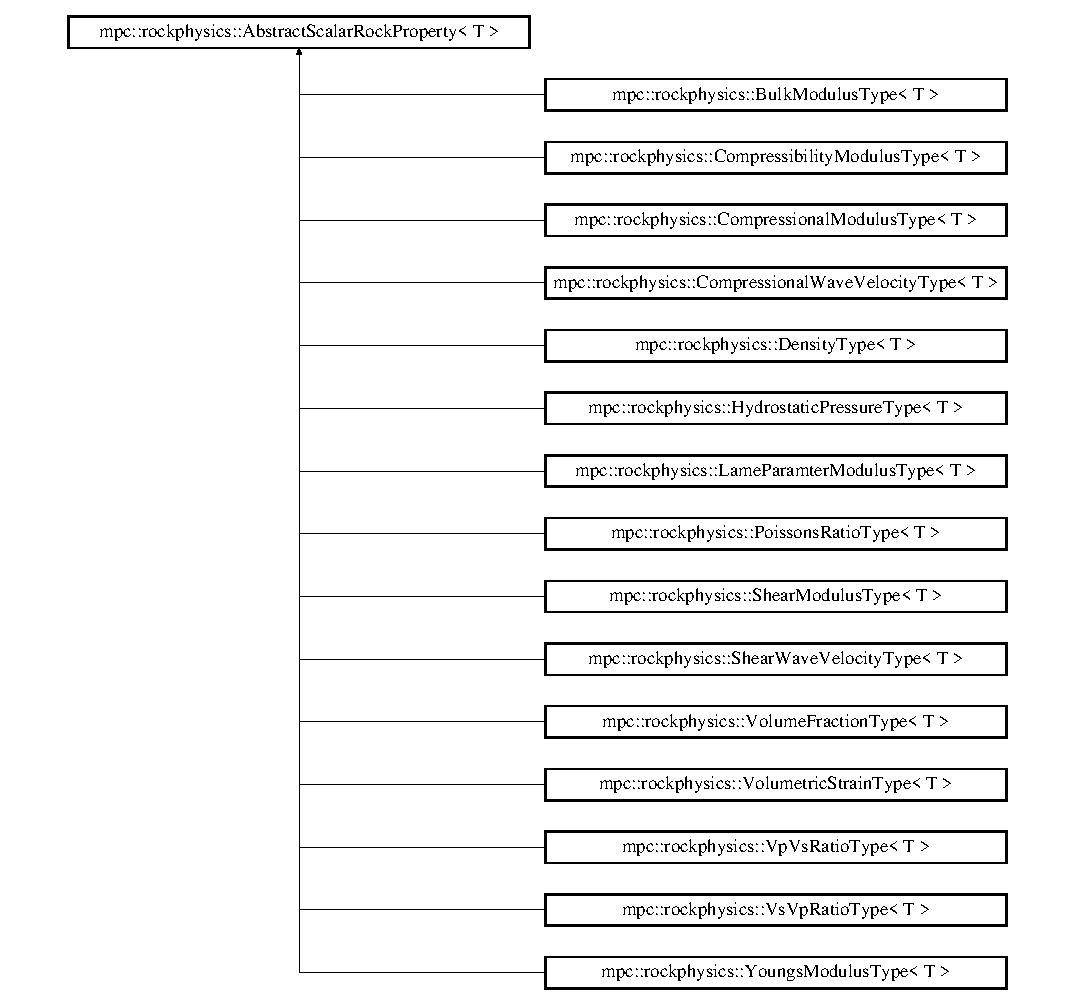
\includegraphics[height=12.000000cm]{structmpc_1_1rockphysics_1_1_abstract_scalar_rock_property}
\end{center}
\end{figure}
\subsection*{Public Attributes}
\begin{DoxyCompactItemize}
\item 
T \mbox{\hyperlink{structmpc_1_1rockphysics_1_1_abstract_scalar_rock_property_a168ef2a7823a3f35280ec408925c58d7}{value}}
\item 
std\+::string \mbox{\hyperlink{structmpc_1_1rockphysics_1_1_abstract_scalar_rock_property_a3a7ab83e4a29f651a6922e2272a28fae}{description}}
\end{DoxyCompactItemize}


\subsection{Detailed Description}
\subsubsection*{template$<$typename T$>$\newline
struct mpc\+::rockphysics\+::\+Abstract\+Scalar\+Rock\+Property$<$ T $>$}



Definition at line 23 of file rockphysicstransformstypes.\+hpp.



\subsection{Member Data Documentation}
\mbox{\Hypertarget{structmpc_1_1rockphysics_1_1_abstract_scalar_rock_property_a3a7ab83e4a29f651a6922e2272a28fae}\label{structmpc_1_1rockphysics_1_1_abstract_scalar_rock_property_a3a7ab83e4a29f651a6922e2272a28fae}} 
\index{mpc\+::rockphysics\+::\+Abstract\+Scalar\+Rock\+Property@{mpc\+::rockphysics\+::\+Abstract\+Scalar\+Rock\+Property}!description@{description}}
\index{description@{description}!mpc\+::rockphysics\+::\+Abstract\+Scalar\+Rock\+Property@{mpc\+::rockphysics\+::\+Abstract\+Scalar\+Rock\+Property}}
\subsubsection{\texorpdfstring{description}{description}}
{\footnotesize\ttfamily template$<$typename T $>$ \\
std\+::string \mbox{\hyperlink{structmpc_1_1rockphysics_1_1_abstract_scalar_rock_property}{mpc\+::rockphysics\+::\+Abstract\+Scalar\+Rock\+Property}}$<$ T $>$\+::description}



Definition at line 26 of file rockphysicstransformstypes.\+hpp.

\mbox{\Hypertarget{structmpc_1_1rockphysics_1_1_abstract_scalar_rock_property_a168ef2a7823a3f35280ec408925c58d7}\label{structmpc_1_1rockphysics_1_1_abstract_scalar_rock_property_a168ef2a7823a3f35280ec408925c58d7}} 
\index{mpc\+::rockphysics\+::\+Abstract\+Scalar\+Rock\+Property@{mpc\+::rockphysics\+::\+Abstract\+Scalar\+Rock\+Property}!value@{value}}
\index{value@{value}!mpc\+::rockphysics\+::\+Abstract\+Scalar\+Rock\+Property@{mpc\+::rockphysics\+::\+Abstract\+Scalar\+Rock\+Property}}
\subsubsection{\texorpdfstring{value}{value}}
{\footnotesize\ttfamily template$<$typename T $>$ \\
T \mbox{\hyperlink{structmpc_1_1rockphysics_1_1_abstract_scalar_rock_property}{mpc\+::rockphysics\+::\+Abstract\+Scalar\+Rock\+Property}}$<$ T $>$\+::value}



Definition at line 24 of file rockphysicstransformstypes.\+hpp.



The documentation for this struct was generated from the following file\+:\begin{DoxyCompactItemize}
\item 
/\+Users/atorlucci/\+Documents/github\+\_\+threecubed\+\_\+repos/mpc/src/mpc/rockphysics/\mbox{\hyperlink{rockphysicstransformstypes_8hpp}{rockphysicstransformstypes.\+hpp}}\end{DoxyCompactItemize}

\hypertarget{structmpc_1_1utilities_1_1_accumulator_product}{}\section{mpc\+:\+:utilities\+:\+:Accumulator\+Product$<$ T, N $>$ Struct Template Reference}
\label{structmpc_1_1utilities_1_1_accumulator_product}\index{mpc\+::utilities\+::\+Accumulator\+Product$<$ T, N $>$@{mpc\+::utilities\+::\+Accumulator\+Product$<$ T, N $>$}}


{\ttfamily \#include $<$accumulator.\+hpp$>$}

\subsection*{Public Member Functions}
\begin{DoxyCompactItemize}
\item 
blitz\+::\+Array$<$ T, N-\/1 $>$ \mbox{\hyperlink{structmpc_1_1utilities_1_1_accumulator_product_a50f1ad7f64867b9ee0e5479207017aca}{operator()}} (blitz\+::\+Array$<$ T, N $>$ \&input\+\_\+array)
\end{DoxyCompactItemize}


\subsection{Detailed Description}
\subsubsection*{template$<$typename T, int N$>$\newline
struct mpc\+::utilities\+::\+Accumulator\+Product$<$ T, N $>$}



Definition at line 56 of file accumulator.\+hpp.



\subsection{Member Function Documentation}
\mbox{\Hypertarget{structmpc_1_1utilities_1_1_accumulator_product_a50f1ad7f64867b9ee0e5479207017aca}\label{structmpc_1_1utilities_1_1_accumulator_product_a50f1ad7f64867b9ee0e5479207017aca}} 
\index{mpc\+::utilities\+::\+Accumulator\+Product@{mpc\+::utilities\+::\+Accumulator\+Product}!operator()@{operator()}}
\index{operator()@{operator()}!mpc\+::utilities\+::\+Accumulator\+Product@{mpc\+::utilities\+::\+Accumulator\+Product}}
\subsubsection{\texorpdfstring{operator()()}{operator()()}}
{\footnotesize\ttfamily template$<$typename T , int N$>$ \\
blitz\+::\+Array$<$T,N-\/1$>$ \mbox{\hyperlink{structmpc_1_1utilities_1_1_accumulator_product}{mpc\+::utilities\+::\+Accumulator\+Product}}$<$ T, N $>$\+::operator() (\begin{DoxyParamCaption}\item[{blitz\+::\+Array$<$ T, N $>$ \&}]{input\+\_\+array }\end{DoxyParamCaption})\hspace{0.3cm}{\ttfamily [inline]}}



Definition at line 58 of file accumulator.\+hpp.



The documentation for this struct was generated from the following file\+:\begin{DoxyCompactItemize}
\item 
/\+Users/atorlucci/\+Documents/github\+\_\+threecubed\+\_\+repos/mpc/src/mpc/utilities/\mbox{\hyperlink{accumulator_8hpp}{accumulator.\+hpp}}\end{DoxyCompactItemize}

\hypertarget{structmpc_1_1utilities_1_1_accumulator_product_3_01_t_00_011_01_4}{}\section{mpc\+:\+:utilities\+:\+:Accumulator\+Product$<$ T, 1 $>$ Struct Template Reference}
\label{structmpc_1_1utilities_1_1_accumulator_product_3_01_t_00_011_01_4}\index{mpc\+::utilities\+::\+Accumulator\+Product$<$ T, 1 $>$@{mpc\+::utilities\+::\+Accumulator\+Product$<$ T, 1 $>$}}


{\ttfamily \#include $<$accumulator.\+hpp$>$}

\subsection*{Public Member Functions}
\begin{DoxyCompactItemize}
\item 
T \mbox{\hyperlink{structmpc_1_1utilities_1_1_accumulator_product_3_01_t_00_011_01_4_a3facff3fdd5b800a83dd5baa9cc89192}{operator()}} (blitz\+::\+Array$<$ T, 1 $>$ \&input\+\_\+array)
\end{DoxyCompactItemize}


\subsection{Detailed Description}
\subsubsection*{template$<$typename T$>$\newline
struct mpc\+::utilities\+::\+Accumulator\+Product$<$ T, 1 $>$}



Definition at line 75 of file accumulator.\+hpp.



\subsection{Member Function Documentation}
\mbox{\Hypertarget{structmpc_1_1utilities_1_1_accumulator_product_3_01_t_00_011_01_4_a3facff3fdd5b800a83dd5baa9cc89192}\label{structmpc_1_1utilities_1_1_accumulator_product_3_01_t_00_011_01_4_a3facff3fdd5b800a83dd5baa9cc89192}} 
\index{mpc\+::utilities\+::\+Accumulator\+Product$<$ T, 1 $>$@{mpc\+::utilities\+::\+Accumulator\+Product$<$ T, 1 $>$}!operator()@{operator()}}
\index{operator()@{operator()}!mpc\+::utilities\+::\+Accumulator\+Product$<$ T, 1 $>$@{mpc\+::utilities\+::\+Accumulator\+Product$<$ T, 1 $>$}}
\subsubsection{\texorpdfstring{operator()()}{operator()()}}
{\footnotesize\ttfamily template$<$typename T $>$ \\
T \mbox{\hyperlink{structmpc_1_1utilities_1_1_accumulator_product}{mpc\+::utilities\+::\+Accumulator\+Product}}$<$ T, 1 $>$\+::operator() (\begin{DoxyParamCaption}\item[{blitz\+::\+Array$<$ T, 1 $>$ \&}]{input\+\_\+array }\end{DoxyParamCaption})\hspace{0.3cm}{\ttfamily [inline]}}



Definition at line 77 of file accumulator.\+hpp.



The documentation for this struct was generated from the following file\+:\begin{DoxyCompactItemize}
\item 
/\+Users/atorlucci/\+Documents/github\+\_\+threecubed\+\_\+repos/mpc/src/mpc/utilities/\mbox{\hyperlink{accumulator_8hpp}{accumulator.\+hpp}}\end{DoxyCompactItemize}

\hypertarget{structmpc_1_1utilities_1_1_accumulator_sum}{}\section{mpc\+:\+:utilities\+:\+:Accumulator\+Sum$<$ T, N $>$ Struct Template Reference}
\label{structmpc_1_1utilities_1_1_accumulator_sum}\index{mpc\+::utilities\+::\+Accumulator\+Sum$<$ T, N $>$@{mpc\+::utilities\+::\+Accumulator\+Sum$<$ T, N $>$}}


{\ttfamily \#include $<$accumulator.\+hpp$>$}

\subsection*{Public Member Functions}
\begin{DoxyCompactItemize}
\item 
blitz\+::\+Array$<$ T, N-\/1 $>$ \mbox{\hyperlink{structmpc_1_1utilities_1_1_accumulator_sum_afe897dea438bd648a423b3273f1ab54a}{operator()}} (blitz\+::\+Array$<$ T, N $>$ \&input\+\_\+array)
\end{DoxyCompactItemize}


\subsection{Detailed Description}
\subsubsection*{template$<$typename T, int N$>$\newline
struct mpc\+::utilities\+::\+Accumulator\+Sum$<$ T, N $>$}



Definition at line 25 of file accumulator.\+hpp.



\subsection{Member Function Documentation}
\mbox{\Hypertarget{structmpc_1_1utilities_1_1_accumulator_sum_afe897dea438bd648a423b3273f1ab54a}\label{structmpc_1_1utilities_1_1_accumulator_sum_afe897dea438bd648a423b3273f1ab54a}} 
\index{mpc\+::utilities\+::\+Accumulator\+Sum@{mpc\+::utilities\+::\+Accumulator\+Sum}!operator()@{operator()}}
\index{operator()@{operator()}!mpc\+::utilities\+::\+Accumulator\+Sum@{mpc\+::utilities\+::\+Accumulator\+Sum}}
\subsubsection{\texorpdfstring{operator()()}{operator()()}}
{\footnotesize\ttfamily template$<$typename T , int N$>$ \\
blitz\+::\+Array$<$T,N-\/1$>$ \mbox{\hyperlink{structmpc_1_1utilities_1_1_accumulator_sum}{mpc\+::utilities\+::\+Accumulator\+Sum}}$<$ T, N $>$\+::operator() (\begin{DoxyParamCaption}\item[{blitz\+::\+Array$<$ T, N $>$ \&}]{input\+\_\+array }\end{DoxyParamCaption})\hspace{0.3cm}{\ttfamily [inline]}}



Definition at line 27 of file accumulator.\+hpp.



The documentation for this struct was generated from the following file\+:\begin{DoxyCompactItemize}
\item 
/\+Users/atorlucci/\+Documents/github\+\_\+threecubed\+\_\+repos/mpc/src/mpc/utilities/\mbox{\hyperlink{accumulator_8hpp}{accumulator.\+hpp}}\end{DoxyCompactItemize}

\hypertarget{structmpc_1_1utilities_1_1_accumulator_sum_3_01_t_00_011_01_4}{}\section{mpc\+:\+:utilities\+:\+:Accumulator\+Sum$<$ T, 1 $>$ Struct Template Reference}
\label{structmpc_1_1utilities_1_1_accumulator_sum_3_01_t_00_011_01_4}\index{mpc\+::utilities\+::\+Accumulator\+Sum$<$ T, 1 $>$@{mpc\+::utilities\+::\+Accumulator\+Sum$<$ T, 1 $>$}}


{\ttfamily \#include $<$accumulator.\+hpp$>$}

\subsection*{Public Member Functions}
\begin{DoxyCompactItemize}
\item 
T \mbox{\hyperlink{structmpc_1_1utilities_1_1_accumulator_sum_3_01_t_00_011_01_4_adf9f3d5ba9511c71c44c55a8941ce292}{operator()}} (blitz\+::\+Array$<$ T, 1 $>$ \&input\+\_\+array)
\end{DoxyCompactItemize}


\subsection{Detailed Description}
\subsubsection*{template$<$typename T$>$\newline
struct mpc\+::utilities\+::\+Accumulator\+Sum$<$ T, 1 $>$}



Definition at line 44 of file accumulator.\+hpp.



\subsection{Member Function Documentation}
\mbox{\Hypertarget{structmpc_1_1utilities_1_1_accumulator_sum_3_01_t_00_011_01_4_adf9f3d5ba9511c71c44c55a8941ce292}\label{structmpc_1_1utilities_1_1_accumulator_sum_3_01_t_00_011_01_4_adf9f3d5ba9511c71c44c55a8941ce292}} 
\index{mpc\+::utilities\+::\+Accumulator\+Sum$<$ T, 1 $>$@{mpc\+::utilities\+::\+Accumulator\+Sum$<$ T, 1 $>$}!operator()@{operator()}}
\index{operator()@{operator()}!mpc\+::utilities\+::\+Accumulator\+Sum$<$ T, 1 $>$@{mpc\+::utilities\+::\+Accumulator\+Sum$<$ T, 1 $>$}}
\subsubsection{\texorpdfstring{operator()()}{operator()()}}
{\footnotesize\ttfamily template$<$typename T $>$ \\
T \mbox{\hyperlink{structmpc_1_1utilities_1_1_accumulator_sum}{mpc\+::utilities\+::\+Accumulator\+Sum}}$<$ T, 1 $>$\+::operator() (\begin{DoxyParamCaption}\item[{blitz\+::\+Array$<$ T, 1 $>$ \&}]{input\+\_\+array }\end{DoxyParamCaption})\hspace{0.3cm}{\ttfamily [inline]}}



Definition at line 46 of file accumulator.\+hpp.



The documentation for this struct was generated from the following file\+:\begin{DoxyCompactItemize}
\item 
/\+Users/atorlucci/\+Documents/github\+\_\+threecubed\+\_\+repos/mpc/src/mpc/utilities/\mbox{\hyperlink{accumulator_8hpp}{accumulator.\+hpp}}\end{DoxyCompactItemize}

\hypertarget{structmpc_1_1rockphysics_1_1_bulk_modulus_type}{}\section{mpc\+:\+:rockphysics\+:\+:Bulk\+Modulus\+Type$<$ T $>$ Struct Template Reference}
\label{structmpc_1_1rockphysics_1_1_bulk_modulus_type}\index{mpc\+::rockphysics\+::\+Bulk\+Modulus\+Type$<$ T $>$@{mpc\+::rockphysics\+::\+Bulk\+Modulus\+Type$<$ T $>$}}


{\ttfamily \#include $<$rockphysicstransformstypes.\+hpp$>$}

Inheritance diagram for mpc\+:\+:rockphysics\+:\+:Bulk\+Modulus\+Type$<$ T $>$\+:\begin{figure}[H]
\begin{center}
\leavevmode
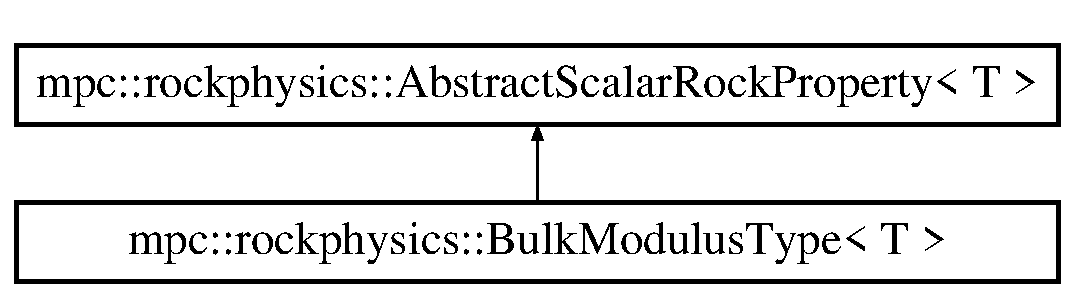
\includegraphics[height=2.000000cm]{structmpc_1_1rockphysics_1_1_bulk_modulus_type}
\end{center}
\end{figure}
\subsection*{Public Member Functions}
\begin{DoxyCompactItemize}
\item 
constexpr \mbox{\hyperlink{structmpc_1_1rockphysics_1_1_bulk_modulus_type_a756c6ccecf169d7f32802d7da8c0fd45}{Bulk\+Modulus\+Type}} (T val)
\end{DoxyCompactItemize}
\subsection*{Additional Inherited Members}


\subsection{Detailed Description}
\subsubsection*{template$<$typename T$>$\newline
struct mpc\+::rockphysics\+::\+Bulk\+Modulus\+Type$<$ T $>$}



Definition at line 31 of file rockphysicstransformstypes.\+hpp.



\subsection{Constructor \& Destructor Documentation}
\mbox{\Hypertarget{structmpc_1_1rockphysics_1_1_bulk_modulus_type_a756c6ccecf169d7f32802d7da8c0fd45}\label{structmpc_1_1rockphysics_1_1_bulk_modulus_type_a756c6ccecf169d7f32802d7da8c0fd45}} 
\index{mpc\+::rockphysics\+::\+Bulk\+Modulus\+Type@{mpc\+::rockphysics\+::\+Bulk\+Modulus\+Type}!Bulk\+Modulus\+Type@{Bulk\+Modulus\+Type}}
\index{Bulk\+Modulus\+Type@{Bulk\+Modulus\+Type}!mpc\+::rockphysics\+::\+Bulk\+Modulus\+Type@{mpc\+::rockphysics\+::\+Bulk\+Modulus\+Type}}
\subsubsection{\texorpdfstring{Bulk\+Modulus\+Type()}{BulkModulusType()}}
{\footnotesize\ttfamily template$<$typename T$>$ \\
constexpr \mbox{\hyperlink{structmpc_1_1rockphysics_1_1_bulk_modulus_type}{mpc\+::rockphysics\+::\+Bulk\+Modulus\+Type}}$<$ T $>$\+::\mbox{\hyperlink{structmpc_1_1rockphysics_1_1_bulk_modulus_type}{Bulk\+Modulus\+Type}} (\begin{DoxyParamCaption}\item[{T}]{val }\end{DoxyParamCaption})\hspace{0.3cm}{\ttfamily [inline]}}



Definition at line 36 of file rockphysicstransformstypes.\+hpp.



The documentation for this struct was generated from the following file\+:\begin{DoxyCompactItemize}
\item 
/\+Users/atorlucci/\+Documents/github\+\_\+threecubed\+\_\+repos/mpc/src/mpc/rockphysics/\mbox{\hyperlink{rockphysicstransformstypes_8hpp}{rockphysicstransformstypes.\+hpp}}\end{DoxyCompactItemize}

\hypertarget{structmpc_1_1utilities_1_1_cartesian_coordinate_type}{}\section{mpc\+:\+:utilities\+:\+:Cartesian\+Coordinate\+Type Struct Reference}
\label{structmpc_1_1utilities_1_1_cartesian_coordinate_type}\index{mpc\+::utilities\+::\+Cartesian\+Coordinate\+Type@{mpc\+::utilities\+::\+Cartesian\+Coordinate\+Type}}


{\ttfamily \#include $<$coordinatemapping.\+hpp$>$}

Inheritance diagram for mpc\+:\+:utilities\+:\+:Cartesian\+Coordinate\+Type\+:\begin{figure}[H]
\begin{center}
\leavevmode
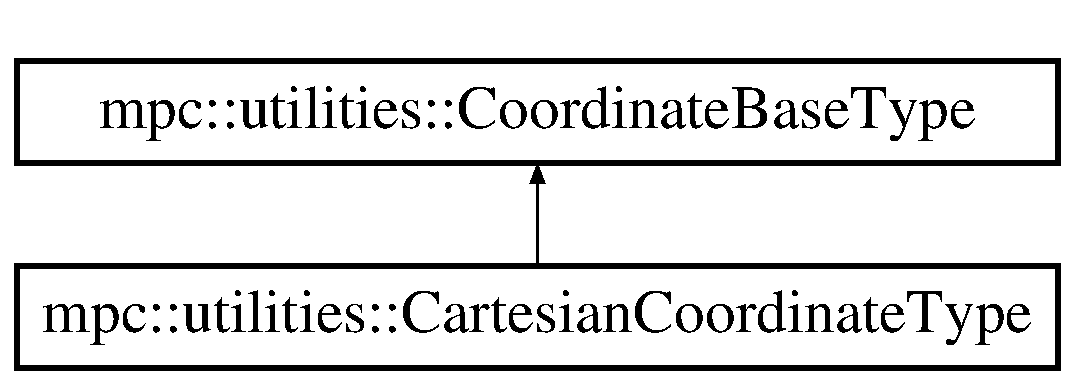
\includegraphics[height=2.000000cm]{structmpc_1_1utilities_1_1_cartesian_coordinate_type}
\end{center}
\end{figure}


\subsection{Detailed Description}


Definition at line 26 of file coordinatemapping.\+hpp.



The documentation for this struct was generated from the following file\+:\begin{DoxyCompactItemize}
\item 
/\+Users/atorlucci/\+Documents/github\+\_\+threecubed\+\_\+repos/mpc/src/mpc/utilities/\mbox{\hyperlink{coordinatemapping_8hpp}{coordinatemapping.\+hpp}}\end{DoxyCompactItemize}

\hypertarget{structmpc_1_1utilities_1_1_c_kronecker_delta3_function_object}{}\section{mpc\+:\+:utilities\+:\+:C\+Kronecker\+Delta3\+Function\+Object$<$ T, M, N $>$ Struct Template Reference}
\label{structmpc_1_1utilities_1_1_c_kronecker_delta3_function_object}\index{mpc\+::utilities\+::\+C\+Kronecker\+Delta3\+Function\+Object$<$ T, M, N $>$@{mpc\+::utilities\+::\+C\+Kronecker\+Delta3\+Function\+Object$<$ T, M, N $>$}}


{\ttfamily \#include $<$kroneckerdelta.\+hpp$>$}

\subsection*{Public Member Functions}
\begin{DoxyCompactItemize}
\item 
constexpr T \mbox{\hyperlink{structmpc_1_1utilities_1_1_c_kronecker_delta3_function_object_a4ba89588535b6f7da764165062133549}{operator()}} ()
\end{DoxyCompactItemize}


\subsection{Detailed Description}
\subsubsection*{template$<$typename T, int M, int N$>$\newline
struct mpc\+::utilities\+::\+C\+Kronecker\+Delta3\+Function\+Object$<$ T, M, N $>$}



Definition at line 36 of file kroneckerdelta.\+hpp.



\subsection{Member Function Documentation}
\mbox{\Hypertarget{structmpc_1_1utilities_1_1_c_kronecker_delta3_function_object_a4ba89588535b6f7da764165062133549}\label{structmpc_1_1utilities_1_1_c_kronecker_delta3_function_object_a4ba89588535b6f7da764165062133549}} 
\index{mpc\+::utilities\+::\+C\+Kronecker\+Delta3\+Function\+Object@{mpc\+::utilities\+::\+C\+Kronecker\+Delta3\+Function\+Object}!operator()@{operator()}}
\index{operator()@{operator()}!mpc\+::utilities\+::\+C\+Kronecker\+Delta3\+Function\+Object@{mpc\+::utilities\+::\+C\+Kronecker\+Delta3\+Function\+Object}}
\subsubsection{\texorpdfstring{operator()()}{operator()()}}
{\footnotesize\ttfamily template$<$typename T , int M, int N$>$ \\
constexpr T \mbox{\hyperlink{structmpc_1_1utilities_1_1_c_kronecker_delta3_function_object}{mpc\+::utilities\+::\+C\+Kronecker\+Delta3\+Function\+Object}}$<$ T, M, N $>$\+::operator() (\begin{DoxyParamCaption}{ }\end{DoxyParamCaption})\hspace{0.3cm}{\ttfamily [inline]}}



Definition at line 42 of file kroneckerdelta.\+hpp.



The documentation for this struct was generated from the following file\+:\begin{DoxyCompactItemize}
\item 
/\+Users/atorlucci/\+Documents/github\+\_\+threecubed\+\_\+repos/mpc/src/mpc/utilities/\mbox{\hyperlink{kroneckerdelta_8hpp}{kroneckerdelta.\+hpp}}\end{DoxyCompactItemize}

\hypertarget{structmpc_1_1utilities_1_1_c_kronecker_delta3_function_object_3_01_t_00_010_00_010_01_4}{}\section{mpc\+:\+:utilities\+:\+:C\+Kronecker\+Delta3\+Function\+Object$<$ T, 0, 0 $>$ Struct Template Reference}
\label{structmpc_1_1utilities_1_1_c_kronecker_delta3_function_object_3_01_t_00_010_00_010_01_4}\index{mpc\+::utilities\+::\+C\+Kronecker\+Delta3\+Function\+Object$<$ T, 0, 0 $>$@{mpc\+::utilities\+::\+C\+Kronecker\+Delta3\+Function\+Object$<$ T, 0, 0 $>$}}


{\ttfamily \#include $<$kroneckerdelta.\+hpp$>$}

\subsection*{Public Member Functions}
\begin{DoxyCompactItemize}
\item 
constexpr T \mbox{\hyperlink{structmpc_1_1utilities_1_1_c_kronecker_delta3_function_object_3_01_t_00_010_00_010_01_4_aa6e36546027316c59e53c7c0760460da}{operator()}} ()
\end{DoxyCompactItemize}


\subsection{Detailed Description}
\subsubsection*{template$<$typename T$>$\newline
struct mpc\+::utilities\+::\+C\+Kronecker\+Delta3\+Function\+Object$<$ T, 0, 0 $>$}



Definition at line 48 of file kroneckerdelta.\+hpp.



\subsection{Member Function Documentation}
\mbox{\Hypertarget{structmpc_1_1utilities_1_1_c_kronecker_delta3_function_object_3_01_t_00_010_00_010_01_4_aa6e36546027316c59e53c7c0760460da}\label{structmpc_1_1utilities_1_1_c_kronecker_delta3_function_object_3_01_t_00_010_00_010_01_4_aa6e36546027316c59e53c7c0760460da}} 
\index{mpc\+::utilities\+::\+C\+Kronecker\+Delta3\+Function\+Object$<$ T, 0, 0 $>$@{mpc\+::utilities\+::\+C\+Kronecker\+Delta3\+Function\+Object$<$ T, 0, 0 $>$}!operator()@{operator()}}
\index{operator()@{operator()}!mpc\+::utilities\+::\+C\+Kronecker\+Delta3\+Function\+Object$<$ T, 0, 0 $>$@{mpc\+::utilities\+::\+C\+Kronecker\+Delta3\+Function\+Object$<$ T, 0, 0 $>$}}
\subsubsection{\texorpdfstring{operator()()}{operator()()}}
{\footnotesize\ttfamily template$<$typename T $>$ \\
constexpr T \mbox{\hyperlink{structmpc_1_1utilities_1_1_c_kronecker_delta3_function_object}{mpc\+::utilities\+::\+C\+Kronecker\+Delta3\+Function\+Object}}$<$ T, 0, 0 $>$\+::operator() (\begin{DoxyParamCaption}{ }\end{DoxyParamCaption})\hspace{0.3cm}{\ttfamily [inline]}}



Definition at line 50 of file kroneckerdelta.\+hpp.



The documentation for this struct was generated from the following file\+:\begin{DoxyCompactItemize}
\item 
/\+Users/atorlucci/\+Documents/github\+\_\+threecubed\+\_\+repos/mpc/src/mpc/utilities/\mbox{\hyperlink{kroneckerdelta_8hpp}{kroneckerdelta.\+hpp}}\end{DoxyCompactItemize}

\hypertarget{structmpc_1_1utilities_1_1_c_kronecker_delta3_function_object_3_01_t_00_010_00_011_01_4}{}\section{mpc\+:\+:utilities\+:\+:C\+Kronecker\+Delta3\+Function\+Object$<$ T, 0, 1 $>$ Struct Template Reference}
\label{structmpc_1_1utilities_1_1_c_kronecker_delta3_function_object_3_01_t_00_010_00_011_01_4}\index{mpc\+::utilities\+::\+C\+Kronecker\+Delta3\+Function\+Object$<$ T, 0, 1 $>$@{mpc\+::utilities\+::\+C\+Kronecker\+Delta3\+Function\+Object$<$ T, 0, 1 $>$}}


{\ttfamily \#include $<$kroneckerdelta.\+hpp$>$}

\subsection*{Public Member Functions}
\begin{DoxyCompactItemize}
\item 
constexpr T \mbox{\hyperlink{structmpc_1_1utilities_1_1_c_kronecker_delta3_function_object_3_01_t_00_010_00_011_01_4_a052b1f0010966105f2973dc6f57ff779}{operator()}} ()
\end{DoxyCompactItemize}


\subsection{Detailed Description}
\subsubsection*{template$<$typename T$>$\newline
struct mpc\+::utilities\+::\+C\+Kronecker\+Delta3\+Function\+Object$<$ T, 0, 1 $>$}



Definition at line 56 of file kroneckerdelta.\+hpp.



\subsection{Member Function Documentation}
\mbox{\Hypertarget{structmpc_1_1utilities_1_1_c_kronecker_delta3_function_object_3_01_t_00_010_00_011_01_4_a052b1f0010966105f2973dc6f57ff779}\label{structmpc_1_1utilities_1_1_c_kronecker_delta3_function_object_3_01_t_00_010_00_011_01_4_a052b1f0010966105f2973dc6f57ff779}} 
\index{mpc\+::utilities\+::\+C\+Kronecker\+Delta3\+Function\+Object$<$ T, 0, 1 $>$@{mpc\+::utilities\+::\+C\+Kronecker\+Delta3\+Function\+Object$<$ T, 0, 1 $>$}!operator()@{operator()}}
\index{operator()@{operator()}!mpc\+::utilities\+::\+C\+Kronecker\+Delta3\+Function\+Object$<$ T, 0, 1 $>$@{mpc\+::utilities\+::\+C\+Kronecker\+Delta3\+Function\+Object$<$ T, 0, 1 $>$}}
\subsubsection{\texorpdfstring{operator()()}{operator()()}}
{\footnotesize\ttfamily template$<$typename T $>$ \\
constexpr T \mbox{\hyperlink{structmpc_1_1utilities_1_1_c_kronecker_delta3_function_object}{mpc\+::utilities\+::\+C\+Kronecker\+Delta3\+Function\+Object}}$<$ T, 0, 1 $>$\+::operator() (\begin{DoxyParamCaption}{ }\end{DoxyParamCaption})\hspace{0.3cm}{\ttfamily [inline]}}



Definition at line 58 of file kroneckerdelta.\+hpp.



The documentation for this struct was generated from the following file\+:\begin{DoxyCompactItemize}
\item 
/\+Users/atorlucci/\+Documents/github\+\_\+threecubed\+\_\+repos/mpc/src/mpc/utilities/\mbox{\hyperlink{kroneckerdelta_8hpp}{kroneckerdelta.\+hpp}}\end{DoxyCompactItemize}

\hypertarget{structmpc_1_1utilities_1_1_c_kronecker_delta3_function_object_3_01_t_00_010_00_012_01_4}{}\section{mpc\+:\+:utilities\+:\+:C\+Kronecker\+Delta3\+Function\+Object$<$ T, 0, 2 $>$ Struct Template Reference}
\label{structmpc_1_1utilities_1_1_c_kronecker_delta3_function_object_3_01_t_00_010_00_012_01_4}\index{mpc\+::utilities\+::\+C\+Kronecker\+Delta3\+Function\+Object$<$ T, 0, 2 $>$@{mpc\+::utilities\+::\+C\+Kronecker\+Delta3\+Function\+Object$<$ T, 0, 2 $>$}}


{\ttfamily \#include $<$kroneckerdelta.\+hpp$>$}

\subsection*{Public Member Functions}
\begin{DoxyCompactItemize}
\item 
constexpr T \mbox{\hyperlink{structmpc_1_1utilities_1_1_c_kronecker_delta3_function_object_3_01_t_00_010_00_012_01_4_ad7f134c3d2139f87688f07d4531117af}{operator()}} ()
\end{DoxyCompactItemize}


\subsection{Detailed Description}
\subsubsection*{template$<$typename T$>$\newline
struct mpc\+::utilities\+::\+C\+Kronecker\+Delta3\+Function\+Object$<$ T, 0, 2 $>$}



Definition at line 64 of file kroneckerdelta.\+hpp.



\subsection{Member Function Documentation}
\mbox{\Hypertarget{structmpc_1_1utilities_1_1_c_kronecker_delta3_function_object_3_01_t_00_010_00_012_01_4_ad7f134c3d2139f87688f07d4531117af}\label{structmpc_1_1utilities_1_1_c_kronecker_delta3_function_object_3_01_t_00_010_00_012_01_4_ad7f134c3d2139f87688f07d4531117af}} 
\index{mpc\+::utilities\+::\+C\+Kronecker\+Delta3\+Function\+Object$<$ T, 0, 2 $>$@{mpc\+::utilities\+::\+C\+Kronecker\+Delta3\+Function\+Object$<$ T, 0, 2 $>$}!operator()@{operator()}}
\index{operator()@{operator()}!mpc\+::utilities\+::\+C\+Kronecker\+Delta3\+Function\+Object$<$ T, 0, 2 $>$@{mpc\+::utilities\+::\+C\+Kronecker\+Delta3\+Function\+Object$<$ T, 0, 2 $>$}}
\subsubsection{\texorpdfstring{operator()()}{operator()()}}
{\footnotesize\ttfamily template$<$typename T $>$ \\
constexpr T \mbox{\hyperlink{structmpc_1_1utilities_1_1_c_kronecker_delta3_function_object}{mpc\+::utilities\+::\+C\+Kronecker\+Delta3\+Function\+Object}}$<$ T, 0, 2 $>$\+::operator() (\begin{DoxyParamCaption}{ }\end{DoxyParamCaption})\hspace{0.3cm}{\ttfamily [inline]}}



Definition at line 66 of file kroneckerdelta.\+hpp.



The documentation for this struct was generated from the following file\+:\begin{DoxyCompactItemize}
\item 
/\+Users/atorlucci/\+Documents/github\+\_\+threecubed\+\_\+repos/mpc/src/mpc/utilities/\mbox{\hyperlink{kroneckerdelta_8hpp}{kroneckerdelta.\+hpp}}\end{DoxyCompactItemize}

\hypertarget{structmpc_1_1utilities_1_1_c_kronecker_delta3_function_object_3_01_t_00_011_00_010_01_4}{}\section{mpc\+:\+:utilities\+:\+:C\+Kronecker\+Delta3\+Function\+Object$<$ T, 1, 0 $>$ Struct Template Reference}
\label{structmpc_1_1utilities_1_1_c_kronecker_delta3_function_object_3_01_t_00_011_00_010_01_4}\index{mpc\+::utilities\+::\+C\+Kronecker\+Delta3\+Function\+Object$<$ T, 1, 0 $>$@{mpc\+::utilities\+::\+C\+Kronecker\+Delta3\+Function\+Object$<$ T, 1, 0 $>$}}


{\ttfamily \#include $<$kroneckerdelta.\+hpp$>$}

\subsection*{Public Member Functions}
\begin{DoxyCompactItemize}
\item 
constexpr T \mbox{\hyperlink{structmpc_1_1utilities_1_1_c_kronecker_delta3_function_object_3_01_t_00_011_00_010_01_4_a677c23e018869f0015a684eea07a4040}{operator()}} ()
\end{DoxyCompactItemize}


\subsection{Detailed Description}
\subsubsection*{template$<$typename T$>$\newline
struct mpc\+::utilities\+::\+C\+Kronecker\+Delta3\+Function\+Object$<$ T, 1, 0 $>$}



Definition at line 72 of file kroneckerdelta.\+hpp.



\subsection{Member Function Documentation}
\mbox{\Hypertarget{structmpc_1_1utilities_1_1_c_kronecker_delta3_function_object_3_01_t_00_011_00_010_01_4_a677c23e018869f0015a684eea07a4040}\label{structmpc_1_1utilities_1_1_c_kronecker_delta3_function_object_3_01_t_00_011_00_010_01_4_a677c23e018869f0015a684eea07a4040}} 
\index{mpc\+::utilities\+::\+C\+Kronecker\+Delta3\+Function\+Object$<$ T, 1, 0 $>$@{mpc\+::utilities\+::\+C\+Kronecker\+Delta3\+Function\+Object$<$ T, 1, 0 $>$}!operator()@{operator()}}
\index{operator()@{operator()}!mpc\+::utilities\+::\+C\+Kronecker\+Delta3\+Function\+Object$<$ T, 1, 0 $>$@{mpc\+::utilities\+::\+C\+Kronecker\+Delta3\+Function\+Object$<$ T, 1, 0 $>$}}
\subsubsection{\texorpdfstring{operator()()}{operator()()}}
{\footnotesize\ttfamily template$<$typename T $>$ \\
constexpr T \mbox{\hyperlink{structmpc_1_1utilities_1_1_c_kronecker_delta3_function_object}{mpc\+::utilities\+::\+C\+Kronecker\+Delta3\+Function\+Object}}$<$ T, 1, 0 $>$\+::operator() (\begin{DoxyParamCaption}{ }\end{DoxyParamCaption})\hspace{0.3cm}{\ttfamily [inline]}}



Definition at line 74 of file kroneckerdelta.\+hpp.



The documentation for this struct was generated from the following file\+:\begin{DoxyCompactItemize}
\item 
/\+Users/atorlucci/\+Documents/github\+\_\+threecubed\+\_\+repos/mpc/src/mpc/utilities/\mbox{\hyperlink{kroneckerdelta_8hpp}{kroneckerdelta.\+hpp}}\end{DoxyCompactItemize}

\hypertarget{structmpc_1_1utilities_1_1_c_kronecker_delta3_function_object_3_01_t_00_011_00_011_01_4}{}\section{mpc\+:\+:utilities\+:\+:C\+Kronecker\+Delta3\+Function\+Object$<$ T, 1, 1 $>$ Struct Template Reference}
\label{structmpc_1_1utilities_1_1_c_kronecker_delta3_function_object_3_01_t_00_011_00_011_01_4}\index{mpc\+::utilities\+::\+C\+Kronecker\+Delta3\+Function\+Object$<$ T, 1, 1 $>$@{mpc\+::utilities\+::\+C\+Kronecker\+Delta3\+Function\+Object$<$ T, 1, 1 $>$}}


{\ttfamily \#include $<$kroneckerdelta.\+hpp$>$}

\subsection*{Public Member Functions}
\begin{DoxyCompactItemize}
\item 
constexpr T \mbox{\hyperlink{structmpc_1_1utilities_1_1_c_kronecker_delta3_function_object_3_01_t_00_011_00_011_01_4_a405d6908a9703c7cbdd4accbfb56f32d}{operator()}} ()
\end{DoxyCompactItemize}


\subsection{Detailed Description}
\subsubsection*{template$<$typename T$>$\newline
struct mpc\+::utilities\+::\+C\+Kronecker\+Delta3\+Function\+Object$<$ T, 1, 1 $>$}



Definition at line 80 of file kroneckerdelta.\+hpp.



\subsection{Member Function Documentation}
\mbox{\Hypertarget{structmpc_1_1utilities_1_1_c_kronecker_delta3_function_object_3_01_t_00_011_00_011_01_4_a405d6908a9703c7cbdd4accbfb56f32d}\label{structmpc_1_1utilities_1_1_c_kronecker_delta3_function_object_3_01_t_00_011_00_011_01_4_a405d6908a9703c7cbdd4accbfb56f32d}} 
\index{mpc\+::utilities\+::\+C\+Kronecker\+Delta3\+Function\+Object$<$ T, 1, 1 $>$@{mpc\+::utilities\+::\+C\+Kronecker\+Delta3\+Function\+Object$<$ T, 1, 1 $>$}!operator()@{operator()}}
\index{operator()@{operator()}!mpc\+::utilities\+::\+C\+Kronecker\+Delta3\+Function\+Object$<$ T, 1, 1 $>$@{mpc\+::utilities\+::\+C\+Kronecker\+Delta3\+Function\+Object$<$ T, 1, 1 $>$}}
\subsubsection{\texorpdfstring{operator()()}{operator()()}}
{\footnotesize\ttfamily template$<$typename T $>$ \\
constexpr T \mbox{\hyperlink{structmpc_1_1utilities_1_1_c_kronecker_delta3_function_object}{mpc\+::utilities\+::\+C\+Kronecker\+Delta3\+Function\+Object}}$<$ T, 1, 1 $>$\+::operator() (\begin{DoxyParamCaption}{ }\end{DoxyParamCaption})\hspace{0.3cm}{\ttfamily [inline]}}



Definition at line 82 of file kroneckerdelta.\+hpp.



The documentation for this struct was generated from the following file\+:\begin{DoxyCompactItemize}
\item 
/\+Users/atorlucci/\+Documents/github\+\_\+threecubed\+\_\+repos/mpc/src/mpc/utilities/\mbox{\hyperlink{kroneckerdelta_8hpp}{kroneckerdelta.\+hpp}}\end{DoxyCompactItemize}

\hypertarget{structmpc_1_1utilities_1_1_c_kronecker_delta3_function_object_3_01_t_00_011_00_012_01_4}{}\section{mpc\+:\+:utilities\+:\+:C\+Kronecker\+Delta3\+Function\+Object$<$ T, 1, 2 $>$ Struct Template Reference}
\label{structmpc_1_1utilities_1_1_c_kronecker_delta3_function_object_3_01_t_00_011_00_012_01_4}\index{mpc\+::utilities\+::\+C\+Kronecker\+Delta3\+Function\+Object$<$ T, 1, 2 $>$@{mpc\+::utilities\+::\+C\+Kronecker\+Delta3\+Function\+Object$<$ T, 1, 2 $>$}}


{\ttfamily \#include $<$kroneckerdelta.\+hpp$>$}

\subsection*{Public Member Functions}
\begin{DoxyCompactItemize}
\item 
constexpr T \mbox{\hyperlink{structmpc_1_1utilities_1_1_c_kronecker_delta3_function_object_3_01_t_00_011_00_012_01_4_adb3e5df347bcdfda72b191b33a4e9a52}{operator()}} ()
\end{DoxyCompactItemize}


\subsection{Detailed Description}
\subsubsection*{template$<$typename T$>$\newline
struct mpc\+::utilities\+::\+C\+Kronecker\+Delta3\+Function\+Object$<$ T, 1, 2 $>$}



Definition at line 88 of file kroneckerdelta.\+hpp.



\subsection{Member Function Documentation}
\mbox{\Hypertarget{structmpc_1_1utilities_1_1_c_kronecker_delta3_function_object_3_01_t_00_011_00_012_01_4_adb3e5df347bcdfda72b191b33a4e9a52}\label{structmpc_1_1utilities_1_1_c_kronecker_delta3_function_object_3_01_t_00_011_00_012_01_4_adb3e5df347bcdfda72b191b33a4e9a52}} 
\index{mpc\+::utilities\+::\+C\+Kronecker\+Delta3\+Function\+Object$<$ T, 1, 2 $>$@{mpc\+::utilities\+::\+C\+Kronecker\+Delta3\+Function\+Object$<$ T, 1, 2 $>$}!operator()@{operator()}}
\index{operator()@{operator()}!mpc\+::utilities\+::\+C\+Kronecker\+Delta3\+Function\+Object$<$ T, 1, 2 $>$@{mpc\+::utilities\+::\+C\+Kronecker\+Delta3\+Function\+Object$<$ T, 1, 2 $>$}}
\subsubsection{\texorpdfstring{operator()()}{operator()()}}
{\footnotesize\ttfamily template$<$typename T $>$ \\
constexpr T \mbox{\hyperlink{structmpc_1_1utilities_1_1_c_kronecker_delta3_function_object}{mpc\+::utilities\+::\+C\+Kronecker\+Delta3\+Function\+Object}}$<$ T, 1, 2 $>$\+::operator() (\begin{DoxyParamCaption}{ }\end{DoxyParamCaption})\hspace{0.3cm}{\ttfamily [inline]}}



Definition at line 90 of file kroneckerdelta.\+hpp.



The documentation for this struct was generated from the following file\+:\begin{DoxyCompactItemize}
\item 
/\+Users/atorlucci/\+Documents/github\+\_\+threecubed\+\_\+repos/mpc/src/mpc/utilities/\mbox{\hyperlink{kroneckerdelta_8hpp}{kroneckerdelta.\+hpp}}\end{DoxyCompactItemize}

\hypertarget{structmpc_1_1utilities_1_1_c_kronecker_delta3_function_object_3_01_t_00_012_00_010_01_4}{}\section{mpc\+:\+:utilities\+:\+:C\+Kronecker\+Delta3\+Function\+Object$<$ T, 2, 0 $>$ Struct Template Reference}
\label{structmpc_1_1utilities_1_1_c_kronecker_delta3_function_object_3_01_t_00_012_00_010_01_4}\index{mpc\+::utilities\+::\+C\+Kronecker\+Delta3\+Function\+Object$<$ T, 2, 0 $>$@{mpc\+::utilities\+::\+C\+Kronecker\+Delta3\+Function\+Object$<$ T, 2, 0 $>$}}


{\ttfamily \#include $<$kroneckerdelta.\+hpp$>$}

\subsection*{Public Member Functions}
\begin{DoxyCompactItemize}
\item 
constexpr T \mbox{\hyperlink{structmpc_1_1utilities_1_1_c_kronecker_delta3_function_object_3_01_t_00_012_00_010_01_4_ab9ff8a657aa5e996e3acadd2589f1394}{operator()}} ()
\end{DoxyCompactItemize}


\subsection{Detailed Description}
\subsubsection*{template$<$typename T$>$\newline
struct mpc\+::utilities\+::\+C\+Kronecker\+Delta3\+Function\+Object$<$ T, 2, 0 $>$}



Definition at line 96 of file kroneckerdelta.\+hpp.



\subsection{Member Function Documentation}
\mbox{\Hypertarget{structmpc_1_1utilities_1_1_c_kronecker_delta3_function_object_3_01_t_00_012_00_010_01_4_ab9ff8a657aa5e996e3acadd2589f1394}\label{structmpc_1_1utilities_1_1_c_kronecker_delta3_function_object_3_01_t_00_012_00_010_01_4_ab9ff8a657aa5e996e3acadd2589f1394}} 
\index{mpc\+::utilities\+::\+C\+Kronecker\+Delta3\+Function\+Object$<$ T, 2, 0 $>$@{mpc\+::utilities\+::\+C\+Kronecker\+Delta3\+Function\+Object$<$ T, 2, 0 $>$}!operator()@{operator()}}
\index{operator()@{operator()}!mpc\+::utilities\+::\+C\+Kronecker\+Delta3\+Function\+Object$<$ T, 2, 0 $>$@{mpc\+::utilities\+::\+C\+Kronecker\+Delta3\+Function\+Object$<$ T, 2, 0 $>$}}
\subsubsection{\texorpdfstring{operator()()}{operator()()}}
{\footnotesize\ttfamily template$<$typename T $>$ \\
constexpr T \mbox{\hyperlink{structmpc_1_1utilities_1_1_c_kronecker_delta3_function_object}{mpc\+::utilities\+::\+C\+Kronecker\+Delta3\+Function\+Object}}$<$ T, 2, 0 $>$\+::operator() (\begin{DoxyParamCaption}{ }\end{DoxyParamCaption})\hspace{0.3cm}{\ttfamily [inline]}}



Definition at line 98 of file kroneckerdelta.\+hpp.



The documentation for this struct was generated from the following file\+:\begin{DoxyCompactItemize}
\item 
/\+Users/atorlucci/\+Documents/github\+\_\+threecubed\+\_\+repos/mpc/src/mpc/utilities/\mbox{\hyperlink{kroneckerdelta_8hpp}{kroneckerdelta.\+hpp}}\end{DoxyCompactItemize}

\hypertarget{structmpc_1_1utilities_1_1_c_kronecker_delta3_function_object_3_01_t_00_012_00_011_01_4}{}\section{mpc\+:\+:utilities\+:\+:C\+Kronecker\+Delta3\+Function\+Object$<$ T, 2, 1 $>$ Struct Template Reference}
\label{structmpc_1_1utilities_1_1_c_kronecker_delta3_function_object_3_01_t_00_012_00_011_01_4}\index{mpc\+::utilities\+::\+C\+Kronecker\+Delta3\+Function\+Object$<$ T, 2, 1 $>$@{mpc\+::utilities\+::\+C\+Kronecker\+Delta3\+Function\+Object$<$ T, 2, 1 $>$}}


{\ttfamily \#include $<$kroneckerdelta.\+hpp$>$}

\subsection*{Public Member Functions}
\begin{DoxyCompactItemize}
\item 
constexpr T \mbox{\hyperlink{structmpc_1_1utilities_1_1_c_kronecker_delta3_function_object_3_01_t_00_012_00_011_01_4_ab982e128c5a41cabeee6472e149cb893}{operator()}} ()
\end{DoxyCompactItemize}


\subsection{Detailed Description}
\subsubsection*{template$<$typename T$>$\newline
struct mpc\+::utilities\+::\+C\+Kronecker\+Delta3\+Function\+Object$<$ T, 2, 1 $>$}



Definition at line 104 of file kroneckerdelta.\+hpp.



\subsection{Member Function Documentation}
\mbox{\Hypertarget{structmpc_1_1utilities_1_1_c_kronecker_delta3_function_object_3_01_t_00_012_00_011_01_4_ab982e128c5a41cabeee6472e149cb893}\label{structmpc_1_1utilities_1_1_c_kronecker_delta3_function_object_3_01_t_00_012_00_011_01_4_ab982e128c5a41cabeee6472e149cb893}} 
\index{mpc\+::utilities\+::\+C\+Kronecker\+Delta3\+Function\+Object$<$ T, 2, 1 $>$@{mpc\+::utilities\+::\+C\+Kronecker\+Delta3\+Function\+Object$<$ T, 2, 1 $>$}!operator()@{operator()}}
\index{operator()@{operator()}!mpc\+::utilities\+::\+C\+Kronecker\+Delta3\+Function\+Object$<$ T, 2, 1 $>$@{mpc\+::utilities\+::\+C\+Kronecker\+Delta3\+Function\+Object$<$ T, 2, 1 $>$}}
\subsubsection{\texorpdfstring{operator()()}{operator()()}}
{\footnotesize\ttfamily template$<$typename T $>$ \\
constexpr T \mbox{\hyperlink{structmpc_1_1utilities_1_1_c_kronecker_delta3_function_object}{mpc\+::utilities\+::\+C\+Kronecker\+Delta3\+Function\+Object}}$<$ T, 2, 1 $>$\+::operator() (\begin{DoxyParamCaption}{ }\end{DoxyParamCaption})\hspace{0.3cm}{\ttfamily [inline]}}



Definition at line 106 of file kroneckerdelta.\+hpp.



The documentation for this struct was generated from the following file\+:\begin{DoxyCompactItemize}
\item 
/\+Users/atorlucci/\+Documents/github\+\_\+threecubed\+\_\+repos/mpc/src/mpc/utilities/\mbox{\hyperlink{kroneckerdelta_8hpp}{kroneckerdelta.\+hpp}}\end{DoxyCompactItemize}

\hypertarget{structmpc_1_1utilities_1_1_c_kronecker_delta3_function_object_3_01_t_00_012_00_012_01_4}{}\section{mpc\+:\+:utilities\+:\+:C\+Kronecker\+Delta3\+Function\+Object$<$ T, 2, 2 $>$ Struct Template Reference}
\label{structmpc_1_1utilities_1_1_c_kronecker_delta3_function_object_3_01_t_00_012_00_012_01_4}\index{mpc\+::utilities\+::\+C\+Kronecker\+Delta3\+Function\+Object$<$ T, 2, 2 $>$@{mpc\+::utilities\+::\+C\+Kronecker\+Delta3\+Function\+Object$<$ T, 2, 2 $>$}}


{\ttfamily \#include $<$kroneckerdelta.\+hpp$>$}

\subsection*{Public Member Functions}
\begin{DoxyCompactItemize}
\item 
constexpr T \mbox{\hyperlink{structmpc_1_1utilities_1_1_c_kronecker_delta3_function_object_3_01_t_00_012_00_012_01_4_abc8413b7e4fbdae2d997254944128449}{operator()}} ()
\end{DoxyCompactItemize}


\subsection{Detailed Description}
\subsubsection*{template$<$typename T$>$\newline
struct mpc\+::utilities\+::\+C\+Kronecker\+Delta3\+Function\+Object$<$ T, 2, 2 $>$}



Definition at line 112 of file kroneckerdelta.\+hpp.



\subsection{Member Function Documentation}
\mbox{\Hypertarget{structmpc_1_1utilities_1_1_c_kronecker_delta3_function_object_3_01_t_00_012_00_012_01_4_abc8413b7e4fbdae2d997254944128449}\label{structmpc_1_1utilities_1_1_c_kronecker_delta3_function_object_3_01_t_00_012_00_012_01_4_abc8413b7e4fbdae2d997254944128449}} 
\index{mpc\+::utilities\+::\+C\+Kronecker\+Delta3\+Function\+Object$<$ T, 2, 2 $>$@{mpc\+::utilities\+::\+C\+Kronecker\+Delta3\+Function\+Object$<$ T, 2, 2 $>$}!operator()@{operator()}}
\index{operator()@{operator()}!mpc\+::utilities\+::\+C\+Kronecker\+Delta3\+Function\+Object$<$ T, 2, 2 $>$@{mpc\+::utilities\+::\+C\+Kronecker\+Delta3\+Function\+Object$<$ T, 2, 2 $>$}}
\subsubsection{\texorpdfstring{operator()()}{operator()()}}
{\footnotesize\ttfamily template$<$typename T $>$ \\
constexpr T \mbox{\hyperlink{structmpc_1_1utilities_1_1_c_kronecker_delta3_function_object}{mpc\+::utilities\+::\+C\+Kronecker\+Delta3\+Function\+Object}}$<$ T, 2, 2 $>$\+::operator() (\begin{DoxyParamCaption}{ }\end{DoxyParamCaption})\hspace{0.3cm}{\ttfamily [inline]}}



Definition at line 114 of file kroneckerdelta.\+hpp.



The documentation for this struct was generated from the following file\+:\begin{DoxyCompactItemize}
\item 
/\+Users/atorlucci/\+Documents/github\+\_\+threecubed\+\_\+repos/mpc/src/mpc/utilities/\mbox{\hyperlink{kroneckerdelta_8hpp}{kroneckerdelta.\+hpp}}\end{DoxyCompactItemize}

\hypertarget{structmpc_1_1core_1_1_compliance_from_stiffness_function_object}{}\section{mpc\+:\+:core\+:\+:Compliance\+From\+Stiffness\+Function\+Object$<$ T, S $>$ Class Template Reference}
\label{structmpc_1_1core_1_1_compliance_from_stiffness_function_object}\index{mpc\+::core\+::\+Compliance\+From\+Stiffness\+Function\+Object$<$ T, S $>$@{mpc\+::core\+::\+Compliance\+From\+Stiffness\+Function\+Object$<$ T, S $>$}}


function object for calculating the compliance tensor components from the stiffness tensor components  




{\ttfamily \#include $<$csrelationship.\+hpp$>$}

\subsection*{Public Member Functions}
\begin{DoxyCompactItemize}
\item 
\mbox{\hyperlink{structmpc_1_1core_1_1_compliance_tensor}{mpc\+::core\+::\+Compliance\+Tensor}}$<$ T $>$ \mbox{\hyperlink{structmpc_1_1core_1_1_compliance_from_stiffness_function_object_a448ccc3a0f1af070f75623e3a651fcb5}{operator()}} (const \mbox{\hyperlink{structmpc_1_1core_1_1_stiffness_tensor}{mpc\+::core\+::\+Stiffness\+Tensor}}$<$ T $>$ \&c\+\_\+ijkl)
\end{DoxyCompactItemize}


\subsection{Detailed Description}
\subsubsection*{template$<$typename T, typename S = mpc\+::core\+::\+None\+Symmetry\+Group\+Type$>$\newline
class mpc\+::core\+::\+Compliance\+From\+Stiffness\+Function\+Object$<$ T, S $>$}

function object for calculating the compliance tensor components from the stiffness tensor components 

T\+O\+DO\+: more details... 

Definition at line 579 of file csrelationship.\+hpp.



\subsection{Member Function Documentation}
\mbox{\Hypertarget{structmpc_1_1core_1_1_compliance_from_stiffness_function_object_a448ccc3a0f1af070f75623e3a651fcb5}\label{structmpc_1_1core_1_1_compliance_from_stiffness_function_object_a448ccc3a0f1af070f75623e3a651fcb5}} 
\index{mpc\+::core\+::\+Compliance\+From\+Stiffness\+Function\+Object@{mpc\+::core\+::\+Compliance\+From\+Stiffness\+Function\+Object}!operator()@{operator()}}
\index{operator()@{operator()}!mpc\+::core\+::\+Compliance\+From\+Stiffness\+Function\+Object@{mpc\+::core\+::\+Compliance\+From\+Stiffness\+Function\+Object}}
\subsubsection{\texorpdfstring{operator()()}{operator()()}}
{\footnotesize\ttfamily template$<$typename T, typename S = mpc\+::core\+::\+None\+Symmetry\+Group\+Type$>$ \\
\mbox{\hyperlink{structmpc_1_1core_1_1_compliance_tensor}{mpc\+::core\+::\+Compliance\+Tensor}}$<$T$>$ \mbox{\hyperlink{structmpc_1_1core_1_1_compliance_from_stiffness_function_object}{mpc\+::core\+::\+Compliance\+From\+Stiffness\+Function\+Object}}$<$ T, S $>$\+::operator() (\begin{DoxyParamCaption}\item[{const \mbox{\hyperlink{structmpc_1_1core_1_1_stiffness_tensor}{mpc\+::core\+::\+Stiffness\+Tensor}}$<$ T $>$ \&}]{c\+\_\+ijkl }\end{DoxyParamCaption})\hspace{0.3cm}{\ttfamily [inline]}}



Definition at line 588 of file csrelationship.\+hpp.



The documentation for this class was generated from the following file\+:\begin{DoxyCompactItemize}
\item 
/\+Users/atorlucci/\+Documents/github\+\_\+threecubed\+\_\+repos/mpc/src/mpc/core/\mbox{\hyperlink{csrelationship_8hpp}{csrelationship.\+hpp}}\end{DoxyCompactItemize}

\hypertarget{structmpc_1_1core_1_1_compliance_from_stiffness_function_object_3_01_t_00_01mpc_1_1core_1_1_triclinic_symmetry_group_type_01_4}{}\section{mpc\+:\+:core\+:\+:Compliance\+From\+Stiffness\+Function\+Object$<$ T, mpc\+:\+:core\+:\+:Triclinic\+Symmetry\+Group\+Type $>$ Struct Template Reference}
\label{structmpc_1_1core_1_1_compliance_from_stiffness_function_object_3_01_t_00_01mpc_1_1core_1_1_triclinic_symmetry_group_type_01_4}\index{mpc\+::core\+::\+Compliance\+From\+Stiffness\+Function\+Object$<$ T, mpc\+::core\+::\+Triclinic\+Symmetry\+Group\+Type $>$@{mpc\+::core\+::\+Compliance\+From\+Stiffness\+Function\+Object$<$ T, mpc\+::core\+::\+Triclinic\+Symmetry\+Group\+Type $>$}}


{\ttfamily \#include $<$csrelationship.\+hpp$>$}

\subsection*{Public Member Functions}
\begin{DoxyCompactItemize}
\item 
\mbox{\hyperlink{structmpc_1_1core_1_1_compliance_tensor}{mpc\+::core\+::\+Compliance\+Tensor}}$<$ T $>$ \mbox{\hyperlink{structmpc_1_1core_1_1_compliance_from_stiffness_function_object_3_01_t_00_01mpc_1_1core_1_1_triclinic_symmetry_group_type_01_4_a533db9ba78f6818a61eeb5da0868e256}{operator()}} (const \mbox{\hyperlink{structmpc_1_1core_1_1_stiffness_tensor}{mpc\+::core\+::\+Stiffness\+Tensor}}$<$ T $>$ \&c\+\_\+ijkl)
\end{DoxyCompactItemize}


\subsection{Detailed Description}
\subsubsection*{template$<$typename T$>$\newline
struct mpc\+::core\+::\+Compliance\+From\+Stiffness\+Function\+Object$<$ T, mpc\+::core\+::\+Triclinic\+Symmetry\+Group\+Type $>$}



Definition at line 864 of file csrelationship.\+hpp.



\subsection{Member Function Documentation}
\mbox{\Hypertarget{structmpc_1_1core_1_1_compliance_from_stiffness_function_object_3_01_t_00_01mpc_1_1core_1_1_triclinic_symmetry_group_type_01_4_a533db9ba78f6818a61eeb5da0868e256}\label{structmpc_1_1core_1_1_compliance_from_stiffness_function_object_3_01_t_00_01mpc_1_1core_1_1_triclinic_symmetry_group_type_01_4_a533db9ba78f6818a61eeb5da0868e256}} 
\index{mpc\+::core\+::\+Compliance\+From\+Stiffness\+Function\+Object$<$ T, mpc\+::core\+::\+Triclinic\+Symmetry\+Group\+Type $>$@{mpc\+::core\+::\+Compliance\+From\+Stiffness\+Function\+Object$<$ T, mpc\+::core\+::\+Triclinic\+Symmetry\+Group\+Type $>$}!operator()@{operator()}}
\index{operator()@{operator()}!mpc\+::core\+::\+Compliance\+From\+Stiffness\+Function\+Object$<$ T, mpc\+::core\+::\+Triclinic\+Symmetry\+Group\+Type $>$@{mpc\+::core\+::\+Compliance\+From\+Stiffness\+Function\+Object$<$ T, mpc\+::core\+::\+Triclinic\+Symmetry\+Group\+Type $>$}}
\subsubsection{\texorpdfstring{operator()()}{operator()()}}
{\footnotesize\ttfamily template$<$typename T $>$ \\
\mbox{\hyperlink{structmpc_1_1core_1_1_compliance_tensor}{mpc\+::core\+::\+Compliance\+Tensor}}$<$T$>$ \mbox{\hyperlink{structmpc_1_1core_1_1_compliance_from_stiffness_function_object}{mpc\+::core\+::\+Compliance\+From\+Stiffness\+Function\+Object}}$<$ T, \mbox{\hyperlink{structmpc_1_1core_1_1_triclinic_symmetry_group_type}{mpc\+::core\+::\+Triclinic\+Symmetry\+Group\+Type}} $>$\+::operator() (\begin{DoxyParamCaption}\item[{const \mbox{\hyperlink{structmpc_1_1core_1_1_stiffness_tensor}{mpc\+::core\+::\+Stiffness\+Tensor}}$<$ T $>$ \&}]{c\+\_\+ijkl }\end{DoxyParamCaption})\hspace{0.3cm}{\ttfamily [inline]}}



Definition at line 868 of file csrelationship.\+hpp.



The documentation for this struct was generated from the following file\+:\begin{DoxyCompactItemize}
\item 
/\+Users/atorlucci/\+Documents/github\+\_\+threecubed\+\_\+repos/mpc/src/mpc/core/\mbox{\hyperlink{csrelationship_8hpp}{csrelationship.\+hpp}}\end{DoxyCompactItemize}

\hypertarget{structmpc_1_1core_1_1_compliance_tensor}{}\section{mpc\+:\+:core\+:\+:Compliance\+Tensor$<$ T $>$ Class Template Reference}
\label{structmpc_1_1core_1_1_compliance_tensor}\index{mpc\+::core\+::\+Compliance\+Tensor$<$ T $>$@{mpc\+::core\+::\+Compliance\+Tensor$<$ T $>$}}


compliance tensor class with function to set the components with a given symmety type  




{\ttfamily \#include $<$stiffnesscompliance.\+hpp$>$}

Inheritance diagram for mpc\+:\+:core\+:\+:Compliance\+Tensor$<$ T $>$\+:\begin{figure}[H]
\begin{center}
\leavevmode
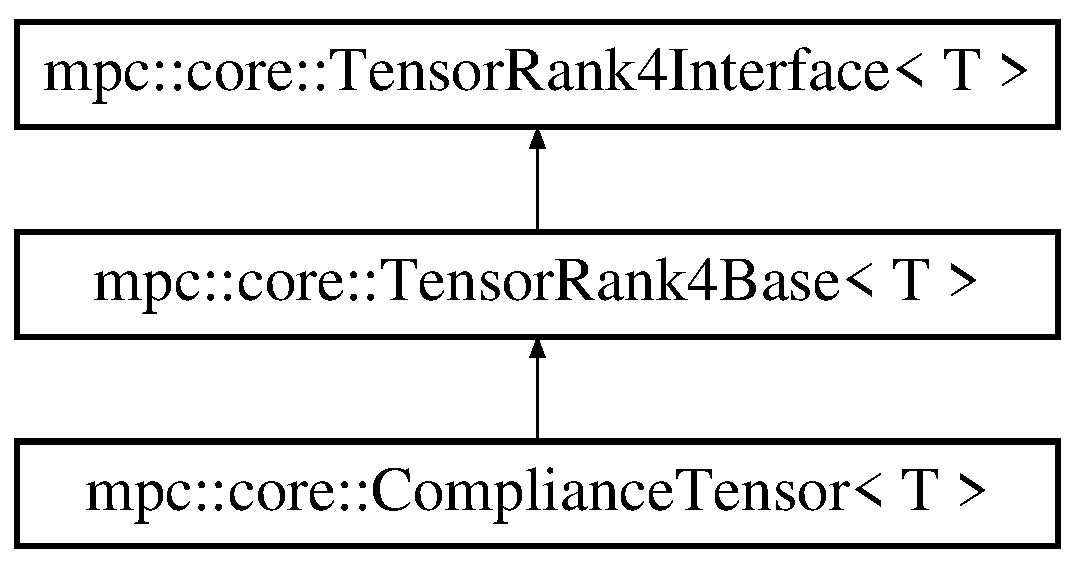
\includegraphics[height=3.000000cm]{structmpc_1_1core_1_1_compliance_tensor}
\end{center}
\end{figure}
\subsection*{Public Types}
\begin{DoxyCompactItemize}
\item 
typedef \mbox{\hyperlink{structmpc_1_1core_1_1_compliance_type}{mpc\+::core\+::\+Compliance\+Type}} \mbox{\hyperlink{structmpc_1_1core_1_1_compliance_tensor_a354022edff660abd91a04856798d6d0e}{cstype}}
\end{DoxyCompactItemize}
\subsection*{Public Member Functions}
\begin{DoxyCompactItemize}
\item 
{\footnotesize template$<$typename S $>$ }\\void \mbox{\hyperlink{structmpc_1_1core_1_1_compliance_tensor_a47139bd25ba7fa9724b9ea87fc22ea3c}{Set\+Components\+With\+Symmetry}} (std\+::set$<$ \mbox{\hyperlink{namespacempc_1_1core_ac3a232afc7c680d580628e834030482f}{mpc\+::core\+::\+Tensor\+Rank4\+Component}}$<$ T $>$ $>$ \&components)
\end{DoxyCompactItemize}
\subsection*{Additional Inherited Members}


\subsection{Detailed Description}
\subsubsection*{template$<$typename T$>$\newline
class mpc\+::core\+::\+Compliance\+Tensor$<$ T $>$}

compliance tensor class with function to set the components with a given symmety type 

Definition at line 104 of file stiffnesscompliance.\+hpp.



\subsection{Member Typedef Documentation}
\mbox{\Hypertarget{structmpc_1_1core_1_1_compliance_tensor_a354022edff660abd91a04856798d6d0e}\label{structmpc_1_1core_1_1_compliance_tensor_a354022edff660abd91a04856798d6d0e}} 
\index{mpc\+::core\+::\+Compliance\+Tensor@{mpc\+::core\+::\+Compliance\+Tensor}!cstype@{cstype}}
\index{cstype@{cstype}!mpc\+::core\+::\+Compliance\+Tensor@{mpc\+::core\+::\+Compliance\+Tensor}}
\subsubsection{\texorpdfstring{cstype}{cstype}}
{\footnotesize\ttfamily template$<$typename T$>$ \\
typedef \mbox{\hyperlink{structmpc_1_1core_1_1_compliance_type}{mpc\+::core\+::\+Compliance\+Type}} \mbox{\hyperlink{structmpc_1_1core_1_1_compliance_tensor}{mpc\+::core\+::\+Compliance\+Tensor}}$<$ T $>$\+::\mbox{\hyperlink{structmpc_1_1core_1_1_compliance_tensor_a354022edff660abd91a04856798d6d0e}{cstype}}}



Definition at line 106 of file stiffnesscompliance.\+hpp.



\subsection{Member Function Documentation}
\mbox{\Hypertarget{structmpc_1_1core_1_1_compliance_tensor_a47139bd25ba7fa9724b9ea87fc22ea3c}\label{structmpc_1_1core_1_1_compliance_tensor_a47139bd25ba7fa9724b9ea87fc22ea3c}} 
\index{mpc\+::core\+::\+Compliance\+Tensor@{mpc\+::core\+::\+Compliance\+Tensor}!Set\+Components\+With\+Symmetry@{Set\+Components\+With\+Symmetry}}
\index{Set\+Components\+With\+Symmetry@{Set\+Components\+With\+Symmetry}!mpc\+::core\+::\+Compliance\+Tensor@{mpc\+::core\+::\+Compliance\+Tensor}}
\subsubsection{\texorpdfstring{Set\+Components\+With\+Symmetry()}{SetComponentsWithSymmetry()}}
{\footnotesize\ttfamily template$<$typename T$>$ \\
template$<$typename S $>$ \\
void \mbox{\hyperlink{structmpc_1_1core_1_1_compliance_tensor}{mpc\+::core\+::\+Compliance\+Tensor}}$<$ T $>$\+::Set\+Components\+With\+Symmetry (\begin{DoxyParamCaption}\item[{std\+::set$<$ \mbox{\hyperlink{namespacempc_1_1core_ac3a232afc7c680d580628e834030482f}{mpc\+::core\+::\+Tensor\+Rank4\+Component}}$<$ T $>$ $>$ \&}]{components }\end{DoxyParamCaption})\hspace{0.3cm}{\ttfamily [inline]}}



Definition at line 109 of file stiffnesscompliance.\+hpp.



The documentation for this class was generated from the following file\+:\begin{DoxyCompactItemize}
\item 
/\+Users/atorlucci/\+Documents/github\+\_\+threecubed\+\_\+repos/mpc/src/mpc/core/\mbox{\hyperlink{stiffnesscompliance_8hpp}{stiffnesscompliance.\+hpp}}\end{DoxyCompactItemize}

\hypertarget{structmpc_1_1core_1_1_compliance_type}{}\section{mpc\+:\+:core\+:\+:Compliance\+Type Class Reference}
\label{structmpc_1_1core_1_1_compliance_type}\index{mpc\+::core\+::\+Compliance\+Type@{mpc\+::core\+::\+Compliance\+Type}}


simple class used mainly for template specializations in mpc  




{\ttfamily \#include $<$cstypes.\+hpp$>$}

Inheritance diagram for mpc\+:\+:core\+:\+:Compliance\+Type\+:\begin{figure}[H]
\begin{center}
\leavevmode
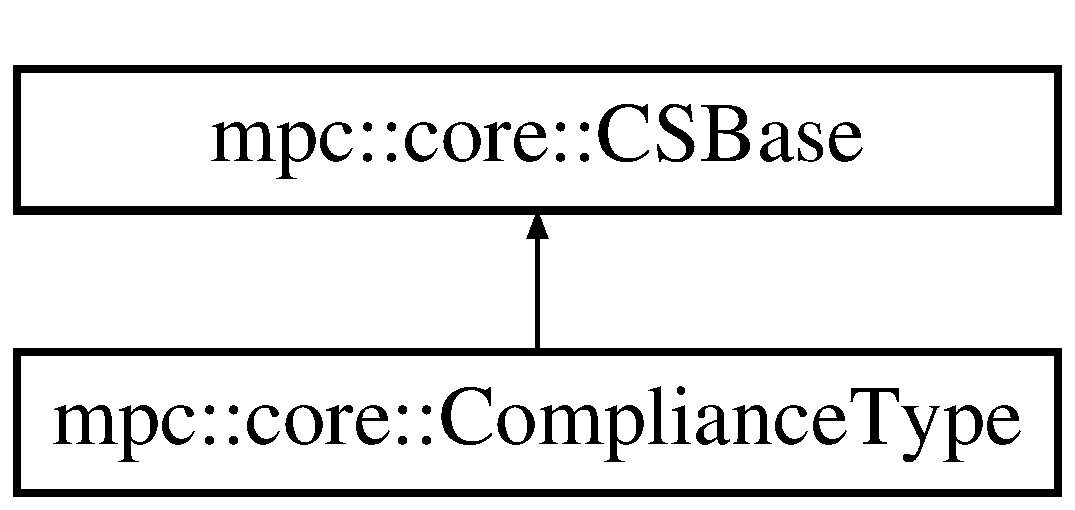
\includegraphics[height=2.000000cm]{structmpc_1_1core_1_1_compliance_type}
\end{center}
\end{figure}
\subsection*{Static Public Member Functions}
\begin{DoxyCompactItemize}
\item 
static constexpr \mbox{\hyperlink{namespacempc_1_1core_ad3e8e7d43bfc9202d954d999f7d5c991}{C\+S\+Enumeration}} \mbox{\hyperlink{structmpc_1_1core_1_1_compliance_type_a4ad878ddbe11a020e9ae2ea400deaf5d}{C\+S\+Enum}} ()
\end{DoxyCompactItemize}
\subsection*{Public Attributes}
\begin{DoxyCompactItemize}
\item 
const \mbox{\hyperlink{namespacempc_1_1core_ad3e8e7d43bfc9202d954d999f7d5c991}{C\+S\+Enumeration}} \mbox{\hyperlink{structmpc_1_1core_1_1_compliance_type_a05e820ab5e2f22d2f66b0d1d91ff3c0b}{cs\+\_\+enumeration}} = \mbox{\hyperlink{namespacempc_1_1core_ad3e8e7d43bfc9202d954d999f7d5c991a185bd2ffef1962ade3c0889c62cee500}{C\+S\+Enumeration\+::\+C\+O\+M\+P\+L\+I\+A\+N\+CE}}
\end{DoxyCompactItemize}


\subsection{Detailed Description}
simple class used mainly for template specializations in mpc 

Definition at line 88 of file cstypes.\+hpp.



\subsection{Member Function Documentation}
\mbox{\Hypertarget{structmpc_1_1core_1_1_compliance_type_a4ad878ddbe11a020e9ae2ea400deaf5d}\label{structmpc_1_1core_1_1_compliance_type_a4ad878ddbe11a020e9ae2ea400deaf5d}} 
\index{mpc\+::core\+::\+Compliance\+Type@{mpc\+::core\+::\+Compliance\+Type}!C\+S\+Enum@{C\+S\+Enum}}
\index{C\+S\+Enum@{C\+S\+Enum}!mpc\+::core\+::\+Compliance\+Type@{mpc\+::core\+::\+Compliance\+Type}}
\subsubsection{\texorpdfstring{C\+S\+Enum()}{CSEnum()}}
{\footnotesize\ttfamily static constexpr \mbox{\hyperlink{namespacempc_1_1core_ad3e8e7d43bfc9202d954d999f7d5c991}{C\+S\+Enumeration}} mpc\+::core\+::\+Compliance\+Type\+::\+C\+S\+Enum (\begin{DoxyParamCaption}{ }\end{DoxyParamCaption})\hspace{0.3cm}{\ttfamily [inline]}, {\ttfamily [static]}}



Definition at line 90 of file cstypes.\+hpp.



\subsection{Member Data Documentation}
\mbox{\Hypertarget{structmpc_1_1core_1_1_compliance_type_a05e820ab5e2f22d2f66b0d1d91ff3c0b}\label{structmpc_1_1core_1_1_compliance_type_a05e820ab5e2f22d2f66b0d1d91ff3c0b}} 
\index{mpc\+::core\+::\+Compliance\+Type@{mpc\+::core\+::\+Compliance\+Type}!cs\+\_\+enumeration@{cs\+\_\+enumeration}}
\index{cs\+\_\+enumeration@{cs\+\_\+enumeration}!mpc\+::core\+::\+Compliance\+Type@{mpc\+::core\+::\+Compliance\+Type}}
\subsubsection{\texorpdfstring{cs\+\_\+enumeration}{cs\_enumeration}}
{\footnotesize\ttfamily const \mbox{\hyperlink{namespacempc_1_1core_ad3e8e7d43bfc9202d954d999f7d5c991}{C\+S\+Enumeration}} mpc\+::core\+::\+Compliance\+Type\+::cs\+\_\+enumeration = \mbox{\hyperlink{namespacempc_1_1core_ad3e8e7d43bfc9202d954d999f7d5c991a185bd2ffef1962ade3c0889c62cee500}{C\+S\+Enumeration\+::\+C\+O\+M\+P\+L\+I\+A\+N\+CE}}}



Definition at line 89 of file cstypes.\+hpp.



The documentation for this class was generated from the following file\+:\begin{DoxyCompactItemize}
\item 
/\+Users/atorlucci/\+Documents/github\+\_\+threecubed\+\_\+repos/mpc/src/mpc/core/\mbox{\hyperlink{cstypes_8hpp}{cstypes.\+hpp}}\end{DoxyCompactItemize}

\hypertarget{structmpc_1_1rockphysics_1_1_compressibility_modulus_type}{}\section{mpc\+:\+:rockphysics\+:\+:Compressibility\+Modulus\+Type$<$ T $>$ Struct Template Reference}
\label{structmpc_1_1rockphysics_1_1_compressibility_modulus_type}\index{mpc\+::rockphysics\+::\+Compressibility\+Modulus\+Type$<$ T $>$@{mpc\+::rockphysics\+::\+Compressibility\+Modulus\+Type$<$ T $>$}}


{\ttfamily \#include $<$rockphysicstransformstypes.\+hpp$>$}

Inheritance diagram for mpc\+:\+:rockphysics\+:\+:Compressibility\+Modulus\+Type$<$ T $>$\+:\begin{figure}[H]
\begin{center}
\leavevmode
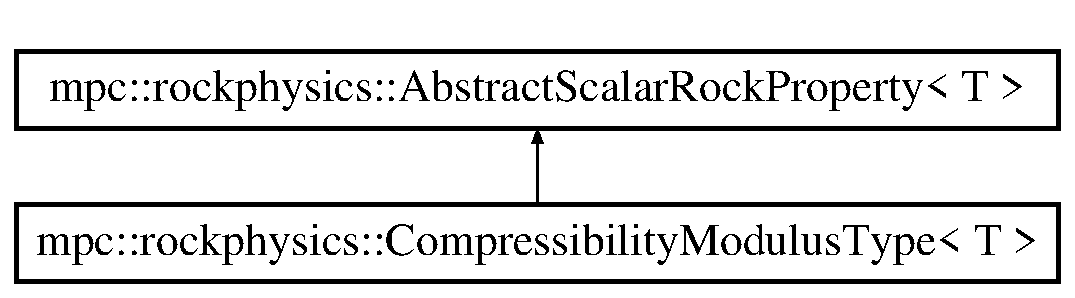
\includegraphics[height=2.000000cm]{structmpc_1_1rockphysics_1_1_compressibility_modulus_type}
\end{center}
\end{figure}
\subsection*{Public Member Functions}
\begin{DoxyCompactItemize}
\item 
constexpr \mbox{\hyperlink{structmpc_1_1rockphysics_1_1_compressibility_modulus_type_a7a8f465566c3f05f6bd9f24491680768}{Compressibility\+Modulus\+Type}} (T val)
\end{DoxyCompactItemize}
\subsection*{Additional Inherited Members}


\subsection{Detailed Description}
\subsubsection*{template$<$typename T$>$\newline
struct mpc\+::rockphysics\+::\+Compressibility\+Modulus\+Type$<$ T $>$}



Definition at line 107 of file rockphysicstransformstypes.\+hpp.



\subsection{Constructor \& Destructor Documentation}
\mbox{\Hypertarget{structmpc_1_1rockphysics_1_1_compressibility_modulus_type_a7a8f465566c3f05f6bd9f24491680768}\label{structmpc_1_1rockphysics_1_1_compressibility_modulus_type_a7a8f465566c3f05f6bd9f24491680768}} 
\index{mpc\+::rockphysics\+::\+Compressibility\+Modulus\+Type@{mpc\+::rockphysics\+::\+Compressibility\+Modulus\+Type}!Compressibility\+Modulus\+Type@{Compressibility\+Modulus\+Type}}
\index{Compressibility\+Modulus\+Type@{Compressibility\+Modulus\+Type}!mpc\+::rockphysics\+::\+Compressibility\+Modulus\+Type@{mpc\+::rockphysics\+::\+Compressibility\+Modulus\+Type}}
\subsubsection{\texorpdfstring{Compressibility\+Modulus\+Type()}{CompressibilityModulusType()}}
{\footnotesize\ttfamily template$<$typename T$>$ \\
constexpr \mbox{\hyperlink{structmpc_1_1rockphysics_1_1_compressibility_modulus_type}{mpc\+::rockphysics\+::\+Compressibility\+Modulus\+Type}}$<$ T $>$\+::\mbox{\hyperlink{structmpc_1_1rockphysics_1_1_compressibility_modulus_type}{Compressibility\+Modulus\+Type}} (\begin{DoxyParamCaption}\item[{T}]{val }\end{DoxyParamCaption})\hspace{0.3cm}{\ttfamily [inline]}}



Definition at line 112 of file rockphysicstransformstypes.\+hpp.



The documentation for this struct was generated from the following file\+:\begin{DoxyCompactItemize}
\item 
/\+Users/atorlucci/\+Documents/github\+\_\+threecubed\+\_\+repos/mpc/src/mpc/rockphysics/\mbox{\hyperlink{rockphysicstransformstypes_8hpp}{rockphysicstransformstypes.\+hpp}}\end{DoxyCompactItemize}

\hypertarget{structmpc_1_1rockphysics_1_1_compressional_modulus_type}{}\section{mpc\+:\+:rockphysics\+:\+:Compressional\+Modulus\+Type$<$ T $>$ Struct Template Reference}
\label{structmpc_1_1rockphysics_1_1_compressional_modulus_type}\index{mpc\+::rockphysics\+::\+Compressional\+Modulus\+Type$<$ T $>$@{mpc\+::rockphysics\+::\+Compressional\+Modulus\+Type$<$ T $>$}}


{\ttfamily \#include $<$rockphysicstransformstypes.\+hpp$>$}

Inheritance diagram for mpc\+:\+:rockphysics\+:\+:Compressional\+Modulus\+Type$<$ T $>$\+:\begin{figure}[H]
\begin{center}
\leavevmode
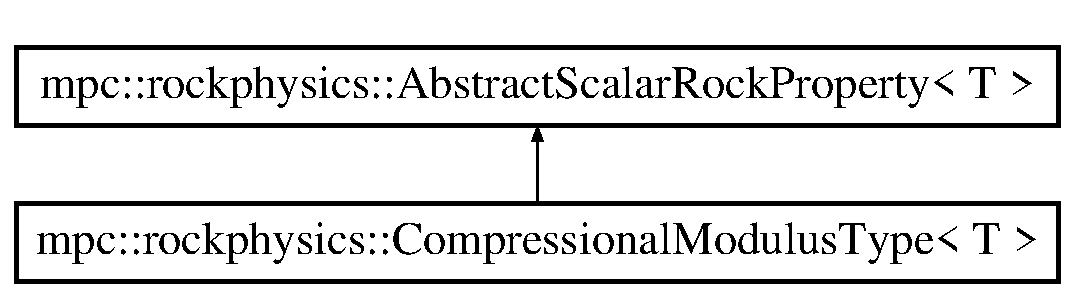
\includegraphics[height=2.000000cm]{structmpc_1_1rockphysics_1_1_compressional_modulus_type}
\end{center}
\end{figure}
\subsection*{Public Member Functions}
\begin{DoxyCompactItemize}
\item 
constexpr \mbox{\hyperlink{structmpc_1_1rockphysics_1_1_compressional_modulus_type_abdc02663a7781e7aa90f198d165901a9}{Compressional\+Modulus\+Type}} (T val)
\end{DoxyCompactItemize}
\subsection*{Additional Inherited Members}


\subsection{Detailed Description}
\subsubsection*{template$<$typename T$>$\newline
struct mpc\+::rockphysics\+::\+Compressional\+Modulus\+Type$<$ T $>$}



Definition at line 94 of file rockphysicstransformstypes.\+hpp.



\subsection{Constructor \& Destructor Documentation}
\mbox{\Hypertarget{structmpc_1_1rockphysics_1_1_compressional_modulus_type_abdc02663a7781e7aa90f198d165901a9}\label{structmpc_1_1rockphysics_1_1_compressional_modulus_type_abdc02663a7781e7aa90f198d165901a9}} 
\index{mpc\+::rockphysics\+::\+Compressional\+Modulus\+Type@{mpc\+::rockphysics\+::\+Compressional\+Modulus\+Type}!Compressional\+Modulus\+Type@{Compressional\+Modulus\+Type}}
\index{Compressional\+Modulus\+Type@{Compressional\+Modulus\+Type}!mpc\+::rockphysics\+::\+Compressional\+Modulus\+Type@{mpc\+::rockphysics\+::\+Compressional\+Modulus\+Type}}
\subsubsection{\texorpdfstring{Compressional\+Modulus\+Type()}{CompressionalModulusType()}}
{\footnotesize\ttfamily template$<$typename T$>$ \\
constexpr \mbox{\hyperlink{structmpc_1_1rockphysics_1_1_compressional_modulus_type}{mpc\+::rockphysics\+::\+Compressional\+Modulus\+Type}}$<$ T $>$\+::\mbox{\hyperlink{structmpc_1_1rockphysics_1_1_compressional_modulus_type}{Compressional\+Modulus\+Type}} (\begin{DoxyParamCaption}\item[{T}]{val }\end{DoxyParamCaption})\hspace{0.3cm}{\ttfamily [inline]}}



Definition at line 99 of file rockphysicstransformstypes.\+hpp.



The documentation for this struct was generated from the following file\+:\begin{DoxyCompactItemize}
\item 
/\+Users/atorlucci/\+Documents/github\+\_\+threecubed\+\_\+repos/mpc/src/mpc/rockphysics/\mbox{\hyperlink{rockphysicstransformstypes_8hpp}{rockphysicstransformstypes.\+hpp}}\end{DoxyCompactItemize}

\hypertarget{structmpc_1_1rockphysics_1_1_compressional_wave_velocity_type}{}\section{mpc\+:\+:rockphysics\+:\+:Compressional\+Wave\+Velocity\+Type$<$ T $>$ Struct Template Reference}
\label{structmpc_1_1rockphysics_1_1_compressional_wave_velocity_type}\index{mpc\+::rockphysics\+::\+Compressional\+Wave\+Velocity\+Type$<$ T $>$@{mpc\+::rockphysics\+::\+Compressional\+Wave\+Velocity\+Type$<$ T $>$}}


{\ttfamily \#include $<$rockphysicstransformstypes.\+hpp$>$}

Inheritance diagram for mpc\+:\+:rockphysics\+:\+:Compressional\+Wave\+Velocity\+Type$<$ T $>$\+:\begin{figure}[H]
\begin{center}
\leavevmode
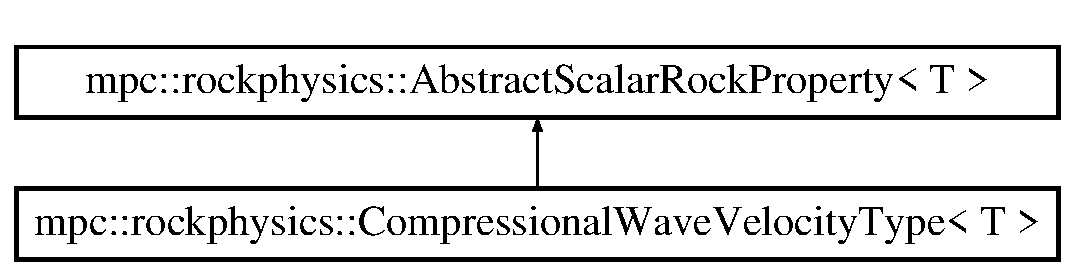
\includegraphics[height=2.000000cm]{structmpc_1_1rockphysics_1_1_compressional_wave_velocity_type}
\end{center}
\end{figure}
\subsection*{Public Member Functions}
\begin{DoxyCompactItemize}
\item 
constexpr \mbox{\hyperlink{structmpc_1_1rockphysics_1_1_compressional_wave_velocity_type_a5d7d3be3c8f5fc734d5648b9df46e24b}{Compressional\+Wave\+Velocity\+Type}} (T val)
\end{DoxyCompactItemize}
\subsection*{Additional Inherited Members}


\subsection{Detailed Description}
\subsubsection*{template$<$typename T$>$\newline
struct mpc\+::rockphysics\+::\+Compressional\+Wave\+Velocity\+Type$<$ T $>$}



Definition at line 180 of file rockphysicstransformstypes.\+hpp.



\subsection{Constructor \& Destructor Documentation}
\mbox{\Hypertarget{structmpc_1_1rockphysics_1_1_compressional_wave_velocity_type_a5d7d3be3c8f5fc734d5648b9df46e24b}\label{structmpc_1_1rockphysics_1_1_compressional_wave_velocity_type_a5d7d3be3c8f5fc734d5648b9df46e24b}} 
\index{mpc\+::rockphysics\+::\+Compressional\+Wave\+Velocity\+Type@{mpc\+::rockphysics\+::\+Compressional\+Wave\+Velocity\+Type}!Compressional\+Wave\+Velocity\+Type@{Compressional\+Wave\+Velocity\+Type}}
\index{Compressional\+Wave\+Velocity\+Type@{Compressional\+Wave\+Velocity\+Type}!mpc\+::rockphysics\+::\+Compressional\+Wave\+Velocity\+Type@{mpc\+::rockphysics\+::\+Compressional\+Wave\+Velocity\+Type}}
\subsubsection{\texorpdfstring{Compressional\+Wave\+Velocity\+Type()}{CompressionalWaveVelocityType()}}
{\footnotesize\ttfamily template$<$typename T$>$ \\
constexpr \mbox{\hyperlink{structmpc_1_1rockphysics_1_1_compressional_wave_velocity_type}{mpc\+::rockphysics\+::\+Compressional\+Wave\+Velocity\+Type}}$<$ T $>$\+::\mbox{\hyperlink{structmpc_1_1rockphysics_1_1_compressional_wave_velocity_type}{Compressional\+Wave\+Velocity\+Type}} (\begin{DoxyParamCaption}\item[{T}]{val }\end{DoxyParamCaption})\hspace{0.3cm}{\ttfamily [inline]}}



Definition at line 185 of file rockphysicstransformstypes.\+hpp.



The documentation for this struct was generated from the following file\+:\begin{DoxyCompactItemize}
\item 
/\+Users/atorlucci/\+Documents/github\+\_\+threecubed\+\_\+repos/mpc/src/mpc/rockphysics/\mbox{\hyperlink{rockphysicstransformstypes_8hpp}{rockphysicstransformstypes.\+hpp}}\end{DoxyCompactItemize}

\hypertarget{structmpc_1_1utilities_1_1_coordinate_base_type}{}\section{mpc\+:\+:utilities\+:\+:Coordinate\+Base\+Type Struct Reference}
\label{structmpc_1_1utilities_1_1_coordinate_base_type}\index{mpc\+::utilities\+::\+Coordinate\+Base\+Type@{mpc\+::utilities\+::\+Coordinate\+Base\+Type}}


{\ttfamily \#include $<$coordinatemapping.\+hpp$>$}

Inheritance diagram for mpc\+:\+:utilities\+:\+:Coordinate\+Base\+Type\+:\begin{figure}[H]
\begin{center}
\leavevmode
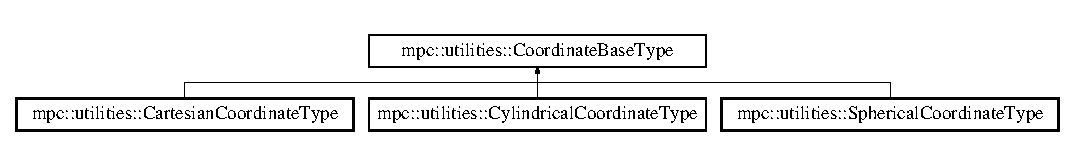
\includegraphics[height=1.530055cm]{structmpc_1_1utilities_1_1_coordinate_base_type}
\end{center}
\end{figure}


\subsection{Detailed Description}


Definition at line 25 of file coordinatemapping.\+hpp.



The documentation for this struct was generated from the following file\+:\begin{DoxyCompactItemize}
\item 
/\+Users/atorlucci/\+Documents/github\+\_\+threecubed\+\_\+repos/mpc/src/mpc/utilities/\mbox{\hyperlink{coordinatemapping_8hpp}{coordinatemapping.\+hpp}}\end{DoxyCompactItemize}

\hypertarget{structmpc_1_1utilities_1_1_coordinate_mapping}{}\section{mpc\+:\+:utilities\+:\+:Coordinate\+Mapping$<$ T, U, V $>$ Struct Template Reference}
\label{structmpc_1_1utilities_1_1_coordinate_mapping}\index{mpc\+::utilities\+::\+Coordinate\+Mapping$<$ T, U, V $>$@{mpc\+::utilities\+::\+Coordinate\+Mapping$<$ T, U, V $>$}}


{\ttfamily \#include $<$coordinatemapping.\+hpp$>$}



\subsection{Detailed Description}
\subsubsection*{template$<$typename T, typename U, typename V$>$\newline
struct mpc\+::utilities\+::\+Coordinate\+Mapping$<$ T, U, V $>$}



Definition at line 31 of file coordinatemapping.\+hpp.



The documentation for this struct was generated from the following file\+:\begin{DoxyCompactItemize}
\item 
/\+Users/atorlucci/\+Documents/github\+\_\+threecubed\+\_\+repos/mpc/src/mpc/utilities/\mbox{\hyperlink{coordinatemapping_8hpp}{coordinatemapping.\+hpp}}\end{DoxyCompactItemize}

\hypertarget{structmpc_1_1utilities_1_1_coordinate_mapping_3_01_t_00_01_cartesian_coordinate_type_00_01_cylindrical_coordinate_type_01_4}{}\section{mpc\+:\+:utilities\+:\+:Coordinate\+Mapping$<$ T, Cartesian\+Coordinate\+Type, Cylindrical\+Coordinate\+Type $>$ Struct Template Reference}
\label{structmpc_1_1utilities_1_1_coordinate_mapping_3_01_t_00_01_cartesian_coordinate_type_00_01_cylindrical_coordinate_type_01_4}\index{mpc\+::utilities\+::\+Coordinate\+Mapping$<$ T, Cartesian\+Coordinate\+Type, Cylindrical\+Coordinate\+Type $>$@{mpc\+::utilities\+::\+Coordinate\+Mapping$<$ T, Cartesian\+Coordinate\+Type, Cylindrical\+Coordinate\+Type $>$}}


{\ttfamily \#include $<$coordinatemapping.\+hpp$>$}

\subsection*{Public Member Functions}
\begin{DoxyCompactItemize}
\item 
std\+::tuple$<$ T, T, T $>$ \mbox{\hyperlink{structmpc_1_1utilities_1_1_coordinate_mapping_3_01_t_00_01_cartesian_coordinate_type_00_01_cylindrical_coordinate_type_01_4_a72140571d694e8eb77e72509ce827c92}{operator()}} (T rho, T phi, T z)
\end{DoxyCompactItemize}


\subsection{Detailed Description}
\subsubsection*{template$<$typename T$>$\newline
struct mpc\+::utilities\+::\+Coordinate\+Mapping$<$ T, Cartesian\+Coordinate\+Type, Cylindrical\+Coordinate\+Type $>$}



Definition at line 54 of file coordinatemapping.\+hpp.



\subsection{Member Function Documentation}
\mbox{\Hypertarget{structmpc_1_1utilities_1_1_coordinate_mapping_3_01_t_00_01_cartesian_coordinate_type_00_01_cylindrical_coordinate_type_01_4_a72140571d694e8eb77e72509ce827c92}\label{structmpc_1_1utilities_1_1_coordinate_mapping_3_01_t_00_01_cartesian_coordinate_type_00_01_cylindrical_coordinate_type_01_4_a72140571d694e8eb77e72509ce827c92}} 
\index{mpc\+::utilities\+::\+Coordinate\+Mapping$<$ T, Cartesian\+Coordinate\+Type, Cylindrical\+Coordinate\+Type $>$@{mpc\+::utilities\+::\+Coordinate\+Mapping$<$ T, Cartesian\+Coordinate\+Type, Cylindrical\+Coordinate\+Type $>$}!operator()@{operator()}}
\index{operator()@{operator()}!mpc\+::utilities\+::\+Coordinate\+Mapping$<$ T, Cartesian\+Coordinate\+Type, Cylindrical\+Coordinate\+Type $>$@{mpc\+::utilities\+::\+Coordinate\+Mapping$<$ T, Cartesian\+Coordinate\+Type, Cylindrical\+Coordinate\+Type $>$}}
\subsubsection{\texorpdfstring{operator()()}{operator()()}}
{\footnotesize\ttfamily template$<$typename T $>$ \\
std\+::tuple$<$T,T,T$>$ \mbox{\hyperlink{structmpc_1_1utilities_1_1_coordinate_mapping}{mpc\+::utilities\+::\+Coordinate\+Mapping}}$<$ T, \mbox{\hyperlink{structmpc_1_1utilities_1_1_cartesian_coordinate_type}{Cartesian\+Coordinate\+Type}}, \mbox{\hyperlink{structmpc_1_1utilities_1_1_cylindrical_coordinate_type}{Cylindrical\+Coordinate\+Type}} $>$\+::operator() (\begin{DoxyParamCaption}\item[{T}]{rho,  }\item[{T}]{phi,  }\item[{T}]{z }\end{DoxyParamCaption})\hspace{0.3cm}{\ttfamily [inline]}}



Definition at line 56 of file coordinatemapping.\+hpp.



The documentation for this struct was generated from the following file\+:\begin{DoxyCompactItemize}
\item 
/\+Users/atorlucci/\+Documents/github\+\_\+threecubed\+\_\+repos/mpc/src/mpc/utilities/\mbox{\hyperlink{coordinatemapping_8hpp}{coordinatemapping.\+hpp}}\end{DoxyCompactItemize}

\hypertarget{structmpc_1_1utilities_1_1_coordinate_mapping_3_01_t_00_01_cartesian_coordinate_type_00_01_spherical_coordinate_type_01_4}{}\section{mpc\+:\+:utilities\+:\+:Coordinate\+Mapping$<$ T, Cartesian\+Coordinate\+Type, Spherical\+Coordinate\+Type $>$ Struct Template Reference}
\label{structmpc_1_1utilities_1_1_coordinate_mapping_3_01_t_00_01_cartesian_coordinate_type_00_01_spherical_coordinate_type_01_4}\index{mpc\+::utilities\+::\+Coordinate\+Mapping$<$ T, Cartesian\+Coordinate\+Type, Spherical\+Coordinate\+Type $>$@{mpc\+::utilities\+::\+Coordinate\+Mapping$<$ T, Cartesian\+Coordinate\+Type, Spherical\+Coordinate\+Type $>$}}


{\ttfamily \#include $<$coordinatemapping.\+hpp$>$}

\subsection*{Public Member Functions}
\begin{DoxyCompactItemize}
\item 
std\+::tuple$<$ T, T, T $>$ \mbox{\hyperlink{structmpc_1_1utilities_1_1_coordinate_mapping_3_01_t_00_01_cartesian_coordinate_type_00_01_spherical_coordinate_type_01_4_a7a19325e577f99582bd180b87dd932ad}{operator()}} (T rho, T theta, T phi)
\end{DoxyCompactItemize}


\subsection{Detailed Description}
\subsubsection*{template$<$typename T$>$\newline
struct mpc\+::utilities\+::\+Coordinate\+Mapping$<$ T, Cartesian\+Coordinate\+Type, Spherical\+Coordinate\+Type $>$}



Definition at line 65 of file coordinatemapping.\+hpp.



\subsection{Member Function Documentation}
\mbox{\Hypertarget{structmpc_1_1utilities_1_1_coordinate_mapping_3_01_t_00_01_cartesian_coordinate_type_00_01_spherical_coordinate_type_01_4_a7a19325e577f99582bd180b87dd932ad}\label{structmpc_1_1utilities_1_1_coordinate_mapping_3_01_t_00_01_cartesian_coordinate_type_00_01_spherical_coordinate_type_01_4_a7a19325e577f99582bd180b87dd932ad}} 
\index{mpc\+::utilities\+::\+Coordinate\+Mapping$<$ T, Cartesian\+Coordinate\+Type, Spherical\+Coordinate\+Type $>$@{mpc\+::utilities\+::\+Coordinate\+Mapping$<$ T, Cartesian\+Coordinate\+Type, Spherical\+Coordinate\+Type $>$}!operator()@{operator()}}
\index{operator()@{operator()}!mpc\+::utilities\+::\+Coordinate\+Mapping$<$ T, Cartesian\+Coordinate\+Type, Spherical\+Coordinate\+Type $>$@{mpc\+::utilities\+::\+Coordinate\+Mapping$<$ T, Cartesian\+Coordinate\+Type, Spherical\+Coordinate\+Type $>$}}
\subsubsection{\texorpdfstring{operator()()}{operator()()}}
{\footnotesize\ttfamily template$<$typename T $>$ \\
std\+::tuple$<$T,T,T$>$ \mbox{\hyperlink{structmpc_1_1utilities_1_1_coordinate_mapping}{mpc\+::utilities\+::\+Coordinate\+Mapping}}$<$ T, \mbox{\hyperlink{structmpc_1_1utilities_1_1_cartesian_coordinate_type}{Cartesian\+Coordinate\+Type}}, \mbox{\hyperlink{structmpc_1_1utilities_1_1_spherical_coordinate_type}{Spherical\+Coordinate\+Type}} $>$\+::operator() (\begin{DoxyParamCaption}\item[{T}]{rho,  }\item[{T}]{theta,  }\item[{T}]{phi }\end{DoxyParamCaption})\hspace{0.3cm}{\ttfamily [inline]}}



Definition at line 67 of file coordinatemapping.\+hpp.



The documentation for this struct was generated from the following file\+:\begin{DoxyCompactItemize}
\item 
/\+Users/atorlucci/\+Documents/github\+\_\+threecubed\+\_\+repos/mpc/src/mpc/utilities/\mbox{\hyperlink{coordinatemapping_8hpp}{coordinatemapping.\+hpp}}\end{DoxyCompactItemize}

\hypertarget{structmpc_1_1core_1_1_c_s_base}{}\section{mpc\+:\+:core\+:\+:C\+S\+Base Class Reference}
\label{structmpc_1_1core_1_1_c_s_base}\index{mpc\+::core\+::\+C\+S\+Base@{mpc\+::core\+::\+C\+S\+Base}}


base class for stiffness compliance types  




{\ttfamily \#include $<$cstypes.\+hpp$>$}

Inheritance diagram for mpc\+:\+:core\+:\+:C\+S\+Base\+:\begin{figure}[H]
\begin{center}
\leavevmode
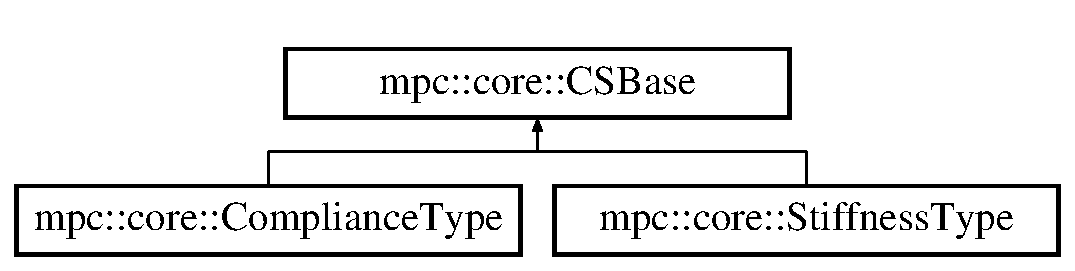
\includegraphics[height=2.000000cm]{structmpc_1_1core_1_1_c_s_base}
\end{center}
\end{figure}


\subsection{Detailed Description}
base class for stiffness compliance types 

mpc template specializations rely on this class for static\+\_\+assert() 

Definition at line 71 of file cstypes.\+hpp.



The documentation for this class was generated from the following file\+:\begin{DoxyCompactItemize}
\item 
/\+Users/atorlucci/\+Documents/github\+\_\+threecubed\+\_\+repos/mpc/src/mpc/core/\mbox{\hyperlink{cstypes_8hpp}{cstypes.\+hpp}}\end{DoxyCompactItemize}

\hypertarget{structmpc_1_1core_1_1_c_s_enumeration_interface}{}\section{mpc\+:\+:core\+:\+:C\+S\+Enumeration\+Interface Class Reference}
\label{structmpc_1_1core_1_1_c_s_enumeration_interface}\index{mpc\+::core\+::\+C\+S\+Enumeration\+Interface@{mpc\+::core\+::\+C\+S\+Enumeration\+Interface}}


interface to convert enum to std\+::string  




{\ttfamily \#include $<$cstypes.\+hpp$>$}

\subsection*{Static Public Member Functions}
\begin{DoxyCompactItemize}
\item 
static std\+::string \mbox{\hyperlink{structmpc_1_1core_1_1_c_s_enumeration_interface_add9c44f757aec342db7191224f0ae2da}{To\+Str}} (\mbox{\hyperlink{namespacempc_1_1core_ad3e8e7d43bfc9202d954d999f7d5c991}{C\+S\+Enumeration}} cs\+\_\+enum)
\end{DoxyCompactItemize}


\subsection{Detailed Description}
interface to convert enum to std\+::string 

Definition at line 36 of file cstypes.\+hpp.



\subsection{Member Function Documentation}
\mbox{\Hypertarget{structmpc_1_1core_1_1_c_s_enumeration_interface_add9c44f757aec342db7191224f0ae2da}\label{structmpc_1_1core_1_1_c_s_enumeration_interface_add9c44f757aec342db7191224f0ae2da}} 
\index{mpc\+::core\+::\+C\+S\+Enumeration\+Interface@{mpc\+::core\+::\+C\+S\+Enumeration\+Interface}!To\+Str@{To\+Str}}
\index{To\+Str@{To\+Str}!mpc\+::core\+::\+C\+S\+Enumeration\+Interface@{mpc\+::core\+::\+C\+S\+Enumeration\+Interface}}
\subsubsection{\texorpdfstring{To\+Str()}{ToStr()}}
{\footnotesize\ttfamily static std\+::string mpc\+::core\+::\+C\+S\+Enumeration\+Interface\+::\+To\+Str (\begin{DoxyParamCaption}\item[{\mbox{\hyperlink{namespacempc_1_1core_ad3e8e7d43bfc9202d954d999f7d5c991}{C\+S\+Enumeration}}}]{cs\+\_\+enum }\end{DoxyParamCaption})\hspace{0.3cm}{\ttfamily [inline]}, {\ttfamily [static]}}



Definition at line 38 of file cstypes.\+hpp.



The documentation for this class was generated from the following file\+:\begin{DoxyCompactItemize}
\item 
/\+Users/atorlucci/\+Documents/github\+\_\+threecubed\+\_\+repos/mpc/src/mpc/core/\mbox{\hyperlink{cstypes_8hpp}{cstypes.\+hpp}}\end{DoxyCompactItemize}

\hypertarget{classmpc_1_1core_1_1_c_tensor_rank2_component_index}{}\section{mpc\+:\+:core\+:\+:C\+Tensor\+Rank2\+Component\+Index$<$ M, N $>$ Class Template Reference}
\label{classmpc_1_1core_1_1_c_tensor_rank2_component_index}\index{mpc\+::core\+::\+C\+Tensor\+Rank2\+Component\+Index$<$ M, N $>$@{mpc\+::core\+::\+C\+Tensor\+Rank2\+Component\+Index$<$ M, N $>$}}


compile time rank 2 tensor index An index class with constexpr member functions that can be used as template parameter values...  




{\ttfamily \#include $<$tensorcomponentindex.\+hpp$>$}

\subsection*{Public Member Functions}
\begin{DoxyCompactItemize}
\item 
constexpr \mbox{\hyperlink{classmpc_1_1core_1_1_c_tensor_rank2_component_index_a46ac9bf492508d77742028988f69935e}{C\+Tensor\+Rank2\+Component\+Index}} ()
\item 
constexpr int \mbox{\hyperlink{classmpc_1_1core_1_1_c_tensor_rank2_component_index_a406715396e26cf9606979b8c34982271}{First\+Index}} () const
\item 
constexpr int \mbox{\hyperlink{classmpc_1_1core_1_1_c_tensor_rank2_component_index_a442ae55dfc043f4b1d2bca60575f871d}{Second\+Index}} () const
\item 
{\footnotesize template$<$int P, int Q$>$ }\\constexpr \mbox{\hyperlink{classmpc_1_1core_1_1_c_tensor_rank2_component_index_a46b24107de94dc221e9f6549f79f0fff}{C\+Tensor\+Rank2\+Component\+Index}} (const \mbox{\hyperlink{classmpc_1_1core_1_1_c_tensor_rank2_component_index}{C\+Tensor\+Rank2\+Component\+Index}}$<$ P, Q $>$ \&rhs)
\item 
int \mbox{\hyperlink{classmpc_1_1core_1_1_c_tensor_rank2_component_index_a3c99d933e4ae372fe73cd6afabf0570d}{operator\mbox{[}$\,$\mbox{]}}} (int i)
\item 
{\footnotesize template$<$int P, int Q$>$ }\\bool \mbox{\hyperlink{classmpc_1_1core_1_1_c_tensor_rank2_component_index_a376fbe0ee4fd0e934d5d06b5370e1b96}{operator$<$}} (const \mbox{\hyperlink{classmpc_1_1core_1_1_c_tensor_rank2_component_index}{C\+Tensor\+Rank2\+Component\+Index}}$<$ P, Q $>$ \&rhs)
\item 
{\footnotesize template$<$int P, int Q$>$ }\\bool \mbox{\hyperlink{classmpc_1_1core_1_1_c_tensor_rank2_component_index_a09ad8de90ca42234aa1b37ece4f6f989}{operator$>$}} (const \mbox{\hyperlink{classmpc_1_1core_1_1_c_tensor_rank2_component_index}{C\+Tensor\+Rank2\+Component\+Index}}$<$ P, Q $>$ \&rhs)
\item 
{\footnotesize template$<$int P, int Q$>$ }\\bool \mbox{\hyperlink{classmpc_1_1core_1_1_c_tensor_rank2_component_index_a3b672ed7feddcd26a97b5bdf8c951724}{operator==}} (const \mbox{\hyperlink{classmpc_1_1core_1_1_c_tensor_rank2_component_index}{C\+Tensor\+Rank2\+Component\+Index}}$<$ P, Q $>$ \&rhs)
\item 
{\footnotesize template$<$int P, int Q$>$ }\\bool \mbox{\hyperlink{classmpc_1_1core_1_1_c_tensor_rank2_component_index_a052391422fa03b261456a51ddbd388d8}{operator!=}} (const \mbox{\hyperlink{classmpc_1_1core_1_1_c_tensor_rank2_component_index}{C\+Tensor\+Rank2\+Component\+Index}}$<$ P, Q $>$ \&rhs)
\item 
{\footnotesize template$<$int P, int Q$>$ }\\bool \mbox{\hyperlink{classmpc_1_1core_1_1_c_tensor_rank2_component_index_ad034cd6d15be78437e9036767ecc2986}{operator$<$=}} (const \mbox{\hyperlink{classmpc_1_1core_1_1_c_tensor_rank2_component_index}{C\+Tensor\+Rank2\+Component\+Index}}$<$ P, Q $>$ \&rhs) const
\item 
{\footnotesize template$<$int P, int Q$>$ }\\bool \mbox{\hyperlink{classmpc_1_1core_1_1_c_tensor_rank2_component_index_a058e6de05a69a5dcbc6957081ec153bf}{operator$>$=}} (const \mbox{\hyperlink{classmpc_1_1core_1_1_c_tensor_rank2_component_index}{C\+Tensor\+Rank2\+Component\+Index}}$<$ P, Q $>$ \&rhs) const
\end{DoxyCompactItemize}
\subsection*{Static Public Member Functions}
\begin{DoxyCompactItemize}
\item 
{\footnotesize template$<$int P, int Q$>$ }\\static blitz\+::\+Tiny\+Vector$<$ int, 2 $>$ \mbox{\hyperlink{classmpc_1_1core_1_1_c_tensor_rank2_component_index_afc534a2e0322c3dc71904e4b02a221ea}{To\+Blitz\+Tiny\+Vector}} (const \mbox{\hyperlink{classmpc_1_1core_1_1_c_tensor_rank2_component_index}{C\+Tensor\+Rank2\+Component\+Index}}$<$ P, Q $>$ \&indexn)
\end{DoxyCompactItemize}
\subsection*{Friends}
\begin{DoxyCompactItemize}
\item 
std\+::ostream \& \mbox{\hyperlink{classmpc_1_1core_1_1_c_tensor_rank2_component_index_a13d821c3dc9b99854bc96973ac0920b2}{operator$<$$<$}} (std\+::ostream \&os, const \mbox{\hyperlink{classmpc_1_1core_1_1_c_tensor_rank2_component_index}{C\+Tensor\+Rank2\+Component\+Index}} \&t)
\end{DoxyCompactItemize}


\subsection{Detailed Description}
\subsubsection*{template$<$int M, int N$>$\newline
class mpc\+::core\+::\+C\+Tensor\+Rank2\+Component\+Index$<$ M, N $>$}

compile time rank 2 tensor index An index class with constexpr member functions that can be used as template parameter values... 

Definition at line 37 of file tensorcomponentindex.\+hpp.



\subsection{Constructor \& Destructor Documentation}
\mbox{\Hypertarget{classmpc_1_1core_1_1_c_tensor_rank2_component_index_a46ac9bf492508d77742028988f69935e}\label{classmpc_1_1core_1_1_c_tensor_rank2_component_index_a46ac9bf492508d77742028988f69935e}} 
\index{mpc\+::core\+::\+C\+Tensor\+Rank2\+Component\+Index@{mpc\+::core\+::\+C\+Tensor\+Rank2\+Component\+Index}!C\+Tensor\+Rank2\+Component\+Index@{C\+Tensor\+Rank2\+Component\+Index}}
\index{C\+Tensor\+Rank2\+Component\+Index@{C\+Tensor\+Rank2\+Component\+Index}!mpc\+::core\+::\+C\+Tensor\+Rank2\+Component\+Index@{mpc\+::core\+::\+C\+Tensor\+Rank2\+Component\+Index}}
\subsubsection{\texorpdfstring{C\+Tensor\+Rank2\+Component\+Index()}{CTensorRank2ComponentIndex()}\hspace{0.1cm}{\footnotesize\ttfamily [1/2]}}
{\footnotesize\ttfamily template$<$int M, int N$>$ \\
constexpr \mbox{\hyperlink{classmpc_1_1core_1_1_c_tensor_rank2_component_index}{mpc\+::core\+::\+C\+Tensor\+Rank2\+Component\+Index}}$<$ M, N $>$\+::\mbox{\hyperlink{classmpc_1_1core_1_1_c_tensor_rank2_component_index}{C\+Tensor\+Rank2\+Component\+Index}} (\begin{DoxyParamCaption}{ }\end{DoxyParamCaption})\hspace{0.3cm}{\ttfamily [inline]}}



Definition at line 39 of file tensorcomponentindex.\+hpp.

\mbox{\Hypertarget{classmpc_1_1core_1_1_c_tensor_rank2_component_index_a46b24107de94dc221e9f6549f79f0fff}\label{classmpc_1_1core_1_1_c_tensor_rank2_component_index_a46b24107de94dc221e9f6549f79f0fff}} 
\index{mpc\+::core\+::\+C\+Tensor\+Rank2\+Component\+Index@{mpc\+::core\+::\+C\+Tensor\+Rank2\+Component\+Index}!C\+Tensor\+Rank2\+Component\+Index@{C\+Tensor\+Rank2\+Component\+Index}}
\index{C\+Tensor\+Rank2\+Component\+Index@{C\+Tensor\+Rank2\+Component\+Index}!mpc\+::core\+::\+C\+Tensor\+Rank2\+Component\+Index@{mpc\+::core\+::\+C\+Tensor\+Rank2\+Component\+Index}}
\subsubsection{\texorpdfstring{C\+Tensor\+Rank2\+Component\+Index()}{CTensorRank2ComponentIndex()}\hspace{0.1cm}{\footnotesize\ttfamily [2/2]}}
{\footnotesize\ttfamily template$<$int M, int N$>$ \\
template$<$int P, int Q$>$ \\
constexpr \mbox{\hyperlink{classmpc_1_1core_1_1_c_tensor_rank2_component_index}{mpc\+::core\+::\+C\+Tensor\+Rank2\+Component\+Index}}$<$ M, N $>$\+::\mbox{\hyperlink{classmpc_1_1core_1_1_c_tensor_rank2_component_index}{C\+Tensor\+Rank2\+Component\+Index}} (\begin{DoxyParamCaption}\item[{const \mbox{\hyperlink{classmpc_1_1core_1_1_c_tensor_rank2_component_index}{C\+Tensor\+Rank2\+Component\+Index}}$<$ P, Q $>$ \&}]{rhs }\end{DoxyParamCaption})\hspace{0.3cm}{\ttfamily [inline]}}



Definition at line 48 of file tensorcomponentindex.\+hpp.



\subsection{Member Function Documentation}
\mbox{\Hypertarget{classmpc_1_1core_1_1_c_tensor_rank2_component_index_a406715396e26cf9606979b8c34982271}\label{classmpc_1_1core_1_1_c_tensor_rank2_component_index_a406715396e26cf9606979b8c34982271}} 
\index{mpc\+::core\+::\+C\+Tensor\+Rank2\+Component\+Index@{mpc\+::core\+::\+C\+Tensor\+Rank2\+Component\+Index}!First\+Index@{First\+Index}}
\index{First\+Index@{First\+Index}!mpc\+::core\+::\+C\+Tensor\+Rank2\+Component\+Index@{mpc\+::core\+::\+C\+Tensor\+Rank2\+Component\+Index}}
\subsubsection{\texorpdfstring{First\+Index()}{FirstIndex()}}
{\footnotesize\ttfamily template$<$int M, int N$>$ \\
constexpr int \mbox{\hyperlink{classmpc_1_1core_1_1_c_tensor_rank2_component_index}{mpc\+::core\+::\+C\+Tensor\+Rank2\+Component\+Index}}$<$ M, N $>$\+::First\+Index (\begin{DoxyParamCaption}{ }\end{DoxyParamCaption}) const\hspace{0.3cm}{\ttfamily [inline]}}



Definition at line 40 of file tensorcomponentindex.\+hpp.

\mbox{\Hypertarget{classmpc_1_1core_1_1_c_tensor_rank2_component_index_a052391422fa03b261456a51ddbd388d8}\label{classmpc_1_1core_1_1_c_tensor_rank2_component_index_a052391422fa03b261456a51ddbd388d8}} 
\index{mpc\+::core\+::\+C\+Tensor\+Rank2\+Component\+Index@{mpc\+::core\+::\+C\+Tensor\+Rank2\+Component\+Index}!operator"!=@{operator"!=}}
\index{operator"!=@{operator"!=}!mpc\+::core\+::\+C\+Tensor\+Rank2\+Component\+Index@{mpc\+::core\+::\+C\+Tensor\+Rank2\+Component\+Index}}
\subsubsection{\texorpdfstring{operator"!=()}{operator!=()}}
{\footnotesize\ttfamily template$<$int M, int N$>$ \\
template$<$int P, int Q$>$ \\
bool \mbox{\hyperlink{classmpc_1_1core_1_1_c_tensor_rank2_component_index}{mpc\+::core\+::\+C\+Tensor\+Rank2\+Component\+Index}}$<$ M, N $>$\+::operator!= (\begin{DoxyParamCaption}\item[{const \mbox{\hyperlink{classmpc_1_1core_1_1_c_tensor_rank2_component_index}{C\+Tensor\+Rank2\+Component\+Index}}$<$ P, Q $>$ \&}]{rhs }\end{DoxyParamCaption})\hspace{0.3cm}{\ttfamily [inline]}}



Definition at line 82 of file tensorcomponentindex.\+hpp.

\mbox{\Hypertarget{classmpc_1_1core_1_1_c_tensor_rank2_component_index_a376fbe0ee4fd0e934d5d06b5370e1b96}\label{classmpc_1_1core_1_1_c_tensor_rank2_component_index_a376fbe0ee4fd0e934d5d06b5370e1b96}} 
\index{mpc\+::core\+::\+C\+Tensor\+Rank2\+Component\+Index@{mpc\+::core\+::\+C\+Tensor\+Rank2\+Component\+Index}!operator$<$@{operator$<$}}
\index{operator$<$@{operator$<$}!mpc\+::core\+::\+C\+Tensor\+Rank2\+Component\+Index@{mpc\+::core\+::\+C\+Tensor\+Rank2\+Component\+Index}}
\subsubsection{\texorpdfstring{operator$<$()}{operator<()}}
{\footnotesize\ttfamily template$<$int M, int N$>$ \\
template$<$int P, int Q$>$ \\
bool \mbox{\hyperlink{classmpc_1_1core_1_1_c_tensor_rank2_component_index}{mpc\+::core\+::\+C\+Tensor\+Rank2\+Component\+Index}}$<$ M, N $>$\+::operator$<$ (\begin{DoxyParamCaption}\item[{const \mbox{\hyperlink{classmpc_1_1core_1_1_c_tensor_rank2_component_index}{C\+Tensor\+Rank2\+Component\+Index}}$<$ P, Q $>$ \&}]{rhs }\end{DoxyParamCaption})\hspace{0.3cm}{\ttfamily [inline]}}



Definition at line 65 of file tensorcomponentindex.\+hpp.

\mbox{\Hypertarget{classmpc_1_1core_1_1_c_tensor_rank2_component_index_ad034cd6d15be78437e9036767ecc2986}\label{classmpc_1_1core_1_1_c_tensor_rank2_component_index_ad034cd6d15be78437e9036767ecc2986}} 
\index{mpc\+::core\+::\+C\+Tensor\+Rank2\+Component\+Index@{mpc\+::core\+::\+C\+Tensor\+Rank2\+Component\+Index}!operator$<$=@{operator$<$=}}
\index{operator$<$=@{operator$<$=}!mpc\+::core\+::\+C\+Tensor\+Rank2\+Component\+Index@{mpc\+::core\+::\+C\+Tensor\+Rank2\+Component\+Index}}
\subsubsection{\texorpdfstring{operator$<$=()}{operator<=()}}
{\footnotesize\ttfamily template$<$int M, int N$>$ \\
template$<$int P, int Q$>$ \\
bool \mbox{\hyperlink{classmpc_1_1core_1_1_c_tensor_rank2_component_index}{mpc\+::core\+::\+C\+Tensor\+Rank2\+Component\+Index}}$<$ M, N $>$\+::operator$<$= (\begin{DoxyParamCaption}\item[{const \mbox{\hyperlink{classmpc_1_1core_1_1_c_tensor_rank2_component_index}{C\+Tensor\+Rank2\+Component\+Index}}$<$ P, Q $>$ \&}]{rhs }\end{DoxyParamCaption}) const\hspace{0.3cm}{\ttfamily [inline]}}



Definition at line 87 of file tensorcomponentindex.\+hpp.

\mbox{\Hypertarget{classmpc_1_1core_1_1_c_tensor_rank2_component_index_a3b672ed7feddcd26a97b5bdf8c951724}\label{classmpc_1_1core_1_1_c_tensor_rank2_component_index_a3b672ed7feddcd26a97b5bdf8c951724}} 
\index{mpc\+::core\+::\+C\+Tensor\+Rank2\+Component\+Index@{mpc\+::core\+::\+C\+Tensor\+Rank2\+Component\+Index}!operator==@{operator==}}
\index{operator==@{operator==}!mpc\+::core\+::\+C\+Tensor\+Rank2\+Component\+Index@{mpc\+::core\+::\+C\+Tensor\+Rank2\+Component\+Index}}
\subsubsection{\texorpdfstring{operator==()}{operator==()}}
{\footnotesize\ttfamily template$<$int M, int N$>$ \\
template$<$int P, int Q$>$ \\
bool \mbox{\hyperlink{classmpc_1_1core_1_1_c_tensor_rank2_component_index}{mpc\+::core\+::\+C\+Tensor\+Rank2\+Component\+Index}}$<$ M, N $>$\+::operator== (\begin{DoxyParamCaption}\item[{const \mbox{\hyperlink{classmpc_1_1core_1_1_c_tensor_rank2_component_index}{C\+Tensor\+Rank2\+Component\+Index}}$<$ P, Q $>$ \&}]{rhs }\end{DoxyParamCaption})\hspace{0.3cm}{\ttfamily [inline]}}



Definition at line 77 of file tensorcomponentindex.\+hpp.

\mbox{\Hypertarget{classmpc_1_1core_1_1_c_tensor_rank2_component_index_a09ad8de90ca42234aa1b37ece4f6f989}\label{classmpc_1_1core_1_1_c_tensor_rank2_component_index_a09ad8de90ca42234aa1b37ece4f6f989}} 
\index{mpc\+::core\+::\+C\+Tensor\+Rank2\+Component\+Index@{mpc\+::core\+::\+C\+Tensor\+Rank2\+Component\+Index}!operator$>$@{operator$>$}}
\index{operator$>$@{operator$>$}!mpc\+::core\+::\+C\+Tensor\+Rank2\+Component\+Index@{mpc\+::core\+::\+C\+Tensor\+Rank2\+Component\+Index}}
\subsubsection{\texorpdfstring{operator$>$()}{operator>()}}
{\footnotesize\ttfamily template$<$int M, int N$>$ \\
template$<$int P, int Q$>$ \\
bool \mbox{\hyperlink{classmpc_1_1core_1_1_c_tensor_rank2_component_index}{mpc\+::core\+::\+C\+Tensor\+Rank2\+Component\+Index}}$<$ M, N $>$\+::operator$>$ (\begin{DoxyParamCaption}\item[{const \mbox{\hyperlink{classmpc_1_1core_1_1_c_tensor_rank2_component_index}{C\+Tensor\+Rank2\+Component\+Index}}$<$ P, Q $>$ \&}]{rhs }\end{DoxyParamCaption})\hspace{0.3cm}{\ttfamily [inline]}}



Definition at line 71 of file tensorcomponentindex.\+hpp.

\mbox{\Hypertarget{classmpc_1_1core_1_1_c_tensor_rank2_component_index_a058e6de05a69a5dcbc6957081ec153bf}\label{classmpc_1_1core_1_1_c_tensor_rank2_component_index_a058e6de05a69a5dcbc6957081ec153bf}} 
\index{mpc\+::core\+::\+C\+Tensor\+Rank2\+Component\+Index@{mpc\+::core\+::\+C\+Tensor\+Rank2\+Component\+Index}!operator$>$=@{operator$>$=}}
\index{operator$>$=@{operator$>$=}!mpc\+::core\+::\+C\+Tensor\+Rank2\+Component\+Index@{mpc\+::core\+::\+C\+Tensor\+Rank2\+Component\+Index}}
\subsubsection{\texorpdfstring{operator$>$=()}{operator>=()}}
{\footnotesize\ttfamily template$<$int M, int N$>$ \\
template$<$int P, int Q$>$ \\
bool \mbox{\hyperlink{classmpc_1_1core_1_1_c_tensor_rank2_component_index}{mpc\+::core\+::\+C\+Tensor\+Rank2\+Component\+Index}}$<$ M, N $>$\+::operator$>$= (\begin{DoxyParamCaption}\item[{const \mbox{\hyperlink{classmpc_1_1core_1_1_c_tensor_rank2_component_index}{C\+Tensor\+Rank2\+Component\+Index}}$<$ P, Q $>$ \&}]{rhs }\end{DoxyParamCaption}) const\hspace{0.3cm}{\ttfamily [inline]}}



Definition at line 94 of file tensorcomponentindex.\+hpp.

\mbox{\Hypertarget{classmpc_1_1core_1_1_c_tensor_rank2_component_index_a3c99d933e4ae372fe73cd6afabf0570d}\label{classmpc_1_1core_1_1_c_tensor_rank2_component_index_a3c99d933e4ae372fe73cd6afabf0570d}} 
\index{mpc\+::core\+::\+C\+Tensor\+Rank2\+Component\+Index@{mpc\+::core\+::\+C\+Tensor\+Rank2\+Component\+Index}!operator\mbox{[}\mbox{]}@{operator[]}}
\index{operator\mbox{[}\mbox{]}@{operator[]}!mpc\+::core\+::\+C\+Tensor\+Rank2\+Component\+Index@{mpc\+::core\+::\+C\+Tensor\+Rank2\+Component\+Index}}
\subsubsection{\texorpdfstring{operator[]()}{operator[]()}}
{\footnotesize\ttfamily template$<$int M, int N$>$ \\
int \mbox{\hyperlink{classmpc_1_1core_1_1_c_tensor_rank2_component_index}{mpc\+::core\+::\+C\+Tensor\+Rank2\+Component\+Index}}$<$ M, N $>$\+::operator\mbox{[}$\,$\mbox{]} (\begin{DoxyParamCaption}\item[{int}]{i }\end{DoxyParamCaption})\hspace{0.3cm}{\ttfamily [inline]}}



Definition at line 57 of file tensorcomponentindex.\+hpp.

\mbox{\Hypertarget{classmpc_1_1core_1_1_c_tensor_rank2_component_index_a442ae55dfc043f4b1d2bca60575f871d}\label{classmpc_1_1core_1_1_c_tensor_rank2_component_index_a442ae55dfc043f4b1d2bca60575f871d}} 
\index{mpc\+::core\+::\+C\+Tensor\+Rank2\+Component\+Index@{mpc\+::core\+::\+C\+Tensor\+Rank2\+Component\+Index}!Second\+Index@{Second\+Index}}
\index{Second\+Index@{Second\+Index}!mpc\+::core\+::\+C\+Tensor\+Rank2\+Component\+Index@{mpc\+::core\+::\+C\+Tensor\+Rank2\+Component\+Index}}
\subsubsection{\texorpdfstring{Second\+Index()}{SecondIndex()}}
{\footnotesize\ttfamily template$<$int M, int N$>$ \\
constexpr int \mbox{\hyperlink{classmpc_1_1core_1_1_c_tensor_rank2_component_index}{mpc\+::core\+::\+C\+Tensor\+Rank2\+Component\+Index}}$<$ M, N $>$\+::Second\+Index (\begin{DoxyParamCaption}{ }\end{DoxyParamCaption}) const\hspace{0.3cm}{\ttfamily [inline]}}



Definition at line 43 of file tensorcomponentindex.\+hpp.

\mbox{\Hypertarget{classmpc_1_1core_1_1_c_tensor_rank2_component_index_afc534a2e0322c3dc71904e4b02a221ea}\label{classmpc_1_1core_1_1_c_tensor_rank2_component_index_afc534a2e0322c3dc71904e4b02a221ea}} 
\index{mpc\+::core\+::\+C\+Tensor\+Rank2\+Component\+Index@{mpc\+::core\+::\+C\+Tensor\+Rank2\+Component\+Index}!To\+Blitz\+Tiny\+Vector@{To\+Blitz\+Tiny\+Vector}}
\index{To\+Blitz\+Tiny\+Vector@{To\+Blitz\+Tiny\+Vector}!mpc\+::core\+::\+C\+Tensor\+Rank2\+Component\+Index@{mpc\+::core\+::\+C\+Tensor\+Rank2\+Component\+Index}}
\subsubsection{\texorpdfstring{To\+Blitz\+Tiny\+Vector()}{ToBlitzTinyVector()}}
{\footnotesize\ttfamily template$<$int M, int N$>$ \\
template$<$int P, int Q$>$ \\
static blitz\+::\+Tiny\+Vector$<$int,2$>$ \mbox{\hyperlink{classmpc_1_1core_1_1_c_tensor_rank2_component_index}{mpc\+::core\+::\+C\+Tensor\+Rank2\+Component\+Index}}$<$ M, N $>$\+::To\+Blitz\+Tiny\+Vector (\begin{DoxyParamCaption}\item[{const \mbox{\hyperlink{classmpc_1_1core_1_1_c_tensor_rank2_component_index}{C\+Tensor\+Rank2\+Component\+Index}}$<$ P, Q $>$ \&}]{indexn }\end{DoxyParamCaption})\hspace{0.3cm}{\ttfamily [inline]}, {\ttfamily [static]}}



Definition at line 108 of file tensorcomponentindex.\+hpp.



\subsection{Friends And Related Function Documentation}
\mbox{\Hypertarget{classmpc_1_1core_1_1_c_tensor_rank2_component_index_a13d821c3dc9b99854bc96973ac0920b2}\label{classmpc_1_1core_1_1_c_tensor_rank2_component_index_a13d821c3dc9b99854bc96973ac0920b2}} 
\index{mpc\+::core\+::\+C\+Tensor\+Rank2\+Component\+Index@{mpc\+::core\+::\+C\+Tensor\+Rank2\+Component\+Index}!operator$<$$<$@{operator$<$$<$}}
\index{operator$<$$<$@{operator$<$$<$}!mpc\+::core\+::\+C\+Tensor\+Rank2\+Component\+Index@{mpc\+::core\+::\+C\+Tensor\+Rank2\+Component\+Index}}
\subsubsection{\texorpdfstring{operator$<$$<$}{operator<<}}
{\footnotesize\ttfamily template$<$int M, int N$>$ \\
std\+::ostream\& operator$<$$<$ (\begin{DoxyParamCaption}\item[{std\+::ostream \&}]{os,  }\item[{const \mbox{\hyperlink{classmpc_1_1core_1_1_c_tensor_rank2_component_index}{C\+Tensor\+Rank2\+Component\+Index}}$<$ M, N $>$ \&}]{t }\end{DoxyParamCaption})\hspace{0.3cm}{\ttfamily [friend]}}



Definition at line 100 of file tensorcomponentindex.\+hpp.



The documentation for this class was generated from the following file\+:\begin{DoxyCompactItemize}
\item 
/\+Users/atorlucci/\+Documents/github\+\_\+threecubed\+\_\+repos/mpc/src/mpc/core/\mbox{\hyperlink{tensorcomponentindex_8hpp}{tensorcomponentindex.\+hpp}}\end{DoxyCompactItemize}

\hypertarget{classmpc_1_1core_1_1_c_tensor_rank4_component_index}{}\section{mpc\+:\+:core\+:\+:C\+Tensor\+Rank4\+Component\+Index$<$ I, J, K, L $>$ Class Template Reference}
\label{classmpc_1_1core_1_1_c_tensor_rank4_component_index}\index{mpc\+::core\+::\+C\+Tensor\+Rank4\+Component\+Index$<$ I, J, K, L $>$@{mpc\+::core\+::\+C\+Tensor\+Rank4\+Component\+Index$<$ I, J, K, L $>$}}


compile time rank 4 tensor index An index class with constexpr member functions that can be used as template parameter values...  




{\ttfamily \#include $<$tensorcomponentindex.\+hpp$>$}

\subsection*{Public Member Functions}
\begin{DoxyCompactItemize}
\item 
constexpr \mbox{\hyperlink{classmpc_1_1core_1_1_c_tensor_rank4_component_index_aeaca64a48e159b69fe5a31df70ad2f32}{C\+Tensor\+Rank4\+Component\+Index}} ()
\item 
constexpr int \mbox{\hyperlink{classmpc_1_1core_1_1_c_tensor_rank4_component_index_a85051cd05a5c3e0cb7d277118b2ec2c3}{First\+Index}} () const
\item 
constexpr int \mbox{\hyperlink{classmpc_1_1core_1_1_c_tensor_rank4_component_index_ad1904a0c34a510646edf7f02f8a43eb2}{Second\+Index}} () const
\item 
constexpr int \mbox{\hyperlink{classmpc_1_1core_1_1_c_tensor_rank4_component_index_aaa4260a643cbcf4064ed18a419ade063}{Third\+Index}} () const
\item 
constexpr int \mbox{\hyperlink{classmpc_1_1core_1_1_c_tensor_rank4_component_index_a8eb34d3c33fcf838cb74994696786032}{Fourth\+Index}} () const
\item 
{\footnotesize template$<$int P, int Q, int R, int S$>$ }\\constexpr \mbox{\hyperlink{classmpc_1_1core_1_1_c_tensor_rank4_component_index_a04ed4e32ff536bfda855d15e87d3310c}{C\+Tensor\+Rank4\+Component\+Index}} (const \mbox{\hyperlink{classmpc_1_1core_1_1_c_tensor_rank4_component_index}{C\+Tensor\+Rank4\+Component\+Index}}$<$ P, Q, R, S $>$ \&rhs)
\item 
int \mbox{\hyperlink{classmpc_1_1core_1_1_c_tensor_rank4_component_index_a7553f47e436776486fa6775308ee7c9f}{operator\mbox{[}$\,$\mbox{]}}} (int i)
\item 
{\footnotesize template$<$int P, int Q, int R, int S$>$ }\\bool \mbox{\hyperlink{classmpc_1_1core_1_1_c_tensor_rank4_component_index_a97d2a6a2cc3c49e1fb4a6849d26e5c5d}{operator$<$}} (const \mbox{\hyperlink{classmpc_1_1core_1_1_c_tensor_rank4_component_index}{C\+Tensor\+Rank4\+Component\+Index}}$<$ P, Q, R, S $>$ \&rhs)
\item 
{\footnotesize template$<$int P, int Q, int R, int S$>$ }\\bool \mbox{\hyperlink{classmpc_1_1core_1_1_c_tensor_rank4_component_index_ad15773f0dd7b0e1e766c91fd79ab3d8d}{operator$>$}} (const \mbox{\hyperlink{classmpc_1_1core_1_1_c_tensor_rank4_component_index}{C\+Tensor\+Rank4\+Component\+Index}}$<$ P, Q, R, S $>$ \&rhs)
\item 
bool \mbox{\hyperlink{classmpc_1_1core_1_1_c_tensor_rank4_component_index_aa2436baeda315fea3d87243dabd4048c}{operator==}} (const \mbox{\hyperlink{classmpc_1_1core_1_1_c_tensor_rank4_component_index}{C\+Tensor\+Rank4\+Component\+Index}}$<$ I, J, K, L $>$ \&rhs)
\item 
{\footnotesize template$<$int P, int Q, int R, int S$>$ }\\bool \mbox{\hyperlink{classmpc_1_1core_1_1_c_tensor_rank4_component_index_a50a6d03a48cd2e837009be3db14c1c16}{operator!=}} (const \mbox{\hyperlink{classmpc_1_1core_1_1_c_tensor_rank4_component_index}{C\+Tensor\+Rank4\+Component\+Index}}$<$ P, Q, R, S $>$ \&rhs)
\item 
{\footnotesize template$<$int P, int Q, int R, int S$>$ }\\bool \mbox{\hyperlink{classmpc_1_1core_1_1_c_tensor_rank4_component_index_ab351984f40d8478ff56a79c812c6c06e}{operator$<$=}} (const \mbox{\hyperlink{classmpc_1_1core_1_1_c_tensor_rank4_component_index}{C\+Tensor\+Rank4\+Component\+Index}}$<$ P, Q, R, S $>$ \&rhs) const
\item 
{\footnotesize template$<$int P, int Q, int R, int S$>$ }\\bool \mbox{\hyperlink{classmpc_1_1core_1_1_c_tensor_rank4_component_index_a630f35ebccdd18cce4b71aecc1df4936}{operator$>$=}} (const \mbox{\hyperlink{classmpc_1_1core_1_1_c_tensor_rank4_component_index}{C\+Tensor\+Rank4\+Component\+Index}}$<$ P, Q, R, S $>$ \&rhs) const
\end{DoxyCompactItemize}
\subsection*{Static Public Member Functions}
\begin{DoxyCompactItemize}
\item 
{\footnotesize template$<$int P, int Q, int R, int S$>$ }\\static blitz\+::\+Tiny\+Vector$<$ int, 4 $>$ \mbox{\hyperlink{classmpc_1_1core_1_1_c_tensor_rank4_component_index_a343c184dce33f03e52cecf4339f98894}{To\+Blitz\+Tiny\+Vector}} (const \mbox{\hyperlink{classmpc_1_1core_1_1_c_tensor_rank4_component_index}{C\+Tensor\+Rank4\+Component\+Index}}$<$ P, Q, R, S $>$ \&indexn)
\end{DoxyCompactItemize}
\subsection*{Friends}
\begin{DoxyCompactItemize}
\item 
std\+::ostream \& \mbox{\hyperlink{classmpc_1_1core_1_1_c_tensor_rank4_component_index_a12a969775470a7b9aefe06565a049f8b}{operator$<$$<$}} (std\+::ostream \&os, const \mbox{\hyperlink{classmpc_1_1core_1_1_c_tensor_rank4_component_index}{C\+Tensor\+Rank4\+Component\+Index}} \&t)
\end{DoxyCompactItemize}


\subsection{Detailed Description}
\subsubsection*{template$<$int I, int J, int K, int L$>$\newline
class mpc\+::core\+::\+C\+Tensor\+Rank4\+Component\+Index$<$ I, J, K, L $>$}

compile time rank 4 tensor index An index class with constexpr member functions that can be used as template parameter values... 

Definition at line 155 of file tensorcomponentindex.\+hpp.



\subsection{Constructor \& Destructor Documentation}
\mbox{\Hypertarget{classmpc_1_1core_1_1_c_tensor_rank4_component_index_aeaca64a48e159b69fe5a31df70ad2f32}\label{classmpc_1_1core_1_1_c_tensor_rank4_component_index_aeaca64a48e159b69fe5a31df70ad2f32}} 
\index{mpc\+::core\+::\+C\+Tensor\+Rank4\+Component\+Index@{mpc\+::core\+::\+C\+Tensor\+Rank4\+Component\+Index}!C\+Tensor\+Rank4\+Component\+Index@{C\+Tensor\+Rank4\+Component\+Index}}
\index{C\+Tensor\+Rank4\+Component\+Index@{C\+Tensor\+Rank4\+Component\+Index}!mpc\+::core\+::\+C\+Tensor\+Rank4\+Component\+Index@{mpc\+::core\+::\+C\+Tensor\+Rank4\+Component\+Index}}
\subsubsection{\texorpdfstring{C\+Tensor\+Rank4\+Component\+Index()}{CTensorRank4ComponentIndex()}\hspace{0.1cm}{\footnotesize\ttfamily [1/2]}}
{\footnotesize\ttfamily template$<$int I, int J, int K, int L$>$ \\
constexpr \mbox{\hyperlink{classmpc_1_1core_1_1_c_tensor_rank4_component_index}{mpc\+::core\+::\+C\+Tensor\+Rank4\+Component\+Index}}$<$ I, J, K, L $>$\+::\mbox{\hyperlink{classmpc_1_1core_1_1_c_tensor_rank4_component_index}{C\+Tensor\+Rank4\+Component\+Index}} (\begin{DoxyParamCaption}{ }\end{DoxyParamCaption})\hspace{0.3cm}{\ttfamily [inline]}}



Definition at line 157 of file tensorcomponentindex.\+hpp.

\mbox{\Hypertarget{classmpc_1_1core_1_1_c_tensor_rank4_component_index_a04ed4e32ff536bfda855d15e87d3310c}\label{classmpc_1_1core_1_1_c_tensor_rank4_component_index_a04ed4e32ff536bfda855d15e87d3310c}} 
\index{mpc\+::core\+::\+C\+Tensor\+Rank4\+Component\+Index@{mpc\+::core\+::\+C\+Tensor\+Rank4\+Component\+Index}!C\+Tensor\+Rank4\+Component\+Index@{C\+Tensor\+Rank4\+Component\+Index}}
\index{C\+Tensor\+Rank4\+Component\+Index@{C\+Tensor\+Rank4\+Component\+Index}!mpc\+::core\+::\+C\+Tensor\+Rank4\+Component\+Index@{mpc\+::core\+::\+C\+Tensor\+Rank4\+Component\+Index}}
\subsubsection{\texorpdfstring{C\+Tensor\+Rank4\+Component\+Index()}{CTensorRank4ComponentIndex()}\hspace{0.1cm}{\footnotesize\ttfamily [2/2]}}
{\footnotesize\ttfamily template$<$int I, int J, int K, int L$>$ \\
template$<$int P, int Q, int R, int S$>$ \\
constexpr \mbox{\hyperlink{classmpc_1_1core_1_1_c_tensor_rank4_component_index}{mpc\+::core\+::\+C\+Tensor\+Rank4\+Component\+Index}}$<$ I, J, K, L $>$\+::\mbox{\hyperlink{classmpc_1_1core_1_1_c_tensor_rank4_component_index}{C\+Tensor\+Rank4\+Component\+Index}} (\begin{DoxyParamCaption}\item[{const \mbox{\hyperlink{classmpc_1_1core_1_1_c_tensor_rank4_component_index}{C\+Tensor\+Rank4\+Component\+Index}}$<$ P, Q, R, S $>$ \&}]{rhs }\end{DoxyParamCaption})\hspace{0.3cm}{\ttfamily [inline]}}



Definition at line 174 of file tensorcomponentindex.\+hpp.



\subsection{Member Function Documentation}
\mbox{\Hypertarget{classmpc_1_1core_1_1_c_tensor_rank4_component_index_a85051cd05a5c3e0cb7d277118b2ec2c3}\label{classmpc_1_1core_1_1_c_tensor_rank4_component_index_a85051cd05a5c3e0cb7d277118b2ec2c3}} 
\index{mpc\+::core\+::\+C\+Tensor\+Rank4\+Component\+Index@{mpc\+::core\+::\+C\+Tensor\+Rank4\+Component\+Index}!First\+Index@{First\+Index}}
\index{First\+Index@{First\+Index}!mpc\+::core\+::\+C\+Tensor\+Rank4\+Component\+Index@{mpc\+::core\+::\+C\+Tensor\+Rank4\+Component\+Index}}
\subsubsection{\texorpdfstring{First\+Index()}{FirstIndex()}}
{\footnotesize\ttfamily template$<$int I, int J, int K, int L$>$ \\
constexpr int \mbox{\hyperlink{classmpc_1_1core_1_1_c_tensor_rank4_component_index}{mpc\+::core\+::\+C\+Tensor\+Rank4\+Component\+Index}}$<$ I, J, K, L $>$\+::First\+Index (\begin{DoxyParamCaption}{ }\end{DoxyParamCaption}) const\hspace{0.3cm}{\ttfamily [inline]}}



Definition at line 160 of file tensorcomponentindex.\+hpp.

\mbox{\Hypertarget{classmpc_1_1core_1_1_c_tensor_rank4_component_index_a8eb34d3c33fcf838cb74994696786032}\label{classmpc_1_1core_1_1_c_tensor_rank4_component_index_a8eb34d3c33fcf838cb74994696786032}} 
\index{mpc\+::core\+::\+C\+Tensor\+Rank4\+Component\+Index@{mpc\+::core\+::\+C\+Tensor\+Rank4\+Component\+Index}!Fourth\+Index@{Fourth\+Index}}
\index{Fourth\+Index@{Fourth\+Index}!mpc\+::core\+::\+C\+Tensor\+Rank4\+Component\+Index@{mpc\+::core\+::\+C\+Tensor\+Rank4\+Component\+Index}}
\subsubsection{\texorpdfstring{Fourth\+Index()}{FourthIndex()}}
{\footnotesize\ttfamily template$<$int I, int J, int K, int L$>$ \\
constexpr int \mbox{\hyperlink{classmpc_1_1core_1_1_c_tensor_rank4_component_index}{mpc\+::core\+::\+C\+Tensor\+Rank4\+Component\+Index}}$<$ I, J, K, L $>$\+::Fourth\+Index (\begin{DoxyParamCaption}{ }\end{DoxyParamCaption}) const\hspace{0.3cm}{\ttfamily [inline]}}



Definition at line 169 of file tensorcomponentindex.\+hpp.

\mbox{\Hypertarget{classmpc_1_1core_1_1_c_tensor_rank4_component_index_a50a6d03a48cd2e837009be3db14c1c16}\label{classmpc_1_1core_1_1_c_tensor_rank4_component_index_a50a6d03a48cd2e837009be3db14c1c16}} 
\index{mpc\+::core\+::\+C\+Tensor\+Rank4\+Component\+Index@{mpc\+::core\+::\+C\+Tensor\+Rank4\+Component\+Index}!operator"!=@{operator"!=}}
\index{operator"!=@{operator"!=}!mpc\+::core\+::\+C\+Tensor\+Rank4\+Component\+Index@{mpc\+::core\+::\+C\+Tensor\+Rank4\+Component\+Index}}
\subsubsection{\texorpdfstring{operator"!=()}{operator!=()}}
{\footnotesize\ttfamily template$<$int I, int J, int K, int L$>$ \\
template$<$int P, int Q, int R, int S$>$ \\
bool \mbox{\hyperlink{classmpc_1_1core_1_1_c_tensor_rank4_component_index}{mpc\+::core\+::\+C\+Tensor\+Rank4\+Component\+Index}}$<$ I, J, K, L $>$\+::operator!= (\begin{DoxyParamCaption}\item[{const \mbox{\hyperlink{classmpc_1_1core_1_1_c_tensor_rank4_component_index}{C\+Tensor\+Rank4\+Component\+Index}}$<$ P, Q, R, S $>$ \&}]{rhs }\end{DoxyParamCaption})\hspace{0.3cm}{\ttfamily [inline]}}



Definition at line 229 of file tensorcomponentindex.\+hpp.

\mbox{\Hypertarget{classmpc_1_1core_1_1_c_tensor_rank4_component_index_a97d2a6a2cc3c49e1fb4a6849d26e5c5d}\label{classmpc_1_1core_1_1_c_tensor_rank4_component_index_a97d2a6a2cc3c49e1fb4a6849d26e5c5d}} 
\index{mpc\+::core\+::\+C\+Tensor\+Rank4\+Component\+Index@{mpc\+::core\+::\+C\+Tensor\+Rank4\+Component\+Index}!operator$<$@{operator$<$}}
\index{operator$<$@{operator$<$}!mpc\+::core\+::\+C\+Tensor\+Rank4\+Component\+Index@{mpc\+::core\+::\+C\+Tensor\+Rank4\+Component\+Index}}
\subsubsection{\texorpdfstring{operator$<$()}{operator<()}}
{\footnotesize\ttfamily template$<$int I, int J, int K, int L$>$ \\
template$<$int P, int Q, int R, int S$>$ \\
bool \mbox{\hyperlink{classmpc_1_1core_1_1_c_tensor_rank4_component_index}{mpc\+::core\+::\+C\+Tensor\+Rank4\+Component\+Index}}$<$ I, J, K, L $>$\+::operator$<$ (\begin{DoxyParamCaption}\item[{const \mbox{\hyperlink{classmpc_1_1core_1_1_c_tensor_rank4_component_index}{C\+Tensor\+Rank4\+Component\+Index}}$<$ P, Q, R, S $>$ \&}]{rhs }\end{DoxyParamCaption})\hspace{0.3cm}{\ttfamily [inline]}}



Definition at line 190 of file tensorcomponentindex.\+hpp.

\mbox{\Hypertarget{classmpc_1_1core_1_1_c_tensor_rank4_component_index_ab351984f40d8478ff56a79c812c6c06e}\label{classmpc_1_1core_1_1_c_tensor_rank4_component_index_ab351984f40d8478ff56a79c812c6c06e}} 
\index{mpc\+::core\+::\+C\+Tensor\+Rank4\+Component\+Index@{mpc\+::core\+::\+C\+Tensor\+Rank4\+Component\+Index}!operator$<$=@{operator$<$=}}
\index{operator$<$=@{operator$<$=}!mpc\+::core\+::\+C\+Tensor\+Rank4\+Component\+Index@{mpc\+::core\+::\+C\+Tensor\+Rank4\+Component\+Index}}
\subsubsection{\texorpdfstring{operator$<$=()}{operator<=()}}
{\footnotesize\ttfamily template$<$int I, int J, int K, int L$>$ \\
template$<$int P, int Q, int R, int S$>$ \\
bool \mbox{\hyperlink{classmpc_1_1core_1_1_c_tensor_rank4_component_index}{mpc\+::core\+::\+C\+Tensor\+Rank4\+Component\+Index}}$<$ I, J, K, L $>$\+::operator$<$= (\begin{DoxyParamCaption}\item[{const \mbox{\hyperlink{classmpc_1_1core_1_1_c_tensor_rank4_component_index}{C\+Tensor\+Rank4\+Component\+Index}}$<$ P, Q, R, S $>$ \&}]{rhs }\end{DoxyParamCaption}) const\hspace{0.3cm}{\ttfamily [inline]}}



Definition at line 235 of file tensorcomponentindex.\+hpp.

\mbox{\Hypertarget{classmpc_1_1core_1_1_c_tensor_rank4_component_index_aa2436baeda315fea3d87243dabd4048c}\label{classmpc_1_1core_1_1_c_tensor_rank4_component_index_aa2436baeda315fea3d87243dabd4048c}} 
\index{mpc\+::core\+::\+C\+Tensor\+Rank4\+Component\+Index@{mpc\+::core\+::\+C\+Tensor\+Rank4\+Component\+Index}!operator==@{operator==}}
\index{operator==@{operator==}!mpc\+::core\+::\+C\+Tensor\+Rank4\+Component\+Index@{mpc\+::core\+::\+C\+Tensor\+Rank4\+Component\+Index}}
\subsubsection{\texorpdfstring{operator==()}{operator==()}}
{\footnotesize\ttfamily template$<$int I, int J, int K, int L$>$ \\
bool \mbox{\hyperlink{classmpc_1_1core_1_1_c_tensor_rank4_component_index}{mpc\+::core\+::\+C\+Tensor\+Rank4\+Component\+Index}}$<$ I, J, K, L $>$\+::operator== (\begin{DoxyParamCaption}\item[{const \mbox{\hyperlink{classmpc_1_1core_1_1_c_tensor_rank4_component_index}{C\+Tensor\+Rank4\+Component\+Index}}$<$ I, J, K, L $>$ \&}]{rhs }\end{DoxyParamCaption})\hspace{0.3cm}{\ttfamily [inline]}}



Definition at line 223 of file tensorcomponentindex.\+hpp.

\mbox{\Hypertarget{classmpc_1_1core_1_1_c_tensor_rank4_component_index_ad15773f0dd7b0e1e766c91fd79ab3d8d}\label{classmpc_1_1core_1_1_c_tensor_rank4_component_index_ad15773f0dd7b0e1e766c91fd79ab3d8d}} 
\index{mpc\+::core\+::\+C\+Tensor\+Rank4\+Component\+Index@{mpc\+::core\+::\+C\+Tensor\+Rank4\+Component\+Index}!operator$>$@{operator$>$}}
\index{operator$>$@{operator$>$}!mpc\+::core\+::\+C\+Tensor\+Rank4\+Component\+Index@{mpc\+::core\+::\+C\+Tensor\+Rank4\+Component\+Index}}
\subsubsection{\texorpdfstring{operator$>$()}{operator>()}}
{\footnotesize\ttfamily template$<$int I, int J, int K, int L$>$ \\
template$<$int P, int Q, int R, int S$>$ \\
bool \mbox{\hyperlink{classmpc_1_1core_1_1_c_tensor_rank4_component_index}{mpc\+::core\+::\+C\+Tensor\+Rank4\+Component\+Index}}$<$ I, J, K, L $>$\+::operator$>$ (\begin{DoxyParamCaption}\item[{const \mbox{\hyperlink{classmpc_1_1core_1_1_c_tensor_rank4_component_index}{C\+Tensor\+Rank4\+Component\+Index}}$<$ P, Q, R, S $>$ \&}]{rhs }\end{DoxyParamCaption})\hspace{0.3cm}{\ttfamily [inline]}}



Definition at line 207 of file tensorcomponentindex.\+hpp.

\mbox{\Hypertarget{classmpc_1_1core_1_1_c_tensor_rank4_component_index_a630f35ebccdd18cce4b71aecc1df4936}\label{classmpc_1_1core_1_1_c_tensor_rank4_component_index_a630f35ebccdd18cce4b71aecc1df4936}} 
\index{mpc\+::core\+::\+C\+Tensor\+Rank4\+Component\+Index@{mpc\+::core\+::\+C\+Tensor\+Rank4\+Component\+Index}!operator$>$=@{operator$>$=}}
\index{operator$>$=@{operator$>$=}!mpc\+::core\+::\+C\+Tensor\+Rank4\+Component\+Index@{mpc\+::core\+::\+C\+Tensor\+Rank4\+Component\+Index}}
\subsubsection{\texorpdfstring{operator$>$=()}{operator>=()}}
{\footnotesize\ttfamily template$<$int I, int J, int K, int L$>$ \\
template$<$int P, int Q, int R, int S$>$ \\
bool \mbox{\hyperlink{classmpc_1_1core_1_1_c_tensor_rank4_component_index}{mpc\+::core\+::\+C\+Tensor\+Rank4\+Component\+Index}}$<$ I, J, K, L $>$\+::operator$>$= (\begin{DoxyParamCaption}\item[{const \mbox{\hyperlink{classmpc_1_1core_1_1_c_tensor_rank4_component_index}{C\+Tensor\+Rank4\+Component\+Index}}$<$ P, Q, R, S $>$ \&}]{rhs }\end{DoxyParamCaption}) const\hspace{0.3cm}{\ttfamily [inline]}}



Definition at line 242 of file tensorcomponentindex.\+hpp.

\mbox{\Hypertarget{classmpc_1_1core_1_1_c_tensor_rank4_component_index_a7553f47e436776486fa6775308ee7c9f}\label{classmpc_1_1core_1_1_c_tensor_rank4_component_index_a7553f47e436776486fa6775308ee7c9f}} 
\index{mpc\+::core\+::\+C\+Tensor\+Rank4\+Component\+Index@{mpc\+::core\+::\+C\+Tensor\+Rank4\+Component\+Index}!operator\mbox{[}\mbox{]}@{operator[]}}
\index{operator\mbox{[}\mbox{]}@{operator[]}!mpc\+::core\+::\+C\+Tensor\+Rank4\+Component\+Index@{mpc\+::core\+::\+C\+Tensor\+Rank4\+Component\+Index}}
\subsubsection{\texorpdfstring{operator[]()}{operator[]()}}
{\footnotesize\ttfamily template$<$int I, int J, int K, int L$>$ \\
int \mbox{\hyperlink{classmpc_1_1core_1_1_c_tensor_rank4_component_index}{mpc\+::core\+::\+C\+Tensor\+Rank4\+Component\+Index}}$<$ I, J, K, L $>$\+::operator\mbox{[}$\,$\mbox{]} (\begin{DoxyParamCaption}\item[{int}]{i }\end{DoxyParamCaption})\hspace{0.3cm}{\ttfamily [inline]}}



Definition at line 176 of file tensorcomponentindex.\+hpp.

\mbox{\Hypertarget{classmpc_1_1core_1_1_c_tensor_rank4_component_index_ad1904a0c34a510646edf7f02f8a43eb2}\label{classmpc_1_1core_1_1_c_tensor_rank4_component_index_ad1904a0c34a510646edf7f02f8a43eb2}} 
\index{mpc\+::core\+::\+C\+Tensor\+Rank4\+Component\+Index@{mpc\+::core\+::\+C\+Tensor\+Rank4\+Component\+Index}!Second\+Index@{Second\+Index}}
\index{Second\+Index@{Second\+Index}!mpc\+::core\+::\+C\+Tensor\+Rank4\+Component\+Index@{mpc\+::core\+::\+C\+Tensor\+Rank4\+Component\+Index}}
\subsubsection{\texorpdfstring{Second\+Index()}{SecondIndex()}}
{\footnotesize\ttfamily template$<$int I, int J, int K, int L$>$ \\
constexpr int \mbox{\hyperlink{classmpc_1_1core_1_1_c_tensor_rank4_component_index}{mpc\+::core\+::\+C\+Tensor\+Rank4\+Component\+Index}}$<$ I, J, K, L $>$\+::Second\+Index (\begin{DoxyParamCaption}{ }\end{DoxyParamCaption}) const\hspace{0.3cm}{\ttfamily [inline]}}



Definition at line 163 of file tensorcomponentindex.\+hpp.

\mbox{\Hypertarget{classmpc_1_1core_1_1_c_tensor_rank4_component_index_aaa4260a643cbcf4064ed18a419ade063}\label{classmpc_1_1core_1_1_c_tensor_rank4_component_index_aaa4260a643cbcf4064ed18a419ade063}} 
\index{mpc\+::core\+::\+C\+Tensor\+Rank4\+Component\+Index@{mpc\+::core\+::\+C\+Tensor\+Rank4\+Component\+Index}!Third\+Index@{Third\+Index}}
\index{Third\+Index@{Third\+Index}!mpc\+::core\+::\+C\+Tensor\+Rank4\+Component\+Index@{mpc\+::core\+::\+C\+Tensor\+Rank4\+Component\+Index}}
\subsubsection{\texorpdfstring{Third\+Index()}{ThirdIndex()}}
{\footnotesize\ttfamily template$<$int I, int J, int K, int L$>$ \\
constexpr int \mbox{\hyperlink{classmpc_1_1core_1_1_c_tensor_rank4_component_index}{mpc\+::core\+::\+C\+Tensor\+Rank4\+Component\+Index}}$<$ I, J, K, L $>$\+::Third\+Index (\begin{DoxyParamCaption}{ }\end{DoxyParamCaption}) const\hspace{0.3cm}{\ttfamily [inline]}}



Definition at line 166 of file tensorcomponentindex.\+hpp.

\mbox{\Hypertarget{classmpc_1_1core_1_1_c_tensor_rank4_component_index_a343c184dce33f03e52cecf4339f98894}\label{classmpc_1_1core_1_1_c_tensor_rank4_component_index_a343c184dce33f03e52cecf4339f98894}} 
\index{mpc\+::core\+::\+C\+Tensor\+Rank4\+Component\+Index@{mpc\+::core\+::\+C\+Tensor\+Rank4\+Component\+Index}!To\+Blitz\+Tiny\+Vector@{To\+Blitz\+Tiny\+Vector}}
\index{To\+Blitz\+Tiny\+Vector@{To\+Blitz\+Tiny\+Vector}!mpc\+::core\+::\+C\+Tensor\+Rank4\+Component\+Index@{mpc\+::core\+::\+C\+Tensor\+Rank4\+Component\+Index}}
\subsubsection{\texorpdfstring{To\+Blitz\+Tiny\+Vector()}{ToBlitzTinyVector()}}
{\footnotesize\ttfamily template$<$int I, int J, int K, int L$>$ \\
template$<$int P, int Q, int R, int S$>$ \\
static blitz\+::\+Tiny\+Vector$<$int,4$>$ \mbox{\hyperlink{classmpc_1_1core_1_1_c_tensor_rank4_component_index}{mpc\+::core\+::\+C\+Tensor\+Rank4\+Component\+Index}}$<$ I, J, K, L $>$\+::To\+Blitz\+Tiny\+Vector (\begin{DoxyParamCaption}\item[{const \mbox{\hyperlink{classmpc_1_1core_1_1_c_tensor_rank4_component_index}{C\+Tensor\+Rank4\+Component\+Index}}$<$ P, Q, R, S $>$ \&}]{indexn }\end{DoxyParamCaption})\hspace{0.3cm}{\ttfamily [inline]}, {\ttfamily [static]}}



Definition at line 258 of file tensorcomponentindex.\+hpp.



\subsection{Friends And Related Function Documentation}
\mbox{\Hypertarget{classmpc_1_1core_1_1_c_tensor_rank4_component_index_a12a969775470a7b9aefe06565a049f8b}\label{classmpc_1_1core_1_1_c_tensor_rank4_component_index_a12a969775470a7b9aefe06565a049f8b}} 
\index{mpc\+::core\+::\+C\+Tensor\+Rank4\+Component\+Index@{mpc\+::core\+::\+C\+Tensor\+Rank4\+Component\+Index}!operator$<$$<$@{operator$<$$<$}}
\index{operator$<$$<$@{operator$<$$<$}!mpc\+::core\+::\+C\+Tensor\+Rank4\+Component\+Index@{mpc\+::core\+::\+C\+Tensor\+Rank4\+Component\+Index}}
\subsubsection{\texorpdfstring{operator$<$$<$}{operator<<}}
{\footnotesize\ttfamily template$<$int I, int J, int K, int L$>$ \\
std\+::ostream\& operator$<$$<$ (\begin{DoxyParamCaption}\item[{std\+::ostream \&}]{os,  }\item[{const \mbox{\hyperlink{classmpc_1_1core_1_1_c_tensor_rank4_component_index}{C\+Tensor\+Rank4\+Component\+Index}}$<$ I, J, K, L $>$ \&}]{t }\end{DoxyParamCaption})\hspace{0.3cm}{\ttfamily [friend]}}



Definition at line 248 of file tensorcomponentindex.\+hpp.



The documentation for this class was generated from the following file\+:\begin{DoxyCompactItemize}
\item 
/\+Users/atorlucci/\+Documents/github\+\_\+threecubed\+\_\+repos/mpc/src/mpc/core/\mbox{\hyperlink{tensorcomponentindex_8hpp}{tensorcomponentindex.\+hpp}}\end{DoxyCompactItemize}

\hypertarget{structmpc_1_1core_1_1_cubic_symmetry_group_type}{}\section{mpc\+:\+:core\+:\+:Cubic\+Symmetry\+Group\+Type Struct Reference}
\label{structmpc_1_1core_1_1_cubic_symmetry_group_type}\index{mpc\+::core\+::\+Cubic\+Symmetry\+Group\+Type@{mpc\+::core\+::\+Cubic\+Symmetry\+Group\+Type}}


{\ttfamily \#include $<$symmetrygrouptypes.\+hpp$>$}

Inheritance diagram for mpc\+:\+:core\+:\+:Cubic\+Symmetry\+Group\+Type\+:\begin{figure}[H]
\begin{center}
\leavevmode
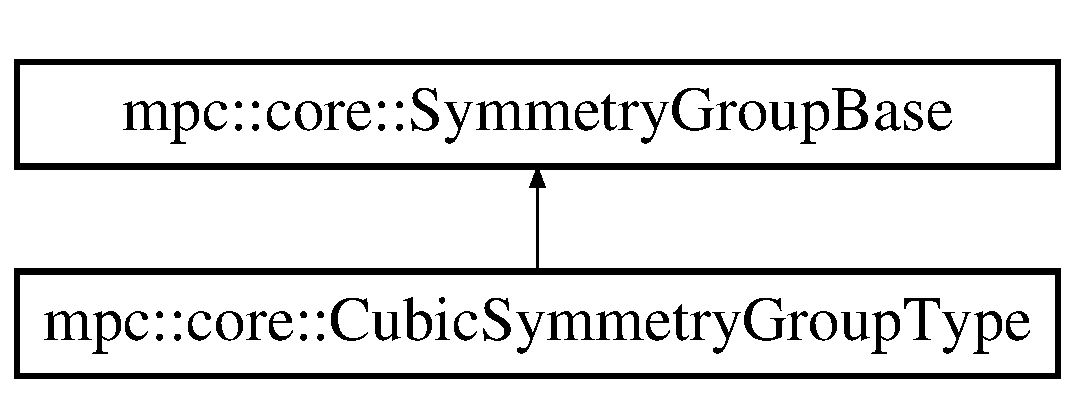
\includegraphics[height=2.000000cm]{structmpc_1_1core_1_1_cubic_symmetry_group_type}
\end{center}
\end{figure}
\subsection*{Static Public Member Functions}
\begin{DoxyCompactItemize}
\item 
static constexpr \mbox{\hyperlink{namespacempc_1_1core_a9d979684062547055a0ef5c13077bad8}{Symmetry\+Group\+Enumeration}} \mbox{\hyperlink{structmpc_1_1core_1_1_cubic_symmetry_group_type_a04e950092a3b0a6e2d35110c49fac745}{Symmetry\+Group\+Enum}} ()
\item 
static constexpr int \mbox{\hyperlink{structmpc_1_1core_1_1_cubic_symmetry_group_type_a7775973b3c21a9cef3999c72516c8061}{Number\+Of\+Independent\+Components}} ()
\end{DoxyCompactItemize}
\subsection*{Public Attributes}
\begin{DoxyCompactItemize}
\item 
const \mbox{\hyperlink{namespacempc_1_1core_a9d979684062547055a0ef5c13077bad8}{Symmetry\+Group\+Enumeration}} \mbox{\hyperlink{structmpc_1_1core_1_1_cubic_symmetry_group_type_a9418ba4ab74fc37ae6ef6faa0d2aeca0}{symmetry\+\_\+group\+\_\+enumeration}} = \mbox{\hyperlink{namespacempc_1_1core_a9d979684062547055a0ef5c13077bad8accd681e34e5e40fbce74618c3ccffcff}{Symmetry\+Group\+Enumeration\+::\+C\+U\+B\+IC}}
\item 
const int \mbox{\hyperlink{structmpc_1_1core_1_1_cubic_symmetry_group_type_a4e0518ed7fc1d0ab8e04cf7f549b62a5}{number\+\_\+of\+\_\+independent\+\_\+components}} = 3
\end{DoxyCompactItemize}


\subsection{Detailed Description}


Definition at line 268 of file symmetrygrouptypes.\+hpp.



\subsection{Member Function Documentation}
\mbox{\Hypertarget{structmpc_1_1core_1_1_cubic_symmetry_group_type_a7775973b3c21a9cef3999c72516c8061}\label{structmpc_1_1core_1_1_cubic_symmetry_group_type_a7775973b3c21a9cef3999c72516c8061}} 
\index{mpc\+::core\+::\+Cubic\+Symmetry\+Group\+Type@{mpc\+::core\+::\+Cubic\+Symmetry\+Group\+Type}!Number\+Of\+Independent\+Components@{Number\+Of\+Independent\+Components}}
\index{Number\+Of\+Independent\+Components@{Number\+Of\+Independent\+Components}!mpc\+::core\+::\+Cubic\+Symmetry\+Group\+Type@{mpc\+::core\+::\+Cubic\+Symmetry\+Group\+Type}}
\subsubsection{\texorpdfstring{Number\+Of\+Independent\+Components()}{NumberOfIndependentComponents()}}
{\footnotesize\ttfamily static constexpr int mpc\+::core\+::\+Cubic\+Symmetry\+Group\+Type\+::\+Number\+Of\+Independent\+Components (\begin{DoxyParamCaption}{ }\end{DoxyParamCaption})\hspace{0.3cm}{\ttfamily [inline]}, {\ttfamily [static]}}



Definition at line 275 of file symmetrygrouptypes.\+hpp.

\mbox{\Hypertarget{structmpc_1_1core_1_1_cubic_symmetry_group_type_a04e950092a3b0a6e2d35110c49fac745}\label{structmpc_1_1core_1_1_cubic_symmetry_group_type_a04e950092a3b0a6e2d35110c49fac745}} 
\index{mpc\+::core\+::\+Cubic\+Symmetry\+Group\+Type@{mpc\+::core\+::\+Cubic\+Symmetry\+Group\+Type}!Symmetry\+Group\+Enum@{Symmetry\+Group\+Enum}}
\index{Symmetry\+Group\+Enum@{Symmetry\+Group\+Enum}!mpc\+::core\+::\+Cubic\+Symmetry\+Group\+Type@{mpc\+::core\+::\+Cubic\+Symmetry\+Group\+Type}}
\subsubsection{\texorpdfstring{Symmetry\+Group\+Enum()}{SymmetryGroupEnum()}}
{\footnotesize\ttfamily static constexpr \mbox{\hyperlink{namespacempc_1_1core_a9d979684062547055a0ef5c13077bad8}{Symmetry\+Group\+Enumeration}} mpc\+::core\+::\+Cubic\+Symmetry\+Group\+Type\+::\+Symmetry\+Group\+Enum (\begin{DoxyParamCaption}{ }\end{DoxyParamCaption})\hspace{0.3cm}{\ttfamily [inline]}, {\ttfamily [static]}}



Definition at line 272 of file symmetrygrouptypes.\+hpp.



\subsection{Member Data Documentation}
\mbox{\Hypertarget{structmpc_1_1core_1_1_cubic_symmetry_group_type_a4e0518ed7fc1d0ab8e04cf7f549b62a5}\label{structmpc_1_1core_1_1_cubic_symmetry_group_type_a4e0518ed7fc1d0ab8e04cf7f549b62a5}} 
\index{mpc\+::core\+::\+Cubic\+Symmetry\+Group\+Type@{mpc\+::core\+::\+Cubic\+Symmetry\+Group\+Type}!number\+\_\+of\+\_\+independent\+\_\+components@{number\+\_\+of\+\_\+independent\+\_\+components}}
\index{number\+\_\+of\+\_\+independent\+\_\+components@{number\+\_\+of\+\_\+independent\+\_\+components}!mpc\+::core\+::\+Cubic\+Symmetry\+Group\+Type@{mpc\+::core\+::\+Cubic\+Symmetry\+Group\+Type}}
\subsubsection{\texorpdfstring{number\+\_\+of\+\_\+independent\+\_\+components}{number\_of\_independent\_components}}
{\footnotesize\ttfamily const int mpc\+::core\+::\+Cubic\+Symmetry\+Group\+Type\+::number\+\_\+of\+\_\+independent\+\_\+components = 3}



Definition at line 270 of file symmetrygrouptypes.\+hpp.

\mbox{\Hypertarget{structmpc_1_1core_1_1_cubic_symmetry_group_type_a9418ba4ab74fc37ae6ef6faa0d2aeca0}\label{structmpc_1_1core_1_1_cubic_symmetry_group_type_a9418ba4ab74fc37ae6ef6faa0d2aeca0}} 
\index{mpc\+::core\+::\+Cubic\+Symmetry\+Group\+Type@{mpc\+::core\+::\+Cubic\+Symmetry\+Group\+Type}!symmetry\+\_\+group\+\_\+enumeration@{symmetry\+\_\+group\+\_\+enumeration}}
\index{symmetry\+\_\+group\+\_\+enumeration@{symmetry\+\_\+group\+\_\+enumeration}!mpc\+::core\+::\+Cubic\+Symmetry\+Group\+Type@{mpc\+::core\+::\+Cubic\+Symmetry\+Group\+Type}}
\subsubsection{\texorpdfstring{symmetry\+\_\+group\+\_\+enumeration}{symmetry\_group\_enumeration}}
{\footnotesize\ttfamily const \mbox{\hyperlink{namespacempc_1_1core_a9d979684062547055a0ef5c13077bad8}{Symmetry\+Group\+Enumeration}} mpc\+::core\+::\+Cubic\+Symmetry\+Group\+Type\+::symmetry\+\_\+group\+\_\+enumeration = \mbox{\hyperlink{namespacempc_1_1core_a9d979684062547055a0ef5c13077bad8accd681e34e5e40fbce74618c3ccffcff}{Symmetry\+Group\+Enumeration\+::\+C\+U\+B\+IC}}}



Definition at line 269 of file symmetrygrouptypes.\+hpp.



The documentation for this struct was generated from the following file\+:\begin{DoxyCompactItemize}
\item 
/\+Users/atorlucci/\+Documents/github\+\_\+threecubed\+\_\+repos/mpc/src/mpc/core/\mbox{\hyperlink{symmetrygrouptypes_8hpp}{symmetrygrouptypes.\+hpp}}\end{DoxyCompactItemize}

\hypertarget{structmpc_1_1utilities_1_1_cylindrical_coordinate_type}{}\section{mpc\+:\+:utilities\+:\+:Cylindrical\+Coordinate\+Type Struct Reference}
\label{structmpc_1_1utilities_1_1_cylindrical_coordinate_type}\index{mpc\+::utilities\+::\+Cylindrical\+Coordinate\+Type@{mpc\+::utilities\+::\+Cylindrical\+Coordinate\+Type}}


{\ttfamily \#include $<$coordinatemapping.\+hpp$>$}

Inheritance diagram for mpc\+:\+:utilities\+:\+:Cylindrical\+Coordinate\+Type\+:\begin{figure}[H]
\begin{center}
\leavevmode
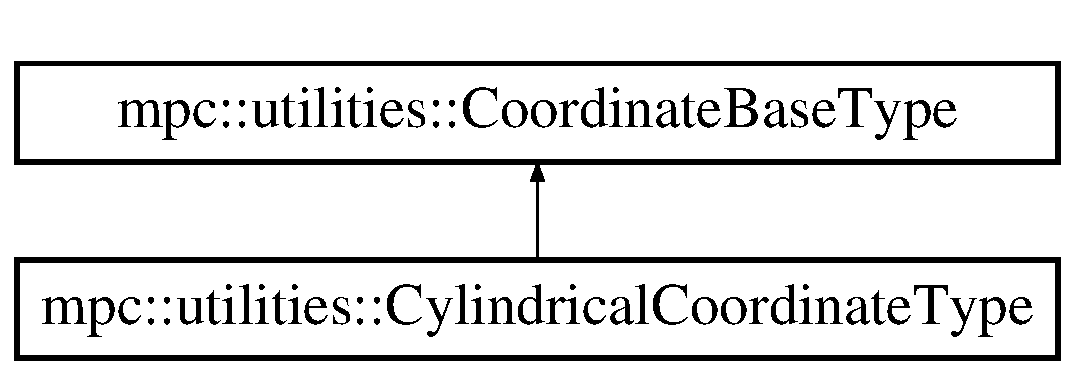
\includegraphics[height=2.000000cm]{structmpc_1_1utilities_1_1_cylindrical_coordinate_type}
\end{center}
\end{figure}


\subsection{Detailed Description}


Definition at line 28 of file coordinatemapping.\+hpp.



The documentation for this struct was generated from the following file\+:\begin{DoxyCompactItemize}
\item 
/\+Users/atorlucci/\+Documents/github\+\_\+threecubed\+\_\+repos/mpc/src/mpc/utilities/\mbox{\hyperlink{coordinatemapping_8hpp}{coordinatemapping.\+hpp}}\end{DoxyCompactItemize}

\hypertarget{structmpc_1_1rockphysics_1_1_density_type}{}\section{mpc\+:\+:rockphysics\+:\+:Density\+Type$<$ T $>$ Struct Template Reference}
\label{structmpc_1_1rockphysics_1_1_density_type}\index{mpc\+::rockphysics\+::\+Density\+Type$<$ T $>$@{mpc\+::rockphysics\+::\+Density\+Type$<$ T $>$}}


{\ttfamily \#include $<$rockphysicstransformstypes.\+hpp$>$}

Inheritance diagram for mpc\+:\+:rockphysics\+:\+:Density\+Type$<$ T $>$\+:\begin{figure}[H]
\begin{center}
\leavevmode
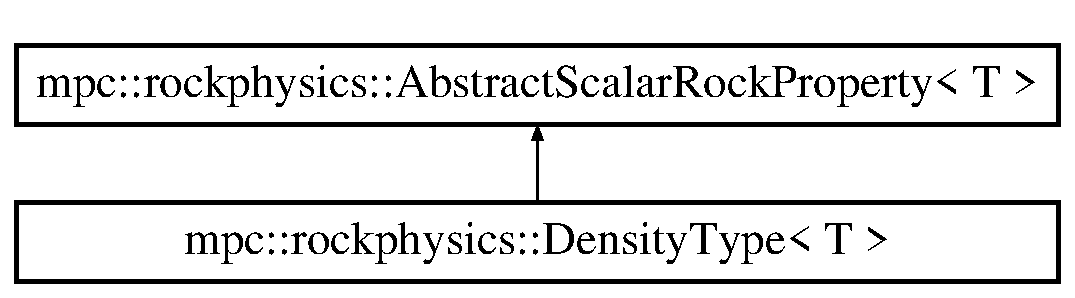
\includegraphics[height=2.000000cm]{structmpc_1_1rockphysics_1_1_density_type}
\end{center}
\end{figure}
\subsection*{Public Member Functions}
\begin{DoxyCompactItemize}
\item 
constexpr \mbox{\hyperlink{structmpc_1_1rockphysics_1_1_density_type_a2d38b577150e0f26513dbf9927d6034d}{Density\+Type}} (T val)
\end{DoxyCompactItemize}
\subsection*{Additional Inherited Members}


\subsection{Detailed Description}
\subsubsection*{template$<$typename T$>$\newline
struct mpc\+::rockphysics\+::\+Density\+Type$<$ T $>$}



Definition at line 119 of file rockphysicstransformstypes.\+hpp.



\subsection{Constructor \& Destructor Documentation}
\mbox{\Hypertarget{structmpc_1_1rockphysics_1_1_density_type_a2d38b577150e0f26513dbf9927d6034d}\label{structmpc_1_1rockphysics_1_1_density_type_a2d38b577150e0f26513dbf9927d6034d}} 
\index{mpc\+::rockphysics\+::\+Density\+Type@{mpc\+::rockphysics\+::\+Density\+Type}!Density\+Type@{Density\+Type}}
\index{Density\+Type@{Density\+Type}!mpc\+::rockphysics\+::\+Density\+Type@{mpc\+::rockphysics\+::\+Density\+Type}}
\subsubsection{\texorpdfstring{Density\+Type()}{DensityType()}}
{\footnotesize\ttfamily template$<$typename T$>$ \\
constexpr \mbox{\hyperlink{structmpc_1_1rockphysics_1_1_density_type}{mpc\+::rockphysics\+::\+Density\+Type}}$<$ T $>$\+::\mbox{\hyperlink{structmpc_1_1rockphysics_1_1_density_type}{Density\+Type}} (\begin{DoxyParamCaption}\item[{T}]{val }\end{DoxyParamCaption})\hspace{0.3cm}{\ttfamily [inline]}}



Definition at line 124 of file rockphysicstransformstypes.\+hpp.



The documentation for this struct was generated from the following file\+:\begin{DoxyCompactItemize}
\item 
/\+Users/atorlucci/\+Documents/github\+\_\+threecubed\+\_\+repos/mpc/src/mpc/rockphysics/\mbox{\hyperlink{rockphysicstransformstypes_8hpp}{rockphysicstransformstypes.\+hpp}}\end{DoxyCompactItemize}

\hypertarget{structmpc_1_1utilities_1_1_eigen2_blitz_function_object}{}\section{mpc\+:\+:utilities\+:\+:Eigen2\+Blitz\+Function\+Object$<$ T, M, N, D $>$ Struct Template Reference}
\label{structmpc_1_1utilities_1_1_eigen2_blitz_function_object}\index{mpc\+::utilities\+::\+Eigen2\+Blitz\+Function\+Object$<$ T, M, N, D $>$@{mpc\+::utilities\+::\+Eigen2\+Blitz\+Function\+Object$<$ T, M, N, D $>$}}


{\ttfamily \#include $<$eigen2blitz.\+hpp$>$}

\subsection*{Public Member Functions}
\begin{DoxyCompactItemize}
\item 
blitz\+::\+Array$<$ T, D $>$ \mbox{\hyperlink{structmpc_1_1utilities_1_1_eigen2_blitz_function_object_a4d46d6becef7fed9194cdf654c44dfdc}{operator()}} (Eigen\+::\+Matrix$<$ T, M, N $>$ \&eigenmatrixX)
\end{DoxyCompactItemize}


\subsection{Detailed Description}
\subsubsection*{template$<$typename T, int M, int N, int D$>$\newline
struct mpc\+::utilities\+::\+Eigen2\+Blitz\+Function\+Object$<$ T, M, N, D $>$}



Definition at line 24 of file eigen2blitz.\+hpp.



\subsection{Member Function Documentation}
\mbox{\Hypertarget{structmpc_1_1utilities_1_1_eigen2_blitz_function_object_a4d46d6becef7fed9194cdf654c44dfdc}\label{structmpc_1_1utilities_1_1_eigen2_blitz_function_object_a4d46d6becef7fed9194cdf654c44dfdc}} 
\index{mpc\+::utilities\+::\+Eigen2\+Blitz\+Function\+Object@{mpc\+::utilities\+::\+Eigen2\+Blitz\+Function\+Object}!operator()@{operator()}}
\index{operator()@{operator()}!mpc\+::utilities\+::\+Eigen2\+Blitz\+Function\+Object@{mpc\+::utilities\+::\+Eigen2\+Blitz\+Function\+Object}}
\subsubsection{\texorpdfstring{operator()()}{operator()()}}
{\footnotesize\ttfamily template$<$typename T, int M, int N, int D$>$ \\
blitz\+::\+Array$<$T,D$>$ \mbox{\hyperlink{structmpc_1_1utilities_1_1_eigen2_blitz_function_object}{mpc\+::utilities\+::\+Eigen2\+Blitz\+Function\+Object}}$<$ T, M, N, D $>$\+::operator() (\begin{DoxyParamCaption}\item[{Eigen\+::\+Matrix$<$ T, M, N $>$ \&}]{eigenmatrixX }\end{DoxyParamCaption})\hspace{0.3cm}{\ttfamily [inline]}}



Definition at line 26 of file eigen2blitz.\+hpp.



The documentation for this struct was generated from the following file\+:\begin{DoxyCompactItemize}
\item 
/\+Users/atorlucci/\+Documents/github\+\_\+threecubed\+\_\+repos/mpc/src/mpc/utilities/\mbox{\hyperlink{eigen2blitz_8hpp}{eigen2blitz.\+hpp}}\end{DoxyCompactItemize}

\hypertarget{structmpc_1_1utilities_1_1_eigen2_blitz_function_object_3_01_t_00_01_m_00_01_n_00_011_01_4}{}\section{mpc\+:\+:utilities\+:\+:Eigen2\+Blitz\+Function\+Object$<$ T, M, N, 1 $>$ Struct Template Reference}
\label{structmpc_1_1utilities_1_1_eigen2_blitz_function_object_3_01_t_00_01_m_00_01_n_00_011_01_4}\index{mpc\+::utilities\+::\+Eigen2\+Blitz\+Function\+Object$<$ T, M, N, 1 $>$@{mpc\+::utilities\+::\+Eigen2\+Blitz\+Function\+Object$<$ T, M, N, 1 $>$}}


{\ttfamily \#include $<$eigen2blitz.\+hpp$>$}

\subsection*{Public Member Functions}
\begin{DoxyCompactItemize}
\item 
blitz\+::\+Array$<$ T, 1 $>$ \mbox{\hyperlink{structmpc_1_1utilities_1_1_eigen2_blitz_function_object_3_01_t_00_01_m_00_01_n_00_011_01_4_a74b35a2a352c947223205bf401c6a662}{operator()}} (Eigen\+::\+Matrix$<$ T, M, N $>$ \&eigenmatrixX)
\end{DoxyCompactItemize}


\subsection{Detailed Description}
\subsubsection*{template$<$typename T, int M, int N$>$\newline
struct mpc\+::utilities\+::\+Eigen2\+Blitz\+Function\+Object$<$ T, M, N, 1 $>$}



Definition at line 31 of file eigen2blitz.\+hpp.



\subsection{Member Function Documentation}
\mbox{\Hypertarget{structmpc_1_1utilities_1_1_eigen2_blitz_function_object_3_01_t_00_01_m_00_01_n_00_011_01_4_a74b35a2a352c947223205bf401c6a662}\label{structmpc_1_1utilities_1_1_eigen2_blitz_function_object_3_01_t_00_01_m_00_01_n_00_011_01_4_a74b35a2a352c947223205bf401c6a662}} 
\index{mpc\+::utilities\+::\+Eigen2\+Blitz\+Function\+Object$<$ T, M, N, 1 $>$@{mpc\+::utilities\+::\+Eigen2\+Blitz\+Function\+Object$<$ T, M, N, 1 $>$}!operator()@{operator()}}
\index{operator()@{operator()}!mpc\+::utilities\+::\+Eigen2\+Blitz\+Function\+Object$<$ T, M, N, 1 $>$@{mpc\+::utilities\+::\+Eigen2\+Blitz\+Function\+Object$<$ T, M, N, 1 $>$}}
\subsubsection{\texorpdfstring{operator()()}{operator()()}}
{\footnotesize\ttfamily template$<$typename T , int M, int N$>$ \\
blitz\+::\+Array$<$T,1$>$ \mbox{\hyperlink{structmpc_1_1utilities_1_1_eigen2_blitz_function_object}{mpc\+::utilities\+::\+Eigen2\+Blitz\+Function\+Object}}$<$ T, M, N, 1 $>$\+::operator() (\begin{DoxyParamCaption}\item[{Eigen\+::\+Matrix$<$ T, M, N $>$ \&}]{eigenmatrixX }\end{DoxyParamCaption})\hspace{0.3cm}{\ttfamily [inline]}}



Definition at line 33 of file eigen2blitz.\+hpp.



The documentation for this struct was generated from the following file\+:\begin{DoxyCompactItemize}
\item 
/\+Users/atorlucci/\+Documents/github\+\_\+threecubed\+\_\+repos/mpc/src/mpc/utilities/\mbox{\hyperlink{eigen2blitz_8hpp}{eigen2blitz.\+hpp}}\end{DoxyCompactItemize}

\hypertarget{structmpc_1_1utilities_1_1_eigen2_blitz_function_object_3_01_t_00_01_m_00_01_n_00_012_01_4}{}\section{mpc\+:\+:utilities\+:\+:Eigen2\+Blitz\+Function\+Object$<$ T, M, N, 2 $>$ Struct Template Reference}
\label{structmpc_1_1utilities_1_1_eigen2_blitz_function_object_3_01_t_00_01_m_00_01_n_00_012_01_4}\index{mpc\+::utilities\+::\+Eigen2\+Blitz\+Function\+Object$<$ T, M, N, 2 $>$@{mpc\+::utilities\+::\+Eigen2\+Blitz\+Function\+Object$<$ T, M, N, 2 $>$}}


{\ttfamily \#include $<$eigen2blitz.\+hpp$>$}

\subsection*{Public Member Functions}
\begin{DoxyCompactItemize}
\item 
blitz\+::\+Array$<$ T, 2 $>$ \mbox{\hyperlink{structmpc_1_1utilities_1_1_eigen2_blitz_function_object_3_01_t_00_01_m_00_01_n_00_012_01_4_a8dddbcd616f63253289bcf816626a7e4}{operator()}} (Eigen\+::\+Matrix$<$ T, M, N $>$ \&eigenmatrixX)
\end{DoxyCompactItemize}


\subsection{Detailed Description}
\subsubsection*{template$<$typename T, int M, int N$>$\newline
struct mpc\+::utilities\+::\+Eigen2\+Blitz\+Function\+Object$<$ T, M, N, 2 $>$}



Definition at line 48 of file eigen2blitz.\+hpp.



\subsection{Member Function Documentation}
\mbox{\Hypertarget{structmpc_1_1utilities_1_1_eigen2_blitz_function_object_3_01_t_00_01_m_00_01_n_00_012_01_4_a8dddbcd616f63253289bcf816626a7e4}\label{structmpc_1_1utilities_1_1_eigen2_blitz_function_object_3_01_t_00_01_m_00_01_n_00_012_01_4_a8dddbcd616f63253289bcf816626a7e4}} 
\index{mpc\+::utilities\+::\+Eigen2\+Blitz\+Function\+Object$<$ T, M, N, 2 $>$@{mpc\+::utilities\+::\+Eigen2\+Blitz\+Function\+Object$<$ T, M, N, 2 $>$}!operator()@{operator()}}
\index{operator()@{operator()}!mpc\+::utilities\+::\+Eigen2\+Blitz\+Function\+Object$<$ T, M, N, 2 $>$@{mpc\+::utilities\+::\+Eigen2\+Blitz\+Function\+Object$<$ T, M, N, 2 $>$}}
\subsubsection{\texorpdfstring{operator()()}{operator()()}}
{\footnotesize\ttfamily template$<$typename T , int M, int N$>$ \\
blitz\+::\+Array$<$T,2$>$ \mbox{\hyperlink{structmpc_1_1utilities_1_1_eigen2_blitz_function_object}{mpc\+::utilities\+::\+Eigen2\+Blitz\+Function\+Object}}$<$ T, M, N, 2 $>$\+::operator() (\begin{DoxyParamCaption}\item[{Eigen\+::\+Matrix$<$ T, M, N $>$ \&}]{eigenmatrixX }\end{DoxyParamCaption})\hspace{0.3cm}{\ttfamily [inline]}}



Definition at line 50 of file eigen2blitz.\+hpp.



The documentation for this struct was generated from the following file\+:\begin{DoxyCompactItemize}
\item 
/\+Users/atorlucci/\+Documents/github\+\_\+threecubed\+\_\+repos/mpc/src/mpc/utilities/\mbox{\hyperlink{eigen2blitz_8hpp}{eigen2blitz.\+hpp}}\end{DoxyCompactItemize}

\hypertarget{structmpc_1_1transformation_1_1_euler_rotation_x3_x1_x3}{}\section{mpc\+:\+:transformation\+:\+:Euler\+Rotation\+X3\+X1\+X3$<$ T $>$ Struct Template Reference}
\label{structmpc_1_1transformation_1_1_euler_rotation_x3_x1_x3}\index{mpc\+::transformation\+::\+Euler\+Rotation\+X3\+X1\+X3$<$ T $>$@{mpc\+::transformation\+::\+Euler\+Rotation\+X3\+X1\+X3$<$ T $>$}}


{\ttfamily \#include $<$eulerrotation.\+hpp$>$}

\subsection*{Public Member Functions}
\begin{DoxyCompactItemize}
\item 
blitz\+::\+Array$<$ T, 2 $>$ \mbox{\hyperlink{structmpc_1_1transformation_1_1_euler_rotation_x3_x1_x3_a5a6dda789469ec39d472d4e1458678ec}{operator()}} (T phi1, T P\+HI, T phi2)
\end{DoxyCompactItemize}


\subsection{Detailed Description}
\subsubsection*{template$<$typename T$>$\newline
struct mpc\+::transformation\+::\+Euler\+Rotation\+X3\+X1\+X3$<$ T $>$}



Definition at line 22 of file eulerrotation.\+hpp.



\subsection{Member Function Documentation}
\mbox{\Hypertarget{structmpc_1_1transformation_1_1_euler_rotation_x3_x1_x3_a5a6dda789469ec39d472d4e1458678ec}\label{structmpc_1_1transformation_1_1_euler_rotation_x3_x1_x3_a5a6dda789469ec39d472d4e1458678ec}} 
\index{mpc\+::transformation\+::\+Euler\+Rotation\+X3\+X1\+X3@{mpc\+::transformation\+::\+Euler\+Rotation\+X3\+X1\+X3}!operator()@{operator()}}
\index{operator()@{operator()}!mpc\+::transformation\+::\+Euler\+Rotation\+X3\+X1\+X3@{mpc\+::transformation\+::\+Euler\+Rotation\+X3\+X1\+X3}}
\subsubsection{\texorpdfstring{operator()()}{operator()()}}
{\footnotesize\ttfamily template$<$typename T $>$ \\
blitz\+::\+Array$<$T,2$>$ \mbox{\hyperlink{structmpc_1_1transformation_1_1_euler_rotation_x3_x1_x3}{mpc\+::transformation\+::\+Euler\+Rotation\+X3\+X1\+X3}}$<$ T $>$\+::operator() (\begin{DoxyParamCaption}\item[{T}]{phi1,  }\item[{T}]{P\+HI,  }\item[{T}]{phi2 }\end{DoxyParamCaption})\hspace{0.3cm}{\ttfamily [inline]}}



Definition at line 25 of file eulerrotation.\+hpp.



The documentation for this struct was generated from the following file\+:\begin{DoxyCompactItemize}
\item 
/\+Users/atorlucci/\+Documents/github\+\_\+threecubed\+\_\+repos/mpc/src/mpc/transformation/\mbox{\hyperlink{eulerrotation_8hpp}{eulerrotation.\+hpp}}\end{DoxyCompactItemize}

\hypertarget{classmpc_1_1rockphysics_1_1_fluid_phase}{}\section{mpc\+:\+:rockphysics\+:\+:Fluid\+Phase$<$ T $>$ Class Template Reference}
\label{classmpc_1_1rockphysics_1_1_fluid_phase}\index{mpc\+::rockphysics\+::\+Fluid\+Phase$<$ T $>$@{mpc\+::rockphysics\+::\+Fluid\+Phase$<$ T $>$}}


{\ttfamily \#include $<$scalarcomposites.\+hpp$>$}

Inheritance diagram for mpc\+:\+:rockphysics\+:\+:Fluid\+Phase$<$ T $>$\+:\begin{figure}[H]
\begin{center}
\leavevmode
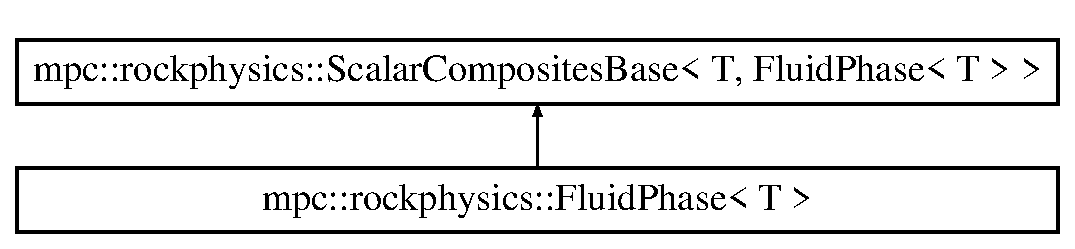
\includegraphics[height=2.000000cm]{classmpc_1_1rockphysics_1_1_fluid_phase}
\end{center}
\end{figure}
\subsection*{Public Member Functions}
\begin{DoxyCompactItemize}
\item 
\mbox{\hyperlink{classmpc_1_1rockphysics_1_1_fluid_phase_a2705193cd79d12fd6bc9a39f0eee6898}{Fluid\+Phase}} (const std\+::vector$<$ std\+::tuple$<$ \mbox{\hyperlink{structmpc_1_1rockphysics_1_1_bulk_modulus_type}{mpc\+::rockphysics\+::\+Bulk\+Modulus\+Type}}$<$ T $>$, \mbox{\hyperlink{structmpc_1_1rockphysics_1_1_shear_modulus_type}{mpc\+::rockphysics\+::\+Shear\+Modulus\+Type}}$<$ T $>$, \mbox{\hyperlink{structmpc_1_1rockphysics_1_1_density_type}{mpc\+::rockphysics\+::\+Density\+Type}}$<$ T $>$, \mbox{\hyperlink{structmpc_1_1rockphysics_1_1_volume_fraction_type}{mpc\+::rockphysics\+::\+Volume\+Fraction\+Type}}$<$ T $>$ $>$ $>$ \&vec)
\end{DoxyCompactItemize}
\subsection*{Static Public Member Functions}
\begin{DoxyCompactItemize}
\item 
static std\+::tuple$<$ \mbox{\hyperlink{structmpc_1_1rockphysics_1_1_bulk_modulus_type}{mpc\+::rockphysics\+::\+Bulk\+Modulus\+Type}}$<$ T $>$, \mbox{\hyperlink{structmpc_1_1rockphysics_1_1_shear_modulus_type}{mpc\+::rockphysics\+::\+Shear\+Modulus\+Type}}$<$ T $>$, \mbox{\hyperlink{structmpc_1_1rockphysics_1_1_density_type}{mpc\+::rockphysics\+::\+Density\+Type}}$<$ T $>$ $>$ \mbox{\hyperlink{classmpc_1_1rockphysics_1_1_fluid_phase_a7f6accc4d8dfd7b8e6f55f3338698121}{Effective\+Values}} (const std\+::vector$<$ \mbox{\hyperlink{structmpc_1_1rockphysics_1_1_bulk_modulus_type}{mpc\+::rockphysics\+::\+Bulk\+Modulus\+Type}}$<$ T $>$ $>$ \&K\+\_\+vec, const std\+::vector$<$ \mbox{\hyperlink{structmpc_1_1rockphysics_1_1_shear_modulus_type}{mpc\+::rockphysics\+::\+Shear\+Modulus\+Type}}$<$ T $>$ $>$ \&mu\+\_\+vec, const std\+::vector$<$ \mbox{\hyperlink{structmpc_1_1rockphysics_1_1_density_type}{mpc\+::rockphysics\+::\+Density\+Type}}$<$ T $>$ $>$ \&rho\+\_\+vec, const std\+::vector$<$ \mbox{\hyperlink{structmpc_1_1rockphysics_1_1_volume_fraction_type}{mpc\+::rockphysics\+::\+Volume\+Fraction\+Type}}$<$ T $>$ $>$ \&vf\+\_\+vec)
\end{DoxyCompactItemize}
\subsection*{Additional Inherited Members}


\subsection{Detailed Description}
\subsubsection*{template$<$typename T$>$\newline
class mpc\+::rockphysics\+::\+Fluid\+Phase$<$ T $>$}



Definition at line 326 of file scalarcomposites.\+hpp.



\subsection{Constructor \& Destructor Documentation}
\mbox{\Hypertarget{classmpc_1_1rockphysics_1_1_fluid_phase_a2705193cd79d12fd6bc9a39f0eee6898}\label{classmpc_1_1rockphysics_1_1_fluid_phase_a2705193cd79d12fd6bc9a39f0eee6898}} 
\index{mpc\+::rockphysics\+::\+Fluid\+Phase@{mpc\+::rockphysics\+::\+Fluid\+Phase}!Fluid\+Phase@{Fluid\+Phase}}
\index{Fluid\+Phase@{Fluid\+Phase}!mpc\+::rockphysics\+::\+Fluid\+Phase@{mpc\+::rockphysics\+::\+Fluid\+Phase}}
\subsubsection{\texorpdfstring{Fluid\+Phase()}{FluidPhase()}}
{\footnotesize\ttfamily template$<$typename T $>$ \\
\mbox{\hyperlink{classmpc_1_1rockphysics_1_1_fluid_phase}{mpc\+::rockphysics\+::\+Fluid\+Phase}}$<$ T $>$\+::\mbox{\hyperlink{classmpc_1_1rockphysics_1_1_fluid_phase}{Fluid\+Phase}} (\begin{DoxyParamCaption}\item[{const std\+::vector$<$ std\+::tuple$<$ \mbox{\hyperlink{structmpc_1_1rockphysics_1_1_bulk_modulus_type}{mpc\+::rockphysics\+::\+Bulk\+Modulus\+Type}}$<$ T $>$, \mbox{\hyperlink{structmpc_1_1rockphysics_1_1_shear_modulus_type}{mpc\+::rockphysics\+::\+Shear\+Modulus\+Type}}$<$ T $>$, \mbox{\hyperlink{structmpc_1_1rockphysics_1_1_density_type}{mpc\+::rockphysics\+::\+Density\+Type}}$<$ T $>$, \mbox{\hyperlink{structmpc_1_1rockphysics_1_1_volume_fraction_type}{mpc\+::rockphysics\+::\+Volume\+Fraction\+Type}}$<$ T $>$ $>$ $>$ \&}]{vec }\end{DoxyParamCaption})\hspace{0.3cm}{\ttfamily [inline]}}



Definition at line 340 of file scalarcomposites.\+hpp.



\subsection{Member Function Documentation}
\mbox{\Hypertarget{classmpc_1_1rockphysics_1_1_fluid_phase_a7f6accc4d8dfd7b8e6f55f3338698121}\label{classmpc_1_1rockphysics_1_1_fluid_phase_a7f6accc4d8dfd7b8e6f55f3338698121}} 
\index{mpc\+::rockphysics\+::\+Fluid\+Phase@{mpc\+::rockphysics\+::\+Fluid\+Phase}!Effective\+Values@{Effective\+Values}}
\index{Effective\+Values@{Effective\+Values}!mpc\+::rockphysics\+::\+Fluid\+Phase@{mpc\+::rockphysics\+::\+Fluid\+Phase}}
\subsubsection{\texorpdfstring{Effective\+Values()}{EffectiveValues()}}
{\footnotesize\ttfamily template$<$typename T $>$ \\
static std\+::tuple$<$\mbox{\hyperlink{structmpc_1_1rockphysics_1_1_bulk_modulus_type}{mpc\+::rockphysics\+::\+Bulk\+Modulus\+Type}}$<$T$>$, \mbox{\hyperlink{structmpc_1_1rockphysics_1_1_shear_modulus_type}{mpc\+::rockphysics\+::\+Shear\+Modulus\+Type}}$<$T$>$, \mbox{\hyperlink{structmpc_1_1rockphysics_1_1_density_type}{mpc\+::rockphysics\+::\+Density\+Type}}$<$T$>$ $>$ \mbox{\hyperlink{classmpc_1_1rockphysics_1_1_fluid_phase}{mpc\+::rockphysics\+::\+Fluid\+Phase}}$<$ T $>$\+::Effective\+Values (\begin{DoxyParamCaption}\item[{const std\+::vector$<$ \mbox{\hyperlink{structmpc_1_1rockphysics_1_1_bulk_modulus_type}{mpc\+::rockphysics\+::\+Bulk\+Modulus\+Type}}$<$ T $>$ $>$ \&}]{K\+\_\+vec,  }\item[{const std\+::vector$<$ \mbox{\hyperlink{structmpc_1_1rockphysics_1_1_shear_modulus_type}{mpc\+::rockphysics\+::\+Shear\+Modulus\+Type}}$<$ T $>$ $>$ \&}]{mu\+\_\+vec,  }\item[{const std\+::vector$<$ \mbox{\hyperlink{structmpc_1_1rockphysics_1_1_density_type}{mpc\+::rockphysics\+::\+Density\+Type}}$<$ T $>$ $>$ \&}]{rho\+\_\+vec,  }\item[{const std\+::vector$<$ \mbox{\hyperlink{structmpc_1_1rockphysics_1_1_volume_fraction_type}{mpc\+::rockphysics\+::\+Volume\+Fraction\+Type}}$<$ T $>$ $>$ \&}]{vf\+\_\+vec }\end{DoxyParamCaption})\hspace{0.3cm}{\ttfamily [inline]}, {\ttfamily [static]}}



Definition at line 343 of file scalarcomposites.\+hpp.



The documentation for this class was generated from the following file\+:\begin{DoxyCompactItemize}
\item 
/\+Users/atorlucci/\+Documents/github\+\_\+threecubed\+\_\+repos/mpc/src/mpc/rockphysics/\mbox{\hyperlink{scalarcomposites_8hpp}{scalarcomposites.\+hpp}}\end{DoxyCompactItemize}

\hypertarget{structmpc_1_1mechanics_1_1_green_christoffel}{}\section{mpc\+:\+:mechanics\+:\+:Green\+Christoffel$<$ T $>$ Class Template Reference}
\label{structmpc_1_1mechanics_1_1_green_christoffel}\index{mpc\+::mechanics\+::\+Green\+Christoffel$<$ T $>$@{mpc\+::mechanics\+::\+Green\+Christoffel$<$ T $>$}}


function object for calculating velocities based on Green-\/\+Christoffel equation  




{\ttfamily \#include $<$greenchristoffel.\+hpp$>$}

\subsection*{Public Member Functions}
\begin{DoxyCompactItemize}
\item 
\mbox{\hyperlink{structmpc_1_1mechanics_1_1_green_christoffel_a7a0ced87a84adeda26f1c3e70d6f9214}{Green\+Christoffel}} ()
\item 
void \mbox{\hyperlink{structmpc_1_1mechanics_1_1_green_christoffel_a82e7d064980bd9885e26b25376a23ad4}{Set\+Components}} (const \mbox{\hyperlink{structmpc_1_1core_1_1_stiffness_tensor}{mpc\+::core\+::\+Stiffness\+Tensor}}$<$ T $>$ \&cijkl, blitz\+::\+Array$<$ T, 1 $>$ \&n)
\item 
std\+::array$<$ T, 3 $>$ \mbox{\hyperlink{structmpc_1_1mechanics_1_1_green_christoffel_a84df39c5961390293bf77ba4dfadac13}{Phase\+Velocities}} (T density)
\end{DoxyCompactItemize}
\subsection*{Public Attributes}
\begin{DoxyCompactItemize}
\item 
blitz\+::\+Array$<$ T, 2 $>$ \mbox{\hyperlink{structmpc_1_1mechanics_1_1_green_christoffel_a6d8298d4bd31b188f061c4bd07810c04}{tensor}} = blitz\+::\+Array$<$T,2$>$(3,3,blitz\+::\+Column\+Major\+Array$<$2$>$())
\end{DoxyCompactItemize}


\subsection{Detailed Description}
\subsubsection*{template$<$typename T$>$\newline
class mpc\+::mechanics\+::\+Green\+Christoffel$<$ T $>$}

function object for calculating velocities based on Green-\/\+Christoffel equation 

Definition at line 41 of file greenchristoffel.\+hpp.



\subsection{Constructor \& Destructor Documentation}
\mbox{\Hypertarget{structmpc_1_1mechanics_1_1_green_christoffel_a7a0ced87a84adeda26f1c3e70d6f9214}\label{structmpc_1_1mechanics_1_1_green_christoffel_a7a0ced87a84adeda26f1c3e70d6f9214}} 
\index{mpc\+::mechanics\+::\+Green\+Christoffel@{mpc\+::mechanics\+::\+Green\+Christoffel}!Green\+Christoffel@{Green\+Christoffel}}
\index{Green\+Christoffel@{Green\+Christoffel}!mpc\+::mechanics\+::\+Green\+Christoffel@{mpc\+::mechanics\+::\+Green\+Christoffel}}
\subsubsection{\texorpdfstring{Green\+Christoffel()}{GreenChristoffel()}}
{\footnotesize\ttfamily template$<$typename T $>$ \\
\mbox{\hyperlink{structmpc_1_1mechanics_1_1_green_christoffel}{mpc\+::mechanics\+::\+Green\+Christoffel}}$<$ T $>$\+::\mbox{\hyperlink{structmpc_1_1mechanics_1_1_green_christoffel}{Green\+Christoffel}} (\begin{DoxyParamCaption}{ }\end{DoxyParamCaption})\hspace{0.3cm}{\ttfamily [inline]}}



Definition at line 59 of file greenchristoffel.\+hpp.



\subsection{Member Function Documentation}
\mbox{\Hypertarget{structmpc_1_1mechanics_1_1_green_christoffel_a84df39c5961390293bf77ba4dfadac13}\label{structmpc_1_1mechanics_1_1_green_christoffel_a84df39c5961390293bf77ba4dfadac13}} 
\index{mpc\+::mechanics\+::\+Green\+Christoffel@{mpc\+::mechanics\+::\+Green\+Christoffel}!Phase\+Velocities@{Phase\+Velocities}}
\index{Phase\+Velocities@{Phase\+Velocities}!mpc\+::mechanics\+::\+Green\+Christoffel@{mpc\+::mechanics\+::\+Green\+Christoffel}}
\subsubsection{\texorpdfstring{Phase\+Velocities()}{PhaseVelocities()}}
{\footnotesize\ttfamily template$<$typename T $>$ \\
std\+::array$<$T,3$>$ \mbox{\hyperlink{structmpc_1_1mechanics_1_1_green_christoffel}{mpc\+::mechanics\+::\+Green\+Christoffel}}$<$ T $>$\+::Phase\+Velocities (\begin{DoxyParamCaption}\item[{T}]{density }\end{DoxyParamCaption})\hspace{0.3cm}{\ttfamily [inline]}}



Definition at line 81 of file greenchristoffel.\+hpp.

\mbox{\Hypertarget{structmpc_1_1mechanics_1_1_green_christoffel_a82e7d064980bd9885e26b25376a23ad4}\label{structmpc_1_1mechanics_1_1_green_christoffel_a82e7d064980bd9885e26b25376a23ad4}} 
\index{mpc\+::mechanics\+::\+Green\+Christoffel@{mpc\+::mechanics\+::\+Green\+Christoffel}!Set\+Components@{Set\+Components}}
\index{Set\+Components@{Set\+Components}!mpc\+::mechanics\+::\+Green\+Christoffel@{mpc\+::mechanics\+::\+Green\+Christoffel}}
\subsubsection{\texorpdfstring{Set\+Components()}{SetComponents()}}
{\footnotesize\ttfamily template$<$typename T $>$ \\
void \mbox{\hyperlink{structmpc_1_1mechanics_1_1_green_christoffel}{mpc\+::mechanics\+::\+Green\+Christoffel}}$<$ T $>$\+::Set\+Components (\begin{DoxyParamCaption}\item[{const \mbox{\hyperlink{structmpc_1_1core_1_1_stiffness_tensor}{mpc\+::core\+::\+Stiffness\+Tensor}}$<$ T $>$ \&}]{cijkl,  }\item[{blitz\+::\+Array$<$ T, 1 $>$ \&}]{n }\end{DoxyParamCaption})\hspace{0.3cm}{\ttfamily [inline]}}



Definition at line 64 of file greenchristoffel.\+hpp.



\subsection{Member Data Documentation}
\mbox{\Hypertarget{structmpc_1_1mechanics_1_1_green_christoffel_a6d8298d4bd31b188f061c4bd07810c04}\label{structmpc_1_1mechanics_1_1_green_christoffel_a6d8298d4bd31b188f061c4bd07810c04}} 
\index{mpc\+::mechanics\+::\+Green\+Christoffel@{mpc\+::mechanics\+::\+Green\+Christoffel}!tensor@{tensor}}
\index{tensor@{tensor}!mpc\+::mechanics\+::\+Green\+Christoffel@{mpc\+::mechanics\+::\+Green\+Christoffel}}
\subsubsection{\texorpdfstring{tensor}{tensor}}
{\footnotesize\ttfamily template$<$typename T $>$ \\
blitz\+::\+Array$<$T,2$>$ \mbox{\hyperlink{structmpc_1_1mechanics_1_1_green_christoffel}{mpc\+::mechanics\+::\+Green\+Christoffel}}$<$ T $>$\+::tensor = blitz\+::\+Array$<$T,2$>$(3,3,blitz\+::\+Column\+Major\+Array$<$2$>$())}



Definition at line 56 of file greenchristoffel.\+hpp.



The documentation for this class was generated from the following file\+:\begin{DoxyCompactItemize}
\item 
/\+Users/atorlucci/\+Documents/github\+\_\+threecubed\+\_\+repos/mpc/src/mpc/mechanics/\mbox{\hyperlink{greenchristoffel_8hpp}{greenchristoffel.\+hpp}}\end{DoxyCompactItemize}

\hypertarget{structmpc_1_1core_1_1_hexagonal_symmetry_group_type}{}\section{mpc\+:\+:core\+:\+:Hexagonal\+Symmetry\+Group\+Type Struct Reference}
\label{structmpc_1_1core_1_1_hexagonal_symmetry_group_type}\index{mpc\+::core\+::\+Hexagonal\+Symmetry\+Group\+Type@{mpc\+::core\+::\+Hexagonal\+Symmetry\+Group\+Type}}


{\ttfamily \#include $<$symmetrygrouptypes.\+hpp$>$}

Inheritance diagram for mpc\+:\+:core\+:\+:Hexagonal\+Symmetry\+Group\+Type\+:\begin{figure}[H]
\begin{center}
\leavevmode
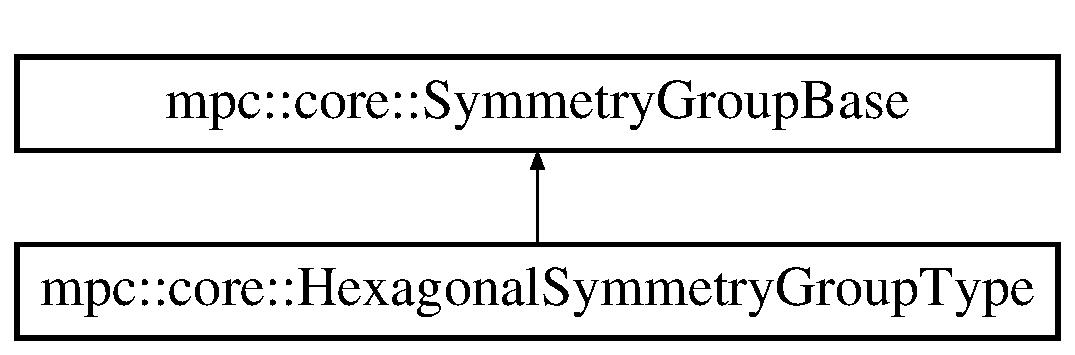
\includegraphics[height=2.000000cm]{structmpc_1_1core_1_1_hexagonal_symmetry_group_type}
\end{center}
\end{figure}
\subsection*{Static Public Member Functions}
\begin{DoxyCompactItemize}
\item 
static constexpr \mbox{\hyperlink{namespacempc_1_1core_a9d979684062547055a0ef5c13077bad8}{Symmetry\+Group\+Enumeration}} \mbox{\hyperlink{structmpc_1_1core_1_1_hexagonal_symmetry_group_type_a8cea833b34367fcff5f6b485f05021f3}{Symmetry\+Group\+Enum}} ()
\item 
static constexpr int \mbox{\hyperlink{structmpc_1_1core_1_1_hexagonal_symmetry_group_type_a04e0cc053d16f003808c9232cef6a7ac}{Number\+Of\+Independent\+Components}} ()
\end{DoxyCompactItemize}
\subsection*{Public Attributes}
\begin{DoxyCompactItemize}
\item 
const \mbox{\hyperlink{namespacempc_1_1core_a9d979684062547055a0ef5c13077bad8}{Symmetry\+Group\+Enumeration}} \mbox{\hyperlink{structmpc_1_1core_1_1_hexagonal_symmetry_group_type_a953ee47f7c2eb028edcf3c994565df8d}{symmetry\+\_\+group\+\_\+enumeration}} = \mbox{\hyperlink{namespacempc_1_1core_a9d979684062547055a0ef5c13077bad8a5d7adeeaa10073a6a3c5bd970a7f958b}{Symmetry\+Group\+Enumeration\+::\+H\+E\+X\+A\+G\+O\+N\+AL}}
\item 
const int \mbox{\hyperlink{structmpc_1_1core_1_1_hexagonal_symmetry_group_type_aee537d24b7cc35758c30708c58528f21}{number\+\_\+of\+\_\+independent\+\_\+components}} = 5
\end{DoxyCompactItemize}


\subsection{Detailed Description}


Definition at line 208 of file symmetrygrouptypes.\+hpp.



\subsection{Member Function Documentation}
\mbox{\Hypertarget{structmpc_1_1core_1_1_hexagonal_symmetry_group_type_a04e0cc053d16f003808c9232cef6a7ac}\label{structmpc_1_1core_1_1_hexagonal_symmetry_group_type_a04e0cc053d16f003808c9232cef6a7ac}} 
\index{mpc\+::core\+::\+Hexagonal\+Symmetry\+Group\+Type@{mpc\+::core\+::\+Hexagonal\+Symmetry\+Group\+Type}!Number\+Of\+Independent\+Components@{Number\+Of\+Independent\+Components}}
\index{Number\+Of\+Independent\+Components@{Number\+Of\+Independent\+Components}!mpc\+::core\+::\+Hexagonal\+Symmetry\+Group\+Type@{mpc\+::core\+::\+Hexagonal\+Symmetry\+Group\+Type}}
\subsubsection{\texorpdfstring{Number\+Of\+Independent\+Components()}{NumberOfIndependentComponents()}}
{\footnotesize\ttfamily static constexpr int mpc\+::core\+::\+Hexagonal\+Symmetry\+Group\+Type\+::\+Number\+Of\+Independent\+Components (\begin{DoxyParamCaption}{ }\end{DoxyParamCaption})\hspace{0.3cm}{\ttfamily [inline]}, {\ttfamily [static]}}



Definition at line 215 of file symmetrygrouptypes.\+hpp.

\mbox{\Hypertarget{structmpc_1_1core_1_1_hexagonal_symmetry_group_type_a8cea833b34367fcff5f6b485f05021f3}\label{structmpc_1_1core_1_1_hexagonal_symmetry_group_type_a8cea833b34367fcff5f6b485f05021f3}} 
\index{mpc\+::core\+::\+Hexagonal\+Symmetry\+Group\+Type@{mpc\+::core\+::\+Hexagonal\+Symmetry\+Group\+Type}!Symmetry\+Group\+Enum@{Symmetry\+Group\+Enum}}
\index{Symmetry\+Group\+Enum@{Symmetry\+Group\+Enum}!mpc\+::core\+::\+Hexagonal\+Symmetry\+Group\+Type@{mpc\+::core\+::\+Hexagonal\+Symmetry\+Group\+Type}}
\subsubsection{\texorpdfstring{Symmetry\+Group\+Enum()}{SymmetryGroupEnum()}}
{\footnotesize\ttfamily static constexpr \mbox{\hyperlink{namespacempc_1_1core_a9d979684062547055a0ef5c13077bad8}{Symmetry\+Group\+Enumeration}} mpc\+::core\+::\+Hexagonal\+Symmetry\+Group\+Type\+::\+Symmetry\+Group\+Enum (\begin{DoxyParamCaption}{ }\end{DoxyParamCaption})\hspace{0.3cm}{\ttfamily [inline]}, {\ttfamily [static]}}



Definition at line 212 of file symmetrygrouptypes.\+hpp.



\subsection{Member Data Documentation}
\mbox{\Hypertarget{structmpc_1_1core_1_1_hexagonal_symmetry_group_type_aee537d24b7cc35758c30708c58528f21}\label{structmpc_1_1core_1_1_hexagonal_symmetry_group_type_aee537d24b7cc35758c30708c58528f21}} 
\index{mpc\+::core\+::\+Hexagonal\+Symmetry\+Group\+Type@{mpc\+::core\+::\+Hexagonal\+Symmetry\+Group\+Type}!number\+\_\+of\+\_\+independent\+\_\+components@{number\+\_\+of\+\_\+independent\+\_\+components}}
\index{number\+\_\+of\+\_\+independent\+\_\+components@{number\+\_\+of\+\_\+independent\+\_\+components}!mpc\+::core\+::\+Hexagonal\+Symmetry\+Group\+Type@{mpc\+::core\+::\+Hexagonal\+Symmetry\+Group\+Type}}
\subsubsection{\texorpdfstring{number\+\_\+of\+\_\+independent\+\_\+components}{number\_of\_independent\_components}}
{\footnotesize\ttfamily const int mpc\+::core\+::\+Hexagonal\+Symmetry\+Group\+Type\+::number\+\_\+of\+\_\+independent\+\_\+components = 5}



Definition at line 210 of file symmetrygrouptypes.\+hpp.

\mbox{\Hypertarget{structmpc_1_1core_1_1_hexagonal_symmetry_group_type_a953ee47f7c2eb028edcf3c994565df8d}\label{structmpc_1_1core_1_1_hexagonal_symmetry_group_type_a953ee47f7c2eb028edcf3c994565df8d}} 
\index{mpc\+::core\+::\+Hexagonal\+Symmetry\+Group\+Type@{mpc\+::core\+::\+Hexagonal\+Symmetry\+Group\+Type}!symmetry\+\_\+group\+\_\+enumeration@{symmetry\+\_\+group\+\_\+enumeration}}
\index{symmetry\+\_\+group\+\_\+enumeration@{symmetry\+\_\+group\+\_\+enumeration}!mpc\+::core\+::\+Hexagonal\+Symmetry\+Group\+Type@{mpc\+::core\+::\+Hexagonal\+Symmetry\+Group\+Type}}
\subsubsection{\texorpdfstring{symmetry\+\_\+group\+\_\+enumeration}{symmetry\_group\_enumeration}}
{\footnotesize\ttfamily const \mbox{\hyperlink{namespacempc_1_1core_a9d979684062547055a0ef5c13077bad8}{Symmetry\+Group\+Enumeration}} mpc\+::core\+::\+Hexagonal\+Symmetry\+Group\+Type\+::symmetry\+\_\+group\+\_\+enumeration = \mbox{\hyperlink{namespacempc_1_1core_a9d979684062547055a0ef5c13077bad8a5d7adeeaa10073a6a3c5bd970a7f958b}{Symmetry\+Group\+Enumeration\+::\+H\+E\+X\+A\+G\+O\+N\+AL}}}



Definition at line 209 of file symmetrygrouptypes.\+hpp.



The documentation for this struct was generated from the following file\+:\begin{DoxyCompactItemize}
\item 
/\+Users/atorlucci/\+Documents/github\+\_\+threecubed\+\_\+repos/mpc/src/mpc/core/\mbox{\hyperlink{symmetrygrouptypes_8hpp}{symmetrygrouptypes.\+hpp}}\end{DoxyCompactItemize}

\hypertarget{structmpc_1_1mechanics_1_1_hookes_law_function_object}{}\section{mpc\+:\+:mechanics\+:\+:Hookes\+Law\+Function\+Object$<$ T, CS $>$ Class Template Reference}
\label{structmpc_1_1mechanics_1_1_hookes_law_function_object}\index{mpc\+::mechanics\+::\+Hookes\+Law\+Function\+Object$<$ T, C\+S $>$@{mpc\+::mechanics\+::\+Hookes\+Law\+Function\+Object$<$ T, C\+S $>$}}


function object based on linear form of Hooke\textquotesingle{}s Law  




{\ttfamily \#include $<$hookeslaw.\+hpp$>$}



\subsection{Detailed Description}
\subsubsection*{template$<$typename T, typename CS$>$\newline
class mpc\+::mechanics\+::\+Hookes\+Law\+Function\+Object$<$ T, C\+S $>$}

function object based on linear form of Hooke\textquotesingle{}s Law 

Two specializations are provided ... 

Definition at line 34 of file hookeslaw.\+hpp.



The documentation for this class was generated from the following file\+:\begin{DoxyCompactItemize}
\item 
/\+Users/atorlucci/\+Documents/github\+\_\+threecubed\+\_\+repos/mpc/src/mpc/mechanics/\mbox{\hyperlink{hookeslaw_8hpp}{hookeslaw.\+hpp}}\end{DoxyCompactItemize}

\hypertarget{structmpc_1_1mechanics_1_1_hookes_law_function_object_3_01_t_00_01mpc_1_1core_1_1_compliance_type_01_4}{}\section{mpc\+:\+:mechanics\+:\+:Hookes\+Law\+Function\+Object$<$ T, mpc\+:\+:core\+:\+:Compliance\+Type $>$ Struct Template Reference}
\label{structmpc_1_1mechanics_1_1_hookes_law_function_object_3_01_t_00_01mpc_1_1core_1_1_compliance_type_01_4}\index{mpc\+::mechanics\+::\+Hookes\+Law\+Function\+Object$<$ T, mpc\+::core\+::\+Compliance\+Type $>$@{mpc\+::mechanics\+::\+Hookes\+Law\+Function\+Object$<$ T, mpc\+::core\+::\+Compliance\+Type $>$}}


{\ttfamily \#include $<$hookeslaw.\+hpp$>$}

\subsection*{Public Member Functions}
\begin{DoxyCompactItemize}
\item 
\mbox{\hyperlink{structmpc_1_1core_1_1_strain_tensor}{mpc\+::core\+::\+Strain\+Tensor}}$<$ T $>$ \mbox{\hyperlink{structmpc_1_1mechanics_1_1_hookes_law_function_object_3_01_t_00_01mpc_1_1core_1_1_compliance_type_01_4_a55619695ae289395963ed9106f470704}{operator()}} (\mbox{\hyperlink{structmpc_1_1core_1_1_compliance_tensor}{mpc\+::core\+::\+Compliance\+Tensor}}$<$ T $>$ \&compliance, \mbox{\hyperlink{structmpc_1_1core_1_1_stress_tensor}{mpc\+::core\+::\+Stress\+Tensor}}$<$ T $>$ \&stress)
\end{DoxyCompactItemize}


\subsection{Detailed Description}
\subsubsection*{template$<$typename T$>$\newline
struct mpc\+::mechanics\+::\+Hookes\+Law\+Function\+Object$<$ T, mpc\+::core\+::\+Compliance\+Type $>$}



Definition at line 69 of file hookeslaw.\+hpp.



\subsection{Member Function Documentation}
\mbox{\Hypertarget{structmpc_1_1mechanics_1_1_hookes_law_function_object_3_01_t_00_01mpc_1_1core_1_1_compliance_type_01_4_a55619695ae289395963ed9106f470704}\label{structmpc_1_1mechanics_1_1_hookes_law_function_object_3_01_t_00_01mpc_1_1core_1_1_compliance_type_01_4_a55619695ae289395963ed9106f470704}} 
\index{mpc\+::mechanics\+::\+Hookes\+Law\+Function\+Object$<$ T, mpc\+::core\+::\+Compliance\+Type $>$@{mpc\+::mechanics\+::\+Hookes\+Law\+Function\+Object$<$ T, mpc\+::core\+::\+Compliance\+Type $>$}!operator()@{operator()}}
\index{operator()@{operator()}!mpc\+::mechanics\+::\+Hookes\+Law\+Function\+Object$<$ T, mpc\+::core\+::\+Compliance\+Type $>$@{mpc\+::mechanics\+::\+Hookes\+Law\+Function\+Object$<$ T, mpc\+::core\+::\+Compliance\+Type $>$}}
\subsubsection{\texorpdfstring{operator()()}{operator()()}}
{\footnotesize\ttfamily template$<$typename T $>$ \\
\mbox{\hyperlink{structmpc_1_1core_1_1_strain_tensor}{mpc\+::core\+::\+Strain\+Tensor}}$<$T$>$ \mbox{\hyperlink{structmpc_1_1mechanics_1_1_hookes_law_function_object}{mpc\+::mechanics\+::\+Hookes\+Law\+Function\+Object}}$<$ T, \mbox{\hyperlink{structmpc_1_1core_1_1_compliance_type}{mpc\+::core\+::\+Compliance\+Type}} $>$\+::operator() (\begin{DoxyParamCaption}\item[{\mbox{\hyperlink{structmpc_1_1core_1_1_compliance_tensor}{mpc\+::core\+::\+Compliance\+Tensor}}$<$ T $>$ \&}]{compliance,  }\item[{\mbox{\hyperlink{structmpc_1_1core_1_1_stress_tensor}{mpc\+::core\+::\+Stress\+Tensor}}$<$ T $>$ \&}]{stress }\end{DoxyParamCaption})\hspace{0.3cm}{\ttfamily [inline]}}



Definition at line 74 of file hookeslaw.\+hpp.



The documentation for this struct was generated from the following file\+:\begin{DoxyCompactItemize}
\item 
/\+Users/atorlucci/\+Documents/github\+\_\+threecubed\+\_\+repos/mpc/src/mpc/mechanics/\mbox{\hyperlink{hookeslaw_8hpp}{hookeslaw.\+hpp}}\end{DoxyCompactItemize}

\hypertarget{structmpc_1_1mechanics_1_1_hookes_law_function_object_3_01_t_00_01mpc_1_1core_1_1_stiffness_type_01_4}{}\section{mpc\+:\+:mechanics\+:\+:Hookes\+Law\+Function\+Object$<$ T, mpc\+:\+:core\+:\+:Stiffness\+Type $>$ Struct Template Reference}
\label{structmpc_1_1mechanics_1_1_hookes_law_function_object_3_01_t_00_01mpc_1_1core_1_1_stiffness_type_01_4}\index{mpc\+::mechanics\+::\+Hookes\+Law\+Function\+Object$<$ T, mpc\+::core\+::\+Stiffness\+Type $>$@{mpc\+::mechanics\+::\+Hookes\+Law\+Function\+Object$<$ T, mpc\+::core\+::\+Stiffness\+Type $>$}}


{\ttfamily \#include $<$hookeslaw.\+hpp$>$}

\subsection*{Public Member Functions}
\begin{DoxyCompactItemize}
\item 
\mbox{\hyperlink{structmpc_1_1core_1_1_stress_tensor}{mpc\+::core\+::\+Stress\+Tensor}}$<$ T $>$ \mbox{\hyperlink{structmpc_1_1mechanics_1_1_hookes_law_function_object_3_01_t_00_01mpc_1_1core_1_1_stiffness_type_01_4_a4d0b04ae39c5feb98e36182a869dbbc6}{operator()}} (\mbox{\hyperlink{structmpc_1_1core_1_1_stiffness_tensor}{mpc\+::core\+::\+Stiffness\+Tensor}}$<$ T $>$ \&stiffness, \mbox{\hyperlink{structmpc_1_1core_1_1_strain_tensor}{mpc\+::core\+::\+Strain\+Tensor}}$<$ T $>$ \&strain)
\end{DoxyCompactItemize}


\subsection{Detailed Description}
\subsubsection*{template$<$typename T$>$\newline
struct mpc\+::mechanics\+::\+Hookes\+Law\+Function\+Object$<$ T, mpc\+::core\+::\+Stiffness\+Type $>$}



Definition at line 41 of file hookeslaw.\+hpp.



\subsection{Member Function Documentation}
\mbox{\Hypertarget{structmpc_1_1mechanics_1_1_hookes_law_function_object_3_01_t_00_01mpc_1_1core_1_1_stiffness_type_01_4_a4d0b04ae39c5feb98e36182a869dbbc6}\label{structmpc_1_1mechanics_1_1_hookes_law_function_object_3_01_t_00_01mpc_1_1core_1_1_stiffness_type_01_4_a4d0b04ae39c5feb98e36182a869dbbc6}} 
\index{mpc\+::mechanics\+::\+Hookes\+Law\+Function\+Object$<$ T, mpc\+::core\+::\+Stiffness\+Type $>$@{mpc\+::mechanics\+::\+Hookes\+Law\+Function\+Object$<$ T, mpc\+::core\+::\+Stiffness\+Type $>$}!operator()@{operator()}}
\index{operator()@{operator()}!mpc\+::mechanics\+::\+Hookes\+Law\+Function\+Object$<$ T, mpc\+::core\+::\+Stiffness\+Type $>$@{mpc\+::mechanics\+::\+Hookes\+Law\+Function\+Object$<$ T, mpc\+::core\+::\+Stiffness\+Type $>$}}
\subsubsection{\texorpdfstring{operator()()}{operator()()}}
{\footnotesize\ttfamily template$<$typename T $>$ \\
\mbox{\hyperlink{structmpc_1_1core_1_1_stress_tensor}{mpc\+::core\+::\+Stress\+Tensor}}$<$T$>$ \mbox{\hyperlink{structmpc_1_1mechanics_1_1_hookes_law_function_object}{mpc\+::mechanics\+::\+Hookes\+Law\+Function\+Object}}$<$ T, \mbox{\hyperlink{structmpc_1_1core_1_1_stiffness_type}{mpc\+::core\+::\+Stiffness\+Type}} $>$\+::operator() (\begin{DoxyParamCaption}\item[{\mbox{\hyperlink{structmpc_1_1core_1_1_stiffness_tensor}{mpc\+::core\+::\+Stiffness\+Tensor}}$<$ T $>$ \&}]{stiffness,  }\item[{\mbox{\hyperlink{structmpc_1_1core_1_1_strain_tensor}{mpc\+::core\+::\+Strain\+Tensor}}$<$ T $>$ \&}]{strain }\end{DoxyParamCaption})\hspace{0.3cm}{\ttfamily [inline]}}



Definition at line 46 of file hookeslaw.\+hpp.



The documentation for this struct was generated from the following file\+:\begin{DoxyCompactItemize}
\item 
/\+Users/atorlucci/\+Documents/github\+\_\+threecubed\+\_\+repos/mpc/src/mpc/mechanics/\mbox{\hyperlink{hookeslaw_8hpp}{hookeslaw.\+hpp}}\end{DoxyCompactItemize}

\hypertarget{structmpc_1_1rockphysics_1_1_hydrostatic_pressure_type}{}\section{mpc\+:\+:rockphysics\+:\+:Hydrostatic\+Pressure\+Type$<$ T $>$ Struct Template Reference}
\label{structmpc_1_1rockphysics_1_1_hydrostatic_pressure_type}\index{mpc\+::rockphysics\+::\+Hydrostatic\+Pressure\+Type$<$ T $>$@{mpc\+::rockphysics\+::\+Hydrostatic\+Pressure\+Type$<$ T $>$}}


{\ttfamily \#include $<$rockphysicstransformstypes.\+hpp$>$}

Inheritance diagram for mpc\+:\+:rockphysics\+:\+:Hydrostatic\+Pressure\+Type$<$ T $>$\+:\begin{figure}[H]
\begin{center}
\leavevmode
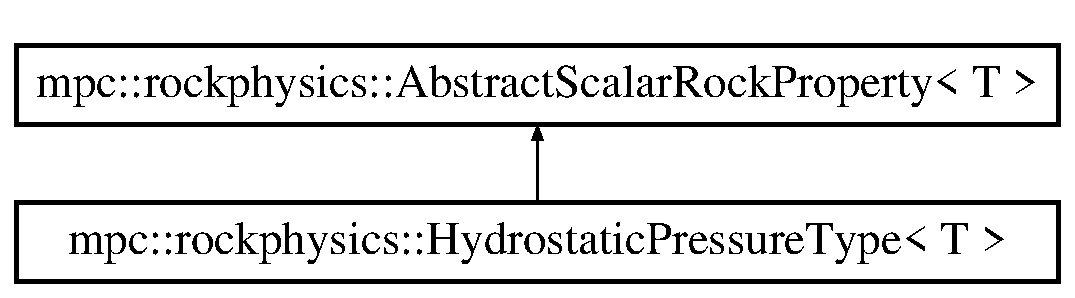
\includegraphics[height=2.000000cm]{structmpc_1_1rockphysics_1_1_hydrostatic_pressure_type}
\end{center}
\end{figure}
\subsection*{Public Member Functions}
\begin{DoxyCompactItemize}
\item 
constexpr \mbox{\hyperlink{structmpc_1_1rockphysics_1_1_hydrostatic_pressure_type_a182e96fb2534e9a66ca8f1a600c0fd0d}{Hydrostatic\+Pressure\+Type}} (T val)
\end{DoxyCompactItemize}
\subsection*{Additional Inherited Members}


\subsection{Detailed Description}
\subsubsection*{template$<$typename T$>$\newline
struct mpc\+::rockphysics\+::\+Hydrostatic\+Pressure\+Type$<$ T $>$}



Definition at line 132 of file rockphysicstransformstypes.\+hpp.



\subsection{Constructor \& Destructor Documentation}
\mbox{\Hypertarget{structmpc_1_1rockphysics_1_1_hydrostatic_pressure_type_a182e96fb2534e9a66ca8f1a600c0fd0d}\label{structmpc_1_1rockphysics_1_1_hydrostatic_pressure_type_a182e96fb2534e9a66ca8f1a600c0fd0d}} 
\index{mpc\+::rockphysics\+::\+Hydrostatic\+Pressure\+Type@{mpc\+::rockphysics\+::\+Hydrostatic\+Pressure\+Type}!Hydrostatic\+Pressure\+Type@{Hydrostatic\+Pressure\+Type}}
\index{Hydrostatic\+Pressure\+Type@{Hydrostatic\+Pressure\+Type}!mpc\+::rockphysics\+::\+Hydrostatic\+Pressure\+Type@{mpc\+::rockphysics\+::\+Hydrostatic\+Pressure\+Type}}
\subsubsection{\texorpdfstring{Hydrostatic\+Pressure\+Type()}{HydrostaticPressureType()}}
{\footnotesize\ttfamily template$<$typename T$>$ \\
constexpr \mbox{\hyperlink{structmpc_1_1rockphysics_1_1_hydrostatic_pressure_type}{mpc\+::rockphysics\+::\+Hydrostatic\+Pressure\+Type}}$<$ T $>$\+::\mbox{\hyperlink{structmpc_1_1rockphysics_1_1_hydrostatic_pressure_type}{Hydrostatic\+Pressure\+Type}} (\begin{DoxyParamCaption}\item[{T}]{val }\end{DoxyParamCaption})\hspace{0.3cm}{\ttfamily [inline]}}



Definition at line 137 of file rockphysicstransformstypes.\+hpp.



The documentation for this struct was generated from the following file\+:\begin{DoxyCompactItemize}
\item 
/\+Users/atorlucci/\+Documents/github\+\_\+threecubed\+\_\+repos/mpc/src/mpc/rockphysics/\mbox{\hyperlink{rockphysicstransformstypes_8hpp}{rockphysicstransformstypes.\+hpp}}\end{DoxyCompactItemize}

\hypertarget{structmpc_1_1utilities_1_1_identity_tensor_function_object}{}\section{mpc\+:\+:utilities\+:\+:Identity\+Tensor\+Function\+Object$<$ T, Dim, Rank $>$ Struct Template Reference}
\label{structmpc_1_1utilities_1_1_identity_tensor_function_object}\index{mpc\+::utilities\+::\+Identity\+Tensor\+Function\+Object$<$ T, Dim, Rank $>$@{mpc\+::utilities\+::\+Identity\+Tensor\+Function\+Object$<$ T, Dim, Rank $>$}}


{\ttfamily \#include $<$identitytensor.\+hpp$>$}



\subsection{Detailed Description}
\subsubsection*{template$<$typename T, int Dim, int Rank$>$\newline
struct mpc\+::utilities\+::\+Identity\+Tensor\+Function\+Object$<$ T, Dim, Rank $>$}



Definition at line 22 of file identitytensor.\+hpp.



The documentation for this struct was generated from the following file\+:\begin{DoxyCompactItemize}
\item 
/\+Users/atorlucci/\+Documents/github\+\_\+threecubed\+\_\+repos/mpc/src/mpc/utilities/\mbox{\hyperlink{identitytensor_8hpp}{identitytensor.\+hpp}}\end{DoxyCompactItemize}

\hypertarget{structmpc_1_1utilities_1_1_identity_tensor_function_object_3_01_t_00_01_dim_00_0110_01_4}{}\section{mpc\+:\+:utilities\+:\+:Identity\+Tensor\+Function\+Object$<$ T, Dim, 10 $>$ Struct Template Reference}
\label{structmpc_1_1utilities_1_1_identity_tensor_function_object_3_01_t_00_01_dim_00_0110_01_4}\index{mpc\+::utilities\+::\+Identity\+Tensor\+Function\+Object$<$ T, Dim, 10 $>$@{mpc\+::utilities\+::\+Identity\+Tensor\+Function\+Object$<$ T, Dim, 10 $>$}}


{\ttfamily \#include $<$identitytensor.\+hpp$>$}

\subsection*{Public Member Functions}
\begin{DoxyCompactItemize}
\item 
blitz\+::\+Array$<$ T, 10 $>$ \mbox{\hyperlink{structmpc_1_1utilities_1_1_identity_tensor_function_object_3_01_t_00_01_dim_00_0110_01_4_acfb99c78c797a5675e8b418db589a7a1}{operator()}} ()
\end{DoxyCompactItemize}


\subsection{Detailed Description}
\subsubsection*{template$<$typename T, int Dim$>$\newline
struct mpc\+::utilities\+::\+Identity\+Tensor\+Function\+Object$<$ T, Dim, 10 $>$}



Definition at line 105 of file identitytensor.\+hpp.



\subsection{Member Function Documentation}
\mbox{\Hypertarget{structmpc_1_1utilities_1_1_identity_tensor_function_object_3_01_t_00_01_dim_00_0110_01_4_acfb99c78c797a5675e8b418db589a7a1}\label{structmpc_1_1utilities_1_1_identity_tensor_function_object_3_01_t_00_01_dim_00_0110_01_4_acfb99c78c797a5675e8b418db589a7a1}} 
\index{mpc\+::utilities\+::\+Identity\+Tensor\+Function\+Object$<$ T, Dim, 10 $>$@{mpc\+::utilities\+::\+Identity\+Tensor\+Function\+Object$<$ T, Dim, 10 $>$}!operator()@{operator()}}
\index{operator()@{operator()}!mpc\+::utilities\+::\+Identity\+Tensor\+Function\+Object$<$ T, Dim, 10 $>$@{mpc\+::utilities\+::\+Identity\+Tensor\+Function\+Object$<$ T, Dim, 10 $>$}}
\subsubsection{\texorpdfstring{operator()()}{operator()()}}
{\footnotesize\ttfamily template$<$typename T , int Dim$>$ \\
blitz\+::\+Array$<$T,10$>$ \mbox{\hyperlink{structmpc_1_1utilities_1_1_identity_tensor_function_object}{mpc\+::utilities\+::\+Identity\+Tensor\+Function\+Object}}$<$ T, Dim, 10 $>$\+::operator() (\begin{DoxyParamCaption}{ }\end{DoxyParamCaption})\hspace{0.3cm}{\ttfamily [inline]}}



Definition at line 107 of file identitytensor.\+hpp.



The documentation for this struct was generated from the following file\+:\begin{DoxyCompactItemize}
\item 
/\+Users/atorlucci/\+Documents/github\+\_\+threecubed\+\_\+repos/mpc/src/mpc/utilities/\mbox{\hyperlink{identitytensor_8hpp}{identitytensor.\+hpp}}\end{DoxyCompactItemize}

\hypertarget{structmpc_1_1utilities_1_1_identity_tensor_function_object_3_01_t_00_01_dim_00_0111_01_4}{}\section{mpc\+:\+:utilities\+:\+:Identity\+Tensor\+Function\+Object$<$ T, Dim, 11 $>$ Struct Template Reference}
\label{structmpc_1_1utilities_1_1_identity_tensor_function_object_3_01_t_00_01_dim_00_0111_01_4}\index{mpc\+::utilities\+::\+Identity\+Tensor\+Function\+Object$<$ T, Dim, 11 $>$@{mpc\+::utilities\+::\+Identity\+Tensor\+Function\+Object$<$ T, Dim, 11 $>$}}


{\ttfamily \#include $<$identitytensor.\+hpp$>$}

\subsection*{Public Member Functions}
\begin{DoxyCompactItemize}
\item 
blitz\+::\+Array$<$ T, 11 $>$ \mbox{\hyperlink{structmpc_1_1utilities_1_1_identity_tensor_function_object_3_01_t_00_01_dim_00_0111_01_4_a9df310361a37b1b05bc83a51b57ca686}{operator()}} ()
\end{DoxyCompactItemize}


\subsection{Detailed Description}
\subsubsection*{template$<$typename T, int Dim$>$\newline
struct mpc\+::utilities\+::\+Identity\+Tensor\+Function\+Object$<$ T, Dim, 11 $>$}



Definition at line 114 of file identitytensor.\+hpp.



\subsection{Member Function Documentation}
\mbox{\Hypertarget{structmpc_1_1utilities_1_1_identity_tensor_function_object_3_01_t_00_01_dim_00_0111_01_4_a9df310361a37b1b05bc83a51b57ca686}\label{structmpc_1_1utilities_1_1_identity_tensor_function_object_3_01_t_00_01_dim_00_0111_01_4_a9df310361a37b1b05bc83a51b57ca686}} 
\index{mpc\+::utilities\+::\+Identity\+Tensor\+Function\+Object$<$ T, Dim, 11 $>$@{mpc\+::utilities\+::\+Identity\+Tensor\+Function\+Object$<$ T, Dim, 11 $>$}!operator()@{operator()}}
\index{operator()@{operator()}!mpc\+::utilities\+::\+Identity\+Tensor\+Function\+Object$<$ T, Dim, 11 $>$@{mpc\+::utilities\+::\+Identity\+Tensor\+Function\+Object$<$ T, Dim, 11 $>$}}
\subsubsection{\texorpdfstring{operator()()}{operator()()}}
{\footnotesize\ttfamily template$<$typename T , int Dim$>$ \\
blitz\+::\+Array$<$T,11$>$ \mbox{\hyperlink{structmpc_1_1utilities_1_1_identity_tensor_function_object}{mpc\+::utilities\+::\+Identity\+Tensor\+Function\+Object}}$<$ T, Dim, 11 $>$\+::operator() (\begin{DoxyParamCaption}{ }\end{DoxyParamCaption})\hspace{0.3cm}{\ttfamily [inline]}}



Definition at line 116 of file identitytensor.\+hpp.



The documentation for this struct was generated from the following file\+:\begin{DoxyCompactItemize}
\item 
/\+Users/atorlucci/\+Documents/github\+\_\+threecubed\+\_\+repos/mpc/src/mpc/utilities/\mbox{\hyperlink{identitytensor_8hpp}{identitytensor.\+hpp}}\end{DoxyCompactItemize}

\hypertarget{structmpc_1_1utilities_1_1_identity_tensor_function_object_3_01_t_00_01_dim_00_012_01_4}{}\section{mpc\+:\+:utilities\+:\+:Identity\+Tensor\+Function\+Object$<$ T, Dim, 2 $>$ Struct Template Reference}
\label{structmpc_1_1utilities_1_1_identity_tensor_function_object_3_01_t_00_01_dim_00_012_01_4}\index{mpc\+::utilities\+::\+Identity\+Tensor\+Function\+Object$<$ T, Dim, 2 $>$@{mpc\+::utilities\+::\+Identity\+Tensor\+Function\+Object$<$ T, Dim, 2 $>$}}


{\ttfamily \#include $<$identitytensor.\+hpp$>$}

\subsection*{Public Member Functions}
\begin{DoxyCompactItemize}
\item 
blitz\+::\+Array$<$ T, 2 $>$ \mbox{\hyperlink{structmpc_1_1utilities_1_1_identity_tensor_function_object_3_01_t_00_01_dim_00_012_01_4_a7c1da2477c74a9335092b140c8536bd1}{operator()}} ()
\end{DoxyCompactItemize}


\subsection{Detailed Description}
\subsubsection*{template$<$typename T, int Dim$>$\newline
struct mpc\+::utilities\+::\+Identity\+Tensor\+Function\+Object$<$ T, Dim, 2 $>$}



Definition at line 33 of file identitytensor.\+hpp.



\subsection{Member Function Documentation}
\mbox{\Hypertarget{structmpc_1_1utilities_1_1_identity_tensor_function_object_3_01_t_00_01_dim_00_012_01_4_a7c1da2477c74a9335092b140c8536bd1}\label{structmpc_1_1utilities_1_1_identity_tensor_function_object_3_01_t_00_01_dim_00_012_01_4_a7c1da2477c74a9335092b140c8536bd1}} 
\index{mpc\+::utilities\+::\+Identity\+Tensor\+Function\+Object$<$ T, Dim, 2 $>$@{mpc\+::utilities\+::\+Identity\+Tensor\+Function\+Object$<$ T, Dim, 2 $>$}!operator()@{operator()}}
\index{operator()@{operator()}!mpc\+::utilities\+::\+Identity\+Tensor\+Function\+Object$<$ T, Dim, 2 $>$@{mpc\+::utilities\+::\+Identity\+Tensor\+Function\+Object$<$ T, Dim, 2 $>$}}
\subsubsection{\texorpdfstring{operator()()}{operator()()}}
{\footnotesize\ttfamily template$<$typename T , int Dim$>$ \\
blitz\+::\+Array$<$T,2$>$ \mbox{\hyperlink{structmpc_1_1utilities_1_1_identity_tensor_function_object}{mpc\+::utilities\+::\+Identity\+Tensor\+Function\+Object}}$<$ T, Dim, 2 $>$\+::operator() (\begin{DoxyParamCaption}{ }\end{DoxyParamCaption})\hspace{0.3cm}{\ttfamily [inline]}}



Definition at line 35 of file identitytensor.\+hpp.



The documentation for this struct was generated from the following file\+:\begin{DoxyCompactItemize}
\item 
/\+Users/atorlucci/\+Documents/github\+\_\+threecubed\+\_\+repos/mpc/src/mpc/utilities/\mbox{\hyperlink{identitytensor_8hpp}{identitytensor.\+hpp}}\end{DoxyCompactItemize}

\hypertarget{structmpc_1_1utilities_1_1_identity_tensor_function_object_3_01_t_00_01_dim_00_013_01_4}{}\section{mpc\+:\+:utilities\+:\+:Identity\+Tensor\+Function\+Object$<$ T, Dim, 3 $>$ Struct Template Reference}
\label{structmpc_1_1utilities_1_1_identity_tensor_function_object_3_01_t_00_01_dim_00_013_01_4}\index{mpc\+::utilities\+::\+Identity\+Tensor\+Function\+Object$<$ T, Dim, 3 $>$@{mpc\+::utilities\+::\+Identity\+Tensor\+Function\+Object$<$ T, Dim, 3 $>$}}


{\ttfamily \#include $<$identitytensor.\+hpp$>$}

\subsection*{Public Member Functions}
\begin{DoxyCompactItemize}
\item 
blitz\+::\+Array$<$ T, 3 $>$ \mbox{\hyperlink{structmpc_1_1utilities_1_1_identity_tensor_function_object_3_01_t_00_01_dim_00_013_01_4_a43e6ea3f90dd5a32a4b20db3854633ac}{operator()}} ()
\end{DoxyCompactItemize}


\subsection{Detailed Description}
\subsubsection*{template$<$typename T, int Dim$>$\newline
struct mpc\+::utilities\+::\+Identity\+Tensor\+Function\+Object$<$ T, Dim, 3 $>$}



Definition at line 42 of file identitytensor.\+hpp.



\subsection{Member Function Documentation}
\mbox{\Hypertarget{structmpc_1_1utilities_1_1_identity_tensor_function_object_3_01_t_00_01_dim_00_013_01_4_a43e6ea3f90dd5a32a4b20db3854633ac}\label{structmpc_1_1utilities_1_1_identity_tensor_function_object_3_01_t_00_01_dim_00_013_01_4_a43e6ea3f90dd5a32a4b20db3854633ac}} 
\index{mpc\+::utilities\+::\+Identity\+Tensor\+Function\+Object$<$ T, Dim, 3 $>$@{mpc\+::utilities\+::\+Identity\+Tensor\+Function\+Object$<$ T, Dim, 3 $>$}!operator()@{operator()}}
\index{operator()@{operator()}!mpc\+::utilities\+::\+Identity\+Tensor\+Function\+Object$<$ T, Dim, 3 $>$@{mpc\+::utilities\+::\+Identity\+Tensor\+Function\+Object$<$ T, Dim, 3 $>$}}
\subsubsection{\texorpdfstring{operator()()}{operator()()}}
{\footnotesize\ttfamily template$<$typename T , int Dim$>$ \\
blitz\+::\+Array$<$T,3$>$ \mbox{\hyperlink{structmpc_1_1utilities_1_1_identity_tensor_function_object}{mpc\+::utilities\+::\+Identity\+Tensor\+Function\+Object}}$<$ T, Dim, 3 $>$\+::operator() (\begin{DoxyParamCaption}{ }\end{DoxyParamCaption})\hspace{0.3cm}{\ttfamily [inline]}}



Definition at line 44 of file identitytensor.\+hpp.



The documentation for this struct was generated from the following file\+:\begin{DoxyCompactItemize}
\item 
/\+Users/atorlucci/\+Documents/github\+\_\+threecubed\+\_\+repos/mpc/src/mpc/utilities/\mbox{\hyperlink{identitytensor_8hpp}{identitytensor.\+hpp}}\end{DoxyCompactItemize}

\hypertarget{structmpc_1_1utilities_1_1_identity_tensor_function_object_3_01_t_00_01_dim_00_014_01_4}{}\section{mpc\+:\+:utilities\+:\+:Identity\+Tensor\+Function\+Object$<$ T, Dim, 4 $>$ Struct Template Reference}
\label{structmpc_1_1utilities_1_1_identity_tensor_function_object_3_01_t_00_01_dim_00_014_01_4}\index{mpc\+::utilities\+::\+Identity\+Tensor\+Function\+Object$<$ T, Dim, 4 $>$@{mpc\+::utilities\+::\+Identity\+Tensor\+Function\+Object$<$ T, Dim, 4 $>$}}


{\ttfamily \#include $<$identitytensor.\+hpp$>$}

\subsection*{Public Member Functions}
\begin{DoxyCompactItemize}
\item 
blitz\+::\+Array$<$ T, 4 $>$ \mbox{\hyperlink{structmpc_1_1utilities_1_1_identity_tensor_function_object_3_01_t_00_01_dim_00_014_01_4_a5155400d769ac22a62537f4d3aee9cda}{operator()}} ()
\end{DoxyCompactItemize}


\subsection{Detailed Description}
\subsubsection*{template$<$typename T, int Dim$>$\newline
struct mpc\+::utilities\+::\+Identity\+Tensor\+Function\+Object$<$ T, Dim, 4 $>$}



Definition at line 51 of file identitytensor.\+hpp.



\subsection{Member Function Documentation}
\mbox{\Hypertarget{structmpc_1_1utilities_1_1_identity_tensor_function_object_3_01_t_00_01_dim_00_014_01_4_a5155400d769ac22a62537f4d3aee9cda}\label{structmpc_1_1utilities_1_1_identity_tensor_function_object_3_01_t_00_01_dim_00_014_01_4_a5155400d769ac22a62537f4d3aee9cda}} 
\index{mpc\+::utilities\+::\+Identity\+Tensor\+Function\+Object$<$ T, Dim, 4 $>$@{mpc\+::utilities\+::\+Identity\+Tensor\+Function\+Object$<$ T, Dim, 4 $>$}!operator()@{operator()}}
\index{operator()@{operator()}!mpc\+::utilities\+::\+Identity\+Tensor\+Function\+Object$<$ T, Dim, 4 $>$@{mpc\+::utilities\+::\+Identity\+Tensor\+Function\+Object$<$ T, Dim, 4 $>$}}
\subsubsection{\texorpdfstring{operator()()}{operator()()}}
{\footnotesize\ttfamily template$<$typename T , int Dim$>$ \\
blitz\+::\+Array$<$T,4$>$ \mbox{\hyperlink{structmpc_1_1utilities_1_1_identity_tensor_function_object}{mpc\+::utilities\+::\+Identity\+Tensor\+Function\+Object}}$<$ T, Dim, 4 $>$\+::operator() (\begin{DoxyParamCaption}{ }\end{DoxyParamCaption})\hspace{0.3cm}{\ttfamily [inline]}}



Definition at line 53 of file identitytensor.\+hpp.



The documentation for this struct was generated from the following file\+:\begin{DoxyCompactItemize}
\item 
/\+Users/atorlucci/\+Documents/github\+\_\+threecubed\+\_\+repos/mpc/src/mpc/utilities/\mbox{\hyperlink{identitytensor_8hpp}{identitytensor.\+hpp}}\end{DoxyCompactItemize}

\hypertarget{structmpc_1_1utilities_1_1_identity_tensor_function_object_3_01_t_00_01_dim_00_015_01_4}{}\section{mpc\+:\+:utilities\+:\+:Identity\+Tensor\+Function\+Object$<$ T, Dim, 5 $>$ Struct Template Reference}
\label{structmpc_1_1utilities_1_1_identity_tensor_function_object_3_01_t_00_01_dim_00_015_01_4}\index{mpc\+::utilities\+::\+Identity\+Tensor\+Function\+Object$<$ T, Dim, 5 $>$@{mpc\+::utilities\+::\+Identity\+Tensor\+Function\+Object$<$ T, Dim, 5 $>$}}


{\ttfamily \#include $<$identitytensor.\+hpp$>$}

\subsection*{Public Member Functions}
\begin{DoxyCompactItemize}
\item 
blitz\+::\+Array$<$ T, 5 $>$ \mbox{\hyperlink{structmpc_1_1utilities_1_1_identity_tensor_function_object_3_01_t_00_01_dim_00_015_01_4_a2b5b797eb26d2b2deda29dbc49b2ae8b}{operator()}} ()
\end{DoxyCompactItemize}


\subsection{Detailed Description}
\subsubsection*{template$<$typename T, int Dim$>$\newline
struct mpc\+::utilities\+::\+Identity\+Tensor\+Function\+Object$<$ T, Dim, 5 $>$}



Definition at line 60 of file identitytensor.\+hpp.



\subsection{Member Function Documentation}
\mbox{\Hypertarget{structmpc_1_1utilities_1_1_identity_tensor_function_object_3_01_t_00_01_dim_00_015_01_4_a2b5b797eb26d2b2deda29dbc49b2ae8b}\label{structmpc_1_1utilities_1_1_identity_tensor_function_object_3_01_t_00_01_dim_00_015_01_4_a2b5b797eb26d2b2deda29dbc49b2ae8b}} 
\index{mpc\+::utilities\+::\+Identity\+Tensor\+Function\+Object$<$ T, Dim, 5 $>$@{mpc\+::utilities\+::\+Identity\+Tensor\+Function\+Object$<$ T, Dim, 5 $>$}!operator()@{operator()}}
\index{operator()@{operator()}!mpc\+::utilities\+::\+Identity\+Tensor\+Function\+Object$<$ T, Dim, 5 $>$@{mpc\+::utilities\+::\+Identity\+Tensor\+Function\+Object$<$ T, Dim, 5 $>$}}
\subsubsection{\texorpdfstring{operator()()}{operator()()}}
{\footnotesize\ttfamily template$<$typename T , int Dim$>$ \\
blitz\+::\+Array$<$T,5$>$ \mbox{\hyperlink{structmpc_1_1utilities_1_1_identity_tensor_function_object}{mpc\+::utilities\+::\+Identity\+Tensor\+Function\+Object}}$<$ T, Dim, 5 $>$\+::operator() (\begin{DoxyParamCaption}{ }\end{DoxyParamCaption})\hspace{0.3cm}{\ttfamily [inline]}}



Definition at line 62 of file identitytensor.\+hpp.



The documentation for this struct was generated from the following file\+:\begin{DoxyCompactItemize}
\item 
/\+Users/atorlucci/\+Documents/github\+\_\+threecubed\+\_\+repos/mpc/src/mpc/utilities/\mbox{\hyperlink{identitytensor_8hpp}{identitytensor.\+hpp}}\end{DoxyCompactItemize}

\hypertarget{structmpc_1_1utilities_1_1_identity_tensor_function_object_3_01_t_00_01_dim_00_016_01_4}{}\section{mpc\+:\+:utilities\+:\+:Identity\+Tensor\+Function\+Object$<$ T, Dim, 6 $>$ Struct Template Reference}
\label{structmpc_1_1utilities_1_1_identity_tensor_function_object_3_01_t_00_01_dim_00_016_01_4}\index{mpc\+::utilities\+::\+Identity\+Tensor\+Function\+Object$<$ T, Dim, 6 $>$@{mpc\+::utilities\+::\+Identity\+Tensor\+Function\+Object$<$ T, Dim, 6 $>$}}


{\ttfamily \#include $<$identitytensor.\+hpp$>$}

\subsection*{Public Member Functions}
\begin{DoxyCompactItemize}
\item 
blitz\+::\+Array$<$ T, 6 $>$ \mbox{\hyperlink{structmpc_1_1utilities_1_1_identity_tensor_function_object_3_01_t_00_01_dim_00_016_01_4_a05d96d47de8c1ab188e8978732a2a852}{operator()}} ()
\end{DoxyCompactItemize}


\subsection{Detailed Description}
\subsubsection*{template$<$typename T, int Dim$>$\newline
struct mpc\+::utilities\+::\+Identity\+Tensor\+Function\+Object$<$ T, Dim, 6 $>$}



Definition at line 69 of file identitytensor.\+hpp.



\subsection{Member Function Documentation}
\mbox{\Hypertarget{structmpc_1_1utilities_1_1_identity_tensor_function_object_3_01_t_00_01_dim_00_016_01_4_a05d96d47de8c1ab188e8978732a2a852}\label{structmpc_1_1utilities_1_1_identity_tensor_function_object_3_01_t_00_01_dim_00_016_01_4_a05d96d47de8c1ab188e8978732a2a852}} 
\index{mpc\+::utilities\+::\+Identity\+Tensor\+Function\+Object$<$ T, Dim, 6 $>$@{mpc\+::utilities\+::\+Identity\+Tensor\+Function\+Object$<$ T, Dim, 6 $>$}!operator()@{operator()}}
\index{operator()@{operator()}!mpc\+::utilities\+::\+Identity\+Tensor\+Function\+Object$<$ T, Dim, 6 $>$@{mpc\+::utilities\+::\+Identity\+Tensor\+Function\+Object$<$ T, Dim, 6 $>$}}
\subsubsection{\texorpdfstring{operator()()}{operator()()}}
{\footnotesize\ttfamily template$<$typename T , int Dim$>$ \\
blitz\+::\+Array$<$T,6$>$ \mbox{\hyperlink{structmpc_1_1utilities_1_1_identity_tensor_function_object}{mpc\+::utilities\+::\+Identity\+Tensor\+Function\+Object}}$<$ T, Dim, 6 $>$\+::operator() (\begin{DoxyParamCaption}{ }\end{DoxyParamCaption})\hspace{0.3cm}{\ttfamily [inline]}}



Definition at line 71 of file identitytensor.\+hpp.



The documentation for this struct was generated from the following file\+:\begin{DoxyCompactItemize}
\item 
/\+Users/atorlucci/\+Documents/github\+\_\+threecubed\+\_\+repos/mpc/src/mpc/utilities/\mbox{\hyperlink{identitytensor_8hpp}{identitytensor.\+hpp}}\end{DoxyCompactItemize}

\hypertarget{structmpc_1_1utilities_1_1_identity_tensor_function_object_3_01_t_00_01_dim_00_017_01_4}{}\section{mpc\+:\+:utilities\+:\+:Identity\+Tensor\+Function\+Object$<$ T, Dim, 7 $>$ Struct Template Reference}
\label{structmpc_1_1utilities_1_1_identity_tensor_function_object_3_01_t_00_01_dim_00_017_01_4}\index{mpc\+::utilities\+::\+Identity\+Tensor\+Function\+Object$<$ T, Dim, 7 $>$@{mpc\+::utilities\+::\+Identity\+Tensor\+Function\+Object$<$ T, Dim, 7 $>$}}


{\ttfamily \#include $<$identitytensor.\+hpp$>$}

\subsection*{Public Member Functions}
\begin{DoxyCompactItemize}
\item 
blitz\+::\+Array$<$ T, 7 $>$ \mbox{\hyperlink{structmpc_1_1utilities_1_1_identity_tensor_function_object_3_01_t_00_01_dim_00_017_01_4_a8abd9d0314c43d562bd3922acb7dd553}{operator()}} ()
\end{DoxyCompactItemize}


\subsection{Detailed Description}
\subsubsection*{template$<$typename T, int Dim$>$\newline
struct mpc\+::utilities\+::\+Identity\+Tensor\+Function\+Object$<$ T, Dim, 7 $>$}



Definition at line 78 of file identitytensor.\+hpp.



\subsection{Member Function Documentation}
\mbox{\Hypertarget{structmpc_1_1utilities_1_1_identity_tensor_function_object_3_01_t_00_01_dim_00_017_01_4_a8abd9d0314c43d562bd3922acb7dd553}\label{structmpc_1_1utilities_1_1_identity_tensor_function_object_3_01_t_00_01_dim_00_017_01_4_a8abd9d0314c43d562bd3922acb7dd553}} 
\index{mpc\+::utilities\+::\+Identity\+Tensor\+Function\+Object$<$ T, Dim, 7 $>$@{mpc\+::utilities\+::\+Identity\+Tensor\+Function\+Object$<$ T, Dim, 7 $>$}!operator()@{operator()}}
\index{operator()@{operator()}!mpc\+::utilities\+::\+Identity\+Tensor\+Function\+Object$<$ T, Dim, 7 $>$@{mpc\+::utilities\+::\+Identity\+Tensor\+Function\+Object$<$ T, Dim, 7 $>$}}
\subsubsection{\texorpdfstring{operator()()}{operator()()}}
{\footnotesize\ttfamily template$<$typename T , int Dim$>$ \\
blitz\+::\+Array$<$T,7$>$ \mbox{\hyperlink{structmpc_1_1utilities_1_1_identity_tensor_function_object}{mpc\+::utilities\+::\+Identity\+Tensor\+Function\+Object}}$<$ T, Dim, 7 $>$\+::operator() (\begin{DoxyParamCaption}{ }\end{DoxyParamCaption})\hspace{0.3cm}{\ttfamily [inline]}}



Definition at line 80 of file identitytensor.\+hpp.



The documentation for this struct was generated from the following file\+:\begin{DoxyCompactItemize}
\item 
/\+Users/atorlucci/\+Documents/github\+\_\+threecubed\+\_\+repos/mpc/src/mpc/utilities/\mbox{\hyperlink{identitytensor_8hpp}{identitytensor.\+hpp}}\end{DoxyCompactItemize}

\hypertarget{structmpc_1_1utilities_1_1_identity_tensor_function_object_3_01_t_00_01_dim_00_018_01_4}{}\section{mpc\+:\+:utilities\+:\+:Identity\+Tensor\+Function\+Object$<$ T, Dim, 8 $>$ Struct Template Reference}
\label{structmpc_1_1utilities_1_1_identity_tensor_function_object_3_01_t_00_01_dim_00_018_01_4}\index{mpc\+::utilities\+::\+Identity\+Tensor\+Function\+Object$<$ T, Dim, 8 $>$@{mpc\+::utilities\+::\+Identity\+Tensor\+Function\+Object$<$ T, Dim, 8 $>$}}


{\ttfamily \#include $<$identitytensor.\+hpp$>$}

\subsection*{Public Member Functions}
\begin{DoxyCompactItemize}
\item 
blitz\+::\+Array$<$ T, 8 $>$ \mbox{\hyperlink{structmpc_1_1utilities_1_1_identity_tensor_function_object_3_01_t_00_01_dim_00_018_01_4_a870c6b5176c8d8a3b9db38d1cb4deb9b}{operator()}} ()
\end{DoxyCompactItemize}


\subsection{Detailed Description}
\subsubsection*{template$<$typename T, int Dim$>$\newline
struct mpc\+::utilities\+::\+Identity\+Tensor\+Function\+Object$<$ T, Dim, 8 $>$}



Definition at line 87 of file identitytensor.\+hpp.



\subsection{Member Function Documentation}
\mbox{\Hypertarget{structmpc_1_1utilities_1_1_identity_tensor_function_object_3_01_t_00_01_dim_00_018_01_4_a870c6b5176c8d8a3b9db38d1cb4deb9b}\label{structmpc_1_1utilities_1_1_identity_tensor_function_object_3_01_t_00_01_dim_00_018_01_4_a870c6b5176c8d8a3b9db38d1cb4deb9b}} 
\index{mpc\+::utilities\+::\+Identity\+Tensor\+Function\+Object$<$ T, Dim, 8 $>$@{mpc\+::utilities\+::\+Identity\+Tensor\+Function\+Object$<$ T, Dim, 8 $>$}!operator()@{operator()}}
\index{operator()@{operator()}!mpc\+::utilities\+::\+Identity\+Tensor\+Function\+Object$<$ T, Dim, 8 $>$@{mpc\+::utilities\+::\+Identity\+Tensor\+Function\+Object$<$ T, Dim, 8 $>$}}
\subsubsection{\texorpdfstring{operator()()}{operator()()}}
{\footnotesize\ttfamily template$<$typename T , int Dim$>$ \\
blitz\+::\+Array$<$T,8$>$ \mbox{\hyperlink{structmpc_1_1utilities_1_1_identity_tensor_function_object}{mpc\+::utilities\+::\+Identity\+Tensor\+Function\+Object}}$<$ T, Dim, 8 $>$\+::operator() (\begin{DoxyParamCaption}{ }\end{DoxyParamCaption})\hspace{0.3cm}{\ttfamily [inline]}}



Definition at line 89 of file identitytensor.\+hpp.



The documentation for this struct was generated from the following file\+:\begin{DoxyCompactItemize}
\item 
/\+Users/atorlucci/\+Documents/github\+\_\+threecubed\+\_\+repos/mpc/src/mpc/utilities/\mbox{\hyperlink{identitytensor_8hpp}{identitytensor.\+hpp}}\end{DoxyCompactItemize}

\hypertarget{structmpc_1_1utilities_1_1_identity_tensor_function_object_3_01_t_00_01_dim_00_019_01_4}{}\section{mpc\+:\+:utilities\+:\+:Identity\+Tensor\+Function\+Object$<$ T, Dim, 9 $>$ Struct Template Reference}
\label{structmpc_1_1utilities_1_1_identity_tensor_function_object_3_01_t_00_01_dim_00_019_01_4}\index{mpc\+::utilities\+::\+Identity\+Tensor\+Function\+Object$<$ T, Dim, 9 $>$@{mpc\+::utilities\+::\+Identity\+Tensor\+Function\+Object$<$ T, Dim, 9 $>$}}


{\ttfamily \#include $<$identitytensor.\+hpp$>$}

\subsection*{Public Member Functions}
\begin{DoxyCompactItemize}
\item 
blitz\+::\+Array$<$ T, 9 $>$ \mbox{\hyperlink{structmpc_1_1utilities_1_1_identity_tensor_function_object_3_01_t_00_01_dim_00_019_01_4_aebd9f02d2f791762793ad352df2418bf}{operator()}} ()
\end{DoxyCompactItemize}


\subsection{Detailed Description}
\subsubsection*{template$<$typename T, int Dim$>$\newline
struct mpc\+::utilities\+::\+Identity\+Tensor\+Function\+Object$<$ T, Dim, 9 $>$}



Definition at line 96 of file identitytensor.\+hpp.



\subsection{Member Function Documentation}
\mbox{\Hypertarget{structmpc_1_1utilities_1_1_identity_tensor_function_object_3_01_t_00_01_dim_00_019_01_4_aebd9f02d2f791762793ad352df2418bf}\label{structmpc_1_1utilities_1_1_identity_tensor_function_object_3_01_t_00_01_dim_00_019_01_4_aebd9f02d2f791762793ad352df2418bf}} 
\index{mpc\+::utilities\+::\+Identity\+Tensor\+Function\+Object$<$ T, Dim, 9 $>$@{mpc\+::utilities\+::\+Identity\+Tensor\+Function\+Object$<$ T, Dim, 9 $>$}!operator()@{operator()}}
\index{operator()@{operator()}!mpc\+::utilities\+::\+Identity\+Tensor\+Function\+Object$<$ T, Dim, 9 $>$@{mpc\+::utilities\+::\+Identity\+Tensor\+Function\+Object$<$ T, Dim, 9 $>$}}
\subsubsection{\texorpdfstring{operator()()}{operator()()}}
{\footnotesize\ttfamily template$<$typename T , int Dim$>$ \\
blitz\+::\+Array$<$T,9$>$ \mbox{\hyperlink{structmpc_1_1utilities_1_1_identity_tensor_function_object}{mpc\+::utilities\+::\+Identity\+Tensor\+Function\+Object}}$<$ T, Dim, 9 $>$\+::operator() (\begin{DoxyParamCaption}{ }\end{DoxyParamCaption})\hspace{0.3cm}{\ttfamily [inline]}}



Definition at line 98 of file identitytensor.\+hpp.



The documentation for this struct was generated from the following file\+:\begin{DoxyCompactItemize}
\item 
/\+Users/atorlucci/\+Documents/github\+\_\+threecubed\+\_\+repos/mpc/src/mpc/utilities/\mbox{\hyperlink{identitytensor_8hpp}{identitytensor.\+hpp}}\end{DoxyCompactItemize}

\hypertarget{structmpc_1_1utilities_1_1_inner_productor}{}\section{mpc\+:\+:utilities\+:\+:Inner\+Productor$<$ T, N $>$ Struct Template Reference}
\label{structmpc_1_1utilities_1_1_inner_productor}\index{mpc\+::utilities\+::\+Inner\+Productor$<$ T, N $>$@{mpc\+::utilities\+::\+Inner\+Productor$<$ T, N $>$}}


{\ttfamily \#include $<$innerproductor.\+hpp$>$}

\subsection*{Public Member Functions}
\begin{DoxyCompactItemize}
\item 
blitz\+::\+Array$<$ T, N-\/1 $>$ \mbox{\hyperlink{structmpc_1_1utilities_1_1_inner_productor_a161a97fd6bc0f5831b924c3b2e581f85}{operator()}} (blitz\+::\+Array$<$ T, N $>$ \&input\+\_\+array1, blitz\+::\+Array$<$ T, N $>$ \&input\+\_\+array2)
\end{DoxyCompactItemize}


\subsection{Detailed Description}
\subsubsection*{template$<$typename T, int N$>$\newline
struct mpc\+::utilities\+::\+Inner\+Productor$<$ T, N $>$}



Definition at line 27 of file innerproductor.\+hpp.



\subsection{Member Function Documentation}
\mbox{\Hypertarget{structmpc_1_1utilities_1_1_inner_productor_a161a97fd6bc0f5831b924c3b2e581f85}\label{structmpc_1_1utilities_1_1_inner_productor_a161a97fd6bc0f5831b924c3b2e581f85}} 
\index{mpc\+::utilities\+::\+Inner\+Productor@{mpc\+::utilities\+::\+Inner\+Productor}!operator()@{operator()}}
\index{operator()@{operator()}!mpc\+::utilities\+::\+Inner\+Productor@{mpc\+::utilities\+::\+Inner\+Productor}}
\subsubsection{\texorpdfstring{operator()()}{operator()()}}
{\footnotesize\ttfamily template$<$typename T , int N$>$ \\
blitz\+::\+Array$<$T,N-\/1$>$ \mbox{\hyperlink{structmpc_1_1utilities_1_1_inner_productor}{mpc\+::utilities\+::\+Inner\+Productor}}$<$ T, N $>$\+::operator() (\begin{DoxyParamCaption}\item[{blitz\+::\+Array$<$ T, N $>$ \&}]{input\+\_\+array1,  }\item[{blitz\+::\+Array$<$ T, N $>$ \&}]{input\+\_\+array2 }\end{DoxyParamCaption})\hspace{0.3cm}{\ttfamily [inline]}}



Definition at line 29 of file innerproductor.\+hpp.



The documentation for this struct was generated from the following file\+:\begin{DoxyCompactItemize}
\item 
/\+Users/atorlucci/\+Documents/github\+\_\+threecubed\+\_\+repos/mpc/src/mpc/utilities/\mbox{\hyperlink{innerproductor_8hpp}{innerproductor.\+hpp}}\end{DoxyCompactItemize}

\hypertarget{structmpc_1_1utilities_1_1_inner_productor_3_01_t_00_011_01_4}{}\section{mpc\+:\+:utilities\+:\+:Inner\+Productor$<$ T, 1 $>$ Struct Template Reference}
\label{structmpc_1_1utilities_1_1_inner_productor_3_01_t_00_011_01_4}\index{mpc\+::utilities\+::\+Inner\+Productor$<$ T, 1 $>$@{mpc\+::utilities\+::\+Inner\+Productor$<$ T, 1 $>$}}


{\ttfamily \#include $<$innerproductor.\+hpp$>$}

\subsection*{Public Member Functions}
\begin{DoxyCompactItemize}
\item 
T \mbox{\hyperlink{structmpc_1_1utilities_1_1_inner_productor_3_01_t_00_011_01_4_aa16d2ebcd71729fdf35c40a6fb5fa422}{operator()}} (blitz\+::\+Array$<$ T, 1 $>$ \&input\+\_\+array1, blitz\+::\+Array$<$ T, 1 $>$ \&input\+\_\+array2)
\end{DoxyCompactItemize}


\subsection{Detailed Description}
\subsubsection*{template$<$typename T$>$\newline
struct mpc\+::utilities\+::\+Inner\+Productor$<$ T, 1 $>$}



Definition at line 55 of file innerproductor.\+hpp.



\subsection{Member Function Documentation}
\mbox{\Hypertarget{structmpc_1_1utilities_1_1_inner_productor_3_01_t_00_011_01_4_aa16d2ebcd71729fdf35c40a6fb5fa422}\label{structmpc_1_1utilities_1_1_inner_productor_3_01_t_00_011_01_4_aa16d2ebcd71729fdf35c40a6fb5fa422}} 
\index{mpc\+::utilities\+::\+Inner\+Productor$<$ T, 1 $>$@{mpc\+::utilities\+::\+Inner\+Productor$<$ T, 1 $>$}!operator()@{operator()}}
\index{operator()@{operator()}!mpc\+::utilities\+::\+Inner\+Productor$<$ T, 1 $>$@{mpc\+::utilities\+::\+Inner\+Productor$<$ T, 1 $>$}}
\subsubsection{\texorpdfstring{operator()()}{operator()()}}
{\footnotesize\ttfamily template$<$typename T $>$ \\
T \mbox{\hyperlink{structmpc_1_1utilities_1_1_inner_productor}{mpc\+::utilities\+::\+Inner\+Productor}}$<$ T, 1 $>$\+::operator() (\begin{DoxyParamCaption}\item[{blitz\+::\+Array$<$ T, 1 $>$ \&}]{input\+\_\+array1,  }\item[{blitz\+::\+Array$<$ T, 1 $>$ \&}]{input\+\_\+array2 }\end{DoxyParamCaption})\hspace{0.3cm}{\ttfamily [inline]}}



Definition at line 57 of file innerproductor.\+hpp.



The documentation for this struct was generated from the following file\+:\begin{DoxyCompactItemize}
\item 
/\+Users/atorlucci/\+Documents/github\+\_\+threecubed\+\_\+repos/mpc/src/mpc/utilities/\mbox{\hyperlink{innerproductor_8hpp}{innerproductor.\+hpp}}\end{DoxyCompactItemize}

\hypertarget{structmpc_1_1core_1_1_is_component_set_symmetry_compliant_function_object}{}\section{mpc\+:\+:core\+:\+:Is\+Component\+Set\+Symmetry\+Compliant\+Function\+Object$<$ T, CS, S $>$ Class Template Reference}
\label{structmpc_1_1core_1_1_is_component_set_symmetry_compliant_function_object}\index{mpc\+::core\+::\+Is\+Component\+Set\+Symmetry\+Compliant\+Function\+Object$<$ T, C\+S, S $>$@{mpc\+::core\+::\+Is\+Component\+Set\+Symmetry\+Compliant\+Function\+Object$<$ T, C\+S, S $>$}}


function object that determines if a set of tensor components complies the constraints of the given symmetry  




{\ttfamily \#include $<$symmetrypredicates.\+hpp$>$}

\subsection*{Public Member Functions}
\begin{DoxyCompactItemize}
\item 
bool \mbox{\hyperlink{structmpc_1_1core_1_1_is_component_set_symmetry_compliant_function_object_aecd6c223463d118f66d8d3a8f094fd9b}{operator()}} (const std\+::set$<$ \mbox{\hyperlink{namespacempc_1_1core_ac3a232afc7c680d580628e834030482f}{mpc\+::core\+::\+Tensor\+Rank4\+Component}}$<$ T $>$ $>$ \&component\+\_\+set)
\end{DoxyCompactItemize}


\subsection{Detailed Description}
\subsubsection*{template$<$typename T, typename CS, typename S = mpc\+::core\+::\+None\+Symmetry\+Group\+Type$>$\newline
class mpc\+::core\+::\+Is\+Component\+Set\+Symmetry\+Compliant\+Function\+Object$<$ T, C\+S, S $>$}

function object that determines if a set of tensor components complies the constraints of the given symmetry 

Definition at line 273 of file symmetrypredicates.\+hpp.



\subsection{Member Function Documentation}
\mbox{\Hypertarget{structmpc_1_1core_1_1_is_component_set_symmetry_compliant_function_object_aecd6c223463d118f66d8d3a8f094fd9b}\label{structmpc_1_1core_1_1_is_component_set_symmetry_compliant_function_object_aecd6c223463d118f66d8d3a8f094fd9b}} 
\index{mpc\+::core\+::\+Is\+Component\+Set\+Symmetry\+Compliant\+Function\+Object@{mpc\+::core\+::\+Is\+Component\+Set\+Symmetry\+Compliant\+Function\+Object}!operator()@{operator()}}
\index{operator()@{operator()}!mpc\+::core\+::\+Is\+Component\+Set\+Symmetry\+Compliant\+Function\+Object@{mpc\+::core\+::\+Is\+Component\+Set\+Symmetry\+Compliant\+Function\+Object}}
\subsubsection{\texorpdfstring{operator()()}{operator()()}}
{\footnotesize\ttfamily template$<$typename T, typename CS, typename S = mpc\+::core\+::\+None\+Symmetry\+Group\+Type$>$ \\
bool \mbox{\hyperlink{structmpc_1_1core_1_1_is_component_set_symmetry_compliant_function_object}{mpc\+::core\+::\+Is\+Component\+Set\+Symmetry\+Compliant\+Function\+Object}}$<$ T, CS, S $>$\+::operator() (\begin{DoxyParamCaption}\item[{const std\+::set$<$ \mbox{\hyperlink{namespacempc_1_1core_ac3a232afc7c680d580628e834030482f}{mpc\+::core\+::\+Tensor\+Rank4\+Component}}$<$ T $>$ $>$ \&}]{component\+\_\+set }\end{DoxyParamCaption})\hspace{0.3cm}{\ttfamily [inline]}}



Definition at line 278 of file symmetrypredicates.\+hpp.



The documentation for this class was generated from the following file\+:\begin{DoxyCompactItemize}
\item 
/\+Users/atorlucci/\+Documents/github\+\_\+threecubed\+\_\+repos/mpc/src/mpc/core/\mbox{\hyperlink{symmetrypredicates_8hpp}{symmetrypredicates.\+hpp}}\end{DoxyCompactItemize}

\hypertarget{structmpc_1_1core_1_1_is_component_set_symmetry_compliant_function_object_3_01_t_00_01_c_s_00_01723db7c1bc35eb364238a108ed0b27cf}{}\section{mpc\+:\+:core\+:\+:Is\+Component\+Set\+Symmetry\+Compliant\+Function\+Object$<$ T, CS, mpc\+:\+:core\+:\+:Cubic\+Symmetry\+Group\+Type $>$ Struct Template Reference}
\label{structmpc_1_1core_1_1_is_component_set_symmetry_compliant_function_object_3_01_t_00_01_c_s_00_01723db7c1bc35eb364238a108ed0b27cf}\index{mpc\+::core\+::\+Is\+Component\+Set\+Symmetry\+Compliant\+Function\+Object$<$ T, C\+S, mpc\+::core\+::\+Cubic\+Symmetry\+Group\+Type $>$@{mpc\+::core\+::\+Is\+Component\+Set\+Symmetry\+Compliant\+Function\+Object$<$ T, C\+S, mpc\+::core\+::\+Cubic\+Symmetry\+Group\+Type $>$}}


{\ttfamily \#include $<$symmetrypredicates.\+hpp$>$}

\subsection*{Public Member Functions}
\begin{DoxyCompactItemize}
\item 
bool \mbox{\hyperlink{structmpc_1_1core_1_1_is_component_set_symmetry_compliant_function_object_3_01_t_00_01_c_s_00_01723db7c1bc35eb364238a108ed0b27cf_ac5b7a58d4e20658801700f6f348dff31}{operator()}} (const std\+::set$<$ \mbox{\hyperlink{namespacempc_1_1core_ac3a232afc7c680d580628e834030482f}{mpc\+::core\+::\+Tensor\+Rank4\+Component}}$<$ T $>$ $>$ \&component\+\_\+set)
\end{DoxyCompactItemize}


\subsection{Detailed Description}
\subsubsection*{template$<$typename T, typename CS$>$\newline
struct mpc\+::core\+::\+Is\+Component\+Set\+Symmetry\+Compliant\+Function\+Object$<$ T, C\+S, mpc\+::core\+::\+Cubic\+Symmetry\+Group\+Type $>$}



Definition at line 1163 of file symmetrypredicates.\+hpp.



\subsection{Member Function Documentation}
\mbox{\Hypertarget{structmpc_1_1core_1_1_is_component_set_symmetry_compliant_function_object_3_01_t_00_01_c_s_00_01723db7c1bc35eb364238a108ed0b27cf_ac5b7a58d4e20658801700f6f348dff31}\label{structmpc_1_1core_1_1_is_component_set_symmetry_compliant_function_object_3_01_t_00_01_c_s_00_01723db7c1bc35eb364238a108ed0b27cf_ac5b7a58d4e20658801700f6f348dff31}} 
\index{mpc\+::core\+::\+Is\+Component\+Set\+Symmetry\+Compliant\+Function\+Object$<$ T, C\+S, mpc\+::core\+::\+Cubic\+Symmetry\+Group\+Type $>$@{mpc\+::core\+::\+Is\+Component\+Set\+Symmetry\+Compliant\+Function\+Object$<$ T, C\+S, mpc\+::core\+::\+Cubic\+Symmetry\+Group\+Type $>$}!operator()@{operator()}}
\index{operator()@{operator()}!mpc\+::core\+::\+Is\+Component\+Set\+Symmetry\+Compliant\+Function\+Object$<$ T, C\+S, mpc\+::core\+::\+Cubic\+Symmetry\+Group\+Type $>$@{mpc\+::core\+::\+Is\+Component\+Set\+Symmetry\+Compliant\+Function\+Object$<$ T, C\+S, mpc\+::core\+::\+Cubic\+Symmetry\+Group\+Type $>$}}
\subsubsection{\texorpdfstring{operator()()}{operator()()}}
{\footnotesize\ttfamily template$<$typename T , typename CS $>$ \\
bool \mbox{\hyperlink{structmpc_1_1core_1_1_is_component_set_symmetry_compliant_function_object}{mpc\+::core\+::\+Is\+Component\+Set\+Symmetry\+Compliant\+Function\+Object}}$<$ T, CS, \mbox{\hyperlink{structmpc_1_1core_1_1_cubic_symmetry_group_type}{mpc\+::core\+::\+Cubic\+Symmetry\+Group\+Type}} $>$\+::operator() (\begin{DoxyParamCaption}\item[{const std\+::set$<$ \mbox{\hyperlink{namespacempc_1_1core_ac3a232afc7c680d580628e834030482f}{mpc\+::core\+::\+Tensor\+Rank4\+Component}}$<$ T $>$ $>$ \&}]{component\+\_\+set }\end{DoxyParamCaption})\hspace{0.3cm}{\ttfamily [inline]}}



Definition at line 1177 of file symmetrypredicates.\+hpp.



The documentation for this struct was generated from the following file\+:\begin{DoxyCompactItemize}
\item 
/\+Users/atorlucci/\+Documents/github\+\_\+threecubed\+\_\+repos/mpc/src/mpc/core/\mbox{\hyperlink{symmetrypredicates_8hpp}{symmetrypredicates.\+hpp}}\end{DoxyCompactItemize}

\hypertarget{structmpc_1_1core_1_1_is_component_set_symmetry_compliant_function_object_3_01_t_00_01_c_s_00_016f569c2dcdd1cc1caa682f778656be28}{}\section{mpc\+:\+:core\+:\+:Is\+Component\+Set\+Symmetry\+Compliant\+Function\+Object$<$ T, CS, mpc\+:\+:core\+:\+:Monoclinic\+X2\+Symmetry\+Group\+Type $>$ Struct Template Reference}
\label{structmpc_1_1core_1_1_is_component_set_symmetry_compliant_function_object_3_01_t_00_01_c_s_00_016f569c2dcdd1cc1caa682f778656be28}\index{mpc\+::core\+::\+Is\+Component\+Set\+Symmetry\+Compliant\+Function\+Object$<$ T, C\+S, mpc\+::core\+::\+Monoclinic\+X2\+Symmetry\+Group\+Type $>$@{mpc\+::core\+::\+Is\+Component\+Set\+Symmetry\+Compliant\+Function\+Object$<$ T, C\+S, mpc\+::core\+::\+Monoclinic\+X2\+Symmetry\+Group\+Type $>$}}


{\ttfamily \#include $<$symmetrypredicates.\+hpp$>$}

\subsection*{Public Member Functions}
\begin{DoxyCompactItemize}
\item 
bool \mbox{\hyperlink{structmpc_1_1core_1_1_is_component_set_symmetry_compliant_function_object_3_01_t_00_01_c_s_00_016f569c2dcdd1cc1caa682f778656be28_a5a2cfc27e134161b0e789bb47931adbc}{operator()}} (const std\+::set$<$ \mbox{\hyperlink{namespacempc_1_1core_ac3a232afc7c680d580628e834030482f}{mpc\+::core\+::\+Tensor\+Rank4\+Component}}$<$ T $>$ $>$ \&component\+\_\+set)
\end{DoxyCompactItemize}


\subsection{Detailed Description}
\subsubsection*{template$<$typename T, typename CS$>$\newline
struct mpc\+::core\+::\+Is\+Component\+Set\+Symmetry\+Compliant\+Function\+Object$<$ T, C\+S, mpc\+::core\+::\+Monoclinic\+X2\+Symmetry\+Group\+Type $>$}



Definition at line 367 of file symmetrypredicates.\+hpp.



\subsection{Member Function Documentation}
\mbox{\Hypertarget{structmpc_1_1core_1_1_is_component_set_symmetry_compliant_function_object_3_01_t_00_01_c_s_00_016f569c2dcdd1cc1caa682f778656be28_a5a2cfc27e134161b0e789bb47931adbc}\label{structmpc_1_1core_1_1_is_component_set_symmetry_compliant_function_object_3_01_t_00_01_c_s_00_016f569c2dcdd1cc1caa682f778656be28_a5a2cfc27e134161b0e789bb47931adbc}} 
\index{mpc\+::core\+::\+Is\+Component\+Set\+Symmetry\+Compliant\+Function\+Object$<$ T, C\+S, mpc\+::core\+::\+Monoclinic\+X2\+Symmetry\+Group\+Type $>$@{mpc\+::core\+::\+Is\+Component\+Set\+Symmetry\+Compliant\+Function\+Object$<$ T, C\+S, mpc\+::core\+::\+Monoclinic\+X2\+Symmetry\+Group\+Type $>$}!operator()@{operator()}}
\index{operator()@{operator()}!mpc\+::core\+::\+Is\+Component\+Set\+Symmetry\+Compliant\+Function\+Object$<$ T, C\+S, mpc\+::core\+::\+Monoclinic\+X2\+Symmetry\+Group\+Type $>$@{mpc\+::core\+::\+Is\+Component\+Set\+Symmetry\+Compliant\+Function\+Object$<$ T, C\+S, mpc\+::core\+::\+Monoclinic\+X2\+Symmetry\+Group\+Type $>$}}
\subsubsection{\texorpdfstring{operator()()}{operator()()}}
{\footnotesize\ttfamily template$<$typename T , typename CS $>$ \\
bool \mbox{\hyperlink{structmpc_1_1core_1_1_is_component_set_symmetry_compliant_function_object}{mpc\+::core\+::\+Is\+Component\+Set\+Symmetry\+Compliant\+Function\+Object}}$<$ T, CS, \mbox{\hyperlink{structmpc_1_1core_1_1_monoclinic_x2_symmetry_group_type}{mpc\+::core\+::\+Monoclinic\+X2\+Symmetry\+Group\+Type}} $>$\+::operator() (\begin{DoxyParamCaption}\item[{const std\+::set$<$ \mbox{\hyperlink{namespacempc_1_1core_ac3a232afc7c680d580628e834030482f}{mpc\+::core\+::\+Tensor\+Rank4\+Component}}$<$ T $>$ $>$ \&}]{component\+\_\+set }\end{DoxyParamCaption})\hspace{0.3cm}{\ttfamily [inline]}}



Definition at line 380 of file symmetrypredicates.\+hpp.



The documentation for this struct was generated from the following file\+:\begin{DoxyCompactItemize}
\item 
/\+Users/atorlucci/\+Documents/github\+\_\+threecubed\+\_\+repos/mpc/src/mpc/core/\mbox{\hyperlink{symmetrypredicates_8hpp}{symmetrypredicates.\+hpp}}\end{DoxyCompactItemize}

\hypertarget{structmpc_1_1core_1_1_is_component_set_symmetry_compliant_function_object_3_01_t_00_01_c_s_00_013f9861239b5d9799e3a43792ff074444}{}\section{mpc\+:\+:core\+:\+:Is\+Component\+Set\+Symmetry\+Compliant\+Function\+Object$<$ T, CS, mpc\+:\+:core\+:\+:Monoclinic\+X3\+Symmetry\+Group\+Type $>$ Struct Template Reference}
\label{structmpc_1_1core_1_1_is_component_set_symmetry_compliant_function_object_3_01_t_00_01_c_s_00_013f9861239b5d9799e3a43792ff074444}\index{mpc\+::core\+::\+Is\+Component\+Set\+Symmetry\+Compliant\+Function\+Object$<$ T, C\+S, mpc\+::core\+::\+Monoclinic\+X3\+Symmetry\+Group\+Type $>$@{mpc\+::core\+::\+Is\+Component\+Set\+Symmetry\+Compliant\+Function\+Object$<$ T, C\+S, mpc\+::core\+::\+Monoclinic\+X3\+Symmetry\+Group\+Type $>$}}


{\ttfamily \#include $<$symmetrypredicates.\+hpp$>$}

\subsection*{Public Member Functions}
\begin{DoxyCompactItemize}
\item 
bool \mbox{\hyperlink{structmpc_1_1core_1_1_is_component_set_symmetry_compliant_function_object_3_01_t_00_01_c_s_00_013f9861239b5d9799e3a43792ff074444_ae4dea1934fe55f79340406f7b2429676}{operator()}} (const std\+::set$<$ \mbox{\hyperlink{namespacempc_1_1core_ac3a232afc7c680d580628e834030482f}{mpc\+::core\+::\+Tensor\+Rank4\+Component}}$<$ T $>$ $>$ \&component\+\_\+set)
\end{DoxyCompactItemize}


\subsection{Detailed Description}
\subsubsection*{template$<$typename T, typename CS$>$\newline
struct mpc\+::core\+::\+Is\+Component\+Set\+Symmetry\+Compliant\+Function\+Object$<$ T, C\+S, mpc\+::core\+::\+Monoclinic\+X3\+Symmetry\+Group\+Type $>$}



Definition at line 439 of file symmetrypredicates.\+hpp.



\subsection{Member Function Documentation}
\mbox{\Hypertarget{structmpc_1_1core_1_1_is_component_set_symmetry_compliant_function_object_3_01_t_00_01_c_s_00_013f9861239b5d9799e3a43792ff074444_ae4dea1934fe55f79340406f7b2429676}\label{structmpc_1_1core_1_1_is_component_set_symmetry_compliant_function_object_3_01_t_00_01_c_s_00_013f9861239b5d9799e3a43792ff074444_ae4dea1934fe55f79340406f7b2429676}} 
\index{mpc\+::core\+::\+Is\+Component\+Set\+Symmetry\+Compliant\+Function\+Object$<$ T, C\+S, mpc\+::core\+::\+Monoclinic\+X3\+Symmetry\+Group\+Type $>$@{mpc\+::core\+::\+Is\+Component\+Set\+Symmetry\+Compliant\+Function\+Object$<$ T, C\+S, mpc\+::core\+::\+Monoclinic\+X3\+Symmetry\+Group\+Type $>$}!operator()@{operator()}}
\index{operator()@{operator()}!mpc\+::core\+::\+Is\+Component\+Set\+Symmetry\+Compliant\+Function\+Object$<$ T, C\+S, mpc\+::core\+::\+Monoclinic\+X3\+Symmetry\+Group\+Type $>$@{mpc\+::core\+::\+Is\+Component\+Set\+Symmetry\+Compliant\+Function\+Object$<$ T, C\+S, mpc\+::core\+::\+Monoclinic\+X3\+Symmetry\+Group\+Type $>$}}
\subsubsection{\texorpdfstring{operator()()}{operator()()}}
{\footnotesize\ttfamily template$<$typename T , typename CS $>$ \\
bool \mbox{\hyperlink{structmpc_1_1core_1_1_is_component_set_symmetry_compliant_function_object}{mpc\+::core\+::\+Is\+Component\+Set\+Symmetry\+Compliant\+Function\+Object}}$<$ T, CS, \mbox{\hyperlink{structmpc_1_1core_1_1_monoclinic_x3_symmetry_group_type}{mpc\+::core\+::\+Monoclinic\+X3\+Symmetry\+Group\+Type}} $>$\+::operator() (\begin{DoxyParamCaption}\item[{const std\+::set$<$ \mbox{\hyperlink{namespacempc_1_1core_ac3a232afc7c680d580628e834030482f}{mpc\+::core\+::\+Tensor\+Rank4\+Component}}$<$ T $>$ $>$ \&}]{component\+\_\+set }\end{DoxyParamCaption})\hspace{0.3cm}{\ttfamily [inline]}}



Definition at line 452 of file symmetrypredicates.\+hpp.



The documentation for this struct was generated from the following file\+:\begin{DoxyCompactItemize}
\item 
/\+Users/atorlucci/\+Documents/github\+\_\+threecubed\+\_\+repos/mpc/src/mpc/core/\mbox{\hyperlink{symmetrypredicates_8hpp}{symmetrypredicates.\+hpp}}\end{DoxyCompactItemize}

\hypertarget{structmpc_1_1core_1_1_is_component_set_symmetry_compliant_function_object_3_01_t_00_01_c_s_00_01c77cfd51bf8948d72cf3d00fb984e8d4}{}\section{mpc\+:\+:core\+:\+:Is\+Component\+Set\+Symmetry\+Compliant\+Function\+Object$<$ T, CS, mpc\+:\+:core\+:\+:Orthorhombic\+Symmetry\+Group\+Type $>$ Struct Template Reference}
\label{structmpc_1_1core_1_1_is_component_set_symmetry_compliant_function_object_3_01_t_00_01_c_s_00_01c77cfd51bf8948d72cf3d00fb984e8d4}\index{mpc\+::core\+::\+Is\+Component\+Set\+Symmetry\+Compliant\+Function\+Object$<$ T, C\+S, mpc\+::core\+::\+Orthorhombic\+Symmetry\+Group\+Type $>$@{mpc\+::core\+::\+Is\+Component\+Set\+Symmetry\+Compliant\+Function\+Object$<$ T, C\+S, mpc\+::core\+::\+Orthorhombic\+Symmetry\+Group\+Type $>$}}


{\ttfamily \#include $<$symmetrypredicates.\+hpp$>$}

\subsection*{Public Member Functions}
\begin{DoxyCompactItemize}
\item 
bool \mbox{\hyperlink{structmpc_1_1core_1_1_is_component_set_symmetry_compliant_function_object_3_01_t_00_01_c_s_00_01c77cfd51bf8948d72cf3d00fb984e8d4_a1928ad5f2f0978481cf3680bd0e0971a}{operator()}} (const std\+::set$<$ \mbox{\hyperlink{namespacempc_1_1core_ac3a232afc7c680d580628e834030482f}{mpc\+::core\+::\+Tensor\+Rank4\+Component}}$<$ T $>$ $>$ \&component\+\_\+set)
\end{DoxyCompactItemize}


\subsection{Detailed Description}
\subsubsection*{template$<$typename T, typename CS$>$\newline
struct mpc\+::core\+::\+Is\+Component\+Set\+Symmetry\+Compliant\+Function\+Object$<$ T, C\+S, mpc\+::core\+::\+Orthorhombic\+Symmetry\+Group\+Type $>$}



Definition at line 511 of file symmetrypredicates.\+hpp.



\subsection{Member Function Documentation}
\mbox{\Hypertarget{structmpc_1_1core_1_1_is_component_set_symmetry_compliant_function_object_3_01_t_00_01_c_s_00_01c77cfd51bf8948d72cf3d00fb984e8d4_a1928ad5f2f0978481cf3680bd0e0971a}\label{structmpc_1_1core_1_1_is_component_set_symmetry_compliant_function_object_3_01_t_00_01_c_s_00_01c77cfd51bf8948d72cf3d00fb984e8d4_a1928ad5f2f0978481cf3680bd0e0971a}} 
\index{mpc\+::core\+::\+Is\+Component\+Set\+Symmetry\+Compliant\+Function\+Object$<$ T, C\+S, mpc\+::core\+::\+Orthorhombic\+Symmetry\+Group\+Type $>$@{mpc\+::core\+::\+Is\+Component\+Set\+Symmetry\+Compliant\+Function\+Object$<$ T, C\+S, mpc\+::core\+::\+Orthorhombic\+Symmetry\+Group\+Type $>$}!operator()@{operator()}}
\index{operator()@{operator()}!mpc\+::core\+::\+Is\+Component\+Set\+Symmetry\+Compliant\+Function\+Object$<$ T, C\+S, mpc\+::core\+::\+Orthorhombic\+Symmetry\+Group\+Type $>$@{mpc\+::core\+::\+Is\+Component\+Set\+Symmetry\+Compliant\+Function\+Object$<$ T, C\+S, mpc\+::core\+::\+Orthorhombic\+Symmetry\+Group\+Type $>$}}
\subsubsection{\texorpdfstring{operator()()}{operator()()}}
{\footnotesize\ttfamily template$<$typename T , typename CS $>$ \\
bool \mbox{\hyperlink{structmpc_1_1core_1_1_is_component_set_symmetry_compliant_function_object}{mpc\+::core\+::\+Is\+Component\+Set\+Symmetry\+Compliant\+Function\+Object}}$<$ T, CS, \mbox{\hyperlink{structmpc_1_1core_1_1_orthorhombic_symmetry_group_type}{mpc\+::core\+::\+Orthorhombic\+Symmetry\+Group\+Type}} $>$\+::operator() (\begin{DoxyParamCaption}\item[{const std\+::set$<$ \mbox{\hyperlink{namespacempc_1_1core_ac3a232afc7c680d580628e834030482f}{mpc\+::core\+::\+Tensor\+Rank4\+Component}}$<$ T $>$ $>$ \&}]{component\+\_\+set }\end{DoxyParamCaption})\hspace{0.3cm}{\ttfamily [inline]}}



Definition at line 524 of file symmetrypredicates.\+hpp.



The documentation for this struct was generated from the following file\+:\begin{DoxyCompactItemize}
\item 
/\+Users/atorlucci/\+Documents/github\+\_\+threecubed\+\_\+repos/mpc/src/mpc/core/\mbox{\hyperlink{symmetrypredicates_8hpp}{symmetrypredicates.\+hpp}}\end{DoxyCompactItemize}

\hypertarget{structmpc_1_1core_1_1_is_component_set_symmetry_compliant_function_object_3_01_t_00_01_c_s_00_01d026bbfe93e923dfb312d1f5251cf8bf}{}\section{mpc\+:\+:core\+:\+:Is\+Component\+Set\+Symmetry\+Compliant\+Function\+Object$<$ T, CS, mpc\+:\+:core\+:\+:Tetragonal6\+Symmetry\+Group\+Type $>$ Struct Template Reference}
\label{structmpc_1_1core_1_1_is_component_set_symmetry_compliant_function_object_3_01_t_00_01_c_s_00_01d026bbfe93e923dfb312d1f5251cf8bf}\index{mpc\+::core\+::\+Is\+Component\+Set\+Symmetry\+Compliant\+Function\+Object$<$ T, C\+S, mpc\+::core\+::\+Tetragonal6\+Symmetry\+Group\+Type $>$@{mpc\+::core\+::\+Is\+Component\+Set\+Symmetry\+Compliant\+Function\+Object$<$ T, C\+S, mpc\+::core\+::\+Tetragonal6\+Symmetry\+Group\+Type $>$}}


{\ttfamily \#include $<$symmetrypredicates.\+hpp$>$}

\subsection*{Public Member Functions}
\begin{DoxyCompactItemize}
\item 
bool \mbox{\hyperlink{structmpc_1_1core_1_1_is_component_set_symmetry_compliant_function_object_3_01_t_00_01_c_s_00_01d026bbfe93e923dfb312d1f5251cf8bf_a8438f1a4ac1636b5c1ee7310bf6b8497}{operator()}} (const std\+::set$<$ \mbox{\hyperlink{namespacempc_1_1core_ac3a232afc7c680d580628e834030482f}{mpc\+::core\+::\+Tensor\+Rank4\+Component}}$<$ T $>$ $>$ \&component\+\_\+set)
\end{DoxyCompactItemize}


\subsection{Detailed Description}
\subsubsection*{template$<$typename T, typename CS$>$\newline
struct mpc\+::core\+::\+Is\+Component\+Set\+Symmetry\+Compliant\+Function\+Object$<$ T, C\+S, mpc\+::core\+::\+Tetragonal6\+Symmetry\+Group\+Type $>$}



Definition at line 791 of file symmetrypredicates.\+hpp.



\subsection{Member Function Documentation}
\mbox{\Hypertarget{structmpc_1_1core_1_1_is_component_set_symmetry_compliant_function_object_3_01_t_00_01_c_s_00_01d026bbfe93e923dfb312d1f5251cf8bf_a8438f1a4ac1636b5c1ee7310bf6b8497}\label{structmpc_1_1core_1_1_is_component_set_symmetry_compliant_function_object_3_01_t_00_01_c_s_00_01d026bbfe93e923dfb312d1f5251cf8bf_a8438f1a4ac1636b5c1ee7310bf6b8497}} 
\index{mpc\+::core\+::\+Is\+Component\+Set\+Symmetry\+Compliant\+Function\+Object$<$ T, C\+S, mpc\+::core\+::\+Tetragonal6\+Symmetry\+Group\+Type $>$@{mpc\+::core\+::\+Is\+Component\+Set\+Symmetry\+Compliant\+Function\+Object$<$ T, C\+S, mpc\+::core\+::\+Tetragonal6\+Symmetry\+Group\+Type $>$}!operator()@{operator()}}
\index{operator()@{operator()}!mpc\+::core\+::\+Is\+Component\+Set\+Symmetry\+Compliant\+Function\+Object$<$ T, C\+S, mpc\+::core\+::\+Tetragonal6\+Symmetry\+Group\+Type $>$@{mpc\+::core\+::\+Is\+Component\+Set\+Symmetry\+Compliant\+Function\+Object$<$ T, C\+S, mpc\+::core\+::\+Tetragonal6\+Symmetry\+Group\+Type $>$}}
\subsubsection{\texorpdfstring{operator()()}{operator()()}}
{\footnotesize\ttfamily template$<$typename T , typename CS $>$ \\
bool \mbox{\hyperlink{structmpc_1_1core_1_1_is_component_set_symmetry_compliant_function_object}{mpc\+::core\+::\+Is\+Component\+Set\+Symmetry\+Compliant\+Function\+Object}}$<$ T, CS, \mbox{\hyperlink{structmpc_1_1core_1_1_tetragonal6_symmetry_group_type}{mpc\+::core\+::\+Tetragonal6\+Symmetry\+Group\+Type}} $>$\+::operator() (\begin{DoxyParamCaption}\item[{const std\+::set$<$ \mbox{\hyperlink{namespacempc_1_1core_ac3a232afc7c680d580628e834030482f}{mpc\+::core\+::\+Tensor\+Rank4\+Component}}$<$ T $>$ $>$ \&}]{component\+\_\+set }\end{DoxyParamCaption})\hspace{0.3cm}{\ttfamily [inline]}}



Definition at line 804 of file symmetrypredicates.\+hpp.



The documentation for this struct was generated from the following file\+:\begin{DoxyCompactItemize}
\item 
/\+Users/atorlucci/\+Documents/github\+\_\+threecubed\+\_\+repos/mpc/src/mpc/core/\mbox{\hyperlink{symmetrypredicates_8hpp}{symmetrypredicates.\+hpp}}\end{DoxyCompactItemize}

\hypertarget{structmpc_1_1core_1_1_is_component_set_symmetry_compliant_function_object_3_01_t_00_01_c_s_00_0174e7091832b554a08a6a609e34a1f0c5}{}\section{mpc\+:\+:core\+:\+:Is\+Component\+Set\+Symmetry\+Compliant\+Function\+Object$<$ T, CS, mpc\+:\+:core\+:\+:Tetragonal7\+Symmetry\+Group\+Type $>$ Struct Template Reference}
\label{structmpc_1_1core_1_1_is_component_set_symmetry_compliant_function_object_3_01_t_00_01_c_s_00_0174e7091832b554a08a6a609e34a1f0c5}\index{mpc\+::core\+::\+Is\+Component\+Set\+Symmetry\+Compliant\+Function\+Object$<$ T, C\+S, mpc\+::core\+::\+Tetragonal7\+Symmetry\+Group\+Type $>$@{mpc\+::core\+::\+Is\+Component\+Set\+Symmetry\+Compliant\+Function\+Object$<$ T, C\+S, mpc\+::core\+::\+Tetragonal7\+Symmetry\+Group\+Type $>$}}


{\ttfamily \#include $<$symmetrypredicates.\+hpp$>$}

\subsection*{Public Member Functions}
\begin{DoxyCompactItemize}
\item 
bool \mbox{\hyperlink{structmpc_1_1core_1_1_is_component_set_symmetry_compliant_function_object_3_01_t_00_01_c_s_00_0174e7091832b554a08a6a609e34a1f0c5_a779c7af0125d81cc312f8f548c42e17c}{operator()}} (const std\+::set$<$ \mbox{\hyperlink{namespacempc_1_1core_ac3a232afc7c680d580628e834030482f}{mpc\+::core\+::\+Tensor\+Rank4\+Component}}$<$ T $>$ $>$ \&component\+\_\+set)
\end{DoxyCompactItemize}


\subsection{Detailed Description}
\subsubsection*{template$<$typename T, typename CS$>$\newline
struct mpc\+::core\+::\+Is\+Component\+Set\+Symmetry\+Compliant\+Function\+Object$<$ T, C\+S, mpc\+::core\+::\+Tetragonal7\+Symmetry\+Group\+Type $>$}



Definition at line 725 of file symmetrypredicates.\+hpp.



\subsection{Member Function Documentation}
\mbox{\Hypertarget{structmpc_1_1core_1_1_is_component_set_symmetry_compliant_function_object_3_01_t_00_01_c_s_00_0174e7091832b554a08a6a609e34a1f0c5_a779c7af0125d81cc312f8f548c42e17c}\label{structmpc_1_1core_1_1_is_component_set_symmetry_compliant_function_object_3_01_t_00_01_c_s_00_0174e7091832b554a08a6a609e34a1f0c5_a779c7af0125d81cc312f8f548c42e17c}} 
\index{mpc\+::core\+::\+Is\+Component\+Set\+Symmetry\+Compliant\+Function\+Object$<$ T, C\+S, mpc\+::core\+::\+Tetragonal7\+Symmetry\+Group\+Type $>$@{mpc\+::core\+::\+Is\+Component\+Set\+Symmetry\+Compliant\+Function\+Object$<$ T, C\+S, mpc\+::core\+::\+Tetragonal7\+Symmetry\+Group\+Type $>$}!operator()@{operator()}}
\index{operator()@{operator()}!mpc\+::core\+::\+Is\+Component\+Set\+Symmetry\+Compliant\+Function\+Object$<$ T, C\+S, mpc\+::core\+::\+Tetragonal7\+Symmetry\+Group\+Type $>$@{mpc\+::core\+::\+Is\+Component\+Set\+Symmetry\+Compliant\+Function\+Object$<$ T, C\+S, mpc\+::core\+::\+Tetragonal7\+Symmetry\+Group\+Type $>$}}
\subsubsection{\texorpdfstring{operator()()}{operator()()}}
{\footnotesize\ttfamily template$<$typename T , typename CS $>$ \\
bool \mbox{\hyperlink{structmpc_1_1core_1_1_is_component_set_symmetry_compliant_function_object}{mpc\+::core\+::\+Is\+Component\+Set\+Symmetry\+Compliant\+Function\+Object}}$<$ T, CS, \mbox{\hyperlink{structmpc_1_1core_1_1_tetragonal7_symmetry_group_type}{mpc\+::core\+::\+Tetragonal7\+Symmetry\+Group\+Type}} $>$\+::operator() (\begin{DoxyParamCaption}\item[{const std\+::set$<$ \mbox{\hyperlink{namespacempc_1_1core_ac3a232afc7c680d580628e834030482f}{mpc\+::core\+::\+Tensor\+Rank4\+Component}}$<$ T $>$ $>$ \&}]{component\+\_\+set }\end{DoxyParamCaption})\hspace{0.3cm}{\ttfamily [inline]}}



Definition at line 738 of file symmetrypredicates.\+hpp.



The documentation for this struct was generated from the following file\+:\begin{DoxyCompactItemize}
\item 
/\+Users/atorlucci/\+Documents/github\+\_\+threecubed\+\_\+repos/mpc/src/mpc/core/\mbox{\hyperlink{symmetrypredicates_8hpp}{symmetrypredicates.\+hpp}}\end{DoxyCompactItemize}

\hypertarget{structmpc_1_1core_1_1_is_component_set_symmetry_compliant_function_object_3_01_t_00_01_c_s_00_01d3c1d925f2eca11cbddbc5600942f490}{}\section{mpc\+:\+:core\+:\+:Is\+Component\+Set\+Symmetry\+Compliant\+Function\+Object$<$ T, CS, mpc\+:\+:core\+:\+:Triclinic\+Symmetry\+Group\+Type $>$ Struct Template Reference}
\label{structmpc_1_1core_1_1_is_component_set_symmetry_compliant_function_object_3_01_t_00_01_c_s_00_01d3c1d925f2eca11cbddbc5600942f490}\index{mpc\+::core\+::\+Is\+Component\+Set\+Symmetry\+Compliant\+Function\+Object$<$ T, C\+S, mpc\+::core\+::\+Triclinic\+Symmetry\+Group\+Type $>$@{mpc\+::core\+::\+Is\+Component\+Set\+Symmetry\+Compliant\+Function\+Object$<$ T, C\+S, mpc\+::core\+::\+Triclinic\+Symmetry\+Group\+Type $>$}}


{\ttfamily \#include $<$symmetrypredicates.\+hpp$>$}

\subsection*{Public Member Functions}
\begin{DoxyCompactItemize}
\item 
bool \mbox{\hyperlink{structmpc_1_1core_1_1_is_component_set_symmetry_compliant_function_object_3_01_t_00_01_c_s_00_01d3c1d925f2eca11cbddbc5600942f490_afe0b64cc452da24122005d62f5f5c724}{operator()}} (const std\+::set$<$ \mbox{\hyperlink{namespacempc_1_1core_ac3a232afc7c680d580628e834030482f}{mpc\+::core\+::\+Tensor\+Rank4\+Component}}$<$ T $>$ $>$ \&component\+\_\+set)
\end{DoxyCompactItemize}


\subsection{Detailed Description}
\subsubsection*{template$<$typename T, typename CS$>$\newline
struct mpc\+::core\+::\+Is\+Component\+Set\+Symmetry\+Compliant\+Function\+Object$<$ T, C\+S, mpc\+::core\+::\+Triclinic\+Symmetry\+Group\+Type $>$}



Definition at line 287 of file symmetrypredicates.\+hpp.



\subsection{Member Function Documentation}
\mbox{\Hypertarget{structmpc_1_1core_1_1_is_component_set_symmetry_compliant_function_object_3_01_t_00_01_c_s_00_01d3c1d925f2eca11cbddbc5600942f490_afe0b64cc452da24122005d62f5f5c724}\label{structmpc_1_1core_1_1_is_component_set_symmetry_compliant_function_object_3_01_t_00_01_c_s_00_01d3c1d925f2eca11cbddbc5600942f490_afe0b64cc452da24122005d62f5f5c724}} 
\index{mpc\+::core\+::\+Is\+Component\+Set\+Symmetry\+Compliant\+Function\+Object$<$ T, C\+S, mpc\+::core\+::\+Triclinic\+Symmetry\+Group\+Type $>$@{mpc\+::core\+::\+Is\+Component\+Set\+Symmetry\+Compliant\+Function\+Object$<$ T, C\+S, mpc\+::core\+::\+Triclinic\+Symmetry\+Group\+Type $>$}!operator()@{operator()}}
\index{operator()@{operator()}!mpc\+::core\+::\+Is\+Component\+Set\+Symmetry\+Compliant\+Function\+Object$<$ T, C\+S, mpc\+::core\+::\+Triclinic\+Symmetry\+Group\+Type $>$@{mpc\+::core\+::\+Is\+Component\+Set\+Symmetry\+Compliant\+Function\+Object$<$ T, C\+S, mpc\+::core\+::\+Triclinic\+Symmetry\+Group\+Type $>$}}
\subsubsection{\texorpdfstring{operator()()}{operator()()}}
{\footnotesize\ttfamily template$<$typename T , typename CS $>$ \\
bool \mbox{\hyperlink{structmpc_1_1core_1_1_is_component_set_symmetry_compliant_function_object}{mpc\+::core\+::\+Is\+Component\+Set\+Symmetry\+Compliant\+Function\+Object}}$<$ T, CS, \mbox{\hyperlink{structmpc_1_1core_1_1_triclinic_symmetry_group_type}{mpc\+::core\+::\+Triclinic\+Symmetry\+Group\+Type}} $>$\+::operator() (\begin{DoxyParamCaption}\item[{const std\+::set$<$ \mbox{\hyperlink{namespacempc_1_1core_ac3a232afc7c680d580628e834030482f}{mpc\+::core\+::\+Tensor\+Rank4\+Component}}$<$ T $>$ $>$ \&}]{component\+\_\+set }\end{DoxyParamCaption})\hspace{0.3cm}{\ttfamily [inline]}}



Definition at line 300 of file symmetrypredicates.\+hpp.



The documentation for this struct was generated from the following file\+:\begin{DoxyCompactItemize}
\item 
/\+Users/atorlucci/\+Documents/github\+\_\+threecubed\+\_\+repos/mpc/src/mpc/core/\mbox{\hyperlink{symmetrypredicates_8hpp}{symmetrypredicates.\+hpp}}\end{DoxyCompactItemize}

\hypertarget{structmpc_1_1core_1_1_is_component_set_symmetry_compliant_function_object_3_01_t_00_01mpc_1_1cor65f9bfc7ad47a96a53fdb8a3ba7c1868}{}\section{mpc\+:\+:core\+:\+:Is\+Component\+Set\+Symmetry\+Compliant\+Function\+Object$<$ T, mpc\+:\+:core\+:\+:Compliance\+Type, mpc\+:\+:core\+:\+:Hexagonal\+Symmetry\+Group\+Type $>$ Struct Template Reference}
\label{structmpc_1_1core_1_1_is_component_set_symmetry_compliant_function_object_3_01_t_00_01mpc_1_1cor65f9bfc7ad47a96a53fdb8a3ba7c1868}\index{mpc\+::core\+::\+Is\+Component\+Set\+Symmetry\+Compliant\+Function\+Object$<$ T, mpc\+::core\+::\+Compliance\+Type, mpc\+::core\+::\+Hexagonal\+Symmetry\+Group\+Type $>$@{mpc\+::core\+::\+Is\+Component\+Set\+Symmetry\+Compliant\+Function\+Object$<$ T, mpc\+::core\+::\+Compliance\+Type, mpc\+::core\+::\+Hexagonal\+Symmetry\+Group\+Type $>$}}


{\ttfamily \#include $<$symmetrypredicates.\+hpp$>$}

\subsection*{Public Member Functions}
\begin{DoxyCompactItemize}
\item 
bool \mbox{\hyperlink{structmpc_1_1core_1_1_is_component_set_symmetry_compliant_function_object_3_01_t_00_01mpc_1_1cor65f9bfc7ad47a96a53fdb8a3ba7c1868_a1c9e4daf61e739ef62d5742bf4ad32db}{operator()}} (const std\+::set$<$ \mbox{\hyperlink{namespacempc_1_1core_ac3a232afc7c680d580628e834030482f}{mpc\+::core\+::\+Tensor\+Rank4\+Component}}$<$ T $>$ $>$ \&component\+\_\+set)
\end{DoxyCompactItemize}


\subsection{Detailed Description}
\subsubsection*{template$<$typename T$>$\newline
struct mpc\+::core\+::\+Is\+Component\+Set\+Symmetry\+Compliant\+Function\+Object$<$ T, mpc\+::core\+::\+Compliance\+Type, mpc\+::core\+::\+Hexagonal\+Symmetry\+Group\+Type $>$}



Definition at line 652 of file symmetrypredicates.\+hpp.



\subsection{Member Function Documentation}
\mbox{\Hypertarget{structmpc_1_1core_1_1_is_component_set_symmetry_compliant_function_object_3_01_t_00_01mpc_1_1cor65f9bfc7ad47a96a53fdb8a3ba7c1868_a1c9e4daf61e739ef62d5742bf4ad32db}\label{structmpc_1_1core_1_1_is_component_set_symmetry_compliant_function_object_3_01_t_00_01mpc_1_1cor65f9bfc7ad47a96a53fdb8a3ba7c1868_a1c9e4daf61e739ef62d5742bf4ad32db}} 
\index{mpc\+::core\+::\+Is\+Component\+Set\+Symmetry\+Compliant\+Function\+Object$<$ T, mpc\+::core\+::\+Compliance\+Type, mpc\+::core\+::\+Hexagonal\+Symmetry\+Group\+Type $>$@{mpc\+::core\+::\+Is\+Component\+Set\+Symmetry\+Compliant\+Function\+Object$<$ T, mpc\+::core\+::\+Compliance\+Type, mpc\+::core\+::\+Hexagonal\+Symmetry\+Group\+Type $>$}!operator()@{operator()}}
\index{operator()@{operator()}!mpc\+::core\+::\+Is\+Component\+Set\+Symmetry\+Compliant\+Function\+Object$<$ T, mpc\+::core\+::\+Compliance\+Type, mpc\+::core\+::\+Hexagonal\+Symmetry\+Group\+Type $>$@{mpc\+::core\+::\+Is\+Component\+Set\+Symmetry\+Compliant\+Function\+Object$<$ T, mpc\+::core\+::\+Compliance\+Type, mpc\+::core\+::\+Hexagonal\+Symmetry\+Group\+Type $>$}}
\subsubsection{\texorpdfstring{operator()()}{operator()()}}
{\footnotesize\ttfamily template$<$typename T $>$ \\
bool \mbox{\hyperlink{structmpc_1_1core_1_1_is_component_set_symmetry_compliant_function_object}{mpc\+::core\+::\+Is\+Component\+Set\+Symmetry\+Compliant\+Function\+Object}}$<$ T, \mbox{\hyperlink{structmpc_1_1core_1_1_compliance_type}{mpc\+::core\+::\+Compliance\+Type}}, \mbox{\hyperlink{structmpc_1_1core_1_1_hexagonal_symmetry_group_type}{mpc\+::core\+::\+Hexagonal\+Symmetry\+Group\+Type}} $>$\+::operator() (\begin{DoxyParamCaption}\item[{const std\+::set$<$ \mbox{\hyperlink{namespacempc_1_1core_ac3a232afc7c680d580628e834030482f}{mpc\+::core\+::\+Tensor\+Rank4\+Component}}$<$ T $>$ $>$ \&}]{component\+\_\+set }\end{DoxyParamCaption})\hspace{0.3cm}{\ttfamily [inline]}}



Definition at line 668 of file symmetrypredicates.\+hpp.



The documentation for this struct was generated from the following file\+:\begin{DoxyCompactItemize}
\item 
/\+Users/atorlucci/\+Documents/github\+\_\+threecubed\+\_\+repos/mpc/src/mpc/core/\mbox{\hyperlink{symmetrypredicates_8hpp}{symmetrypredicates.\+hpp}}\end{DoxyCompactItemize}

\hypertarget{structmpc_1_1core_1_1_is_component_set_symmetry_compliant_function_object_3_01_t_00_01mpc_1_1cor908b0f4089077088ed6aeed533d1b3c9}{}\section{mpc\+:\+:core\+:\+:Is\+Component\+Set\+Symmetry\+Compliant\+Function\+Object$<$ T, mpc\+:\+:core\+:\+:Compliance\+Type, mpc\+:\+:core\+:\+:Isotropic\+Symmetry\+Group\+Type $>$ Struct Template Reference}
\label{structmpc_1_1core_1_1_is_component_set_symmetry_compliant_function_object_3_01_t_00_01mpc_1_1cor908b0f4089077088ed6aeed533d1b3c9}\index{mpc\+::core\+::\+Is\+Component\+Set\+Symmetry\+Compliant\+Function\+Object$<$ T, mpc\+::core\+::\+Compliance\+Type, mpc\+::core\+::\+Isotropic\+Symmetry\+Group\+Type $>$@{mpc\+::core\+::\+Is\+Component\+Set\+Symmetry\+Compliant\+Function\+Object$<$ T, mpc\+::core\+::\+Compliance\+Type, mpc\+::core\+::\+Isotropic\+Symmetry\+Group\+Type $>$}}


{\ttfamily \#include $<$symmetrypredicates.\+hpp$>$}

\subsection*{Public Member Functions}
\begin{DoxyCompactItemize}
\item 
bool \mbox{\hyperlink{structmpc_1_1core_1_1_is_component_set_symmetry_compliant_function_object_3_01_t_00_01mpc_1_1cor908b0f4089077088ed6aeed533d1b3c9_a7a29435525d507797989b7254a351a3e}{operator()}} (const std\+::set$<$ \mbox{\hyperlink{namespacempc_1_1core_ac3a232afc7c680d580628e834030482f}{mpc\+::core\+::\+Tensor\+Rank4\+Component}}$<$ T $>$ $>$ \&component\+\_\+set)
\end{DoxyCompactItemize}


\subsection{Detailed Description}
\subsubsection*{template$<$typename T$>$\newline
struct mpc\+::core\+::\+Is\+Component\+Set\+Symmetry\+Compliant\+Function\+Object$<$ T, mpc\+::core\+::\+Compliance\+Type, mpc\+::core\+::\+Isotropic\+Symmetry\+Group\+Type $>$}



Definition at line 1297 of file symmetrypredicates.\+hpp.



\subsection{Member Function Documentation}
\mbox{\Hypertarget{structmpc_1_1core_1_1_is_component_set_symmetry_compliant_function_object_3_01_t_00_01mpc_1_1cor908b0f4089077088ed6aeed533d1b3c9_a7a29435525d507797989b7254a351a3e}\label{structmpc_1_1core_1_1_is_component_set_symmetry_compliant_function_object_3_01_t_00_01mpc_1_1cor908b0f4089077088ed6aeed533d1b3c9_a7a29435525d507797989b7254a351a3e}} 
\index{mpc\+::core\+::\+Is\+Component\+Set\+Symmetry\+Compliant\+Function\+Object$<$ T, mpc\+::core\+::\+Compliance\+Type, mpc\+::core\+::\+Isotropic\+Symmetry\+Group\+Type $>$@{mpc\+::core\+::\+Is\+Component\+Set\+Symmetry\+Compliant\+Function\+Object$<$ T, mpc\+::core\+::\+Compliance\+Type, mpc\+::core\+::\+Isotropic\+Symmetry\+Group\+Type $>$}!operator()@{operator()}}
\index{operator()@{operator()}!mpc\+::core\+::\+Is\+Component\+Set\+Symmetry\+Compliant\+Function\+Object$<$ T, mpc\+::core\+::\+Compliance\+Type, mpc\+::core\+::\+Isotropic\+Symmetry\+Group\+Type $>$@{mpc\+::core\+::\+Is\+Component\+Set\+Symmetry\+Compliant\+Function\+Object$<$ T, mpc\+::core\+::\+Compliance\+Type, mpc\+::core\+::\+Isotropic\+Symmetry\+Group\+Type $>$}}
\subsubsection{\texorpdfstring{operator()()}{operator()()}}
{\footnotesize\ttfamily template$<$typename T $>$ \\
bool \mbox{\hyperlink{structmpc_1_1core_1_1_is_component_set_symmetry_compliant_function_object}{mpc\+::core\+::\+Is\+Component\+Set\+Symmetry\+Compliant\+Function\+Object}}$<$ T, \mbox{\hyperlink{structmpc_1_1core_1_1_compliance_type}{mpc\+::core\+::\+Compliance\+Type}}, \mbox{\hyperlink{structmpc_1_1core_1_1_isotropic_symmetry_group_type}{mpc\+::core\+::\+Isotropic\+Symmetry\+Group\+Type}} $>$\+::operator() (\begin{DoxyParamCaption}\item[{const std\+::set$<$ \mbox{\hyperlink{namespacempc_1_1core_ac3a232afc7c680d580628e834030482f}{mpc\+::core\+::\+Tensor\+Rank4\+Component}}$<$ T $>$ $>$ \&}]{component\+\_\+set }\end{DoxyParamCaption})\hspace{0.3cm}{\ttfamily [inline]}}



Definition at line 1313 of file symmetrypredicates.\+hpp.



The documentation for this struct was generated from the following file\+:\begin{DoxyCompactItemize}
\item 
/\+Users/atorlucci/\+Documents/github\+\_\+threecubed\+\_\+repos/mpc/src/mpc/core/\mbox{\hyperlink{symmetrypredicates_8hpp}{symmetrypredicates.\+hpp}}\end{DoxyCompactItemize}

\hypertarget{structmpc_1_1core_1_1_is_component_set_symmetry_compliant_function_object_3_01_t_00_01mpc_1_1cor7e9d925cc161002e187fa51051b32e07}{}\section{mpc\+:\+:core\+:\+:Is\+Component\+Set\+Symmetry\+Compliant\+Function\+Object$<$ T, mpc\+:\+:core\+:\+:Compliance\+Type, mpc\+:\+:core\+:\+:Trigonal6\+Symmetry\+Group\+Type $>$ Struct Template Reference}
\label{structmpc_1_1core_1_1_is_component_set_symmetry_compliant_function_object_3_01_t_00_01mpc_1_1cor7e9d925cc161002e187fa51051b32e07}\index{mpc\+::core\+::\+Is\+Component\+Set\+Symmetry\+Compliant\+Function\+Object$<$ T, mpc\+::core\+::\+Compliance\+Type, mpc\+::core\+::\+Trigonal6\+Symmetry\+Group\+Type $>$@{mpc\+::core\+::\+Is\+Component\+Set\+Symmetry\+Compliant\+Function\+Object$<$ T, mpc\+::core\+::\+Compliance\+Type, mpc\+::core\+::\+Trigonal6\+Symmetry\+Group\+Type $>$}}


{\ttfamily \#include $<$symmetrypredicates.\+hpp$>$}

\subsection*{Public Member Functions}
\begin{DoxyCompactItemize}
\item 
bool \mbox{\hyperlink{structmpc_1_1core_1_1_is_component_set_symmetry_compliant_function_object_3_01_t_00_01mpc_1_1cor7e9d925cc161002e187fa51051b32e07_a903bd64b4620a6843a873024b35d26f1}{operator()}} (const std\+::set$<$ \mbox{\hyperlink{namespacempc_1_1core_ac3a232afc7c680d580628e834030482f}{mpc\+::core\+::\+Tensor\+Rank4\+Component}}$<$ T $>$ $>$ \&component\+\_\+set)
\end{DoxyCompactItemize}


\subsection{Detailed Description}
\subsubsection*{template$<$typename T$>$\newline
struct mpc\+::core\+::\+Is\+Component\+Set\+Symmetry\+Compliant\+Function\+Object$<$ T, mpc\+::core\+::\+Compliance\+Type, mpc\+::core\+::\+Trigonal6\+Symmetry\+Group\+Type $>$}



Definition at line 1088 of file symmetrypredicates.\+hpp.



\subsection{Member Function Documentation}
\mbox{\Hypertarget{structmpc_1_1core_1_1_is_component_set_symmetry_compliant_function_object_3_01_t_00_01mpc_1_1cor7e9d925cc161002e187fa51051b32e07_a903bd64b4620a6843a873024b35d26f1}\label{structmpc_1_1core_1_1_is_component_set_symmetry_compliant_function_object_3_01_t_00_01mpc_1_1cor7e9d925cc161002e187fa51051b32e07_a903bd64b4620a6843a873024b35d26f1}} 
\index{mpc\+::core\+::\+Is\+Component\+Set\+Symmetry\+Compliant\+Function\+Object$<$ T, mpc\+::core\+::\+Compliance\+Type, mpc\+::core\+::\+Trigonal6\+Symmetry\+Group\+Type $>$@{mpc\+::core\+::\+Is\+Component\+Set\+Symmetry\+Compliant\+Function\+Object$<$ T, mpc\+::core\+::\+Compliance\+Type, mpc\+::core\+::\+Trigonal6\+Symmetry\+Group\+Type $>$}!operator()@{operator()}}
\index{operator()@{operator()}!mpc\+::core\+::\+Is\+Component\+Set\+Symmetry\+Compliant\+Function\+Object$<$ T, mpc\+::core\+::\+Compliance\+Type, mpc\+::core\+::\+Trigonal6\+Symmetry\+Group\+Type $>$@{mpc\+::core\+::\+Is\+Component\+Set\+Symmetry\+Compliant\+Function\+Object$<$ T, mpc\+::core\+::\+Compliance\+Type, mpc\+::core\+::\+Trigonal6\+Symmetry\+Group\+Type $>$}}
\subsubsection{\texorpdfstring{operator()()}{operator()()}}
{\footnotesize\ttfamily template$<$typename T $>$ \\
bool \mbox{\hyperlink{structmpc_1_1core_1_1_is_component_set_symmetry_compliant_function_object}{mpc\+::core\+::\+Is\+Component\+Set\+Symmetry\+Compliant\+Function\+Object}}$<$ T, \mbox{\hyperlink{structmpc_1_1core_1_1_compliance_type}{mpc\+::core\+::\+Compliance\+Type}}, \mbox{\hyperlink{structmpc_1_1core_1_1_trigonal6_symmetry_group_type}{mpc\+::core\+::\+Trigonal6\+Symmetry\+Group\+Type}} $>$\+::operator() (\begin{DoxyParamCaption}\item[{const std\+::set$<$ \mbox{\hyperlink{namespacempc_1_1core_ac3a232afc7c680d580628e834030482f}{mpc\+::core\+::\+Tensor\+Rank4\+Component}}$<$ T $>$ $>$ \&}]{component\+\_\+set }\end{DoxyParamCaption})\hspace{0.3cm}{\ttfamily [inline]}}



Definition at line 1104 of file symmetrypredicates.\+hpp.



The documentation for this struct was generated from the following file\+:\begin{DoxyCompactItemize}
\item 
/\+Users/atorlucci/\+Documents/github\+\_\+threecubed\+\_\+repos/mpc/src/mpc/core/\mbox{\hyperlink{symmetrypredicates_8hpp}{symmetrypredicates.\+hpp}}\end{DoxyCompactItemize}

\hypertarget{structmpc_1_1core_1_1_is_component_set_symmetry_compliant_function_object_3_01_t_00_01mpc_1_1corf68b74e952b553f9b8078bf1720fcdd4}{}\section{mpc\+:\+:core\+:\+:Is\+Component\+Set\+Symmetry\+Compliant\+Function\+Object$<$ T, mpc\+:\+:core\+:\+:Compliance\+Type, mpc\+:\+:core\+:\+:Trigonal7\+Symmetry\+Group\+Type $>$ Struct Template Reference}
\label{structmpc_1_1core_1_1_is_component_set_symmetry_compliant_function_object_3_01_t_00_01mpc_1_1corf68b74e952b553f9b8078bf1720fcdd4}\index{mpc\+::core\+::\+Is\+Component\+Set\+Symmetry\+Compliant\+Function\+Object$<$ T, mpc\+::core\+::\+Compliance\+Type, mpc\+::core\+::\+Trigonal7\+Symmetry\+Group\+Type $>$@{mpc\+::core\+::\+Is\+Component\+Set\+Symmetry\+Compliant\+Function\+Object$<$ T, mpc\+::core\+::\+Compliance\+Type, mpc\+::core\+::\+Trigonal7\+Symmetry\+Group\+Type $>$}}


{\ttfamily \#include $<$symmetrypredicates.\+hpp$>$}

\subsection*{Public Member Functions}
\begin{DoxyCompactItemize}
\item 
bool \mbox{\hyperlink{structmpc_1_1core_1_1_is_component_set_symmetry_compliant_function_object_3_01_t_00_01mpc_1_1corf68b74e952b553f9b8078bf1720fcdd4_aac9a86ac565d872d11630e8d56a0aeb5}{operator()}} (const std\+::set$<$ \mbox{\hyperlink{namespacempc_1_1core_ac3a232afc7c680d580628e834030482f}{mpc\+::core\+::\+Tensor\+Rank4\+Component}}$<$ T $>$ $>$ \&component\+\_\+set)
\end{DoxyCompactItemize}


\subsection{Detailed Description}
\subsubsection*{template$<$typename T$>$\newline
struct mpc\+::core\+::\+Is\+Component\+Set\+Symmetry\+Compliant\+Function\+Object$<$ T, mpc\+::core\+::\+Compliance\+Type, mpc\+::core\+::\+Trigonal7\+Symmetry\+Group\+Type $>$}



Definition at line 934 of file symmetrypredicates.\+hpp.



\subsection{Member Function Documentation}
\mbox{\Hypertarget{structmpc_1_1core_1_1_is_component_set_symmetry_compliant_function_object_3_01_t_00_01mpc_1_1corf68b74e952b553f9b8078bf1720fcdd4_aac9a86ac565d872d11630e8d56a0aeb5}\label{structmpc_1_1core_1_1_is_component_set_symmetry_compliant_function_object_3_01_t_00_01mpc_1_1corf68b74e952b553f9b8078bf1720fcdd4_aac9a86ac565d872d11630e8d56a0aeb5}} 
\index{mpc\+::core\+::\+Is\+Component\+Set\+Symmetry\+Compliant\+Function\+Object$<$ T, mpc\+::core\+::\+Compliance\+Type, mpc\+::core\+::\+Trigonal7\+Symmetry\+Group\+Type $>$@{mpc\+::core\+::\+Is\+Component\+Set\+Symmetry\+Compliant\+Function\+Object$<$ T, mpc\+::core\+::\+Compliance\+Type, mpc\+::core\+::\+Trigonal7\+Symmetry\+Group\+Type $>$}!operator()@{operator()}}
\index{operator()@{operator()}!mpc\+::core\+::\+Is\+Component\+Set\+Symmetry\+Compliant\+Function\+Object$<$ T, mpc\+::core\+::\+Compliance\+Type, mpc\+::core\+::\+Trigonal7\+Symmetry\+Group\+Type $>$@{mpc\+::core\+::\+Is\+Component\+Set\+Symmetry\+Compliant\+Function\+Object$<$ T, mpc\+::core\+::\+Compliance\+Type, mpc\+::core\+::\+Trigonal7\+Symmetry\+Group\+Type $>$}}
\subsubsection{\texorpdfstring{operator()()}{operator()()}}
{\footnotesize\ttfamily template$<$typename T $>$ \\
bool \mbox{\hyperlink{structmpc_1_1core_1_1_is_component_set_symmetry_compliant_function_object}{mpc\+::core\+::\+Is\+Component\+Set\+Symmetry\+Compliant\+Function\+Object}}$<$ T, \mbox{\hyperlink{structmpc_1_1core_1_1_compliance_type}{mpc\+::core\+::\+Compliance\+Type}}, \mbox{\hyperlink{structmpc_1_1core_1_1_trigonal7_symmetry_group_type}{mpc\+::core\+::\+Trigonal7\+Symmetry\+Group\+Type}} $>$\+::operator() (\begin{DoxyParamCaption}\item[{const std\+::set$<$ \mbox{\hyperlink{namespacempc_1_1core_ac3a232afc7c680d580628e834030482f}{mpc\+::core\+::\+Tensor\+Rank4\+Component}}$<$ T $>$ $>$ \&}]{component\+\_\+set }\end{DoxyParamCaption})\hspace{0.3cm}{\ttfamily [inline]}}



Definition at line 952 of file symmetrypredicates.\+hpp.



The documentation for this struct was generated from the following file\+:\begin{DoxyCompactItemize}
\item 
/\+Users/atorlucci/\+Documents/github\+\_\+threecubed\+\_\+repos/mpc/src/mpc/core/\mbox{\hyperlink{symmetrypredicates_8hpp}{symmetrypredicates.\+hpp}}\end{DoxyCompactItemize}

\hypertarget{structmpc_1_1core_1_1_is_component_set_symmetry_compliant_function_object_3_01_t_00_01mpc_1_1cor759b7c69972a7dcf59bf7ae608e4a92c}{}\section{mpc\+:\+:core\+:\+:Is\+Component\+Set\+Symmetry\+Compliant\+Function\+Object$<$ T, mpc\+:\+:core\+:\+:Stiffness\+Type, mpc\+:\+:core\+:\+:Hexagonal\+Symmetry\+Group\+Type $>$ Struct Template Reference}
\label{structmpc_1_1core_1_1_is_component_set_symmetry_compliant_function_object_3_01_t_00_01mpc_1_1cor759b7c69972a7dcf59bf7ae608e4a92c}\index{mpc\+::core\+::\+Is\+Component\+Set\+Symmetry\+Compliant\+Function\+Object$<$ T, mpc\+::core\+::\+Stiffness\+Type, mpc\+::core\+::\+Hexagonal\+Symmetry\+Group\+Type $>$@{mpc\+::core\+::\+Is\+Component\+Set\+Symmetry\+Compliant\+Function\+Object$<$ T, mpc\+::core\+::\+Stiffness\+Type, mpc\+::core\+::\+Hexagonal\+Symmetry\+Group\+Type $>$}}


{\ttfamily \#include $<$symmetrypredicates.\+hpp$>$}

\subsection*{Public Member Functions}
\begin{DoxyCompactItemize}
\item 
bool \mbox{\hyperlink{structmpc_1_1core_1_1_is_component_set_symmetry_compliant_function_object_3_01_t_00_01mpc_1_1cor759b7c69972a7dcf59bf7ae608e4a92c_a2ee6443cf12ca99f3cb0b128b7455b59}{operator()}} (const std\+::set$<$ \mbox{\hyperlink{namespacempc_1_1core_ac3a232afc7c680d580628e834030482f}{mpc\+::core\+::\+Tensor\+Rank4\+Component}}$<$ T $>$ $>$ \&component\+\_\+set)
\end{DoxyCompactItemize}


\subsection{Detailed Description}
\subsubsection*{template$<$typename T$>$\newline
struct mpc\+::core\+::\+Is\+Component\+Set\+Symmetry\+Compliant\+Function\+Object$<$ T, mpc\+::core\+::\+Stiffness\+Type, mpc\+::core\+::\+Hexagonal\+Symmetry\+Group\+Type $>$}



Definition at line 579 of file symmetrypredicates.\+hpp.



\subsection{Member Function Documentation}
\mbox{\Hypertarget{structmpc_1_1core_1_1_is_component_set_symmetry_compliant_function_object_3_01_t_00_01mpc_1_1cor759b7c69972a7dcf59bf7ae608e4a92c_a2ee6443cf12ca99f3cb0b128b7455b59}\label{structmpc_1_1core_1_1_is_component_set_symmetry_compliant_function_object_3_01_t_00_01mpc_1_1cor759b7c69972a7dcf59bf7ae608e4a92c_a2ee6443cf12ca99f3cb0b128b7455b59}} 
\index{mpc\+::core\+::\+Is\+Component\+Set\+Symmetry\+Compliant\+Function\+Object$<$ T, mpc\+::core\+::\+Stiffness\+Type, mpc\+::core\+::\+Hexagonal\+Symmetry\+Group\+Type $>$@{mpc\+::core\+::\+Is\+Component\+Set\+Symmetry\+Compliant\+Function\+Object$<$ T, mpc\+::core\+::\+Stiffness\+Type, mpc\+::core\+::\+Hexagonal\+Symmetry\+Group\+Type $>$}!operator()@{operator()}}
\index{operator()@{operator()}!mpc\+::core\+::\+Is\+Component\+Set\+Symmetry\+Compliant\+Function\+Object$<$ T, mpc\+::core\+::\+Stiffness\+Type, mpc\+::core\+::\+Hexagonal\+Symmetry\+Group\+Type $>$@{mpc\+::core\+::\+Is\+Component\+Set\+Symmetry\+Compliant\+Function\+Object$<$ T, mpc\+::core\+::\+Stiffness\+Type, mpc\+::core\+::\+Hexagonal\+Symmetry\+Group\+Type $>$}}
\subsubsection{\texorpdfstring{operator()()}{operator()()}}
{\footnotesize\ttfamily template$<$typename T $>$ \\
bool \mbox{\hyperlink{structmpc_1_1core_1_1_is_component_set_symmetry_compliant_function_object}{mpc\+::core\+::\+Is\+Component\+Set\+Symmetry\+Compliant\+Function\+Object}}$<$ T, \mbox{\hyperlink{structmpc_1_1core_1_1_stiffness_type}{mpc\+::core\+::\+Stiffness\+Type}}, \mbox{\hyperlink{structmpc_1_1core_1_1_hexagonal_symmetry_group_type}{mpc\+::core\+::\+Hexagonal\+Symmetry\+Group\+Type}} $>$\+::operator() (\begin{DoxyParamCaption}\item[{const std\+::set$<$ \mbox{\hyperlink{namespacempc_1_1core_ac3a232afc7c680d580628e834030482f}{mpc\+::core\+::\+Tensor\+Rank4\+Component}}$<$ T $>$ $>$ \&}]{component\+\_\+set }\end{DoxyParamCaption})\hspace{0.3cm}{\ttfamily [inline]}}



Definition at line 595 of file symmetrypredicates.\+hpp.



The documentation for this struct was generated from the following file\+:\begin{DoxyCompactItemize}
\item 
/\+Users/atorlucci/\+Documents/github\+\_\+threecubed\+\_\+repos/mpc/src/mpc/core/\mbox{\hyperlink{symmetrypredicates_8hpp}{symmetrypredicates.\+hpp}}\end{DoxyCompactItemize}

\hypertarget{structmpc_1_1core_1_1_is_component_set_symmetry_compliant_function_object_3_01_t_00_01mpc_1_1cor5b3c621b09cb8374deb901704b4d0284}{}\section{mpc\+:\+:core\+:\+:Is\+Component\+Set\+Symmetry\+Compliant\+Function\+Object$<$ T, mpc\+:\+:core\+:\+:Stiffness\+Type, mpc\+:\+:core\+:\+:Isotropic\+Symmetry\+Group\+Type $>$ Struct Template Reference}
\label{structmpc_1_1core_1_1_is_component_set_symmetry_compliant_function_object_3_01_t_00_01mpc_1_1cor5b3c621b09cb8374deb901704b4d0284}\index{mpc\+::core\+::\+Is\+Component\+Set\+Symmetry\+Compliant\+Function\+Object$<$ T, mpc\+::core\+::\+Stiffness\+Type, mpc\+::core\+::\+Isotropic\+Symmetry\+Group\+Type $>$@{mpc\+::core\+::\+Is\+Component\+Set\+Symmetry\+Compliant\+Function\+Object$<$ T, mpc\+::core\+::\+Stiffness\+Type, mpc\+::core\+::\+Isotropic\+Symmetry\+Group\+Type $>$}}


{\ttfamily \#include $<$symmetrypredicates.\+hpp$>$}

\subsection*{Public Member Functions}
\begin{DoxyCompactItemize}
\item 
bool \mbox{\hyperlink{structmpc_1_1core_1_1_is_component_set_symmetry_compliant_function_object_3_01_t_00_01mpc_1_1cor5b3c621b09cb8374deb901704b4d0284_a2b52e87203729109fc11d3ec5f8b2f3e}{operator()}} (const std\+::set$<$ \mbox{\hyperlink{namespacempc_1_1core_ac3a232afc7c680d580628e834030482f}{mpc\+::core\+::\+Tensor\+Rank4\+Component}}$<$ T $>$ $>$ \&component\+\_\+set)
\end{DoxyCompactItemize}


\subsection{Detailed Description}
\subsubsection*{template$<$typename T$>$\newline
struct mpc\+::core\+::\+Is\+Component\+Set\+Symmetry\+Compliant\+Function\+Object$<$ T, mpc\+::core\+::\+Stiffness\+Type, mpc\+::core\+::\+Isotropic\+Symmetry\+Group\+Type $>$}



Definition at line 1227 of file symmetrypredicates.\+hpp.



\subsection{Member Function Documentation}
\mbox{\Hypertarget{structmpc_1_1core_1_1_is_component_set_symmetry_compliant_function_object_3_01_t_00_01mpc_1_1cor5b3c621b09cb8374deb901704b4d0284_a2b52e87203729109fc11d3ec5f8b2f3e}\label{structmpc_1_1core_1_1_is_component_set_symmetry_compliant_function_object_3_01_t_00_01mpc_1_1cor5b3c621b09cb8374deb901704b4d0284_a2b52e87203729109fc11d3ec5f8b2f3e}} 
\index{mpc\+::core\+::\+Is\+Component\+Set\+Symmetry\+Compliant\+Function\+Object$<$ T, mpc\+::core\+::\+Stiffness\+Type, mpc\+::core\+::\+Isotropic\+Symmetry\+Group\+Type $>$@{mpc\+::core\+::\+Is\+Component\+Set\+Symmetry\+Compliant\+Function\+Object$<$ T, mpc\+::core\+::\+Stiffness\+Type, mpc\+::core\+::\+Isotropic\+Symmetry\+Group\+Type $>$}!operator()@{operator()}}
\index{operator()@{operator()}!mpc\+::core\+::\+Is\+Component\+Set\+Symmetry\+Compliant\+Function\+Object$<$ T, mpc\+::core\+::\+Stiffness\+Type, mpc\+::core\+::\+Isotropic\+Symmetry\+Group\+Type $>$@{mpc\+::core\+::\+Is\+Component\+Set\+Symmetry\+Compliant\+Function\+Object$<$ T, mpc\+::core\+::\+Stiffness\+Type, mpc\+::core\+::\+Isotropic\+Symmetry\+Group\+Type $>$}}
\subsubsection{\texorpdfstring{operator()()}{operator()()}}
{\footnotesize\ttfamily template$<$typename T $>$ \\
bool \mbox{\hyperlink{structmpc_1_1core_1_1_is_component_set_symmetry_compliant_function_object}{mpc\+::core\+::\+Is\+Component\+Set\+Symmetry\+Compliant\+Function\+Object}}$<$ T, \mbox{\hyperlink{structmpc_1_1core_1_1_stiffness_type}{mpc\+::core\+::\+Stiffness\+Type}}, \mbox{\hyperlink{structmpc_1_1core_1_1_isotropic_symmetry_group_type}{mpc\+::core\+::\+Isotropic\+Symmetry\+Group\+Type}} $>$\+::operator() (\begin{DoxyParamCaption}\item[{const std\+::set$<$ \mbox{\hyperlink{namespacempc_1_1core_ac3a232afc7c680d580628e834030482f}{mpc\+::core\+::\+Tensor\+Rank4\+Component}}$<$ T $>$ $>$ \&}]{component\+\_\+set }\end{DoxyParamCaption})\hspace{0.3cm}{\ttfamily [inline]}}



Definition at line 1243 of file symmetrypredicates.\+hpp.



The documentation for this struct was generated from the following file\+:\begin{DoxyCompactItemize}
\item 
/\+Users/atorlucci/\+Documents/github\+\_\+threecubed\+\_\+repos/mpc/src/mpc/core/\mbox{\hyperlink{symmetrypredicates_8hpp}{symmetrypredicates.\+hpp}}\end{DoxyCompactItemize}

\hypertarget{structmpc_1_1core_1_1_is_component_set_symmetry_compliant_function_object_3_01_t_00_01mpc_1_1cor18824c2f208577845d220d91137aad1b}{}\section{mpc\+:\+:core\+:\+:Is\+Component\+Set\+Symmetry\+Compliant\+Function\+Object$<$ T, mpc\+:\+:core\+:\+:Stiffness\+Type, mpc\+:\+:core\+:\+:Trigonal6\+Symmetry\+Group\+Type $>$ Struct Template Reference}
\label{structmpc_1_1core_1_1_is_component_set_symmetry_compliant_function_object_3_01_t_00_01mpc_1_1cor18824c2f208577845d220d91137aad1b}\index{mpc\+::core\+::\+Is\+Component\+Set\+Symmetry\+Compliant\+Function\+Object$<$ T, mpc\+::core\+::\+Stiffness\+Type, mpc\+::core\+::\+Trigonal6\+Symmetry\+Group\+Type $>$@{mpc\+::core\+::\+Is\+Component\+Set\+Symmetry\+Compliant\+Function\+Object$<$ T, mpc\+::core\+::\+Stiffness\+Type, mpc\+::core\+::\+Trigonal6\+Symmetry\+Group\+Type $>$}}


{\ttfamily \#include $<$symmetrypredicates.\+hpp$>$}

\subsection*{Public Member Functions}
\begin{DoxyCompactItemize}
\item 
bool \mbox{\hyperlink{structmpc_1_1core_1_1_is_component_set_symmetry_compliant_function_object_3_01_t_00_01mpc_1_1cor18824c2f208577845d220d91137aad1b_aeff3b49d81105b4fffaac01d9d91e393}{operator()}} (const std\+::set$<$ \mbox{\hyperlink{namespacempc_1_1core_ac3a232afc7c680d580628e834030482f}{mpc\+::core\+::\+Tensor\+Rank4\+Component}}$<$ T $>$ $>$ \&component\+\_\+set)
\end{DoxyCompactItemize}


\subsection{Detailed Description}
\subsubsection*{template$<$typename T$>$\newline
struct mpc\+::core\+::\+Is\+Component\+Set\+Symmetry\+Compliant\+Function\+Object$<$ T, mpc\+::core\+::\+Stiffness\+Type, mpc\+::core\+::\+Trigonal6\+Symmetry\+Group\+Type $>$}



Definition at line 1013 of file symmetrypredicates.\+hpp.



\subsection{Member Function Documentation}
\mbox{\Hypertarget{structmpc_1_1core_1_1_is_component_set_symmetry_compliant_function_object_3_01_t_00_01mpc_1_1cor18824c2f208577845d220d91137aad1b_aeff3b49d81105b4fffaac01d9d91e393}\label{structmpc_1_1core_1_1_is_component_set_symmetry_compliant_function_object_3_01_t_00_01mpc_1_1cor18824c2f208577845d220d91137aad1b_aeff3b49d81105b4fffaac01d9d91e393}} 
\index{mpc\+::core\+::\+Is\+Component\+Set\+Symmetry\+Compliant\+Function\+Object$<$ T, mpc\+::core\+::\+Stiffness\+Type, mpc\+::core\+::\+Trigonal6\+Symmetry\+Group\+Type $>$@{mpc\+::core\+::\+Is\+Component\+Set\+Symmetry\+Compliant\+Function\+Object$<$ T, mpc\+::core\+::\+Stiffness\+Type, mpc\+::core\+::\+Trigonal6\+Symmetry\+Group\+Type $>$}!operator()@{operator()}}
\index{operator()@{operator()}!mpc\+::core\+::\+Is\+Component\+Set\+Symmetry\+Compliant\+Function\+Object$<$ T, mpc\+::core\+::\+Stiffness\+Type, mpc\+::core\+::\+Trigonal6\+Symmetry\+Group\+Type $>$@{mpc\+::core\+::\+Is\+Component\+Set\+Symmetry\+Compliant\+Function\+Object$<$ T, mpc\+::core\+::\+Stiffness\+Type, mpc\+::core\+::\+Trigonal6\+Symmetry\+Group\+Type $>$}}
\subsubsection{\texorpdfstring{operator()()}{operator()()}}
{\footnotesize\ttfamily template$<$typename T $>$ \\
bool \mbox{\hyperlink{structmpc_1_1core_1_1_is_component_set_symmetry_compliant_function_object}{mpc\+::core\+::\+Is\+Component\+Set\+Symmetry\+Compliant\+Function\+Object}}$<$ T, \mbox{\hyperlink{structmpc_1_1core_1_1_stiffness_type}{mpc\+::core\+::\+Stiffness\+Type}}, \mbox{\hyperlink{structmpc_1_1core_1_1_trigonal6_symmetry_group_type}{mpc\+::core\+::\+Trigonal6\+Symmetry\+Group\+Type}} $>$\+::operator() (\begin{DoxyParamCaption}\item[{const std\+::set$<$ \mbox{\hyperlink{namespacempc_1_1core_ac3a232afc7c680d580628e834030482f}{mpc\+::core\+::\+Tensor\+Rank4\+Component}}$<$ T $>$ $>$ \&}]{component\+\_\+set }\end{DoxyParamCaption})\hspace{0.3cm}{\ttfamily [inline]}}



Definition at line 1029 of file symmetrypredicates.\+hpp.



The documentation for this struct was generated from the following file\+:\begin{DoxyCompactItemize}
\item 
/\+Users/atorlucci/\+Documents/github\+\_\+threecubed\+\_\+repos/mpc/src/mpc/core/\mbox{\hyperlink{symmetrypredicates_8hpp}{symmetrypredicates.\+hpp}}\end{DoxyCompactItemize}

\hypertarget{structmpc_1_1core_1_1_is_component_set_symmetry_compliant_function_object_3_01_t_00_01mpc_1_1corbe0c5d4e21105c144a825f64d1e00184}{}\section{mpc\+:\+:core\+:\+:Is\+Component\+Set\+Symmetry\+Compliant\+Function\+Object$<$ T, mpc\+:\+:core\+:\+:Stiffness\+Type, mpc\+:\+:core\+:\+:Trigonal7\+Symmetry\+Group\+Type $>$ Struct Template Reference}
\label{structmpc_1_1core_1_1_is_component_set_symmetry_compliant_function_object_3_01_t_00_01mpc_1_1corbe0c5d4e21105c144a825f64d1e00184}\index{mpc\+::core\+::\+Is\+Component\+Set\+Symmetry\+Compliant\+Function\+Object$<$ T, mpc\+::core\+::\+Stiffness\+Type, mpc\+::core\+::\+Trigonal7\+Symmetry\+Group\+Type $>$@{mpc\+::core\+::\+Is\+Component\+Set\+Symmetry\+Compliant\+Function\+Object$<$ T, mpc\+::core\+::\+Stiffness\+Type, mpc\+::core\+::\+Trigonal7\+Symmetry\+Group\+Type $>$}}


{\ttfamily \#include $<$symmetrypredicates.\+hpp$>$}

\subsection*{Public Member Functions}
\begin{DoxyCompactItemize}
\item 
bool \mbox{\hyperlink{structmpc_1_1core_1_1_is_component_set_symmetry_compliant_function_object_3_01_t_00_01mpc_1_1corbe0c5d4e21105c144a825f64d1e00184_ac63d8d09964def15a85afc9291ff55da}{operator()}} (const std\+::set$<$ \mbox{\hyperlink{namespacempc_1_1core_ac3a232afc7c680d580628e834030482f}{mpc\+::core\+::\+Tensor\+Rank4\+Component}}$<$ T $>$ $>$ \&component\+\_\+set)
\end{DoxyCompactItemize}


\subsection{Detailed Description}
\subsubsection*{template$<$typename T$>$\newline
struct mpc\+::core\+::\+Is\+Component\+Set\+Symmetry\+Compliant\+Function\+Object$<$ T, mpc\+::core\+::\+Stiffness\+Type, mpc\+::core\+::\+Trigonal7\+Symmetry\+Group\+Type $>$}



Definition at line 855 of file symmetrypredicates.\+hpp.



\subsection{Member Function Documentation}
\mbox{\Hypertarget{structmpc_1_1core_1_1_is_component_set_symmetry_compliant_function_object_3_01_t_00_01mpc_1_1corbe0c5d4e21105c144a825f64d1e00184_ac63d8d09964def15a85afc9291ff55da}\label{structmpc_1_1core_1_1_is_component_set_symmetry_compliant_function_object_3_01_t_00_01mpc_1_1corbe0c5d4e21105c144a825f64d1e00184_ac63d8d09964def15a85afc9291ff55da}} 
\index{mpc\+::core\+::\+Is\+Component\+Set\+Symmetry\+Compliant\+Function\+Object$<$ T, mpc\+::core\+::\+Stiffness\+Type, mpc\+::core\+::\+Trigonal7\+Symmetry\+Group\+Type $>$@{mpc\+::core\+::\+Is\+Component\+Set\+Symmetry\+Compliant\+Function\+Object$<$ T, mpc\+::core\+::\+Stiffness\+Type, mpc\+::core\+::\+Trigonal7\+Symmetry\+Group\+Type $>$}!operator()@{operator()}}
\index{operator()@{operator()}!mpc\+::core\+::\+Is\+Component\+Set\+Symmetry\+Compliant\+Function\+Object$<$ T, mpc\+::core\+::\+Stiffness\+Type, mpc\+::core\+::\+Trigonal7\+Symmetry\+Group\+Type $>$@{mpc\+::core\+::\+Is\+Component\+Set\+Symmetry\+Compliant\+Function\+Object$<$ T, mpc\+::core\+::\+Stiffness\+Type, mpc\+::core\+::\+Trigonal7\+Symmetry\+Group\+Type $>$}}
\subsubsection{\texorpdfstring{operator()()}{operator()()}}
{\footnotesize\ttfamily template$<$typename T $>$ \\
bool \mbox{\hyperlink{structmpc_1_1core_1_1_is_component_set_symmetry_compliant_function_object}{mpc\+::core\+::\+Is\+Component\+Set\+Symmetry\+Compliant\+Function\+Object}}$<$ T, \mbox{\hyperlink{structmpc_1_1core_1_1_stiffness_type}{mpc\+::core\+::\+Stiffness\+Type}}, \mbox{\hyperlink{structmpc_1_1core_1_1_trigonal7_symmetry_group_type}{mpc\+::core\+::\+Trigonal7\+Symmetry\+Group\+Type}} $>$\+::operator() (\begin{DoxyParamCaption}\item[{const std\+::set$<$ \mbox{\hyperlink{namespacempc_1_1core_ac3a232afc7c680d580628e834030482f}{mpc\+::core\+::\+Tensor\+Rank4\+Component}}$<$ T $>$ $>$ \&}]{component\+\_\+set }\end{DoxyParamCaption})\hspace{0.3cm}{\ttfamily [inline]}}



Definition at line 873 of file symmetrypredicates.\+hpp.



The documentation for this struct was generated from the following file\+:\begin{DoxyCompactItemize}
\item 
/\+Users/atorlucci/\+Documents/github\+\_\+threecubed\+\_\+repos/mpc/src/mpc/core/\mbox{\hyperlink{symmetrypredicates_8hpp}{symmetrypredicates.\+hpp}}\end{DoxyCompactItemize}

\hypertarget{structmpc_1_1core_1_1_isotropic_symmetry_group_type}{}\section{mpc\+:\+:core\+:\+:Isotropic\+Symmetry\+Group\+Type Struct Reference}
\label{structmpc_1_1core_1_1_isotropic_symmetry_group_type}\index{mpc\+::core\+::\+Isotropic\+Symmetry\+Group\+Type@{mpc\+::core\+::\+Isotropic\+Symmetry\+Group\+Type}}


{\ttfamily \#include $<$symmetrygrouptypes.\+hpp$>$}

Inheritance diagram for mpc\+:\+:core\+:\+:Isotropic\+Symmetry\+Group\+Type\+:\begin{figure}[H]
\begin{center}
\leavevmode
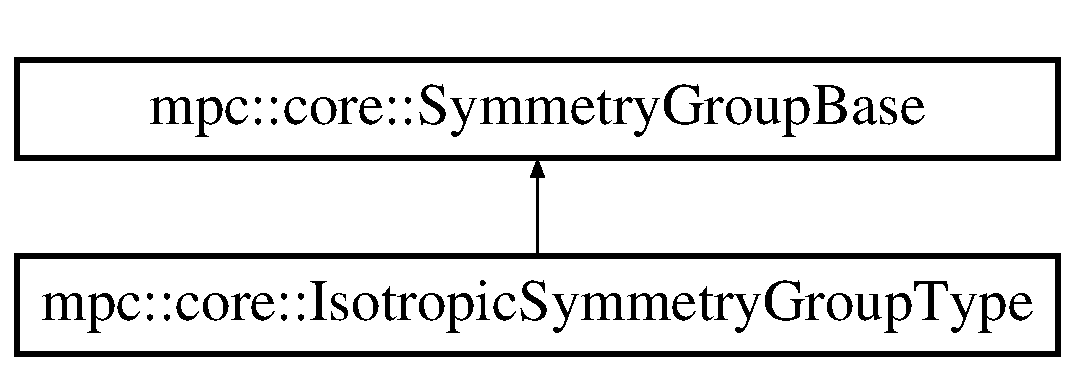
\includegraphics[height=2.000000cm]{structmpc_1_1core_1_1_isotropic_symmetry_group_type}
\end{center}
\end{figure}
\subsection*{Static Public Member Functions}
\begin{DoxyCompactItemize}
\item 
static constexpr \mbox{\hyperlink{namespacempc_1_1core_a9d979684062547055a0ef5c13077bad8}{Symmetry\+Group\+Enumeration}} \mbox{\hyperlink{structmpc_1_1core_1_1_isotropic_symmetry_group_type_a501a95dd5e13a62bff5cb9aff3428d47}{Symmetry\+Group\+Enum}} ()
\item 
static constexpr int \mbox{\hyperlink{structmpc_1_1core_1_1_isotropic_symmetry_group_type_a0afd9e5aa41efc5e90f43ef331996a92}{Number\+Of\+Independent\+Components}} ()
\end{DoxyCompactItemize}
\subsection*{Public Attributes}
\begin{DoxyCompactItemize}
\item 
const \mbox{\hyperlink{namespacempc_1_1core_a9d979684062547055a0ef5c13077bad8}{Symmetry\+Group\+Enumeration}} \mbox{\hyperlink{structmpc_1_1core_1_1_isotropic_symmetry_group_type_a44a0fdc0ed5b0027eb75b8d927d83c4b}{symmetry\+\_\+group\+\_\+enumeration}} = \mbox{\hyperlink{namespacempc_1_1core_a9d979684062547055a0ef5c13077bad8a099d59049574174a1c19567d38b479c2}{Symmetry\+Group\+Enumeration\+::\+I\+S\+O\+T\+R\+O\+P\+IC}}
\item 
const int \mbox{\hyperlink{structmpc_1_1core_1_1_isotropic_symmetry_group_type_a41134b104f375a339b0943df6959dbc9}{number\+\_\+of\+\_\+independent\+\_\+components}} = 2
\end{DoxyCompactItemize}


\subsection{Detailed Description}


Definition at line 280 of file symmetrygrouptypes.\+hpp.



\subsection{Member Function Documentation}
\mbox{\Hypertarget{structmpc_1_1core_1_1_isotropic_symmetry_group_type_a0afd9e5aa41efc5e90f43ef331996a92}\label{structmpc_1_1core_1_1_isotropic_symmetry_group_type_a0afd9e5aa41efc5e90f43ef331996a92}} 
\index{mpc\+::core\+::\+Isotropic\+Symmetry\+Group\+Type@{mpc\+::core\+::\+Isotropic\+Symmetry\+Group\+Type}!Number\+Of\+Independent\+Components@{Number\+Of\+Independent\+Components}}
\index{Number\+Of\+Independent\+Components@{Number\+Of\+Independent\+Components}!mpc\+::core\+::\+Isotropic\+Symmetry\+Group\+Type@{mpc\+::core\+::\+Isotropic\+Symmetry\+Group\+Type}}
\subsubsection{\texorpdfstring{Number\+Of\+Independent\+Components()}{NumberOfIndependentComponents()}}
{\footnotesize\ttfamily static constexpr int mpc\+::core\+::\+Isotropic\+Symmetry\+Group\+Type\+::\+Number\+Of\+Independent\+Components (\begin{DoxyParamCaption}{ }\end{DoxyParamCaption})\hspace{0.3cm}{\ttfamily [inline]}, {\ttfamily [static]}}



Definition at line 287 of file symmetrygrouptypes.\+hpp.

\mbox{\Hypertarget{structmpc_1_1core_1_1_isotropic_symmetry_group_type_a501a95dd5e13a62bff5cb9aff3428d47}\label{structmpc_1_1core_1_1_isotropic_symmetry_group_type_a501a95dd5e13a62bff5cb9aff3428d47}} 
\index{mpc\+::core\+::\+Isotropic\+Symmetry\+Group\+Type@{mpc\+::core\+::\+Isotropic\+Symmetry\+Group\+Type}!Symmetry\+Group\+Enum@{Symmetry\+Group\+Enum}}
\index{Symmetry\+Group\+Enum@{Symmetry\+Group\+Enum}!mpc\+::core\+::\+Isotropic\+Symmetry\+Group\+Type@{mpc\+::core\+::\+Isotropic\+Symmetry\+Group\+Type}}
\subsubsection{\texorpdfstring{Symmetry\+Group\+Enum()}{SymmetryGroupEnum()}}
{\footnotesize\ttfamily static constexpr \mbox{\hyperlink{namespacempc_1_1core_a9d979684062547055a0ef5c13077bad8}{Symmetry\+Group\+Enumeration}} mpc\+::core\+::\+Isotropic\+Symmetry\+Group\+Type\+::\+Symmetry\+Group\+Enum (\begin{DoxyParamCaption}{ }\end{DoxyParamCaption})\hspace{0.3cm}{\ttfamily [inline]}, {\ttfamily [static]}}



Definition at line 284 of file symmetrygrouptypes.\+hpp.



\subsection{Member Data Documentation}
\mbox{\Hypertarget{structmpc_1_1core_1_1_isotropic_symmetry_group_type_a41134b104f375a339b0943df6959dbc9}\label{structmpc_1_1core_1_1_isotropic_symmetry_group_type_a41134b104f375a339b0943df6959dbc9}} 
\index{mpc\+::core\+::\+Isotropic\+Symmetry\+Group\+Type@{mpc\+::core\+::\+Isotropic\+Symmetry\+Group\+Type}!number\+\_\+of\+\_\+independent\+\_\+components@{number\+\_\+of\+\_\+independent\+\_\+components}}
\index{number\+\_\+of\+\_\+independent\+\_\+components@{number\+\_\+of\+\_\+independent\+\_\+components}!mpc\+::core\+::\+Isotropic\+Symmetry\+Group\+Type@{mpc\+::core\+::\+Isotropic\+Symmetry\+Group\+Type}}
\subsubsection{\texorpdfstring{number\+\_\+of\+\_\+independent\+\_\+components}{number\_of\_independent\_components}}
{\footnotesize\ttfamily const int mpc\+::core\+::\+Isotropic\+Symmetry\+Group\+Type\+::number\+\_\+of\+\_\+independent\+\_\+components = 2}



Definition at line 282 of file symmetrygrouptypes.\+hpp.

\mbox{\Hypertarget{structmpc_1_1core_1_1_isotropic_symmetry_group_type_a44a0fdc0ed5b0027eb75b8d927d83c4b}\label{structmpc_1_1core_1_1_isotropic_symmetry_group_type_a44a0fdc0ed5b0027eb75b8d927d83c4b}} 
\index{mpc\+::core\+::\+Isotropic\+Symmetry\+Group\+Type@{mpc\+::core\+::\+Isotropic\+Symmetry\+Group\+Type}!symmetry\+\_\+group\+\_\+enumeration@{symmetry\+\_\+group\+\_\+enumeration}}
\index{symmetry\+\_\+group\+\_\+enumeration@{symmetry\+\_\+group\+\_\+enumeration}!mpc\+::core\+::\+Isotropic\+Symmetry\+Group\+Type@{mpc\+::core\+::\+Isotropic\+Symmetry\+Group\+Type}}
\subsubsection{\texorpdfstring{symmetry\+\_\+group\+\_\+enumeration}{symmetry\_group\_enumeration}}
{\footnotesize\ttfamily const \mbox{\hyperlink{namespacempc_1_1core_a9d979684062547055a0ef5c13077bad8}{Symmetry\+Group\+Enumeration}} mpc\+::core\+::\+Isotropic\+Symmetry\+Group\+Type\+::symmetry\+\_\+group\+\_\+enumeration = \mbox{\hyperlink{namespacempc_1_1core_a9d979684062547055a0ef5c13077bad8a099d59049574174a1c19567d38b479c2}{Symmetry\+Group\+Enumeration\+::\+I\+S\+O\+T\+R\+O\+P\+IC}}}



Definition at line 281 of file symmetrygrouptypes.\+hpp.



The documentation for this struct was generated from the following file\+:\begin{DoxyCompactItemize}
\item 
/\+Users/atorlucci/\+Documents/github\+\_\+threecubed\+\_\+repos/mpc/src/mpc/core/\mbox{\hyperlink{symmetrygrouptypes_8hpp}{symmetrygrouptypes.\+hpp}}\end{DoxyCompactItemize}

\hypertarget{structmpc_1_1rockphysics_1_1_lame_paramter_modulus_type}{}\section{mpc\+:\+:rockphysics\+:\+:Lame\+Paramter\+Modulus\+Type$<$ T $>$ Struct Template Reference}
\label{structmpc_1_1rockphysics_1_1_lame_paramter_modulus_type}\index{mpc\+::rockphysics\+::\+Lame\+Paramter\+Modulus\+Type$<$ T $>$@{mpc\+::rockphysics\+::\+Lame\+Paramter\+Modulus\+Type$<$ T $>$}}


{\ttfamily \#include $<$rockphysicstransformstypes.\+hpp$>$}

Inheritance diagram for mpc\+:\+:rockphysics\+:\+:Lame\+Paramter\+Modulus\+Type$<$ T $>$\+:\begin{figure}[H]
\begin{center}
\leavevmode
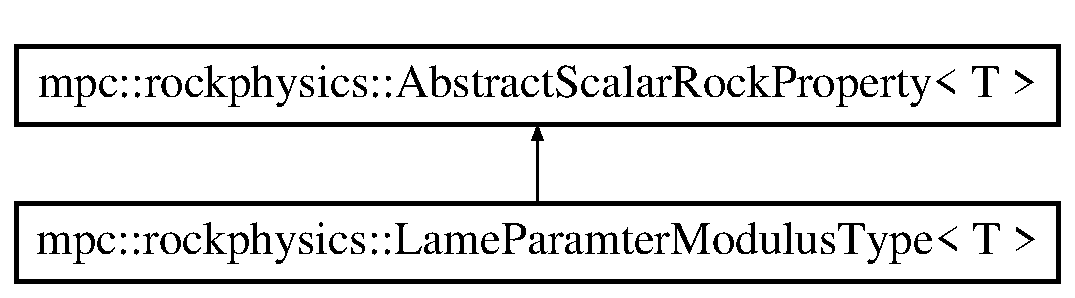
\includegraphics[height=2.000000cm]{structmpc_1_1rockphysics_1_1_lame_paramter_modulus_type}
\end{center}
\end{figure}
\subsection*{Public Member Functions}
\begin{DoxyCompactItemize}
\item 
constexpr \mbox{\hyperlink{structmpc_1_1rockphysics_1_1_lame_paramter_modulus_type_aabdc27f20e83c664b90b6baffee260a7}{Lame\+Paramter\+Modulus\+Type}} (T val)
\end{DoxyCompactItemize}
\subsection*{Additional Inherited Members}


\subsection{Detailed Description}
\subsubsection*{template$<$typename T$>$\newline
struct mpc\+::rockphysics\+::\+Lame\+Paramter\+Modulus\+Type$<$ T $>$}



Definition at line 69 of file rockphysicstransformstypes.\+hpp.



\subsection{Constructor \& Destructor Documentation}
\mbox{\Hypertarget{structmpc_1_1rockphysics_1_1_lame_paramter_modulus_type_aabdc27f20e83c664b90b6baffee260a7}\label{structmpc_1_1rockphysics_1_1_lame_paramter_modulus_type_aabdc27f20e83c664b90b6baffee260a7}} 
\index{mpc\+::rockphysics\+::\+Lame\+Paramter\+Modulus\+Type@{mpc\+::rockphysics\+::\+Lame\+Paramter\+Modulus\+Type}!Lame\+Paramter\+Modulus\+Type@{Lame\+Paramter\+Modulus\+Type}}
\index{Lame\+Paramter\+Modulus\+Type@{Lame\+Paramter\+Modulus\+Type}!mpc\+::rockphysics\+::\+Lame\+Paramter\+Modulus\+Type@{mpc\+::rockphysics\+::\+Lame\+Paramter\+Modulus\+Type}}
\subsubsection{\texorpdfstring{Lame\+Paramter\+Modulus\+Type()}{LameParamterModulusType()}}
{\footnotesize\ttfamily template$<$typename T$>$ \\
constexpr \mbox{\hyperlink{structmpc_1_1rockphysics_1_1_lame_paramter_modulus_type}{mpc\+::rockphysics\+::\+Lame\+Paramter\+Modulus\+Type}}$<$ T $>$\+::\mbox{\hyperlink{structmpc_1_1rockphysics_1_1_lame_paramter_modulus_type}{Lame\+Paramter\+Modulus\+Type}} (\begin{DoxyParamCaption}\item[{T}]{val }\end{DoxyParamCaption})\hspace{0.3cm}{\ttfamily [inline]}}



Definition at line 74 of file rockphysicstransformstypes.\+hpp.



The documentation for this struct was generated from the following file\+:\begin{DoxyCompactItemize}
\item 
/\+Users/atorlucci/\+Documents/github\+\_\+threecubed\+\_\+repos/mpc/src/mpc/rockphysics/\mbox{\hyperlink{rockphysicstransformstypes_8hpp}{rockphysicstransformstypes.\+hpp}}\end{DoxyCompactItemize}

\hypertarget{structmpc_1_1core_1_1_monoclinic_x2_symmetry_group_type}{}\section{mpc\+:\+:core\+:\+:Monoclinic\+X2\+Symmetry\+Group\+Type Struct Reference}
\label{structmpc_1_1core_1_1_monoclinic_x2_symmetry_group_type}\index{mpc\+::core\+::\+Monoclinic\+X2\+Symmetry\+Group\+Type@{mpc\+::core\+::\+Monoclinic\+X2\+Symmetry\+Group\+Type}}


{\ttfamily \#include $<$symmetrygrouptypes.\+hpp$>$}

Inheritance diagram for mpc\+:\+:core\+:\+:Monoclinic\+X2\+Symmetry\+Group\+Type\+:\begin{figure}[H]
\begin{center}
\leavevmode
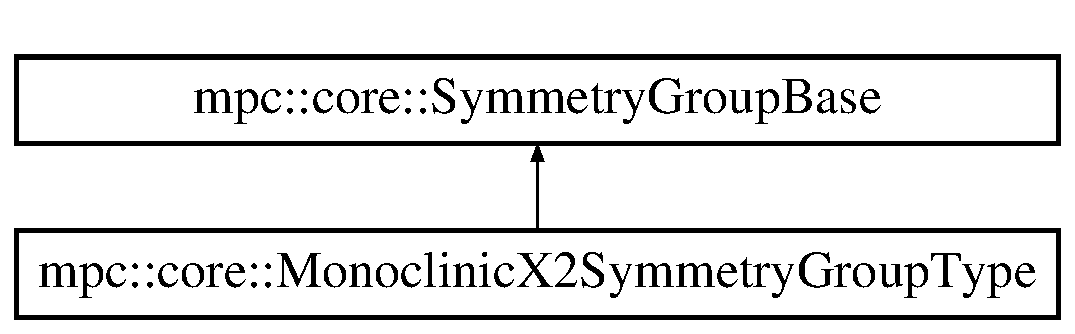
\includegraphics[height=2.000000cm]{structmpc_1_1core_1_1_monoclinic_x2_symmetry_group_type}
\end{center}
\end{figure}
\subsection*{Static Public Member Functions}
\begin{DoxyCompactItemize}
\item 
static constexpr \mbox{\hyperlink{namespacempc_1_1core_a9d979684062547055a0ef5c13077bad8}{Symmetry\+Group\+Enumeration}} \mbox{\hyperlink{structmpc_1_1core_1_1_monoclinic_x2_symmetry_group_type_a23156166d016e06f3f11ab523e07a220}{Symmetry\+Group\+Enum}} ()
\item 
static constexpr int \mbox{\hyperlink{structmpc_1_1core_1_1_monoclinic_x2_symmetry_group_type_a3ab5eeb5ea4262e6cb99e35a593748c8}{Number\+Of\+Independent\+Components}} ()
\end{DoxyCompactItemize}
\subsection*{Public Attributes}
\begin{DoxyCompactItemize}
\item 
const \mbox{\hyperlink{namespacempc_1_1core_a9d979684062547055a0ef5c13077bad8}{Symmetry\+Group\+Enumeration}} \mbox{\hyperlink{structmpc_1_1core_1_1_monoclinic_x2_symmetry_group_type_ab63d007354c1eb9346023d74ac74e50b}{symmetry\+\_\+group\+\_\+enumeration}} = \mbox{\hyperlink{namespacempc_1_1core_a9d979684062547055a0ef5c13077bad8a7eb6e11f17e97fbe9fc371a72a989b96}{Symmetry\+Group\+Enumeration\+::\+M\+O\+N\+O\+C\+L\+I\+N\+I\+C\+\_\+\+X2}}
\item 
const int \mbox{\hyperlink{structmpc_1_1core_1_1_monoclinic_x2_symmetry_group_type_a3036efe4ed2f2ba0bf98269538d4be67}{number\+\_\+of\+\_\+independent\+\_\+components}} = 13
\end{DoxyCompactItemize}


\subsection{Detailed Description}


Definition at line 172 of file symmetrygrouptypes.\+hpp.



\subsection{Member Function Documentation}
\mbox{\Hypertarget{structmpc_1_1core_1_1_monoclinic_x2_symmetry_group_type_a3ab5eeb5ea4262e6cb99e35a593748c8}\label{structmpc_1_1core_1_1_monoclinic_x2_symmetry_group_type_a3ab5eeb5ea4262e6cb99e35a593748c8}} 
\index{mpc\+::core\+::\+Monoclinic\+X2\+Symmetry\+Group\+Type@{mpc\+::core\+::\+Monoclinic\+X2\+Symmetry\+Group\+Type}!Number\+Of\+Independent\+Components@{Number\+Of\+Independent\+Components}}
\index{Number\+Of\+Independent\+Components@{Number\+Of\+Independent\+Components}!mpc\+::core\+::\+Monoclinic\+X2\+Symmetry\+Group\+Type@{mpc\+::core\+::\+Monoclinic\+X2\+Symmetry\+Group\+Type}}
\subsubsection{\texorpdfstring{Number\+Of\+Independent\+Components()}{NumberOfIndependentComponents()}}
{\footnotesize\ttfamily static constexpr int mpc\+::core\+::\+Monoclinic\+X2\+Symmetry\+Group\+Type\+::\+Number\+Of\+Independent\+Components (\begin{DoxyParamCaption}{ }\end{DoxyParamCaption})\hspace{0.3cm}{\ttfamily [inline]}, {\ttfamily [static]}}



Definition at line 179 of file symmetrygrouptypes.\+hpp.

\mbox{\Hypertarget{structmpc_1_1core_1_1_monoclinic_x2_symmetry_group_type_a23156166d016e06f3f11ab523e07a220}\label{structmpc_1_1core_1_1_monoclinic_x2_symmetry_group_type_a23156166d016e06f3f11ab523e07a220}} 
\index{mpc\+::core\+::\+Monoclinic\+X2\+Symmetry\+Group\+Type@{mpc\+::core\+::\+Monoclinic\+X2\+Symmetry\+Group\+Type}!Symmetry\+Group\+Enum@{Symmetry\+Group\+Enum}}
\index{Symmetry\+Group\+Enum@{Symmetry\+Group\+Enum}!mpc\+::core\+::\+Monoclinic\+X2\+Symmetry\+Group\+Type@{mpc\+::core\+::\+Monoclinic\+X2\+Symmetry\+Group\+Type}}
\subsubsection{\texorpdfstring{Symmetry\+Group\+Enum()}{SymmetryGroupEnum()}}
{\footnotesize\ttfamily static constexpr \mbox{\hyperlink{namespacempc_1_1core_a9d979684062547055a0ef5c13077bad8}{Symmetry\+Group\+Enumeration}} mpc\+::core\+::\+Monoclinic\+X2\+Symmetry\+Group\+Type\+::\+Symmetry\+Group\+Enum (\begin{DoxyParamCaption}{ }\end{DoxyParamCaption})\hspace{0.3cm}{\ttfamily [inline]}, {\ttfamily [static]}}



Definition at line 176 of file symmetrygrouptypes.\+hpp.



\subsection{Member Data Documentation}
\mbox{\Hypertarget{structmpc_1_1core_1_1_monoclinic_x2_symmetry_group_type_a3036efe4ed2f2ba0bf98269538d4be67}\label{structmpc_1_1core_1_1_monoclinic_x2_symmetry_group_type_a3036efe4ed2f2ba0bf98269538d4be67}} 
\index{mpc\+::core\+::\+Monoclinic\+X2\+Symmetry\+Group\+Type@{mpc\+::core\+::\+Monoclinic\+X2\+Symmetry\+Group\+Type}!number\+\_\+of\+\_\+independent\+\_\+components@{number\+\_\+of\+\_\+independent\+\_\+components}}
\index{number\+\_\+of\+\_\+independent\+\_\+components@{number\+\_\+of\+\_\+independent\+\_\+components}!mpc\+::core\+::\+Monoclinic\+X2\+Symmetry\+Group\+Type@{mpc\+::core\+::\+Monoclinic\+X2\+Symmetry\+Group\+Type}}
\subsubsection{\texorpdfstring{number\+\_\+of\+\_\+independent\+\_\+components}{number\_of\_independent\_components}}
{\footnotesize\ttfamily const int mpc\+::core\+::\+Monoclinic\+X2\+Symmetry\+Group\+Type\+::number\+\_\+of\+\_\+independent\+\_\+components = 13}



Definition at line 174 of file symmetrygrouptypes.\+hpp.

\mbox{\Hypertarget{structmpc_1_1core_1_1_monoclinic_x2_symmetry_group_type_ab63d007354c1eb9346023d74ac74e50b}\label{structmpc_1_1core_1_1_monoclinic_x2_symmetry_group_type_ab63d007354c1eb9346023d74ac74e50b}} 
\index{mpc\+::core\+::\+Monoclinic\+X2\+Symmetry\+Group\+Type@{mpc\+::core\+::\+Monoclinic\+X2\+Symmetry\+Group\+Type}!symmetry\+\_\+group\+\_\+enumeration@{symmetry\+\_\+group\+\_\+enumeration}}
\index{symmetry\+\_\+group\+\_\+enumeration@{symmetry\+\_\+group\+\_\+enumeration}!mpc\+::core\+::\+Monoclinic\+X2\+Symmetry\+Group\+Type@{mpc\+::core\+::\+Monoclinic\+X2\+Symmetry\+Group\+Type}}
\subsubsection{\texorpdfstring{symmetry\+\_\+group\+\_\+enumeration}{symmetry\_group\_enumeration}}
{\footnotesize\ttfamily const \mbox{\hyperlink{namespacempc_1_1core_a9d979684062547055a0ef5c13077bad8}{Symmetry\+Group\+Enumeration}} mpc\+::core\+::\+Monoclinic\+X2\+Symmetry\+Group\+Type\+::symmetry\+\_\+group\+\_\+enumeration = \mbox{\hyperlink{namespacempc_1_1core_a9d979684062547055a0ef5c13077bad8a7eb6e11f17e97fbe9fc371a72a989b96}{Symmetry\+Group\+Enumeration\+::\+M\+O\+N\+O\+C\+L\+I\+N\+I\+C\+\_\+\+X2}}}



Definition at line 173 of file symmetrygrouptypes.\+hpp.



The documentation for this struct was generated from the following file\+:\begin{DoxyCompactItemize}
\item 
/\+Users/atorlucci/\+Documents/github\+\_\+threecubed\+\_\+repos/mpc/src/mpc/core/\mbox{\hyperlink{symmetrygrouptypes_8hpp}{symmetrygrouptypes.\+hpp}}\end{DoxyCompactItemize}

\hypertarget{structmpc_1_1core_1_1_monoclinic_x3_symmetry_group_type}{}\section{mpc\+:\+:core\+:\+:Monoclinic\+X3\+Symmetry\+Group\+Type Struct Reference}
\label{structmpc_1_1core_1_1_monoclinic_x3_symmetry_group_type}\index{mpc\+::core\+::\+Monoclinic\+X3\+Symmetry\+Group\+Type@{mpc\+::core\+::\+Monoclinic\+X3\+Symmetry\+Group\+Type}}


{\ttfamily \#include $<$symmetrygrouptypes.\+hpp$>$}

Inheritance diagram for mpc\+:\+:core\+:\+:Monoclinic\+X3\+Symmetry\+Group\+Type\+:\begin{figure}[H]
\begin{center}
\leavevmode
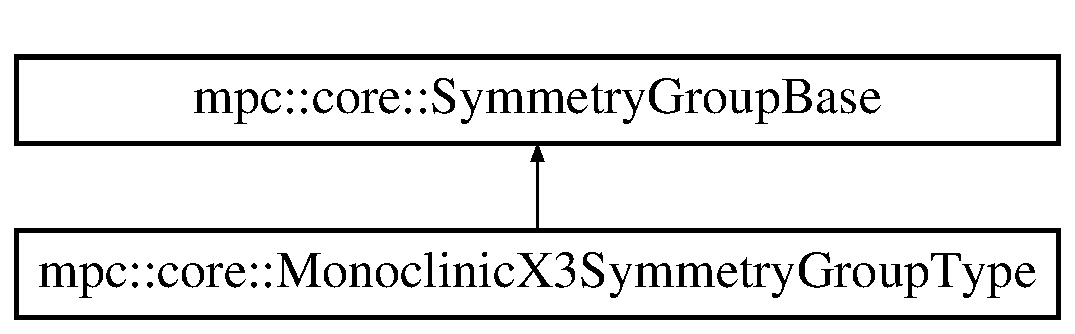
\includegraphics[height=2.000000cm]{structmpc_1_1core_1_1_monoclinic_x3_symmetry_group_type}
\end{center}
\end{figure}
\subsection*{Static Public Member Functions}
\begin{DoxyCompactItemize}
\item 
static constexpr \mbox{\hyperlink{namespacempc_1_1core_a9d979684062547055a0ef5c13077bad8}{Symmetry\+Group\+Enumeration}} \mbox{\hyperlink{structmpc_1_1core_1_1_monoclinic_x3_symmetry_group_type_aae7de40f076054a8c14a1bac58cdc9be}{Symmetry\+Group\+Enum}} ()
\item 
static constexpr int \mbox{\hyperlink{structmpc_1_1core_1_1_monoclinic_x3_symmetry_group_type_a6b5a4d8be05150c313bbc5b543cd48ab}{Number\+Of\+Independent\+Components}} ()
\end{DoxyCompactItemize}
\subsection*{Public Attributes}
\begin{DoxyCompactItemize}
\item 
const \mbox{\hyperlink{namespacempc_1_1core_a9d979684062547055a0ef5c13077bad8}{Symmetry\+Group\+Enumeration}} \mbox{\hyperlink{structmpc_1_1core_1_1_monoclinic_x3_symmetry_group_type_a904063da9f5f483cf16eab309a18db0c}{symmetry\+\_\+group\+\_\+enumeration}} = \mbox{\hyperlink{namespacempc_1_1core_a9d979684062547055a0ef5c13077bad8ab31f5171fdded777eb3112da45967b57}{Symmetry\+Group\+Enumeration\+::\+M\+O\+N\+O\+C\+L\+I\+N\+I\+C\+\_\+\+X3}}
\item 
const int \mbox{\hyperlink{structmpc_1_1core_1_1_monoclinic_x3_symmetry_group_type_ad8e0f7a066c0ec03b2c5dc66243c1613}{number\+\_\+of\+\_\+independent\+\_\+components}} = 13
\end{DoxyCompactItemize}


\subsection{Detailed Description}


Definition at line 184 of file symmetrygrouptypes.\+hpp.



\subsection{Member Function Documentation}
\mbox{\Hypertarget{structmpc_1_1core_1_1_monoclinic_x3_symmetry_group_type_a6b5a4d8be05150c313bbc5b543cd48ab}\label{structmpc_1_1core_1_1_monoclinic_x3_symmetry_group_type_a6b5a4d8be05150c313bbc5b543cd48ab}} 
\index{mpc\+::core\+::\+Monoclinic\+X3\+Symmetry\+Group\+Type@{mpc\+::core\+::\+Monoclinic\+X3\+Symmetry\+Group\+Type}!Number\+Of\+Independent\+Components@{Number\+Of\+Independent\+Components}}
\index{Number\+Of\+Independent\+Components@{Number\+Of\+Independent\+Components}!mpc\+::core\+::\+Monoclinic\+X3\+Symmetry\+Group\+Type@{mpc\+::core\+::\+Monoclinic\+X3\+Symmetry\+Group\+Type}}
\subsubsection{\texorpdfstring{Number\+Of\+Independent\+Components()}{NumberOfIndependentComponents()}}
{\footnotesize\ttfamily static constexpr int mpc\+::core\+::\+Monoclinic\+X3\+Symmetry\+Group\+Type\+::\+Number\+Of\+Independent\+Components (\begin{DoxyParamCaption}{ }\end{DoxyParamCaption})\hspace{0.3cm}{\ttfamily [inline]}, {\ttfamily [static]}}



Definition at line 191 of file symmetrygrouptypes.\+hpp.

\mbox{\Hypertarget{structmpc_1_1core_1_1_monoclinic_x3_symmetry_group_type_aae7de40f076054a8c14a1bac58cdc9be}\label{structmpc_1_1core_1_1_monoclinic_x3_symmetry_group_type_aae7de40f076054a8c14a1bac58cdc9be}} 
\index{mpc\+::core\+::\+Monoclinic\+X3\+Symmetry\+Group\+Type@{mpc\+::core\+::\+Monoclinic\+X3\+Symmetry\+Group\+Type}!Symmetry\+Group\+Enum@{Symmetry\+Group\+Enum}}
\index{Symmetry\+Group\+Enum@{Symmetry\+Group\+Enum}!mpc\+::core\+::\+Monoclinic\+X3\+Symmetry\+Group\+Type@{mpc\+::core\+::\+Monoclinic\+X3\+Symmetry\+Group\+Type}}
\subsubsection{\texorpdfstring{Symmetry\+Group\+Enum()}{SymmetryGroupEnum()}}
{\footnotesize\ttfamily static constexpr \mbox{\hyperlink{namespacempc_1_1core_a9d979684062547055a0ef5c13077bad8}{Symmetry\+Group\+Enumeration}} mpc\+::core\+::\+Monoclinic\+X3\+Symmetry\+Group\+Type\+::\+Symmetry\+Group\+Enum (\begin{DoxyParamCaption}{ }\end{DoxyParamCaption})\hspace{0.3cm}{\ttfamily [inline]}, {\ttfamily [static]}}



Definition at line 188 of file symmetrygrouptypes.\+hpp.



\subsection{Member Data Documentation}
\mbox{\Hypertarget{structmpc_1_1core_1_1_monoclinic_x3_symmetry_group_type_ad8e0f7a066c0ec03b2c5dc66243c1613}\label{structmpc_1_1core_1_1_monoclinic_x3_symmetry_group_type_ad8e0f7a066c0ec03b2c5dc66243c1613}} 
\index{mpc\+::core\+::\+Monoclinic\+X3\+Symmetry\+Group\+Type@{mpc\+::core\+::\+Monoclinic\+X3\+Symmetry\+Group\+Type}!number\+\_\+of\+\_\+independent\+\_\+components@{number\+\_\+of\+\_\+independent\+\_\+components}}
\index{number\+\_\+of\+\_\+independent\+\_\+components@{number\+\_\+of\+\_\+independent\+\_\+components}!mpc\+::core\+::\+Monoclinic\+X3\+Symmetry\+Group\+Type@{mpc\+::core\+::\+Monoclinic\+X3\+Symmetry\+Group\+Type}}
\subsubsection{\texorpdfstring{number\+\_\+of\+\_\+independent\+\_\+components}{number\_of\_independent\_components}}
{\footnotesize\ttfamily const int mpc\+::core\+::\+Monoclinic\+X3\+Symmetry\+Group\+Type\+::number\+\_\+of\+\_\+independent\+\_\+components = 13}



Definition at line 186 of file symmetrygrouptypes.\+hpp.

\mbox{\Hypertarget{structmpc_1_1core_1_1_monoclinic_x3_symmetry_group_type_a904063da9f5f483cf16eab309a18db0c}\label{structmpc_1_1core_1_1_monoclinic_x3_symmetry_group_type_a904063da9f5f483cf16eab309a18db0c}} 
\index{mpc\+::core\+::\+Monoclinic\+X3\+Symmetry\+Group\+Type@{mpc\+::core\+::\+Monoclinic\+X3\+Symmetry\+Group\+Type}!symmetry\+\_\+group\+\_\+enumeration@{symmetry\+\_\+group\+\_\+enumeration}}
\index{symmetry\+\_\+group\+\_\+enumeration@{symmetry\+\_\+group\+\_\+enumeration}!mpc\+::core\+::\+Monoclinic\+X3\+Symmetry\+Group\+Type@{mpc\+::core\+::\+Monoclinic\+X3\+Symmetry\+Group\+Type}}
\subsubsection{\texorpdfstring{symmetry\+\_\+group\+\_\+enumeration}{symmetry\_group\_enumeration}}
{\footnotesize\ttfamily const \mbox{\hyperlink{namespacempc_1_1core_a9d979684062547055a0ef5c13077bad8}{Symmetry\+Group\+Enumeration}} mpc\+::core\+::\+Monoclinic\+X3\+Symmetry\+Group\+Type\+::symmetry\+\_\+group\+\_\+enumeration = \mbox{\hyperlink{namespacempc_1_1core_a9d979684062547055a0ef5c13077bad8ab31f5171fdded777eb3112da45967b57}{Symmetry\+Group\+Enumeration\+::\+M\+O\+N\+O\+C\+L\+I\+N\+I\+C\+\_\+\+X3}}}



Definition at line 185 of file symmetrygrouptypes.\+hpp.



The documentation for this struct was generated from the following file\+:\begin{DoxyCompactItemize}
\item 
/\+Users/atorlucci/\+Documents/github\+\_\+threecubed\+\_\+repos/mpc/src/mpc/core/\mbox{\hyperlink{symmetrygrouptypes_8hpp}{symmetrygrouptypes.\+hpp}}\end{DoxyCompactItemize}

\hypertarget{structmpc_1_1core_1_1_none_symmetry_group_type}{}\section{mpc\+:\+:core\+:\+:None\+Symmetry\+Group\+Type Struct Reference}
\label{structmpc_1_1core_1_1_none_symmetry_group_type}\index{mpc\+::core\+::\+None\+Symmetry\+Group\+Type@{mpc\+::core\+::\+None\+Symmetry\+Group\+Type}}


{\ttfamily \#include $<$symmetrygrouptypes.\+hpp$>$}

Inheritance diagram for mpc\+:\+:core\+:\+:None\+Symmetry\+Group\+Type\+:\begin{figure}[H]
\begin{center}
\leavevmode
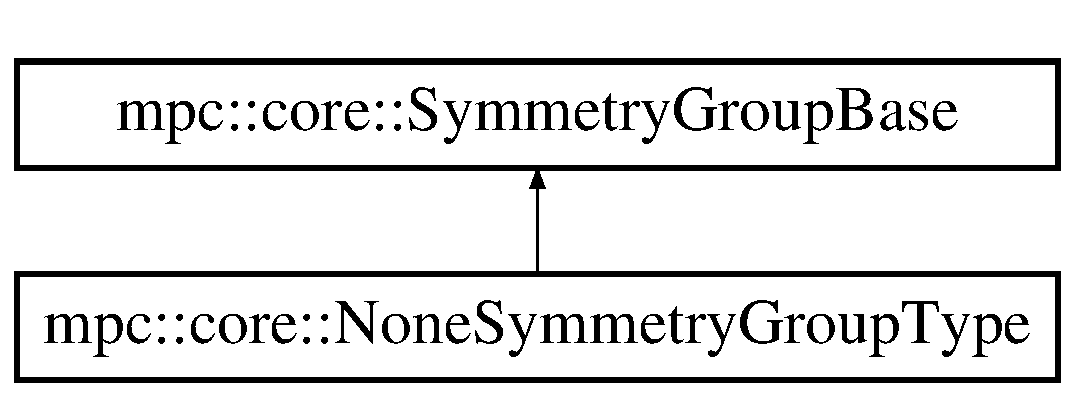
\includegraphics[height=2.000000cm]{structmpc_1_1core_1_1_none_symmetry_group_type}
\end{center}
\end{figure}
\subsection*{Static Public Member Functions}
\begin{DoxyCompactItemize}
\item 
static constexpr \mbox{\hyperlink{namespacempc_1_1core_a9d979684062547055a0ef5c13077bad8}{Symmetry\+Group\+Enumeration}} \mbox{\hyperlink{structmpc_1_1core_1_1_none_symmetry_group_type_a3d387ccf340263f1101524006e073d18}{Symmetry\+Group\+Enum}} ()
\item 
static constexpr int \mbox{\hyperlink{structmpc_1_1core_1_1_none_symmetry_group_type_a446a3cf749fa3186a608820301dee584}{Number\+Of\+Independent\+Components}} ()
\end{DoxyCompactItemize}
\subsection*{Public Attributes}
\begin{DoxyCompactItemize}
\item 
const \mbox{\hyperlink{namespacempc_1_1core_a9d979684062547055a0ef5c13077bad8}{Symmetry\+Group\+Enumeration}} \mbox{\hyperlink{structmpc_1_1core_1_1_none_symmetry_group_type_a602e3f58d42e2e828e149d4945958984}{symmetry\+\_\+group\+\_\+enumeration}} = \mbox{\hyperlink{namespacempc_1_1core_a9d979684062547055a0ef5c13077bad8ab50339a10e1de285ac99d4c3990b8693}{Symmetry\+Group\+Enumeration\+::\+N\+O\+NE}}
\item 
const int \mbox{\hyperlink{structmpc_1_1core_1_1_none_symmetry_group_type_a7a42df9f755da6327c802277a8417eba}{number\+\_\+of\+\_\+independent\+\_\+components}} = 81
\end{DoxyCompactItemize}


\subsection{Detailed Description}


Definition at line 148 of file symmetrygrouptypes.\+hpp.



\subsection{Member Function Documentation}
\mbox{\Hypertarget{structmpc_1_1core_1_1_none_symmetry_group_type_a446a3cf749fa3186a608820301dee584}\label{structmpc_1_1core_1_1_none_symmetry_group_type_a446a3cf749fa3186a608820301dee584}} 
\index{mpc\+::core\+::\+None\+Symmetry\+Group\+Type@{mpc\+::core\+::\+None\+Symmetry\+Group\+Type}!Number\+Of\+Independent\+Components@{Number\+Of\+Independent\+Components}}
\index{Number\+Of\+Independent\+Components@{Number\+Of\+Independent\+Components}!mpc\+::core\+::\+None\+Symmetry\+Group\+Type@{mpc\+::core\+::\+None\+Symmetry\+Group\+Type}}
\subsubsection{\texorpdfstring{Number\+Of\+Independent\+Components()}{NumberOfIndependentComponents()}}
{\footnotesize\ttfamily static constexpr int mpc\+::core\+::\+None\+Symmetry\+Group\+Type\+::\+Number\+Of\+Independent\+Components (\begin{DoxyParamCaption}{ }\end{DoxyParamCaption})\hspace{0.3cm}{\ttfamily [inline]}, {\ttfamily [static]}}



Definition at line 155 of file symmetrygrouptypes.\+hpp.

\mbox{\Hypertarget{structmpc_1_1core_1_1_none_symmetry_group_type_a3d387ccf340263f1101524006e073d18}\label{structmpc_1_1core_1_1_none_symmetry_group_type_a3d387ccf340263f1101524006e073d18}} 
\index{mpc\+::core\+::\+None\+Symmetry\+Group\+Type@{mpc\+::core\+::\+None\+Symmetry\+Group\+Type}!Symmetry\+Group\+Enum@{Symmetry\+Group\+Enum}}
\index{Symmetry\+Group\+Enum@{Symmetry\+Group\+Enum}!mpc\+::core\+::\+None\+Symmetry\+Group\+Type@{mpc\+::core\+::\+None\+Symmetry\+Group\+Type}}
\subsubsection{\texorpdfstring{Symmetry\+Group\+Enum()}{SymmetryGroupEnum()}}
{\footnotesize\ttfamily static constexpr \mbox{\hyperlink{namespacempc_1_1core_a9d979684062547055a0ef5c13077bad8}{Symmetry\+Group\+Enumeration}} mpc\+::core\+::\+None\+Symmetry\+Group\+Type\+::\+Symmetry\+Group\+Enum (\begin{DoxyParamCaption}{ }\end{DoxyParamCaption})\hspace{0.3cm}{\ttfamily [inline]}, {\ttfamily [static]}}



Definition at line 152 of file symmetrygrouptypes.\+hpp.



\subsection{Member Data Documentation}
\mbox{\Hypertarget{structmpc_1_1core_1_1_none_symmetry_group_type_a7a42df9f755da6327c802277a8417eba}\label{structmpc_1_1core_1_1_none_symmetry_group_type_a7a42df9f755da6327c802277a8417eba}} 
\index{mpc\+::core\+::\+None\+Symmetry\+Group\+Type@{mpc\+::core\+::\+None\+Symmetry\+Group\+Type}!number\+\_\+of\+\_\+independent\+\_\+components@{number\+\_\+of\+\_\+independent\+\_\+components}}
\index{number\+\_\+of\+\_\+independent\+\_\+components@{number\+\_\+of\+\_\+independent\+\_\+components}!mpc\+::core\+::\+None\+Symmetry\+Group\+Type@{mpc\+::core\+::\+None\+Symmetry\+Group\+Type}}
\subsubsection{\texorpdfstring{number\+\_\+of\+\_\+independent\+\_\+components}{number\_of\_independent\_components}}
{\footnotesize\ttfamily const int mpc\+::core\+::\+None\+Symmetry\+Group\+Type\+::number\+\_\+of\+\_\+independent\+\_\+components = 81}



Definition at line 150 of file symmetrygrouptypes.\+hpp.

\mbox{\Hypertarget{structmpc_1_1core_1_1_none_symmetry_group_type_a602e3f58d42e2e828e149d4945958984}\label{structmpc_1_1core_1_1_none_symmetry_group_type_a602e3f58d42e2e828e149d4945958984}} 
\index{mpc\+::core\+::\+None\+Symmetry\+Group\+Type@{mpc\+::core\+::\+None\+Symmetry\+Group\+Type}!symmetry\+\_\+group\+\_\+enumeration@{symmetry\+\_\+group\+\_\+enumeration}}
\index{symmetry\+\_\+group\+\_\+enumeration@{symmetry\+\_\+group\+\_\+enumeration}!mpc\+::core\+::\+None\+Symmetry\+Group\+Type@{mpc\+::core\+::\+None\+Symmetry\+Group\+Type}}
\subsubsection{\texorpdfstring{symmetry\+\_\+group\+\_\+enumeration}{symmetry\_group\_enumeration}}
{\footnotesize\ttfamily const \mbox{\hyperlink{namespacempc_1_1core_a9d979684062547055a0ef5c13077bad8}{Symmetry\+Group\+Enumeration}} mpc\+::core\+::\+None\+Symmetry\+Group\+Type\+::symmetry\+\_\+group\+\_\+enumeration = \mbox{\hyperlink{namespacempc_1_1core_a9d979684062547055a0ef5c13077bad8ab50339a10e1de285ac99d4c3990b8693}{Symmetry\+Group\+Enumeration\+::\+N\+O\+NE}}}



Definition at line 149 of file symmetrygrouptypes.\+hpp.



The documentation for this struct was generated from the following file\+:\begin{DoxyCompactItemize}
\item 
/\+Users/atorlucci/\+Documents/github\+\_\+threecubed\+\_\+repos/mpc/src/mpc/core/\mbox{\hyperlink{symmetrygrouptypes_8hpp}{symmetrygrouptypes.\+hpp}}\end{DoxyCompactItemize}

\hypertarget{structmpc_1_1core_1_1_orthorhombic_symmetry_group_type}{}\section{mpc\+:\+:core\+:\+:Orthorhombic\+Symmetry\+Group\+Type Struct Reference}
\label{structmpc_1_1core_1_1_orthorhombic_symmetry_group_type}\index{mpc\+::core\+::\+Orthorhombic\+Symmetry\+Group\+Type@{mpc\+::core\+::\+Orthorhombic\+Symmetry\+Group\+Type}}


{\ttfamily \#include $<$symmetrygrouptypes.\+hpp$>$}

Inheritance diagram for mpc\+:\+:core\+:\+:Orthorhombic\+Symmetry\+Group\+Type\+:\begin{figure}[H]
\begin{center}
\leavevmode
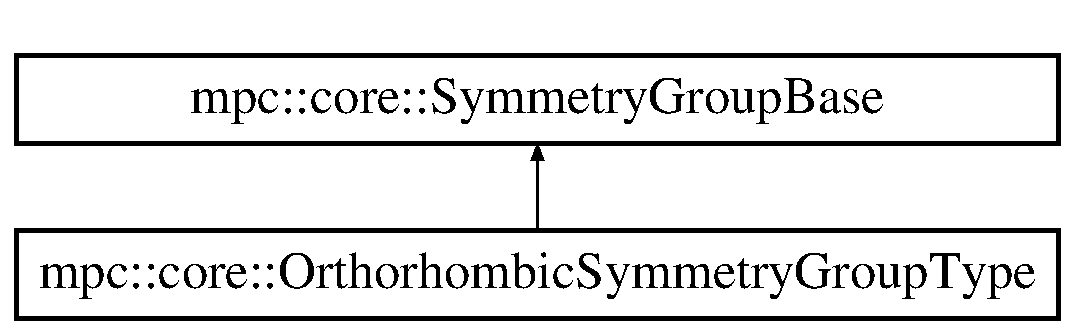
\includegraphics[height=2.000000cm]{structmpc_1_1core_1_1_orthorhombic_symmetry_group_type}
\end{center}
\end{figure}
\subsection*{Static Public Member Functions}
\begin{DoxyCompactItemize}
\item 
static constexpr \mbox{\hyperlink{namespacempc_1_1core_a9d979684062547055a0ef5c13077bad8}{Symmetry\+Group\+Enumeration}} \mbox{\hyperlink{structmpc_1_1core_1_1_orthorhombic_symmetry_group_type_ae206dd0d79d73340db34a885e9cf704f}{Symmetry\+Group\+Enum}} ()
\item 
static constexpr int \mbox{\hyperlink{structmpc_1_1core_1_1_orthorhombic_symmetry_group_type_a3b3d8e62305c30e53908d1cc1f20cdd2}{Number\+Of\+Independent\+Components}} ()
\end{DoxyCompactItemize}
\subsection*{Public Attributes}
\begin{DoxyCompactItemize}
\item 
const \mbox{\hyperlink{namespacempc_1_1core_a9d979684062547055a0ef5c13077bad8}{Symmetry\+Group\+Enumeration}} \mbox{\hyperlink{structmpc_1_1core_1_1_orthorhombic_symmetry_group_type_a5addc9fcd622f1b527ac18ba01d01d19}{symmetry\+\_\+group\+\_\+enumeration}} = \mbox{\hyperlink{namespacempc_1_1core_a9d979684062547055a0ef5c13077bad8a45ddba8b47424b406a313caed88b091a}{Symmetry\+Group\+Enumeration\+::\+O\+R\+T\+H\+O\+R\+H\+O\+M\+B\+IC}}
\item 
const int \mbox{\hyperlink{structmpc_1_1core_1_1_orthorhombic_symmetry_group_type_a067248ba419b3c6f3d807d9a06c92062}{number\+\_\+of\+\_\+independent\+\_\+components}} = 9
\end{DoxyCompactItemize}


\subsection{Detailed Description}


Definition at line 196 of file symmetrygrouptypes.\+hpp.



\subsection{Member Function Documentation}
\mbox{\Hypertarget{structmpc_1_1core_1_1_orthorhombic_symmetry_group_type_a3b3d8e62305c30e53908d1cc1f20cdd2}\label{structmpc_1_1core_1_1_orthorhombic_symmetry_group_type_a3b3d8e62305c30e53908d1cc1f20cdd2}} 
\index{mpc\+::core\+::\+Orthorhombic\+Symmetry\+Group\+Type@{mpc\+::core\+::\+Orthorhombic\+Symmetry\+Group\+Type}!Number\+Of\+Independent\+Components@{Number\+Of\+Independent\+Components}}
\index{Number\+Of\+Independent\+Components@{Number\+Of\+Independent\+Components}!mpc\+::core\+::\+Orthorhombic\+Symmetry\+Group\+Type@{mpc\+::core\+::\+Orthorhombic\+Symmetry\+Group\+Type}}
\subsubsection{\texorpdfstring{Number\+Of\+Independent\+Components()}{NumberOfIndependentComponents()}}
{\footnotesize\ttfamily static constexpr int mpc\+::core\+::\+Orthorhombic\+Symmetry\+Group\+Type\+::\+Number\+Of\+Independent\+Components (\begin{DoxyParamCaption}{ }\end{DoxyParamCaption})\hspace{0.3cm}{\ttfamily [inline]}, {\ttfamily [static]}}



Definition at line 203 of file symmetrygrouptypes.\+hpp.

\mbox{\Hypertarget{structmpc_1_1core_1_1_orthorhombic_symmetry_group_type_ae206dd0d79d73340db34a885e9cf704f}\label{structmpc_1_1core_1_1_orthorhombic_symmetry_group_type_ae206dd0d79d73340db34a885e9cf704f}} 
\index{mpc\+::core\+::\+Orthorhombic\+Symmetry\+Group\+Type@{mpc\+::core\+::\+Orthorhombic\+Symmetry\+Group\+Type}!Symmetry\+Group\+Enum@{Symmetry\+Group\+Enum}}
\index{Symmetry\+Group\+Enum@{Symmetry\+Group\+Enum}!mpc\+::core\+::\+Orthorhombic\+Symmetry\+Group\+Type@{mpc\+::core\+::\+Orthorhombic\+Symmetry\+Group\+Type}}
\subsubsection{\texorpdfstring{Symmetry\+Group\+Enum()}{SymmetryGroupEnum()}}
{\footnotesize\ttfamily static constexpr \mbox{\hyperlink{namespacempc_1_1core_a9d979684062547055a0ef5c13077bad8}{Symmetry\+Group\+Enumeration}} mpc\+::core\+::\+Orthorhombic\+Symmetry\+Group\+Type\+::\+Symmetry\+Group\+Enum (\begin{DoxyParamCaption}{ }\end{DoxyParamCaption})\hspace{0.3cm}{\ttfamily [inline]}, {\ttfamily [static]}}



Definition at line 200 of file symmetrygrouptypes.\+hpp.



\subsection{Member Data Documentation}
\mbox{\Hypertarget{structmpc_1_1core_1_1_orthorhombic_symmetry_group_type_a067248ba419b3c6f3d807d9a06c92062}\label{structmpc_1_1core_1_1_orthorhombic_symmetry_group_type_a067248ba419b3c6f3d807d9a06c92062}} 
\index{mpc\+::core\+::\+Orthorhombic\+Symmetry\+Group\+Type@{mpc\+::core\+::\+Orthorhombic\+Symmetry\+Group\+Type}!number\+\_\+of\+\_\+independent\+\_\+components@{number\+\_\+of\+\_\+independent\+\_\+components}}
\index{number\+\_\+of\+\_\+independent\+\_\+components@{number\+\_\+of\+\_\+independent\+\_\+components}!mpc\+::core\+::\+Orthorhombic\+Symmetry\+Group\+Type@{mpc\+::core\+::\+Orthorhombic\+Symmetry\+Group\+Type}}
\subsubsection{\texorpdfstring{number\+\_\+of\+\_\+independent\+\_\+components}{number\_of\_independent\_components}}
{\footnotesize\ttfamily const int mpc\+::core\+::\+Orthorhombic\+Symmetry\+Group\+Type\+::number\+\_\+of\+\_\+independent\+\_\+components = 9}



Definition at line 198 of file symmetrygrouptypes.\+hpp.

\mbox{\Hypertarget{structmpc_1_1core_1_1_orthorhombic_symmetry_group_type_a5addc9fcd622f1b527ac18ba01d01d19}\label{structmpc_1_1core_1_1_orthorhombic_symmetry_group_type_a5addc9fcd622f1b527ac18ba01d01d19}} 
\index{mpc\+::core\+::\+Orthorhombic\+Symmetry\+Group\+Type@{mpc\+::core\+::\+Orthorhombic\+Symmetry\+Group\+Type}!symmetry\+\_\+group\+\_\+enumeration@{symmetry\+\_\+group\+\_\+enumeration}}
\index{symmetry\+\_\+group\+\_\+enumeration@{symmetry\+\_\+group\+\_\+enumeration}!mpc\+::core\+::\+Orthorhombic\+Symmetry\+Group\+Type@{mpc\+::core\+::\+Orthorhombic\+Symmetry\+Group\+Type}}
\subsubsection{\texorpdfstring{symmetry\+\_\+group\+\_\+enumeration}{symmetry\_group\_enumeration}}
{\footnotesize\ttfamily const \mbox{\hyperlink{namespacempc_1_1core_a9d979684062547055a0ef5c13077bad8}{Symmetry\+Group\+Enumeration}} mpc\+::core\+::\+Orthorhombic\+Symmetry\+Group\+Type\+::symmetry\+\_\+group\+\_\+enumeration = \mbox{\hyperlink{namespacempc_1_1core_a9d979684062547055a0ef5c13077bad8a45ddba8b47424b406a313caed88b091a}{Symmetry\+Group\+Enumeration\+::\+O\+R\+T\+H\+O\+R\+H\+O\+M\+B\+IC}}}



Definition at line 197 of file symmetrygrouptypes.\+hpp.



The documentation for this struct was generated from the following file\+:\begin{DoxyCompactItemize}
\item 
/\+Users/atorlucci/\+Documents/github\+\_\+threecubed\+\_\+repos/mpc/src/mpc/core/\mbox{\hyperlink{symmetrygrouptypes_8hpp}{symmetrygrouptypes.\+hpp}}\end{DoxyCompactItemize}

\hypertarget{structmpc_1_1rockphysics_1_1_poissons_ratio_type}{}\section{mpc\+:\+:rockphysics\+:\+:Poissons\+Ratio\+Type$<$ T $>$ Struct Template Reference}
\label{structmpc_1_1rockphysics_1_1_poissons_ratio_type}\index{mpc\+::rockphysics\+::\+Poissons\+Ratio\+Type$<$ T $>$@{mpc\+::rockphysics\+::\+Poissons\+Ratio\+Type$<$ T $>$}}


{\ttfamily \#include $<$rockphysicstransformstypes.\+hpp$>$}

Inheritance diagram for mpc\+:\+:rockphysics\+:\+:Poissons\+Ratio\+Type$<$ T $>$\+:\begin{figure}[H]
\begin{center}
\leavevmode
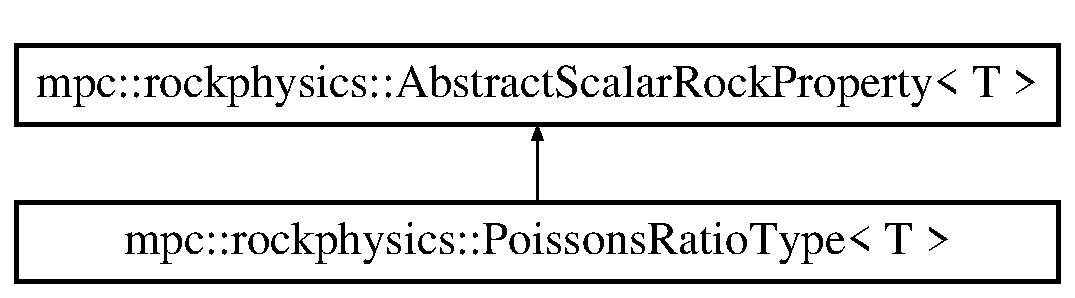
\includegraphics[height=2.000000cm]{structmpc_1_1rockphysics_1_1_poissons_ratio_type}
\end{center}
\end{figure}
\subsection*{Public Member Functions}
\begin{DoxyCompactItemize}
\item 
constexpr \mbox{\hyperlink{structmpc_1_1rockphysics_1_1_poissons_ratio_type_adfd93825fc8410288ea9078dfce8bb47}{Poissons\+Ratio\+Type}} (T val)
\end{DoxyCompactItemize}
\subsection*{Additional Inherited Members}


\subsection{Detailed Description}
\subsubsection*{template$<$typename T$>$\newline
struct mpc\+::rockphysics\+::\+Poissons\+Ratio\+Type$<$ T $>$}



Definition at line 81 of file rockphysicstransformstypes.\+hpp.



\subsection{Constructor \& Destructor Documentation}
\mbox{\Hypertarget{structmpc_1_1rockphysics_1_1_poissons_ratio_type_adfd93825fc8410288ea9078dfce8bb47}\label{structmpc_1_1rockphysics_1_1_poissons_ratio_type_adfd93825fc8410288ea9078dfce8bb47}} 
\index{mpc\+::rockphysics\+::\+Poissons\+Ratio\+Type@{mpc\+::rockphysics\+::\+Poissons\+Ratio\+Type}!Poissons\+Ratio\+Type@{Poissons\+Ratio\+Type}}
\index{Poissons\+Ratio\+Type@{Poissons\+Ratio\+Type}!mpc\+::rockphysics\+::\+Poissons\+Ratio\+Type@{mpc\+::rockphysics\+::\+Poissons\+Ratio\+Type}}
\subsubsection{\texorpdfstring{Poissons\+Ratio\+Type()}{PoissonsRatioType()}}
{\footnotesize\ttfamily template$<$typename T$>$ \\
constexpr \mbox{\hyperlink{structmpc_1_1rockphysics_1_1_poissons_ratio_type}{mpc\+::rockphysics\+::\+Poissons\+Ratio\+Type}}$<$ T $>$\+::\mbox{\hyperlink{structmpc_1_1rockphysics_1_1_poissons_ratio_type}{Poissons\+Ratio\+Type}} (\begin{DoxyParamCaption}\item[{T}]{val }\end{DoxyParamCaption})\hspace{0.3cm}{\ttfamily [inline]}}



Definition at line 86 of file rockphysicstransformstypes.\+hpp.



The documentation for this struct was generated from the following file\+:\begin{DoxyCompactItemize}
\item 
/\+Users/atorlucci/\+Documents/github\+\_\+threecubed\+\_\+repos/mpc/src/mpc/rockphysics/\mbox{\hyperlink{rockphysicstransformstypes_8hpp}{rockphysicstransformstypes.\+hpp}}\end{DoxyCompactItemize}

\hypertarget{structmpc_1_1utilities_1_1_print_tensor_components}{}\section{mpc\+:\+:utilities\+:\+:Print\+Tensor\+Components$<$ T, Rank $>$ Struct Template Reference}
\label{structmpc_1_1utilities_1_1_print_tensor_components}\index{mpc\+::utilities\+::\+Print\+Tensor\+Components$<$ T, Rank $>$@{mpc\+::utilities\+::\+Print\+Tensor\+Components$<$ T, Rank $>$}}


{\ttfamily \#include $<$printtensorcomponents.\+hpp$>$}

\subsection*{Public Member Functions}
\begin{DoxyCompactItemize}
\item 
void \mbox{\hyperlink{structmpc_1_1utilities_1_1_print_tensor_components_aff591b182c9d278a33738e18116382e2}{operator()}} (blitz\+::\+Array$<$ T, Rank $>$ \&tensor)
\end{DoxyCompactItemize}


\subsection{Detailed Description}
\subsubsection*{template$<$typename T, int Rank$>$\newline
struct mpc\+::utilities\+::\+Print\+Tensor\+Components$<$ T, Rank $>$}



Definition at line 23 of file printtensorcomponents.\+hpp.



\subsection{Member Function Documentation}
\mbox{\Hypertarget{structmpc_1_1utilities_1_1_print_tensor_components_aff591b182c9d278a33738e18116382e2}\label{structmpc_1_1utilities_1_1_print_tensor_components_aff591b182c9d278a33738e18116382e2}} 
\index{mpc\+::utilities\+::\+Print\+Tensor\+Components@{mpc\+::utilities\+::\+Print\+Tensor\+Components}!operator()@{operator()}}
\index{operator()@{operator()}!mpc\+::utilities\+::\+Print\+Tensor\+Components@{mpc\+::utilities\+::\+Print\+Tensor\+Components}}
\subsubsection{\texorpdfstring{operator()()}{operator()()}}
{\footnotesize\ttfamily template$<$typename T , int Rank$>$ \\
void \mbox{\hyperlink{structmpc_1_1utilities_1_1_print_tensor_components}{mpc\+::utilities\+::\+Print\+Tensor\+Components}}$<$ T, Rank $>$\+::operator() (\begin{DoxyParamCaption}\item[{blitz\+::\+Array$<$ T, Rank $>$ \&}]{tensor }\end{DoxyParamCaption})\hspace{0.3cm}{\ttfamily [inline]}}



Definition at line 25 of file printtensorcomponents.\+hpp.



The documentation for this struct was generated from the following file\+:\begin{DoxyCompactItemize}
\item 
/\+Users/atorlucci/\+Documents/github\+\_\+threecubed\+\_\+repos/mpc/src/mpc/utilities/\mbox{\hyperlink{printtensorcomponents_8hpp}{printtensorcomponents.\+hpp}}\end{DoxyCompactItemize}

\hypertarget{structmpc_1_1utilities_1_1_print_tensor_components_3_01_t_00_011_01_4}{}\section{mpc\+:\+:utilities\+:\+:Print\+Tensor\+Components$<$ T, 1 $>$ Struct Template Reference}
\label{structmpc_1_1utilities_1_1_print_tensor_components_3_01_t_00_011_01_4}\index{mpc\+::utilities\+::\+Print\+Tensor\+Components$<$ T, 1 $>$@{mpc\+::utilities\+::\+Print\+Tensor\+Components$<$ T, 1 $>$}}


{\ttfamily \#include $<$printtensorcomponents.\+hpp$>$}

\subsection*{Public Member Functions}
\begin{DoxyCompactItemize}
\item 
void \mbox{\hyperlink{structmpc_1_1utilities_1_1_print_tensor_components_3_01_t_00_011_01_4_ad4b1a6e828871fe3b7bf3f2053dc9f26}{operator()}} (blitz\+::\+Array$<$ T, 1 $>$ \&tensor)
\end{DoxyCompactItemize}


\subsection{Detailed Description}
\subsubsection*{template$<$typename T$>$\newline
struct mpc\+::utilities\+::\+Print\+Tensor\+Components$<$ T, 1 $>$}



Definition at line 31 of file printtensorcomponents.\+hpp.



\subsection{Member Function Documentation}
\mbox{\Hypertarget{structmpc_1_1utilities_1_1_print_tensor_components_3_01_t_00_011_01_4_ad4b1a6e828871fe3b7bf3f2053dc9f26}\label{structmpc_1_1utilities_1_1_print_tensor_components_3_01_t_00_011_01_4_ad4b1a6e828871fe3b7bf3f2053dc9f26}} 
\index{mpc\+::utilities\+::\+Print\+Tensor\+Components$<$ T, 1 $>$@{mpc\+::utilities\+::\+Print\+Tensor\+Components$<$ T, 1 $>$}!operator()@{operator()}}
\index{operator()@{operator()}!mpc\+::utilities\+::\+Print\+Tensor\+Components$<$ T, 1 $>$@{mpc\+::utilities\+::\+Print\+Tensor\+Components$<$ T, 1 $>$}}
\subsubsection{\texorpdfstring{operator()()}{operator()()}}
{\footnotesize\ttfamily template$<$typename T $>$ \\
void \mbox{\hyperlink{structmpc_1_1utilities_1_1_print_tensor_components}{mpc\+::utilities\+::\+Print\+Tensor\+Components}}$<$ T, 1 $>$\+::operator() (\begin{DoxyParamCaption}\item[{blitz\+::\+Array$<$ T, 1 $>$ \&}]{tensor }\end{DoxyParamCaption})\hspace{0.3cm}{\ttfamily [inline]}}



Definition at line 33 of file printtensorcomponents.\+hpp.



The documentation for this struct was generated from the following file\+:\begin{DoxyCompactItemize}
\item 
/\+Users/atorlucci/\+Documents/github\+\_\+threecubed\+\_\+repos/mpc/src/mpc/utilities/\mbox{\hyperlink{printtensorcomponents_8hpp}{printtensorcomponents.\+hpp}}\end{DoxyCompactItemize}

\hypertarget{structmpc_1_1utilities_1_1_print_tensor_components_3_01_t_00_0110_01_4}{}\section{mpc\+:\+:utilities\+:\+:Print\+Tensor\+Components$<$ T, 10 $>$ Struct Template Reference}
\label{structmpc_1_1utilities_1_1_print_tensor_components_3_01_t_00_0110_01_4}\index{mpc\+::utilities\+::\+Print\+Tensor\+Components$<$ T, 10 $>$@{mpc\+::utilities\+::\+Print\+Tensor\+Components$<$ T, 10 $>$}}


{\ttfamily \#include $<$printtensorcomponents.\+hpp$>$}

\subsection*{Public Member Functions}
\begin{DoxyCompactItemize}
\item 
void \mbox{\hyperlink{structmpc_1_1utilities_1_1_print_tensor_components_3_01_t_00_0110_01_4_a68d6aead6f1d8a3f3bd91ec2bda85c2e}{operator()}} (blitz\+::\+Array$<$ T, 10 $>$ \&tensor)
\end{DoxyCompactItemize}


\subsection{Detailed Description}
\subsubsection*{template$<$typename T$>$\newline
struct mpc\+::utilities\+::\+Print\+Tensor\+Components$<$ T, 10 $>$}



Definition at line 333 of file printtensorcomponents.\+hpp.



\subsection{Member Function Documentation}
\mbox{\Hypertarget{structmpc_1_1utilities_1_1_print_tensor_components_3_01_t_00_0110_01_4_a68d6aead6f1d8a3f3bd91ec2bda85c2e}\label{structmpc_1_1utilities_1_1_print_tensor_components_3_01_t_00_0110_01_4_a68d6aead6f1d8a3f3bd91ec2bda85c2e}} 
\index{mpc\+::utilities\+::\+Print\+Tensor\+Components$<$ T, 10 $>$@{mpc\+::utilities\+::\+Print\+Tensor\+Components$<$ T, 10 $>$}!operator()@{operator()}}
\index{operator()@{operator()}!mpc\+::utilities\+::\+Print\+Tensor\+Components$<$ T, 10 $>$@{mpc\+::utilities\+::\+Print\+Tensor\+Components$<$ T, 10 $>$}}
\subsubsection{\texorpdfstring{operator()()}{operator()()}}
{\footnotesize\ttfamily template$<$typename T $>$ \\
void \mbox{\hyperlink{structmpc_1_1utilities_1_1_print_tensor_components}{mpc\+::utilities\+::\+Print\+Tensor\+Components}}$<$ T, 10 $>$\+::operator() (\begin{DoxyParamCaption}\item[{blitz\+::\+Array$<$ T, 10 $>$ \&}]{tensor }\end{DoxyParamCaption})\hspace{0.3cm}{\ttfamily [inline]}}



Definition at line 335 of file printtensorcomponents.\+hpp.



The documentation for this struct was generated from the following file\+:\begin{DoxyCompactItemize}
\item 
/\+Users/atorlucci/\+Documents/github\+\_\+threecubed\+\_\+repos/mpc/src/mpc/utilities/\mbox{\hyperlink{printtensorcomponents_8hpp}{printtensorcomponents.\+hpp}}\end{DoxyCompactItemize}

\hypertarget{structmpc_1_1utilities_1_1_print_tensor_components_3_01_t_00_0111_01_4}{}\section{mpc\+:\+:utilities\+:\+:Print\+Tensor\+Components$<$ T, 11 $>$ Struct Template Reference}
\label{structmpc_1_1utilities_1_1_print_tensor_components_3_01_t_00_0111_01_4}\index{mpc\+::utilities\+::\+Print\+Tensor\+Components$<$ T, 11 $>$@{mpc\+::utilities\+::\+Print\+Tensor\+Components$<$ T, 11 $>$}}


{\ttfamily \#include $<$printtensorcomponents.\+hpp$>$}

\subsection*{Public Member Functions}
\begin{DoxyCompactItemize}
\item 
void \mbox{\hyperlink{structmpc_1_1utilities_1_1_print_tensor_components_3_01_t_00_0111_01_4_add0d1c50a34678d8ecde1048b3f04b5f}{operator()}} (blitz\+::\+Array$<$ T, 11 $>$ \&tensor)
\end{DoxyCompactItemize}


\subsection{Detailed Description}
\subsubsection*{template$<$typename T$>$\newline
struct mpc\+::utilities\+::\+Print\+Tensor\+Components$<$ T, 11 $>$}



Definition at line 387 of file printtensorcomponents.\+hpp.



\subsection{Member Function Documentation}
\mbox{\Hypertarget{structmpc_1_1utilities_1_1_print_tensor_components_3_01_t_00_0111_01_4_add0d1c50a34678d8ecde1048b3f04b5f}\label{structmpc_1_1utilities_1_1_print_tensor_components_3_01_t_00_0111_01_4_add0d1c50a34678d8ecde1048b3f04b5f}} 
\index{mpc\+::utilities\+::\+Print\+Tensor\+Components$<$ T, 11 $>$@{mpc\+::utilities\+::\+Print\+Tensor\+Components$<$ T, 11 $>$}!operator()@{operator()}}
\index{operator()@{operator()}!mpc\+::utilities\+::\+Print\+Tensor\+Components$<$ T, 11 $>$@{mpc\+::utilities\+::\+Print\+Tensor\+Components$<$ T, 11 $>$}}
\subsubsection{\texorpdfstring{operator()()}{operator()()}}
{\footnotesize\ttfamily template$<$typename T $>$ \\
void \mbox{\hyperlink{structmpc_1_1utilities_1_1_print_tensor_components}{mpc\+::utilities\+::\+Print\+Tensor\+Components}}$<$ T, 11 $>$\+::operator() (\begin{DoxyParamCaption}\item[{blitz\+::\+Array$<$ T, 11 $>$ \&}]{tensor }\end{DoxyParamCaption})\hspace{0.3cm}{\ttfamily [inline]}}



Definition at line 389 of file printtensorcomponents.\+hpp.



The documentation for this struct was generated from the following file\+:\begin{DoxyCompactItemize}
\item 
/\+Users/atorlucci/\+Documents/github\+\_\+threecubed\+\_\+repos/mpc/src/mpc/utilities/\mbox{\hyperlink{printtensorcomponents_8hpp}{printtensorcomponents.\+hpp}}\end{DoxyCompactItemize}

\hypertarget{structmpc_1_1utilities_1_1_print_tensor_components_3_01_t_00_012_01_4}{}\section{mpc\+:\+:utilities\+:\+:Print\+Tensor\+Components$<$ T, 2 $>$ Struct Template Reference}
\label{structmpc_1_1utilities_1_1_print_tensor_components_3_01_t_00_012_01_4}\index{mpc\+::utilities\+::\+Print\+Tensor\+Components$<$ T, 2 $>$@{mpc\+::utilities\+::\+Print\+Tensor\+Components$<$ T, 2 $>$}}


{\ttfamily \#include $<$printtensorcomponents.\+hpp$>$}

\subsection*{Public Member Functions}
\begin{DoxyCompactItemize}
\item 
void \mbox{\hyperlink{structmpc_1_1utilities_1_1_print_tensor_components_3_01_t_00_012_01_4_ac0b613c8830faa23f0e44f63ac49adb8}{operator()}} (blitz\+::\+Array$<$ T, 2 $>$ \&tensor)
\end{DoxyCompactItemize}


\subsection{Detailed Description}
\subsubsection*{template$<$typename T$>$\newline
struct mpc\+::utilities\+::\+Print\+Tensor\+Components$<$ T, 2 $>$}



Definition at line 48 of file printtensorcomponents.\+hpp.



\subsection{Member Function Documentation}
\mbox{\Hypertarget{structmpc_1_1utilities_1_1_print_tensor_components_3_01_t_00_012_01_4_ac0b613c8830faa23f0e44f63ac49adb8}\label{structmpc_1_1utilities_1_1_print_tensor_components_3_01_t_00_012_01_4_ac0b613c8830faa23f0e44f63ac49adb8}} 
\index{mpc\+::utilities\+::\+Print\+Tensor\+Components$<$ T, 2 $>$@{mpc\+::utilities\+::\+Print\+Tensor\+Components$<$ T, 2 $>$}!operator()@{operator()}}
\index{operator()@{operator()}!mpc\+::utilities\+::\+Print\+Tensor\+Components$<$ T, 2 $>$@{mpc\+::utilities\+::\+Print\+Tensor\+Components$<$ T, 2 $>$}}
\subsubsection{\texorpdfstring{operator()()}{operator()()}}
{\footnotesize\ttfamily template$<$typename T $>$ \\
void \mbox{\hyperlink{structmpc_1_1utilities_1_1_print_tensor_components}{mpc\+::utilities\+::\+Print\+Tensor\+Components}}$<$ T, 2 $>$\+::operator() (\begin{DoxyParamCaption}\item[{blitz\+::\+Array$<$ T, 2 $>$ \&}]{tensor }\end{DoxyParamCaption})\hspace{0.3cm}{\ttfamily [inline]}}



Definition at line 50 of file printtensorcomponents.\+hpp.



The documentation for this struct was generated from the following file\+:\begin{DoxyCompactItemize}
\item 
/\+Users/atorlucci/\+Documents/github\+\_\+threecubed\+\_\+repos/mpc/src/mpc/utilities/\mbox{\hyperlink{printtensorcomponents_8hpp}{printtensorcomponents.\+hpp}}\end{DoxyCompactItemize}

\hypertarget{structmpc_1_1utilities_1_1_print_tensor_components_3_01_t_00_013_01_4}{}\section{mpc\+:\+:utilities\+:\+:Print\+Tensor\+Components$<$ T, 3 $>$ Struct Template Reference}
\label{structmpc_1_1utilities_1_1_print_tensor_components_3_01_t_00_013_01_4}\index{mpc\+::utilities\+::\+Print\+Tensor\+Components$<$ T, 3 $>$@{mpc\+::utilities\+::\+Print\+Tensor\+Components$<$ T, 3 $>$}}


{\ttfamily \#include $<$printtensorcomponents.\+hpp$>$}

\subsection*{Public Member Functions}
\begin{DoxyCompactItemize}
\item 
void \mbox{\hyperlink{structmpc_1_1utilities_1_1_print_tensor_components_3_01_t_00_013_01_4_aa6fae52410d39880ab27200c6aa43d0b}{operator()}} (blitz\+::\+Array$<$ T, 3 $>$ \&tensor)
\end{DoxyCompactItemize}


\subsection{Detailed Description}
\subsubsection*{template$<$typename T$>$\newline
struct mpc\+::utilities\+::\+Print\+Tensor\+Components$<$ T, 3 $>$}



Definition at line 69 of file printtensorcomponents.\+hpp.



\subsection{Member Function Documentation}
\mbox{\Hypertarget{structmpc_1_1utilities_1_1_print_tensor_components_3_01_t_00_013_01_4_aa6fae52410d39880ab27200c6aa43d0b}\label{structmpc_1_1utilities_1_1_print_tensor_components_3_01_t_00_013_01_4_aa6fae52410d39880ab27200c6aa43d0b}} 
\index{mpc\+::utilities\+::\+Print\+Tensor\+Components$<$ T, 3 $>$@{mpc\+::utilities\+::\+Print\+Tensor\+Components$<$ T, 3 $>$}!operator()@{operator()}}
\index{operator()@{operator()}!mpc\+::utilities\+::\+Print\+Tensor\+Components$<$ T, 3 $>$@{mpc\+::utilities\+::\+Print\+Tensor\+Components$<$ T, 3 $>$}}
\subsubsection{\texorpdfstring{operator()()}{operator()()}}
{\footnotesize\ttfamily template$<$typename T $>$ \\
void \mbox{\hyperlink{structmpc_1_1utilities_1_1_print_tensor_components}{mpc\+::utilities\+::\+Print\+Tensor\+Components}}$<$ T, 3 $>$\+::operator() (\begin{DoxyParamCaption}\item[{blitz\+::\+Array$<$ T, 3 $>$ \&}]{tensor }\end{DoxyParamCaption})\hspace{0.3cm}{\ttfamily [inline]}}



Definition at line 71 of file printtensorcomponents.\+hpp.



The documentation for this struct was generated from the following file\+:\begin{DoxyCompactItemize}
\item 
/\+Users/atorlucci/\+Documents/github\+\_\+threecubed\+\_\+repos/mpc/src/mpc/utilities/\mbox{\hyperlink{printtensorcomponents_8hpp}{printtensorcomponents.\+hpp}}\end{DoxyCompactItemize}

\hypertarget{structmpc_1_1utilities_1_1_print_tensor_components_3_01_t_00_014_01_4}{}\section{mpc\+:\+:utilities\+:\+:Print\+Tensor\+Components$<$ T, 4 $>$ Struct Template Reference}
\label{structmpc_1_1utilities_1_1_print_tensor_components_3_01_t_00_014_01_4}\index{mpc\+::utilities\+::\+Print\+Tensor\+Components$<$ T, 4 $>$@{mpc\+::utilities\+::\+Print\+Tensor\+Components$<$ T, 4 $>$}}


{\ttfamily \#include $<$printtensorcomponents.\+hpp$>$}

\subsection*{Public Member Functions}
\begin{DoxyCompactItemize}
\item 
void \mbox{\hyperlink{structmpc_1_1utilities_1_1_print_tensor_components_3_01_t_00_014_01_4_ab5500a50f0c6119ee98075cbaad6a51e}{operator()}} (blitz\+::\+Array$<$ T, 4 $>$ \&tensor)
\end{DoxyCompactItemize}


\subsection{Detailed Description}
\subsubsection*{template$<$typename T$>$\newline
struct mpc\+::utilities\+::\+Print\+Tensor\+Components$<$ T, 4 $>$}



Definition at line 94 of file printtensorcomponents.\+hpp.



\subsection{Member Function Documentation}
\mbox{\Hypertarget{structmpc_1_1utilities_1_1_print_tensor_components_3_01_t_00_014_01_4_ab5500a50f0c6119ee98075cbaad6a51e}\label{structmpc_1_1utilities_1_1_print_tensor_components_3_01_t_00_014_01_4_ab5500a50f0c6119ee98075cbaad6a51e}} 
\index{mpc\+::utilities\+::\+Print\+Tensor\+Components$<$ T, 4 $>$@{mpc\+::utilities\+::\+Print\+Tensor\+Components$<$ T, 4 $>$}!operator()@{operator()}}
\index{operator()@{operator()}!mpc\+::utilities\+::\+Print\+Tensor\+Components$<$ T, 4 $>$@{mpc\+::utilities\+::\+Print\+Tensor\+Components$<$ T, 4 $>$}}
\subsubsection{\texorpdfstring{operator()()}{operator()()}}
{\footnotesize\ttfamily template$<$typename T $>$ \\
void \mbox{\hyperlink{structmpc_1_1utilities_1_1_print_tensor_components}{mpc\+::utilities\+::\+Print\+Tensor\+Components}}$<$ T, 4 $>$\+::operator() (\begin{DoxyParamCaption}\item[{blitz\+::\+Array$<$ T, 4 $>$ \&}]{tensor }\end{DoxyParamCaption})\hspace{0.3cm}{\ttfamily [inline]}}



Definition at line 96 of file printtensorcomponents.\+hpp.



The documentation for this struct was generated from the following file\+:\begin{DoxyCompactItemize}
\item 
/\+Users/atorlucci/\+Documents/github\+\_\+threecubed\+\_\+repos/mpc/src/mpc/utilities/\mbox{\hyperlink{printtensorcomponents_8hpp}{printtensorcomponents.\+hpp}}\end{DoxyCompactItemize}

\hypertarget{structmpc_1_1utilities_1_1_print_tensor_components_3_01_t_00_015_01_4}{}\section{mpc\+:\+:utilities\+:\+:Print\+Tensor\+Components$<$ T, 5 $>$ Struct Template Reference}
\label{structmpc_1_1utilities_1_1_print_tensor_components_3_01_t_00_015_01_4}\index{mpc\+::utilities\+::\+Print\+Tensor\+Components$<$ T, 5 $>$@{mpc\+::utilities\+::\+Print\+Tensor\+Components$<$ T, 5 $>$}}


{\ttfamily \#include $<$printtensorcomponents.\+hpp$>$}

\subsection*{Public Member Functions}
\begin{DoxyCompactItemize}
\item 
void \mbox{\hyperlink{structmpc_1_1utilities_1_1_print_tensor_components_3_01_t_00_015_01_4_ae06f93e705c882d56433ef0ca2629351}{operator()}} (blitz\+::\+Array$<$ T, 5 $>$ \&tensor)
\end{DoxyCompactItemize}


\subsection{Detailed Description}
\subsubsection*{template$<$typename T$>$\newline
struct mpc\+::utilities\+::\+Print\+Tensor\+Components$<$ T, 5 $>$}



Definition at line 123 of file printtensorcomponents.\+hpp.



\subsection{Member Function Documentation}
\mbox{\Hypertarget{structmpc_1_1utilities_1_1_print_tensor_components_3_01_t_00_015_01_4_ae06f93e705c882d56433ef0ca2629351}\label{structmpc_1_1utilities_1_1_print_tensor_components_3_01_t_00_015_01_4_ae06f93e705c882d56433ef0ca2629351}} 
\index{mpc\+::utilities\+::\+Print\+Tensor\+Components$<$ T, 5 $>$@{mpc\+::utilities\+::\+Print\+Tensor\+Components$<$ T, 5 $>$}!operator()@{operator()}}
\index{operator()@{operator()}!mpc\+::utilities\+::\+Print\+Tensor\+Components$<$ T, 5 $>$@{mpc\+::utilities\+::\+Print\+Tensor\+Components$<$ T, 5 $>$}}
\subsubsection{\texorpdfstring{operator()()}{operator()()}}
{\footnotesize\ttfamily template$<$typename T $>$ \\
void \mbox{\hyperlink{structmpc_1_1utilities_1_1_print_tensor_components}{mpc\+::utilities\+::\+Print\+Tensor\+Components}}$<$ T, 5 $>$\+::operator() (\begin{DoxyParamCaption}\item[{blitz\+::\+Array$<$ T, 5 $>$ \&}]{tensor }\end{DoxyParamCaption})\hspace{0.3cm}{\ttfamily [inline]}}



Definition at line 125 of file printtensorcomponents.\+hpp.



The documentation for this struct was generated from the following file\+:\begin{DoxyCompactItemize}
\item 
/\+Users/atorlucci/\+Documents/github\+\_\+threecubed\+\_\+repos/mpc/src/mpc/utilities/\mbox{\hyperlink{printtensorcomponents_8hpp}{printtensorcomponents.\+hpp}}\end{DoxyCompactItemize}

\hypertarget{structmpc_1_1utilities_1_1_print_tensor_components_3_01_t_00_016_01_4}{}\section{mpc\+:\+:utilities\+:\+:Print\+Tensor\+Components$<$ T, 6 $>$ Struct Template Reference}
\label{structmpc_1_1utilities_1_1_print_tensor_components_3_01_t_00_016_01_4}\index{mpc\+::utilities\+::\+Print\+Tensor\+Components$<$ T, 6 $>$@{mpc\+::utilities\+::\+Print\+Tensor\+Components$<$ T, 6 $>$}}


{\ttfamily \#include $<$printtensorcomponents.\+hpp$>$}

\subsection*{Public Member Functions}
\begin{DoxyCompactItemize}
\item 
void \mbox{\hyperlink{structmpc_1_1utilities_1_1_print_tensor_components_3_01_t_00_016_01_4_aa9050aea8d8ebfa15363dc4ef0bcfb05}{operator()}} (blitz\+::\+Array$<$ T, 6 $>$ \&tensor)
\end{DoxyCompactItemize}


\subsection{Detailed Description}
\subsubsection*{template$<$typename T$>$\newline
struct mpc\+::utilities\+::\+Print\+Tensor\+Components$<$ T, 6 $>$}



Definition at line 157 of file printtensorcomponents.\+hpp.



\subsection{Member Function Documentation}
\mbox{\Hypertarget{structmpc_1_1utilities_1_1_print_tensor_components_3_01_t_00_016_01_4_aa9050aea8d8ebfa15363dc4ef0bcfb05}\label{structmpc_1_1utilities_1_1_print_tensor_components_3_01_t_00_016_01_4_aa9050aea8d8ebfa15363dc4ef0bcfb05}} 
\index{mpc\+::utilities\+::\+Print\+Tensor\+Components$<$ T, 6 $>$@{mpc\+::utilities\+::\+Print\+Tensor\+Components$<$ T, 6 $>$}!operator()@{operator()}}
\index{operator()@{operator()}!mpc\+::utilities\+::\+Print\+Tensor\+Components$<$ T, 6 $>$@{mpc\+::utilities\+::\+Print\+Tensor\+Components$<$ T, 6 $>$}}
\subsubsection{\texorpdfstring{operator()()}{operator()()}}
{\footnotesize\ttfamily template$<$typename T $>$ \\
void \mbox{\hyperlink{structmpc_1_1utilities_1_1_print_tensor_components}{mpc\+::utilities\+::\+Print\+Tensor\+Components}}$<$ T, 6 $>$\+::operator() (\begin{DoxyParamCaption}\item[{blitz\+::\+Array$<$ T, 6 $>$ \&}]{tensor }\end{DoxyParamCaption})\hspace{0.3cm}{\ttfamily [inline]}}



Definition at line 159 of file printtensorcomponents.\+hpp.



The documentation for this struct was generated from the following file\+:\begin{DoxyCompactItemize}
\item 
/\+Users/atorlucci/\+Documents/github\+\_\+threecubed\+\_\+repos/mpc/src/mpc/utilities/\mbox{\hyperlink{printtensorcomponents_8hpp}{printtensorcomponents.\+hpp}}\end{DoxyCompactItemize}

\hypertarget{structmpc_1_1utilities_1_1_print_tensor_components_3_01_t_00_017_01_4}{}\section{mpc\+:\+:utilities\+:\+:Print\+Tensor\+Components$<$ T, 7 $>$ Struct Template Reference}
\label{structmpc_1_1utilities_1_1_print_tensor_components_3_01_t_00_017_01_4}\index{mpc\+::utilities\+::\+Print\+Tensor\+Components$<$ T, 7 $>$@{mpc\+::utilities\+::\+Print\+Tensor\+Components$<$ T, 7 $>$}}


{\ttfamily \#include $<$printtensorcomponents.\+hpp$>$}

\subsection*{Public Member Functions}
\begin{DoxyCompactItemize}
\item 
void \mbox{\hyperlink{structmpc_1_1utilities_1_1_print_tensor_components_3_01_t_00_017_01_4_ac3b3749e7e1cac63277ee49dc629bf51}{operator()}} (blitz\+::\+Array$<$ T, 7 $>$ \&tensor)
\end{DoxyCompactItemize}


\subsection{Detailed Description}
\subsubsection*{template$<$typename T$>$\newline
struct mpc\+::utilities\+::\+Print\+Tensor\+Components$<$ T, 7 $>$}



Definition at line 195 of file printtensorcomponents.\+hpp.



\subsection{Member Function Documentation}
\mbox{\Hypertarget{structmpc_1_1utilities_1_1_print_tensor_components_3_01_t_00_017_01_4_ac3b3749e7e1cac63277ee49dc629bf51}\label{structmpc_1_1utilities_1_1_print_tensor_components_3_01_t_00_017_01_4_ac3b3749e7e1cac63277ee49dc629bf51}} 
\index{mpc\+::utilities\+::\+Print\+Tensor\+Components$<$ T, 7 $>$@{mpc\+::utilities\+::\+Print\+Tensor\+Components$<$ T, 7 $>$}!operator()@{operator()}}
\index{operator()@{operator()}!mpc\+::utilities\+::\+Print\+Tensor\+Components$<$ T, 7 $>$@{mpc\+::utilities\+::\+Print\+Tensor\+Components$<$ T, 7 $>$}}
\subsubsection{\texorpdfstring{operator()()}{operator()()}}
{\footnotesize\ttfamily template$<$typename T $>$ \\
void \mbox{\hyperlink{structmpc_1_1utilities_1_1_print_tensor_components}{mpc\+::utilities\+::\+Print\+Tensor\+Components}}$<$ T, 7 $>$\+::operator() (\begin{DoxyParamCaption}\item[{blitz\+::\+Array$<$ T, 7 $>$ \&}]{tensor }\end{DoxyParamCaption})\hspace{0.3cm}{\ttfamily [inline]}}



Definition at line 197 of file printtensorcomponents.\+hpp.



The documentation for this struct was generated from the following file\+:\begin{DoxyCompactItemize}
\item 
/\+Users/atorlucci/\+Documents/github\+\_\+threecubed\+\_\+repos/mpc/src/mpc/utilities/\mbox{\hyperlink{printtensorcomponents_8hpp}{printtensorcomponents.\+hpp}}\end{DoxyCompactItemize}

\hypertarget{structmpc_1_1utilities_1_1_print_tensor_components_3_01_t_00_018_01_4}{}\section{mpc\+:\+:utilities\+:\+:Print\+Tensor\+Components$<$ T, 8 $>$ Struct Template Reference}
\label{structmpc_1_1utilities_1_1_print_tensor_components_3_01_t_00_018_01_4}\index{mpc\+::utilities\+::\+Print\+Tensor\+Components$<$ T, 8 $>$@{mpc\+::utilities\+::\+Print\+Tensor\+Components$<$ T, 8 $>$}}


{\ttfamily \#include $<$printtensorcomponents.\+hpp$>$}

\subsection*{Public Member Functions}
\begin{DoxyCompactItemize}
\item 
void \mbox{\hyperlink{structmpc_1_1utilities_1_1_print_tensor_components_3_01_t_00_018_01_4_a4a099623dcbef00f62c0ec6d7e7cd113}{operator()}} (blitz\+::\+Array$<$ T, 8 $>$ \&tensor)
\end{DoxyCompactItemize}


\subsection{Detailed Description}
\subsubsection*{template$<$typename T$>$\newline
struct mpc\+::utilities\+::\+Print\+Tensor\+Components$<$ T, 8 $>$}



Definition at line 237 of file printtensorcomponents.\+hpp.



\subsection{Member Function Documentation}
\mbox{\Hypertarget{structmpc_1_1utilities_1_1_print_tensor_components_3_01_t_00_018_01_4_a4a099623dcbef00f62c0ec6d7e7cd113}\label{structmpc_1_1utilities_1_1_print_tensor_components_3_01_t_00_018_01_4_a4a099623dcbef00f62c0ec6d7e7cd113}} 
\index{mpc\+::utilities\+::\+Print\+Tensor\+Components$<$ T, 8 $>$@{mpc\+::utilities\+::\+Print\+Tensor\+Components$<$ T, 8 $>$}!operator()@{operator()}}
\index{operator()@{operator()}!mpc\+::utilities\+::\+Print\+Tensor\+Components$<$ T, 8 $>$@{mpc\+::utilities\+::\+Print\+Tensor\+Components$<$ T, 8 $>$}}
\subsubsection{\texorpdfstring{operator()()}{operator()()}}
{\footnotesize\ttfamily template$<$typename T $>$ \\
void \mbox{\hyperlink{structmpc_1_1utilities_1_1_print_tensor_components}{mpc\+::utilities\+::\+Print\+Tensor\+Components}}$<$ T, 8 $>$\+::operator() (\begin{DoxyParamCaption}\item[{blitz\+::\+Array$<$ T, 8 $>$ \&}]{tensor }\end{DoxyParamCaption})\hspace{0.3cm}{\ttfamily [inline]}}



Definition at line 239 of file printtensorcomponents.\+hpp.



The documentation for this struct was generated from the following file\+:\begin{DoxyCompactItemize}
\item 
/\+Users/atorlucci/\+Documents/github\+\_\+threecubed\+\_\+repos/mpc/src/mpc/utilities/\mbox{\hyperlink{printtensorcomponents_8hpp}{printtensorcomponents.\+hpp}}\end{DoxyCompactItemize}

\hypertarget{structmpc_1_1utilities_1_1_print_tensor_components_3_01_t_00_019_01_4}{}\section{mpc\+:\+:utilities\+:\+:Print\+Tensor\+Components$<$ T, 9 $>$ Struct Template Reference}
\label{structmpc_1_1utilities_1_1_print_tensor_components_3_01_t_00_019_01_4}\index{mpc\+::utilities\+::\+Print\+Tensor\+Components$<$ T, 9 $>$@{mpc\+::utilities\+::\+Print\+Tensor\+Components$<$ T, 9 $>$}}


{\ttfamily \#include $<$printtensorcomponents.\+hpp$>$}

\subsection*{Public Member Functions}
\begin{DoxyCompactItemize}
\item 
void \mbox{\hyperlink{structmpc_1_1utilities_1_1_print_tensor_components_3_01_t_00_019_01_4_af6466d6b11a9cb63e1ecc7911830b644}{operator()}} (blitz\+::\+Array$<$ T, 9 $>$ \&tensor)
\end{DoxyCompactItemize}


\subsection{Detailed Description}
\subsubsection*{template$<$typename T$>$\newline
struct mpc\+::utilities\+::\+Print\+Tensor\+Components$<$ T, 9 $>$}



Definition at line 283 of file printtensorcomponents.\+hpp.



\subsection{Member Function Documentation}
\mbox{\Hypertarget{structmpc_1_1utilities_1_1_print_tensor_components_3_01_t_00_019_01_4_af6466d6b11a9cb63e1ecc7911830b644}\label{structmpc_1_1utilities_1_1_print_tensor_components_3_01_t_00_019_01_4_af6466d6b11a9cb63e1ecc7911830b644}} 
\index{mpc\+::utilities\+::\+Print\+Tensor\+Components$<$ T, 9 $>$@{mpc\+::utilities\+::\+Print\+Tensor\+Components$<$ T, 9 $>$}!operator()@{operator()}}
\index{operator()@{operator()}!mpc\+::utilities\+::\+Print\+Tensor\+Components$<$ T, 9 $>$@{mpc\+::utilities\+::\+Print\+Tensor\+Components$<$ T, 9 $>$}}
\subsubsection{\texorpdfstring{operator()()}{operator()()}}
{\footnotesize\ttfamily template$<$typename T $>$ \\
void \mbox{\hyperlink{structmpc_1_1utilities_1_1_print_tensor_components}{mpc\+::utilities\+::\+Print\+Tensor\+Components}}$<$ T, 9 $>$\+::operator() (\begin{DoxyParamCaption}\item[{blitz\+::\+Array$<$ T, 9 $>$ \&}]{tensor }\end{DoxyParamCaption})\hspace{0.3cm}{\ttfamily [inline]}}



Definition at line 285 of file printtensorcomponents.\+hpp.



The documentation for this struct was generated from the following file\+:\begin{DoxyCompactItemize}
\item 
/\+Users/atorlucci/\+Documents/github\+\_\+threecubed\+\_\+repos/mpc/src/mpc/utilities/\mbox{\hyperlink{printtensorcomponents_8hpp}{printtensorcomponents.\+hpp}}\end{DoxyCompactItemize}

\hypertarget{structmpc_1_1rockphysics_1_1_rock_physics_transforms}{}\section{mpc\+:\+:rockphysics\+:\+:Rock\+Physics\+Transforms$<$ T, U $>$ Struct Template Reference}
\label{structmpc_1_1rockphysics_1_1_rock_physics_transforms}\index{mpc\+::rockphysics\+::\+Rock\+Physics\+Transforms$<$ T, U $>$@{mpc\+::rockphysics\+::\+Rock\+Physics\+Transforms$<$ T, U $>$}}


{\ttfamily \#include $<$rockphysicstransforms.\+hpp$>$}

\subsection*{Static Public Member Functions}
\begin{DoxyCompactItemize}
\item 
static U \mbox{\hyperlink{structmpc_1_1rockphysics_1_1_rock_physics_transforms_abcf6ae16510c01c18d574bd78d3c3bdc}{Compute}} ()
\end{DoxyCompactItemize}


\subsection{Detailed Description}
\subsubsection*{template$<$typename T, typename U$>$\newline
struct mpc\+::rockphysics\+::\+Rock\+Physics\+Transforms$<$ T, U $>$}



Definition at line 26 of file rockphysicstransforms.\+hpp.



\subsection{Member Function Documentation}
\mbox{\Hypertarget{structmpc_1_1rockphysics_1_1_rock_physics_transforms_abcf6ae16510c01c18d574bd78d3c3bdc}\label{structmpc_1_1rockphysics_1_1_rock_physics_transforms_abcf6ae16510c01c18d574bd78d3c3bdc}} 
\index{mpc\+::rockphysics\+::\+Rock\+Physics\+Transforms@{mpc\+::rockphysics\+::\+Rock\+Physics\+Transforms}!Compute@{Compute}}
\index{Compute@{Compute}!mpc\+::rockphysics\+::\+Rock\+Physics\+Transforms@{mpc\+::rockphysics\+::\+Rock\+Physics\+Transforms}}
\subsubsection{\texorpdfstring{Compute()}{Compute()}}
{\footnotesize\ttfamily template$<$typename T , typename U $>$ \\
static U \mbox{\hyperlink{structmpc_1_1rockphysics_1_1_rock_physics_transforms}{mpc\+::rockphysics\+::\+Rock\+Physics\+Transforms}}$<$ T, U $>$\+::Compute (\begin{DoxyParamCaption}{ }\end{DoxyParamCaption})\hspace{0.3cm}{\ttfamily [inline]}, {\ttfamily [static]}}



Definition at line 31 of file rockphysicstransforms.\+hpp.



The documentation for this struct was generated from the following file\+:\begin{DoxyCompactItemize}
\item 
/\+Users/atorlucci/\+Documents/github\+\_\+threecubed\+\_\+repos/mpc/src/mpc/rockphysics/\mbox{\hyperlink{rockphysicstransforms_8hpp}{rockphysicstransforms.\+hpp}}\end{DoxyCompactItemize}

\hypertarget{structmpc_1_1rockphysics_1_1_rock_physics_transforms_3_01_t_00_01mpc_1_1rockphysics_1_1_bulk_modulus_type_3_01_t_01_4_01_4}{}\section{mpc\+:\+:rockphysics\+:\+:Rock\+Physics\+Transforms$<$ T, mpc\+:\+:rockphysics\+:\+:Bulk\+Modulus\+Type$<$ T $>$ $>$ Struct Template Reference}
\label{structmpc_1_1rockphysics_1_1_rock_physics_transforms_3_01_t_00_01mpc_1_1rockphysics_1_1_bulk_modulus_type_3_01_t_01_4_01_4}\index{mpc\+::rockphysics\+::\+Rock\+Physics\+Transforms$<$ T, mpc\+::rockphysics\+::\+Bulk\+Modulus\+Type$<$ T $>$ $>$@{mpc\+::rockphysics\+::\+Rock\+Physics\+Transforms$<$ T, mpc\+::rockphysics\+::\+Bulk\+Modulus\+Type$<$ T $>$ $>$}}


{\ttfamily \#include $<$rockphysicstransforms.\+hpp$>$}

\subsection*{Static Public Member Functions}
\begin{DoxyCompactItemize}
\item 
static \mbox{\hyperlink{structmpc_1_1rockphysics_1_1_bulk_modulus_type}{Bulk\+Modulus\+Type}}$<$ T $>$ \mbox{\hyperlink{structmpc_1_1rockphysics_1_1_rock_physics_transforms_3_01_t_00_01mpc_1_1rockphysics_1_1_bulk_modulus_type_3_01_t_01_4_01_4_addbfab4e83b3b5c535da97e0ca9f9fd3}{Compute}} (const \mbox{\hyperlink{structmpc_1_1rockphysics_1_1_lame_paramter_modulus_type}{mpc\+::rockphysics\+::\+Lame\+Paramter\+Modulus\+Type}}$<$ T $>$ \&lambda\+\_\+type, const \mbox{\hyperlink{structmpc_1_1rockphysics_1_1_shear_modulus_type}{mpc\+::rockphysics\+::\+Shear\+Modulus\+Type}}$<$ T $>$ \&mu\+\_\+type)
\item 
static \mbox{\hyperlink{structmpc_1_1rockphysics_1_1_bulk_modulus_type}{Bulk\+Modulus\+Type}}$<$ T $>$ \mbox{\hyperlink{structmpc_1_1rockphysics_1_1_rock_physics_transforms_3_01_t_00_01mpc_1_1rockphysics_1_1_bulk_modulus_type_3_01_t_01_4_01_4_aa196a54cfae8a69ddb309f4fab0e8fa3}{Compute}} (const \mbox{\hyperlink{structmpc_1_1rockphysics_1_1_youngs_modulus_type}{mpc\+::rockphysics\+::\+Youngs\+Modulus\+Type}}$<$ T $>$ \&E\+\_\+type, const \mbox{\hyperlink{structmpc_1_1rockphysics_1_1_shear_modulus_type}{mpc\+::rockphysics\+::\+Shear\+Modulus\+Type}}$<$ T $>$ \&mu\+\_\+type)
\item 
static \mbox{\hyperlink{structmpc_1_1rockphysics_1_1_bulk_modulus_type}{Bulk\+Modulus\+Type}}$<$ T $>$ \mbox{\hyperlink{structmpc_1_1rockphysics_1_1_rock_physics_transforms_3_01_t_00_01mpc_1_1rockphysics_1_1_bulk_modulus_type_3_01_t_01_4_01_4_acf31ebaab50b8f02d7c3da3a79b259c4}{Compute}} (const \mbox{\hyperlink{structmpc_1_1rockphysics_1_1_lame_paramter_modulus_type}{mpc\+::rockphysics\+::\+Lame\+Paramter\+Modulus\+Type}}$<$ T $>$ \&lambda\+\_\+type, const \mbox{\hyperlink{structmpc_1_1rockphysics_1_1_poissons_ratio_type}{mpc\+::rockphysics\+::\+Poissons\+Ratio\+Type}}$<$ T $>$ \&nu\+\_\+type)
\item 
static \mbox{\hyperlink{structmpc_1_1rockphysics_1_1_bulk_modulus_type}{Bulk\+Modulus\+Type}}$<$ T $>$ \mbox{\hyperlink{structmpc_1_1rockphysics_1_1_rock_physics_transforms_3_01_t_00_01mpc_1_1rockphysics_1_1_bulk_modulus_type_3_01_t_01_4_01_4_a00fc599b2bb932d0ea34ff4856b14263}{Compute}} (const \mbox{\hyperlink{structmpc_1_1rockphysics_1_1_shear_modulus_type}{mpc\+::rockphysics\+::\+Shear\+Modulus\+Type}}$<$ T $>$ \&mu\+\_\+type, const \mbox{\hyperlink{structmpc_1_1rockphysics_1_1_poissons_ratio_type}{mpc\+::rockphysics\+::\+Poissons\+Ratio\+Type}}$<$ T $>$ \&nu\+\_\+type)
\item 
static \mbox{\hyperlink{structmpc_1_1rockphysics_1_1_bulk_modulus_type}{Bulk\+Modulus\+Type}}$<$ T $>$ \mbox{\hyperlink{structmpc_1_1rockphysics_1_1_rock_physics_transforms_3_01_t_00_01mpc_1_1rockphysics_1_1_bulk_modulus_type_3_01_t_01_4_01_4_a34cdaa1d293d2109361b218e0d40edef}{Compute}} (const \mbox{\hyperlink{structmpc_1_1rockphysics_1_1_youngs_modulus_type}{mpc\+::rockphysics\+::\+Youngs\+Modulus\+Type}}$<$ T $>$ \&E\+\_\+type, const \mbox{\hyperlink{structmpc_1_1rockphysics_1_1_poissons_ratio_type}{mpc\+::rockphysics\+::\+Poissons\+Ratio\+Type}}$<$ T $>$ \&nu\+\_\+type)
\item 
static \mbox{\hyperlink{structmpc_1_1rockphysics_1_1_bulk_modulus_type}{Bulk\+Modulus\+Type}}$<$ T $>$ \mbox{\hyperlink{structmpc_1_1rockphysics_1_1_rock_physics_transforms_3_01_t_00_01mpc_1_1rockphysics_1_1_bulk_modulus_type_3_01_t_01_4_01_4_ab5af4b1efcaf09664386e4ced821f93a}{Compute}} (const \mbox{\hyperlink{structmpc_1_1rockphysics_1_1_compressional_modulus_type}{mpc\+::rockphysics\+::\+Compressional\+Modulus\+Type}}$<$ T $>$ \&M\+\_\+type, const \mbox{\hyperlink{structmpc_1_1rockphysics_1_1_shear_modulus_type}{mpc\+::rockphysics\+::\+Shear\+Modulus\+Type}}$<$ T $>$ \&mu\+\_\+type)
\item 
static \mbox{\hyperlink{structmpc_1_1rockphysics_1_1_bulk_modulus_type}{Bulk\+Modulus\+Type}}$<$ T $>$ \mbox{\hyperlink{structmpc_1_1rockphysics_1_1_rock_physics_transforms_3_01_t_00_01mpc_1_1rockphysics_1_1_bulk_modulus_type_3_01_t_01_4_01_4_ae42a981ebb07f64fd73eb57402614a57}{Compute}} (const \mbox{\hyperlink{structmpc_1_1rockphysics_1_1_compressibility_modulus_type}{mpc\+::rockphysics\+::\+Compressibility\+Modulus\+Type}}$<$ T $>$ \&beta\+\_\+type)
\item 
static \mbox{\hyperlink{structmpc_1_1rockphysics_1_1_bulk_modulus_type}{Bulk\+Modulus\+Type}}$<$ T $>$ \mbox{\hyperlink{structmpc_1_1rockphysics_1_1_rock_physics_transforms_3_01_t_00_01mpc_1_1rockphysics_1_1_bulk_modulus_type_3_01_t_01_4_01_4_a97d6e68c3ad8449a3c7f07e9d760161a}{Compute}} (const \mbox{\hyperlink{structmpc_1_1rockphysics_1_1_hydrostatic_pressure_type}{mpc\+::rockphysics\+::\+Hydrostatic\+Pressure\+Type}}$<$ T $>$ \&sigma\+\_\+0\+\_\+type, const \mbox{\hyperlink{structmpc_1_1rockphysics_1_1_volumetric_strain_type}{mpc\+::rockphysics\+::\+Volumetric\+Strain\+Type}}$<$ T $>$ \&epsilon\+\_\+kk)
\end{DoxyCompactItemize}


\subsection{Detailed Description}
\subsubsection*{template$<$typename T$>$\newline
struct mpc\+::rockphysics\+::\+Rock\+Physics\+Transforms$<$ T, mpc\+::rockphysics\+::\+Bulk\+Modulus\+Type$<$ T $>$ $>$}



Definition at line 37 of file rockphysicstransforms.\+hpp.



\subsection{Member Function Documentation}
\mbox{\Hypertarget{structmpc_1_1rockphysics_1_1_rock_physics_transforms_3_01_t_00_01mpc_1_1rockphysics_1_1_bulk_modulus_type_3_01_t_01_4_01_4_addbfab4e83b3b5c535da97e0ca9f9fd3}\label{structmpc_1_1rockphysics_1_1_rock_physics_transforms_3_01_t_00_01mpc_1_1rockphysics_1_1_bulk_modulus_type_3_01_t_01_4_01_4_addbfab4e83b3b5c535da97e0ca9f9fd3}} 
\index{mpc\+::rockphysics\+::\+Rock\+Physics\+Transforms$<$ T, mpc\+::rockphysics\+::\+Bulk\+Modulus\+Type$<$ T $>$ $>$@{mpc\+::rockphysics\+::\+Rock\+Physics\+Transforms$<$ T, mpc\+::rockphysics\+::\+Bulk\+Modulus\+Type$<$ T $>$ $>$}!Compute@{Compute}}
\index{Compute@{Compute}!mpc\+::rockphysics\+::\+Rock\+Physics\+Transforms$<$ T, mpc\+::rockphysics\+::\+Bulk\+Modulus\+Type$<$ T $>$ $>$@{mpc\+::rockphysics\+::\+Rock\+Physics\+Transforms$<$ T, mpc\+::rockphysics\+::\+Bulk\+Modulus\+Type$<$ T $>$ $>$}}
\subsubsection{\texorpdfstring{Compute()}{Compute()}\hspace{0.1cm}{\footnotesize\ttfamily [1/8]}}
{\footnotesize\ttfamily template$<$typename T $>$ \\
static \mbox{\hyperlink{structmpc_1_1rockphysics_1_1_bulk_modulus_type}{Bulk\+Modulus\+Type}}$<$T$>$ \mbox{\hyperlink{structmpc_1_1rockphysics_1_1_rock_physics_transforms}{mpc\+::rockphysics\+::\+Rock\+Physics\+Transforms}}$<$ T, \mbox{\hyperlink{structmpc_1_1rockphysics_1_1_bulk_modulus_type}{mpc\+::rockphysics\+::\+Bulk\+Modulus\+Type}}$<$ T $>$ $>$\+::Compute (\begin{DoxyParamCaption}\item[{const \mbox{\hyperlink{structmpc_1_1rockphysics_1_1_lame_paramter_modulus_type}{mpc\+::rockphysics\+::\+Lame\+Paramter\+Modulus\+Type}}$<$ T $>$ \&}]{lambda\+\_\+type,  }\item[{const \mbox{\hyperlink{structmpc_1_1rockphysics_1_1_shear_modulus_type}{mpc\+::rockphysics\+::\+Shear\+Modulus\+Type}}$<$ T $>$ \&}]{mu\+\_\+type }\end{DoxyParamCaption})\hspace{0.3cm}{\ttfamily [inline]}, {\ttfamily [static]}}



Definition at line 50 of file rockphysicstransforms.\+hpp.

\mbox{\Hypertarget{structmpc_1_1rockphysics_1_1_rock_physics_transforms_3_01_t_00_01mpc_1_1rockphysics_1_1_bulk_modulus_type_3_01_t_01_4_01_4_aa196a54cfae8a69ddb309f4fab0e8fa3}\label{structmpc_1_1rockphysics_1_1_rock_physics_transforms_3_01_t_00_01mpc_1_1rockphysics_1_1_bulk_modulus_type_3_01_t_01_4_01_4_aa196a54cfae8a69ddb309f4fab0e8fa3}} 
\index{mpc\+::rockphysics\+::\+Rock\+Physics\+Transforms$<$ T, mpc\+::rockphysics\+::\+Bulk\+Modulus\+Type$<$ T $>$ $>$@{mpc\+::rockphysics\+::\+Rock\+Physics\+Transforms$<$ T, mpc\+::rockphysics\+::\+Bulk\+Modulus\+Type$<$ T $>$ $>$}!Compute@{Compute}}
\index{Compute@{Compute}!mpc\+::rockphysics\+::\+Rock\+Physics\+Transforms$<$ T, mpc\+::rockphysics\+::\+Bulk\+Modulus\+Type$<$ T $>$ $>$@{mpc\+::rockphysics\+::\+Rock\+Physics\+Transforms$<$ T, mpc\+::rockphysics\+::\+Bulk\+Modulus\+Type$<$ T $>$ $>$}}
\subsubsection{\texorpdfstring{Compute()}{Compute()}\hspace{0.1cm}{\footnotesize\ttfamily [2/8]}}
{\footnotesize\ttfamily template$<$typename T $>$ \\
static \mbox{\hyperlink{structmpc_1_1rockphysics_1_1_bulk_modulus_type}{Bulk\+Modulus\+Type}}$<$T$>$ \mbox{\hyperlink{structmpc_1_1rockphysics_1_1_rock_physics_transforms}{mpc\+::rockphysics\+::\+Rock\+Physics\+Transforms}}$<$ T, \mbox{\hyperlink{structmpc_1_1rockphysics_1_1_bulk_modulus_type}{mpc\+::rockphysics\+::\+Bulk\+Modulus\+Type}}$<$ T $>$ $>$\+::Compute (\begin{DoxyParamCaption}\item[{const \mbox{\hyperlink{structmpc_1_1rockphysics_1_1_youngs_modulus_type}{mpc\+::rockphysics\+::\+Youngs\+Modulus\+Type}}$<$ T $>$ \&}]{E\+\_\+type,  }\item[{const \mbox{\hyperlink{structmpc_1_1rockphysics_1_1_shear_modulus_type}{mpc\+::rockphysics\+::\+Shear\+Modulus\+Type}}$<$ T $>$ \&}]{mu\+\_\+type }\end{DoxyParamCaption})\hspace{0.3cm}{\ttfamily [inline]}, {\ttfamily [static]}}



Definition at line 57 of file rockphysicstransforms.\+hpp.

\mbox{\Hypertarget{structmpc_1_1rockphysics_1_1_rock_physics_transforms_3_01_t_00_01mpc_1_1rockphysics_1_1_bulk_modulus_type_3_01_t_01_4_01_4_acf31ebaab50b8f02d7c3da3a79b259c4}\label{structmpc_1_1rockphysics_1_1_rock_physics_transforms_3_01_t_00_01mpc_1_1rockphysics_1_1_bulk_modulus_type_3_01_t_01_4_01_4_acf31ebaab50b8f02d7c3da3a79b259c4}} 
\index{mpc\+::rockphysics\+::\+Rock\+Physics\+Transforms$<$ T, mpc\+::rockphysics\+::\+Bulk\+Modulus\+Type$<$ T $>$ $>$@{mpc\+::rockphysics\+::\+Rock\+Physics\+Transforms$<$ T, mpc\+::rockphysics\+::\+Bulk\+Modulus\+Type$<$ T $>$ $>$}!Compute@{Compute}}
\index{Compute@{Compute}!mpc\+::rockphysics\+::\+Rock\+Physics\+Transforms$<$ T, mpc\+::rockphysics\+::\+Bulk\+Modulus\+Type$<$ T $>$ $>$@{mpc\+::rockphysics\+::\+Rock\+Physics\+Transforms$<$ T, mpc\+::rockphysics\+::\+Bulk\+Modulus\+Type$<$ T $>$ $>$}}
\subsubsection{\texorpdfstring{Compute()}{Compute()}\hspace{0.1cm}{\footnotesize\ttfamily [3/8]}}
{\footnotesize\ttfamily template$<$typename T $>$ \\
static \mbox{\hyperlink{structmpc_1_1rockphysics_1_1_bulk_modulus_type}{Bulk\+Modulus\+Type}}$<$T$>$ \mbox{\hyperlink{structmpc_1_1rockphysics_1_1_rock_physics_transforms}{mpc\+::rockphysics\+::\+Rock\+Physics\+Transforms}}$<$ T, \mbox{\hyperlink{structmpc_1_1rockphysics_1_1_bulk_modulus_type}{mpc\+::rockphysics\+::\+Bulk\+Modulus\+Type}}$<$ T $>$ $>$\+::Compute (\begin{DoxyParamCaption}\item[{const \mbox{\hyperlink{structmpc_1_1rockphysics_1_1_lame_paramter_modulus_type}{mpc\+::rockphysics\+::\+Lame\+Paramter\+Modulus\+Type}}$<$ T $>$ \&}]{lambda\+\_\+type,  }\item[{const \mbox{\hyperlink{structmpc_1_1rockphysics_1_1_poissons_ratio_type}{mpc\+::rockphysics\+::\+Poissons\+Ratio\+Type}}$<$ T $>$ \&}]{nu\+\_\+type }\end{DoxyParamCaption})\hspace{0.3cm}{\ttfamily [inline]}, {\ttfamily [static]}}



Definition at line 64 of file rockphysicstransforms.\+hpp.

\mbox{\Hypertarget{structmpc_1_1rockphysics_1_1_rock_physics_transforms_3_01_t_00_01mpc_1_1rockphysics_1_1_bulk_modulus_type_3_01_t_01_4_01_4_a00fc599b2bb932d0ea34ff4856b14263}\label{structmpc_1_1rockphysics_1_1_rock_physics_transforms_3_01_t_00_01mpc_1_1rockphysics_1_1_bulk_modulus_type_3_01_t_01_4_01_4_a00fc599b2bb932d0ea34ff4856b14263}} 
\index{mpc\+::rockphysics\+::\+Rock\+Physics\+Transforms$<$ T, mpc\+::rockphysics\+::\+Bulk\+Modulus\+Type$<$ T $>$ $>$@{mpc\+::rockphysics\+::\+Rock\+Physics\+Transforms$<$ T, mpc\+::rockphysics\+::\+Bulk\+Modulus\+Type$<$ T $>$ $>$}!Compute@{Compute}}
\index{Compute@{Compute}!mpc\+::rockphysics\+::\+Rock\+Physics\+Transforms$<$ T, mpc\+::rockphysics\+::\+Bulk\+Modulus\+Type$<$ T $>$ $>$@{mpc\+::rockphysics\+::\+Rock\+Physics\+Transforms$<$ T, mpc\+::rockphysics\+::\+Bulk\+Modulus\+Type$<$ T $>$ $>$}}
\subsubsection{\texorpdfstring{Compute()}{Compute()}\hspace{0.1cm}{\footnotesize\ttfamily [4/8]}}
{\footnotesize\ttfamily template$<$typename T $>$ \\
static \mbox{\hyperlink{structmpc_1_1rockphysics_1_1_bulk_modulus_type}{Bulk\+Modulus\+Type}}$<$T$>$ \mbox{\hyperlink{structmpc_1_1rockphysics_1_1_rock_physics_transforms}{mpc\+::rockphysics\+::\+Rock\+Physics\+Transforms}}$<$ T, \mbox{\hyperlink{structmpc_1_1rockphysics_1_1_bulk_modulus_type}{mpc\+::rockphysics\+::\+Bulk\+Modulus\+Type}}$<$ T $>$ $>$\+::Compute (\begin{DoxyParamCaption}\item[{const \mbox{\hyperlink{structmpc_1_1rockphysics_1_1_shear_modulus_type}{mpc\+::rockphysics\+::\+Shear\+Modulus\+Type}}$<$ T $>$ \&}]{mu\+\_\+type,  }\item[{const \mbox{\hyperlink{structmpc_1_1rockphysics_1_1_poissons_ratio_type}{mpc\+::rockphysics\+::\+Poissons\+Ratio\+Type}}$<$ T $>$ \&}]{nu\+\_\+type }\end{DoxyParamCaption})\hspace{0.3cm}{\ttfamily [inline]}, {\ttfamily [static]}}



Definition at line 71 of file rockphysicstransforms.\+hpp.

\mbox{\Hypertarget{structmpc_1_1rockphysics_1_1_rock_physics_transforms_3_01_t_00_01mpc_1_1rockphysics_1_1_bulk_modulus_type_3_01_t_01_4_01_4_a34cdaa1d293d2109361b218e0d40edef}\label{structmpc_1_1rockphysics_1_1_rock_physics_transforms_3_01_t_00_01mpc_1_1rockphysics_1_1_bulk_modulus_type_3_01_t_01_4_01_4_a34cdaa1d293d2109361b218e0d40edef}} 
\index{mpc\+::rockphysics\+::\+Rock\+Physics\+Transforms$<$ T, mpc\+::rockphysics\+::\+Bulk\+Modulus\+Type$<$ T $>$ $>$@{mpc\+::rockphysics\+::\+Rock\+Physics\+Transforms$<$ T, mpc\+::rockphysics\+::\+Bulk\+Modulus\+Type$<$ T $>$ $>$}!Compute@{Compute}}
\index{Compute@{Compute}!mpc\+::rockphysics\+::\+Rock\+Physics\+Transforms$<$ T, mpc\+::rockphysics\+::\+Bulk\+Modulus\+Type$<$ T $>$ $>$@{mpc\+::rockphysics\+::\+Rock\+Physics\+Transforms$<$ T, mpc\+::rockphysics\+::\+Bulk\+Modulus\+Type$<$ T $>$ $>$}}
\subsubsection{\texorpdfstring{Compute()}{Compute()}\hspace{0.1cm}{\footnotesize\ttfamily [5/8]}}
{\footnotesize\ttfamily template$<$typename T $>$ \\
static \mbox{\hyperlink{structmpc_1_1rockphysics_1_1_bulk_modulus_type}{Bulk\+Modulus\+Type}}$<$T$>$ \mbox{\hyperlink{structmpc_1_1rockphysics_1_1_rock_physics_transforms}{mpc\+::rockphysics\+::\+Rock\+Physics\+Transforms}}$<$ T, \mbox{\hyperlink{structmpc_1_1rockphysics_1_1_bulk_modulus_type}{mpc\+::rockphysics\+::\+Bulk\+Modulus\+Type}}$<$ T $>$ $>$\+::Compute (\begin{DoxyParamCaption}\item[{const \mbox{\hyperlink{structmpc_1_1rockphysics_1_1_youngs_modulus_type}{mpc\+::rockphysics\+::\+Youngs\+Modulus\+Type}}$<$ T $>$ \&}]{E\+\_\+type,  }\item[{const \mbox{\hyperlink{structmpc_1_1rockphysics_1_1_poissons_ratio_type}{mpc\+::rockphysics\+::\+Poissons\+Ratio\+Type}}$<$ T $>$ \&}]{nu\+\_\+type }\end{DoxyParamCaption})\hspace{0.3cm}{\ttfamily [inline]}, {\ttfamily [static]}}



Definition at line 78 of file rockphysicstransforms.\+hpp.

\mbox{\Hypertarget{structmpc_1_1rockphysics_1_1_rock_physics_transforms_3_01_t_00_01mpc_1_1rockphysics_1_1_bulk_modulus_type_3_01_t_01_4_01_4_ab5af4b1efcaf09664386e4ced821f93a}\label{structmpc_1_1rockphysics_1_1_rock_physics_transforms_3_01_t_00_01mpc_1_1rockphysics_1_1_bulk_modulus_type_3_01_t_01_4_01_4_ab5af4b1efcaf09664386e4ced821f93a}} 
\index{mpc\+::rockphysics\+::\+Rock\+Physics\+Transforms$<$ T, mpc\+::rockphysics\+::\+Bulk\+Modulus\+Type$<$ T $>$ $>$@{mpc\+::rockphysics\+::\+Rock\+Physics\+Transforms$<$ T, mpc\+::rockphysics\+::\+Bulk\+Modulus\+Type$<$ T $>$ $>$}!Compute@{Compute}}
\index{Compute@{Compute}!mpc\+::rockphysics\+::\+Rock\+Physics\+Transforms$<$ T, mpc\+::rockphysics\+::\+Bulk\+Modulus\+Type$<$ T $>$ $>$@{mpc\+::rockphysics\+::\+Rock\+Physics\+Transforms$<$ T, mpc\+::rockphysics\+::\+Bulk\+Modulus\+Type$<$ T $>$ $>$}}
\subsubsection{\texorpdfstring{Compute()}{Compute()}\hspace{0.1cm}{\footnotesize\ttfamily [6/8]}}
{\footnotesize\ttfamily template$<$typename T $>$ \\
static \mbox{\hyperlink{structmpc_1_1rockphysics_1_1_bulk_modulus_type}{Bulk\+Modulus\+Type}}$<$T$>$ \mbox{\hyperlink{structmpc_1_1rockphysics_1_1_rock_physics_transforms}{mpc\+::rockphysics\+::\+Rock\+Physics\+Transforms}}$<$ T, \mbox{\hyperlink{structmpc_1_1rockphysics_1_1_bulk_modulus_type}{mpc\+::rockphysics\+::\+Bulk\+Modulus\+Type}}$<$ T $>$ $>$\+::Compute (\begin{DoxyParamCaption}\item[{const \mbox{\hyperlink{structmpc_1_1rockphysics_1_1_compressional_modulus_type}{mpc\+::rockphysics\+::\+Compressional\+Modulus\+Type}}$<$ T $>$ \&}]{M\+\_\+type,  }\item[{const \mbox{\hyperlink{structmpc_1_1rockphysics_1_1_shear_modulus_type}{mpc\+::rockphysics\+::\+Shear\+Modulus\+Type}}$<$ T $>$ \&}]{mu\+\_\+type }\end{DoxyParamCaption})\hspace{0.3cm}{\ttfamily [inline]}, {\ttfamily [static]}}



Definition at line 85 of file rockphysicstransforms.\+hpp.

\mbox{\Hypertarget{structmpc_1_1rockphysics_1_1_rock_physics_transforms_3_01_t_00_01mpc_1_1rockphysics_1_1_bulk_modulus_type_3_01_t_01_4_01_4_ae42a981ebb07f64fd73eb57402614a57}\label{structmpc_1_1rockphysics_1_1_rock_physics_transforms_3_01_t_00_01mpc_1_1rockphysics_1_1_bulk_modulus_type_3_01_t_01_4_01_4_ae42a981ebb07f64fd73eb57402614a57}} 
\index{mpc\+::rockphysics\+::\+Rock\+Physics\+Transforms$<$ T, mpc\+::rockphysics\+::\+Bulk\+Modulus\+Type$<$ T $>$ $>$@{mpc\+::rockphysics\+::\+Rock\+Physics\+Transforms$<$ T, mpc\+::rockphysics\+::\+Bulk\+Modulus\+Type$<$ T $>$ $>$}!Compute@{Compute}}
\index{Compute@{Compute}!mpc\+::rockphysics\+::\+Rock\+Physics\+Transforms$<$ T, mpc\+::rockphysics\+::\+Bulk\+Modulus\+Type$<$ T $>$ $>$@{mpc\+::rockphysics\+::\+Rock\+Physics\+Transforms$<$ T, mpc\+::rockphysics\+::\+Bulk\+Modulus\+Type$<$ T $>$ $>$}}
\subsubsection{\texorpdfstring{Compute()}{Compute()}\hspace{0.1cm}{\footnotesize\ttfamily [7/8]}}
{\footnotesize\ttfamily template$<$typename T $>$ \\
static \mbox{\hyperlink{structmpc_1_1rockphysics_1_1_bulk_modulus_type}{Bulk\+Modulus\+Type}}$<$T$>$ \mbox{\hyperlink{structmpc_1_1rockphysics_1_1_rock_physics_transforms}{mpc\+::rockphysics\+::\+Rock\+Physics\+Transforms}}$<$ T, \mbox{\hyperlink{structmpc_1_1rockphysics_1_1_bulk_modulus_type}{mpc\+::rockphysics\+::\+Bulk\+Modulus\+Type}}$<$ T $>$ $>$\+::Compute (\begin{DoxyParamCaption}\item[{const \mbox{\hyperlink{structmpc_1_1rockphysics_1_1_compressibility_modulus_type}{mpc\+::rockphysics\+::\+Compressibility\+Modulus\+Type}}$<$ T $>$ \&}]{beta\+\_\+type }\end{DoxyParamCaption})\hspace{0.3cm}{\ttfamily [inline]}, {\ttfamily [static]}}



Definition at line 92 of file rockphysicstransforms.\+hpp.

\mbox{\Hypertarget{structmpc_1_1rockphysics_1_1_rock_physics_transforms_3_01_t_00_01mpc_1_1rockphysics_1_1_bulk_modulus_type_3_01_t_01_4_01_4_a97d6e68c3ad8449a3c7f07e9d760161a}\label{structmpc_1_1rockphysics_1_1_rock_physics_transforms_3_01_t_00_01mpc_1_1rockphysics_1_1_bulk_modulus_type_3_01_t_01_4_01_4_a97d6e68c3ad8449a3c7f07e9d760161a}} 
\index{mpc\+::rockphysics\+::\+Rock\+Physics\+Transforms$<$ T, mpc\+::rockphysics\+::\+Bulk\+Modulus\+Type$<$ T $>$ $>$@{mpc\+::rockphysics\+::\+Rock\+Physics\+Transforms$<$ T, mpc\+::rockphysics\+::\+Bulk\+Modulus\+Type$<$ T $>$ $>$}!Compute@{Compute}}
\index{Compute@{Compute}!mpc\+::rockphysics\+::\+Rock\+Physics\+Transforms$<$ T, mpc\+::rockphysics\+::\+Bulk\+Modulus\+Type$<$ T $>$ $>$@{mpc\+::rockphysics\+::\+Rock\+Physics\+Transforms$<$ T, mpc\+::rockphysics\+::\+Bulk\+Modulus\+Type$<$ T $>$ $>$}}
\subsubsection{\texorpdfstring{Compute()}{Compute()}\hspace{0.1cm}{\footnotesize\ttfamily [8/8]}}
{\footnotesize\ttfamily template$<$typename T $>$ \\
static \mbox{\hyperlink{structmpc_1_1rockphysics_1_1_bulk_modulus_type}{Bulk\+Modulus\+Type}}$<$T$>$ \mbox{\hyperlink{structmpc_1_1rockphysics_1_1_rock_physics_transforms}{mpc\+::rockphysics\+::\+Rock\+Physics\+Transforms}}$<$ T, \mbox{\hyperlink{structmpc_1_1rockphysics_1_1_bulk_modulus_type}{mpc\+::rockphysics\+::\+Bulk\+Modulus\+Type}}$<$ T $>$ $>$\+::Compute (\begin{DoxyParamCaption}\item[{const \mbox{\hyperlink{structmpc_1_1rockphysics_1_1_hydrostatic_pressure_type}{mpc\+::rockphysics\+::\+Hydrostatic\+Pressure\+Type}}$<$ T $>$ \&}]{sigma\+\_\+0\+\_\+type,  }\item[{const \mbox{\hyperlink{structmpc_1_1rockphysics_1_1_volumetric_strain_type}{mpc\+::rockphysics\+::\+Volumetric\+Strain\+Type}}$<$ T $>$ \&}]{epsilon\+\_\+kk }\end{DoxyParamCaption})\hspace{0.3cm}{\ttfamily [inline]}, {\ttfamily [static]}}



Definition at line 99 of file rockphysicstransforms.\+hpp.



The documentation for this struct was generated from the following file\+:\begin{DoxyCompactItemize}
\item 
/\+Users/atorlucci/\+Documents/github\+\_\+threecubed\+\_\+repos/mpc/src/mpc/rockphysics/\mbox{\hyperlink{rockphysicstransforms_8hpp}{rockphysicstransforms.\+hpp}}\end{DoxyCompactItemize}

\hypertarget{structmpc_1_1rockphysics_1_1_rock_physics_transforms_3_01_t_00_01mpc_1_1rockphysics_1_1_compress029d68897a9e33d88bc676cbccd09ca6}{}\section{mpc\+:\+:rockphysics\+:\+:Rock\+Physics\+Transforms$<$ T, mpc\+:\+:rockphysics\+:\+:Compressibility\+Modulus\+Type$<$ T $>$ $>$ Struct Template Reference}
\label{structmpc_1_1rockphysics_1_1_rock_physics_transforms_3_01_t_00_01mpc_1_1rockphysics_1_1_compress029d68897a9e33d88bc676cbccd09ca6}\index{mpc\+::rockphysics\+::\+Rock\+Physics\+Transforms$<$ T, mpc\+::rockphysics\+::\+Compressibility\+Modulus\+Type$<$ T $>$ $>$@{mpc\+::rockphysics\+::\+Rock\+Physics\+Transforms$<$ T, mpc\+::rockphysics\+::\+Compressibility\+Modulus\+Type$<$ T $>$ $>$}}


{\ttfamily \#include $<$rockphysicstransforms.\+hpp$>$}

\subsection*{Static Public Member Functions}
\begin{DoxyCompactItemize}
\item 
static \mbox{\hyperlink{structmpc_1_1rockphysics_1_1_compressibility_modulus_type}{mpc\+::rockphysics\+::\+Compressibility\+Modulus\+Type}}$<$ T $>$ \mbox{\hyperlink{structmpc_1_1rockphysics_1_1_rock_physics_transforms_3_01_t_00_01mpc_1_1rockphysics_1_1_compress029d68897a9e33d88bc676cbccd09ca6_acab8f209bef9a4bfe26780567c3e4ea6}{Compute}} (const \mbox{\hyperlink{structmpc_1_1rockphysics_1_1_bulk_modulus_type}{mpc\+::rockphysics\+::\+Bulk\+Modulus\+Type}}$<$ T $>$ \&K\+\_\+type)
\end{DoxyCompactItemize}


\subsection{Detailed Description}
\subsubsection*{template$<$typename T$>$\newline
struct mpc\+::rockphysics\+::\+Rock\+Physics\+Transforms$<$ T, mpc\+::rockphysics\+::\+Compressibility\+Modulus\+Type$<$ T $>$ $>$}



Definition at line 403 of file rockphysicstransforms.\+hpp.



\subsection{Member Function Documentation}
\mbox{\Hypertarget{structmpc_1_1rockphysics_1_1_rock_physics_transforms_3_01_t_00_01mpc_1_1rockphysics_1_1_compress029d68897a9e33d88bc676cbccd09ca6_acab8f209bef9a4bfe26780567c3e4ea6}\label{structmpc_1_1rockphysics_1_1_rock_physics_transforms_3_01_t_00_01mpc_1_1rockphysics_1_1_compress029d68897a9e33d88bc676cbccd09ca6_acab8f209bef9a4bfe26780567c3e4ea6}} 
\index{mpc\+::rockphysics\+::\+Rock\+Physics\+Transforms$<$ T, mpc\+::rockphysics\+::\+Compressibility\+Modulus\+Type$<$ T $>$ $>$@{mpc\+::rockphysics\+::\+Rock\+Physics\+Transforms$<$ T, mpc\+::rockphysics\+::\+Compressibility\+Modulus\+Type$<$ T $>$ $>$}!Compute@{Compute}}
\index{Compute@{Compute}!mpc\+::rockphysics\+::\+Rock\+Physics\+Transforms$<$ T, mpc\+::rockphysics\+::\+Compressibility\+Modulus\+Type$<$ T $>$ $>$@{mpc\+::rockphysics\+::\+Rock\+Physics\+Transforms$<$ T, mpc\+::rockphysics\+::\+Compressibility\+Modulus\+Type$<$ T $>$ $>$}}
\subsubsection{\texorpdfstring{Compute()}{Compute()}}
{\footnotesize\ttfamily template$<$typename T $>$ \\
static \mbox{\hyperlink{structmpc_1_1rockphysics_1_1_compressibility_modulus_type}{mpc\+::rockphysics\+::\+Compressibility\+Modulus\+Type}}$<$T$>$ \mbox{\hyperlink{structmpc_1_1rockphysics_1_1_rock_physics_transforms}{mpc\+::rockphysics\+::\+Rock\+Physics\+Transforms}}$<$ T, \mbox{\hyperlink{structmpc_1_1rockphysics_1_1_compressibility_modulus_type}{mpc\+::rockphysics\+::\+Compressibility\+Modulus\+Type}}$<$ T $>$ $>$\+::Compute (\begin{DoxyParamCaption}\item[{const \mbox{\hyperlink{structmpc_1_1rockphysics_1_1_bulk_modulus_type}{mpc\+::rockphysics\+::\+Bulk\+Modulus\+Type}}$<$ T $>$ \&}]{K\+\_\+type }\end{DoxyParamCaption})\hspace{0.3cm}{\ttfamily [inline]}, {\ttfamily [static]}}



Definition at line 407 of file rockphysicstransforms.\+hpp.



The documentation for this struct was generated from the following file\+:\begin{DoxyCompactItemize}
\item 
/\+Users/atorlucci/\+Documents/github\+\_\+threecubed\+\_\+repos/mpc/src/mpc/rockphysics/\mbox{\hyperlink{rockphysicstransforms_8hpp}{rockphysicstransforms.\+hpp}}\end{DoxyCompactItemize}

\hypertarget{structmpc_1_1rockphysics_1_1_rock_physics_transforms_3_01_t_00_01mpc_1_1rockphysics_1_1_compressa00c69c96057f48abd3a978c95b68f00}{}\section{mpc\+:\+:rockphysics\+:\+:Rock\+Physics\+Transforms$<$ T, mpc\+:\+:rockphysics\+:\+:Compressional\+Modulus\+Type$<$ T $>$ $>$ Struct Template Reference}
\label{structmpc_1_1rockphysics_1_1_rock_physics_transforms_3_01_t_00_01mpc_1_1rockphysics_1_1_compressa00c69c96057f48abd3a978c95b68f00}\index{mpc\+::rockphysics\+::\+Rock\+Physics\+Transforms$<$ T, mpc\+::rockphysics\+::\+Compressional\+Modulus\+Type$<$ T $>$ $>$@{mpc\+::rockphysics\+::\+Rock\+Physics\+Transforms$<$ T, mpc\+::rockphysics\+::\+Compressional\+Modulus\+Type$<$ T $>$ $>$}}


{\ttfamily \#include $<$rockphysicstransforms.\+hpp$>$}

\subsection*{Static Public Member Functions}
\begin{DoxyCompactItemize}
\item 
static \mbox{\hyperlink{structmpc_1_1rockphysics_1_1_compressional_modulus_type}{mpc\+::rockphysics\+::\+Compressional\+Modulus\+Type}}$<$ T $>$ \mbox{\hyperlink{structmpc_1_1rockphysics_1_1_rock_physics_transforms_3_01_t_00_01mpc_1_1rockphysics_1_1_compressa00c69c96057f48abd3a978c95b68f00_a2f148db4be5cea8447e3fcd735927af7}{Compute}} (const \mbox{\hyperlink{structmpc_1_1rockphysics_1_1_density_type}{mpc\+::rockphysics\+::\+Density\+Type}}$<$ T $>$ \&rho\+\_\+type, const \mbox{\hyperlink{structmpc_1_1rockphysics_1_1_compressional_wave_velocity_type}{mpc\+::rockphysics\+::\+Compressional\+Wave\+Velocity\+Type}}$<$ T $>$ \&pvel\+\_\+type)
\item 
static \mbox{\hyperlink{structmpc_1_1rockphysics_1_1_compressional_modulus_type}{mpc\+::rockphysics\+::\+Compressional\+Modulus\+Type}}$<$ T $>$ \mbox{\hyperlink{structmpc_1_1rockphysics_1_1_rock_physics_transforms_3_01_t_00_01mpc_1_1rockphysics_1_1_compressa00c69c96057f48abd3a978c95b68f00_af18138cb087242a132fd1166801dab26}{Compute}} (const \mbox{\hyperlink{structmpc_1_1rockphysics_1_1_lame_paramter_modulus_type}{mpc\+::rockphysics\+::\+Lame\+Paramter\+Modulus\+Type}}$<$ T $>$ \&lambda\+\_\+type, const \mbox{\hyperlink{structmpc_1_1rockphysics_1_1_shear_modulus_type}{mpc\+::rockphysics\+::\+Shear\+Modulus\+Type}}$<$ T $>$ \&mu\+\_\+type)
\item 
static \mbox{\hyperlink{structmpc_1_1rockphysics_1_1_compressional_modulus_type}{mpc\+::rockphysics\+::\+Compressional\+Modulus\+Type}}$<$ T $>$ \mbox{\hyperlink{structmpc_1_1rockphysics_1_1_rock_physics_transforms_3_01_t_00_01mpc_1_1rockphysics_1_1_compressa00c69c96057f48abd3a978c95b68f00_a3a9c339c66b8c9c3a03e12995a16bd36}{Compute}} (const \mbox{\hyperlink{structmpc_1_1rockphysics_1_1_bulk_modulus_type}{mpc\+::rockphysics\+::\+Bulk\+Modulus\+Type}}$<$ T $>$ \&K\+\_\+type, const \mbox{\hyperlink{structmpc_1_1rockphysics_1_1_lame_paramter_modulus_type}{mpc\+::rockphysics\+::\+Lame\+Paramter\+Modulus\+Type}}$<$ T $>$ \&lambda\+\_\+type)
\item 
static \mbox{\hyperlink{structmpc_1_1rockphysics_1_1_compressional_modulus_type}{mpc\+::rockphysics\+::\+Compressional\+Modulus\+Type}}$<$ T $>$ \mbox{\hyperlink{structmpc_1_1rockphysics_1_1_rock_physics_transforms_3_01_t_00_01mpc_1_1rockphysics_1_1_compressa00c69c96057f48abd3a978c95b68f00_a993c3b1b4d896033930443bd51b0fba5}{Compute}} (const \mbox{\hyperlink{structmpc_1_1rockphysics_1_1_bulk_modulus_type}{mpc\+::rockphysics\+::\+Bulk\+Modulus\+Type}}$<$ T $>$ \&K\+\_\+type, const \mbox{\hyperlink{structmpc_1_1rockphysics_1_1_shear_modulus_type}{mpc\+::rockphysics\+::\+Shear\+Modulus\+Type}}$<$ T $>$ \&mu\+\_\+type)
\item 
static \mbox{\hyperlink{structmpc_1_1rockphysics_1_1_compressional_modulus_type}{mpc\+::rockphysics\+::\+Compressional\+Modulus\+Type}}$<$ T $>$ \mbox{\hyperlink{structmpc_1_1rockphysics_1_1_rock_physics_transforms_3_01_t_00_01mpc_1_1rockphysics_1_1_compressa00c69c96057f48abd3a978c95b68f00_abfbcc98b93795d2251a47d45af621933}{Compute}} (const \mbox{\hyperlink{structmpc_1_1rockphysics_1_1_youngs_modulus_type}{mpc\+::rockphysics\+::\+Youngs\+Modulus\+Type}}$<$ T $>$ \&E\+\_\+type, const \mbox{\hyperlink{structmpc_1_1rockphysics_1_1_shear_modulus_type}{mpc\+::rockphysics\+::\+Shear\+Modulus\+Type}}$<$ T $>$ \&mu\+\_\+type)
\item 
static \mbox{\hyperlink{structmpc_1_1rockphysics_1_1_compressional_modulus_type}{mpc\+::rockphysics\+::\+Compressional\+Modulus\+Type}}$<$ T $>$ \mbox{\hyperlink{structmpc_1_1rockphysics_1_1_rock_physics_transforms_3_01_t_00_01mpc_1_1rockphysics_1_1_compressa00c69c96057f48abd3a978c95b68f00_afd08e71103db216f73275d7a893db69b}{Compute}} (const \mbox{\hyperlink{structmpc_1_1rockphysics_1_1_bulk_modulus_type}{mpc\+::rockphysics\+::\+Bulk\+Modulus\+Type}}$<$ T $>$ \&K\+\_\+type, const \mbox{\hyperlink{structmpc_1_1rockphysics_1_1_youngs_modulus_type}{mpc\+::rockphysics\+::\+Youngs\+Modulus\+Type}}$<$ T $>$ \&E\+\_\+type)
\item 
static \mbox{\hyperlink{structmpc_1_1rockphysics_1_1_compressional_modulus_type}{mpc\+::rockphysics\+::\+Compressional\+Modulus\+Type}}$<$ T $>$ \mbox{\hyperlink{structmpc_1_1rockphysics_1_1_rock_physics_transforms_3_01_t_00_01mpc_1_1rockphysics_1_1_compressa00c69c96057f48abd3a978c95b68f00_aeaba58cfc5d17c0b236c6781678e92a2}{Compute}} (const \mbox{\hyperlink{structmpc_1_1rockphysics_1_1_lame_paramter_modulus_type}{mpc\+::rockphysics\+::\+Lame\+Paramter\+Modulus\+Type}}$<$ T $>$ \&lambda\+\_\+type, const \mbox{\hyperlink{structmpc_1_1rockphysics_1_1_poissons_ratio_type}{mpc\+::rockphysics\+::\+Poissons\+Ratio\+Type}}$<$ T $>$ \&nu\+\_\+type)
\item 
static \mbox{\hyperlink{structmpc_1_1rockphysics_1_1_compressional_modulus_type}{mpc\+::rockphysics\+::\+Compressional\+Modulus\+Type}}$<$ T $>$ \mbox{\hyperlink{structmpc_1_1rockphysics_1_1_rock_physics_transforms_3_01_t_00_01mpc_1_1rockphysics_1_1_compressa00c69c96057f48abd3a978c95b68f00_a8ac8450559d6b9c7a417077a4faf048e}{Compute}} (const \mbox{\hyperlink{structmpc_1_1rockphysics_1_1_shear_modulus_type}{mpc\+::rockphysics\+::\+Shear\+Modulus\+Type}}$<$ T $>$ \&mu\+\_\+type, const \mbox{\hyperlink{structmpc_1_1rockphysics_1_1_poissons_ratio_type}{mpc\+::rockphysics\+::\+Poissons\+Ratio\+Type}}$<$ T $>$ \&nu\+\_\+type)
\item 
static \mbox{\hyperlink{structmpc_1_1rockphysics_1_1_compressional_modulus_type}{mpc\+::rockphysics\+::\+Compressional\+Modulus\+Type}}$<$ T $>$ \mbox{\hyperlink{structmpc_1_1rockphysics_1_1_rock_physics_transforms_3_01_t_00_01mpc_1_1rockphysics_1_1_compressa00c69c96057f48abd3a978c95b68f00_a955f224aff825172b43c06211580e90a}{Compute}} (const \mbox{\hyperlink{structmpc_1_1rockphysics_1_1_bulk_modulus_type}{mpc\+::rockphysics\+::\+Bulk\+Modulus\+Type}}$<$ T $>$ \&K\+\_\+type, const \mbox{\hyperlink{structmpc_1_1rockphysics_1_1_poissons_ratio_type}{mpc\+::rockphysics\+::\+Poissons\+Ratio\+Type}}$<$ T $>$ \&nu\+\_\+type)
\item 
static \mbox{\hyperlink{structmpc_1_1rockphysics_1_1_compressional_modulus_type}{mpc\+::rockphysics\+::\+Compressional\+Modulus\+Type}}$<$ T $>$ \mbox{\hyperlink{structmpc_1_1rockphysics_1_1_rock_physics_transforms_3_01_t_00_01mpc_1_1rockphysics_1_1_compressa00c69c96057f48abd3a978c95b68f00_ae0e38800915f46a74762e3c5a3298b79}{Compute}} (const \mbox{\hyperlink{structmpc_1_1rockphysics_1_1_youngs_modulus_type}{mpc\+::rockphysics\+::\+Youngs\+Modulus\+Type}}$<$ T $>$ \&E\+\_\+type, const \mbox{\hyperlink{structmpc_1_1rockphysics_1_1_poissons_ratio_type}{mpc\+::rockphysics\+::\+Poissons\+Ratio\+Type}}$<$ T $>$ \&nu\+\_\+type)
\end{DoxyCompactItemize}


\subsection{Detailed Description}
\subsubsection*{template$<$typename T$>$\newline
struct mpc\+::rockphysics\+::\+Rock\+Physics\+Transforms$<$ T, mpc\+::rockphysics\+::\+Compressional\+Modulus\+Type$<$ T $>$ $>$}



Definition at line 320 of file rockphysicstransforms.\+hpp.



\subsection{Member Function Documentation}
\mbox{\Hypertarget{structmpc_1_1rockphysics_1_1_rock_physics_transforms_3_01_t_00_01mpc_1_1rockphysics_1_1_compressa00c69c96057f48abd3a978c95b68f00_a2f148db4be5cea8447e3fcd735927af7}\label{structmpc_1_1rockphysics_1_1_rock_physics_transforms_3_01_t_00_01mpc_1_1rockphysics_1_1_compressa00c69c96057f48abd3a978c95b68f00_a2f148db4be5cea8447e3fcd735927af7}} 
\index{mpc\+::rockphysics\+::\+Rock\+Physics\+Transforms$<$ T, mpc\+::rockphysics\+::\+Compressional\+Modulus\+Type$<$ T $>$ $>$@{mpc\+::rockphysics\+::\+Rock\+Physics\+Transforms$<$ T, mpc\+::rockphysics\+::\+Compressional\+Modulus\+Type$<$ T $>$ $>$}!Compute@{Compute}}
\index{Compute@{Compute}!mpc\+::rockphysics\+::\+Rock\+Physics\+Transforms$<$ T, mpc\+::rockphysics\+::\+Compressional\+Modulus\+Type$<$ T $>$ $>$@{mpc\+::rockphysics\+::\+Rock\+Physics\+Transforms$<$ T, mpc\+::rockphysics\+::\+Compressional\+Modulus\+Type$<$ T $>$ $>$}}
\subsubsection{\texorpdfstring{Compute()}{Compute()}\hspace{0.1cm}{\footnotesize\ttfamily [1/10]}}
{\footnotesize\ttfamily template$<$typename T $>$ \\
static \mbox{\hyperlink{structmpc_1_1rockphysics_1_1_compressional_modulus_type}{mpc\+::rockphysics\+::\+Compressional\+Modulus\+Type}}$<$T$>$ \mbox{\hyperlink{structmpc_1_1rockphysics_1_1_rock_physics_transforms}{mpc\+::rockphysics\+::\+Rock\+Physics\+Transforms}}$<$ T, \mbox{\hyperlink{structmpc_1_1rockphysics_1_1_compressional_modulus_type}{mpc\+::rockphysics\+::\+Compressional\+Modulus\+Type}}$<$ T $>$ $>$\+::Compute (\begin{DoxyParamCaption}\item[{const \mbox{\hyperlink{structmpc_1_1rockphysics_1_1_density_type}{mpc\+::rockphysics\+::\+Density\+Type}}$<$ T $>$ \&}]{rho\+\_\+type,  }\item[{const \mbox{\hyperlink{structmpc_1_1rockphysics_1_1_compressional_wave_velocity_type}{mpc\+::rockphysics\+::\+Compressional\+Wave\+Velocity\+Type}}$<$ T $>$ \&}]{pvel\+\_\+type }\end{DoxyParamCaption})\hspace{0.3cm}{\ttfamily [inline]}, {\ttfamily [static]}}



Definition at line 331 of file rockphysicstransforms.\+hpp.

\mbox{\Hypertarget{structmpc_1_1rockphysics_1_1_rock_physics_transforms_3_01_t_00_01mpc_1_1rockphysics_1_1_compressa00c69c96057f48abd3a978c95b68f00_af18138cb087242a132fd1166801dab26}\label{structmpc_1_1rockphysics_1_1_rock_physics_transforms_3_01_t_00_01mpc_1_1rockphysics_1_1_compressa00c69c96057f48abd3a978c95b68f00_af18138cb087242a132fd1166801dab26}} 
\index{mpc\+::rockphysics\+::\+Rock\+Physics\+Transforms$<$ T, mpc\+::rockphysics\+::\+Compressional\+Modulus\+Type$<$ T $>$ $>$@{mpc\+::rockphysics\+::\+Rock\+Physics\+Transforms$<$ T, mpc\+::rockphysics\+::\+Compressional\+Modulus\+Type$<$ T $>$ $>$}!Compute@{Compute}}
\index{Compute@{Compute}!mpc\+::rockphysics\+::\+Rock\+Physics\+Transforms$<$ T, mpc\+::rockphysics\+::\+Compressional\+Modulus\+Type$<$ T $>$ $>$@{mpc\+::rockphysics\+::\+Rock\+Physics\+Transforms$<$ T, mpc\+::rockphysics\+::\+Compressional\+Modulus\+Type$<$ T $>$ $>$}}
\subsubsection{\texorpdfstring{Compute()}{Compute()}\hspace{0.1cm}{\footnotesize\ttfamily [2/10]}}
{\footnotesize\ttfamily template$<$typename T $>$ \\
static \mbox{\hyperlink{structmpc_1_1rockphysics_1_1_compressional_modulus_type}{mpc\+::rockphysics\+::\+Compressional\+Modulus\+Type}}$<$T$>$ \mbox{\hyperlink{structmpc_1_1rockphysics_1_1_rock_physics_transforms}{mpc\+::rockphysics\+::\+Rock\+Physics\+Transforms}}$<$ T, \mbox{\hyperlink{structmpc_1_1rockphysics_1_1_compressional_modulus_type}{mpc\+::rockphysics\+::\+Compressional\+Modulus\+Type}}$<$ T $>$ $>$\+::Compute (\begin{DoxyParamCaption}\item[{const \mbox{\hyperlink{structmpc_1_1rockphysics_1_1_lame_paramter_modulus_type}{mpc\+::rockphysics\+::\+Lame\+Paramter\+Modulus\+Type}}$<$ T $>$ \&}]{lambda\+\_\+type,  }\item[{const \mbox{\hyperlink{structmpc_1_1rockphysics_1_1_shear_modulus_type}{mpc\+::rockphysics\+::\+Shear\+Modulus\+Type}}$<$ T $>$ \&}]{mu\+\_\+type }\end{DoxyParamCaption})\hspace{0.3cm}{\ttfamily [inline]}, {\ttfamily [static]}}



Definition at line 338 of file rockphysicstransforms.\+hpp.

\mbox{\Hypertarget{structmpc_1_1rockphysics_1_1_rock_physics_transforms_3_01_t_00_01mpc_1_1rockphysics_1_1_compressa00c69c96057f48abd3a978c95b68f00_a3a9c339c66b8c9c3a03e12995a16bd36}\label{structmpc_1_1rockphysics_1_1_rock_physics_transforms_3_01_t_00_01mpc_1_1rockphysics_1_1_compressa00c69c96057f48abd3a978c95b68f00_a3a9c339c66b8c9c3a03e12995a16bd36}} 
\index{mpc\+::rockphysics\+::\+Rock\+Physics\+Transforms$<$ T, mpc\+::rockphysics\+::\+Compressional\+Modulus\+Type$<$ T $>$ $>$@{mpc\+::rockphysics\+::\+Rock\+Physics\+Transforms$<$ T, mpc\+::rockphysics\+::\+Compressional\+Modulus\+Type$<$ T $>$ $>$}!Compute@{Compute}}
\index{Compute@{Compute}!mpc\+::rockphysics\+::\+Rock\+Physics\+Transforms$<$ T, mpc\+::rockphysics\+::\+Compressional\+Modulus\+Type$<$ T $>$ $>$@{mpc\+::rockphysics\+::\+Rock\+Physics\+Transforms$<$ T, mpc\+::rockphysics\+::\+Compressional\+Modulus\+Type$<$ T $>$ $>$}}
\subsubsection{\texorpdfstring{Compute()}{Compute()}\hspace{0.1cm}{\footnotesize\ttfamily [3/10]}}
{\footnotesize\ttfamily template$<$typename T $>$ \\
static \mbox{\hyperlink{structmpc_1_1rockphysics_1_1_compressional_modulus_type}{mpc\+::rockphysics\+::\+Compressional\+Modulus\+Type}}$<$T$>$ \mbox{\hyperlink{structmpc_1_1rockphysics_1_1_rock_physics_transforms}{mpc\+::rockphysics\+::\+Rock\+Physics\+Transforms}}$<$ T, \mbox{\hyperlink{structmpc_1_1rockphysics_1_1_compressional_modulus_type}{mpc\+::rockphysics\+::\+Compressional\+Modulus\+Type}}$<$ T $>$ $>$\+::Compute (\begin{DoxyParamCaption}\item[{const \mbox{\hyperlink{structmpc_1_1rockphysics_1_1_bulk_modulus_type}{mpc\+::rockphysics\+::\+Bulk\+Modulus\+Type}}$<$ T $>$ \&}]{K\+\_\+type,  }\item[{const \mbox{\hyperlink{structmpc_1_1rockphysics_1_1_lame_paramter_modulus_type}{mpc\+::rockphysics\+::\+Lame\+Paramter\+Modulus\+Type}}$<$ T $>$ \&}]{lambda\+\_\+type }\end{DoxyParamCaption})\hspace{0.3cm}{\ttfamily [inline]}, {\ttfamily [static]}}



Definition at line 345 of file rockphysicstransforms.\+hpp.

\mbox{\Hypertarget{structmpc_1_1rockphysics_1_1_rock_physics_transforms_3_01_t_00_01mpc_1_1rockphysics_1_1_compressa00c69c96057f48abd3a978c95b68f00_a993c3b1b4d896033930443bd51b0fba5}\label{structmpc_1_1rockphysics_1_1_rock_physics_transforms_3_01_t_00_01mpc_1_1rockphysics_1_1_compressa00c69c96057f48abd3a978c95b68f00_a993c3b1b4d896033930443bd51b0fba5}} 
\index{mpc\+::rockphysics\+::\+Rock\+Physics\+Transforms$<$ T, mpc\+::rockphysics\+::\+Compressional\+Modulus\+Type$<$ T $>$ $>$@{mpc\+::rockphysics\+::\+Rock\+Physics\+Transforms$<$ T, mpc\+::rockphysics\+::\+Compressional\+Modulus\+Type$<$ T $>$ $>$}!Compute@{Compute}}
\index{Compute@{Compute}!mpc\+::rockphysics\+::\+Rock\+Physics\+Transforms$<$ T, mpc\+::rockphysics\+::\+Compressional\+Modulus\+Type$<$ T $>$ $>$@{mpc\+::rockphysics\+::\+Rock\+Physics\+Transforms$<$ T, mpc\+::rockphysics\+::\+Compressional\+Modulus\+Type$<$ T $>$ $>$}}
\subsubsection{\texorpdfstring{Compute()}{Compute()}\hspace{0.1cm}{\footnotesize\ttfamily [4/10]}}
{\footnotesize\ttfamily template$<$typename T $>$ \\
static \mbox{\hyperlink{structmpc_1_1rockphysics_1_1_compressional_modulus_type}{mpc\+::rockphysics\+::\+Compressional\+Modulus\+Type}}$<$T$>$ \mbox{\hyperlink{structmpc_1_1rockphysics_1_1_rock_physics_transforms}{mpc\+::rockphysics\+::\+Rock\+Physics\+Transforms}}$<$ T, \mbox{\hyperlink{structmpc_1_1rockphysics_1_1_compressional_modulus_type}{mpc\+::rockphysics\+::\+Compressional\+Modulus\+Type}}$<$ T $>$ $>$\+::Compute (\begin{DoxyParamCaption}\item[{const \mbox{\hyperlink{structmpc_1_1rockphysics_1_1_bulk_modulus_type}{mpc\+::rockphysics\+::\+Bulk\+Modulus\+Type}}$<$ T $>$ \&}]{K\+\_\+type,  }\item[{const \mbox{\hyperlink{structmpc_1_1rockphysics_1_1_shear_modulus_type}{mpc\+::rockphysics\+::\+Shear\+Modulus\+Type}}$<$ T $>$ \&}]{mu\+\_\+type }\end{DoxyParamCaption})\hspace{0.3cm}{\ttfamily [inline]}, {\ttfamily [static]}}



Definition at line 352 of file rockphysicstransforms.\+hpp.

\mbox{\Hypertarget{structmpc_1_1rockphysics_1_1_rock_physics_transforms_3_01_t_00_01mpc_1_1rockphysics_1_1_compressa00c69c96057f48abd3a978c95b68f00_abfbcc98b93795d2251a47d45af621933}\label{structmpc_1_1rockphysics_1_1_rock_physics_transforms_3_01_t_00_01mpc_1_1rockphysics_1_1_compressa00c69c96057f48abd3a978c95b68f00_abfbcc98b93795d2251a47d45af621933}} 
\index{mpc\+::rockphysics\+::\+Rock\+Physics\+Transforms$<$ T, mpc\+::rockphysics\+::\+Compressional\+Modulus\+Type$<$ T $>$ $>$@{mpc\+::rockphysics\+::\+Rock\+Physics\+Transforms$<$ T, mpc\+::rockphysics\+::\+Compressional\+Modulus\+Type$<$ T $>$ $>$}!Compute@{Compute}}
\index{Compute@{Compute}!mpc\+::rockphysics\+::\+Rock\+Physics\+Transforms$<$ T, mpc\+::rockphysics\+::\+Compressional\+Modulus\+Type$<$ T $>$ $>$@{mpc\+::rockphysics\+::\+Rock\+Physics\+Transforms$<$ T, mpc\+::rockphysics\+::\+Compressional\+Modulus\+Type$<$ T $>$ $>$}}
\subsubsection{\texorpdfstring{Compute()}{Compute()}\hspace{0.1cm}{\footnotesize\ttfamily [5/10]}}
{\footnotesize\ttfamily template$<$typename T $>$ \\
static \mbox{\hyperlink{structmpc_1_1rockphysics_1_1_compressional_modulus_type}{mpc\+::rockphysics\+::\+Compressional\+Modulus\+Type}}$<$T$>$ \mbox{\hyperlink{structmpc_1_1rockphysics_1_1_rock_physics_transforms}{mpc\+::rockphysics\+::\+Rock\+Physics\+Transforms}}$<$ T, \mbox{\hyperlink{structmpc_1_1rockphysics_1_1_compressional_modulus_type}{mpc\+::rockphysics\+::\+Compressional\+Modulus\+Type}}$<$ T $>$ $>$\+::Compute (\begin{DoxyParamCaption}\item[{const \mbox{\hyperlink{structmpc_1_1rockphysics_1_1_youngs_modulus_type}{mpc\+::rockphysics\+::\+Youngs\+Modulus\+Type}}$<$ T $>$ \&}]{E\+\_\+type,  }\item[{const \mbox{\hyperlink{structmpc_1_1rockphysics_1_1_shear_modulus_type}{mpc\+::rockphysics\+::\+Shear\+Modulus\+Type}}$<$ T $>$ \&}]{mu\+\_\+type }\end{DoxyParamCaption})\hspace{0.3cm}{\ttfamily [inline]}, {\ttfamily [static]}}



Definition at line 359 of file rockphysicstransforms.\+hpp.

\mbox{\Hypertarget{structmpc_1_1rockphysics_1_1_rock_physics_transforms_3_01_t_00_01mpc_1_1rockphysics_1_1_compressa00c69c96057f48abd3a978c95b68f00_afd08e71103db216f73275d7a893db69b}\label{structmpc_1_1rockphysics_1_1_rock_physics_transforms_3_01_t_00_01mpc_1_1rockphysics_1_1_compressa00c69c96057f48abd3a978c95b68f00_afd08e71103db216f73275d7a893db69b}} 
\index{mpc\+::rockphysics\+::\+Rock\+Physics\+Transforms$<$ T, mpc\+::rockphysics\+::\+Compressional\+Modulus\+Type$<$ T $>$ $>$@{mpc\+::rockphysics\+::\+Rock\+Physics\+Transforms$<$ T, mpc\+::rockphysics\+::\+Compressional\+Modulus\+Type$<$ T $>$ $>$}!Compute@{Compute}}
\index{Compute@{Compute}!mpc\+::rockphysics\+::\+Rock\+Physics\+Transforms$<$ T, mpc\+::rockphysics\+::\+Compressional\+Modulus\+Type$<$ T $>$ $>$@{mpc\+::rockphysics\+::\+Rock\+Physics\+Transforms$<$ T, mpc\+::rockphysics\+::\+Compressional\+Modulus\+Type$<$ T $>$ $>$}}
\subsubsection{\texorpdfstring{Compute()}{Compute()}\hspace{0.1cm}{\footnotesize\ttfamily [6/10]}}
{\footnotesize\ttfamily template$<$typename T $>$ \\
static \mbox{\hyperlink{structmpc_1_1rockphysics_1_1_compressional_modulus_type}{mpc\+::rockphysics\+::\+Compressional\+Modulus\+Type}}$<$T$>$ \mbox{\hyperlink{structmpc_1_1rockphysics_1_1_rock_physics_transforms}{mpc\+::rockphysics\+::\+Rock\+Physics\+Transforms}}$<$ T, \mbox{\hyperlink{structmpc_1_1rockphysics_1_1_compressional_modulus_type}{mpc\+::rockphysics\+::\+Compressional\+Modulus\+Type}}$<$ T $>$ $>$\+::Compute (\begin{DoxyParamCaption}\item[{const \mbox{\hyperlink{structmpc_1_1rockphysics_1_1_bulk_modulus_type}{mpc\+::rockphysics\+::\+Bulk\+Modulus\+Type}}$<$ T $>$ \&}]{K\+\_\+type,  }\item[{const \mbox{\hyperlink{structmpc_1_1rockphysics_1_1_youngs_modulus_type}{mpc\+::rockphysics\+::\+Youngs\+Modulus\+Type}}$<$ T $>$ \&}]{E\+\_\+type }\end{DoxyParamCaption})\hspace{0.3cm}{\ttfamily [inline]}, {\ttfamily [static]}}



Definition at line 366 of file rockphysicstransforms.\+hpp.

\mbox{\Hypertarget{structmpc_1_1rockphysics_1_1_rock_physics_transforms_3_01_t_00_01mpc_1_1rockphysics_1_1_compressa00c69c96057f48abd3a978c95b68f00_aeaba58cfc5d17c0b236c6781678e92a2}\label{structmpc_1_1rockphysics_1_1_rock_physics_transforms_3_01_t_00_01mpc_1_1rockphysics_1_1_compressa00c69c96057f48abd3a978c95b68f00_aeaba58cfc5d17c0b236c6781678e92a2}} 
\index{mpc\+::rockphysics\+::\+Rock\+Physics\+Transforms$<$ T, mpc\+::rockphysics\+::\+Compressional\+Modulus\+Type$<$ T $>$ $>$@{mpc\+::rockphysics\+::\+Rock\+Physics\+Transforms$<$ T, mpc\+::rockphysics\+::\+Compressional\+Modulus\+Type$<$ T $>$ $>$}!Compute@{Compute}}
\index{Compute@{Compute}!mpc\+::rockphysics\+::\+Rock\+Physics\+Transforms$<$ T, mpc\+::rockphysics\+::\+Compressional\+Modulus\+Type$<$ T $>$ $>$@{mpc\+::rockphysics\+::\+Rock\+Physics\+Transforms$<$ T, mpc\+::rockphysics\+::\+Compressional\+Modulus\+Type$<$ T $>$ $>$}}
\subsubsection{\texorpdfstring{Compute()}{Compute()}\hspace{0.1cm}{\footnotesize\ttfamily [7/10]}}
{\footnotesize\ttfamily template$<$typename T $>$ \\
static \mbox{\hyperlink{structmpc_1_1rockphysics_1_1_compressional_modulus_type}{mpc\+::rockphysics\+::\+Compressional\+Modulus\+Type}}$<$T$>$ \mbox{\hyperlink{structmpc_1_1rockphysics_1_1_rock_physics_transforms}{mpc\+::rockphysics\+::\+Rock\+Physics\+Transforms}}$<$ T, \mbox{\hyperlink{structmpc_1_1rockphysics_1_1_compressional_modulus_type}{mpc\+::rockphysics\+::\+Compressional\+Modulus\+Type}}$<$ T $>$ $>$\+::Compute (\begin{DoxyParamCaption}\item[{const \mbox{\hyperlink{structmpc_1_1rockphysics_1_1_lame_paramter_modulus_type}{mpc\+::rockphysics\+::\+Lame\+Paramter\+Modulus\+Type}}$<$ T $>$ \&}]{lambda\+\_\+type,  }\item[{const \mbox{\hyperlink{structmpc_1_1rockphysics_1_1_poissons_ratio_type}{mpc\+::rockphysics\+::\+Poissons\+Ratio\+Type}}$<$ T $>$ \&}]{nu\+\_\+type }\end{DoxyParamCaption})\hspace{0.3cm}{\ttfamily [inline]}, {\ttfamily [static]}}



Definition at line 373 of file rockphysicstransforms.\+hpp.

\mbox{\Hypertarget{structmpc_1_1rockphysics_1_1_rock_physics_transforms_3_01_t_00_01mpc_1_1rockphysics_1_1_compressa00c69c96057f48abd3a978c95b68f00_a8ac8450559d6b9c7a417077a4faf048e}\label{structmpc_1_1rockphysics_1_1_rock_physics_transforms_3_01_t_00_01mpc_1_1rockphysics_1_1_compressa00c69c96057f48abd3a978c95b68f00_a8ac8450559d6b9c7a417077a4faf048e}} 
\index{mpc\+::rockphysics\+::\+Rock\+Physics\+Transforms$<$ T, mpc\+::rockphysics\+::\+Compressional\+Modulus\+Type$<$ T $>$ $>$@{mpc\+::rockphysics\+::\+Rock\+Physics\+Transforms$<$ T, mpc\+::rockphysics\+::\+Compressional\+Modulus\+Type$<$ T $>$ $>$}!Compute@{Compute}}
\index{Compute@{Compute}!mpc\+::rockphysics\+::\+Rock\+Physics\+Transforms$<$ T, mpc\+::rockphysics\+::\+Compressional\+Modulus\+Type$<$ T $>$ $>$@{mpc\+::rockphysics\+::\+Rock\+Physics\+Transforms$<$ T, mpc\+::rockphysics\+::\+Compressional\+Modulus\+Type$<$ T $>$ $>$}}
\subsubsection{\texorpdfstring{Compute()}{Compute()}\hspace{0.1cm}{\footnotesize\ttfamily [8/10]}}
{\footnotesize\ttfamily template$<$typename T $>$ \\
static \mbox{\hyperlink{structmpc_1_1rockphysics_1_1_compressional_modulus_type}{mpc\+::rockphysics\+::\+Compressional\+Modulus\+Type}}$<$T$>$ \mbox{\hyperlink{structmpc_1_1rockphysics_1_1_rock_physics_transforms}{mpc\+::rockphysics\+::\+Rock\+Physics\+Transforms}}$<$ T, \mbox{\hyperlink{structmpc_1_1rockphysics_1_1_compressional_modulus_type}{mpc\+::rockphysics\+::\+Compressional\+Modulus\+Type}}$<$ T $>$ $>$\+::Compute (\begin{DoxyParamCaption}\item[{const \mbox{\hyperlink{structmpc_1_1rockphysics_1_1_shear_modulus_type}{mpc\+::rockphysics\+::\+Shear\+Modulus\+Type}}$<$ T $>$ \&}]{mu\+\_\+type,  }\item[{const \mbox{\hyperlink{structmpc_1_1rockphysics_1_1_poissons_ratio_type}{mpc\+::rockphysics\+::\+Poissons\+Ratio\+Type}}$<$ T $>$ \&}]{nu\+\_\+type }\end{DoxyParamCaption})\hspace{0.3cm}{\ttfamily [inline]}, {\ttfamily [static]}}



Definition at line 380 of file rockphysicstransforms.\+hpp.

\mbox{\Hypertarget{structmpc_1_1rockphysics_1_1_rock_physics_transforms_3_01_t_00_01mpc_1_1rockphysics_1_1_compressa00c69c96057f48abd3a978c95b68f00_a955f224aff825172b43c06211580e90a}\label{structmpc_1_1rockphysics_1_1_rock_physics_transforms_3_01_t_00_01mpc_1_1rockphysics_1_1_compressa00c69c96057f48abd3a978c95b68f00_a955f224aff825172b43c06211580e90a}} 
\index{mpc\+::rockphysics\+::\+Rock\+Physics\+Transforms$<$ T, mpc\+::rockphysics\+::\+Compressional\+Modulus\+Type$<$ T $>$ $>$@{mpc\+::rockphysics\+::\+Rock\+Physics\+Transforms$<$ T, mpc\+::rockphysics\+::\+Compressional\+Modulus\+Type$<$ T $>$ $>$}!Compute@{Compute}}
\index{Compute@{Compute}!mpc\+::rockphysics\+::\+Rock\+Physics\+Transforms$<$ T, mpc\+::rockphysics\+::\+Compressional\+Modulus\+Type$<$ T $>$ $>$@{mpc\+::rockphysics\+::\+Rock\+Physics\+Transforms$<$ T, mpc\+::rockphysics\+::\+Compressional\+Modulus\+Type$<$ T $>$ $>$}}
\subsubsection{\texorpdfstring{Compute()}{Compute()}\hspace{0.1cm}{\footnotesize\ttfamily [9/10]}}
{\footnotesize\ttfamily template$<$typename T $>$ \\
static \mbox{\hyperlink{structmpc_1_1rockphysics_1_1_compressional_modulus_type}{mpc\+::rockphysics\+::\+Compressional\+Modulus\+Type}}$<$T$>$ \mbox{\hyperlink{structmpc_1_1rockphysics_1_1_rock_physics_transforms}{mpc\+::rockphysics\+::\+Rock\+Physics\+Transforms}}$<$ T, \mbox{\hyperlink{structmpc_1_1rockphysics_1_1_compressional_modulus_type}{mpc\+::rockphysics\+::\+Compressional\+Modulus\+Type}}$<$ T $>$ $>$\+::Compute (\begin{DoxyParamCaption}\item[{const \mbox{\hyperlink{structmpc_1_1rockphysics_1_1_bulk_modulus_type}{mpc\+::rockphysics\+::\+Bulk\+Modulus\+Type}}$<$ T $>$ \&}]{K\+\_\+type,  }\item[{const \mbox{\hyperlink{structmpc_1_1rockphysics_1_1_poissons_ratio_type}{mpc\+::rockphysics\+::\+Poissons\+Ratio\+Type}}$<$ T $>$ \&}]{nu\+\_\+type }\end{DoxyParamCaption})\hspace{0.3cm}{\ttfamily [inline]}, {\ttfamily [static]}}



Definition at line 387 of file rockphysicstransforms.\+hpp.

\mbox{\Hypertarget{structmpc_1_1rockphysics_1_1_rock_physics_transforms_3_01_t_00_01mpc_1_1rockphysics_1_1_compressa00c69c96057f48abd3a978c95b68f00_ae0e38800915f46a74762e3c5a3298b79}\label{structmpc_1_1rockphysics_1_1_rock_physics_transforms_3_01_t_00_01mpc_1_1rockphysics_1_1_compressa00c69c96057f48abd3a978c95b68f00_ae0e38800915f46a74762e3c5a3298b79}} 
\index{mpc\+::rockphysics\+::\+Rock\+Physics\+Transforms$<$ T, mpc\+::rockphysics\+::\+Compressional\+Modulus\+Type$<$ T $>$ $>$@{mpc\+::rockphysics\+::\+Rock\+Physics\+Transforms$<$ T, mpc\+::rockphysics\+::\+Compressional\+Modulus\+Type$<$ T $>$ $>$}!Compute@{Compute}}
\index{Compute@{Compute}!mpc\+::rockphysics\+::\+Rock\+Physics\+Transforms$<$ T, mpc\+::rockphysics\+::\+Compressional\+Modulus\+Type$<$ T $>$ $>$@{mpc\+::rockphysics\+::\+Rock\+Physics\+Transforms$<$ T, mpc\+::rockphysics\+::\+Compressional\+Modulus\+Type$<$ T $>$ $>$}}
\subsubsection{\texorpdfstring{Compute()}{Compute()}\hspace{0.1cm}{\footnotesize\ttfamily [10/10]}}
{\footnotesize\ttfamily template$<$typename T $>$ \\
static \mbox{\hyperlink{structmpc_1_1rockphysics_1_1_compressional_modulus_type}{mpc\+::rockphysics\+::\+Compressional\+Modulus\+Type}}$<$T$>$ \mbox{\hyperlink{structmpc_1_1rockphysics_1_1_rock_physics_transforms}{mpc\+::rockphysics\+::\+Rock\+Physics\+Transforms}}$<$ T, \mbox{\hyperlink{structmpc_1_1rockphysics_1_1_compressional_modulus_type}{mpc\+::rockphysics\+::\+Compressional\+Modulus\+Type}}$<$ T $>$ $>$\+::Compute (\begin{DoxyParamCaption}\item[{const \mbox{\hyperlink{structmpc_1_1rockphysics_1_1_youngs_modulus_type}{mpc\+::rockphysics\+::\+Youngs\+Modulus\+Type}}$<$ T $>$ \&}]{E\+\_\+type,  }\item[{const \mbox{\hyperlink{structmpc_1_1rockphysics_1_1_poissons_ratio_type}{mpc\+::rockphysics\+::\+Poissons\+Ratio\+Type}}$<$ T $>$ \&}]{nu\+\_\+type }\end{DoxyParamCaption})\hspace{0.3cm}{\ttfamily [inline]}, {\ttfamily [static]}}



Definition at line 394 of file rockphysicstransforms.\+hpp.



The documentation for this struct was generated from the following file\+:\begin{DoxyCompactItemize}
\item 
/\+Users/atorlucci/\+Documents/github\+\_\+threecubed\+\_\+repos/mpc/src/mpc/rockphysics/\mbox{\hyperlink{rockphysicstransforms_8hpp}{rockphysicstransforms.\+hpp}}\end{DoxyCompactItemize}

\hypertarget{structmpc_1_1rockphysics_1_1_rock_physics_transforms_3_01_t_00_01mpc_1_1rockphysics_1_1_compressf65fcccb092ada4e6b4f03ee735d85ea}{}\section{mpc\+:\+:rockphysics\+:\+:Rock\+Physics\+Transforms$<$ T, mpc\+:\+:rockphysics\+:\+:Compressional\+Wave\+Velocity\+Type$<$ T $>$ $>$ Struct Template Reference}
\label{structmpc_1_1rockphysics_1_1_rock_physics_transforms_3_01_t_00_01mpc_1_1rockphysics_1_1_compressf65fcccb092ada4e6b4f03ee735d85ea}\index{mpc\+::rockphysics\+::\+Rock\+Physics\+Transforms$<$ T, mpc\+::rockphysics\+::\+Compressional\+Wave\+Velocity\+Type$<$ T $>$ $>$@{mpc\+::rockphysics\+::\+Rock\+Physics\+Transforms$<$ T, mpc\+::rockphysics\+::\+Compressional\+Wave\+Velocity\+Type$<$ T $>$ $>$}}


{\ttfamily \#include $<$rockphysicstransforms.\+hpp$>$}

\subsection*{Static Public Member Functions}
\begin{DoxyCompactItemize}
\item 
static \mbox{\hyperlink{structmpc_1_1rockphysics_1_1_compressional_wave_velocity_type}{Compressional\+Wave\+Velocity\+Type}}$<$ T $>$ \mbox{\hyperlink{structmpc_1_1rockphysics_1_1_rock_physics_transforms_3_01_t_00_01mpc_1_1rockphysics_1_1_compressf65fcccb092ada4e6b4f03ee735d85ea_a33fad7ae1c0fd7facbc59b1c0b389c55}{Compute}} (const \mbox{\hyperlink{structmpc_1_1rockphysics_1_1_bulk_modulus_type}{mpc\+::rockphysics\+::\+Bulk\+Modulus\+Type}}$<$ T $>$ \&K\+\_\+type, const \mbox{\hyperlink{structmpc_1_1rockphysics_1_1_shear_modulus_type}{mpc\+::rockphysics\+::\+Shear\+Modulus\+Type}}$<$ T $>$ \&mu\+\_\+type, const \mbox{\hyperlink{structmpc_1_1rockphysics_1_1_density_type}{mpc\+::rockphysics\+::\+Density\+Type}}$<$ T $>$ \&rho\+\_\+type)
\item 
static \mbox{\hyperlink{structmpc_1_1rockphysics_1_1_compressional_wave_velocity_type}{Compressional\+Wave\+Velocity\+Type}}$<$ T $>$ \mbox{\hyperlink{structmpc_1_1rockphysics_1_1_rock_physics_transforms_3_01_t_00_01mpc_1_1rockphysics_1_1_compressf65fcccb092ada4e6b4f03ee735d85ea_a31bbcd9327c5471314c3164e6a867f26}{Compute}} (const \mbox{\hyperlink{structmpc_1_1rockphysics_1_1_lame_paramter_modulus_type}{mpc\+::rockphysics\+::\+Lame\+Paramter\+Modulus\+Type}}$<$ T $>$ \&lambda\+\_\+type, const \mbox{\hyperlink{structmpc_1_1rockphysics_1_1_shear_modulus_type}{mpc\+::rockphysics\+::\+Shear\+Modulus\+Type}}$<$ T $>$ \&mu\+\_\+type, const \mbox{\hyperlink{structmpc_1_1rockphysics_1_1_density_type}{mpc\+::rockphysics\+::\+Density\+Type}}$<$ T $>$ \&rho\+\_\+type)
\item 
static \mbox{\hyperlink{structmpc_1_1rockphysics_1_1_compressional_wave_velocity_type}{Compressional\+Wave\+Velocity\+Type}}$<$ T $>$ \mbox{\hyperlink{structmpc_1_1rockphysics_1_1_rock_physics_transforms_3_01_t_00_01mpc_1_1rockphysics_1_1_compressf65fcccb092ada4e6b4f03ee735d85ea_a95e4dc2aa1cdb93be5a9ba8773b2cb33}{Compute}} (const \mbox{\hyperlink{structmpc_1_1rockphysics_1_1_compressional_modulus_type}{mpc\+::rockphysics\+::\+Compressional\+Modulus\+Type}}$<$ T $>$ \&M\+\_\+type, const \mbox{\hyperlink{structmpc_1_1rockphysics_1_1_density_type}{mpc\+::rockphysics\+::\+Density\+Type}}$<$ T $>$ \&rho\+\_\+type)
\end{DoxyCompactItemize}


\subsection{Detailed Description}
\subsubsection*{template$<$typename T$>$\newline
struct mpc\+::rockphysics\+::\+Rock\+Physics\+Transforms$<$ T, mpc\+::rockphysics\+::\+Compressional\+Wave\+Velocity\+Type$<$ T $>$ $>$}



Definition at line 468 of file rockphysicstransforms.\+hpp.



\subsection{Member Function Documentation}
\mbox{\Hypertarget{structmpc_1_1rockphysics_1_1_rock_physics_transforms_3_01_t_00_01mpc_1_1rockphysics_1_1_compressf65fcccb092ada4e6b4f03ee735d85ea_a33fad7ae1c0fd7facbc59b1c0b389c55}\label{structmpc_1_1rockphysics_1_1_rock_physics_transforms_3_01_t_00_01mpc_1_1rockphysics_1_1_compressf65fcccb092ada4e6b4f03ee735d85ea_a33fad7ae1c0fd7facbc59b1c0b389c55}} 
\index{mpc\+::rockphysics\+::\+Rock\+Physics\+Transforms$<$ T, mpc\+::rockphysics\+::\+Compressional\+Wave\+Velocity\+Type$<$ T $>$ $>$@{mpc\+::rockphysics\+::\+Rock\+Physics\+Transforms$<$ T, mpc\+::rockphysics\+::\+Compressional\+Wave\+Velocity\+Type$<$ T $>$ $>$}!Compute@{Compute}}
\index{Compute@{Compute}!mpc\+::rockphysics\+::\+Rock\+Physics\+Transforms$<$ T, mpc\+::rockphysics\+::\+Compressional\+Wave\+Velocity\+Type$<$ T $>$ $>$@{mpc\+::rockphysics\+::\+Rock\+Physics\+Transforms$<$ T, mpc\+::rockphysics\+::\+Compressional\+Wave\+Velocity\+Type$<$ T $>$ $>$}}
\subsubsection{\texorpdfstring{Compute()}{Compute()}\hspace{0.1cm}{\footnotesize\ttfamily [1/3]}}
{\footnotesize\ttfamily template$<$typename T $>$ \\
static \mbox{\hyperlink{structmpc_1_1rockphysics_1_1_compressional_wave_velocity_type}{Compressional\+Wave\+Velocity\+Type}}$<$T$>$ \mbox{\hyperlink{structmpc_1_1rockphysics_1_1_rock_physics_transforms}{mpc\+::rockphysics\+::\+Rock\+Physics\+Transforms}}$<$ T, \mbox{\hyperlink{structmpc_1_1rockphysics_1_1_compressional_wave_velocity_type}{mpc\+::rockphysics\+::\+Compressional\+Wave\+Velocity\+Type}}$<$ T $>$ $>$\+::Compute (\begin{DoxyParamCaption}\item[{const \mbox{\hyperlink{structmpc_1_1rockphysics_1_1_bulk_modulus_type}{mpc\+::rockphysics\+::\+Bulk\+Modulus\+Type}}$<$ T $>$ \&}]{K\+\_\+type,  }\item[{const \mbox{\hyperlink{structmpc_1_1rockphysics_1_1_shear_modulus_type}{mpc\+::rockphysics\+::\+Shear\+Modulus\+Type}}$<$ T $>$ \&}]{mu\+\_\+type,  }\item[{const \mbox{\hyperlink{structmpc_1_1rockphysics_1_1_density_type}{mpc\+::rockphysics\+::\+Density\+Type}}$<$ T $>$ \&}]{rho\+\_\+type }\end{DoxyParamCaption})\hspace{0.3cm}{\ttfamily [inline]}, {\ttfamily [static]}}



Definition at line 472 of file rockphysicstransforms.\+hpp.

\mbox{\Hypertarget{structmpc_1_1rockphysics_1_1_rock_physics_transforms_3_01_t_00_01mpc_1_1rockphysics_1_1_compressf65fcccb092ada4e6b4f03ee735d85ea_a31bbcd9327c5471314c3164e6a867f26}\label{structmpc_1_1rockphysics_1_1_rock_physics_transforms_3_01_t_00_01mpc_1_1rockphysics_1_1_compressf65fcccb092ada4e6b4f03ee735d85ea_a31bbcd9327c5471314c3164e6a867f26}} 
\index{mpc\+::rockphysics\+::\+Rock\+Physics\+Transforms$<$ T, mpc\+::rockphysics\+::\+Compressional\+Wave\+Velocity\+Type$<$ T $>$ $>$@{mpc\+::rockphysics\+::\+Rock\+Physics\+Transforms$<$ T, mpc\+::rockphysics\+::\+Compressional\+Wave\+Velocity\+Type$<$ T $>$ $>$}!Compute@{Compute}}
\index{Compute@{Compute}!mpc\+::rockphysics\+::\+Rock\+Physics\+Transforms$<$ T, mpc\+::rockphysics\+::\+Compressional\+Wave\+Velocity\+Type$<$ T $>$ $>$@{mpc\+::rockphysics\+::\+Rock\+Physics\+Transforms$<$ T, mpc\+::rockphysics\+::\+Compressional\+Wave\+Velocity\+Type$<$ T $>$ $>$}}
\subsubsection{\texorpdfstring{Compute()}{Compute()}\hspace{0.1cm}{\footnotesize\ttfamily [2/3]}}
{\footnotesize\ttfamily template$<$typename T $>$ \\
static \mbox{\hyperlink{structmpc_1_1rockphysics_1_1_compressional_wave_velocity_type}{Compressional\+Wave\+Velocity\+Type}}$<$T$>$ \mbox{\hyperlink{structmpc_1_1rockphysics_1_1_rock_physics_transforms}{mpc\+::rockphysics\+::\+Rock\+Physics\+Transforms}}$<$ T, \mbox{\hyperlink{structmpc_1_1rockphysics_1_1_compressional_wave_velocity_type}{mpc\+::rockphysics\+::\+Compressional\+Wave\+Velocity\+Type}}$<$ T $>$ $>$\+::Compute (\begin{DoxyParamCaption}\item[{const \mbox{\hyperlink{structmpc_1_1rockphysics_1_1_lame_paramter_modulus_type}{mpc\+::rockphysics\+::\+Lame\+Paramter\+Modulus\+Type}}$<$ T $>$ \&}]{lambda\+\_\+type,  }\item[{const \mbox{\hyperlink{structmpc_1_1rockphysics_1_1_shear_modulus_type}{mpc\+::rockphysics\+::\+Shear\+Modulus\+Type}}$<$ T $>$ \&}]{mu\+\_\+type,  }\item[{const \mbox{\hyperlink{structmpc_1_1rockphysics_1_1_density_type}{mpc\+::rockphysics\+::\+Density\+Type}}$<$ T $>$ \&}]{rho\+\_\+type }\end{DoxyParamCaption})\hspace{0.3cm}{\ttfamily [inline]}, {\ttfamily [static]}}



Definition at line 479 of file rockphysicstransforms.\+hpp.

\mbox{\Hypertarget{structmpc_1_1rockphysics_1_1_rock_physics_transforms_3_01_t_00_01mpc_1_1rockphysics_1_1_compressf65fcccb092ada4e6b4f03ee735d85ea_a95e4dc2aa1cdb93be5a9ba8773b2cb33}\label{structmpc_1_1rockphysics_1_1_rock_physics_transforms_3_01_t_00_01mpc_1_1rockphysics_1_1_compressf65fcccb092ada4e6b4f03ee735d85ea_a95e4dc2aa1cdb93be5a9ba8773b2cb33}} 
\index{mpc\+::rockphysics\+::\+Rock\+Physics\+Transforms$<$ T, mpc\+::rockphysics\+::\+Compressional\+Wave\+Velocity\+Type$<$ T $>$ $>$@{mpc\+::rockphysics\+::\+Rock\+Physics\+Transforms$<$ T, mpc\+::rockphysics\+::\+Compressional\+Wave\+Velocity\+Type$<$ T $>$ $>$}!Compute@{Compute}}
\index{Compute@{Compute}!mpc\+::rockphysics\+::\+Rock\+Physics\+Transforms$<$ T, mpc\+::rockphysics\+::\+Compressional\+Wave\+Velocity\+Type$<$ T $>$ $>$@{mpc\+::rockphysics\+::\+Rock\+Physics\+Transforms$<$ T, mpc\+::rockphysics\+::\+Compressional\+Wave\+Velocity\+Type$<$ T $>$ $>$}}
\subsubsection{\texorpdfstring{Compute()}{Compute()}\hspace{0.1cm}{\footnotesize\ttfamily [3/3]}}
{\footnotesize\ttfamily template$<$typename T $>$ \\
static \mbox{\hyperlink{structmpc_1_1rockphysics_1_1_compressional_wave_velocity_type}{Compressional\+Wave\+Velocity\+Type}}$<$T$>$ \mbox{\hyperlink{structmpc_1_1rockphysics_1_1_rock_physics_transforms}{mpc\+::rockphysics\+::\+Rock\+Physics\+Transforms}}$<$ T, \mbox{\hyperlink{structmpc_1_1rockphysics_1_1_compressional_wave_velocity_type}{mpc\+::rockphysics\+::\+Compressional\+Wave\+Velocity\+Type}}$<$ T $>$ $>$\+::Compute (\begin{DoxyParamCaption}\item[{const \mbox{\hyperlink{structmpc_1_1rockphysics_1_1_compressional_modulus_type}{mpc\+::rockphysics\+::\+Compressional\+Modulus\+Type}}$<$ T $>$ \&}]{M\+\_\+type,  }\item[{const \mbox{\hyperlink{structmpc_1_1rockphysics_1_1_density_type}{mpc\+::rockphysics\+::\+Density\+Type}}$<$ T $>$ \&}]{rho\+\_\+type }\end{DoxyParamCaption})\hspace{0.3cm}{\ttfamily [inline]}, {\ttfamily [static]}}



Definition at line 486 of file rockphysicstransforms.\+hpp.



The documentation for this struct was generated from the following file\+:\begin{DoxyCompactItemize}
\item 
/\+Users/atorlucci/\+Documents/github\+\_\+threecubed\+\_\+repos/mpc/src/mpc/rockphysics/\mbox{\hyperlink{rockphysicstransforms_8hpp}{rockphysicstransforms.\+hpp}}\end{DoxyCompactItemize}

\hypertarget{structmpc_1_1rockphysics_1_1_rock_physics_transforms_3_01_t_00_01mpc_1_1rockphysics_1_1_hydrosta0770be3f580566706c66bcfacbc69794}{}\section{mpc\+:\+:rockphysics\+:\+:Rock\+Physics\+Transforms$<$ T, mpc\+:\+:rockphysics\+:\+:Hydrostatic\+Pressure\+Type$<$ T $>$ $>$ Struct Template Reference}
\label{structmpc_1_1rockphysics_1_1_rock_physics_transforms_3_01_t_00_01mpc_1_1rockphysics_1_1_hydrosta0770be3f580566706c66bcfacbc69794}\index{mpc\+::rockphysics\+::\+Rock\+Physics\+Transforms$<$ T, mpc\+::rockphysics\+::\+Hydrostatic\+Pressure\+Type$<$ T $>$ $>$@{mpc\+::rockphysics\+::\+Rock\+Physics\+Transforms$<$ T, mpc\+::rockphysics\+::\+Hydrostatic\+Pressure\+Type$<$ T $>$ $>$}}


{\ttfamily \#include $<$rockphysicstransforms.\+hpp$>$}

\subsection*{Static Public Member Functions}
\begin{DoxyCompactItemize}
\item 
static \mbox{\hyperlink{structmpc_1_1rockphysics_1_1_hydrostatic_pressure_type}{Hydrostatic\+Pressure\+Type}}$<$ T $>$ \mbox{\hyperlink{structmpc_1_1rockphysics_1_1_rock_physics_transforms_3_01_t_00_01mpc_1_1rockphysics_1_1_hydrosta0770be3f580566706c66bcfacbc69794_a143f76430ad29618e9bf9124be7b16d9}{Compute}} (const \mbox{\hyperlink{structmpc_1_1rockphysics_1_1_bulk_modulus_type}{mpc\+::rockphysics\+::\+Bulk\+Modulus\+Type}}$<$ T $>$ \&K\+\_\+type, const \mbox{\hyperlink{structmpc_1_1rockphysics_1_1_volumetric_strain_type}{mpc\+::rockphysics\+::\+Volumetric\+Strain\+Type}}$<$ T $>$ \&epsilon\+\_\+kk)
\end{DoxyCompactItemize}


\subsection{Detailed Description}
\subsubsection*{template$<$typename T$>$\newline
struct mpc\+::rockphysics\+::\+Rock\+Physics\+Transforms$<$ T, mpc\+::rockphysics\+::\+Hydrostatic\+Pressure\+Type$<$ T $>$ $>$}



Definition at line 416 of file rockphysicstransforms.\+hpp.



\subsection{Member Function Documentation}
\mbox{\Hypertarget{structmpc_1_1rockphysics_1_1_rock_physics_transforms_3_01_t_00_01mpc_1_1rockphysics_1_1_hydrosta0770be3f580566706c66bcfacbc69794_a143f76430ad29618e9bf9124be7b16d9}\label{structmpc_1_1rockphysics_1_1_rock_physics_transforms_3_01_t_00_01mpc_1_1rockphysics_1_1_hydrosta0770be3f580566706c66bcfacbc69794_a143f76430ad29618e9bf9124be7b16d9}} 
\index{mpc\+::rockphysics\+::\+Rock\+Physics\+Transforms$<$ T, mpc\+::rockphysics\+::\+Hydrostatic\+Pressure\+Type$<$ T $>$ $>$@{mpc\+::rockphysics\+::\+Rock\+Physics\+Transforms$<$ T, mpc\+::rockphysics\+::\+Hydrostatic\+Pressure\+Type$<$ T $>$ $>$}!Compute@{Compute}}
\index{Compute@{Compute}!mpc\+::rockphysics\+::\+Rock\+Physics\+Transforms$<$ T, mpc\+::rockphysics\+::\+Hydrostatic\+Pressure\+Type$<$ T $>$ $>$@{mpc\+::rockphysics\+::\+Rock\+Physics\+Transforms$<$ T, mpc\+::rockphysics\+::\+Hydrostatic\+Pressure\+Type$<$ T $>$ $>$}}
\subsubsection{\texorpdfstring{Compute()}{Compute()}}
{\footnotesize\ttfamily template$<$typename T $>$ \\
static \mbox{\hyperlink{structmpc_1_1rockphysics_1_1_hydrostatic_pressure_type}{Hydrostatic\+Pressure\+Type}}$<$T$>$ \mbox{\hyperlink{structmpc_1_1rockphysics_1_1_rock_physics_transforms}{mpc\+::rockphysics\+::\+Rock\+Physics\+Transforms}}$<$ T, \mbox{\hyperlink{structmpc_1_1rockphysics_1_1_hydrostatic_pressure_type}{mpc\+::rockphysics\+::\+Hydrostatic\+Pressure\+Type}}$<$ T $>$ $>$\+::Compute (\begin{DoxyParamCaption}\item[{const \mbox{\hyperlink{structmpc_1_1rockphysics_1_1_bulk_modulus_type}{mpc\+::rockphysics\+::\+Bulk\+Modulus\+Type}}$<$ T $>$ \&}]{K\+\_\+type,  }\item[{const \mbox{\hyperlink{structmpc_1_1rockphysics_1_1_volumetric_strain_type}{mpc\+::rockphysics\+::\+Volumetric\+Strain\+Type}}$<$ T $>$ \&}]{epsilon\+\_\+kk }\end{DoxyParamCaption})\hspace{0.3cm}{\ttfamily [inline]}, {\ttfamily [static]}}



Definition at line 420 of file rockphysicstransforms.\+hpp.



The documentation for this struct was generated from the following file\+:\begin{DoxyCompactItemize}
\item 
/\+Users/atorlucci/\+Documents/github\+\_\+threecubed\+\_\+repos/mpc/src/mpc/rockphysics/\mbox{\hyperlink{rockphysicstransforms_8hpp}{rockphysicstransforms.\+hpp}}\end{DoxyCompactItemize}

\hypertarget{structmpc_1_1rockphysics_1_1_rock_physics_transforms_3_01_t_00_01mpc_1_1rockphysics_1_1_lame_para5e1496021e3962f82419b3f52eb8942}{}\section{mpc\+:\+:rockphysics\+:\+:Rock\+Physics\+Transforms$<$ T, mpc\+:\+:rockphysics\+:\+:Lame\+Paramter\+Modulus\+Type$<$ T $>$ $>$ Struct Template Reference}
\label{structmpc_1_1rockphysics_1_1_rock_physics_transforms_3_01_t_00_01mpc_1_1rockphysics_1_1_lame_para5e1496021e3962f82419b3f52eb8942}\index{mpc\+::rockphysics\+::\+Rock\+Physics\+Transforms$<$ T, mpc\+::rockphysics\+::\+Lame\+Paramter\+Modulus\+Type$<$ T $>$ $>$@{mpc\+::rockphysics\+::\+Rock\+Physics\+Transforms$<$ T, mpc\+::rockphysics\+::\+Lame\+Paramter\+Modulus\+Type$<$ T $>$ $>$}}


{\ttfamily \#include $<$rockphysicstransforms.\+hpp$>$}

\subsection*{Static Public Member Functions}
\begin{DoxyCompactItemize}
\item 
static \mbox{\hyperlink{structmpc_1_1rockphysics_1_1_lame_paramter_modulus_type}{Lame\+Paramter\+Modulus\+Type}}$<$ T $>$ \mbox{\hyperlink{structmpc_1_1rockphysics_1_1_rock_physics_transforms_3_01_t_00_01mpc_1_1rockphysics_1_1_lame_para5e1496021e3962f82419b3f52eb8942_a7988cdb91290059837fc3c1e6e2cb557}{Compute}} (const \mbox{\hyperlink{structmpc_1_1rockphysics_1_1_bulk_modulus_type}{mpc\+::rockphysics\+::\+Bulk\+Modulus\+Type}}$<$ T $>$ \&K\+\_\+type, const \mbox{\hyperlink{structmpc_1_1rockphysics_1_1_shear_modulus_type}{mpc\+::rockphysics\+::\+Shear\+Modulus\+Type}}$<$ T $>$ \&mu\+\_\+type)
\item 
static \mbox{\hyperlink{structmpc_1_1rockphysics_1_1_lame_paramter_modulus_type}{Lame\+Paramter\+Modulus\+Type}}$<$ T $>$ \mbox{\hyperlink{structmpc_1_1rockphysics_1_1_rock_physics_transforms_3_01_t_00_01mpc_1_1rockphysics_1_1_lame_para5e1496021e3962f82419b3f52eb8942_af22a8bb90cf5cf619f3f4510382b164e}{Compute}} (const \mbox{\hyperlink{structmpc_1_1rockphysics_1_1_youngs_modulus_type}{mpc\+::rockphysics\+::\+Youngs\+Modulus\+Type}}$<$ T $>$ \&E\+\_\+type, const \mbox{\hyperlink{structmpc_1_1rockphysics_1_1_shear_modulus_type}{mpc\+::rockphysics\+::\+Shear\+Modulus\+Type}}$<$ T $>$ \&mu\+\_\+type)
\item 
static \mbox{\hyperlink{structmpc_1_1rockphysics_1_1_lame_paramter_modulus_type}{Lame\+Paramter\+Modulus\+Type}}$<$ T $>$ \mbox{\hyperlink{structmpc_1_1rockphysics_1_1_rock_physics_transforms_3_01_t_00_01mpc_1_1rockphysics_1_1_lame_para5e1496021e3962f82419b3f52eb8942_a14a1a45f749bee414ab372281bce645e}{Compute}} (const \mbox{\hyperlink{structmpc_1_1rockphysics_1_1_bulk_modulus_type}{mpc\+::rockphysics\+::\+Bulk\+Modulus\+Type}}$<$ T $>$ \&K\+\_\+type, const \mbox{\hyperlink{structmpc_1_1rockphysics_1_1_youngs_modulus_type}{mpc\+::rockphysics\+::\+Youngs\+Modulus\+Type}}$<$ T $>$ \&E\+\_\+type)
\item 
static \mbox{\hyperlink{structmpc_1_1rockphysics_1_1_lame_paramter_modulus_type}{Lame\+Paramter\+Modulus\+Type}}$<$ T $>$ \mbox{\hyperlink{structmpc_1_1rockphysics_1_1_rock_physics_transforms_3_01_t_00_01mpc_1_1rockphysics_1_1_lame_para5e1496021e3962f82419b3f52eb8942_a5a4fe1e8eaddbdc374c7600dfef8e459}{Compute}} (const \mbox{\hyperlink{structmpc_1_1rockphysics_1_1_shear_modulus_type}{mpc\+::rockphysics\+::\+Shear\+Modulus\+Type}}$<$ T $>$ \&mu\+\_\+type, const \mbox{\hyperlink{structmpc_1_1rockphysics_1_1_poissons_ratio_type}{mpc\+::rockphysics\+::\+Poissons\+Ratio\+Type}}$<$ T $>$ \&nu\+\_\+type)
\item 
static \mbox{\hyperlink{structmpc_1_1rockphysics_1_1_lame_paramter_modulus_type}{Lame\+Paramter\+Modulus\+Type}}$<$ T $>$ \mbox{\hyperlink{structmpc_1_1rockphysics_1_1_rock_physics_transforms_3_01_t_00_01mpc_1_1rockphysics_1_1_lame_para5e1496021e3962f82419b3f52eb8942_a8a33b7636abc317e5ff1d91dcbed6797}{Compute}} (const \mbox{\hyperlink{structmpc_1_1rockphysics_1_1_bulk_modulus_type}{mpc\+::rockphysics\+::\+Bulk\+Modulus\+Type}}$<$ T $>$ \&K\+\_\+type, const \mbox{\hyperlink{structmpc_1_1rockphysics_1_1_poissons_ratio_type}{mpc\+::rockphysics\+::\+Poissons\+Ratio\+Type}}$<$ T $>$ \&nu\+\_\+type)
\item 
static \mbox{\hyperlink{structmpc_1_1rockphysics_1_1_lame_paramter_modulus_type}{Lame\+Paramter\+Modulus\+Type}}$<$ T $>$ \mbox{\hyperlink{structmpc_1_1rockphysics_1_1_rock_physics_transforms_3_01_t_00_01mpc_1_1rockphysics_1_1_lame_para5e1496021e3962f82419b3f52eb8942_aff263f00bac2fc503336ebb19f160db4}{Compute}} (const \mbox{\hyperlink{structmpc_1_1rockphysics_1_1_youngs_modulus_type}{mpc\+::rockphysics\+::\+Youngs\+Modulus\+Type}}$<$ T $>$ \&E\+\_\+type, const \mbox{\hyperlink{structmpc_1_1rockphysics_1_1_poissons_ratio_type}{mpc\+::rockphysics\+::\+Poissons\+Ratio\+Type}}$<$ T $>$ \&nu\+\_\+type)
\item 
static \mbox{\hyperlink{structmpc_1_1rockphysics_1_1_lame_paramter_modulus_type}{Lame\+Paramter\+Modulus\+Type}}$<$ T $>$ \mbox{\hyperlink{structmpc_1_1rockphysics_1_1_rock_physics_transforms_3_01_t_00_01mpc_1_1rockphysics_1_1_lame_para5e1496021e3962f82419b3f52eb8942_afefb8b5bba91818370a629a0ff035c35}{Compute}} (const \mbox{\hyperlink{structmpc_1_1rockphysics_1_1_compressional_modulus_type}{mpc\+::rockphysics\+::\+Compressional\+Modulus\+Type}}$<$ T $>$ \&M\+\_\+type, const \mbox{\hyperlink{structmpc_1_1rockphysics_1_1_shear_modulus_type}{mpc\+::rockphysics\+::\+Shear\+Modulus\+Type}}$<$ T $>$ \&mu\+\_\+type)
\end{DoxyCompactItemize}


\subsection{Detailed Description}
\subsubsection*{template$<$typename T$>$\newline
struct mpc\+::rockphysics\+::\+Rock\+Physics\+Transforms$<$ T, mpc\+::rockphysics\+::\+Lame\+Paramter\+Modulus\+Type$<$ T $>$ $>$}



Definition at line 210 of file rockphysicstransforms.\+hpp.



\subsection{Member Function Documentation}
\mbox{\Hypertarget{structmpc_1_1rockphysics_1_1_rock_physics_transforms_3_01_t_00_01mpc_1_1rockphysics_1_1_lame_para5e1496021e3962f82419b3f52eb8942_a7988cdb91290059837fc3c1e6e2cb557}\label{structmpc_1_1rockphysics_1_1_rock_physics_transforms_3_01_t_00_01mpc_1_1rockphysics_1_1_lame_para5e1496021e3962f82419b3f52eb8942_a7988cdb91290059837fc3c1e6e2cb557}} 
\index{mpc\+::rockphysics\+::\+Rock\+Physics\+Transforms$<$ T, mpc\+::rockphysics\+::\+Lame\+Paramter\+Modulus\+Type$<$ T $>$ $>$@{mpc\+::rockphysics\+::\+Rock\+Physics\+Transforms$<$ T, mpc\+::rockphysics\+::\+Lame\+Paramter\+Modulus\+Type$<$ T $>$ $>$}!Compute@{Compute}}
\index{Compute@{Compute}!mpc\+::rockphysics\+::\+Rock\+Physics\+Transforms$<$ T, mpc\+::rockphysics\+::\+Lame\+Paramter\+Modulus\+Type$<$ T $>$ $>$@{mpc\+::rockphysics\+::\+Rock\+Physics\+Transforms$<$ T, mpc\+::rockphysics\+::\+Lame\+Paramter\+Modulus\+Type$<$ T $>$ $>$}}
\subsubsection{\texorpdfstring{Compute()}{Compute()}\hspace{0.1cm}{\footnotesize\ttfamily [1/7]}}
{\footnotesize\ttfamily template$<$typename T $>$ \\
static \mbox{\hyperlink{structmpc_1_1rockphysics_1_1_lame_paramter_modulus_type}{Lame\+Paramter\+Modulus\+Type}}$<$T$>$ \mbox{\hyperlink{structmpc_1_1rockphysics_1_1_rock_physics_transforms}{mpc\+::rockphysics\+::\+Rock\+Physics\+Transforms}}$<$ T, \mbox{\hyperlink{structmpc_1_1rockphysics_1_1_lame_paramter_modulus_type}{mpc\+::rockphysics\+::\+Lame\+Paramter\+Modulus\+Type}}$<$ T $>$ $>$\+::Compute (\begin{DoxyParamCaption}\item[{const \mbox{\hyperlink{structmpc_1_1rockphysics_1_1_bulk_modulus_type}{mpc\+::rockphysics\+::\+Bulk\+Modulus\+Type}}$<$ T $>$ \&}]{K\+\_\+type,  }\item[{const \mbox{\hyperlink{structmpc_1_1rockphysics_1_1_shear_modulus_type}{mpc\+::rockphysics\+::\+Shear\+Modulus\+Type}}$<$ T $>$ \&}]{mu\+\_\+type }\end{DoxyParamCaption})\hspace{0.3cm}{\ttfamily [inline]}, {\ttfamily [static]}}



Definition at line 214 of file rockphysicstransforms.\+hpp.

\mbox{\Hypertarget{structmpc_1_1rockphysics_1_1_rock_physics_transforms_3_01_t_00_01mpc_1_1rockphysics_1_1_lame_para5e1496021e3962f82419b3f52eb8942_af22a8bb90cf5cf619f3f4510382b164e}\label{structmpc_1_1rockphysics_1_1_rock_physics_transforms_3_01_t_00_01mpc_1_1rockphysics_1_1_lame_para5e1496021e3962f82419b3f52eb8942_af22a8bb90cf5cf619f3f4510382b164e}} 
\index{mpc\+::rockphysics\+::\+Rock\+Physics\+Transforms$<$ T, mpc\+::rockphysics\+::\+Lame\+Paramter\+Modulus\+Type$<$ T $>$ $>$@{mpc\+::rockphysics\+::\+Rock\+Physics\+Transforms$<$ T, mpc\+::rockphysics\+::\+Lame\+Paramter\+Modulus\+Type$<$ T $>$ $>$}!Compute@{Compute}}
\index{Compute@{Compute}!mpc\+::rockphysics\+::\+Rock\+Physics\+Transforms$<$ T, mpc\+::rockphysics\+::\+Lame\+Paramter\+Modulus\+Type$<$ T $>$ $>$@{mpc\+::rockphysics\+::\+Rock\+Physics\+Transforms$<$ T, mpc\+::rockphysics\+::\+Lame\+Paramter\+Modulus\+Type$<$ T $>$ $>$}}
\subsubsection{\texorpdfstring{Compute()}{Compute()}\hspace{0.1cm}{\footnotesize\ttfamily [2/7]}}
{\footnotesize\ttfamily template$<$typename T $>$ \\
static \mbox{\hyperlink{structmpc_1_1rockphysics_1_1_lame_paramter_modulus_type}{Lame\+Paramter\+Modulus\+Type}}$<$T$>$ \mbox{\hyperlink{structmpc_1_1rockphysics_1_1_rock_physics_transforms}{mpc\+::rockphysics\+::\+Rock\+Physics\+Transforms}}$<$ T, \mbox{\hyperlink{structmpc_1_1rockphysics_1_1_lame_paramter_modulus_type}{mpc\+::rockphysics\+::\+Lame\+Paramter\+Modulus\+Type}}$<$ T $>$ $>$\+::Compute (\begin{DoxyParamCaption}\item[{const \mbox{\hyperlink{structmpc_1_1rockphysics_1_1_youngs_modulus_type}{mpc\+::rockphysics\+::\+Youngs\+Modulus\+Type}}$<$ T $>$ \&}]{E\+\_\+type,  }\item[{const \mbox{\hyperlink{structmpc_1_1rockphysics_1_1_shear_modulus_type}{mpc\+::rockphysics\+::\+Shear\+Modulus\+Type}}$<$ T $>$ \&}]{mu\+\_\+type }\end{DoxyParamCaption})\hspace{0.3cm}{\ttfamily [inline]}, {\ttfamily [static]}}



Definition at line 221 of file rockphysicstransforms.\+hpp.

\mbox{\Hypertarget{structmpc_1_1rockphysics_1_1_rock_physics_transforms_3_01_t_00_01mpc_1_1rockphysics_1_1_lame_para5e1496021e3962f82419b3f52eb8942_a14a1a45f749bee414ab372281bce645e}\label{structmpc_1_1rockphysics_1_1_rock_physics_transforms_3_01_t_00_01mpc_1_1rockphysics_1_1_lame_para5e1496021e3962f82419b3f52eb8942_a14a1a45f749bee414ab372281bce645e}} 
\index{mpc\+::rockphysics\+::\+Rock\+Physics\+Transforms$<$ T, mpc\+::rockphysics\+::\+Lame\+Paramter\+Modulus\+Type$<$ T $>$ $>$@{mpc\+::rockphysics\+::\+Rock\+Physics\+Transforms$<$ T, mpc\+::rockphysics\+::\+Lame\+Paramter\+Modulus\+Type$<$ T $>$ $>$}!Compute@{Compute}}
\index{Compute@{Compute}!mpc\+::rockphysics\+::\+Rock\+Physics\+Transforms$<$ T, mpc\+::rockphysics\+::\+Lame\+Paramter\+Modulus\+Type$<$ T $>$ $>$@{mpc\+::rockphysics\+::\+Rock\+Physics\+Transforms$<$ T, mpc\+::rockphysics\+::\+Lame\+Paramter\+Modulus\+Type$<$ T $>$ $>$}}
\subsubsection{\texorpdfstring{Compute()}{Compute()}\hspace{0.1cm}{\footnotesize\ttfamily [3/7]}}
{\footnotesize\ttfamily template$<$typename T $>$ \\
static \mbox{\hyperlink{structmpc_1_1rockphysics_1_1_lame_paramter_modulus_type}{Lame\+Paramter\+Modulus\+Type}}$<$T$>$ \mbox{\hyperlink{structmpc_1_1rockphysics_1_1_rock_physics_transforms}{mpc\+::rockphysics\+::\+Rock\+Physics\+Transforms}}$<$ T, \mbox{\hyperlink{structmpc_1_1rockphysics_1_1_lame_paramter_modulus_type}{mpc\+::rockphysics\+::\+Lame\+Paramter\+Modulus\+Type}}$<$ T $>$ $>$\+::Compute (\begin{DoxyParamCaption}\item[{const \mbox{\hyperlink{structmpc_1_1rockphysics_1_1_bulk_modulus_type}{mpc\+::rockphysics\+::\+Bulk\+Modulus\+Type}}$<$ T $>$ \&}]{K\+\_\+type,  }\item[{const \mbox{\hyperlink{structmpc_1_1rockphysics_1_1_youngs_modulus_type}{mpc\+::rockphysics\+::\+Youngs\+Modulus\+Type}}$<$ T $>$ \&}]{E\+\_\+type }\end{DoxyParamCaption})\hspace{0.3cm}{\ttfamily [inline]}, {\ttfamily [static]}}



Definition at line 228 of file rockphysicstransforms.\+hpp.

\mbox{\Hypertarget{structmpc_1_1rockphysics_1_1_rock_physics_transforms_3_01_t_00_01mpc_1_1rockphysics_1_1_lame_para5e1496021e3962f82419b3f52eb8942_a5a4fe1e8eaddbdc374c7600dfef8e459}\label{structmpc_1_1rockphysics_1_1_rock_physics_transforms_3_01_t_00_01mpc_1_1rockphysics_1_1_lame_para5e1496021e3962f82419b3f52eb8942_a5a4fe1e8eaddbdc374c7600dfef8e459}} 
\index{mpc\+::rockphysics\+::\+Rock\+Physics\+Transforms$<$ T, mpc\+::rockphysics\+::\+Lame\+Paramter\+Modulus\+Type$<$ T $>$ $>$@{mpc\+::rockphysics\+::\+Rock\+Physics\+Transforms$<$ T, mpc\+::rockphysics\+::\+Lame\+Paramter\+Modulus\+Type$<$ T $>$ $>$}!Compute@{Compute}}
\index{Compute@{Compute}!mpc\+::rockphysics\+::\+Rock\+Physics\+Transforms$<$ T, mpc\+::rockphysics\+::\+Lame\+Paramter\+Modulus\+Type$<$ T $>$ $>$@{mpc\+::rockphysics\+::\+Rock\+Physics\+Transforms$<$ T, mpc\+::rockphysics\+::\+Lame\+Paramter\+Modulus\+Type$<$ T $>$ $>$}}
\subsubsection{\texorpdfstring{Compute()}{Compute()}\hspace{0.1cm}{\footnotesize\ttfamily [4/7]}}
{\footnotesize\ttfamily template$<$typename T $>$ \\
static \mbox{\hyperlink{structmpc_1_1rockphysics_1_1_lame_paramter_modulus_type}{Lame\+Paramter\+Modulus\+Type}}$<$T$>$ \mbox{\hyperlink{structmpc_1_1rockphysics_1_1_rock_physics_transforms}{mpc\+::rockphysics\+::\+Rock\+Physics\+Transforms}}$<$ T, \mbox{\hyperlink{structmpc_1_1rockphysics_1_1_lame_paramter_modulus_type}{mpc\+::rockphysics\+::\+Lame\+Paramter\+Modulus\+Type}}$<$ T $>$ $>$\+::Compute (\begin{DoxyParamCaption}\item[{const \mbox{\hyperlink{structmpc_1_1rockphysics_1_1_shear_modulus_type}{mpc\+::rockphysics\+::\+Shear\+Modulus\+Type}}$<$ T $>$ \&}]{mu\+\_\+type,  }\item[{const \mbox{\hyperlink{structmpc_1_1rockphysics_1_1_poissons_ratio_type}{mpc\+::rockphysics\+::\+Poissons\+Ratio\+Type}}$<$ T $>$ \&}]{nu\+\_\+type }\end{DoxyParamCaption})\hspace{0.3cm}{\ttfamily [inline]}, {\ttfamily [static]}}



Definition at line 235 of file rockphysicstransforms.\+hpp.

\mbox{\Hypertarget{structmpc_1_1rockphysics_1_1_rock_physics_transforms_3_01_t_00_01mpc_1_1rockphysics_1_1_lame_para5e1496021e3962f82419b3f52eb8942_a8a33b7636abc317e5ff1d91dcbed6797}\label{structmpc_1_1rockphysics_1_1_rock_physics_transforms_3_01_t_00_01mpc_1_1rockphysics_1_1_lame_para5e1496021e3962f82419b3f52eb8942_a8a33b7636abc317e5ff1d91dcbed6797}} 
\index{mpc\+::rockphysics\+::\+Rock\+Physics\+Transforms$<$ T, mpc\+::rockphysics\+::\+Lame\+Paramter\+Modulus\+Type$<$ T $>$ $>$@{mpc\+::rockphysics\+::\+Rock\+Physics\+Transforms$<$ T, mpc\+::rockphysics\+::\+Lame\+Paramter\+Modulus\+Type$<$ T $>$ $>$}!Compute@{Compute}}
\index{Compute@{Compute}!mpc\+::rockphysics\+::\+Rock\+Physics\+Transforms$<$ T, mpc\+::rockphysics\+::\+Lame\+Paramter\+Modulus\+Type$<$ T $>$ $>$@{mpc\+::rockphysics\+::\+Rock\+Physics\+Transforms$<$ T, mpc\+::rockphysics\+::\+Lame\+Paramter\+Modulus\+Type$<$ T $>$ $>$}}
\subsubsection{\texorpdfstring{Compute()}{Compute()}\hspace{0.1cm}{\footnotesize\ttfamily [5/7]}}
{\footnotesize\ttfamily template$<$typename T $>$ \\
static \mbox{\hyperlink{structmpc_1_1rockphysics_1_1_lame_paramter_modulus_type}{Lame\+Paramter\+Modulus\+Type}}$<$T$>$ \mbox{\hyperlink{structmpc_1_1rockphysics_1_1_rock_physics_transforms}{mpc\+::rockphysics\+::\+Rock\+Physics\+Transforms}}$<$ T, \mbox{\hyperlink{structmpc_1_1rockphysics_1_1_lame_paramter_modulus_type}{mpc\+::rockphysics\+::\+Lame\+Paramter\+Modulus\+Type}}$<$ T $>$ $>$\+::Compute (\begin{DoxyParamCaption}\item[{const \mbox{\hyperlink{structmpc_1_1rockphysics_1_1_bulk_modulus_type}{mpc\+::rockphysics\+::\+Bulk\+Modulus\+Type}}$<$ T $>$ \&}]{K\+\_\+type,  }\item[{const \mbox{\hyperlink{structmpc_1_1rockphysics_1_1_poissons_ratio_type}{mpc\+::rockphysics\+::\+Poissons\+Ratio\+Type}}$<$ T $>$ \&}]{nu\+\_\+type }\end{DoxyParamCaption})\hspace{0.3cm}{\ttfamily [inline]}, {\ttfamily [static]}}



Definition at line 242 of file rockphysicstransforms.\+hpp.

\mbox{\Hypertarget{structmpc_1_1rockphysics_1_1_rock_physics_transforms_3_01_t_00_01mpc_1_1rockphysics_1_1_lame_para5e1496021e3962f82419b3f52eb8942_aff263f00bac2fc503336ebb19f160db4}\label{structmpc_1_1rockphysics_1_1_rock_physics_transforms_3_01_t_00_01mpc_1_1rockphysics_1_1_lame_para5e1496021e3962f82419b3f52eb8942_aff263f00bac2fc503336ebb19f160db4}} 
\index{mpc\+::rockphysics\+::\+Rock\+Physics\+Transforms$<$ T, mpc\+::rockphysics\+::\+Lame\+Paramter\+Modulus\+Type$<$ T $>$ $>$@{mpc\+::rockphysics\+::\+Rock\+Physics\+Transforms$<$ T, mpc\+::rockphysics\+::\+Lame\+Paramter\+Modulus\+Type$<$ T $>$ $>$}!Compute@{Compute}}
\index{Compute@{Compute}!mpc\+::rockphysics\+::\+Rock\+Physics\+Transforms$<$ T, mpc\+::rockphysics\+::\+Lame\+Paramter\+Modulus\+Type$<$ T $>$ $>$@{mpc\+::rockphysics\+::\+Rock\+Physics\+Transforms$<$ T, mpc\+::rockphysics\+::\+Lame\+Paramter\+Modulus\+Type$<$ T $>$ $>$}}
\subsubsection{\texorpdfstring{Compute()}{Compute()}\hspace{0.1cm}{\footnotesize\ttfamily [6/7]}}
{\footnotesize\ttfamily template$<$typename T $>$ \\
static \mbox{\hyperlink{structmpc_1_1rockphysics_1_1_lame_paramter_modulus_type}{Lame\+Paramter\+Modulus\+Type}}$<$T$>$ \mbox{\hyperlink{structmpc_1_1rockphysics_1_1_rock_physics_transforms}{mpc\+::rockphysics\+::\+Rock\+Physics\+Transforms}}$<$ T, \mbox{\hyperlink{structmpc_1_1rockphysics_1_1_lame_paramter_modulus_type}{mpc\+::rockphysics\+::\+Lame\+Paramter\+Modulus\+Type}}$<$ T $>$ $>$\+::Compute (\begin{DoxyParamCaption}\item[{const \mbox{\hyperlink{structmpc_1_1rockphysics_1_1_youngs_modulus_type}{mpc\+::rockphysics\+::\+Youngs\+Modulus\+Type}}$<$ T $>$ \&}]{E\+\_\+type,  }\item[{const \mbox{\hyperlink{structmpc_1_1rockphysics_1_1_poissons_ratio_type}{mpc\+::rockphysics\+::\+Poissons\+Ratio\+Type}}$<$ T $>$ \&}]{nu\+\_\+type }\end{DoxyParamCaption})\hspace{0.3cm}{\ttfamily [inline]}, {\ttfamily [static]}}



Definition at line 249 of file rockphysicstransforms.\+hpp.

\mbox{\Hypertarget{structmpc_1_1rockphysics_1_1_rock_physics_transforms_3_01_t_00_01mpc_1_1rockphysics_1_1_lame_para5e1496021e3962f82419b3f52eb8942_afefb8b5bba91818370a629a0ff035c35}\label{structmpc_1_1rockphysics_1_1_rock_physics_transforms_3_01_t_00_01mpc_1_1rockphysics_1_1_lame_para5e1496021e3962f82419b3f52eb8942_afefb8b5bba91818370a629a0ff035c35}} 
\index{mpc\+::rockphysics\+::\+Rock\+Physics\+Transforms$<$ T, mpc\+::rockphysics\+::\+Lame\+Paramter\+Modulus\+Type$<$ T $>$ $>$@{mpc\+::rockphysics\+::\+Rock\+Physics\+Transforms$<$ T, mpc\+::rockphysics\+::\+Lame\+Paramter\+Modulus\+Type$<$ T $>$ $>$}!Compute@{Compute}}
\index{Compute@{Compute}!mpc\+::rockphysics\+::\+Rock\+Physics\+Transforms$<$ T, mpc\+::rockphysics\+::\+Lame\+Paramter\+Modulus\+Type$<$ T $>$ $>$@{mpc\+::rockphysics\+::\+Rock\+Physics\+Transforms$<$ T, mpc\+::rockphysics\+::\+Lame\+Paramter\+Modulus\+Type$<$ T $>$ $>$}}
\subsubsection{\texorpdfstring{Compute()}{Compute()}\hspace{0.1cm}{\footnotesize\ttfamily [7/7]}}
{\footnotesize\ttfamily template$<$typename T $>$ \\
static \mbox{\hyperlink{structmpc_1_1rockphysics_1_1_lame_paramter_modulus_type}{Lame\+Paramter\+Modulus\+Type}}$<$T$>$ \mbox{\hyperlink{structmpc_1_1rockphysics_1_1_rock_physics_transforms}{mpc\+::rockphysics\+::\+Rock\+Physics\+Transforms}}$<$ T, \mbox{\hyperlink{structmpc_1_1rockphysics_1_1_lame_paramter_modulus_type}{mpc\+::rockphysics\+::\+Lame\+Paramter\+Modulus\+Type}}$<$ T $>$ $>$\+::Compute (\begin{DoxyParamCaption}\item[{const \mbox{\hyperlink{structmpc_1_1rockphysics_1_1_compressional_modulus_type}{mpc\+::rockphysics\+::\+Compressional\+Modulus\+Type}}$<$ T $>$ \&}]{M\+\_\+type,  }\item[{const \mbox{\hyperlink{structmpc_1_1rockphysics_1_1_shear_modulus_type}{mpc\+::rockphysics\+::\+Shear\+Modulus\+Type}}$<$ T $>$ \&}]{mu\+\_\+type }\end{DoxyParamCaption})\hspace{0.3cm}{\ttfamily [inline]}, {\ttfamily [static]}}



Definition at line 256 of file rockphysicstransforms.\+hpp.



The documentation for this struct was generated from the following file\+:\begin{DoxyCompactItemize}
\item 
/\+Users/atorlucci/\+Documents/github\+\_\+threecubed\+\_\+repos/mpc/src/mpc/rockphysics/\mbox{\hyperlink{rockphysicstransforms_8hpp}{rockphysicstransforms.\+hpp}}\end{DoxyCompactItemize}

\hypertarget{structmpc_1_1rockphysics_1_1_rock_physics_transforms_3_01_t_00_01mpc_1_1rockphysics_1_1_poissons_ratio_type_3_01_t_01_4_01_4}{}\section{mpc\+:\+:rockphysics\+:\+:Rock\+Physics\+Transforms$<$ T, mpc\+:\+:rockphysics\+:\+:Poissons\+Ratio\+Type$<$ T $>$ $>$ Struct Template Reference}
\label{structmpc_1_1rockphysics_1_1_rock_physics_transforms_3_01_t_00_01mpc_1_1rockphysics_1_1_poissons_ratio_type_3_01_t_01_4_01_4}\index{mpc\+::rockphysics\+::\+Rock\+Physics\+Transforms$<$ T, mpc\+::rockphysics\+::\+Poissons\+Ratio\+Type$<$ T $>$ $>$@{mpc\+::rockphysics\+::\+Rock\+Physics\+Transforms$<$ T, mpc\+::rockphysics\+::\+Poissons\+Ratio\+Type$<$ T $>$ $>$}}


{\ttfamily \#include $<$rockphysicstransforms.\+hpp$>$}

\subsection*{Static Public Member Functions}
\begin{DoxyCompactItemize}
\item 
static \mbox{\hyperlink{structmpc_1_1rockphysics_1_1_poissons_ratio_type}{mpc\+::rockphysics\+::\+Poissons\+Ratio\+Type}}$<$ T $>$ \mbox{\hyperlink{structmpc_1_1rockphysics_1_1_rock_physics_transforms_3_01_t_00_01mpc_1_1rockphysics_1_1_poissons_ratio_type_3_01_t_01_4_01_4_a3a8b7dbc8559bcc4151c226dd01a9f27}{Compute}} (const \mbox{\hyperlink{structmpc_1_1rockphysics_1_1_lame_paramter_modulus_type}{mpc\+::rockphysics\+::\+Lame\+Paramter\+Modulus\+Type}}$<$ T $>$ \&lambda\+\_\+type, const \mbox{\hyperlink{structmpc_1_1rockphysics_1_1_shear_modulus_type}{mpc\+::rockphysics\+::\+Shear\+Modulus\+Type}}$<$ T $>$ \&mu\+\_\+type)
\item 
static \mbox{\hyperlink{structmpc_1_1rockphysics_1_1_poissons_ratio_type}{mpc\+::rockphysics\+::\+Poissons\+Ratio\+Type}}$<$ T $>$ \mbox{\hyperlink{structmpc_1_1rockphysics_1_1_rock_physics_transforms_3_01_t_00_01mpc_1_1rockphysics_1_1_poissons_ratio_type_3_01_t_01_4_01_4_a54e5b7e680bc85c4c5506924ba7d2962}{Compute}} (const \mbox{\hyperlink{structmpc_1_1rockphysics_1_1_bulk_modulus_type}{mpc\+::rockphysics\+::\+Bulk\+Modulus\+Type}}$<$ T $>$ \&K\+\_\+type, const \mbox{\hyperlink{structmpc_1_1rockphysics_1_1_lame_paramter_modulus_type}{mpc\+::rockphysics\+::\+Lame\+Paramter\+Modulus\+Type}}$<$ T $>$ \&lambda\+\_\+type)
\item 
static \mbox{\hyperlink{structmpc_1_1rockphysics_1_1_poissons_ratio_type}{mpc\+::rockphysics\+::\+Poissons\+Ratio\+Type}}$<$ T $>$ \mbox{\hyperlink{structmpc_1_1rockphysics_1_1_rock_physics_transforms_3_01_t_00_01mpc_1_1rockphysics_1_1_poissons_ratio_type_3_01_t_01_4_01_4_a486cac3834e73fb0836d1a904867e943}{Compute}} (const \mbox{\hyperlink{structmpc_1_1rockphysics_1_1_bulk_modulus_type}{mpc\+::rockphysics\+::\+Bulk\+Modulus\+Type}}$<$ T $>$ \&K\+\_\+type, const \mbox{\hyperlink{structmpc_1_1rockphysics_1_1_shear_modulus_type}{mpc\+::rockphysics\+::\+Shear\+Modulus\+Type}}$<$ T $>$ \&mu\+\_\+type)
\item 
static \mbox{\hyperlink{structmpc_1_1rockphysics_1_1_poissons_ratio_type}{mpc\+::rockphysics\+::\+Poissons\+Ratio\+Type}}$<$ T $>$ \mbox{\hyperlink{structmpc_1_1rockphysics_1_1_rock_physics_transforms_3_01_t_00_01mpc_1_1rockphysics_1_1_poissons_ratio_type_3_01_t_01_4_01_4_af9d0a0a7242bd0a65cacc4d6828833d8}{Compute}} (const \mbox{\hyperlink{structmpc_1_1rockphysics_1_1_youngs_modulus_type}{mpc\+::rockphysics\+::\+Youngs\+Modulus\+Type}}$<$ T $>$ \&E\+\_\+type, const \mbox{\hyperlink{structmpc_1_1rockphysics_1_1_shear_modulus_type}{mpc\+::rockphysics\+::\+Shear\+Modulus\+Type}}$<$ T $>$ \&mu\+\_\+type)
\item 
static \mbox{\hyperlink{structmpc_1_1rockphysics_1_1_poissons_ratio_type}{mpc\+::rockphysics\+::\+Poissons\+Ratio\+Type}}$<$ T $>$ \mbox{\hyperlink{structmpc_1_1rockphysics_1_1_rock_physics_transforms_3_01_t_00_01mpc_1_1rockphysics_1_1_poissons_ratio_type_3_01_t_01_4_01_4_a374c2b89bf05cb9d9fd5833ca114b65a}{Compute}} (const \mbox{\hyperlink{structmpc_1_1rockphysics_1_1_bulk_modulus_type}{mpc\+::rockphysics\+::\+Bulk\+Modulus\+Type}}$<$ T $>$ \&K\+\_\+type, const \mbox{\hyperlink{structmpc_1_1rockphysics_1_1_youngs_modulus_type}{mpc\+::rockphysics\+::\+Youngs\+Modulus\+Type}}$<$ T $>$ \&E\+\_\+type)
\item 
static \mbox{\hyperlink{structmpc_1_1rockphysics_1_1_poissons_ratio_type}{mpc\+::rockphysics\+::\+Poissons\+Ratio\+Type}}$<$ T $>$ \mbox{\hyperlink{structmpc_1_1rockphysics_1_1_rock_physics_transforms_3_01_t_00_01mpc_1_1rockphysics_1_1_poissons_ratio_type_3_01_t_01_4_01_4_a3c84bba0a1fa50773de188038b50719e}{Compute}} (const \mbox{\hyperlink{structmpc_1_1rockphysics_1_1_compressional_modulus_type}{mpc\+::rockphysics\+::\+Compressional\+Modulus\+Type}}$<$ T $>$ \&M\+\_\+type, const \mbox{\hyperlink{structmpc_1_1rockphysics_1_1_shear_modulus_type}{mpc\+::rockphysics\+::\+Shear\+Modulus\+Type}}$<$ T $>$ \&mu\+\_\+type)
\end{DoxyCompactItemize}


\subsection{Detailed Description}
\subsubsection*{template$<$typename T$>$\newline
struct mpc\+::rockphysics\+::\+Rock\+Physics\+Transforms$<$ T, mpc\+::rockphysics\+::\+Poissons\+Ratio\+Type$<$ T $>$ $>$}



Definition at line 265 of file rockphysicstransforms.\+hpp.



\subsection{Member Function Documentation}
\mbox{\Hypertarget{structmpc_1_1rockphysics_1_1_rock_physics_transforms_3_01_t_00_01mpc_1_1rockphysics_1_1_poissons_ratio_type_3_01_t_01_4_01_4_a3a8b7dbc8559bcc4151c226dd01a9f27}\label{structmpc_1_1rockphysics_1_1_rock_physics_transforms_3_01_t_00_01mpc_1_1rockphysics_1_1_poissons_ratio_type_3_01_t_01_4_01_4_a3a8b7dbc8559bcc4151c226dd01a9f27}} 
\index{mpc\+::rockphysics\+::\+Rock\+Physics\+Transforms$<$ T, mpc\+::rockphysics\+::\+Poissons\+Ratio\+Type$<$ T $>$ $>$@{mpc\+::rockphysics\+::\+Rock\+Physics\+Transforms$<$ T, mpc\+::rockphysics\+::\+Poissons\+Ratio\+Type$<$ T $>$ $>$}!Compute@{Compute}}
\index{Compute@{Compute}!mpc\+::rockphysics\+::\+Rock\+Physics\+Transforms$<$ T, mpc\+::rockphysics\+::\+Poissons\+Ratio\+Type$<$ T $>$ $>$@{mpc\+::rockphysics\+::\+Rock\+Physics\+Transforms$<$ T, mpc\+::rockphysics\+::\+Poissons\+Ratio\+Type$<$ T $>$ $>$}}
\subsubsection{\texorpdfstring{Compute()}{Compute()}\hspace{0.1cm}{\footnotesize\ttfamily [1/6]}}
{\footnotesize\ttfamily template$<$typename T $>$ \\
static \mbox{\hyperlink{structmpc_1_1rockphysics_1_1_poissons_ratio_type}{mpc\+::rockphysics\+::\+Poissons\+Ratio\+Type}}$<$T$>$ \mbox{\hyperlink{structmpc_1_1rockphysics_1_1_rock_physics_transforms}{mpc\+::rockphysics\+::\+Rock\+Physics\+Transforms}}$<$ T, \mbox{\hyperlink{structmpc_1_1rockphysics_1_1_poissons_ratio_type}{mpc\+::rockphysics\+::\+Poissons\+Ratio\+Type}}$<$ T $>$ $>$\+::Compute (\begin{DoxyParamCaption}\item[{const \mbox{\hyperlink{structmpc_1_1rockphysics_1_1_lame_paramter_modulus_type}{mpc\+::rockphysics\+::\+Lame\+Paramter\+Modulus\+Type}}$<$ T $>$ \&}]{lambda\+\_\+type,  }\item[{const \mbox{\hyperlink{structmpc_1_1rockphysics_1_1_shear_modulus_type}{mpc\+::rockphysics\+::\+Shear\+Modulus\+Type}}$<$ T $>$ \&}]{mu\+\_\+type }\end{DoxyParamCaption})\hspace{0.3cm}{\ttfamily [inline]}, {\ttfamily [static]}}



Definition at line 276 of file rockphysicstransforms.\+hpp.

\mbox{\Hypertarget{structmpc_1_1rockphysics_1_1_rock_physics_transforms_3_01_t_00_01mpc_1_1rockphysics_1_1_poissons_ratio_type_3_01_t_01_4_01_4_a54e5b7e680bc85c4c5506924ba7d2962}\label{structmpc_1_1rockphysics_1_1_rock_physics_transforms_3_01_t_00_01mpc_1_1rockphysics_1_1_poissons_ratio_type_3_01_t_01_4_01_4_a54e5b7e680bc85c4c5506924ba7d2962}} 
\index{mpc\+::rockphysics\+::\+Rock\+Physics\+Transforms$<$ T, mpc\+::rockphysics\+::\+Poissons\+Ratio\+Type$<$ T $>$ $>$@{mpc\+::rockphysics\+::\+Rock\+Physics\+Transforms$<$ T, mpc\+::rockphysics\+::\+Poissons\+Ratio\+Type$<$ T $>$ $>$}!Compute@{Compute}}
\index{Compute@{Compute}!mpc\+::rockphysics\+::\+Rock\+Physics\+Transforms$<$ T, mpc\+::rockphysics\+::\+Poissons\+Ratio\+Type$<$ T $>$ $>$@{mpc\+::rockphysics\+::\+Rock\+Physics\+Transforms$<$ T, mpc\+::rockphysics\+::\+Poissons\+Ratio\+Type$<$ T $>$ $>$}}
\subsubsection{\texorpdfstring{Compute()}{Compute()}\hspace{0.1cm}{\footnotesize\ttfamily [2/6]}}
{\footnotesize\ttfamily template$<$typename T $>$ \\
static \mbox{\hyperlink{structmpc_1_1rockphysics_1_1_poissons_ratio_type}{mpc\+::rockphysics\+::\+Poissons\+Ratio\+Type}}$<$T$>$ \mbox{\hyperlink{structmpc_1_1rockphysics_1_1_rock_physics_transforms}{mpc\+::rockphysics\+::\+Rock\+Physics\+Transforms}}$<$ T, \mbox{\hyperlink{structmpc_1_1rockphysics_1_1_poissons_ratio_type}{mpc\+::rockphysics\+::\+Poissons\+Ratio\+Type}}$<$ T $>$ $>$\+::Compute (\begin{DoxyParamCaption}\item[{const \mbox{\hyperlink{structmpc_1_1rockphysics_1_1_bulk_modulus_type}{mpc\+::rockphysics\+::\+Bulk\+Modulus\+Type}}$<$ T $>$ \&}]{K\+\_\+type,  }\item[{const \mbox{\hyperlink{structmpc_1_1rockphysics_1_1_lame_paramter_modulus_type}{mpc\+::rockphysics\+::\+Lame\+Paramter\+Modulus\+Type}}$<$ T $>$ \&}]{lambda\+\_\+type }\end{DoxyParamCaption})\hspace{0.3cm}{\ttfamily [inline]}, {\ttfamily [static]}}



Definition at line 283 of file rockphysicstransforms.\+hpp.

\mbox{\Hypertarget{structmpc_1_1rockphysics_1_1_rock_physics_transforms_3_01_t_00_01mpc_1_1rockphysics_1_1_poissons_ratio_type_3_01_t_01_4_01_4_a486cac3834e73fb0836d1a904867e943}\label{structmpc_1_1rockphysics_1_1_rock_physics_transforms_3_01_t_00_01mpc_1_1rockphysics_1_1_poissons_ratio_type_3_01_t_01_4_01_4_a486cac3834e73fb0836d1a904867e943}} 
\index{mpc\+::rockphysics\+::\+Rock\+Physics\+Transforms$<$ T, mpc\+::rockphysics\+::\+Poissons\+Ratio\+Type$<$ T $>$ $>$@{mpc\+::rockphysics\+::\+Rock\+Physics\+Transforms$<$ T, mpc\+::rockphysics\+::\+Poissons\+Ratio\+Type$<$ T $>$ $>$}!Compute@{Compute}}
\index{Compute@{Compute}!mpc\+::rockphysics\+::\+Rock\+Physics\+Transforms$<$ T, mpc\+::rockphysics\+::\+Poissons\+Ratio\+Type$<$ T $>$ $>$@{mpc\+::rockphysics\+::\+Rock\+Physics\+Transforms$<$ T, mpc\+::rockphysics\+::\+Poissons\+Ratio\+Type$<$ T $>$ $>$}}
\subsubsection{\texorpdfstring{Compute()}{Compute()}\hspace{0.1cm}{\footnotesize\ttfamily [3/6]}}
{\footnotesize\ttfamily template$<$typename T $>$ \\
static \mbox{\hyperlink{structmpc_1_1rockphysics_1_1_poissons_ratio_type}{mpc\+::rockphysics\+::\+Poissons\+Ratio\+Type}}$<$T$>$ \mbox{\hyperlink{structmpc_1_1rockphysics_1_1_rock_physics_transforms}{mpc\+::rockphysics\+::\+Rock\+Physics\+Transforms}}$<$ T, \mbox{\hyperlink{structmpc_1_1rockphysics_1_1_poissons_ratio_type}{mpc\+::rockphysics\+::\+Poissons\+Ratio\+Type}}$<$ T $>$ $>$\+::Compute (\begin{DoxyParamCaption}\item[{const \mbox{\hyperlink{structmpc_1_1rockphysics_1_1_bulk_modulus_type}{mpc\+::rockphysics\+::\+Bulk\+Modulus\+Type}}$<$ T $>$ \&}]{K\+\_\+type,  }\item[{const \mbox{\hyperlink{structmpc_1_1rockphysics_1_1_shear_modulus_type}{mpc\+::rockphysics\+::\+Shear\+Modulus\+Type}}$<$ T $>$ \&}]{mu\+\_\+type }\end{DoxyParamCaption})\hspace{0.3cm}{\ttfamily [inline]}, {\ttfamily [static]}}



Definition at line 290 of file rockphysicstransforms.\+hpp.

\mbox{\Hypertarget{structmpc_1_1rockphysics_1_1_rock_physics_transforms_3_01_t_00_01mpc_1_1rockphysics_1_1_poissons_ratio_type_3_01_t_01_4_01_4_af9d0a0a7242bd0a65cacc4d6828833d8}\label{structmpc_1_1rockphysics_1_1_rock_physics_transforms_3_01_t_00_01mpc_1_1rockphysics_1_1_poissons_ratio_type_3_01_t_01_4_01_4_af9d0a0a7242bd0a65cacc4d6828833d8}} 
\index{mpc\+::rockphysics\+::\+Rock\+Physics\+Transforms$<$ T, mpc\+::rockphysics\+::\+Poissons\+Ratio\+Type$<$ T $>$ $>$@{mpc\+::rockphysics\+::\+Rock\+Physics\+Transforms$<$ T, mpc\+::rockphysics\+::\+Poissons\+Ratio\+Type$<$ T $>$ $>$}!Compute@{Compute}}
\index{Compute@{Compute}!mpc\+::rockphysics\+::\+Rock\+Physics\+Transforms$<$ T, mpc\+::rockphysics\+::\+Poissons\+Ratio\+Type$<$ T $>$ $>$@{mpc\+::rockphysics\+::\+Rock\+Physics\+Transforms$<$ T, mpc\+::rockphysics\+::\+Poissons\+Ratio\+Type$<$ T $>$ $>$}}
\subsubsection{\texorpdfstring{Compute()}{Compute()}\hspace{0.1cm}{\footnotesize\ttfamily [4/6]}}
{\footnotesize\ttfamily template$<$typename T $>$ \\
static \mbox{\hyperlink{structmpc_1_1rockphysics_1_1_poissons_ratio_type}{mpc\+::rockphysics\+::\+Poissons\+Ratio\+Type}}$<$T$>$ \mbox{\hyperlink{structmpc_1_1rockphysics_1_1_rock_physics_transforms}{mpc\+::rockphysics\+::\+Rock\+Physics\+Transforms}}$<$ T, \mbox{\hyperlink{structmpc_1_1rockphysics_1_1_poissons_ratio_type}{mpc\+::rockphysics\+::\+Poissons\+Ratio\+Type}}$<$ T $>$ $>$\+::Compute (\begin{DoxyParamCaption}\item[{const \mbox{\hyperlink{structmpc_1_1rockphysics_1_1_youngs_modulus_type}{mpc\+::rockphysics\+::\+Youngs\+Modulus\+Type}}$<$ T $>$ \&}]{E\+\_\+type,  }\item[{const \mbox{\hyperlink{structmpc_1_1rockphysics_1_1_shear_modulus_type}{mpc\+::rockphysics\+::\+Shear\+Modulus\+Type}}$<$ T $>$ \&}]{mu\+\_\+type }\end{DoxyParamCaption})\hspace{0.3cm}{\ttfamily [inline]}, {\ttfamily [static]}}



Definition at line 297 of file rockphysicstransforms.\+hpp.

\mbox{\Hypertarget{structmpc_1_1rockphysics_1_1_rock_physics_transforms_3_01_t_00_01mpc_1_1rockphysics_1_1_poissons_ratio_type_3_01_t_01_4_01_4_a374c2b89bf05cb9d9fd5833ca114b65a}\label{structmpc_1_1rockphysics_1_1_rock_physics_transforms_3_01_t_00_01mpc_1_1rockphysics_1_1_poissons_ratio_type_3_01_t_01_4_01_4_a374c2b89bf05cb9d9fd5833ca114b65a}} 
\index{mpc\+::rockphysics\+::\+Rock\+Physics\+Transforms$<$ T, mpc\+::rockphysics\+::\+Poissons\+Ratio\+Type$<$ T $>$ $>$@{mpc\+::rockphysics\+::\+Rock\+Physics\+Transforms$<$ T, mpc\+::rockphysics\+::\+Poissons\+Ratio\+Type$<$ T $>$ $>$}!Compute@{Compute}}
\index{Compute@{Compute}!mpc\+::rockphysics\+::\+Rock\+Physics\+Transforms$<$ T, mpc\+::rockphysics\+::\+Poissons\+Ratio\+Type$<$ T $>$ $>$@{mpc\+::rockphysics\+::\+Rock\+Physics\+Transforms$<$ T, mpc\+::rockphysics\+::\+Poissons\+Ratio\+Type$<$ T $>$ $>$}}
\subsubsection{\texorpdfstring{Compute()}{Compute()}\hspace{0.1cm}{\footnotesize\ttfamily [5/6]}}
{\footnotesize\ttfamily template$<$typename T $>$ \\
static \mbox{\hyperlink{structmpc_1_1rockphysics_1_1_poissons_ratio_type}{mpc\+::rockphysics\+::\+Poissons\+Ratio\+Type}}$<$T$>$ \mbox{\hyperlink{structmpc_1_1rockphysics_1_1_rock_physics_transforms}{mpc\+::rockphysics\+::\+Rock\+Physics\+Transforms}}$<$ T, \mbox{\hyperlink{structmpc_1_1rockphysics_1_1_poissons_ratio_type}{mpc\+::rockphysics\+::\+Poissons\+Ratio\+Type}}$<$ T $>$ $>$\+::Compute (\begin{DoxyParamCaption}\item[{const \mbox{\hyperlink{structmpc_1_1rockphysics_1_1_bulk_modulus_type}{mpc\+::rockphysics\+::\+Bulk\+Modulus\+Type}}$<$ T $>$ \&}]{K\+\_\+type,  }\item[{const \mbox{\hyperlink{structmpc_1_1rockphysics_1_1_youngs_modulus_type}{mpc\+::rockphysics\+::\+Youngs\+Modulus\+Type}}$<$ T $>$ \&}]{E\+\_\+type }\end{DoxyParamCaption})\hspace{0.3cm}{\ttfamily [inline]}, {\ttfamily [static]}}



Definition at line 304 of file rockphysicstransforms.\+hpp.

\mbox{\Hypertarget{structmpc_1_1rockphysics_1_1_rock_physics_transforms_3_01_t_00_01mpc_1_1rockphysics_1_1_poissons_ratio_type_3_01_t_01_4_01_4_a3c84bba0a1fa50773de188038b50719e}\label{structmpc_1_1rockphysics_1_1_rock_physics_transforms_3_01_t_00_01mpc_1_1rockphysics_1_1_poissons_ratio_type_3_01_t_01_4_01_4_a3c84bba0a1fa50773de188038b50719e}} 
\index{mpc\+::rockphysics\+::\+Rock\+Physics\+Transforms$<$ T, mpc\+::rockphysics\+::\+Poissons\+Ratio\+Type$<$ T $>$ $>$@{mpc\+::rockphysics\+::\+Rock\+Physics\+Transforms$<$ T, mpc\+::rockphysics\+::\+Poissons\+Ratio\+Type$<$ T $>$ $>$}!Compute@{Compute}}
\index{Compute@{Compute}!mpc\+::rockphysics\+::\+Rock\+Physics\+Transforms$<$ T, mpc\+::rockphysics\+::\+Poissons\+Ratio\+Type$<$ T $>$ $>$@{mpc\+::rockphysics\+::\+Rock\+Physics\+Transforms$<$ T, mpc\+::rockphysics\+::\+Poissons\+Ratio\+Type$<$ T $>$ $>$}}
\subsubsection{\texorpdfstring{Compute()}{Compute()}\hspace{0.1cm}{\footnotesize\ttfamily [6/6]}}
{\footnotesize\ttfamily template$<$typename T $>$ \\
static \mbox{\hyperlink{structmpc_1_1rockphysics_1_1_poissons_ratio_type}{mpc\+::rockphysics\+::\+Poissons\+Ratio\+Type}}$<$T$>$ \mbox{\hyperlink{structmpc_1_1rockphysics_1_1_rock_physics_transforms}{mpc\+::rockphysics\+::\+Rock\+Physics\+Transforms}}$<$ T, \mbox{\hyperlink{structmpc_1_1rockphysics_1_1_poissons_ratio_type}{mpc\+::rockphysics\+::\+Poissons\+Ratio\+Type}}$<$ T $>$ $>$\+::Compute (\begin{DoxyParamCaption}\item[{const \mbox{\hyperlink{structmpc_1_1rockphysics_1_1_compressional_modulus_type}{mpc\+::rockphysics\+::\+Compressional\+Modulus\+Type}}$<$ T $>$ \&}]{M\+\_\+type,  }\item[{const \mbox{\hyperlink{structmpc_1_1rockphysics_1_1_shear_modulus_type}{mpc\+::rockphysics\+::\+Shear\+Modulus\+Type}}$<$ T $>$ \&}]{mu\+\_\+type }\end{DoxyParamCaption})\hspace{0.3cm}{\ttfamily [inline]}, {\ttfamily [static]}}



Definition at line 311 of file rockphysicstransforms.\+hpp.



The documentation for this struct was generated from the following file\+:\begin{DoxyCompactItemize}
\item 
/\+Users/atorlucci/\+Documents/github\+\_\+threecubed\+\_\+repos/mpc/src/mpc/rockphysics/\mbox{\hyperlink{rockphysicstransforms_8hpp}{rockphysicstransforms.\+hpp}}\end{DoxyCompactItemize}

\hypertarget{structmpc_1_1rockphysics_1_1_rock_physics_transforms_3_01_t_00_01mpc_1_1rockphysics_1_1_shear_modulus_type_3_01_t_01_4_01_4}{}\section{mpc\+:\+:rockphysics\+:\+:Rock\+Physics\+Transforms$<$ T, mpc\+:\+:rockphysics\+:\+:Shear\+Modulus\+Type$<$ T $>$ $>$ Struct Template Reference}
\label{structmpc_1_1rockphysics_1_1_rock_physics_transforms_3_01_t_00_01mpc_1_1rockphysics_1_1_shear_modulus_type_3_01_t_01_4_01_4}\index{mpc\+::rockphysics\+::\+Rock\+Physics\+Transforms$<$ T, mpc\+::rockphysics\+::\+Shear\+Modulus\+Type$<$ T $>$ $>$@{mpc\+::rockphysics\+::\+Rock\+Physics\+Transforms$<$ T, mpc\+::rockphysics\+::\+Shear\+Modulus\+Type$<$ T $>$ $>$}}


{\ttfamily \#include $<$rockphysicstransforms.\+hpp$>$}

\subsection*{Static Public Member Functions}
\begin{DoxyCompactItemize}
\item 
static \mbox{\hyperlink{structmpc_1_1rockphysics_1_1_shear_modulus_type}{Shear\+Modulus\+Type}}$<$ T $>$ \mbox{\hyperlink{structmpc_1_1rockphysics_1_1_rock_physics_transforms_3_01_t_00_01mpc_1_1rockphysics_1_1_shear_modulus_type_3_01_t_01_4_01_4_a31eec55174c8a2863cf6de98ac8792d3}{Compute}} (const \mbox{\hyperlink{structmpc_1_1rockphysics_1_1_bulk_modulus_type}{mpc\+::rockphysics\+::\+Bulk\+Modulus\+Type}}$<$ T $>$ \&K\+\_\+type, const \mbox{\hyperlink{structmpc_1_1rockphysics_1_1_lame_paramter_modulus_type}{mpc\+::rockphysics\+::\+Lame\+Paramter\+Modulus\+Type}}$<$ T $>$ \&lambda\+\_\+type)
\item 
static \mbox{\hyperlink{structmpc_1_1rockphysics_1_1_shear_modulus_type}{Shear\+Modulus\+Type}}$<$ T $>$ \mbox{\hyperlink{structmpc_1_1rockphysics_1_1_rock_physics_transforms_3_01_t_00_01mpc_1_1rockphysics_1_1_shear_modulus_type_3_01_t_01_4_01_4_abce2873b8912c18c8f572f84fba7ae0f}{Compute}} (const \mbox{\hyperlink{structmpc_1_1rockphysics_1_1_bulk_modulus_type}{mpc\+::rockphysics\+::\+Bulk\+Modulus\+Type}}$<$ T $>$ \&K\+\_\+type, const \mbox{\hyperlink{structmpc_1_1rockphysics_1_1_youngs_modulus_type}{mpc\+::rockphysics\+::\+Youngs\+Modulus\+Type}}$<$ T $>$ \&E\+\_\+type)
\item 
static \mbox{\hyperlink{structmpc_1_1rockphysics_1_1_shear_modulus_type}{Shear\+Modulus\+Type}}$<$ T $>$ \mbox{\hyperlink{structmpc_1_1rockphysics_1_1_rock_physics_transforms_3_01_t_00_01mpc_1_1rockphysics_1_1_shear_modulus_type_3_01_t_01_4_01_4_af83262dbac650069ed10b30c60f11168}{Compute}} (const \mbox{\hyperlink{structmpc_1_1rockphysics_1_1_lame_paramter_modulus_type}{mpc\+::rockphysics\+::\+Lame\+Paramter\+Modulus\+Type}}$<$ T $>$ \&lambda\+\_\+type, const \mbox{\hyperlink{structmpc_1_1rockphysics_1_1_poissons_ratio_type}{mpc\+::rockphysics\+::\+Poissons\+Ratio\+Type}}$<$ T $>$ \&nu\+\_\+type)
\item 
static \mbox{\hyperlink{structmpc_1_1rockphysics_1_1_shear_modulus_type}{Shear\+Modulus\+Type}}$<$ T $>$ \mbox{\hyperlink{structmpc_1_1rockphysics_1_1_rock_physics_transforms_3_01_t_00_01mpc_1_1rockphysics_1_1_shear_modulus_type_3_01_t_01_4_01_4_ac4ce676afb872d1069bcad7bc383523c}{Compute}} (const \mbox{\hyperlink{structmpc_1_1rockphysics_1_1_bulk_modulus_type}{mpc\+::rockphysics\+::\+Bulk\+Modulus\+Type}}$<$ T $>$ \&K\+\_\+type, const \mbox{\hyperlink{structmpc_1_1rockphysics_1_1_poissons_ratio_type}{mpc\+::rockphysics\+::\+Poissons\+Ratio\+Type}}$<$ T $>$ \&nu\+\_\+type)
\item 
static \mbox{\hyperlink{structmpc_1_1rockphysics_1_1_shear_modulus_type}{Shear\+Modulus\+Type}}$<$ T $>$ \mbox{\hyperlink{structmpc_1_1rockphysics_1_1_rock_physics_transforms_3_01_t_00_01mpc_1_1rockphysics_1_1_shear_modulus_type_3_01_t_01_4_01_4_adf1b8d3699f76d6b3968582d772fb8bb}{Compute}} (const \mbox{\hyperlink{structmpc_1_1rockphysics_1_1_youngs_modulus_type}{mpc\+::rockphysics\+::\+Youngs\+Modulus\+Type}}$<$ T $>$ \&E\+\_\+type, const \mbox{\hyperlink{structmpc_1_1rockphysics_1_1_poissons_ratio_type}{mpc\+::rockphysics\+::\+Poissons\+Ratio\+Type}}$<$ T $>$ \&nu\+\_\+type)
\end{DoxyCompactItemize}


\subsection{Detailed Description}
\subsubsection*{template$<$typename T$>$\newline
struct mpc\+::rockphysics\+::\+Rock\+Physics\+Transforms$<$ T, mpc\+::rockphysics\+::\+Shear\+Modulus\+Type$<$ T $>$ $>$}



Definition at line 108 of file rockphysicstransforms.\+hpp.



\subsection{Member Function Documentation}
\mbox{\Hypertarget{structmpc_1_1rockphysics_1_1_rock_physics_transforms_3_01_t_00_01mpc_1_1rockphysics_1_1_shear_modulus_type_3_01_t_01_4_01_4_a31eec55174c8a2863cf6de98ac8792d3}\label{structmpc_1_1rockphysics_1_1_rock_physics_transforms_3_01_t_00_01mpc_1_1rockphysics_1_1_shear_modulus_type_3_01_t_01_4_01_4_a31eec55174c8a2863cf6de98ac8792d3}} 
\index{mpc\+::rockphysics\+::\+Rock\+Physics\+Transforms$<$ T, mpc\+::rockphysics\+::\+Shear\+Modulus\+Type$<$ T $>$ $>$@{mpc\+::rockphysics\+::\+Rock\+Physics\+Transforms$<$ T, mpc\+::rockphysics\+::\+Shear\+Modulus\+Type$<$ T $>$ $>$}!Compute@{Compute}}
\index{Compute@{Compute}!mpc\+::rockphysics\+::\+Rock\+Physics\+Transforms$<$ T, mpc\+::rockphysics\+::\+Shear\+Modulus\+Type$<$ T $>$ $>$@{mpc\+::rockphysics\+::\+Rock\+Physics\+Transforms$<$ T, mpc\+::rockphysics\+::\+Shear\+Modulus\+Type$<$ T $>$ $>$}}
\subsubsection{\texorpdfstring{Compute()}{Compute()}\hspace{0.1cm}{\footnotesize\ttfamily [1/5]}}
{\footnotesize\ttfamily template$<$typename T $>$ \\
static \mbox{\hyperlink{structmpc_1_1rockphysics_1_1_shear_modulus_type}{Shear\+Modulus\+Type}}$<$T$>$ \mbox{\hyperlink{structmpc_1_1rockphysics_1_1_rock_physics_transforms}{mpc\+::rockphysics\+::\+Rock\+Physics\+Transforms}}$<$ T, \mbox{\hyperlink{structmpc_1_1rockphysics_1_1_shear_modulus_type}{mpc\+::rockphysics\+::\+Shear\+Modulus\+Type}}$<$ T $>$ $>$\+::Compute (\begin{DoxyParamCaption}\item[{const \mbox{\hyperlink{structmpc_1_1rockphysics_1_1_bulk_modulus_type}{mpc\+::rockphysics\+::\+Bulk\+Modulus\+Type}}$<$ T $>$ \&}]{K\+\_\+type,  }\item[{const \mbox{\hyperlink{structmpc_1_1rockphysics_1_1_lame_paramter_modulus_type}{mpc\+::rockphysics\+::\+Lame\+Paramter\+Modulus\+Type}}$<$ T $>$ \&}]{lambda\+\_\+type }\end{DoxyParamCaption})\hspace{0.3cm}{\ttfamily [inline]}, {\ttfamily [static]}}



Definition at line 118 of file rockphysicstransforms.\+hpp.

\mbox{\Hypertarget{structmpc_1_1rockphysics_1_1_rock_physics_transforms_3_01_t_00_01mpc_1_1rockphysics_1_1_shear_modulus_type_3_01_t_01_4_01_4_abce2873b8912c18c8f572f84fba7ae0f}\label{structmpc_1_1rockphysics_1_1_rock_physics_transforms_3_01_t_00_01mpc_1_1rockphysics_1_1_shear_modulus_type_3_01_t_01_4_01_4_abce2873b8912c18c8f572f84fba7ae0f}} 
\index{mpc\+::rockphysics\+::\+Rock\+Physics\+Transforms$<$ T, mpc\+::rockphysics\+::\+Shear\+Modulus\+Type$<$ T $>$ $>$@{mpc\+::rockphysics\+::\+Rock\+Physics\+Transforms$<$ T, mpc\+::rockphysics\+::\+Shear\+Modulus\+Type$<$ T $>$ $>$}!Compute@{Compute}}
\index{Compute@{Compute}!mpc\+::rockphysics\+::\+Rock\+Physics\+Transforms$<$ T, mpc\+::rockphysics\+::\+Shear\+Modulus\+Type$<$ T $>$ $>$@{mpc\+::rockphysics\+::\+Rock\+Physics\+Transforms$<$ T, mpc\+::rockphysics\+::\+Shear\+Modulus\+Type$<$ T $>$ $>$}}
\subsubsection{\texorpdfstring{Compute()}{Compute()}\hspace{0.1cm}{\footnotesize\ttfamily [2/5]}}
{\footnotesize\ttfamily template$<$typename T $>$ \\
static \mbox{\hyperlink{structmpc_1_1rockphysics_1_1_shear_modulus_type}{Shear\+Modulus\+Type}}$<$T$>$ \mbox{\hyperlink{structmpc_1_1rockphysics_1_1_rock_physics_transforms}{mpc\+::rockphysics\+::\+Rock\+Physics\+Transforms}}$<$ T, \mbox{\hyperlink{structmpc_1_1rockphysics_1_1_shear_modulus_type}{mpc\+::rockphysics\+::\+Shear\+Modulus\+Type}}$<$ T $>$ $>$\+::Compute (\begin{DoxyParamCaption}\item[{const \mbox{\hyperlink{structmpc_1_1rockphysics_1_1_bulk_modulus_type}{mpc\+::rockphysics\+::\+Bulk\+Modulus\+Type}}$<$ T $>$ \&}]{K\+\_\+type,  }\item[{const \mbox{\hyperlink{structmpc_1_1rockphysics_1_1_youngs_modulus_type}{mpc\+::rockphysics\+::\+Youngs\+Modulus\+Type}}$<$ T $>$ \&}]{E\+\_\+type }\end{DoxyParamCaption})\hspace{0.3cm}{\ttfamily [inline]}, {\ttfamily [static]}}



Definition at line 125 of file rockphysicstransforms.\+hpp.

\mbox{\Hypertarget{structmpc_1_1rockphysics_1_1_rock_physics_transforms_3_01_t_00_01mpc_1_1rockphysics_1_1_shear_modulus_type_3_01_t_01_4_01_4_af83262dbac650069ed10b30c60f11168}\label{structmpc_1_1rockphysics_1_1_rock_physics_transforms_3_01_t_00_01mpc_1_1rockphysics_1_1_shear_modulus_type_3_01_t_01_4_01_4_af83262dbac650069ed10b30c60f11168}} 
\index{mpc\+::rockphysics\+::\+Rock\+Physics\+Transforms$<$ T, mpc\+::rockphysics\+::\+Shear\+Modulus\+Type$<$ T $>$ $>$@{mpc\+::rockphysics\+::\+Rock\+Physics\+Transforms$<$ T, mpc\+::rockphysics\+::\+Shear\+Modulus\+Type$<$ T $>$ $>$}!Compute@{Compute}}
\index{Compute@{Compute}!mpc\+::rockphysics\+::\+Rock\+Physics\+Transforms$<$ T, mpc\+::rockphysics\+::\+Shear\+Modulus\+Type$<$ T $>$ $>$@{mpc\+::rockphysics\+::\+Rock\+Physics\+Transforms$<$ T, mpc\+::rockphysics\+::\+Shear\+Modulus\+Type$<$ T $>$ $>$}}
\subsubsection{\texorpdfstring{Compute()}{Compute()}\hspace{0.1cm}{\footnotesize\ttfamily [3/5]}}
{\footnotesize\ttfamily template$<$typename T $>$ \\
static \mbox{\hyperlink{structmpc_1_1rockphysics_1_1_shear_modulus_type}{Shear\+Modulus\+Type}}$<$T$>$ \mbox{\hyperlink{structmpc_1_1rockphysics_1_1_rock_physics_transforms}{mpc\+::rockphysics\+::\+Rock\+Physics\+Transforms}}$<$ T, \mbox{\hyperlink{structmpc_1_1rockphysics_1_1_shear_modulus_type}{mpc\+::rockphysics\+::\+Shear\+Modulus\+Type}}$<$ T $>$ $>$\+::Compute (\begin{DoxyParamCaption}\item[{const \mbox{\hyperlink{structmpc_1_1rockphysics_1_1_lame_paramter_modulus_type}{mpc\+::rockphysics\+::\+Lame\+Paramter\+Modulus\+Type}}$<$ T $>$ \&}]{lambda\+\_\+type,  }\item[{const \mbox{\hyperlink{structmpc_1_1rockphysics_1_1_poissons_ratio_type}{mpc\+::rockphysics\+::\+Poissons\+Ratio\+Type}}$<$ T $>$ \&}]{nu\+\_\+type }\end{DoxyParamCaption})\hspace{0.3cm}{\ttfamily [inline]}, {\ttfamily [static]}}



Definition at line 132 of file rockphysicstransforms.\+hpp.

\mbox{\Hypertarget{structmpc_1_1rockphysics_1_1_rock_physics_transforms_3_01_t_00_01mpc_1_1rockphysics_1_1_shear_modulus_type_3_01_t_01_4_01_4_ac4ce676afb872d1069bcad7bc383523c}\label{structmpc_1_1rockphysics_1_1_rock_physics_transforms_3_01_t_00_01mpc_1_1rockphysics_1_1_shear_modulus_type_3_01_t_01_4_01_4_ac4ce676afb872d1069bcad7bc383523c}} 
\index{mpc\+::rockphysics\+::\+Rock\+Physics\+Transforms$<$ T, mpc\+::rockphysics\+::\+Shear\+Modulus\+Type$<$ T $>$ $>$@{mpc\+::rockphysics\+::\+Rock\+Physics\+Transforms$<$ T, mpc\+::rockphysics\+::\+Shear\+Modulus\+Type$<$ T $>$ $>$}!Compute@{Compute}}
\index{Compute@{Compute}!mpc\+::rockphysics\+::\+Rock\+Physics\+Transforms$<$ T, mpc\+::rockphysics\+::\+Shear\+Modulus\+Type$<$ T $>$ $>$@{mpc\+::rockphysics\+::\+Rock\+Physics\+Transforms$<$ T, mpc\+::rockphysics\+::\+Shear\+Modulus\+Type$<$ T $>$ $>$}}
\subsubsection{\texorpdfstring{Compute()}{Compute()}\hspace{0.1cm}{\footnotesize\ttfamily [4/5]}}
{\footnotesize\ttfamily template$<$typename T $>$ \\
static \mbox{\hyperlink{structmpc_1_1rockphysics_1_1_shear_modulus_type}{Shear\+Modulus\+Type}}$<$T$>$ \mbox{\hyperlink{structmpc_1_1rockphysics_1_1_rock_physics_transforms}{mpc\+::rockphysics\+::\+Rock\+Physics\+Transforms}}$<$ T, \mbox{\hyperlink{structmpc_1_1rockphysics_1_1_shear_modulus_type}{mpc\+::rockphysics\+::\+Shear\+Modulus\+Type}}$<$ T $>$ $>$\+::Compute (\begin{DoxyParamCaption}\item[{const \mbox{\hyperlink{structmpc_1_1rockphysics_1_1_bulk_modulus_type}{mpc\+::rockphysics\+::\+Bulk\+Modulus\+Type}}$<$ T $>$ \&}]{K\+\_\+type,  }\item[{const \mbox{\hyperlink{structmpc_1_1rockphysics_1_1_poissons_ratio_type}{mpc\+::rockphysics\+::\+Poissons\+Ratio\+Type}}$<$ T $>$ \&}]{nu\+\_\+type }\end{DoxyParamCaption})\hspace{0.3cm}{\ttfamily [inline]}, {\ttfamily [static]}}



Definition at line 139 of file rockphysicstransforms.\+hpp.

\mbox{\Hypertarget{structmpc_1_1rockphysics_1_1_rock_physics_transforms_3_01_t_00_01mpc_1_1rockphysics_1_1_shear_modulus_type_3_01_t_01_4_01_4_adf1b8d3699f76d6b3968582d772fb8bb}\label{structmpc_1_1rockphysics_1_1_rock_physics_transforms_3_01_t_00_01mpc_1_1rockphysics_1_1_shear_modulus_type_3_01_t_01_4_01_4_adf1b8d3699f76d6b3968582d772fb8bb}} 
\index{mpc\+::rockphysics\+::\+Rock\+Physics\+Transforms$<$ T, mpc\+::rockphysics\+::\+Shear\+Modulus\+Type$<$ T $>$ $>$@{mpc\+::rockphysics\+::\+Rock\+Physics\+Transforms$<$ T, mpc\+::rockphysics\+::\+Shear\+Modulus\+Type$<$ T $>$ $>$}!Compute@{Compute}}
\index{Compute@{Compute}!mpc\+::rockphysics\+::\+Rock\+Physics\+Transforms$<$ T, mpc\+::rockphysics\+::\+Shear\+Modulus\+Type$<$ T $>$ $>$@{mpc\+::rockphysics\+::\+Rock\+Physics\+Transforms$<$ T, mpc\+::rockphysics\+::\+Shear\+Modulus\+Type$<$ T $>$ $>$}}
\subsubsection{\texorpdfstring{Compute()}{Compute()}\hspace{0.1cm}{\footnotesize\ttfamily [5/5]}}
{\footnotesize\ttfamily template$<$typename T $>$ \\
static \mbox{\hyperlink{structmpc_1_1rockphysics_1_1_shear_modulus_type}{Shear\+Modulus\+Type}}$<$T$>$ \mbox{\hyperlink{structmpc_1_1rockphysics_1_1_rock_physics_transforms}{mpc\+::rockphysics\+::\+Rock\+Physics\+Transforms}}$<$ T, \mbox{\hyperlink{structmpc_1_1rockphysics_1_1_shear_modulus_type}{mpc\+::rockphysics\+::\+Shear\+Modulus\+Type}}$<$ T $>$ $>$\+::Compute (\begin{DoxyParamCaption}\item[{const \mbox{\hyperlink{structmpc_1_1rockphysics_1_1_youngs_modulus_type}{mpc\+::rockphysics\+::\+Youngs\+Modulus\+Type}}$<$ T $>$ \&}]{E\+\_\+type,  }\item[{const \mbox{\hyperlink{structmpc_1_1rockphysics_1_1_poissons_ratio_type}{mpc\+::rockphysics\+::\+Poissons\+Ratio\+Type}}$<$ T $>$ \&}]{nu\+\_\+type }\end{DoxyParamCaption})\hspace{0.3cm}{\ttfamily [inline]}, {\ttfamily [static]}}



Definition at line 146 of file rockphysicstransforms.\+hpp.



The documentation for this struct was generated from the following file\+:\begin{DoxyCompactItemize}
\item 
/\+Users/atorlucci/\+Documents/github\+\_\+threecubed\+\_\+repos/mpc/src/mpc/rockphysics/\mbox{\hyperlink{rockphysicstransforms_8hpp}{rockphysicstransforms.\+hpp}}\end{DoxyCompactItemize}

\hypertarget{structmpc_1_1rockphysics_1_1_rock_physics_transforms_3_01_t_00_01mpc_1_1rockphysics_1_1_shear_wa3da182e2bbb4493283e5091a086fb3f1}{}\section{mpc\+:\+:rockphysics\+:\+:Rock\+Physics\+Transforms$<$ T, mpc\+:\+:rockphysics\+:\+:Shear\+Wave\+Velocity\+Type$<$ T $>$ $>$ Struct Template Reference}
\label{structmpc_1_1rockphysics_1_1_rock_physics_transforms_3_01_t_00_01mpc_1_1rockphysics_1_1_shear_wa3da182e2bbb4493283e5091a086fb3f1}\index{mpc\+::rockphysics\+::\+Rock\+Physics\+Transforms$<$ T, mpc\+::rockphysics\+::\+Shear\+Wave\+Velocity\+Type$<$ T $>$ $>$@{mpc\+::rockphysics\+::\+Rock\+Physics\+Transforms$<$ T, mpc\+::rockphysics\+::\+Shear\+Wave\+Velocity\+Type$<$ T $>$ $>$}}


{\ttfamily \#include $<$rockphysicstransforms.\+hpp$>$}

\subsection*{Static Public Member Functions}
\begin{DoxyCompactItemize}
\item 
static \mbox{\hyperlink{structmpc_1_1rockphysics_1_1_shear_wave_velocity_type}{Shear\+Wave\+Velocity\+Type}}$<$ T $>$ \mbox{\hyperlink{structmpc_1_1rockphysics_1_1_rock_physics_transforms_3_01_t_00_01mpc_1_1rockphysics_1_1_shear_wa3da182e2bbb4493283e5091a086fb3f1_a0afc6d57a919ce0a52ba2e771a726fc7}{Compute}} (const \mbox{\hyperlink{structmpc_1_1rockphysics_1_1_shear_modulus_type}{mpc\+::rockphysics\+::\+Shear\+Modulus\+Type}}$<$ T $>$ \&mu\+\_\+type, const \mbox{\hyperlink{structmpc_1_1rockphysics_1_1_density_type}{mpc\+::rockphysics\+::\+Density\+Type}}$<$ T $>$ \&rho\+\_\+type)
\end{DoxyCompactItemize}


\subsection{Detailed Description}
\subsubsection*{template$<$typename T$>$\newline
struct mpc\+::rockphysics\+::\+Rock\+Physics\+Transforms$<$ T, mpc\+::rockphysics\+::\+Shear\+Wave\+Velocity\+Type$<$ T $>$ $>$}



Definition at line 495 of file rockphysicstransforms.\+hpp.



\subsection{Member Function Documentation}
\mbox{\Hypertarget{structmpc_1_1rockphysics_1_1_rock_physics_transforms_3_01_t_00_01mpc_1_1rockphysics_1_1_shear_wa3da182e2bbb4493283e5091a086fb3f1_a0afc6d57a919ce0a52ba2e771a726fc7}\label{structmpc_1_1rockphysics_1_1_rock_physics_transforms_3_01_t_00_01mpc_1_1rockphysics_1_1_shear_wa3da182e2bbb4493283e5091a086fb3f1_a0afc6d57a919ce0a52ba2e771a726fc7}} 
\index{mpc\+::rockphysics\+::\+Rock\+Physics\+Transforms$<$ T, mpc\+::rockphysics\+::\+Shear\+Wave\+Velocity\+Type$<$ T $>$ $>$@{mpc\+::rockphysics\+::\+Rock\+Physics\+Transforms$<$ T, mpc\+::rockphysics\+::\+Shear\+Wave\+Velocity\+Type$<$ T $>$ $>$}!Compute@{Compute}}
\index{Compute@{Compute}!mpc\+::rockphysics\+::\+Rock\+Physics\+Transforms$<$ T, mpc\+::rockphysics\+::\+Shear\+Wave\+Velocity\+Type$<$ T $>$ $>$@{mpc\+::rockphysics\+::\+Rock\+Physics\+Transforms$<$ T, mpc\+::rockphysics\+::\+Shear\+Wave\+Velocity\+Type$<$ T $>$ $>$}}
\subsubsection{\texorpdfstring{Compute()}{Compute()}}
{\footnotesize\ttfamily template$<$typename T $>$ \\
static \mbox{\hyperlink{structmpc_1_1rockphysics_1_1_shear_wave_velocity_type}{Shear\+Wave\+Velocity\+Type}}$<$T$>$ \mbox{\hyperlink{structmpc_1_1rockphysics_1_1_rock_physics_transforms}{mpc\+::rockphysics\+::\+Rock\+Physics\+Transforms}}$<$ T, \mbox{\hyperlink{structmpc_1_1rockphysics_1_1_shear_wave_velocity_type}{mpc\+::rockphysics\+::\+Shear\+Wave\+Velocity\+Type}}$<$ T $>$ $>$\+::Compute (\begin{DoxyParamCaption}\item[{const \mbox{\hyperlink{structmpc_1_1rockphysics_1_1_shear_modulus_type}{mpc\+::rockphysics\+::\+Shear\+Modulus\+Type}}$<$ T $>$ \&}]{mu\+\_\+type,  }\item[{const \mbox{\hyperlink{structmpc_1_1rockphysics_1_1_density_type}{mpc\+::rockphysics\+::\+Density\+Type}}$<$ T $>$ \&}]{rho\+\_\+type }\end{DoxyParamCaption})\hspace{0.3cm}{\ttfamily [inline]}, {\ttfamily [static]}}



Definition at line 499 of file rockphysicstransforms.\+hpp.



The documentation for this struct was generated from the following file\+:\begin{DoxyCompactItemize}
\item 
/\+Users/atorlucci/\+Documents/github\+\_\+threecubed\+\_\+repos/mpc/src/mpc/rockphysics/\mbox{\hyperlink{rockphysicstransforms_8hpp}{rockphysicstransforms.\+hpp}}\end{DoxyCompactItemize}

\hypertarget{structmpc_1_1rockphysics_1_1_rock_physics_transforms_3_01_t_00_01mpc_1_1rockphysics_1_1_volumetric_strain_type_3_01_t_01_4_01_4}{}\section{mpc\+:\+:rockphysics\+:\+:Rock\+Physics\+Transforms$<$ T, mpc\+:\+:rockphysics\+:\+:Volumetric\+Strain\+Type$<$ T $>$ $>$ Struct Template Reference}
\label{structmpc_1_1rockphysics_1_1_rock_physics_transforms_3_01_t_00_01mpc_1_1rockphysics_1_1_volumetric_strain_type_3_01_t_01_4_01_4}\index{mpc\+::rockphysics\+::\+Rock\+Physics\+Transforms$<$ T, mpc\+::rockphysics\+::\+Volumetric\+Strain\+Type$<$ T $>$ $>$@{mpc\+::rockphysics\+::\+Rock\+Physics\+Transforms$<$ T, mpc\+::rockphysics\+::\+Volumetric\+Strain\+Type$<$ T $>$ $>$}}


{\ttfamily \#include $<$rockphysicstransforms.\+hpp$>$}

\subsection*{Static Public Member Functions}
\begin{DoxyCompactItemize}
\item 
static \mbox{\hyperlink{structmpc_1_1rockphysics_1_1_volumetric_strain_type}{mpc\+::rockphysics\+::\+Volumetric\+Strain\+Type}}$<$ T $>$ \mbox{\hyperlink{structmpc_1_1rockphysics_1_1_rock_physics_transforms_3_01_t_00_01mpc_1_1rockphysics_1_1_volumetric_strain_type_3_01_t_01_4_01_4_aab8c94dcc7523c64c2985dacf02bd160}{Compute}} (const \mbox{\hyperlink{structmpc_1_1rockphysics_1_1_hydrostatic_pressure_type}{mpc\+::rockphysics\+::\+Hydrostatic\+Pressure\+Type}}$<$ T $>$ \&sigma\+\_\+0\+\_\+type, const \mbox{\hyperlink{structmpc_1_1rockphysics_1_1_bulk_modulus_type}{mpc\+::rockphysics\+::\+Bulk\+Modulus\+Type}}$<$ T $>$ \&K\+\_\+type)
\end{DoxyCompactItemize}


\subsection{Detailed Description}
\subsubsection*{template$<$typename T$>$\newline
struct mpc\+::rockphysics\+::\+Rock\+Physics\+Transforms$<$ T, mpc\+::rockphysics\+::\+Volumetric\+Strain\+Type$<$ T $>$ $>$}



Definition at line 429 of file rockphysicstransforms.\+hpp.



\subsection{Member Function Documentation}
\mbox{\Hypertarget{structmpc_1_1rockphysics_1_1_rock_physics_transforms_3_01_t_00_01mpc_1_1rockphysics_1_1_volumetric_strain_type_3_01_t_01_4_01_4_aab8c94dcc7523c64c2985dacf02bd160}\label{structmpc_1_1rockphysics_1_1_rock_physics_transforms_3_01_t_00_01mpc_1_1rockphysics_1_1_volumetric_strain_type_3_01_t_01_4_01_4_aab8c94dcc7523c64c2985dacf02bd160}} 
\index{mpc\+::rockphysics\+::\+Rock\+Physics\+Transforms$<$ T, mpc\+::rockphysics\+::\+Volumetric\+Strain\+Type$<$ T $>$ $>$@{mpc\+::rockphysics\+::\+Rock\+Physics\+Transforms$<$ T, mpc\+::rockphysics\+::\+Volumetric\+Strain\+Type$<$ T $>$ $>$}!Compute@{Compute}}
\index{Compute@{Compute}!mpc\+::rockphysics\+::\+Rock\+Physics\+Transforms$<$ T, mpc\+::rockphysics\+::\+Volumetric\+Strain\+Type$<$ T $>$ $>$@{mpc\+::rockphysics\+::\+Rock\+Physics\+Transforms$<$ T, mpc\+::rockphysics\+::\+Volumetric\+Strain\+Type$<$ T $>$ $>$}}
\subsubsection{\texorpdfstring{Compute()}{Compute()}}
{\footnotesize\ttfamily template$<$typename T $>$ \\
static \mbox{\hyperlink{structmpc_1_1rockphysics_1_1_volumetric_strain_type}{mpc\+::rockphysics\+::\+Volumetric\+Strain\+Type}}$<$T$>$ \mbox{\hyperlink{structmpc_1_1rockphysics_1_1_rock_physics_transforms}{mpc\+::rockphysics\+::\+Rock\+Physics\+Transforms}}$<$ T, \mbox{\hyperlink{structmpc_1_1rockphysics_1_1_volumetric_strain_type}{mpc\+::rockphysics\+::\+Volumetric\+Strain\+Type}}$<$ T $>$ $>$\+::Compute (\begin{DoxyParamCaption}\item[{const \mbox{\hyperlink{structmpc_1_1rockphysics_1_1_hydrostatic_pressure_type}{mpc\+::rockphysics\+::\+Hydrostatic\+Pressure\+Type}}$<$ T $>$ \&}]{sigma\+\_\+0\+\_\+type,  }\item[{const \mbox{\hyperlink{structmpc_1_1rockphysics_1_1_bulk_modulus_type}{mpc\+::rockphysics\+::\+Bulk\+Modulus\+Type}}$<$ T $>$ \&}]{K\+\_\+type }\end{DoxyParamCaption})\hspace{0.3cm}{\ttfamily [inline]}, {\ttfamily [static]}}



Definition at line 433 of file rockphysicstransforms.\+hpp.



The documentation for this struct was generated from the following file\+:\begin{DoxyCompactItemize}
\item 
/\+Users/atorlucci/\+Documents/github\+\_\+threecubed\+\_\+repos/mpc/src/mpc/rockphysics/\mbox{\hyperlink{rockphysicstransforms_8hpp}{rockphysicstransforms.\+hpp}}\end{DoxyCompactItemize}

\hypertarget{structmpc_1_1rockphysics_1_1_rock_physics_transforms_3_01_t_00_01mpc_1_1rockphysics_1_1_vp_vs_ratio_type_3_01_t_01_4_01_4}{}\section{mpc\+:\+:rockphysics\+:\+:Rock\+Physics\+Transforms$<$ T, mpc\+:\+:rockphysics\+:\+:Vp\+Vs\+Ratio\+Type$<$ T $>$ $>$ Struct Template Reference}
\label{structmpc_1_1rockphysics_1_1_rock_physics_transforms_3_01_t_00_01mpc_1_1rockphysics_1_1_vp_vs_ratio_type_3_01_t_01_4_01_4}\index{mpc\+::rockphysics\+::\+Rock\+Physics\+Transforms$<$ T, mpc\+::rockphysics\+::\+Vp\+Vs\+Ratio\+Type$<$ T $>$ $>$@{mpc\+::rockphysics\+::\+Rock\+Physics\+Transforms$<$ T, mpc\+::rockphysics\+::\+Vp\+Vs\+Ratio\+Type$<$ T $>$ $>$}}


{\ttfamily \#include $<$rockphysicstransforms.\+hpp$>$}

\subsection*{Static Public Member Functions}
\begin{DoxyCompactItemize}
\item 
static \mbox{\hyperlink{structmpc_1_1rockphysics_1_1_vp_vs_ratio_type}{mpc\+::rockphysics\+::\+Vp\+Vs\+Ratio\+Type}}$<$ T $>$ \mbox{\hyperlink{structmpc_1_1rockphysics_1_1_rock_physics_transforms_3_01_t_00_01mpc_1_1rockphysics_1_1_vp_vs_ratio_type_3_01_t_01_4_01_4_adb34b9e3e6746ac28c8403b95e952742}{Compute}} (const \mbox{\hyperlink{structmpc_1_1rockphysics_1_1_compressional_wave_velocity_type}{mpc\+::rockphysics\+::\+Compressional\+Wave\+Velocity\+Type}}$<$ T $>$ \&pvel\+\_\+type, const \mbox{\hyperlink{structmpc_1_1rockphysics_1_1_shear_wave_velocity_type}{mpc\+::rockphysics\+::\+Shear\+Wave\+Velocity\+Type}}$<$ T $>$ \&svel\+\_\+type)
\end{DoxyCompactItemize}


\subsection{Detailed Description}
\subsubsection*{template$<$typename T$>$\newline
struct mpc\+::rockphysics\+::\+Rock\+Physics\+Transforms$<$ T, mpc\+::rockphysics\+::\+Vp\+Vs\+Ratio\+Type$<$ T $>$ $>$}



Definition at line 442 of file rockphysicstransforms.\+hpp.



\subsection{Member Function Documentation}
\mbox{\Hypertarget{structmpc_1_1rockphysics_1_1_rock_physics_transforms_3_01_t_00_01mpc_1_1rockphysics_1_1_vp_vs_ratio_type_3_01_t_01_4_01_4_adb34b9e3e6746ac28c8403b95e952742}\label{structmpc_1_1rockphysics_1_1_rock_physics_transforms_3_01_t_00_01mpc_1_1rockphysics_1_1_vp_vs_ratio_type_3_01_t_01_4_01_4_adb34b9e3e6746ac28c8403b95e952742}} 
\index{mpc\+::rockphysics\+::\+Rock\+Physics\+Transforms$<$ T, mpc\+::rockphysics\+::\+Vp\+Vs\+Ratio\+Type$<$ T $>$ $>$@{mpc\+::rockphysics\+::\+Rock\+Physics\+Transforms$<$ T, mpc\+::rockphysics\+::\+Vp\+Vs\+Ratio\+Type$<$ T $>$ $>$}!Compute@{Compute}}
\index{Compute@{Compute}!mpc\+::rockphysics\+::\+Rock\+Physics\+Transforms$<$ T, mpc\+::rockphysics\+::\+Vp\+Vs\+Ratio\+Type$<$ T $>$ $>$@{mpc\+::rockphysics\+::\+Rock\+Physics\+Transforms$<$ T, mpc\+::rockphysics\+::\+Vp\+Vs\+Ratio\+Type$<$ T $>$ $>$}}
\subsubsection{\texorpdfstring{Compute()}{Compute()}}
{\footnotesize\ttfamily template$<$typename T $>$ \\
static \mbox{\hyperlink{structmpc_1_1rockphysics_1_1_vp_vs_ratio_type}{mpc\+::rockphysics\+::\+Vp\+Vs\+Ratio\+Type}}$<$T$>$ \mbox{\hyperlink{structmpc_1_1rockphysics_1_1_rock_physics_transforms}{mpc\+::rockphysics\+::\+Rock\+Physics\+Transforms}}$<$ T, \mbox{\hyperlink{structmpc_1_1rockphysics_1_1_vp_vs_ratio_type}{mpc\+::rockphysics\+::\+Vp\+Vs\+Ratio\+Type}}$<$ T $>$ $>$\+::Compute (\begin{DoxyParamCaption}\item[{const \mbox{\hyperlink{structmpc_1_1rockphysics_1_1_compressional_wave_velocity_type}{mpc\+::rockphysics\+::\+Compressional\+Wave\+Velocity\+Type}}$<$ T $>$ \&}]{pvel\+\_\+type,  }\item[{const \mbox{\hyperlink{structmpc_1_1rockphysics_1_1_shear_wave_velocity_type}{mpc\+::rockphysics\+::\+Shear\+Wave\+Velocity\+Type}}$<$ T $>$ \&}]{svel\+\_\+type }\end{DoxyParamCaption})\hspace{0.3cm}{\ttfamily [inline]}, {\ttfamily [static]}}



Definition at line 446 of file rockphysicstransforms.\+hpp.



The documentation for this struct was generated from the following file\+:\begin{DoxyCompactItemize}
\item 
/\+Users/atorlucci/\+Documents/github\+\_\+threecubed\+\_\+repos/mpc/src/mpc/rockphysics/\mbox{\hyperlink{rockphysicstransforms_8hpp}{rockphysicstransforms.\+hpp}}\end{DoxyCompactItemize}

\hypertarget{structmpc_1_1rockphysics_1_1_rock_physics_transforms_3_01_t_00_01mpc_1_1rockphysics_1_1_vs_vp_ratio_type_3_01_t_01_4_01_4}{}\section{mpc\+:\+:rockphysics\+:\+:Rock\+Physics\+Transforms$<$ T, mpc\+:\+:rockphysics\+:\+:Vs\+Vp\+Ratio\+Type$<$ T $>$ $>$ Struct Template Reference}
\label{structmpc_1_1rockphysics_1_1_rock_physics_transforms_3_01_t_00_01mpc_1_1rockphysics_1_1_vs_vp_ratio_type_3_01_t_01_4_01_4}\index{mpc\+::rockphysics\+::\+Rock\+Physics\+Transforms$<$ T, mpc\+::rockphysics\+::\+Vs\+Vp\+Ratio\+Type$<$ T $>$ $>$@{mpc\+::rockphysics\+::\+Rock\+Physics\+Transforms$<$ T, mpc\+::rockphysics\+::\+Vs\+Vp\+Ratio\+Type$<$ T $>$ $>$}}


{\ttfamily \#include $<$rockphysicstransforms.\+hpp$>$}

\subsection*{Static Public Member Functions}
\begin{DoxyCompactItemize}
\item 
static \mbox{\hyperlink{structmpc_1_1rockphysics_1_1_vs_vp_ratio_type}{mpc\+::rockphysics\+::\+Vs\+Vp\+Ratio\+Type}}$<$ T $>$ \mbox{\hyperlink{structmpc_1_1rockphysics_1_1_rock_physics_transforms_3_01_t_00_01mpc_1_1rockphysics_1_1_vs_vp_ratio_type_3_01_t_01_4_01_4_a01ef06c639283c426ee380cf34c05813}{Compute}} (const \mbox{\hyperlink{structmpc_1_1rockphysics_1_1_compressional_wave_velocity_type}{mpc\+::rockphysics\+::\+Compressional\+Wave\+Velocity\+Type}}$<$ T $>$ \&pvel\+\_\+type, const \mbox{\hyperlink{structmpc_1_1rockphysics_1_1_shear_wave_velocity_type}{mpc\+::rockphysics\+::\+Shear\+Wave\+Velocity\+Type}}$<$ T $>$ \&svel\+\_\+type)
\end{DoxyCompactItemize}


\subsection{Detailed Description}
\subsubsection*{template$<$typename T$>$\newline
struct mpc\+::rockphysics\+::\+Rock\+Physics\+Transforms$<$ T, mpc\+::rockphysics\+::\+Vs\+Vp\+Ratio\+Type$<$ T $>$ $>$}



Definition at line 455 of file rockphysicstransforms.\+hpp.



\subsection{Member Function Documentation}
\mbox{\Hypertarget{structmpc_1_1rockphysics_1_1_rock_physics_transforms_3_01_t_00_01mpc_1_1rockphysics_1_1_vs_vp_ratio_type_3_01_t_01_4_01_4_a01ef06c639283c426ee380cf34c05813}\label{structmpc_1_1rockphysics_1_1_rock_physics_transforms_3_01_t_00_01mpc_1_1rockphysics_1_1_vs_vp_ratio_type_3_01_t_01_4_01_4_a01ef06c639283c426ee380cf34c05813}} 
\index{mpc\+::rockphysics\+::\+Rock\+Physics\+Transforms$<$ T, mpc\+::rockphysics\+::\+Vs\+Vp\+Ratio\+Type$<$ T $>$ $>$@{mpc\+::rockphysics\+::\+Rock\+Physics\+Transforms$<$ T, mpc\+::rockphysics\+::\+Vs\+Vp\+Ratio\+Type$<$ T $>$ $>$}!Compute@{Compute}}
\index{Compute@{Compute}!mpc\+::rockphysics\+::\+Rock\+Physics\+Transforms$<$ T, mpc\+::rockphysics\+::\+Vs\+Vp\+Ratio\+Type$<$ T $>$ $>$@{mpc\+::rockphysics\+::\+Rock\+Physics\+Transforms$<$ T, mpc\+::rockphysics\+::\+Vs\+Vp\+Ratio\+Type$<$ T $>$ $>$}}
\subsubsection{\texorpdfstring{Compute()}{Compute()}}
{\footnotesize\ttfamily template$<$typename T $>$ \\
static \mbox{\hyperlink{structmpc_1_1rockphysics_1_1_vs_vp_ratio_type}{mpc\+::rockphysics\+::\+Vs\+Vp\+Ratio\+Type}}$<$T$>$ \mbox{\hyperlink{structmpc_1_1rockphysics_1_1_rock_physics_transforms}{mpc\+::rockphysics\+::\+Rock\+Physics\+Transforms}}$<$ T, \mbox{\hyperlink{structmpc_1_1rockphysics_1_1_vs_vp_ratio_type}{mpc\+::rockphysics\+::\+Vs\+Vp\+Ratio\+Type}}$<$ T $>$ $>$\+::Compute (\begin{DoxyParamCaption}\item[{const \mbox{\hyperlink{structmpc_1_1rockphysics_1_1_compressional_wave_velocity_type}{mpc\+::rockphysics\+::\+Compressional\+Wave\+Velocity\+Type}}$<$ T $>$ \&}]{pvel\+\_\+type,  }\item[{const \mbox{\hyperlink{structmpc_1_1rockphysics_1_1_shear_wave_velocity_type}{mpc\+::rockphysics\+::\+Shear\+Wave\+Velocity\+Type}}$<$ T $>$ \&}]{svel\+\_\+type }\end{DoxyParamCaption})\hspace{0.3cm}{\ttfamily [inline]}, {\ttfamily [static]}}



Definition at line 459 of file rockphysicstransforms.\+hpp.



The documentation for this struct was generated from the following file\+:\begin{DoxyCompactItemize}
\item 
/\+Users/atorlucci/\+Documents/github\+\_\+threecubed\+\_\+repos/mpc/src/mpc/rockphysics/\mbox{\hyperlink{rockphysicstransforms_8hpp}{rockphysicstransforms.\+hpp}}\end{DoxyCompactItemize}

\hypertarget{structmpc_1_1rockphysics_1_1_rock_physics_transforms_3_01_t_00_01mpc_1_1rockphysics_1_1_youngs_modulus_type_3_01_t_01_4_01_4}{}\section{mpc\+:\+:rockphysics\+:\+:Rock\+Physics\+Transforms$<$ T, mpc\+:\+:rockphysics\+:\+:Youngs\+Modulus\+Type$<$ T $>$ $>$ Struct Template Reference}
\label{structmpc_1_1rockphysics_1_1_rock_physics_transforms_3_01_t_00_01mpc_1_1rockphysics_1_1_youngs_modulus_type_3_01_t_01_4_01_4}\index{mpc\+::rockphysics\+::\+Rock\+Physics\+Transforms$<$ T, mpc\+::rockphysics\+::\+Youngs\+Modulus\+Type$<$ T $>$ $>$@{mpc\+::rockphysics\+::\+Rock\+Physics\+Transforms$<$ T, mpc\+::rockphysics\+::\+Youngs\+Modulus\+Type$<$ T $>$ $>$}}


{\ttfamily \#include $<$rockphysicstransforms.\+hpp$>$}

\subsection*{Static Public Member Functions}
\begin{DoxyCompactItemize}
\item 
static \mbox{\hyperlink{structmpc_1_1rockphysics_1_1_youngs_modulus_type}{Youngs\+Modulus\+Type}}$<$ T $>$ \mbox{\hyperlink{structmpc_1_1rockphysics_1_1_rock_physics_transforms_3_01_t_00_01mpc_1_1rockphysics_1_1_youngs_modulus_type_3_01_t_01_4_01_4_ae76cbcdd212d4ef682050511b802ddba}{Compute}} (const \mbox{\hyperlink{structmpc_1_1rockphysics_1_1_lame_paramter_modulus_type}{mpc\+::rockphysics\+::\+Lame\+Paramter\+Modulus\+Type}}$<$ T $>$ \&lambda\+\_\+type, const \mbox{\hyperlink{structmpc_1_1rockphysics_1_1_shear_modulus_type}{mpc\+::rockphysics\+::\+Shear\+Modulus\+Type}}$<$ T $>$ \&mu\+\_\+type)
\item 
static \mbox{\hyperlink{structmpc_1_1rockphysics_1_1_youngs_modulus_type}{Youngs\+Modulus\+Type}}$<$ T $>$ \mbox{\hyperlink{structmpc_1_1rockphysics_1_1_rock_physics_transforms_3_01_t_00_01mpc_1_1rockphysics_1_1_youngs_modulus_type_3_01_t_01_4_01_4_a4642c2d4d7a1d8f791802de9edcba714}{Compute}} (const \mbox{\hyperlink{structmpc_1_1rockphysics_1_1_bulk_modulus_type}{mpc\+::rockphysics\+::\+Bulk\+Modulus\+Type}}$<$ T $>$ \&K\+\_\+type, const \mbox{\hyperlink{structmpc_1_1rockphysics_1_1_lame_paramter_modulus_type}{mpc\+::rockphysics\+::\+Lame\+Paramter\+Modulus\+Type}}$<$ T $>$ \&lambda\+\_\+type)
\item 
static \mbox{\hyperlink{structmpc_1_1rockphysics_1_1_youngs_modulus_type}{Youngs\+Modulus\+Type}}$<$ T $>$ \mbox{\hyperlink{structmpc_1_1rockphysics_1_1_rock_physics_transforms_3_01_t_00_01mpc_1_1rockphysics_1_1_youngs_modulus_type_3_01_t_01_4_01_4_a174c797249b791733dbdf85437f31bc4}{Compute}} (const \mbox{\hyperlink{structmpc_1_1rockphysics_1_1_bulk_modulus_type}{mpc\+::rockphysics\+::\+Bulk\+Modulus\+Type}}$<$ T $>$ \&K\+\_\+type, const \mbox{\hyperlink{structmpc_1_1rockphysics_1_1_shear_modulus_type}{mpc\+::rockphysics\+::\+Shear\+Modulus\+Type}}$<$ T $>$ \&mu\+\_\+type)
\item 
static \mbox{\hyperlink{structmpc_1_1rockphysics_1_1_youngs_modulus_type}{Youngs\+Modulus\+Type}}$<$ T $>$ \mbox{\hyperlink{structmpc_1_1rockphysics_1_1_rock_physics_transforms_3_01_t_00_01mpc_1_1rockphysics_1_1_youngs_modulus_type_3_01_t_01_4_01_4_a6a0e6a8727dce17856729dce8f70a39f}{Compute}} (const \mbox{\hyperlink{structmpc_1_1rockphysics_1_1_lame_paramter_modulus_type}{mpc\+::rockphysics\+::\+Lame\+Paramter\+Modulus\+Type}}$<$ T $>$ \&lambda\+\_\+type, const \mbox{\hyperlink{structmpc_1_1rockphysics_1_1_poissons_ratio_type}{mpc\+::rockphysics\+::\+Poissons\+Ratio\+Type}}$<$ T $>$ \&nu\+\_\+type)
\item 
static \mbox{\hyperlink{structmpc_1_1rockphysics_1_1_youngs_modulus_type}{Youngs\+Modulus\+Type}}$<$ T $>$ \mbox{\hyperlink{structmpc_1_1rockphysics_1_1_rock_physics_transforms_3_01_t_00_01mpc_1_1rockphysics_1_1_youngs_modulus_type_3_01_t_01_4_01_4_aa649c6e5deffc9d8d38823818fb1b75f}{Compute}} (const \mbox{\hyperlink{structmpc_1_1rockphysics_1_1_shear_modulus_type}{mpc\+::rockphysics\+::\+Shear\+Modulus\+Type}}$<$ T $>$ \&mu\+\_\+type, const \mbox{\hyperlink{structmpc_1_1rockphysics_1_1_poissons_ratio_type}{mpc\+::rockphysics\+::\+Poissons\+Ratio\+Type}}$<$ T $>$ \&nu\+\_\+type)
\item 
static \mbox{\hyperlink{structmpc_1_1rockphysics_1_1_youngs_modulus_type}{Youngs\+Modulus\+Type}}$<$ T $>$ \mbox{\hyperlink{structmpc_1_1rockphysics_1_1_rock_physics_transforms_3_01_t_00_01mpc_1_1rockphysics_1_1_youngs_modulus_type_3_01_t_01_4_01_4_ae9d74f99a514f43ea09d1259ab8d1dbf}{Compute}} (const \mbox{\hyperlink{structmpc_1_1rockphysics_1_1_bulk_modulus_type}{mpc\+::rockphysics\+::\+Bulk\+Modulus\+Type}}$<$ T $>$ \&K\+\_\+type, const \mbox{\hyperlink{structmpc_1_1rockphysics_1_1_poissons_ratio_type}{mpc\+::rockphysics\+::\+Poissons\+Ratio\+Type}}$<$ T $>$ \&nu\+\_\+type)
\end{DoxyCompactItemize}


\subsection{Detailed Description}
\subsubsection*{template$<$typename T$>$\newline
struct mpc\+::rockphysics\+::\+Rock\+Physics\+Transforms$<$ T, mpc\+::rockphysics\+::\+Youngs\+Modulus\+Type$<$ T $>$ $>$}



Definition at line 155 of file rockphysicstransforms.\+hpp.



\subsection{Member Function Documentation}
\mbox{\Hypertarget{structmpc_1_1rockphysics_1_1_rock_physics_transforms_3_01_t_00_01mpc_1_1rockphysics_1_1_youngs_modulus_type_3_01_t_01_4_01_4_ae76cbcdd212d4ef682050511b802ddba}\label{structmpc_1_1rockphysics_1_1_rock_physics_transforms_3_01_t_00_01mpc_1_1rockphysics_1_1_youngs_modulus_type_3_01_t_01_4_01_4_ae76cbcdd212d4ef682050511b802ddba}} 
\index{mpc\+::rockphysics\+::\+Rock\+Physics\+Transforms$<$ T, mpc\+::rockphysics\+::\+Youngs\+Modulus\+Type$<$ T $>$ $>$@{mpc\+::rockphysics\+::\+Rock\+Physics\+Transforms$<$ T, mpc\+::rockphysics\+::\+Youngs\+Modulus\+Type$<$ T $>$ $>$}!Compute@{Compute}}
\index{Compute@{Compute}!mpc\+::rockphysics\+::\+Rock\+Physics\+Transforms$<$ T, mpc\+::rockphysics\+::\+Youngs\+Modulus\+Type$<$ T $>$ $>$@{mpc\+::rockphysics\+::\+Rock\+Physics\+Transforms$<$ T, mpc\+::rockphysics\+::\+Youngs\+Modulus\+Type$<$ T $>$ $>$}}
\subsubsection{\texorpdfstring{Compute()}{Compute()}\hspace{0.1cm}{\footnotesize\ttfamily [1/6]}}
{\footnotesize\ttfamily template$<$typename T $>$ \\
static \mbox{\hyperlink{structmpc_1_1rockphysics_1_1_youngs_modulus_type}{Youngs\+Modulus\+Type}}$<$T$>$ \mbox{\hyperlink{structmpc_1_1rockphysics_1_1_rock_physics_transforms}{mpc\+::rockphysics\+::\+Rock\+Physics\+Transforms}}$<$ T, \mbox{\hyperlink{structmpc_1_1rockphysics_1_1_youngs_modulus_type}{mpc\+::rockphysics\+::\+Youngs\+Modulus\+Type}}$<$ T $>$ $>$\+::Compute (\begin{DoxyParamCaption}\item[{const \mbox{\hyperlink{structmpc_1_1rockphysics_1_1_lame_paramter_modulus_type}{mpc\+::rockphysics\+::\+Lame\+Paramter\+Modulus\+Type}}$<$ T $>$ \&}]{lambda\+\_\+type,  }\item[{const \mbox{\hyperlink{structmpc_1_1rockphysics_1_1_shear_modulus_type}{mpc\+::rockphysics\+::\+Shear\+Modulus\+Type}}$<$ T $>$ \&}]{mu\+\_\+type }\end{DoxyParamCaption})\hspace{0.3cm}{\ttfamily [inline]}, {\ttfamily [static]}}



Definition at line 166 of file rockphysicstransforms.\+hpp.

\mbox{\Hypertarget{structmpc_1_1rockphysics_1_1_rock_physics_transforms_3_01_t_00_01mpc_1_1rockphysics_1_1_youngs_modulus_type_3_01_t_01_4_01_4_a4642c2d4d7a1d8f791802de9edcba714}\label{structmpc_1_1rockphysics_1_1_rock_physics_transforms_3_01_t_00_01mpc_1_1rockphysics_1_1_youngs_modulus_type_3_01_t_01_4_01_4_a4642c2d4d7a1d8f791802de9edcba714}} 
\index{mpc\+::rockphysics\+::\+Rock\+Physics\+Transforms$<$ T, mpc\+::rockphysics\+::\+Youngs\+Modulus\+Type$<$ T $>$ $>$@{mpc\+::rockphysics\+::\+Rock\+Physics\+Transforms$<$ T, mpc\+::rockphysics\+::\+Youngs\+Modulus\+Type$<$ T $>$ $>$}!Compute@{Compute}}
\index{Compute@{Compute}!mpc\+::rockphysics\+::\+Rock\+Physics\+Transforms$<$ T, mpc\+::rockphysics\+::\+Youngs\+Modulus\+Type$<$ T $>$ $>$@{mpc\+::rockphysics\+::\+Rock\+Physics\+Transforms$<$ T, mpc\+::rockphysics\+::\+Youngs\+Modulus\+Type$<$ T $>$ $>$}}
\subsubsection{\texorpdfstring{Compute()}{Compute()}\hspace{0.1cm}{\footnotesize\ttfamily [2/6]}}
{\footnotesize\ttfamily template$<$typename T $>$ \\
static \mbox{\hyperlink{structmpc_1_1rockphysics_1_1_youngs_modulus_type}{Youngs\+Modulus\+Type}}$<$T$>$ \mbox{\hyperlink{structmpc_1_1rockphysics_1_1_rock_physics_transforms}{mpc\+::rockphysics\+::\+Rock\+Physics\+Transforms}}$<$ T, \mbox{\hyperlink{structmpc_1_1rockphysics_1_1_youngs_modulus_type}{mpc\+::rockphysics\+::\+Youngs\+Modulus\+Type}}$<$ T $>$ $>$\+::Compute (\begin{DoxyParamCaption}\item[{const \mbox{\hyperlink{structmpc_1_1rockphysics_1_1_bulk_modulus_type}{mpc\+::rockphysics\+::\+Bulk\+Modulus\+Type}}$<$ T $>$ \&}]{K\+\_\+type,  }\item[{const \mbox{\hyperlink{structmpc_1_1rockphysics_1_1_lame_paramter_modulus_type}{mpc\+::rockphysics\+::\+Lame\+Paramter\+Modulus\+Type}}$<$ T $>$ \&}]{lambda\+\_\+type }\end{DoxyParamCaption})\hspace{0.3cm}{\ttfamily [inline]}, {\ttfamily [static]}}



Definition at line 173 of file rockphysicstransforms.\+hpp.

\mbox{\Hypertarget{structmpc_1_1rockphysics_1_1_rock_physics_transforms_3_01_t_00_01mpc_1_1rockphysics_1_1_youngs_modulus_type_3_01_t_01_4_01_4_a174c797249b791733dbdf85437f31bc4}\label{structmpc_1_1rockphysics_1_1_rock_physics_transforms_3_01_t_00_01mpc_1_1rockphysics_1_1_youngs_modulus_type_3_01_t_01_4_01_4_a174c797249b791733dbdf85437f31bc4}} 
\index{mpc\+::rockphysics\+::\+Rock\+Physics\+Transforms$<$ T, mpc\+::rockphysics\+::\+Youngs\+Modulus\+Type$<$ T $>$ $>$@{mpc\+::rockphysics\+::\+Rock\+Physics\+Transforms$<$ T, mpc\+::rockphysics\+::\+Youngs\+Modulus\+Type$<$ T $>$ $>$}!Compute@{Compute}}
\index{Compute@{Compute}!mpc\+::rockphysics\+::\+Rock\+Physics\+Transforms$<$ T, mpc\+::rockphysics\+::\+Youngs\+Modulus\+Type$<$ T $>$ $>$@{mpc\+::rockphysics\+::\+Rock\+Physics\+Transforms$<$ T, mpc\+::rockphysics\+::\+Youngs\+Modulus\+Type$<$ T $>$ $>$}}
\subsubsection{\texorpdfstring{Compute()}{Compute()}\hspace{0.1cm}{\footnotesize\ttfamily [3/6]}}
{\footnotesize\ttfamily template$<$typename T $>$ \\
static \mbox{\hyperlink{structmpc_1_1rockphysics_1_1_youngs_modulus_type}{Youngs\+Modulus\+Type}}$<$T$>$ \mbox{\hyperlink{structmpc_1_1rockphysics_1_1_rock_physics_transforms}{mpc\+::rockphysics\+::\+Rock\+Physics\+Transforms}}$<$ T, \mbox{\hyperlink{structmpc_1_1rockphysics_1_1_youngs_modulus_type}{mpc\+::rockphysics\+::\+Youngs\+Modulus\+Type}}$<$ T $>$ $>$\+::Compute (\begin{DoxyParamCaption}\item[{const \mbox{\hyperlink{structmpc_1_1rockphysics_1_1_bulk_modulus_type}{mpc\+::rockphysics\+::\+Bulk\+Modulus\+Type}}$<$ T $>$ \&}]{K\+\_\+type,  }\item[{const \mbox{\hyperlink{structmpc_1_1rockphysics_1_1_shear_modulus_type}{mpc\+::rockphysics\+::\+Shear\+Modulus\+Type}}$<$ T $>$ \&}]{mu\+\_\+type }\end{DoxyParamCaption})\hspace{0.3cm}{\ttfamily [inline]}, {\ttfamily [static]}}



Definition at line 180 of file rockphysicstransforms.\+hpp.

\mbox{\Hypertarget{structmpc_1_1rockphysics_1_1_rock_physics_transforms_3_01_t_00_01mpc_1_1rockphysics_1_1_youngs_modulus_type_3_01_t_01_4_01_4_a6a0e6a8727dce17856729dce8f70a39f}\label{structmpc_1_1rockphysics_1_1_rock_physics_transforms_3_01_t_00_01mpc_1_1rockphysics_1_1_youngs_modulus_type_3_01_t_01_4_01_4_a6a0e6a8727dce17856729dce8f70a39f}} 
\index{mpc\+::rockphysics\+::\+Rock\+Physics\+Transforms$<$ T, mpc\+::rockphysics\+::\+Youngs\+Modulus\+Type$<$ T $>$ $>$@{mpc\+::rockphysics\+::\+Rock\+Physics\+Transforms$<$ T, mpc\+::rockphysics\+::\+Youngs\+Modulus\+Type$<$ T $>$ $>$}!Compute@{Compute}}
\index{Compute@{Compute}!mpc\+::rockphysics\+::\+Rock\+Physics\+Transforms$<$ T, mpc\+::rockphysics\+::\+Youngs\+Modulus\+Type$<$ T $>$ $>$@{mpc\+::rockphysics\+::\+Rock\+Physics\+Transforms$<$ T, mpc\+::rockphysics\+::\+Youngs\+Modulus\+Type$<$ T $>$ $>$}}
\subsubsection{\texorpdfstring{Compute()}{Compute()}\hspace{0.1cm}{\footnotesize\ttfamily [4/6]}}
{\footnotesize\ttfamily template$<$typename T $>$ \\
static \mbox{\hyperlink{structmpc_1_1rockphysics_1_1_youngs_modulus_type}{Youngs\+Modulus\+Type}}$<$T$>$ \mbox{\hyperlink{structmpc_1_1rockphysics_1_1_rock_physics_transforms}{mpc\+::rockphysics\+::\+Rock\+Physics\+Transforms}}$<$ T, \mbox{\hyperlink{structmpc_1_1rockphysics_1_1_youngs_modulus_type}{mpc\+::rockphysics\+::\+Youngs\+Modulus\+Type}}$<$ T $>$ $>$\+::Compute (\begin{DoxyParamCaption}\item[{const \mbox{\hyperlink{structmpc_1_1rockphysics_1_1_lame_paramter_modulus_type}{mpc\+::rockphysics\+::\+Lame\+Paramter\+Modulus\+Type}}$<$ T $>$ \&}]{lambda\+\_\+type,  }\item[{const \mbox{\hyperlink{structmpc_1_1rockphysics_1_1_poissons_ratio_type}{mpc\+::rockphysics\+::\+Poissons\+Ratio\+Type}}$<$ T $>$ \&}]{nu\+\_\+type }\end{DoxyParamCaption})\hspace{0.3cm}{\ttfamily [inline]}, {\ttfamily [static]}}



Definition at line 187 of file rockphysicstransforms.\+hpp.

\mbox{\Hypertarget{structmpc_1_1rockphysics_1_1_rock_physics_transforms_3_01_t_00_01mpc_1_1rockphysics_1_1_youngs_modulus_type_3_01_t_01_4_01_4_aa649c6e5deffc9d8d38823818fb1b75f}\label{structmpc_1_1rockphysics_1_1_rock_physics_transforms_3_01_t_00_01mpc_1_1rockphysics_1_1_youngs_modulus_type_3_01_t_01_4_01_4_aa649c6e5deffc9d8d38823818fb1b75f}} 
\index{mpc\+::rockphysics\+::\+Rock\+Physics\+Transforms$<$ T, mpc\+::rockphysics\+::\+Youngs\+Modulus\+Type$<$ T $>$ $>$@{mpc\+::rockphysics\+::\+Rock\+Physics\+Transforms$<$ T, mpc\+::rockphysics\+::\+Youngs\+Modulus\+Type$<$ T $>$ $>$}!Compute@{Compute}}
\index{Compute@{Compute}!mpc\+::rockphysics\+::\+Rock\+Physics\+Transforms$<$ T, mpc\+::rockphysics\+::\+Youngs\+Modulus\+Type$<$ T $>$ $>$@{mpc\+::rockphysics\+::\+Rock\+Physics\+Transforms$<$ T, mpc\+::rockphysics\+::\+Youngs\+Modulus\+Type$<$ T $>$ $>$}}
\subsubsection{\texorpdfstring{Compute()}{Compute()}\hspace{0.1cm}{\footnotesize\ttfamily [5/6]}}
{\footnotesize\ttfamily template$<$typename T $>$ \\
static \mbox{\hyperlink{structmpc_1_1rockphysics_1_1_youngs_modulus_type}{Youngs\+Modulus\+Type}}$<$T$>$ \mbox{\hyperlink{structmpc_1_1rockphysics_1_1_rock_physics_transforms}{mpc\+::rockphysics\+::\+Rock\+Physics\+Transforms}}$<$ T, \mbox{\hyperlink{structmpc_1_1rockphysics_1_1_youngs_modulus_type}{mpc\+::rockphysics\+::\+Youngs\+Modulus\+Type}}$<$ T $>$ $>$\+::Compute (\begin{DoxyParamCaption}\item[{const \mbox{\hyperlink{structmpc_1_1rockphysics_1_1_shear_modulus_type}{mpc\+::rockphysics\+::\+Shear\+Modulus\+Type}}$<$ T $>$ \&}]{mu\+\_\+type,  }\item[{const \mbox{\hyperlink{structmpc_1_1rockphysics_1_1_poissons_ratio_type}{mpc\+::rockphysics\+::\+Poissons\+Ratio\+Type}}$<$ T $>$ \&}]{nu\+\_\+type }\end{DoxyParamCaption})\hspace{0.3cm}{\ttfamily [inline]}, {\ttfamily [static]}}



Definition at line 194 of file rockphysicstransforms.\+hpp.

\mbox{\Hypertarget{structmpc_1_1rockphysics_1_1_rock_physics_transforms_3_01_t_00_01mpc_1_1rockphysics_1_1_youngs_modulus_type_3_01_t_01_4_01_4_ae9d74f99a514f43ea09d1259ab8d1dbf}\label{structmpc_1_1rockphysics_1_1_rock_physics_transforms_3_01_t_00_01mpc_1_1rockphysics_1_1_youngs_modulus_type_3_01_t_01_4_01_4_ae9d74f99a514f43ea09d1259ab8d1dbf}} 
\index{mpc\+::rockphysics\+::\+Rock\+Physics\+Transforms$<$ T, mpc\+::rockphysics\+::\+Youngs\+Modulus\+Type$<$ T $>$ $>$@{mpc\+::rockphysics\+::\+Rock\+Physics\+Transforms$<$ T, mpc\+::rockphysics\+::\+Youngs\+Modulus\+Type$<$ T $>$ $>$}!Compute@{Compute}}
\index{Compute@{Compute}!mpc\+::rockphysics\+::\+Rock\+Physics\+Transforms$<$ T, mpc\+::rockphysics\+::\+Youngs\+Modulus\+Type$<$ T $>$ $>$@{mpc\+::rockphysics\+::\+Rock\+Physics\+Transforms$<$ T, mpc\+::rockphysics\+::\+Youngs\+Modulus\+Type$<$ T $>$ $>$}}
\subsubsection{\texorpdfstring{Compute()}{Compute()}\hspace{0.1cm}{\footnotesize\ttfamily [6/6]}}
{\footnotesize\ttfamily template$<$typename T $>$ \\
static \mbox{\hyperlink{structmpc_1_1rockphysics_1_1_youngs_modulus_type}{Youngs\+Modulus\+Type}}$<$T$>$ \mbox{\hyperlink{structmpc_1_1rockphysics_1_1_rock_physics_transforms}{mpc\+::rockphysics\+::\+Rock\+Physics\+Transforms}}$<$ T, \mbox{\hyperlink{structmpc_1_1rockphysics_1_1_youngs_modulus_type}{mpc\+::rockphysics\+::\+Youngs\+Modulus\+Type}}$<$ T $>$ $>$\+::Compute (\begin{DoxyParamCaption}\item[{const \mbox{\hyperlink{structmpc_1_1rockphysics_1_1_bulk_modulus_type}{mpc\+::rockphysics\+::\+Bulk\+Modulus\+Type}}$<$ T $>$ \&}]{K\+\_\+type,  }\item[{const \mbox{\hyperlink{structmpc_1_1rockphysics_1_1_poissons_ratio_type}{mpc\+::rockphysics\+::\+Poissons\+Ratio\+Type}}$<$ T $>$ \&}]{nu\+\_\+type }\end{DoxyParamCaption})\hspace{0.3cm}{\ttfamily [inline]}, {\ttfamily [static]}}



Definition at line 201 of file rockphysicstransforms.\+hpp.



The documentation for this struct was generated from the following file\+:\begin{DoxyCompactItemize}
\item 
/\+Users/atorlucci/\+Documents/github\+\_\+threecubed\+\_\+repos/mpc/src/mpc/rockphysics/\mbox{\hyperlink{rockphysicstransforms_8hpp}{rockphysicstransforms.\+hpp}}\end{DoxyCompactItemize}

\hypertarget{classmpc_1_1rockphysics_1_1_scalar_composites_base}{}\section{mpc\+:\+:rockphysics\+:\+:Scalar\+Composites\+Base$<$ T, U $>$ Class Template Reference}
\label{classmpc_1_1rockphysics_1_1_scalar_composites_base}\index{mpc\+::rockphysics\+::\+Scalar\+Composites\+Base$<$ T, U $>$@{mpc\+::rockphysics\+::\+Scalar\+Composites\+Base$<$ T, U $>$}}


{\ttfamily \#include $<$scalarcomposites.\+hpp$>$}

\subsection*{Public Member Functions}
\begin{DoxyCompactItemize}
\item 
\mbox{\hyperlink{classmpc_1_1rockphysics_1_1_scalar_composites_base_ac7409da4c9a9973adb83e1e25ce15bcc}{Scalar\+Composites\+Base}} ()
\item 
\mbox{\hyperlink{classmpc_1_1rockphysics_1_1_scalar_composites_base_a17c1e34c90c9f53781b38f27cc391ad4}{Scalar\+Composites\+Base}} (const std\+::vector$<$ std\+::tuple$<$ \mbox{\hyperlink{structmpc_1_1rockphysics_1_1_bulk_modulus_type}{mpc\+::rockphysics\+::\+Bulk\+Modulus\+Type}}$<$ T $>$, \mbox{\hyperlink{structmpc_1_1rockphysics_1_1_shear_modulus_type}{mpc\+::rockphysics\+::\+Shear\+Modulus\+Type}}$<$ T $>$, \mbox{\hyperlink{structmpc_1_1rockphysics_1_1_density_type}{mpc\+::rockphysics\+::\+Density\+Type}}$<$ T $>$, \mbox{\hyperlink{structmpc_1_1rockphysics_1_1_volume_fraction_type}{mpc\+::rockphysics\+::\+Volume\+Fraction\+Type}}$<$ T $>$ $>$ $>$ \&vec)
\item 
void \mbox{\hyperlink{classmpc_1_1rockphysics_1_1_scalar_composites_base_a4087bdf26403c7b739e2807524bc5596}{Set\+Composite\+Components}} (const std\+::vector$<$ std\+::tuple$<$ T, T, T, T $>$ $>$ \&vec)
\item 
void \mbox{\hyperlink{classmpc_1_1rockphysics_1_1_scalar_composites_base_a1866cddad44ffcc54ef178eb914cad2c}{Set\+Composite\+Components}} (const std\+::vector$<$ std\+::tuple$<$ \mbox{\hyperlink{structmpc_1_1rockphysics_1_1_bulk_modulus_type}{mpc\+::rockphysics\+::\+Bulk\+Modulus\+Type}}$<$ T $>$, \mbox{\hyperlink{structmpc_1_1rockphysics_1_1_shear_modulus_type}{mpc\+::rockphysics\+::\+Shear\+Modulus\+Type}}$<$ T $>$, \mbox{\hyperlink{structmpc_1_1rockphysics_1_1_density_type}{mpc\+::rockphysics\+::\+Density\+Type}}$<$ T $>$, \mbox{\hyperlink{structmpc_1_1rockphysics_1_1_volume_fraction_type}{mpc\+::rockphysics\+::\+Volume\+Fraction\+Type}}$<$ T $>$ $>$ $>$ \&vec)
\item 
\mbox{\hyperlink{structmpc_1_1rockphysics_1_1_density_type}{mpc\+::rockphysics\+::\+Density\+Type}}$<$ T $>$ \mbox{\hyperlink{classmpc_1_1rockphysics_1_1_scalar_composites_base_aa9757cc729294537fe5045a1e26e0b35}{Effective\+Density\+Type}} ()
\item 
\mbox{\hyperlink{structmpc_1_1rockphysics_1_1_bulk_modulus_type}{mpc\+::rockphysics\+::\+Bulk\+Modulus\+Type}}$<$ T $>$ \mbox{\hyperlink{classmpc_1_1rockphysics_1_1_scalar_composites_base_abf9cbdafe0b2db8ef6022c5ea6ea74f1}{Effective\+Bulk\+Modulus\+Type}} ()
\item 
\mbox{\hyperlink{structmpc_1_1rockphysics_1_1_shear_modulus_type}{mpc\+::rockphysics\+::\+Shear\+Modulus\+Type}}$<$ T $>$ \mbox{\hyperlink{classmpc_1_1rockphysics_1_1_scalar_composites_base_ad4e2dcc6996e525e60709ac39a9054c6}{Effective\+Shear\+Modulus\+Type}} ()
\item 
std\+::vector$<$ \mbox{\hyperlink{structmpc_1_1rockphysics_1_1_bulk_modulus_type}{mpc\+::rockphysics\+::\+Bulk\+Modulus\+Type}}$<$ T $>$ $>$ \mbox{\hyperlink{classmpc_1_1rockphysics_1_1_scalar_composites_base_a946f9e52e72eb9582c4cbe8ef971f815}{Bulk\+Modulus\+Type\+Vector}} ()
\item 
void \mbox{\hyperlink{classmpc_1_1rockphysics_1_1_scalar_composites_base_a0f10f7c62c35d9e86247d768305a34c0}{Bulk\+Modulus\+Type\+Vector}} (std\+::vector$<$ \mbox{\hyperlink{structmpc_1_1rockphysics_1_1_bulk_modulus_type}{mpc\+::rockphysics\+::\+Bulk\+Modulus\+Type}}$<$ T $>$ $>$ K\+\_\+type\+\_\+vec)
\item 
void \mbox{\hyperlink{classmpc_1_1rockphysics_1_1_scalar_composites_base_a8b2c81765221042743e393e3a02153f3}{Bulk\+Modulus\+Type\+Vector}} (std\+::vector$<$ T $>$ \&K\+\_\+vec)
\item 
std\+::vector$<$ \mbox{\hyperlink{structmpc_1_1rockphysics_1_1_shear_modulus_type}{mpc\+::rockphysics\+::\+Shear\+Modulus\+Type}}$<$ T $>$ $>$ \mbox{\hyperlink{classmpc_1_1rockphysics_1_1_scalar_composites_base_ac043aa1d21d511274e9f191956531f51}{Shear\+Modulus\+Type\+Vector}} ()
\item 
void \mbox{\hyperlink{classmpc_1_1rockphysics_1_1_scalar_composites_base_ab2e50c7c822fec6ec48c160dfbebde50}{Shear\+Modulus\+Type\+Vector}} (std\+::vector$<$ \mbox{\hyperlink{structmpc_1_1rockphysics_1_1_shear_modulus_type}{mpc\+::rockphysics\+::\+Shear\+Modulus\+Type}}$<$ T $>$ $>$ mu\+\_\+type\+\_\+vec)
\item 
void \mbox{\hyperlink{classmpc_1_1rockphysics_1_1_scalar_composites_base_ab2bb8171013549edf67c6e8d98a23fb6}{Shear\+Modulus\+Type\+Vector}} (std\+::vector$<$ T $>$ \&mu\+\_\+vec)
\item 
std\+::vector$<$ \mbox{\hyperlink{structmpc_1_1rockphysics_1_1_density_type}{mpc\+::rockphysics\+::\+Density\+Type}}$<$ T $>$ $>$ \mbox{\hyperlink{classmpc_1_1rockphysics_1_1_scalar_composites_base_a93d459f2440b68c970864abd93e3934a}{Density\+Type\+Vector}} ()
\item 
void \mbox{\hyperlink{classmpc_1_1rockphysics_1_1_scalar_composites_base_af1816d0fc643a2b28f64a7bef9d883ca}{Density\+Type\+Vector}} (std\+::vector$<$ \mbox{\hyperlink{structmpc_1_1rockphysics_1_1_density_type}{mpc\+::rockphysics\+::\+Density\+Type}}$<$ T $>$ $>$ rho\+\_\+type\+\_\+vec)
\item 
void \mbox{\hyperlink{classmpc_1_1rockphysics_1_1_scalar_composites_base_ad5f467744173a292381953a3e6837aa7}{Density\+Type\+Vector}} (std\+::vector$<$ T $>$ \&rho\+\_\+vec)
\item 
std\+::vector$<$ \mbox{\hyperlink{structmpc_1_1rockphysics_1_1_volume_fraction_type}{mpc\+::rockphysics\+::\+Volume\+Fraction\+Type}}$<$ T $>$ $>$ \mbox{\hyperlink{classmpc_1_1rockphysics_1_1_scalar_composites_base_a22661d718d18f1843d1f1ba26e1ba060}{Volume\+Fraction\+Type\+Vector}} ()
\item 
void \mbox{\hyperlink{classmpc_1_1rockphysics_1_1_scalar_composites_base_a598629f41f16c63a131a1733d13f63dd}{Volume\+Fraction\+Type\+Vector}} (std\+::vector$<$ \mbox{\hyperlink{structmpc_1_1rockphysics_1_1_volume_fraction_type}{mpc\+::rockphysics\+::\+Volume\+Fraction\+Type}}$<$ T $>$ $>$ vf\+\_\+type\+\_\+vec)
\item 
void \mbox{\hyperlink{classmpc_1_1rockphysics_1_1_scalar_composites_base_a5b7ed116d7ae42d8119b3b7481998863}{Volume\+Fraction\+Type\+Vector}} (std\+::vector$<$ T $>$ \&vf\+\_\+vec)
\end{DoxyCompactItemize}
\subsection*{Static Public Member Functions}
\begin{DoxyCompactItemize}
\item 
static std\+::tuple$<$ \mbox{\hyperlink{structmpc_1_1rockphysics_1_1_bulk_modulus_type}{mpc\+::rockphysics\+::\+Bulk\+Modulus\+Type}}$<$ T $>$, \mbox{\hyperlink{structmpc_1_1rockphysics_1_1_shear_modulus_type}{mpc\+::rockphysics\+::\+Shear\+Modulus\+Type}}$<$ T $>$, \mbox{\hyperlink{structmpc_1_1rockphysics_1_1_density_type}{mpc\+::rockphysics\+::\+Density\+Type}}$<$ T $>$ $>$ \mbox{\hyperlink{classmpc_1_1rockphysics_1_1_scalar_composites_base_aba66badee61db2667c488a71931da882}{Effective\+Values}} (const std\+::vector$<$ \mbox{\hyperlink{structmpc_1_1rockphysics_1_1_bulk_modulus_type}{mpc\+::rockphysics\+::\+Bulk\+Modulus\+Type}}$<$ T $>$ $>$ \&K\+\_\+vec, const std\+::vector$<$ \mbox{\hyperlink{structmpc_1_1rockphysics_1_1_shear_modulus_type}{mpc\+::rockphysics\+::\+Shear\+Modulus\+Type}}$<$ T $>$ $>$ \&mu\+\_\+vec, const std\+::vector$<$ \mbox{\hyperlink{structmpc_1_1rockphysics_1_1_density_type}{mpc\+::rockphysics\+::\+Density\+Type}}$<$ T $>$ $>$ \&rho\+\_\+vec, const std\+::vector$<$ \mbox{\hyperlink{structmpc_1_1rockphysics_1_1_volume_fraction_type}{mpc\+::rockphysics\+::\+Volume\+Fraction\+Type}}$<$ T $>$ $>$ \&vf\+\_\+vec)
\end{DoxyCompactItemize}
\subsection*{Protected Attributes}
\begin{DoxyCompactItemize}
\item 
\mbox{\hyperlink{structmpc_1_1rockphysics_1_1_density_type}{mpc\+::rockphysics\+::\+Density\+Type}}$<$ T $>$ \mbox{\hyperlink{classmpc_1_1rockphysics_1_1_scalar_composites_base_a0130d1233808c5fa98d90157274f671c}{effective\+\_\+density\+\_\+type}} = \mbox{\hyperlink{structmpc_1_1rockphysics_1_1_density_type}{mpc\+::rockphysics\+::\+Density\+Type}}$<$T$>$(1.\+0)
\item 
\mbox{\hyperlink{structmpc_1_1rockphysics_1_1_bulk_modulus_type}{mpc\+::rockphysics\+::\+Bulk\+Modulus\+Type}}$<$ T $>$ \mbox{\hyperlink{classmpc_1_1rockphysics_1_1_scalar_composites_base_a6ca760221b4aedaa09698317c7fddfb3}{effective\+\_\+bulkmodulus\+\_\+type}} = \mbox{\hyperlink{structmpc_1_1rockphysics_1_1_bulk_modulus_type}{mpc\+::rockphysics\+::\+Bulk\+Modulus\+Type}}$<$T$>$(1.\+0)
\item 
\mbox{\hyperlink{structmpc_1_1rockphysics_1_1_shear_modulus_type}{mpc\+::rockphysics\+::\+Shear\+Modulus\+Type}}$<$ T $>$ \mbox{\hyperlink{classmpc_1_1rockphysics_1_1_scalar_composites_base_a3d48702bd7ed14bd922f3e3991111d1b}{effective\+\_\+shearmodulus\+\_\+type}} = \mbox{\hyperlink{structmpc_1_1rockphysics_1_1_shear_modulus_type}{mpc\+::rockphysics\+::\+Shear\+Modulus\+Type}}$<$T$>$(1.\+0)
\item 
std\+::vector$<$ \mbox{\hyperlink{structmpc_1_1rockphysics_1_1_bulk_modulus_type}{mpc\+::rockphysics\+::\+Bulk\+Modulus\+Type}}$<$ T $>$ $>$ \mbox{\hyperlink{classmpc_1_1rockphysics_1_1_scalar_composites_base_ade366a52f2f7d29a24d3ff200aa968f4}{bulkmodulus\+\_\+type\+\_\+vector}}
\item 
std\+::vector$<$ \mbox{\hyperlink{structmpc_1_1rockphysics_1_1_shear_modulus_type}{mpc\+::rockphysics\+::\+Shear\+Modulus\+Type}}$<$ T $>$ $>$ \mbox{\hyperlink{classmpc_1_1rockphysics_1_1_scalar_composites_base_af6363e3a8cee280c18dbea704d70cf6a}{shearmodulus\+\_\+type\+\_\+vector}}
\item 
std\+::vector$<$ \mbox{\hyperlink{structmpc_1_1rockphysics_1_1_density_type}{mpc\+::rockphysics\+::\+Density\+Type}}$<$ T $>$ $>$ \mbox{\hyperlink{classmpc_1_1rockphysics_1_1_scalar_composites_base_a42b8687558e57e8c9e8548a7041107a9}{density\+\_\+type\+\_\+vector}}
\item 
std\+::vector$<$ \mbox{\hyperlink{structmpc_1_1rockphysics_1_1_volume_fraction_type}{mpc\+::rockphysics\+::\+Volume\+Fraction\+Type}}$<$ T $>$ $>$ \mbox{\hyperlink{classmpc_1_1rockphysics_1_1_scalar_composites_base_a7b14158ca347b93da4c97cbcdfaa9e31}{volumefraction\+\_\+type\+\_\+vector}}
\end{DoxyCompactItemize}


\subsection{Detailed Description}
\subsubsection*{template$<$typename T, typename U$>$\newline
class mpc\+::rockphysics\+::\+Scalar\+Composites\+Base$<$ T, U $>$}



Definition at line 53 of file scalarcomposites.\+hpp.



\subsection{Constructor \& Destructor Documentation}
\mbox{\Hypertarget{classmpc_1_1rockphysics_1_1_scalar_composites_base_ac7409da4c9a9973adb83e1e25ce15bcc}\label{classmpc_1_1rockphysics_1_1_scalar_composites_base_ac7409da4c9a9973adb83e1e25ce15bcc}} 
\index{mpc\+::rockphysics\+::\+Scalar\+Composites\+Base@{mpc\+::rockphysics\+::\+Scalar\+Composites\+Base}!Scalar\+Composites\+Base@{Scalar\+Composites\+Base}}
\index{Scalar\+Composites\+Base@{Scalar\+Composites\+Base}!mpc\+::rockphysics\+::\+Scalar\+Composites\+Base@{mpc\+::rockphysics\+::\+Scalar\+Composites\+Base}}
\subsubsection{\texorpdfstring{Scalar\+Composites\+Base()}{ScalarCompositesBase()}\hspace{0.1cm}{\footnotesize\ttfamily [1/2]}}
{\footnotesize\ttfamily template$<$typename T, typename U$>$ \\
\mbox{\hyperlink{classmpc_1_1rockphysics_1_1_scalar_composites_base}{mpc\+::rockphysics\+::\+Scalar\+Composites\+Base}}$<$ T, U $>$\+::\mbox{\hyperlink{classmpc_1_1rockphysics_1_1_scalar_composites_base}{Scalar\+Composites\+Base}} (\begin{DoxyParamCaption}{ }\end{DoxyParamCaption})\hspace{0.3cm}{\ttfamily [inline]}}



Definition at line 84 of file scalarcomposites.\+hpp.

\mbox{\Hypertarget{classmpc_1_1rockphysics_1_1_scalar_composites_base_a17c1e34c90c9f53781b38f27cc391ad4}\label{classmpc_1_1rockphysics_1_1_scalar_composites_base_a17c1e34c90c9f53781b38f27cc391ad4}} 
\index{mpc\+::rockphysics\+::\+Scalar\+Composites\+Base@{mpc\+::rockphysics\+::\+Scalar\+Composites\+Base}!Scalar\+Composites\+Base@{Scalar\+Composites\+Base}}
\index{Scalar\+Composites\+Base@{Scalar\+Composites\+Base}!mpc\+::rockphysics\+::\+Scalar\+Composites\+Base@{mpc\+::rockphysics\+::\+Scalar\+Composites\+Base}}
\subsubsection{\texorpdfstring{Scalar\+Composites\+Base()}{ScalarCompositesBase()}\hspace{0.1cm}{\footnotesize\ttfamily [2/2]}}
{\footnotesize\ttfamily template$<$typename T, typename U$>$ \\
\mbox{\hyperlink{classmpc_1_1rockphysics_1_1_scalar_composites_base}{mpc\+::rockphysics\+::\+Scalar\+Composites\+Base}}$<$ T, U $>$\+::\mbox{\hyperlink{classmpc_1_1rockphysics_1_1_scalar_composites_base}{Scalar\+Composites\+Base}} (\begin{DoxyParamCaption}\item[{const std\+::vector$<$ std\+::tuple$<$ \mbox{\hyperlink{structmpc_1_1rockphysics_1_1_bulk_modulus_type}{mpc\+::rockphysics\+::\+Bulk\+Modulus\+Type}}$<$ T $>$, \mbox{\hyperlink{structmpc_1_1rockphysics_1_1_shear_modulus_type}{mpc\+::rockphysics\+::\+Shear\+Modulus\+Type}}$<$ T $>$, \mbox{\hyperlink{structmpc_1_1rockphysics_1_1_density_type}{mpc\+::rockphysics\+::\+Density\+Type}}$<$ T $>$, \mbox{\hyperlink{structmpc_1_1rockphysics_1_1_volume_fraction_type}{mpc\+::rockphysics\+::\+Volume\+Fraction\+Type}}$<$ T $>$ $>$ $>$ \&}]{vec }\end{DoxyParamCaption})\hspace{0.3cm}{\ttfamily [inline]}}



Definition at line 91 of file scalarcomposites.\+hpp.



\subsection{Member Function Documentation}
\mbox{\Hypertarget{classmpc_1_1rockphysics_1_1_scalar_composites_base_a946f9e52e72eb9582c4cbe8ef971f815}\label{classmpc_1_1rockphysics_1_1_scalar_composites_base_a946f9e52e72eb9582c4cbe8ef971f815}} 
\index{mpc\+::rockphysics\+::\+Scalar\+Composites\+Base@{mpc\+::rockphysics\+::\+Scalar\+Composites\+Base}!Bulk\+Modulus\+Type\+Vector@{Bulk\+Modulus\+Type\+Vector}}
\index{Bulk\+Modulus\+Type\+Vector@{Bulk\+Modulus\+Type\+Vector}!mpc\+::rockphysics\+::\+Scalar\+Composites\+Base@{mpc\+::rockphysics\+::\+Scalar\+Composites\+Base}}
\subsubsection{\texorpdfstring{Bulk\+Modulus\+Type\+Vector()}{BulkModulusTypeVector()}\hspace{0.1cm}{\footnotesize\ttfamily [1/3]}}
{\footnotesize\ttfamily template$<$typename T, typename U$>$ \\
std\+::vector$<$ \mbox{\hyperlink{structmpc_1_1rockphysics_1_1_bulk_modulus_type}{mpc\+::rockphysics\+::\+Bulk\+Modulus\+Type}}$<$T$>$ $>$ \mbox{\hyperlink{classmpc_1_1rockphysics_1_1_scalar_composites_base}{mpc\+::rockphysics\+::\+Scalar\+Composites\+Base}}$<$ T, U $>$\+::Bulk\+Modulus\+Type\+Vector (\begin{DoxyParamCaption}{ }\end{DoxyParamCaption})\hspace{0.3cm}{\ttfamily [inline]}}



Definition at line 163 of file scalarcomposites.\+hpp.

\mbox{\Hypertarget{classmpc_1_1rockphysics_1_1_scalar_composites_base_a0f10f7c62c35d9e86247d768305a34c0}\label{classmpc_1_1rockphysics_1_1_scalar_composites_base_a0f10f7c62c35d9e86247d768305a34c0}} 
\index{mpc\+::rockphysics\+::\+Scalar\+Composites\+Base@{mpc\+::rockphysics\+::\+Scalar\+Composites\+Base}!Bulk\+Modulus\+Type\+Vector@{Bulk\+Modulus\+Type\+Vector}}
\index{Bulk\+Modulus\+Type\+Vector@{Bulk\+Modulus\+Type\+Vector}!mpc\+::rockphysics\+::\+Scalar\+Composites\+Base@{mpc\+::rockphysics\+::\+Scalar\+Composites\+Base}}
\subsubsection{\texorpdfstring{Bulk\+Modulus\+Type\+Vector()}{BulkModulusTypeVector()}\hspace{0.1cm}{\footnotesize\ttfamily [2/3]}}
{\footnotesize\ttfamily template$<$typename T, typename U$>$ \\
void \mbox{\hyperlink{classmpc_1_1rockphysics_1_1_scalar_composites_base}{mpc\+::rockphysics\+::\+Scalar\+Composites\+Base}}$<$ T, U $>$\+::Bulk\+Modulus\+Type\+Vector (\begin{DoxyParamCaption}\item[{std\+::vector$<$ \mbox{\hyperlink{structmpc_1_1rockphysics_1_1_bulk_modulus_type}{mpc\+::rockphysics\+::\+Bulk\+Modulus\+Type}}$<$ T $>$ $>$}]{K\+\_\+type\+\_\+vec }\end{DoxyParamCaption})\hspace{0.3cm}{\ttfamily [inline]}}



Definition at line 167 of file scalarcomposites.\+hpp.

\mbox{\Hypertarget{classmpc_1_1rockphysics_1_1_scalar_composites_base_a8b2c81765221042743e393e3a02153f3}\label{classmpc_1_1rockphysics_1_1_scalar_composites_base_a8b2c81765221042743e393e3a02153f3}} 
\index{mpc\+::rockphysics\+::\+Scalar\+Composites\+Base@{mpc\+::rockphysics\+::\+Scalar\+Composites\+Base}!Bulk\+Modulus\+Type\+Vector@{Bulk\+Modulus\+Type\+Vector}}
\index{Bulk\+Modulus\+Type\+Vector@{Bulk\+Modulus\+Type\+Vector}!mpc\+::rockphysics\+::\+Scalar\+Composites\+Base@{mpc\+::rockphysics\+::\+Scalar\+Composites\+Base}}
\subsubsection{\texorpdfstring{Bulk\+Modulus\+Type\+Vector()}{BulkModulusTypeVector()}\hspace{0.1cm}{\footnotesize\ttfamily [3/3]}}
{\footnotesize\ttfamily template$<$typename T, typename U$>$ \\
void \mbox{\hyperlink{classmpc_1_1rockphysics_1_1_scalar_composites_base}{mpc\+::rockphysics\+::\+Scalar\+Composites\+Base}}$<$ T, U $>$\+::Bulk\+Modulus\+Type\+Vector (\begin{DoxyParamCaption}\item[{std\+::vector$<$ T $>$ \&}]{K\+\_\+vec }\end{DoxyParamCaption})\hspace{0.3cm}{\ttfamily [inline]}}



Definition at line 178 of file scalarcomposites.\+hpp.

\mbox{\Hypertarget{classmpc_1_1rockphysics_1_1_scalar_composites_base_a93d459f2440b68c970864abd93e3934a}\label{classmpc_1_1rockphysics_1_1_scalar_composites_base_a93d459f2440b68c970864abd93e3934a}} 
\index{mpc\+::rockphysics\+::\+Scalar\+Composites\+Base@{mpc\+::rockphysics\+::\+Scalar\+Composites\+Base}!Density\+Type\+Vector@{Density\+Type\+Vector}}
\index{Density\+Type\+Vector@{Density\+Type\+Vector}!mpc\+::rockphysics\+::\+Scalar\+Composites\+Base@{mpc\+::rockphysics\+::\+Scalar\+Composites\+Base}}
\subsubsection{\texorpdfstring{Density\+Type\+Vector()}{DensityTypeVector()}\hspace{0.1cm}{\footnotesize\ttfamily [1/3]}}
{\footnotesize\ttfamily template$<$typename T, typename U$>$ \\
std\+::vector$<$ \mbox{\hyperlink{structmpc_1_1rockphysics_1_1_density_type}{mpc\+::rockphysics\+::\+Density\+Type}}$<$T$>$ $>$ \mbox{\hyperlink{classmpc_1_1rockphysics_1_1_scalar_composites_base}{mpc\+::rockphysics\+::\+Scalar\+Composites\+Base}}$<$ T, U $>$\+::Density\+Type\+Vector (\begin{DoxyParamCaption}{ }\end{DoxyParamCaption})\hspace{0.3cm}{\ttfamily [inline]}}



Definition at line 223 of file scalarcomposites.\+hpp.

\mbox{\Hypertarget{classmpc_1_1rockphysics_1_1_scalar_composites_base_af1816d0fc643a2b28f64a7bef9d883ca}\label{classmpc_1_1rockphysics_1_1_scalar_composites_base_af1816d0fc643a2b28f64a7bef9d883ca}} 
\index{mpc\+::rockphysics\+::\+Scalar\+Composites\+Base@{mpc\+::rockphysics\+::\+Scalar\+Composites\+Base}!Density\+Type\+Vector@{Density\+Type\+Vector}}
\index{Density\+Type\+Vector@{Density\+Type\+Vector}!mpc\+::rockphysics\+::\+Scalar\+Composites\+Base@{mpc\+::rockphysics\+::\+Scalar\+Composites\+Base}}
\subsubsection{\texorpdfstring{Density\+Type\+Vector()}{DensityTypeVector()}\hspace{0.1cm}{\footnotesize\ttfamily [2/3]}}
{\footnotesize\ttfamily template$<$typename T, typename U$>$ \\
void \mbox{\hyperlink{classmpc_1_1rockphysics_1_1_scalar_composites_base}{mpc\+::rockphysics\+::\+Scalar\+Composites\+Base}}$<$ T, U $>$\+::Density\+Type\+Vector (\begin{DoxyParamCaption}\item[{std\+::vector$<$ \mbox{\hyperlink{structmpc_1_1rockphysics_1_1_density_type}{mpc\+::rockphysics\+::\+Density\+Type}}$<$ T $>$ $>$}]{rho\+\_\+type\+\_\+vec }\end{DoxyParamCaption})\hspace{0.3cm}{\ttfamily [inline]}}



Definition at line 227 of file scalarcomposites.\+hpp.

\mbox{\Hypertarget{classmpc_1_1rockphysics_1_1_scalar_composites_base_ad5f467744173a292381953a3e6837aa7}\label{classmpc_1_1rockphysics_1_1_scalar_composites_base_ad5f467744173a292381953a3e6837aa7}} 
\index{mpc\+::rockphysics\+::\+Scalar\+Composites\+Base@{mpc\+::rockphysics\+::\+Scalar\+Composites\+Base}!Density\+Type\+Vector@{Density\+Type\+Vector}}
\index{Density\+Type\+Vector@{Density\+Type\+Vector}!mpc\+::rockphysics\+::\+Scalar\+Composites\+Base@{mpc\+::rockphysics\+::\+Scalar\+Composites\+Base}}
\subsubsection{\texorpdfstring{Density\+Type\+Vector()}{DensityTypeVector()}\hspace{0.1cm}{\footnotesize\ttfamily [3/3]}}
{\footnotesize\ttfamily template$<$typename T, typename U$>$ \\
void \mbox{\hyperlink{classmpc_1_1rockphysics_1_1_scalar_composites_base}{mpc\+::rockphysics\+::\+Scalar\+Composites\+Base}}$<$ T, U $>$\+::Density\+Type\+Vector (\begin{DoxyParamCaption}\item[{std\+::vector$<$ T $>$ \&}]{rho\+\_\+vec }\end{DoxyParamCaption})\hspace{0.3cm}{\ttfamily [inline]}}



Definition at line 238 of file scalarcomposites.\+hpp.

\mbox{\Hypertarget{classmpc_1_1rockphysics_1_1_scalar_composites_base_abf9cbdafe0b2db8ef6022c5ea6ea74f1}\label{classmpc_1_1rockphysics_1_1_scalar_composites_base_abf9cbdafe0b2db8ef6022c5ea6ea74f1}} 
\index{mpc\+::rockphysics\+::\+Scalar\+Composites\+Base@{mpc\+::rockphysics\+::\+Scalar\+Composites\+Base}!Effective\+Bulk\+Modulus\+Type@{Effective\+Bulk\+Modulus\+Type}}
\index{Effective\+Bulk\+Modulus\+Type@{Effective\+Bulk\+Modulus\+Type}!mpc\+::rockphysics\+::\+Scalar\+Composites\+Base@{mpc\+::rockphysics\+::\+Scalar\+Composites\+Base}}
\subsubsection{\texorpdfstring{Effective\+Bulk\+Modulus\+Type()}{EffectiveBulkModulusType()}}
{\footnotesize\ttfamily template$<$typename T, typename U$>$ \\
\mbox{\hyperlink{structmpc_1_1rockphysics_1_1_bulk_modulus_type}{mpc\+::rockphysics\+::\+Bulk\+Modulus\+Type}}$<$T$>$ \mbox{\hyperlink{classmpc_1_1rockphysics_1_1_scalar_composites_base}{mpc\+::rockphysics\+::\+Scalar\+Composites\+Base}}$<$ T, U $>$\+::Effective\+Bulk\+Modulus\+Type (\begin{DoxyParamCaption}{ }\end{DoxyParamCaption})\hspace{0.3cm}{\ttfamily [inline]}}



Definition at line 153 of file scalarcomposites.\+hpp.

\mbox{\Hypertarget{classmpc_1_1rockphysics_1_1_scalar_composites_base_aa9757cc729294537fe5045a1e26e0b35}\label{classmpc_1_1rockphysics_1_1_scalar_composites_base_aa9757cc729294537fe5045a1e26e0b35}} 
\index{mpc\+::rockphysics\+::\+Scalar\+Composites\+Base@{mpc\+::rockphysics\+::\+Scalar\+Composites\+Base}!Effective\+Density\+Type@{Effective\+Density\+Type}}
\index{Effective\+Density\+Type@{Effective\+Density\+Type}!mpc\+::rockphysics\+::\+Scalar\+Composites\+Base@{mpc\+::rockphysics\+::\+Scalar\+Composites\+Base}}
\subsubsection{\texorpdfstring{Effective\+Density\+Type()}{EffectiveDensityType()}}
{\footnotesize\ttfamily template$<$typename T, typename U$>$ \\
\mbox{\hyperlink{structmpc_1_1rockphysics_1_1_density_type}{mpc\+::rockphysics\+::\+Density\+Type}}$<$T$>$ \mbox{\hyperlink{classmpc_1_1rockphysics_1_1_scalar_composites_base}{mpc\+::rockphysics\+::\+Scalar\+Composites\+Base}}$<$ T, U $>$\+::Effective\+Density\+Type (\begin{DoxyParamCaption}{ }\end{DoxyParamCaption})\hspace{0.3cm}{\ttfamily [inline]}}



Definition at line 148 of file scalarcomposites.\+hpp.

\mbox{\Hypertarget{classmpc_1_1rockphysics_1_1_scalar_composites_base_ad4e2dcc6996e525e60709ac39a9054c6}\label{classmpc_1_1rockphysics_1_1_scalar_composites_base_ad4e2dcc6996e525e60709ac39a9054c6}} 
\index{mpc\+::rockphysics\+::\+Scalar\+Composites\+Base@{mpc\+::rockphysics\+::\+Scalar\+Composites\+Base}!Effective\+Shear\+Modulus\+Type@{Effective\+Shear\+Modulus\+Type}}
\index{Effective\+Shear\+Modulus\+Type@{Effective\+Shear\+Modulus\+Type}!mpc\+::rockphysics\+::\+Scalar\+Composites\+Base@{mpc\+::rockphysics\+::\+Scalar\+Composites\+Base}}
\subsubsection{\texorpdfstring{Effective\+Shear\+Modulus\+Type()}{EffectiveShearModulusType()}}
{\footnotesize\ttfamily template$<$typename T, typename U$>$ \\
\mbox{\hyperlink{structmpc_1_1rockphysics_1_1_shear_modulus_type}{mpc\+::rockphysics\+::\+Shear\+Modulus\+Type}}$<$T$>$ \mbox{\hyperlink{classmpc_1_1rockphysics_1_1_scalar_composites_base}{mpc\+::rockphysics\+::\+Scalar\+Composites\+Base}}$<$ T, U $>$\+::Effective\+Shear\+Modulus\+Type (\begin{DoxyParamCaption}{ }\end{DoxyParamCaption})\hspace{0.3cm}{\ttfamily [inline]}}



Definition at line 158 of file scalarcomposites.\+hpp.

\mbox{\Hypertarget{classmpc_1_1rockphysics_1_1_scalar_composites_base_aba66badee61db2667c488a71931da882}\label{classmpc_1_1rockphysics_1_1_scalar_composites_base_aba66badee61db2667c488a71931da882}} 
\index{mpc\+::rockphysics\+::\+Scalar\+Composites\+Base@{mpc\+::rockphysics\+::\+Scalar\+Composites\+Base}!Effective\+Values@{Effective\+Values}}
\index{Effective\+Values@{Effective\+Values}!mpc\+::rockphysics\+::\+Scalar\+Composites\+Base@{mpc\+::rockphysics\+::\+Scalar\+Composites\+Base}}
\subsubsection{\texorpdfstring{Effective\+Values()}{EffectiveValues()}}
{\footnotesize\ttfamily template$<$typename T, typename U$>$ \\
static std\+::tuple$<$\mbox{\hyperlink{structmpc_1_1rockphysics_1_1_bulk_modulus_type}{mpc\+::rockphysics\+::\+Bulk\+Modulus\+Type}}$<$T$>$, \mbox{\hyperlink{structmpc_1_1rockphysics_1_1_shear_modulus_type}{mpc\+::rockphysics\+::\+Shear\+Modulus\+Type}}$<$T$>$, \mbox{\hyperlink{structmpc_1_1rockphysics_1_1_density_type}{mpc\+::rockphysics\+::\+Density\+Type}}$<$T$>$ $>$ \mbox{\hyperlink{classmpc_1_1rockphysics_1_1_scalar_composites_base}{mpc\+::rockphysics\+::\+Scalar\+Composites\+Base}}$<$ T, U $>$\+::Effective\+Values (\begin{DoxyParamCaption}\item[{const std\+::vector$<$ \mbox{\hyperlink{structmpc_1_1rockphysics_1_1_bulk_modulus_type}{mpc\+::rockphysics\+::\+Bulk\+Modulus\+Type}}$<$ T $>$ $>$ \&}]{K\+\_\+vec,  }\item[{const std\+::vector$<$ \mbox{\hyperlink{structmpc_1_1rockphysics_1_1_shear_modulus_type}{mpc\+::rockphysics\+::\+Shear\+Modulus\+Type}}$<$ T $>$ $>$ \&}]{mu\+\_\+vec,  }\item[{const std\+::vector$<$ \mbox{\hyperlink{structmpc_1_1rockphysics_1_1_density_type}{mpc\+::rockphysics\+::\+Density\+Type}}$<$ T $>$ $>$ \&}]{rho\+\_\+vec,  }\item[{const std\+::vector$<$ \mbox{\hyperlink{structmpc_1_1rockphysics_1_1_volume_fraction_type}{mpc\+::rockphysics\+::\+Volume\+Fraction\+Type}}$<$ T $>$ $>$ \&}]{vf\+\_\+vec }\end{DoxyParamCaption})\hspace{0.3cm}{\ttfamily [inline]}, {\ttfamily [static]}}



Definition at line 287 of file scalarcomposites.\+hpp.

\mbox{\Hypertarget{classmpc_1_1rockphysics_1_1_scalar_composites_base_a4087bdf26403c7b739e2807524bc5596}\label{classmpc_1_1rockphysics_1_1_scalar_composites_base_a4087bdf26403c7b739e2807524bc5596}} 
\index{mpc\+::rockphysics\+::\+Scalar\+Composites\+Base@{mpc\+::rockphysics\+::\+Scalar\+Composites\+Base}!Set\+Composite\+Components@{Set\+Composite\+Components}}
\index{Set\+Composite\+Components@{Set\+Composite\+Components}!mpc\+::rockphysics\+::\+Scalar\+Composites\+Base@{mpc\+::rockphysics\+::\+Scalar\+Composites\+Base}}
\subsubsection{\texorpdfstring{Set\+Composite\+Components()}{SetCompositeComponents()}\hspace{0.1cm}{\footnotesize\ttfamily [1/2]}}
{\footnotesize\ttfamily template$<$typename T, typename U$>$ \\
void \mbox{\hyperlink{classmpc_1_1rockphysics_1_1_scalar_composites_base}{mpc\+::rockphysics\+::\+Scalar\+Composites\+Base}}$<$ T, U $>$\+::Set\+Composite\+Components (\begin{DoxyParamCaption}\item[{const std\+::vector$<$ std\+::tuple$<$ T, T, T, T $>$ $>$ \&}]{vec }\end{DoxyParamCaption})\hspace{0.3cm}{\ttfamily [inline]}}



Definition at line 98 of file scalarcomposites.\+hpp.

\mbox{\Hypertarget{classmpc_1_1rockphysics_1_1_scalar_composites_base_a1866cddad44ffcc54ef178eb914cad2c}\label{classmpc_1_1rockphysics_1_1_scalar_composites_base_a1866cddad44ffcc54ef178eb914cad2c}} 
\index{mpc\+::rockphysics\+::\+Scalar\+Composites\+Base@{mpc\+::rockphysics\+::\+Scalar\+Composites\+Base}!Set\+Composite\+Components@{Set\+Composite\+Components}}
\index{Set\+Composite\+Components@{Set\+Composite\+Components}!mpc\+::rockphysics\+::\+Scalar\+Composites\+Base@{mpc\+::rockphysics\+::\+Scalar\+Composites\+Base}}
\subsubsection{\texorpdfstring{Set\+Composite\+Components()}{SetCompositeComponents()}\hspace{0.1cm}{\footnotesize\ttfamily [2/2]}}
{\footnotesize\ttfamily template$<$typename T, typename U$>$ \\
void \mbox{\hyperlink{classmpc_1_1rockphysics_1_1_scalar_composites_base}{mpc\+::rockphysics\+::\+Scalar\+Composites\+Base}}$<$ T, U $>$\+::Set\+Composite\+Components (\begin{DoxyParamCaption}\item[{const std\+::vector$<$ std\+::tuple$<$ \mbox{\hyperlink{structmpc_1_1rockphysics_1_1_bulk_modulus_type}{mpc\+::rockphysics\+::\+Bulk\+Modulus\+Type}}$<$ T $>$, \mbox{\hyperlink{structmpc_1_1rockphysics_1_1_shear_modulus_type}{mpc\+::rockphysics\+::\+Shear\+Modulus\+Type}}$<$ T $>$, \mbox{\hyperlink{structmpc_1_1rockphysics_1_1_density_type}{mpc\+::rockphysics\+::\+Density\+Type}}$<$ T $>$, \mbox{\hyperlink{structmpc_1_1rockphysics_1_1_volume_fraction_type}{mpc\+::rockphysics\+::\+Volume\+Fraction\+Type}}$<$ T $>$ $>$ $>$ \&}]{vec }\end{DoxyParamCaption})\hspace{0.3cm}{\ttfamily [inline]}}



Definition at line 124 of file scalarcomposites.\+hpp.

\mbox{\Hypertarget{classmpc_1_1rockphysics_1_1_scalar_composites_base_ac043aa1d21d511274e9f191956531f51}\label{classmpc_1_1rockphysics_1_1_scalar_composites_base_ac043aa1d21d511274e9f191956531f51}} 
\index{mpc\+::rockphysics\+::\+Scalar\+Composites\+Base@{mpc\+::rockphysics\+::\+Scalar\+Composites\+Base}!Shear\+Modulus\+Type\+Vector@{Shear\+Modulus\+Type\+Vector}}
\index{Shear\+Modulus\+Type\+Vector@{Shear\+Modulus\+Type\+Vector}!mpc\+::rockphysics\+::\+Scalar\+Composites\+Base@{mpc\+::rockphysics\+::\+Scalar\+Composites\+Base}}
\subsubsection{\texorpdfstring{Shear\+Modulus\+Type\+Vector()}{ShearModulusTypeVector()}\hspace{0.1cm}{\footnotesize\ttfamily [1/3]}}
{\footnotesize\ttfamily template$<$typename T, typename U$>$ \\
std\+::vector$<$ \mbox{\hyperlink{structmpc_1_1rockphysics_1_1_shear_modulus_type}{mpc\+::rockphysics\+::\+Shear\+Modulus\+Type}}$<$T$>$ $>$ \mbox{\hyperlink{classmpc_1_1rockphysics_1_1_scalar_composites_base}{mpc\+::rockphysics\+::\+Scalar\+Composites\+Base}}$<$ T, U $>$\+::Shear\+Modulus\+Type\+Vector (\begin{DoxyParamCaption}{ }\end{DoxyParamCaption})\hspace{0.3cm}{\ttfamily [inline]}}



Definition at line 193 of file scalarcomposites.\+hpp.

\mbox{\Hypertarget{classmpc_1_1rockphysics_1_1_scalar_composites_base_ab2e50c7c822fec6ec48c160dfbebde50}\label{classmpc_1_1rockphysics_1_1_scalar_composites_base_ab2e50c7c822fec6ec48c160dfbebde50}} 
\index{mpc\+::rockphysics\+::\+Scalar\+Composites\+Base@{mpc\+::rockphysics\+::\+Scalar\+Composites\+Base}!Shear\+Modulus\+Type\+Vector@{Shear\+Modulus\+Type\+Vector}}
\index{Shear\+Modulus\+Type\+Vector@{Shear\+Modulus\+Type\+Vector}!mpc\+::rockphysics\+::\+Scalar\+Composites\+Base@{mpc\+::rockphysics\+::\+Scalar\+Composites\+Base}}
\subsubsection{\texorpdfstring{Shear\+Modulus\+Type\+Vector()}{ShearModulusTypeVector()}\hspace{0.1cm}{\footnotesize\ttfamily [2/3]}}
{\footnotesize\ttfamily template$<$typename T, typename U$>$ \\
void \mbox{\hyperlink{classmpc_1_1rockphysics_1_1_scalar_composites_base}{mpc\+::rockphysics\+::\+Scalar\+Composites\+Base}}$<$ T, U $>$\+::Shear\+Modulus\+Type\+Vector (\begin{DoxyParamCaption}\item[{std\+::vector$<$ \mbox{\hyperlink{structmpc_1_1rockphysics_1_1_shear_modulus_type}{mpc\+::rockphysics\+::\+Shear\+Modulus\+Type}}$<$ T $>$ $>$}]{mu\+\_\+type\+\_\+vec }\end{DoxyParamCaption})\hspace{0.3cm}{\ttfamily [inline]}}



Definition at line 197 of file scalarcomposites.\+hpp.

\mbox{\Hypertarget{classmpc_1_1rockphysics_1_1_scalar_composites_base_ab2bb8171013549edf67c6e8d98a23fb6}\label{classmpc_1_1rockphysics_1_1_scalar_composites_base_ab2bb8171013549edf67c6e8d98a23fb6}} 
\index{mpc\+::rockphysics\+::\+Scalar\+Composites\+Base@{mpc\+::rockphysics\+::\+Scalar\+Composites\+Base}!Shear\+Modulus\+Type\+Vector@{Shear\+Modulus\+Type\+Vector}}
\index{Shear\+Modulus\+Type\+Vector@{Shear\+Modulus\+Type\+Vector}!mpc\+::rockphysics\+::\+Scalar\+Composites\+Base@{mpc\+::rockphysics\+::\+Scalar\+Composites\+Base}}
\subsubsection{\texorpdfstring{Shear\+Modulus\+Type\+Vector()}{ShearModulusTypeVector()}\hspace{0.1cm}{\footnotesize\ttfamily [3/3]}}
{\footnotesize\ttfamily template$<$typename T, typename U$>$ \\
void \mbox{\hyperlink{classmpc_1_1rockphysics_1_1_scalar_composites_base}{mpc\+::rockphysics\+::\+Scalar\+Composites\+Base}}$<$ T, U $>$\+::Shear\+Modulus\+Type\+Vector (\begin{DoxyParamCaption}\item[{std\+::vector$<$ T $>$ \&}]{mu\+\_\+vec }\end{DoxyParamCaption})\hspace{0.3cm}{\ttfamily [inline]}}



Definition at line 208 of file scalarcomposites.\+hpp.

\mbox{\Hypertarget{classmpc_1_1rockphysics_1_1_scalar_composites_base_a22661d718d18f1843d1f1ba26e1ba060}\label{classmpc_1_1rockphysics_1_1_scalar_composites_base_a22661d718d18f1843d1f1ba26e1ba060}} 
\index{mpc\+::rockphysics\+::\+Scalar\+Composites\+Base@{mpc\+::rockphysics\+::\+Scalar\+Composites\+Base}!Volume\+Fraction\+Type\+Vector@{Volume\+Fraction\+Type\+Vector}}
\index{Volume\+Fraction\+Type\+Vector@{Volume\+Fraction\+Type\+Vector}!mpc\+::rockphysics\+::\+Scalar\+Composites\+Base@{mpc\+::rockphysics\+::\+Scalar\+Composites\+Base}}
\subsubsection{\texorpdfstring{Volume\+Fraction\+Type\+Vector()}{VolumeFractionTypeVector()}\hspace{0.1cm}{\footnotesize\ttfamily [1/3]}}
{\footnotesize\ttfamily template$<$typename T, typename U$>$ \\
std\+::vector$<$ \mbox{\hyperlink{structmpc_1_1rockphysics_1_1_volume_fraction_type}{mpc\+::rockphysics\+::\+Volume\+Fraction\+Type}}$<$T$>$ $>$ \mbox{\hyperlink{classmpc_1_1rockphysics_1_1_scalar_composites_base}{mpc\+::rockphysics\+::\+Scalar\+Composites\+Base}}$<$ T, U $>$\+::Volume\+Fraction\+Type\+Vector (\begin{DoxyParamCaption}{ }\end{DoxyParamCaption})\hspace{0.3cm}{\ttfamily [inline]}}



Definition at line 254 of file scalarcomposites.\+hpp.

\mbox{\Hypertarget{classmpc_1_1rockphysics_1_1_scalar_composites_base_a598629f41f16c63a131a1733d13f63dd}\label{classmpc_1_1rockphysics_1_1_scalar_composites_base_a598629f41f16c63a131a1733d13f63dd}} 
\index{mpc\+::rockphysics\+::\+Scalar\+Composites\+Base@{mpc\+::rockphysics\+::\+Scalar\+Composites\+Base}!Volume\+Fraction\+Type\+Vector@{Volume\+Fraction\+Type\+Vector}}
\index{Volume\+Fraction\+Type\+Vector@{Volume\+Fraction\+Type\+Vector}!mpc\+::rockphysics\+::\+Scalar\+Composites\+Base@{mpc\+::rockphysics\+::\+Scalar\+Composites\+Base}}
\subsubsection{\texorpdfstring{Volume\+Fraction\+Type\+Vector()}{VolumeFractionTypeVector()}\hspace{0.1cm}{\footnotesize\ttfamily [2/3]}}
{\footnotesize\ttfamily template$<$typename T, typename U$>$ \\
void \mbox{\hyperlink{classmpc_1_1rockphysics_1_1_scalar_composites_base}{mpc\+::rockphysics\+::\+Scalar\+Composites\+Base}}$<$ T, U $>$\+::Volume\+Fraction\+Type\+Vector (\begin{DoxyParamCaption}\item[{std\+::vector$<$ \mbox{\hyperlink{structmpc_1_1rockphysics_1_1_volume_fraction_type}{mpc\+::rockphysics\+::\+Volume\+Fraction\+Type}}$<$ T $>$ $>$}]{vf\+\_\+type\+\_\+vec }\end{DoxyParamCaption})\hspace{0.3cm}{\ttfamily [inline]}}



Definition at line 258 of file scalarcomposites.\+hpp.

\mbox{\Hypertarget{classmpc_1_1rockphysics_1_1_scalar_composites_base_a5b7ed116d7ae42d8119b3b7481998863}\label{classmpc_1_1rockphysics_1_1_scalar_composites_base_a5b7ed116d7ae42d8119b3b7481998863}} 
\index{mpc\+::rockphysics\+::\+Scalar\+Composites\+Base@{mpc\+::rockphysics\+::\+Scalar\+Composites\+Base}!Volume\+Fraction\+Type\+Vector@{Volume\+Fraction\+Type\+Vector}}
\index{Volume\+Fraction\+Type\+Vector@{Volume\+Fraction\+Type\+Vector}!mpc\+::rockphysics\+::\+Scalar\+Composites\+Base@{mpc\+::rockphysics\+::\+Scalar\+Composites\+Base}}
\subsubsection{\texorpdfstring{Volume\+Fraction\+Type\+Vector()}{VolumeFractionTypeVector()}\hspace{0.1cm}{\footnotesize\ttfamily [3/3]}}
{\footnotesize\ttfamily template$<$typename T, typename U$>$ \\
void \mbox{\hyperlink{classmpc_1_1rockphysics_1_1_scalar_composites_base}{mpc\+::rockphysics\+::\+Scalar\+Composites\+Base}}$<$ T, U $>$\+::Volume\+Fraction\+Type\+Vector (\begin{DoxyParamCaption}\item[{std\+::vector$<$ T $>$ \&}]{vf\+\_\+vec }\end{DoxyParamCaption})\hspace{0.3cm}{\ttfamily [inline]}}



Definition at line 270 of file scalarcomposites.\+hpp.



\subsection{Member Data Documentation}
\mbox{\Hypertarget{classmpc_1_1rockphysics_1_1_scalar_composites_base_ade366a52f2f7d29a24d3ff200aa968f4}\label{classmpc_1_1rockphysics_1_1_scalar_composites_base_ade366a52f2f7d29a24d3ff200aa968f4}} 
\index{mpc\+::rockphysics\+::\+Scalar\+Composites\+Base@{mpc\+::rockphysics\+::\+Scalar\+Composites\+Base}!bulkmodulus\+\_\+type\+\_\+vector@{bulkmodulus\+\_\+type\+\_\+vector}}
\index{bulkmodulus\+\_\+type\+\_\+vector@{bulkmodulus\+\_\+type\+\_\+vector}!mpc\+::rockphysics\+::\+Scalar\+Composites\+Base@{mpc\+::rockphysics\+::\+Scalar\+Composites\+Base}}
\subsubsection{\texorpdfstring{bulkmodulus\+\_\+type\+\_\+vector}{bulkmodulus\_type\_vector}}
{\footnotesize\ttfamily template$<$typename T, typename U$>$ \\
std\+::vector$<$ \mbox{\hyperlink{structmpc_1_1rockphysics_1_1_bulk_modulus_type}{mpc\+::rockphysics\+::\+Bulk\+Modulus\+Type}}$<$T$>$ $>$ \mbox{\hyperlink{classmpc_1_1rockphysics_1_1_scalar_composites_base}{mpc\+::rockphysics\+::\+Scalar\+Composites\+Base}}$<$ T, U $>$\+::bulkmodulus\+\_\+type\+\_\+vector\hspace{0.3cm}{\ttfamily [protected]}}



Definition at line 60 of file scalarcomposites.\+hpp.

\mbox{\Hypertarget{classmpc_1_1rockphysics_1_1_scalar_composites_base_a42b8687558e57e8c9e8548a7041107a9}\label{classmpc_1_1rockphysics_1_1_scalar_composites_base_a42b8687558e57e8c9e8548a7041107a9}} 
\index{mpc\+::rockphysics\+::\+Scalar\+Composites\+Base@{mpc\+::rockphysics\+::\+Scalar\+Composites\+Base}!density\+\_\+type\+\_\+vector@{density\+\_\+type\+\_\+vector}}
\index{density\+\_\+type\+\_\+vector@{density\+\_\+type\+\_\+vector}!mpc\+::rockphysics\+::\+Scalar\+Composites\+Base@{mpc\+::rockphysics\+::\+Scalar\+Composites\+Base}}
\subsubsection{\texorpdfstring{density\+\_\+type\+\_\+vector}{density\_type\_vector}}
{\footnotesize\ttfamily template$<$typename T, typename U$>$ \\
std\+::vector$<$ \mbox{\hyperlink{structmpc_1_1rockphysics_1_1_density_type}{mpc\+::rockphysics\+::\+Density\+Type}}$<$T$>$ $>$ \mbox{\hyperlink{classmpc_1_1rockphysics_1_1_scalar_composites_base}{mpc\+::rockphysics\+::\+Scalar\+Composites\+Base}}$<$ T, U $>$\+::density\+\_\+type\+\_\+vector\hspace{0.3cm}{\ttfamily [protected]}}



Definition at line 62 of file scalarcomposites.\+hpp.

\mbox{\Hypertarget{classmpc_1_1rockphysics_1_1_scalar_composites_base_a6ca760221b4aedaa09698317c7fddfb3}\label{classmpc_1_1rockphysics_1_1_scalar_composites_base_a6ca760221b4aedaa09698317c7fddfb3}} 
\index{mpc\+::rockphysics\+::\+Scalar\+Composites\+Base@{mpc\+::rockphysics\+::\+Scalar\+Composites\+Base}!effective\+\_\+bulkmodulus\+\_\+type@{effective\+\_\+bulkmodulus\+\_\+type}}
\index{effective\+\_\+bulkmodulus\+\_\+type@{effective\+\_\+bulkmodulus\+\_\+type}!mpc\+::rockphysics\+::\+Scalar\+Composites\+Base@{mpc\+::rockphysics\+::\+Scalar\+Composites\+Base}}
\subsubsection{\texorpdfstring{effective\+\_\+bulkmodulus\+\_\+type}{effective\_bulkmodulus\_type}}
{\footnotesize\ttfamily template$<$typename T, typename U$>$ \\
\mbox{\hyperlink{structmpc_1_1rockphysics_1_1_bulk_modulus_type}{mpc\+::rockphysics\+::\+Bulk\+Modulus\+Type}}$<$T$>$ \mbox{\hyperlink{classmpc_1_1rockphysics_1_1_scalar_composites_base}{mpc\+::rockphysics\+::\+Scalar\+Composites\+Base}}$<$ T, U $>$\+::effective\+\_\+bulkmodulus\+\_\+type = \mbox{\hyperlink{structmpc_1_1rockphysics_1_1_bulk_modulus_type}{mpc\+::rockphysics\+::\+Bulk\+Modulus\+Type}}$<$T$>$(1.\+0)\hspace{0.3cm}{\ttfamily [protected]}}



Definition at line 58 of file scalarcomposites.\+hpp.

\mbox{\Hypertarget{classmpc_1_1rockphysics_1_1_scalar_composites_base_a0130d1233808c5fa98d90157274f671c}\label{classmpc_1_1rockphysics_1_1_scalar_composites_base_a0130d1233808c5fa98d90157274f671c}} 
\index{mpc\+::rockphysics\+::\+Scalar\+Composites\+Base@{mpc\+::rockphysics\+::\+Scalar\+Composites\+Base}!effective\+\_\+density\+\_\+type@{effective\+\_\+density\+\_\+type}}
\index{effective\+\_\+density\+\_\+type@{effective\+\_\+density\+\_\+type}!mpc\+::rockphysics\+::\+Scalar\+Composites\+Base@{mpc\+::rockphysics\+::\+Scalar\+Composites\+Base}}
\subsubsection{\texorpdfstring{effective\+\_\+density\+\_\+type}{effective\_density\_type}}
{\footnotesize\ttfamily template$<$typename T, typename U$>$ \\
\mbox{\hyperlink{structmpc_1_1rockphysics_1_1_density_type}{mpc\+::rockphysics\+::\+Density\+Type}}$<$T$>$ \mbox{\hyperlink{classmpc_1_1rockphysics_1_1_scalar_composites_base}{mpc\+::rockphysics\+::\+Scalar\+Composites\+Base}}$<$ T, U $>$\+::effective\+\_\+density\+\_\+type = \mbox{\hyperlink{structmpc_1_1rockphysics_1_1_density_type}{mpc\+::rockphysics\+::\+Density\+Type}}$<$T$>$(1.\+0)\hspace{0.3cm}{\ttfamily [protected]}}



Definition at line 57 of file scalarcomposites.\+hpp.

\mbox{\Hypertarget{classmpc_1_1rockphysics_1_1_scalar_composites_base_a3d48702bd7ed14bd922f3e3991111d1b}\label{classmpc_1_1rockphysics_1_1_scalar_composites_base_a3d48702bd7ed14bd922f3e3991111d1b}} 
\index{mpc\+::rockphysics\+::\+Scalar\+Composites\+Base@{mpc\+::rockphysics\+::\+Scalar\+Composites\+Base}!effective\+\_\+shearmodulus\+\_\+type@{effective\+\_\+shearmodulus\+\_\+type}}
\index{effective\+\_\+shearmodulus\+\_\+type@{effective\+\_\+shearmodulus\+\_\+type}!mpc\+::rockphysics\+::\+Scalar\+Composites\+Base@{mpc\+::rockphysics\+::\+Scalar\+Composites\+Base}}
\subsubsection{\texorpdfstring{effective\+\_\+shearmodulus\+\_\+type}{effective\_shearmodulus\_type}}
{\footnotesize\ttfamily template$<$typename T, typename U$>$ \\
\mbox{\hyperlink{structmpc_1_1rockphysics_1_1_shear_modulus_type}{mpc\+::rockphysics\+::\+Shear\+Modulus\+Type}}$<$T$>$ \mbox{\hyperlink{classmpc_1_1rockphysics_1_1_scalar_composites_base}{mpc\+::rockphysics\+::\+Scalar\+Composites\+Base}}$<$ T, U $>$\+::effective\+\_\+shearmodulus\+\_\+type = \mbox{\hyperlink{structmpc_1_1rockphysics_1_1_shear_modulus_type}{mpc\+::rockphysics\+::\+Shear\+Modulus\+Type}}$<$T$>$(1.\+0)\hspace{0.3cm}{\ttfamily [protected]}}



Definition at line 59 of file scalarcomposites.\+hpp.

\mbox{\Hypertarget{classmpc_1_1rockphysics_1_1_scalar_composites_base_af6363e3a8cee280c18dbea704d70cf6a}\label{classmpc_1_1rockphysics_1_1_scalar_composites_base_af6363e3a8cee280c18dbea704d70cf6a}} 
\index{mpc\+::rockphysics\+::\+Scalar\+Composites\+Base@{mpc\+::rockphysics\+::\+Scalar\+Composites\+Base}!shearmodulus\+\_\+type\+\_\+vector@{shearmodulus\+\_\+type\+\_\+vector}}
\index{shearmodulus\+\_\+type\+\_\+vector@{shearmodulus\+\_\+type\+\_\+vector}!mpc\+::rockphysics\+::\+Scalar\+Composites\+Base@{mpc\+::rockphysics\+::\+Scalar\+Composites\+Base}}
\subsubsection{\texorpdfstring{shearmodulus\+\_\+type\+\_\+vector}{shearmodulus\_type\_vector}}
{\footnotesize\ttfamily template$<$typename T, typename U$>$ \\
std\+::vector$<$ \mbox{\hyperlink{structmpc_1_1rockphysics_1_1_shear_modulus_type}{mpc\+::rockphysics\+::\+Shear\+Modulus\+Type}}$<$T$>$ $>$ \mbox{\hyperlink{classmpc_1_1rockphysics_1_1_scalar_composites_base}{mpc\+::rockphysics\+::\+Scalar\+Composites\+Base}}$<$ T, U $>$\+::shearmodulus\+\_\+type\+\_\+vector\hspace{0.3cm}{\ttfamily [protected]}}



Definition at line 61 of file scalarcomposites.\+hpp.

\mbox{\Hypertarget{classmpc_1_1rockphysics_1_1_scalar_composites_base_a7b14158ca347b93da4c97cbcdfaa9e31}\label{classmpc_1_1rockphysics_1_1_scalar_composites_base_a7b14158ca347b93da4c97cbcdfaa9e31}} 
\index{mpc\+::rockphysics\+::\+Scalar\+Composites\+Base@{mpc\+::rockphysics\+::\+Scalar\+Composites\+Base}!volumefraction\+\_\+type\+\_\+vector@{volumefraction\+\_\+type\+\_\+vector}}
\index{volumefraction\+\_\+type\+\_\+vector@{volumefraction\+\_\+type\+\_\+vector}!mpc\+::rockphysics\+::\+Scalar\+Composites\+Base@{mpc\+::rockphysics\+::\+Scalar\+Composites\+Base}}
\subsubsection{\texorpdfstring{volumefraction\+\_\+type\+\_\+vector}{volumefraction\_type\_vector}}
{\footnotesize\ttfamily template$<$typename T, typename U$>$ \\
std\+::vector$<$ \mbox{\hyperlink{structmpc_1_1rockphysics_1_1_volume_fraction_type}{mpc\+::rockphysics\+::\+Volume\+Fraction\+Type}}$<$T$>$ $>$ \mbox{\hyperlink{classmpc_1_1rockphysics_1_1_scalar_composites_base}{mpc\+::rockphysics\+::\+Scalar\+Composites\+Base}}$<$ T, U $>$\+::volumefraction\+\_\+type\+\_\+vector\hspace{0.3cm}{\ttfamily [protected]}}



Definition at line 63 of file scalarcomposites.\+hpp.



The documentation for this class was generated from the following file\+:\begin{DoxyCompactItemize}
\item 
/\+Users/atorlucci/\+Documents/github\+\_\+threecubed\+\_\+repos/mpc/src/mpc/rockphysics/\mbox{\hyperlink{scalarcomposites_8hpp}{scalarcomposites.\+hpp}}\end{DoxyCompactItemize}

\hypertarget{structmpc_1_1rockphysics_1_1_shear_modulus_type}{}\section{mpc\+:\+:rockphysics\+:\+:Shear\+Modulus\+Type$<$ T $>$ Struct Template Reference}
\label{structmpc_1_1rockphysics_1_1_shear_modulus_type}\index{mpc\+::rockphysics\+::\+Shear\+Modulus\+Type$<$ T $>$@{mpc\+::rockphysics\+::\+Shear\+Modulus\+Type$<$ T $>$}}


{\ttfamily \#include $<$rockphysicstransformstypes.\+hpp$>$}

Inheritance diagram for mpc\+:\+:rockphysics\+:\+:Shear\+Modulus\+Type$<$ T $>$\+:\begin{figure}[H]
\begin{center}
\leavevmode
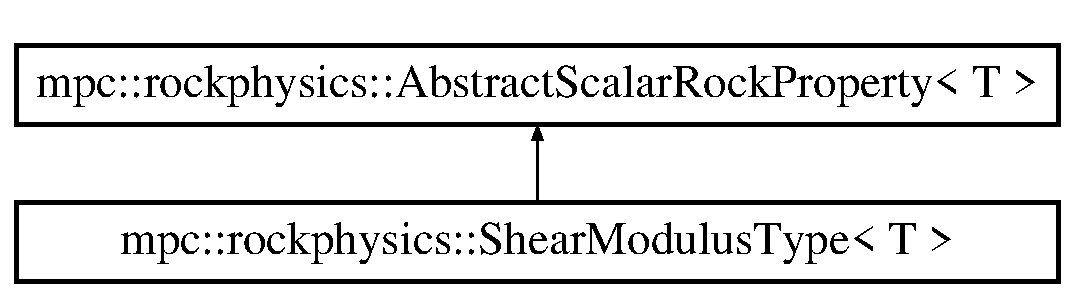
\includegraphics[height=2.000000cm]{structmpc_1_1rockphysics_1_1_shear_modulus_type}
\end{center}
\end{figure}
\subsection*{Public Member Functions}
\begin{DoxyCompactItemize}
\item 
constexpr \mbox{\hyperlink{structmpc_1_1rockphysics_1_1_shear_modulus_type_af7e48ef066d1142209abc498bba19f29}{Shear\+Modulus\+Type}} (T val)
\end{DoxyCompactItemize}
\subsection*{Additional Inherited Members}


\subsection{Detailed Description}
\subsubsection*{template$<$typename T$>$\newline
struct mpc\+::rockphysics\+::\+Shear\+Modulus\+Type$<$ T $>$}



Definition at line 44 of file rockphysicstransformstypes.\+hpp.



\subsection{Constructor \& Destructor Documentation}
\mbox{\Hypertarget{structmpc_1_1rockphysics_1_1_shear_modulus_type_af7e48ef066d1142209abc498bba19f29}\label{structmpc_1_1rockphysics_1_1_shear_modulus_type_af7e48ef066d1142209abc498bba19f29}} 
\index{mpc\+::rockphysics\+::\+Shear\+Modulus\+Type@{mpc\+::rockphysics\+::\+Shear\+Modulus\+Type}!Shear\+Modulus\+Type@{Shear\+Modulus\+Type}}
\index{Shear\+Modulus\+Type@{Shear\+Modulus\+Type}!mpc\+::rockphysics\+::\+Shear\+Modulus\+Type@{mpc\+::rockphysics\+::\+Shear\+Modulus\+Type}}
\subsubsection{\texorpdfstring{Shear\+Modulus\+Type()}{ShearModulusType()}}
{\footnotesize\ttfamily template$<$typename T$>$ \\
constexpr \mbox{\hyperlink{structmpc_1_1rockphysics_1_1_shear_modulus_type}{mpc\+::rockphysics\+::\+Shear\+Modulus\+Type}}$<$ T $>$\+::\mbox{\hyperlink{structmpc_1_1rockphysics_1_1_shear_modulus_type}{Shear\+Modulus\+Type}} (\begin{DoxyParamCaption}\item[{T}]{val }\end{DoxyParamCaption})\hspace{0.3cm}{\ttfamily [inline]}}



Definition at line 49 of file rockphysicstransformstypes.\+hpp.



The documentation for this struct was generated from the following file\+:\begin{DoxyCompactItemize}
\item 
/\+Users/atorlucci/\+Documents/github\+\_\+threecubed\+\_\+repos/mpc/src/mpc/rockphysics/\mbox{\hyperlink{rockphysicstransformstypes_8hpp}{rockphysicstransformstypes.\+hpp}}\end{DoxyCompactItemize}

\hypertarget{structmpc_1_1rockphysics_1_1_shear_wave_velocity_type}{}\section{mpc\+:\+:rockphysics\+:\+:Shear\+Wave\+Velocity\+Type$<$ T $>$ Struct Template Reference}
\label{structmpc_1_1rockphysics_1_1_shear_wave_velocity_type}\index{mpc\+::rockphysics\+::\+Shear\+Wave\+Velocity\+Type$<$ T $>$@{mpc\+::rockphysics\+::\+Shear\+Wave\+Velocity\+Type$<$ T $>$}}


{\ttfamily \#include $<$rockphysicstransformstypes.\+hpp$>$}

Inheritance diagram for mpc\+:\+:rockphysics\+:\+:Shear\+Wave\+Velocity\+Type$<$ T $>$\+:\begin{figure}[H]
\begin{center}
\leavevmode
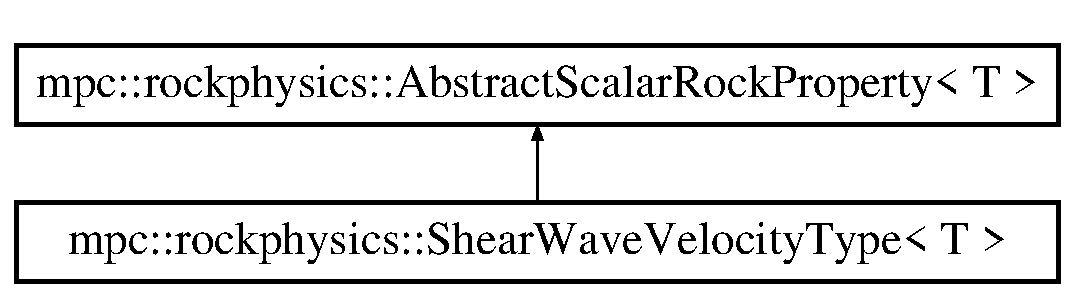
\includegraphics[height=2.000000cm]{structmpc_1_1rockphysics_1_1_shear_wave_velocity_type}
\end{center}
\end{figure}
\subsection*{Public Member Functions}
\begin{DoxyCompactItemize}
\item 
constexpr \mbox{\hyperlink{structmpc_1_1rockphysics_1_1_shear_wave_velocity_type_a33df4d42ef80ac6bbe7208a90df17a94}{Shear\+Wave\+Velocity\+Type}} (T val)
\end{DoxyCompactItemize}
\subsection*{Additional Inherited Members}


\subsection{Detailed Description}
\subsubsection*{template$<$typename T$>$\newline
struct mpc\+::rockphysics\+::\+Shear\+Wave\+Velocity\+Type$<$ T $>$}



Definition at line 193 of file rockphysicstransformstypes.\+hpp.



\subsection{Constructor \& Destructor Documentation}
\mbox{\Hypertarget{structmpc_1_1rockphysics_1_1_shear_wave_velocity_type_a33df4d42ef80ac6bbe7208a90df17a94}\label{structmpc_1_1rockphysics_1_1_shear_wave_velocity_type_a33df4d42ef80ac6bbe7208a90df17a94}} 
\index{mpc\+::rockphysics\+::\+Shear\+Wave\+Velocity\+Type@{mpc\+::rockphysics\+::\+Shear\+Wave\+Velocity\+Type}!Shear\+Wave\+Velocity\+Type@{Shear\+Wave\+Velocity\+Type}}
\index{Shear\+Wave\+Velocity\+Type@{Shear\+Wave\+Velocity\+Type}!mpc\+::rockphysics\+::\+Shear\+Wave\+Velocity\+Type@{mpc\+::rockphysics\+::\+Shear\+Wave\+Velocity\+Type}}
\subsubsection{\texorpdfstring{Shear\+Wave\+Velocity\+Type()}{ShearWaveVelocityType()}}
{\footnotesize\ttfamily template$<$typename T$>$ \\
constexpr \mbox{\hyperlink{structmpc_1_1rockphysics_1_1_shear_wave_velocity_type}{mpc\+::rockphysics\+::\+Shear\+Wave\+Velocity\+Type}}$<$ T $>$\+::\mbox{\hyperlink{structmpc_1_1rockphysics_1_1_shear_wave_velocity_type}{Shear\+Wave\+Velocity\+Type}} (\begin{DoxyParamCaption}\item[{T}]{val }\end{DoxyParamCaption})\hspace{0.3cm}{\ttfamily [inline]}}



Definition at line 198 of file rockphysicstransformstypes.\+hpp.



The documentation for this struct was generated from the following file\+:\begin{DoxyCompactItemize}
\item 
/\+Users/atorlucci/\+Documents/github\+\_\+threecubed\+\_\+repos/mpc/src/mpc/rockphysics/\mbox{\hyperlink{rockphysicstransformstypes_8hpp}{rockphysicstransformstypes.\+hpp}}\end{DoxyCompactItemize}

\hypertarget{classmpc_1_1rockphysics_1_1_solid_phase}{}\section{mpc\+:\+:rockphysics\+:\+:Solid\+Phase$<$ T $>$ Class Template Reference}
\label{classmpc_1_1rockphysics_1_1_solid_phase}\index{mpc\+::rockphysics\+::\+Solid\+Phase$<$ T $>$@{mpc\+::rockphysics\+::\+Solid\+Phase$<$ T $>$}}


{\ttfamily \#include $<$scalarcomposites.\+hpp$>$}

Inheritance diagram for mpc\+:\+:rockphysics\+:\+:Solid\+Phase$<$ T $>$\+:\begin{figure}[H]
\begin{center}
\leavevmode
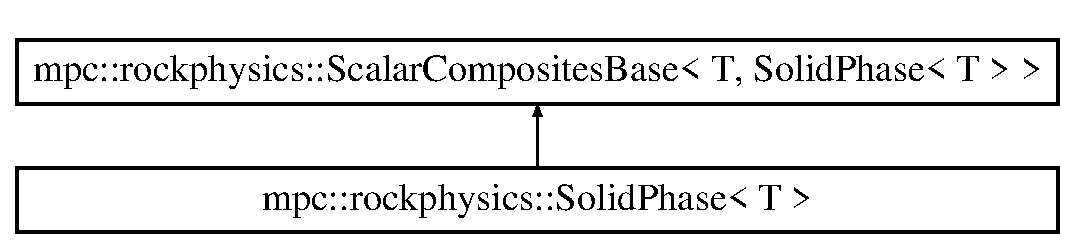
\includegraphics[height=2.000000cm]{classmpc_1_1rockphysics_1_1_solid_phase}
\end{center}
\end{figure}
\subsection*{Public Member Functions}
\begin{DoxyCompactItemize}
\item 
\mbox{\hyperlink{classmpc_1_1rockphysics_1_1_solid_phase_ad44503640c956a6c89cb71678dacd6b1}{Solid\+Phase}} (const std\+::vector$<$ std\+::tuple$<$ \mbox{\hyperlink{structmpc_1_1rockphysics_1_1_bulk_modulus_type}{mpc\+::rockphysics\+::\+Bulk\+Modulus\+Type}}$<$ T $>$, \mbox{\hyperlink{structmpc_1_1rockphysics_1_1_shear_modulus_type}{mpc\+::rockphysics\+::\+Shear\+Modulus\+Type}}$<$ T $>$, \mbox{\hyperlink{structmpc_1_1rockphysics_1_1_density_type}{mpc\+::rockphysics\+::\+Density\+Type}}$<$ T $>$, \mbox{\hyperlink{structmpc_1_1rockphysics_1_1_volume_fraction_type}{mpc\+::rockphysics\+::\+Volume\+Fraction\+Type}}$<$ T $>$ $>$ $>$ \&vec)
\end{DoxyCompactItemize}
\subsection*{Static Public Member Functions}
\begin{DoxyCompactItemize}
\item 
static std\+::tuple$<$ \mbox{\hyperlink{structmpc_1_1rockphysics_1_1_bulk_modulus_type}{mpc\+::rockphysics\+::\+Bulk\+Modulus\+Type}}$<$ T $>$, \mbox{\hyperlink{structmpc_1_1rockphysics_1_1_shear_modulus_type}{mpc\+::rockphysics\+::\+Shear\+Modulus\+Type}}$<$ T $>$, \mbox{\hyperlink{structmpc_1_1rockphysics_1_1_density_type}{mpc\+::rockphysics\+::\+Density\+Type}}$<$ T $>$ $>$ \mbox{\hyperlink{classmpc_1_1rockphysics_1_1_solid_phase_ae8dbd8e5777a51515f84f6fb7e87ba97}{Effective\+Values}} (const std\+::vector$<$ \mbox{\hyperlink{structmpc_1_1rockphysics_1_1_bulk_modulus_type}{mpc\+::rockphysics\+::\+Bulk\+Modulus\+Type}}$<$ T $>$ $>$ \&K\+\_\+vec, const std\+::vector$<$ \mbox{\hyperlink{structmpc_1_1rockphysics_1_1_shear_modulus_type}{mpc\+::rockphysics\+::\+Shear\+Modulus\+Type}}$<$ T $>$ $>$ \&mu\+\_\+vec, const std\+::vector$<$ \mbox{\hyperlink{structmpc_1_1rockphysics_1_1_density_type}{mpc\+::rockphysics\+::\+Density\+Type}}$<$ T $>$ $>$ \&rho\+\_\+vec, const std\+::vector$<$ \mbox{\hyperlink{structmpc_1_1rockphysics_1_1_volume_fraction_type}{mpc\+::rockphysics\+::\+Volume\+Fraction\+Type}}$<$ T $>$ $>$ \&vf\+\_\+vec)
\end{DoxyCompactItemize}
\subsection*{Additional Inherited Members}


\subsection{Detailed Description}
\subsubsection*{template$<$typename T$>$\newline
class mpc\+::rockphysics\+::\+Solid\+Phase$<$ T $>$}



Definition at line 384 of file scalarcomposites.\+hpp.



\subsection{Constructor \& Destructor Documentation}
\mbox{\Hypertarget{classmpc_1_1rockphysics_1_1_solid_phase_ad44503640c956a6c89cb71678dacd6b1}\label{classmpc_1_1rockphysics_1_1_solid_phase_ad44503640c956a6c89cb71678dacd6b1}} 
\index{mpc\+::rockphysics\+::\+Solid\+Phase@{mpc\+::rockphysics\+::\+Solid\+Phase}!Solid\+Phase@{Solid\+Phase}}
\index{Solid\+Phase@{Solid\+Phase}!mpc\+::rockphysics\+::\+Solid\+Phase@{mpc\+::rockphysics\+::\+Solid\+Phase}}
\subsubsection{\texorpdfstring{Solid\+Phase()}{SolidPhase()}}
{\footnotesize\ttfamily template$<$typename T $>$ \\
\mbox{\hyperlink{classmpc_1_1rockphysics_1_1_solid_phase}{mpc\+::rockphysics\+::\+Solid\+Phase}}$<$ T $>$\+::\mbox{\hyperlink{classmpc_1_1rockphysics_1_1_solid_phase}{Solid\+Phase}} (\begin{DoxyParamCaption}\item[{const std\+::vector$<$ std\+::tuple$<$ \mbox{\hyperlink{structmpc_1_1rockphysics_1_1_bulk_modulus_type}{mpc\+::rockphysics\+::\+Bulk\+Modulus\+Type}}$<$ T $>$, \mbox{\hyperlink{structmpc_1_1rockphysics_1_1_shear_modulus_type}{mpc\+::rockphysics\+::\+Shear\+Modulus\+Type}}$<$ T $>$, \mbox{\hyperlink{structmpc_1_1rockphysics_1_1_density_type}{mpc\+::rockphysics\+::\+Density\+Type}}$<$ T $>$, \mbox{\hyperlink{structmpc_1_1rockphysics_1_1_volume_fraction_type}{mpc\+::rockphysics\+::\+Volume\+Fraction\+Type}}$<$ T $>$ $>$ $>$ \&}]{vec }\end{DoxyParamCaption})\hspace{0.3cm}{\ttfamily [inline]}}



Definition at line 398 of file scalarcomposites.\+hpp.



\subsection{Member Function Documentation}
\mbox{\Hypertarget{classmpc_1_1rockphysics_1_1_solid_phase_ae8dbd8e5777a51515f84f6fb7e87ba97}\label{classmpc_1_1rockphysics_1_1_solid_phase_ae8dbd8e5777a51515f84f6fb7e87ba97}} 
\index{mpc\+::rockphysics\+::\+Solid\+Phase@{mpc\+::rockphysics\+::\+Solid\+Phase}!Effective\+Values@{Effective\+Values}}
\index{Effective\+Values@{Effective\+Values}!mpc\+::rockphysics\+::\+Solid\+Phase@{mpc\+::rockphysics\+::\+Solid\+Phase}}
\subsubsection{\texorpdfstring{Effective\+Values()}{EffectiveValues()}}
{\footnotesize\ttfamily template$<$typename T $>$ \\
static std\+::tuple$<$\mbox{\hyperlink{structmpc_1_1rockphysics_1_1_bulk_modulus_type}{mpc\+::rockphysics\+::\+Bulk\+Modulus\+Type}}$<$T$>$, \mbox{\hyperlink{structmpc_1_1rockphysics_1_1_shear_modulus_type}{mpc\+::rockphysics\+::\+Shear\+Modulus\+Type}}$<$T$>$, \mbox{\hyperlink{structmpc_1_1rockphysics_1_1_density_type}{mpc\+::rockphysics\+::\+Density\+Type}}$<$T$>$ $>$ \mbox{\hyperlink{classmpc_1_1rockphysics_1_1_solid_phase}{mpc\+::rockphysics\+::\+Solid\+Phase}}$<$ T $>$\+::Effective\+Values (\begin{DoxyParamCaption}\item[{const std\+::vector$<$ \mbox{\hyperlink{structmpc_1_1rockphysics_1_1_bulk_modulus_type}{mpc\+::rockphysics\+::\+Bulk\+Modulus\+Type}}$<$ T $>$ $>$ \&}]{K\+\_\+vec,  }\item[{const std\+::vector$<$ \mbox{\hyperlink{structmpc_1_1rockphysics_1_1_shear_modulus_type}{mpc\+::rockphysics\+::\+Shear\+Modulus\+Type}}$<$ T $>$ $>$ \&}]{mu\+\_\+vec,  }\item[{const std\+::vector$<$ \mbox{\hyperlink{structmpc_1_1rockphysics_1_1_density_type}{mpc\+::rockphysics\+::\+Density\+Type}}$<$ T $>$ $>$ \&}]{rho\+\_\+vec,  }\item[{const std\+::vector$<$ \mbox{\hyperlink{structmpc_1_1rockphysics_1_1_volume_fraction_type}{mpc\+::rockphysics\+::\+Volume\+Fraction\+Type}}$<$ T $>$ $>$ \&}]{vf\+\_\+vec }\end{DoxyParamCaption})\hspace{0.3cm}{\ttfamily [inline]}, {\ttfamily [static]}}



Definition at line 401 of file scalarcomposites.\+hpp.



The documentation for this class was generated from the following file\+:\begin{DoxyCompactItemize}
\item 
/\+Users/atorlucci/\+Documents/github\+\_\+threecubed\+\_\+repos/mpc/src/mpc/rockphysics/\mbox{\hyperlink{scalarcomposites_8hpp}{scalarcomposites.\+hpp}}\end{DoxyCompactItemize}

\hypertarget{structmpc_1_1utilities_1_1_spherical_coordinate_type}{}\section{mpc\+:\+:utilities\+:\+:Spherical\+Coordinate\+Type Struct Reference}
\label{structmpc_1_1utilities_1_1_spherical_coordinate_type}\index{mpc\+::utilities\+::\+Spherical\+Coordinate\+Type@{mpc\+::utilities\+::\+Spherical\+Coordinate\+Type}}


{\ttfamily \#include $<$coordinatemapping.\+hpp$>$}

Inheritance diagram for mpc\+:\+:utilities\+:\+:Spherical\+Coordinate\+Type\+:\begin{figure}[H]
\begin{center}
\leavevmode
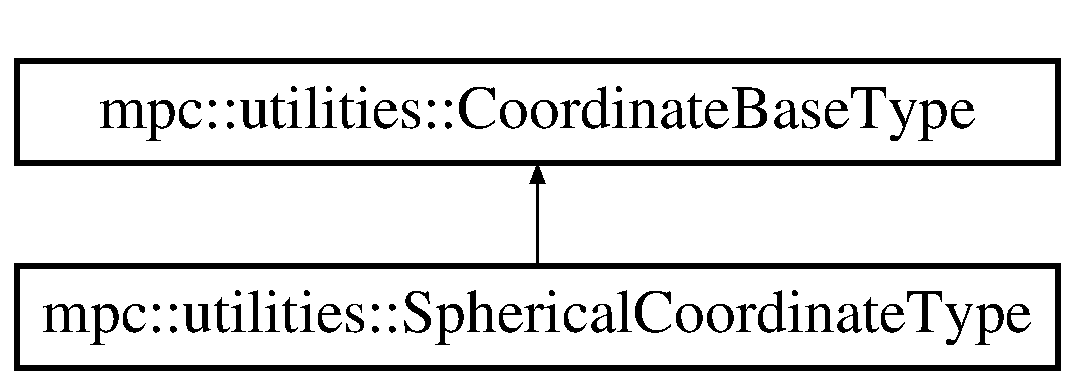
\includegraphics[height=2.000000cm]{structmpc_1_1utilities_1_1_spherical_coordinate_type}
\end{center}
\end{figure}


\subsection{Detailed Description}


Definition at line 27 of file coordinatemapping.\+hpp.



The documentation for this struct was generated from the following file\+:\begin{DoxyCompactItemize}
\item 
/\+Users/atorlucci/\+Documents/github\+\_\+threecubed\+\_\+repos/mpc/src/mpc/utilities/\mbox{\hyperlink{coordinatemapping_8hpp}{coordinatemapping.\+hpp}}\end{DoxyCompactItemize}

\hypertarget{structmpc_1_1core_1_1_stiffness_from_compliance_function_object}{}\section{mpc\+:\+:core\+:\+:Stiffness\+From\+Compliance\+Function\+Object$<$ T, S $>$ Class Template Reference}
\label{structmpc_1_1core_1_1_stiffness_from_compliance_function_object}\index{mpc\+::core\+::\+Stiffness\+From\+Compliance\+Function\+Object$<$ T, S $>$@{mpc\+::core\+::\+Stiffness\+From\+Compliance\+Function\+Object$<$ T, S $>$}}


function object for calculating the stiffness tensor components from the compliance tensor components  




{\ttfamily \#include $<$csrelationship.\+hpp$>$}

\subsection*{Public Member Functions}
\begin{DoxyCompactItemize}
\item 
\mbox{\hyperlink{structmpc_1_1core_1_1_stiffness_tensor}{mpc\+::core\+::\+Stiffness\+Tensor}}$<$ T $>$ \mbox{\hyperlink{structmpc_1_1core_1_1_stiffness_from_compliance_function_object_addf243fde9b4ad271c7ab37bedea199c}{operator()}} (const \mbox{\hyperlink{structmpc_1_1core_1_1_compliance_tensor}{mpc\+::core\+::\+Compliance\+Tensor}}$<$ T $>$ \&s\+\_\+ijkl)
\end{DoxyCompactItemize}


\subsection{Detailed Description}
\subsubsection*{template$<$typename T, typename S = mpc\+::core\+::\+None\+Symmetry\+Group\+Type$>$\newline
class mpc\+::core\+::\+Stiffness\+From\+Compliance\+Function\+Object$<$ T, S $>$}

function object for calculating the stiffness tensor components from the compliance tensor components 

T\+O\+DO\+: more details... 

Definition at line 37 of file csrelationship.\+hpp.



\subsection{Member Function Documentation}
\mbox{\Hypertarget{structmpc_1_1core_1_1_stiffness_from_compliance_function_object_addf243fde9b4ad271c7ab37bedea199c}\label{structmpc_1_1core_1_1_stiffness_from_compliance_function_object_addf243fde9b4ad271c7ab37bedea199c}} 
\index{mpc\+::core\+::\+Stiffness\+From\+Compliance\+Function\+Object@{mpc\+::core\+::\+Stiffness\+From\+Compliance\+Function\+Object}!operator()@{operator()}}
\index{operator()@{operator()}!mpc\+::core\+::\+Stiffness\+From\+Compliance\+Function\+Object@{mpc\+::core\+::\+Stiffness\+From\+Compliance\+Function\+Object}}
\subsubsection{\texorpdfstring{operator()()}{operator()()}}
{\footnotesize\ttfamily template$<$typename T, typename S = mpc\+::core\+::\+None\+Symmetry\+Group\+Type$>$ \\
\mbox{\hyperlink{structmpc_1_1core_1_1_stiffness_tensor}{mpc\+::core\+::\+Stiffness\+Tensor}}$<$T$>$ \mbox{\hyperlink{structmpc_1_1core_1_1_stiffness_from_compliance_function_object}{mpc\+::core\+::\+Stiffness\+From\+Compliance\+Function\+Object}}$<$ T, S $>$\+::operator() (\begin{DoxyParamCaption}\item[{const \mbox{\hyperlink{structmpc_1_1core_1_1_compliance_tensor}{mpc\+::core\+::\+Compliance\+Tensor}}$<$ T $>$ \&}]{s\+\_\+ijkl }\end{DoxyParamCaption})\hspace{0.3cm}{\ttfamily [inline]}}



Definition at line 46 of file csrelationship.\+hpp.



The documentation for this class was generated from the following file\+:\begin{DoxyCompactItemize}
\item 
/\+Users/atorlucci/\+Documents/github\+\_\+threecubed\+\_\+repos/mpc/src/mpc/core/\mbox{\hyperlink{csrelationship_8hpp}{csrelationship.\+hpp}}\end{DoxyCompactItemize}

\hypertarget{structmpc_1_1core_1_1_stiffness_tensor}{}\section{mpc\+:\+:core\+:\+:Stiffness\+Tensor$<$ T $>$ Class Template Reference}
\label{structmpc_1_1core_1_1_stiffness_tensor}\index{mpc\+::core\+::\+Stiffness\+Tensor$<$ T $>$@{mpc\+::core\+::\+Stiffness\+Tensor$<$ T $>$}}


stiffness tensor class with function to set the components with a given symmety type  




{\ttfamily \#include $<$stiffnesscompliance.\+hpp$>$}

Inheritance diagram for mpc\+:\+:core\+:\+:Stiffness\+Tensor$<$ T $>$\+:\begin{figure}[H]
\begin{center}
\leavevmode
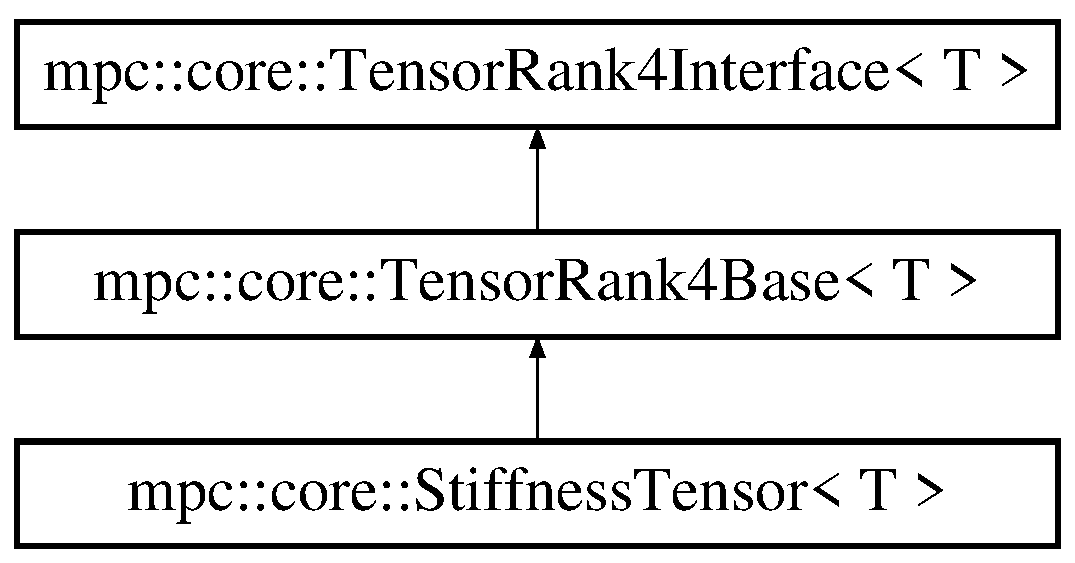
\includegraphics[height=3.000000cm]{structmpc_1_1core_1_1_stiffness_tensor}
\end{center}
\end{figure}
\subsection*{Public Types}
\begin{DoxyCompactItemize}
\item 
typedef \mbox{\hyperlink{structmpc_1_1core_1_1_stiffness_type}{mpc\+::core\+::\+Stiffness\+Type}} \mbox{\hyperlink{structmpc_1_1core_1_1_stiffness_tensor_ad8129e50fb9d974c0ba792d8b17b203a}{cstype}}
\end{DoxyCompactItemize}
\subsection*{Public Member Functions}
\begin{DoxyCompactItemize}
\item 
{\footnotesize template$<$typename S $>$ }\\void \mbox{\hyperlink{structmpc_1_1core_1_1_stiffness_tensor_af86bb5adbcc6bb3df1ed6bfabb8fde91}{Set\+Components\+With\+Symmetry}} (std\+::set$<$ \mbox{\hyperlink{namespacempc_1_1core_ac3a232afc7c680d580628e834030482f}{mpc\+::core\+::\+Tensor\+Rank4\+Component}}$<$ T $>$ $>$ \&components)
\end{DoxyCompactItemize}
\subsection*{Additional Inherited Members}


\subsection{Detailed Description}
\subsubsection*{template$<$typename T$>$\newline
class mpc\+::core\+::\+Stiffness\+Tensor$<$ T $>$}

stiffness tensor class with function to set the components with a given symmety type 

Definition at line 58 of file stiffnesscompliance.\+hpp.



\subsection{Member Typedef Documentation}
\mbox{\Hypertarget{structmpc_1_1core_1_1_stiffness_tensor_ad8129e50fb9d974c0ba792d8b17b203a}\label{structmpc_1_1core_1_1_stiffness_tensor_ad8129e50fb9d974c0ba792d8b17b203a}} 
\index{mpc\+::core\+::\+Stiffness\+Tensor@{mpc\+::core\+::\+Stiffness\+Tensor}!cstype@{cstype}}
\index{cstype@{cstype}!mpc\+::core\+::\+Stiffness\+Tensor@{mpc\+::core\+::\+Stiffness\+Tensor}}
\subsubsection{\texorpdfstring{cstype}{cstype}}
{\footnotesize\ttfamily template$<$typename T$>$ \\
typedef \mbox{\hyperlink{structmpc_1_1core_1_1_stiffness_type}{mpc\+::core\+::\+Stiffness\+Type}} \mbox{\hyperlink{structmpc_1_1core_1_1_stiffness_tensor}{mpc\+::core\+::\+Stiffness\+Tensor}}$<$ T $>$\+::\mbox{\hyperlink{structmpc_1_1core_1_1_stiffness_tensor_ad8129e50fb9d974c0ba792d8b17b203a}{cstype}}}



Definition at line 60 of file stiffnesscompliance.\+hpp.



\subsection{Member Function Documentation}
\mbox{\Hypertarget{structmpc_1_1core_1_1_stiffness_tensor_af86bb5adbcc6bb3df1ed6bfabb8fde91}\label{structmpc_1_1core_1_1_stiffness_tensor_af86bb5adbcc6bb3df1ed6bfabb8fde91}} 
\index{mpc\+::core\+::\+Stiffness\+Tensor@{mpc\+::core\+::\+Stiffness\+Tensor}!Set\+Components\+With\+Symmetry@{Set\+Components\+With\+Symmetry}}
\index{Set\+Components\+With\+Symmetry@{Set\+Components\+With\+Symmetry}!mpc\+::core\+::\+Stiffness\+Tensor@{mpc\+::core\+::\+Stiffness\+Tensor}}
\subsubsection{\texorpdfstring{Set\+Components\+With\+Symmetry()}{SetComponentsWithSymmetry()}}
{\footnotesize\ttfamily template$<$typename T$>$ \\
template$<$typename S $>$ \\
void \mbox{\hyperlink{structmpc_1_1core_1_1_stiffness_tensor}{mpc\+::core\+::\+Stiffness\+Tensor}}$<$ T $>$\+::Set\+Components\+With\+Symmetry (\begin{DoxyParamCaption}\item[{std\+::set$<$ \mbox{\hyperlink{namespacempc_1_1core_ac3a232afc7c680d580628e834030482f}{mpc\+::core\+::\+Tensor\+Rank4\+Component}}$<$ T $>$ $>$ \&}]{components }\end{DoxyParamCaption})\hspace{0.3cm}{\ttfamily [inline]}}



Definition at line 63 of file stiffnesscompliance.\+hpp.



The documentation for this class was generated from the following file\+:\begin{DoxyCompactItemize}
\item 
/\+Users/atorlucci/\+Documents/github\+\_\+threecubed\+\_\+repos/mpc/src/mpc/core/\mbox{\hyperlink{stiffnesscompliance_8hpp}{stiffnesscompliance.\+hpp}}\end{DoxyCompactItemize}

\hypertarget{structmpc_1_1core_1_1_stiffness_type}{}\section{mpc\+:\+:core\+:\+:Stiffness\+Type Class Reference}
\label{structmpc_1_1core_1_1_stiffness_type}\index{mpc\+::core\+::\+Stiffness\+Type@{mpc\+::core\+::\+Stiffness\+Type}}


simple class used mainly for template specializations in mpc  




{\ttfamily \#include $<$cstypes.\+hpp$>$}

Inheritance diagram for mpc\+:\+:core\+:\+:Stiffness\+Type\+:\begin{figure}[H]
\begin{center}
\leavevmode
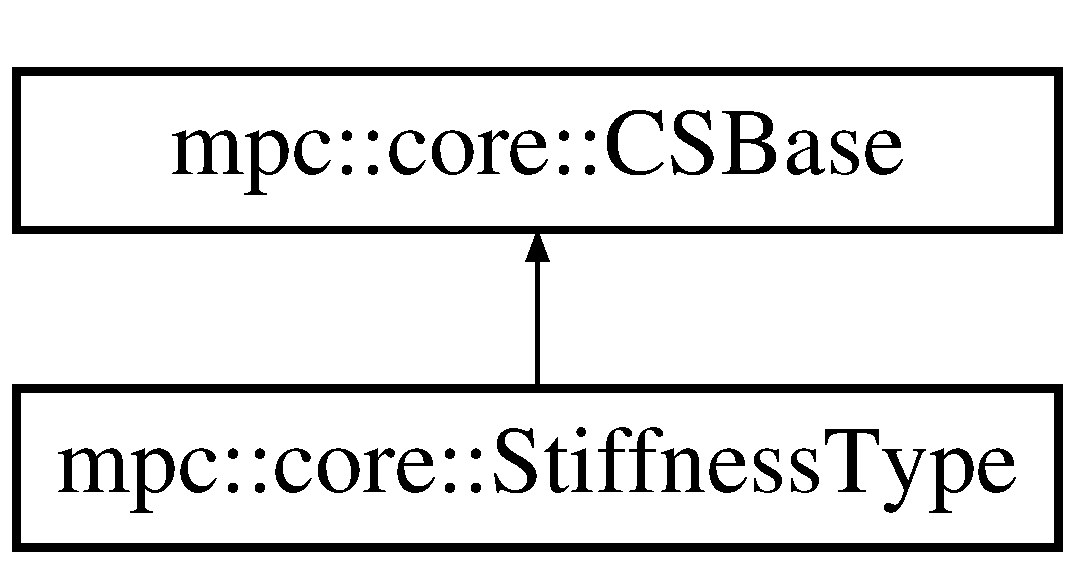
\includegraphics[height=2.000000cm]{structmpc_1_1core_1_1_stiffness_type}
\end{center}
\end{figure}
\subsection*{Static Public Member Functions}
\begin{DoxyCompactItemize}
\item 
static constexpr \mbox{\hyperlink{namespacempc_1_1core_ad3e8e7d43bfc9202d954d999f7d5c991}{C\+S\+Enumeration}} \mbox{\hyperlink{structmpc_1_1core_1_1_stiffness_type_a29224ca8f2111b45e79b0b2179104347}{C\+S\+Enum}} ()
\end{DoxyCompactItemize}
\subsection*{Public Attributes}
\begin{DoxyCompactItemize}
\item 
const \mbox{\hyperlink{namespacempc_1_1core_ad3e8e7d43bfc9202d954d999f7d5c991}{C\+S\+Enumeration}} \mbox{\hyperlink{structmpc_1_1core_1_1_stiffness_type_aaa2009a4b1aaebb597f2ac96a7d587bf}{cs\+\_\+enumeration}} = \mbox{\hyperlink{namespacempc_1_1core_ad3e8e7d43bfc9202d954d999f7d5c991aa231c1d74fe18f9e82224588887d1971}{C\+S\+Enumeration\+::\+S\+T\+I\+F\+F\+N\+E\+SS}}
\end{DoxyCompactItemize}


\subsection{Detailed Description}
simple class used mainly for template specializations in mpc 

Definition at line 77 of file cstypes.\+hpp.



\subsection{Member Function Documentation}
\mbox{\Hypertarget{structmpc_1_1core_1_1_stiffness_type_a29224ca8f2111b45e79b0b2179104347}\label{structmpc_1_1core_1_1_stiffness_type_a29224ca8f2111b45e79b0b2179104347}} 
\index{mpc\+::core\+::\+Stiffness\+Type@{mpc\+::core\+::\+Stiffness\+Type}!C\+S\+Enum@{C\+S\+Enum}}
\index{C\+S\+Enum@{C\+S\+Enum}!mpc\+::core\+::\+Stiffness\+Type@{mpc\+::core\+::\+Stiffness\+Type}}
\subsubsection{\texorpdfstring{C\+S\+Enum()}{CSEnum()}}
{\footnotesize\ttfamily static constexpr \mbox{\hyperlink{namespacempc_1_1core_ad3e8e7d43bfc9202d954d999f7d5c991}{C\+S\+Enumeration}} mpc\+::core\+::\+Stiffness\+Type\+::\+C\+S\+Enum (\begin{DoxyParamCaption}{ }\end{DoxyParamCaption})\hspace{0.3cm}{\ttfamily [inline]}, {\ttfamily [static]}}



Definition at line 79 of file cstypes.\+hpp.



\subsection{Member Data Documentation}
\mbox{\Hypertarget{structmpc_1_1core_1_1_stiffness_type_aaa2009a4b1aaebb597f2ac96a7d587bf}\label{structmpc_1_1core_1_1_stiffness_type_aaa2009a4b1aaebb597f2ac96a7d587bf}} 
\index{mpc\+::core\+::\+Stiffness\+Type@{mpc\+::core\+::\+Stiffness\+Type}!cs\+\_\+enumeration@{cs\+\_\+enumeration}}
\index{cs\+\_\+enumeration@{cs\+\_\+enumeration}!mpc\+::core\+::\+Stiffness\+Type@{mpc\+::core\+::\+Stiffness\+Type}}
\subsubsection{\texorpdfstring{cs\+\_\+enumeration}{cs\_enumeration}}
{\footnotesize\ttfamily const \mbox{\hyperlink{namespacempc_1_1core_ad3e8e7d43bfc9202d954d999f7d5c991}{C\+S\+Enumeration}} mpc\+::core\+::\+Stiffness\+Type\+::cs\+\_\+enumeration = \mbox{\hyperlink{namespacempc_1_1core_ad3e8e7d43bfc9202d954d999f7d5c991aa231c1d74fe18f9e82224588887d1971}{C\+S\+Enumeration\+::\+S\+T\+I\+F\+F\+N\+E\+SS}}}



Definition at line 78 of file cstypes.\+hpp.



The documentation for this class was generated from the following file\+:\begin{DoxyCompactItemize}
\item 
/\+Users/atorlucci/\+Documents/github\+\_\+threecubed\+\_\+repos/mpc/src/mpc/core/\mbox{\hyperlink{cstypes_8hpp}{cstypes.\+hpp}}\end{DoxyCompactItemize}

\hypertarget{structmpc_1_1core_1_1_strain_tensor}{}\section{mpc\+:\+:core\+:\+:Strain\+Tensor$<$ T $>$ Class Template Reference}
\label{structmpc_1_1core_1_1_strain_tensor}\index{mpc\+::core\+::\+Strain\+Tensor$<$ T $>$@{mpc\+::core\+::\+Strain\+Tensor$<$ T $>$}}


strain tensor class with function to set the components  




{\ttfamily \#include $<$stressstrain.\+hpp$>$}

Inheritance diagram for mpc\+:\+:core\+:\+:Strain\+Tensor$<$ T $>$\+:\begin{figure}[H]
\begin{center}
\leavevmode
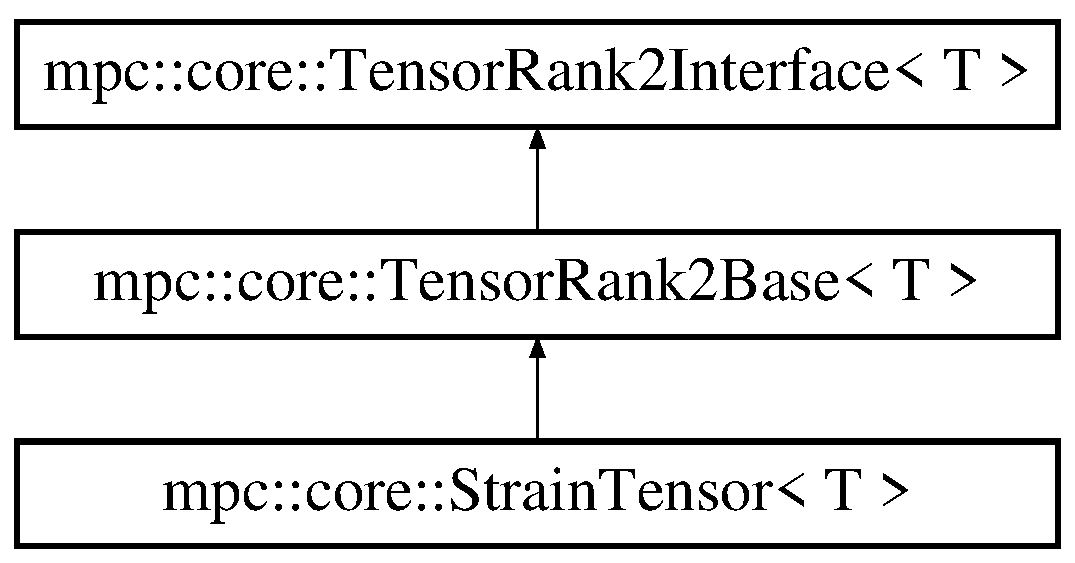
\includegraphics[height=3.000000cm]{structmpc_1_1core_1_1_strain_tensor}
\end{center}
\end{figure}
\subsection*{Public Member Functions}
\begin{DoxyCompactItemize}
\item 
void \mbox{\hyperlink{structmpc_1_1core_1_1_strain_tensor_a9e208aa77d77296f5fc6fdadd76b018f}{Set\+Components}} (std\+::set$<$ \mbox{\hyperlink{namespacempc_1_1core_a467e1fa517a8c269b033fef3aa281360}{mpc\+::core\+::\+Tensor\+Rank2\+Component}}$<$ T $>$ $>$ \&components, bool Apply\+Symmetry=false)
\begin{DoxyCompactList}\small\item\em set the components of the underlying tensor data member \end{DoxyCompactList}\end{DoxyCompactItemize}
\subsection*{Additional Inherited Members}


\subsection{Detailed Description}
\subsubsection*{template$<$typename T$>$\newline
class mpc\+::core\+::\+Strain\+Tensor$<$ T $>$}

strain tensor class with function to set the components 

Definition at line 96 of file stressstrain.\+hpp.



\subsection{Member Function Documentation}
\mbox{\Hypertarget{structmpc_1_1core_1_1_strain_tensor_a9e208aa77d77296f5fc6fdadd76b018f}\label{structmpc_1_1core_1_1_strain_tensor_a9e208aa77d77296f5fc6fdadd76b018f}} 
\index{mpc\+::core\+::\+Strain\+Tensor@{mpc\+::core\+::\+Strain\+Tensor}!Set\+Components@{Set\+Components}}
\index{Set\+Components@{Set\+Components}!mpc\+::core\+::\+Strain\+Tensor@{mpc\+::core\+::\+Strain\+Tensor}}
\subsubsection{\texorpdfstring{Set\+Components()}{SetComponents()}}
{\footnotesize\ttfamily template$<$typename T$>$ \\
void \mbox{\hyperlink{structmpc_1_1core_1_1_strain_tensor}{mpc\+::core\+::\+Strain\+Tensor}}$<$ T $>$\+::Set\+Components (\begin{DoxyParamCaption}\item[{std\+::set$<$ \mbox{\hyperlink{namespacempc_1_1core_a467e1fa517a8c269b033fef3aa281360}{mpc\+::core\+::\+Tensor\+Rank2\+Component}}$<$ T $>$ $>$ \&}]{components,  }\item[{bool}]{Apply\+Symmetry = {\ttfamily false} }\end{DoxyParamCaption})\hspace{0.3cm}{\ttfamily [inline]}, {\ttfamily [virtual]}}



set the components of the underlying tensor data member 



Implements \mbox{\hyperlink{structmpc_1_1core_1_1_tensor_rank2_interface_a7d220631fe32f06ec52e5724873a00d9}{mpc\+::core\+::\+Tensor\+Rank2\+Interface$<$ T $>$}}.



Definition at line 103 of file stressstrain.\+hpp.



The documentation for this class was generated from the following file\+:\begin{DoxyCompactItemize}
\item 
/\+Users/atorlucci/\+Documents/github\+\_\+threecubed\+\_\+repos/mpc/src/mpc/core/\mbox{\hyperlink{stressstrain_8hpp}{stressstrain.\+hpp}}\end{DoxyCompactItemize}

\hypertarget{structmpc_1_1core_1_1_stress_tensor}{}\section{mpc\+:\+:core\+:\+:Stress\+Tensor$<$ T $>$ Class Template Reference}
\label{structmpc_1_1core_1_1_stress_tensor}\index{mpc\+::core\+::\+Stress\+Tensor$<$ T $>$@{mpc\+::core\+::\+Stress\+Tensor$<$ T $>$}}


stress tensor class with function to set the components  




{\ttfamily \#include $<$stressstrain.\+hpp$>$}

Inheritance diagram for mpc\+:\+:core\+:\+:Stress\+Tensor$<$ T $>$\+:\begin{figure}[H]
\begin{center}
\leavevmode
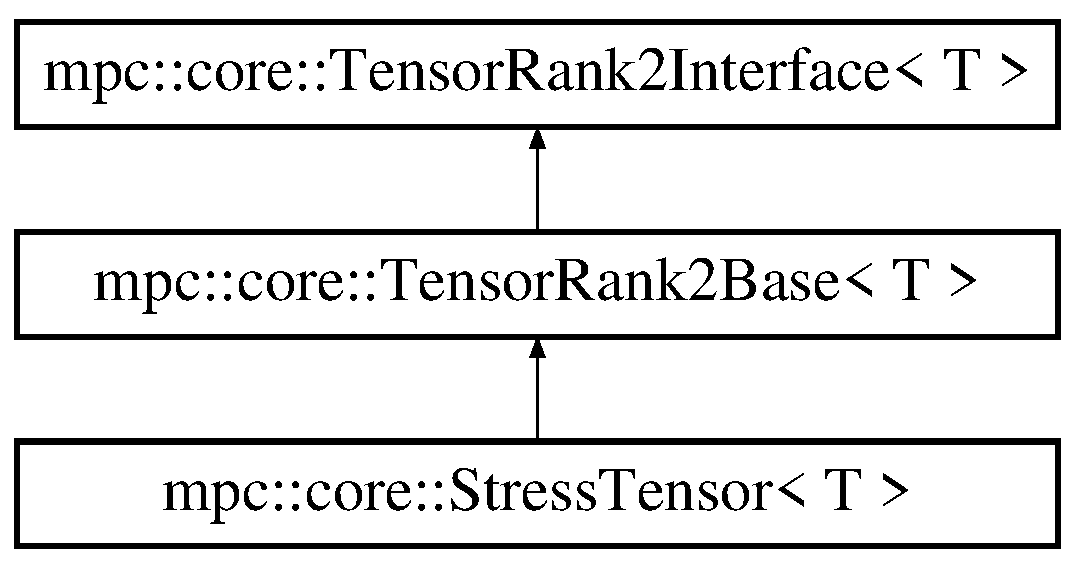
\includegraphics[height=3.000000cm]{structmpc_1_1core_1_1_stress_tensor}
\end{center}
\end{figure}
\subsection*{Public Member Functions}
\begin{DoxyCompactItemize}
\item 
void \mbox{\hyperlink{structmpc_1_1core_1_1_stress_tensor_afbac9aaa45907cdbed3ed779b0551bad}{Set\+Components}} (std\+::set$<$ \mbox{\hyperlink{namespacempc_1_1core_a467e1fa517a8c269b033fef3aa281360}{mpc\+::core\+::\+Tensor\+Rank2\+Component}}$<$ T $>$ $>$ \&components, bool Apply\+Symmetry=false)
\begin{DoxyCompactList}\small\item\em set the components of the underlying tensor data member \end{DoxyCompactList}\end{DoxyCompactItemize}
\subsection*{Additional Inherited Members}


\subsection{Detailed Description}
\subsubsection*{template$<$typename T$>$\newline
class mpc\+::core\+::\+Stress\+Tensor$<$ T $>$}

stress tensor class with function to set the components 

Definition at line 55 of file stressstrain.\+hpp.



\subsection{Member Function Documentation}
\mbox{\Hypertarget{structmpc_1_1core_1_1_stress_tensor_afbac9aaa45907cdbed3ed779b0551bad}\label{structmpc_1_1core_1_1_stress_tensor_afbac9aaa45907cdbed3ed779b0551bad}} 
\index{mpc\+::core\+::\+Stress\+Tensor@{mpc\+::core\+::\+Stress\+Tensor}!Set\+Components@{Set\+Components}}
\index{Set\+Components@{Set\+Components}!mpc\+::core\+::\+Stress\+Tensor@{mpc\+::core\+::\+Stress\+Tensor}}
\subsubsection{\texorpdfstring{Set\+Components()}{SetComponents()}}
{\footnotesize\ttfamily template$<$typename T$>$ \\
void \mbox{\hyperlink{structmpc_1_1core_1_1_stress_tensor}{mpc\+::core\+::\+Stress\+Tensor}}$<$ T $>$\+::Set\+Components (\begin{DoxyParamCaption}\item[{std\+::set$<$ \mbox{\hyperlink{namespacempc_1_1core_a467e1fa517a8c269b033fef3aa281360}{mpc\+::core\+::\+Tensor\+Rank2\+Component}}$<$ T $>$ $>$ \&}]{components,  }\item[{bool}]{Apply\+Symmetry = {\ttfamily false} }\end{DoxyParamCaption})\hspace{0.3cm}{\ttfamily [inline]}, {\ttfamily [virtual]}}



set the components of the underlying tensor data member 



Implements \mbox{\hyperlink{structmpc_1_1core_1_1_tensor_rank2_interface_a7d220631fe32f06ec52e5724873a00d9}{mpc\+::core\+::\+Tensor\+Rank2\+Interface$<$ T $>$}}.



Definition at line 62 of file stressstrain.\+hpp.



The documentation for this class was generated from the following file\+:\begin{DoxyCompactItemize}
\item 
/\+Users/atorlucci/\+Documents/github\+\_\+threecubed\+\_\+repos/mpc/src/mpc/core/\mbox{\hyperlink{stressstrain_8hpp}{stressstrain.\+hpp}}\end{DoxyCompactItemize}

\hypertarget{structmpc_1_1core_1_1_symmetry_component_dual_link_function_object}{}\section{mpc\+:\+:core\+:\+:Symmetry\+Component\+Dual\+Link\+Function\+Object$<$ T, M, N, P, Q, R, S $>$ Class Template Reference}
\label{structmpc_1_1core_1_1_symmetry_component_dual_link_function_object}\index{mpc\+::core\+::\+Symmetry\+Component\+Dual\+Link\+Function\+Object$<$ T, M, N, P, Q, R, S $>$@{mpc\+::core\+::\+Symmetry\+Component\+Dual\+Link\+Function\+Object$<$ T, M, N, P, Q, R, S $>$}}


class to resolve components in the stiffness or compliance tensor that are related to two other components  




{\ttfamily \#include $<$symmetrycomponents.\+hpp$>$}

\subsection*{Public Member Functions}
\begin{DoxyCompactItemize}
\item 
std\+::tuple$<$ \mbox{\hyperlink{classmpc_1_1core_1_1_tensor_rank_n_component}{mpc\+::core\+::\+Tensor\+Rank\+N\+Component}}$<$ T, 4 $>$, \mbox{\hyperlink{classmpc_1_1core_1_1_tensor_rank_n_component}{mpc\+::core\+::\+Tensor\+Rank\+N\+Component}}$<$ T, 4 $>$, \mbox{\hyperlink{classmpc_1_1core_1_1_tensor_rank_n_component}{mpc\+::core\+::\+Tensor\+Rank\+N\+Component}}$<$ T, 4 $>$ $>$ \mbox{\hyperlink{structmpc_1_1core_1_1_symmetry_component_dual_link_function_object_a7dfea4f0c6734f22299495c5d0e92ef7}{operator()}} (std\+::set$<$ \mbox{\hyperlink{classmpc_1_1core_1_1_tensor_rank_n_component}{mpc\+::core\+::\+Tensor\+Rank\+N\+Component}}$<$ T, 4 $>$ $>$ \&components, std\+::function$<$ void(\mbox{\hyperlink{namespacempc_1_1core_ac3a232afc7c680d580628e834030482f}{mpc\+::core\+::\+Tensor\+Rank4\+Component}}$<$ T $>$ \&, \mbox{\hyperlink{namespacempc_1_1core_ac3a232afc7c680d580628e834030482f}{mpc\+::core\+::\+Tensor\+Rank4\+Component}}$<$ T $>$ \&, \mbox{\hyperlink{namespacempc_1_1core_ac3a232afc7c680d580628e834030482f}{mpc\+::core\+::\+Tensor\+Rank4\+Component}}$<$ T $>$ \&)$>$ func\+\_\+t)
\end{DoxyCompactItemize}


\subsection{Detailed Description}
\subsubsection*{template$<$typename T, int M, int N, int P, int Q, int R, int S$>$\newline
class mpc\+::core\+::\+Symmetry\+Component\+Dual\+Link\+Function\+Object$<$ T, M, N, P, Q, R, S $>$}

class to resolve components in the stiffness or compliance tensor that are related to two other components 

Definition at line 161 of file symmetrycomponents.\+hpp.



\subsection{Member Function Documentation}
\mbox{\Hypertarget{structmpc_1_1core_1_1_symmetry_component_dual_link_function_object_a7dfea4f0c6734f22299495c5d0e92ef7}\label{structmpc_1_1core_1_1_symmetry_component_dual_link_function_object_a7dfea4f0c6734f22299495c5d0e92ef7}} 
\index{mpc\+::core\+::\+Symmetry\+Component\+Dual\+Link\+Function\+Object@{mpc\+::core\+::\+Symmetry\+Component\+Dual\+Link\+Function\+Object}!operator()@{operator()}}
\index{operator()@{operator()}!mpc\+::core\+::\+Symmetry\+Component\+Dual\+Link\+Function\+Object@{mpc\+::core\+::\+Symmetry\+Component\+Dual\+Link\+Function\+Object}}
\subsubsection{\texorpdfstring{operator()()}{operator()()}}
{\footnotesize\ttfamily template$<$typename T, int M, int N, int P, int Q, int R, int S$>$ \\
std\+::tuple$<$\mbox{\hyperlink{classmpc_1_1core_1_1_tensor_rank_n_component}{mpc\+::core\+::\+Tensor\+Rank\+N\+Component}}$<$T,4$>$,\mbox{\hyperlink{classmpc_1_1core_1_1_tensor_rank_n_component}{mpc\+::core\+::\+Tensor\+Rank\+N\+Component}}$<$T,4$>$,\mbox{\hyperlink{classmpc_1_1core_1_1_tensor_rank_n_component}{mpc\+::core\+::\+Tensor\+Rank\+N\+Component}}$<$T,4$>$ $>$ \mbox{\hyperlink{structmpc_1_1core_1_1_symmetry_component_dual_link_function_object}{mpc\+::core\+::\+Symmetry\+Component\+Dual\+Link\+Function\+Object}}$<$ T, M, N, P, Q, R, S $>$\+::operator() (\begin{DoxyParamCaption}\item[{std\+::set$<$ \mbox{\hyperlink{classmpc_1_1core_1_1_tensor_rank_n_component}{mpc\+::core\+::\+Tensor\+Rank\+N\+Component}}$<$ T, 4 $>$ $>$ \&}]{components,  }\item[{std\+::function$<$ void(\mbox{\hyperlink{namespacempc_1_1core_ac3a232afc7c680d580628e834030482f}{mpc\+::core\+::\+Tensor\+Rank4\+Component}}$<$ T $>$ \&, \mbox{\hyperlink{namespacempc_1_1core_ac3a232afc7c680d580628e834030482f}{mpc\+::core\+::\+Tensor\+Rank4\+Component}}$<$ T $>$ \&, \mbox{\hyperlink{namespacempc_1_1core_ac3a232afc7c680d580628e834030482f}{mpc\+::core\+::\+Tensor\+Rank4\+Component}}$<$ T $>$ \&)$>$}]{func\+\_\+t }\end{DoxyParamCaption})\hspace{0.3cm}{\ttfamily [inline]}}



Definition at line 176 of file symmetrycomponents.\+hpp.



The documentation for this class was generated from the following file\+:\begin{DoxyCompactItemize}
\item 
/\+Users/atorlucci/\+Documents/github\+\_\+threecubed\+\_\+repos/mpc/src/mpc/core/\mbox{\hyperlink{symmetrycomponents_8hpp}{symmetrycomponents.\+hpp}}\end{DoxyCompactItemize}

\hypertarget{structmpc_1_1core_1_1_symmetry_component_link_function_object}{}\section{mpc\+:\+:core\+:\+:Symmetry\+Component\+Link\+Function\+Object$<$ T, M, N, P, Q $>$ Class Template Reference}
\label{structmpc_1_1core_1_1_symmetry_component_link_function_object}\index{mpc\+::core\+::\+Symmetry\+Component\+Link\+Function\+Object$<$ T, M, N, P, Q $>$@{mpc\+::core\+::\+Symmetry\+Component\+Link\+Function\+Object$<$ T, M, N, P, Q $>$}}


class to resolve components in the stiffness or compliance tensor that are related  




{\ttfamily \#include $<$symmetrycomponents.\+hpp$>$}

\subsection*{Public Member Functions}
\begin{DoxyCompactItemize}
\item 
std\+::pair$<$ \mbox{\hyperlink{classmpc_1_1core_1_1_tensor_rank_n_component}{mpc\+::core\+::\+Tensor\+Rank\+N\+Component}}$<$ T, 4 $>$, \mbox{\hyperlink{classmpc_1_1core_1_1_tensor_rank_n_component}{mpc\+::core\+::\+Tensor\+Rank\+N\+Component}}$<$ T, 4 $>$ $>$ \mbox{\hyperlink{structmpc_1_1core_1_1_symmetry_component_link_function_object_a835c4bb7146d3c316e218b2dca519261}{operator()}} (std\+::set$<$ \mbox{\hyperlink{classmpc_1_1core_1_1_tensor_rank_n_component}{mpc\+::core\+::\+Tensor\+Rank\+N\+Component}}$<$ T, 4 $>$ $>$ \&components, T scalar=T(1.\+0))
\end{DoxyCompactItemize}


\subsection{Detailed Description}
\subsubsection*{template$<$typename T, int M, int N, int P, int Q$>$\newline
class mpc\+::core\+::\+Symmetry\+Component\+Link\+Function\+Object$<$ T, M, N, P, Q $>$}

class to resolve components in the stiffness or compliance tensor that are related 

Definition at line 100 of file symmetrycomponents.\+hpp.



\subsection{Member Function Documentation}
\mbox{\Hypertarget{structmpc_1_1core_1_1_symmetry_component_link_function_object_a835c4bb7146d3c316e218b2dca519261}\label{structmpc_1_1core_1_1_symmetry_component_link_function_object_a835c4bb7146d3c316e218b2dca519261}} 
\index{mpc\+::core\+::\+Symmetry\+Component\+Link\+Function\+Object@{mpc\+::core\+::\+Symmetry\+Component\+Link\+Function\+Object}!operator()@{operator()}}
\index{operator()@{operator()}!mpc\+::core\+::\+Symmetry\+Component\+Link\+Function\+Object@{mpc\+::core\+::\+Symmetry\+Component\+Link\+Function\+Object}}
\subsubsection{\texorpdfstring{operator()()}{operator()()}}
{\footnotesize\ttfamily template$<$typename T, int M, int N, int P, int Q$>$ \\
std\+::pair$<$\mbox{\hyperlink{classmpc_1_1core_1_1_tensor_rank_n_component}{mpc\+::core\+::\+Tensor\+Rank\+N\+Component}}$<$T,4$>$,\mbox{\hyperlink{classmpc_1_1core_1_1_tensor_rank_n_component}{mpc\+::core\+::\+Tensor\+Rank\+N\+Component}}$<$T,4$>$ $>$ \mbox{\hyperlink{structmpc_1_1core_1_1_symmetry_component_link_function_object}{mpc\+::core\+::\+Symmetry\+Component\+Link\+Function\+Object}}$<$ T, M, N, P, Q $>$\+::operator() (\begin{DoxyParamCaption}\item[{std\+::set$<$ \mbox{\hyperlink{classmpc_1_1core_1_1_tensor_rank_n_component}{mpc\+::core\+::\+Tensor\+Rank\+N\+Component}}$<$ T, 4 $>$ $>$ \&}]{components,  }\item[{T}]{scalar = {\ttfamily T(1.0)} }\end{DoxyParamCaption})\hspace{0.3cm}{\ttfamily [inline]}}



Definition at line 115 of file symmetrycomponents.\+hpp.



The documentation for this class was generated from the following file\+:\begin{DoxyCompactItemize}
\item 
/\+Users/atorlucci/\+Documents/github\+\_\+threecubed\+\_\+repos/mpc/src/mpc/core/\mbox{\hyperlink{symmetrycomponents_8hpp}{symmetrycomponents.\+hpp}}\end{DoxyCompactItemize}

\hypertarget{structmpc_1_1core_1_1_symmetry_group_base}{}\section{mpc\+:\+:core\+:\+:Symmetry\+Group\+Base Class Reference}
\label{structmpc_1_1core_1_1_symmetry_group_base}\index{mpc\+::core\+::\+Symmetry\+Group\+Base@{mpc\+::core\+::\+Symmetry\+Group\+Base}}


base class for symmetry group types; used for template specializations  




{\ttfamily \#include $<$symmetrygrouptypes.\+hpp$>$}

Inheritance diagram for mpc\+:\+:core\+:\+:Symmetry\+Group\+Base\+:\begin{figure}[H]
\begin{center}
\leavevmode
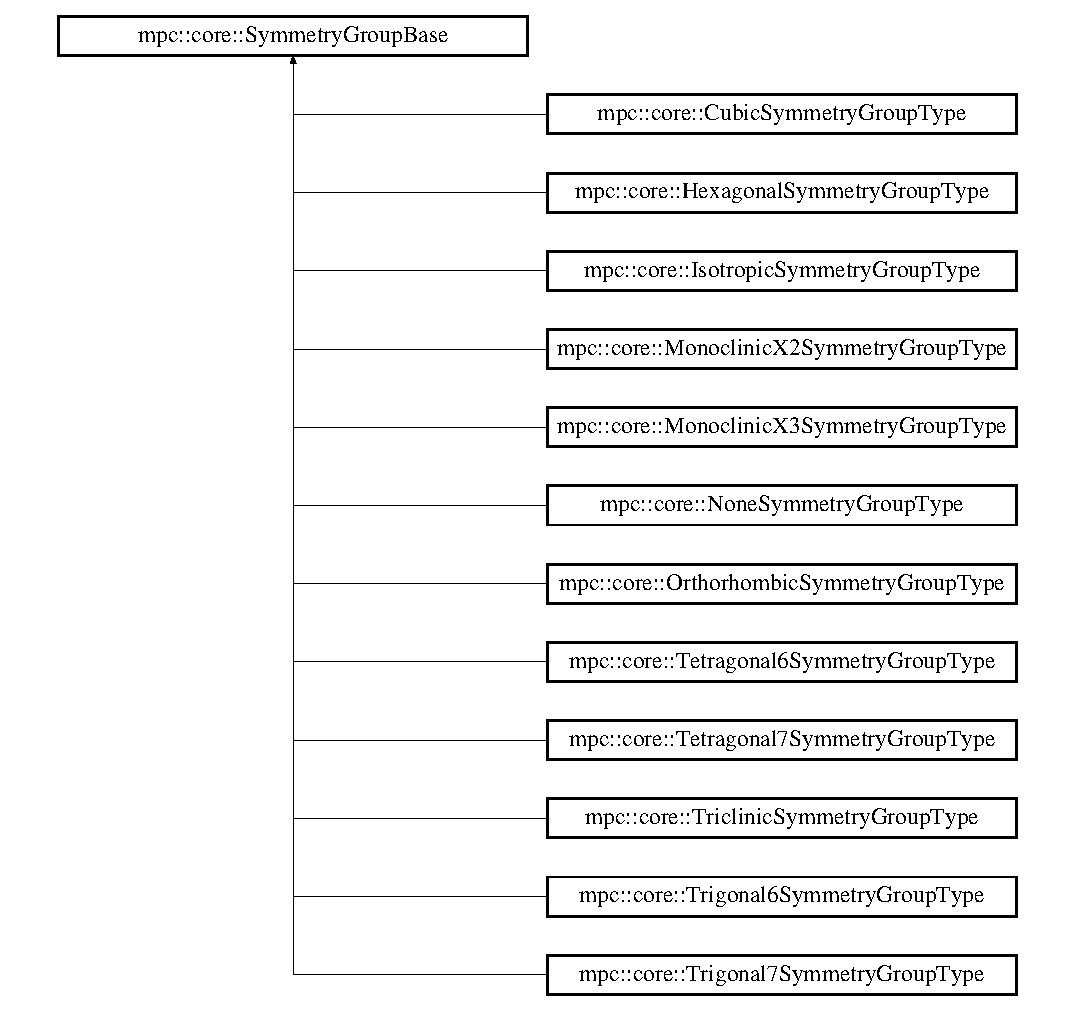
\includegraphics[height=12.000000cm]{structmpc_1_1core_1_1_symmetry_group_base}
\end{center}
\end{figure}


\subsection{Detailed Description}
base class for symmetry group types; used for template specializations 

T\+O\+DO\+: describe the specializations for each symmetry group type 

Definition at line 146 of file symmetrygrouptypes.\+hpp.



The documentation for this class was generated from the following file\+:\begin{DoxyCompactItemize}
\item 
/\+Users/atorlucci/\+Documents/github\+\_\+threecubed\+\_\+repos/mpc/src/mpc/core/\mbox{\hyperlink{symmetrygrouptypes_8hpp}{symmetrygrouptypes.\+hpp}}\end{DoxyCompactItemize}

\hypertarget{structmpc_1_1core_1_1_symmetry_group_enumeration_interface}{}\section{mpc\+:\+:core\+:\+:Symmetry\+Group\+Enumeration\+Interface Class Reference}
\label{structmpc_1_1core_1_1_symmetry_group_enumeration_interface}\index{mpc\+::core\+::\+Symmetry\+Group\+Enumeration\+Interface@{mpc\+::core\+::\+Symmetry\+Group\+Enumeration\+Interface}}


simple class interface with function to get std\+::string from enum  




{\ttfamily \#include $<$symmetrygrouptypes.\+hpp$>$}

\subsection*{Static Public Member Functions}
\begin{DoxyCompactItemize}
\item 
static std\+::string \mbox{\hyperlink{structmpc_1_1core_1_1_symmetry_group_enumeration_interface_add5134094062e3da52bb803af93b893c}{To\+Str}} (\mbox{\hyperlink{namespacempc_1_1core_a9d979684062547055a0ef5c13077bad8}{Symmetry\+Group\+Enumeration}} symmetry\+\_\+enum)
\end{DoxyCompactItemize}


\subsection{Detailed Description}
simple class interface with function to get std\+::string from enum 

Definition at line 49 of file symmetrygrouptypes.\+hpp.



\subsection{Member Function Documentation}
\mbox{\Hypertarget{structmpc_1_1core_1_1_symmetry_group_enumeration_interface_add5134094062e3da52bb803af93b893c}\label{structmpc_1_1core_1_1_symmetry_group_enumeration_interface_add5134094062e3da52bb803af93b893c}} 
\index{mpc\+::core\+::\+Symmetry\+Group\+Enumeration\+Interface@{mpc\+::core\+::\+Symmetry\+Group\+Enumeration\+Interface}!To\+Str@{To\+Str}}
\index{To\+Str@{To\+Str}!mpc\+::core\+::\+Symmetry\+Group\+Enumeration\+Interface@{mpc\+::core\+::\+Symmetry\+Group\+Enumeration\+Interface}}
\subsubsection{\texorpdfstring{To\+Str()}{ToStr()}}
{\footnotesize\ttfamily std\+::string mpc\+::core\+::\+Symmetry\+Group\+Enumeration\+Interface\+::\+To\+Str (\begin{DoxyParamCaption}\item[{\mbox{\hyperlink{namespacempc_1_1core_a9d979684062547055a0ef5c13077bad8}{Symmetry\+Group\+Enumeration}}}]{symmetry\+\_\+enum }\end{DoxyParamCaption})\hspace{0.3cm}{\ttfamily [inline]}, {\ttfamily [static]}}



Definition at line 53 of file symmetrygrouptypes.\+hpp.



The documentation for this class was generated from the following file\+:\begin{DoxyCompactItemize}
\item 
/\+Users/atorlucci/\+Documents/github\+\_\+threecubed\+\_\+repos/mpc/src/mpc/core/\mbox{\hyperlink{symmetrygrouptypes_8hpp}{symmetrygrouptypes.\+hpp}}\end{DoxyCompactItemize}

\hypertarget{structmpc_1_1core_1_1_symmetry_group_type}{}\section{mpc\+:\+:core\+:\+:Symmetry\+Group\+Type$<$ Sym $>$ Struct Template Reference}
\label{structmpc_1_1core_1_1_symmetry_group_type}\index{mpc\+::core\+::\+Symmetry\+Group\+Type$<$ Sym $>$@{mpc\+::core\+::\+Symmetry\+Group\+Type$<$ Sym $>$}}


{\ttfamily \#include $<$symmetrygrouptypes.\+hpp$>$}



\subsection{Detailed Description}
\subsubsection*{template$<$Symmetry\+Group\+Enumeration Sym$>$\newline
struct mpc\+::core\+::\+Symmetry\+Group\+Type$<$ Sym $>$}



Definition at line 297 of file symmetrygrouptypes.\+hpp.



The documentation for this struct was generated from the following file\+:\begin{DoxyCompactItemize}
\item 
/\+Users/atorlucci/\+Documents/github\+\_\+threecubed\+\_\+repos/mpc/src/mpc/core/\mbox{\hyperlink{symmetrygrouptypes_8hpp}{symmetrygrouptypes.\+hpp}}\end{DoxyCompactItemize}

\hypertarget{structmpc_1_1core_1_1_symmetry_group_type_3_01_symmetry_group_enumeration_1_1_c_u_b_i_c_01_4}{}\section{mpc\+:\+:core\+:\+:Symmetry\+Group\+Type$<$ Symmetry\+Group\+Enumeration\+:\+:C\+U\+B\+IC $>$ Struct Template Reference}
\label{structmpc_1_1core_1_1_symmetry_group_type_3_01_symmetry_group_enumeration_1_1_c_u_b_i_c_01_4}\index{mpc\+::core\+::\+Symmetry\+Group\+Type$<$ Symmetry\+Group\+Enumeration\+::\+C\+U\+B\+I\+C $>$@{mpc\+::core\+::\+Symmetry\+Group\+Type$<$ Symmetry\+Group\+Enumeration\+::\+C\+U\+B\+I\+C $>$}}


{\ttfamily \#include $<$symmetrygrouptypes.\+hpp$>$}

\subsection*{Public Types}
\begin{DoxyCompactItemize}
\item 
using \mbox{\hyperlink{structmpc_1_1core_1_1_symmetry_group_type_3_01_symmetry_group_enumeration_1_1_c_u_b_i_c_01_4_a381fca992534548373952578220385cb}{type}} = \mbox{\hyperlink{structmpc_1_1core_1_1_cubic_symmetry_group_type}{Cubic\+Symmetry\+Group\+Type}}
\end{DoxyCompactItemize}


\subsection{Detailed Description}
\subsubsection*{template$<$$>$\newline
struct mpc\+::core\+::\+Symmetry\+Group\+Type$<$ Symmetry\+Group\+Enumeration\+::\+C\+U\+B\+I\+C $>$}



Definition at line 351 of file symmetrygrouptypes.\+hpp.



\subsection{Member Typedef Documentation}
\mbox{\Hypertarget{structmpc_1_1core_1_1_symmetry_group_type_3_01_symmetry_group_enumeration_1_1_c_u_b_i_c_01_4_a381fca992534548373952578220385cb}\label{structmpc_1_1core_1_1_symmetry_group_type_3_01_symmetry_group_enumeration_1_1_c_u_b_i_c_01_4_a381fca992534548373952578220385cb}} 
\index{mpc\+::core\+::\+Symmetry\+Group\+Type$<$ Symmetry\+Group\+Enumeration\+::\+C\+U\+B\+I\+C $>$@{mpc\+::core\+::\+Symmetry\+Group\+Type$<$ Symmetry\+Group\+Enumeration\+::\+C\+U\+B\+I\+C $>$}!type@{type}}
\index{type@{type}!mpc\+::core\+::\+Symmetry\+Group\+Type$<$ Symmetry\+Group\+Enumeration\+::\+C\+U\+B\+I\+C $>$@{mpc\+::core\+::\+Symmetry\+Group\+Type$<$ Symmetry\+Group\+Enumeration\+::\+C\+U\+B\+I\+C $>$}}
\subsubsection{\texorpdfstring{type}{type}}
{\footnotesize\ttfamily using \mbox{\hyperlink{structmpc_1_1core_1_1_symmetry_group_type}{mpc\+::core\+::\+Symmetry\+Group\+Type}}$<$ \mbox{\hyperlink{namespacempc_1_1core_a9d979684062547055a0ef5c13077bad8accd681e34e5e40fbce74618c3ccffcff}{Symmetry\+Group\+Enumeration\+::\+C\+U\+B\+IC}} $>$\+::\mbox{\hyperlink{structmpc_1_1core_1_1_symmetry_group_type_3_01_symmetry_group_enumeration_1_1_c_u_b_i_c_01_4_a381fca992534548373952578220385cb}{type}} =  \mbox{\hyperlink{structmpc_1_1core_1_1_cubic_symmetry_group_type}{Cubic\+Symmetry\+Group\+Type}}}



Definition at line 352 of file symmetrygrouptypes.\+hpp.



The documentation for this struct was generated from the following file\+:\begin{DoxyCompactItemize}
\item 
/\+Users/atorlucci/\+Documents/github\+\_\+threecubed\+\_\+repos/mpc/src/mpc/core/\mbox{\hyperlink{symmetrygrouptypes_8hpp}{symmetrygrouptypes.\+hpp}}\end{DoxyCompactItemize}

\hypertarget{structmpc_1_1core_1_1_symmetry_group_type_3_01_symmetry_group_enumeration_1_1_h_e_x_a_g_o_n_a_l_01_4}{}\section{mpc\+:\+:core\+:\+:Symmetry\+Group\+Type$<$ Symmetry\+Group\+Enumeration\+:\+:H\+E\+X\+A\+G\+O\+N\+AL $>$ Struct Template Reference}
\label{structmpc_1_1core_1_1_symmetry_group_type_3_01_symmetry_group_enumeration_1_1_h_e_x_a_g_o_n_a_l_01_4}\index{mpc\+::core\+::\+Symmetry\+Group\+Type$<$ Symmetry\+Group\+Enumeration\+::\+H\+E\+X\+A\+G\+O\+N\+A\+L $>$@{mpc\+::core\+::\+Symmetry\+Group\+Type$<$ Symmetry\+Group\+Enumeration\+::\+H\+E\+X\+A\+G\+O\+N\+A\+L $>$}}


{\ttfamily \#include $<$symmetrygrouptypes.\+hpp$>$}

\subsection*{Public Types}
\begin{DoxyCompactItemize}
\item 
using \mbox{\hyperlink{structmpc_1_1core_1_1_symmetry_group_type_3_01_symmetry_group_enumeration_1_1_h_e_x_a_g_o_n_a_l_01_4_a833ac3714c5e0f497d4f8509d20ac6aa}{type}} = \mbox{\hyperlink{structmpc_1_1core_1_1_hexagonal_symmetry_group_type}{Hexagonal\+Symmetry\+Group\+Type}}
\end{DoxyCompactItemize}


\subsection{Detailed Description}
\subsubsection*{template$<$$>$\newline
struct mpc\+::core\+::\+Symmetry\+Group\+Type$<$ Symmetry\+Group\+Enumeration\+::\+H\+E\+X\+A\+G\+O\+N\+A\+L $>$}



Definition at line 326 of file symmetrygrouptypes.\+hpp.



\subsection{Member Typedef Documentation}
\mbox{\Hypertarget{structmpc_1_1core_1_1_symmetry_group_type_3_01_symmetry_group_enumeration_1_1_h_e_x_a_g_o_n_a_l_01_4_a833ac3714c5e0f497d4f8509d20ac6aa}\label{structmpc_1_1core_1_1_symmetry_group_type_3_01_symmetry_group_enumeration_1_1_h_e_x_a_g_o_n_a_l_01_4_a833ac3714c5e0f497d4f8509d20ac6aa}} 
\index{mpc\+::core\+::\+Symmetry\+Group\+Type$<$ Symmetry\+Group\+Enumeration\+::\+H\+E\+X\+A\+G\+O\+N\+A\+L $>$@{mpc\+::core\+::\+Symmetry\+Group\+Type$<$ Symmetry\+Group\+Enumeration\+::\+H\+E\+X\+A\+G\+O\+N\+A\+L $>$}!type@{type}}
\index{type@{type}!mpc\+::core\+::\+Symmetry\+Group\+Type$<$ Symmetry\+Group\+Enumeration\+::\+H\+E\+X\+A\+G\+O\+N\+A\+L $>$@{mpc\+::core\+::\+Symmetry\+Group\+Type$<$ Symmetry\+Group\+Enumeration\+::\+H\+E\+X\+A\+G\+O\+N\+A\+L $>$}}
\subsubsection{\texorpdfstring{type}{type}}
{\footnotesize\ttfamily using \mbox{\hyperlink{structmpc_1_1core_1_1_symmetry_group_type}{mpc\+::core\+::\+Symmetry\+Group\+Type}}$<$ \mbox{\hyperlink{namespacempc_1_1core_a9d979684062547055a0ef5c13077bad8a5d7adeeaa10073a6a3c5bd970a7f958b}{Symmetry\+Group\+Enumeration\+::\+H\+E\+X\+A\+G\+O\+N\+AL}} $>$\+::\mbox{\hyperlink{structmpc_1_1core_1_1_symmetry_group_type_3_01_symmetry_group_enumeration_1_1_h_e_x_a_g_o_n_a_l_01_4_a833ac3714c5e0f497d4f8509d20ac6aa}{type}} =  \mbox{\hyperlink{structmpc_1_1core_1_1_hexagonal_symmetry_group_type}{Hexagonal\+Symmetry\+Group\+Type}}}



Definition at line 327 of file symmetrygrouptypes.\+hpp.



The documentation for this struct was generated from the following file\+:\begin{DoxyCompactItemize}
\item 
/\+Users/atorlucci/\+Documents/github\+\_\+threecubed\+\_\+repos/mpc/src/mpc/core/\mbox{\hyperlink{symmetrygrouptypes_8hpp}{symmetrygrouptypes.\+hpp}}\end{DoxyCompactItemize}

\hypertarget{structmpc_1_1core_1_1_symmetry_group_type_3_01_symmetry_group_enumeration_1_1_i_s_o_t_r_o_p_i_c_01_4}{}\section{mpc\+:\+:core\+:\+:Symmetry\+Group\+Type$<$ Symmetry\+Group\+Enumeration\+:\+:I\+S\+O\+T\+R\+O\+P\+IC $>$ Struct Template Reference}
\label{structmpc_1_1core_1_1_symmetry_group_type_3_01_symmetry_group_enumeration_1_1_i_s_o_t_r_o_p_i_c_01_4}\index{mpc\+::core\+::\+Symmetry\+Group\+Type$<$ Symmetry\+Group\+Enumeration\+::\+I\+S\+O\+T\+R\+O\+P\+I\+C $>$@{mpc\+::core\+::\+Symmetry\+Group\+Type$<$ Symmetry\+Group\+Enumeration\+::\+I\+S\+O\+T\+R\+O\+P\+I\+C $>$}}


{\ttfamily \#include $<$symmetrygrouptypes.\+hpp$>$}

\subsection*{Public Types}
\begin{DoxyCompactItemize}
\item 
using \mbox{\hyperlink{structmpc_1_1core_1_1_symmetry_group_type_3_01_symmetry_group_enumeration_1_1_i_s_o_t_r_o_p_i_c_01_4_a8f392bfab082bbb0e49b422b3601e73a}{type}} = \mbox{\hyperlink{structmpc_1_1core_1_1_isotropic_symmetry_group_type}{Isotropic\+Symmetry\+Group\+Type}}
\end{DoxyCompactItemize}


\subsection{Detailed Description}
\subsubsection*{template$<$$>$\newline
struct mpc\+::core\+::\+Symmetry\+Group\+Type$<$ Symmetry\+Group\+Enumeration\+::\+I\+S\+O\+T\+R\+O\+P\+I\+C $>$}



Definition at line 356 of file symmetrygrouptypes.\+hpp.



\subsection{Member Typedef Documentation}
\mbox{\Hypertarget{structmpc_1_1core_1_1_symmetry_group_type_3_01_symmetry_group_enumeration_1_1_i_s_o_t_r_o_p_i_c_01_4_a8f392bfab082bbb0e49b422b3601e73a}\label{structmpc_1_1core_1_1_symmetry_group_type_3_01_symmetry_group_enumeration_1_1_i_s_o_t_r_o_p_i_c_01_4_a8f392bfab082bbb0e49b422b3601e73a}} 
\index{mpc\+::core\+::\+Symmetry\+Group\+Type$<$ Symmetry\+Group\+Enumeration\+::\+I\+S\+O\+T\+R\+O\+P\+I\+C $>$@{mpc\+::core\+::\+Symmetry\+Group\+Type$<$ Symmetry\+Group\+Enumeration\+::\+I\+S\+O\+T\+R\+O\+P\+I\+C $>$}!type@{type}}
\index{type@{type}!mpc\+::core\+::\+Symmetry\+Group\+Type$<$ Symmetry\+Group\+Enumeration\+::\+I\+S\+O\+T\+R\+O\+P\+I\+C $>$@{mpc\+::core\+::\+Symmetry\+Group\+Type$<$ Symmetry\+Group\+Enumeration\+::\+I\+S\+O\+T\+R\+O\+P\+I\+C $>$}}
\subsubsection{\texorpdfstring{type}{type}}
{\footnotesize\ttfamily using \mbox{\hyperlink{structmpc_1_1core_1_1_symmetry_group_type}{mpc\+::core\+::\+Symmetry\+Group\+Type}}$<$ \mbox{\hyperlink{namespacempc_1_1core_a9d979684062547055a0ef5c13077bad8a099d59049574174a1c19567d38b479c2}{Symmetry\+Group\+Enumeration\+::\+I\+S\+O\+T\+R\+O\+P\+IC}} $>$\+::\mbox{\hyperlink{structmpc_1_1core_1_1_symmetry_group_type_3_01_symmetry_group_enumeration_1_1_i_s_o_t_r_o_p_i_c_01_4_a8f392bfab082bbb0e49b422b3601e73a}{type}} =  \mbox{\hyperlink{structmpc_1_1core_1_1_isotropic_symmetry_group_type}{Isotropic\+Symmetry\+Group\+Type}}}



Definition at line 357 of file symmetrygrouptypes.\+hpp.



The documentation for this struct was generated from the following file\+:\begin{DoxyCompactItemize}
\item 
/\+Users/atorlucci/\+Documents/github\+\_\+threecubed\+\_\+repos/mpc/src/mpc/core/\mbox{\hyperlink{symmetrygrouptypes_8hpp}{symmetrygrouptypes.\+hpp}}\end{DoxyCompactItemize}

\hypertarget{structmpc_1_1core_1_1_symmetry_group_type_3_01_symmetry_group_enumeration_1_1_m_o_n_o_c_l_i_n_i_c___x2_01_4}{}\section{mpc\+:\+:core\+:\+:Symmetry\+Group\+Type$<$ Symmetry\+Group\+Enumeration\+:\+:M\+O\+N\+O\+C\+L\+I\+N\+I\+C\+\_\+\+X2 $>$ Struct Template Reference}
\label{structmpc_1_1core_1_1_symmetry_group_type_3_01_symmetry_group_enumeration_1_1_m_o_n_o_c_l_i_n_i_c___x2_01_4}\index{mpc\+::core\+::\+Symmetry\+Group\+Type$<$ Symmetry\+Group\+Enumeration\+::\+M\+O\+N\+O\+C\+L\+I\+N\+I\+C\+\_\+\+X2 $>$@{mpc\+::core\+::\+Symmetry\+Group\+Type$<$ Symmetry\+Group\+Enumeration\+::\+M\+O\+N\+O\+C\+L\+I\+N\+I\+C\+\_\+\+X2 $>$}}


{\ttfamily \#include $<$symmetrygrouptypes.\+hpp$>$}

\subsection*{Public Types}
\begin{DoxyCompactItemize}
\item 
using \mbox{\hyperlink{structmpc_1_1core_1_1_symmetry_group_type_3_01_symmetry_group_enumeration_1_1_m_o_n_o_c_l_i_n_i_c___x2_01_4_a8c186ecb248273f2e5a29dfbc451736f}{type}} = \mbox{\hyperlink{structmpc_1_1core_1_1_monoclinic_x2_symmetry_group_type}{Monoclinic\+X2\+Symmetry\+Group\+Type}}
\end{DoxyCompactItemize}


\subsection{Detailed Description}
\subsubsection*{template$<$$>$\newline
struct mpc\+::core\+::\+Symmetry\+Group\+Type$<$ Symmetry\+Group\+Enumeration\+::\+M\+O\+N\+O\+C\+L\+I\+N\+I\+C\+\_\+\+X2 $>$}



Definition at line 311 of file symmetrygrouptypes.\+hpp.



\subsection{Member Typedef Documentation}
\mbox{\Hypertarget{structmpc_1_1core_1_1_symmetry_group_type_3_01_symmetry_group_enumeration_1_1_m_o_n_o_c_l_i_n_i_c___x2_01_4_a8c186ecb248273f2e5a29dfbc451736f}\label{structmpc_1_1core_1_1_symmetry_group_type_3_01_symmetry_group_enumeration_1_1_m_o_n_o_c_l_i_n_i_c___x2_01_4_a8c186ecb248273f2e5a29dfbc451736f}} 
\index{mpc\+::core\+::\+Symmetry\+Group\+Type$<$ Symmetry\+Group\+Enumeration\+::\+M\+O\+N\+O\+C\+L\+I\+N\+I\+C\+\_\+\+X2 $>$@{mpc\+::core\+::\+Symmetry\+Group\+Type$<$ Symmetry\+Group\+Enumeration\+::\+M\+O\+N\+O\+C\+L\+I\+N\+I\+C\+\_\+\+X2 $>$}!type@{type}}
\index{type@{type}!mpc\+::core\+::\+Symmetry\+Group\+Type$<$ Symmetry\+Group\+Enumeration\+::\+M\+O\+N\+O\+C\+L\+I\+N\+I\+C\+\_\+\+X2 $>$@{mpc\+::core\+::\+Symmetry\+Group\+Type$<$ Symmetry\+Group\+Enumeration\+::\+M\+O\+N\+O\+C\+L\+I\+N\+I\+C\+\_\+\+X2 $>$}}
\subsubsection{\texorpdfstring{type}{type}}
{\footnotesize\ttfamily using \mbox{\hyperlink{structmpc_1_1core_1_1_symmetry_group_type}{mpc\+::core\+::\+Symmetry\+Group\+Type}}$<$ \mbox{\hyperlink{namespacempc_1_1core_a9d979684062547055a0ef5c13077bad8a7eb6e11f17e97fbe9fc371a72a989b96}{Symmetry\+Group\+Enumeration\+::\+M\+O\+N\+O\+C\+L\+I\+N\+I\+C\+\_\+\+X2}} $>$\+::\mbox{\hyperlink{structmpc_1_1core_1_1_symmetry_group_type_3_01_symmetry_group_enumeration_1_1_m_o_n_o_c_l_i_n_i_c___x2_01_4_a8c186ecb248273f2e5a29dfbc451736f}{type}} =  \mbox{\hyperlink{structmpc_1_1core_1_1_monoclinic_x2_symmetry_group_type}{Monoclinic\+X2\+Symmetry\+Group\+Type}}}



Definition at line 312 of file symmetrygrouptypes.\+hpp.



The documentation for this struct was generated from the following file\+:\begin{DoxyCompactItemize}
\item 
/\+Users/atorlucci/\+Documents/github\+\_\+threecubed\+\_\+repos/mpc/src/mpc/core/\mbox{\hyperlink{symmetrygrouptypes_8hpp}{symmetrygrouptypes.\+hpp}}\end{DoxyCompactItemize}

\hypertarget{structmpc_1_1core_1_1_symmetry_group_type_3_01_symmetry_group_enumeration_1_1_m_o_n_o_c_l_i_n_i_c___x3_01_4}{}\section{mpc\+:\+:core\+:\+:Symmetry\+Group\+Type$<$ Symmetry\+Group\+Enumeration\+:\+:M\+O\+N\+O\+C\+L\+I\+N\+I\+C\+\_\+\+X3 $>$ Struct Template Reference}
\label{structmpc_1_1core_1_1_symmetry_group_type_3_01_symmetry_group_enumeration_1_1_m_o_n_o_c_l_i_n_i_c___x3_01_4}\index{mpc\+::core\+::\+Symmetry\+Group\+Type$<$ Symmetry\+Group\+Enumeration\+::\+M\+O\+N\+O\+C\+L\+I\+N\+I\+C\+\_\+\+X3 $>$@{mpc\+::core\+::\+Symmetry\+Group\+Type$<$ Symmetry\+Group\+Enumeration\+::\+M\+O\+N\+O\+C\+L\+I\+N\+I\+C\+\_\+\+X3 $>$}}


{\ttfamily \#include $<$symmetrygrouptypes.\+hpp$>$}

\subsection*{Public Types}
\begin{DoxyCompactItemize}
\item 
using \mbox{\hyperlink{structmpc_1_1core_1_1_symmetry_group_type_3_01_symmetry_group_enumeration_1_1_m_o_n_o_c_l_i_n_i_c___x3_01_4_a80413b16e88e14e73bc364495cf50e78}{type}} = \mbox{\hyperlink{structmpc_1_1core_1_1_monoclinic_x3_symmetry_group_type}{Monoclinic\+X3\+Symmetry\+Group\+Type}}
\end{DoxyCompactItemize}


\subsection{Detailed Description}
\subsubsection*{template$<$$>$\newline
struct mpc\+::core\+::\+Symmetry\+Group\+Type$<$ Symmetry\+Group\+Enumeration\+::\+M\+O\+N\+O\+C\+L\+I\+N\+I\+C\+\_\+\+X3 $>$}



Definition at line 316 of file symmetrygrouptypes.\+hpp.



\subsection{Member Typedef Documentation}
\mbox{\Hypertarget{structmpc_1_1core_1_1_symmetry_group_type_3_01_symmetry_group_enumeration_1_1_m_o_n_o_c_l_i_n_i_c___x3_01_4_a80413b16e88e14e73bc364495cf50e78}\label{structmpc_1_1core_1_1_symmetry_group_type_3_01_symmetry_group_enumeration_1_1_m_o_n_o_c_l_i_n_i_c___x3_01_4_a80413b16e88e14e73bc364495cf50e78}} 
\index{mpc\+::core\+::\+Symmetry\+Group\+Type$<$ Symmetry\+Group\+Enumeration\+::\+M\+O\+N\+O\+C\+L\+I\+N\+I\+C\+\_\+\+X3 $>$@{mpc\+::core\+::\+Symmetry\+Group\+Type$<$ Symmetry\+Group\+Enumeration\+::\+M\+O\+N\+O\+C\+L\+I\+N\+I\+C\+\_\+\+X3 $>$}!type@{type}}
\index{type@{type}!mpc\+::core\+::\+Symmetry\+Group\+Type$<$ Symmetry\+Group\+Enumeration\+::\+M\+O\+N\+O\+C\+L\+I\+N\+I\+C\+\_\+\+X3 $>$@{mpc\+::core\+::\+Symmetry\+Group\+Type$<$ Symmetry\+Group\+Enumeration\+::\+M\+O\+N\+O\+C\+L\+I\+N\+I\+C\+\_\+\+X3 $>$}}
\subsubsection{\texorpdfstring{type}{type}}
{\footnotesize\ttfamily using \mbox{\hyperlink{structmpc_1_1core_1_1_symmetry_group_type}{mpc\+::core\+::\+Symmetry\+Group\+Type}}$<$ \mbox{\hyperlink{namespacempc_1_1core_a9d979684062547055a0ef5c13077bad8ab31f5171fdded777eb3112da45967b57}{Symmetry\+Group\+Enumeration\+::\+M\+O\+N\+O\+C\+L\+I\+N\+I\+C\+\_\+\+X3}} $>$\+::\mbox{\hyperlink{structmpc_1_1core_1_1_symmetry_group_type_3_01_symmetry_group_enumeration_1_1_m_o_n_o_c_l_i_n_i_c___x3_01_4_a80413b16e88e14e73bc364495cf50e78}{type}} =  \mbox{\hyperlink{structmpc_1_1core_1_1_monoclinic_x3_symmetry_group_type}{Monoclinic\+X3\+Symmetry\+Group\+Type}}}



Definition at line 317 of file symmetrygrouptypes.\+hpp.



The documentation for this struct was generated from the following file\+:\begin{DoxyCompactItemize}
\item 
/\+Users/atorlucci/\+Documents/github\+\_\+threecubed\+\_\+repos/mpc/src/mpc/core/\mbox{\hyperlink{symmetrygrouptypes_8hpp}{symmetrygrouptypes.\+hpp}}\end{DoxyCompactItemize}

\hypertarget{structmpc_1_1core_1_1_symmetry_group_type_3_01_symmetry_group_enumeration_1_1_n_o_n_e_01_4}{}\section{mpc\+:\+:core\+:\+:Symmetry\+Group\+Type$<$ Symmetry\+Group\+Enumeration\+:\+:N\+O\+NE $>$ Struct Template Reference}
\label{structmpc_1_1core_1_1_symmetry_group_type_3_01_symmetry_group_enumeration_1_1_n_o_n_e_01_4}\index{mpc\+::core\+::\+Symmetry\+Group\+Type$<$ Symmetry\+Group\+Enumeration\+::\+N\+O\+N\+E $>$@{mpc\+::core\+::\+Symmetry\+Group\+Type$<$ Symmetry\+Group\+Enumeration\+::\+N\+O\+N\+E $>$}}


{\ttfamily \#include $<$symmetrygrouptypes.\+hpp$>$}

\subsection*{Public Types}
\begin{DoxyCompactItemize}
\item 
using \mbox{\hyperlink{structmpc_1_1core_1_1_symmetry_group_type_3_01_symmetry_group_enumeration_1_1_n_o_n_e_01_4_a502f9bba4f27dfdb37eb97b82c48545a}{type}} = \mbox{\hyperlink{structmpc_1_1core_1_1_none_symmetry_group_type}{None\+Symmetry\+Group\+Type}}
\end{DoxyCompactItemize}


\subsection{Detailed Description}
\subsubsection*{template$<$$>$\newline
struct mpc\+::core\+::\+Symmetry\+Group\+Type$<$ Symmetry\+Group\+Enumeration\+::\+N\+O\+N\+E $>$}



Definition at line 301 of file symmetrygrouptypes.\+hpp.



\subsection{Member Typedef Documentation}
\mbox{\Hypertarget{structmpc_1_1core_1_1_symmetry_group_type_3_01_symmetry_group_enumeration_1_1_n_o_n_e_01_4_a502f9bba4f27dfdb37eb97b82c48545a}\label{structmpc_1_1core_1_1_symmetry_group_type_3_01_symmetry_group_enumeration_1_1_n_o_n_e_01_4_a502f9bba4f27dfdb37eb97b82c48545a}} 
\index{mpc\+::core\+::\+Symmetry\+Group\+Type$<$ Symmetry\+Group\+Enumeration\+::\+N\+O\+N\+E $>$@{mpc\+::core\+::\+Symmetry\+Group\+Type$<$ Symmetry\+Group\+Enumeration\+::\+N\+O\+N\+E $>$}!type@{type}}
\index{type@{type}!mpc\+::core\+::\+Symmetry\+Group\+Type$<$ Symmetry\+Group\+Enumeration\+::\+N\+O\+N\+E $>$@{mpc\+::core\+::\+Symmetry\+Group\+Type$<$ Symmetry\+Group\+Enumeration\+::\+N\+O\+N\+E $>$}}
\subsubsection{\texorpdfstring{type}{type}}
{\footnotesize\ttfamily using \mbox{\hyperlink{structmpc_1_1core_1_1_symmetry_group_type}{mpc\+::core\+::\+Symmetry\+Group\+Type}}$<$ \mbox{\hyperlink{namespacempc_1_1core_a9d979684062547055a0ef5c13077bad8ab50339a10e1de285ac99d4c3990b8693}{Symmetry\+Group\+Enumeration\+::\+N\+O\+NE}} $>$\+::\mbox{\hyperlink{structmpc_1_1core_1_1_symmetry_group_type_3_01_symmetry_group_enumeration_1_1_n_o_n_e_01_4_a502f9bba4f27dfdb37eb97b82c48545a}{type}} =  \mbox{\hyperlink{structmpc_1_1core_1_1_none_symmetry_group_type}{None\+Symmetry\+Group\+Type}}}



Definition at line 302 of file symmetrygrouptypes.\+hpp.



The documentation for this struct was generated from the following file\+:\begin{DoxyCompactItemize}
\item 
/\+Users/atorlucci/\+Documents/github\+\_\+threecubed\+\_\+repos/mpc/src/mpc/core/\mbox{\hyperlink{symmetrygrouptypes_8hpp}{symmetrygrouptypes.\+hpp}}\end{DoxyCompactItemize}

\hypertarget{structmpc_1_1core_1_1_symmetry_group_type_3_01_symmetry_group_enumeration_1_1_o_r_t_h_o_r_h_o_m_b_i_c_01_4}{}\section{mpc\+:\+:core\+:\+:Symmetry\+Group\+Type$<$ Symmetry\+Group\+Enumeration\+:\+:O\+R\+T\+H\+O\+R\+H\+O\+M\+B\+IC $>$ Struct Template Reference}
\label{structmpc_1_1core_1_1_symmetry_group_type_3_01_symmetry_group_enumeration_1_1_o_r_t_h_o_r_h_o_m_b_i_c_01_4}\index{mpc\+::core\+::\+Symmetry\+Group\+Type$<$ Symmetry\+Group\+Enumeration\+::\+O\+R\+T\+H\+O\+R\+H\+O\+M\+B\+I\+C $>$@{mpc\+::core\+::\+Symmetry\+Group\+Type$<$ Symmetry\+Group\+Enumeration\+::\+O\+R\+T\+H\+O\+R\+H\+O\+M\+B\+I\+C $>$}}


{\ttfamily \#include $<$symmetrygrouptypes.\+hpp$>$}

\subsection*{Public Types}
\begin{DoxyCompactItemize}
\item 
using \mbox{\hyperlink{structmpc_1_1core_1_1_symmetry_group_type_3_01_symmetry_group_enumeration_1_1_o_r_t_h_o_r_h_o_m_b_i_c_01_4_aa03457fea042819a7f1a790049474067}{type}} = \mbox{\hyperlink{structmpc_1_1core_1_1_orthorhombic_symmetry_group_type}{Orthorhombic\+Symmetry\+Group\+Type}}
\end{DoxyCompactItemize}


\subsection{Detailed Description}
\subsubsection*{template$<$$>$\newline
struct mpc\+::core\+::\+Symmetry\+Group\+Type$<$ Symmetry\+Group\+Enumeration\+::\+O\+R\+T\+H\+O\+R\+H\+O\+M\+B\+I\+C $>$}



Definition at line 321 of file symmetrygrouptypes.\+hpp.



\subsection{Member Typedef Documentation}
\mbox{\Hypertarget{structmpc_1_1core_1_1_symmetry_group_type_3_01_symmetry_group_enumeration_1_1_o_r_t_h_o_r_h_o_m_b_i_c_01_4_aa03457fea042819a7f1a790049474067}\label{structmpc_1_1core_1_1_symmetry_group_type_3_01_symmetry_group_enumeration_1_1_o_r_t_h_o_r_h_o_m_b_i_c_01_4_aa03457fea042819a7f1a790049474067}} 
\index{mpc\+::core\+::\+Symmetry\+Group\+Type$<$ Symmetry\+Group\+Enumeration\+::\+O\+R\+T\+H\+O\+R\+H\+O\+M\+B\+I\+C $>$@{mpc\+::core\+::\+Symmetry\+Group\+Type$<$ Symmetry\+Group\+Enumeration\+::\+O\+R\+T\+H\+O\+R\+H\+O\+M\+B\+I\+C $>$}!type@{type}}
\index{type@{type}!mpc\+::core\+::\+Symmetry\+Group\+Type$<$ Symmetry\+Group\+Enumeration\+::\+O\+R\+T\+H\+O\+R\+H\+O\+M\+B\+I\+C $>$@{mpc\+::core\+::\+Symmetry\+Group\+Type$<$ Symmetry\+Group\+Enumeration\+::\+O\+R\+T\+H\+O\+R\+H\+O\+M\+B\+I\+C $>$}}
\subsubsection{\texorpdfstring{type}{type}}
{\footnotesize\ttfamily using \mbox{\hyperlink{structmpc_1_1core_1_1_symmetry_group_type}{mpc\+::core\+::\+Symmetry\+Group\+Type}}$<$ \mbox{\hyperlink{namespacempc_1_1core_a9d979684062547055a0ef5c13077bad8a45ddba8b47424b406a313caed88b091a}{Symmetry\+Group\+Enumeration\+::\+O\+R\+T\+H\+O\+R\+H\+O\+M\+B\+IC}} $>$\+::\mbox{\hyperlink{structmpc_1_1core_1_1_symmetry_group_type_3_01_symmetry_group_enumeration_1_1_o_r_t_h_o_r_h_o_m_b_i_c_01_4_aa03457fea042819a7f1a790049474067}{type}} =  \mbox{\hyperlink{structmpc_1_1core_1_1_orthorhombic_symmetry_group_type}{Orthorhombic\+Symmetry\+Group\+Type}}}



Definition at line 322 of file symmetrygrouptypes.\+hpp.



The documentation for this struct was generated from the following file\+:\begin{DoxyCompactItemize}
\item 
/\+Users/atorlucci/\+Documents/github\+\_\+threecubed\+\_\+repos/mpc/src/mpc/core/\mbox{\hyperlink{symmetrygrouptypes_8hpp}{symmetrygrouptypes.\+hpp}}\end{DoxyCompactItemize}

\hypertarget{structmpc_1_1core_1_1_symmetry_group_type_3_01_symmetry_group_enumeration_1_1_t_e_t_r_a_g_o_n_a_l6_01_4}{}\section{mpc\+:\+:core\+:\+:Symmetry\+Group\+Type$<$ Symmetry\+Group\+Enumeration\+:\+:T\+E\+T\+R\+A\+G\+O\+N\+A\+L6 $>$ Struct Template Reference}
\label{structmpc_1_1core_1_1_symmetry_group_type_3_01_symmetry_group_enumeration_1_1_t_e_t_r_a_g_o_n_a_l6_01_4}\index{mpc\+::core\+::\+Symmetry\+Group\+Type$<$ Symmetry\+Group\+Enumeration\+::\+T\+E\+T\+R\+A\+G\+O\+N\+A\+L6 $>$@{mpc\+::core\+::\+Symmetry\+Group\+Type$<$ Symmetry\+Group\+Enumeration\+::\+T\+E\+T\+R\+A\+G\+O\+N\+A\+L6 $>$}}


{\ttfamily \#include $<$symmetrygrouptypes.\+hpp$>$}

\subsection*{Public Types}
\begin{DoxyCompactItemize}
\item 
using \mbox{\hyperlink{structmpc_1_1core_1_1_symmetry_group_type_3_01_symmetry_group_enumeration_1_1_t_e_t_r_a_g_o_n_a_l6_01_4_a5a59ef59ad26662e942639a2243dc2e7}{type}} = \mbox{\hyperlink{structmpc_1_1core_1_1_tetragonal6_symmetry_group_type}{Tetragonal6\+Symmetry\+Group\+Type}}
\end{DoxyCompactItemize}


\subsection{Detailed Description}
\subsubsection*{template$<$$>$\newline
struct mpc\+::core\+::\+Symmetry\+Group\+Type$<$ Symmetry\+Group\+Enumeration\+::\+T\+E\+T\+R\+A\+G\+O\+N\+A\+L6 $>$}



Definition at line 336 of file symmetrygrouptypes.\+hpp.



\subsection{Member Typedef Documentation}
\mbox{\Hypertarget{structmpc_1_1core_1_1_symmetry_group_type_3_01_symmetry_group_enumeration_1_1_t_e_t_r_a_g_o_n_a_l6_01_4_a5a59ef59ad26662e942639a2243dc2e7}\label{structmpc_1_1core_1_1_symmetry_group_type_3_01_symmetry_group_enumeration_1_1_t_e_t_r_a_g_o_n_a_l6_01_4_a5a59ef59ad26662e942639a2243dc2e7}} 
\index{mpc\+::core\+::\+Symmetry\+Group\+Type$<$ Symmetry\+Group\+Enumeration\+::\+T\+E\+T\+R\+A\+G\+O\+N\+A\+L6 $>$@{mpc\+::core\+::\+Symmetry\+Group\+Type$<$ Symmetry\+Group\+Enumeration\+::\+T\+E\+T\+R\+A\+G\+O\+N\+A\+L6 $>$}!type@{type}}
\index{type@{type}!mpc\+::core\+::\+Symmetry\+Group\+Type$<$ Symmetry\+Group\+Enumeration\+::\+T\+E\+T\+R\+A\+G\+O\+N\+A\+L6 $>$@{mpc\+::core\+::\+Symmetry\+Group\+Type$<$ Symmetry\+Group\+Enumeration\+::\+T\+E\+T\+R\+A\+G\+O\+N\+A\+L6 $>$}}
\subsubsection{\texorpdfstring{type}{type}}
{\footnotesize\ttfamily using \mbox{\hyperlink{structmpc_1_1core_1_1_symmetry_group_type}{mpc\+::core\+::\+Symmetry\+Group\+Type}}$<$ \mbox{\hyperlink{namespacempc_1_1core_a9d979684062547055a0ef5c13077bad8a63dabd41a700b44f934a19db4e0f8f83}{Symmetry\+Group\+Enumeration\+::\+T\+E\+T\+R\+A\+G\+O\+N\+A\+L6}} $>$\+::\mbox{\hyperlink{structmpc_1_1core_1_1_symmetry_group_type_3_01_symmetry_group_enumeration_1_1_t_e_t_r_a_g_o_n_a_l6_01_4_a5a59ef59ad26662e942639a2243dc2e7}{type}} =  \mbox{\hyperlink{structmpc_1_1core_1_1_tetragonal6_symmetry_group_type}{Tetragonal6\+Symmetry\+Group\+Type}}}



Definition at line 337 of file symmetrygrouptypes.\+hpp.



The documentation for this struct was generated from the following file\+:\begin{DoxyCompactItemize}
\item 
/\+Users/atorlucci/\+Documents/github\+\_\+threecubed\+\_\+repos/mpc/src/mpc/core/\mbox{\hyperlink{symmetrygrouptypes_8hpp}{symmetrygrouptypes.\+hpp}}\end{DoxyCompactItemize}

\hypertarget{structmpc_1_1core_1_1_symmetry_group_type_3_01_symmetry_group_enumeration_1_1_t_e_t_r_a_g_o_n_a_l7_01_4}{}\section{mpc\+:\+:core\+:\+:Symmetry\+Group\+Type$<$ Symmetry\+Group\+Enumeration\+:\+:T\+E\+T\+R\+A\+G\+O\+N\+A\+L7 $>$ Struct Template Reference}
\label{structmpc_1_1core_1_1_symmetry_group_type_3_01_symmetry_group_enumeration_1_1_t_e_t_r_a_g_o_n_a_l7_01_4}\index{mpc\+::core\+::\+Symmetry\+Group\+Type$<$ Symmetry\+Group\+Enumeration\+::\+T\+E\+T\+R\+A\+G\+O\+N\+A\+L7 $>$@{mpc\+::core\+::\+Symmetry\+Group\+Type$<$ Symmetry\+Group\+Enumeration\+::\+T\+E\+T\+R\+A\+G\+O\+N\+A\+L7 $>$}}


{\ttfamily \#include $<$symmetrygrouptypes.\+hpp$>$}

\subsection*{Public Types}
\begin{DoxyCompactItemize}
\item 
using \mbox{\hyperlink{structmpc_1_1core_1_1_symmetry_group_type_3_01_symmetry_group_enumeration_1_1_t_e_t_r_a_g_o_n_a_l7_01_4_aa66f1c6ff90bfe284717b5cb690b1a4b}{type}} = \mbox{\hyperlink{structmpc_1_1core_1_1_tetragonal7_symmetry_group_type}{Tetragonal7\+Symmetry\+Group\+Type}}
\end{DoxyCompactItemize}


\subsection{Detailed Description}
\subsubsection*{template$<$$>$\newline
struct mpc\+::core\+::\+Symmetry\+Group\+Type$<$ Symmetry\+Group\+Enumeration\+::\+T\+E\+T\+R\+A\+G\+O\+N\+A\+L7 $>$}



Definition at line 331 of file symmetrygrouptypes.\+hpp.



\subsection{Member Typedef Documentation}
\mbox{\Hypertarget{structmpc_1_1core_1_1_symmetry_group_type_3_01_symmetry_group_enumeration_1_1_t_e_t_r_a_g_o_n_a_l7_01_4_aa66f1c6ff90bfe284717b5cb690b1a4b}\label{structmpc_1_1core_1_1_symmetry_group_type_3_01_symmetry_group_enumeration_1_1_t_e_t_r_a_g_o_n_a_l7_01_4_aa66f1c6ff90bfe284717b5cb690b1a4b}} 
\index{mpc\+::core\+::\+Symmetry\+Group\+Type$<$ Symmetry\+Group\+Enumeration\+::\+T\+E\+T\+R\+A\+G\+O\+N\+A\+L7 $>$@{mpc\+::core\+::\+Symmetry\+Group\+Type$<$ Symmetry\+Group\+Enumeration\+::\+T\+E\+T\+R\+A\+G\+O\+N\+A\+L7 $>$}!type@{type}}
\index{type@{type}!mpc\+::core\+::\+Symmetry\+Group\+Type$<$ Symmetry\+Group\+Enumeration\+::\+T\+E\+T\+R\+A\+G\+O\+N\+A\+L7 $>$@{mpc\+::core\+::\+Symmetry\+Group\+Type$<$ Symmetry\+Group\+Enumeration\+::\+T\+E\+T\+R\+A\+G\+O\+N\+A\+L7 $>$}}
\subsubsection{\texorpdfstring{type}{type}}
{\footnotesize\ttfamily using \mbox{\hyperlink{structmpc_1_1core_1_1_symmetry_group_type}{mpc\+::core\+::\+Symmetry\+Group\+Type}}$<$ \mbox{\hyperlink{namespacempc_1_1core_a9d979684062547055a0ef5c13077bad8aea4a27c3d1e79d6a65ab91e165ba6d73}{Symmetry\+Group\+Enumeration\+::\+T\+E\+T\+R\+A\+G\+O\+N\+A\+L7}} $>$\+::\mbox{\hyperlink{structmpc_1_1core_1_1_symmetry_group_type_3_01_symmetry_group_enumeration_1_1_t_e_t_r_a_g_o_n_a_l7_01_4_aa66f1c6ff90bfe284717b5cb690b1a4b}{type}} =  \mbox{\hyperlink{structmpc_1_1core_1_1_tetragonal7_symmetry_group_type}{Tetragonal7\+Symmetry\+Group\+Type}}}



Definition at line 332 of file symmetrygrouptypes.\+hpp.



The documentation for this struct was generated from the following file\+:\begin{DoxyCompactItemize}
\item 
/\+Users/atorlucci/\+Documents/github\+\_\+threecubed\+\_\+repos/mpc/src/mpc/core/\mbox{\hyperlink{symmetrygrouptypes_8hpp}{symmetrygrouptypes.\+hpp}}\end{DoxyCompactItemize}

\hypertarget{structmpc_1_1core_1_1_symmetry_group_type_3_01_symmetry_group_enumeration_1_1_t_r_i_c_l_i_n_i_c_01_4}{}\section{mpc\+:\+:core\+:\+:Symmetry\+Group\+Type$<$ Symmetry\+Group\+Enumeration\+:\+:T\+R\+I\+C\+L\+I\+N\+IC $>$ Struct Template Reference}
\label{structmpc_1_1core_1_1_symmetry_group_type_3_01_symmetry_group_enumeration_1_1_t_r_i_c_l_i_n_i_c_01_4}\index{mpc\+::core\+::\+Symmetry\+Group\+Type$<$ Symmetry\+Group\+Enumeration\+::\+T\+R\+I\+C\+L\+I\+N\+I\+C $>$@{mpc\+::core\+::\+Symmetry\+Group\+Type$<$ Symmetry\+Group\+Enumeration\+::\+T\+R\+I\+C\+L\+I\+N\+I\+C $>$}}


{\ttfamily \#include $<$symmetrygrouptypes.\+hpp$>$}

\subsection*{Public Types}
\begin{DoxyCompactItemize}
\item 
using \mbox{\hyperlink{structmpc_1_1core_1_1_symmetry_group_type_3_01_symmetry_group_enumeration_1_1_t_r_i_c_l_i_n_i_c_01_4_a952cb9fbd79d703e60ec18fb7f82f806}{type}} = \mbox{\hyperlink{structmpc_1_1core_1_1_triclinic_symmetry_group_type}{Triclinic\+Symmetry\+Group\+Type}}
\end{DoxyCompactItemize}


\subsection{Detailed Description}
\subsubsection*{template$<$$>$\newline
struct mpc\+::core\+::\+Symmetry\+Group\+Type$<$ Symmetry\+Group\+Enumeration\+::\+T\+R\+I\+C\+L\+I\+N\+I\+C $>$}



Definition at line 306 of file symmetrygrouptypes.\+hpp.



\subsection{Member Typedef Documentation}
\mbox{\Hypertarget{structmpc_1_1core_1_1_symmetry_group_type_3_01_symmetry_group_enumeration_1_1_t_r_i_c_l_i_n_i_c_01_4_a952cb9fbd79d703e60ec18fb7f82f806}\label{structmpc_1_1core_1_1_symmetry_group_type_3_01_symmetry_group_enumeration_1_1_t_r_i_c_l_i_n_i_c_01_4_a952cb9fbd79d703e60ec18fb7f82f806}} 
\index{mpc\+::core\+::\+Symmetry\+Group\+Type$<$ Symmetry\+Group\+Enumeration\+::\+T\+R\+I\+C\+L\+I\+N\+I\+C $>$@{mpc\+::core\+::\+Symmetry\+Group\+Type$<$ Symmetry\+Group\+Enumeration\+::\+T\+R\+I\+C\+L\+I\+N\+I\+C $>$}!type@{type}}
\index{type@{type}!mpc\+::core\+::\+Symmetry\+Group\+Type$<$ Symmetry\+Group\+Enumeration\+::\+T\+R\+I\+C\+L\+I\+N\+I\+C $>$@{mpc\+::core\+::\+Symmetry\+Group\+Type$<$ Symmetry\+Group\+Enumeration\+::\+T\+R\+I\+C\+L\+I\+N\+I\+C $>$}}
\subsubsection{\texorpdfstring{type}{type}}
{\footnotesize\ttfamily using \mbox{\hyperlink{structmpc_1_1core_1_1_symmetry_group_type}{mpc\+::core\+::\+Symmetry\+Group\+Type}}$<$ \mbox{\hyperlink{namespacempc_1_1core_a9d979684062547055a0ef5c13077bad8a049b6e2743d57033eacaea302ca6710a}{Symmetry\+Group\+Enumeration\+::\+T\+R\+I\+C\+L\+I\+N\+IC}} $>$\+::\mbox{\hyperlink{structmpc_1_1core_1_1_symmetry_group_type_3_01_symmetry_group_enumeration_1_1_t_r_i_c_l_i_n_i_c_01_4_a952cb9fbd79d703e60ec18fb7f82f806}{type}} =  \mbox{\hyperlink{structmpc_1_1core_1_1_triclinic_symmetry_group_type}{Triclinic\+Symmetry\+Group\+Type}}}



Definition at line 307 of file symmetrygrouptypes.\+hpp.



The documentation for this struct was generated from the following file\+:\begin{DoxyCompactItemize}
\item 
/\+Users/atorlucci/\+Documents/github\+\_\+threecubed\+\_\+repos/mpc/src/mpc/core/\mbox{\hyperlink{symmetrygrouptypes_8hpp}{symmetrygrouptypes.\+hpp}}\end{DoxyCompactItemize}

\hypertarget{structmpc_1_1core_1_1_symmetry_group_type_3_01_symmetry_group_enumeration_1_1_t_r_i_g_o_n_a_l6_01_4}{}\section{mpc\+:\+:core\+:\+:Symmetry\+Group\+Type$<$ Symmetry\+Group\+Enumeration\+:\+:T\+R\+I\+G\+O\+N\+A\+L6 $>$ Struct Template Reference}
\label{structmpc_1_1core_1_1_symmetry_group_type_3_01_symmetry_group_enumeration_1_1_t_r_i_g_o_n_a_l6_01_4}\index{mpc\+::core\+::\+Symmetry\+Group\+Type$<$ Symmetry\+Group\+Enumeration\+::\+T\+R\+I\+G\+O\+N\+A\+L6 $>$@{mpc\+::core\+::\+Symmetry\+Group\+Type$<$ Symmetry\+Group\+Enumeration\+::\+T\+R\+I\+G\+O\+N\+A\+L6 $>$}}


{\ttfamily \#include $<$symmetrygrouptypes.\+hpp$>$}

\subsection*{Public Types}
\begin{DoxyCompactItemize}
\item 
using \mbox{\hyperlink{structmpc_1_1core_1_1_symmetry_group_type_3_01_symmetry_group_enumeration_1_1_t_r_i_g_o_n_a_l6_01_4_a14e46eb8878833e6ddea5bbd780a5f07}{type}} = \mbox{\hyperlink{structmpc_1_1core_1_1_trigonal6_symmetry_group_type}{Trigonal6\+Symmetry\+Group\+Type}}
\end{DoxyCompactItemize}


\subsection{Detailed Description}
\subsubsection*{template$<$$>$\newline
struct mpc\+::core\+::\+Symmetry\+Group\+Type$<$ Symmetry\+Group\+Enumeration\+::\+T\+R\+I\+G\+O\+N\+A\+L6 $>$}



Definition at line 346 of file symmetrygrouptypes.\+hpp.



\subsection{Member Typedef Documentation}
\mbox{\Hypertarget{structmpc_1_1core_1_1_symmetry_group_type_3_01_symmetry_group_enumeration_1_1_t_r_i_g_o_n_a_l6_01_4_a14e46eb8878833e6ddea5bbd780a5f07}\label{structmpc_1_1core_1_1_symmetry_group_type_3_01_symmetry_group_enumeration_1_1_t_r_i_g_o_n_a_l6_01_4_a14e46eb8878833e6ddea5bbd780a5f07}} 
\index{mpc\+::core\+::\+Symmetry\+Group\+Type$<$ Symmetry\+Group\+Enumeration\+::\+T\+R\+I\+G\+O\+N\+A\+L6 $>$@{mpc\+::core\+::\+Symmetry\+Group\+Type$<$ Symmetry\+Group\+Enumeration\+::\+T\+R\+I\+G\+O\+N\+A\+L6 $>$}!type@{type}}
\index{type@{type}!mpc\+::core\+::\+Symmetry\+Group\+Type$<$ Symmetry\+Group\+Enumeration\+::\+T\+R\+I\+G\+O\+N\+A\+L6 $>$@{mpc\+::core\+::\+Symmetry\+Group\+Type$<$ Symmetry\+Group\+Enumeration\+::\+T\+R\+I\+G\+O\+N\+A\+L6 $>$}}
\subsubsection{\texorpdfstring{type}{type}}
{\footnotesize\ttfamily using \mbox{\hyperlink{structmpc_1_1core_1_1_symmetry_group_type}{mpc\+::core\+::\+Symmetry\+Group\+Type}}$<$ \mbox{\hyperlink{namespacempc_1_1core_a9d979684062547055a0ef5c13077bad8ad11b66b53c3c9dbfe73aa29a5d3df56c}{Symmetry\+Group\+Enumeration\+::\+T\+R\+I\+G\+O\+N\+A\+L6}} $>$\+::\mbox{\hyperlink{structmpc_1_1core_1_1_symmetry_group_type_3_01_symmetry_group_enumeration_1_1_t_r_i_g_o_n_a_l6_01_4_a14e46eb8878833e6ddea5bbd780a5f07}{type}} =  \mbox{\hyperlink{structmpc_1_1core_1_1_trigonal6_symmetry_group_type}{Trigonal6\+Symmetry\+Group\+Type}}}



Definition at line 347 of file symmetrygrouptypes.\+hpp.



The documentation for this struct was generated from the following file\+:\begin{DoxyCompactItemize}
\item 
/\+Users/atorlucci/\+Documents/github\+\_\+threecubed\+\_\+repos/mpc/src/mpc/core/\mbox{\hyperlink{symmetrygrouptypes_8hpp}{symmetrygrouptypes.\+hpp}}\end{DoxyCompactItemize}

\hypertarget{structmpc_1_1core_1_1_symmetry_group_type_3_01_symmetry_group_enumeration_1_1_t_r_i_g_o_n_a_l7_01_4}{}\section{mpc\+:\+:core\+:\+:Symmetry\+Group\+Type$<$ Symmetry\+Group\+Enumeration\+:\+:T\+R\+I\+G\+O\+N\+A\+L7 $>$ Struct Template Reference}
\label{structmpc_1_1core_1_1_symmetry_group_type_3_01_symmetry_group_enumeration_1_1_t_r_i_g_o_n_a_l7_01_4}\index{mpc\+::core\+::\+Symmetry\+Group\+Type$<$ Symmetry\+Group\+Enumeration\+::\+T\+R\+I\+G\+O\+N\+A\+L7 $>$@{mpc\+::core\+::\+Symmetry\+Group\+Type$<$ Symmetry\+Group\+Enumeration\+::\+T\+R\+I\+G\+O\+N\+A\+L7 $>$}}


{\ttfamily \#include $<$symmetrygrouptypes.\+hpp$>$}

\subsection*{Public Types}
\begin{DoxyCompactItemize}
\item 
using \mbox{\hyperlink{structmpc_1_1core_1_1_symmetry_group_type_3_01_symmetry_group_enumeration_1_1_t_r_i_g_o_n_a_l7_01_4_a19c2ab6d3c1bdfcc28a69e76453e54cf}{type}} = \mbox{\hyperlink{structmpc_1_1core_1_1_trigonal7_symmetry_group_type}{Trigonal7\+Symmetry\+Group\+Type}}
\end{DoxyCompactItemize}


\subsection{Detailed Description}
\subsubsection*{template$<$$>$\newline
struct mpc\+::core\+::\+Symmetry\+Group\+Type$<$ Symmetry\+Group\+Enumeration\+::\+T\+R\+I\+G\+O\+N\+A\+L7 $>$}



Definition at line 341 of file symmetrygrouptypes.\+hpp.



\subsection{Member Typedef Documentation}
\mbox{\Hypertarget{structmpc_1_1core_1_1_symmetry_group_type_3_01_symmetry_group_enumeration_1_1_t_r_i_g_o_n_a_l7_01_4_a19c2ab6d3c1bdfcc28a69e76453e54cf}\label{structmpc_1_1core_1_1_symmetry_group_type_3_01_symmetry_group_enumeration_1_1_t_r_i_g_o_n_a_l7_01_4_a19c2ab6d3c1bdfcc28a69e76453e54cf}} 
\index{mpc\+::core\+::\+Symmetry\+Group\+Type$<$ Symmetry\+Group\+Enumeration\+::\+T\+R\+I\+G\+O\+N\+A\+L7 $>$@{mpc\+::core\+::\+Symmetry\+Group\+Type$<$ Symmetry\+Group\+Enumeration\+::\+T\+R\+I\+G\+O\+N\+A\+L7 $>$}!type@{type}}
\index{type@{type}!mpc\+::core\+::\+Symmetry\+Group\+Type$<$ Symmetry\+Group\+Enumeration\+::\+T\+R\+I\+G\+O\+N\+A\+L7 $>$@{mpc\+::core\+::\+Symmetry\+Group\+Type$<$ Symmetry\+Group\+Enumeration\+::\+T\+R\+I\+G\+O\+N\+A\+L7 $>$}}
\subsubsection{\texorpdfstring{type}{type}}
{\footnotesize\ttfamily using \mbox{\hyperlink{structmpc_1_1core_1_1_symmetry_group_type}{mpc\+::core\+::\+Symmetry\+Group\+Type}}$<$ \mbox{\hyperlink{namespacempc_1_1core_a9d979684062547055a0ef5c13077bad8ab347d6d7556c0d38dc3d111b08a50dee}{Symmetry\+Group\+Enumeration\+::\+T\+R\+I\+G\+O\+N\+A\+L7}} $>$\+::\mbox{\hyperlink{structmpc_1_1core_1_1_symmetry_group_type_3_01_symmetry_group_enumeration_1_1_t_r_i_g_o_n_a_l7_01_4_a19c2ab6d3c1bdfcc28a69e76453e54cf}{type}} =  \mbox{\hyperlink{structmpc_1_1core_1_1_trigonal7_symmetry_group_type}{Trigonal7\+Symmetry\+Group\+Type}}}



Definition at line 342 of file symmetrygrouptypes.\+hpp.



The documentation for this struct was generated from the following file\+:\begin{DoxyCompactItemize}
\item 
/\+Users/atorlucci/\+Documents/github\+\_\+threecubed\+\_\+repos/mpc/src/mpc/core/\mbox{\hyperlink{symmetrygrouptypes_8hpp}{symmetrygrouptypes.\+hpp}}\end{DoxyCompactItemize}

\hypertarget{structmpc_1_1core_1_1_tensor_rank2_base}{}\section{mpc\+:\+:core\+:\+:Tensor\+Rank2\+Base$<$ T $>$ Class Template Reference}
\label{structmpc_1_1core_1_1_tensor_rank2_base}\index{mpc\+::core\+::\+Tensor\+Rank2\+Base$<$ T $>$@{mpc\+::core\+::\+Tensor\+Rank2\+Base$<$ T $>$}}


simple base class for tensors of rank 2  




{\ttfamily \#include $<$stressstrain.\+hpp$>$}

Inheritance diagram for mpc\+:\+:core\+:\+:Tensor\+Rank2\+Base$<$ T $>$\+:\begin{figure}[H]
\begin{center}
\leavevmode
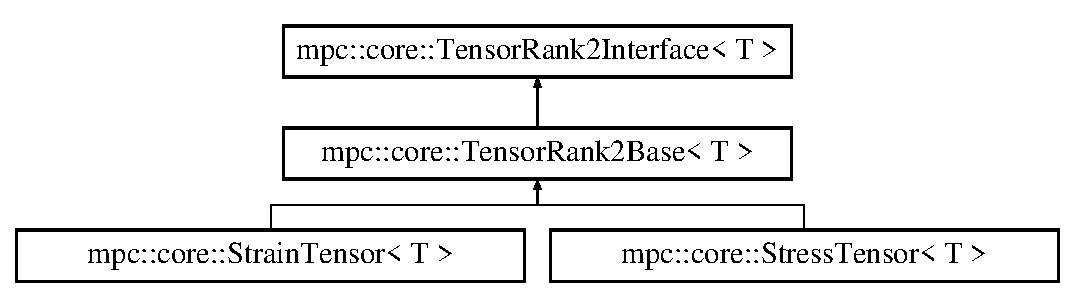
\includegraphics[height=3.000000cm]{structmpc_1_1core_1_1_tensor_rank2_base}
\end{center}
\end{figure}
\subsection*{Public Member Functions}
\begin{DoxyCompactItemize}
\item 
\mbox{\hyperlink{structmpc_1_1core_1_1_tensor_rank2_base_adf3208464cf45f6caf3c78dee1a3c7d1}{Tensor\+Rank2\+Base}} ()
\end{DoxyCompactItemize}
\subsection*{Public Attributes}
\begin{DoxyCompactItemize}
\item 
blitz\+::\+Array$<$ T, 2 $>$ \mbox{\hyperlink{structmpc_1_1core_1_1_tensor_rank2_base_a75703dce1b26306b8f0ee539775ee6d7}{tensor}} = blitz\+::\+Array$<$T,2$>$(3,3, blitz\+::\+Column\+Major\+Array$<$2$>$())
\end{DoxyCompactItemize}


\subsection{Detailed Description}
\subsubsection*{template$<$typename T$>$\newline
class mpc\+::core\+::\+Tensor\+Rank2\+Base$<$ T $>$}

simple base class for tensors of rank 2 

Definition at line 43 of file stressstrain.\+hpp.



\subsection{Constructor \& Destructor Documentation}
\mbox{\Hypertarget{structmpc_1_1core_1_1_tensor_rank2_base_adf3208464cf45f6caf3c78dee1a3c7d1}\label{structmpc_1_1core_1_1_tensor_rank2_base_adf3208464cf45f6caf3c78dee1a3c7d1}} 
\index{mpc\+::core\+::\+Tensor\+Rank2\+Base@{mpc\+::core\+::\+Tensor\+Rank2\+Base}!Tensor\+Rank2\+Base@{Tensor\+Rank2\+Base}}
\index{Tensor\+Rank2\+Base@{Tensor\+Rank2\+Base}!mpc\+::core\+::\+Tensor\+Rank2\+Base@{mpc\+::core\+::\+Tensor\+Rank2\+Base}}
\subsubsection{\texorpdfstring{Tensor\+Rank2\+Base()}{TensorRank2Base()}}
{\footnotesize\ttfamily template$<$typename T$>$ \\
\mbox{\hyperlink{structmpc_1_1core_1_1_tensor_rank2_base}{mpc\+::core\+::\+Tensor\+Rank2\+Base}}$<$ T $>$\+::\mbox{\hyperlink{structmpc_1_1core_1_1_tensor_rank2_base}{Tensor\+Rank2\+Base}} (\begin{DoxyParamCaption}{ }\end{DoxyParamCaption})\hspace{0.3cm}{\ttfamily [inline]}}



Definition at line 45 of file stressstrain.\+hpp.



\subsection{Member Data Documentation}
\mbox{\Hypertarget{structmpc_1_1core_1_1_tensor_rank2_base_a75703dce1b26306b8f0ee539775ee6d7}\label{structmpc_1_1core_1_1_tensor_rank2_base_a75703dce1b26306b8f0ee539775ee6d7}} 
\index{mpc\+::core\+::\+Tensor\+Rank2\+Base@{mpc\+::core\+::\+Tensor\+Rank2\+Base}!tensor@{tensor}}
\index{tensor@{tensor}!mpc\+::core\+::\+Tensor\+Rank2\+Base@{mpc\+::core\+::\+Tensor\+Rank2\+Base}}
\subsubsection{\texorpdfstring{tensor}{tensor}}
{\footnotesize\ttfamily template$<$typename T$>$ \\
blitz\+::\+Array$<$T,2$>$ \mbox{\hyperlink{structmpc_1_1core_1_1_tensor_rank2_base}{mpc\+::core\+::\+Tensor\+Rank2\+Base}}$<$ T $>$\+::tensor = blitz\+::\+Array$<$T,2$>$(3,3, blitz\+::\+Column\+Major\+Array$<$2$>$())}



Definition at line 44 of file stressstrain.\+hpp.



The documentation for this class was generated from the following file\+:\begin{DoxyCompactItemize}
\item 
/\+Users/atorlucci/\+Documents/github\+\_\+threecubed\+\_\+repos/mpc/src/mpc/core/\mbox{\hyperlink{stressstrain_8hpp}{stressstrain.\+hpp}}\end{DoxyCompactItemize}

\hypertarget{structmpc_1_1core_1_1_tensor_rank2_interface}{}\section{mpc\+:\+:core\+:\+:Tensor\+Rank2\+Interface$<$ T $>$ Class Template Reference}
\label{structmpc_1_1core_1_1_tensor_rank2_interface}\index{mpc\+::core\+::\+Tensor\+Rank2\+Interface$<$ T $>$@{mpc\+::core\+::\+Tensor\+Rank2\+Interface$<$ T $>$}}


simple interface class for tensors of rank 2  




{\ttfamily \#include $<$stressstrain.\+hpp$>$}

Inheritance diagram for mpc\+:\+:core\+:\+:Tensor\+Rank2\+Interface$<$ T $>$\+:\begin{figure}[H]
\begin{center}
\leavevmode
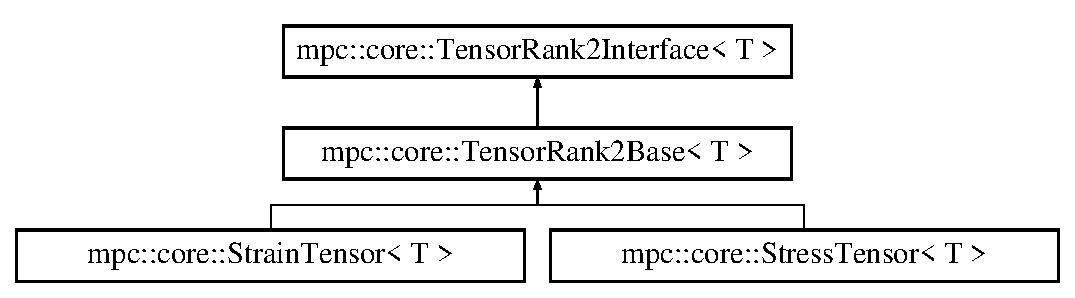
\includegraphics[height=3.000000cm]{structmpc_1_1core_1_1_tensor_rank2_interface}
\end{center}
\end{figure}
\subsection*{Public Member Functions}
\begin{DoxyCompactItemize}
\item 
virtual void \mbox{\hyperlink{structmpc_1_1core_1_1_tensor_rank2_interface_a7d220631fe32f06ec52e5724873a00d9}{Set\+Components}} (std\+::set$<$ \mbox{\hyperlink{namespacempc_1_1core_a467e1fa517a8c269b033fef3aa281360}{mpc\+::core\+::\+Tensor\+Rank2\+Component}}$<$ T $>$ $>$ \&components, bool Apply\+Symmetry)=0
\end{DoxyCompactItemize}


\subsection{Detailed Description}
\subsubsection*{template$<$typename T$>$\newline
class mpc\+::core\+::\+Tensor\+Rank2\+Interface$<$ T $>$}

simple interface class for tensors of rank 2 

Definition at line 32 of file stressstrain.\+hpp.



\subsection{Member Function Documentation}
\mbox{\Hypertarget{structmpc_1_1core_1_1_tensor_rank2_interface_a7d220631fe32f06ec52e5724873a00d9}\label{structmpc_1_1core_1_1_tensor_rank2_interface_a7d220631fe32f06ec52e5724873a00d9}} 
\index{mpc\+::core\+::\+Tensor\+Rank2\+Interface@{mpc\+::core\+::\+Tensor\+Rank2\+Interface}!Set\+Components@{Set\+Components}}
\index{Set\+Components@{Set\+Components}!mpc\+::core\+::\+Tensor\+Rank2\+Interface@{mpc\+::core\+::\+Tensor\+Rank2\+Interface}}
\subsubsection{\texorpdfstring{Set\+Components()}{SetComponents()}}
{\footnotesize\ttfamily template$<$typename T $>$ \\
virtual void \mbox{\hyperlink{structmpc_1_1core_1_1_tensor_rank2_interface}{mpc\+::core\+::\+Tensor\+Rank2\+Interface}}$<$ T $>$\+::Set\+Components (\begin{DoxyParamCaption}\item[{std\+::set$<$ \mbox{\hyperlink{namespacempc_1_1core_a467e1fa517a8c269b033fef3aa281360}{mpc\+::core\+::\+Tensor\+Rank2\+Component}}$<$ T $>$ $>$ \&}]{components,  }\item[{bool}]{Apply\+Symmetry }\end{DoxyParamCaption})\hspace{0.3cm}{\ttfamily [pure virtual]}}



Implemented in \mbox{\hyperlink{structmpc_1_1core_1_1_strain_tensor_a9e208aa77d77296f5fc6fdadd76b018f}{mpc\+::core\+::\+Strain\+Tensor$<$ T $>$}}, and \mbox{\hyperlink{structmpc_1_1core_1_1_stress_tensor_afbac9aaa45907cdbed3ed779b0551bad}{mpc\+::core\+::\+Stress\+Tensor$<$ T $>$}}.



The documentation for this class was generated from the following file\+:\begin{DoxyCompactItemize}
\item 
/\+Users/atorlucci/\+Documents/github\+\_\+threecubed\+\_\+repos/mpc/src/mpc/core/\mbox{\hyperlink{stressstrain_8hpp}{stressstrain.\+hpp}}\end{DoxyCompactItemize}

\hypertarget{structmpc_1_1core_1_1_tensor_rank4_base}{}\section{mpc\+:\+:core\+:\+:Tensor\+Rank4\+Base$<$ T $>$ Class Template Reference}
\label{structmpc_1_1core_1_1_tensor_rank4_base}\index{mpc\+::core\+::\+Tensor\+Rank4\+Base$<$ T $>$@{mpc\+::core\+::\+Tensor\+Rank4\+Base$<$ T $>$}}


base class for tensors of rank 4  




{\ttfamily \#include $<$stiffnesscompliance.\+hpp$>$}

Inheritance diagram for mpc\+:\+:core\+:\+:Tensor\+Rank4\+Base$<$ T $>$\+:\begin{figure}[H]
\begin{center}
\leavevmode
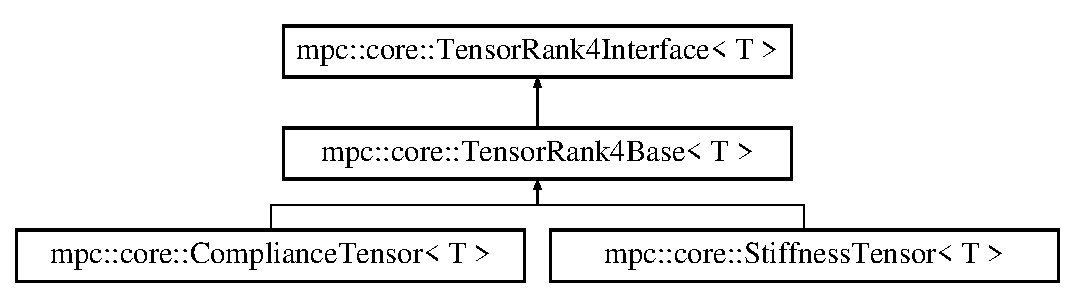
\includegraphics[height=3.000000cm]{structmpc_1_1core_1_1_tensor_rank4_base}
\end{center}
\end{figure}
\subsection*{Public Member Functions}
\begin{DoxyCompactItemize}
\item 
\mbox{\hyperlink{structmpc_1_1core_1_1_tensor_rank4_base_acfdbbb57d9d9b43e0fd55b5ecf16658b}{Tensor\+Rank4\+Base}} ()
\end{DoxyCompactItemize}
\subsection*{Public Attributes}
\begin{DoxyCompactItemize}
\item 
blitz\+::\+Array$<$ T, 4 $>$ \mbox{\hyperlink{structmpc_1_1core_1_1_tensor_rank4_base_ac599ed36ecac8367b0fa5872160988ed}{tensor}} = blitz\+::\+Array$<$T,4$>$(3, 3, 3, 3, blitz\+::\+Column\+Major\+Array$<$4$>$())
\end{DoxyCompactItemize}


\subsection{Detailed Description}
\subsubsection*{template$<$typename T$>$\newline
class mpc\+::core\+::\+Tensor\+Rank4\+Base$<$ T $>$}

base class for tensors of rank 4 

The tensors in mpc are three dimensional cartesian tensors; this base class provides 

Definition at line 46 of file stiffnesscompliance.\+hpp.



\subsection{Constructor \& Destructor Documentation}
\mbox{\Hypertarget{structmpc_1_1core_1_1_tensor_rank4_base_acfdbbb57d9d9b43e0fd55b5ecf16658b}\label{structmpc_1_1core_1_1_tensor_rank4_base_acfdbbb57d9d9b43e0fd55b5ecf16658b}} 
\index{mpc\+::core\+::\+Tensor\+Rank4\+Base@{mpc\+::core\+::\+Tensor\+Rank4\+Base}!Tensor\+Rank4\+Base@{Tensor\+Rank4\+Base}}
\index{Tensor\+Rank4\+Base@{Tensor\+Rank4\+Base}!mpc\+::core\+::\+Tensor\+Rank4\+Base@{mpc\+::core\+::\+Tensor\+Rank4\+Base}}
\subsubsection{\texorpdfstring{Tensor\+Rank4\+Base()}{TensorRank4Base()}}
{\footnotesize\ttfamily template$<$typename T $>$ \\
\mbox{\hyperlink{structmpc_1_1core_1_1_tensor_rank4_base}{mpc\+::core\+::\+Tensor\+Rank4\+Base}}$<$ T $>$\+::\mbox{\hyperlink{structmpc_1_1core_1_1_tensor_rank4_base}{Tensor\+Rank4\+Base}} (\begin{DoxyParamCaption}{ }\end{DoxyParamCaption})\hspace{0.3cm}{\ttfamily [inline]}}



Definition at line 48 of file stiffnesscompliance.\+hpp.



\subsection{Member Data Documentation}
\mbox{\Hypertarget{structmpc_1_1core_1_1_tensor_rank4_base_ac599ed36ecac8367b0fa5872160988ed}\label{structmpc_1_1core_1_1_tensor_rank4_base_ac599ed36ecac8367b0fa5872160988ed}} 
\index{mpc\+::core\+::\+Tensor\+Rank4\+Base@{mpc\+::core\+::\+Tensor\+Rank4\+Base}!tensor@{tensor}}
\index{tensor@{tensor}!mpc\+::core\+::\+Tensor\+Rank4\+Base@{mpc\+::core\+::\+Tensor\+Rank4\+Base}}
\subsubsection{\texorpdfstring{tensor}{tensor}}
{\footnotesize\ttfamily template$<$typename T $>$ \\
blitz\+::\+Array$<$T,4$>$ \mbox{\hyperlink{structmpc_1_1core_1_1_tensor_rank4_base}{mpc\+::core\+::\+Tensor\+Rank4\+Base}}$<$ T $>$\+::tensor = blitz\+::\+Array$<$T,4$>$(3, 3, 3, 3, blitz\+::\+Column\+Major\+Array$<$4$>$())}



Definition at line 47 of file stiffnesscompliance.\+hpp.



The documentation for this class was generated from the following file\+:\begin{DoxyCompactItemize}
\item 
/\+Users/atorlucci/\+Documents/github\+\_\+threecubed\+\_\+repos/mpc/src/mpc/core/\mbox{\hyperlink{stiffnesscompliance_8hpp}{stiffnesscompliance.\+hpp}}\end{DoxyCompactItemize}

\hypertarget{structmpc_1_1core_1_1_tensor_rank4_interface}{}\section{mpc\+:\+:core\+:\+:Tensor\+Rank4\+Interface$<$ T $>$ Class Template Reference}
\label{structmpc_1_1core_1_1_tensor_rank4_interface}\index{mpc\+::core\+::\+Tensor\+Rank4\+Interface$<$ T $>$@{mpc\+::core\+::\+Tensor\+Rank4\+Interface$<$ T $>$}}


simple interface for tensors of rank 4  




{\ttfamily \#include $<$stiffnesscompliance.\+hpp$>$}

Inheritance diagram for mpc\+:\+:core\+:\+:Tensor\+Rank4\+Interface$<$ T $>$\+:\begin{figure}[H]
\begin{center}
\leavevmode
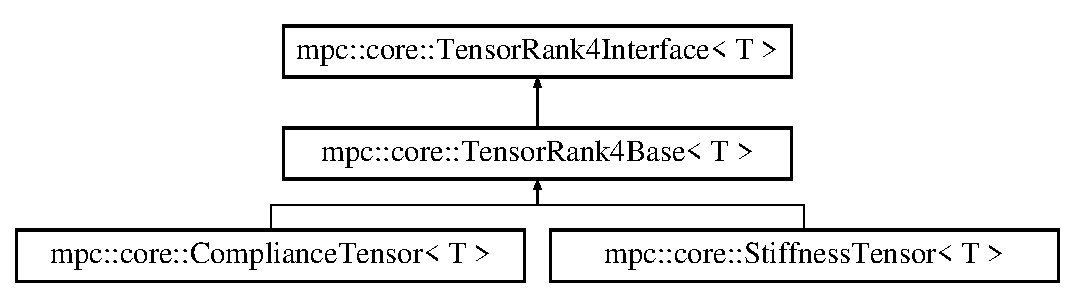
\includegraphics[height=3.000000cm]{structmpc_1_1core_1_1_tensor_rank4_interface}
\end{center}
\end{figure}


\subsection{Detailed Description}
\subsubsection*{template$<$typename T$>$\newline
class mpc\+::core\+::\+Tensor\+Rank4\+Interface$<$ T $>$}

simple interface for tensors of rank 4 

Definition at line 34 of file stiffnesscompliance.\+hpp.



The documentation for this class was generated from the following file\+:\begin{DoxyCompactItemize}
\item 
/\+Users/atorlucci/\+Documents/github\+\_\+threecubed\+\_\+repos/mpc/src/mpc/core/\mbox{\hyperlink{stiffnesscompliance_8hpp}{stiffnesscompliance.\+hpp}}\end{DoxyCompactItemize}

\hypertarget{structmpc_1_1core_1_1_tensor_rank4_symmetry_components_function_object}{}\section{mpc\+:\+:core\+:\+:Tensor\+Rank4\+Symmetry\+Components\+Function\+Object$<$ T, CS, S $>$ Class Template Reference}
\label{structmpc_1_1core_1_1_tensor_rank4_symmetry_components_function_object}\index{mpc\+::core\+::\+Tensor\+Rank4\+Symmetry\+Components\+Function\+Object$<$ T, C\+S, S $>$@{mpc\+::core\+::\+Tensor\+Rank4\+Symmetry\+Components\+Function\+Object$<$ T, C\+S, S $>$}}


function object that does nothing for symmetry groups that do not have any \char`\"{}linked\char`\"{} components  




{\ttfamily \#include $<$symmetrycomponents.\+hpp$>$}

\subsection*{Public Member Functions}
\begin{DoxyCompactItemize}
\item 
void \mbox{\hyperlink{structmpc_1_1core_1_1_tensor_rank4_symmetry_components_function_object_aec8a15001e34d9d89ef5b9097a0524ee}{operator()}} (std\+::set$<$ \mbox{\hyperlink{classmpc_1_1core_1_1_tensor_rank_n_component}{mpc\+::core\+::\+Tensor\+Rank\+N\+Component}}$<$ T, 4 $>$ $>$ \&components)
\end{DoxyCompactItemize}


\subsection{Detailed Description}
\subsubsection*{template$<$typename T, typename CS, typename S = mpc\+::core\+::\+None\+Symmetry\+Group\+Type$>$\newline
class mpc\+::core\+::\+Tensor\+Rank4\+Symmetry\+Components\+Function\+Object$<$ T, C\+S, S $>$}

function object that does nothing for symmetry groups that do not have any \char`\"{}linked\char`\"{} components 

T\+O\+DO\+: describe partial specializations 

Definition at line 239 of file symmetrycomponents.\+hpp.



\subsection{Member Function Documentation}
\mbox{\Hypertarget{structmpc_1_1core_1_1_tensor_rank4_symmetry_components_function_object_aec8a15001e34d9d89ef5b9097a0524ee}\label{structmpc_1_1core_1_1_tensor_rank4_symmetry_components_function_object_aec8a15001e34d9d89ef5b9097a0524ee}} 
\index{mpc\+::core\+::\+Tensor\+Rank4\+Symmetry\+Components\+Function\+Object@{mpc\+::core\+::\+Tensor\+Rank4\+Symmetry\+Components\+Function\+Object}!operator()@{operator()}}
\index{operator()@{operator()}!mpc\+::core\+::\+Tensor\+Rank4\+Symmetry\+Components\+Function\+Object@{mpc\+::core\+::\+Tensor\+Rank4\+Symmetry\+Components\+Function\+Object}}
\subsubsection{\texorpdfstring{operator()()}{operator()()}}
{\footnotesize\ttfamily template$<$typename T, typename CS, typename S = mpc\+::core\+::\+None\+Symmetry\+Group\+Type$>$ \\
void \mbox{\hyperlink{structmpc_1_1core_1_1_tensor_rank4_symmetry_components_function_object}{mpc\+::core\+::\+Tensor\+Rank4\+Symmetry\+Components\+Function\+Object}}$<$ T, CS, S $>$\+::operator() (\begin{DoxyParamCaption}\item[{std\+::set$<$ \mbox{\hyperlink{classmpc_1_1core_1_1_tensor_rank_n_component}{mpc\+::core\+::\+Tensor\+Rank\+N\+Component}}$<$ T, 4 $>$ $>$ \&}]{components }\end{DoxyParamCaption})\hspace{0.3cm}{\ttfamily [inline]}}



Definition at line 243 of file symmetrycomponents.\+hpp.



The documentation for this class was generated from the following file\+:\begin{DoxyCompactItemize}
\item 
/\+Users/atorlucci/\+Documents/github\+\_\+threecubed\+\_\+repos/mpc/src/mpc/core/\mbox{\hyperlink{symmetrycomponents_8hpp}{symmetrycomponents.\+hpp}}\end{DoxyCompactItemize}

\hypertarget{structmpc_1_1core_1_1_tensor_rank4_symmetry_components_function_object_3_01_t_00_01_c_s_00_01mpcb78f8bb4486f797b17b937e5288b806c}{}\section{mpc\+:\+:core\+:\+:Tensor\+Rank4\+Symmetry\+Components\+Function\+Object$<$ T, CS, mpc\+:\+:core\+:\+:Cubic\+Symmetry\+Group\+Type $>$ Struct Template Reference}
\label{structmpc_1_1core_1_1_tensor_rank4_symmetry_components_function_object_3_01_t_00_01_c_s_00_01mpcb78f8bb4486f797b17b937e5288b806c}\index{mpc\+::core\+::\+Tensor\+Rank4\+Symmetry\+Components\+Function\+Object$<$ T, C\+S, mpc\+::core\+::\+Cubic\+Symmetry\+Group\+Type $>$@{mpc\+::core\+::\+Tensor\+Rank4\+Symmetry\+Components\+Function\+Object$<$ T, C\+S, mpc\+::core\+::\+Cubic\+Symmetry\+Group\+Type $>$}}


{\ttfamily \#include $<$symmetrycomponents.\+hpp$>$}

\subsection*{Public Member Functions}
\begin{DoxyCompactItemize}
\item 
void \mbox{\hyperlink{structmpc_1_1core_1_1_tensor_rank4_symmetry_components_function_object_3_01_t_00_01_c_s_00_01mpcb78f8bb4486f797b17b937e5288b806c_ab3d55d3901f94e4bd4ee55e064c84783}{operator()}} (std\+::set$<$ \mbox{\hyperlink{classmpc_1_1core_1_1_tensor_rank_n_component}{mpc\+::core\+::\+Tensor\+Rank\+N\+Component}}$<$ T, 4 $>$ $>$ \&components)
\end{DoxyCompactItemize}


\subsection{Detailed Description}
\subsubsection*{template$<$typename T, typename CS$>$\newline
struct mpc\+::core\+::\+Tensor\+Rank4\+Symmetry\+Components\+Function\+Object$<$ T, C\+S, mpc\+::core\+::\+Cubic\+Symmetry\+Group\+Type $>$}



Definition at line 489 of file symmetrycomponents.\+hpp.



\subsection{Member Function Documentation}
\mbox{\Hypertarget{structmpc_1_1core_1_1_tensor_rank4_symmetry_components_function_object_3_01_t_00_01_c_s_00_01mpcb78f8bb4486f797b17b937e5288b806c_ab3d55d3901f94e4bd4ee55e064c84783}\label{structmpc_1_1core_1_1_tensor_rank4_symmetry_components_function_object_3_01_t_00_01_c_s_00_01mpcb78f8bb4486f797b17b937e5288b806c_ab3d55d3901f94e4bd4ee55e064c84783}} 
\index{mpc\+::core\+::\+Tensor\+Rank4\+Symmetry\+Components\+Function\+Object$<$ T, C\+S, mpc\+::core\+::\+Cubic\+Symmetry\+Group\+Type $>$@{mpc\+::core\+::\+Tensor\+Rank4\+Symmetry\+Components\+Function\+Object$<$ T, C\+S, mpc\+::core\+::\+Cubic\+Symmetry\+Group\+Type $>$}!operator()@{operator()}}
\index{operator()@{operator()}!mpc\+::core\+::\+Tensor\+Rank4\+Symmetry\+Components\+Function\+Object$<$ T, C\+S, mpc\+::core\+::\+Cubic\+Symmetry\+Group\+Type $>$@{mpc\+::core\+::\+Tensor\+Rank4\+Symmetry\+Components\+Function\+Object$<$ T, C\+S, mpc\+::core\+::\+Cubic\+Symmetry\+Group\+Type $>$}}
\subsubsection{\texorpdfstring{operator()()}{operator()()}}
{\footnotesize\ttfamily template$<$typename T , typename CS $>$ \\
void \mbox{\hyperlink{structmpc_1_1core_1_1_tensor_rank4_symmetry_components_function_object}{mpc\+::core\+::\+Tensor\+Rank4\+Symmetry\+Components\+Function\+Object}}$<$ T, CS, \mbox{\hyperlink{structmpc_1_1core_1_1_cubic_symmetry_group_type}{mpc\+::core\+::\+Cubic\+Symmetry\+Group\+Type}} $>$\+::operator() (\begin{DoxyParamCaption}\item[{std\+::set$<$ \mbox{\hyperlink{classmpc_1_1core_1_1_tensor_rank_n_component}{mpc\+::core\+::\+Tensor\+Rank\+N\+Component}}$<$ T, 4 $>$ $>$ \&}]{components }\end{DoxyParamCaption})\hspace{0.3cm}{\ttfamily [inline]}}



Definition at line 493 of file symmetrycomponents.\+hpp.



The documentation for this struct was generated from the following file\+:\begin{DoxyCompactItemize}
\item 
/\+Users/atorlucci/\+Documents/github\+\_\+threecubed\+\_\+repos/mpc/src/mpc/core/\mbox{\hyperlink{symmetrycomponents_8hpp}{symmetrycomponents.\+hpp}}\end{DoxyCompactItemize}

\hypertarget{structmpc_1_1core_1_1_tensor_rank4_symmetry_components_function_object_3_01_t_00_01_c_s_00_01mpc53006a57374f233daf45c7959ab92c1e}{}\section{mpc\+:\+:core\+:\+:Tensor\+Rank4\+Symmetry\+Components\+Function\+Object$<$ T, CS, mpc\+:\+:core\+:\+:Hexagonal\+Symmetry\+Group\+Type $>$ Struct Template Reference}
\label{structmpc_1_1core_1_1_tensor_rank4_symmetry_components_function_object_3_01_t_00_01_c_s_00_01mpc53006a57374f233daf45c7959ab92c1e}\index{mpc\+::core\+::\+Tensor\+Rank4\+Symmetry\+Components\+Function\+Object$<$ T, C\+S, mpc\+::core\+::\+Hexagonal\+Symmetry\+Group\+Type $>$@{mpc\+::core\+::\+Tensor\+Rank4\+Symmetry\+Components\+Function\+Object$<$ T, C\+S, mpc\+::core\+::\+Hexagonal\+Symmetry\+Group\+Type $>$}}


{\ttfamily \#include $<$symmetrycomponents.\+hpp$>$}

\subsection*{Public Member Functions}
\begin{DoxyCompactItemize}
\item 
void \mbox{\hyperlink{structmpc_1_1core_1_1_tensor_rank4_symmetry_components_function_object_3_01_t_00_01_c_s_00_01mpc53006a57374f233daf45c7959ab92c1e_a23417bd745bf260bd660d1d377050273}{operator()}} (std\+::set$<$ \mbox{\hyperlink{classmpc_1_1core_1_1_tensor_rank_n_component}{mpc\+::core\+::\+Tensor\+Rank\+N\+Component}}$<$ T, 4 $>$ $>$ \&components)
\end{DoxyCompactItemize}


\subsection{Detailed Description}
\subsubsection*{template$<$typename T, typename CS$>$\newline
struct mpc\+::core\+::\+Tensor\+Rank4\+Symmetry\+Components\+Function\+Object$<$ T, C\+S, mpc\+::core\+::\+Hexagonal\+Symmetry\+Group\+Type $>$}



Definition at line 450 of file symmetrycomponents.\+hpp.



\subsection{Member Function Documentation}
\mbox{\Hypertarget{structmpc_1_1core_1_1_tensor_rank4_symmetry_components_function_object_3_01_t_00_01_c_s_00_01mpc53006a57374f233daf45c7959ab92c1e_a23417bd745bf260bd660d1d377050273}\label{structmpc_1_1core_1_1_tensor_rank4_symmetry_components_function_object_3_01_t_00_01_c_s_00_01mpc53006a57374f233daf45c7959ab92c1e_a23417bd745bf260bd660d1d377050273}} 
\index{mpc\+::core\+::\+Tensor\+Rank4\+Symmetry\+Components\+Function\+Object$<$ T, C\+S, mpc\+::core\+::\+Hexagonal\+Symmetry\+Group\+Type $>$@{mpc\+::core\+::\+Tensor\+Rank4\+Symmetry\+Components\+Function\+Object$<$ T, C\+S, mpc\+::core\+::\+Hexagonal\+Symmetry\+Group\+Type $>$}!operator()@{operator()}}
\index{operator()@{operator()}!mpc\+::core\+::\+Tensor\+Rank4\+Symmetry\+Components\+Function\+Object$<$ T, C\+S, mpc\+::core\+::\+Hexagonal\+Symmetry\+Group\+Type $>$@{mpc\+::core\+::\+Tensor\+Rank4\+Symmetry\+Components\+Function\+Object$<$ T, C\+S, mpc\+::core\+::\+Hexagonal\+Symmetry\+Group\+Type $>$}}
\subsubsection{\texorpdfstring{operator()()}{operator()()}}
{\footnotesize\ttfamily template$<$typename T , typename CS $>$ \\
void \mbox{\hyperlink{structmpc_1_1core_1_1_tensor_rank4_symmetry_components_function_object}{mpc\+::core\+::\+Tensor\+Rank4\+Symmetry\+Components\+Function\+Object}}$<$ T, CS, \mbox{\hyperlink{structmpc_1_1core_1_1_hexagonal_symmetry_group_type}{mpc\+::core\+::\+Hexagonal\+Symmetry\+Group\+Type}} $>$\+::operator() (\begin{DoxyParamCaption}\item[{std\+::set$<$ \mbox{\hyperlink{classmpc_1_1core_1_1_tensor_rank_n_component}{mpc\+::core\+::\+Tensor\+Rank\+N\+Component}}$<$ T, 4 $>$ $>$ \&}]{components }\end{DoxyParamCaption})\hspace{0.3cm}{\ttfamily [inline]}}



Definition at line 455 of file symmetrycomponents.\+hpp.



The documentation for this struct was generated from the following file\+:\begin{DoxyCompactItemize}
\item 
/\+Users/atorlucci/\+Documents/github\+\_\+threecubed\+\_\+repos/mpc/src/mpc/core/\mbox{\hyperlink{symmetrycomponents_8hpp}{symmetrycomponents.\+hpp}}\end{DoxyCompactItemize}

\hypertarget{structmpc_1_1core_1_1_tensor_rank4_symmetry_components_function_object_3_01_t_00_01_c_s_00_01mpc03d1a1424526d21cea036884c5bccc6f}{}\section{mpc\+:\+:core\+:\+:Tensor\+Rank4\+Symmetry\+Components\+Function\+Object$<$ T, CS, mpc\+:\+:core\+:\+:Isotropic\+Symmetry\+Group\+Type $>$ Struct Template Reference}
\label{structmpc_1_1core_1_1_tensor_rank4_symmetry_components_function_object_3_01_t_00_01_c_s_00_01mpc03d1a1424526d21cea036884c5bccc6f}\index{mpc\+::core\+::\+Tensor\+Rank4\+Symmetry\+Components\+Function\+Object$<$ T, C\+S, mpc\+::core\+::\+Isotropic\+Symmetry\+Group\+Type $>$@{mpc\+::core\+::\+Tensor\+Rank4\+Symmetry\+Components\+Function\+Object$<$ T, C\+S, mpc\+::core\+::\+Isotropic\+Symmetry\+Group\+Type $>$}}


{\ttfamily \#include $<$symmetrycomponents.\+hpp$>$}

\subsection*{Public Member Functions}
\begin{DoxyCompactItemize}
\item 
void \mbox{\hyperlink{structmpc_1_1core_1_1_tensor_rank4_symmetry_components_function_object_3_01_t_00_01_c_s_00_01mpc03d1a1424526d21cea036884c5bccc6f_af4474030b6e43277a300f140b2ae69da}{operator()}} (std\+::set$<$ \mbox{\hyperlink{classmpc_1_1core_1_1_tensor_rank_n_component}{mpc\+::core\+::\+Tensor\+Rank\+N\+Component}}$<$ T, 4 $>$ $>$ \&components)
\end{DoxyCompactItemize}


\subsection{Detailed Description}
\subsubsection*{template$<$typename T, typename CS$>$\newline
struct mpc\+::core\+::\+Tensor\+Rank4\+Symmetry\+Components\+Function\+Object$<$ T, C\+S, mpc\+::core\+::\+Isotropic\+Symmetry\+Group\+Type $>$}



Definition at line 567 of file symmetrycomponents.\+hpp.



\subsection{Member Function Documentation}
\mbox{\Hypertarget{structmpc_1_1core_1_1_tensor_rank4_symmetry_components_function_object_3_01_t_00_01_c_s_00_01mpc03d1a1424526d21cea036884c5bccc6f_af4474030b6e43277a300f140b2ae69da}\label{structmpc_1_1core_1_1_tensor_rank4_symmetry_components_function_object_3_01_t_00_01_c_s_00_01mpc03d1a1424526d21cea036884c5bccc6f_af4474030b6e43277a300f140b2ae69da}} 
\index{mpc\+::core\+::\+Tensor\+Rank4\+Symmetry\+Components\+Function\+Object$<$ T, C\+S, mpc\+::core\+::\+Isotropic\+Symmetry\+Group\+Type $>$@{mpc\+::core\+::\+Tensor\+Rank4\+Symmetry\+Components\+Function\+Object$<$ T, C\+S, mpc\+::core\+::\+Isotropic\+Symmetry\+Group\+Type $>$}!operator()@{operator()}}
\index{operator()@{operator()}!mpc\+::core\+::\+Tensor\+Rank4\+Symmetry\+Components\+Function\+Object$<$ T, C\+S, mpc\+::core\+::\+Isotropic\+Symmetry\+Group\+Type $>$@{mpc\+::core\+::\+Tensor\+Rank4\+Symmetry\+Components\+Function\+Object$<$ T, C\+S, mpc\+::core\+::\+Isotropic\+Symmetry\+Group\+Type $>$}}
\subsubsection{\texorpdfstring{operator()()}{operator()()}}
{\footnotesize\ttfamily template$<$typename T , typename CS $>$ \\
void \mbox{\hyperlink{structmpc_1_1core_1_1_tensor_rank4_symmetry_components_function_object}{mpc\+::core\+::\+Tensor\+Rank4\+Symmetry\+Components\+Function\+Object}}$<$ T, CS, \mbox{\hyperlink{structmpc_1_1core_1_1_isotropic_symmetry_group_type}{mpc\+::core\+::\+Isotropic\+Symmetry\+Group\+Type}} $>$\+::operator() (\begin{DoxyParamCaption}\item[{std\+::set$<$ \mbox{\hyperlink{classmpc_1_1core_1_1_tensor_rank_n_component}{mpc\+::core\+::\+Tensor\+Rank\+N\+Component}}$<$ T, 4 $>$ $>$ \&}]{components }\end{DoxyParamCaption})\hspace{0.3cm}{\ttfamily [inline]}}



Definition at line 571 of file symmetrycomponents.\+hpp.



The documentation for this struct was generated from the following file\+:\begin{DoxyCompactItemize}
\item 
/\+Users/atorlucci/\+Documents/github\+\_\+threecubed\+\_\+repos/mpc/src/mpc/core/\mbox{\hyperlink{symmetrycomponents_8hpp}{symmetrycomponents.\+hpp}}\end{DoxyCompactItemize}

\hypertarget{structmpc_1_1core_1_1_tensor_rank4_symmetry_components_function_object_3_01_t_00_01_c_s_00_01mpcb35265619212e0eab46a619a1df412a3}{}\section{mpc\+:\+:core\+:\+:Tensor\+Rank4\+Symmetry\+Components\+Function\+Object$<$ T, CS, mpc\+:\+:core\+:\+:Tetragonal6\+Symmetry\+Group\+Type $>$ Struct Template Reference}
\label{structmpc_1_1core_1_1_tensor_rank4_symmetry_components_function_object_3_01_t_00_01_c_s_00_01mpcb35265619212e0eab46a619a1df412a3}\index{mpc\+::core\+::\+Tensor\+Rank4\+Symmetry\+Components\+Function\+Object$<$ T, C\+S, mpc\+::core\+::\+Tetragonal6\+Symmetry\+Group\+Type $>$@{mpc\+::core\+::\+Tensor\+Rank4\+Symmetry\+Components\+Function\+Object$<$ T, C\+S, mpc\+::core\+::\+Tetragonal6\+Symmetry\+Group\+Type $>$}}


{\ttfamily \#include $<$symmetrycomponents.\+hpp$>$}

\subsection*{Public Member Functions}
\begin{DoxyCompactItemize}
\item 
void \mbox{\hyperlink{structmpc_1_1core_1_1_tensor_rank4_symmetry_components_function_object_3_01_t_00_01_c_s_00_01mpcb35265619212e0eab46a619a1df412a3_a2325e8e7b5be33a8cb7c27698bd179d5}{operator()}} (std\+::set$<$ \mbox{\hyperlink{classmpc_1_1core_1_1_tensor_rank_n_component}{mpc\+::core\+::\+Tensor\+Rank\+N\+Component}}$<$ T, 4 $>$ $>$ \&components)
\end{DoxyCompactItemize}


\subsection{Detailed Description}
\subsubsection*{template$<$typename T, typename CS$>$\newline
struct mpc\+::core\+::\+Tensor\+Rank4\+Symmetry\+Components\+Function\+Object$<$ T, C\+S, mpc\+::core\+::\+Tetragonal6\+Symmetry\+Group\+Type $>$}



Definition at line 424 of file symmetrycomponents.\+hpp.



\subsection{Member Function Documentation}
\mbox{\Hypertarget{structmpc_1_1core_1_1_tensor_rank4_symmetry_components_function_object_3_01_t_00_01_c_s_00_01mpcb35265619212e0eab46a619a1df412a3_a2325e8e7b5be33a8cb7c27698bd179d5}\label{structmpc_1_1core_1_1_tensor_rank4_symmetry_components_function_object_3_01_t_00_01_c_s_00_01mpcb35265619212e0eab46a619a1df412a3_a2325e8e7b5be33a8cb7c27698bd179d5}} 
\index{mpc\+::core\+::\+Tensor\+Rank4\+Symmetry\+Components\+Function\+Object$<$ T, C\+S, mpc\+::core\+::\+Tetragonal6\+Symmetry\+Group\+Type $>$@{mpc\+::core\+::\+Tensor\+Rank4\+Symmetry\+Components\+Function\+Object$<$ T, C\+S, mpc\+::core\+::\+Tetragonal6\+Symmetry\+Group\+Type $>$}!operator()@{operator()}}
\index{operator()@{operator()}!mpc\+::core\+::\+Tensor\+Rank4\+Symmetry\+Components\+Function\+Object$<$ T, C\+S, mpc\+::core\+::\+Tetragonal6\+Symmetry\+Group\+Type $>$@{mpc\+::core\+::\+Tensor\+Rank4\+Symmetry\+Components\+Function\+Object$<$ T, C\+S, mpc\+::core\+::\+Tetragonal6\+Symmetry\+Group\+Type $>$}}
\subsubsection{\texorpdfstring{operator()()}{operator()()}}
{\footnotesize\ttfamily template$<$typename T , typename CS $>$ \\
void \mbox{\hyperlink{structmpc_1_1core_1_1_tensor_rank4_symmetry_components_function_object}{mpc\+::core\+::\+Tensor\+Rank4\+Symmetry\+Components\+Function\+Object}}$<$ T, CS, \mbox{\hyperlink{structmpc_1_1core_1_1_tetragonal6_symmetry_group_type}{mpc\+::core\+::\+Tetragonal6\+Symmetry\+Group\+Type}} $>$\+::operator() (\begin{DoxyParamCaption}\item[{std\+::set$<$ \mbox{\hyperlink{classmpc_1_1core_1_1_tensor_rank_n_component}{mpc\+::core\+::\+Tensor\+Rank\+N\+Component}}$<$ T, 4 $>$ $>$ \&}]{components }\end{DoxyParamCaption})\hspace{0.3cm}{\ttfamily [inline]}}



Definition at line 429 of file symmetrycomponents.\+hpp.



The documentation for this struct was generated from the following file\+:\begin{DoxyCompactItemize}
\item 
/\+Users/atorlucci/\+Documents/github\+\_\+threecubed\+\_\+repos/mpc/src/mpc/core/\mbox{\hyperlink{symmetrycomponents_8hpp}{symmetrycomponents.\+hpp}}\end{DoxyCompactItemize}

\hypertarget{structmpc_1_1core_1_1_tensor_rank4_symmetry_components_function_object_3_01_t_00_01_c_s_00_01mpc63de79cc64d05f6df7e125399a852032}{}\section{mpc\+:\+:core\+:\+:Tensor\+Rank4\+Symmetry\+Components\+Function\+Object$<$ T, CS, mpc\+:\+:core\+:\+:Tetragonal7\+Symmetry\+Group\+Type $>$ Struct Template Reference}
\label{structmpc_1_1core_1_1_tensor_rank4_symmetry_components_function_object_3_01_t_00_01_c_s_00_01mpc63de79cc64d05f6df7e125399a852032}\index{mpc\+::core\+::\+Tensor\+Rank4\+Symmetry\+Components\+Function\+Object$<$ T, C\+S, mpc\+::core\+::\+Tetragonal7\+Symmetry\+Group\+Type $>$@{mpc\+::core\+::\+Tensor\+Rank4\+Symmetry\+Components\+Function\+Object$<$ T, C\+S, mpc\+::core\+::\+Tetragonal7\+Symmetry\+Group\+Type $>$}}


{\ttfamily \#include $<$symmetrycomponents.\+hpp$>$}

\subsection*{Public Member Functions}
\begin{DoxyCompactItemize}
\item 
void \mbox{\hyperlink{structmpc_1_1core_1_1_tensor_rank4_symmetry_components_function_object_3_01_t_00_01_c_s_00_01mpc63de79cc64d05f6df7e125399a852032_a2770e12360eff8f4eba232d9c9bea4ea}{operator()}} (std\+::set$<$ \mbox{\hyperlink{classmpc_1_1core_1_1_tensor_rank_n_component}{mpc\+::core\+::\+Tensor\+Rank\+N\+Component}}$<$ T, 4 $>$ $>$ \&components)
\end{DoxyCompactItemize}


\subsection{Detailed Description}
\subsubsection*{template$<$typename T, typename CS$>$\newline
struct mpc\+::core\+::\+Tensor\+Rank4\+Symmetry\+Components\+Function\+Object$<$ T, C\+S, mpc\+::core\+::\+Tetragonal7\+Symmetry\+Group\+Type $>$}



Definition at line 393 of file symmetrycomponents.\+hpp.



\subsection{Member Function Documentation}
\mbox{\Hypertarget{structmpc_1_1core_1_1_tensor_rank4_symmetry_components_function_object_3_01_t_00_01_c_s_00_01mpc63de79cc64d05f6df7e125399a852032_a2770e12360eff8f4eba232d9c9bea4ea}\label{structmpc_1_1core_1_1_tensor_rank4_symmetry_components_function_object_3_01_t_00_01_c_s_00_01mpc63de79cc64d05f6df7e125399a852032_a2770e12360eff8f4eba232d9c9bea4ea}} 
\index{mpc\+::core\+::\+Tensor\+Rank4\+Symmetry\+Components\+Function\+Object$<$ T, C\+S, mpc\+::core\+::\+Tetragonal7\+Symmetry\+Group\+Type $>$@{mpc\+::core\+::\+Tensor\+Rank4\+Symmetry\+Components\+Function\+Object$<$ T, C\+S, mpc\+::core\+::\+Tetragonal7\+Symmetry\+Group\+Type $>$}!operator()@{operator()}}
\index{operator()@{operator()}!mpc\+::core\+::\+Tensor\+Rank4\+Symmetry\+Components\+Function\+Object$<$ T, C\+S, mpc\+::core\+::\+Tetragonal7\+Symmetry\+Group\+Type $>$@{mpc\+::core\+::\+Tensor\+Rank4\+Symmetry\+Components\+Function\+Object$<$ T, C\+S, mpc\+::core\+::\+Tetragonal7\+Symmetry\+Group\+Type $>$}}
\subsubsection{\texorpdfstring{operator()()}{operator()()}}
{\footnotesize\ttfamily template$<$typename T , typename CS $>$ \\
void \mbox{\hyperlink{structmpc_1_1core_1_1_tensor_rank4_symmetry_components_function_object}{mpc\+::core\+::\+Tensor\+Rank4\+Symmetry\+Components\+Function\+Object}}$<$ T, CS, \mbox{\hyperlink{structmpc_1_1core_1_1_tetragonal7_symmetry_group_type}{mpc\+::core\+::\+Tetragonal7\+Symmetry\+Group\+Type}} $>$\+::operator() (\begin{DoxyParamCaption}\item[{std\+::set$<$ \mbox{\hyperlink{classmpc_1_1core_1_1_tensor_rank_n_component}{mpc\+::core\+::\+Tensor\+Rank\+N\+Component}}$<$ T, 4 $>$ $>$ \&}]{components }\end{DoxyParamCaption})\hspace{0.3cm}{\ttfamily [inline]}}



Definition at line 398 of file symmetrycomponents.\+hpp.



The documentation for this struct was generated from the following file\+:\begin{DoxyCompactItemize}
\item 
/\+Users/atorlucci/\+Documents/github\+\_\+threecubed\+\_\+repos/mpc/src/mpc/core/\mbox{\hyperlink{symmetrycomponents_8hpp}{symmetrycomponents.\+hpp}}\end{DoxyCompactItemize}

\hypertarget{structmpc_1_1core_1_1_tensor_rank4_symmetry_components_function_object_3_01_t_00_01_c_s_00_01mpc8f8b6e3c3ae3ae919d47d056c15bff9d}{}\section{mpc\+:\+:core\+:\+:Tensor\+Rank4\+Symmetry\+Components\+Function\+Object$<$ T, CS, mpc\+:\+:core\+:\+:Trigonal6\+Symmetry\+Group\+Type $>$ Struct Template Reference}
\label{structmpc_1_1core_1_1_tensor_rank4_symmetry_components_function_object_3_01_t_00_01_c_s_00_01mpc8f8b6e3c3ae3ae919d47d056c15bff9d}\index{mpc\+::core\+::\+Tensor\+Rank4\+Symmetry\+Components\+Function\+Object$<$ T, C\+S, mpc\+::core\+::\+Trigonal6\+Symmetry\+Group\+Type $>$@{mpc\+::core\+::\+Tensor\+Rank4\+Symmetry\+Components\+Function\+Object$<$ T, C\+S, mpc\+::core\+::\+Trigonal6\+Symmetry\+Group\+Type $>$}}


{\ttfamily \#include $<$symmetrycomponents.\+hpp$>$}

\subsection*{Public Member Functions}
\begin{DoxyCompactItemize}
\item 
void \mbox{\hyperlink{structmpc_1_1core_1_1_tensor_rank4_symmetry_components_function_object_3_01_t_00_01_c_s_00_01mpc8f8b6e3c3ae3ae919d47d056c15bff9d_aebf8dc9617bf12c1d8265727cb7f1f8a}{operator()}} (std\+::set$<$ \mbox{\hyperlink{classmpc_1_1core_1_1_tensor_rank_n_component}{mpc\+::core\+::\+Tensor\+Rank\+N\+Component}}$<$ T, 4 $>$ $>$ \&components)
\end{DoxyCompactItemize}


\subsection{Detailed Description}
\subsubsection*{template$<$typename T, typename CS$>$\newline
struct mpc\+::core\+::\+Tensor\+Rank4\+Symmetry\+Components\+Function\+Object$<$ T, C\+S, mpc\+::core\+::\+Trigonal6\+Symmetry\+Group\+Type $>$}



Definition at line 332 of file symmetrycomponents.\+hpp.



\subsection{Member Function Documentation}
\mbox{\Hypertarget{structmpc_1_1core_1_1_tensor_rank4_symmetry_components_function_object_3_01_t_00_01_c_s_00_01mpc8f8b6e3c3ae3ae919d47d056c15bff9d_aebf8dc9617bf12c1d8265727cb7f1f8a}\label{structmpc_1_1core_1_1_tensor_rank4_symmetry_components_function_object_3_01_t_00_01_c_s_00_01mpc8f8b6e3c3ae3ae919d47d056c15bff9d_aebf8dc9617bf12c1d8265727cb7f1f8a}} 
\index{mpc\+::core\+::\+Tensor\+Rank4\+Symmetry\+Components\+Function\+Object$<$ T, C\+S, mpc\+::core\+::\+Trigonal6\+Symmetry\+Group\+Type $>$@{mpc\+::core\+::\+Tensor\+Rank4\+Symmetry\+Components\+Function\+Object$<$ T, C\+S, mpc\+::core\+::\+Trigonal6\+Symmetry\+Group\+Type $>$}!operator()@{operator()}}
\index{operator()@{operator()}!mpc\+::core\+::\+Tensor\+Rank4\+Symmetry\+Components\+Function\+Object$<$ T, C\+S, mpc\+::core\+::\+Trigonal6\+Symmetry\+Group\+Type $>$@{mpc\+::core\+::\+Tensor\+Rank4\+Symmetry\+Components\+Function\+Object$<$ T, C\+S, mpc\+::core\+::\+Trigonal6\+Symmetry\+Group\+Type $>$}}
\subsubsection{\texorpdfstring{operator()()}{operator()()}}
{\footnotesize\ttfamily template$<$typename T , typename CS $>$ \\
void \mbox{\hyperlink{structmpc_1_1core_1_1_tensor_rank4_symmetry_components_function_object}{mpc\+::core\+::\+Tensor\+Rank4\+Symmetry\+Components\+Function\+Object}}$<$ T, CS, \mbox{\hyperlink{structmpc_1_1core_1_1_trigonal6_symmetry_group_type}{mpc\+::core\+::\+Trigonal6\+Symmetry\+Group\+Type}} $>$\+::operator() (\begin{DoxyParamCaption}\item[{std\+::set$<$ \mbox{\hyperlink{classmpc_1_1core_1_1_tensor_rank_n_component}{mpc\+::core\+::\+Tensor\+Rank\+N\+Component}}$<$ T, 4 $>$ $>$ \&}]{components }\end{DoxyParamCaption})\hspace{0.3cm}{\ttfamily [inline]}}



Definition at line 336 of file symmetrycomponents.\+hpp.



The documentation for this struct was generated from the following file\+:\begin{DoxyCompactItemize}
\item 
/\+Users/atorlucci/\+Documents/github\+\_\+threecubed\+\_\+repos/mpc/src/mpc/core/\mbox{\hyperlink{symmetrycomponents_8hpp}{symmetrycomponents.\+hpp}}\end{DoxyCompactItemize}

\hypertarget{structmpc_1_1core_1_1_tensor_rank4_symmetry_components_function_object_3_01_t_00_01_c_s_00_01mpca23658bf2b744d8bf6fc9ed168789069}{}\section{mpc\+:\+:core\+:\+:Tensor\+Rank4\+Symmetry\+Components\+Function\+Object$<$ T, CS, mpc\+:\+:core\+:\+:Trigonal7\+Symmetry\+Group\+Type $>$ Struct Template Reference}
\label{structmpc_1_1core_1_1_tensor_rank4_symmetry_components_function_object_3_01_t_00_01_c_s_00_01mpca23658bf2b744d8bf6fc9ed168789069}\index{mpc\+::core\+::\+Tensor\+Rank4\+Symmetry\+Components\+Function\+Object$<$ T, C\+S, mpc\+::core\+::\+Trigonal7\+Symmetry\+Group\+Type $>$@{mpc\+::core\+::\+Tensor\+Rank4\+Symmetry\+Components\+Function\+Object$<$ T, C\+S, mpc\+::core\+::\+Trigonal7\+Symmetry\+Group\+Type $>$}}


{\ttfamily \#include $<$symmetrycomponents.\+hpp$>$}

\subsection*{Public Member Functions}
\begin{DoxyCompactItemize}
\item 
void \mbox{\hyperlink{structmpc_1_1core_1_1_tensor_rank4_symmetry_components_function_object_3_01_t_00_01_c_s_00_01mpca23658bf2b744d8bf6fc9ed168789069_ae65aafdab1dcac10db708339a066b272}{operator()}} (std\+::set$<$ \mbox{\hyperlink{classmpc_1_1core_1_1_tensor_rank_n_component}{mpc\+::core\+::\+Tensor\+Rank\+N\+Component}}$<$ T, 4 $>$ $>$ \&components)
\end{DoxyCompactItemize}


\subsection{Detailed Description}
\subsubsection*{template$<$typename T, typename CS$>$\newline
struct mpc\+::core\+::\+Tensor\+Rank4\+Symmetry\+Components\+Function\+Object$<$ T, C\+S, mpc\+::core\+::\+Trigonal7\+Symmetry\+Group\+Type $>$}



Definition at line 251 of file symmetrycomponents.\+hpp.



\subsection{Member Function Documentation}
\mbox{\Hypertarget{structmpc_1_1core_1_1_tensor_rank4_symmetry_components_function_object_3_01_t_00_01_c_s_00_01mpca23658bf2b744d8bf6fc9ed168789069_ae65aafdab1dcac10db708339a066b272}\label{structmpc_1_1core_1_1_tensor_rank4_symmetry_components_function_object_3_01_t_00_01_c_s_00_01mpca23658bf2b744d8bf6fc9ed168789069_ae65aafdab1dcac10db708339a066b272}} 
\index{mpc\+::core\+::\+Tensor\+Rank4\+Symmetry\+Components\+Function\+Object$<$ T, C\+S, mpc\+::core\+::\+Trigonal7\+Symmetry\+Group\+Type $>$@{mpc\+::core\+::\+Tensor\+Rank4\+Symmetry\+Components\+Function\+Object$<$ T, C\+S, mpc\+::core\+::\+Trigonal7\+Symmetry\+Group\+Type $>$}!operator()@{operator()}}
\index{operator()@{operator()}!mpc\+::core\+::\+Tensor\+Rank4\+Symmetry\+Components\+Function\+Object$<$ T, C\+S, mpc\+::core\+::\+Trigonal7\+Symmetry\+Group\+Type $>$@{mpc\+::core\+::\+Tensor\+Rank4\+Symmetry\+Components\+Function\+Object$<$ T, C\+S, mpc\+::core\+::\+Trigonal7\+Symmetry\+Group\+Type $>$}}
\subsubsection{\texorpdfstring{operator()()}{operator()()}}
{\footnotesize\ttfamily template$<$typename T , typename CS $>$ \\
void \mbox{\hyperlink{structmpc_1_1core_1_1_tensor_rank4_symmetry_components_function_object}{mpc\+::core\+::\+Tensor\+Rank4\+Symmetry\+Components\+Function\+Object}}$<$ T, CS, \mbox{\hyperlink{structmpc_1_1core_1_1_trigonal7_symmetry_group_type}{mpc\+::core\+::\+Trigonal7\+Symmetry\+Group\+Type}} $>$\+::operator() (\begin{DoxyParamCaption}\item[{std\+::set$<$ \mbox{\hyperlink{classmpc_1_1core_1_1_tensor_rank_n_component}{mpc\+::core\+::\+Tensor\+Rank\+N\+Component}}$<$ T, 4 $>$ $>$ \&}]{components }\end{DoxyParamCaption})\hspace{0.3cm}{\ttfamily [inline]}}



Definition at line 255 of file symmetrycomponents.\+hpp.



The documentation for this struct was generated from the following file\+:\begin{DoxyCompactItemize}
\item 
/\+Users/atorlucci/\+Documents/github\+\_\+threecubed\+\_\+repos/mpc/src/mpc/core/\mbox{\hyperlink{symmetrycomponents_8hpp}{symmetrycomponents.\+hpp}}\end{DoxyCompactItemize}

\hypertarget{classmpc_1_1core_1_1_tensor_rank_n_component}{}\section{mpc\+:\+:core\+:\+:Tensor\+Rank\+N\+Component$<$ T, N $>$ Class Template Reference}
\label{classmpc_1_1core_1_1_tensor_rank_n_component}\index{mpc\+::core\+::\+Tensor\+Rank\+N\+Component$<$ T, N $>$@{mpc\+::core\+::\+Tensor\+Rank\+N\+Component$<$ T, N $>$}}


tensor component consisting of a component index and a value  




{\ttfamily \#include $<$tensorcomponent.\+hpp$>$}

\subsection*{Public Member Functions}
\begin{DoxyCompactItemize}
\item 
constexpr \mbox{\hyperlink{classmpc_1_1core_1_1_tensor_rank_n_component_a57477ad47a9e4039f314f777bc337488}{Tensor\+Rank\+N\+Component}} (T val, \mbox{\hyperlink{classmpc_1_1core_1_1_tensor_rank_n_component_index}{Tensor\+Rank\+N\+Component\+Index}}$<$ N $>$ indx)
\item 
constexpr T \mbox{\hyperlink{classmpc_1_1core_1_1_tensor_rank_n_component_aed45ac0ca9bbec054d37c2feaa73378a}{Value}} () const
\item 
constexpr \mbox{\hyperlink{classmpc_1_1core_1_1_tensor_rank_n_component_index}{Tensor\+Rank\+N\+Component\+Index}}$<$ N $>$ \mbox{\hyperlink{classmpc_1_1core_1_1_tensor_rank_n_component_a0b54eda033610a20f0c51ab47ea36324}{Index}} () const
\item 
void \mbox{\hyperlink{classmpc_1_1core_1_1_tensor_rank_n_component_a340efa1304773b5074b460795bf70cac}{Value}} (T val)
\item 
void \mbox{\hyperlink{classmpc_1_1core_1_1_tensor_rank_n_component_a5f398096099b3d7c7353bed10a79ad5d}{Index}} (\mbox{\hyperlink{namespacempc_1_1core_a54c081f41b2475abd10182bf023805d2}{mpc\+::core\+::\+Tensor\+Rank4\+Component\+Index}} index)
\item 
bool \mbox{\hyperlink{classmpc_1_1core_1_1_tensor_rank_n_component_a06a52579da1cac23e406fa638f8c31c1}{operator$<$}} (const \mbox{\hyperlink{classmpc_1_1core_1_1_tensor_rank_n_component}{Tensor\+Rank\+N\+Component}}$<$ T, N $>$ \&rhs) const
\item 
bool \mbox{\hyperlink{classmpc_1_1core_1_1_tensor_rank_n_component_aea9710656c2dfba2e031476c9662f937}{operator$>$}} (const \mbox{\hyperlink{classmpc_1_1core_1_1_tensor_rank_n_component}{Tensor\+Rank\+N\+Component}}$<$ T, N $>$ \&rhs) const
\item 
bool \mbox{\hyperlink{classmpc_1_1core_1_1_tensor_rank_n_component_af4daf80199bb73541c8ccee2f41e45e6}{operator==}} (const \mbox{\hyperlink{classmpc_1_1core_1_1_tensor_rank_n_component}{Tensor\+Rank\+N\+Component}}$<$ T, N $>$ \&rhs) const
\item 
bool \mbox{\hyperlink{classmpc_1_1core_1_1_tensor_rank_n_component_aa3e7f1d6e679fe8d4a3f0242f5f20dfd}{operator!=}} (const \mbox{\hyperlink{classmpc_1_1core_1_1_tensor_rank_n_component}{Tensor\+Rank\+N\+Component}}$<$ T, N $>$ \&rhs) const
\item 
bool \mbox{\hyperlink{classmpc_1_1core_1_1_tensor_rank_n_component_a82c62e2f448445e13931a1b64217f582}{operator$<$=}} (const \mbox{\hyperlink{classmpc_1_1core_1_1_tensor_rank_n_component}{Tensor\+Rank\+N\+Component}}$<$ T, N $>$ \&rhs) const
\item 
bool \mbox{\hyperlink{classmpc_1_1core_1_1_tensor_rank_n_component_a03ca8237de6ccde2a7bbdc68fc4712f4}{operator$>$=}} (const \mbox{\hyperlink{classmpc_1_1core_1_1_tensor_rank_n_component}{Tensor\+Rank\+N\+Component}}$<$ T, N $>$ \&rhs) const
\end{DoxyCompactItemize}
\subsection*{Friends}
\begin{DoxyCompactItemize}
\item 
std\+::ostream \& \mbox{\hyperlink{classmpc_1_1core_1_1_tensor_rank_n_component_aeecda552ac00ef38d6ff442f48718c6b}{operator$<$$<$}} (std\+::ostream \&os, const \mbox{\hyperlink{classmpc_1_1core_1_1_tensor_rank_n_component}{Tensor\+Rank\+N\+Component}} \&t)
\end{DoxyCompactItemize}


\subsection{Detailed Description}
\subsubsection*{template$<$typename T, int N$>$\newline
class mpc\+::core\+::\+Tensor\+Rank\+N\+Component$<$ T, N $>$}

tensor component consisting of a component index and a value 

Definition at line 32 of file tensorcomponent.\+hpp.



\subsection{Constructor \& Destructor Documentation}
\mbox{\Hypertarget{classmpc_1_1core_1_1_tensor_rank_n_component_a57477ad47a9e4039f314f777bc337488}\label{classmpc_1_1core_1_1_tensor_rank_n_component_a57477ad47a9e4039f314f777bc337488}} 
\index{mpc\+::core\+::\+Tensor\+Rank\+N\+Component@{mpc\+::core\+::\+Tensor\+Rank\+N\+Component}!Tensor\+Rank\+N\+Component@{Tensor\+Rank\+N\+Component}}
\index{Tensor\+Rank\+N\+Component@{Tensor\+Rank\+N\+Component}!mpc\+::core\+::\+Tensor\+Rank\+N\+Component@{mpc\+::core\+::\+Tensor\+Rank\+N\+Component}}
\subsubsection{\texorpdfstring{Tensor\+Rank\+N\+Component()}{TensorRankNComponent()}}
{\footnotesize\ttfamily template$<$typename T, int N$>$ \\
constexpr \mbox{\hyperlink{classmpc_1_1core_1_1_tensor_rank_n_component}{mpc\+::core\+::\+Tensor\+Rank\+N\+Component}}$<$ T, N $>$\+::\mbox{\hyperlink{classmpc_1_1core_1_1_tensor_rank_n_component}{Tensor\+Rank\+N\+Component}} (\begin{DoxyParamCaption}\item[{T}]{val,  }\item[{\mbox{\hyperlink{classmpc_1_1core_1_1_tensor_rank_n_component_index}{Tensor\+Rank\+N\+Component\+Index}}$<$ N $>$}]{indx }\end{DoxyParamCaption})\hspace{0.3cm}{\ttfamily [inline]}}



Definition at line 41 of file tensorcomponent.\+hpp.



\subsection{Member Function Documentation}
\mbox{\Hypertarget{classmpc_1_1core_1_1_tensor_rank_n_component_a0b54eda033610a20f0c51ab47ea36324}\label{classmpc_1_1core_1_1_tensor_rank_n_component_a0b54eda033610a20f0c51ab47ea36324}} 
\index{mpc\+::core\+::\+Tensor\+Rank\+N\+Component@{mpc\+::core\+::\+Tensor\+Rank\+N\+Component}!Index@{Index}}
\index{Index@{Index}!mpc\+::core\+::\+Tensor\+Rank\+N\+Component@{mpc\+::core\+::\+Tensor\+Rank\+N\+Component}}
\subsubsection{\texorpdfstring{Index()}{Index()}\hspace{0.1cm}{\footnotesize\ttfamily [1/2]}}
{\footnotesize\ttfamily template$<$typename T, int N$>$ \\
constexpr \mbox{\hyperlink{classmpc_1_1core_1_1_tensor_rank_n_component_index}{Tensor\+Rank\+N\+Component\+Index}}$<$N$>$ \mbox{\hyperlink{classmpc_1_1core_1_1_tensor_rank_n_component}{mpc\+::core\+::\+Tensor\+Rank\+N\+Component}}$<$ T, N $>$\+::Index (\begin{DoxyParamCaption}{ }\end{DoxyParamCaption}) const\hspace{0.3cm}{\ttfamily [inline]}}



Definition at line 49 of file tensorcomponent.\+hpp.

\mbox{\Hypertarget{classmpc_1_1core_1_1_tensor_rank_n_component_a5f398096099b3d7c7353bed10a79ad5d}\label{classmpc_1_1core_1_1_tensor_rank_n_component_a5f398096099b3d7c7353bed10a79ad5d}} 
\index{mpc\+::core\+::\+Tensor\+Rank\+N\+Component@{mpc\+::core\+::\+Tensor\+Rank\+N\+Component}!Index@{Index}}
\index{Index@{Index}!mpc\+::core\+::\+Tensor\+Rank\+N\+Component@{mpc\+::core\+::\+Tensor\+Rank\+N\+Component}}
\subsubsection{\texorpdfstring{Index()}{Index()}\hspace{0.1cm}{\footnotesize\ttfamily [2/2]}}
{\footnotesize\ttfamily template$<$typename T, int N$>$ \\
void \mbox{\hyperlink{classmpc_1_1core_1_1_tensor_rank_n_component}{mpc\+::core\+::\+Tensor\+Rank\+N\+Component}}$<$ T, N $>$\+::Index (\begin{DoxyParamCaption}\item[{\mbox{\hyperlink{namespacempc_1_1core_a54c081f41b2475abd10182bf023805d2}{mpc\+::core\+::\+Tensor\+Rank4\+Component\+Index}}}]{index }\end{DoxyParamCaption})\hspace{0.3cm}{\ttfamily [inline]}}



Definition at line 57 of file tensorcomponent.\+hpp.

\mbox{\Hypertarget{classmpc_1_1core_1_1_tensor_rank_n_component_aa3e7f1d6e679fe8d4a3f0242f5f20dfd}\label{classmpc_1_1core_1_1_tensor_rank_n_component_aa3e7f1d6e679fe8d4a3f0242f5f20dfd}} 
\index{mpc\+::core\+::\+Tensor\+Rank\+N\+Component@{mpc\+::core\+::\+Tensor\+Rank\+N\+Component}!operator"!=@{operator"!=}}
\index{operator"!=@{operator"!=}!mpc\+::core\+::\+Tensor\+Rank\+N\+Component@{mpc\+::core\+::\+Tensor\+Rank\+N\+Component}}
\subsubsection{\texorpdfstring{operator"!=()}{operator!=()}}
{\footnotesize\ttfamily template$<$typename T, int N$>$ \\
bool \mbox{\hyperlink{classmpc_1_1core_1_1_tensor_rank_n_component}{mpc\+::core\+::\+Tensor\+Rank\+N\+Component}}$<$ T, N $>$\+::operator!= (\begin{DoxyParamCaption}\item[{const \mbox{\hyperlink{classmpc_1_1core_1_1_tensor_rank_n_component}{Tensor\+Rank\+N\+Component}}$<$ T, N $>$ \&}]{rhs }\end{DoxyParamCaption}) const\hspace{0.3cm}{\ttfamily [inline]}}



Definition at line 77 of file tensorcomponent.\+hpp.

\mbox{\Hypertarget{classmpc_1_1core_1_1_tensor_rank_n_component_a06a52579da1cac23e406fa638f8c31c1}\label{classmpc_1_1core_1_1_tensor_rank_n_component_a06a52579da1cac23e406fa638f8c31c1}} 
\index{mpc\+::core\+::\+Tensor\+Rank\+N\+Component@{mpc\+::core\+::\+Tensor\+Rank\+N\+Component}!operator$<$@{operator$<$}}
\index{operator$<$@{operator$<$}!mpc\+::core\+::\+Tensor\+Rank\+N\+Component@{mpc\+::core\+::\+Tensor\+Rank\+N\+Component}}
\subsubsection{\texorpdfstring{operator$<$()}{operator<()}}
{\footnotesize\ttfamily template$<$typename T, int N$>$ \\
bool \mbox{\hyperlink{classmpc_1_1core_1_1_tensor_rank_n_component}{mpc\+::core\+::\+Tensor\+Rank\+N\+Component}}$<$ T, N $>$\+::operator$<$ (\begin{DoxyParamCaption}\item[{const \mbox{\hyperlink{classmpc_1_1core_1_1_tensor_rank_n_component}{Tensor\+Rank\+N\+Component}}$<$ T, N $>$ \&}]{rhs }\end{DoxyParamCaption}) const\hspace{0.3cm}{\ttfamily [inline]}}



Definition at line 62 of file tensorcomponent.\+hpp.

\mbox{\Hypertarget{classmpc_1_1core_1_1_tensor_rank_n_component_a82c62e2f448445e13931a1b64217f582}\label{classmpc_1_1core_1_1_tensor_rank_n_component_a82c62e2f448445e13931a1b64217f582}} 
\index{mpc\+::core\+::\+Tensor\+Rank\+N\+Component@{mpc\+::core\+::\+Tensor\+Rank\+N\+Component}!operator$<$=@{operator$<$=}}
\index{operator$<$=@{operator$<$=}!mpc\+::core\+::\+Tensor\+Rank\+N\+Component@{mpc\+::core\+::\+Tensor\+Rank\+N\+Component}}
\subsubsection{\texorpdfstring{operator$<$=()}{operator<=()}}
{\footnotesize\ttfamily template$<$typename T, int N$>$ \\
bool \mbox{\hyperlink{classmpc_1_1core_1_1_tensor_rank_n_component}{mpc\+::core\+::\+Tensor\+Rank\+N\+Component}}$<$ T, N $>$\+::operator$<$= (\begin{DoxyParamCaption}\item[{const \mbox{\hyperlink{classmpc_1_1core_1_1_tensor_rank_n_component}{Tensor\+Rank\+N\+Component}}$<$ T, N $>$ \&}]{rhs }\end{DoxyParamCaption}) const\hspace{0.3cm}{\ttfamily [inline]}}



Definition at line 82 of file tensorcomponent.\+hpp.

\mbox{\Hypertarget{classmpc_1_1core_1_1_tensor_rank_n_component_af4daf80199bb73541c8ccee2f41e45e6}\label{classmpc_1_1core_1_1_tensor_rank_n_component_af4daf80199bb73541c8ccee2f41e45e6}} 
\index{mpc\+::core\+::\+Tensor\+Rank\+N\+Component@{mpc\+::core\+::\+Tensor\+Rank\+N\+Component}!operator==@{operator==}}
\index{operator==@{operator==}!mpc\+::core\+::\+Tensor\+Rank\+N\+Component@{mpc\+::core\+::\+Tensor\+Rank\+N\+Component}}
\subsubsection{\texorpdfstring{operator==()}{operator==()}}
{\footnotesize\ttfamily template$<$typename T, int N$>$ \\
bool \mbox{\hyperlink{classmpc_1_1core_1_1_tensor_rank_n_component}{mpc\+::core\+::\+Tensor\+Rank\+N\+Component}}$<$ T, N $>$\+::operator== (\begin{DoxyParamCaption}\item[{const \mbox{\hyperlink{classmpc_1_1core_1_1_tensor_rank_n_component}{Tensor\+Rank\+N\+Component}}$<$ T, N $>$ \&}]{rhs }\end{DoxyParamCaption}) const\hspace{0.3cm}{\ttfamily [inline]}}



Definition at line 72 of file tensorcomponent.\+hpp.

\mbox{\Hypertarget{classmpc_1_1core_1_1_tensor_rank_n_component_aea9710656c2dfba2e031476c9662f937}\label{classmpc_1_1core_1_1_tensor_rank_n_component_aea9710656c2dfba2e031476c9662f937}} 
\index{mpc\+::core\+::\+Tensor\+Rank\+N\+Component@{mpc\+::core\+::\+Tensor\+Rank\+N\+Component}!operator$>$@{operator$>$}}
\index{operator$>$@{operator$>$}!mpc\+::core\+::\+Tensor\+Rank\+N\+Component@{mpc\+::core\+::\+Tensor\+Rank\+N\+Component}}
\subsubsection{\texorpdfstring{operator$>$()}{operator>()}}
{\footnotesize\ttfamily template$<$typename T, int N$>$ \\
bool \mbox{\hyperlink{classmpc_1_1core_1_1_tensor_rank_n_component}{mpc\+::core\+::\+Tensor\+Rank\+N\+Component}}$<$ T, N $>$\+::operator$>$ (\begin{DoxyParamCaption}\item[{const \mbox{\hyperlink{classmpc_1_1core_1_1_tensor_rank_n_component}{Tensor\+Rank\+N\+Component}}$<$ T, N $>$ \&}]{rhs }\end{DoxyParamCaption}) const\hspace{0.3cm}{\ttfamily [inline]}}



Definition at line 67 of file tensorcomponent.\+hpp.

\mbox{\Hypertarget{classmpc_1_1core_1_1_tensor_rank_n_component_a03ca8237de6ccde2a7bbdc68fc4712f4}\label{classmpc_1_1core_1_1_tensor_rank_n_component_a03ca8237de6ccde2a7bbdc68fc4712f4}} 
\index{mpc\+::core\+::\+Tensor\+Rank\+N\+Component@{mpc\+::core\+::\+Tensor\+Rank\+N\+Component}!operator$>$=@{operator$>$=}}
\index{operator$>$=@{operator$>$=}!mpc\+::core\+::\+Tensor\+Rank\+N\+Component@{mpc\+::core\+::\+Tensor\+Rank\+N\+Component}}
\subsubsection{\texorpdfstring{operator$>$=()}{operator>=()}}
{\footnotesize\ttfamily template$<$typename T, int N$>$ \\
bool \mbox{\hyperlink{classmpc_1_1core_1_1_tensor_rank_n_component}{mpc\+::core\+::\+Tensor\+Rank\+N\+Component}}$<$ T, N $>$\+::operator$>$= (\begin{DoxyParamCaption}\item[{const \mbox{\hyperlink{classmpc_1_1core_1_1_tensor_rank_n_component}{Tensor\+Rank\+N\+Component}}$<$ T, N $>$ \&}]{rhs }\end{DoxyParamCaption}) const\hspace{0.3cm}{\ttfamily [inline]}}



Definition at line 87 of file tensorcomponent.\+hpp.

\mbox{\Hypertarget{classmpc_1_1core_1_1_tensor_rank_n_component_aed45ac0ca9bbec054d37c2feaa73378a}\label{classmpc_1_1core_1_1_tensor_rank_n_component_aed45ac0ca9bbec054d37c2feaa73378a}} 
\index{mpc\+::core\+::\+Tensor\+Rank\+N\+Component@{mpc\+::core\+::\+Tensor\+Rank\+N\+Component}!Value@{Value}}
\index{Value@{Value}!mpc\+::core\+::\+Tensor\+Rank\+N\+Component@{mpc\+::core\+::\+Tensor\+Rank\+N\+Component}}
\subsubsection{\texorpdfstring{Value()}{Value()}\hspace{0.1cm}{\footnotesize\ttfamily [1/2]}}
{\footnotesize\ttfamily template$<$typename T, int N$>$ \\
constexpr T \mbox{\hyperlink{classmpc_1_1core_1_1_tensor_rank_n_component}{mpc\+::core\+::\+Tensor\+Rank\+N\+Component}}$<$ T, N $>$\+::Value (\begin{DoxyParamCaption}{ }\end{DoxyParamCaption}) const\hspace{0.3cm}{\ttfamily [inline]}}



Definition at line 46 of file tensorcomponent.\+hpp.

\mbox{\Hypertarget{classmpc_1_1core_1_1_tensor_rank_n_component_a340efa1304773b5074b460795bf70cac}\label{classmpc_1_1core_1_1_tensor_rank_n_component_a340efa1304773b5074b460795bf70cac}} 
\index{mpc\+::core\+::\+Tensor\+Rank\+N\+Component@{mpc\+::core\+::\+Tensor\+Rank\+N\+Component}!Value@{Value}}
\index{Value@{Value}!mpc\+::core\+::\+Tensor\+Rank\+N\+Component@{mpc\+::core\+::\+Tensor\+Rank\+N\+Component}}
\subsubsection{\texorpdfstring{Value()}{Value()}\hspace{0.1cm}{\footnotesize\ttfamily [2/2]}}
{\footnotesize\ttfamily template$<$typename T, int N$>$ \\
void \mbox{\hyperlink{classmpc_1_1core_1_1_tensor_rank_n_component}{mpc\+::core\+::\+Tensor\+Rank\+N\+Component}}$<$ T, N $>$\+::Value (\begin{DoxyParamCaption}\item[{T}]{val }\end{DoxyParamCaption})\hspace{0.3cm}{\ttfamily [inline]}}



Definition at line 54 of file tensorcomponent.\+hpp.



\subsection{Friends And Related Function Documentation}
\mbox{\Hypertarget{classmpc_1_1core_1_1_tensor_rank_n_component_aeecda552ac00ef38d6ff442f48718c6b}\label{classmpc_1_1core_1_1_tensor_rank_n_component_aeecda552ac00ef38d6ff442f48718c6b}} 
\index{mpc\+::core\+::\+Tensor\+Rank\+N\+Component@{mpc\+::core\+::\+Tensor\+Rank\+N\+Component}!operator$<$$<$@{operator$<$$<$}}
\index{operator$<$$<$@{operator$<$$<$}!mpc\+::core\+::\+Tensor\+Rank\+N\+Component@{mpc\+::core\+::\+Tensor\+Rank\+N\+Component}}
\subsubsection{\texorpdfstring{operator$<$$<$}{operator<<}}
{\footnotesize\ttfamily template$<$typename T, int N$>$ \\
std\+::ostream\& operator$<$$<$ (\begin{DoxyParamCaption}\item[{std\+::ostream \&}]{os,  }\item[{const \mbox{\hyperlink{classmpc_1_1core_1_1_tensor_rank_n_component}{Tensor\+Rank\+N\+Component}}$<$ T, N $>$ \&}]{t }\end{DoxyParamCaption})\hspace{0.3cm}{\ttfamily [friend]}}



Definition at line 93 of file tensorcomponent.\+hpp.



The documentation for this class was generated from the following file\+:\begin{DoxyCompactItemize}
\item 
/\+Users/atorlucci/\+Documents/github\+\_\+threecubed\+\_\+repos/mpc/src/mpc/core/\mbox{\hyperlink{tensorcomponent_8hpp}{tensorcomponent.\+hpp}}\end{DoxyCompactItemize}

\hypertarget{classmpc_1_1core_1_1_tensor_rank_n_component_index}{}\section{mpc\+:\+:core\+:\+:Tensor\+Rank\+N\+Component\+Index$<$ N $>$ Class Template Reference}
\label{classmpc_1_1core_1_1_tensor_rank_n_component_index}\index{mpc\+::core\+::\+Tensor\+Rank\+N\+Component\+Index$<$ N $>$@{mpc\+::core\+::\+Tensor\+Rank\+N\+Component\+Index$<$ N $>$}}


the index representation of a tensor component of rank n  




{\ttfamily \#include $<$tensorcomponentindex.\+hpp$>$}



\subsection{Detailed Description}
\subsubsection*{template$<$int N$>$\newline
class mpc\+::core\+::\+Tensor\+Rank\+N\+Component\+Index$<$ N $>$}

the index representation of a tensor component of rank n 

partial specializations for rank 2 and rank 4 are provided 

Definition at line 280 of file tensorcomponentindex.\+hpp.



The documentation for this class was generated from the following file\+:\begin{DoxyCompactItemize}
\item 
/\+Users/atorlucci/\+Documents/github\+\_\+threecubed\+\_\+repos/mpc/src/mpc/core/\mbox{\hyperlink{tensorcomponentindex_8hpp}{tensorcomponentindex.\+hpp}}\end{DoxyCompactItemize}

\hypertarget{classmpc_1_1core_1_1_tensor_rank_n_component_index_3_012_01_4}{}\section{mpc\+:\+:core\+:\+:Tensor\+Rank\+N\+Component\+Index$<$ 2 $>$ Class Template Reference}
\label{classmpc_1_1core_1_1_tensor_rank_n_component_index_3_012_01_4}\index{mpc\+::core\+::\+Tensor\+Rank\+N\+Component\+Index$<$ 2 $>$@{mpc\+::core\+::\+Tensor\+Rank\+N\+Component\+Index$<$ 2 $>$}}


{\ttfamily \#include $<$tensorcomponentindex.\+hpp$>$}

\subsection*{Public Member Functions}
\begin{DoxyCompactItemize}
\item 
constexpr \mbox{\hyperlink{classmpc_1_1core_1_1_tensor_rank_n_component_index_3_012_01_4_aea9ecace40b5b929c8aea1eadcbf61a4}{Tensor\+Rank\+N\+Component\+Index}} (int m, int n)
\item 
constexpr int \mbox{\hyperlink{classmpc_1_1core_1_1_tensor_rank_n_component_index_3_012_01_4_afe7292937d5a92d4f5fb95f71eed9187}{First\+Index}} () const
\item 
constexpr int \mbox{\hyperlink{classmpc_1_1core_1_1_tensor_rank_n_component_index_3_012_01_4_a592f40b07ac41675f94cbd986de89914}{Second\+Index}} () const
\item 
{\footnotesize template$<$int M, int N$>$ }\\\mbox{\hyperlink{classmpc_1_1core_1_1_tensor_rank_n_component_index_3_012_01_4_ab5582e74c69cfe2c25915fba547613c8}{Tensor\+Rank\+N\+Component\+Index}} (const \mbox{\hyperlink{classmpc_1_1core_1_1_c_tensor_rank2_component_index}{C\+Tensor\+Rank2\+Component\+Index}}$<$ M, N $>$ \&cindex)
\item 
int \mbox{\hyperlink{classmpc_1_1core_1_1_tensor_rank_n_component_index_3_012_01_4_a760e713bc39d78243bb8979aabe0c245}{operator\mbox{[}$\,$\mbox{]}}} (int i)
\item 
bool \mbox{\hyperlink{classmpc_1_1core_1_1_tensor_rank_n_component_index_3_012_01_4_affa9968262b55f95c8008607b279935a}{operator$<$}} (const \mbox{\hyperlink{classmpc_1_1core_1_1_tensor_rank_n_component_index}{Tensor\+Rank\+N\+Component\+Index}} \&rhs) const
\item 
bool \mbox{\hyperlink{classmpc_1_1core_1_1_tensor_rank_n_component_index_3_012_01_4_a7fd0591ac06ae0ffc5b9fe7050bfe8f0}{operator$>$}} (const \mbox{\hyperlink{classmpc_1_1core_1_1_tensor_rank_n_component_index}{Tensor\+Rank\+N\+Component\+Index}} \&rhs) const
\item 
bool \mbox{\hyperlink{classmpc_1_1core_1_1_tensor_rank_n_component_index_3_012_01_4_a1c3cdc913993da73dd1dae587ef7ebbc}{operator==}} (const \mbox{\hyperlink{classmpc_1_1core_1_1_tensor_rank_n_component_index}{Tensor\+Rank\+N\+Component\+Index}} \&rhs) const
\item 
bool \mbox{\hyperlink{classmpc_1_1core_1_1_tensor_rank_n_component_index_3_012_01_4_a966dfbb52b3436ba0c2b7e77e8b0114f}{operator!=}} (const \mbox{\hyperlink{classmpc_1_1core_1_1_tensor_rank_n_component_index}{Tensor\+Rank\+N\+Component\+Index}} \&rhs) const
\item 
bool \mbox{\hyperlink{classmpc_1_1core_1_1_tensor_rank_n_component_index_3_012_01_4_a791506c8e8a0b12384b476e3ee383e4c}{operator$<$=}} (const \mbox{\hyperlink{classmpc_1_1core_1_1_tensor_rank_n_component_index}{Tensor\+Rank\+N\+Component\+Index}} \&rhs) const
\item 
bool \mbox{\hyperlink{classmpc_1_1core_1_1_tensor_rank_n_component_index_3_012_01_4_ac33102ffc7a99fdc67888c9279b294e6}{operator$>$=}} (const \mbox{\hyperlink{classmpc_1_1core_1_1_tensor_rank_n_component_index}{Tensor\+Rank\+N\+Component\+Index}} \&rhs) const
\end{DoxyCompactItemize}
\subsection*{Static Public Member Functions}
\begin{DoxyCompactItemize}
\item 
static blitz\+::\+Tiny\+Vector$<$ int, 2 $>$ \mbox{\hyperlink{classmpc_1_1core_1_1_tensor_rank_n_component_index_3_012_01_4_a4de4ca14032dfc36db2289015bdf87d6}{To\+Blitz\+Tiny\+Vector}} (const \mbox{\hyperlink{classmpc_1_1core_1_1_tensor_rank_n_component_index}{mpc\+::core\+::\+Tensor\+Rank\+N\+Component\+Index}}$<$ 2 $>$ \&indexn)
\end{DoxyCompactItemize}


\subsection{Detailed Description}
\subsubsection*{template$<$$>$\newline
class mpc\+::core\+::\+Tensor\+Rank\+N\+Component\+Index$<$ 2 $>$}



Definition at line 283 of file tensorcomponentindex.\+hpp.



\subsection{Constructor \& Destructor Documentation}
\mbox{\Hypertarget{classmpc_1_1core_1_1_tensor_rank_n_component_index_3_012_01_4_aea9ecace40b5b929c8aea1eadcbf61a4}\label{classmpc_1_1core_1_1_tensor_rank_n_component_index_3_012_01_4_aea9ecace40b5b929c8aea1eadcbf61a4}} 
\index{mpc\+::core\+::\+Tensor\+Rank\+N\+Component\+Index$<$ 2 $>$@{mpc\+::core\+::\+Tensor\+Rank\+N\+Component\+Index$<$ 2 $>$}!Tensor\+Rank\+N\+Component\+Index@{Tensor\+Rank\+N\+Component\+Index}}
\index{Tensor\+Rank\+N\+Component\+Index@{Tensor\+Rank\+N\+Component\+Index}!mpc\+::core\+::\+Tensor\+Rank\+N\+Component\+Index$<$ 2 $>$@{mpc\+::core\+::\+Tensor\+Rank\+N\+Component\+Index$<$ 2 $>$}}
\subsubsection{\texorpdfstring{Tensor\+Rank\+N\+Component\+Index()}{TensorRankNComponentIndex()}\hspace{0.1cm}{\footnotesize\ttfamily [1/2]}}
{\footnotesize\ttfamily constexpr \mbox{\hyperlink{classmpc_1_1core_1_1_tensor_rank_n_component_index}{mpc\+::core\+::\+Tensor\+Rank\+N\+Component\+Index}}$<$ 2 $>$\+::\mbox{\hyperlink{classmpc_1_1core_1_1_tensor_rank_n_component_index}{Tensor\+Rank\+N\+Component\+Index}} (\begin{DoxyParamCaption}\item[{int}]{m,  }\item[{int}]{n }\end{DoxyParamCaption})\hspace{0.3cm}{\ttfamily [inline]}}



Definition at line 288 of file tensorcomponentindex.\+hpp.

\mbox{\Hypertarget{classmpc_1_1core_1_1_tensor_rank_n_component_index_3_012_01_4_ab5582e74c69cfe2c25915fba547613c8}\label{classmpc_1_1core_1_1_tensor_rank_n_component_index_3_012_01_4_ab5582e74c69cfe2c25915fba547613c8}} 
\index{mpc\+::core\+::\+Tensor\+Rank\+N\+Component\+Index$<$ 2 $>$@{mpc\+::core\+::\+Tensor\+Rank\+N\+Component\+Index$<$ 2 $>$}!Tensor\+Rank\+N\+Component\+Index@{Tensor\+Rank\+N\+Component\+Index}}
\index{Tensor\+Rank\+N\+Component\+Index@{Tensor\+Rank\+N\+Component\+Index}!mpc\+::core\+::\+Tensor\+Rank\+N\+Component\+Index$<$ 2 $>$@{mpc\+::core\+::\+Tensor\+Rank\+N\+Component\+Index$<$ 2 $>$}}
\subsubsection{\texorpdfstring{Tensor\+Rank\+N\+Component\+Index()}{TensorRankNComponentIndex()}\hspace{0.1cm}{\footnotesize\ttfamily [2/2]}}
{\footnotesize\ttfamily template$<$int M, int N$>$ \\
\mbox{\hyperlink{classmpc_1_1core_1_1_tensor_rank_n_component_index}{mpc\+::core\+::\+Tensor\+Rank\+N\+Component\+Index}}$<$ 2 $>$\+::\mbox{\hyperlink{classmpc_1_1core_1_1_tensor_rank_n_component_index}{Tensor\+Rank\+N\+Component\+Index}} (\begin{DoxyParamCaption}\item[{const \mbox{\hyperlink{classmpc_1_1core_1_1_c_tensor_rank2_component_index}{C\+Tensor\+Rank2\+Component\+Index}}$<$ M, N $>$ \&}]{cindex }\end{DoxyParamCaption})\hspace{0.3cm}{\ttfamily [inline]}, {\ttfamily [explicit]}}



Definition at line 299 of file tensorcomponentindex.\+hpp.



\subsection{Member Function Documentation}
\mbox{\Hypertarget{classmpc_1_1core_1_1_tensor_rank_n_component_index_3_012_01_4_afe7292937d5a92d4f5fb95f71eed9187}\label{classmpc_1_1core_1_1_tensor_rank_n_component_index_3_012_01_4_afe7292937d5a92d4f5fb95f71eed9187}} 
\index{mpc\+::core\+::\+Tensor\+Rank\+N\+Component\+Index$<$ 2 $>$@{mpc\+::core\+::\+Tensor\+Rank\+N\+Component\+Index$<$ 2 $>$}!First\+Index@{First\+Index}}
\index{First\+Index@{First\+Index}!mpc\+::core\+::\+Tensor\+Rank\+N\+Component\+Index$<$ 2 $>$@{mpc\+::core\+::\+Tensor\+Rank\+N\+Component\+Index$<$ 2 $>$}}
\subsubsection{\texorpdfstring{First\+Index()}{FirstIndex()}}
{\footnotesize\ttfamily constexpr int \mbox{\hyperlink{classmpc_1_1core_1_1_tensor_rank_n_component_index}{mpc\+::core\+::\+Tensor\+Rank\+N\+Component\+Index}}$<$ 2 $>$\+::First\+Index (\begin{DoxyParamCaption}{ }\end{DoxyParamCaption}) const\hspace{0.3cm}{\ttfamily [inline]}}



Definition at line 290 of file tensorcomponentindex.\+hpp.

\mbox{\Hypertarget{classmpc_1_1core_1_1_tensor_rank_n_component_index_3_012_01_4_a966dfbb52b3436ba0c2b7e77e8b0114f}\label{classmpc_1_1core_1_1_tensor_rank_n_component_index_3_012_01_4_a966dfbb52b3436ba0c2b7e77e8b0114f}} 
\index{mpc\+::core\+::\+Tensor\+Rank\+N\+Component\+Index$<$ 2 $>$@{mpc\+::core\+::\+Tensor\+Rank\+N\+Component\+Index$<$ 2 $>$}!operator"!=@{operator"!=}}
\index{operator"!=@{operator"!=}!mpc\+::core\+::\+Tensor\+Rank\+N\+Component\+Index$<$ 2 $>$@{mpc\+::core\+::\+Tensor\+Rank\+N\+Component\+Index$<$ 2 $>$}}
\subsubsection{\texorpdfstring{operator"!=()}{operator!=()}}
{\footnotesize\ttfamily bool \mbox{\hyperlink{classmpc_1_1core_1_1_tensor_rank_n_component_index}{mpc\+::core\+::\+Tensor\+Rank\+N\+Component\+Index}}$<$ 2 $>$\+::operator!= (\begin{DoxyParamCaption}\item[{const \mbox{\hyperlink{classmpc_1_1core_1_1_tensor_rank_n_component_index}{Tensor\+Rank\+N\+Component\+Index}}$<$ 2 $>$ \&}]{rhs }\end{DoxyParamCaption}) const\hspace{0.3cm}{\ttfamily [inline]}}



Definition at line 324 of file tensorcomponentindex.\+hpp.

\mbox{\Hypertarget{classmpc_1_1core_1_1_tensor_rank_n_component_index_3_012_01_4_affa9968262b55f95c8008607b279935a}\label{classmpc_1_1core_1_1_tensor_rank_n_component_index_3_012_01_4_affa9968262b55f95c8008607b279935a}} 
\index{mpc\+::core\+::\+Tensor\+Rank\+N\+Component\+Index$<$ 2 $>$@{mpc\+::core\+::\+Tensor\+Rank\+N\+Component\+Index$<$ 2 $>$}!operator$<$@{operator$<$}}
\index{operator$<$@{operator$<$}!mpc\+::core\+::\+Tensor\+Rank\+N\+Component\+Index$<$ 2 $>$@{mpc\+::core\+::\+Tensor\+Rank\+N\+Component\+Index$<$ 2 $>$}}
\subsubsection{\texorpdfstring{operator$<$()}{operator<()}}
{\footnotesize\ttfamily bool \mbox{\hyperlink{classmpc_1_1core_1_1_tensor_rank_n_component_index}{mpc\+::core\+::\+Tensor\+Rank\+N\+Component\+Index}}$<$ 2 $>$\+::operator$<$ (\begin{DoxyParamCaption}\item[{const \mbox{\hyperlink{classmpc_1_1core_1_1_tensor_rank_n_component_index}{Tensor\+Rank\+N\+Component\+Index}}$<$ 2 $>$ \&}]{rhs }\end{DoxyParamCaption}) const\hspace{0.3cm}{\ttfamily [inline]}}



Definition at line 310 of file tensorcomponentindex.\+hpp.

\mbox{\Hypertarget{classmpc_1_1core_1_1_tensor_rank_n_component_index_3_012_01_4_a791506c8e8a0b12384b476e3ee383e4c}\label{classmpc_1_1core_1_1_tensor_rank_n_component_index_3_012_01_4_a791506c8e8a0b12384b476e3ee383e4c}} 
\index{mpc\+::core\+::\+Tensor\+Rank\+N\+Component\+Index$<$ 2 $>$@{mpc\+::core\+::\+Tensor\+Rank\+N\+Component\+Index$<$ 2 $>$}!operator$<$=@{operator$<$=}}
\index{operator$<$=@{operator$<$=}!mpc\+::core\+::\+Tensor\+Rank\+N\+Component\+Index$<$ 2 $>$@{mpc\+::core\+::\+Tensor\+Rank\+N\+Component\+Index$<$ 2 $>$}}
\subsubsection{\texorpdfstring{operator$<$=()}{operator<=()}}
{\footnotesize\ttfamily bool \mbox{\hyperlink{classmpc_1_1core_1_1_tensor_rank_n_component_index}{mpc\+::core\+::\+Tensor\+Rank\+N\+Component\+Index}}$<$ 2 $>$\+::operator$<$= (\begin{DoxyParamCaption}\item[{const \mbox{\hyperlink{classmpc_1_1core_1_1_tensor_rank_n_component_index}{Tensor\+Rank\+N\+Component\+Index}}$<$ 2 $>$ \&}]{rhs }\end{DoxyParamCaption}) const\hspace{0.3cm}{\ttfamily [inline]}}



Definition at line 329 of file tensorcomponentindex.\+hpp.

\mbox{\Hypertarget{classmpc_1_1core_1_1_tensor_rank_n_component_index_3_012_01_4_a1c3cdc913993da73dd1dae587ef7ebbc}\label{classmpc_1_1core_1_1_tensor_rank_n_component_index_3_012_01_4_a1c3cdc913993da73dd1dae587ef7ebbc}} 
\index{mpc\+::core\+::\+Tensor\+Rank\+N\+Component\+Index$<$ 2 $>$@{mpc\+::core\+::\+Tensor\+Rank\+N\+Component\+Index$<$ 2 $>$}!operator==@{operator==}}
\index{operator==@{operator==}!mpc\+::core\+::\+Tensor\+Rank\+N\+Component\+Index$<$ 2 $>$@{mpc\+::core\+::\+Tensor\+Rank\+N\+Component\+Index$<$ 2 $>$}}
\subsubsection{\texorpdfstring{operator==()}{operator==()}}
{\footnotesize\ttfamily bool \mbox{\hyperlink{classmpc_1_1core_1_1_tensor_rank_n_component_index}{mpc\+::core\+::\+Tensor\+Rank\+N\+Component\+Index}}$<$ 2 $>$\+::operator== (\begin{DoxyParamCaption}\item[{const \mbox{\hyperlink{classmpc_1_1core_1_1_tensor_rank_n_component_index}{Tensor\+Rank\+N\+Component\+Index}}$<$ 2 $>$ \&}]{rhs }\end{DoxyParamCaption}) const\hspace{0.3cm}{\ttfamily [inline]}}



Definition at line 319 of file tensorcomponentindex.\+hpp.

\mbox{\Hypertarget{classmpc_1_1core_1_1_tensor_rank_n_component_index_3_012_01_4_a7fd0591ac06ae0ffc5b9fe7050bfe8f0}\label{classmpc_1_1core_1_1_tensor_rank_n_component_index_3_012_01_4_a7fd0591ac06ae0ffc5b9fe7050bfe8f0}} 
\index{mpc\+::core\+::\+Tensor\+Rank\+N\+Component\+Index$<$ 2 $>$@{mpc\+::core\+::\+Tensor\+Rank\+N\+Component\+Index$<$ 2 $>$}!operator$>$@{operator$>$}}
\index{operator$>$@{operator$>$}!mpc\+::core\+::\+Tensor\+Rank\+N\+Component\+Index$<$ 2 $>$@{mpc\+::core\+::\+Tensor\+Rank\+N\+Component\+Index$<$ 2 $>$}}
\subsubsection{\texorpdfstring{operator$>$()}{operator>()}}
{\footnotesize\ttfamily bool \mbox{\hyperlink{classmpc_1_1core_1_1_tensor_rank_n_component_index}{mpc\+::core\+::\+Tensor\+Rank\+N\+Component\+Index}}$<$ 2 $>$\+::operator$>$ (\begin{DoxyParamCaption}\item[{const \mbox{\hyperlink{classmpc_1_1core_1_1_tensor_rank_n_component_index}{Tensor\+Rank\+N\+Component\+Index}}$<$ 2 $>$ \&}]{rhs }\end{DoxyParamCaption}) const\hspace{0.3cm}{\ttfamily [inline]}}



Definition at line 314 of file tensorcomponentindex.\+hpp.

\mbox{\Hypertarget{classmpc_1_1core_1_1_tensor_rank_n_component_index_3_012_01_4_ac33102ffc7a99fdc67888c9279b294e6}\label{classmpc_1_1core_1_1_tensor_rank_n_component_index_3_012_01_4_ac33102ffc7a99fdc67888c9279b294e6}} 
\index{mpc\+::core\+::\+Tensor\+Rank\+N\+Component\+Index$<$ 2 $>$@{mpc\+::core\+::\+Tensor\+Rank\+N\+Component\+Index$<$ 2 $>$}!operator$>$=@{operator$>$=}}
\index{operator$>$=@{operator$>$=}!mpc\+::core\+::\+Tensor\+Rank\+N\+Component\+Index$<$ 2 $>$@{mpc\+::core\+::\+Tensor\+Rank\+N\+Component\+Index$<$ 2 $>$}}
\subsubsection{\texorpdfstring{operator$>$=()}{operator>=()}}
{\footnotesize\ttfamily bool \mbox{\hyperlink{classmpc_1_1core_1_1_tensor_rank_n_component_index}{mpc\+::core\+::\+Tensor\+Rank\+N\+Component\+Index}}$<$ 2 $>$\+::operator$>$= (\begin{DoxyParamCaption}\item[{const \mbox{\hyperlink{classmpc_1_1core_1_1_tensor_rank_n_component_index}{Tensor\+Rank\+N\+Component\+Index}}$<$ 2 $>$ \&}]{rhs }\end{DoxyParamCaption}) const\hspace{0.3cm}{\ttfamily [inline]}}



Definition at line 333 of file tensorcomponentindex.\+hpp.

\mbox{\Hypertarget{classmpc_1_1core_1_1_tensor_rank_n_component_index_3_012_01_4_a760e713bc39d78243bb8979aabe0c245}\label{classmpc_1_1core_1_1_tensor_rank_n_component_index_3_012_01_4_a760e713bc39d78243bb8979aabe0c245}} 
\index{mpc\+::core\+::\+Tensor\+Rank\+N\+Component\+Index$<$ 2 $>$@{mpc\+::core\+::\+Tensor\+Rank\+N\+Component\+Index$<$ 2 $>$}!operator\mbox{[}\mbox{]}@{operator[]}}
\index{operator\mbox{[}\mbox{]}@{operator[]}!mpc\+::core\+::\+Tensor\+Rank\+N\+Component\+Index$<$ 2 $>$@{mpc\+::core\+::\+Tensor\+Rank\+N\+Component\+Index$<$ 2 $>$}}
\subsubsection{\texorpdfstring{operator[]()}{operator[]()}}
{\footnotesize\ttfamily int \mbox{\hyperlink{classmpc_1_1core_1_1_tensor_rank_n_component_index}{mpc\+::core\+::\+Tensor\+Rank\+N\+Component\+Index}}$<$ 2 $>$\+::operator\mbox{[}$\,$\mbox{]} (\begin{DoxyParamCaption}\item[{int}]{i }\end{DoxyParamCaption})\hspace{0.3cm}{\ttfamily [inline]}}



Definition at line 301 of file tensorcomponentindex.\+hpp.

\mbox{\Hypertarget{classmpc_1_1core_1_1_tensor_rank_n_component_index_3_012_01_4_a592f40b07ac41675f94cbd986de89914}\label{classmpc_1_1core_1_1_tensor_rank_n_component_index_3_012_01_4_a592f40b07ac41675f94cbd986de89914}} 
\index{mpc\+::core\+::\+Tensor\+Rank\+N\+Component\+Index$<$ 2 $>$@{mpc\+::core\+::\+Tensor\+Rank\+N\+Component\+Index$<$ 2 $>$}!Second\+Index@{Second\+Index}}
\index{Second\+Index@{Second\+Index}!mpc\+::core\+::\+Tensor\+Rank\+N\+Component\+Index$<$ 2 $>$@{mpc\+::core\+::\+Tensor\+Rank\+N\+Component\+Index$<$ 2 $>$}}
\subsubsection{\texorpdfstring{Second\+Index()}{SecondIndex()}}
{\footnotesize\ttfamily constexpr int \mbox{\hyperlink{classmpc_1_1core_1_1_tensor_rank_n_component_index}{mpc\+::core\+::\+Tensor\+Rank\+N\+Component\+Index}}$<$ 2 $>$\+::Second\+Index (\begin{DoxyParamCaption}{ }\end{DoxyParamCaption}) const\hspace{0.3cm}{\ttfamily [inline]}}



Definition at line 293 of file tensorcomponentindex.\+hpp.

\mbox{\Hypertarget{classmpc_1_1core_1_1_tensor_rank_n_component_index_3_012_01_4_a4de4ca14032dfc36db2289015bdf87d6}\label{classmpc_1_1core_1_1_tensor_rank_n_component_index_3_012_01_4_a4de4ca14032dfc36db2289015bdf87d6}} 
\index{mpc\+::core\+::\+Tensor\+Rank\+N\+Component\+Index$<$ 2 $>$@{mpc\+::core\+::\+Tensor\+Rank\+N\+Component\+Index$<$ 2 $>$}!To\+Blitz\+Tiny\+Vector@{To\+Blitz\+Tiny\+Vector}}
\index{To\+Blitz\+Tiny\+Vector@{To\+Blitz\+Tiny\+Vector}!mpc\+::core\+::\+Tensor\+Rank\+N\+Component\+Index$<$ 2 $>$@{mpc\+::core\+::\+Tensor\+Rank\+N\+Component\+Index$<$ 2 $>$}}
\subsubsection{\texorpdfstring{To\+Blitz\+Tiny\+Vector()}{ToBlitzTinyVector()}}
{\footnotesize\ttfamily static blitz\+::\+Tiny\+Vector$<$int,2$>$ \mbox{\hyperlink{classmpc_1_1core_1_1_tensor_rank_n_component_index}{mpc\+::core\+::\+Tensor\+Rank\+N\+Component\+Index}}$<$ 2 $>$\+::To\+Blitz\+Tiny\+Vector (\begin{DoxyParamCaption}\item[{const \mbox{\hyperlink{classmpc_1_1core_1_1_tensor_rank_n_component_index}{mpc\+::core\+::\+Tensor\+Rank\+N\+Component\+Index}}$<$ 2 $>$ \&}]{indexn }\end{DoxyParamCaption})\hspace{0.3cm}{\ttfamily [inline]}, {\ttfamily [static]}}



Definition at line 338 of file tensorcomponentindex.\+hpp.



The documentation for this class was generated from the following file\+:\begin{DoxyCompactItemize}
\item 
/\+Users/atorlucci/\+Documents/github\+\_\+threecubed\+\_\+repos/mpc/src/mpc/core/\mbox{\hyperlink{tensorcomponentindex_8hpp}{tensorcomponentindex.\+hpp}}\end{DoxyCompactItemize}

\hypertarget{classmpc_1_1core_1_1_tensor_rank_n_component_index_3_014_01_4}{}\section{mpc\+:\+:core\+:\+:Tensor\+Rank\+N\+Component\+Index$<$ 4 $>$ Class Template Reference}
\label{classmpc_1_1core_1_1_tensor_rank_n_component_index_3_014_01_4}\index{mpc\+::core\+::\+Tensor\+Rank\+N\+Component\+Index$<$ 4 $>$@{mpc\+::core\+::\+Tensor\+Rank\+N\+Component\+Index$<$ 4 $>$}}


{\ttfamily \#include $<$tensorcomponentindex.\+hpp$>$}

\subsection*{Public Member Functions}
\begin{DoxyCompactItemize}
\item 
constexpr \mbox{\hyperlink{classmpc_1_1core_1_1_tensor_rank_n_component_index_3_014_01_4_ad0409ae149b77534b6ebe8c5c505da34}{Tensor\+Rank\+N\+Component\+Index}} (int i, int j, int k, int l)
\item 
constexpr int \mbox{\hyperlink{classmpc_1_1core_1_1_tensor_rank_n_component_index_3_014_01_4_aa53ef8e043e70e3473b94cc3ecfea711}{First\+Index}} () const
\item 
constexpr int \mbox{\hyperlink{classmpc_1_1core_1_1_tensor_rank_n_component_index_3_014_01_4_a19f98ad2f36bc3b628a2e62aa7c694d5}{Second\+Index}} () const
\item 
constexpr int \mbox{\hyperlink{classmpc_1_1core_1_1_tensor_rank_n_component_index_3_014_01_4_ab6e0fb58d5cdb85ea6fd93ff8e9c5ea0}{Third\+Index}} () const
\item 
constexpr int \mbox{\hyperlink{classmpc_1_1core_1_1_tensor_rank_n_component_index_3_014_01_4_a09fc406e0b7574a7904aa846630623bc}{Fourth\+Index}} () const
\item 
{\footnotesize template$<$int I, int J, int K, int L$>$ }\\\mbox{\hyperlink{classmpc_1_1core_1_1_tensor_rank_n_component_index_3_014_01_4_adf1c84d14be60121eb9774a015e9cb5d}{Tensor\+Rank\+N\+Component\+Index}} (const \mbox{\hyperlink{classmpc_1_1core_1_1_c_tensor_rank4_component_index}{C\+Tensor\+Rank4\+Component\+Index}}$<$ I, J, K, L $>$ \&cindex)
\item 
int \mbox{\hyperlink{classmpc_1_1core_1_1_tensor_rank_n_component_index_3_014_01_4_aa36aaef65c9dba82a037d09c55f9b89e}{operator\mbox{[}$\,$\mbox{]}}} (int i)
\item 
bool \mbox{\hyperlink{classmpc_1_1core_1_1_tensor_rank_n_component_index_3_014_01_4_ab7900b113b5c24f52e524a04121d9a0e}{operator$<$}} (const \mbox{\hyperlink{classmpc_1_1core_1_1_tensor_rank_n_component_index}{Tensor\+Rank\+N\+Component\+Index}} \&rhs) const
\item 
bool \mbox{\hyperlink{classmpc_1_1core_1_1_tensor_rank_n_component_index_3_014_01_4_ab150acacce0779a041b8d40e484bc734}{operator$>$}} (const \mbox{\hyperlink{classmpc_1_1core_1_1_tensor_rank_n_component_index}{Tensor\+Rank\+N\+Component\+Index}} \&rhs) const
\item 
bool \mbox{\hyperlink{classmpc_1_1core_1_1_tensor_rank_n_component_index_3_014_01_4_a0f011e4894f2c385c30c64fcba648d0d}{operator==}} (const \mbox{\hyperlink{classmpc_1_1core_1_1_tensor_rank_n_component_index}{Tensor\+Rank\+N\+Component\+Index}} \&rhs) const
\item 
bool \mbox{\hyperlink{classmpc_1_1core_1_1_tensor_rank_n_component_index_3_014_01_4_a7263c75cd59cf45d97c8ae280b032bbe}{operator!=}} (const \mbox{\hyperlink{classmpc_1_1core_1_1_tensor_rank_n_component_index}{Tensor\+Rank\+N\+Component\+Index}} \&rhs) const
\item 
bool \mbox{\hyperlink{classmpc_1_1core_1_1_tensor_rank_n_component_index_3_014_01_4_a8b769dced61936469fae1927250b29cb}{operator$<$=}} (const \mbox{\hyperlink{classmpc_1_1core_1_1_tensor_rank_n_component_index}{Tensor\+Rank\+N\+Component\+Index}} \&rhs) const
\item 
bool \mbox{\hyperlink{classmpc_1_1core_1_1_tensor_rank_n_component_index_3_014_01_4_a8a4bc0a78a02a19e01e7742e328197f4}{operator$>$=}} (const \mbox{\hyperlink{classmpc_1_1core_1_1_tensor_rank_n_component_index}{Tensor\+Rank\+N\+Component\+Index}} \&rhs) const
\end{DoxyCompactItemize}
\subsection*{Static Public Member Functions}
\begin{DoxyCompactItemize}
\item 
static blitz\+::\+Tiny\+Vector$<$ int, 4 $>$ \mbox{\hyperlink{classmpc_1_1core_1_1_tensor_rank_n_component_index_3_014_01_4_a9077a731652e4c75813a7fc77c048a92}{To\+Blitz\+Tiny\+Vector}} (const \mbox{\hyperlink{classmpc_1_1core_1_1_tensor_rank_n_component_index}{mpc\+::core\+::\+Tensor\+Rank\+N\+Component\+Index}}$<$ 4 $>$ \&indexn)
\end{DoxyCompactItemize}


\subsection{Detailed Description}
\subsubsection*{template$<$$>$\newline
class mpc\+::core\+::\+Tensor\+Rank\+N\+Component\+Index$<$ 4 $>$}



Definition at line 375 of file tensorcomponentindex.\+hpp.



\subsection{Constructor \& Destructor Documentation}
\mbox{\Hypertarget{classmpc_1_1core_1_1_tensor_rank_n_component_index_3_014_01_4_ad0409ae149b77534b6ebe8c5c505da34}\label{classmpc_1_1core_1_1_tensor_rank_n_component_index_3_014_01_4_ad0409ae149b77534b6ebe8c5c505da34}} 
\index{mpc\+::core\+::\+Tensor\+Rank\+N\+Component\+Index$<$ 4 $>$@{mpc\+::core\+::\+Tensor\+Rank\+N\+Component\+Index$<$ 4 $>$}!Tensor\+Rank\+N\+Component\+Index@{Tensor\+Rank\+N\+Component\+Index}}
\index{Tensor\+Rank\+N\+Component\+Index@{Tensor\+Rank\+N\+Component\+Index}!mpc\+::core\+::\+Tensor\+Rank\+N\+Component\+Index$<$ 4 $>$@{mpc\+::core\+::\+Tensor\+Rank\+N\+Component\+Index$<$ 4 $>$}}
\subsubsection{\texorpdfstring{Tensor\+Rank\+N\+Component\+Index()}{TensorRankNComponentIndex()}\hspace{0.1cm}{\footnotesize\ttfamily [1/2]}}
{\footnotesize\ttfamily constexpr \mbox{\hyperlink{classmpc_1_1core_1_1_tensor_rank_n_component_index}{mpc\+::core\+::\+Tensor\+Rank\+N\+Component\+Index}}$<$ 4 $>$\+::\mbox{\hyperlink{classmpc_1_1core_1_1_tensor_rank_n_component_index}{Tensor\+Rank\+N\+Component\+Index}} (\begin{DoxyParamCaption}\item[{int}]{i,  }\item[{int}]{j,  }\item[{int}]{k,  }\item[{int}]{l }\end{DoxyParamCaption})\hspace{0.3cm}{\ttfamily [inline]}}



Definition at line 381 of file tensorcomponentindex.\+hpp.

\mbox{\Hypertarget{classmpc_1_1core_1_1_tensor_rank_n_component_index_3_014_01_4_adf1c84d14be60121eb9774a015e9cb5d}\label{classmpc_1_1core_1_1_tensor_rank_n_component_index_3_014_01_4_adf1c84d14be60121eb9774a015e9cb5d}} 
\index{mpc\+::core\+::\+Tensor\+Rank\+N\+Component\+Index$<$ 4 $>$@{mpc\+::core\+::\+Tensor\+Rank\+N\+Component\+Index$<$ 4 $>$}!Tensor\+Rank\+N\+Component\+Index@{Tensor\+Rank\+N\+Component\+Index}}
\index{Tensor\+Rank\+N\+Component\+Index@{Tensor\+Rank\+N\+Component\+Index}!mpc\+::core\+::\+Tensor\+Rank\+N\+Component\+Index$<$ 4 $>$@{mpc\+::core\+::\+Tensor\+Rank\+N\+Component\+Index$<$ 4 $>$}}
\subsubsection{\texorpdfstring{Tensor\+Rank\+N\+Component\+Index()}{TensorRankNComponentIndex()}\hspace{0.1cm}{\footnotesize\ttfamily [2/2]}}
{\footnotesize\ttfamily template$<$int I, int J, int K, int L$>$ \\
\mbox{\hyperlink{classmpc_1_1core_1_1_tensor_rank_n_component_index}{mpc\+::core\+::\+Tensor\+Rank\+N\+Component\+Index}}$<$ 4 $>$\+::\mbox{\hyperlink{classmpc_1_1core_1_1_tensor_rank_n_component_index}{Tensor\+Rank\+N\+Component\+Index}} (\begin{DoxyParamCaption}\item[{const \mbox{\hyperlink{classmpc_1_1core_1_1_c_tensor_rank4_component_index}{C\+Tensor\+Rank4\+Component\+Index}}$<$ I, J, K, L $>$ \&}]{cindex }\end{DoxyParamCaption})\hspace{0.3cm}{\ttfamily [inline]}, {\ttfamily [explicit]}}



Definition at line 396 of file tensorcomponentindex.\+hpp.



\subsection{Member Function Documentation}
\mbox{\Hypertarget{classmpc_1_1core_1_1_tensor_rank_n_component_index_3_014_01_4_aa53ef8e043e70e3473b94cc3ecfea711}\label{classmpc_1_1core_1_1_tensor_rank_n_component_index_3_014_01_4_aa53ef8e043e70e3473b94cc3ecfea711}} 
\index{mpc\+::core\+::\+Tensor\+Rank\+N\+Component\+Index$<$ 4 $>$@{mpc\+::core\+::\+Tensor\+Rank\+N\+Component\+Index$<$ 4 $>$}!First\+Index@{First\+Index}}
\index{First\+Index@{First\+Index}!mpc\+::core\+::\+Tensor\+Rank\+N\+Component\+Index$<$ 4 $>$@{mpc\+::core\+::\+Tensor\+Rank\+N\+Component\+Index$<$ 4 $>$}}
\subsubsection{\texorpdfstring{First\+Index()}{FirstIndex()}}
{\footnotesize\ttfamily constexpr int \mbox{\hyperlink{classmpc_1_1core_1_1_tensor_rank_n_component_index}{mpc\+::core\+::\+Tensor\+Rank\+N\+Component\+Index}}$<$ 4 $>$\+::First\+Index (\begin{DoxyParamCaption}{ }\end{DoxyParamCaption}) const\hspace{0.3cm}{\ttfamily [inline]}}



Definition at line 382 of file tensorcomponentindex.\+hpp.

\mbox{\Hypertarget{classmpc_1_1core_1_1_tensor_rank_n_component_index_3_014_01_4_a09fc406e0b7574a7904aa846630623bc}\label{classmpc_1_1core_1_1_tensor_rank_n_component_index_3_014_01_4_a09fc406e0b7574a7904aa846630623bc}} 
\index{mpc\+::core\+::\+Tensor\+Rank\+N\+Component\+Index$<$ 4 $>$@{mpc\+::core\+::\+Tensor\+Rank\+N\+Component\+Index$<$ 4 $>$}!Fourth\+Index@{Fourth\+Index}}
\index{Fourth\+Index@{Fourth\+Index}!mpc\+::core\+::\+Tensor\+Rank\+N\+Component\+Index$<$ 4 $>$@{mpc\+::core\+::\+Tensor\+Rank\+N\+Component\+Index$<$ 4 $>$}}
\subsubsection{\texorpdfstring{Fourth\+Index()}{FourthIndex()}}
{\footnotesize\ttfamily constexpr int \mbox{\hyperlink{classmpc_1_1core_1_1_tensor_rank_n_component_index}{mpc\+::core\+::\+Tensor\+Rank\+N\+Component\+Index}}$<$ 4 $>$\+::Fourth\+Index (\begin{DoxyParamCaption}{ }\end{DoxyParamCaption}) const\hspace{0.3cm}{\ttfamily [inline]}}



Definition at line 391 of file tensorcomponentindex.\+hpp.

\mbox{\Hypertarget{classmpc_1_1core_1_1_tensor_rank_n_component_index_3_014_01_4_a7263c75cd59cf45d97c8ae280b032bbe}\label{classmpc_1_1core_1_1_tensor_rank_n_component_index_3_014_01_4_a7263c75cd59cf45d97c8ae280b032bbe}} 
\index{mpc\+::core\+::\+Tensor\+Rank\+N\+Component\+Index$<$ 4 $>$@{mpc\+::core\+::\+Tensor\+Rank\+N\+Component\+Index$<$ 4 $>$}!operator"!=@{operator"!=}}
\index{operator"!=@{operator"!=}!mpc\+::core\+::\+Tensor\+Rank\+N\+Component\+Index$<$ 4 $>$@{mpc\+::core\+::\+Tensor\+Rank\+N\+Component\+Index$<$ 4 $>$}}
\subsubsection{\texorpdfstring{operator"!=()}{operator!=()}}
{\footnotesize\ttfamily bool \mbox{\hyperlink{classmpc_1_1core_1_1_tensor_rank_n_component_index}{mpc\+::core\+::\+Tensor\+Rank\+N\+Component\+Index}}$<$ 4 $>$\+::operator!= (\begin{DoxyParamCaption}\item[{const \mbox{\hyperlink{classmpc_1_1core_1_1_tensor_rank_n_component_index}{Tensor\+Rank\+N\+Component\+Index}}$<$ 4 $>$ \&}]{rhs }\end{DoxyParamCaption}) const\hspace{0.3cm}{\ttfamily [inline]}}



Definition at line 426 of file tensorcomponentindex.\+hpp.

\mbox{\Hypertarget{classmpc_1_1core_1_1_tensor_rank_n_component_index_3_014_01_4_ab7900b113b5c24f52e524a04121d9a0e}\label{classmpc_1_1core_1_1_tensor_rank_n_component_index_3_014_01_4_ab7900b113b5c24f52e524a04121d9a0e}} 
\index{mpc\+::core\+::\+Tensor\+Rank\+N\+Component\+Index$<$ 4 $>$@{mpc\+::core\+::\+Tensor\+Rank\+N\+Component\+Index$<$ 4 $>$}!operator$<$@{operator$<$}}
\index{operator$<$@{operator$<$}!mpc\+::core\+::\+Tensor\+Rank\+N\+Component\+Index$<$ 4 $>$@{mpc\+::core\+::\+Tensor\+Rank\+N\+Component\+Index$<$ 4 $>$}}
\subsubsection{\texorpdfstring{operator$<$()}{operator<()}}
{\footnotesize\ttfamily bool \mbox{\hyperlink{classmpc_1_1core_1_1_tensor_rank_n_component_index}{mpc\+::core\+::\+Tensor\+Rank\+N\+Component\+Index}}$<$ 4 $>$\+::operator$<$ (\begin{DoxyParamCaption}\item[{const \mbox{\hyperlink{classmpc_1_1core_1_1_tensor_rank_n_component_index}{Tensor\+Rank\+N\+Component\+Index}}$<$ 4 $>$ \&}]{rhs }\end{DoxyParamCaption}) const\hspace{0.3cm}{\ttfamily [inline]}}



Definition at line 412 of file tensorcomponentindex.\+hpp.

\mbox{\Hypertarget{classmpc_1_1core_1_1_tensor_rank_n_component_index_3_014_01_4_a8b769dced61936469fae1927250b29cb}\label{classmpc_1_1core_1_1_tensor_rank_n_component_index_3_014_01_4_a8b769dced61936469fae1927250b29cb}} 
\index{mpc\+::core\+::\+Tensor\+Rank\+N\+Component\+Index$<$ 4 $>$@{mpc\+::core\+::\+Tensor\+Rank\+N\+Component\+Index$<$ 4 $>$}!operator$<$=@{operator$<$=}}
\index{operator$<$=@{operator$<$=}!mpc\+::core\+::\+Tensor\+Rank\+N\+Component\+Index$<$ 4 $>$@{mpc\+::core\+::\+Tensor\+Rank\+N\+Component\+Index$<$ 4 $>$}}
\subsubsection{\texorpdfstring{operator$<$=()}{operator<=()}}
{\footnotesize\ttfamily bool \mbox{\hyperlink{classmpc_1_1core_1_1_tensor_rank_n_component_index}{mpc\+::core\+::\+Tensor\+Rank\+N\+Component\+Index}}$<$ 4 $>$\+::operator$<$= (\begin{DoxyParamCaption}\item[{const \mbox{\hyperlink{classmpc_1_1core_1_1_tensor_rank_n_component_index}{Tensor\+Rank\+N\+Component\+Index}}$<$ 4 $>$ \&}]{rhs }\end{DoxyParamCaption}) const\hspace{0.3cm}{\ttfamily [inline]}}



Definition at line 431 of file tensorcomponentindex.\+hpp.

\mbox{\Hypertarget{classmpc_1_1core_1_1_tensor_rank_n_component_index_3_014_01_4_a0f011e4894f2c385c30c64fcba648d0d}\label{classmpc_1_1core_1_1_tensor_rank_n_component_index_3_014_01_4_a0f011e4894f2c385c30c64fcba648d0d}} 
\index{mpc\+::core\+::\+Tensor\+Rank\+N\+Component\+Index$<$ 4 $>$@{mpc\+::core\+::\+Tensor\+Rank\+N\+Component\+Index$<$ 4 $>$}!operator==@{operator==}}
\index{operator==@{operator==}!mpc\+::core\+::\+Tensor\+Rank\+N\+Component\+Index$<$ 4 $>$@{mpc\+::core\+::\+Tensor\+Rank\+N\+Component\+Index$<$ 4 $>$}}
\subsubsection{\texorpdfstring{operator==()}{operator==()}}
{\footnotesize\ttfamily bool \mbox{\hyperlink{classmpc_1_1core_1_1_tensor_rank_n_component_index}{mpc\+::core\+::\+Tensor\+Rank\+N\+Component\+Index}}$<$ 4 $>$\+::operator== (\begin{DoxyParamCaption}\item[{const \mbox{\hyperlink{classmpc_1_1core_1_1_tensor_rank_n_component_index}{Tensor\+Rank\+N\+Component\+Index}}$<$ 4 $>$ \&}]{rhs }\end{DoxyParamCaption}) const\hspace{0.3cm}{\ttfamily [inline]}}



Definition at line 421 of file tensorcomponentindex.\+hpp.

\mbox{\Hypertarget{classmpc_1_1core_1_1_tensor_rank_n_component_index_3_014_01_4_ab150acacce0779a041b8d40e484bc734}\label{classmpc_1_1core_1_1_tensor_rank_n_component_index_3_014_01_4_ab150acacce0779a041b8d40e484bc734}} 
\index{mpc\+::core\+::\+Tensor\+Rank\+N\+Component\+Index$<$ 4 $>$@{mpc\+::core\+::\+Tensor\+Rank\+N\+Component\+Index$<$ 4 $>$}!operator$>$@{operator$>$}}
\index{operator$>$@{operator$>$}!mpc\+::core\+::\+Tensor\+Rank\+N\+Component\+Index$<$ 4 $>$@{mpc\+::core\+::\+Tensor\+Rank\+N\+Component\+Index$<$ 4 $>$}}
\subsubsection{\texorpdfstring{operator$>$()}{operator>()}}
{\footnotesize\ttfamily bool \mbox{\hyperlink{classmpc_1_1core_1_1_tensor_rank_n_component_index}{mpc\+::core\+::\+Tensor\+Rank\+N\+Component\+Index}}$<$ 4 $>$\+::operator$>$ (\begin{DoxyParamCaption}\item[{const \mbox{\hyperlink{classmpc_1_1core_1_1_tensor_rank_n_component_index}{Tensor\+Rank\+N\+Component\+Index}}$<$ 4 $>$ \&}]{rhs }\end{DoxyParamCaption}) const\hspace{0.3cm}{\ttfamily [inline]}}



Definition at line 416 of file tensorcomponentindex.\+hpp.

\mbox{\Hypertarget{classmpc_1_1core_1_1_tensor_rank_n_component_index_3_014_01_4_a8a4bc0a78a02a19e01e7742e328197f4}\label{classmpc_1_1core_1_1_tensor_rank_n_component_index_3_014_01_4_a8a4bc0a78a02a19e01e7742e328197f4}} 
\index{mpc\+::core\+::\+Tensor\+Rank\+N\+Component\+Index$<$ 4 $>$@{mpc\+::core\+::\+Tensor\+Rank\+N\+Component\+Index$<$ 4 $>$}!operator$>$=@{operator$>$=}}
\index{operator$>$=@{operator$>$=}!mpc\+::core\+::\+Tensor\+Rank\+N\+Component\+Index$<$ 4 $>$@{mpc\+::core\+::\+Tensor\+Rank\+N\+Component\+Index$<$ 4 $>$}}
\subsubsection{\texorpdfstring{operator$>$=()}{operator>=()}}
{\footnotesize\ttfamily bool \mbox{\hyperlink{classmpc_1_1core_1_1_tensor_rank_n_component_index}{mpc\+::core\+::\+Tensor\+Rank\+N\+Component\+Index}}$<$ 4 $>$\+::operator$>$= (\begin{DoxyParamCaption}\item[{const \mbox{\hyperlink{classmpc_1_1core_1_1_tensor_rank_n_component_index}{Tensor\+Rank\+N\+Component\+Index}}$<$ 4 $>$ \&}]{rhs }\end{DoxyParamCaption}) const\hspace{0.3cm}{\ttfamily [inline]}}



Definition at line 435 of file tensorcomponentindex.\+hpp.

\mbox{\Hypertarget{classmpc_1_1core_1_1_tensor_rank_n_component_index_3_014_01_4_aa36aaef65c9dba82a037d09c55f9b89e}\label{classmpc_1_1core_1_1_tensor_rank_n_component_index_3_014_01_4_aa36aaef65c9dba82a037d09c55f9b89e}} 
\index{mpc\+::core\+::\+Tensor\+Rank\+N\+Component\+Index$<$ 4 $>$@{mpc\+::core\+::\+Tensor\+Rank\+N\+Component\+Index$<$ 4 $>$}!operator\mbox{[}\mbox{]}@{operator[]}}
\index{operator\mbox{[}\mbox{]}@{operator[]}!mpc\+::core\+::\+Tensor\+Rank\+N\+Component\+Index$<$ 4 $>$@{mpc\+::core\+::\+Tensor\+Rank\+N\+Component\+Index$<$ 4 $>$}}
\subsubsection{\texorpdfstring{operator[]()}{operator[]()}}
{\footnotesize\ttfamily int \mbox{\hyperlink{classmpc_1_1core_1_1_tensor_rank_n_component_index}{mpc\+::core\+::\+Tensor\+Rank\+N\+Component\+Index}}$<$ 4 $>$\+::operator\mbox{[}$\,$\mbox{]} (\begin{DoxyParamCaption}\item[{int}]{i }\end{DoxyParamCaption})\hspace{0.3cm}{\ttfamily [inline]}}



Definition at line 400 of file tensorcomponentindex.\+hpp.

\mbox{\Hypertarget{classmpc_1_1core_1_1_tensor_rank_n_component_index_3_014_01_4_a19f98ad2f36bc3b628a2e62aa7c694d5}\label{classmpc_1_1core_1_1_tensor_rank_n_component_index_3_014_01_4_a19f98ad2f36bc3b628a2e62aa7c694d5}} 
\index{mpc\+::core\+::\+Tensor\+Rank\+N\+Component\+Index$<$ 4 $>$@{mpc\+::core\+::\+Tensor\+Rank\+N\+Component\+Index$<$ 4 $>$}!Second\+Index@{Second\+Index}}
\index{Second\+Index@{Second\+Index}!mpc\+::core\+::\+Tensor\+Rank\+N\+Component\+Index$<$ 4 $>$@{mpc\+::core\+::\+Tensor\+Rank\+N\+Component\+Index$<$ 4 $>$}}
\subsubsection{\texorpdfstring{Second\+Index()}{SecondIndex()}}
{\footnotesize\ttfamily constexpr int \mbox{\hyperlink{classmpc_1_1core_1_1_tensor_rank_n_component_index}{mpc\+::core\+::\+Tensor\+Rank\+N\+Component\+Index}}$<$ 4 $>$\+::Second\+Index (\begin{DoxyParamCaption}{ }\end{DoxyParamCaption}) const\hspace{0.3cm}{\ttfamily [inline]}}



Definition at line 385 of file tensorcomponentindex.\+hpp.

\mbox{\Hypertarget{classmpc_1_1core_1_1_tensor_rank_n_component_index_3_014_01_4_ab6e0fb58d5cdb85ea6fd93ff8e9c5ea0}\label{classmpc_1_1core_1_1_tensor_rank_n_component_index_3_014_01_4_ab6e0fb58d5cdb85ea6fd93ff8e9c5ea0}} 
\index{mpc\+::core\+::\+Tensor\+Rank\+N\+Component\+Index$<$ 4 $>$@{mpc\+::core\+::\+Tensor\+Rank\+N\+Component\+Index$<$ 4 $>$}!Third\+Index@{Third\+Index}}
\index{Third\+Index@{Third\+Index}!mpc\+::core\+::\+Tensor\+Rank\+N\+Component\+Index$<$ 4 $>$@{mpc\+::core\+::\+Tensor\+Rank\+N\+Component\+Index$<$ 4 $>$}}
\subsubsection{\texorpdfstring{Third\+Index()}{ThirdIndex()}}
{\footnotesize\ttfamily constexpr int \mbox{\hyperlink{classmpc_1_1core_1_1_tensor_rank_n_component_index}{mpc\+::core\+::\+Tensor\+Rank\+N\+Component\+Index}}$<$ 4 $>$\+::Third\+Index (\begin{DoxyParamCaption}{ }\end{DoxyParamCaption}) const\hspace{0.3cm}{\ttfamily [inline]}}



Definition at line 388 of file tensorcomponentindex.\+hpp.

\mbox{\Hypertarget{classmpc_1_1core_1_1_tensor_rank_n_component_index_3_014_01_4_a9077a731652e4c75813a7fc77c048a92}\label{classmpc_1_1core_1_1_tensor_rank_n_component_index_3_014_01_4_a9077a731652e4c75813a7fc77c048a92}} 
\index{mpc\+::core\+::\+Tensor\+Rank\+N\+Component\+Index$<$ 4 $>$@{mpc\+::core\+::\+Tensor\+Rank\+N\+Component\+Index$<$ 4 $>$}!To\+Blitz\+Tiny\+Vector@{To\+Blitz\+Tiny\+Vector}}
\index{To\+Blitz\+Tiny\+Vector@{To\+Blitz\+Tiny\+Vector}!mpc\+::core\+::\+Tensor\+Rank\+N\+Component\+Index$<$ 4 $>$@{mpc\+::core\+::\+Tensor\+Rank\+N\+Component\+Index$<$ 4 $>$}}
\subsubsection{\texorpdfstring{To\+Blitz\+Tiny\+Vector()}{ToBlitzTinyVector()}}
{\footnotesize\ttfamily static blitz\+::\+Tiny\+Vector$<$int,4$>$ \mbox{\hyperlink{classmpc_1_1core_1_1_tensor_rank_n_component_index}{mpc\+::core\+::\+Tensor\+Rank\+N\+Component\+Index}}$<$ 4 $>$\+::To\+Blitz\+Tiny\+Vector (\begin{DoxyParamCaption}\item[{const \mbox{\hyperlink{classmpc_1_1core_1_1_tensor_rank_n_component_index}{mpc\+::core\+::\+Tensor\+Rank\+N\+Component\+Index}}$<$ 4 $>$ \&}]{indexn }\end{DoxyParamCaption})\hspace{0.3cm}{\ttfamily [inline]}, {\ttfamily [static]}}



Definition at line 440 of file tensorcomponentindex.\+hpp.



The documentation for this class was generated from the following file\+:\begin{DoxyCompactItemize}
\item 
/\+Users/atorlucci/\+Documents/github\+\_\+threecubed\+\_\+repos/mpc/src/mpc/core/\mbox{\hyperlink{tensorcomponentindex_8hpp}{tensorcomponentindex.\+hpp}}\end{DoxyCompactItemize}

\hypertarget{structmpc_1_1core_1_1_tetragonal6_symmetry_group_type}{}\section{mpc\+:\+:core\+:\+:Tetragonal6\+Symmetry\+Group\+Type Struct Reference}
\label{structmpc_1_1core_1_1_tetragonal6_symmetry_group_type}\index{mpc\+::core\+::\+Tetragonal6\+Symmetry\+Group\+Type@{mpc\+::core\+::\+Tetragonal6\+Symmetry\+Group\+Type}}


{\ttfamily \#include $<$symmetrygrouptypes.\+hpp$>$}

Inheritance diagram for mpc\+:\+:core\+:\+:Tetragonal6\+Symmetry\+Group\+Type\+:\begin{figure}[H]
\begin{center}
\leavevmode
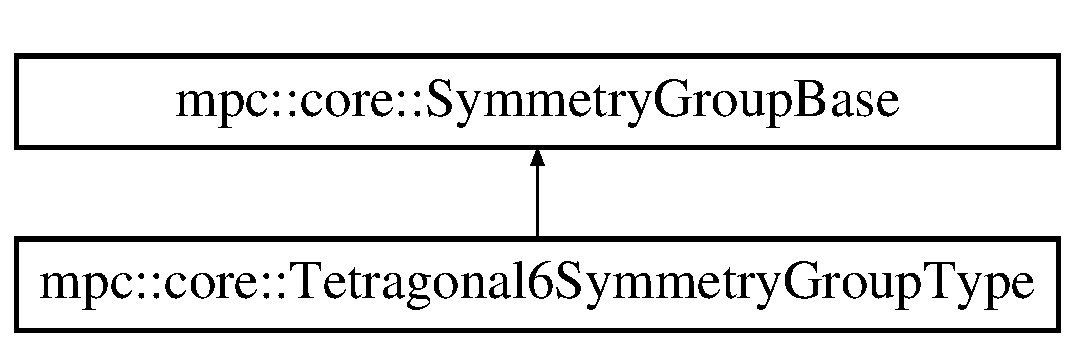
\includegraphics[height=2.000000cm]{structmpc_1_1core_1_1_tetragonal6_symmetry_group_type}
\end{center}
\end{figure}
\subsection*{Static Public Member Functions}
\begin{DoxyCompactItemize}
\item 
static constexpr \mbox{\hyperlink{namespacempc_1_1core_a9d979684062547055a0ef5c13077bad8}{Symmetry\+Group\+Enumeration}} \mbox{\hyperlink{structmpc_1_1core_1_1_tetragonal6_symmetry_group_type_a12c314c829a64caa780042971b408276}{Symmetry\+Group\+Enum}} ()
\item 
static constexpr int \mbox{\hyperlink{structmpc_1_1core_1_1_tetragonal6_symmetry_group_type_a850fa21a343d070374b5721c67b0fbf7}{Number\+Of\+Independent\+Components}} ()
\end{DoxyCompactItemize}
\subsection*{Public Attributes}
\begin{DoxyCompactItemize}
\item 
const \mbox{\hyperlink{namespacempc_1_1core_a9d979684062547055a0ef5c13077bad8}{Symmetry\+Group\+Enumeration}} \mbox{\hyperlink{structmpc_1_1core_1_1_tetragonal6_symmetry_group_type_a0fc41c7a0983b71f5cb7c1d9363afd60}{symmetry\+\_\+group\+\_\+enumeration}} = \mbox{\hyperlink{namespacempc_1_1core_a9d979684062547055a0ef5c13077bad8a63dabd41a700b44f934a19db4e0f8f83}{Symmetry\+Group\+Enumeration\+::\+T\+E\+T\+R\+A\+G\+O\+N\+A\+L6}}
\item 
const int \mbox{\hyperlink{structmpc_1_1core_1_1_tetragonal6_symmetry_group_type_a9eff4d9cae5ae207ac078a35fa9da8b1}{number\+\_\+of\+\_\+independent\+\_\+components}} = 6
\end{DoxyCompactItemize}


\subsection{Detailed Description}


Definition at line 232 of file symmetrygrouptypes.\+hpp.



\subsection{Member Function Documentation}
\mbox{\Hypertarget{structmpc_1_1core_1_1_tetragonal6_symmetry_group_type_a850fa21a343d070374b5721c67b0fbf7}\label{structmpc_1_1core_1_1_tetragonal6_symmetry_group_type_a850fa21a343d070374b5721c67b0fbf7}} 
\index{mpc\+::core\+::\+Tetragonal6\+Symmetry\+Group\+Type@{mpc\+::core\+::\+Tetragonal6\+Symmetry\+Group\+Type}!Number\+Of\+Independent\+Components@{Number\+Of\+Independent\+Components}}
\index{Number\+Of\+Independent\+Components@{Number\+Of\+Independent\+Components}!mpc\+::core\+::\+Tetragonal6\+Symmetry\+Group\+Type@{mpc\+::core\+::\+Tetragonal6\+Symmetry\+Group\+Type}}
\subsubsection{\texorpdfstring{Number\+Of\+Independent\+Components()}{NumberOfIndependentComponents()}}
{\footnotesize\ttfamily static constexpr int mpc\+::core\+::\+Tetragonal6\+Symmetry\+Group\+Type\+::\+Number\+Of\+Independent\+Components (\begin{DoxyParamCaption}{ }\end{DoxyParamCaption})\hspace{0.3cm}{\ttfamily [inline]}, {\ttfamily [static]}}



Definition at line 239 of file symmetrygrouptypes.\+hpp.

\mbox{\Hypertarget{structmpc_1_1core_1_1_tetragonal6_symmetry_group_type_a12c314c829a64caa780042971b408276}\label{structmpc_1_1core_1_1_tetragonal6_symmetry_group_type_a12c314c829a64caa780042971b408276}} 
\index{mpc\+::core\+::\+Tetragonal6\+Symmetry\+Group\+Type@{mpc\+::core\+::\+Tetragonal6\+Symmetry\+Group\+Type}!Symmetry\+Group\+Enum@{Symmetry\+Group\+Enum}}
\index{Symmetry\+Group\+Enum@{Symmetry\+Group\+Enum}!mpc\+::core\+::\+Tetragonal6\+Symmetry\+Group\+Type@{mpc\+::core\+::\+Tetragonal6\+Symmetry\+Group\+Type}}
\subsubsection{\texorpdfstring{Symmetry\+Group\+Enum()}{SymmetryGroupEnum()}}
{\footnotesize\ttfamily static constexpr \mbox{\hyperlink{namespacempc_1_1core_a9d979684062547055a0ef5c13077bad8}{Symmetry\+Group\+Enumeration}} mpc\+::core\+::\+Tetragonal6\+Symmetry\+Group\+Type\+::\+Symmetry\+Group\+Enum (\begin{DoxyParamCaption}{ }\end{DoxyParamCaption})\hspace{0.3cm}{\ttfamily [inline]}, {\ttfamily [static]}}



Definition at line 236 of file symmetrygrouptypes.\+hpp.



\subsection{Member Data Documentation}
\mbox{\Hypertarget{structmpc_1_1core_1_1_tetragonal6_symmetry_group_type_a9eff4d9cae5ae207ac078a35fa9da8b1}\label{structmpc_1_1core_1_1_tetragonal6_symmetry_group_type_a9eff4d9cae5ae207ac078a35fa9da8b1}} 
\index{mpc\+::core\+::\+Tetragonal6\+Symmetry\+Group\+Type@{mpc\+::core\+::\+Tetragonal6\+Symmetry\+Group\+Type}!number\+\_\+of\+\_\+independent\+\_\+components@{number\+\_\+of\+\_\+independent\+\_\+components}}
\index{number\+\_\+of\+\_\+independent\+\_\+components@{number\+\_\+of\+\_\+independent\+\_\+components}!mpc\+::core\+::\+Tetragonal6\+Symmetry\+Group\+Type@{mpc\+::core\+::\+Tetragonal6\+Symmetry\+Group\+Type}}
\subsubsection{\texorpdfstring{number\+\_\+of\+\_\+independent\+\_\+components}{number\_of\_independent\_components}}
{\footnotesize\ttfamily const int mpc\+::core\+::\+Tetragonal6\+Symmetry\+Group\+Type\+::number\+\_\+of\+\_\+independent\+\_\+components = 6}



Definition at line 234 of file symmetrygrouptypes.\+hpp.

\mbox{\Hypertarget{structmpc_1_1core_1_1_tetragonal6_symmetry_group_type_a0fc41c7a0983b71f5cb7c1d9363afd60}\label{structmpc_1_1core_1_1_tetragonal6_symmetry_group_type_a0fc41c7a0983b71f5cb7c1d9363afd60}} 
\index{mpc\+::core\+::\+Tetragonal6\+Symmetry\+Group\+Type@{mpc\+::core\+::\+Tetragonal6\+Symmetry\+Group\+Type}!symmetry\+\_\+group\+\_\+enumeration@{symmetry\+\_\+group\+\_\+enumeration}}
\index{symmetry\+\_\+group\+\_\+enumeration@{symmetry\+\_\+group\+\_\+enumeration}!mpc\+::core\+::\+Tetragonal6\+Symmetry\+Group\+Type@{mpc\+::core\+::\+Tetragonal6\+Symmetry\+Group\+Type}}
\subsubsection{\texorpdfstring{symmetry\+\_\+group\+\_\+enumeration}{symmetry\_group\_enumeration}}
{\footnotesize\ttfamily const \mbox{\hyperlink{namespacempc_1_1core_a9d979684062547055a0ef5c13077bad8}{Symmetry\+Group\+Enumeration}} mpc\+::core\+::\+Tetragonal6\+Symmetry\+Group\+Type\+::symmetry\+\_\+group\+\_\+enumeration = \mbox{\hyperlink{namespacempc_1_1core_a9d979684062547055a0ef5c13077bad8a63dabd41a700b44f934a19db4e0f8f83}{Symmetry\+Group\+Enumeration\+::\+T\+E\+T\+R\+A\+G\+O\+N\+A\+L6}}}



Definition at line 233 of file symmetrygrouptypes.\+hpp.



The documentation for this struct was generated from the following file\+:\begin{DoxyCompactItemize}
\item 
/\+Users/atorlucci/\+Documents/github\+\_\+threecubed\+\_\+repos/mpc/src/mpc/core/\mbox{\hyperlink{symmetrygrouptypes_8hpp}{symmetrygrouptypes.\+hpp}}\end{DoxyCompactItemize}

\hypertarget{structmpc_1_1core_1_1_tetragonal7_symmetry_group_type}{}\section{mpc\+:\+:core\+:\+:Tetragonal7\+Symmetry\+Group\+Type Struct Reference}
\label{structmpc_1_1core_1_1_tetragonal7_symmetry_group_type}\index{mpc\+::core\+::\+Tetragonal7\+Symmetry\+Group\+Type@{mpc\+::core\+::\+Tetragonal7\+Symmetry\+Group\+Type}}


{\ttfamily \#include $<$symmetrygrouptypes.\+hpp$>$}

Inheritance diagram for mpc\+:\+:core\+:\+:Tetragonal7\+Symmetry\+Group\+Type\+:\begin{figure}[H]
\begin{center}
\leavevmode
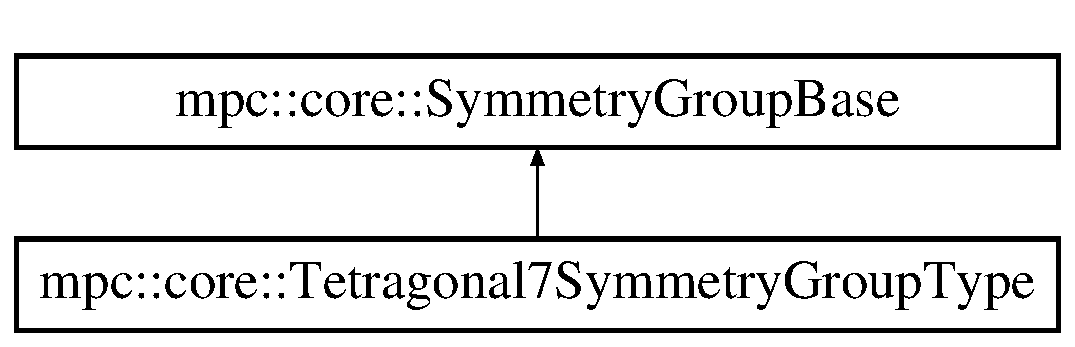
\includegraphics[height=2.000000cm]{structmpc_1_1core_1_1_tetragonal7_symmetry_group_type}
\end{center}
\end{figure}
\subsection*{Static Public Member Functions}
\begin{DoxyCompactItemize}
\item 
static constexpr \mbox{\hyperlink{namespacempc_1_1core_a9d979684062547055a0ef5c13077bad8}{Symmetry\+Group\+Enumeration}} \mbox{\hyperlink{structmpc_1_1core_1_1_tetragonal7_symmetry_group_type_aca4d86c79bdd3c34913d1036b4012ded}{Symmetry\+Group\+Enum}} ()
\item 
static constexpr int \mbox{\hyperlink{structmpc_1_1core_1_1_tetragonal7_symmetry_group_type_ac647e67b11ea630ae3dd9d65353b69f9}{Number\+Of\+Independent\+Components}} ()
\end{DoxyCompactItemize}
\subsection*{Public Attributes}
\begin{DoxyCompactItemize}
\item 
const \mbox{\hyperlink{namespacempc_1_1core_a9d979684062547055a0ef5c13077bad8}{Symmetry\+Group\+Enumeration}} \mbox{\hyperlink{structmpc_1_1core_1_1_tetragonal7_symmetry_group_type_aec8cb4c3907453836477cb2ed9eca6aa}{symmetry\+\_\+group\+\_\+enumeration}} = \mbox{\hyperlink{namespacempc_1_1core_a9d979684062547055a0ef5c13077bad8aea4a27c3d1e79d6a65ab91e165ba6d73}{Symmetry\+Group\+Enumeration\+::\+T\+E\+T\+R\+A\+G\+O\+N\+A\+L7}}
\item 
const int \mbox{\hyperlink{structmpc_1_1core_1_1_tetragonal7_symmetry_group_type_ad83cbb0ea09e77a87a47f0c7b542f2a3}{number\+\_\+of\+\_\+independent\+\_\+components}} = 7
\end{DoxyCompactItemize}


\subsection{Detailed Description}


Definition at line 220 of file symmetrygrouptypes.\+hpp.



\subsection{Member Function Documentation}
\mbox{\Hypertarget{structmpc_1_1core_1_1_tetragonal7_symmetry_group_type_ac647e67b11ea630ae3dd9d65353b69f9}\label{structmpc_1_1core_1_1_tetragonal7_symmetry_group_type_ac647e67b11ea630ae3dd9d65353b69f9}} 
\index{mpc\+::core\+::\+Tetragonal7\+Symmetry\+Group\+Type@{mpc\+::core\+::\+Tetragonal7\+Symmetry\+Group\+Type}!Number\+Of\+Independent\+Components@{Number\+Of\+Independent\+Components}}
\index{Number\+Of\+Independent\+Components@{Number\+Of\+Independent\+Components}!mpc\+::core\+::\+Tetragonal7\+Symmetry\+Group\+Type@{mpc\+::core\+::\+Tetragonal7\+Symmetry\+Group\+Type}}
\subsubsection{\texorpdfstring{Number\+Of\+Independent\+Components()}{NumberOfIndependentComponents()}}
{\footnotesize\ttfamily static constexpr int mpc\+::core\+::\+Tetragonal7\+Symmetry\+Group\+Type\+::\+Number\+Of\+Independent\+Components (\begin{DoxyParamCaption}{ }\end{DoxyParamCaption})\hspace{0.3cm}{\ttfamily [inline]}, {\ttfamily [static]}}



Definition at line 227 of file symmetrygrouptypes.\+hpp.

\mbox{\Hypertarget{structmpc_1_1core_1_1_tetragonal7_symmetry_group_type_aca4d86c79bdd3c34913d1036b4012ded}\label{structmpc_1_1core_1_1_tetragonal7_symmetry_group_type_aca4d86c79bdd3c34913d1036b4012ded}} 
\index{mpc\+::core\+::\+Tetragonal7\+Symmetry\+Group\+Type@{mpc\+::core\+::\+Tetragonal7\+Symmetry\+Group\+Type}!Symmetry\+Group\+Enum@{Symmetry\+Group\+Enum}}
\index{Symmetry\+Group\+Enum@{Symmetry\+Group\+Enum}!mpc\+::core\+::\+Tetragonal7\+Symmetry\+Group\+Type@{mpc\+::core\+::\+Tetragonal7\+Symmetry\+Group\+Type}}
\subsubsection{\texorpdfstring{Symmetry\+Group\+Enum()}{SymmetryGroupEnum()}}
{\footnotesize\ttfamily static constexpr \mbox{\hyperlink{namespacempc_1_1core_a9d979684062547055a0ef5c13077bad8}{Symmetry\+Group\+Enumeration}} mpc\+::core\+::\+Tetragonal7\+Symmetry\+Group\+Type\+::\+Symmetry\+Group\+Enum (\begin{DoxyParamCaption}{ }\end{DoxyParamCaption})\hspace{0.3cm}{\ttfamily [inline]}, {\ttfamily [static]}}



Definition at line 224 of file symmetrygrouptypes.\+hpp.



\subsection{Member Data Documentation}
\mbox{\Hypertarget{structmpc_1_1core_1_1_tetragonal7_symmetry_group_type_ad83cbb0ea09e77a87a47f0c7b542f2a3}\label{structmpc_1_1core_1_1_tetragonal7_symmetry_group_type_ad83cbb0ea09e77a87a47f0c7b542f2a3}} 
\index{mpc\+::core\+::\+Tetragonal7\+Symmetry\+Group\+Type@{mpc\+::core\+::\+Tetragonal7\+Symmetry\+Group\+Type}!number\+\_\+of\+\_\+independent\+\_\+components@{number\+\_\+of\+\_\+independent\+\_\+components}}
\index{number\+\_\+of\+\_\+independent\+\_\+components@{number\+\_\+of\+\_\+independent\+\_\+components}!mpc\+::core\+::\+Tetragonal7\+Symmetry\+Group\+Type@{mpc\+::core\+::\+Tetragonal7\+Symmetry\+Group\+Type}}
\subsubsection{\texorpdfstring{number\+\_\+of\+\_\+independent\+\_\+components}{number\_of\_independent\_components}}
{\footnotesize\ttfamily const int mpc\+::core\+::\+Tetragonal7\+Symmetry\+Group\+Type\+::number\+\_\+of\+\_\+independent\+\_\+components = 7}



Definition at line 222 of file symmetrygrouptypes.\+hpp.

\mbox{\Hypertarget{structmpc_1_1core_1_1_tetragonal7_symmetry_group_type_aec8cb4c3907453836477cb2ed9eca6aa}\label{structmpc_1_1core_1_1_tetragonal7_symmetry_group_type_aec8cb4c3907453836477cb2ed9eca6aa}} 
\index{mpc\+::core\+::\+Tetragonal7\+Symmetry\+Group\+Type@{mpc\+::core\+::\+Tetragonal7\+Symmetry\+Group\+Type}!symmetry\+\_\+group\+\_\+enumeration@{symmetry\+\_\+group\+\_\+enumeration}}
\index{symmetry\+\_\+group\+\_\+enumeration@{symmetry\+\_\+group\+\_\+enumeration}!mpc\+::core\+::\+Tetragonal7\+Symmetry\+Group\+Type@{mpc\+::core\+::\+Tetragonal7\+Symmetry\+Group\+Type}}
\subsubsection{\texorpdfstring{symmetry\+\_\+group\+\_\+enumeration}{symmetry\_group\_enumeration}}
{\footnotesize\ttfamily const \mbox{\hyperlink{namespacempc_1_1core_a9d979684062547055a0ef5c13077bad8}{Symmetry\+Group\+Enumeration}} mpc\+::core\+::\+Tetragonal7\+Symmetry\+Group\+Type\+::symmetry\+\_\+group\+\_\+enumeration = \mbox{\hyperlink{namespacempc_1_1core_a9d979684062547055a0ef5c13077bad8aea4a27c3d1e79d6a65ab91e165ba6d73}{Symmetry\+Group\+Enumeration\+::\+T\+E\+T\+R\+A\+G\+O\+N\+A\+L7}}}



Definition at line 221 of file symmetrygrouptypes.\+hpp.



The documentation for this struct was generated from the following file\+:\begin{DoxyCompactItemize}
\item 
/\+Users/atorlucci/\+Documents/github\+\_\+threecubed\+\_\+repos/mpc/src/mpc/core/\mbox{\hyperlink{symmetrygrouptypes_8hpp}{symmetrygrouptypes.\+hpp}}\end{DoxyCompactItemize}

\hypertarget{structmpc_1_1transformation_1_1_transformation_product}{}\section{mpc\+:\+:transformation\+:\+:Transformation\+Product$<$ T, Rank $>$ Struct Template Reference}
\label{structmpc_1_1transformation_1_1_transformation_product}\index{mpc\+::transformation\+::\+Transformation\+Product$<$ T, Rank $>$@{mpc\+::transformation\+::\+Transformation\+Product$<$ T, Rank $>$}}


{\ttfamily \#include $<$transformerhelperproduct.\+hpp$>$}

\subsection*{Public Member Functions}
\begin{DoxyCompactItemize}
\item 
blitz\+::\+Array$<$ T, Rank $>$ \mbox{\hyperlink{structmpc_1_1transformation_1_1_transformation_product_a51a570894b9a6fe0318ba3e3d7b21766}{operator()}} (blitz\+::\+Array$<$ T, Rank $>$ \&input\+\_\+array, blitz\+::\+Array$<$ T, 2 $>$ \&trans\+\_\+tensor)
\end{DoxyCompactItemize}


\subsection{Detailed Description}
\subsubsection*{template$<$typename T, int Rank$>$\newline
struct mpc\+::transformation\+::\+Transformation\+Product$<$ T, Rank $>$}



Definition at line 32 of file transformerhelperproduct.\+hpp.



\subsection{Member Function Documentation}
\mbox{\Hypertarget{structmpc_1_1transformation_1_1_transformation_product_a51a570894b9a6fe0318ba3e3d7b21766}\label{structmpc_1_1transformation_1_1_transformation_product_a51a570894b9a6fe0318ba3e3d7b21766}} 
\index{mpc\+::transformation\+::\+Transformation\+Product@{mpc\+::transformation\+::\+Transformation\+Product}!operator()@{operator()}}
\index{operator()@{operator()}!mpc\+::transformation\+::\+Transformation\+Product@{mpc\+::transformation\+::\+Transformation\+Product}}
\subsubsection{\texorpdfstring{operator()()}{operator()()}}
{\footnotesize\ttfamily template$<$typename T , int Rank$>$ \\
blitz\+::\+Array$<$T,Rank$>$ \mbox{\hyperlink{structmpc_1_1transformation_1_1_transformation_product}{mpc\+::transformation\+::\+Transformation\+Product}}$<$ T, Rank $>$\+::operator() (\begin{DoxyParamCaption}\item[{blitz\+::\+Array$<$ T, Rank $>$ \&}]{input\+\_\+array,  }\item[{blitz\+::\+Array$<$ T, 2 $>$ \&}]{trans\+\_\+tensor }\end{DoxyParamCaption})}



The documentation for this struct was generated from the following file\+:\begin{DoxyCompactItemize}
\item 
/\+Users/atorlucci/\+Documents/github\+\_\+threecubed\+\_\+repos/mpc/src/mpc/transformation/\mbox{\hyperlink{transformerhelperproduct_8hpp}{transformerhelperproduct.\+hpp}}\end{DoxyCompactItemize}

\hypertarget{structmpc_1_1transformation_1_1_transformation_product_3_01_t_00_0110_01_4}{}\section{mpc\+:\+:transformation\+:\+:Transformation\+Product$<$ T, 10 $>$ Struct Template Reference}
\label{structmpc_1_1transformation_1_1_transformation_product_3_01_t_00_0110_01_4}\index{mpc\+::transformation\+::\+Transformation\+Product$<$ T, 10 $>$@{mpc\+::transformation\+::\+Transformation\+Product$<$ T, 10 $>$}}


{\ttfamily \#include $<$transformerhelperproduct.\+hpp$>$}

\subsection*{Public Member Functions}
\begin{DoxyCompactItemize}
\item 
blitz\+::\+Array$<$ T, 1 $>$ \mbox{\hyperlink{structmpc_1_1transformation_1_1_transformation_product_3_01_t_00_0110_01_4_a72b694e154212f9c81c067bde6030399}{operator()}} (blitz\+::\+Array$<$ T, 2 $>$ \&trans\+\_\+tensor, int index\+\_\+i, int index\+\_\+j, int index\+\_\+k, int index\+\_\+l, int index\+\_\+m, int index\+\_\+n, int index\+\_\+p, int index\+\_\+q, int index\+\_\+r, int index\+\_\+s)
\end{DoxyCompactItemize}


\subsection{Detailed Description}
\subsubsection*{template$<$typename T$>$\newline
struct mpc\+::transformation\+::\+Transformation\+Product$<$ T, 10 $>$}



Definition at line 273 of file transformerhelperproduct.\+hpp.



\subsection{Member Function Documentation}
\mbox{\Hypertarget{structmpc_1_1transformation_1_1_transformation_product_3_01_t_00_0110_01_4_a72b694e154212f9c81c067bde6030399}\label{structmpc_1_1transformation_1_1_transformation_product_3_01_t_00_0110_01_4_a72b694e154212f9c81c067bde6030399}} 
\index{mpc\+::transformation\+::\+Transformation\+Product$<$ T, 10 $>$@{mpc\+::transformation\+::\+Transformation\+Product$<$ T, 10 $>$}!operator()@{operator()}}
\index{operator()@{operator()}!mpc\+::transformation\+::\+Transformation\+Product$<$ T, 10 $>$@{mpc\+::transformation\+::\+Transformation\+Product$<$ T, 10 $>$}}
\subsubsection{\texorpdfstring{operator()()}{operator()()}}
{\footnotesize\ttfamily template$<$typename T $>$ \\
blitz\+::\+Array$<$T,1$>$ \mbox{\hyperlink{structmpc_1_1transformation_1_1_transformation_product}{mpc\+::transformation\+::\+Transformation\+Product}}$<$ T, 10 $>$\+::operator() (\begin{DoxyParamCaption}\item[{blitz\+::\+Array$<$ T, 2 $>$ \&}]{trans\+\_\+tensor,  }\item[{int}]{index\+\_\+i,  }\item[{int}]{index\+\_\+j,  }\item[{int}]{index\+\_\+k,  }\item[{int}]{index\+\_\+l,  }\item[{int}]{index\+\_\+m,  }\item[{int}]{index\+\_\+n,  }\item[{int}]{index\+\_\+p,  }\item[{int}]{index\+\_\+q,  }\item[{int}]{index\+\_\+r,  }\item[{int}]{index\+\_\+s }\end{DoxyParamCaption})\hspace{0.3cm}{\ttfamily [inline]}}



Definition at line 275 of file transformerhelperproduct.\+hpp.



The documentation for this struct was generated from the following file\+:\begin{DoxyCompactItemize}
\item 
/\+Users/atorlucci/\+Documents/github\+\_\+threecubed\+\_\+repos/mpc/src/mpc/transformation/\mbox{\hyperlink{transformerhelperproduct_8hpp}{transformerhelperproduct.\+hpp}}\end{DoxyCompactItemize}

\hypertarget{structmpc_1_1transformation_1_1_transformation_product_3_01_t_00_0111_01_4}{}\section{mpc\+:\+:transformation\+:\+:Transformation\+Product$<$ T, 11 $>$ Struct Template Reference}
\label{structmpc_1_1transformation_1_1_transformation_product_3_01_t_00_0111_01_4}\index{mpc\+::transformation\+::\+Transformation\+Product$<$ T, 11 $>$@{mpc\+::transformation\+::\+Transformation\+Product$<$ T, 11 $>$}}


{\ttfamily \#include $<$transformerhelperproduct.\+hpp$>$}

\subsection*{Public Member Functions}
\begin{DoxyCompactItemize}
\item 
blitz\+::\+Array$<$ T, 1 $>$ \mbox{\hyperlink{structmpc_1_1transformation_1_1_transformation_product_3_01_t_00_0111_01_4_a7b4f4922dfb3115f3f26256c6524db69}{operator()}} (blitz\+::\+Array$<$ T, 2 $>$ \&trans\+\_\+tensor, int index\+\_\+i, int index\+\_\+j, int index\+\_\+k, int index\+\_\+l, int index\+\_\+m, int index\+\_\+n, int index\+\_\+p, int index\+\_\+q, int index\+\_\+r, int index\+\_\+s, int index\+\_\+t)
\end{DoxyCompactItemize}


\subsection{Detailed Description}
\subsubsection*{template$<$typename T$>$\newline
struct mpc\+::transformation\+::\+Transformation\+Product$<$ T, 11 $>$}



Definition at line 311 of file transformerhelperproduct.\+hpp.



\subsection{Member Function Documentation}
\mbox{\Hypertarget{structmpc_1_1transformation_1_1_transformation_product_3_01_t_00_0111_01_4_a7b4f4922dfb3115f3f26256c6524db69}\label{structmpc_1_1transformation_1_1_transformation_product_3_01_t_00_0111_01_4_a7b4f4922dfb3115f3f26256c6524db69}} 
\index{mpc\+::transformation\+::\+Transformation\+Product$<$ T, 11 $>$@{mpc\+::transformation\+::\+Transformation\+Product$<$ T, 11 $>$}!operator()@{operator()}}
\index{operator()@{operator()}!mpc\+::transformation\+::\+Transformation\+Product$<$ T, 11 $>$@{mpc\+::transformation\+::\+Transformation\+Product$<$ T, 11 $>$}}
\subsubsection{\texorpdfstring{operator()()}{operator()()}}
{\footnotesize\ttfamily template$<$typename T $>$ \\
blitz\+::\+Array$<$T,1$>$ \mbox{\hyperlink{structmpc_1_1transformation_1_1_transformation_product}{mpc\+::transformation\+::\+Transformation\+Product}}$<$ T, 11 $>$\+::operator() (\begin{DoxyParamCaption}\item[{blitz\+::\+Array$<$ T, 2 $>$ \&}]{trans\+\_\+tensor,  }\item[{int}]{index\+\_\+i,  }\item[{int}]{index\+\_\+j,  }\item[{int}]{index\+\_\+k,  }\item[{int}]{index\+\_\+l,  }\item[{int}]{index\+\_\+m,  }\item[{int}]{index\+\_\+n,  }\item[{int}]{index\+\_\+p,  }\item[{int}]{index\+\_\+q,  }\item[{int}]{index\+\_\+r,  }\item[{int}]{index\+\_\+s,  }\item[{int}]{index\+\_\+t }\end{DoxyParamCaption})\hspace{0.3cm}{\ttfamily [inline]}}



Definition at line 313 of file transformerhelperproduct.\+hpp.



The documentation for this struct was generated from the following file\+:\begin{DoxyCompactItemize}
\item 
/\+Users/atorlucci/\+Documents/github\+\_\+threecubed\+\_\+repos/mpc/src/mpc/transformation/\mbox{\hyperlink{transformerhelperproduct_8hpp}{transformerhelperproduct.\+hpp}}\end{DoxyCompactItemize}

\hypertarget{structmpc_1_1transformation_1_1_transformation_product_3_01_t_00_012_01_4}{}\section{mpc\+:\+:transformation\+:\+:Transformation\+Product$<$ T, 2 $>$ Struct Template Reference}
\label{structmpc_1_1transformation_1_1_transformation_product_3_01_t_00_012_01_4}\index{mpc\+::transformation\+::\+Transformation\+Product$<$ T, 2 $>$@{mpc\+::transformation\+::\+Transformation\+Product$<$ T, 2 $>$}}


{\ttfamily \#include $<$transformerhelperproduct.\+hpp$>$}

\subsection*{Public Member Functions}
\begin{DoxyCompactItemize}
\item 
blitz\+::\+Array$<$ T, 1 $>$ \mbox{\hyperlink{structmpc_1_1transformation_1_1_transformation_product_3_01_t_00_012_01_4_ad0327d3f0f74b391f42ea75e00e4b47c}{operator()}} (blitz\+::\+Array$<$ T, 2 $>$ \&trans\+\_\+tensor, int index\+\_\+i, int index\+\_\+j)
\end{DoxyCompactItemize}


\subsection{Detailed Description}
\subsubsection*{template$<$typename T$>$\newline
struct mpc\+::transformation\+::\+Transformation\+Product$<$ T, 2 $>$}



Definition at line 41 of file transformerhelperproduct.\+hpp.



\subsection{Member Function Documentation}
\mbox{\Hypertarget{structmpc_1_1transformation_1_1_transformation_product_3_01_t_00_012_01_4_ad0327d3f0f74b391f42ea75e00e4b47c}\label{structmpc_1_1transformation_1_1_transformation_product_3_01_t_00_012_01_4_ad0327d3f0f74b391f42ea75e00e4b47c}} 
\index{mpc\+::transformation\+::\+Transformation\+Product$<$ T, 2 $>$@{mpc\+::transformation\+::\+Transformation\+Product$<$ T, 2 $>$}!operator()@{operator()}}
\index{operator()@{operator()}!mpc\+::transformation\+::\+Transformation\+Product$<$ T, 2 $>$@{mpc\+::transformation\+::\+Transformation\+Product$<$ T, 2 $>$}}
\subsubsection{\texorpdfstring{operator()()}{operator()()}}
{\footnotesize\ttfamily template$<$typename T $>$ \\
blitz\+::\+Array$<$T,1$>$ \mbox{\hyperlink{structmpc_1_1transformation_1_1_transformation_product}{mpc\+::transformation\+::\+Transformation\+Product}}$<$ T, 2 $>$\+::operator() (\begin{DoxyParamCaption}\item[{blitz\+::\+Array$<$ T, 2 $>$ \&}]{trans\+\_\+tensor,  }\item[{int}]{index\+\_\+i,  }\item[{int}]{index\+\_\+j }\end{DoxyParamCaption})\hspace{0.3cm}{\ttfamily [inline]}}



Definition at line 43 of file transformerhelperproduct.\+hpp.



The documentation for this struct was generated from the following file\+:\begin{DoxyCompactItemize}
\item 
/\+Users/atorlucci/\+Documents/github\+\_\+threecubed\+\_\+repos/mpc/src/mpc/transformation/\mbox{\hyperlink{transformerhelperproduct_8hpp}{transformerhelperproduct.\+hpp}}\end{DoxyCompactItemize}

\hypertarget{structmpc_1_1transformation_1_1_transformation_product_3_01_t_00_013_01_4}{}\section{mpc\+:\+:transformation\+:\+:Transformation\+Product$<$ T, 3 $>$ Struct Template Reference}
\label{structmpc_1_1transformation_1_1_transformation_product_3_01_t_00_013_01_4}\index{mpc\+::transformation\+::\+Transformation\+Product$<$ T, 3 $>$@{mpc\+::transformation\+::\+Transformation\+Product$<$ T, 3 $>$}}


{\ttfamily \#include $<$transformerhelperproduct.\+hpp$>$}

\subsection*{Public Member Functions}
\begin{DoxyCompactItemize}
\item 
blitz\+::\+Array$<$ T, 1 $>$ \mbox{\hyperlink{structmpc_1_1transformation_1_1_transformation_product_3_01_t_00_013_01_4_ade7dbd6c5d3f90dbc1875c3a43c86329}{operator()}} (blitz\+::\+Array$<$ T, 2 $>$ \&trans\+\_\+tensor, int index\+\_\+i, int index\+\_\+j, int index\+\_\+k)
\end{DoxyCompactItemize}


\subsection{Detailed Description}
\subsubsection*{template$<$typename T$>$\newline
struct mpc\+::transformation\+::\+Transformation\+Product$<$ T, 3 $>$}



Definition at line 63 of file transformerhelperproduct.\+hpp.



\subsection{Member Function Documentation}
\mbox{\Hypertarget{structmpc_1_1transformation_1_1_transformation_product_3_01_t_00_013_01_4_ade7dbd6c5d3f90dbc1875c3a43c86329}\label{structmpc_1_1transformation_1_1_transformation_product_3_01_t_00_013_01_4_ade7dbd6c5d3f90dbc1875c3a43c86329}} 
\index{mpc\+::transformation\+::\+Transformation\+Product$<$ T, 3 $>$@{mpc\+::transformation\+::\+Transformation\+Product$<$ T, 3 $>$}!operator()@{operator()}}
\index{operator()@{operator()}!mpc\+::transformation\+::\+Transformation\+Product$<$ T, 3 $>$@{mpc\+::transformation\+::\+Transformation\+Product$<$ T, 3 $>$}}
\subsubsection{\texorpdfstring{operator()()}{operator()()}}
{\footnotesize\ttfamily template$<$typename T $>$ \\
blitz\+::\+Array$<$T,1$>$ \mbox{\hyperlink{structmpc_1_1transformation_1_1_transformation_product}{mpc\+::transformation\+::\+Transformation\+Product}}$<$ T, 3 $>$\+::operator() (\begin{DoxyParamCaption}\item[{blitz\+::\+Array$<$ T, 2 $>$ \&}]{trans\+\_\+tensor,  }\item[{int}]{index\+\_\+i,  }\item[{int}]{index\+\_\+j,  }\item[{int}]{index\+\_\+k }\end{DoxyParamCaption})\hspace{0.3cm}{\ttfamily [inline]}}



Definition at line 65 of file transformerhelperproduct.\+hpp.



The documentation for this struct was generated from the following file\+:\begin{DoxyCompactItemize}
\item 
/\+Users/atorlucci/\+Documents/github\+\_\+threecubed\+\_\+repos/mpc/src/mpc/transformation/\mbox{\hyperlink{transformerhelperproduct_8hpp}{transformerhelperproduct.\+hpp}}\end{DoxyCompactItemize}

\hypertarget{structmpc_1_1transformation_1_1_transformation_product_3_01_t_00_014_01_4}{}\section{mpc\+:\+:transformation\+:\+:Transformation\+Product$<$ T, 4 $>$ Struct Template Reference}
\label{structmpc_1_1transformation_1_1_transformation_product_3_01_t_00_014_01_4}\index{mpc\+::transformation\+::\+Transformation\+Product$<$ T, 4 $>$@{mpc\+::transformation\+::\+Transformation\+Product$<$ T, 4 $>$}}


{\ttfamily \#include $<$transformerhelperproduct.\+hpp$>$}

\subsection*{Public Member Functions}
\begin{DoxyCompactItemize}
\item 
blitz\+::\+Array$<$ T, 1 $>$ \mbox{\hyperlink{structmpc_1_1transformation_1_1_transformation_product_3_01_t_00_014_01_4_a7469f9926dbbeb033654fea1e8e52e1f}{operator()}} (blitz\+::\+Array$<$ T, 2 $>$ \&trans\+\_\+tensor, int index\+\_\+i, int index\+\_\+j, int index\+\_\+k, int index\+\_\+l)
\end{DoxyCompactItemize}


\subsection{Detailed Description}
\subsubsection*{template$<$typename T$>$\newline
struct mpc\+::transformation\+::\+Transformation\+Product$<$ T, 4 $>$}



Definition at line 87 of file transformerhelperproduct.\+hpp.



\subsection{Member Function Documentation}
\mbox{\Hypertarget{structmpc_1_1transformation_1_1_transformation_product_3_01_t_00_014_01_4_a7469f9926dbbeb033654fea1e8e52e1f}\label{structmpc_1_1transformation_1_1_transformation_product_3_01_t_00_014_01_4_a7469f9926dbbeb033654fea1e8e52e1f}} 
\index{mpc\+::transformation\+::\+Transformation\+Product$<$ T, 4 $>$@{mpc\+::transformation\+::\+Transformation\+Product$<$ T, 4 $>$}!operator()@{operator()}}
\index{operator()@{operator()}!mpc\+::transformation\+::\+Transformation\+Product$<$ T, 4 $>$@{mpc\+::transformation\+::\+Transformation\+Product$<$ T, 4 $>$}}
\subsubsection{\texorpdfstring{operator()()}{operator()()}}
{\footnotesize\ttfamily template$<$typename T $>$ \\
blitz\+::\+Array$<$T,1$>$ \mbox{\hyperlink{structmpc_1_1transformation_1_1_transformation_product}{mpc\+::transformation\+::\+Transformation\+Product}}$<$ T, 4 $>$\+::operator() (\begin{DoxyParamCaption}\item[{blitz\+::\+Array$<$ T, 2 $>$ \&}]{trans\+\_\+tensor,  }\item[{int}]{index\+\_\+i,  }\item[{int}]{index\+\_\+j,  }\item[{int}]{index\+\_\+k,  }\item[{int}]{index\+\_\+l }\end{DoxyParamCaption})\hspace{0.3cm}{\ttfamily [inline]}}



Definition at line 89 of file transformerhelperproduct.\+hpp.



The documentation for this struct was generated from the following file\+:\begin{DoxyCompactItemize}
\item 
/\+Users/atorlucci/\+Documents/github\+\_\+threecubed\+\_\+repos/mpc/src/mpc/transformation/\mbox{\hyperlink{transformerhelperproduct_8hpp}{transformerhelperproduct.\+hpp}}\end{DoxyCompactItemize}

\hypertarget{structmpc_1_1transformation_1_1_transformation_product_3_01_t_00_015_01_4}{}\section{mpc\+:\+:transformation\+:\+:Transformation\+Product$<$ T, 5 $>$ Struct Template Reference}
\label{structmpc_1_1transformation_1_1_transformation_product_3_01_t_00_015_01_4}\index{mpc\+::transformation\+::\+Transformation\+Product$<$ T, 5 $>$@{mpc\+::transformation\+::\+Transformation\+Product$<$ T, 5 $>$}}


{\ttfamily \#include $<$transformerhelperproduct.\+hpp$>$}

\subsection*{Public Member Functions}
\begin{DoxyCompactItemize}
\item 
blitz\+::\+Array$<$ T, 1 $>$ \mbox{\hyperlink{structmpc_1_1transformation_1_1_transformation_product_3_01_t_00_015_01_4_a81f784bd294547ba3441712fc22713be}{operator()}} (blitz\+::\+Array$<$ T, 2 $>$ \&trans\+\_\+tensor, int index\+\_\+i, int index\+\_\+j, int index\+\_\+k, int index\+\_\+l, int index\+\_\+m)
\end{DoxyCompactItemize}


\subsection{Detailed Description}
\subsubsection*{template$<$typename T$>$\newline
struct mpc\+::transformation\+::\+Transformation\+Product$<$ T, 5 $>$}



Definition at line 113 of file transformerhelperproduct.\+hpp.



\subsection{Member Function Documentation}
\mbox{\Hypertarget{structmpc_1_1transformation_1_1_transformation_product_3_01_t_00_015_01_4_a81f784bd294547ba3441712fc22713be}\label{structmpc_1_1transformation_1_1_transformation_product_3_01_t_00_015_01_4_a81f784bd294547ba3441712fc22713be}} 
\index{mpc\+::transformation\+::\+Transformation\+Product$<$ T, 5 $>$@{mpc\+::transformation\+::\+Transformation\+Product$<$ T, 5 $>$}!operator()@{operator()}}
\index{operator()@{operator()}!mpc\+::transformation\+::\+Transformation\+Product$<$ T, 5 $>$@{mpc\+::transformation\+::\+Transformation\+Product$<$ T, 5 $>$}}
\subsubsection{\texorpdfstring{operator()()}{operator()()}}
{\footnotesize\ttfamily template$<$typename T $>$ \\
blitz\+::\+Array$<$T,1$>$ \mbox{\hyperlink{structmpc_1_1transformation_1_1_transformation_product}{mpc\+::transformation\+::\+Transformation\+Product}}$<$ T, 5 $>$\+::operator() (\begin{DoxyParamCaption}\item[{blitz\+::\+Array$<$ T, 2 $>$ \&}]{trans\+\_\+tensor,  }\item[{int}]{index\+\_\+i,  }\item[{int}]{index\+\_\+j,  }\item[{int}]{index\+\_\+k,  }\item[{int}]{index\+\_\+l,  }\item[{int}]{index\+\_\+m }\end{DoxyParamCaption})\hspace{0.3cm}{\ttfamily [inline]}}



Definition at line 115 of file transformerhelperproduct.\+hpp.



The documentation for this struct was generated from the following file\+:\begin{DoxyCompactItemize}
\item 
/\+Users/atorlucci/\+Documents/github\+\_\+threecubed\+\_\+repos/mpc/src/mpc/transformation/\mbox{\hyperlink{transformerhelperproduct_8hpp}{transformerhelperproduct.\+hpp}}\end{DoxyCompactItemize}

\hypertarget{structmpc_1_1transformation_1_1_transformation_product_3_01_t_00_016_01_4}{}\section{mpc\+:\+:transformation\+:\+:Transformation\+Product$<$ T, 6 $>$ Struct Template Reference}
\label{structmpc_1_1transformation_1_1_transformation_product_3_01_t_00_016_01_4}\index{mpc\+::transformation\+::\+Transformation\+Product$<$ T, 6 $>$@{mpc\+::transformation\+::\+Transformation\+Product$<$ T, 6 $>$}}


{\ttfamily \#include $<$transformerhelperproduct.\+hpp$>$}

\subsection*{Public Member Functions}
\begin{DoxyCompactItemize}
\item 
blitz\+::\+Array$<$ T, 1 $>$ \mbox{\hyperlink{structmpc_1_1transformation_1_1_transformation_product_3_01_t_00_016_01_4_a2e9ebbdd2cb47148f9d2e9b08982228c}{operator()}} (blitz\+::\+Array$<$ T, 2 $>$ \&trans\+\_\+tensor, int index\+\_\+i, int index\+\_\+j, int index\+\_\+k, int index\+\_\+l, int index\+\_\+m, int index\+\_\+n)
\end{DoxyCompactItemize}


\subsection{Detailed Description}
\subsubsection*{template$<$typename T$>$\newline
struct mpc\+::transformation\+::\+Transformation\+Product$<$ T, 6 $>$}



Definition at line 141 of file transformerhelperproduct.\+hpp.



\subsection{Member Function Documentation}
\mbox{\Hypertarget{structmpc_1_1transformation_1_1_transformation_product_3_01_t_00_016_01_4_a2e9ebbdd2cb47148f9d2e9b08982228c}\label{structmpc_1_1transformation_1_1_transformation_product_3_01_t_00_016_01_4_a2e9ebbdd2cb47148f9d2e9b08982228c}} 
\index{mpc\+::transformation\+::\+Transformation\+Product$<$ T, 6 $>$@{mpc\+::transformation\+::\+Transformation\+Product$<$ T, 6 $>$}!operator()@{operator()}}
\index{operator()@{operator()}!mpc\+::transformation\+::\+Transformation\+Product$<$ T, 6 $>$@{mpc\+::transformation\+::\+Transformation\+Product$<$ T, 6 $>$}}
\subsubsection{\texorpdfstring{operator()()}{operator()()}}
{\footnotesize\ttfamily template$<$typename T $>$ \\
blitz\+::\+Array$<$T,1$>$ \mbox{\hyperlink{structmpc_1_1transformation_1_1_transformation_product}{mpc\+::transformation\+::\+Transformation\+Product}}$<$ T, 6 $>$\+::operator() (\begin{DoxyParamCaption}\item[{blitz\+::\+Array$<$ T, 2 $>$ \&}]{trans\+\_\+tensor,  }\item[{int}]{index\+\_\+i,  }\item[{int}]{index\+\_\+j,  }\item[{int}]{index\+\_\+k,  }\item[{int}]{index\+\_\+l,  }\item[{int}]{index\+\_\+m,  }\item[{int}]{index\+\_\+n }\end{DoxyParamCaption})\hspace{0.3cm}{\ttfamily [inline]}}



Definition at line 143 of file transformerhelperproduct.\+hpp.



The documentation for this struct was generated from the following file\+:\begin{DoxyCompactItemize}
\item 
/\+Users/atorlucci/\+Documents/github\+\_\+threecubed\+\_\+repos/mpc/src/mpc/transformation/\mbox{\hyperlink{transformerhelperproduct_8hpp}{transformerhelperproduct.\+hpp}}\end{DoxyCompactItemize}

\hypertarget{structmpc_1_1transformation_1_1_transformation_product_3_01_t_00_017_01_4}{}\section{mpc\+:\+:transformation\+:\+:Transformation\+Product$<$ T, 7 $>$ Struct Template Reference}
\label{structmpc_1_1transformation_1_1_transformation_product_3_01_t_00_017_01_4}\index{mpc\+::transformation\+::\+Transformation\+Product$<$ T, 7 $>$@{mpc\+::transformation\+::\+Transformation\+Product$<$ T, 7 $>$}}


{\ttfamily \#include $<$transformerhelperproduct.\+hpp$>$}

\subsection*{Public Member Functions}
\begin{DoxyCompactItemize}
\item 
blitz\+::\+Array$<$ T, 1 $>$ \mbox{\hyperlink{structmpc_1_1transformation_1_1_transformation_product_3_01_t_00_017_01_4_a2c703bb94416241b6c7b449c5b7f0899}{operator()}} (blitz\+::\+Array$<$ T, 2 $>$ \&trans\+\_\+tensor, int index\+\_\+i, int index\+\_\+j, int index\+\_\+k, int index\+\_\+l, int index\+\_\+m, int index\+\_\+n, int index\+\_\+p)
\end{DoxyCompactItemize}


\subsection{Detailed Description}
\subsubsection*{template$<$typename T$>$\newline
struct mpc\+::transformation\+::\+Transformation\+Product$<$ T, 7 $>$}



Definition at line 171 of file transformerhelperproduct.\+hpp.



\subsection{Member Function Documentation}
\mbox{\Hypertarget{structmpc_1_1transformation_1_1_transformation_product_3_01_t_00_017_01_4_a2c703bb94416241b6c7b449c5b7f0899}\label{structmpc_1_1transformation_1_1_transformation_product_3_01_t_00_017_01_4_a2c703bb94416241b6c7b449c5b7f0899}} 
\index{mpc\+::transformation\+::\+Transformation\+Product$<$ T, 7 $>$@{mpc\+::transformation\+::\+Transformation\+Product$<$ T, 7 $>$}!operator()@{operator()}}
\index{operator()@{operator()}!mpc\+::transformation\+::\+Transformation\+Product$<$ T, 7 $>$@{mpc\+::transformation\+::\+Transformation\+Product$<$ T, 7 $>$}}
\subsubsection{\texorpdfstring{operator()()}{operator()()}}
{\footnotesize\ttfamily template$<$typename T $>$ \\
blitz\+::\+Array$<$T,1$>$ \mbox{\hyperlink{structmpc_1_1transformation_1_1_transformation_product}{mpc\+::transformation\+::\+Transformation\+Product}}$<$ T, 7 $>$\+::operator() (\begin{DoxyParamCaption}\item[{blitz\+::\+Array$<$ T, 2 $>$ \&}]{trans\+\_\+tensor,  }\item[{int}]{index\+\_\+i,  }\item[{int}]{index\+\_\+j,  }\item[{int}]{index\+\_\+k,  }\item[{int}]{index\+\_\+l,  }\item[{int}]{index\+\_\+m,  }\item[{int}]{index\+\_\+n,  }\item[{int}]{index\+\_\+p }\end{DoxyParamCaption})\hspace{0.3cm}{\ttfamily [inline]}}



Definition at line 173 of file transformerhelperproduct.\+hpp.



The documentation for this struct was generated from the following file\+:\begin{DoxyCompactItemize}
\item 
/\+Users/atorlucci/\+Documents/github\+\_\+threecubed\+\_\+repos/mpc/src/mpc/transformation/\mbox{\hyperlink{transformerhelperproduct_8hpp}{transformerhelperproduct.\+hpp}}\end{DoxyCompactItemize}

\hypertarget{structmpc_1_1transformation_1_1_transformation_product_3_01_t_00_018_01_4}{}\section{mpc\+:\+:transformation\+:\+:Transformation\+Product$<$ T, 8 $>$ Struct Template Reference}
\label{structmpc_1_1transformation_1_1_transformation_product_3_01_t_00_018_01_4}\index{mpc\+::transformation\+::\+Transformation\+Product$<$ T, 8 $>$@{mpc\+::transformation\+::\+Transformation\+Product$<$ T, 8 $>$}}


{\ttfamily \#include $<$transformerhelperproduct.\+hpp$>$}

\subsection*{Public Member Functions}
\begin{DoxyCompactItemize}
\item 
blitz\+::\+Array$<$ T, 1 $>$ \mbox{\hyperlink{structmpc_1_1transformation_1_1_transformation_product_3_01_t_00_018_01_4_a249f5845319c4f258f091d1c3488e365}{operator()}} (blitz\+::\+Array$<$ T, 2 $>$ \&trans\+\_\+tensor, int index\+\_\+i, int index\+\_\+j, int index\+\_\+k, int index\+\_\+l, int index\+\_\+m, int index\+\_\+n, int index\+\_\+p, int index\+\_\+q)
\end{DoxyCompactItemize}


\subsection{Detailed Description}
\subsubsection*{template$<$typename T$>$\newline
struct mpc\+::transformation\+::\+Transformation\+Product$<$ T, 8 $>$}



Definition at line 203 of file transformerhelperproduct.\+hpp.



\subsection{Member Function Documentation}
\mbox{\Hypertarget{structmpc_1_1transformation_1_1_transformation_product_3_01_t_00_018_01_4_a249f5845319c4f258f091d1c3488e365}\label{structmpc_1_1transformation_1_1_transformation_product_3_01_t_00_018_01_4_a249f5845319c4f258f091d1c3488e365}} 
\index{mpc\+::transformation\+::\+Transformation\+Product$<$ T, 8 $>$@{mpc\+::transformation\+::\+Transformation\+Product$<$ T, 8 $>$}!operator()@{operator()}}
\index{operator()@{operator()}!mpc\+::transformation\+::\+Transformation\+Product$<$ T, 8 $>$@{mpc\+::transformation\+::\+Transformation\+Product$<$ T, 8 $>$}}
\subsubsection{\texorpdfstring{operator()()}{operator()()}}
{\footnotesize\ttfamily template$<$typename T $>$ \\
blitz\+::\+Array$<$T,1$>$ \mbox{\hyperlink{structmpc_1_1transformation_1_1_transformation_product}{mpc\+::transformation\+::\+Transformation\+Product}}$<$ T, 8 $>$\+::operator() (\begin{DoxyParamCaption}\item[{blitz\+::\+Array$<$ T, 2 $>$ \&}]{trans\+\_\+tensor,  }\item[{int}]{index\+\_\+i,  }\item[{int}]{index\+\_\+j,  }\item[{int}]{index\+\_\+k,  }\item[{int}]{index\+\_\+l,  }\item[{int}]{index\+\_\+m,  }\item[{int}]{index\+\_\+n,  }\item[{int}]{index\+\_\+p,  }\item[{int}]{index\+\_\+q }\end{DoxyParamCaption})\hspace{0.3cm}{\ttfamily [inline]}}



Definition at line 205 of file transformerhelperproduct.\+hpp.



The documentation for this struct was generated from the following file\+:\begin{DoxyCompactItemize}
\item 
/\+Users/atorlucci/\+Documents/github\+\_\+threecubed\+\_\+repos/mpc/src/mpc/transformation/\mbox{\hyperlink{transformerhelperproduct_8hpp}{transformerhelperproduct.\+hpp}}\end{DoxyCompactItemize}

\hypertarget{structmpc_1_1transformation_1_1_transformation_product_3_01_t_00_019_01_4}{}\section{mpc\+:\+:transformation\+:\+:Transformation\+Product$<$ T, 9 $>$ Struct Template Reference}
\label{structmpc_1_1transformation_1_1_transformation_product_3_01_t_00_019_01_4}\index{mpc\+::transformation\+::\+Transformation\+Product$<$ T, 9 $>$@{mpc\+::transformation\+::\+Transformation\+Product$<$ T, 9 $>$}}


{\ttfamily \#include $<$transformerhelperproduct.\+hpp$>$}

\subsection*{Public Member Functions}
\begin{DoxyCompactItemize}
\item 
blitz\+::\+Array$<$ T, 1 $>$ \mbox{\hyperlink{structmpc_1_1transformation_1_1_transformation_product_3_01_t_00_019_01_4_af520a1b15743d0fce9aa0a2a1c91aed4}{operator()}} (blitz\+::\+Array$<$ T, 2 $>$ \&trans\+\_\+tensor, int index\+\_\+i, int index\+\_\+j, int index\+\_\+k, int index\+\_\+l, int index\+\_\+m, int index\+\_\+n, int index\+\_\+p, int index\+\_\+q, int index\+\_\+r)
\end{DoxyCompactItemize}


\subsection{Detailed Description}
\subsubsection*{template$<$typename T$>$\newline
struct mpc\+::transformation\+::\+Transformation\+Product$<$ T, 9 $>$}



Definition at line 237 of file transformerhelperproduct.\+hpp.



\subsection{Member Function Documentation}
\mbox{\Hypertarget{structmpc_1_1transformation_1_1_transformation_product_3_01_t_00_019_01_4_af520a1b15743d0fce9aa0a2a1c91aed4}\label{structmpc_1_1transformation_1_1_transformation_product_3_01_t_00_019_01_4_af520a1b15743d0fce9aa0a2a1c91aed4}} 
\index{mpc\+::transformation\+::\+Transformation\+Product$<$ T, 9 $>$@{mpc\+::transformation\+::\+Transformation\+Product$<$ T, 9 $>$}!operator()@{operator()}}
\index{operator()@{operator()}!mpc\+::transformation\+::\+Transformation\+Product$<$ T, 9 $>$@{mpc\+::transformation\+::\+Transformation\+Product$<$ T, 9 $>$}}
\subsubsection{\texorpdfstring{operator()()}{operator()()}}
{\footnotesize\ttfamily template$<$typename T $>$ \\
blitz\+::\+Array$<$T,1$>$ \mbox{\hyperlink{structmpc_1_1transformation_1_1_transformation_product}{mpc\+::transformation\+::\+Transformation\+Product}}$<$ T, 9 $>$\+::operator() (\begin{DoxyParamCaption}\item[{blitz\+::\+Array$<$ T, 2 $>$ \&}]{trans\+\_\+tensor,  }\item[{int}]{index\+\_\+i,  }\item[{int}]{index\+\_\+j,  }\item[{int}]{index\+\_\+k,  }\item[{int}]{index\+\_\+l,  }\item[{int}]{index\+\_\+m,  }\item[{int}]{index\+\_\+n,  }\item[{int}]{index\+\_\+p,  }\item[{int}]{index\+\_\+q,  }\item[{int}]{index\+\_\+r }\end{DoxyParamCaption})\hspace{0.3cm}{\ttfamily [inline]}}



Definition at line 239 of file transformerhelperproduct.\+hpp.



The documentation for this struct was generated from the following file\+:\begin{DoxyCompactItemize}
\item 
/\+Users/atorlucci/\+Documents/github\+\_\+threecubed\+\_\+repos/mpc/src/mpc/transformation/\mbox{\hyperlink{transformerhelperproduct_8hpp}{transformerhelperproduct.\+hpp}}\end{DoxyCompactItemize}

\hypertarget{structmpc_1_1transformation_1_1_transformer}{}\section{mpc\+:\+:transformation\+:\+:Transformer$<$ T, Rank $>$ Struct Template Reference}
\label{structmpc_1_1transformation_1_1_transformer}\index{mpc\+::transformation\+::\+Transformer$<$ T, Rank $>$@{mpc\+::transformation\+::\+Transformer$<$ T, Rank $>$}}


{\ttfamily \#include $<$transformer.\+hpp$>$}

\subsection*{Public Member Functions}
\begin{DoxyCompactItemize}
\item 
blitz\+::\+Array$<$ T, Rank $>$ \mbox{\hyperlink{structmpc_1_1transformation_1_1_transformer_a4edd2d6c0e14fba6f38d84668a42d20e}{operator()}} (blitz\+::\+Array$<$ T, Rank $>$ \&input\+\_\+array, blitz\+::\+Array$<$ T, 2 $>$ \&trans\+\_\+tensor)
\end{DoxyCompactItemize}


\subsection{Detailed Description}
\subsubsection*{template$<$typename T, int Rank$>$\newline
struct mpc\+::transformation\+::\+Transformer$<$ T, Rank $>$}



Definition at line 55 of file transformer.\+hpp.



\subsection{Member Function Documentation}
\mbox{\Hypertarget{structmpc_1_1transformation_1_1_transformer_a4edd2d6c0e14fba6f38d84668a42d20e}\label{structmpc_1_1transformation_1_1_transformer_a4edd2d6c0e14fba6f38d84668a42d20e}} 
\index{mpc\+::transformation\+::\+Transformer@{mpc\+::transformation\+::\+Transformer}!operator()@{operator()}}
\index{operator()@{operator()}!mpc\+::transformation\+::\+Transformer@{mpc\+::transformation\+::\+Transformer}}
\subsubsection{\texorpdfstring{operator()()}{operator()()}}
{\footnotesize\ttfamily template$<$typename T , int Rank$>$ \\
blitz\+::\+Array$<$T,Rank$>$ \mbox{\hyperlink{structmpc_1_1transformation_1_1_transformer}{mpc\+::transformation\+::\+Transformer}}$<$ T, Rank $>$\+::operator() (\begin{DoxyParamCaption}\item[{blitz\+::\+Array$<$ T, Rank $>$ \&}]{input\+\_\+array,  }\item[{blitz\+::\+Array$<$ T, 2 $>$ \&}]{trans\+\_\+tensor }\end{DoxyParamCaption})}



The documentation for this struct was generated from the following file\+:\begin{DoxyCompactItemize}
\item 
/\+Users/atorlucci/\+Documents/github\+\_\+threecubed\+\_\+repos/mpc/src/mpc/transformation/\mbox{\hyperlink{transformer_8hpp}{transformer.\+hpp}}\end{DoxyCompactItemize}

\hypertarget{structmpc_1_1transformation_1_1_transformer_3_01_t_00_011_01_4}{}\section{mpc\+:\+:transformation\+:\+:Transformer$<$ T, 1 $>$ Struct Template Reference}
\label{structmpc_1_1transformation_1_1_transformer_3_01_t_00_011_01_4}\index{mpc\+::transformation\+::\+Transformer$<$ T, 1 $>$@{mpc\+::transformation\+::\+Transformer$<$ T, 1 $>$}}


{\ttfamily \#include $<$transformer.\+hpp$>$}

\subsection*{Public Member Functions}
\begin{DoxyCompactItemize}
\item 
blitz\+::\+Array$<$ T, 1 $>$ \mbox{\hyperlink{structmpc_1_1transformation_1_1_transformer_3_01_t_00_011_01_4_aeb2bd7dbf3f77b736f7dc58cb39e0b41}{operator()}} (blitz\+::\+Array$<$ T, 1 $>$ \&input\+\_\+array, blitz\+::\+Array$<$ T, 2 $>$ \&trans\+\_\+tensor)
\end{DoxyCompactItemize}


\subsection{Detailed Description}
\subsubsection*{template$<$typename T$>$\newline
struct mpc\+::transformation\+::\+Transformer$<$ T, 1 $>$}



Definition at line 62 of file transformer.\+hpp.



\subsection{Member Function Documentation}
\mbox{\Hypertarget{structmpc_1_1transformation_1_1_transformer_3_01_t_00_011_01_4_aeb2bd7dbf3f77b736f7dc58cb39e0b41}\label{structmpc_1_1transformation_1_1_transformer_3_01_t_00_011_01_4_aeb2bd7dbf3f77b736f7dc58cb39e0b41}} 
\index{mpc\+::transformation\+::\+Transformer$<$ T, 1 $>$@{mpc\+::transformation\+::\+Transformer$<$ T, 1 $>$}!operator()@{operator()}}
\index{operator()@{operator()}!mpc\+::transformation\+::\+Transformer$<$ T, 1 $>$@{mpc\+::transformation\+::\+Transformer$<$ T, 1 $>$}}
\subsubsection{\texorpdfstring{operator()()}{operator()()}}
{\footnotesize\ttfamily template$<$typename T $>$ \\
blitz\+::\+Array$<$T,1$>$ \mbox{\hyperlink{structmpc_1_1transformation_1_1_transformer}{mpc\+::transformation\+::\+Transformer}}$<$ T, 1 $>$\+::operator() (\begin{DoxyParamCaption}\item[{blitz\+::\+Array$<$ T, 1 $>$ \&}]{input\+\_\+array,  }\item[{blitz\+::\+Array$<$ T, 2 $>$ \&}]{trans\+\_\+tensor }\end{DoxyParamCaption})\hspace{0.3cm}{\ttfamily [inline]}}



Definition at line 64 of file transformer.\+hpp.



The documentation for this struct was generated from the following file\+:\begin{DoxyCompactItemize}
\item 
/\+Users/atorlucci/\+Documents/github\+\_\+threecubed\+\_\+repos/mpc/src/mpc/transformation/\mbox{\hyperlink{transformer_8hpp}{transformer.\+hpp}}\end{DoxyCompactItemize}

\hypertarget{structmpc_1_1transformation_1_1_transformer_3_01_t_00_012_01_4}{}\section{mpc\+:\+:transformation\+:\+:Transformer$<$ T, 2 $>$ Struct Template Reference}
\label{structmpc_1_1transformation_1_1_transformer_3_01_t_00_012_01_4}\index{mpc\+::transformation\+::\+Transformer$<$ T, 2 $>$@{mpc\+::transformation\+::\+Transformer$<$ T, 2 $>$}}


{\ttfamily \#include $<$transformer.\+hpp$>$}

\subsection*{Public Member Functions}
\begin{DoxyCompactItemize}
\item 
blitz\+::\+Array$<$ T, 2 $>$ \mbox{\hyperlink{structmpc_1_1transformation_1_1_transformer_3_01_t_00_012_01_4_a44bc51e51ca27b5a28827736bb321361}{operator()}} (blitz\+::\+Array$<$ T, 2 $>$ \&input\+\_\+array, blitz\+::\+Array$<$ T, 2 $>$ \&trans\+\_\+tensor)
\end{DoxyCompactItemize}


\subsection{Detailed Description}
\subsubsection*{template$<$typename T$>$\newline
struct mpc\+::transformation\+::\+Transformer$<$ T, 2 $>$}



Definition at line 86 of file transformer.\+hpp.



\subsection{Member Function Documentation}
\mbox{\Hypertarget{structmpc_1_1transformation_1_1_transformer_3_01_t_00_012_01_4_a44bc51e51ca27b5a28827736bb321361}\label{structmpc_1_1transformation_1_1_transformer_3_01_t_00_012_01_4_a44bc51e51ca27b5a28827736bb321361}} 
\index{mpc\+::transformation\+::\+Transformer$<$ T, 2 $>$@{mpc\+::transformation\+::\+Transformer$<$ T, 2 $>$}!operator()@{operator()}}
\index{operator()@{operator()}!mpc\+::transformation\+::\+Transformer$<$ T, 2 $>$@{mpc\+::transformation\+::\+Transformer$<$ T, 2 $>$}}
\subsubsection{\texorpdfstring{operator()()}{operator()()}}
{\footnotesize\ttfamily template$<$typename T $>$ \\
blitz\+::\+Array$<$T,2$>$ \mbox{\hyperlink{structmpc_1_1transformation_1_1_transformer}{mpc\+::transformation\+::\+Transformer}}$<$ T, 2 $>$\+::operator() (\begin{DoxyParamCaption}\item[{blitz\+::\+Array$<$ T, 2 $>$ \&}]{input\+\_\+array,  }\item[{blitz\+::\+Array$<$ T, 2 $>$ \&}]{trans\+\_\+tensor }\end{DoxyParamCaption})\hspace{0.3cm}{\ttfamily [inline]}}



Definition at line 88 of file transformer.\+hpp.



The documentation for this struct was generated from the following file\+:\begin{DoxyCompactItemize}
\item 
/\+Users/atorlucci/\+Documents/github\+\_\+threecubed\+\_\+repos/mpc/src/mpc/transformation/\mbox{\hyperlink{transformer_8hpp}{transformer.\+hpp}}\end{DoxyCompactItemize}

\hypertarget{structmpc_1_1transformation_1_1_transformer_3_01_t_00_013_01_4}{}\section{mpc\+:\+:transformation\+:\+:Transformer$<$ T, 3 $>$ Struct Template Reference}
\label{structmpc_1_1transformation_1_1_transformer_3_01_t_00_013_01_4}\index{mpc\+::transformation\+::\+Transformer$<$ T, 3 $>$@{mpc\+::transformation\+::\+Transformer$<$ T, 3 $>$}}


{\ttfamily \#include $<$transformer.\+hpp$>$}

\subsection*{Public Member Functions}
\begin{DoxyCompactItemize}
\item 
blitz\+::\+Array$<$ T, 3 $>$ \mbox{\hyperlink{structmpc_1_1transformation_1_1_transformer_3_01_t_00_013_01_4_a002b3bb480082ed92227a4d469c95606}{operator()}} (blitz\+::\+Array$<$ T, 3 $>$ \&input\+\_\+array, blitz\+::\+Array$<$ T, 2 $>$ \&trans\+\_\+tensor)
\end{DoxyCompactItemize}


\subsection{Detailed Description}
\subsubsection*{template$<$typename T$>$\newline
struct mpc\+::transformation\+::\+Transformer$<$ T, 3 $>$}



Definition at line 125 of file transformer.\+hpp.



\subsection{Member Function Documentation}
\mbox{\Hypertarget{structmpc_1_1transformation_1_1_transformer_3_01_t_00_013_01_4_a002b3bb480082ed92227a4d469c95606}\label{structmpc_1_1transformation_1_1_transformer_3_01_t_00_013_01_4_a002b3bb480082ed92227a4d469c95606}} 
\index{mpc\+::transformation\+::\+Transformer$<$ T, 3 $>$@{mpc\+::transformation\+::\+Transformer$<$ T, 3 $>$}!operator()@{operator()}}
\index{operator()@{operator()}!mpc\+::transformation\+::\+Transformer$<$ T, 3 $>$@{mpc\+::transformation\+::\+Transformer$<$ T, 3 $>$}}
\subsubsection{\texorpdfstring{operator()()}{operator()()}}
{\footnotesize\ttfamily template$<$typename T $>$ \\
blitz\+::\+Array$<$T,3$>$ \mbox{\hyperlink{structmpc_1_1transformation_1_1_transformer}{mpc\+::transformation\+::\+Transformer}}$<$ T, 3 $>$\+::operator() (\begin{DoxyParamCaption}\item[{blitz\+::\+Array$<$ T, 3 $>$ \&}]{input\+\_\+array,  }\item[{blitz\+::\+Array$<$ T, 2 $>$ \&}]{trans\+\_\+tensor }\end{DoxyParamCaption})\hspace{0.3cm}{\ttfamily [inline]}}



Definition at line 127 of file transformer.\+hpp.



The documentation for this struct was generated from the following file\+:\begin{DoxyCompactItemize}
\item 
/\+Users/atorlucci/\+Documents/github\+\_\+threecubed\+\_\+repos/mpc/src/mpc/transformation/\mbox{\hyperlink{transformer_8hpp}{transformer.\+hpp}}\end{DoxyCompactItemize}

\hypertarget{structmpc_1_1transformation_1_1_transformer_3_01_t_00_014_01_4}{}\section{mpc\+:\+:transformation\+:\+:Transformer$<$ T, 4 $>$ Struct Template Reference}
\label{structmpc_1_1transformation_1_1_transformer_3_01_t_00_014_01_4}\index{mpc\+::transformation\+::\+Transformer$<$ T, 4 $>$@{mpc\+::transformation\+::\+Transformer$<$ T, 4 $>$}}


{\ttfamily \#include $<$transformer.\+hpp$>$}

\subsection*{Public Member Functions}
\begin{DoxyCompactItemize}
\item 
blitz\+::\+Array$<$ T, 4 $>$ \mbox{\hyperlink{structmpc_1_1transformation_1_1_transformer_3_01_t_00_014_01_4_a2d0aaaa01ea4be420abb271b8652e2c9}{operator()}} (blitz\+::\+Array$<$ T, 4 $>$ \&input\+\_\+array, blitz\+::\+Array$<$ T, 2 $>$ \&trans\+\_\+tensor)
\end{DoxyCompactItemize}


\subsection{Detailed Description}
\subsubsection*{template$<$typename T$>$\newline
struct mpc\+::transformation\+::\+Transformer$<$ T, 4 $>$}



Definition at line 165 of file transformer.\+hpp.



\subsection{Member Function Documentation}
\mbox{\Hypertarget{structmpc_1_1transformation_1_1_transformer_3_01_t_00_014_01_4_a2d0aaaa01ea4be420abb271b8652e2c9}\label{structmpc_1_1transformation_1_1_transformer_3_01_t_00_014_01_4_a2d0aaaa01ea4be420abb271b8652e2c9}} 
\index{mpc\+::transformation\+::\+Transformer$<$ T, 4 $>$@{mpc\+::transformation\+::\+Transformer$<$ T, 4 $>$}!operator()@{operator()}}
\index{operator()@{operator()}!mpc\+::transformation\+::\+Transformer$<$ T, 4 $>$@{mpc\+::transformation\+::\+Transformer$<$ T, 4 $>$}}
\subsubsection{\texorpdfstring{operator()()}{operator()()}}
{\footnotesize\ttfamily template$<$typename T $>$ \\
blitz\+::\+Array$<$T,4$>$ \mbox{\hyperlink{structmpc_1_1transformation_1_1_transformer}{mpc\+::transformation\+::\+Transformer}}$<$ T, 4 $>$\+::operator() (\begin{DoxyParamCaption}\item[{blitz\+::\+Array$<$ T, 4 $>$ \&}]{input\+\_\+array,  }\item[{blitz\+::\+Array$<$ T, 2 $>$ \&}]{trans\+\_\+tensor }\end{DoxyParamCaption})\hspace{0.3cm}{\ttfamily [inline]}}



Definition at line 167 of file transformer.\+hpp.



The documentation for this struct was generated from the following file\+:\begin{DoxyCompactItemize}
\item 
/\+Users/atorlucci/\+Documents/github\+\_\+threecubed\+\_\+repos/mpc/src/mpc/transformation/\mbox{\hyperlink{transformer_8hpp}{transformer.\+hpp}}\end{DoxyCompactItemize}

\hypertarget{structmpc_1_1core_1_1_triclinic_symmetry_group_type}{}\section{mpc\+:\+:core\+:\+:Triclinic\+Symmetry\+Group\+Type Struct Reference}
\label{structmpc_1_1core_1_1_triclinic_symmetry_group_type}\index{mpc\+::core\+::\+Triclinic\+Symmetry\+Group\+Type@{mpc\+::core\+::\+Triclinic\+Symmetry\+Group\+Type}}


{\ttfamily \#include $<$symmetrygrouptypes.\+hpp$>$}

Inheritance diagram for mpc\+:\+:core\+:\+:Triclinic\+Symmetry\+Group\+Type\+:\begin{figure}[H]
\begin{center}
\leavevmode
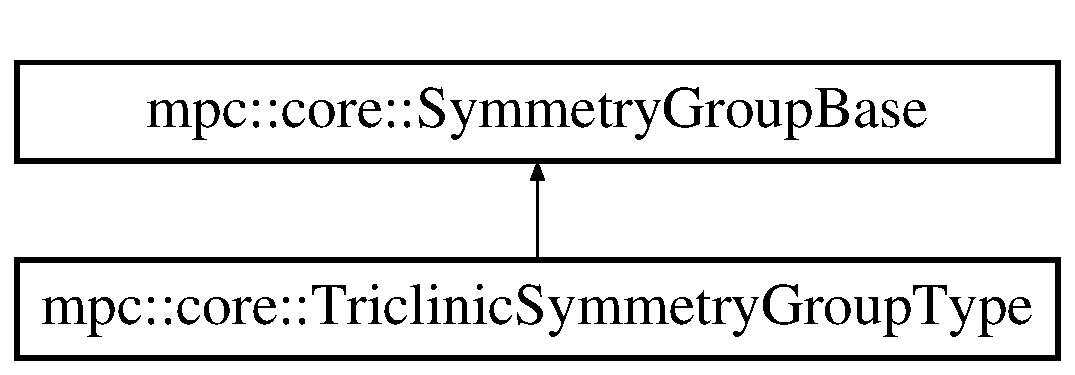
\includegraphics[height=2.000000cm]{structmpc_1_1core_1_1_triclinic_symmetry_group_type}
\end{center}
\end{figure}
\subsection*{Static Public Member Functions}
\begin{DoxyCompactItemize}
\item 
static constexpr \mbox{\hyperlink{namespacempc_1_1core_a9d979684062547055a0ef5c13077bad8}{Symmetry\+Group\+Enumeration}} \mbox{\hyperlink{structmpc_1_1core_1_1_triclinic_symmetry_group_type_a04032781251ce8fcdd0d2d63f9ed00b6}{Symmetry\+Group\+Enum}} ()
\item 
static constexpr int \mbox{\hyperlink{structmpc_1_1core_1_1_triclinic_symmetry_group_type_a9073ba0fe7514d2b8442ad4281625dd0}{Number\+Of\+Independent\+Components}} ()
\end{DoxyCompactItemize}
\subsection*{Public Attributes}
\begin{DoxyCompactItemize}
\item 
const \mbox{\hyperlink{namespacempc_1_1core_a9d979684062547055a0ef5c13077bad8}{Symmetry\+Group\+Enumeration}} \mbox{\hyperlink{structmpc_1_1core_1_1_triclinic_symmetry_group_type_a7602bf17b1fac2d9043f42928c2356b5}{symmetry\+\_\+group\+\_\+enumeration}} = \mbox{\hyperlink{namespacempc_1_1core_a9d979684062547055a0ef5c13077bad8a049b6e2743d57033eacaea302ca6710a}{Symmetry\+Group\+Enumeration\+::\+T\+R\+I\+C\+L\+I\+N\+IC}}
\item 
const int \mbox{\hyperlink{structmpc_1_1core_1_1_triclinic_symmetry_group_type_aeabbec5646e5b0cefd5b16b0a12e664d}{number\+\_\+of\+\_\+independent\+\_\+components}} = 21
\end{DoxyCompactItemize}


\subsection{Detailed Description}


Definition at line 160 of file symmetrygrouptypes.\+hpp.



\subsection{Member Function Documentation}
\mbox{\Hypertarget{structmpc_1_1core_1_1_triclinic_symmetry_group_type_a9073ba0fe7514d2b8442ad4281625dd0}\label{structmpc_1_1core_1_1_triclinic_symmetry_group_type_a9073ba0fe7514d2b8442ad4281625dd0}} 
\index{mpc\+::core\+::\+Triclinic\+Symmetry\+Group\+Type@{mpc\+::core\+::\+Triclinic\+Symmetry\+Group\+Type}!Number\+Of\+Independent\+Components@{Number\+Of\+Independent\+Components}}
\index{Number\+Of\+Independent\+Components@{Number\+Of\+Independent\+Components}!mpc\+::core\+::\+Triclinic\+Symmetry\+Group\+Type@{mpc\+::core\+::\+Triclinic\+Symmetry\+Group\+Type}}
\subsubsection{\texorpdfstring{Number\+Of\+Independent\+Components()}{NumberOfIndependentComponents()}}
{\footnotesize\ttfamily static constexpr int mpc\+::core\+::\+Triclinic\+Symmetry\+Group\+Type\+::\+Number\+Of\+Independent\+Components (\begin{DoxyParamCaption}{ }\end{DoxyParamCaption})\hspace{0.3cm}{\ttfamily [inline]}, {\ttfamily [static]}}



Definition at line 167 of file symmetrygrouptypes.\+hpp.

\mbox{\Hypertarget{structmpc_1_1core_1_1_triclinic_symmetry_group_type_a04032781251ce8fcdd0d2d63f9ed00b6}\label{structmpc_1_1core_1_1_triclinic_symmetry_group_type_a04032781251ce8fcdd0d2d63f9ed00b6}} 
\index{mpc\+::core\+::\+Triclinic\+Symmetry\+Group\+Type@{mpc\+::core\+::\+Triclinic\+Symmetry\+Group\+Type}!Symmetry\+Group\+Enum@{Symmetry\+Group\+Enum}}
\index{Symmetry\+Group\+Enum@{Symmetry\+Group\+Enum}!mpc\+::core\+::\+Triclinic\+Symmetry\+Group\+Type@{mpc\+::core\+::\+Triclinic\+Symmetry\+Group\+Type}}
\subsubsection{\texorpdfstring{Symmetry\+Group\+Enum()}{SymmetryGroupEnum()}}
{\footnotesize\ttfamily static constexpr \mbox{\hyperlink{namespacempc_1_1core_a9d979684062547055a0ef5c13077bad8}{Symmetry\+Group\+Enumeration}} mpc\+::core\+::\+Triclinic\+Symmetry\+Group\+Type\+::\+Symmetry\+Group\+Enum (\begin{DoxyParamCaption}{ }\end{DoxyParamCaption})\hspace{0.3cm}{\ttfamily [inline]}, {\ttfamily [static]}}



Definition at line 164 of file symmetrygrouptypes.\+hpp.



\subsection{Member Data Documentation}
\mbox{\Hypertarget{structmpc_1_1core_1_1_triclinic_symmetry_group_type_aeabbec5646e5b0cefd5b16b0a12e664d}\label{structmpc_1_1core_1_1_triclinic_symmetry_group_type_aeabbec5646e5b0cefd5b16b0a12e664d}} 
\index{mpc\+::core\+::\+Triclinic\+Symmetry\+Group\+Type@{mpc\+::core\+::\+Triclinic\+Symmetry\+Group\+Type}!number\+\_\+of\+\_\+independent\+\_\+components@{number\+\_\+of\+\_\+independent\+\_\+components}}
\index{number\+\_\+of\+\_\+independent\+\_\+components@{number\+\_\+of\+\_\+independent\+\_\+components}!mpc\+::core\+::\+Triclinic\+Symmetry\+Group\+Type@{mpc\+::core\+::\+Triclinic\+Symmetry\+Group\+Type}}
\subsubsection{\texorpdfstring{number\+\_\+of\+\_\+independent\+\_\+components}{number\_of\_independent\_components}}
{\footnotesize\ttfamily const int mpc\+::core\+::\+Triclinic\+Symmetry\+Group\+Type\+::number\+\_\+of\+\_\+independent\+\_\+components = 21}



Definition at line 162 of file symmetrygrouptypes.\+hpp.

\mbox{\Hypertarget{structmpc_1_1core_1_1_triclinic_symmetry_group_type_a7602bf17b1fac2d9043f42928c2356b5}\label{structmpc_1_1core_1_1_triclinic_symmetry_group_type_a7602bf17b1fac2d9043f42928c2356b5}} 
\index{mpc\+::core\+::\+Triclinic\+Symmetry\+Group\+Type@{mpc\+::core\+::\+Triclinic\+Symmetry\+Group\+Type}!symmetry\+\_\+group\+\_\+enumeration@{symmetry\+\_\+group\+\_\+enumeration}}
\index{symmetry\+\_\+group\+\_\+enumeration@{symmetry\+\_\+group\+\_\+enumeration}!mpc\+::core\+::\+Triclinic\+Symmetry\+Group\+Type@{mpc\+::core\+::\+Triclinic\+Symmetry\+Group\+Type}}
\subsubsection{\texorpdfstring{symmetry\+\_\+group\+\_\+enumeration}{symmetry\_group\_enumeration}}
{\footnotesize\ttfamily const \mbox{\hyperlink{namespacempc_1_1core_a9d979684062547055a0ef5c13077bad8}{Symmetry\+Group\+Enumeration}} mpc\+::core\+::\+Triclinic\+Symmetry\+Group\+Type\+::symmetry\+\_\+group\+\_\+enumeration = \mbox{\hyperlink{namespacempc_1_1core_a9d979684062547055a0ef5c13077bad8a049b6e2743d57033eacaea302ca6710a}{Symmetry\+Group\+Enumeration\+::\+T\+R\+I\+C\+L\+I\+N\+IC}}}



Definition at line 161 of file symmetrygrouptypes.\+hpp.



The documentation for this struct was generated from the following file\+:\begin{DoxyCompactItemize}
\item 
/\+Users/atorlucci/\+Documents/github\+\_\+threecubed\+\_\+repos/mpc/src/mpc/core/\mbox{\hyperlink{symmetrygrouptypes_8hpp}{symmetrygrouptypes.\+hpp}}\end{DoxyCompactItemize}

\hypertarget{structmpc_1_1core_1_1_trigonal6_symmetry_group_type}{}\section{mpc\+:\+:core\+:\+:Trigonal6\+Symmetry\+Group\+Type Struct Reference}
\label{structmpc_1_1core_1_1_trigonal6_symmetry_group_type}\index{mpc\+::core\+::\+Trigonal6\+Symmetry\+Group\+Type@{mpc\+::core\+::\+Trigonal6\+Symmetry\+Group\+Type}}


{\ttfamily \#include $<$symmetrygrouptypes.\+hpp$>$}

Inheritance diagram for mpc\+:\+:core\+:\+:Trigonal6\+Symmetry\+Group\+Type\+:\begin{figure}[H]
\begin{center}
\leavevmode
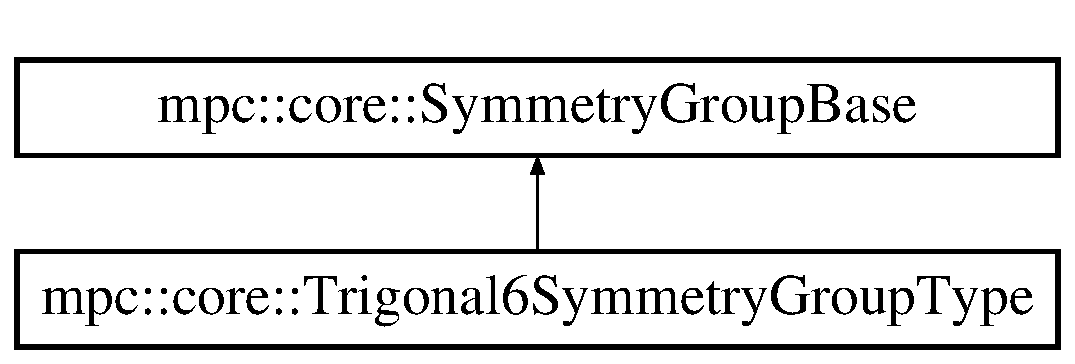
\includegraphics[height=2.000000cm]{structmpc_1_1core_1_1_trigonal6_symmetry_group_type}
\end{center}
\end{figure}
\subsection*{Static Public Member Functions}
\begin{DoxyCompactItemize}
\item 
static constexpr \mbox{\hyperlink{namespacempc_1_1core_a9d979684062547055a0ef5c13077bad8}{Symmetry\+Group\+Enumeration}} \mbox{\hyperlink{structmpc_1_1core_1_1_trigonal6_symmetry_group_type_a93136e8d9504c55a29dd114a6f8e9d16}{Symmetry\+Group\+Enum}} ()
\item 
static constexpr int \mbox{\hyperlink{structmpc_1_1core_1_1_trigonal6_symmetry_group_type_ac74e0669e3620ea8efe472182728a697}{Number\+Of\+Independent\+Components}} ()
\end{DoxyCompactItemize}
\subsection*{Public Attributes}
\begin{DoxyCompactItemize}
\item 
const \mbox{\hyperlink{namespacempc_1_1core_a9d979684062547055a0ef5c13077bad8}{Symmetry\+Group\+Enumeration}} \mbox{\hyperlink{structmpc_1_1core_1_1_trigonal6_symmetry_group_type_aee96fe6cfaf7272c1c335782a47da13d}{symmetry\+\_\+group\+\_\+enumeration}} = \mbox{\hyperlink{namespacempc_1_1core_a9d979684062547055a0ef5c13077bad8ad11b66b53c3c9dbfe73aa29a5d3df56c}{Symmetry\+Group\+Enumeration\+::\+T\+R\+I\+G\+O\+N\+A\+L6}}
\item 
const int \mbox{\hyperlink{structmpc_1_1core_1_1_trigonal6_symmetry_group_type_a376784d4a0e763c9c2900ea2af29528a}{number\+\_\+of\+\_\+independent\+\_\+components}} = 6
\end{DoxyCompactItemize}


\subsection{Detailed Description}


Definition at line 256 of file symmetrygrouptypes.\+hpp.



\subsection{Member Function Documentation}
\mbox{\Hypertarget{structmpc_1_1core_1_1_trigonal6_symmetry_group_type_ac74e0669e3620ea8efe472182728a697}\label{structmpc_1_1core_1_1_trigonal6_symmetry_group_type_ac74e0669e3620ea8efe472182728a697}} 
\index{mpc\+::core\+::\+Trigonal6\+Symmetry\+Group\+Type@{mpc\+::core\+::\+Trigonal6\+Symmetry\+Group\+Type}!Number\+Of\+Independent\+Components@{Number\+Of\+Independent\+Components}}
\index{Number\+Of\+Independent\+Components@{Number\+Of\+Independent\+Components}!mpc\+::core\+::\+Trigonal6\+Symmetry\+Group\+Type@{mpc\+::core\+::\+Trigonal6\+Symmetry\+Group\+Type}}
\subsubsection{\texorpdfstring{Number\+Of\+Independent\+Components()}{NumberOfIndependentComponents()}}
{\footnotesize\ttfamily static constexpr int mpc\+::core\+::\+Trigonal6\+Symmetry\+Group\+Type\+::\+Number\+Of\+Independent\+Components (\begin{DoxyParamCaption}{ }\end{DoxyParamCaption})\hspace{0.3cm}{\ttfamily [inline]}, {\ttfamily [static]}}



Definition at line 263 of file symmetrygrouptypes.\+hpp.

\mbox{\Hypertarget{structmpc_1_1core_1_1_trigonal6_symmetry_group_type_a93136e8d9504c55a29dd114a6f8e9d16}\label{structmpc_1_1core_1_1_trigonal6_symmetry_group_type_a93136e8d9504c55a29dd114a6f8e9d16}} 
\index{mpc\+::core\+::\+Trigonal6\+Symmetry\+Group\+Type@{mpc\+::core\+::\+Trigonal6\+Symmetry\+Group\+Type}!Symmetry\+Group\+Enum@{Symmetry\+Group\+Enum}}
\index{Symmetry\+Group\+Enum@{Symmetry\+Group\+Enum}!mpc\+::core\+::\+Trigonal6\+Symmetry\+Group\+Type@{mpc\+::core\+::\+Trigonal6\+Symmetry\+Group\+Type}}
\subsubsection{\texorpdfstring{Symmetry\+Group\+Enum()}{SymmetryGroupEnum()}}
{\footnotesize\ttfamily static constexpr \mbox{\hyperlink{namespacempc_1_1core_a9d979684062547055a0ef5c13077bad8}{Symmetry\+Group\+Enumeration}} mpc\+::core\+::\+Trigonal6\+Symmetry\+Group\+Type\+::\+Symmetry\+Group\+Enum (\begin{DoxyParamCaption}{ }\end{DoxyParamCaption})\hspace{0.3cm}{\ttfamily [inline]}, {\ttfamily [static]}}



Definition at line 260 of file symmetrygrouptypes.\+hpp.



\subsection{Member Data Documentation}
\mbox{\Hypertarget{structmpc_1_1core_1_1_trigonal6_symmetry_group_type_a376784d4a0e763c9c2900ea2af29528a}\label{structmpc_1_1core_1_1_trigonal6_symmetry_group_type_a376784d4a0e763c9c2900ea2af29528a}} 
\index{mpc\+::core\+::\+Trigonal6\+Symmetry\+Group\+Type@{mpc\+::core\+::\+Trigonal6\+Symmetry\+Group\+Type}!number\+\_\+of\+\_\+independent\+\_\+components@{number\+\_\+of\+\_\+independent\+\_\+components}}
\index{number\+\_\+of\+\_\+independent\+\_\+components@{number\+\_\+of\+\_\+independent\+\_\+components}!mpc\+::core\+::\+Trigonal6\+Symmetry\+Group\+Type@{mpc\+::core\+::\+Trigonal6\+Symmetry\+Group\+Type}}
\subsubsection{\texorpdfstring{number\+\_\+of\+\_\+independent\+\_\+components}{number\_of\_independent\_components}}
{\footnotesize\ttfamily const int mpc\+::core\+::\+Trigonal6\+Symmetry\+Group\+Type\+::number\+\_\+of\+\_\+independent\+\_\+components = 6}



Definition at line 258 of file symmetrygrouptypes.\+hpp.

\mbox{\Hypertarget{structmpc_1_1core_1_1_trigonal6_symmetry_group_type_aee96fe6cfaf7272c1c335782a47da13d}\label{structmpc_1_1core_1_1_trigonal6_symmetry_group_type_aee96fe6cfaf7272c1c335782a47da13d}} 
\index{mpc\+::core\+::\+Trigonal6\+Symmetry\+Group\+Type@{mpc\+::core\+::\+Trigonal6\+Symmetry\+Group\+Type}!symmetry\+\_\+group\+\_\+enumeration@{symmetry\+\_\+group\+\_\+enumeration}}
\index{symmetry\+\_\+group\+\_\+enumeration@{symmetry\+\_\+group\+\_\+enumeration}!mpc\+::core\+::\+Trigonal6\+Symmetry\+Group\+Type@{mpc\+::core\+::\+Trigonal6\+Symmetry\+Group\+Type}}
\subsubsection{\texorpdfstring{symmetry\+\_\+group\+\_\+enumeration}{symmetry\_group\_enumeration}}
{\footnotesize\ttfamily const \mbox{\hyperlink{namespacempc_1_1core_a9d979684062547055a0ef5c13077bad8}{Symmetry\+Group\+Enumeration}} mpc\+::core\+::\+Trigonal6\+Symmetry\+Group\+Type\+::symmetry\+\_\+group\+\_\+enumeration = \mbox{\hyperlink{namespacempc_1_1core_a9d979684062547055a0ef5c13077bad8ad11b66b53c3c9dbfe73aa29a5d3df56c}{Symmetry\+Group\+Enumeration\+::\+T\+R\+I\+G\+O\+N\+A\+L6}}}



Definition at line 257 of file symmetrygrouptypes.\+hpp.



The documentation for this struct was generated from the following file\+:\begin{DoxyCompactItemize}
\item 
/\+Users/atorlucci/\+Documents/github\+\_\+threecubed\+\_\+repos/mpc/src/mpc/core/\mbox{\hyperlink{symmetrygrouptypes_8hpp}{symmetrygrouptypes.\+hpp}}\end{DoxyCompactItemize}

\hypertarget{structmpc_1_1core_1_1_trigonal7_symmetry_group_type}{}\section{mpc\+:\+:core\+:\+:Trigonal7\+Symmetry\+Group\+Type Struct Reference}
\label{structmpc_1_1core_1_1_trigonal7_symmetry_group_type}\index{mpc\+::core\+::\+Trigonal7\+Symmetry\+Group\+Type@{mpc\+::core\+::\+Trigonal7\+Symmetry\+Group\+Type}}


{\ttfamily \#include $<$symmetrygrouptypes.\+hpp$>$}

Inheritance diagram for mpc\+:\+:core\+:\+:Trigonal7\+Symmetry\+Group\+Type\+:\begin{figure}[H]
\begin{center}
\leavevmode
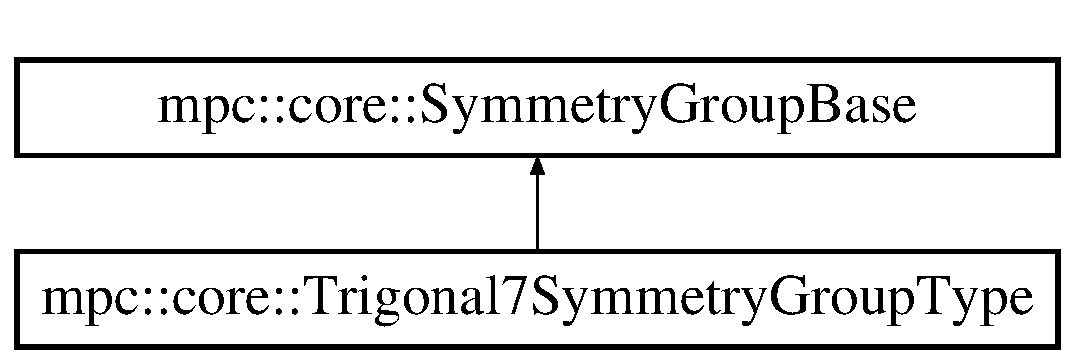
\includegraphics[height=2.000000cm]{structmpc_1_1core_1_1_trigonal7_symmetry_group_type}
\end{center}
\end{figure}
\subsection*{Static Public Member Functions}
\begin{DoxyCompactItemize}
\item 
static constexpr \mbox{\hyperlink{namespacempc_1_1core_a9d979684062547055a0ef5c13077bad8}{Symmetry\+Group\+Enumeration}} \mbox{\hyperlink{structmpc_1_1core_1_1_trigonal7_symmetry_group_type_abc384a0cbee42df56c3afcf55915547d}{Symmetry\+Group\+Enum}} ()
\item 
static constexpr int \mbox{\hyperlink{structmpc_1_1core_1_1_trigonal7_symmetry_group_type_ac7dc34ebb3ec6a678f8caf53637b420c}{Number\+Of\+Independent\+Components}} ()
\end{DoxyCompactItemize}
\subsection*{Public Attributes}
\begin{DoxyCompactItemize}
\item 
const \mbox{\hyperlink{namespacempc_1_1core_a9d979684062547055a0ef5c13077bad8}{Symmetry\+Group\+Enumeration}} \mbox{\hyperlink{structmpc_1_1core_1_1_trigonal7_symmetry_group_type_af17153b42a8a84d51280a8990e785aa4}{symmetry\+\_\+group\+\_\+enumeration}} = \mbox{\hyperlink{namespacempc_1_1core_a9d979684062547055a0ef5c13077bad8ab347d6d7556c0d38dc3d111b08a50dee}{Symmetry\+Group\+Enumeration\+::\+T\+R\+I\+G\+O\+N\+A\+L7}}
\item 
const int \mbox{\hyperlink{structmpc_1_1core_1_1_trigonal7_symmetry_group_type_ad9ff9e80f62792232b540114819bf1eb}{number\+\_\+of\+\_\+independent\+\_\+components}} = 7
\end{DoxyCompactItemize}


\subsection{Detailed Description}


Definition at line 244 of file symmetrygrouptypes.\+hpp.



\subsection{Member Function Documentation}
\mbox{\Hypertarget{structmpc_1_1core_1_1_trigonal7_symmetry_group_type_ac7dc34ebb3ec6a678f8caf53637b420c}\label{structmpc_1_1core_1_1_trigonal7_symmetry_group_type_ac7dc34ebb3ec6a678f8caf53637b420c}} 
\index{mpc\+::core\+::\+Trigonal7\+Symmetry\+Group\+Type@{mpc\+::core\+::\+Trigonal7\+Symmetry\+Group\+Type}!Number\+Of\+Independent\+Components@{Number\+Of\+Independent\+Components}}
\index{Number\+Of\+Independent\+Components@{Number\+Of\+Independent\+Components}!mpc\+::core\+::\+Trigonal7\+Symmetry\+Group\+Type@{mpc\+::core\+::\+Trigonal7\+Symmetry\+Group\+Type}}
\subsubsection{\texorpdfstring{Number\+Of\+Independent\+Components()}{NumberOfIndependentComponents()}}
{\footnotesize\ttfamily static constexpr int mpc\+::core\+::\+Trigonal7\+Symmetry\+Group\+Type\+::\+Number\+Of\+Independent\+Components (\begin{DoxyParamCaption}{ }\end{DoxyParamCaption})\hspace{0.3cm}{\ttfamily [inline]}, {\ttfamily [static]}}



Definition at line 251 of file symmetrygrouptypes.\+hpp.

\mbox{\Hypertarget{structmpc_1_1core_1_1_trigonal7_symmetry_group_type_abc384a0cbee42df56c3afcf55915547d}\label{structmpc_1_1core_1_1_trigonal7_symmetry_group_type_abc384a0cbee42df56c3afcf55915547d}} 
\index{mpc\+::core\+::\+Trigonal7\+Symmetry\+Group\+Type@{mpc\+::core\+::\+Trigonal7\+Symmetry\+Group\+Type}!Symmetry\+Group\+Enum@{Symmetry\+Group\+Enum}}
\index{Symmetry\+Group\+Enum@{Symmetry\+Group\+Enum}!mpc\+::core\+::\+Trigonal7\+Symmetry\+Group\+Type@{mpc\+::core\+::\+Trigonal7\+Symmetry\+Group\+Type}}
\subsubsection{\texorpdfstring{Symmetry\+Group\+Enum()}{SymmetryGroupEnum()}}
{\footnotesize\ttfamily static constexpr \mbox{\hyperlink{namespacempc_1_1core_a9d979684062547055a0ef5c13077bad8}{Symmetry\+Group\+Enumeration}} mpc\+::core\+::\+Trigonal7\+Symmetry\+Group\+Type\+::\+Symmetry\+Group\+Enum (\begin{DoxyParamCaption}{ }\end{DoxyParamCaption})\hspace{0.3cm}{\ttfamily [inline]}, {\ttfamily [static]}}



Definition at line 248 of file symmetrygrouptypes.\+hpp.



\subsection{Member Data Documentation}
\mbox{\Hypertarget{structmpc_1_1core_1_1_trigonal7_symmetry_group_type_ad9ff9e80f62792232b540114819bf1eb}\label{structmpc_1_1core_1_1_trigonal7_symmetry_group_type_ad9ff9e80f62792232b540114819bf1eb}} 
\index{mpc\+::core\+::\+Trigonal7\+Symmetry\+Group\+Type@{mpc\+::core\+::\+Trigonal7\+Symmetry\+Group\+Type}!number\+\_\+of\+\_\+independent\+\_\+components@{number\+\_\+of\+\_\+independent\+\_\+components}}
\index{number\+\_\+of\+\_\+independent\+\_\+components@{number\+\_\+of\+\_\+independent\+\_\+components}!mpc\+::core\+::\+Trigonal7\+Symmetry\+Group\+Type@{mpc\+::core\+::\+Trigonal7\+Symmetry\+Group\+Type}}
\subsubsection{\texorpdfstring{number\+\_\+of\+\_\+independent\+\_\+components}{number\_of\_independent\_components}}
{\footnotesize\ttfamily const int mpc\+::core\+::\+Trigonal7\+Symmetry\+Group\+Type\+::number\+\_\+of\+\_\+independent\+\_\+components = 7}



Definition at line 246 of file symmetrygrouptypes.\+hpp.

\mbox{\Hypertarget{structmpc_1_1core_1_1_trigonal7_symmetry_group_type_af17153b42a8a84d51280a8990e785aa4}\label{structmpc_1_1core_1_1_trigonal7_symmetry_group_type_af17153b42a8a84d51280a8990e785aa4}} 
\index{mpc\+::core\+::\+Trigonal7\+Symmetry\+Group\+Type@{mpc\+::core\+::\+Trigonal7\+Symmetry\+Group\+Type}!symmetry\+\_\+group\+\_\+enumeration@{symmetry\+\_\+group\+\_\+enumeration}}
\index{symmetry\+\_\+group\+\_\+enumeration@{symmetry\+\_\+group\+\_\+enumeration}!mpc\+::core\+::\+Trigonal7\+Symmetry\+Group\+Type@{mpc\+::core\+::\+Trigonal7\+Symmetry\+Group\+Type}}
\subsubsection{\texorpdfstring{symmetry\+\_\+group\+\_\+enumeration}{symmetry\_group\_enumeration}}
{\footnotesize\ttfamily const \mbox{\hyperlink{namespacempc_1_1core_a9d979684062547055a0ef5c13077bad8}{Symmetry\+Group\+Enumeration}} mpc\+::core\+::\+Trigonal7\+Symmetry\+Group\+Type\+::symmetry\+\_\+group\+\_\+enumeration = \mbox{\hyperlink{namespacempc_1_1core_a9d979684062547055a0ef5c13077bad8ab347d6d7556c0d38dc3d111b08a50dee}{Symmetry\+Group\+Enumeration\+::\+T\+R\+I\+G\+O\+N\+A\+L7}}}



Definition at line 245 of file symmetrygrouptypes.\+hpp.



The documentation for this struct was generated from the following file\+:\begin{DoxyCompactItemize}
\item 
/\+Users/atorlucci/\+Documents/github\+\_\+threecubed\+\_\+repos/mpc/src/mpc/core/\mbox{\hyperlink{symmetrygrouptypes_8hpp}{symmetrygrouptypes.\+hpp}}\end{DoxyCompactItemize}

\hypertarget{structmpc_1_1utilities_1_1_unwrapper}{}\section{mpc\+:\+:utilities\+:\+:Unwrapper$<$ T, N $>$ Struct Template Reference}
\label{structmpc_1_1utilities_1_1_unwrapper}\index{mpc\+::utilities\+::\+Unwrapper$<$ T, N $>$@{mpc\+::utilities\+::\+Unwrapper$<$ T, N $>$}}


{\ttfamily \#include $<$unwrapper.\+hpp$>$}

\subsection*{Public Member Functions}
\begin{DoxyCompactItemize}
\item 
blitz\+::\+Array$<$ T, 1 $>$ \mbox{\hyperlink{structmpc_1_1utilities_1_1_unwrapper_a6e18b48b2079334320123322888c0785}{operator()}} (blitz\+::\+Array$<$ T, N $>$ \&input\+\_\+array)
\end{DoxyCompactItemize}


\subsection{Detailed Description}
\subsubsection*{template$<$typename T, int N$>$\newline
struct mpc\+::utilities\+::\+Unwrapper$<$ T, N $>$}



Definition at line 28 of file unwrapper.\+hpp.



\subsection{Member Function Documentation}
\mbox{\Hypertarget{structmpc_1_1utilities_1_1_unwrapper_a6e18b48b2079334320123322888c0785}\label{structmpc_1_1utilities_1_1_unwrapper_a6e18b48b2079334320123322888c0785}} 
\index{mpc\+::utilities\+::\+Unwrapper@{mpc\+::utilities\+::\+Unwrapper}!operator()@{operator()}}
\index{operator()@{operator()}!mpc\+::utilities\+::\+Unwrapper@{mpc\+::utilities\+::\+Unwrapper}}
\subsubsection{\texorpdfstring{operator()()}{operator()()}}
{\footnotesize\ttfamily template$<$typename T , int N$>$ \\
blitz\+::\+Array$<$T,1$>$ \mbox{\hyperlink{structmpc_1_1utilities_1_1_unwrapper}{mpc\+::utilities\+::\+Unwrapper}}$<$ T, N $>$\+::operator() (\begin{DoxyParamCaption}\item[{blitz\+::\+Array$<$ T, N $>$ \&}]{input\+\_\+array }\end{DoxyParamCaption})}



The documentation for this struct was generated from the following file\+:\begin{DoxyCompactItemize}
\item 
/\+Users/atorlucci/\+Documents/github\+\_\+threecubed\+\_\+repos/mpc/src/mpc/utilities/\mbox{\hyperlink{unwrapper_8hpp}{unwrapper.\+hpp}}\end{DoxyCompactItemize}

\hypertarget{structmpc_1_1utilities_1_1_unwrapper_3_01_t_00_0110_01_4}{}\section{mpc\+:\+:utilities\+:\+:Unwrapper$<$ T, 10 $>$ Struct Template Reference}
\label{structmpc_1_1utilities_1_1_unwrapper_3_01_t_00_0110_01_4}\index{mpc\+::utilities\+::\+Unwrapper$<$ T, 10 $>$@{mpc\+::utilities\+::\+Unwrapper$<$ T, 10 $>$}}


{\ttfamily \#include $<$unwrapper.\+hpp$>$}

\subsection*{Public Member Functions}
\begin{DoxyCompactItemize}
\item 
blitz\+::\+Array$<$ T, 1 $>$ \mbox{\hyperlink{structmpc_1_1utilities_1_1_unwrapper_3_01_t_00_0110_01_4_a3a03d61a8d1ee0ee719b4d0de2f32fac}{operator()}} (blitz\+::\+Array$<$ T, 10 $>$ \&input\+\_\+array)
\end{DoxyCompactItemize}


\subsection{Detailed Description}
\subsubsection*{template$<$typename T$>$\newline
struct mpc\+::utilities\+::\+Unwrapper$<$ T, 10 $>$}



Definition at line 251 of file unwrapper.\+hpp.



\subsection{Member Function Documentation}
\mbox{\Hypertarget{structmpc_1_1utilities_1_1_unwrapper_3_01_t_00_0110_01_4_a3a03d61a8d1ee0ee719b4d0de2f32fac}\label{structmpc_1_1utilities_1_1_unwrapper_3_01_t_00_0110_01_4_a3a03d61a8d1ee0ee719b4d0de2f32fac}} 
\index{mpc\+::utilities\+::\+Unwrapper$<$ T, 10 $>$@{mpc\+::utilities\+::\+Unwrapper$<$ T, 10 $>$}!operator()@{operator()}}
\index{operator()@{operator()}!mpc\+::utilities\+::\+Unwrapper$<$ T, 10 $>$@{mpc\+::utilities\+::\+Unwrapper$<$ T, 10 $>$}}
\subsubsection{\texorpdfstring{operator()()}{operator()()}}
{\footnotesize\ttfamily template$<$typename T $>$ \\
blitz\+::\+Array$<$T,1$>$ \mbox{\hyperlink{structmpc_1_1utilities_1_1_unwrapper}{mpc\+::utilities\+::\+Unwrapper}}$<$ T, 10 $>$\+::operator() (\begin{DoxyParamCaption}\item[{blitz\+::\+Array$<$ T, 10 $>$ \&}]{input\+\_\+array }\end{DoxyParamCaption})\hspace{0.3cm}{\ttfamily [inline]}}



Definition at line 253 of file unwrapper.\+hpp.



The documentation for this struct was generated from the following file\+:\begin{DoxyCompactItemize}
\item 
/\+Users/atorlucci/\+Documents/github\+\_\+threecubed\+\_\+repos/mpc/src/mpc/utilities/\mbox{\hyperlink{unwrapper_8hpp}{unwrapper.\+hpp}}\end{DoxyCompactItemize}

\hypertarget{structmpc_1_1utilities_1_1_unwrapper_3_01_t_00_0111_01_4}{}\section{mpc\+:\+:utilities\+:\+:Unwrapper$<$ T, 11 $>$ Struct Template Reference}
\label{structmpc_1_1utilities_1_1_unwrapper_3_01_t_00_0111_01_4}\index{mpc\+::utilities\+::\+Unwrapper$<$ T, 11 $>$@{mpc\+::utilities\+::\+Unwrapper$<$ T, 11 $>$}}


{\ttfamily \#include $<$unwrapper.\+hpp$>$}

\subsection*{Public Member Functions}
\begin{DoxyCompactItemize}
\item 
blitz\+::\+Array$<$ T, 1 $>$ \mbox{\hyperlink{structmpc_1_1utilities_1_1_unwrapper_3_01_t_00_0111_01_4_ababaa4a455c2bc350ecbb94a762ea7c0}{operator()}} (blitz\+::\+Array$<$ T, 11 $>$ \&input\+\_\+array)
\end{DoxyCompactItemize}


\subsection{Detailed Description}
\subsubsection*{template$<$typename T$>$\newline
struct mpc\+::utilities\+::\+Unwrapper$<$ T, 11 $>$}



Definition at line 287 of file unwrapper.\+hpp.



\subsection{Member Function Documentation}
\mbox{\Hypertarget{structmpc_1_1utilities_1_1_unwrapper_3_01_t_00_0111_01_4_ababaa4a455c2bc350ecbb94a762ea7c0}\label{structmpc_1_1utilities_1_1_unwrapper_3_01_t_00_0111_01_4_ababaa4a455c2bc350ecbb94a762ea7c0}} 
\index{mpc\+::utilities\+::\+Unwrapper$<$ T, 11 $>$@{mpc\+::utilities\+::\+Unwrapper$<$ T, 11 $>$}!operator()@{operator()}}
\index{operator()@{operator()}!mpc\+::utilities\+::\+Unwrapper$<$ T, 11 $>$@{mpc\+::utilities\+::\+Unwrapper$<$ T, 11 $>$}}
\subsubsection{\texorpdfstring{operator()()}{operator()()}}
{\footnotesize\ttfamily template$<$typename T $>$ \\
blitz\+::\+Array$<$T,1$>$ \mbox{\hyperlink{structmpc_1_1utilities_1_1_unwrapper}{mpc\+::utilities\+::\+Unwrapper}}$<$ T, 11 $>$\+::operator() (\begin{DoxyParamCaption}\item[{blitz\+::\+Array$<$ T, 11 $>$ \&}]{input\+\_\+array }\end{DoxyParamCaption})\hspace{0.3cm}{\ttfamily [inline]}}



Definition at line 289 of file unwrapper.\+hpp.



The documentation for this struct was generated from the following file\+:\begin{DoxyCompactItemize}
\item 
/\+Users/atorlucci/\+Documents/github\+\_\+threecubed\+\_\+repos/mpc/src/mpc/utilities/\mbox{\hyperlink{unwrapper_8hpp}{unwrapper.\+hpp}}\end{DoxyCompactItemize}

\hypertarget{structmpc_1_1utilities_1_1_unwrapper_3_01_t_00_012_01_4}{}\section{mpc\+:\+:utilities\+:\+:Unwrapper$<$ T, 2 $>$ Struct Template Reference}
\label{structmpc_1_1utilities_1_1_unwrapper_3_01_t_00_012_01_4}\index{mpc\+::utilities\+::\+Unwrapper$<$ T, 2 $>$@{mpc\+::utilities\+::\+Unwrapper$<$ T, 2 $>$}}


{\ttfamily \#include $<$unwrapper.\+hpp$>$}

\subsection*{Public Member Functions}
\begin{DoxyCompactItemize}
\item 
blitz\+::\+Array$<$ T, 1 $>$ \mbox{\hyperlink{structmpc_1_1utilities_1_1_unwrapper_3_01_t_00_012_01_4_a3fe1633cd85163f54e330641e0c6a448}{operator()}} (blitz\+::\+Array$<$ T, 2 $>$ \&input\+\_\+array)
\end{DoxyCompactItemize}


\subsection{Detailed Description}
\subsubsection*{template$<$typename T$>$\newline
struct mpc\+::utilities\+::\+Unwrapper$<$ T, 2 $>$}



Definition at line 35 of file unwrapper.\+hpp.



\subsection{Member Function Documentation}
\mbox{\Hypertarget{structmpc_1_1utilities_1_1_unwrapper_3_01_t_00_012_01_4_a3fe1633cd85163f54e330641e0c6a448}\label{structmpc_1_1utilities_1_1_unwrapper_3_01_t_00_012_01_4_a3fe1633cd85163f54e330641e0c6a448}} 
\index{mpc\+::utilities\+::\+Unwrapper$<$ T, 2 $>$@{mpc\+::utilities\+::\+Unwrapper$<$ T, 2 $>$}!operator()@{operator()}}
\index{operator()@{operator()}!mpc\+::utilities\+::\+Unwrapper$<$ T, 2 $>$@{mpc\+::utilities\+::\+Unwrapper$<$ T, 2 $>$}}
\subsubsection{\texorpdfstring{operator()()}{operator()()}}
{\footnotesize\ttfamily template$<$typename T $>$ \\
blitz\+::\+Array$<$T,1$>$ \mbox{\hyperlink{structmpc_1_1utilities_1_1_unwrapper}{mpc\+::utilities\+::\+Unwrapper}}$<$ T, 2 $>$\+::operator() (\begin{DoxyParamCaption}\item[{blitz\+::\+Array$<$ T, 2 $>$ \&}]{input\+\_\+array }\end{DoxyParamCaption})\hspace{0.3cm}{\ttfamily [inline]}}



Definition at line 37 of file unwrapper.\+hpp.



The documentation for this struct was generated from the following file\+:\begin{DoxyCompactItemize}
\item 
/\+Users/atorlucci/\+Documents/github\+\_\+threecubed\+\_\+repos/mpc/src/mpc/utilities/\mbox{\hyperlink{unwrapper_8hpp}{unwrapper.\+hpp}}\end{DoxyCompactItemize}

\hypertarget{structmpc_1_1utilities_1_1_unwrapper_3_01_t_00_013_01_4}{}\section{mpc\+:\+:utilities\+:\+:Unwrapper$<$ T, 3 $>$ Struct Template Reference}
\label{structmpc_1_1utilities_1_1_unwrapper_3_01_t_00_013_01_4}\index{mpc\+::utilities\+::\+Unwrapper$<$ T, 3 $>$@{mpc\+::utilities\+::\+Unwrapper$<$ T, 3 $>$}}


{\ttfamily \#include $<$unwrapper.\+hpp$>$}

\subsection*{Public Member Functions}
\begin{DoxyCompactItemize}
\item 
blitz\+::\+Array$<$ T, 1 $>$ \mbox{\hyperlink{structmpc_1_1utilities_1_1_unwrapper_3_01_t_00_013_01_4_a584381b7b967c8245578bfaaf9ca1a0f}{operator()}} (blitz\+::\+Array$<$ T, 3 $>$ \&input\+\_\+array)
\end{DoxyCompactItemize}


\subsection{Detailed Description}
\subsubsection*{template$<$typename T$>$\newline
struct mpc\+::utilities\+::\+Unwrapper$<$ T, 3 $>$}



Definition at line 55 of file unwrapper.\+hpp.



\subsection{Member Function Documentation}
\mbox{\Hypertarget{structmpc_1_1utilities_1_1_unwrapper_3_01_t_00_013_01_4_a584381b7b967c8245578bfaaf9ca1a0f}\label{structmpc_1_1utilities_1_1_unwrapper_3_01_t_00_013_01_4_a584381b7b967c8245578bfaaf9ca1a0f}} 
\index{mpc\+::utilities\+::\+Unwrapper$<$ T, 3 $>$@{mpc\+::utilities\+::\+Unwrapper$<$ T, 3 $>$}!operator()@{operator()}}
\index{operator()@{operator()}!mpc\+::utilities\+::\+Unwrapper$<$ T, 3 $>$@{mpc\+::utilities\+::\+Unwrapper$<$ T, 3 $>$}}
\subsubsection{\texorpdfstring{operator()()}{operator()()}}
{\footnotesize\ttfamily template$<$typename T $>$ \\
blitz\+::\+Array$<$T,1$>$ \mbox{\hyperlink{structmpc_1_1utilities_1_1_unwrapper}{mpc\+::utilities\+::\+Unwrapper}}$<$ T, 3 $>$\+::operator() (\begin{DoxyParamCaption}\item[{blitz\+::\+Array$<$ T, 3 $>$ \&}]{input\+\_\+array }\end{DoxyParamCaption})\hspace{0.3cm}{\ttfamily [inline]}}



Definition at line 57 of file unwrapper.\+hpp.



The documentation for this struct was generated from the following file\+:\begin{DoxyCompactItemize}
\item 
/\+Users/atorlucci/\+Documents/github\+\_\+threecubed\+\_\+repos/mpc/src/mpc/utilities/\mbox{\hyperlink{unwrapper_8hpp}{unwrapper.\+hpp}}\end{DoxyCompactItemize}

\hypertarget{structmpc_1_1utilities_1_1_unwrapper_3_01_t_00_014_01_4}{}\section{mpc\+:\+:utilities\+:\+:Unwrapper$<$ T, 4 $>$ Struct Template Reference}
\label{structmpc_1_1utilities_1_1_unwrapper_3_01_t_00_014_01_4}\index{mpc\+::utilities\+::\+Unwrapper$<$ T, 4 $>$@{mpc\+::utilities\+::\+Unwrapper$<$ T, 4 $>$}}


{\ttfamily \#include $<$unwrapper.\+hpp$>$}

\subsection*{Public Member Functions}
\begin{DoxyCompactItemize}
\item 
blitz\+::\+Array$<$ T, 1 $>$ \mbox{\hyperlink{structmpc_1_1utilities_1_1_unwrapper_3_01_t_00_014_01_4_a288f292a07352d80d6ea251b01b0a006}{operator()}} (blitz\+::\+Array$<$ T, 4 $>$ \&input\+\_\+array)
\end{DoxyCompactItemize}


\subsection{Detailed Description}
\subsubsection*{template$<$typename T$>$\newline
struct mpc\+::utilities\+::\+Unwrapper$<$ T, 4 $>$}



Definition at line 77 of file unwrapper.\+hpp.



\subsection{Member Function Documentation}
\mbox{\Hypertarget{structmpc_1_1utilities_1_1_unwrapper_3_01_t_00_014_01_4_a288f292a07352d80d6ea251b01b0a006}\label{structmpc_1_1utilities_1_1_unwrapper_3_01_t_00_014_01_4_a288f292a07352d80d6ea251b01b0a006}} 
\index{mpc\+::utilities\+::\+Unwrapper$<$ T, 4 $>$@{mpc\+::utilities\+::\+Unwrapper$<$ T, 4 $>$}!operator()@{operator()}}
\index{operator()@{operator()}!mpc\+::utilities\+::\+Unwrapper$<$ T, 4 $>$@{mpc\+::utilities\+::\+Unwrapper$<$ T, 4 $>$}}
\subsubsection{\texorpdfstring{operator()()}{operator()()}}
{\footnotesize\ttfamily template$<$typename T $>$ \\
blitz\+::\+Array$<$T,1$>$ \mbox{\hyperlink{structmpc_1_1utilities_1_1_unwrapper}{mpc\+::utilities\+::\+Unwrapper}}$<$ T, 4 $>$\+::operator() (\begin{DoxyParamCaption}\item[{blitz\+::\+Array$<$ T, 4 $>$ \&}]{input\+\_\+array }\end{DoxyParamCaption})\hspace{0.3cm}{\ttfamily [inline]}}



Definition at line 79 of file unwrapper.\+hpp.



The documentation for this struct was generated from the following file\+:\begin{DoxyCompactItemize}
\item 
/\+Users/atorlucci/\+Documents/github\+\_\+threecubed\+\_\+repos/mpc/src/mpc/utilities/\mbox{\hyperlink{unwrapper_8hpp}{unwrapper.\+hpp}}\end{DoxyCompactItemize}

\hypertarget{structmpc_1_1utilities_1_1_unwrapper_3_01_t_00_015_01_4}{}\section{mpc\+:\+:utilities\+:\+:Unwrapper$<$ T, 5 $>$ Struct Template Reference}
\label{structmpc_1_1utilities_1_1_unwrapper_3_01_t_00_015_01_4}\index{mpc\+::utilities\+::\+Unwrapper$<$ T, 5 $>$@{mpc\+::utilities\+::\+Unwrapper$<$ T, 5 $>$}}


{\ttfamily \#include $<$unwrapper.\+hpp$>$}

\subsection*{Public Member Functions}
\begin{DoxyCompactItemize}
\item 
blitz\+::\+Array$<$ T, 1 $>$ \mbox{\hyperlink{structmpc_1_1utilities_1_1_unwrapper_3_01_t_00_015_01_4_a1d125aba4e6ba3ec992ec1138f467a1c}{operator()}} (blitz\+::\+Array$<$ T, 5 $>$ \&input\+\_\+array)
\end{DoxyCompactItemize}


\subsection{Detailed Description}
\subsubsection*{template$<$typename T$>$\newline
struct mpc\+::utilities\+::\+Unwrapper$<$ T, 5 $>$}



Definition at line 101 of file unwrapper.\+hpp.



\subsection{Member Function Documentation}
\mbox{\Hypertarget{structmpc_1_1utilities_1_1_unwrapper_3_01_t_00_015_01_4_a1d125aba4e6ba3ec992ec1138f467a1c}\label{structmpc_1_1utilities_1_1_unwrapper_3_01_t_00_015_01_4_a1d125aba4e6ba3ec992ec1138f467a1c}} 
\index{mpc\+::utilities\+::\+Unwrapper$<$ T, 5 $>$@{mpc\+::utilities\+::\+Unwrapper$<$ T, 5 $>$}!operator()@{operator()}}
\index{operator()@{operator()}!mpc\+::utilities\+::\+Unwrapper$<$ T, 5 $>$@{mpc\+::utilities\+::\+Unwrapper$<$ T, 5 $>$}}
\subsubsection{\texorpdfstring{operator()()}{operator()()}}
{\footnotesize\ttfamily template$<$typename T $>$ \\
blitz\+::\+Array$<$T,1$>$ \mbox{\hyperlink{structmpc_1_1utilities_1_1_unwrapper}{mpc\+::utilities\+::\+Unwrapper}}$<$ T, 5 $>$\+::operator() (\begin{DoxyParamCaption}\item[{blitz\+::\+Array$<$ T, 5 $>$ \&}]{input\+\_\+array }\end{DoxyParamCaption})\hspace{0.3cm}{\ttfamily [inline]}}



Definition at line 103 of file unwrapper.\+hpp.



The documentation for this struct was generated from the following file\+:\begin{DoxyCompactItemize}
\item 
/\+Users/atorlucci/\+Documents/github\+\_\+threecubed\+\_\+repos/mpc/src/mpc/utilities/\mbox{\hyperlink{unwrapper_8hpp}{unwrapper.\+hpp}}\end{DoxyCompactItemize}

\hypertarget{structmpc_1_1utilities_1_1_unwrapper_3_01_t_00_016_01_4}{}\section{mpc\+:\+:utilities\+:\+:Unwrapper$<$ T, 6 $>$ Struct Template Reference}
\label{structmpc_1_1utilities_1_1_unwrapper_3_01_t_00_016_01_4}\index{mpc\+::utilities\+::\+Unwrapper$<$ T, 6 $>$@{mpc\+::utilities\+::\+Unwrapper$<$ T, 6 $>$}}


{\ttfamily \#include $<$unwrapper.\+hpp$>$}

\subsection*{Public Member Functions}
\begin{DoxyCompactItemize}
\item 
blitz\+::\+Array$<$ T, 1 $>$ \mbox{\hyperlink{structmpc_1_1utilities_1_1_unwrapper_3_01_t_00_016_01_4_a337610b2bc0037a352576ba060636460}{operator()}} (blitz\+::\+Array$<$ T, 6 $>$ \&input\+\_\+array)
\end{DoxyCompactItemize}


\subsection{Detailed Description}
\subsubsection*{template$<$typename T$>$\newline
struct mpc\+::utilities\+::\+Unwrapper$<$ T, 6 $>$}



Definition at line 127 of file unwrapper.\+hpp.



\subsection{Member Function Documentation}
\mbox{\Hypertarget{structmpc_1_1utilities_1_1_unwrapper_3_01_t_00_016_01_4_a337610b2bc0037a352576ba060636460}\label{structmpc_1_1utilities_1_1_unwrapper_3_01_t_00_016_01_4_a337610b2bc0037a352576ba060636460}} 
\index{mpc\+::utilities\+::\+Unwrapper$<$ T, 6 $>$@{mpc\+::utilities\+::\+Unwrapper$<$ T, 6 $>$}!operator()@{operator()}}
\index{operator()@{operator()}!mpc\+::utilities\+::\+Unwrapper$<$ T, 6 $>$@{mpc\+::utilities\+::\+Unwrapper$<$ T, 6 $>$}}
\subsubsection{\texorpdfstring{operator()()}{operator()()}}
{\footnotesize\ttfamily template$<$typename T $>$ \\
blitz\+::\+Array$<$T,1$>$ \mbox{\hyperlink{structmpc_1_1utilities_1_1_unwrapper}{mpc\+::utilities\+::\+Unwrapper}}$<$ T, 6 $>$\+::operator() (\begin{DoxyParamCaption}\item[{blitz\+::\+Array$<$ T, 6 $>$ \&}]{input\+\_\+array }\end{DoxyParamCaption})\hspace{0.3cm}{\ttfamily [inline]}}



Definition at line 129 of file unwrapper.\+hpp.



The documentation for this struct was generated from the following file\+:\begin{DoxyCompactItemize}
\item 
/\+Users/atorlucci/\+Documents/github\+\_\+threecubed\+\_\+repos/mpc/src/mpc/utilities/\mbox{\hyperlink{unwrapper_8hpp}{unwrapper.\+hpp}}\end{DoxyCompactItemize}

\hypertarget{structmpc_1_1utilities_1_1_unwrapper_3_01_t_00_017_01_4}{}\section{mpc\+:\+:utilities\+:\+:Unwrapper$<$ T, 7 $>$ Struct Template Reference}
\label{structmpc_1_1utilities_1_1_unwrapper_3_01_t_00_017_01_4}\index{mpc\+::utilities\+::\+Unwrapper$<$ T, 7 $>$@{mpc\+::utilities\+::\+Unwrapper$<$ T, 7 $>$}}


{\ttfamily \#include $<$unwrapper.\+hpp$>$}

\subsection*{Public Member Functions}
\begin{DoxyCompactItemize}
\item 
blitz\+::\+Array$<$ T, 1 $>$ \mbox{\hyperlink{structmpc_1_1utilities_1_1_unwrapper_3_01_t_00_017_01_4_a470e342ad5dfb0313c9ba0b9503cdfdc}{operator()}} (blitz\+::\+Array$<$ T, 7 $>$ \&input\+\_\+array)
\end{DoxyCompactItemize}


\subsection{Detailed Description}
\subsubsection*{template$<$typename T$>$\newline
struct mpc\+::utilities\+::\+Unwrapper$<$ T, 7 $>$}



Definition at line 155 of file unwrapper.\+hpp.



\subsection{Member Function Documentation}
\mbox{\Hypertarget{structmpc_1_1utilities_1_1_unwrapper_3_01_t_00_017_01_4_a470e342ad5dfb0313c9ba0b9503cdfdc}\label{structmpc_1_1utilities_1_1_unwrapper_3_01_t_00_017_01_4_a470e342ad5dfb0313c9ba0b9503cdfdc}} 
\index{mpc\+::utilities\+::\+Unwrapper$<$ T, 7 $>$@{mpc\+::utilities\+::\+Unwrapper$<$ T, 7 $>$}!operator()@{operator()}}
\index{operator()@{operator()}!mpc\+::utilities\+::\+Unwrapper$<$ T, 7 $>$@{mpc\+::utilities\+::\+Unwrapper$<$ T, 7 $>$}}
\subsubsection{\texorpdfstring{operator()()}{operator()()}}
{\footnotesize\ttfamily template$<$typename T $>$ \\
blitz\+::\+Array$<$T,1$>$ \mbox{\hyperlink{structmpc_1_1utilities_1_1_unwrapper}{mpc\+::utilities\+::\+Unwrapper}}$<$ T, 7 $>$\+::operator() (\begin{DoxyParamCaption}\item[{blitz\+::\+Array$<$ T, 7 $>$ \&}]{input\+\_\+array }\end{DoxyParamCaption})\hspace{0.3cm}{\ttfamily [inline]}}



Definition at line 157 of file unwrapper.\+hpp.



The documentation for this struct was generated from the following file\+:\begin{DoxyCompactItemize}
\item 
/\+Users/atorlucci/\+Documents/github\+\_\+threecubed\+\_\+repos/mpc/src/mpc/utilities/\mbox{\hyperlink{unwrapper_8hpp}{unwrapper.\+hpp}}\end{DoxyCompactItemize}

\hypertarget{structmpc_1_1utilities_1_1_unwrapper_3_01_t_00_018_01_4}{}\section{mpc\+:\+:utilities\+:\+:Unwrapper$<$ T, 8 $>$ Struct Template Reference}
\label{structmpc_1_1utilities_1_1_unwrapper_3_01_t_00_018_01_4}\index{mpc\+::utilities\+::\+Unwrapper$<$ T, 8 $>$@{mpc\+::utilities\+::\+Unwrapper$<$ T, 8 $>$}}


{\ttfamily \#include $<$unwrapper.\+hpp$>$}

\subsection*{Public Member Functions}
\begin{DoxyCompactItemize}
\item 
blitz\+::\+Array$<$ T, 1 $>$ \mbox{\hyperlink{structmpc_1_1utilities_1_1_unwrapper_3_01_t_00_018_01_4_ac92330b5b9979b53366a4233e0f8d1eb}{operator()}} (blitz\+::\+Array$<$ T, 8 $>$ \&input\+\_\+array)
\end{DoxyCompactItemize}


\subsection{Detailed Description}
\subsubsection*{template$<$typename T$>$\newline
struct mpc\+::utilities\+::\+Unwrapper$<$ T, 8 $>$}



Definition at line 185 of file unwrapper.\+hpp.



\subsection{Member Function Documentation}
\mbox{\Hypertarget{structmpc_1_1utilities_1_1_unwrapper_3_01_t_00_018_01_4_ac92330b5b9979b53366a4233e0f8d1eb}\label{structmpc_1_1utilities_1_1_unwrapper_3_01_t_00_018_01_4_ac92330b5b9979b53366a4233e0f8d1eb}} 
\index{mpc\+::utilities\+::\+Unwrapper$<$ T, 8 $>$@{mpc\+::utilities\+::\+Unwrapper$<$ T, 8 $>$}!operator()@{operator()}}
\index{operator()@{operator()}!mpc\+::utilities\+::\+Unwrapper$<$ T, 8 $>$@{mpc\+::utilities\+::\+Unwrapper$<$ T, 8 $>$}}
\subsubsection{\texorpdfstring{operator()()}{operator()()}}
{\footnotesize\ttfamily template$<$typename T $>$ \\
blitz\+::\+Array$<$T,1$>$ \mbox{\hyperlink{structmpc_1_1utilities_1_1_unwrapper}{mpc\+::utilities\+::\+Unwrapper}}$<$ T, 8 $>$\+::operator() (\begin{DoxyParamCaption}\item[{blitz\+::\+Array$<$ T, 8 $>$ \&}]{input\+\_\+array }\end{DoxyParamCaption})\hspace{0.3cm}{\ttfamily [inline]}}



Definition at line 187 of file unwrapper.\+hpp.



The documentation for this struct was generated from the following file\+:\begin{DoxyCompactItemize}
\item 
/\+Users/atorlucci/\+Documents/github\+\_\+threecubed\+\_\+repos/mpc/src/mpc/utilities/\mbox{\hyperlink{unwrapper_8hpp}{unwrapper.\+hpp}}\end{DoxyCompactItemize}

\hypertarget{structmpc_1_1utilities_1_1_unwrapper_3_01_t_00_019_01_4}{}\section{mpc\+:\+:utilities\+:\+:Unwrapper$<$ T, 9 $>$ Struct Template Reference}
\label{structmpc_1_1utilities_1_1_unwrapper_3_01_t_00_019_01_4}\index{mpc\+::utilities\+::\+Unwrapper$<$ T, 9 $>$@{mpc\+::utilities\+::\+Unwrapper$<$ T, 9 $>$}}


{\ttfamily \#include $<$unwrapper.\+hpp$>$}

\subsection*{Public Member Functions}
\begin{DoxyCompactItemize}
\item 
blitz\+::\+Array$<$ T, 1 $>$ \mbox{\hyperlink{structmpc_1_1utilities_1_1_unwrapper_3_01_t_00_019_01_4_a9f1406a554959171da00da02679ec7d8}{operator()}} (blitz\+::\+Array$<$ T, 9 $>$ \&input\+\_\+array)
\end{DoxyCompactItemize}


\subsection{Detailed Description}
\subsubsection*{template$<$typename T$>$\newline
struct mpc\+::utilities\+::\+Unwrapper$<$ T, 9 $>$}



Definition at line 217 of file unwrapper.\+hpp.



\subsection{Member Function Documentation}
\mbox{\Hypertarget{structmpc_1_1utilities_1_1_unwrapper_3_01_t_00_019_01_4_a9f1406a554959171da00da02679ec7d8}\label{structmpc_1_1utilities_1_1_unwrapper_3_01_t_00_019_01_4_a9f1406a554959171da00da02679ec7d8}} 
\index{mpc\+::utilities\+::\+Unwrapper$<$ T, 9 $>$@{mpc\+::utilities\+::\+Unwrapper$<$ T, 9 $>$}!operator()@{operator()}}
\index{operator()@{operator()}!mpc\+::utilities\+::\+Unwrapper$<$ T, 9 $>$@{mpc\+::utilities\+::\+Unwrapper$<$ T, 9 $>$}}
\subsubsection{\texorpdfstring{operator()()}{operator()()}}
{\footnotesize\ttfamily template$<$typename T $>$ \\
blitz\+::\+Array$<$T,1$>$ \mbox{\hyperlink{structmpc_1_1utilities_1_1_unwrapper}{mpc\+::utilities\+::\+Unwrapper}}$<$ T, 9 $>$\+::operator() (\begin{DoxyParamCaption}\item[{blitz\+::\+Array$<$ T, 9 $>$ \&}]{input\+\_\+array }\end{DoxyParamCaption})\hspace{0.3cm}{\ttfamily [inline]}}



Definition at line 219 of file unwrapper.\+hpp.



The documentation for this struct was generated from the following file\+:\begin{DoxyCompactItemize}
\item 
/\+Users/atorlucci/\+Documents/github\+\_\+threecubed\+\_\+repos/mpc/src/mpc/utilities/\mbox{\hyperlink{unwrapper_8hpp}{unwrapper.\+hpp}}\end{DoxyCompactItemize}

\hypertarget{structmpc_1_1rockphysics_1_1_volume_fraction_type}{}\section{mpc\+:\+:rockphysics\+:\+:Volume\+Fraction\+Type$<$ T $>$ Struct Template Reference}
\label{structmpc_1_1rockphysics_1_1_volume_fraction_type}\index{mpc\+::rockphysics\+::\+Volume\+Fraction\+Type$<$ T $>$@{mpc\+::rockphysics\+::\+Volume\+Fraction\+Type$<$ T $>$}}


{\ttfamily \#include $<$rockphysicstransformstypes.\+hpp$>$}

Inheritance diagram for mpc\+:\+:rockphysics\+:\+:Volume\+Fraction\+Type$<$ T $>$\+:\begin{figure}[H]
\begin{center}
\leavevmode
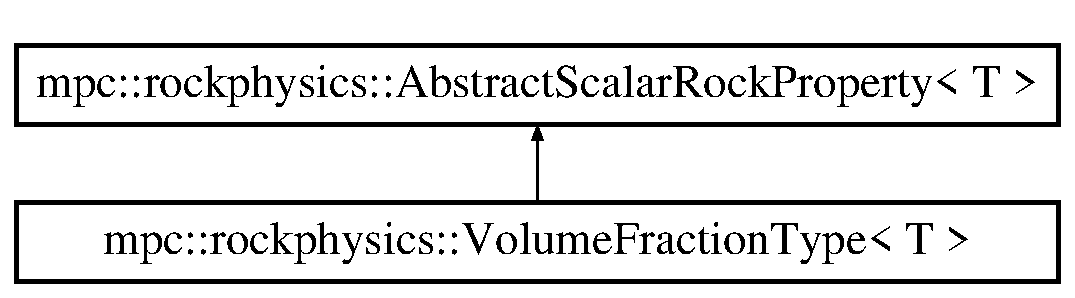
\includegraphics[height=2.000000cm]{structmpc_1_1rockphysics_1_1_volume_fraction_type}
\end{center}
\end{figure}
\subsection*{Public Member Functions}
\begin{DoxyCompactItemize}
\item 
constexpr \mbox{\hyperlink{structmpc_1_1rockphysics_1_1_volume_fraction_type_ad5e14aa452a7314daaa79c72d37c63a4}{Volume\+Fraction\+Type}} (T val)
\end{DoxyCompactItemize}
\subsection*{Additional Inherited Members}


\subsection{Detailed Description}
\subsubsection*{template$<$typename T$>$\newline
struct mpc\+::rockphysics\+::\+Volume\+Fraction\+Type$<$ T $>$}



Definition at line 206 of file rockphysicstransformstypes.\+hpp.



\subsection{Constructor \& Destructor Documentation}
\mbox{\Hypertarget{structmpc_1_1rockphysics_1_1_volume_fraction_type_ad5e14aa452a7314daaa79c72d37c63a4}\label{structmpc_1_1rockphysics_1_1_volume_fraction_type_ad5e14aa452a7314daaa79c72d37c63a4}} 
\index{mpc\+::rockphysics\+::\+Volume\+Fraction\+Type@{mpc\+::rockphysics\+::\+Volume\+Fraction\+Type}!Volume\+Fraction\+Type@{Volume\+Fraction\+Type}}
\index{Volume\+Fraction\+Type@{Volume\+Fraction\+Type}!mpc\+::rockphysics\+::\+Volume\+Fraction\+Type@{mpc\+::rockphysics\+::\+Volume\+Fraction\+Type}}
\subsubsection{\texorpdfstring{Volume\+Fraction\+Type()}{VolumeFractionType()}}
{\footnotesize\ttfamily template$<$typename T $>$ \\
constexpr \mbox{\hyperlink{structmpc_1_1rockphysics_1_1_volume_fraction_type}{mpc\+::rockphysics\+::\+Volume\+Fraction\+Type}}$<$ T $>$\+::\mbox{\hyperlink{structmpc_1_1rockphysics_1_1_volume_fraction_type}{Volume\+Fraction\+Type}} (\begin{DoxyParamCaption}\item[{T}]{val }\end{DoxyParamCaption})\hspace{0.3cm}{\ttfamily [inline]}}



Definition at line 213 of file rockphysicstransformstypes.\+hpp.



The documentation for this struct was generated from the following file\+:\begin{DoxyCompactItemize}
\item 
/\+Users/atorlucci/\+Documents/github\+\_\+threecubed\+\_\+repos/mpc/src/mpc/rockphysics/\mbox{\hyperlink{rockphysicstransformstypes_8hpp}{rockphysicstransformstypes.\+hpp}}\end{DoxyCompactItemize}

\hypertarget{structmpc_1_1rockphysics_1_1_volumetric_strain_type}{}\section{mpc\+:\+:rockphysics\+:\+:Volumetric\+Strain\+Type$<$ T $>$ Struct Template Reference}
\label{structmpc_1_1rockphysics_1_1_volumetric_strain_type}\index{mpc\+::rockphysics\+::\+Volumetric\+Strain\+Type$<$ T $>$@{mpc\+::rockphysics\+::\+Volumetric\+Strain\+Type$<$ T $>$}}


{\ttfamily \#include $<$rockphysicstransformstypes.\+hpp$>$}

Inheritance diagram for mpc\+:\+:rockphysics\+:\+:Volumetric\+Strain\+Type$<$ T $>$\+:\begin{figure}[H]
\begin{center}
\leavevmode
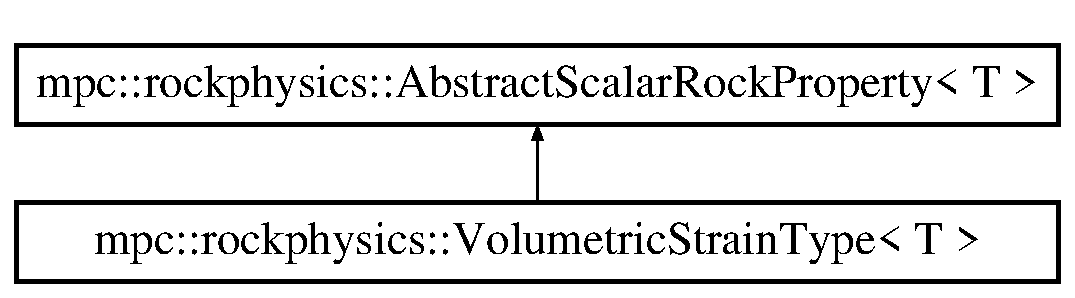
\includegraphics[height=2.000000cm]{structmpc_1_1rockphysics_1_1_volumetric_strain_type}
\end{center}
\end{figure}
\subsection*{Public Member Functions}
\begin{DoxyCompactItemize}
\item 
constexpr \mbox{\hyperlink{structmpc_1_1rockphysics_1_1_volumetric_strain_type_a08a9f46af054ba13d45c3d376e2995f6}{Volumetric\+Strain\+Type}} (T val)
\end{DoxyCompactItemize}
\subsection*{Additional Inherited Members}


\subsection{Detailed Description}
\subsubsection*{template$<$typename T$>$\newline
struct mpc\+::rockphysics\+::\+Volumetric\+Strain\+Type$<$ T $>$}



Definition at line 144 of file rockphysicstransformstypes.\+hpp.



\subsection{Constructor \& Destructor Documentation}
\mbox{\Hypertarget{structmpc_1_1rockphysics_1_1_volumetric_strain_type_a08a9f46af054ba13d45c3d376e2995f6}\label{structmpc_1_1rockphysics_1_1_volumetric_strain_type_a08a9f46af054ba13d45c3d376e2995f6}} 
\index{mpc\+::rockphysics\+::\+Volumetric\+Strain\+Type@{mpc\+::rockphysics\+::\+Volumetric\+Strain\+Type}!Volumetric\+Strain\+Type@{Volumetric\+Strain\+Type}}
\index{Volumetric\+Strain\+Type@{Volumetric\+Strain\+Type}!mpc\+::rockphysics\+::\+Volumetric\+Strain\+Type@{mpc\+::rockphysics\+::\+Volumetric\+Strain\+Type}}
\subsubsection{\texorpdfstring{Volumetric\+Strain\+Type()}{VolumetricStrainType()}}
{\footnotesize\ttfamily template$<$typename T$>$ \\
constexpr \mbox{\hyperlink{structmpc_1_1rockphysics_1_1_volumetric_strain_type}{mpc\+::rockphysics\+::\+Volumetric\+Strain\+Type}}$<$ T $>$\+::\mbox{\hyperlink{structmpc_1_1rockphysics_1_1_volumetric_strain_type}{Volumetric\+Strain\+Type}} (\begin{DoxyParamCaption}\item[{T}]{val }\end{DoxyParamCaption})\hspace{0.3cm}{\ttfamily [inline]}}



Definition at line 149 of file rockphysicstransformstypes.\+hpp.



The documentation for this struct was generated from the following file\+:\begin{DoxyCompactItemize}
\item 
/\+Users/atorlucci/\+Documents/github\+\_\+threecubed\+\_\+repos/mpc/src/mpc/rockphysics/\mbox{\hyperlink{rockphysicstransformstypes_8hpp}{rockphysicstransformstypes.\+hpp}}\end{DoxyCompactItemize}

\hypertarget{structmpc_1_1rockphysics_1_1_vp_vs_ratio_type}{}\section{mpc\+:\+:rockphysics\+:\+:Vp\+Vs\+Ratio\+Type$<$ T $>$ Struct Template Reference}
\label{structmpc_1_1rockphysics_1_1_vp_vs_ratio_type}\index{mpc\+::rockphysics\+::\+Vp\+Vs\+Ratio\+Type$<$ T $>$@{mpc\+::rockphysics\+::\+Vp\+Vs\+Ratio\+Type$<$ T $>$}}


{\ttfamily \#include $<$rockphysicstransformstypes.\+hpp$>$}

Inheritance diagram for mpc\+:\+:rockphysics\+:\+:Vp\+Vs\+Ratio\+Type$<$ T $>$\+:\begin{figure}[H]
\begin{center}
\leavevmode
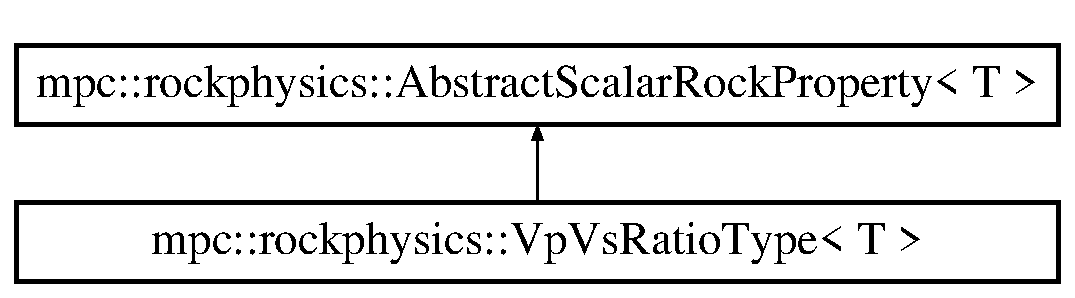
\includegraphics[height=2.000000cm]{structmpc_1_1rockphysics_1_1_vp_vs_ratio_type}
\end{center}
\end{figure}
\subsection*{Public Member Functions}
\begin{DoxyCompactItemize}
\item 
constexpr \mbox{\hyperlink{structmpc_1_1rockphysics_1_1_vp_vs_ratio_type_a49f2a30e9fb2fe88647393eab21f0b9a}{Vp\+Vs\+Ratio\+Type}} (T val)
\end{DoxyCompactItemize}
\subsection*{Additional Inherited Members}


\subsection{Detailed Description}
\subsubsection*{template$<$typename T$>$\newline
struct mpc\+::rockphysics\+::\+Vp\+Vs\+Ratio\+Type$<$ T $>$}



Definition at line 156 of file rockphysicstransformstypes.\+hpp.



\subsection{Constructor \& Destructor Documentation}
\mbox{\Hypertarget{structmpc_1_1rockphysics_1_1_vp_vs_ratio_type_a49f2a30e9fb2fe88647393eab21f0b9a}\label{structmpc_1_1rockphysics_1_1_vp_vs_ratio_type_a49f2a30e9fb2fe88647393eab21f0b9a}} 
\index{mpc\+::rockphysics\+::\+Vp\+Vs\+Ratio\+Type@{mpc\+::rockphysics\+::\+Vp\+Vs\+Ratio\+Type}!Vp\+Vs\+Ratio\+Type@{Vp\+Vs\+Ratio\+Type}}
\index{Vp\+Vs\+Ratio\+Type@{Vp\+Vs\+Ratio\+Type}!mpc\+::rockphysics\+::\+Vp\+Vs\+Ratio\+Type@{mpc\+::rockphysics\+::\+Vp\+Vs\+Ratio\+Type}}
\subsubsection{\texorpdfstring{Vp\+Vs\+Ratio\+Type()}{VpVsRatioType()}}
{\footnotesize\ttfamily template$<$typename T $>$ \\
constexpr \mbox{\hyperlink{structmpc_1_1rockphysics_1_1_vp_vs_ratio_type}{mpc\+::rockphysics\+::\+Vp\+Vs\+Ratio\+Type}}$<$ T $>$\+::\mbox{\hyperlink{structmpc_1_1rockphysics_1_1_vp_vs_ratio_type}{Vp\+Vs\+Ratio\+Type}} (\begin{DoxyParamCaption}\item[{T}]{val }\end{DoxyParamCaption})\hspace{0.3cm}{\ttfamily [inline]}}



Definition at line 161 of file rockphysicstransformstypes.\+hpp.



The documentation for this struct was generated from the following file\+:\begin{DoxyCompactItemize}
\item 
/\+Users/atorlucci/\+Documents/github\+\_\+threecubed\+\_\+repos/mpc/src/mpc/rockphysics/\mbox{\hyperlink{rockphysicstransformstypes_8hpp}{rockphysicstransformstypes.\+hpp}}\end{DoxyCompactItemize}

\hypertarget{structmpc_1_1rockphysics_1_1_vs_vp_ratio_type}{}\section{mpc\+:\+:rockphysics\+:\+:Vs\+Vp\+Ratio\+Type$<$ T $>$ Struct Template Reference}
\label{structmpc_1_1rockphysics_1_1_vs_vp_ratio_type}\index{mpc\+::rockphysics\+::\+Vs\+Vp\+Ratio\+Type$<$ T $>$@{mpc\+::rockphysics\+::\+Vs\+Vp\+Ratio\+Type$<$ T $>$}}


{\ttfamily \#include $<$rockphysicstransformstypes.\+hpp$>$}

Inheritance diagram for mpc\+:\+:rockphysics\+:\+:Vs\+Vp\+Ratio\+Type$<$ T $>$\+:\begin{figure}[H]
\begin{center}
\leavevmode
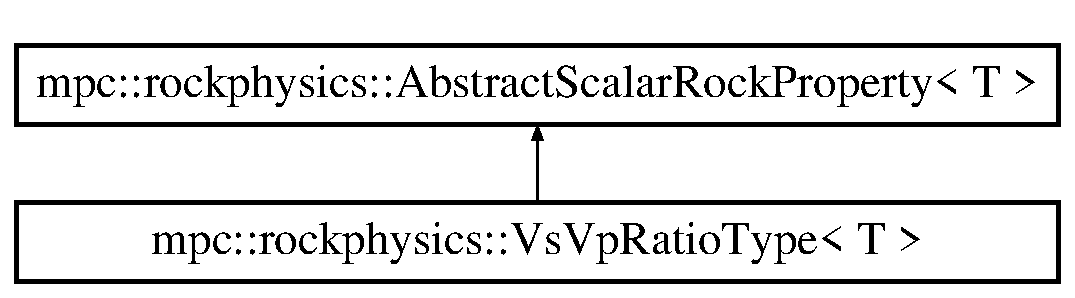
\includegraphics[height=2.000000cm]{structmpc_1_1rockphysics_1_1_vs_vp_ratio_type}
\end{center}
\end{figure}
\subsection*{Public Member Functions}
\begin{DoxyCompactItemize}
\item 
constexpr \mbox{\hyperlink{structmpc_1_1rockphysics_1_1_vs_vp_ratio_type_a13eb55ba2f7ceb92a365e41be636b9bb}{Vs\+Vp\+Ratio\+Type}} (T val)
\end{DoxyCompactItemize}
\subsection*{Additional Inherited Members}


\subsection{Detailed Description}
\subsubsection*{template$<$typename T$>$\newline
struct mpc\+::rockphysics\+::\+Vs\+Vp\+Ratio\+Type$<$ T $>$}



Definition at line 168 of file rockphysicstransformstypes.\+hpp.



\subsection{Constructor \& Destructor Documentation}
\mbox{\Hypertarget{structmpc_1_1rockphysics_1_1_vs_vp_ratio_type_a13eb55ba2f7ceb92a365e41be636b9bb}\label{structmpc_1_1rockphysics_1_1_vs_vp_ratio_type_a13eb55ba2f7ceb92a365e41be636b9bb}} 
\index{mpc\+::rockphysics\+::\+Vs\+Vp\+Ratio\+Type@{mpc\+::rockphysics\+::\+Vs\+Vp\+Ratio\+Type}!Vs\+Vp\+Ratio\+Type@{Vs\+Vp\+Ratio\+Type}}
\index{Vs\+Vp\+Ratio\+Type@{Vs\+Vp\+Ratio\+Type}!mpc\+::rockphysics\+::\+Vs\+Vp\+Ratio\+Type@{mpc\+::rockphysics\+::\+Vs\+Vp\+Ratio\+Type}}
\subsubsection{\texorpdfstring{Vs\+Vp\+Ratio\+Type()}{VsVpRatioType()}}
{\footnotesize\ttfamily template$<$typename T $>$ \\
constexpr \mbox{\hyperlink{structmpc_1_1rockphysics_1_1_vs_vp_ratio_type}{mpc\+::rockphysics\+::\+Vs\+Vp\+Ratio\+Type}}$<$ T $>$\+::\mbox{\hyperlink{structmpc_1_1rockphysics_1_1_vs_vp_ratio_type}{Vs\+Vp\+Ratio\+Type}} (\begin{DoxyParamCaption}\item[{T}]{val }\end{DoxyParamCaption})\hspace{0.3cm}{\ttfamily [inline]}}



Definition at line 173 of file rockphysicstransformstypes.\+hpp.



The documentation for this struct was generated from the following file\+:\begin{DoxyCompactItemize}
\item 
/\+Users/atorlucci/\+Documents/github\+\_\+threecubed\+\_\+repos/mpc/src/mpc/rockphysics/\mbox{\hyperlink{rockphysicstransformstypes_8hpp}{rockphysicstransformstypes.\+hpp}}\end{DoxyCompactItemize}

\hypertarget{structmpc_1_1utilities_1_1_weighted_arithmetic_average}{}\section{mpc\+:\+:utilities\+:\+:Weighted\+Arithmetic\+Average$<$ T, N $>$ Struct Template Reference}
\label{structmpc_1_1utilities_1_1_weighted_arithmetic_average}\index{mpc\+::utilities\+::\+Weighted\+Arithmetic\+Average$<$ T, N $>$@{mpc\+::utilities\+::\+Weighted\+Arithmetic\+Average$<$ T, N $>$}}


{\ttfamily \#include $<$arithmeticaverage.\+hpp$>$}

\subsection*{Public Member Functions}
\begin{DoxyCompactItemize}
\item 
blitz\+::\+Array$<$ T, N $>$ \mbox{\hyperlink{structmpc_1_1utilities_1_1_weighted_arithmetic_average_abbb9a8717b9feb14086f7ef170b70584}{operator()}} (std\+::vector$<$ blitz\+::\+Array$<$ T, N $>$ $>$ \&values, std\+::vector$<$ T $>$ \&weights)
\end{DoxyCompactItemize}


\subsection{Detailed Description}
\subsubsection*{template$<$typename T, int N$>$\newline
struct mpc\+::utilities\+::\+Weighted\+Arithmetic\+Average$<$ T, N $>$}



Definition at line 30 of file arithmeticaverage.\+hpp.



\subsection{Member Function Documentation}
\mbox{\Hypertarget{structmpc_1_1utilities_1_1_weighted_arithmetic_average_abbb9a8717b9feb14086f7ef170b70584}\label{structmpc_1_1utilities_1_1_weighted_arithmetic_average_abbb9a8717b9feb14086f7ef170b70584}} 
\index{mpc\+::utilities\+::\+Weighted\+Arithmetic\+Average@{mpc\+::utilities\+::\+Weighted\+Arithmetic\+Average}!operator()@{operator()}}
\index{operator()@{operator()}!mpc\+::utilities\+::\+Weighted\+Arithmetic\+Average@{mpc\+::utilities\+::\+Weighted\+Arithmetic\+Average}}
\subsubsection{\texorpdfstring{operator()()}{operator()()}}
{\footnotesize\ttfamily template$<$typename T , int N$>$ \\
blitz\+::\+Array$<$T,N$>$ \mbox{\hyperlink{structmpc_1_1utilities_1_1_weighted_arithmetic_average}{mpc\+::utilities\+::\+Weighted\+Arithmetic\+Average}}$<$ T, N $>$\+::operator() (\begin{DoxyParamCaption}\item[{std\+::vector$<$ blitz\+::\+Array$<$ T, N $>$ $>$ \&}]{values,  }\item[{std\+::vector$<$ T $>$ \&}]{weights }\end{DoxyParamCaption})\hspace{0.3cm}{\ttfamily [inline]}}



Definition at line 32 of file arithmeticaverage.\+hpp.



The documentation for this struct was generated from the following file\+:\begin{DoxyCompactItemize}
\item 
/\+Users/atorlucci/\+Documents/github\+\_\+threecubed\+\_\+repos/mpc/src/mpc/utilities/\mbox{\hyperlink{arithmeticaverage_8hpp}{arithmeticaverage.\+hpp}}\end{DoxyCompactItemize}

\hypertarget{structmpc_1_1utilities_1_1_weighted_arithmetic_average_3_01_t_00_010_01_4}{}\section{mpc\+:\+:utilities\+:\+:Weighted\+Arithmetic\+Average$<$ T, 0 $>$ Struct Template Reference}
\label{structmpc_1_1utilities_1_1_weighted_arithmetic_average_3_01_t_00_010_01_4}\index{mpc\+::utilities\+::\+Weighted\+Arithmetic\+Average$<$ T, 0 $>$@{mpc\+::utilities\+::\+Weighted\+Arithmetic\+Average$<$ T, 0 $>$}}


{\ttfamily \#include $<$arithmeticaverage.\+hpp$>$}

\subsection*{Public Member Functions}
\begin{DoxyCompactItemize}
\item 
T \mbox{\hyperlink{structmpc_1_1utilities_1_1_weighted_arithmetic_average_3_01_t_00_010_01_4_ad93403c9fee56e45c8dbf2959d8f6ab3}{operator()}} (std\+::vector$<$ T $>$ \&values, std\+::vector$<$ T $>$ \&weights)
\end{DoxyCompactItemize}


\subsection{Detailed Description}
\subsubsection*{template$<$typename T$>$\newline
struct mpc\+::utilities\+::\+Weighted\+Arithmetic\+Average$<$ T, 0 $>$}



Definition at line 46 of file arithmeticaverage.\+hpp.



\subsection{Member Function Documentation}
\mbox{\Hypertarget{structmpc_1_1utilities_1_1_weighted_arithmetic_average_3_01_t_00_010_01_4_ad93403c9fee56e45c8dbf2959d8f6ab3}\label{structmpc_1_1utilities_1_1_weighted_arithmetic_average_3_01_t_00_010_01_4_ad93403c9fee56e45c8dbf2959d8f6ab3}} 
\index{mpc\+::utilities\+::\+Weighted\+Arithmetic\+Average$<$ T, 0 $>$@{mpc\+::utilities\+::\+Weighted\+Arithmetic\+Average$<$ T, 0 $>$}!operator()@{operator()}}
\index{operator()@{operator()}!mpc\+::utilities\+::\+Weighted\+Arithmetic\+Average$<$ T, 0 $>$@{mpc\+::utilities\+::\+Weighted\+Arithmetic\+Average$<$ T, 0 $>$}}
\subsubsection{\texorpdfstring{operator()()}{operator()()}}
{\footnotesize\ttfamily template$<$typename T $>$ \\
T \mbox{\hyperlink{structmpc_1_1utilities_1_1_weighted_arithmetic_average}{mpc\+::utilities\+::\+Weighted\+Arithmetic\+Average}}$<$ T, 0 $>$\+::operator() (\begin{DoxyParamCaption}\item[{std\+::vector$<$ T $>$ \&}]{values,  }\item[{std\+::vector$<$ T $>$ \&}]{weights }\end{DoxyParamCaption})\hspace{0.3cm}{\ttfamily [inline]}}



Definition at line 48 of file arithmeticaverage.\+hpp.



The documentation for this struct was generated from the following file\+:\begin{DoxyCompactItemize}
\item 
/\+Users/atorlucci/\+Documents/github\+\_\+threecubed\+\_\+repos/mpc/src/mpc/utilities/\mbox{\hyperlink{arithmeticaverage_8hpp}{arithmeticaverage.\+hpp}}\end{DoxyCompactItemize}

\hypertarget{structmpc_1_1utilities_1_1_weighted_harmonic_average}{}\section{mpc\+:\+:utilities\+:\+:Weighted\+Harmonic\+Average$<$ T, N $>$ Struct Template Reference}
\label{structmpc_1_1utilities_1_1_weighted_harmonic_average}\index{mpc\+::utilities\+::\+Weighted\+Harmonic\+Average$<$ T, N $>$@{mpc\+::utilities\+::\+Weighted\+Harmonic\+Average$<$ T, N $>$}}


{\ttfamily \#include $<$harmonicaverage.\+hpp$>$}

\subsection*{Public Member Functions}
\begin{DoxyCompactItemize}
\item 
blitz\+::\+Array$<$ T, N $>$ \mbox{\hyperlink{structmpc_1_1utilities_1_1_weighted_harmonic_average_a6129b4ae0befbf7eedac628c1c1eecfc}{operator()}} (std\+::vector$<$ blitz\+::\+Array$<$ T, N $>$ $>$ \&values, std\+::vector$<$ T $>$ \&weights)
\end{DoxyCompactItemize}


\subsection{Detailed Description}
\subsubsection*{template$<$typename T, int N$>$\newline
struct mpc\+::utilities\+::\+Weighted\+Harmonic\+Average$<$ T, N $>$}



Definition at line 26 of file harmonicaverage.\+hpp.



\subsection{Member Function Documentation}
\mbox{\Hypertarget{structmpc_1_1utilities_1_1_weighted_harmonic_average_a6129b4ae0befbf7eedac628c1c1eecfc}\label{structmpc_1_1utilities_1_1_weighted_harmonic_average_a6129b4ae0befbf7eedac628c1c1eecfc}} 
\index{mpc\+::utilities\+::\+Weighted\+Harmonic\+Average@{mpc\+::utilities\+::\+Weighted\+Harmonic\+Average}!operator()@{operator()}}
\index{operator()@{operator()}!mpc\+::utilities\+::\+Weighted\+Harmonic\+Average@{mpc\+::utilities\+::\+Weighted\+Harmonic\+Average}}
\subsubsection{\texorpdfstring{operator()()}{operator()()}}
{\footnotesize\ttfamily template$<$typename T , int N$>$ \\
blitz\+::\+Array$<$T,N$>$ \mbox{\hyperlink{structmpc_1_1utilities_1_1_weighted_harmonic_average}{mpc\+::utilities\+::\+Weighted\+Harmonic\+Average}}$<$ T, N $>$\+::operator() (\begin{DoxyParamCaption}\item[{std\+::vector$<$ blitz\+::\+Array$<$ T, N $>$ $>$ \&}]{values,  }\item[{std\+::vector$<$ T $>$ \&}]{weights }\end{DoxyParamCaption})\hspace{0.3cm}{\ttfamily [inline]}}



Definition at line 28 of file harmonicaverage.\+hpp.



The documentation for this struct was generated from the following file\+:\begin{DoxyCompactItemize}
\item 
/\+Users/atorlucci/\+Documents/github\+\_\+threecubed\+\_\+repos/mpc/src/mpc/utilities/\mbox{\hyperlink{harmonicaverage_8hpp}{harmonicaverage.\+hpp}}\end{DoxyCompactItemize}

\hypertarget{structmpc_1_1utilities_1_1_weighted_harmonic_average_3_01_t_00_010_01_4}{}\section{mpc\+:\+:utilities\+:\+:Weighted\+Harmonic\+Average$<$ T, 0 $>$ Struct Template Reference}
\label{structmpc_1_1utilities_1_1_weighted_harmonic_average_3_01_t_00_010_01_4}\index{mpc\+::utilities\+::\+Weighted\+Harmonic\+Average$<$ T, 0 $>$@{mpc\+::utilities\+::\+Weighted\+Harmonic\+Average$<$ T, 0 $>$}}


{\ttfamily \#include $<$harmonicaverage.\+hpp$>$}

\subsection*{Public Member Functions}
\begin{DoxyCompactItemize}
\item 
T \mbox{\hyperlink{structmpc_1_1utilities_1_1_weighted_harmonic_average_3_01_t_00_010_01_4_a71276b6d5962cf7ae4db1d5088d8cc4e}{operator()}} (std\+::vector$<$ T $>$ \&values, std\+::vector$<$ T $>$ \&weights)
\end{DoxyCompactItemize}


\subsection{Detailed Description}
\subsubsection*{template$<$typename T$>$\newline
struct mpc\+::utilities\+::\+Weighted\+Harmonic\+Average$<$ T, 0 $>$}



Definition at line 43 of file harmonicaverage.\+hpp.



\subsection{Member Function Documentation}
\mbox{\Hypertarget{structmpc_1_1utilities_1_1_weighted_harmonic_average_3_01_t_00_010_01_4_a71276b6d5962cf7ae4db1d5088d8cc4e}\label{structmpc_1_1utilities_1_1_weighted_harmonic_average_3_01_t_00_010_01_4_a71276b6d5962cf7ae4db1d5088d8cc4e}} 
\index{mpc\+::utilities\+::\+Weighted\+Harmonic\+Average$<$ T, 0 $>$@{mpc\+::utilities\+::\+Weighted\+Harmonic\+Average$<$ T, 0 $>$}!operator()@{operator()}}
\index{operator()@{operator()}!mpc\+::utilities\+::\+Weighted\+Harmonic\+Average$<$ T, 0 $>$@{mpc\+::utilities\+::\+Weighted\+Harmonic\+Average$<$ T, 0 $>$}}
\subsubsection{\texorpdfstring{operator()()}{operator()()}}
{\footnotesize\ttfamily template$<$typename T $>$ \\
T \mbox{\hyperlink{structmpc_1_1utilities_1_1_weighted_harmonic_average}{mpc\+::utilities\+::\+Weighted\+Harmonic\+Average}}$<$ T, 0 $>$\+::operator() (\begin{DoxyParamCaption}\item[{std\+::vector$<$ T $>$ \&}]{values,  }\item[{std\+::vector$<$ T $>$ \&}]{weights }\end{DoxyParamCaption})\hspace{0.3cm}{\ttfamily [inline]}}



Definition at line 45 of file harmonicaverage.\+hpp.



The documentation for this struct was generated from the following file\+:\begin{DoxyCompactItemize}
\item 
/\+Users/atorlucci/\+Documents/github\+\_\+threecubed\+\_\+repos/mpc/src/mpc/utilities/\mbox{\hyperlink{harmonicaverage_8hpp}{harmonicaverage.\+hpp}}\end{DoxyCompactItemize}

\hypertarget{structmpc_1_1rockphysics_1_1_youngs_modulus_type}{}\section{mpc\+:\+:rockphysics\+:\+:Youngs\+Modulus\+Type$<$ T $>$ Struct Template Reference}
\label{structmpc_1_1rockphysics_1_1_youngs_modulus_type}\index{mpc\+::rockphysics\+::\+Youngs\+Modulus\+Type$<$ T $>$@{mpc\+::rockphysics\+::\+Youngs\+Modulus\+Type$<$ T $>$}}


{\ttfamily \#include $<$rockphysicstransformstypes.\+hpp$>$}

Inheritance diagram for mpc\+:\+:rockphysics\+:\+:Youngs\+Modulus\+Type$<$ T $>$\+:\begin{figure}[H]
\begin{center}
\leavevmode
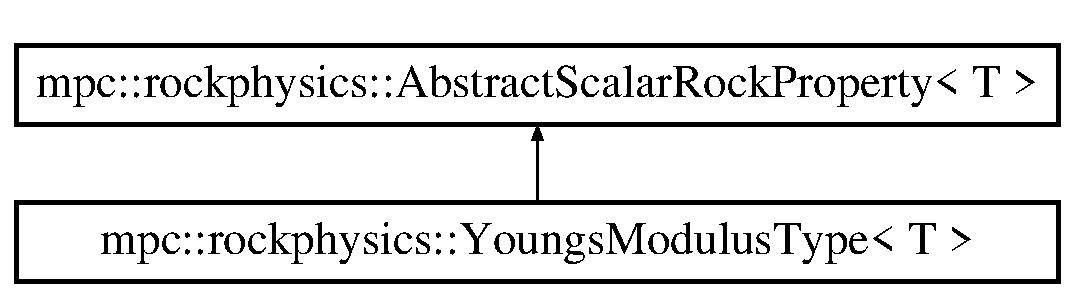
\includegraphics[height=2.000000cm]{structmpc_1_1rockphysics_1_1_youngs_modulus_type}
\end{center}
\end{figure}
\subsection*{Public Member Functions}
\begin{DoxyCompactItemize}
\item 
constexpr \mbox{\hyperlink{structmpc_1_1rockphysics_1_1_youngs_modulus_type_aa7eea6b3c1ef9af10982c210c56f7582}{Youngs\+Modulus\+Type}} (T val)
\end{DoxyCompactItemize}
\subsection*{Additional Inherited Members}


\subsection{Detailed Description}
\subsubsection*{template$<$typename T$>$\newline
struct mpc\+::rockphysics\+::\+Youngs\+Modulus\+Type$<$ T $>$}



Definition at line 57 of file rockphysicstransformstypes.\+hpp.



\subsection{Constructor \& Destructor Documentation}
\mbox{\Hypertarget{structmpc_1_1rockphysics_1_1_youngs_modulus_type_aa7eea6b3c1ef9af10982c210c56f7582}\label{structmpc_1_1rockphysics_1_1_youngs_modulus_type_aa7eea6b3c1ef9af10982c210c56f7582}} 
\index{mpc\+::rockphysics\+::\+Youngs\+Modulus\+Type@{mpc\+::rockphysics\+::\+Youngs\+Modulus\+Type}!Youngs\+Modulus\+Type@{Youngs\+Modulus\+Type}}
\index{Youngs\+Modulus\+Type@{Youngs\+Modulus\+Type}!mpc\+::rockphysics\+::\+Youngs\+Modulus\+Type@{mpc\+::rockphysics\+::\+Youngs\+Modulus\+Type}}
\subsubsection{\texorpdfstring{Youngs\+Modulus\+Type()}{YoungsModulusType()}}
{\footnotesize\ttfamily template$<$typename T$>$ \\
constexpr \mbox{\hyperlink{structmpc_1_1rockphysics_1_1_youngs_modulus_type}{mpc\+::rockphysics\+::\+Youngs\+Modulus\+Type}}$<$ T $>$\+::\mbox{\hyperlink{structmpc_1_1rockphysics_1_1_youngs_modulus_type}{Youngs\+Modulus\+Type}} (\begin{DoxyParamCaption}\item[{T}]{val }\end{DoxyParamCaption})\hspace{0.3cm}{\ttfamily [inline]}}



Definition at line 62 of file rockphysicstransformstypes.\+hpp.



The documentation for this struct was generated from the following file\+:\begin{DoxyCompactItemize}
\item 
/\+Users/atorlucci/\+Documents/github\+\_\+threecubed\+\_\+repos/mpc/src/mpc/rockphysics/\mbox{\hyperlink{rockphysicstransformstypes_8hpp}{rockphysicstransformstypes.\+hpp}}\end{DoxyCompactItemize}

\chapter{File Documentation}
\hypertarget{csrelationship_8hpp}{}\section{/\+Users/atorlucci/\+Documents/github\+\_\+threecubed\+\_\+repos/mpc/src/mpc/core/csrelationship.hpp File Reference}
\label{csrelationship_8hpp}\index{/\+Users/atorlucci/\+Documents/github\+\_\+threecubed\+\_\+repos/mpc/src/mpc/core/csrelationship.\+hpp@{/\+Users/atorlucci/\+Documents/github\+\_\+threecubed\+\_\+repos/mpc/src/mpc/core/csrelationship.\+hpp}}


functions and function objects to calculate the stiffness tensor components from the compliance tensor components or vice versa  


{\ttfamily \#include $<$iostream$>$}\newline
{\ttfamily \#include $<$blitz/array.\+h$>$}\newline
{\ttfamily \#include $<$Eigen/\+Dense$>$}\newline
{\ttfamily \#include $<$Eigen/\+QR$>$}\newline
{\ttfamily \#include \char`\"{}mpc/core/cstypes.\+hpp\char`\"{}}\newline
{\ttfamily \#include \char`\"{}mpc/core/symmetrygrouptypes.\+hpp\char`\"{}}\newline
{\ttfamily \#include \char`\"{}mpc/core/stiffnesscompliance.\+hpp\char`\"{}}\newline
{\ttfamily \#include \char`\"{}mpc/utilities/matrixnotation.\+hpp\char`\"{}}\newline
\subsection*{Classes}
\begin{DoxyCompactItemize}
\item 
class \mbox{\hyperlink{structmpc_1_1core_1_1_stiffness_from_compliance_function_object}{mpc\+::core\+::\+Stiffness\+From\+Compliance\+Function\+Object$<$ T, S $>$}}
\begin{DoxyCompactList}\small\item\em function object for calculating the stiffness tensor components from the compliance tensor components \end{DoxyCompactList}\item 
class \mbox{\hyperlink{structmpc_1_1core_1_1_compliance_from_stiffness_function_object}{mpc\+::core\+::\+Compliance\+From\+Stiffness\+Function\+Object$<$ T, S $>$}}
\begin{DoxyCompactList}\small\item\em function object for calculating the compliance tensor components from the stiffness tensor components \end{DoxyCompactList}\item 
struct \mbox{\hyperlink{structmpc_1_1core_1_1_compliance_from_stiffness_function_object_3_01_t_00_01mpc_1_1core_1_1_triclinic_symmetry_group_type_01_4}{mpc\+::core\+::\+Compliance\+From\+Stiffness\+Function\+Object$<$ T, mpc\+::core\+::\+Triclinic\+Symmetry\+Group\+Type $>$}}
\end{DoxyCompactItemize}
\subsection*{Namespaces}
\begin{DoxyCompactItemize}
\item 
 \mbox{\hyperlink{namespacempc}{mpc}}
\item 
 \mbox{\hyperlink{namespacempc_1_1core}{mpc\+::core}}
\end{DoxyCompactItemize}
\subsection*{Functions}
\begin{DoxyCompactItemize}
\item 
{\footnotesize template$<$typename S , typename T $>$ }\\\mbox{\hyperlink{structmpc_1_1core_1_1_compliance_tensor}{mpc\+::core\+::\+Compliance\+Tensor}}$<$ T $>$ \mbox{\hyperlink{namespacempc_1_1core_aa7722f016512fa5a038350eb89fce451}{mpc\+::core\+::\+C\+S\+Relationship}} (\mbox{\hyperlink{structmpc_1_1core_1_1_stiffness_tensor}{mpc\+::core\+::\+Stiffness\+Tensor}}$<$ T $>$ \&c\+\_\+ijkl)
\begin{DoxyCompactList}\small\item\em polymorphic convenience function to generate the compliance tensor object from a stiffness tensor object \end{DoxyCompactList}\item 
{\footnotesize template$<$typename S , typename T $>$ }\\\mbox{\hyperlink{structmpc_1_1core_1_1_stiffness_tensor}{mpc\+::core\+::\+Stiffness\+Tensor}}$<$ T $>$ \mbox{\hyperlink{namespacempc_1_1core_aea25821c5c4e736c92d4ede4d7f3241d}{mpc\+::core\+::\+C\+S\+Relationship}} (\mbox{\hyperlink{structmpc_1_1core_1_1_compliance_tensor}{mpc\+::core\+::\+Compliance\+Tensor}}$<$ T $>$ \&s\+\_\+ijkl)
\begin{DoxyCompactList}\small\item\em polymorphic convenience function to generate the stiffness tensor object from a compliance tensor object \end{DoxyCompactList}\end{DoxyCompactItemize}


\subsection{Detailed Description}
functions and function objects to calculate the stiffness tensor components from the compliance tensor components or vice versa 

\begin{DoxyAuthor}{Author}
Anthony Torlucci 
\end{DoxyAuthor}
\begin{DoxyDate}{Date}
2018/10/14 
\end{DoxyDate}

\hypertarget{cstypes_8hpp}{}\section{/\+Users/atorlucci/\+Documents/github\+\_\+threecubed\+\_\+repos/mpc/src/mpc/core/cstypes.hpp File Reference}
\label{cstypes_8hpp}\index{/\+Users/atorlucci/\+Documents/github\+\_\+threecubed\+\_\+repos/mpc/src/mpc/core/cstypes.\+hpp@{/\+Users/atorlucci/\+Documents/github\+\_\+threecubed\+\_\+repos/mpc/src/mpc/core/cstypes.\+hpp}}


stiffness and compliance sructs used as types for template specializations  


{\ttfamily \#include $<$iostream$>$}\newline
{\ttfamily \#include $<$blitz/array.\+h$>$}\newline
\subsection*{Classes}
\begin{DoxyCompactItemize}
\item 
class \mbox{\hyperlink{structmpc_1_1core_1_1_c_s_enumeration_interface}{mpc\+::core\+::\+C\+S\+Enumeration\+Interface}}
\begin{DoxyCompactList}\small\item\em interface to convert enum to std\+::string \end{DoxyCompactList}\item 
class \mbox{\hyperlink{structmpc_1_1core_1_1_c_s_base}{mpc\+::core\+::\+C\+S\+Base}}
\begin{DoxyCompactList}\small\item\em base class for stiffness compliance types \end{DoxyCompactList}\item 
class \mbox{\hyperlink{structmpc_1_1core_1_1_stiffness_type}{mpc\+::core\+::\+Stiffness\+Type}}
\begin{DoxyCompactList}\small\item\em simple class used mainly for template specializations in mpc \end{DoxyCompactList}\item 
class \mbox{\hyperlink{structmpc_1_1core_1_1_compliance_type}{mpc\+::core\+::\+Compliance\+Type}}
\begin{DoxyCompactList}\small\item\em simple class used mainly for template specializations in mpc \end{DoxyCompactList}\end{DoxyCompactItemize}
\subsection*{Namespaces}
\begin{DoxyCompactItemize}
\item 
 \mbox{\hyperlink{namespacempc}{mpc}}
\item 
 \mbox{\hyperlink{namespacempc_1_1core}{mpc\+::core}}
\end{DoxyCompactItemize}
\subsection*{Typedefs}
\begin{DoxyCompactItemize}
\item 
typedef std\+::integral\+\_\+constant$<$ C\+S\+Enumeration, C\+S\+Enumeration\+::\+S\+T\+I\+F\+F\+N\+E\+SS $>$ \mbox{\hyperlink{namespacempc_1_1core_a120bef8b8e9eb17c3455661c0f51950a}{mpc\+::core\+::cs\+\_\+stiffness\+\_\+t}}
\item 
typedef std\+::integral\+\_\+constant$<$ C\+S\+Enumeration, C\+S\+Enumeration\+::\+C\+O\+M\+P\+L\+I\+A\+N\+CE $>$ \mbox{\hyperlink{namespacempc_1_1core_a33e8b8a9ae039df62c62872553ca7161}{mpc\+::core\+::cs\+\_\+compliance\+\_\+t}}
\end{DoxyCompactItemize}
\subsection*{Enumerations}
\begin{DoxyCompactItemize}
\item 
enum \mbox{\hyperlink{namespacempc_1_1core_ad3e8e7d43bfc9202d954d999f7d5c991}{mpc\+::core\+::\+C\+S\+Enumeration}} \{ \mbox{\hyperlink{namespacempc_1_1core_ad3e8e7d43bfc9202d954d999f7d5c991aa231c1d74fe18f9e82224588887d1971}{mpc\+::core\+::\+C\+S\+Enumeration\+::\+S\+T\+I\+F\+F\+N\+E\+SS}}, 
\mbox{\hyperlink{namespacempc_1_1core_ad3e8e7d43bfc9202d954d999f7d5c991a185bd2ffef1962ade3c0889c62cee500}{mpc\+::core\+::\+C\+S\+Enumeration\+::\+C\+O\+M\+P\+L\+I\+A\+N\+CE}}
 \}
\begin{DoxyCompactList}\small\item\em stiffness compliance types enumeration \end{DoxyCompactList}\end{DoxyCompactItemize}
\subsection*{Functions}
\begin{DoxyCompactItemize}
\item 
std\+::ostream \& \mbox{\hyperlink{namespacempc_1_1core_a742f3f5b4c1f5b579247c0937bdb6015}{mpc\+::core\+::operator$<$$<$}} (std\+::ostream \&os, C\+S\+Enumeration cs\+\_\+enum)
\end{DoxyCompactItemize}


\subsection{Detailed Description}
stiffness and compliance sructs used as types for template specializations 

\begin{DoxyAuthor}{Author}
Anthony Torlucci 
\end{DoxyAuthor}
\begin{DoxyDate}{Date}
2018/10/14 
\end{DoxyDate}

\hypertarget{core_2_r_e_a_d_m_e_8md}{}\section{/\+Users/atorlucci/\+Documents/github\+\_\+threecubed\+\_\+repos/mpc/src/mpc/core/\+R\+E\+A\+D\+ME.md File Reference}
\label{core_2_r_e_a_d_m_e_8md}\index{/\+Users/atorlucci/\+Documents/github\+\_\+threecubed\+\_\+repos/mpc/src/mpc/core/\+R\+E\+A\+D\+M\+E.\+md@{/\+Users/atorlucci/\+Documents/github\+\_\+threecubed\+\_\+repos/mpc/src/mpc/core/\+R\+E\+A\+D\+M\+E.\+md}}

\hypertarget{_r_e_a_d_m_e_8md}{}\section{/\+Users/atorlucci/\+Documents/github\+\_\+threecubed\+\_\+repos/mpc/src/mpc/\+R\+E\+A\+D\+ME.md File Reference}
\label{_r_e_a_d_m_e_8md}\index{/\+Users/atorlucci/\+Documents/github\+\_\+threecubed\+\_\+repos/mpc/src/mpc/\+R\+E\+A\+D\+M\+E.\+md@{/\+Users/atorlucci/\+Documents/github\+\_\+threecubed\+\_\+repos/mpc/src/mpc/\+R\+E\+A\+D\+M\+E.\+md}}

\hypertarget{stiffnesscompliance_8hpp}{}\section{/\+Users/atorlucci/\+Documents/github\+\_\+threecubed\+\_\+repos/mpc/src/mpc/core/stiffnesscompliance.hpp File Reference}
\label{stiffnesscompliance_8hpp}\index{/\+Users/atorlucci/\+Documents/github\+\_\+threecubed\+\_\+repos/mpc/src/mpc/core/stiffnesscompliance.\+hpp@{/\+Users/atorlucci/\+Documents/github\+\_\+threecubed\+\_\+repos/mpc/src/mpc/core/stiffnesscompliance.\+hpp}}


stiffness and compliance tensor classes; part of the core data structures  


{\ttfamily \#include $<$iostream$>$}\newline
{\ttfamily \#include $<$set$>$}\newline
{\ttfamily \#include $<$blitz/array.\+h$>$}\newline
{\ttfamily \#include \char`\"{}mpc/core/symmetrygrouptypes.\+hpp\char`\"{}}\newline
{\ttfamily \#include \char`\"{}mpc/core/cstypes.\+hpp\char`\"{}}\newline
{\ttfamily \#include \char`\"{}mpc/core/tensorcomponent.\+hpp\char`\"{}}\newline
{\ttfamily \#include \char`\"{}mpc/core/symmetrycomponents.\+hpp\char`\"{}}\newline
{\ttfamily \#include \char`\"{}mpc/utilities/matrixnotation.\+hpp\char`\"{}}\newline
\subsection*{Classes}
\begin{DoxyCompactItemize}
\item 
class \mbox{\hyperlink{structmpc_1_1core_1_1_tensor_rank4_interface}{mpc\+::core\+::\+Tensor\+Rank4\+Interface$<$ T $>$}}
\begin{DoxyCompactList}\small\item\em simple interface for tensors of rank 4 \end{DoxyCompactList}\item 
class \mbox{\hyperlink{structmpc_1_1core_1_1_tensor_rank4_base}{mpc\+::core\+::\+Tensor\+Rank4\+Base$<$ T $>$}}
\begin{DoxyCompactList}\small\item\em base class for tensors of rank 4 \end{DoxyCompactList}\item 
class \mbox{\hyperlink{structmpc_1_1core_1_1_stiffness_tensor}{mpc\+::core\+::\+Stiffness\+Tensor$<$ T $>$}}
\begin{DoxyCompactList}\small\item\em stiffness tensor class with function to set the components with a given symmety type \end{DoxyCompactList}\item 
class \mbox{\hyperlink{structmpc_1_1core_1_1_compliance_tensor}{mpc\+::core\+::\+Compliance\+Tensor$<$ T $>$}}
\begin{DoxyCompactList}\small\item\em compliance tensor class with function to set the components with a given symmety type \end{DoxyCompactList}\end{DoxyCompactItemize}
\subsection*{Namespaces}
\begin{DoxyCompactItemize}
\item 
 \mbox{\hyperlink{namespacempc}{mpc}}
\item 
 \mbox{\hyperlink{namespacempc_1_1core}{mpc\+::core}}
\end{DoxyCompactItemize}


\subsection{Detailed Description}
stiffness and compliance tensor classes; part of the core data structures 

\begin{DoxyAuthor}{Author}
Anthony Torlucci 
\end{DoxyAuthor}
\begin{DoxyDate}{Date}
2018/10/14 
\end{DoxyDate}

\hypertarget{stressstrain_8hpp}{}\section{/\+Users/atorlucci/\+Documents/github\+\_\+threecubed\+\_\+repos/mpc/src/mpc/core/stressstrain.hpp File Reference}
\label{stressstrain_8hpp}\index{/\+Users/atorlucci/\+Documents/github\+\_\+threecubed\+\_\+repos/mpc/src/mpc/core/stressstrain.\+hpp@{/\+Users/atorlucci/\+Documents/github\+\_\+threecubed\+\_\+repos/mpc/src/mpc/core/stressstrain.\+hpp}}


stress and strain tensor classes; part of the core data structures  


{\ttfamily \#include $<$cassert$>$}\newline
{\ttfamily \#include $<$set$>$}\newline
{\ttfamily \#include $<$blitz/array.\+h$>$}\newline
{\ttfamily \#include \char`\"{}tensorcomponentindex.\+hpp\char`\"{}}\newline
{\ttfamily \#include \char`\"{}tensorcomponent.\+hpp\char`\"{}}\newline
{\ttfamily \#include \char`\"{}tensorcomponentindexaliases.\+hpp\char`\"{}}\newline
\subsection*{Classes}
\begin{DoxyCompactItemize}
\item 
class \mbox{\hyperlink{structmpc_1_1core_1_1_tensor_rank2_interface}{mpc\+::core\+::\+Tensor\+Rank2\+Interface$<$ T $>$}}
\begin{DoxyCompactList}\small\item\em simple interface class for tensors of rank 2 \end{DoxyCompactList}\item 
class \mbox{\hyperlink{structmpc_1_1core_1_1_tensor_rank2_base}{mpc\+::core\+::\+Tensor\+Rank2\+Base$<$ T $>$}}
\begin{DoxyCompactList}\small\item\em simple base class for tensors of rank 2 \end{DoxyCompactList}\item 
class \mbox{\hyperlink{structmpc_1_1core_1_1_stress_tensor}{mpc\+::core\+::\+Stress\+Tensor$<$ T $>$}}
\begin{DoxyCompactList}\small\item\em stress tensor class with function to set the components \end{DoxyCompactList}\item 
class \mbox{\hyperlink{structmpc_1_1core_1_1_strain_tensor}{mpc\+::core\+::\+Strain\+Tensor$<$ T $>$}}
\begin{DoxyCompactList}\small\item\em strain tensor class with function to set the components \end{DoxyCompactList}\end{DoxyCompactItemize}
\subsection*{Namespaces}
\begin{DoxyCompactItemize}
\item 
 \mbox{\hyperlink{namespacempc}{mpc}}
\item 
 \mbox{\hyperlink{namespacempc_1_1core}{mpc\+::core}}
\end{DoxyCompactItemize}


\subsection{Detailed Description}
stress and strain tensor classes; part of the core data structures 

\begin{DoxyAuthor}{Author}
Anthony Torlucci 
\end{DoxyAuthor}
\begin{DoxyDate}{Date}
2018/10/14 
\end{DoxyDate}

\hypertarget{symmetrycomponents_8hpp}{}\section{/\+Users/atorlucci/\+Documents/github\+\_\+threecubed\+\_\+repos/mpc/src/mpc/core/symmetrycomponents.hpp File Reference}
\label{symmetrycomponents_8hpp}\index{/\+Users/atorlucci/\+Documents/github\+\_\+threecubed\+\_\+repos/mpc/src/mpc/core/symmetrycomponents.\+hpp@{/\+Users/atorlucci/\+Documents/github\+\_\+threecubed\+\_\+repos/mpc/src/mpc/core/symmetrycomponents.\+hpp}}


functions and function objects for extracting components of the stiffness or compliance tensor that are related in matrix notation form  


{\ttfamily \#include $<$set$>$}\newline
{\ttfamily \#include $<$tuple$>$}\newline
{\ttfamily \#include $<$utility$>$}\newline
{\ttfamily \#include $<$functional$>$}\newline
{\ttfamily \#include $<$iostream$>$}\newline
{\ttfamily \#include $<$iterator$>$}\newline
{\ttfamily \#include $<$algorithm$>$}\newline
{\ttfamily \#include $<$cassert$>$}\newline
{\ttfamily \#include \char`\"{}mpc/core/tensorcomponent.\+hpp\char`\"{}}\newline
{\ttfamily \#include \char`\"{}mpc/core/tensorcomponentindexaliases.\+hpp\char`\"{}}\newline
{\ttfamily \#include \char`\"{}mpc/core/tensorcomponentindexpredicates.\+hpp\char`\"{}}\newline
{\ttfamily \#include \char`\"{}mpc/core/symmetrygrouptypes.\+hpp\char`\"{}}\newline
{\ttfamily \#include \char`\"{}mpc/core/cstypes.\+hpp\char`\"{}}\newline
{\ttfamily \#include \char`\"{}mpc/core/symmetrypredicates.\+hpp\char`\"{}}\newline
{\ttfamily \#include \char`\"{}mpc/utilities/matrixnotation.\+hpp\char`\"{}}\newline
\subsection*{Classes}
\begin{DoxyCompactItemize}
\item 
class \mbox{\hyperlink{structmpc_1_1core_1_1_symmetry_component_link_function_object}{mpc\+::core\+::\+Symmetry\+Component\+Link\+Function\+Object$<$ T, M, N, P, Q $>$}}
\begin{DoxyCompactList}\small\item\em class to resolve components in the stiffness or compliance tensor that are related \end{DoxyCompactList}\item 
class \mbox{\hyperlink{structmpc_1_1core_1_1_symmetry_component_dual_link_function_object}{mpc\+::core\+::\+Symmetry\+Component\+Dual\+Link\+Function\+Object$<$ T, M, N, P, Q, R, S $>$}}
\begin{DoxyCompactList}\small\item\em class to resolve components in the stiffness or compliance tensor that are related to two other components \end{DoxyCompactList}\item 
class \mbox{\hyperlink{structmpc_1_1core_1_1_tensor_rank4_symmetry_components_function_object}{mpc\+::core\+::\+Tensor\+Rank4\+Symmetry\+Components\+Function\+Object$<$ T, C\+S, S $>$}}
\begin{DoxyCompactList}\small\item\em function object that does nothing for symmetry groups that do not have any \char`\"{}linked\char`\"{} components \end{DoxyCompactList}\item 
struct \mbox{\hyperlink{structmpc_1_1core_1_1_tensor_rank4_symmetry_components_function_object_3_01_t_00_01_c_s_00_01mpca23658bf2b744d8bf6fc9ed168789069}{mpc\+::core\+::\+Tensor\+Rank4\+Symmetry\+Components\+Function\+Object$<$ T, C\+S, mpc\+::core\+::\+Trigonal7\+Symmetry\+Group\+Type $>$}}
\item 
struct \mbox{\hyperlink{structmpc_1_1core_1_1_tensor_rank4_symmetry_components_function_object_3_01_t_00_01_c_s_00_01mpc8f8b6e3c3ae3ae919d47d056c15bff9d}{mpc\+::core\+::\+Tensor\+Rank4\+Symmetry\+Components\+Function\+Object$<$ T, C\+S, mpc\+::core\+::\+Trigonal6\+Symmetry\+Group\+Type $>$}}
\item 
struct \mbox{\hyperlink{structmpc_1_1core_1_1_tensor_rank4_symmetry_components_function_object_3_01_t_00_01_c_s_00_01mpc63de79cc64d05f6df7e125399a852032}{mpc\+::core\+::\+Tensor\+Rank4\+Symmetry\+Components\+Function\+Object$<$ T, C\+S, mpc\+::core\+::\+Tetragonal7\+Symmetry\+Group\+Type $>$}}
\item 
struct \mbox{\hyperlink{structmpc_1_1core_1_1_tensor_rank4_symmetry_components_function_object_3_01_t_00_01_c_s_00_01mpcb35265619212e0eab46a619a1df412a3}{mpc\+::core\+::\+Tensor\+Rank4\+Symmetry\+Components\+Function\+Object$<$ T, C\+S, mpc\+::core\+::\+Tetragonal6\+Symmetry\+Group\+Type $>$}}
\item 
struct \mbox{\hyperlink{structmpc_1_1core_1_1_tensor_rank4_symmetry_components_function_object_3_01_t_00_01_c_s_00_01mpc53006a57374f233daf45c7959ab92c1e}{mpc\+::core\+::\+Tensor\+Rank4\+Symmetry\+Components\+Function\+Object$<$ T, C\+S, mpc\+::core\+::\+Hexagonal\+Symmetry\+Group\+Type $>$}}
\item 
struct \mbox{\hyperlink{structmpc_1_1core_1_1_tensor_rank4_symmetry_components_function_object_3_01_t_00_01_c_s_00_01mpcb78f8bb4486f797b17b937e5288b806c}{mpc\+::core\+::\+Tensor\+Rank4\+Symmetry\+Components\+Function\+Object$<$ T, C\+S, mpc\+::core\+::\+Cubic\+Symmetry\+Group\+Type $>$}}
\item 
struct \mbox{\hyperlink{structmpc_1_1core_1_1_tensor_rank4_symmetry_components_function_object_3_01_t_00_01_c_s_00_01mpc03d1a1424526d21cea036884c5bccc6f}{mpc\+::core\+::\+Tensor\+Rank4\+Symmetry\+Components\+Function\+Object$<$ T, C\+S, mpc\+::core\+::\+Isotropic\+Symmetry\+Group\+Type $>$}}
\end{DoxyCompactItemize}
\subsection*{Namespaces}
\begin{DoxyCompactItemize}
\item 
 \mbox{\hyperlink{namespacempc}{mpc}}
\item 
 \mbox{\hyperlink{namespacempc_1_1core}{mpc\+::core}}
\end{DoxyCompactItemize}
\subsection*{Functions}
\begin{DoxyCompactItemize}
\item 
{\footnotesize template$<$typename T $>$ }\\void \mbox{\hyperlink{namespacempc_1_1core_a243f128e33530a6fca88acd497df1bdd}{mpc\+::core\+::\+Cequals\+Two\+Times\+The\+Difference\+Of\+AandB}} (\mbox{\hyperlink{namespacempc_1_1core_ac3a232afc7c680d580628e834030482f}{mpc\+::core\+::\+Tensor\+Rank4\+Component}}$<$ T $>$ \&c, \mbox{\hyperlink{namespacempc_1_1core_ac3a232afc7c680d580628e834030482f}{mpc\+::core\+::\+Tensor\+Rank4\+Component}}$<$ T $>$ \&a, \mbox{\hyperlink{namespacempc_1_1core_ac3a232afc7c680d580628e834030482f}{mpc\+::core\+::\+Tensor\+Rank4\+Component}}$<$ T $>$ \&b)
\begin{DoxyCompactList}\small\item\em helper function for the relationship among symmetry elements \end{DoxyCompactList}\item 
{\footnotesize template$<$typename T $>$ }\\void \mbox{\hyperlink{namespacempc_1_1core_a7edf6d265fbe6e64e7d5065629b2cb56}{mpc\+::core\+::\+Cequals\+One\+Half\+The\+Difference\+Of\+AandB}} (\mbox{\hyperlink{namespacempc_1_1core_ac3a232afc7c680d580628e834030482f}{mpc\+::core\+::\+Tensor\+Rank4\+Component}}$<$ T $>$ \&c, \mbox{\hyperlink{namespacempc_1_1core_ac3a232afc7c680d580628e834030482f}{mpc\+::core\+::\+Tensor\+Rank4\+Component}}$<$ T $>$ \&a, \mbox{\hyperlink{namespacempc_1_1core_ac3a232afc7c680d580628e834030482f}{mpc\+::core\+::\+Tensor\+Rank4\+Component}}$<$ T $>$ \&b)
\item 
{\footnotesize template$<$typename T , typename CS , typename S $>$ }\\void \mbox{\hyperlink{namespacempc_1_1core_a1b8ea597fa8c5cacc9f51dc5bcf18809}{mpc\+::core\+::\+Tensor\+Rank4\+Symmetry\+Components}} (std\+::set$<$ \mbox{\hyperlink{classmpc_1_1core_1_1_tensor_rank_n_component}{mpc\+::core\+::\+Tensor\+Rank\+N\+Component}}$<$ T, 4 $>$ $>$ \&components)
\begin{DoxyCompactList}\small\item\em convenience function that creates the function object and calls it \end{DoxyCompactList}\end{DoxyCompactItemize}


\subsection{Detailed Description}
functions and function objects for extracting components of the stiffness or compliance tensor that are related in matrix notation form 

\begin{DoxyAuthor}{Author}
Anthony Torlucci 
\end{DoxyAuthor}
\begin{DoxyDate}{Date}
2018/10/14 
\end{DoxyDate}

\hypertarget{symmetrygrouptypes_8hpp}{}\section{/\+Users/atorlucci/\+Documents/github\+\_\+threecubed\+\_\+repos/mpc/src/mpc/core/symmetrygrouptypes.hpp File Reference}
\label{symmetrygrouptypes_8hpp}\index{/\+Users/atorlucci/\+Documents/github\+\_\+threecubed\+\_\+repos/mpc/src/mpc/core/symmetrygrouptypes.\+hpp@{/\+Users/atorlucci/\+Documents/github\+\_\+threecubed\+\_\+repos/mpc/src/mpc/core/symmetrygrouptypes.\+hpp}}


classes that describe the different symmetry groups supported by mpc as types used for template specializations  


{\ttfamily \#include $<$set$>$}\newline
{\ttfamily \#include $<$iostream$>$}\newline
{\ttfamily \#include $<$type\+\_\+traits$>$}\newline
{\ttfamily \#include $<$blitz/array.\+h$>$}\newline
{\ttfamily \#include \char`\"{}mpc/core/tensorcomponent.\+hpp\char`\"{}}\newline
\subsection*{Classes}
\begin{DoxyCompactItemize}
\item 
class \mbox{\hyperlink{structmpc_1_1core_1_1_symmetry_group_enumeration_interface}{mpc\+::core\+::\+Symmetry\+Group\+Enumeration\+Interface}}
\begin{DoxyCompactList}\small\item\em simple class interface with function to get std\+::string from enum \end{DoxyCompactList}\item 
class \mbox{\hyperlink{structmpc_1_1core_1_1_symmetry_group_base}{mpc\+::core\+::\+Symmetry\+Group\+Base}}
\begin{DoxyCompactList}\small\item\em base class for symmetry group types; used for template specializations \end{DoxyCompactList}\item 
struct \mbox{\hyperlink{structmpc_1_1core_1_1_none_symmetry_group_type}{mpc\+::core\+::\+None\+Symmetry\+Group\+Type}}
\item 
struct \mbox{\hyperlink{structmpc_1_1core_1_1_triclinic_symmetry_group_type}{mpc\+::core\+::\+Triclinic\+Symmetry\+Group\+Type}}
\item 
struct \mbox{\hyperlink{structmpc_1_1core_1_1_monoclinic_x2_symmetry_group_type}{mpc\+::core\+::\+Monoclinic\+X2\+Symmetry\+Group\+Type}}
\item 
struct \mbox{\hyperlink{structmpc_1_1core_1_1_monoclinic_x3_symmetry_group_type}{mpc\+::core\+::\+Monoclinic\+X3\+Symmetry\+Group\+Type}}
\item 
struct \mbox{\hyperlink{structmpc_1_1core_1_1_orthorhombic_symmetry_group_type}{mpc\+::core\+::\+Orthorhombic\+Symmetry\+Group\+Type}}
\item 
struct \mbox{\hyperlink{structmpc_1_1core_1_1_hexagonal_symmetry_group_type}{mpc\+::core\+::\+Hexagonal\+Symmetry\+Group\+Type}}
\item 
struct \mbox{\hyperlink{structmpc_1_1core_1_1_tetragonal7_symmetry_group_type}{mpc\+::core\+::\+Tetragonal7\+Symmetry\+Group\+Type}}
\item 
struct \mbox{\hyperlink{structmpc_1_1core_1_1_tetragonal6_symmetry_group_type}{mpc\+::core\+::\+Tetragonal6\+Symmetry\+Group\+Type}}
\item 
struct \mbox{\hyperlink{structmpc_1_1core_1_1_trigonal7_symmetry_group_type}{mpc\+::core\+::\+Trigonal7\+Symmetry\+Group\+Type}}
\item 
struct \mbox{\hyperlink{structmpc_1_1core_1_1_trigonal6_symmetry_group_type}{mpc\+::core\+::\+Trigonal6\+Symmetry\+Group\+Type}}
\item 
struct \mbox{\hyperlink{structmpc_1_1core_1_1_cubic_symmetry_group_type}{mpc\+::core\+::\+Cubic\+Symmetry\+Group\+Type}}
\item 
struct \mbox{\hyperlink{structmpc_1_1core_1_1_isotropic_symmetry_group_type}{mpc\+::core\+::\+Isotropic\+Symmetry\+Group\+Type}}
\item 
struct \mbox{\hyperlink{structmpc_1_1core_1_1_symmetry_group_type}{mpc\+::core\+::\+Symmetry\+Group\+Type$<$ Sym $>$}}
\item 
struct \mbox{\hyperlink{structmpc_1_1core_1_1_symmetry_group_type_3_01_symmetry_group_enumeration_1_1_n_o_n_e_01_4}{mpc\+::core\+::\+Symmetry\+Group\+Type$<$ Symmetry\+Group\+Enumeration\+::\+N\+O\+N\+E $>$}}
\item 
struct \mbox{\hyperlink{structmpc_1_1core_1_1_symmetry_group_type_3_01_symmetry_group_enumeration_1_1_t_r_i_c_l_i_n_i_c_01_4}{mpc\+::core\+::\+Symmetry\+Group\+Type$<$ Symmetry\+Group\+Enumeration\+::\+T\+R\+I\+C\+L\+I\+N\+I\+C $>$}}
\item 
struct \mbox{\hyperlink{structmpc_1_1core_1_1_symmetry_group_type_3_01_symmetry_group_enumeration_1_1_m_o_n_o_c_l_i_n_i_c___x2_01_4}{mpc\+::core\+::\+Symmetry\+Group\+Type$<$ Symmetry\+Group\+Enumeration\+::\+M\+O\+N\+O\+C\+L\+I\+N\+I\+C\+\_\+\+X2 $>$}}
\item 
struct \mbox{\hyperlink{structmpc_1_1core_1_1_symmetry_group_type_3_01_symmetry_group_enumeration_1_1_m_o_n_o_c_l_i_n_i_c___x3_01_4}{mpc\+::core\+::\+Symmetry\+Group\+Type$<$ Symmetry\+Group\+Enumeration\+::\+M\+O\+N\+O\+C\+L\+I\+N\+I\+C\+\_\+\+X3 $>$}}
\item 
struct \mbox{\hyperlink{structmpc_1_1core_1_1_symmetry_group_type_3_01_symmetry_group_enumeration_1_1_o_r_t_h_o_r_h_o_m_b_i_c_01_4}{mpc\+::core\+::\+Symmetry\+Group\+Type$<$ Symmetry\+Group\+Enumeration\+::\+O\+R\+T\+H\+O\+R\+H\+O\+M\+B\+I\+C $>$}}
\item 
struct \mbox{\hyperlink{structmpc_1_1core_1_1_symmetry_group_type_3_01_symmetry_group_enumeration_1_1_h_e_x_a_g_o_n_a_l_01_4}{mpc\+::core\+::\+Symmetry\+Group\+Type$<$ Symmetry\+Group\+Enumeration\+::\+H\+E\+X\+A\+G\+O\+N\+A\+L $>$}}
\item 
struct \mbox{\hyperlink{structmpc_1_1core_1_1_symmetry_group_type_3_01_symmetry_group_enumeration_1_1_t_e_t_r_a_g_o_n_a_l7_01_4}{mpc\+::core\+::\+Symmetry\+Group\+Type$<$ Symmetry\+Group\+Enumeration\+::\+T\+E\+T\+R\+A\+G\+O\+N\+A\+L7 $>$}}
\item 
struct \mbox{\hyperlink{structmpc_1_1core_1_1_symmetry_group_type_3_01_symmetry_group_enumeration_1_1_t_e_t_r_a_g_o_n_a_l6_01_4}{mpc\+::core\+::\+Symmetry\+Group\+Type$<$ Symmetry\+Group\+Enumeration\+::\+T\+E\+T\+R\+A\+G\+O\+N\+A\+L6 $>$}}
\item 
struct \mbox{\hyperlink{structmpc_1_1core_1_1_symmetry_group_type_3_01_symmetry_group_enumeration_1_1_t_r_i_g_o_n_a_l7_01_4}{mpc\+::core\+::\+Symmetry\+Group\+Type$<$ Symmetry\+Group\+Enumeration\+::\+T\+R\+I\+G\+O\+N\+A\+L7 $>$}}
\item 
struct \mbox{\hyperlink{structmpc_1_1core_1_1_symmetry_group_type_3_01_symmetry_group_enumeration_1_1_t_r_i_g_o_n_a_l6_01_4}{mpc\+::core\+::\+Symmetry\+Group\+Type$<$ Symmetry\+Group\+Enumeration\+::\+T\+R\+I\+G\+O\+N\+A\+L6 $>$}}
\item 
struct \mbox{\hyperlink{structmpc_1_1core_1_1_symmetry_group_type_3_01_symmetry_group_enumeration_1_1_c_u_b_i_c_01_4}{mpc\+::core\+::\+Symmetry\+Group\+Type$<$ Symmetry\+Group\+Enumeration\+::\+C\+U\+B\+I\+C $>$}}
\item 
struct \mbox{\hyperlink{structmpc_1_1core_1_1_symmetry_group_type_3_01_symmetry_group_enumeration_1_1_i_s_o_t_r_o_p_i_c_01_4}{mpc\+::core\+::\+Symmetry\+Group\+Type$<$ Symmetry\+Group\+Enumeration\+::\+I\+S\+O\+T\+R\+O\+P\+I\+C $>$}}
\end{DoxyCompactItemize}
\subsection*{Namespaces}
\begin{DoxyCompactItemize}
\item 
 \mbox{\hyperlink{namespacempc}{mpc}}
\item 
 \mbox{\hyperlink{namespacempc_1_1core}{mpc\+::core}}
\end{DoxyCompactItemize}
\subsection*{Typedefs}
\begin{DoxyCompactItemize}
\item 
typedef std\+::integral\+\_\+constant$<$ Symmetry\+Group\+Enumeration, Symmetry\+Group\+Enumeration\+::\+N\+O\+NE $>$ \mbox{\hyperlink{namespacempc_1_1core_a2b8454b3fb237992c1e1d43897efa248}{mpc\+::core\+::symmetry\+\_\+none\+\_\+t}}
\item 
typedef std\+::integral\+\_\+constant$<$ Symmetry\+Group\+Enumeration, Symmetry\+Group\+Enumeration\+::\+T\+R\+I\+C\+L\+I\+N\+IC $>$ \mbox{\hyperlink{namespacempc_1_1core_aac81e6abdf397b85db386498023abce6}{mpc\+::core\+::symmetry\+\_\+triclinic\+\_\+t}}
\item 
typedef std\+::integral\+\_\+constant$<$ Symmetry\+Group\+Enumeration, Symmetry\+Group\+Enumeration\+::\+M\+O\+N\+O\+C\+L\+I\+N\+I\+C\+\_\+\+X2 $>$ \mbox{\hyperlink{namespacempc_1_1core_a306d5d3ef71068ebd7f68b2fc7612f70}{mpc\+::core\+::symmetry\+\_\+monoclinic\+X2\+\_\+t}}
\item 
typedef std\+::integral\+\_\+constant$<$ Symmetry\+Group\+Enumeration, Symmetry\+Group\+Enumeration\+::\+M\+O\+N\+O\+C\+L\+I\+N\+I\+C\+\_\+\+X3 $>$ \mbox{\hyperlink{namespacempc_1_1core_a5d8f530135aa7d7848a2413cc8723662}{mpc\+::core\+::symmetry\+\_\+monoclinic\+X3\+\_\+t}}
\item 
typedef std\+::integral\+\_\+constant$<$ Symmetry\+Group\+Enumeration, Symmetry\+Group\+Enumeration\+::\+O\+R\+T\+H\+O\+R\+H\+O\+M\+B\+IC $>$ \mbox{\hyperlink{namespacempc_1_1core_a4eef5d2c2b920fd8250780f64555fe56}{mpc\+::core\+::symmetry\+\_\+orthorhombic\+\_\+t}}
\item 
typedef std\+::integral\+\_\+constant$<$ Symmetry\+Group\+Enumeration, Symmetry\+Group\+Enumeration\+::\+H\+E\+X\+A\+G\+O\+N\+AL $>$ \mbox{\hyperlink{namespacempc_1_1core_a8def77cb2eb2da6f3f4fca3b77bedd52}{mpc\+::core\+::symmetry\+\_\+hexagonal\+\_\+t}}
\item 
typedef std\+::integral\+\_\+constant$<$ Symmetry\+Group\+Enumeration, Symmetry\+Group\+Enumeration\+::\+T\+E\+T\+R\+A\+G\+O\+N\+A\+L7 $>$ \mbox{\hyperlink{namespacempc_1_1core_a79a28757f34cb27302c53b368452329c}{mpc\+::core\+::symmetry\+\_\+tetragonal7\+\_\+t}}
\item 
typedef std\+::integral\+\_\+constant$<$ Symmetry\+Group\+Enumeration, Symmetry\+Group\+Enumeration\+::\+T\+E\+T\+R\+A\+G\+O\+N\+A\+L6 $>$ \mbox{\hyperlink{namespacempc_1_1core_abb8eb7f886d1f203879263524d6b8ecb}{mpc\+::core\+::symmetry\+\_\+tetragonal6\+\_\+t}}
\item 
typedef std\+::integral\+\_\+constant$<$ Symmetry\+Group\+Enumeration, Symmetry\+Group\+Enumeration\+::\+T\+R\+I\+G\+O\+N\+A\+L7 $>$ \mbox{\hyperlink{namespacempc_1_1core_a9bab7237b00addccb251ac236fd8d160}{mpc\+::core\+::symmetry\+\_\+trigonal7\+\_\+t}}
\item 
typedef std\+::integral\+\_\+constant$<$ Symmetry\+Group\+Enumeration, Symmetry\+Group\+Enumeration\+::\+T\+R\+I\+G\+O\+N\+A\+L6 $>$ \mbox{\hyperlink{namespacempc_1_1core_af428acbfa5a27a2eceab3d2cdfb7f9ce}{mpc\+::core\+::symmetry\+\_\+trigonal6\+\_\+t}}
\item 
typedef std\+::integral\+\_\+constant$<$ Symmetry\+Group\+Enumeration, Symmetry\+Group\+Enumeration\+::\+C\+U\+B\+IC $>$ \mbox{\hyperlink{namespacempc_1_1core_a500c5dc401a79c05b1d1cbdba6f273eb}{mpc\+::core\+::symmetry\+\_\+cubic\+\_\+t}}
\item 
typedef std\+::integral\+\_\+constant$<$ Symmetry\+Group\+Enumeration, Symmetry\+Group\+Enumeration\+::\+I\+S\+O\+T\+R\+O\+P\+IC $>$ \mbox{\hyperlink{namespacempc_1_1core_a0d4476fe9836edb1425ecd07097c9330}{mpc\+::core\+::symmetry\+\_\+isotropic\+\_\+t}}
\end{DoxyCompactItemize}
\subsection*{Enumerations}
\begin{DoxyCompactItemize}
\item 
enum \mbox{\hyperlink{namespacempc_1_1core_a9d979684062547055a0ef5c13077bad8}{mpc\+::core\+::\+Symmetry\+Group\+Enumeration}} \{ \newline
\mbox{\hyperlink{namespacempc_1_1core_a9d979684062547055a0ef5c13077bad8ab50339a10e1de285ac99d4c3990b8693}{mpc\+::core\+::\+Symmetry\+Group\+Enumeration\+::\+N\+O\+NE}}, 
\mbox{\hyperlink{namespacempc_1_1core_a9d979684062547055a0ef5c13077bad8a049b6e2743d57033eacaea302ca6710a}{mpc\+::core\+::\+Symmetry\+Group\+Enumeration\+::\+T\+R\+I\+C\+L\+I\+N\+IC}}, 
\mbox{\hyperlink{namespacempc_1_1core_a9d979684062547055a0ef5c13077bad8a7eb6e11f17e97fbe9fc371a72a989b96}{mpc\+::core\+::\+Symmetry\+Group\+Enumeration\+::\+M\+O\+N\+O\+C\+L\+I\+N\+I\+C\+\_\+\+X2}}, 
\mbox{\hyperlink{namespacempc_1_1core_a9d979684062547055a0ef5c13077bad8ab31f5171fdded777eb3112da45967b57}{mpc\+::core\+::\+Symmetry\+Group\+Enumeration\+::\+M\+O\+N\+O\+C\+L\+I\+N\+I\+C\+\_\+\+X3}}, 
\newline
\mbox{\hyperlink{namespacempc_1_1core_a9d979684062547055a0ef5c13077bad8a45ddba8b47424b406a313caed88b091a}{mpc\+::core\+::\+Symmetry\+Group\+Enumeration\+::\+O\+R\+T\+H\+O\+R\+H\+O\+M\+B\+IC}}, 
\mbox{\hyperlink{namespacempc_1_1core_a9d979684062547055a0ef5c13077bad8a5d7adeeaa10073a6a3c5bd970a7f958b}{mpc\+::core\+::\+Symmetry\+Group\+Enumeration\+::\+H\+E\+X\+A\+G\+O\+N\+AL}}, 
\mbox{\hyperlink{namespacempc_1_1core_a9d979684062547055a0ef5c13077bad8aea4a27c3d1e79d6a65ab91e165ba6d73}{mpc\+::core\+::\+Symmetry\+Group\+Enumeration\+::\+T\+E\+T\+R\+A\+G\+O\+N\+A\+L7}}, 
\mbox{\hyperlink{namespacempc_1_1core_a9d979684062547055a0ef5c13077bad8a63dabd41a700b44f934a19db4e0f8f83}{mpc\+::core\+::\+Symmetry\+Group\+Enumeration\+::\+T\+E\+T\+R\+A\+G\+O\+N\+A\+L6}}, 
\newline
\mbox{\hyperlink{namespacempc_1_1core_a9d979684062547055a0ef5c13077bad8ab347d6d7556c0d38dc3d111b08a50dee}{mpc\+::core\+::\+Symmetry\+Group\+Enumeration\+::\+T\+R\+I\+G\+O\+N\+A\+L7}}, 
\mbox{\hyperlink{namespacempc_1_1core_a9d979684062547055a0ef5c13077bad8ad11b66b53c3c9dbfe73aa29a5d3df56c}{mpc\+::core\+::\+Symmetry\+Group\+Enumeration\+::\+T\+R\+I\+G\+O\+N\+A\+L6}}, 
\mbox{\hyperlink{namespacempc_1_1core_a9d979684062547055a0ef5c13077bad8accd681e34e5e40fbce74618c3ccffcff}{mpc\+::core\+::\+Symmetry\+Group\+Enumeration\+::\+C\+U\+B\+IC}}, 
\mbox{\hyperlink{namespacempc_1_1core_a9d979684062547055a0ef5c13077bad8a099d59049574174a1c19567d38b479c2}{mpc\+::core\+::\+Symmetry\+Group\+Enumeration\+::\+I\+S\+O\+T\+R\+O\+P\+IC}}
 \}
\begin{DoxyCompactList}\small\item\em enumeration class of the symmetry group types \end{DoxyCompactList}\end{DoxyCompactItemize}
\subsection*{Functions}
\begin{DoxyCompactItemize}
\item 
std\+::ostream \& \mbox{\hyperlink{namespacempc_1_1core_a372993ccd0fbeaef1367f7266160da4a}{mpc\+::core\+::operator$<$$<$}} (std\+::ostream \&os, Symmetry\+Group\+Enumeration symmetry\+\_\+enum)
\end{DoxyCompactItemize}


\subsection{Detailed Description}
classes that describe the different symmetry groups supported by mpc as types used for template specializations 

\begin{DoxyAuthor}{Author}
Anthony Torlucci 
\end{DoxyAuthor}
\begin{DoxyDate}{Date}
2018/10/14 
\end{DoxyDate}

\hypertarget{symmetrypredicates_8hpp}{}\section{/\+Users/atorlucci/\+Documents/github\+\_\+threecubed\+\_\+repos/mpc/src/mpc/core/symmetrypredicates.hpp File Reference}
\label{symmetrypredicates_8hpp}\index{/\+Users/atorlucci/\+Documents/github\+\_\+threecubed\+\_\+repos/mpc/src/mpc/core/symmetrypredicates.\+hpp@{/\+Users/atorlucci/\+Documents/github\+\_\+threecubed\+\_\+repos/mpc/src/mpc/core/symmetrypredicates.\+hpp}}


boolean functions related to symmetry groups or sets of tensor components used for assertions or control flow  


{\ttfamily \#include $<$iostream$>$}\newline
{\ttfamily \#include $<$type\+\_\+traits$>$}\newline
{\ttfamily \#include $<$set$>$}\newline
{\ttfamily \#include $<$iterator$>$}\newline
{\ttfamily \#include $<$vector$>$}\newline
{\ttfamily \#include $<$algorithm$>$}\newline
{\ttfamily \#include \char`\"{}mpc/core/cstypes.\+hpp\char`\"{}}\newline
{\ttfamily \#include \char`\"{}mpc/core/symmetrygrouptypes.\+hpp\char`\"{}}\newline
{\ttfamily \#include \char`\"{}mpc/core/tensorcomponentindex.\+hpp\char`\"{}}\newline
{\ttfamily \#include \char`\"{}mpc/core/tensorcomponentindexaliases.\+hpp\char`\"{}}\newline
{\ttfamily \#include \char`\"{}mpc/core/tensorcomponent.\+hpp\char`\"{}}\newline
\subsection*{Classes}
\begin{DoxyCompactItemize}
\item 
class \mbox{\hyperlink{structmpc_1_1core_1_1_is_component_set_symmetry_compliant_function_object}{mpc\+::core\+::\+Is\+Component\+Set\+Symmetry\+Compliant\+Function\+Object$<$ T, C\+S, S $>$}}
\begin{DoxyCompactList}\small\item\em function object that determines if a set of tensor components complies the constraints of the given symmetry \end{DoxyCompactList}\item 
struct \mbox{\hyperlink{structmpc_1_1core_1_1_is_component_set_symmetry_compliant_function_object_3_01_t_00_01_c_s_00_01d3c1d925f2eca11cbddbc5600942f490}{mpc\+::core\+::\+Is\+Component\+Set\+Symmetry\+Compliant\+Function\+Object$<$ T, C\+S, mpc\+::core\+::\+Triclinic\+Symmetry\+Group\+Type $>$}}
\item 
struct \mbox{\hyperlink{structmpc_1_1core_1_1_is_component_set_symmetry_compliant_function_object_3_01_t_00_01_c_s_00_016f569c2dcdd1cc1caa682f778656be28}{mpc\+::core\+::\+Is\+Component\+Set\+Symmetry\+Compliant\+Function\+Object$<$ T, C\+S, mpc\+::core\+::\+Monoclinic\+X2\+Symmetry\+Group\+Type $>$}}
\item 
struct \mbox{\hyperlink{structmpc_1_1core_1_1_is_component_set_symmetry_compliant_function_object_3_01_t_00_01_c_s_00_013f9861239b5d9799e3a43792ff074444}{mpc\+::core\+::\+Is\+Component\+Set\+Symmetry\+Compliant\+Function\+Object$<$ T, C\+S, mpc\+::core\+::\+Monoclinic\+X3\+Symmetry\+Group\+Type $>$}}
\item 
struct \mbox{\hyperlink{structmpc_1_1core_1_1_is_component_set_symmetry_compliant_function_object_3_01_t_00_01_c_s_00_01c77cfd51bf8948d72cf3d00fb984e8d4}{mpc\+::core\+::\+Is\+Component\+Set\+Symmetry\+Compliant\+Function\+Object$<$ T, C\+S, mpc\+::core\+::\+Orthorhombic\+Symmetry\+Group\+Type $>$}}
\item 
struct \mbox{\hyperlink{structmpc_1_1core_1_1_is_component_set_symmetry_compliant_function_object_3_01_t_00_01mpc_1_1cor759b7c69972a7dcf59bf7ae608e4a92c}{mpc\+::core\+::\+Is\+Component\+Set\+Symmetry\+Compliant\+Function\+Object$<$ T, mpc\+::core\+::\+Stiffness\+Type, mpc\+::core\+::\+Hexagonal\+Symmetry\+Group\+Type $>$}}
\item 
struct \mbox{\hyperlink{structmpc_1_1core_1_1_is_component_set_symmetry_compliant_function_object_3_01_t_00_01mpc_1_1cor65f9bfc7ad47a96a53fdb8a3ba7c1868}{mpc\+::core\+::\+Is\+Component\+Set\+Symmetry\+Compliant\+Function\+Object$<$ T, mpc\+::core\+::\+Compliance\+Type, mpc\+::core\+::\+Hexagonal\+Symmetry\+Group\+Type $>$}}
\item 
struct \mbox{\hyperlink{structmpc_1_1core_1_1_is_component_set_symmetry_compliant_function_object_3_01_t_00_01_c_s_00_0174e7091832b554a08a6a609e34a1f0c5}{mpc\+::core\+::\+Is\+Component\+Set\+Symmetry\+Compliant\+Function\+Object$<$ T, C\+S, mpc\+::core\+::\+Tetragonal7\+Symmetry\+Group\+Type $>$}}
\item 
struct \mbox{\hyperlink{structmpc_1_1core_1_1_is_component_set_symmetry_compliant_function_object_3_01_t_00_01_c_s_00_01d026bbfe93e923dfb312d1f5251cf8bf}{mpc\+::core\+::\+Is\+Component\+Set\+Symmetry\+Compliant\+Function\+Object$<$ T, C\+S, mpc\+::core\+::\+Tetragonal6\+Symmetry\+Group\+Type $>$}}
\item 
struct \mbox{\hyperlink{structmpc_1_1core_1_1_is_component_set_symmetry_compliant_function_object_3_01_t_00_01mpc_1_1corbe0c5d4e21105c144a825f64d1e00184}{mpc\+::core\+::\+Is\+Component\+Set\+Symmetry\+Compliant\+Function\+Object$<$ T, mpc\+::core\+::\+Stiffness\+Type, mpc\+::core\+::\+Trigonal7\+Symmetry\+Group\+Type $>$}}
\item 
struct \mbox{\hyperlink{structmpc_1_1core_1_1_is_component_set_symmetry_compliant_function_object_3_01_t_00_01mpc_1_1corf68b74e952b553f9b8078bf1720fcdd4}{mpc\+::core\+::\+Is\+Component\+Set\+Symmetry\+Compliant\+Function\+Object$<$ T, mpc\+::core\+::\+Compliance\+Type, mpc\+::core\+::\+Trigonal7\+Symmetry\+Group\+Type $>$}}
\item 
struct \mbox{\hyperlink{structmpc_1_1core_1_1_is_component_set_symmetry_compliant_function_object_3_01_t_00_01mpc_1_1cor18824c2f208577845d220d91137aad1b}{mpc\+::core\+::\+Is\+Component\+Set\+Symmetry\+Compliant\+Function\+Object$<$ T, mpc\+::core\+::\+Stiffness\+Type, mpc\+::core\+::\+Trigonal6\+Symmetry\+Group\+Type $>$}}
\item 
struct \mbox{\hyperlink{structmpc_1_1core_1_1_is_component_set_symmetry_compliant_function_object_3_01_t_00_01mpc_1_1cor7e9d925cc161002e187fa51051b32e07}{mpc\+::core\+::\+Is\+Component\+Set\+Symmetry\+Compliant\+Function\+Object$<$ T, mpc\+::core\+::\+Compliance\+Type, mpc\+::core\+::\+Trigonal6\+Symmetry\+Group\+Type $>$}}
\item 
struct \mbox{\hyperlink{structmpc_1_1core_1_1_is_component_set_symmetry_compliant_function_object_3_01_t_00_01_c_s_00_01723db7c1bc35eb364238a108ed0b27cf}{mpc\+::core\+::\+Is\+Component\+Set\+Symmetry\+Compliant\+Function\+Object$<$ T, C\+S, mpc\+::core\+::\+Cubic\+Symmetry\+Group\+Type $>$}}
\item 
struct \mbox{\hyperlink{structmpc_1_1core_1_1_is_component_set_symmetry_compliant_function_object_3_01_t_00_01mpc_1_1cor5b3c621b09cb8374deb901704b4d0284}{mpc\+::core\+::\+Is\+Component\+Set\+Symmetry\+Compliant\+Function\+Object$<$ T, mpc\+::core\+::\+Stiffness\+Type, mpc\+::core\+::\+Isotropic\+Symmetry\+Group\+Type $>$}}
\item 
struct \mbox{\hyperlink{structmpc_1_1core_1_1_is_component_set_symmetry_compliant_function_object_3_01_t_00_01mpc_1_1cor908b0f4089077088ed6aeed533d1b3c9}{mpc\+::core\+::\+Is\+Component\+Set\+Symmetry\+Compliant\+Function\+Object$<$ T, mpc\+::core\+::\+Compliance\+Type, mpc\+::core\+::\+Isotropic\+Symmetry\+Group\+Type $>$}}
\end{DoxyCompactItemize}
\subsection*{Namespaces}
\begin{DoxyCompactItemize}
\item 
 \mbox{\hyperlink{namespacempc}{mpc}}
\item 
 \mbox{\hyperlink{namespacempc_1_1core}{mpc\+::core}}
\end{DoxyCompactItemize}
\subsection*{Functions}
\begin{DoxyCompactItemize}
\item 
{\footnotesize template$<$typename S , int N$>$ }\\constexpr bool \mbox{\hyperlink{namespacempc_1_1core_a4fc1927e7fe7eb577a6bef4ab6bfb4e4}{mpc\+::core\+::\+Symmetry\+Group\+Type\+Has\+N\+Independent\+Components}} ()
\item 
{\footnotesize template$<$$>$ }\\constexpr bool \mbox{\hyperlink{namespacempc_1_1core_a8fb7f012a089de353f204505a594e737}{mpc\+::core\+::\+Symmetry\+Group\+Type\+Has\+N\+Independent\+Components$<$ mpc\+::core\+::\+Triclinic\+Symmetry\+Group\+Type, 21 $>$}} ()
\item 
{\footnotesize template$<$$>$ }\\constexpr bool \mbox{\hyperlink{namespacempc_1_1core_a7a87a87ba663c97dca99de2c658e78ac}{mpc\+::core\+::\+Symmetry\+Group\+Type\+Has\+N\+Independent\+Components$<$ mpc\+::core\+::\+Monoclinic\+X2\+Symmetry\+Group\+Type, 13 $>$}} ()
\item 
{\footnotesize template$<$$>$ }\\constexpr bool \mbox{\hyperlink{namespacempc_1_1core_a9169add78bd6de588a7274cfc7411e6d}{mpc\+::core\+::\+Symmetry\+Group\+Type\+Has\+N\+Independent\+Components$<$ mpc\+::core\+::\+Monoclinic\+X3\+Symmetry\+Group\+Type, 13 $>$}} ()
\item 
{\footnotesize template$<$$>$ }\\constexpr bool \mbox{\hyperlink{namespacempc_1_1core_a6ccdda697e75eb6823ed1a501ec13fa1}{mpc\+::core\+::\+Symmetry\+Group\+Type\+Has\+N\+Independent\+Components$<$ mpc\+::core\+::\+Orthorhombic\+Symmetry\+Group\+Type, 9 $>$}} ()
\item 
{\footnotesize template$<$$>$ }\\constexpr bool \mbox{\hyperlink{namespacempc_1_1core_a5879a998916b1a3098f83a1e64911589}{mpc\+::core\+::\+Symmetry\+Group\+Type\+Has\+N\+Independent\+Components$<$ mpc\+::core\+::\+Tetragonal7\+Symmetry\+Group\+Type, 7 $>$}} ()
\item 
{\footnotesize template$<$$>$ }\\constexpr bool \mbox{\hyperlink{namespacempc_1_1core_a9d9122afa0af51479a4dec2d2d8c68a6}{mpc\+::core\+::\+Symmetry\+Group\+Type\+Has\+N\+Independent\+Components$<$ mpc\+::core\+::\+Trigonal7\+Symmetry\+Group\+Type, 7 $>$}} ()
\item 
{\footnotesize template$<$$>$ }\\constexpr bool \mbox{\hyperlink{namespacempc_1_1core_aaa99a161d476fdf2e9221868cf4bcf25}{mpc\+::core\+::\+Symmetry\+Group\+Type\+Has\+N\+Independent\+Components$<$ mpc\+::core\+::\+Tetragonal6\+Symmetry\+Group\+Type, 6 $>$}} ()
\item 
{\footnotesize template$<$$>$ }\\constexpr bool \mbox{\hyperlink{namespacempc_1_1core_a5481798f15b70cec912d03a7bbc49bb4}{mpc\+::core\+::\+Symmetry\+Group\+Type\+Has\+N\+Independent\+Components$<$ mpc\+::core\+::\+Trigonal6\+Symmetry\+Group\+Type, 6 $>$}} ()
\item 
{\footnotesize template$<$$>$ }\\constexpr bool \mbox{\hyperlink{namespacempc_1_1core_abbbc369dc0ab18f2055c74b2e83a2309}{mpc\+::core\+::\+Symmetry\+Group\+Type\+Has\+N\+Independent\+Components$<$ mpc\+::core\+::\+Hexagonal\+Symmetry\+Group\+Type, 5 $>$}} ()
\item 
{\footnotesize template$<$$>$ }\\constexpr bool \mbox{\hyperlink{namespacempc_1_1core_a19d52494997193d25a84c367400e8993}{mpc\+::core\+::\+Symmetry\+Group\+Type\+Has\+N\+Independent\+Components$<$ mpc\+::core\+::\+Cubic\+Symmetry\+Group\+Type, 3 $>$}} ()
\item 
{\footnotesize template$<$$>$ }\\constexpr bool \mbox{\hyperlink{namespacempc_1_1core_aaac96533f9150c7f0f9662d1239c4ec8}{mpc\+::core\+::\+Symmetry\+Group\+Type\+Has\+N\+Independent\+Components$<$ mpc\+::core\+::\+Isotropic\+Symmetry\+Group\+Type, 2 $>$}} ()
\item 
{\footnotesize template$<$typename S $>$ }\\constexpr bool \mbox{\hyperlink{namespacempc_1_1core_ae6d0b15349b8bc18ab64a31b19fdd553}{mpc\+::core\+::\+Symmetry\+Group\+Type\+Has21\+Independent\+Components}} ()
\item 
{\footnotesize template$<$typename S $>$ }\\constexpr bool \mbox{\hyperlink{namespacempc_1_1core_a384195f1b9c2914504451efcbd89f188}{mpc\+::core\+::\+Symmetry\+Group\+Type\+Has13\+Independent\+Components}} ()
\item 
{\footnotesize template$<$typename S $>$ }\\constexpr bool \mbox{\hyperlink{namespacempc_1_1core_aa01c4ada3a7c3a782f270df513b509f1}{mpc\+::core\+::\+Symmetry\+Group\+Type\+Has9\+Independent\+Components}} ()
\item 
{\footnotesize template$<$typename S $>$ }\\constexpr bool \mbox{\hyperlink{namespacempc_1_1core_accdfd67f26b27f03bbab68358d954bb0}{mpc\+::core\+::\+Symmetry\+Group\+Type\+Has7\+Independent\+Components}} ()
\item 
{\footnotesize template$<$typename S $>$ }\\constexpr bool \mbox{\hyperlink{namespacempc_1_1core_a148ec307192d560f052a1cc0c8dffb7c}{mpc\+::core\+::\+Symmetry\+Group\+Type\+Has6\+Independent\+Components}} ()
\item 
{\footnotesize template$<$typename S $>$ }\\constexpr bool \mbox{\hyperlink{namespacempc_1_1core_acb4d9bceab008077200a0a4c9ab91c69}{mpc\+::core\+::\+Symmetry\+Group\+Type\+Has5\+Independent\+Components}} ()
\item 
{\footnotesize template$<$typename S $>$ }\\constexpr bool \mbox{\hyperlink{namespacempc_1_1core_a7ad5874b01d418427d2f88e392213289}{mpc\+::core\+::\+Symmetry\+Group\+Type\+Has3\+Independent\+Components}} ()
\item 
{\footnotesize template$<$typename S $>$ }\\constexpr bool \mbox{\hyperlink{namespacempc_1_1core_a5ff452bd2a36ed7bfbaff4e81d07290f}{mpc\+::core\+::\+Symmetry\+Group\+Type\+Has2\+Independent\+Components}} ()
\item 
{\footnotesize template$<$mpc\+::core\+::\+Symmetry\+Group\+Enumeration Sym$>$ }\\constexpr bool \mbox{\hyperlink{namespacempc_1_1core_a21ac1a6b1e3d110dfe48271ea0a94ca1}{mpc\+::core\+::\+Symmetry\+Group\+Enumeration\+Has21\+Independent\+Components}} ()
\item 
{\footnotesize template$<$mpc\+::core\+::\+Symmetry\+Group\+Enumeration Sym$>$ }\\constexpr bool \mbox{\hyperlink{namespacempc_1_1core_a3963b11549140e877c6b7d3f74382af0}{mpc\+::core\+::\+Symmetry\+Group\+Enumeration\+Has13\+Independent\+Components}} ()
\item 
{\footnotesize template$<$mpc\+::core\+::\+Symmetry\+Group\+Enumeration Sym$>$ }\\constexpr bool \mbox{\hyperlink{namespacempc_1_1core_a5da30dc818b56accc08364c93c331924}{mpc\+::core\+::\+Symmetry\+Group\+Enumeration\+Has9\+Independent\+Components}} ()
\item 
{\footnotesize template$<$mpc\+::core\+::\+Symmetry\+Group\+Enumeration Sym$>$ }\\constexpr bool \mbox{\hyperlink{namespacempc_1_1core_a04ff2937be881ddc1aee34d59d6b7af5}{mpc\+::core\+::\+Symmetry\+Group\+Enumeration\+Has7\+Independent\+Components}} ()
\item 
{\footnotesize template$<$mpc\+::core\+::\+Symmetry\+Group\+Enumeration Sym$>$ }\\constexpr bool \mbox{\hyperlink{namespacempc_1_1core_a35a6a7755ecf1facefe9fc495ba8562e}{mpc\+::core\+::\+Symmetry\+Group\+Enumeration\+Has6\+Independent\+Components}} ()
\item 
{\footnotesize template$<$mpc\+::core\+::\+Symmetry\+Group\+Enumeration Sym$>$ }\\constexpr bool \mbox{\hyperlink{namespacempc_1_1core_af0e68c831123f9f34edf807434016e77}{mpc\+::core\+::\+Symmetry\+Group\+Enumeration\+Has5\+Independent\+Components}} ()
\item 
{\footnotesize template$<$mpc\+::core\+::\+Symmetry\+Group\+Enumeration Sym$>$ }\\constexpr bool \mbox{\hyperlink{namespacempc_1_1core_a794af450ca75ce367faa0f0a282ff54d}{mpc\+::core\+::\+Symmetry\+Group\+Enumeration\+Has3\+Independent\+Components}} ()
\item 
{\footnotesize template$<$mpc\+::core\+::\+Symmetry\+Group\+Enumeration Sym$>$ }\\constexpr bool \mbox{\hyperlink{namespacempc_1_1core_abc0db530207961bd47fd1308595ae226}{mpc\+::core\+::\+Symmetry\+Group\+Enumeration\+Has2\+Independent\+Components}} ()
\item 
{\footnotesize template$<$typename T , typename CS , typename S  = mpc\+::core\+::\+None\+Symmetry\+Group\+Type$>$ }\\bool \mbox{\hyperlink{namespacempc_1_1core_aef4b990e7b443957c2c6bfe0498753d7}{mpc\+::core\+::\+Is\+Component\+Set\+Symmetry\+Compliant}} (const std\+::set$<$ \mbox{\hyperlink{namespacempc_1_1core_ac3a232afc7c680d580628e834030482f}{mpc\+::core\+::\+Tensor\+Rank4\+Component}}$<$ T $>$ $>$ \&component\+\_\+set)
\begin{DoxyCompactList}\small\item\em function that creates a specialized function object to determine if the given set of components compiles with the constraints of the symmetry argument \end{DoxyCompactList}\item 
{\footnotesize template$<$typename T , typename CS $>$ }\\bool \mbox{\hyperlink{namespacempc_1_1core_a3112d520d8ca2505f59481a872c173e2}{mpc\+::core\+::\+Is\+Component\+Set\+Triclinic\+Symmetry\+Compliant}} (const std\+::set$<$ \mbox{\hyperlink{namespacempc_1_1core_ac3a232afc7c680d580628e834030482f}{mpc\+::core\+::\+Tensor\+Rank4\+Component}}$<$ T $>$ $>$ \&component\+\_\+set)
\begin{DoxyCompactList}\small\item\em convenience function for Is\+Component\+Set\+Symmetry\+Compliant \end{DoxyCompactList}\item 
{\footnotesize template$<$typename T , typename CS $>$ }\\bool \mbox{\hyperlink{namespacempc_1_1core_ac121083b9dbf6e9a9e29c41aed0fd68a}{mpc\+::core\+::\+Is\+Component\+Set\+Monoclinic\+X2\+Symmetry\+Compliant}} (const std\+::set$<$ \mbox{\hyperlink{namespacempc_1_1core_ac3a232afc7c680d580628e834030482f}{mpc\+::core\+::\+Tensor\+Rank4\+Component}}$<$ T $>$ $>$ \&component\+\_\+set)
\begin{DoxyCompactList}\small\item\em convenience function for Is\+Component\+Set\+Symmetry\+Compliant \end{DoxyCompactList}\item 
{\footnotesize template$<$typename T , typename CS $>$ }\\bool \mbox{\hyperlink{namespacempc_1_1core_a03b3facbec930564c01185edc6834398}{mpc\+::core\+::\+Is\+Component\+Set\+Monoclinic\+X3\+Symmetry\+Compliant}} (const std\+::set$<$ \mbox{\hyperlink{namespacempc_1_1core_ac3a232afc7c680d580628e834030482f}{mpc\+::core\+::\+Tensor\+Rank4\+Component}}$<$ T $>$ $>$ \&component\+\_\+set)
\begin{DoxyCompactList}\small\item\em convenience function for Is\+Component\+Set\+Symmetry\+Compliant \end{DoxyCompactList}\item 
{\footnotesize template$<$typename T , typename CS $>$ }\\bool \mbox{\hyperlink{namespacempc_1_1core_a636ef48d9715e8bbe399606d11229114}{mpc\+::core\+::\+Is\+Component\+Set\+Orthorhombic\+Symmetry\+Compliant}} (const std\+::set$<$ \mbox{\hyperlink{namespacempc_1_1core_ac3a232afc7c680d580628e834030482f}{mpc\+::core\+::\+Tensor\+Rank4\+Component}}$<$ T $>$ $>$ \&component\+\_\+set)
\begin{DoxyCompactList}\small\item\em convenience function for Is\+Component\+Set\+Symmetry\+Compliant \end{DoxyCompactList}\item 
{\footnotesize template$<$typename T , typename CS $>$ }\\bool \mbox{\hyperlink{namespacempc_1_1core_a5fba223541d3c2615a86a32de49e1bc4}{mpc\+::core\+::\+Is\+Component\+Set\+Hexagonal\+Symmetry\+Compliant}} (const std\+::set$<$ \mbox{\hyperlink{namespacempc_1_1core_ac3a232afc7c680d580628e834030482f}{mpc\+::core\+::\+Tensor\+Rank4\+Component}}$<$ T $>$ $>$ \&component\+\_\+set)
\begin{DoxyCompactList}\small\item\em convenience function for Is\+Component\+Set\+Symmetry\+Compliant \end{DoxyCompactList}\item 
{\footnotesize template$<$typename T , typename CS $>$ }\\bool \mbox{\hyperlink{namespacempc_1_1core_a92e4483941bd929b5081ebcec09dec55}{mpc\+::core\+::\+Is\+Component\+Set\+Tetragonal7\+Symmetry\+Compliant}} (const std\+::set$<$ \mbox{\hyperlink{namespacempc_1_1core_ac3a232afc7c680d580628e834030482f}{mpc\+::core\+::\+Tensor\+Rank4\+Component}}$<$ T $>$ $>$ \&component\+\_\+set)
\begin{DoxyCompactList}\small\item\em convenience function for Is\+Component\+Set\+Symmetry\+Compliant \end{DoxyCompactList}\item 
{\footnotesize template$<$typename T , typename CS $>$ }\\bool \mbox{\hyperlink{namespacempc_1_1core_a3310295841e3459b8259d4f4976e0758}{mpc\+::core\+::\+Is\+Component\+Set\+Tetragonal6\+Symmetry\+Compliant}} (const std\+::set$<$ \mbox{\hyperlink{namespacempc_1_1core_ac3a232afc7c680d580628e834030482f}{mpc\+::core\+::\+Tensor\+Rank4\+Component}}$<$ T $>$ $>$ \&component\+\_\+set)
\begin{DoxyCompactList}\small\item\em convenience function for Is\+Component\+Set\+Symmetry\+Compliant \end{DoxyCompactList}\item 
{\footnotesize template$<$typename T , typename CS $>$ }\\bool \mbox{\hyperlink{namespacempc_1_1core_af046341a578d766d11560ed1b6f35ff8}{mpc\+::core\+::\+Is\+Component\+Set\+Trigonal7\+Symmetry\+Compliant}} (const std\+::set$<$ \mbox{\hyperlink{namespacempc_1_1core_ac3a232afc7c680d580628e834030482f}{mpc\+::core\+::\+Tensor\+Rank4\+Component}}$<$ T $>$ $>$ \&component\+\_\+set)
\begin{DoxyCompactList}\small\item\em convenience function for Is\+Component\+Set\+Symmetry\+Compliant \end{DoxyCompactList}\item 
{\footnotesize template$<$typename T , typename CS $>$ }\\bool \mbox{\hyperlink{namespacempc_1_1core_affdfa075c30cf1356eb98c6eb625e8f8}{mpc\+::core\+::\+Is\+Component\+Set\+Trigonal6\+Symmetry\+Compliant}} (const std\+::set$<$ \mbox{\hyperlink{namespacempc_1_1core_ac3a232afc7c680d580628e834030482f}{mpc\+::core\+::\+Tensor\+Rank4\+Component}}$<$ T $>$ $>$ \&component\+\_\+set)
\begin{DoxyCompactList}\small\item\em convenience function for Is\+Component\+Set\+Symmetry\+Compliant \end{DoxyCompactList}\item 
{\footnotesize template$<$typename T , typename CS $>$ }\\bool \mbox{\hyperlink{namespacempc_1_1core_a24497694376335a8c2e32fc7b1bd22fd}{mpc\+::core\+::\+Is\+Component\+Set\+Cubic\+Symmetry\+Compliant}} (const std\+::set$<$ \mbox{\hyperlink{namespacempc_1_1core_ac3a232afc7c680d580628e834030482f}{mpc\+::core\+::\+Tensor\+Rank4\+Component}}$<$ T $>$ $>$ \&component\+\_\+set)
\begin{DoxyCompactList}\small\item\em convenience function for Is\+Component\+Set\+Symmetry\+Compliant \end{DoxyCompactList}\item 
{\footnotesize template$<$typename T , typename CS $>$ }\\bool \mbox{\hyperlink{namespacempc_1_1core_a0aee7acb4257605a58b75db9365f8f87}{mpc\+::core\+::\+Is\+Component\+Set\+Isotropic\+Symmetry\+Compliant}} (const std\+::set$<$ \mbox{\hyperlink{namespacempc_1_1core_ac3a232afc7c680d580628e834030482f}{mpc\+::core\+::\+Tensor\+Rank4\+Component}}$<$ T $>$ $>$ \&component\+\_\+set)
\begin{DoxyCompactList}\small\item\em convenience function for Is\+Component\+Set\+Symmetry\+Compliant \end{DoxyCompactList}\end{DoxyCompactItemize}


\subsection{Detailed Description}
boolean functions related to symmetry groups or sets of tensor components used for assertions or control flow 

\begin{DoxyAuthor}{Author}
Anthony Torlucci 
\end{DoxyAuthor}
\begin{DoxyDate}{Date}
2018/10/14 
\end{DoxyDate}

\hypertarget{tensorcomponent_8hpp}{}\section{/\+Users/atorlucci/\+Documents/github\+\_\+threecubed\+\_\+repos/mpc/src/mpc/core/tensorcomponent.hpp File Reference}
\label{tensorcomponent_8hpp}\index{/\+Users/atorlucci/\+Documents/github\+\_\+threecubed\+\_\+repos/mpc/src/mpc/core/tensorcomponent.\+hpp@{/\+Users/atorlucci/\+Documents/github\+\_\+threecubed\+\_\+repos/mpc/src/mpc/core/tensorcomponent.\+hpp}}


structure that defines a tensor component  


{\ttfamily \#include $<$vector$>$}\newline
{\ttfamily \#include $<$set$>$}\newline
{\ttfamily \#include $<$iostream$>$}\newline
{\ttfamily \#include $<$blitz/tinyvec2.\+h$>$}\newline
{\ttfamily \#include \char`\"{}mpc/core/tensorcomponentindex.\+hpp\char`\"{}}\newline
{\ttfamily \#include \char`\"{}mpc/utilities/matrixnotation.\+hpp\char`\"{}}\newline
\subsection*{Classes}
\begin{DoxyCompactItemize}
\item 
class \mbox{\hyperlink{classmpc_1_1core_1_1_tensor_rank_n_component}{mpc\+::core\+::\+Tensor\+Rank\+N\+Component$<$ T, N $>$}}
\begin{DoxyCompactList}\small\item\em tensor component consisting of a component index and a value \end{DoxyCompactList}\end{DoxyCompactItemize}
\subsection*{Namespaces}
\begin{DoxyCompactItemize}
\item 
 \mbox{\hyperlink{namespacempc}{mpc}}
\item 
 \mbox{\hyperlink{namespacempc_1_1core}{mpc\+::core}}
\end{DoxyCompactItemize}
\subsection*{Typedefs}
\begin{DoxyCompactItemize}
\item 
{\footnotesize template$<$typename T $>$ }\\using \mbox{\hyperlink{namespacempc_1_1core_a467e1fa517a8c269b033fef3aa281360}{mpc\+::core\+::\+Tensor\+Rank2\+Component}} = Tensor\+Rank\+N\+Component$<$ T, 2 $>$
\item 
{\footnotesize template$<$typename T $>$ }\\using \mbox{\hyperlink{namespacempc_1_1core_ac3a232afc7c680d580628e834030482f}{mpc\+::core\+::\+Tensor\+Rank4\+Component}} = Tensor\+Rank\+N\+Component$<$ T, 4 $>$
\end{DoxyCompactItemize}


\subsection{Detailed Description}
structure that defines a tensor component 

\begin{DoxyAuthor}{Author}
Anthony Torlucci 
\end{DoxyAuthor}
\begin{DoxyDate}{Date}
2018/10/14 
\end{DoxyDate}

\hypertarget{tensorcomponentindex_8hpp}{}\section{/\+Users/atorlucci/\+Documents/github\+\_\+threecubed\+\_\+repos/mpc/src/mpc/core/tensorcomponentindex.hpp File Reference}
\label{tensorcomponentindex_8hpp}\index{/\+Users/atorlucci/\+Documents/github\+\_\+threecubed\+\_\+repos/mpc/src/mpc/core/tensorcomponentindex.\+hpp@{/\+Users/atorlucci/\+Documents/github\+\_\+threecubed\+\_\+repos/mpc/src/mpc/core/tensorcomponentindex.\+hpp}}


structure that defines a tensor component index, i.\+e. the indices (i,j) or (i,j,k,l) of a tensor  


{\ttfamily \#include $<$iostream$>$}\newline
{\ttfamily \#include $<$string$>$}\newline
{\ttfamily \#include $<$set$>$}\newline
{\ttfamily \#include $<$utility$>$}\newline
{\ttfamily \#include $<$stdexcept$>$}\newline
{\ttfamily \#include $<$blitz/array.\+h$>$}\newline
{\ttfamily \#include \char`\"{}mpc/utilities/matrixnotation.\+hpp\char`\"{}}\newline
\subsection*{Classes}
\begin{DoxyCompactItemize}
\item 
class \mbox{\hyperlink{classmpc_1_1core_1_1_c_tensor_rank2_component_index}{mpc\+::core\+::\+C\+Tensor\+Rank2\+Component\+Index$<$ M, N $>$}}
\begin{DoxyCompactList}\small\item\em compile time rank 2 tensor index An index class with constexpr member functions that can be used as template parameter values... \end{DoxyCompactList}\item 
class \mbox{\hyperlink{classmpc_1_1core_1_1_c_tensor_rank4_component_index}{mpc\+::core\+::\+C\+Tensor\+Rank4\+Component\+Index$<$ I, J, K, L $>$}}
\begin{DoxyCompactList}\small\item\em compile time rank 4 tensor index An index class with constexpr member functions that can be used as template parameter values... \end{DoxyCompactList}\item 
class \mbox{\hyperlink{classmpc_1_1core_1_1_tensor_rank_n_component_index}{mpc\+::core\+::\+Tensor\+Rank\+N\+Component\+Index$<$ N $>$}}
\begin{DoxyCompactList}\small\item\em the index representation of a tensor component of rank n \end{DoxyCompactList}\item 
class \mbox{\hyperlink{classmpc_1_1core_1_1_tensor_rank_n_component_index_3_012_01_4}{mpc\+::core\+::\+Tensor\+Rank\+N\+Component\+Index$<$ 2 $>$}}
\item 
class \mbox{\hyperlink{classmpc_1_1core_1_1_tensor_rank_n_component_index_3_014_01_4}{mpc\+::core\+::\+Tensor\+Rank\+N\+Component\+Index$<$ 4 $>$}}
\end{DoxyCompactItemize}
\subsection*{Namespaces}
\begin{DoxyCompactItemize}
\item 
 \mbox{\hyperlink{namespacempc}{mpc}}
\item 
 \mbox{\hyperlink{namespacempc_1_1core}{mpc\+::core}}
\end{DoxyCompactItemize}
\subsection*{Typedefs}
\begin{DoxyCompactItemize}
\item 
using \mbox{\hyperlink{namespacempc_1_1core_a7ae080dac58868c1e167479dce34928a}{mpc\+::core\+::\+Tensor\+Rank2\+Component\+Index}} = Tensor\+Rank\+N\+Component\+Index$<$ 2 $>$
\item 
using \mbox{\hyperlink{namespacempc_1_1core_a54c081f41b2475abd10182bf023805d2}{mpc\+::core\+::\+Tensor\+Rank4\+Component\+Index}} = Tensor\+Rank\+N\+Component\+Index$<$ 4 $>$
\end{DoxyCompactItemize}
\subsection*{Functions}
\begin{DoxyCompactItemize}
\item 
std\+::ostream \& \mbox{\hyperlink{namespacempc_1_1core_aa9733db2c8b0b9cb9322fb2de46b09cb}{mpc\+::core\+::operator$<$$<$}} (std\+::ostream \&os, Tensor\+Rank\+N\+Component\+Index$<$ 2 $>$ index\+R2)
\item 
std\+::ostream \& \mbox{\hyperlink{namespacempc_1_1core_afbf6f256794f47576046fcc1595ac21a}{mpc\+::core\+::operator$<$$<$}} (std\+::ostream \&os, Tensor\+Rank\+N\+Component\+Index$<$ 4 $>$ index\+R4)
\end{DoxyCompactItemize}


\subsection{Detailed Description}
structure that defines a tensor component index, i.\+e. the indices (i,j) or (i,j,k,l) of a tensor 

\begin{DoxyAuthor}{Author}
Anthony Torlucci 
\end{DoxyAuthor}
\begin{DoxyDate}{Date}
2018/10/14 
\end{DoxyDate}

\hypertarget{tensorcomponentindexaliases_8hpp}{}\section{/\+Users/atorlucci/\+Documents/github\+\_\+threecubed\+\_\+repos/mpc/src/mpc/core/tensorcomponentindexaliases.hpp File Reference}
\label{tensorcomponentindexaliases_8hpp}\index{/\+Users/atorlucci/\+Documents/github\+\_\+threecubed\+\_\+repos/mpc/src/mpc/core/tensorcomponentindexaliases.\+hpp@{/\+Users/atorlucci/\+Documents/github\+\_\+threecubed\+\_\+repos/mpc/src/mpc/core/tensorcomponentindexaliases.\+hpp}}


tensor components aliased by symmetry; different symmetry group types will have different relationships among tensor components for which mpc defines them as \char`\"{}aliases\char`\"{}; this concept is still a work in progress...  


{\ttfamily \#include $<$set$>$}\newline
{\ttfamily \#include $<$iterator$>$}\newline
{\ttfamily \#include \char`\"{}mpc/core/tensorcomponentindex.\+hpp\char`\"{}}\newline
{\ttfamily \#include \char`\"{}mpc/core/symmetrygrouptypes.\+hpp\char`\"{}}\newline
{\ttfamily \#include \char`\"{}mpc/utilities/matrixnotation.\+hpp\char`\"{}}\newline
\subsection*{Namespaces}
\begin{DoxyCompactItemize}
\item 
 \mbox{\hyperlink{namespacempc}{mpc}}
\item 
 \mbox{\hyperlink{namespacempc_1_1core}{mpc\+::core}}
\end{DoxyCompactItemize}
\subsection*{Functions}
\begin{DoxyCompactItemize}
\item 
\mbox{\hyperlink{namespacempc_1_1core_a7ae080dac58868c1e167479dce34928a}{mpc\+::core\+::\+Tensor\+Rank2\+Component\+Index}} \mbox{\hyperlink{namespacempc_1_1core_a1c54881498b05ba5ae2813859990a2e3}{mpc\+::core\+::\+Reduced\+Tensor\+Rank2\+Component\+Index}} (const \mbox{\hyperlink{namespacempc_1_1core_a7ae080dac58868c1e167479dce34928a}{mpc\+::core\+::\+Tensor\+Rank2\+Component\+Index}} \&indexn)
\begin{DoxyCompactList}\small\item\em reduced tensor component index reduces an index to the lowest integer value representation so indices that are \char`\"{}linked\char`\"{} by symmetry can be identified by a common index \end{DoxyCompactList}\item 
{\footnotesize template$<$typename S  = None\+Symmetry\+Group\+Type$>$ }\\\mbox{\hyperlink{namespacempc_1_1core_a54c081f41b2475abd10182bf023805d2}{mpc\+::core\+::\+Tensor\+Rank4\+Component\+Index}} \mbox{\hyperlink{namespacempc_1_1core_ae67b259d682419c12fa2e072049d20ad}{mpc\+::core\+::\+Reduced\+Tensor\+Rank4\+Component\+Index}} (const \mbox{\hyperlink{namespacempc_1_1core_a54c081f41b2475abd10182bf023805d2}{mpc\+::core\+::\+Tensor\+Rank4\+Component\+Index}} \&indexn)
\item 
{\footnotesize template$<$$>$ }\\\mbox{\hyperlink{namespacempc_1_1core_a54c081f41b2475abd10182bf023805d2}{mpc\+::core\+::\+Tensor\+Rank4\+Component\+Index}} \mbox{\hyperlink{namespacempc_1_1core_ad70c0223a19e50c5ef2ceda51a00e14b}{mpc\+::core\+::\+Reduced\+Tensor\+Rank4\+Component\+Index$<$ mpc\+::core\+::\+Triclinic\+Symmetry\+Group\+Type $>$}} (const \mbox{\hyperlink{namespacempc_1_1core_a54c081f41b2475abd10182bf023805d2}{mpc\+::core\+::\+Tensor\+Rank4\+Component\+Index}} \&indexn)
\item 
{\footnotesize template$<$$>$ }\\\mbox{\hyperlink{namespacempc_1_1core_a54c081f41b2475abd10182bf023805d2}{mpc\+::core\+::\+Tensor\+Rank4\+Component\+Index}} \mbox{\hyperlink{namespacempc_1_1core_aacad83184cf6ca9921da2fa10cdb3ead}{mpc\+::core\+::\+Reduced\+Tensor\+Rank4\+Component\+Index$<$ mpc\+::core\+::\+Monoclinic\+X2\+Symmetry\+Group\+Type $>$}} (const \mbox{\hyperlink{namespacempc_1_1core_a54c081f41b2475abd10182bf023805d2}{mpc\+::core\+::\+Tensor\+Rank4\+Component\+Index}} \&indexn)
\item 
{\footnotesize template$<$$>$ }\\\mbox{\hyperlink{namespacempc_1_1core_a54c081f41b2475abd10182bf023805d2}{mpc\+::core\+::\+Tensor\+Rank4\+Component\+Index}} \mbox{\hyperlink{namespacempc_1_1core_ad2c8e4dbec07c3685e0674acba76c636}{mpc\+::core\+::\+Reduced\+Tensor\+Rank4\+Component\+Index$<$ mpc\+::core\+::\+Monoclinic\+X3\+Symmetry\+Group\+Type $>$}} (const \mbox{\hyperlink{namespacempc_1_1core_a54c081f41b2475abd10182bf023805d2}{mpc\+::core\+::\+Tensor\+Rank4\+Component\+Index}} \&indexn)
\item 
{\footnotesize template$<$$>$ }\\\mbox{\hyperlink{namespacempc_1_1core_a54c081f41b2475abd10182bf023805d2}{mpc\+::core\+::\+Tensor\+Rank4\+Component\+Index}} \mbox{\hyperlink{namespacempc_1_1core_a846d4e3edf48bafd6214a87c038a9e65}{mpc\+::core\+::\+Reduced\+Tensor\+Rank4\+Component\+Index$<$ mpc\+::core\+::\+Orthorhombic\+Symmetry\+Group\+Type $>$}} (const \mbox{\hyperlink{namespacempc_1_1core_a54c081f41b2475abd10182bf023805d2}{mpc\+::core\+::\+Tensor\+Rank4\+Component\+Index}} \&indexn)
\item 
{\footnotesize template$<$$>$ }\\\mbox{\hyperlink{namespacempc_1_1core_a54c081f41b2475abd10182bf023805d2}{mpc\+::core\+::\+Tensor\+Rank4\+Component\+Index}} \mbox{\hyperlink{namespacempc_1_1core_a2b5f8439a02a650591d2bef22cff0705}{mpc\+::core\+::\+Reduced\+Tensor\+Rank4\+Component\+Index$<$ mpc\+::core\+::\+Hexagonal\+Symmetry\+Group\+Type $>$}} (const \mbox{\hyperlink{namespacempc_1_1core_a54c081f41b2475abd10182bf023805d2}{mpc\+::core\+::\+Tensor\+Rank4\+Component\+Index}} \&indexn)
\item 
{\footnotesize template$<$$>$ }\\\mbox{\hyperlink{namespacempc_1_1core_a54c081f41b2475abd10182bf023805d2}{mpc\+::core\+::\+Tensor\+Rank4\+Component\+Index}} \mbox{\hyperlink{namespacempc_1_1core_ae3728d6fa5c3d448761e8486bbbd596b}{mpc\+::core\+::\+Reduced\+Tensor\+Rank4\+Component\+Index$<$ mpc\+::core\+::\+Tetragonal7\+Symmetry\+Group\+Type $>$}} (const \mbox{\hyperlink{namespacempc_1_1core_a54c081f41b2475abd10182bf023805d2}{mpc\+::core\+::\+Tensor\+Rank4\+Component\+Index}} \&indexn)
\item 
{\footnotesize template$<$$>$ }\\\mbox{\hyperlink{namespacempc_1_1core_a54c081f41b2475abd10182bf023805d2}{mpc\+::core\+::\+Tensor\+Rank4\+Component\+Index}} \mbox{\hyperlink{namespacempc_1_1core_a8d91529fe189cafe00a575b601cf2b20}{mpc\+::core\+::\+Reduced\+Tensor\+Rank4\+Component\+Index$<$ mpc\+::core\+::\+Tetragonal6\+Symmetry\+Group\+Type $>$}} (const \mbox{\hyperlink{namespacempc_1_1core_a54c081f41b2475abd10182bf023805d2}{mpc\+::core\+::\+Tensor\+Rank4\+Component\+Index}} \&indexn)
\item 
{\footnotesize template$<$$>$ }\\\mbox{\hyperlink{namespacempc_1_1core_a54c081f41b2475abd10182bf023805d2}{mpc\+::core\+::\+Tensor\+Rank4\+Component\+Index}} \mbox{\hyperlink{namespacempc_1_1core_a156205a65087ea1d9c9fb9dbcd1578a6}{mpc\+::core\+::\+Reduced\+Tensor\+Rank4\+Component\+Index$<$ mpc\+::core\+::\+Trigonal7\+Symmetry\+Group\+Type $>$}} (const \mbox{\hyperlink{namespacempc_1_1core_a54c081f41b2475abd10182bf023805d2}{mpc\+::core\+::\+Tensor\+Rank4\+Component\+Index}} \&indexn)
\item 
{\footnotesize template$<$$>$ }\\\mbox{\hyperlink{namespacempc_1_1core_a54c081f41b2475abd10182bf023805d2}{mpc\+::core\+::\+Tensor\+Rank4\+Component\+Index}} \mbox{\hyperlink{namespacempc_1_1core_ad1ff1df316ea57d13729b92536925713}{mpc\+::core\+::\+Reduced\+Tensor\+Rank4\+Component\+Index$<$ mpc\+::core\+::\+Trigonal6\+Symmetry\+Group\+Type $>$}} (const \mbox{\hyperlink{namespacempc_1_1core_a54c081f41b2475abd10182bf023805d2}{mpc\+::core\+::\+Tensor\+Rank4\+Component\+Index}} \&indexn)
\item 
{\footnotesize template$<$$>$ }\\\mbox{\hyperlink{namespacempc_1_1core_a54c081f41b2475abd10182bf023805d2}{mpc\+::core\+::\+Tensor\+Rank4\+Component\+Index}} \mbox{\hyperlink{namespacempc_1_1core_ab982d8ea9335e8a18cd3cd4aea421048}{mpc\+::core\+::\+Reduced\+Tensor\+Rank4\+Component\+Index$<$ mpc\+::core\+::\+Cubic\+Symmetry\+Group\+Type $>$}} (const \mbox{\hyperlink{namespacempc_1_1core_a54c081f41b2475abd10182bf023805d2}{mpc\+::core\+::\+Tensor\+Rank4\+Component\+Index}} \&indexn)
\item 
{\footnotesize template$<$$>$ }\\\mbox{\hyperlink{namespacempc_1_1core_a54c081f41b2475abd10182bf023805d2}{mpc\+::core\+::\+Tensor\+Rank4\+Component\+Index}} \mbox{\hyperlink{namespacempc_1_1core_a598e37b7032dc2f900ba4e30bb7aeea5}{mpc\+::core\+::\+Reduced\+Tensor\+Rank4\+Component\+Index$<$ mpc\+::core\+::\+Isotropic\+Symmetry\+Group\+Type $>$}} (const \mbox{\hyperlink{namespacempc_1_1core_a54c081f41b2475abd10182bf023805d2}{mpc\+::core\+::\+Tensor\+Rank4\+Component\+Index}} \&indexn)
\item 
{\footnotesize template$<$typename S  = None\+Symmetry\+Group\+Type$>$ }\\\mbox{\hyperlink{namespacempc_1_1core_a54c081f41b2475abd10182bf023805d2}{mpc\+::core\+::\+Tensor\+Rank4\+Component\+Index}} \mbox{\hyperlink{namespacempc_1_1core_af5434f54bedc11f7a8ace3b9b11fb6ff}{mpc\+::core\+::\+Reduced\+Tensor\+Rank4\+Component\+Index}} (const \mbox{\hyperlink{namespacempc_1_1core_a7ae080dac58868c1e167479dce34928a}{mpc\+::core\+::\+Tensor\+Rank2\+Component\+Index}} \&indexn)
\item 
constexpr int \mbox{\hyperlink{namespacempc_1_1core_a35a48d42caf0b2d1c0fe29bdfbc6a416}{mpc\+::core\+::\+Tensor\+Rank2\+Index\+Number\+Of\+Aliases}} (const \mbox{\hyperlink{classmpc_1_1core_1_1_tensor_rank_n_component_index}{mpc\+::core\+::\+Tensor\+Rank\+N\+Component\+Index}}$<$ 2 $>$ \&indexn)
\begin{DoxyCompactList}\small\item\em number of aliases where tensors of rank 2 here are assumed to be symmetric, i.\+e. A(i,j) = A(j,i). \end{DoxyCompactList}\item 
{\footnotesize template$<$typename S  = mpc\+::core\+::\+None\+Symmetry\+Group\+Type$>$ }\\int \mbox{\hyperlink{namespacempc_1_1core_a8d98ed039053b282c6ce8cff2fad214c}{mpc\+::core\+::\+Tensor\+Rank4\+Index\+Number\+Of\+Aliases}} (const \mbox{\hyperlink{classmpc_1_1core_1_1_tensor_rank_n_component_index}{mpc\+::core\+::\+Tensor\+Rank\+N\+Component\+Index}}$<$ 4 $>$ \&indexn)
\begin{DoxyCompactList}\small\item\em number of aliased components for a given component index and symmetry group \end{DoxyCompactList}\item 
{\footnotesize template$<$$>$ }\\int \mbox{\hyperlink{namespacempc_1_1core_a4b43beee70b3ec62c364455881812f4f}{mpc\+::core\+::\+Tensor\+Rank4\+Index\+Number\+Of\+Aliases$<$ mpc\+::core\+::\+Triclinic\+Symmetry\+Group\+Type $>$}} (const \mbox{\hyperlink{classmpc_1_1core_1_1_tensor_rank_n_component_index}{mpc\+::core\+::\+Tensor\+Rank\+N\+Component\+Index}}$<$ 4 $>$ \&indexn)
\item 
{\footnotesize template$<$$>$ }\\int \mbox{\hyperlink{namespacempc_1_1core_a2f0dd54326ec0f3d33bd92130c3cc9f2}{mpc\+::core\+::\+Tensor\+Rank4\+Index\+Number\+Of\+Aliases$<$ mpc\+::core\+::\+Monoclinic\+X2\+Symmetry\+Group\+Type $>$}} (const \mbox{\hyperlink{classmpc_1_1core_1_1_tensor_rank_n_component_index}{mpc\+::core\+::\+Tensor\+Rank\+N\+Component\+Index}}$<$ 4 $>$ \&indexn)
\item 
{\footnotesize template$<$$>$ }\\int \mbox{\hyperlink{namespacempc_1_1core_a4db5d7be01597c4ca1e258d2dab27e81}{mpc\+::core\+::\+Tensor\+Rank4\+Index\+Number\+Of\+Aliases$<$ mpc\+::core\+::\+Monoclinic\+X3\+Symmetry\+Group\+Type $>$}} (const \mbox{\hyperlink{classmpc_1_1core_1_1_tensor_rank_n_component_index}{mpc\+::core\+::\+Tensor\+Rank\+N\+Component\+Index}}$<$ 4 $>$ \&indexn)
\item 
{\footnotesize template$<$$>$ }\\int \mbox{\hyperlink{namespacempc_1_1core_a437f4bdfb137d17ac070b9ff54f889bf}{mpc\+::core\+::\+Tensor\+Rank4\+Index\+Number\+Of\+Aliases$<$ mpc\+::core\+::\+Orthorhombic\+Symmetry\+Group\+Type $>$}} (const \mbox{\hyperlink{classmpc_1_1core_1_1_tensor_rank_n_component_index}{mpc\+::core\+::\+Tensor\+Rank\+N\+Component\+Index}}$<$ 4 $>$ \&indexn)
\item 
{\footnotesize template$<$$>$ }\\int \mbox{\hyperlink{namespacempc_1_1core_acced519e371dd13b347144a098e4b34f}{mpc\+::core\+::\+Tensor\+Rank4\+Index\+Number\+Of\+Aliases$<$ mpc\+::core\+::\+Hexagonal\+Symmetry\+Group\+Type $>$}} (const \mbox{\hyperlink{classmpc_1_1core_1_1_tensor_rank_n_component_index}{mpc\+::core\+::\+Tensor\+Rank\+N\+Component\+Index}}$<$ 4 $>$ \&indexn)
\item 
{\footnotesize template$<$$>$ }\\int \mbox{\hyperlink{namespacempc_1_1core_afe7eb270332a274e4ee837d6d0f740bf}{mpc\+::core\+::\+Tensor\+Rank4\+Index\+Number\+Of\+Aliases$<$ mpc\+::core\+::\+Tetragonal7\+Symmetry\+Group\+Type $>$}} (const \mbox{\hyperlink{classmpc_1_1core_1_1_tensor_rank_n_component_index}{mpc\+::core\+::\+Tensor\+Rank\+N\+Component\+Index}}$<$ 4 $>$ \&indexn)
\item 
{\footnotesize template$<$$>$ }\\int \mbox{\hyperlink{namespacempc_1_1core_ac976c8820421fa076d712f77e36a871e}{mpc\+::core\+::\+Tensor\+Rank4\+Index\+Number\+Of\+Aliases$<$ mpc\+::core\+::\+Tetragonal6\+Symmetry\+Group\+Type $>$}} (const \mbox{\hyperlink{classmpc_1_1core_1_1_tensor_rank_n_component_index}{mpc\+::core\+::\+Tensor\+Rank\+N\+Component\+Index}}$<$ 4 $>$ \&indexn)
\item 
{\footnotesize template$<$$>$ }\\int \mbox{\hyperlink{namespacempc_1_1core_ab16fd1951e2b9044702fa7844807dd84}{mpc\+::core\+::\+Tensor\+Rank4\+Index\+Number\+Of\+Aliases$<$ mpc\+::core\+::\+Trigonal7\+Symmetry\+Group\+Type $>$}} (const \mbox{\hyperlink{classmpc_1_1core_1_1_tensor_rank_n_component_index}{mpc\+::core\+::\+Tensor\+Rank\+N\+Component\+Index}}$<$ 4 $>$ \&indexn)
\item 
{\footnotesize template$<$$>$ }\\int \mbox{\hyperlink{namespacempc_1_1core_a7063739f60a5e7fcb313c8e51d0966bd}{mpc\+::core\+::\+Tensor\+Rank4\+Index\+Number\+Of\+Aliases$<$ mpc\+::core\+::\+Trigonal6\+Symmetry\+Group\+Type $>$}} (const \mbox{\hyperlink{classmpc_1_1core_1_1_tensor_rank_n_component_index}{mpc\+::core\+::\+Tensor\+Rank\+N\+Component\+Index}}$<$ 4 $>$ \&indexn)
\item 
{\footnotesize template$<$$>$ }\\int \mbox{\hyperlink{namespacempc_1_1core_a3dda133f6b673b26c72f42e5f08e65e6}{mpc\+::core\+::\+Tensor\+Rank4\+Index\+Number\+Of\+Aliases$<$ mpc\+::core\+::\+Cubic\+Symmetry\+Group\+Type $>$}} (const \mbox{\hyperlink{classmpc_1_1core_1_1_tensor_rank_n_component_index}{mpc\+::core\+::\+Tensor\+Rank\+N\+Component\+Index}}$<$ 4 $>$ \&indexn)
\item 
{\footnotesize template$<$$>$ }\\int \mbox{\hyperlink{namespacempc_1_1core_a08ef4837296a243c256799affc08ecca}{mpc\+::core\+::\+Tensor\+Rank4\+Index\+Number\+Of\+Aliases$<$ mpc\+::core\+::\+Isotropic\+Symmetry\+Group\+Type $>$}} (const \mbox{\hyperlink{classmpc_1_1core_1_1_tensor_rank_n_component_index}{mpc\+::core\+::\+Tensor\+Rank\+N\+Component\+Index}}$<$ 4 $>$ \&indexn)
\item 
{\footnotesize template$<$typename S $>$ }\\int \mbox{\hyperlink{namespacempc_1_1core_a037ed4a13ba13f31c94daeb8854c473b}{mpc\+::core\+::\+Tensor\+Rank4\+Index\+Number\+Of\+Aliases}} (const \mbox{\hyperlink{classmpc_1_1core_1_1_tensor_rank_n_component_index}{mpc\+::core\+::\+Tensor\+Rank\+N\+Component\+Index}}$<$ 2 $>$ \&indexn)
\begin{DoxyCompactList}\small\item\em polymorphic version for matrix notation \end{DoxyCompactList}\item 
std\+::set$<$ \mbox{\hyperlink{namespacempc_1_1core_a7ae080dac58868c1e167479dce34928a}{mpc\+::core\+::\+Tensor\+Rank2\+Component\+Index}} $>$ \mbox{\hyperlink{namespacempc_1_1core_ac57e02dffa1feb89711fd3abab43faff}{mpc\+::core\+::\+Tensor\+Rank2\+Index\+Aliases}} (const \mbox{\hyperlink{classmpc_1_1core_1_1_tensor_rank_n_component_index}{mpc\+::core\+::\+Tensor\+Rank\+N\+Component\+Index}}$<$ 2 $>$ \&indexn)
\begin{DoxyCompactList}\small\item\em returns a set of tensor rank 2 component indices that are aliases of the given tensor rank 2 component index \end{DoxyCompactList}\item 
{\footnotesize template$<$typename S  = mpc\+::core\+::\+None\+Symmetry\+Group\+Type$>$ }\\std\+::set$<$ \mbox{\hyperlink{namespacempc_1_1core_a54c081f41b2475abd10182bf023805d2}{mpc\+::core\+::\+Tensor\+Rank4\+Component\+Index}} $>$ \mbox{\hyperlink{namespacempc_1_1core_a40d1fb8009b3f7c34a6ea01a4b46027f}{mpc\+::core\+::\+Tensor\+Rank4\+Index\+Aliases}} (const \mbox{\hyperlink{classmpc_1_1core_1_1_tensor_rank_n_component_index}{mpc\+::core\+::\+Tensor\+Rank\+N\+Component\+Index}}$<$ 4 $>$ \&indexn)
\item 
{\footnotesize template$<$$>$ }\\std\+::set$<$ \mbox{\hyperlink{namespacempc_1_1core_a54c081f41b2475abd10182bf023805d2}{mpc\+::core\+::\+Tensor\+Rank4\+Component\+Index}} $>$ \mbox{\hyperlink{namespacempc_1_1core_a4ff433f9ec4bb5fc7b191316479e269d}{mpc\+::core\+::\+Tensor\+Rank4\+Index\+Aliases$<$ mpc\+::core\+::\+Triclinic\+Symmetry\+Group\+Type $>$}} (const \mbox{\hyperlink{classmpc_1_1core_1_1_tensor_rank_n_component_index}{mpc\+::core\+::\+Tensor\+Rank\+N\+Component\+Index}}$<$ 4 $>$ \&indexn)
\item 
{\footnotesize template$<$$>$ }\\std\+::set$<$ \mbox{\hyperlink{namespacempc_1_1core_a54c081f41b2475abd10182bf023805d2}{mpc\+::core\+::\+Tensor\+Rank4\+Component\+Index}} $>$ \mbox{\hyperlink{namespacempc_1_1core_a70b4f45b13d870d2640b00970b378441}{mpc\+::core\+::\+Tensor\+Rank4\+Index\+Aliases$<$ mpc\+::core\+::\+Monoclinic\+X2\+Symmetry\+Group\+Type $>$}} (const \mbox{\hyperlink{classmpc_1_1core_1_1_tensor_rank_n_component_index}{mpc\+::core\+::\+Tensor\+Rank\+N\+Component\+Index}}$<$ 4 $>$ \&indexn)
\item 
{\footnotesize template$<$$>$ }\\std\+::set$<$ \mbox{\hyperlink{namespacempc_1_1core_a54c081f41b2475abd10182bf023805d2}{mpc\+::core\+::\+Tensor\+Rank4\+Component\+Index}} $>$ \mbox{\hyperlink{namespacempc_1_1core_a0b052c1b16c1b0c03ca83be25dc26877}{mpc\+::core\+::\+Tensor\+Rank4\+Index\+Aliases$<$ mpc\+::core\+::\+Monoclinic\+X3\+Symmetry\+Group\+Type $>$}} (const \mbox{\hyperlink{classmpc_1_1core_1_1_tensor_rank_n_component_index}{mpc\+::core\+::\+Tensor\+Rank\+N\+Component\+Index}}$<$ 4 $>$ \&indexn)
\item 
{\footnotesize template$<$$>$ }\\std\+::set$<$ \mbox{\hyperlink{namespacempc_1_1core_a54c081f41b2475abd10182bf023805d2}{mpc\+::core\+::\+Tensor\+Rank4\+Component\+Index}} $>$ \mbox{\hyperlink{namespacempc_1_1core_a5eee0ad076390ff26c6f422026fea824}{mpc\+::core\+::\+Tensor\+Rank4\+Index\+Aliases$<$ mpc\+::core\+::\+Orthorhombic\+Symmetry\+Group\+Type $>$}} (const \mbox{\hyperlink{classmpc_1_1core_1_1_tensor_rank_n_component_index}{mpc\+::core\+::\+Tensor\+Rank\+N\+Component\+Index}}$<$ 4 $>$ \&indexn)
\item 
{\footnotesize template$<$$>$ }\\std\+::set$<$ \mbox{\hyperlink{namespacempc_1_1core_a54c081f41b2475abd10182bf023805d2}{mpc\+::core\+::\+Tensor\+Rank4\+Component\+Index}} $>$ \mbox{\hyperlink{namespacempc_1_1core_a10c87a52eecf7750cc80658d4ae62568}{mpc\+::core\+::\+Tensor\+Rank4\+Index\+Aliases$<$ mpc\+::core\+::\+Hexagonal\+Symmetry\+Group\+Type $>$}} (const \mbox{\hyperlink{classmpc_1_1core_1_1_tensor_rank_n_component_index}{mpc\+::core\+::\+Tensor\+Rank\+N\+Component\+Index}}$<$ 4 $>$ \&indexn)
\item 
{\footnotesize template$<$$>$ }\\std\+::set$<$ \mbox{\hyperlink{namespacempc_1_1core_a54c081f41b2475abd10182bf023805d2}{mpc\+::core\+::\+Tensor\+Rank4\+Component\+Index}} $>$ \mbox{\hyperlink{namespacempc_1_1core_afc0e41f61af45d956b4d550c3bb1cb43}{mpc\+::core\+::\+Tensor\+Rank4\+Index\+Aliases$<$ mpc\+::core\+::\+Tetragonal7\+Symmetry\+Group\+Type $>$}} (const \mbox{\hyperlink{classmpc_1_1core_1_1_tensor_rank_n_component_index}{mpc\+::core\+::\+Tensor\+Rank\+N\+Component\+Index}}$<$ 4 $>$ \&indexn)
\item 
{\footnotesize template$<$$>$ }\\std\+::set$<$ \mbox{\hyperlink{namespacempc_1_1core_a54c081f41b2475abd10182bf023805d2}{mpc\+::core\+::\+Tensor\+Rank4\+Component\+Index}} $>$ \mbox{\hyperlink{namespacempc_1_1core_a3ee16afdd151d5662c537c992869324d}{mpc\+::core\+::\+Tensor\+Rank4\+Index\+Aliases$<$ mpc\+::core\+::\+Tetragonal6\+Symmetry\+Group\+Type $>$}} (const \mbox{\hyperlink{classmpc_1_1core_1_1_tensor_rank_n_component_index}{mpc\+::core\+::\+Tensor\+Rank\+N\+Component\+Index}}$<$ 4 $>$ \&indexn)
\item 
{\footnotesize template$<$$>$ }\\std\+::set$<$ \mbox{\hyperlink{namespacempc_1_1core_a54c081f41b2475abd10182bf023805d2}{mpc\+::core\+::\+Tensor\+Rank4\+Component\+Index}} $>$ \mbox{\hyperlink{namespacempc_1_1core_ae33e5a116327851eb9d62052cf62b48b}{mpc\+::core\+::\+Tensor\+Rank4\+Index\+Aliases$<$ mpc\+::core\+::\+Trigonal7\+Symmetry\+Group\+Type $>$}} (const \mbox{\hyperlink{classmpc_1_1core_1_1_tensor_rank_n_component_index}{mpc\+::core\+::\+Tensor\+Rank\+N\+Component\+Index}}$<$ 4 $>$ \&indexn)
\item 
{\footnotesize template$<$$>$ }\\std\+::set$<$ \mbox{\hyperlink{namespacempc_1_1core_a54c081f41b2475abd10182bf023805d2}{mpc\+::core\+::\+Tensor\+Rank4\+Component\+Index}} $>$ \mbox{\hyperlink{namespacempc_1_1core_a71000356aa12b434221c52dab1ec73d5}{mpc\+::core\+::\+Tensor\+Rank4\+Index\+Aliases$<$ mpc\+::core\+::\+Trigonal6\+Symmetry\+Group\+Type $>$}} (const \mbox{\hyperlink{classmpc_1_1core_1_1_tensor_rank_n_component_index}{mpc\+::core\+::\+Tensor\+Rank\+N\+Component\+Index}}$<$ 4 $>$ \&indexn)
\item 
{\footnotesize template$<$$>$ }\\std\+::set$<$ \mbox{\hyperlink{namespacempc_1_1core_a54c081f41b2475abd10182bf023805d2}{mpc\+::core\+::\+Tensor\+Rank4\+Component\+Index}} $>$ \mbox{\hyperlink{namespacempc_1_1core_ad81cccb6866982c1a9ce3591a7a9596e}{mpc\+::core\+::\+Tensor\+Rank4\+Index\+Aliases$<$ mpc\+::core\+::\+Cubic\+Symmetry\+Group\+Type $>$}} (const \mbox{\hyperlink{classmpc_1_1core_1_1_tensor_rank_n_component_index}{mpc\+::core\+::\+Tensor\+Rank\+N\+Component\+Index}}$<$ 4 $>$ \&indexn)
\item 
{\footnotesize template$<$$>$ }\\std\+::set$<$ \mbox{\hyperlink{namespacempc_1_1core_a54c081f41b2475abd10182bf023805d2}{mpc\+::core\+::\+Tensor\+Rank4\+Component\+Index}} $>$ \mbox{\hyperlink{namespacempc_1_1core_a843a34f476e1272ca8745eece0697e35}{mpc\+::core\+::\+Tensor\+Rank4\+Index\+Aliases$<$ mpc\+::core\+::\+Isotropic\+Symmetry\+Group\+Type $>$}} (const \mbox{\hyperlink{classmpc_1_1core_1_1_tensor_rank_n_component_index}{mpc\+::core\+::\+Tensor\+Rank\+N\+Component\+Index}}$<$ 4 $>$ \&indexn)
\item 
{\footnotesize template$<$typename S $>$ }\\std\+::set$<$ \mbox{\hyperlink{namespacempc_1_1core_a54c081f41b2475abd10182bf023805d2}{mpc\+::core\+::\+Tensor\+Rank4\+Component\+Index}} $>$ \mbox{\hyperlink{namespacempc_1_1core_ae51c90cf3ec68d7a452bfcefc3405858}{mpc\+::core\+::\+Tensor\+Rank4\+Index\+Aliases}} (const \mbox{\hyperlink{classmpc_1_1core_1_1_tensor_rank_n_component_index}{mpc\+::core\+::\+Tensor\+Rank\+N\+Component\+Index}}$<$ 2 $>$ \&indexn)
\begin{DoxyCompactList}\small\item\em polymorphic function for matrix notation to tensor indices \end{DoxyCompactList}\end{DoxyCompactItemize}


\subsection{Detailed Description}
tensor components aliased by symmetry; different symmetry group types will have different relationships among tensor components for which mpc defines them as \char`\"{}aliases\char`\"{}; this concept is still a work in progress... 

\begin{DoxyAuthor}{Author}
Anthony Torlucci 
\end{DoxyAuthor}
\begin{DoxyDate}{Date}
2018/10/14 
\end{DoxyDate}

\hypertarget{tensorcomponentindexpredicates_8hpp}{}\section{/\+Users/atorlucci/\+Documents/github\+\_\+threecubed\+\_\+repos/mpc/src/mpc/core/tensorcomponentindexpredicates.hpp File Reference}
\label{tensorcomponentindexpredicates_8hpp}\index{/\+Users/atorlucci/\+Documents/github\+\_\+threecubed\+\_\+repos/mpc/src/mpc/core/tensorcomponentindexpredicates.\+hpp@{/\+Users/atorlucci/\+Documents/github\+\_\+threecubed\+\_\+repos/mpc/src/mpc/core/tensorcomponentindexpredicates.\+hpp}}


boolean functions that take a Tensor\+Rank\+N\+Component\+Index$<$\+N$>$ that can be used in assertions or control program flow  


{\ttfamily \#include $<$iostream$>$}\newline
{\ttfamily \#include \char`\"{}tensorcomponentindex.\+hpp\char`\"{}}\newline
{\ttfamily \#include \char`\"{}tensorcomponentindexaliases.\+hpp\char`\"{}}\newline
\subsection*{Namespaces}
\begin{DoxyCompactItemize}
\item 
 \mbox{\hyperlink{namespacempc}{mpc}}
\item 
 \mbox{\hyperlink{namespacempc_1_1core}{mpc\+::core}}
\end{DoxyCompactItemize}
\subsection*{Functions}
\begin{DoxyCompactItemize}
\item 
{\footnotesize template$<$int M, int N$>$ }\\constexpr bool \mbox{\hyperlink{namespacempc_1_1core_a41f80a8b9f9225f1642eeb1673a7390c}{mpc\+::core\+::\+C\+Component\+Index\+Has\+Alias}} (const \mbox{\hyperlink{classmpc_1_1core_1_1_c_tensor_rank2_component_index}{mpc\+::core\+::\+C\+Tensor\+Rank2\+Component\+Index}}$<$ M, N $>$ \&indexn)
\item 
{\footnotesize template$<$int M, int N$>$ }\\constexpr bool \mbox{\hyperlink{namespacempc_1_1core_a9c341d33c82aa89108921c14b7ecf2ee}{mpc\+::core\+::\+C\+Component\+Index\+Has\+Alias}} ()
\item 
{\footnotesize template$<$int M, int N, int P, int Q$>$ }\\constexpr bool \mbox{\hyperlink{namespacempc_1_1core_ad146cbb32d70eee93b789db71d9d5e87}{mpc\+::core\+::\+C\+Component\+Index\+Is\+Alias}} (const \mbox{\hyperlink{classmpc_1_1core_1_1_c_tensor_rank2_component_index}{mpc\+::core\+::\+C\+Tensor\+Rank2\+Component\+Index}}$<$ M, N $>$ \&indexa, const \mbox{\hyperlink{classmpc_1_1core_1_1_c_tensor_rank2_component_index}{mpc\+::core\+::\+C\+Tensor\+Rank2\+Component\+Index}}$<$ P, Q $>$ \&indexb)
\item 
{\footnotesize template$<$int M, int N, int P, int Q$>$ }\\constexpr bool \mbox{\hyperlink{namespacempc_1_1core_a27928f5f83ac3728a04d378fca923dbf}{mpc\+::core\+::\+C\+Component\+Index\+Is\+Alias}} ()
\item 
{\footnotesize template$<$int I, int J, int K, int L$>$ }\\constexpr bool \mbox{\hyperlink{namespacempc_1_1core_a2242e766ecb8a4fabbedd7284d5df21f}{mpc\+::core\+::\+C\+Component\+Index\+Has\+Alias}} (const \mbox{\hyperlink{classmpc_1_1core_1_1_c_tensor_rank4_component_index}{mpc\+::core\+::\+C\+Tensor\+Rank4\+Component\+Index}}$<$ I, J, K, L $>$ \&indexn)
\item 
{\footnotesize template$<$int I, int J, int K, int L$>$ }\\constexpr bool \mbox{\hyperlink{namespacempc_1_1core_a406506b84ea67d4832c875f28d06ac77}{mpc\+::core\+::\+C\+Component\+Index\+Has\+Alias}} ()
\item 
{\footnotesize template$<$int I, int J, int K, int L, int P, int Q, int R, int S$>$ }\\constexpr bool \mbox{\hyperlink{namespacempc_1_1core_a460c912b41c051dee4402f90e271577b}{mpc\+::core\+::\+C\+Component\+Index\+Is\+Alias}} (const \mbox{\hyperlink{classmpc_1_1core_1_1_c_tensor_rank4_component_index}{mpc\+::core\+::\+C\+Tensor\+Rank4\+Component\+Index}}$<$ I, J, K, L $>$ \&indexa, const \mbox{\hyperlink{classmpc_1_1core_1_1_c_tensor_rank4_component_index}{mpc\+::core\+::\+C\+Tensor\+Rank4\+Component\+Index}}$<$ P, Q, R, S $>$ \&indexb)
\item 
{\footnotesize template$<$int I, int J, int K, int L, int P, int Q, int R, int S$>$ }\\constexpr bool \mbox{\hyperlink{namespacempc_1_1core_aa712fe25e927caf0d63c2eb2673cd088}{mpc\+::core\+::\+C\+Component\+Index\+Is\+Alias}} ()
\item 
constexpr bool \mbox{\hyperlink{namespacempc_1_1core_a1773ac71ac76281f15a14fbc2590c4da}{mpc\+::core\+::\+Tensor\+Rank2\+Component\+Index\+Has\+Alias}} (const \mbox{\hyperlink{namespacempc_1_1core_a7ae080dac58868c1e167479dce34928a}{mpc\+::core\+::\+Tensor\+Rank2\+Component\+Index}} \&indexn)
\item 
constexpr bool \mbox{\hyperlink{namespacempc_1_1core_a4968c91b710a9f3384869b2de32dd7de}{mpc\+::core\+::\+Tensor\+Rank2\+Component\+Index\+Is\+Alias}} (const \mbox{\hyperlink{namespacempc_1_1core_a7ae080dac58868c1e167479dce34928a}{mpc\+::core\+::\+Tensor\+Rank2\+Component\+Index}} \&indexa, const \mbox{\hyperlink{namespacempc_1_1core_a7ae080dac58868c1e167479dce34928a}{mpc\+::core\+::\+Tensor\+Rank2\+Component\+Index}} \&indexb)
\item 
{\footnotesize template$<$typename S  = mpc\+::core\+::\+None\+Symmetry\+Group\+Type$>$ }\\bool \mbox{\hyperlink{namespacempc_1_1core_a7242817d0014fa66d25e5cf10a2c4ddf}{mpc\+::core\+::\+Tensor\+Rank4\+Component\+Index\+Has\+Alias}} (const \mbox{\hyperlink{namespacempc_1_1core_a54c081f41b2475abd10182bf023805d2}{mpc\+::core\+::\+Tensor\+Rank4\+Component\+Index}} \&indexn)
\item 
{\footnotesize template$<$$>$ }\\bool \mbox{\hyperlink{namespacempc_1_1core_a20fb04000260d2acb9517d9004c26a06}{mpc\+::core\+::\+Tensor\+Rank4\+Component\+Index\+Has\+Alias$<$ mpc\+::core\+::\+Triclinic\+Symmetry\+Group\+Type $>$}} (const \mbox{\hyperlink{namespacempc_1_1core_a54c081f41b2475abd10182bf023805d2}{mpc\+::core\+::\+Tensor\+Rank4\+Component\+Index}} \&indexn)
\item 
{\footnotesize template$<$$>$ }\\bool \mbox{\hyperlink{namespacempc_1_1core_a19fdf1194e49ecd8a99003d78708ac2b}{mpc\+::core\+::\+Tensor\+Rank4\+Component\+Index\+Has\+Alias$<$ mpc\+::core\+::\+Monoclinic\+X2\+Symmetry\+Group\+Type $>$}} (const \mbox{\hyperlink{namespacempc_1_1core_a54c081f41b2475abd10182bf023805d2}{mpc\+::core\+::\+Tensor\+Rank4\+Component\+Index}} \&indexn)
\item 
{\footnotesize template$<$$>$ }\\bool \mbox{\hyperlink{namespacempc_1_1core_ac4ed81b1fb981df31670bb32592e4eb8}{mpc\+::core\+::\+Tensor\+Rank4\+Component\+Index\+Has\+Alias$<$ mpc\+::core\+::\+Monoclinic\+X3\+Symmetry\+Group\+Type $>$}} (const \mbox{\hyperlink{namespacempc_1_1core_a54c081f41b2475abd10182bf023805d2}{mpc\+::core\+::\+Tensor\+Rank4\+Component\+Index}} \&indexn)
\item 
{\footnotesize template$<$$>$ }\\bool \mbox{\hyperlink{namespacempc_1_1core_aed5c66342dec29f784602d5b3637fc6c}{mpc\+::core\+::\+Tensor\+Rank4\+Component\+Index\+Has\+Alias$<$ mpc\+::core\+::\+Orthorhombic\+Symmetry\+Group\+Type $>$}} (const \mbox{\hyperlink{namespacempc_1_1core_a54c081f41b2475abd10182bf023805d2}{mpc\+::core\+::\+Tensor\+Rank4\+Component\+Index}} \&indexn)
\item 
{\footnotesize template$<$$>$ }\\bool \mbox{\hyperlink{namespacempc_1_1core_a21f8cbab46bedb3a3588d926221a5fae}{mpc\+::core\+::\+Tensor\+Rank4\+Component\+Index\+Has\+Alias$<$ mpc\+::core\+::\+Hexagonal\+Symmetry\+Group\+Type $>$}} (const \mbox{\hyperlink{namespacempc_1_1core_a54c081f41b2475abd10182bf023805d2}{mpc\+::core\+::\+Tensor\+Rank4\+Component\+Index}} \&indexn)
\item 
{\footnotesize template$<$$>$ }\\bool \mbox{\hyperlink{namespacempc_1_1core_a79394263f68305a5f487a7c11a7efc6a}{mpc\+::core\+::\+Tensor\+Rank4\+Component\+Index\+Has\+Alias$<$ mpc\+::core\+::\+Tetragonal7\+Symmetry\+Group\+Type $>$}} (const \mbox{\hyperlink{namespacempc_1_1core_a54c081f41b2475abd10182bf023805d2}{mpc\+::core\+::\+Tensor\+Rank4\+Component\+Index}} \&indexn)
\item 
{\footnotesize template$<$$>$ }\\bool \mbox{\hyperlink{namespacempc_1_1core_aba63aa9beb5dc6209ec0e316f0cbc47a}{mpc\+::core\+::\+Tensor\+Rank4\+Component\+Index\+Has\+Alias$<$ mpc\+::core\+::\+Tetragonal6\+Symmetry\+Group\+Type $>$}} (const \mbox{\hyperlink{namespacempc_1_1core_a54c081f41b2475abd10182bf023805d2}{mpc\+::core\+::\+Tensor\+Rank4\+Component\+Index}} \&indexn)
\item 
{\footnotesize template$<$$>$ }\\bool \mbox{\hyperlink{namespacempc_1_1core_a1c36195d71aecc462b7e46921d63e9ce}{mpc\+::core\+::\+Tensor\+Rank4\+Component\+Index\+Has\+Alias$<$ mpc\+::core\+::\+Trigonal7\+Symmetry\+Group\+Type $>$}} (const \mbox{\hyperlink{namespacempc_1_1core_a54c081f41b2475abd10182bf023805d2}{mpc\+::core\+::\+Tensor\+Rank4\+Component\+Index}} \&indexn)
\item 
{\footnotesize template$<$$>$ }\\bool \mbox{\hyperlink{namespacempc_1_1core_a02a7ba547c1a761d2b90905c0a6a8059}{mpc\+::core\+::\+Tensor\+Rank4\+Component\+Index\+Has\+Alias$<$ mpc\+::core\+::\+Trigonal6\+Symmetry\+Group\+Type $>$}} (const \mbox{\hyperlink{namespacempc_1_1core_a54c081f41b2475abd10182bf023805d2}{mpc\+::core\+::\+Tensor\+Rank4\+Component\+Index}} \&indexn)
\item 
{\footnotesize template$<$$>$ }\\bool \mbox{\hyperlink{namespacempc_1_1core_aff2e1f4d3192240dd5dcb7a6a37d5edd}{mpc\+::core\+::\+Tensor\+Rank4\+Component\+Index\+Has\+Alias$<$ mpc\+::core\+::\+Cubic\+Symmetry\+Group\+Type $>$}} (const \mbox{\hyperlink{namespacempc_1_1core_a54c081f41b2475abd10182bf023805d2}{mpc\+::core\+::\+Tensor\+Rank4\+Component\+Index}} \&indexn)
\item 
{\footnotesize template$<$$>$ }\\bool \mbox{\hyperlink{namespacempc_1_1core_a43b1363c53c73157fd5344004173d0be}{mpc\+::core\+::\+Tensor\+Rank4\+Component\+Index\+Has\+Alias$<$ mpc\+::core\+::\+Isotropic\+Symmetry\+Group\+Type $>$}} (const \mbox{\hyperlink{namespacempc_1_1core_a54c081f41b2475abd10182bf023805d2}{mpc\+::core\+::\+Tensor\+Rank4\+Component\+Index}} \&indexn)
\item 
{\footnotesize template$<$typename S $>$ }\\bool \mbox{\hyperlink{namespacempc_1_1core_a6a2bb811eb9c52ad922c8e96c8f0386b}{mpc\+::core\+::\+Tensor\+Rank4\+Component\+Index\+Is\+Alias}} (const \mbox{\hyperlink{namespacempc_1_1core_a54c081f41b2475abd10182bf023805d2}{mpc\+::core\+::\+Tensor\+Rank4\+Component\+Index}} \&indexa, const \mbox{\hyperlink{namespacempc_1_1core_a54c081f41b2475abd10182bf023805d2}{mpc\+::core\+::\+Tensor\+Rank4\+Component\+Index}} \&indexb)
\item 
{\footnotesize template$<$$>$ }\\bool \mbox{\hyperlink{namespacempc_1_1core_a14e25a11fab9f7ae7575404bbbbf822f}{mpc\+::core\+::\+Tensor\+Rank4\+Component\+Index\+Is\+Alias$<$ mpc\+::core\+::\+None\+Symmetry\+Group\+Type $>$}} (const \mbox{\hyperlink{namespacempc_1_1core_a54c081f41b2475abd10182bf023805d2}{mpc\+::core\+::\+Tensor\+Rank4\+Component\+Index}} \&indexa, const \mbox{\hyperlink{namespacempc_1_1core_a54c081f41b2475abd10182bf023805d2}{mpc\+::core\+::\+Tensor\+Rank4\+Component\+Index}} \&indexb)
\end{DoxyCompactItemize}


\subsection{Detailed Description}
boolean functions that take a Tensor\+Rank\+N\+Component\+Index$<$\+N$>$ that can be used in assertions or control program flow 

\begin{DoxyAuthor}{Author}
Anthony Torlucci 
\end{DoxyAuthor}
\begin{DoxyDate}{Date}
2018/10/14 
\end{DoxyDate}

\hypertarget{mineraldataproperties_8hpp}{}\section{/\+Users/atorlucci/\+Documents/github\+\_\+threecubed\+\_\+repos/mpc/src/mpc/data/mineraldataproperties.hpp File Reference}
\label{mineraldataproperties_8hpp}\index{/\+Users/atorlucci/\+Documents/github\+\_\+threecubed\+\_\+repos/mpc/src/mpc/data/mineraldataproperties.\+hpp@{/\+Users/atorlucci/\+Documents/github\+\_\+threecubed\+\_\+repos/mpc/src/mpc/data/mineraldataproperties.\+hpp}}


functions that return mineral data property values from the literature  


{\ttfamily \#include \char`\"{}mpc/core/symmetrygrouptypes.\+hpp\char`\"{}}\newline
\subsection*{Namespaces}
\begin{DoxyCompactItemize}
\item 
 \mbox{\hyperlink{namespacempc}{mpc}}
\item 
 \mbox{\hyperlink{namespacempc_1_1data}{mpc\+::data}}
\end{DoxyCompactItemize}
\subsection*{Functions}
\begin{DoxyCompactItemize}
\item 
static \mbox{\hyperlink{namespacempc_1_1core_a9d979684062547055a0ef5c13077bad8}{mpc\+::core\+::\+Symmetry\+Group\+Enumeration}} \mbox{\hyperlink{namespacempc_1_1data_a6cef2edb2766a0fb3de56fae388d1c3f}{mpc\+::data\+::\+Augite\+Symmetry\+Class}} ()
\item 
{\footnotesize template$<$typename T $>$ }\\static T \mbox{\hyperlink{namespacempc_1_1data_a99f590b7a21e45586f10959610917f50}{mpc\+::data\+::\+Augite\+Density}} ()
\item 
{\footnotesize template$<$typename T $>$ }\\static T \mbox{\hyperlink{namespacempc_1_1data_a619b6ede8355939ad60b6dbab8dd3011}{mpc\+::data\+::\+Augite\+C11}} ()
\item 
{\footnotesize template$<$typename T $>$ }\\static T \mbox{\hyperlink{namespacempc_1_1data_abb8eaf04e7845bfc6effc1c79e859d6e}{mpc\+::data\+::\+Augite\+C12}} ()
\item 
{\footnotesize template$<$typename T $>$ }\\static T \mbox{\hyperlink{namespacempc_1_1data_a845dad178d268b5c7b23f322558f9df1}{mpc\+::data\+::\+Augite\+C13}} ()
\item 
{\footnotesize template$<$typename T $>$ }\\static T \mbox{\hyperlink{namespacempc_1_1data_a6b8e4e099c5214a6561cd129d13c366a}{mpc\+::data\+::\+Augite\+C14}} ()
\item 
{\footnotesize template$<$typename T $>$ }\\static T \mbox{\hyperlink{namespacempc_1_1data_a64fd5a22c0bc9d2a3a20a767bbe9358f}{mpc\+::data\+::\+Augite\+C15}} ()
\item 
{\footnotesize template$<$typename T $>$ }\\static T \mbox{\hyperlink{namespacempc_1_1data_a0a030d694b87dfef87d08230e7891264}{mpc\+::data\+::\+Augite\+C16}} ()
\item 
{\footnotesize template$<$typename T $>$ }\\static T \mbox{\hyperlink{namespacempc_1_1data_a2f04755de801e6346c221171ba0c3968}{mpc\+::data\+::\+Augite\+C22}} ()
\item 
{\footnotesize template$<$typename T $>$ }\\static T \mbox{\hyperlink{namespacempc_1_1data_a8a954ec986d04b54100564aee10f66c1}{mpc\+::data\+::\+Augite\+C23}} ()
\item 
{\footnotesize template$<$typename T $>$ }\\static T \mbox{\hyperlink{namespacempc_1_1data_ac1713a0302180a0455721a3782d5a034}{mpc\+::data\+::\+Augite\+C24}} ()
\item 
{\footnotesize template$<$typename T $>$ }\\static T \mbox{\hyperlink{namespacempc_1_1data_a2db867527e844bcd4b6e7da9bee97d7f}{mpc\+::data\+::\+Augite\+C25}} ()
\item 
{\footnotesize template$<$typename T $>$ }\\static T \mbox{\hyperlink{namespacempc_1_1data_a96496f5ce74e903c5ba2596632171cf8}{mpc\+::data\+::\+Augite\+C26}} ()
\item 
{\footnotesize template$<$typename T $>$ }\\static T \mbox{\hyperlink{namespacempc_1_1data_ad16dafe49c4ce862479eae0a64f345c8}{mpc\+::data\+::\+Augite\+C33}} ()
\item 
{\footnotesize template$<$typename T $>$ }\\static T \mbox{\hyperlink{namespacempc_1_1data_a36d398961bf68abdca32ac0dfad83dd3}{mpc\+::data\+::\+Augite\+C34}} ()
\item 
{\footnotesize template$<$typename T $>$ }\\static T \mbox{\hyperlink{namespacempc_1_1data_ab3051069261729f1758f5b0cdb45965e}{mpc\+::data\+::\+Augite\+C35}} ()
\item 
{\footnotesize template$<$typename T $>$ }\\static T \mbox{\hyperlink{namespacempc_1_1data_a1e2cd3ace01804d86c8905f8d65bdf25}{mpc\+::data\+::\+Augite\+C36}} ()
\item 
{\footnotesize template$<$typename T $>$ }\\static T \mbox{\hyperlink{namespacempc_1_1data_a63404b2605c4917b00ae328f754a6752}{mpc\+::data\+::\+Augite\+C44}} ()
\item 
{\footnotesize template$<$typename T $>$ }\\static T \mbox{\hyperlink{namespacempc_1_1data_a4ca932db778c26d988634f2b04176813}{mpc\+::data\+::\+Augite\+C45}} ()
\item 
{\footnotesize template$<$typename T $>$ }\\static T \mbox{\hyperlink{namespacempc_1_1data_ae4bad6f0493690a3ec7c8f1f196f2dee}{mpc\+::data\+::\+Augite\+C46}} ()
\item 
{\footnotesize template$<$typename T $>$ }\\static T \mbox{\hyperlink{namespacempc_1_1data_a2da60e27c288386552357af94b308cc4}{mpc\+::data\+::\+Augite\+C55}} ()
\item 
{\footnotesize template$<$typename T $>$ }\\static T \mbox{\hyperlink{namespacempc_1_1data_aacea95abc86c017e0966d8a34aaeb8cb}{mpc\+::data\+::\+Augite\+C56}} ()
\item 
{\footnotesize template$<$typename T $>$ }\\static T \mbox{\hyperlink{namespacempc_1_1data_ad769ef8aab929b4093ec9257a7ae0aa2}{mpc\+::data\+::\+Augite\+C66}} ()
\item 
{\footnotesize template$<$typename T $>$ }\\static T \mbox{\hyperlink{namespacempc_1_1data_a7ec03e2258275e911854465c3bfd85b0}{mpc\+::data\+::\+Augite\+Bulk\+Modulus}} ()
\item 
{\footnotesize template$<$typename T $>$ }\\static T \mbox{\hyperlink{namespacempc_1_1data_a7d5269d1222a5af21c30548f3817b471}{mpc\+::data\+::\+Augite\+Shear\+Modulus}} ()
\item 
static std\+::string \mbox{\hyperlink{namespacempc_1_1data_aa182e1c0a37db3283f62de64b49a7677}{mpc\+::data\+::\+Augite\+References}} ()
\item 
static \mbox{\hyperlink{namespacempc_1_1core_a9d979684062547055a0ef5c13077bad8}{mpc\+::core\+::\+Symmetry\+Group\+Enumeration}} \mbox{\hyperlink{namespacempc_1_1data_a09dfba81a3420ba422786b5b8b52f89d}{mpc\+::data\+::\+Albite\+Symmetry\+Class}} ()
\item 
{\footnotesize template$<$typename T $>$ }\\static T \mbox{\hyperlink{namespacempc_1_1data_aa88e3a21f0fb3001b8d14c1c65844fe0}{mpc\+::data\+::\+Albite\+Density}} ()
\item 
{\footnotesize template$<$typename T $>$ }\\static T \mbox{\hyperlink{namespacempc_1_1data_a830c8b5582400390734122f8a641bb1e}{mpc\+::data\+::\+Albite\+C11}} ()
\item 
{\footnotesize template$<$typename T $>$ }\\static T \mbox{\hyperlink{namespacempc_1_1data_a54f2b1fa5ba8a083a0b879c37d79e93f}{mpc\+::data\+::\+Albite\+C12}} ()
\item 
{\footnotesize template$<$typename T $>$ }\\static T \mbox{\hyperlink{namespacempc_1_1data_aa7369eb2c82919fe6fff2b09778a556b}{mpc\+::data\+::\+Albite\+C13}} ()
\item 
{\footnotesize template$<$typename T $>$ }\\static T \mbox{\hyperlink{namespacempc_1_1data_acf3383c56c283133ceff8ecc6f09c309}{mpc\+::data\+::\+Albite\+C14}} ()
\item 
{\footnotesize template$<$typename T $>$ }\\static T \mbox{\hyperlink{namespacempc_1_1data_ae7a0765ecfa5c75d0ddb726d511abbbd}{mpc\+::data\+::\+Albite\+C15}} ()
\item 
{\footnotesize template$<$typename T $>$ }\\static T \mbox{\hyperlink{namespacempc_1_1data_a128bf8536a395207cf279873aebf0380}{mpc\+::data\+::\+Albite\+C16}} ()
\item 
{\footnotesize template$<$typename T $>$ }\\static T \mbox{\hyperlink{namespacempc_1_1data_a4e07e764265c2f09a8e556fad32c444d}{mpc\+::data\+::\+Albite\+C22}} ()
\item 
{\footnotesize template$<$typename T $>$ }\\static T \mbox{\hyperlink{namespacempc_1_1data_abeca06431a6de76784fe30e5e98670ea}{mpc\+::data\+::\+Albite\+C23}} ()
\item 
{\footnotesize template$<$typename T $>$ }\\static T \mbox{\hyperlink{namespacempc_1_1data_a8148f7f86d37e36281e0d0f2af939552}{mpc\+::data\+::\+Albite\+C24}} ()
\item 
{\footnotesize template$<$typename T $>$ }\\static T \mbox{\hyperlink{namespacempc_1_1data_add0dcc11706dee896b0fba677f4b7ba6}{mpc\+::data\+::\+Albite\+C25}} ()
\item 
{\footnotesize template$<$typename T $>$ }\\static T \mbox{\hyperlink{namespacempc_1_1data_aef8dd5e2750641ef11774255e442766e}{mpc\+::data\+::\+Albite\+C26}} ()
\item 
{\footnotesize template$<$typename T $>$ }\\static T \mbox{\hyperlink{namespacempc_1_1data_a43c94697f4d2bec0934d9d5757596363}{mpc\+::data\+::\+Albite\+C33}} ()
\item 
{\footnotesize template$<$typename T $>$ }\\static T \mbox{\hyperlink{namespacempc_1_1data_a76d15c2d1d52700bef086e696fcc81df}{mpc\+::data\+::\+Albite\+C34}} ()
\item 
{\footnotesize template$<$typename T $>$ }\\static T \mbox{\hyperlink{namespacempc_1_1data_a3ba11d692b5979f1b5257aece93efe8d}{mpc\+::data\+::\+Albite\+C35}} ()
\item 
{\footnotesize template$<$typename T $>$ }\\static T \mbox{\hyperlink{namespacempc_1_1data_ae133523072b6013984ebf05e7029c2c5}{mpc\+::data\+::\+Albite\+C36}} ()
\item 
{\footnotesize template$<$typename T $>$ }\\static T \mbox{\hyperlink{namespacempc_1_1data_acdcfda551a878035a45212e820183b51}{mpc\+::data\+::\+Albite\+C44}} ()
\item 
{\footnotesize template$<$typename T $>$ }\\static T \mbox{\hyperlink{namespacempc_1_1data_a42c2c3b8fc48f4389b0cf13f6fe2d993}{mpc\+::data\+::\+Albite\+C45}} ()
\item 
{\footnotesize template$<$typename T $>$ }\\static T \mbox{\hyperlink{namespacempc_1_1data_ac964881e8421c24e60848c477b1a6377}{mpc\+::data\+::\+Albite\+C46}} ()
\item 
{\footnotesize template$<$typename T $>$ }\\static T \mbox{\hyperlink{namespacempc_1_1data_ab06bb611e69a79e1030e7d74dd9ccf7a}{mpc\+::data\+::\+Albite\+C55}} ()
\item 
{\footnotesize template$<$typename T $>$ }\\static T \mbox{\hyperlink{namespacempc_1_1data_aa82672ed487ef6ead61b471a7988de05}{mpc\+::data\+::\+Albite\+C56}} ()
\item 
{\footnotesize template$<$typename T $>$ }\\static T \mbox{\hyperlink{namespacempc_1_1data_a54c4461c6a3bc9d625f49bf1d03fe78d}{mpc\+::data\+::\+Albite\+C66}} ()
\item 
{\footnotesize template$<$typename T $>$ }\\static T \mbox{\hyperlink{namespacempc_1_1data_a5ebb9d2c3decc84c941dd1f713fb077d}{mpc\+::data\+::\+Albite\+Bulk\+Modulus}} ()
\item 
{\footnotesize template$<$typename T $>$ }\\static T \mbox{\hyperlink{namespacempc_1_1data_afaaeae63580831419afe4a20b13b35cf}{mpc\+::data\+::\+Albite\+Shear\+Modulus}} ()
\item 
static std\+::string \mbox{\hyperlink{namespacempc_1_1data_afa959db50e7cfd9c57b14f7ab5b58888}{mpc\+::data\+::\+Albite\+References}} ()
\item 
static \mbox{\hyperlink{namespacempc_1_1core_a9d979684062547055a0ef5c13077bad8}{mpc\+::core\+::\+Symmetry\+Group\+Enumeration}} \mbox{\hyperlink{namespacempc_1_1data_af03565960ef339f19d236479a871e4a5}{mpc\+::data\+::\+Anorthite\+Symmetry\+Class}} ()
\item 
{\footnotesize template$<$typename T $>$ }\\static T \mbox{\hyperlink{namespacempc_1_1data_a9e8d5f9dcc2e5f3bb0a82fd7d66d33dd}{mpc\+::data\+::\+Anorthite\+Density}} ()
\item 
{\footnotesize template$<$typename T $>$ }\\static T \mbox{\hyperlink{namespacempc_1_1data_aae7d252fc61b5c0b052096739c3a6e42}{mpc\+::data\+::\+Anorthite\+C11}} ()
\item 
{\footnotesize template$<$typename T $>$ }\\static T \mbox{\hyperlink{namespacempc_1_1data_aee9fe50a9ff9cb28ca9ee38d306e1cf9}{mpc\+::data\+::\+Anorthite\+C12}} ()
\item 
{\footnotesize template$<$typename T $>$ }\\static T \mbox{\hyperlink{namespacempc_1_1data_a18a0c72b244e7853bc1f73c9dbf8a776}{mpc\+::data\+::\+Anorthite\+C13}} ()
\item 
{\footnotesize template$<$typename T $>$ }\\static T \mbox{\hyperlink{namespacempc_1_1data_a93d953b94e88a7998c13754d797834be}{mpc\+::data\+::\+Anorthite\+C14}} ()
\item 
{\footnotesize template$<$typename T $>$ }\\static T \mbox{\hyperlink{namespacempc_1_1data_ac3ef24ff627dcc26c4d87030c5513af9}{mpc\+::data\+::\+Anorthite\+C15}} ()
\item 
{\footnotesize template$<$typename T $>$ }\\static T \mbox{\hyperlink{namespacempc_1_1data_ada0c7e7ee3acf3998cfaa3a9183c0cae}{mpc\+::data\+::\+Anorthite\+C16}} ()
\item 
{\footnotesize template$<$typename T $>$ }\\static T \mbox{\hyperlink{namespacempc_1_1data_a14fcfd3f4f6fdb2a23003a3e1b4063f5}{mpc\+::data\+::\+Anorthite\+C22}} ()
\item 
{\footnotesize template$<$typename T $>$ }\\static T \mbox{\hyperlink{namespacempc_1_1data_a68db2cfdb2ca70be269855a319bcb39a}{mpc\+::data\+::\+Anorthite\+C23}} ()
\item 
{\footnotesize template$<$typename T $>$ }\\static T \mbox{\hyperlink{namespacempc_1_1data_a1368e877e57345cd2293ce7812046f6a}{mpc\+::data\+::\+Anorthite\+C24}} ()
\item 
{\footnotesize template$<$typename T $>$ }\\static T \mbox{\hyperlink{namespacempc_1_1data_a61e902e6c095b9c860c75321a8c5685e}{mpc\+::data\+::\+Anorthite\+C25}} ()
\item 
{\footnotesize template$<$typename T $>$ }\\static T \mbox{\hyperlink{namespacempc_1_1data_aea565664af21c893696ef12e775681ff}{mpc\+::data\+::\+Anorthite\+C26}} ()
\item 
{\footnotesize template$<$typename T $>$ }\\static T \mbox{\hyperlink{namespacempc_1_1data_a0719f9e8928aa464328f15e4dab004af}{mpc\+::data\+::\+Anorthite\+C33}} ()
\item 
{\footnotesize template$<$typename T $>$ }\\static T \mbox{\hyperlink{namespacempc_1_1data_a69c2b40eabe6b2e0db91f16326e6940e}{mpc\+::data\+::\+Anorthite\+C34}} ()
\item 
{\footnotesize template$<$typename T $>$ }\\static T \mbox{\hyperlink{namespacempc_1_1data_a8ac5e7981bc0ee65e296fe0c55000178}{mpc\+::data\+::\+Anorthite\+C35}} ()
\item 
{\footnotesize template$<$typename T $>$ }\\static T \mbox{\hyperlink{namespacempc_1_1data_a3bbc1c05c538dbbd7c0e1061820d9160}{mpc\+::data\+::\+Anorthite\+C36}} ()
\item 
{\footnotesize template$<$typename T $>$ }\\static T \mbox{\hyperlink{namespacempc_1_1data_a29c054f9ac1e39ce53342ba5f542c7a9}{mpc\+::data\+::\+Anorthite\+C44}} ()
\item 
{\footnotesize template$<$typename T $>$ }\\static T \mbox{\hyperlink{namespacempc_1_1data_af211583e8b156ee78c9dada8a36c229d}{mpc\+::data\+::\+Anorthite\+C45}} ()
\item 
{\footnotesize template$<$typename T $>$ }\\static T \mbox{\hyperlink{namespacempc_1_1data_ab7379a7da73a9e228896a6f48d690a9e}{mpc\+::data\+::\+Anorthite\+C46}} ()
\item 
{\footnotesize template$<$typename T $>$ }\\static T \mbox{\hyperlink{namespacempc_1_1data_ac1e80b87de32e633a36cc5e6891b00c9}{mpc\+::data\+::\+Anorthite\+C55}} ()
\item 
{\footnotesize template$<$typename T $>$ }\\static T \mbox{\hyperlink{namespacempc_1_1data_a6d52b257e6897b49d3e7f5dd2956702d}{mpc\+::data\+::\+Anorthite\+C56}} ()
\item 
{\footnotesize template$<$typename T $>$ }\\static T \mbox{\hyperlink{namespacempc_1_1data_a36f6458af0647d5c0f96b4ee29da7244}{mpc\+::data\+::\+Anorthite\+C66}} ()
\item 
{\footnotesize template$<$typename T $>$ }\\static T \mbox{\hyperlink{namespacempc_1_1data_ab8e79f203a9a0fb9e5035edb8434beb3}{mpc\+::data\+::\+Anorthite\+Bulk\+Modulus}} ()
\item 
{\footnotesize template$<$typename T $>$ }\\static T \mbox{\hyperlink{namespacempc_1_1data_a98b459e107a1b45c43b027961077dd65}{mpc\+::data\+::\+Anorthite\+Shear\+Modulus}} ()
\item 
static std\+::string \mbox{\hyperlink{namespacempc_1_1data_ad4c145d7a309c3ae5866f20cc6e9c81b}{mpc\+::data\+::\+Anorthite\+References}} ()
\item 
static \mbox{\hyperlink{namespacempc_1_1core_a9d979684062547055a0ef5c13077bad8}{mpc\+::core\+::\+Symmetry\+Group\+Enumeration}} \mbox{\hyperlink{namespacempc_1_1data_abff1c2d49cd8cedd4cd296fac8e54a7b}{mpc\+::data\+::\+Labradorite\+Symmetry\+Class}} ()
\item 
{\footnotesize template$<$typename T $>$ }\\static T \mbox{\hyperlink{namespacempc_1_1data_ad99c2afbd59be4eacaebeede81e18ad2}{mpc\+::data\+::\+Labradorite\+Density}} ()
\item 
{\footnotesize template$<$typename T $>$ }\\static T \mbox{\hyperlink{namespacempc_1_1data_a43b3d37ddf49a91a3dac3db51e98f098}{mpc\+::data\+::\+Labradorite\+C11}} ()
\item 
{\footnotesize template$<$typename T $>$ }\\static T \mbox{\hyperlink{namespacempc_1_1data_adf101e117504cfe59b7a705ac26e662b}{mpc\+::data\+::\+Labradorite\+C12}} ()
\item 
{\footnotesize template$<$typename T $>$ }\\static T \mbox{\hyperlink{namespacempc_1_1data_a35e490fa5bc1e66413cf4f6e76ef191e}{mpc\+::data\+::\+Labradorite\+C13}} ()
\item 
{\footnotesize template$<$typename T $>$ }\\static T \mbox{\hyperlink{namespacempc_1_1data_aed81645061326818a8cd40411834cf0e}{mpc\+::data\+::\+Labradorite\+C14}} ()
\item 
{\footnotesize template$<$typename T $>$ }\\static T \mbox{\hyperlink{namespacempc_1_1data_a9c735ddee053b30adeae7b71c1cfd62c}{mpc\+::data\+::\+Labradorite\+C15}} ()
\item 
{\footnotesize template$<$typename T $>$ }\\static T \mbox{\hyperlink{namespacempc_1_1data_a4adbd6259b0fd658eac112b57e5b040f}{mpc\+::data\+::\+Labradorite\+C16}} ()
\item 
{\footnotesize template$<$typename T $>$ }\\static T \mbox{\hyperlink{namespacempc_1_1data_ac37f839c636ecb232d1b43802ed31cf6}{mpc\+::data\+::\+Labradorite\+C22}} ()
\item 
{\footnotesize template$<$typename T $>$ }\\static T \mbox{\hyperlink{namespacempc_1_1data_ac60e4bb4b4758b2240b1113bf76794bb}{mpc\+::data\+::\+Labradorite\+C23}} ()
\item 
{\footnotesize template$<$typename T $>$ }\\static T \mbox{\hyperlink{namespacempc_1_1data_a6f771709b41195e6ca988999c8633554}{mpc\+::data\+::\+Labradorite\+C24}} ()
\item 
{\footnotesize template$<$typename T $>$ }\\static T \mbox{\hyperlink{namespacempc_1_1data_aca7a0a80d87a253995479187df2a1775}{mpc\+::data\+::\+Labradorite\+C25}} ()
\item 
{\footnotesize template$<$typename T $>$ }\\static T \mbox{\hyperlink{namespacempc_1_1data_a3b111f6de51ef868b7bd6bcb2a65f891}{mpc\+::data\+::\+Labradorite\+C26}} ()
\item 
{\footnotesize template$<$typename T $>$ }\\static T \mbox{\hyperlink{namespacempc_1_1data_a441b677f9400c94cc1e402c199776576}{mpc\+::data\+::\+Labradorite\+C33}} ()
\item 
{\footnotesize template$<$typename T $>$ }\\static T \mbox{\hyperlink{namespacempc_1_1data_aab7321917ad0dc7ba5c6091a4145e902}{mpc\+::data\+::\+Labradorite\+C34}} ()
\item 
{\footnotesize template$<$typename T $>$ }\\static T \mbox{\hyperlink{namespacempc_1_1data_a9f2c1af322f673b8ef0b8e294329962c}{mpc\+::data\+::\+Labradorite\+C35}} ()
\item 
{\footnotesize template$<$typename T $>$ }\\static T \mbox{\hyperlink{namespacempc_1_1data_a9c1b33c104dec4353af014a027e75725}{mpc\+::data\+::\+Labradorite\+C36}} ()
\item 
{\footnotesize template$<$typename T $>$ }\\static T \mbox{\hyperlink{namespacempc_1_1data_a2afe18008935a4c20161553bada047a9}{mpc\+::data\+::\+Labradorite\+C44}} ()
\item 
{\footnotesize template$<$typename T $>$ }\\static T \mbox{\hyperlink{namespacempc_1_1data_a48b4cfc6ba1ed9d206522e9d43f30ac6}{mpc\+::data\+::\+Labradorite\+C45}} ()
\item 
{\footnotesize template$<$typename T $>$ }\\static T \mbox{\hyperlink{namespacempc_1_1data_a5f2b3c336a7eb64940b49463cce37c11}{mpc\+::data\+::\+Labradorite\+C46}} ()
\item 
{\footnotesize template$<$typename T $>$ }\\static T \mbox{\hyperlink{namespacempc_1_1data_af0b90b3ba262d7ea9d975b1b8bceb02e}{mpc\+::data\+::\+Labradorite\+C55}} ()
\item 
{\footnotesize template$<$typename T $>$ }\\static T \mbox{\hyperlink{namespacempc_1_1data_a6378cd9512d26cc3ab606cd86188ba8c}{mpc\+::data\+::\+Labradorite\+C56}} ()
\item 
{\footnotesize template$<$typename T $>$ }\\static T \mbox{\hyperlink{namespacempc_1_1data_a087218da37a0b89a353d6301d142bc42}{mpc\+::data\+::\+Labradorite\+C66}} ()
\item 
{\footnotesize template$<$typename T $>$ }\\static T \mbox{\hyperlink{namespacempc_1_1data_a14d2fd8625be3776965380686ab8b67d}{mpc\+::data\+::\+Labradorite\+Bulk\+Modulus}} ()
\item 
{\footnotesize template$<$typename T $>$ }\\static T \mbox{\hyperlink{namespacempc_1_1data_a0129edf78d76750f848b0d8e973528ef}{mpc\+::data\+::\+Labradorite\+Shear\+Modulus}} ()
\item 
static std\+::string \mbox{\hyperlink{namespacempc_1_1data_a030b6ce7231ccfb0e3ac4fdc872edcbf}{mpc\+::data\+::\+Labradorite\+References}} ()
\item 
static \mbox{\hyperlink{namespacempc_1_1core_a9d979684062547055a0ef5c13077bad8}{mpc\+::core\+::\+Symmetry\+Group\+Enumeration}} \mbox{\hyperlink{namespacempc_1_1data_aa51ae2cf0152d92fe3869d413d84a51f}{mpc\+::data\+::\+Microcline\+Symmetry\+Class}} ()
\item 
{\footnotesize template$<$typename T $>$ }\\static T \mbox{\hyperlink{namespacempc_1_1data_a0cb009cb9eeae02f75253cf33a717456}{mpc\+::data\+::\+Microcline\+Density}} ()
\item 
{\footnotesize template$<$typename T $>$ }\\static T \mbox{\hyperlink{namespacempc_1_1data_ae1104e84795cd3422116236f70bfe596}{mpc\+::data\+::\+Microcline\+C11}} ()
\item 
{\footnotesize template$<$typename T $>$ }\\static T \mbox{\hyperlink{namespacempc_1_1data_aedb1f81db73ed10d6a42f9fce5d0727b}{mpc\+::data\+::\+Microcline\+C12}} ()
\item 
{\footnotesize template$<$typename T $>$ }\\static T \mbox{\hyperlink{namespacempc_1_1data_afa6b7fb7d0fa4a7ef3a311f67659fbc8}{mpc\+::data\+::\+Microcline\+C13}} ()
\item 
{\footnotesize template$<$typename T $>$ }\\static T \mbox{\hyperlink{namespacempc_1_1data_a3ca77b27b5954b599fe318a1575552d5}{mpc\+::data\+::\+Microcline\+C14}} ()
\item 
{\footnotesize template$<$typename T $>$ }\\static T \mbox{\hyperlink{namespacempc_1_1data_aed7d6ec2cbbfc7843b110cd30350dce6}{mpc\+::data\+::\+Microcline\+C15}} ()
\item 
{\footnotesize template$<$typename T $>$ }\\static T \mbox{\hyperlink{namespacempc_1_1data_ab55600e0da8105aa8ee8fd9d776f3623}{mpc\+::data\+::\+Microcline\+C16}} ()
\item 
{\footnotesize template$<$typename T $>$ }\\static T \mbox{\hyperlink{namespacempc_1_1data_aacb26b76c540bbffc4bbeeb405779b3b}{mpc\+::data\+::\+Microcline\+C22}} ()
\item 
{\footnotesize template$<$typename T $>$ }\\static T \mbox{\hyperlink{namespacempc_1_1data_a5fb6b300ec775eb4f62070b5bc171c95}{mpc\+::data\+::\+Microcline\+C23}} ()
\item 
{\footnotesize template$<$typename T $>$ }\\static T \mbox{\hyperlink{namespacempc_1_1data_a67e195b3029c75ee485052379f0f089c}{mpc\+::data\+::\+Microcline\+C24}} ()
\item 
{\footnotesize template$<$typename T $>$ }\\static T \mbox{\hyperlink{namespacempc_1_1data_a8528a782758cc2f87e96e85806db5348}{mpc\+::data\+::\+Microcline\+C25}} ()
\item 
{\footnotesize template$<$typename T $>$ }\\static T \mbox{\hyperlink{namespacempc_1_1data_a6155e1982a7b7e3303c621ba5dfe07ac}{mpc\+::data\+::\+Microcline\+C26}} ()
\item 
{\footnotesize template$<$typename T $>$ }\\static T \mbox{\hyperlink{namespacempc_1_1data_a9a8b16ee013b5b86564154beacd24317}{mpc\+::data\+::\+Microcline\+C33}} ()
\item 
{\footnotesize template$<$typename T $>$ }\\static T \mbox{\hyperlink{namespacempc_1_1data_a1befb374e20df05fd928ae98a159ec53}{mpc\+::data\+::\+Microcline\+C34}} ()
\item 
{\footnotesize template$<$typename T $>$ }\\static T \mbox{\hyperlink{namespacempc_1_1data_afc82dd5dfd352863a9dd8a7773c7038a}{mpc\+::data\+::\+Microcline\+C35}} ()
\item 
{\footnotesize template$<$typename T $>$ }\\static T \mbox{\hyperlink{namespacempc_1_1data_a886067f6f068bd9da6beccdae4eb6123}{mpc\+::data\+::\+Microcline\+C36}} ()
\item 
{\footnotesize template$<$typename T $>$ }\\static T \mbox{\hyperlink{namespacempc_1_1data_aed65d64fa6ca08a20c0dfe518f5f3a9e}{mpc\+::data\+::\+Microcline\+C44}} ()
\item 
{\footnotesize template$<$typename T $>$ }\\static T \mbox{\hyperlink{namespacempc_1_1data_aaac15ae6bad382ff8c341ef2614ccad8}{mpc\+::data\+::\+Microcline\+C45}} ()
\item 
{\footnotesize template$<$typename T $>$ }\\static T \mbox{\hyperlink{namespacempc_1_1data_aa40450fc10137e223516e404d83deabe}{mpc\+::data\+::\+Microcline\+C46}} ()
\item 
{\footnotesize template$<$typename T $>$ }\\static T \mbox{\hyperlink{namespacempc_1_1data_acf54811bdf54a84e396e7c02e5dd5dc1}{mpc\+::data\+::\+Microcline\+C55}} ()
\item 
{\footnotesize template$<$typename T $>$ }\\static T \mbox{\hyperlink{namespacempc_1_1data_a94a175419bc1d1795da26704fc110e44}{mpc\+::data\+::\+Microcline\+C56}} ()
\item 
{\footnotesize template$<$typename T $>$ }\\static T \mbox{\hyperlink{namespacempc_1_1data_a719804c10995fe2c854c3579f13c049d}{mpc\+::data\+::\+Microcline\+C66}} ()
\item 
{\footnotesize template$<$typename T $>$ }\\static T \mbox{\hyperlink{namespacempc_1_1data_aea7ff85eee5f8c08daa2931e1d0b6377}{mpc\+::data\+::\+Microcline\+Bulk\+Modulus}} ()
\item 
{\footnotesize template$<$typename T $>$ }\\static T \mbox{\hyperlink{namespacempc_1_1data_a04b72339e0f03a2342bc8c6efca3df99}{mpc\+::data\+::\+Microcline\+Shear\+Modulus}} ()
\item 
static std\+::string \mbox{\hyperlink{namespacempc_1_1data_a0ab9d86c799823bd41134c22ad89ba84}{mpc\+::data\+::\+Microcline\+References}} ()
\item 
static \mbox{\hyperlink{namespacempc_1_1core_a9d979684062547055a0ef5c13077bad8}{mpc\+::core\+::\+Symmetry\+Group\+Enumeration}} \mbox{\hyperlink{namespacempc_1_1data_a9fc60081a5638a22ddb9ad2b2aad862b}{mpc\+::data\+::\+Oligoclase\+Symmetry\+Class}} ()
\item 
{\footnotesize template$<$typename T $>$ }\\static T \mbox{\hyperlink{namespacempc_1_1data_a7f28bb1bdc093d48e2638d4246104135}{mpc\+::data\+::\+Oligoclase\+Density}} ()
\item 
{\footnotesize template$<$typename T $>$ }\\static T \mbox{\hyperlink{namespacempc_1_1data_adb6a90263167f5afdd52570544c1b6b9}{mpc\+::data\+::\+Oligoclase\+C11}} ()
\item 
{\footnotesize template$<$typename T $>$ }\\static T \mbox{\hyperlink{namespacempc_1_1data_ab4e3433fbf2cceafeea716ad422a21f5}{mpc\+::data\+::\+Oligoclase\+C12}} ()
\item 
{\footnotesize template$<$typename T $>$ }\\static T \mbox{\hyperlink{namespacempc_1_1data_acfba49131f71114b663855f35e5742c0}{mpc\+::data\+::\+Oligoclase\+C13}} ()
\item 
{\footnotesize template$<$typename T $>$ }\\static T \mbox{\hyperlink{namespacempc_1_1data_a67b0cc1dfb47b2061a5baf413dbc30c1}{mpc\+::data\+::\+Oligoclase\+C14}} ()
\item 
{\footnotesize template$<$typename T $>$ }\\static T \mbox{\hyperlink{namespacempc_1_1data_abcbe10af9afd5b4426e95cc26205c611}{mpc\+::data\+::\+Oligoclase\+C15}} ()
\item 
{\footnotesize template$<$typename T $>$ }\\static T \mbox{\hyperlink{namespacempc_1_1data_a01c1d37994926a3f583c3a09085e7dd7}{mpc\+::data\+::\+Oligoclase\+C16}} ()
\item 
{\footnotesize template$<$typename T $>$ }\\static T \mbox{\hyperlink{namespacempc_1_1data_ae6a6b1385beb304d3f49551aeb8e63b7}{mpc\+::data\+::\+Oligoclase\+C22}} ()
\item 
{\footnotesize template$<$typename T $>$ }\\static T \mbox{\hyperlink{namespacempc_1_1data_a222bda32032fa07e51a3f2ca77d7c890}{mpc\+::data\+::\+Oligoclase\+C23}} ()
\item 
{\footnotesize template$<$typename T $>$ }\\static T \mbox{\hyperlink{namespacempc_1_1data_a27202f24e8ee8744db3800eb9e456a67}{mpc\+::data\+::\+Oligoclase\+C24}} ()
\item 
{\footnotesize template$<$typename T $>$ }\\static T \mbox{\hyperlink{namespacempc_1_1data_a36d3825843ccf8903e127e3ea028fdd2}{mpc\+::data\+::\+Oligoclase\+C25}} ()
\item 
{\footnotesize template$<$typename T $>$ }\\static T \mbox{\hyperlink{namespacempc_1_1data_a73d2281395f90ec9dd33b08123094178}{mpc\+::data\+::\+Oligoclase\+C26}} ()
\item 
{\footnotesize template$<$typename T $>$ }\\static T \mbox{\hyperlink{namespacempc_1_1data_acad833c03164b8545eed13ac587783af}{mpc\+::data\+::\+Oligoclase\+C33}} ()
\item 
{\footnotesize template$<$typename T $>$ }\\static T \mbox{\hyperlink{namespacempc_1_1data_a425521c883ad46c92e6796d1252e7901}{mpc\+::data\+::\+Oligoclase\+C34}} ()
\item 
{\footnotesize template$<$typename T $>$ }\\static T \mbox{\hyperlink{namespacempc_1_1data_a514b5667234620780080d8bacda7253e}{mpc\+::data\+::\+Oligoclase\+C35}} ()
\item 
{\footnotesize template$<$typename T $>$ }\\static T \mbox{\hyperlink{namespacempc_1_1data_ab0fde1910dad027f1f22483aea8e2d25}{mpc\+::data\+::\+Oligoclase\+C36}} ()
\item 
{\footnotesize template$<$typename T $>$ }\\static T \mbox{\hyperlink{namespacempc_1_1data_aa6354a2af96bd73204a7f79a2b87445c}{mpc\+::data\+::\+Oligoclase\+C44}} ()
\item 
{\footnotesize template$<$typename T $>$ }\\static T \mbox{\hyperlink{namespacempc_1_1data_a52e3aa447b550fe8e1373c1d640a3b8b}{mpc\+::data\+::\+Oligoclase\+C45}} ()
\item 
{\footnotesize template$<$typename T $>$ }\\static T \mbox{\hyperlink{namespacempc_1_1data_abf1b5dff093ded1435b7cb0a198d803f}{mpc\+::data\+::\+Oligoclase\+C46}} ()
\item 
{\footnotesize template$<$typename T $>$ }\\static T \mbox{\hyperlink{namespacempc_1_1data_a22a93ecb7cf979d8825334eaaedbe60e}{mpc\+::data\+::\+Oligoclase\+C55}} ()
\item 
{\footnotesize template$<$typename T $>$ }\\static T \mbox{\hyperlink{namespacempc_1_1data_ae3a76797a25aa94f89e94ed74f3a804a}{mpc\+::data\+::\+Oligoclase\+C56}} ()
\item 
{\footnotesize template$<$typename T $>$ }\\static T \mbox{\hyperlink{namespacempc_1_1data_a2dd85fb6eaf535a632672bba37d56620}{mpc\+::data\+::\+Oligoclase\+C66}} ()
\item 
{\footnotesize template$<$typename T $>$ }\\static T \mbox{\hyperlink{namespacempc_1_1data_a3147a663120c06f34316ad1df85adb1d}{mpc\+::data\+::\+Oligoclase\+Bulk\+Modulus}} ()
\item 
{\footnotesize template$<$typename T $>$ }\\static T \mbox{\hyperlink{namespacempc_1_1data_a8cc34873fd27a627bc779da67e8ab6ce}{mpc\+::data\+::\+Oligoclase\+Shear\+Modulus}} ()
\item 
static std\+::string \mbox{\hyperlink{namespacempc_1_1data_a353459079b0c82e2fcf4d61f13c4d595}{mpc\+::data\+::\+Oligoclase\+References}} ()
\item 
static \mbox{\hyperlink{namespacempc_1_1core_a9d979684062547055a0ef5c13077bad8}{mpc\+::core\+::\+Symmetry\+Group\+Enumeration}} \mbox{\hyperlink{namespacempc_1_1data_ae379de7ea9a9a29e7c34687d65c29dca}{mpc\+::data\+::\+Coesite\+Symmetry\+Class}} ()
\item 
{\footnotesize template$<$typename T $>$ }\\static T \mbox{\hyperlink{namespacempc_1_1data_a991394fa685497afccfa74740b6da63c}{mpc\+::data\+::\+Coesite\+Density}} ()
\item 
{\footnotesize template$<$typename T $>$ }\\static T \mbox{\hyperlink{namespacempc_1_1data_a9a52412c9955c37082dfb735bce62578}{mpc\+::data\+::\+Coesite\+C11}} ()
\item 
{\footnotesize template$<$typename T $>$ }\\static T \mbox{\hyperlink{namespacempc_1_1data_a0588a25ac2a6d4980bbe53e28e56f057}{mpc\+::data\+::\+Coesite\+C12}} ()
\item 
{\footnotesize template$<$typename T $>$ }\\static T \mbox{\hyperlink{namespacempc_1_1data_ad1e255951fc10a606cadd1ffcaf67b8d}{mpc\+::data\+::\+Coesite\+C13}} ()
\item 
{\footnotesize template$<$typename T $>$ }\\static T \mbox{\hyperlink{namespacempc_1_1data_a48025f0c08f0bb7de3af84fffc200397}{mpc\+::data\+::\+Coesite\+C14}} ()
\item 
{\footnotesize template$<$typename T $>$ }\\static T \mbox{\hyperlink{namespacempc_1_1data_a7654b43a0cd2f1e5e9cebc753538c9b0}{mpc\+::data\+::\+Coesite\+C15}} ()
\item 
{\footnotesize template$<$typename T $>$ }\\static T \mbox{\hyperlink{namespacempc_1_1data_aaa5dbc03d926e2983154883d2bbabdc8}{mpc\+::data\+::\+Coesite\+C16}} ()
\item 
{\footnotesize template$<$typename T $>$ }\\static T \mbox{\hyperlink{namespacempc_1_1data_a0e26b08e0f72e5e4bc3160e519051fd9}{mpc\+::data\+::\+Coesite\+C22}} ()
\item 
{\footnotesize template$<$typename T $>$ }\\static T \mbox{\hyperlink{namespacempc_1_1data_a20598cffe03dbfa42b6e4c12e9af5580}{mpc\+::data\+::\+Coesite\+C23}} ()
\item 
{\footnotesize template$<$typename T $>$ }\\static T \mbox{\hyperlink{namespacempc_1_1data_a71b85a240dac038c5c1839510b9dc8a4}{mpc\+::data\+::\+Coesite\+C24}} ()
\item 
{\footnotesize template$<$typename T $>$ }\\static T \mbox{\hyperlink{namespacempc_1_1data_ada4c784f786fd654334514c4f711f427}{mpc\+::data\+::\+Coesite\+C25}} ()
\item 
{\footnotesize template$<$typename T $>$ }\\static T \mbox{\hyperlink{namespacempc_1_1data_ac3c7a78365ce9a367d253b12e58a4b93}{mpc\+::data\+::\+Coesite\+C26}} ()
\item 
{\footnotesize template$<$typename T $>$ }\\static T \mbox{\hyperlink{namespacempc_1_1data_a869ca594d2cfed19ceaccbb21df9034b}{mpc\+::data\+::\+Coesite\+C33}} ()
\item 
{\footnotesize template$<$typename T $>$ }\\static T \mbox{\hyperlink{namespacempc_1_1data_a2c02d8a88cbab6cd64fe839d7c802ef6}{mpc\+::data\+::\+Coesite\+C34}} ()
\item 
{\footnotesize template$<$typename T $>$ }\\static T \mbox{\hyperlink{namespacempc_1_1data_aeb581837ff89f3539a4eb622b306487c}{mpc\+::data\+::\+Coesite\+C35}} ()
\item 
{\footnotesize template$<$typename T $>$ }\\static T \mbox{\hyperlink{namespacempc_1_1data_ae0f8af5d94ac289764e8a1c452113eeb}{mpc\+::data\+::\+Coesite\+C36}} ()
\item 
{\footnotesize template$<$typename T $>$ }\\static T \mbox{\hyperlink{namespacempc_1_1data_aedee2a3507900fa2a536860a4e72a2b1}{mpc\+::data\+::\+Coesite\+C44}} ()
\item 
{\footnotesize template$<$typename T $>$ }\\static T \mbox{\hyperlink{namespacempc_1_1data_a70ba9ab1b49082b5a4ff6dfc9a2a76c3}{mpc\+::data\+::\+Coesite\+C45}} ()
\item 
{\footnotesize template$<$typename T $>$ }\\static T \mbox{\hyperlink{namespacempc_1_1data_a857ff4cf76dd69f8ba29aaad6c60006d}{mpc\+::data\+::\+Coesite\+C46}} ()
\item 
{\footnotesize template$<$typename T $>$ }\\static T \mbox{\hyperlink{namespacempc_1_1data_ae80a3d2d484654a4cfcf4ca457db13cd}{mpc\+::data\+::\+Coesite\+C55}} ()
\item 
{\footnotesize template$<$typename T $>$ }\\static T \mbox{\hyperlink{namespacempc_1_1data_ac645e3b0484f84923612da5b0dbd6de7}{mpc\+::data\+::\+Coesite\+C56}} ()
\item 
{\footnotesize template$<$typename T $>$ }\\static T \mbox{\hyperlink{namespacempc_1_1data_a67300ccd5936befbc06526c524401153}{mpc\+::data\+::\+Coesite\+C66}} ()
\item 
{\footnotesize template$<$typename T $>$ }\\static T \mbox{\hyperlink{namespacempc_1_1data_a550b6d1fd6757e162ee1039767d29e0f}{mpc\+::data\+::\+Coesite\+Bulk\+Modulus}} ()
\item 
{\footnotesize template$<$typename T $>$ }\\static T \mbox{\hyperlink{namespacempc_1_1data_acc284538072652ad8f18566db7d7d68c}{mpc\+::data\+::\+Coesite\+Shear\+Modulus}} ()
\item 
static std\+::string \mbox{\hyperlink{namespacempc_1_1data_a6e58e789c31ee9a13422ff5ef69f114e}{mpc\+::data\+::\+Coesite\+References}} ()
\item 
static \mbox{\hyperlink{namespacempc_1_1core_a9d979684062547055a0ef5c13077bad8}{mpc\+::core\+::\+Symmetry\+Group\+Enumeration}} \mbox{\hyperlink{namespacempc_1_1data_a9d3532f9c626b30d394b13e2c082377d}{mpc\+::data\+::\+Epidote\+Symmetry\+Class}} ()
\item 
{\footnotesize template$<$typename T $>$ }\\static T \mbox{\hyperlink{namespacempc_1_1data_a164ce610aeba00d2f0705fc840c601cc}{mpc\+::data\+::\+Epidote\+Density}} ()
\item 
{\footnotesize template$<$typename T $>$ }\\static T \mbox{\hyperlink{namespacempc_1_1data_a71d1ac2dc7f940dfc38c9dfef0a31ff9}{mpc\+::data\+::\+Epidote\+C11}} ()
\item 
{\footnotesize template$<$typename T $>$ }\\static T \mbox{\hyperlink{namespacempc_1_1data_a1d13cf3e4bf95e89f732485f97ef30f2}{mpc\+::data\+::\+Epidote\+C12}} ()
\item 
{\footnotesize template$<$typename T $>$ }\\static T \mbox{\hyperlink{namespacempc_1_1data_ac1c2f272a278696d7ffecfa112c59774}{mpc\+::data\+::\+Epidote\+C13}} ()
\item 
{\footnotesize template$<$typename T $>$ }\\static T \mbox{\hyperlink{namespacempc_1_1data_a32738568652398c4127fe3f99df0a3c0}{mpc\+::data\+::\+Epidote\+C14}} ()
\item 
{\footnotesize template$<$typename T $>$ }\\static T \mbox{\hyperlink{namespacempc_1_1data_ae2a0d3835d6cb4ea81d002370b8a8d1d}{mpc\+::data\+::\+Epidote\+C15}} ()
\item 
{\footnotesize template$<$typename T $>$ }\\static T \mbox{\hyperlink{namespacempc_1_1data_a56a1f8623ec5d3f321c0bf3b05b3a082}{mpc\+::data\+::\+Epidote\+C16}} ()
\item 
{\footnotesize template$<$typename T $>$ }\\static T \mbox{\hyperlink{namespacempc_1_1data_a9295968c9145b32c656ebd8809569f30}{mpc\+::data\+::\+Epidote\+C22}} ()
\item 
{\footnotesize template$<$typename T $>$ }\\static T \mbox{\hyperlink{namespacempc_1_1data_aadc3457fd822a04dfaec53019ec1f3c4}{mpc\+::data\+::\+Epidote\+C23}} ()
\item 
{\footnotesize template$<$typename T $>$ }\\static T \mbox{\hyperlink{namespacempc_1_1data_ae1781b55f53a8853226d8f1c21f30965}{mpc\+::data\+::\+Epidote\+C24}} ()
\item 
{\footnotesize template$<$typename T $>$ }\\static T \mbox{\hyperlink{namespacempc_1_1data_a6ee4a451bed5b2584307f95aaad55736}{mpc\+::data\+::\+Epidote\+C25}} ()
\item 
{\footnotesize template$<$typename T $>$ }\\static T \mbox{\hyperlink{namespacempc_1_1data_acf774b2a250a7deb1199844c0ef35ea4}{mpc\+::data\+::\+Epidote\+C26}} ()
\item 
{\footnotesize template$<$typename T $>$ }\\static T \mbox{\hyperlink{namespacempc_1_1data_a1312eff0ffffc3bcdda6922338f28218}{mpc\+::data\+::\+Epidote\+C33}} ()
\item 
{\footnotesize template$<$typename T $>$ }\\static T \mbox{\hyperlink{namespacempc_1_1data_ae98ab6a66c0009d18adc18b52453c87f}{mpc\+::data\+::\+Epidote\+C34}} ()
\item 
{\footnotesize template$<$typename T $>$ }\\static T \mbox{\hyperlink{namespacempc_1_1data_a44b81ca494765b62a7ff847144bbf5dd}{mpc\+::data\+::\+Epidote\+C35}} ()
\item 
{\footnotesize template$<$typename T $>$ }\\static T \mbox{\hyperlink{namespacempc_1_1data_aea058006af58f5fba5e871c6534bb6d3}{mpc\+::data\+::\+Epidote\+C36}} ()
\item 
{\footnotesize template$<$typename T $>$ }\\static T \mbox{\hyperlink{namespacempc_1_1data_ae61ce2da81a5ece42488a95c78babd09}{mpc\+::data\+::\+Epidote\+C44}} ()
\item 
{\footnotesize template$<$typename T $>$ }\\static T \mbox{\hyperlink{namespacempc_1_1data_a60974a3577b9d3e19d09ae8d7b823a50}{mpc\+::data\+::\+Epidote\+C45}} ()
\item 
{\footnotesize template$<$typename T $>$ }\\static T \mbox{\hyperlink{namespacempc_1_1data_ad4290f8a184974775fc7edb5afcc36f2}{mpc\+::data\+::\+Epidote\+C46}} ()
\item 
{\footnotesize template$<$typename T $>$ }\\static T \mbox{\hyperlink{namespacempc_1_1data_acc1948d39dd8dbafd3cad2c4e721ef2c}{mpc\+::data\+::\+Epidote\+C55}} ()
\item 
{\footnotesize template$<$typename T $>$ }\\static T \mbox{\hyperlink{namespacempc_1_1data_a5f2faa4d324fde52f914feb7591044b6}{mpc\+::data\+::\+Epidote\+C56}} ()
\item 
{\footnotesize template$<$typename T $>$ }\\static T \mbox{\hyperlink{namespacempc_1_1data_ae3fb9bbdee9066b574eca0ddcf6d75c8}{mpc\+::data\+::\+Epidote\+C66}} ()
\item 
{\footnotesize template$<$typename T $>$ }\\static T \mbox{\hyperlink{namespacempc_1_1data_a3c1c59c385d6eace137c194c69244530}{mpc\+::data\+::\+Epidote\+Bulk\+Modulus}} ()
\item 
{\footnotesize template$<$typename T $>$ }\\static T \mbox{\hyperlink{namespacempc_1_1data_a711ec061eb6e213696d2a2c7d30858c2}{mpc\+::data\+::\+Epidote\+Shear\+Modulus}} ()
\item 
static std\+::string \mbox{\hyperlink{namespacempc_1_1data_a193b7ddaf1c44726ac3725cca9cc3791}{mpc\+::data\+::\+Epidote\+References}} ()
\item 
static \mbox{\hyperlink{namespacempc_1_1core_a9d979684062547055a0ef5c13077bad8}{mpc\+::core\+::\+Symmetry\+Group\+Enumeration}} \mbox{\hyperlink{namespacempc_1_1data_acb272655c645b361b58acd092cb0362f}{mpc\+::data\+::\+Hornblende\+Symmetry\+Class}} ()
\item 
{\footnotesize template$<$typename T $>$ }\\static T \mbox{\hyperlink{namespacempc_1_1data_a0b3ecc2ae8fd3effec8046a84a852da7}{mpc\+::data\+::\+Hornblende\+Density}} ()
\item 
{\footnotesize template$<$typename T $>$ }\\static T \mbox{\hyperlink{namespacempc_1_1data_a677609d3f66c51292db378a5abbba3e1}{mpc\+::data\+::\+Hornblende\+C11}} ()
\item 
{\footnotesize template$<$typename T $>$ }\\static T \mbox{\hyperlink{namespacempc_1_1data_afa7c10ac7c2225e827b8a63413e06f53}{mpc\+::data\+::\+Hornblende\+C12}} ()
\item 
{\footnotesize template$<$typename T $>$ }\\static T \mbox{\hyperlink{namespacempc_1_1data_a55fdd151be94a96ade5cbb7acae92a75}{mpc\+::data\+::\+Hornblende\+C13}} ()
\item 
{\footnotesize template$<$typename T $>$ }\\static T \mbox{\hyperlink{namespacempc_1_1data_abecf15ecd895997f681e0651de7a662c}{mpc\+::data\+::\+Hornblende\+C14}} ()
\item 
{\footnotesize template$<$typename T $>$ }\\static T \mbox{\hyperlink{namespacempc_1_1data_aaeeb354c630ab65b130e13d60dd76cfb}{mpc\+::data\+::\+Hornblende\+C15}} ()
\item 
{\footnotesize template$<$typename T $>$ }\\static T \mbox{\hyperlink{namespacempc_1_1data_a08677cb0d405354a51f2e08572e9cad6}{mpc\+::data\+::\+Hornblende\+C16}} ()
\item 
{\footnotesize template$<$typename T $>$ }\\static T \mbox{\hyperlink{namespacempc_1_1data_ad6d385e755bc529d6357515c8d357ee2}{mpc\+::data\+::\+Hornblende\+C22}} ()
\item 
{\footnotesize template$<$typename T $>$ }\\static T \mbox{\hyperlink{namespacempc_1_1data_a9b42f9362bf0b8bddc93f6911b0e717b}{mpc\+::data\+::\+Hornblende\+C23}} ()
\item 
{\footnotesize template$<$typename T $>$ }\\static T \mbox{\hyperlink{namespacempc_1_1data_a455bfb677c7c7e290247dd48908ab017}{mpc\+::data\+::\+Hornblende\+C24}} ()
\item 
{\footnotesize template$<$typename T $>$ }\\static T \mbox{\hyperlink{namespacempc_1_1data_ab66bbf01d7d0864eb98b3fa93260a745}{mpc\+::data\+::\+Hornblende\+C25}} ()
\item 
{\footnotesize template$<$typename T $>$ }\\static T \mbox{\hyperlink{namespacempc_1_1data_afe3ff9d089373edc9f59f18cf332d248}{mpc\+::data\+::\+Hornblende\+C26}} ()
\item 
{\footnotesize template$<$typename T $>$ }\\static T \mbox{\hyperlink{namespacempc_1_1data_a633fd0ce53057d818dcbb260ee8fa620}{mpc\+::data\+::\+Hornblende\+C33}} ()
\item 
{\footnotesize template$<$typename T $>$ }\\static T \mbox{\hyperlink{namespacempc_1_1data_af11fafc727d70478d7a0ee0c7f1bdffd}{mpc\+::data\+::\+Hornblende\+C34}} ()
\item 
{\footnotesize template$<$typename T $>$ }\\static T \mbox{\hyperlink{namespacempc_1_1data_a2f318bf2ce6b8bdea77f99f8e20329e8}{mpc\+::data\+::\+Hornblende\+C35}} ()
\item 
{\footnotesize template$<$typename T $>$ }\\static T \mbox{\hyperlink{namespacempc_1_1data_a58a1073e772be2c543e3a3ce756e08bf}{mpc\+::data\+::\+Hornblende\+C36}} ()
\item 
{\footnotesize template$<$typename T $>$ }\\static T \mbox{\hyperlink{namespacempc_1_1data_a711981c0ab9a31709771931c708bc731}{mpc\+::data\+::\+Hornblende\+C44}} ()
\item 
{\footnotesize template$<$typename T $>$ }\\static T \mbox{\hyperlink{namespacempc_1_1data_a8b2f87bf61968a18585675bdc0f01c3b}{mpc\+::data\+::\+Hornblende\+C45}} ()
\item 
{\footnotesize template$<$typename T $>$ }\\static T \mbox{\hyperlink{namespacempc_1_1data_af79af0cf116ff23799fbe84e629d2d6e}{mpc\+::data\+::\+Hornblende\+C46}} ()
\item 
{\footnotesize template$<$typename T $>$ }\\static T \mbox{\hyperlink{namespacempc_1_1data_a4563eb08ac0672f5b54cb0ebbe3f72c0}{mpc\+::data\+::\+Hornblende\+C55}} ()
\item 
{\footnotesize template$<$typename T $>$ }\\static T \mbox{\hyperlink{namespacempc_1_1data_a4ffcdae75b9a2bb6129de78381f8be65}{mpc\+::data\+::\+Hornblende\+C56}} ()
\item 
{\footnotesize template$<$typename T $>$ }\\static T \mbox{\hyperlink{namespacempc_1_1data_a860769512fd43c6be02bb0b4a57c0f48}{mpc\+::data\+::\+Hornblende\+C66}} ()
\item 
{\footnotesize template$<$typename T $>$ }\\static T \mbox{\hyperlink{namespacempc_1_1data_a3592b863aa9d9a1a38530696f943daf9}{mpc\+::data\+::\+Hornblende\+Bulk\+Modulus}} ()
\item 
{\footnotesize template$<$typename T $>$ }\\static T \mbox{\hyperlink{namespacempc_1_1data_aae71d499b1bca11ddede811581172401}{mpc\+::data\+::\+Hornblende\+Shear\+Modulus}} ()
\item 
static std\+::string \mbox{\hyperlink{namespacempc_1_1data_a89ebcb7bd821af1b5628166d84e835c0}{mpc\+::data\+::\+Hornblende\+References}} ()
\item 
static \mbox{\hyperlink{namespacempc_1_1core_a9d979684062547055a0ef5c13077bad8}{mpc\+::core\+::\+Symmetry\+Group\+Enumeration}} \mbox{\hyperlink{namespacempc_1_1data_a4eca1734b2c5e996daf9e48a3dc73126}{mpc\+::data\+::\+Muscovite\+Symmetry\+Class}} ()
\item 
{\footnotesize template$<$typename T $>$ }\\static T \mbox{\hyperlink{namespacempc_1_1data_a1651103d3745f7ac1765398e11555d33}{mpc\+::data\+::\+Muscovite\+Density}} ()
\item 
{\footnotesize template$<$typename T $>$ }\\static T \mbox{\hyperlink{namespacempc_1_1data_a203d3b7c4b3a16dd0875f4529cd37eb6}{mpc\+::data\+::\+Muscovite\+C11}} ()
\item 
{\footnotesize template$<$typename T $>$ }\\static T \mbox{\hyperlink{namespacempc_1_1data_ac80f0e449af23bb7f9486b84c0977843}{mpc\+::data\+::\+Muscovite\+C12}} ()
\item 
{\footnotesize template$<$typename T $>$ }\\static T \mbox{\hyperlink{namespacempc_1_1data_a44274ac9316d5a358cc0525931cf685f}{mpc\+::data\+::\+Muscovite\+C13}} ()
\item 
{\footnotesize template$<$typename T $>$ }\\static T \mbox{\hyperlink{namespacempc_1_1data_a693592b2831d05c77efadb72899f8466}{mpc\+::data\+::\+Muscovite\+C14}} ()
\item 
{\footnotesize template$<$typename T $>$ }\\static T \mbox{\hyperlink{namespacempc_1_1data_a1bc5ce35e2ccafd1b037989ff055ba54}{mpc\+::data\+::\+Muscovite\+C15}} ()
\item 
{\footnotesize template$<$typename T $>$ }\\static T \mbox{\hyperlink{namespacempc_1_1data_adb6cdc3b5eca19baf752048f96d679f1}{mpc\+::data\+::\+Muscovite\+C16}} ()
\item 
{\footnotesize template$<$typename T $>$ }\\static T \mbox{\hyperlink{namespacempc_1_1data_a2963c13ae8e2e4ae7a99fc20b391e017}{mpc\+::data\+::\+Muscovite\+C22}} ()
\item 
{\footnotesize template$<$typename T $>$ }\\static T \mbox{\hyperlink{namespacempc_1_1data_a61cbb2e041d1f7e9b242883219055806}{mpc\+::data\+::\+Muscovite\+C23}} ()
\item 
{\footnotesize template$<$typename T $>$ }\\static T \mbox{\hyperlink{namespacempc_1_1data_ac5870f3f8c129765629b6fec66fa9c8d}{mpc\+::data\+::\+Muscovite\+C24}} ()
\item 
{\footnotesize template$<$typename T $>$ }\\static T \mbox{\hyperlink{namespacempc_1_1data_a09691a47da16c0fe7b3b292c0fc8394f}{mpc\+::data\+::\+Muscovite\+C25}} ()
\item 
{\footnotesize template$<$typename T $>$ }\\static T \mbox{\hyperlink{namespacempc_1_1data_a6b53137b363f4941d00380d4d9f6b68a}{mpc\+::data\+::\+Muscovite\+C26}} ()
\item 
{\footnotesize template$<$typename T $>$ }\\static T \mbox{\hyperlink{namespacempc_1_1data_a82396821c2b90ea12e05cb9815b84a4e}{mpc\+::data\+::\+Muscovite\+C33}} ()
\item 
{\footnotesize template$<$typename T $>$ }\\static T \mbox{\hyperlink{namespacempc_1_1data_a3be55c61f1d0329ce6e4d804ee8f16fa}{mpc\+::data\+::\+Muscovite\+C34}} ()
\item 
{\footnotesize template$<$typename T $>$ }\\static T \mbox{\hyperlink{namespacempc_1_1data_a92878bf4f517d28f3edf25a44b16abd2}{mpc\+::data\+::\+Muscovite\+C35}} ()
\item 
{\footnotesize template$<$typename T $>$ }\\static T \mbox{\hyperlink{namespacempc_1_1data_a551f2939c2653b76be2e1c26322307a3}{mpc\+::data\+::\+Muscovite\+C36}} ()
\item 
{\footnotesize template$<$typename T $>$ }\\static T \mbox{\hyperlink{namespacempc_1_1data_a772833cee56d18ef7c90f5cf8084d22b}{mpc\+::data\+::\+Muscovite\+C44}} ()
\item 
{\footnotesize template$<$typename T $>$ }\\static T \mbox{\hyperlink{namespacempc_1_1data_a7bee38c9d916f9c9743bf689bc17ecbb}{mpc\+::data\+::\+Muscovite\+C45}} ()
\item 
{\footnotesize template$<$typename T $>$ }\\static T \mbox{\hyperlink{namespacempc_1_1data_af48c09001fb1cdb99362aa0b8e0f1aa8}{mpc\+::data\+::\+Muscovite\+C46}} ()
\item 
{\footnotesize template$<$typename T $>$ }\\static T \mbox{\hyperlink{namespacempc_1_1data_ab21878b361670029239ebd76345a66b9}{mpc\+::data\+::\+Muscovite\+C55}} ()
\item 
{\footnotesize template$<$typename T $>$ }\\static T \mbox{\hyperlink{namespacempc_1_1data_a4b40024537e41e9799cd99f218eac085}{mpc\+::data\+::\+Muscovite\+C56}} ()
\item 
{\footnotesize template$<$typename T $>$ }\\static T \mbox{\hyperlink{namespacempc_1_1data_a9e11d4170f85a523af28ca2f1b5feed7}{mpc\+::data\+::\+Muscovite\+C66}} ()
\item 
{\footnotesize template$<$typename T $>$ }\\static T \mbox{\hyperlink{namespacempc_1_1data_a769f00b3db436fe21da547e0c0e89eae}{mpc\+::data\+::\+Muscovite\+Bulk\+Modulus}} ()
\item 
{\footnotesize template$<$typename T $>$ }\\static T \mbox{\hyperlink{namespacempc_1_1data_ac3f1ad8a1c5464007e1ec622e72a0fcc}{mpc\+::data\+::\+Muscovite\+Shear\+Modulus}} ()
\item 
static std\+::string \mbox{\hyperlink{namespacempc_1_1data_aad2c429b249c35ccb88fc81927987f81}{mpc\+::data\+::\+Muscovite\+References}} ()
\item 
static \mbox{\hyperlink{namespacempc_1_1core_a9d979684062547055a0ef5c13077bad8}{mpc\+::core\+::\+Symmetry\+Group\+Enumeration}} \mbox{\hyperlink{namespacempc_1_1data_ad80d950559624802898e23e000ce43c1}{mpc\+::data\+::\+Gypsum\+Symmetry\+Class}} ()
\item 
{\footnotesize template$<$typename T $>$ }\\static T \mbox{\hyperlink{namespacempc_1_1data_afaf12e86464e4999665aa920c8fe2ed2}{mpc\+::data\+::\+Gypsum\+Density}} ()
\item 
{\footnotesize template$<$typename T $>$ }\\static T \mbox{\hyperlink{namespacempc_1_1data_a77f3d1f6a18679d3a1661409c80b3199}{mpc\+::data\+::\+Gypsum\+C11}} ()
\item 
{\footnotesize template$<$typename T $>$ }\\static T \mbox{\hyperlink{namespacempc_1_1data_a6e87524023885d590744ed69c50879db}{mpc\+::data\+::\+Gypsum\+C12}} ()
\item 
{\footnotesize template$<$typename T $>$ }\\static T \mbox{\hyperlink{namespacempc_1_1data_a4e61deb51d3208e0781f9e3b832e3192}{mpc\+::data\+::\+Gypsum\+C13}} ()
\item 
{\footnotesize template$<$typename T $>$ }\\static T \mbox{\hyperlink{namespacempc_1_1data_a08ff2e149da17db5e2e7171b8ca684e5}{mpc\+::data\+::\+Gypsum\+C14}} ()
\item 
{\footnotesize template$<$typename T $>$ }\\static T \mbox{\hyperlink{namespacempc_1_1data_a7ddcd74539a8b32dd2f7030a4efd1f07}{mpc\+::data\+::\+Gypsum\+C15}} ()
\item 
{\footnotesize template$<$typename T $>$ }\\static T \mbox{\hyperlink{namespacempc_1_1data_a31a193f2ca43267dd16ce31fb10aed93}{mpc\+::data\+::\+Gypsum\+C16}} ()
\item 
{\footnotesize template$<$typename T $>$ }\\static T \mbox{\hyperlink{namespacempc_1_1data_a0978c31231459240af9baddc5a73b718}{mpc\+::data\+::\+Gypsum\+C22}} ()
\item 
{\footnotesize template$<$typename T $>$ }\\static T \mbox{\hyperlink{namespacempc_1_1data_a1050ed5720519e5be73b22fdba971dd2}{mpc\+::data\+::\+Gypsum\+C23}} ()
\item 
{\footnotesize template$<$typename T $>$ }\\static T \mbox{\hyperlink{namespacempc_1_1data_a417d2a6a150fd48d1aee5a8253493778}{mpc\+::data\+::\+Gypsum\+C24}} ()
\item 
{\footnotesize template$<$typename T $>$ }\\static T \mbox{\hyperlink{namespacempc_1_1data_a3dcfa64b5cccabe95b711fe6c8e1c7c6}{mpc\+::data\+::\+Gypsum\+C25}} ()
\item 
{\footnotesize template$<$typename T $>$ }\\static T \mbox{\hyperlink{namespacempc_1_1data_a8e907e810207c4d7475ecf96cd487828}{mpc\+::data\+::\+Gypsum\+C26}} ()
\item 
{\footnotesize template$<$typename T $>$ }\\static T \mbox{\hyperlink{namespacempc_1_1data_acb91c2cea9724bf28fe6708fca9dde78}{mpc\+::data\+::\+Gypsum\+C33}} ()
\item 
{\footnotesize template$<$typename T $>$ }\\static T \mbox{\hyperlink{namespacempc_1_1data_a8eadfdb2b7dc3da0be60b14eca00b9b4}{mpc\+::data\+::\+Gypsum\+C34}} ()
\item 
{\footnotesize template$<$typename T $>$ }\\static T \mbox{\hyperlink{namespacempc_1_1data_a0de1028e7b7e79d8384d10acf211cf19}{mpc\+::data\+::\+Gypsum\+C35}} ()
\item 
{\footnotesize template$<$typename T $>$ }\\static T \mbox{\hyperlink{namespacempc_1_1data_ae8689488432034a25c9db20f816c5416}{mpc\+::data\+::\+Gypsum\+C36}} ()
\item 
{\footnotesize template$<$typename T $>$ }\\static T \mbox{\hyperlink{namespacempc_1_1data_ac2e8cd21f63133e4f28600baa0432bad}{mpc\+::data\+::\+Gypsum\+C44}} ()
\item 
{\footnotesize template$<$typename T $>$ }\\static T \mbox{\hyperlink{namespacempc_1_1data_a7ef38f03377325d2807d507ab337f0bd}{mpc\+::data\+::\+Gypsum\+C45}} ()
\item 
{\footnotesize template$<$typename T $>$ }\\static T \mbox{\hyperlink{namespacempc_1_1data_a6d5ff15e0397a0c2894602d0ddf08417}{mpc\+::data\+::\+Gypsum\+C46}} ()
\item 
{\footnotesize template$<$typename T $>$ }\\static T \mbox{\hyperlink{namespacempc_1_1data_aecb7459942150506e0f2bfa8455ce270}{mpc\+::data\+::\+Gypsum\+C55}} ()
\item 
{\footnotesize template$<$typename T $>$ }\\static T \mbox{\hyperlink{namespacempc_1_1data_ae5ec0ac20cc68eea6e971adf0bc7f6c5}{mpc\+::data\+::\+Gypsum\+C56}} ()
\item 
{\footnotesize template$<$typename T $>$ }\\static T \mbox{\hyperlink{namespacempc_1_1data_a62f9e55b7c7597ba3c377061e4cfd7da}{mpc\+::data\+::\+Gypsum\+C66}} ()
\item 
{\footnotesize template$<$typename T $>$ }\\static T \mbox{\hyperlink{namespacempc_1_1data_a353d25ef0cef4ba4da0fcb65cc6837fe}{mpc\+::data\+::\+Gypsum\+Bulk\+Modulus}} ()
\item 
{\footnotesize template$<$typename T $>$ }\\static T \mbox{\hyperlink{namespacempc_1_1data_a41cf4ad737e4f3d91615f4d821581cde}{mpc\+::data\+::\+Gypsum\+Shear\+Modulus}} ()
\item 
static std\+::string \mbox{\hyperlink{namespacempc_1_1data_aaabd788c6e1ba85f61073820a781d728}{mpc\+::data\+::\+Gypsum\+References}} ()
\item 
static \mbox{\hyperlink{namespacempc_1_1core_a9d979684062547055a0ef5c13077bad8}{mpc\+::core\+::\+Symmetry\+Group\+Enumeration}} \mbox{\hyperlink{namespacempc_1_1data_a61795bd4708c7d51b3871220c838eafd}{mpc\+::data\+::\+Enstatite\+Symmetry\+Class}} ()
\item 
{\footnotesize template$<$typename T $>$ }\\static T \mbox{\hyperlink{namespacempc_1_1data_ab8b786f26e65861726f33131c27c48c7}{mpc\+::data\+::\+Enstatite\+Density}} ()
\item 
{\footnotesize template$<$typename T $>$ }\\static T \mbox{\hyperlink{namespacempc_1_1data_a815297f57c9e3ddbeb67f22fea054cc5}{mpc\+::data\+::\+Enstatite\+C11}} ()
\item 
{\footnotesize template$<$typename T $>$ }\\static T \mbox{\hyperlink{namespacempc_1_1data_aa2bbd4adf8938196d9e13efd07c02311}{mpc\+::data\+::\+Enstatite\+C12}} ()
\item 
{\footnotesize template$<$typename T $>$ }\\static T \mbox{\hyperlink{namespacempc_1_1data_ae78c4d555604d2fdb2502bb2855142ef}{mpc\+::data\+::\+Enstatite\+C13}} ()
\item 
{\footnotesize template$<$typename T $>$ }\\static T \mbox{\hyperlink{namespacempc_1_1data_af5c0211ec6b7111009cb7773bdee3c04}{mpc\+::data\+::\+Enstatite\+C14}} ()
\item 
{\footnotesize template$<$typename T $>$ }\\static T \mbox{\hyperlink{namespacempc_1_1data_a8dbeced0b3d3b080f6eca77b69f10253}{mpc\+::data\+::\+Enstatite\+C15}} ()
\item 
{\footnotesize template$<$typename T $>$ }\\static T \mbox{\hyperlink{namespacempc_1_1data_aebee6503a9d061763c76fe2244e3715c}{mpc\+::data\+::\+Enstatite\+C16}} ()
\item 
{\footnotesize template$<$typename T $>$ }\\static T \mbox{\hyperlink{namespacempc_1_1data_a8b340836157780822d34439e711a2656}{mpc\+::data\+::\+Enstatite\+C22}} ()
\item 
{\footnotesize template$<$typename T $>$ }\\static T \mbox{\hyperlink{namespacempc_1_1data_af79140114d2f2b096bbac29b877163d5}{mpc\+::data\+::\+Enstatite\+C23}} ()
\item 
{\footnotesize template$<$typename T $>$ }\\static T \mbox{\hyperlink{namespacempc_1_1data_a03ec54e4369e490988c920f534dd2db2}{mpc\+::data\+::\+Enstatite\+C24}} ()
\item 
{\footnotesize template$<$typename T $>$ }\\static T \mbox{\hyperlink{namespacempc_1_1data_a9167f3400021ae09ff00867dc979107f}{mpc\+::data\+::\+Enstatite\+C25}} ()
\item 
{\footnotesize template$<$typename T $>$ }\\static T \mbox{\hyperlink{namespacempc_1_1data_af56427575ea2ac9d5c1377d2593b4608}{mpc\+::data\+::\+Enstatite\+C26}} ()
\item 
{\footnotesize template$<$typename T $>$ }\\static T \mbox{\hyperlink{namespacempc_1_1data_af73260a39912a7def11bb8f3861e4428}{mpc\+::data\+::\+Enstatite\+C33}} ()
\item 
{\footnotesize template$<$typename T $>$ }\\static T \mbox{\hyperlink{namespacempc_1_1data_a99824307f06e163bddfd1ce49e3b383f}{mpc\+::data\+::\+Enstatite\+C34}} ()
\item 
{\footnotesize template$<$typename T $>$ }\\static T \mbox{\hyperlink{namespacempc_1_1data_a6ed675e5fbbebf4900e1a1af0c9f4c12}{mpc\+::data\+::\+Enstatite\+C35}} ()
\item 
{\footnotesize template$<$typename T $>$ }\\static T \mbox{\hyperlink{namespacempc_1_1data_a747e54faa968aab58dc44d77e739d506}{mpc\+::data\+::\+Enstatite\+C36}} ()
\item 
{\footnotesize template$<$typename T $>$ }\\static T \mbox{\hyperlink{namespacempc_1_1data_adf6d75242b2a375096608982c9eee7b8}{mpc\+::data\+::\+Enstatite\+C44}} ()
\item 
{\footnotesize template$<$typename T $>$ }\\static T \mbox{\hyperlink{namespacempc_1_1data_a9278bf5c91ccef7355d026b4bcf32ef7}{mpc\+::data\+::\+Enstatite\+C45}} ()
\item 
{\footnotesize template$<$typename T $>$ }\\static T \mbox{\hyperlink{namespacempc_1_1data_a623660a7d924db21002f5b42c8260f4c}{mpc\+::data\+::\+Enstatite\+C46}} ()
\item 
{\footnotesize template$<$typename T $>$ }\\static T \mbox{\hyperlink{namespacempc_1_1data_ab487cfab49eb0356b1b55c3befee0f03}{mpc\+::data\+::\+Enstatite\+C55}} ()
\item 
{\footnotesize template$<$typename T $>$ }\\static T \mbox{\hyperlink{namespacempc_1_1data_abf3ee91245d7fc44fc0295e256b8577b}{mpc\+::data\+::\+Enstatite\+C56}} ()
\item 
{\footnotesize template$<$typename T $>$ }\\static T \mbox{\hyperlink{namespacempc_1_1data_a25d90ccb5769ec96e25b6b73b5d35fc2}{mpc\+::data\+::\+Enstatite\+C66}} ()
\item 
{\footnotesize template$<$typename T $>$ }\\static T \mbox{\hyperlink{namespacempc_1_1data_a2fbaa089488566ff8671dd75973d5f0d}{mpc\+::data\+::\+Enstatite\+Bulk\+Modulus}} ()
\item 
{\footnotesize template$<$typename T $>$ }\\static T \mbox{\hyperlink{namespacempc_1_1data_a8f0180d14be94290170f12b5f4f688bd}{mpc\+::data\+::\+Enstatite\+Shear\+Modulus}} ()
\item 
static std\+::string \mbox{\hyperlink{namespacempc_1_1data_aec2c8a31edd1909ddcd56cf97aa7eedc}{mpc\+::data\+::\+Enstatite\+References}} ()
\item 
static \mbox{\hyperlink{namespacempc_1_1core_a9d979684062547055a0ef5c13077bad8}{mpc\+::core\+::\+Symmetry\+Group\+Enumeration}} \mbox{\hyperlink{namespacempc_1_1data_ae594bd328f4890f39d41b33f65eca575}{mpc\+::data\+::\+Forsterite\+Symmetry\+Class}} ()
\item 
{\footnotesize template$<$typename T $>$ }\\static T \mbox{\hyperlink{namespacempc_1_1data_ac84316afdcfa54817a1d37bd19919895}{mpc\+::data\+::\+Forsterite\+Density}} ()
\item 
{\footnotesize template$<$typename T $>$ }\\static T \mbox{\hyperlink{namespacempc_1_1data_a2666a94f7066d312a7778cedb4b9252e}{mpc\+::data\+::\+Forsterite\+C11}} ()
\item 
{\footnotesize template$<$typename T $>$ }\\static T \mbox{\hyperlink{namespacempc_1_1data_af561e4e0c1e98b81097887ab8bfa1033}{mpc\+::data\+::\+Forsterite\+C12}} ()
\item 
{\footnotesize template$<$typename T $>$ }\\static T \mbox{\hyperlink{namespacempc_1_1data_a66f3de0039cd94bfa181df2d9a8cdfac}{mpc\+::data\+::\+Forsterite\+C13}} ()
\item 
{\footnotesize template$<$typename T $>$ }\\static T \mbox{\hyperlink{namespacempc_1_1data_a1bf5e2c7cdd8517953b8c56bca311803}{mpc\+::data\+::\+Forsterite\+C14}} ()
\item 
{\footnotesize template$<$typename T $>$ }\\static T \mbox{\hyperlink{namespacempc_1_1data_a917eeffa08079985c639a9bb10e76d2c}{mpc\+::data\+::\+Forsterite\+C15}} ()
\item 
{\footnotesize template$<$typename T $>$ }\\static T \mbox{\hyperlink{namespacempc_1_1data_ab06dd444b8377d5562408cb80a82fd88}{mpc\+::data\+::\+Forsterite\+C16}} ()
\item 
{\footnotesize template$<$typename T $>$ }\\static T \mbox{\hyperlink{namespacempc_1_1data_a83a914039d4a81b37e854d76a95e9a1d}{mpc\+::data\+::\+Forsterite\+C22}} ()
\item 
{\footnotesize template$<$typename T $>$ }\\static T \mbox{\hyperlink{namespacempc_1_1data_ab0f172914c41ce2226932800c7473186}{mpc\+::data\+::\+Forsterite\+C23}} ()
\item 
{\footnotesize template$<$typename T $>$ }\\static T \mbox{\hyperlink{namespacempc_1_1data_a6dd48ff1b45434b2448dd987a7c6dc14}{mpc\+::data\+::\+Forsterite\+C24}} ()
\item 
{\footnotesize template$<$typename T $>$ }\\static T \mbox{\hyperlink{namespacempc_1_1data_ad518da0bea516b1c6125a8fb9afb436f}{mpc\+::data\+::\+Forsterite\+C25}} ()
\item 
{\footnotesize template$<$typename T $>$ }\\static T \mbox{\hyperlink{namespacempc_1_1data_a3c7eda5846e673cc90708a38b4658398}{mpc\+::data\+::\+Forsterite\+C26}} ()
\item 
{\footnotesize template$<$typename T $>$ }\\static T \mbox{\hyperlink{namespacempc_1_1data_af6c287f48fac7d4f5f5f3ea6e5bff3c1}{mpc\+::data\+::\+Forsterite\+C33}} ()
\item 
{\footnotesize template$<$typename T $>$ }\\static T \mbox{\hyperlink{namespacempc_1_1data_a0c2786dc35cbbdef320a85cf6ecfd22b}{mpc\+::data\+::\+Forsterite\+C34}} ()
\item 
{\footnotesize template$<$typename T $>$ }\\static T \mbox{\hyperlink{namespacempc_1_1data_a94d954891ed6bfae5879ee997a9cb4de}{mpc\+::data\+::\+Forsterite\+C35}} ()
\item 
{\footnotesize template$<$typename T $>$ }\\static T \mbox{\hyperlink{namespacempc_1_1data_a861e91de6e396c3694fd7b3020d7012e}{mpc\+::data\+::\+Forsterite\+C36}} ()
\item 
{\footnotesize template$<$typename T $>$ }\\static T \mbox{\hyperlink{namespacempc_1_1data_ad78a38d622c8221eb739fa0cd0aa252a}{mpc\+::data\+::\+Forsterite\+C44}} ()
\item 
{\footnotesize template$<$typename T $>$ }\\static T \mbox{\hyperlink{namespacempc_1_1data_aaa57264615454cacc2d61e61587d1403}{mpc\+::data\+::\+Forsterite\+C45}} ()
\item 
{\footnotesize template$<$typename T $>$ }\\static T \mbox{\hyperlink{namespacempc_1_1data_ad58c63bc7e5446b77d4002ede6917bd7}{mpc\+::data\+::\+Forsterite\+C46}} ()
\item 
{\footnotesize template$<$typename T $>$ }\\static T \mbox{\hyperlink{namespacempc_1_1data_a462d0d5086c7ba1936dfa26dc6bb5587}{mpc\+::data\+::\+Forsterite\+C55}} ()
\item 
{\footnotesize template$<$typename T $>$ }\\static T \mbox{\hyperlink{namespacempc_1_1data_a1ab84de7461416b2196f6daa52e52cce}{mpc\+::data\+::\+Forsterite\+C56}} ()
\item 
{\footnotesize template$<$typename T $>$ }\\static T \mbox{\hyperlink{namespacempc_1_1data_ae7578fb76679b399c76b66329d5f6f57}{mpc\+::data\+::\+Forsterite\+C66}} ()
\item 
{\footnotesize template$<$typename T $>$ }\\static T \mbox{\hyperlink{namespacempc_1_1data_a0c3157192fb6750d295dc73db5253b4b}{mpc\+::data\+::\+Forsterite\+Bulk\+Modulus}} ()
\item 
{\footnotesize template$<$typename T $>$ }\\static T \mbox{\hyperlink{namespacempc_1_1data_a108126c94117a379306d34b24b4167dc}{mpc\+::data\+::\+Forsterite\+Shear\+Modulus}} ()
\item 
static std\+::string \mbox{\hyperlink{namespacempc_1_1data_ad110ad42cf202e8ab9150a773e99ee19}{mpc\+::data\+::\+Forsterite\+References}} ()
\item 
static \mbox{\hyperlink{namespacempc_1_1core_a9d979684062547055a0ef5c13077bad8}{mpc\+::core\+::\+Symmetry\+Group\+Enumeration}} \mbox{\hyperlink{namespacempc_1_1data_a4db255692252d949423c0ad3d1542246}{mpc\+::data\+::\+Fayalite\+Symmetry\+Class}} ()
\item 
{\footnotesize template$<$typename T $>$ }\\static T \mbox{\hyperlink{namespacempc_1_1data_a167621694a2b6f1f86573c0cf98a988b}{mpc\+::data\+::\+Fayalite\+Density}} ()
\item 
{\footnotesize template$<$typename T $>$ }\\static T \mbox{\hyperlink{namespacempc_1_1data_a414c1b1604e7e00eec6c5b26f2ac3a96}{mpc\+::data\+::\+Fayalite\+C11}} ()
\item 
{\footnotesize template$<$typename T $>$ }\\static T \mbox{\hyperlink{namespacempc_1_1data_abc336e16c100e36dd313b0f97ff65070}{mpc\+::data\+::\+Fayalite\+C12}} ()
\item 
{\footnotesize template$<$typename T $>$ }\\static T \mbox{\hyperlink{namespacempc_1_1data_adc1323c9ebd8312fb76e3b08aecbf26d}{mpc\+::data\+::\+Fayalite\+C13}} ()
\item 
{\footnotesize template$<$typename T $>$ }\\static T \mbox{\hyperlink{namespacempc_1_1data_a3463f0c7c97eeb5a56e312c661d7060f}{mpc\+::data\+::\+Fayalite\+C14}} ()
\item 
{\footnotesize template$<$typename T $>$ }\\static T \mbox{\hyperlink{namespacempc_1_1data_ab6a79b00b7bdc98776866eceff149b06}{mpc\+::data\+::\+Fayalite\+C15}} ()
\item 
{\footnotesize template$<$typename T $>$ }\\static T \mbox{\hyperlink{namespacempc_1_1data_a590d59299dd0b06d9c615e6cc28521e4}{mpc\+::data\+::\+Fayalite\+C16}} ()
\item 
{\footnotesize template$<$typename T $>$ }\\static T \mbox{\hyperlink{namespacempc_1_1data_a8d4b0f4d2f96f186aae8a37e45a80d99}{mpc\+::data\+::\+Fayalite\+C22}} ()
\item 
{\footnotesize template$<$typename T $>$ }\\static T \mbox{\hyperlink{namespacempc_1_1data_a35efede00744fbddccf14174e597091a}{mpc\+::data\+::\+Fayalite\+C23}} ()
\item 
{\footnotesize template$<$typename T $>$ }\\static T \mbox{\hyperlink{namespacempc_1_1data_ae447802f608f083ab7d671612baa819e}{mpc\+::data\+::\+Fayalite\+C24}} ()
\item 
{\footnotesize template$<$typename T $>$ }\\static T \mbox{\hyperlink{namespacempc_1_1data_a1bae114e3f2d4eb0fae81563079c941a}{mpc\+::data\+::\+Fayalite\+C25}} ()
\item 
{\footnotesize template$<$typename T $>$ }\\static T \mbox{\hyperlink{namespacempc_1_1data_ad467139e938bb2cdeadf6eeefbcd2b03}{mpc\+::data\+::\+Fayalite\+C26}} ()
\item 
{\footnotesize template$<$typename T $>$ }\\static T \mbox{\hyperlink{namespacempc_1_1data_a84e780a3fcfd74670c452f9e43e71c93}{mpc\+::data\+::\+Fayalite\+C33}} ()
\item 
{\footnotesize template$<$typename T $>$ }\\static T \mbox{\hyperlink{namespacempc_1_1data_a7ad2f1862d4cb2124ea914313563f252}{mpc\+::data\+::\+Fayalite\+C34}} ()
\item 
{\footnotesize template$<$typename T $>$ }\\static T \mbox{\hyperlink{namespacempc_1_1data_aec3aba2bc3177016cf9d71885d274434}{mpc\+::data\+::\+Fayalite\+C35}} ()
\item 
{\footnotesize template$<$typename T $>$ }\\static T \mbox{\hyperlink{namespacempc_1_1data_a379acfe957ea01fa9574c8a62039f0d7}{mpc\+::data\+::\+Fayalite\+C36}} ()
\item 
{\footnotesize template$<$typename T $>$ }\\static T \mbox{\hyperlink{namespacempc_1_1data_a9df5ded5af4ff010161aadfa3c17d901}{mpc\+::data\+::\+Fayalite\+C44}} ()
\item 
{\footnotesize template$<$typename T $>$ }\\static T \mbox{\hyperlink{namespacempc_1_1data_a3b48fd43a65a420e7e999ba08a031b07}{mpc\+::data\+::\+Fayalite\+C45}} ()
\item 
{\footnotesize template$<$typename T $>$ }\\static T \mbox{\hyperlink{namespacempc_1_1data_ad06ef2357b45feebb7aac4b81443cb6e}{mpc\+::data\+::\+Fayalite\+C46}} ()
\item 
{\footnotesize template$<$typename T $>$ }\\static T \mbox{\hyperlink{namespacempc_1_1data_a26a98cb1967f16732ac483590165ad24}{mpc\+::data\+::\+Fayalite\+C55}} ()
\item 
{\footnotesize template$<$typename T $>$ }\\static T \mbox{\hyperlink{namespacempc_1_1data_abd1d44067a331c80523e07355371c8bd}{mpc\+::data\+::\+Fayalite\+C56}} ()
\item 
{\footnotesize template$<$typename T $>$ }\\static T \mbox{\hyperlink{namespacempc_1_1data_abc0687dd7a4a06165d6b81189e8bd786}{mpc\+::data\+::\+Fayalite\+C66}} ()
\item 
{\footnotesize template$<$typename T $>$ }\\static T \mbox{\hyperlink{namespacempc_1_1data_a035f12a2127f0e8704a0c714ef3ae237}{mpc\+::data\+::\+Fayalite\+Bulk\+Modulus}} ()
\item 
{\footnotesize template$<$typename T $>$ }\\static T \mbox{\hyperlink{namespacempc_1_1data_a7d3601cc203324a07c9fbe1b2bada6e4}{mpc\+::data\+::\+Fayalite\+Shear\+Modulus}} ()
\item 
static std\+::string \mbox{\hyperlink{namespacempc_1_1data_ac42b5bd7a3f15a61696037d79a1fad40}{mpc\+::data\+::\+Fayalite\+References}} ()
\item 
static \mbox{\hyperlink{namespacempc_1_1core_a9d979684062547055a0ef5c13077bad8}{mpc\+::core\+::\+Symmetry\+Group\+Enumeration}} \mbox{\hyperlink{namespacempc_1_1data_aae696a475d7a60b1108cf0f27a847307}{mpc\+::data\+::\+Montecellite\+Symmetry\+Class}} ()
\item 
{\footnotesize template$<$typename T $>$ }\\static T \mbox{\hyperlink{namespacempc_1_1data_a853981b197dcdacf81d3691a4b45609c}{mpc\+::data\+::\+Montecellite\+Density}} ()
\item 
{\footnotesize template$<$typename T $>$ }\\static T \mbox{\hyperlink{namespacempc_1_1data_a1cd73c4326e9150c9b59ea2655f2dc4e}{mpc\+::data\+::\+Montecellite\+C11}} ()
\item 
{\footnotesize template$<$typename T $>$ }\\static T \mbox{\hyperlink{namespacempc_1_1data_af9f57609c1ab351fd999e9d231d94a8c}{mpc\+::data\+::\+Montecellite\+C12}} ()
\item 
{\footnotesize template$<$typename T $>$ }\\static T \mbox{\hyperlink{namespacempc_1_1data_a9c1bb28186799335099a03bfcefd5e34}{mpc\+::data\+::\+Montecellite\+C13}} ()
\item 
{\footnotesize template$<$typename T $>$ }\\static T \mbox{\hyperlink{namespacempc_1_1data_a2fe4c4d4e7c87e190a3644aba15711b3}{mpc\+::data\+::\+Montecellite\+C14}} ()
\item 
{\footnotesize template$<$typename T $>$ }\\static T \mbox{\hyperlink{namespacempc_1_1data_a29c01f309c277c2dd55e2dc85a51b011}{mpc\+::data\+::\+Montecellite\+C15}} ()
\item 
{\footnotesize template$<$typename T $>$ }\\static T \mbox{\hyperlink{namespacempc_1_1data_acab0caa06748c8a1af345753adfd25d1}{mpc\+::data\+::\+Montecellite\+C16}} ()
\item 
{\footnotesize template$<$typename T $>$ }\\static T \mbox{\hyperlink{namespacempc_1_1data_ae6e86895e32b60d682c15d0cf5643f4d}{mpc\+::data\+::\+Montecellite\+C22}} ()
\item 
{\footnotesize template$<$typename T $>$ }\\static T \mbox{\hyperlink{namespacempc_1_1data_ab83633eb58c6e8449c218fef7cfedf0d}{mpc\+::data\+::\+Montecellite\+C23}} ()
\item 
{\footnotesize template$<$typename T $>$ }\\static T \mbox{\hyperlink{namespacempc_1_1data_a9d81c81a87e42c4877c00deae9bf5871}{mpc\+::data\+::\+Montecellite\+C24}} ()
\item 
{\footnotesize template$<$typename T $>$ }\\static T \mbox{\hyperlink{namespacempc_1_1data_ad0e5198190c0696a536e407e350851e3}{mpc\+::data\+::\+Montecellite\+C25}} ()
\item 
{\footnotesize template$<$typename T $>$ }\\static T \mbox{\hyperlink{namespacempc_1_1data_af9c89c66a4f4e019de095c8f75732015}{mpc\+::data\+::\+Montecellite\+C26}} ()
\item 
{\footnotesize template$<$typename T $>$ }\\static T \mbox{\hyperlink{namespacempc_1_1data_a856b9cc76b856bc0f8741eb8b79bec4d}{mpc\+::data\+::\+Montecellite\+C33}} ()
\item 
{\footnotesize template$<$typename T $>$ }\\static T \mbox{\hyperlink{namespacempc_1_1data_ade7d10ae47d78a7ac06753ddd57ea015}{mpc\+::data\+::\+Montecellite\+C34}} ()
\item 
{\footnotesize template$<$typename T $>$ }\\static T \mbox{\hyperlink{namespacempc_1_1data_ac7fed3eb7bcbf6b6e25d86948b52e088}{mpc\+::data\+::\+Montecellite\+C35}} ()
\item 
{\footnotesize template$<$typename T $>$ }\\static T \mbox{\hyperlink{namespacempc_1_1data_af28fd1a2f9a243ce17c471772d894666}{mpc\+::data\+::\+Montecellite\+C36}} ()
\item 
{\footnotesize template$<$typename T $>$ }\\static T \mbox{\hyperlink{namespacempc_1_1data_a6180ad0bfa9aac1c838e80856e5d9d7c}{mpc\+::data\+::\+Montecellite\+C44}} ()
\item 
{\footnotesize template$<$typename T $>$ }\\static T \mbox{\hyperlink{namespacempc_1_1data_a85ebc44f7e78acc59031f580e60a2a89}{mpc\+::data\+::\+Montecellite\+C45}} ()
\item 
{\footnotesize template$<$typename T $>$ }\\static T \mbox{\hyperlink{namespacempc_1_1data_a2e904d2b4b94d2121089c18c3ae7a3fb}{mpc\+::data\+::\+Montecellite\+C46}} ()
\item 
{\footnotesize template$<$typename T $>$ }\\static T \mbox{\hyperlink{namespacempc_1_1data_af0f1890fcfed749102014397f2166c92}{mpc\+::data\+::\+Montecellite\+C55}} ()
\item 
{\footnotesize template$<$typename T $>$ }\\static T \mbox{\hyperlink{namespacempc_1_1data_a966593f69ce157389a1f8523b730f7f0}{mpc\+::data\+::\+Montecellite\+C56}} ()
\item 
{\footnotesize template$<$typename T $>$ }\\static T \mbox{\hyperlink{namespacempc_1_1data_ae27d463fdc11aa222d7628d2887e548d}{mpc\+::data\+::\+Montecellite\+C66}} ()
\item 
{\footnotesize template$<$typename T $>$ }\\static T \mbox{\hyperlink{namespacempc_1_1data_a3a5ad6b593ca8b12aa64bb13f8fac8f2}{mpc\+::data\+::\+Montecellite\+Bulk\+Modulus}} ()
\item 
{\footnotesize template$<$typename T $>$ }\\static T \mbox{\hyperlink{namespacempc_1_1data_a8298960013b1962963c082eb3cc83450}{mpc\+::data\+::\+Montecellite\+Shear\+Modulus}} ()
\item 
static std\+::string \mbox{\hyperlink{namespacempc_1_1data_abaf7bc3a2916436ace6cbf41d2fd737a}{mpc\+::data\+::\+Montecellite\+References}} ()
\item 
static \mbox{\hyperlink{namespacempc_1_1core_a9d979684062547055a0ef5c13077bad8}{mpc\+::core\+::\+Symmetry\+Group\+Enumeration}} \mbox{\hyperlink{namespacempc_1_1data_a4e19ba7dc81d8b195da2a22f204f76ce}{mpc\+::data\+::\+Andalusite\+Symmetry\+Class}} ()
\item 
{\footnotesize template$<$typename T $>$ }\\static T \mbox{\hyperlink{namespacempc_1_1data_a6b5229ce583401e9360561a864f3525a}{mpc\+::data\+::\+Andalusite\+Density}} ()
\item 
{\footnotesize template$<$typename T $>$ }\\static T \mbox{\hyperlink{namespacempc_1_1data_a660d46190a6e65227d4d78051c1f5c40}{mpc\+::data\+::\+Andalusite\+C11}} ()
\item 
{\footnotesize template$<$typename T $>$ }\\static T \mbox{\hyperlink{namespacempc_1_1data_a22e3b6a9e66a84309e51fcda1f468557}{mpc\+::data\+::\+Andalusite\+C12}} ()
\item 
{\footnotesize template$<$typename T $>$ }\\static T \mbox{\hyperlink{namespacempc_1_1data_a160d4c7a42d3b200e7d39fdc62a1534e}{mpc\+::data\+::\+Andalusite\+C13}} ()
\item 
{\footnotesize template$<$typename T $>$ }\\static T \mbox{\hyperlink{namespacempc_1_1data_a19cba9d985946439c17d416f29df5965}{mpc\+::data\+::\+Andalusite\+C14}} ()
\item 
{\footnotesize template$<$typename T $>$ }\\static T \mbox{\hyperlink{namespacempc_1_1data_ad1b0bd6dc40b2cc4d1dc4e1541da7506}{mpc\+::data\+::\+Andalusite\+C15}} ()
\item 
{\footnotesize template$<$typename T $>$ }\\static T \mbox{\hyperlink{namespacempc_1_1data_ab1460702194a57dabba786817e99d480}{mpc\+::data\+::\+Andalusite\+C16}} ()
\item 
{\footnotesize template$<$typename T $>$ }\\static T \mbox{\hyperlink{namespacempc_1_1data_a63b756c052707a42d89495af0eb87a4f}{mpc\+::data\+::\+Andalusite\+C22}} ()
\item 
{\footnotesize template$<$typename T $>$ }\\static T \mbox{\hyperlink{namespacempc_1_1data_ac256fdd5e9fcee514f7aa3c43e8af59c}{mpc\+::data\+::\+Andalusite\+C23}} ()
\item 
{\footnotesize template$<$typename T $>$ }\\static T \mbox{\hyperlink{namespacempc_1_1data_a3050b53ba8d390821883ac8418dbd1d7}{mpc\+::data\+::\+Andalusite\+C24}} ()
\item 
{\footnotesize template$<$typename T $>$ }\\static T \mbox{\hyperlink{namespacempc_1_1data_a6a621576fb3619a7780264daddb59117}{mpc\+::data\+::\+Andalusite\+C25}} ()
\item 
{\footnotesize template$<$typename T $>$ }\\static T \mbox{\hyperlink{namespacempc_1_1data_a4dae1fc5875eb1fc694e2b38e49af4dc}{mpc\+::data\+::\+Andalusite\+C26}} ()
\item 
{\footnotesize template$<$typename T $>$ }\\static T \mbox{\hyperlink{namespacempc_1_1data_a6eab4de76f7a41f3d7de1ec10dbeabda}{mpc\+::data\+::\+Andalusite\+C33}} ()
\item 
{\footnotesize template$<$typename T $>$ }\\static T \mbox{\hyperlink{namespacempc_1_1data_a0181878142d5e3fac6daa73cd1a5a861}{mpc\+::data\+::\+Andalusite\+C34}} ()
\item 
{\footnotesize template$<$typename T $>$ }\\static T \mbox{\hyperlink{namespacempc_1_1data_aa350303d961c189691a5e212fa07b205}{mpc\+::data\+::\+Andalusite\+C35}} ()
\item 
{\footnotesize template$<$typename T $>$ }\\static T \mbox{\hyperlink{namespacempc_1_1data_a43a831f6cac70142d831679a858ce72b}{mpc\+::data\+::\+Andalusite\+C36}} ()
\item 
{\footnotesize template$<$typename T $>$ }\\static T \mbox{\hyperlink{namespacempc_1_1data_ad87279e33aa97a20c810a4c969ac5b59}{mpc\+::data\+::\+Andalusite\+C44}} ()
\item 
{\footnotesize template$<$typename T $>$ }\\static T \mbox{\hyperlink{namespacempc_1_1data_a3f4016cd70c9db19c852f6ed94dc6574}{mpc\+::data\+::\+Andalusite\+C45}} ()
\item 
{\footnotesize template$<$typename T $>$ }\\static T \mbox{\hyperlink{namespacempc_1_1data_a4e47f7a853bc1b31ae29c43c712a9a9f}{mpc\+::data\+::\+Andalusite\+C46}} ()
\item 
{\footnotesize template$<$typename T $>$ }\\static T \mbox{\hyperlink{namespacempc_1_1data_a68fbbac6775da77122774a27db2b44fe}{mpc\+::data\+::\+Andalusite\+C55}} ()
\item 
{\footnotesize template$<$typename T $>$ }\\static T \mbox{\hyperlink{namespacempc_1_1data_ac9ee242c4ed6f414f2c6f632fcb662b2}{mpc\+::data\+::\+Andalusite\+C56}} ()
\item 
{\footnotesize template$<$typename T $>$ }\\static T \mbox{\hyperlink{namespacempc_1_1data_a15f0814bc43a27d1a0577de251ae7ba8}{mpc\+::data\+::\+Andalusite\+C66}} ()
\item 
{\footnotesize template$<$typename T $>$ }\\static T \mbox{\hyperlink{namespacempc_1_1data_a2589c555f8924d6e80089c067471c110}{mpc\+::data\+::\+Andalusite\+Bulk\+Modulus}} ()
\item 
{\footnotesize template$<$typename T $>$ }\\static T \mbox{\hyperlink{namespacempc_1_1data_a2fe751987d0a4bd2bdeafd831fb3315d}{mpc\+::data\+::\+Andalusite\+Shear\+Modulus}} ()
\item 
static std\+::string \mbox{\hyperlink{namespacempc_1_1data_a76a4da7b87edda283a5fe373d6bfb237}{mpc\+::data\+::\+Andalusite\+References}} ()
\item 
static \mbox{\hyperlink{namespacempc_1_1core_a9d979684062547055a0ef5c13077bad8}{mpc\+::core\+::\+Symmetry\+Group\+Enumeration}} \mbox{\hyperlink{namespacempc_1_1data_a9f7ee0e6670cb4d6c094ec76116775dd}{mpc\+::data\+::\+Silimanite\+Symmetry\+Class}} ()
\item 
{\footnotesize template$<$typename T $>$ }\\static T \mbox{\hyperlink{namespacempc_1_1data_ac0cb8a43cf54651d5a71bf932f83517d}{mpc\+::data\+::\+Silimanite\+Density}} ()
\item 
{\footnotesize template$<$typename T $>$ }\\static T \mbox{\hyperlink{namespacempc_1_1data_a4ec355be073aed9bf4ed97660b8635e9}{mpc\+::data\+::\+Silimanite\+C11}} ()
\item 
{\footnotesize template$<$typename T $>$ }\\static T \mbox{\hyperlink{namespacempc_1_1data_a0397484ed7dff59be86101d522727ff7}{mpc\+::data\+::\+Silimanite\+C12}} ()
\item 
{\footnotesize template$<$typename T $>$ }\\static T \mbox{\hyperlink{namespacempc_1_1data_a4e25a14210d22ed424934847ea4c69b2}{mpc\+::data\+::\+Silimanite\+C13}} ()
\item 
{\footnotesize template$<$typename T $>$ }\\static T \mbox{\hyperlink{namespacempc_1_1data_ad0ed86e6150b861deed2f8486b19696a}{mpc\+::data\+::\+Silimanite\+C14}} ()
\item 
{\footnotesize template$<$typename T $>$ }\\static T \mbox{\hyperlink{namespacempc_1_1data_aefb27e4cd693bfda6bb35e866110d16c}{mpc\+::data\+::\+Silimanite\+C15}} ()
\item 
{\footnotesize template$<$typename T $>$ }\\static T \mbox{\hyperlink{namespacempc_1_1data_a2bba13eae8378d279db40209c529827a}{mpc\+::data\+::\+Silimanite\+C16}} ()
\item 
{\footnotesize template$<$typename T $>$ }\\static T \mbox{\hyperlink{namespacempc_1_1data_ae5b18e375f4c7aac93a36ff30bb2e72a}{mpc\+::data\+::\+Silimanite\+C22}} ()
\item 
{\footnotesize template$<$typename T $>$ }\\static T \mbox{\hyperlink{namespacempc_1_1data_a0630c892166ecad27afc5a33ba5b9b42}{mpc\+::data\+::\+Silimanite\+C23}} ()
\item 
{\footnotesize template$<$typename T $>$ }\\static T \mbox{\hyperlink{namespacempc_1_1data_aa6c36703d055d6dc7801f66055b8431b}{mpc\+::data\+::\+Silimanite\+C24}} ()
\item 
{\footnotesize template$<$typename T $>$ }\\static T \mbox{\hyperlink{namespacempc_1_1data_a45e64631c39ec67b27879cc7e0498912}{mpc\+::data\+::\+Silimanite\+C25}} ()
\item 
{\footnotesize template$<$typename T $>$ }\\static T \mbox{\hyperlink{namespacempc_1_1data_a26a2a33a4f00fc1d351a6591eeee04ef}{mpc\+::data\+::\+Silimanite\+C26}} ()
\item 
{\footnotesize template$<$typename T $>$ }\\static T \mbox{\hyperlink{namespacempc_1_1data_a2467b74042cd194a6ca6297fec1939bd}{mpc\+::data\+::\+Silimanite\+C33}} ()
\item 
{\footnotesize template$<$typename T $>$ }\\static T \mbox{\hyperlink{namespacempc_1_1data_a021af61b9cf14c88f1ae44435edf75a4}{mpc\+::data\+::\+Silimanite\+C34}} ()
\item 
{\footnotesize template$<$typename T $>$ }\\static T \mbox{\hyperlink{namespacempc_1_1data_a2f3aa9df26c1a8228a84731f018c5f5e}{mpc\+::data\+::\+Silimanite\+C35}} ()
\item 
{\footnotesize template$<$typename T $>$ }\\static T \mbox{\hyperlink{namespacempc_1_1data_a70225c66a37f2a35f044f6e785951c5a}{mpc\+::data\+::\+Silimanite\+C36}} ()
\item 
{\footnotesize template$<$typename T $>$ }\\static T \mbox{\hyperlink{namespacempc_1_1data_ab7cf58f8974b6bc804a264f1cfd08d94}{mpc\+::data\+::\+Silimanite\+C44}} ()
\item 
{\footnotesize template$<$typename T $>$ }\\static T \mbox{\hyperlink{namespacempc_1_1data_a40198fd3de61005310799aee63c38616}{mpc\+::data\+::\+Silimanite\+C45}} ()
\item 
{\footnotesize template$<$typename T $>$ }\\static T \mbox{\hyperlink{namespacempc_1_1data_a857d400c5c5f9baa73869447cc67ff3e}{mpc\+::data\+::\+Silimanite\+C46}} ()
\item 
{\footnotesize template$<$typename T $>$ }\\static T \mbox{\hyperlink{namespacempc_1_1data_a0a67fbd28a4e06e24278ceb0f1762e27}{mpc\+::data\+::\+Silimanite\+C55}} ()
\item 
{\footnotesize template$<$typename T $>$ }\\static T \mbox{\hyperlink{namespacempc_1_1data_aa35268644c996699ceadd796c39e8b57}{mpc\+::data\+::\+Silimanite\+C56}} ()
\item 
{\footnotesize template$<$typename T $>$ }\\static T \mbox{\hyperlink{namespacempc_1_1data_a52d86be964f64f96ca7d72ea9d158c5a}{mpc\+::data\+::\+Silimanite\+C66}} ()
\item 
{\footnotesize template$<$typename T $>$ }\\static T \mbox{\hyperlink{namespacempc_1_1data_a64569698c17a0ac4e1bb5a26ef380d6c}{mpc\+::data\+::\+Silimanite\+Bulk\+Modulus}} ()
\item 
{\footnotesize template$<$typename T $>$ }\\static T \mbox{\hyperlink{namespacempc_1_1data_a1166a34cdb032fb9cd3b1125ddcd3f2a}{mpc\+::data\+::\+Silimanite\+Shear\+Modulus}} ()
\item 
static std\+::string \mbox{\hyperlink{namespacempc_1_1data_a9aa0d41289dbb515bb72e1887c096e60}{mpc\+::data\+::\+Silimanite\+References}} ()
\item 
static \mbox{\hyperlink{namespacempc_1_1core_a9d979684062547055a0ef5c13077bad8}{mpc\+::core\+::\+Symmetry\+Group\+Enumeration}} \mbox{\hyperlink{namespacempc_1_1data_ae9501fd6b7747a04f6af41111a43274c}{mpc\+::data\+::\+Barite\+Symmetry\+Class}} ()
\item 
{\footnotesize template$<$typename T $>$ }\\static T \mbox{\hyperlink{namespacempc_1_1data_ae5d92870bf347bdc2f05d7c81ea23adb}{mpc\+::data\+::\+Barite\+Density}} ()
\item 
{\footnotesize template$<$typename T $>$ }\\static T \mbox{\hyperlink{namespacempc_1_1data_aa2986523c8f0c5725449479052670e04}{mpc\+::data\+::\+Barite\+C11}} ()
\item 
{\footnotesize template$<$typename T $>$ }\\static T \mbox{\hyperlink{namespacempc_1_1data_a8f1a01d1c3396daa81a125bcfb8bae66}{mpc\+::data\+::\+Barite\+C12}} ()
\item 
{\footnotesize template$<$typename T $>$ }\\static T \mbox{\hyperlink{namespacempc_1_1data_aa7158eb57a531fa0a4e5a465551f8953}{mpc\+::data\+::\+Barite\+C13}} ()
\item 
{\footnotesize template$<$typename T $>$ }\\static T \mbox{\hyperlink{namespacempc_1_1data_a2677f52e6f490051560d9b3db115c402}{mpc\+::data\+::\+Barite\+C14}} ()
\item 
{\footnotesize template$<$typename T $>$ }\\static T \mbox{\hyperlink{namespacempc_1_1data_aaa19b9ed6cfd15ed7aacbc66263e6b62}{mpc\+::data\+::\+Barite\+C15}} ()
\item 
{\footnotesize template$<$typename T $>$ }\\static T \mbox{\hyperlink{namespacempc_1_1data_a218a39c4d6b9a9a0fccfafbf877392f5}{mpc\+::data\+::\+Barite\+C16}} ()
\item 
{\footnotesize template$<$typename T $>$ }\\static T \mbox{\hyperlink{namespacempc_1_1data_a6f2392981b4e3e988b67d337cb2f2ab6}{mpc\+::data\+::\+Barite\+C22}} ()
\item 
{\footnotesize template$<$typename T $>$ }\\static T \mbox{\hyperlink{namespacempc_1_1data_a796e514afe3cbb3f0023235e8873ade6}{mpc\+::data\+::\+Barite\+C23}} ()
\item 
{\footnotesize template$<$typename T $>$ }\\static T \mbox{\hyperlink{namespacempc_1_1data_a0b60f305e7b237157b9b103c3b9212fa}{mpc\+::data\+::\+Barite\+C24}} ()
\item 
{\footnotesize template$<$typename T $>$ }\\static T \mbox{\hyperlink{namespacempc_1_1data_aee2546f1d2113da1dc948dd7eaae43b8}{mpc\+::data\+::\+Barite\+C25}} ()
\item 
{\footnotesize template$<$typename T $>$ }\\static T \mbox{\hyperlink{namespacempc_1_1data_aed361ccefe29a4fec9f0456cab27552e}{mpc\+::data\+::\+Barite\+C26}} ()
\item 
{\footnotesize template$<$typename T $>$ }\\static T \mbox{\hyperlink{namespacempc_1_1data_a1335f0638b10f0a8a160bce037a79338}{mpc\+::data\+::\+Barite\+C33}} ()
\item 
{\footnotesize template$<$typename T $>$ }\\static T \mbox{\hyperlink{namespacempc_1_1data_a2f2f303d1d98e3d7a9569ef790f89186}{mpc\+::data\+::\+Barite\+C34}} ()
\item 
{\footnotesize template$<$typename T $>$ }\\static T \mbox{\hyperlink{namespacempc_1_1data_ae3a53ebe8f2fea3665ab8076eda9221a}{mpc\+::data\+::\+Barite\+C35}} ()
\item 
{\footnotesize template$<$typename T $>$ }\\static T \mbox{\hyperlink{namespacempc_1_1data_a1e9b7dc514593168d0774d48d6f1af59}{mpc\+::data\+::\+Barite\+C36}} ()
\item 
{\footnotesize template$<$typename T $>$ }\\static T \mbox{\hyperlink{namespacempc_1_1data_a9296325a0efd728ab1b80650380f0fd8}{mpc\+::data\+::\+Barite\+C44}} ()
\item 
{\footnotesize template$<$typename T $>$ }\\static T \mbox{\hyperlink{namespacempc_1_1data_a3db0416d5b464e439dde18d2f120b1d1}{mpc\+::data\+::\+Barite\+C45}} ()
\item 
{\footnotesize template$<$typename T $>$ }\\static T \mbox{\hyperlink{namespacempc_1_1data_adba18f3b7a7f0cc4b67913d2b6ec0525}{mpc\+::data\+::\+Barite\+C46}} ()
\item 
{\footnotesize template$<$typename T $>$ }\\static T \mbox{\hyperlink{namespacempc_1_1data_a715fea7ff514bedfe0a4af3999b867cf}{mpc\+::data\+::\+Barite\+C55}} ()
\item 
{\footnotesize template$<$typename T $>$ }\\static T \mbox{\hyperlink{namespacempc_1_1data_ae6b440901e6b5234e7eeb9021c542042}{mpc\+::data\+::\+Barite\+C56}} ()
\item 
{\footnotesize template$<$typename T $>$ }\\static T \mbox{\hyperlink{namespacempc_1_1data_afd358dfd99022852d6d70322c9348afd}{mpc\+::data\+::\+Barite\+C66}} ()
\item 
{\footnotesize template$<$typename T $>$ }\\static T \mbox{\hyperlink{namespacempc_1_1data_a99ca11695e7e2a29954bc7a46be5c11b}{mpc\+::data\+::\+Barite\+Bulk\+Modulus}} ()
\item 
{\footnotesize template$<$typename T $>$ }\\static T \mbox{\hyperlink{namespacempc_1_1data_aad72eac174ca49c18334f20df5179100}{mpc\+::data\+::\+Barite\+Shear\+Modulus}} ()
\item 
static std\+::string \mbox{\hyperlink{namespacempc_1_1data_aeddefaf0026586312d9986804d253a69}{mpc\+::data\+::\+Barite\+References}} ()
\item 
static \mbox{\hyperlink{namespacempc_1_1core_a9d979684062547055a0ef5c13077bad8}{mpc\+::core\+::\+Symmetry\+Group\+Enumeration}} \mbox{\hyperlink{namespacempc_1_1data_adc76212838b1323105fb76b188100224}{mpc\+::data\+::\+Anhydrite\+Symmetry\+Class}} ()
\item 
{\footnotesize template$<$typename T $>$ }\\static T \mbox{\hyperlink{namespacempc_1_1data_a31601a808bf405923e686608708d3eaa}{mpc\+::data\+::\+Anhydrite\+Density}} ()
\item 
{\footnotesize template$<$typename T $>$ }\\static T \mbox{\hyperlink{namespacempc_1_1data_a575797fd9c77fd02adb9a4e8b382b35d}{mpc\+::data\+::\+Anhydrite\+C11}} ()
\item 
{\footnotesize template$<$typename T $>$ }\\static T \mbox{\hyperlink{namespacempc_1_1data_a90f9bb38e64763dfc8d92e1ec12e23dc}{mpc\+::data\+::\+Anhydrite\+C12}} ()
\item 
{\footnotesize template$<$typename T $>$ }\\static T \mbox{\hyperlink{namespacempc_1_1data_a27dca2248dc930c663f1ed42f5eaf4b8}{mpc\+::data\+::\+Anhydrite\+C13}} ()
\item 
{\footnotesize template$<$typename T $>$ }\\static T \mbox{\hyperlink{namespacempc_1_1data_a0dfb46d63acc9b3c6bbab6c08284b435}{mpc\+::data\+::\+Anhydrite\+C14}} ()
\item 
{\footnotesize template$<$typename T $>$ }\\static T \mbox{\hyperlink{namespacempc_1_1data_a7c0f0d617fd45d9795c68cb1777bf53b}{mpc\+::data\+::\+Anhydrite\+C15}} ()
\item 
{\footnotesize template$<$typename T $>$ }\\static T \mbox{\hyperlink{namespacempc_1_1data_a39694b2f1f5be98cb54a2351a99c1337}{mpc\+::data\+::\+Anhydrite\+C16}} ()
\item 
{\footnotesize template$<$typename T $>$ }\\static T \mbox{\hyperlink{namespacempc_1_1data_a4e2511b4ba420a2d87c990d2014207ba}{mpc\+::data\+::\+Anhydrite\+C22}} ()
\item 
{\footnotesize template$<$typename T $>$ }\\static T \mbox{\hyperlink{namespacempc_1_1data_aaeb1ee0bec3852e05014590b2055d49e}{mpc\+::data\+::\+Anhydrite\+C23}} ()
\item 
{\footnotesize template$<$typename T $>$ }\\static T \mbox{\hyperlink{namespacempc_1_1data_a20976b2177d00b449d6963e942eea39d}{mpc\+::data\+::\+Anhydrite\+C24}} ()
\item 
{\footnotesize template$<$typename T $>$ }\\static T \mbox{\hyperlink{namespacempc_1_1data_af25c6e06b9e864df330bf8ea4546ad22}{mpc\+::data\+::\+Anhydrite\+C25}} ()
\item 
{\footnotesize template$<$typename T $>$ }\\static T \mbox{\hyperlink{namespacempc_1_1data_a3d04b179c84211be0425d76831d73f93}{mpc\+::data\+::\+Anhydrite\+C26}} ()
\item 
{\footnotesize template$<$typename T $>$ }\\static T \mbox{\hyperlink{namespacempc_1_1data_a477d4f3edb8c03f41e7e745801dea5a5}{mpc\+::data\+::\+Anhydrite\+C33}} ()
\item 
{\footnotesize template$<$typename T $>$ }\\static T \mbox{\hyperlink{namespacempc_1_1data_a02b0c9903ce1bb4edf1ea60b3520c30c}{mpc\+::data\+::\+Anhydrite\+C34}} ()
\item 
{\footnotesize template$<$typename T $>$ }\\static T \mbox{\hyperlink{namespacempc_1_1data_a94b371e4bcbd81ed88e9817c8d0241c1}{mpc\+::data\+::\+Anhydrite\+C35}} ()
\item 
{\footnotesize template$<$typename T $>$ }\\static T \mbox{\hyperlink{namespacempc_1_1data_a5689aef7869c2c2883121c1e838d8fd4}{mpc\+::data\+::\+Anhydrite\+C36}} ()
\item 
{\footnotesize template$<$typename T $>$ }\\static T \mbox{\hyperlink{namespacempc_1_1data_ac9ea2728857d2be154ad5b3f89d03ec8}{mpc\+::data\+::\+Anhydrite\+C44}} ()
\item 
{\footnotesize template$<$typename T $>$ }\\static T \mbox{\hyperlink{namespacempc_1_1data_abf917b564b0504dcd31e3066859037a5}{mpc\+::data\+::\+Anhydrite\+C45}} ()
\item 
{\footnotesize template$<$typename T $>$ }\\static T \mbox{\hyperlink{namespacempc_1_1data_af03a6421742d20f8b35688da2b7dcc30}{mpc\+::data\+::\+Anhydrite\+C46}} ()
\item 
{\footnotesize template$<$typename T $>$ }\\static T \mbox{\hyperlink{namespacempc_1_1data_a44d4f0fa5980f4ff77f3a405ec8b2c92}{mpc\+::data\+::\+Anhydrite\+C55}} ()
\item 
{\footnotesize template$<$typename T $>$ }\\static T \mbox{\hyperlink{namespacempc_1_1data_a7d6b77316e9c918bd1041517f00d753c}{mpc\+::data\+::\+Anhydrite\+C56}} ()
\item 
{\footnotesize template$<$typename T $>$ }\\static T \mbox{\hyperlink{namespacempc_1_1data_a30eff05a8a6ddadbb053243665a74395}{mpc\+::data\+::\+Anhydrite\+C66}} ()
\item 
{\footnotesize template$<$typename T $>$ }\\static T \mbox{\hyperlink{namespacempc_1_1data_aa6c97d6399acedca0c1928578980db78}{mpc\+::data\+::\+Anhydrite\+Bulk\+Modulus}} ()
\item 
{\footnotesize template$<$typename T $>$ }\\static T \mbox{\hyperlink{namespacempc_1_1data_a61c625309889da81f4e7cf2fe4afe974}{mpc\+::data\+::\+Anhydrite\+Shear\+Modulus}} ()
\item 
static std\+::string \mbox{\hyperlink{namespacempc_1_1data_a93b4437efd22e56d3b44e9589561ef38}{mpc\+::data\+::\+Anhydrite\+References}} ()
\item 
static \mbox{\hyperlink{namespacempc_1_1core_a9d979684062547055a0ef5c13077bad8}{mpc\+::core\+::\+Symmetry\+Group\+Enumeration}} \mbox{\hyperlink{namespacempc_1_1data_ac3b4fa976ac3ee6d65fa75caeab84383}{mpc\+::data\+::\+Dolomite\+Symmetry\+Class}} ()
\item 
{\footnotesize template$<$typename T $>$ }\\static T \mbox{\hyperlink{namespacempc_1_1data_adddf5f5e62913d6a4cf88eef02d0efd5}{mpc\+::data\+::\+Dolomite\+Density}} ()
\item 
{\footnotesize template$<$typename T $>$ }\\static T \mbox{\hyperlink{namespacempc_1_1data_a99af38f08d4e63a29e45e6495c2af985}{mpc\+::data\+::\+Dolomite\+C11}} ()
\item 
{\footnotesize template$<$typename T $>$ }\\static T \mbox{\hyperlink{namespacempc_1_1data_acb49463f06f062c08d528fe7606db9ca}{mpc\+::data\+::\+Dolomite\+C12}} ()
\item 
{\footnotesize template$<$typename T $>$ }\\static T \mbox{\hyperlink{namespacempc_1_1data_a3ed324e37c29fe212035c94372e6aacd}{mpc\+::data\+::\+Dolomite\+C13}} ()
\item 
{\footnotesize template$<$typename T $>$ }\\static T \mbox{\hyperlink{namespacempc_1_1data_afb2df6dec5818bb54688e66b04e4612a}{mpc\+::data\+::\+Dolomite\+C14}} ()
\item 
{\footnotesize template$<$typename T $>$ }\\static T \mbox{\hyperlink{namespacempc_1_1data_a19061414cd5851d6f1466fbf6f80d949}{mpc\+::data\+::\+Dolomite\+C15}} ()
\item 
{\footnotesize template$<$typename T $>$ }\\static T \mbox{\hyperlink{namespacempc_1_1data_a55ae58636a2c30a0b7d2c6decef19aea}{mpc\+::data\+::\+Dolomite\+C16}} ()
\item 
{\footnotesize template$<$typename T $>$ }\\static T \mbox{\hyperlink{namespacempc_1_1data_aa9f934047b1829f83b57763ee6b733f7}{mpc\+::data\+::\+Dolomite\+C22}} ()
\item 
{\footnotesize template$<$typename T $>$ }\\static T \mbox{\hyperlink{namespacempc_1_1data_a1374a3e15c7252506bf3007a2331f722}{mpc\+::data\+::\+Dolomite\+C23}} ()
\item 
{\footnotesize template$<$typename T $>$ }\\static T \mbox{\hyperlink{namespacempc_1_1data_a3535dc6953cb63a6ee50825e1d2cfbbd}{mpc\+::data\+::\+Dolomite\+C24}} ()
\item 
{\footnotesize template$<$typename T $>$ }\\static T \mbox{\hyperlink{namespacempc_1_1data_a7d251a476a8060a491588111c3f68ab3}{mpc\+::data\+::\+Dolomite\+C25}} ()
\item 
{\footnotesize template$<$typename T $>$ }\\static T \mbox{\hyperlink{namespacempc_1_1data_aa98a61022864565d891d7bfae59998d0}{mpc\+::data\+::\+Dolomite\+C26}} ()
\item 
{\footnotesize template$<$typename T $>$ }\\static T \mbox{\hyperlink{namespacempc_1_1data_ab41abc60d3226a2b44ed34095c63cfde}{mpc\+::data\+::\+Dolomite\+C33}} ()
\item 
{\footnotesize template$<$typename T $>$ }\\static T \mbox{\hyperlink{namespacempc_1_1data_a0cad13301a96a06a061d5203895efeeb}{mpc\+::data\+::\+Dolomite\+C34}} ()
\item 
{\footnotesize template$<$typename T $>$ }\\static T \mbox{\hyperlink{namespacempc_1_1data_a2b91c5e718a91e077f5ebdf15fbfbe23}{mpc\+::data\+::\+Dolomite\+C35}} ()
\item 
{\footnotesize template$<$typename T $>$ }\\static T \mbox{\hyperlink{namespacempc_1_1data_a01cf014eaa7d90a04a64a1828e59f5fa}{mpc\+::data\+::\+Dolomite\+C36}} ()
\item 
{\footnotesize template$<$typename T $>$ }\\static T \mbox{\hyperlink{namespacempc_1_1data_ac91d560c4e6b016ba2b173abab7b343b}{mpc\+::data\+::\+Dolomite\+C44}} ()
\item 
{\footnotesize template$<$typename T $>$ }\\static T \mbox{\hyperlink{namespacempc_1_1data_ac1c0910f14182b11b199cdabe4adb2cb}{mpc\+::data\+::\+Dolomite\+C45}} ()
\item 
{\footnotesize template$<$typename T $>$ }\\static T \mbox{\hyperlink{namespacempc_1_1data_a89b9c8968c831bb40839aa5dbb461a1d}{mpc\+::data\+::\+Dolomite\+C46}} ()
\item 
{\footnotesize template$<$typename T $>$ }\\static T \mbox{\hyperlink{namespacempc_1_1data_a34716b77df69de4fdf1657a2400716f2}{mpc\+::data\+::\+Dolomite\+C55}} ()
\item 
{\footnotesize template$<$typename T $>$ }\\static T \mbox{\hyperlink{namespacempc_1_1data_a2902be6f05b33f47f37569b26822c79f}{mpc\+::data\+::\+Dolomite\+C56}} ()
\item 
{\footnotesize template$<$typename T $>$ }\\static T \mbox{\hyperlink{namespacempc_1_1data_aa7bee5f2451711445b104cc02ae05e04}{mpc\+::data\+::\+Dolomite\+C66}} ()
\item 
{\footnotesize template$<$typename T $>$ }\\static T \mbox{\hyperlink{namespacempc_1_1data_ac918dcf9bc6460fb502245d3726529f2}{mpc\+::data\+::\+Dolomite\+Bulk\+Modulus}} ()
\item 
{\footnotesize template$<$typename T $>$ }\\static T \mbox{\hyperlink{namespacempc_1_1data_afb6ba286047642b150496abbc23f58dd}{mpc\+::data\+::\+Dolomite\+Shear\+Modulus}} ()
\item 
static std\+::string \mbox{\hyperlink{namespacempc_1_1data_a084c7c33af3278c88d9d509a0985f43a}{mpc\+::data\+::\+Dolomite\+References}} ()
\item 
static \mbox{\hyperlink{namespacempc_1_1core_a9d979684062547055a0ef5c13077bad8}{mpc\+::core\+::\+Symmetry\+Group\+Enumeration}} \mbox{\hyperlink{namespacempc_1_1data_ae3cfbb5aa0ec9a928516d982839f302c}{mpc\+::data\+::\+Rutile\+Symmetry\+Class}} ()
\item 
{\footnotesize template$<$typename T $>$ }\\static T \mbox{\hyperlink{namespacempc_1_1data_a57ed7ae518121cb08486484a2131037f}{mpc\+::data\+::\+Rutile\+Density}} ()
\item 
{\footnotesize template$<$typename T $>$ }\\static T \mbox{\hyperlink{namespacempc_1_1data_afd6f2a6dfb90f0896ed3617974851c94}{mpc\+::data\+::\+Rutile\+C11}} ()
\item 
{\footnotesize template$<$typename T $>$ }\\static T \mbox{\hyperlink{namespacempc_1_1data_ad1d4e3e3a9d1d390a470fd61d871a4da}{mpc\+::data\+::\+Rutile\+C12}} ()
\item 
{\footnotesize template$<$typename T $>$ }\\static T \mbox{\hyperlink{namespacempc_1_1data_a98c812fbacef0cdbbd07a0523b48be08}{mpc\+::data\+::\+Rutile\+C13}} ()
\item 
{\footnotesize template$<$typename T $>$ }\\static T \mbox{\hyperlink{namespacempc_1_1data_a1fed6426b91f499773b52d97f8887e9f}{mpc\+::data\+::\+Rutile\+C14}} ()
\item 
{\footnotesize template$<$typename T $>$ }\\static T \mbox{\hyperlink{namespacempc_1_1data_a48f89f93780a83878dd72df54b3686e3}{mpc\+::data\+::\+Rutile\+C15}} ()
\item 
{\footnotesize template$<$typename T $>$ }\\static T \mbox{\hyperlink{namespacempc_1_1data_acc527852564f39e6aa0d8fdc3adbfc6d}{mpc\+::data\+::\+Rutile\+C16}} ()
\item 
{\footnotesize template$<$typename T $>$ }\\static T \mbox{\hyperlink{namespacempc_1_1data_a2c9ffb7a7bad769424d08349e230ba92}{mpc\+::data\+::\+Rutile\+C22}} ()
\item 
{\footnotesize template$<$typename T $>$ }\\static T \mbox{\hyperlink{namespacempc_1_1data_a230265afbf2e9e9fc43a2b89e17b7073}{mpc\+::data\+::\+Rutile\+C23}} ()
\item 
{\footnotesize template$<$typename T $>$ }\\static T \mbox{\hyperlink{namespacempc_1_1data_ade68205729af73507492aca8fc941d5b}{mpc\+::data\+::\+Rutile\+C24}} ()
\item 
{\footnotesize template$<$typename T $>$ }\\static T \mbox{\hyperlink{namespacempc_1_1data_a84a379b68d6a1c781f661ae0358475fa}{mpc\+::data\+::\+Rutile\+C25}} ()
\item 
{\footnotesize template$<$typename T $>$ }\\static T \mbox{\hyperlink{namespacempc_1_1data_abe937921a65b0efe4b06a8f0b7ef9220}{mpc\+::data\+::\+Rutile\+C26}} ()
\item 
{\footnotesize template$<$typename T $>$ }\\static T \mbox{\hyperlink{namespacempc_1_1data_ad16f8f99ef36895422dadeb665fba36c}{mpc\+::data\+::\+Rutile\+C33}} ()
\item 
{\footnotesize template$<$typename T $>$ }\\static T \mbox{\hyperlink{namespacempc_1_1data_ab349fdb95b36e7172d9b818639f2a05b}{mpc\+::data\+::\+Rutile\+C34}} ()
\item 
{\footnotesize template$<$typename T $>$ }\\static T \mbox{\hyperlink{namespacempc_1_1data_ae851e6cf72f83d8a81da78106739f08e}{mpc\+::data\+::\+Rutile\+C35}} ()
\item 
{\footnotesize template$<$typename T $>$ }\\static T \mbox{\hyperlink{namespacempc_1_1data_a6e78b25df55c012aaf7b06a51d2e19a5}{mpc\+::data\+::\+Rutile\+C36}} ()
\item 
{\footnotesize template$<$typename T $>$ }\\static T \mbox{\hyperlink{namespacempc_1_1data_a15ad086ad32c57f2b0a183fa5e2862a9}{mpc\+::data\+::\+Rutile\+C44}} ()
\item 
{\footnotesize template$<$typename T $>$ }\\static T \mbox{\hyperlink{namespacempc_1_1data_a661875b8e0da7aaf617550f0e8372496}{mpc\+::data\+::\+Rutile\+C45}} ()
\item 
{\footnotesize template$<$typename T $>$ }\\static T \mbox{\hyperlink{namespacempc_1_1data_a0bf3a2fccba3836ebfa989a7a3b9253e}{mpc\+::data\+::\+Rutile\+C46}} ()
\item 
{\footnotesize template$<$typename T $>$ }\\static T \mbox{\hyperlink{namespacempc_1_1data_ab80b29a11309fa245e2cda8ca5c3f84b}{mpc\+::data\+::\+Rutile\+C55}} ()
\item 
{\footnotesize template$<$typename T $>$ }\\static T \mbox{\hyperlink{namespacempc_1_1data_a59ba4d5824804f692a722b8655320224}{mpc\+::data\+::\+Rutile\+C56}} ()
\item 
{\footnotesize template$<$typename T $>$ }\\static T \mbox{\hyperlink{namespacempc_1_1data_a77467c92adbc3862d67ecd94105493dc}{mpc\+::data\+::\+Rutile\+C66}} ()
\item 
{\footnotesize template$<$typename T $>$ }\\static T \mbox{\hyperlink{namespacempc_1_1data_aa35acd7fdbe35e4b9d5f2654ab82985f}{mpc\+::data\+::\+Rutile\+Bulk\+Modulus}} ()
\item 
{\footnotesize template$<$typename T $>$ }\\static T \mbox{\hyperlink{namespacempc_1_1data_ad81e8700e9875c885bc02c71de324534}{mpc\+::data\+::\+Rutile\+Shear\+Modulus}} ()
\item 
static std\+::string \mbox{\hyperlink{namespacempc_1_1data_a2506808b8bb81b467d1ef68479226386}{mpc\+::data\+::\+Rutile\+References}} ()
\item 
static \mbox{\hyperlink{namespacempc_1_1core_a9d979684062547055a0ef5c13077bad8}{mpc\+::core\+::\+Symmetry\+Group\+Enumeration}} \mbox{\hyperlink{namespacempc_1_1data_ad4ffddb1bd1cb59ed7a259e300176198}{mpc\+::data\+::\+Zircon\+Symmetry\+Class}} ()
\item 
{\footnotesize template$<$typename T $>$ }\\static T \mbox{\hyperlink{namespacempc_1_1data_ab0ba4bb3c2e97dc416606ce9d3641a9f}{mpc\+::data\+::\+Zircon\+Density}} ()
\item 
{\footnotesize template$<$typename T $>$ }\\static T \mbox{\hyperlink{namespacempc_1_1data_a6819bf2cb3ee1b7ee7f50113e3900ba5}{mpc\+::data\+::\+Zircon\+C11}} ()
\item 
{\footnotesize template$<$typename T $>$ }\\static T \mbox{\hyperlink{namespacempc_1_1data_af6fbaef32aa553dab4e52f35a5ecf88d}{mpc\+::data\+::\+Zircon\+C12}} ()
\item 
{\footnotesize template$<$typename T $>$ }\\static T \mbox{\hyperlink{namespacempc_1_1data_a86a9861b805ec348a9c7a4c3cf1b25e8}{mpc\+::data\+::\+Zircon\+C13}} ()
\item 
{\footnotesize template$<$typename T $>$ }\\static T \mbox{\hyperlink{namespacempc_1_1data_ad928eb73775dbcd33260088332afb227}{mpc\+::data\+::\+Zircon\+C14}} ()
\item 
{\footnotesize template$<$typename T $>$ }\\static T \mbox{\hyperlink{namespacempc_1_1data_a715689f6b0cd2d9576aafcbe04a00807}{mpc\+::data\+::\+Zircon\+C15}} ()
\item 
{\footnotesize template$<$typename T $>$ }\\static T \mbox{\hyperlink{namespacempc_1_1data_ade008832ffd45882b66bb58f0d61daea}{mpc\+::data\+::\+Zircon\+C16}} ()
\item 
{\footnotesize template$<$typename T $>$ }\\static T \mbox{\hyperlink{namespacempc_1_1data_ad33456d557784b521d2d776ec4678353}{mpc\+::data\+::\+Zircon\+C22}} ()
\item 
{\footnotesize template$<$typename T $>$ }\\static T \mbox{\hyperlink{namespacempc_1_1data_a564edd28f8ffeb09b13308cc4ca2bfd2}{mpc\+::data\+::\+Zircon\+C23}} ()
\item 
{\footnotesize template$<$typename T $>$ }\\static T \mbox{\hyperlink{namespacempc_1_1data_a92f6706c527b046775b3092a1b56b71a}{mpc\+::data\+::\+Zircon\+C24}} ()
\item 
{\footnotesize template$<$typename T $>$ }\\static T \mbox{\hyperlink{namespacempc_1_1data_a146401f3325117c83e1a826dce7468b4}{mpc\+::data\+::\+Zircon\+C25}} ()
\item 
{\footnotesize template$<$typename T $>$ }\\static T \mbox{\hyperlink{namespacempc_1_1data_aee1b4e21b304eaf673a42ec3ac72d312}{mpc\+::data\+::\+Zircon\+C26}} ()
\item 
{\footnotesize template$<$typename T $>$ }\\static T \mbox{\hyperlink{namespacempc_1_1data_ac37e71ded14d5d24a6a2c0c7803eab39}{mpc\+::data\+::\+Zircon\+C33}} ()
\item 
{\footnotesize template$<$typename T $>$ }\\static T \mbox{\hyperlink{namespacempc_1_1data_a4e31283b4a6d3fa5ad26a53eaadb5330}{mpc\+::data\+::\+Zircon\+C34}} ()
\item 
{\footnotesize template$<$typename T $>$ }\\static T \mbox{\hyperlink{namespacempc_1_1data_a3a82c293a9526870aa7dffe6ded7b2b1}{mpc\+::data\+::\+Zircon\+C35}} ()
\item 
{\footnotesize template$<$typename T $>$ }\\static T \mbox{\hyperlink{namespacempc_1_1data_a9d6f73e96cf44ec1391190234855f0ce}{mpc\+::data\+::\+Zircon\+C36}} ()
\item 
{\footnotesize template$<$typename T $>$ }\\static T \mbox{\hyperlink{namespacempc_1_1data_a937ae006b9c84067fcf98c385bf33c06}{mpc\+::data\+::\+Zircon\+C44}} ()
\item 
{\footnotesize template$<$typename T $>$ }\\static T \mbox{\hyperlink{namespacempc_1_1data_afefea480867b1560a1febbea727088a9}{mpc\+::data\+::\+Zircon\+C45}} ()
\item 
{\footnotesize template$<$typename T $>$ }\\static T \mbox{\hyperlink{namespacempc_1_1data_abb777896f88ab698f65fda80ede60de9}{mpc\+::data\+::\+Zircon\+C46}} ()
\item 
{\footnotesize template$<$typename T $>$ }\\static T \mbox{\hyperlink{namespacempc_1_1data_ae6357a63242ae47b84d3ad8f9207f610}{mpc\+::data\+::\+Zircon\+C55}} ()
\item 
{\footnotesize template$<$typename T $>$ }\\static T \mbox{\hyperlink{namespacempc_1_1data_a3fd070df54142d3ff440f675f237c1da}{mpc\+::data\+::\+Zircon\+C56}} ()
\item 
{\footnotesize template$<$typename T $>$ }\\static T \mbox{\hyperlink{namespacempc_1_1data_a3d72e76a0a038fba393d95bc3d12ef4a}{mpc\+::data\+::\+Zircon\+C66}} ()
\item 
{\footnotesize template$<$typename T $>$ }\\static T \mbox{\hyperlink{namespacempc_1_1data_a6f6163c5dcce4ef5fc13b26dc1e19070}{mpc\+::data\+::\+Zircon\+Bulk\+Modulus}} ()
\item 
{\footnotesize template$<$typename T $>$ }\\static T \mbox{\hyperlink{namespacempc_1_1data_a5ce5d70497649c73168a4c976e81bb0c}{mpc\+::data\+::\+Zircon\+Shear\+Modulus}} ()
\item 
static std\+::string \mbox{\hyperlink{namespacempc_1_1data_a583bf9e1584fe880295a7f08843f4312}{mpc\+::data\+::\+Zircon\+References}} ()
\item 
static \mbox{\hyperlink{namespacempc_1_1core_a9d979684062547055a0ef5c13077bad8}{mpc\+::core\+::\+Symmetry\+Group\+Enumeration}} \mbox{\hyperlink{namespacempc_1_1data_abc3b6f42a9d1f955584819d27b0ac35d}{mpc\+::data\+::\+Corundum\+Symmetry\+Class}} ()
\item 
{\footnotesize template$<$typename T $>$ }\\static T \mbox{\hyperlink{namespacempc_1_1data_ac8d3f7649e1181d8ad8464f25535b3ff}{mpc\+::data\+::\+Corundum\+Density}} ()
\item 
{\footnotesize template$<$typename T $>$ }\\static T \mbox{\hyperlink{namespacempc_1_1data_ab2fd9437000ae59c1ac5fa3ea367aec6}{mpc\+::data\+::\+Corundum\+C11}} ()
\item 
{\footnotesize template$<$typename T $>$ }\\static T \mbox{\hyperlink{namespacempc_1_1data_a9d7f843187d5ea95988e104c3329609f}{mpc\+::data\+::\+Corundum\+C12}} ()
\item 
{\footnotesize template$<$typename T $>$ }\\static T \mbox{\hyperlink{namespacempc_1_1data_a7b2d2fec09cb330724cfccb23e3be64b}{mpc\+::data\+::\+Corundum\+C13}} ()
\item 
{\footnotesize template$<$typename T $>$ }\\static T \mbox{\hyperlink{namespacempc_1_1data_ab7503a08bbb5f63448df10b9ff67a130}{mpc\+::data\+::\+Corundum\+C14}} ()
\item 
{\footnotesize template$<$typename T $>$ }\\static T \mbox{\hyperlink{namespacempc_1_1data_abf2d104318b0dc68e995c4494d4d2c7f}{mpc\+::data\+::\+Corundum\+C15}} ()
\item 
{\footnotesize template$<$typename T $>$ }\\static T \mbox{\hyperlink{namespacempc_1_1data_afa0eac7a5f7d01a52a7a686ca1ac59a2}{mpc\+::data\+::\+Corundum\+C16}} ()
\item 
{\footnotesize template$<$typename T $>$ }\\static T \mbox{\hyperlink{namespacempc_1_1data_a66e512e49dfa1aa7f95c2073491352bf}{mpc\+::data\+::\+Corundum\+C22}} ()
\item 
{\footnotesize template$<$typename T $>$ }\\static T \mbox{\hyperlink{namespacempc_1_1data_a04ee3c933c108c08e9d6dfd36d41538d}{mpc\+::data\+::\+Corundum\+C23}} ()
\item 
{\footnotesize template$<$typename T $>$ }\\static T \mbox{\hyperlink{namespacempc_1_1data_a6a0486ab291bd5177742e50782fa437d}{mpc\+::data\+::\+Corundum\+C24}} ()
\item 
{\footnotesize template$<$typename T $>$ }\\static T \mbox{\hyperlink{namespacempc_1_1data_a796a0549516d3ca6097b2df0fd089e51}{mpc\+::data\+::\+Corundum\+C25}} ()
\item 
{\footnotesize template$<$typename T $>$ }\\static T \mbox{\hyperlink{namespacempc_1_1data_a0c66b9336c273fac1f61de8066296585}{mpc\+::data\+::\+Corundum\+C26}} ()
\item 
{\footnotesize template$<$typename T $>$ }\\static T \mbox{\hyperlink{namespacempc_1_1data_a0998118d5bfefe62f2562754a455bc6f}{mpc\+::data\+::\+Corundum\+C33}} ()
\item 
{\footnotesize template$<$typename T $>$ }\\static T \mbox{\hyperlink{namespacempc_1_1data_a0c5d889d0235384d47297eed4aefdea1}{mpc\+::data\+::\+Corundum\+C34}} ()
\item 
{\footnotesize template$<$typename T $>$ }\\static T \mbox{\hyperlink{namespacempc_1_1data_a65507f6191b27515bbcb02f456254042}{mpc\+::data\+::\+Corundum\+C35}} ()
\item 
{\footnotesize template$<$typename T $>$ }\\static T \mbox{\hyperlink{namespacempc_1_1data_aa692b36507972d312ded3a06dfd51d58}{mpc\+::data\+::\+Corundum\+C36}} ()
\item 
{\footnotesize template$<$typename T $>$ }\\static T \mbox{\hyperlink{namespacempc_1_1data_aabdcb48654339bafdde09939d6ace19d}{mpc\+::data\+::\+Corundum\+C44}} ()
\item 
{\footnotesize template$<$typename T $>$ }\\static T \mbox{\hyperlink{namespacempc_1_1data_af222e2065c81110150101038ea5e64fa}{mpc\+::data\+::\+Corundum\+C45}} ()
\item 
{\footnotesize template$<$typename T $>$ }\\static T \mbox{\hyperlink{namespacempc_1_1data_ab260906575e5653e282a97bcf4b93c3f}{mpc\+::data\+::\+Corundum\+C46}} ()
\item 
{\footnotesize template$<$typename T $>$ }\\static T \mbox{\hyperlink{namespacempc_1_1data_aafb798ca906c5052bcfc8e86bf39ecad}{mpc\+::data\+::\+Corundum\+C55}} ()
\item 
{\footnotesize template$<$typename T $>$ }\\static T \mbox{\hyperlink{namespacempc_1_1data_a21181a8c6bcce00d0f4e0db508eecdd1}{mpc\+::data\+::\+Corundum\+C56}} ()
\item 
{\footnotesize template$<$typename T $>$ }\\static T \mbox{\hyperlink{namespacempc_1_1data_a29162dbfd0a5419602cd6847cc8e8d90}{mpc\+::data\+::\+Corundum\+C66}} ()
\item 
{\footnotesize template$<$typename T $>$ }\\static T \mbox{\hyperlink{namespacempc_1_1data_aeacfe6ea0b7b07ccedac4127c7b3c624}{mpc\+::data\+::\+Corundum\+Bulk\+Modulus}} ()
\item 
{\footnotesize template$<$typename T $>$ }\\static T \mbox{\hyperlink{namespacempc_1_1data_ae7092346af51207cabe2991b51981fcb}{mpc\+::data\+::\+Corundum\+Shear\+Modulus}} ()
\item 
static std\+::string \mbox{\hyperlink{namespacempc_1_1data_acedbe3045d8f2a9cd517807f47674c9d}{mpc\+::data\+::\+Corundum\+References}} ()
\item 
static \mbox{\hyperlink{namespacempc_1_1core_a9d979684062547055a0ef5c13077bad8}{mpc\+::core\+::\+Symmetry\+Group\+Enumeration}} \mbox{\hyperlink{namespacempc_1_1data_ae9e7dd0d5810355b4e3f4127bead6bc1}{mpc\+::data\+::\+Calcite\+Symmetry\+Class}} ()
\item 
{\footnotesize template$<$typename T $>$ }\\static T \mbox{\hyperlink{namespacempc_1_1data_aacf62e708ec7949c2e75003526476456}{mpc\+::data\+::\+Calcite\+Density}} ()
\item 
{\footnotesize template$<$typename T $>$ }\\static T \mbox{\hyperlink{namespacempc_1_1data_a6113b36cf32d3a6a6646ebe81d20ba1c}{mpc\+::data\+::\+Calcite\+C11}} ()
\item 
{\footnotesize template$<$typename T $>$ }\\static T \mbox{\hyperlink{namespacempc_1_1data_a97de8f7514c9bad86546d5ce36b72a16}{mpc\+::data\+::\+Calcite\+C12}} ()
\item 
{\footnotesize template$<$typename T $>$ }\\static T \mbox{\hyperlink{namespacempc_1_1data_a13c90af5b73d7f9882e12b757a599e73}{mpc\+::data\+::\+Calcite\+C13}} ()
\item 
{\footnotesize template$<$typename T $>$ }\\static T \mbox{\hyperlink{namespacempc_1_1data_a31115e5f7f561369f25f8c5bedd07d53}{mpc\+::data\+::\+Calcite\+C14}} ()
\item 
{\footnotesize template$<$typename T $>$ }\\static T \mbox{\hyperlink{namespacempc_1_1data_a744474e954f79985c9cab1cdece87124}{mpc\+::data\+::\+Calcite\+C15}} ()
\item 
{\footnotesize template$<$typename T $>$ }\\static T \mbox{\hyperlink{namespacempc_1_1data_acb7947ab48e961a18a0c2ea2bba66004}{mpc\+::data\+::\+Calcite\+C16}} ()
\item 
{\footnotesize template$<$typename T $>$ }\\static T \mbox{\hyperlink{namespacempc_1_1data_a8a6080282f5e9ee5ef7fd6797cf137f4}{mpc\+::data\+::\+Calcite\+C22}} ()
\item 
{\footnotesize template$<$typename T $>$ }\\static T \mbox{\hyperlink{namespacempc_1_1data_a235390ea020759b17d1277dd49abf30b}{mpc\+::data\+::\+Calcite\+C23}} ()
\item 
{\footnotesize template$<$typename T $>$ }\\static T \mbox{\hyperlink{namespacempc_1_1data_a3e353500a1f0d816709880721b6204de}{mpc\+::data\+::\+Calcite\+C24}} ()
\item 
{\footnotesize template$<$typename T $>$ }\\static T \mbox{\hyperlink{namespacempc_1_1data_ada42e7ec70af036bc9d942dd517223df}{mpc\+::data\+::\+Calcite\+C25}} ()
\item 
{\footnotesize template$<$typename T $>$ }\\static T \mbox{\hyperlink{namespacempc_1_1data_aa2b680629c194da9673465454808e9cb}{mpc\+::data\+::\+Calcite\+C26}} ()
\item 
{\footnotesize template$<$typename T $>$ }\\static T \mbox{\hyperlink{namespacempc_1_1data_a83bb9a48779b21f4d063928cc218fce6}{mpc\+::data\+::\+Calcite\+C33}} ()
\item 
{\footnotesize template$<$typename T $>$ }\\static T \mbox{\hyperlink{namespacempc_1_1data_af5b18800a581d138b2b32d05ff8acd35}{mpc\+::data\+::\+Calcite\+C34}} ()
\item 
{\footnotesize template$<$typename T $>$ }\\static T \mbox{\hyperlink{namespacempc_1_1data_a31298cef33b1d5d22758a42bdaa1062c}{mpc\+::data\+::\+Calcite\+C35}} ()
\item 
{\footnotesize template$<$typename T $>$ }\\static T \mbox{\hyperlink{namespacempc_1_1data_a1f8106f756de7273c5997f148f738481}{mpc\+::data\+::\+Calcite\+C36}} ()
\item 
{\footnotesize template$<$typename T $>$ }\\static T \mbox{\hyperlink{namespacempc_1_1data_a0efde002d791ab3844c9784ddb682f2b}{mpc\+::data\+::\+Calcite\+C44}} ()
\item 
{\footnotesize template$<$typename T $>$ }\\static T \mbox{\hyperlink{namespacempc_1_1data_a06cc4616eb188aabbcd5733bfdeecbf1}{mpc\+::data\+::\+Calcite\+C45}} ()
\item 
{\footnotesize template$<$typename T $>$ }\\static T \mbox{\hyperlink{namespacempc_1_1data_a8fc6500ce0bc5da6ed29b754e039bbbc}{mpc\+::data\+::\+Calcite\+C46}} ()
\item 
{\footnotesize template$<$typename T $>$ }\\static T \mbox{\hyperlink{namespacempc_1_1data_ae6cfe5802e6fba0ed8f3343d82d32be0}{mpc\+::data\+::\+Calcite\+C55}} ()
\item 
{\footnotesize template$<$typename T $>$ }\\static T \mbox{\hyperlink{namespacempc_1_1data_a1670006faa5fda3c603812b4d414ff17}{mpc\+::data\+::\+Calcite\+C56}} ()
\item 
{\footnotesize template$<$typename T $>$ }\\static T \mbox{\hyperlink{namespacempc_1_1data_a5575e0cad4cf8779b1acede8e2117d06}{mpc\+::data\+::\+Calcite\+C66}} ()
\item 
{\footnotesize template$<$typename T $>$ }\\static T \mbox{\hyperlink{namespacempc_1_1data_abbbe7593f977049fa35939683b4372a5}{mpc\+::data\+::\+Calcite\+Bulk\+Modulus}} ()
\item 
{\footnotesize template$<$typename T $>$ }\\static T \mbox{\hyperlink{namespacempc_1_1data_ab8e26024b9887527fc940b07c61658bd}{mpc\+::data\+::\+Calcite\+Shear\+Modulus}} ()
\item 
static std\+::string \mbox{\hyperlink{namespacempc_1_1data_a9ec9cec996c0b8f47035d6c2f87dc5b4}{mpc\+::data\+::\+Calcite\+References}} ()
\item 
static \mbox{\hyperlink{namespacempc_1_1core_a9d979684062547055a0ef5c13077bad8}{mpc\+::core\+::\+Symmetry\+Group\+Enumeration}} \mbox{\hyperlink{namespacempc_1_1data_abf73077c104b9fed2bbc5010e426e761}{mpc\+::data\+::\+Quartz\+Symmetry\+Class}} ()
\item 
{\footnotesize template$<$typename T $>$ }\\static T \mbox{\hyperlink{namespacempc_1_1data_a80e2080ccffe158fef6e94f1aa08f469}{mpc\+::data\+::\+Quartz\+Density}} ()
\item 
{\footnotesize template$<$typename T $>$ }\\static T \mbox{\hyperlink{namespacempc_1_1data_a0adc6e4d374d5a016d5290538f19cbc4}{mpc\+::data\+::\+Quartz\+C11}} ()
\item 
{\footnotesize template$<$typename T $>$ }\\static T \mbox{\hyperlink{namespacempc_1_1data_a86c5e86442a51cd3acc7a7372df10ada}{mpc\+::data\+::\+Quartz\+C12}} ()
\item 
{\footnotesize template$<$typename T $>$ }\\static T \mbox{\hyperlink{namespacempc_1_1data_a625fcdf103d4b918b92c4e32cf14e2bf}{mpc\+::data\+::\+Quartz\+C13}} ()
\item 
{\footnotesize template$<$typename T $>$ }\\static T \mbox{\hyperlink{namespacempc_1_1data_afe8687899480b1c9ed8b3c94cd50d72a}{mpc\+::data\+::\+Quartz\+C14}} ()
\item 
{\footnotesize template$<$typename T $>$ }\\static T \mbox{\hyperlink{namespacempc_1_1data_a31080845468acf04e9476b7cb7e295a6}{mpc\+::data\+::\+Quartz\+C15}} ()
\item 
{\footnotesize template$<$typename T $>$ }\\static T \mbox{\hyperlink{namespacempc_1_1data_ab5360005bfa984f008538036e4ea9736}{mpc\+::data\+::\+Quartz\+C16}} ()
\item 
{\footnotesize template$<$typename T $>$ }\\static T \mbox{\hyperlink{namespacempc_1_1data_a2779c542c70a49b6aa46b2f4c51d0d7f}{mpc\+::data\+::\+Quartz\+C22}} ()
\item 
{\footnotesize template$<$typename T $>$ }\\static T \mbox{\hyperlink{namespacempc_1_1data_a5d7209e35c2db94425f014fa1a06cbb0}{mpc\+::data\+::\+Quartz\+C23}} ()
\item 
{\footnotesize template$<$typename T $>$ }\\static T \mbox{\hyperlink{namespacempc_1_1data_a465213d9ac9cdde3d80ff7612aa900ab}{mpc\+::data\+::\+Quartz\+C24}} ()
\item 
{\footnotesize template$<$typename T $>$ }\\static T \mbox{\hyperlink{namespacempc_1_1data_a93fa72541df2415317eab5443cc726b1}{mpc\+::data\+::\+Quartz\+C25}} ()
\item 
{\footnotesize template$<$typename T $>$ }\\static T \mbox{\hyperlink{namespacempc_1_1data_a10171fdf3dd221b514c406c3d84aeffe}{mpc\+::data\+::\+Quartz\+C26}} ()
\item 
{\footnotesize template$<$typename T $>$ }\\static T \mbox{\hyperlink{namespacempc_1_1data_a36a7547f9901cc8e4b8c251f2fd8cd09}{mpc\+::data\+::\+Quartz\+C33}} ()
\item 
{\footnotesize template$<$typename T $>$ }\\static T \mbox{\hyperlink{namespacempc_1_1data_afc8740dfef007c43337f0895455462b7}{mpc\+::data\+::\+Quartz\+C34}} ()
\item 
{\footnotesize template$<$typename T $>$ }\\static T \mbox{\hyperlink{namespacempc_1_1data_a3b7ce8993e7675fad907410daa83e653}{mpc\+::data\+::\+Quartz\+C35}} ()
\item 
{\footnotesize template$<$typename T $>$ }\\static T \mbox{\hyperlink{namespacempc_1_1data_a7e7c64e2af31e8cab324518000ebc032}{mpc\+::data\+::\+Quartz\+C36}} ()
\item 
{\footnotesize template$<$typename T $>$ }\\static T \mbox{\hyperlink{namespacempc_1_1data_ad5a967f86f566d876049b0b0b4057f96}{mpc\+::data\+::\+Quartz\+C44}} ()
\item 
{\footnotesize template$<$typename T $>$ }\\static T \mbox{\hyperlink{namespacempc_1_1data_a4c87e86635514d7267a28a1dd9d5fcd2}{mpc\+::data\+::\+Quartz\+C45}} ()
\item 
{\footnotesize template$<$typename T $>$ }\\static T \mbox{\hyperlink{namespacempc_1_1data_a57bcf46b8e0fd3057742dd40a70f3298}{mpc\+::data\+::\+Quartz\+C46}} ()
\item 
{\footnotesize template$<$typename T $>$ }\\static T \mbox{\hyperlink{namespacempc_1_1data_adb886dc69088232e2380eca2d796ed48}{mpc\+::data\+::\+Quartz\+C55}} ()
\item 
{\footnotesize template$<$typename T $>$ }\\static T \mbox{\hyperlink{namespacempc_1_1data_a653a8e49b5eced21eca429e1109c2d91}{mpc\+::data\+::\+Quartz\+C56}} ()
\item 
{\footnotesize template$<$typename T $>$ }\\static T \mbox{\hyperlink{namespacempc_1_1data_a45e2a5fcad934800dcc84de5a32fe736}{mpc\+::data\+::\+Quartz\+C66}} ()
\item 
{\footnotesize template$<$typename T $>$ }\\static T \mbox{\hyperlink{namespacempc_1_1data_adda154a5fa01966c295515c9adb35fdd}{mpc\+::data\+::\+Quartz\+Bulk\+Modulus}} ()
\item 
{\footnotesize template$<$typename T $>$ }\\static T \mbox{\hyperlink{namespacempc_1_1data_af3524f0e5dccaef40b384a3668ba5f90}{mpc\+::data\+::\+Quartz\+Shear\+Modulus}} ()
\item 
static std\+::string \mbox{\hyperlink{namespacempc_1_1data_a8d145e0915845b9e70302411fff6ce84}{mpc\+::data\+::\+Quartz\+References}} ()
\item 
static \mbox{\hyperlink{namespacempc_1_1core_a9d979684062547055a0ef5c13077bad8}{mpc\+::core\+::\+Symmetry\+Group\+Enumeration}} \mbox{\hyperlink{namespacempc_1_1data_a1e0ce1adbf37fb11e488b6c5c50ac5e8}{mpc\+::data\+::\+Tourmaline\+Symmetry\+Class}} ()
\item 
{\footnotesize template$<$typename T $>$ }\\static T \mbox{\hyperlink{namespacempc_1_1data_a86d92b2c9b6022616b964ae0226f4048}{mpc\+::data\+::\+Tourmaline\+Density}} ()
\item 
{\footnotesize template$<$typename T $>$ }\\static T \mbox{\hyperlink{namespacempc_1_1data_a7912ed22f7cc1f5526cf2844a78051d6}{mpc\+::data\+::\+Tourmaline\+C11}} ()
\item 
{\footnotesize template$<$typename T $>$ }\\static T \mbox{\hyperlink{namespacempc_1_1data_aa3e3d8143e854e6265bc535bb310ce70}{mpc\+::data\+::\+Tourmaline\+C12}} ()
\item 
{\footnotesize template$<$typename T $>$ }\\static T \mbox{\hyperlink{namespacempc_1_1data_a00b038ad8ce6e6d0f139baf3189d8881}{mpc\+::data\+::\+Tourmaline\+C13}} ()
\item 
{\footnotesize template$<$typename T $>$ }\\static T \mbox{\hyperlink{namespacempc_1_1data_a11760cce08732afa65cf2f8b25c2fb6a}{mpc\+::data\+::\+Tourmaline\+C14}} ()
\item 
{\footnotesize template$<$typename T $>$ }\\static T \mbox{\hyperlink{namespacempc_1_1data_a9077e4ae256bd0a3fe0f571929154bd3}{mpc\+::data\+::\+Tourmaline\+C15}} ()
\item 
{\footnotesize template$<$typename T $>$ }\\static T \mbox{\hyperlink{namespacempc_1_1data_a684e995cd6bc4ea2a3a0e09f4e38a583}{mpc\+::data\+::\+Tourmaline\+C16}} ()
\item 
{\footnotesize template$<$typename T $>$ }\\static T \mbox{\hyperlink{namespacempc_1_1data_a8ec17ca33494126264ce4ceca7003ce2}{mpc\+::data\+::\+Tourmaline\+C22}} ()
\item 
{\footnotesize template$<$typename T $>$ }\\static T \mbox{\hyperlink{namespacempc_1_1data_a938050181485b3a2a7cef76b41d434cd}{mpc\+::data\+::\+Tourmaline\+C23}} ()
\item 
{\footnotesize template$<$typename T $>$ }\\static T \mbox{\hyperlink{namespacempc_1_1data_ae46c1521d3c64f4539d09ec503d15f98}{mpc\+::data\+::\+Tourmaline\+C24}} ()
\item 
{\footnotesize template$<$typename T $>$ }\\static T \mbox{\hyperlink{namespacempc_1_1data_a9fd2e712789e7197200e90b756587403}{mpc\+::data\+::\+Tourmaline\+C25}} ()
\item 
{\footnotesize template$<$typename T $>$ }\\static T \mbox{\hyperlink{namespacempc_1_1data_aa461c998e0a5bcf69f782e2c7d11a63b}{mpc\+::data\+::\+Tourmaline\+C26}} ()
\item 
{\footnotesize template$<$typename T $>$ }\\static T \mbox{\hyperlink{namespacempc_1_1data_a866eb9c87a1d016b09f6e829a999c43b}{mpc\+::data\+::\+Tourmaline\+C33}} ()
\item 
{\footnotesize template$<$typename T $>$ }\\static T \mbox{\hyperlink{namespacempc_1_1data_aa5425a8533b2e1a4b43982db19637e68}{mpc\+::data\+::\+Tourmaline\+C34}} ()
\item 
{\footnotesize template$<$typename T $>$ }\\static T \mbox{\hyperlink{namespacempc_1_1data_ae767b00ff020e7423643e3a97966e53d}{mpc\+::data\+::\+Tourmaline\+C35}} ()
\item 
{\footnotesize template$<$typename T $>$ }\\static T \mbox{\hyperlink{namespacempc_1_1data_aa01502f87728f813beae59113f16879e}{mpc\+::data\+::\+Tourmaline\+C36}} ()
\item 
{\footnotesize template$<$typename T $>$ }\\static T \mbox{\hyperlink{namespacempc_1_1data_a7ced95807420aa278d9c046666fbd628}{mpc\+::data\+::\+Tourmaline\+C44}} ()
\item 
{\footnotesize template$<$typename T $>$ }\\static T \mbox{\hyperlink{namespacempc_1_1data_a7612c1ad1af1a2429072cf78044f5f6f}{mpc\+::data\+::\+Tourmaline\+C45}} ()
\item 
{\footnotesize template$<$typename T $>$ }\\static T \mbox{\hyperlink{namespacempc_1_1data_a00018020626f4720703fa5ad83d6ab75}{mpc\+::data\+::\+Tourmaline\+C46}} ()
\item 
{\footnotesize template$<$typename T $>$ }\\static T \mbox{\hyperlink{namespacempc_1_1data_a395bbe9d4a72888eb96863ee33802760}{mpc\+::data\+::\+Tourmaline\+C55}} ()
\item 
{\footnotesize template$<$typename T $>$ }\\static T \mbox{\hyperlink{namespacempc_1_1data_a14b58a8cde6ec2fd720c6404692e5c22}{mpc\+::data\+::\+Tourmaline\+C56}} ()
\item 
{\footnotesize template$<$typename T $>$ }\\static T \mbox{\hyperlink{namespacempc_1_1data_aa081531456ffbf5e26b0587b146b7a94}{mpc\+::data\+::\+Tourmaline\+C66}} ()
\item 
{\footnotesize template$<$typename T $>$ }\\static T \mbox{\hyperlink{namespacempc_1_1data_aeb5dc386f73e210b4aa2b3003b14a546}{mpc\+::data\+::\+Tourmaline\+Bulk\+Modulus}} ()
\item 
{\footnotesize template$<$typename T $>$ }\\static T \mbox{\hyperlink{namespacempc_1_1data_a86dfd4f027c4d52aa385c770751c5e1e}{mpc\+::data\+::\+Tourmaline\+Shear\+Modulus}} ()
\item 
static std\+::string \mbox{\hyperlink{namespacempc_1_1data_afe4d9a1f1fc9e0dd0ad7a31e97b2858a}{mpc\+::data\+::\+Tourmaline\+References}} ()
\item 
static \mbox{\hyperlink{namespacempc_1_1core_a9d979684062547055a0ef5c13077bad8}{mpc\+::core\+::\+Symmetry\+Group\+Enumeration}} \mbox{\hyperlink{namespacempc_1_1data_ac282c4fe86ec7c650ff396bbf915af6d}{mpc\+::data\+::\+Beryl\+Symmetry\+Class}} ()
\item 
{\footnotesize template$<$typename T $>$ }\\static T \mbox{\hyperlink{namespacempc_1_1data_abce68d7af2caef318a1469ebeefd90f2}{mpc\+::data\+::\+Beryl\+Density}} ()
\item 
{\footnotesize template$<$typename T $>$ }\\static T \mbox{\hyperlink{namespacempc_1_1data_afb44b86d6020019ac8e4edbee19f5829}{mpc\+::data\+::\+Beryl\+C11}} ()
\item 
{\footnotesize template$<$typename T $>$ }\\static T \mbox{\hyperlink{namespacempc_1_1data_a5252822737b5c18f3e4747c30a30cc2e}{mpc\+::data\+::\+Beryl\+C12}} ()
\item 
{\footnotesize template$<$typename T $>$ }\\static T \mbox{\hyperlink{namespacempc_1_1data_ae1450834806a9b5518b5a389429f78f9}{mpc\+::data\+::\+Beryl\+C13}} ()
\item 
{\footnotesize template$<$typename T $>$ }\\static T \mbox{\hyperlink{namespacempc_1_1data_a80b470aa4edb25d55e84e9e8f6f412d3}{mpc\+::data\+::\+Beryl\+C14}} ()
\item 
{\footnotesize template$<$typename T $>$ }\\static T \mbox{\hyperlink{namespacempc_1_1data_a0e42d1d986c1c45e116e8062c86a023e}{mpc\+::data\+::\+Beryl\+C15}} ()
\item 
{\footnotesize template$<$typename T $>$ }\\static T \mbox{\hyperlink{namespacempc_1_1data_a40354502fc40c775649cbae5a16a9f23}{mpc\+::data\+::\+Beryl\+C16}} ()
\item 
{\footnotesize template$<$typename T $>$ }\\static T \mbox{\hyperlink{namespacempc_1_1data_aa81021345354ad32ddc0503d12d13d7f}{mpc\+::data\+::\+Beryl\+C22}} ()
\item 
{\footnotesize template$<$typename T $>$ }\\static T \mbox{\hyperlink{namespacempc_1_1data_aaea99063c6b69744b1330d8796095bca}{mpc\+::data\+::\+Beryl\+C23}} ()
\item 
{\footnotesize template$<$typename T $>$ }\\static T \mbox{\hyperlink{namespacempc_1_1data_a988b0e58087ff3e8aa326d468b377d34}{mpc\+::data\+::\+Beryl\+C24}} ()
\item 
{\footnotesize template$<$typename T $>$ }\\static T \mbox{\hyperlink{namespacempc_1_1data_a0519acea7ad38ae344434269dc4b4986}{mpc\+::data\+::\+Beryl\+C25}} ()
\item 
{\footnotesize template$<$typename T $>$ }\\static T \mbox{\hyperlink{namespacempc_1_1data_a29defc7bc4b497e9f308699ac1b158a4}{mpc\+::data\+::\+Beryl\+C26}} ()
\item 
{\footnotesize template$<$typename T $>$ }\\static T \mbox{\hyperlink{namespacempc_1_1data_a0b42ee7f60437147a4dfd2eaa741814b}{mpc\+::data\+::\+Beryl\+C33}} ()
\item 
{\footnotesize template$<$typename T $>$ }\\static T \mbox{\hyperlink{namespacempc_1_1data_ab1ccd81790bafbfb42636b50043d3c09}{mpc\+::data\+::\+Beryl\+C34}} ()
\item 
{\footnotesize template$<$typename T $>$ }\\static T \mbox{\hyperlink{namespacempc_1_1data_aed08ee7c40c42f8b3ec77aa9b7f17ee6}{mpc\+::data\+::\+Beryl\+C35}} ()
\item 
{\footnotesize template$<$typename T $>$ }\\static T \mbox{\hyperlink{namespacempc_1_1data_a91605388a6644b9594b813449eb9b3fc}{mpc\+::data\+::\+Beryl\+C36}} ()
\item 
{\footnotesize template$<$typename T $>$ }\\static T \mbox{\hyperlink{namespacempc_1_1data_a49fcc3569e92d83d14c2e18782998f8f}{mpc\+::data\+::\+Beryl\+C44}} ()
\item 
{\footnotesize template$<$typename T $>$ }\\static T \mbox{\hyperlink{namespacempc_1_1data_a530753389418e95ad497025c6143fd35}{mpc\+::data\+::\+Beryl\+C45}} ()
\item 
{\footnotesize template$<$typename T $>$ }\\static T \mbox{\hyperlink{namespacempc_1_1data_aa27791ce03f74fddb8c74ae528b36199}{mpc\+::data\+::\+Beryl\+C46}} ()
\item 
{\footnotesize template$<$typename T $>$ }\\static T \mbox{\hyperlink{namespacempc_1_1data_ac62929b6543c9ae83708eab47c8bf4e7}{mpc\+::data\+::\+Beryl\+C55}} ()
\item 
{\footnotesize template$<$typename T $>$ }\\static T \mbox{\hyperlink{namespacempc_1_1data_a7c9e221e0ee89f1a729680e6e099e8fb}{mpc\+::data\+::\+Beryl\+C56}} ()
\item 
{\footnotesize template$<$typename T $>$ }\\static T \mbox{\hyperlink{namespacempc_1_1data_a229a68e56f887a1d88b0bcddee613a0b}{mpc\+::data\+::\+Beryl\+C66}} ()
\item 
{\footnotesize template$<$typename T $>$ }\\static T \mbox{\hyperlink{namespacempc_1_1data_a361eb2d7e1040aba96b8bfa197f3a1e0}{mpc\+::data\+::\+Beryl\+Bulk\+Modulus}} ()
\item 
{\footnotesize template$<$typename T $>$ }\\static T \mbox{\hyperlink{namespacempc_1_1data_a30ababb5af7a05ca85d1f618db65e9c9}{mpc\+::data\+::\+Beryl\+Shear\+Modulus}} ()
\item 
static std\+::string \mbox{\hyperlink{namespacempc_1_1data_ad766b9fe706721bb870ddd9d38448fc5}{mpc\+::data\+::\+Beryl\+References}} ()
\item 
static \mbox{\hyperlink{namespacempc_1_1core_a9d979684062547055a0ef5c13077bad8}{mpc\+::core\+::\+Symmetry\+Group\+Enumeration}} \mbox{\hyperlink{namespacempc_1_1data_a0ffa3bb4287e170653682a58ac21b455}{mpc\+::data\+::\+Graphite\+Symmetry\+Class}} ()
\item 
{\footnotesize template$<$typename T $>$ }\\static T \mbox{\hyperlink{namespacempc_1_1data_ac449d0b5afb00453a45d66d9acdffc93}{mpc\+::data\+::\+Graphite\+Density}} ()
\item 
{\footnotesize template$<$typename T $>$ }\\static T \mbox{\hyperlink{namespacempc_1_1data_a81cbaf579766460ce33ed545dedd8f97}{mpc\+::data\+::\+Graphite\+C11}} ()
\item 
{\footnotesize template$<$typename T $>$ }\\static T \mbox{\hyperlink{namespacempc_1_1data_a68fccf70e7512250766f422d5fc9c567}{mpc\+::data\+::\+Graphite\+C12}} ()
\item 
{\footnotesize template$<$typename T $>$ }\\static T \mbox{\hyperlink{namespacempc_1_1data_a17e2bef640bc383044ccaab834f00032}{mpc\+::data\+::\+Graphite\+C13}} ()
\item 
{\footnotesize template$<$typename T $>$ }\\static T \mbox{\hyperlink{namespacempc_1_1data_ac7e0ec47ff13536fcd4a0ff3e8ed5a74}{mpc\+::data\+::\+Graphite\+C14}} ()
\item 
{\footnotesize template$<$typename T $>$ }\\static T \mbox{\hyperlink{namespacempc_1_1data_a7d8d8923cd6ddca415da2911dd6d519e}{mpc\+::data\+::\+Graphite\+C15}} ()
\item 
{\footnotesize template$<$typename T $>$ }\\static T \mbox{\hyperlink{namespacempc_1_1data_ac743d41f62cbd74047f13192ce87c307}{mpc\+::data\+::\+Graphite\+C16}} ()
\item 
{\footnotesize template$<$typename T $>$ }\\static T \mbox{\hyperlink{namespacempc_1_1data_af3e827952f3b75b2daf52a80fc24f29a}{mpc\+::data\+::\+Graphite\+C22}} ()
\item 
{\footnotesize template$<$typename T $>$ }\\static T \mbox{\hyperlink{namespacempc_1_1data_ade576db0f4f6bafed6825faa5ac3ea3e}{mpc\+::data\+::\+Graphite\+C23}} ()
\item 
{\footnotesize template$<$typename T $>$ }\\static T \mbox{\hyperlink{namespacempc_1_1data_aadafb2d8d5d027e4605607b5e89ed6ef}{mpc\+::data\+::\+Graphite\+C24}} ()
\item 
{\footnotesize template$<$typename T $>$ }\\static T \mbox{\hyperlink{namespacempc_1_1data_a7664c698301f74e6197b8b0aa6057d74}{mpc\+::data\+::\+Graphite\+C25}} ()
\item 
{\footnotesize template$<$typename T $>$ }\\static T \mbox{\hyperlink{namespacempc_1_1data_a8a038df138f6aff4ae28dc88e2281307}{mpc\+::data\+::\+Graphite\+C26}} ()
\item 
{\footnotesize template$<$typename T $>$ }\\static T \mbox{\hyperlink{namespacempc_1_1data_a84dbadf0d0d8f6abb5386581636d41f9}{mpc\+::data\+::\+Graphite\+C33}} ()
\item 
{\footnotesize template$<$typename T $>$ }\\static T \mbox{\hyperlink{namespacempc_1_1data_a485935138ffb575847d389484893b71f}{mpc\+::data\+::\+Graphite\+C34}} ()
\item 
{\footnotesize template$<$typename T $>$ }\\static T \mbox{\hyperlink{namespacempc_1_1data_a04230c73f219d33fa44bf8178e66a867}{mpc\+::data\+::\+Graphite\+C35}} ()
\item 
{\footnotesize template$<$typename T $>$ }\\static T \mbox{\hyperlink{namespacempc_1_1data_ab3b5e78d5e1450703649dd9da0454142}{mpc\+::data\+::\+Graphite\+C36}} ()
\item 
{\footnotesize template$<$typename T $>$ }\\static T \mbox{\hyperlink{namespacempc_1_1data_a9f8078dc5ecdf1e60790dc571a86ef1c}{mpc\+::data\+::\+Graphite\+C44}} ()
\item 
{\footnotesize template$<$typename T $>$ }\\static T \mbox{\hyperlink{namespacempc_1_1data_af0769b55ee5537149e740437ecdf220c}{mpc\+::data\+::\+Graphite\+C45}} ()
\item 
{\footnotesize template$<$typename T $>$ }\\static T \mbox{\hyperlink{namespacempc_1_1data_a3a040f5f3730d284f8c12ffd21e1f09b}{mpc\+::data\+::\+Graphite\+C46}} ()
\item 
{\footnotesize template$<$typename T $>$ }\\static T \mbox{\hyperlink{namespacempc_1_1data_a7fbd88b9198cf5794ab5d3a8d2627595}{mpc\+::data\+::\+Graphite\+C55}} ()
\item 
{\footnotesize template$<$typename T $>$ }\\static T \mbox{\hyperlink{namespacempc_1_1data_ade41aa92d29cc38b604c6981e5639ff9}{mpc\+::data\+::\+Graphite\+C56}} ()
\item 
{\footnotesize template$<$typename T $>$ }\\static T \mbox{\hyperlink{namespacempc_1_1data_a74e2b98f265fc9facd0c9c23074e4dc0}{mpc\+::data\+::\+Graphite\+C66}} ()
\item 
{\footnotesize template$<$typename T $>$ }\\static T \mbox{\hyperlink{namespacempc_1_1data_a8d3fe38b39965b0531fca845efc473a1}{mpc\+::data\+::\+Graphite\+Bulk\+Modulus}} ()
\item 
{\footnotesize template$<$typename T $>$ }\\static T \mbox{\hyperlink{namespacempc_1_1data_ab32f0b0209b9e16fd06431929a2721b0}{mpc\+::data\+::\+Graphite\+Shear\+Modulus}} ()
\item 
static std\+::string \mbox{\hyperlink{namespacempc_1_1data_a44eb9375e7b636aa2f7aa6e5d5bc16c1}{mpc\+::data\+::\+Graphite\+References}} ()
\item 
static \mbox{\hyperlink{namespacempc_1_1core_a9d979684062547055a0ef5c13077bad8}{mpc\+::core\+::\+Symmetry\+Group\+Enumeration}} \mbox{\hyperlink{namespacempc_1_1data_a995cce064e4e6d2f7870e35d41f467b1}{mpc\+::data\+::\+Wusite\+Symmetry\+Class}} ()
\item 
{\footnotesize template$<$typename T $>$ }\\static T \mbox{\hyperlink{namespacempc_1_1data_ae5d0022de35d082c6cee2da5c2d17e35}{mpc\+::data\+::\+Wusite\+Density}} ()
\item 
{\footnotesize template$<$typename T $>$ }\\static T \mbox{\hyperlink{namespacempc_1_1data_a235e10ed6f7c6d5e7618f31f33e7c434}{mpc\+::data\+::\+Wusite\+C11}} ()
\item 
{\footnotesize template$<$typename T $>$ }\\static T \mbox{\hyperlink{namespacempc_1_1data_a94ee74c59aa69c77f06430cded8f76dc}{mpc\+::data\+::\+Wusite\+C12}} ()
\item 
{\footnotesize template$<$typename T $>$ }\\static T \mbox{\hyperlink{namespacempc_1_1data_a638ce65e87b41c510edc5ebf725d0ad7}{mpc\+::data\+::\+Wusite\+C13}} ()
\item 
{\footnotesize template$<$typename T $>$ }\\static T \mbox{\hyperlink{namespacempc_1_1data_a32420a5c752c50834b79c3c944e018e7}{mpc\+::data\+::\+Wusite\+C14}} ()
\item 
{\footnotesize template$<$typename T $>$ }\\static T \mbox{\hyperlink{namespacempc_1_1data_afdfdf0a397941120f097f3200b67c374}{mpc\+::data\+::\+Wusite\+C15}} ()
\item 
{\footnotesize template$<$typename T $>$ }\\static T \mbox{\hyperlink{namespacempc_1_1data_a87f4de9ce302d78dc4ea804452323010}{mpc\+::data\+::\+Wusite\+C16}} ()
\item 
{\footnotesize template$<$typename T $>$ }\\static T \mbox{\hyperlink{namespacempc_1_1data_ad52e88ae03b4503f0cf51baab30b0fb6}{mpc\+::data\+::\+Wusite\+C22}} ()
\item 
{\footnotesize template$<$typename T $>$ }\\static T \mbox{\hyperlink{namespacempc_1_1data_ad72934051064d47b386d6600a78cc145}{mpc\+::data\+::\+Wusite\+C23}} ()
\item 
{\footnotesize template$<$typename T $>$ }\\static T \mbox{\hyperlink{namespacempc_1_1data_ad3d5470f37f88a0e3c9a2e8886ea9dc1}{mpc\+::data\+::\+Wusite\+C24}} ()
\item 
{\footnotesize template$<$typename T $>$ }\\static T \mbox{\hyperlink{namespacempc_1_1data_af0ff5e88f772b787b841324f541eef2d}{mpc\+::data\+::\+Wusite\+C25}} ()
\item 
{\footnotesize template$<$typename T $>$ }\\static T \mbox{\hyperlink{namespacempc_1_1data_a5c237688382c9d0f58943a2ed26e595f}{mpc\+::data\+::\+Wusite\+C26}} ()
\item 
{\footnotesize template$<$typename T $>$ }\\static T \mbox{\hyperlink{namespacempc_1_1data_abcf7e4264eb30118f66f7f0a32967ef4}{mpc\+::data\+::\+Wusite\+C33}} ()
\item 
{\footnotesize template$<$typename T $>$ }\\static T \mbox{\hyperlink{namespacempc_1_1data_a7d074c53b07a1cb7cc6e14acaa44d2a0}{mpc\+::data\+::\+Wusite\+C34}} ()
\item 
{\footnotesize template$<$typename T $>$ }\\static T \mbox{\hyperlink{namespacempc_1_1data_a821385997f4e474fe0f5c33d5c99c26f}{mpc\+::data\+::\+Wusite\+C35}} ()
\item 
{\footnotesize template$<$typename T $>$ }\\static T \mbox{\hyperlink{namespacempc_1_1data_a2e67d60c4ab401d66638b62b681fd1bc}{mpc\+::data\+::\+Wusite\+C36}} ()
\item 
{\footnotesize template$<$typename T $>$ }\\static T \mbox{\hyperlink{namespacempc_1_1data_ab6bc5ae1ba48e452df944f27426d5100}{mpc\+::data\+::\+Wusite\+C44}} ()
\item 
{\footnotesize template$<$typename T $>$ }\\static T \mbox{\hyperlink{namespacempc_1_1data_a93d0f44c91d26a05c02787ecc5a664f8}{mpc\+::data\+::\+Wusite\+C45}} ()
\item 
{\footnotesize template$<$typename T $>$ }\\static T \mbox{\hyperlink{namespacempc_1_1data_ab8e71b9d408ba45259e3a8771930621d}{mpc\+::data\+::\+Wusite\+C46}} ()
\item 
{\footnotesize template$<$typename T $>$ }\\static T \mbox{\hyperlink{namespacempc_1_1data_aa93a5d1fd8af0d73f89dabd505b02321}{mpc\+::data\+::\+Wusite\+C55}} ()
\item 
{\footnotesize template$<$typename T $>$ }\\static T \mbox{\hyperlink{namespacempc_1_1data_a5796a16a770ca573c478a2d26c3b0529}{mpc\+::data\+::\+Wusite\+C56}} ()
\item 
{\footnotesize template$<$typename T $>$ }\\static T \mbox{\hyperlink{namespacempc_1_1data_a4e5fc93edff67c7a03b8f27940bd664d}{mpc\+::data\+::\+Wusite\+C66}} ()
\item 
{\footnotesize template$<$typename T $>$ }\\static T \mbox{\hyperlink{namespacempc_1_1data_a1d8071d158a75ed5ded083a08ff99f54}{mpc\+::data\+::\+Wusite\+Bulk\+Modulus}} ()
\item 
{\footnotesize template$<$typename T $>$ }\\static T \mbox{\hyperlink{namespacempc_1_1data_a93bda58f4ced43c1b4ea8885f40eb3c9}{mpc\+::data\+::\+Wusite\+Shear\+Modulus}} ()
\item 
static std\+::string \mbox{\hyperlink{namespacempc_1_1data_a37620d942125f180252c5e13c993630e}{mpc\+::data\+::\+Wusite\+References}} ()
\item 
static \mbox{\hyperlink{namespacempc_1_1core_a9d979684062547055a0ef5c13077bad8}{mpc\+::core\+::\+Symmetry\+Group\+Enumeration}} \mbox{\hyperlink{namespacempc_1_1data_a93b096db59d25166a11a1d508477be1c}{mpc\+::data\+::\+Manganosite\+Symmetry\+Class}} ()
\item 
{\footnotesize template$<$typename T $>$ }\\static T \mbox{\hyperlink{namespacempc_1_1data_a5092fbe2c43c4c823996a230fc048bdd}{mpc\+::data\+::\+Manganosite\+Density}} ()
\item 
{\footnotesize template$<$typename T $>$ }\\static T \mbox{\hyperlink{namespacempc_1_1data_ad3c36944afa8780864e2135ef6d1a44f}{mpc\+::data\+::\+Manganosite\+C11}} ()
\item 
{\footnotesize template$<$typename T $>$ }\\static T \mbox{\hyperlink{namespacempc_1_1data_a66edd5a400bc2d6937178782a3a3ea12}{mpc\+::data\+::\+Manganosite\+C12}} ()
\item 
{\footnotesize template$<$typename T $>$ }\\static T \mbox{\hyperlink{namespacempc_1_1data_ae6d7f63dc4c19c2a9f3cefd08cb2caa4}{mpc\+::data\+::\+Manganosite\+C13}} ()
\item 
{\footnotesize template$<$typename T $>$ }\\static T \mbox{\hyperlink{namespacempc_1_1data_af2eeaca48ce62f2dc7f7b2c072d9c17a}{mpc\+::data\+::\+Manganosite\+C14}} ()
\item 
{\footnotesize template$<$typename T $>$ }\\static T \mbox{\hyperlink{namespacempc_1_1data_a6e0b9baae5494f7b6b742f7cd1279638}{mpc\+::data\+::\+Manganosite\+C15}} ()
\item 
{\footnotesize template$<$typename T $>$ }\\static T \mbox{\hyperlink{namespacempc_1_1data_a89b845b12ea4ab0e93bad4527d228472}{mpc\+::data\+::\+Manganosite\+C16}} ()
\item 
{\footnotesize template$<$typename T $>$ }\\static T \mbox{\hyperlink{namespacempc_1_1data_a0f742efd9f01b8ec83dd1380c7dee8b2}{mpc\+::data\+::\+Manganosite\+C22}} ()
\item 
{\footnotesize template$<$typename T $>$ }\\static T \mbox{\hyperlink{namespacempc_1_1data_a4c875096453672d78f518aca2fd645fa}{mpc\+::data\+::\+Manganosite\+C23}} ()
\item 
{\footnotesize template$<$typename T $>$ }\\static T \mbox{\hyperlink{namespacempc_1_1data_a7dd40cb8fa698cc74ce130edf0cc633c}{mpc\+::data\+::\+Manganosite\+C24}} ()
\item 
{\footnotesize template$<$typename T $>$ }\\static T \mbox{\hyperlink{namespacempc_1_1data_adb94b41d0fafee68664168398ae55d15}{mpc\+::data\+::\+Manganosite\+C25}} ()
\item 
{\footnotesize template$<$typename T $>$ }\\static T \mbox{\hyperlink{namespacempc_1_1data_a47184401119087dae6461d40bb5f69d1}{mpc\+::data\+::\+Manganosite\+C26}} ()
\item 
{\footnotesize template$<$typename T $>$ }\\static T \mbox{\hyperlink{namespacempc_1_1data_ac8f599743cf35d4b07de390e0d6007fa}{mpc\+::data\+::\+Manganosite\+C33}} ()
\item 
{\footnotesize template$<$typename T $>$ }\\static T \mbox{\hyperlink{namespacempc_1_1data_af1609df984183ea6236ee3094e65ae46}{mpc\+::data\+::\+Manganosite\+C34}} ()
\item 
{\footnotesize template$<$typename T $>$ }\\static T \mbox{\hyperlink{namespacempc_1_1data_ad2d0a52c6dd9a61c7c91a37a380dfca8}{mpc\+::data\+::\+Manganosite\+C35}} ()
\item 
{\footnotesize template$<$typename T $>$ }\\static T \mbox{\hyperlink{namespacempc_1_1data_ad81b093dedf34da284448282f87ef2d6}{mpc\+::data\+::\+Manganosite\+C36}} ()
\item 
{\footnotesize template$<$typename T $>$ }\\static T \mbox{\hyperlink{namespacempc_1_1data_a58aaf130791119a1e12954590542f812}{mpc\+::data\+::\+Manganosite\+C44}} ()
\item 
{\footnotesize template$<$typename T $>$ }\\static T \mbox{\hyperlink{namespacempc_1_1data_ad5a113ff039a3422694174d12414bcfa}{mpc\+::data\+::\+Manganosite\+C45}} ()
\item 
{\footnotesize template$<$typename T $>$ }\\static T \mbox{\hyperlink{namespacempc_1_1data_a32311b19695d4687845495b29c284c07}{mpc\+::data\+::\+Manganosite\+C46}} ()
\item 
{\footnotesize template$<$typename T $>$ }\\static T \mbox{\hyperlink{namespacempc_1_1data_ae5bbb5938c2eccba409cf2aa4c742f47}{mpc\+::data\+::\+Manganosite\+C55}} ()
\item 
{\footnotesize template$<$typename T $>$ }\\static T \mbox{\hyperlink{namespacempc_1_1data_ab572b62f814367506fe73eb0c3f56355}{mpc\+::data\+::\+Manganosite\+C56}} ()
\item 
{\footnotesize template$<$typename T $>$ }\\static T \mbox{\hyperlink{namespacempc_1_1data_aeaba2f4484fa8b5a49ea94eb594d570b}{mpc\+::data\+::\+Manganosite\+C66}} ()
\item 
{\footnotesize template$<$typename T $>$ }\\static T \mbox{\hyperlink{namespacempc_1_1data_a409ed4889b8f38083b3ed28ca912de43}{mpc\+::data\+::\+Manganosite\+Bulk\+Modulus}} ()
\item 
{\footnotesize template$<$typename T $>$ }\\static T \mbox{\hyperlink{namespacempc_1_1data_a60a1ab00d5894da16bafe12bb9c56b5f}{mpc\+::data\+::\+Manganosite\+Shear\+Modulus}} ()
\item 
static std\+::string \mbox{\hyperlink{namespacempc_1_1data_a19bd541cd7d6aa25b9e5334a0803a98f}{mpc\+::data\+::\+Manganosite\+References}} ()
\item 
static \mbox{\hyperlink{namespacempc_1_1core_a9d979684062547055a0ef5c13077bad8}{mpc\+::core\+::\+Symmetry\+Group\+Enumeration}} \mbox{\hyperlink{namespacempc_1_1data_a73da7705d53153e252c5936f1a81778d}{mpc\+::data\+::\+Periclase\+Symmetry\+Class}} ()
\item 
{\footnotesize template$<$typename T $>$ }\\static T \mbox{\hyperlink{namespacempc_1_1data_af5b92f262d158182e3800498e73c2319}{mpc\+::data\+::\+Periclase\+Density}} ()
\item 
{\footnotesize template$<$typename T $>$ }\\static T \mbox{\hyperlink{namespacempc_1_1data_af7a6e22c741b17ba5ead3c591e5304d8}{mpc\+::data\+::\+Periclase\+C11}} ()
\item 
{\footnotesize template$<$typename T $>$ }\\static T \mbox{\hyperlink{namespacempc_1_1data_a163543d6ec6bc201a6b2ef94dd1c397d}{mpc\+::data\+::\+Periclase\+C12}} ()
\item 
{\footnotesize template$<$typename T $>$ }\\static T \mbox{\hyperlink{namespacempc_1_1data_a05b6dc33af8b3ec1162552ebda2bbdc8}{mpc\+::data\+::\+Periclase\+C13}} ()
\item 
{\footnotesize template$<$typename T $>$ }\\static T \mbox{\hyperlink{namespacempc_1_1data_a6d8ddcf3428f4145ecef1883aa1d0105}{mpc\+::data\+::\+Periclase\+C14}} ()
\item 
{\footnotesize template$<$typename T $>$ }\\static T \mbox{\hyperlink{namespacempc_1_1data_ac0f319b3f73405073f99abd65c033c58}{mpc\+::data\+::\+Periclase\+C15}} ()
\item 
{\footnotesize template$<$typename T $>$ }\\static T \mbox{\hyperlink{namespacempc_1_1data_aa1d9afc61cef9e96ef2d73a4139d1df2}{mpc\+::data\+::\+Periclase\+C16}} ()
\item 
{\footnotesize template$<$typename T $>$ }\\static T \mbox{\hyperlink{namespacempc_1_1data_a2fbd86b33193ff286eff699b80b71071}{mpc\+::data\+::\+Periclase\+C22}} ()
\item 
{\footnotesize template$<$typename T $>$ }\\static T \mbox{\hyperlink{namespacempc_1_1data_aebdff55c942386f876f1ced5df603987}{mpc\+::data\+::\+Periclase\+C23}} ()
\item 
{\footnotesize template$<$typename T $>$ }\\static T \mbox{\hyperlink{namespacempc_1_1data_a699ae309e513e74e1425bc14f6f460f1}{mpc\+::data\+::\+Periclase\+C24}} ()
\item 
{\footnotesize template$<$typename T $>$ }\\static T \mbox{\hyperlink{namespacempc_1_1data_a2f260d0caecfe10da3e77ab76a7e156a}{mpc\+::data\+::\+Periclase\+C25}} ()
\item 
{\footnotesize template$<$typename T $>$ }\\static T \mbox{\hyperlink{namespacempc_1_1data_aef5437da43940ba661031b1c5be5d265}{mpc\+::data\+::\+Periclase\+C26}} ()
\item 
{\footnotesize template$<$typename T $>$ }\\static T \mbox{\hyperlink{namespacempc_1_1data_a46951e44597ab9fd5abf95a06e45d396}{mpc\+::data\+::\+Periclase\+C33}} ()
\item 
{\footnotesize template$<$typename T $>$ }\\static T \mbox{\hyperlink{namespacempc_1_1data_ab0d28c36c419acfa865018a341f45e5d}{mpc\+::data\+::\+Periclase\+C34}} ()
\item 
{\footnotesize template$<$typename T $>$ }\\static T \mbox{\hyperlink{namespacempc_1_1data_a253a75bbdb175532a18fc3653eb819be}{mpc\+::data\+::\+Periclase\+C35}} ()
\item 
{\footnotesize template$<$typename T $>$ }\\static T \mbox{\hyperlink{namespacempc_1_1data_a9941f65dac1adf95b216f6c74fc03b30}{mpc\+::data\+::\+Periclase\+C36}} ()
\item 
{\footnotesize template$<$typename T $>$ }\\static T \mbox{\hyperlink{namespacempc_1_1data_a1db1279859f4f4b70a69b3960940c8d5}{mpc\+::data\+::\+Periclase\+C44}} ()
\item 
{\footnotesize template$<$typename T $>$ }\\static T \mbox{\hyperlink{namespacempc_1_1data_ab677a9c32f42231c09e9aff423b5f6ae}{mpc\+::data\+::\+Periclase\+C45}} ()
\item 
{\footnotesize template$<$typename T $>$ }\\static T \mbox{\hyperlink{namespacempc_1_1data_a2751b35f5b9d8950e0d642d189bcb0dc}{mpc\+::data\+::\+Periclase\+C46}} ()
\item 
{\footnotesize template$<$typename T $>$ }\\static T \mbox{\hyperlink{namespacempc_1_1data_a2417becad91c07a960c10cbcbf191281}{mpc\+::data\+::\+Periclase\+C55}} ()
\item 
{\footnotesize template$<$typename T $>$ }\\static T \mbox{\hyperlink{namespacempc_1_1data_a53217114578e10b84a87266893aef8c0}{mpc\+::data\+::\+Periclase\+C56}} ()
\item 
{\footnotesize template$<$typename T $>$ }\\static T \mbox{\hyperlink{namespacempc_1_1data_a9e9baf8088a8c5bc14ffa35a35df4db3}{mpc\+::data\+::\+Periclase\+C66}} ()
\item 
{\footnotesize template$<$typename T $>$ }\\static T \mbox{\hyperlink{namespacempc_1_1data_aa30e6d0800f762cbed907f0b39a117b8}{mpc\+::data\+::\+Periclase\+Bulk\+Modulus}} ()
\item 
{\footnotesize template$<$typename T $>$ }\\static T \mbox{\hyperlink{namespacempc_1_1data_a37b7b1ff47bd059579e86f9d992d2d3d}{mpc\+::data\+::\+Periclase\+Shear\+Modulus}} ()
\item 
static std\+::string \mbox{\hyperlink{namespacempc_1_1data_a6f4cfa59bcde68d97eda95e810e984ca}{mpc\+::data\+::\+Periclase\+References}} ()
\item 
static \mbox{\hyperlink{namespacempc_1_1core_a9d979684062547055a0ef5c13077bad8}{mpc\+::core\+::\+Symmetry\+Group\+Enumeration}} \mbox{\hyperlink{namespacempc_1_1data_afa0245caf4809ff285c3e71704b31a22}{mpc\+::data\+::\+Magnetite\+Symmetry\+Class}} ()
\item 
{\footnotesize template$<$typename T $>$ }\\static T \mbox{\hyperlink{namespacempc_1_1data_a05bbeeb11aed90d874cb320243548b71}{mpc\+::data\+::\+Magnetite\+Density}} ()
\item 
{\footnotesize template$<$typename T $>$ }\\static T \mbox{\hyperlink{namespacempc_1_1data_a752554da3cc5c37240682acd2fa74cbc}{mpc\+::data\+::\+Magnetite\+C11}} ()
\item 
{\footnotesize template$<$typename T $>$ }\\static T \mbox{\hyperlink{namespacempc_1_1data_ad586835141915eaaf8b4627e999d065b}{mpc\+::data\+::\+Magnetite\+C12}} ()
\item 
{\footnotesize template$<$typename T $>$ }\\static T \mbox{\hyperlink{namespacempc_1_1data_a2a3aa8d2256b3f5e09e3de5b143b6096}{mpc\+::data\+::\+Magnetite\+C13}} ()
\item 
{\footnotesize template$<$typename T $>$ }\\static T \mbox{\hyperlink{namespacempc_1_1data_afab9f24026421a9d1d4da2d43df15010}{mpc\+::data\+::\+Magnetite\+C14}} ()
\item 
{\footnotesize template$<$typename T $>$ }\\static T \mbox{\hyperlink{namespacempc_1_1data_af3b0caf8e5d242078154d5f3bb7607de}{mpc\+::data\+::\+Magnetite\+C15}} ()
\item 
{\footnotesize template$<$typename T $>$ }\\static T \mbox{\hyperlink{namespacempc_1_1data_aaad0bdfaea022f679ab0cd3856920bb4}{mpc\+::data\+::\+Magnetite\+C16}} ()
\item 
{\footnotesize template$<$typename T $>$ }\\static T \mbox{\hyperlink{namespacempc_1_1data_a1c6a2798f409cbc3e05328944425c280}{mpc\+::data\+::\+Magnetite\+C22}} ()
\item 
{\footnotesize template$<$typename T $>$ }\\static T \mbox{\hyperlink{namespacempc_1_1data_abd1234216ade8e4dd5469f010ec31bdb}{mpc\+::data\+::\+Magnetite\+C23}} ()
\item 
{\footnotesize template$<$typename T $>$ }\\static T \mbox{\hyperlink{namespacempc_1_1data_ad2175c028279ed0e8995d2862e4e935b}{mpc\+::data\+::\+Magnetite\+C24}} ()
\item 
{\footnotesize template$<$typename T $>$ }\\static T \mbox{\hyperlink{namespacempc_1_1data_acb6d4b8d8e75c1f5615eea52b858d7ea}{mpc\+::data\+::\+Magnetite\+C25}} ()
\item 
{\footnotesize template$<$typename T $>$ }\\static T \mbox{\hyperlink{namespacempc_1_1data_a571e718bc6125526ae121f770ab7e05a}{mpc\+::data\+::\+Magnetite\+C26}} ()
\item 
{\footnotesize template$<$typename T $>$ }\\static T \mbox{\hyperlink{namespacempc_1_1data_ac20ca5aa06f9db3396f14871260f36f9}{mpc\+::data\+::\+Magnetite\+C33}} ()
\item 
{\footnotesize template$<$typename T $>$ }\\static T \mbox{\hyperlink{namespacempc_1_1data_aa9ada3fe75469548bcdb02dfec25292b}{mpc\+::data\+::\+Magnetite\+C34}} ()
\item 
{\footnotesize template$<$typename T $>$ }\\static T \mbox{\hyperlink{namespacempc_1_1data_afe23103e9af24514feba9b23f20736d1}{mpc\+::data\+::\+Magnetite\+C35}} ()
\item 
{\footnotesize template$<$typename T $>$ }\\static T \mbox{\hyperlink{namespacempc_1_1data_ab5da80a81289bc8688ca42aad786234d}{mpc\+::data\+::\+Magnetite\+C36}} ()
\item 
{\footnotesize template$<$typename T $>$ }\\static T \mbox{\hyperlink{namespacempc_1_1data_a28c00f4a5b7354d38e8f17bb30fd8389}{mpc\+::data\+::\+Magnetite\+C44}} ()
\item 
{\footnotesize template$<$typename T $>$ }\\static T \mbox{\hyperlink{namespacempc_1_1data_a6531a620dafbf43a3c2f185eb5e46aec}{mpc\+::data\+::\+Magnetite\+C45}} ()
\item 
{\footnotesize template$<$typename T $>$ }\\static T \mbox{\hyperlink{namespacempc_1_1data_af9814ae3c7605cf10580fb41f168684f}{mpc\+::data\+::\+Magnetite\+C46}} ()
\item 
{\footnotesize template$<$typename T $>$ }\\static T \mbox{\hyperlink{namespacempc_1_1data_a60038ef81dda8620398a8150802725e1}{mpc\+::data\+::\+Magnetite\+C55}} ()
\item 
{\footnotesize template$<$typename T $>$ }\\static T \mbox{\hyperlink{namespacempc_1_1data_ac64f6a178aa0f2028fa0e3fbe0867e2e}{mpc\+::data\+::\+Magnetite\+C56}} ()
\item 
{\footnotesize template$<$typename T $>$ }\\static T \mbox{\hyperlink{namespacempc_1_1data_a25f06736932c21de684ed2f5126f2ab6}{mpc\+::data\+::\+Magnetite\+C66}} ()
\item 
{\footnotesize template$<$typename T $>$ }\\static T \mbox{\hyperlink{namespacempc_1_1data_a168099e03b574ce4a024d47e839c2e0c}{mpc\+::data\+::\+Magnetite\+Bulk\+Modulus}} ()
\item 
{\footnotesize template$<$typename T $>$ }\\static T \mbox{\hyperlink{namespacempc_1_1data_a7d7cc807c02b4ebc2867c6877743f2eb}{mpc\+::data\+::\+Magnetite\+Shear\+Modulus}} ()
\item 
static std\+::string \mbox{\hyperlink{namespacempc_1_1data_a4fdb455ebe0b37cdb5970d7463c4e4fb}{mpc\+::data\+::\+Magnetite\+References}} ()
\item 
static \mbox{\hyperlink{namespacempc_1_1core_a9d979684062547055a0ef5c13077bad8}{mpc\+::core\+::\+Symmetry\+Group\+Enumeration}} \mbox{\hyperlink{namespacempc_1_1data_a77b6c5a9fe1dd4cd6c0af98de6e10e4d}{mpc\+::data\+::\+Chromite\+Symmetry\+Class}} ()
\item 
{\footnotesize template$<$typename T $>$ }\\static T \mbox{\hyperlink{namespacempc_1_1data_a1a2609b6dd3748bba9ab4d11d72e12a0}{mpc\+::data\+::\+Chromite\+Density}} ()
\item 
{\footnotesize template$<$typename T $>$ }\\static T \mbox{\hyperlink{namespacempc_1_1data_a772db0b688f3ab098f19c1d793d0916e}{mpc\+::data\+::\+Chromite\+C11}} ()
\item 
{\footnotesize template$<$typename T $>$ }\\static T \mbox{\hyperlink{namespacempc_1_1data_aca6cedc684c7f451a3a1f11232dc46df}{mpc\+::data\+::\+Chromite\+C12}} ()
\item 
{\footnotesize template$<$typename T $>$ }\\static T \mbox{\hyperlink{namespacempc_1_1data_aa52f164f28212eb152ff6b3a3924cc54}{mpc\+::data\+::\+Chromite\+C13}} ()
\item 
{\footnotesize template$<$typename T $>$ }\\static T \mbox{\hyperlink{namespacempc_1_1data_aa6b3852313715c507d641e45dab23136}{mpc\+::data\+::\+Chromite\+C14}} ()
\item 
{\footnotesize template$<$typename T $>$ }\\static T \mbox{\hyperlink{namespacempc_1_1data_a2731ef451f98fdc6121765dab7d7c020}{mpc\+::data\+::\+Chromite\+C15}} ()
\item 
{\footnotesize template$<$typename T $>$ }\\static T \mbox{\hyperlink{namespacempc_1_1data_ae6c1a1548eee6581395044867777aeee}{mpc\+::data\+::\+Chromite\+C16}} ()
\item 
{\footnotesize template$<$typename T $>$ }\\static T \mbox{\hyperlink{namespacempc_1_1data_a2c033c84843347ee5e6a36fc326abcec}{mpc\+::data\+::\+Chromite\+C22}} ()
\item 
{\footnotesize template$<$typename T $>$ }\\static T \mbox{\hyperlink{namespacempc_1_1data_a4fdd18b16465a41024a5645aad65c25b}{mpc\+::data\+::\+Chromite\+C23}} ()
\item 
{\footnotesize template$<$typename T $>$ }\\static T \mbox{\hyperlink{namespacempc_1_1data_affe2cfeb4ec1cb7cbd4b7eb552a91521}{mpc\+::data\+::\+Chromite\+C24}} ()
\item 
{\footnotesize template$<$typename T $>$ }\\static T \mbox{\hyperlink{namespacempc_1_1data_a1464d8fe48384d63e0283f92b64103c6}{mpc\+::data\+::\+Chromite\+C25}} ()
\item 
{\footnotesize template$<$typename T $>$ }\\static T \mbox{\hyperlink{namespacempc_1_1data_a688d688d1a2a0992174a2cf65faea24d}{mpc\+::data\+::\+Chromite\+C26}} ()
\item 
{\footnotesize template$<$typename T $>$ }\\static T \mbox{\hyperlink{namespacempc_1_1data_a84fdca434fb3cd2bd76c5eec260e692e}{mpc\+::data\+::\+Chromite\+C33}} ()
\item 
{\footnotesize template$<$typename T $>$ }\\static T \mbox{\hyperlink{namespacempc_1_1data_ad58444aaa7d5b45dbc5e1dfc146a07a9}{mpc\+::data\+::\+Chromite\+C34}} ()
\item 
{\footnotesize template$<$typename T $>$ }\\static T \mbox{\hyperlink{namespacempc_1_1data_a0a6c5514d8208809899642d97cc565d3}{mpc\+::data\+::\+Chromite\+C35}} ()
\item 
{\footnotesize template$<$typename T $>$ }\\static T \mbox{\hyperlink{namespacempc_1_1data_adb9aaa7c25dbad6e1b756442a889c57c}{mpc\+::data\+::\+Chromite\+C36}} ()
\item 
{\footnotesize template$<$typename T $>$ }\\static T \mbox{\hyperlink{namespacempc_1_1data_aacd8061639b165b77a2e3523a4b2232a}{mpc\+::data\+::\+Chromite\+C44}} ()
\item 
{\footnotesize template$<$typename T $>$ }\\static T \mbox{\hyperlink{namespacempc_1_1data_a167bae3036ca89864ae4ebb4ba87c721}{mpc\+::data\+::\+Chromite\+C45}} ()
\item 
{\footnotesize template$<$typename T $>$ }\\static T \mbox{\hyperlink{namespacempc_1_1data_a33a011775e2eba3965f0bd0a1ac40bff}{mpc\+::data\+::\+Chromite\+C46}} ()
\item 
{\footnotesize template$<$typename T $>$ }\\static T \mbox{\hyperlink{namespacempc_1_1data_a355922ba7af624c921fad5d805545bac}{mpc\+::data\+::\+Chromite\+C55}} ()
\item 
{\footnotesize template$<$typename T $>$ }\\static T \mbox{\hyperlink{namespacempc_1_1data_ae19342af78f328c1fa5a25eb8d8d2434}{mpc\+::data\+::\+Chromite\+C56}} ()
\item 
{\footnotesize template$<$typename T $>$ }\\static T \mbox{\hyperlink{namespacempc_1_1data_a27f6c33b6f27e916d1dba354e1bc9313}{mpc\+::data\+::\+Chromite\+C66}} ()
\item 
{\footnotesize template$<$typename T $>$ }\\static T \mbox{\hyperlink{namespacempc_1_1data_acc40bbee4a24bcf677ea75af0b0d38b4}{mpc\+::data\+::\+Chromite\+Bulk\+Modulus}} ()
\item 
{\footnotesize template$<$typename T $>$ }\\static T \mbox{\hyperlink{namespacempc_1_1data_a6218c8e6fd3dbfac80bbaccad7e5fd44}{mpc\+::data\+::\+Chromite\+Shear\+Modulus}} ()
\item 
static std\+::string \mbox{\hyperlink{namespacempc_1_1data_a8ea68f6ebec0caf66845e442548f74aa}{mpc\+::data\+::\+Chromite\+References}} ()
\item 
static \mbox{\hyperlink{namespacempc_1_1core_a9d979684062547055a0ef5c13077bad8}{mpc\+::core\+::\+Symmetry\+Group\+Enumeration}} \mbox{\hyperlink{namespacempc_1_1data_af9f4c7d0fb0848abec9e09e956226405}{mpc\+::data\+::\+Spinel\+Symmetry\+Class}} ()
\item 
{\footnotesize template$<$typename T $>$ }\\static T \mbox{\hyperlink{namespacempc_1_1data_a01c1437a39fe7e85a683cded4e66444c}{mpc\+::data\+::\+Spinel\+Density}} ()
\item 
{\footnotesize template$<$typename T $>$ }\\static T \mbox{\hyperlink{namespacempc_1_1data_a8aacfda816418a9bc1ab2f929dd07d6a}{mpc\+::data\+::\+Spinel\+C11}} ()
\item 
{\footnotesize template$<$typename T $>$ }\\static T \mbox{\hyperlink{namespacempc_1_1data_a47095ac1f8a62911de507d88df59600b}{mpc\+::data\+::\+Spinel\+C12}} ()
\item 
{\footnotesize template$<$typename T $>$ }\\static T \mbox{\hyperlink{namespacempc_1_1data_af2ef4ab22eac3cd23bfa97027392c9a0}{mpc\+::data\+::\+Spinel\+C13}} ()
\item 
{\footnotesize template$<$typename T $>$ }\\static T \mbox{\hyperlink{namespacempc_1_1data_ace376a7c6b55479470922e49884f15f6}{mpc\+::data\+::\+Spinel\+C14}} ()
\item 
{\footnotesize template$<$typename T $>$ }\\static T \mbox{\hyperlink{namespacempc_1_1data_a68e8cc8dea549fcef1de70ecc28e6572}{mpc\+::data\+::\+Spinel\+C15}} ()
\item 
{\footnotesize template$<$typename T $>$ }\\static T \mbox{\hyperlink{namespacempc_1_1data_adc3e58f1b889c8210df5ba20e3e2788c}{mpc\+::data\+::\+Spinel\+C16}} ()
\item 
{\footnotesize template$<$typename T $>$ }\\static T \mbox{\hyperlink{namespacempc_1_1data_a90a328adecd1aeec8dbba1cd7706067f}{mpc\+::data\+::\+Spinel\+C22}} ()
\item 
{\footnotesize template$<$typename T $>$ }\\static T \mbox{\hyperlink{namespacempc_1_1data_a169d37bd87f004a14785f3e54f16a905}{mpc\+::data\+::\+Spinel\+C23}} ()
\item 
{\footnotesize template$<$typename T $>$ }\\static T \mbox{\hyperlink{namespacempc_1_1data_a5c6c5541db89218df3b498ac10172a48}{mpc\+::data\+::\+Spinel\+C24}} ()
\item 
{\footnotesize template$<$typename T $>$ }\\static T \mbox{\hyperlink{namespacempc_1_1data_ab708cfdd534861ef94710f9cc0fef33e}{mpc\+::data\+::\+Spinel\+C25}} ()
\item 
{\footnotesize template$<$typename T $>$ }\\static T \mbox{\hyperlink{namespacempc_1_1data_a4b75eb7b50dd2cfdca2878244a53d82f}{mpc\+::data\+::\+Spinel\+C26}} ()
\item 
{\footnotesize template$<$typename T $>$ }\\static T \mbox{\hyperlink{namespacempc_1_1data_abaa9a86c3126106021b32316c10b3c4d}{mpc\+::data\+::\+Spinel\+C33}} ()
\item 
{\footnotesize template$<$typename T $>$ }\\static T \mbox{\hyperlink{namespacempc_1_1data_a6e6007ab3acf15f9566f89cbd47d2a4a}{mpc\+::data\+::\+Spinel\+C34}} ()
\item 
{\footnotesize template$<$typename T $>$ }\\static T \mbox{\hyperlink{namespacempc_1_1data_a08aa2ea2c9ed8d97d847ff986f6a7ed3}{mpc\+::data\+::\+Spinel\+C35}} ()
\item 
{\footnotesize template$<$typename T $>$ }\\static T \mbox{\hyperlink{namespacempc_1_1data_aaa2351be5ef7d1eca32fbf032fdab93c}{mpc\+::data\+::\+Spinel\+C36}} ()
\item 
{\footnotesize template$<$typename T $>$ }\\static T \mbox{\hyperlink{namespacempc_1_1data_a28b739ccb8e5a5d430c93da8e0c27a29}{mpc\+::data\+::\+Spinel\+C44}} ()
\item 
{\footnotesize template$<$typename T $>$ }\\static T \mbox{\hyperlink{namespacempc_1_1data_acbb8600aaac4b04368f02409df1a701b}{mpc\+::data\+::\+Spinel\+C45}} ()
\item 
{\footnotesize template$<$typename T $>$ }\\static T \mbox{\hyperlink{namespacempc_1_1data_a100e923e0bd8293bb81fecdedd9bb1e4}{mpc\+::data\+::\+Spinel\+C46}} ()
\item 
{\footnotesize template$<$typename T $>$ }\\static T \mbox{\hyperlink{namespacempc_1_1data_acf1f5d1fc2c2031908152bdabbb81f78}{mpc\+::data\+::\+Spinel\+C55}} ()
\item 
{\footnotesize template$<$typename T $>$ }\\static T \mbox{\hyperlink{namespacempc_1_1data_acc7105a060f78acd37bbc0fc200ef65e}{mpc\+::data\+::\+Spinel\+C56}} ()
\item 
{\footnotesize template$<$typename T $>$ }\\static T \mbox{\hyperlink{namespacempc_1_1data_afd4bcae5d47ca7616f5b24d47a0fbe58}{mpc\+::data\+::\+Spinel\+C66}} ()
\item 
{\footnotesize template$<$typename T $>$ }\\static T \mbox{\hyperlink{namespacempc_1_1data_a73dd9dbc34446f35dd74f0fdff365a2e}{mpc\+::data\+::\+Spinel\+Bulk\+Modulus}} ()
\item 
{\footnotesize template$<$typename T $>$ }\\static T \mbox{\hyperlink{namespacempc_1_1data_aabedfbfc2ba1f2070fbc174a010f34af}{mpc\+::data\+::\+Spinel\+Shear\+Modulus}} ()
\item 
static std\+::string \mbox{\hyperlink{namespacempc_1_1data_a61810e8bf3f43392340d3c346f7a9298}{mpc\+::data\+::\+Spinel\+References}} ()
\item 
static \mbox{\hyperlink{namespacempc_1_1core_a9d979684062547055a0ef5c13077bad8}{mpc\+::core\+::\+Symmetry\+Group\+Enumeration}} \mbox{\hyperlink{namespacempc_1_1data_a3bb7d5d250c8c79d1dfbcc8bf760da9b}{mpc\+::data\+::\+Pyrite\+Symmetry\+Class}} ()
\item 
{\footnotesize template$<$typename T $>$ }\\static T \mbox{\hyperlink{namespacempc_1_1data_aa084718e0e088b08ef4446f166f2baf3}{mpc\+::data\+::\+Pyrite\+Density}} ()
\item 
{\footnotesize template$<$typename T $>$ }\\static T \mbox{\hyperlink{namespacempc_1_1data_a00d8283e3281c5ba81e78ffc8421ad96}{mpc\+::data\+::\+Pyrite\+C11}} ()
\item 
{\footnotesize template$<$typename T $>$ }\\static T \mbox{\hyperlink{namespacempc_1_1data_aade0b397c9aac7f443182fa1fcf7a081}{mpc\+::data\+::\+Pyrite\+C12}} ()
\item 
{\footnotesize template$<$typename T $>$ }\\static T \mbox{\hyperlink{namespacempc_1_1data_add506a3d279a43e1163ae3dbb77a40f4}{mpc\+::data\+::\+Pyrite\+C13}} ()
\item 
{\footnotesize template$<$typename T $>$ }\\static T \mbox{\hyperlink{namespacempc_1_1data_ae1f4efdc925b130db38870089452d37e}{mpc\+::data\+::\+Pyrite\+C14}} ()
\item 
{\footnotesize template$<$typename T $>$ }\\static T \mbox{\hyperlink{namespacempc_1_1data_aaa65841ee18aacf1f2129550c8477a98}{mpc\+::data\+::\+Pyrite\+C15}} ()
\item 
{\footnotesize template$<$typename T $>$ }\\static T \mbox{\hyperlink{namespacempc_1_1data_aadc7907a02ccd1335349064d3513770d}{mpc\+::data\+::\+Pyrite\+C16}} ()
\item 
{\footnotesize template$<$typename T $>$ }\\static T \mbox{\hyperlink{namespacempc_1_1data_aafae2f7b8f2d79d9b2c0a5bc7d8cd87c}{mpc\+::data\+::\+Pyrite\+C22}} ()
\item 
{\footnotesize template$<$typename T $>$ }\\static T \mbox{\hyperlink{namespacempc_1_1data_a5c043aece5b6ab9fc5d8417c0e4a93e1}{mpc\+::data\+::\+Pyrite\+C23}} ()
\item 
{\footnotesize template$<$typename T $>$ }\\static T \mbox{\hyperlink{namespacempc_1_1data_a3413d3add21dc22a49654e9b6cbd8870}{mpc\+::data\+::\+Pyrite\+C24}} ()
\item 
{\footnotesize template$<$typename T $>$ }\\static T \mbox{\hyperlink{namespacempc_1_1data_a4e7e453486c3864d96595a971392322b}{mpc\+::data\+::\+Pyrite\+C25}} ()
\item 
{\footnotesize template$<$typename T $>$ }\\static T \mbox{\hyperlink{namespacempc_1_1data_a1adf08e668a71a8153265894bc694d2a}{mpc\+::data\+::\+Pyrite\+C26}} ()
\item 
{\footnotesize template$<$typename T $>$ }\\static T \mbox{\hyperlink{namespacempc_1_1data_aa3a0ad6fceed6c0f6b17c7fe16509cdf}{mpc\+::data\+::\+Pyrite\+C33}} ()
\item 
{\footnotesize template$<$typename T $>$ }\\static T \mbox{\hyperlink{namespacempc_1_1data_a8c169a418835af72e80eafff06c1ad49}{mpc\+::data\+::\+Pyrite\+C34}} ()
\item 
{\footnotesize template$<$typename T $>$ }\\static T \mbox{\hyperlink{namespacempc_1_1data_afce8e16e07e2c9c3f583d7d217ba2d4d}{mpc\+::data\+::\+Pyrite\+C35}} ()
\item 
{\footnotesize template$<$typename T $>$ }\\static T \mbox{\hyperlink{namespacempc_1_1data_adbd25b0d47394d2ddbc235317a4ba9a4}{mpc\+::data\+::\+Pyrite\+C36}} ()
\item 
{\footnotesize template$<$typename T $>$ }\\static T \mbox{\hyperlink{namespacempc_1_1data_a4a06e515fed13419d31b132550e29f3d}{mpc\+::data\+::\+Pyrite\+C44}} ()
\item 
{\footnotesize template$<$typename T $>$ }\\static T \mbox{\hyperlink{namespacempc_1_1data_a59b9ba769e4fecfeb985e7692370c559}{mpc\+::data\+::\+Pyrite\+C45}} ()
\item 
{\footnotesize template$<$typename T $>$ }\\static T \mbox{\hyperlink{namespacempc_1_1data_a30e6a7eb13c51ce9b2ab13a766df352e}{mpc\+::data\+::\+Pyrite\+C46}} ()
\item 
{\footnotesize template$<$typename T $>$ }\\static T \mbox{\hyperlink{namespacempc_1_1data_a4ca1154d37df73cd435286c05b0d9f0c}{mpc\+::data\+::\+Pyrite\+C55}} ()
\item 
{\footnotesize template$<$typename T $>$ }\\static T \mbox{\hyperlink{namespacempc_1_1data_a768175a46d8188c1d8f998db8ed3c1d6}{mpc\+::data\+::\+Pyrite\+C56}} ()
\item 
{\footnotesize template$<$typename T $>$ }\\static T \mbox{\hyperlink{namespacempc_1_1data_a42543c2f733d47807d60d92fb18bfab3}{mpc\+::data\+::\+Pyrite\+C66}} ()
\item 
{\footnotesize template$<$typename T $>$ }\\static T \mbox{\hyperlink{namespacempc_1_1data_a244b9ff47f7a4c4cb81c34fa5e6f3111}{mpc\+::data\+::\+Pyrite\+Bulk\+Modulus}} ()
\item 
{\footnotesize template$<$typename T $>$ }\\static T \mbox{\hyperlink{namespacempc_1_1data_adf03f9645c0a6928fa9c018215058b2a}{mpc\+::data\+::\+Pyrite\+Shear\+Modulus}} ()
\item 
static std\+::string \mbox{\hyperlink{namespacempc_1_1data_a361dab9c71af9058ea800574b7873cc4}{mpc\+::data\+::\+Pyrite\+References}} ()
\item 
static \mbox{\hyperlink{namespacempc_1_1core_a9d979684062547055a0ef5c13077bad8}{mpc\+::core\+::\+Symmetry\+Group\+Enumeration}} \mbox{\hyperlink{namespacempc_1_1data_a523244ec5b00d796a3f7f5ecf546d6b5}{mpc\+::data\+::\+Galena\+Symmetry\+Class}} ()
\item 
{\footnotesize template$<$typename T $>$ }\\static T \mbox{\hyperlink{namespacempc_1_1data_a12025d112a84d504734103f6d9fe04bc}{mpc\+::data\+::\+Galena\+Density}} ()
\item 
{\footnotesize template$<$typename T $>$ }\\static T \mbox{\hyperlink{namespacempc_1_1data_a44aed7835ab23f082a3f86695db463a5}{mpc\+::data\+::\+Galena\+C11}} ()
\item 
{\footnotesize template$<$typename T $>$ }\\static T \mbox{\hyperlink{namespacempc_1_1data_acecfb3bc59c8ecff003dc23895a2e2e7}{mpc\+::data\+::\+Galena\+C12}} ()
\item 
{\footnotesize template$<$typename T $>$ }\\static T \mbox{\hyperlink{namespacempc_1_1data_abd5682aafcd14bdc5a5e1d3989db8322}{mpc\+::data\+::\+Galena\+C13}} ()
\item 
{\footnotesize template$<$typename T $>$ }\\static T \mbox{\hyperlink{namespacempc_1_1data_a60b4bdc4c79c3860a50d4863e470d084}{mpc\+::data\+::\+Galena\+C14}} ()
\item 
{\footnotesize template$<$typename T $>$ }\\static T \mbox{\hyperlink{namespacempc_1_1data_a40d6ba73b02fbdd4bec07b3326f6ebfd}{mpc\+::data\+::\+Galena\+C15}} ()
\item 
{\footnotesize template$<$typename T $>$ }\\static T \mbox{\hyperlink{namespacempc_1_1data_a65ccab86ef4e4af308c5c3e6a797c718}{mpc\+::data\+::\+Galena\+C16}} ()
\item 
{\footnotesize template$<$typename T $>$ }\\static T \mbox{\hyperlink{namespacempc_1_1data_ae502cc704d87cbebd836b748a193bb44}{mpc\+::data\+::\+Galena\+C22}} ()
\item 
{\footnotesize template$<$typename T $>$ }\\static T \mbox{\hyperlink{namespacempc_1_1data_a4d6d6bcd12108de041ba8d77f9bf7432}{mpc\+::data\+::\+Galena\+C23}} ()
\item 
{\footnotesize template$<$typename T $>$ }\\static T \mbox{\hyperlink{namespacempc_1_1data_a10a6d085c1acb8ffe1a512be8770a801}{mpc\+::data\+::\+Galena\+C24}} ()
\item 
{\footnotesize template$<$typename T $>$ }\\static T \mbox{\hyperlink{namespacempc_1_1data_a3f073a2c2df002f2d161d2783bd45180}{mpc\+::data\+::\+Galena\+C25}} ()
\item 
{\footnotesize template$<$typename T $>$ }\\static T \mbox{\hyperlink{namespacempc_1_1data_aa190de37519c3fff62e793851eb07a06}{mpc\+::data\+::\+Galena\+C26}} ()
\item 
{\footnotesize template$<$typename T $>$ }\\static T \mbox{\hyperlink{namespacempc_1_1data_a4864a297f647e13081c757fe7a9c4de6}{mpc\+::data\+::\+Galena\+C33}} ()
\item 
{\footnotesize template$<$typename T $>$ }\\static T \mbox{\hyperlink{namespacempc_1_1data_a42a32f7c4c113bee87c4c4312eec8a5e}{mpc\+::data\+::\+Galena\+C34}} ()
\item 
{\footnotesize template$<$typename T $>$ }\\static T \mbox{\hyperlink{namespacempc_1_1data_aa9e4d430ac4609bb344cdd3d26c67977}{mpc\+::data\+::\+Galena\+C35}} ()
\item 
{\footnotesize template$<$typename T $>$ }\\static T \mbox{\hyperlink{namespacempc_1_1data_abc226d0d6832eb3e1ff68695afc2424d}{mpc\+::data\+::\+Galena\+C36}} ()
\item 
{\footnotesize template$<$typename T $>$ }\\static T \mbox{\hyperlink{namespacempc_1_1data_a45f2b7c29979ab9ca71bd14b48a7e513}{mpc\+::data\+::\+Galena\+C44}} ()
\item 
{\footnotesize template$<$typename T $>$ }\\static T \mbox{\hyperlink{namespacempc_1_1data_af18bcfee2a34ea14f5128e6afc9f6853}{mpc\+::data\+::\+Galena\+C45}} ()
\item 
{\footnotesize template$<$typename T $>$ }\\static T \mbox{\hyperlink{namespacempc_1_1data_a7b178bd8cd598d73d1100edeb4187df5}{mpc\+::data\+::\+Galena\+C46}} ()
\item 
{\footnotesize template$<$typename T $>$ }\\static T \mbox{\hyperlink{namespacempc_1_1data_af313ace575485953995b2685366462eb}{mpc\+::data\+::\+Galena\+C55}} ()
\item 
{\footnotesize template$<$typename T $>$ }\\static T \mbox{\hyperlink{namespacempc_1_1data_a8e410cbee2b6d0dec211c004233bd7cc}{mpc\+::data\+::\+Galena\+C56}} ()
\item 
{\footnotesize template$<$typename T $>$ }\\static T \mbox{\hyperlink{namespacempc_1_1data_a285c7ca89a0323c93ab6ce51abbd9096}{mpc\+::data\+::\+Galena\+C66}} ()
\item 
{\footnotesize template$<$typename T $>$ }\\static T \mbox{\hyperlink{namespacempc_1_1data_a004f7f9686344460dada6c42a441b761}{mpc\+::data\+::\+Galena\+Bulk\+Modulus}} ()
\item 
{\footnotesize template$<$typename T $>$ }\\static T \mbox{\hyperlink{namespacempc_1_1data_a6f0e6fec4c5eed084981f6c1359e26e1}{mpc\+::data\+::\+Galena\+Shear\+Modulus}} ()
\item 
static std\+::string \mbox{\hyperlink{namespacempc_1_1data_ad0c1ba815c7fde05c0efbe049ba5d1dc}{mpc\+::data\+::\+Galena\+References}} ()
\item 
static \mbox{\hyperlink{namespacempc_1_1core_a9d979684062547055a0ef5c13077bad8}{mpc\+::core\+::\+Symmetry\+Group\+Enumeration}} \mbox{\hyperlink{namespacempc_1_1data_a86fd71c8bff0ae24e586415d47116c47}{mpc\+::data\+::\+Sphalerite\+Symmetry\+Class}} ()
\item 
{\footnotesize template$<$typename T $>$ }\\static T \mbox{\hyperlink{namespacempc_1_1data_a1549b2386c42d4873d68823cdc9772f6}{mpc\+::data\+::\+Sphalerite\+Density}} ()
\item 
{\footnotesize template$<$typename T $>$ }\\static T \mbox{\hyperlink{namespacempc_1_1data_a225171780fdfe5996111a1caa9ddce8d}{mpc\+::data\+::\+Sphalerite\+C11}} ()
\item 
{\footnotesize template$<$typename T $>$ }\\static T \mbox{\hyperlink{namespacempc_1_1data_a151af0de9d727bfb6117522da41cb437}{mpc\+::data\+::\+Sphalerite\+C12}} ()
\item 
{\footnotesize template$<$typename T $>$ }\\static T \mbox{\hyperlink{namespacempc_1_1data_a4e55f6264c75003a06e51a0c982761c9}{mpc\+::data\+::\+Sphalerite\+C13}} ()
\item 
{\footnotesize template$<$typename T $>$ }\\static T \mbox{\hyperlink{namespacempc_1_1data_aa3e9047ee58a5ac8da124fa64921d5d2}{mpc\+::data\+::\+Sphalerite\+C14}} ()
\item 
{\footnotesize template$<$typename T $>$ }\\static T \mbox{\hyperlink{namespacempc_1_1data_a3f11bacdc71fcfb3f5c8f040aecde0dc}{mpc\+::data\+::\+Sphalerite\+C15}} ()
\item 
{\footnotesize template$<$typename T $>$ }\\static T \mbox{\hyperlink{namespacempc_1_1data_acd828d9844c72354b181e3874ed3978f}{mpc\+::data\+::\+Sphalerite\+C16}} ()
\item 
{\footnotesize template$<$typename T $>$ }\\static T \mbox{\hyperlink{namespacempc_1_1data_a2880bf365a0c13047e09f6f11c550ba9}{mpc\+::data\+::\+Sphalerite\+C22}} ()
\item 
{\footnotesize template$<$typename T $>$ }\\static T \mbox{\hyperlink{namespacempc_1_1data_aa705441ae21d0992816fc5c43783f5ad}{mpc\+::data\+::\+Sphalerite\+C23}} ()
\item 
{\footnotesize template$<$typename T $>$ }\\static T \mbox{\hyperlink{namespacempc_1_1data_a77a54876b1fce10bf027a5d9bf8b0a54}{mpc\+::data\+::\+Sphalerite\+C24}} ()
\item 
{\footnotesize template$<$typename T $>$ }\\static T \mbox{\hyperlink{namespacempc_1_1data_ae7d1c9b71b2ab7a0e7d9971990c64d83}{mpc\+::data\+::\+Sphalerite\+C25}} ()
\item 
{\footnotesize template$<$typename T $>$ }\\static T \mbox{\hyperlink{namespacempc_1_1data_ab2ee996bfbf376bc7b0b67a247c409a0}{mpc\+::data\+::\+Sphalerite\+C26}} ()
\item 
{\footnotesize template$<$typename T $>$ }\\static T \mbox{\hyperlink{namespacempc_1_1data_abedae6a40d778c87c4007e5f3dc518b7}{mpc\+::data\+::\+Sphalerite\+C33}} ()
\item 
{\footnotesize template$<$typename T $>$ }\\static T \mbox{\hyperlink{namespacempc_1_1data_afcf69c5d36c89b18b1465d54f28b648e}{mpc\+::data\+::\+Sphalerite\+C34}} ()
\item 
{\footnotesize template$<$typename T $>$ }\\static T \mbox{\hyperlink{namespacempc_1_1data_aa2576bc083b3212de07d691f4a7da4db}{mpc\+::data\+::\+Sphalerite\+C35}} ()
\item 
{\footnotesize template$<$typename T $>$ }\\static T \mbox{\hyperlink{namespacempc_1_1data_a10b24319fc3ffce14931390bdbd8327b}{mpc\+::data\+::\+Sphalerite\+C36}} ()
\item 
{\footnotesize template$<$typename T $>$ }\\static T \mbox{\hyperlink{namespacempc_1_1data_a2522db1c1e45aeeaca7239214508b27a}{mpc\+::data\+::\+Sphalerite\+C44}} ()
\item 
{\footnotesize template$<$typename T $>$ }\\static T \mbox{\hyperlink{namespacempc_1_1data_ab97943f217d9ec4c143b4b597faa7f73}{mpc\+::data\+::\+Sphalerite\+C45}} ()
\item 
{\footnotesize template$<$typename T $>$ }\\static T \mbox{\hyperlink{namespacempc_1_1data_a93db77fdf45791fd286daeb5cc22484b}{mpc\+::data\+::\+Sphalerite\+C46}} ()
\item 
{\footnotesize template$<$typename T $>$ }\\static T \mbox{\hyperlink{namespacempc_1_1data_ace22e6ee016aab76fc5184a359b05a8c}{mpc\+::data\+::\+Sphalerite\+C55}} ()
\item 
{\footnotesize template$<$typename T $>$ }\\static T \mbox{\hyperlink{namespacempc_1_1data_a149e70c81b641a4563565734f1357853}{mpc\+::data\+::\+Sphalerite\+C56}} ()
\item 
{\footnotesize template$<$typename T $>$ }\\static T \mbox{\hyperlink{namespacempc_1_1data_a25daa9935311ad2e177dec08163c2fda}{mpc\+::data\+::\+Sphalerite\+C66}} ()
\item 
{\footnotesize template$<$typename T $>$ }\\static T \mbox{\hyperlink{namespacempc_1_1data_a8674a9a41026ea2946526fcb6a073fbc}{mpc\+::data\+::\+Sphalerite\+Bulk\+Modulus}} ()
\item 
{\footnotesize template$<$typename T $>$ }\\static T \mbox{\hyperlink{namespacempc_1_1data_a89e59f46d585e1438ba6504b945e1171}{mpc\+::data\+::\+Sphalerite\+Shear\+Modulus}} ()
\item 
static std\+::string \mbox{\hyperlink{namespacempc_1_1data_aa37093379d94404e4a43b7b9a1643e95}{mpc\+::data\+::\+Sphalerite\+References}} ()
\item 
static \mbox{\hyperlink{namespacempc_1_1core_a9d979684062547055a0ef5c13077bad8}{mpc\+::core\+::\+Symmetry\+Group\+Enumeration}} \mbox{\hyperlink{namespacempc_1_1data_aa9ee9ca25d7714b2d8407fb7dec10df9}{mpc\+::data\+::\+Fluorite\+Symmetry\+Class}} ()
\item 
{\footnotesize template$<$typename T $>$ }\\static T \mbox{\hyperlink{namespacempc_1_1data_aa6e521c73f6952b9d452233407da9b20}{mpc\+::data\+::\+Fluorite\+Density}} ()
\item 
{\footnotesize template$<$typename T $>$ }\\static T \mbox{\hyperlink{namespacempc_1_1data_ad5d990ae2df77ff3c99ce8f13bea2ae7}{mpc\+::data\+::\+Fluorite\+C11}} ()
\item 
{\footnotesize template$<$typename T $>$ }\\static T \mbox{\hyperlink{namespacempc_1_1data_a86055410ecfaa5bd13fad2d95937be3f}{mpc\+::data\+::\+Fluorite\+C12}} ()
\item 
{\footnotesize template$<$typename T $>$ }\\static T \mbox{\hyperlink{namespacempc_1_1data_a55f258a79775314f42baf957dbc91c14}{mpc\+::data\+::\+Fluorite\+C13}} ()
\item 
{\footnotesize template$<$typename T $>$ }\\static T \mbox{\hyperlink{namespacempc_1_1data_a706fc17cd2266416fc8713f908b0c087}{mpc\+::data\+::\+Fluorite\+C14}} ()
\item 
{\footnotesize template$<$typename T $>$ }\\static T \mbox{\hyperlink{namespacempc_1_1data_adc34a2eb4f5d14f478baa0ae397314d6}{mpc\+::data\+::\+Fluorite\+C15}} ()
\item 
{\footnotesize template$<$typename T $>$ }\\static T \mbox{\hyperlink{namespacempc_1_1data_a12d296d9931fbb5a94b9d4f097b96071}{mpc\+::data\+::\+Fluorite\+C16}} ()
\item 
{\footnotesize template$<$typename T $>$ }\\static T \mbox{\hyperlink{namespacempc_1_1data_ad9e0a89ea7bfcd8a5c59b0991e55fa31}{mpc\+::data\+::\+Fluorite\+C22}} ()
\item 
{\footnotesize template$<$typename T $>$ }\\static T \mbox{\hyperlink{namespacempc_1_1data_af0554787559be379a6e539a2fa1786bb}{mpc\+::data\+::\+Fluorite\+C23}} ()
\item 
{\footnotesize template$<$typename T $>$ }\\static T \mbox{\hyperlink{namespacempc_1_1data_a2895ec2baf206f55b15eedc4086569be}{mpc\+::data\+::\+Fluorite\+C24}} ()
\item 
{\footnotesize template$<$typename T $>$ }\\static T \mbox{\hyperlink{namespacempc_1_1data_aa49cbd913f61fd76806da17a84b3a66c}{mpc\+::data\+::\+Fluorite\+C25}} ()
\item 
{\footnotesize template$<$typename T $>$ }\\static T \mbox{\hyperlink{namespacempc_1_1data_a61d7b717b2a87c05f67a1fd6d6dfb848}{mpc\+::data\+::\+Fluorite\+C26}} ()
\item 
{\footnotesize template$<$typename T $>$ }\\static T \mbox{\hyperlink{namespacempc_1_1data_afbf1246c248616bc0bf03b91ac749c9c}{mpc\+::data\+::\+Fluorite\+C33}} ()
\item 
{\footnotesize template$<$typename T $>$ }\\static T \mbox{\hyperlink{namespacempc_1_1data_a4023047632efbf412ca65cb91637dd8f}{mpc\+::data\+::\+Fluorite\+C34}} ()
\item 
{\footnotesize template$<$typename T $>$ }\\static T \mbox{\hyperlink{namespacempc_1_1data_a34dec5be9da7baa3293f5063ff28a57d}{mpc\+::data\+::\+Fluorite\+C35}} ()
\item 
{\footnotesize template$<$typename T $>$ }\\static T \mbox{\hyperlink{namespacempc_1_1data_a6d4e736077f3a06119f1e1c19de1831f}{mpc\+::data\+::\+Fluorite\+C36}} ()
\item 
{\footnotesize template$<$typename T $>$ }\\static T \mbox{\hyperlink{namespacempc_1_1data_a44562307085553166b270cddf142878b}{mpc\+::data\+::\+Fluorite\+C44}} ()
\item 
{\footnotesize template$<$typename T $>$ }\\static T \mbox{\hyperlink{namespacempc_1_1data_a04bbdc764d42ae11e31072dc709035f2}{mpc\+::data\+::\+Fluorite\+C45}} ()
\item 
{\footnotesize template$<$typename T $>$ }\\static T \mbox{\hyperlink{namespacempc_1_1data_ab74d5e645196831e463c9ca58081c9da}{mpc\+::data\+::\+Fluorite\+C46}} ()
\item 
{\footnotesize template$<$typename T $>$ }\\static T \mbox{\hyperlink{namespacempc_1_1data_a6ce2dad81f20bcd46967fa289d516d29}{mpc\+::data\+::\+Fluorite\+C55}} ()
\item 
{\footnotesize template$<$typename T $>$ }\\static T \mbox{\hyperlink{namespacempc_1_1data_a37ccc062d97d121462cd8821adfc48ce}{mpc\+::data\+::\+Fluorite\+C56}} ()
\item 
{\footnotesize template$<$typename T $>$ }\\static T \mbox{\hyperlink{namespacempc_1_1data_afed8baf0b0afd43e83c288db108754c9}{mpc\+::data\+::\+Fluorite\+C66}} ()
\item 
{\footnotesize template$<$typename T $>$ }\\static T \mbox{\hyperlink{namespacempc_1_1data_a300bdda2f3bc514ca3eceb4784c7c5a8}{mpc\+::data\+::\+Fluorite\+Bulk\+Modulus}} ()
\item 
{\footnotesize template$<$typename T $>$ }\\static T \mbox{\hyperlink{namespacempc_1_1data_af26256e493b9d16e48589f42bbe88adb}{mpc\+::data\+::\+Fluorite\+Shear\+Modulus}} ()
\item 
static std\+::string \mbox{\hyperlink{namespacempc_1_1data_abdd0aceded0abf960de4a0dad20bfa2f}{mpc\+::data\+::\+Fluorite\+References}} ()
\item 
static \mbox{\hyperlink{namespacempc_1_1core_a9d979684062547055a0ef5c13077bad8}{mpc\+::core\+::\+Symmetry\+Group\+Enumeration}} \mbox{\hyperlink{namespacempc_1_1data_a932cfb05d431249b44ab372a849edcde}{mpc\+::data\+::\+Halite\+Symmetry\+Class}} ()
\item 
{\footnotesize template$<$typename T $>$ }\\static T \mbox{\hyperlink{namespacempc_1_1data_a05ac4ad7e377d10cf924f30c12281826}{mpc\+::data\+::\+Halite\+Density}} ()
\item 
{\footnotesize template$<$typename T $>$ }\\static T \mbox{\hyperlink{namespacempc_1_1data_ae66ad610c3fb2d0d0d948ca491f5ac8b}{mpc\+::data\+::\+Halite\+C11}} ()
\item 
{\footnotesize template$<$typename T $>$ }\\static T \mbox{\hyperlink{namespacempc_1_1data_a5456d5bd2f802f924af06e711e7e13e3}{mpc\+::data\+::\+Halite\+C12}} ()
\item 
{\footnotesize template$<$typename T $>$ }\\static T \mbox{\hyperlink{namespacempc_1_1data_ae6173ed202200212d3aa15485299837b}{mpc\+::data\+::\+Halite\+C13}} ()
\item 
{\footnotesize template$<$typename T $>$ }\\static T \mbox{\hyperlink{namespacempc_1_1data_a07fd11aa126ea89998cb2b8986283a51}{mpc\+::data\+::\+Halite\+C14}} ()
\item 
{\footnotesize template$<$typename T $>$ }\\static T \mbox{\hyperlink{namespacempc_1_1data_a1ed7d73dd9340e67797f3811eebb01f0}{mpc\+::data\+::\+Halite\+C15}} ()
\item 
{\footnotesize template$<$typename T $>$ }\\static T \mbox{\hyperlink{namespacempc_1_1data_a508adaf4e516f9477af72152e7848299}{mpc\+::data\+::\+Halite\+C16}} ()
\item 
{\footnotesize template$<$typename T $>$ }\\static T \mbox{\hyperlink{namespacempc_1_1data_a56774b355f1755d9d0cca040a711f004}{mpc\+::data\+::\+Halite\+C22}} ()
\item 
{\footnotesize template$<$typename T $>$ }\\static T \mbox{\hyperlink{namespacempc_1_1data_aed645d521765807bc0aea1c79af99656}{mpc\+::data\+::\+Halite\+C23}} ()
\item 
{\footnotesize template$<$typename T $>$ }\\static T \mbox{\hyperlink{namespacempc_1_1data_aed16bb130fe01f384872ba7ab037d79a}{mpc\+::data\+::\+Halite\+C24}} ()
\item 
{\footnotesize template$<$typename T $>$ }\\static T \mbox{\hyperlink{namespacempc_1_1data_a1b54f6df69db2631d0a14e4f0b9b00fb}{mpc\+::data\+::\+Halite\+C25}} ()
\item 
{\footnotesize template$<$typename T $>$ }\\static T \mbox{\hyperlink{namespacempc_1_1data_a9ac276866ee96a28b9d546623a3d33a3}{mpc\+::data\+::\+Halite\+C26}} ()
\item 
{\footnotesize template$<$typename T $>$ }\\static T \mbox{\hyperlink{namespacempc_1_1data_a90eb6a9bf87fca1f5af924df1f3f5625}{mpc\+::data\+::\+Halite\+C33}} ()
\item 
{\footnotesize template$<$typename T $>$ }\\static T \mbox{\hyperlink{namespacempc_1_1data_ae08f50d4f4c283b91d74ad50e4500b8b}{mpc\+::data\+::\+Halite\+C34}} ()
\item 
{\footnotesize template$<$typename T $>$ }\\static T \mbox{\hyperlink{namespacempc_1_1data_a08029f544b5c59abbd188b8e2290230f}{mpc\+::data\+::\+Halite\+C35}} ()
\item 
{\footnotesize template$<$typename T $>$ }\\static T \mbox{\hyperlink{namespacempc_1_1data_a051aa7fdc8397d4b6ec7bcb5df2040af}{mpc\+::data\+::\+Halite\+C36}} ()
\item 
{\footnotesize template$<$typename T $>$ }\\static T \mbox{\hyperlink{namespacempc_1_1data_a52fafc4fc57a56dfb67449334d667a81}{mpc\+::data\+::\+Halite\+C44}} ()
\item 
{\footnotesize template$<$typename T $>$ }\\static T \mbox{\hyperlink{namespacempc_1_1data_a13923fb11143d867b1cbebddb53da163}{mpc\+::data\+::\+Halite\+C45}} ()
\item 
{\footnotesize template$<$typename T $>$ }\\static T \mbox{\hyperlink{namespacempc_1_1data_a71d20604dc0309add7723694a49ce6c1}{mpc\+::data\+::\+Halite\+C46}} ()
\item 
{\footnotesize template$<$typename T $>$ }\\static T \mbox{\hyperlink{namespacempc_1_1data_a43eda237165fb032e3519be2ec28c48c}{mpc\+::data\+::\+Halite\+C55}} ()
\item 
{\footnotesize template$<$typename T $>$ }\\static T \mbox{\hyperlink{namespacempc_1_1data_ad793da2c59a42c660a28400365a109ea}{mpc\+::data\+::\+Halite\+C56}} ()
\item 
{\footnotesize template$<$typename T $>$ }\\static T \mbox{\hyperlink{namespacempc_1_1data_a83fd1eb0c7a98fda68f363c1d0d03153}{mpc\+::data\+::\+Halite\+C66}} ()
\item 
{\footnotesize template$<$typename T $>$ }\\static T \mbox{\hyperlink{namespacempc_1_1data_a9fec94c3481a923b9e61294d9b035ea7}{mpc\+::data\+::\+Halite\+Bulk\+Modulus}} ()
\item 
{\footnotesize template$<$typename T $>$ }\\static T \mbox{\hyperlink{namespacempc_1_1data_af941310481310064722df135c7d8df36}{mpc\+::data\+::\+Halite\+Shear\+Modulus}} ()
\item 
static std\+::string \mbox{\hyperlink{namespacempc_1_1data_abec8a93faf59e884c149c84fe779700e}{mpc\+::data\+::\+Halite\+References}} ()
\item 
static \mbox{\hyperlink{namespacempc_1_1core_a9d979684062547055a0ef5c13077bad8}{mpc\+::core\+::\+Symmetry\+Group\+Enumeration}} \mbox{\hyperlink{namespacempc_1_1data_a707031ee6f60f85990bd1a8bbc0eb70b}{mpc\+::data\+::\+Sylvite\+Symmetry\+Class}} ()
\item 
{\footnotesize template$<$typename T $>$ }\\static T \mbox{\hyperlink{namespacempc_1_1data_a93d6b463cae170d0b581901e90f8b63b}{mpc\+::data\+::\+Sylvite\+Density}} ()
\item 
{\footnotesize template$<$typename T $>$ }\\static T \mbox{\hyperlink{namespacempc_1_1data_a9a03a8f274be78f02f9a7cf6c386018d}{mpc\+::data\+::\+Sylvite\+C11}} ()
\item 
{\footnotesize template$<$typename T $>$ }\\static T \mbox{\hyperlink{namespacempc_1_1data_a9bf1775beb22532a96bd054751f2e561}{mpc\+::data\+::\+Sylvite\+C12}} ()
\item 
{\footnotesize template$<$typename T $>$ }\\static T \mbox{\hyperlink{namespacempc_1_1data_a08c4e82a11e585d47d341aa5ddd3dddd}{mpc\+::data\+::\+Sylvite\+C13}} ()
\item 
{\footnotesize template$<$typename T $>$ }\\static T \mbox{\hyperlink{namespacempc_1_1data_a2dc88352856e604c3b57eaba96f39365}{mpc\+::data\+::\+Sylvite\+C14}} ()
\item 
{\footnotesize template$<$typename T $>$ }\\static T \mbox{\hyperlink{namespacempc_1_1data_a1de255b4e2e27b705c03c4ef1e66a00c}{mpc\+::data\+::\+Sylvite\+C15}} ()
\item 
{\footnotesize template$<$typename T $>$ }\\static T \mbox{\hyperlink{namespacempc_1_1data_abf4e46aaa20d02f8799134c42101ef41}{mpc\+::data\+::\+Sylvite\+C16}} ()
\item 
{\footnotesize template$<$typename T $>$ }\\static T \mbox{\hyperlink{namespacempc_1_1data_ac6ff9f0173c5719b2b12930525016c12}{mpc\+::data\+::\+Sylvite\+C22}} ()
\item 
{\footnotesize template$<$typename T $>$ }\\static T \mbox{\hyperlink{namespacempc_1_1data_a91f158b5fd7e2557b0b49cd3884fa2e3}{mpc\+::data\+::\+Sylvite\+C23}} ()
\item 
{\footnotesize template$<$typename T $>$ }\\static T \mbox{\hyperlink{namespacempc_1_1data_a8a20fb0a929243aa012c53c7cb85ae01}{mpc\+::data\+::\+Sylvite\+C24}} ()
\item 
{\footnotesize template$<$typename T $>$ }\\static T \mbox{\hyperlink{namespacempc_1_1data_ab162d0a13b908a0695b073ed92052ffe}{mpc\+::data\+::\+Sylvite\+C25}} ()
\item 
{\footnotesize template$<$typename T $>$ }\\static T \mbox{\hyperlink{namespacempc_1_1data_ac6a64dd34a6cf65e236f21077524695f}{mpc\+::data\+::\+Sylvite\+C26}} ()
\item 
{\footnotesize template$<$typename T $>$ }\\static T \mbox{\hyperlink{namespacempc_1_1data_a2a6ff2d23de7e004189693c7fb3bc998}{mpc\+::data\+::\+Sylvite\+C33}} ()
\item 
{\footnotesize template$<$typename T $>$ }\\static T \mbox{\hyperlink{namespacempc_1_1data_aa3385c3989f1507bec63c6e87b4a59be}{mpc\+::data\+::\+Sylvite\+C34}} ()
\item 
{\footnotesize template$<$typename T $>$ }\\static T \mbox{\hyperlink{namespacempc_1_1data_ab2519e175678176b1cd4333711a0282e}{mpc\+::data\+::\+Sylvite\+C35}} ()
\item 
{\footnotesize template$<$typename T $>$ }\\static T \mbox{\hyperlink{namespacempc_1_1data_ac7d0dff453d02b93774cc9655423c962}{mpc\+::data\+::\+Sylvite\+C36}} ()
\item 
{\footnotesize template$<$typename T $>$ }\\static T \mbox{\hyperlink{namespacempc_1_1data_a24fa19baefce0ba12b6856079f9dcc2a}{mpc\+::data\+::\+Sylvite\+C44}} ()
\item 
{\footnotesize template$<$typename T $>$ }\\static T \mbox{\hyperlink{namespacempc_1_1data_a3784add159932b48e09f6b615c1406b4}{mpc\+::data\+::\+Sylvite\+C45}} ()
\item 
{\footnotesize template$<$typename T $>$ }\\static T \mbox{\hyperlink{namespacempc_1_1data_a1b1ef8d34daa83be5186110cb9b8b6d4}{mpc\+::data\+::\+Sylvite\+C46}} ()
\item 
{\footnotesize template$<$typename T $>$ }\\static T \mbox{\hyperlink{namespacempc_1_1data_a0e06a90eedd391b55178eb11c16a5016}{mpc\+::data\+::\+Sylvite\+C55}} ()
\item 
{\footnotesize template$<$typename T $>$ }\\static T \mbox{\hyperlink{namespacempc_1_1data_a611647f3789205e29c25bd049fe00e90}{mpc\+::data\+::\+Sylvite\+C56}} ()
\item 
{\footnotesize template$<$typename T $>$ }\\static T \mbox{\hyperlink{namespacempc_1_1data_aaa2ddbe02c171ac56104d8f2ee4b522d}{mpc\+::data\+::\+Sylvite\+C66}} ()
\item 
{\footnotesize template$<$typename T $>$ }\\static T \mbox{\hyperlink{namespacempc_1_1data_a8773cc110ec7e99309a5970b4ddea457}{mpc\+::data\+::\+Sylvite\+Bulk\+Modulus}} ()
\item 
{\footnotesize template$<$typename T $>$ }\\static T \mbox{\hyperlink{namespacempc_1_1data_af3dbfa9d5e35d687ec9db62d3b04e79a}{mpc\+::data\+::\+Sylvite\+Shear\+Modulus}} ()
\item 
static std\+::string \mbox{\hyperlink{namespacempc_1_1data_aaf2dfd109b81445818b54d8c314b8e1a}{mpc\+::data\+::\+Sylvite\+References}} ()
\end{DoxyCompactItemize}


\subsection{Detailed Description}
functions that return mineral data property values from the literature 

\begin{DoxyAuthor}{Author}
Anthony Torlucci 
\end{DoxyAuthor}
\begin{DoxyDate}{Date}
2018/10/14 
\end{DoxyDate}

\hypertarget{mineraldatatensors_8hpp}{}\section{/\+Users/atorlucci/\+Documents/github\+\_\+threecubed\+\_\+repos/mpc/src/mpc/data/mineraldatatensors.hpp File Reference}
\label{mineraldatatensors_8hpp}\index{/\+Users/atorlucci/\+Documents/github\+\_\+threecubed\+\_\+repos/mpc/src/mpc/data/mineraldatatensors.\+hpp@{/\+Users/atorlucci/\+Documents/github\+\_\+threecubed\+\_\+repos/mpc/src/mpc/data/mineraldatatensors.\+hpp}}


functions that return stiffness tensor objects from the mineral data properties  


{\ttfamily \#include $<$set$>$}\newline
{\ttfamily \#include \char`\"{}mpc/data/mineraldataproperties.\+hpp\char`\"{}}\newline
{\ttfamily \#include \char`\"{}mpc/core/symmetrygrouptypes.\+hpp\char`\"{}}\newline
{\ttfamily \#include \char`\"{}mpc/core/stiffnesscompliance.\+hpp\char`\"{}}\newline
\subsection*{Namespaces}
\begin{DoxyCompactItemize}
\item 
 \mbox{\hyperlink{namespacempc}{mpc}}
\item 
 \mbox{\hyperlink{namespacempc_1_1data}{mpc\+::data}}
\end{DoxyCompactItemize}
\subsection*{Functions}
\begin{DoxyCompactItemize}
\item 
{\footnotesize template$<$typename T $>$ }\\\mbox{\hyperlink{structmpc_1_1core_1_1_stiffness_tensor}{mpc\+::core\+::\+Stiffness\+Tensor}}$<$ T $>$ \mbox{\hyperlink{namespacempc_1_1data_acb1e90920b2d75cd9202cfe03cd98c1b}{mpc\+::data\+::\+Augite\+Stiffness\+Tensor}} ()
\item 
{\footnotesize template$<$typename T $>$ }\\\mbox{\hyperlink{structmpc_1_1core_1_1_stiffness_tensor}{mpc\+::core\+::\+Stiffness\+Tensor}}$<$ T $>$ \mbox{\hyperlink{namespacempc_1_1data_a0499acadde0327ae922ac340b6231298}{mpc\+::data\+::\+Albite\+Stiffness\+Tensor}} ()
\item 
{\footnotesize template$<$typename T $>$ }\\\mbox{\hyperlink{structmpc_1_1core_1_1_stiffness_tensor}{mpc\+::core\+::\+Stiffness\+Tensor}}$<$ T $>$ \mbox{\hyperlink{namespacempc_1_1data_a58f2b45217ae44a33ec0fe3ea46f40eb}{mpc\+::data\+::\+Anorthite\+Stiffness\+Tensor}} ()
\item 
{\footnotesize template$<$typename T $>$ }\\\mbox{\hyperlink{structmpc_1_1core_1_1_stiffness_tensor}{mpc\+::core\+::\+Stiffness\+Tensor}}$<$ T $>$ \mbox{\hyperlink{namespacempc_1_1data_a9acb3c22bd40c477d5a2f9937066a9bd}{mpc\+::data\+::\+Labradorite\+Stiffness\+Tensor}} ()
\item 
{\footnotesize template$<$typename T $>$ }\\\mbox{\hyperlink{structmpc_1_1core_1_1_stiffness_tensor}{mpc\+::core\+::\+Stiffness\+Tensor}}$<$ T $>$ \mbox{\hyperlink{namespacempc_1_1data_ac532f7ca3b056afbd470d469e730568a}{mpc\+::data\+::\+Microcline\+Stiffness\+Tensor}} ()
\item 
{\footnotesize template$<$typename T $>$ }\\\mbox{\hyperlink{structmpc_1_1core_1_1_stiffness_tensor}{mpc\+::core\+::\+Stiffness\+Tensor}}$<$ T $>$ \mbox{\hyperlink{namespacempc_1_1data_ac95f3f5f1edca76889006993ef8da74b}{mpc\+::data\+::\+Oligoclase\+Stiffness\+Tensor}} ()
\item 
{\footnotesize template$<$typename T $>$ }\\\mbox{\hyperlink{structmpc_1_1core_1_1_stiffness_tensor}{mpc\+::core\+::\+Stiffness\+Tensor}}$<$ T $>$ \mbox{\hyperlink{namespacempc_1_1data_a5cbb5cf93c39b009c94e660ccec1cd9a}{mpc\+::data\+::\+Coesite\+Stiffness\+Tensor}} ()
\item 
{\footnotesize template$<$typename T $>$ }\\\mbox{\hyperlink{structmpc_1_1core_1_1_stiffness_tensor}{mpc\+::core\+::\+Stiffness\+Tensor}}$<$ T $>$ \mbox{\hyperlink{namespacempc_1_1data_aabbad6c94ada3a51f642c35209953127}{mpc\+::data\+::\+Epidote\+Stiffness\+Tensor}} ()
\item 
{\footnotesize template$<$typename T $>$ }\\\mbox{\hyperlink{structmpc_1_1core_1_1_stiffness_tensor}{mpc\+::core\+::\+Stiffness\+Tensor}}$<$ T $>$ \mbox{\hyperlink{namespacempc_1_1data_a19442c5f8b73475056c20bea55689213}{mpc\+::data\+::\+Hornblende\+Stiffness\+Tensor}} ()
\item 
{\footnotesize template$<$typename T $>$ }\\\mbox{\hyperlink{structmpc_1_1core_1_1_stiffness_tensor}{mpc\+::core\+::\+Stiffness\+Tensor}}$<$ T $>$ \mbox{\hyperlink{namespacempc_1_1data_a3cdfe643ae316bdfd22f46ab4c9524ee}{mpc\+::data\+::\+Muscovite\+Stiffness\+Tensor}} ()
\item 
{\footnotesize template$<$typename T $>$ }\\\mbox{\hyperlink{structmpc_1_1core_1_1_stiffness_tensor}{mpc\+::core\+::\+Stiffness\+Tensor}}$<$ T $>$ \mbox{\hyperlink{namespacempc_1_1data_a5d935d5bdfff2b3b23a6089c3bf0a5f7}{mpc\+::data\+::\+Gypsum\+Stiffness\+Tensor}} ()
\item 
{\footnotesize template$<$typename T $>$ }\\\mbox{\hyperlink{structmpc_1_1core_1_1_stiffness_tensor}{mpc\+::core\+::\+Stiffness\+Tensor}}$<$ T $>$ \mbox{\hyperlink{namespacempc_1_1data_a4051f002105bbe1972265c3d1c30773c}{mpc\+::data\+::\+Enstatite\+Stiffness\+Tensor}} ()
\item 
{\footnotesize template$<$typename T $>$ }\\\mbox{\hyperlink{structmpc_1_1core_1_1_stiffness_tensor}{mpc\+::core\+::\+Stiffness\+Tensor}}$<$ T $>$ \mbox{\hyperlink{namespacempc_1_1data_a4fcc4a43ee16dbdd1fe91ac16fd740ab}{mpc\+::data\+::\+Forsterite\+Stiffness\+Tensor}} ()
\item 
{\footnotesize template$<$typename T $>$ }\\\mbox{\hyperlink{structmpc_1_1core_1_1_stiffness_tensor}{mpc\+::core\+::\+Stiffness\+Tensor}}$<$ T $>$ \mbox{\hyperlink{namespacempc_1_1data_a376bcd58bd7cbedd5496301ba2872b46}{mpc\+::data\+::\+Fayalite\+Stiffness\+Tensor}} ()
\item 
{\footnotesize template$<$typename T $>$ }\\\mbox{\hyperlink{structmpc_1_1core_1_1_stiffness_tensor}{mpc\+::core\+::\+Stiffness\+Tensor}}$<$ T $>$ \mbox{\hyperlink{namespacempc_1_1data_ade8b78918c1356a574660bf9d88ea42c}{mpc\+::data\+::\+Montecellite\+Stiffness\+Tensor}} ()
\item 
{\footnotesize template$<$typename T $>$ }\\\mbox{\hyperlink{structmpc_1_1core_1_1_stiffness_tensor}{mpc\+::core\+::\+Stiffness\+Tensor}}$<$ T $>$ \mbox{\hyperlink{namespacempc_1_1data_a4f5f753af2a32f37e2e4b015c90b67c8}{mpc\+::data\+::\+Andalusite\+Stiffness\+Tensor}} ()
\item 
{\footnotesize template$<$typename T $>$ }\\\mbox{\hyperlink{structmpc_1_1core_1_1_stiffness_tensor}{mpc\+::core\+::\+Stiffness\+Tensor}}$<$ T $>$ \mbox{\hyperlink{namespacempc_1_1data_aae2a34fe404434da8c2b2d69f70c2f48}{mpc\+::data\+::\+Silimanite\+Stiffness\+Tensor}} ()
\item 
{\footnotesize template$<$typename T $>$ }\\\mbox{\hyperlink{structmpc_1_1core_1_1_stiffness_tensor}{mpc\+::core\+::\+Stiffness\+Tensor}}$<$ T $>$ \mbox{\hyperlink{namespacempc_1_1data_ac27134c807fbc4fc1000e5c897ad40c4}{mpc\+::data\+::\+Barite\+Stiffness\+Tensor}} ()
\item 
{\footnotesize template$<$typename T $>$ }\\\mbox{\hyperlink{structmpc_1_1core_1_1_stiffness_tensor}{mpc\+::core\+::\+Stiffness\+Tensor}}$<$ T $>$ \mbox{\hyperlink{namespacempc_1_1data_a68d0dd97f119f5bb16ee4c54d4206491}{mpc\+::data\+::\+Anhydrite\+Stiffness\+Tensor}} ()
\item 
{\footnotesize template$<$typename T $>$ }\\\mbox{\hyperlink{structmpc_1_1core_1_1_stiffness_tensor}{mpc\+::core\+::\+Stiffness\+Tensor}}$<$ T $>$ \mbox{\hyperlink{namespacempc_1_1data_a466031147c2c396d06aee19a9677fc84}{mpc\+::data\+::\+Dolomite\+Stiffness\+Tensor}} ()
\item 
{\footnotesize template$<$typename T $>$ }\\\mbox{\hyperlink{structmpc_1_1core_1_1_stiffness_tensor}{mpc\+::core\+::\+Stiffness\+Tensor}}$<$ T $>$ \mbox{\hyperlink{namespacempc_1_1data_a28a3e64ae03e382992bf315c7b01ef94}{mpc\+::data\+::\+Rutile\+Stiffness\+Tensor}} ()
\item 
{\footnotesize template$<$typename T $>$ }\\\mbox{\hyperlink{structmpc_1_1core_1_1_stiffness_tensor}{mpc\+::core\+::\+Stiffness\+Tensor}}$<$ T $>$ \mbox{\hyperlink{namespacempc_1_1data_acc622a3fec132f4b5472e2480e4d0f6d}{mpc\+::data\+::\+Zircon\+Stiffness\+Tensor}} ()
\item 
{\footnotesize template$<$typename T $>$ }\\\mbox{\hyperlink{structmpc_1_1core_1_1_stiffness_tensor}{mpc\+::core\+::\+Stiffness\+Tensor}}$<$ T $>$ \mbox{\hyperlink{namespacempc_1_1data_a140a8fa7fc4964a20a6887ba6be7a650}{mpc\+::data\+::\+Corundum\+Stiffness\+Tensor}} ()
\item 
{\footnotesize template$<$typename T $>$ }\\\mbox{\hyperlink{structmpc_1_1core_1_1_stiffness_tensor}{mpc\+::core\+::\+Stiffness\+Tensor}}$<$ T $>$ \mbox{\hyperlink{namespacempc_1_1data_aa3d5b13f695a164174e1cf4b8b074605}{mpc\+::data\+::\+Calcite\+Stiffness\+Tensor}} ()
\item 
{\footnotesize template$<$typename T $>$ }\\\mbox{\hyperlink{structmpc_1_1core_1_1_stiffness_tensor}{mpc\+::core\+::\+Stiffness\+Tensor}}$<$ T $>$ \mbox{\hyperlink{namespacempc_1_1data_ae93bbe5838dc22bf81defc06ed69d05c}{mpc\+::data\+::\+Quartz\+Stiffness\+Tensor}} ()
\item 
{\footnotesize template$<$typename T $>$ }\\\mbox{\hyperlink{structmpc_1_1core_1_1_stiffness_tensor}{mpc\+::core\+::\+Stiffness\+Tensor}}$<$ T $>$ \mbox{\hyperlink{namespacempc_1_1data_aea9a29c1e41fb60d7e2373216a54b90e}{mpc\+::data\+::\+Tourmaline\+Stiffness\+Tensor}} ()
\item 
{\footnotesize template$<$typename T $>$ }\\\mbox{\hyperlink{structmpc_1_1core_1_1_stiffness_tensor}{mpc\+::core\+::\+Stiffness\+Tensor}}$<$ T $>$ \mbox{\hyperlink{namespacempc_1_1data_aacaabd24970e6e0e2d7d3d4f59fc03cf}{mpc\+::data\+::\+Beryl\+Stiffness\+Tensor}} ()
\item 
{\footnotesize template$<$typename T $>$ }\\\mbox{\hyperlink{structmpc_1_1core_1_1_stiffness_tensor}{mpc\+::core\+::\+Stiffness\+Tensor}}$<$ T $>$ \mbox{\hyperlink{namespacempc_1_1data_ab0e3c156b9cf414c6206cf48120790a6}{mpc\+::data\+::\+Graphite\+Stiffness\+Tensor}} ()
\item 
{\footnotesize template$<$typename T $>$ }\\\mbox{\hyperlink{structmpc_1_1core_1_1_stiffness_tensor}{mpc\+::core\+::\+Stiffness\+Tensor}}$<$ T $>$ \mbox{\hyperlink{namespacempc_1_1data_a6600e136fcd24a2952392dc953bd2559}{mpc\+::data\+::\+Wusite\+Stiffness\+Tensor}} ()
\item 
{\footnotesize template$<$typename T $>$ }\\\mbox{\hyperlink{structmpc_1_1core_1_1_stiffness_tensor}{mpc\+::core\+::\+Stiffness\+Tensor}}$<$ T $>$ \mbox{\hyperlink{namespacempc_1_1data_a88b8db86159bab1afa13742374440cb8}{mpc\+::data\+::\+Manganosite\+Stiffness\+Tensor}} ()
\item 
{\footnotesize template$<$typename T $>$ }\\\mbox{\hyperlink{structmpc_1_1core_1_1_stiffness_tensor}{mpc\+::core\+::\+Stiffness\+Tensor}}$<$ T $>$ \mbox{\hyperlink{namespacempc_1_1data_a123f3e6d4956f31c293ae67908eed716}{mpc\+::data\+::\+Periclase\+Stiffness\+Tensor}} ()
\item 
{\footnotesize template$<$typename T $>$ }\\\mbox{\hyperlink{structmpc_1_1core_1_1_stiffness_tensor}{mpc\+::core\+::\+Stiffness\+Tensor}}$<$ T $>$ \mbox{\hyperlink{namespacempc_1_1data_a828c1129601d11df8b7011f0423b1aab}{mpc\+::data\+::\+Magnetite\+Stiffness\+Tensor}} ()
\item 
{\footnotesize template$<$typename T $>$ }\\\mbox{\hyperlink{structmpc_1_1core_1_1_stiffness_tensor}{mpc\+::core\+::\+Stiffness\+Tensor}}$<$ T $>$ \mbox{\hyperlink{namespacempc_1_1data_a64227191a094294f3fcf307925258334}{mpc\+::data\+::\+Chromite\+Stiffness\+Tensor}} ()
\item 
{\footnotesize template$<$typename T $>$ }\\\mbox{\hyperlink{structmpc_1_1core_1_1_stiffness_tensor}{mpc\+::core\+::\+Stiffness\+Tensor}}$<$ T $>$ \mbox{\hyperlink{namespacempc_1_1data_ac060daa7aa19b1d60f0831f6173589bb}{mpc\+::data\+::\+Spinel\+Stiffness\+Tensor}} ()
\item 
{\footnotesize template$<$typename T $>$ }\\\mbox{\hyperlink{structmpc_1_1core_1_1_stiffness_tensor}{mpc\+::core\+::\+Stiffness\+Tensor}}$<$ T $>$ \mbox{\hyperlink{namespacempc_1_1data_ac0c01cf5a1a454b325b77d7a14925409}{mpc\+::data\+::\+Pyrite\+Stiffness\+Tensor}} ()
\item 
{\footnotesize template$<$typename T $>$ }\\\mbox{\hyperlink{structmpc_1_1core_1_1_stiffness_tensor}{mpc\+::core\+::\+Stiffness\+Tensor}}$<$ T $>$ \mbox{\hyperlink{namespacempc_1_1data_ae7eeb0183f6f910c6a85d453d995d519}{mpc\+::data\+::\+Galena\+Stiffness\+Tensor}} ()
\item 
{\footnotesize template$<$typename T $>$ }\\\mbox{\hyperlink{structmpc_1_1core_1_1_stiffness_tensor}{mpc\+::core\+::\+Stiffness\+Tensor}}$<$ T $>$ \mbox{\hyperlink{namespacempc_1_1data_a032efffe1239af48e9d16ea2acbfd88b}{mpc\+::data\+::\+Sphalerite\+Stiffness\+Tensor}} ()
\item 
{\footnotesize template$<$typename T $>$ }\\\mbox{\hyperlink{structmpc_1_1core_1_1_stiffness_tensor}{mpc\+::core\+::\+Stiffness\+Tensor}}$<$ T $>$ \mbox{\hyperlink{namespacempc_1_1data_ab1ea872183bafecc882ff55086295f85}{mpc\+::data\+::\+Fluorite\+Stiffness\+Tensor}} ()
\item 
{\footnotesize template$<$typename T $>$ }\\\mbox{\hyperlink{structmpc_1_1core_1_1_stiffness_tensor}{mpc\+::core\+::\+Stiffness\+Tensor}}$<$ T $>$ \mbox{\hyperlink{namespacempc_1_1data_a309b60a4ca36aa931d7b573027abf387}{mpc\+::data\+::\+Halite\+Stiffness\+Tensor}} ()
\item 
{\footnotesize template$<$typename T $>$ }\\\mbox{\hyperlink{structmpc_1_1core_1_1_stiffness_tensor}{mpc\+::core\+::\+Stiffness\+Tensor}}$<$ T $>$ \mbox{\hyperlink{namespacempc_1_1data_ac5a6918a5ed0de859d31ce5bb64d9595}{mpc\+::data\+::\+Sylvite\+Stiffness\+Tensor}} ()
\end{DoxyCompactItemize}


\subsection{Detailed Description}
functions that return stiffness tensor objects from the mineral data properties 

\begin{DoxyAuthor}{Author}
Anthony Torlucci 
\end{DoxyAuthor}
\begin{DoxyDate}{Date}
9/16/2018 
\end{DoxyDate}

\hypertarget{greenchristoffel_8hpp}{}\section{/\+Users/atorlucci/\+Documents/github\+\_\+threecubed\+\_\+repos/mpc/src/mpc/mechanics/greenchristoffel.hpp File Reference}
\label{greenchristoffel_8hpp}\index{/\+Users/atorlucci/\+Documents/github\+\_\+threecubed\+\_\+repos/mpc/src/mpc/mechanics/greenchristoffel.\+hpp@{/\+Users/atorlucci/\+Documents/github\+\_\+threecubed\+\_\+repos/mpc/src/mpc/mechanics/greenchristoffel.\+hpp}}


class used for calculating the velocities using the Green-\/\+Christoffel equation; currently only phase velocities are generated and particle dispalcement is not yet implemented  


{\ttfamily \#include $<$array$>$}\newline
{\ttfamily \#include $<$complex$>$}\newline
{\ttfamily \#include $<$cmath$>$}\newline
{\ttfamily \#include $<$algorithm$>$}\newline
{\ttfamily \#include $<$iostream$>$}\newline
{\ttfamily \#include $<$blitz/array.\+h$>$}\newline
{\ttfamily \#include $<$Eigen/\+Dense$>$}\newline
{\ttfamily \#include \char`\"{}mpc/core/stiffnesscompliance.\+hpp\char`\"{}}\newline
{\ttfamily \#include \char`\"{}mpc/core/symmetrygrouptypes.\+hpp\char`\"{}}\newline
{\ttfamily \#include \char`\"{}mpc/utilities/exactpolynomialroots.\+hpp\char`\"{}}\newline
{\ttfamily \#include \char`\"{}mpc/utilities/blitz2eigen.\+hpp\char`\"{}}\newline
\subsection*{Classes}
\begin{DoxyCompactItemize}
\item 
class \mbox{\hyperlink{structmpc_1_1mechanics_1_1_green_christoffel}{mpc\+::mechanics\+::\+Green\+Christoffel$<$ T $>$}}
\begin{DoxyCompactList}\small\item\em function object for calculating velocities based on Green-\/\+Christoffel equation \end{DoxyCompactList}\end{DoxyCompactItemize}
\subsection*{Namespaces}
\begin{DoxyCompactItemize}
\item 
 \mbox{\hyperlink{namespacempc}{mpc}}
\item 
 \mbox{\hyperlink{namespacempc_1_1mechanics}{mpc\+::mechanics}}
\end{DoxyCompactItemize}


\subsection{Detailed Description}
class used for calculating the velocities using the Green-\/\+Christoffel equation; currently only phase velocities are generated and particle dispalcement is not yet implemented 

\begin{DoxyAuthor}{Author}
Anthony Torlucci 
\end{DoxyAuthor}
\begin{DoxyDate}{Date}
2018/10/14 
\end{DoxyDate}

\hypertarget{hookeslaw_8hpp}{}\section{/\+Users/atorlucci/\+Documents/github\+\_\+threecubed\+\_\+repos/mpc/src/mpc/mechanics/hookeslaw.hpp File Reference}
\label{hookeslaw_8hpp}\index{/\+Users/atorlucci/\+Documents/github\+\_\+threecubed\+\_\+repos/mpc/src/mpc/mechanics/hookeslaw.\+hpp@{/\+Users/atorlucci/\+Documents/github\+\_\+threecubed\+\_\+repos/mpc/src/mpc/mechanics/hookeslaw.\+hpp}}


functions and corresponding functions objects for getting the stress or strain tensor from the linear form of Hooke\textquotesingle{}s Law  


{\ttfamily \#include $<$iostream$>$}\newline
{\ttfamily \#include \char`\"{}mpc/core/cstypes.\+hpp\char`\"{}}\newline
{\ttfamily \#include \char`\"{}mpc/core/symmetrygrouptypes.\+hpp\char`\"{}}\newline
{\ttfamily \#include \char`\"{}mpc/core/stressstrain.\+hpp\char`\"{}}\newline
{\ttfamily \#include \char`\"{}mpc/core/stiffnesscompliance.\+hpp\char`\"{}}\newline
\subsection*{Classes}
\begin{DoxyCompactItemize}
\item 
class \mbox{\hyperlink{structmpc_1_1mechanics_1_1_hookes_law_function_object}{mpc\+::mechanics\+::\+Hookes\+Law\+Function\+Object$<$ T, C\+S $>$}}
\begin{DoxyCompactList}\small\item\em function object based on linear form of Hooke\textquotesingle{}s Law \end{DoxyCompactList}\item 
struct \mbox{\hyperlink{structmpc_1_1mechanics_1_1_hookes_law_function_object_3_01_t_00_01mpc_1_1core_1_1_stiffness_type_01_4}{mpc\+::mechanics\+::\+Hookes\+Law\+Function\+Object$<$ T, mpc\+::core\+::\+Stiffness\+Type $>$}}
\item 
struct \mbox{\hyperlink{structmpc_1_1mechanics_1_1_hookes_law_function_object_3_01_t_00_01mpc_1_1core_1_1_compliance_type_01_4}{mpc\+::mechanics\+::\+Hookes\+Law\+Function\+Object$<$ T, mpc\+::core\+::\+Compliance\+Type $>$}}
\end{DoxyCompactItemize}
\subsection*{Namespaces}
\begin{DoxyCompactItemize}
\item 
 \mbox{\hyperlink{namespacempc}{mpc}}
\item 
 \mbox{\hyperlink{namespacempc_1_1mechanics}{mpc\+::mechanics}}
\end{DoxyCompactItemize}
\subsection*{Functions}
\begin{DoxyCompactItemize}
\item 
{\footnotesize template$<$typename T $>$ }\\\mbox{\hyperlink{structmpc_1_1core_1_1_stress_tensor}{mpc\+::core\+::\+Stress\+Tensor}}$<$ T $>$ \mbox{\hyperlink{namespacempc_1_1mechanics_ac0209e8d833d606783d3b6d7a2fc7e02}{mpc\+::mechanics\+::\+Hookes\+Law}} (\mbox{\hyperlink{structmpc_1_1core_1_1_stiffness_tensor}{mpc\+::core\+::\+Stiffness\+Tensor}}$<$ T $>$ \&c\+\_\+ijkl, \mbox{\hyperlink{structmpc_1_1core_1_1_strain_tensor}{mpc\+::core\+::\+Strain\+Tensor}}$<$ T $>$ \&e\+\_\+kl)
\item 
{\footnotesize template$<$typename T $>$ }\\\mbox{\hyperlink{structmpc_1_1core_1_1_strain_tensor}{mpc\+::core\+::\+Strain\+Tensor}}$<$ T $>$ \mbox{\hyperlink{namespacempc_1_1mechanics_a769777e6d9b85dad0caae5a471deefe5}{mpc\+::mechanics\+::\+Hookes\+Law}} (\mbox{\hyperlink{structmpc_1_1core_1_1_compliance_tensor}{mpc\+::core\+::\+Compliance\+Tensor}}$<$ T $>$ \&s\+\_\+ijkl, \mbox{\hyperlink{structmpc_1_1core_1_1_stress_tensor}{mpc\+::core\+::\+Stress\+Tensor}}$<$ T $>$ \&t\+\_\+kl)
\end{DoxyCompactItemize}


\subsection{Detailed Description}
functions and corresponding functions objects for getting the stress or strain tensor from the linear form of Hooke\textquotesingle{}s Law 

\begin{DoxyAuthor}{Author}
Anthony Torlucci 
\end{DoxyAuthor}
\begin{DoxyDate}{Date}
2018/10/14 
\end{DoxyDate}

\hypertarget{mpc_8cpp}{}\section{/\+Users/atorlucci/\+Documents/github\+\_\+threecubed\+\_\+repos/mpc/src/mpc/mpc.cpp File Reference}
\label{mpc_8cpp}\index{/\+Users/atorlucci/\+Documents/github\+\_\+threecubed\+\_\+repos/mpc/src/mpc/mpc.\+cpp@{/\+Users/atorlucci/\+Documents/github\+\_\+threecubed\+\_\+repos/mpc/src/mpc/mpc.\+cpp}}
{\ttfamily \#include \char`\"{}mpc.\+hpp\char`\"{}}\newline

\hypertarget{mpc_8hpp}{}\section{/\+Users/atorlucci/\+Documents/github\+\_\+threecubed\+\_\+repos/mpc/src/mpc/mpc.hpp File Reference}
\label{mpc_8hpp}\index{/\+Users/atorlucci/\+Documents/github\+\_\+threecubed\+\_\+repos/mpc/src/mpc/mpc.\+hpp@{/\+Users/atorlucci/\+Documents/github\+\_\+threecubed\+\_\+repos/mpc/src/mpc/mpc.\+hpp}}


top-\/level header file reserved for future implementations  


\subsection*{Namespaces}
\begin{DoxyCompactItemize}
\item 
 \mbox{\hyperlink{namespacempc}{mpc}}
\end{DoxyCompactItemize}


\subsection{Detailed Description}
top-\/level header file reserved for future implementations 

function object for calculating the weighted arithmetic (linear) average of two std\+::vector\textquotesingle{}s; the \char`\"{}values\char`\"{} can be blitz arrays or plain numeric values while the second argument \char`\"{}weights\char`\"{} is a vector of numeric values

\begin{DoxyAuthor}{Author}
Anthony Torlucci 
\end{DoxyAuthor}
\begin{DoxyDate}{Date}
9/16/2018
\end{DoxyDate}
\begin{DoxyAuthor}{Author}
Anthony Torlucci 
\end{DoxyAuthor}
\begin{DoxyDate}{Date}
2018/10/14 
\end{DoxyDate}

\hypertarget{empiricalrelationships_8hpp}{}\section{/\+Users/atorlucci/\+Documents/github\+\_\+threecubed\+\_\+repos/mpc/src/mpc/rockphysics/empiricalrelationships.hpp File Reference}
\label{empiricalrelationships_8hpp}\index{/\+Users/atorlucci/\+Documents/github\+\_\+threecubed\+\_\+repos/mpc/src/mpc/rockphysics/empiricalrelationships.\+hpp@{/\+Users/atorlucci/\+Documents/github\+\_\+threecubed\+\_\+repos/mpc/src/mpc/rockphysics/empiricalrelationships.\+hpp}}


empirical and heuristic relationships in rock physics  


\subsection*{Namespaces}
\begin{DoxyCompactItemize}
\item 
 \mbox{\hyperlink{namespacempc}{mpc}}
\item 
 \mbox{\hyperlink{namespacempc_1_1rockphysics}{mpc\+::rockphysics}}
\end{DoxyCompactItemize}


\subsection{Detailed Description}
empirical and heuristic relationships in rock physics 

\begin{DoxyAuthor}{Author}
Anthony Torlucci 
\end{DoxyAuthor}
\begin{DoxyDate}{Date}
2018/10/14 
\end{DoxyDate}

\hypertarget{rockphysicstransforms_8hpp}{}\section{/\+Users/atorlucci/\+Documents/github\+\_\+threecubed\+\_\+repos/mpc/src/mpc/rockphysics/rockphysicstransforms.hpp File Reference}
\label{rockphysicstransforms_8hpp}\index{/\+Users/atorlucci/\+Documents/github\+\_\+threecubed\+\_\+repos/mpc/src/mpc/rockphysics/rockphysicstransforms.\+hpp@{/\+Users/atorlucci/\+Documents/github\+\_\+threecubed\+\_\+repos/mpc/src/mpc/rockphysics/rockphysicstransforms.\+hpp}}


function object and corresponding functions to convert or transform elastic moduli and related rock properties  


{\ttfamily \#include $<$type\+\_\+traits$>$}\newline
{\ttfamily \#include $<$cmath$>$}\newline
{\ttfamily \#include \char`\"{}mpc/rockphysics/rockphysicstransformstypes.\+hpp\char`\"{}}\newline
\subsection*{Classes}
\begin{DoxyCompactItemize}
\item 
struct \mbox{\hyperlink{structmpc_1_1rockphysics_1_1_rock_physics_transforms}{mpc\+::rockphysics\+::\+Rock\+Physics\+Transforms$<$ T, U $>$}}
\item 
struct \mbox{\hyperlink{structmpc_1_1rockphysics_1_1_rock_physics_transforms_3_01_t_00_01mpc_1_1rockphysics_1_1_bulk_modulus_type_3_01_t_01_4_01_4}{mpc\+::rockphysics\+::\+Rock\+Physics\+Transforms$<$ T, mpc\+::rockphysics\+::\+Bulk\+Modulus\+Type$<$ T $>$ $>$}}
\item 
struct \mbox{\hyperlink{structmpc_1_1rockphysics_1_1_rock_physics_transforms_3_01_t_00_01mpc_1_1rockphysics_1_1_shear_modulus_type_3_01_t_01_4_01_4}{mpc\+::rockphysics\+::\+Rock\+Physics\+Transforms$<$ T, mpc\+::rockphysics\+::\+Shear\+Modulus\+Type$<$ T $>$ $>$}}
\item 
struct \mbox{\hyperlink{structmpc_1_1rockphysics_1_1_rock_physics_transforms_3_01_t_00_01mpc_1_1rockphysics_1_1_youngs_modulus_type_3_01_t_01_4_01_4}{mpc\+::rockphysics\+::\+Rock\+Physics\+Transforms$<$ T, mpc\+::rockphysics\+::\+Youngs\+Modulus\+Type$<$ T $>$ $>$}}
\item 
struct \mbox{\hyperlink{structmpc_1_1rockphysics_1_1_rock_physics_transforms_3_01_t_00_01mpc_1_1rockphysics_1_1_lame_para5e1496021e3962f82419b3f52eb8942}{mpc\+::rockphysics\+::\+Rock\+Physics\+Transforms$<$ T, mpc\+::rockphysics\+::\+Lame\+Paramter\+Modulus\+Type$<$ T $>$ $>$}}
\item 
struct \mbox{\hyperlink{structmpc_1_1rockphysics_1_1_rock_physics_transforms_3_01_t_00_01mpc_1_1rockphysics_1_1_poissons_ratio_type_3_01_t_01_4_01_4}{mpc\+::rockphysics\+::\+Rock\+Physics\+Transforms$<$ T, mpc\+::rockphysics\+::\+Poissons\+Ratio\+Type$<$ T $>$ $>$}}
\item 
struct \mbox{\hyperlink{structmpc_1_1rockphysics_1_1_rock_physics_transforms_3_01_t_00_01mpc_1_1rockphysics_1_1_compressa00c69c96057f48abd3a978c95b68f00}{mpc\+::rockphysics\+::\+Rock\+Physics\+Transforms$<$ T, mpc\+::rockphysics\+::\+Compressional\+Modulus\+Type$<$ T $>$ $>$}}
\item 
struct \mbox{\hyperlink{structmpc_1_1rockphysics_1_1_rock_physics_transforms_3_01_t_00_01mpc_1_1rockphysics_1_1_compress029d68897a9e33d88bc676cbccd09ca6}{mpc\+::rockphysics\+::\+Rock\+Physics\+Transforms$<$ T, mpc\+::rockphysics\+::\+Compressibility\+Modulus\+Type$<$ T $>$ $>$}}
\item 
struct \mbox{\hyperlink{structmpc_1_1rockphysics_1_1_rock_physics_transforms_3_01_t_00_01mpc_1_1rockphysics_1_1_hydrosta0770be3f580566706c66bcfacbc69794}{mpc\+::rockphysics\+::\+Rock\+Physics\+Transforms$<$ T, mpc\+::rockphysics\+::\+Hydrostatic\+Pressure\+Type$<$ T $>$ $>$}}
\item 
struct \mbox{\hyperlink{structmpc_1_1rockphysics_1_1_rock_physics_transforms_3_01_t_00_01mpc_1_1rockphysics_1_1_volumetric_strain_type_3_01_t_01_4_01_4}{mpc\+::rockphysics\+::\+Rock\+Physics\+Transforms$<$ T, mpc\+::rockphysics\+::\+Volumetric\+Strain\+Type$<$ T $>$ $>$}}
\item 
struct \mbox{\hyperlink{structmpc_1_1rockphysics_1_1_rock_physics_transforms_3_01_t_00_01mpc_1_1rockphysics_1_1_vp_vs_ratio_type_3_01_t_01_4_01_4}{mpc\+::rockphysics\+::\+Rock\+Physics\+Transforms$<$ T, mpc\+::rockphysics\+::\+Vp\+Vs\+Ratio\+Type$<$ T $>$ $>$}}
\item 
struct \mbox{\hyperlink{structmpc_1_1rockphysics_1_1_rock_physics_transforms_3_01_t_00_01mpc_1_1rockphysics_1_1_vs_vp_ratio_type_3_01_t_01_4_01_4}{mpc\+::rockphysics\+::\+Rock\+Physics\+Transforms$<$ T, mpc\+::rockphysics\+::\+Vs\+Vp\+Ratio\+Type$<$ T $>$ $>$}}
\item 
struct \mbox{\hyperlink{structmpc_1_1rockphysics_1_1_rock_physics_transforms_3_01_t_00_01mpc_1_1rockphysics_1_1_compressf65fcccb092ada4e6b4f03ee735d85ea}{mpc\+::rockphysics\+::\+Rock\+Physics\+Transforms$<$ T, mpc\+::rockphysics\+::\+Compressional\+Wave\+Velocity\+Type$<$ T $>$ $>$}}
\item 
struct \mbox{\hyperlink{structmpc_1_1rockphysics_1_1_rock_physics_transforms_3_01_t_00_01mpc_1_1rockphysics_1_1_shear_wa3da182e2bbb4493283e5091a086fb3f1}{mpc\+::rockphysics\+::\+Rock\+Physics\+Transforms$<$ T, mpc\+::rockphysics\+::\+Shear\+Wave\+Velocity\+Type$<$ T $>$ $>$}}
\end{DoxyCompactItemize}
\subsection*{Namespaces}
\begin{DoxyCompactItemize}
\item 
 \mbox{\hyperlink{namespacempc}{mpc}}
\item 
 \mbox{\hyperlink{namespacempc_1_1rockphysics}{mpc\+::rockphysics}}
\end{DoxyCompactItemize}


\subsection{Detailed Description}
function object and corresponding functions to convert or transform elastic moduli and related rock properties 

\begin{DoxyAuthor}{Author}
Anthony Torlucci 
\end{DoxyAuthor}
\begin{DoxyDate}{Date}
2018/10/14 
\end{DoxyDate}

\hypertarget{rockphysicstransformstypes_8hpp}{}\section{/\+Users/atorlucci/\+Documents/github\+\_\+threecubed\+\_\+repos/mpc/src/mpc/rockphysics/rockphysicstransformstypes.hpp File Reference}
\label{rockphysicstransformstypes_8hpp}\index{/\+Users/atorlucci/\+Documents/github\+\_\+threecubed\+\_\+repos/mpc/src/mpc/rockphysics/rockphysicstransformstypes.\+hpp@{/\+Users/atorlucci/\+Documents/github\+\_\+threecubed\+\_\+repos/mpc/src/mpc/rockphysics/rockphysicstransformstypes.\+hpp}}


types corresponding to the most common physical properties in rock physics  


{\ttfamily \#include $<$type\+\_\+traits$>$}\newline
{\ttfamily \#include $<$string$>$}\newline
\subsection*{Classes}
\begin{DoxyCompactItemize}
\item 
struct \mbox{\hyperlink{structmpc_1_1rockphysics_1_1_abstract_scalar_rock_property}{mpc\+::rockphysics\+::\+Abstract\+Scalar\+Rock\+Property$<$ T $>$}}
\item 
struct \mbox{\hyperlink{structmpc_1_1rockphysics_1_1_bulk_modulus_type}{mpc\+::rockphysics\+::\+Bulk\+Modulus\+Type$<$ T $>$}}
\item 
struct \mbox{\hyperlink{structmpc_1_1rockphysics_1_1_shear_modulus_type}{mpc\+::rockphysics\+::\+Shear\+Modulus\+Type$<$ T $>$}}
\item 
struct \mbox{\hyperlink{structmpc_1_1rockphysics_1_1_youngs_modulus_type}{mpc\+::rockphysics\+::\+Youngs\+Modulus\+Type$<$ T $>$}}
\item 
struct \mbox{\hyperlink{structmpc_1_1rockphysics_1_1_lame_paramter_modulus_type}{mpc\+::rockphysics\+::\+Lame\+Paramter\+Modulus\+Type$<$ T $>$}}
\item 
struct \mbox{\hyperlink{structmpc_1_1rockphysics_1_1_poissons_ratio_type}{mpc\+::rockphysics\+::\+Poissons\+Ratio\+Type$<$ T $>$}}
\item 
struct \mbox{\hyperlink{structmpc_1_1rockphysics_1_1_compressional_modulus_type}{mpc\+::rockphysics\+::\+Compressional\+Modulus\+Type$<$ T $>$}}
\item 
struct \mbox{\hyperlink{structmpc_1_1rockphysics_1_1_compressibility_modulus_type}{mpc\+::rockphysics\+::\+Compressibility\+Modulus\+Type$<$ T $>$}}
\item 
struct \mbox{\hyperlink{structmpc_1_1rockphysics_1_1_density_type}{mpc\+::rockphysics\+::\+Density\+Type$<$ T $>$}}
\item 
struct \mbox{\hyperlink{structmpc_1_1rockphysics_1_1_hydrostatic_pressure_type}{mpc\+::rockphysics\+::\+Hydrostatic\+Pressure\+Type$<$ T $>$}}
\item 
struct \mbox{\hyperlink{structmpc_1_1rockphysics_1_1_volumetric_strain_type}{mpc\+::rockphysics\+::\+Volumetric\+Strain\+Type$<$ T $>$}}
\item 
struct \mbox{\hyperlink{structmpc_1_1rockphysics_1_1_vp_vs_ratio_type}{mpc\+::rockphysics\+::\+Vp\+Vs\+Ratio\+Type$<$ T $>$}}
\item 
struct \mbox{\hyperlink{structmpc_1_1rockphysics_1_1_vs_vp_ratio_type}{mpc\+::rockphysics\+::\+Vs\+Vp\+Ratio\+Type$<$ T $>$}}
\item 
struct \mbox{\hyperlink{structmpc_1_1rockphysics_1_1_compressional_wave_velocity_type}{mpc\+::rockphysics\+::\+Compressional\+Wave\+Velocity\+Type$<$ T $>$}}
\item 
struct \mbox{\hyperlink{structmpc_1_1rockphysics_1_1_shear_wave_velocity_type}{mpc\+::rockphysics\+::\+Shear\+Wave\+Velocity\+Type$<$ T $>$}}
\item 
struct \mbox{\hyperlink{structmpc_1_1rockphysics_1_1_volume_fraction_type}{mpc\+::rockphysics\+::\+Volume\+Fraction\+Type$<$ T $>$}}
\end{DoxyCompactItemize}
\subsection*{Namespaces}
\begin{DoxyCompactItemize}
\item 
 \mbox{\hyperlink{namespacempc}{mpc}}
\item 
 \mbox{\hyperlink{namespacempc_1_1rockphysics}{mpc\+::rockphysics}}
\end{DoxyCompactItemize}


\subsection{Detailed Description}
types corresponding to the most common physical properties in rock physics 

\begin{DoxyAuthor}{Author}
Anthony Torlucci 
\end{DoxyAuthor}
\begin{DoxyDate}{Date}
2018/10/14 
\end{DoxyDate}

\hypertarget{scalarcomposites_8hpp}{}\section{/\+Users/atorlucci/\+Documents/github\+\_\+threecubed\+\_\+repos/mpc/src/mpc/rockphysics/scalarcomposites.hpp File Reference}
\label{scalarcomposites_8hpp}\index{/\+Users/atorlucci/\+Documents/github\+\_\+threecubed\+\_\+repos/mpc/src/mpc/rockphysics/scalarcomposites.\+hpp@{/\+Users/atorlucci/\+Documents/github\+\_\+threecubed\+\_\+repos/mpc/src/mpc/rockphysics/scalarcomposites.\+hpp}}


simple scalar composites ...  


{\ttfamily \#include $<$iostream$>$}\newline
{\ttfamily \#include $<$type\+\_\+traits$>$}\newline
{\ttfamily \#include $<$string$>$}\newline
{\ttfamily \#include $<$vector$>$}\newline
{\ttfamily \#include $<$tuple$>$}\newline
{\ttfamily \#include \char`\"{}mpc/utilities/arithmeticaverage.\+hpp\char`\"{}}\newline
{\ttfamily \#include \char`\"{}mpc/utilities/harmonicaverage.\+hpp\char`\"{}}\newline
{\ttfamily \#include \char`\"{}mpc/rockphysics/rockphysicstransformstypes.\+hpp\char`\"{}}\newline
\subsection*{Classes}
\begin{DoxyCompactItemize}
\item 
class \mbox{\hyperlink{classmpc_1_1rockphysics_1_1_scalar_composites_base}{mpc\+::rockphysics\+::\+Scalar\+Composites\+Base$<$ T, U $>$}}
\item 
class \mbox{\hyperlink{classmpc_1_1rockphysics_1_1_fluid_phase}{mpc\+::rockphysics\+::\+Fluid\+Phase$<$ T $>$}}
\item 
class \mbox{\hyperlink{classmpc_1_1rockphysics_1_1_solid_phase}{mpc\+::rockphysics\+::\+Solid\+Phase$<$ T $>$}}
\end{DoxyCompactItemize}
\subsection*{Namespaces}
\begin{DoxyCompactItemize}
\item 
 \mbox{\hyperlink{namespacempc}{mpc}}
\item 
 \mbox{\hyperlink{namespacempc_1_1rockphysics}{mpc\+::rockphysics}}
\end{DoxyCompactItemize}


\subsection{Detailed Description}
simple scalar composites ... 

These classes are a simplified abstraction of a composite material. The input rock properties are scalar values and the effective rock properties are scalar functions. Certain assumptions are made that reduce the complex mathematics of micromechanics to simple averaging ... \begin{DoxyVerb}                          FluidPhase             SolidPhase
\end{DoxyVerb}
 effective density arithmetic average arithmetic average effective bulk modulus harmonic average Voigt Ruess Hill average effective shear modulus N/A Voigt Ruess Hill average

\begin{DoxyAuthor}{Author}
Anthony Torlucci 
\end{DoxyAuthor}
\begin{DoxyDate}{Date}
2018/10/14 
\end{DoxyDate}

\hypertarget{tensorinvariants_8hpp}{}\section{/\+Users/atorlucci/\+Documents/github\+\_\+threecubed\+\_\+repos/mpc/src/mpc/rockphysics/tensorinvariants.hpp File Reference}
\label{tensorinvariants_8hpp}\index{/\+Users/atorlucci/\+Documents/github\+\_\+threecubed\+\_\+repos/mpc/src/mpc/rockphysics/tensorinvariants.\+hpp@{/\+Users/atorlucci/\+Documents/github\+\_\+threecubed\+\_\+repos/mpc/src/mpc/rockphysics/tensorinvariants.\+hpp}}


tensor invariants -\/ reduction in tensor rank by contraction, usually to a rank zero tensor or scalar; for stiffness and compliance tensors, the bulk and shear modulii can be derived from the invariants  


{\ttfamily \#include $<$iostream$>$}\newline
{\ttfamily \#include $<$utility$>$}\newline
{\ttfamily \#include $<$blitz/array.\+h$>$}\newline
{\ttfamily \#include \char`\"{}mpc/core/stressstrain.\+hpp\char`\"{}}\newline
{\ttfamily \#include \char`\"{}mpc/core/stiffnesscompliance.\+hpp\char`\"{}}\newline
{\ttfamily \#include \char`\"{}mpc/utilities/constants.\+hpp\char`\"{}}\newline
{\ttfamily \#include \char`\"{}mpc/utilities/kroneckerdelta.\+hpp\char`\"{}}\newline
{\ttfamily \#include \char`\"{}mpc/rockphysics/rockphysicstransformstypes.\+hpp\char`\"{}}\newline
\subsection*{Namespaces}
\begin{DoxyCompactItemize}
\item 
 \mbox{\hyperlink{namespacempc}{mpc}}
\item 
 \mbox{\hyperlink{namespacempc_1_1rockphysics}{mpc\+::rockphysics}}
\end{DoxyCompactItemize}
\subsection*{Functions}
\begin{DoxyCompactItemize}
\item 
{\footnotesize template$<$typename T $>$ }\\std\+::pair$<$ \mbox{\hyperlink{structmpc_1_1rockphysics_1_1_bulk_modulus_type}{mpc\+::rockphysics\+::\+Bulk\+Modulus\+Type}}$<$ T $>$, \mbox{\hyperlink{structmpc_1_1rockphysics_1_1_shear_modulus_type}{mpc\+::rockphysics\+::\+Shear\+Modulus\+Type}}$<$ T $>$ $>$ \mbox{\hyperlink{namespacempc_1_1rockphysics_a902a5b076610546b106099671ae0a16a}{mpc\+::rockphysics\+::\+Get\+Voigt\+Bulk\+And\+Shear\+Modulus\+From\+Stiffness\+Tensor}} (\mbox{\hyperlink{structmpc_1_1core_1_1_stiffness_tensor}{mpc\+::core\+::\+Stiffness\+Tensor}}$<$ T $>$ \&c)
\item 
{\footnotesize template$<$typename T $>$ }\\std\+::pair$<$ \mbox{\hyperlink{structmpc_1_1rockphysics_1_1_bulk_modulus_type}{mpc\+::rockphysics\+::\+Bulk\+Modulus\+Type}}$<$ T $>$, \mbox{\hyperlink{structmpc_1_1rockphysics_1_1_shear_modulus_type}{mpc\+::rockphysics\+::\+Shear\+Modulus\+Type}}$<$ T $>$ $>$ \mbox{\hyperlink{namespacempc_1_1rockphysics_aaf1fb571ea01068c87bf84edab69dcaf}{mpc\+::rockphysics\+::\+Get\+Ruess\+Bulk\+And\+Shear\+Modulus\+From\+Compliance}} (\mbox{\hyperlink{structmpc_1_1core_1_1_compliance_tensor}{mpc\+::core\+::\+Compliance\+Tensor}}$<$ T $>$ \&s)
\item 
{\footnotesize template$<$typename T $>$ }\\void \mbox{\hyperlink{namespacempc_1_1rockphysics_acd5fe0ee3cac0cb810ca53c636186f59}{mpc\+::rockphysics\+::\+Make\+Isotropic\+Stiffness\+Tensor}} (T kappa, T mu, \mbox{\hyperlink{structmpc_1_1core_1_1_stiffness_tensor}{mpc\+::core\+::\+Stiffness\+Tensor}}$<$ T $>$ \&c)
\item 
{\footnotesize template$<$typename T $>$ }\\void \mbox{\hyperlink{namespacempc_1_1rockphysics_a75a4220a2ac8369dca978b0538d69f8b}{mpc\+::rockphysics\+::\+Make\+Isotropic\+Compliance\+Tensor}} (T kappa, T mu, \mbox{\hyperlink{structmpc_1_1core_1_1_compliance_tensor}{mpc\+::core\+::\+Compliance\+Tensor}}$<$ T $>$ \&s)
\item 
{\footnotesize template$<$typename T $>$ }\\T \mbox{\hyperlink{namespacempc_1_1rockphysics_a70f32dd89107171a423f129c9a33ee8d}{mpc\+::rockphysics\+::\+Rank2\+Tensor\+Contraction}} (const \mbox{\hyperlink{structmpc_1_1core_1_1_tensor_rank2_base}{mpc\+::core\+::\+Tensor\+Rank2\+Base}}$<$ T $>$ \&gamma\+\_\+ij)
\item 
{\footnotesize template$<$typename T $>$ }\\T \mbox{\hyperlink{namespacempc_1_1rockphysics_a8135f4b9ab5b9f0b03b8ce41688a8eda}{mpc\+::rockphysics\+::\+Stress\+Tensor\+Contraction}} (const \mbox{\hyperlink{structmpc_1_1core_1_1_stress_tensor}{mpc\+::core\+::\+Stress\+Tensor}}$<$ T $>$ \&sigma\+\_\+ij)
\item 
{\footnotesize template$<$typename T $>$ }\\T \mbox{\hyperlink{namespacempc_1_1rockphysics_a1fa58a28d857413244986ece16926de9}{mpc\+::rockphysics\+::\+Strain\+Tensor\+Contraction}} (const \mbox{\hyperlink{structmpc_1_1core_1_1_strain_tensor}{mpc\+::core\+::\+Strain\+Tensor}}$<$ T $>$ \&epsilon\+\_\+ij)
\item 
{\footnotesize template$<$typename T $>$ }\\\mbox{\hyperlink{structmpc_1_1core_1_1_tensor_rank2_base}{mpc\+::core\+::\+Tensor\+Rank2\+Base}}$<$ T $>$ \mbox{\hyperlink{namespacempc_1_1rockphysics_a30179402f47d7229ee4f2b92999e313b}{mpc\+::rockphysics\+::\+Dilational\+Stiffness\+Tensor\+Contraction}} (const \mbox{\hyperlink{structmpc_1_1core_1_1_stiffness_tensor}{mpc\+::core\+::\+Stiffness\+Tensor}}$<$ T $>$ \&c\+\_\+ijkl)
\item 
{\footnotesize template$<$typename T $>$ }\\\mbox{\hyperlink{structmpc_1_1core_1_1_tensor_rank2_base}{mpc\+::core\+::\+Tensor\+Rank2\+Base}}$<$ T $>$ \mbox{\hyperlink{namespacempc_1_1rockphysics_a0b82ccff88d9a955297715f83cf19a8b}{mpc\+::rockphysics\+::\+Voigt\+Stiffness\+Tensor\+Contraction}} (const \mbox{\hyperlink{structmpc_1_1core_1_1_stiffness_tensor}{mpc\+::core\+::\+Stiffness\+Tensor}}$<$ T $>$ \&c\+\_\+ijkl)
\item 
{\footnotesize template$<$typename T $>$ }\\\mbox{\hyperlink{structmpc_1_1core_1_1_tensor_rank2_base}{mpc\+::core\+::\+Tensor\+Rank2\+Base}}$<$ T $>$ \mbox{\hyperlink{namespacempc_1_1rockphysics_aff4d878ffd88b30e7145e7fe3cdf78e7}{mpc\+::rockphysics\+::\+Hydrostatic\+Pressure\+Compliance\+Tensor\+Contraction}} (const \mbox{\hyperlink{structmpc_1_1core_1_1_compliance_tensor}{mpc\+::core\+::\+Compliance\+Tensor}}$<$ T $>$ \&s\+\_\+ijkl)
\item 
{\footnotesize template$<$typename T $>$ }\\\mbox{\hyperlink{structmpc_1_1core_1_1_tensor_rank2_base}{mpc\+::core\+::\+Tensor\+Rank2\+Base}}$<$ T $>$ \mbox{\hyperlink{namespacempc_1_1rockphysics_af0944164902bfb3aee857caed6c2d07f}{mpc\+::rockphysics\+::\+Ruess\+Compliance\+Tensor\+Contraction}} (const \mbox{\hyperlink{structmpc_1_1core_1_1_compliance_tensor}{mpc\+::core\+::\+Compliance\+Tensor}}$<$ T $>$ \&s\+\_\+ijkl)
\end{DoxyCompactItemize}


\subsection{Detailed Description}
tensor invariants -\/ reduction in tensor rank by contraction, usually to a rank zero tensor or scalar; for stiffness and compliance tensors, the bulk and shear modulii can be derived from the invariants 

\begin{DoxyAuthor}{Author}
Anthony Torlucci 
\end{DoxyAuthor}
\begin{DoxyDate}{Date}
2018/10/14 
\end{DoxyDate}

\hypertarget{eulerrotation_8hpp}{}\section{/\+Users/atorlucci/\+Documents/github\+\_\+threecubed\+\_\+repos/mpc/src/mpc/transformation/eulerrotation.hpp File Reference}
\label{eulerrotation_8hpp}\index{/\+Users/atorlucci/\+Documents/github\+\_\+threecubed\+\_\+repos/mpc/src/mpc/transformation/eulerrotation.\+hpp@{/\+Users/atorlucci/\+Documents/github\+\_\+threecubed\+\_\+repos/mpc/src/mpc/transformation/eulerrotation.\+hpp}}


function object that outputs a transformation tensor based on 3 input Euler angles  


{\ttfamily \#include $<$cmath$>$}\newline
{\ttfamily \#include $<$blitz/array.\+h$>$}\newline
\subsection*{Classes}
\begin{DoxyCompactItemize}
\item 
struct \mbox{\hyperlink{structmpc_1_1transformation_1_1_euler_rotation_x3_x1_x3}{mpc\+::transformation\+::\+Euler\+Rotation\+X3\+X1\+X3$<$ T $>$}}
\end{DoxyCompactItemize}
\subsection*{Namespaces}
\begin{DoxyCompactItemize}
\item 
 \mbox{\hyperlink{namespacempc}{mpc}}
\item 
 \mbox{\hyperlink{namespacempc_1_1transformation}{mpc\+::transformation}}
\end{DoxyCompactItemize}


\subsection{Detailed Description}
function object that outputs a transformation tensor based on 3 input Euler angles 

\begin{DoxyAuthor}{Author}
Anthony Torlucci 
\end{DoxyAuthor}
\begin{DoxyDate}{Date}
2018/10/14 
\end{DoxyDate}

\hypertarget{ortho3drotation_8hpp}{}\section{/\+Users/atorlucci/\+Documents/github\+\_\+threecubed\+\_\+repos/mpc/src/mpc/transformation/ortho3drotation.hpp File Reference}
\label{ortho3drotation_8hpp}\index{/\+Users/atorlucci/\+Documents/github\+\_\+threecubed\+\_\+repos/mpc/src/mpc/transformation/ortho3drotation.\+hpp@{/\+Users/atorlucci/\+Documents/github\+\_\+threecubed\+\_\+repos/mpc/src/mpc/transformation/ortho3drotation.\+hpp}}


functions that ouput a transformation tensor to rotate another tensor about one of the 3 Cartesian axes given an argument in radians  


{\ttfamily \#include $<$cmath$>$}\newline
{\ttfamily \#include $<$blitz/array.\+h$>$}\newline
\subsection*{Namespaces}
\begin{DoxyCompactItemize}
\item 
 \mbox{\hyperlink{namespacempc}{mpc}}
\item 
 \mbox{\hyperlink{namespacempc_1_1transformation}{mpc\+::transformation}}
\end{DoxyCompactItemize}
\subsection*{Functions}
\begin{DoxyCompactItemize}
\item 
{\footnotesize template$<$typename T $>$ }\\blitz\+::\+Array$<$ T, 2 $>$ \mbox{\hyperlink{namespacempc_1_1transformation_a2cb0d2e69b01e0619a0313fc1204c5cb}{mpc\+::transformation\+::\+Ortho3d\+Rotation\+X1}} (T phi)
\item 
{\footnotesize template$<$typename T $>$ }\\blitz\+::\+Array$<$ T, 2 $>$ \mbox{\hyperlink{namespacempc_1_1transformation_a07d7aa705b1fb07b23654ddbf59d26cc}{mpc\+::transformation\+::\+Ortho3d\+Rotation\+X2}} (T phi)
\item 
{\footnotesize template$<$typename T $>$ }\\blitz\+::\+Array$<$ T, 2 $>$ \mbox{\hyperlink{namespacempc_1_1transformation_a90b43e27ef2f6b2178a3d028ad9f1b5b}{mpc\+::transformation\+::\+Ortho3d\+Rotation\+X3}} (T phi)
\end{DoxyCompactItemize}


\subsection{Detailed Description}
functions that ouput a transformation tensor to rotate another tensor about one of the 3 Cartesian axes given an argument in radians 

\begin{DoxyAuthor}{Author}
Anthony Torlucci 
\end{DoxyAuthor}
\begin{DoxyDate}{Date}
2018/10/14 
\end{DoxyDate}

\hypertarget{transformer_8hpp}{}\section{/\+Users/atorlucci/\+Documents/github\+\_\+threecubed\+\_\+repos/mpc/src/mpc/transformation/transformer.hpp File Reference}
\label{transformer_8hpp}\index{/\+Users/atorlucci/\+Documents/github\+\_\+threecubed\+\_\+repos/mpc/src/mpc/transformation/transformer.\+hpp@{/\+Users/atorlucci/\+Documents/github\+\_\+threecubed\+\_\+repos/mpc/src/mpc/transformation/transformer.\+hpp}}


function object that transforms a tensor given an input tensor of rank N and a transformation tensor of rank 2  


{\ttfamily \#include $<$iostream$>$}\newline
{\ttfamily \#include $<$cmath$>$}\newline
{\ttfamily \#include $<$cassert$>$}\newline
{\ttfamily \#include $<$vector$>$}\newline
{\ttfamily \#include $<$blitz/array.\+h$>$}\newline
{\ttfamily \#include $<$blitz/tinyvec2.\+h$>$}\newline
{\ttfamily \#include \char`\"{}mpc/utilities/innerproductor.\+hpp\char`\"{}}\newline
{\ttfamily \#include \char`\"{}mpc/utilities/unwrapper.\+hpp\char`\"{}}\newline
{\ttfamily \#include \char`\"{}mpc/transformation/transformerhelperpermutations.\+hpp\char`\"{}}\newline
{\ttfamily \#include \char`\"{}mpc/transformation/transformerhelperproduct.\+hpp\char`\"{}}\newline
\subsection*{Classes}
\begin{DoxyCompactItemize}
\item 
struct \mbox{\hyperlink{structmpc_1_1transformation_1_1_transformer}{mpc\+::transformation\+::\+Transformer$<$ T, Rank $>$}}
\item 
struct \mbox{\hyperlink{structmpc_1_1transformation_1_1_transformer_3_01_t_00_011_01_4}{mpc\+::transformation\+::\+Transformer$<$ T, 1 $>$}}
\item 
struct \mbox{\hyperlink{structmpc_1_1transformation_1_1_transformer_3_01_t_00_012_01_4}{mpc\+::transformation\+::\+Transformer$<$ T, 2 $>$}}
\item 
struct \mbox{\hyperlink{structmpc_1_1transformation_1_1_transformer_3_01_t_00_013_01_4}{mpc\+::transformation\+::\+Transformer$<$ T, 3 $>$}}
\item 
struct \mbox{\hyperlink{structmpc_1_1transformation_1_1_transformer_3_01_t_00_014_01_4}{mpc\+::transformation\+::\+Transformer$<$ T, 4 $>$}}
\end{DoxyCompactItemize}
\subsection*{Namespaces}
\begin{DoxyCompactItemize}
\item 
 \mbox{\hyperlink{namespacempc}{mpc}}
\item 
 \mbox{\hyperlink{namespacempc_1_1transformation}{mpc\+::transformation}}
\end{DoxyCompactItemize}


\subsection{Detailed Description}
function object that transforms a tensor given an input tensor of rank N and a transformation tensor of rank 2 

\begin{DoxyAuthor}{Author}
Anthony Torlucci 
\end{DoxyAuthor}
\begin{DoxyDate}{Date}
2018/10/14 
\end{DoxyDate}

\hypertarget{transformerhelperpermutations_8hpp}{}\section{/\+Users/atorlucci/\+Documents/github\+\_\+threecubed\+\_\+repos/mpc/src/mpc/transformation/transformerhelperpermutations.hpp File Reference}
\label{transformerhelperpermutations_8hpp}\index{/\+Users/atorlucci/\+Documents/github\+\_\+threecubed\+\_\+repos/mpc/src/mpc/transformation/transformerhelperpermutations.\+hpp@{/\+Users/atorlucci/\+Documents/github\+\_\+threecubed\+\_\+repos/mpc/src/mpc/transformation/transformerhelperpermutations.\+hpp}}


helper functions that generate the permutations of the indices used by the transformer function object  


{\ttfamily \#include $<$vector$>$}\newline
{\ttfamily \#include $<$blitz/array.\+h$>$}\newline
{\ttfamily \#include $<$blitz/tinyvec2.\+h$>$}\newline
\subsection*{Namespaces}
\begin{DoxyCompactItemize}
\item 
 \mbox{\hyperlink{namespacempc}{mpc}}
\item 
 \mbox{\hyperlink{namespacempc_1_1transformation}{mpc\+::transformation}}
\end{DoxyCompactItemize}
\subsection*{Functions}
\begin{DoxyCompactItemize}
\item 
static void \mbox{\hyperlink{namespacempc_1_1transformation_a6c0602af1848eb67e177f64e998be7d9}{mpc\+::transformation\+::permutations\+\_\+for\+\_\+linear\+\_\+transformations}} (std\+::vector$<$ int $>$ \&iper)
\item 
static void \mbox{\hyperlink{namespacempc_1_1transformation_a3664709e95bf23f8ba76cda0b7297de4}{mpc\+::transformation\+::permutations\+\_\+for\+\_\+linear\+\_\+transformations}} (std\+::vector$<$ int $>$ \&iper, std\+::vector$<$ int $>$ \&jper)
\item 
static void \mbox{\hyperlink{namespacempc_1_1transformation_a6d9e9faa8600ee2e18d4a42b5d5cd4ef}{mpc\+::transformation\+::permutations\+\_\+for\+\_\+linear\+\_\+transformations}} (std\+::vector$<$ int $>$ \&iper, std\+::vector$<$ int $>$ \&jper, std\+::vector$<$ int $>$ \&kper)
\item 
static void \mbox{\hyperlink{namespacempc_1_1transformation_a302a8d3b95ab5b801298ae68a0aba67f}{mpc\+::transformation\+::permutations\+\_\+for\+\_\+linear\+\_\+transformations}} (std\+::vector$<$ int $>$ \&iper, std\+::vector$<$ int $>$ \&jper, std\+::vector$<$ int $>$ \&kper, std\+::vector$<$ int $>$ \&lper)
\item 
static void \mbox{\hyperlink{namespacempc_1_1transformation_a9971d05cb3b8e727d80995426d3de228}{mpc\+::transformation\+::permutations\+\_\+for\+\_\+linear\+\_\+transformations}} (std\+::vector$<$ int $>$ \&iper, std\+::vector$<$ int $>$ \&jper, std\+::vector$<$ int $>$ \&kper, std\+::vector$<$ int $>$ \&lper, std\+::vector$<$ int $>$ \&mper)
\item 
static void \mbox{\hyperlink{namespacempc_1_1transformation_a36b74334064f0321f1c82125af19e793}{mpc\+::transformation\+::permutations\+\_\+for\+\_\+linear\+\_\+transformations}} (std\+::vector$<$ int $>$ \&iper, std\+::vector$<$ int $>$ \&jper, std\+::vector$<$ int $>$ \&kper, std\+::vector$<$ int $>$ \&lper, std\+::vector$<$ int $>$ \&mper, std\+::vector$<$ int $>$ \&nper)
\item 
static void \mbox{\hyperlink{namespacempc_1_1transformation_a3a0c8c6aeded9339e6081b2a13e206c1}{mpc\+::transformation\+::permutations\+\_\+for\+\_\+linear\+\_\+transformations}} (std\+::vector$<$ int $>$ \&iper, std\+::vector$<$ int $>$ \&jper, std\+::vector$<$ int $>$ \&kper, std\+::vector$<$ int $>$ \&lper, std\+::vector$<$ int $>$ \&mper, std\+::vector$<$ int $>$ \&nper, std\+::vector$<$ int $>$ \&pper)
\item 
static void \mbox{\hyperlink{namespacempc_1_1transformation_a7555c5fbc163dc940865b99ae19de002}{mpc\+::transformation\+::permutations\+\_\+for\+\_\+linear\+\_\+transformations}} (std\+::vector$<$ int $>$ \&iper, std\+::vector$<$ int $>$ \&jper, std\+::vector$<$ int $>$ \&kper, std\+::vector$<$ int $>$ \&lper, std\+::vector$<$ int $>$ \&mper, std\+::vector$<$ int $>$ \&nper, std\+::vector$<$ int $>$ \&pper, std\+::vector$<$ int $>$ \&qper)
\item 
static void \mbox{\hyperlink{namespacempc_1_1transformation_a8766b836a604c8da92cb7c03db68abb4}{mpc\+::transformation\+::permutations\+\_\+for\+\_\+linear\+\_\+transformations}} (std\+::vector$<$ int $>$ \&iper, std\+::vector$<$ int $>$ \&jper, std\+::vector$<$ int $>$ \&kper, std\+::vector$<$ int $>$ \&lper, std\+::vector$<$ int $>$ \&mper, std\+::vector$<$ int $>$ \&nper, std\+::vector$<$ int $>$ \&pper, std\+::vector$<$ int $>$ \&qper, std\+::vector$<$ int $>$ \&rper)
\item 
static void \mbox{\hyperlink{namespacempc_1_1transformation_afd11ba1dd700163123c9bca5fac99751}{mpc\+::transformation\+::permutations\+\_\+for\+\_\+linear\+\_\+transformations}} (std\+::vector$<$ int $>$ \&iper, std\+::vector$<$ int $>$ \&jper, std\+::vector$<$ int $>$ \&kper, std\+::vector$<$ int $>$ \&lper, std\+::vector$<$ int $>$ \&mper, std\+::vector$<$ int $>$ \&nper, std\+::vector$<$ int $>$ \&pper, std\+::vector$<$ int $>$ \&qper, std\+::vector$<$ int $>$ \&rper, std\+::vector$<$ int $>$ \&sper)
\item 
static void \mbox{\hyperlink{namespacempc_1_1transformation_a355316f26f98f04d0cc528e7417e1d9e}{mpc\+::transformation\+::permutations\+\_\+for\+\_\+linear\+\_\+transformations}} (std\+::vector$<$ int $>$ \&iper, std\+::vector$<$ int $>$ \&jper, std\+::vector$<$ int $>$ \&kper, std\+::vector$<$ int $>$ \&lper, std\+::vector$<$ int $>$ \&mper, std\+::vector$<$ int $>$ \&nper, std\+::vector$<$ int $>$ \&pper, std\+::vector$<$ int $>$ \&qper, std\+::vector$<$ int $>$ \&rper, std\+::vector$<$ int $>$ \&sper, std\+::vector$<$ int $>$ \&tper)
\end{DoxyCompactItemize}


\subsection{Detailed Description}
helper functions that generate the permutations of the indices used by the transformer function object 

\begin{DoxyAuthor}{Author}
Anthony Torlucci 
\end{DoxyAuthor}
\begin{DoxyDate}{Date}
2018/10/14 
\end{DoxyDate}

\hypertarget{transformerhelperproduct_8hpp}{}\section{/\+Users/atorlucci/\+Documents/github\+\_\+threecubed\+\_\+repos/mpc/src/mpc/transformation/transformerhelperproduct.hpp File Reference}
\label{transformerhelperproduct_8hpp}\index{/\+Users/atorlucci/\+Documents/github\+\_\+threecubed\+\_\+repos/mpc/src/mpc/transformation/transformerhelperproduct.\+hpp@{/\+Users/atorlucci/\+Documents/github\+\_\+threecubed\+\_\+repos/mpc/src/mpc/transformation/transformerhelperproduct.\+hpp}}


specialized function objects that calculate the product of the transformation tensors in the transformer function object  


{\ttfamily \#include $<$vector$>$}\newline
{\ttfamily \#include $<$blitz/array.\+h$>$}\newline
{\ttfamily \#include $<$blitz/tinyvec2.\+h$>$}\newline
\subsection*{Classes}
\begin{DoxyCompactItemize}
\item 
struct \mbox{\hyperlink{structmpc_1_1transformation_1_1_transformation_product}{mpc\+::transformation\+::\+Transformation\+Product$<$ T, Rank $>$}}
\item 
struct \mbox{\hyperlink{structmpc_1_1transformation_1_1_transformation_product_3_01_t_00_012_01_4}{mpc\+::transformation\+::\+Transformation\+Product$<$ T, 2 $>$}}
\item 
struct \mbox{\hyperlink{structmpc_1_1transformation_1_1_transformation_product_3_01_t_00_013_01_4}{mpc\+::transformation\+::\+Transformation\+Product$<$ T, 3 $>$}}
\item 
struct \mbox{\hyperlink{structmpc_1_1transformation_1_1_transformation_product_3_01_t_00_014_01_4}{mpc\+::transformation\+::\+Transformation\+Product$<$ T, 4 $>$}}
\item 
struct \mbox{\hyperlink{structmpc_1_1transformation_1_1_transformation_product_3_01_t_00_015_01_4}{mpc\+::transformation\+::\+Transformation\+Product$<$ T, 5 $>$}}
\item 
struct \mbox{\hyperlink{structmpc_1_1transformation_1_1_transformation_product_3_01_t_00_016_01_4}{mpc\+::transformation\+::\+Transformation\+Product$<$ T, 6 $>$}}
\item 
struct \mbox{\hyperlink{structmpc_1_1transformation_1_1_transformation_product_3_01_t_00_017_01_4}{mpc\+::transformation\+::\+Transformation\+Product$<$ T, 7 $>$}}
\item 
struct \mbox{\hyperlink{structmpc_1_1transformation_1_1_transformation_product_3_01_t_00_018_01_4}{mpc\+::transformation\+::\+Transformation\+Product$<$ T, 8 $>$}}
\item 
struct \mbox{\hyperlink{structmpc_1_1transformation_1_1_transformation_product_3_01_t_00_019_01_4}{mpc\+::transformation\+::\+Transformation\+Product$<$ T, 9 $>$}}
\item 
struct \mbox{\hyperlink{structmpc_1_1transformation_1_1_transformation_product_3_01_t_00_0110_01_4}{mpc\+::transformation\+::\+Transformation\+Product$<$ T, 10 $>$}}
\item 
struct \mbox{\hyperlink{structmpc_1_1transformation_1_1_transformation_product_3_01_t_00_0111_01_4}{mpc\+::transformation\+::\+Transformation\+Product$<$ T, 11 $>$}}
\end{DoxyCompactItemize}
\subsection*{Namespaces}
\begin{DoxyCompactItemize}
\item 
 \mbox{\hyperlink{namespacempc}{mpc}}
\item 
 \mbox{\hyperlink{namespacempc_1_1transformation}{mpc\+::transformation}}
\end{DoxyCompactItemize}


\subsection{Detailed Description}
specialized function objects that calculate the product of the transformation tensors in the transformer function object 

\begin{DoxyAuthor}{Author}
Anthony Torlucci 
\end{DoxyAuthor}
\begin{DoxyDate}{Date}
2018/10/14 
\end{DoxyDate}

\hypertarget{accumulator_8hpp}{}\section{/\+Users/atorlucci/\+Documents/github\+\_\+threecubed\+\_\+repos/mpc/src/mpc/utilities/accumulator.hpp File Reference}
\label{accumulator_8hpp}\index{/\+Users/atorlucci/\+Documents/github\+\_\+threecubed\+\_\+repos/mpc/src/mpc/utilities/accumulator.\+hpp@{/\+Users/atorlucci/\+Documents/github\+\_\+threecubed\+\_\+repos/mpc/src/mpc/utilities/accumulator.\+hpp}}


function object for accumulating blitz arrays; two methods are summation and multiplication  


{\ttfamily \#include $<$functional$>$}\newline
{\ttfamily \#include $<$blitz/array.\+h$>$}\newline
{\ttfamily \#include $<$blitz/tinyvec2.\+h$>$}\newline
{\ttfamily \#include $<$blitz/indexexpr.\+h$>$}\newline
\subsection*{Classes}
\begin{DoxyCompactItemize}
\item 
struct \mbox{\hyperlink{structmpc_1_1utilities_1_1_accumulator_sum}{mpc\+::utilities\+::\+Accumulator\+Sum$<$ T, N $>$}}
\item 
struct \mbox{\hyperlink{structmpc_1_1utilities_1_1_accumulator_sum_3_01_t_00_011_01_4}{mpc\+::utilities\+::\+Accumulator\+Sum$<$ T, 1 $>$}}
\item 
struct \mbox{\hyperlink{structmpc_1_1utilities_1_1_accumulator_product}{mpc\+::utilities\+::\+Accumulator\+Product$<$ T, N $>$}}
\item 
struct \mbox{\hyperlink{structmpc_1_1utilities_1_1_accumulator_product_3_01_t_00_011_01_4}{mpc\+::utilities\+::\+Accumulator\+Product$<$ T, 1 $>$}}
\end{DoxyCompactItemize}
\subsection*{Namespaces}
\begin{DoxyCompactItemize}
\item 
 \mbox{\hyperlink{namespacempc}{mpc}}
\item 
 \mbox{\hyperlink{namespacempc_1_1utilities}{mpc\+::utilities}}
\end{DoxyCompactItemize}


\subsection{Detailed Description}
function object for accumulating blitz arrays; two methods are summation and multiplication 

\begin{DoxyAuthor}{Author}
Anthony Torlucci 
\end{DoxyAuthor}
\begin{DoxyDate}{Date}
2018/10/14 
\end{DoxyDate}

\hypertarget{arithmeticaverage_8hpp}{}\section{/\+Users/atorlucci/\+Documents/github\+\_\+threecubed\+\_\+repos/mpc/src/mpc/utilities/arithmeticaverage.hpp File Reference}
\label{arithmeticaverage_8hpp}\index{/\+Users/atorlucci/\+Documents/github\+\_\+threecubed\+\_\+repos/mpc/src/mpc/utilities/arithmeticaverage.\+hpp@{/\+Users/atorlucci/\+Documents/github\+\_\+threecubed\+\_\+repos/mpc/src/mpc/utilities/arithmeticaverage.\+hpp}}
{\ttfamily \#include $<$cmath$>$}\newline
{\ttfamily \#include $<$vector$>$}\newline
{\ttfamily \#include $<$type\+\_\+traits$>$}\newline
{\ttfamily \#include $<$blitz/array.\+h$>$}\newline
\subsection*{Classes}
\begin{DoxyCompactItemize}
\item 
struct \mbox{\hyperlink{structmpc_1_1utilities_1_1_weighted_arithmetic_average}{mpc\+::utilities\+::\+Weighted\+Arithmetic\+Average$<$ T, N $>$}}
\item 
struct \mbox{\hyperlink{structmpc_1_1utilities_1_1_weighted_arithmetic_average_3_01_t_00_010_01_4}{mpc\+::utilities\+::\+Weighted\+Arithmetic\+Average$<$ T, 0 $>$}}
\end{DoxyCompactItemize}
\subsection*{Namespaces}
\begin{DoxyCompactItemize}
\item 
 \mbox{\hyperlink{namespacempc}{mpc}}
\item 
 \mbox{\hyperlink{namespacempc_1_1utilities}{mpc\+::utilities}}
\end{DoxyCompactItemize}

\hypertarget{blitz2eigen_8hpp}{}\section{/\+Users/atorlucci/\+Documents/github\+\_\+threecubed\+\_\+repos/mpc/src/mpc/utilities/blitz2eigen.hpp File Reference}
\label{blitz2eigen_8hpp}\index{/\+Users/atorlucci/\+Documents/github\+\_\+threecubed\+\_\+repos/mpc/src/mpc/utilities/blitz2eigen.\+hpp@{/\+Users/atorlucci/\+Documents/github\+\_\+threecubed\+\_\+repos/mpc/src/mpc/utilities/blitz2eigen.\+hpp}}


function for converting from a one-\/ or two-\/dimensional blitz array to an eigen matrix  


{\ttfamily \#include $<$Eigen/\+Dense$>$}\newline
{\ttfamily \#include $<$blitz/array.\+h$>$}\newline
\subsection*{Namespaces}
\begin{DoxyCompactItemize}
\item 
 \mbox{\hyperlink{namespacempc}{mpc}}
\item 
 \mbox{\hyperlink{namespacempc_1_1utilities}{mpc\+::utilities}}
\end{DoxyCompactItemize}
\subsection*{Functions}
\begin{DoxyCompactItemize}
\item 
{\footnotesize template$<$typename T , int M, int N, int D$>$ }\\Eigen\+::\+Matrix$<$ T, M, N $>$ \mbox{\hyperlink{namespacempc_1_1utilities_afb1a22ab436781cf5a791680bc60988f}{mpc\+::utilities\+::\+Blitz2\+Eigen}} (blitz\+::\+Array$<$ T, D $>$ \&a)
\end{DoxyCompactItemize}


\subsection{Detailed Description}
function for converting from a one-\/ or two-\/dimensional blitz array to an eigen matrix 

\begin{DoxyAuthor}{Author}
Anthony Torlucci 
\end{DoxyAuthor}
\begin{DoxyDate}{Date}
2018/10/14 
\end{DoxyDate}

\hypertarget{constants_8hpp}{}\section{/\+Users/atorlucci/\+Documents/github\+\_\+threecubed\+\_\+repos/mpc/src/mpc/utilities/constants.hpp File Reference}
\label{constants_8hpp}\index{/\+Users/atorlucci/\+Documents/github\+\_\+threecubed\+\_\+repos/mpc/src/mpc/utilities/constants.\+hpp@{/\+Users/atorlucci/\+Documents/github\+\_\+threecubed\+\_\+repos/mpc/src/mpc/utilities/constants.\+hpp}}


functions for constant values used by mpc  


{\ttfamily \#include $<$cmath$>$}\newline
\subsection*{Namespaces}
\begin{DoxyCompactItemize}
\item 
 \mbox{\hyperlink{namespacempc}{mpc}}
\item 
 \mbox{\hyperlink{namespacempc_1_1utilities}{mpc\+::utilities}}
\end{DoxyCompactItemize}
\subsection*{Variables}
\begin{DoxyCompactItemize}
\item 
{\footnotesize template$<$typename T $>$ }\\T const \mbox{\hyperlink{namespacempc_1_1utilities_a9ebe3319659192350da76891a61820d0}{mpc\+::utilities\+::\+PI}} = std\+::acos(-\/T(1))
\end{DoxyCompactItemize}


\subsection{Detailed Description}
functions for constant values used by mpc 

\begin{DoxyAuthor}{Author}
Anthony Torlucci 
\end{DoxyAuthor}
\begin{DoxyDate}{Date}
2018/10/14 
\end{DoxyDate}

\hypertarget{coordinatemapping_8hpp}{}\section{/\+Users/atorlucci/\+Documents/github\+\_\+threecubed\+\_\+repos/mpc/src/mpc/utilities/coordinatemapping.hpp File Reference}
\label{coordinatemapping_8hpp}\index{/\+Users/atorlucci/\+Documents/github\+\_\+threecubed\+\_\+repos/mpc/src/mpc/utilities/coordinatemapping.\+hpp@{/\+Users/atorlucci/\+Documents/github\+\_\+threecubed\+\_\+repos/mpc/src/mpc/utilities/coordinatemapping.\+hpp}}


maps coordinates from one system to another  


{\ttfamily \#include $<$tuple$>$}\newline
{\ttfamily \#include $<$type\+\_\+traits$>$}\newline
{\ttfamily \#include $<$cmath$>$}\newline
\subsection*{Classes}
\begin{DoxyCompactItemize}
\item 
struct \mbox{\hyperlink{structmpc_1_1utilities_1_1_coordinate_base_type}{mpc\+::utilities\+::\+Coordinate\+Base\+Type}}
\item 
struct \mbox{\hyperlink{structmpc_1_1utilities_1_1_cartesian_coordinate_type}{mpc\+::utilities\+::\+Cartesian\+Coordinate\+Type}}
\item 
struct \mbox{\hyperlink{structmpc_1_1utilities_1_1_spherical_coordinate_type}{mpc\+::utilities\+::\+Spherical\+Coordinate\+Type}}
\item 
struct \mbox{\hyperlink{structmpc_1_1utilities_1_1_cylindrical_coordinate_type}{mpc\+::utilities\+::\+Cylindrical\+Coordinate\+Type}}
\item 
struct \mbox{\hyperlink{structmpc_1_1utilities_1_1_coordinate_mapping}{mpc\+::utilities\+::\+Coordinate\+Mapping$<$ T, U, V $>$}}
\item 
struct \mbox{\hyperlink{structmpc_1_1utilities_1_1_coordinate_mapping_3_01_t_00_01_cartesian_coordinate_type_00_01_cylindrical_coordinate_type_01_4}{mpc\+::utilities\+::\+Coordinate\+Mapping$<$ T, Cartesian\+Coordinate\+Type, Cylindrical\+Coordinate\+Type $>$}}
\item 
struct \mbox{\hyperlink{structmpc_1_1utilities_1_1_coordinate_mapping_3_01_t_00_01_cartesian_coordinate_type_00_01_spherical_coordinate_type_01_4}{mpc\+::utilities\+::\+Coordinate\+Mapping$<$ T, Cartesian\+Coordinate\+Type, Spherical\+Coordinate\+Type $>$}}
\end{DoxyCompactItemize}
\subsection*{Namespaces}
\begin{DoxyCompactItemize}
\item 
 \mbox{\hyperlink{namespacempc}{mpc}}
\item 
 \mbox{\hyperlink{namespacempc_1_1utilities}{mpc\+::utilities}}
\end{DoxyCompactItemize}


\subsection{Detailed Description}
maps coordinates from one system to another 

\begin{DoxyAuthor}{Author}
Anthony Torlucci 
\end{DoxyAuthor}
\begin{DoxyDate}{Date}
2018/10/24 
\end{DoxyDate}

\hypertarget{eigen2blitz_8hpp}{}\section{/\+Users/atorlucci/\+Documents/github\+\_\+threecubed\+\_\+repos/mpc/src/mpc/utilities/eigen2blitz.hpp File Reference}
\label{eigen2blitz_8hpp}\index{/\+Users/atorlucci/\+Documents/github\+\_\+threecubed\+\_\+repos/mpc/src/mpc/utilities/eigen2blitz.\+hpp@{/\+Users/atorlucci/\+Documents/github\+\_\+threecubed\+\_\+repos/mpc/src/mpc/utilities/eigen2blitz.\+hpp}}


function for converting from a one-\/ or two-\/dimensional eigen matrix to a blitz array  


{\ttfamily \#include $<$iostream$>$}\newline
{\ttfamily \#include $<$Eigen/\+Dense$>$}\newline
{\ttfamily \#include $<$blitz/array.\+h$>$}\newline
\subsection*{Classes}
\begin{DoxyCompactItemize}
\item 
struct \mbox{\hyperlink{structmpc_1_1utilities_1_1_eigen2_blitz_function_object}{mpc\+::utilities\+::\+Eigen2\+Blitz\+Function\+Object$<$ T, M, N, D $>$}}
\item 
struct \mbox{\hyperlink{structmpc_1_1utilities_1_1_eigen2_blitz_function_object_3_01_t_00_01_m_00_01_n_00_011_01_4}{mpc\+::utilities\+::\+Eigen2\+Blitz\+Function\+Object$<$ T, M, N, 1 $>$}}
\item 
struct \mbox{\hyperlink{structmpc_1_1utilities_1_1_eigen2_blitz_function_object_3_01_t_00_01_m_00_01_n_00_012_01_4}{mpc\+::utilities\+::\+Eigen2\+Blitz\+Function\+Object$<$ T, M, N, 2 $>$}}
\end{DoxyCompactItemize}
\subsection*{Namespaces}
\begin{DoxyCompactItemize}
\item 
 \mbox{\hyperlink{namespacempc}{mpc}}
\item 
 \mbox{\hyperlink{namespacempc_1_1utilities}{mpc\+::utilities}}
\end{DoxyCompactItemize}
\subsection*{Functions}
\begin{DoxyCompactItemize}
\item 
{\footnotesize template$<$typename T , int D, int M, int N$>$ }\\blitz\+::\+Array$<$ T, D $>$ \mbox{\hyperlink{namespacempc_1_1utilities_a08e3db41de91c76d936475136d35da9e}{mpc\+::utilities\+::\+Eigen2\+Blitz}} (Eigen\+::\+Matrix$<$ T, M, N $>$ \&emat)
\end{DoxyCompactItemize}


\subsection{Detailed Description}
function for converting from a one-\/ or two-\/dimensional eigen matrix to a blitz array 

\begin{DoxyAuthor}{Author}
Anthony Torlucci 
\end{DoxyAuthor}
\begin{DoxyDate}{Date}
2018/10/14 
\end{DoxyDate}

\hypertarget{exactpolynomialroots_8hpp}{}\section{/\+Users/atorlucci/\+Documents/github\+\_\+threecubed\+\_\+repos/mpc/src/mpc/utilities/exactpolynomialroots.hpp File Reference}
\label{exactpolynomialroots_8hpp}\index{/\+Users/atorlucci/\+Documents/github\+\_\+threecubed\+\_\+repos/mpc/src/mpc/utilities/exactpolynomialroots.\+hpp@{/\+Users/atorlucci/\+Documents/github\+\_\+threecubed\+\_\+repos/mpc/src/mpc/utilities/exactpolynomialroots.\+hpp}}


funcions for determining the exact roots of quadratic and cubic polynomials analytically  


{\ttfamily \#include $<$array$>$}\newline
{\ttfamily \#include $<$complex$>$}\newline
{\ttfamily \#include $<$cmath$>$}\newline
{\ttfamily \#include $<$type\+\_\+traits$>$}\newline
{\ttfamily \#include $<$iostream$>$}\newline
{\ttfamily \#include \char`\"{}constants.\+hpp\char`\"{}}\newline
\subsection*{Namespaces}
\begin{DoxyCompactItemize}
\item 
 \mbox{\hyperlink{namespacempc}{mpc}}
\item 
 \mbox{\hyperlink{namespacempc_1_1utilities}{mpc\+::utilities}}
\end{DoxyCompactItemize}
\subsection*{Functions}
\begin{DoxyCompactItemize}
\item 
{\footnotesize template$<$typename T $>$ }\\std\+::array$<$ std\+::complex$<$ T $>$, 2 $>$ \mbox{\hyperlink{namespacempc_1_1utilities_ad175f8823052a6c863ffb2e90e2b08ca}{mpc\+::utilities\+::\+Quadratic\+Solver}} (T a2, T a1, T a0)
\item 
{\footnotesize template$<$typename T $>$ }\\std\+::array$<$ std\+::complex$<$ T $>$, 3 $>$ \mbox{\hyperlink{namespacempc_1_1utilities_adbffd8dee20ff121f91cf6be9e19a1b3}{mpc\+::utilities\+::\+Cubic\+Solver}} (T a3, T a2, T a1, T a0)
\end{DoxyCompactItemize}


\subsection{Detailed Description}
funcions for determining the exact roots of quadratic and cubic polynomials analytically 

\begin{DoxyAuthor}{Author}
Anthony Torlucci 
\end{DoxyAuthor}
\begin{DoxyDate}{Date}
2018/10/14 
\end{DoxyDate}

\hypertarget{functionsbase_8hpp}{}\section{/\+Users/atorlucci/\+Documents/github\+\_\+threecubed\+\_\+repos/mpc/src/mpc/utilities/functionsbase.hpp File Reference}
\label{functionsbase_8hpp}\index{/\+Users/atorlucci/\+Documents/github\+\_\+threecubed\+\_\+repos/mpc/src/mpc/utilities/functionsbase.\+hpp@{/\+Users/atorlucci/\+Documents/github\+\_\+threecubed\+\_\+repos/mpc/src/mpc/utilities/functionsbase.\+hpp}}
{\ttfamily \#include $<$blitz/array.\+h$>$}\newline
\subsection*{Namespaces}
\begin{DoxyCompactItemize}
\item 
 \mbox{\hyperlink{namespacempc}{mpc}}
\item 
 \mbox{\hyperlink{namespacempc_1_1utilities}{mpc\+::utilities}}
\end{DoxyCompactItemize}
\subsection*{Functions}
\begin{DoxyCompactItemize}
\item 
{\footnotesize template$<$typename T $>$ }\\std\+::vector$<$ T $>$ \mbox{\hyperlink{namespacempc_1_1utilities_abb6b125ee38967fe00a7f47bf087b75a}{mpc\+::utilities\+::\+Linspace}} (T a, T b, size\+\_\+t N)
\end{DoxyCompactItemize}

\hypertarget{harmonicaverage_8hpp}{}\section{/\+Users/atorlucci/\+Documents/github\+\_\+threecubed\+\_\+repos/mpc/src/mpc/utilities/harmonicaverage.hpp File Reference}
\label{harmonicaverage_8hpp}\index{/\+Users/atorlucci/\+Documents/github\+\_\+threecubed\+\_\+repos/mpc/src/mpc/utilities/harmonicaverage.\+hpp@{/\+Users/atorlucci/\+Documents/github\+\_\+threecubed\+\_\+repos/mpc/src/mpc/utilities/harmonicaverage.\+hpp}}


function object for calculating the weighted harmonic (non-\/linear) average of two std\+::std\+::vector\textquotesingle{}s; the \char`\"{}values\char`\"{} can be blitz arrays or plain numeric values while the second argument \char`\"{}weights\char`\"{} is a vector of numeric values.  


{\ttfamily \#include $<$cmath$>$}\newline
{\ttfamily \#include $<$vector$>$}\newline
{\ttfamily \#include $<$blitz/array.\+h$>$}\newline
\subsection*{Classes}
\begin{DoxyCompactItemize}
\item 
struct \mbox{\hyperlink{structmpc_1_1utilities_1_1_weighted_harmonic_average}{mpc\+::utilities\+::\+Weighted\+Harmonic\+Average$<$ T, N $>$}}
\item 
struct \mbox{\hyperlink{structmpc_1_1utilities_1_1_weighted_harmonic_average_3_01_t_00_010_01_4}{mpc\+::utilities\+::\+Weighted\+Harmonic\+Average$<$ T, 0 $>$}}
\end{DoxyCompactItemize}
\subsection*{Namespaces}
\begin{DoxyCompactItemize}
\item 
 \mbox{\hyperlink{namespacempc}{mpc}}
\item 
 \mbox{\hyperlink{namespacempc_1_1utilities}{mpc\+::utilities}}
\end{DoxyCompactItemize}


\subsection{Detailed Description}
function object for calculating the weighted harmonic (non-\/linear) average of two std\+::std\+::vector\textquotesingle{}s; the \char`\"{}values\char`\"{} can be blitz arrays or plain numeric values while the second argument \char`\"{}weights\char`\"{} is a vector of numeric values. 

\begin{DoxyAuthor}{Author}
Anthony Torlucci 
\end{DoxyAuthor}
\begin{DoxyDate}{Date}
2018/10/14 
\end{DoxyDate}

\hypertarget{identitytensor_8hpp}{}\section{/\+Users/atorlucci/\+Documents/github\+\_\+threecubed\+\_\+repos/mpc/src/mpc/utilities/identitytensor.hpp File Reference}
\label{identitytensor_8hpp}\index{/\+Users/atorlucci/\+Documents/github\+\_\+threecubed\+\_\+repos/mpc/src/mpc/utilities/identitytensor.\+hpp@{/\+Users/atorlucci/\+Documents/github\+\_\+threecubed\+\_\+repos/mpc/src/mpc/utilities/identitytensor.\+hpp}}


function for returning the fourth rank identity tensor in 3-\/dimensional space  


{\ttfamily \#include $<$blitz/array.\+h$>$}\newline
{\ttfamily \#include \char`\"{}mpc/utilities/kroneckerdelta.\+hpp\char`\"{}}\newline
\subsection*{Classes}
\begin{DoxyCompactItemize}
\item 
struct \mbox{\hyperlink{structmpc_1_1utilities_1_1_identity_tensor_function_object}{mpc\+::utilities\+::\+Identity\+Tensor\+Function\+Object$<$ T, Dim, Rank $>$}}
\item 
struct \mbox{\hyperlink{structmpc_1_1utilities_1_1_identity_tensor_function_object_3_01_t_00_01_dim_00_012_01_4}{mpc\+::utilities\+::\+Identity\+Tensor\+Function\+Object$<$ T, Dim, 2 $>$}}
\item 
struct \mbox{\hyperlink{structmpc_1_1utilities_1_1_identity_tensor_function_object_3_01_t_00_01_dim_00_013_01_4}{mpc\+::utilities\+::\+Identity\+Tensor\+Function\+Object$<$ T, Dim, 3 $>$}}
\item 
struct \mbox{\hyperlink{structmpc_1_1utilities_1_1_identity_tensor_function_object_3_01_t_00_01_dim_00_014_01_4}{mpc\+::utilities\+::\+Identity\+Tensor\+Function\+Object$<$ T, Dim, 4 $>$}}
\item 
struct \mbox{\hyperlink{structmpc_1_1utilities_1_1_identity_tensor_function_object_3_01_t_00_01_dim_00_015_01_4}{mpc\+::utilities\+::\+Identity\+Tensor\+Function\+Object$<$ T, Dim, 5 $>$}}
\item 
struct \mbox{\hyperlink{structmpc_1_1utilities_1_1_identity_tensor_function_object_3_01_t_00_01_dim_00_016_01_4}{mpc\+::utilities\+::\+Identity\+Tensor\+Function\+Object$<$ T, Dim, 6 $>$}}
\item 
struct \mbox{\hyperlink{structmpc_1_1utilities_1_1_identity_tensor_function_object_3_01_t_00_01_dim_00_017_01_4}{mpc\+::utilities\+::\+Identity\+Tensor\+Function\+Object$<$ T, Dim, 7 $>$}}
\item 
struct \mbox{\hyperlink{structmpc_1_1utilities_1_1_identity_tensor_function_object_3_01_t_00_01_dim_00_018_01_4}{mpc\+::utilities\+::\+Identity\+Tensor\+Function\+Object$<$ T, Dim, 8 $>$}}
\item 
struct \mbox{\hyperlink{structmpc_1_1utilities_1_1_identity_tensor_function_object_3_01_t_00_01_dim_00_019_01_4}{mpc\+::utilities\+::\+Identity\+Tensor\+Function\+Object$<$ T, Dim, 9 $>$}}
\item 
struct \mbox{\hyperlink{structmpc_1_1utilities_1_1_identity_tensor_function_object_3_01_t_00_01_dim_00_0110_01_4}{mpc\+::utilities\+::\+Identity\+Tensor\+Function\+Object$<$ T, Dim, 10 $>$}}
\item 
struct \mbox{\hyperlink{structmpc_1_1utilities_1_1_identity_tensor_function_object_3_01_t_00_01_dim_00_0111_01_4}{mpc\+::utilities\+::\+Identity\+Tensor\+Function\+Object$<$ T, Dim, 11 $>$}}
\end{DoxyCompactItemize}
\subsection*{Namespaces}
\begin{DoxyCompactItemize}
\item 
 \mbox{\hyperlink{namespacempc}{mpc}}
\item 
 \mbox{\hyperlink{namespacempc_1_1utilities}{mpc\+::utilities}}
\end{DoxyCompactItemize}
\subsection*{Functions}
\begin{DoxyCompactItemize}
\item 
{\footnotesize template$<$typename T , int Dim, int Rank$>$ }\\blitz\+::\+Array$<$ T, Rank $>$ \mbox{\hyperlink{namespacempc_1_1utilities_a9fb6465091d6aeb8c9b16807c3bb7c72}{mpc\+::utilities\+::\+Identity\+Tensor}} ()
\item 
{\footnotesize template$<$typename T $>$ }\\blitz\+::\+Array$<$ T, 4 $>$ \mbox{\hyperlink{namespacempc_1_1utilities_a96edb2d899d84f585e1ca4fb2cdb15f4}{mpc\+::utilities\+::\+Identity\+Tensor4\+\_\+d3}} ()
\end{DoxyCompactItemize}


\subsection{Detailed Description}
function for returning the fourth rank identity tensor in 3-\/dimensional space 

\begin{DoxyAuthor}{Author}
Anthony Torlucci 
\end{DoxyAuthor}
\begin{DoxyDate}{Date}
2018/10/14 
\end{DoxyDate}

\hypertarget{innerproductor_8hpp}{}\section{/\+Users/atorlucci/\+Documents/github\+\_\+threecubed\+\_\+repos/mpc/src/mpc/utilities/innerproductor.hpp File Reference}
\label{innerproductor_8hpp}\index{/\+Users/atorlucci/\+Documents/github\+\_\+threecubed\+\_\+repos/mpc/src/mpc/utilities/innerproductor.\+hpp@{/\+Users/atorlucci/\+Documents/github\+\_\+threecubed\+\_\+repos/mpc/src/mpc/utilities/innerproductor.\+hpp}}


function object for calculating the inner product of two blitz arrays  


{\ttfamily \#include $<$cassert$>$}\newline
{\ttfamily \#include $<$blitz/array.\+h$>$}\newline
{\ttfamily \#include $<$blitz/tinyvec2.\+h$>$}\newline
{\ttfamily \#include \char`\"{}constants.\+hpp\char`\"{}}\newline
\subsection*{Classes}
\begin{DoxyCompactItemize}
\item 
struct \mbox{\hyperlink{structmpc_1_1utilities_1_1_inner_productor}{mpc\+::utilities\+::\+Inner\+Productor$<$ T, N $>$}}
\item 
struct \mbox{\hyperlink{structmpc_1_1utilities_1_1_inner_productor_3_01_t_00_011_01_4}{mpc\+::utilities\+::\+Inner\+Productor$<$ T, 1 $>$}}
\end{DoxyCompactItemize}
\subsection*{Namespaces}
\begin{DoxyCompactItemize}
\item 
 \mbox{\hyperlink{namespacempc}{mpc}}
\item 
 \mbox{\hyperlink{namespacempc_1_1utilities}{mpc\+::utilities}}
\end{DoxyCompactItemize}


\subsection{Detailed Description}
function object for calculating the inner product of two blitz arrays 

\begin{DoxyAuthor}{Author}
Anthony Torlucci 
\end{DoxyAuthor}
\begin{DoxyDate}{Date}
2018/10/14 
\end{DoxyDate}

\hypertarget{kroneckerdelta_8hpp}{}\section{/\+Users/atorlucci/\+Documents/github\+\_\+threecubed\+\_\+repos/mpc/src/mpc/utilities/kroneckerdelta.hpp File Reference}
\label{kroneckerdelta_8hpp}\index{/\+Users/atorlucci/\+Documents/github\+\_\+threecubed\+\_\+repos/mpc/src/mpc/utilities/kroneckerdelta.\+hpp@{/\+Users/atorlucci/\+Documents/github\+\_\+threecubed\+\_\+repos/mpc/src/mpc/utilities/kroneckerdelta.\+hpp}}


function for getting the second-\/rank tensor Kronecker delta in N-\/dimenional space  


{\ttfamily \#include $<$blitz/array.\+h$>$}\newline
\subsection*{Classes}
\begin{DoxyCompactItemize}
\item 
struct \mbox{\hyperlink{structmpc_1_1utilities_1_1_c_kronecker_delta3_function_object}{mpc\+::utilities\+::\+C\+Kronecker\+Delta3\+Function\+Object$<$ T, M, N $>$}}
\item 
struct \mbox{\hyperlink{structmpc_1_1utilities_1_1_c_kronecker_delta3_function_object_3_01_t_00_010_00_010_01_4}{mpc\+::utilities\+::\+C\+Kronecker\+Delta3\+Function\+Object$<$ T, 0, 0 $>$}}
\item 
struct \mbox{\hyperlink{structmpc_1_1utilities_1_1_c_kronecker_delta3_function_object_3_01_t_00_010_00_011_01_4}{mpc\+::utilities\+::\+C\+Kronecker\+Delta3\+Function\+Object$<$ T, 0, 1 $>$}}
\item 
struct \mbox{\hyperlink{structmpc_1_1utilities_1_1_c_kronecker_delta3_function_object_3_01_t_00_010_00_012_01_4}{mpc\+::utilities\+::\+C\+Kronecker\+Delta3\+Function\+Object$<$ T, 0, 2 $>$}}
\item 
struct \mbox{\hyperlink{structmpc_1_1utilities_1_1_c_kronecker_delta3_function_object_3_01_t_00_011_00_010_01_4}{mpc\+::utilities\+::\+C\+Kronecker\+Delta3\+Function\+Object$<$ T, 1, 0 $>$}}
\item 
struct \mbox{\hyperlink{structmpc_1_1utilities_1_1_c_kronecker_delta3_function_object_3_01_t_00_011_00_011_01_4}{mpc\+::utilities\+::\+C\+Kronecker\+Delta3\+Function\+Object$<$ T, 1, 1 $>$}}
\item 
struct \mbox{\hyperlink{structmpc_1_1utilities_1_1_c_kronecker_delta3_function_object_3_01_t_00_011_00_012_01_4}{mpc\+::utilities\+::\+C\+Kronecker\+Delta3\+Function\+Object$<$ T, 1, 2 $>$}}
\item 
struct \mbox{\hyperlink{structmpc_1_1utilities_1_1_c_kronecker_delta3_function_object_3_01_t_00_012_00_010_01_4}{mpc\+::utilities\+::\+C\+Kronecker\+Delta3\+Function\+Object$<$ T, 2, 0 $>$}}
\item 
struct \mbox{\hyperlink{structmpc_1_1utilities_1_1_c_kronecker_delta3_function_object_3_01_t_00_012_00_011_01_4}{mpc\+::utilities\+::\+C\+Kronecker\+Delta3\+Function\+Object$<$ T, 2, 1 $>$}}
\item 
struct \mbox{\hyperlink{structmpc_1_1utilities_1_1_c_kronecker_delta3_function_object_3_01_t_00_012_00_012_01_4}{mpc\+::utilities\+::\+C\+Kronecker\+Delta3\+Function\+Object$<$ T, 2, 2 $>$}}
\end{DoxyCompactItemize}
\subsection*{Namespaces}
\begin{DoxyCompactItemize}
\item 
 \mbox{\hyperlink{namespacempc}{mpc}}
\item 
 \mbox{\hyperlink{namespacempc_1_1utilities}{mpc\+::utilities}}
\end{DoxyCompactItemize}
\subsection*{Functions}
\begin{DoxyCompactItemize}
\item 
{\footnotesize template$<$typename T , int N$>$ }\\blitz\+::\+Array$<$ T, 2 $>$ \mbox{\hyperlink{namespacempc_1_1utilities_aee39ac77e4aad3a854879829eed39b37}{mpc\+::utilities\+::\+Kronecker\+Delta}} ()
\item 
{\footnotesize template$<$typename T , int M, int N$>$ }\\constexpr T \mbox{\hyperlink{namespacempc_1_1utilities_a15cbef577663b27df8b958056104d5d9}{mpc\+::utilities\+::\+C\+Kronecker\+Delta3}} ()
\end{DoxyCompactItemize}


\subsection{Detailed Description}
function for getting the second-\/rank tensor Kronecker delta in N-\/dimenional space 

\begin{DoxyAuthor}{Author}
Anthony Torlucci 
\end{DoxyAuthor}
\begin{DoxyDate}{Date}
2018/10/14 
\end{DoxyDate}

\hypertarget{magnitude_8hpp}{}\section{/\+Users/atorlucci/\+Documents/github\+\_\+threecubed\+\_\+repos/mpc/src/mpc/utilities/magnitude.hpp File Reference}
\label{magnitude_8hpp}\index{/\+Users/atorlucci/\+Documents/github\+\_\+threecubed\+\_\+repos/mpc/src/mpc/utilities/magnitude.\+hpp@{/\+Users/atorlucci/\+Documents/github\+\_\+threecubed\+\_\+repos/mpc/src/mpc/utilities/magnitude.\+hpp}}


simple function for claculating the magnitude, i.\+e. the square root of the sum of the squares, of a one-\/dimensional array  


{\ttfamily \#include $<$blitz/array.\+h$>$}\newline
{\ttfamily \#include \char`\"{}accumulator.\+hpp\char`\"{}}\newline
\subsection*{Namespaces}
\begin{DoxyCompactItemize}
\item 
 \mbox{\hyperlink{namespacempc}{mpc}}
\item 
 \mbox{\hyperlink{namespacempc_1_1utilities}{mpc\+::utilities}}
\end{DoxyCompactItemize}
\subsection*{Functions}
\begin{DoxyCompactItemize}
\item 
{\footnotesize template$<$typename T $>$ }\\static T \mbox{\hyperlink{namespacempc_1_1utilities_a387fd6b2510b25009905e8121755c207}{mpc\+::utilities\+::\+Magnitude}} (blitz\+::\+Array$<$ T, 1 $>$ \&input\+\_\+array)
\end{DoxyCompactItemize}


\subsection{Detailed Description}
simple function for claculating the magnitude, i.\+e. the square root of the sum of the squares, of a one-\/dimensional array 

\begin{DoxyAuthor}{Author}
Anthony Torlucci 
\end{DoxyAuthor}
\begin{DoxyDate}{Date}
2018/10/14 
\end{DoxyDate}

\hypertarget{matrixnotation_8hpp}{}\section{/\+Users/atorlucci/\+Documents/github\+\_\+threecubed\+\_\+repos/mpc/src/mpc/utilities/matrixnotation.hpp File Reference}
\label{matrixnotation_8hpp}\index{/\+Users/atorlucci/\+Documents/github\+\_\+threecubed\+\_\+repos/mpc/src/mpc/utilities/matrixnotation.\+hpp@{/\+Users/atorlucci/\+Documents/github\+\_\+threecubed\+\_\+repos/mpc/src/mpc/utilities/matrixnotation.\+hpp}}


helper functions for working with voigt matrix notation rather than the complete tensor  


{\ttfamily \#include $<$vector$>$}\newline
{\ttfamily \#include $<$set$>$}\newline
{\ttfamily \#include $<$iostream$>$}\newline
{\ttfamily \#include $<$utility$>$}\newline
{\ttfamily \#include $<$blitz/array.\+h$>$}\newline
{\ttfamily \#include \char`\"{}mpc/utilities/constants.\+hpp\char`\"{}}\newline
{\ttfamily \#include \char`\"{}mpc/utilities/kroneckerdelta.\+hpp\char`\"{}}\newline
\subsection*{Namespaces}
\begin{DoxyCompactItemize}
\item 
 \mbox{\hyperlink{namespacempc}{mpc}}
\item 
 \mbox{\hyperlink{namespacempc_1_1utilities}{mpc\+::utilities}}
\end{DoxyCompactItemize}
\subsection*{Functions}
\begin{DoxyCompactItemize}
\item 
{\footnotesize template$<$int P = 0, int Q = 0$>$ }\\constexpr int \mbox{\hyperlink{namespacempc_1_1utilities_ad2c3679a8e007d8b5a333490886ef19d}{mpc\+::utilities\+::\+C\+Get\+Voigt\+Matrix\+Index}} ()
\item 
{\footnotesize template$<$$>$ }\\constexpr int \mbox{\hyperlink{namespacempc_1_1utilities_a1163a24c2bd1283db7e8d0dc34bba058}{mpc\+::utilities\+::\+C\+Get\+Voigt\+Matrix\+Index$<$ 0, 1 $>$}} ()
\item 
{\footnotesize template$<$$>$ }\\constexpr int \mbox{\hyperlink{namespacempc_1_1utilities_a6d946e4fc6251c55592c3676a68621dd}{mpc\+::utilities\+::\+C\+Get\+Voigt\+Matrix\+Index$<$ 0, 2 $>$}} ()
\item 
{\footnotesize template$<$$>$ }\\constexpr int \mbox{\hyperlink{namespacempc_1_1utilities_abb39f4caf6929d77f9e58a54820e7dbb}{mpc\+::utilities\+::\+C\+Get\+Voigt\+Matrix\+Index$<$ 1, 0 $>$}} ()
\item 
{\footnotesize template$<$$>$ }\\constexpr int \mbox{\hyperlink{namespacempc_1_1utilities_ac1968a4d83d920187abe3b8ea87d1262}{mpc\+::utilities\+::\+C\+Get\+Voigt\+Matrix\+Index$<$ 1, 1 $>$}} ()
\item 
{\footnotesize template$<$$>$ }\\constexpr int \mbox{\hyperlink{namespacempc_1_1utilities_ac2da9934134d3a5867b925e1084bf1e4}{mpc\+::utilities\+::\+C\+Get\+Voigt\+Matrix\+Index$<$ 1, 2 $>$}} ()
\item 
{\footnotesize template$<$$>$ }\\constexpr int \mbox{\hyperlink{namespacempc_1_1utilities_a611ba0637a7bbdf72d869e716512afdb}{mpc\+::utilities\+::\+C\+Get\+Voigt\+Matrix\+Index$<$ 2, 0 $>$}} ()
\item 
{\footnotesize template$<$$>$ }\\constexpr int \mbox{\hyperlink{namespacempc_1_1utilities_a6c8cf9c62a6dbebe475b757cde3f50d7}{mpc\+::utilities\+::\+C\+Get\+Voigt\+Matrix\+Index$<$ 2, 1 $>$}} ()
\item 
{\footnotesize template$<$$>$ }\\constexpr int \mbox{\hyperlink{namespacempc_1_1utilities_a519182cb74988fa0a719633a416b07f6}{mpc\+::utilities\+::\+C\+Get\+Voigt\+Matrix\+Index$<$ 2, 2 $>$}} ()
\item 
{\footnotesize template$<$int P = 0$>$ }\\constexpr int \mbox{\hyperlink{namespacempc_1_1utilities_acb1091d4fd58c0821eeeba68a43146ac}{mpc\+::utilities\+::\+C\+Get\+First\+Index\+From\+Voigt\+Matrix}} ()
\item 
{\footnotesize template$<$int P = 0$>$ }\\constexpr int \mbox{\hyperlink{namespacempc_1_1utilities_a094a324d81b996e8397336286264dfcd}{mpc\+::utilities\+::\+C\+Get\+Second\+Index\+From\+Voigt\+Matrix}} ()
\item 
{\footnotesize template$<$$>$ }\\constexpr int \mbox{\hyperlink{namespacempc_1_1utilities_a9d279abaf7dfef3e9192f7b778eb68fa}{mpc\+::utilities\+::\+C\+Get\+First\+Index\+From\+Voigt\+Matrix$<$ 1 $>$}} ()
\item 
{\footnotesize template$<$$>$ }\\constexpr int \mbox{\hyperlink{namespacempc_1_1utilities_ac600a3a4e8be50854214d495b7672444}{mpc\+::utilities\+::\+C\+Get\+Second\+Index\+From\+Voigt\+Matrix$<$ 1 $>$}} ()
\item 
{\footnotesize template$<$$>$ }\\constexpr int \mbox{\hyperlink{namespacempc_1_1utilities_a9c173e2ecba984e738a4a21047fc78f7}{mpc\+::utilities\+::\+C\+Get\+First\+Index\+From\+Voigt\+Matrix$<$ 2 $>$}} ()
\item 
{\footnotesize template$<$$>$ }\\constexpr int \mbox{\hyperlink{namespacempc_1_1utilities_ace2b5aa12b0c53dfb13b277172f636d3}{mpc\+::utilities\+::\+C\+Get\+Second\+Index\+From\+Voigt\+Matrix$<$ 2 $>$}} ()
\item 
{\footnotesize template$<$$>$ }\\constexpr int \mbox{\hyperlink{namespacempc_1_1utilities_a80545c6ddda43d5f72754d0f18ec42fc}{mpc\+::utilities\+::\+C\+Get\+First\+Index\+From\+Voigt\+Matrix$<$ 3 $>$}} ()
\item 
{\footnotesize template$<$$>$ }\\constexpr int \mbox{\hyperlink{namespacempc_1_1utilities_a1ab261832775728a8dd9aec99a9b8255}{mpc\+::utilities\+::\+C\+Get\+Second\+Index\+From\+Voigt\+Matrix$<$ 3 $>$}} ()
\item 
{\footnotesize template$<$$>$ }\\constexpr int \mbox{\hyperlink{namespacempc_1_1utilities_a9cc9cf00e8b46c7b4089290a9801dab8}{mpc\+::utilities\+::\+C\+Get\+First\+Index\+From\+Voigt\+Matrix$<$ 4 $>$}} ()
\item 
{\footnotesize template$<$$>$ }\\constexpr int \mbox{\hyperlink{namespacempc_1_1utilities_a2e002bb3ea9c528659336d38b86cbaf8}{mpc\+::utilities\+::\+C\+Get\+Second\+Index\+From\+Voigt\+Matrix$<$ 4 $>$}} ()
\item 
{\footnotesize template$<$$>$ }\\constexpr int \mbox{\hyperlink{namespacempc_1_1utilities_a84defb8639ca919a8620092ce15ffd4c}{mpc\+::utilities\+::\+C\+Get\+First\+Index\+From\+Voigt\+Matrix$<$ 5 $>$}} ()
\item 
{\footnotesize template$<$$>$ }\\constexpr int \mbox{\hyperlink{namespacempc_1_1utilities_a070e4f2163645cfbe7e03651d594016e}{mpc\+::utilities\+::\+C\+Get\+Second\+Index\+From\+Voigt\+Matrix$<$ 5 $>$}} ()
\item 
int \mbox{\hyperlink{namespacempc_1_1utilities_ab6036c49506f59bdc9d5e522df98f24a}{mpc\+::utilities\+::\+Get\+Voigt\+Matrix\+Index}} (int ibase0, int jbase0)
\item 
std\+::pair$<$ int, int $>$ \mbox{\hyperlink{namespacempc_1_1utilities_a3068edcfc9812e8161b332a659ededaa}{mpc\+::utilities\+::\+Get\+Index\+From\+Voigt\+Matrix}} (int pbase0)
\item 
{\footnotesize template$<$typename T $>$ }\\void \mbox{\hyperlink{namespacempc_1_1utilities_ad181e7080d74d1e523e872bc8ff53f5e}{mpc\+::utilities\+::\+Voigt\+Matrix\+To\+Stiffness\+Tensor}} (blitz\+::\+Array$<$ T, 2 $>$ \&c\+\_\+voigt, blitz\+::\+Array$<$ T, 4 $>$ \&c)
\item 
{\footnotesize template$<$typename T $>$ }\\T \mbox{\hyperlink{namespacempc_1_1utilities_afd7cbb4c9bcff1896e7151eae95369ae}{mpc\+::utilities\+::\+Voigt\+Matrix\+To\+Compliance\+Tensor\+Scale\+Factor}} (int p, int q)
\item 
{\footnotesize template$<$typename T $>$ }\\void \mbox{\hyperlink{namespacempc_1_1utilities_a14f790d9a892452ed500ba8d7caf0222}{mpc\+::utilities\+::\+Voigt\+Matrix\+To\+Compliance\+Tensor}} (blitz\+::\+Array$<$ T, 2 $>$ \&s\+\_\+voigt, blitz\+::\+Array$<$ T, 4 $>$ \&s)
\item 
{\footnotesize template$<$typename T $>$ }\\void \mbox{\hyperlink{namespacempc_1_1utilities_af0464cc342675cdd798936b674ceb8a9}{mpc\+::utilities\+::\+Voigt\+Matrix\+To\+Compliance\+Tensor\+No\+Factor}} (blitz\+::\+Array$<$ T, 2 $>$ \&s\+\_\+voigt, blitz\+::\+Array$<$ T, 4 $>$ \&s)
\end{DoxyCompactItemize}


\subsection{Detailed Description}
helper functions for working with voigt matrix notation rather than the complete tensor 

\begin{DoxyAuthor}{Author}
Anthony Torlucci 
\end{DoxyAuthor}
\begin{DoxyDate}{Date}
2018/10/14 
\end{DoxyDate}

\hypertarget{norm_8hpp}{}\section{/\+Users/atorlucci/\+Documents/github\+\_\+threecubed\+\_\+repos/mpc/src/mpc/utilities/norm.hpp File Reference}
\label{norm_8hpp}\index{/\+Users/atorlucci/\+Documents/github\+\_\+threecubed\+\_\+repos/mpc/src/mpc/utilities/norm.\+hpp@{/\+Users/atorlucci/\+Documents/github\+\_\+threecubed\+\_\+repos/mpc/src/mpc/utilities/norm.\+hpp}}


Lp norms.  


{\ttfamily \#include $<$blitz/array.\+h$>$}\newline
{\ttfamily \#include \char`\"{}magnitude.\+hpp\char`\"{}}\newline
\subsection*{Namespaces}
\begin{DoxyCompactItemize}
\item 
 \mbox{\hyperlink{namespacempc}{mpc}}
\item 
 \mbox{\hyperlink{namespacempc_1_1utilities}{mpc\+::utilities}}
\end{DoxyCompactItemize}
\subsection*{Functions}
\begin{DoxyCompactItemize}
\item 
{\footnotesize template$<$typename T $>$ }\\static blitz\+::\+Array$<$ T, 1 $>$ \mbox{\hyperlink{namespacempc_1_1utilities_acc0a66ea58c515cc13d5a0a79439c639}{mpc\+::utilities\+::\+Normal}} (blitz\+::\+Array$<$ T, 1 $>$ \&input\+\_\+array)
\item 
{\footnotesize template$<$typename T $>$ }\\static void \mbox{\hyperlink{namespacempc_1_1utilities_a2b888b4e5d7d4fe16a1c97c120d0494f}{mpc\+::utilities\+::\+Normalize}} (blitz\+::\+Array$<$ T, 1 $>$ \&input\+\_\+array)
\end{DoxyCompactItemize}


\subsection{Detailed Description}
Lp norms. 

\begin{DoxyAuthor}{Author}
Anthony Torlucci 
\end{DoxyAuthor}
\begin{DoxyDate}{Date}
2018/10/14 
\end{DoxyDate}

\hypertarget{printtensorcomponents_8hpp}{}\section{/\+Users/atorlucci/\+Documents/github\+\_\+threecubed\+\_\+repos/mpc/src/mpc/utilities/printtensorcomponents.hpp File Reference}
\label{printtensorcomponents_8hpp}\index{/\+Users/atorlucci/\+Documents/github\+\_\+threecubed\+\_\+repos/mpc/src/mpc/utilities/printtensorcomponents.\+hpp@{/\+Users/atorlucci/\+Documents/github\+\_\+threecubed\+\_\+repos/mpc/src/mpc/utilities/printtensorcomponents.\+hpp}}


function object used to print the tensor components from a blitz array  


{\ttfamily \#include $<$iostream$>$}\newline
{\ttfamily \#include $<$string$>$}\newline
{\ttfamily \#include \char`\"{}blitz/array.\+h\char`\"{}}\newline
\subsection*{Classes}
\begin{DoxyCompactItemize}
\item 
struct \mbox{\hyperlink{structmpc_1_1utilities_1_1_print_tensor_components}{mpc\+::utilities\+::\+Print\+Tensor\+Components$<$ T, Rank $>$}}
\item 
struct \mbox{\hyperlink{structmpc_1_1utilities_1_1_print_tensor_components_3_01_t_00_011_01_4}{mpc\+::utilities\+::\+Print\+Tensor\+Components$<$ T, 1 $>$}}
\item 
struct \mbox{\hyperlink{structmpc_1_1utilities_1_1_print_tensor_components_3_01_t_00_012_01_4}{mpc\+::utilities\+::\+Print\+Tensor\+Components$<$ T, 2 $>$}}
\item 
struct \mbox{\hyperlink{structmpc_1_1utilities_1_1_print_tensor_components_3_01_t_00_013_01_4}{mpc\+::utilities\+::\+Print\+Tensor\+Components$<$ T, 3 $>$}}
\item 
struct \mbox{\hyperlink{structmpc_1_1utilities_1_1_print_tensor_components_3_01_t_00_014_01_4}{mpc\+::utilities\+::\+Print\+Tensor\+Components$<$ T, 4 $>$}}
\item 
struct \mbox{\hyperlink{structmpc_1_1utilities_1_1_print_tensor_components_3_01_t_00_015_01_4}{mpc\+::utilities\+::\+Print\+Tensor\+Components$<$ T, 5 $>$}}
\item 
struct \mbox{\hyperlink{structmpc_1_1utilities_1_1_print_tensor_components_3_01_t_00_016_01_4}{mpc\+::utilities\+::\+Print\+Tensor\+Components$<$ T, 6 $>$}}
\item 
struct \mbox{\hyperlink{structmpc_1_1utilities_1_1_print_tensor_components_3_01_t_00_017_01_4}{mpc\+::utilities\+::\+Print\+Tensor\+Components$<$ T, 7 $>$}}
\item 
struct \mbox{\hyperlink{structmpc_1_1utilities_1_1_print_tensor_components_3_01_t_00_018_01_4}{mpc\+::utilities\+::\+Print\+Tensor\+Components$<$ T, 8 $>$}}
\item 
struct \mbox{\hyperlink{structmpc_1_1utilities_1_1_print_tensor_components_3_01_t_00_019_01_4}{mpc\+::utilities\+::\+Print\+Tensor\+Components$<$ T, 9 $>$}}
\item 
struct \mbox{\hyperlink{structmpc_1_1utilities_1_1_print_tensor_components_3_01_t_00_0110_01_4}{mpc\+::utilities\+::\+Print\+Tensor\+Components$<$ T, 10 $>$}}
\item 
struct \mbox{\hyperlink{structmpc_1_1utilities_1_1_print_tensor_components_3_01_t_00_0111_01_4}{mpc\+::utilities\+::\+Print\+Tensor\+Components$<$ T, 11 $>$}}
\end{DoxyCompactItemize}
\subsection*{Namespaces}
\begin{DoxyCompactItemize}
\item 
 \mbox{\hyperlink{namespacempc}{mpc}}
\item 
 \mbox{\hyperlink{namespacempc_1_1utilities}{mpc\+::utilities}}
\end{DoxyCompactItemize}


\subsection{Detailed Description}
function object used to print the tensor components from a blitz array 

\begin{DoxyAuthor}{Author}
Anthony Torlucci 
\end{DoxyAuthor}
\begin{DoxyDate}{Date}
2018/10/14 
\end{DoxyDate}

\hypertarget{swapcolumns_8hpp}{}\section{/\+Users/atorlucci/\+Documents/github\+\_\+threecubed\+\_\+repos/mpc/src/mpc/utilities/swapcolumns.hpp File Reference}
\label{swapcolumns_8hpp}\index{/\+Users/atorlucci/\+Documents/github\+\_\+threecubed\+\_\+repos/mpc/src/mpc/utilities/swapcolumns.\+hpp@{/\+Users/atorlucci/\+Documents/github\+\_\+threecubed\+\_\+repos/mpc/src/mpc/utilities/swapcolumns.\+hpp}}


utility function to swap columns of a two-\/dimensional blitz array  


{\ttfamily \#include $<$blitz/array.\+h$>$}\newline
\subsection*{Namespaces}
\begin{DoxyCompactItemize}
\item 
 \mbox{\hyperlink{namespacempc}{mpc}}
\item 
 \mbox{\hyperlink{namespacempc_1_1utilities}{mpc\+::utilities}}
\end{DoxyCompactItemize}
\subsection*{Functions}
\begin{DoxyCompactItemize}
\item 
{\footnotesize template$<$typename T $>$ }\\void \mbox{\hyperlink{namespacempc_1_1utilities_a86772b476b0e0aa1567f42c8a9aa7a3c}{mpc\+::utilities\+::\+Swap\+Columns}} (blitz\+::\+Array$<$ T, 2 $>$ \&a, int c1, int c2)
\end{DoxyCompactItemize}


\subsection{Detailed Description}
utility function to swap columns of a two-\/dimensional blitz array 

\begin{DoxyAuthor}{Author}
Anthony Torlucci 
\end{DoxyAuthor}
\begin{DoxyDate}{Date}
2018/10/14 
\end{DoxyDate}

\hypertarget{swaprows_8hpp}{}\section{/\+Users/atorlucci/\+Documents/github\+\_\+threecubed\+\_\+repos/mpc/src/mpc/utilities/swaprows.hpp File Reference}
\label{swaprows_8hpp}\index{/\+Users/atorlucci/\+Documents/github\+\_\+threecubed\+\_\+repos/mpc/src/mpc/utilities/swaprows.\+hpp@{/\+Users/atorlucci/\+Documents/github\+\_\+threecubed\+\_\+repos/mpc/src/mpc/utilities/swaprows.\+hpp}}


utility function to swap rows of a two-\/dimensional blitz array  


{\ttfamily \#include $<$blitz/array.\+h$>$}\newline
\subsection*{Namespaces}
\begin{DoxyCompactItemize}
\item 
 \mbox{\hyperlink{namespacempc}{mpc}}
\item 
 \mbox{\hyperlink{namespacempc_1_1utilities}{mpc\+::utilities}}
\end{DoxyCompactItemize}
\subsection*{Functions}
\begin{DoxyCompactItemize}
\item 
{\footnotesize template$<$typename T $>$ }\\void \mbox{\hyperlink{namespacempc_1_1utilities_a7dc82dae028a331f955ec8a5aa3599a4}{mpc\+::utilities\+::\+Swap\+Rows}} (blitz\+::\+Array$<$ T, 2 $>$ \&a, int r1, int r2)
\end{DoxyCompactItemize}


\subsection{Detailed Description}
utility function to swap rows of a two-\/dimensional blitz array 

\begin{DoxyAuthor}{Author}
Anthony Torlucci 
\end{DoxyAuthor}
\begin{DoxyDate}{Date}
2018/10/14 
\end{DoxyDate}

\hypertarget{unitconversion_8hpp}{}\section{/\+Users/atorlucci/\+Documents/github\+\_\+threecubed\+\_\+repos/mpc/src/mpc/utilities/unitconversion.hpp File Reference}
\label{unitconversion_8hpp}\index{/\+Users/atorlucci/\+Documents/github\+\_\+threecubed\+\_\+repos/mpc/src/mpc/utilities/unitconversion.\+hpp@{/\+Users/atorlucci/\+Documents/github\+\_\+threecubed\+\_\+repos/mpc/src/mpc/utilities/unitconversion.\+hpp}}


convert between different units  


{\ttfamily \#include $<$tuple$>$}\newline
{\ttfamily \#include $<$type\+\_\+traits$>$}\newline
{\ttfamily \#include $<$cmath$>$}\newline
\subsection*{Namespaces}
\begin{DoxyCompactItemize}
\item 
 \mbox{\hyperlink{namespacempc}{mpc}}
\item 
 \mbox{\hyperlink{namespacempc_1_1utilities}{mpc\+::utilities}}
\end{DoxyCompactItemize}
\subsection*{Functions}
\begin{DoxyCompactItemize}
\item 
{\footnotesize template$<$typename T $>$ }\\constexpr T \mbox{\hyperlink{namespacempc_1_1utilities_ae61a687e707b0a0e951881d3f56c0e99}{mpc\+::utilities\+::grams2kilograms}} (T val)
\begin{DoxyCompactList}\small\item\em converts the input quantity grams to kilograms \end{DoxyCompactList}\item 
{\footnotesize template$<$typename T $>$ }\\constexpr T \mbox{\hyperlink{namespacempc_1_1utilities_ae04157378455df2cf7b5c7e1df0f0b73}{mpc\+::utilities\+::kilograms2grams}} (T val)
\begin{DoxyCompactList}\small\item\em converts the input quantity kilograms to grams \end{DoxyCompactList}\item 
{\footnotesize template$<$typename T $>$ }\\constexpr T \mbox{\hyperlink{namespacempc_1_1utilities_a2aba7ace8ddd90e43d4532cc3decc7d3}{mpc\+::utilities\+::kilograms2pounds}} (T val)
\item 
{\footnotesize template$<$typename T $>$ }\\constexpr T \mbox{\hyperlink{namespacempc_1_1utilities_a2c2a93627483d29fb5ecaa11be521680}{mpc\+::utilities\+::pounds2kilograms}} (T val)
\item 
{\footnotesize template$<$typename T $>$ }\\constexpr T \mbox{\hyperlink{namespacempc_1_1utilities_aaee66b89101ea36ef03bb9b8d4e7e4f1}{mpc\+::utilities\+::grams2pounds}} (T val)
\item 
{\footnotesize template$<$typename T $>$ }\\constexpr T \mbox{\hyperlink{namespacempc_1_1utilities_acf64151746ffeb74a8a8889d9c4dfd1e}{mpc\+::utilities\+::pounds2grams}} (T val)
\item 
{\footnotesize template$<$typename T $>$ }\\constexpr T \mbox{\hyperlink{namespacempc_1_1utilities_aa0b241eebaf3058ec563fd6be9c00009}{mpc\+::utilities\+::meters2inches}} (T val)
\item 
{\footnotesize template$<$typename T $>$ }\\constexpr T \mbox{\hyperlink{namespacempc_1_1utilities_a7976143deef719413c2ff1447d7fec42}{mpc\+::utilities\+::meters2feet}} (T val)
\item 
{\footnotesize template$<$typename T $>$ }\\constexpr T \mbox{\hyperlink{namespacempc_1_1utilities_a8852f021788cc48d045e975e16c0382f}{mpc\+::utilities\+::centimeters2inches}} (T val)
\item 
{\footnotesize template$<$typename T $>$ }\\constexpr T \mbox{\hyperlink{namespacempc_1_1utilities_ab344f73d9ed97735b823ecf6569355b1}{mpc\+::utilities\+::centimeter2feet}} (T val)
\item 
{\footnotesize template$<$typename T $>$ }\\constexpr T \mbox{\hyperlink{namespacempc_1_1utilities_a736267b7c5d34ebf9dbfd75e9b4ceccd}{mpc\+::utilities\+::centimeters2meters}} (T val)
\item 
{\footnotesize template$<$typename T $>$ }\\constexpr T \mbox{\hyperlink{namespacempc_1_1utilities_a6779c38d6af8d9946e53f061feb8d774}{mpc\+::utilities\+::meters2centimeters}} (T val)
\item 
{\footnotesize template$<$typename T $>$ }\\constexpr T \mbox{\hyperlink{namespacempc_1_1utilities_a210071ae7c4eeea2c7269246fe901ac8}{mpc\+::utilities\+::inches2centimeters}} (T val)
\item 
{\footnotesize template$<$typename T $>$ }\\constexpr T \mbox{\hyperlink{namespacempc_1_1utilities_a267f12c10d16584dbf3cb0b0ddba8bc3}{mpc\+::utilities\+::inches2meters}} (T val)
\item 
{\footnotesize template$<$typename T $>$ }\\constexpr T \mbox{\hyperlink{namespacempc_1_1utilities_a6865996c35cf22c64dcfec367de015d1}{mpc\+::utilities\+::feet2centimeters}} (T val)
\item 
{\footnotesize template$<$typename T $>$ }\\constexpr T \mbox{\hyperlink{namespacempc_1_1utilities_a20f0094ce9908b1196a4b0c93d268915}{mpc\+::utilities\+::feet2meters}} (T val)
\item 
{\footnotesize template$<$typename T $>$ }\\constexpr T \mbox{\hyperlink{namespacempc_1_1utilities_a7fca77ca1465be0d44ed1a8e003a4b6e}{mpc\+::utilities\+::kilometers2miles}} (T val)
\item 
{\footnotesize template$<$typename T $>$ }\\constexpr T \mbox{\hyperlink{namespacempc_1_1utilities_a458eadeb7c7c3bb539d2d1740789b4d3}{mpc\+::utilities\+::miles2kilometers}} (T val)
\item 
{\footnotesize template$<$typename T $>$ }\\constexpr T \mbox{\hyperlink{namespacempc_1_1utilities_a33bbcb9c7dbaf0c3a898ece6b9dc3c18}{mpc\+::utilities\+::meterspersecond2feetpersecond}} (T val)
\item 
{\footnotesize template$<$typename T $>$ }\\constexpr T \mbox{\hyperlink{namespacempc_1_1utilities_a828f7c56f37be383853827b0c3cc14df}{mpc\+::utilities\+::feetpersecond2meterspersecond}} (T val)
\item 
{\footnotesize template$<$typename T $>$ }\\constexpr T \mbox{\hyperlink{namespacempc_1_1utilities_af01ea239316f5eb90284cd5cf1f01919}{mpc\+::utilities\+::milesperfhour2kilometersperhour}} (T val)
\item 
{\footnotesize template$<$typename T $>$ }\\constexpr T \mbox{\hyperlink{namespacempc_1_1utilities_ab14e5cdfd57941629a121328c7971cc3}{mpc\+::utilities\+::milesperhour2meterspersecond}} (T val)
\item 
{\footnotesize template$<$typename T $>$ }\\constexpr T \mbox{\hyperlink{namespacempc_1_1utilities_aeca95aa677140f98a53ae3b5033ea892}{mpc\+::utilities\+::milesperhour2feetpersecond}} (T val)
\item 
{\footnotesize template$<$typename T $>$ }\\constexpr T \mbox{\hyperlink{namespacempc_1_1utilities_af5e0b246cdb2b38936454bc4406777cc}{mpc\+::utilities\+::meterssquared2centimeterssquared}} (T val)
\item 
{\footnotesize template$<$typename T $>$ }\\constexpr T \mbox{\hyperlink{namespacempc_1_1utilities_a28fae5a86f93cbc52ae411d49842dd85}{mpc\+::utilities\+::meterssquared2feetsquared}} (T val)
\item 
{\footnotesize template$<$typename T $>$ }\\constexpr T \mbox{\hyperlink{namespacempc_1_1utilities_ac73a70f3a631e074d3fc17b1df7e8d51}{mpc\+::utilities\+::cubicmeter2cubicfoot}} (T val)
\item 
{\footnotesize template$<$typename T $>$ }\\constexpr T \mbox{\hyperlink{namespacempc_1_1utilities_ad3d1fe7b84dc93ee23990c1f5eb06465}{mpc\+::utilities\+::cubicfoot2cubicmeter}} (T val)
\item 
{\footnotesize template$<$typename T $>$ }\\constexpr T \mbox{\hyperlink{namespacempc_1_1utilities_a692da73ca8f5b1784035029b4ef88790}{mpc\+::utilities\+::cubicmeter2cubiccentimeter}} (T val)
\item 
{\footnotesize template$<$typename T $>$ }\\constexpr T \mbox{\hyperlink{namespacempc_1_1utilities_a4bff0fd9e5e1ca5607209f7d1f48c4fb}{mpc\+::utilities\+::cubiccentimeter2cubicmeter}} (T val)
\item 
{\footnotesize template$<$typename T $>$ }\\constexpr T \mbox{\hyperlink{namespacempc_1_1utilities_a2e19dbeb14683c7f286d573587ffa3f8}{mpc\+::utilities\+::cubicfoot2cubiccentimeter}} (T val)
\item 
{\footnotesize template$<$typename T $>$ }\\constexpr T \mbox{\hyperlink{namespacempc_1_1utilities_a3dcb46dc0e3f7ff4709e37a0fd2d5b6f}{mpc\+::utilities\+::cubiccentimeter2cubicfoot}} (T val)
\end{DoxyCompactItemize}


\subsection{Detailed Description}
convert between different units 

\begin{DoxyAuthor}{Author}
Anthony Torlucci 
\end{DoxyAuthor}
\begin{DoxyDate}{Date}
2018/10/27 
\end{DoxyDate}

\hypertarget{unwrapper_8hpp}{}\section{/\+Users/atorlucci/\+Documents/github\+\_\+threecubed\+\_\+repos/mpc/src/mpc/utilities/unwrapper.hpp File Reference}
\label{unwrapper_8hpp}\index{/\+Users/atorlucci/\+Documents/github\+\_\+threecubed\+\_\+repos/mpc/src/mpc/utilities/unwrapper.\+hpp@{/\+Users/atorlucci/\+Documents/github\+\_\+threecubed\+\_\+repos/mpc/src/mpc/utilities/unwrapper.\+hpp}}


function object that \char`\"{}unwraps\char`\"{} a multi-\/dimenional array into a single one-\/dimensional array; used by transformer function object  


{\ttfamily \#include $<$iostream$>$}\newline
{\ttfamily \#include $<$vector$>$}\newline
{\ttfamily \#include $<$list$>$}\newline
{\ttfamily \#include $<$blitz/array.\+h$>$}\newline
\subsection*{Classes}
\begin{DoxyCompactItemize}
\item 
struct \mbox{\hyperlink{structmpc_1_1utilities_1_1_unwrapper}{mpc\+::utilities\+::\+Unwrapper$<$ T, N $>$}}
\item 
struct \mbox{\hyperlink{structmpc_1_1utilities_1_1_unwrapper_3_01_t_00_012_01_4}{mpc\+::utilities\+::\+Unwrapper$<$ T, 2 $>$}}
\item 
struct \mbox{\hyperlink{structmpc_1_1utilities_1_1_unwrapper_3_01_t_00_013_01_4}{mpc\+::utilities\+::\+Unwrapper$<$ T, 3 $>$}}
\item 
struct \mbox{\hyperlink{structmpc_1_1utilities_1_1_unwrapper_3_01_t_00_014_01_4}{mpc\+::utilities\+::\+Unwrapper$<$ T, 4 $>$}}
\item 
struct \mbox{\hyperlink{structmpc_1_1utilities_1_1_unwrapper_3_01_t_00_015_01_4}{mpc\+::utilities\+::\+Unwrapper$<$ T, 5 $>$}}
\item 
struct \mbox{\hyperlink{structmpc_1_1utilities_1_1_unwrapper_3_01_t_00_016_01_4}{mpc\+::utilities\+::\+Unwrapper$<$ T, 6 $>$}}
\item 
struct \mbox{\hyperlink{structmpc_1_1utilities_1_1_unwrapper_3_01_t_00_017_01_4}{mpc\+::utilities\+::\+Unwrapper$<$ T, 7 $>$}}
\item 
struct \mbox{\hyperlink{structmpc_1_1utilities_1_1_unwrapper_3_01_t_00_018_01_4}{mpc\+::utilities\+::\+Unwrapper$<$ T, 8 $>$}}
\item 
struct \mbox{\hyperlink{structmpc_1_1utilities_1_1_unwrapper_3_01_t_00_019_01_4}{mpc\+::utilities\+::\+Unwrapper$<$ T, 9 $>$}}
\item 
struct \mbox{\hyperlink{structmpc_1_1utilities_1_1_unwrapper_3_01_t_00_0110_01_4}{mpc\+::utilities\+::\+Unwrapper$<$ T, 10 $>$}}
\item 
struct \mbox{\hyperlink{structmpc_1_1utilities_1_1_unwrapper_3_01_t_00_0111_01_4}{mpc\+::utilities\+::\+Unwrapper$<$ T, 11 $>$}}
\end{DoxyCompactItemize}
\subsection*{Namespaces}
\begin{DoxyCompactItemize}
\item 
 \mbox{\hyperlink{namespacempc}{mpc}}
\item 
 \mbox{\hyperlink{namespacempc_1_1utilities}{mpc\+::utilities}}
\end{DoxyCompactItemize}


\subsection{Detailed Description}
function object that \char`\"{}unwraps\char`\"{} a multi-\/dimenional array into a single one-\/dimensional array; used by transformer function object 

\begin{DoxyAuthor}{Author}
Anthony Torlucci 
\end{DoxyAuthor}
\begin{DoxyDate}{Date}
2018/10/14 
\end{DoxyDate}

%--- End generated contents ---

% Index
\backmatter
\newpage
\phantomsection
\clearemptydoublepage
\addcontentsline{toc}{chapter}{Index}
\printindex

\end{document}
